\documentclass[11pt,twoside,openright]{book}
% Preamble: Springer-monograph conventions on the standard book class.
\usepackage[T1]{fontenc}
\usepackage[utf8]{inputenc}
\usepackage{lmodern}
\usepackage{microtype}
\usepackage[a4paper,inner=30mm,outer=25mm,top=28mm,bottom=30mm]{geometry}
\usepackage{amsmath,amssymb,mathtools,bm}
\usepackage[scr=boondoxo]{mathalpha} % lowercase script letters (number densities)
\usepackage[separate-uncertainty=true,per-mode=symbol]{siunitx}
\usepackage{graphicx}
\usepackage[section]{placeins} % floats stay within their section
\usepackage{booktabs}
\usepackage{array,longtable} % Appendix F table
\usepackage{pdflscape} % Appendix F table in landscape
\usepackage{capt-of} % numbered figure captions inside limit boxes
\usepackage[most]{tcolorbox}
\usepackage[backend=biber,style=numeric-comp,sorting=none,refsection=chapter,maxbibnames=6,giveninits=true,doi=true,eprint=true]{biblatex}
\addbibresource{bib/book.bib}
\setcounter{biburlnumpenalty}{9000}\setcounter{biburlucpenalty}{9000}\setcounter{biburllcpenalty}{9000}% let long DOIs break
\usepackage[hidelinks]{hyperref}
\usepackage[capitalise,nameinlink,noabbrev]{cleveref}
% Springer-style cross-reference names: "Sect.", "Chap.", "Eq.", "Fig."
\crefname{section}{Sect.}{Sects.}
\crefname{chapter}{Chap.}{Chaps.}
\crefname{appendix}{Appendix}{Appendices}
\crefname{equation}{Eq.}{Eqs.}
\crefname{figure}{Fig.}{Figs.}
\crefname{table}{Table}{Tables}
\numberwithin{equation}{chapter}
\numberwithin{figure}{chapter}
\numberwithin{table}{chapter}
\setcounter{secnumdepth}{2}
\setcounter{tocdepth}{1}
% Boxed environments
% Limit boxes: \begin{limitbox}[Title][lim:N.Mx] ... \end{limitbox}; numbered "Limit Check N.M" (user ruling: "Limit" clashed with exclusion limits) within the chapter.
% The second optional argument is a \label for the box counter; a bare \label at the start of the body also
% works (before any \captionof, which relabels to the figure). Refer with \cref{lim:...} -> "Limit Check N.M".
\makeatletter
\DeclareTColorBox[auto counter,number within=chapter]{limitbox}{O{} o}{%
  enhanced,breakable,colback=white,colframe=black!60,boxrule=0.5pt,arc=0pt,
  fonttitle=\bfseries,title={Limit Check~\thetcbcounter.\ #1},IfValueT={#2}{label={#2}},
  code={\appto\kvtcb@phantom{\global\let\lim@currentlabel\@currentlabel
    \global\let\lim@crefcurrentlabel\cref@currentlabel\global\let\lim@currentHref\@currentHref}},
  before upper={\let\@currentlabel\lim@currentlabel\let\cref@currentlabel\lim@crefcurrentlabel
    \let\@currentHref\lim@currentHref}}
\crefname{tcb@cnt@limitbox}{Limit Check}{Limit Checks}
\Crefname{tcb@cnt@limitbox}{Limit Check}{Limit Checks}
\crefname{limitbox}{Limit Check}{Limit Checks}
\Crefname{limitbox}{Limit Check}{Limit Checks}
\makeatother
\newtcolorbox{keyresult}[1][]{enhanced,breakable,colback=black!3,colframe=black!40,boxrule=0.4pt,arc=0pt,
  fonttitle=\bfseries,title={#1}}
\newcounter{workedexample}[chapter]\renewcommand{\theworkedexample}{\thechapter.\arabic{workedexample}}
% Worked examples: boxed, with a blue tint distinct from the grey limit-check and key-result boxes (user ruling 2026-11-03).
\definecolor{weframe}{RGB}{38,84,140}\definecolor{weback}{RGB}{240,245,252}
\newenvironment{workedexample}[1]{\par\medskip\refstepcounter{workedexample}%
  \begin{tcolorbox}[enhanced,breakable,colback=weback,colframe=weframe,boxrule=0.5pt,arc=0pt,
    left=6pt,right=6pt,top=4pt,bottom=4pt,fonttitle=\bfseries,coltitle=white,
    title={Worked example \theworkedexample: #1}]}{\end{tcolorbox}\par\medskip}
\crefname{workedexample}{Worked example}{Worked examples}
\setlength{\emergencystretch}{1.5em}% third pass only for paragraphs that would otherwise overflow
% Cross-volume references. Chapter numbers and appendix letters run through the three volumes, so a reference to
% another volume prints as an ordinary number. xref/<jobname>.tex holds the labels of the other two volumes
% (written by tools/xref.py from their .aux files); a label defined in this volume always wins.
\makeatletter
\newcommand{\xrlabel}[2]{\@ifundefined{r@#1}{\global\@namedef{r@#1}{#2}}{}}
\providecommand{\xreffile}{xref/\jobname.tex}
\AtBeginDocument{\InputIfFileExists{\xreffile}{}{}}
% Volume title page and driver helpers: \volume{I}{1}{Foundations}
\newcommand{\volume}[3]{\def\volnumeral{#1}\def\volid{#2}\def\voltitle{#3}%
  \title{Dark Matter Detection in Solids\\[2.5ex]{\LARGE Volume #1}\\[1.5ex]{\LARGE #3}}%
  \author{Claude\\[0.5ex]{\normalsize Edited by To Chin Yu}}\date{}}
\makeatother
% Macros. Every symbol used in the book is defined in NOTATION.md; macros here only fix typography.
\newcommand{\dd}{\mathrm{d}}            % upright differential
\newcommand{\ee}{\mathrm{e}}            % Euler's number
\newcommand{\ii}{\mathrm{i}}            % imaginary unit
\newcommand{\vect}[1]{\bm{#1}}          % vectors: bold italic
\newcommand{\op}[1]{\hat{#1}}           % operators: hats
\newcommand{\Eg}{E_{\mathrm{g}}}        % band gap
\newcommand{\mchi}{m_{\chi}}            % dark-matter mass
\newcommand{\vmin}{v_{\mathrm{min}}}
\newcommand{\sigmae}{\bar{\sigma}_{e}}
\newcommand{\FDM}{F_{\mathrm{DM}}}
\newcommand{\Tr}{\operatorname{Tr}}
\newcommand{\Real}{\operatorname{Re}}
\newcommand{\Imag}{\operatorname{Im}}
\newcommand{\GF}{\mathsf{G}}         % Green's function (sans-serif; G is a reciprocal-lattice vector)
\newcommand{\SpecA}{\mathsf{A}}      % spectral function (sans-serif, like \GF)
\newcommand{\nd}{\mathscr{n}}       % number density (script n): \nd_\chi, \nd_e
\newcommand{\Vol}{\mathscr{V}}      % normalization (crystal) volume (script V); italic V with an argument or decoration is a potential; \mathcal{V} is the App. E.24 variance
\newcommand{\Fsize}[1]{{\boldmath\bfseries #1}} % App. F: size of the leading correction, printed first in its column


\volume{II}{2}{Signals and Detection}
\begin{document}
\frontmatter
\maketitle
\tableofcontents
\chapter*{Plan of the three volumes}
\addcontentsline{toc}{chapter}{Plan of the three volumes}
The book is in three volumes. Volume~I, \emph{Foundations} (\crefrange{chap:1}{chap:8}), teaches the quantum mechanics, solid-state physics and response theory that the dark-matter event rates rest on, and ends with the master rate formula and the response framework built on it (\cref{chap:8}). Volume~II, \emph{Signals and Detection} (\crefrange{chap:9}{chap:22}), derives the rate of each excitation channel and follows the deposited energy to the measured signal and to an exclusion limit. Volume~III, \emph{Computations} (\crefrange{chap:23}{chap:33}), gives the first-principles methods and the specification of each calculation behind the numbers of Volumes~I and~II.

Chapter numbers and appendix letters run through the three volumes, so a reference names its target without the volume: \cref{sec:4.4} is in Volume~I and \cref{sec:10.2} in Volume~II. \Cref{app:A,app:B} (conventions and notation) are printed in every volume, \cref{app:C,app:D} (mathematical tools and long derivations) in Volume~I, and \cref{app:D-II,app:F} (long derivations and an index of literature formulas) in Volume~II.

\chapter*{Conventions and units}
\addcontentsline{toc}{chapter}{Conventions and units}
We use natural units, $\hbar = c = k_{\mathrm{B}} = 1$, unless stated otherwise, and quote physical values in conventional units with SI prefixes.

A widely used formula from the literature appears in a gray box, a Limit Check, that plots it against the book's more complete result, with the range of agreement shaded; \cref{sec:9.4} explains how a box is read, and \cref{app:F} lists each with its source equation and the size of its leading correction.

\mainmatter
\setcounter{chapter}{8}
\part{Signals}
\chapter{Channel atlas}\label{chap:9}
A dark-matter particle of \SI{1}{MeV} brings at most \SI{3.5}{eV} of kinetic energy into a silicon crystal (\cref{sec:1.3}). That is enough to lift an electron across the gap of \SI{1.17}{eV}, or to create an optical phonon of \SI{64.1}{meV}, or, if the particle couples to nucleons, to make a nucleus recoil, which now and then leaves its electrons excited (the Migdal effect). Which of these happens depends on what the particle couples to and on its mass. GaAs has polar phonons that a dark photon sees, an antiferromagnet has spin waves that only a spin coupling creates, and aluminum has broken Cooper pairs at \SI{0.36}{meV}. \Cref{chap:8} gave the rate for all of them: every coupling reduces to a few target operators, the rate contracts their response with a tensor of the dark-matter model, and the final states split into sectors so that none is counted twice. The chapters that follow apply it to two dozen kinds of excitation and six classes of coupling. At that size the hazard is counting a process twice or not at all. The literature computes many channels with formulas of its own, and a process can enter two of them: phonon-assisted absorption above the direct gap contains a cascade that direct absorption counts again (\cref{sec:6.5}). A process can also enter none, as the spin flip of a core electron by a spin coupling enters none of the rates of the following chapters.

A dark photon reaches the electrons and the polar phonons of GaAs through one charge response, and adding its electron-recoil rate to its phonon rate counts the same final states twice unless the sectors of \cref{sec:8.6} keep them apart. A detector that counts pairs in silicon reaches masses from 0.333 to \SI{0.405}{MeV} through pairs created together with a phonon, which a zero-phonon rate does not contain. And a published formula that is accurate for one material and one range of momentum transfer is used outside both, unless something records where it fails. Before any rate is computed, we therefore fix for each pairing of an excitation with a coupling the section that computes it, the lightest dark-matter mass it reaches and where its final states lie on the plane of momentum transfer and energy deposit.

\section{The excitation--interaction matrix}\label{sec:9.1}

\Cref{tab:9-atlas} has 24 rows, one for each kind of excitation that this book treats, and six columns, one for each class of dark-matter coupling. Of its 144 cells, 57 hold a channel, and each of those names the one section that computes its rate. Eight more are allowed at leading order but computed in no section. The remaining 79 are empty at leading order, for reasons of operator content, kinematics or order in the coupling that we work out below. A channel is a pair of row and column, so the table is also a check that no channel is computed twice: where two sections seem to treat the same process, they treat different cells, or different parts of one response.

\subsection{Excitation and interaction axes}\label{sec:9.1-axes}

The columns come from the reduction of \cref{sec:8.1}. Every slow interaction, written in the operator basis $\mathcal{O}_1,\dots,\mathcal{O}_{15}$, reduces to a few target operators per species $s$: the number density $n_s$, the spin density $\vect{s}_s$, the paramagnetic current $\vect{j}_s$, the spin current $\mathcal{J}^{\alpha\beta}_s$ and the kinetic-energy density $\mathcal{T}_s$ (\cref{eq:8.1-rows,tab:8-operators}). Three distinctions separate the columns. The first is scattering against absorption. A scattered particle deposits $\omega$ over a region of the $(\vect{q},\omega)$ plane bounded by the kinematics of \cref{sec:1.3}, while an absorbed boson deposits its mass at the single point $\vect{q} = \vect{p}_\phi = m_\phi\vect{v}$, $\omega = m_\phi$ (\cref{sec:8.1-kinematics,sec:8.2-absorption}). The second is the species: the electron rows and the nuclear rows reach different final states, as \cref{sec:8.6} showed. The third is the operator: a density cannot flip a spin, and a spin density carries no charge.

\emph{Electron density} holds every scattering coupling whose leading target operator is $n_e$, for a heavy or a light mediator: $\mathcal{O}_1$ with the coefficient $c_1^{(e)} = \tilde V$, and the density parts of $\mathcal{O}_5$, $\mathcal{O}_8$ and $\mathcal{O}_{11}$. \emph{Nuclei} holds the couplings to $n_\kappa$, with the coherent weight $Zc_1^{(p)} + (A - Z)c_1^{(n)}$ of \cref{eq:8.1-nuclear}. \emph{Spin and current} holds the couplings to $\vect{s}_s$, $\vect{j}_s$ and $\mathcal{J}^{\alpha\beta}_s$, of electrons or of nuclei: $\mathcal{O}_4$ and the other operators of \cref{tab:8-operators} marked as flipping spins, and the current parts of $\mathcal{O}_2$, $\mathcal{O}_5$ and $\mathcal{O}_8$. In the lattice rows its cells are those of the nuclear spin. \emph{Vector absorption} is the absorption of a dark photon, whose row $-\vect{j}_e + \sum_\kappa Z_\kappa\vect{j}_\kappa$ is the current of all charges, or of another vector boson. \emph{Axion-like and scalar absorption} uses $\vect{s}_e$ and the trace $\mathcal{J}^{\alpha\alpha}_e$ for the axion-like particle (\cref{eq:8.1-alp}) and $n_e - \mathcal{T}_e/m_e$ for the scalar (\cref{eq:8.1-scalar}), or their nucleon analogues.

The last column keeps the target rows and changes the kinematics. It collects inelastic dark matter with a mass splitting $\Delta_\chi$ (\cref{eq:8.1-omega-inel}) and its exothermic version, which deposits more than its kinetic energy (\cref{sec:8.2-exothermic}). It also collects dark matter boosted to relativistic speed, and fermionic absorption, in which the dark matter turns into a light fermion and deposits energy along the line $\omega = \mchi - q$ (\cref{eq:8.1-omega-ferm}). A coupling to the electron density thus belongs to the first column when the dark matter scatters elastically and to the last when it scatters inelastically. The last column, however, holds a cell only where the change of kinematics changes the physics (\cref{sec:9.1-empty}).

The rows follow the solid-state sectors of \crefrange{chap:3}{chap:7}, in the order in which the channel chapters take them up. Electronic excitations at clamped nuclei come first, then lattice excitations, then the mixed processes in which a phonon and an electronic excitation are created together, and last the magnetic, superconducting and other targets. \Cref{tab:9-atlas} cites their defining sections. One row is new. \emph{Phonon-assisted electron recoil} is the creation of an electron--hole pair together with a phonon, which supplies crystal momentum that the dark matter cannot. It is the scattering counterpart of the phonon-assisted absorption of light in \cref{sec:6.5}, and \cref{sec:13.2}, which derives its second-order amplitude, makes it precise. In silicon it is the only way that dark matter scattering on electrons can create a pair at masses just below the zero-phonon threshold, because the gap is indirect (\cref{sec:3.3}). Rows that none of those chapters introduces carry a one-line description.

\begin{table}[tbp]
  \centering
  \footnotesize
  \setlength{\tabcolsep}{2.5pt}
  \renewcommand{\arraystretch}{1.05}
  \caption{The channel atlas. Rows: excitations of a solid, with their defining section or a short description. Sector: the final-state sector of \cref{eq:8.6-partition} (\cref{sec:8.6}). ad: electron-following; 0: zero-phonon electronic; $+$: phonon-dressed electronic; ad$^{\mathrm{s}}$: electron-following on the spin manifold of a magnet; qp: the quasiparticle-number sectors of a gapless target; $(2,0)$: pair breaking, and $(2,m)$ pair breaking with $m$ phonons. Columns: classes of coupling, with the target operators of \cref{sec:8.1}; ALP: axion-like particle; abs.: absorption. Entry: the one section that computes the rate; $\circ$: allowed at leading order, computed in no section; ---: no channel at leading order (\cref{sec:9.1-empty}). The density cell of single phonons is the coupling to charge through the Born charges; for a coupling to electrons alone, the acoustic peak of the electrons that follow the nuclei is computed in \cref{sec:10.2}. The absorption cells of excitons rest on measured optical data.}
  \label{tab:9-atlas}
  \begin{tabular}{@{}>{\raggedright\arraybackslash}p{0.31\linewidth}>{\centering\arraybackslash}p{0.068\linewidth}*{6}{>{\centering\arraybackslash}p{0.085\linewidth}}@{}}
    \toprule
    Excitation & Sector & Electron density & Nuclei & Spin, current & Vector abs. & ALP, scalar abs. & Inelastic, other \\
    & & $n_e$ & $n_\kappa$ & $\vect{s}$, $\vect{j}$, $\mathcal{J}$ & $\vect{j}_e$, $\vect{j}_\kappa$ & $\vect{s}_e$, $\mathcal{J}^{\alpha\alpha}_e$, $\mathcal{T}_e$ & rows of $\vect{q}$, $\Delta_\chi$ \\
    \midrule
    Electron--hole pairs, band to band (\ref{sec:3.2}, \ref{sec:4.2}) & 0 & \ref{sec:10.1} & --- & \ref{sec:10.4} & \ref{sec:10.7} & \ref{sec:10.7} & \ref{sec:10.9} \\
    Electron-gas continua and plasmons (\ref{sec:4.5}) & 0; qp & \ref{sec:10.3} & --- & --- & \ref{sec:10.7} & --- & \ref{sec:17.3} \\
    Excitons (\ref{sec:4.9}) & 0 & \ref{sec:10.5} & --- & \ref{sec:10.5} & \ref{sec:10.7} & \ref{sec:10.7} & --- \\
    Core and semicore electrons (\ref{sec:3.5}) & 0 & \ref{sec:10.6} & --- & $\circ$ & \ref{sec:10.7} & --- & --- \\
    \addlinespace[2pt]
    Single phonons (\ref{sec:5.3}, \ref{sec:5.5}) & ad & \ref{sec:11.2} & \ref{sec:11.1} & \ref{sec:11.6} & \ref{sec:11.8} & \ref{sec:11.8} & \ref{sec:17.3} \\
    Multiphonons (\ref{sec:5.6}) & ad & \ref{sec:11.3} & \ref{sec:11.3} & \ref{sec:11.6} & --- & --- & --- \\
    Free nuclear recoil (\ref{sec:1.3}, \ref{sec:5.6}) & ad & $\circ$ & \ref{sec:11.4} & \ref{sec:11.6} & --- & --- & \ref{sec:11.4} \\
    Quantum crystal: solid helium & ad & --- & \ref{sec:11.5} & --- & --- & --- & --- \\
    \addlinespace[2pt]
    Migdal effect: electrons with a nuclear recoil (\ref{sec:6.1}) & 0, $+$ & --- & \ref{sec:12.3} & $\circ$ & --- & \ref{sec:12.6} & --- \\
    Phonon-assisted electron recoil (\ref{sec:6.5}) & $+$ & \ref{sec:13.3} & --- & $\circ$ & \ref{sec:13.8} & \ref{sec:13.8} & --- \\
    \addlinespace[2pt]
    Magnons (\ref{sec:7.1}) & ad$^{\mathrm{s}}$ & --- & --- & \ref{sec:14.1} & \ref{sec:14.3} & \ref{sec:14.3} & \ref{sec:17.3} \\
    Two-magnon continua, magnon--phonon modes & ad$^{\mathrm{s}}$ & --- & --- & \ref{sec:14.2} & --- & --- & --- \\
    Chiral and nonreciprocal modes: crystals without inversion or time reversal & ad, ad$^{\mathrm{s}}$ & --- & --- & \ref{sec:14.5} & \ref{sec:14.5} & \ref{sec:14.5} & --- \\
    Precessing nuclear spins in a coherent field & ad & --- & --- & --- & --- & \ref{sec:14.6} & --- \\
    \addlinespace[2pt]
    Superconducting quasiparticles (\ref{sec:7.2}) & $(2,0)$, $(2,m)$ & \ref{sec:15.1} & --- & $\circ$ & \ref{sec:15.4} & \ref{sec:15.4} & --- \\
    Dirac and narrow-gap pairs (\ref{sec:7.3}) & qp; 0 & \ref{sec:16.1} & --- & $\circ$ & \ref{sec:16.1} & --- & --- \\
    Plasmons of sheets, wires and layered stacks & 0; qp & \ref{sec:16.2} & --- & --- & --- & --- & --- \\
    Graphene, nanotubes, quantum dots: confined electrons & 0; qp & \ref{sec:16.3} & --- & --- & \ref{sec:16.3} & --- & --- \\
    Frenkel excitons, localized on one molecule & 0 & \ref{sec:16.4} & --- & $\circ$ & --- & --- & --- \\
    Dopant transitions (\ref{sec:7.4}) & 0 & \ref{sec:16.5} & --- & $\circ$ & \ref{sec:16.5} & --- & --- \\
    Color centers and broken bonds (\ref{sec:7.4}) & ad & --- & \ref{sec:16.6} & --- & --- & --- & --- \\
    Two-level systems: tunneling atoms of a glass & ad & \ref{sec:16.7} & --- & --- & \ref{sec:16.7} & --- & --- \\
    Mobile defects: defectons and crowdions, kinetics only (\ref{sec:19.6}) & ad & --- & --- & --- & --- & --- & --- \\
    Acoustic modes of the whole body & ad & --- & --- & --- & \ref{sec:11.8} & \ref{sec:11.8} & --- \\
    \bottomrule
  \end{tabular}
\end{table}

\Cref{tab:9-atlas} is read in two directions. Along a row it lists the couplings that can create a given excitation, which is the question of a detector built to read out that excitation. Down a column it lists the excitations that a given coupling can create, which is the question of a model builder, and of \cref{chap:17}. Some entries stand for a short run of sections, and the table names the one that computes the rate. The density cell of the pair row, for instance, is the crystal form factor of independent electrons in \cref{sec:10.1}, and \cref{sec:10.2} screens it by the medium and writes it through the loss function. The nuclear cell of the Migdal row is the probability of \cref{sec:12.3}, written through the loss function of the crystal, which \cref{sec:12.2} derives in the atomic limit and \cref{sec:12.4} extends to phonon final states.

Coherent scattering off a whole random medium and the absorption of a dark photon by the vibrations of a glass, where no crystal momentum selects one optical phonon, are not single excitations and have no row; \cref{sec:16.7} treats them with the two-level systems. Processes second order in the coupling have no row either (\cref{sec:9.1-empty}).

The three entries of \cref{sec:17.3} in the last column are one formula, for exothermic or inelastic scattering into a collective mode, that serves phonons, magnons and plasmons alike, which is why the comparison chapter is their home. Couplings to the nuclear spin, and to baryon-minus-lepton number, which differs between isotopes through their neutron number, change from site to site. They reach the lattice through the random couplings of \cref{sec:11.6}. That section holds the spin entries of the lattice rows, from one phonon to a free recoil, where its self response at large $q$ becomes the impulse limit, and also the absorption of such bosons by phonons.

\subsection{Operators and sectors of the rows}\label{sec:9.1-sectors}

A row of \cref{tab:9-atlas} is a set of final states, and the decomposition theorem of \cref{sec:8.6} assigns every final state of a target with a gap to exactly one of three sectors. The sector of a row says which partial sum rule its rate shares and which other rows it can be added to. Two rows in different sectors add, apart from the interference cells of \cref{tab:8-sectors}; two cells in the same sector and the same column are pieces of one response, and their sections compute different parts of it, not terms of a sum.

The rows built on electronic excitations of an insulator sit in the zero-phonon electronic sector, $\mathcal{P}_0$. A band-to-band pair, an exciton, a core hole, a pair on a dopant and a Frenkel exciton all change the electronic state and leave the phonon number of the reference lattice unchanged at their zero-phonon line. The four electronic rows of the density column, pairs, plasmons, excitons and core electrons, are thus one response, $S^0_{ee}$, divided by the region of the $(\vect{q},\omega)$ plane and by the approximation that is accurate there. The exciton row is the part of the spectrum just above $E_{\mathrm{min}}(\vect{q})$ that the electron--hole attraction of \cref{sec:4.9} reshapes, the plasmon row the collective pole of \cref{sec:4.5}, and the core row the shells that open at large $\omega$ and $q$. The rate is the integral of $S^0_{ee}$ once, and the f-sum rule of \cref{sec:4.3} constrains the four cells together.

Phonons, multiphonons and a freely recoiling nucleus are all in the electron-following sector, $\mathcal{P}_{\mathrm{ad}}$: the electrons stay in their adiabatic ground state and the nuclei carry the energy. These three rows differ in the lattice regime alone of \cref{sec:8.5}, one phonon, several or a recoil, which grows with $q$ through the Debye--Waller exponent of \cref{sec:5.6}. The quantum crystal, the color centers created by a recoil, the two-level systems of a glass and the acoustic modes of a finite body are lattice states as well. Precessing nuclear spins belong to the same sector, although they are not a lattice state: the electrons stay in their ground state and the nuclear moments carry the energy. A color center is a different arrangement of the nuclei with the electrons again in their ground state; the electronic excitation that reads it out comes later and is not part of the dark-matter vertex. The electron-following sector is also how an electron coupling reaches the lattice. Through the density $\bar\rho_e(\vect{q};u)$ of electrons that follow the nuclei, \cref{eq:8.6-follow}, the electron-density column has entries in the single-phonon and multiphonon rows. In a polar crystal they enter through the electronic part of the Born effective charges, and at large momentum through the part of the electron cloud that a displaced atom carries along.

Two rows fill the phonon-dressed electronic sector, $\mathcal{P}_+$. The phonon-assisted row is the sideband of the electronic transitions, an electronic excitation with a net change of phonon number. The Migdal row straddles two sectors. The nuclear density reaches an electronic excitation only through the nonadiabatic boost of \cref{eq:8.6-boost}; its zero-phonon term lies in $\mathcal{P}_0$, and the terms in which the kick also creates phonons, or a free recoil, lie in $\mathcal{P}_+$. The interference of a Migdal amplitude with an electron recoil to the same final state is an off-diagonal block $S_{e\kappa}$ in these two sectors, nonzero for a coupling to both species (\cref{tab:8-sectors}). \Cref{sec:12.5} computes its zero-phonon block, and, with \cref{sec:17.4}, which treats the interference between channels, its phonon-dressed block.

The decomposition theorem needs a gap, and four kinds of row lack one in the sense of \cref{sec:8.6}. For a magnetic insulator the construction goes through with the low-energy spin manifold in place of the electronic ground state, so magnons and phonons share an electron-following sector, ad$^{\mathrm{s}}$ in the table. Superconducting pairs are counted by the number of Bogoliubov quasiparticles: pair breaking is the sector $(2,0)$, the analogue of $\mathcal{P}_0$, and pair breaking with a phonon, $(2, m \ge 1)$, the analogue of $\mathcal{P}_+$. For a metal, a Dirac semimetal and a gapless sheet such as graphene the quasiparticle-number sectors replace the three projectors, with the caveats of \cref{eq:8.6-bin}. A narrow-gap semiconductor and a semiconducting nanotube have a gap and use $\mathcal{P}_0$, which is why several rows carry two entries.

\subsection{Empty cells and selection rules}\label{sec:9.1-empty}

A cell is empty when the target operator of its column has no matrix element into the final states of its row at leading order. Leading order means first order in the coupling, one insertion of the interaction as in the master rate \cref{eq:8.2-rate}, and the lowest order of the expansion of \cref{sec:8.5} at which the process occurs. Operator content, the kinematics of absorption, the order in the coupling and the absence of a new response account for nearly all of the 79 empty cells.

\emph{Operator content.} The nuclear density cannot create an electronic excitation in the Born--Oppenheimer approximation. Its matrix element between the adiabatic ground state and an excited adiabatic state carries the electronic overlap $\langle\Psi_j(u)|\Psi_0(u)\rangle$, which vanishes at every nuclear configuration (\cref{sec:8.6}). The nuclear column is empty in every electronic row, and the nonadiabatic remainder, which does create pairs, is the Migdal row. In the same way the electron density cannot create a magnon. The density $n_e(\vect{q}) = \sum_j\ee^{\ii\vect{q}\cdot\vect{r}_j}$ acts on positions and commutes with the total electron spin, while a one-magnon state differs from the ordered ground state by one unit of the spin component along the order (\cref{sec:7.1}). Without spin--orbit coupling the matrix element vanishes, and the density column is empty in every magnetic row. The converse rule empties the spin column of the plasmon row. A spin density creates electron--hole pairs in the spin triplet, which carry no charge and produce no Coulomb field, and the plasmon is a pole that exists only because the induced charge feeds back through the long-range Coulomb interaction (\cref{sec:4.5}). The pair row has a spin entry, the plasmon row none.

\emph{Kinematics of absorption.} An absorbed boson brings $\omega = m_\phi$ at $q = m_\phi v \approx 10^{-3}m_\phi$. An acoustic phonon of that momentum has the energy $c_\nu m_\phi v$, with $c_\nu$ between $1.6\times10^{-5}$ and $3.1\times10^{-5}$ in silicon (\cref{sec:5.2}), some $10^{-8}$ of the boson mass. Since no acoustic phonon of an infinite crystal can absorb a boson, the single-phonon absorption entries are optical phonons at the zone center. A freely recoiling nucleus fares worse. Taking the momentum $m_\phi v$, it gains the energy $(m_\phi v)^2/2M$, a fraction $m_\phi v^2/2M$ of the boson mass. Exactly, a free particle at rest absorbs a boson of energy $E_\phi$ and momentum $\vect{p}_\phi$ only if $(E_\phi + M)^2 - p_\phi^2 = M^2$, that is $m_\phi^2 + 2E_\phi M = 0$, which no massive boson satisfies. A vector or axion-like coupling at $\vect{q} \to 0$ is linear in the nuclear velocities, so in a harmonic crystal it creates exactly one phonon. Two phonons need the nonlinear dependence of the dipole on the displacements, or anharmonicity, both higher orders of \cref{sec:8.5}, and the phase $\ee^{\ii\vect{p}_\phi\cdot\vect{u}}$ adds a correction of order $p_\phi^2\langle u^2\rangle$. The multiphonon and recoil rows are thus empty in the absorption columns. Two rows exist because these rules can be evaded. A body smaller than the wavelength of the boson has discrete acoustic modes, at MHz in a millimeter crystal, that a coherent field drives as a whole (\cref{sec:11.8}, which treats absorption on phonons and on the acoustic modes of a finite body). And a coupling that changes at random from site to site, such as the coupling to the nuclear spin of $^{29}$Si, does not conserve crystal momentum. A boson of negligible momentum can then create a phonon of any wavevector (\cref{sec:11.6}, which treats such random couplings).

\emph{Order in the coupling.} Two processes act on the target with two vertices: the absorption of two dark-matter particles at once, and dark Compton scattering, in which an absorbed boson leaves as a photon, $\phi e \to \gamma e$, with one dark and one electromagnetic vertex. They belong to no single cell and have no row (\cref{sec:10.8}, which builds their second-order transition operator).

\emph{No new response.} Inelastic or boosted dark matter changes where on the $(\vect{q},\omega)$ plane a target response is sampled, not the response. For most rows the rate of the last column follows from the elastic cell of the same operator with the kinematics of \cref{eq:8.1-omega-inel}, and the cell is left empty. The column has entries where the change of kinematics changes the physics. For pairs these are the endothermic threshold and the boosted and fermionic cases (\cref{sec:10.9}, which treats inelastic and relativistic dark matter). For nuclei it is fermionic absorption, where the outgoing fermion carries $q \simeq \mchi$ and the nucleus recoils with $\mchi^2/2M$ (\cref{sec:11.4}). For collective modes it is exothermic down-scattering at a fixed energy (\cref{sec:17.3}).

The row of mobile defects is empty by construction. Dark matter does not create defectons or crowdions at leading order; the row records that they release the energy of earlier excitations late, through the defect kinetics of \cref{sec:19.6}.

The eight cells marked $\circ$ are allowed at leading order, but no section computes their rate. In seven of them a spin coupling has a matrix element into the final states of the row. It can flip the spin of a core electron, break a Cooper pair or accompany a Migdal transition; it can create a Dirac pair or a phonon-assisted pair in the spin triplet; and it can flip the spin of a dopant electron or excite a molecule into its triplet state. The eighth is the electron density acting on a freely recoiling atom through the electrons that move with it (\cref{eq:8.6-follow}), whose rigid-atom density $f_\kappa(q)$ enters the multiphonon vertex $Z_\kappa - f_\kappa(q)$ of \cref{sec:11.3}. \Cref{sec:22.2}, which collects the open items of the book, lists the eight as one gap. A populated cell can also be empty for a particular material. Silicon has $Z^*_\kappa = 0$ (\cref{sec:5.5}): at long wavelength the electrons that follow each nucleus cancel its charge, so a dark photon couples to no single optical phonon of silicon, while in GaAs it couples through $Z^*_\kappa$, screened by $\varepsilon_\infty$. And a clean metal or superconductor, described as a free-electron gas, absorbs no dark photon below its interband transitions. The current at zero momentum is then the total momentum of the electrons divided by $m_e$, which the electron--electron interaction conserves, so absorption needs a third body, an impurity or a phonon; \cref{sec:15.4}, on absorption in superconductors and metals, computes both.

\subsection{Cells of a dark-matter model}\label{sec:9.1-models}

A heavy scalar mediator coupled to electrons enters only the density column: the electronic rows from pairs to core shells, the lattice through the electrons that follow the nuclei, the phonon-assisted row, and the superconductors and novel targets of \cref{chap:15,chap:16}. The same mediator coupled to nucleons enters only the nuclear column. It runs from single phonons through multiphonons to a free recoil, adds the Migdal row and creates color centers and broken bonds, and in silicon its lowest-mass coherent channel is the single acoustic phonon (\cref{sec:11.1}, which treats acoustic phonons). If its couplings to protons and neutrons differ, the isotopes of the crystal make it a random coupling, which reaches lighter masses incoherently (\cref{sec:11.6}). A spin-dependent coupling of the form $\mathcal{O}_4 = \vect{S}_\chi\cdot\vect{S}_e$ reaches the triplet pairs and excitons of a nonmagnetic crystal, and in a magnet the magnons and their continua. Coupled to nuclear spins instead, it reaches the lattice of an unpolarized crystal through the random couplings of \cref{sec:11.6}. Each of these models leaves most of \cref{tab:9-atlas} empty. The dark photon, which couples to every charge, does not.

\begin{workedexample}{The dark photon along its column}\label{we:9-darkphoton}
A dark photon couples to the electromagnetic current with strength $\zeta e$ (\cref{sec:1.4}), and \cref{tab:8-operators} reduces it to the current of all charges, $-\vect{j}_e + \sum_\kappa Z_\kappa\vect{j}_\kappa$. We follow it through \cref{tab:9-atlas}, first as the mediator of dark-matter scattering and then as the dark matter itself.

\emph{Scattering.} For a heavy dark photon the interaction is $-\Vol^{-1}\tilde V(q)\,n_Z(\vect{q})$, with $n_Z = -n_e + \sum_\kappa Z_\kappa n_\kappa$ the charge-number density (\cref{we:8-darkphoton}), so the dark photon enters the density and nuclear columns at once, with opposite signs. In the medium it mixes with the longitudinal photon, and the rate becomes an integral of the loss function of the total charge (\cref{sec:8.4}). That fixes its cells. All four electronic rows of the density column are open: the screened pair rate of \cref{sec:10.2}, which writes the electronic rate through the loss function, with its plasmon, exciton and core parts in \cref{sec:10.3,sec:10.5,sec:10.6}. In the lattice rows the electron and nuclear blocks combine into the charge carried by a vibration. An acoustic wave of long wavelength moves neutral cells and carries no charge, so the dark photon creates no acoustic phonon at small $q$, whereas an electron-only coupling does. An optical phonon of a polar crystal carries the Born charge, and this is the polar single-phonon rate of \cref{sec:11.2}; in silicon, with $Z^*_\kappa = 0$, the cell is empty. Above the zone the charge carried by a displaced atom is the nuclear charge minus the part of its cloud that follows, $Z_\kappa - f_\kappa(q)$, the charge vertex of the multiphonon response in \cref{sec:11.3}. Once $q$ exceeds the momenta of the core electrons the cloud is left behind, the vertex tends to $Z_\kappa$, and the dark photon makes the nucleus recoil freely with the weight $Z_\kappa^2$ (\cref{sec:11.4}). The same recoil creates color centers (\cref{sec:16.6}), and the same vertex, with the two electrons of helium, reaches the quantum crystal (\cref{sec:11.5}). Because the dark photon couples to both species, the Migdal row opens, together with its interference with electron recoil, the cross cells of \cref{tab:8-sectors}. The phonon-assisted row opens through its electron vertex (\cref{sec:13.3}, which builds the phonon-assisted structure factor), and so do the superconducting, Dirac, layered, confined, molecular, dopant and glass rows of the density column.

\emph{Absorption.} A dark photon of mass $m_\phi$ is absorbed at $q = m_\phi v$ and $\omega = m_\phi$, and with the current row it measures the loss function of the target at that point. The vector column of \cref{tab:9-atlas} lists where this is nonzero. On electrons it is the optical response at $\omega = m_\phi$ (\cref{sec:10.7}), up through the L and K edges of the core shells; near the plasma frequency the dark photon converts into the plasmon. In silicon between the indirect gap of \SI{1.17}{eV} and the direct gap of \SI{3.4}{eV} no vertical transition exists (\cref{sec:3.3}), and absorption needs a phonon, the phonon-assisted cell of \cref{sec:13.8}. On the lattice the absorber is the zone-center longitudinal optical phonon of a polar crystal, at $m_\phi = \omega_{\mathrm{L}} = \SI{36.35}{meV}$ in GaAs (\cref{we:5-lst}), and nothing in silicon; a finite piezoelectric body adds its acoustic modes, which the field inside it drives through the polarization of a strain (\cref{sec:11.8}). In a magnet the dark photon reaches the spins through its magnetic field, $\vect{B}' = \ii\vect{p}_\phi\times\hat{\vect{e}}\,A'$, with $\hat{\vect{e}}$ the polarization and $A'$ the field amplitude. That field is smaller than the electric one by the factor $v$ (\cref{sec:14.3}, which treats absorption into magnons), and single-molecule magnets absorb in the same way (\cref{sec:14.5}). A superconductor needs an impurity or a phonon to absorb (\cref{sec:15.4}), and the remaining entries, Dirac materials, aligned nanotubes, dopants and two-level systems, each measure their own loss function (\cref{sec:16.1,sec:16.3,sec:16.5,sec:16.7}).

\emph{The last column.} Inelastic dark matter that scatters through a dark photon uses the same charge density with the kinematics of \cref{eq:8.1-omega-inel}. Its endothermic and exothermic pair rates are in \cref{sec:10.9}, and its exothermic down-scattering into plasmons and optical phonons in \cref{sec:17.3}.

Altogether the dark photon populates all 14 cells of the density column, all six of the nuclear column, all 14 of the vector column and three of the last: 37 of the 57 channels of the atlas.
\end{workedexample}

\section{The kinematic map}\label{sec:9.2}

An aluminum film breaks Cooper pairs at $2\Delta_{\mathrm{BCS}} = \SI{0.36}{meV}$, and dark matter of \SI{0.10}{keV} can break them (\cref{we:7-al}). A silicon crystal read out through its acoustic phonons at a threshold of \SI{1}{meV} needs \SI{6.1}{keV} on its fastest longitudinal branch, sixty times more, although its threshold is less than three times higher. Its electron--hole pairs need \SI{0.333}{MeV}, and a free silicon nucleus receives the \SI{1.17}{eV} of the gap from \SI{46.8}{MeV}. A dark photon, by contrast, is absorbed in the same crystal from a mass of \SI{1.17}{eV}. These lightest masses span almost eight decades, and three things fix them: the largest laboratory speed of the halo, the energy threshold, and the shape of the dispersion of the excitation.

\subsection{The lightest mass of a channel}\label{sec:9.2-mmin}

A particle of mass $\mchi$ at the largest laboratory speed $v_{\mathrm{max}}$ deposits at most $qv_{\mathrm{max}} - q^2/2\mchi$ at momentum transfer $q$ (\cref{eq:1.3-region}). Let $E_{\mathrm{ch}}(q)$ be the lowest energy, at or above the threshold $\omega_{\mathrm{th}}$, of a final state of the channel that carries momentum $q$; we write $\omega_{\mathrm{th}}$ for the threshold $E_{\mathrm{th}}$ of \cref{sec:1.3}. The channel is open to $\mchi$ if $qv_{\mathrm{max}} - q^2/2\mchi \ge E_{\mathrm{ch}}(q)$ at some $q$. Solving for $\mchi$ and taking the most favorable $q$ gives the lightest mass of the channel,
\begin{equation}
  m_{\mathrm{min}}^{\mathrm{ch}} = \min_{q}\,\frac{q^2}{2\bigl[qv_{\mathrm{max}} - E_{\mathrm{ch}}(q)\bigr]} , \qquad qv_{\mathrm{max}} > E_{\mathrm{ch}}(q) ,
  \label{eq:9.2-mch}
\end{equation}
which is the condition \cref{eq:3.3-allowed} read as a bound on the mass. Let $\bar q$ be the momentum at which the minimum is reached. Since $E_{\mathrm{ch}}(q) \ge \omega_{\mathrm{th}}$, the bracket never exceeds $qv_{\mathrm{max}} - \omega_{\mathrm{th}}$, and the minimum over $q$ of $q^2/2(qv_{\mathrm{max}} - \omega_{\mathrm{th}})$ is $2\omega_{\mathrm{th}}/v_{\mathrm{max}}^2$. Every channel thus lies on or above the threshold mass $m_{\mathrm{min}}$ of \cref{eq:1.3-mmin}, the floor of the map, and it reaches the floor only if it has a state of energy $\omega_{\mathrm{th}}$ at $q = 2\omega_{\mathrm{th}}/v_{\mathrm{max}}$. Four shapes of $E_{\mathrm{ch}}(q)$ cover the channels of \cref{tab:9-atlas}, and absorption adds a fifth case.

\paragraph{Flat onset.} If $E_{\mathrm{ch}}(q) = E_0$ near $q = 2E_0/v_{\mathrm{max}}$, the minimum lies there and $m_{\mathrm{min}}^{\mathrm{ch}} = 2E_0/v_{\mathrm{max}}^2$, the floor with $\omega_{\mathrm{th}} \to E_0$. Optical phonons are nearly flat across the zone~\cite[Sect.~IV\,B, Eq.~(94)]{kahn2022searches}: the longitudinal optical phonon of GaAs at $\omega_{\mathrm{L}} = \SI{36.35}{meV}$ (\cref{we:5-lst}) is reached from \SI{10.35}{keV}, and the optical phonon of silicon at \SI{64.1}{meV} (\cref{sec:5.2}) from \SI{18.3}{keV}. Pair breaking in a superconductor costs $2\Delta_{\mathrm{BCS}}$ at every momentum the halo delivers, because $v_{\mathrm{F}}q \ge \omega$ there (\cref{sec:7.2}), and aluminum sits on the floor at \SI{0.10}{keV}. A core shell costs its binding energy plus the gap. The $3d$ doublet of germanium, bound by 29.2 and \SI{29.8}{eV}, opens at 8.5 and \SI{8.7}{MeV}, and the $2p$ shell of silicon, which costs $E_0 = 99.4 + \SI{1.17}{eV}$, at $2E_0/v_{\mathrm{max}}^2 = \SI{28.6}{MeV}$ (\cref{sec:10.6}, which treats ionization of the core and semicore shells). The floor is twice the least momentum at which the shell absorbs, $E_0/v_{\mathrm{max}} = \SI{38}{keV}$ (\cref{sec:3.5}), divided by $v_{\mathrm{max}}$. Two channels of gapless excitations also sit on the floor, because they do not tie the energy to one momentum: a coupling that changes at random from site to site creates a phonon of any wavevector (\cref{sec:11.6}), and two magnons share the momentum between them (\cref{sec:14.2}). At a threshold of \SI{1}{meV} both open at \SI{0.285}{keV}, 21.5 times below the acoustic edge of silicon and 5.1 times below the one-magnon edge of NiO; the map draws them as the floor line.

\paragraph{Gapless linear branch.} If the lowest state at momentum $q$ has energy $c_{\mathrm{ch}}q$, a state above threshold needs $q \ge \omega_{\mathrm{th}}/c_{\mathrm{ch}}$. The quantity minimized in \cref{eq:9.2-mch} is then $q/2(v_{\mathrm{max}} - c_{\mathrm{ch}})$, which grows with $q$, so the minimum sits at $\bar q = \omega_{\mathrm{th}}/c_{\mathrm{ch}}$ and
\begin{equation*}
  m_{\mathrm{min}}^{\mathrm{ch}} = \frac{\omega_{\mathrm{th}}}{2c_{\mathrm{ch}}(v_{\mathrm{max}} - c_{\mathrm{ch}})} \simeq \frac{\omega_{\mathrm{th}}}{2c_{\mathrm{ch}}v_{\mathrm{max}}} ,
\end{equation*}
for $c_{\mathrm{ch}} < v_{\mathrm{max}}$. For phonons this is the \emph{acoustic edge} $m_{\mathrm{min}}^{\mathrm{ac}}$, with $c_{\mathrm{ch}} = c_\nu$ the speed of the fastest branch that has a longitudinal component, since a density changes only under the component of the displacement along $\vect{q}$. It is the bound $\omega \lesssim 2c_\nu\mchi v$ of \cref{sec:1.3}~\cite[Eq.~(93)]{kahn2022searches} solved for the mass. Every acoustic edge of this chapter uses this convention; \cref{sec:11.1} also quotes the edge for the polarization-weighted inverse speed of the rate, \SI{6.39}{keV} in silicon at \SI{1}{meV}. \Cref{sec:11.1}, which computes the rate of single acoustic phonons, writes the edge as \cref{eq:11.1-edge} and finds how the rate approaches it. Compared with a flat onset of the same energy the edge is higher by $v_{\mathrm{max}}^2/4c_\nu(v_{\mathrm{max}} - c_\nu) \approx v_{\mathrm{max}}/4c_\nu$, a factor 21.5 for the longitudinal speed \SI{9.35}{km.s^{-1}} of silicon along $[111]$ (\cref{we:5-debye}). The reason is momentum. A phonon of energy $\omega_{\mathrm{th}}$ carries $\omega_{\mathrm{th}}/c_\nu$, and the dark matter hands over that much momentum by backscattering, at $q = 2\mchi(v_{\mathrm{max}} - c_\nu)$, where it gives up a fraction $4c_\nu/v_{\mathrm{max}}$ of its kinetic energy. The magnons of an antiferromagnet are linear near their gapless points, with a velocity $c_{\mathrm{M}}$ near $10^{-4}$ (\cref{we:7-nio}), some four times the fastest sound speed of silicon. In NiO the fastest magnon velocity is $c_{\mathrm{M}} = 1.36\times10^{-4}$, and the edge at a \SI{5}{meV} threshold is \SI{7.3}{keV} (\cref{sec:14.1}, which computes the one-magnon rate of NiO).

If $c_{\mathrm{ch}} \ge v_{\mathrm{max}}$, no mass reaches the channel: the deposit $qv_{\mathrm{max}} - q^2/2\mchi$ lies below $c_{\mathrm{ch}}q$ at every $q$. Two channels inside populated cells of \cref{tab:9-atlas} are closed this way to elastic scattering. The bulk plasmon of silicon, with the quadratic dispersion $\omega_{\mathrm{pl}}^2 = \omega_p^2 + \tfrac35q^2v_{\mathrm{F}}^2$ of \cref{sec:4.5}, has a phase velocity $\omega_{\mathrm{pl}}(q)/q$ that falls to $9.2\times10^{-3}$, or $3.5\,v_{\mathrm{max}}$, where it meets the pair continuum at \SI{2.24}{keV} (\cref{sec:10.3}, electron-gas models and the plasmon), so halo dark matter never excites it. The narrow-gap III--V semiconductors, however, are massive Dirac cones with $v_{\mathrm{D}} \approx 1.8\,v_{\mathrm{max}}$ (\cref{sec:7.3}), and their pairs are closed to scattering at every mass, while absorption stays open.

\paragraph{Gapped linear branch.} A branch $E_{\mathrm{ch}}(q) = (c_{\mathrm{ch}}^2q^2 + E_0^2)^{1/2}$ interpolates between the two shapes: flat for $c_{\mathrm{ch}} \ll v_{\mathrm{max}}$, closed for $c_{\mathrm{ch}} \ge v_{\mathrm{max}}$. The pair continuum of a Dirac material has this form with $c_{\mathrm{ch}} = v_{\mathrm{D}}$ and $E_0 = 2\Delta_{\mathrm{D}}$ (\cref{eq:7.3-edge}). For ZrTe$_5$, with the half-gap $\Delta_{\mathrm{D}} = \SI{11.8}{meV}$ of the measured crystal structure (the relaxed cell of \cref{we:7-zrte5} gives \SI{15.6}{meV}) and $v_{\mathrm{D}}/v_{\mathrm{max}}$ between 0.17 and 0.42 along its principal axes (\cref{sec:16.1}), the lightest mass is \SI{7.1}{keV}, with $\vect{q}$ along the slow axis; along the other two axes it is 9.0 and \SI{9.6}{keV}. A flat continuum would give $4\Delta_{\mathrm{D}}/v_{\mathrm{max}}^2 = \SI{6.72}{keV}$, and the isotropic cone with the geometric-mean velocity $7.9\times10^{-4}$, which \cref{sec:16.1} uses for the average over orientations, gives \SI{8.0}{keV}. A magnon with a gap has the same shape. Single-ion anisotropy lifts the gapless mode of an antiferromagnet to the antiferromagnetic resonance, the geometric mean of the anisotropy energy and twice the exchange energy of a spin (\cref{eq:14.3-afmr}). It lies at \SI{1.1}{meV} in MnF$_2$ (\cref{sec:14.3}, absorption into magnons). In NiO the anisotropy gaps the two branches differently: far-infrared absorption places one zone-center magnon at \SI{4.54}{meV}, and the other lies near \SI{0.6}{meV} (\cref{sec:14.1}). Since $c_{\mathrm{M}} \ll v_{\mathrm{max}}$, a gapped magnon sits within a percent of the flat value: \SI{1.30}{keV} for the mode at \SI{4.54}{meV}.

\paragraph{Offset minimum.} In an indirect-gap crystal $E_{\mathrm{ch}}(q)$ comes down to $\Eg$ only near the valley momentum $k_{\mathrm{c}}$ (\cref{eq:3.3-Emin}), while the floor needs $\Eg$ at $q = 2\Eg/v_{\mathrm{max}}$, \SI{0.88}{keV} in silicon against $k_{\mathrm{c}} = \SI{1.94}{keV}$. The minimum of \cref{eq:9.2-mch} lies between the floor and the mass that deposits $\Eg$ at exactly $k_{\mathrm{c}}$: between 0.333 and \SI{0.474}{MeV} in silicon, and between 0.212 and \SI{0.420}{MeV} in germanium (\cref{we:3-kc,we:3-mmin}). A phonon can take up the mismatch of momentum cheaply. At the floor the dark matter delivers $\bar q \approx \SI{0.89}{keV}$, and the phonon supplies the rest of $k_{\mathrm{c}}$, \SI{1.06}{keV}, where a transverse acoustic phonon costs \SI{14.8}{meV}. Absorption brings no momentum and needs a phonon at $k_{\mathrm{c}}$ itself, at \SI{18.3}{meV}; that is why its threshold, \SI{1.1728}{eV}, lies above the bound pair plus \SI{15}{meV}. This places the phonon-assisted onset just above the floor: \SI{0.3332}{MeV} for a pair bound to an exciton and \SI{0.3374}{MeV} for a free pair in silicon, and 0.2119 to \SI{0.2141}{MeV} in germanium (\cref{sec:13.1}, which derives both thresholds of an indirect gap). Without a phonon the edge of silicon lies at 0.405 to \SI{0.408}{MeV} (\cref{sec:13.9}, which collects the silicon window), and between the two edges dark matter creates pairs together with a phonon or not at all. For germanium the zero-phonon edge is an estimate. A parabolic pair on the L axis gives \SI{0.32}{MeV}. The minimum need not lie on the axis, however, and the heavy hole is warped and mixed by spin--orbit coupling, so the value bounds the edge in neither direction (\cref{sec:13.1}). A direct gap does not remove the problem. GaAs has both band edges at $\mathrm{\Gamma}$, but a pair there that absorbs the \SI{1.15}{keV} at which $\Eg = \SI{1.52}{eV}$ is deposited gains a kinetic energy comparable to the gap. Its phonon-assisted onset, 0.433 to \SI{0.436}{MeV}, sits at the floor, and its first zero-phonon states are those of the L valleys at \SI{1.815}{eV}, which open between 0.517 and \SI{0.560}{MeV} (\cref{sec:13.1}).

\paragraph{Quadratic branch.} A free nucleus recoils with $E = q^2/2M$, and \cref{eq:9.2-mch} reproduces the largest recoil energy $E_R^{\mathrm{max}} = 2\mu_{\chi N}^2v_{\mathrm{max}}^2/M$ of \cref{eq:1.3-ERmax}. The lightest mass that deposits $\omega_{\mathrm{th}}$ solves $E_R^{\mathrm{max}}(\mchi) = \omega_{\mathrm{th}}$, which for $\mchi \ll M$ is $\mchi \simeq (M\omega_{\mathrm{th}}/2)^{1/2}/v_{\mathrm{max}}$: it grows as the square root of the threshold. The recoil is free once it exceeds several phonon energies, and how many depends on the quantity compared (\cref{we:9-place}). \Cref{sec:11.4}, which treats nuclear recoil in the impulse approximation, replaces the sum over phonon numbers by the impulse Gaussian at four mean phonon energies, \SI{0.164}{eV} in silicon, reached from \SI{17.5}{MeV}. For germanium the estimate is \SI{21.3}{MeV} (\cref{sec:17.1}, which compares the scattering channels of silicon, germanium and GaAs). The map and the plane of \cref{sec:9.3} use this onset. Below the onset mass a nucleon coupling excites several phonons or one, whose kinematics are the shapes above. The Migdal effect, in which a nuclear recoil also excites the electrons, lets the crystal absorb the momentum while the electrons take the energy, so it opens at the floor of the gap, \SI{0.333}{MeV} in silicon (\cref{sec:17.1}).

\paragraph{Absorption.} A boson of mass $m_\phi$ brings the energy $m_\phi$ and the momentum $m_\phi v \le 2.65\times10^{-3}\,m_\phi$ (\cref{sec:8.2-absorption}). The lightest mass a target absorbs is the lowest energy of an excitation at $q \simeq 0$ that the coupling reaches:
\begin{equation}
  m_\phi = \omega , \qquad q = m_\phi v \simeq 0 .
  \label{eq:9.2-abs}
\end{equation}
At equal deposited energy, absorption reaches masses $2/v_{\mathrm{max}}^2 = 2.85\times10^5$ times lighter than scattering, five and a half decades. The condition $q \simeq 0$ also selects the excitations: no acoustic phonon absorbs (\cref{sec:9.1-empty}), and across the indirect gap of silicon or germanium a phonon must again supply the momentum (\cref{sec:3.3}). Electronic absorption in cold silicon begins at \SI{1.1728}{eV}, where a pair bound by \SI{14.7}{meV} is created together with a transverse acoustic phonon (\cref{sec:13.8}, exciton replicas and bosonic absorption). No single phonon of silicon absorbs at all (\cref{sec:9.1-empty}). GaAs absorbs a dark photon in its longitudinal optical phonon at \SI{36.35}{meV} (\cref{sec:11.8}), aluminum from $2\Delta_{\mathrm{BCS}}$ (\cref{sec:15.4}, absorption in superconductors and metals), and ZrTe$_5$ from $2\Delta_{\mathrm{D}} = \SI{23.6}{meV}$ (\cref{sec:16.1}). In a ferromagnet the uniform precession of the spins absorbs at a frequency tuned by an applied field at \SI{116}{\micro eV} per tesla, from a few \si{\micro eV} to about a meV (\cref{sec:14.3}). The normal modes of the detector body, at MHz in a millimeter crystal, continue the line down to the neV range (\cref{sec:11.8}).

\subsection{Edges of five targets}\label{sec:9.2-map}

\Cref{fig:9-kinmap}a draws the lightest mass of every channel against its threshold, and \cref{tab:9-edges} lists the edges of the five targets. On logarithmic axes the absorption line $m_\phi = \omega$ and the floor $2\omega_{\mathrm{th}}/v_{\mathrm{max}}^2$ are parallel. The acoustic edges and the magnon edge run parallel to both, above the floor by $v_{\mathrm{max}}/4c_{\mathrm{ch}}$, while the free-recoil curves rise with half the slope; they would meet the floor only at $\mchi = M$, where an elastic collision can transfer the whole kinetic energy. The scattering channels fall into three groups of mass. Collective modes and the pairs of small-gap materials, with energies from a fraction of a meV to tens of meV, open between \SI{0.1}{keV} and \SI{20}{keV}. Electron--hole pairs across gaps near an eV open between 0.2 and \SI{0.6}{MeV}, the region enlarged in \cref{fig:9-kinmap}b. Free nuclear recoils and core shells need about \SI{10}{MeV} or more.

\begin{figure}[tbp]
  \centering
  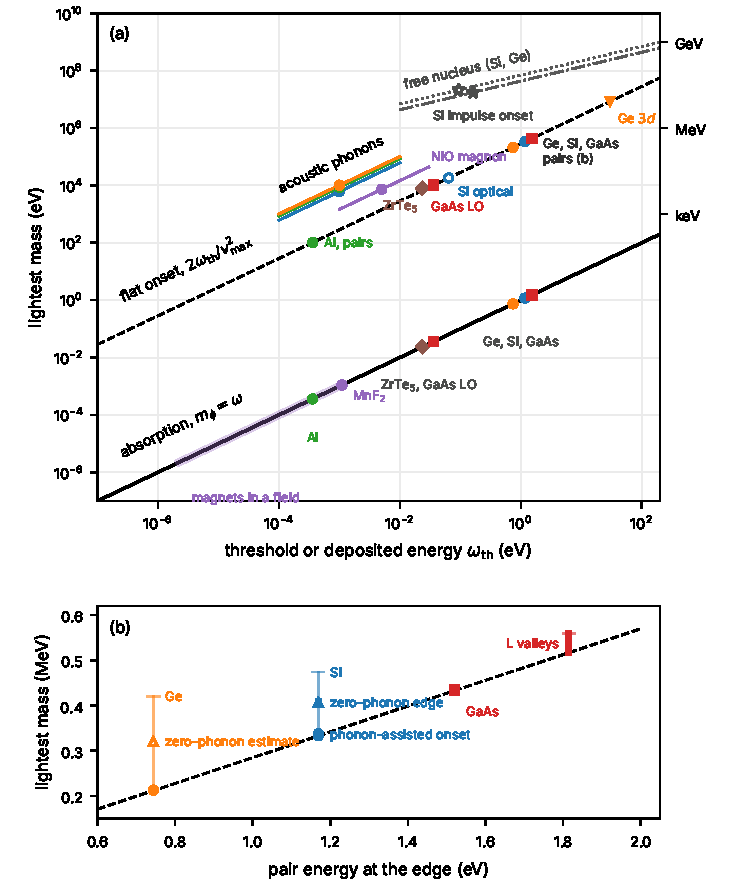
\includegraphics[width=0.78\linewidth]{figures/ch09/fig9_1.pdf}
  \caption{The kinematic map at $v_{\mathrm{max}} = \SI{794.5}{km.s^{-1}}$ (\cref{tab:1-shm}), elastic scattering. (a)~Lightest dark-matter mass of each scattering channel and lightest absorbed boson mass, against the threshold or the energy of the excitation. Solid black: absorption, $m_\phi = \omega$. Dashed: the floor $2\omega_{\mathrm{th}}/v_{\mathrm{max}}^2$, reached by flat onsets. Colored lines: acoustic edges $\omega_{\mathrm{th}}/[2c_\nu(v_{\mathrm{max}} - c_\nu)]$ for the fastest longitudinal speeds of silicon (\SI{9.35}{km.s^{-1}}, lowest), aluminum (\SI{6.67}{km.s^{-1}}, along [111]) and germanium (\SI{5.60}{km.s^{-1}}), drawn from 0.1 to \SI{10}{meV}, with their values at \SI{1}{meV} (dots); purple, the magnon edge of NiO with $c_{\mathrm{M}} = 1.36\times10^{-4}$, with its value at \SI{5}{meV}. Gray: largest free recoil of a silicon (dash-dotted) and germanium (dotted) nucleus, with the impulse onsets (stars; open: estimate). Points on the floor: aluminum pair breaking, the optical phonons of GaAs (square) and silicon (open circle), the germanium $3d$ shell; diamond and bar: ZrTe$_5$, isotropic cone and principal axes (the lowest end, \SI{7.1}{keV}, is its lightest mass). Points on the absorption line: aluminum, MnF$_2$, ZrTe$_5$, GaAs (optical phonon), germanium, silicon and GaAs (electrons); band: the uniform mode of a magnet tuned by a field. (b)~Electron--hole pairs. Filled circles and squares: phonon-assisted onsets; thick bars and filled triangle: zero-phonon edges (silicon, GaAs L valleys); open triangle: germanium zero-phonon estimate, which bounds the edge in neither direction; thin lines: from the floor to the mass that deposits the gap at exactly the valley momentum. Values and their sources in \cref{tab:9-edges}.}
  \label{fig:9-kinmap}
\end{figure}

\begin{table}[tbp]
  \caption{Channel edges of five targets: the lightest mass that reaches each channel in elastic scattering, and the lightest absorbed boson mass, at $v_{\mathrm{max}} = \SI{794.5}{km.s^{-1}}$. Masses in MeV unless marked. ``--'': no such channel; ``n.e.'': not evaluated in this book. The last column gives the section where each value is computed. Entries without a section there are computed here from \cref{eq:9.2-mch}: the aluminum acoustic edge, with the speed \SI{6.67}{km.s^{-1}} along [111] from the zero-temperature elastic constants and density of \cref{sec:20.3}; the floor of ZrTe$_5$; and the silicon $2p$ edge. Estimates are marked.}
  \label{tab:9-edges}
  \centering\footnotesize\setlength{\tabcolsep}{2.5pt}
  \begin{tabular}{@{}>{\raggedright\arraybackslash}p{0.18\linewidth}>{\raggedright\arraybackslash}p{0.12\linewidth}>{\raggedright\arraybackslash}p{0.12\linewidth}>{\raggedright\arraybackslash}p{0.13\linewidth}>{\raggedright\arraybackslash}p{0.08\linewidth}>{\raggedright\arraybackslash}p{0.12\linewidth}>{\raggedright\arraybackslash}p{0.10\linewidth}@{}}
    \toprule
    Channel & Si & Ge & GaAs & Al & ZrTe$_5$ & Section \\
    \midrule
    Floor of the gap, $2\Eg/v_{\mathrm{max}}^2$ & 0.333 & 0.212 & 0.433 & -- & \SI{6.72}{keV} ($4\Delta_{\mathrm{D}}/v_{\mathrm{max}}^2$) & \cref{sec:1.3} \\
    Pairs with a phonon (onset) & 0.3332 (exciton), 0.3374 (free pair) & 0.2119--0.2141 & 0.433--0.436 & -- & n.e. & \cref{sec:13.1} \\
    Pairs without a phonon & 0.405--0.408 & $\approx 0.32$; estimate & 0.517--0.560 (L valleys) & -- & \SI{7.1}{keV} (slow axis; 9.0, \SI{9.6}{keV} along the others) & \cref{sec:13.9,sec:13.1,sec:16.1} \\
    Pair breaking, $2\Delta_{\mathrm{BCS}}$ & -- & -- & -- & \SI{0.10}{keV} & -- & \cref{sec:7.2} \\
    One acoustic phonon, $\omega_{\mathrm{th}} = \SI{1}{meV}$ & \SI{6.1}{keV} & \SI{10.2}{keV} & 10.3--\SI{12.3}{keV} (computed tensors) & \SI{8.6}{keV} & n.e. & \cref{sec:11.1,sec:17.1,sec:17.6} \\
    One optical phonon & \SI{18.3}{keV} & n.e. & \SI{10.35}{keV} & -- & n.e. & \cref{sec:17.3,sec:11.2} \\
    Core shell & 28.6 ($2p$) & 8.5--8.7 ($3d$) & n.e. & n.e. & n.e. & \cref{sec:10.6} \\
    Free nuclear recoil (impulse onset) & 17.5 & 21.3; estimate & n.e. & n.e. & n.e. & \cref{sec:11.4,sec:17.1} \\
    Absorption, lowest $m_\phi$ & \SI{1.1728}{eV} (pairs with a phonon) & $\approx\SI{0.74}{eV}$ with a phonon, \SI{0.89}{eV} without & \SI{36.35}{meV} (optical phonon); \SI{1.52}{eV} (pairs) & \SI{0.36}{meV} & \SI{23.6}{meV} & \cref{sec:13.8,sec:3.3,sec:11.8,sec:15.4,sec:16.1} \\
    \bottomrule
  \end{tabular}
\end{table}

Inside the first group the map orders the targets by stiffness and by gap. At a common threshold of \SI{1}{meV} the acoustic edge falls as the longitudinal sound speed rises, from \SI{6.1}{keV} in silicon to 10.3 to \SI{12.3}{keV} in GaAs, whose elastic tensor is a computed one (\cref{tab:9-edges}; \cref{sec:17.6}, which ranks the targets when their inputs are uncertain). Diamond reaches \SI{3.1}{keV} (\cref{sec:17.5}, figures of merit of the channels). A flat mode competes with an acoustic one read out at a much lower threshold. The optical phonon of GaAs at \SI{36.35}{meV} opens at \SI{10.35}{keV}, the acoustic edge that silicon has at a threshold of \SI{1.7}{meV}. The pairs of ZrTe$_5$ across \SI{23.6}{meV} open at \SI{7.1}{keV}, the silicon edge at \SI{1.16}{meV}; and the NiO magnon at \SI{5}{meV} opens at \SI{7.3}{keV}, the silicon edge at \SI{1.2}{meV}.

In the second group the gap sets the order, germanium, silicon and GaAs, and every crystal of the three has a band above its floor in which pairs need a phonon. In germanium the upper end of that band is not known, and in GaAs it ends where the L valleys open. A detector that counts pairs reaches its floor through phonon-assisted scattering, the process that \cref{chap:13} treats. In the third group the square-root growth of the free-recoil mass makes the nuclear edge of germanium higher than that of silicon by only $(M_{\mathrm{Ge}}/M_{\mathrm{Si}})^{1/2}$ at equal recoil energy.

The map ranks reach, not rate. At the edge itself only particles at $v_{\mathrm{max}}$, moving along the right direction, contribute, and the rate vanishes (\cref{sec:1.3-edge}); a reach curve turns up steeply as the mass approaches the edge from above. For one acoustic phonon, \cref{sec:11.1} finds that the rate comes within \SI{10}{\percent} of its value for heavy particles only above 44 times the edge. Comparing two targets near their edges therefore needs the rates of the chapters that follow.

\begin{workedexample}{The acoustic edge of silicon at a threshold of 1 meV}\label{we:9-acoustic}
The fastest longitudinal branch of silicon runs along $[111]$, with $c_{\mathrm{LA}} = \SI{9.35}{km.s^{-1}}$ from the measured elastic constants (\cref{we:5-debye}). In units of the speed of light, $c_{\mathrm{LA}} = 9.35/299792 = 3.119\times10^{-5}$, and $v_{\mathrm{max}} = 794.5/299792 = 2.650\times10^{-3}$. A phonon of energy $\omega_{\mathrm{th}} = \SI{1}{meV}$ on this branch carries
\begin{equation*}
  \bar q = \frac{\omega_{\mathrm{th}}}{c_{\mathrm{LA}}} = \frac{\SI{e-3}{eV}}{3.119\times10^{-5}} = \SI{32.1}{eV} .
\end{equation*}
This is $0.014\,(2\pi/a)$, with $2\pi/a = \SI{2.28}{keV}$, deep in the linear part of the branch, where the edge needs slopes that obey the acoustic sum rule (\cref{sec:5.2}). With $v_{\mathrm{max}} - c_{\mathrm{LA}} = 2.619\times10^{-3}$,
\begin{equation*}
  m_{\mathrm{min}}^{\mathrm{ac}} = \frac{\SI{e-3}{eV}}{2 \times 3.119\times10^{-5} \times 2.619\times10^{-3}} = \SI{6.12}{keV} .
\end{equation*}
The floor at the same threshold is $2\omega_{\mathrm{th}}/v_{\mathrm{max}}^2 = \SI{0.285}{keV}$. A particle of \SI{6.12}{keV} at $v_{\mathrm{max}}$ has \SI{21.5}{meV} of kinetic energy and could give all of it to a target that absorbs the momentum $\mchi v_{\mathrm{max}} = \SI{16.2}{eV}$, but a phonon with that momentum carries only \SI{0.51}{meV}. To create the \SI{1}{meV} phonon the particle must reverse its direction, giving $2\mchi(v_{\mathrm{max}} - c_{\mathrm{LA}}) = \SI{32.1}{eV}$, and it keeps \SI{20.5}{meV} of its energy. Along $[100]$ the transverse speed \SI{5.84}{km.s^{-1}} of \cref{we:5-debye} would give \SI{9.76}{keV}, but a transverse phonon along a symmetry axis carries no density and is not excited by a density coupling. The edge scales linearly with the threshold, \SI{0.61}{keV} at \SI{0.1}{meV} and \SI{61}{keV} at \SI{10}{meV}, as long as $\bar q$ stays in the linear part of the branch; at \SI{10}{meV} it is already $0.14\,(2\pi/a)$. \Cref{sec:11.1} evaluates the rate near this edge with all branches and directions.
\end{workedexample}

\subsection{Dependence on the halo}\label{sec:9.2-halo}

Every scattering edge moves with $v_{\mathrm{max}} = v_{\mathrm{esc}} + v_{\mathrm{E}}^{\mathrm{ref}}$, but not by the same amount. At the minimum of \cref{eq:9.2-mch} either the derivative with respect to $q$ vanishes or $q$ sits on a constraint that does not depend on $v_{\mathrm{max}}$. Differentiating then leaves the explicit dependence alone:
\begin{equation}
  \frac{\dd\ln m_{\mathrm{min}}^{\mathrm{ch}}}{\dd\ln v_{\mathrm{max}}} = -\frac{\bar qv_{\mathrm{max}}}{\bar qv_{\mathrm{max}} - E_{\mathrm{ch}}(\bar q)} .
  \label{eq:9.2-halo}
\end{equation}
The ratio on the right compares the largest energy the particle could deposit at $\bar q$ with what is left after the excitation is paid. For a flat onset $\bar q = 2E_0/v_{\mathrm{max}}$, half of $\bar qv_{\mathrm{max}}$ goes into the excitation, and the exponent is $-2$, the halo dependence of the floor in \cref{sec:1.3}. For a gapless linear branch $\bar q = \omega_{\mathrm{th}}/c_{\mathrm{ch}}$ and the exponent is $-v_{\mathrm{max}}/(v_{\mathrm{max}} - c_{\mathrm{ch}})$, which is $-1.012$ for silicon: the acoustic edge scales as $1/v_{\mathrm{max}}$, not $1/v_{\mathrm{max}}^2$, because the excitation takes the small fraction $c_\nu/v_{\mathrm{max}}$ of $\bar qv_{\mathrm{max}}$. A free nucleus gives $-1$ for $\mchi \ll M$, from $\mchi \simeq (M\omega_{\mathrm{th}}/2)^{1/2}/v_{\mathrm{max}}$. At a stationary minimum, where the derivative with respect to $q$ vanishes, $\bar qv_{\mathrm{max}} = 2E_{\mathrm{ch}} - \bar qE_{\mathrm{ch}}'$. A branch that rises there takes more than half of $\bar qv_{\mathrm{max}}$, and the exponent exceeds 2 in magnitude: $-2.37$ for the isotropic cone of ZrTe$_5$, and $-2.12$ to $-2.74$ along its axes. A branch that falls there, as on the way to an indirect valley, gives less than 2. The gapless linear branch also rises, but its minimum sits on the constraint $q \ge \omega_{\mathrm{th}}/c_{\mathrm{ch}}$, not at a stationary point. Absorption, \cref{eq:9.2-abs}, does not depend on the halo at all.

The halo matters at the level of a few percent. The uncertainty of \SI{25}{km.s^{-1}} in the escape speed moves the floor and every flat onset by \SI{6.3}{\percent} (\cref{sec:1.3}; exactly \SI{-6.0}{\percent} and \SI{+6.6}{\percent}), and to first order the acoustic edge of silicon by \SI{3.2}{\percent}, the free-recoil edges by \SI{3.1}{\percent} and the Dirac edge of ZrTe$_5$ by \SI{7.4}{\percent}. Over the year the acoustic edge of silicon moves by \SI{-2.0}{\percent} in June and \SI{+1.7}{\percent} in December, about half the shift of the floor. A different halo thus shifts the map without reordering channels of the same shape, but it changes the ratio between a flat and a linear edge by about $\delta\ln v_{\mathrm{max}}$. \Cref{sec:17.3}, which treats inelastic scattering into collective modes, finds that a splitting of \SI{10}{meV} moves the phonon and magnon edges by 12 to \SI{28}{\percent} and the electronic edge of silicon by \SI{1}{\percent} (\cref{tab:17-endo}). An exothermic splitting larger than the excitation energy removes the edge altogether, as \cref{sec:1.3} found for the threshold mass.

\section{Excitations on the momentum--energy plane}\label{sec:9.3}

At $q = \SI{50}{keV}$ and $\omega = \SI{50}{meV}$ silicon has phonon final states and nothing else. At \SI{1}{keV} and \SI{1.3}{eV} its one final state is an electron--hole pair together with a phonon; at \SI{1}{keV} and \SI{3}{eV} a pair without a phonon is open as well. Each excitation in the atlas of \cref{tab:9-atlas} has a \emph{support}, the region of the $(q,\omega)$ plane where its response $S(\vect{q},\omega)$ of \cref{sec:4.2} carries weight. Where the support is formally unbounded, as for the multiphonon tails of \cref{sec:5.6}, we draw the region that holds \SI{90}{\percent} of the weight. \Cref{fig:9-qomega} draws the supports of silicon on the axes of \cref{fig:1-kinematics}, each in the color of its sector of \cref{eq:8.6-partition}. Where two supports overlap, a rate can count a final state twice, or drop an interference term, and the decomposition theorem of \cref{sec:8.6} decides which of the two dangers is real.

\subsection{The silicon plane by sector}\label{sec:9.3-silicon}

\begin{figure}[tbp]
  \centering
  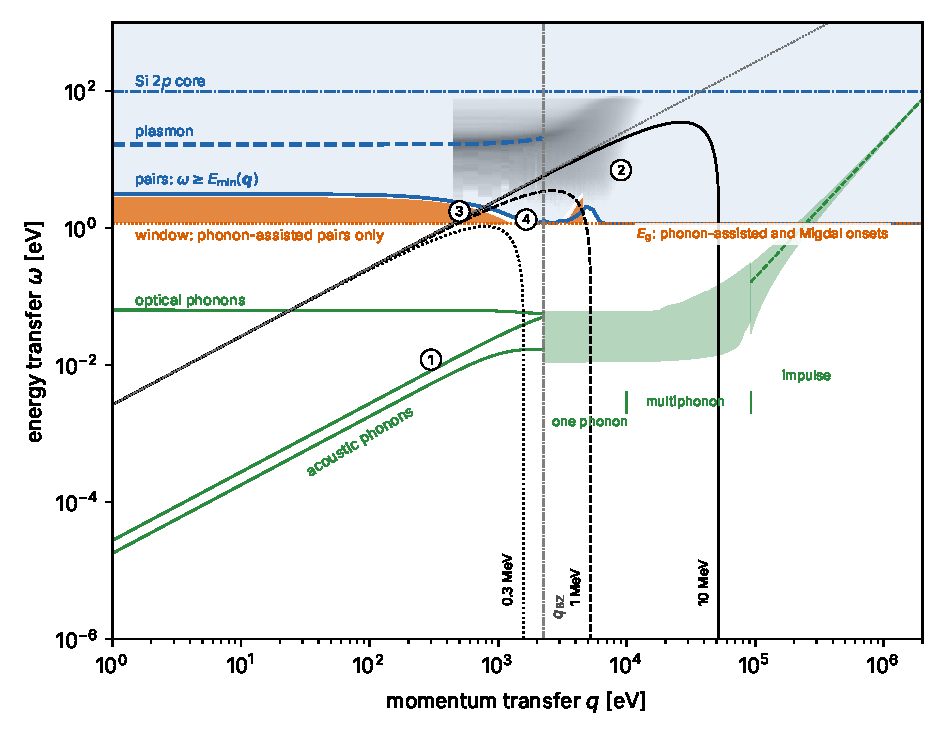
\includegraphics[width=\linewidth]{figures/ch09/fig9_2.pdf}
  \caption{The excitations of silicon on the plane of momentum transfer $q$ and energy deposited $\omega$, on the axes of \cref{fig:1-kinematics}. Green, electron-following sector: the transverse and longitudinal acoustic branches and the optical branch along [100] inside the zone, from the PBE force constants of \cref{sec:5.2}; beyond the zone radius $q_{\mathrm{BZ}} = \SI{2.25}{keV}$ (dash-dotted), the band holding the central \SI{90}{\percent} of the weight that creates phonons (5 and \SI{95}{\percent} quantiles), in the incoherent harmonic response at $T = 0$ with the PBE density of states, and above \SI{92.5}{keV} the same quantiles of the impulse Gaussian about the free recoil $q^2/2M$ (dashed); ticks at \SI{10}{keV} and \SI{92.5}{keV} separate the one-phonon, multiphonon and impulse regimes. Blue, zero-phonon electronic sector: the pair continuum above $E_{\mathrm{min}}(\vect{q})$, drawn as the lowest of the PBE edges along [100], [110] and [111] with the conduction bands shifted to the measured gap $\Eg = \SI{1.17}{eV}$, and as $\Eg$ beyond \SI{6.5}{keV}; gray scale, the random-phase loss function with local fields of the tables of Knapen, Kozaczuk and Lin~\cite{knapen2021dark} (scissor to the gap of \SI{1.17}{eV}, directions averaged, \num{e-3} to 4 on a logarithmic scale); dashed, the plasmon of the valence electron gas, $\omega_{\mathrm{pl}}^2 = \omega_p^2 + \tfrac35q^2v_{\mathrm{F}}^2$ with $\omega_p = \SI{16.6}{eV}$, up to \SI{2.24}{keV}, where this dispersion meets the pair continuum; dash-dotted, the $2p$ core level at \SI{99.4}{eV}. Orange, phonon-dressed electronic sector: the off-shell window along [100], from the phonon-assisted onset $\Eg + \omega_{\mathrm{TA}}$ up to $E_{\mathrm{min}} - \delta_{\mathrm{w}}$ with $\delta_{\mathrm{w}} = \SI{0.3}{eV}$; white above it, the margin of width $\delta_{\mathrm{w}}$ below the edge; dotted, $\Eg$, above which phonon-assisted pairs and Migdal events exist at every $q$. Black: the largest energy deposited, $qv_{\mathrm{max}} - q^2/2\mchi$, for $\mchi = 0.3$ (dotted), 1 (dashed) and \SI{10}{MeV} (solid), and $qv_{\mathrm{max}}$ (gray dotted), with $v_{\mathrm{max}} = 2.650\times10^{-3}$. Circled numbers mark the interference terms of \cref{tab:9-overlaps}.}
  \label{fig:9-qomega}
\end{figure}

\paragraph{Electron-following sector.} Inside the zone the support is a set of lines, the phonon branches of \cref{sec:5.2}. The acoustic branches rise as $\omega = c_\nu q$ from the origin and flatten at the zone boundary, at \SI{17}{meV} (transverse) and \SI{51}{meV} (longitudinal) at X in the PBE calculation; the optical branch stays near \SI{64}{meV}. Beyond the zone nothing new appears in energy. The momentum transfer is never folded (\cref{sec:1.3}); the nucleus keeps $\vect{q}$, and the phonon carries $\vect{q}$ minus a reciprocal-lattice vector. A single phonon therefore has energies between zero and \SI{64}{meV} at every $q$, and its weight changes as the Debye--Waller exponent $2W_\kappa = q^2\langle u_x^2\rangle$ of \cref{eq:5.6-W} grows. The PBE density of states of \cref{sec:5.2} gives $\langle u_x^2\rangle = \SI{2.45e-3}{\angstrom^2}$ at $T = 0$, so $2W_\kappa = 0.016$ at \SI{5}{keV}, 0.063 at \SI{10}{keV} and 1.0 at \SI{40}{keV}. Two and more phonons fill the band as $2W_\kappa$ approaches one. In the incoherent approximation the central \SI{90}{\percent} of the weight that creates phonons lies between 11 and \SI{60}{meV} at the zone radius $q_{\mathrm{BZ}} = \SI{2.25}{keV}$, still the one-phonon band. It lies between 13 and \SI{129}{meV} at \SI{46}{keV}, where the recoil parameter $x_R$ of \cref{eq:8.5-xR} is one, and between 46 and \SI{311}{meV} at \SI{92.5}{keV}. At that momentum the impulse approximation of \cref{sec:11.4} takes over from the sum over phonon numbers. It treats the nucleus as kicked so hard that its spectrum is a Gaussian of width $(E_R\langle\omega\rangle)^{1/2}$ about the free recoil energy $E_R = q^2/2M$, with $\langle\omega\rangle = \SI{40.9}{meV}$ the mean phonon energy. From there on the support is a band that follows $q^2/2M$ and narrows in relative width as $x_R^{-1/2}$.

The free recoil line crosses the gap at $q = (2M\Eg)^{1/2} = \SI{247}{keV}$, and the upper edge of the band does so at \SI{212}{keV}. Above these momenta electron-following final states sit at the same $(q,\omega)$ as electronic ones. A particle must be heavier than \SI{46.8}{MeV} to supply \SI{247}{keV}.

\paragraph{Zero-phonon electronic sector.} An electron--hole pair with no net phonon must take the whole momentum transfer itself, and its support is the continuum $\omega \ge E_{\mathrm{min}}(\vect{q})$ of \cref{eq:3.3-Emin}. With the bands of \cref{fig:3-si-bands}, shifted to the measured indirect gap, the edge lies at \SI{3.17}{eV} for $q \to 0$, at \SI{1.77}{eV} at \SI{1}{keV} along the lowest of the three symmetry directions, and reaches $\Eg = \SI{1.17}{eV}$ at the valley momentum $k_{\mathrm{c}} = \SI{1.94}{keV}$. The value at $q \to 0$ lies below the measured direct gap of \SI{3.4}{eV}, because a shift fitted to the indirect gap does not correct the vertical gap at $\mathrm{\Gamma}$ (\cref{sec:3.3}). At larger $|\vect{q}|$ the edge depends on the direction of $\vect{q}$. It returns to $\Eg$ whenever $\vect{q}$ equals a valley momentum plus a reciprocal-lattice vector, $\vect{k}_{\mathrm{c}} + \vect{G}$, whose lengths are 1.94, 2.63, 3.25, 4.96, 5.27, \SI{5.32}{keV} and so on. Above \SI{6.4}{keV} they leave no gap wider than \SI{0.72}{keV}, and half that distance costs a pair of mass $1.19\,m_e$ about \SI{0.11}{eV} above $\Eg$. There the onset of the direction average that enters an isotropic rate stays within about a tenth of an eV of the gap. Below, the widest gap lies between 3.25 and \SI{4.96}{keV}; there the lowest of the three symmetry-line edges rises to \SI{2.07}{eV}, an upper value for the onset over all directions. Upward the continuum is unbounded. At small $q$ its weight sits at the absorption peaks of 3.4 and \SI{4.2}{eV} and in the plasmon; at large $q$ it concentrates along the free-electron recoil $q^2/2m_e$, the ridge of the gray scale in \cref{fig:9-qomega}.

The plasmon, the exciton and the core shells lie inside this region and have homes of their own. The plasmon of \cref{sec:4.5} starts at the measured loss peak of \SI{16.4}{eV}, \SI{0.2}{eV} below the $\omega_p = \SI{16.6}{eV}$ of the valence electron gas, and disperses upward. With the quadratic dispersion of the gas it is a line up to \SI{2.24}{keV}, where it enters the pair continuum and Landau damping removes its weight; the exact zero of the Lindhard function enters at $q_{\mathrm{c}} = \SI{2.60}{keV}$ (\cref{sec:4.5}). In the loss-function tables that \cref{sec:10.2} uses, the peak moves from \SI{18.9}{eV} at \SI{0.5}{keV} to \SI{22.3}{eV} at \SI{2.45}{keV}; the small-$q$ peak lies \SI{2.5}{eV} above the measured \SI{16.4}{eV} because of the shift that sets their gap (\cref{sec:10.3}, which computes the plasmon's share of the rate). The bound pair, the exciton of \cref{sec:4.9}, lies \SI{14.7}{meV} below the edge near $q = k_{\mathrm{c}}$; on the scale of the figure it coincides with the edge (\cref{sec:10.5}, the exciton lines at finite momentum). The core shells start at fixed energies, \SI{99.4}{eV} for $2p$ and \SI{150}{eV} for $2s$, and carry weight at momentum transfers of tens of keV, the momenta of the electrons in them (\cref{sec:10.6}).

\paragraph{Phonon-dressed electronic sector.} A pair created together with a phonon needs no particular momentum, because the phonon carries whatever crystal momentum the pair lacks. Its support starts just above the gap at every $q$, at the onset $E^{\mathrm{PA}}_{\mathrm{min}}(\vect{q}) = \Eg + \omega_{\mathrm{TA}}(\vect{k}_{\mathrm{c}} - \vect{q})$ of \cref{eq:13.1-EPA}, and never above $\Eg + \SI{64}{meV} = \SI{1.23}{eV}$. With the PBE force constants the onset is \SI{1.187}{eV} at $q \to 0$ and \SI{1.184}{eV} at \SI{1}{keV}. Between this onset and the zero-phonon edge lies the \emph{off-shell window} of \cref{sec:8.6}, the region below $E_{\mathrm{min}}(\vect{q}) - \delta_{\mathrm{w}}$ where no zero-phonon pair exists and every electronic final state carries a phonon. Along the valley axis, with $\delta_{\mathrm{w}} = \SI{0.3}{eV}$, it spans 1.184 to \SI{1.467}{eV} at \SI{1}{keV} and closes at \SI{1.27}{keV} with the computed bands. It reopens beyond \SI{3.30}{keV}, on the far side of the Umklapp image of the opposite valley (\cref{sec:13.6}, which fixes the margin and the window edges). Above the zero-phonon edge the same sector is the phonon sideband of the zero-phonon continuum, and there it is a correction to the zero-phonon rate (\cref{sec:13.9} compares the two).

The Migdal effect of a nucleon coupling, which straddles the two electronic sectors (\cref{sec:9.1-sectors}), has the same support. The struck nucleus absorbs the momentum and the electrons take an energy $\omega_e \ge \Eg$, at every $q$. What separates it from a pair made through the electron density is the operator, not the region of the plane.

\subsection{Overlap regions and interference}\label{sec:9.3-overlap}

One phonon and two phonons share the band below \SI{64}{meV}. The impulse band and the pair continuum share the region above \SI{212}{keV} and \SI{1.17}{eV}, and the phonon sideband and the zero-phonon continuum share everything above $E_{\mathrm{min}}(\vect{q})$. An overlap in the plane is not by itself an interference. Sectors add (\cref{sec:9.1-sectors}), to the accuracy of the leak in \cref{eq:8.6-decomp}, and within one sector so do different phonon numbers: one and two phonons are orthogonal final states, and so are a nucleus recoiling with the electrons in their ground state and a pair. Interference needs two amplitudes into the same final state, and on the silicon plane that happens in two ways. The first is a coupling to both species, as for a dark photon, whose cross terms $S_{e\kappa}$ fill the bottom row of \cref{tab:8-sectors} and are derived, with their sizes, in \cref{sec:17.4}. The second is the boundary between the two electronic sectors, within $\delta_{\mathrm{w}}$ below the zero-phonon edge and a few pair widths above it. Only the sum $S^0 + S^+$ is defined there, the Dyson convention \cref{eq:8.6-dyson} splits it, and the decay of a zero-phonon pair can interfere with the same one-phonon state made directly, the Fano term \cref{eq:8.6-fano}. Inside that margin only totals of the two electronic sectors are quoted (\cref{sec:13.6}).

\subsection{The kinematic reach on the plane}\label{sec:9.3-reach}

Particles of mass $\mchi$ reach the region below $\omega = qv_{\mathrm{max}} - q^2/2\mchi$ (\cref{eq:1.3-region}), and the black curves of \cref{fig:9-qomega} show it for three masses. A particle of \SI{0.3}{MeV} deposits at most \SI{1.05}{eV}, at $q = \SI{0.80}{keV}$, and transfers at most \SI{1.59}{keV}. Its region lies below the gap and inside the zone, so it meets single acoustic and optical phonons and nothing else, with $2W_\kappa \le 0.002$. A particle of \SI{1}{MeV} deposits at most \SI{3.51}{eV} and crosses the gap for momentum transfers between 0.49 and \SI{4.81}{keV}. It enters the off-shell window, where every pair it makes carries a phonon, and the zero-phonon continuum above the edge, while its lattice final states are still single phonons ($2W_\kappa \le 0.018$ at its largest $q$, \SI{5.3}{keV}). A particle of \SI{10}{MeV} transfers up to \SI{53}{keV}, where $2W_\kappa = 1.8$, and reaches deep into the multiphonon band. In energy it reaches \SI{35}{eV}, across the region of the plasmon, but not the plasmon line, which ends at \SI{2.24}{keV}, where this particle deposits no more than \SI{5.9}{eV}; nor the $2p$ shell at \SI{99.4}{eV}, nor the impulse band, which opens at \SI{17.5}{MeV}. The lightest mass whose curve touches a region is the lightest mass of that channel (\cref{sec:9.2}).

\begin{workedexample}{The excitations open at 5 keV and 2 eV in silicon}\label{we:9-open}
Take $q = |\vect{q}| = \SI{5}{keV}$ and $\omega = \SI{2}{eV}$. The point is reachable if $qv_{\mathrm{max}} - q^2/2\mchi \ge \omega$, with $qv_{\mathrm{max}} = \SI{13.25}{eV}$, that is for $\mchi \ge q^2/[2(qv_{\mathrm{max}} - \omega)] = \SI{1.11}{MeV}$; at \SI{10}{MeV} the minimum speed of \cref{eq:1.3-vmin} is $\vmin = \omega/q + q/2\mchi = 6.50\times10^{-4}$, or \SI{195}{km.s^{-1}}, well inside the halo.

\emph{Electron-following.} At \SI{5}{keV}, $2W_\kappa = 0.016$ and $E_R = \SI{0.48}{meV}$. Two electronvolts would take at least 32 phonons of \SI{64}{meV}, each costing a factor of order $2W_\kappa$ in weight. The sector is closed.

\emph{Zero-phonon electronic.} The edge depends on the direction of $\vect{q}$. Along [100], [110] and [111] it lies at 2.59, 2.02 and \SI{2.31}{eV}, all above \SI{2}{eV}: along the symmetry lines no pair without a phonon exists at this point. But a valley image $\vect{k}_{\mathrm{c}} + \vect{G}$ has length \SI{4.96}{keV}, and for $\vect{q}$ near that direction the pair costs $\Eg$ plus about \SI{1}{meV}. Averaged over directions the zero-phonon response is thus open, but small: the direction-averaged loss function of the tables of \cref{sec:10.2} at this $q$ is \num{8.8e-4} at \SI{2}{eV}, against its maximum of 0.33 at \SI{35.7}{eV}. The plasmon line has ended at \SI{2.24}{keV}, the exciton lies \SI{14.7}{meV} below the edge, and the $2p$ shell needs \SI{99.4}{eV}: none of them is open.

\emph{Phonon-dressed electronic.} The phonon-assisted onset lies below \SI{1.23}{eV} for every $\vect{q}$, so phonon-assisted pairs are open. Where the point sits relative to the zero-phonon edge again depends on direction. Along [100] it lies below $E_{\mathrm{min}} - \delta_{\mathrm{w}} = \SI{2.29}{eV}$, inside the window, and phonon-assisted pairs are the one electronic final state there. Along [111] it lies inside the window by \SI{11}{meV} ($E_{\mathrm{min}} - \delta_{\mathrm{w}} = \SI{2.011}{eV}$), less than the exciton binding and less than the difference between a symmetry-line edge and the minimum over all crystal momenta. Along [110] it lies in the margin, between 1.72 and \SI{2.02}{eV}, where only the total of the two electronic sectors is defined. A nucleon coupling reaches the same final states through the Migdal effect, with a probability per scattering of order $(E_R/\langle\omega_e\rangle)(\delta M_\kappa/M_\kappa) = 2\times10^{-8}$ by the moment estimate of \cref{sec:12.1}. Here $\langle\omega_e\rangle \approx \SI{6}{eV}$ is the mean electronic excitation energy, and $\delta M_\kappa/M_\kappa = Z_\kappa m_e/M_\kappa = 2.7\times10^{-4}$ the share of the atom's mass carried by the electrons that move with the nucleus (\cref{sec:8.6}).

\emph{Interference.} For a dark photon the cross cells of regions 2 and 3 of \cref{tab:9-overlaps} are both present, each a few parts in $10^4$ of its sector, and for directions in the margin the Fano term of region 4 vanishes in silicon. The point is thus served by two sectors in different directions of $\vect{q}$, which is why a calculation applies the window bin by bin in $(|\vect{q}|,\hat{\vect{q}})$ and not to the direction average (\cref{sec:13.6}).
\end{workedexample}

\subsection{Supports in other materials}\label{sec:9.3-others}

The remaining rows of the atlas belong to other materials, and their supports reduce to a few shapes: a dispersing line, a flat line at a fixed energy, a continuum above a threshold, or a point at $q \to 0$. \Cref{tab:9-supports} gives the shape and one number for each, with the section that treats it. Absorption samples the single point of \cref{eq:9.2-abs}, far to the left of every scattering curve, and a support absorbs if it reaches $q \to 0$ at that energy (\cref{sec:9.1-empty}).

\begin{table}[tbp]
  \centering
  \small
  \caption{Supports in the $(q,\omega)$ plane of the excitations of the atlas that silicon does not have, with one characteristic number for the material that the treating section uses. ``Line'' means one energy for each $q$; ``continuum'' a band of energies at each $q$. $g_{33}$: component of the gyration tensor along the optic axis; $g_c$: Luttinger charge parameter of a one-dimensional metal.}
  \label{tab:9-supports}
  \begin{tabular}{@{}p{0.24\linewidth}p{0.32\linewidth}p{0.23\linewidth}p{0.10\linewidth}@{}}
    \toprule
    Excitation & Support & Scale & Home \\
    \midrule
    Optical phonons of polar crystals & line at $\omega_{\mathrm{L}}$ as $q \to 0$, reached by a coupling to charge & GaAs \SI{36.35}{meV} & \cref{sec:11.2} \\
    Phonons of a quantum crystal & acoustic lines and multiphonon band of a light, strongly anharmonic lattice & solid helium, below \SI{3}{meV} at low pressure & \cref{sec:11.5} \\
    Magnons & line from an anisotropy gap at the zone center to the top of the band & NiO, gap \SI{4.54}{meV} (measured; anisotropy added to the model), top \SI{118}{meV} & \cref{sec:14.1} \\
    Two-magnon continua & continuum from the one-magnon energy to twice the band top at small $q$ & NiO, up to \SI{236}{meV} & \cref{sec:14.2} \\
    Chiral and nonreciprocal modes & the supports above; the response acquires a part odd in $\vect{q}$ & $\alpha$-quartz, $q\,g_{33} = 7\times10^{-5}$ at \SI{2.1}{eV} & \cref{sec:14.5} \\
    Precessing nuclear spins & point at $q \to 0$, $\omega$ at the Larmor frequency & $^{207}$Pb in \SI{26.8}{mT}: \SI{241.8}{kHz} (\SI{1}{neV}) & \cref{sec:14.6} \\
    Superconducting quasiparticle pairs & continuum $\omega \ge 2\Delta_{\mathrm{BCS}}$ inside the particle--hole band $\omega \le qv_{\mathrm{F}} + q^2/2m_e$ of the metal & aluminum, $2\Delta_{\mathrm{BCS}} = \SI{0.36}{meV}$ & \cref{sec:15.1} \\
    Dirac and narrow-gap pairs & continuum $\omega \ge (4\Delta_{\mathrm{D}}^2 + v_{\mathrm{D}}^2q^2)^{1/2}$ & ZrTe$_5$, $\Delta_{\mathrm{D}} = \SI{11.8}{meV}$ & \cref{sec:16.1} \\
    Low-dimensional plasmons & line $\omega \propto q_\parallel$, faster than the halo, reached by oblique $\vect{q}$ & metallic nanotube, $\omega = v_{\mathrm{D}}q_\parallel/g_c$, 3.4 to 6.9 times $v_{\mathrm{max}}$ & \cref{sec:16.2} \\
    Graphene, nanotubes, quantum dots & continuum above a confinement gap; ejection above the work function & PbS dot \SI{1.2}{eV}; graphene \SI{4.3}{eV} & \cref{sec:16.3} \\
    Molecular (Frenkel) excitons & nearly flat lines at molecular energies & anthracene \SI{3.1}{eV} & \cref{sec:16.4} \\
    Dopant transitions & flat lines and an ionization continuum & Si:P, binding \SI{45.59}{meV} & \cref{sec:16.5} \\
    Color centers, broken bonds & reached through a nuclear recoil above a displacement or bond energy & H$_2$ bond \SI{4.75}{eV}; displacement tens of eV & \cref{sec:16.6} \\
    Two-level systems in glasses & flat continuum of splittings, independent of $q$ & down to \si{\micro eV}; \SI{e20}{eV^{-1}.cm^{-3}} & \cref{sec:16.7} \\
    Bulk acoustic modes of a body & points at $q \to 0$, the normal modes of the whole detector & MHz (mm crystal) to kHz (ton-scale bar) & \cref{sec:11.8} \\
    \bottomrule
  \end{tabular}
\end{table}

For superconductors and Dirac materials the sectors are those of quasiparticle number (\cref{sec:9.1-sectors}), so the rules of \cref{sec:9.3-overlap} for which overlaps add and which interfere hold only as far as those sectors are defined, which \cref{sec:8.6} bounds but does not settle.

\section{Limit Checks and the truncation label}\label{sec:9.4}

The free-recoil formula $\omega = q^2/2M$ holds for a silicon nucleus once the recoil energy exceeds nine phonon energies, \SI{0.54}{eV} for a nucleus in an Einstein well of \SI{60}{meV}. \Cref{lim:1.3a} showed this with one plot: the formula against the bound nucleus, the recoil energy on the horizontal axis, and a gray band where the two agree. The channel chapters recover 90 published formulas as limits of their own results, and test 80 of them in 75 boxes of the same kind. Each box answers one question: over what range of a single parameter does the published formula agree with a fuller calculation, and what fails outside that range? We build such a box, show that its horizontal axis follows from the place of the formula on the truncation label $\mathfrak{T}$ of \cref{sec:8.5}, and place every formula of \crefrange{chap:10}{chap:17} on that label.

\subsection{The comparison plot}\label{sec:9.4-plot}

A Limit Check has three parts: the formula, a plot, and one sentence. The formula is written in the book's notation, with the symbols of \cref{chap:8}, and a one-line citation names the equation of the source where it was first given.

The plot compares the formula with a fuller result for the same quantity. In the language of \cref{sec:8.8}, the formula is a quantity evaluated at a point $\mathfrak{T}$ of the label and the fuller result is the same quantity one step further along one axis, at $\mathfrak{T}_k^+$; the plot shows their relative difference $\delta_k$ of \cref{eq:8.8-delta}. Most boxes plot the ratio of the two, $1 + \delta_k$ or its inverse, so that the formula is the horizontal line at one. Some plot both curves, when their shapes matter more than their ratio. The fuller result is computed in the book, from a crystal calculation or from a model that keeps the physics the formula drops, or it is measured. In \cref{lim:1.3a} it is the nucleus bound in an Einstein potential, whose spectrum is a series of phonon lines.

The horizontal axis carries the \emph{controlling parameter}, the variable along which $\delta_k$ runs from negligible at one end of the axis to order one at the other. In \cref{lim:1.3a} it is $E_R/\omega_0$, the recoil energy in units of the phonon energy. The \emph{leading correction}, the first term of $\delta_k$ in the controlling parameter, is drawn as a third curve, usually dotted or dashed. In \cref{lim:1.3a} it is the rms width $(E_R\omega_0)^{1/2}$ of the deposit, which falls relative to $E_R$ as $(\omega_0/E_R)^{1/2}$. The gray band marks the values of the controlling parameter at which the formula agrees with the fuller result. The tolerance is stated in the caption: usually \SI{10}{\percent}, sometimes \SI{1}{\percent} or \SI{15}{\percent}, or a fixed fraction of a width, as the rms width below $E_R/3$ that bounds the band of \cref{lim:1.3a}. The caption prints the edge of the band.

The sentence under the plot says what breaks down outside the band, in physical terms: in \cref{lim:1.3a}, that below a few phonon energies the deposit arrives in whole phonons and spreads as widely as $E_R$ itself.

The \emph{approximation chain}, the sequence of steps that leads from the book's general result to the formula, lives in the running text next to the box, where each step is derived or cited to a specific equation. The formal record, with the chain, the conditions, the specification of the plot and the size of the leading correction, is the row of the formula in \cref{tab:F-rows} of \cref{app:F}. How far the book has established the formula is read from what the plot compares with.

Inside the gray band the formula is established to the stated tolerance, relative to the fuller result. That statement is as strong as the fuller result. Where the fuller result is a crystal calculation at a known point of $\mathfrak{T}$, such as the random-phase response with local fields, the band says that the formula agrees with that calculation; the calculation has its own next step, which the label names. Where the fuller result is a model, as the Einstein well of \cref{lim:1.3a} is a model of the silicon lattice, the edge of the band is an estimate of where the formula fails, not a bound. Where nothing is shaded, the formula fails over the whole plotted range, and the box gives the size of the failure instead of a range of validity. Some boxes compare two published forms of one result, or test a sum rule; they are read in the same way, with the exact relation as the fuller result.

\subsection{Placement on the truncation label}\label{sec:9.4-place}

A formula is placed on $\mathfrak{T}$ by reading its assumptions, one component at a time, as \cref{we:8-label} did for phonon-assisted absorption. The eight components of \cref{eq:8.5-label} are five orders and three labels. The orders are those of the Born--Oppenheimer coupling ($n_B$), the electron--phonon vertex ($n_g$), the anharmonicity ($n_A$), the temperature ($n_T$) and the multipole expansion ($n_D$); the labels are the many-body approximation $\mathcal{X}$, the lattice regime $\mathcal{K}$ and the Migdal regime $\mathfrak{M}$. Clamped nuclei put a formula at $n_B = 0$; independent particles at $\mathcal{X} = \mathrm{IP}$; a free nucleus that recoils as a whole at $\mathcal{K}$ = impulse; a kick that the electrons see as instantaneous at $\mathfrak{M}$ = sudden. The deviation notation of \cref{sec:8.5} then lists only the components that differ from the base point $\mathfrak{T}_0$ of \cref{eq:8.5-base}.

The placement fixes the plot. The leading correction of a formula is the largest of its steps $\mathfrak{T} \to \mathfrak{T}_k^+$, and its controlling parameter is whatever makes that step grow. On an axis with a small parameter, the step is a power of the parameter of \cref{tab:8-params}, and the controlling parameter is that small parameter or a variable it grows with. A formula in the impulse regime has the Doppler width as its leading correction, of relative size $x_R^{-1/2}$ by \cref{eq:8.5-width}, so its plot runs against the recoil parameter $x_R$. A Migdal probability at dipole order, $n_D = 2$, misses the higher multipoles, and its plot runs against $\xi_D$. On the many-body axis there is no small parameter (\cref{sec:8.5}). The fuller result is then the next approximation, computed, and the controlling parameter is the variable along which screening changes: the momentum transfer, the energy deposit or the mass of an absorbed boson.

Many formulas truncate an expansion that is not one of the eight components. A long-wavelength form keeps the leading power of $q$ against a lattice momentum, and a light-mediator rate assumes a dark-matter mass far above the kinematic edge. A spin-wave rate keeps the leading order in $1/|\vect{S}|$, and a dopant rate the first order in the donor density. \Cref{sec:8.5} records such approximations as qualifiers, in words, and their controlling parameter is the expansion parameter itself. We sort them into four kinds: long wavelength, as in the plasmon pole of the electron gas; the kinematics of the halo and of the signal, as in a light-mediator rate far above its edge or the coherence time of a classical field; the dark-matter side and the order in the coupling, as in the speed of boosted dark matter; and the model or method used for the target, as in the spin-wave order of a magnon rate or the density of a dopant.

\begin{figure}[tbp]
  \centering
  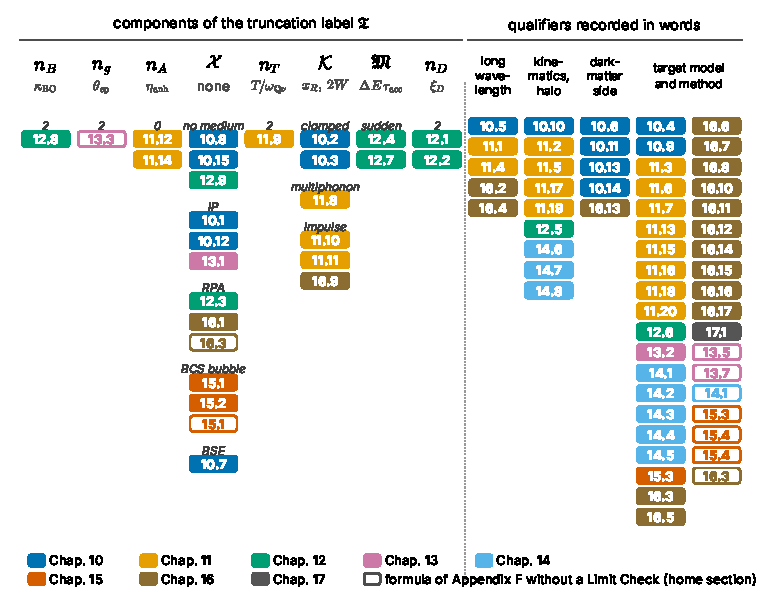
\includegraphics[width=\linewidth]{figures/ch09/fig9_3.pdf}
  \caption{The Limit Checks of \crefrange{chap:10}{chap:17} placed by the axis of their leading correction. Left: the eight components of the truncation label $\mathfrak{T}$, each with its small parameter (\cref{tab:8-params}); under each, the boxes whose comparison result lies one step from the formula along that component, grouped by the formula's value of that component, printed in italic (for example IP or impulse). Right: boxes whose leading correction is an expansion in a parameter that the label records only in words, sorted into four kinds. Filled chips: Limit Checks, colored by chapter. Hollow chips: formulas of \cref{tab:F-rows} without a box, labeled by the number of their home section, not of a box. The step of each box and its controlling parameter are listed in \cref{tab:9-limitchecks}.}
  \label{fig:9-axes}
\end{figure}

\Cref{fig:9-axes} places the 75 Limit Checks of \crefrange{chap:10}{chap:17} by the axis of their leading correction, and \cref{tab:9-limitchecks} lists each with its controlling parameter and its step. Twenty-five lie on a component of the label. Eleven are on the many-body axis. Among them are the crystal form-factor rate of \cref{sec:10.1}, which computes the rate of creating electron--hole pairs from independent-particle bands, and the Migdal rate through the loss function of \cref{sec:12.3}. The loss function of a superconductor in \cref{sec:15.1} is there too: its box compares the bare quasiparticle response with a conserving one, built so that it obeys charge conservation. Six are on the lattice regime, from the clamped lattice to the impulse limit, two on the anharmonic order, two on the Migdal regime, two on the multipole order, one on the thermal order and one on the Born--Oppenheimer order. Every Migdal scattering formula sits at $n_B = 2$, and the rate with phonon final states of \cref{sec:12.4} takes its next step there: the phonon energies in the electronic denominators give $2\langle\omega_{\mathrm{ph}}^2\rangle/\omega_e^2 = 2.9\times10^{-3}$ at the silicon gap, one step of $n_B$ in the counting of \cref{tab:8-params}. None of the boxes has its leading correction on $n_g$. The one formula whose next step is $n_g = 4$, the phonon-assisted electron-recoil rate of \cref{sec:13.3}, has no box, and its correction is the off-shell parameter $\theta_{\mathrm{ep}}$ of \cref{tab:8-params}.

The other 50 boxes expand in a qualifier: 5 in a long wavelength, 9 in the kinematics of the halo or the signal, 5 on the dark-matter side, and 31 in the model of the target. Two of the last are close to the label. Before any change of $\mathcal{X}$, the rate of the electron gas in \cref{sec:10.3} misses the gap and the interband peaks of the crystal, a change of target model. The band of \cref{sec:11.5} built from exact moments misses the skewness of the moment problem, not an anharmonic order. The split follows the chapters. In \cref{chap:12} seven of nine boxes lie on the label, in \cref{chap:10} seven of fifteen and in \cref{chap:11} six of twenty. In \cref{chap:14}, on magnetic excitations, none of the eight does, and in \cref{chap:16}, on novel targets such as Dirac materials, quantum dots and glasses, two of seventeen do. The label was built from the expansion of a crystal of electrons and nuclei in its small parameters, and the electronic, lattice and Migdal channels truncate along it. For the other targets the controlling parameter of the box is the target's own.

\begin{workedexample}{Three literature rates on the truncation label}\label{we:9-place}
We place three rates on $\mathfrak{T}$ and read from each placement the plot that its Limit Check draws. The rates are derived in \cref{sec:10.1,sec:10.2,sec:11.4}; here we use only their assumptions.

\emph{Crystal form-factor rate.} The electron-recoil rate of Essig and collaborators~\cite[Eqs.~(3.13) and (3.17)]{essig2016direct} squares the matrix elements of $\ee^{\ii\vect{q}\cdot\vect{r}}$ between Bloch states of independent electrons (\cref{chap:3}), with the valence bands filled at $T = 0$ and the nuclei clamped. Each assumption is a base value: no derivative coupling, no electron--phonon vertex, independent particles, no thermal occupation, and no multipole expansion, since the plane wave is kept whole. The rate sits at $\mathfrak{T}_0$, with the qualifier ``unscreened''. Every integer step costs a small parameter of \cref{tab:8-params}, and the many-body step costs an amount that no parameter predicts, so the many-body step is computed: IP to RPA to RPA with local fields. Screening is strongest at small $q$, where the long-range Coulomb field of the induced charge acts, and fades at large $q$. The controlling parameter is therefore the momentum transfer at fixed energy, and \cref{lim:10.1a} plots the rate weight against $q/q_0$, with $q_0 = \alpha m_e$, for the three approximations. The screened response is 0.05 of the unscreened one at the kinematic edge and 0.22 at $q_0$, and the $q$-integrated rate at \SI{5}{eV} is 0.47 of it. Nothing is shaded. The status follows: the formula is a definite point of the label, but its leading correction is of order one across the whole range, and \cref{sec:10.2} computes the rate with screening.

\emph{Loss-function rate.} The rate of Knapen and collaborators and of Hochberg and collaborators~\cites[Eqs.~(6) and (13)]{knapen2021dark}[Eq.~(1)]{hochberg2021determining} writes the response through the loss function $\Imag[-1/\varepsilon(\vect{q},\omega)]$. The identity \cref{eq:8.4-exact} makes this form exact for a coupling to the total charge at any lattice and for a coupling to the electron density with the nuclei clamped. The many-body axis is then not truncated by the formula; $\mathcal{X}$ is whatever approximation the loss function is computed in, RPA with local fields in the tables of \cref{sec:10.2}. The truncation is the clamped lattice, for a coupling to electrons alone. Releasing the nuclei is a step of the lattice regime, from no phonon in the final state to one phonon, and it adds the electron-following sector of \cref{sec:8.6}: the electrons that move with a nucleus carry an acoustic peak inside the phonon band. The controlling parameter is the energy deposit against the top of the phonon band, $\omega/\omega_{\max}$, and \cref{lim:10.2a} shades the energies above the band, where the two couplings share the formula. Below it, for dark matter of \SI{1}{MeV} and in a model of the acoustic peak, the electron-only coupling has more than $10^4$ times the rate that electronic excitations give at the same energies. The formula is established above the phonon band; inside it, for an electron-only coupling, the size of the correction rests on a model.

\emph{Free nuclear recoil.} The recoil rate of Lewin and Smith with the Helm form factor~\cite{lewin1996review}, \cref{eq:11.4-LS} with \cref{eq:2.2-helm}, assumes a nucleus that is free, at rest and recoils as a whole. In the label this is $\mathcal{K}$ = impulse at zero width, $n_B = 0$, the same placement as the elastic recoil of \cref{lim:1.3a}. The mean deposit $E_R$ is exact at every anharmonic and thermal order, since it is fixed by the sum rule \cref{eq:5.6-sum}. The leading correction is the next term of the impulse expansion, the Doppler width of the bound nucleus, of relative size $x_R^{-1/2}$. The controlling parameter is $x_R$, and \cref{lim:11.4a} plots the crystal rate over the free-recoil rate against it, with the multiphonon response of silicon as the fuller result and the Gaussian of the impulse approximation as the leading correction. For \SI{1}{GeV} dark matter the two agree within \SI{10}{\percent} for $x_R \ge 2.3$, at $q \ge \SI{70}{keV}$.

The two boxes on the impulse axis draw their bands at different values of one parameter. \Cref{lim:1.3a} asks of the spectrum at one momentum transfer that its rms width be below a third of $E_R$, which needs $x_R \ge 9$ for its oscillator. \Cref{lim:11.4a} asks of the rate at a given energy, which sums the response over momentum transfers with a smooth halo weight, that it agree within \SI{10}{\percent}. That is met at smaller $x_R$: with the mean deposit exact, the width changes such a sum only at second order. Where the band starts depends on the quantity compared and on the tolerance, and each caption states both.
\end{workedexample}

\subsection{The formal record of the limits}\label{sec:9.4-appF}

\Cref{tab:F-rows} of \cref{app:F} has one row for each formula that the book recovers as a limit, in the order of the chapters. For the channel chapters the appendix has 90 rows. Eighty belong to the 75 Limit Checks, since a box may compare two formulas in its panels. Ten have no box; they are marked so in the first column and appear as hollow chips in \cref{fig:9-axes}. Six of the 90 rows have an unsized leading correction, one that the book identifies but to which it assigns no number. A formula of this kind is established at its own point of $\mathfrak{T}$ and open beyond it; \cref{chap:22} collects the open items of the book, each with the missing step that would close it. To find a formula, a reader goes from the channel in \cref{tab:9-atlas} to its home section, and from there to its row in \cref{tab:F-rows}; \cref{tab:9-limitchecks} gives the same entry point by Limit Check.

% Generated by figscripts/ch09/fig9_3.py; do not edit by hand.
{\small
\setlength{\tabcolsep}{4pt}
\begin{longtable}{@{}>{\raggedright\arraybackslash}p{0.11\linewidth}>{\raggedright\arraybackslash}p{0.32\linewidth}>{\raggedright\arraybackslash}p{0.27\linewidth}>{\raggedright\arraybackslash}p{0.23\linewidth}@{}}
\caption{The Limit Checks of \crefrange{chap:10}{chap:17}, by chapter. Controlling parameter: the variable on the horizontal axis of the box. Leading correction: the component of the truncation label $\mathfrak{T}$ of \cref{eq:8.5-label} along which the comparison result lies one step from the formula, with the step; where the step is not along a component, the kind of qualifier it expands in. Formulas recovered as limits without a box are listed in \cref{tab:F-rows}.}\label{tab:9-limitchecks}\\
\toprule
Limit Check & Formula & Controlling parameter & Leading correction \\
\midrule
\endfirsthead
\toprule
Limit Check & Formula & Controlling parameter & Leading correction \\
\midrule
\endhead
\bottomrule
\endfoot
\multicolumn{4}{@{}l}{\emph{\Cref{chap:10}}} \\
\ref{lim:10.1a} & Crystal form-factor rate & momentum transfer $q/q_0$ at fixed $\omega$ & $\mathcal{X}$: IP $\to$ RPA + LF \\
\ref{lim:10.2a} & Loss-function rate & energy over the top of the phonon band & $\mathcal{K}$: clamped $\to$ one-phonon \\
\ref{lim:10.2b} & Sum-rule bounds on the loss function & momentum transfer $q$ & $\mathcal{K}$: clamped $\to$ one-phonon \\
\ref{lim:10.3a} & Lindhard and Mermin loss-function rates & energy over the gap, $\omega/\Eg$ & target model and method \\
\ref{lim:10.3b} & Plasmon production from the pole of $1/\varepsilon$ & momentum over the plasmon cutoff & long wavelength \\
\ref{lim:10.4a} & Crystal responses of the effective operators & current-row rate over density-row rate & dark-matter side and coupling \\
\ref{lim:10.5a} & Bethe--Salpeter exciton rate & momentum transfer $|\vect{q}|$ & $\mathcal{X}$: BSE, one time ordering $\to$ both \\
\ref{lim:10.7a} & Absorption with in-medium mixing & boson mass $m_\phi$ & $\mathcal{X}$: no medium $\to$ measured $\varepsilon$ \\
\ref{lim:10.7b} & Scalar absorption through the kinetic-energy row & upper cutoff of the spectral sum & target model and method \\
\ref{lim:10.8a} & Pair absorption & line width over the kinetic energy of the pair & kinematics and halo \\
\ref{lim:10.8b} & Dark Compton scattering & boson mass over electron mass & dark-matter side and coupling \\
\ref{lim:10.9a} & Inelastic electron recoil in crystals & mass splitting $\Delta_\chi$ & $\mathcal{X}$: IP $\to$ RPA + LF \\
\ref{lim:10.9b} & Boosted dark matter: the density row & dark-matter speed $v$ & dark-matter side and coupling \\
\ref{lim:10.9c} & Fermionic absorption on electrons & dark-matter mass over the binding energy & dark-matter side and coupling \\
\ref{lim:10.9d} & In-medium decay of an excited state & splitting over the valence plasma frequency & $\mathcal{X}$: no medium $\to$ measured $\varepsilon$ \\
\addlinespace
\multicolumn{4}{@{}l}{\emph{\Cref{chap:11}}} \\
\ref{lim:11.1a} & Long-wavelength acoustic structure factor & $q/q_{\mathrm{BZ}}$ & long wavelength \\
\ref{lim:11.1b} & Light-mediator single-phonon rate & dark-matter mass over the acoustic edge & kinematics and halo \\
\ref{lim:11.1c} & Sphere-averaged longitudinal speed & elastic anisotropy (Zener ratio) & target model and method \\
\ref{lim:11.2a} & Born-charge single-phonon rate & momentum transfer $q$ in three directions & long wavelength \\
\ref{lim:11.2b} & Polar matrix element and band integral & dark-matter mass $\mchi$ & kinematics and halo \\
\ref{lim:11.2c} & Static dielectric constant of one polar branch & share of one polar branch & target model and method \\
\ref{lim:11.2d} & Born charge over $\varepsilon_\infty$ from the LO--TO splitting & misfit of the inputs to the Lyddane--Sachs--Teller relation & target model and method \\
\ref{lim:11.3a} & Multiphonon incoherent approximation & $q/q_{\mathrm{BZ}}$ & $\mathcal{K}$: incoherent $\to$ coherent multiphonon \\
\ref{lim:11.3b} & Second-order thermal diffuse scattering & distance from a reciprocal-lattice vector & $n_T$: classical $\to$ quantum occupations \\
\ref{lim:11.4a} & Free nuclear recoil with the Helm form factor & recoil parameter $x_R$ & $\mathcal{K}$: impulse $\to$ multiphonon \\
\ref{lim:11.4b} & Fermionic absorption on nuclei & dark-matter mass $\mchi$ & $\mathcal{K}$: impulse $\to$ multiphonon \\
\ref{lim:11.5a} & Anharmonic corrections to multiphonon weights & momentum in units of the zero-point momentum & $n_A$: $0 \to 2$ \\
\ref{lim:11.5c} & The Markov--Krein band & threshold in standard deviations & target model and method \\
\ref{lim:11.5b} & Solid helium: quasi-harmonic and self-consistent phonons & Lindemann ratio & $n_A$: $0 \to$ all even orders \\
\ref{lim:11.6a} & Incoherent spin absorption & boson mass $m_\phi$ & target model and method \\
\ref{lim:11.6b} & Lifshitz mass-defect Green function & phonon frequency, at three mass defects & target model and method \\
\ref{lim:11.7a} & Daily modulation from the anisotropic response & momentum transfer $q$ & kinematics and halo \\
\ref{lim:11.8a} & Single-phonon absorption & boson mass $m_\phi$ near the polar phonon & target model and method \\
\ref{lim:11.8b} & Bulk acoustic resonator & quality factor of the mode over that of the halo field & kinematics and halo \\
\ref{lim:11.8c} & Resonant-mass drive of a scalar & frequency over the lowest mode of the body & target model and method \\
\addlinespace
\multicolumn{4}{@{}l}{\emph{\Cref{chap:12}}} \\
\ref{lim:12.2a} & Atomic Migdal effect at dipole order & multipole parameter $\xi_D$ & $n_D$: $2 \to$ all orders \\
\ref{lim:12.2b} & Migdal excitation of bound final states & multipole parameter $\xi_D$ & $n_D$: $2 \to$ all orders \\
\ref{lim:12.3a} & Crystal Migdal effect through the loss function & momentum given to the electrons, over $q_{\mathrm{BZ}}$ & $\mathcal{X}$: RPA $\to$ RPA + LF (diagonal) \\
\ref{lim:12.3b} & Crystal Migdal rate with free recoil & dark-matter mass (largest recoil energy) & $\mathfrak{M}$: sudden $\to$ moving nucleus \\
\ref{lim:12.3c} & Per-mass Migdal rate with the valence ionization factor & dark-matter mass $\mchi$ & kinematics and halo \\
\ref{lim:12.3d} & The Wannier picture of the boost & valence band width over the gap & target model and method \\
\ref{lim:12.4a} & Migdal effect with phonon final states & Doppler shift over the electronic energy & $\mathfrak{M}$: sudden $\to$ exact denominators \\
\ref{lim:12.4b} & Phonon-mediated Migdal effect & electronic energy against the phonon band & $n_B$: $2 \to 4$ \\
\ref{lim:12.6a} & Migdal-type absorption of a scalar & boson mass $m_\phi$ & $\mathcal{X}$: atomic $\to$ crystal loss function \\
\addlinespace
\multicolumn{4}{@{}l}{\emph{\Cref{chap:13}}} \\
\ref{lim:13.5a} & Phonon-assisted absorption as the optical limit & photon energy above the gap & $\mathcal{X}$: IP $\to$ BSE \\
\ref{lim:13.7a} & Zero-point renormalization by special displacements & supercell size & target model and method \\
\addlinespace
\multicolumn{4}{@{}l}{\emph{\Cref{chap:14}}} \\
\ref{lim:14.1a} & One-magnon rate at linear spin-wave order & inverse spin, $1/2|\vect{S}|$ & target model and method \\
\ref{lim:14.3a} & Absorption into magnons & applied over demagnetizing field; anisotropy over exchange & target model and method \\
\ref{lim:14.4a} & Data-driven spin response & orbital shift of the ion's $g$ factor & target model and method \\
\ref{lim:14.5a} & Chiral phonons and molecular magnets & dark-matter mass; level spacing over temperature & target model and method \\
\ref{lim:14.5b} & Multiferroic cross response & temperature over the ordering temperature & target model and method \\
\ref{lim:14.6a} & Transverse magnetization of a driven nuclear-spin ensemble & time over the coherence time of the field & kinematics and halo \\
\ref{lim:14.6b} & Gaussian-field signal and its power spectrum & record length over the coherence time & kinematics and halo \\
\ref{lim:14.6c} & Sensitivity scalings of the exponential-bin likelihood & record length over the coherence time & kinematics and halo \\
\addlinespace
\multicolumn{4}{@{}l}{\emph{\Cref{chap:15}}} \\
\ref{lim:15.1a} & Loss function of a superconductor near the pair-breaking edge & energy over the gap, on the kinematic edge & $\mathcal{X}$: bare BCS bubble $\to$ conserving \\
\ref{lim:15.2a} & Resummed loss function on the kinematic edge & energy over the gap, on the kinematic edge & $\mathcal{X}$: bare BCS bubble $\to$ conserving \\
\ref{lim:15.4a} & Phonon-assisted absorption: the normal-metal limit & energy over the gap & target model and method \\
\addlinespace
\multicolumn{4}{@{}l}{\emph{\Cref{chap:16}}} \\
\ref{lim:16.1a} & Background screening of Dirac-material rates & background dielectric constant & $\mathcal{X}$: Dirac bands $\to$ with remote bands \\
\ref{lim:16.2a} & One-dimensional plasmons of linear channels & momentum along the channel over $k_{\mathrm{F}}$ & long wavelength \\
\ref{lim:16.2b} & Acoustic plasmon of two components and its Landau width & plasmon speed over the Fermi speed of the light carriers & target model and method \\
\ref{lim:16.2c} & Effective medium of a layered stack & wave number times layer period & long wavelength \\
\ref{lim:16.3a} & Vacuum ejection with plane-wave final states & kinetic energy of the ejected electron & target model and method \\
\ref{lim:16.3b} & Quantum-dot rate and its bulk limit & energy above the dot gap, in confinement energies & target model and method \\
\ref{lim:16.4a} & Binned Frenkel rate & dark-matter mass $\mchi$ & target model and method \\
\ref{lim:16.5a} & Dopant absorption & donor density & target model and method \\
\ref{lim:16.6a} & Color-center creation and bond breaking & largest recoil energy over the threshold & $\mathcal{K}$: impulse $\to$ bound atom \\
\ref{lim:16.7a} & Two-level response to a classical strain or field & temperature & target model and method \\
\ref{lim:16.7b} & Dark-photon absorption on two-level systems & boson mass $m_\phi$ & target model and method \\
\ref{lim:16.7d} & Glass absorption below the Ioffe--Regel frequency & boson mass against the Ioffe--Regel frequency & target model and method \\
\ref{lim:16.7c} & Random media and the Born limit & medium potential over the dark-matter energy & dark-matter side and coupling \\
\ref{lim:16.8a} & Two-level relaxation by phonons and electrons & splitting over temperature; coupling to the electrons & target model and method \\
\ref{lim:16.8b} & The ohmic scaling limit & dimensionless ohmic coupling & target model and method \\
\ref{lim:16.8c} & Hopping and tunneling through one barrier & temperature over the tunneling crossover & target model and method \\
\ref{lim:16.8d} & Heat release of a cooled glass & time after cooling & target model and method \\
\addlinespace
\multicolumn{4}{@{}l}{\emph{\Cref{chap:17}}} \\
\ref{lim:17.5a} & Partial f-sum of the valence electrons & upper limit of the $f$-sum integral & target model and method \\
\end{longtable}
}


\section*{Summary}\addcontentsline{toc}{section}{Summary}

\Cref{tab:9-atlas} pairs the 24 kinds of excitation that this book treats with six classes of dark-matter coupling: electron density, nuclei, spin and current, vector absorption, axion-like and scalar absorption, and inelastic and other kinematics. The columns come from the target operators of \cref{sec:8.1}, the rows from the solid-state chapters. Of the 144 cells, 57 hold a channel, each with one home section; eight more are allowed at leading order but computed in no section, and 79 are empty at leading order. Four reasons account for nearly all of the empty ones. The first is operator content: the nuclear density creates no electronic excitation in the Born--Oppenheimer approximation, and the electron density no magnon without spin--orbit coupling. The others are the kinematics of absorption at $q = m_\phi v \simeq 0$, which no acoustic phonon or free nucleus can meet, the order in the coupling, and the absence of a new response for inelastic kinematics. Each row sits in a sector of the decomposition theorem. The four electronic rows of the density column are parts of one zero-phonon response; phonons, multiphonons and free recoil are electron-following and differ only in their lattice regime; the phonon-assisted row and part of the Migdal row are phonon-dressed. The dark photon, which couples to every charge, populates more of the atlas than any other model, and its loss-function rate on electrons and its polar-phonon rate are two sectors of one charge response.

The lightest mass that reaches a channel, \cref{eq:9.2-mch}, depends on the largest laboratory speed of the halo, the threshold and the shape of the dispersion. No channel lies below the floor $2\omega_{\mathrm{th}}/v_{\mathrm{max}}^2$, which a flat onset reaches. A gapless linear branch of speed $c_{\mathrm{ch}}$ lies above the floor by about $v_{\mathrm{max}}/4c_{\mathrm{ch}}$, because the particle must reverse its direction to hand over the momentum of the excitation: the acoustic edge of silicon at a threshold of \SI{1}{meV} is \SI{6.12}{keV} (\cref{we:9-acoustic}). A branch faster than $v_{\mathrm{max}}$, such as the bulk plasmon of silicon, is closed to elastic scattering. An offset minimum puts the electron--hole pairs of silicon between the phonon-assisted onset just above the floor, \SI{0.333}{MeV}, and the zero-phonon edge at 0.405 to \SI{0.408}{MeV}. A free nucleus needs a mass that grows as the square root of the threshold; a free silicon nucleus takes up the gap from \SI{46.8}{MeV}. Absorption reaches $m_\phi = \omega$, five and a half decades below scattering at equal energy. \Cref{fig:9-kinmap} and \cref{tab:9-edges} place silicon, germanium, GaAs, aluminum and ZrTe$_5$ on one map, which ranks reach and not rate. The edges move with $v_{\mathrm{max}}$ as \cref{eq:9.2-halo} states: as $v_{\mathrm{max}}^{-2}$ for a flat onset, nearly as $v_{\mathrm{max}}^{-1}$ for an acoustic edge.

On the plane of momentum transfer and energy deposit, \cref{fig:9-qomega} draws the support of every excitation of silicon, colored by sector. A pair without a phonon must take the whole momentum transfer and lives above $E_{\mathrm{min}}(\vect{q})$; a pair with a phonon starts just above the gap at every $q$, and between the two lies the off-shell window. Overlap on the plane is not interference. Sectors add, and different phonon numbers add; amplitudes interfere only for a coupling to electrons and nuclei at once and at the boundary between the two electronic sectors (\cref{tab:9-overlaps}). The only place where the cross term decides a rate at leading order is the electron-following sector, where the cloud that follows a silicon nucleus cancels its charge at long wavelength and leaves a dark photon without a single-phonon channel.

A Limit Check compares a published formula, written in the book's notation, with a fuller result one step further along one axis of the truncation label, or in a parameter that the label records in words, against a controlling parameter, and shades where the two agree to a stated tolerance. The axis of the step fixes the leading correction and the controlling parameter: $x_R$ for an impulse formula, $\xi_D$ for a Migdal probability at dipole order, and the momentum or energy along which screening changes for a formula on the many-body axis. Of the 75 Limit Checks of the channel chapters, 25 have their leading correction on a component of the label (\cref{fig:9-axes}, \cref{tab:9-limitchecks}), most of them in the electronic, lattice and Migdal chapters. The other 50, which include every magnetic one, expand in a parameter of their target, kinematics or coupling that the label records in words. \Cref{app:F} lists each formula with its source equation and the size of its leading correction. Of its 90 rows for these chapters, 80 are tested in the 75 boxes, and six carry a correction that the book does not size.

\printbibliography[heading=subbibliography]

\chapter{Electronic excitations}\label{chap:10}
An electron--hole pair is the signal most searches for sub-GeV dark matter look for. A single pair in silicon costs at least the gap, \SI{1.17}{eV}, and a pair is easy to count: the charge-coupled devices of \cref{sec:1.5} read out one electron at a time. Dark matter of \SI{1}{MeV} carries at most \SI{3.5}{eV} of kinetic energy, enough to cross the gap, and this is why electron scattering in semiconductors reaches masses that nuclear recoils cannot. \Cref{chap:8} wrote the rate for any coupling as a contraction of the response matrix with a tensor from the dark-matter side, and \cref{chap:9} placed each electronic excitation on the map of channels. How faithfully can the rate of making pairs be computed in a real crystal? The band structure alone gives the crystal form factor. The answer depends on what the band structure leaves out: other electrons that screen the potential and bind the pair, couplings to spin and current rather than number, and particles that are absorbed, split or fast rather than slow and elastic. Throughout, the nuclei stay clamped. This is the electronic sector of \cref{sec:8.6}, and the lattice enters only in \crefrange{chap:11}{chap:13}, while the pairs made here are followed into the detector in \cref{chap:18}. We start from independent electrons and add, one at a time, the pieces of the response that they leave out (\cref{fig:10-map}).

\begin{figure}[tbp]
  \centering
  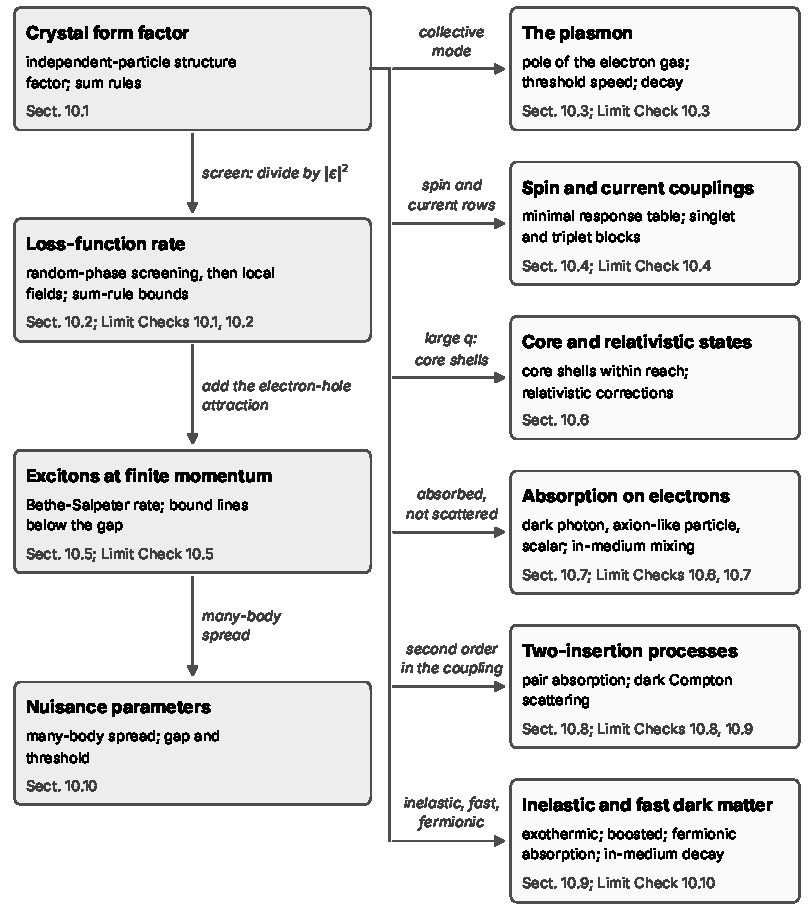
\includegraphics[width=0.85\linewidth]{figures/ch10/map10.pdf}
  \caption{The electronic response and its extensions. Left, the hierarchy of approximations to the density response: the independent-particle crystal form factor (\cref{sec:10.1}), screened by $|\varepsilon|^2$ in the random-phase approximation and then with local fields (\cref{sec:10.2}; \cref{lim:10.2a,lim:10.2b}), with the electron--hole attraction added (\cref{sec:10.5}; \cref{lim:10.5a}); the step to the next approximation is the theory uncertainty of the rate, collected in its uncertainty budget (\cref{sec:10.10}). Right, the response classes beyond slow, elastic scattering on the density: the plasmon (\cref{sec:10.3}; \cref{lim:10.3b}), spin and current rows (\cref{sec:10.4}; \cref{lim:10.4a}), core shells at large $q$ (\cref{sec:10.6}), absorption (\cref{sec:10.7}; \cref{lim:10.7a,lim:10.7b}), processes second order in the coupling (\cref{sec:10.8}; \cref{lim:10.8a}), and inelastic, boosted or fermionic dark matter (\cref{sec:10.9}; \cref{lim:10.9d}).}
  \label{fig:10-map}
\end{figure}

\section{The crystal form factor}\label{sec:10.1}

A dark-matter particle of \SI{10}{MeV} that crosses silicon can transfer up to \SI{53}{keV} of momentum and deposit up to \SI{35}{eV} (\cref{tab:1-kinematics}). Whether it leaves an electron--hole pair behind depends, for each pair $(\vect{q},\omega)$, on how strongly the filled bands respond at that momentum and energy. In the simplest description of the crystal, electrons that move independently in the potential of clamped nuclei, that response is a sum over transitions from one valence state to one conduction state, each weighted by the square of the density vertex of \cref{sec:3.2}. Experiments quote it as the \emph{crystal form factor} of Essig and collaborators~\cite{essig2016direct}, and nearly every projected or published limit on electron scattering in silicon and germanium rests on a table of it.

\subsection{The independent-particle structure factor}

Electron scattering through a mediator that couples to the electron number uses one row of the master formula, the density $n_e(\vect{q})$, with $\mathfrak{D}_{ee} = |\tilde V(\vect{q})|^2$ and all other entries zero (\cref{sec:8.2}). The spectrum per unit target mass is then \cref{eq:8.2-spectrum} with the dynamic structure factor of the electrons in place of the contraction, which is \cref{eq:A.8-rate}.

At the base point $\mathfrak{T}_0$ of the expansion hierarchy, \cref{eq:8.5-base}, the nuclei are clamped, the temperature is zero and the electrons are independent particles. The ground state is then a single Slater determinant $|0\rangle$ in which the four valence bands of silicon are filled with both spins and the conduction bands are empty. The one-electron states are Kohn--Sham states, and the conduction energies are raised by the scissor shift of \cref{sec:3.4}, which leaves the states themselves unchanged.

In the Bloch basis the density operator is \cref{eq:3.2-ne}. Acting on $|0\rangle$, a term $c^\dagger_{m,\vect{k}+\vect{q},s}c_{n\vect{k}s}$ vanishes if $n$ is a conduction band, since there is no electron to remove, and if $m$ is a valence band, since the state is already occupied, unless it is the state just emptied. That exception requires $\vect{k} + \vect{q} \equiv \vect{k}$, that is $\vect{q} = \vect{G}$, and it returns $|0\rangle$ itself with $\omega = 0$, the elastic Bragg term that no detector sees. For $\omega > 0$,
\begin{equation}
  n_e(\vect{q})|0\rangle = \sum_s\sum_{\vect{k}\in\mathrm{BZ}}\sum_{v,c}\rho_{cv}(\vect{k},\vect{q})\,|c,\vect{k}+\vect{q},s;\,v\vect{k}s\rangle ,
  \label{eq:D.29-pairs}
\end{equation}
where the ket is $|0\rangle$ with the electron moved from $v\vect{k}s$ to $c,\vect{k}+\vect{q},s$. These pair states are orthonormal, and their energies above the ground state are $\varepsilon_{c,\vect{k}+\vect{q}} - \varepsilon_{v\vect{k}}$, with $\vect{k} + \vect{q}$ folded into the first zone by the Umklapp vector $\vect{G}_{\mathrm{U}}$ of \cref{eq:3.2-rho}. Each pair appears once in \cref{eq:D.29-pairs}: at fixed $\vect{q}$ the hole $v\vect{k}s$ fixes the crystal momentum of the electron. Inserting \cref{eq:D.29-pairs} into \cref{eq:4.2-Sab} with $a = b = n_e$, the two spins give equal terms, and the sum over the $N$ crystal momenta of the zone becomes $\Vol\int_{\mathrm{BZ}}\dd^3k/(2\pi)^3$ with $\Vol = N\Omega$ (\cref{sec:3.1}). The volume cancels against the $1/\Vol$ in the definition of $S$, and
\begin{keyresult}[Independent-particle structure factor of a semiconductor]
\begin{equation}
  S^0(\vect{q},\omega) = 4\pi\sum_{v,c}\int_{\mathrm{BZ}}\frac{\dd^3k}{(2\pi)^3}\,\bigl|\rho_{cv}(\vect{k},\vect{q})\bigr|^2\,\delta\bigl(\omega - \varepsilon_{c,\vect{k}+\vect{q}} + \varepsilon_{v\vect{k}}\bigr) ,
  \label{eq:10.1-S0}
\end{equation}
for $\omega > 0$ at $T = 0$, with $v$ over the valence and $c$ over the conduction bands. The electron-recoil rate at $\mathfrak{T}_0$ is \cref{eq:8.2-spectrum} with $\mathfrak{D}_{ee} = \pi\sigmae\FDM(q)^2/\mu_{\chi e}^2$ (\cref{eq:1.4-Vsq}) and $S = S^0$.
\end{keyresult}
\noindent The factor $4\pi$ in $S^0$ is the $2\pi$ of \cref{eq:4.2-Sab} times 2 for spin. Each transition counts once, with the square of an amplitude of order one, and the rate is a sum of $|\rho_{cv}|^2$ over pairs, weighted by energy conservation. The same expression is $-2\Imag R^0_{\vect{0}\vect{0}}(\vect{q},\omega)$, the head of the independent-particle bubble \cref{eq:4.6-R0} at $T = 0$: in the bubble, a pair costs $\varepsilon_{c,\vect{k}+\vect{q}} - \varepsilon_{v\vect{k}}$ and its resonant denominator carries the imaginary part $-\pi\delta(\omega - \varepsilon_{c,\vect{k}+\vect{q}} + \varepsilon_{v\vect{k}})$. So the codes that compute dielectric functions compute $S^0$ along the way, and the screened response of \cref{sec:10.2} starts from the same object.

As in \cref{chap:3}, $S^0$ vanishes below the smallest pair energy $E_{\mathrm{min}}(\vect{q})$ of \cref{eq:3.3-Emin}, and a mass is kinematically allowed only where \cref{eq:3.3-allowed} holds. Its total weight is fixed by the closure relation \cref{eq:3.2-closure}, each valence state distributes a total weight of one over all bands at $\vect{k}+\vect{q}$, and only the part that lands in conduction bands counts. The zeroth moment is therefore at most $4\pi\cdot4/\Omega$, four valence bands of unit weight, a bound reached only when every transition leads into a conduction band. At small $q$ most of the weight stays in the same band and is lost to the rate; at large $q$ it spreads over conduction bands far above the gap.

Its energy-weighted sum is fixed as well. For a local one-electron potential, the double commutator of \cref{sec:4.3} taken for one electron gives $\sum_m(\varepsilon_{m,\vect{k}+\vect{q}} - \varepsilon_{n\vect{k}})|\rho_{mn}(\vect{k},\vect{q})|^2 = q^2/2m_e$ for every state $n\vect{k}$, the sum running over all bands $m$. The terms in which $m$ is another valence band are absent from \cref{eq:10.1-S0}, but summed over $\vect{k}$ they cancel: each transition at $-\vect{q}$ is the reverse of one at $\vect{q}$, so the valence--valence sum at $-\vect{q}$ is minus the sum at $\vect{q}$, while $S^0(\vect{q},\omega) = S^0(-\vect{q},\omega)$ in silicon makes the two sums equal, and a sum equal to its own negative vanishes. The first moment of \cref{eq:10.1-S0} is then $4\pi\cdot4\cdot\Omega^{-1}\cdot q^2/2m_e = \pi\nd_eq^2/m_e$ with $\nd_e = 8/\Omega$, the $f$-sum rule \cref{eq:4.3-fsum} for the valence electrons, since $\int_{\mathrm{BZ}}\dd^3k/(2\pi)^3 = 1/\Omega$. It is the standard test of a computed $S^0$, with the caveats of \cref{sec:4.3} for nonlocal potentials.

Note that $\vect{q}$ in \cref{eq:10.1-S0} is the physical momentum transfer and is never folded. The crystal momentum of the final electron is $\vect{k} + \vect{q}$ reduced to the first zone, but the vertex $\rho_{cv}$ depends on the whole $\vect{q}$ through the Umklapp vector that stays in the plane wave (\cref{eq:3.2-rho}), and so do $\vmin$ and $\FDM$ on the dark-matter side (\cref{sec:1.3}). Two momentum transfers that differ by a reciprocal-lattice vector reach the same pairs with different amplitudes and different kinematic weights.

The structure factor of a crystal depends on the direction of $\vect{q}$, and the full velocity kernel of \cref{eq:8.2-spectrum} gives a rate that changes as the Earth turns the crystal through the dark-matter wind, the daily modulation of \cref{sec:11.7}. For the time-averaged rate of a target whose orientation is not resolved, the literature replaces $S^0$ by its average $\bar S^0(q,\omega)$ over the directions of $\vect{q}$. The velocity and angular integrals then reduce to the mean inverse speed, \cref{eq:A.8-eta}. The rate takes the isotropic form \cref{eq:A.8-rateiso},
\begin{equation}
  \frac{\dd\mathcal{R}}{\dd\omega} = \frac{\rho_\chi\,\sigmae}{4\pi\,\mchi\,\rho_T\,\mu_{\chi e}^2}\int q\,\dd q\;\FDM(q)^2\,\eta\bigl(\vmin(q,\omega)\bigr)\,\bar S^0(q,\omega) .
  \label{eq:10.1-rateiso}
\end{equation}
\Cref{app:A.8} explains why this is not the same as averaging the directional rate over a day: a detector at fixed latitude does not sample all orientations equally.

\subsection{Form-factor normalizations}

Essig, Fernandez-Serra, Mardon, Soto, Volansky and Yu wrote the same rate per target, with the target information collected into a dimensionless function~\cite[Eqs.~(3.13) and (3.17)]{essig2016direct}. In our notation their crystal form factor is
\begin{equation}
  |f_{\mathrm{crys}}(q,\omega)|^2 = \frac{q^3\,\Omega}{4\pi\alpha\,m_e^2}\,\bar S^0(q,\omega) ,
  \label{eq:10.1-fcrys}
\end{equation}
which is \cref{eq:A.8-fcrys} at $\mathfrak{T}_0$. The factor $q^3/\alpha m_e^2$ is chosen so that $|f_{\mathrm{crys}}|^2$ is close to one where the rate is made. We substitute $\Omega\bar S^0 = 4\pi\alpha m_e^2|f_{\mathrm{crys}}|^2/q^3$ into \cref{eq:10.1-rateiso} and use $\rho_T\Omega = M_{\mathrm{cell}}$, the cell mass:
\begin{equation}
  \begin{aligned}
  \frac{\dd\mathcal{R}}{\dd\omega} &= \frac{\rho_\chi\,\sigmae\,\alpha\,m_e^2}{\mchi\,M_{\mathrm{cell}}\,\mu_{\chi e}^2} \\
  &\quad\times\int\frac{\dd q}{q^2}\,\eta\bigl(\vmin(q,\omega)\bigr)\,\FDM(q)^2\,|f_{\mathrm{crys}}(q,\omega)|^2 .
  \end{aligned}
  \label{eq:D.29-rate}
\end{equation}
Multiplying by $\omega$ turns $\dd q/q^2$ into $\dd\ln q\,(\omega/q)$ and the left side into $\dd\mathcal{R}/\dd\ln\omega$. Of the crystal, only the cell mass is left outside the form factor, because $|f_{\mathrm{crys}}|^2$ is defined per cell:
\begin{limitbox}[Crystal form-factor rate][lim:10.1a]
At independent-particle level, unscreened, at zero temperature and with clamped nuclei, the electron-recoil spectrum per unit target mass is
\begin{equation*}
  \begin{aligned}
  \frac{\dd\mathcal{R}}{\dd\ln\omega} &= \frac{\rho_\chi\,\sigmae\,\alpha\,m_e^2}{\mchi\,M_{\mathrm{cell}}\,\mu_{\chi e}^2} \\
  &\quad\times\int\dd\ln q\;\frac{\omega}{q}\,\eta\bigl(\vmin(q,\omega)\bigr)\,\FDM(q)^2\,|f_{\mathrm{crys}}(q,\omega)|^2 ,
  \end{aligned}
\end{equation*}
after Ref.~\cite[Eqs.~(3.13) and (3.17)]{essig2016direct}, divided by the target mass.
\par\smallskip
{\centering
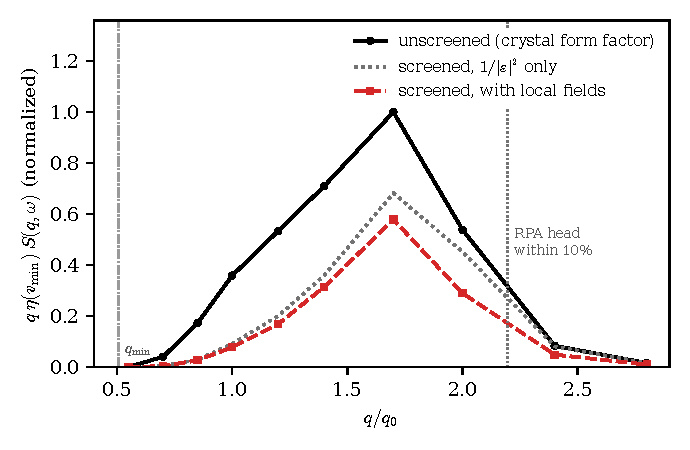
\includegraphics[width=\linewidth]{figures/ch10/limit10_1a.pdf}
\captionof{figure}{Unscreened rate against screened rates in silicon at $\omega = \SI{5}{eV}$, for $\mchi = \SI{10}{MeV}$ and a heavy mediator: the rate weight $q\,\eta(\vmin)\,S(q,\omega)$ of \cref{eq:10.1-rateiso} against $q$, normalized to the maximum of the unscreened curve. All three curves come from one model, the local empirical pseudopotential of \cref{we:8-lf-nuisance} (model gap \SI{0.82}{eV}), with $\vect{q}$ along the direction $(5,3,1)$, chosen so that no $\vect{q} + \vect{G}$ comes close to zero, and spectra averaged over 4.5 to \SI{5.5}{eV}. Solid: independent particles, the crystal form factor of the box. Dotted: random-phase screening by the macroscopic $1/|\varepsilon|^2$ alone, the leading correction. Dashed: random-phase screening with local fields over the 51 shortest reciprocal-lattice vectors, the fuller result. Dash-dotted: the smallest $q$ the halo reaches at \SI{5}{eV}. Dotted vertical: above $2.2\,q_0 = \SI{8.2}{keV}$, with $q_0 = \alpha m_e$, the macroscopic screening changes the rate by less than 10 percent. The model has no momentum components above $2.8\,q_0$, where the plot ends. Nothing is shaded. No $q$ in the plotted range brings the fuller result within 10 percent of the unscreened one.}\label{fig:10-fcrys-limit}
\par}
\smallskip
Near the kinematic edge the unscreened formula overstates the response twentyfold, at $q_0$ fourfold; macroscopic screening fades above about \SI{8}{keV}, but local fields keep the screened response near 0.6 of the unscreened one up to the largest $q$ this model can describe.
\end{limitbox}
\noindent The leading correction to the box lies on the many-body axis $\mathcal{X}$ of \cref{sec:8.5}: the polarization of the valence electrons screens the dark matter's potential and multiplies the response at small $q$ by roughly $1/|\varepsilon(q,\omega)|^2$, and the local fields of the crystal modify that factor. \Cref{sec:10.2} adds both. In silicon at \SI{5}{eV} the correction is not small (\cref{fig:10-fcrys-limit}). The kinematic edge at that energy lies at $0.525\,q_0$, with $q_0 = \alpha m_e = \SI{3.73}{keV}$; just above it, at $q = 0.55\,q_0$, screening cuts the response to 0.05 of the unscreened value, and at $q_0$ to 0.22. The local fields do not fade with $q$ as the macroscopic factor does: between 2 and $2.8\,q_0$ they hold the response at 0.54 to 0.61 of the unscreened value, with an uncertainty of about 10 percent from the size of the set of reciprocal-lattice vectors. Integrated over $q$, the screened rate at \SI{5}{eV} is 0.47 of the unscreened one. The model is cruder than the tabulated form factor, which it matches to within 25 percent at $q_0$, and \cref{sec:10.2} computes the same ratios from first-principles tables.

Written out with \cref{eq:10.1-S0}, $|f_{\mathrm{crys}}|^2$ is a double integral over the initial and final crystal momenta $\vect{k}$ and $\vect{k}'$ and a sum over the Umklapp vectors $\vect{G}'$ that connect them, the form in which Ref.~\cite[Eq.~(3.17)]{essig2016direct} defines it. For any function $g(\vect{q})$,
\begin{equation*}
  \int\frac{\dd^2\hat{\vect{q}}}{4\pi}\,g(q\hat{\vect{q}}) = \frac{1}{4\pi q^2}\int\dd^3q'\,\delta(q - |\vect{q}'|)\,g(\vect{q}') ,
\end{equation*}
since $\dd^3q' = q'^2\dd q'\,\dd^2\hat{\vect{q}}'$. At fixed $\vect{k}$, every $\vect{q}'$ is reached exactly once as $\vect{q}' = \vect{k}' - \vect{k} + \vect{G}'$ with $\vect{k}'$ in the first zone and $\vect{G}'$ a reciprocal-lattice vector, because the zones translated by all $\vect{G}'$ tile space. Then $\int\dd^3q' = \sum_{\vect{G}'}\int_{\mathrm{BZ}}\dd^3k'$, the final crystal momentum is $\vect{k}'$, and $\vect{G}'$ is the Umklapp vector of the transition. Applied to \cref{eq:10.1-S0},
\begin{equation*}
  \begin{aligned}
  \bar S^0(q,\omega) &= \frac{(2\pi)^3}{q^2}\sum_{v,c}\int_{\mathrm{BZ}}\frac{\dd^3k}{(2\pi)^3}\int_{\mathrm{BZ}}\frac{\dd^3k'}{(2\pi)^3}\sum_{\vect{G}'}\delta(q - |\vect{k}' - \vect{k} + \vect{G}'|) \\
  &\quad\times|\rho_{cv}(\vect{k},\vect{k}'-\vect{k}+\vect{G}')|^2\,\delta(\omega - \varepsilon_{c\vect{k}'} + \varepsilon_{v\vect{k}}) .
  \end{aligned}
\end{equation*}
Multiplying by $q^3\Omega/4\pi\alpha m_e^2$ and writing $(2\pi)^3/4\pi = 2\pi^2$,
\begin{equation}
  \begin{aligned}
  |f_{\mathrm{crys}}(q,\omega)|^2 &= \frac{2\pi^2}{\alpha m_e^2\Omega}\sum_{v,c}\int_{\mathrm{BZ}}\frac{\Omega\,\dd^3k}{(2\pi)^3}\int_{\mathrm{BZ}}\frac{\Omega\,\dd^3k'}{(2\pi)^3}\sum_{\vect{G}'}q\,\delta(q - |\vect{k}' - \vect{k} + \vect{G}'|) \\
  &\quad\times|\rho_{cv}(\vect{k},\vect{k}'-\vect{k}+\vect{G}')|^2\,\delta(\omega - \varepsilon_{c\vect{k}'} + \varepsilon_{v\vect{k}}) .
  \end{aligned}
  \label{eq:D.29-fcrys}
\end{equation}
Their prefactor $2\pi^2(\alpha m_e^2V_{\mathrm{cell}})^{-1}E_e^{-1}$ times their $E_e\,\delta(E_e - \cdots)$ is our $2\pi^2/\alpha m_e^2\Omega$ times the energy delta function, their $f_{[i\vect{k},i'\vect{k}',\vect{G}']}$ is $\rho_{cv}(\vect{k},\vect{k}'-\vect{k}+\vect{G}')$ in the plane-wave form \cref{eq:3.2-rhopw}, and the spin factor 2 sits in their $2\pi^2$ as it sits in our $4\pi$~\cite[Eq.~(A.29)]{essig2016direct}. The prefactor $2\pi^2/\alpha m_e^2\Omega$ is \SI{1.99}{eV} for silicon, with $\Omega = \SI{40.05}{\angstrom^3}$.

Since a tabulated form factor is used far from the paper that produced it, its normalization is where errors enter. The literature states the same rate in several normalizations, and each converts to $\bar S^0$ in one line.
\begin{itemize}
\item \emph{Structure factor, form factor and dielectric function.} $\Omega\bar S^0 = 4\pi\alpha m_e^2|f_{\mathrm{crys}}|^2/q^3$ and $|f_{\mathrm{crys}}|^2 = q^5\Omega\,\varepsilon_2/8\pi^2\alpha^2m_e^2$, \cref{eq:A.8-fcrys}; the second uses the unscreened $\varepsilon_2 = 2\pi\alpha\bar S^0/q^2$ of \cref{eq:A.7-SL} at $T = 0$, and agrees with Ref.~\cite[Eq.~(16)]{knapen2021dark}.
\item \emph{Per target or per unit mass.} A rate for a target of $N_{\mathrm{cell}}$ cells~\cites[Eq.~(3.13)]{essig2016direct}[Eq.~(36)]{catena2021crystal} is $N_{\mathrm{cell}}M_{\mathrm{cell}}$ times \cref{eq:D.29-rate}.
\item \emph{Sums over states.} Ref.~\cite[Eqs.~(3.6) and (3.12)]{griffin2021extended} writes the rate with the transition form factor $f_{i\to f}(\vect{q}) = \langle f|\ee^{\ii\vect{q}\cdot\vect{r}}|i\rangle$ between unit-normalized spatial orbitals and a separate spin factor. Then $(2\pi/\Vol)\sum_{i,f}|f_{i\to f}|^2\delta(\omega - E_f + E_i) = S^0/2$. The transition matrix element of the density in Ref.~\cite[Eqs.~(11) and (17)]{trickle2023exceed} is the vertex $\rho_{cv}(\vect{k},\vect{q})$ of \cref{eq:3.2-rho}.
\item \emph{Crystal-momentum weights.} Plane-wave codes replace $\int_{\mathrm{BZ}}\Omega\,\dd^3k/(2\pi)^3$ by $\frac12\sum_{\vect{k}}w_{\vect{k}}$ with weights that sum to 2~\cite[Eq.~(4.2)]{essig2016direct}. The 2 is the spin factor already present in the prefactor, and it must not be counted twice.
\item \emph{Bins.} A tabulated form factor is an average over bins of width $\Delta q$ and $\Delta\omega$~\cite[Eq.~(4.1)]{essig2016direct}, and \cref{eq:D.29-rate} becomes a double sum with $\dd q\,\dd\omega \to \Delta q\,\Delta\omega$. A table that stores the sum over a bin rather than the average differs by the bin widths.
\end{itemize}
A factor of two or ten in a rate is easy to make in these steps and hard to see in a plot. The $f$-sum rule catches it: at $q \approx q_0$, where the free recoil energy $q^2/2m_e = \SI{13.6}{eV}$ lies well inside the tabulated range, $\int\dd\omega\,\omega\,\bar S^0$ must come within some ten percent of $\pi\nd_eq^2/m_e$. A rigid scissor shift $\Delta_{\mathrm{scis}}$ raises it by $\Delta_{\mathrm{scis}}\int\dd\omega\,\bar S^0$, since it moves the weight without changing the vertices.

\subsection{The silicon form factor}

\Cref{fig:10-fcrys} shows the crystal form factor of silicon as Ref.~\cite{essig2016direct} tabulated it, from PBE bands with the gap set by a scissor shift, four valence and 52 conduction bands, and a plane-wave cutoff of \SI{70}{Ry}~\cite[Sects.~4.1 and 4.2]{essig2016direct}. The scissor puts the gap at \SI{1.11}{eV}, close to the room-temperature gap of \SI{1.12}{eV} (\cref{sec:10.7-edge}); the gap at zero temperature is \SI{1.17}{eV} (\cref{sec:3.3}), and a cryogenic detector sees the difference as a shift of the onset. The table begins at \SI{1.2}{eV}, its first bin above the gap, and ends at \SI{50}{eV}, where the highest conduction band runs out.
\begin{figure}[t]
  \centering
  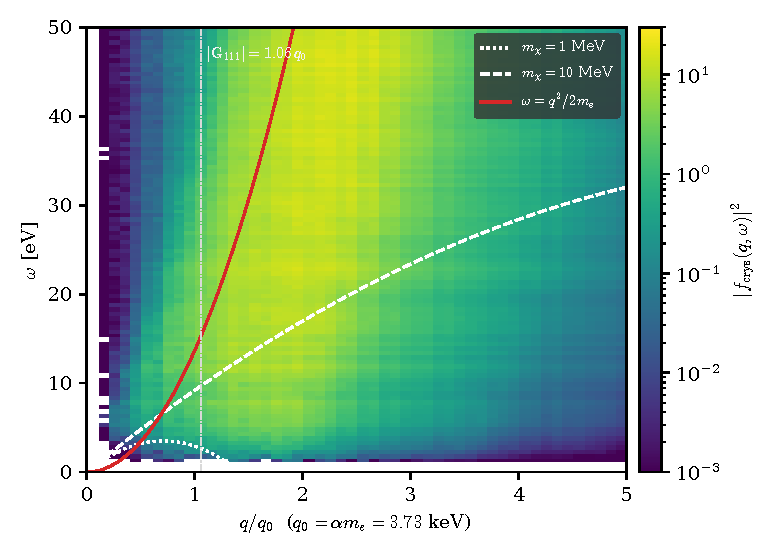
\includegraphics[width=0.85\linewidth]{figures/ch10/fig10_1.pdf}
  \caption{Crystal form factor $|f_{\mathrm{crys}}(q,\omega)|^2$ of silicon, \cref{eq:10.1-fcrys}, from the tabulation of Ref.~\cite{essig2016direct}: PBE bands with the gap set to \SI{1.11}{eV} by a scissor shift, valence to conduction, unscreened, averaged over the directions of $\vect{q}$. For display, bins are merged to $0.1\,q_0$ in $q$ and \SI{0.5}{eV} in $\omega$; white cells below $0.3\,q_0$ are bins that the grid of crystal momenta of the calculation does not reach, and white cells in the lowest row are bins next to the gap that hold no weight. White curves: the largest energy that dark matter of 1 and \SI{10}{MeV} can deposit at each $q$, $qv_{\mathrm{max}} - q^2/2\mchi$ with $v_{\mathrm{max}} = \SI{794.5}{km.s^{-1}}$ (\cref{eq:1.3-region}); everything below a curve is kinematically allowed. Red: the free-electron recoil $\omega = q^2/2m_e$, along which the weight concentrates at large $q$. Dash-dotted: $|\vect{G}_{111}| = \sqrt3\,2\pi/a = 1.06\,q_0$, the shortest reciprocal-lattice vector. The color scale is logarithmic.}\label{fig:10-fcrys}
\end{figure}

Divided by $\pi\nd_eq^2/m_e$ with the valence density $\nd_e = 8/\Omega$, the first moment of the tabulated $\bar S^0$ over its \SI{50}{eV} is 1.03 at $q_0$, and 1.1 to 1.2 between $0.3\,q_0$ and $0.7\,q_0$, as means over windows of $0.2\,q_0$ with the bins the grid does not reach counted as zero. The scissor shift raises the first moment, since it moves every transition up by about \SI{0.55}{eV} without changing its weight; that is the difference between the PBE gap of silicon (\cref{sec:3.4}) and \SI{1.11}{eV}. At small $q$, where the mean energy deposited is a few eV, the shift accounts for about ten percent; the rest of the excess has no identified cause (\cref{sec:10.10-manybody}). Beyond $1.5\,q_0$ the ratio falls, to 0.83 at $1.5\,q_0$ and 0.33 at $2\,q_0$: the free recoil energy is then 31 and \SI{54}{eV}, and the weight has moved past the last tabulated band. As a second check, the tabulated $\bar S^0$ at $q_0$ lies within 25 percent of the independent-particle structure factor of the local empirical pseudopotential of \cref{we:8-lf-nuisance}, along $[100]$, between 5 and \SI{20}{eV}. The two calculations share no input other than the crystal structure.

The form factor varies with $q$ on two scales that silicon happens to have in common, the zone scale and $q_0$ (\cref{sec:1.3}). At momentum transfers small compared with the zone, $2\pi/a = 0.61\,q_0$, the vertex reduces to its optical limit, $\rho_{cv} \simeq \vect{q}\cdot\vect{v}_{cv}/(\varepsilon_{c\vect{k}} - \varepsilon_{v\vect{k}})$ (\cref{sec:3.2}), so $\bar S^0 \propto q^2$ at fixed $\omega$, and by \cref{eq:A.8-fcrys} $|f_{\mathrm{crys}}|^2 \simeq q^5\Omega\varepsilon_2(\omega)/8\pi^2\alpha^2m_e^2$ with the optical $\varepsilon_2$. Integrated over energy, the tabulated form factor grows as $q^{4.8}$ between $0.3\,q_0$ and $0.75\,q_0$, close to this dipole scaling even where $q$ is no longer small compared with the zone. Near $|\vect{G}_{111}| = 1.06\,q_0$ the momentum transfer resolves the bond, the optical limit fails, and the vertex is set by the plane-wave content of the valence states at momenta of order $q$ (\cref{eq:3.2-rhopw}). At fixed $\omega$ between 3 and \SI{10}{eV}, $|f_{\mathrm{crys}}|^2$ peaks at $1.7$ to $1.8\,q_0$ and at $2\,q_0$ it is still 2.1 to 2.5 times its value at $q_0$; by $3\,q_0$ it has fallen to a quarter of its value at $q_0$. The factor $q^3$ in \cref{eq:10.1-fcrys} pushes this peak outward. The rate weight of \cref{eq:10.1-rateiso}, $q\bar S^0$, peaks earlier, at 1.1 to $1.4\,q_0$.

At large $q$ the figure shows where the weight goes. Along the red curve, $\omega = q^2/2m_e$, a dark-matter particle would give a free electron at rest its recoil energy, and at large $q$ the response of bound electrons gathers around it, broadened by their momenta, as in the impulse approximation of \cref{we:4-gas}. At a fixed small energy deposited, a large $q$ needs an electron that already moves against the momentum transfer with a momentum of about $q/2$, and the bound valence states have little weight at momenta much above $q_0$. That is why, integrated over the tabulated energies, $|f_{\mathrm{crys}}|^2$ falls as $q^{-5}$ between 2 and $4\,q_0$. The white curves show which part of the plane the halo can reach. Dark matter of \SI{1}{MeV} reaches only a thin sliver above the gap at $q < 1.4\,q_0$, near the bottom of the figure; at \SI{10}{MeV} it reaches deposits up to \SI{35}{eV} and momentum transfers well past the peak of $|f_{\mathrm{crys}}|^2$.

\begin{workedexample}{The silicon rate at \SI{10}{MeV}}\label{we:10-rate}
Take $\mchi = \SI{10}{MeV}$, $\sigmae = \SI{e-37}{cm^2}$ and the standard halo of \cref{app:A.8}: $\rho_\chi = \SI{0.3}{GeV.cm^{-3}}$, $v_0 = \SI{238}{km.s^{-1}}$, $v_{\mathrm{esc}} = \SI{544}{km.s^{-1}}$ and $v_{\mathrm{E}}^{\mathrm{ref}} = \SI{250.5}{km.s^{-1}}$. The reduced mass is $\mu_{\chi e} = \SI{486.2}{keV}$, so $m_e^2/\mu_{\chi e}^2 = 1.105$, and the number density is $\rho_\chi/\mchi = \SI{30}{cm^{-3}}$. The prefactor of the box, with $M_{\mathrm{cell}} = \SI{52.33}{GeV}$, is
\begin{equation*}
  \frac{\rho_\chi\,\sigmae\,\alpha\,m_e^2}{\mchi\,M_{\mathrm{cell}}\,\mu_{\chi e}^2}
  = \frac{\SI{30}{cm^{-3}}\times\SI{e-37}{cm^2}\times c\times1.105}{137.036\times M_{\mathrm{cell}}}
  = \SI{2.45e5}{kg^{-1}.yr^{-1}} ,
\end{equation*}
where the factor $c$ turns $\rho_\chi\sigmae/\mchi$ into a rate and $\eta$ is then a pure number, $\langle1/v\rangle = 1041$ in units of $1/c$. Everything else is the double integral of $\eta\FDM^2|f_{\mathrm{crys}}|^2\,\dd q\,\dd\omega/q^2$ over the tabulated bins, with $\vmin = \omega/q + q/2\mchi$ and $\eta$ in the closed form of \cref{app:D.1}.

For a heavy mediator, $\FDM = 1$, the double integral is 0.652, and the rate above the gap is
\begin{equation*}
  \mathcal{R} = \SI{2.45e5}{kg^{-1}.yr^{-1}}\times0.652 = \SI{1.60e5}{kg^{-1}.yr^{-1}} ,
\end{equation*}
about 440 events per kilogram and day. The spectrum $\dd\mathcal{R}/\dd\omega$ peaks at \SI{6.5}{eV}, its mean is \SI{6.0}{eV}, 38 percent of the events deposit at most \SI{4.9}{eV}, and it ends at \SI{35}{eV}, the largest energy a particle at $v_{\mathrm{max}}$ can deposit. At the peak energy the integrand in $q$ is flat between about $1.7\,q_0$ and $1.9\,q_0$ (6.5 to \SI{7.09}{keV}); only 5 percent of the rate comes from $q < q_0$, and 27 percent from $q > 2\,q_0$.

For a light mediator, $\FDM = (q_0/q)^2$, the integral is 0.193, and $\mathcal{R} = \SI{4.73e4}{kg^{-1}.yr^{-1}}$, about 130 per kilogram and day. The factor $(q_0/q)^4$ moves the rate to small $q$ and low energy: the spectrum peaks at \SI{3.3}{eV}, its mean is \SI{4.5}{eV}, 66 percent of the events deposit at most \SI{4.9}{eV}, and the $q$ integrand at the peak is largest near $0.6\,q_0 = \SI{2.2}{keV}$, near the kinematic edge. Now 44 percent of the rate comes from $q < q_0$.

The two mediators probe different parts of \cref{fig:10-fcrys}. The heavy mediator samples the form factor near its maximum, at twice $q_0$ and a few eV, where the bands and the plane-wave content of the valence states set the answer. The light mediator samples its small-$q$ edge, where the form factor is smallest and where, as the limit check shows, screening matters most. The scaling of \cref{eq:1.5-heuristic} gives the rest: at fixed $\sigmae$ the rate falls as $1/\mchi$ once $\mchi$ is well above the threshold and the reach in $q$ covers the peak. Published rates differ from these numbers mainly through the halo: Ref.~\cite{essig2016direct} uses $\rho_\chi = \SI{0.4}{GeV.cm^{-3}}$, $v_0 = \SI{230}{km.s^{-1}}$, $v_{\mathrm{esc}} = \SI{600}{km.s^{-1}}$ and an Earth speed of \SI{240}{km.s^{-1}}~\cite[Sect.~6]{essig2016direct}.
\end{workedexample}

\subsection{Convergence parameters and omitted physics}

A crystal form factor is computed from Kohn--Sham bands and plane-wave vertices. The bands come from a density-functional calculation with a pseudopotential (\cref{sec:3.4,sec:3.5}), with the gap set by a scissor shift or by quasiparticle corrections (\cref{app:E.1,app:E.3}). The vertex is the plane-wave overlap \cref{eq:3.2-rhopw}, evaluated for every valence state, every conduction state and every Umklapp vector that a given $\vect{q}$ requires, with $\vect{q}$ kept unfolded. \Cref{app:E.7} sets out the calculation and its cost, about $5\times10^{11}$ vertices for silicon with 52 conduction bands and momentum transfers up to \SI{30}{keV}. The plane-wave cutoff limits the largest $q$ a vertex can carry, the number of conduction bands the largest $\omega$, and the grid of crystal momenta the resolution at small $q$ and near the onset; the white cells of \cref{fig:10-fcrys} are this last limit. At large $q$ the pseudopotential matters as well. A pseudo-wavefunction is smooth inside the core region by construction, and above a few $q_0$ the vertex needs the nodes of the true valence states near the nucleus. The all-electron reconstruction of \cref{app:E.2} restores them; Griffin and collaborators found that it raises the valence-to-conduction rate of germanium at energies above about \SI{15}{eV}~\cite[Sect.~1]{griffin2021extended}. For silicon at \SI{10}{MeV}, \cref{we:10-rate} draws a quarter of the heavy-mediator rate from $q > 2\,q_0$, and that part rests on the same correction.

Its place in the expansion hierarchy, $\mathfrak{T}_0$, fixes what the calculation leaves out. It has no screening: the dark matter's potential acts on independent electrons, while in the crystal the other electrons polarize and reduce it, most strongly at small $q$, where the light mediator and the lightest masses collect their rate. \Cref{sec:10.2} adds the random-phase screening and the local fields, and shows when the loss function gives the rate exactly. It has no electron--hole attraction: an exciton moves weight from the continuum toward the gap, which matters for the lowest thresholds, and \cref{sec:10.5} treats excitons at finite momentum. It has no lattice: the nuclei are clamped, so the phonon-assisted transitions that open the indirect gap below the zero-phonon edge (\cref{sec:13.1}) and the Migdal effect (\cref{chap:12}) are absent. It holds only valence-to-conduction transitions: the $2p$ shell of silicon, \SI{99}{eV} below the valence maximum, and the $3d$ shell of germanium, about \SI{29}{eV} below it, are the subject of \cref{sec:10.6}, and the table ends at the highest conduction band it includes. And it is an angle average at zero temperature, which drops the daily modulation and the thermal shift of the gap.

\section{Screening and the loss-function rate}\label{sec:10.2}

At a momentum transfer of \SI{2}{keV} the static dielectric function of silicon is about 2.9, and a potential that varies on that scale reaches the valence electrons weakened by $1/|\varepsilon|^2 \approx 0.12$. Yet the screened rate of a \SI{10}{MeV} particle with a heavy mediator is only 2.3 times smaller than the unscreened rate of \cref{sec:10.1}. The rate is an integral over all the momentum transfers and energies that kinematics allows, most of which lie where the medium screens little, and over a spectrum whose total weight screening cannot change. Two sum rules of the loss function bound it from above, with only the plasma frequency and the static dielectric function as input. The bound on the static step fails for a mediator that couples to electrons alone once the lattice is free to move, because the electrons that follow the nuclei add an acoustic peak.

\subsection{The loss-function rate}\label{sec:10.2-rate}

A mediator that couples to the electron number acts on one row of the master formula, the density $n_e(\vect{q})$, with $\mathfrak{D}_{ee} = |\tilde V(\vect{q})|^2 = \pi\sigmae\FDM(q)^2/\mu_{\chi e}^2$ (\cref{eq:1.4-Vsq}), and the spectrum \cref{eq:8.2-spectrum} needs only the structure factor $S_{ee}$. \Cref{sec:10.1} computed it for independent electrons. The exact structure factor follows from the fluctuation--dissipation theorem as $S = (2q^2/e^2)\,L/(1 - \ee^{-\beta\omega})$, with $L(\vect{q},\omega) = \Imag[-(\varepsilon^{-1})_{\vect{0}\vect{0}}(\vect{q},\omega)]$ the loss function of \cref{eq:4.4-SL}, and the exactness theorem \cref{eq:8.4-exact} says for which couplings this holds. For a dark photon, or any mediator that couples to the total charge $n_Z$, it holds at every $(\vect{q},\omega)$ with the loss function of the total dielectric matrix of electrons and nuclei. For a mediator that couples to electrons and not to nucleons it holds exactly only with the nuclei clamped. Above the phonon band the nuclei reach the electronic final states through the Migdal amplitudes alone, suppressed by powers of $\kappa_{\mathrm{BO}}$, and the loss function gives the electron-only rate to that accuracy (\cref{sec:8.4-exact}). An electron--hole pair in silicon costs at least \SI{1.17}{eV}, eighteen times the top of the phonon band, so for the electronic rate the two couplings share one formula. In silicon the Born charges vanish, and the ionic part of the total dielectric function at these energies is negligible.

Inserting $S$ into \cref{eq:8.2-spectrum}, with $e^2 = 4\pi\alpha$, gives $|\tilde V|^2 S = \sigmae\FDM^2q^2L/[2\alpha\mu_{\chi e}^2(1 - \ee^{-\beta\omega})]$ under the integrals~\cites[Eq.~(13)]{knapen2021dark}[Eq.~(1)]{hochberg2021determining}. For an isotropic target, or a crystal whose loss function is averaged over the directions of $\vect{q}$, the velocity integral and the angular integral act on the delta function alone and produce the measure $q\,\dd q\,\eta(\vmin)/4\pi^2$ of \cref{eq:A.8-eta}, with $\vmin = \omega/q + q/2\mchi$ from \cref{eq:1.3-vmin}. Collecting the factors,
\begin{keyresult}[Loss-function rate]
\begin{equation}
  \frac{\dd\mathcal{R}}{\dd\omega} = \frac{\rho_\chi\,\sigmae}{8\pi^2\alpha\,\rho_T\,\mchi\,\mu_{\chi e}^2}\int\dd q\;q^3\,\eta\bigl(\vmin(q,\omega)\bigr)\,\FDM(q)^2\,\frac{\bar L(q,\omega)}{1 - \ee^{-\beta\omega}} ,
  \label{eq:10.2-rate}
\end{equation}
with $\bar L$ the loss function averaged over the directions of $\vect{q}$. It is exact for a coupling to the total charge, and for a coupling to the electron density at clamped nuclei or above the phonon band to Migdal order.
\end{keyresult}
\noindent At the temperatures of a detector $\beta\Eg$ is of order $10^4$ or more, and the factor $1/(1 - \ee^{-\beta\omega})$ is one. All of the medium's physics is now in one measurable function. Screening is in it through the inverse of the dielectric matrix, and so are the local fields, because $L$ is a diagonal element of $\varepsilon^{-1}$ and not the inverse of a diagonal element of $\varepsilon$. For a momentum transfer beyond the first zone the element is the one at the reciprocal vector $\vect{G}_q$ of the unreduced $\vect{q} = \vect{q}_r + \vect{G}_q$, $L = \Imag[-(\varepsilon^{-1})_{\vect{G}_q\vect{G}_q}(\vect{q}_r,\omega)]$. A crystal has a loss function that depends on the direction of $\vect{q}$, and a rate at a fixed time keeps the full kernel of \cref{app:A.8} in place of $\eta/2q$. In a cubic crystal the first anisotropic term of $L$ has angular momentum four, and it is the source of the daily modulation of \cref{sec:11.7}.

The rate of \cref{sec:10.1} is the same formula with $L$ replaced by $\varepsilon_2$ of the independent-particle head: since $S^{\mathrm{IP}} = -2\Imag R^0_{\vect{0}\vect{0}}$ (\cref{sec:10.1}) and $\varepsilon_2 = -v_{\mathrm{C}}(q)\Imag R^0_{\vect{0}\vect{0}}$ (\cref{eq:4.6-R0}), $S^{\mathrm{IP}} = (2q^2/e^2)\,\varepsilon_2^{\mathrm{IP}}$. The prefactor is the one of \cref{eq:10.2-rate}, and \cref{eq:10.1-fcrys} is this relation rewritten as a form factor. Each many-body approximation of \cref{sec:4.6} is then a choice of what to put in place of $\bar L$. Independent particles put $\varepsilon_2^{\mathrm{IP}}$. The random-phase approximation without local fields puts $\varepsilon_2^{\mathrm{IP}}/|\varepsilon_{\vect{0}\vect{0}}|^2$, in which the head $\varepsilon_{\vect{0}\vect{0}} = 1 - v_{\mathrm{C}}(q)R^0_{\vect{0}\vect{0}}$ is inverted as a number. With local fields it is $\Imag[-(\varepsilon^{-1})_{\vect{0}\vect{0}}]$ with the full matrix of \cref{eq:4.6-rpaLF}. Exchange--correlation kernels and the electron--hole attraction change the proper response inside the same inverse (\cref{sec:4.6,sec:4.9}). The three rates differ only in the many-body approximation $\mathcal{X}$ of \cref{sec:8.5}, IP, RPA and RPA + LF, with every other entry of $\mathfrak{T}$ at its base value.

For a dark photon, \cref{eq:10.2-rate} uses the reference cross section with the vacuum mixing $\zeta$, and the loss function already contains the in-medium mixing. In scattering the dark photon mixes with the longitudinal photon of the medium, its propagator acquires the factor $1/\varepsilon(\vect{q},\omega)$, and that factor is the screening of the total-charge row (\cref{sec:8.4-mixing}). The vacuum mixing goes with the full response and the in-medium mixing with the proper one; multiplying \cref{eq:10.2-rate} by $\zeta_{\mathrm{eff}}^2/\zeta^2$ would count the screening twice.

The loss function is computed from Kohn--Sham states: the random-phase dielectric matrix with local fields is inverted at each $(\vect{q}_r,\omega)$, and the diagonal element is read off at $\vect{G}_q$ (\cref{app:E.6}). Two kinds of measurement test it: optical constants give $L$ at $q \to 0$, the curve of \cref{fig:4-siloss}, and electron energy-loss and inelastic x-ray scattering give it at finite $q$. The silicon tables used below are a published calculation of this kind~\cite{knapen2021dark}, distributed with the DarkELF code~\cite{knapen2022darkelf}. They use Kohn--Sham states with the gap fixed by a scissor shift, a $\vect{k}$ grid of $8^3$ and 70 bands, and give the dielectric matrix with and without local fields. They extend to $q = \SI{22.5}{keV}$ and $\omega = \SI{89}{eV}$. Kinematics keeps the rate inside them, since $\omega \le qv_{\mathrm{max}}$ is below \SI{60}{eV} for every momentum of the table. For a material without such tables, the Mermin oscillator method of \cref{sec:4.5} fits the measured optical loss function, gap and absorption peaks included, and carries each term to finite $q$ with its share of the $f$-sum. For silicon it agrees with the first-principles tables to within 10 percent in the rate above a two-electron threshold, and the uncertainty grows for masses whose rate lies near the gap~\cite[App.~C]{knapen2021dark}.

\begin{limitbox}[Loss-function rate][lim:10.2a]
For a coupling to the electron density or to the total charge, the spectrum per unit target mass is $\dd\mathcal{R}/\dd\omega = [\rho_\chi\sigmae/(8\pi^2\alpha\rho_T\mchi\mu_{\chi e}^2)]\int\dd q\,q^3\eta(\vmin)\FDM^2\,\Imag[-1/\varepsilon(q,\omega)]/(1 - \ee^{-\beta\omega})$~\cites[Eqs.~(6) and (13)]{knapen2021dark}[Eq.~(1)]{hochberg2021determining}.
\par\smallskip
{\centering
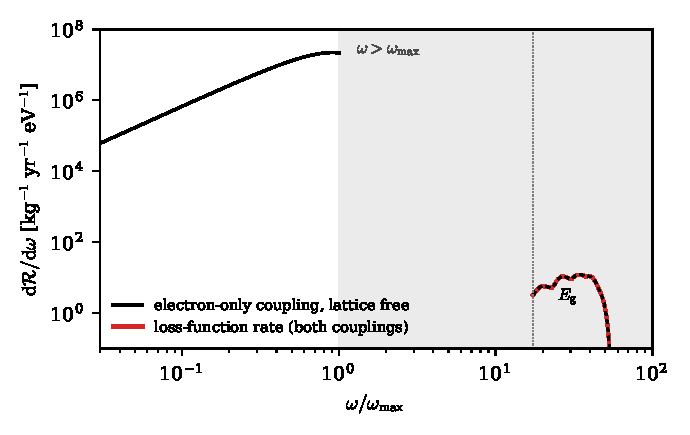
\includegraphics[width=0.82\linewidth]{figures/ch10/limit10_2a.pdf}
\captionof{figure}{Spectrum of silicon at $\mchi = \SI{1}{MeV}$, heavy mediator, $\sigmae = \SI{e-37}{cm^2}$, against $\omega/\omega_{\max}$, with $\omega_{\max} = \SI{64.1}{meV}$ the top of the phonon band. Red: the loss-function rate with the random-phase loss function with local fields; it is the whole rate of a dark photon, since the Born charges of silicon vanish. Black: an electron-only coupling with the lattice free to move, which adds the acoustic peak carried by the electrons that follow the nuclei. Model of the peak: isotropic linear longitudinal branch with $c_{\mathrm{LA}} = \SI{8.43}{km/s}$ up to $|\vect{q}| = 2\pi/a$, 14 electrons per atom following rigidly, no Debye--Waller factor, no Umklapp, transverse or multiphonon terms. Gray: $\omega > \omega_{\max}$, where the two couplings share the loss-function rate; dotted, the gap.}\label{fig:10-elf-limit}
\par}
\smallskip
Inside the phonon band an electron-only coupling excites acoustic phonons through the electrons that move with the nuclei, a peak that the loss function of the total charge does not have and that, in this model, carries more than $10^4$ times the electronic rate.
\end{limitbox}

\subsection{Screening corrections in silicon}\label{sec:10.2-corrections}

\Cref{fig:10-screening} shows the silicon rate in the three approximations. At \SI{10}{MeV} with a heavy mediator the spectrum peaks near \SI{5}{eV} in each of them, and only its height changes. Per kilogram-year at $\sigmae = \SI{e-37}{cm^2}$ the total above the gap is $1.36\times10^5$ events for independent particles, from the independent-particle head of these tables and not from the form-factor table of \cref{sec:10.1}, which gives $1.60\times10^5$ (\cref{sec:10.10-manybody} traces the difference), $8.6\times10^4$ in the random-phase approximation without local fields and $5.9\times10^4$ with them. The ratio of the unscreened rate to the screened one with local fields is 2.3 for a heavy mediator and 3.7 for a light one, and above about \SI{10}{MeV} it hardly depends on the mass. Below a few MeV it rises steeply, to 9 and 13 at \SI{1}{MeV}. At \SI{3}{MeV} it is 2.8 for a heavy mediator and 5.1 for a light one: random-phase screening lowers the independent-particle rate by \SI{52}{\percent}, and local fields lower what remains by a further \SI{26}{\percent}; for a light mediator the steps are \SI{76}{\percent} and \SI{18}{\percent}. The local fields alone lower the rate by a factor 1.46 for a heavy mediator and 1.27 for a light one at \SI{10}{MeV}, and by about 1.1 at \SI{1}{MeV}.

\begin{figure}[tbp]
  \centering
  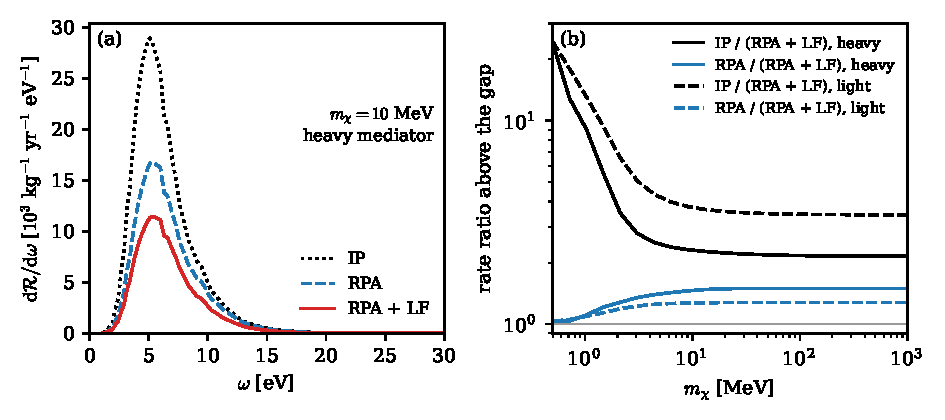
\includegraphics[width=\linewidth]{figures/ch10/fig10_2.pdf}
  \caption{Electron-recoil rate of silicon in three approximations, independent particles, RPA, and RPA with local fields, from the random-phase dielectric matrices of Knapen, Kozaczuk and Lin~\cite{knapen2021dark}, with and without local fields, with $\rho_\chi = \SI{0.3}{GeV.cm^{-3}}$, the standard halo of \cref{sec:1.2}, $\sigmae = \SI{e-37}{cm^2}$ and threshold \SI{1.11}{eV}, the step-model gap of pair creation that accompanies the tables (their scissor puts the gap at \SI{1.17}{eV}). IP: $\varepsilon_2$ of the independent-particle head of the same tables in place of $L$, the unscreened rate of \cref{sec:10.1} from a different tabulation; RPA: $\varepsilon_2/|\varepsilon_{\vect{0}\vect{0}}|^2$; RPA + LF: $\Imag[-(\varepsilon^{-1})_{\vect{0}\vect{0}}]$. The tabulated functions are averaged over the directions of $\vect{q}$ in bins of \SI{100}{eV} in $|\vect{q}|$, a choice of this figure, and end at $|\vect{q}| = \SI{22.5}{keV}$; momenta above \SI{15}{keV} already carry less than \SI{2}{\percent} of the rate at \SI{10}{MeV}. (a) Spectra at $\mchi = \SI{10}{MeV}$, heavy mediator. (b) Ratio of the rate above the gap to the rate with local fields, against $\mchi$; solid, heavy mediator, $\FDM = 1$; dashed, light mediator, $\FDM = (q_0/q)^2$.}
  \label{fig:10-screening}
\end{figure}

A pointwise screening factor would suggest a larger effect. The static values of the same tables give $\varepsilon(q,0) = 2.87$ at \SI{2}{keV} and 1.76 at $q_0 = \SI{3.73}{keV}$, so $1/\varepsilon^2$ is 0.12 and 0.32. At finite frequency the factor is stronger still: at $q_0$ the ratio $\varepsilon_2^{\mathrm{IP}}/L$ is 4.7 at \SI{3}{eV}, 5.2 at \SI{5}{eV} and 4.4 at \SI{10}{eV}. A pointwise factor leaves out where in $q$ the rate comes from, the $f$-sum rule, and the local fields, and these set the rate ratio of 2.3.

Consider first which momentum transfers carry the rate. With a heavy mediator, $q^3\eta(\vmin)$ weights large momentum transfers until the kinematic edge closes them, and at \SI{10}{MeV} half of the screened rate comes from $q > \SI{6.7}{keV}$ and \SI{29}{\percent} from $q > 2q_0$. There the valence electrons barely screen. At \SI{8}{keV} the static factor is 0.87, and the head screening, the ratio of the independent-particle rate to the random-phase rate without local fields at that momentum, is 1.18, against 13 at \SI{2}{keV} and 4.2 at $q_0$. A light mediator weights the small momenta, where screening is strong, and its ratio is correspondingly larger.

The $f$-sum rule is the second. Screening does not remove spectral weight, since $\int\dd\omega\,\omega L$ and $\int\dd\omega\,\omega\varepsilon_2$ are both $(\pi/2)\omega_p^2$ at every $\vect{q}$ (\cref{eq:4.4-fsumL,eq:4.4-fsumeps}); it moves the weight from the transition energies up toward the plasmon. At $q_0$ the peak of $\varepsilon_2^{\mathrm{IP}}$ lies at \SI{14}{eV} and that of $L$ at \SI{26}{eV}. Whether the moved weight is lost depends on the largest energy the dark matter can deposit, $\mchi v_{\mathrm{max}}^2/2$. At \SI{10}{MeV} this is \SI{35}{eV}, the moved weight stays mostly in reach, and the mean energy of the heavy-mediator spectrum rises only from 6.2 to \SI{6.6}{eV}. At \SI{1}{MeV} it is \SI{3.5}{eV}, the rate samples only the depleted low-energy side of $L$, and the ratio grows to 9. This is why the curves of \cref{fig:10-screening}b turn up at small mass.

The local fields are the third, and at the momenta that carry the heavy-mediator rate they are larger than the head screening. Per unit momentum transfer, the rate without local fields exceeds the rate with them by 1.17 at $q_0$, 1.67 at \SI{8}{keV} and 1.83 at \SI{10}{keV}, two to three times the shortest reciprocal-lattice vector $|\vect{G}_{111}| = \SI{3.95}{keV}$. The reason is the crystal potential. A density wave at $\vect{q} = \vect{q}_r + \vect{G}_q$ induces, through the Bloch states, charge at every $\vect{q}_r + \vect{G}$, including the long-wavelength component at $\vect{q}_r$ itself, whose Coulomb field $v_{\mathrm{C}}(|\vect{q}_r|)$ is large and acts back. The head-only random-phase approximation keeps only the diagonal element and misses this field; the inverse of the full matrix contains it. An all-electron calculation with local fields finds the same suppression of the structure factor above about $3\alpha m_e$, and a reduction of the projected reach by 20 to \SI{50}{\percent} for masses above a few MeV~\cite{dreyer2026all}. The size is not settled. At \SI{10}{keV} the energies below \SI{89}{eV} hold only \SI{17}{\percent} of the $f$-sum, the rest lying near the free recoil at $q^2/2m_e = \SI{98}{eV}$ and above. The rate samples the far low-energy tail of the spectrum, and the tail is sensitive to the band count and the pseudopotential. The spread between published calculations at these momenta is part of the many-body uncertainty of the rate (\cref{sec:8.8}). A local empirical pseudopotential that shares no input with the tables but the crystal structure shows the same suppression (\cref{fig:10-fcrys-limit,sec:10.10-manybody}). In that model at \SI{5}{eV} the kinematic edge lies at $0.525\,q_0$; just above it, at $q = 0.55\,q_0$, screening cuts the response to 0.05 of the independent-particle value, and at $q_0$ to 0.22. Integrated over $q$, the screened rate at \SI{5}{eV} is 0.47 of the independent-particle one.

\begin{figure}[tbp]
  \centering
  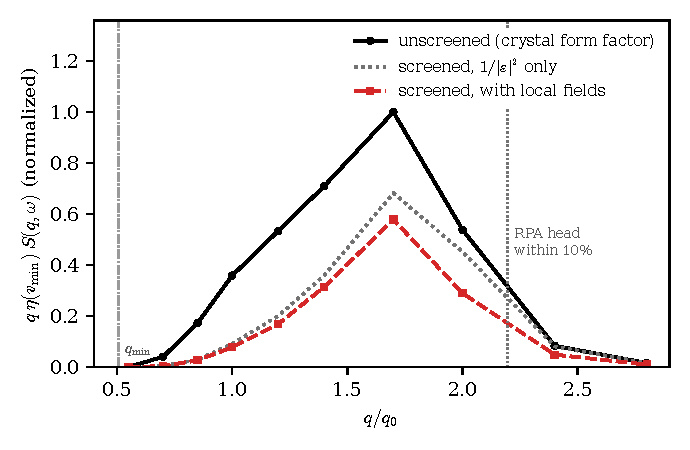
\includegraphics[width=0.85\linewidth]{figures/ch10/limit10_1a.pdf}
  \caption{Unscreened rate against screened rates in silicon at $\omega = \SI{5}{eV}$, for $\mchi = \SI{10}{MeV}$ and a heavy mediator: the rate weight $q\,\eta(\vmin)\,S(q,\omega)$ of \cref{eq:10.1-rateiso} against $q$, normalized to the maximum of the unscreened curve. All three curves come from one model, the local empirical pseudopotential of \cref{we:8-lf-nuisance} (model gap \SI{0.82}{eV}), with $\vect{q}$ along the direction $(5,3,1)$, chosen so that no $\vect{q} + \vect{G}$ comes close to zero, and spectra averaged over 4.5 to \SI{5.5}{eV}. Solid: independent particles. Dotted: random-phase screening by the macroscopic $1/|\varepsilon|^2$ alone, the leading correction. Dashed: random-phase screening with local fields over the 51 shortest reciprocal-lattice vectors, the fuller result. Dash-dotted: the smallest $q$ the halo reaches at \SI{5}{eV}. Dotted vertical: above $2.2\,q_0 = \SI{8.2}{keV}$, with $q_0 = \alpha m_e$, the macroscopic screening changes the rate by less than 10 percent. The model has no momentum components above $2.8\,q_0$, where the plot ends. Nothing is shaded. No $q$ in the plotted range brings the fuller result within 10 percent of the unscreened one.}
  \label{fig:10-fcrys-limit}
\end{figure}

The further corrections, an exchange--correlation kernel and the electron--hole attraction, change the picture mainly near the gap. An adiabatic local kernel changes the loss function by a few percent at energies of several eV, since it cannot bind an electron to a hole (\cref{sec:4.6}). The electron--hole attraction raises the spectrum within about an eV of the gap and adds bound excitons below it (\cref{sec:4.9}); \cref{sec:10.5} computes its effect on the rate. The optical limit of the tables shows what is missing at small $q$: $\varepsilon(0,0)$ is 10.2 without local fields and 9.1 with them, against the measured 11.7, the same trend as \cref{we:4-siepsinf}. A rate dominated by the region just above the gap, as for masses of a few MeV, inherits that uncertainty, and a heavier one is less sensitive to it.

\subsection{Sum-rule bounds on the rate}\label{sec:10.2-bounds}

Silicon has 28 electrons per cell, and the $f$-sum rule fixes $\int_0^\infty\dd\omega\,\omega L$ at $(\pi/2)\omega_p^2$ with $\omega_p = \SI{31.1}{eV}$ for all of them (\cref{sec:4.3}), whatever the bands, the screening or the many-body approximation. The inverse moment is fixed by the static dielectric function alone. These two integrals bound the rate of \cref{eq:10.2-rate} from above, for any material, with no calculation of the spectrum~\cites{lasenby2022dark}{barker2026first}. Define the moments of the loss function at fixed $\vect{q}$,
\begin{equation}
  K_n(\vect{q}) = \int_0^\infty\dd\omega\;\omega^n L(\vect{q},\omega) , \qquad
  K_1 = \frac{\pi}{2}\,\omega_p^2 , \qquad K_{-1} = \frac{\pi}{2}\bigl[1 - \varepsilon^{-1}(\vect{q},0)\bigr] ,
  \label{eq:10.2-moments}
\end{equation}
where $K_1$ is \cref{eq:4.4-fsumL} and $K_{-1}$ is the Kramers--Kronig relation \cref{eq:C.5-screening} at zero frequency, at which $\varepsilon^{-1}$ is real. At $\vect{q} \to 0$ in an insulator the second is the inverse moment \cref{eq:4.4-inverse}; at finite $q$ it is the static step $1 - \varepsilon^{-1}(\vect{q},0)$, which falls from 0.87 at \SI{0.5}{keV} to 0.43 at $q_0$ and 0.28 at \SI{5}{keV} in the silicon tables.

The intermediate moments follow by Hölder's inequality. For $-1 \le n \le 1$ write $\omega^nL = (\omega L)^{(1+n)/2}(L/\omega)^{(1-n)/2}$, a product of two nonnegative functions, and apply $\int fg \le (\int f^r)^{1/r}(\int g^s)^{1/s}$ with $r = 2/(1+n)$ and $s = 2/(1-n)$, so that $1/r + 1/s = 1$. Then $K_n \le K_1^{(1+n)/2}K_{-1}^{(1-n)/2}$, or
\begin{equation}
  K_n(\vect{q}) \le \frac{\pi}{2}\,\omega_p^{n+1}\bigl[1 - \varepsilon^{-1}(\vect{q},0)\bigr]^{(1-n)/2} , \qquad -1 \le n \le 1 ,
  \label{eq:10.2-Kn}
\end{equation}
which is Ref.~\cite[Eq.~(8)]{barker2026first}; the end points are the two sum rules themselves, and $n = 0$ is the Cauchy--Schwarz inequality. In the rate, the halo factor $\eta(\vmin)$ is the only other function of $\omega$. At $T = 0$ and for energies above a threshold $\omega_{\mathrm{th}}$, write $\eta \le \omega^n\eta_n^{\max}(q)$ with $\eta_n^{\max}(q) = \max_{\omega \ge \omega_{\mathrm{th}}}\omega^{-n}\eta(\vmin(q,\omega))$, extend the energy integral down to zero, which only adds positive terms since $L \ge 0$ for $\omega > 0$, and use \cref{eq:10.2-Kn}:
\begin{equation}
  \mathcal{R} \le \frac{\rho_\chi\,\sigmae\,\omega_p^{n+1}}{16\pi\alpha\,\rho_T\,\mchi\,\mu_{\chi e}^2}\int\dd q\;q^3\,\FDM(q)^2\,\eta_n^{\max}(q)\,\bigl[1 - \varepsilon^{-1}(q,0)\bigr]^{(1-n)/2} ,
  \label{eq:10.2-bound}
\end{equation}
Ref.~\cite[Eq.~(9)]{barker2026first}. The case $n = -1$ uses the static step alone and is the bound of Lasenby and Prabhu~\cite[Eqs.~(8) and (9)]{lasenby2022dark}. Every $n$ gives a valid bound, and the best one at a given mass is the smallest.

The useful form of the inverse moment needs $0 \le 1 - \varepsilon^{-1}(q,0) \le 1$. The lower limit is positivity: $1 - \varepsilon^{-1} = -v_{\mathrm{C}}R(\vect{q},0)$, and a static density response is negative by its Lehmann form (\cref{eq:4.2-positivity}). The upper limit, $\varepsilon^{-1}(\vect{q},0) \ge 0$, is not guaranteed in general, although we can show that it holds in the random-phase approximation with local fields for any insulator. The static independent-particle matrix $R^0_{\vect{G}\vect{G}'}(\vect{q},0)$ is Hermitian and negative semidefinite, each pair of states adding a positive rank-one matrix divided by minus its excitation energy, and so is $X = v^{1/2}R^0v^{1/2}$, with $v$ the diagonal matrix of $v_{\mathrm{C}}(|\vect{q}+\vect{G}|)$. The random-phase response gives $v^{1/2}Rv^{1/2} = X(1 - X)^{-1}$, whose eigenvalues $\lambda/(1 - \lambda)$, with $\lambda \le 0$, lie in $(-1, 0]$. A diagonal element of a Hermitian matrix lies between its smallest and largest eigenvalue, so $(\varepsilon^{-1})_{\vect{G}\vect{G}} = 1 + v_{\mathrm{C}}R_{\vect{G}\vect{G}}$ lies in $(0, 1]$ at every $\vect{q}$, local fields included. Beyond the random-phase approximation the same argument goes through with $R^0$ replaced by the proper response $\tilde R = (1 - R^0f_{\mathrm{xc}})^{-1}R^0$ of \cref{eq:4.6-tddft}, provided $\tilde R$ stays negative definite, that is $(-R^0)^{-1} + f_{\mathrm{xc}} > 0$. At long wavelength this is the positive inverse compressibility of \cref{eq:4.6-compress}, which the electron gas loses only near $r_s \approx 5.25$~\cite{giuliani2005quantum}, far from the $r_s \approx 2$ of the silicon valence electrons. For an arbitrary material a negative static dielectric function at finite $q$ is not excluded~\cite{dolgov1981admissible}, and the conservative replacement $1 - \varepsilon^{-1} \to 1$ that makes \cref{eq:10.2-bound} material-independent is an assumption there, not a theorem.

The bound applies to the total charge as well. For a dark photon the loss function and the static step are those of the total dielectric matrix of \cref{sec:8.4}, and the $f$-sum includes the nuclei, $\omega_p^2 + \sum_\kappa Z_\kappa^2e^2\nd_\kappa/M_\kappa$. In silicon the nuclear share is $2.73\times10^{-4}$ (\cref{sec:4.3}) and the Born charges vanish, so the numbers are those of the electrons. The inverse moment also gives a check on calculations. The unscreened $\varepsilon_2^{\mathrm{IP}}$ has $(2/\pi)\int\dd\omega\,\varepsilon_2/\omega = \varepsilon_{\vect{0}\vect{0}}(\vect{q},0) - 1$, by the Kramers--Kronig relation for $\varepsilon - 1$ (\cref{eq:C.5-KKeps}), and this exceeds the bound $1 - 1/\varepsilon_{\vect{0}\vect{0}}$ on the screened $L$ by the factor $\varepsilon_{\vect{0}\vect{0}}(\vect{q},0)$, which is 6.3 at \SI{1}{keV} in silicon.

\begin{workedexample}{The $f$-sum bound on the silicon rate at \SI{1}{MeV}}\label{we:10-fsum}
Take $\mchi = \SI{1}{MeV}$, a heavy mediator, $\sigmae = \SI{e-37}{cm^2}$, $\rho_\chi = \SI{0.3}{GeV.cm^{-3}}$ and the threshold $\omega_{\mathrm{th}} = \SI{1.11}{eV}$ of a charge detector, the step-model gap that accompanies the tables. Pairs are kinematically open for $\omega_{\mathrm{th}}/v_{\mathrm{max}} = \SI{0.42}{keV} \le q \le 2\mchi v_{\mathrm{max}} = \SI{5.30}{keV}$ and $\omega \le \mchi v_{\mathrm{max}}^2/2 = \SI{3.51}{eV}$. The screened rate of \cref{eq:10.2-rate} with local fields is 16.7 events per kilogram-year (18.5 without local fields, 157 for independent particles).

For $n = 1$, $\eta(\vmin)/\omega$ decreases with $\omega$ at fixed $q$, since $\vmin$ grows with $\omega$, so its maximum is at the threshold, $\eta_1^{\max}(q) = \eta(\vmin(q,\omega_{\mathrm{th}}))/\omega_{\mathrm{th}}$. The bound \cref{eq:10.2-bound} then needs only $\omega_p$. With all 14 electrons per atom, $\omega_p = \SI{31.1}{eV}$, it gives $7.3\times10^7$ events per kilogram-year, $4\times10^6$ times the computed rate. The valence plasma frequency, $\omega_p^{\mathrm{val}} = \SI{16.6}{eV}$, would give $2.1\times10^7$, but it is not a bound, since the core electrons hold the rest of the $f$-sum and the inequality runs over the whole spectrum. The $n = 0$ bound with the static step of the tables gives $2.0\times10^6$, and $n = -1$ gives $5.5\times10^4$, 3300 times the computed rate; with the step replaced by one it is $9.3\times10^4$. The tables contain only the valence electrons, whose step is slightly smaller than the all-electron one, so the $n = -1$ figure is a little low as a bound.

The bounds are far above the rate because they place all of the weight of $L$ at the most favorable energy, while silicon puts it where a \SI{1}{MeV} particle cannot go. The $f$-sum weight is near the plasmon, around \SI{17}{eV} at small $q$, and in the cores at hundreds of eV; the window ends at \SI{3.5}{eV}, where the gap and the screening keep $L$ small. The inverse moment weights low energies and comes closest. At \SI{10}{MeV}, with a window reaching \SI{35}{eV}, the $n = -1$ bound is 16 times the computed rate and the $f$-sum bound $8.5\times10^5$ times, both evaluated, like the rate, for $q \le \SI{22.5}{keV}$, which is valid because the bound holds at each $q$. A sum-rule bound comes close to the rate only for a material whose loss function concentrates its weight near the kinematic edge, a plasmon at a few eV, which is what the electron gas of \cref{sec:10.3} and the low-dimensional plasmons of \cref{sec:16.2} provide.
\end{workedexample}

\subsection{Static step of a relaxing lattice}\label{sec:10.2-lattice}

For a mediator that couples to electrons alone, the exact relation is $S_{ee} = (2q^2/e^2)L_e/(1 - \ee^{-\beta\omega})$ with the electron-channel function $\varepsilon_e^{-1} = 1 + v_{\mathrm{C}}R_{ee}$ (\cref{app:A.7}), and both sum rules hold for $L_e$. The $f$-sum is unchanged: the double commutator of $n_e$ with the Hamiltonian involves only the kinetic energy of the electrons (\cref{sec:4.3}), so $\int\dd\omega\,\omega L_e = (\pi/2)\omega_p^2$ with the nuclei moving, and the acoustic peak of the electron-following sector takes the share $Z_\kappa m_e/M_\kappa = 2.73\times10^{-4}$ of it in silicon (\cref{eq:8.6-fsum-e}). The static step is a different matter. With the nuclei free to move, an electron-only probe at small $q$ compresses neutral matter: the electrons it displaces drag their nuclei along, and the crystal responds as an elastic medium.

The size follows from the acoustic peak. At small $q$ a longitudinal acoustic phonon moves each cell rigidly by $\vect{U}_{\vect{R}}$, and the electrons that follow the nuclei, all $\nd_e\Omega = 28$ per cell in silicon since the Born charges vanish, give the density row the term $-\ii\,\nd_e\Omega\sum_{\vect{R}}\ee^{-\ii\vect{q}\cdot\vect{R}}\,\vect{q}\cdot\vect{U}_{\vect{R}}$ (\cref{sec:8.4-exact}). One phonon of wavevector $\vect{q}$ displaces each cell by $(2M_{\mathrm{cell}}N\omega_{\vect{q}})^{-1/2}$ along its polarization, with $N$ cells in the volume $\Vol = N\Omega$. The squared matrix element is then $N(\nd_e\Omega)^2q^2/(2M_{\mathrm{cell}}\omega_{\vect{q}})$, and
\begin{equation*}
  S_{ee}^{\mathrm{ac}}(\vect{q},\omega) = \frac{\pi\nd_e^2\Omega\,q^2}{M_{\mathrm{cell}}\,\omega_{\vect{q}}}\,\delta(\omega - \omega_{\vect{q}}) , \qquad \omega_{\vect{q}} = c_{\mathrm{LA}}q ,
\end{equation*}
at $T = 0$, with $c_{\mathrm{LA}}$ the longitudinal sound speed, the $c_\nu$ of \cref{eq:5.2-sound} for the longitudinal branch. Its first moment, $\int\dd\omega\,\omega S/2\pi = \nd_e^2\Omega q^2/2M_{\mathrm{cell}}$, is $\nd_e\Omega\,m_e/M_{\mathrm{cell}}$ times the electronic $f$-sum $\nd_eq^2/2m_e$, the share quoted above. Its inverse moment is not small. With $L_e = (e^2/2q^2)(1 - \ee^{-\beta\omega})S_{ee}$, the peak adds $(2/\pi)\int\dd\omega\,L_e^{\mathrm{ac}}/\omega = e^2\nd_e^2\Omega/(M_{\mathrm{cell}}\,\omega_{\vect{q}}^2)$ to the static step, and
\begin{keyresult}[Static step of a relaxing lattice]
\begin{equation}
  1 - \varepsilon_e^{-1}(\vect{q},0) = \bigl[1 - \varepsilon_{\mathrm{cl}}^{-1}(\vect{q})\bigr] + \mathcal{G}_{\mathrm{rel}}(\vect{q}) , \qquad
  \mathcal{G}_{\mathrm{rel}}(\vect{q}) \to \frac{\varOmega_{P,e}^2}{(c_{\mathrm{LA}}q)^2} , \quad \varOmega_{P,e}^2 = \frac{e^2\nd_e^2}{\rho_T} ,
  \label{eq:10.2-relaxed}
\end{equation}
as $q \to 0$, with $\varepsilon_{\mathrm{cl}}$ the dielectric function at clamped nuclei, $\nd_e$ the density of all the electrons and $\rho_T = M_{\mathrm{cell}}/\Omega$. The lattice term grows as $(c_{\mathrm{LA}}q)^{-2}$ in every solid, polar or not. Its general form, a sum over branches with the electron-following charge $Z^{(e)}_\kappa(\vect{q})$ of each atom, is \cref{eq:E.16-step}.
\end{keyresult}
\noindent For silicon, $\nd_e = \SI{7.00e23}{cm^{-3}}$ and $\rho_T = \SI{2.33}{g.cm^{-3}}$ give $\varOmega_{P,e} = \SI{0.51}{eV}$, and with $c_{\mathrm{LA}} = \SI{8.43}{km/s}$ along $[100]$ (\cref{app:C.18}) the lattice term equals one at $q = \SI{18}{keV}$, far beyond the zone boundary. The limiting form is derived only as $q \to 0$. At finite $q$ the dispersion bends over and the electron-following charge falls below 14 per atom, at relative order $(qa)^2$ and in opposite directions; at \SI{1}{keV} the limiting form gives $3\times10^2$, and the true value there is only estimated to exceed $10^2$ (\cref{app:E.16}). Either way the step exceeds one by orders of magnitude throughout the zone, and the bound \cref{eq:10.2-bound} with $n = -1$, and with every $n < 1$ through the power $(1 - n)/2$, fails for an electron-only coupling once the lattice relaxes. Lasenby and Prabhu noted that phonon rates of electrophilic mediators exceed the sum-rule bounds of charge couplings~\cite[Sect.~VII]{lasenby2022dark}; \cref{eq:10.2-relaxed} gives the term responsible. It is the acoustic peak of $S_{ee}$ that the exactness theorem of \cref{sec:8.4} attributed to the electrons that follow the nuclei. Its amplitude is the coefficient of $\ii\vect{q}\cdot\vect{U}$ in the density row, the coupling per unit volume $c_1^{(e)}\nd_e$ of the electrons that move with the cells; for the charge this coefficient cancels between electrons and nuclei, and the peak is absent.

The clamped bound holds in every many-body approximation, with the proviso on $\tilde R$ above; the lattice term is harmonic and adiabatic, with one phonon in the final state. For the electron-only coupling the $f$-sum bound and a restricted static-step bound survive. The $f$-sum bound holds as it stands. And for a threshold above the phonon band the electron-following sector contributes nothing to $\int_{\omega_{\mathrm{th}}}^\infty\dd\omega\,L_e/\omega$ except through Migdal amplitudes, so the clamped step bounds that integral up to corrections in powers of $\kappa_{\mathrm{BO}}$ (\cref{sec:8.6}). A detector with an electronic threshold can use the clamped bound for either coupling; a calorimeter with a threshold in the phonon band cannot use it for an electrophilic mediator.

\begin{limitbox}[Sum-rule bounds on the loss function][lim:10.2b]
For any target in its ground state, $\int_0^\infty\dd\omega\,\omega L = (\pi/2)\omega_p^2$ and $\int_0^\infty\dd\omega\,L/\omega = (\pi/2)[1 - \varepsilon^{-1}(q,0)] \le \pi/2$, and with $\eta \le \omega^n\eta_n^{\max}$ they bound the rate as in \cref{eq:10.2-bound}~\cites[Eqs.~(1), (8) and (9)]{lasenby2022dark}[Eqs.~(1), (2), (8) and (9)]{barker2026first}.
\par\smallskip
{\centering
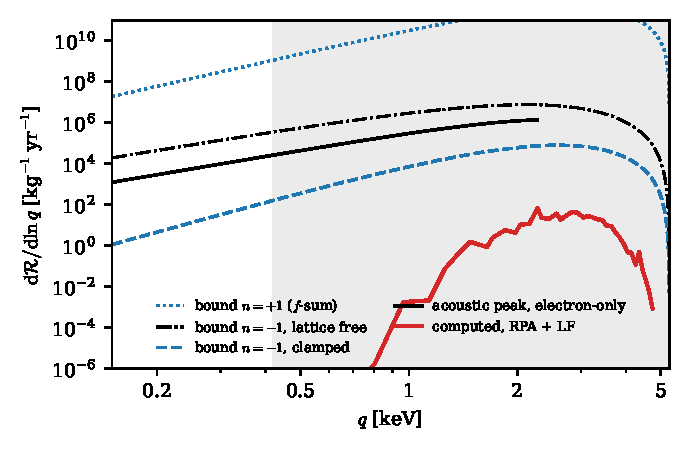
\includegraphics[width=0.82\linewidth]{figures/ch10/limit10_2b.pdf}
\captionof{figure}{Rate per unit $\ln q$ in silicon at $\mchi = \SI{1}{MeV}$, heavy mediator, $\sigmae = \SI{e-37}{cm^2}$, threshold \SI{1}{meV}, against the bounds of \cref{eq:10.2-bound}. Red: the computed electronic rate (random-phase loss function with local fields). Dashed: the clamped bound with $n = -1$ and the static step of the same tables; dotted: the $f$-sum bound, $n = 1$, $\omega_p = \SI{31.1}{eV}$. Black: the acoustic peak of an electron-only coupling, in the model of \cref{fig:10-elf-limit}; dash-dotted: the $n = -1$ bound with the lattice term \cref{eq:10.2-relaxed} added, in its limiting form $\varOmega_{P,e}^2/(c_{\mathrm{LA}}q)^2$ at every $q$ shown. Gray: momenta at which electron--hole pairs are open, $q \ge \Eg/v_{\mathrm{max}}$; there the clamped bound holds for both couplings when the threshold lies above the phonon band. The acoustic peak exceeds the clamped bound by 120 at \SI{0.5}{keV}, 42 at \SI{1}{keV} and 21 at \SI{2}{keV}.}\label{fig:10-sumrule-limit}
\par}
\smallskip
For an electron-only coupling with the lattice free to move, the static step grows as $(c_{\mathrm{LA}}q)^{-2}$ and exceeds one throughout the zone, and only the $f$-sum bound survives.
\end{limitbox}

\section{Electron-gas models and plasmons}\label{sec:10.3}

Put the Lindhard loss function of the silicon valence electrons into the rate of \cref{sec:10.2}, and a \SI{100}{MeV} particle with a heavy mediator makes $1.31\times10^4$ events per kilogram-year above \SI{1.11}{eV} at $\sigmae = \SI{e-37}{cm^2}$. The crystal tables of \cref{sec:10.2}, with bands, local fields and a gap, give $1.22\times10^4$. A model with one parameter, the electron density, comes within seven percent of the crystal rate. At \SI{1}{MeV} the same model gives 45 times the crystal rate. The gas also carries the plasmon, which at small momentum transfer holds almost the whole $f$-sum, and it is natural to ask whether dark matter can excite it. We derive the electron-gas rate and find where it agrees with silicon and why, then isolate the plasmon pole in the rate and show that halo dark matter falls short of it by about $\omega_p$ in energy and a factor of 3.5 in speed.

\subsection{The Lindhard loss-function rate}\label{sec:10.3-gas}

The electron gas of \cref{sec:4.5} is isotropic, so the direction average in \cref{eq:10.2-rate} does nothing, and its loss function in the random-phase approximation is $\Imag[-1/\varepsilon_{\mathrm{Lin}}(q,\omega)]$ with the Lindhard dielectric function of \cref{eq:4.5-rpa,eq:4.5-lindhard}. Inserting it,
\begin{keyresult}[Electron-gas loss-function rate]
\begin{equation}
  \frac{\dd\mathcal{R}}{\dd\omega} = \frac{\rho_\chi\,\sigmae}{8\pi^2\alpha\,\rho_T\,\mchi\,\mu_{\chi e}^2}\int\dd q\;q^3\,\eta\bigl(\vmin(q,\omega)\bigr)\,\FDM(q)^2\,\Imag\!\left[\frac{-1}{\varepsilon_{\mathrm{Lin}}(q,\omega)}\right] ,
  \label{eq:10.3-gasrate}
\end{equation}
at $T = 0$, with $\varepsilon_{\mathrm{Lin}}$ fixed by the electron density alone through $k_{\mathrm{F}}$ and $\omega_p$. The Mermin form replaces $\varepsilon_{\mathrm{Lin}}$ by $\varepsilon_{\mathrm{Mer}}$ of \cref{eq:4.5-mermin}.
\end{keyresult}
\noindent This is the rate of Knapen, Kozaczuk and Lin with their Lindhard and Mermin functions~\cite[Eqs.~(13), (17) and (19)]{knapen2021dark}. Their prefactor $3\omega_p^2/q^2v_{\mathrm{F}}^2$ is the $k_{\mathrm{TF}}^2/q^2$ of the static Lindhard screening $\varepsilon = 1 + (k_{\mathrm{TF}}^2/q^2)F_{\mathrm{L}}$ (\cref{eq:4.5-static}), since $k_{\mathrm{TF}}^2 = 2e^2\mathcal{N}_{\mathrm{F}} = e^2m_ek_{\mathrm{F}}/\pi^2$ and $\omega_p^2 = e^2k_{\mathrm{F}}^3/3\pi^2m_e$ give $k_{\mathrm{TF}}^2 = 3\omega_p^2/v_{\mathrm{F}}^2$, and their bracket $f^{\mathrm{L}}_1 + \ii f^{\mathrm{L}}_2$ is $-R^0/2\mathcal{N}_{\mathrm{F}}$, the braced expression of \cref{eq:4.5-lindhard}. For silicon the density is that of the four valence electrons per atom, $r_s = 2.0$, $k_{\mathrm{F}} = \SI{3.57}{keV}$ and $\omega_p = \SI{16.6}{eV}$ (\cref{we:4-siplasmon}). Below $q_{\mathrm{c}}$ the gas also has the undamped plasmon of \cref{eq:4.5-plasmonL}, a delta function in $\omega$; we return to it in \cref{sec:10.3-pole} and leave it out of \cref{eq:10.3-gasrate} for now, since halo dark matter cannot reach it.

The comparison with silicon uses the random-phase tables with local fields of \cref{sec:10.2}. Both rates are integrated on the momenta of those tables, from 0.49 to \SI{22.5}{keV}, above the threshold $\Eg = \SI{1.11}{eV}$, the step-model gap that accompanies the tables; their scissor puts the gap at the physical low-temperature value, \SI{1.17}{eV}. Per kilogram-year at $\sigmae = \SI{e-37}{cm^2}$:
\begin{center}
\begin{tabular}{@{}lcccccc@{}}
\toprule
& \multicolumn{2}{c}{\SI{1}{MeV}} & \multicolumn{2}{c}{\SI{10}{MeV}} & \multicolumn{2}{c}{\SI{100}{MeV}} \\
& heavy & light & heavy & light & heavy & light \\
\midrule
Silicon, RPA + LF & 16.7 & 90 & $5.89\times10^4$ & $9.8\times10^3$ & $1.22\times10^4$ & $1.62\times10^3$ \\
Lindhard / silicon & 45 & 70 & 1.42 & 2.6 & 1.07 & 2.1 \\
Mermin / silicon & 54 & 94 & 1.57 & 2.9 & 1.21 & 2.4 \\
\bottomrule
\end{tabular}
\end{center}
The Mermin rows use one term with $\gamma_{\mathrm{rel}} = \SI{3.66}{eV}$, the width of the measured silicon loss peak, which is a fit parameter and not a collision rate (\cref{sec:4.5}).

The gas lacks the gap of silicon and the high-momentum tail of its bound electrons, two errors of opposite sign that set these ratios and that the spectrum of \cref{fig:10-gas-limit} shows. The first is the gap. The gas is a metal. Its continuum reaches down to $\omega = 0$, where $L \simeq e^2m_e^2q\omega/2\pi k_{\mathrm{TF}}^4$ (\cref{sec:4.5}), while silicon has no pairs below its gap and weak absorption up to its peaks at 3.4 and \SI{4.2}{eV} (\cref{fig:4-siloss}). At \SI{100}{MeV} with a heavy mediator the gas spectrum exceeds the crystal one by a factor 24 at \SI{2}{eV} and 4.2 at \SI{3}{eV}. A particle of \SI{1}{MeV} deposits at most $\mchi v_{\mathrm{max}}^2/2 = \SI{3.5}{eV}$ (\cref{eq:1.3-omegamax}), so it samples only this region, and the gas overestimates its rate by a factor 45.

The second error is the momentum distribution of the electrons. The halo deposits at most $\omega = qv_{\mathrm{max}}$ at momentum $q$. In the gas the pairs at $q > 2k_{\mathrm{F}}$ lie in the band $\omega_- < \omega < \omega_+$ around the free recoil $q^2/2m_e$, with $\omega_- = q^2/2m_e - qv_{\mathrm{F}}$, because no electron of the Fermi sea moves faster than $v_{\mathrm{F}}$. The lower edge passes the halo line at $q = 2m_e(v_{\mathrm{F}} + v_{\mathrm{max}}) = \SI{9.85}{keV}$, and beyond it the gas has nothing the halo can reach. The valence electrons of silicon are bound, their orbitals contain momenta above $k_{\mathrm{F}}$, and their loss function keeps weight far below the free recoil. An energy of \SI{20}{eV} needs $q \ge \SI{7.5}{keV}$, and there the gas spectrum is 3 percent of the crystal one; at \SI{15}{eV} it is 27 percent. Between these two regions, from the upper absorption peak at \SI{4.2}{eV} to $k_{\mathrm{F}}v_{\mathrm{max}} = \SI{9.5}{eV}$, the largest energy deposited at $q = k_{\mathrm{F}}$, the valence electrons respond nearly as free electrons do and the gas is within a factor 1.5 of the crystal. That band holds 62 percent of the silicon rate at \SI{100}{MeV}. The integrated agreement at that mass, seven percent, is the excess below the band cancelling the deficit above it. A light mediator weights small $q$ and therefore small $\omega$, where the gas has its excess, and its ratio stays near 2.

The Mermin function does not repair either error. Its relaxation rate spreads the plasmon and gives the loss function a tail $\gamma_{\mathrm{rel}}\omega/\omega_p^2$ below it (\cref{sec:4.5}), which adds 10 to 35 percent to the rates in the table above; the function still has no gap. The Mermin oscillator method of \cref{sec:4.5}, however, does better, because it is a fit. Its terms reproduce the measured optical loss function, gap and absorption peaks included, and each step function removes weight below its onset. The Mermin form only carries the fit to finite $q$, keeping each term's share of the $f$-sum. For silicon the method agrees with the first-principles tables to within 10 percent in the rate above a two-electron threshold, and the uncertainty grows for masses whose rate lies near the gap~\cite[App.~C]{knapen2021dark}. The momentum distribution is still that of a gas, and the two methods differ most at large $\omega$, which carries a small share of the rate above that threshold.

Compared to silicon, the gas is the random-phase approximation for a homogeneous medium; the gap, the local fields and the bound momentum distribution are what the crystal adds. The computed crystal loss function that replaces $\varepsilon_{\mathrm{Lin}}$ is the one of \cref{app:E.6}. The gas needs only $\nd_e$, which follows from the cell volume and the count of valence electrons (\cref{app:A.2}), and it serves as a test of the codes that compute the crystal function (\cref{sec:4.5}).

\begin{limitbox}[Lindhard and Mermin loss-function rates][lim:10.3a]
For a homogeneous electron gas the rate is \cref{eq:10.3-gasrate}, with $\varepsilon_{\mathrm{Lin}}(q,\omega) = 1 + (3\omega_p^2/q^2v_{\mathrm{F}}^2)[f^{\mathrm{L}}_1 + \ii f^{\mathrm{L}}_2]$ and $f^{\mathrm{L}}_1 + \ii f^{\mathrm{L}}_2$ the braced expression of \cref{eq:4.5-lindhard}, or the Mermin function $\varepsilon_{\mathrm{Mer}}$ with a relaxation rate $\gamma_{\mathrm{rel}}$~\cite[Eqs.~(13), (17)--(19)]{knapen2021dark}.
\par\smallskip
{\centering
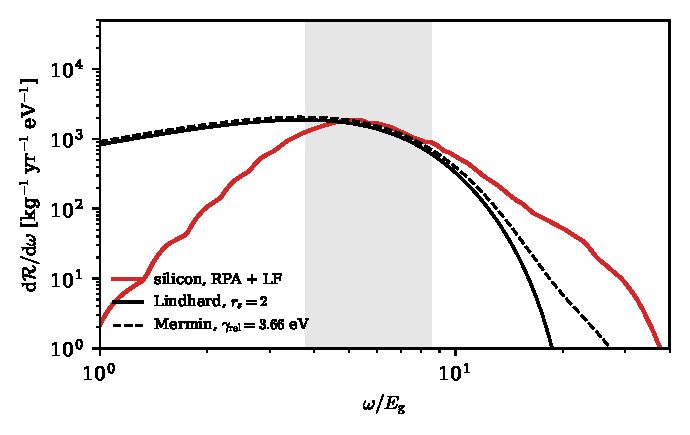
\includegraphics[width=0.82\linewidth]{figures/ch10/limit10_3a.pdf}
\captionof{figure}{Spectrum of silicon at $\mchi = \SI{100}{MeV}$, heavy mediator, $\sigmae = \SI{e-37}{cm^2}$, $\rho_\chi = \SI{0.3}{GeV.cm^{-3}}$ and the standard halo, against $\omega/\Eg$ with $\Eg = \SI{1.11}{eV}$, the step-model gap that accompanies the tables. Red: the random-phase loss function of silicon with local fields (the tables of \cref{fig:10-screening}). Black: the Lindhard loss function of the electron gas at the valence density, $r_s = 2$; dashed, the Mermin function with $\gamma_{\mathrm{rel}} = \SI{3.66}{eV}$, a fit parameter. All three are integrated over the same momenta, from 0.49 to \SI{22.5}{keV}. Gray: from the upper absorption peak of silicon, \SI{4.2}{eV}, to $k_{\mathrm{F}}v_{\mathrm{max}} = \SI{9.5}{eV}$, a band chosen for this figure. There the Lindhard spectrum is between 0.70 and 1.48 times the crystal one.}\label{fig:10-gas-limit}
\par}
\smallskip
Below the band the gas has no gap and overestimates the rate, by 24 at \SI{2}{eV}; above it the gas has no electrons faster than $v_{\mathrm{F}}$ and loses the high-energy tail, and the integrated agreement at this mass comes from the two errors cancelling.
\end{limitbox}

\subsection{Plasmon pole and residue}\label{sec:10.3-pole}

Below $q_{\mathrm{c}}$ the loss function of the gas is the particle--hole continuum plus a line, \cref{eq:4.5-plasmonL}, whose weight is $\pi$ divided by the slope of $\varepsilon_1$ at the zero. At small $q$ the slope follows from the high-frequency expansion of \cref{sec:4.5} kept to order $q^2$~\cite[Eq.~(5)]{kozaczuk2020plasmon},
\begin{equation*}
  \varepsilon_1(q,\omega) \simeq 1 - \frac{\omega_p^2}{\omega^2}\Bigl(1 + \frac{3}{5}\,\frac{q^2v_{\mathrm{F}}^2}{\omega^2}\Bigr) .
\end{equation*}
Its zero is $\omega_{\mathrm{pl}}^2 = \omega_p^2 + \tfrac35q^2v_{\mathrm{F}}^2$, the first two terms of \cref{eq:4.5-dispersion}. With $x = \tfrac35q^2v_{\mathrm{F}}^2/\omega_{\mathrm{pl}}^2$ the zero condition reads $\omega_p^2(1 + x) = \omega_{\mathrm{pl}}^2$, and differentiating,
\begin{gather*}
  \frac{\partial\varepsilon_1}{\partial\omega}\bigg|_{\omega_{\mathrm{pl}}} = \frac{2\omega_p^2}{\omega_{\mathrm{pl}}^3}\,(1 + 2x) = \frac{2}{\omega_{\mathrm{pl}}}\,\frac{1 + 2x}{1 + x} , \\
  \frac{\pi}{\partial\varepsilon_1/\partial\omega} = \frac{\pi\omega_{\mathrm{pl}}}{2}\,Z_L(q) , \qquad Z_L(q) = \frac{1 + x}{1 + 2x} = 1 - \frac35\,\frac{q^2v_{\mathrm{F}}^2}{\omega_p^2} + O(q^4) .
\end{gather*}
The factor $Z_L$ is the residue of the longitudinal photon propagator at the plasmon pole that Kozaczuk and Lin use for the plasmon's polarization vector~\cite[Eq.~(7)]{kozaczuk2020plasmon}; here it is the weight of the line in $L$. The first moment of the line, $\omega_{\mathrm{pl}}\cdot(\pi\omega_{\mathrm{pl}}/2)Z_L = (\pi/2)\omega_p^2(1 + x)(1 - x)$, is the whole $f$-sum to order $q^2$: at small $q$ the plasmon carries all of the oscillator strength, and the continuum none. Integrating \cref{eq:10.2-rate} over the delta function gives
\begin{keyresult}[Plasmon production rate]
\begin{equation}
  \mathcal{R}_{\mathrm{pl}} = \frac{\rho_\chi\,\sigmae}{8\pi^2\alpha\,\rho_T\,\mchi\,\mu_{\chi e}^2}\int_0^{q_{\mathrm{c}}}\dd q\;q^3\,\FDM(q)^2\,\eta\bigl(\vmin(q,\omega_{\mathrm{pl}}(q))\bigr)\,\frac{\pi\omega_{\mathrm{pl}}(q)}{2}\,Z_L(q) ,
  \label{eq:10.3-plrate}
\end{equation}
with $\vmin$ of \cref{eq:1.3-vmin}, the splitting $\Delta_\chi$ included. Beyond the small-$q$ forms, $\omega_{\mathrm{pl}}$ is the exact zero of $\varepsilon_1$ and $(\pi\omega_{\mathrm{pl}}/2)Z_L$ is replaced by $\pi/(\partial\varepsilon_1/\partial\omega)$ there.
\end{keyresult}
\noindent The small-$q$ residue, with $Z_L$ expanded to $1 - \tfrac35q^2v_{\mathrm{F}}^2/\omega_p^2$ as in the limit check below, agrees with the exact one of the Lindhard function to $10^{-4}$ at $q = 0.1\,k_{\mathrm{F}}$ and $8\times10^{-3}$ at $0.3\,k_{\mathrm{F}}$, the size of the dropped $q^4$ terms. Near the cutoff the two part. The exact line carries 0.99 of the $f$-sum at $q_{\mathrm{c}}/2$, 0.77 at $0.9\,q_{\mathrm{c}}$, and nothing at $q_{\mathrm{c}}$. At the continuum edge $\omega_+$ the real part of the Lindhard function contains $(1 - \nu_-^2)\ln|(\nu_- + 1)/(\nu_- - 1)|$ with $\nu_- \to 1$ (\cref{eq:4.5-lindhard}), and its derivative in $\omega$ diverges logarithmically. The slope at the zero therefore grows without bound, and the weight of the line goes to zero as the line touches the continuum. The weight it loses appears in the continuum just below it; this is Landau damping seen in the residue.

The cutoff itself depends on how the dispersion is treated, and the literature uses several values. The exact zero of $\varepsilon_{\mathrm{Lin}}$ meets the edge $\omega_+ = qv_{\mathrm{F}} + q^2/2m_e$ at $q_{\mathrm{c}} = \SI{2.60}{keV}$ and \SI{24.8}{eV} (\cref{sec:4.5}). The quadratic dispersion, with the $q^4$ terms dropped, meets it at \SI{2.24}{keV} and \SI{20.6}{eV}, a dispersion fixed at $\omega_p$ at \SI{1.88}{keV}, and the estimate $\omega_p/v_{\mathrm{F}}$ is \SI{2.38}{keV}. The spread is large because the correction is not small near the cutoff: at \SI{2.24}{keV}, $\tfrac35q^2v_{\mathrm{F}}^2/\omega_p^2 = 0.53$. All four values lie close to the zone scale $2\pi/a = \SI{2.28}{keV}$ of silicon. The crystal shows the same onset (\cref{fig:10-plasmon}). In the silicon tables the loss peak follows the gas dispersion from \SI{18.9}{eV} at \SI{0.5}{keV} to \SI{22.3}{eV} at \SI{2.45}{keV}, with a half-maximum width of about \SI{5}{eV}. Beyond that it broadens fast: at \SI{3.5}{keV} the half maximum spans 17.7 to \SI{32.2}{eV}, and at \SI{4.6}{keV} 14.9 to \SI{44}{eV}. The tables place the small-$q$ peak \SI{2.5}{eV} above the measured \SI{16.4}{eV}, because the scissor that fixes the gap also raises the interband energies that push the plasmon up (\cref{we:4-siplasmon}).

Kurinsky, Baxter, Kahn and Krnjaic wrote the plasmon rate of a fast component of dark matter with a light mediator as the optical line shape times a logarithm~\cite[Eqs.~(13) and (14)]{kurinsky2020dark}. It follows from \cref{eq:10.2-rate} in two steps. A light mediator has $\FDM = (q_0/q)^2$, so $q^3\FDM^2 = q_0^4/q$. Replacing $L(q,\omega)$ by its optical value $L(0,\omega)$ for all $q$ below a cutoff then gives
\begin{equation*}
  \frac{\dd\mathcal{R}}{\dd\omega} = \frac{\rho_\chi\,\sigmae\,q_0^4}{8\pi^2\alpha\,\rho_T\,\mchi\,\mu_{\chi e}^2}\;L(0,\omega)\int_0^{q_{\mathrm{c}}}\frac{\dd q}{q}\;\eta\bigl(\vmin(q,\omega)\bigr) ,
\end{equation*}
which is Ref.~\cite[Eq.~(14)]{kurinsky2020dark} in the book's normalization. They set the cutoff at $2\pi/a \sim \SI{5}{keV}$ with $a$ the lattice spacing~\cite[Eq.~(4)]{kurinsky2020dark}. For silicon, with $a = \SI{5.43}{\angstrom}$, $2\pi/a$ is \SI{2.28}{keV}; \SI{5}{keV} corresponds to a length of \SI{2.5}{\angstrom}, close to the bond length. The error this makes is logarithmic, because the integrand is $1/q$. For a particle of speed $v = 0.1$ the plasmon opens at $q_{\mathrm{min}} = \omega_p/v = \SI{0.17}{keV}$, and moving the cutoff from $q_{\mathrm{c}} = \SI{2.60}{keV}$ to \SI{5}{keV} raises the integral by $\ln(5/0.166)/\ln(2.60/0.166) = 1.24$, or 1.31 from \SI{2.24}{keV}. A measure growing like $q$ would have given $(5/2.60)^2 = 3.7$. The constant optical line shape also ignores the weight the line loses near $q_{\mathrm{c}}$, which removes a further 3 percent of the logarithmic integral. For a fast component the choice of cutoff therefore moves the optical form by 25 to 30 percent, not by a factor of several.

\begin{limitbox}[Plasmon production from the pole of $1/\varepsilon$][lim:10.3b]
Below the cutoff the plasmon is the line $L \simeq (\pi\omega_{\mathrm{pl}}/2)Z_L\,\delta(\omega - \omega_{\mathrm{pl}}(q))$, with $\omega_{\mathrm{pl}}^2 \simeq \omega_p^2 + \tfrac35q^2v_{\mathrm{F}}^2$ and $Z_L \simeq 1 - \tfrac35q^2v_{\mathrm{F}}^2/\omega_p^2$~\cite[Eqs.~(5) and (7)]{kozaczuk2020plasmon}. Kurinsky et al. write the light-mediator rate with $L$ taken at $q = 0$ up to the cutoff~\cite[Eqs.~(4), (13) and (14)]{kurinsky2020dark}.
\par\smallskip
{\centering
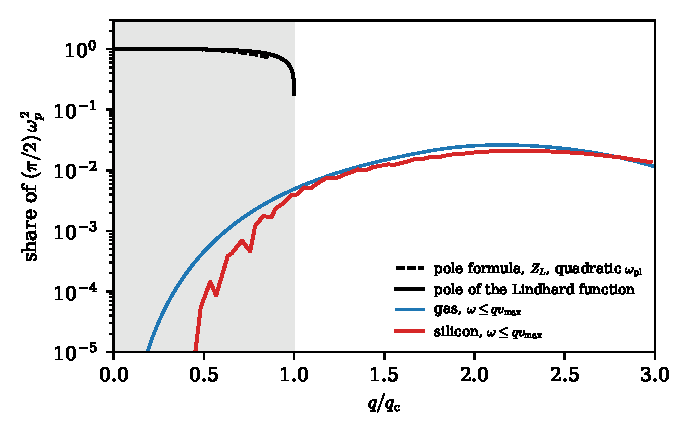
\includegraphics[width=0.82\linewidth]{figures/ch10/limit10_3b.pdf}
\captionof{figure}{Share of the valence $f$-sum $(\pi/2)\omega_p^2$ of silicon, $\omega_p = \SI{16.6}{eV}$, against $q/q_{\mathrm{c}}$ with $q_{\mathrm{c}} = \SI{2.60}{keV}$. Dashed: the first moment of the pole formula, $\omega_{\mathrm{pl}}^2Z_L/\omega_p^2$ with the quadratic dispersion, up to its own cutoff at \SI{2.24}{keV}; dotted: the optical line shape continued to \SI{5}{keV}. Solid black: the pole of the Lindhard function at $r_s = 2$, whose weight falls to zero at $q_{\mathrm{c}}$. Blue: the weight of the Lindhard continuum below $\omega = qv_{\mathrm{max}}$, the most a halo particle can deposit; red: the same for the random-phase loss function of silicon with local fields, from \SI{0.49}{keV}. Gray: $q < q_{\mathrm{c}}$, where the pole exists.}\label{fig:10-pole-limit}
\par}
\smallskip
Near $q_{\mathrm{c}}$ the small-$q$ residue misstates the line, whose weight goes to zero at the continuum edge, and beyond $q_{\mathrm{c}}$ there is no line at all. The weight within reach of the halo is never more than about 3 percent of the $f$-sum and lies in the pair continuum.
\end{limitbox}

\subsection{Plasmon threshold speed}\label{sec:10.3-reach}

A particle of speed $v$ makes a plasmon of momentum $q$ only if $v \ge \vmin(q,\omega_{\mathrm{pl}}(q)) = \omega_{\mathrm{pl}}(q)/q + q/2\mchi$ for elastic scattering, and \cref{eq:10.3-plrate} is nonzero only if this holds for some $q < q_{\mathrm{c}}$. The phase velocity $\omega_{\mathrm{pl}}/q$ is infinite at $q \to 0$ and falls as $q$ grows. At $q_{\mathrm{c}}$ the line meets the continuum edge, where $\omega_{\mathrm{pl}} = \omega_+$ and $\omega_+/q = v_{\mathrm{F}} + q/2m_e$, which rises with $q$; in the Lindhard function the phase velocity reaches its smallest value at $0.989\,q_{\mathrm{c}}$, within $10^{-3}$ of its value at $q_{\mathrm{c}}$. For a heavy particle the slowest one that can make a plasmon therefore moves at
\begin{equation}
  v_{\mathrm{th}} \simeq \frac{\omega_+(q_{\mathrm{c}})}{q_{\mathrm{c}}} = v_{\mathrm{F}} + \frac{q_{\mathrm{c}}}{2m_e} ,
  \label{eq:10.3-vth}
\end{equation}
plus $q_{\mathrm{c}}/2\mchi$ for a finite mass. The threshold is set by the electrons, not by the dark matter. The plasmon is undamped only while its phase velocity exceeds $\omega_+/q$, the largest ratio of energy to momentum that a single pair can have, so the slowest plasmon is as fast as the fastest pair. At the silicon valence density $v_{\mathrm{th}} = 9.54\times10^{-3}$, or \SI{2860}{km.s^{-1}}, and with the quadratic dispersion and its cutoff at \SI{2.24}{keV}, $9.18\times10^{-3}$ or \SI{2750}{km.s^{-1}}. Either is 3.5 to 3.6 times the largest speed of the halo, $v_{\mathrm{max}} = \SI{794.5}{km.s^{-1}}$ (\cref{eq:1.2-vmax}), and agrees with the estimate $v \gtrsim 10^{-2}$ of Kurinsky et al.~\cite[Eq.~(7)]{kurinsky2020dark}. \Cref{we:4-siplasmon} reached the same conclusion from the other side: the line $\omega = qv_{\mathrm{max}}$ reaches $\omega_p$ only at $q = \SI{6.27}{keV}$, more than twice $q_{\mathrm{c}}$.

\begin{figure}[tbp]
  \centering
  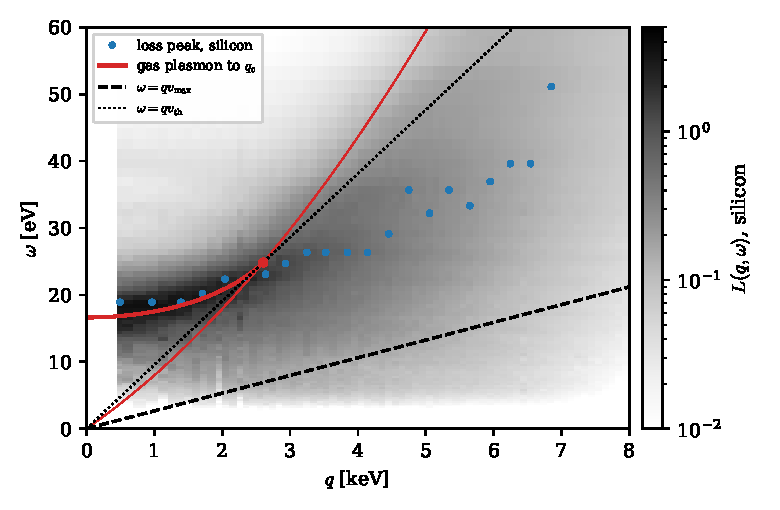
\includegraphics[width=0.9\linewidth]{figures/ch10/fig10_3.pdf}
  \caption{The silicon plasmon against the reach of halo dark matter. Gray scale: the random-phase loss function of silicon with local fields, $L(q,\omega)$, from the tables of Knapen, Kozaczuk and Lin~\cite{knapen2021dark}, averaged over the directions of $\vect{q}$ in bins of \SI{100}{eV} in $|\vect{q}|$ starting at \SI{0.49}{keV}, logarithmic scale. Blue dots: the maximum of $L$ in every third bin. Red: the undamped plasmon of the electron gas at the valence density, the exact zero of $\varepsilon_{\mathrm{Lin}}$, up to $q_{\mathrm{c}} = \SI{2.60}{keV}$ (dot), and the continuum edge $\omega_+ = qv_{\mathrm{F}} + q^2/2m_e$ (thin). Dashed: $\omega = qv_{\mathrm{max}}$, the largest energy a halo particle deposits at momentum $q$. Dotted: $\omega = qv_{\mathrm{th}}$ with $v_{\mathrm{th}} = 9.54\times10^{-3}$ of \cref{eq:10.3-vth}, the slowest particle that reaches the plasmon of the gas. The tables place the small-$q$ loss peak at \SI{18.9}{eV}, against the measured \SI{16.4}{eV}, because of the scissor shift that fixes their gap.}
  \label{fig:10-plasmon}
\end{figure}

In the standard halo the speed distribution ends at $v_{\mathrm{max}}$, and $\mathcal{R}_{\mathrm{pl}}$ is zero at every mass. The suppression is not a power of a small ratio. Remove the escape cut and keep the Maxwellian tail of \cref{sec:1.2}: the fraction of particles faster than \SI{2750}{km.s^{-1}} in the laboratory is about $10^{-49}$, and about $10^{-53}$ above \SI{2860}{km.s^{-1}}. A real halo is not Maxwellian that far out, and these numbers only measure how far the plasmon lies from the bulk of the distribution, 10.5 to 11 times $v_0$ beyond the speed of the Earth.

\begin{workedexample}{The plasmon rate of silicon at the highest halo speed}\label{we:10-plasmon}
Take a particle at $v = v_{\mathrm{max}} = 2.650\times10^{-3}$, heavy enough that $q/2\mchi$ is negligible; at \SI{100}{MeV} it raises $v_{\mathrm{th}}$ by 0.14 percent. At momentum $q$ it deposits at most $qv_{\mathrm{max}}$: \SI{5.94}{eV} at the quadratic cutoff \SI{2.24}{keV}, \SI{6.90}{eV} at $q_{\mathrm{c}} = \SI{2.60}{keV}$. The plasmon of the gas sits at 20.6 and \SI{24.8}{eV} there. The distance between the plasmon and the reach, $\omega_{\mathrm{pl}}(q) - qv_{\mathrm{max}}$, is smallest at $q = \SI{1.34}{keV}$, where it is \SI{14.7}{eV} for the exact zero of the Lindhard function (the quadratic dispersion gives \SI{14.5}{eV} at \SI{1.72}{keV}). The particle is short of the plasmon by about $\omega_p$, at every momentum where the plasmon exists, and \cref{eq:10.3-plrate} gives $\mathcal{R}_{\mathrm{pl}} = 0$.

The silicon plasmon is not a sharp line: interband pairs give it a width of \SI{3.7}{eV} already at $q \to 0$ (\cref{we:4-siplasmon}). The tables show what the particle meets instead. In the bin at \SI{2.28}{keV} the loss peak sits at \SI{22.3}{eV}, and at the reach of the particle, \SI{6.0}{eV}, $L$ is 6.9 percent of its peak value; the energies the particle can deposit hold $1.7\times10^{-3}$ of the valence $f$-sum. At \SI{2.57}{keV} the numbers are 8.5 percent and $4.0\times10^{-3}$. These are pairs on the low-energy side of the resonance, the same pairs that the rate of \cref{sec:10.2} already counts. They also carry little of that rate. At \SI{100}{MeV}, momenta below \SI{2.60}{keV} give $4.9\times10^{-4}$ of the heavy-mediator rate (\num{9.6e-5} below \SI{2.24}{keV}) and 2.5 percent of the light-mediator rate.

The answer is that the plasmon rate of silicon is zero for halo dark matter, not small: the pole needs \SI{2750}{km.s^{-1}} or more, and the halo stops at \SI{794.5}{km.s^{-1}}. A loss-function rate that seems to contain ``plasmon'' events at 15 to \SI{25}{eV} draws them from $q > \SI{5.7}{keV}$, where \cref{fig:10-plasmon} shows only the broad pair continuum.
\end{workedexample}

The pole opens for a fast component of dark matter, for an exothermic splitting, or when a third body takes the momentum, and each case belongs to another section. A fast component, accelerated or boosted, can exceed $v_{\mathrm{th}}$, and \cref{eq:10.3-plrate} applies with its speed distribution in $\eta$ (\cref{sec:10.9}). An exothermic transition lowers $\vmin$ through $\Delta_\chi < 0$ in \cref{eq:1.3-vmin}, and a particle at $v_{\mathrm{max}}$ reaches the line once $|\Delta_\chi| \gtrsim \SI{14.7}{eV}$, the closest approach of the worked example; \cref{sec:17.3} treats such down-scattering into collective modes. When the dark matter scatters off a nucleus, the recoiling ion can emit a plasmon whose momentum is small, as in bremsstrahlung. Kozaczuk and Lin computed this rate in the electron-gas picture and found it four to five orders of magnitude below the elastic nuclear rate for masses from \SI{10}{MeV} to \SI{1}{GeV}~\cite{kozaczuk2020plasmon}; it is a process of the joint electron--lattice response of \cref{chap:12}.

\subsection{Plasmon decay into pairs and phonons}\label{sec:10.3-decay}

With the nuclei clamped, a plasmon of silicon decays into electron--hole pairs and nothing else. At the measured loss peak, \SI{16.4}{eV}, vertical interband transitions are open, $\varepsilon_2 = 0.22$ where $\varepsilon_1$ vanishes, and the width of the loss peak follows from that value (\cref{we:4-siplasmon}). The branching ratio into pairs is one, and \cref{sec:8.7} showed that the screened pair weights of \cref{eq:8.7-screened} already contain the plasmon peak, so that a plasmon is not a separate final state of silicon. Its energy is shared by the pairs, and the step model \cref{eq:1.5-step} turns \SI{16.4}{eV} into five; the cascade that produces them is the subject of \cref{sec:18.1}.

With the lattice free to move, part of the decay goes into pairs plus phonons. By the decomposition theorem \cref{eq:8.6-decomp}, the absorptive part of the response at $(\vect{q},\omega_{\mathrm{pl}})$ splits into a zero-phonon sector $S^0$ and a phonon-dressed sector $S^+$. Since $L = \varepsilon_2/|\varepsilon|^2$ and the factor $|\varepsilon|^2$ is common to both sectors, the phonon branching of the plasmon is
\begin{equation}
  B_{\mathrm{pl}}^+(\vect{q}) = \frac{S^+(\vect{q},\omega_{\mathrm{pl}})}{S^0(\vect{q},\omega_{\mathrm{pl}}) + S^+(\vect{q},\omega_{\mathrm{pl}})} = \frac{\varepsilon_2^+(\vect{q},\omega_{\mathrm{pl}})}{\varepsilon_2(\vect{q},\omega_{\mathrm{pl}})} ,
  \label{eq:10.3-branch}
\end{equation}
the share of phonon-assisted absorption in $\varepsilon_2$ at the plasmon energy. At \SI{16}{eV} direct transitions are allowed. A phonon-assisted transition needs one electron--phonon vertex besides the density vertex, and its amplitude carries the vertex over an energy denominator. With optical-phonon vertices of a few tenths of an eV and denominators of a few eV, \cref{sec:6.5} found the phonon-assisted absorption to be about $10^{-2}$ of the direct one per coupled mode. At the plasmon energy the direct transitions are strong, and the same estimate puts $B_{\mathrm{pl}}^+$ between $10^{-3}$ and $10^{-2}$; it has not been computed. The phonons counted by \cref{eq:10.3-branch} always come with a pair. A decay into phonons alone would have to pass \SI{16}{eV} to modes of at most \SI{64}{meV}, some 260 of them, with no electronic final state, and it is not part of this estimate. Kurinsky et al. needed plasmons that decay mostly into phonons to explain low-energy excess events~\cite{kurinsky2020dark}; the estimate here gives a phonon share of at most a percent.

\Cref{sec:10.4} turns from the number of the electrons to their spin and their current.

\section{Spin and current couplings}\label{sec:10.4}

Dark matter with an anapole moment couples to electrons partly through $\mathcal{O}_8 = \vect{S}_\chi\cdot\vect{v}^\perp$, the dark-matter spin times the relative velocity of the two particles (\cref{sec:8.1}). For an electron at rest the relative velocity equals the velocity of the dark matter, typically $10^{-3}$, and the rate is the density rate of \cref{sec:10.2} times $|\bar{\vect{v}}_{\mathrm{T}}|^2/4$, with $\bar{\vect{v}}_{\mathrm{T}}$ the part of the dark matter's mean velocity across $\vect{q}$. The valence electrons of silicon, however, are not at rest. Taken as a free gas at their density they move at $v_{\mathrm{F}} = 7.0\times10^{-3}$, nine times the dispersion $v_0$ of the halo, and the velocity in $\mathcal{O}_8$ is the difference between the dark-matter velocity and the electron velocity. The electron's own motion couples through the electron current, a separate row of the response matrix, which the medium screens differently from the density. Every coupling beyond the density needs new responses of the crystal, each screened in its own way, and an interference term between rows; the interference term has not been computed.

\subsection{The minimal response table}\label{sec:10.4-table}

The rows of \cref{eq:8.1-rows} for the electrons are the density $n_e$, the spin density $\vect{s}_e$, the current $\vect{j}_e$, the spin current $\mathcal{J}^{\alpha\beta}_e$ and the kinetic-energy density $\mathcal{T}_e$, three of them vectors and one a tensor. Counted by components they are 17 operators, and the response matrix has 289 elements at every $(\vect{q},\omega)$. Three constraints reduce them to a few functions: charge conservation, spin-rotation symmetry and the combined symmetry of inversion and time reversal. \Cref{app:D.30} derives each step.

Charge conservation comes first. For a Hamiltonian with local potentials the current along $\vect{q}$, $j_{\mathrm{L}} = \hat{\vect{q}}\cdot\vect{j}_e$, has the matrix elements of $(\omega/q)\,n_e$ between eigenstates (\cref{eq:4.3-continuity}), and every element of the response matrix that contains $j_{\mathrm{L}}$ is a multiple of one that does not (\cref{eq:D.30-continuity}). On the dark-matter side the same holds for the velocity, $\hat{\vect{q}}\cdot\bar{\vect{v}}_\chi = (\omega + \Delta_\chi)/q$. For elastic dark matter the two longitudinal parts cancel (\cref{eq:8.1-transverse}), and only the transverse current survives, $j_{\mathrm{T}i} = \hat{\vect{e}}_i\cdot\vect{j}_e$ along two unit vectors $\hat{\vect{e}}_{1,2}$ perpendicular to $\vect{q}$. If the electron spin is conserved, the spin current obeys its own continuity equation, and only its transverse velocity components $\mathcal{J}^{\mathrm{T}i,\beta}_e = \hat e^\alpha_i\mathcal{J}^{\alpha\beta}_e$ survive.

Without spin--orbit coupling and without magnetic order the Hamiltonian is unchanged by a rotation of all spins, and the ground state of silicon is a spin singlet. The density, the current and the kinetic-energy density do not act on spin and make singlet pairs; the spin density and the spin current make triplets. Singlet and triplet pairs never interfere, and the response matrix splits into a singlet block on $\{n_e, j_{\mathrm{T}1}, j_{\mathrm{T}2}, \mathcal{T}_e\}$ and a triplet block on $\{s^z_e, \mathcal{J}^{\mathrm{T}1,z}_e, \mathcal{J}^{\mathrm{T}2,z}_e\}$, the same for every spin component. For independent electrons the triplet block is a quarter of the singlet one (\cref{eq:D.30-quarter}): the spin vertex $\sigma^z/2$ has $(\pm\frac12)^2 = \frac14$ where the density vertex has 1, and the spatial sums are the same. The unscreened crystal form factor of \cref{sec:10.1} therefore also gives the spin-dependent rate of $\mathcal{O}_4$ at the independent-particle level, up to the spin traces of the two particles. Beyond independent particles the factor $\frac14$ fails, as the next subsection shows.

Silicon and germanium are also symmetric under inversion combined with time reversal, which makes every element of both blocks real. The singlet block on $\{n_e, j_{\mathrm{T}1}, j_{\mathrm{T}2}\}$ is then a real symmetric $3\times3$ matrix: six real functions of $(\vect{q},\omega)$, namely $S_{nn}$, two density--current elements and three current--current elements. A complete table holds them twice, screened and for independent particles, and the independent-particle set fixes the triplet block at that level. The table then holds twelve functions. Operator $\mathcal{O}_2$ alone needs more: its velocity squared brings in $\mathcal{T}_e$, with four further elements in each version. For $\vect{q}$ along a two-, three- or fourfold axis of the cubic crystal, a rotation about $\hat{\vect{q}}$ leaves the density unchanged and turns the transverse current, so the density--current elements vanish.

\Cref{tab:10-minimal} sorts the operators of \cref{tab:8-operators} by block.

\begin{table}[tbp]
  \caption{The minimal response table: the rows of the electronic response matrix that each non-relativistic operator of \cref{tab:8-operators} needs, and their screening. The longitudinal current and spin current have been eliminated by continuity (elastic scattering, local potentials, electron spin conserved). Screening is for a cubic crystal without spin--orbit coupling or magnetic order. Singlet rows make spin-singlet electron--hole pairs and triplet rows spin-triplet pairs; the two blocks do not interfere. Notation: $j_{\mathrm{T}}$, current across $\vect{q}$; $\mathcal{J}_{\mathrm{T}}$: spin current with its velocity index across $\vect{q}$. With inversion and time reversal, the singlet block on $\{n_e, j_{\mathrm{T}1}, j_{\mathrm{T}2}\}$ holds six real functions per $(\vect{q},\omega)$. For independent particles the triplet block is one quarter of the singlet block (\cref{eq:D.30-quarter}).}
  \label{tab:10-minimal}
  \centering\small
  \renewcommand{\arraystretch}{1.25}
  \begin{tabular}{@{}>{\raggedright\arraybackslash}p{0.2\linewidth}>{\raggedright\arraybackslash}p{0.21\linewidth}>{\raggedright\arraybackslash}p{0.13\linewidth}>{\raggedright\arraybackslash}p{0.37\linewidth}@{}}
    \toprule
    Operators & Rows & Block & Screening \\
    \midrule
    $\mathcal{O}_1$, $\mathcal{O}_{11}$ & $n_e$ & singlet & head and local fields (\cref{sec:10.2}) \\
    $\mathcal{O}_5$, $\mathcal{O}_8$ & $n_e$, $j_{\mathrm{T}}$ & singlet & $n_e$ as above; $j_{\mathrm{T}}$ unscreened at the head on symmetry axes, local fields only (about \SI{10}{\percent}) \\
    $\mathcal{O}_2$ & $n_e$, $j_{\mathrm{T}}$, $\mathcal{T}_e$ & singlet & $n_e$, $j_{\mathrm{T}}$ as above; $\mathcal{T}_e$ at the head and through local fields \\
    $\mathcal{O}_4$, $\mathcal{O}_6$, $\mathcal{O}_9$, $\mathcal{O}_{10}$ & $\vect{s}_e$ & triplet & none; electron--hole attraction beyond independent particles \\
    $\mathcal{O}_3$, $\mathcal{O}_7$, $\mathcal{O}_{12}$--$\mathcal{O}_{15}$ & $\vect{s}_e$, $\mathcal{J}_{\mathrm{T}}$ & triplet & none; as above \\
    \bottomrule
  \end{tabular}
\end{table}

The current and spin-current rows are computed from the same Kohn--Sham states as the density, with one extra step: a nonlocal pseudopotential adds a commutator to the current vertex (\cref{eq:E.7-vNL}), and leaving the commutator out changes the transverse current of silicon by about \SI{10}{\percent}.

\subsection{Screening of non-density rows}\label{sec:10.4-screening}

A row is screened to the extent that it correlates with the charge (\cref{sec:8.4}). In the reciprocal-lattice basis of \cref{sec:4.6} the rule takes the form of \cref{eq:D.30-dyson}. The Coulomb interaction acts on the densities $n_e(\vect{q} + \vect{G})$, and any other row enters as an external vertex. Its screened response differs from the proper one by a term built from its proper correlation with those densities.

The density is screened at the head and through local fields (\cref{sec:10.2}). The longitudinal current is screened exactly as the density, since it is the density times $\omega/q$.

The transverse current cannot drive the long-wavelength density when $\hat{\vect{q}}$ lies on a symmetry axis: the rotation that leaves $\vect{q}$ fixed turns $j_{\mathrm{T}}$ and leaves $n_e(\vect{q})$ alone, so their correlation at $\vect{G} = 0$ vanishes. The head dominates the screening of the density at small $q$, but for $j_{\mathrm{T}}$ it then drops out, and the transverse current feels only the local fields, through its correlation with $n_e(\vect{q} + \vect{G})$ at $\vect{G} \neq 0$. Off the axes the head returns through the mixing of longitudinal and transverse components, but weakly. In the empirical-pseudopotential model of silicon of \cref{fig:10-fcrys-limit}, with $\vect{q}$ along the generic direction $(5,3,1)$, the head changes $\Tr S_{\vect{j}_{\mathrm{T}}\vect{j}_{\mathrm{T}}}$ by less than $10^{-3}$ at $q_0$ and \SI{5}{eV}, while it lowers $S_{nn}$ by a factor 3.9. With local fields the current response falls by \SI{15}{\percent} at $q_0$ and \SI{5}{eV}, by 11 at \SI{10}{eV}, and by 8 to \SI{9}{\percent} at $2q_0$; along $[100]$ at $q_0$ and \SI{5}{eV} it falls by \SI{4}{\percent}. The density response at the same point falls to 0.22 of its independent-particle value.

The kinetic-energy density is a scalar under the point group, like the density itself, and correlates with the charge already at $\vect{G} = 0$. It is screened at the head. The same correlation gives the absorption of a scalar its photon-reducible part (\cref{sec:8.4-mixing}), which \cref{sec:10.7} computes.

The spin density and the spin current are unscreened. The Coulomb interaction acts on the total density of both spins and not on their difference, so a triplet row has no proper correlation with the charge, and \cref{eq:D.30-dyson} leaves it as it is. Beyond independent particles, the triplet rows feel the attraction between the electron and the hole. In the language of \cref{sec:4.9} the triplet pair keeps the direct kernel and loses the exchange kernel, the part that carries the local fields. \Cref{sec:10.5-triplet} computes the effect of the direct kernel on the triplet rows. Spin--orbit coupling mixes the two blocks, by amounts that \cref{sec:10.6} estimates near the band edges.

The difference between the screening of the current row and the screening of the density row takes a simple form at long wavelength. There the transverse current response is fixed by the transverse dielectric function and the density response by the loss function (\cref{eq:D.30-optical}),
\begin{equation}
  \frac{\Tr S_{\vect{j}_{\mathrm{T}}\vect{j}_{\mathrm{T}}}(\vect{q},\omega)}{S_{nn}(\vect{q},\omega)} \;\to\; \frac{2\omega^2}{q^2}\,|\varepsilon(\omega)|^2 \qquad (q \to 0) ,
  \label{eq:10.4-optical}
\end{equation}
and for independent particles the same ratio is $2\omega^2/q^2$ without the factor $|\varepsilon|^2$. At \SI{3}{eV} silicon has $|\varepsilon|^2 = 761$ (\cref{sec:10.7-darkphoton}). At small momentum transfer the medium raises the weight of the current row against the density row by orders of magnitude. At keV momenta the head screening weakens, to a factor 4.2 at $q_0$ and 1.2 at \SI{8}{keV} for the density row (\cref{sec:10.2-corrections}), and the enhancement of the current row weakens with it.

For independent particles the spin-current block of $\mathcal{O}_3$, $\mathcal{O}_7$ and $\mathcal{O}_{12}$--$\mathcal{O}_{15}$ is a quarter of the current block, as the spin block is of the density block.

The sum-rule bounds of \cref{sec:10.2} do not carry over to rows other than the density as they stand~\cite[Eqs.~(4.16)--(4.21)]{catena2025general}. The rate of a non-density coupling can contain combinations of responses that need not be positive at each energy, and the current--current combination of anapole dark matter at \SI{15}{keV} in silicon is negative at every energy. And the Coulomb kernel bounds the static step of the density by one but does not limit the static value of an unscreened row; for the spin coupling the static value exceeds one by a factor of about 20 at \SI{500}{eV}. The structure of \cref{tab:10-minimal} avoids the negative combinations and the unbounded static values: each diagonal block obeys its own sum rules, and the cross terms are bounded by positivity, as the next subsection shows.

\begin{limitbox}[Crystal responses of the effective operators][lim:10.4a]
For $\mathcal{O}_8 = \vect{S}_\chi\cdot\vect{v}^\perp$ with the electron at rest, the rate per unit volume of momentum transfer is the rate of the density coupling, screened through the loss function, times $|\bar{\vect{v}}_{\mathrm{T}}|^2/4$: $\dd\varGamma_8/\dd^3q = (|\bar{\vect{v}}_{\mathrm{T}}|^2/4)\,\dd\varGamma_1/\dd^3q$~\cite[Eq.~(6)]{hochberg2025determining}. The crystal responses of Refs.~\cite{catena2021crystal,trickle2023exceed} keep the current row, without its screening.
\par\smallskip
{\centering
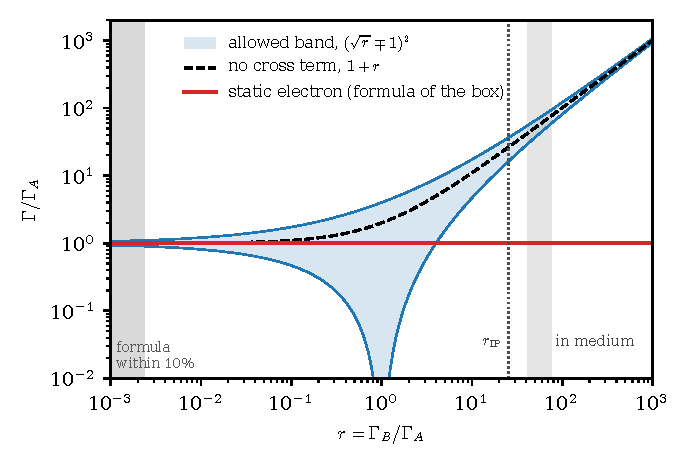
\includegraphics[width=0.82\linewidth]{figures/ch10/limit10_4a.pdf}
\captionof{figure}{Rate of $\mathcal{O}_8 = \vect{S}_\chi\cdot\vect{v}^\perp$ (spin-$\frac12$ dark matter, heavy mediator, elastic) relative to the static-electron formula of the box, $\varGamma_A$, against the ratio $r = \varGamma_B/\varGamma_A$ of the current-row rate $\varGamma_B$ to the formula. Blue: the band that positivity allows when the density--current cross term is not computed, $(\sqrt r \mp 1)^2$ (\cref{eq:10.4-band}). Dashed: $1 + r$, exact for responses averaged over the directions of $\vect{q}$, for which the cross term vanishes. Red: the formula. Gray at left: $r \le 2.4\times10^{-3}$, where every value in the band lies within \SI{10}{\percent} of the formula, $(\sqrt r + 1)^2 \le 1.1$. Dotted: silicon at $\mchi = \SI{10}{MeV}$ for independent particles, $r_{\mathrm{IP}} = 25.3$, from the empirical pseudopotential of Cohen and Bergstresser (model gap \SI{0.82}{eV}, $10^3$ $\vect{k}$ points, 36 conduction bands, bins of \SI{0.1}{eV}, 26-point average over directions, threshold \SI{1.11}{eV}, standard halo of \cref{sec:1.2}). Gray at right: the same ratio with the density row screened, $r_{\mathrm{IP}}\times2.31\times(1 \pm 0.3)$. The factor 2.31 is the screening of the density rate in the random-phase tables with local fields of \cref{sec:10.2}, and $\pm0.3$ the range allowed for the local-field change of the current row.}\label{fig:10-mixed-limit}
\par}
\smallskip
The formula leaves out the electron's own transverse motion, which in silicon carries about 25 times the rate the formula keeps, so the true rate is at least 16 times the formula for independent particles and at least 29 times with the density row screened.
\end{limitbox}

\subsection{Interference bound on a mixed block}\label{sec:10.4-band}

The rate of $\mathcal{O}_8$ shows how the rows combine. With the potentials of \cref{eq:8.1-O7O8} on the density and the current, the contraction \cref{eq:8.2-rate} has a density term, a current term and their interference. Continuity removes the parts along $\vect{q}$ on both sides (\cref{eq:D.30-O8T}). For elastic dark matter, and with the responses averaged over the directions of $\vect{q}$, the velocity integral is the one of \cref{app:A.8} with one change. The density term carries the dark matter's transverse velocity squared, $|\bar{\vect{v}}_{\mathrm{T}}|^2 = v^2 - \vmin^2$ on the energy shell, and its halo average is the second speed moment $\eta_2(\vmin) = 2\int_{\vmin}^\infty\dd v'\,v'\eta(v')$ in place of $\eta$ (\cref{eq:D.30-kernel}).
\begin{keyresult}[Rate of a velocity coupling]
For $\mathcal{O}_8$ with coefficient $c_8^{(e)}(q)$ and spin-$\frac12$ dark matter, the spectrum per unit target mass is
\begin{equation}
  \frac{\dd\mathcal{R}}{\dd\omega} = \frac{\rho_\chi}{16\pi^2\mchi\rho_T}\int\dd q\;q\,\bigl|c_8^{(e)}(q)\bigr|^2\Bigl[\underbrace{\eta_2(\vmin)\,\bar S_{nn}(q,\omega)}_{\text{electron at rest}} + \underbrace{\eta(\vmin)\,\Tr\bar S_{\vect{j}_{\mathrm{T}}\vect{j}_{\mathrm{T}}}(q,\omega)}_{\text{electron motion}}\Bigr] ,
  \label{eq:10.4-O8}
\end{equation}
with $\bar S$ averaged over the directions of $\vect{q}$, for which the density--current cross term vanishes. The first term is the rate of an electron at rest; the second is the electron's own transverse motion.
\end{keyresult}
\noindent The prefactor follows from \cref{eq:8.2-spectrum} with the kernel $\eta/(2q)$ per unit $\dd^3q/(2\pi)^3$ of \cref{eq:A.8-eta} and the factor $\frac14$ of the spin trace. For $c_8^{(e)} = \tilde V$ and $\Tr\bar S_{\vect{j}_{\mathrm{T}}\vect{j}_{\mathrm{T}}} = 0$, \cref{eq:10.4-O8} is the density rate with $\eta \to \eta_2/4$, the form of the box.

We can estimate the two terms before computing them. On the dark-matter side, the ratio $\eta_2/\eta$ is the mean of $|\bar{\vect{v}}_{\mathrm{T}}|^2$ over the particles fast enough to deposit $\omega$. It is $1.1\times10^{-6}$ at $\vmin = 0$, $1.0\times10^{-6}$ at $10^{-3}$ and $0.7\times10^{-6}$ at $2\times10^{-3}$, and it vanishes at the kinematic edge, where the only particles left move along $\vect{q}$. On the target side, the ratio $\Tr\bar S_{\vect{j}_{\mathrm{T}}\vect{j}_{\mathrm{T}}}/\bar S_{nn}$, integrated over $\omega$, is the mean transverse velocity squared of the electrons that make the pairs. In the empirical-pseudopotential model of silicon it is $3.2\times10^{-5}$ at $q_0$ and $2.1\times10^{-5}$ at $2q_0$, close to the free-gas value $\frac25v_{\mathrm{F}}^2 = 2.0\times10^{-5}$. At small $q$ it grows as $2\langle\omega^2\rangle/q^2$, the independent-particle form of \cref{eq:10.4-optical}: at $0.12\,q_0$ the model gives $4.1\times10^{-4}$ against $2\langle\omega^2\rangle/q^2 = 4.4\times10^{-4}$. We expect the electron term to exceed the dark-matter term by a factor of about 20 to 30, and more near the kinematic edge.

Let $\varGamma_A$ be the rate of the density term and $\varGamma_B$ the rate of the current term. The interference bound of \cref{sec:8.3} then limits the full rate whatever the cross term is.
\begin{keyresult}[Band on a mixed block]
For any target, halo and binning,
\begin{equation}
  \bigl(\sqrt{r} - 1\bigr)^2 \;\le\; \frac{\varGamma}{\varGamma_A} \;\le\; \bigl(\sqrt{r} + 1\bigr)^2 , \qquad r = \frac{\varGamma_B}{\varGamma_A} ,
  \label{eq:10.4-band}
\end{equation}
and with responses averaged over directions $\varGamma = \varGamma_A + \varGamma_B$. For independent particles $r$ is written $r_{\mathrm{IP}}$.
\end{keyresult}
\noindent The ratio of the two rates decides how much the cross term can matter. The half-width of the band relative to $1 + r$ is $2\sqrt r/(1 + r)$, below \SI{10}{\percent} only for $r < 2.5\times10^{-3}$ or $r > 4.0\times10^2$. For $r$ above 4 the lower edge exceeds one: the rate of an electron at rest is then an underestimate whatever the phase of the cross term. Positivity also says when the edges of the band are reached. Both edges need the density and current rows to be proportional on every final state the rate samples, and in an unpolarized crystal the two rows are far from proportional. In the model of silicon, along the generic direction $(5,3,1)$, the $\omega$-integrated cross block $|\vect{S}_{n\vect{j}_{\mathrm{T}}}|$ stays below 0.012 of $(S_{nn}\Tr S_{\vect{j}_{\mathrm{T}}\vect{j}_{\mathrm{T}}})^{1/2}$ up to $2.4\,q_0$, and on the two-, three- and fourfold axes it vanishes by symmetry. A crystal at fixed orientation keeps a cross term through the anisotropy of its response, the same anisotropy that makes the daily modulation of \cref{sec:11.7}.

In the medium the two terms of \cref{eq:10.4-O8} are screened differently. For a heavy mediator the density rate weighted with $\eta_2$ loses a factor 2.2 at \SI{30}{MeV}, 2.3 at \SI{10}{MeV} and 9.5 at \SI{1}{MeV} in the tables of \cref{sec:10.2}, while the current row changes only through local fields. Let screening lower the density rate by the factor $\varGamma_A/\varGamma_A^{\mathrm{med}}$ and change the current rate by the factor $1 + \delta^{j}_{\mathrm{LF}}$, the local-field correction of the transverse current averaged over the rate. Then
\begin{equation}
  r_{\mathrm{med}} = r_{\mathrm{IP}}\,\frac{\varGamma_A}{\varGamma_A^{\mathrm{med}}}\,\bigl(1 + \delta^{j}_{\mathrm{LF}}\bigr) ,
  \label{eq:D.30-rmed}
\end{equation}
and $r_{\mathrm{med}} \ge r_{\mathrm{IP}}$ whenever the product of the two factors is at least one. Since the lower edge of \cref{eq:10.4-band} increases with $r$ for $r \ge 1$, $(\sqrt{r_{\mathrm{med}}} - 1)^2 \ge (\sqrt{r_{\mathrm{IP}}} - 1)^2$ under the same condition.

\begin{workedexample}{The band for a velocity coupling in silicon}\label{we:10-band}
Take $\mathcal{O}_8$ with a heavy mediator, $\mchi = \SI{10}{MeV}$, the halo of \cref{sec:1.2} and the threshold $\Eg = \SI{1.11}{eV}$ of the tables of \cref{sec:10.2}. Averaged over directions with a 26-point rule, the empirical-pseudopotential model provides the two integrals of \cref{eq:10.4-O8} for independent particles. Their ratio is
\begin{equation*}
  r_{\mathrm{IP}} = \frac{\int\dd\omega\int\dd q\,q\,\eta\,\Tr\bar S^0_{\vect{j}_{\mathrm{T}}\vect{j}_{\mathrm{T}}}}{\int\dd\omega\int\dd q\,q\,\eta_2\,\bar S^0_{nn}} = 25.3 .
\end{equation*}
The model's gap is \SI{0.82}{eV}; shifting all its pair energies up so that the model gap becomes \SI{1.11}{eV} changes $r_{\mathrm{IP}}$ by \SI{2}{\percent}. With $\sqrt{r_{\mathrm{IP}}} = 5.03$, \cref{eq:10.4-band} puts the rate between $(5.03 - 1)^2 = 16.2$ and $(5.03 + 1)^2 = 36.4$ times the rate of an electron at rest, and the direction-averaged value is $1 + r_{\mathrm{IP}} = 26.3$. The rate of the density row alone is low by more than an order of magnitude.

Now screen. With the random-phase tables with local fields of \cref{sec:10.2}, the density rate weighted with $\eta_2$ falls by a factor 2.31 at this mass, the same as with $\eta$ (2.30). The local-field change of the current row is not known for silicon; the model finds $-4$ to $-15$ percent at $q_0$ and $2q_0$, and we allow $\pm30$ percent. Then $r_{\mathrm{med}} = 25.3\times2.31\times(1 \pm 0.3)$ lies between 41 and 76, the lower edge of the band between 29 and 60, and the direction-averaged rate is 42 to 77 times the static-electron formula with the same screened density row. The two models in this estimate differ: the current comes from the empirical pseudopotential, the screening of the density from a Kohn--Sham calculation. At $q_0$ and \SI{5}{eV} the model itself lowers $S_{nn}$ to 0.22 of its unscreened value, in line with the tables.

The ratio grows toward small masses, since the dark matter's transverse velocity vanishes at the kinematic edge: $r_{\mathrm{IP}} = 22$ at \SI{30}{MeV}, 33 at \SI{5}{MeV}, 56 at \SI{3}{MeV} and about 150 at \SI{2}{MeV}. The model's plane waves end at $2.8\,q_0$, while \SI{29}{\percent} of the screened heavy-mediator rate of silicon at \SI{10}{MeV} comes from $q > 2q_0$ (\cref{sec:10.2-corrections}). At large $q$ the ratio of the two responses tends to the mean transverse velocity squared of the valence electrons, which the model puts at $2\times10^{-5}$ to $3\times10^{-5}$ and which the core-region oscillations missing from pseudo-wavefunctions can only raise. The value of $r_{\mathrm{IP}}$ above is, if anything, low.
\end{workedexample}

The local-field screening of the transverse current in silicon is not known. Estimates put it at 10 to \SI{30}{\percent} (\cref{app:E.16}), the model above at 4 to \SI{15}{\percent}, both of the sign that lowers the current. The unknown local-field screening leaves open the factor between the static-electron formula and the true rate of $\mathcal{O}_8$, $\mathcal{O}_5$ or $\mathcal{O}_2$, or of the spin operators that carry $\vect{v}^\perp$. \Cref{eq:10.4-band} bounds the factor from below but does not fix it. Until the local-field screening of the transverse current is computed, limits set on these operators with the density response alone are conservative by at least an order of magnitude; these operators need a material input beyond the density response.

\section{Excitons at finite momentum}\label{sec:10.5}

At a momentum transfer equal to the valley momentum $\vect{k}_{\mathrm{c}}$, the lowest final state of silicon is not a free electron and hole at the indirect gap of \SI{1.17}{eV}. It is the pair bound by its own attraction, \SI{14.7}{meV} lower (\cref{sec:4.9}), and for the density coupling of \cref{sec:10.2} this attraction is the first correction beyond the random-phase approximation with local fields. Whether a given coupling can reach the bound pair is a question of symmetry. Besides adding a line below the threshold, the attraction raises the probability of finding the electron at the hole in every pair of the continuum. The continuum just above $E_{\mathrm{min}}(\vect{q})$ grows at the expense of higher energies, and the change is largest in the first eV above the gap, where most of the rate of light dark matter lies. \Cref{sec:10.2} wrote the screened rate as an integral of the loss function, and \cref{sec:4.9} gave the loss function of the Bethe--Salpeter equation. Put together at finite $\vect{q}$, they give the rate as a sum over exciton lines. We will find where its onset lies, which lines a density coupling can reach at the zone boundary of silicon, and how much a resonant-only solution of the equation costs. The spin-triplet excitons, which only spin couplings reach, close the section.

\subsection{The exciton rate}\label{sec:10.5-rate}

The rate of \cref{eq:10.2-rate} holds for any loss function, so the electron--hole attraction enters it through $L$ alone. With the eigenpairs $E_\lambda(\vect{q})$ and $A^\lambda_{cv\vect{k}}(\vect{q})$ of \cref{eq:4.9-bse} the structure factor is \cref{eq:4.9-S}, a sum of lines, one per exciton. Each line carries the squared matrix element of the density between the ground state and the singlet exciton $\lambda$. The singlet pair state $cv\vect{k}$ has amplitude $\sqrt{g_{\mathrm{deg}}}\,\rho_{cv}(\vect{k},\vect{q})$ to be created by $n_e(\vect{q})$, and the exciton is the superposition $\sum_{cv\vect{k}}A^\lambda_{cv\vect{k}}|cv\vect{k}\rangle$, so $\langle\lambda|n_e(\vect{q})|0\rangle = \sqrt{g_{\mathrm{deg}}}\,\rho_{\lambda0}(\vect{q})$ with
\begin{equation}
  \rho_{\lambda0}(\vect{q}) = \sum_{cv\vect{k}}A^\lambda_{cv\vect{k}}(\vect{q})^*\,\rho_{cv}(\vect{k},\vect{q}) ,
  \label{eq:10.5-formfactor}
\end{equation}
the exciton form factor. It is the coherent sum of \cref{sec:4.9}: the vertices of all the transitions in the exciton add with the amplitudes of its envelope. At $T = 0$ and $\omega > 0$, $L = (e^2/2q^2)S$ by \cref{eq:4.4-SL}, and \cref{eq:4.9-S} gives $L = (4\pi^2\alpha g_{\mathrm{deg}}/Vq^2)\sum_\lambda|\rho_{\lambda0}|^2\delta(\omega - E_\lambda)/|\varepsilon_{\mathrm{mac}}|^2$. In \cref{eq:10.2-rate} the factor $4\pi^2\alpha$ cancels against $8\pi^2\alpha$ and $q^3/q^2$ leaves one power of $q$.
\begin{keyresult}[Exciton rate at finite momentum]
\begin{equation}
  \frac{\dd\mathcal{R}}{\dd\omega} = \frac{\rho_\chi\,\sigmae\,g_{\mathrm{deg}}}{2\rho_T\,\mchi\,\mu_{\chi e}^2}\int\dd q\;q\,\eta\bigl(\vmin(q,\omega)\bigr)\,\FDM(q)^2\,\biggl\langle\frac1\Vol\sum_\lambda\frac{|\rho_{\lambda0}(\vect{q})|^2}{|\varepsilon_{\mathrm{mac}}(\vect{q},\omega)|^2}\,\delta\bigl(\omega - E_\lambda(\vect{q})\bigr)\biggr\rangle_{\hat{\vect{q}}} ,
  \label{eq:10.5-rate}
\end{equation}
with $\langle\cdots\rangle_{\hat{\vect{q}}}$ the average over the directions of $\vect{q}$, the exciton energies and form factors of \cref{eq:4.9-bse,eq:10.5-formfactor} at the momentum transfer $\vect{q}$ (reduced to the first zone in the kernels, \cref{sec:4.9}), and $g_{\mathrm{deg}} = 2$.
\end{keyresult}
\noindent Without the kernels each $\lambda$ is one transition, $\rho_{\lambda0} = \rho_{cv}$, $E_\lambda = \varepsilon_{c,\vect{k}+\vect{q}} - \varepsilon_{v\vect{k}}$, and \cref{eq:10.5-rate} is the random-phase rate of \cref{sec:10.2}; without $1/|\varepsilon_{\mathrm{mac}}|^2$ as well, it is the crystal form-factor rate of \cref{sec:10.1}. With the attraction on, the energies $E_\lambda(\vect{q})$ start below $E_{\mathrm{min}}(\vect{q})$, so the support of the spectrum moves down, and the weights $|\rho_{\lambda0}|^2$ are coherent sums, so the spectrum changes shape at fixed total weight. The $f$-sum rule of \cref{sec:4.3} holds for the exact $L$ at every $\vect{q}$, and what the attraction adds at low energy it removes higher up. For a rate this redistribution is not neutral: $\eta(\vmin)$ falls with $\omega$ at fixed $q$, and a particle that cannot deposit more than $\tfrac12\mchi v_{\mathrm{max}}^2$ sees only the low side. The line form with $|\varepsilon_{\mathrm{mac}}|^2$ in the denominator holds when no single line changes $\varepsilon_{\mathrm{mac}}$ near its own energy, which at keV momentum transfers, where the Coulomb factor $e^2/q^2$ is small, is always the case (\cref{sec:4.9}).

The equation is solved as in \cref{sec:4.9}, now at the reduced momentum $\vect{q}_r$ of each $\vect{q}$. It needs pairs from $(v,\vect{k})$ to $(c,\vect{k}+\vect{q}_r)$ on a grid of crystal momenta, quasiparticle energies or a scissor on Kohn--Sham bands, the screened interaction $W^{\mathrm{scr}}$ for all grid differences, and the head of the exchange kernel at the unreduced $\vect{G}_q$ left out (\cref{app:E.6}). The first such calculations for dark matter were made for GaAs and NaI, with the scissor set to the measured gaps, a $6^3$ grid, 10 conduction bands and momenta along [100] up to \SI{14.7}{keV}~\cite{taufertshofer2026excitonic}. In both materials the loss function with the attraction lies above the random-phase one with local fields at low energy, at all the momenta shown. In GaAs the rate changes little. In NaI, whose lowest optical exciton lies about \SI{0.3}{eV} below the gap (an absorption peak at \SI{5.6}{eV} against a gap of \SI{5.9}{eV}~\cite{taufertshofer2026excitonic}), some seventy times deeper than the \SI{4.2}{meV} of GaAs (\cref{sec:4.9}), the rate at energies near the gap rises enough to improve the projected reach above a few MeV by close to an order of magnitude~\cite{taufertshofer2026excitonic}. No such calculation exists yet for silicon or germanium. \Cref{app:E.15} specifies one, with the coupling between pair creation and annihilation that the published calculations drop, and with the bound lines added from the effective-mass model below, since a $6^3$ or even a $24^3$ grid cannot resolve an exciton of radius \SI{4.2}{nm}.

What the attraction does at a dark-matter momentum transfer can be seen in silicon itself, in the model of \cref{fig:4-bse} carried to finite $\vect{q}$ (\cref{fig:10-xq}). At $|\vect{q}| = \SI{0.91}{keV}$ along [100], halfway to the valley, the lowest pair of the model costs \SI{1.69}{eV}. The attraction changes the proper absorption $\varepsilon_2$ the way it did at $q \to 0$. The main peak moves from \SI{5.3}{eV} to \SI{4.5}{eV} and grows from 16.5 to 27.5. The weight below \SI{3}{eV} grows by a factor of 2.2 over the random-phase value with local fields. The loss function follows with the screening of the same model, whose static value rises from 6.56 to 7.80. Between the onset and \SI{3.5}{eV} the attraction raises $L$ by a nearly constant 27 to 29 percent, by 49 percent at \SI{4}{eV}, and by about 30 percent above. The rise at high energies is partly an artifact: four conduction bands and the Tamm--Dancoff form do not hold the $f$-sum fixed, and the first moment of $\varepsilon_2$ below \SI{10}{eV} falls by 12 percent. The grid, ten points per direction, resolves no bound line, and the lines of \cref{sec:10.5-lines} lie below the gray region of the figure. For a rate the near-edge factor is what counts. Dark matter below a few MeV reaches only the first two eV above $E_{\mathrm{min}}(\vect{q})$, and there the attraction adds about a quarter to the screened loss function, on top of whatever bound lines the grid misses.

\begin{figure}[tbp]
  \centering
  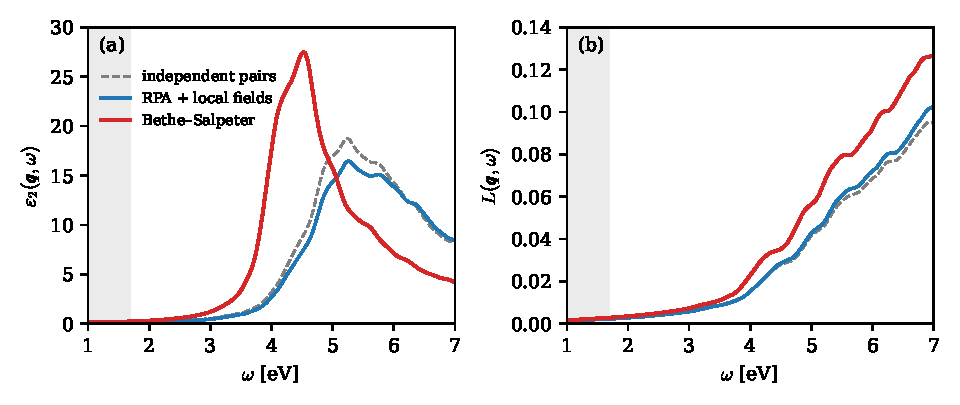
\includegraphics[width=\linewidth]{figures/ch10/fig10_4.pdf}
  \caption{The electron--hole attraction at finite momentum transfer in silicon, in a model calculation: $|\vect{q}| = \SI{0.91}{keV}$ ($0.4\times2\pi/a$) along [100]. States from the empirical pseudopotential of Cohen and Bergstresser~\cite{cohen1966band}, fitted to measured transition energies (model indirect gap \SI{0.82}{eV}; no scissor); 4 valence and 4 conduction bands on a shifted $10^3$ grid over the full zone (16{,}000 pairs); the 59 shortest reciprocal vectors in both kernels; direct kernel with the model dielectric function of Cappellini and coworkers~\cite{cappellini1993model} with $\varepsilon_\infty = 11.7$; Tamm--Dancoff resonant block with both time orderings, \cref{eq:4.9-epsmac}; Lorentzian broadening \SI{0.15}{eV}. On this grid the independent-pair spectrum agrees with a $15^3$ grid within 8 percent below \SI{6}{eV}. Gray: below the lowest pair of the grid, \SI{1.69}{eV}, where the curves are broadening tails; the bound lines are not resolved. Dashed: independent pairs (with the head screening only, in panel b); blue: random-phase approximation with local fields; red: Bethe--Salpeter equation. (a) Proper absorption $\varepsilon_2(\vect{q},\omega)$. (b) Loss function. The fitted bands already contain part of the excitonic shift, which the attraction then counts again (\cref{sec:4.9}).}
  \label{fig:10-xq}
\end{figure}

\subsection{Elliott onset and bound exciton lines}\label{sec:10.5-lines}

Near the bottom of the pair continuum at a given $\vect{q}$ the exciton form factor has a closed form, and with it the onset of \cref{eq:10.5-rate}. At fixed $\vect{q}$ the pair energy $\varepsilon_{c,\vect{k}+\vect{q}} - \varepsilon_{v\vect{k}}$ has its minimum $E_{\mathrm{min}}(\vect{q})$ of \cref{eq:3.3-Emin} at some $\vect{k}_0(\vect{q})$, and near it the pair energy rises quadratically in $\vect{k} - \vect{k}_0$, with a reduced mass set by the curvatures of the two bands at $\vect{k}_0$ and $\vect{k}_0 + \vect{q}$. This is the situation of \cref{eq:4.9-dispersion}, with the extremum of the pair energy in place of the band extrema. The relative motion obeys the hydrogenic equation \cref{eq:4.9-envelope}, and the bound states sit at $E_{\mathrm{min}}(\vect{q}) - E_x^b/n^2$. In silicon at $\vect{q} = \vect{k}_{\mathrm{c}}$ the pair minimum joins the two band extrema and $E_x^b$ is the measured \SI{14.7}{meV}. Away from the valley, $\vect{k}_0$ moves off the band extrema, the reduced mass changes, and $E_x^b$ with it (\cref{eq:E.15-disp}); we keep the symbols $E_x^b$, $a_x$ and $\mu_x$ for the values at the $\vect{q}$ in question.

When $\rho_{cv}(\vect{k},\vect{q})$ is smooth and nonzero at $\vect{k}_0$, the Elliott form \cref{eq:4.9-elliott} applies: $|\rho_{\lambda0}|^2 = \Vol|F_\lambda(0)|^2|\rho_{cv}(\vect{k}_0,\vect{q})|^2$. For the bound $s$ states, $|F_{ns}(0)|^2 = 1/(\pi a_x^3n^3)$. For the unbound states of relative momentum $\kappa$, normalized in the volume $\Vol$, $\Vol|F_{\kappa}(0)|^2$ is its free value, one, times the factor by which the attraction raises the probability of finding the electron at the hole. That factor is the Fermi factor \cref{eq:2.2-fermi} of an electron leaving a charge, with the coupling $\alpha/\varepsilon_\infty$ and the mass $\mu_x$ in place of $\alpha$ and $m_e$, so that $\xi_{\mathrm{C}} = 1/(\kappa a_x)$. With $\kappa^2 = 2\mu_x(\omega - E_{\mathrm{min}})$ and $2\mu_xE_x^ba_x^2 = 1$ from \cref{eq:4.9-WM}, the line sum in \cref{eq:10.5-rate} becomes
\begin{equation}
  \begin{aligned}
  \frac1\Vol\sum_\lambda|\rho_{\lambda0}|^2\delta(\omega - E_\lambda) = |\rho_{cv}(\vect{k}_0,\vect{q})|^2\biggl[&\sum_{n\ge1}\frac{\delta\bigl(\omega - E_{\mathrm{min}} + E_x^b/n^2\bigr)}{\pi a_x^3n^3} \\
  &+ \Theta(\omega - E_{\mathrm{min}})\,\frac{(2\mu_x)^{3/2}(\omega - E_{\mathrm{min}})^{1/2}}{4\pi^2}\,\frac{2\pi\xi_{\mathrm{C}}}{1 - \ee^{-2\pi\xi_{\mathrm{C}}}}\biggr] ,
  \end{aligned}
  \label{eq:10.5-lines}
\end{equation}
with $\xi_{\mathrm{C}} = [E_x^b/(\omega - E_{\mathrm{min}})]^{1/2}$. The density of free pairs, $\int\dd^3\kappa\,(2\pi)^{-3}\delta(\omega - E_{\mathrm{min}} - \kappa^2/2\mu_x)$, supplies the square root. The two parts meet smoothly. The lines crowd toward $E_{\mathrm{min}}$ with spacing $2E_x^b/n^3$, so their weight per unit energy tends to $1/(2\pi a_x^3E_x^b)$, and as $\omega \to E_{\mathrm{min}}^+$ the continuum tends to $(2\mu_x)^{3/2}(E_x^b)^{1/2}/2\pi$, which is the same number. The edge of the excitonic spectrum at fixed $\vect{q}$ is therefore a series of lines followed by a finite step, where independent pairs start from zero as $(\omega - E_{\mathrm{min}})^{1/2}$.

How much weight the lines take is a short calculation. Their total is $\sum_n 1/(\pi a_x^3n^3) = \zeta(3)/(\pi a_x^3)$. The free continuum without the Fermi factor holds $(2\mu_x)^{3/2}\epsilon^{3/2}/6\pi^2$ between $E_{\mathrm{min}}$ and $E_{\mathrm{min}} + \epsilon$. With $(2\mu_x)^{3/2} = 1/(a_x^3(E_x^b)^{3/2})$ the two are equal at $\epsilon = (6\pi\zeta(3))^{2/3}E_x^b = 8.0\,E_x^b$: the bound lines together carry as much weight as the free pairs within eight binding energies of the edge would have carried. The attraction does not stop there. Above the edge the Fermi factor is $6.3$ at $\omega - E_{\mathrm{min}} = E_x^b$, falls to 2.3 at $10\,E_x^b$, and is still $1 + \pi\xi_{\mathrm{C}} + \dots$ far above, a slow approach to one. The hydrogenic form of that tail is not to be trusted beyond a few tenths of an eV, where the bands stop being parabolic and the pair samples the screening at shorter distances, and the sign is all it fixes there. The spectrum it describes comes from the region near the pair minimum only. In silicon at $\vect{q} = \vect{k}_{\mathrm{c}}$ the heavy and light holes at the valence maximum each add their own copy of \cref{eq:10.5-lines}, with their own masses and vertices.

\begin{workedexample}{The exciton line of silicon below the pair onset}\label{we:10-xline}
Take a momentum transfer close to $\vect{k}_{\mathrm{c}}$ in silicon, where $E_{\mathrm{min}}$ is the gap. With the low-temperature gap of \SI{1.17}{eV} and $E_x^b = \SI{14.7}{meV}$, the $1s$ line sits at \SI{1.155}{eV} and the $2s$ line at $\SI{1.17}{eV} - E_x^b/4 = \SI{1.166}{eV}$; the radius is $a_x = \SI{4.2}{nm}$ (\cref{sec:4.9}). For a vertex that is smooth at the band extrema, \cref{eq:10.5-lines} gives the $1s$ line the weight $|\rho_{cv}|^2/(\pi a_x^3) = |\rho_{cv}|^2\times\SI{4.3e-6}{\angstrom^{-3}}$ per unit volume. It is $1/\zeta(3) = 0.83$ of all the lines, and it equals the free-pair weight within $(6\pi)^{2/3}E_x^b = 7.1\,E_x^b = \SI{0.10}{eV}$ of the edge. A particle that deposits $\omega$ between \SI{1.155}{eV} and \SI{1.17}{eV} at this $\vect{q}$ has no free pair to make and makes the exciton; one that deposits \SI{1.27}{eV} finds the free-pair density raised by the factor $2.6$. For the rate integrated over $\omega$, a line \SI{14.7}{meV} below the edge changes little; for the threshold mass it changes even less. The kinematic floor of \cref{eq:1.3-mmin}, $2\Eg/v_{\mathrm{max}}^2 = \SI{0.333}{MeV}$, becomes $2(\Eg - E_x^b)/v_{\mathrm{max}}^2 = \SI{0.329}{MeV}$, a shift of 1.3 percent, and \cref{sec:3.3} showed that this floor is not reached at all, since the momentum at which a particle that light deposits most energy falls short of the valley. Where the zero-phonon edge of silicon lies, and that its first line is weak, are the subjects of \cref{sec:13.1,sec:13.9}. The line is weak because on the valley axis the vertex at the extrema vanishes, and the $1s$ line is dark.
\end{workedexample}

\subsection{Selection rules at the zone boundary}\label{sec:10.5-rules}

Spin decides first which excitons a dark-matter coupling can make in silicon. The ground state is a singlet, the density does not act on spin, and $n_e(\vect{q})$ creates only singlet excitons, the ones of \cref{eq:4.9-bse} with $g_{\mathrm{deg}}K^{\mathrm{x}}$. The triplets, in which the electron and hole spins combine to one, are reached by the spin density and the spin current of \cref{tab:10-minimal}, and \cref{sec:10.5-triplet} treats them. Crystal momentum decides next. The lowest exciton of silicon has the electron in a valley and the hole at $\mathrm{\Gamma}$, so it carries $\vect{k}_{\mathrm{c}}$ up to a reciprocal-lattice vector, and a coupling reaches it at first order only through $\vect{q} = \vect{k}_{\mathrm{c}} + \vect{G}$. Light, with $q \approx 0$, needs a phonon (\cref{sec:6.5}). Dark matter of a few hundred keV and more carries $|\vect{k}_{\mathrm{c}}| = \SI{1.94}{keV}$ and needs none.

The symmetry of the states at the extrema decides last, and it is what makes the first line of silicon weak. Take $\vect{q} = \vect{k}_{\mathrm{c}}$ along [100], the $x$ axis, with no Umklapp vector. Consider the operations of the cubic group that leave this axis fixed: the rotations by multiples of $90^\circ$ about it and the mirrors that contain it. The conduction state at the valley minimum is invariant under all of them, and so is the operator $\ee^{\ii\vect{q}\cdot\vect{r}}$. The three valence states at the maximum transform like the products $yz$, $zx$ and $xy$ (in the notation of the band structure, $\mathrm{\Gamma}_{25'}$). Under the quarter turn about $x$, which takes $y \to z$ and $z \to -y$, $yz$ changes sign. The pair $(zx, xy)$ transforms like the two components $(z, y)$ of a vector across the axis and contains no invariant combination. A matrix element $\langle c,\vect{k}_{\mathrm{c}}|\ee^{\ii\vect{q}\cdot\vect{r}}|v,\mathrm{\Gamma}\rangle$ between an invariant state, through an invariant operator, to a state with no invariant part vanishes. Half of these operations carry the fractional translation of the diamond structure (\cref{app:C.17}), which multiplies the Bloch states and the operator by phases; for $\vect{q} = \vect{k}_{\mathrm{c}}$ exactly, the phase of the operator, $\ee^{-\ii\vect{q}\cdot\vect{\tau}_2}$, cancels that of the conduction state, $\ee^{-\ii\vect{k}_{\mathrm{c}}\cdot\vect{\tau}_2}$, and the argument stands. In germanium the valleys lie along [111]. The rotations by $120^\circ$ about that axis and the mirrors containing it leave the combination $yz + zx + xy$ invariant, and the vertex at the extrema does not vanish.

A vertex that vanishes at the extrema grows linearly away from them: $\rho_{cv}(\vect{k},\vect{q}) \simeq (\vect{k} - \vect{k}_0)\cdot\vect{g}$ with $\vect{g} = \nabla_{\vect{k}}\rho_{cv}$, and $\vect{q}$ itself off the axis adds a term proportional to its distance $\delta q_\perp$ from it. Transitions with a vertex of this kind are called second class~\cite{elliott1957intensity}. Their exciton form factor picks out the gradient of the envelope where the electron meets the hole. From $A_{\vect{k}} = \Vol^{-1/2}\int\dd^3r\,F(\vect{r})\ee^{-\ii\vect{k}\cdot\vect{r}}$, $\sum_{\vect{k}}A_{\vect{k}}\,\vect{k}\cdot\vect{g} = -\ii \Vol^{1/2}\,\vect{g}\cdot\nabla F(0)$, which vanishes for $s$ states and is nonzero for the $p$ state oriented along $\vect{g}$. Its envelope is $R_{n1}(r)\,(3/4\pi)^{1/2}\cos\theta$, with $\theta$ measured from $\vect{g}$, and the hydrogen radial function starts as $R_{n1} \to \tfrac23[(n^2 - 1)/n^5]^{1/2}r/a_x^{5/2}$; for $n = 2$ this is $R_{21} = r\,\ee^{-r/2a_x}/(2\sqrt6\,a_x^{5/2})$. So $|\vect{g}\cdot\nabla F_{np}(0)|^2 = |\vect{g}|^2(n^2 - 1)/(3\pi a_x^5n^5)$, and in place of the $s$ lines of \cref{eq:10.5-lines},
\begin{equation}
  \frac1\Vol\sum_{\lambda\in\text{lines}}|\rho_{\lambda0}|^2\delta(\omega - E_\lambda) = |\nabla_{\vect{k}}\rho_{cv}|^2\sum_{n\ge2}\frac{n^2 - 1}{3\pi a_x^5n^5}\,\delta\bigl(\omega - E_{\mathrm{min}} + E_x^b/n^2\bigr) \qquad\text{(second class)} .
  \label{eq:10.5-second}
\end{equation}
There is no $1s$ line. The first line is $2p$, at $E_x^b/4 = \SI{3.7}{meV}$ below the continuum. Against an allowed $1s$ line with a vertex of size $|\rho|$ it is weaker by $(|\nabla_{\vect{k}}\rho_{cv}|/|\rho|)^2/(32a_x^2)$, a factor of about $10^{-3}$ for a vertex that changes by order one across a tenth of the zone ($|\nabla_{\vect{k}}\rho_{cv}|/|\rho| \approx \SI{9}{\angstrom}$). The continuum changes the same way. Its vertex is $|\vect{g}\cdot\vect{\kappa}|^2$, or $|\vect{g}|^2\kappa^2/3$ averaged over directions, so the free pairs start as $(\omega - E_{\mathrm{min}})^{3/2}$. The $p$-wave Coulomb function at the origin carries the extra factor $1 + \xi_{\mathrm{C}}^2$, from $|\Gamma(2 + \ii\xi_{\mathrm{C}})|^2 = (1 + \xi_{\mathrm{C}}^2)|\varGamma(1 + \ii\xi_{\mathrm{C}})|^2$, which keeps the step at the edge finite. Off the axis the $1s$ line returns with a weight proportional to $\delta q_\perp^2$, and in a rate averaged over directions it enters at the energy of the $1s$ line with a weight that grows from zero.

The rule holds only for $\vect{q} = \vect{k}_{\mathrm{c}}$ without an Umklapp vector. With $\vect{q} = \vect{k}_{\mathrm{c}} + \vect{G}$ the phases of the shifted operations no longer cancel, $\ee^{-\ii\vect{G}\cdot\vect{\tau}_2}$ can be $-1$, and transitions that are forbidden at $\vect{G} = 0$ become allowed. Which classes open, at what momenta and with what strength, follows from the glide symmetry of \cref{app:C.17} and is worked out in \cref{sec:13.9}, where it decides the zero-phonon edge of silicon. Spin--orbit coupling lifts the zero on the axis as well, by an amount too small to matter (\cref{sec:13.9}).

\subsection{Time orderings and the coupling block}\label{sec:10.5-orderings}

A dark-matter calculation with excitons must give the loss function, not only the absorption $\varepsilon_2$, and the loss function needs the real part of the dielectric function as well. Here the way the equation is solved matters more than one might expect. \Cref{eq:4.9-epsmac} has two terms for each exciton, a resonant pole at $+E_\lambda$ and an antiresonant one at $-E_\lambda$. The second is the same process with the opposite time ordering, the pair annihilated before it is created, and it is the mirror image that causality requires: with both terms, $\varepsilon_{\mathrm{mac}}(\vect{q},\omega)$ is analytic in the upper half plane and obeys the Kramers--Kronig relations of \cref{app:C.5}. A program that solves the resonant block alone, as the Tamm--Dancoff approximation does, can still form the response with both orderings; this is the retarded Tamm--Dancoff form, and \cref{eq:4.9-epsmac} is written that way. If instead the antiresonant term is dropped altogether, the response is resonant-only.

At $\omega > 0$ the antiresonant term has no imaginary part, so the two forms have the same $\varepsilon_2$. Their real parts, however, differ. With $\varepsilon_2 = \pi C\sum_\lambda w_\lambda\delta(\omega - E_\lambda)$ for the weights $w_\lambda$ and the positive constant $C$ of \cref{eq:4.9-epsmac}, the two orderings give $\varepsilon_1 - 1 = C\sum_\lambda w_\lambda[1/(E_\lambda - \omega) + 1/(E_\lambda + \omega)]$, and the resonant term alone gives $\varepsilon_1^{\mathrm{res}} - 1 = C\sum_\lambda w_\lambda/(E_\lambda - \omega)$. Written with $\varepsilon_2$,
\begin{equation}
  \varepsilon_1 - 1 = \frac2\pi\,\mathrm{P}\!\int_0^\infty\dd\omega'\,\frac{\omega'\varepsilon_2(\omega')}{\omega'^2 - \omega^2} , \qquad
  \varepsilon_1^{\mathrm{res}} - 1 = \frac1\pi\,\mathrm{P}\!\int_0^\infty\dd\omega'\,\frac{\varepsilon_2(\omega')}{\omega' - \omega} ,
  \label{eq:10.5-kk}
\end{equation}
the first being \cref{eq:C.5-KKeps}. For a single oscillator at $E_0$ the ratio is
\begin{equation}
  \frac{\varepsilon_1^{\mathrm{res}} - 1}{\varepsilon_1 - 1} = \frac{E_0 + \omega}{2E_0} , \qquad
  \frac{L^{\mathrm{res}}}{L} = \frac{\varepsilon_1^2 + \varepsilon_2^2}{(\varepsilon_1^{\mathrm{res}})^2 + \varepsilon_2^2} \simeq \Bigl(\frac{\varepsilon_1}{\varepsilon_1^{\mathrm{res}}}\Bigr)^2 \quad (\varepsilon_2 \ll \varepsilon_1) .
  \label{eq:10.5-res}
\end{equation}
At $\omega \to 0$ the resonant-only form keeps half of $\varepsilon_1 - 1$. In silicon at small $q$, with $\varepsilon_1 = 11.7$, it overstates the loss function by $[2\varepsilon_1/(\varepsilon_1 + 1)]^2 = 3.4$ as $\omega \to 0$ (at \SI{1.3}{eV} and the smallest momentum of the tables below, \SI{0.49}{keV}, the factor is 2.2), and wherever $\varepsilon_1$ is large and $\varepsilon_2$ small, as below and just above the gap, the error is typically a factor of two. It vanishes as $q \to \infty$, where $\varepsilon_1 \to 1$ and screening disappears.

The silicon tables of \cref{sec:10.2} put numbers on this. From their $\varepsilon_2$ with local fields, \cref{eq:10.5-kk} reproduces the tabulated static $\varepsilon(\vect{q},0)$ to within one percent at every $q$, which shows that the tables hold enough of the spectrum for the transform. At $|\vect{q}| = \SI{1.39}{keV}$ ($\SI{0.71}{\angstrom^{-1}}$) and $\omega = \SI{1.3}{eV}$, below the pair continuum at that momentum, $\varepsilon_1 = 4.45$ and $\varepsilon_1^{\mathrm{res}} = 3.05$, and the resonant-only form overstates $L$ by a factor of 2.12. A single oscillator that carries the whole valence $f$-sum and reproduces the static value 4.31, $E_0 = \omega_p^{\mathrm{val}}/[\varepsilon(\vect{q},0) - 1]^{1/2} = \SI{9.1}{eV}$ with $\omega_p^{\mathrm{val}} = \SI{16.6}{eV}$, gives 2.23 from \cref{eq:10.5-res}, and the model dielectric function of \cref{sec:10.2} gives 2.25. These momenta and energies are those at which the phonon-assisted pairs of \cref{sec:13.3} are made, and that is where the factor of two would land. It falls to 1.53 at $q_0 = \SI{3.73}{keV}$ and to 1.07 at \SI{8}{keV}, and it is within 15 percent of one above \SI{6.7}{keV}. A resonant-only evaluation is harmless for heavy mediators at masses where large $q$ dominates, and wrong by a factor of two for light mediators and light dark matter.

The retarded form has no such error, but it still drops something: the coupling block of \cref{eq:D.12-blocks}, which mixes the creation of one pair with the annihilation of another. Its effect follows from a single pair of transition energy $\Delta$ coupled to itself by a kernel $K$ in both blocks. With coupling the poles are at $\pm E_{\mathrm{cp}}$, $E_{\mathrm{cp}}^2 = (\Delta + K)^2 - K^2 = \Delta(\Delta + 2K)$, so $E_{\mathrm{cp}} = \Delta + K - K^2/2\Delta + \dots$; without it they are at $\pm(\Delta + K)$. The energy is wrong only at second order, the statement of \cref{sec:4.9}. The weight is not. With $R^0(0) = -2|\rho|^2/\Delta$ for the free pair, the static response of the coupled pair is $R(0) = R^0/(1 - KR^0/|\rho|^2) = -2|\rho|^2/(\Delta + 2K)$. The retarded resonant block gives $R^{\mathrm{TD}}(0) = -2|\rho|^2/(\Delta + K)$, and
\begin{equation}
  \frac{R^{\mathrm{TD}}(0)}{R(0)} = \frac{\Delta + 2K}{\Delta + K} = 1 + \frac{K}{\Delta + K} ,
  \label{eq:10.5-coupling}
\end{equation}
an error of first order in the kernel, here written for an exchange-type $K$ that enters the coupling block with the same sign as the resonant one. Which kernel remains in the coupling block depends on how the long-range part is handled. The head of the exchange kernel, the term at $\vect{G}_q$, is the macroscopic field, and it turns the proper response into the screened one (\cref{sec:4.9}). If it is kept in the Bethe--Salpeter Hamiltonian and the coupling block is dropped, the screening itself is computed in the Tamm--Dancoff approximation, and for the screened $L$ the error is set by $v_{\mathrm{C}}(q)$, large at small $q$. The safe arrangement is the one of \cref{app:E.15}: the Tamm--Dancoff equation, without the head, for the proper $\varepsilon_2$ with its lines, and the screening from the full response, with both orderings, through $L = \varepsilon_2/|\varepsilon_{\mathrm{mac}}|^2$ and \cref{eq:10.5-kk}. The coupling block then still holds the local-field exchange and the small interband part of the direct kernel. Since the local fields change $\varepsilon_2$ of silicon by about ten percent (\cref{sec:4.6}), the remaining error is of that size, about \SI{10}{\percent} on the proper $\varepsilon_2$. In the model of \cref{fig:10-xq}, where the coupling block holds the local-field exchange alone, the full random-phase response with local fields differs from its retarded Tamm--Dancoff form by 2.6 percent of the peak of $\varepsilon_2$. The \SI{10}{\percent} is an estimate; the full coupled calculation, which also restores the $f$-sum rule that the Tamm--Dancoff form strains, is part of \cref{app:E.15}.

The static screened interaction is the other approximation in the equation. It holds when the binding energies and the spread of transition energies that matter are small against the frequencies at which $\varepsilon^{-1}$ changes, the plasma frequency of \SI{16.6}{eV} in silicon (\cref{sec:4.9}). For bound lines of \SI{14.7}{meV} and pairs within a few eV of the gap this holds, and the dynamical screening of the interaction, left for the full calculation of \cref{app:E.15}, is not expected to rival the two errors above.

\begin{limitbox}[Bethe--Salpeter exciton rate][lim:10.5a]
With the loss function of the Bethe--Salpeter equation in the Tamm--Dancoff approximation, the rate is \cref{eq:10.2-rate} with $\bar L = \Imag[-1/\varepsilon_{\mathrm{mac}}^{\mathrm{BSE}}(q,\omega)]$, or \cref{eq:10.5-rate} line by line~\cite[Eqs.~(1) and (2)]{taufertshofer2026excitonic}.
\par\smallskip
{\centering
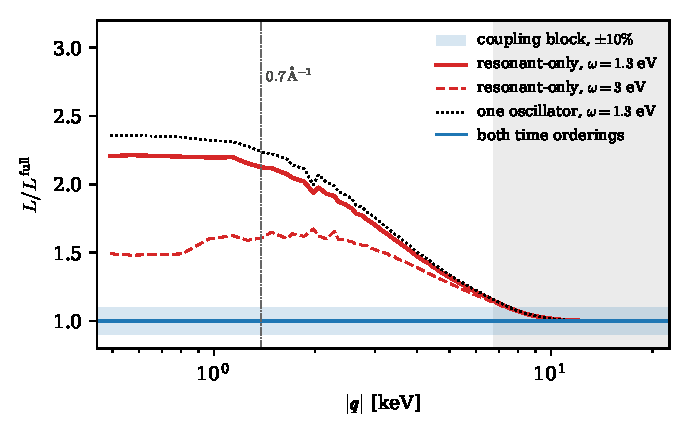
\includegraphics[width=0.82\linewidth]{figures/ch10/limit10_5a.pdf}
\captionof{figure}{Loss function of silicon in two evaluations of the same response, divided by the evaluation with both time orderings, against $|\vect{q}|$. Red: resonant-only real part, \cref{eq:10.5-kk}, at $\omega = \SI{1.3}{eV}$ (solid) and \SI{3}{eV} (dashed), from $\varepsilon_2$ of the random-phase tables with local fields of \cref{sec:10.2} (threshold \SI{1.11}{eV}, the step-model gap that accompanies them; directions averaged in bins of \SI{100}{eV}). Dotted: a single oscillator with the valence $f$-sum and the tabulated static $\varepsilon(q,0)$, \cref{eq:10.5-res}, at \SI{1.3}{eV}. Blue line and band: both time orderings, with the estimated $\pm\SI{10}{\percent}$ error of the coupling block, \cref{eq:10.5-coupling}. Dash-dotted: $|\vect{q}| = \SI{0.7}{\angstrom^{-1}}$ (\SI{1.39}{keV}), the momentum of the numbers quoted in the text. Gray: momenta at which the resonant-only form is within \SI{15}{\percent}, $|\vect{q}| \ge \SI{6.7}{keV}$.}\label{fig:10-bse-limit}
\par}
\smallskip
Below about \SI{7}{keV}, where screening is strong, a resonant-only real part overstates the loss function by up to a factor of two or more; with both time orderings the remaining error is that of the coupling block.
\end{limitbox}

\subsection{Triplet excitons}\label{sec:10.5-triplet}

A coupling to the electron spin, such as $\mathcal{O}_4$ of \cref{tab:8-operators}, creates the electron--hole pair with its spins combined to one, a triplet, and the triplet rows of \cref{tab:10-minimal} are its responses. Without interaction they are a quarter of the density response (\cref{eq:D.30-quarter}), and they are not screened (\cref{sec:10.4}). With the interaction the triplet pair has its own Bethe--Salpeter equation. The exchange kernel comes from a pair that annihilates and is re-created, and a spin-one pair cannot annihilate into the spinless density that the Coulomb line couples to, so its contribution cancels between the two spin projections. The direct kernel, the attraction between the electron and the hole, acts in every spin state alike. The triplet Hamiltonian is therefore
\begin{equation}
  H^{\mathrm{exc}}_{\mathrm{T}} = \Delta - K^{\mathrm{d}} ,
  \label{eq:10.5-triplet}
\end{equation}
\cref{eq:4.9-bse} with $g_{\mathrm{deg}}K^{\mathrm{x}}$ removed, and the spin structure factor follows from its eigenpairs as the density one does, with the vertex $\sigma^z/2$ in place of one and no $1/|\varepsilon_{\mathrm{mac}}|^2$.

The bound lines of the triplet sit where the singlet ones do, up to the electron--hole exchange splitting. That splitting is the short-range exchange of a pair whose electron and hole meet in one cell with probability of order $(a/a_x)^3$, $2\times10^{-3}$ in silicon, so it is a fraction of order $10^{-3}$ of the binding, well below a meV. And the Wannier analysis above, which used only $K^{\mathrm{d}}$, applies unchanged: the triplet edge has the same lines, the same Fermi factor and the same selection rules of point symmetry as the singlet one, with the spin vertex in place of the density vertex. What separates the two channels is the rest of $K^{\mathrm{x}}$, the local fields, which raise the singlet transitions and move weight up (\cref{sec:4.6}) and which the triplet lacks. In the model of \cref{fig:10-xq}, the triplet spectrum below \SI{3}{eV} carries 2.2 times the independent-pair weight, and between 2.5 and \SI{4}{eV} five times, while above \SI{4}{eV} the two agree within 4 percent. The attraction alone moves the triplet weight down more than the singlet's, since no local fields push back.

What is not known is the triplet response at keV momentum transfers beyond independent particles: the ladder with the screened attraction over the whole spectrum, together with the exchange--correlation kernel of the spin channel, which is not the one of the density. As an estimate, near the edge the spin rows of \cref{tab:10-minimal} inherit the excitonic enhancement of the singlet ones, without their local fields and without screening. \Cref{app:E.16} specifies the calculation, as the Bethe--Salpeter run of \cref{app:E.15} with the exchange kernel switched off; its control is the limit without interaction, which must return a quarter of the independent-particle density response.

\subsection{Open problems}\label{sec:10.5-open}

For silicon and germanium no finite-momentum Bethe--Salpeter calculation exists, with or without the coupling block, and no calculation resolves the bound lines of an indirect gap. The lines need grids around the pair minimum far finer than a uniform grid can afford, and are therefore to be added from \cref{eq:10.5-lines,eq:10.5-second} with computed masses, vertices and vertex gradients. The full coupled calculation would settle the \SI{10}{\percent} of \cref{eq:10.5-coupling}, test the factor of two of \cref{eq:10.5-res} directly, and check the $f$-sum rule to a percent (\cref{app:E.15}). The triplet response beyond independent particles is open as stated above.

So is the response of crystals in which the exciton is not large. In NaI the lowest excitons are compact, of the size of an ion pair, and the hole localizes on two anions while the lattice relaxes around it: the exciton becomes self-trapped. The Wannier picture fails, and the line that dark matter creates is dressed by the phonons that the relaxation emits. Take linear coupling, a harmonic lattice and a vertex independent of the lattice coordinates. The line at $E_\lambda$ then becomes a Poisson series of replicas spaced by a mean phonon energy $\bar\omega$, with the weight $\ee^{-S_{\mathrm{HR}}}S_{\mathrm{HR}}^n/n!$ in the $n$th (\cref{eq:E.15-ste}), where the Huang--Rhys factor $S_{\mathrm{HR}}$ is the mean number of phonons emitted, the relaxation energy divided by $\bar\omega$. For NaI none of $S_{\mathrm{HR}}$, $\bar\omega$ or the form factor $\rho_{\lambda0}(\vect{q})$ is known at keV momenta, and \cref{app:E.15} specifies their calculation. The localized (Frenkel) exciton itself, the limit of a pair confined to one site, is made precise in \cref{sec:16.4}. The spread between the random-phase and the excitonic rate near the gap, the factor that a resonant-only evaluation can introduce, and the coupling error enter the many-body uncertainty of \cref{sec:8.8}, collected for this chapter in \cref{sec:10.10}.

\section{Core and relativistic states}\label{sec:10.6}

A germanium atom has 32 electrons, and the band structure of \cref{sec:10.1} follows four of them. Ten more sit in the $3d$ shell, \SI{29.4}{eV} below the valence-band maximum, close enough for light dark matter to excite them, and the deeper shells follow at \SI{122}{eV} and beyond. \Cref{sec:3.5} found where each shell becomes kinematically accessible and why the momenta it needs are large: an electron that absorbs $\omega$ must receive at least $q = \omega/v_{\mathrm{max}}$, \SI{11}{keV} for germanium $3d$ and \SI{38}{keV} for silicon $2p$. It left two questions for the rate. At which momentum transfer does a core shell actually take over from the valence electrons, given that both are probed far out in the tails of their momentum distributions? And how much do the relativistic corrections of order $(Z\alpha)^2$, which grow with the depth of the shell, change the response there? We answer both for silicon and germanium, and find the three hypotheses under which the response of the core electrons separates from that of the valence electrons: a filled shell, a flat band and orthogonal site orbitals.

\subsection{Core shells within kinematic reach}\label{sec:10.6-reach}

The structure factor of a crystal with core shells is the sum of the valence term of \cref{eq:10.1-S0} and one term per core shell. The core states of atom $\kappa$ in the cell are the Bloch sums $\psi_{\kappa nlm,\vect{k}}$ of \cref{eq:E.7-core}, with the energy $-E_{\mathrm{core}}$ measured from the valence maximum, and their vertex with a conduction state is $\rho_{c,\kappa nlm}(\vect{k},\vect{q}) = \langle\psi_{c,\vect{k}+\vect{q}}|\ee^{\ii\vect{q}\cdot\vect{r}}|\psi_{\kappa nlm,\vect{k}}\rangle$. Following the steps of \cref{eq:10.1-S0} with these states in place of the valence bands,
\begin{equation}
  S^0_{\mathrm{core}}(\vect{q},\omega) = 4\pi\sum_{\kappa nlm}\sum_c\int_{\mathrm{BZ}}\frac{\dd^3k}{(2\pi)^3}\,|\rho_{c,\kappa nlm}(\vect{k},\vect{q})|^2\,\delta\bigl(\omega - \varepsilon_{c,\vect{k}+\vect{q}} - E_{\mathrm{core},\kappa nl}\bigr) .
  \label{eq:10.6-core}
\end{equation}
Both states in the vertex must be all-electron states. The core orbital is all-electron by construction. The conduction state must carry its core-region oscillations, which the reconstruction \cref{eq:3.5-rhoAE} restores, because the overlap with a core orbital is taken inside the sphere where a pseudo-wavefunction is wrong. A semicore shell kept in the valence of the pseudopotential, such as germanium $3d$, enters \cref{eq:10.1-S0} instead, with reconstructed vertices on both sides. Griffin and coworkers computed the germanium $3d$ contribution both ways and found that the atomic orbitals reproduce the reconstructed crystal states up to the largest momentum the crystal calculation resolves, about \SI{45}{keV}~\cite[Sects.~2.2 and~3.3]{griffin2021extended}.

How many core electrons can dark matter reach at a given $q$? A momentum transfer $q$ deposits at most $qv_{\mathrm{max}}$, whatever the mass (\cref{eq:1.3-vmin}), so the relevant measure is the part of the structure factor below that energy. Per atom and per shell we define
\begin{equation}
  N^{\mathrm{acc}}_{nl}(q) = \int_{\Eg + E_{\mathrm{core}}}^{qv_{\mathrm{max}}}\dd\omega\;S^{\mathrm{at}}_{nl}(q,\omega) ,
  \label{eq:10.6-Nacc}
\end{equation}
where $S^{\mathrm{at}}_{nl}(q,\omega)$ is the response of one atom's shell, normalized so that its integral over all $\omega$ is the occupation $N_{nl}$ when $q$ is large (closure, \cref{sec:4.3}). The structure factor of \cref{eq:10.6-core} is $(2\pi/\Omega)\sum_\kappa S^{\mathrm{at}}_{\kappa nl}$, as the next subsection shows, so $N^{\mathrm{acc}}_{nl}$ counts the electrons of a shell, per atom, that the halo can excite at momentum transfer $q$. With plane-wave final states the shell response follows from the ionization form factor of \cref{sec:2.2}. The number of final states per unit ejected energy is $|f_{\mathrm{ion}}|^2/4E_{\mathrm{ej}}$, and \cref{eq:2.2-fion-pw}, with the radial momentum orbital $\phi_{nl}(k)$ of \cref{sec:3.5} normalized to $\int k^2\phi_{nl}^2\,\dd k = 1$, gives
\begin{equation}
  S^{\mathrm{at}}_{nl}(q,\omega) = \frac{N_{nl}}{2}\,\frac{m_e}{q}\int_{|p - q|}^{p + q}k\,\phi_{nl}(k)^2\,\dd k , \qquad p = [2m_e(\omega - E_{\mathrm{core}})]^{1/2} ,
  \label{eq:10.6-Sat}
\end{equation}
for a full shell, $N_{nl} = 2(2l + 1)$, and for the spherical average of a partly filled valence shell. The final kinetic energy is counted from the valence maximum, as for the free final states of Griffin and coworkers~\cite[Eq.~(3.21)]{griffin2021extended}. Integrating over $\omega$, with $\dd\omega = p\,\dd p/m_e$ and the order of integration exchanged, each $k$ collects $\int_{|k - q|}^{k + q}p\,\dd p = 2kq$, and the integral is $N_{nl}\int k^2\phi_{nl}^2\,\dd k = N_{nl}$: closure holds.

\Cref{eq:10.6-Sat} explains when a shell takes over. Near its opening the ejected momentum $p$ is much smaller than $q$, the integral is $2pq\,\phi_{nl}(q)^2$, and
\begin{equation*}
  N^{\mathrm{acc}}_{nl}(q) \simeq N_{nl}\,m_e\,\phi_{nl}(q)^2\int_{E_{\mathrm{core}}}^{qv_{\mathrm{max}}}p\,\dd\omega = \frac{2\sqrt2}{3}\,N_{nl}\,m_e^{3/2}\,\phi_{nl}(q)^2\,(qv_{\mathrm{max}} - E_{\mathrm{core}})^{3/2} ,
\end{equation*}
where the gap has been dropped from the lower limit. Two factors decide. The first is the number of electrons of the shell per unit volume of momentum at $p = q$, $N_{nl}\phi_{nl}(q)^2$, in which a core shell beats the valence above about \SI{5}{keV} (\cref{fig:3-core}). The second is the phase space $(qv_{\mathrm{max}} - E_{\mathrm{core}})^{3/2}$, which is zero at the opening and approaches that of the valence, $(qv_{\mathrm{max}})^{3/2}$, only once $qv_{\mathrm{max}}$ is several times $E_{\mathrm{core}}$. A core shell therefore overtakes the valence a little above its opening, at the momentum where its larger density outweighs the reduced phase space.

\Cref{fig:10-core} evaluates \cref{eq:10.6-Nacc} for germanium. The core and semicore shells use the free-atom orbitals of \cref{fig:3-core}. The valence uses the crystal: the independent-particle $\varepsilon_2$ of Knapen, Kozaczuk and Lin~\cite[Sect.~III\,B]{knapen2021dark}, from which $S = (2q^2/e^2)\varepsilon_2$ (\cref{sec:10.2}) and, per atom of the two-atom cell, $S^{\mathrm{at}} = q^2\Omega\varepsilon_2/8\pi^2\alpha$. That table holds only the four valence electrons, with the $3d$ shell frozen, on bands scissored to the measured gap at zero temperature. It ends at \SI{22.5}{keV}, where its plane-wave basis ends too, and we use it up to \SI{15}{keV} and \cref{eq:10.6-Sat} with the atomic $4s$ and $4p$ orbitals above. At the switch the two differ by 27 percent. Between 5 and \SI{15}{keV} the atomic model and the crystal tables of silicon and germanium differ by up to a factor of six in either direction, since the low-energy corner $\omega \le qv_{\mathrm{max}}$ is where the band structure matters most. That is the accuracy of the valence curve beyond the table.

\begin{figure}[tbp]
  \centering
  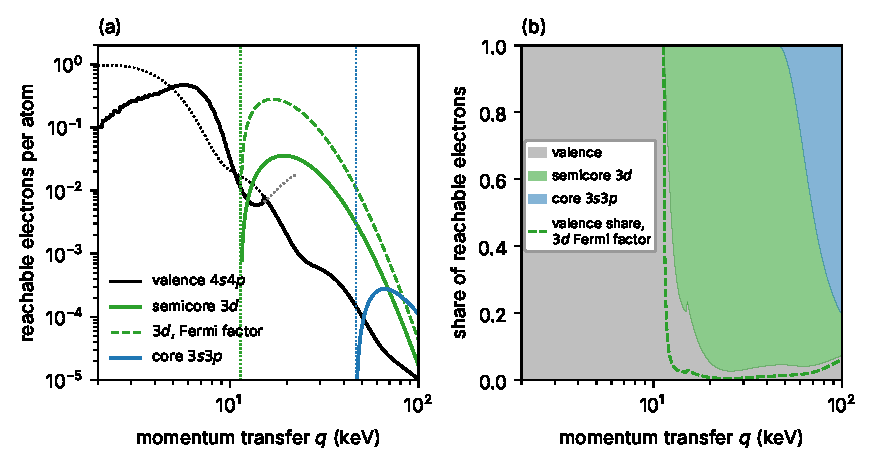
\includegraphics[width=\linewidth]{figures/ch10/fig10_5.pdf}
  \caption{Germanium electrons that dark matter of any mass can excite at momentum transfer $q$, that is, with energy deposits between the threshold of the shell and $qv_{\mathrm{max}}$, $v_{\mathrm{max}} = 2.650\times10^{-3}$. (a)~Electrons per atom, $N^{\mathrm{acc}}_{nl}(q)$ of \cref{eq:10.6-Nacc}, for the valence shell (black), the semicore $3d$ shell (green) and the core $3s$ and $3p$ shells (blue). Valence: crystal independent-particle response of Knapen, Kozaczuk and Lin (PAW, $3d$ frozen) below \SI{15}{keV}; above, the plane-wave model of \cref{eq:10.6-Sat} with the free-atom $4s$, $4p$ orbitals (dotted lines continue each curve past the switch). Core and semicore: \cref{eq:10.6-Sat} with free-atom, scalar-relativistic PBE orbitals and plane-wave final states whose kinetic energy is counted from the valence maximum; dashed, the $3d$ shell with the Fermi factor of \cref{eq:2.2-fermi} at $Z_{\mathrm{eff}} = 1$. Dotted vertical lines: the openings $(\Eg + E_{\mathrm{core}})/v_{\mathrm{max}}$ of the $3d$ and $3p$ shells, with centroid binding energies 29.4 and \SI{122.2}{eV} and $\Eg = \SI{0.744}{eV}$. Germanium $2s$, $2p$ and $1s$ open above \SI{460}{keV}. (b)~Shares of the reachable electrons: valence (gray), $3d$ (green), $3s3p$ (blue); dashed, the valence share when the $3d$ shell carries the Fermi factor. The $3d$ shell overtakes the valence at \SI{12.5}{keV} (\SI{11.5}{keV} with the Fermi factor) and holds more than 90 percent of the reachable electrons from 20 to \SI{50}{keV}.}
  \label{fig:10-core}
\end{figure}

The figure answers the first question for germanium. Below \SI{11.3}{keV} only the valence is reachable, and its count falls from 0.44 electrons per atom at \SI{5}{keV} to 0.03 at \SI{10}{keV} as the window $\omega \le qv_{\mathrm{max}}$ moves into the low-energy tail of a spectrum that is centered on $q^2/2m_e$. The $3d$ shell opens at \SI{11.3}{keV} and overtakes the valence at \SI{12.5}{keV}. By \SI{20}{keV} it holds 0.036 reachable electrons per atom against 0.002 for the valence, and it keeps more than 90 percent of the total until the $3p$ and $3s$ shells, opening at 46 and \SI{68}{keV}, take over near \SI{69}{keV}. For silicon the same model puts the opening of $2p$ at \SI{38}{keV} and its crossing with the valence at \SI{46}{keV}, and the $2s$ shell overtakes $2p$ near \SI{77}{keV}. Since the silicon valence count there comes from the atomic model, uncertain by a factor of a few, and the $2p$ count rises steeply above its opening, the crossing is uncertain by a few keV.

Two features of the model need checking, the non-orthogonality of plane-wave final states and the missing Coulomb attraction of the ion. A plane wave is not orthogonal to the bound orbital. Its projection onto the initial orbital adds a spurious term of relative size $|F_{nl}(q)|^2\phi_{nl}(p)^2/\langle\phi_{nl}(|\vect{p} - \vect{q}|)^2\rangle$, with $F_{nl}(q)$ the elastic form factor of the shell; for germanium $3d$ between 12 and \SI{30}{keV} it stays below 6 percent. The final state is the larger issue. A slow electron leaving a core region is pulled toward the ion, and the Fermi factor, 12 at a final momentum of \SI{2}{keV} and 5 at \SI{5}{keV} for $Z_{\mathrm{eff}} = 1$, raises the $3d$ count by about that much near the edge (dashed curves). This moves the crossing only from 12.5 to \SI{11.5}{keV}, because the count rises so steeply above the opening, but it changes the size of the $3d$ contribution to a rate by an order of magnitude. Crystal conduction states, as in Griffin's calculation, are the correct final states, and the Fermi factor only brackets them.

\begin{workedexample}{The germanium $3d$ onset in $q$}\label{we:10-ge3d}
The $3d$ shell is a doublet, $3d_{5/2}$ at \SI{29.2}{eV} and $3d_{3/2}$ at \SI{29.8}{eV} below the valence maximum~\cite[Table~1-1]{williams2009electron}. With $\Eg = \SI{0.744}{eV}$ the thresholds are 29.94 and \SI{30.54}{eV}, and the openings $(\Eg + E_{\mathrm{core}})/v_{\mathrm{max}}$ are \SI{11.3}{keV} and \SI{11.5}{keV}. The threshold masses $2(\Eg + E_{\mathrm{core}})/v_{\mathrm{max}}^2$ are 8.5 and \SI{8.7}{MeV}; the rounded values of \cref{sec:3.5}, \SI{11}{keV} and \SI{8.5}{MeV}, are those of a single level at \SI{29}{eV}.

Opening is not taking over. Just above \SI{11.3}{keV} the window $qv_{\mathrm{max}} - E_{\mathrm{core}}$ is a fraction of an eV wide, and the $3d$ count of \cref{eq:10.6-Nacc} starts from zero. From \cref{fig:10-core}a, at \SI{12}{keV} the $3d$ shell offers 0.0040 reachable electrons per atom against 0.0084 for the valence, at \SI{15}{keV} 0.025 against 0.0065. The two are equal at \SI{12.5}{keV} with the crystal valence. With the atomic valence the crossing is at \SI{13.1}{keV}, and with the Fermi factor on the $3d$ final states at \SI{11.5}{keV}. The onset in $q$ is therefore
\begin{equation*}
  q_{3d} \simeq (12.5 \pm 1)\,\mathrm{keV} = (3.3 \pm 0.3)\,q_0 ,
\end{equation*}
with $q_0 = \alpha m_e = \SI{3.73}{keV}$. Three quarters of the $3d$ electrons have momenta above \SI{11}{keV} (\cref{sec:3.5}), so the shell is probed near the peak of its distribution, while the valence is probed far in its tail.

Which masses use this momentum? A momentum transfer $q$ with energy deposited $\omega$ needs $\vmin = \omega/q + q/2\mchi \le v_{\mathrm{max}}$ (\cref{eq:1.3-vmin}), so at the $3d_{5/2}$ threshold, $\omega = \SI{29.94}{eV}$,
\begin{equation*}
  \mchi \ge \frac{q}{2(v_{\mathrm{max}} - \omega/q)} = \frac{\SI{12.5}{keV}}{2\,(2.650 - 2.395)\times10^{-3}} = \SI{25}{MeV} ,
\end{equation*}
and \SI{19}{MeV} for $q = \SI{13}{keV}$. A particle of \SI{10}{MeV} reaches the $3d_{5/2}$ edge only for $q$ between 16 and \SI{37}{keV}, where the $3d$ shell dominates the reachable electrons but only the fastest particles of the halo contribute, through the tail of $\eta(\vmin)$. Weighting each $(q,\omega)$ with $\eta(\vmin)$ as in the heavy-mediator rate \cref{eq:1.5-rate}, with a one-pair threshold and the valence from the crystal table below \SI{22.5}{keV} and the atomic model above, gives the ratio of the $3d$ rate to the valence rate. In the plane-wave model it is $6\times10^{-5}$ at \SI{10}{MeV}, 0.07 at \SI{30}{MeV}, 0.27 at \SI{100}{MeV} and 0.34 at \SI{1}{GeV}. With the Fermi factor it is $1\times10^{-3}$, 0.69, 2.1 and 3.4. Griffin and coworkers, with crystal conduction states, find the $3d$ term dominant for a heavy mediator above about \SI{30}{MeV} at a one-pair threshold, and at lower masses for higher thresholds~\cite[Sect.~4.1]{griffin2021extended}. The onset in $q$ is robust to the final state; the mass at which the $3d$ shell dominates the rate is not, and only a calculation with crystal final states fixes it.
\end{workedexample}

\subsection{Separation of core and valence responses}\label{sec:10.6-factor}

The core term \cref{eq:10.6-core} is a double sum over $\vect{k}$ and the orbitals $m$ of every atom, and one might expect interference between the orbitals of neighboring atoms, with phases $\ee^{\ii\vect{q}\cdot(\vect{\tau}_\kappa - \vect{\tau}_{\kappa'})}$. There is none, under three conditions. First, the shell is completely filled. Second, its band is flat on the scale of the energies that the response resolves, so that all its states share one energy $-E_{\mathrm{core}}$. Third, the atomic orbitals of different sites are orthogonal. For a final state $|f\rangle$ the sum over the initial states of the shell is then $\sum_i|\langle f|\ee^{\ii\vect{q}\cdot\vect{r}}|i\rangle|^2 = \langle f|\ee^{\ii\vect{q}\cdot\vect{r}}P_{nl}\ee^{-\ii\vect{q}\cdot\vect{r}}|f\rangle$, with $P_{nl}$ the projector on the shell. A projector does not depend on the basis that spans it, and in the basis of the atomic orbitals $\psi^{\mathrm{at}}_{\vect{R}\kappa nlm}$ of \cref{eq:E.7-core}, centered on the atom $\kappa$ of cell $\vect{R}$, it is $\sum_{\vect{R}\kappa m\sigma}|\psi^{\mathrm{at}}_{\vect{R}\kappa nlm}\sigma\rangle\langle\psi^{\mathrm{at}}_{\vect{R}\kappa nlm}\sigma|$. The sum over initial states is a sum of squares, one per site, with no cross terms. Every cell gives the same contribution by translation symmetry, and dividing by the volume,
\begin{keyresult}[Core response of a crystal]
For a filled, flat core shell with orthogonal site orbitals,
\begin{equation}
  \begin{gathered}
  S^0_{\mathrm{core}}(\vect{q},\omega) = \frac{2\pi}{\Omega}\sum_\kappa S^{\mathrm{at}}_{\kappa nl}(\vect{q},\omega), \\
  S^{\mathrm{at}}_{\kappa nl}(\vect{q},\omega) = \sum_{m,\sigma}\sum_f\bigl|\langle f|\ee^{\ii\vect{q}\cdot\vect{r}}|\psi^{\mathrm{at}}_{\kappa nlm}\sigma\rangle\bigr|^2\,\delta(\omega - \varepsilon_f - E_{\mathrm{core}}) ,
  \end{gathered}
  \label{eq:10.6-proj}
\end{equation}
the response of one site's shell to final states $|f\rangle$ of the crystal, at energies $\varepsilon_f$ above the valence maximum. With plane-wave final states it is \cref{eq:10.6-Sat}.
\end{keyresult}
\noindent The core response of the crystal is the density of atoms times a single-site response, and adds to the valence response without interference, since a core hole and a valence hole are different final states. This separation is what lets a calculation take the valence from the crystal and the core shells from the atom.

The three conditions hold well for the shells the halo reaches. The germanium $3d$ orbitals have a mean radius of \SI{0.39}{\angstrom}, against a bond length of \SI{2.45}{\angstrom}, and the crystal $3d$ bands computed by Griffin and coworkers are flat to within the spread they test~\cite[Sect.~2.2]{griffin2021extended}. Flatness must be judged per spin--orbit component. The two components of the doublet lie \SI{0.6}{eV} apart, so \cref{eq:10.6-proj} applies to each $j$ separately with its own $E_{\mathrm{core}}$, and treating the shell as one level at the centroid misplaces the edge by \SI{0.3}{eV}.

The separation fails through the final state, the core hole, screening and shells that are not flat, each outside the independent-particle response. The final state comes first, where \cref{eq:10.6-proj} keeps crystal states but every practical model replaces them: the factor of ten between free and Coulomb-attracted final states found above is the largest uncertainty in the core rate. Then the core hole. The excited electron and the hole left in the $3d$ shell attract each other and the valence electrons relax around the hole. Both shift weight toward the edge, the same physics as the valence excitons of \cref{sec:10.5}. Screening is the third. The valence electrons screen the potential that excites a core electron, by $1/|\varepsilon(\vect{q},\omega)|^2$. At large $q$ the $f$-sum rule puts the valence oscillator strength near the free recoil energy $q^2/2m_e$, so that $\varepsilon - 1 \approx \omega_p^2/[(q^2/2m_e)^2 - \omega^2]$, with $\omega_p^{\mathrm{val}} = \SI{15.6}{eV}$ for the valence electrons of germanium. At \SI{12}{keV}, where $q^2/2m_e = \SI{141}{eV}$, this is 0.012, and macroscopic screening changes the core response by about 2 percent. Local fields are less certain. For the valence response \cref{sec:10.2} found a suppression that persists at two to three times $|\vect{G}_{111}|$, and nothing comparable has been computed for core transitions. That uncertainty belongs with the many-body nuisances of \cref{sec:8.8}. The last is a shell that is not flat. A semicore shell kept in the valence hybridizes with the valence bands, and its contribution is then part of \cref{eq:10.1-S0} rather than a separate term; the separation still holds for the total, but the split between ``valence'' and ``semicore'' becomes a matter of bookkeeping.

\subsection{Relativistic corrections to the core response}\label{sec:10.6-rel}

A target described by the Dirac equation couples to dark matter through bilinears $\bar\psi\Gamma\psi\,\ee^{\ii\vect{q}\cdot\vect{r}}$. The Foldy--Wouthuysen transformation of \cref{app:C.15} turns each into nonrelativistic operators plus corrections in powers of $1/m_e$, acting on the positive-energy states. Two kinds of correction follow. The operators change, which is the picture change of the vertex. And the states change, through the mass--velocity, Darwin and spin--orbit terms of \cref{eq:3.5-HBP}.

The density vertex is the time component $\bar\psi\gamma^0\psi = \psi^\dagger\psi$, and to order $1/m_e^2$ its transform is \cref{eq:C.15-vertex}, $\ee^{\ii\vect{q}\cdot\vect{r}}[1 - q^2/8m_e^2 + (\ii/4m_e^2)\boldsymbol{\sigma}\cdot(\vect{q}\times\vect{p})]$. The scalar factor multiplies every matrix element and changes $|\rho|^2$ by $-q^2/4m_e^2$: $1.2\times10^{-4}$ at the germanium $3d$ opening, $8.6\times10^{-4}$ at \SI{30}{keV}, $2.0\times10^{-3}$ at the silicon $2p$ crossing at \SI{46}{keV}. The spin term has amplitude $qp/4m_e^2$. With the root-mean-square momentum of the germanium $3d$ shell, $p = \SI{20.4}{keV}$, it is $5.9\times10^{-4}$ at \SI{30}{keV}. It is odd in the spin, so for a shell summed over both spin states without spin--orbit coupling its interference with the leading term vanishes and only its square, $3\times10^{-7}$, remains. With spin--orbit coupling the $j$-resolved states carry a correlation between spin and orbital motion, and the interference survives at most at the size of the amplitude itself, below $10^{-3}$.

The scalar coupling $\bar\psi\psi = \psi^\dagger_{\mathrm{A}}\psi_{\mathrm{A}} - \psi^\dagger_{\mathrm{B}}\psi_{\mathrm{B}}$ differs from the density by twice the small component squared (\cref{eq:C.15-bilinears}). With $\psi_{\mathrm{B}} \simeq (\boldsymbol{\sigma}\cdot\vect{p}/2m_e)\psi_{\mathrm{A}}$ this is the kinetic-energy row,
\begin{equation}
  \bar\psi\psi\,\ee^{\ii\vect{q}\cdot\vect{r}} \;\to\; n_e(\vect{q}) - \frac{\mathcal{T}_e(\vect{q})}{m_e} ,
  \label{eq:10.6-scalar}
\end{equation}
the bracket of \cref{eq:8.1-scalar}, plus a spin term of the same form and size as the one in \cref{eq:C.15-vertex}. The kinetic-energy part has the relative size $\langle v^2\rangle/2$. This is the scalar case that Ge, Sheng and Xing computed with Dirac states. Their 30 to 50 percent reduction of the xenon response arises for inner shells with an effective charge near 50, where $(Z_{\mathrm{eff}}\alpha)^2 = 0.13$, and for ejected electrons of 10 to \SI{50}{keV}, a recoil of 0.02 to 0.1 of $m_e$~\cite[Sects.~1 and~5.2]{ge2026relativistic}. Halo dark matter deposits at most a few hundred eV in the shells of silicon and germanium it reaches, so the final states move with kinetic energies below $2\times10^{-4}\,m_e$ at \SI{100}{eV}, and neither parameter is large.

The state corrections are measured by the mean squared velocity of a shell, $\langle v^2\rangle = \langle p^2\rangle/m_e^2$, which we take directly from the momentum distributions of \cref{fig:3-core}. It is $1.3\times10^{-3}$ for silicon $2p$, $1.6\times10^{-3}$ for germanium $3d$ and about $10^{-4}$ for the valence shells. For germanium $3d$, \cref{we:3-Zalpha} found $1.2\times10^{-3}$ from the radius of the shell through a hydrogen-like formula; the direct second moment is larger because it weights the high-momentum tail. The mass--velocity and Darwin terms change the states at this relative order, and a scalar-relativistic calculation already contains them. What it omits is spin--orbit coupling, whose largest visible effect in the shells within reach is the splitting of the $3d$ doublet, \SI{0.6}{eV} of a binding energy of \SI{29.4}{eV}, or 2.0 percent.

The next order of the expansion is the square of the first. For germanium $3d$, $\langle v^2\rangle^2 = 2.5\times10^{-6}$, and for silicon $2p$ it is $1.7\times10^{-6}$. The deep $s$ shells, whose Dirac wavefunctions behave as $r^{\gamma_{\mathrm{D}} - 1}$ at the nucleus (\cref{app:C.15}), gain a factor $(q/Z\alpha m_e)^{(Z\alpha)^2}$ in their momentum density at large $q$. At the opening of silicon $2s$, \SI{57}{keV}, this factor is 1.0009. For germanium $1s$ at $q = 10Z\alpha m_e = \SI{1.2}{MeV}$ it would be 1.13, but that shell opens only above \SI{4}{MeV}.
\begin{keyresult}[Relativistic corrections to the core response]
For the silicon and germanium shells that halo dark matter reaches, every correction of order $1/m_e^2$ to the response is of relative size $\max(q^2/4m_e^2, \langle v^2\rangle) \approx 10^{-3}$ at $q \le \SI{30}{keV}$. The largest, the spin--orbit structure of the germanium $3d$ edge, is bounded by the ratio of the doublet splitting to the binding energy, $\le 2\,\%$. The next order of the Foldy--Wouthuysen expansion is $\langle v^2\rangle^2 \approx 3\times10^{-6}$.
\end{keyresult}
\noindent A two-component calculation, scalar-relativistic with spin--orbit coupling and the vertex of \cref{eq:C.15-vertex}, therefore misses only that next order and the error of projecting onto positive-energy states. That error reaches order $(Z\alpha)^2$ only for shells that halo dark matter cannot reach, 0.055 for germanium $1s$.

\subsection{Relativistic shifts of the $f$-sum rule}\label{sec:10.6-fsum}

The $f$-sum rule is the standard test of a computed response, and at the precision a core calculation can reach it is no longer exact. \Cref{sec:4.3} showed that the Darwin and spin--orbit terms drop out of the double commutator and that the mass--velocity term reduces it by $\delta_{\mathrm{mv}} = -(5/3)\bar K/m_e - q^2/4m_e^2$ (\cref{eq:4.3-mv}). For silicon, $\bar K = \SI{561}{eV}$ and the first term is $-1.83\times10^{-3}$. For germanium the kinetic energy of the all-electron atom, \SI{2075.3}{hartree}, gives $\bar K = \SI{1765}{eV}$ and $\delta_{\mathrm{mv}} = -5.76\times10^{-3}$ at small $q$.

The interaction between the electrons has a correction of the same order. Moving charges attract each other magnetically, and in the Pauli approximation to the Breit interaction this is the orbit--orbit term~\cite[Sect.~39]{bethe1957quantum}
\begin{equation*}
  H_{\mathrm{oo}} = -\frac{\alpha}{2m_e^2}\sum_{i<j}\frac{1}{r_{ij}}\,\vect{p}_i\cdot(\mathbb{1} + \hat{\vect{r}}_{ij}\hat{\vect{r}}_{ij})\cdot\vect{p}_j ,
\end{equation*}
with $\vect{r}_{ij} = \vect{r}_i - \vect{r}_j$. Each term is linear in the momentum of each of two electrons, and its double commutator with the density does not vanish. Write $T_{ij} = (\mathbb{1} + \hat{\vect{r}}_{ij}\hat{\vect{r}}_{ij})/r_{ij}$, a function of positions. In $[H_{\mathrm{oo}}, n_e(\vect{q})]$ only the plane waves of electrons $i$ and $j$ act, through $[\vect{p}_i, \ee^{\ii\vect{q}\cdot\vect{r}_i}] = \vect{q}\,\ee^{\ii\vect{q}\cdot\vect{r}_i}$, which gives $\vect{q}\,\ee^{\ii\vect{q}\cdot\vect{r}_i}\cdot T_{ij}\cdot\vect{p}_j$ and the same with $i \leftrightarrow j$. The outer commutator with $n_e(\vect{q})^\dagger$ removes the remaining momentum through $[\ee^{-\ii\vect{q}\cdot\vect{r}_j}, \vect{p}_j] = \vect{q}\,\ee^{-\ii\vect{q}\cdot\vect{r}_j}$ and leaves the number $\vect{q}\cdot T_{ij}\cdot\vect{q}\,\ee^{\ii\vect{q}\cdot\vect{r}_{ij}}$. The term with $i \leftrightarrow j$ gives the complex conjugate. With $\vect{q}\cdot T_{ij}\cdot\vect{q} = [q^2 + (\vect{q}\cdot\hat{\vect{r}}_{ij})^2]/r_{ij}$ and \cref{eq:4.3-fsum},
\begin{equation}
  \delta_{\mathrm{oo}}(\vect{q}) = -\frac{\alpha}{N_em_eq^2}\Bigl\langle\sum_{i<j}\frac{q^2 + (\vect{q}\cdot\hat{\vect{r}}_{ij})^2}{r_{ij}}\cos(\vect{q}\cdot\vect{r}_{ij})\Bigr\rangle
  \label{eq:10.6-oo}
\end{equation}
is the relative shift of the first moment $\mathscr{M}^1_{ee}$ of \cref{eq:4.3-fsum}. It has the sign of the mass--velocity shift. A uniform pair density contributes nothing, since the Fourier transform of $T_{ij}$, $(8\pi/k^2)(\mathbb{1} - \hat{\vect{k}}\hat{\vect{k}})$, is transverse and vanishes when contracted with $\vect{q}$ at $\vect{k} = \vect{q}$; only the correlated part of the pair density, the part within an atom, counts. For pairs with $qr_{ij} \ll 1$ the cosine is one and the angular average of $(\vect{q}\cdot\hat{\vect{r}})^2$ is $q^2/3$, so that
\begin{equation*}
  \delta_{\mathrm{oo}} \simeq -\frac43\,\frac{E_{\mathrm{ee}}}{N_em_e} , \qquad E_{\mathrm{ee}} = \alpha\Bigl\langle\sum_{i<j}\frac{1}{r_{ij}}\Bigr\rangle .
\end{equation*}
We estimate the electron repulsion energy of the atoms as the Hartree plus exchange--correlation energy of the same all-electron calculations: \SI{111.3}{hartree} for silicon and \SI{817.5}{hartree} for germanium. Then $\delta_{\mathrm{oo}} = -5.7\times10^{-4}$ and $-1.8\times10^{-3}$, about 0.31 of the mass--velocity shift in both atoms, and the total relativistic shift at small $q$ is
\begin{equation*}
  \delta_{\mathrm{mv}} + \delta_{\mathrm{oo}} = -0.24\,\% \ \text{(silicon)}, \qquad -0.76\,\% \ \text{(germanium)} .
\end{equation*}
The limit $qr_{ij} \ll 1$ holds for the core pairs only below a few keV. At the momenta where the core shells open, 11 to \SI{46}{keV}, the cosine averages over many core pairs, the orbit--orbit shift is smaller than this estimate, and its sign is not fixed by a positivity argument, while the mass--velocity term $-q^2/4m_e^2$ grows.

These shifts set the precision of an $f$-sum test. A calculation with positive-energy relativistic states cannot reproduce the nonrelativistic rule for germanium to better than 0.8 percent, and a four-component response should be checked against the shifted value. A calculation that keeps the negative-energy states without projection fails the rule altogether, since the double commutator of the Dirac Hamiltonian, linear in the momentum, vanishes and the strength moves to pair creation near $2m_e$ (\cref{sec:4.3}).

\subsection{Open problems}\label{sec:10.6-open}

No crystal code computes the finite-$q$ response with four-component states projected onto positive energies. What is missing is a calculation that turns the bound of \cref{sec:10.6-rel} into a number, with the $3d$ binding energy itself taken as a nuisance across functionals and many-body methods, with the relativistic $f$-sum shift of germanium as its check.

Spin--orbit coupling also mixes spin into the states at the band edges and can lift the symmetry zeros of the valence density vertex. In silicon the effect is computed and small (\cref{sec:13.9}). In germanium the mixing near the conduction-band minimum at L is estimated at up to 10 percent in amplitude. It has not been computed, because the PBE bands with spin--orbit coupling come out in the wrong order, and so do bands of HSE06, the 2006 parametrization of the hybrid functional of Heyd, Scuseria and Ernzerhof, with spin--orbit coupling, which put $\mathrm{\Gamma}$ about \SI{0.1}{eV} below L (\cref{app:E.14}).

\section{Absorption on electrons}\label{sec:10.7}

A dark photon of \SI{10}{eV} that is absorbed in silicon deposits all of its energy, but at a momentum of only about \SI{10}{meV}, the momentum $\vect{p}_\phi = m_\phi\vect{v}$ it brings from the halo. A scattering particle that deposits the same \SI{10}{eV} needs at least $\omega/v_{\mathrm{max}} \approx \SI{4}{keV}$. Absorption therefore asks the crystal for its response at a single point, $\vect{q} \simeq 0$ and $\omega = m_\phi$, the point at which light probes it too (\cref{sec:1.4,sec:8.2-absorption}). The three standard bosons ask for three different functions at that point. The dark photon couples to the current of the electrons, and through its mixing with the photon of the medium it measures the loss function. The axion-like particle couples to the spin current of the electrons, which without spin--orbit coupling has the response of the current itself but no mixing, so the axion-like particle measures the optical conductivity. In a laboratory magnetic field it also couples through the photon, and then measures the loss function along the field. The scalar couples to the kinetic energy of the electrons, a response that no optical measurement provides.

\subsection{Dark-photon absorption and in-medium mixing}\label{sec:10.7-darkphoton}

\Cref{sec:8.4-mixing} found that a dark photon at rest is absorbed at the net rate $\varGamma_{\mathrm{net}} = \zeta^2m_\phi L(m_\phi)$, the loss function at $\vect{q} \to 0$, and that this rate is the familiar $\zeta_{\mathrm{eff}}^2\sigma_1$ with the in-medium mixing $\zeta_{\mathrm{eff}} = \zeta/\varepsilon$. A dark photon of the halo is not at rest, and it has three polarizations: two transverse to $\vect{p}_\phi$, which mix with the transverse photon of the medium, and one longitudinal, which mixes with the longitudinal one. Each mixes through its own self-energy, $\Pi_{\mathrm{T}} = \omega^2(1 - \varepsilon^{\mathrm{T}})$ and $\Pi_{\mathrm{L}} = (\omega^2 - p_\phi^2)(1 - \varepsilon)$ (\cref{sec:8.4-mixing}), both evaluated at $(\vect{p}_\phi, \omega)$ with $\omega^2 = m_\phi^2 + p_\phi^2$. The photon-reducible chain of \cref{app:D.25} applies to each polarization separately and replaces $\zeta^2$ by $\zeta^2m_\phi^4/|m_\phi^2 - \Pi_{\mathrm{T,L}}|^2$, and the net rate of each is $-1/\omega$ times the imaginary part of its proper self-energy times that factor~\cites[Eqs.~(2) and (18)]{an2015direct}[Eqs.~(38)--(40)]{mitridate2021dark}. For the longitudinal mode $m_\phi^2 - \Pi_{\mathrm{L}} = m_\phi^2\varepsilon$ exactly, as \cref{sec:8.4-mixing} found, and $\Imag\Pi_{\mathrm{L}} = -m_\phi^2\varepsilon_2$. For a transverse mode $m_\phi^2 - \Pi_{\mathrm{T}} = \omega^2\varepsilon^{\mathrm{T}} - p_\phi^2$ and $\Imag\Pi_{\mathrm{T}} = -\omega^2\varepsilon_2^{\mathrm{T}}$. With $\sigma_1 = \omega\varepsilon_2$,
\begin{equation}
  \varGamma_{\mathrm{L}} = \zeta^2\,\frac{m_\phi^2}{\omega^2}\,\frac{\sigma_1}{|\varepsilon|^2} , \qquad
  \varGamma_{\mathrm{T}} = \zeta^2\,\frac{m_\phi^4}{|\omega^2\varepsilon^{\mathrm{T}} - p_\phi^2|^2}\,\sigma_1^{\mathrm{T}} ,
  \label{eq:10.7-TL}
\end{equation}
with $\varepsilon$, $\varepsilon^{\mathrm{T}}$ and the conductivities at $(\vect{p}_\phi, \omega)$, and $\sigma_1^{\mathrm{T}} = \omega\varepsilon_2^{\mathrm{T}}$.

The transverse and longitudinal polarizations differ through the momentum against the size of the cell: $\varepsilon^{\mathrm{T}}$ and $\varepsilon$ both tend to the same $\varepsilon(\omega)$ as $\vect{p}_\phi \to 0$ (\cref{eq:4.4-ET}), and their dependence on $\vect{p}_\phi$ is of order $(p_\phi a)^2$, about $10^{-9}$ at \SI{10}{eV}. The polarizations also differ through $p_\phi^2/\omega^2 \simeq v^2 \approx 10^{-6}$. To first order in $p_\phi^2/\omega^2$, \cref{eq:10.7-TL} gives $\varGamma_{\mathrm{T}}/\varGamma_{\mathrm{L}} = 1 + v^2[2\Real(1/\varepsilon) - 1]$. The transverse factor $|\omega^2\varepsilon - p_\phi^2|$ could single out the transverse modes only where $|\varepsilon|$ itself falls to $v^2$. A fall of $|\varepsilon|$ to $v^2$ would need a medium whose $\varepsilon_2$ at the plasma frequency is below $10^{-6}$. Silicon has $\varepsilon_2 \approx 0.2$ there, and even a clean metal has orders of magnitude more than $10^{-6}$. Averaged over the three polarizations of an unpolarized field, and with $\omega_\phi \simeq m_\phi$, the rate per particle is therefore $\zeta^2m_\phi L(m_\phi)$ up to corrections of order $v^2$. In a cubic crystal $\varepsilon(\omega)$ is a scalar at $\vect{q} \to 0$, and the orientation of the polarization relative to the crystal does not matter either. Multiplication by the number density $\rho_\chi/m_\phi$ and division by $\rho_T$ (\cref{eq:8.2-abs}) give
\begin{keyresult}[Dark-photon absorption]
\begin{equation}
  \mathcal{R} = \frac{\rho_\chi}{\rho_T\,m_\phi}\,\zeta_{\mathrm{eff}}^2\,\sigma_1(m_\phi) = \frac{\rho_\chi}{\rho_T}\,\zeta^2\,L(m_\phi)\,\bigl[1 + O(v^2)\bigr] ,
  \label{eq:10.7-dp}
\end{equation}
with $\zeta_{\mathrm{eff}} = \zeta/\varepsilon(m_\phi)$ and $L = \varepsilon_2/|\varepsilon|^2$ at $\vect{q} \to 0$~\cites[Eq.~(7)]{hochberg2017absorption}[Eq.~(3)]{berlin2024absorption}. The mass of the dark photon cancels between the number density and the rate per particle; the rate per unit mass follows the loss function of the target.
\end{keyresult}
\noindent Where the target absorbs light strongly it also screens strongly, and the rate is small: at \SI{3}{eV} silicon has $|\varepsilon|^2 = 761$, and the dark photon is absorbed 761 times more weakly than the vacuum mixing $\zeta$ would suggest. Near the plasma frequency the reverse happens. At \SI{16.3}{eV} $\varepsilon_1$ crosses zero, and at the peak of the loss function, \SI{16.4}{eV} (\cref{sec:4.4}), $|\varepsilon|^2 = 0.049$ and the in-medium factor $1/|\varepsilon|^2 = 20$ enhances the rate; the dark photon converts into the plasmon. \Cref{fig:10-absorption}a shows the suppression and the enhancement, against the vacuum-mixing rate $\zeta^2\sigma_1$ that the medium would produce without the photon-reducible chain. Well above the valence plasma frequency, \SI{16.6}{eV} (\cref{sec:4.3}), $|1 - \varepsilon|$ is small, and it stays small through the $L$ and $K$ edges, since the core electrons add little to it, and the in-medium and vacuum-mixing rates meet. In silicon they agree to \SI{10}{\percent} for every mass above \SI{63}{eV}.

The nuclei add a current of their own, $\sum_\kappa Z_\kappa\vect{j}_\kappa$ in the row of \cref{sec:8.1-absorption}. In silicon it does not reach the electronic energies: the Born charges vanish, and the ionic part of $\varepsilon$ consists of weak two-phonon absorption far below the gap. In a polar crystal the same \cref{eq:10.7-dp} holds with the total dielectric function, and below the gap the rate peaks at the longitudinal optical phonon (\cref{sec:5.5,sec:8.4-mixing}).

The function $\sigma_1$ that enters \cref{eq:10.7-dp} is the optical conductivity of the material, the proper transverse current response of \cref{sec:4.4}, and it is measured. Ellipsometry, transmission and reflectance give $\varepsilon$ from the infrared to the vacuum ultraviolet, and x-ray absorption gives it above about \SI{30}{eV} through the atomic scattering factors $f_1 + \ii f_2$, with $\varepsilon_1 = 1 - (4\pi\alpha\nd_{\mathrm{at}}/m_e\omega^2)f_1$ and $\varepsilon_2 = (4\pi\alpha\nd_{\mathrm{at}}/m_e\omega^2)f_2$ for an atomic density $\nd_{\mathrm{at}}$. For silicon we use the optical constants of float-zone silicon at \SI{300}{K} from \SI{4}{meV} to \SI{40}{eV}~\cite{franta2017temperature}, the data of \cref{fig:4-siloss}, and the tables of Henke, Gullikson and Davis above~\cite{henke1993xray}; at \SI{40}{eV} the two data sets give $\varepsilon = 0.840 + 0.019\,\ii$ and $0.852 + 0.019\,\ii$. A calculation of $\sigma_1$ at $\vect{q} \to 0$ needs the electron--hole attraction near the gap, through the Bethe--Salpeter equation of \cref{sec:4.9}, and the local fields above it. For the dark photon and the axion-like particle, measured data are the better input wherever they exist at the right temperature, and \cref{sec:10.7-edge} examines that proviso.

\begin{figure}[tbp]
  \centering
  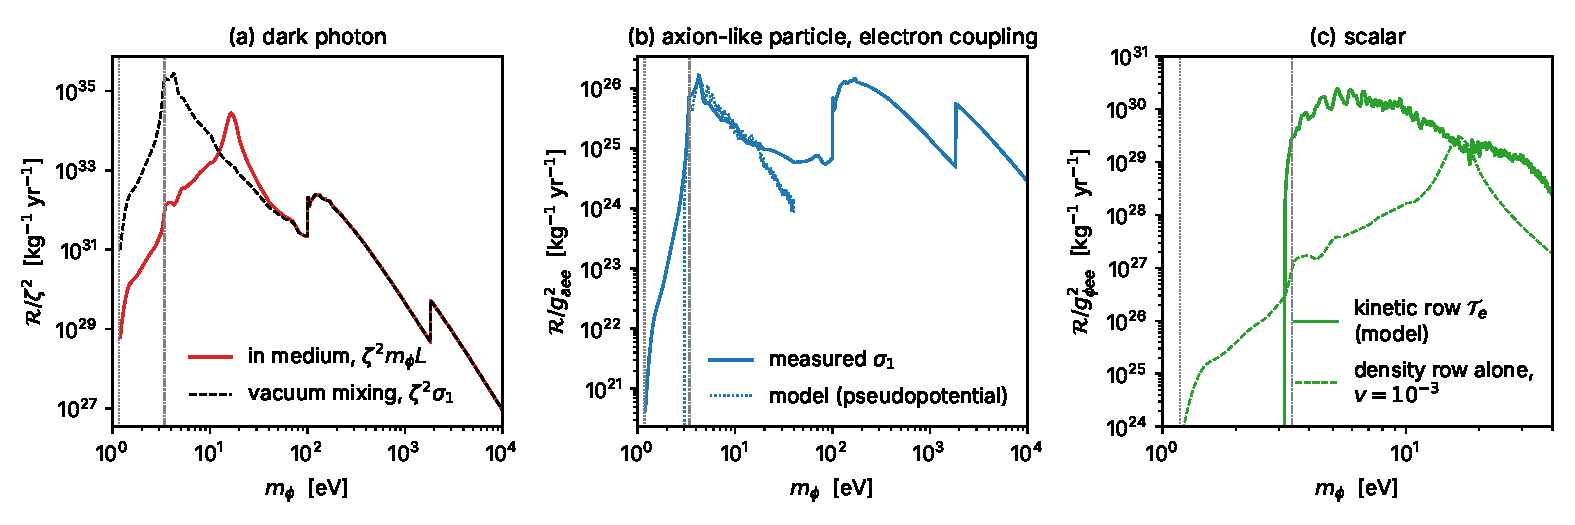
\includegraphics[width=\linewidth]{figures/ch10/fig10_6.pdf}
  \caption{Absorption rates of bosonic dark matter on the electrons of silicon, per kilogram-year and per unit squared coupling, against the boson mass $m_\phi$, with $\rho_\chi = \SI{0.3}{GeV.cm^{-3}}$ and $\rho_T = \SI{2.33}{g.cm^{-3}}$. Measured optical constants of float-zone silicon at \SI{300}{K}~\cite{franta2017temperature} below \SI{40}{eV}, and $\varepsilon$ from the atomic scattering factors of Ref.~\cite{henke1993xray} above, spliced at \SI{40}{eV}. The data are used without transfer to millikelvin temperatures and are wrong within a few tens of meV of the edge (\cref{sec:10.7-edge}). Dotted line: the excitonic edge of cold silicon, \SI{1.1728}{eV} with $\Eg(0) = \SI{1.1692}{eV}$; dash-dotted: the direct gap, \SI{3.4}{eV}. (a) Dark photon: in-medium rate $\zeta^2(\rho_\chi/\rho_T)L$, \cref{eq:10.7-dp} (red), and the vacuum-mixing rate $\zeta^2(\rho_\chi/\rho_T)\sigma_1/m_\phi$ (dashed). The same curve gives the axion-like particle in a field $\vect{B}_0$ with $\zeta \to g_{a\gamma\gamma}B_0/m_\phi$, \cref{eq:10.7-alpB}. (b) Axion-like particle with the electron coupling, \cref{eq:10.7-alp}, from the measured $\sigma_1$ (solid) and from the empirical-pseudopotential model of \cref{sec:4.6} (dotted; independent particles, no spin--orbit coupling, $16^3$ $\vect{k}$ points). (c) Scalar, \cref{eq:10.7-scalar}: kinetic-energy row in the same model, which has pseudo-wavefunctions without core oscillations and its own vertical gap of \SI{3.12}{eV} (solid; histogram of \SI{0.05}{eV} bins, smoothed over \SI{0.25}{eV}); and the screened density row alone at $|\vect{p}_\phi| = 10^{-3}m_\phi$ with the measured loss function (dashed). The model curves show the size and shape of the kinetic and spin responses, not predictions for silicon.}
  \label{fig:10-absorption}
\end{figure}

\begin{workedexample}{Dark-photon absorption at \SI{10}{eV}}\label{we:10-darkphoton}
At \SI{10}{eV} the measured dielectric function of silicon is $\varepsilon = -1.879 + 1.268\,\ii$: the frequency lies above the main interband peaks, where $\varepsilon_1$ has turned negative, and below the plasma frequency, where it turns positive again. Then $|\varepsilon|^2 = 5.139$, $L = \varepsilon_2/|\varepsilon|^2 = 0.2467$ and $\sigma_1 = \omega\varepsilon_2 = \SI{12.68}{eV}$. The in-medium mixing is $\zeta_{\mathrm{eff}}/\zeta = 1/|\varepsilon| = 0.441$, and the rate is suppressed by $1/|\varepsilon|^2 = 0.195$, a factor of 5.1. The photon self-energy is $\Pi_{\mathrm{em}} = m_\phi^2(1 - \varepsilon) = (288 - 127\,\ii)\,\mathrm{eV}^2$, larger than $m_\phi^2 = \SI{100}{eV^2}$.

With $\rho_\chi/m_\phi = \SI{3.0e7}{cm^{-3}}$, \cref{eq:10.7-dp} gives $\mathcal{R} = 1.52\times10^{33}\,\zeta^2$ per kilogram-year, against $7.82\times10^{33}\,\zeta^2$ with the vacuum mixing. Three events in a kilogram-year, the background-free reach, need $\zeta = 4.4\times10^{-17}$; the vacuum mixing would claim $2.0\times10^{-17}$, a reach better by $|\varepsilon| = 2.27$ than the true one. For a halo particle with $v = 10^{-3}$ the transverse and longitudinal rates differ by $v^2[2\Real(1/\varepsilon) - 1] = -1.7\times10^{-6}$, and each differs from \cref{eq:10.7-dp} at the level of $10^{-6}$.
\end{workedexample}

\subsection{Optical data near the silicon edge}\label{sec:10.7-edge}

Optical constants are measured at room temperature or at \SI{77}{K}, and a detector runs at \SI{10}{mK}. Above the direct gap of silicon, \SI{3.4}{eV}, the difference in temperature hardly matters: the transitions are vertical, the bands shift by tens of meV, and $\sigma_1$ changes little. Between the indirect gap and \SI{3.4}{eV} it matters a great deal. There every absorbed photon, and every absorbed dark-matter boson, needs a phonon to supply the crystal momentum $\vect{k}_{\mathrm{c}}$ of the conduction valley (\cref{sec:6.5}). The measured $\sigma_1$ in that window is the phonon-assisted $\omega\varepsilon_2^{\mathrm{PA}}$, second order in the electron--phonon vertex and first order in the phonon occupations, and it depends on temperature at the edge in two ways. At \SI{300}{K} the gap is \SI{1.12}{eV} instead of \SI{1.17}{eV}, and the transverse-acoustic phonon at $\vect{k}_{\mathrm{c}}$ has the occupation 0.97, so that a photon can be absorbed together with a phonon taken from the lattice, from $\Eg - \omega_{\mathrm{TA}}$ up. At \SI{10}{mK} no phonons are present to be absorbed, and the edge of cold silicon lies at $\Eg(0) + \omega_{\mathrm{TA}} - E_x^b = \SI{1.1728}{eV}$ with $\Eg(0) = \SI{1.1692}{eV}$, the excitonic threshold of phonon emission (\cref{sec:6.5}).

The consequence for a rate is direct. The \SI{300}{K} data give $\sigma_1 = 4.9\times10^{-4}$\,eV at \SI{1.15}{eV}, where a cold crystal absorbs nothing, and \cref{fig:10-absorption} inherits the warm edge. The \SI{77}{K} data are closer, but the occupation of the transverse-acoustic phonon is still 0.068 there, and the gap is \SI{1.165}{eV} against \SI{1.169}{eV} at millikelvin temperatures, from the measured temperature dependence of the gap~\cite{alex1996temperature} (\cref{sec:6.3}). Measured $\sigma_1$ near the edge must therefore be transferred to the temperature of the detector before it enters \cref{eq:10.7-dp} or the axion-like rate below. The transfer runs the phonon-assisted formula backward: each branch is separated into its absorption and emission parts, the absorption parts are removed, the emission parts are reweighted from $n_{\vect{Q}\nu} + 1$ to one, and the gap is shifted. Without data resolved by branch the separation is not unique. \Cref{sec:13.5} carries out the transfer and finds that the untransferred \SI{77}{K} data overestimate the millikelvin dark-photon rate of silicon by more than a factor of two within about \SI{20}{meV} of the edge.

\subsection{Axion-like-particle absorption}\label{sec:10.7-alp}

The axion-like particle couples to the electrons through \cref{eq:8.1-alp}, $(g_{aee}/m_e)[(\nabla\phi)\cdot\vect{s}_e + (\partial_t\phi)\mathcal{J}^{\alpha\alpha}_e]$ with the spin current traced over its two indices. For a particle of the halo the spin-density term is negligible. The coefficient of the spin-density term carries $|\vect{p}_\phi|$ instead of $m_\phi$. Without spin--orbit coupling the total spin also commutes with the Hamiltonian, so $\vect{s}_e(\vect{p}_\phi)$ connects different states only at first order in $\vect{p}_\phi$. The spin-density amplitude is then of order $p_\phi^2$, against $m_\phi$ times an electron velocity for the spin current. Only the row $\mathcal{J}_e \equiv \mathcal{J}^{\alpha\alpha}_e(0)$ is left, with $g^\phi_{\mathcal{J}} = g_{aee}m_\phi/m_e$ per unit amplitude, and \cref{eq:8.2-abs} gives $\varGamma = (g_{aee}^2m_\phi/2m_e^2)\,S_{\mathcal{J}\mathcal{J}}(0, m_\phi)$.

The spin current is related to the ordinary current by a spin trace. An electron--hole pair $(c\sigma', v\sigma)$ is created by $\mathcal{J}_e$ with the amplitude $\sum_\alpha v^\alpha_{cv}(S^\alpha)_{\sigma'\sigma}$, with $\vect{v}_{cv} = \langle c|\vect{p}/m_e|v\rangle$, and by the current along a unit vector $\hat{\vect{e}}$ with $\hat{\vect{e}}\cdot\vect{v}_{cv}\,\delta_{\sigma'\sigma}$. Summed over the spins, the spin-current amplitude gives $\sum_{\alpha\beta}v^\alpha_{cv}v^{\beta*}_{cv}\Tr(S^\alpha S^\beta) = |\vect{v}_{cv}|^2/2$, and the current amplitude gives $2|\hat{\vect{e}}\cdot\vect{v}_{cv}|^2$, which in a cubic crystal averages to $2|\vect{v}_{cv}|^2/3$. For independent electrons without spin--orbit coupling, therefore, $S_{\mathcal{J}\mathcal{J}} = \frac34 S_{jj}$, three Cartesian directions times the quarter that \cref{sec:10.5-triplet} found for every spin row. The transverse current response is the conductivity, $S_{jj}(0,\omega) = 2\omega\sigma_1/e^2$ (\cref{sec:4.4,sec:8.2-absorption}), and
\begin{keyresult}[Absorption of an axion-like particle through its electron coupling]
\begin{equation}
  \varGamma = \frac{3\,m_\phi^2}{4\,m_e^2}\,\frac{g_{aee}^2}{e^2}\,\sigma_1(m_\phi) , \qquad
  \mathcal{R} = \frac{\rho_\chi}{\rho_T\,m_\phi}\,\frac{3\,m_\phi^2\,g_{aee}^2}{4\,m_e^2\,e^2}\,\sigma_1(m_\phi) ,
  \label{eq:10.7-alp}
\end{equation}
for independent electrons without spin--orbit coupling~\cites[Eq.~(10)]{hochberg2017absorption}[Eq.~(47)]{mitridate2021dark}. There is no in-medium factor: the rate contains $\sigma_1$ in place of the loss function.
\end{keyresult}
\noindent The spin trace also explains the absence of mixing. A photon-reducible chain needs a proper correlation of $\mathcal{J}_e$ with the charge density, and a single spin operator traced over an unpolarized pair vanishes, $\Tr S^\alpha = 0$, so that $\tilde R_{\mathcal{J}Z} = 0$ (\cref{sec:8.4-mixing}). The parity of the particle says the same: a pseudoscalar cannot mix with the photon of a medium that has neither handedness nor magnetization~\cite[Sect.~III\,B, footnote~5]{mitridate2021dark}. Compared to the dark photon, then, the axion-like particle is not suppressed where the target absorbs light and not enhanced at the plasmon. At equal couplings the ratio of the axion-like rate to the dark-photon rate is $(3m_\phi^2/4m_e^2e^2)|\varepsilon|^2$, which at \SI{10}{eV} is $1.6\times10^{-8}$: the factor $m_\phi^2/m_e^2$ comes from a coupling to spin that a slow electron transmits only through its velocity. \Cref{fig:10-absorption}b shows the rate from the measured $\sigma_1$. The empirical-pseudopotential model of \cref{sec:4.6} gives 0.8 to 1.15 times the measured value between 4 and \SI{18}{eV}, and half of it at \SI{20}{eV}, far above the transitions to which its three form factors were fitted.

\Cref{eq:10.7-alp} uses the measured $\sigma_1$ for a response that differs from the one measured. The current creates electron--hole pairs in the spin singlet, and the spin current in the triplet. With the interaction switched on, the singlet pairs feel both kernels of the Bethe--Salpeter equation and the triplet pairs only the direct one, \cref{eq:10.5-triplet}. The excitonic attraction is common to the singlet and triplet pairs, and the measured edge carries it correctly. The local fields, however, which are the rest of the exchange kernel, act on the singlet pairs alone. In the model of \cref{sec:4.6} they lower the main $\varepsilon_2$ peak of silicon from 41 to 34 and move it up by \SI{60}{meV}. The measured $\sigma_1$ therefore understates the axion-like response near its peak by about a fifth, and by less where the local fields are weak. Spin--orbit coupling is the second caveat. It ties the spin to the orbital motion, the spin trace no longer factorizes, and the factor $\frac34$ acquires corrections set by the spin--orbit splitting over the transition energy, $\Delta_{\mathrm{SO}} = \SI{0.044}{eV}$ in silicon against several eV (\cref{sec:3.3}). In germanium, GaAs and heavier targets the current and spin-current responses must be computed separately.

The photon coupling, $g_{a\gamma\gamma}\phi\,\vect{E}\cdot\vect{B}$ of \cref{sec:1.4}, needs a field to act on. In a static laboratory field $\vect{B}_0$ it reads $g_{a\gamma\gamma}\phi\,\vect{E}\cdot\vect{B}_0 = -g_{a\gamma\gamma}\phi\,(\partial_t\vect{A})\cdot\vect{B}_0$ in the gauge without scalar potential, and after an integration by parts in time it is $\vect{J}_a\cdot\vect{A}$, with a source current along the field,
\begin{equation*}
  \vect{J}_a = g_{a\gamma\gamma}\,(\partial_t\phi)\,\vect{B}_0 ,
\end{equation*}
which oscillates at $m_\phi$ with the wavevector $\vect{p}_\phi$. The medium answers as it answers any current. For a sample much larger than the skin depth $(m_\phi\Imag\sqrt{\varepsilon})^{-1}$ its boundaries do not matter~\cite[footnote~1]{berlin2024absorption}, and at $\vect{p}_\phi \to 0$ the curl of the magnetic field drops out of the Amp\`ere--Maxwell law $\nabla\times\vect{B} = \vect{J} + \partial_t\vect{E}$ of \cref{sec:4.4}, with a relative error of order $p_\phi^2/\omega^2$. The induced current is $\vect{J}_{\mathrm{ind}} = \sigma_{\mathrm{cond}}\cdot\vect{E}$, with the conductivity tensor, so that $0 = \vect{J}_a + \sigma_{\mathrm{cond}}\cdot\vect{E} - \ii\omega\vect{E} = \vect{J}_a - \ii\omega\,\varepsilon\cdot\vect{E}$, by \cref{eq:4.4-sigma}. With the amplitude $\phi_0$ of $\phi = \Real(\phi_0\ee^{-\ii m_\phi t})$, $\vect{J}_a$ has the amplitude $-\ii m_\phi g_{a\gamma\gamma}\phi_0\vect{B}_0$, and the field is
\begin{equation*}
  \vect{E} = \frac{1}{\ii\omega}\,\varepsilon^{-1}\cdot\vect{J}_a = -g_{a\gamma\gamma}\,\phi_0\,\varepsilon^{-1}(m_\phi)\cdot\vect{B}_0 .
\end{equation*}
The power that this field dissipates per unit volume, averaged over a period, is $\frac12\Real(\vect{J}^*_{\mathrm{ind}}\cdot\vect{E}) = \frac{\omega}{2}\vect{E}^\dagger\cdot\varepsilon''\cdot\vect{E}$, with $\varepsilon'' = (\varepsilon - \varepsilon^\dagger)/2\ii$ the absorptive part of the tensor. Since $(\varepsilon^{-1})^\dagger(\varepsilon - \varepsilon^\dagger)\varepsilon^{-1} = (\varepsilon^{-1})^\dagger - \varepsilon^{-1}$, the power is $\frac{\omega}{2}g_{a\gamma\gamma}^2|\phi_0|^2\,\vect{B}_0\cdot\Imag[-\varepsilon^{-1}]\cdot\vect{B}_0$, where $\Imag[-\varepsilon^{-1}]$ denotes the absorptive part of $-\varepsilon^{-1}$. The number density of the field is its energy density $\frac12m_\phi^2|\phi_0|^2$ over $m_\phi$. Division of the power by the number density and by the energy $\omega$ of one quantum gives
\begin{keyresult}[Absorption of an axion-like particle in a static field]
\begin{equation}
  \varGamma = \frac{g_{a\gamma\gamma}^2B_0^2}{m_\phi}\;\hat{\vect{B}}_0\cdot\Imag\bigl[-\varepsilon^{-1}(m_\phi)\bigr]\cdot\hat{\vect{B}}_0 , \qquad
  \mathcal{R} = \frac{\rho_\chi}{\rho_T}\,\frac{g_{a\gamma\gamma}^2B_0^2}{m_\phi^2}\;\hat{\vect{B}}_0\cdot\Imag\bigl[-\varepsilon^{-1}\bigr]\cdot\hat{\vect{B}}_0 ,
  \label{eq:10.7-alpB}
\end{equation}
the inverse dielectric tensor projected on the direction of the field~\cite[Eqs.~(6) and (7)]{berlin2024absorption}. In a cubic crystal the projection is the loss function $L(m_\phi)$, and the rate equals the dark-photon rate with $\zeta = g_{a\gamma\gamma}B_0/m_\phi$.
\end{keyresult}
\noindent \Cref{fig:10-absorption}a gives the rate of the axion-like particle in a field for silicon with that substitution. A field of \SI{10}{T} is $B_0 = \SI{1953}{eV^2}$ in the units of \cref{app:A.2}, and with $g_{a\gamma\gamma} = \SI{e-10}{GeV^{-1}}$ the equivalent mixing at \SI{10}{eV} is $2.0\times10^{-17}$, or 0.58 events per kilogram-year in silicon. The field also acts on the target, through the Zeeman and orbital energies, but $\mu_{\mathrm{B}}B_0 = \SI{0.58}{meV}$ at \SI{10}{T} is negligible against electronic energies, and the derivation never used the symmetry of $\varepsilon$, only its absorptive part. The two couplings of the axion-like particle add without interference: the cross term needs a correlation of the spin current with the charge current, and this correlation vanishes without spin--orbit coupling for the same reason as $\tilde R_{\mathcal{J}Z}$.

In a crystal of lower symmetry the projection of the inverse is not the inverse of the projection. For a uniaxial crystal with the field at an angle $\theta$ to the optic axis, $\hat{\vect{B}}_0\cdot\varepsilon^{-1}\cdot\hat{\vect{B}}_0 = \cos^2\theta/\varepsilon_\parallel + \sin^2\theta/\varepsilon_\perp$, while the dielectric function along the field is $\varepsilon_{BB} = \cos^2\theta\,\varepsilon_\parallel + \sin^2\theta\,\varepsilon_\perp$, and
\begin{equation}
  \hat{\vect{B}}_0\cdot\varepsilon^{-1}\cdot\hat{\vect{B}}_0 - \frac{1}{\varepsilon_{BB}} = \frac{\cos^2\theta\,\sin^2\theta\,(\varepsilon_\parallel - \varepsilon_\perp)^2}{\varepsilon_\parallel\,\varepsilon_\perp\,\varepsilon_{BB}} .
  \label{eq:10.7-aniso}
\end{equation}
The difference is second order in the anisotropy and vanishes on the principal axes. Near a longitudinal resonance of one axis it is not small, because $1/\varepsilon_\parallel$ or $1/\varepsilon_\perp$ is large there while $\varepsilon_{BB}$ is not near zero. The isotropic formula with the dielectric function along the field then misses the resonance, and \cref{eq:10.7-alpB} keeps it.

\begin{limitbox}[Absorption with in-medium mixing][lim:10.7a]
Dark photon: $\mathcal{R} = (\rho_\chi/\rho_T m_\phi)\,\zeta_{\mathrm{eff}}^2\sigma_1(m_\phi)$, $\zeta_{\mathrm{eff}}^2 = \zeta^2m_\phi^4/|m_\phi^2 - \Pi_{\mathrm{em}}|^2$~\cite[Eqs.~(6) and (7)]{hochberg2017absorption}, which for $m_\phi^2 \gg |\Pi_{\mathrm{em}}|$ reduces to the vacuum mixing, $\varGamma = \zeta^2\sigma_1$~\cite[Eq.~(20)]{an2015direct}. Axion-like particle in a field: $\varGamma = (g_{a\gamma\gamma}B_0)^2\Imag[-1/\varepsilon(m_\phi)]/m_\phi$ for an isotropic target~\cite[Eq.~(7)]{berlin2024absorption}.
\par\smallskip
{\centering
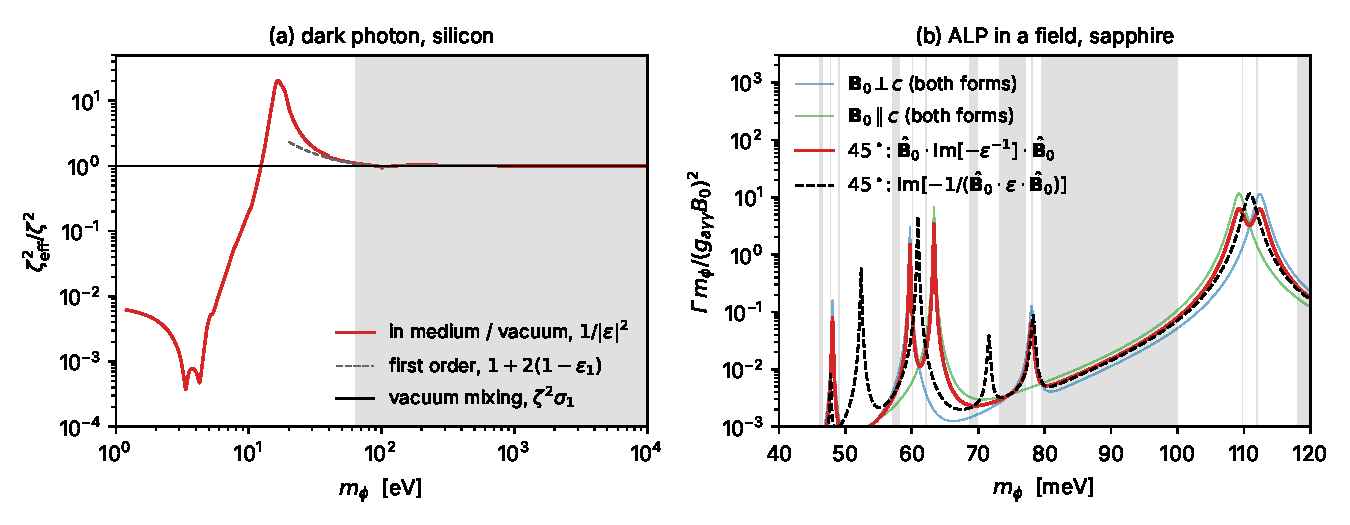
\includegraphics[width=\linewidth]{figures/ch10/limit10_7a.pdf}
\captionof{figure}{(a) Dark photon in silicon: the in-medium rate over the vacuum-mixing rate, $\zeta_{\mathrm{eff}}^2/\zeta^2 = 1/|\varepsilon(m_\phi)|^2$ (red), against the vacuum-mixing limit (black). Measured $\varepsilon$ at \SI{300}{K} below \SI{40}{eV}~\cite{franta2017temperature} and from atomic scattering factors above~\cite{henke1993xray}. Gray: masses where $1/|\varepsilon|^2$ is within \SI{10}{\percent} of one, all masses above \SI{63}{eV}. A halo momentum $|\vect{p}_\phi| = 10^{-3}m_\phi$ changes the transverse and longitudinal rates by $10^{-6}$, invisible here. (b) Axion-like particle in a field at \SI{45}{\degree} to the optic axis of sapphire: the rate of \cref{eq:10.7-alpB}, $\hat{\vect{B}}_0\cdot\Imag[-\varepsilon^{-1}]\cdot\hat{\vect{B}}_0$ (red), against the isotropic formula evaluated with the dielectric function along the field, $\Imag[-1/\varepsilon_{BB}]$ (dashed), and the two principal axes, where both forms agree (thin). Phonon dielectric functions of sapphire in the damped factorized form $\varepsilon = \varepsilon_\infty\prod_\nu(\omega_{\mathrm{L}\nu}^2 - \omega^2 - \ii\omega\gamma_{\mathrm{L}\nu})/(\omega_{\mathrm{T}\nu}^2 - \omega^2 - \ii\omega\gamma_{\mathrm{T}\nu})$ with $\varepsilon_\infty = 3.2$ and the frequencies and \SI{77}{K} widths of Ref.~\cite[Eq.~(37), Tables~I and II]{griffin2018directional} (ordinary ray, longitudinal 112.4, 78.0, 59.7 and \SI{48.1}{meV} with widths 1.98, 0.55, 0.17 and \SI{0.17}{meV}, transverse 78.6, 70.5, 54.4 and \SI{47.7}{meV} with widths 0.47, 0.40, 0.19 and \SI{0.17}{meV}; extraordinary ray, longitudinal 109.2 and \SI{63.3}{meV} with widths 1.98 and \SI{0.17}{meV}, transverse 72.2 and \SI{49.3}{meV} with widths 0.40 and \SI{0.19}{meV}), with the widths of the extraordinary ray borrowed from the ordinary modes. Gray: masses where the two forms agree within \SI{10}{\percent}. Silicon is cubic, and in silicon the two forms coincide.}\label{fig:10-abs-limit}
\par}
\smallskip
Below \SI{63}{eV} the medium changes the dark-photon rate of silicon by factors from $4\times10^{-4}$ to 20, and in an anisotropic crystal with the field off its principal axes the isotropic formula misses the longitudinal resonances of each axis by up to a factor of several hundred.
\end{limitbox}

\subsection{Scalar absorption and the kinetic-energy row}\label{sec:10.7-scalar}

A scalar coupled to $\bar\psi\psi$ acts on the target through \cref{eq:8.1-scalar}, $-g_{\phi ee}\phi\,[n_e(\vect{p}_\phi) - \mathcal{T}_e(\vect{p}_\phi)/m_e]$: on the number of electrons and, at next order in $1/m_e$, on their kinetic energy. For scattering the density row dominates. For absorption at $|\vect{p}_\phi| \approx 10^{-3}m_\phi$ the order is reversed: the density row connects different states only at first order in $\vect{p}_\phi$ and is suppressed by $v^2$ in the rate, while the kinetic row is not (\cref{sec:8.1-absorption}).

\Cref{sec:8.4-mixing} found that the scalar mixes with the photon through the proper correlations $\tilde R_{n_eZ}$ and $\tilde R_{\mathcal{T}_eZ}$ of its two rows with the charge. The correlation $\tilde R_{n_eZ}$ is the density response, of order $p_\phi^2$. For $\tilde R_{\mathcal{T}_eZ}$, expand in $\vect{p}_\phi$: $\tilde R_{\mathcal{T}_en_e}(\vect{p}_\phi,\omega) = \vect{p}_\phi\cdot\vect{F}(\omega) + O(p_\phi^2)$, where $\vect{F}$ is a vector built from the crystal alone. It must be invariant under every operation of the point group, and an invariant vector exists only in a polar group, one that leaves some direction fixed under every operation. Crystals with a polar group are pyroelectric: they carry a spontaneous electric polarization along that direction. Silicon ($O_h$), GaAs ($T_d$) and sapphire ($D_{3d}$) have no invariant vector, and in them $\tilde R_{\mathcal{T}_en_e} = O(p_\phi^2)$. The photon-reducible part, $\tilde R_{\mathcal{T}_eZ}\,v_{\mathrm{C}}(p_\phi)\,\varepsilon^{-1}\,\tilde R_{Z\mathcal{T}_e}$, is then of order $p_\phi^4\cdot e^2/p_\phi^2 = e^2p_\phi^2$ and vanishes with the density row. In a polar crystal, such as wurtzite GaN or ZnO, $\vect{F} \ne 0$ and the mixing survives at $\vect{p}_\phi \to 0$ as a term $(e^2/\omega^2)\,\hat{\vect{p}}_\phi\cdot\tilde R_{\mathcal{T}_e\vect{j}}\,\varepsilon^{-1}\,\tilde R_{\vect{j}\mathcal{T}_e}\cdot\hat{\vect{p}}_\phi$, with $n_e = \vect{p}_\phi\cdot\vect{j}_e/\omega$ on the energy shell (\cref{eq:4.3-continuity}). With only the kinetic row kept, and with $g^\phi_{\mathcal{T}_e} = g_{\phi ee}/m_e$ in \cref{eq:8.2-abs},
\begin{keyresult}[Scalar absorption]
\begin{equation}
  \varGamma = -\frac{g_{\phi ee}^2}{m_\phi\,m_e^2}\,\Imag R_{\mathcal{T}\mathcal{T}}(0, m_\phi) = \frac{g_{\phi ee}^2}{2\,m_\phi\,m_e^2}\,S_{\mathcal{T}\mathcal{T}}(0, m_\phi) ,
  \label{eq:10.7-scalar}
\end{equation}
with $R_{\mathcal{T}\mathcal{T}}$ the response of the kinetic-energy row $\mathcal{T}_e(0) = \sum_jp_j^2/2m_e$ at $T = 0$, for every crystal whose point group has no polar vector, up to corrections of order $v^2$ from the other rows~\cite[Eqs.~(55) and (56)]{mitridate2021dark}. The response is unscreened, and no optical measurement gives it.
\end{keyresult}
\noindent In the notation of Mitridate and collaborators the row is $\bar v^2 = \mathcal{T}_e/m_e$ and the coupling $d_{\phi ee}$, with $g_{\phi ee} = d_{\phi ee}\sqrt{4\pi}\,m_e/M_{\mathrm{Pl}}$ (\cref{sec:1.4}). For independent electrons the response is a joint density of states weighted by the kinetic matrix elements,
\begin{equation}
  S^0_{\mathcal{T}\mathcal{T}}(0,\omega) = \frac{4\pi}{\Vol}\sum_{cv\vect{k}}\bigl|\langle c\vect{k}|\mathcal{T}_e|v\vect{k}\rangle\bigr|^2\,\delta(\omega - \varepsilon_{c\vect{k}} + \varepsilon_{v\vect{k}}) ,
  \label{eq:10.7-S0}
\end{equation}
spin summed, with the one-electron element $\langle c|p^2/2m_e|v\rangle = \sum_m\vect{p}_{cm}\cdot\vect{p}_{mv}/2m_e$, a sum over all bands, the core included. Since $c$ and $v$ are eigenstates of $p^2/2m_e + V$ with different energies, the element is also $-\langle c|V|v\rangle$: the kinetic row measures the matrix elements of the crystal potential itself. Those are largest where the potential is deep, near the nuclei, and there a pseudo-wavefunction is smooth where the true state oscillates. The rate is therefore sensitive to the core region in a way that the conductivity is not, and a calculation needs the all-electron states or their reconstruction from a projector-augmented-wave basis.

The kinetic row also follows a different selection rule. It is even under inversion, while the momentum is odd. At $\mathrm{\Gamma}$ the top valence states of silicon and the lowest conduction states have opposite parity, and the opposite parity makes the direct transition at \SI{3.4}{eV} allowed for light. For the scalar the direct transition is forbidden: in the model of \cref{sec:4.6} the kinetic matrix element between them vanishes at $\mathrm{\Gamma}$ to machine precision, while the momentum element does not, and the scalar spectrum rises from the vertical gap more slowly than $\varepsilon_2$. Below the direct gap the scalar, like the dark photon, is absorbed only with a phonon, and its rate there needs the phonon-assisted kinetic row.

The kinetic row has a sum rule of its own. The first-moment identity \cref{eq:4.3-firstmoment} at $\vect{q} = 0$ gives $\int_0^\infty\dd\omega\,\omega\,S_{\mathcal{T}\mathcal{T}} = (\pi/\Vol)\langle[[\mathcal{T}_e, H], \mathcal{T}_e]\rangle$ at $T = 0$. Take electrons that move independently in a local one-body potential, $H = \sum_j[p_j^2/2m_e + V(\vect{r}_j)]$. With $\mathcal{T}_e = H - \sum_jV(\vect{r}_j)$ written in the outer commutator, the part with $H$ has zero expectation value in an eigenstate, and what remains is $-\langle[[\mathcal{T}_e, V], V]\rangle$. For one electron $[p^2, V] = -\ii(\vect{p}\cdot\nabla V + \nabla V\cdot\vect{p})$, and a second commutator with $V$ leaves $[[p^2, V], V] = -2|\nabla V|^2$. Per electron, then, $\frac12\langle[[\mathcal{T}_e, H], \mathcal{T}_e]\rangle = \langle|\nabla V|^2\rangle/2m_e$, and
\begin{equation}
  \int_0^\infty\dd\omega\;\omega\,S_{\mathcal{T}\mathcal{T}}(0,\omega) = \frac{\pi\,\nd_e}{m_e}\,\bigl\langle|\nabla V|^2\bigr\rangle ,
  \label{eq:10.7-sumrule}
\end{equation}
with the average taken per electron. Compared to the $f$-sum rule \cref{eq:4.3-fsum}, which has $\pi\nd_eq^2/m_e$, the squared momentum kick $q^2$ is replaced by the mean squared force on an electron. For the absorption rate the sum rule fixes $\int\dd m_\phi\,m_\phi^2\varGamma = \pi g_{\phi ee}^2\nd_e\langle|\nabla V|^2\rangle/2m_e^3$.

The conditions are restrictive: a potential that is local and one-body, and a mean squared force that is finite. A nonlocal pseudopotential keeps the identity in the form $-\langle[[\mathcal{T}_e,V_{\mathrm{NL}}],V_{\mathrm{NL}}]\rangle$, but the double commutator is then no longer $\langle|\nabla V|^2\rangle$, just as nonlocality changes the $f$-sum rule (\cref{eq:4.3-fsumNL}). The Coulomb repulsion between the electrons turns $\langle|\nabla V|^2\rangle$ into the mean squared total force on an electron, a two-body and three-body average. The decisive failure is the Coulomb potential of a nucleus, which makes the force diverge: $|\nabla V|^2 = Z^2\alpha^2/r^4$, and an $s$ state, with a finite density at the nucleus, gives $\int r^2\dd r/r^4 = \infty$. The valence states of silicon have s character inside the core, where they oscillate to stay orthogonal to the $1s$ and $2s$ states, so for the real crystal the right-hand side of \cref{eq:10.7-sumrule} is infinite. The spectrum of the kinetic row has a tail that decays too slowly for its first moment to converge, and \cref{eq:10.7-sumrule} cannot normalize it as the $f$-sum rule normalizes the density response. The sum rule does provide a check of a calculation within its own model, for a local and regular potential such as an empirical pseudopotential, or the valence block of a calculation whose potential is regular.

\begin{limitbox}[Scalar absorption through the kinetic-energy row][lim:10.7b]
$\varGamma = -(g_{\phi ee}^2/m_\phi m_e^2)\Imag R_{\mathcal{T}\mathcal{T}}(0, m_\phi)$, from the kinetic-energy term of the nonrelativistic scalar coupling~\cite[Eqs.~(18) and (56)]{mitridate2021dark}; its energy-weighted integral is \cref{eq:10.7-sumrule} for a local, regular one-body potential.
\par\smallskip
{\centering
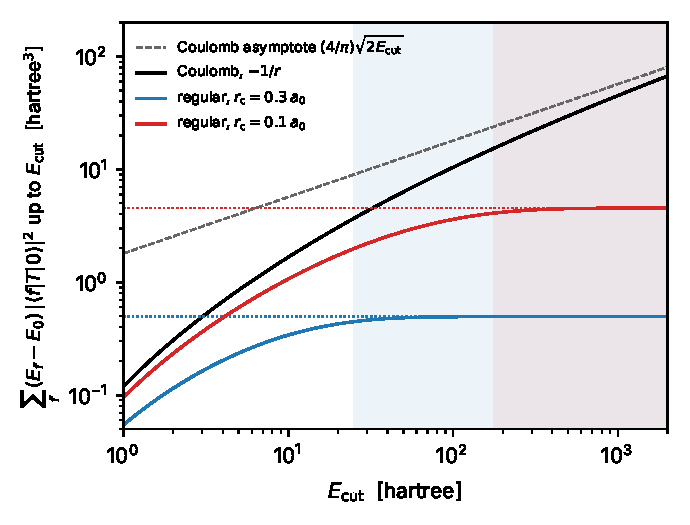
\includegraphics[width=0.66\linewidth]{figures/ch10/limit10_7b.pdf}
\captionof{figure}{Energy-weighted spectrum of the kinetic row, $\sum_f(E_f - E_0)|\langle f|p^2/2m_e|0\rangle|^2$ over final states up to an excitation energy $E_{\mathrm{cut}}$, for one electron in its ground state (atomic units), against $E_{\mathrm{cut}}$. Black: Coulomb potential $-1/r$, hydrogen; dashed, its asymptote $(4/\pi)\sqrt{2E_{\mathrm{cut}}}$, from the plane-wave limit of the continuum states. Blue and red: the regular potentials $-1/(r^2 + r_{\mathrm{c}}^2)^{1/2}$ with $r_{\mathrm{c}} = 0.3$ and $0.1\,a_0$; dotted, their sum rules $\langle|\nabla V|^2\rangle/2$, \cref{eq:10.7-sumrule}. Shaded: $E_{\mathrm{cut}}$ above which each regular spectrum holds \SI{90}{\percent} of its sum rule, 25 and \SI{176}{hartree}. Only s states contribute, since the kinetic energy conserves angular momentum. Radial equation on a uniform grid of \SI{0.004}{a_0} in a box of \SI{30}{a_0}; on the full grid the spectral sum and the double commutator agree to six digits.}\label{fig:10-scalar-limit}
\par}
\smallskip
For the Coulomb potential of a nucleus the energy-weighted spectrum grows as $E_{\mathrm{cut}}^{1/2}$ without limit, so the sum rule exists only for regular potentials, and its value grows as the core radius shrinks.
\end{limitbox}

The empirical-pseudopotential model of \cref{sec:4.6} is local and regular, and it satisfies \cref{eq:10.7-sumrule} exactly within its basis of 113 plane waves. On a grid of $16^3$ $\vect{k}$ points the spectral first moment and the double commutator agree to six digits, at $\langle|\nabla V|^2\rangle/2m_e = 1.30\times10^3\,\mathrm{eV}^3$ per valence electron. Only \SI{2}{\percent} of the first moment lies below \SI{10}{eV} and \SI{41}{\percent} below \SI{40}{eV}. Even in a model with a regular potential, then, the sum rule is carried by transitions far above the masses that matter, and it constrains the low-energy spectrum only weakly. \Cref{fig:10-absorption}c shows the model's scalar rate in silicon: $9.8\times10^{29}\,g_{\phi ee}^2$ per kilogram-year at \SI{10}{eV}, four orders of magnitude above the axion-like rate at equal coupling. The comparison with the electron's momentum makes the ratio of the scalar to the axion-like rate plausible. The kinetic matrix elements are a few eV, so $\mathcal{T}_e/m_e \sim 10^{-5}$, while the axion-like amplitude carries $m_\phi/m_e$ times an electron velocity, $\sim 10^{-7}$. The absolute value of the model curve is not a prediction, for the reason given above, and an all-electron response fixes it.

The dashed curve of \cref{fig:10-absorption}c is the density row alone, screened with the measured loss function, $(g_{\phi ee}^2/2m_\phi)(2p_\phi^2/e^2)L$ at $|\vect{p}_\phi| = 10^{-3}m_\phi$. It is one of the terms of order $v^2$ in \cref{eq:10.7-scalar}. At \SI{5}{eV} it is $3\times10^{-3}$ of the model's kinetic rate and at \SI{10}{eV} $2\times10^{-2}$. Near the plasma frequency, however, the density row is enhanced by the same factor $1/|\varepsilon|^2$ that enhances the dark photon, and between 16 and \SI{18}{eV} it is as large as the model's kinetic rate. The all-electron calculation of Mitridate and collaborators finds the kinetic term dominant in silicon and germanium~\cite[Fig.~1 and Sect.~IV]{mitridate2021dark}; its kinetic matrix elements include the core oscillations that our model lacks. The other terms of order $v^2$, the cross term between the rows and the mixing through $\tilde R_{\mathcal{T}_eZ}$, are of the same size as the density row and have not been computed. Within a few eV of the plasma frequency the margin by which \cref{eq:10.7-scalar} holds is therefore open, and it is fixed by the same all-electron calculation, extended to order $p_\phi^2$.

\section{Two-insertion processes}\label{sec:10.8}

A dark photon of \SI{100}{keV} that meets an electron in silicon is more likely to scatter off it than to be absorbed. It leaves as an ordinary photon of \SI{91.8}{keV}, and the electron recoils with the remaining \SI{8.2}{keV}. This is dark Compton scattering, and above about \SI{55}{keV} it is the main way a silicon detector registers a dark photon. Its amplitude carries two insertions of a field: one of the dark photon and one of the photon. A complex scalar that couples quadratically to the electrons, through $\phi^\dagger\phi$, is a second example. It cannot be absorbed singly, since the coupling destroys a particle only together with an antiparticle, and the target absorbs the pair, the energy $2m_\phi$ and the momentum of both. Each process asks the crystal for more than the single row of \cref{sec:10.7}.

\subsection{Second-order transition operator}\label{sec:10.8-rate}

To second order in the interaction $H' = H_{\mathrm{int}}$, the Lippmann--Schwinger series \cref{eq:2.4-LS} gives $T_{fi} = H'_{fi} + \sum_mH'_{fm}H'_{mi}/(E_i - E_m + \ii0^+)$, and the rate is $2\pi|T_{fi}|^2\delta(E_f - E_i)$ (\cref{eq:2.4-golden2}). A field can enter $T_{fi}$ twice in two ways. In the first, one term of $H_{\mathrm{int}}$ is already quadratic in the field and linear in a target operator, so that both insertions sit at one vertex. The first-order term of $T$ then removes two quanta at once, and the target answers with one of its rows $O_a$ at the total momentum and energy of the pair. The rate needs only the response matrix $S_{ab}$ of \cref{eq:8.2-rate}. In the second way, each insertion comes with its own target operator, and the second-order term of $T$ joins them through the target propagator. With insertions $a$ and $b$ that bring $(\vect{k}_1, \omega_1)$ and $(\vect{k}_2, \omega_2)$, the target sees the effective operator
\begin{equation}
  T^{(2)}_{ab} = O_b(\vect{k}_2)\,\frac{1}{E_i + \omega_1 - H_0 + \ii0^+}\,O_a(\vect{k}_1) + O_a(\vect{k}_1)\,\frac{1}{E_i + \omega_2 - H_0 + \ii0^+}\,O_b(\vect{k}_2) ,
  \label{eq:10.8-T2}
\end{equation}
the two time orderings of \cref{eq:2.4-orderings}, and the rate is the response of $T^{(2)}_{ab}$, a four-point function of the target operators, at $(\vect{k}_1 + \vect{k}_2, \omega_1 + \omega_2)$. When neither denominator can vanish, because $\omega_1$ and $\omega_2$ lie below every excitation that $O_a$ and $O_b$ reach, $T^{(2)}_{ab}$ is to leading order a static polarizability of the target, and the four-point function collapses to a two-point function. A vector field coupled to the electron current brings a contact term of its own, the seagull $e^2\vect{A}^2/2m_e$ of the electron Hamiltonian. When the frequencies lie far above the binding energies of the electrons, the second-order terms are small against it, and the seagull alone gives the Thomson limit. Dark Compton scattering is this case (\cref{sec:10.8-compton}). A coupling that has both a contact term and two linear ones gives amplitudes of both kinds, and their interference needs a three-point response of the target, linear in a quadratic response function (\cref{sec:10.8-open}).

\subsection{Pair absorption}\label{sec:10.8-pair}

Take a complex scalar $\phi$ of mass $m_\phi$, whose particles and antiparticles are equally abundant, each with the number density $\rho_\chi/2m_\phi$. Bauer, Perez-Soler and Shergold write its lowest couplings to electrons, in Hamiltonian form, as~\cite[Eq.~(3)]{bauer2026dark}
\begin{equation}
  H_{\mathrm{int}} = \int\dd^3x\,\Bigl[m_e\,\phi^\dagger\phi\;\bar\psi\bigl(G_{\mathrm{S}} + \ii G_{\mathrm{P}}\gamma^5\bigr)\psi
  + \ii\bigl(\phi^\dagger\overleftrightarrow{\partial}_{\!\mu}\phi\bigr)\,\bar\psi\gamma^\mu\bigl(G_{\mathrm{V}} + G_{\mathrm{A}}\gamma^5\bigr)\psi\Bigr] ,
  \label{eq:10.8-Hpair}
\end{equation}
with $\phi^\dagger\overleftrightarrow{\partial}_{\!\mu}\phi = \phi^\dagger\partial_\mu\phi - (\partial_\mu\phi^\dagger)\phi$ and four real couplings of dimension eV$^{-2}$, for scalar, pseudoscalar, vector and axial-vector electron bilinears. They are dimension-six operators, of order $\Lambda_{\mathrm{NP}}^{-2}$ for a new-physics scale $\Lambda_{\mathrm{NP}}$, and we quote rates at $G = G_{\mathrm{F}}$, the Fermi constant. To first order in the couplings the interaction Hamiltonian is minus the interaction Lagrangian, derivative terms included. Each operator is quadratic in $\phi$ and linear in the electrons, so pair absorption is a contact process of the first kind.

\emph{The rate.} Quantize $\phi$ in the box. The field operator removes a particle of momentum $\vect{p}$ with the factor $\ee^{\ii\vect{p}\cdot\vect{x} - \ii E t}/\sqrt{2E\Vol}$ and $\phi^\dagger$ removes an antiparticle of momentum $\bar{\vect{p}}$ with $\ee^{\ii\bar{\vect{p}}\cdot\vect{x} - \ii\bar Et}/\sqrt{2\bar E\Vol}$, with $E$ and $\bar E$ their energies. Removing both from $\phi^\dagger\phi$ leaves the plane wave $\ee^{\ii(\vect{p} + \bar{\vect{p}})\cdot\vect{x}}/(\Vol\sqrt{4E\bar E})$. In $\ii\phi^\dagger\overleftrightarrow{\partial}_{\!\mu}\phi$ the derivatives bring down $-\ii p_\mu$ and $-\ii\bar p_\mu$ with opposite signs, and the same plane wave comes with the factor $(p - \bar p)_\mu$. Every operator of \cref{eq:10.8-Hpair} therefore acts on the target as a row at the total momentum of the pair, $\vect{q} = \vect{p} + \bar{\vect{p}}$, with a coefficient $g^{\phi\phi}_a$ per unit pair amplitude. The coefficients are $m_eG_{\mathrm{S}}$ and $m_eG_{\mathrm{P}}$ against the bilinears $\bar\psi\psi$ and $\bar\psi\ii\gamma^5\psi$, and $G_{\mathrm{V}}(p - \bar p)^\mu$ and $G_{\mathrm{A}}(p - \bar p)^\mu$ against the vector and axial currents. The golden rule, summed over final states, turns $\sum_f2\pi|\langle f|O_b(\vect{q})|i\rangle|^2\delta(\omega - E_f + E_i)$ into $\Vol S_{bb}(\vect{q}, \omega)$, as in \cref{eq:8.2-abs}, and one pair in the box is absorbed at the rate $\sum_{ab}g^{\phi\phi*}_a g^{\phi\phi}_bS_{ab}/(4E\bar E\Vol)$. The box holds $\Vol^2$ times $(\rho_\chi/2m_\phi)^2$ pairs, distributed over the two velocities with the laboratory distribution $f_\chi$ of \cref{sec:1.2}. The number of pairs absorbed per unit time and volume is
\begin{equation}
  \frac{\varGamma_{\mathrm{pair}}}{\Vol} = \Bigl(\frac{\rho_\chi}{2m_\phi}\Bigr)^2\int\dd^3v\,\dd^3\bar v\,f_\chi(\vect{v})f_\chi(\bar{\vect{v}})\,
  \frac{\sum_{ab}g^{\phi\phi*}_a g^{\phi\phi}_b\,S_{ab}(\vect{p} + \bar{\vect{p}},\,E + \bar E)}{4E\bar E} ,
  \label{eq:10.8-pair}
\end{equation}
with $\vect{p} = m_\phi\vect{v}$, $\bar{\vect{p}} = m_\phi\bar{\vect{v}}$ and $E + \bar E = 2m_\phi + K_{\mathrm{pair}}$, where $K_{\mathrm{pair}} = \frac12m_\phi(v^2 + \bar v^2)$ is the kinetic energy of the pair. The event rate per unit target mass is $\varGamma_{\mathrm{pair}}/(\Vol\rho_T)$. This is the golden rule and phase-space measure of Bauer and collaborators~\cite[Eqs.~(5) and (7)]{bauer2026dark} with $S_{ab}$ in place of a single atomic transition. Their truncated Gaussian momentum distribution of each species~\cite[Eq.~(8)]{bauer2026dark}, written per degree of freedom, integrates to the number density $\rho_\chi/2m_\phi$ used here, so their rates equal ours at the same density. Their rates assume $\rho_\chi = \SI{0.39}{GeV.cm^{-3}}$ and scale as $\rho_\chi^2$, so they are larger than at the \SI{0.3}{GeV.cm^{-3}} of \cref{sec:1.2} by $(0.39/0.3)^2 = 1.69$.

The response is sampled close to a single point. The total momentum is at most $2m_\phi v_{\mathrm{max}} = 5.3\times10^{-3}\,m_\phi$, and the pair's kinetic energy has the mean $\bar K_{\mathrm{pair}} = m_\phi\langle v^2\rangle = 1.60\times10^{-6}\,m_\phi$ in the laboratory, for the halo of \cref{sec:1.2} ($\langle v^2\rangle^{1/2} = \SI{379}{km/s}$), with a spread of half that. For an electronic transition at $2m_\phi = \SI{10}{eV}$ the momentum times the lattice constant is $qa < 10^{-4}$. Wherever $S_{ab}$ is smooth on the scale $\bar K_{\mathrm{pair}}$ in energy, it can be taken at $(\vect{0}, 2m_\phi)$, and
\begin{equation}
  \frac{\varGamma_{\mathrm{pair}}}{\Vol} = \Bigl(\frac{\rho_\chi}{2m_\phi}\Bigr)^2\,\frac{\sum_{ab}\langle g^{\phi\phi*}_a g^{\phi\phi}_b\rangle\,S_{ab}(0, 2m_\phi)}{4m_\phi^2} ,
  \label{eq:10.8-contact}
\end{equation}
with the average over the two velocities left only on the coefficients. Pair absorption is single absorption at the energy $2m_\phi$, with a tensor of coefficients that may depend on the velocities. Which rows the four couplings reach, and with what coefficients, follows from the non-relativistic reduction of the electron bilinears, which \cref{sec:1.4,sec:8.1-absorption} have done for linear couplings. The reduction does not care whether the field multiplying a bilinear is $\phi$ or $\phi^\dagger\phi$.

\emph{Scalar.} By \cref{eq:8.1-scalar}, $\bar\psi\psi$ is $n_e - \mathcal{T}_e/m_e$ at low energy. The density row connects different states only at order $q$, and the kinetic row survives at $\vect{q} = 0$, as for a single scalar (\cref{sec:10.7-scalar}). With $g^{\phi\phi} = m_eG_{\mathrm{S}}$ against $\mathcal{T}_e/m_e$, \cref{eq:10.8-contact} gives $(\rho_\chi/2m_\phi)^2G_{\mathrm{S}}^2S_{\mathcal{T}\mathcal{T}}(0, 2m_\phi)/4m_\phi^2$. Compare it with \cref{eq:10.7-scalar} for a scalar of mass $2m_\phi$ and coupling $g_{\phi ee}$, absorbed at the rate $g_{\phi ee}^2S_{\mathcal{T}\mathcal{T}}(0, 2m_\phi)/(4m_\phi m_e^2)$ per particle. The pair rate per unit volume equals the rate of a scalar of mass $2m_\phi$ at the number density $\rho_\chi/2m_\phi$ when
\begin{equation}
  g_{\phi ee}^2 \;\to\; g_{\mathrm{eff}}^2 = \frac{\rho_\chi}{2m_\phi}\,\frac{m_e^2G_{\mathrm{S}}^2}{m_\phi} .
  \label{eq:10.8-geff}
\end{equation}
The rate per unit volume grows as $\rho_\chi^2/m_\phi^4$ at fixed response, and this is what makes pair absorption interesting at small masses.

\emph{Pseudoscalar.} The non-relativistic form of $\bar\psi\ii\gamma^5\psi$ times a field is \cref{eq:1.4-alp}, with $g_{aee}\phi$ replaced by $m_eG_{\mathrm{P}}\phi^\dagger\phi$. It has two terms. The spin-density term carries the gradient of the field, which on the pair is $\ii\vect{q}$, and is negligible. The spin-current term carries its time derivative, which on the pair is $-\ii(E + \bar E) \simeq -2\ii m_\phi$, not the momentum. The pseudoscalar pair is therefore absorbed through the axioelectric row $\mathcal{J}_e$ of \cref{sec:10.7-alp}, with the coefficient $2m_\phi G_{\mathrm{P}}$ in place of $g_{aee}m_\phi/m_e$, and without any velocity suppression. With $S_{\mathcal{J}\mathcal{J}} = \frac34S_{jj}$ and $S_{jj}(0, \omega) = 2\omega\sigma_1/e^2$ (\cref{sec:10.7-alp}),
\begin{equation}
  \frac{\varGamma_{\mathrm{pair}}}{\Vol} = \Bigl(\frac{\rho_\chi}{2m_\phi}\Bigr)^2G_{\mathrm{P}}^2\,S_{\mathcal{J}\mathcal{J}}(0, 2m_\phi) = \Bigl(\frac{\rho_\chi}{2m_\phi}\Bigr)^2\,\frac{3m_\phi\,G_{\mathrm{P}}^2}{e^2}\,\sigma_1(2m_\phi) ,
  \label{eq:10.8-P}
\end{equation}
which is \cref{eq:10.7-alp} at the mass $2m_\phi$ with $g_{aee}^2 \to g_{\mathrm{eff}}^2$ of \cref{eq:10.8-geff}, $G_{\mathrm{S}}$ replaced by $G_{\mathrm{P}}$. It inherits the caveats of the axioelectric row: the measured $\sigma_1$ belongs to singlet pairs and the row creates triplets, and spin--orbit coupling spoils the factor $\frac34$.

\emph{Vector.} The coefficient $(p - \bar p)^\mu$ is orthogonal to the total four-momentum of the pair, exactly: $(p + \bar p)\cdot(p - \bar p) = E^2 - \bar E^2 - \vect{p}^2 + \bar{\vect{p}}^2 = m_\phi^2 - m_\phi^2 = 0$. A dark photon of four-momentum $k$ couples to the electron current through its polarization $\epsilon^\mu$, with $k\cdot\epsilon = 0$. The vector pair is therefore a dark photon of four-momentum $p + \bar p$, mass close to $2m_\phi$ and polarization $(p - \bar p)^\mu$, whose length squared is $-(p - \bar p)^2 = |\vect{p} - \bar{\vect{p}}|^2 - (E - \bar E)^2 \simeq m_\phi^2|\vect{v} - \bar{\vect{v}}|^2$, coupled with $G_{\mathrm{V}}$ in place of $\zeta e$. Since it couples to the electron current, it mixes with the photon of the medium as a dark photon does, and the in-medium chain of \cref{sec:10.7-darkphoton} applies. A dark photon at rest is absorbed at $\zeta^2\omega L(\omega)$, which by \cref{eq:8.2-abs} is $(\zeta e)^2/2\omega$ times the screened current response along a unit polarization; that response is therefore $2\omega^2L/e^2$, and
\begin{equation}
  \frac{\varGamma_{\mathrm{pair}}}{\Vol} = \Bigl(\frac{\rho_\chi}{2m_\phi}\Bigr)^2\,\frac{2G_{\mathrm{V}}^2}{e^2}\,m_\phi^2\,\langle|\vect{v} - \bar{\vect{v}}|^2\rangle\,L(2m_\phi) ,
  \label{eq:10.8-V}
\end{equation}
with corrections of order $v^2$ from the difference between longitudinal and transverse polarizations (\cref{eq:10.7-TL}). The relative velocity is the same in every frame, and for the halo of \cref{sec:1.2} $\langle|\vect{v} - \bar{\vect{v}}|^2\rangle^{1/2} = \SI{402}{km/s}$, close to $\sqrt3v_0 = \SI{412}{km/s}$ for a Maxwellian without the escape cut. The derivative coupling brings the factor $\langle|\vect{v} - \bar{\vect{v}}|^2\rangle = 1.8\times10^{-6}$.

\emph{Axial vector.} The space components of $\bar\psi\gamma^\mu\gamma^5\psi$ reduce to twice the spin density $\vect{s}_e$, and the time component to a spin--velocity term like $\mathcal{J}_e$. The time component comes with $E - \bar E = O(m_\phi v^2)$. The space components come with $\vect{p} - \bar{\vect{p}} = O(m_\phi v)$, but they act through $\vect{s}_e(\vect{q})$, and without spin--orbit coupling or magnetic order $\vect{s}_e(0)$ is the total spin, which commutes with the Hamiltonian and connects no two different states. Both amplitudes are therefore of order $v^2$, and the rate of order $v^4$. The spin-density row comes back at $\vect{q} = 0$ only where the target has spin-split levels: the Zeeman sublevels of an atom in a field, which Bauer and collaborators use in hydrogen~\cite[Eq.~(23)]{bauer2026dark}, or the magnon of an ordered magnet (\cref{sec:14.3}). Their squared amplitude for the spin flip, $G_{\mathrm{A}}^2$ times the square of the relative velocity transverse to the field over four, is the integrand of \cref{eq:10.8-pair} with $g^{\phi\phi,\mu} = G_{\mathrm{A}}(p - \bar p)^\mu$ against $2\vect{s}_e$ and the normalization $1/4E\bar E$.

\Cref{fig:10-twoins}a shows the three unsuppressed rates of silicon at $G = G_{\mathrm{F}}$. They are small. At $m_\phi = \SI{5}{eV}$, where the pair deposits \SI{10}{eV}, the kinetic row of the pseudopotential model of \cref{sec:10.7-scalar} gives $1.6\times10^{-12}$ events per kilogram-year, the pseudoscalar $4.0\times10^{-17}$ and the vector $4.7\times10^{-24}$. Three events in a kilogram-year would need $G_{\mathrm{S}} = 1.4\times10^6\,G_{\mathrm{F}}$, an interaction stronger than the weak one by a factor of a million, at a scale $\Lambda_{\mathrm{NP}} \approx \SI{0.25}{GeV}$. In the language of \cref{eq:10.8-geff}, $G = G_{\mathrm{F}}$ at \SI{5}{eV} corresponds to $g_{\mathrm{eff}} = 1.3\times10^{-21}$. The scaling $\rho_\chi^2/m_\phi^4$ favors much lighter particles, and this is where Bauer and collaborators find pair absorption competitive: spin flips of atoms at \si{\micro eV} energies, whose splitting a magnetic field tunes. A crystal has no electronic transition there. The density row of the scalar, which the kinetic row dwarfs by a factor of 50 at \SI{10}{eV}, matches it near the plasmon, as for single absorption (\cref{sec:10.7-scalar}).

\begin{figure}[tbp]
  \centering
  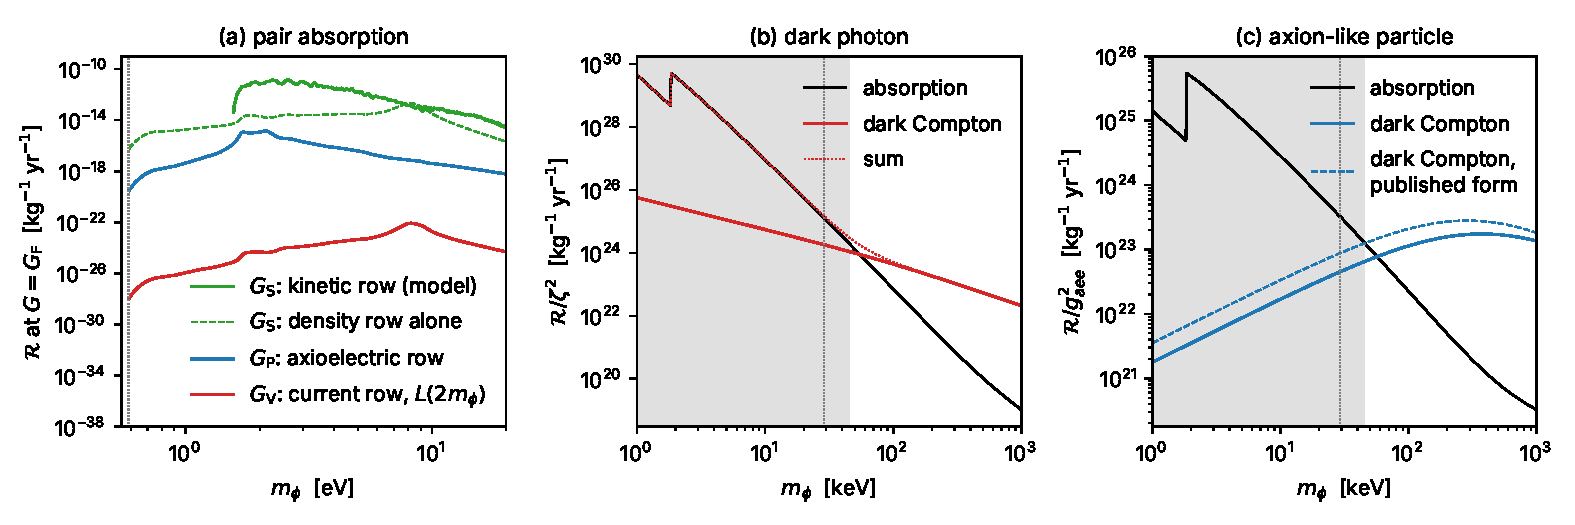
\includegraphics[width=\linewidth]{figures/ch10/fig10_7.pdf}
  \caption{Two-insertion rates of bosonic dark matter in silicon per kilogram-year, with $\rho_\chi = \SI{0.3}{GeV.cm^{-3}}$, $\rho_T = \SI{2.33}{g.cm^{-3}}$ and the halo of \cref{sec:1.2}. (a) Pair absorption of a complex scalar of mass $m_\phi$ at couplings $G = G_{\mathrm{F}}$, \cref{eq:10.8-contact}. Scalar through the kinetic row in the empirical-pseudopotential model of \cref{sec:10.7-scalar}, which has its own vertical gap at \SI{3.12}{eV} and is a model, not a prediction (solid green). Scalar through the density row alone with $\langle q^2\rangle^{1/2} = 2.14\times10^{-3}\,m_\phi$ and the measured loss function (dashed). Pseudoscalar, \cref{eq:10.8-P}, and vector, \cref{eq:10.8-V}, from the measured optical constants of float-zone silicon at \SI{300}{K}~\cite{franta2017temperature}, spliced at \SI{40}{eV} to atomic scattering factors~\cite{henke1993xray}. Dotted: $2m_\phi$ at the excitonic edge of cold silicon, \SI{1.1728}{eV} with $\Eg(0) = \SI{1.1692}{eV}$; the \SI{300}{K} data are wrong within tens of meV of it (\cref{sec:10.7-edge}). (b) Dark photon: absorption, \cref{eq:10.7-dp} (black; from the optical constants below \SI{29}{keV}, dotted line, and from the photoelectric cross section of the XCOM tables (the photon cross-section database of the National Institute of Standards and Technology)~\cite{berger2010xcom} above, with $\varepsilon = 1$), and dark Compton scattering on all 14 electrons, \cref{eq:10.8-compton} (red). (c) Axion-like particle: absorption, \cref{eq:10.7-alp} (black), and dark Compton scattering, \cref{eq:10.8-alpC} (blue). Gray in (b) and (c): $m_\phi < \SI{45}{keV}$, where the electron recoil $\omega_{\mathrm{C}}$ falls below the K-shell binding of \SI{1.84}{keV} and counting all 14 electrons as free overstates the Compton rate.}
  \label{fig:10-twoins}
\end{figure}

The reduction to \cref{eq:10.8-contact} assumes a smooth response. A target with a sharp line at $\Delta E$ resolves the kinetic energy of the pair instead: the rate is spread over $2m_\phi$ between $\Delta E - 4\bar K_{\mathrm{pair}}$ and $\Delta E$, and the peak it reaches depends on how the width of the line compares with $\bar K_{\mathrm{pair}}$. This is the regime of the atomic transitions of Ref.~\cite{bauer2026dark}, whose line shape follows the kinetic-energy distribution of the pair. In silicon the absorption continua vary on scales of meV, and \cref{eq:10.8-contact} holds; only a line narrower than $\bar K_{\mathrm{pair}}$, about \SI{1.6}{\micro eV} at $m_\phi = \SI{1}{eV}$, would resolve the kinetic energy of the pair. \Cref{lim:10.8a} shows where the reduction fails.

\begin{limitbox}[Pair absorption][lim:10.8a]
Pair absorption as single absorption at $\omega = 2m_\phi$ and $\vect{q} \to 0$, \cref{eq:10.8-contact}, with the constant coefficients $m_eG_{\mathrm{S}}$, $m_eG_{\mathrm{P}}$ and the velocity-dependent $G_{\mathrm{V,A}}(p - \bar p)^\mu$~\cite[Eqs.~(3) and (5)--(8)]{bauer2026dark}.
\par\smallskip
{\centering
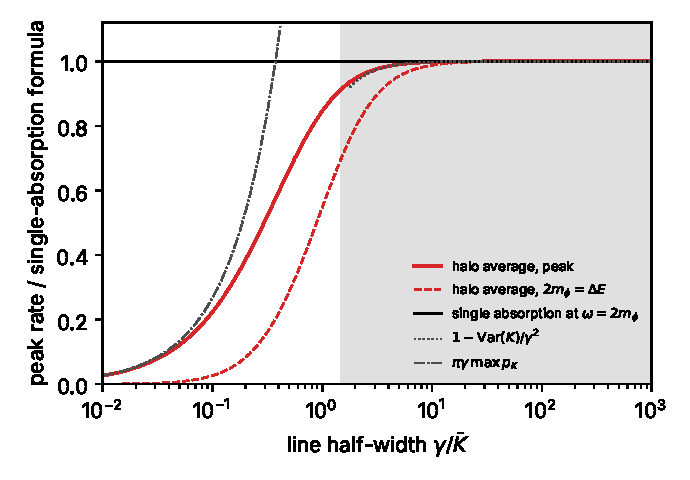
\includegraphics[width=0.72\linewidth]{figures/ch10/limit10_8a.pdf}
\captionof{figure}{Peak absorption rate of a model target with one Lorentzian line of half-width $\gamma$, as the halo average of \cref{eq:10.8-pair} over the pair kinetic energy $K_{\mathrm{pair}}$ (red), divided by the single-absorption formula \cref{eq:10.8-contact} (black), against $\gamma/\bar K_{\mathrm{pair}}$ with $\bar K_{\mathrm{pair}} = m_\phi\langle v^2\rangle = 1.60\times10^{-6}\,m_\phi$. Solid red: peak over the detuning $\Delta E - 2m_\phi$; dashed: at $2m_\phi = \Delta E$. Dotted: the leading correction for broad lines, $1 - \mathrm{Var}(K_{\mathrm{pair}})/\gamma^2$ with $\mathrm{Var}(K_{\mathrm{pair}}) = 0.253\,\bar K_{\mathrm{pair}}^2$; dash-dotted: the narrow-line limit $\pi\gamma\max p_K$, with $p_K$ the distribution of $K_{\mathrm{pair}}$, which the formula of Ref.~\cite{bauer2026dark} for a discrete transition reproduces. Halo of \cref{sec:1.2}, $2\times10^6$ velocity pairs; the dependence on $\vect{q}$ is dropped ($qa < 10^{-4}$). Gray: $\gamma \ge 1.5\,\bar K_{\mathrm{pair}}$, peak within \SI{10}{\percent} of the formula.}\label{fig:10-pair-limit}
\par}
\smallskip
For a line narrower than about $\bar K_{\mathrm{pair}}$, \SI{1.6}{\micro eV} at $m_\phi = \SI{1}{eV}$, the deposited energy follows the kinetic-energy distribution of the pair, and the formula overestimates the peak by $\bar K_{\mathrm{pair}}/\gamma$ up to a factor of order one.
\end{limitbox}

The pair-absorption rates need nothing that single absorption does not already compute: the absorption tables of the charge-like rows and the spin responses at $(\vect{q} \simeq 0, 2m_\phi)$, with the velocity moments of the vector and axial coefficients taken over two copies of the halo.

\subsection{Dark Compton scattering}\label{sec:10.8-compton}

A dark photon couples to the electrons as a photon does, with $e$ replaced by $\zeta e$ (\cref{sec:1.4}). An electron in the field of both therefore sees the total vector potential $\vect{A} + \zeta\vect{A}'$, and its Hamiltonian is $(\vect{p} + e\vect{A} + \zeta e\vect{A}')^2/2m_e$ plus the Pauli term. Expanded, it has the two linear couplings $(e/m_e)\vect{A}\cdot\vect{p}$ and $(\zeta e/m_e)\vect{A}'\cdot\vect{p}$, symmetrized, and a seagull that contains both fields at one point, $(\zeta e^2/m_e)\,\vect{A}\cdot\vect{A}'$. Absorbing a dark photon of polarization $\hat{\vect{e}}$ and emitting a photon of momentum $\vect{k}_\gamma$, energy $\omega_\gamma = |\vect{k}_\gamma|$ and polarization $\hat{\vect{e}}_\gamma$ is a process with two insertions. The seagull does it at first order, and the linear couplings at second order through \cref{eq:10.8-T2}. Per unit amplitude of each field, the target sees the transition operator
\begin{equation}
  T^{\mathrm{C}} = \frac{\zeta e^2}{m_e}\,(\hat{\vect{e}}\cdot\hat{\vect{e}}_\gamma^*)\,n_e(\vect{q})
  + \zeta e^2\Bigl[\hat{\vect{e}}_\gamma^*\cdot\vect{j}_e\,\frac{1}{E_i + m_\phi - H_0}\,\hat{\vect{e}}\cdot\vect{j}_e
  + \hat{\vect{e}}\cdot\vect{j}_e\,\frac{1}{E_i - \omega_\gamma - H_0}\,\hat{\vect{e}}_\gamma^*\cdot\vect{j}_e\Bigr] ,
  \label{eq:10.8-TC}
\end{equation}
with the momentum transfer $\vect{q} = \vect{p}_\phi - \vect{k}_\gamma \simeq -\vect{k}_\gamma$ and the current rows $\vect{j}_e$ at the momenta of their own fields. Both fields carry the factor $1/\sqrt{2\omega \Vol}$ of a quantum of energy $\omega$, as in \cref{eq:8.2-abs}. Summed over the momenta and polarizations of the photon, the golden rule gives the rate per dark photon
\begin{equation}
  \varGamma = \int\frac{\dd^3k_\gamma}{(2\pi)^3\,2\omega_\gamma}\,\frac{1}{2m_\phi}\sum_{\hat{\vect{e}}_\gamma}S_{T^{\mathrm{C}}T^{\mathrm{C}}}(\vect{q},\, m_\phi - \omega_\gamma) ,
  \label{eq:10.8-CS}
\end{equation}
averaged over the three polarizations $\hat{\vect{e}}$ of the dark photon. The target takes the energy $\omega = m_\phi - \omega_\gamma$ and the momentum $\vect{q}$, whose size is close to $m_\phi$. A dark photon of \SI{100}{keV} probes the electrons at $|\vect{q}| = \SI{92}{keV}$, or \SI{47}{\angstrom^{-1}}, far beyond every reciprocal-lattice vector and every inverse orbital radius except those of the innermost shells.

\emph{The Thomson limit.} For a free electron at rest both second-order terms vanish. If the dark photon is absorbed first, its vertex $\hat{\vect{e}}\cdot\vect{p}$ acts on an electron at rest, with $\vect{p}_\phi$ negligible. If the photon is emitted first, its vertex is $\hat{\vect{e}}_\gamma^*\cdot(\vect{p}_i + \vect{p}_m)/2 = -\hat{\vect{e}}_\gamma^*\cdot\vect{k}_\gamma/2 = 0$, since the photon is transverse. Only the seagull remains, and $S_{nn}(\vect{q},\omega) = 2\pi\nd_e\,\delta(\omega - q^2/2m_e)$ for electrons at rest. For $m_\phi \ll m_e$ each electron then scatters the dark photon with the cross section $\zeta^2\sigma_{\mathrm{Th}}$, with $\sigma_{\mathrm{Th}} = e^4/6\pi m_e^2 = \SI{6.65e-25}{cm^2}$ the Thomson cross section, isotropically, since the massive vector has three polarizations, and the electron keeps the recoil energy $m_\phi^2/2m_e$.

In a crystal the seagull row is the density at $|\vect{q}| \simeq m_\phi$, and \cref{eq:10.8-CS} needs $S_{nn}$ at large momentum. There the dark matter resolves single electrons, and the impulse approximation of \cref{we:4-gas} applies, as for the core shells of \cref{sec:10.6}. An electron whose binding is small against the recoil scatters as if free, and its deposit is a line at the free recoil, broadened by its momentum in the atom: the Compton profile of its shell. The binding corrections are the second-order terms of \cref{eq:10.8-TC}, which no longer vanish for a bound electron. An electron bound more strongly than the recoil can absorb barely contributes. In silicon the recoil reaches the K-shell binding, \SI{1.84}{keV}, at $m_\phi = \SI{45}{keV}$, and the L-shell binding, about \SI{100}{eV}, at \SI{10}{keV}. Above \SI{45}{keV} all 14 electrons count, $\nd_e/\rho_T = 3.00\times10^{23}\,\mathrm{g}^{-1}$. The medium also changes the phase space of the photon through the refractive index $n_r(\omega_\gamma) = 1 - \omega_p^2/2\omega_\gamma^2$. It differs from one by $2\times10^{-7}$ at \SI{50}{keV} with the all-electron $\omega_p = \SI{31.1}{eV}$. The in-medium mixing of the dark photon is, at these masses, the vacuum mixing (\cref{sec:10.7-darkphoton}).

\emph{The exact tree-level rate.} The relativistic amplitude of $V + e \to \gamma + e$ consists of the two Compton diagrams with one photon made massive. Squared, summed over the spins of the electrons and the polarizations of the photon, and averaged over the three polarizations of the dark photon, it is a standard Dirac trace. The term $k^\mu k^\nu/m_\phi^2$ of the massive polarization sum drops out because the electron current is conserved, $k_\mu\mathcal{M}^\mu = 0$. Hochberg, von Krosigk, Kuflik and Yu evaluated the trace and integrated it over the final states~\cite[Eqs.~(7)--(12)]{hochberg2022impact}. For a dark photon and an electron at rest the photon energy is fixed by two-body kinematics at $\omega_\gamma = m_\phi(m_\phi + 2m_e)/2(m_\phi + m_e)$, the electron takes
\begin{equation*}
  \omega_{\mathrm{C}} = m_\phi - \omega_\gamma = \frac{m_\phi^2}{2(m_\phi + m_e)} ,
\end{equation*}
and the rate per dark photon is~\cite[Eq.~(2)]{hochberg2022impact}
\begin{equation}
  \varGamma = \nd_e\,\zeta^2\,\frac{e^4}{24\pi m_e^2}\,\frac{(m_\phi + 2m_e)(m_\phi^2 + 2m_em_\phi + 2m_e^2)}{(m_\phi + m_e)^3} ,
  \label{eq:10.8-compton}
\end{equation}
with their kinetic mixing $\varepsilon$ written as $\zeta$. The event rate per unit mass is $(\rho_\chi/m_\phi\rho_T)\varGamma$. At threshold the traces give the averaged squared amplitude $|\bar{\mathcal{M}}|^2 = \frac43e^4\zeta^2(m_\phi^2 + 2m_em_\phi + 2m_e^2)/[m_e(m_\phi + m_e)]$, and with the two-body phase space, $\varGamma = \nd_e|\bar{\mathcal{M}}|^2\omega_\gamma/[16\pi m_\phi m_e(m_\phi + m_e)]$, this is \cref{eq:10.8-compton} exactly, at every $m_\phi/m_e$. It is the exact tree-level rate on a free electron at rest; it tends to the Thomson rate $\nd_e\zeta^2\sigma_{\mathrm{Th}}$ for $m_\phi \ll m_e$ and to a quarter of it for $m_\phi \gg m_e$.

\Cref{fig:10-twoins}b compares dark Compton scattering in silicon with absorption. Absorption falls with the photoelectric cross section, roughly as $m_\phi^{-3}$ per particle above the K edge, while the Compton rate per particle hardly changes below $m_e$. The two cross at $m_\phi = \SI{55}{keV}$, and at \SI{100}{keV} dark Compton scattering is 6.2 times more frequent. In germanium, whose photoelectric cross section is 15 times larger at \SI{100}{keV}, they cross at \SI{144}{keV}. The photon that leaves carries most of the energy, \SI{92}{keV} at $m_\phi = \SI{100}{keV}$, and travels about \SI{2}{cm} in silicon before it interacts~\cite{berger2010xcom}.

\emph{Axion-like particles.} An axion-like particle couples to the spin current of the electrons through $(\partial_t\phi)$, the second term of \cref{eq:1.4-alp}. Minimal coupling turns the gradient in that term into $\nabla + \ii e\vect{A}$ for an electron of charge $-e$, and the spin current $\psi^\dagger\boldsymbol{\sigma}\cdot\overleftrightarrow{\nabla}\psi$ acquires $2\ii e\vect{A}\cdot\psi^\dagger\boldsymbol{\sigma}\psi$. Multiplied by $\ii g_{aee}(\partial_t\phi)/4m_e^2$ this is a seagull for the axion-like particle,
\begin{equation*}
  H_{\mathrm{sg}} = \frac{e\,g_{aee}}{m_e^2}\,(\partial_t\phi)\,\vect{A}\cdot\vect{s}_e ,
\end{equation*}
which absorbs the particle and emits a photon at one point by flipping, or not flipping, a spin. For a free electron at rest the second-order terms of the photon's orbital coupling vanish as for the dark photon, but the Pauli coupling of the photon to the spin, joined to the spin current of the particle, adds second-order terms at relative order $x = m_\phi/m_e$. The exact tree-level rate, from the Lagrangian $g_{aee}\phi\,\bar\psi\ii\gamma^5\psi$ and the same two diagrams with the pseudoscalar vertex $\gamma^5$ (here the photon polarization sum is the only one), is
\begin{equation}
  \varGamma = \nd_e\,\frac{e^2g_{aee}^2}{16\pi m_e^2}\,\frac{m_\phi^2\,(m_\phi + 2m_e)}{(m_\phi + m_e)^3} ,
  \label{eq:10.8-alpC}
\end{equation}
whose expansion in $x$ starts as $\nd_e(e^2g_{aee}^2m_\phi^2/8\pi m_e^4)(1 - \frac52x + \frac92x^2)$, the spin seagull at leading order. The squared amplitude behind it agrees, at every mass, with the one printed in Ref.~\cite[Eq.~(15)]{hochberg2022impact}. \Cref{fig:10-twoins}c shows the rate in silicon: dark Compton scattering overtakes absorption of an axion-like particle at \SI{57}{keV}.

\begin{workedexample}{The axion-like Compton rate at \SI{100}{keV}}\label{we:10-alpcompton}
At $m_\phi = \SI{100}{keV}$, $x = 0.1957$. The photon leaves with $\omega_\gamma = m_\phi(m_\phi + 2m_e)/2(m_\phi + m_e) = \SI{91.82}{keV}$, and the electron takes $\omega_{\mathrm{C}} = \SI{8.18}{keV}$, above the K-shell binding of silicon and below that of germanium, \SI{11.1}{keV}. Per electron and per unit coupling, \cref{eq:10.8-alpC} gives $\varGamma/(\nd_eg_{aee}^2) = \SI{1.34e-25}{cm^2}$ times the speed of light.

In silicon, with $\nd_e/\rho_T = 3.00\times10^{23}\,\mathrm{g}^{-1}$ and the photoelectric cross section $\SI{0.0250}{cm^2/g}$ at \SI{100}{keV}, the Compton rate of \cref{eq:10.8-alpC} is 5.1 times the absorption rate of \cref{eq:10.7-alp}. In germanium absorption still dominates at this mass: the Compton rate is 0.30 of it.
\end{workedexample}

\subsection{Open problems}\label{sec:10.8-open}

Two pieces of the two-insertion response are not computed for any crystal. The first is the interference between a contact amplitude and a second-order one, which a dark-matter model with both kinds of coupling produces. For the stopping of a charged particle the same term is the Barkas correction, odd in the charge of the projectile. It is linear in the quadratic response of the target, a three-point function, and no reduction to two-point responses exists. The quadratic response of the electron gas is known and serves as a check. The second is the bound-state correction to dark Compton scattering for the shells whose binding is close to $\omega_{\mathrm{C}}$. They are the K shell of silicon between 45 and about \SI{100}{keV}, the K shell of germanium, whose binding of \SI{11.1}{keV} the recoil reaches at \SI{118}{keV}, and the L shells below about \SI{20}{keV}. There the second-order terms of \cref{eq:10.8-TC} no longer vanish, and the rate needs the shell Compton profiles or the large-$q$ density response, together with the refractive index at the photon energy.

\section{Inelastic and relativistic dark matter}\label{sec:10.9}

A dark-matter particle of \SI{1}{MeV} that arrives in an excited state \SI{10}{eV} above its ground state carries three times more energy in its mass splitting than in its motion, whose kinetic energy is at most \SI{3.5}{eV}. A particle accelerated by a cosmic-ray electron can move at nearly the speed of light, and a fermion that is absorbed hands over almost its whole rest energy. Each of these cases changes one ingredient of the master formula of \cref{sec:8.2} and leaves the others alone. A mass splitting changes the kinematics, through the term $-\Delta_\chi$ in $\omega_{\vect{q}}$. A relativistic particle changes the dark-matter tensor $\mathfrak{D}_{ab}$, and an outgoing light fermion changes both. The target enters, as before, through the response matrix of the rows of \cref{eq:8.1-rows}, and the silicon tables of \cref{sec:10.2} provide it.

\subsection{Inelastic and exothermic scattering}\label{sec:10.9-inelastic}

For inelastic dark matter the potential and $\sigmae$ keep their elastic form (\cref{sec:1.4}). The time component of the current that connects $\chi_1$ to $\chi_2$ reduces to one, as for the elastic current, up to corrections of order $\Delta_\chi/\mchi$ (\cref{eq:C.15-bilinears}), and the recoil term of \cref{eq:8.1-omega-inel} is smaller by the same fraction. The only change that matters is the term $-\Delta_\chi$ in $\omega_{\vect{q}}$. The derivation of \cref{sec:10.2} then goes through step by step. The angular integral of \cref{eq:A.8-eta} produces $\eta$ at the minimum velocity of \cref{eq:1.3-vmin}, taken in absolute value:
\begin{keyresult}[Inelastic electron-recoil rate]
\begin{equation}
  \frac{\dd\mathcal{R}}{\dd\omega} = \frac{\rho_\chi\,\sigmae}{8\pi^2\alpha\,\rho_T\,\mchi\,\mu_{\chi e}^2}\int\dd q\;q^3\,\eta\bigl(\vmin\bigr)\,\FDM(q)^2\,\bar L(q,\omega) , \qquad
  \vmin = \left|\frac{\omega + \Delta_\chi}{q} + \frac{q}{2\mchi}\right| ,
  \label{eq:10.9-inel}
\end{equation}
at $T = 0$, with $\bar L$ the loss function averaged over the directions of $\vect{q}$. It is exact under the conditions of \cref{eq:10.2-rate}.
\end{keyresult}
\noindent The absolute value is needed only when $\omega + \Delta_\chi < 0$, which at $T = 0$ means exothermic dark matter depositing less than $|\Delta_\chi|$.

An endothermic splitting is paid from the kinetic energy. Since $\omega \le \tfrac12\mchi v^2 - \Delta_\chi$ (\cref{eq:1.3-omegamax}), a pair across the gap needs $\mchi \ge 2(\Delta_\chi + \Eg)/v_{\mathrm{max}}^2$: \SI{0.60}{MeV} for $\Delta_\chi = \SI{1}{eV}$ and \SI{3.2}{MeV} for \SI{10}{eV}, with the step-model gap of \SI{1.11}{eV} that accompanies the tables of \cref{sec:10.2}. An exothermic splitting is paid by the dark matter, and as \cref{sec:8.2-exothermic} found, it shifts the band of allowed $(q,\omega)$ up by $|\Delta_\chi|$, down to $q \to 0$. \Cref{fig:10-inelastic} shows the consequence in silicon at \SI{10}{MeV}. With a heavy mediator, per kilogram-year at $\sigmae = \SI{e-37}{cm^2}$, the rate is 314 events for $\Delta_\chi = \SI{10}{eV}$, $5.9\times10^4$ for elastic scattering and $7.5\times10^5$ for $\Delta_\chi = \SI{-10}{eV}$. With a light mediator the three numbers are 6.2, $9.8\times10^3$ and $5.2\times10^5$, and the exothermic spectrum has a sharp peak at $\omega = |\Delta_\chi|$. Splittings of a few eV move the rate by orders of magnitude, in either direction.

\begin{figure}[tbp]
  \centering
  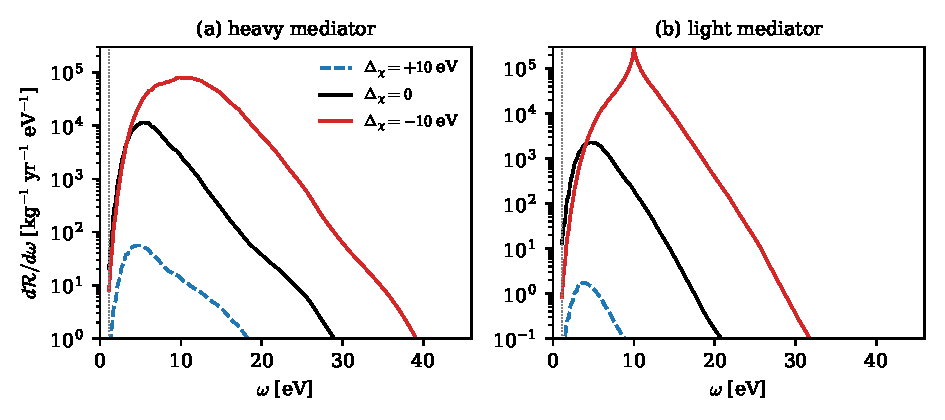
\includegraphics[width=\linewidth]{figures/ch10/fig10_8.pdf}
  \caption{Electron-recoil spectrum of silicon for inelastic dark matter of mass $\mchi = \SI{10}{MeV}$ with splittings $\Delta_\chi = \SI{+10}{eV}$ (endothermic, dashed), 0 (elastic) and \SI{-10}{eV} (exothermic), from \cref{eq:10.9-inel}. Inputs: the random-phase loss function with local fields of the tables of \cref{sec:10.2}, the standard halo of \cref{sec:1.2}, $\rho_\chi = \SI{0.3}{GeV.cm^{-3}}$ and $\sigmae = \SI{e-37}{cm^2}$. Dotted: \SI{1.11}{eV}, the step-model gap that accompanies the tables, below the low-temperature gap of \SI{1.17}{eV} to which their scissor shifts the bands. Below $|\vect{q}| = \SI{493}{eV}$, the first tabulated momentum, the loss function is held at its value there. (a) Heavy mediator, $\FDM = 1$. (b) Light mediator, $\FDM = (q_0/q)^2$; the exothermic spectrum peaks at $\omega = |\Delta_\chi|$, where the momentum transfer goes to zero.}
  \label{fig:10-inelastic}
\end{figure}

An exothermic particle is not limited by the kinetic energy of the halo, and its spectrum is set by the splitting. To see how, complete the square in $\omega_{\vect{q}}$ with $\Delta_\chi < 0$,
\begin{equation*}
  \omega_{\vect{q}} = |\Delta_\chi| + \vect{q}\cdot\vect{v} - \frac{q^2}{2\mchi} = |\Delta_\chi| + \tfrac12\mchi v^2 - \frac{|\vect{q} - \mchi\vect{v}|^2}{2\mchi} .
\end{equation*}
At fixed $\omega < |\Delta_\chi|$ the delta function of \cref{eq:8.2-spectrum} puts $\vect{q}$ on a sphere of radius $k_*$ centered at $\mchi\vect{v}$, with $k_*^2 = q_\Delta^2 + \mchi^2v^2$ and
\begin{equation*}
  q_\Delta = \sqrt{2\mchi\bigl(|\Delta_\chi| - \omega\bigr)} , \qquad v_\Delta = q_\Delta/\mchi .
\end{equation*}
For any function $G$ of $|\vect{q}|$, $\int\dd^3q\,\delta(\omega - \omega_{\vect{q}})\,G = \mchi k_*\int\dd^2\hat{\vect{n}}\,G(|\mchi\vect{v} + k_*\hat{\vect{n}}|)$. On the sphere $q^2 = k_*^2 + \mchi^2v^2 + 2k_*\mchi\vect{v}\cdot\hat{\vect{n}}$, and the term linear in $\vect{v}$ averages to zero because the sphere is centered at $\mchi\vect{v}$. The integral is therefore $4\pi\mchi q_\Delta G(q_\Delta)[1 + O(v^2/v_\Delta^2)]$, exactly $4\pi\mchi k_*G$ for constant $G$. The rate per particle no longer depends on its velocity, and the average over the halo is trivial. With $G = |\tilde V|^2\bar S$, $\bar S = (2q^2/e^2)\bar L$ and $\rho_\chi/\mchi\rho_T$ per unit mass,
\begin{keyresult}[Exothermic shell]
\begin{equation}
  \frac{\dd\mathcal{R}}{\dd\omega} = \frac{\rho_\chi\,\sigmae\,q_\Delta^3\,\FDM(q_\Delta)^2\,\bar L(q_\Delta,\omega)}{4\pi^2\alpha\,\rho_T\,\mu_{\chi e}^2}\,\Bigl[1 + O\bigl(v^2/v_\Delta^2\bigr)\Bigr] , \qquad \omega < |\Delta_\chi| ,
  \label{eq:10.9-shell}
\end{equation}
independent of the velocity distribution as long as $v_\Delta$ exceeds the speeds of the halo. The spectrum samples the response along the parabola $\omega = |\Delta_\chi| - q^2/2\mchi$.
\end{keyresult}
\noindent For constant $\bar L$ and a heavy mediator the correction is about $2.5\langle v^2\rangle/v_\Delta^2$, with $\langle v^2\rangle^{1/2} = 1.3\times10^{-3}$ in the laboratory frame: at $\mchi = \SI{0.1}{MeV}$ and $\omega = \SI{3}{eV}$, \cref{eq:10.9-inel} exceeds \cref{eq:10.9-shell} by \SI{2.9}{\percent}. Since $v_\Delta^2 = 2(|\Delta_\chi| - \omega)/\mchi$, the shell form needs $\mchi$ well below $2|\Delta_\chi|/v_{\mathrm{max}}^2$, which is \SI{2.9}{MeV} for $|\Delta_\chi| = \SI{10}{eV}$; at \SI{10}{MeV} the halo still matters, and \cref{fig:10-inelastic} uses \cref{eq:10.9-inel}.

The parabola explains where exothermic spectra peak. On a free electron at rest the response is a line, $S \propto \delta(\omega - q^2/2m_e)$, and it crosses the parabola once, at
\begin{equation*}
  \omega_{\mathrm{line}} = \frac{\mu_{\chi e}}{m_e}\,|\Delta_\chi| , \qquad q_{\mathrm{line}} = \sqrt{2\mu_{\chi e}|\Delta_\chi|} ,
\end{equation*}
the energy shared between the two recoiling particles. A heavy dark-matter particle hands the whole splitting to the electron, and a light one keeps part of it. In a crystal the electron line exists only where the free-electron picture holds, $q_{\mathrm{line}} \gg q_0$, that is $\omega_{\mathrm{line}} \gg q_0^2/2m_e = \SI{13.6}{eV}$. For smaller splittings the parabola crosses the region in which the response is that of bound electrons, and the peak sits where $q_\Delta^3\bar L$ is largest. The factor $q_\Delta^3$ falls toward $\omega = |\Delta_\chi|$, while $\bar L$ rises from the gap toward the plasma frequency, and the product peaks in between.

A light mediator turns the end of the spectrum into a line. As $\omega \to |\Delta_\chi|$, $q_\Delta \to 0$ and $\bar S \to (q^2/2\pi\alpha)L(0,\omega)$, the optical limit, so that with $\FDM^2 = q_0^4/q^4$
\begin{equation}
  \frac{\dd\mathcal{R}}{\dd\omega} \to \frac{\rho_\chi\,\sigmae\,q_0^4\,L(0,\omega)}{4\pi^2\alpha\,\rho_T\,\mu_{\chi e}^2\,q_\Delta} \propto \bigl(|\Delta_\chi| - \omega\bigr)^{-1/2} .
  \label{eq:10.9-edge}
\end{equation}
The divergence is integrable. Within $\tfrac12\mchi v^2$ of the end point, where $v_\Delta$ falls below the halo speeds, the exact kernel softens it to a logarithm, since there the momentum transfer can go to zero for every speed of the halo. Its strength is the optical loss function at $\omega = |\Delta_\chi|$: near the end point the exothermic particle acts like a boson of mass $|\Delta_\chi|$ absorbed at $\vect{q} \simeq 0$ (\cref{sec:8.2-exothermic}), and like the dark photon of \cref{sec:10.7} it reads $L$ rather than $\varepsilon_2$.

\begin{workedexample}{Exothermic lines in silicon}\label{we:10-exo}
Take $\Delta_\chi = \SI{-10}{eV}$ in silicon and the masses 0.1, 0.3, 1 and \SI{3}{MeV}. The free-electron lines would sit at $\omega_{\mathrm{line}} = 1.64$, 3.70, 6.62 and \SI{8.54}{eV}, at $q_{\mathrm{line}} = 1.29$, 1.94, 2.60 and \SI{2.96}{keV}. Every one of these momenta lies below $q_0 = \SI{3.73}{keV}$; even an infinitely heavy particle reaches only $q_{\mathrm{line}} = (2m_e|\Delta_\chi|)^{1/2} = \SI{3.20}{keV}$. A \SI{10}{eV} splitting therefore never meets free electrons in silicon.

The silicon spectrum from \cref{eq:10.9-inel}, with the random-phase loss function with local fields and a heavy mediator, peaks at 6.95, 6.19, 5.99 and \SI{7.29}{eV} for the four masses, with half-maximum edges between about 4 and \SI{8.5}{eV} (up to \SI{11.8}{eV} at \SI{3}{MeV}). At \SI{0.1}{MeV} the peak lies \SI{5.3}{eV} above the free-electron line, at \SI{1}{MeV} \SI{0.6}{eV} below it: the peak barely moves with the mass because it is set by the loss function, not by the recoil. The momentum transfer at the peak is $q_\Delta = 0.78$, 1.51, 2.83 and \SI{4.03}{keV}, from $0.21\,q_0$ to $1.08\,q_0$. Per kilogram-year at $\sigmae = \SI{e-37}{cm^2}$ the totals are $2.1\times10^5$, $3.1\times10^5$, $8.7\times10^5$ and $1.5\times10^6$. The shell form \cref{eq:10.9-shell} reproduces them to 0.91, 0.81, 0.63 and 0.73. The largest speeds of the halo reach $v_\Delta$ at the peak for $\mchi \gtrsim \SI{1}{MeV}$, with $v_{\mathrm{max}}/v_\Delta = 0.34$, 0.53, 0.94 and 1.97. At the lightest mass the residual comes from the tables: binned in \SI{100}{eV} steps of $|\vect{q}|$, the loss function varies by about \SI{15}{\percent} from bin to bin at these momenta, and the shell form samples a single $q$.

With a light mediator every mass gives a line at $\omega = \SI{10.0}{eV}$, an integrable cusp whose width is set by the energy resolution of the detector rather than by the halo. The last \SI{0.5}{eV} below $|\Delta_\chi|$ holds 40, 42, 47 and \SI{60}{\percent} of the rate, and the \SI{0.1}{eV} around $|\Delta_\chi|$ holds 15, 12, 8 and \SI{6.5}{\percent}. Its height follows from \cref{eq:10.9-edge} with $L(0,\SI{10}{eV})$, which is 0.247 measured (\cref{we:10-darkphoton}) and 0.218 in the first bin of the tables. The two mediators therefore leave different signatures for the same splitting: a broad bump near \SI{6}{eV} whose position hardly depends on the mass, or a line at the splitting itself. Neither sits at $\mu_{\chi e}|\Delta_\chi|/m_e$.
\end{workedexample}

Nothing new is needed from the material: \cref{eq:10.9-inel} uses the same loss functions as the elastic rate, now on a grid of $\omega$ that extends to $|\Delta_\chi| + \tfrac12\mchi v_{\mathrm{max}}^2$, and the light-mediator line needs the optical limit, which measurements give. Above \SI{99}{eV} the $2p$ shell of silicon opens (\cref{sec:10.6}), and the valence tables no longer suffice.

\subsection{Boosted dark matter}\label{sec:10.9-boosted}

A light halo particle can be accelerated after it leaves the halo's equilibrium. Cosmic-ray electrons and protons of MeV to GeV energies cross the dark-matter halo of the Galaxy, and a small fraction of them scatter on dark-matter particles along the way, which then carry kinetic energies comparable to their mass. The resulting flux at the Earth is the line-of-sight integral of the dark-matter density times the cosmic-ray flux and the scattering cross-section. For electrons, Liang and collaborators write it as $\dd\Phi_\chi/\dd T_\chi = D_{\mathrm{eff}}(\rho_\chi/\mchi)\int\dd T_e\,(\dd\sigma_{\chi e}/\dd T_\chi)(\dd\Phi_e/\dd T_e)$, with $T_\chi$ and $T_e$ the kinetic energies and $D_{\mathrm{eff}} = \SI{8.02}{kpc}$ an effective distance for a halo profile integrated to \SI{10}{kpc}~\cite[Eq.~(1)]{liang2025plasmon}. The flux is small, since only one halo particle in many meets a cosmic ray, but it reaches speeds close to that of light and with them energies far above $\tfrac12\mchi v_{\mathrm{max}}^2$.

The Sun accelerates a second component. Halo particles that fall into it scatter on the electrons of the solar core, at $1.57\times10^7$\,K at the center~\cite[Table~5]{bahcall2001solar}, whose thermal speed $(3T/m_e)^{1/2}$ is about 0.09. Some leave with speeds of that order, far above the escape speed of the Galaxy but well below that of light. The DAMIC-M collaboration, Dark Matter in CCDs (DAMIC) at Modane, has searched for this solar-reflected component~\cite{aggarwal2026constraints}. In both cases the halo average of \cref{eq:8.2-spectrum} is replaced by an average over the flux. For a flux that is isotropic in the laboratory, the number density per unit speed is $(\dd\Phi_\chi/\dd v)/v$, and the non-relativistic rate keeps its form with
\begin{equation*}
  \frac{\rho_\chi}{\mchi}\,\eta(\vmin) \;\to\; \int_{\vmin}\dd v\;\frac{1}{v^2}\,\frac{\dd\Phi_\chi}{\dd v} ,
\end{equation*}
the replacement of Ref.~\cite[Eqs.~(9)--(11)]{aggarwal2026constraints}. The real fluxes are anisotropic, the solar one pointing away from the Sun, and the angular average of the response that makes $\eta$ sufficient is then an assumption. For speeds near that of light the non-relativistic rows themselves must be checked.

The non-relativistic potential of \cref{sec:8.1} assumed that the energy deposited is small against the momentum transfer, so that the mediator acts instantaneously. For a relativistic particle $\omega$ can approach $q$, and the mediator must be kept whole. Take a vector mediator of mass $m_V$ coupled with strengths $y_\chi$ and $y_e$ to the dark-matter current $J^\mu_\chi = \bar u(p')\gamma^\mu u(p)$ and to the electron current $J^\mu_e = (n_e, \vect{j}_e)$. We write $\mathcal{Q} = |\vect{q}|$ for the momentum transfer, to keep it apart from the four-momentum, and $E_\chi = (p^2 + \mchi^2)^{1/2}$ for the energy, so that $\omega = E_\chi(\vect{p}) - E_\chi(\vect{p} - \vect{q})$ by \cref{eq:8.1-omega}. The amplitude is $y_\chi y_e(J^0_\chi n_e - \vect{J}_\chi\cdot\vect{j}_e)/(\mathcal{Q}^2 - \omega^2 + m_V^2)$. Both currents are conserved. For the target, \cref{eq:4.3-continuity} gives $\hat{\vect{q}}\cdot\vect{j}_e \to (\omega/\mathcal{Q})n_e$ between eigenstates; for the dark matter, the Dirac equation gives $\hat{\vect{q}}\cdot\vect{J}_\chi = (\omega/\mathcal{Q})J^0_\chi$. Splitting each spatial current into its part along $\hat{\vect{q}}$ and its transverse part, $\vect{J}_\chi\cdot\vect{j}_e = (\omega^2/\mathcal{Q}^2)J^0_\chi n_e + \vect{J}_{\chi\mathrm{T}}\cdot\vect{j}_{e\mathrm{T}}$, and the amplitude becomes
\begin{equation}
  y_\chi y_e\,\frac{J^0_\chi\,n_e\,(1 - \omega^2/\mathcal{Q}^2) - \vect{J}_{\chi\mathrm{T}}\cdot\vect{j}_{e\mathrm{T}}}{\mathcal{Q}^2 - \omega^2 + m_V^2} .
  \label{eq:10.9-amp}
\end{equation}
For a massless mediator the density term is $J^0_\chi n_e/\mathcal{Q}^2$, the instantaneous Coulomb interaction, and only the transverse term propagates at the speed of light. Retardation enters the density row of a massive mediator as the factor $(1 - \omega^2/\mathcal{Q}^2)$, and it comes from keeping the longitudinal current, which continuity ties to the density.

The density row needs the spin average of $|J^0_\chi|^2$. Write $\gamma\cdot p = \gamma^\mu p_\mu$ for the four-momentum $p = (E_\chi, \vect{p})$. The spinors of \cref{eq:C.15-spinor} obey $\sum_su(p,s)\bar u(p,s) = \gamma\cdot p + \mchi$, and the traces needed are $\Tr(\gamma^\mu\gamma^\nu) = 4g^{\mu\nu}$, $\Tr(\gamma^\mu\gamma^\nu\gamma^\rho\gamma^\sigma) = 4(g^{\mu\nu}g^{\rho\sigma} - g^{\mu\rho}g^{\nu\sigma} + g^{\mu\sigma}g^{\nu\rho})$, and zero for an odd number of matrices. Then
\begin{equation*}
  \begin{aligned}
  \frac12\sum_{s,s'}\bigl|\bar u(p',s')\gamma^0u(p,s)\bigr|^2 &= \frac12\Tr\bigl[(\gamma\cdot p' + \mchi)\gamma^0(\gamma\cdot p + \mchi)\gamma^0\bigr] \\
  &= 2\bigl(E_\chi E'_\chi + \vect{p}\cdot\vect{p}' + \mchi^2\bigr) = (2E_\chi - \omega)^2 - \mathcal{Q}^2 ,
  \end{aligned}
\end{equation*}
where the four-matrix trace gives $4(2E'_\chi E_\chi - p'\cdot p)$ with $p'\cdot p = E'_\chi E_\chi - \vect{p}'\cdot\vect{p}$, and the last step uses $E'_\chi = E_\chi - \omega$ and $2\vect{p}\cdot\vect{p}' = p^2 + p'^2 - \mathcal{Q}^2$. Dividing by the normalization $2E_\chi\cdot2E'_\chi$ of the two dark-matter states, squaring \cref{eq:10.9-amp} and writing the couplings through $\sigmae$ as in \cref{eq:1.4-Vsq},
\begin{keyresult}[Relativistic density row]
\begin{equation}
  \mathfrak{D}_{nn} = \frac{\pi\sigmae}{\mu_{\chi e}^2}\;\frac{(2E_\chi - \omega)^2 - \mathcal{Q}^2}{4E_\chi(E_\chi - \omega)}\;\Bigl(1 - \frac{\omega^2}{\mathcal{Q}^2}\Bigr)^2\left[\frac{q_0^2 + m_V^2}{\mathcal{Q}^2 - \omega^2 + m_V^2}\right]^2 ,
  \label{eq:10.9-Drel}
\end{equation}
which tends to $\pi\sigmae\FDM^2/\mu_{\chi e}^2$ as $v \to 0$. The rate per particle is \cref{eq:8.2-rate} with $S_{nn} = (2\mathcal{Q}^2/e^2)\bar L$, and per unit target mass $\dd\mathcal{R}/\dd\omega = \rho_T^{-1}\int\dd v\,v^{-1}(\dd\Phi_\chi/\dd v)\,\dd\varGamma/\dd\omega$ for an isotropic flux.
\end{keyresult}
\noindent This constructs the relativistic tensor that \cref{sec:8.2-absorption} left open, for the density row. The transverse row enters through $\vect{J}_{\chi\mathrm{T}}$, whose square for a particle much heavier than the energy deposited is $4E_\chi^2v_{\mathrm{T}}^2$, with $v_{\mathrm{T}}^2 = v^2 - (\vect{v}\cdot\hat{\vect{q}})^2 = v^2 - \omega^2/\mathcal{Q}^2$. For a massless mediator the medium answers a transverse current through its transverse dielectric function $\varepsilon^{\mathrm{T}}$ of \cref{sec:4.4}, and the propagator $1/\mathcal{Q}^2$ of the density row becomes $1/(\mathcal{Q}^2 - \omega^2\varepsilon^{\mathrm{T}})$ in the transverse row. After averaging over the directions of $\vect{q}$ the density and the transverse current are uncorrelated, and the two rows add. The loss function of the density row is replaced by
\begin{equation}
  \bar L(\mathcal{Q},\omega) \;\to\; \bar L(\mathcal{Q},\omega) + \Bigl(v^2 - \frac{\omega^2}{\mathcal{Q}^2}\Bigr)\Imag\left[\frac{-\mathcal{Q}^2}{\omega^2\varepsilon^{\mathrm{T}}(\mathcal{Q},\omega) - \mathcal{Q}^2}\right] ,
  \label{eq:10.9-fermi}
\end{equation}
the form of Fermi's energy-loss formula for a fast charge~\cite{fermi1940ionization}, which a calculation of the transverse response of silicon writes for dark matter~\cite[Eq.~(2)]{liang2026dielectric}.

We can bound the retardation factor. For any particle whose energy is a convex function of its momentum, $E_\chi(p) - E_\chi(p') \le (\dd E_\chi/\dd p)(p - p')$, and $p - p' \le \mathcal{Q}$ by the triangle inequality, so
\begin{equation}
  \omega \le v\,\mathcal{Q} , \qquad \Bigl(1 - v_{\chi,\mathrm{max}}^2\Bigr)^2 \le \Bigl(1 - \frac{\omega^2}{\mathcal{Q}^2}\Bigr)^2 \le 1 ,
  \label{eq:10.9-bound}
\end{equation}
with $v_{\chi,\mathrm{max}}$ the largest speed in the flux. A rate computed without the factor is therefore too large by at most $(1 - v_{\chi,\mathrm{max}}^2)^{-2}$. For speeds up to 0.1 this is \SI{2}{\percent}, and up to 0.2 it is \SI{9}{\percent}. For the solar-reflected flux, with typical speeds of 0.1, the non-relativistic rate with $\eta$ replaced by the flux integral therefore stands at the level of a few percent. For cosmic-ray-boosted dark matter, with $v \to 1$, the bound says nothing, and the answer depends on where in $(\mathcal{Q},\omega)$ the rate collects.

For a heavy mediator the rate of silicon collects at $\mathcal{Q}$ of keV, where $\omega/\mathcal{Q}$ is tiny: the factor $(1 - \omega^2/\mathcal{Q}^2)^2$ changes the rate by $10^{-4}$ and the transverse row by at most $10^{-4}$. For a massless mediator the density row without the factor, $q_0^4/(\mathcal{Q}^2 - \omega^2)^2$, grows without limit as $\mathcal{Q} \to \omega$, where the exact longitudinal interaction is the Coulomb $q_0^4/\mathcal{Q}^4$; this form, with the mediator form factor evaluated at the four-momentum transfer, is the one of Ref.~\cite[Eqs.~(4)--(6)]{liang2025plasmon}. For a particle of speed $v$ the exact density row of silicon is then 0.997 of the row without the factor at $v = 0.1$, 0.94 at 0.5, 0.65 at 0.9 and 0.17 at 0.99 (\cref{fig:10-boost-limit}).

The transverse row of \cref{eq:10.9-fermi} contains the Cherenkov term of Fermi's formula, standard for fast charged particles in matter and in the photo-absorption-ionization model of energy loss in silicon~\cite{fermi1940ionization,allison1980relativistic}. Between the gap and the direct gap silicon is nearly transparent, with $\varepsilon_1 = 12.5$ at the gap rising to 44.9 at \SI{3.3}{eV} in the measured data at \SI{300}{K}. A particle faster than the light of the medium, $v > \varepsilon_1^{-1/2}$, which is 0.28 at \SI{1.2}{eV} and 0.15 at \SI{3.3}{eV}, emits Cherenkov radiation. The condition $\omega^2\varepsilon_1 = \mathcal{Q}^2$ is then met inside the kinematic range $\mathcal{Q} \ge \omega/v$, and the transverse term has a pole there, broadened only by the small $\varepsilon_2$. We take the measured $\varepsilon$ in place of $\varepsilon^{\mathrm{T}}$, valid at these small $\mathcal{Q}$, and a massless mediator. Below \SI{2}{eV} the transverse row then exceeds the density row, which is suppressed there by $1/|\varepsilon|^2$, by a factor of 49 at $v = 0.3$ and 530 at $v = 0.5$. Integrated over the spectrum above the gap, the transverse share is $2.7\times10^{-5}$ at $v = 0.1$, \SI{1}{\percent} at 0.5 and \SI{5.5}{\percent} at 0.99; in the plasmon window of 10 to \SI{20}{eV} it is $7\times10^{-4}$ at 0.5 and $7\times10^{-3}$ at 0.99. The Cherenkov photons are real photons, and they make electron--hole pairs only where the crystal absorbs them, within $1/(2\omega\Imag n_r)$, which is \SI{0.4}{mm} at \SI{1.2}{eV} and \SI{12}{\micro m} at \SI{1.5}{eV} in the warm data and longer in a cold crystal (\cref{sec:10.7-edge}). Whether they count is a question of the size and temperature of the detector.

\begin{figure}[tbp]
  \centering
  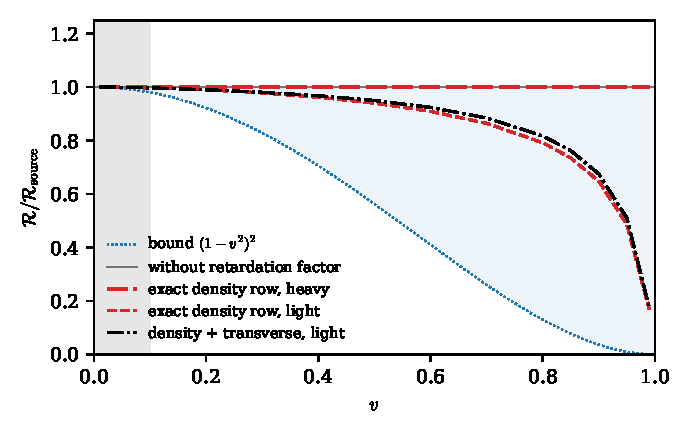
\includegraphics[width=0.82\linewidth]{figures/ch10/limit10_9b.pdf}
  \caption{Electron-recoil rate of silicon for dark matter of speed $v$, much heavier than the energy deposited, divided by the rate of the density row without the factor $(1 - \omega^2/\mathcal{Q}^2)^2$, against $v$. Red, long dashes: the exact density row \cref{eq:10.9-Drel} with a heavy mediator, which coincides with it to $10^{-4}$; red, short dashes: the same with a massless mediator; dash-dotted: the massless mediator with the transverse row of \cref{eq:10.9-fermi} added. Blue band: the range $[(1 - v^2)^2, 1]$ allowed by \cref{eq:10.9-bound}. Gray: $v \le 0.1$, where the bound guarantees agreement to \SI{2}{\percent}. Rates are integrated over $\omega$ from \SI{1.11}{eV}, the step-model gap that accompanies the tables, to \SI{89}{eV} and over $\mathcal{Q}$ from $\omega/v$ to \SI{22.5}{keV}. Loss function: random-phase with local fields, from the tables of \cref{sec:10.2}, held at its value at \SI{493}{eV} below that momentum. Transverse function: the measured $\varepsilon(\omega)$ of silicon at \SI{300}{K}~\cite{franta2017temperature}, with its Cherenkov pole integrated exactly; the transverse row counts the Cherenkov photons emitted above the gap as deposited energy, wherever they are absorbed.}
  \label{fig:10-boost-limit}
\end{figure}

\subsection{Fermionic absorption on electrons}\label{sec:10.9-fermionic}

A fermion $\chi$ of \SI{100}{keV} that is absorbed on an electron and leaves as a massless $\tilde\nu$ deposits $\omega = \mchi - q$ (\cref{eq:8.1-omega-ferm}). On a free electron at rest this is the recoil $q^2/2m_e$, so $q \simeq \mchi$ and $\omega \simeq \mchi^2/2m_e = \SI{9.8}{keV}$, a deposit that no halo particle of that mass could give by scattering. The momentum transfer is set by the rest energy and not by the speed of the dark matter, so that the rate is a single line through the response, independent of the halo. \Cref{sec:8.2-absorption} showed that the master formula holds with a sum over the momenta of $\tilde\nu$ and left the dark-matter tensor to be built here.

Take the operators $\Lambda_F^{-2}(\bar{\tilde\nu}P_L\chi)(\bar\psi\psi)$ and $\Lambda_F^{-2}(\bar{\tilde\nu}\gamma_\mu P_R\chi)(\bar\psi\gamma^\mu\psi)$ of \cref{sec:8.1-absorption}, with the chirality projectors $P_{L,R} = (1 \mp \gamma^5)/2$. Let $p = (\mchi, \vect{0})$ be the four-momentum of $\chi$ at rest and $k = (q, -\vect{q})$ that of $\tilde\nu$, so that $k\cdot p = \mchi q$. On the target side the scalar bilinear is the density row $n_e$ and the vector bilinear the current $J^\mu_e = (n_e, \vect{j}_e)$, up to terms of order $q/m_e$ (\cref{eq:C.15-bilinears}). On the dark-matter side, averaged over the spin of $\chi$ and summed over that of $\tilde\nu$, and with the trace identities of \cref{sec:10.9-boosted} together with $\Tr(\gamma^\mu\gamma^\nu\gamma^5) = 0$ and $P_L(\gamma\cdot p + \mchi)P_R = (\gamma\cdot p)P_R$,
\begin{gather*}
  \frac12\Tr\bigl[(\gamma\cdot k)P_L(\gamma\cdot p + \mchi)P_R\bigr] = k\cdot p = \mchi q , \\
  \frac12\Tr\bigl[(\gamma\cdot k)\gamma^\mu(\gamma\cdot p)\gamma^\nu P_L\bigr] = k^\mu p^\nu + k^\nu p^\mu - g^{\mu\nu}k\cdot p + \ii\epsilon^{\mu\nu\alpha\beta}k_\alpha p_\beta ,
\end{gather*}
up to the sign convention of the antisymmetric term. That term pairs with an antisymmetric current response, which a target with inversion symmetry and without magnetic order does not have, and we drop it. The relativistic normalization of the two dark-sector states divides by $2\mchi\cdot2q$. For the scalar operator the tensor is the number $\mathfrak{D}_{nn} = 1/4\Lambda_F^4$. For the vector operator, $\mathfrak{D}^{00} = 1/4\Lambda_F^4$, $\mathfrak{D}^{0i} = -q^i/(4q\Lambda_F^4)$ and $\mathfrak{D}^{ij} = \delta^{ij}/4\Lambda_F^4$, contracted with the responses of $J_\mu = (n_e, -\vect{j}_e)$. Continuity, $\hat{\vect{q}}\cdot\vect{j}_e \to (\omega/q)n_e$, turns the longitudinal current into the density, and the density, cross and longitudinal terms add to $(1 + \omega/q)^2S_{nn} = (\mchi/q)^2S_{nn}$. The transverse current, two components, keeps the weight one. With $\dd^3q/(2\pi)^3 = q^2\dd\omega/2\pi^2$ along the line $q = \mchi - \omega$, and with $\sigma_F = \mchi^2/4\pi\Lambda_F^4$,
\begin{keyresult}[Fermionic absorption on electrons]
\begin{equation}
  \begin{gathered}
  \frac{\dd\varGamma_S}{\dd\omega} = \frac{\sigma_F}{2\pi}\,\frac{q^2}{\mchi^2}\,\bar S_{nn}(q,\omega) , \\
  \frac{\dd\varGamma_V}{\dd\omega} = \frac{\sigma_F}{2\pi}\Bigl[\bar S_{nn}(q,\omega) + \frac{q^2}{\mchi^2}\,\Tr\bar S_{\vect{j}_{\mathrm{T}}\vect{j}_{\mathrm{T}}}(q,\omega)\Bigr] , \qquad q = \mchi - \omega ,
  \end{gathered}
  \label{eq:10.9-ferm}
\end{equation}
for the scalar and vector operators, at $v \to 0$ and for a massless $\tilde\nu$; the event rate per unit mass is $(\rho_\chi/\mchi\rho_T)\varGamma$, independent of the velocity distribution.
\end{keyresult}
\noindent For free electrons at rest, $\bar S_{nn} = 2\pi\nd_e\delta(\omega - q^2/2m_e)$ and the transverse current vanishes, and both rates are $\nd_e\sigma_F$ up to corrections of relative order $\mchi/m_e$, from the recoil of the electron~\cite[Eqs.~(1), (2) and (10)]{dror2021absorption}.

For an atomic shell the density response is the ionization form factor of \cref{eq:2.2-fion}: with the binding energy $E_B$ and the ejected energy $E_{\mathrm{ej}} = \omega - E_B$, the response per atom is $\pi|f_{\mathrm{ion}}(p_{\mathrm{ej}},q)|^2/2E_{\mathrm{ej}}$, both spins counted in $|f_{\mathrm{ion}}|^2$ as in Ref.~\cite[Eqs.~(A.18)--(A.21)]{essig2016direct}. The scalar rate of \cref{eq:10.9-ferm} then becomes $\dd\langle\sigma v\rangle_S/\dd E_{\mathrm{ej}} = \sigma_Fq^2|f_{\mathrm{ion}}|^2/(4E_{\mathrm{ej}}\mchi^2)$.

A light mediator changes the rate in a way that the dark-matter speed does not control. For the scalar operator mediated by a scalar of mass $m_{\mathrm{med}}$ with Yukawa couplings $y_{ee}$ and $y_{\chi\tilde\nu}$, $\Lambda_F^{-2}$ becomes $y_{ee}y_{\chi\tilde\nu}/(m_{\mathrm{med}}^2 - t)$, with $t$ the squared four-momentum transfer. On the $\tilde\nu$ leg, $t = (p - k)^2 = \omega^2 - q^2 = 2\mchi\omega - \mchi^2$, fixed by the rest energy, unlike the $-q^2$ of scattering. The rate is then the contact rate times $[m_{\mathrm{med}}^2/(m_{\mathrm{med}}^2 + \mchi^2 - 2\mchi\omega)]^2 = 1 - 2(\mchi^2 - 2\mchi\omega)/m_{\mathrm{med}}^2 + \dots$, the correction of relative order $(\mchi/m_{\mathrm{med}})^2$ that Cox, Dolan and Wood attach to the contact limit~\cite[Eqs.~(1), (2), (14) and (15)]{cox2024absorption}. It also tilts the spectrum, raising the high-$\omega$ end.

The two halves of this section meet when $\tilde\nu$ is massive. With $m_{\tilde\nu} = \mchi + \Delta_\chi$ and $|\Delta_\chi| \ll \mchi$, the outgoing fermion is slow, and \cref{eq:8.1-omega-inel} gives $\omega$ exactly as for inelastic scattering, with the recoil term computed with $\mchi$ instead of $m_{\tilde\nu}$ and the tensor multiplied by $\mchi/m_{\tilde\nu}$, both corrections of relative order $\Delta_\chi/\mchi$ (\cref{app:D.24}). Absorption into a nearly degenerate fermion is exothermic or endothermic scattering, and \cref{eq:10.9-inel} applies.

In practice the responses on the line $\omega = \mchi - q$ reach far above the valence scale. For $\mchi$ from the gap to \SI{1}{MeV} the momentum transfer runs into the cores of the atoms. The density row and the transverse current row are then needed from all-electron states, with Dirac--Hartree--Fock orbitals where $q \gtrsim m_e/3$.

\subsection{In-medium decay of an excited state}\label{sec:10.9-decay}

An excited state $\chi_2$ that survives from the early universe, or that a scattering in the Earth produces, can decay to $\chi_1$ inside the detector without touching anything, emitting a photon of energy $|\Delta_\chi|$. A transition magnetic moment $\mu_{\mathrm{M}}$ between the two states, $H = -\mu_{\mathrm{M}}\boldsymbol{\sigma}\cdot\vect{B}$ with $\boldsymbol{\sigma}$ the Pauli matrices between the spin states of $\chi_2$ and $\chi_1$, gives the vacuum rate
\begin{equation}
  \varGamma_{\mathrm{vac}} = \frac{\mu_{\mathrm{M}}^2|\Delta_\chi|^3}{\pi} ,
  \label{eq:10.9-vac}
\end{equation}
for $|\Delta_\chi| \ll \mchi$. This is the electric-dipole rate $\omega^3|\vect{d}|^2/3\pi$ of Heaviside--Lorentz units, with $|\vect{d}|^2$ replaced by the spin sum $\mu_{\mathrm{M}}^2\sum_f|\langle f|\boldsymbol{\sigma}|i\rangle|^2 = 3\mu_{\mathrm{M}}^2$. Baryakhtar and collaborators estimate the lifetime for a dipole operator $\bar\chi_2\sigma^{\mu\nu}\chi_1F_{\mu\nu}$ with coefficient $1/\Lambda_d$ as $\tau^{-1} \sim \pi|\Delta_\chi|^3/\Lambda_d^2$~\cite[Eqs.~(2.1) and (2.2)]{baryakhtar2020electromagnetic}. In the non-relativistic limit $\sigma^{\mu\nu}F_{\mu\nu} \to -2\boldsymbol{\sigma}\cdot\vect{B}$, so that $\mu_{\mathrm{M}} \simeq 2/\Lambda_d$, and \cref{eq:10.9-vac} gives $4|\Delta_\chi|^3/\pi\Lambda_d^2$, the same scaling. No operator of the target appears in the amplitude, and the master formula does not apply as it stands. The medium enters through the photon.

The decay rate follows from the golden rule with the magnetic field of the medium as the final state. At $T = 0$ the spectral density of the field is twice the imaginary part of its propagator, and in a medium the transverse propagator is $1/(\mathcal{Q}^2 - \omega^2\varepsilon^{\mathrm{T}})$, with $\vect{B} = \ii\vect{q}\times\vect{A}$. The spin average gives $\frac12\Tr(\sigma^i\sigma^j) = \delta^{ij}$, the transverse projection of $\vect{q}\times\vect{A}$ gives $2\mathcal{Q}^2$, and with $\omega = |\Delta_\chi|$, neglecting the recoil of $\chi_1$,
\begin{equation}
  \varGamma = \frac{2\mu_{\mathrm{M}}^2}{\pi^2}\int_0^\infty\dd\mathcal{Q}\;\mathcal{Q}^4\,\Imag\frac{1}{\mathcal{Q}^2 - \omega^2\varepsilon^{\mathrm{T}}(\mathcal{Q},\omega)} .
  \label{eq:10.9-decay}
\end{equation}
In vacuum $\Imag[1/(\mathcal{Q}^2 - \omega^2 - \ii0)] = \pi\delta(\mathcal{Q}^2 - \omega^2)$, and \cref{eq:10.9-decay} returns \cref{eq:10.9-vac}. In a transparent medium, $\varepsilon_2 \to 0$, the delta function sits at $\mathcal{Q} = \omega n_r$ with the refractive index $n_r = \sqrt{\varepsilon}$, and the rate is $n_r^3\varGamma_{\mathrm{vac}}$. The same calculation with the electric field, $\vect{E} = \ii\omega\vect{A}$, gives $n_r\varGamma_{\mathrm{vac}}$ for an electric dipole, local-field factors aside. The difference has a simple reason: the density of photon states grows as $n_r^2$ times the group index $n_{\mathrm{grp}}$, the electric field per photon falls as $1/(n_rn_{\mathrm{grp}})$, and the magnetic field per photon is $n_r$ times the electric one.

Where the medium absorbs, \cref{eq:10.9-decay} changes character. At large $\mathcal{Q}$ the integrand tends to $\omega^2\varepsilon_2^{\mathrm{T}}$, and the integral grows with the momentum up to which $\varepsilon_2^{\mathrm{T}}(\mathcal{Q},\omega)$ stays finite. That large-momentum part is not a photon. It is energy handed directly to the electrons near the particle through a virtual photon, a scattering $\chi_2 + \text{target} \to \chi_1 + \text{excitation}$. Its rate is the master formula with $\Delta_\chi < 0$, the magnetic-dipole operators of \cref{sec:8.1} and the transverse current row: the exothermic process of \cref{sec:10.9-inelastic} with a different vertex. The decay thus splits at an interface. The radiative part, a photon of energy $|\Delta_\chi|$ that is absorbed later or escapes, lies outside the response picture and is listed among the processes outside the framework in \cref{sec:22.3}. The non-radiative part lies inside it and needs $\varepsilon^{\mathrm{T}}$, or the transverse current response, at finite $\mathcal{Q}$.

Silicon shows the three regimes. Below the gap it is transparent, with $n_r = 3.44$ at \SI{0.5}{eV} and 3.54 at \SI{1.1}{eV}, and an excited state with a splitting there decays $n_r^3 = 41$ to 44 times faster inside the crystal than in vacuum, into a photon that the crystal does not absorb. Between 3.2 and \SI{22.5}{eV}, where $\Imag n_r > 0.1\Real n_r$, the decay is non-radiative, and its rate is the master-formula rate. Above the plasma frequency $n_r$ approaches one, from below as $1 - \omega_p^2/2\omega^2$ for a free electron gas and with small excursions at the $2p$ edge, and the vacuum rate holds within \SI{10}{\percent} for every splitting above \SI{55}{eV}.

\begin{limitbox}[In-medium decay of an excited state][lim:10.9d]
Vacuum decay through a transition dipole: $\tau^{-1} \sim \pi|\Delta_\chi|^3/\Lambda_d^2$ for the operator $(1/\Lambda_d)\bar\chi_2\sigma^{\mu\nu}\chi_1F_{\mu\nu}$~\cite[Eqs.~(2.1) and (2.2)]{baryakhtar2020electromagnetic}, in the book's form $\varGamma_{\mathrm{vac}} = \mu_{\mathrm{M}}^2|\Delta_\chi|^3/\pi$ (\cref{eq:10.9-vac}) with $\mu_{\mathrm{M}} \simeq 2/\Lambda_d$.
\par\smallskip
{\centering
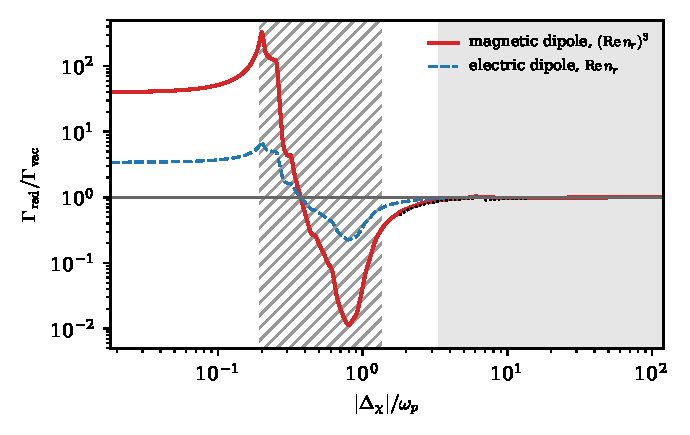
\includegraphics[width=0.82\linewidth]{figures/ch10/limit10_9d.pdf}
\captionof{figure}{Radiative decay rate of an excited state inside silicon over the vacuum rate, against the splitting $|\Delta_\chi|$ in units of the valence plasma frequency $\omega_p^{\mathrm{val}} = \SI{16.6}{eV}$. Red: magnetic dipole, $(\Real n_r)^3$; blue dashed: electric dipole, $\Real n_r$, local-field factors omitted. $n_r = \sqrt{\varepsilon}$ from the measured dielectric function of silicon at \SI{300}{K} below \SI{40}{eV}~\cite{franta2017temperature} and from atomic scattering factors above~\cite{henke1993xray}. Dotted: the free-electron-gas asymptote $n_r^3 \simeq 1 - 3\omega_p^2/2\omega^2$, with $\omega_p^{\mathrm{val}}$ below the $2p$ edge and the all-electron \SI{31.1}{eV} above. Hatched: $\Imag n_r > 0.1\Real n_r$, 3.2 to \SI{22.5}{eV}, where the radiative factor loses its meaning and the decay is a non-radiative transfer given by \cref{eq:10.9-decay} at finite $\mathcal{Q}$. Gray: splittings above \SI{55}{eV}, $3.3\,\omega_p^{\mathrm{val}}$, where $(\Real n_r)^3$ is within \SI{10}{\percent} of one.}\label{fig:10-decay-limit}
\par}
\smallskip
Below about $3\omega_p^{\mathrm{val}}$ the vacuum rate fails inside a solid: it is enhanced by $n_r^3 \approx 40$ in the transparent window of silicon below the gap and replaced by non-radiative transfer to the electrons where the crystal absorbs.
\end{limitbox}

\noindent No response of the target enters the vacuum rate; the medium acts only through $\varepsilon^{\mathrm{T}}$ at $\mathcal{Q} = \omega n_r$, and in a transparent medium the leading correction is the local field at the particle, which the macroscopic $\varepsilon$ does not contain.

\section{Nuisance parameters of the electronic rate}\label{sec:10.10}

A dark-matter particle of \SI{3}{MeV} with a heavy mediator and $\sigmae = \SI{e-37}{cm^2}$ makes $5.2\times10^4$ electron--hole pairs per kilogram-year in silicon if the electrons are independent, $2.5\times10^4$ if they screen in the random-phase approximation, and $1.85\times10^4$ once local fields are included. All three numbers come from the same published tables, counted from the low-temperature gap of \SI{1.17}{eV}, and they differ only in the many-body approximation. The last one is the best computed so far, but it is not the rate. The electron--hole attraction raises it, the conduction bands above the edge are uncertain at the level of a tenth of an eV, and two published tabulations of the same independent-particle response disagree by a third at this mass. \Cref{sec:8.8} turned each truncation into a nuisance parameter $\vartheta_k$, with the computed or estimated step to the next order as its template.

\subsection{Many-body spread}\label{sec:10.10-manybody}

The hierarchy of approximations of \cref{sec:4.6} is not an expansion in a small parameter, and its steps do not shrink. At \SI{3}{MeV} with a heavy mediator, random-phase screening lowers the independent-particle rate by \SI{52}{\percent}, and local fields lower what remains by a further \SI{26}{\percent}; for a light mediator the steps are \SI{76}{\percent} and \SI{18}{\percent}. The ratio of the independent-particle rate to the screened rate with local fields is 2.8 for a heavy mediator and 5.1 for a light one, between the values 2.3 and 9 that \cref{sec:10.2} found at 10 and \SI{1}{MeV}. A spread of this kind is not an uncertainty of the best approximation. Once an approximation is computed it becomes the central value, and the nuisance that remains is the step after it (\cref{sec:8.8}). For silicon that step is the electron--hole attraction, the excitonic (vertex) correction of the Bethe--Salpeter equation, and no finite-momentum calculation of it exists for silicon (\cref{sec:10.5}).

Its size can be estimated from the model of \cref{fig:10-xq}. At $|\vect{q}| = \SI{0.91}{keV}$ the attraction raises the screened loss function by 27 to \SI{29}{\percent} from the onset to \SI{3.5}{eV}, by \SI{49}{\percent} at \SI{4}{eV}, and by about \SI{30}{\percent} above, where part of the rise is an artifact of four conduction bands. A particle of \SI{3}{MeV} deposits at most $\tfrac12\mchi v_{\mathrm{max}}^2 = \SI{10.5}{eV}$, and the mean energy of its spectrum is \SI{4.7}{eV}. We take $\delta_{\mathcal{X}} = +0.28$ over that window, an estimate from a model at one momentum transfer, with the coupling block of \cref{eq:10.5-coupling} adding about $\pm0.10$ to it. The template has a definite sign: at $\vartheta_{\mathcal{X}} = 1$ the rate rises. By the $f$-sum identity \cref{eq:8.8-fsum} a many-body template is a tilt. Inside the \SI{10.5}{eV} window it raises the spectrum nearly uniformly and so acts like a normalization; the weight it moves comes from energies above the window, which the particle cannot reach. The same template, read at \SI{10}{MeV}, reaches \SI{35}{eV} and samples part of the compensating loss, so one $\vartheta_{\mathcal{X}}$ changes the rates at 3 and \SI{10}{MeV} by different fractions. The attraction also adds new support. The bound lines below the pair continuum carry the weight of the free continuum within $8.0\,E_x^b = \SI{0.12}{eV}$ of the edge (\cref{sec:10.5-lines}), which in the tables holds $4\times10^{-4}$ of the heavy-mediator rate at \SI{3}{MeV} and $1.5\times10^{-3}$ of the light-mediator rate. The tables resolve energies to \SI{0.2}{eV}, so these shares are orders of magnitude, and they matter only for thresholds at the gap.

A second nuisance sits inside the approximation already computed. At momentum transfers of two to three times the shortest reciprocal-lattice vector the local fields lower the per-$q$ rate of the tables by 1.67 at \SI{8}{keV} and 1.83 at \SI{10}{keV} (\cref{sec:10.2-corrections}). That size rests on a spectrum that holds only \SI{17}{\percent} of the $f$-sum below \SI{89}{eV} at \SI{10}{keV}. The model of \cref{fig:10-fcrys-limit}, built from a local pseudopotential with no input in common with the tables but the crystal structure, gives the same suppression. At \SI{5}{eV} and between 2 and $2.8\,q_0$ it finds the screened structure factor with local fields at 0.54 to 0.61 of the independent-particle one, with the head screening already within \SI{10}{\percent} of one above $2.2\,q_0$. The tables at the same energy and momenta give 0.40 to 0.48, with the head screening at 0.77 to 0.97 of the independent-particle value. Two calculations that share neither potential nor basis therefore agree that local fields hold the response near half of its unscreened value there, to within a quarter of each other. Both, however, lack the core-region oscillations of the valence states and the high-energy tail of the spectrum, and an all-electron calculation with enough bands is needed to fix the size (\cref{app:E.2,app:E.6}). The template is the change of the rate if the suppression above $2q_0 = \SI{7.46}{keV}$ were absent, $\vartheta = 1$ restoring the random-phase value there. It is $+0.067$ at \SI{3}{MeV} for a heavy mediator, where only \SI{7.5}{\percent} of the rate comes from those momenta, $+0.009$ for a light one, and $+0.24$ at \SI{10}{MeV}, where they hold \SI{29}{\percent} of the rate.

A third source is not a truncation of the label but of the numerics. The crystal form factor of \cref{sec:10.1} and the independent-particle head of the tables of \cref{sec:10.2} are the same quantity in the same approximation, computed with different codes, pseudopotentials and grids. With the same halo, each from its own onset, they give $1.60\times10^5$ and $1.36\times10^5$ events per kilogram-year at \SI{10}{MeV} for a heavy mediator, a ratio of 1.18, and 1.29 for a light one. At \SI{3}{MeV} the ratio is 1.34 for a heavy mediator and 1.55 for a light one. The difference sits at small $q$, where the lighter particle collects its rate, and the $f$-sum rule locates it. Between $0.3\,q_0$ and $0.7\,q_0$ the first moment of the form-factor table is 1.1 to 1.2 times the valence value (\cref{sec:10.1}), and that of the independent-particle head of the tables is 0.93 at every such momentum, partly because those tables end at \SI{89}{eV}. Neither table conserves the $f$-sum at small $q$, and the two violations lie on either side of it. The spread is measured with independent particles, but the central value is screened, and screening is strongest exactly at the small $q$ where the tables disagree. There a normalization error of $\varepsilon_2$ is partly screened out: if $\varepsilon_2$ and, by Kramers--Kronig, $\varepsilon_1 - 1$ are too large by $1 + \delta$ where $\varepsilon_1 \gg 1$, then $L \simeq \varepsilon_2/\varepsilon_1^2$ moves by about $1/(1 + \delta)$, opposite in sign and no larger. The independent-particle ratio is therefore an upper bound on the spread of the screened rate, and we carry it as such. \Cref{sec:8.8} named this case: for a truncation that breaks the $f$-sum the violation measures the error, and the spread between the calculations is the nuisance until a converged calculation passes the test (\cref{app:E.7}).

The Bethe--Salpeter step carries one more pitfall, an evaluation error rather than a truncation. A Bethe--Salpeter calculation that keeps only the resonant poles has the right $\varepsilon_2$ and the wrong $\varepsilon_1$, and it overstates the loss function by 2.12 at \SI{1.39}{keV} and \SI{1.3}{eV}, falling to within \SI{15}{\percent} of one above \SI{6.7}{keV} (\cref{eq:10.5-res}). Both time orderings remove it. It is listed below because a rate that inherits it is wrong by a factor that no nuisance of the correct calculation covers.

\subsection{Gap and threshold nuisances}\label{sec:10.10-gap}

The tables carry a scissor shift that places the conduction bands at the measured gap of silicon at zero temperature, \SI{1.17}{eV}~\cite[Sect.~III\,B]{knapen2021dark}, the gap a detector at millikelvin temperatures has, with the zero-point renormalization included in the measurement (\cref{sec:3.4}). The rate is counted from that gap, and the threshold mass is $m_{\mathrm{min}} = 2\Eg/v_{\mathrm{max}}^2 = \SI{0.333}{MeV}$. The \SI{1.11}{eV} that often accompanies these tables in analysis codes is a different number, the gap of the step model of pair creation with \SI{3.6}{eV} per pair (\cref{sec:1.5}), not the gap of the response. The energy nodes of the tables lie \SI{0.2}{eV} apart and do not resolve the edge itself.

What remains depends on what is measured. The edge itself is known to a few meV, and a shift of \SI{5}{meV} changes the \SI{3}{MeV} rate by \SI{0.4}{\percent}. A scissor, however, moves every conduction band by the same amount, and quasiparticle corrections in silicon differ from state to state by about \SI{0.1}{eV} (\cref{sec:3.4}). The bands above the edge are therefore uncertain at that level even when the edge is not. A shift of the whole spectrum by \SI{0.1}{eV} bounds this effect from above: it changes the \SI{3}{MeV} rate by $-7.5$ and $+8.0$ percent for a heavy mediator, by $\mp10$ percent for a light one, and the \SI{10}{MeV} heavy-mediator rate by \SI{4}{\percent}. The effect grows toward the threshold mass, where the spectrum samples only the first eV above the edge. For a target whose gap has not been measured the edge itself carries the \SI{0.1}{eV}, and $\delta\ln m_{\mathrm{min}} = \delta\ln\Eg$ turns it into \SI{8.5}{\percent} in the threshold mass of silicon (\cref{we:3-mmin-gap}). Near that mass the halo supply changes by orders of magnitude over a factor of two in $\mchi$, and the rate there depends on the gap more than on any other entry of the table below. The exciton binding of \SI{14.7}{meV} is a threshold nuisance of the same kind, which lowers the first line to \SI{1.155}{eV} (\cref{we:10-xline}), and \cref{tab:8-nuisances} carries it.

\subsection{Nuisance table of the electronic sector}\label{sec:10.10-table}

\Cref{tab:10-nuisances} lists the nuisances of the electronic sector. A next order computed in a model gives a template whose sign and shape are known and whose value may change once the real calculation is done. An estimate from a small parameter gives the size to a factor of order one. A spread between published calculations at the same order stands in for a template where the error lies outside the truncation label. An inequality gives a range without a central value, and for some items only the omission can be named.
\begin{table}[tbp]
  \caption{Electronic nuisances. Type in the classes of \cref{sec:8.8}: normalization, tilt (in $\omega$ or in $q$), threshold, new support, and class mix (weight moved between the zero-phonon and phonon-dressed sectors without changing the total). Basis of the size: ``model'' (next order computed in a model), ``tables'' (evaluated from the published tables), ``est.''\ (small-parameter estimate), ``spread'' (published calculations at the same order), ``bound'' (only an inequality is known), ``named'' (no size). Sizes are for silicon unless germanium is named, with rates at \SI{3}{MeV} for a heavy mediator. The last column gives the section where the open calculation is stated.}
  \label{tab:10-nuisances}
  \centering\small\setlength{\tabcolsep}{3pt}
  \begin{tabular}{@{}>{\raggedright\arraybackslash}p{0.26\linewidth}>{\raggedright\arraybackslash}p{0.13\linewidth}>{\raggedright\arraybackslash}p{0.34\linewidth}>{\raggedright\arraybackslash}p{0.09\linewidth}>{\raggedright\arraybackslash}p{0.12\linewidth}@{}}
    \toprule
    Truncation & Type & Size & Basis & Section \\
    \midrule
    Electron--hole attraction ($\mathcal{X}$: RPA + LF $\to$ BSE) & tilt; new support & $L$ up by 27--\SI{29}{\percent} near the edge at \SI{0.91}{keV}; rate $\delta_{\mathcal{X}} \approx +0.28$; lines $4\times10^{-4}$ of the rate & model & \cref{sec:10.5} \\
    Coupling block dropped (BSE in Tamm--Dancoff form) & tilt & about \SI{10}{\percent} of the proper $\varepsilon_2$ & est. & \cref{sec:10.5} \\
    Resonant-only real part (evaluation error) & tilt in $q$ & $L$ $\times2.12$ at \SI{1.39}{keV}, \SI{1.3}{eV}; within \SI{15}{\percent} above \SI{6.7}{keV} & tables & \cref{sec:10.5} \\
    Local fields at $q \gtrsim 2q_0$ (bands, pseudo-states) & tilt in $q$ & per-$q$ factor 1.67 (\SI{8}{keV}), 1.83 (\SI{10}{keV}); rate $+0.066$ if absent above $2q_0$ ($+0.24$ at \SI{10}{MeV}) & spread & \cref{sec:10.2} \\
    Independent-particle tabulation (code, grid, pseudopotential) & normali\-zation at small $q$ & IP rates differ by 1.34 (1.18 at \SI{10}{MeV}), an upper bound for the screened rate; $f$-sum 1.1--1.2 against 0.93 at $0.3$--$0.7\,q_0$ & spread & \cref{sec:10.1} \\
    Quasiparticle gap (rigid scissor) & threshold & edge measured, few meV; bands \SI{0.1}{eV}: rate $-7.5$/$+8.0\,\%$; $m_{\mathrm{min}}$ \SI{8.5}{\percent} without a measured gap & spread & \cref{sec:3.4} \\
    Plasmon decay into pairs with phonons ($n_g = 2$) & class mix & branching $10^{-3}$ to $10^{-2}$ & est. & \cref{sec:10.3} \\
    Local fields of the transverse current & normali\-zation & $-4$ to $-15\,\%$ (model); $-10$ to $-30\,\%$ (est.) & model & \cref{sec:10.4} \\
    Density--current cross term of a velocity coupling & normali\-zation & rate at least 16 (IP), about 29 (screened) times the static-electron formula at \SI{10}{MeV} & bound & \cref{sec:10.4} \\
    Triplet response beyond independent pairs & tilt & weight $\times2.2$ below \SI{3}{eV} (model); exchange splitting $\sim10^{-3}$ of the binding & model & \cref{sec:10.5} \\
    Final states of the germanium $3d$ shell & normali\-zation & $3d$/valence 0.07 (plane waves) against 0.69 (Fermi factor) at \SI{30}{MeV} & bound & \cref{sec:10.6} \\
    Screening of core transitions & normali\-zation & macroscopic \SI{2}{\percent} at \SI{12}{keV} (Ge); local fields not computed & est. & \cref{sec:10.6} \\
    Relativistic corrections (Pauli order) & normali\-zation & about $10^{-3}$, at most \SI{2}{\percent} (Ge $3d$); next order $3\times10^{-6}$ & est. & \cref{sec:10.6} \\
    Spin--orbit mixing at the germanium edge & tilt & up to \SI{10}{\percent} in amplitude & est. & \cref{sec:10.6} \\
    Terms of order $p_\phi^2$ in scalar absorption & new support near $\omega_p$ & density row equal to the kinetic rate at 16--\SI{18}{eV} (model) & named & \cref{sec:10.7} \\
    Room-temperature optical data near the edge ($n_T$) & threshold & more than $\times2$ within about \SI{20}{meV} of the edge & est. & \cref{sec:13.5} \\
    Bound shells in dark Compton scattering & tilt & K shell of Si at 45--\SI{100}{keV}, of Ge up to \SI{118}{keV}; L shells below \SI{20}{keV} & named & \cref{sec:10.8} \\
    Axial pair absorption with spin--orbit coupling & new support & of order $v^4$ without it & named & \cref{sec:10.8} \\
    Average over the directions of $\vect{q}$ & tilt in time & first anisotropic term $\ell = 4$ & named & \cref{sec:11.7} \\
    \bottomrule
  \end{tabular}
\end{table}

Two of these nuisances change the silicon rate at \SI{3}{MeV} by more than ten percent: the electron--hole attraction, by about a quarter, and the spread between tabulations of the independent-particle response, by a third for a heavy mediator and by half for a light one. At \SI{10}{MeV} the local fields at large momentum transfer join them, with a quarter, and the tabulation spread falls to a fifth. The gap stays below ten percent above \SI{3}{MeV} but grows without limit toward the threshold mass. Outside the density rows the largest items are not nuisances in the sense of a computed step. The cross term of a velocity coupling and the final states of the germanium $3d$ shell are known only between bounds, a factor of ten apart for germanium near \SI{30}{MeV}. A limit set on such a coupling has no central value yet, and the bound itself is what it can use (\cref{sec:10.4}).

One rule governs how the rows enter a likelihood. A truncation that two rates share acts on both with one $\vartheta_k$ (\cref{sec:8.8}). The attraction raises the rate at every mass and for both mediators at once, by different fractions, and a combination of masses or experiments that treated it as independent nuisances would let the data play one against the other. The inelastic, exothermic, boosted and fermionic rates of \cref{sec:10.9} read the same loss function and transverse current at shifted kinematics, and they carry the same nuisances with the same parameters; they add no rows of their own. Where one rate uses the tables and another the measured optical constants, as the scattering and absorption rates of \cref{sec:10.2,sec:10.7} do, the two share the many-body truncation only through what the measurement contains, and the absorption rate carries the temperature row instead.

\begin{workedexample}{The nuisance band on the silicon rate at \SI{3}{MeV}}\label{we:10-band3}
Take $\mchi = \SI{3}{MeV}$, a heavy mediator, $\sigmae = \SI{e-37}{cm^2}$ and the standard halo of \cref{sec:1.2}, with $\rho_\chi = \SI{0.3}{GeV.cm^{-3}}$. The kinematic window ends at $\omega = \SI{10.5}{eV}$ and $q = 2\mchi v_{\mathrm{max}} = \SI{15.9}{keV}$. The central value is the loss-function rate \cref{eq:10.2-rate} with the random-phase loss function with local fields of the tables of \cref{sec:10.2}, counted from the low-temperature gap of \SI{1.17}{eV}:
\begin{equation*}
  \mathcal{R}^{\mathfrak{T}} = \SI{1.85e4}{kg^{-1}.yr^{-1}} ,
\end{equation*}
about 51 events per kilogram and day. Its spectrum has a mean energy of \SI{4.7}{eV}, and \SI{10}{\percent} of it lies below \SI{3}{eV}.

Four nuisances act on this number with sizes in hand. In the power form \cref{eq:8.8-M}, $\mathcal{R}(\vartheta) = \mathcal{R}^{\mathfrak{T}}\prod_k(1 + \delta_k)^{\vartheta_k}$, each enters through $\ln(1 + \delta_k)$:
\begin{equation*}
  \begin{aligned}
  &\text{attraction, } \delta_{\mathcal{X}} = +0.28: & \ln(1 + \delta) &= +0.247, \\
  &\text{tabulation spread (bound), } +0.335: & &+0.289, \\
  &\text{band energies, } \SI{0.1}{eV}: & &-0.078, \\
  &\text{local fields above } 2q_0,\ +0.066: & &+0.064.
  \end{aligned}
\end{equation*}
The four are separate truncations with independent standard-normal $\vartheta_k$. To first order the logarithm of the rate then has the Gaussian width of \cref{eq:C.14-quadrature}, the four logarithms added in quadrature,
\begin{equation*}
  \sigma_{\ln\mathcal{R}} = \bigl(0.247^2 + 0.289^2 + 0.078^2 + 0.064^2\bigr)^{1/2} = 0.393 ,
\end{equation*}
and the rate lies between $\mathcal{R}^{\mathfrak{T}}/\ee^{0.393}$ and $\mathcal{R}^{\mathfrak{T}}\ee^{0.393}$ at one standard deviation:
\begin{equation*}
  \SI{1.25e4}{kg^{-1}.yr^{-1}} \le \mathcal{R} \le \SI{2.75e4}{kg^{-1}.yr^{-1}} ,
\end{equation*}
a factor of 1.48 either way. The attraction and the tabulation spread carry \SI{93}{\percent} of the variance. Taking the attraction at the upper value of the model, $+0.49$, widens the factor to 1.65; the coupling block, $\pm0.10$ on $\delta_{\mathcal{X}}$, changes $\ln(1 + \delta_{\mathcal{X}})$ by 0.075.

The band is not symmetric about the best guess. The attraction has a known sign, and $\vartheta_{\mathcal{X}} = 1$ moves the central value to $2.37\times10^4$; the band of the power form describes the uncertainty of where the next approximation lands, not a symmetric spread around the present one. The tabulation spread has no known sign, since the two tables miss the $f$-sum on opposite sides. For a light mediator the same steps give a central value of $6.0\times10^3$ and a factor of 1.67, with the tabulation spread at $+0.55$ and the gap at $-0.10$, and the local fields at large $q$ below one percent.

The band covers the truncations that the density response of silicon carries at this mass. It does not cover the halo, which the likelihood of \cref{eq:8.8-like} holds fixed, nor the detector, whose nuisances \cref{sec:21.4} adds. It is also wider than the step between the two best computed approximations, $2.49\times10^4$ to $1.85\times10^4$. That step is not an uncertainty, since it has been taken; the band covers the next step and the spread between calculations in the same approximation.
\end{workedexample}

\subsection{Open problems}\label{sec:10.10-open}

A finite-momentum Bethe--Salpeter calculation for silicon and germanium, with the coupling block kept and the bound lines added from computed masses and vertices, fixes the attraction, the coupling block, the triplet channel and the spin--orbit mixing at the germanium edge (\cref{sec:10.5,sec:10.6}; \cref{app:E.15}). An all-electron random-phase calculation with local fields, with enough bands to hold the $f$-sum at \SI{10}{keV} and with the current and kinetic rows carried as external rows of the Dyson equation, fixes the local fields at large $q$, the screening of core transitions, the transverse-current fields, the in-medium ratio of velocity couplings and the order-$p_\phi^2$ terms of scalar absorption (\cref{sec:10.2,sec:10.4,sec:10.7}; \cref{app:E.6,app:E.16}). Until these rows are computed, \cref{eq:10.4-band} is all a limit on a velocity coupling can use. Crystal conduction states for the germanium $3d$ shell, and a four-component response for the bound on relativistic terms, settle the core rows (\cref{sec:10.6}). A second-order electron--phonon calculation at the plasma frequency, and shell Compton profiles, settle the plasmon branching and the bound-shell correction to dark Compton scattering (\cref{sec:10.3,sec:10.8}; \cref{app:E.26}). The spread between tabulations needs no new physics, only one converged calculation that passes the $f$-sum test at small $q$.

The quadratic response, two published rates and the self-trapped excitons of NaI are open items that are not nuisances of the rates computed here. The interference between a contact amplitude and a second-order one needs the quadratic response of the crystal, which no reduction to two-point functions supplies (\cref{sec:10.8-open}). The free-electron vertex of fermionic absorption on a bound shell underestimates the rate by at least $1/r$, and the density row of cosmic-ray-boosted dark matter without its retardation factor overstates the rate at relativistic speeds (\cref{sec:10.9-open}). And the self-trapped excitons of NaI, where the Wannier picture fails, are open in every quantity that the rate needs (\cref{sec:10.5}).

\section*{Summary}

An electron--hole pair in silicon costs at least the gap, and the rate of making pairs is a contraction of the master formula with the response of the electrons (\cref{sec:10.1}). For independent electrons the structure factor is a sum over valence--conduction pairs with plane-wave vertices at the unfolded momentum transfer, and its angle average, rescaled, is the crystal form factor on which most published limits rest. Its normalization is where tabulations go wrong, and the $f$-sum rule tests it. From the published silicon form factor a \SI{10}{MeV} particle with a heavy mediator and $\sigmae = \SI{e-37}{cm^2}$ gives $1.60\times10^5$ events per kilogram-year, \SI{27}{\percent} of them from $q > 2q_0$, where pseudo-wavefunctions lose accuracy. The excess of its $f$-sum at small $q$ is only partly explained by the scissor shift.

Screening enters through one function, the loss function, and the loss-function rate is exact for a coupling to the total charge and for a coupling to the electron density at clamped nuclei or above the phonon band (\cref{sec:10.2}). In the published silicon tables the \SI{10}{MeV} rate is $1.36\times10^5$ for independent particles (two independent-particle tabulations differ by \SI{18}{\percent}, \cref{sec:10.10-manybody}), $8.6\times10^4$ with random-phase screening and $5.9\times10^4$ with local fields. The independent-particle rate is too high by 2.3 for a heavy mediator and 3.7 for a light one, and at the large momentum transfers that carry the heavy-mediator rate the local fields, not the head screening, do most of the work. The $f$-sum and the static step bound the rate of any target, loosely for silicon at MeV masses. A mediator that couples to electrons alone breaks the bound on the static step once the lattice relaxes, through the acoustic peak of the electrons that follow the nuclei.

The electron gas at the valence density reproduces the silicon rate within a factor 1.5 between 4.2 and \SI{9.5}{eV}, and fails below the absorption peaks, where it has no gap, and at large energies, where bound electrons carry momenta the gas lacks (\cref{sec:10.3}). Its plasmon is the pole of the inverse dielectric function, but halo dark matter cannot reach it: the slowest plasmon needs a particle faster than \SI{2860}{km.s^{-1}}. A plasmon made otherwise decays into pairs, and into pairs with phonons with a branching estimated at $10^{-3}$ to $10^{-2}$.

Couplings to the electron spin and current need responses beyond the density (\cref{sec:10.4}). Continuity, spin rotation and the product of inversion and time reversal reduce them to twelve real functions per momentum and energy in silicon and germanium, in a singlet block, screened, and a triplet block, unscreened. A velocity coupling adds the transverse current to the density, and a formula that keeps only the dark matter's velocity underestimates its rate in silicon at \SI{10}{MeV} by at least a factor 16 for independent particles, and about 29 with the density row screened.

The electron--hole attraction moves weight toward the gap and adds bound lines below it (\cref{sec:10.5}). In silicon the $1s$ line lies at \SI{1.155}{eV}, below the low-temperature gap of \SI{1.17}{eV}. In a model at \SI{0.91}{keV} the attraction raises the screened loss function by 27 to \SI{29}{\percent} near the edge. An evaluation that drops the antiresonant poles overstates the loss function by a factor 2.12 at small momentum transfer, and dropping the coupling block costs about \SI{10}{\percent}. The triplet channel has the singlet's lines without its local fields or screening.

Core shells enter at large momentum transfer (\cref{sec:10.6}). The germanium $3d$ shell opens at \SI{11.3}{keV} and overtakes the valence at \SI{12.5}{keV}; whether it dominates a rate depends on its final states, and with crystal states it does so above about \SI{30}{MeV} at a one-pair threshold. A filled, flat shell responds as a sum of independent atoms, without interference with the valence. Relativistic corrections to the response are about $10^{-3}$ and at most \SI{2}{\percent} for the shells halo dark matter reaches, and they shift the $f$-sum by $-0.24$ and $-0.76$ percent in silicon and germanium.

Absorbed bosons sample the response at zero momentum (\cref{sec:10.7}). A dark photon is absorbed with the loss function at its mass, suppressed 761 times at \SI{3}{eV} in silicon and enhanced 20 times at the plasmon, \SI{16.4}{eV}. An axion-like particle couples to the spin current, whose response without spin--orbit coupling is three quarters of the current response and is not screened; in a static magnetic field it converts like a dark photon. A scalar couples to the kinetic energy of the electrons, and mixes with the photon only at order $p_\phi^2$ in crystals without a polar axis.

Two insertions of the dark field reach rates that one insertion forbids (\cref{sec:10.8}). The absorption of a particle and its antiparticle is single absorption at twice the mass, and the pseudoscalar pair is absorbed through the axioelectric row without velocity suppression. Dark Compton scattering is the main signal of a dark photon in silicon above \SI{55}{keV}; its seagull form is exact to \SI{1}{\percent} below \SI{165}{keV}, and the published axion-like rate is too large by $(m_\phi + 2m_e)/(m_\phi + m_e)$, 1.836 at \SI{100}{keV}.

Inelastic, exothermic, boosted and fermionic dark matter use the same responses at other kinematics (\cref{sec:10.9}). An endothermic splitting of \SI{1}{eV} raises the lightest mass that makes pairs to \SI{0.60}{MeV}, and an exothermic one turns the spectrum into a halo-independent shell. For boosted particles with a massless mediator the exact density row is 0.65 of the published one at $v = 0.9$, and above $v = \varepsilon_1^{-1/2}$ the transverse row adds Cherenkov emission. An excited state below the gap decays radiatively 41 to 44 times faster inside silicon than in vacuum.

Each approximation of the chapter is a nuisance with a size (\cref{sec:10.10}). At \SI{3}{MeV} with a heavy mediator the silicon rate at the low-temperature gap is $1.85\times10^4$ events per kilogram-year, uncertain by a factor of 1.48 at one standard deviation. The electron--hole attraction and the spread between published independent-particle tables dominate; the gap and the local fields at large $q$ add less than ten percent each. Outside the density rows, the cross term of velocity couplings and the final states of the germanium $3d$ shell are known only between bounds. Throughout the chapter the nuclei were held fixed. \Cref{chap:11} releases them, and the energy a light particle deposits goes into phonons.


\printbibliography[heading=subbibliography]

\chapter{Lattice excitations}\label{chap:11}
Below about \SI{10}{MeV} the largest free recoil energy that a nucleon-coupled dark-matter particle gives a silicon nucleus falls to the phonon energies, and the nucleus can no longer be treated as free. At that mass the largest momentum transfer is about \SI{50}{keV}, the free recoil energy $q^2/2M$ is \SI{50}{meV}, equal to the energy of the phonons themselves. Lighter particles give the nucleus less than one phonon's worth of energy, and the deposited energy goes into the lattice instead of into a free recoil. At the lowest masses it goes into a single acoustic or optical phonon, at intermediate masses into a few phonons, and only at the top of the range into a recoil broadened by the motion of the nucleus in its well. The electronic channels of \cref{chap:10} need an electron to cross a gap of an eV; the lattice channels need only a phonon of a few meV, and with a meV threshold they reach masses fifty times smaller than the electronic channels do. What is the rate, across that whole range, and which numbers of a material decide it?

From the harmonic crystal of \cref{chap:5} and the master formula of \cref{chap:8}, each regime of \cref{fig:11-map} reduces to a few material numbers: sound speeds, Born effective charges and Debye--Waller exponents, and each reduced rate is checked against a fuller calculation. Throughout, the electrons stay in their ground state and follow the nuclei. The Migdal effect and phonon-assisted electron recoil start from the lattice sector of this chapter and follow in \cref{chap:12,chap:13}.

\begin{figure}[tbp]
  \centering
  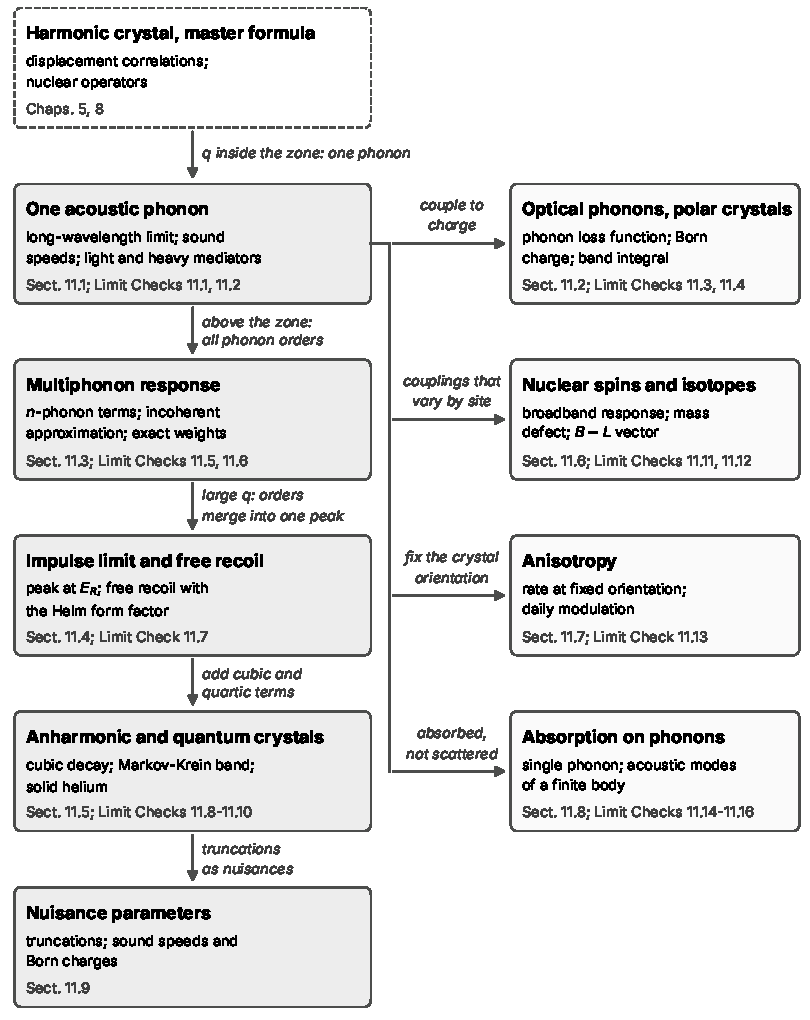
\includegraphics[width=0.85\linewidth]{figures/ch11/map11.pdf}
  \caption{The lattice regimes of the nuclear response and their branches. Left, as the momentum transfer grows: one acoustic phonon inside the zone (\cref{sec:11.1}; \cref{lim:11.1a,lim:11.1b}); all phonon orders at momentum transfers beyond the zone (\cref{sec:11.3}; \cref{lim:11.3a,lim:11.3b}); the orders merging into one peak at $E_R$, whose limit is the free nuclear recoil (\cref{sec:11.4}; \cref{lim:11.4a}); cubic and quartic terms (\cref{sec:11.5}; \cref{lim:11.5a,lim:11.5c,lim:11.5b}); the uncertainty budget of these rates (\cref{sec:11.9}). Right: coupling to charge excites optical phonons of polar crystals (\cref{sec:11.2}; \cref{lim:11.2a,lim:11.2b}); couplings that vary from site to site, nuclear spins and isotopes (\cref{sec:11.6}; \cref{lim:11.6a,lim:11.6b}); a crystal of fixed orientation and the daily modulation (\cref{sec:11.7}; \cref{lim:11.7a}); and absorption on phonons and acoustic modes (\cref{sec:11.8}; \cref{lim:11.8a,lim:11.8b,lim:11.8c}).}
  \label{fig:11-map}
\end{figure}

\section{Acoustic phonons}\label{sec:11.1}

A dark-matter particle of \SI{100}{keV} transfers at most $2\mchi v_{\mathrm{max}} = \SI{0.53}{keV}$ of momentum. Given to a free silicon nucleus, that momentum would deposit $q^2/2M = \SI{5.4}{\micro eV}$, far below any threshold. Given to the crystal, it can create one longitudinal acoustic phonon of energy $c_{\mathrm{LA}}q \approx \SI{16}{meV}$, because the whole crystal takes up the momentum and the energy is set by the sound speed rather than by the mass of a nucleus. The kinematic match, with the momentum taken up by the whole crystal and the energy set by the sound speed, makes single phonons the channel of the lightest dark matter that couples to nucleons (\cref{sec:1.3}). At long wavelengths the single-phonon rate depends on the material only through the sound speeds, and for a light mediator it is the same for every material.

\subsection{The one-phonon response}

Take a dark-matter particle that couples to protons and neutrons with the same potential $\tilde V_N(\vect{q})$, the spin-independent coupling $\mathcal{O}_1$ of \cref{sec:8.1}. By \cref{eq:8.1-nuclear}, a nucleus of species $\kappa$ then carries the coupling $A_\kappa\tilde V_N(\vect{q})F_N(q)$, and the dark matter sees the target through the single operator
\begin{equation*}
  O_N(\vect{q}) = \sum_\kappa A_\kappa\,n_\kappa(\vect{q}) ,
\end{equation*}
the nucleon number density of the crystal at momentum $\vect{q}$. The nuclear form factor $F_N$ of \cref{eq:2.2-FN} is one to better than $10^{-3}$ at the momentum transfers of this section, which stay below a few keV, and we drop it. The coupling has no electronic row, so the electrons enter only through the forces they transmit between nuclei: the phonons are those of the Born--Oppenheimer surface (\cref{sec:5.1}), and the final states lie in the electron-following sector of \cref{tab:8-sectors}. Screening, which acts on rows that couple to charge (\cref{sec:8.4}), does not enter. The dark photon, which couples to charge, is the subject of \cref{sec:11.2}.

The rate per unit target mass is \cref{eq:8.2-spectrum} with one row, $\mathfrak{D} = |\tilde V_N(\vect{q})|^2$ and $S = S_A$. Here $\omega_{\vect{q}} = \vect{q}\cdot\vect{v} - q^2/2\mchi$ is the energy the dark matter loses (\cref{eq:1.3-omegaq}), not a phonon frequency, and $S_A$ is the response \cref{eq:4.2-Sab} of $O_N$, the nuclear block $\sum_{\kappa\kappa'}A_\kappa A_{\kappa'}S_{\kappa\kappa'}$. The one-phonon part of $S_A$ follows from the amplitude of \cref{sec:5.3}. To first order in the displacement, a nucleus of species $\kappa$ emits a phonon $\vect{Q}\nu$ with the amplitude
\begin{equation*}
  \langle n_{\vect{Q}\nu} + 1|\,n_\kappa(\vect{q})\,|n_{\vect{Q}\nu}\rangle = \ii\,\ee^{\ii\vect{q}\cdot\vect{\tau}_\kappa}\,\frac{\vect{q}\cdot\vect{e}_{\kappa\nu}(\vect{Q})^*}{\sqrt{2M_\kappa\omega_{\vect{Q}\nu}}}\,\sqrt{N(n_{\vect{Q}\nu} + 1)}\,\sum_{\vect{G}}\delta_{\vect{q},\vect{Q} + \vect{G}} .
\end{equation*}
Keeping the full exponential of the displacement multiplies this amplitude by $\ee^{-W_\kappa(\vect{q})}$: to first order in the displacement correlation $\mathcal{C}_{\kappa\kappa'}$, the generating formula \cref{eq:5.6-gen} for a pair of nuclei is the one-phonon term with the factor $\ee^{-W_\kappa - W_{\kappa'}}$ in front. The amplitudes of the nuclei of one cell add with their phases. We square, sum over the final phonon states and divide by the volume $\Vol = N\Omega$ as in \cref{eq:4.2-Sab}. The factor $N$ cancels, and the Kronecker delta leaves in each branch one phonon wavevector $\vect{Q}$, the reduction of $\vect{q}$ to the first Brillouin zone:
\begin{keyresult}[One-phonon nuclear response]
\begin{equation}
  \begin{aligned}
  S^{(1)}_A(\vect{q},\omega) = \frac{2\pi}{\Omega}\sum_\nu{}&\frac{\bigl|\sum_\kappa A_\kappa\,\ee^{-W_\kappa(\vect{q})}\,\ee^{\ii\vect{q}\cdot\vect{\tau}_\kappa}\,\vect{q}\cdot\vect{e}_{\kappa\nu}(\vect{Q})^*/\sqrt{M_\kappa}\bigr|^2}{2\omega_{\vect{Q}\nu}} \\
  &\times\Bigl[(n_{\vect{Q}\nu} + 1)\,\delta(\omega - \omega_{\vect{Q}\nu}) + n_{\vect{Q}\nu}\,\delta(\omega + \omega_{\vect{Q}\nu})\Bigr] ,
  \end{aligned}
  \label{eq:11.1-S1}
\end{equation}
with $\vect{Q} = \vect{q} - \vect{G}$ in the first zone, $\vect{q}$ itself unreduced in the phase $\ee^{\ii\vect{q}\cdot\vect{\tau}_\kappa}$, and the phase convention of \cref{eq:5.3-u}.
\end{keyresult}
\noindent The absorption term follows from the second matrix element of \cref{eq:5.3-me}; since $\vect{e}_{\kappa\nu}(-\vect{Q}) = \vect{e}_{\kappa\nu}(\vect{Q})^*$, the modulus of the amplitude is unchanged. In a detector at \SI{10}{mK}, $n_{\vect{Q}\nu}$ vanishes for every phonon above a few tens of \si{\micro eV} (\cref{sec:5.3}), and only emission remains. On the truncation label of \cref{sec:8.5}, \cref{eq:11.1-S1} is the point $\mathcal{K}$ = one-phonon, $n_A = 0$, with $n_T = 0$ for the emission term and $n_T = 1$ for the absorption term, and $n_B = 0$ throughout.

The weight of a branch in \cref{eq:11.1-S1} is the projection of $\vect{q}$ on the displacement of each nucleus, divided by the phonon energy, so that soft modes polarized along $\vect{q}$ dominate. The momentum is conserved up to a reciprocal-lattice vector, so that each $\vect{q}$ excites one phonon per branch, with the energy fixed by the dispersion: the response is a set of sharp lines in $\omega$ at fixed $\vect{q}$. And the Debye--Waller factor $\ee^{-2W_\kappa}$ of \cref{eq:5.6-W} measures the competition with the multiphonon terms of \cref{sec:11.3}. In silicon, $2W_\kappa = q^2\langle u_x^2\rangle$ is $3\times10^{-3}$ at $q = \SI{2.25}{keV}$ with the zero-temperature $\langle u_x^2\rangle = \SI{2.45e-3}{\angstrom^2}$ of \cref{we:5-dw}, so in the first Brillouin zone the factor is one to $3\times10^{-3}$.

\subsection{The long-wavelength limit}

Most of the rate of light dark matter comes from momentum transfers well inside the first zone. For a crystal with a lattice constant of a few \si{\angstrom}, the scale of the zone is
\begin{equation}
  q_{\mathrm{BZ}} = \Bigl(\frac{6\pi^2}{\Omega}\Bigr)^{1/3} ,
  \label{eq:11.1-qBZ}
\end{equation}
the radius of a sphere with the volume of the Brillouin zone, which holds one wavevector per primitive cell. For silicon, $\Omega = a^3/4$ and $q_{\mathrm{BZ}} = \SI{1.139}{\angstrom^{-1}} = \SI{2.25}{keV}$, between the distances from $\mathrm{\Gamma}$ to L (\SI{1.98}{keV}) and to X (\SI{2.28}{keV}). The zone scale $q_{\mathrm{BZ}}$ should not be confused with the Debye wavevector $Q_{\mathrm{D}}$ of \cref{eq:5.2-debye}, which counts one wavevector per atom and is larger by $n_{\mathrm{at}}^{1/3}$.

For $q \ll q_{\mathrm{BZ}}$, \cref{sec:5.2} removes the reciprocal-lattice vector, the internal motion of the cell and the curvature of the dispersion. The reciprocal-lattice vector is $\vect{G} = 0$ and $\vect{Q} = \vect{q}$. The acoustic polarization vectors move every nucleus of the cell together, $\vect{e}_{\kappa\nu} = (M_\kappa/M_{\mathrm{cell}})^{1/2}\hat{\vect{e}}_\nu(\hat{\vect{q}})$, with $\hat{\vect{e}}_\nu$ the unit polarizations of the Christoffel problem (\cref{app:C.18}), and the dispersion is linear, $\omega_{\vect{q}\nu} = c_\nu(\hat{\vect{q}})\,q$. And the phases $\ee^{\ii\vect{q}\cdot\vect{\tau}_\kappa}$ and the Debye--Waller factors are one up to corrections of order $qa$ and $q^2\langle u_x^2\rangle$. The sum over nuclei in \cref{eq:11.1-S1} then becomes $q\,(\hat{\vect{q}}\cdot\hat{\vect{e}}_\nu)\sum_\kappa A_\kappa/\sqrt{M_{\mathrm{cell}}}$, the optical branches drop out, since the center of mass of the cell is at rest in an optical branch (\cref{sec:5.2}), and at $T = 0$
\begin{equation*}
  S^{(1)}_A(\vect{q},\omega) = \frac{\pi\,q\,A_{\mathrm{cell}}^2}{\Omega\,M_{\mathrm{cell}}}\sum_{\nu = 1}^{3}\frac{(\hat{\vect{q}}\cdot\hat{\vect{e}}_\nu)^2}{c_\nu(\hat{\vect{q}})}\,\delta\bigl(\omega - c_\nu(\hat{\vect{q}})\,q\bigr) ,
\end{equation*}
with $A_{\mathrm{cell}} = \sum_\kappa A_\kappa$ the number of nucleons in a cell. Dividing by $\rho_T = M_{\mathrm{cell}}/\Omega$ and writing the nuclear masses as $M_\kappa = A_\kappa m_u$ with $m_u = \SI{931.494}{MeV}$ the atomic mass unit gives
\begin{keyresult}[Long-wavelength acoustic structure factor]
\begin{equation}
  \frac{S^{(1)}_A(\vect{q},\omega)}{\rho_T} = \frac{\pi q}{m_u^2}\sum_{\nu = 1}^{3}\frac{(\hat{\vect{q}}\cdot\hat{\vect{e}}_\nu)^2}{c_\nu(\hat{\vect{q}})}\,\delta\bigl(\omega - c_\nu(\hat{\vect{q}})\,q\bigr) , \qquad q \ll q_{\mathrm{BZ}} .
  \label{eq:11.1-Sac}
\end{equation}
\end{keyresult}
\noindent Per unit mass, the coherent sum over the $A_{\mathrm{cell}}$ nucleons of a cell leaves a response independent of the composition. The material enters through its sound speeds and the polarizations of its acoustic branches. The weights $(\hat{\vect{q}}\cdot\hat{\vect{e}}_\nu)^2$ sum to one over the three branches, by the completeness of the polarizations, and along a symmetry direction the longitudinal branch takes all of the weight. In a general direction the polarizations of the quasi-transverse branches are not exactly perpendicular to $\hat{\vect{q}}$ (\cref{app:C.18}), and the quasi-transverse branches take a small share. The binding energy of the nuclei and the isotopic mixture make $M_\kappa/A_\kappa$ differ from $m_u$ by less than a percent, so the replacement $M_\kappa = A_\kappa m_u$ is accurate to a percent.

\begin{limitbox}[Long-wavelength acoustic structure factor][lim:11.1a]
At momentum transfers small compared with the zone, and for a coupling to nucleon number, the longitudinal acoustic branch carries the one-phonon response of a crystal per unit mass, $S/\rho_T = (\pi q/m_u^2)\,\delta(\omega - c_{\mathrm{LA}}q)/c_{\mathrm{LA}}$, the same for every composition~\cites[Eq.~(30) with Eq.~(27)]{campbelldeem2022dark}[Eq.~(10)]{campbelldeem2020multiphonon}. Off the symmetry directions the quasi-transverse branches share the weight, as in \cref{eq:11.1-Sac}.
\par\smallskip
{\centering
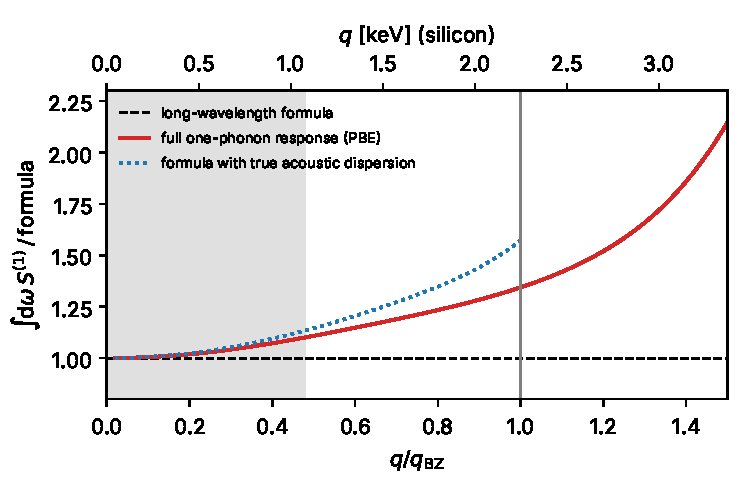
\includegraphics[width=\linewidth]{figures/ch11/limit11_1a.pdf}
\captionof{figure}{The $\omega$-integrated one-phonon response of silicon at $T = 0$, \cref{eq:11.1-S1} with all six branches, Umklapp terms and the Debye--Waller factor (solid), divided by the long-wavelength form \cref{eq:11.1-Sac} (dashed, one), both averaged over the directions of $\vect{q}$, against $q/q_{\mathrm{BZ}}$, with $q_{\mathrm{BZ}} = \SI{2.25}{keV}$. Phonons from the PBE force constants of \cref{sec:5.2}, Fourier-interpolated; the formula uses the sound speeds and polarizations of the same force constants, so that the ratio tends to one as $q \to 0$. Dotted: the long-wavelength polarizations with the true acoustic dispersion $\omega_{\vect{q}\nu}$ in place of $c_\nu q$, the leading correction. Gray: $q < 0.48\,q_{\mathrm{BZ}} = \SI{1.08}{keV}$, where the full response and the long-wavelength form agree within \SI{10}{\percent}; they agree within \SI{5}{\percent} below $0.34\,q_{\mathrm{BZ}}$. At $q_{\mathrm{BZ}}$ the formula is \SI{26}{\percent} low.}\label{fig:11-limit-a}
\par}
\smallskip
Toward the zone boundary the acoustic branches bend below $c_\nu q$, and since the weight goes as $1/\omega$, the long-wavelength form underestimates the response; beyond $q_{\mathrm{BZ}}$ the phonon carries only the reduced momentum, and the response grows as $q^2$, the incoherent form of \cref{sec:11.3}.
\end{limitbox}

The dispersion accounts for most of the departure of the full response from \cref{eq:11.1-Sac} below $q_{\mathrm{BZ}}/2$; the polarizations and the phases $\ee^{\ii\vect{q}\cdot\vect{\tau}_\kappa}$ change the ratio at order $(qa)^2$ with the opposite sign. For a rate weighted toward small $q$, as with a light mediator, the region below $q_{\mathrm{BZ}}/2$ gives nearly all of the rate and the formula is accurate. For a heavy mediator the rate is weighted toward the largest $q$ that kinematics allows, $2\mchi v_{\mathrm{max}}$, and the response there stays within \SI{10}{\percent} of the formula only for masses up to about $0.48\,q_{\mathrm{BZ}}/2v_{\mathrm{max}} = \SI{0.20}{MeV}$ in silicon.

\subsection{Orientation-averaged rate}

A crystal at a fixed orientation sees the dark-matter wind from one direction, and its rate depends on that direction; this dependence is the daily modulation of \cref{sec:11.7}. For a rate averaged over the orientations of the crystal, the response enters through its average over the directions of $\vect{q}$, and the velocity integral of \cref{eq:8.2-spectrum} acts on the delta function alone. The velocity integral gives $\eta(\vmin)/2q$ per unit $\dd^3q/(2\pi)^3$, with $\eta$ the mean inverse speed of \cref{eq:1.3-eta} (\cref{sec:8.2}). For a phonon of energy $\omega = c_\nu q$ and elastic scattering, \cref{eq:1.3-vmin} gives
\begin{equation*}
  \vmin = c_\nu + \frac{q}{2\mchi} ,
\end{equation*}
the sound speed plus half the speed the dark matter loses. We write the potential as in \cref{sec:1.4}, $|\tilde V_N(q)|^2 = \pi\sigma_p\FDM(q)^2/\mu_{\chi p}^2$, with $\sigma_p$ the dark-matter--proton cross-section, $\mu_{\chi p}$ the reduced mass and $\FDM$ the form factor of \cref{eq:1.4-defs} with $q_0 = \alpha m_e$. Inserting \cref{eq:11.1-Sac} into \cref{eq:8.2-spectrum}, integrating $\omega$ above a threshold $\omega_{\mathrm{th}}$ and collecting $4\pi\cdot\pi\cdot\pi/(2(2\pi)^3) = 1/4$ gives
\begin{keyresult}[One-acoustic-phonon rate per unit mass]
\begin{equation}
  \mathcal{R} = \frac{\rho_\chi\,\sigma_p}{4\,\mchi\,\mu_{\chi p}^2\,m_u^2}\,\Bigl\langle\sum_{\nu = 1}^{3}\frac{(\hat{\vect{q}}\cdot\hat{\vect{e}}_\nu)^2}{c_\nu}\int_{\omega_{\mathrm{th}}/c_\nu}^{q_{\mathrm{up},\nu}}\dd q\;q^2\,\FDM(q)^2\,\eta\Bigl(c_\nu + \frac{q}{2\mchi}\Bigr)\Bigr\rangle_{\hat{\vect{q}}} ,
  \label{eq:11.1-rate}
\end{equation}
with $c_\nu$ and $\hat{\vect{e}}_\nu$ taken at $\hat{\vect{q}}$, the brackets the average over the sphere of directions, and the upper limit $q_{\mathrm{up},\nu} = \min[2\mchi(v_{\mathrm{max}} - c_\nu),\,q_{\mathrm{BZ}}]$.
\end{keyresult}
\noindent The kinematic upper limit is where $\eta$ vanishes, $\vmin = v_{\mathrm{max}}$; the zone cut $q_{\mathrm{BZ}}$ is the range of \cref{eq:11.1-Sac}, beyond which the multiphonon response of \cref{sec:11.3} dominates. The rate is nonzero only when the lower limit lies below the upper one, $\omega_{\mathrm{th}}/c_\nu \le 2\mchi(v_{\mathrm{max}} - c_\nu)$, and this condition defines the \emph{acoustic edge} of \cref{sec:9.2},
\begin{equation}
  m_{\mathrm{min}}^{\mathrm{ac}} = \frac{\omega_{\mathrm{th}}}{2c_\nu(v_{\mathrm{max}} - c_\nu)} \simeq \frac{\omega_{\mathrm{th}}}{2c_\nu v_{\mathrm{max}}} ,
  \label{eq:11.1-edge}
\end{equation}
set by the largest speed of a branch with longitudinal weight over all directions, $c_{\mathrm{LA,max}}$. For silicon at $\omega_{\mathrm{th}} = \SI{1}{meV}$, $c_{\mathrm{LA,max}} = \SI{9.35}{km.s^{-1}}$ along $[111]$ and $m_{\mathrm{min}}^{\mathrm{ac}} = \SI{6.1}{keV}$, against \SI{0.28}{keV} for the threshold mass.

\begin{figure}[tbp]
  \centering
  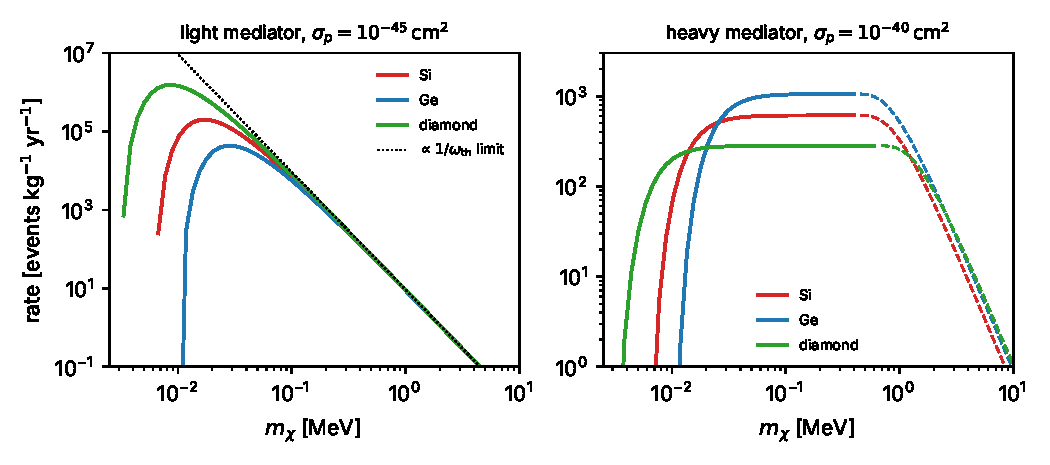
\includegraphics[width=\linewidth]{figures/ch11/fig11_1.pdf}
  \caption{Rate of single-acoustic-phonon emission per unit target mass, \cref{eq:11.1-rate}, for silicon, germanium and diamond at a threshold $\omega_{\mathrm{th}} = \SI{1}{meV}$, averaged over the orientation of the crystal, with equal couplings to protons and neutrons, $\rho_\chi = \SI{0.3}{GeV.cm^{-3}}$ and the standard halo of \cref{sec:1.2}. Sound speeds and polarizations from the Christoffel problem of the measured room-temperature elastic tensors (\cref{we:11-cbar}); momentum transfers $q \le q_{\mathrm{BZ}}$, Debye--Waller factor one. Left: light mediator, $\FDM = (q_0/q)^2$, $\sigma_p = 10^{-45}\,\mathrm{cm^2}$; dotted, the target-independent limit \cref{eq:11.1-light}. Right: heavy mediator, $\FDM = 1$, $\sigma_p = 10^{-40}\,\mathrm{cm^2}$; solid up to $q_{\mathrm{BZ}}/2v_{\mathrm{max}}$ (0.42, 0.41 and \SI{0.65}{MeV}), dashed above, where the fall is an artifact of the cut $q \le q_{\mathrm{BZ}}$ and where the multiphonon and Umklapp terms of \cref{sec:11.3} dominate. The edges are 6.1 (Si), 10.2 (Ge) and \SI{3.1}{keV} (diamond).}
  \label{fig:11-rate}
\end{figure}

\subsection{Light mediator}

For a light mediator, $\FDM^2 = (q_0/q)^4$, the integrand of \cref{eq:11.1-rate} falls as $q^{-2}$, and the rate is dominated by the smallest momentum transfer that a phonon above threshold can carry. In the variable $u = q/2\mchi$, the integral of one branch and direction is
\begin{equation*}
  \frac{q_0^4}{2\mchi}\int_{u_-}^{u_+}\dd u\,\frac{\eta(c_\nu + u)}{u^2} , \qquad u_- = \frac{\omega_{\mathrm{th}}}{2\mchi c_\nu} , \quad u_+ = v_{\mathrm{max}} - c_\nu .
\end{equation*}
Far above the edge, where $u_- \ll u_+$, the integral tends to $\eta(c_\nu)/u_-$, and since $u_- = \omega_{\mathrm{th}}/2\mchi c_\nu$, the $q$-integral of each branch and direction is $q_0^4c_\nu\eta(c_\nu)/\omega_{\mathrm{th}}$. Its factor $c_\nu$ cancels the weight $1/c_\nu$ in the brackets of \cref{eq:11.1-rate}. The shift of $\eta$ by $c_\nu$ is of relative order $c_\nu^2/v_0^2 \sim 10^{-3}$, since the laboratory speed distribution vanishes as $v^2$ at small speeds and $\eta$ is flat at the origin. By the completeness $\sum_\nu(\hat{\vect{q}}\cdot\hat{\vect{e}}_\nu)^2 = 1$ the weights of the directions and branches then add up to one, and
\begin{equation}
  \mathcal{R}_{\mathrm{light}} = \frac{\rho_\chi\,\sigma_p\,q_0^4\,\eta(0)}{4\,\mchi\,\mu_{\chi p}^2\,m_u^2\,\omega_{\mathrm{th}}} .
  \label{eq:11.1-light}
\end{equation}
The rate per unit mass is the same for every crystal, inversely proportional to the threshold, and it falls as $\mchi^{-3}$ for $\mchi \ll m_p$. The light-mediator curves of \cref{fig:11-rate} merge with \cref{eq:11.1-light} at high mass. They separate near the edges, which differ by a factor of three between diamond and germanium.

To find how far above the edge the limit \cref{eq:11.1-light} holds, write $\eta(c_\nu + u) = \eta(0) - [\eta(0) - \eta(c_\nu + u)]$. The first term integrates to $\eta(0)(1/u_- - 1/u_+)$. In the second term, the bracket vanishes as $u^2$ at small $u$, so the integral of the second term from $0$ to $u_-$ is of order $u_-$, and to first order in $u_-$ this integral can run from $0$ to $u_+$. We define
\begin{equation}
  \kappa_\eta = \frac{u_+}{\eta(0)}\int_0^{u_+}\dd u\,\frac{\eta(0) - \eta(u)}{u^2} ,
  \label{eq:11.1-kappa}
\end{equation}
and use $u_-/u_+ = m_{\mathrm{min}}^{\mathrm{ac}}/\mchi$ from \cref{eq:11.1-edge}. The integral of one branch and direction is then $(\eta(0)/u_-)[1 - (1 + \kappa_\eta)\,m_{\mathrm{min}}^{\mathrm{ac}}/\mchi]$ up to terms of second order in $m_{\mathrm{min}}^{\mathrm{ac}}/\mchi$. The rate is therefore
\begin{equation}
  \frac{\mathcal{R}}{\mathcal{R}_{\mathrm{light}}} = \Bigl[1 - (1 + \kappa_\eta)\frac{m_{\mathrm{min}}^{\mathrm{ac}}}{\mchi} + O\Bigl(\frac{m_{\mathrm{min}}^{\mathrm{ac}}}{\mchi}\Bigr)^{\!2}\Bigr] , \qquad \kappa_\eta = 3.14 ,
  \label{eq:11.1-correction}
\end{equation}
with $\mathcal{R}_{\mathrm{light}}$ the limit \cref{eq:11.1-light}, for $\mchi \le q_{\mathrm{BZ}}/2v_{\mathrm{max}}$, where the kinematic limit $u_+$ applies. The value of $\kappa_\eta$ is a property of the halo alone: it is \cref{eq:11.1-kappa} for the standard halo of \cref{sec:1.2} with $u_+ = v_{\mathrm{max}}$, the limit $c_\nu \ll v_{\mathrm{max}}$. At the sound speed of silicon, $u_+ = v_{\mathrm{max}} - c_\nu$ and $\kappa_\eta = 3.09$. The material enters only through the edge, and the term $1$ of $1 + \kappa_\eta$ is the loss of the momentum transfers above $u_+$, and the term $\kappa_\eta$ is the loss of the slow particles that the halo lacks. For a crystal the edge in \cref{eq:11.1-correction} is the average over directions and branches, weighted like the rate: this average equals $m_{\mathrm{min}}^{\mathrm{ac}}$ evaluated at the speed $\langle\sum_\nu(\hat{\vect{q}}\cdot\hat{\vect{e}}_\nu)^2/c_\nu\rangle^{-1}$, and for silicon the speed is \SI{8.956}{km.s^{-1}} (\cref{we:11-cbar}) and the edge \SI{6.39}{keV}. Above $q_{\mathrm{BZ}}/2v_{\mathrm{max}}$ the zone cut replaces $u_+$, and the bracket tends to $1 - \omega_{\mathrm{th}}/(c_\nu q_{\mathrm{BZ}})$, 0.985 for silicon at \SI{1}{meV}.

\begin{limitbox}[Light-mediator single-phonon rate][lim:11.1b]
For a light mediator the one-phonon rate per unit target mass is $\mathcal{R} = \rho_\chi\sigma_pq_0^4\eta(0)/(4\mchi\mu_{\chi p}^2m_u^2\omega_{\mathrm{th}})$, inversely proportional to the threshold and independent of the target~\cite[Eq.~(35)]{griffin2020multichannel}.
\par\smallskip
{\centering
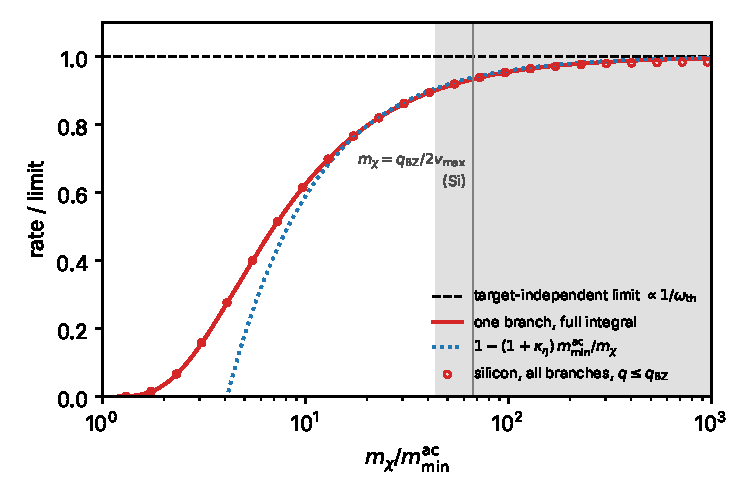
\includegraphics[width=\linewidth]{figures/ch11/limit11_1b.pdf}
\captionof{figure}{The light-mediator rate \cref{eq:11.1-rate}, divided by its target-independent limit \cref{eq:11.1-light} (dashed, one), against $\mchi/m_{\mathrm{min}}^{\mathrm{ac}}$. Solid: one branch of speed \SI{9.0}{km.s^{-1}} without the zone cut; the curve changes by \SI{3}{\percent} at $\mchi = 10\,m_{\mathrm{min}}^{\mathrm{ac}}$ between speeds of 3 and \SI{18}{km.s^{-1}}. Circles: silicon, all branches and directions, with $q \le q_{\mathrm{BZ}}$; on this axis $m_{\mathrm{min}}^{\mathrm{ac}} = \SI{6.39}{keV}$ at $\omega_{\mathrm{th}} = \SI{1}{meV}$, the edge for the polarization-weighted inverse speed \SI{8.956}{km.s^{-1}} of \cref{eq:11.1-heavy}; the vertical line marks $q_{\mathrm{BZ}}/2v_{\mathrm{max}}$, above which the zone cut holds the ratio at 0.985. Dotted: the first-order correction \cref{eq:11.1-correction} with $\kappa_\eta = 3.09$. Gray: $\mchi \ge 44\,m_{\mathrm{min}}^{\mathrm{ac}}$, where the rate is within \SI{10}{\percent} of the limit. The first-order form is within \SI{10}{\percent} of the full rate for $\mchi \ge 9\,m_{\mathrm{min}}^{\mathrm{ac}}$. Standard halo of \cref{sec:1.2}.}\label{fig:11-limit-b}
\par}
\smallskip
Within a few times the edge the momentum window $[\omega_{\mathrm{th}}/c_\nu,\,2\mchi v_{\mathrm{max}}]$ closes and only the fastest particles of the halo contribute, so the rate falls far below the limit and depends on the material through its edge.
\end{limitbox}

\begin{workedexample}{The light-mediator correction at three times the edge}\label{we:11-light}
Take silicon at $\omega_{\mathrm{th}} = \SI{1}{meV}$, where $m_{\mathrm{min}}^{\mathrm{ac}} = \SI{6.39}{keV}$ for the polarization-weighted inverse speed \SI{8.956}{km.s^{-1}} of \cref{eq:11.1-heavy}, and $\mchi = 3\,m_{\mathrm{min}}^{\mathrm{ac}} = \SI{19.2}{keV}$. The momentum transfers that can create a phonon above threshold run from $\omega_{\mathrm{th}}/c = \SI{33}{eV}$ to $2\mchi(v_{\mathrm{max}} - c) = \SI{100}{eV}$, a factor of three. With $\kappa_\eta = 3.09$ at this sound speed, the first-order factor is $1 - 4.09/3 = -0.36$: negative, and therefore meaningless. The full integral of \cref{eq:11.1-rate}, with all branches and directions, gives $\mathcal{R}/\mathcal{R}_{\mathrm{light}} = 0.149$. The expansion behind \cref{eq:11.1-correction} has failed at this mass, because the speeds that contribute, $\vmin$ between $c + u_-$ and $v_{\mathrm{max}}$, all lie in the tail of the halo above \SI{270}{km.s^{-1}}, where $\eta$ is far from flat. At ten times the edge, \SI{63.9}{keV}, the full ratio is 0.625 and the first-order form 0.591; at 44 times, \SI{0.28}{MeV}, the full ratio is 0.902 and the first-order form 0.907. The target-independent statement holds within \SI{10}{\percent} only from about \SI{0.28}{MeV} in silicon, and for any two materials only above 44 times the higher of their edges.
\end{workedexample}

\subsection{Heavy mediator}

For a heavy mediator, $\FDM = 1$, the integrand of \cref{eq:11.1-rate} grows as $q^2$, and the rate is dominated by the largest momentum transfer, $2\mchi(v_{\mathrm{max}} - c_\nu)$. With $u = q/2\mchi$ the integral of one branch is $8\mchi^3\int_{u_-}^{u_+}\dd u\,u^2\eta(c_\nu + u)$. Well above the edge and with $c_\nu \ll v_{\mathrm{max}}$, it tends to $8\mchi^3I_0$, with $I_0 = \int_0^{v_{\mathrm{max}}}\dd u\,u^2\eta(u) = 5.32\times10^{-7}$ for the standard halo. For $\mchi \ll m_p$ the reduced mass is $\mu_{\chi p} \approx \mchi$, and the factors of $\mchi$ cancel:
\begin{equation}
  \mathcal{R} = \frac{2\rho_\chi\,\sigma_p\,I_0}{m_u^2}\,\Bigl\langle\sum_\nu\frac{(\hat{\vect{q}}\cdot\hat{\vect{e}}_\nu)^2}{c_\nu}\Bigr\rangle_{\hat{\vect{q}}} .
  \label{eq:11.1-heavy}
\end{equation}
The rate per unit mass is independent of the dark-matter mass and inversely proportional to a polarization-weighted mean speed, so soft crystals have the larger rate. The plateaus of \cref{fig:11-rate} nearly stand in the ratio of the inverse speeds, $8.956/5.321 = 1.68$ for germanium against silicon and $8.956/18.16 = 0.49$ for diamond. The computed rates at \SI{0.3}{MeV} stand in the ratios 1.73 and 0.46. The difference between the computed ratios and the ratios of the inverse speeds comes from the shift of $\eta$ by $c_\nu$. The shift matters at the large $u$ that a heavy mediator favors, where $\eta$ is not flat, and lowers the rate of a stiff crystal by several percent per \SI{10}{km.s^{-1}}.

The plateau is reached only well above the edge and, in silicon, ends near \SI{0.42}{MeV}. Near the edge the lower cut removes part of $I_0$, and the rate approaches \cref{eq:11.1-heavy} only slowly, because $\eta$ falls steeply toward $v_{\mathrm{max}}$ and the integrand is weighted toward small $u$. In silicon the rate reaches \SI{90}{\percent} of the plateau value (654 events per kilogram and year at $\sigma_p = 10^{-40}\,\mathrm{cm^2}$) only at \SI{45}{keV}, seven times the edge. However, the silicon rate never exceeds \SI{94}{\percent} of the plateau value, and the diamond rate never exceeds \SI{87}{\percent} of its plateau value, because \cref{eq:11.1-heavy} drops the shift of $\eta$ by $c_\nu$. By \cref{fig:11-limit-a}, from about \SI{0.2}{MeV} the response at the largest momentum transfers already differs from \cref{eq:11.1-Sac} by more than \SI{10}{\percent}. Above $q_{\mathrm{BZ}}/2v_{\mathrm{max}}$, \SI{0.42}{MeV} for silicon, the momentum transfers leave the region where \cref{eq:11.1-Sac} holds, and Umklapp processes and multiphonons dominate (\cref{sec:11.3}). \Cref{sec:17.5} names the inverse of the bracket in \cref{eq:11.1-heavy} the effective sound speed of the channel and ranks materials by it.

\subsection{Sound speeds from the elastic tensor}

The rates above need the sound speeds in every direction, and with them two averages: the largest longitudinal speed for the edge and the polarization-weighted inverse speed of \cref{eq:11.1-heavy}. The speeds and both averages follow from the elastic tensor $C_{ijkl}$ and the density through the Christoffel equation \cref{eq:C.18-christoffel}: in each direction $\hat{\vect{q}}$ the eigenvalues of $\mathsf{M}_{ik} = C_{ijkl}\hat q_j\hat q_l$ are $\rho_Tc_\nu(\hat{\vect{q}})^2$, and the eigenvectors are the polarizations $\hat{\vect{e}}_\nu$ of \cref{eq:11.1-Sac}.

The elastic constants are measured or computed by density-functional theory (\cref{app:E.4}), and a computed tensor must be in the Voigt order of \cref{app:C.18} before it enters the Christoffel matrix.

\begin{workedexample}{The rate coefficient of silicon}\label{we:11-cbar}
The room-temperature constants of silicon are $C_{11} = 165.6$, $C_{12} = 63.9$ and $C_{44} = \SI{79.5}{GPa}$, with $\rho_T = \SI{2.33}{g.cm^{-3}}$ (\cref{app:C.18}). Along the three symmetry directions \cref{eq:C.18-cubic} gives $\rho_Tc_{\mathrm{LA}}^2 = 165.6$, $194.3$ and \SI{203.8}{GPa}, and $c_{\mathrm{LA}} = 8.43$, 9.13 and \SI{9.35}{km.s^{-1}} along $[100]$, $[110]$ and $[111]$. The speed varies by \SI{11}{\percent} over the sphere, and the averages need all directions.

The polarization-weighted average is a quadrature. On a product grid of Gauss--Legendre nodes in $\cos\theta$ and equally spaced nodes in $\phi$ (\cref{app:C.18}), with the $3\times3$ Christoffel matrix diagonalized at each node, the inverse of the rate coefficient of \cref{eq:11.1-heavy}, $\langle\sum_\nu(\hat{\vect{q}}\cdot\hat{\vect{e}}_\nu)^2/c_\nu\rangle^{-1}$, is \SI{8.956}{km.s^{-1}}. The same procedure yields \SI{5.321}{km.s^{-1}} for germanium and \SI{18.16}{km.s^{-1}} for diamond, from the tensors $131$, $49$, \SI{68}{GPa}~\cite{mcskimin1963elastic} and $1081$, $125$, \SI{579}{GPa}~\cite{mcskimin1972elastic}, as tabulated in Ref.~\cite[Table~III]{haxhijaj2026lattice}, with the densities 5.33 and \SI{3.52}{g.cm^{-3}} that follow from the lattice constants 5.658 and \SI{3.567}{\angstrom}.
\end{workedexample}

A tabulated speed can be tested without the full tensor. The largest eigenvalue of the Christoffel matrix is at least its expectation value in the unit vector $\hat{\vect{q}}$. For cubic symmetry that expectation value is never below the bulk modulus $B = (C_{11} + 2C_{12})/3$ of \cref{eq:C.18-bulk}, and the two inequalities give \cref{eq:C.18-rayleigh}:
\begin{equation}
  c_{\mathrm{LA}}(\hat{\vect{q}}) \ge \sqrt{B/\rho_T} \qquad\text{(cubic crystals, every direction)} .
  \label{eq:11.1-rayleigh}
\end{equation}
The bound is \SI{6.48}{km.s^{-1}} for silicon, \SI{3.79}{km.s^{-1}} for germanium and \SI{11.23}{km.s^{-1}} for diamond, 23, 24 and \SI{36}{\percent} below their slowest longitudinal speeds. It is proved for cubic crystals only; for lower symmetries the uniform compression and the uniform strain no longer coincide (\cref{app:C.18}), and the bound must be replaced by the Christoffel eigenvalue itself. \Cref{sec:17.5} applies the bound to tabulated speeds.


\section{Optical phonons in polar crystals}\label{sec:11.2}

A dark-matter particle of \SI{100}{keV} that scatters in GaAs through a light dark photon most often leaves behind one longitudinal optical phonon of \SI{36.35}{meV}. The dark photon does not couple to the nucleons. It couples to the charge, and when the gallium and arsenic sublattices move against each other every cell carries the dipole of their Born charges (\cref{sec:5.5}), whose field the electrons screen. In the acoustic waves of \cref{sec:11.1} the cell moves as a whole and stays neutral, and at long wavelength a coupling to charge has no vertex there; in the optical branch of GaAs its vertex is $Z^*/\varepsilon_\infty = 0.19$ per cell at every small momentum transfer (\cref{we:8-nucleon}). Silicon and germanium, whose Born charges vanish, have no such channel. A polar target enters the rate through one band integral of its loss function, and the crystals with the largest band integrals have the highest kinematic edges.

\subsection{The phonon loss function}\label{sec:11.2-loss}

A dark photon, heavy or light, couples to the charge-number density $n_Z$, and so does any particle with a small electric charge (\cref{we:8-darkphoton}). For this row \cref{sec:8.4} gave an exact answer: $S_{ZZ} = (2q^2/e^2)\,L/(1 - \ee^{-\beta\omega})$, with $L = \Imag[-(\varepsilon^{-1})_{00}]$ the loss function of the total dielectric matrix of electrons and nuclei. Below the band gap the electrons add a constant to $\varepsilon$, and every structure of $L$ there comes from the ions. We need $\varepsilon$ at the frequencies of the optical phonons and at momentum transfers small compared with the zone, where the long-range Coulomb line is the macroscopic field and the rank-one form \cref{eq:8.4-rank1} holds.

The dielectric function along $\hat{\vect{q}}$ follows from the energy \cref{eq:5.5-U}. The electrons follow adiabatically and contribute $\varepsilon_\infty(\hat{\vect{q}}) \equiv \hat{\vect{q}}\cdot\varepsilon_\infty\cdot\hat{\vect{q}}$. The ions respond as the oscillators of the analytic zone-center problem, the eigenmodes of $D^{\mathrm{an}}_{\kappa\kappa'} = C^{\mathrm{an}}_{\kappa\kappa'}/(M_\kappa M_{\kappa'})^{1/2}$ with real polarization vectors and frequencies $\omega_{\mathrm{T}\nu}$, each driven by the field through its mode charge (\cref{eq:5.5-HE}). Collecting the $3n$ components of the $n$ sublattices into one vector,
\begin{equation}
  \varepsilon(\hat{\vect{q}},\omega) = \varepsilon_\infty(\hat{\vect{q}}) + \frac{e^2}{\Omega}\,\vect{p}^{\mathrm{T}}\bigl(D^{\mathrm{an}} - \omega^2\bigr)^{-1}\vect{p} ,
  \qquad p_{\kappa\alpha}(\hat{\vect{q}}) = \frac{(Z^*_\kappa\cdot\hat{\vect{q}})^\alpha}{\sqrt{M_\kappa}} ,
  \label{eq:11.2-eps}
\end{equation}
which is \cref{eq:5.5-eps} for any number of atoms and any direction. Expanded in the eigenmodes of $D^{\mathrm{an}}$, the second term is a sum of poles at the transverse frequencies, each weighted by the square of the mode charge along $\hat{\vect{q}}$.

The loss function needs $1/\varepsilon$, and the structure of \cref{eq:11.2-eps} makes the inversion exact. The ionic term is a matrix element of the inverse of $A = D^{\mathrm{an}} - \omega^2$ between one vector, and the Sherman--Morrison identity, $(A + \vect{b}\vect{b}^{\mathrm{T}})^{-1} = A^{-1} - A^{-1}\vect{b}\vect{b}^{\mathrm{T}}A^{-1}/(1 + \vect{b}^{\mathrm{T}}A^{-1}\vect{b})$, gives $\vect{b}^{\mathrm{T}}(A + \vect{b}\vect{b}^{\mathrm{T}})^{-1}\vect{b} = \vect{b}^{\mathrm{T}}A^{-1}\vect{b}/(1 + \vect{b}^{\mathrm{T}}A^{-1}\vect{b})$. With $\vect{b} = e\vect{p}/[\Omega\varepsilon_\infty(\hat{\vect{q}})]^{1/2}$, \cref{eq:11.2-eps} reads $\varepsilon = \varepsilon_\infty(\hat{\vect{q}})(1 + \vect{b}^{\mathrm{T}}A^{-1}\vect{b})$, and therefore
\begin{equation}
  \frac{1}{\varepsilon(\hat{\vect{q}},\omega)} = \frac{1}{\varepsilon_\infty(\hat{\vect{q}})}\Bigl[1 - \vect{b}^{\mathrm{T}}\bigl(D^{\mathrm{an}} + \vect{b}\vect{b}^{\mathrm{T}} - \omega^2\bigr)^{-1}\vect{b}\Bigr] .
  \label{eq:11.2-SM}
\end{equation}
The matrix $D^{\mathrm{an}} + \vect{b}\vect{b}^{\mathrm{T}}$ is the dynamical matrix \cref{eq:5.5-na}: $\vect{b}\vect{b}^{\mathrm{T}}$ is exactly its nonanalytic term. Inverting $\varepsilon$ has traded the poles of $\varepsilon$, at the transverse frequencies, for the eigenfrequencies of the full dynamical matrix, which include the longitudinal ones. Let $\omega_\nu$ and $\vect{e}_\nu$ be its eigenpairs for the direction $\hat{\vect{q}}$. Then $\vect{b}^{\mathrm{T}}(D^{\mathrm{dyn}} - \omega^2)^{-1}\vect{b} = \sum_\nu(\vect{b}\cdot\vect{e}_\nu)^2/(\omega_\nu^2 - \omega^2)$, and with $\omega \to \omega + \ii0^+$ each term has the imaginary part $\pi(\vect{b}\cdot\vect{e}_\nu)^2\,\delta(\omega - \omega_\nu)/2\omega_\nu$ for $\omega > 0$. The loss function in the phonon band is a set of lines,
\begin{equation*}
  L(\hat{\vect{q}},\omega) = \frac{\pi e^2}{2\Omega\,\varepsilon_\infty(\hat{\vect{q}})^2}\sum_\nu\frac{(\vect{p}\cdot\vect{e}_\nu)^2}{\omega_\nu}\,\delta(\omega - \omega_\nu) .
\end{equation*}
Of these steps only the vertex needs $\vect{q} = 0$. At a wavevector inside the zone, $D^{\mathrm{an}}$ becomes the dynamical matrix at $\vect{Q}$ with the macroscopic field removed, each component of $\vect{p}$ takes the phase $\ee^{\ii\vect{q}\cdot\vect{\tau}_\kappa}$ of its site, and $D^{\mathrm{an}} + \vect{b}\vect{b}^{\mathrm{T}}$ is the full dynamical matrix at $\vect{Q}$. Multiplying by $2q^2/e^2$:
\begin{keyresult}[Born-charge one-phonon structure factor]
\begin{equation}
  S^{(1)}_{ZZ}(\vect{q},\omega) = \frac{2\pi}{\Omega}\sum_\nu\frac{\bigl|\sum_\kappa\ee^{\ii\vect{q}\cdot\vect{\tau}_\kappa}\,\vect{e}_{\kappa\nu}(\vect{Q})^*\cdot Z^*_\kappa\cdot\vect{q}/\sqrt{M_\kappa}\bigr|^2}{2\omega_{\vect{Q}\nu}\,\bigl(\hat{\vect{q}}\cdot\varepsilon_\infty\cdot\hat{\vect{q}}\bigr)^2}\,\delta(\omega - \omega_{\vect{Q}\nu}) ,
  \label{eq:11.2-SZZ}
\end{equation}
at $T = 0$, for $q$ small compared with the zone and $\omega$ far below the gap, with the phonons of the full dynamical matrix, nonanalytic term included, and the phase convention of \cref{eq:11.1-S1}.
\end{keyresult}
\noindent The structure is that of the nucleon response \cref{eq:11.1-S1}, with the nucleon number $A_\kappa$ replaced by the Born charge projected on $\vect{q}$ and the whole vertex divided by $\varepsilon_\infty(\hat{\vect{q}})$. Each branch contributes the square of its dipole along $\vect{q}$, screened by the electrons, divided by its energy. At the zone center the acoustic branches drop out by the neutrality \cref{eq:5.5-neutral}, and in a cubic crystal so do the transverse optical ones, whose dipole is perpendicular to $\vect{q}$. The longitudinal mode, at $\omega_{\mathrm{L}}$, remains. The proper response of the ions has its poles at $\omega_{\mathrm{T}}$, but the transverse pole of $\varepsilon$ is a zero of $1/\varepsilon$, and a coupling to charge excites the longitudinal phonon, as in absorption (\cref{sec:5.5}).

The loss function of the total $\varepsilon$ and the Born-charge vertex screened by $\varepsilon_\infty$ are two resummations of the series \cref{eq:8.4-screened}, one with the ions inside the dielectric function and one with them in the vertex, and \cref{eq:11.2-SM} is the step between them. The vertex is that of \cref{sec:6.2}, the Fr\"ohlich vertex \cref{eq:D.14-gL} with the electron replaced by the dark particle: the density vertex $\rho_{mn}$ becomes one, and the charge of the electron becomes the coupling of the dark matter.

Every input of \cref{eq:11.2-SZZ} is an output of density-functional perturbation theory: phonons at $\vect{Q}$ with the nonanalytic term, Born charges and $\varepsilon_\infty$ (\cref{app:E.4}). The rate carries $(Z^*/\varepsilon_\infty)^2$, and the semilocal $\varepsilon_\infty$ of GaAs, \SI{26}{\percent} too high (\cref{sec:5.5}), would make it \SI{37}{\percent} too low. We use instead the computed phonons and Born charge with the measured room-temperature $\varepsilon_\infty = 10.88$ and $\varepsilon_0 = 12.9$ of GaAs~\cite{lockwood2005optical}, or the measured splitting itself (\cref{sec:11.2-split}).

\Cref{eq:11.2-SZZ} holds when the momentum transfer is small compared with the zone, the energy far below the gap, and the lattice harmonic and cold. At small momentum transfer the charge that moves with a nucleus is its Born charge; corrections to this vertex start at relative order $qa$. Far below the gap the electrons follow the ions adiabatically and the vertex may be computed at zero frequency; by the argument of \cref{sec:8.4} the error is of order $(\omega_{\mathrm{L}}/\Eg)^2$, $6\times10^{-4}$ in GaAs. For the cold harmonic lattice, the Debye--Waller factor is $1 - 8\times10^{-8}$ at the smallest momentum transfer, $q = \omega_{\mathrm{L}}/v_{\mathrm{max}} = \SI{13.7}{eV}$, with the root-mean-square displacement of \cref{tab:5-phonons}. At \SI{10}{mK}, $\omega_{\mathrm{L}}/T = 4.2\times10^4$ and no optical phonon is thermally occupied. The anharmonic width of the longitudinal phonon, a fraction of a meV, spreads the line without moving its weight. The small-$q$ vertex is the condition that matters in practice, and the limit check tests it with the phonons of \cref{fig:5-gaas}.

\begin{limitbox}[Born-charge single-phonon rate][lim:11.2a]
A particle that couples to charge creates one phonon with the structure factor \cref{eq:11.2-SZZ}: Born charges, screened by $\varepsilon_\infty$, acting on the phonons of the full dynamical matrix~\cites[Eqs.~(92), (105), (106)]{trickle2020multichannel}[Eqs.~(19), (23)]{griffin2018directional}[Eq.~(61)]{trickle2022effective}. For one longitudinal branch this is the form of Knapen and collaborators~\cite[Eqs.~(4)--(7)]{knapen2018detection}.
\par\smallskip
{\centering
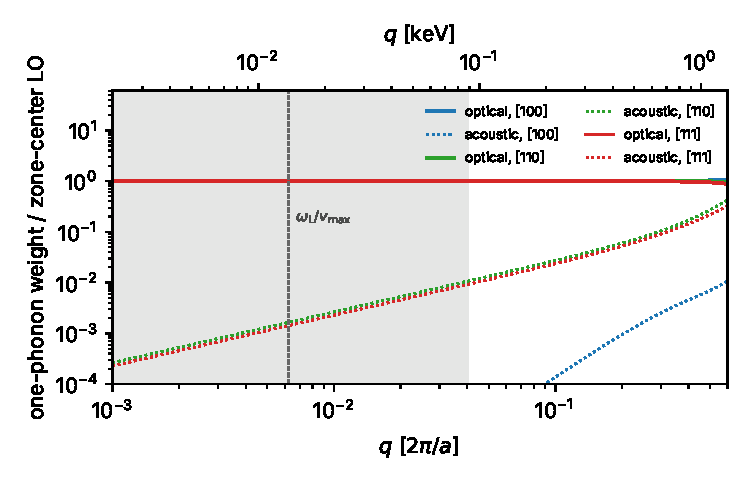
\includegraphics[width=\linewidth]{figures/ch11/limit11_2a.pdf}
\captionof{figure}{One-phonon weight of GaAs in \cref{eq:11.2-SZZ}, $\sum_\nu|\sum_\kappa\ee^{\ii\vect{q}\cdot\vect{\tau}_\kappa}\vect{e}^*_{\kappa\nu}\cdot Z^*_\kappa\cdot\hat{\vect{q}}/\sqrt{M_\kappa}|^2/2\omega_\nu$, divided by its zone-center value $Z^{*2}/2\mu_{\mathrm{red}}\omega_{\mathrm{L}}$, against $q$ along $[100]$, $[110]$ and $[111]$. Solid: the three optical branches; dotted: the three acoustic branches. Phonons at the actual $\vect{q}$ from the PBE force constants of \cref{fig:5-gaas}; Born charges held at their zone-center value. The ratios do not depend on $Z^*$ or $\varepsilon_\infty$. Gray: $q < 0.04 \times 2\pi/a = \SI{88}{eV}$, where the optical weight is within $10^{-4}$ of the formula and the acoustic weight is at most about \SI{1}{\percent}. Dashed line: $q = \omega_{\mathrm{L}}/v_{\mathrm{max}}$, the smallest momentum transfer that reaches the longitudinal phonon.}\label{fig:11-limit-2a}
\par}
\smallskip
At $q$ comparable with $2\pi/a$ the Born charge no longer describes the charge that moves with a nucleus, and the acoustic branches acquire a piezoelectric charge that the Born charges fix only in part.
\end{limitbox}

The optical weight stays within $10^{-4}$ of its zone-center value up to \SI{88}{eV} and within \SI{0.4}{\percent} up to \SI{450}{eV}, where the longitudinal branch has dispersed by \SI{0.3}{meV}. The acoustic branches are the leading correction, and they grow linearly in $q$: their weight reaches \SI{1}{\percent} of the optical one at \SI{90}{eV} along $[111]$ and \SI{5}{\percent} at \SI{450}{eV}, while along $[100]$ it vanishes by symmetry. This is the piezoelectric charge of \cref{sec:6.2}. With rigid Born charges an acoustic wave polarizes the cell only through the relative displacement of the sublattices that its strain induces; the dynamical quadrupoles of the displaced atoms, the next term beyond the Born charge in the expansion of the charge that moves with an atom in powers of $q$, add a contribution of the same order (\cref{app:E.5}), which the limit check does not include. The dotted curves are an estimate of the size of the correction.

The same order-$qa$ structure of the longitudinal mode sets the whole nucleon vertex of \cref{we:8-nucleon}, which vanishes as $q \to 0$; the charge vertex, finite at $q = 0$, is insensitive to it.

\subsection{The polar single-phonon rate}\label{sec:11.2-rate}

The dark matter enters through one potential. A dark photon couples to $-\tilde V n_Z$, with the same $\tilde V$ on electrons and nuclei, and we normalize it as for electron scattering, $|\tilde V|^2 = \pi\sigmae\FDM^2/\mu_{\chi e}^2$ (\cref{eq:1.4-Vsq}), with $\FDM = (q_0/q)^2$ for a light dark photon. We average the structure factor over the directions of $\vect{q}$, so that the halo enters through $\eta(\vmin)$ (\cref{eq:A.8-eta}); the direction dependence that a crystal keeps is the subject of \cref{sec:11.7}. With $S_{ZZ} = (2q^2/e^2)\bar L$ at $T = 0$, the rate \cref{eq:A.8-rateiso} becomes, for the light mediator,
\begin{keyresult}[Polar single-phonon rate]
\begin{equation}
  \mathcal{R} = \frac{\rho_\chi\,\sigmae\,q_0^4}{2\pi\,\mchi\,\mu_{\chi e}^2\,e^2\,\rho_T}\int_{\mathrm{band}}\dd\omega\;\bar L(\omega)\,K_\eta(\omega,\mchi) ,
  \qquad
  K_\eta(\omega,\mchi) = \int\frac{\dd q}{q}\;\eta\bigl(\vmin(q,\omega)\bigr) ,
  \label{eq:11.2-rate}
\end{equation}
with $\bar L$ the loss function at small $q$, averaged over directions, and the integral over the phonon band.
\end{keyresult}
\noindent All powers of $q$ cancel but one. A light mediator weights every logarithmic interval of momentum transfer equally, and the phonon fixes the energy deposited. The rate is then the loss function summed over the band, each line weighted by a kinematic factor that depends only on its energy and the dark-matter mass. Since $\vmin(q,\omega) \ge (2\omega/\mchi)^{1/2}$ at every $q$, the factor vanishes below the mass at which the fastest particle can deposit $\omega$, $2\omega/v_{\mathrm{max}}^2$ (\cref{eq:1.3-mmin}), which is \SI{10.35}{keV} for the longitudinal phonon of GaAs. For a single speed $v$, $\eta = \Theta(v - \vmin)/v$ and $K_\eta = \ln(q_+/q_-)/v$, with $q_\pm = \mchi v[1 \pm (1 - 2\omega/\mchi v^2)^{1/2}]$ the ends of the kinematic window.

For a heavy mediator, $\FDM = 1$, the same steps replace $K_\eta$ by $q_0^{-4}\int\dd q\,q^3\eta$, and the rate is weighted toward the largest momentum transfer, $2\mchi v_{\mathrm{max}}$. It leaves the region of \cref{fig:11-limit-2a}, where the acoustic share stays below a few percent, at about $0.2\times2\pi/a$, or $\mchi \approx \SI{83}{keV}$ in GaAs. The optical phonons alone keep the one-branch form to about \SI{0.1}{\percent} at \SI{99}{keV}; the vertex fails first.

\begin{figure}[tbp]
  \centering
  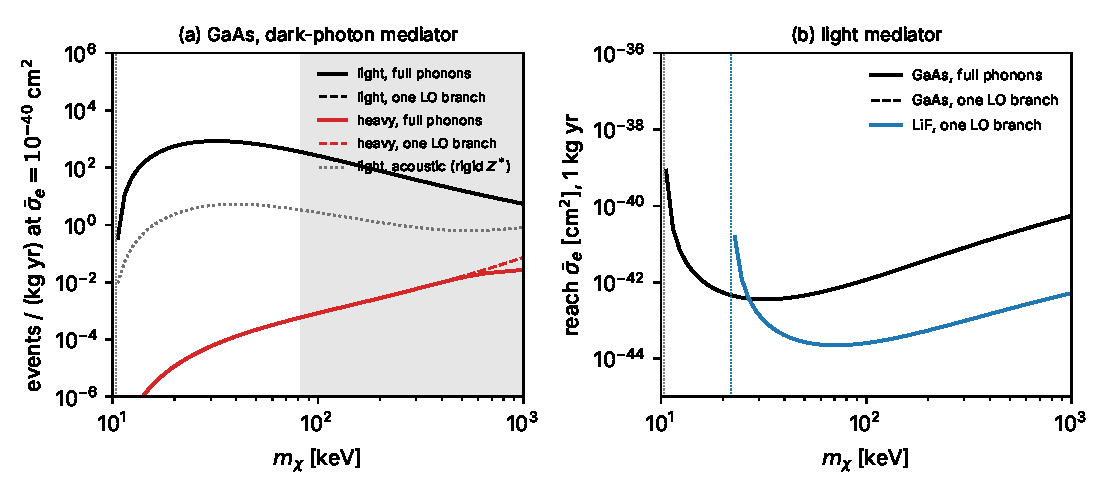
\includegraphics[width=\linewidth]{figures/ch11/fig11_2.pdf}
  \caption{Single-phonon scattering of dark matter through a dark photon in polar crystals, for the standard halo of \cref{sec:1.2} at $T = 0$. (a) Rate of GaAs per kilogram and year at $\sigmae = \SI{e-40}{cm^2}$, light ($\FDM = (q_0/q)^2$) and heavy ($\FDM = 1$) mediator. Solid: \cref{eq:11.2-SZZ} with the three optical branches of the PBE phonons of \cref{fig:5-gaas}, at the actual $\vect{q}$ (Umklapp included), averaged over 146 directions, in \cref{eq:A.8-rateiso}. Dashed: one longitudinal branch at the zone center, \cref{eq:11.2-onebranch} in \cref{eq:11.2-rate}. Both use $Z^* = 2.11$, the measured $\varepsilon_\infty = 10.88$, $\omega_{\mathrm{L}} = \SI{36.34}{meV}$ (DFPT) and $\rho_T = \SI{5.361}{g.cm^{-3}}$. Dotted: the acoustic branches with the same rigid Born charges and a \SI{1}{meV} threshold, an estimate of the piezoelectric correction (\cref{fig:11-limit-2a}). Gray: $2\mchi v_{\mathrm{max}} > 0.2\times2\pi/a$, where the Born-charge vertex is no longer reliable for the heavy mediator. (b) Light-mediator reach, three events in one kilogram-year without background: GaAs as in (a), and LiF with one longitudinal branch and the computed $Z^* = 1.05$, $\varepsilon_\infty = 2.02$ and $\omega_{\mathrm{L}} = \SI{77.2}{meV}$ of Ref.~\cite[Table~I]{griffin2020multichannel}. Vertical lines: the edges $2\omega_{\mathrm{L}}/v_{\mathrm{max}}^2 = 10.35$ and \SI{21.98}{keV}.}
  \label{fig:11-polar}
\end{figure}

\Cref{fig:11-polar}a shows the result for GaAs. The light-mediator rate rises from the edge to about 840 events per kilogram and year near \SI{29}{keV} for $\sigmae = \SI{e-40}{cm^2}$, and falls at larger masses as $\mu_{\chi e}^{-2}\mchi^{-1}$, with a logarithmic rise of $K_\eta$ on top. The full calculation agrees with the one-branch form to $3\times10^{-4}$ below \SI{300}{keV}; at \SI{1}{MeV} it is \SI{4}{\percent} lower, because part of the logarithmic integral then comes from momentum transfers beyond the zone. The acoustic branches, with rigid Born charges and a \SI{1}{meV} threshold, add at most \SI{3}{\percent}, near the edge, and about \SI{1}{\percent} at \SI{100}{keV}.

\subsection{The band integral}\label{sec:11.2-band}

GaAs has one polar branch, and the loss function has one line. By \cref{eq:5.5-eps}, $1/\varepsilon = \varepsilon_\infty^{-1}(\omega_{\mathrm{T}}^2 - \omega^2)/(\omega_{\mathrm{L}}^2 - \omega^2)$, whose pole at $\omega_{\mathrm{L}}$ leads to $L = (\pi\omega_{\mathrm{L}}/2)\varepsilon_\infty^{-1}(1 - \omega_{\mathrm{T}}^2/\omega_{\mathrm{L}}^2)\,\delta(\omega - \omega_{\mathrm{L}})$. By the Lyddane--Sachs--Teller relation the bracket is $1 - \varepsilon_\infty/\varepsilon_0$, and
\begin{equation}
  S_{ZZ}(\vect{q},\omega) = \frac{\pi q^2\omega_{\mathrm{L}}}{e^2}\Bigl(\frac{1}{\varepsilon_\infty} - \frac{1}{\varepsilon_0}\Bigr)\,\delta(\omega - \omega_{\mathrm{L}})
  = \frac{\pi q^2Z^{*2}}{\Omega\,\mu_{\mathrm{red}}\,\varepsilon_\infty^2\,\omega_{\mathrm{L}}}\,\delta(\omega - \omega_{\mathrm{L}}) .
  \label{eq:11.2-onebranch}
\end{equation}
The second form is \cref{eq:11.2-SZZ} with the longitudinal eigenvector of \cref{app:D.14}, $\vect{e}_1 = (M_2/M_{\mathrm{cell}})^{1/2}\hat{\vect{q}}$ and $\vect{e}_2 = -(M_1/M_{\mathrm{cell}})^{1/2}\hat{\vect{q}}$, for which $\sum_\kappa\vect{e}_\kappa\cdot Z^*_\kappa\cdot\vect{q}/\sqrt{M_\kappa} = Z^*q/\sqrt{\mu_{\mathrm{red}}}$; the two forms are equal by \cref{eq:5.5-LOTO,eq:5.5-LST}.

With several polar branches, how is the weight of $L$ shared among them? A sum rule answers part of the question exactly. The inverse-moment relation \cref{eq:4.4-inverse}, a consequence of causality alone, reads $(2/\pi)\int\dd\omega\,L/\omega = 1 - 1/\varepsilon_0$ for the total dielectric function and $1 - 1/\varepsilon_\infty$ with the nuclei clamped. Since the gap separates the two bands, the difference belongs to the phonons:
\begin{equation}
  \frac{2}{\pi}\int_{\mathrm{band}}\dd\omega\;\frac{L(\omega)}{\omega} = \frac{1}{\varepsilon_\infty} - \frac{1}{\varepsilon_0} .
  \label{eq:11.2-kk}
\end{equation}
At small $q$ the band is a set of lines, $L = \sum_\nu(\pi\omega_{\mathrm{L}\nu}/2)\,w^{\mathrm{pol}}_\nu\,\delta(\omega - \omega_{\mathrm{L}\nu})$, with the weights $w^{\mathrm{pol}}_\nu = e^2(\vect{p}\cdot\vect{e}_\nu)^2/(\Omega\varepsilon_\infty^2\omega_{\mathrm{L}\nu}^2)$ read off from the line formula above, and \cref{eq:11.2-kk} says that $\sum_\nu w^{\mathrm{pol}}_\nu = 1/\varepsilon_\infty - 1/\varepsilon_0$. The ionic part of the inverse static screening is shared out among the longitudinal branches. The rate needs the zeroth moment instead, the \emph{band integral}
\begin{equation}
  \begin{gathered}
  \mathcal{I}_{\mathrm{pol}} = \int_{\mathrm{band}}\dd\omega\;L(\omega) = \frac{\pi}{2}\sum_\nu\omega_{\mathrm{L}\nu}\,w^{\mathrm{pol}}_\nu , \\
  \frac{\pi}{2}\Bigl(\frac{1}{\varepsilon_\infty} - \frac{1}{\varepsilon_0}\Bigr)\omega_{\mathrm{L,min}} \le \mathcal{I}_{\mathrm{pol}} \le \frac{\pi}{2}\Bigl(\frac{1}{\varepsilon_\infty} - \frac{1}{\varepsilon_0}\Bigr)\omega_{\mathrm{T,max}}\Bigl(\frac{\varepsilon_0}{\varepsilon_\infty}\Bigr)^{1/2} ,
  \end{gathered}
  \label{eq:11.2-Ipol}
\end{equation}
bracketed by the sum rule. The upper end uses $\omega_{\mathrm{L,max}} \le \omega_{\mathrm{T,max}}(\varepsilon_0/\varepsilon_\infty)^{1/2}$, which holds because every ratio $\omega_{\mathrm{L}\nu}/\omega_{\mathrm{T}\nu}$ exceeds one and their squares multiply to $\varepsilon_0/\varepsilon_\infty$ (\cref{eq:D.14-LSTgen}). It needs only the transverse frequencies and the two dielectric constants.

In a crystal of lower symmetry these statements hold along each principal axis separately. Along a principal axis the lossless $\varepsilon$ of \cref{eq:11.2-eps} rises monotonically between consecutive poles, so that each transverse pole is followed by one longitudinal zero, $\omega_{\mathrm{T}1} < \omega_{\mathrm{L}1} < \omega_{\mathrm{T}2} < \dots$ (\cref{eq:D.14-LSTgen}), and $\varepsilon = \varepsilon_\infty\prod_\nu(\omega_{\mathrm{L}\nu}^2 - \omega^2)/(\omega_{\mathrm{T}\nu}^2 - \omega^2)$. The weights are then the residues of $-1/\varepsilon$ at its zeros, and the $\varepsilon_0$ and $\varepsilon_\infty$ of the sum rule must belong to the same axis and the same model. For a direction off the principal axes the zeros of $\hat{\vect{q}}\cdot\varepsilon\cdot\hat{\vect{q}}$ move with the direction, and the bracket applies axis by axis.

For a diatomic crystal, \cref{eq:11.2-onebranch} gives $\mathcal{I}_{\mathrm{pol}} = (\pi/2)e^2Z^{*2}/(\Omega\mu_{\mathrm{red}}\varepsilon_\infty^2\omega_{\mathrm{L}})$, and per unit mass, with $\rho_T = M_{\mathrm{cell}}/\Omega$,
\begin{equation}
  \frac{\mathcal{I}_{\mathrm{pol}}}{\rho_T} = \frac{\pi}{2}\,\frac{e^2Z^{*2}}{M_{\mathrm{cell}}\,\mu_{\mathrm{red}}\,\varepsilon_\infty^2\,\omega_{\mathrm{L}}} ,
  \label{eq:11.2-diatomic}
\end{equation}
in which the cell volume has dropped out. In general \cref{eq:11.2-rate} is a sum over branches, $\sum_\nu(\pi\omega_{\mathrm{L}\nu}/2)(w^{\mathrm{pol}}_\nu/\rho_T)K_\eta(\omega_{\mathrm{L}\nu},\mchi)$. When $K_\eta$ changes little across the band, it is $\mathcal{I}_{\mathrm{pol}}/\rho_T$ times $K_\eta$ at the weighted mean frequency $\bar\omega_{\mathrm{pol}} = \sum_\nu\omega_{\mathrm{L}\nu}w^{\mathrm{pol}}_\nu/\sum_\nu w^{\mathrm{pol}}_\nu$, and the material enters through $\mathcal{I}_{\mathrm{pol}}/\rho_T$ alone. Sapphire, with four polar branches on its ordinary axis, tests this reading.

\begin{limitbox}[Polar band integral][lim:11.2b]
For one polar branch the light-mediator rate is \cref{eq:11.2-rate} with the line \cref{eq:11.2-onebranch}~\cite[Eqs.~(21), (22), (24)]{griffin2018directional}; with several branches the light-mediator rate per unit mass is proportional to $\mathcal{I}_{\mathrm{pol}}/\rho_T$.
\par\smallskip
{\centering
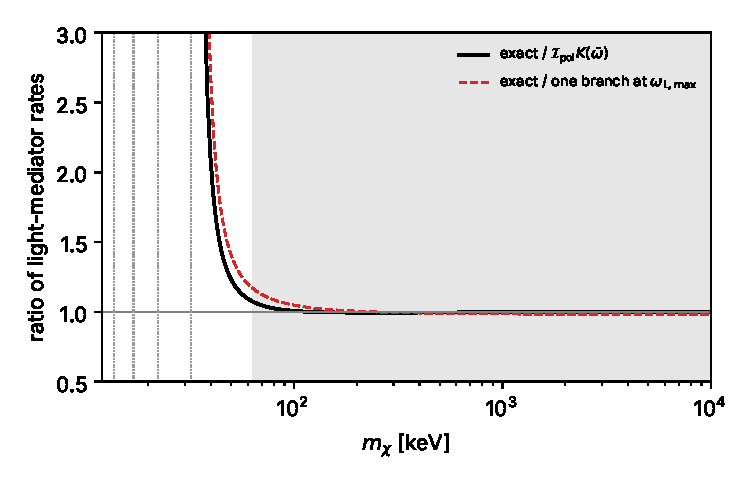
\includegraphics[width=\linewidth]{figures/ch11/limit11_2b.pdf}
\captionof{figure}{Light-mediator rate of the ordinary axis of sapphire, the exact sum over its four longitudinal branches, divided by the band-integral form $\mathcal{I}_{\mathrm{pol}}K_\eta(\bar\omega_{\mathrm{pol}},\mchi)$ (solid) and by the one-branch form with the highest longitudinal frequency and the same $1/\varepsilon_\infty - 1/\varepsilon_0$ (dashed), against $\mchi$. Lossless factorized $\varepsilon$ from the measured frequencies of Ref.~\cite[Table~II]{griffin2018directional} (ordinary ray: longitudinal 112.4, 78.0, 59.7, \SI{48.1}{meV}; transverse 78.6, 70.5, 54.4, \SI{47.7}{meV}) and $\varepsilon_\infty = 3.2$~\cite[Table~I]{griffin2018directional}; weights from the residues of $-1/\varepsilon$, $\bar\omega_{\mathrm{pol}} = \SI{109.9}{meV}$; standard halo of \cref{sec:1.2}. Dotted lines: the four edges $2\omega_{\mathrm{L}\nu}/v_{\mathrm{max}}^2$, from 13.7 to \SI{32.0}{keV}. Gray: $\mchi$ above twice the highest edge, \SI{64}{keV}, where the band-integral form is within \SI{7}{\percent}.}\label{fig:11-limit-2b}
\par}
\smallskip
Within about twice the highest edge the branches open one by one, the lowest first, and the rate follows the individual longitudinal frequencies rather than their weighted sum.
\end{limitbox}

On the ordinary axis of sapphire one branch takes almost all the weight. The longitudinal phonon at \SI{112.4}{meV} carries \SI{95.2}{\percent} of $1/\varepsilon_\infty - 1/\varepsilon_0 = 0.210$. It is a collective mode: the macroscopic field of all the dipoles together pushes it up to \SI{112.4}{meV}, and like a plasmon it collects nearly all of the loss weight. Its band integral is $\mathcal{I}_{\mathrm{pol}} = \SI{36.3}{meV}$, about \SI{70}{\percent} of the way up the bracket \cref{eq:11.2-Ipol}, $[15.9, 45.4]$\,meV. With the highest longitudinal frequency itself, \SI{112.4}{meV}, in place of its bound $\omega_{\mathrm{T,max}}(\varepsilon_0/\varepsilon_\infty)^{1/2}$, the upper end tightens to \SI{37.1}{meV}. With $\rho_T = \SI{3.98}{g.cm^{-3}}$~\cite[Table~I]{griffin2018directional}, $\mathcal{I}_{\mathrm{pol}}/\rho_T = \SI{9.12}{meV.cm^3.g^{-1}}$. Above \SI{64}{keV} the band-integral form is good to \SI{7}{\percent}. At \SI{40}{keV}, however, the true rate is 2.1 times the band-integral form, because the branches between 48 and \SI{78}{meV} are already well open while the dominant one has barely opened. Damping adds a correction of order $\gamma_{\mathrm{L}}/\omega_{\mathrm{L}}$, the width of the line over its frequency. For the dominant phonon of sapphire, $\gamma_{\mathrm{L}} = \SI{16}{cm^{-1}}$ at \SI{77}{K}~\cite[Table~II]{griffin2018directional}, or \SI{1.8}{\percent}; the Lorentzian line adds weight in its tails.

\subsection{The Born charge from the splitting}\label{sec:11.2-split}

For a diatomic crystal the rate needs one combination of material numbers, $Z^*/\varepsilon_\infty$, the screened dipole per unit displacement. Solving \cref{eq:5.5-LOTO} for it,
\begin{equation}
  \frac{Z^*}{\varepsilon_\infty} = \Bigl[\frac{\Omega\,\mu_{\mathrm{red}}\,(\omega_{\mathrm{L}}^2 - \omega_{\mathrm{T}}^2)}{e^2\,\varepsilon_\infty}\Bigr]^{1/2} ,
  \label{eq:11.2-Zeps}
\end{equation}
which needs two phonon frequencies, the cell, the masses and $\varepsilon_\infty$, but not the static constant. For GaAs, \cref{we:5-lst} has already extracted $Z^* = 2.11$ from the measured splitting, and by \cref{eq:11.2-Zeps} $Z^*/\varepsilon_\infty = 0.194$. The error budget follows from the logarithmic derivative,
\begin{equation*}
  \frac{\delta(Z^*/\varepsilon_\infty)}{Z^*/\varepsilon_\infty} = -\frac12\frac{\delta\varepsilon_\infty}{\varepsilon_\infty} + \frac{\omega_{\mathrm{L}}\,\delta\omega_{\mathrm{L}} - \omega_{\mathrm{T}}\,\delta\omega_{\mathrm{T}}}{\omega_{\mathrm{L}}^2 - \omega_{\mathrm{T}}^2} .
\end{equation*}
A common calibration error of the two frequencies cancels to first order. Independent errors are amplified by $\omega^2/(\omega_{\mathrm{L}}^2 - \omega_{\mathrm{T}}^2) \approx 6.9$, so that \SI{0.1}{\percent} on each frequency costs \SI{0.9}{\percent}, and together with \SI{1}{\percent} on $\varepsilon_\infty$ the result is good to \SI{1.0}{\percent}. The dielectric constant should be the one at the temperature of the detector, since it changes at the percent level between room temperature and liquid-helium temperature~\cite{griffin2018directional}.

\subsection{Rate and reach of polar targets}\label{sec:11.2-targets}

\begin{workedexample}{The band integral of GaAs and LiF}\label{we:11-ipol}
GaAs has one polar branch, and \cref{eq:11.2-Ipol} has one term. We take the measured numbers of \cref{we:5-lst} and its cell, $a = \SI{5.638}{\angstrom}$, the static-lattice constant of \cref{tab:E-functionals}, the measured value with the thermal and zero-point expansion removed, which is also the cell of the computed phonons; then $\rho_T = M_{\mathrm{cell}}/\Omega = \SI{144.645}{u}/\SI{44.80}{\angstrom^3} = \SI{5.361}{g.cm^{-3}}$.

\emph{Through the dielectric constants.} $1/\varepsilon_\infty - 1/\varepsilon_0 = 1/10.88 - 1/12.9 = 0.01439$, so that $\mathcal{I}_{\mathrm{pol}} = (\pi/2)(\SI{36.35}{meV})(0.01439) = \SI{0.822}{meV}$ and $\mathcal{I}_{\mathrm{pol}}/\rho_T = \SI{0.153}{meV.cm^3.g^{-1}}$.

\emph{Through the splitting.} By the Lyddane--Sachs--Teller relation $1/\varepsilon_\infty - 1/\varepsilon_0 = (1 - \omega_{\mathrm{T}}^2/\omega_{\mathrm{L}}^2)/\varepsilon_\infty$, and $\mathcal{I}_{\mathrm{pol}} = (\pi/2)(\omega_{\mathrm{L}}^2 - \omega_{\mathrm{T}}^2)/(\varepsilon_\infty\omega_{\mathrm{L}}) = \SI{0.759}{meV}$, or $\SI{0.1415}{meV.cm^3.g^{-1}}$ per unit mass. The two routes differ by \SI{8}{\percent}: the \SI{1.4}{\percent} residual of the inputs, amplified by $\partial\ln\mathcal{I}_{\mathrm{pol}}/\partial\ln\varepsilon_0 = \varepsilon_\infty/(\varepsilon_0 - \varepsilon_\infty) = 5.4$.

\emph{From a table of computed values.} The target table of Griffin and collaborators lists $Z^* = 2.27$, $\varepsilon_\infty = 10.9$ and optical energies from 31.8 to \SI{34.9}{meV} for GaAs~\cite[Table~I]{griffin2020multichannel}. In \cref{eq:11.2-diatomic}, with $M_{\mathrm{cell}} = \SI{144.645}{u}$ and $\mu_{\mathrm{red}} = \SI{36.11}{u}$, they give \SI{0.170}{meV.cm^3.g^{-1}}, \SI{20}{\percent} above the splitting route, mostly because their Born charge is \SI{8}{\percent} above the measured one.

\emph{LiF.} The same table gives $Z^* = 1.05$, $\varepsilon_\infty = 2.02$ and optical energies from 33.5 to \SI{77.2}{meV}. With $M_{\mathrm{cell}} = \SI{25.94}{u}$ and $\mu_{\mathrm{red}} = \SI{5.084}{u}$, \cref{eq:11.2-diatomic} yields $\mathcal{I}_{\mathrm{pol}}/\rho_T = \SI{19.0}{meV.cm^3.g^{-1}}$, 112 times the GaAs value of the same table. The factors are: the weaker electronic screening gains $(10.9/2.02)^2 = 29$ and the lighter ions $M_{\mathrm{cell}}\mu_{\mathrm{red}}$ a factor of 40, while the smaller Born charge gives back $(1.05/2.27)^2 = 0.21$ and the higher frequency $34.9/77.2 = 0.45$.

\emph{Edges.} The lightest masses that reach the longitudinal phonon are $2\omega_{\mathrm{L}}/v_{\mathrm{max}}^2 = \SI{10.35}{keV}$ for GaAs and \SI{21.98}{keV} for LiF.
\end{workedexample}

At large mass the kinematic weights of the two crystals approach each other: at \SI{1}{MeV}, $K_\eta$ of LiF is 0.77 times that of GaAs. LiF then leads by a factor of 103, the ratio 134 of its band integral to the splitting value of GaAs, times 0.77. Toward lower masses the ratio falls, to 46 at \SI{100}{keV}, 17 at \SI{50}{keV} and 2.6 at \SI{30}{keV}; at \SI{25}{keV} GaAs is ahead, and below \SI{22}{keV} the rate of LiF vanishes. \Cref{fig:11-polar}b shows the consequence for the reach: the two curves cross at \SI{26.7}{keV}, and below it only GaAs has reach.

The order of polar targets by rate is reversed in their reach, and the reversal is general. Write the diatomic band integral with the splitting, $\mathcal{I}_{\mathrm{pol}}/\rho_T = (\pi/2)(\omega_{\mathrm{L}}/\varepsilon_\infty\rho_T)(1 - \omega_{\mathrm{T}}^2/\omega_{\mathrm{L}}^2)$. At a given screening, density and ratio of the two frequencies, the band integral is proportional to $\omega_{\mathrm{L}}$, and so is the edge $2\omega_{\mathrm{L}}/v_{\mathrm{max}}^2$. The light ions that make $\mathcal{I}_{\mathrm{pol}}$ large are the ones that make the phonon hard, through the reduced mass in $\omega_{\mathrm{T}}^2 = C_0/\mu_{\mathrm{red}}$ and in the splitting \cref{eq:5.5-LOTO}. A crystal of heavy, soft ions, such as CsI with optical modes between 6.9 and \SI{10.0}{meV}~\cite[Table~I]{griffin2020multichannel}, reaches down to \SI{2.85}{keV}, but with a far smaller rate above that. The best polar crystal depends on the mass window, and \cref{sec:17.5} poses it as a figure of merit.

\section{Multiphonon response}\label{sec:11.3}

At $q_{\mathrm{BZ}} = \SI{2.25}{keV}$ the long-wavelength phonons of \cref{sec:11.1} stop describing the response, and at about 90 to \SI{140}{keV} the free recoil of \cref{sec:11.4} becomes valid (by the two onset criteria compared there). Between these two momenta, a silicon nucleus that takes up the momentum $\vect{q}$ leaves behind zero, one, two or a dozen phonons. Dark matter between about 0.4 and \SI{26}{MeV} transfers its largest momenta, $2\mchi v_{\mathrm{max}}$, inside this window. \Cref{sec:5.6} computed the response of one nucleus as if the others were not there: the phonon number is Poisson distributed with mean $2W_\kappa(\vect{q})$, and the spectrum of each term follows from the density of states. A crystal adds the pairs of different nuclei, whose interference produced the conservation of crystal momentum in the one-phonon response of \cref{sec:11.1}. How much of that interference survives when two or more phonons share the momentum, and when may a calculation drop it? The incoherent approximation of the literature drops the pairs. It is exact on average far above the zone for a lattice without a basis, and in silicon its phonon-number weights are good to \SI{10}{\percent} above about \SI{6.6}{keV}.

\subsection{The response at all phonon orders}

We keep the coupling of \cref{sec:11.1}, a potential $\tilde V_N(\vect{q})$ that sees each nucleus of species $\kappa$ with a weight $c_\kappa$, so that the dark matter couples to the operator $\sum_\kappa c_\kappa n_\kappa(\vect{q})$. For equal couplings to protons and neutrons $c_\kappa = A_\kappa$, the nucleon number. The results below hold for any coupling that multiplies the density of each species by a real number, the coefficient $c_1^{(\kappa)}$ of \cref{sec:8.4}, and in particular for the rigid-ion charge $Z_\kappa$. We keep writing $S_A$ for the response, as in \cref{sec:11.1}, and \cref{eq:8.2-spectrum} with one row turns it into a rate. The nuclei sit at $\vect{X}_{\vect{R}\kappa} = \vect{R} + \vect{\tau}_\kappa + \vect{u}_{\vect{R}\kappa}$, and $n_\kappa(\vect{q}) = \sum_{\vect{R}}\ee^{\ii\vect{q}\cdot\vect{X}_{\vect{R}\kappa}}$. The correlation form of \cref{eq:4.2-Sab} then contains, for every pair of nuclei, the average $\langle\ee^{-\ii\vect{q}\cdot\vect{X}_{\vect{R}\kappa}(t)}\ee^{\ii\vect{q}\cdot\vect{X}_{\vect{R}'\kappa'}(0)}\rangle$. The static positions give a phase, and the displacements give the generating formula of a pair, \cref{eq:D.15-gen}. The average depends only on the separation $\Delta\vect{R} = \vect{R} - \vect{R}'$ of the cells, because the eigenvectors carry the cell phase $\ee^{\ii\vect{Q}\cdot\vect{R}}$ (\cref{eq:5.3-u}) and the thermal state is invariant under lattice translations. The sum over $\vect{R}'$ then gives a factor $N$, and with the volume $\Vol = N\Omega$ we find
\begin{keyresult}[Harmonic nuclear response at all phonon orders]
\begin{equation}
  S_A(\vect{q},\omega) = \frac1\Omega\sum_{\Delta\vect{R},\kappa,\kappa'}c_\kappa c_{\kappa'}\,\ee^{-\ii\vect{q}\cdot\Delta\vect{R}_{\kappa\kappa'}}\,\ee^{-W_\kappa(\vect{q}) - W_{\kappa'}(\vect{q})}\int_{-\infty}^{\infty}\dd t\;\ee^{\ii\omega t}\,\ee^{\vect{q}\cdot\mathcal{C}_{\kappa\kappa'}(\Delta\vect{R},t)\cdot\vect{q}} ,
  \label{eq:11.3-exact}
\end{equation}
with $\Delta\vect{R}_{\kappa\kappa'} = \Delta\vect{R} + \vect{\tau}_\kappa - \vect{\tau}_{\kappa'}$ the vector from nucleus $\kappa'$ in the cell at the origin to nucleus $\kappa$ in the cell $\Delta\vect{R}$, the Debye--Waller exponents of \cref{eq:5.6-W} and the displacement correlation of \cref{eq:5.6-C}. \Cref{eq:11.3-exact} holds for a harmonic crystal in thermal equilibrium at any temperature.
\end{keyresult}
\noindent This response is the classical starting point of neutron scattering from crystals~\cite[App.~N]{ashcroft1976solid}, written for a coupling that differs from species to species. Every quantity in it was computed in \cref{sec:5.6} from the force constants. The sum over pairs is new. Its terms with $\Delta\vect{R}_{\kappa\kappa'} = 0$, one nucleus scattering at both times, form the \emph{self part}, which is \cref{eq:5.6-multi} weighted by $c_\kappa^2$ and summed over the basis. All other terms form the \emph{distinct part}. Each distinct term carries the phase $\ee^{-\ii\vect{q}\cdot\Delta\vect{R}_{\kappa\kappa'}}$, and its size is set by how strongly the displacements of two nuclei a distance $|\Delta\vect{R}_{\kappa\kappa'}|$ apart are correlated.

Expanding the last exponential in powers of $\vect{q}\cdot\mathcal{C}_{\kappa\kappa'}\cdot\vect{q}$ sorts the response by the number $n$ of phonons, $S_A = \sum_nS^{(n)}_A$, as in \cref{sec:5.6}. The term $n = 0$ is time independent. Its sum over $\Delta\vect{R}$ vanishes unless $\vect{q}$ is a reciprocal-lattice vector, and the term is the Bragg peak, $\propto\delta(\omega)\sum_{\vect{G}}\delta^3(\vect{q} - \vect{G})$. The Bragg peak deposits no energy and occupies a set of zero measure in $\vect{q}$, so it never contributes to a rate. For $n \ge 1$ each factor $\vect{q}\cdot\mathcal{C}_{\kappa\kappa'}\cdot\vect{q}$ is a sum over phonons $\vect{Q}\nu$ with the phase $\ee^{\ii\vect{Q}\cdot\Delta\vect{R}}$, and the sum over $\Delta\vect{R}$ against $\ee^{-\ii\vect{q}\cdot\Delta\vect{R}}$ forces the phonon wavevectors to add up to $\vect{q}$ up to a reciprocal-lattice vector. Each phonon $i$ is created ($s_i = +1$) or absorbed ($s_i = -1$), and after the time integral (\cref{app:D.31})
\begin{keyresult}[The $n$-phonon term]
\begin{equation}
  \begin{aligned}
  S^{(n)}_A(\vect{q},\omega) = \frac{2\pi}{\Omega}\,\frac{1}{n!}\sum_{\{\nu_i,s_i\}}\Bigl\langle\,&\prod_{i=1}^{n}\frac{n_{\vect{Q}_i\nu_i} + \frac12(1 + s_i)}{2\omega_{\vect{Q}_i\nu_i}}\;\delta\Bigl(\omega - \sum_is_i\omega_{\vect{Q}_i\nu_i}\Bigr) \\
  &\times\Bigl|\sum_\kappa c_\kappa\,\ee^{-W_\kappa}\,\ee^{\ii\vect{q}\cdot\vect{\tau}_\kappa}\,\frac{\prod_i\vect{q}\cdot\vect{e}^{s_i}_{\kappa\nu_i}(\vect{Q}_i)}{M_\kappa^{n/2}}\Bigr|^2\Bigr\rangle ,
  \end{aligned}
  \label{eq:11.3-Sn}
\end{equation}
with $\vect{e}^{+} = \vect{e}^*$ for a created and $\vect{e}^{-} = \vect{e}$ for an absorbed phonon, $\vect{q}$ unreduced in the phase $\ee^{\ii\vect{q}\cdot\vect{\tau}_\kappa}$, and the brackets the average $N^{-(n-1)}\sum$ over $\vect{Q}_1, \ldots, \vect{Q}_{n-1}$ in the zone, with $\vect{Q}_n$ fixed by $\sum_is_i\vect{Q}_i = \vect{q} - \vect{G}$.
\end{keyresult}
\noindent At $n = 1$ the brackets are empty, $\vect{Q}_1 = \vect{q} - \vect{G}$ for emission, and \cref{eq:11.3-Sn} is the one-phonon response \cref{eq:11.1-S1}. For every $n$ the crystal momentum is conserved, and the response at fixed $\vect{q}$ is a convolution over the zone of $n$ branches. \Cref{eq:11.3-Sn} is the full harmonic answer, and also an expensive one: at $n = 2$ the sum runs over one wavevector of the zone for each $\vect{q}$, at $n = 3$ over two.

On the truncation label of \cref{sec:8.5}, \cref{eq:11.3-exact} is at $n_A = 0$ and $n_B = 0$, with every thermal order kept through the factors $n_{\vect{Q}\nu}$, and with $\mathcal{K}$ = multiphonon, all orders. In a detector at \SI{10}{mK} only the terms with every $s_i = +1$ survive, at $n_T = 0$.

In neutron scattering, ``incoherent'' refers to the random variation of the coupling from site to site, between isotopes or nuclear spin states. For a nucleon-number coupling in natural silicon the variance of $A_\kappa$ is 0.159, $2.0\times10^{-4}$ of $\langle A_\kappa\rangle^2 = 790.1$, and negligible; the isotopes act instead through their masses (\cref{sec:11.6}). Here ``incoherent'' means the approximation that keeps only the self part.

The quantities in \cref{eq:11.3-exact,eq:11.3-Sn} come from one harmonic calculation per material: DFPT force constants, interpolated to a fine grid of wavevectors, give the frequencies and polarization vectors, from which the exponents $W_\kappa$, the correlations $\mathcal{C}_{\kappa\kappa'}$ and the zone sums follow at negligible cost (\cref{sec:5.4,app:E.17}).

\subsection{The incoherent approximation}

At momentum transfers far above the zone, the phase $\ee^{-\ii\vect{q}\cdot\Delta\vect{R}_{\kappa\kappa'}}$ of a distinct term turns through many radians when $\vect{q}$ changes by a fraction of $q_{\mathrm{BZ}}$. The other factors of the distinct term, a polynomial in $\vect{q}$ times the Debye--Waller factors, barely change. Any rate integrates over $\vect{q}$, and the distinct terms then average away, leaving the self part, which treats each nucleus as an independent oscillator in the potential well of its neighbors:
\begin{equation}
  S_A(\vect{q},\omega) \approx S^{\mathrm{inc}}_A(\vect{q},\omega) = \frac{2\pi}{\Omega}\sum_\kappa c_\kappa^2\,\ee^{-2W_\kappa(\vect{q})}\sum_{n=0}^{\infty}\frac{[2W_\kappa(\vect{q})]^n}{n!}\,P^\kappa_n(\hat{\vect{q}},\omega) .
  \label{eq:11.3-inc}
\end{equation}
Here $P^\kappa_1(\hat{\vect{q}},\omega)$ is the single-phonon distribution of \cref{sec:5.6} for nucleus $\kappa$: the density of states projected on the direction of $\vect{q}$, $N^{-1}\sum_{\vect{Q}\nu}|\hat{\vect{q}}\cdot\vect{e}_{\kappa\nu}(\vect{Q})|^2\delta(\omega - \omega_{\vect{Q}\nu})$, times $[n_{\mathrm{B}}(\omega) + 1]/\omega$, normalized to one. $P^\kappa_n$ is the $n$-fold convolution of $P^\kappa_1$. On a site of cubic symmetry the projected density of states is a third of the atom-projected one, $g_{\mathrm{ph},\kappa}(\omega)/3$, independent of $\hat{\vect{q}}$, and \cref{eq:11.3-inc} is \cref{eq:5.6-multi} summed over the basis.

The incoherent approximation keeps the self part exactly, so it inherits two exact properties from \cref{sec:5.6}: the phonon number is Poisson distributed, and the first moment of the response, $\int\dd\omega\,\omega S_A$, is $(2\pi/\Omega)\sum_\kappa c_\kappa^2E_R$ with $E_R = q^2/2M_\kappa$. The distinct part adds weight but no energy. Every distinct term has zero first moment in $\omega$, at every order $n$, because its time derivative at $t = 0$ contains $\partial_t\mathcal{C}_{\kappa\kappa'}(\Delta\vect{R},0)$, which the completeness of the polarization vectors makes proportional to $\delta_{\kappa\kappa'}\delta_{\Delta\vect{R},\vect{0}}$ (\cref{app:D.31}). The first moment of the $n$-phonon term is therefore the first moment of its self part, and for one species
\begin{equation}
  \frac{\int\dd\omega\;\omega\,S^{(n)}_A(\vect{q},\omega)}{\int\dd\omega\;\omega\,S_A(\vect{q},\omega)} = \ee^{-2W_\kappa}\,\frac{(2W_\kappa)^{n-1}}{(n-1)!} ,
  \label{eq:11.3-fsum}
\end{equation}
at every $\vect{q}$ and temperature, coherent terms included. A calculation that stops at order $N$ misses the fraction $\sum_{n \ge N}p^{\mathrm{ph}}_n$ of the recoil energy, the Poisson tail of the weights \cref{eq:5.6-poisson}; with several species the fractions are averaged with the weights $c_\kappa^2/M_\kappa$. At \SI{50}{keV} in silicon, where $2W_\kappa = 1.57$, the orders above two carry \SI{47}{\percent} of the energy deposited, and a two-phonon calculation misses that share.

The tail matters most for a threshold above the phonon band. Since $P^\kappa_n$ vanishes above $n\,\omega_{\mathrm{max}}$, with $\omega_{\mathrm{max}}$ the highest phonon energy, an energy deposit above $E$ needs at least $\lceil E/\omega_{\mathrm{max}}\rceil$ phonons, and in the incoherent approximation at $T = 0$ its probability is at most the Poisson tail $\sum_{n \ge \lceil E/\omega_{\mathrm{max}}\rceil}p^{\mathrm{ph}}_n$. A free nucleus deposits exactly $E_R$.

\begin{workedexample}{The Poisson tail above three Debye energies}\label{we:11-tail}
Take silicon at $T = 0$ and a threshold $E = 3\omega_{\mathrm{D}} = \SI{166.8}{meV}$, with $\omega_{\mathrm{D}} = \SI{55.6}{meV}$ from \cref{we:5-dw}. The computed density of states of \cref{sec:5.2} ends at $\omega_{\mathrm{max}} = \SI{63.7}{meV}$ (the zone-center optical phonon measured by neutron scattering at room temperature is \SI{64.1}{meV}, \cref{sec:5.2}), so two phonons reach at most \SI{127}{meV} and a deposit above $E$ needs three or more. Of the three-phonon spectrum $P_3$, \SI{1.4}{\percent} lies above $E$; of $P_4$, $P_5$ and $P_6$, 11, 35 and \SI{62}{\percent}. With $2W_\kappa = q^2\langle u_x^2\rangle$ and $\langle u_x^2\rangle = \SI{2.45e-3}{\angstrom^2}$, the probability of a deposit above $E$ is $\sum_np^{\mathrm{ph}}_n\int_E^\infty P_n$:

\emph{$q = \SI{10}{keV}$.} $E_R = \SI{1.91}{meV}$ and $2W_\kappa = 0.063$. The probability is \num{6.1e-7}, almost all of it from three phonons; the Poisson bound $\sum_{n\ge3}p^{\mathrm{ph}}_n = \num{4.0e-5}$ is 65 times larger, because a three-phonon deposit rarely reaches the top of its band.

\emph{$q = \SI{30}{keV}$.} $E_R = \SI{17.2}{meV}$ and $2W_\kappa = 0.566$. The probability is \num{6.2e-4}, from three, four and five phonons in the proportion 0.38 : 0.43 : 0.16; the bound is \num{2.0e-2}.

\emph{$q = \SI{50}{keV}$.} $E_R = \SI{47.8}{meV}$, a third of the threshold, and $2W_\kappa = 1.57$. The probability is \num{1.7e-2}, against the bound 0.21. Four and five phonons contribute most.

A free silicon nucleus deposits \SI{166.8}{meV} only for $q \ge (2M_\kappa E)^{1/2} = \SI{93.4}{keV}$. A particle much lighter than the nucleus transfers at most $2\mchi v_{\mathrm{max}}$, so the free-recoil picture needs $\mchi \ge \SI{17.6}{MeV}$ for this threshold. Dark matter of \SI{10}{MeV} reaches $q = \SI{53}{keV}$, and already at \SI{50}{keV} the bound lattice deposits more than $3\omega_{\mathrm{D}}$ in \SI{1.7}{\percent} of the scatterings.
\end{workedexample}

\Cref{app:D.31} finds the range of the incoherent approximation by averaging $\vect{q}$ over a small cell of reciprocal space, the size of the zone, around a given $\vect{q}$. The phase of a distinct term averages to $j_{\mathrm{BZ}}(\Delta\vect{R}_{\kappa\kappa'}) = (\Omega/(2\pi)^3)\int_{\mathrm{BZ}}\dd^3p\,\ee^{-\ii\vect{p}\cdot\Delta\vect{R}_{\kappa\kappa'}}$, which vanishes for every lattice vector except zero, while the slowly varying factors change across the cell by a relative amount of order $n\,q_{\mathrm{BZ}}/q$. For a lattice with one atom per cell every distinct term joins two nuclei of the same sublattice, and the incoherent response is the average of the exact one over a zone-sized cell, up to corrections of relative order $nq_{\mathrm{BZ}}/q$. With a basis the pairs on different sublattices are not separated by lattice vectors, and they survive the average: in silicon each of the four bonds keeps a weight $j_{\mathrm{BZ}} \approx 0.44$ in a spherical zone. The distinct terms of the bonds decay because the correlation of two displacements falls with distance. The average over the directions of $\vect{q}$, as in the rate of a crystal of random orientation, reduces each of them further by a spherical Bessel function of $q|\Delta\vect{R}_{\kappa\kappa'}|$. The incoherent approximation therefore needs $q \gg \max(n, 2W_\kappa)\,q_{\mathrm{BZ}}$, and for a crystal with a basis the size of the surviving distinct terms has to be computed.

\begin{limitbox}[Multiphonon incoherent approximation][lim:11.3a]
Above the zone, the nuclear response is the sum of independent atomic responses, each a Poisson series in the phonon number, $S \approx (2\pi/\Omega)\sum_\kappa c_\kappa^2\ee^{-2W_\kappa}\sum_n[(2W_\kappa)^n/n!]P^\kappa_n(\omega)$, with $P^\kappa_n$ the $n$-fold convolution of the single-phonon distribution~\cite[Eqs.~(15), (36)]{campbelldeem2022dark}.
\par\smallskip
{\centering
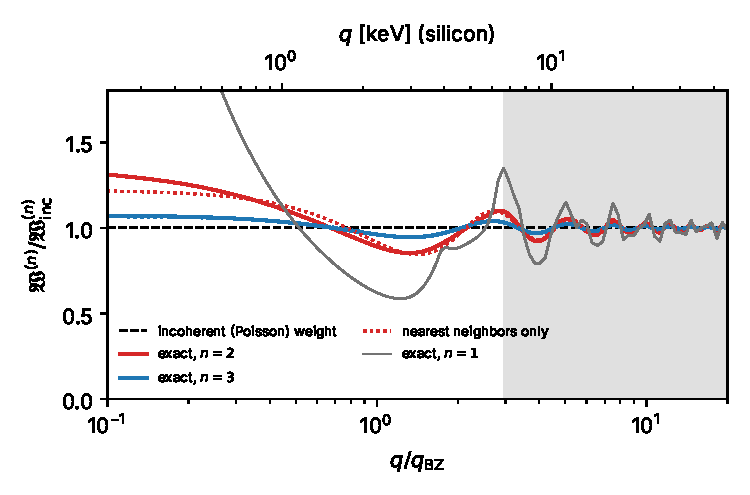
\includegraphics[width=\linewidth]{figures/ch11/limit11_3a.pdf}
\captionof{figure}{The exact $\omega$-integrated $n$-phonon weight of silicon at $T = 0$, \cref{eq:11.3-weight}, divided by its incoherent value, the Poisson weight of \cref{eq:11.3-inc} (dashed, one), averaged over the directions of $\vect{q}$, against $q/q_{\mathrm{BZ}}$, with $q_{\mathrm{BZ}} = \SI{2.25}{keV}$. For one species the couplings and the Debye--Waller factors cancel in the ratio, which is $1 + \delta^{\mathrm{coh}}_n(q)$ for any coupling of the form $\sum_\kappa c_\kappa n_\kappa$. Displacement correlations from the PBE force constants of \cref{sec:5.2} on a $48^3$ grid, pair sum to \SI{40}{\angstrom}, direction average exact. Solid: two (red) and three (blue) phonons. Dotted: the nearest-neighbor pairs alone, the leading correction. Thin gray: one phonon, which must be summed in reciprocal space. Gray band: $q \ge 2.95\,q_{\mathrm{BZ}} = \SI{6.6}{keV}$, where the two- and three-phonon weights stay within \SI{10}{\percent} of the incoherent ones. The three-phonon weight does so at every $q$, the one-phonon weight only above $7.9\,q_{\mathrm{BZ}}$.}\label{fig:11-limit-3a}
\par}
\smallskip
Below about three times the zone momentum the two-phonon weight differs from the Poisson weight by up to \SI{35}{\percent}, and pointwise in $\omega$ the incoherent spectrum misses the momentum conservation of the phonon pair even far above the zone.
\end{limitbox}

At small $q$ the phases are irrelevant, and every pair adds with the square of its correlation. The coherent two-phonon weight then exceeds the incoherent one by \SI{35}{\percent}, mostly from the four bonds, along which the longitudinal displacements of neighbors are correlated with a coefficient of 0.44 (a dynamical number, distinct from the geometric weight $j_{\mathrm{BZ}} \approx 0.44$ above, to which it is close by coincidence). Near $q_{\mathrm{BZ}}$ the bond phases turn the sign of this correction, and from about $3\,q_{\mathrm{BZ}}$ the correction oscillates with the period of the bond length and decays: $\delta^{\mathrm{coh}}_2 = -0.079$, $+0.014$, $-0.018$ and $-0.025$ at 2, 5, 10 and \SI{20}{keV}. The nearest-neighbor pairs alone account for 0.21 of the 0.35 at small $q$, and above about $2\,q_{\mathrm{BZ}}$ they follow the full curve within \SI{1}{\percent} of the weight. The three-phonon correction is smaller everywhere, since it carries the cube of a correlation coefficient below one: $-0.027$, $+0.016$, $-0.006$ and $-0.012$ at the same momentum transfers. The one-phonon term is the exception: it is sharp in $\omega$ at fixed $\vect{q}$, its pair sum does not converge absolutely, and its $\omega$-integrated weight approaches the incoherent value slowly, within \SI{10}{\percent} above about \SI{18}{keV}. Near each reciprocal-lattice vector the soft acoustic phonons enhance the one-phonon weight. Above $q_{\mathrm{BZ}}$, where \cref{eq:11.1-Sac} no longer holds, the one-phonon term is computed from \cref{eq:11.1-S1} with all branches and Umklapp terms, and its weight grows on average as $q^2\ee^{-2W_\kappa}$, the incoherent form, up to these corrections.

\Cref{fig:11-mph} shows the three parts of the silicon response at $q = \SI{10}{keV}$, the momentum transfer at which \cref{sec:8.5} placed the end of the one-phonon regime. One phonon carries a weight of 0.058 per nucleus, two phonons \num{1.8e-3} and three or more \num{4.0e-5}, close to the Poisson weights $2W_\kappa\ee^{-2W_\kappa} = 0.059$, $(2W_\kappa)^2\ee^{-2W_\kappa}/2 = \num{1.9e-3}$ and the rest. The exact one-phonon spectrum, averaged over directions, follows the projected density of states. The exact two-phonon spectrum follows the self-convolution of the single-phonon distribution within \SI{17}{\percent} in every bin of \SI{1}{meV} between 22 and \SI{120}{meV}, where the spectrum exceeds a tenth of its maximum; toward the edges of the band the ratio of the exact to the incoherent spectrum falls to about one half.

\begin{figure}[tbp]
  \centering
  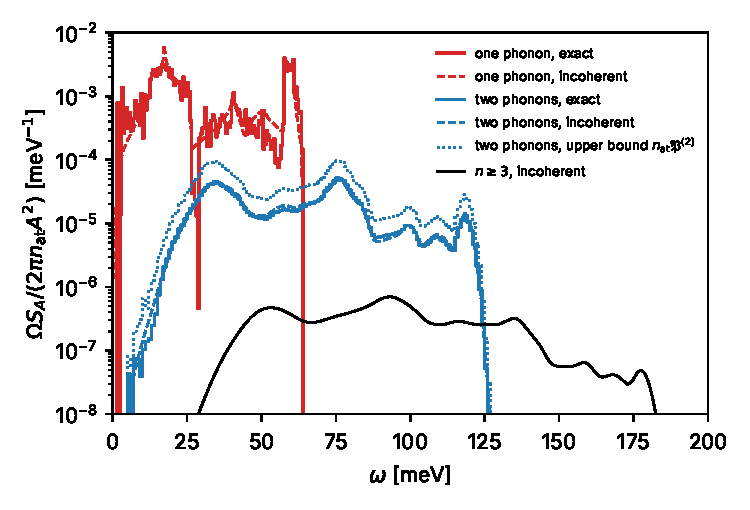
\includegraphics[width=\linewidth]{figures/ch11/fig11_3.pdf}
  \caption{Nuclear response of silicon at $|\vect{q}| = \SI{10}{keV}$ and $T = 0$, per nucleus, $\Omega S_A/(2\pi n_{\mathrm{at}}A^2)$, averaged over the directions of $\vect{q}$, split by the number of phonons; the elastic weight $\ee^{-2W_\kappa} = 0.939$ at $\omega = 0$ is not shown. Red: one phonon, exact (\cref{eq:11.1-S1}, all six branches, histogram of 0.5-meV bins) and incoherent (dashed). Blue: two phonons, exact (\cref{eq:11.3-Sn}, 1-meV bins), incoherent (dashed) and the upper end $n_{\mathrm{at}}\mathfrak{P}^{(2)}$ of the certified band \cref{eq:11.3-band} (dotted). Black: three or more phonons, incoherent. Phonons from the PBE force constants of \cref{sec:5.2}; incoherent parts from the density of states of the same force constants, with $\langle u_x^2\rangle = \SI{2.45e-3}{\angstrom^2}$. The exact two-phonon response is averaged over 240 wavevectors with $|\vect{q}|$ within \SI{1}{\percent} of \SI{10}{keV} on a $24^3$ grid commensurate with the zone, each rescaled to \SI{10}{keV} by $(10\,\mathrm{keV}/|\vect{q}|)^4$.}
  \label{fig:11-mph}
\end{figure}

\subsection{Exact phonon-order weights}

Integration over $\omega$ reduces the time integral of \cref{eq:11.3-exact} to the integrand at $t = 0$, and the $n$-phonon term becomes a sum over pairs of a static quantity. At $t = 0$ the two terms of \cref{eq:5.6-C} combine into $2n_{\vect{Q}\nu} + 1$, and the displacement correlation becomes the static correlation tensor
\begin{equation}
  B_{\kappa\kappa'}(\Delta\vect{R}) = \mathcal{C}_{\kappa\kappa'}(\Delta\vect{R},0) = \frac1N\sum_{\vect{Q}\nu}(2n_{\vect{Q}\nu} + 1)\,\frac{\vect{e}_{\kappa\nu}(\vect{Q})\,\vect{e}_{\kappa'\nu}(\vect{Q})^\dagger\,\ee^{\ii\vect{Q}\cdot\Delta\vect{R}}}{2\omega_{\vect{Q}\nu}\sqrt{M_\kappa M_{\kappa'}}} ,
  \label{eq:11.3-Bkk}
\end{equation}
whose on-site value $B_{\kappa\kappa}(\vect{0})$ is the displacement tensor $B_\kappa$ of \cref{eq:5.3-B}. Off site it measures how the displacements of two nuclei move together: $\langle u^\alpha_{\Delta\vect{R}\kappa}u^\beta_{\vect{0}\kappa'}\rangle$.
\begin{keyresult}[Exact $n$-phonon weight]
The $\omega$-integrated $n$-phonon response per cell is
\begin{equation}
  \mathfrak{W}^{(n)}(\vect{q}) = \Omega\int\frac{\dd\omega}{2\pi}\,S^{(n)}_A(\vect{q},\omega) = \frac{1}{n!}\sum_{\Delta\vect{R},\kappa,\kappa'}c_\kappa c_{\kappa'}\,\ee^{-\ii\vect{q}\cdot\Delta\vect{R}_{\kappa\kappa'}}\,\ee^{-W_\kappa - W_{\kappa'}}\,\bigl[\vect{q}\cdot B_{\kappa\kappa'}(\Delta\vect{R})\cdot\vect{q}\bigr]^n .
  \label{eq:11.3-weight}
\end{equation}
Its self terms are the incoherent weight $\mathfrak{W}^{(n)}_{\mathrm{inc}} = \sum_\kappa c_\kappa^2\,\ee^{-2W_\kappa}(2W_\kappa)^n/n!$, and $\delta^{\mathrm{coh}}_n(\vect{q}) = \mathfrak{W}^{(n)}/\mathfrak{W}^{(n)}_{\mathrm{inc}} - 1$ is the exact correction to the incoherent approximation for any energy window that contains the whole $n$-phonon band.
\end{keyresult}
\noindent A rate code applies this exact correction as a factor $1 + \delta^{\mathrm{coh}}_n$ per phonon order. At $T = 0$ the acoustic modes near $\mathrm{\Gamma}$ make $B_{\kappa\kappa'}(\Delta\vect{R})$ fall as $|\Delta\vect{R}|^{-2}$ at large distances (\cref{app:D.31}). Its square falls as $|\Delta\vect{R}|^{-4}$, faster than the number of pairs grows, and the sum converges absolutely for $n \ge 2$. For $n = 1$ the sum does not converge absolutely, and the one-phonon term is summed in reciprocal space, where it is \cref{eq:11.1-S1}. At $T > 0$ the thermal occupation of the same modes makes $B_{\kappa\kappa'}$ fall only as $T/|\Delta\vect{R}|$, and the two-phonon sum diverges; the subsection on thermal diffuse scattering resums it.

In silicon at $T = 0$ the correlation is short ranged in practice. With the force constants of \cref{sec:5.2} on a $48^3$ grid of wavevectors, the on-site value is $\langle u_x^2\rangle = \SI{2.45e-3}{\angstrom^2}$, as in \cref{we:5-dw}. The sum of \cref{eq:11.3-weight} to \SI{40}{\angstrom} takes seconds for any $\vect{q}$, and changes by less than $2\times10^{-3}$ beyond \SI{30}{\angstrom}. This sum produced the curves of \cref{fig:11-limit-3a}.

The $\omega$-integrated weight leaves open how the coherent correction is distributed in $\omega$. A pointwise statement follows from the structure of \cref{eq:11.3-Sn}, in which the coherent sum over the basis appears inside a squared modulus. By the Cauchy--Schwarz inequality, $|\sum_\kappa a_\kappa|^2 \le n_{\mathrm{at}}\sum_\kappa|a_\kappa|^2$ for the $n_{\mathrm{at}}$ nuclei of a cell, term by term in the sum over phonons. The \emph{momentum-resolved self density} $\mathfrak{P}^{(n)}(\vect{q},\omega)$ is \cref{eq:11.3-Sn} with the squared modulus replaced by the sum of the squared amplitudes of the single nuclei: the response of independent nuclei whose $n$ phonons must still add up to the crystal momentum $\vect{q}$. For silicon, $n_{\mathrm{at}} = 2$, and with $a_1$, $a_2$ the amplitudes of the two nuclei of a cell for one set of phonons, $|a_1 + a_2|^2 = 2(|a_1|^2 + |a_2|^2) - |a_1 - a_2|^2 \le 2(|a_1|^2 + |a_2|^2)$, with equality when the two nuclei move in phase.
\begin{keyresult}[Certified band]
At every $\vect{q}$, $\omega$ and $n$,
\begin{equation}
  \begin{gathered}
  0 \le S^{(n)}_A(\vect{q},\omega) \le n_{\mathrm{at}}\,\mathfrak{P}^{(n)}(\vect{q},\omega) , \\
  \frac{\Omega}{(2\pi)^3}\int_{\mathrm{BZ}}\dd^3p\;\mathfrak{P}^{(n)}(\vect{q} + \vect{p},\omega)\Big|_{\text{vertex at }\vect{q}} = S^{\mathrm{inc},(n)}_A(\vect{q},\omega) ,
  \end{gathered}
  \label{eq:11.3-band}
\end{equation}
where the average holds the factors $\vect{q}\cdot\vect{e}$ and $\ee^{-W_\kappa}$ at $\vect{q}$ and moves only the momentum constraint (\cref{app:D.31}), and $S^{\mathrm{inc},(n)}_A$ is the term of order $n$ of \cref{eq:11.3-inc}.
\end{keyresult}
\noindent For a lattice with one atom per cell the two sides of the inequality coincide, $S^{(n)}_A = \mathfrak{P}^{(n)}$, and the only error of the incoherent approximation is the momentum constraint, which the zone average removes. The constraint matters at the edges of each phonon band: the lowest two-phonon energies need two soft acoustic phonons, both near $\mathrm{\Gamma}$, and hence $\vect{q}$ near a reciprocal-lattice vector. At other $\vect{q}$ the exact spectrum vanishes at those energies, where the self density does not, and the lower end of the certified band is reached. For a crystal with a basis the certified band is wider by the factor $n_{\mathrm{at}}$. In silicon at \SI{10}{keV} its upper end reaches 2.7 times the incoherent two-phonon spectrum (\cref{fig:11-mph}): the certified band bounds the error, but it is too wide to test the incoherent spectrum point by point below a few $q_{\mathrm{BZ}}$; that test needs \cref{eq:11.3-Sn} itself.

\subsection{Thermal diffuse scattering}

In a warm crystal the scattered intensity of X-rays and neutrons does not drop to zero between the Bragg peaks. Thermal phonons fill the space around each peak with a diffuse cloud, which crystallographers subtract when they measure structure factors. The first-order part of the diffuse cloud is the one-phonon response at $\vect{q} = \vect{G} + \vect{k}$ with a soft acoustic phonon of wavevector $\vect{k}$. By \cref{eq:11.1-S1} its weight carries $(2n_{\vect{k}\nu} + 1)/\omega_{\vect{k}\nu} \approx 2T/(c_\nu k)^2$, and it grows as $1/|\vect{q} - \vect{G}|^2$ toward the peak. The second-order part comes from two soft phonons whose wavevectors add up to $\vect{k}$. It is milder, and it is exactly the term whose real-space sum diverged above.

In reciprocal space the two-phonon weight is finite. It is an average over one wavevector $\vect{Q}_1$ of the zone, with $\vect{Q}_2 = \vect{k} - \vect{Q}_1$; each thermal factor $(2n + 1)/2\omega \approx T/\omega^2$ is integrable around $\vect{Q} = 0$, and the average is singular only when both phonons are soft at once, as $\vect{k} \to 0$ (\cref{app:D.31}). The thermal part of the weight therefore obeys
\begin{equation}
  \mathfrak{W}^{(2),\mathrm{th}}(\vect{q}) \le \Bigl|\sum_\kappa c_\kappa\,\ee^{-W_\kappa}\,\ee^{\ii\vect{G}\cdot\vect{\tau}_\kappa}\Bigr|^2\,\frac{\Omega\,T^2q^4}{16\,M_{\mathrm{cell}}^2\,c_{\mathrm{min}}^4\,|\vect{q} - \vect{G}|} + (\text{terms regular at } \vect{q} = \vect{G}) ,
  \label{eq:11.3-tds}
\end{equation}
with $c_{\mathrm{min}}$ the lowest acoustic speed, \SI{4.67}{km.s^{-1}} in silicon for the transverse wave along $[110]$ polarized along $[1\bar10]$. The singularity is integrable, and it is weighted by the Bragg structure factor: it vanishes near a reflection that the basis extinguishes, such as (200) in silicon. In the classical limit the singular part is exactly proportional to $1/|\vect{q} - \vect{G}|$. Its coefficient lies below the bound and depends on the direction of $\vect{q} - \vect{G}$ relative to $\vect{q}$; for an isotropic medium with the speeds of silicon and $\vect{q} - \vect{G}$ parallel to $\vect{q}$ it is 0.46 of the bound. This $1/|\vect{q} - \vect{G}|$ law, against the $1/|\vect{q} - \vect{G}|^2$ of the first order, is the classical result for second-order thermal diffuse scattering~\cite{warren1969xray}. On the truncation label this second-order term is $\mathcal{K}$ = multiphonon (two phonons, coherent) at $n_T = 2$, since the singular part is quadratic in the occupation numbers; the cross terms linear in $n_{\vect{Q}\nu}$, at $n_T = 1$, are at most logarithmically singular.

\begin{limitbox}[Second-order thermal diffuse scattering][lim:11.3b]
Near a reciprocal-lattice vector $\vect{G}$ of a warm crystal, two soft acoustic phonons give the $\omega$-integrated response a singular part that falls as $1/|\vect{q} - \vect{G}|$, weighted by the structure factor at $\vect{G}$ and by $T^2$~\cite{warren1969xray}; its bound is \cref{eq:11.3-tds}.
\par\smallskip
{\centering
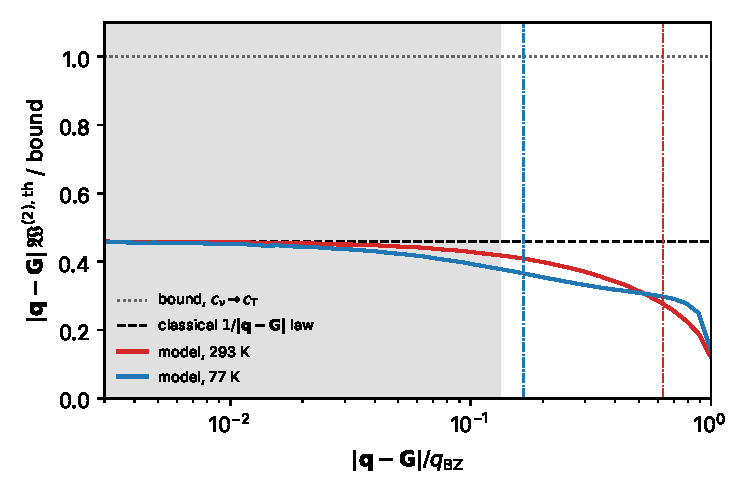
\includegraphics[width=\linewidth]{figures/ch11/limit11_3b.pdf}
\captionof{figure}{Thermal two-phonon weight times $|\vect{q} - \vect{G}|$, in units of the bound \cref{eq:11.3-tds} with $c_{\mathrm{min}}$ replaced by the transverse speed (dotted, one), for $\vect{G} = \vect{G}_{111}$ of silicon and $\vect{q} - \vect{G}$ parallel to $\vect{q}$, against $|\vect{q} - \vect{G}|/q_{\mathrm{BZ}}$. Model: isotropic elastic medium with the speeds $v_L = [(B + \frac43G)/\rho_T]^{1/2} = 8.95$ and $v_T = (G/\rho_T)^{1/2} = \SI{5.34}{km.s^{-1}}$ of silicon, with $G$ the Hill shear modulus, the mean of the Voigt value $G_{\mathrm{V}} = (C_{11} - C_{12} + 3C_{44})/5 = \SI{68.0}{GPa}$ and the Reuss value $G_{\mathrm{R}} = 5(C_{11} - C_{12})C_{44}/[4C_{44} + 3(C_{11} - C_{12})] = \SI{64.9}{GPa}$, exactly longitudinal and transverse polarizations, wavevectors cut at $|\vect{Q}| < q_{\mathrm{BZ}}$, and the full thermal factors $\coth(\omega_1/2T)\coth(\omega_2/2T) - 1$. Dashed: the classical $1/|\vect{q} - \vect{G}|$ law, 0.46 of the bound. Solid: the model at \SI{293}{K} (red) and \SI{77}{K} (blue). Dash-dotted: the boundary $|\vect{q} - \vect{G}| = T/c_{\mathrm{T}}$ of the classical soft pair at each temperature. Gray: within \SI{10}{\percent} of the classical law at \SI{293}{K}, $|\vect{q} - \vect{G}| \le 0.13\,q_{\mathrm{BZ}}$; at \SI{77}{K} the same holds below $0.065\,q_{\mathrm{BZ}}$. At \SI{10}{mK} the boundary lies at $2\times10^{-5}\,q_{\mathrm{BZ}}$.}\label{fig:11-limit-3b}
\par}
\smallskip
The law needs both phonons to be classical, $c_\nu|\vect{q} - \vect{G}| \ll T$. Farther from the peak the thermal occupations fall off and the weight drops below the law, and at the zone scale the dispersion and the regular two-phonon terms dominate.
\end{limitbox}

In a dark-matter detector the second-order thermal diffuse scattering is negligible. At \SI{10}{mK} the classical region ends at $|\vect{q} - \vect{G}| = T/c_{\mathrm{T}} = \SI{48}{meV}$, with the transverse speed $c_{\mathrm{T}}$ of \cref{lim:11.3b}, and the coefficient, which carries $T^2$, is $10^{-9}$ of its room-temperature value. The second-order term matters for the X-ray and neutron data, taken warm, that calibrate the lattice response, and for any rate quoted at \SI{77}{K} or above. At room temperature, a tenth of the zone momentum away from the (111) peak of silicon, the singular thermal weight is as large as the whole incoherent two-phonon weight there, 1.07 times it in the model of the limit check. A calculation at $T > 0$ evaluates the two-phonon coherence in reciprocal space and never as the real-space sum of \cref{eq:11.3-weight}.

\subsection{The charge vertex at large momentum}

For a coupling to charge, the dark photon of \cref{sec:11.2}, the electrons are part of the vertex, and $c_\kappa$ is no longer a number. Every result of this section assumed that $c_\kappa$ is a number; for a coupling to nucleons this assumption is exact, since the nucleons move with their nucleus. At momentum transfers small compared with the zone the electrons follow the nuclei adiabatically, and their effect is the Born effective charge and the screening of \cref{sec:11.2}. Far above the zone the question is how much of the electron cloud a displaced atom carries along, at the momentum transfer $q$ itself. A rigid neutral atom contributes $Z_\kappa - f_\kappa(q)$, with $f_\kappa$ the form factor of its electron cloud (\cref{sec:8.6}), and what the rigid atom misses is the deformation of the electron density as the atom moves. The deformation obeys one exact constraint. Summed over the atoms of a cell, for a displacement that is the same in every cell, the deformation is the change of the electron density under a uniform translation of the crystal. At the Fourier component $\vect{G}$ this change is $\ii G_\alpha$ times the density component itself, since with $n_e(\vect{q}) = \sum_j\ee^{\ii\vect{q}\cdot\vect{r}_j}$ a translation by $\vect{u}$ multiplies that component by $\ee^{\ii\vect{G}\cdot\vect{u}}$. The core shells follow their nucleus closely, polarized by the small residual field at the nucleus. The valence share is the open problem. It is not known how fast the deformation of the bonding charge decays between about 3 and \SI{20}{keV}: a calculation with pseudopotentials gives densities that are unphysical inside the core radius, above about \SI{10}{keV} in silicon, and a free-atom model has no bonds. The answer needs an all-electron calculation of displaced atoms in a large cell, with the translation sum rule as its test. Until that calculation is done, the multiphonon response of a charge coupling far above the zone rests on the rigid-atom vertex as an assumption, while that of a nucleon coupling does not.

\section{Impulse limit and free nuclear recoil}\label{sec:11.4}

A dark-matter particle of \SI{20}{MeV} can transfer up to $2\mchi v_{\mathrm{max}} = \SI{106}{keV}$ to a silicon nucleus. At $q = \SI{100}{keV}$ the free recoil energy is $E_R = \SI{191}{meV}$, three times the highest phonon energy, and the Poisson series of \cref{sec:11.3} has a mean of $2W_\kappa = 6.3$ phonons. Their sum is no longer a set of phonon bands. It is a single peak centered at $E_R$, \SI{88}{meV} wide, and as $q$ grows it narrows toward the delta function $\delta(\omega - E_R)$ of the free recoil that \cref{sec:1.3,sec:2.2} assumed. The nucleus recoils almost as if it were free, and what is left of the crystal is the motion of the nucleus in its well at the moment of the kick, which Doppler-broadens the line by an amount set by the kinetic energy of the nuclei; the standard nuclear-recoil rate with the Helm form factor is its limit, reached in silicon above 90 to \SI{140}{keV} depending on the criterion.

\subsection{The impulse approximation}

At $q = \SI{100}{keV}$, 44 times the zone momentum, the distinct part of the response is negligible (\cref{sec:11.3}), and each nucleus responds on its own. Its self correlation has an exact form that needs no phonons. The kick $\ee^{\ii\vect{q}\cdot\vect{X}}$ shifts the momentum of the nucleus by $\vect{q}$, and since every interaction in the crystal depends on the positions of the nuclei and not on their momenta, the kick changes only the kinetic energy $\vect{p}^2/2M_\kappa$. The Hamiltonian seen after the kick is the old one plus
\begin{equation*}
  D = E_R + \frac{\vect{q}\cdot\vect{p}}{M_\kappa} ,
\end{equation*}
the energy that the same kick would give a free particle of momentum $\vect{p}$. Its mean and variance follow exactly (\cref{app:D.32}). The mean energy deposited is $\langle D\rangle = E_R$, the sum rule \cref{eq:5.6-sum}. The variance is $\langle D^2\rangle - E_R^2 = q^2\langle p_{\hat q}^2\rangle/M_\kappa^2$, with $p_{\hat q} = \hat{\vect{q}}\cdot\vect{p}$, at any temperature and for any potential, anharmonic ones included. Defining the kinetic energy of the nucleus along the direction of the kick, $E^{\mathrm{kin}}_\kappa(\hat{\vect{q}}) = \langle p_{\hat q}^2\rangle/2M_\kappa$, the width of the response is
\begin{equation}
  \sigma_\omega = \bigl[4E_R\,E^{\mathrm{kin}}_\kappa(\hat{\vect{q}})\bigr]^{1/2} .
  \label{eq:11.4-width}
\end{equation}

If the nucleus were free, $D$ would commute with the Hamiltonian, and each momentum $\vect{p}$ would absorb exactly the energy $D$. For a bound nucleus the commutator is the force of the neighbors, and the \emph{impulse approximation} drops it: the nucleus is treated as free for the duration of the kick, with the momentum distribution $\mathfrak{f}_\kappa(\vect{p})$ that it has in the crystal, normalized to one.
\begin{keyresult}[Impulse approximation of the nuclear response]
\begin{equation}
  S_A(\vect{q},\omega) \simeq \frac{2\pi}{\Omega}\sum_\kappa c_\kappa^2\int\dd^3p\;\mathfrak{f}_\kappa(\vect{p})\;\delta\Bigl(\omega - \frac{q^2}{2M_\kappa} - \frac{\vect{q}\cdot\vect{p}}{M_\kappa}\Bigr) .
  \label{eq:11.4-IA}
\end{equation}
It keeps the exact mean $E_R$ and the exact width \cref{eq:11.4-width}. Its leading error is the third cumulant, at $T = 0$ equal to $c_3 = (q^2/2M_\kappa^2)\langle\partial_{\hat q}^2V\rangle$ with $V$ the Born--Oppenheimer surface, whose share of the shape falls as $1/q$ (\cref{app:D.32}).
\end{keyresult}
\noindent The term $\vect{q}\cdot\vect{p}/M_\kappa$ is a Doppler shift: a nucleus moving toward the kick absorbs more energy, one moving away absorbs less. The same picture underlies the impulse approximation of the electrons in \cref{we:4-gas}, where the Fermi momentum takes the place of the zero-point momentum, and neutron Compton scattering, which uses it to measure the momentum distributions of light nuclei in solids and liquids~\cite{andreani2005measurement}. The approximation is good when the kick is short compared with a vibration period. The time integral of the response is cut off at $t \sim 1/\sigma_\omega$, and the force of the neighbors changes the momentum during that time by a fraction $\sim\langle\omega\rangle/\sigma_\omega$ of its spread. At $T = 0$ this fraction is $x_R^{-1/2}$, with the recoil parameter $x_R = E_R/\langle\omega\rangle$ of \cref{sec:8.5}.

In a harmonic crystal $\mathfrak{f}_\kappa$ is a Gaussian at any temperature, since the momentum of each mode is Gaussian in a thermal state of an oscillator. Its width follows from the displacement correlation \cref{eq:5.6-C}. On a site of cubic symmetry, with the projected density of states $g_{\mathrm{ph},\kappa}/3$ of \cref{sec:11.3},
\begin{equation*}
  E^{\mathrm{kin}}_\kappa = \frac14\int\dd\omega\;\frac{g_{\mathrm{ph},\kappa}(\omega)}{3}\;\omega\coth\frac{\omega}{2T} ,
\end{equation*}
which at $T = 0$ is $\langle\omega\rangle/4$. Half the zero-point energy of each mode is kinetic, so a nucleus carries the kinetic energy $3\langle\omega\rangle/4$, a third of it along each direction. The impulse response of one species is then the Gaussian
\begin{equation}
  S_A(\vect{q},\omega) \simeq \frac{2\pi c_\kappa^2}{\Omega}\,\frac{1}{(2\pi\sigma_\omega^2)^{1/2}}\exp\Bigl[-\frac{(\omega - E_R)^2}{2\sigma_\omega^2}\Bigr] , \qquad
  \sigma_\omega^2 = E_R\,\Bigl\langle\omega\coth\frac{\omega}{2T}\Bigr\rangle ,
  \label{eq:11.4-IAgauss}
\end{equation}
which at $T = 0$ has $\sigma_\omega/E_R = x_R^{-1/2}$, the relative width that \cref{sec:8.5} found from the cumulants of the Poisson series. Campbell-Deem, Knapen, Lin and Villarama obtain it as the saddle point of the time integral at $t = 0$~\cite[Eqs.~(37)--(39)]{campbelldeem2022dark}. For a nucleus in an isotropic oscillator of frequency $\omega_0$, the spread $q(\omega_0/2M_\kappa)^{1/2}$ of Kahn, Krnjaic and Mandava~\cite[Eq.~(4)]{kahn2021dark} is the same width with $\langle\omega\rangle = \omega_0$. The harmonic crystal gives every cumulant (\cref{app:D.32}): $c_k = E_R\langle\omega^{k-1}\rangle$ for odd $k$, at any temperature, and $c_k = E_R\langle\omega^{k-1}\coth(\omega/2T)\rangle$ for even $k$. The skewness, $c_3/\sigma_\omega^3 = (\langle\omega^2\rangle/\langle\omega\rangle^2)\,x_R^{-1/2}$ at $T = 0$, is the leading correction to \cref{eq:11.4-IAgauss}. It moves the maximum of the spectrum below $E_R$ by about half the skewness times $\sigma_\omega$, while the mean stays at $E_R$.

In silicon the density of states of \cref{sec:5.2} gives $\langle\omega\rangle = \SI{40.9}{meV}$, so $E^{\mathrm{kin}}_\kappa = \SI{10.2}{meV}$ at $T = 0$, and $\langle\omega^2\rangle/\langle\omega\rangle^2 = 1.19$. The zero-point motion broadens the line as much as a classical gas at \SI{237}{K} would, the temperature at which $T/2$ equals $E^{\mathrm{kin}}_\kappa$. Heating the crystal changes this little until the thermal energy reaches the phonon energies: $E^{\mathrm{kin}}_\kappa$ rises by \SI{2}{\percent} at \SI{77}{K} and by \SI{56}{\percent} at \SI{300}{K}, where the width is 1.25 times its zero-temperature value. At the \SI{10}{mK} of a detector the zero-temperature values hold.

\Cref{fig:11-impulse} follows the silicon response from the multiphonon regime into the impulse regime. At $q = \SI{50}{keV}$, $x_R = 1.2$, the spectrum still shows the phonon bands: its maximum lies at $0.36\,E_R = \SI{17}{meV}$, on the transverse-acoustic peak of the single-phonon distribution, and a fifth of the weight is in the zero-phonon line. At \SI{100}{keV} the bands have merged into a peak whose maximum lies at $0.81\,E_R$. The Gaussian \cref{eq:11.4-IAgauss} has the right height and width there, and it misses by up to a fifth of the peak height, from the skewness and from the remaining structure of the phonon orders. At 200 and \SI{400}{keV} the deviations fall to 7 and \SI{3}{\percent} of the peak, roughly as $x_R^{-1/2}$, and the maximum approaches $E_R$.

\begin{figure}[tbp]
  \centering
  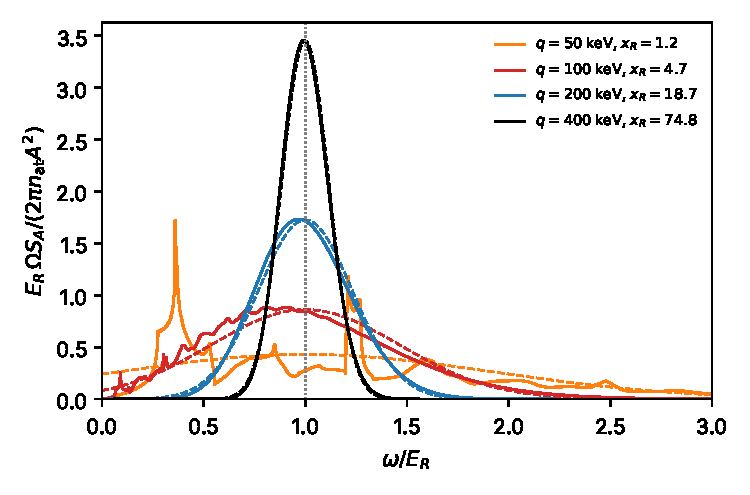
\includegraphics[width=\linewidth]{figures/ch11/fig11_4.pdf}
  \caption{Nuclear response of silicon at $T = 0$ per nucleus, $\Omega S_A/(2\pi n_{\mathrm{at}}A^2)$, times $E_R$, against $\omega/E_R$, at $q = 50$, 100, 200 and \SI{400}{keV} ($x_R = 1.2$, 4.7, 18.7 and 74.8). Solid: the incoherent response of \cref{eq:11.3-inc} summed over all phonon orders, from the density of states of the PBE force constants of \cref{sec:5.2}. It is evaluated by Fourier transform of the generating formula \cref{eq:5.6-gen}. The zero-phonon line, of weight $\ee^{-2W_\kappa} = 0.21$ at \SI{50}{keV} and below $2\times10^{-3}$ at the larger $q$, is not shown. Dashed: the impulse Gaussian \cref{eq:11.4-IAgauss}, mean $E_R$ and relative width $x_R^{-1/2}$. Dotted: the free recoil, $\omega = E_R$. The maximum of the spectrum lies at 0.36, 0.81, 0.97 and $0.99\,E_R$.}
  \label{fig:11-impulse}
\end{figure}

The width needs one number per species, the kinetic energy of the nucleus along $\hat{\vect{q}}$. The harmonic value comes from the same phonon calculation as the Debye--Waller exponent (\cref{sec:5.4,app:E.4}), as the first moment of the projected density of states instead of the inverse moment. Beyond the harmonic approximation the nuclear momentum distribution, its kinetic energy and the curvature that sets $c_3$ are computed by path-integral molecular dynamics, which treats the nuclei as quantum particles on the full Born--Oppenheimer surface; \cref{app:E.17} specifies that calculation for silicon, germanium and GaAs. The anharmonic change of $E^{\mathrm{kin}}_\kappa$ is the subject of \cref{sec:11.5}.

\begin{workedexample}{The impulse width at \SI{100}{keV} in silicon}\label{we:11-width}
Take a silicon nucleus, $M = \SI{26.162}{GeV}$, at $T = 0$ and $q = \SI{100}{keV}$. The free recoil energy is $E_R = q^2/2M = \SI{191.1}{meV}$, and with $\langle\omega\rangle = \SI{40.9}{meV}$ the recoil parameter is $x_R = 4.67$. The kinetic energy along $\hat{\vect{q}}$ is $\langle\omega\rangle/4 = \SI{10.23}{meV}$, and \cref{eq:11.4-width} gives
\begin{equation*}
  \sigma_\omega = (4 \times \SI{191.1}{meV} \times \SI{10.23}{meV})^{1/2} = \SI{88.4}{meV} , \qquad \frac{\sigma_\omega}{E_R} = 0.463 = x_R^{-1/2} .
\end{equation*}
The Doppler reading gives the same number. The nucleus moves along $\hat{\vect{q}}$ with the root-mean-square speed $(2E^{\mathrm{kin}}_\kappa/M)^{1/2} = \SI{265}{m.s^{-1}}$, while the kick gives it $q/M = \SI{1.15}{km.s^{-1}}$. The relative spread of $D$ is twice the ratio of the two speeds, 0.463.

The Gaussian has a full width at half maximum of \SI{208}{meV}, larger than $E_R$ itself. The full response of \cref{fig:11-impulse} at this $q$ has a width at half maximum of \SI{207}{meV}. The shape is skewed. The skewness is $1.19 \times 4.67^{-1/2} = 0.55$, which places the maximum about $0.55\,\sigma_\omega/2 = \SI{24}{meV}$ below $E_R$; the full response peaks at \SI{154}{meV}, \SI{37}{meV} below, because the phonon orders still leave ripples on the peak. At \SI{300}{K} the width grows to \SI{110}{meV}.

A germanium nucleus is 2.6 times heavier and its phonons are softer. With $\langle\omega\rangle \approx \SI{23.6}{meV}$, an estimate from its Debye temperature of \SI{373}{K} (below), the same $q$ gives $E_R = \SI{73.9}{meV}$, $x_R = 3.1$ and $\sigma_\omega/E_R = 0.57$: at equal momentum transfer the germanium response is further from free recoil than the silicon one.
\end{workedexample}

On the truncation label of \cref{sec:8.5}, \cref{eq:11.4-IA} is $\mathcal{K}$ = impulse with $n_B = 0$. It holds at any anharmonic order $n_A$ when $\mathfrak{f}_\kappa$ is the true momentum distribution, and the Gaussian \cref{eq:11.4-IAgauss} is its value at $n_A = 0$. Temperature enters only through $E^{\mathrm{kin}}_\kappa$, with all orders $n_T$ kept by the factor $\coth(\omega/2T)$.

\subsection{Free recoil and the standard rate}

As $x_R$ grows, the relative width $x_R^{-1/2}$ goes to zero and the Gaussian becomes $\delta(\omega - E_R)$~\cite[Eq.~(42)]{campbelldeem2022dark}. For a coupling to nucleons the vertex of a nucleus is $A_\kappa F_N(q)$, with the elastic form factor $F_N$ of \cref{eq:2.2-FN}. The nucleons move with their nucleus, and the momenta of the impulse regime, up to a few MeV for sub-GeV dark matter, are far too small to excite it internally. For one species the response is then $S_A = 2\pi\nd_NA^2F_N(q)^2\delta(\omega - q^2/2M)$, with $\nd_N = n_{\mathrm{at}}/\Omega$ the number density of nuclei. Insert it into \cref{eq:8.2-spectrum} with one row, $\mathfrak{D} = |\tilde V_N|^2$. The response does not depend on $\hat{\vect{q}}$, so the angle between $\vect{q}$ and $\vect{v}$ can be integrated first: $\int\dd^3q/(2\pi)^3$ of $\delta(\omega - \vect{q}\cdot\vect{v} + q^2/2\mchi)$ gives $\int q\,\dd q\,\Theta(v - \vmin)/(4\pi^2v)$, as in \cref{sec:1.3}, and the average over $f_\chi$ turns $\Theta/v$ into $\eta(\vmin)$ of \cref{eq:1.3-eta}. With $\rho_T = \nd_NM$,
\begin{equation*}
  \frac{\dd\mathcal{R}}{\dd\omega} = \frac{\rho_\chi}{\mchi\,\nd_NM}\int\frac{q\,\dd q}{4\pi^2}\,|\tilde V_N|^2\,2\pi\nd_NA^2F_N^2\,\delta\Bigl(\omega - \frac{q^2}{2M}\Bigr)\,\eta(\vmin)
  = \frac{\rho_\chi A^2|\tilde V_N|^2}{2\pi\mchi}\,F_N(q)^2\,\eta(\vmin) ,
\end{equation*}
at $q = (2M\omega)^{1/2}$, and \cref{eq:1.3-vmin} with $\Delta_\chi = 0$ gives $\vmin = q/2M + q/2\mchi = q/2\mu_{\chi N}$. A heavy mediator, $|\tilde V_N|^2 = \pi\sigma_p/\mu_{\chi p}^2$, with $\sigma_N = \sigma_pA^2\mu_{\chi N}^2/\mu_{\chi p}^2$ from \cref{eq:2.2-nucleus}, gives
\begin{keyresult}[Free nuclear recoil as the impulse limit]
\begin{equation}
  \frac{\dd\mathcal{R}}{\dd E_R} = \frac{\rho_\chi\,\sigma_N}{2\mchi\,\mu_{\chi N}^2}\,F_N(q)^2\,\eta(\vmin) , \qquad q = (2ME_R)^{1/2} , \qquad \vmin = \frac{q}{2\mu_{\chi N}} ,
  \label{eq:11.4-LS}
\end{equation}
the spin-independent recoil spectrum of \cref{sec:2.2}, with $\sigma_N$ of \cref{eq:2.2-nucleus}. It is the limit $x_R \to \infty$ of the crystal response.
\end{keyresult}
\noindent This is the standard rate of nuclear-recoil searches~\cites{lewin1996review}[Eq.~(104)]{lin2019tasi}, and with $F_N$ the Helm form \cref{eq:2.2-helm} and the Lewin--Smith parameters of \cref{sec:2.2} it is the rate that experiments quote. Kahn and Lin reach the same spectrum from an Einstein oscillator, whose Poisson distribution of phonon numbers concentrates at $E_R/\omega_0$ for large $q$~\cite[Sect.~IV\,A, Eqs.~(90)--(92)]{kahn2022searches}. On the truncation label the free recoil is $\mathcal{K}$ = impulse at zero width, $n_B = 0$; its mean deposit is exact at every anharmonic order and temperature, and only the width depends on them.

The derivation says what the formula needs: a recoil parameter large enough that the response is a narrow peak, and a rate whose weight in $\omega$, the factor $\eta(\vmin)$ together with the threshold, does not vary across the width $\sigma_\omega$. \Cref{lim:11.4a} tests both in silicon, by computing the heavy-mediator rate from the full multiphonon response and dividing it by \cref{eq:11.4-LS}. For a particle of \SI{1}{GeV}, whose kinematic endpoint lies far above the energies shown, the two agree within \SI{10}{\percent} for $x_R \ge 2.3$, or $E_R \ge \SI{93}{meV}$ and $q \ge \SI{70}{keV}$, and within \SI{2}{\percent} for $x_R \ge 4.3$. The free form works where the spectrum is not yet narrow, as Campbell-Deem and collaborators observed~\cite[Sect.~III\,D]{campbelldeem2022dark}, because a smooth weight averages over the peak and the mean of the peak is exactly $E_R$. Below $x_R \approx 2$ the deposit comes in whole phonons, and the ratio swings by factors of two with the bands of the phonon spectrum.

A lighter particle has its endpoint $2\mu_{\chi N}^2v_{\mathrm{max}}^2/M$ close to the energies that matter, and there $\eta$ falls steeply across the peak. For \SI{50}{MeV} the endpoint is at \SI{1.34}{eV}, $x_R = 32.7$. Between $x_R = 3$ and 8 the free form overestimates the crystal rate by 5 to \SI{21}{\percent}, because the width spreads each momentum transfer over a range of energies across which $\eta$ falls steeply. From $x_R = 14$ upward, however, $4.9\,\sigma_\omega$ below the endpoint, the crystal rate exceeds the free one by more than \SI{10}{\percent} and keeps rising. Above the endpoint the free recoil gives nothing, while the Doppler tail of the bound nucleus still deposits energy. This is the impulse-regime counterpart of the Poisson tail of \cref{we:11-tail}, and the reason Kahn, Krnjaic and Mandava found that a bound nucleus extends the reach of a detector below the masses that elastic kinematics allows~\cite[text after Eq.~(4)]{kahn2021dark}. The impulse Gaussian \cref{eq:11.4-IAgauss}, used in the same rate integral, follows the full crystal result within \SI{5}{\percent} from $x_R \approx 3.6$ at \SI{1}{GeV} and 3.8 at \SI{50}{MeV}, up to three quarters of the endpoint, and it captures the endpoint tail too.

\begin{limitbox}[Free nuclear recoil with the Helm form factor][lim:11.4a]
For $x_R \gg 1$ the nuclear response becomes $(2\pi/\Omega)\sum_\kappa c_\kappa^2\delta(\omega - q^2/2M_\kappa)$~\cite[Eqs.~(39), (42)]{campbelldeem2022dark}, and the rate is the free recoil \cref{eq:11.4-LS} with $F_N = F_{\mathrm{Helm}}$ and the Lewin--Smith parameters~\cites{lewin1996review}[Eq.~(104)]{lin2019tasi}.
\par\smallskip
{\centering
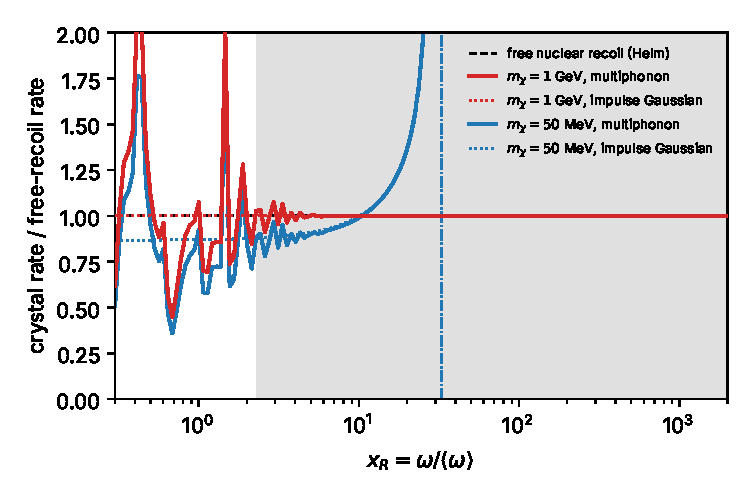
\includegraphics[width=\linewidth]{figures/ch11/limit11_4a.pdf}
\captionof{figure}{Heavy-mediator recoil rate of silicon per unit mass from the crystal response, divided by the free-recoil rate \cref{eq:11.4-LS} at $E_R = \omega$, against $x_R = \omega/\langle\omega\rangle$ with $\langle\omega\rangle = \SI{40.9}{meV}$. Solid: incoherent multiphonon response at $T = 0$, all orders, from the PBE density of states of \cref{sec:5.2}, integrated over $q$ with $\eta(\vmin)$ of the halo of \cref{sec:1.2} and the Helm form factor, for $\mchi = \SI{1}{GeV}$ (red) and \SI{50}{MeV} (blue). Dotted: the same with the impulse Gaussian \cref{eq:11.4-IAgauss}, the leading correction. Dash-dotted: the free-recoil endpoint at \SI{50}{MeV}. Gray band: $x_R \ge 2.3$, where the \SI{1}{GeV} rate stays within \SI{10}{\percent} of the free one. The lighter particle departs from it within about five widths $\sigma_\omega$ of its endpoint.}\label{fig:11-limit-4a}
\par}
\smallskip
Below $x_R \approx 2$ the energy arrives in whole phonons and the rate follows the phonon bands; near the kinematic endpoint the Doppler width of the bound nucleus feeds energies that a free nucleus cannot reach.
\end{limitbox}

Where does the impulse regime begin? The onset depends on the criterion. The relative width $x_R^{-1/2}$ falls to one half at $x_R = 4$, where the impulse Gaussian reproduces the rate of the limit check within \SI{5}{\percent}. This is $q = 2(2M\langle\omega\rangle)^{1/2}$, the boundary above which Campbell-Deem and collaborators replace the multiphonon sum by the Gaussian~\cite[text after Eq.~(39)]{campbelldeem2022dark}. In silicon it lies at $q = \SI{92.5}{keV}$, $E_R = \SI{164}{meV}$. The stricter criterion of \cref{sec:8.5}, a width below a third of $E_R$, needs $x_R \ge 9$, at \SI{139}{keV} and \SI{0.37}{eV}. For germanium a rough $\langle\omega\rangle$ is enough, and its Debye temperature of \SI{373}{K} supplies one (\cref{tab:5-phonons}): the Debye mean $\frac34\omega_{\mathrm{D}} = \SI{24.1}{meV}$, scaled by the ratio 0.981 of the computed to the Debye mean in silicon, gives $\langle\omega\rangle \approx \SI{23.6}{meV}$. The onsets are then $q = \SI{113}{keV}$ and $E_R = \SI{95}{meV}$ at $x_R = 4$, and \SI{170}{keV} and \SI{0.21}{eV} at $x_R = 9$. The heavier nucleus needs a larger momentum transfer but a smaller recoil energy. These onsets are not the \SI{93.4}{keV} of \cref{we:11-tail}, which is the momentum at which a free nucleus would first deposit three Debye energies. A particle much lighter than the nucleus reaches $q$ only if $2\mchi v_{\mathrm{max}} \ge q$, so the impulse regime is available in silicon from $\mchi = \SI{17.5}{MeV}$ and in germanium from \SI{21.3}{MeV} ($x_R = 4$), or from 26.2 and \SI{32.0}{MeV} ($x_R = 9$). Even then, as the limit check shows, the free form needs the energies of interest to lie several widths below the endpoint.

The impulse approximation leaves the crystal at the moment of the kick. It ignores the motion of the nucleus after the kick, and it leaves out anharmonicity, electronic excitation and the displacement of the atom. The kinetic energy and curvature of an anharmonic crystal shift $\sigma_\omega$ and $c_3$ (\cref{sec:11.5}), but never the mean. The electrons follow the nucleus at $n_B = 0$; the probability that the kick leaves them excited is the Migdal effect of \cref{chap:12}. With the electrons included, the third moment of the full nuclear response contains the electron density at the nucleus and is dominated by those excitations (\cref{sec:12.5}); the curvature in $c_3$ above is that of the Born--Oppenheimer surface alone. And a recoil above the displacement threshold of the lattice ejects the atom from its site, which changes how the energy is shared among phonons, defects and ionization (\cref{chap:19}) but not the response \cref{eq:11.4-IA}, since the momentum and energy are transferred before the atom moves.

\subsection{Fermionic absorption on nuclei}

A fermion $\chi$ of \SI{10}{MeV} that is absorbed on a silicon nucleus and leaves as a massless $\tilde\nu$ transfers the momentum $q = \mchi - \omega \simeq \SI{10}{MeV}$, and a free nucleus recoils with $E_R = \mchi^2/2M = \SI{1.91}{keV}$. Scattering at the same mass deposits at most $2\mu_{\chi N}^2v_{\mathrm{max}}^2/M = \SI{54}{meV}$. Absorption reaches recoil energies $1/4v_{\mathrm{max}}^2$ times larger, and because the momentum transfer is set by the rest energy, the deposit is a line, whatever the velocity distribution~\cite{dror2020direct}. \Cref{sec:10.9} built the rate for the operators $\Lambda_F^{-2}(\bar{\tilde\nu}P_L\chi)(\bar\psi\psi)$ and $\Lambda_F^{-2}(\bar{\tilde\nu}\gamma_\mu P_R\chi)(\bar\psi\gamma^\mu\psi)$, \cref{eq:10.9-ferm}. For nucleons in place of electrons only the response changes. The vector operator gives $(\sigma_F/2\pi)\bar S_{nn}(q,\omega)$, with $\sigma_F = \mchi^2/4\pi\Lambda_F^4$ and $\bar S_{nn}$ the direction-averaged response of the nucleon density, because continuity, exact for the nucleon current, turns the longitudinal current into the density and multiplies it by $(\mchi/q)^2$. With the dark matter at rest, $p = (\mchi, \vect{0})$, a massless outgoing fermion of four-momentum $(q, -\vect{q})$ and the nucleon current $J = (\rho, (\omega/q)\rho\,\hat{\vect{q}})$ fixed by continuity, the spin-summed contraction is $\mchi^3\rho^2/q$ for the vector operator and $\mchi q\rho^2$ for the scalar density; their ratio is $q^2/\mchi^2$. The transverse current of a nucleus is smaller by a factor of order $E^{\mathrm{kin}}_\kappa/M$ or $q^2/M^2$ and is dropped.

For a nucleus at rest, $\bar S_{nn} = 2\pi\nd_NA^2F_N(q)^2\delta(\omega - q^2/2M)$. Along the line $q = \mchi - \omega$ the argument of the delta function has the slope $1 + q/M$, and
\begin{keyresult}[Fermionic absorption on nuclei]
\begin{equation}
  \varGamma_V = \frac{\sigma_F\,\nd_NA^2F_N(q_{\mathrm{abs}})^2}{1 + q_{\mathrm{abs}}/M} = \sigma_F\,\nd_NA^2F_N^2\Bigl(1 - \frac{\mchi}{M} + \dots\Bigr) , \qquad \mchi = q_{\mathrm{abs}} + \frac{q_{\mathrm{abs}}^2}{2M} ,
  \label{eq:11.4-ferm-nuc}
\end{equation}
per dark-matter particle, in a target of free nuclei, at a recoil energy $E_R = q_{\mathrm{abs}}^2/2M \simeq \mchi^2/2M$; the event rate per unit mass is $(\rho_\chi/\mchi\rho_T)\varGamma_V$. In a crystal, in the incoherent approximation and for $\mchi$ not within a relative $v$ of the length of a reciprocal-lattice vector, the factor $1 - \ee^{-2W_\kappa(q_{\mathrm{abs}})}$ multiplies the rate.
\end{keyresult}
\noindent Since $\sigma_F \propto \mchi^2$, the rate carries the factor $\mchi^2(1 - \mchi/M)$. The scalar operator weights the density by $q^2/\mchi^2$ in addition and gives $\mchi^2(1 - 2\mchi/M)$. The difference is the longitudinal current: the density row alone has twice the recoil correction, and continuity halves it. Dror, Elor and McGehee write the rate per target nucleus as $(\rho_\chi/\mchi)\sigma_FA^2F_N^2$ for the vector operator, with the Helm form factor at $q = \mchi$~\cite[Eqs.~(1) and (4)]{dror2020direct}, which is \cref{eq:11.4-ferm-nuc} at $M \to \infty$. In silicon the recoil factor reaches \SI{10}{\percent} only at $\mchi = \SI{3}{GeV}$, where $q_{\mathrm{abs}}$ lies far beyond the first zero of the Helm form factor, at \SI{256}{MeV}, and elastic absorption is negligible; on a proton target it is about \SI{10}{\percent} at \SI{100}{MeV}.

The crystal changes the rate at the other end of the mass range. In the response of \cref{sec:11.3} the zero-phonon term conserves crystal momentum and deposits no energy, so it absorbs a fermion only if $|\vect{q}| = \mchi$ equals the length of a reciprocal-lattice vector, to within the relative spread $v$ of the dark-matter momenta. At any other mass the lattice must take up the momentum with at least one phonon, and in the incoherent approximation the weight of those terms is $1 - \ee^{-2W_\kappa}$, evaluated at $q = q_{\mathrm{abs}}$. Along the line $q = \mchi - \omega$ the momentum changes by $\omega$, a fraction $E_R/\mchi = \mchi/2M$ of itself, which rebuilds the factor $1/(1 + q_{\mathrm{abs}}/M)$ in the impulse regime and is negligible below it. In silicon, with $2W_\kappa = q^2\langle u_x^2\rangle$, this is 0.061 at $\mchi = \SI{10}{keV}$, 0.43 at \SI{30}{keV} and 0.90 at \SI{60.5}{keV}. The free-nucleus formula therefore overestimates the absorption rate by a factor of 16 at \SI{10}{keV}, and it holds to \SI{10}{\percent} only above \SI{61}{keV}, the boundary of \cref{lim:11.4b}. Below about \SI{100}{keV} the deposit is not a line at $\mchi^2/2M$ either. It is the multiphonon spectrum of \cref{sec:11.3} at $q = \mchi$: mostly one phonon below about \SI{20}{keV}, a few phonons up to the impulse onset near \SI{90}{keV}, and the Gaussian \cref{eq:11.4-IAgauss} above it. The weights of the lowest orders carry the coherence corrections of \cref{sec:11.3}, below \SI{10}{\percent} above about \SI{6.6}{keV} for two and three phonons and above \SI{18}{keV} for one.

Above the onset the crystal sets the width of the line. The impulse Gaussian has the relative width $x_R^{-1/2} = (2M\langle\omega\rangle)^{1/2}/q_{\mathrm{abs}} = \SI{46.3}{keV}/\mchi$ in silicon: \SI{4.6}{\percent} at \SI{1}{MeV}, \SI{0.46}{\percent} at \SI{10}{MeV}. The motion of the dark matter shifts the recoil energy by $-2v\cos\theta$ in relative terms, with $\theta$ the angle between its velocity and the outgoing $\tilde\nu$. For the halo of \cref{sec:1.2}, whose root-mean-square speed in the laboratory is \SI{379}{km.s^{-1}}, the root-mean-square shift is $2(\langle v^2\rangle/3)^{1/2} = 1.5\times10^{-3}$, the relative width $\sim10^{-3}$ that Dror, Elor and McGehee attribute to corrections to the leading kinematics~\cite{dror2020direct}. The two widths are equal at $\mchi = \SI{32}{MeV}$, and below that mass the line in a crystal is broader than the halo makes it, by the zero-point motion of the nuclei.

\begin{limitbox}[Fermionic absorption on nuclei][lim:11.4b]
A fermion absorbed on free nuclei gives the rate $(\rho_\chi/\mchi)\sigma_FA^2F_N^2$ per nucleus, with $\sigma_F = \mchi^2/4\pi\Lambda_F^4$, at the recoil energy $\mchi^2/2M$~\cite[Eqs.~(1), (3) and (4)]{dror2020direct}.
\par\smallskip
{\centering
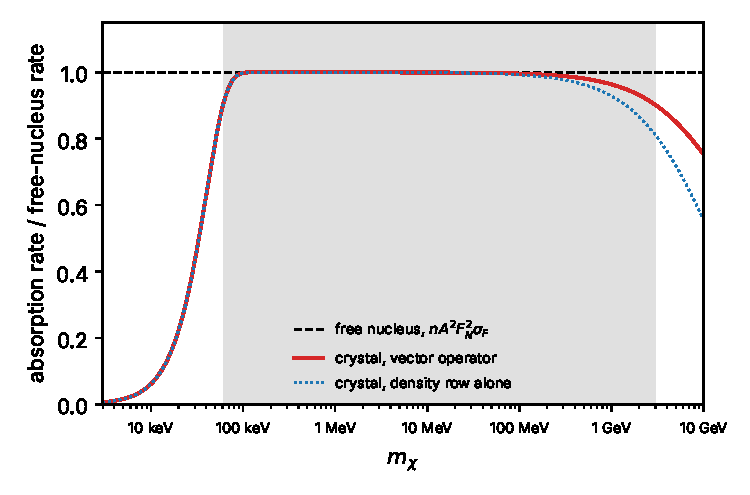
\includegraphics[width=\linewidth]{figures/ch11/limit11_4b.pdf}
\captionof{figure}{Absorption rate of a fermion on silicon nuclei, divided by the free-nucleus rate of the limit check, against $\mchi$, with the nuclear form factor divided out of both. Solid: the vector operator in the crystal, $[1 - \ee^{-2W_\kappa(q_{\mathrm{abs}})}]/(1 + q_{\mathrm{abs}}/M)$ from \cref{eq:11.4-ferm-nuc}, incoherent approximation at $T = 0$ with $\langle u_x^2\rangle = \SI{2.45e-3}{\angstrom^2}$ from the PBE density of states of \cref{sec:5.2}. Dotted: the density row alone, as for the scalar operator, with the recoil factor $(1 - \mchi/M)^2$ to leading order instead of $1 - \mchi/M$. Gray band: $\SI{61}{keV} \le \mchi \le \SI{3.0}{GeV}$, where the vector rate is within \SI{10}{\percent} of the free one.}\label{fig:11-limit-4b}
\par}
\smallskip
Below about \SI{60}{keV} in silicon the absorption must create phonons and the free-nucleus rate overcounts it by $\ee^{-2W_\kappa}/(1 - \ee^{-2W_\kappa})$; above a few GeV the recoil factor $1 - \mchi/M$ and the form factor at $q_{\mathrm{abs}}$ instead of $\mchi$ matter.
\end{limitbox}

\noindent On the truncation label the limit check sits at $n_B = 0$ and $n_T = 0$, with $\mathcal{K}$ = multiphonon (incoherent, all orders) below the impulse onset and $\mathcal{K}$ = impulse above it.

\section{Anharmonic and quantum-crystal corrections}\label{sec:11.5}

At its zero-point amplitude the cubic term of the silicon energy surface is \SI{5}{\percent} of the harmonic one ($\eta_{\mathrm{anh}} = 0.049$, \cref{sec:5.7}), and every formula of \cref{sec:11.3,sec:11.4} dropped it. How much does that change a rate? For the impulse peak, by a part in a thousand. For a deposit of several phonons at a momentum transfer of a few keV, by factors of several, because an anharmonic lattice can make many phonons out of one kick, which a harmonic lattice can only do with many kicks. In solid helium the zero-point motion of an atom is a quarter of the distance to its neighbor, and some harmonic frequencies are imaginary. And in a crystal with a soft mode or a light atom no expansion is available at all, and only exact moments of the response, which anharmonicity cannot change, bound it.

\subsection{Exact moments of the self response}

Above a few zone momenta each nucleus responds on its own (\cref{sec:11.3}), and its self response is controlled by the kick operator $D = E_R + \vect{q}\cdot\vect{p}/M_\kappa$ of \cref{sec:11.4}: the Hamiltonian after the kick is $H + D$, exactly, whatever the potential, provided it depends on the positions of the nuclei and not on their momenta (\cref{eq:D.32-I}). Normalize the response to a distribution in $\omega$, $\dd P = S\,\dd\omega/\int S\,\dd\omega$, with moments $\mu_k = \int\omega^k\,\dd P$ and central moments $\bar\mu_k$, as in \cref{app:C.10}. At $T = 0$, writing $A = H - E_0$, which annihilates the ground state, and $\delta D = D - E_R = (q/M_\kappa)p_{\hat q}$, the central moments are $\bar\mu_k = \langle(A + \delta D)^k\rangle$. Every term with $A$ at either end vanishes. The zeroth moment is $\mu_0 = 1$: the weight of the self response is the norm of $\ee^{\ii\vect{q}\cdot\vect{X}}|0\rangle$. The first is $\mu_1 = E_R$, the sum rule \cref{eq:5.6-sum}. The second and third were derived in \cref{app:D.32}. The fourth needs one more step: of the four terms of $\langle\delta D(A + \delta D)^2\delta D\rangle$, the term $\langle\delta D\,A^2\,\delta D\rangle$ is the squared norm of $A\,\delta D|0\rangle = [H, \delta D]|0\rangle$, and $[H, p_{\hat q}] = \ii\,\partial_{\hat q}V$ is the force along $\hat{\vect{q}}$. The two mixed terms $\langle\delta D\,A\,\delta D^2\rangle$ and its complex conjugate equal $\ii(q/M_\kappa)^3\langle p_{\hat q}(p_{\hat q}\partial_{\hat q}V + \partial_{\hat q}V\,p_{\hat q})\rangle$, by $[H, p_{\hat q}^2] = \ii(p_{\hat q}\partial_{\hat q}V + \partial_{\hat q}V\,p_{\hat q})$; for a real ground-state wavefunction the average is real, so the term is imaginary and cancels against its conjugate. Collecting,
\begin{keyresult}[Exact moments of the self response]
\begin{equation}
  \begin{gathered}
  \mu_0 = 1 , \qquad \mu_1 = E_R , \qquad
  \bar\mu_2 = 4E_RE^{\mathrm{kin}}_\kappa , \\
  \bar\mu_3 = \frac{q^2}{2M_\kappa^2}\bigl\langle\partial_{\hat q}^2V\bigr\rangle , \quad
  \bar\mu_4 = \frac{q^2}{M_\kappa^2}\bigl\langle(\partial_{\hat q}V)^2\bigr\rangle + \frac{q^4}{M_\kappa^4}\bigl\langle p_{\hat q}^4\bigr\rangle ,
  \end{gathered}
  \label{eq:11.5-moments}
\end{equation}
for any potential $V$ of the nuclei, with $E^{\mathrm{kin}}_\kappa = \langle p_{\hat q}^2\rangle/2M_\kappa$ the kinetic energy along $\hat{\vect{q}}$ of \cref{eq:11.4-width}. The averages are over the ground state at $T = 0$; all five moments hold at any temperature with thermal averages (\cref{app:D.32}).
\end{keyresult}
\noindent Each moment is an equal-time average in the ground state: the kinetic energy, the mean curvature of the energy surface, the mean-square force and the fourth moment of the momentum distribution. For a harmonic crystal they reproduce the cumulants of \cref{eq:D.32-ck}; for one oscillator of frequency $\omega_0$, for instance, the mean-square force is $M_\kappa^2\omega_0^4\langle u_{\hat q}^2\rangle = M_\kappa\omega_0^3/2$, so the first term of $\bar\mu_4$ is the fourth cumulant $E_R\omega_0^3$, and the second is $3\bar\mu_2^2$. In an anharmonic crystal the same averages come from a path-integral simulation of the nuclei, which needs no dynamics (\cref{app:E.19}). They are the self part of the moments $\mathscr{M}^k$ of \cref{eq:8.3-moments} for one species, divided by $\mathscr{M}^0$.

Write its relative correction to the harmonic self response as $\delta_{\mathrm{anh}}(\vect{q},\omega) = S_A/S_A^{\mathrm{harm}} - 1$. Then the weight $\int S_A^{\mathrm{harm}}\delta_{\mathrm{anh}}\,\dd\omega$ and the first moment $\int\omega\,S_A^{\mathrm{harm}}\delta_{\mathrm{anh}}\,\dd\omega$ vanish exactly, and the second moment $\int\omega^2S_A^{\mathrm{harm}}\delta_{\mathrm{anh}}\,\dd\omega$ is fixed by the change of the kinetic energy, $4E_R(E^{\mathrm{kin}}_\kappa - E^{\mathrm{kin,harm}}_\kappa)$ times the weight. These three linear constraints test any calculation of the anharmonic response. Time reversal adds a selection rule. For a target invariant under time reversal the eigenfunctions are real, $|\langle f|\ee^{\ii\vect{q}\cdot\vect{X}}|0\rangle|^2 = |\langle f|\ee^{-\ii\vect{q}\cdot\vect{X}}|0\rangle|^2$, and the response is even in $\vect{q}$. A term of first order in $\Phi^{(3)}$ carries three displacements from the cubic term of \cref{eq:5.7-H3}, so it needs an odd number of displacements from the kick to pair them all, and it is odd in $\vect{q}$. It therefore vanishes. The first anharmonic correction to the rate is of second order in $\Phi^{(3)}$ and first order in $\Phi^{(4)}$, the level $n_A = 2$ of \cref{sec:8.5}, of relative size $\eta_{\mathrm{anh}}^2$ by \cref{eq:5.7-order}.

\subsection{Cubic phonon decay}

In the impulse regime the first correction is small. The impulse response \cref{eq:11.4-IA} depends on the potential only through the momentum distribution $\mathfrak{f}_\kappa$, and its width through $E^{\mathrm{kin}}_\kappa$. A single-site model holds the neighbors of one nucleus fixed and gives it a one-dimensional anharmonic potential~\cite[Eq.~(26)]{lin2024anharmonic},
\begin{equation}
  V(x) = \tfrac12M_\kappa\omega_0^2x^2 + \lambda_3\,\omega_0\Bigl(\frac{x}{\ell_0}\Bigr)^3 + \lambda_4\,\omega_0\Bigl(\frac{x}{\ell_0}\Bigr)^4 , \qquad \ell_0 = (2M_\kappa\omega_0)^{-1/2} ,
  \label{eq:11.5-toy}
\end{equation}
with $\ell_0$ the zero-point amplitude of the oscillator. In this potential the cubic energy at $x = \ell_0$ is $4\lambda_3$ times the harmonic one, and $4\lambda_3$ is the anharmonic parameter of \cref{eq:5.7-eta} measured on the site coordinate instead of the bond. Fits of an empirical silicon potential along the bond and perpendicular to it give $\lambda_3 = 0.006$ to $0.01$ and $\lambda_4 = (2$ to $3)\times10^{-4}$~\cite[Sect.~IV]{lin2024anharmonic}, so $4\lambda_3 = 0.024$ to $0.04$, of the size of the bond value $0.049$ of \cref{sec:5.7}. To second order in $\lambda_3$ and first in $\lambda_4$ the kinetic energy becomes $E^{\mathrm{kin}} = (\omega_0/4)(1 - 44\lambda_3^2 + 12\lambda_4)$~\cite[Eq.~(65)]{lin2024anharmonic}, a change within $\pm\SI{0.2}{\percent}$ over the silicon ranges of $\lambda_3$ and $\lambda_4$. The impulse width $\sigma_\omega \propto (E^{\mathrm{kin}})^{1/2}$ then moves by at most a part in a thousand, \SI{0.09}{meV} of the \SI{88}{meV} of \cref{we:11-width}.

At smaller $q$ the correction is of a different kind, because anharmonicity changes how many kicks a given number of phonons needs. Expand the self response of \cref{eq:11.3-exact} in powers of $q$. At $\omega \neq 0$ the constant and the averages of single displacements contribute only at $\omega = 0$, and the first term is the correlation of two displacements,
\begin{equation*}
  S_A(\vect{q},\omega) = \frac{1}{\Omega}\sum_\kappa c_\kappa^2\,q_\alpha q_\beta\int\dd t\;\ee^{\ii\omega t}\bigl\langle u^\alpha_{\kappa}(t)\,u^\beta_{\kappa}(0)\bigr\rangle + O(q^4) ,
\end{equation*}
exact for any anharmonicity. Insert the displacement in phonon coordinates, $\vect{u}_{\vect{R}\kappa} = \sum_{\vect{Q}\nu}(2NM_\kappa\omega_{\vect{Q}\nu})^{-1/2}\vect{e}_{\kappa\nu}(\vect{Q})\ee^{\ii\vect{Q}\cdot\vect{R}}B_{\vect{Q}\nu}$ (\cref{sec:5.3}). The correlation of $B_{\vect{Q}\nu}$ is the spectral function of the dressed propagator $\mathsf{D}_\nu(\vect{Q},\omega) = 2\omega_{\vect{Q}\nu}/[\omega^2 - \omega_{\vect{Q}\nu}^2 - \Pi_\nu(\vect{Q},\omega)]$ of \cref{eq:6.4-Pi}: at $T = 0$ and $\omega > 0$, $\int\dd t\,\ee^{\ii\omega t}\langle B_{\vect{Q}\nu}(t)B_{-\vect{Q}\nu}\rangle = -2\Imag\mathsf{D}_\nu(\vect{Q},\omega)$, which is $2\pi\delta(\omega - \omega_{\vect{Q}\nu})$ for the free phonon. Here $\Pi_\nu$ is the anharmonic self-energy: the bubble of two cubic vertices of \cref{eq:5.7-V3}, whose imaginary part on shell is $-\omega_{\vect{Q}\nu}\gamma^{\mathrm{anh}}_{\vect{Q}\nu}$ (\cref{eq:5.7-gamma,eq:6.4-pole}), and the loop of one quartic vertex, which is real. Off shell, $-\Imag\Pi_\nu(\vect{Q},\omega) = \omega_{\vect{Q}\nu}\gamma^{\mathrm{anh}}_{\vect{Q}\nu}(\omega)$, with $\gamma^{\mathrm{anh}}_{\vect{Q}\nu}(\omega)$ the width of \cref{eq:5.7-gamma} with the energy $\omega$ in place of $\omega_{\vect{Q}\nu}$ in the delta function of the decay: the rate at which a phonon of momentum $\vect{Q}$, given the energy $\omega$, decays into two. With the branches kept separate, as in \cref{sec:6.4}, the harmonic term gives back the one-phonon response \cref{eq:11.1-S1}, a delta function on each branch. Away from the poles, above the one-phonon band, the first order in $\Pi_\nu$ is $-\Imag\mathsf{D}_\nu = 2\omega_{\vect{Q}\nu}(-\Imag\Pi_\nu)/(\omega^2 - \omega_{\vect{Q}\nu}^2)^2$, and
\begin{keyresult}[First anharmonic correction to the nuclear response]
\begin{equation}
  S_A^{\mathrm{anh}}(\vect{q},\omega) = \frac{2\pi}{\Omega}\sum_\kappa c_\kappa^2\,\ee^{-2W_\kappa}\,\frac1N\sum_{\vect{Q}\nu}\frac{|\vect{q}\cdot\vect{e}_{\kappa\nu}(\vect{Q})|^2}{\pi M_\kappa}\;
  \frac{\omega_{\vect{Q}\nu}\,\gamma^{\mathrm{anh}}_{\vect{Q}\nu}(\omega)}{(\omega^2 - \omega_{\vect{Q}\nu}^2)^2} ,
  \label{eq:11.5-anh}
\end{equation}
at $T = 0$, for $\omega$ outside the one-phonon band and $q$ above a few $q_{\mathrm{BZ}}$, where the self part is the response. It is of order $q^2$ and of second order in $\Phi^{(3)}$; the Debye--Waller factor, which the higher orders in $q$ supply, is written to leading order in $\eta_{\mathrm{anh}}$.
\end{keyresult}
\noindent The physical picture is that of \cref{fig:6-bubble} with the electron bubble replaced by a pair of phonons: the kick creates one phonon off its energy shell, and it decays into two real ones. Near $\omega = \omega_{\vect{Q}\nu}$ the same expression, resummed, is the Lorentzian tail of a phonon line of full width $\gamma^{\mathrm{anh}}_{\vect{Q}\nu}$. The two time orderings, the decay of a virtual phonon and the creation of three from the vacuum, have the denominators $1/(\omega - \omega_{\vect{Q}\nu})$ and $1/(\omega + \omega_{\vect{Q}\nu})$, which combine into the $2\omega_{\vect{Q}\nu}/(\omega^2 - \omega_{\vect{Q}\nu}^2)$ of $\mathsf{D}_\nu$.

How large is \cref{eq:11.5-anh} against the harmonic two-phonon response? The harmonic term needs two kicks and carries $q^4$; the anharmonic term needs one kick and the factor $\gamma^{\mathrm{anh}}/\omega \sim \eta_{\mathrm{anh}}^2$. Their ratio is $\sim\eta_{\mathrm{anh}}^2\,2M_\kappa\omega/q^2$, large at small $q$. The model \cref{eq:11.5-toy} makes the counting exact. To first order in $\lambda_3$, with $x/\ell_0 = a + a^\dagger$ and the harmonic states $|n\rangle$ in units of $\omega_0$, the ground state and the second level become
\begin{equation*}
  |\tilde0\rangle = |0\rangle - \lambda_3\Bigl(3|1\rangle + \sqrt{\tfrac23}\,|3\rangle\Bigr) , \qquad
  |\tilde2\rangle = |2\rangle + 6\sqrt2\,\lambda_3|1\rangle + \dots ,
\end{equation*}
where the dots stand for $|3\rangle$ and $|5\rangle$, which the kick does not connect to $|\tilde0\rangle$ at first order in $q$. The coefficient $6\sqrt2$ is $\langle1|(a + a^\dagger)^3|2\rangle$ divided by the level spacing. With $k = q\ell_0$ the kick is $\ee^{\ii k(a + a^\dagger)} = 1 + \ii k(a + a^\dagger) - \frac12k^2(a + a^\dagger)^2 + \dots$. The constant term vanishes between orthogonal states. The linear term gives $\langle\tilde2|a + a^\dagger|\tilde0\rangle = -\lambda_3(3\sqrt2 + \sqrt2) + 6\sqrt2\,\lambda_3 = 2\sqrt2\,\lambda_3$. The quadratic term gives the harmonic $-k^2/\sqrt2$. One amplitude is imaginary and the other real; they do not interfere, and the weight of the second level is
\begin{equation}
  |\langle\tilde2|\ee^{\ii qx}|\tilde0\rangle|^2 = \ee^{-k^2}\Bigl(\frac{k^4}{2} + 8\lambda_3^2k^2 + \dots\Bigr) , \qquad
  \frac{\text{anharmonic}}{\text{harmonic}} = \frac{16\lambda_3^2}{k^2} ,
  \label{eq:11.5-two}
\end{equation}
The anharmonic term wins below $k = 4\lambda_3$, that is, below $q_\times = 4\lambda_3(2M_\kappa\omega_0)^{1/2}$: the crossover sits where the momentum transfer, in units of the inverse zero-point amplitude, equals the anharmonic parameter. For silicon, with $\omega_0 = \langle\omega^{-1}\rangle^{-1} = \SI{30.4}{meV}$, $(2M_\kappa\omega_0)^{1/2} = \SI{39.9}{keV}$ and $q_\times = \SI{1.6}{keV}$ for $\lambda_3 = 0.01$, just below $q_{\mathrm{BZ}} = \SI{2.25}{keV}$. At $q_{\mathrm{BZ}}$ the two-phonon weight is raised by \SI{50}{\percent} for $\lambda_3 = 0.01$ and by \SI{18}{\percent} for $0.006$.

More phonons need more kicks, and the anharmonic gain grows with their number. Three phonons need three kicks in the harmonic crystal, $k^6/6$, but only two with one cubic vertex. That two-kick amplitude alone gives $24\lambda_3^2k^4$; interference between the one-kick amplitude of order $\lambda_3^2k$ and the harmonic three-kick amplitude $k^3/\sqrt6$ subtracts $6\lambda_3^2k^4$, for a net $18\lambda_3^2k^4$. The ratio is then $108\lambda_3^2/k^2$ and the crossover lies at $k = 10.4\lambda_3$, \SI{4.2}{keV} for $\lambda_3 = 0.01$. In general an $n$-phonon weight acquires terms $\lambda_3^{j}k^{2i}$ with $i < n$, and the smaller $i$ the higher the power $j$~\cite[Eqs.~(39), (45)--(48)]{lin2024anharmonic}. \Cref{lim:11.5a} shows the result: for $\lambda_3 = 0.01$ the harmonic two-, three- and four-phonon weights hold within \SI{10}{\percent} only above 5, 12 and \SI{20}{keV}, while at $q_{\mathrm{BZ}}$ the four-phonon weight is 27 times the harmonic one. Which rates does this affect? A threshold of $\omega_{\mathrm{th}}$ needs at least $\omega_{\mathrm{th}}/\omega_{\mathrm{max}}$ phonons, and a particle of mass $\mchi$ reaches at most $q = 2\mchi v_{\mathrm{max}}$. High thresholds and masses of a few MeV are therefore where the harmonic multiphonon rate fails. In the single-site model the anharmonic rate exceeds the harmonic one by up to two orders of magnitude for masses of a few MeV and thresholds of a few phonon energies, in the tail of the spectrum where the rate is small, and the two agree above \SI{10}{MeV}~\cite[Sect.~IV\,A]{lin2024anharmonic}. The anharmonic rate is never below the harmonic one there, because the term of lowest order in $q$ is a square, $|\langle f|\ii qx|\tilde0\rangle|^2$, which the harmonic crystal lacks for $n \ge 2$; this holds for the leading term, not for the full response.

\begin{limitbox}[Anharmonic corrections to multiphonon weights][lim:11.5a]
For a nucleus in the potential \cref{eq:11.5-toy}, the $n$-phonon weight carries, besides the harmonic $\ee^{-k^2}k^{2n}/n!$, terms $\lambda_3^jk^{2i}$ with $i < n$, which dominate for small $k = q\ell_0$; the kinetic energy changes as $1 - 44\lambda_3^2 + 12\lambda_4$~\cite[Eqs.~(39), (45)--(48), (65)]{lin2024anharmonic}.
\par\smallskip
{\centering
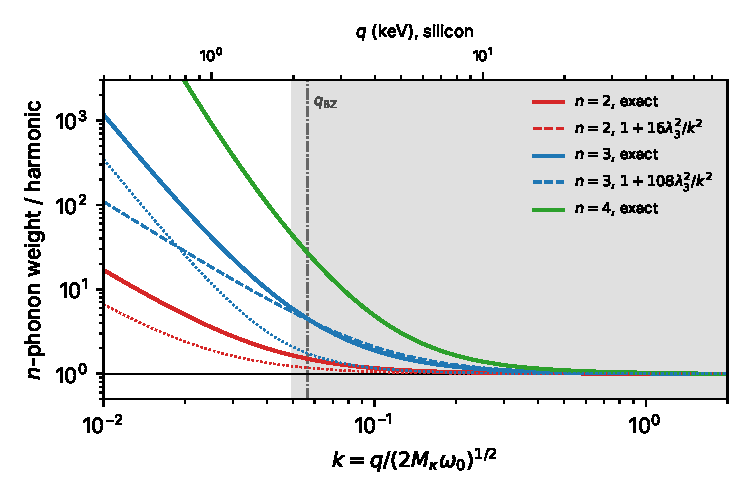
\includegraphics[width=\linewidth]{figures/ch11/limit11_5a.pdf}
\captionof{figure}{Weight of the $n$-th level of the single-site model \cref{eq:11.5-toy}, divided by the harmonic Poisson weight $\ee^{-k^2}k^{2n}/n!$, against $k = q/(2M_\kappa\omega_0)^{1/2}$, for $n = 2$ (red), 3 (blue) and 4 (green). Model with the silicon values $\omega_0 = \SI{30.4}{meV}$, $M_\kappa = \SI{26.16}{GeV}$, $\lambda_3 = 0.01$, $\lambda_4 = 2.5\times10^{-4}$ (solid), and $\lambda_3 = 0.006$, $\lambda_4 = 2\times10^{-4}$ (dotted), solved exactly in 200 oscillator states. Dashed: the leading anharmonic terms, $1 + 16\lambda_3^2/k^2$ for $n = 2$ (\cref{eq:11.5-two}) and $1 + 108\lambda_3^2/k^2$ for $n = 3$. Dash-dotted: $q_{\mathrm{BZ}} = \SI{2.25}{keV}$. Gray band: $k \ge 0.05$, where both leading terms are within \SI{10}{\percent} of the exact weights; below it the three-phonon weight is dominated by a term of order $\lambda_3^4k^2$.}\label{fig:11-limit-5a}
\par}
\smallskip
The model fixes the neighbors, so it overstates the effect below $q_{\mathrm{BZ}}$, where translation invariance makes every multiphonon term of a mass-proportional coupling of order $q^4$; at large $k$ the weights return to the harmonic ones.
\end{limitbox}

\noindent The single-site model breaks translation invariance: a nucleus pulled against fixed neighbors feels a force even when the whole crystal moves. In the real crystal the soft acoustic limit \cref{eq:8.3-soft} is exact, anharmonic terms included, and for a coupling proportional to mass every response at fixed $\omega \neq 0$ vanishes as $q^4$ for $q \ll q_{\mathrm{BZ}}$. The term of order $q^2$ in \cref{eq:11.5-anh} survives because, above $q_{\mathrm{BZ}}$, the self part no longer cancels against the distinct part. Below $q_{\mathrm{BZ}}$ the anharmonic two-phonon response has the same $q^4$ as the harmonic one, and in GaAs it dominates the harmonic term near the on-shell longitudinal-acoustic resonance, where that resonance is kinematically accessible~\cite[Fig.~2]{campbelldeem2020multiphonon}. The window in which the anharmonic $q^2$ term dominates is therefore $q_{\mathrm{BZ}} \lesssim q \lesssim q_\times(n)$, open for three and more phonons in silicon and germanium.

On the truncation label of \cref{sec:8.5}, \cref{eq:11.5-anh} is the first correction along the anharmonic axis, $n_A = 2$, with $\mathcal{K}$ = multiphonon, $n_B = 0$ and $n_T = 0$; at finite temperature the factor $1 + n_B(\omega)$ multiplies it and the thermal factors of \cref{eq:5.7-gamma} enter $\gamma^{\mathrm{anh}}$. The self-energy needs the cubic force constants of the whole crystal on a grid of $\vect{Q}$, which density-functional perturbation theory or finite displacements in a supercell provide (\cref{sec:5.4,app:E.8}). No such calculation exists yet; the single-site model is the only estimate.

\subsection{The Markov--Krein band}

Perturbation theory in $\Phi^{(3)}$ fails for soft modes, light atoms and quantum crystals, but the moments \cref{eq:11.5-moments} do not need it. They are static averages, computable for any anharmonicity, and \cref{app:C.10} shows how much five moments say about a distribution. Every distribution with the moments $\mu_0, \dots, \mu_4$ has its cumulative $F(\xi) = \int_{-\infty}^{\xi}\dd P$ inside the Markov--Krein band \cref{eq:C.10-band}. At each $\xi$ the band is spanned by the canonical representation through $\xi$: three point masses $w_i$ at $y_i$, one of them at $\xi$, that reproduce the five moments, $\sum_iw_iy_i^k = \mu_k$ for $k = 0, \dots, 4$. These are five equations for the two free positions and the three weights. The weight below $\xi$ and the weight up to and including $\xi$ bound $F(\xi)$ from below and above. The width of the band is the mass at $\xi$, the largest that any distribution with these moments can put there: the Christoffel function $\varrho_{\mathrm{MK}}(\xi)$ of \cref{eq:C.10-rho}. For a Gaussian the width is $2/(3 + \xi^4)$, with $\xi$ in standard deviations from the mean (\cref{eq:C.10-gauss}).

\Cref{fig:11-mk} draws the band around the harmonic response of silicon at $q = \SI{100}{keV}$, the momentum of \cref{we:11-width}, and at \SI{50}{keV}. The moments are those of the cumulants $c_k = E_R\langle\omega^{k-1}\rangle$ of \cref{eq:D.32-ck}, which the numerical spectrum reproduces to $10^{-6}$ at \SI{100}{keV}. The response lies inside the band everywhere, as it must. Near the peak the band is wide (\cref{we:11-mkpeak}); at \SI{50}{keV}, where the zero-phonon line puts a step of 0.21 at $\omega = 0$ and the phonon bands show, it spans 0.21 to 0.89 at $\omega = E_R$. In the tails it narrows as $(\xi - \mu_1)^{-4}$, with the coefficient $\bar\mu_4 - \bar\mu_2^2 - \bar\mu_3^2/\bar\mu_2$ of \cref{eq:C.10-tail}.

\begin{figure}[tbp]
  \centering
  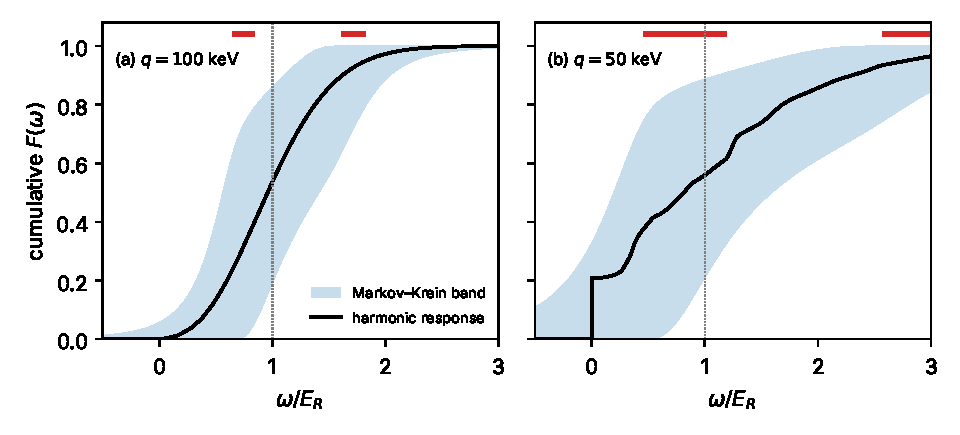
\includegraphics[width=\linewidth]{figures/ch11/fig11_5.pdf}
  \caption{Cumulative nuclear response $F(\omega)$ of silicon at $T = 0$ (black), the fraction of the weight of the self response at energies up to $\omega$, against $\omega/E_R$, with the Markov--Krein band of its first five moments (blue). (a)~$q = \SI{100}{keV}$, $E_R = \SI{191.1}{meV}$, $x_R = 4.67$; (b)~$q = \SI{50}{keV}$, $E_R = \SI{47.8}{meV}$, $x_R = 1.17$, where the zero-phonon weight $\ee^{-2W_\kappa} = 0.21$ is a step at $\omega = 0$. Response: harmonic, incoherent, all phonon orders, from the PBE density of states of \cref{sec:5.2}; moments from $c_k = E_R\langle\omega^{k-1}\rangle$. Red bars: values of $\omega$ at which a node of the canonical representation lies below $\omega = 0$, so that the band drawn is wider than the sharp band of distributions confined to $\omega \ge 0$; elsewhere it is sharp for them too. Dotted: $\omega = E_R$.}
  \label{fig:11-mk}
\end{figure}

At $T = 0$ the response vanishes for $\omega < 0$, a constraint that the band of \cref{eq:C.10-band} does not use. It remains valid, and where every node of the canonical representation lies at $\omega \ge 0$ that representation is itself an admissible response, which makes the band sharp on the half line too. This holds at $\omega = E_R$ for $q = \SI{100}{keV}$ (\cref{we:11-mkpeak}). It fails in two windows, $0.65$ to $0.85\,E_R$ and $1.61$ to $1.82\,E_R$, where one outer node of the three-point solution moves out to infinity and comes back from the other side, below $\omega = 0$; at \SI{50}{keV} the windows are $0.46$ to $1.20\,E_R$ and $2.6$ to $3.4\,E_R$. There the half-line point-mass bound \cref{eq:C.10-stieltjes} is smaller than $\varrho_{\mathrm{MK}}$, by up to \SI{6.8}{\percent} at \SI{100}{keV} and \SI{24.5}{\percent} at \SI{50}{keV}, so the sharp half-line band is narrower at least by that much. We use the band \cref{eq:C.10-band} throughout, which is conservative and has explicit extremal distributions.

\begin{workedexample}{Markov--Krein band of silicon at the recoil energy}\label{we:11-mkpeak}
Take silicon at $q = \SI{100}{keV}$ and $T = 0$, with $E_R = \SI{191.1}{meV}$ and $\langle\omega\rangle = \SI{40.9}{meV}$ as in \cref{we:11-width}. The cumulants $c_k = E_R\langle\omega^{k-1}\rangle$ give the standard deviation $\sigma_\omega = \SI{88.4}{meV}$, the skewness $c_3/\sigma_\omega^3 = 0.553$ and the standardized fourth moment $3 + c_4/c_2^2 = 3 + (\langle\omega^3\rangle/\langle\omega\rangle^3)/x_R = 3.333$, against 0 and 3 for a Gaussian. For a Gaussian the canonical representation through the mean has nodes at 0 and $\pm\sqrt3$ standard deviations with weights $\tfrac23, \tfrac16, \tfrac16$ (\cref{app:C.10}). For silicon the same construction, \cref{eq:C.10-kernel} with these moments, puts the nodes at 59.8, 191.1 and \SI{371.3}{meV} with weights 0.191, 0.670 and 0.139. The skewness pushes the outer nodes upward and moves weight to the lower one, but leaves the central weight at $\varrho_{\mathrm{MK}}(E_R) = 0.670$, almost the Gaussian 2/3. So
\begin{equation*}
  0.191 \le F(E_R) \le 0.861 ,
\end{equation*}
while the harmonic response has $F(E_R) = 0.537$. A detector with its threshold at $E_R$ sees between 14 and \SI{81}{\percent} of the events of this momentum transfer, whatever the dynamics, if only the five moments are right.

Energy bins narrow the band little. Between $E_R - \sigma_\omega$ and $E_R + \sigma_\omega$ the band allows any weight from 0.07 to 1.00 (the harmonic value is 0.68); between $E_R \pm 2\sigma_\omega$ it allows 0.78 to 1.00 (0.96). In the tail it is worse in relative terms: above $E_R + 3\sigma_\omega = \SI{456}{meV}$ the harmonic response has the weight $5.6\times10^{-3}$, and the band allows anything from 0 to $3.4\times10^{-2}$, six times more.

The anharmonic change of the kinetic energy of silicon moves the cumulative distribution by at most $2.5\times10^{-4}$, nearly three thousand times less than the width of the band at the peak. For silicon the perturbative correction of the previous subsection is the tool; the band is for targets where no correction can be computed.
\end{workedexample}

In silicon at \SI{100}{keV} the band fixes the weight above a threshold to \SI{10}{\percent} only for thresholds at $\omega \le \SI{28}{meV}$ (\cref{lim:11.5c}). At five standard deviations above the mean the band is 63 times the weight.

\begin{limitbox}[The Markov--Krein band][lim:11.5c]
Every distribution with the moments $\mu_0, \dots, \mu_4$ has $\sum_{y_i < \xi}w_i \le F(\xi) \le \sum_{y_i \le \xi}w_i$, of width $\varrho_{\mathrm{MK}}(\xi)$, with $(y_i, w_i)$ the canonical representation through $\xi$; far from the mean $\varrho_{\mathrm{MK}} \simeq (\bar\mu_4 - \bar\mu_2^2 - \bar\mu_3^2/\bar\mu_2)/(\xi - \mu_1)^4$~\cites{krein1977markov}{akhiezer1965classical}.
\par\smallskip
{\centering
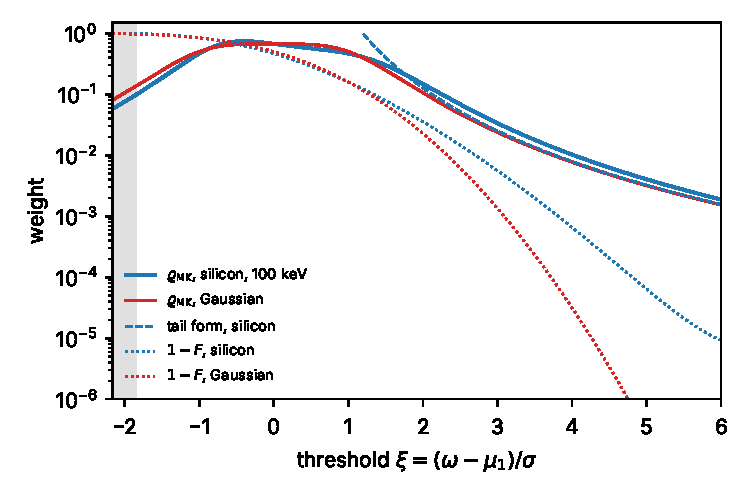
\includegraphics[width=\linewidth]{figures/ch11/limit11_5c.pdf}
\captionof{figure}{Width $\varrho_{\mathrm{MK}}$ of the band (solid) and weight $1 - F$ above a threshold (dotted), against the threshold $\xi$ in units of the standard deviation from the mean, for the harmonic silicon response at $q = \SI{100}{keV}$ (blue; skewness 0.553, standardized fourth moment 3.333) and for a Gaussian (red), the two model distributions whose five moments define their bands. Dashed: the tail form \cref{eq:C.10-tail} for silicon, the leading term far from the mean, with the numerator 2.03 (2 for the Gaussian); the exact width exceeds it by \SI{34}{\percent} at $\xi = 3$ and \SI{20}{\percent} at $\xi = 6$, a correction of relative order $1/\xi$ from the skewness. The silicon curves start at $\omega = 0$. Gray band: thresholds at which the band fixes the silicon weight above threshold to \SI{10}{\percent}, $\varrho_{\mathrm{MK}} \le 0.1\,(1 - F)$, that is $\xi \le -1.84$.}\label{fig:11-limit-5c}
\par}
\smallskip
Above about two standard deviations below the mean the absolute width exceeds a tenth of the weight above threshold, and in the tail it exceeds the weight itself: the band bounds the bulk of a response, never the ratio of two tails.
\end{limitbox}

\noindent On the truncation label the band is exact in $n_A$ and in $n_T$ when the moments are, and it makes no assumption about $\mathcal{K}$. Its use is twofold. For a strongly anharmonic target at a detector temperature it is the only rigorous statement about the response, since the moments come from a static simulation and every real-time method has a problem at millikelvin (below). And for any approximate dynamics it is an acceptance test: a computed response outside the band of its exact moments is wrong.

\subsection{Solid helium}

Helium solidifies only under a pressure of a few MPa even at the lowest temperatures~\cite{ashour2024pressure}, because the zero-point energy of so light an atom in so shallow a well, \SI{10.8}{K} deep for a pair~\cite{aziz1979accurate}, competes with the binding itself. Such a solid is a \emph{quantum crystal}: the zero-point amplitude of an atom is a sizable fraction of the distance to its neighbors, about a quarter near melting, and the harmonic expansion fails at its lowest order. The Lindemann ratio $r_{\mathrm{L}} = \langle u^2\rangle^{1/2}/d_{\mathrm{nn}}$, the root-mean-square displacement over the nearest-neighbor distance $d_{\mathrm{nn}}$, measures it. At the static lattice positions an atom sits far out on the attractive tail of its neighbors' potentials, where the curvature is negative, and the static force constants give imaginary frequencies. The self-consistent harmonic approximation of \cref{eq:5.7-scha} was devised for this case: averaged over the Gaussian spread of the atom, the curvature includes the steep repulsion that the atom samples on its excursions, and it is positive. Compression reduces $r_{\mathrm{L}}$. Diffusion Monte Carlo calculations with a pair potential fitted to dispersion-corrected density-functional theory find $r_{\mathrm{L}} = 0.12$ at \SI{2}{GPa} and 0.10 from \SI{14}{GPa} up to \SI{150}{GPa}~\cite[Table~I]{cazorla2015first}. At such pressures the static lattice is stable, and the quasi-harmonic approximation of \cref{sec:5.7} becomes a reasonable starting point.

Ashour and Griffin proposed solid helium under pressure as a target for light dark matter that couples to nucleons~\cite{ashour2024pressure}. At low pressure its phonon energies are below \SI{3}{meV} and its sound speed is of order $10^{-6}$, too low for single-phonon reach. Between 1 and \SI{40}{GPa} the sound speed rises more than tenfold and the phonon energies nearly a hundredfold, and at \SI{40}{GPa} the single-phonon reach of hcp helium rivals that of diamond. Their response is that of \cref{lim:11.5b}, with phonons computed with the PBE functional and a dispersion correction, and it leaves out the low pressures, where the density functional fails and the Born--Oppenheimer phonons miss the zero-point motion.

When is the quasi-harmonic response good enough, and what does the self-consistent one add? \Cref{lim:11.5b} answers in a cell model, in which one atom moves in the field of its twelve neighbors held fixed on an fcc lattice and the Schrödinger equation is solved exactly. The pair potential is a Morse form with the well of the helium potential, so that only one shape parameter is chosen (the curvature at the minimum of a 12-6 potential with the same well). The model gives $r_{\mathrm{L}} = 0.23$ at \SI{21}{cm^3.mol^{-1}}, near melting, where its first excitation lies at \SI{2.2}{meV}, and 0.117 and 0.094 at the volumes of the Monte Carlo values 0.12 and 0.10 above. The static curvature turns negative for molar volumes above \SI{17}{cm^3.mol^{-1}}, $r_{\mathrm{L}} \ge 0.20$. Below that the quasi-harmonic weight of a single phonon, $q^2/2M\omega$ per direction, overshoots the exact one, because the static curvature is too soft; the error falls below \SI{10}{\percent} only for $r_{\mathrm{L}} \le 0.115$, a molar volume of \SI{6.5}{cm^3.mol^{-1}}, about the \SI{2}{GPa} of the Monte Carlo calculation. The self-consistent harmonic weight stays within \SI{10}{\percent} up to $r_{\mathrm{L}} = 0.227$ and is \SI{10}{\percent} low at \SI{21}{cm^3.mol^{-1}}. The kinetic energy that sets the impulse width behaves alike: at $r_{\mathrm{L}} = 0.117$ the quasi-harmonic value is \SI{9}{\percent} low and the self-consistent one within \SI{0.1}{\percent}.

\begin{limitbox}[Solid helium: quasi-harmonic and self-consistent phonons][lim:11.5b]
The single-phonon rate of compressed helium is \cref{eq:11.1-S1} with $c_\kappa = A_\kappa F_N$, phonons and Debye--Waller exponent from the static Hessian at the compressed volume~\cite[Eqs.~(2), (4), (5)]{ashour2024pressure}; the self-consistent correction replaces the Hessian by $\Phi^{(2)}_{\mathrm{aux}}$ of \cref{eq:5.7-scha}.
\par\smallskip
{\centering
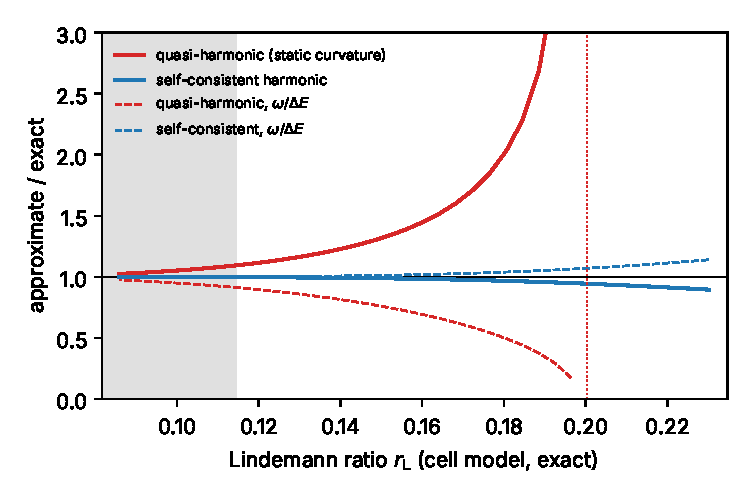
\includegraphics[width=\linewidth]{figures/ch11/limit11_5b.pdf}
\captionof{figure}{Cell model of solid $^4$He: one atom in the spherically averaged field of 12 fixed fcc neighbors, Morse pair potential with the well depth \SI{10.8}{K} and position \SI{2.967}{\angstrom} of the Aziz potential and a curvature equal to that of a 12-6 potential with the same well. Solid: one-phonon weight per unit $q^2$, $1/2M\omega$, from the static curvature (red, quasi-harmonic) and from the self-consistent curvature (blue), divided by the exact dipole weight of the lowest $l = 1$ level, against the exact Lindemann ratio $r_{\mathrm{L}}$, for molar volumes from 3 to \SI{21}{cm^3.mol^{-1}}. Dashed: the corresponding phonon energies over the exact excitation energy $\Delta E$. Dotted: $r_{\mathrm{L}} = 0.20$, above which the static curvature is negative. Gray band: $r_{\mathrm{L}} \le 0.115$, where the quasi-harmonic weight is within \SI{10}{\percent}.}\label{fig:11-limit-5b}
\par}
\smallskip
Above a Lindemann ratio of about 0.12 the static Hessian overstates the one-phonon weight and the Debye--Waller exponent, and above 0.20 it has no real frequencies; the self-consistent phonons hold to near melting, where correlations at short range remain.
\end{limitbox}

\noindent The model fixes the neighbors and uses a Morse wall, so its numbers are a guide, not a prediction for helium; it lands within $0.003$ and $0.006$ of the two Monte Carlo ratios. The quasi-harmonic response of Ashour and Griffin is safe in most of their pressure range and needs the self-consistent force constants at its low end. And at the lowest pressures, where a helium detector would be easiest to build, neither is exact. The self-consistent weight is \SI{10}{\percent} low near melting even in the model, and in the real crystal the Gaussian lets an atom overlap its neighbors, which a real atom avoids by correlated motion. There the response needs the exact moments and the band of \cref{lim:11.5c}. On the truncation label the self-consistent response sums the even anharmonic orders into $\Phi^{(2)}_{\mathrm{aux}}$ at all $n_A$. The cubic terms enter the physical frequencies through a bubble; in the cubic cell of the model the centroid sits on the site and that bubble vanishes.

The same reasoning sorts the other targets in which anharmonicity is not small. A soft mode, such as the one that drives the structural transition of SrTiO$_3$, has a harmonic frequency that is small or imaginary, and its self-consistent frequency depends on temperature at order one. A light atom, such as hydrogen in LiH, has a zero-point amplitude larger by $(M_{\mathrm{Si}}/M_{\mathrm{H}})^{1/4} \approx 2.3$ than a silicon atom in the same well, since $\ell_{\mathrm{zp}} \propto M^{-1/4}$ (\cref{sec:5.7}), and $\eta_{\mathrm{anh}}$ grows with it.

\emph{Open problem: the response of strongly anharmonic targets at detector temperatures.} For soft-mode and light-atom crystals, and for solid helium near melting, no expansion parameter is small, and the nuclear response at \SI{10}{mK} has not been computed. The exact moments are within reach: they are static averages, and a path-integral simulation gives them at any temperature and anharmonicity. The dynamics is not. Ring-polymer and centroid molecular dynamics return Kubo-transformed correlations. Their conversion to $S$ multiplies the error by $\omega/T$, so they hold only for $T \gtrsim \omega/10$; the time-dependent self-consistent harmonic method excites at most two phonons at a time and cannot follow a multiphonon response at $q \gg q_{\mathrm{BZ}}$. At the operating temperature of a cryogenic detector the response of these targets is therefore bounded by the band of their exact moments and by nothing sharper. What would close the gap is a real-time method for quantum nuclei that is exact at low temperature, or a measurement: neutron Compton scattering measures the momentum distribution, and with it the impulse width, of light nuclei directly~\cite{andreani2005measurement}.

\section{Nuclear-spin and isotope couplings}\label{sec:11.6}

One silicon nucleus in 21 is $^{29}$Si and carries a nuclear spin, and in a crystal without a magnetic field the spins point in random directions. The three stable isotopes also differ in their number of neutrons per unit mass, by \SI{6.7}{\percent} from $^{28}$Si to $^{30}$Si. The couplings of \cref{sec:11.1,sec:11.2} are the same on every site of a sublattice, and they conserve crystal momentum. A coupling to the nuclear spin, or to the neutron number of a nucleus at fixed mass, changes at random from site to site. The lattice is still perfect, but to the dark matter the crystal is disordered, crystal momentum is no longer conserved, and a probe that brings almost no momentum, such as an absorbed boson, can create a phonon of any wavevector in the zone. The response then follows the phonon density of states, a broad band, instead of the single line of the zone-center optical phonon. Unpolarized nuclear spins respond in this way, and so do the isotopes to a vector boson coupled to baryon minus lepton number, which in silicon is absorbed almost entirely through them.

\subsection{Broadband response of random couplings}\label{sec:11.6-random}

Label the nuclei of a crystal by $I$, with masses $M_I$ and displacements $\vect{u}_I$ from their equilibrium positions. In a harmonic crystal the displacements are sums over normal modes $\nu$ of the actual configuration, with polarization vectors $\vect{e}_{I\nu}$ normalized over all sites and the mode frequencies $\omega_\nu$, $\vect{u}_I = \sum_\nu\vect{e}_{I\nu}(b_\nu + b_\nu^\dagger)/\sqrt{2M_I\omega_\nu}$. In a perfect crystal $\nu$ is the pair $\vect{Q}\nu$ of \cref{eq:5.3-u}; when the masses vary from site to site, the modes carry no wavevector and $\nu$ is just a label. Consider a target operator whose one-phonon matrix element is linear in the displacements,
\begin{equation*}
  \langle 1_\nu|\,O\,|0\rangle = \sum_I\frac{\vect{v}_I\cdot\vect{e}_{I\nu}^*}{\sqrt{2M_I\omega_\nu}} ,
\end{equation*}
with a vertex $\vect{v}_I$ for each site. The density row at small $\vect{q}$ has this form, with $\vect{v}_I = \ii c_I\vect{q}$ (\cref{sec:11.1}). So has every row built from the nuclear velocities $\vect{P}_I/M_I$. In a harmonic crystal the momentum is $M_I$ times the time derivative of the displacement, and the derivative of a matrix element brings down $\ii\omega$, with $\omega$ the energy of the final state: $\langle f|\vect{P}_I|0\rangle = \ii M_I\omega\langle f|\vect{u}_I|0\rangle$.

Part of every vertex does nothing. Write $\vect{v}_I = M_I\bar{\vect{v}} + \delta\vect{v}_I$ with $\bar{\vect{v}} = \sum_I\vect{v}_I/\sum_IM_I$. The uniform translation of the crystal is a zero mode with $\vect{e}_{I0} \propto \sqrt{M_I}$, every vibration is orthogonal to it, $\sum_I\sqrt{M_I}\,\vect{e}_{I\nu} = 0$, and the mass-proportional part drops out of every one-phonon element. Mitridate and collaborators noted this coupling-to-mass cancellation for the zone-center optical phonons of a perfect crystal~\cite[Eq.~(44)]{mitridate2024effective}. It holds for any configuration of masses, not only at the zone center of a perfect crystal: a coupling proportional to the mass of each nucleus couples to the total momentum, which the forces of the lattice conserve. Only the deviations $\delta\vect{v}_I$ create phonons.

Suppose now that the $\delta\vect{v}_I$ are random: zero on average, independent from site to site and isotropic, $\langle\delta v^\alpha_I\,\delta v^{\beta*}_J\rangle = \delta_{IJ}\delta^{\alpha\beta}\langle|\delta\vect{v}_I|^2\rangle/3$. Averaging the squared matrix element over the disorder removes every term with $I \neq J$, together with the phases that enforced crystal momentum. Each site then contributes through its own vibrations, measured by the local density of states
\begin{equation*}
  g_I(\omega) = \sum_\nu|\vect{e}_{I\nu}|^2\,\delta(\omega - \omega_\nu) ,
\end{equation*}
normalized to three by the completeness of the polarization vectors; in a crystal of one isotope it is the atom-projected density of states $g_{\mathrm{ph},\kappa}$ of \cref{sec:5.3}. Summing over the modes with \cref{eq:4.2-Sab} gives
\begin{keyresult}[Broadband one-phonon response of a random coupling]
\begin{equation}
  \bigl\langle S_{OO}(\vect{q}\to0,\omega)\bigr\rangle = \frac{2\pi}{\Vol}\sum_I\langle|\delta\vect{v}_I|^2\rangle\,\frac{g_I(\omega)}{6M_I\,\omega}\,\bigl[n_{\mathrm{B}}(\omega) + 1\bigr] ,
  \label{eq:11.6-random}
\end{equation}
for $\omega > 0$, with the Bose factor of \cref{sec:5.3} and the average over the disorder in the brackets. It is exact for a harmonic crystal when the random vertex is independent of the masses and force constants, with $g_I$ the local density of states at site $I$ of the actual crystal.
\end{keyresult}
\noindent Unlike the single zone-center line that a coherent coupling excites (\cref{sec:11.2}), the response is a band: every phonon of energy $\omega$ contributes, whatever its wavevector, since the random vertex supplies the missing crystal momentum. And it does not depend on how the vertices of neighboring sites are related, only on the variance at each site. On the truncation label of \cref{sec:8.5} it is the point $\mathcal{K}$ = one-phonon, $n_A = 0$, $n_B = 0$, with $n_T = 0$ at \SI{10}{mK}; the coherent sum of \cref{eq:11.1-S1} is replaced by its incoherent counterpart, and this time without approximation.

\subsection{Unpolarized nuclear spins}\label{sec:11.6-spins}

A coupling linear in the nucleon spin acts on a nucleus of isotope $i$ through its spin $\vect{J}^{\mathrm{nuc}}_I$, with the coefficient of \cref{eq:8.1-nuclear}. It enters the target through the spin rows of \cref{eq:8.1-rows}, the spin density $\vect{s}_\kappa(\vect{q}) = \sum_I\ee^{\ii\vect{q}\cdot\vect{X}_I}\vect{J}^{\mathrm{nuc}}_I$ and the spin current $\mathcal{J}^{\alpha\beta}_\kappa$. In zero field the spin states of a nucleus are split only by its quadrupole and dipolar interactions, by at most about \SI{0.1}{\micro eV}, against $T = \SI{0.86}{\micro eV}$ at \SI{10}{mK}. A spin $\frac12$ such as $^{29}$Si has no quadrupole splitting at all, and its states are equally occupied. A nucleus with a quadrupole moment keeps $\langle\vect{J}^{\mathrm{nuc}}\rangle = 0$ but can be slightly aligned at millikelvin temperatures; we do not pursue this correction. The spins also barely act on the lattice: the forces between the atoms are electronic, and the hyperfine coupling that ties a nuclear spin to anything else is far weaker. The state of the target is then a product of an equal mixture of spin states for each nucleus and the phonon state, and
\begin{equation*}
  \bigl\langle J^{a}_IJ^{b}_{I'}\bigr\rangle = \delta_{II'}\,\delta^{ab}\,\frac{J_{\mathrm{nuc},i}(J_{\mathrm{nuc},i} + 1)}{3} ,
\end{equation*}
with $J_{\mathrm{nuc},i}$ the spin of isotope $i$. Two different nuclei have uncorrelated spins, so in the correlation form of \cref{eq:4.2-Sab} every pair of distinct nuclei drops out of the spin-density response, at every phonon order and every temperature. What remains is the self part of \cref{sec:11.3}, one nucleus at both times, for the nuclei that carry a spin:
\begin{keyresult}[Spin-density response of unpolarized nuclei]
\begin{equation}
  \begin{gathered}
  S_{s^as^b}(\vect{q},\omega) = \delta^{ab}\sum_i\frac{J_{\mathrm{nuc},i}(J_{\mathrm{nuc},i} + 1)}{3}\,S^{\mathrm{self}}_i(\vect{q},\omega) , \\
  S^{\mathrm{self}}_i(\vect{q},\omega) = \frac1\Vol\int_{-\infty}^{\infty}\dd t\;\ee^{\ii\omega t}\sum_{I\in i}\bigl\langle\ee^{-\ii\vect{q}\cdot\vect{X}_I(t)}\,\ee^{\ii\vect{q}\cdot\vect{X}_I(0)}\bigr\rangle ,
  \end{gathered}
  \label{eq:11.6-spinS}
\end{equation}
the sum running over the isotopes with a spin. The self response is \cref{eq:11.3-inc} for these nuclei with $c_\kappa^2 \to 1$; its one-phonon term at $T = 0$ on a cubic site is $(2\pi/\Vol)N_i\,\ee^{-2W_i}\,(q^2/2M_i\omega)\,g_i(\omega)/3$, with $N_i$ the number of nuclei of isotope $i$.
\end{keyresult}
\noindent The incoherent approximation of \cref{sec:11.3}, there valid only far above the zone, is exact here at every momentum transfer. The spin-dependent operator $\mathcal{O}_4 = \vect{S}_\chi\cdot\vect{S}_N$ has the dark-matter tensor $\mathfrak{D}_{s^as^b} = |c_4^{(i)}|^2\delta^{ab}|\vect{S}_\chi|(|\vect{S}_\chi| + 1)/3$ of \cref{eq:8.1-D}, and the contraction in the rate \cref{eq:8.2-spectrum} is $\sum_i|c_4^{(i)}|^2\,|\vect{S}_\chi|(|\vect{S}_\chi| + 1)\,J_{\mathrm{nuc},i}(J_{\mathrm{nuc},i} + 1)\,S^{\mathrm{self}}_i/3$. In silicon only $^{29}$Si contributes, with $J_{\mathrm{nuc}} = \frac12$, an abundance of \SI{4.685}{\percent}, and $c_4^{(i)} = 0.312\,c_4^{(n)}$ for a coupling to neutron spins alone (\cref{sec:8.1-nuclei}).

The loss of crystal momentum changes the kinematics. A coherent one-phonon response at $q \ll q_{\mathrm{BZ}}$ offers only acoustic phonons of energy $c_\nu q$, and the reach stops at the acoustic edge \cref{eq:11.1-edge}. The self response at the same $q$ spans the whole band, and any energy up to the kinetic energy of the dark matter can be deposited. A spin-dependent coupling of unpolarized nuclei therefore reaches down to the kinematic limit $2\omega_{\mathrm{th}}/v_{\mathrm{max}}^2$ of a free target, \cref{eq:1.3-mmin}, \SI{0.28}{keV} at a \SI{1}{meV} threshold, 21 times below the acoustic edge of silicon. The weight, however, is small: the self response grows as $q^2$, and at the smallest momentum transfers it is tiny.

Absorption needs the spin current. An axion-like particle couples to nucleons as to electrons in \cref{sec:1.4}, $\mathcal{L} \supset g_{aNN}\,\phi\,\bar\psi_N\ii\gamma^5\psi_N$ for $N = p, n$, and the reduction that gave \cref{eq:8.1-alp} gives for each nucleon $(g_{aNN}/m_N)[(\nabla\phi)\cdot\vect{S}_N + (\partial_t\phi)\,\vect{v}_N\cdot\vect{S}_N]$, with $\vect{v}_N$ the nucleon velocity. Inside a nucleus the velocity of each nucleon is that of the nucleus, $\vect{P}_I/M_i$, plus an internal part that averages to zero, and the Wigner--Eckart theorem replaces the weighted sum of nucleon spins by $g_{ai}\vect{J}^{\mathrm{nuc}}_I$ with
\begin{equation*}
  g_{ai} = \frac{g_{app}\langle S_p\rangle + g_{ann}\langle S_n\rangle}{J_{\mathrm{nuc},i}} ,
\end{equation*}
as in \cref{eq:8.1-nuclear}. The interaction is then $m_N^{-1}\sum_ig_{ai}[(\nabla\phi)\cdot\vect{s}_i + (\partial_t\phi)\,\mathcal{J}^{\alpha\alpha}_i]$ at $\vect{q} = \vect{p}_\phi$. The gradient term rotates a nuclear spin and leaves the lattice as it was. Its final states lie at the spin splittings, below a \si{\micro eV}, and never at $\omega = m_\phi$; it would excite a phonon only through the phase $\ee^{\ii\vect{p}_\phi\cdot\vect{u}_I}$, a correction of order $p_\phi^2\langle u_x^2\rangle \approx 2\times10^{-18}$ at \SI{50}{meV}. The time-derivative term moves the nucleus. At $\vect{p}_\phi \to 0$ it is exactly linear in the nuclear momenta, $\mathcal{J}^{\alpha\alpha}_i = \sum_{I\in i}\vect{P}_I\cdot\vect{J}^{\mathrm{nuc}}_I/M_i$, so in a harmonic crystal it creates exactly one phonon, with the vertex $\delta\vect{v}_I = \ii\omega\,(g_{ai}m_\phi/m_N)\,\vect{J}^{\mathrm{nuc}}_I$ in \cref{eq:11.6-random}, whose variance over the spin states is $\omega^2(g_{ai}m_\phi/m_N)^2J_{\mathrm{nuc},i}(J_{\mathrm{nuc},i} + 1)$. The absorption formula \cref{eq:8.2-abs} with $\omega_\phi = m_\phi$ and the event rate per unit mass $(\rho_\chi/m_\phi\rho_T)\varGamma_{\mathrm{abs}}$ then give, at $T = 0$,
\begin{equation}
  \mathcal{R} = \frac{\pi\rho_\chi m_\phi}{6\,m_N^2M_{\mathrm{cell}}}\sum_{\kappa}\sum_ix_{\kappa i}\,g_{ai}^2\,\frac{J_{\mathrm{nuc},i}(J_{\mathrm{nuc},i} + 1)}{M_i}\,g_i(m_\phi) ,
  \label{eq:11.6-alp}
\end{equation}
with $x_{\kappa i}$ the abundance of isotope $i$ on the sites $\kappa$ of the cell and $M_{\mathrm{cell}}$ the mass of the cell. The rate is broadband: from the lowest acoustic phonons to the top of the optical band, every axion mass is absorbed at the rate set by the density of states at $\omega = m_\phi$. Per unit mass, light nuclei with a large spin weight are favored through the factor $1/M_iM_{\mathrm{cell}}$. In silicon the spin weight is $x_{29}(0.312)^2\cdot\frac34 = 3.4\times10^{-3}$ in units of $g_{ann}^2$, and the proton coupling enters with a coefficient ten times smaller, through $\langle S_p\rangle = 0.016$. \Cref{eq:11.6-alp} is the rate of Bloch, Knapen, Madden and Marocco~\cite[Eq.~(31)]{bloch2025broadband}, who couple the axion to nucleons through $g_N\partial_\mu\phi\,\bar\psi_N\gamma^\mu\gamma^5\psi_N$. On shell this is our coupling with $g_{aNN} = 2m_Ng_N$, and their $g_p\lambda_j$, $\xi_j$ and $D_j(\omega)$ are our $g_{ai}/2m_N$, the weight $\lambda_j^2J(J+1)/M$ averaged over isotopes, and $g_i/3$.

The spin sits on $^{29}$Si, however, which is \SI{3.2}{\percent} heavier than the mean silicon atom, and its local density of states $g_{29}$ is not the $g_{\mathrm{ph},\kappa}$ of the crystal; the literature uses the host density of states for every isotope.

\subsection{An isotopic mass defect}\label{sec:11.6-defect}

How does a single heavier atom vibrate in a crystal of lighter ones? Its neighbors push it with the same springs, and only its inertia differs. The displacement response of a harmonic crystal, the retarded Green function $\GF(\omega) = (\Phi - \omega^2\mathsf{M} - \ii0)^{-1}$ with $\Phi$ the matrix of force constants of \cref{sec:5.2} and $\mathsf{M}$ the diagonal matrix of masses, answers this. In a crystal of mean mass $\bar M$ the element on one site, for one Cartesian direction, is
\begin{equation*}
  \GF_{\mathrm{h}}(\omega) = \frac{1}{\bar M}\int_0^{\infty}\dd\omega'\,\frac{g_{\mathrm{ph},\kappa}(\omega')/3}{\omega'^2 - \omega^2 - \ii0} , \qquad
  \Imag\GF_{\mathrm{h}}(\omega) = \frac{\pi\,g_{\mathrm{ph},\kappa}(\omega)}{6\bar M\omega} ,
\end{equation*}
the spectral sum over the modes weighted by the squared polarization on the site; on a cubic site it is a multiple of the identity. Now give the atom on site $I$ the mass $M_i = \bar M(1 - \delta^M_i)$, with the mass defect $\delta^M_i$ positive for a lighter atom. The change in $\Phi - \omega^2\mathsf{M}$ is the single entry $\delta^M_i\bar M\omega^2$ on that site, and since it acts on one site only, the Dyson equation $\GF = \GF_{\mathrm{h}} - \GF_{\mathrm{h}}\,\delta^M_i\bar M\omega^2\,\GF$ closes on the element at $I$. The local density of states follows from $\Imag\GF$ as for the host, with $M_i$ for $\bar M$:
\begin{keyresult}[Local vibrations of one mass defect]
\begin{equation}
  \GF_i(\omega) = \frac{\GF_{\mathrm{h}}(\omega)}{1 + \delta^M_i\,\bar M\omega^2\,\GF_{\mathrm{h}}(\omega)} , \qquad
  \frac{g_i(\omega)}{g_{\mathrm{ph},\kappa}(\omega)} = (1 - \delta^M_i)\,\frac{\Imag\GF_i(\omega)}{\Imag\GF_{\mathrm{h}}(\omega)} .
  \label{eq:11.6-lifshitz}
\end{equation}
It is exact for one defect in a harmonic host, with the force constants unchanged.
\end{keyresult}
\noindent This is the classical result of Lifshitz~\cite{lifshitz1956some}, worked out for an isotope in a cubic crystal by Dawber and Elliott~\cite{dawber1963vibrations}. The real part of $\GF_{\mathrm{h}}$ follows from the density of states by a Kramers--Kronig integral (\cref{sec:4.3}), and nothing else is needed: one harmonic calculation of the pure crystal gives the vibrations of every isotope in it. To first order in the defect,
\begin{equation}
  \frac{g_i(\omega)}{g_{\mathrm{ph},\kappa}(\omega)} = 1 + \delta^M_i\,h_{\mathrm{iso}}(\omega) + O\bigl((\delta^M_i)^2\bigr) , \qquad
  h_{\mathrm{iso}}(\omega) = -1 - 2\bar M\omega^2\,\Real\GF_{\mathrm{h}}(\omega) .
  \label{eq:11.6-first}
\end{equation}
At low frequency $h_{\mathrm{iso}} \to -1$: a heavier atom moves with the long waves like its neighbors and carries more weight in proportion to its mass. Higher in the band $\Real\GF_{\mathrm{h}}$ decides. Below a sharp peak of the density of states it is positive, $h_{\mathrm{iso}} < 0$, and a heavier atom gains weight; just above the peak it is large and negative, and the heavier atom loses weight. A heavy atom thus shifts weight down from the top of each band. A light atom with $\delta^M_i$ large enough does more: where $1 + \delta^M_i\bar M\omega^2\Real\GF_{\mathrm{h}} = 0$ above the band, $\GF_i$ has a pole, and the atom vibrates in a local mode that the host cannot carry away. The sum rule $\int g_i\,\dd\omega = 3$ holds in every case, with the local mode included.

For silicon we take the density of states of the PBE force constants of \cref{sec:5.2}, which ends at $\omega_{\mathrm{max}} = \SI{63.7}{meV}$, and the natural mixture of masses: \SI{92.223}{\percent} $^{28}$Si, \SI{4.685}{\percent} $^{29}$Si and \SI{3.092}{\percent} $^{30}$Si~\cite{meija2016isotopic}, with atomic masses 27.977, 28.976 and \SI{29.974}{u}~\cite{wang2021ame2020}. The mean mass is $\bar M = \SI{28.0855}{u}$, and the defects are $\delta^M_i = +0.0039$, $-0.0317$ and $-0.0672$. A local mode requires $\delta^M_i > 0.22$, an atom \SI{22}{\percent} lighter than its neighbors, so no isotope of silicon has one.

\Cref{lim:11.6a} compares its local density of states with the host one that \cref{eq:11.6-alp} assumes in the literature.

\begin{limitbox}[Incoherent spin absorption][lim:11.6a]
Unpolarized nuclear spins absorb an axion-like particle broadband, at the rate $\mathcal{R}$ of \cref{eq:11.6-alp} with the host density of states $g_{\mathrm{ph},\kappa}$ in place of $g_i$ for every isotope~\cite[Eqs.~(25)--(31)]{bloch2025broadband}.
\par\smallskip
{\centering
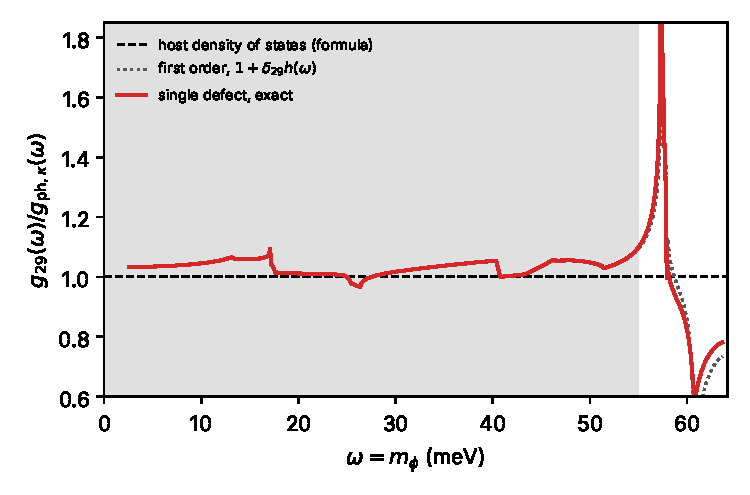
\includegraphics[width=\linewidth]{figures/ch11/limit11_6a.pdf}
\captionof{figure}{Rate of \cref{eq:11.6-alp} for natural silicon, where the spin sits on $^{29}$Si, with the exact local density of states of one $^{29}$Si atom from \cref{eq:11.6-lifshitz} (red), divided by the same rate with the host density of states (dashed, the formula), against the axion mass. The ratio $g_{29}/g_{\mathrm{ph},\kappa}$ does not depend on the couplings. Dotted: the first order in the mass defect, $1 + \delta_{29}h_{\mathrm{iso}}(\omega)$ with $\delta_{29} = -0.0317$, \cref{eq:11.6-first}. PBE density of states of \cref{sec:5.2}, $T = 0$. Gray: within \SI{10}{\percent} of the formula, $m_\phi < \SI{55.0}{meV} = 0.865\,\omega_{\mathrm{max}}$.}\label{fig:11-limit-6a}
\par}
\smallskip
Near the top of the optical band the heavier isotope moves weight from the band edge to just below it, and the host density of states errs by up to a factor of 2.
\end{limitbox}

Below \SI{55}{meV} the heavier spin carrier changes the rate by $-3.5$ to $+\SI{10}{\percent}$, mostly by 1 to \SI{5}{\percent} upward, and the first order of \cref{eq:11.6-first} reproduces the exact ratio to \SI{0.5}{\percent}. At the sharp lower edge of the optical band the ratio rises to about 2, with a peak of 2.05 at \SI{57.3}{meV} in the PBE spectrum, and between 60 and \SI{63}{meV} it falls to 0.6, with a minimum of 0.59 near \SI{60.7}{meV}. The band integral is unchanged, since both densities of states are normalized to three, so the weight is moved and not lost. This is the correlation between the vertex and the mass: the vertex sits on an atom whose mass, and therefore whose vibrations, differ from the average. Bloch and collaborators assume that the isotopes leave the phonon spectrum unchanged, which holds for the crystal as a whole when one isotope dominates~\cite[footnote~5]{bloch2025broadband}. The local spectrum at a minority isotope still differs, and in silicon the host density of states is good to \SI{10}{\percent} over \SI{86}{\percent} of the band.

\Cref{eq:11.6-lifshitz} itself treats one defect in a perfect host. How far does it carry into a crystal that contains many?

\begin{limitbox}[Lifshitz mass-defect Green function][lim:11.6b]
One atom of mass $\bar M(1 - \delta^M)$ in a harmonic host: $\GF_i = \GF_{\mathrm{h}}/(1 + \delta^M\bar M\omega^2\GF_{\mathrm{h}})$ on its site~\cites{lifshitz1956some}{dawber1963vibrations}.
\par\smallskip
{\centering
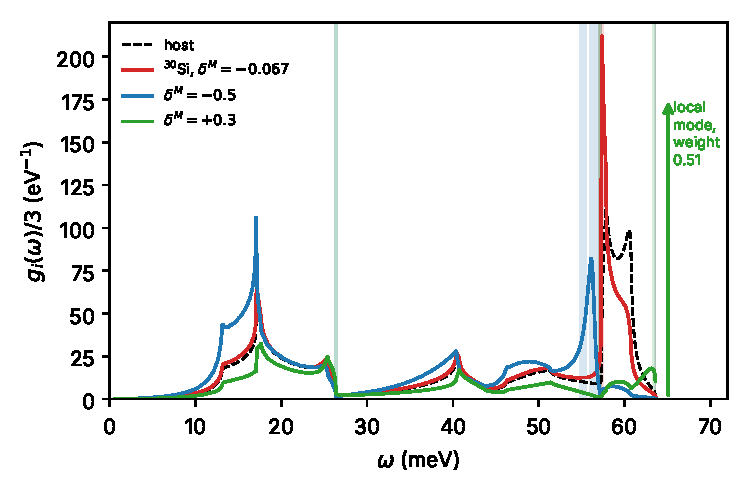
\includegraphics[width=\linewidth]{figures/ch11/limit11_6b.pdf}
\captionof{figure}{Local density of states per direction, $g_i(\omega)/3$, of one mass defect in silicon from \cref{eq:11.6-lifshitz}, with the PBE density of states of \cref{sec:5.2} (dashed, the host). Red: $^{30}$Si, $\delta^M = -0.067$. Blue: a heavy defect, $\delta^M = -0.5$. Green: a light defect, $\delta^M = +0.3$, which puts \SI{51}{\percent} of its weight into a local mode at \SI{65.1}{meV}, above the band (arrow). The integral of each curve, local mode included, is one. Shaded in the color of each curve: frequencies where the leading pair term exceeds \SI{10}{\percent}. The pair term is the effect of a second defect anywhere in the crystal on the first, for the natural isotope mixture around $^{30}$Si and for a concentration of \SI{1}{\percent} of the strong defects; pair term to first order in the scattering of the second defect, from the host Green function.}\label{fig:11-limit-6b}
\par}
\smallskip
The single-defect form fails where defects interact: within a meV of the sharp edges of the host density of states in natural silicon, and over windows of a few meV around them for defects of tens of percent in mass at concentrations of a percent.
\end{limitbox}

The pair term in the caption needs no new calculation. A second defect $j$ at site $\vect{r}$ changes the host function on site $I$ to $\GF_{\mathrm{h}} + \GF_{I\vect{r}}t_j\GF_{\vect{r}I}$, with $t_j = -\delta^M_j\bar M\omega^2/(1 + \delta^M_j\bar M\omega^2\GF_{\mathrm{h}})$ its scattering strength, and the sum over all $\vect{r} \neq I$ of $\GF_{I\vect{r}}\GF_{\vect{r}I}$ is $(\GF^2)_{II} - \GF_{\mathrm{h}}^2 = \partial\GF_{\mathrm{h}}/\partial(\bar M\omega^2) - \GF_{\mathrm{h}}^2$, since $\GF$ is the inverse of $\Phi - \bar M\omega^2$. For the natural mixture referenced to $\bar M$ the first order in the second defect cancels, $\sum_jx_j\delta^M_j = 0$, and what remains is of order $g_{\mathrm{md}} = \sum_jx_j(\delta^M_j)^2 = 2.0\times10^{-4}$, the mass variance of \cref{app:E.12}. It is the self-energy behind the isotope scattering of phonons: its imaginary part gives the width $\frac{\pi}{2}g_{\mathrm{md}}\,\omega^2g_{\mathrm{ph},\kappa}(\omega)/3$, which at low frequency is the Rayleigh rate of \cref{eq:E.12-iso}, and at \SI{50}{meV} is $2.5\times10^{-4}$ of $\omega$. For $^{30}$Si in natural silicon the pair term stays below \SI{2.2}{\percent} up to \SI{55}{meV} and passes \SI{10}{\percent} only within a meV of the sharp edge of the optical band at \SI{57}{meV}. In silicon the isotopes can be treated one at a time.

\subsection{Absorption of a baryon-minus-lepton vector}\label{sec:11.6-bl}

A vector boson can couple to baryon number minus lepton number, $B - L$, with strength $g_{B-L}$, the same for protons and neutrons, $+g_{B-L}$, and for electrons, $-g_{B-L}$ (\cref{sec:1.4}). A neutral atom of isotope $i$, with $A_i$ nucleons and $Z$ electrons, carries the charge $A_i - Z = N_i$, its neutron number. Light enough, the vector can be the dark matter, and it is then absorbed like a dark photon. At rest it couples to the spatial current of its charges (\cref{sec:8.1-absorption}),
\begin{equation*}
  g_{B-L}\Bigl[\sum_\kappa A_\kappa\vect{j}_\kappa - \vect{j}_e\Bigr] = g_{B-L}\sum_\kappa N_\kappa\vect{j}_\kappa + g_{B-L}\Bigl[\sum_\kappa Z_\kappa\vect{j}_\kappa - \vect{j}_e\Bigr] .
\end{equation*}
The bracket $\sum_\kappa Z_\kappa\vect{j}_\kappa - \vect{j}_e$ is the electric current in units of $e$, and that part of the coupling is a dark photon with $\zeta = g_{B-L}/e$, and its rate is the dark-photon rate with in-medium mixing, $\zeta^2\sigma_1/|\varepsilon|^2$ (\cref{sec:10.7}):
\begin{equation}
  \varGamma_{\mathrm{EM}} = \Bigl(\frac{g_{B-L}}{e}\Bigr)^2\omega\,\Imag\Bigl[-\frac{1}{\varepsilon(\omega)}\Bigr] ,
  \label{eq:11.6-GEM}
\end{equation}
at $\omega = m_\phi$, with $\sigma_1 = \omega\varepsilon_2$. In silicon this part creates no single phonon. Its one-phonon vertex is the Born charge, and the Born charges of silicon vanish (\cref{sec:5.5}). Below the electronic gap it is absorbed only by pairs of phonons, through the dipole that a displacement induces on top of another, which is the weak lattice absorption of silicon in the far infrared.

The neutron-number current $g_{B-L}\sum_\kappa N_\kappa\vect{j}_\kappa$ couples each nucleus to its neutron number. In a crystal of one isotope the vertex is $\ii\omega g_{B-L}N_\kappa\hat{\vect{\epsilon}}$, with $\hat{\vect{\epsilon}}$ the polarization of the vector. It is proportional to $M_\kappa$ on both sites of silicon, and the coupling-to-mass cancellation removes it: a monatomic crystal of one isotope does not absorb a $B - L$ vector into one phonon at all. Natural silicon does, because the neutron number per unit mass,
\begin{equation*}
  \mathfrak{b}_i = \frac{N_i}{M_i} ,
\end{equation*}
is $0.5004$, $0.5177$ and \SI{0.5338}{u^{-1}} for the three isotopes. The mass-proportional part of the vertex is set by the mass-weighted mean $\bar{\mathfrak{b}} = \sum_ix_iN_i/\sum_ix_iM_i = \SI{0.50235}{u^{-1}}$, with $x_i$ the abundances, and the remainder $\delta\vect{v}_I = \ii\omega g_{B-L}M_i(\mathfrak{b}_i - \bar{\mathfrak{b}})\hat{\vect{\epsilon}}$ has zero mean and is independent from site to site. Its direction is fixed, but on a cubic site every direction gives the same projection of the local density of states. \Cref{eq:11.6-random} with the vertex in $S_{OO}$ and \cref{eq:8.2-abs} give, per absorbed quantum at $T = 0$ and with $\Omega_{\mathrm{at}}$ the volume per atom,
\begin{keyresult}[Isotope-disorder absorption of a $B - L$ vector]
\begin{equation}
  \begin{aligned}
  \varGamma_{\mathrm{iso}}(\omega) &= \frac{\pi g_{B-L}^2}{2\Omega_{\mathrm{at}}}\sum_ix_iM_i(\mathfrak{b}_i - \bar{\mathfrak{b}})^2\,\frac{g_i(\omega)}{3} \\
  &= \frac{\pi g_{B-L}^2\bar M\sigma_{\mathfrak{b}}^2}{2\Omega_{\mathrm{at}}}\,\frac{g_{\mathrm{ph},\kappa}(\omega)}{3}\Bigl[1 + \langle\delta^M\rangle_{\mathfrak{b}}\,h_{\mathrm{iso}}(\omega) + O(g_{\mathrm{md}})\Bigr] ,
  \end{aligned}
  \label{eq:11.6-Giso}
\end{equation}
at $\omega = m_\phi$ inside the one-phonon band and zero above it, with $\sigma_{\mathfrak{b}}^2 = \sum_ix_i(M_i/\bar M)(\mathfrak{b}_i - \bar{\mathfrak{b}})^2$ the mass-weighted variance of $\mathfrak{b}$ and $\langle\delta^M\rangle_{\mathfrak{b}}$ the mass defect averaged with the weights $x_iM_i(\mathfrak{b}_i - \bar{\mathfrak{b}})^2$. In natural silicon $\sigma_{\mathfrak{b}}^2/\bar{\mathfrak{b}}^2 = 1.88\times10^{-4}$ and $\langle\delta^M\rangle_{\mathfrak{b}} = -0.054$.
\end{keyresult}
\noindent The two parts of the coupling reach different final states, one phonon or two, and they add without interference. The isotope phonons do not mix with the photon either, since the Born charge of every silicon atom vanishes whatever its mass. The vertex of an isotope sits on the atom whose mass differs. The isotope-resolved form of \cref{eq:11.6-Giso} takes this into account through the local density of states of each isotope, \cref{eq:11.6-lifshitz}, and the terms between different sites, which vanish to first order in the mass defects, are the pair terms of \cref{lim:11.6b}. A vector coupled to baryon number alone would see almost nothing. Its charge per mass, $A_i/M_i$, differs between the isotopes only through their binding energies, and the variance is $9\times10^{-11}$ of the squared mean, two million times below that of $B - L$.

How large is the isotope channel against the electromagnetic one? The answer depends on the temperature, through the two-phonon absorption. Consider a pair process in which the field is absorbed and two phonons of energies $\omega_1$ and $\omega_2$ are created, $\omega = \omega_1 + \omega_2$. Its rate is proportional to $(1 + n_1)(1 + n_2)$ and that of the reverse process, stimulated emission, to $n_1n_2$, with the Bose occupations $n_{1,2}$, so the net absorption carries $1 + n_1 + n_2 \ge 1$. In a difference process a phonon $\omega_2$ is absorbed and a phonon $\omega_1 = \omega + \omega_2$ created, with the net weight $n_2(1 + n_1) - n_1(1 + n_2) = n_2 - n_1 \ge 0$, which vanishes at $T = 0$. Suppose the second-order dipole moments and the phonon frequencies do not depend on temperature. Then every term of the absorption coefficient falls as the crystal cools, and
\begin{equation}
  \alpha(\omega; T \to 0) \le \alpha(\omega; \SI{293}{K}) .
  \label{eq:11.6-Tbound}
\end{equation}
The frequencies do shift, by about \SI{1}{\percent} between room temperature and zero, and the lines narrow, so the inequality holds for the absorption integrated over a window wider than the shift and the room-temperature width; where the room-temperature spectrum is flat over that window, it holds point by point. Below the top of the one-phonon band the far-infrared absorption of silicon at room temperature is dominated by difference processes~\cite{ikezawa1981far}, which freeze out completely, so the bound is far from saturated at millikelvin temperatures.

\begin{workedexample}{The isotope channel against the electromagnetic one at \SI{50}{meV}}\label{we:11-iso}
Take natural silicon and $m_\phi = \SI{50}{meV}$, inside the one-phonon band. With $\bar{\mathfrak{b}} = \SI{0.50235}{u^{-1}}$ and $\sigma_{\mathfrak{b}}^2 = 1.879\times10^{-4}\,\bar{\mathfrak{b}}^2 = \SI{4.742e-5}{u^{-2}}$, the product $\bar M\sigma_{\mathfrak{b}}^2 = \SI{1.332e-3}{u^{-1}}$ is \SI{1.430e-12}{eV^{-1}} with $\SI{1}{u} = \SI{931.494}{MeV}$. The PBE density of states of \cref{sec:5.2} gives $g_{\mathrm{ph},\kappa}/3 = \SI{15.9}{eV^{-1}}$ at \SI{50}{meV}, and the volume per atom is $\Omega_{\mathrm{at}} = a^3/8 = \SI{20.02}{\angstrom^3} = \SI{2.606e-9}{eV^{-3}}$. \Cref{eq:11.6-Giso} with the host density of states gives
\begin{equation*}
  \frac{\varGamma_{\mathrm{iso}}}{g_{B-L}^2} = \frac{\pi\times\SI{1.430e-12}{eV^{-1}}\times\SI{15.9}{eV^{-1}}}{2\times\SI{2.606e-9}{eV^{-3}}} = \SI{1.37e-2}{eV} .
\end{equation*}
The correction for the heavier carriers of the vertex is $\langle\delta^M\rangle_{\mathfrak{b}}h_{\mathrm{iso}} = (-0.054)(-1.55) = +\SI{8.3}{\percent}$ to first order, with $h_{\mathrm{iso}}(\SI{50}{meV}) = -1.55$ from the same density of states; the exact single-defect densities give $+\SI{8.0}{\percent}$, and $\varGamma_{\mathrm{iso}}/g_{B-L}^2 = \SI{1.48e-2}{eV}$.

For the electromagnetic part we need $\Imag(-1/\varepsilon)$ at \SI{50}{meV} (\SI{403}{cm^{-1}}). The measured absorption coefficient of silicon at \SI{293}{K} is $\alpha = \SI{0.55}{cm^{-1}}$ there~\cite{ikezawa1981far}; we read it off a published figure~\cite[Fig.~3]{deinzer2004two}, and the reading is uncertain by about \SI{10}{\percent}. With $\varepsilon_2 = \alpha n_r/\omega$, $n_r = 3.42$ and $\omega = \SI{2534}{cm^{-1}}$ as an inverse length ($2\pi$ times the wavenumber), $\varepsilon_2 = 7.43\times10^{-4}$, and with $\varepsilon_1 = 11.7$, $\Imag(-1/\varepsilon) = \varepsilon_2/(\varepsilon_1^2 + \varepsilon_2^2) = 5.42\times10^{-6}$. \Cref{eq:11.6-GEM} with $e^2 = 4\pi\alpha = 0.0917$ gives $\varGamma_{\mathrm{EM}}/g_{B-L}^2 = \SI{0.050}{eV}\times5.42\times10^{-6}/0.0917 = \SI{2.96e-6}{eV}$. By \cref{eq:11.6-Tbound} this is an upper bound at millikelvin temperatures, and
\begin{equation*}
  \frac{\varGamma_{\mathrm{iso}}}{\varGamma_{\mathrm{EM}}} \ge \frac{\SI{1.48e-2}{eV}}{\SI{2.96e-6}{eV}} = 5.0\times10^3 \qquad (\SI{50}{meV},\ T \to 0).
\end{equation*}
At \SI{50}{meV}, in a valley of the density of states between the longitudinal acoustic and optical features, the PBE spectrum, softer by about \SI{1}{\percent} than the room-temperature neutron data of \cref{sec:5.2}, shifts $g_{\mathrm{ph},\kappa}$ by a comparable amount. Neither this nor the reading of $\alpha$ changes the conclusion: in a cold silicon crystal a $B - L$ vector of \SI{50}{meV} is absorbed by the isotopes thousands of times more often than by the electromagnetic channel.
\end{workedexample}

\Cref{fig:11-iso} shows the two channels across the band. The isotope channel follows the density of states, from the acoustic peaks near \SI{17}{meV} to the optical peak near \SI{58}{meV}, and vanishes at the top of the band. Against the room-temperature electromagnetic bound it wins by factors from $2\times10^2$, at the top of the band where the density of states falls to zero, to $1.4\times10^4$. Above the band only the electromagnetic part remains, and at the two-phonon peak near \SI{76}{meV} it is 17 times stronger than at \SI{50}{meV}. The size of the isotope channel is set by the isotopic variance: a crystal enriched in $^{28}$Si suppresses it in proportion to the depletion of the minority isotopes, while the electromagnetic part is unchanged, which makes enrichment a control of the signal.

\begin{figure}[tbp]
  \centering
  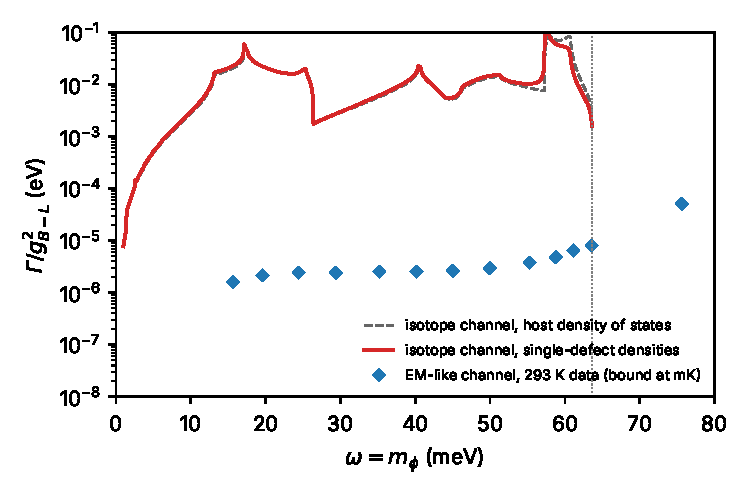
\includegraphics[width=0.8\linewidth]{figures/ch11/fig11_6.pdf}
  \caption{Absorption rate per quantum of a $B - L$ vector in natural silicon, over the squared coupling, against its mass. Red: the isotope-disorder channel of \cref{eq:11.6-Giso} with the exact single-defect densities of states of the three isotopes, \cref{eq:11.6-lifshitz}; dashed: the same with the host density of states for all. PBE phonons of \cref{sec:5.2}, $T = 0$; the dotted line marks the top of the PBE band, \SI{63.7}{meV} (the measured band top is \SI{64.1}{meV}). Blue diamonds: the electromagnetic channel \cref{eq:11.6-GEM}, from the measured absorption coefficient at \SI{293}{K} of Ikezawa and Ishigame~\cite{ikezawa1981far}, read from Fig.~3 of Deinzer and Strauch~\cite{deinzer2004two} with an uncertainty of about \SI{0.05}{cm^{-1}} plus \SI{10}{\percent}, converted with $n_r = 3.42$ and $\varepsilon_1 = 11.7$. At millikelvin temperatures the diamonds are upper bounds, \cref{eq:11.6-Tbound}. The diamond at \SI{76}{meV} is the two-phonon peak, above the one-phonon band.}
  \label{fig:11-iso}
\end{figure}

The inputs of these rates come from one harmonic calculation of the pure crystal. Its density of states and \cref{eq:11.6-lifshitz} give the local density of states of every isotope, and the force constants are those of \cref{sec:5.2} and \cref{app:E.4}. The exact rate of a disordered crystal includes every isotope and the pair terms. It comes from diagonalizing the Hessian of a supercell of a few thousand atoms with the isotopes drawn at random, and \cref{app:E.17} specifies that calculation; the single-defect correction of \cref{eq:11.6-Giso} is its check. The spin expectation values $\langle S_p\rangle$ and $\langle S_n\rangle$ of each odd isotope, which set $g_{ai}$ and $c_4^{(i)}$, come from nuclear shell-model calculations, and \cref{app:E.27} specifies them with their spread.

One input is missing. The electromagnetic channel of \cref{eq:11.6-GEM} needs $\varepsilon(\omega)$ of silicon inside the one-phonon band at the temperature of the detector, and we know of no measurement of the two-phonon absorption of silicon below \SI{65}{meV} at low temperature. The room-temperature data give only the bound \cref{eq:11.6-Tbound}, dominated by difference processes that are absent in a cold crystal. The zero-temperature absorption requires the second-order dipole moments, the derivatives of the Born charges with respect to the displacements, which a first-principles calculation can supply (\cref{app:E.17}); until it or a cold measurement exists, the margin of $5\times10^3$ at \SI{50}{meV} is a lower limit.

\section{Anisotropy and daily modulation}\label{sec:11.7}

At $45^\circ$N the dark-matter wind arrives from almost straight overhead when Cygnus crosses the meridian, and from close to the horizon twelve sidereal hours later (\cref{fig:1-daily}). A crystal fixed to the laboratory floor is therefore probed along different crystal directions in the course of each sidereal day. An isotropic target such as a liquid has the same rate in every orientation; a crystal responds differently along different crystal axes, so its rate follows the sidereal day. The size of the effect differs widely between crystals: below \SI{1}{\percent} in silicon, for electron recoils and for phonons alike, and \SI{6}{\percent} for multiphonon events in sapphire above a threshold of \SI{300}{meV}. Two factors set it, the angular structure of the crystal response and the sharpness with which the halo singles out one direction of $\vect{q}$, and the two can be computed separately, for the electronic responses of \cref{chap:10} and the nuclear responses of this chapter alike.

\subsection{Rate at fixed orientation}

Take a coupling through one density, the electron density of \cref{sec:10.1} or the nuclear operator of \cref{sec:11.1}, with a potential $\tilde V(q)$ that depends only on $|\vect{q}|$. The rate per unit target mass is \cref{eq:8.2-spectrum} with one row, $\mathfrak{D} = |\tilde V(q)|^2$, and the direction of $\vect{q}$ enters both the structure factor $S(\vect{q},\omega)$ and the velocity kernel $\int\dd^3v\,f_\chi(\vect{v})\,\delta(\omega - \omega_{\vect{q}})$. For elastic scattering, $\omega_{\vect{q}} = \vect{q}\cdot\vect{v} - q^2/2\mchi$ (\cref{eq:A.4-omegaq}), and the delta function becomes $q^{-1}\delta(\hat{\vect{q}}\cdot\vect{v} - \vmin)$ with $\vmin = \omega/q + q/2\mchi$ (\cref{eq:1.3-vmin}). The laboratory distribution is the galactic one shifted by the Earth's velocity, $f_\chi(\vect{v}) = f_{\mathrm{gal}}(\vect{v} + \vect{v}_{\mathrm{E}})$ (\cref{eq:1.2-flab}). Substituting $\vect{u} = \vect{v} + \vect{v}_{\mathrm{E}}$ turns the velocity integral into
\begin{equation*}
  \int\dd^3v\,f_\chi(\vect{v})\,\delta(\omega - \omega_{\vect{q}}) = \frac1q\int\dd^3u\,f_{\mathrm{gal}}(\vect{u})\,\delta\bigl(\hat{\vect{q}}\cdot\vect{u} - \vmin - v_{\mathrm{E}}\,\hat{\vect{q}}\cdot\hat{\vect{v}}_{\mathrm{E}}\bigr) = \frac1q\,\hat f_{\mathrm{gal}}\bigl(\vmin + v_{\mathrm{E}}x\bigr) ,
\end{equation*}
with $x = \hat{\vect{q}}\cdot\hat{\vect{v}}_{\mathrm{E}}$ the cosine of the angle between the momentum transfer and the Earth's velocity. The function $\hat f_{\mathrm{gal}}(s)$ is the integral of the isotropic galactic distribution over the plane $\hat{\vect{q}}\cdot\vect{u} = s$, the Radon transform of $f_{\mathrm{gal}}$. For the truncated Maxwellian of \cref{eq:1.2-fgal}, the two Gaussian integrals across the plane run over the disc $u_\perp^2 < v_{\mathrm{esc}}^2 - s^2$, and
\begin{equation*}
  \hat f_{\mathrm{gal}}(s) = \frac{\pi v_0^2}{N_{\mathrm{esc}}}\Bigl[\ee^{-s^2/v_0^2} - \ee^{-v_{\mathrm{esc}}^2/v_0^2}\Bigr]\,\Theta\bigl(v_{\mathrm{esc}} - |s|\bigr) ,
\end{equation*}
with $N_{\mathrm{esc}}$ of \cref{eq:1.2-nesc}. The halo enters only through this function of one variable, and the crystal only through $S(\vect{q},\omega)$ at fixed $|\vect{q}|$, a function on the sphere of directions.

Both factors are now expanded on the sphere. The halo factor is a function of $x$ alone and has a Legendre series, $\hat f_{\mathrm{gal}}(\vmin + v_{\mathrm{E}}x) = \sum_\ell\tfrac12(2\ell + 1)\,\mathcal{H}_\ell\,P_\ell(x)$, with coefficients
\begin{equation}
  \mathcal{H}_\ell(\vmin) = \int_{-1}^{1}\dd x\;P_\ell(x)\,\hat f_{\mathrm{gal}}\bigl(\vmin + v_{\mathrm{E}}x\bigr) ,
  \label{eq:11.7-ups}
\end{equation}
the multipoles of the halo. The crystal factor is expanded in real spherical harmonics $Y_{\ell m}$, the real and imaginary parts of those of \cref{app:C.3}, taken in crystal axes, with components $S_{\ell m}(|\vect{q}|,\omega) = \int\dd^2\hat{\vect{q}}\,Y_{\ell m}(\hat{\vect{q}})\,S(\vect{q},\omega)$. The addition theorem \cref{eq:C.3-addition} holds for the real harmonics too. It gives $\int\dd^2\hat{\vect{q}}\,P_\ell(\hat{\vect{q}}\cdot\hat{\vect{v}}_{\mathrm{E}})\,Y_{\ell'm}(\hat{\vect{q}}) = [4\pi/(2\ell + 1)]\,\delta_{\ell\ell'}\,Y_{\ell m}(\hat{\vect{v}}_{\mathrm{E}})$, and the angular integral pairs each multipole of the response with the halo multipole of the same order:
\begin{keyresult}[Rate of a crystal at fixed orientation]
\begin{equation}
  \frac{\dd\mathcal{R}}{\dd\omega}(t) = \frac{\rho_\chi}{\mchi\,\rho_T}\int\frac{q\,\dd q}{4\pi^2}\,|\tilde V(q)|^2\sum_{\ell m}\mathcal{H}_\ell\bigl(\vmin(q,\omega)\bigr)\,S_{\ell m}(q,\omega)\,Y_{\ell m}\bigl(\hat{\vect{v}}_{\mathrm{E}}(t)\bigr) ,
  \label{eq:11.7-rate}
\end{equation}
with $\hat{\vect{v}}_{\mathrm{E}}(t)$ the direction of the Earth's velocity in crystal axes, which turns with the sidereal day. For a cubic crystal the sum over $m$ at each order is one cubic harmonic $Y^{\mathrm{c}}_\ell$ of \cref{eq:C.3-cubic}, $\sum_mS_{\ell m}Y_{\ell m}(\hat{\vect{v}}_{\mathrm{E}}) = S_\ell\,Y^{\mathrm{c}}_\ell(\hat{\vect{v}}_{\mathrm{E}})$ with $S_\ell(|\vect{q}|,\omega) = \int\dd^2\hat{\vect{q}}\,Y^{\mathrm{c}}_\ell(\hat{\vect{q}})\,S(\vect{q},\omega)$, for $\ell \le 10$.
\end{keyresult}
\noindent The monopole term reproduces the isotropic rate. Since $\int_{-1}^1\dd x\,\hat f_{\mathrm{gal}}(\vmin + v_{\mathrm{E}}x)/2q$ is the average of the velocity integral over the directions of $\vect{q}$, which \cref{eq:A.8-eta} identified with $\eta/2q$, the zeroth halo multipole is the mean inverse speed, $\mathcal{H}_0(\vmin) = \eta(\vmin)$. With $S_{00}Y_{00} = \bar S$, the term $\ell = 0$ of \cref{eq:11.7-rate} is the isotropic rate of \cref{eq:A.8-eta}. The other terms carry all of the time dependence, through $Y_{\ell m}(\hat{\vect{v}}_{\mathrm{E}}(t))$, and each is weighted by the product of a property of the crystal, $S_{\ell m}$, and a property of the halo, $\mathcal{H}_\ell$. The same separation underlies the harmonic method of Al-Adulrazzaq and collaborators~\cite[Eqs.~(6), (10), (17)]{aladulrazzaq2026anisotropic}. Stratman and Lin integrate the same rate directly over the directions of $\vect{q}$~\cite[Eqs.~(28), (29), (31)]{stratman2025daily}. For a coupling with several rows, $|\tilde V|^2S$ becomes the contraction of \cref{eq:8.2-spectrum}; as long as $\mathfrak{D}_{ab}$ depends on $|\vect{q}|$ alone, each $S_{ab}$ is expanded in the same way. A coupling that depends on the dark-matter velocity puts powers of $\vect{v}$ under the velocity integral, and its halo factor is then no longer a function of $x$ alone.

How quickly the halo multipoles fall with $\ell$ decides how much of a crystal's anisotropy reaches the rate. With the standard halo of \cref{sec:1.2}, the ratio $\mathcal{H}_2/\mathcal{H}_0$ is 0.13, 0.37, 0.51 and 0.70 at $\vmin = 300$, 500, 600 and \SI{700}{km.s^{-1}}, while $\mathcal{H}_4/\mathcal{H}_0$ is only $-0.016$, $0.017$, $0.069$ and $0.27$. The reason is the shape of the halo factor. As a function of $x$ it is a Gaussian of width $v_0/v_{\mathrm{E}} = 0.95$, centered at $x = -\vmin/v_{\mathrm{E}}$: the momentum transfer prefers to point along the wind, against $\vect{v}_{\mathrm{E}}$, but only loosely, and a broad function has small high multipoles. Near the kinematic edge, $\vmin \to v_{\mathrm{esc}} + v_{\mathrm{E}}$, only a small cap of directions around $-\hat{\vect{v}}_{\mathrm{E}}$ is allowed, and every multipole approaches $\mathcal{H}_0$ in magnitude. At small $\vmin$ the preference reverses: a particle that needs only a small velocity component along $\vect{q}$ is best served by a $\vect{q}$ nearly perpendicular to its velocity, and $\mathcal{H}_2/\mathcal{H}_0 = -0.13$ at $\vmin = 0$. The quadrupole changes sign at $\vmin = \SI{196}{km.s^{-1}}$ and the hexadecapole at 138 and \SI{435}{km.s^{-1}}, so the phase of a modulation can flip with the mass or the energy deposited, as the annual modulation does at \SI{211}{km.s^{-1}} (\cref{sec:1.2}). The halo therefore filters the anisotropy of a crystal: the quadrupole passes at the level of tens of percent, the hexadecapole at a few percent, and the higher orders only for the fastest particles.

We measure the result by the daily-modulation amplitude
\begin{equation}
  A_{\mathrm{day}} = \frac{\mathcal{R}_{\mathrm{max}} - \mathcal{R}_{\mathrm{min}}}{\mathcal{R}_{\mathrm{max}} + \mathcal{R}_{\mathrm{min}}} ,
  \label{eq:11.7-Aday}
\end{equation}
the half-range of the rate over one sidereal day divided by its mean, for a rate integrated above a threshold. It depends on the crystal, on its mounting and on the latitude, which together fix the path of $\hat{\vect{v}}_{\mathrm{E}}(t)$ in crystal axes (\cref{eq:1.2-local}), and on the dark-matter mass and the threshold, which fix the values of $\vmin$ the rate samples.

\subsection{Selection rules}

The first restriction is evenness. With inversion symmetry, or with time-reversal symmetry, $S(\vect{q},\omega) = S(-\vect{q},\omega)$ (\cref{app:A.4}), and every component with odd $\ell$ vanishes. This holds in silicon, germanium and GaAs, with or without spin--orbit coupling, at every $|\vect{q}|$, every $\omega$ and every temperature, and for the loss function as well as for $S$. The odd halo multipoles are large, $\mathcal{H}_1/\mathcal{H}_0 = -0.54$ at \SI{300}{km.s^{-1}}, but no even response can use them.

A response with odd parts needs both symmetries broken, as in a magnetically ordered crystal without a center of inversion. For a density its odd part is then small at small momentum transfer. For $f \ne i$ the matrix element starts as $\langle f|n_e(\vect{q})|i\rangle = \ii\vect{q}\cdot\vect{d}_{fi} - \tfrac12q_\alpha q_\beta Q^{\alpha\beta}_{fi} + O(q^3)$, with $\vect{d}_{fi}$ and $Q^{\alpha\beta}_{fi}$ the matrix elements of $\sum_j\vect{r}_j$ and $\sum_jr^\alpha_jr^\beta_j$; the term of order zero vanishes by orthogonality. The difference between $\vect{q}$ and $-\vect{q}$ is the interference of the two leading terms,
\begin{equation*}
  |\langle f|n_e(\vect{q})|i\rangle|^2 - |\langle f|n_e(-\vect{q})|i\rangle|^2 = 2\,\Imag\bigl[(\vect{q}\cdot\vect{d}_{fi})\,q_\alpha q_\beta Q^{\alpha\beta*}_{fi}\bigr] + O(q^5) ,
\end{equation*}
which is of third order in $q$. Inversion forbids it, because $\vect{d}_{fi}$ connects states of opposite parity and $Q_{fi}$ states of the same parity; time reversal forbids it, because it makes both matrix elements real in a suitable basis. Where it survives, it multiplies the odd halo multipoles, and the rate acquires a part that is odd in the direction of the wind: opposite wind directions in crystal axes give it opposite signs. Such nonreciprocal targets are treated in \cref{sec:14.5}. A chiral crystal that keeps time reversal has an even $S$, and its two enantiomers modulate identically.

The second restriction is the point group. A function of direction invariant under the cubic group has no component with $\ell = 2$ (\cref{app:C.3}), so in silicon, germanium and GaAs the anisotropy of every response, electronic or nuclear, starts at $\ell = 4$ with $Y^{\mathrm{c}}_4$, followed by $Y^{\mathrm{c}}_6$ and $Y^{\mathrm{c}}_8$. A uniaxial crystal, such as trigonal sapphire or a hexagonal polytype of SiC, has one invariant direction, the $c$ axis $\hat{\vect{c}}$, and allows $\ell = 2$ with $m = 0$ about it. To this order the rate is $\mathcal{R}_0 + \mathcal{R}_2P_2(\hat{\vect{c}}\cdot\hat{\vect{v}}_{\mathrm{E}})$, the constant plus a constant times $\cos^2\theta_{\mathrm{lab}}$ that \cref{sec:1.2} wrote down by symmetry alone, and \cref{eq:11.7-rate} now supplies the two constants. At $\ell = 4$ a trigonal crystal adds terms with $|m| = 3$, and a hexagonal one first breaks the symmetry about $\hat{\vect{c}}$ at $\ell = 6$. Combined with the halo filter, the counting already explains the main pattern: for the same anisotropy of the response, a uniaxial crystal modulates through $\mathcal{H}_2$, a cubic one through $\mathcal{H}_4$, roughly ten times less except near the kinematic edge.

\subsection{Electronic anisotropy}

How anisotropic is the loss function of silicon? The covalent bonds point along the four $\langle111\rangle$ directions, the conduction-band minima lie along $\langle100\rangle$, and an electron--hole pair of a few eV made with a momentum transfer of a few keV feels both. \Cref{fig:11-aniso}(a) shows the ratio $L_4/L_0$ of the cubic-harmonic components of the loss function, in the empirical pseudopotential model of \cref{sec:3.3} that \cref{lim:10.1a} used, with the random-phase head of the dielectric matrix and no local fields. Each component is fitted to the loss function computed along ten directions of the irreducible wedge of the cube. The $k$ grid has the full cubic symmetry, so the components with $\ell = 2$ and odd $\ell$ vanish identically and cannot leak in as artifacts; refining it from $12^3$ to $16^3$ points changes $L_4/L_0$ by at most 0.01. At $q = q_0 = \SI{3.73}{keV}$ the ratio is 0.18 at \SI{3}{eV}, 0.05 at \SI{5}{eV} and below 0.01 above \SI{8}{eV}. The hexadecapole is not dominant: $L_6/L_0$ is of the same size, and near the gap the components beyond $\ell = 8$ carry an rms deviation of \SI{10}{\percent} of $\bar L$ or more, a sign of structure on small angular scales. Away from the gap the response is closer to that of a uniform gas, which has no preferred direction. GaAs, with the same lattice and a different basis, has components of the same size.

The halo multipoles now decide how much of this survives in the rate. \Cref{lim:11.7a} follows it at \SI{5}{eV} for a \SI{10}{MeV} particle. Wherever $\vmin$ is well below the kinematic edge, $\mathcal{H}_4/\mathcal{H}_0$ is a few percent and the anisotropic part of the rate at each $q$ stays below a few tenths of a percent, carried by the term $\ell = 4$ alone. Only near the edge, where the halo admits a narrow cone of directions, does the rate depend strongly on the direction of the wind, by tens of percent, and there the components $\ell \ge 6$ enter as well. Integrated over the spectrum of a \SI{2}{MeV} particle, the components combine into a daily modulation of about \SI{1}{\percent} (\cref{we:11-daily}).

These numbers are those of a model, and the model has two known gaps. The empirical pseudopotential reproduces the bands, not the wavefunctions at large momentum, and the calculation stops at $q = 2.8\,q_0$. Local fields add the crystal's own reciprocal vectors to the response at $q + \vect{G}$ and are known to change the direction-averaged rate by a factor of 1.3 to 1.5 at \SI{10}{MeV} (\cref{sec:10.2}); their effect on $L_4$ has not been computed. The cubic-harmonic components of the silicon loss function from a first-principles calculation with local fields, on a grid of directions fine enough for the structure near the gap, are therefore an open quantity. So, with them, is the electronic daily modulation of silicon beyond a model estimate. The calculation is specified in \cref{app:E.16}: the full-$\vect{q}$ loss function on Lebedev grids of increasing order, projected on $Y^{\mathrm{c}}_\ell$ for $\ell = 4$, 6 and 8, with the components $\ell = 1$, 2 and 3 as built-in tests that must vanish.

Evenness also settles a point in the literature. Al-Adulrazzaq and collaborators compute the electronic daily modulation of silicon and GaAs at \SI{10}{MeV} from the full loss function and find about one percent. They attribute the nearly sinusoidal shape of the signal at \SI{5}{eV}, with one period per sidereal day, to the dipole component of the loss function~\cite[Sect.~III\,B]{aladulrazzaq2026anisotropic}. The dipole component vanishes identically in both crystals, as do all odd components. A period of one sidereal day does not need $\ell = 1$: when the crystal axes are tilted with respect to the Earth's axis, $Y^{\mathrm{c}}_4(\hat{\vect{v}}_{\mathrm{E}}(t))$ contains every harmonic of the sidereal frequency up to the fourth, and which one dominates depends on the mounting. Their Migdal rate in the soft limit, in which the electronic and nuclear momenta separate, depends on the loss function only through its components with $\ell = 0$ and 2 at each $|\vect{k}|$~\cite[Eqs.~(37)--(41)]{aladulrazzaq2026anisotropic}. In a cubic crystal the component $\ell = 2$ vanishes at every $|\vect{k}|$, so the soft-limit Migdal rate of silicon, germanium and GaAs has no daily modulation at all. Their computed modulation of the Migdal rate is much smaller than that of the electron rate, as it must be, and any residue is numerical. Beyond the soft limit the Migdal response is the subject of \cref{chap:12}.

\subsection{Nuclear anisotropy}

The nuclear response carries its direction dependence in two places. In the incoherent approximation \cref{eq:11.3-inc}, each nucleus enters through its Debye--Waller exponent $2W_\kappa(\vect{q}) = \vect{q}\cdot B_\kappa\cdot\vect{q}$ (\cref{eq:5.6-W}) and through the spectrum $P^\kappa_1(\hat{\vect{q}},\omega)$, which is built from the density of states projected on $\hat{\vect{q}}$. Both are quadratic forms in $\hat{\vect{q}}$. The projected density of states is $\hat{\vect{q}}\cdot D_\kappa(\omega)\cdot\hat{\vect{q}}$, with the tensor
\begin{equation*}
  D^{\alpha\beta}_\kappa(\omega) = \frac1N\sum_{\vect{Q}\nu}\Real\bigl[e^\alpha_{\kappa\nu}(\vect{Q})\,e^{\beta}_{\kappa\nu}(\vect{Q})^*\bigr]\,\delta(\omega - \omega_{\vect{Q}\nu}) ,
\end{equation*}
whose trace is the atom-projected density of states $g_{\mathrm{ph},\kappa}(\omega)$ and whose integral against $\coth(\omega/2T)/(2M_\kappa\omega)$ is $B_\kappa$. Stratman and Lin write the incoherent response with this tensor and compute its daily modulation in sapphire and SiC~\cite[Eqs.~(18)--(24)]{stratman2025daily}. At a site of cubic symmetry every second-rank tensor is a multiple of the unit tensor (\cref{app:C.3}). Then $B_\kappa = \langle u_x^2\rangle\mathbb{1}$ and $D_\kappa = (g_{\mathrm{ph},\kappa}/3)\mathbb{1}$, and the direction of $\vect{q}$ drops out of \cref{eq:11.3-inc} term by term:
\begin{keyresult}[Isotropy of the incoherent response of cubic crystals]
If every nucleus sits at a site of cubic symmetry, the incoherent nuclear response \cref{eq:11.3-inc} is independent of the direction of $\vect{q}$ at every phonon order and every temperature. The direction dependence of the harmonic nuclear response of silicon, germanium, diamond and GaAs is entirely in its distinct part, the pair terms of \cref{eq:11.3-exact}.
\end{keyresult}
\noindent The temperature enters only through the Bose factors, which multiply each phonon by a scalar, so the statement holds at any $T$. The published tensors of Stratman and Lin show it to numerical precision: for silicon the three diagonal elements of $B_\kappa$ agree to $2\times10^{-4}$ and the off-diagonal ones are below \SI{e-7}{\angstrom^2}, and the two sites of GaAs agree to $8\times10^{-4}$. Their finding that the multiphonon rates of silicon and GaAs do not modulate~\cite[Sect.~IV]{stratman2025daily} is therefore exact within their approximation, not a numerical accident.

The anisotropy of the cubic nuclear response is entirely in the coherent terms, and \cref{sec:11.3} computed them. At long wavelength the one-phonon weight per direction is $\sum_\nu(\hat{\vect{q}}\cdot\hat{\vect{e}}_\nu)^2/c_\nu(\hat{\vect{q}})$ of \cref{eq:11.1-Sac}. With the measured elastic constants of \cref{sec:11.1} its component $\ell = 4$ is $S_4/S_0 = 0.028$, and $\ell = 6$ is below $10^{-3}$. The PBE force constants of \cref{sec:5.2} give $S_4/S_0 = 0.025$ for $q \le 0.3\,q_{\mathrm{BZ}}$, and the dispersion of the branches raises $|S_6/S_0|$ to 0.026 at $0.7\,q_{\mathrm{BZ}}$. Beyond the zone the one-phonon weight is strongly anisotropic. Near each reciprocal-lattice vector the acoustic phonons at $\vect{q} - \vect{G}$ are soft and their weight $1/\omega$ is large. The vectors $\vect{G}$ of a shell point in definite directions, and the weight is concentrated along them: just beyond the shell $|\vect{G}_{111}| = \SI{3.95}{keV} = 1.76\,q_{\mathrm{BZ}}$, at $q = 1.79\,q_{\mathrm{BZ}}$, $S_4/S_0 = -0.36$, and $S_6/S_0$ reaches $-0.49$ at $2.9\,q_{\mathrm{BZ}}$; beyond $5\,q_{\mathrm{BZ}}$, $|S_4/S_0|$ still reaches 0.2 and $|S_6/S_0|$ 0.4. The two-phonon weight, a sum over pairs of the square of a correlation, is less anisotropic, with $|S_4/S_0|$ and $|S_6/S_0|$ of about 0.1 at most. From three phonons on the incoherent part dominates, and the coherent corrections, and with them the anisotropy, are below \SI{3}{\percent} (\cref{sec:11.3}). These components come from the same force constants and the same pair correlations as the direction-averaged weights of \cref{sec:11.3}, and \cref{app:E.17} specifies their tabulation for silicon, germanium and GaAs, with the incoherent components $\ell \ge 4$ as a test that must vanish to numerical noise.

A cubic crystal therefore modulates through its nuclear response by less than \SI{1}{\percent}, and appreciably just at masses whose largest momentum transfer, $2\mchi v_{\mathrm{max}}$, ends close to a shell of reciprocal-lattice vectors, where the halo multipoles are large and one shell dominates. In silicon that happens near 1 and \SI{2}{MeV} (\cref{we:11-daily}). At other masses the shells inside the kinematic range contribute with alternating signs and largely cancel, and above a few MeV the incoherent part dominates the rate: the amplitude is \SI{0.04}{\percent} at 3 and \SI{4}{MeV} and $10^{-4}$ at 5 and \SI{10}{MeV}.

A crystal whose nuclei sit at sites of lower symmetry has an anisotropic incoherent response already. To first order in the anisotropy of $B_\kappa$, write $\vect{q}\cdot B_\kappa\cdot\vect{q} = q^2[\bar b_\kappa + \tfrac23\Delta b_\kappa P_2(\hat{\vect{c}}\cdot\hat{\vect{q}})]$ for a uniaxial site, with $\bar b_\kappa = \tfrac13\Tr B_\kappa$ and $\Delta b_\kappa = B^{cc}_\kappa - B^{aa}_\kappa$ the difference between the elements along and across the axis. The Poisson weight $p^{\mathrm{ph}}_n = \ee^{-2W_\kappa}(2W_\kappa)^n/n!$ of $n$ phonons (\cref{eq:5.6-poisson}) changes by $\delta(2W_\kappa)(n/2W_\kappa - 1)$ in its logarithm, so that
\begin{equation}
  \frac{\delta p^{\mathrm{ph}}_n}{p^{\mathrm{ph}}_n} = \bigl(n - 2\bar W_\kappa\bigr)\,\frac{2\Delta b_\kappa}{3\bar b_\kappa}\,P_2(\hat{\vect{c}}\cdot\hat{\vect{q}}) ,
  \label{eq:11.7-dw}
\end{equation}
with $2\bar W_\kappa = q^2\bar b_\kappa$. Orders below the mean phonon number lose weight along the axis of larger displacement and orders above it gain. A threshold well inside the multiphonon tail needs $n$ far above $2\bar W_\kappa$. The rate above it therefore inherits the anisotropy of $B_\kappa$ multiplied by the phonon number, while the projected spectrum $P^\kappa_1(\hat{\vect{q}},\omega)$ adds an anisotropy of its own whenever the threshold cuts through the phonon band. For sapphire the published tensors give, weighted with $A_\kappa^2$ over the four Al and six O sites of the cell, $B^{cc}/B^{aa} - 1 = +0.059$; for 2H-SiC only $+0.008$, because the larger displacement along the axis of the Si sites is partly offset by the C sites.

\begin{limitbox}[Daily modulation from the anisotropic response][lim:11.7a]
The rate of a crystal at fixed orientation pairs each multipole $S_{\ell m}$ of the response with the halo multipole $\mathcal{H}_\ell$ of the same order, $\dd\mathcal{R}/\dd\omega(t) = (\rho_\chi/\mchi\rho_T)\int q\,\dd q\,(4\pi^2)^{-1}|\tilde V|^2\sum_{\ell m}\mathcal{H}_\ell S_{\ell m}Y_{\ell m}(\hat{\vect{v}}_{\mathrm{E}}(t))$, \cref{eq:11.7-rate}, for the loss function~\cite[Eqs.~(10), (25)]{aladulrazzaq2026anisotropic} and for the incoherent nuclear response with direction-dependent Debye--Waller exponents and projected densities of states~\cite[Eqs.~(19), (24)]{stratman2025daily}. Its first anisotropic term is $\ell = 4$ in a cubic crystal and $\ell = 2$ in a uniaxial one.
\par\smallskip
{\centering
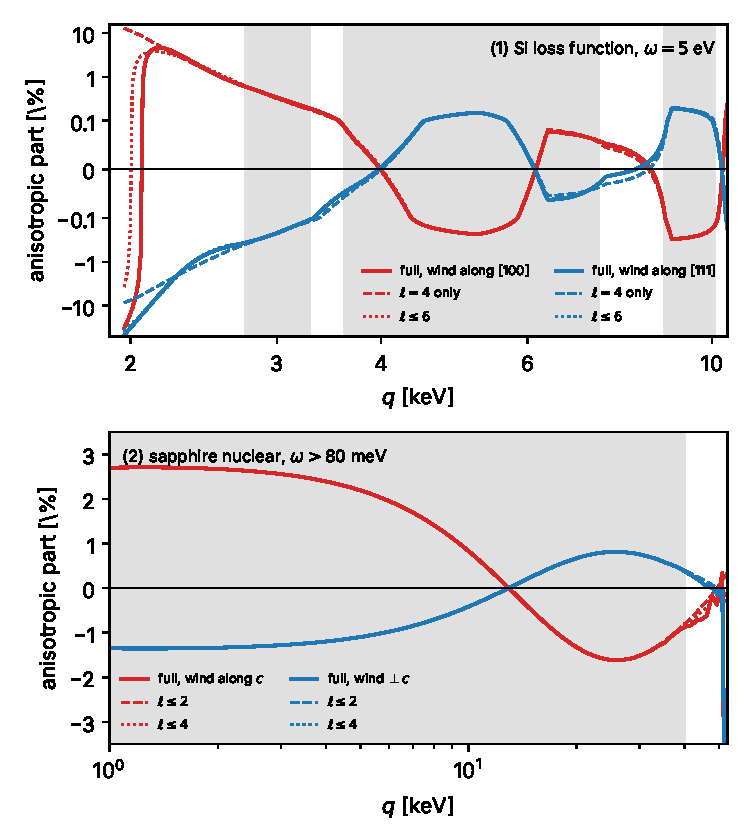
\includegraphics[width=\linewidth]{figures/ch11/limit11_7a.pdf}
\captionof{figure}{Anisotropic part of the rate at fixed momentum transfer for a wind along a fixed crystal axis, $\sum_{\ell \ge 1}\mathcal{H}_\ell\sum_mS_{\ell m}Y_{\ell m}(\hat{\vect{n}})/(\mathcal{H}_0S_{00}Y_{00})$ from \cref{eq:11.7-rate}, against $q$, for $\mchi = \SI{10}{MeV}$, a heavy mediator and the standard halo of \cref{sec:1.2}. (1) Silicon loss function at $\omega = \SI{5}{eV}$ in the empirical pseudopotential model (random-phase head, no local fields), wind along [100] (red) and [111] (blue), from the kinematic edge to the end of the model at $2.8\,q_0$; solid: all fitted components to $\ell = 8$; dashed: $\ell = 4$ alone, the formula; dotted: $\ell \le 6$, the leading correction (symmetric logarithmic axis, linear below \SI{0.1}{\percent}). (2) Sapphire, incoherent nuclear response with direction-dependent Debye--Waller exponents and projected densities of states from the site tensors of Stratman and Lin, integrated above \SI{80}{meV}, wind along the $c$ axis (red) and perpendicular to it (blue); solid: direct integral over the directions of $\vect{q}$; dashed: $\ell \le 2$, the formula; dotted: $\ell \le 4$. Gray bands: $q$ where the truncation at $\ell \le 4$ is within \SI{10}{\percent} of the full anisotropic part (or within $10^{-4}$ of the rate where that part is below $10^{-3}$): in panel (1) from \SI{2.7}{keV} up, except near 3.4, 8 and \SI{10}{keV}, where $\mathcal{H}_4$ or $L_4$ passes close to zero and $\ell = 6$ takes over; in panel (2) up to \SI{40}{keV}, against an edge at \SI{53}{keV}.}\label{fig:11-limit-7a}
\par}
\smallskip
Near the kinematic edge, where the halo admits only a narrow cone of directions, every multipole contributes, and a rate computed from the first anisotropic term alone misses the anisotropy there.
\end{limitbox}

\subsection{Daily-modulation amplitudes}

The time dependence comes from the path of $\hat{\vect{v}}_{\mathrm{E}}(t)$ in crystal axes. In equatorial axes the wind direction stays on a cone of half-angle $\theta_{\mathrm{E}} = 42.5^\circ$ around the Earth's rotation axis, and \cref{eq:1.2-local} gives its components along the local east, north and vertical. A crystal mounted with its axes along these three directions sees $\hat{\vect{v}}_{\mathrm{E}}(t)$ with exactly these components, and any other mounting is a fixed rotation of them. The amplitude of a term $\ell$ is then the range of $\sum_mS_{\ell m}Y_{\ell m}$ along the path. For a uniaxial crystal with its $c$ axis vertical at $45^\circ$N, the angle to the wind runs from $2.5^\circ$ to $87.5^\circ$, and $P_2$ sweeps from 0.997 to $-0.497$, nearly its full range. For a cubic crystal with [001] vertical at the same latitude, $Y^{\mathrm{c}}_4$ runs from $-0.39$ to $0.64$, close to its full range of $-0.43$ at [111] to $0.65$ at [100]. The rate oscillates mainly at twice the sidereal frequency, with a maximum when the wind arrives from overhead, along [001]. A cubic crystal mounted with [001] along the Earth's axis instead sees the wind circle at a fixed angle of $42.5^\circ$ from [001]. Then $Y^{\mathrm{c}}_4$ varies through its azimuthal part alone, $\cos4\varphi$, which gives four maxima per sidereal day and an amplitude six to ten times smaller.

\begin{figure}[tbp]
  \centering
  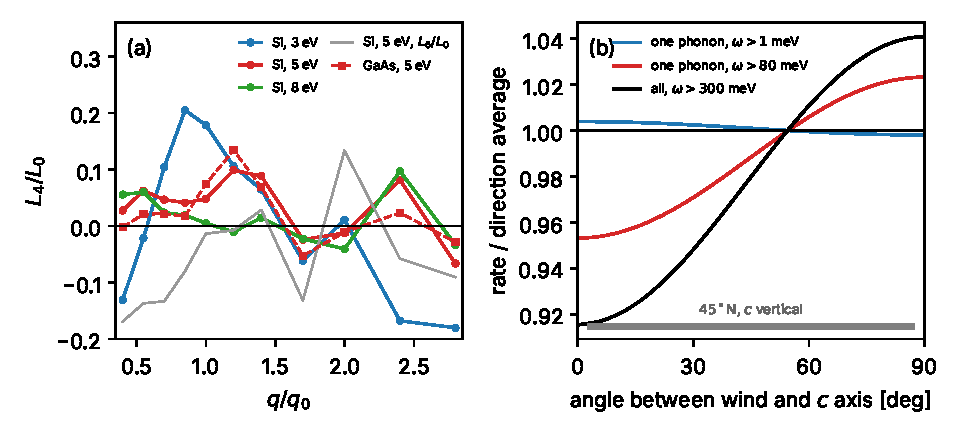
\includegraphics[width=\linewidth]{figures/ch11/fig11_7.pdf}
  \caption{Anisotropy of a cubic and of a uniaxial crystal. (a) Hexadecapole of the silicon loss function, the ratio $L_4/L_0$ of its components on the cubic harmonics $Y^{\mathrm{c}}_4$ and $Y^{\mathrm{c}}_0$, against $q/q_0$, $q_0 = \SI{3.73}{keV}$, at $\omega = 3$, 5 and \SI{8}{eV} (bins of \SI{1}{eV}); thin gray: $L_6/L_0$ at \SI{5}{eV}; dashed: GaAs at \SI{5}{eV}. Empirical pseudopotential model of \cref{sec:3.3}, head of the random-phase dielectric matrix, no local fields, ten directions of the irreducible wedge of the cube on a $k$ grid with the full cubic symmetry, components $\ell = 0$, 4, 6 and 8 fitted by least squares. (b) Rate of a sapphire crystal for a wind at a fixed angle to its $c$ axis, divided by the rate averaged over all wind directions, at $\mchi = \SI{10}{MeV}$ with a heavy mediator coupled to nucleon number: one phonon above \SI{1}{meV} (blue) and above \SI{80}{meV} (red), and all phonon numbers above \SI{300}{meV} (black). Incoherent nuclear response at $T = 0$ with the direction-dependent Debye--Waller exponents and projected densities of states of the published site tensors of Stratman and Lin~\cite{stratman2025daily}, whose $A_\kappa^2$-weighted anisotropy is $B^{cc}/B^{aa} - 1 = +0.059$. Bar: the range of angles swept in one sidereal day by a $c$ axis along the vertical at $45^\circ$N.}
  \label{fig:11-aniso}
\end{figure}

\Cref{fig:11-aniso}(b) shows the uniaxial case. Sapphire's rate depends on the direction of the wind almost only through the term $\ell = 2$, since the terms with $\ell \ge 4$ contribute less than $5\times10^{-4}$ of the rate, and its amplitude depends on which phonons the threshold admits. Above \SI{1}{meV}, where the acoustic and low optical phonons carry most of the one-phonon weight, the one-phonon rate along the axis and across it differ by \SI{0.6}{\percent}, and the rate of all phonon numbers by \SI{1.0}{\percent}, since these modes move all ten atoms of the cell almost isotropically. Above \SI{80}{meV} the highest optical modes alone remain, and they are polarized mostly in the basal plane: the one-phonon rate along the axis is \SI{7}{\percent} below the rate across it. Above \SI{300}{meV} the rate comes from three or more phonons, and \cref{eq:11.7-dw} multiplies the \SI{6}{\percent} anisotropy of the displacements by the phonon number: the difference grows to \SI{12}{\percent}. Mounted with its axis vertical at $45^\circ$N, a sapphire crystal then modulates with $A_{\mathrm{day}} = \SI{0.48}{\percent}$ for all phonons above \SI{1}{meV}, \SI{3.5}{\percent} for one phonon above \SI{80}{meV} and \SI{6.4}{\percent} above \SI{300}{meV}, at \SI{10}{MeV}. At \SI{30}{MeV} the amplitudes for the two higher thresholds fall to 1.2 and \SI{0.6}{\percent}. 2H-SiC, whose displacements are nearly isotropic, modulates less: 0.08, 0.61 and \SI{3.5}{\percent} for the same three cases at \SI{10}{MeV}. These are estimates within the incoherent approximation, which holds for $q$ above a few $q_{\mathrm{BZ}}$, here \SI{1.75}{keV} for the ten-atom cell of sapphire, and therefore for masses of a few MeV and above. They agree in pattern with the multiphonon calculation of Stratman and Lin, who find up to \SI{11}{\percent} in sapphire at \SI{10}{MeV} above \SI{300}{meV}, somewhat less in SiC and none in silicon and GaAs~\cite[Sect.~IV and App.~C]{stratman2025daily}. They use a different halo ($v_0 = 220$, $v_{\mathrm{esc}} = 500$ and $v_{\mathrm{E}} = \SI{240}{km.s^{-1}}$) and put the crystal axis along the wind at the start of the day. At lower masses the momentum transfers stay inside the zone, and the coherent single-phonon response decides the rate. The full phonon calculation of Griffin and collaborators finds daily modulation in sapphire of up to \SI{30}{\percent} at masses near \SI{50}{keV}, for a threshold that leaves only the optical branches. With the acoustic branches open it finds much less, because the sound speeds of sapphire are nearly isotropic~\cite[Sects.~III\,C and IV\,C]{griffin2018directional}. The same holds for the hexagonal polytypes of SiC, with the largest modulation in 2H~\cite[Sects.~IV\,B and V]{griffin2021sic}.

In silicon both the electron and the nucleon rates modulate, and with the same phase.

\begin{workedexample}{Daily modulation of a silicon crystal at $45^\circ$N}\label{we:11-daily}
A silicon crystal sits at latitude $45^\circ$N with [001] along the local vertical, [100] pointing east and [010] north. Dark matter of mass \SI{2}{MeV} scatters through a heavy mediator, either on electrons, through the loss function, or on nucleons, through the nuclear response. At this mass the momentum transfers reach $2\mchi v_{\mathrm{max}} = \SI{10.6}{keV} = 2.84\,q_0$; the electronic model ends at $2.8\,q_0$, and the sliver above it, at the kinematic edge where the rate vanishes, is dropped. The energy deposited on electrons stays below $\mchi v_{\mathrm{max}}^2/2 = \SI{7.0}{eV}$.

\emph{Geometry.} By \cref{eq:1.2-local}, the wind direction in crystal axes is
\begin{multline*}
  \hat{\vect{v}}_{\mathrm{E}} = \bigl(-\cos\delta_{\mathrm{E}}\sin h_{\mathrm{E}},\ \cos\ell_{\mathrm{lat}}\sin\delta_{\mathrm{E}} - \sin\ell_{\mathrm{lat}}\cos\delta_{\mathrm{E}}\cos h_{\mathrm{E}},\\
  \sin\ell_{\mathrm{lat}}\sin\delta_{\mathrm{E}} + \cos\ell_{\mathrm{lat}}\cos\delta_{\mathrm{E}}\cos h_{\mathrm{E}}\bigr) ,
\end{multline*}
with $\delta_{\mathrm{E}} = 47.5^\circ$ and the hour angle $h_{\mathrm{E}}$ advancing at the sidereal rate. Along this path $Y^{\mathrm{c}}_4$ of \cref{eq:C.3-cubic} runs from $-0.394$ to $0.640$, its maximum at $h_{\mathrm{E}} = 0$, when the wind arrives nearly along [001]. Let $\mathcal{R}_\ell$ be the term $\ell$ of \cref{eq:11.7-rate}, integrated over $q$ and $\omega$ without its factor $Y^{\mathrm{c}}_\ell$, and $\bar{\mathcal{R}}$ the rate averaged over orientations. If the hexadecapole dominates, $\mathcal{R}(t)/\bar{\mathcal{R}} = 1 + \sqrt{4\pi}\,(\mathcal{R}_4/\mathcal{R}_0)\,Y^{\mathrm{c}}_4(\hat{\vect{v}}_{\mathrm{E}}(t))$, and
\begin{equation*}
  A_{\mathrm{day}} = \sqrt{4\pi}\,\frac{0.640 + 0.394}{2}\,\frac{\mathcal{R}_4}{\mathcal{R}_0} = 1.83\,\frac{\mathcal{R}_4}{\mathcal{R}_0} .
\end{equation*}

\emph{Electronic part.} The integrals $\mathcal{R}_\ell = \sum_\omega\int\dd q\,q^3\mathcal{H}_\ell(\vmin)L_\ell(q,\omega)$ over the spectrum, with the components of \cref{fig:11-aniso}(a) in bins of \SI{1}{eV} from 1.5 to \SI{7.5}{eV}, give $\mathcal{R}_4/\mathcal{R}_0 = 4.9\times10^{-3}$, while $\mathcal{R}_6/\mathcal{R}_0 = -3\times10^{-5}$ and $\mathcal{R}_8/\mathcal{R}_0 = -7\times10^{-6}$ are negligible. The components beyond $\ell = 8$, which the ten directions do not resolve, enter with $\mathcal{H}_{10}$; estimated from the residual of the fit, they can shift the rate by about $10^{-3}$. The hexadecapole of the response, a few percent, passes because \SI{47}{\percent} of the rate of so light a particle comes from $\vmin > \SI{600}{km.s^{-1}}$, where the halo is sharp: weighted with the rate, $\mathcal{H}_4/\mathcal{H}_0$ is 0.09. The amplitude is $A_{\mathrm{day}} = 1.83\times4.9\times10^{-3} = \SI{0.9}{\percent}$, uncertain by about 0.1 percentage point from those higher components. The rate oscillates twice per sidereal day, with its maximum when Cygnus crosses the meridian.

\emph{Lattice part.} For the nucleon coupling, $\mathcal{R}_\ell = \sum_n\int\dd q\,q\,\mathcal{H}_\ell(q/2\mchi)\,\ee^{-2W}(2W)^n/n!\,s_{n,\ell}(q)$, with $2W = q^2\langle u_x^2\rangle$, $\langle u_x^2\rangle = \SI{2.45e-3}{\angstrom^2}$, and $s_{n,\ell}$ the cubic components of the exact one- and two-phonon weights of \cref{sec:11.3}, divided by their incoherent values; three and more phonons are treated as isotropic, their coherent corrections being below \SI{3}{\percent}. In $\vmin$ the deposit of $n$ phonons enters as $n\times\SI{30.4}{meV}/q$, the mean energy of the single-phonon distribution, which matters only at the smallest $q$, where the rate is small. The momentum transfers cross the shells $\vect{G}_{111}$ and $\vect{G}_{220}$, where the one-phonon weight is most anisotropic, and $\mathcal{R}_4/\mathcal{R}_0 = 3.2\times10^{-3}$, so $A_{\mathrm{day}} = \SI{0.58}{\percent}$, in phase with the electronic part since both $\mathcal{R}_4$ are positive. A detector that records both channels therefore sees an amplitude between 0.6 and \SI{0.9}{\percent}, the mean of the two weighted by their rates.

\emph{Mounting.} Over 3000 random orientations of the crystal at this latitude the largest amplitudes are 0.93 and \SI{0.60}{\percent}, so the vertical [001] is close to the best choice. With [001] along the Earth's axis instead, the wind circles at a fixed angle to [001], only the term $\cos4\varphi$ of $Y^{\mathrm{c}}_4$ varies, and the amplitudes drop to 0.15 and \SI{0.06}{\percent}, with four maxima per sidereal day.

\emph{GaAs.} The same mounting and mass give $\mathcal{R}_4/\mathcal{R}_0 = 3.8\times10^{-3}$ and $A_{\mathrm{day}} = \SI{0.7}{\percent}$ for the electronic part, in the same model and with the same uncertainty. For the nuclear part, with the one-phonon weights of the force constants of \cref{sec:5.5} and $\langle u_x^2\rangle \approx \SI{1.9e-3}{\angstrom^2}$, they give $\mathcal{R}_4/\mathcal{R}_0 = 1.6\times10^{-3}$ and $A_{\mathrm{day}} = \SI{0.29}{\percent}$. Both parts are in phase with those of silicon, and the combined amplitude of a GaAs detector lies between 0.3 and \SI{0.7}{\percent}.
\end{workedexample}

At \SI{1}{MeV}, where $2\mchi v_{\mathrm{max}} = \SI{5.3}{keV}$ lies just beyond the shell $\vect{G}_{111}$, the lattice amplitude of silicon is \SI{0.77}{\percent}, with the opposite phase, because $S_4$ is negative there. (Near $\vect{G}_{200}$ the two sublattices cancel, as for the Bragg peak, and the soft phonons add nothing.) At 0.7 and \SI{1.5}{MeV} the amplitude is only 0.13 and \SI{0.18}{\percent}. Each of these amplitudes is a product of an anisotropy of the response and the halo multipole of the same order. Cubic crystals, whose first term is $\ell = 4$, stay below about \SI{1}{\percent} in both sectors. Uniaxial crystals reach several percent, more for thresholds that select phonons polarized along one axis or the multiphonon tail, and at the lowest masses the coherent single-phonon response of a polar uniaxial crystal reaches tens of percent. Only near the kinematic edge does the halo pass every multipole, and a measurement there needs the full direction-resolved response.

\section{Absorption on phonons and acoustic modes}\label{sec:11.8}

A dark photon of mass \SI{36.35}{meV} that is absorbed in GaAs deposits its whole energy in one longitudinal optical phonon, and its momentum, $m_\phi v \approx \SI{46}{\micro eV}$, is a part in $10^{8}$ of the zone. Absorption samples the crystal at a single point, $\vect{q} = \vect{p}_\phi$ and $\omega = m_\phi$ (\cref{sec:8.2-absorption}), and below the electronic gap the only excitations at that point are the optical phonons at the zone center. For bosons of a neV or a \si{\micro eV} the picture changes again. Their de Broglie wavelength $2\pi/m_\phi v$, a kilometer at \SI{1}{\micro eV}, is larger than any detector, and the field is a classical wave that oscillates in phase over the whole body. What absorbs it is a normal mode of the body itself, at MHz in a millimeter crystal and at kHz in a ton-scale bar. A scalar coupled to electrons sees the electrons that a longitudinal phonon carries with each nucleus, and in GaAs, where the two sublattices carry nearly equal numbers per unit mass, its rate is a near-cancellation.

\subsection{Single-phonon absorption}\label{sec:11.8-single}

The absorption rate per quantum is the master formula \cref{eq:8.2-abs} at one point. Collect the couplings of the field into one row, $O_\phi = \sum_ag^\phi_aO_a(\vect{p}_\phi)$; then $\varGamma_{\mathrm{abs}} = S_{O_\phi O_\phi}(\vect{p}_\phi,\omega_\phi)/2\omega_\phi$, and in a cold insulator below the gap $S$ is the one-phonon structure factor. The kinematics leaves no choice of branch. An acoustic phonon of momentum $p_\phi$ has the energy $c_\nu p_\phi = c_\nu v\,m_\phi$, and absorbing the boson would need $c_\nu v = 1$, while sound speeds are $\sim 10^{-5}$ and $v \sim 10^{-3}$ in units of the speed of light. An optical phonon at $\vect{Q} = \vect{p}_\phi$ is the zone-center phonon to a part in $10^{15}$, since the dispersion starts at order $(p_\phi a)^2$. The momentum transfer is far below the \SI{0.05}{eV} at which the finite-$q$ structure of the longitudinal mode becomes visible (\cref{we:8-nucleon}), and the zone-center vertex is exact here. The finite-$q$ corrections of \cref{sec:11.2}, the piezoelectric charge of the acoustic branches and the dynamical quadrupoles, play no role.

For a row built from densities the one-phonon structure factor has the form of \cref{eq:11.1-S1} and \cref{eq:11.2-SZZ}: each sublattice contributes its displacement projected on $\vect{p}_\phi$, times a coupling per site. With $\omega_\phi \simeq m_\phi$ and $T = 0$,
\begin{equation}
  \varGamma_{\mathrm{abs}} = \frac{\pi}{2\Omega\,m_\phi}\sum_\nu\frac{\bigl|\sum_\kappa\vect{p}_\phi\cdot\mathcal{G}^\phi_\kappa\cdot\vect{e}_{\kappa\nu}(0)^*/\sqrt{M_\kappa}\bigr|^2}{\omega_\nu}\;\delta(m_\phi - \omega_\nu) ,
  \label{eq:11.8-Gamma}
\end{equation}
with $\omega_\nu$ and $\vect{e}_{\kappa\nu}(0)$ the zone-center phonons of the full dynamical matrix for the direction $\hat{\vect{p}}_\phi$, nonanalytic term included. The tensor $\mathcal{G}^\phi_\kappa$ is the coupling of the field to the motion of site $\kappa$, and finding it is the whole problem. The naive answer is the coefficient of each species times the number of particles that move with the nucleus. For the nucleons that number is fixed. For the electrons it is not, because how many electrons follow a nucleus depends on the macroscopic field that the motion itself creates.

The Born charge answers half of the question. By its definition in \cref{sec:5.5}, $Z^*_\kappa$ is the charge that moves with nucleus $\kappa$ at zero macroscopic field: the nuclear charge $Z_\kappa$ minus the electrons that follow. At zero field the electrons that follow thus number $Z_\kappa\mathbb{1} - Z^*_\kappa$, and this is the vertex of the electron density in the proper response. A longitudinal phonon, however, carries a macroscopic field, and the electrons respond to it as well. The screened response \cref{eq:8.4-rank1} adds that field, and \cref{we:8-nucleon} has done the algebra for a nucleon row. The electron row differs in one respect: it also correlates with the charge through the electrons alone, at fixed nuclei.

For any pair of rows, take frequencies near the optical phonons and neglect local fields. The screened response is then the rank-one form \cref{eq:8.4-rank1}, $R_{ab} = \tilde R_{ab} + v_{\mathrm{C}}\tilde R_{aZ}\tilde R_{Zb}/\varepsilon$ with $\varepsilon = 1 - v_{\mathrm{C}}\tilde R_{ZZ}$, built from the proper responses $\tilde R$. The proper response of rows $a$ and $b$ then has a phonon part and an electronic part,
\begin{equation*}
  \tilde R_{ab} = \frac{q^2}{\Omega}\,\vect{p}_a^{\mathrm{T}}\bigl(\omega^2 - D^{\mathrm{an}}\bigr)^{-1}\vect{p}_b + \chi_{ab} ,
\end{equation*}
with $\vect{p}_a$ the $3n$-vector of the proper site couplings of row $a$ divided by $\sqrt{M_\kappa}$ and projected on $\hat{\vect{q}}$, as in \cref{eq:11.2-eps}, and $\chi_{ab}$ the real response of the electrons at clamped nuclei. For the charge row, $\vect{p}_Z = \vect{p}$ is built from the Born charges and $v_{\mathrm{C}}\chi_{ZZ} = 1 - \varepsilon_\infty$. Write $x_a = (q^2/\Omega)\,\vect{p}_a^{\mathrm{T}}(\omega^2 - D^{\mathrm{an}})^{-1}\vect{p}$ and $x = x_Z$, so that $\varepsilon = \varepsilon_\infty - v_{\mathrm{C}}x$. The full phonon propagator $(\omega^2 - D^{\mathrm{an}} - \vect{b}\vect{b}^{\mathrm{T}})^{-1}$, with $\vect{b}\vect{b}^{\mathrm{T}}$ the nonanalytic term of \cref{eq:11.2-SM}, follows from the Sherman--Morrison identity, and between rows it gives $x_ax_b$-type terms:
\begin{equation*}
  \frac{q^2}{\Omega}\,\vect{p}_a^{\mathrm{T}}\bigl(\omega^2 - D^{\mathrm{an}} - \vect{b}\vect{b}^{\mathrm{T}}\bigr)^{-1}\vect{p}_b = \frac{q^2}{\Omega}\,\vect{p}_a^{\mathrm{T}}\bigl(\omega^2 - D^{\mathrm{an}}\bigr)^{-1}\vect{p}_b + \frac{v_{\mathrm{C}}\,x_ax_b}{\varepsilon_\infty - v_{\mathrm{C}}x} .
\end{equation*}
Insert $\tilde R_{aZ} = x_a + \chi_{aZ}$ into \cref{eq:8.4-rank1} and expand the product $(x_a + \chi_{aZ})(x_b + \chi_{bZ})$. The $x_ax_b$ term is the one just written. The terms linear in $\chi$ and the $\chi\chi$ term are reproduced by shifting each vertex by $\lambda_a\vect{p}$ with $\lambda_a = v_{\mathrm{C}}\chi_{aZ}/\varepsilon_\infty$, since $(q^2/\Omega)\vect{p}_a^{\mathrm{T}}(\omega^2 - D^{\mathrm{an}} - \vect{b}\vect{b}^{\mathrm{T}})^{-1}\vect{p} = \varepsilon_\infty x_a/\varepsilon$ by the same identity; what remains of the $\chi\chi$ term is a real constant. The result is exact within the rank-one form:
\begin{equation}
  R_{ab} = \frac{q^2}{\Omega}\,\vect{p}'^{\mathrm{T}}_a\bigl(\omega^2 - D^{\mathrm{an}} - \vect{b}\vect{b}^{\mathrm{T}}\bigr)^{-1}\vect{p}'_b + \chi_{ab} + \frac{v_{\mathrm{C}}\chi_{aZ}\chi_{Zb}}{\varepsilon_\infty} ,
  \qquad \vect{p}'_a = \vect{p}_a + \frac{v_{\mathrm{C}}\chi_{aZ}}{\varepsilon_\infty}\,\vect{p} .
  \label{eq:11.8-shift}
\end{equation}
The transverse poles are gone, the phonons are those of the full dynamical matrix, and each row keeps its own vertex, shifted along the Born-charge vector by its electronic correlation with the charge. The constant is real and does not absorb. For the electron density, $n_Z = -n_e + \sum_\kappa Z_\kappa n_\kappa$ gives $\chi_{eZ} = -\chi_{ee} = -\chi_{ZZ}$, so that $v_{\mathrm{C}}\chi_{eZ} = \varepsilon_\infty - 1$, and the shift adds $(1 - 1/\varepsilon_\infty)Z^*_\kappa$ to the proper vertex $Z_\kappa\mathbb{1} - Z^*_\kappa$.
\begin{keyresult}[Site coupling of a density row at the longitudinal pole]
A field that couples to $\sum_\kappa g^\phi_{n_\kappa}n_\kappa + g^\phi_{n_e}n_e$ creates the zone-center phonons of \cref{eq:11.8-Gamma} with the site couplings
\begin{equation}
  \mathcal{G}^\phi_\kappa = g^\phi_{n_\kappa}\mathbb{1} + g^\phi_{n_e}\Bigl(Z_\kappa\mathbb{1} - \frac{Z^*_\kappa}{\varepsilon_\infty(\hat{\vect{p}}_\phi)}\Bigr) ,
  \label{eq:11.8-G}
\end{equation}
for $\omega$ far below the gap, without local fields, and in the harmonic lattice. A longitudinal phonon carries $Z_\kappa - Z^*_\kappa/\varepsilon_\infty$ electrons with nucleus $\kappa$.
\end{keyresult}
\noindent The total charge, the nucleon number and the electron density each test \cref{eq:11.8-G}. For the total charge, $g^\phi_{n_e} = -\lambda$ and $g^\phi_{n_\kappa} = \lambda Z_\kappa$, and the nuclear charge cancels to leave $\lambda Z^*_\kappa/\varepsilon_\infty$, the screened Born charge of \cref{eq:11.2-SZZ}. For the nucleons, $g^\phi_{n_e} = 0$ and the vertex is the bare coefficient, unscreened, as \cref{we:8-nucleon} found. For the electrons alone the vertex is new. In the longitudinal wave the macroscopic field is $-\vect{P}/\varepsilon_\infty$, the electrons polarize in it, and they move another $Z^*_\kappa(1 - 1/\varepsilon_\infty)$ along with the nucleus, in addition to the $Z_\kappa - Z^*_\kappa$ that follow at zero field.

Optical phonons do not move the center of mass, $\sum_\kappa\sqrt{M_\kappa}\,\vect{e}_{\kappa\nu}(0) = 0$, and by the coupling-to-mass cancellation of \cref{sec:11.6-random} the sum in \cref{eq:11.8-Gamma} is unchanged when $\mathcal{G}^\phi_\kappa \to \mathcal{G}^\phi_\kappa - \lambda M_\kappa\mathbb{1}$ for any $\lambda$: a coupling proportional to the mass excites no optical phonon at all~\cite[Eq.~(44)]{mitridate2024effective}. What \cref{eq:11.8-Gamma} measures is how far the site couplings deviate from proportionality to the masses. For two atoms in the cell, with the longitudinal eigenvector of \cref{sec:11.2}, $\vect{e}_1 = (M_2/M_{\mathrm{cell}})^{1/2}\hat{\vect{p}}_\phi$ and $\vect{e}_2 = -(M_1/M_{\mathrm{cell}})^{1/2}\hat{\vect{p}}_\phi$, the sum collapses to $p_\phi\,\mu_{\mathrm{red}}^{1/2}\,d$ with the mass-weighted difference
\begin{equation}
  d = \frac{\mathcal{G}^\phi_1}{M_1} - \frac{\mathcal{G}^\phi_2}{M_2} ,
  \label{eq:11.8-d}
\end{equation}
in a cubic crystal, where the tensors are scalars. Only the longitudinal mode couples, since $\vect{p}_\phi\cdot\vect{e}$ vanishes for the transverse ones.

The rate takes a compact form through the loss function. By \cref{eq:11.2-onebranch} the longitudinal line of $L$ has the weight $\pi e^2Z^{*2}/(2\Omega\mu_{\mathrm{red}}\varepsilon_\infty^2\omega_{\mathrm{L}})$. Dividing \cref{eq:11.8-Gamma} by it, averaging $p_\phi^2 = m_\phi^2v^2$ over the halo and multiplying by $\rho_\chi/m_\phi\rho_T$,
\begin{equation}
  \mathcal{R} = \frac{\rho_\chi}{\rho_T}\,\frac{\langle v^2\rangle}{e^2}\Bigl(\frac{\varepsilon_\infty\,\mu_{\mathrm{red}}\,d}{Z^*}\Bigr)^2L(m_\phi) .
  \label{eq:11.8-Rscalar}
\end{equation}
In the one-branch crystal, with the damping carried by the phonon propagator, \cref{eq:11.8-shift} makes the full response of any density row proportional to $L(\omega)$ at every frequency, not only at the pole. The line shape is that of the loss function, peaked at $\omega_{\mathrm{L}}$, with no feature at $\omega_{\mathrm{T}}$. For a coupling proportional to the charge the bracket is one, and \cref{eq:11.8-Rscalar} is the photon-like rate of Mitridate and collaborators~\cite[Eq.~(42)]{mitridate2024effective}. Compared with the dark photon below, it carries $\langle v^2\rangle$, since a scalar couples to a density, whose matrix elements vanish as $p_\phi \to 0$. For the standard halo of \cref{sec:1.2}, $\langle v^2\rangle^{1/2} = \SI{379}{km/s}$. A photon-like scalar then reaches the dark-photon sensitivity at $g = \zeta e/\langle v^2\rangle^{1/2} = 240\,\zeta$.

For a scalar that couples to nucleon number the bracket is $\varepsilon_\infty\mu_{\mathrm{red}}d_N/Z^*$, with $d_N$ the difference of nucleon number per mass between the two species, $2.6\times10^{-5}$ per u in GaAs (\cref{we:8-nucleon}). The bracket is $4.8\times10^{-3}$, and the rate is $2\times10^{-5}$ of the photon-like one. Masses are nearly proportional to nucleon numbers, and the coupling-to-mass cancellation is nearly complete. In a crystal of mixed isotopes the cancellation fails site by site, the translation symmetry that selects the zone center is broken, and the absorption spreads over the whole phonon band (\cref{sec:11.6}).

A dark photon does not couple to a density. At rest it couples to the current, with any of three polarizations, and its rate per particle is $\varGamma_{\mathrm{net}} = \zeta^2m_\phi L(m_\phi)$ with the total dielectric function (\cref{sec:10.7-darkphoton}), the loss function again, now without the factor $v^2$. Why a transverse field excites the longitudinal phonon is the physics of the phonon polariton (\cref{sec:5.5}). The photon of the crystal and its transverse optical phonon mix into two branches near $Q \sim \varepsilon_0^{1/2}\omega_{\mathrm{T}}$, about \SI{0.12}{eV} in GaAs. The upper branch starts at $Q = 0$ at the zero of $\varepsilon$, which is $\omega_{\mathrm{L}}$; the lower one starts at zero frequency. The dark photon sits at $Q = p_\phi$, some 2600 times below the crossover, where the upper branch is flat at $\omega_{\mathrm{L}}$ and the distinction between transverse and longitudinal has disappeared: at $Q \to 0$ a cubic crystal has $\varepsilon^{\mathrm{T}} = \varepsilon$ (\cref{eq:4.4-ET}). With the line of \cref{eq:11.2-Ipol}, the rate integrated over the mass is
\begin{equation}
  \int\dd m_\phi\;\mathcal{R} = \frac{\rho_\chi}{\rho_T}\,\zeta^2\,\mathcal{I}_{\mathrm{pol}} ,
  \label{eq:11.8-Rint}
\end{equation}
the band integral of \cref{sec:11.2}, independent of the widths of the lines. Dark-photon absorption is single-phonon scattering through a dark photon, read at $q \to 0$.

\begin{limitbox}[Single-phonon absorption][lim:11.8a]
A boson absorbed on optical phonons has the rate $\varGamma_{\mathrm{abs}} = (\pi/2\Omega m_\phi)\sum_\nu|\sum_\kappa\vect{p}_\phi\cdot\mathcal{G}^\phi_\kappa\cdot\vect{e}^*_{\kappa\nu}(0)/\sqrt{M_\kappa}|^2\delta(m_\phi - \omega_\nu)/\omega_\nu$, \cref{eq:11.8-Gamma}~\cite[Eqs.~(2), (7), (14), (16)]{mitridate2024effective}. For a dark photon it is $\mathcal{R} = (\rho_\chi/\rho_T)\zeta^2\,\Imag[-1/\varepsilon(m_\phi)]$~\cite[Eqs.~(2), (3)]{knapen2018detection}, and for scalars \cref{eq:11.8-Rscalar} with the site couplings \cref{eq:11.8-G}.
\par\smallskip
{\centering
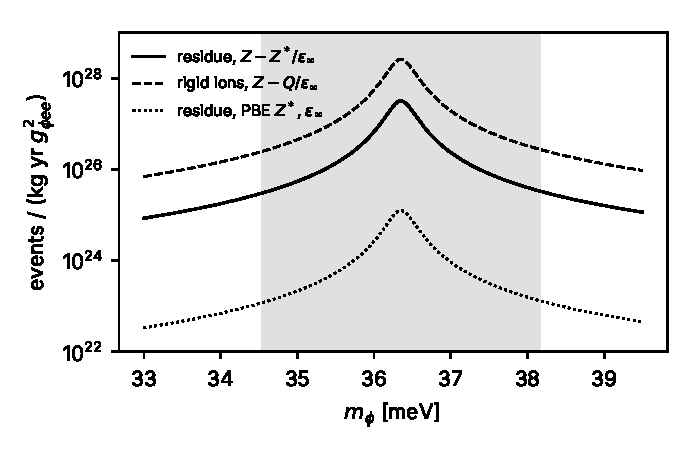
\includegraphics[width=0.8\linewidth]{figures/ch11/limit11_8a.pdf}
\captionof{figure}{Absorption of a scalar coupled to electrons in GaAs, events per kilogram-year and per $g_{\phi ee}^2$, against $m_\phi$, from \cref{eq:11.8-Rscalar}. Solid: site couplings $Z_\kappa - Z^*_\kappa/\varepsilon_\infty$ with $Z^* = 2.11$ and $\varepsilon_\infty = 10.88$ (\cref{we:5-lst}); a change of $Z^*/\varepsilon_\infty$ by $\pm\SI{1}{\percent}$ moves it by $\pm9\,\%$, less than the width of the line on this scale. Dotted: site couplings $Z_\kappa - Z^*_\kappa/\varepsilon_\infty$ with the PBE values $Z^* = 2.094$ and $\varepsilon_\infty = 13.70$ of \cref{sec:5.5}, 250 times lower. Loss function of one damped branch with $\omega_{\mathrm{T}} = 33.62$, $\omega_{\mathrm{L}} = \SI{36.35}{meV}$ and widths set to \SI{1}{\percent} of each frequency~\cite[Sect.~III\,A]{mitridate2024effective}; standard halo of \cref{sec:1.2}, $\langle v^2\rangle^{1/2} = \SI{379}{km/s}$, $\rho_T = \SI{5.361}{g.cm^{-3}}$. Gray: $|m_\phi - \omega_{\mathrm{L}}| < 5\gamma_{\mathrm{L}}$, where a line of constant width describes the phonon.}\label{fig:11-limit-8a}
\par}
\smallskip
Where the mass-weighted difference $d$ is small against each of its terms, the corrections that \cref{eq:11.8-G} drops are no longer small against the rate, and the formula fixes only its order of magnitude.
\end{limitbox}

\subsection{The near-cancellation in GaAs}\label{sec:11.8-gaas}

A scalar that couples to electrons through $g_{\phi ee}$ acts on the row $-g_{\phi ee}n_e$ (\cref{eq:8.1-scalar}), so that $g^\phi_{n_e} = -g_{\phi ee}$ and $g^\phi_{n_\kappa} = 0$, and by \cref{eq:11.8-G} each site contributes $Z_\kappa - Z^*_\kappa/\varepsilon_\infty$ electrons. GaAs is the obvious target, polar and well measured, and it turns out to be close to the worst case.

\begin{workedexample}{The electron-coupled scalar in GaAs}\label{we:11-gaas}
We take the inputs of \cref{sec:11.2}: $Z^* = 2.11$ from the splitting and the measured $\varepsilon_\infty = 10.88$, so that $Z^*/\varepsilon_\infty = 0.1939$, with $Z^*_{\mathrm{Ga}} = +Z^*$ and $Z^*_{\mathrm{As}} = -Z^*$; atomic numbers 31 and 33; mean atomic masses \SI{69.723}{u} and \SI{74.9216}{u}; $\mu_{\mathrm{red}} = \SI{36.11}{u}$.

\emph{Site couplings.} Gallium carries $31 - 0.1939 = 30.806$ electrons and arsenic $33 + 0.1939 = 33.194$, and each site couples with $-g_{\phi ee}$ times its count.

\emph{Mass-weighted difference.} Split \cref{eq:11.8-d} into its two parts. The nuclear charges per unit mass are $Z_{\mathrm{Ga}}/M_{\mathrm{Ga}} = 0.44462$ and $Z_{\mathrm{As}}/M_{\mathrm{As}} = 0.44046$ per u, and their difference is $+4.16\times10^{-3}$. The Born charges contribute $-(Z^*/\varepsilon_\infty)(1/M_{\mathrm{Ga}} + 1/M_{\mathrm{As}}) = -0.1939 \times 0.02769 = -5.37\times10^{-3}$. The sum is $d = -1.21\times10^{-3}$ per u, times $-g_{\phi ee}$. The two terms are 3.4 and 4.4 times larger than their sum.

\emph{Rate.} The bracket of \cref{eq:11.8-Rscalar} is $\varepsilon_\infty\mu_{\mathrm{red}}d/Z^* = 10.88 \times 36.11 \times 1.214\times10^{-3}/2.11 = 0.226$, and its square is $0.051$. An electron-coupled scalar is absorbed in GaAs at \SI{5}{\percent} of the rate of a photon-like scalar of the same coupling.

\emph{Sensitivity.} Since the Born-charge term is 4.4 times $|d|$, a fractional change of $Z^*/\varepsilon_\infty$ changes $d$ 4.4 times as much and the rate 8.8 times as much. The splitting route of \cref{sec:11.2-split} fixes $Z^*/\varepsilon_\infty$ to \SI{1.0}{\percent}, and these inputs limit the rate to \SI{9}{\percent}. Exact cancellation would need $Z^*/\varepsilon_\infty = 0.1501$. The values $Z^* = 2.16$ and $\varepsilon_\infty = 10.9$, also found in the literature, would give $d = -1.33\times10^{-3}$, a rate \SI{20}{\percent} higher.
\end{workedexample}

At the line center, with widths of \SI{1}{\percent}, three events in a kilogram-year need $g_{\phi ee} = 3.1\times10^{-14}$. III--V crystals, whose neighbors in the periodic table have nearly equal charge per mass, suppress the absorption of an electron-coupled scalar.

The kinetic energy of the core electrons, the isotopic masses and the frequency dependence of the electronic response are left out of \cref{eq:11.8-G}; each is small in absolute terms but not against $d$. The scalar density of an electron is its number density times $1 - v^2/2$ (\cref{eq:8.1-scalar}), and the core electrons that ride with a nucleus move fast. Their kinetic-energy row enters through the same factor $\ii\vect{p}_\phi\cdot\vect{u}_\kappa$ as their density, and it reduces the electrons each site carries by $\langle\mathcal{T}\rangle_\kappa/m_e$, the kinetic energy of those electrons over the electron mass. By the virial theorem this is the binding energy of the atom over $m_e$, tens of keV over \SI{511}{keV}, of order 0.1 for gallium and arsenic. As a parametric estimate, its mass-weighted difference between the two sites is $\Delta d \approx +1.2\times10^{-4}$ per u, a tenth of $d$ and of the opposite sign, so that it lowers $|d|$ by about \SI{10}{\percent} and the rate by about \SI{19}{\percent}. No calculation has included it yet, and \cref{sec:11.9} carries it as a nuisance. The masses enter at the same level: \SI{0.01}{u} on the mean mass of gallium moves $d$ by \SI{5}{\percent}, so an isotopically enriched crystal must use its own masses. The frequency dependence of the electronic response, of relative order $(\omega_{\mathrm{L}}/\Eg)^2 = 6\times10^{-4}$ (\cref{sec:11.2}), is amplified by 4.4 to \SI{0.3}{\percent} of $d$ and is negligible.

Density-functional perturbation theory delivers $Z^*$ robustly, to a percent, and $\varepsilon_\infty$ poorly. With the PBE values of \cref{sec:5.5}, $Z^* = 2.094$ and $\varepsilon_\infty = 13.70$, the ratio $Z^*/\varepsilon_\infty = 0.153$ lies within \SI{2}{\percent} of exact cancellation, $d = -7.6\times10^{-5}$ per u, and the rate falls by a factor of 250 (the dotted curve of \cref{lim:11.8a}). The test of the computed values against the measured splitting, \cref{eq:E.4-LOTO}, matters more here than any convergence parameter, and the measured splitting with \cref{eq:11.2-Zeps} is the safer input; the phonon widths come from three-phonon perturbation theory (\cref{sec:5.7}).

\subsection{Dark photons in GaAs and sapphire}\label{sec:11.8-dp}

For a dark photon the vertex is the screened Born charge, there is no cancellation, and the rate is the measured or computed loss function, $\mathcal{R} = (\rho_\chi/\rho_T)\zeta^2L(m_\phi)$ (\cref{eq:10.7-dp}). Two numbers characterize each line: its area, which is fixed by the band integral \cref{eq:11.8-Rint}, and its width, which is not. For GaAs, $\mathcal{I}_{\mathrm{pol}} = \SI{0.759}{meV}$ from the splitting (\cref{we:11-ipol}), and a Lorentzian of full width $\gamma_{\mathrm{L}}$ peaks at $L = 2\mathcal{I}_{\mathrm{pol}}/\pi\gamma_{\mathrm{L}}$. A width of \SI{1}{\percent} of the frequency leads to $L = 1.33$ at the center, ten times narrower gives 13.3, and the area stays at \SI{0.76}{meV}. The reach on the line center scales as $\gamma_{\mathrm{L}}^{1/2}$, while the reach averaged over a scan of masses depends only on the area.

\begin{figure}[tbp]
  \centering
  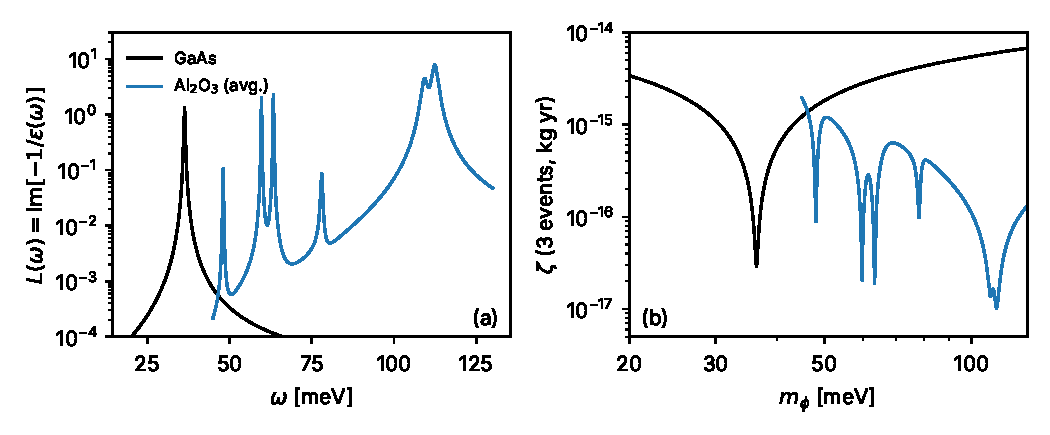
\includegraphics[width=\linewidth]{figures/ch11/fig11_8.pdf}
  \caption{Absorption of dark-photon dark matter on single optical phonons. (a) Loss function $L = \Imag[-1/\varepsilon(\omega)]$ at $q \to 0$ from the damped factorized dielectric function $\varepsilon_\infty\prod_\nu(\omega_{\mathrm{L}\nu}^2 - \omega^2 - \ii\omega\gamma_{\mathrm{L}\nu})/(\omega_{\mathrm{T}\nu}^2 - \omega^2 - \ii\omega\gamma_{\mathrm{T}\nu})$. GaAs (black): $\omega_{\mathrm{T}} = 33.62$, $\omega_{\mathrm{L}} = \SI{36.35}{meV}$, $\varepsilon_\infty = 10.88$, so that the line carries the splitting weight $(1 - \omega_{\mathrm{T}}^2/\omega_{\mathrm{L}}^2)/\varepsilon_\infty = 0.0133$ (\cref{sec:11.2}), with an assumed width of \SI{1}{\percent} of each frequency. Sapphire (blue): the frequencies and \SI{77}{K} widths of Ref.~\cite[Table~II]{griffin2018directional} for the ordinary and extraordinary rays, as listed in \cref{lim:10.7a}, and $\varepsilon_\infty = 3.2$; averaged over polarizations as $\frac23L_{\mathrm{o}} + \frac13L_{\mathrm{e}}$~\cite[Eq.~(40)]{griffin2018directional}; drawn above \SI{45}{meV}, since below the lowest transverse line the model gives $|L| < 10^{-4}$ of the wrong sign. (b) Kinetic mixing $\zeta$ for three events in one kilogram-year without background, $\mathcal{R} = (\rho_\chi/\rho_T)\zeta^2L(m_\phi)$, with $\rho_\chi = \SI{0.3}{GeV.cm^{-3}}$ and $\rho_T = 5.361$ and \SI{3.98}{g.cm^{-3}}. Single-phonon lines only: the multiphonon absorption between them and the electronic absorption above the gap are not included.}
  \label{fig:11-dpabs}
\end{figure}

\Cref{fig:11-dpabs} shows both crystals. GaAs has one line, and three events in a kilogram-year reach $\zeta = 2.9\times10^{-17}$ at its center. Sapphire has six polar branches between the two polarizations. The strongest is the collective top branch of the ordinary ray, at \SI{112.4}{meV}, which carries \SI{95}{\percent} of the ordinary weight (\cref{sec:11.2-band}). With its measured \SI{77}{K} width of \SI{2.0}{meV} it reaches $\zeta = 1.0\times10^{-17}$, and the lines at 59.7 and \SI{63.3}{meV} reach $2\times10^{-17}$. Per unit mass the band integral of sapphire is 64 times that of GaAs, $\SI{35.9}{meV}/\SI{3.98}{g.cm^{-3}}$ against $\SI{0.759}{meV}/\SI{5.361}{g.cm^{-3}}$; here \SI{35.9}{meV} is the polarization average $\frac23$ ordinary $+ \frac13$ extraordinary of the absorbed field, while the ordinary ray alone gives the \SI{36.3}{meV} of \cref{sec:11.2-band}. The widths are the weak input. Those of sapphire were measured at \SI{77}{K}, and at millikelvin temperatures the anharmonic part, the thermal part of \cref{eq:5.7-gamma}, shrinks while the spontaneous decay stays, so the lines should narrow by a factor of order one~\cite{griffin2018directional}. Between the lines the absorption is multiphonon, which the measured $\varepsilon$ contains and the factorized model does not, and it fills the gaps of \cref{fig:11-dpabs}b~\cite{knapen2018detection,griffin2018directional}.

\subsection{Acoustic modes of a finite body}\label{sec:11.8-bar}

The lowest thickness mode of a quartz plate \SI{1}{mm} thick rings at about \SI{3}{MHz}, an energy of \SI{12}{neV}. A dark photon of that mass has a de Broglie wavelength of order \SI{100}{km} and stays coherent for a fraction of a second, $t_{\mathrm{coh}} = 1/m_\phi v_0^2$, which is \SI{1.04}{ms} at \SI{1}{\micro eV} and scales as $1/m_\phi$. Even the wavelength of light at its frequency, $2\pi/m_\phi$, is \SI{100}{m}. Over the plate and over many periods the field is one classical wave, $\phi \propto \cos(m_\phi t)$, uniform in space. Crystal momentum no longer selects anything: a body small against the wavelength has no translation symmetry at that scale, and the role of $\vect{p}_\phi$ passes to the shape of the normal modes of the body. The acoustic modes, which could not absorb in an infinite crystal, now can, because a finite body has acoustic modes at nonzero frequency at zero wavevector of the field.

\emph{The field inside the body.} A dark photon at rest acts on charges as an electric field $\zeta\vect{E}'$, with $|\vect{E}'| = m_\phi|A'| = (2\rho_\chi)^{1/2}$ since $\rho_\chi = m_\phi^2|A'|^2/2$. In an infinite medium the induced polarization screens it to $\zeta\vect{E}'/\varepsilon$, the in-medium mixing of \cref{eq:8.4-zetaeff}. A body of size $L_{\mathrm{s}} \ll 2\pi/m_\phi$ is in the quasi-static regime, and its surface charges set the field instead. Take an ellipsoid with depolarization factor $N_{\mathrm{dp}}$ along the field. The induced polarization $(\varepsilon_0 - 1)\vect{E}_{\mathrm{in}}$ produces the depolarizing field $-N_{\mathrm{dp}}(\varepsilon_0 - 1)\vect{E}_{\mathrm{in}}$, so that $\vect{E}_{\mathrm{in}} = \zeta\vect{E}' - N_{\mathrm{dp}}(\varepsilon_0 - 1)\vect{E}_{\mathrm{in}}$, or
\begin{equation}
  \vect{E}_{\mathrm{in}} = \frac{\zeta\vect{E}'}{1 + N_{\mathrm{dp}}(\varepsilon_0 - 1)} = f_{\mathrm{sh}}\,\frac{\zeta\vect{E}'}{\varepsilon_0} ,
  \qquad f_{\mathrm{sh}} = 1,\ \ \frac{3\varepsilon_0}{\varepsilon_0 + 2},\ \ \varepsilon_0 ,
  \label{eq:11.8-shape}
\end{equation}
for a field normal to a slab ($N_{\mathrm{dp}} = 1$), in a sphere ($N_{\mathrm{dp}} = 1/3$) and parallel to a slab ($N_{\mathrm{dp}} = 0$). The static constant $\varepsilon_0$ appears because MHz frequencies lie far below the optical phonons. The slab with the field along its normal coincides with the bulk, and a field along a thin plate is not screened at all. A conducting shield of size $R_{\mathrm{s}}$ around the experiment suppresses the field further by $\min\{1, (m_\phi R_{\mathrm{s}})^2\}$~\cite[Eq.~(5)]{trickle2025piezoelectric}.

\emph{The coupling.} In a piezoelectric crystal a strain $S_{\beta\gamma}$ polarizes the cell, $P_\alpha = \sum_{\beta\gamma}e^{\mathrm{pz}}_{\alpha\beta\gamma}S_{\beta\gamma}$ (\cref{sec:6.2}), and the field couples through $\delta H = -\int\dd^3x\,\vect{E}_{\mathrm{in}}\cdot\vect{P}$. We take a plate cut so that its axis $z$ carries the dominant element, $e^{\mathrm{pz}} \equiv e^{\mathrm{pz}}_{zzz}$, and a field component $E_{\mathrm{in}}\cos\theta$ along $z$, with $\theta$ the angle between the polarization of the dark photon and the axis. Then $\delta H = -E_{\mathrm{in}}\cos\theta\,\cos(m_\phi t)\,e^{\mathrm{pz}}\int\dd^3x\,\partial_zu_z$.

\emph{The modes.} The displacement of the body is $\vect{u}(\vect{x}) = \sum_n\vect{U}_n(\vect{x})(b_n + b_n^\dagger)$, with the mode functions normalized as $\int\dd^3x\,\rho_T\,\vect{U}_n\cdot\vect{U}_{n'} = \delta_{nn'}/2\omega_n$, the finite-body form of \cref{eq:5.3-u}. A plano-convex plate of central thickness $L_0$ traps its thickness modes near the axis. Across it they have a Gaussian profile of radius $r_n$~\cite[Eqs.~(2), (3)]{trickle2025piezoelectric},
\begin{equation*}
  \vect{U}_n = \frac{\hat{\vect{z}}}{\sqrt{M_n\omega_n}}\,\cos\frac{n\pi z}{L_0}\,\exp\Bigl(-\frac{x^2 + y^2}{2r_n^2}\Bigr) ,
  \qquad M_n = \rho_T\pi r_n^2L_0 ,
  \qquad \omega_n = \frac{n\pi c_{\mathrm{L}}}{L_0} ,
\end{equation*}
which satisfies the normalization, since the cosine squared averages to one half and the Gaussian squared integrates to $\pi r_n^2$; $M_n$ is the mass of the mode and $c_{\mathrm{L}}$ the longitudinal sound speed of the plate. The polarization integral is
\begin{equation*}
  \int\dd^3x\,\partial_zU_{n,z} = \frac{\cos n\pi - 1}{\sqrt{M_n\omega_n}}\int\dd x\,\dd y\,\ee^{-(x^2 + y^2)/2r_n^2} = -\frac{4\pi r_n^2}{\sqrt{M_n\omega_n}} ,
\end{equation*}
for odd $n$, and zero for even $n$, whose two faces move together and leave no net polarization.

\emph{The power.} Write $\cos(m_\phi t) = (\ee^{-\ii m_\phi t} + \ee^{\ii m_\phi t})/2$ and keep the part $\delta H_0\,\ee^{-\ii m_\phi t}$ that absorbs. With $E_0 = f_{\mathrm{sh}}\zeta(2\rho_\chi)^{1/2}/\varepsilon_0$ the amplitude of $E_{\mathrm{in}}$ and $\pi r_n^2 = M_n/\rho_TL_0$,
\begin{equation*}
  |\langle n|\delta H_0|0\rangle|^2 = \Bigl(\frac{E_0\cos\theta\,e^{\mathrm{pz}}}{2}\Bigr)^2\frac{16\pi^2r_n^4}{M_n\omega_n}
  = \frac{8f_{\mathrm{sh}}^2\zeta^2\rho_\chi(e^{\mathrm{pz}})^2M_n\cos^2\theta}{\varepsilon_0^2\rho_T^2L_0^2\,\omega_n} .
\end{equation*}
The golden rule gives the absorbed power $m_\phi \cdot 2\pi|\langle n|\delta H_0|0\rangle|^2\delta(m_\phi - \omega_n)$. A mode of full width $\gamma_n$ replaces the delta function by the line $(2\omega_n^2\gamma_n/\pi)/[(m_\phi^2 - \omega_n^2)^2 + \omega_n^2\gamma_n^2]$, which near resonance is the normalized Lorentzian, and
\begin{equation}
  P_n = 32\,f_{\mathrm{sh}}^2\zeta^2\,\frac{\rho_\chi}{\rho_T^2}\,\frac{(e^{\mathrm{pz}})^2}{\varepsilon_0^2}\,\frac{M_n}{L_0^2}\;
  \frac{m_\phi\,\omega_n\,\gamma_n\cos^2\theta}{(m_\phi^2 - \omega_n^2)^2 + \omega_n^2\gamma_n^2} .
  \label{eq:11.8-Pn}
\end{equation}
The prefactor $32 = 2\pi \times 8 \times 2/\pi$ collects the golden rule, the squared matrix element and the line. On resonance $P_n$ is proportional to $1/\gamma_n = \mathfrak{Q}/\omega_n$, with $\mathfrak{Q}$ the quality factor of the line. The power grows with the mass of the mode and falls as $1/L_0^2$, since a thinner plate turns the same displacement into more strain.

\emph{The field's own width.} The halo field is not monochromatic. Its energies are spread over $\omega = m_\phi(1 + v^2/2)$, with the distribution $F_\phi(\omega)\,\dd\omega = f_{\mathrm{sp}}(v)\,\dd v$ inherited from the speed distribution $f_{\mathrm{sp}}$. A record long compared with $\min(t_{\mathrm{coh}}, 1/\gamma_n)$ absorbs the mean power of the spread field (\cref{sec:8.2-absorption}). That is \cref{eq:11.8-Pn} averaged over $F_\phi$, with $\gamma_n = \omega_n/\mathfrak{Q}_{\mathrm{p}}$ the width of the mode alone. On resonance this is \cref{eq:11.8-Pn} with $\mathfrak{Q}$ replaced by
\begin{equation}
  \mathfrak{Q}_{\mathrm{eff}} = \omega_n\int\dd\omega\,F_\phi(\omega)\,\frac{\omega\,\omega_n\gamma_n}{(\omega^2 - \omega_n^2)^2 + \omega_n^2\gamma_n^2} .
  \label{eq:11.8-Qeff}
\end{equation}
A broad mode, $\mathfrak{Q}_{\mathrm{p}}$ small, sees the field as a single line and $\mathfrak{Q}_{\mathrm{eff}} = \mathfrak{Q}_{\mathrm{p}}$. A narrow mode sees the field's spread instead: its line integrates to $\pi/2$ times a delta function, and
\begin{equation}
  \mathfrak{Q}_{\mathrm{eff}} \to \mathfrak{Q}_{\mathrm{DM}} = \frac{\pi}{2}\,\omega_nF_\phi(\omega_n) = \frac{\pi}{2}\,\Bigl|\frac{\dd\eta}{\dd v}\Bigr| ,
  \qquad v = \Bigl(\frac{2(\omega_n - m_\phi)}{m_\phi}\Bigr)^{1/2} ,
  \label{eq:11.8-QDM}
\end{equation}
where the second form uses $F_\phi = f_{\mathrm{sp}}/(m_\phi v)$ and $\eta(\vmin) = \int_{\vmin}\dd v\,f_{\mathrm{sp}}(v)/v$ (\cref{eq:1.3-eta}). For the standard halo of \cref{sec:1.2} it peaks at $\mathfrak{Q}_{\mathrm{DM}} = 1.34\times10^6$, for a mode tuned to $v = \SI{256}{km/s}$, that is $\omega_n = m_\phi(1 + 3.6\times10^{-7})$; through $\eta$ it follows the annual modulation of the Earth's velocity. Trickle writes the signal with $\min\{\mathfrak{Q}_{\mathrm{p}}, \mathfrak{Q}_{\mathrm{DM}}\}$ and estimates $\mathfrak{Q}_{\mathrm{DM}} \sim 10^6$~\cite[text after Eq.~(7)]{trickle2025piezoelectric}, which \cref{eq:11.8-QDM} makes precise.

\begin{limitbox}[Bulk acoustic resonator][lim:11.8b]
A plano-convex piezoelectric resonator absorbs from a dark-photon field the power \cref{eq:11.8-Pn}, $P_n = 32\zeta^2(\rho_\chi/\rho_T^2)[(e^{\mathrm{pz}})^2/\varepsilon_0^2](M_n/L_0^2)\cos^2\theta\,\mathfrak{Q}_{\mathrm{s}}/m_\phi$ on resonance, with $\mathfrak{Q}_{\mathrm{s}} = \min\{\mathfrak{Q}_{\mathrm{p}}, \mathfrak{Q}_{\mathrm{DM}}\}$~\cite[Eqs.~(5), (7), (8)]{trickle2025piezoelectric}, for $f_{\mathrm{sh}} = 1$.
\par\smallskip
{\centering
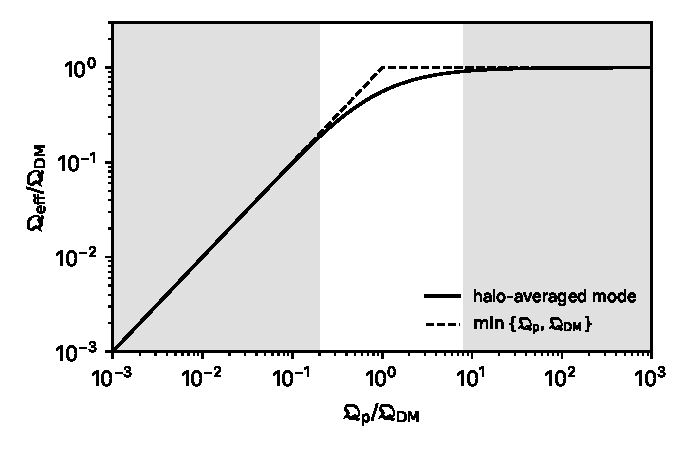
\includegraphics[width=0.8\linewidth]{figures/ch11/limit11_8b.pdf}
\captionof{figure}{Effective quality factor of a resonator mode in the halo field, \cref{eq:11.8-Qeff}, in units of $\mathfrak{Q}_{\mathrm{DM}} = 1.34\times10^6$, against the quality factor of the mode, $\mathfrak{Q}_{\mathrm{p}}/\mathfrak{Q}_{\mathrm{DM}}$, with the mode tuned to the frequency that maximizes it. Solid: \cref{eq:11.8-Qeff} with $F_\phi$ from the speed distribution of the standard halo of \cref{sec:1.2}; dashed: $\min\{\mathfrak{Q}_{\mathrm{p}}, \mathfrak{Q}_{\mathrm{DM}}\}$. Gray: $\mathfrak{Q}_{\mathrm{p}}/\mathfrak{Q}_{\mathrm{DM}} < 0.2$ and $> 7.9$, where the two agree within \SI{10}{\percent}. At $\mathfrak{Q}_{\mathrm{p}} = \mathfrak{Q}_{\mathrm{DM}}$ the prescription is 1.8 times too high.}\label{fig:11-limit-8b}
\par}
\smallskip
Where the widths of the mode and of the field are comparable, the signal is their convolution and neither width alone sets it; for records shorter than the coherence time the mean power is not a rate at all.
\end{limitbox}

The inputs that \cref{eq:11.8-Pn} needs are material and geometric. The elastic and piezoelectric tensors come from density-functional perturbation theory, and the shapes and frequencies of the modes of the actual body from finite elements. Add the shape factor $f_{\mathrm{sh}}$ of \cref{eq:11.8-shape} and the measured quality factor of the mode, which for acoustic resonators of this kind lies between $10^6$ and $10^{10}$~\cite{trickle2025piezoelectric}. A mode with $\mathfrak{Q}_{\mathrm{p}}$ above $10^7$ is in the narrow regime, where the signal is set by the field, not by the resonator. Its ring-down time, $\mathfrak{Q}_{\mathrm{p}}/\omega_n$, then exceeds the coherence time of the field, and the mean power of \cref{eq:11.8-Qeff} is reached only after many coherence times. How the signal builds up over shorter records, and how it fluctuates, is the coherent regime of \cref{sec:14.6}.

\subsection{Resonant-mass detectors}\label{sec:11.8-mass}

At masses of a peV to a neV the scalar of \cref{sec:11.8-gaas} does something else. Its coupling $g_{\phi ee}\phi\bar\psi\psi$ adds $-g_{\phi ee}\phi$ to the electron mass, and with $\phi = \phi_0\cos(m_\phi t)$, $\phi_0 = (2\rho_\chi)^{1/2}/m_\phi$, the electron mass oscillates, $\delta m_e/m_e = -g_{\phi ee}\phi/m_e$. A scalar coupled to $F_{\mu\nu}F^{\mu\nu}$ makes the fine-structure constant oscillate in the same way. Arvanitaki, Dimopoulos and Van Tilburg write both with dimensionless couplings normalized to the strength of gravity~\cite[Eqs.~(1), (3), (4)]{arvanitaki2016sound}. Such a field changes the size of every atom. The Coulomb Hamiltonian of electrons and clamped nuclei, \cref{eq:2.3-HC} with $M_\kappa \to \infty$, contains $\alpha$ and $m_e$ only through the Bohr radius $a_0 = 1/(\alpha m_e)$, which sets every length, and $\alpha^2m_e$, which sets every energy. The lattice constant is a fixed number of Bohr radii, and
\begin{equation}
  h_{\mathrm{mod}} \equiv \frac{\delta a}{a} = -\frac{\delta\alpha}{\alpha} - \frac{\delta m_e}{m_e} .
  \label{eq:11.8-h}
\end{equation}
The scaling fails only through physics that the Coulomb Hamiltonian leaves out. Relativistic corrections are of relative order $(Z\alpha)^2$ for the inner electrons. They add to $\dd\ln a/\dd\ln\alpha$ a term that fully relativistic calculations put at $-1.97\times10^{-2}$ for copper and $-2.2\times10^{-4}$ for silicon; the finite nuclear mass adds a dependence on the proton-to-electron mass ratio, $-1.12\times10^{-3}$ per unit fractional change for copper and $-0.86\times10^{-3}$ for silicon~\cite[Table~II]{pasteka2019material}. For a light crystal \cref{eq:11.8-h} holds to about $10^{-3}$.

A resonant-mass detector reads out such a change. It is a massive elastic body, a cylindrical bar or a sphere, of low internal loss, whose lowest mode is watched by a transducer at its own frequency. The detectors were built for gravitational waves, and the cryogenic ton-scale aluminum bars of the last generation ring near \SI{900}{Hz}~\cite{arvanitaki2016sound}, an energy of \SI{3.7}{peV}.

Why should an oscillating size excite a mode at all? A static change of $a$ excites nothing. The body simply takes its new equilibrium shape, with every material point $\vect{\xi}$ moved to $(1 + h_{\mathrm{mod}})\vect{\xi}$, and there is no wave. Write the displacement in the laboratory as $\vect{u}_{\mathrm{lab}} = \vect{u} + h_{\mathrm{mod}}(t)\,\vect{\xi}$, with $\vect{u}$ the displacement from the instantaneous equilibrium. The elastic stress responds to the strain relative to that equilibrium, $\sigma = C : (\nabla\vect{u}_{\mathrm{lab}} - h_{\mathrm{mod}}\mathbb{1}) = C : \nabla\vect{u}$, for a uniform $h_{\mathrm{mod}}$ in a cubic or isotropic body, with $C$ the elastic tensor. Newton's law holds in the laboratory, $\rho_T\ddot{\vect{u}}_{\mathrm{lab}} = \nabla\cdot\sigma$, and
\begin{equation}
  \rho_T\,\ddot{\vect{u}} = \nabla\cdot(C : \nabla\vect{u}) - \rho_T\,\ddot h_{\mathrm{mod}}\,\vect{\xi} .
  \label{eq:11.8-drive}
\end{equation}
The scalar acts as a body force $-\rho_T\ddot h_{\mathrm{mod}}\vect{\xi}$, the inertial force of the moving equilibrium. It is proportional to $\omega^2h_{\mathrm{mod}}$: the stiffness of the body never enters, and a slow modulation is followed adiabatically. Projected on a mode $\vect{u}_n$ of the body, the force is $F_n = -\ddot h_{\mathrm{mod}}\int\dd^3\xi\,\rho_T\,\vect{\xi}\cdot\vect{u}_n$. For a sphere of radius $R_{\mathrm{sph}}$ and mass $M_{\mathrm{sph}}$ only the radial modes $\vect{u}_n = \hat{\vect{r}}u_n(r)$ couple, and $F_n = -\ddot h_{\mathrm{mod}}M_{\mathrm{sph}}R_{\mathrm{sph}}J_n$ with $J_n = 3R_{\mathrm{sph}}^{-4}\int_0^{R_{\mathrm{sph}}}\dd r\,r^3u_n(r)$, which Arvanitaki and collaborators obtain by treating the modulus as a scalar gravitational wave with the curvature $\delta_{ij}\ddot h$~\cite[Eqs.~(7), (8)]{arvanitaki2016sound}.

A thin bar of length $L_{\mathrm{b}}$ and sound speed $c_{\mathrm{b}}$, free at both ends, shows the whole response in closed form. Along the bar, \cref{eq:11.8-drive} with $h_{\mathrm{mod}}\ee^{-\ii\omega t}$ has the solution $u_{\mathrm{lab}} = h_{\mathrm{mod}}\sin(k\xi)/[k\cos(kL_{\mathrm{b}}/2)]$, $k = \omega/c_{\mathrm{b}}$, which satisfies the free-end condition $\partial_\xi u_{\mathrm{lab}} = h_{\mathrm{mod}}$ at $\xi = \pm L_{\mathrm{b}}/2$. Measured from the instantaneous equilibrium, the end moves by
\begin{equation}
  u(L_{\mathrm{b}}/2) = \frac{h_{\mathrm{mod}}L_{\mathrm{b}}}{2}\Bigl(\frac{\tan x}{x} - 1\Bigr) , \qquad x = \frac{\omega L_{\mathrm{b}}}{2c_{\mathrm{b}}} = \frac{\pi}{2}\,\frac{\omega}{\omega_1} ,
  \label{eq:11.8-bar}
\end{equation}
with $\omega_1 = \pi c_{\mathrm{b}}/L_{\mathrm{b}}$ the lowest mode that couples. Below it, $\tan x/x - 1 \simeq x^2/3$, and the response is $(\pi^2/24)\,h_{\mathrm{mod}}L_{\mathrm{b}}(\omega/\omega_1)^2$, the $\omega^2$ of the drive. At each odd mode it resonates. Far above, the end stays where it was in the laboratory while the equilibrium moves, and the relative displacement tends to $-h_{\mathrm{mod}}L_{\mathrm{b}}/2$. The lowest mode alone, $u_1 = \sin(\pi\xi/L_{\mathrm{b}})$ with mass $M_{\mathrm{b}}/2$ and force $2\omega^2h_{\mathrm{mod}}M_{\mathrm{b}}L_{\mathrm{b}}/\pi^2$, gives $(4/\pi^2)h_{\mathrm{mod}}L_{\mathrm{b}}(\omega/\omega_1)^2/(1 - \omega^2/\omega_1^2)$; its low-frequency coefficient, $4/\pi^2 = 0.405$, falls short of $\pi^2/24 = 0.411$ by the higher odd modes, whose shares $4/\pi^2n^4$ sum to the difference.

\begin{limitbox}[Resonant-mass drive of a scalar][lim:11.8c]
A scalar that changes $\alpha$ or $m_e$ strains a body by $h_{\mathrm{mod}} = -\delta\alpha/\alpha - \delta m_e/m_e$ and drives its modes with the force $F_n = -\ddot h_{\mathrm{mod}}M_{\mathrm{sph}}R_{\mathrm{sph}}J_n$, proportional to $\omega^2$~\cite[Eqs.~(6)--(8)]{arvanitaki2016sound}.
\par\smallskip
{\centering
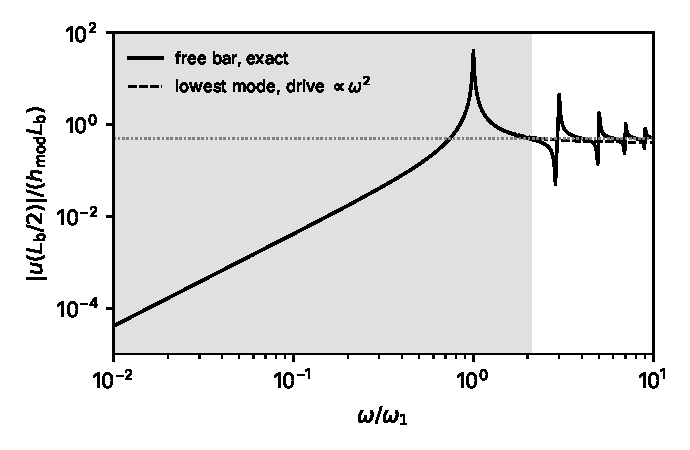
\includegraphics[width=0.8\linewidth]{figures/ch11/limit11_8c.pdf}
\captionof{figure}{Displacement of the end of a free bar from its instantaneous equilibrium, in units of $h_{\mathrm{mod}}L_{\mathrm{b}}$, against $\omega/\omega_1$. Solid: the exact response \cref{eq:11.8-bar}; dashed: the lowest mode alone with the $\omega^2$ drive. Every mode has the width $\omega_n/\mathfrak{Q}$ with $\mathfrak{Q} = 100$ for visibility (resonant-mass detectors reach $10^6$ to $10^7$). Dotted: the high-frequency limit $1/2$. Gray: $\omega < 2.1\,\omega_1$, where the lowest mode is within \SI{10}{\percent} of the exact response. The field is uniform over the bar while $m_\phi vL_{\mathrm{b}} \ll 1$. With $v = 10^{-3}$ and $c_{\mathrm{b}} = \SI{5}{km/s}$ this holds up to $\omega \approx 2\times10^7\omega_1$, far off scale.}\label{fig:11-limit-8c}
\par}
\smallskip
Above the lowest mode the higher modes and their antiresonances take over, and the response approaches the rigid limit, in which the body no longer follows its equilibrium.
\end{limitbox}

\section{Uncertainty budget of the lattice rates}\label{sec:11.9}

A dark-matter particle of \SI{30}{MeV} with a heavy mediator and $\sigma_p = 10^{-40}\,\mathrm{cm^2}$ makes $5.26\times10^3$ events per kilogram-year in silicon above a threshold of \SI{100}{meV}. The number assumes a harmonic crystal, nuclei that scatter independently and the phonons of the PBE force constants of \cref{sec:5.2}. The free nuclear recoil of the standard rate gives $4.91\times10^3$ for the same threshold, and above \SI{400}{meV} it gives a sixteenth of the crystal rate. That difference is the error of the simpler calculation: the crystal response is the better one, and the free recoil is its limit at large $x_R$ (\cref{sec:11.4}). The uncertainty is how far the crystal number moves when the truncations of this chapter are lifted, and \cref{tab:11-nuisances} lists these steps in the classes and bases of \cref{tab:10-nuisances}. A next order computed with the force constants of \cref{sec:5.2} or with measured inputs is marked ``computed'', and its central value has already moved.

The exact $\omega$-integrated weight of \cref{eq:11.3-weight} moves the central value of each phonon order; what remains is the distribution of the coherent weight in $\omega$ inside each band, which \cref{eq:11.3-band} bounds at every point but does not fix. The residual is a tilt within each band, and it matters for a threshold inside a band at momentum transfers below a few $q_{\mathrm{BZ}}$. Above the impulse onset the zeroth and first moments of the recoil spectrum are exact on any energy surface, and the anharmonic template is the constrained tilt \cref{eq:8.8-tilt}, which keeps them. For soft-mode and light-atom crystals, and for solid helium near melting, neither a computed next order nor a small parameter exists, and the Markov--Krein band of \cref{eq:C.10-band} is the only available statement (\cref{lim:11.5c}): a range without a central value, whose edges a likelihood uses.

The phonons themselves are an input, not a truncation of the label, and their error plays the part of the spread between tabulations in \cref{sec:10.10}. Of the eight measured frequencies of silicon at $\mathrm{\Gamma}$, X and L, the PBE force constants of \cref{sec:5.2} miss by \SI{2.6}{\percent} on average and the zone-center optical mode by \SI{0.6}{\percent}. We take as template a uniform rescaling of all phonon frequencies by \SI{2.6}{\percent}. It moves the Poisson weights through $2W_\kappa \propto \langle\omega^{-1}\rangle$ and the impulse width through $\langle\omega\rangle^{1/2}$ together, and since the deviations of single modes have both signs, it is an upper template. The measured elastic tensors that fix the acoustic plateau and edge of \cref{sec:11.1} are room-temperature values, and the change on cooling has not been sized.

\begin{table}[tbp]
  \caption{Uncertainty budget of the lattice rates. Classes and bases as in \cref{tab:10-nuisances}. Sizes are for silicon unless another crystal is named; \cref{we:11-band30} is the silicon rate at \SI{30}{MeV} above \SI{100}{meV}, and $d$ the site difference of \cref{we:11-gaas}. Items without a row: the optical-phonon shift of \SI{0.15}{meV} (\cref{tab:8-nuisances}), the quantum-crystal and germanium-spectrum models (\cref{sec:11.4,sec:11.5}), the absorption line widths and resonator prescription (\cref{sec:11.8}), and the nuclear spin inputs.}
  \label{tab:11-nuisances}
  \centering\footnotesize\setlength{\tabcolsep}{3pt}
  \begin{tabular}{@{}>{\raggedright\arraybackslash}p{0.25\linewidth}>{\raggedright\arraybackslash}p{0.12\linewidth}>{\raggedright\arraybackslash}p{0.38\linewidth}>{\raggedright\arraybackslash}p{0.09\linewidth}>{\raggedright\arraybackslash}p{0.10\linewidth}@{}}
    \toprule
    Truncation or input & Type & Size & Basis & Section \\
    \midrule
    Pairs of nuclei dropped (incoherent approximation) & normali\-zation per order & within \SI{10}{\percent} above \SI{6.6}{keV} ($n = 2, 3$); \cref{we:11-band30}: $+2.6\times10^{-4}$ & computed & \cref{sec:11.3} \\
    Coherent weight inside a band & tilt & up to $2.7\times$ incoherent at \SI{10}{keV} & bound & \cref{sec:11.3} \\
    Phonon frequencies (PBE) & tilt & \SI{2.6}{\percent} mean, uniform rescale (upper estimate); \cref{we:11-band30}: $+0.24\,\%$ ($+3.1\,\%$ above \SI{400}{meV}) & spread & \cref{sec:5.2} \\
    Anharmonic recoil width, skewness ($n_A = 2$) & tilt (con\-strained) & kinetic energy within $\pm0.2\,\%$; third cumulant $\sim\eta_{\mathrm{anh}}^2$ & model; est. & \cref{sec:11.5} \\
    Anharmonic few-phonon weights ($n_A = 2$) & tilt in $q$ & $n = 2$: $+\SI{50}{\percent}$, $n = 4$: $27\times$ at $q_{\mathrm{BZ}}$; harmonic to \SI{10}{\percent} above 5, 12, \SI{20}{keV} & model & \cref{sec:11.5} \\
    Strong anharmonicity (soft modes, light atoms, helium) & any & Markov--Krein band; Si, \SI{100}{keV}: 0.19 to 0.86 at $E_R$ & bound & \cref{sec:11.5} \\
    Thermal diffuse scattering ($n_T = 2$) & new support & $\propto T^2$; $10^{-9}$ of room temperature at \SI{10}{mK} & model & \cref{sec:11.3} \\
    Charge vertex above the zone & tilt in $q$ & unknown at 3--\SI{20}{keV}; nucleon coupling unaffected & named & \cref{sec:11.3} \\
    Free recoil for the crystal (evaluation error) & tilt & \SI{10}{\percent} from $x_R = 2.3$ (\SI{1}{GeV}); \cref{we:11-band30}: $-6.8\,\%$, $\times0.062$ above \SI{400}{meV} & computed & \cref{sec:11.4} \\
    Sound speeds & normali\-zation; threshold & computed against measured tensors & spread & \cref{sec:17.5} \\
    $Z^*/\varepsilon_\infty$, polar rates & normali\-zation & splitting route: rate \SI{2}{\percent}; semilocal $\varepsilon_\infty$: $-37\,\%$ & spread & \cref{sec:11.2} \\
    Charge of acoustic waves & new support & at most \SI{3}{\percent} near the edge, \SI{1}{\percent} at \SI{100}{keV} (GaAs); quadrupoles not computed & est. & \cref{sec:11.2} \\
    $Z^*/\varepsilon_\infty$, GaAs scalar absorption & normali\-zation & \SI{1}{\percent} gives \SI{9}{\percent}; PBE inputs: $/250$ & spread & \cref{sec:11.8} \\
    Core kinetic energy; mean masses (GaAs scalar) & normali\-zation & $\Delta d \approx -0.1\,d$, rate $-\SI{19}{\percent}$ (parametric); \SI{0.01}{u}: \SI{5}{\percent} of $d$ & est. & \cref{sec:11.8} \\
    Single-isotope density of states & normali\-zation & $+\SI{8.0}{\percent}$ at \SI{50}{meV} & computed & \cref{sec:11.6} \\
    Cold in-band absorption of silicon & normali\-zation & $\varGamma_{\mathrm{iso}}/\varGamma_{\mathrm{EM}} \ge 5.0\times10^3$; warm datum \SI{10}{\percent} & bound & \cref{sec:11.6} \\
    Electronic cubic harmonics & tilt in time & Si $A_{\mathrm{day}} = \SI{0.9}{\percent}$ without local fields & model & \cref{sec:11.7} \\
    \bottomrule
  \end{tabular}
\end{table}

A truncation that two rates share carries one parameter in both (\cref{sec:8.8}). The phonon frequencies of one set of force constants enter the one-phonon, multiphonon and impulse rates of that crystal together, at every mass and threshold, and a fit that gave each its own $\vartheta$ would let the data trade them. The measured elastic tensor of \cref{sec:11.1} is a different input, and an acoustic rate built from it shares no parameter with the multiphonon rate built from computed phonons. The ratio $Z^*/\varepsilon_\infty$ of a polar crystal is one input of its dark-photon scattering rate, its dark-photon absorption and its electron-scalar absorption, and one $\vartheta$ moves all three, by different factors. The halo stays fixed, as in \cref{eq:8.8-like}, and the detector uncertainties belong to \cref{sec:21.4}.

\begin{workedexample}{The uncertainty band of the silicon multiphonon rate at \SI{30}{MeV}}\label{we:11-band30}
Take $\mchi = \SI{30}{MeV}$, a heavy mediator, equal couplings to protons and neutrons with $\sigma_p = 10^{-40}\,\mathrm{cm^2}$, and the standard halo of \cref{sec:1.2} with $\rho_\chi = \SI{0.3}{GeV.cm^{-3}}$. The threshold $\omega_{\mathrm{th}} = \SI{100}{meV}$ and the cross-section $\sigma_p$ are illustrative choices; the threshold lies above the one-phonon band, so that every event counted contains at least two phonons. The largest momentum transfer is $2\mchi v_{\mathrm{max}} = \SI{159}{keV}$, where $E_R = \SI{0.48}{eV}$ and $x_R = 11.8$. The central value is \cref{eq:8.2-spectrum} with one row and the incoherent harmonic response of all orders at $T = 0$, from the PBE density of states of \cref{sec:5.2}, the Helm form factor, and the velocity integral done for an orientation-averaged crystal:
\begin{equation*}
  \mathcal{R}^{\mathfrak{T}} = \SI{5.26e3}{kg^{-1}.yr^{-1}} ,
\end{equation*}
with $\mathcal{R}^{\mathfrak{T}}$ the rate at the central values of the truncation labels (\cref{sec:10.10}), or 14 events per kilogram and day. Half of it comes from momentum transfers below \SI{80}{keV}, where $x_R = 3.0$, and \SI{80}{\percent} from between 54 and \SI{109}{keV}, $x_R$ from 1.4 to 5.6: the rate spans the impulse onset.

The computed coherent step multiplies each phonon order by $1 + \delta^{\mathrm{coh}}_n(q)$ from \cref{eq:11.3-weight}. Between 30 and \SI{159}{keV}, $|\delta^{\mathrm{coh}}_2|$ stays below 0.021 and $|\delta^{\mathrm{coh}}_8|$ below $1.5\times10^{-4}$, and the rate rises by $2.6\times10^{-4}$, which leaves $5.26\times10^3$ unchanged at three digits. The remaining uncertainties enter the power form \cref{eq:8.8-M} through $\ln(1 + \delta_k)$:
\begin{equation*}
  \begin{aligned}
  &\text{phonon frequencies, } +\SI{2.6}{\percent}: & \ln(1 + \delta) &= +2.4\times10^{-3}, \\
  &\text{anharmonic kinetic energy, } -\SI{0.14}{\percent}\ (\lambda_3 = 0.01, & &-8\times10^{-5}, \\
  &\qquad\lambda_4 = 2.5\times10^{-4}): & & \\
  &\text{anharmonic third cumulant (est.)}: & &+5\times10^{-5}.
  \end{aligned}
\end{equation*}
The kinetic-energy template is a dilation of each spectrum about $E_R$ by $(1 + \delta E^{\mathrm{kin}}/E^{\mathrm{kin}})^{1/2}$, which keeps the area and the mean and changes the second moment by the computed amount; the rate changes by 0.12 times the relative change of the width, and the extreme $-\SI{0.2}{\percent}$ of the range of \cref{sec:11.5} would give $-1.2\times10^{-4}$. For the third cumulant, the whole difference between the incoherent spectrum and a Gaussian of the same mean and variance changes the rate by \SI{1.9}{\percent}, and the anharmonic change of the cumulants is of relative order $\eta_{\mathrm{anh}}^2$. The anharmonic few-phonon weights barely enter: below \SI{20}{keV}, where they are large, $E_R$ is under \SI{8}{meV}, and those momentum transfers carry $3\times10^{-4}$ of the rate. With independent standard-normal $\vartheta_k$ the widths add in quadrature, \cref{eq:C.14-quadrature},
\begin{equation*}
  \sigma_{\ln\mathcal{R}} = \bigl[(2.4\times10^{-3})^2 + (8\times10^{-5})^2 + (5\times10^{-5})^2\bigr]^{1/2} = 2.4\times10^{-3} ,
\end{equation*}
and the rate lies between $5.25\times10^3$ and $5.27\times10^3$ per kilogram-year at one standard deviation, a factor of 1.0024 either way. The phonon frequencies carry all of it.

The free recoil gives $4.91\times10^3$, \SI{6.8}{\percent} lower, 29 band widths away. With the threshold raised to \SI{400}{meV}, near the endpoint \SI{0.48}{eV}, the crystal rate falls to \SI{110}{kg^{-1}.yr^{-1}}, half of it from momentum transfers below \SI{118}{keV}, $x_R = 6.5$. The free recoil gives 6.8, a sixteenth of it, because above \SI{400}{meV} most events come from the Doppler tail of the recoil spectrum, which the free nucleus does not have. The rate now samples the width of that spectrum, the dilation coefficient grows from 0.12 to 2.2, and the frequency template becomes $+\SI{3.1}{\percent}$; the band is a factor of 1.031. The anharmonic kinetic energy gives $-1.5\times10^{-3}$, still a twentieth of it.

Without perturbation theory the same rate would be far less certain. At \SI{80.4}{keV}, the median momentum transfer of the rate above \SI{100}{meV}, the five exact moments of the response allow any weight above threshold between 0.19 and 0.95 by the Markov--Krein band, against the harmonic 0.58.
\end{workedexample}

\section*{Summary}

A nucleon-coupled particle too light to give a nucleus a free recoil above threshold excites phonons, because the whole crystal takes up the momentum (\cref{sec:11.1}). At momentum transfers well inside the zone the one-phonon response per unit mass depends on the material only through the sound speeds and polarizations of the acoustic branches. The acoustic edge, set by the fastest longitudinal sound speed, \SI{6.1}{keV} for silicon at a \SI{1}{meV} threshold, lies 21 times above the free-target threshold mass. For a heavy mediator the rate reaches a plateau proportional to the polarization-weighted inverse sound speed, 654 events per kilogram and year in silicon at $\sigma_p = 10^{-40}\,\mathrm{cm^2}$.

A dark photon couples to charge and, in a polar crystal, excites the longitudinal optical phonon through the screened Born charge (\cref{sec:11.2}); for GaAs $Z^*/\varepsilon_\infty = 0.194$ from the measured splitting. Above the zone a nucleus leaves behind several phonons, Poisson distributed in the self part of the response, and the exact $\omega$-integrated weight, a static sum over pairs, corrects the incoherent approximation at every momentum transfer (\cref{sec:11.3}). At large momentum transfer the phonon orders merge into one peak at $E_R$ (\cref{sec:11.4}). At \SI{100}{keV} in silicon it lies at \SI{191}{meV} and is \SI{88}{meV} wide, and the free nuclear recoil with the Helm form factor, its limit, holds for a heavy particle within \SI{10}{\percent} from $x_R = 2.3$. In a crystal the free-nucleus formula for fermionic absorption on nuclei overstates the rate 16 times at \SI{10}{keV}.

Anharmonicity enters the rate first at second order, by time reversal (\cref{sec:11.5}); in silicon it changes the impulse width by less than a part in a thousand, and strongly anharmonic targets at detector temperatures have only the Markov--Krein band. Couplings that change from site to site give a broadband response that follows the density of states (\cref{sec:11.6}), and through the isotopes a baryon-minus-lepton vector is absorbed in silicon at least $5.0\times10^3$ times faster than through the electromagnetic channel at \SI{50}{meV}. A silicon crystal at $45^\circ$N modulates by \SI{0.9}{\percent} in its electronic rate and \SI{0.58}{\percent} in its lattice rate at \SI{2}{MeV} over the sidereal day (\cref{sec:11.7}). At neV to \si{\micro eV} masses the field is coherent over the body, and the acoustic modes of a resonator absorb it (\cref{sec:11.8}).

At \SI{30}{MeV} with a heavy mediator the silicon rate above \SI{100}{meV} is $5.26\times10^3$ events per kilogram-year, uncertain by a quarter of a percent, almost all of it from the computed phonon frequencies (\cref{sec:11.9}). The polar rates are set by $Z^*/\varepsilon_\infty$, which a computed $\varepsilon_\infty$ misses by enough to move a rate by \SI{37}{\percent}. Throughout the chapter the electrons stayed in their ground state and followed the nuclei. When a nucleus is kicked they do not follow at once, and \cref{chap:12} computes how often a nuclear recoil also excites them.

\printbibliography[heading=subbibliography]

\chapter{The Migdal effect}\label{chap:12}
A dark-matter particle of \SI{100}{MeV} gives a silicon nucleus at most \SI{5.3}{eV}. A recoil of that energy would have to be seen through the phonons it makes, since a nucleus this slow produces hardly any ionization (\cref{chap:19}). When a nucleus is kicked, however, its electrons do not follow at once, and a small fraction of nuclear recoils leaves the atom ionized or the crystal with an electron--hole pair. That fraction is the Migdal effect. It matters because the electrons are far easier to see than the recoil: a pair needs only the gap, and the charge detectors of \cref{sec:1.5} count it one electron at a time. A coupling to nucleons can therefore be searched for through electrons, at masses well below those where the recoil alone is visible. The question is how large the effect is in a crystal rather than in an isolated atom, and how to compute it without counting the same energy twice, once in the lattice response of \cref{chap:11} and again in the electronic response of \cref{chap:10}. In the decomposition of \cref{sec:8.6} the Migdal effect is the first mixed sector, in which the nuclear density reaches the electrons; \cref{chap:13} treats the second mixed sector and \cref{sec:17.4} the interference of the two. We derive every form of the effect from one response that resolves the energy given to the lattice and to the electrons; the published formulas are truncations of that response (\cref{fig:12-map}).

\begin{figure}[tbp]
  \centering
  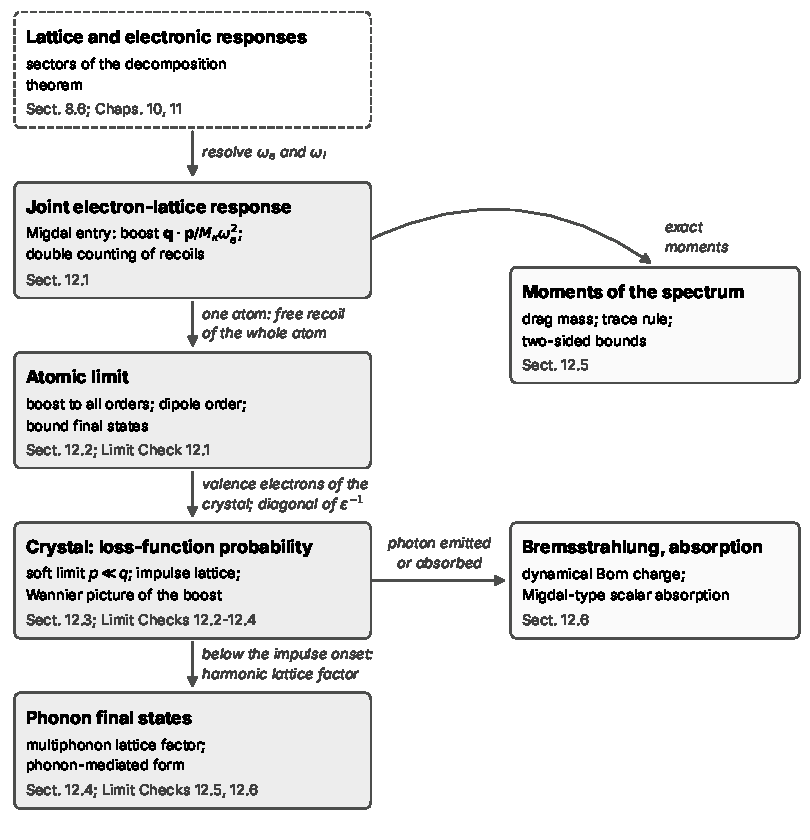
\includegraphics[width=0.85\linewidth]{figures/ch12/map12.pdf}
  \caption{The Migdal entry of the joint electron--lattice response and its truncations. Resolving the energy given to the electrons, $\omega_e$, and to the lattice, $\omega_l$, in the sectors of \cref{sec:8.6} gives the joint response, whose Migdal entry is a boost $\vect{q}\cdot\vect{p}/M_\kappa\omega_e^2$ (\cref{sec:12.1}). One atom with a free recoil gives the atomic limit (\cref{sec:12.2}; \cref{lim:12.2a}); the valence electrons of the crystal with the diagonal of $\varepsilon^{-1}$ give the loss-function probability (\cref{sec:12.3}; \cref{lim:12.3a,lim:12.3b,lim:12.3c}); below the impulse onset the harmonic lattice factor gives the phonon final states (\cref{sec:12.4}; \cref{lim:12.4a,lim:12.4b}). Branches: the exact moments of the spectrum (\cref{sec:12.5}), and the emission or absorption of a photon or scalar (\cref{sec:12.6}).}
  \label{fig:12-map}
\end{figure}

\section{The joint electron--lattice response}\label{sec:12.1}

At a momentum transfer of \SI{50}{keV} a silicon nucleus receives the recoil energy $E_R = q^2/2M_\kappa = \SI{47.8}{meV}$. The lattice takes the recoil energy as a few phonons: the Debye--Waller exponent is $2W_\kappa = 1.57$, and in \SI{21}{\percent} of the kicks the lattice is left as it was (\cref{sec:11.3}). In about three kicks in a million, in the model of \cref{fig:12-plane} below, the electrons do not follow the nucleus, and an electron--hole pair of a few eV is made as well. An event with a pair deposits about \SI{6}{eV}, of which \SI{48.5}{meV} are in the lattice and the rest in the electrons, and a detector treats the two parts differently. The electronic energy makes charge at once; the lattice energy lies below the gap and reaches only a phonon sensor (\cref{chap:18,chap:20}). The response $S_{ab}(\vect{q},\omega)$ of the master formula \cref{eq:8.2-spectrum} cannot separate the electronic energy from the lattice energy, because it adds all final states of the same total energy $\omega$. We need a response with two energy arguments.

\subsection{The joint response}\label{sec:12.1-def}

Every prompt final state $f$ of \cref{sec:8.7-classes} has a definite electronic content: none in the electron-following sector, and otherwise an electron--hole pair, an exciton or a core hole, with or without phonons. We give it an \emph{electronic energy} $E^{\mathrm{el}}_f$, zero in $\mathcal{P}_{\mathrm{ad}}$ and otherwise the zero-phonon energy of its electronic excitation; for a pair this is the quasiparticle energy $\tilde E_m$ of \cref{eq:8.6-dyson}. The remaining energy of the final state, $E_f - E^{\mathrm{el}}_f$, belongs to the lattice: phonons and a recoil. Sorting the final-state-resolved response \cref{eq:8.7-resolved} by the two energies defines the \emph{joint response}
\begin{equation}
  S_{ab}(\vect{q};\omega_l,\omega_e) = \frac{2\pi}{\Vol}\sum_{i,f}p_i\,\langle i|O_a(\vect{q})^\dagger|f\rangle\langle f|O_b(\vect{q})|i\rangle\,
  \delta\bigl(\omega_e - E^{\mathrm{el}}_f + E^{\mathrm{el}}_i\bigr)\,\delta\bigl(\omega_l - (E_f - E^{\mathrm{el}}_f) + (E_i - E^{\mathrm{el}}_i)\bigr) ,
  \label{eq:12.1-joint}
\end{equation}
with $\omega_e$ the energy given to the electrons and $\omega_l$ the energy given to the lattice. At $T \ll \Eg$ every initial state has $E^{\mathrm{el}}_i = 0$. Integrating over $\omega_e$ at fixed total energy removes one delta function and returns the response of \cref{sec:4.2},
\begin{equation}
  \int\dd\omega_e\;S_{ab}(\vect{q};\omega - \omega_e,\omega_e) = S_{ab}(\vect{q},\omega) .
  \label{eq:12.1-marginal}
\end{equation}
The properties of the resolved response carry over to the joint response (\cref{app:D.33}). Where the electronic energy is a good label, each point of the $(\omega_l, \omega_e)$ plane is a sum of outer products with positive weights, and the matrix $S_{ab}(\vect{q};\omega_l,\omega_e)$ is positive semidefinite at every $(\omega_l, \omega_e)$. The rate into a region of the plane is a double spectrum $\dd^2\mathcal{R}/\dd\omega_l\,\dd\omega_e$: \cref{eq:8.2-spectrum} with the joint response \cref{eq:12.1-joint} in place of $S_{ab}(\vect{q},\omega)$ and $\omega = \omega_l + \omega_e$ in the delta function. The cascade of \crefrange{chap:18}{chap:20} turns this double spectrum, not $\dd\mathcal{R}/\dd\omega$, into charge and phonon signals.

The electronic energy is a label, and it is defined where \cref{sec:8.6} defines labels. Inside the off-shell window it is unique to relative order $\theta_{\mathrm{ep}}$. Near a resonant zero-phonon pair the Dyson convention \cref{eq:8.6-dyson} decides: the delta part of \cref{eq:8.6-dyson} lies at $(\omega_l, \omega_e) = (0, \tilde E_m)$, and its finite-part and principal-value parts at the pair energy and $\omega_l = \pm\omega_{\vect{Q}\nu}$ of the phonon made with the pair. We take the zero-phonon energy, and not the vertical energy at the equilibrium positions, because the two differ by the energy the lattice gains when it relaxes around the excitation, and that energy ends up in phonons. For a pair spread over many cells the difference is negligible, since a delocalized pair displaces no nucleus (\cref{sec:8.6}); for a localized excitation it is not, as \cref{we:12-oscillator} shows.

At $T = 0$ the three sectors of \cref{eq:8.6-partition} fall on three parts of the plane,
\begin{equation}
  S_{ab}(\vect{q};\omega_l,\omega_e) = \underbrace{\delta(\omega_e)\,S^{\mathrm{ad}}_{ab}(\vect{q},\omega_l)}_{\text{electron-following}} + \underbrace{\delta(\omega_l)\,S^0_{ab}(\vect{q},\omega_e)}_{\text{zero-phonon electronic}} + \underbrace{S^+_{ab}(\vect{q};\omega_l,\omega_e)}_{\text{phonon-dressed electronic}} ,
  \label{eq:12.1-sectors}
\end{equation}
with $S^{\mathrm{ad}}_{ab}$ and $S^0_{ab}$ the sector responses \cref{eq:8.6-sector}, each a function of one energy. The electron-following sector is the line $\omega_e = 0$, the zero-phonon electronic sector the line $\omega_l = 0$, and the phonon-dressed sector fills the quadrant $\omega_l, \omega_e > 0$. In a warm target phonons can also be absorbed, and $\omega_l$ takes either sign.

Each row of the master formula occupies its own parts of the plane. The electron density has weight in three places. The phonons excited through the electrons that follow the nuclei (\cref{eq:8.6-follow}) lie on the line $\omega_e = 0$, the clamped-nuclei response of \cref{chap:10} lies on the line $\omega_l = 0$, and the phonon sideband of \cref{chap:13} lies at $\omega_l = \pm\omega_{\vect{Q}\nu}$ for one phonon. The nuclear density puts the lattice response of \cref{chap:11}, single phonons, multiphonons and free recoil, on the line $\omega_e = 0$. The weight of the nuclear density off that line is the Migdal effect, which the rest of this chapter computes. The interference $S_{e\kappa}$ of the two densities is the Born-charge interference of \cref{sec:8.4} on the line $\omega_e = 0$. Off that line it is the interference of a Migdal amplitude with an electron-recoil amplitude into the same final state, a zero-phonon pair at $\omega_l = 0$ or a pair with a phonon at $\omega_l = \omega_{\vect{Q}\nu}$. Positivity bounds $S_{e\kappa}$ at every point of the plane, $|S_{e\kappa}|^2 \le S_{ee}S_{\kappa\kappa}$ (\cref{eq:4.2-positivity}), and \cref{sec:12.5,sec:17.4} compute it.

\subsection{The boosted electronic response}\label{sec:12.1-boost}

The nuclear density reaches the electronic sectors only through the nonadiabatic coupling. \Cref{eq:8.6-boost} gives the amplitude at first order in the nonadiabatic coupling: a kick $\ee^{\ii\vect{q}\cdot\vect{X}_I}$ excites the electrons to $\Psi_j$ with the factor $-\ii\,\vect{q}\cdot\vect{d}^I_{j0}/(M_\kappa\Delta E_j)$, times the kick of the nuclear wavefunction. To turn this amplitude into a response we write the derivative coupling as the matrix element of an operator whose response we know. By \cref{eq:5.1-dcoup}, $\vect{d}^I_{j0} = -\vect{F}^I_{j0}/\Delta E_j$, with $\vect{F}^I_{j0}$ the matrix element of the force that nucleus $I$ exerts on the electrons. Let the nucleus act on the electrons through a potential $v_\kappa$ that moves rigidly with it, the bare Coulomb potential $-Z_\kappa e^2/(4\pi r)$ or a pseudopotential (\cref{sec:6.1}). With the Fourier convention \cref{eq:A.3-space}, the projected force is a sum of density components,
\begin{equation}
  \vect{q}\cdot\nabla_{\vect{X}_I}V_{eN} = -\ii\int\frac{\dd^3p}{(2\pi)^3}\;(\vect{q}\cdot\vect{p})\,v_\kappa(\vect{p})\,\ee^{-\ii\vect{p}\cdot\vect{X}_I}\,n_e(\vect{p}) .
  \label{eq:12.1-force}
\end{equation}
The nucleus is, for its electrons, an external potential with Fourier components $v_\kappa(\vect{p})$, and moving it by $\delta\vect{X}$ changes each component by $-\ii\vect{p}\cdot\delta\vect{X}$ times itself. Here $\vect{p}$ is the momentum given to the electrons. Inserting \cref{eq:12.1-force} in \cref{eq:8.6-boost} gives (\cref{app:D.33-amp})
\begin{equation}
  \bigl\langle\Psi^{\mathrm{nuc}\prime}\Psi_j\big|n_\kappa(\vect{q})\big|\Psi^{\mathrm{nuc}}\Psi_0\bigr\rangle
  = \sum_{I\in\kappa}\int\frac{\dd^3p}{(2\pi)^3}\;\frac{\vect{q}\cdot\vect{p}}{M_\kappa\Delta E_j^2}\,v_\kappa(\vect{p})\,\langle\Psi_j|n_e(\vect{p})|\Psi_0\rangle\,\bigl\langle\Psi^{\mathrm{nuc}\prime}\big|\ee^{\ii(\vect{q} - \vect{p})\cdot\vect{X}_I}\big|\Psi^{\mathrm{nuc}}\bigr\rangle .
  \label{eq:12.1-amp}
\end{equation}
Read from right to left, \cref{eq:12.1-amp} says that the nucleus takes the kick $\vect{q}$, passes the momentum $\vect{p}$ to the electrons through its own field and keeps $\vect{q} - \vect{p}$; the electrons are excited by the density component $n_e(\vect{p})$, as by any external potential. The factor $\vect{q}\cdot\vect{p}/(M_\kappa\Delta E_j) = \vect{v}_N\cdot\vect{p}/\Delta E_j$ is the sudden amplitude \cref{eq:6.1-sudden1}, and the remaining $v_\kappa/\Delta E_j$ turns the force into a derivative coupling.

\Cref{eq:12.1-amp} takes the transition density $\langle\Psi_j|n_e(\vect{p})|\Psi_0\rangle$ at the equilibrium positions (the Condon approximation of \cref{sec:5.6}) and takes the vibrational final states on the ground surface, so that $\Delta E_j$ is the vertical excitation energy; for a delocalized pair it is also the zero-phonon energy. Freezing the transition density in the frame of the crystal makes the lattice recoil with $\vect{q} - \vect{p}$, as in the crystal formulas of Knapen, Kozaczuk and Lin~\cite[Eq.~(3)]{knapen2021migdal} and of Berghaus and collaborators~\cite[Eq.~(3.8)]{berghaus2023migdal}. For an isolated atom, whose electrons move with the nucleus, the same steps give $\ee^{\ii\vect{q}\cdot\vect{X}}$: the whole atom recoils (\cref{app:D.33-amp}). Valence electrons in a crystal lie between these two cases, the frame of the crystal and the frame of the struck ion, and it is an open question which of the two frames their transition densities follow. The difference between the two frames is a Herzberg--Teller term, which is the dependence of the transition density on the displacement in \cref{eq:8.6-electronic}. The Herzberg--Teller term changes the momentum the lattice keeps and leaves the electronic spectrum unchanged: at $q = \SI{5}{keV}$ it changes the fraction of Migdal events that emit phonons by a factor 2.4 (\cref{sec:12.4}).

Squaring \cref{eq:12.1-amp}, summing over nuclei and final states, and using the conservation of crystal momentum by the electronic transition (\cref{app:D.33-square}), we obtain the entry of the joint response that holds the Migdal effect.
\begin{keyresult}[The Migdal entry of the joint response]
At Born--Oppenheimer order $n_B = 2$, with Condon transition densities and lattice final states on the ground surface, the nuclear density of species $\kappa$ has, for $\omega_e > 0$,
\begin{equation}
  \begin{split}
  S_{\kappa\kappa}(\vect{q};\omega_l,\omega_e) = \frac{1}{2\pi}\int_{\mathrm{BZ}}\frac{\dd^3k}{(2\pi)^3}\sum_{\vect{G}\vect{G}'}\;
  &\underbrace{\frac{[\vect{q}\cdot(\vect{k}+\vect{G})]\,[\vect{q}\cdot(\vect{k}+\vect{G}')]}{M_\kappa^2\,\omega_e^4}}_{\text{boost}}\;
  \underbrace{v_\kappa(\vect{k}+\vect{G})^*\,v_\kappa(\vect{k}+\vect{G}')}_{\text{vertex}} \\
  &\times\underbrace{S^{ee}_{\vect{G}\vect{G}'}(\vect{k},\omega_e)}_{\text{electrons}}\;
  \underbrace{S^{\mathrm{ad}}_{\kappa;\vect{G}\vect{G}'}(\vect{q} - \vect{k},\omega_l)}_{\text{lattice}} ,
  \end{split}
  \label{eq:12.1-Skk}
\end{equation}
where $S^{ee}_{\vect{G}\vect{G}'}(\vect{k},\omega) = (2\pi/\Vol)\sum_{j\neq0}\langle\Psi_0|n_e(\vect{k}+\vect{G})^\dagger|\Psi_j\rangle\langle\Psi_j|n_e(\vect{k}+\vect{G}')|\Psi_0\rangle\,\delta(\omega - \Delta E_j)$ is the density response matrix of the electrons at clamped nuclei and $S^{\mathrm{ad}}_{\kappa;\vect{G}\vect{G}'}(\vect{Q},\omega)$ the electron-following response \cref{eq:8.6-sector} between $n_\kappa(\vect{Q} - \vect{G})$ and $n_\kappa(\vect{Q} - \vect{G}')$. The zero-phonon part of the Migdal entry, at $\omega_l = 0$, lies in $\mathcal{P}_0$, and the rest in $\mathcal{P}_+$.
\end{keyresult}
\noindent The electronic factor is the full response of the interacting electrons, with screening and local fields inside it, and the vertex is the bare potential of the nucleus. The moving nucleus is an external charge to the electrons, exactly as the dark matter is in the loss-function rate of \cref{sec:10.2}. If the core electrons are frozen into a pseudopotential, $v_\kappa$ is that pseudopotential and $S^{ee}$ the response of the valence electrons; \cref{sec:12.3} works in this frozen-core setting. The lattice factor is the response of \cref{chap:11}, evaluated at the momentum $\vect{q} - \vect{k} - \vect{G}$ that the nucleus keeps.

The size of the effect follows from the moments of $S^{ee}$. The first electronic moment of the Migdal probability is fixed by the drag mass, $\int\dd\omega_e\,\omega_e\,\dd P_{\mathrm{Mig}}/\dd\omega_e = E_R\,\delta M_\kappa/M_\kappa$ for an isotropic drag mass (\cref{eq:8.6-fsum-k}). With a typical electronic energy $\langle\omega_e\rangle$, therefore,
\begin{equation*}
  P_{\mathrm{Mig}} \approx \frac{E_R}{\langle\omega_e\rangle}\,\frac{\delta M_\kappa}{M_\kappa} ,
\end{equation*}
the recoil energy in units of the typical electronic energy, times the share of the mass that the electrons carry. For silicon at $q = \SI{50}{keV}$, with the atomic estimate $\delta M_\kappa/M_\kappa = 2.7\times10^{-4}$ of \cref{sec:8.6} and $\langle\omega_e\rangle \approx \SI{6}{eV}$, $P_{\mathrm{Mig}}$ is about $2\times10^{-6}$. The atomic estimate of $\delta M_\kappa$ is the sum of the drag masses over all nuclei, while a kick probes only the drag-mass element of the struck nucleus, and in silicon that element is about twice the atomic value (\cref{sec:12.5-trace}). The agreement with the model below is therefore partly fortuitous. Since $E_R$ grows as $q^2$, so does $P_{\mathrm{Mig}}$, and the Migdal effect matters where the recoil itself is invisible: it trades the factor $P_{\mathrm{Mig}}$ for an energy $\langle\omega_e\rangle/E_R$ times larger, 120 times at \SI{50}{keV} in silicon.

\Cref{fig:12-plane} shows the plane for silicon at $q = \SI{50}{keV}$, in a model that keeps the valence electrons, the diagonal $\vect{G} = \vect{G}'$ and the incoherent lattice factor, \cref{eq:12.4-harm}. The line $\omega_e = 0$ carries the lattice spectrum of \cref{sec:11.3}, with the zero-phonon weight $\ee^{-2W_\kappa} = 0.21$ and the mean $E_R$. The Migdal weight, $P_{\mathrm{Mig}} = 2.92\times10^{-6}$, or $6.1\times10^{-5}$ per eV of recoil energy (\cref{sec:12.3}), lies at $\omega_e$ above the gap: half of it below \SI{4.4}{eV}, \SI{89}{\percent} below \SI{10}{eV}, with a mean of \SI{5.9}{eV}. Along $\omega_l$ the Migdal weight repeats the lattice spectrum. The line $\omega_l = 0$ holds \SI{21}{\percent} of the Migdal weight, and the rest has the peaks of the phonon density of states. The mean lattice energy of a Migdal event is \SI{48.5}{meV}, above $E_R$ by $\langle p^2\rangle/2M_\kappa$, the recoil of the momentum the electrons take, with $\langle p^2\rangle^{1/2} = \SI{6.1}{keV}$. The map is close to a product of the lattice spectrum and the electronic spectrum. That product is the soft limit $p \ll q$, which \cref{sec:12.3} makes precise; here $p/q$ is about 0.1.

\begin{figure}[tbp]
  \centering
  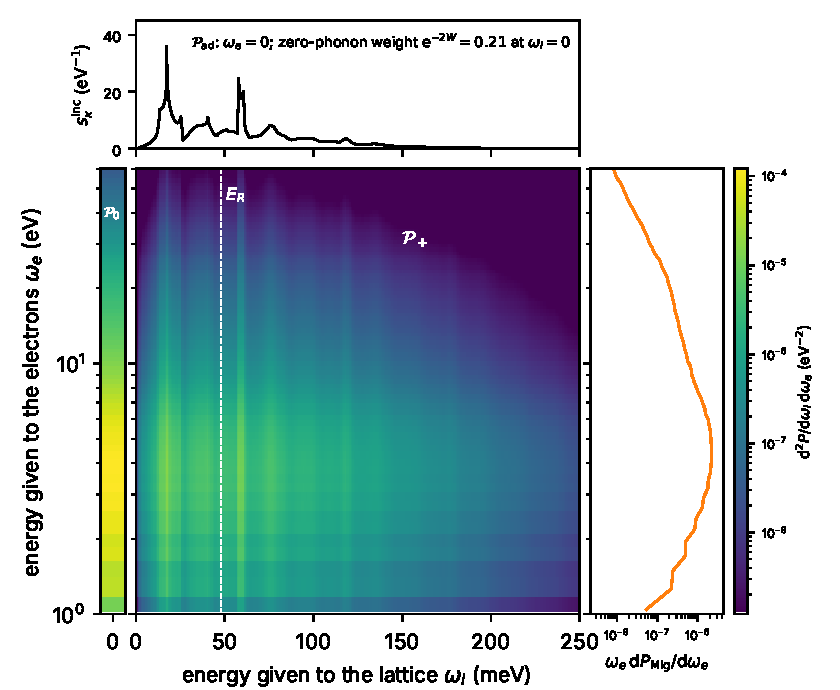
\includegraphics[width=0.92\linewidth]{figures/ch12/fig12_1.pdf}
  \caption{The joint response of silicon at $q = \SI{50}{keV}$ in the plane of the energy $\omega_l$ given to the lattice and the energy $\omega_e$ given to the electrons, per nucleus and normalized as probabilities, at $T = 0$. Top: the electron-following line $\omega_e = 0$, the incoherent lattice spectrum $s^{\mathrm{inc}}_\kappa$ of one nucleus without its zero-phonon part $\ee^{-2W} = 0.21$ at $\omega_l = 0$ ($E_R = \SI{47.8}{meV}$, $2W = 1.57$, phonon density of states from density-functional perturbation theory). Main panel: the Migdal probability density $\dd^2P/\dd\omega_l\,\dd\omega_e$ in the phonon-dressed sector $\mathcal{P}_+$; the dashed line marks $E_R$. Left strip: the zero-phonon Migdal line $\omega_l = 0$ (sector $\mathcal{P}_0$), drawn as a bin of \SI{1}{meV} in $\omega_l$ on the same color scale. Right: the marginal $\omega_e\,\dd P_{\mathrm{Mig}}/\dd\omega_e$. Model: \cref{eq:12.1-Skk} with valence electrons only, the ion charge $Z_{\mathrm{ion}}(p)$ of \cref{eq:12.3-Zion} and the diagonal $\vect{G} = \vect{G}'$. The electronic factor is the random-phase loss function of silicon with local fields of Knapen, Kozaczuk and Lin~\cite{knapen2021dark} (threshold \SI{1.11}{eV}, the step-model gap that accompanies the tables, $p \le \SI{22.5}{keV}$, $\omega_e \le \SI{89}{eV}$, averaged over directions); the transition densities are Condon in the frame of the crystal (lattice factor at $|\vect{q} - \vect{p}|$), and the lattice response is incoherent.}
  \label{fig:12-plane}
\end{figure}

The energy denominators of the boost neglect the nuclear motion against $\omega_e$, at relative order $v_Np/\omega_e$ and $(\omega_l/\omega_e)^2$; at the momenta of \cref{fig:12-plane} these are $3\times10^{-3}$ and $10^{-4}$. The exact denominators are \cref{eq:12.3-bracket} for a free nucleus and \cref{eq:12.4-exact} for a bound one. The Condon approximation drops the change of the transition density with the displacements, the Herzberg--Teller term above. The ground-surface final states drop the displacement of the excited surface, which moves energy from $\omega_e$ to $\omega_l$ without changing their sum, and which is negligible for a delocalized pair. \Cref{we:12-oscillator} shows the Herzberg--Teller term and the excited-surface displacement at work where they are not small.

\Cref{app:E.6} gives the dielectric matrix of the electrons, with local fields, on a grid of $(\vect{k}, \omega_e)$, and \cref{app:E.17} gives the lattice response on a grid of momenta.

\begin{workedexample}{The joint response of a displaced oscillator}\label{we:12-oscillator}
We take the model, the kick $\ee^{\ii qx}$ with $q\ell_0 = 1$ ($E_R = \omega_0 = \SI{64.1}{meV}$) and the labels of \cref{we:8-sectors}. A state on the excited surface with vibrational level $m$ gets $\omega_e = \SI{1.0463}{eV}$, the zero-phonon energy of the upper level, and $\omega_l = m \times \SI{65.5}{meV}$, the quanta of the excited surface, both read off the exact diagonalization.

\emph{The exact plane.} The line $\omega_e = 0$ carries the kick on the ground surface, with weight $1 - P_{\mathrm{Mig}}$. The Migdal weight $P_{\mathrm{Mig}} = 3.94\times10^{-6}$ of \cref{we:8-sectors} lies on the line $\omega_e = \SI{1.0463}{eV}$ as a comb in $\omega_l$, with the fractions 0.097, 0.227, 0.265, 0.205, 0.119 and 0.055 for $m = 0$ to 5. The lattice receives on average \SI{0.153}{eV} in a Migdal event, more than twice the recoil energy.

\emph{The leading entry with ground-surface final states.} This entry is \cref{eq:12.1-Skk}: every Migdal event sits at the vertical energy $\omega_e = \Delta_{\mathrm{tl}} = \SI{1.17}{eV}$, and the lattice factor is the kick of the ground surface, Poisson distributed with mean $(q\ell_0)^2 = 1$. The fractions are 0.368, 0.368, 0.184, 0.061, and the mean lattice energy is $E_R = \SI{64.1}{meV}$. The total energy per event, $\Delta_{\mathrm{tl}} + E_R = \SI{1.234}{eV}$, is close to the exact \SI{1.199}{eV}, but the split between electrons and lattice is wrong.

\emph{Excited-surface final states.} Projecting the kicked state on the vibrational states of the excited surface puts the relaxation energy in $\omega_l$. For surfaces of equal frequency the overlap $\langle m_{\mathrm{up}}|\ee^{\ii qx}|0_{\mathrm{lo}}\rangle$ is that of a coherent state whose amplitude adds the imaginary kick $\ii q\ell_0$ to the real displacement $-S_{\mathrm{HR}}^{1/2}$. The weights are then Poisson with mean $(q\ell_0)^2 + S_{\mathrm{HR}} = 3$, and the mean lattice energy is $3\omega_0 = \SI{0.192}{eV}$, against $E_R$ before. On the computed surfaces, with their unequal quanta, the same projection gives the mean lattice energy \SI{0.188}{eV} and the zero-phonon fraction 0.056 instead of $\ee^{-3} = 0.050$, with the derivative coupling evaluated at $x = 0$ (the Condon approximation). The relaxation energy $S_{\mathrm{HR}}\omega_0 = \SI{0.128}{eV}$ has moved from $\omega_e$ to $\omega_l$, and the total $\SI{1.0463}{eV} + \SI{0.188}{eV} = \SI{1.234}{eV}$ is unchanged. The probability is $3.52\times10^{-6}$, the value of the boost formula of \cref{we:8-sectors}, and the zero-phonon fraction 0.056 falls short of the exact 0.097.

\emph{Beyond Condon.} The derivative coupling and the gap both vary along $x$: the gap is $\Delta_{\mathrm{tl}} + g_{\mathrm{d}}x/\ell_0$, smaller on the side of the displaced minimum. Keeping $q\,d_{10}(x)/[(M/2)\Delta E(x)]$ inside the vibrational matrix element, as a function of $x$, gives $P_{\mathrm{Mig}} = 4.00\times10^{-6}$, the fractions 0.104, 0.236, 0.267, 0.201, 0.113 and 0.051, and the mean lattice energy \SI{0.148}{eV}, all within a few percent of the exact values. \Cref{we:8-sectors} traced the \SI{12}{\percent} excess of the exact probability over the boost formula to the displaced surface; this excess is the Herzberg--Teller term, and it acts most on the zero-phonon line.

A strongly displaced excited surface, as for an exciton bound to a defect, therefore needs the zero-phonon energy as its electronic energy and the non-Condon term. For an electron--hole pair spread over $N$ cells, $S_{\mathrm{HR}}$ is of order $1/N$, and the ground-surface form \cref{eq:12.1-Skk} is the right one.
\end{workedexample}

\subsection{Local fields and the choice of electrons}\label{sec:12.1-truncations}

Each truncation of \cref{fig:12-map} keeps the boost and makes a choice for the vertex, the electronic factor and the lattice factor. On the diagonal of $\varepsilon^{-1}$ the local fields lower the silicon probability by a factor 1.35 against a scalar dielectric function (\cref{lim:12.3a}). Through the off-diagonal elements $\vect{G} \neq \vect{G}'$ they couple different momenta. No table in this book contains the off-diagonal part; it is sized only in a model of silicon, where it raises the rate, and the full calculation is still open (\cref{sec:12.3-validity}). The same matrix $\varepsilon^{-1}$ changes the electron-recoil rate of silicon by a factor of 1.5 at \SI{10}{MeV} (\cref{sec:10.2-corrections}). The atomic formula, applied to the valence electrons of a crystal, puts the wrong electrons in the electronic factor. The valence electrons of silicon are not those of a silicon atom, and their gap is \SI{1.17}{eV} instead of the atomic binding of several eV; the factor $\omega_e^{-4}$ magnifies the difference between the two energies. For the core shells, whose electrons do move with their nucleus, the atomic form is the right truncation (\cref{sec:12.2}).

\subsection{Double counting of recoils}\label{sec:12.1-counting}

The joint response holds the lattice and the Migdal parts of one nuclear response, and its moments fix how they add. Take the incoherent response, one nucleus at a time. The total weight of $n_\kappa(\vect{q})$ is $2\pi\nd_\kappa$, the density of nuclei times $2\pi$, whatever the final states; integrated over the plane, \cref{eq:12.1-joint} has that weight. The Migdal entry takes $2\pi\nd_\kappa P_{\mathrm{Mig}}(q)$ of it, and the line $\omega_e = 0$ keeps
\begin{equation}
  \int\dd\omega_l\;S^{\mathrm{ad}}_{\kappa\kappa}(\vect{q},\omega_l) = 2\pi\nd_\kappa\bigl[1 - P_{\mathrm{Mig}}(q)\bigr] .
  \label{eq:12.1-zeroth}
\end{equation}
The first moment of the line, by \cref{eq:8.6-fsum-k}, is that of a nucleus of mass $M_\kappa + \delta M_\kappa$. The lattice responses of \cref{chap:11} are normalized to unit weight and use the bare mass. Added to a Migdal rate, they count twice the kicks that excited the electrons: once as pure recoils on the line $\omega_e = 0$ and once as Migdal events. The double count is a fraction $P_{\mathrm{Mig}}$ of the kicks, but in each of them the lattice energy is not small: \cref{fig:12-plane} shows that a Migdal event carries the whole recoil, \SI{48.5}{meV} on average against $E_R = \SI{47.8}{meV}$, and the electronic energy on top of it. The consistent sum takes the lattice response with the weight $1 - P_{\mathrm{Mig}}$ and the mass $M_\kappa + \delta M_\kappa$, the first prescription of \cref{sec:8.6}, and the joint response applies this prescription by construction. In silicon the weight correction $P_{\mathrm{Mig}}$ and the mass correction $\delta M_\kappa/M_\kappa$ are both below $10^{-3}$ for $E_R \lesssim \SI{16}{eV}$, which covers the phonon and multiphonon momenta of \cref{chap:11}, and the rate of a phonon detector does not see the two corrections there. At \SI{500}{eV} the weight $1 - P_{\mathrm{Mig}}$ is a \SI{3}{\percent} correction (\cref{sec:12.5-bounds}). The counting of Migdal and lattice events, however, is exact, and \cref{sec:12.5} completes it with the higher moments.

The same entry fixes the lattice factor of the Migdal rate itself. A Migdal event leaves the lattice in the state that the kick $\vect{q} - \vect{p}$ makes, so the lattice factor of a Migdal rate below the impulse onset is the multiphonon response of \cref{sec:11.3}, not a free recoil. Combining a free-recoil Migdal formula with a multiphonon lattice rate counts nothing twice; it mixes two truncations of one response, and a rate built that way is labeled by neither. On the scale of \cref{sec:8.5} the two pieces of a rate should carry the same lattice regime $\mathcal{K}$.

Measured nuclear-recoil signals obey the same rule from the other side. A calibration with neutrons measures the ionization of nuclear recoils, and the Migdal electrons of those recoils are part of what it measures. A nuclear-recoil rate converted to charge with a measured yield already contains the Migdal ionization, and a computed Migdal rate added to it counts that ionization twice. The yield and its Migdal part are separated in \cref{sec:19.2}.

\subsection{Targets without a gap}\label{sec:12.1-gapless}

The construction used the gap three times: to give each final state an electronic energy, to make the energy denominators of the boost large compared with the lattice energies, and to keep the low-energy end of $S^{ee}$ empty. In a metal, a superconductor or a semimetal all three fail.

With the quasiparticle sectors $\mathcal{P}^{\mathrm{qp}}_{n,m}$ of \cref{sec:8.6}, $\omega_e$ becomes the energy of the quasiparticles created, defined to within their width, and the joint response is meaningful on bins of the plane that satisfy the bin bound \cref{eq:8.6-bin}.

In a metal the loss function grows linearly from $\omega_e = 0$, since electron--hole pairs at the Fermi surface cost nothing, and with the factor $\omega_e^{-4}$ the Migdal probability \cref{eq:12.1-Skk} integrates as $\int\dd\omega_e\,\omega_e^{-3}$ and diverges at small $\omega_e$. The divergence marks the failure of the sudden expansion, not a large effect. Once $\omega_e$ falls to the phonon energies, the electrons follow the nucleus instead of being left behind. The boost denominator $\omega_e^2$ must then be replaced by the full denominator. For a bound nucleus the full denominator is the phonon propagator $\omega_e^2 - \omega_{\mathrm{ph}}^2$ of the phonon-mediated form, whose pole at $\omega_e = \omega_{\mathrm{ph}}$ is the ordinary electron--phonon coupling of \cref{chap:6}. The part of the plane with $\omega_e \lesssim \omega_{\mathrm{D}}$ then belongs to the electron--phonon response of the metal, computed with Fan--Migdal and Eliashberg methods (\cref{sec:6.3,sec:6.4}), and only $\omega_e \gg \omega_{\mathrm{D}}$ is a Migdal process in the sense of this chapter. The electronic factor also changes character: $S^{ee}$ contains the intraband response of the conduction electrons, which screens the moving ion at small $\omega_e$, so that a slowly moving ion in a metal carries no charge. The full response contains this intraband screening, and a formula that screens the vertex statically does not. In a superconductor, whose hierarchy is reversed (\cref{sec:8.6}), a kicked nucleus breaks pairs through the phonons it emits (\cref{chap:15,chap:20}).

\section{The atomic limit}\label{sec:12.2}

A germanium atom that recoils with \SI{1}{keV} loses an electron to the continuum in one recoil in 580 according to the calculation of Ibe and collaborators, and in one recoil in 610 according to that of Cox and collaborators; in one recoil in 230 its electrons are left excited or ionized. Most of these events come from two shells, the $3d$ shell, bound by about \SI{30}{eV} and smaller than an angstrom, and the valence shell. A crystal of germanium keeps the first nearly as it is in the atom and rebuilds the second into bands. In the atom the Migdal entry \cref{eq:12.1-Skk} of the joint response can be evaluated to all orders in the momentum given to the electrons, and every number can be checked against a sum rule.

\subsection{The boost of a free atom}\label{sec:12.2-boost}

Take one atom at rest in its ground state, with a nucleus of mass $M$ at $\vect{X}$ and $N_e$ electrons at $\vect{r}_e$. Dark matter couples to the nucleus through $\ee^{\ii\vect{q}\cdot\vect{X}}$, to first order in the coupling. The Coulomb energy depends only on the positions of the electrons relative to the nucleus, $\vect{\rho}_e = \vect{r}_e - \vect{X}$. We trade $\vect{X}$ for the center of mass $\vect{R}_{\mathrm{cm}} = (M\vect{X} + m_e\sum_e\vect{r}_e)/m_A$ and keep the $\vect{\rho}_e$, with
\begin{equation}
  m_A = M + N_em_e ,
  \label{eq:12.2-mA}
\end{equation}
the mass of the atom up to the binding energy of its electrons, less than a part in $10^{6}$. The chain rule gives $\nabla_{\vect{X}} = (M/m_A)\nabla_{\vect{R}_{\mathrm{cm}}} - \sum_e\nabla_{\vect{\rho}_e}$ and $\nabla_{\vect{r}_e} = (m_e/m_A)\nabla_{\vect{R}_{\mathrm{cm}}} + \nabla_{\vect{\rho}_e}$. In the kinetic energy $-\nabla_{\vect{X}}^2/2M - \sum_e\nabla_{\vect{r}_e}^2/2m_e$ the cross terms between $\nabla_{\vect{R}_{\mathrm{cm}}}$ and $\nabla_{\vect{\rho}_e}$ cancel, and the terms in $\nabla_{\vect{R}_{\mathrm{cm}}}^2$ add up to $1/2m_A$. The Hamiltonian separates exactly,
\begin{equation}
  H = -\frac{\nabla_{\vect{R}_{\mathrm{cm}}}^2}{2m_A} + H_{\mathrm{rel}} , \qquad
  H_{\mathrm{rel}} = -\sum_e\frac{\nabla_{\vect{\rho}_e}^2}{2m_e} - \frac{1}{2M}\Bigl(\sum_e\nabla_{\vect{\rho}_e}\Bigr)^2 + V_{eN} + V_{ee} .
  \label{eq:12.2-Hint}
\end{equation}
The internal Hamiltonian is the clamped-nucleus Hamiltonian of \cref{sec:5.1} plus one term, the kinetic energy $(\sum_e\vect{p}_e)^2/2M$ of a nucleus that balances the momentum of its electrons. Its diagonal part turns $m_e$ into the reduced mass, and its off-diagonal part, $-M^{-1}\sum_{e<e'}\nabla_{\vect{\rho}_e}\cdot\nabla_{\vect{\rho}_{e'}}$, is the mass-polarization term of atomic physics. Both change energies and wavefunctions at relative order $m_e/M$.

The kick separates just as exactly. Since $\vect{X} = \vect{R}_{\mathrm{cm}} - (m_e/m_A)\sum_e\vect{\rho}_e$,
\begin{equation}
  \ee^{\ii\vect{q}\cdot\vect{X}} = \ee^{\ii\vect{q}\cdot\vect{R}_{\mathrm{cm}}}\;\exp\Bigl(-\ii\vect{q}_e\cdot\sum_e\vect{\rho}_e\Bigr) , \qquad
  \vect{q}_e = \frac{m_e}{m_A}\,\vect{q} = m_e\vect{v}_A ,
  \label{eq:12.2-cm}
\end{equation}
with $\vect{v}_A = \vect{q}/m_A$ the velocity of the recoiling atom. The first factor gives the whole atom the momentum $\vect{q}$ and the kinetic energy $q^2/2m_A$. The second acts on the internal state alone, as a momentum $-\vect{q}_e$ given to every electron. For hydrogen this is the separation of \cref{sec:6.1}. With $N_e$ electrons the center of mass still separates exactly; what the other electrons change is the internal Hamiltonian, through the mass-polarization term, and the boost mass, $m_A$ in place of the proton mass. The joint response \cref{eq:12.1-joint} of a gas of $\nd_T$ such atoms per unit volume, incoherent between atoms, is therefore
\begin{keyresult}[Migdal effect of a free atom]
\begin{gather}
  S_{\kappa\kappa}(\vect{q};\omega_l,\omega_e) = 2\pi\nd_T\,\delta\Bigl(\omega_l - \frac{q^2}{2m_A}\Bigr)\sum_fP_f(\vect{q})\,\delta(\omega_e - E_f + E_0) , \nonumber\\
  P_f(\vect{q}) = \Bigl|\Bigl\langle\Psi_f\Big|\exp\Bigl(-\ii\vect{q}_e\cdot\sum_e\vect{\rho}_e\Bigr)\Big|\Psi_0\Bigr\rangle\Bigr|^2 ,
  \label{eq:12.2-joint}
\end{gather}
with $\Psi_f$ and $E_f$ the eigenstates and energies of $H_{\mathrm{rel}}$ and $\vect{q}_e = m_e\vect{q}/m_A$. It holds to first order in the dark-matter coupling and to all orders in $q$, with no assumption about time.
\end{keyresult}
\noindent The term $f = 0$ is the line $\omega_e = 0$, the electron-following sector of \cref{eq:12.1-sectors}, with weight $P_0 = 1 - P_{\mathrm{Mig}}$. The rest is the Migdal entry. All of it sits on the line $\omega_l = q^2/2m_A$: a free atom has no phonons, and the lattice energy of every event is the recoil of the atom. \Cref{eq:12.2-joint} is the electron-cloud transition factor of Ibe and collaborators, who derive it in the same way and write the argument as the final velocity of the atom times $m_e$~\cite[Eqs.~(55), (57) and (73)]{ibe2018migdal}. Their phase $\ee^{-\ii\vect{q}_e\cdot\vect{x}}$ in the electron coordinates and the opposite sign of Kahlhoefer and Su~\cite[Eq.~(1)]{kahlhoefer2026probing} leave $|\cdot|^2$ unchanged.

\Cref{sec:6.1} reached the same structure from the other side, as the sudden boost \cref{eq:6.1-boost} with the velocity $v_N = q/M$ of the bare nucleus, and the leading entry \cref{eq:12.1-Skk} carries the same mass. Both are right to the order they claim. The exact separation fixes the next order: the boost mass is $m_A$, and at fixed $q$ the electrons receive $m_eq/m_A$, smaller than $m_eq/M$ by the factor $1 - N_em_e/m_A$. The electrons that follow the nucleus add their mass to it. This is the drag mass of \cref{eq:8.6-fsum-k}, $\delta M = N_em_e$ for an atom, and $M + \delta M = m_A$. The probability changes by $2N_em_e/m_A$, $5.5\times10^{-4}$ for silicon and $4.8\times10^{-4}$ for germanium, far below any other uncertainty of the calculation, but the counting of Migdal and lattice events in \cref{sec:12.5} needs it, and in a crystal the same role falls to $M_\kappa + \delta M_\kappa$ with the tensor drag mass of \cref{sec:8.6}. What the separation leaves to be solved is the internal problem. The states $\Psi_f$ are those of $H_{\mathrm{rel}}$, and the atomic calculations used below solve the clamped-nucleus problem instead, an error of relative order $m_e/M$ in each $P_f$.

The rate of a free-atom target follows from \cref{eq:8.2-spectrum} with the joint response \cref{eq:12.1-joint}. For a spin-independent coupling the nuclear vertex is $AF_N(q)$, the delta function of $\omega_l$ fixes $q = (2m_AE_R)^{1/2}$, and energy conservation needs $\omega_{\vect{q}} = E_R + \omega_e$. With the minimum velocity \cref{eq:1.3-vmin} at $\omega = E_R + \omega_e$, the free-recoil rate \cref{eq:11.4-LS} becomes
\begin{equation}
  \frac{\dd^2\mathcal{R}}{\dd E_R\,\dd\omega_e} = \frac{\rho_\chi\,\sigma_N}{2\mchi\,\mu_{\chi N}^2}\,F_N(q)^2\,\eta\Bigl(\frac{q}{2\mu_{\chi N}} + \frac{\omega_e}{q}\Bigr)\,\frac{\dd P}{\dd\omega_e}(q) ,
  \label{eq:12.2-rate}
\end{equation}
a rate per target atom, with $\mu_{\chi N}$ the reduced mass of the dark matter and the atom and $\dd P/\dd\omega_e = \sum_{f\neq0}P_f\,\delta(\omega_e - E_f + E_0)$. This is the rate of Ibe and collaborators~\cite[Eqs.~(91) and (92)]{ibe2018migdal}. The electronic energy raises $\vmin$ by $\omega_e/q$, and at fixed $\omega_e$ the recoil energy can no longer be arbitrarily small, since $\vmin$ grows without bound as $q \to 0$. The total deposit is at most the kinetic energy $\frac12\mchi v_{\mathrm{max}}^2$ of the dark matter, with the largest laboratory speed $v_{\mathrm{max}} = \SI{795}{km.s^{-1}}$ of the halo of \cref{sec:1.2}, \SI{35}{eV} at \SI{10}{MeV} and \SI{3.5}{keV} at \SI{1}{GeV}, and this, more than the probability, decides which shells a light particle can ionize.

\subsection{Shell probabilities at dipole order}\label{sec:12.2-dipole}

The electrons of an atom receive little momentum. A recoil energy $E_R$ gives them $q_e = m_e(2E_R/m_A)^{1/2}$, \SI{88}{eV} for germanium at $E_R = \SI{1}{keV}$, and the multipole parameter of \cref{sec:8.5} is $\xi_D = q_er_{\mathrm{orb}} = 0.07$ for its valence shell, of mean radius $2.9\,a_0$, and 0.02 for the $3d$ shell. The boost can be expanded. With $D_{\hat q} = \hat{\vect{q}}\cdot\sum_e\vect{\rho}_e$ the dipole operator of the electrons along the kick, the amplitude of an excited state is $-\ii q_e\langle\Psi_f|D_{\hat q}|\Psi_0\rangle$ plus terms of order $q_e^2$, and
\begin{equation}
  P_f = q_e^2\,\bigl|\langle\Psi_f|D_{\hat q}|\Psi_0\rangle\bigr|^2 , \qquad f \neq 0 ,
  \label{eq:12.2-dipole}
\end{equation}
at multipole order $n_D = 2$. Its corrections, of relative order $\xi_D^2$, come from the quadrupole and monopole terms of the boost and from the dipole term at second order. For hydrogen \cref{eq:12.2-dipole} sums to $q_e^2\langle z^2\rangle = q_e^2a_0^2$, the small-$v_N$ form of \cref{eq:6.1-P0}.

Two sums over final states are fixed without solving for any of them. Closure over $f \neq 0$ gives the total probability, and the double commutator of $D_{\hat q}$ with $H_{\mathrm{rel}}$ gives its first moment,
\begin{equation}
  P_{\mathrm{Mig}} = q_e^2\bigl(\langle D_{\hat q}^2\rangle - \langle D_{\hat q}\rangle^2\bigr) , \qquad
  \int\dd\omega_e\,\omega_e\,\frac{\dd P}{\dd\omega_e} = \frac{N_em_e}{M}\,E_R ,
  \label{eq:12.2-sums}
\end{equation}
with expectation values in the ground state. The total holds at dipole order; the first moment is exact to all orders in $q_e$. It is the f-sum rule \cref{eq:4.3-atomq} of the internal Hamiltonian, whose kinetic term \cref{eq:12.2-Hint} gives the double commutator $N_e/m_e + N_e^2/M = N_em_A/(m_eM)$, multiplied by $q_e^2/2$. At $E_R = \SI{1}{keV}$ it is \SI{0.27}{eV} for silicon, \SI{0.24}{eV} for germanium and \SI{0.23}{eV} for xenon: the mean energy the electrons take per recoil, carried by the small fraction of events that excite them. It is also the drag-mass term of \cref{eq:8.6-fsum-k}, $\vect{q}\cdot\delta M\cdot\vect{q}/2M^2$ with $\delta M = N_em_e$, up to a relative $m_e/M$. Any table of atomic Migdal probabilities must reproduce it, and the core shells, whose large excitation energies weight the sum, dominate it.

In practice the atom is described by one Slater determinant of orbitals, from a Hartree--Fock or Dirac--Hartree--Fock calculation, and \cref{eq:12.2-dipole} becomes a sum of one-electron transitions. The dipole operator is a sum of one-electron operators, so at this order it moves one electron, from an occupied orbital $a$ of a shell $n\ell$ to an empty orbital $b$. A transition into an occupied orbital is blocked by the Pauli principle. Summed over the orbitals of the shell and the degenerate final ones, the probability per unit energy of an ejected electron is
\begin{equation}
  \frac{\dd P_{n\ell}}{\dd E_{\mathrm{ej}}} = q_e^2\sum_{a\in n\ell}\sum_b\bigl|\langle b|\hat{\vect{q}}\cdot\vect{\rho}|a\rangle\bigr|^2\,\delta(E_{\mathrm{ej}} - \epsilon_b) ,
  \label{eq:12.2-shell}
\end{equation}
with $\epsilon_b$ the energy of a continuum orbital normalized per unit energy and $\omega_e = E_B + E_{\mathrm{ej}}$, with $E_B$ the binding energy of the shell. Bound empty orbitals $b$ give the excitation probabilities of the shell. Only $\ell' = \ell \pm 1$ is reached, and for a closed shell the result does not depend on the direction of $\vect{q}$. This is the leading-order formula of Ibe and collaborators~\cite[Eqs.~(86)--(90)]{ibe2018migdal}, and since every term carries $q_e^2$, a table at one $q_e$ gives every other. The orbitals are atomic Hartree--Fock orbitals and continuum states in the field of the ion, computed as for the ionization form factors of dark-matter--electron scattering (\cref{app:E.7}); \cref{eq:12.2-shell} is the dipole limit of the ionization form factor \cref{eq:2.2-fion}, with $q_e$ in place of $q$.

\begin{limitbox}[Atomic Migdal effect at dipole order][lim:12.2a]
For a free atom recoiling with $q$, each shell is ionized with $\dd P_{n\ell}/\dd E_{\mathrm{ej}} = q_e^2\sum_{a,b}|\langle b|\hat{\vect{q}}\cdot\vect{\rho}|a\rangle|^2\delta(E_{\mathrm{ej}} - \epsilon_b)$, $q_e = m_eq/m_A$, and the rate is \cref{eq:12.2-rate}~\cite[Eqs.~(73), (86)--(92)]{ibe2018migdal}.
\par\smallskip
{\centering
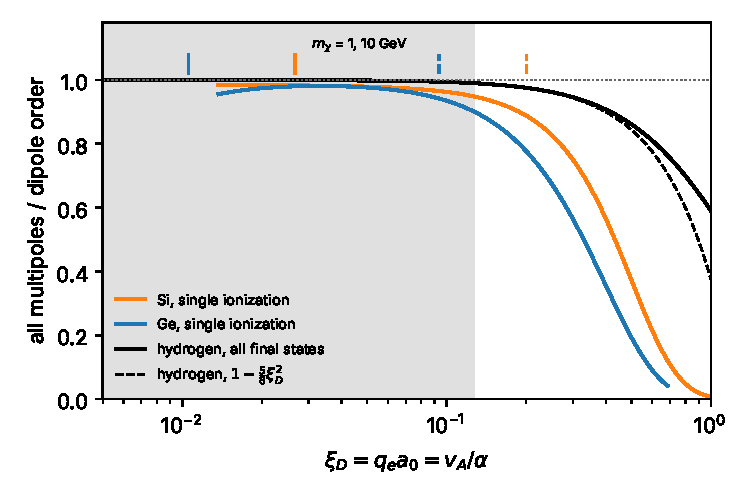
\includegraphics[width=\linewidth]{figures/ch12/limit12_2a.pdf}
\captionof{figure}{The Migdal probability with the full boost $\exp(-\ii\vect{q}_e\cdot\sum_e\vect{\rho}_e)$, all multipoles, divided by its dipole-order value, against $\xi_D = q_ea_0 = v_A/\alpha$. Black: hydrogen, all final states, $[1 - F_{1s}^2]/\xi_D^2$ from \cref{eq:6.1-P0}, exact. Dashed: its leading correction, $1 - \frac58\xi_D^2$. Orange and blue: single ionization of silicon and germanium atoms, Dirac--Hartree--Fock tables with multipoles up to $L = 10$ and at dipole order~\cite{cox2023precise}; a velocity-independent part of the tabulated full probabilities, $1.6\times10^{-4}$ (Si) and $1.3\times10^{-4}$ (Ge), which no transition between orthogonal states can have, is subtracted. Ticks: the largest recoil velocity for $\mchi = \SI{1}{GeV}$ (solid) and \SI{10}{GeV} (dashed), $v_A = 2\mu_{\chi N}v_{\mathrm{max}}/m_A$. Gray: $\xi_D \le 0.127$, where both atoms stay within \SI{10}{\percent} of the dipole result; silicon does so up to 0.188.}\label{fig:12-limit-2a}
\par}
\smallskip
Beyond $\xi_D \approx 0.13$ in germanium, reached by dark matter heavier than \SI{14}{GeV} (silicon: 0.19, \SI{9}{GeV}), an electron that is ionized can no longer leave the rest of the outer shell unexcited, and the single-ionization probability falls below the dipole value much earlier than in hydrogen.
\end{limitbox}

\noindent On the truncation label of \cref{eq:8.5-label} \cref{lim:12.2a} sits at $n_B = 2$, $n_D = 2$, $\mathfrak{M}$ = sudden and $\mathcal{K}$ = impulse. The dipole formula fails first in the outer shell, as Cox and collaborators showed. The exclusive probability of one ionization multiplies the transition of one electron by the probability that every other electron stays in its orbital. That product feels the bound--bound transitions of the outer shell at order $\xi_D^2$, with $r_{\mathrm{orb}}$ the outer-shell radius~\cite[Sect.~II\,C]{cox2023precise}. Below $\xi_D = 0.1$ all three curves of the box lie within \SI{7}{\percent} of one. The offset of about \SI{2}{\percent} of the two tabulated atoms at the smallest $\xi_D$, where the full and the dipole tables must agree, measures the numerical precision of the tables. For a particle of \SI{1}{GeV}, the endpoints are $\xi_D = 0.027$ in silicon and 0.011 in germanium, and \cref{eq:12.2-dipole} is as good as the atomic structure behind it.

\Cref{fig:12-atoms} shows the Migdal ionization spectra of silicon and germanium atoms at $E_R = \SI{1}{keV}$ against the electronic energy transfer $\omega_e$, the energy a detector records. The valence shells, bound by a few eV, dominate below a few tens of eV and fall as a power of $\omega_e$. The core shells open at their binding energies in $\omega_e$ and, because a tightly bound orbital couples to fast electrons, keep their spectrum flat up to energies of the order of their binding before they fall. The silicon $2p$ shell and the germanium $3d$ shell carry the spectrum from about \SI{50}{eV} to about a keV, and deeper shells beyond. Integrated over $\omega_e$, the ionization probability at \SI{1}{keV} is $2.09\times10^{-3}$ for silicon, of which the core shells $1s$, $2s$ and $2p$ give $7.9\times10^{-4}$, and $1.63\times10^{-3}$ for germanium in the Dirac--Hartree--Fock tables of Cox and collaborators. Xenon, from the tables of Ibe and collaborators, gives $1.98\times10^{-3}$. The three numbers are close because at fixed $E_R$ the factor $q_e^2 = 2m_e^2E_R/m_A$ falls with the mass of the atom while the dipole sum $\langle D_{\hat q}^2\rangle$ grows with the number of outer electrons. Two independent calculations exist for germanium, the relativistic local-potential one of Ibe and collaborators and the Dirac--Hartree--Fock one of Cox and collaborators. They agree within \SI{0.5}{\percent} on the $3d$ and $3p$ shells and within \SI{13}{\percent} on the valence $4p$ shell, and differ by \SI{6}{\percent} on the total, $1.73\times10^{-3}$ against $1.63\times10^{-3}$, the size of the uncertainty that the atomic structure adds.

\begin{figure}[tbp]
  \centering
  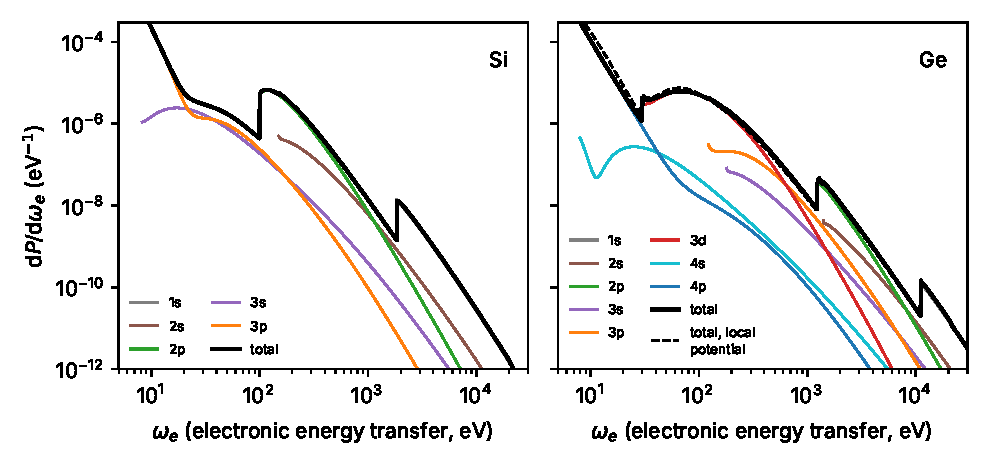
\includegraphics[width=\linewidth]{figures/ch12/fig12_2.pdf}
  \caption{Migdal ionization spectra of free silicon (left) and germanium (right) atoms at the recoil energy $E_R = \SI{1}{keV}$, per unit $\omega_e$ (electronic energy transfer), by initial shell (colors) and in total (black). Each shell is placed at $\omega_e = E_B + E_{\mathrm{ej}}$, its binding energy plus the kinetic energy of the ejected electron: measured binding energies of the core shells (\cref{sec:3.5}) and, for the valence shells, the measured first ionization energy of the atom, \SI{8.15}{eV} (Si) and \SI{7.90}{eV} (Ge), exact for the outer $p$ shell and a lower limit for the valence $s$ shell. Dipole-order Dirac--Hartree--Fock tables of Cox and collaborators~\cite{cox2023precise}, with the spin--orbit partners of each shell added, rescaled from $q_e = m_e\times10^{-3}$ to $q_e = m_e(2E_R/m_A)^{1/2}$, \SI{141}{eV} for silicon and \SI{88}{eV} for germanium. Dashed: total for germanium from the local-potential calculation of Ibe and collaborators~\cite{ibe2018migdal}, same rescaling. At other recoil energies every curve scales as $E_R$.}
  \label{fig:12-atoms}
\end{figure}

\begin{workedexample}{The Migdal probability of a germanium atom at \SI{1}{keV}}\label{we:12-germanium}
A germanium atom, $m_A = 72.630\,\mathrm{u} = \SI{67.654}{GeV}$, recoils with $E_R = \SI{1}{keV}$. Dark matter must be at least \SI{2.27}{GeV} to give it this energy at $v_{\mathrm{max}}$. The momentum transfer is $q = (2m_AE_R)^{1/2} = \SI{11.63}{MeV}$, the atom moves at $v_A = q/m_A = 1.72\times10^{-4}$, or \SI{51.5}{km.s^{-1}}, and each electron receives $q_e = m_ev_A = \SI{87.9}{eV}$, so that $q_ea_0 = v_A/\alpha = 0.024$. The tables of Ibe and collaborators are given at $q_e = m_e\times10^{-3} = \SI{511}{eV}$~\cite[Table~II]{ibe2018migdal}, and at dipole order we multiply them by $(87.9/511)^2 = 0.0296$.

The ionization probabilities are then $8.2\times10^{-4}$ from the $3d$ shell and $7.8\times10^{-4}$ from the $4p$ shell. The $3p$, $2p$ and $4s$ shells add $7.1\times10^{-5}$, $2.1\times10^{-5}$ and $1.8\times10^{-5}$, and the deeper shells less. The total is $1.73\times10^{-3}$: in this calculation one recoil in 580 ejects an electron. The shells with $n \le 3$ give $9.3\times10^{-4}$ of it. The table also lists transitions to bound orbitals. They add up to $8.75\times10^{-2}$ at the reference $q_e$, or $2.59\times10^{-3}$ at \SI{1}{keV}, more than the ionization, and the single transition $4s \to 4p$ gives $1.18\times10^{-3}$ of it. Every transition together has the probability $4.3\times10^{-3}$, one recoil in 230.

The sum rule \cref{eq:12.2-sums} checks the table. At the reference $q_e$ the exact first moment is $q_e^2N_e/2m_e = 32\times(\SI{511}{eV})^2/(2\times\SI{511}{keV}) = \SI{8.18}{eV}$. The ionization spectra, weighted with $\omega_e = E_B + E_{\mathrm{ej}}$ and the binding energies of the table, give \SI{7.28}{eV}, and the bound transitions, weighted with the differences of the tabulated level energies, \SI{0.63}{eV}. The tabulated transitions hold \SI{96.8}{\percent} of the moment; the rest lies in what the table omits, levels above $n' = 6$ and electrons faster than \SI{70}{keV}, and in the relativistic corrections to the nonrelativistic sum rule. At \SI{1}{keV} the moment is $(N_em_e/M)E_R = \SI{0.242}{eV}$, bound transitions included. Its ionization part, $\SI{7.28}{eV}\times0.0296 = \SI{0.215}{eV}$, carried by one event in 580, gives an ionizing event \SI{124}{eV} on average, and a $3d$ ionization \SI{135}{eV}.

Inside a germanium crystal the $3d$ shell keeps this probability. Its binding is \SI{29.4}{eV} below the valence maximum (\cref{sec:10.6}) where the table uses a computed \SI{35}{eV}, and the spectrum shifts with it. The valence part, $8.0\times10^{-4}$ of ionization and most of the bound transitions, does not carry over: in the crystal the $4s$ and $4p$ orbitals form the valence and conduction bands, $4s \to 4p$ is a transition across the gap, and \cref{sec:12.3} computes it from the loss function.
\end{workedexample}

\subsection{Core shells inside a crystal}\label{sec:12.2-cores}

\Cref{eq:12.2-joint} assumes three things that a crystal can violate: that the atom recoils freely, that it is isolated, and that the kick is over before the electrons respond.

\emph{Free recoil.} A nucleus bound in a lattice recoils like a free one once the recoil parameter $x_R = E_R/\langle\omega\rangle$ is large, above the impulse onset $x_R = 4$ of \cref{sec:11.4}: $q = \SI{92.5}{keV}$ and $E_R = \SI{164}{meV}$ in silicon, \SI{113}{keV} and \SI{95}{meV} in germanium. Above it the line $\omega_l = q^2/2m_A$ of \cref{eq:12.2-joint} becomes the impulse peak of \cref{eq:11.4-IA}, of relative width $x_R^{-1/2}$, $5\times10^{-3}$ at \SI{1}{keV} in germanium. The electronic factor is untouched. After the kick the neighbors pull the nucleus back on the time $1/\omega_{\mathrm{ph}}$, and the model of \cref{sec:6.1} found that this multiplies the excitation probability by $[1 - (\omega_{\mathrm{ph}}/\Delta E)^2]^{-2}$. For the germanium $3d$ shell, with the optical phonon of \SI{37.6}{meV} (\cref{tab:5-phonons}), the factor exceeds one by $3\times10^{-6}$, and for silicon $2p$ by $8\times10^{-7}$. Below the onset the lattice keeps the recoil in phonons, and the lattice factor is the multiphonon response of \cref{sec:12.4}.

\emph{Suddenness.} The kick lasts about as long as the dark matter takes to cross the nucleus, \SI{6e-21}{s} for germanium at $v_{\mathrm{max}}$ (\cref{sec:6.1}). Against the $3d$ excitation energy this is $\Delta E\,\tau_{\mathrm{acc}} = 3\times10^{-4}$, and for silicon $2p$ $7\times10^{-4}$, deep in the sudden region of \cref{fig:6-sudden}. The free atom needs no such condition, since \cref{eq:12.2-joint} is exact for it; in a crystal the condition is what lets the nucleus be treated as kicked first and decelerated afterward.

\emph{An isolated atom.} The electrons must move with their own nucleus and not with the crystal. A core orbital does. The silicon $2p$ shell has a mean radius of \SI{0.28}{\angstrom} and the germanium $3d$ shell \SI{0.39}{\angstrom}, against bonds of \SI{2.35}{\angstrom} and \SI{2.45}{\angstrom}. Their binding energies, \SI{99.5}{eV} (the spin--orbit centroid) and \SI{29.4}{eV} below the valence maximum, lie far below a valence band about \SI{12}{eV} wide. Such a shell forms a flat band whose orbitals are those of the atom, which first-principles calculations confirm for exactly these two shells (\cref{app:E.7}). The valence orbitals, of mean radius \SI{1.5}{\angstrom}, reach the neighbors, and their transitions become the band-to-band transitions of \cref{chap:10}. Their Migdal rate is the crystal formula of \cref{sec:12.3}, with the gap in place of the atomic binding. The atomic valence numbers above do not carry over: the crystal changes the valence channel by more than an order of magnitude (\cref{sec:12.3-atom}).

The mass that sets $q_e$ is $M_\kappa + \delta M_\kappa$, with the core electrons in $\delta M_\kappa$ exactly and the valence part a tensor (\cref{sec:8.6}), an effect of order $10^{-4}$. The largest correction is not in these three conditions but in the final state. Near its threshold the ejected core electron enters the conduction bands of the crystal and not the atomic continuum, and \cref{sec:10.6} found that the choice of final states changes the germanium $3d$ contribution to an electron-scattering rate by an order of magnitude near its opening. The atomic tables are reliable for core electrons ejected with tens of eV or more; within a few eV of the edge they are an estimate. With these provisos the core shells of a crystal take their Migdal probability from the atom, and \cref{sec:12.3} adds them to the valence rate.

\subsection{Excitation without ionization}\label{sec:12.2-excitation}

A kick can also leave an electron in an empty bound orbital. Kahlhoefer and Su proposed to detect this in superfluid helium, where an excited atom binds to a neighbor and the excimer emits an ultraviolet photon~\cite{kahlhoefer2026probing}. The first excited level of helium lies at \SI{20.6}{eV}, so a recoil far too weak to excite a neighbor by collision can still excite its own electrons. The probability is the sum of \cref{eq:12.2-joint} over the bound final states, and at dipole order, with the oscillator strengths \cref{eq:4.3-osc},
\begin{equation}
  P_{\mathrm{exc}} = q_e^2\sum_{f\,\mathrm{bound}}\bigl|\langle\Psi_f|D_{\hat q}|\Psi_0\rangle\bigr|^2 = \frac{q_e^2}{2m_e}\sum_{f\,\mathrm{bound}}\frac{f^{\mathrm{osc}}_{f0}}{E_f - E_0} .
  \label{eq:12.2-exc}
\end{equation}
The rate is \cref{eq:12.2-rate} with $\dd P/\dd\omega_e$ replaced by a sum of lines at the excitation energies, which is the form of Kahlhoefer and Su~\cite[Eq.~(6)]{kahlhoefer2026probing}. Only levels reached by the dipole operator appear: from the $1s^2$ ground state of helium, the $1snp\,{}^1P$ levels. With the measured oscillator strengths of these lines~\cite{kramida2024nist}, $0.276$ for $2\,{}^1P$ at \SI{21.22}{eV} and $0.073$ for $3\,{}^1P$ at \SI{23.09}{eV}, \cref{eq:12.2-exc} gives $P_{\mathrm{exc}} = 0.177\,(v_A/\alpha)^2$ for the first line, $0.220\,(v_A/\alpha)^2$ with the second, and $0.263\,(v_A/\alpha)^2$ with all lines up to the series limit at \SI{24.59}{eV}. A helium atom recoiling with \SI{10}{eV}, which dark matter of \SI{52}{MeV} can produce, has $v_A/\alpha = 0.010$ and is excited with probability $2.7\times10^{-5}$.

Any finite list of lines underestimates $P_{\mathrm{exc}}$, since every term of \cref{eq:12.2-exc} is positive; the first two helium lines hold \SI{84}{\percent} of it. A sharper statement compares the bound part with the ionization. Every bound level lies below the ionization energy $I$ and every continuum state above it. Weighting the oscillator strengths with $1/(E_f - E_0)$ therefore favors the bound part. Let $F_{\mathrm{exc}}$ and $F_{\mathrm{ion}}$ be the oscillator strength in the bound lines and in the continuum, and $P_{\mathrm{ion}} = P_{\mathrm{Mig}} - P_{\mathrm{exc}}$ the ionization probability. Then $P_{\mathrm{exc}} \ge q_e^2F_{\mathrm{exc}}/2m_eI$ and $P_{\mathrm{ion}} \le q_e^2F_{\mathrm{ion}}/2m_eI$, and
\begin{equation}
  \frac{P_{\mathrm{exc}}}{P_{\mathrm{ion}}} \ge \frac{F_{\mathrm{exc}}}{F_{\mathrm{ion}}} .
  \label{eq:12.2-bound}
\end{equation}
An estimate of the bound share from the oscillator strength alone, the share of the Thomas--Reiche--Kuhn sum \cref{eq:4.3-TRK} in the lines, is a lower bound. For hydrogen the lines hold 0.565 of the oscillator strength (\cref{sec:4.3}) but 0.717 of the dipole probability, of which the $2p$ level gives 0.555 and the levels with $n \le 3$ give 0.644.

\begin{limitbox}[Migdal excitation of bound final states][lim:12.2b]
A free atom recoiling with $q$ is left in the bound level $f$ with $P_f = |\langle\Psi_f|\exp(-\ii\vect{q}_e\cdot\sum_e\vect{\rho}_e)|\Psi_0\rangle|^2$, and the rate is the free-recoil rate times $\sum_fP_f\,\delta(\omega_e - E_f + E_0)$ over a list of levels~\cite[Eqs.~(1) and (6)]{kahlhoefer2026probing}; at dipole order this is \cref{eq:12.2-exc}.
\par\smallskip
{\centering
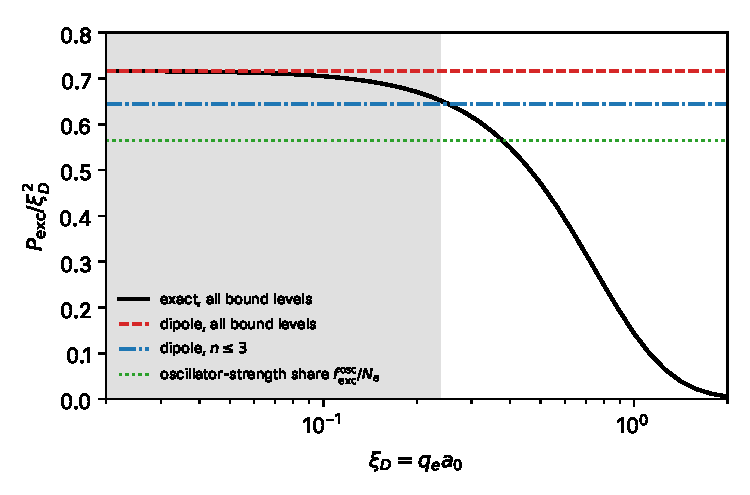
\includegraphics[width=\linewidth]{figures/ch12/limit12_2b.pdf}
\captionof{figure}{Probability that a kick leaves a hydrogen atom in a bound excited level, divided by $\xi_D^2 = (q_ea_0)^2$, against $\xi_D$. Solid: exact, the full boost and every bound level, from radial integrals with the spherical Bessel functions $j_\ell(q_er)$ for $n \le 40$ and $\ell \le 12$ and an $n^{-3}$ tail. Dashed: dipole order, all $np$ levels, 0.717. Dash-dotted: dipole order, levels with $n \le 3$ only, 0.644. Dotted: the bound share of the oscillator strength times the total dipole probability, 0.565, the lower bound \cref{eq:12.2-bound}. Gray: $\xi_D \le 0.24$, where the dipole sum over all levels is within \SI{10}{\percent} of the exact result.}\label{fig:12-limit-2b}
\par}
\smallskip
Beyond $\xi_D \approx 0.24$ the boost carries the electron more and more into the continuum, and the dipole sum overstates the bound probability, which falls to a fifth of it at $\xi_D = 1$.
\end{limitbox}

\noindent \Cref{lim:12.2b} sits at $n_B = 2$, $n_D = 2$, $\mathfrak{M}$ = sudden and $\mathcal{K}$ = impulse, as \cref{lim:12.2a} does. For dark matter lighter than \SI{1}{GeV} in helium, $\xi_D$ stays below 0.16, where the dipole sum for hydrogen is within \SI{4}{\percent} of the exact one; the finite list of lines, \SI{16}{\percent} short in helium, sets the larger error of the published estimate.

In germanium the bound transitions outnumber the ionizations. The table of \cref{we:12-germanium} lists $8.75\times10^{-2}$ in bound transitions against $5.86\times10^{-2}$ in ionization at the reference $q_e$, mostly $4s \to 4p$ and $4p \to 4d,\,5s$, and since the table stops at $n' = 6$ the true bound share is larger still. In a crystal these valence transitions do not exist as such. The bound final states of a crystal are excitons, whose lines below the pair continuum carry as much weight as the free pairs within $8E_x^b$ of the edge would (\cref{sec:10.5}). The Migdal entry \cref{eq:12.1-Skk} weights each final state with $\omega_e^{-4}$, which favors the lines below the edge for the same reason as \cref{eq:12.2-bound}. The exciton share of the Migdal spectrum is therefore at least the share of the lines in the electronic response near the edge. In silicon, with $E_x^b = \SI{14.7}{meV}$, and in germanium, whose indirect exciton is bound by about \SI{5}{meV}~\cite{macfarlane1957fine}, that share is negligible. In wide-gap crystals with binding energies of an eV and more it is not, and the lines are a separate, optically detectable signal (\cref{app:E.15}).

\section{The loss-function Migdal probability}\label{sec:12.3}

A dark-matter particle of \SI{300}{MeV} can give a silicon nucleus a momentum of \SI{1.6}{MeV} and a recoil energy of \SI{47}{eV}. The momentum is seven hundred times the size of the Brillouin zone, the recoil energy a thousand times that of a phonon, and the nucleus leaves its site as a free particle (\cref{sec:11.4}). The electrons it sets in motion take a momentum of a few keV, and half of the time they receive less than \SI{4.6}{eV}, a few times the gap. In this regime the Migdal entry \cref{eq:12.1-Skk} of the joint response simplifies twice. The lattice factor collapses to a free recoil, and the electronic factor becomes the loss function $L(\vect{p},\omega_e)$ that \cref{sec:10.2} used for the electron-recoil rate. The probability that a kick leaves an electron--hole pair is then fixed by one material function, an integral of $L$ over momenta weighted by $\omega_e^{-4}$, and it comes out thirty times larger in crystalline silicon than in a silicon atom. The same function sets the rate per unit target mass, which \cref{sec:17.5} uses to compare materials.

\subsection{Migdal probability through the loss function}\label{sec:12.3-soft}

Three approximations take \cref{eq:12.1-Skk} to the loss function: the diagonal $\vect{G} = \vect{G}'$ of the electronic factor, a free recoil, and the soft limit $p \ll q$. On the diagonal the integral over the zone and the sum over $\vect{G}$ then combine into one integral over the unreduced momentum $\vect{p} = \vect{k} + \vect{G}$ given to the electrons. By \cref{eq:4.4-SL}, with the diagonal inverse dielectric matrix \cref{eq:E.6-L}, the diagonal element of the density response at $\vect{p}$ is the loss function at that momentum:
\begin{equation}
  S^{ee}_{\vect{G}\vect{G}}(\vect{k},\omega_e) = \frac{2p^2}{e^2}\,L(\vect{p},\omega_e) , \qquad \omega_e > 0,\; T \ll \Eg .
  \label{eq:12.3-See}
\end{equation}
The local fields on the diagonal stay inside $L$; the dropped elements $\vect{G} \ne \vect{G}'$ carry the part of the local fields that couples different momenta, and we return to both parts of the local fields below. The free recoil treats each nucleus as if it were alone and in the impulse regime, so that the lattice factor is the free recoil of \cref{sec:11.4} at the momentum $\vect{q} - \vect{p}$ the nucleus keeps, $S^{\mathrm{ad}}_{\kappa}(\vect{q} - \vect{p},\omega_l) = 2\pi\nd_\kappa\,\delta(\omega_l - |\vect{q} - \vect{p}|^2/2M_\kappa)$. The \emph{soft limit} $p \ll q$ says that the electrons take a small part of the momentum. The lattice factor then becomes $2\pi\nd_\kappa\,\delta(\omega_l - E_R)$ with $E_R = q^2/2M_\kappa$, and it no longer depends on $\vect{p}$. The Migdal entry then factorizes into the free recoil and a probability per kick,
\begin{equation}
  S_{\kappa\kappa}(\vect{q};\omega_l,\omega_e) = 2\pi\nd_\kappa\,\delta(\omega_l - E_R)\,\frac{\dd P_{\mathrm{Mig}}}{\dd\omega_e} .
  \label{eq:12.3-factor}
\end{equation}

The vertex is the potential of the moving ion. In silicon the ten electrons of the $1s$, $2s$ and $2p$ shells are bound by \SI{100}{eV} or more and follow their nucleus; for the valence electrons whose response is $L$, nucleus and core act together as one ion. The potential of this ion is
\begin{equation}
  v_\kappa(\vect{p}) = -\frac{Z_{\mathrm{ion}}(p)\,e^2}{p^2} , \qquad Z_{\mathrm{ion}}(p) = Z_\kappa - f^{\mathrm{core}}_\kappa(p) ,
  \label{eq:12.3-Zion}
\end{equation}
with $f^{\mathrm{core}}_\kappa(p)$ the form factor of the core electrons, the Fourier transform of their density. \Cref{eq:12.3-Zion} defines the \emph{valence ionization factor} $Z_{\mathrm{ion}}(p)$. At small $p$ it is the ionic charge, 4 for silicon; at large $p$ the probe resolves the core and $Z_{\mathrm{ion}}$ rises toward the nuclear charge 14. With the core orbitals of the free atom from \cref{sec:3.5}, $Z_{\mathrm{ion}}$ of silicon exceeds 4 by \SI{5}{\percent} at \SI{2.4}{keV} and by \SI{10}{\percent} at \SI{3.4}{keV}, and reaches 4.84 at \SI{5}{keV} and 6.78 at \SI{10}{keV}. The split between core and valence is a convention, and $Z_{\mathrm{ion}}$ must count exactly the electrons that $L$ leaves out.

When \cref{eq:12.3-See,eq:12.3-Zion} and the lattice factor are inserted in \cref{eq:12.1-Skk}, the factors combine as
\begin{equation*}
  \frac{1}{2\pi}\,\frac{(\vect{q}\cdot\vect{p})^2}{M_\kappa^2\omega_e^4}\,\frac{Z_{\mathrm{ion}}^2e^4}{p^4}\,\frac{2p^2}{e^2}\,L\;2\pi\nd_\kappa
  = 2\pi\nd_\kappa\,\frac{e^2}{\pi}\,\frac{Z_{\mathrm{ion}}^2(\vect{v}_N\cdot\vect{p})^2}{\omega_e^4\,p^2}\,L ,
\end{equation*}
with $\vect{v}_N = \vect{q}/M_\kappa$ the recoil velocity of \cref{sec:6.1}. Since $e^2/\pi = 4\alpha$, comparison with \cref{eq:12.3-factor} gives the result.
\begin{keyresult}[The crystal Migdal probability in the soft limit]
For a kick of momentum $\vect{q}$ in the impulse regime, with $p \ll q$, the probability per unit electronic energy that a nucleus of species $\kappa$ leaves the valence electrons excited is
\begin{equation}
  \frac{\dd P_{\mathrm{Mig}}}{\dd\omega_e} = 4\alpha\int\frac{\dd^3p}{(2\pi)^3}\;Z_{\mathrm{ion}}(p)^2\,\frac{(\vect{v}_N\cdot\vect{p})^2}{\omega_e^4\,p^2}\,L(\vect{p},\omega_e)
  = \frac{4\alpha v_N^2}{3\,\omega_e^4}\,L_{\mathrm{Mig}}(\omega_e) ,
  \label{eq:12.3-soft}
\end{equation}
where the second form holds for a direction-averaged loss function and defines the Migdal-weighted loss function
\begin{equation}
  L_{\mathrm{Mig}}(\omega_e) = \int\frac{\dd^3p}{(2\pi)^3}\;Z_{\mathrm{ion}}(p)^2\,\bar L(p,\omega_e) .
  \label{eq:12.3-LMig}
\end{equation}
\end{keyresult}
\noindent This is the formula of Knapen, Kozaczuk and Lin~\cite[Eq.~(6)]{knapen2021migdal}. Read as a product, it is the probability of a dipole boost, $v_N^2$, times the response of the electrons to the field of a charge $Z_{\mathrm{ion}}$ that has suddenly started to move. The screening and the local fields of \cref{sec:10.2} enter here unchanged. The factor $\omega_e^{-4}$ is the square of the boost denominator $\omega_e^2$ of \cref{eq:12.1-amp}. With $v_N^2 = 2E_R/M_\kappa$ the probability grows linearly with the recoil energy, and the material enters only through $L_{\mathrm{Mig}}$.

For silicon we evaluate \cref{eq:12.3-soft} with the loss function of Knapen, Kozaczuk and Lin with local fields~\cite{knapen2021dark}, which is the table of \cref{sec:10.2}. We count the table from \SI{1.11}{eV}, the step-model gap that accompanies it, rather than from its scissor gap, the physical \SI{1.17}{eV}; the table stops at \SI{89}{eV} and \SI{22.5}{keV}. At $E_R = \SI{100}{eV}$, reached at $q = \SI{2.29}{MeV}$ with $v_N = 8.74\times10^{-5}$ (\SI{26}{km/s}), the probability is $P_{\mathrm{Mig}} = 6.1\times10^{-3}$, or $6.1\times10^{-5}$ per eV of recoil energy. Half of the probability lies below $\omega_e = \SI{4.6}{eV}$ and \SI{89}{\percent} below \SI{10}{eV}; the mean is \SI{6.0}{eV}. The momenta are larger than the zone: the median $p$ is \SI{5.7}{keV}, two and a half times $q_{\mathrm{BZ}}$ of \cref{eq:11.1-qBZ}, and \SI{97}{\percent} of the probability comes from $p > q_{\mathrm{BZ}}$. The plasmon, at $p \lesssim \SI{2.5}{keV}$, carries \SI{4}{\percent}: the factor $\omega_e^{-4}$ favors the single-pair continuum near the gap over the plasmon at \SI{17}{eV}. With a point ion of charge 4 instead of $Z_{\mathrm{ion}}(p)$ the probability falls to $3.9\times10^{-3}$, lower by a factor 1.57.

\begin{workedexample}{The coefficient $4\alpha$ from the f-sum}\label{we:12-fsum}
The coefficient of \cref{eq:12.3-soft} can be checked without the diagrams of \cref{eq:12.1-Skk}, from a sum rule. Take one Fourier component $\vect{p}$ of the force of the ion, $F_{\vect{p}} = \vect{v}_N\cdot\nabla_{\vect{X}}V_{eN}$ restricted to that component. By \cref{eq:12.1-force} it is $-\ii(\vect{v}_N\cdot\vect{p})\,v_\kappa(\vect{p})\,n_e(\vect{p})/\Vol$ up to a phase, and the Migdal amplitude to a final state $j$ is $\langle\Psi_j|F_{\vect{p}}|\Psi_0\rangle/\Delta E_j^2$. The fifth moment of the probability weighs each final state with $\Delta E_j^5$ and therefore equals the energy-weighted sum $\sum_j\Delta E_j|\langle\Psi_j|F_{\vect{p}}|\Psi_0\rangle|^2$. For the density operator this sum is the f-sum rule \cref{eq:4.3-fsum}, $\sum_j\Delta E_j|\langle\Psi_j|n_e(\vect{p})|\Psi_0\rangle|^2 = N_ep^2/2m_e$ at $T = 0$, which holds for the interacting electrons exactly. Per unit volume the fifth moment is therefore
\begin{equation*}
  (\vect{v}_N\cdot\vect{p})^2\,|v_\kappa(\vect{p})|^2\,\frac{\nd_e\,p^2}{2m_e} = (\vect{v}_N\cdot\vect{p})^2\,\frac{Z_{\mathrm{ion}}^2e^4}{p^4}\,\frac{\nd_e\,p^2}{2m_e} .
\end{equation*}
The loss-function form with an unknown coefficient $c$ in place of $4\alpha$ gives instead, with the f-sum of the loss function $\int_0^\infty\dd\omega\,\omega L = (\pi/2)\omega_p^2$ (\cref{eq:10.2-moments}) and $\omega_p^2 = e^2\nd_e/m_e$,
\begin{equation*}
  c\,Z_{\mathrm{ion}}^2\,\frac{(\vect{v}_N\cdot\vect{p})^2}{p^2}\int_0^\infty\dd\omega\,\omega L = c\,Z_{\mathrm{ion}}^2\,\frac{(\vect{v}_N\cdot\vect{p})^2}{p^2}\,\frac{\pi}{2}\,\frac{e^2\nd_e}{m_e} .
\end{equation*}
The two fifth moments agree if $c = e^2/\pi = 4\alpha$, at every $\vect{p}$ and for any electron density.

For silicon the check also measures the table. At the valence density, $\nd_e = \SI{2.00e23}{cm^{-3}}$ and $\omega_p^{\mathrm{val}} = \SI{16.6}{eV}$, the table holds 0.94, 0.93, 0.92 and 0.90 of the f-sum at $p = 1$, 2, 3 and \SI{5}{keV}, so the fifth moment of the computed spectrum is within \SI{10}{\percent} of its exact value there. At \SI{7.5}{keV} the table holds 0.62 and at \SI{10}{keV} only 0.17, because the free-electron peak $p^2/2m_e$ moves past the table's last energy of \SI{89}{eV}. The probability is far less sensitive than the fifth moment, since $\omega_e^{-4}$ weights the low energies the table does contain. The momenta above \SI{10}{keV} give \SI{2.3}{\percent} of $P_{\mathrm{Mig}}$, and an upper bound on the energies beyond the table follows from the same sum rule, $\int_{\omega_{\mathrm{top}}}^\infty\dd\omega\,L/\omega^4 \le (\pi/2)\omega_p^2/\omega_{\mathrm{top}}^5$. At $\omega_{\mathrm{top}} = \SI{89}{eV}$, summed over the momenta of the table, the bound is \SI{1.6}{\percent} of the probability below $\omega_{\mathrm{top}}$.
\end{workedexample}

The material input of \cref{eq:12.3-soft} is the loss function of the valence electrons at momenta up to about \SI{20}{keV}, where the Migdal weight ends, and energies from the gap to about \SI{50}{eV}. At these momenta the calculation needs the diagonal elements far from the head; \cref{sec:10.2} met the same requirement for electron recoil. An all-electron calculation of $L$ at $p \le \SI{30}{keV}$ removes the need for $Z_{\mathrm{ion}}$ and puts the core shells in the same table. The random-phase loss function does not contain the Migdal lines of excitons below the gap.

\subsection{Validity of the soft limit}\label{sec:12.3-validity}

Knapen and collaborators state \cref{eq:12.3-soft} with the scalar dielectric function $\varepsilon(\vect{p},\omega)$ and note that it holds only for $\vect{p}$ in the first zone~\cite[text after Eq.~(6)]{knapen2021migdal}. Inside the zone the scalar function is the macroscopic one, and the loss function is the head of the inverse matrix. Outside it, a scalar function of $|\vect{p}|$ has no unique meaning, and the derivation above says which element to take: the diagonal element of the inverse at the reciprocal vector that contains $\vect{p}$. The distinction matters because the Migdal weight lies outside the zone. \Cref{lim:12.3a} compares, momentum by momentum, the loss function that a scalar random-phase $\varepsilon$ gives with the diagonal element of the inverse with local fields. The two agree within \SI{10}{\percent} up to $p = 1.3\,q_{\mathrm{BZ}} = \SI{2.9}{keV}$, which holds \SI{8}{\percent} of the probability. Beyond, the scalar function overestimates the weight by \SI{24}{\percent} at $2q_{\mathrm{BZ}}$ and \SI{35}{\percent} at $3q_{\mathrm{BZ}}$, where the probability peaks, and the total by a factor 1.35. The mechanism is the one of \cref{sec:10.2}: at $|\vect{p}| \approx 2$--$3\,|\vect{G}_{111}|$ the charge induced in the cell has a macroscopic component that screens the field of the ion.
\begin{limitbox}[Crystal Migdal effect through the loss function][lim:12.3a]
$\dd P/\dd\omega = 4\alpha\int\dd^3p/(2\pi)^3\,Z_{\mathrm{ion}}(p)^2|\vect{v}_N\cdot\vect{p}|^2\,\Imag[-1/\varepsilon(\vect{p},\omega)]/(\omega^4p^2)$ with a scalar dielectric function, for $\vect{p}$ in the first zone~\cite[Eq.~(6)]{knapen2021migdal}.
\par\smallskip
{\centering
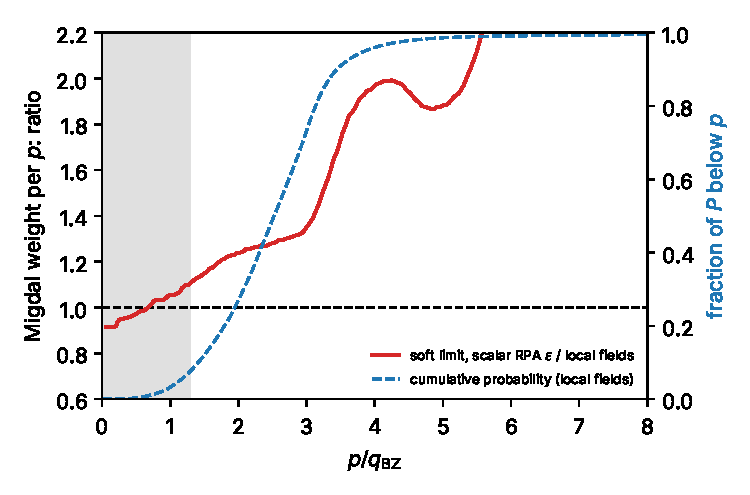
\includegraphics[width=\linewidth]{figures/ch12/limit12_3a.pdf}
\captionof{figure}{Migdal weight of silicon per unit momentum $p$ given to the electrons, $p^2Z_{\mathrm{ion}}(p)^2\int_{\Eg}\dd\omega\,L(p,\omega)/\omega^4$, from the loss function of a scalar random-phase dielectric function at $|\vect{p}|$ (no local fields), divided by the same with the diagonal element of the inverse dielectric matrix with local fields, against $p/q_{\mathrm{BZ}}$ ($q_{\mathrm{BZ}} = \SI{2.25}{keV}$). Both from the direction-averaged tables of Knapen, Kozaczuk and Lin~\cite{knapen2021dark} (threshold \SI{1.11}{eV}, the step-model gap that accompanies them, $\omega \le \SI{89}{eV}$), smoothed over \SI{0.7}{keV} in $p$; $Z_{\mathrm{ion}}(p)$ of \cref{eq:12.3-Zion}. The elements $\vect{G} \neq \vect{G}'$ are in neither curve. Dashed, right axis: the fraction of $P_{\mathrm{Mig}}$ carried by momenta below $p$. Gray band: $p \le 1.3\,q_{\mathrm{BZ}}$, where the two agree within \SI{10}{\percent}; it holds \SI{8}{\percent} of the probability.}\label{fig:12-limit-3a}
\par}
\smallskip
Beyond the first zone the scalar form has to be replaced by the diagonal of the inverse dielectric matrix, and the local fields lower the silicon probability by a factor 1.35; the elements $\vect{G} \neq \vect{G}'$ are the next correction.
\end{limitbox}

The elements $\vect{G} \neq \vect{G}'$ keep the full matrix in \cref{eq:12.1-Skk}. For a direction-averaged target the boost factor averages to $\langle[\hat{\vect{q}}\cdot(\vect{k}+\vect{G})][\hat{\vect{q}}\cdot(\vect{k}+\vect{G}')]\rangle = (\vect{k}+\vect{G})\cdot(\vect{k}+\vect{G}')/3$. At the random-phase level the response matrix is $S^{ee}_{\vect{G}\vect{G}'} = (2|\vect{k}+\vect{G}||\vect{k}+\vect{G}'|/e^2)\,\Imag[-(\tilde\varepsilon^{-1})_{\vect{G}\vect{G}'}]$, with the symmetrized matrix $\tilde\varepsilon_{\vect{G}\vect{G}'} = \delta_{\vect{G}\vect{G}'} - v_{\mathrm{C}}^{1/2}(\vect{k}+\vect{G})\,R^0_{\vect{G}\vect{G}'}(\vect{k},\omega)\,v_{\mathrm{C}}^{1/2}(\vect{k}+\vect{G}')$, which has the same inverse diagonal as $\varepsilon$. In a crystal with time reversal and inversion it is symmetric, $\tilde\varepsilon_{\vect{G}\vect{G}'} = \tilde\varepsilon_{\vect{G}'\vect{G}}$, but not Hermitian at frequencies where the crystal absorbs; $\Imag[-(\tilde\varepsilon^{-1})_{\vect{G}\vect{G}'}]$ denotes the anti-Hermitian part $[(\tilde\varepsilon^{-1})^\dagger - \tilde\varepsilon^{-1}]_{\vect{G}\vect{G}'}/2\ii$, which for a symmetric matrix is the imaginary part element by element. With a constant ion charge, $L_{\mathrm{Mig}}$ of \cref{eq:12.3-LMig} becomes
\begin{equation}
  \begin{aligned}
  L_{\mathrm{Mig}}(\omega) &= \frac{Z_{\mathrm{ion}}^2}{\Omega}\,\mathcal{F}_{\mathrm{Mig}}(\omega) , \\
  \mathcal{F}_{\mathrm{Mig}}(\omega) &= \sum_{\vect{G}\vect{G}'}\int_{\mathrm{BZ}}\frac{\Omega\,\dd^3k}{(2\pi)^3}\,\frac{(\vect{k}+\vect{G})\cdot(\vect{k}+\vect{G}')}{|\vect{k}+\vect{G}|\,|\vect{k}+\vect{G}'|}\,\ee^{\ii(\vect{G}-\vect{G}')\cdot\vect{\tau}_\kappa}\,\Imag\bigl[-(\tilde\varepsilon^{-1})_{\vect{G}\vect{G}'}(\vect{k},\omega)\bigr] ,
  \end{aligned}
  \label{eq:12.3-FL}
\end{equation}
where $\vect{\tau}_\kappa$ is the position of the struck nucleus in the cell, averaged over the equivalent sites of its species. The indices are in the order of $S^{ee}_{\vect{G}\vect{G}'}$ in \cref{eq:12.1-Skk}, with $n_e(\vect{k}+\vect{G})^\dagger$ on the left of $R^0_{\vect{G}\vect{G}'}$; the transposed order reverses the sign of the phase. The reversal leaves silicon unchanged, since its two sites are images under inversion, but not GaAs. The phase belongs to the struck nucleus: the off-diagonal elements depend on where the origin of $\varepsilon$ is placed, and the phase is one only when the origin sits on that atom. The diagonal terms carry no phase and give back \cref{eq:12.3-LMig} at any origin. The off-diagonal terms need the full matrix, which the tables of \cref{sec:10.2} do not contain. In an empirical-pseudopotential random-phase model of silicon, with the phase of \cref{eq:12.3-FL}, the full matrix exceeds the diagonal form on the total by a factor of 1.38 with $8^3$ points $\vect{k}$ and $|\vect{G}|^2 \le 19\,(2\pi/a)^2$ and of about 1.2 when extrapolated in both. The two numbers are not a bracket: the factor still falls as reciprocal-lattice vectors are added, and the fall is not slowing, so 1.2 is not a lower bound. The off-diagonal elements raise the rate at every truncation computed, and the factor is flat in $\mchi$. The model carries only about two thirds of the diagonal local-field effect of \cref{lim:12.3a}, so its off-diagonal size is a guide, not a bound in either direction. The full local-field calculation that would replace the model estimate is open.

The free recoil is the second approximation. Below the impulse onset of \cref{sec:11.4}, $x_R = 4$ at $q = \SI{92.5}{keV}$ in silicon, the lattice takes the recoil as single phonons and multiphonons, not as a free particle. In the soft limit, however, the lattice factor drops out of the probability. It enters the rate only through the energy balance $\omega = \omega_e + \omega_l$ in $\vmin$, and the lattice energy has the mean $E_R$ in every regime (\cref{eq:5.6-sum}) and is small against $\omega_e$: \SI{0.16}{eV} at the onset, against a few eV. Replacing the free recoil by the incoherent response of a bound silicon nucleus at all phonon orders, including its zero-phonon line, changes the rate by less than $10^{-5}$ at every mass from 3 to \SI{110}{MeV} (\cref{lim:12.3b}). The impulse onset is therefore not where the Migdal formula fails.

Dropping $\vect{p}$ from the lattice factor, the soft limit as defined above, leaves the electronic spectrum unchanged, because the lattice factor has unit weight at every $\vect{q} - \vect{p}$ (\cref{sec:12.4}). The boost amplitude remains to be examined, and it expands in $v_Np/\omega_e$, not in $p/q$. For a free nucleus the kick and the Coulomb exchange with the electrons come in two time orderings~\cite[Eq.~(1)]{liang2021describing}. Kicked first, the nucleus moves with $\vect{q}$, passes $\vect{p}$ to the electrons and leaves with $\vect{q} - \vect{p}$; the energy denominator is $\omega_e - b + a$, with $b = \vect{q}\cdot\vect{p}/M_\kappa$ and $a = p^2/2M_\kappa$. With the exchange first, the nucleus recoils with $-\vect{p}$ before the kick, and the denominator is $\omega_e + a$. The boost factor $(\vect{v}_N\cdot\vect{p})/\omega_e^2$ becomes
\begin{equation}
  \frac{1}{\omega_e - b + a} - \frac{1}{\omega_e + a} = \frac{b}{(\omega_e - b + a)(\omega_e + a)} = \frac{b}{\omega_e^2}\Bigl(1 + \frac{b - 2a}{\omega_e} + \cdots\Bigr) ,
  \label{eq:12.3-bracket}
\end{equation}
the free-nucleus case of \cref{eq:12.4-exact}. The numerator of \cref{eq:12.3-bracket} is $\vect{q}\cdot\vect{p}/M_\kappa$ at every $p$: the velocity in the boost is that of the kicked nucleus, whatever momentum the electrons take. Averaged over the angle $c$ between $\vect{q}$ and $\vect{p}$, the square gives
\begin{equation*}
  \Bigl\langle\frac{b^2}{(\omega_e - b + a)^2(\omega_e + a)^2}\Bigr\rangle = \frac{v_N^2p^2}{3\omega_e^4}\Bigl[1 - \frac{2p^2}{M_\kappa\omega_e} + \frac95\,\frac{v_N^2p^2}{\omega_e^2} + \cdots\Bigr] ,
\end{equation*}
the free-nucleus part of \cref{eq:12.4-corr}. The terms odd in $c$ drop out; in a crystal they drop out because the loss function is even under $\vect{p} \to -\vect{p}$ in any target with time reversal. There is no term in $p/q$, so the soft limit does not fail when the electrons take a momentum comparable with the kick. The recoil term $2p^2/M_\kappa\omega_e$ is $2\times10^{-3}$ at the median $p$ near the gap. The Doppler term $\tfrac95v_N^2p^2/\omega_e^2$ grows with the recoil energy; it is the shift $\vect{v}_N\cdot\vect{p}$ of the electronic energy by the moving nucleus, taken at second order. Weighted with the silicon spectrum, the Doppler term is 0.04 at $E_R = \SI{100}{eV}$, 0.13 at \SI{300}{eV} and 0.42 at \SI{1}{keV}. It is only the leading term. Near the gap $v_Np/\omega_e$ is already 0.41 at the median $p$ and $E_R = \SI{100}{eV}$, and the higher orders of \cref{eq:12.3-bracket} add as much again. With the exact bracket the soft-limit probability is low by the factor 0.93 at \SI{100}{eV}, 0.79 at \SI{300}{eV} and 0.62 at \SI{500}{eV}, whereas the leading term alone gives 0.96, 0.90 and 0.85. The soft limit holds within \SI{10}{\percent} up to $E_R \approx \SI{160}{eV}$, the spectrum-weighted counterpart of the bound $v_Np/\omega_e \le 0.27$ found near the gap at fixed $p$ in \cref{lim:12.4a}. Toward \SI{1}{keV} the expansion breaks down. There $v_Np$ at the median momentum is \SI{1.6}{eV}, above the gap, and the denominator $\omega_e - b + a$ vanishes inside the range of the integral: the kicked nucleus, already moving, ionizes the electrons as a slow ion does. Ionization by the already moving nucleus is an on-shell two-step process, the electronic stopping of the recoiling ion, not a Migdal transition, and the second-order amplitude does not describe it. The momenta where the denominator vanishes hold \SI{0.9}{\percent} of the soft-limit probability at \SI{500}{eV} and \SI{3.7}{\percent} at \SI{1}{keV}.
\begin{limitbox}[Crystal Migdal rate with free recoil][lim:12.3b]
$\mathcal{R} = (\rho_\chi/\mchi)\,[2A^2\sigma_p\,Z_{\mathrm{ion}}^2\,\alpha N_T/(3\mu_{\chi n}^2\Omega M^2)]\int\dd^3v\,(f/v)\int p_N^3\,\dd p_N\int\dd\omega\,\omega^{-4}\,\Theta(v - \vmin)\,\mathcal{F}_{\mathrm{Mig}}(\omega)$, $\vmin = p_N/2\mu_{\chi N} + \omega/p_N$, with $N_T$ the number of nuclei per unit target mass, $\Omega$ the cell volume, $p_N$ the momentum transfer, the soft-limit amplitude and $\mathcal{F}_{\mathrm{Mig}}$ of \cref{eq:12.3-FL}~\cite[Eqs.~(1), (7), (11), (12)]{liang2021describing}.
\par\smallskip
{\centering
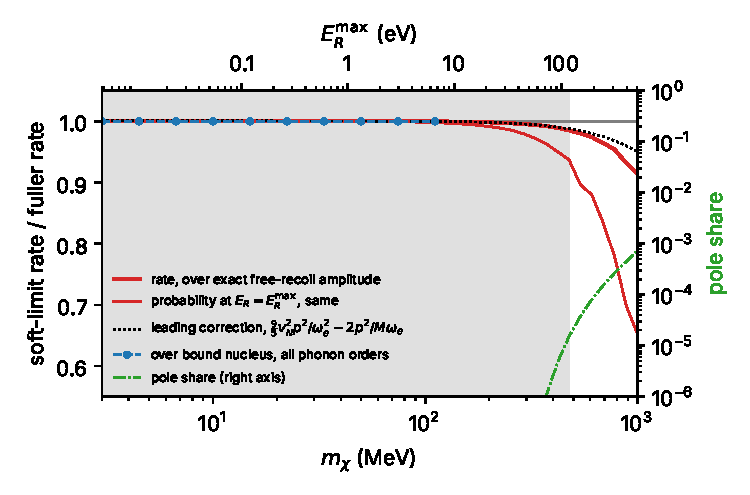
\includegraphics[width=\linewidth]{figures/ch12/limit12_3b.pdf}
\captionof{figure}{Total Migdal rate of silicon ($\omega_e \ge \SI{1.11}{eV}$, heavy mediator) in the soft limit with a free recoil, divided by two fuller results, against the dark-matter mass; top axis, the largest recoil energy $E_R^{\max} = 2\mu_{\chi N}^2v_{\mathrm{max}}^2/M$. Thick solid: over the rate with the exact free-recoil amplitude \cref{eq:12.3-bracket}. Thin solid: the same ratio for the probability at $E_R = E_R^{\max}$, the end of the recoil spectrum. Dotted: the leading correction $\frac95v_N^2p^2/\omega_e^2 - 2p^2/M_\kappa\omega_e$ alone. Dashed with points: over the soft-limit rate with the incoherent response of a bound nucleus at all phonon orders and $T = 0$ (density of states of \cref{sec:5.2}); it differs from one by less than $10^{-5}$. Dash-dotted, right axis: the share of the soft-limit rate at momenta where the exact amplitude has a pole, $v_Np \ge \omega_e + p^2/2M_\kappa$, which both rates of the ratio leave out. Every curve uses the same diagonal loss function with local fields and $Z_{\mathrm{ion}}(p)$ in place of $\mathcal{F}_{\mathrm{Mig}}$, and the halo of \cref{sec:1.2}. Gray band: $\mchi \lesssim \SI{0.5}{GeV}$, where the probability at the end of the recoil spectrum is within \SI{10}{\percent} of the exact one.}\label{fig:12-limit-3b}
\par}
\smallskip
Above about \SI{0.5}{GeV} the end of the recoil spectrum passes $E_R \approx \SI{160}{eV}$, where the motion of the nucleus during the electronic transition changes the probability by more than \SI{10}{\percent}, and near \SI{1}{keV} the moving nucleus ionizes the electrons by itself; the binding of the nucleus changes the soft-limit rate by less than $10^{-5}$ at every mass from 3 to \SI{110}{MeV}.
\end{limitbox}

\noindent From 3 to \SI{150}{MeV} the soft-limit rate is within $1.1\times10^{-3}$ of the exact free-recoil rate, and at \SI{1}{GeV}, where the rate integrates over the whole recoil spectrum, it is low by the factor 0.91.

Below the onset the bound amplitude of \cref{sec:12.4} stays within a few parts in $10^3$ of the soft limit (\cref{eq:12.4-corr}). At low mass, therefore, neither the soft limit nor the lattice limits the formula; the electronic factor does (\cref{lim:12.3a}).

The core shells stay frozen in $Z_{\mathrm{ion}}$. Their own excitation is a separate Migdal process of atomic type, with the boost of each core shell (\cref{sec:12.2}). The $2p$ shell of an isolated silicon atom gives $7.1\times10^{-5}$ at $E_R = \SI{100}{eV}$, \SI{1.2}{\percent} of the valence probability, at $\omega_e$ above \SI{100}{eV}. And the formula needs no restriction to $\mchi \ll M_\kappa$: the reduced mass $\mu_{\chi N}$ in $\vmin$ keeps the recoil of a heavy particle, and only the per-mass form below drops it.

\subsection{Crystal and atomic spectra of silicon}\label{sec:12.3-atom}

The crystal formula and the atomic formula of \cref{sec:12.2} answer the same question for the same nucleus, and they differ by more than an order of magnitude. \Cref{fig:12-crystal-atom} shows both at $E_R = \SI{100}{eV}$. The crystal probability is $6.1\times10^{-3}$. The isolated silicon atom, with all its shells and the Dirac--Hartree--Fock tables of Cox and collaborators~\cite{cox2023precise}, gives $2.1\times10^{-4}$, of which $1.3\times10^{-4}$ come from the $3s$ and $3p$ valence shells. The crystal is 29 times the whole atom and 47 times its valence shells.

\begin{figure}[tbp]
  \centering
  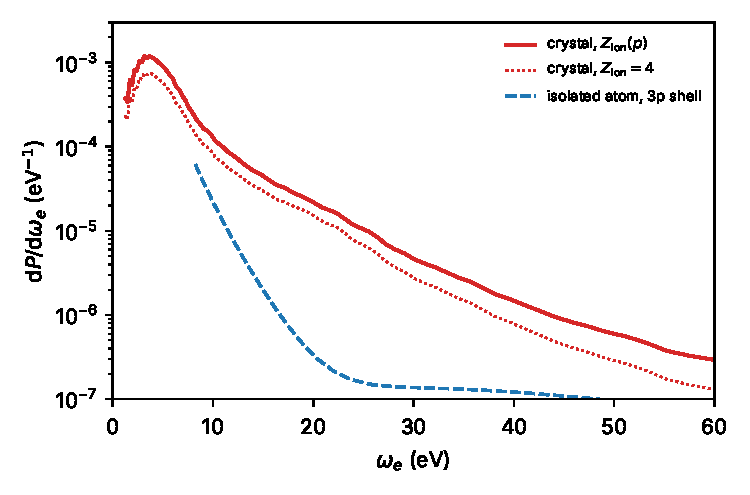
\includegraphics[width=0.75\linewidth]{figures/ch12/fig12_3.pdf}
  \caption{Migdal ionization spectra of silicon at the recoil energy $E_R = \SI{100}{eV}$ ($v_N = 8.74\times10^{-5}$), against the energy $\omega_e$ given to the electrons. Solid: the crystal, \cref{eq:12.3-soft}, with the loss function of Knapen, Kozaczuk and Lin with local fields (diagonal, direction-averaged, threshold \SI{1.11}{eV}, the step-model gap that accompanies the tables) and $Z_{\mathrm{ion}}(p)$ of \cref{eq:12.3-Zion}; $P_{\mathrm{Mig}} = 6.1\times10^{-3}$. Dotted: the same with a point ion, $Z_{\mathrm{ion}} = 4$; $3.9\times10^{-3}$. Dashed: the $3p$ shell of an isolated atom at dipole order, from the Dirac--Hartree--Fock tables of Cox, Dolan, McCabe and Quiney~\cite{cox2023precise} rescaled by $v_N^2$, with $\omega_e$ the kinetic energy of the electron plus the measured ionization energy of the atom, \SI{8.15}{eV}; $1.2\times10^{-4}$. The atomic $3s$ ($1.0\times10^{-5}$) and the core shells ($8\times10^{-5}$, nearly all $2p$ above \SI{100}{eV}) are not drawn.}
  \label{fig:12-crystal-atom}
\end{figure}

The ratio of the crystal to the atomic probability can be read off the figure. The crystal threshold is lower: the crystal spectrum starts at the gap, \SI{1.1}{eV}, the atomic one at the ionization energy of \SI{8.15}{eV}, and with the weight $\omega_e^{-4}$ the region between the two thresholds holds \SI{84}{\percent} of the crystal probability. Above \SI{8}{eV} the crystal is still larger, six times at \SI{10}{eV} and sixty times at \SI{20}{eV}. There the crystal spectrum acts as a loss function, which concentrates the oscillator strength of the valence electrons in the plasmon and the broad interband peak around it, between 10 and \SI{25}{eV}; the atom has only the tail of its $3p$ continuum there. The vertex differs too. The atom is boosted with all its electrons, and the boost probes each orbital at the momentum $q_e = m_ev_N$, \SI{45}{eV} at $E_R = \SI{100}{eV}$, far below the inverse size of any shell. The crystal formula probes the valence electrons at the momenta $p$ of the ion's field, mostly 3 to \SI{9}{keV}, where $Z_{\mathrm{ion}}(p)$ adds the factor 1.6 of the point-ion comparison.

None of the three differences makes the atom a lower bound on the crystal in general. A crystal with a gap larger than the ionization energy of its atoms would not show the first difference, and one with valence electrons as localized as atomic ones would not show the second.

\subsection{The Migdal rate per unit mass}\label{sec:12.3-rate}

The rate follows from the free-recoil spectrum \cref{eq:11.4-LS} by weighting each recoil with its Migdal probability. A recoil of momentum $q$ that also gives the electrons $\omega_e$ needs the minimum speed \cref{eq:1.3-vmin} at $\omega = \omega_e + q^2/2M_\kappa$, which is $\vmin = \omega_e/q + q/2\mu_{\chi N}$. With $\dd E_R = q\,\dd q/M_\kappa$ and \cref{eq:12.3-soft}, the rate per unit target mass of a crystal of one species, for a heavy mediator, is
\begin{equation}
  \begin{aligned}
  \frac{\dd\mathcal{R}}{\dd\omega_e} &= \frac{\rho_\chi\,\sigma_N}{2\mchi\,\mu_{\chi N}^2M_\kappa}\int\dd q\;q\,\eta\Bigl(\frac{\omega_e}{q} + \frac{q}{2\mu_{\chi N}}\Bigr)\frac{\dd P_{\mathrm{Mig}}}{\dd\omega_e} \\
  &= \frac{2\alpha\,\rho_\chi\,\sigma_N}{3\mchi\,\mu_{\chi N}^2M_\kappa^3}\,\frac{L_{\mathrm{Mig}}(\omega_e)}{\omega_e^4}\int\dd q\;q^3\,\eta\Bigl(\frac{\omega_e}{q} + \frac{q}{2\mu_{\chi N}}\Bigr) .
  \end{aligned}
  \label{eq:12.3-rate}
\end{equation}
For a compound each species adds its term with $1/M_\kappa$ replaced by its number of nuclei per unit mass. \Cref{eq:12.3-rate} is the formula of \cref{lim:12.3b} with $\mathcal{F}_{\mathrm{Mig}}$ replaced by its diagonal.

When $\omega_e$ is small against the kinetic energy of the dark matter, it can be dropped from $\vmin$, and the momentum integral becomes a moment of the halo: with $u = q/2\mu_{\chi N}$, $\int\dd q\,q^3\eta(q/2\mu_{\chi N}) = 16\mu_{\chi N}^4\int_0^\infty\dd u\,u^3\eta(u) = 4\mu_{\chi N}^4\langle v^3\rangle$, since $\int_0^\infty\dd u\,u^3\eta(u) = \int\dd^3v\,f_\chi(\vect{v})\,v^3/4$. For the halo of \cref{sec:1.2}, $\langle v^3\rangle^{1/3} = \SI{401}{km/s}$. With $\sigma_N = A^2\sigma_p\mu_{\chi N}^2/\mu_{\chi n}^2$ and $A_\kappa/M_\kappa = 1/m_u$, a compound of $N_\kappa$ atoms of each species per formula unit, of mass number $A_{\mathrm{cell}} = \sum_\kappa N_\kappa A_\kappa$, gives
\begin{equation}
  \frac{\dd\mathcal{R}}{\dd\omega_e} = \underbrace{\frac{8\alpha\,\rho_\chi\,\sigma_p\,\langle v^3\rangle}{3\,m_u^3}\,\frac{\mu_{\chi N}^4}{\mchi\,\mu_{\chi n}^2}}_{\text{halo and coupling}}\;\underbrace{\frac{1}{\omega_e^4}\sum_\kappa\frac{N_\kappa\,L_{\mathrm{Mig},\kappa}(\omega_e)}{A_{\mathrm{cell}}}}_{\text{material}} ,
  \label{eq:12.3-permass}
\end{equation}
where $L_{\mathrm{Mig},\kappa}$ is \cref{eq:12.3-LMig} with the ion factor of species $\kappa$, and $\mu_{\chi N}$ is taken equal for all species, as it is for $\mchi \ll M_\kappa$. This is the factorized rate of Knapen and collaborators~\cite[Eqs.~(1), (6) and (A36)]{knapen2021migdal} in per-mass form. The mass dependence $\mu_{\chi N}^4/(\mchi\mu_{\chi n}^2)$ grows as $\mchi$ below the nucleon mass and as $\mchi^3$ between the nucleon and the nuclear mass. This factor has the local exponents 1.01 between 5 and \SI{10}{MeV}, 1.24 between 100 and \SI{200}{MeV}, and 2.07 between 3 and \SI{6}{GeV}, where $\mu_{\chi N}$ already falls below $\mchi$. The material enters as $L_{\mathrm{Mig}}$ per nucleon: at fixed $L_{\mathrm{Mig}}$ the nuclear mass drops out, so that light nuclei win only if their ions keep a comparable $L_{\mathrm{Mig}}$, and comparing materials means comparing loss functions weighted by $Z_{\mathrm{ion}}^2$ and $\omega_e^{-4}$.

The comparison of materials carries a convention: $Z_{\mathrm{ion}}$ must count the electrons that are not in the loss function. For nickel the small-$p$ ion charge is 2, 10 or 18 according as $L$ holds the $4s$ electrons, the $3d$ and $4s$, or also the $3s$ and $3p$; the choice changes the nickel term by a factor 25 to 81. And the weight $\omega_e^{-4}$ makes $L_{\mathrm{Mig}}/\omega_e^4$ dominated by the region just above the gap: for a loss function that starts at $\Eg$, the f-sum bounds $\int\dd\omega\,L/\omega^4$ by $(\pi/2)\omega_p^2/\Eg^5$ at each $p$, so that a small gap is worth more than a large oscillator strength. \Cref{sec:17.5} uses \cref{eq:12.3-permass} as the Migdal figure of merit.

\begin{limitbox}[Per-mass Migdal rate with the valence ionization factor][lim:12.3c]
$\dd\mathcal{R}/\dd\omega \propto \mu_{\chi N}^4\mchi^{-1}\mu_{\chi n}^{-2}\,\omega^{-4}\sum_\kappa N_\kappa L_{\mathrm{Mig},\kappa}(\omega)/A_{\mathrm{cell}}$, the factorized soft-limit rate with free-recoil kinematics in which $\omega$ is dropped from energy conservation~\cite[Eqs.~(1), (6)]{knapen2021migdal}.
\par\smallskip
{\centering
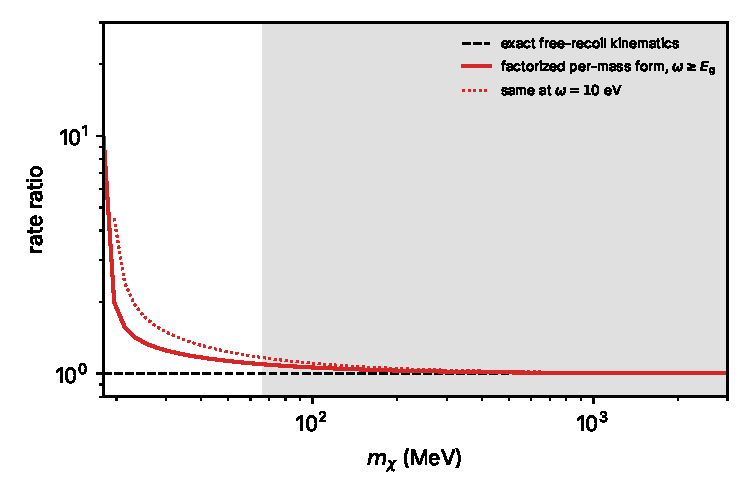
\includegraphics[width=\linewidth]{figures/ch12/limit12_3c.pdf}
\captionof{figure}{Migdal rate of silicon from the per-mass form \cref{eq:12.3-permass}, divided by the rate \cref{eq:12.3-rate} with the exact free-recoil kinematics, against the dark-matter mass. Solid: total rate for $\omega_e \ge \SI{1.11}{eV}$; dotted: the spectrum at $\omega_e = \SI{10}{eV}$. Both rates: heavy mediator, $\sigma_p = 10^{-38}\,\mathrm{cm}^2$, halo of \cref{sec:1.2}, the loss function with local fields and $Z_{\mathrm{ion}}(p)$, and momentum transfers above the impulse onset $q \ge \SI{92.5}{keV}$. Gray band: $\mchi \ge \SI{66}{MeV}$, where the total is within \SI{10}{\percent}.}\label{fig:12-limit-3c}
\par}
\smallskip
Below about \SI{60}{MeV} the electronic energy is no longer small against the kinetic energy of the dark matter. The per-mass form then overestimates the rate, by a factor 1.25 at \SI{30}{MeV} and 1.85 at \SI{20}{MeV}, and the exact $\vmin$ of \cref{eq:12.3-rate} must be kept.
\end{limitbox}

For orientation, at $\sigma_p = 10^{-38}\,\mathrm{cm}^2$ the exact rate \cref{eq:12.3-rate} above the onset is 1.9 events per kg and year at \SI{30}{MeV}, 30 at \SI{100}{MeV} and 970 at \SI{1}{GeV}. These are rates of primary pairs of a few eV, with the spectrum of \cref{fig:12-crystal-atom}. The number of electrons a detector counts follows from the cascade of \cref{chap:18}.

\section{Phonon final states at small momentum}\label{sec:12.4}

A dark-matter particle of \SI{2}{MeV} can transfer a momentum of at most $q = 2\mchi v_{\mathrm{max}} = \SI{10.6}{keV}$. At $q = \SI{10}{keV}$ a silicon nucleus would recoil with $E_R = \SI{1.9}{meV}$, less than the energy of most phonons, and the Debye--Waller exponent is $2W_\kappa = 0.063$: in \SI{94}{\percent} of the kicks the lattice is left exactly as it was (\cref{sec:11.3}). Yet the particle carries enough kinetic energy, $\frac12\mchi v_{\mathrm{max}}^2 = \SI{7}{eV}$, to make an electron--hole pair. If the electrons do not follow the kicked nucleus, a pair is made while the lattice stays in its ground state, and the whole deposit is electronic. The free recoil of \cref{sec:12.3} is the wrong lattice factor here; the impulse regime of \cref{sec:11.4} begins only at \SI{92.5}{keV}, that is at $\mchi = \SI{17.5}{MeV}$. Below it the lattice factor of the Migdal entry is the multiphonon response of \cref{sec:11.3} (\cref{sec:12.1-counting}).

Does the leading entry \cref{eq:12.1-Skk}, derived with a nucleus that is free during the electronic time, hold for a bound nucleus, and with the momentum $p$ taken by the electrons as large as the kick itself? It does, to a few parts in $10^3$ (\cref{sec:12.4-amp}). The real question at small $q$ is how a Migdal event shares its energy between electrons and lattice when the lattice can take zero, one or a few phonons.

\subsection{The amplitude of a bound nucleus}\label{sec:12.4-amp}

Write the Migdal process as two perturbations acting in turn: the kick $\ee^{\ii\vect{q}\cdot\vect{X}_I}$ from the dark matter, and the potential of nucleus $I$ acting on the electrons. By \cref{app:D.33-amp}, that potential is a sum of Fourier components $v_\kappa(\vect{p})\,\ee^{-\ii\vect{p}\cdot\vect{X}_I}\,n_e(\vect{p})$, and the electronic factor $v_\kappa(\vect{p})\langle\Psi_j|n_e(\vect{p})|\Psi_0\rangle$ is common to every term below. What depends on the lattice is the nuclear factor. Let $H_N$ be the Hamiltonian of the nuclei on the ground surface, with eigenstates $|\lambda\rangle$ of energy $E_\lambda$, the initial one $|0\rangle$. The two orderings of \cref{eq:2.4-orderings} give, for a final lattice state $f$ and electronic energy $\omega_e$,
\begin{equation}
  \mathcal{A}_f(\vect{q},\vect{p}) = \sum_\lambda\left[\frac{\langle f|\ee^{-\ii\vect{p}\cdot\vect{X}_I}|\lambda\rangle\langle\lambda|\ee^{\ii\vect{q}\cdot\vect{X}_I}|0\rangle}{\omega_e + E_f - E_\lambda}
  - \frac{\langle f|\ee^{\ii\vect{q}\cdot\vect{X}_I}|\lambda\rangle\langle\lambda|\ee^{-\ii\vect{p}\cdot\vect{X}_I}|0\rangle}{\omega_e + E_\lambda - E_0}\right] .
  \label{eq:12.4-exact}
\end{equation}
In the first ordering the kick acts first and the nucleus then passes $\vect{p}$ to the electrons; the denominator is the energy of the final state minus that of the intermediate one. In the second the electrons are excited first, by the nucleus at rest, and the intermediate state carries $\omega_e$ in addition to the lattice energy. This is the amplitude of Berghaus and collaborators~\cite[Eq.~(3.1)]{berghaus2023migdal}, with their lattice states as the $|\lambda\rangle$.

The electronic energy is large against the lattice energies that the matrix elements allow, and the denominators can be expanded in powers of $1/\omega_e$. Call $A = \ee^{-\ii\vect{p}\cdot\vect{X}_I}$ and $B = \ee^{\ii\vect{q}\cdot\vect{X}_I}$. Since $\langle f|H_N = E_f\langle f|$ and $H_N|0\rangle = E_0|0\rangle$, each power of $(E_f - E_\lambda)$ in the first term turns into a commutator with $H_N$ acting on $A$ from the left, and each power of $(E_\lambda - E_0)$ in the second into the same commutator acting on $A$ from the right. Order by order,
\begin{equation}
  \mathcal{A}_f = \frac{\langle f|[A,B]|0\rangle}{\omega_e} + \frac{\langle f|[[A,H_N],B]|0\rangle}{\omega_e^2} + \frac{\langle f|[[[A,H_N],H_N],B]|0\rangle}{\omega_e^3} + \cdots .
  \label{eq:12.4-series}
\end{equation}
The first term vanishes, since $A$ and $B$ are functions of the same position. For the second, $H_N = \sum_I\vect{P}_I^2/2M_\kappa + U(\{\vect{X}\})$ with any interatomic potential $U$. The potential commutes with $A$; the kinetic energy does not, because $A$ shifts the momentum of nucleus $I$ by $-\vect{p}$, $A\vect{P}_IA^\dagger = \vect{P}_I + \vect{p}$. Hence
\begin{equation*}
  [A,H_N] = \Bigl(\frac{\vect{p}\cdot\vect{P}_I}{M_\kappa} + \frac{p^2}{2M_\kappa}\Bigr)A , \qquad
  [[A,H_N],B] = \frac{\vect{p}}{M_\kappa}\cdot[\vect{P}_I,B]\,A = \frac{\vect{q}\cdot\vect{p}}{M_\kappa}\,\ee^{\ii(\vect{q}-\vect{p})\cdot\vect{X}_I} ,
\end{equation*}
and the leading nuclear factor is
\begin{equation}
  \mathcal{A}^{(2)}_f = \frac{\vect{q}\cdot\vect{p}}{M_\kappa\,\omega_e^2}\,\bigl\langle f\big|\ee^{\ii(\vect{q}-\vect{p})\cdot\vect{X}_I}\big|0\bigr\rangle .
  \label{eq:12.4-lead}
\end{equation}
This is the nuclear factor of \cref{eq:12.1-amp}, now obtained without any assumption about the binding of the nucleus. The interatomic potential has dropped out, as Berghaus and collaborators showed with their effective Hamiltonian $\nabla_IH_{\chi L}\cdot\nabla_IH_{eL}/(m_N\omega^2)$~\cite[Eq.~(3.6)]{berghaus2023migdal}. Esposito and Rocchi obtained the same matrix element from the first nonadiabatic correction to the Born--Oppenheimer product state~\cite[Eq.~(21)]{esposito2025migdal}, and showed that in an infinite crystal, whose center of mass does not move, the adiabatic part of the amplitude vanishes. Two routes therefore give one result: the boost of \cref{sec:8.6} and the second-order amplitude with the lattice integrated out.

The lattice enters at the next order, and the expansion shows what controls it. With $X = \vect{p}\cdot\vect{P}_I/M_\kappa + p^2/2M_\kappa$, the same steps give $[[[A,H_N],H_N],B] = (\vect{q}\cdot\vect{p}/M_\kappa)(2X - \vect{q}\cdot\vect{p}/M_\kappa)\,BA$, plus a term $-\ii(\vect{p}\cdot\nabla_IU/M_\kappa)A$ that commutes with $B$ and drops out. The potential first appears at order $\omega_e^{-4}$, through $[\vect{p}\cdot\nabla_IU,\vect{P}_I]$, the force constants. Summing $|\mathcal{A}_f|^2$ over all final states, averaging over the direction of $\vect{p}$ with the weight $(\vect{q}\cdot\vect{p})^2$ of the leading term, and collecting the terms of the first two orders,
\begin{equation}
  \frac{\sum_f|\mathcal{A}_f|^2}{\sum_f|\mathcal{A}^{(2)}_f|^2} = 1 - \frac{2p^2}{M_\kappa\,\omega_e} + \frac{2\langle\omega_{\mathrm{ph}}^2\rangle}{\omega_e^2} + \frac95\,\frac{v_N^2p^2}{\omega_e^2} + \cdots ,
  \label{eq:12.4-corr}
\end{equation}
with $v_N = q/M_\kappa$ and $\langle\omega_{\mathrm{ph}}^2\rangle$ the mean square phonon frequency seen by the nucleus. The first correction is the recoil energy of the momentum given to the electrons, $p^2/2M_\kappa$, over $\omega_e$: the expectation value of $2X - \vect{q}\cdot\vect{p}/M_\kappa$ in the kicked state is $\vect{p}\cdot(\vect{q} - \vect{p})/M_\kappa$, whose part odd in $\vect{p}$ averages away. The second is the binding of the nucleus, the factor $[1 - (\omega_{\mathrm{ph}}/\omega_e)^2]^{-2}$ that \cref{sec:6.1} found for a nucleus kicked in a harmonic well, at its first order. The third is the Doppler shift of the electronic energy by the moving nucleus, $\vect{v}_N\cdot\vect{p}$, at second order: for a free nucleus, \cref{eq:12.4-exact} is the bracket \cref{eq:12.3-bracket} with $b = \vect{q}\cdot\vect{p}/M_\kappa$, whose expansion $(b/\omega_e^2)(1 + b/\omega_e + b^2/\omega_e^2 + \cdots)$ squared and averaged with $\langle c^4\rangle/\langle c^2\rangle = 3/5$ gives the coefficient $9/5$.

None of the three is a ratio $p/q$, so the leading factor \cref{eq:12.4-lead} holds when the electrons take as much momentum as the nucleus receives, or more, as for the free nucleus of \cref{eq:12.3-bracket}. For silicon at $p = \SI{5.7}{keV}$, the median momentum of the Migdal weight (\cref{sec:12.3}), and $\omega_e = \SI{1.2}{eV}$, near the gap, the three terms of \cref{eq:12.4-corr} are $-2.1\times10^{-3}$, $+2.8\times10^{-3}$ (with the silicon phonon spectrum) and at most $5.1\times10^{-4}$ for every $q$ up to the impulse onset. The leading factor is exact to a few parts in $10^3$ throughout the region of this section. \Cref{lim:12.4a} below compares it with the full sum.

\subsection{Migdal rate with phonon final states}\label{sec:12.4-rate}

Squaring \cref{eq:12.4-lead}, summing over the nuclei and keeping the diagonal $\vect{G} = \vect{G}'$ of the electronic response and the self part of the lattice factor gives the Migdal entry with the lattice factor of one nucleus at the momentum $\vect{q} - \vect{p}$ that it keeps. For one nucleus per site the self response is $S^{\mathrm{ad}}_{\kappa;\vect{G}\vect{G}}(\vect{q} - \vect{k},\omega_l) = 2\pi\nd_\kappa\,s^{\mathrm{inc}}_\kappa(\vect{q} - \vect{k} - \vect{G},\omega_l)$, with $s^{\mathrm{inc}}_\kappa(\vect{Q},\omega)$ the spectrum of one nucleus normalized to $\int\dd\omega\,s^{\mathrm{inc}}_\kappa = 1$, zero-phonon line included. The self part is exact for the phonon-emitting terms, which are incoherent, and, averaged over the zone, for the zero-phonon term at $q \gtrsim 2q_{\mathrm{BZ}}$. Below the impulse onset that factor is the harmonic self response of \cref{eq:11.3-inc}, a zero-phonon line of weight $\ee^{-2W_\kappa}$ and the $n$-phonon spectra $P^\kappa_n$ with the Poisson weights \cref{eq:5.6-poisson}.
\begin{keyresult}[The Migdal probability with phonon final states]
At $n_B = 2$, for the valence electrons with the frozen-core vertex $v_\kappa = -Z_{\mathrm{ion}}(p)e^2/p^2$ of \cref{eq:12.3-Zion} and the diagonal loss function, a kick $\vect{q}$ of a nucleus of species $\kappa$ at a cubic site of a harmonic crystal at $T = 0$, with the incoherent lattice factor, leaves electronic energy $\omega_e$ and lattice energy $\omega_l$ with the probability density
\begin{equation}
  \begin{split}
  \frac{\dd^2P_{\mathrm{Mig}}}{\dd\omega_l\,\dd\omega_e} = 4\alpha\int\frac{\dd^3p}{(2\pi)^3}\;&Z_{\mathrm{ion}}(p)^2\,\frac{(\vect{v}_N\cdot\vect{p})^2}{\omega_e^4\,p^2}\,L(\vect{p},\omega_e)\,\ee^{-2W_\kappa(\vect{q}-\vect{p})} \\
  &\times\Biggl[\underbrace{\delta(\omega_l)}_{\text{zero-phonon, }\mathcal{P}_0} + \underbrace{\sum_{n\ge1}\frac{[2W_\kappa(\vect{q}-\vect{p})]^n}{n!}\,P^\kappa_n(\omega_l)}_{\text{phonon-emitting, }\mathcal{P}_+}\Biggr] .
  \end{split}
  \label{eq:12.4-harm}
\end{equation}
Integrated over $\omega_l$, the bracket times $\ee^{-2W_\kappa}$ gives one for every $\vect{p}$, and $\dd P_{\mathrm{Mig}}/\dd\omega_e$ is \cref{eq:12.3-soft} at every $q$ in this incoherent lattice form. The coherent zero-phonon process of the whole lattice has the same electronic spectrum, averaged over directions, for $q \gtrsim 2q_{\mathrm{BZ}}$. For $q \ll q_{\mathrm{BZ}}$ \cref{eq:8.3-boostward} fixes it at $(m_e/M_\kappa)^2(2q^2/e^2)L(\vect{q},\omega_e)/(2\pi\nd_\kappa)$, with $L$ the head of $-\varepsilon^{-1}$: in silicon $1/14.9$ of \cref{eq:12.3-soft}, with median $\omega_e = \SI{17.4}{eV}$ at the plasmon against \SI{4.5}{eV}. Between the two the coherent response is not computed (\cref{tab:12-nuisances}).
\end{keyresult}
\noindent This is the rate formula of Berghaus and collaborators~\cite[Eq.~(3.8)]{berghaus2023migdal}, with their partial structure factor in the incoherent harmonic form~\cite[Eqs.~(4.1), (4.5)]{berghaus2023migdal} and their effective charge $Z(k)$ as $Z_{\mathrm{ion}}$. Their full structure factor $S(\vect{q} - \vect{k}_e - \vect{K}, E)$ is the electron-following response of \cref{eq:12.1-Skk} at the momentum the nucleus keeps.

The sum rule in the key result, which Berghaus and collaborators pointed out, says that the electronic spectrum does not depend on the lattice dynamics. It needs no soft limit, since the lattice factor has unit weight at every $\vect{q} - \vect{p}$, and no impulse approximation. The lattice enters the rate only through energy conservation. In the double rate the lattice factor replaces the free recoil of \cref{eq:12.3-rate}. The weight $\dd E_R = q\,\dd q/M_\kappa$ is unchanged, and the minimum speed becomes $\vmin = (\omega_e + \omega_l)/q + q/2\mchi$, so that for a heavy mediator
\begin{equation}
  \frac{\dd^2\mathcal{R}}{\dd\omega_l\,\dd\omega_e} = \frac{\rho_\chi\,\sigma_N}{2\mchi\,\mu_{\chi N}^2M_\kappa}\int\dd q\;q\,\eta\Bigl(\frac{\omega_e + \omega_l}{q} + \frac{q}{2\mchi}\Bigr)\frac{\dd^2P_{\mathrm{Mig}}}{\dd\omega_l\,\dd\omega_e} .
  \label{eq:12.4-rate}
\end{equation}
Since $\omega_l$ is a few meV against an $\omega_e$ of a few eV, $\dd\mathcal{R}/\dd\omega_e$ hardly depends on how the lattice takes its share: replacing the free recoil by the bound response leaves the silicon rate unchanged (\cref{lim:12.3b}). What the lattice factor decides is the second axis of the joint response, the energy that a phonon sensor sees together with the charge. Berghaus, Essig and McDuffie extended \cref{eq:12.4-rate} to the nonrelativistic effective operators of the dark-matter--nucleon interaction~\cite{berghaus2026migdal}. Each operator multiplies the same electronic and lattice factors by its own nuclear response, and the lattice factor is again read at the momentum $\vect{q} - \vect{p}$ that the nucleus keeps.

\begin{limitbox}[Migdal effect with phonon final states][lim:12.4a]
$\dd^2P/\dd\omega_l\,\dd\omega_e = 4\alpha\int\dd^3p/(2\pi)^3\,Z_{\mathrm{ion}}(p)^2(\vect{v}_N\cdot\vect{p})^2L(\vect{p},\omega_e)\,s^{\mathrm{inc}}_\kappa(\vect{q} - \vect{p},\omega_l)/(\omega_e^4p^2)$, from the effective interaction $\nabla H_{\chi L}\cdot\nabla H_{eL}/(M_\kappa\omega_e^2)$~\cite[Eqs.~(3.6), (3.8)]{berghaus2023migdal}.
\par\smallskip
{\centering
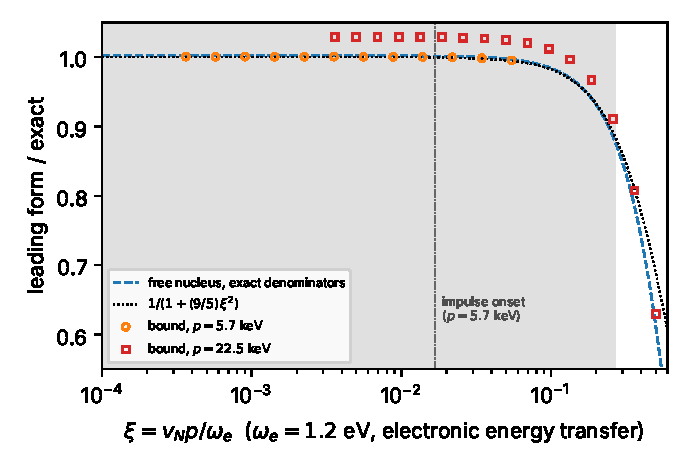
\includegraphics[width=\linewidth]{figures/ch12/limit12_4a.pdf}
\captionof{figure}{Migdal probability summed over all lattice final states, from the leading factor \cref{eq:12.4-lead}, divided by the same from the two time orderings \cref{eq:12.4-exact} with exact energy denominators, against $v_Np/\omega_e$ at the electronic energy transfer $\omega_e = \SI{1.2}{eV}$. Model: a silicon nucleus in an isotropic harmonic well of frequency $\omega_0 = \langle\omega^{-1}\rangle^{-1} = \SI{30.4}{meV}$, which has the Debye--Waller factor of the full phonon spectrum; direction of $\vect{p}$ averaged. Circles, $p = \SI{5.7}{keV}$ for $q = 2$ to \SI{300}{keV}; squares, $p = \SI{22.5}{keV}$ for $q$ up to \SI{700}{keV}, whose offset of 0.03 at small $v_Np/\omega_e$ is the recoil term $2p^2/M_\kappa\omega_e$. Dashed: free nucleus with exact denominators. Dotted: the leading correction $1/(1 + \frac95v_N^2p^2/\omega_e^2)$. Dash-dotted: the impulse onset at $p = \SI{5.7}{keV}$. Gray: within \SI{10}{\percent}, $v_Np/\omega_e \le 0.27$.}\label{fig:12-limit-4a}
\par}
\smallskip
The form fails when the Doppler shift $\vect{v}_N\cdot\vect{p}$ approaches $\omega_e$, at $q \approx \SI{1.5}{MeV}$ for $p = \SI{5.7}{keV}$ near the gap, far above the small-momentum region, where it holds to \num{e-3}.
\end{limitbox}

\noindent On the truncation label \cref{lim:12.4a} sits at $n_B = 2$, with $\mathfrak{M}$ = sudden, $\mathcal{K}$ = multiphonon at all orders (harmonic, incoherent), and $\mathcal{X}$ = random-phase with local fields on the diagonal. The diagonal is the approximation that costs most (\cref{sec:12.3-validity}).

\subsection{Zero-phonon, few-phonon and impulse regimes}\label{sec:12.4-regimes}

\Cref{fig:12-regimes} evaluates \cref{eq:12.4-harm} for silicon and sorts the Migdal events by the number of phonons they leave. The zero-phonon weight of the kick, $\ee^{-2W_\kappa(q)}$, falls to one half at $q = \SI{33.2}{keV}$, reached from $\mchi = \SI{6.3}{MeV}$. The impulse onset lies at \SI{92.5}{keV}. Below the first, most Migdal events are zero-phonon: at $q = \SI{10}{keV}$, \SI{92}{\percent} of them leave the lattice in its ground state, \SI{7.6}{\percent} emit one phonon and \SI{0.5}{\percent} two. Between the two boundaries a Migdal event emits a few phonons; at \SI{50}{keV} the fractions for zero, one, two and three or more are 0.21, 0.32, 0.25 and 0.22. Above the onset the lattice factor is the impulse Gaussian, and the soft-limit treatment of \cref{sec:12.3} holds.

\begin{figure}[tbp]
  \centering
  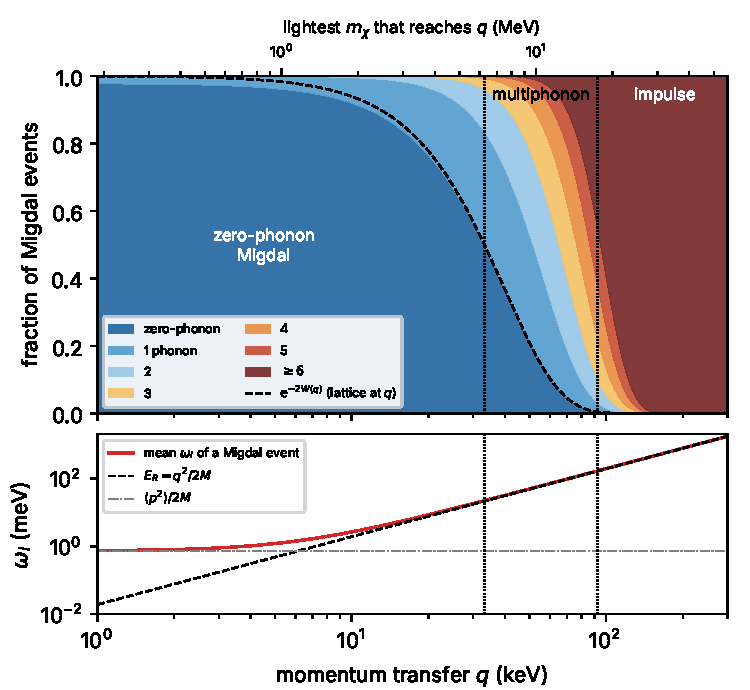
\includegraphics[width=0.84\linewidth]{figures/ch12/fig12_4.pdf}
  \caption{The three regimes of the Migdal effect in silicon against the momentum transfer $q$, at $T = 0$. Top: fraction of Migdal events that leave the lattice with zero, one, two, \ldots\ phonons, from \cref{eq:12.4-harm}, with the lattice factor at the momentum $\vect{q} - \vect{p}$ that the nucleus keeps, averaged over the momentum $\vect{p}$ given to the electrons with the weight $(\vect{q}\cdot\vect{p})^2Z_{\mathrm{ion}}(p)^2p^{-2}\int_{\Eg}\dd\omega_e\,L(p,\omega_e)/\omega_e^4$. Dashed: the zero-phonon weight $\ee^{-2W(q)}$ of the kick alone. Bottom: mean energy $\omega_l$ given to the lattice in a Migdal event, against the recoil energy $E_R$ and the recoil energy $\langle p^2\rangle/2M = \SI{0.72}{meV}$ of the electrons' momentum. Dotted lines: $\ee^{-2W(q)} = \frac12$ at \SI{33.2}{keV} and the impulse onset at \SI{92.5}{keV}. Top axis: the lightest dark matter that reaches $q$, $q/2v_{\mathrm{max}}$. Model: diagonal loss function with local fields of Knapen, Kozaczuk and Lin~\cite{knapen2021dark} (threshold \SI{1.11}{eV}, the step-model gap that accompanies the tables, $p \le \SI{22.5}{keV}$), $Z_{\mathrm{ion}}(p)$ of \cref{eq:12.3-Zion}, incoherent harmonic lattice factor with Poisson weights in $2W(Q) = Q^2\langle u_x^2\rangle$ from the PBE phonon spectrum of \cref{sec:5.2}.}
  \label{fig:12-regimes}
\end{figure}

At small $q$ the electrons' momentum controls the lattice. The momentum $p$ that the electrons take has $\langle p^2\rangle^{1/2} = \SI{6.1}{keV}$ in the weight of \cref{eq:12.4-harm}, and the nucleus keeps $\vect{q} - \vect{p}$, with $\langle|\vect{q} - \vect{p}|^2\rangle = q^2 + \langle p^2\rangle$. At \SI{5}{keV} this is 2.5 times $q^2$. The mean lattice energy of a Migdal event, $\langle|\vect{q} - \vect{p}|^2\rangle/2M_\kappa$ by the first moment of \cref{sec:11.3}, is then \SI{1.20}{meV}, 2.5 times the recoil energy, and at \SI{2}{keV} it is ten times $E_R$. The phonon-emitting fraction follows $2W_\kappa(\vect{q} - \vect{p})$, not $2W_\kappa(\vect{q})$: \SI{3.8}{\percent} at \SI{5}{keV}, against $1 - \ee^{-2W(q)} = \SI{1.6}{\percent}$. Above \SI{30}{keV} the difference fades, and at \SI{50}{keV} the mean lattice energy, \SI{48.5}{meV}, exceeds $E_R$ by \SI{1.5}{\percent}.

In the exact harmonic lattice factor, its part at $\omega_l = 0$ is the product of two ground-state expectation values of $n_\kappa$, which vanish unless $\vect{q} - \vect{p}$ is a reciprocal-lattice vector. A zero-phonon Migdal event is a Bragg process: the crystal takes a reciprocal-lattice vector $\vect{G}$ as a whole, with weight $\ee^{-2W_\kappa(\vect{G})}$ and the structure factor of the cell, and the electrons take exactly $\vect{p} = \vect{q} - \vect{G}$. The incoherent form in \cref{eq:12.4-harm} replaces this sum over discrete momenta by an integral over $\vect{p}$, which is its average over the zone (\cref{sec:11.3}). The two agree when the electronic weight varies slowly over $q_{\mathrm{BZ}}$. For silicon, averaging over the direction of $\vect{q}$ and keeping the diamond structure factor $|1 + \ee^{\ii\vect{G}\cdot\vect{\tau}}|^2$, the Bragg sum is 1.08, 1.04 and 1.03 times the incoherent integral at $q = 1.5$, 3 and \SI{5}{keV}, and within \SI{1}{\percent} of it from \SI{10}{keV}. This check keeps the diagonal $\vect{G} = \vect{G}'$ and averages over directions; the cross-site terms $\vect{G} \neq \vect{G}'$ of the coherent sum, which carry the screening of \cref{eq:8.3-boostward} at $q \ll q_{\mathrm{BZ}}$, are not tested by it. The electronic weight is spread over several zones, median $p = 2.5\,q_{\mathrm{BZ}}$, and the coherent sum samples it densely enough. For a fixed direction of $\vect{q}$ in a crystal at rest the sum depends on the orientation, which a direction-averaged rate does not see.

Germanium follows the same pattern at shifted boundaries. It has no first-principles phonon spectrum in this book (\cref{tab:5-phonons}). An estimate from its Debye temperature of \SI{373}{K}, scaled by the ratio 0.82 of the computed to the Debye value of $\langle\omega^{-1}\rangle^{-1}$ in silicon, gives $\langle\omega^{-1}\rangle^{-1} \approx \SI{17.6}{meV}$, and $\ee^{-2W(q)} = \frac12$ at $q \approx \SI{41}{keV}$, from $\mchi \approx \SI{7.7}{MeV}$. The impulse onset is at \SI{113}{keV}, from \SI{21.3}{MeV} (\cref{sec:11.4}). The heavier nucleus makes the recoil term of \cref{eq:12.4-corr} smaller by the mass ratio 2.6. The binding term is about the same as in silicon, $3\times10^{-3}$ at the germanium gap of \SI{0.67}{eV} with the phonon energies scaled by the ratio of the Debye temperatures.

\subsection{The phonon-mediated form}\label{sec:12.4-virtual}

Liang and collaborators describe the same process with the phonons as the intermediate states~\cite{liang2022phonon}. The kick creates on-shell phonons through the multiphonon vertex; one further phonon, virtual, carries momentum from the kicked nucleus to the bare electron--phonon vertex and excites a pair of energy $\varepsilon_i - \varepsilon_j$~\cite[Eq.~(3.1)]{liang2022phonon}. The virtual phonon brings the propagator $1/[(\varepsilon_i - \varepsilon_j)^2 - \omega_{\vect{Q}\nu}^2]$, which is the bound-nucleus form of the boost denominator, \cref{eq:12.4-pm}. For gaps large against the phonon energies they reduce it to $1/(\varepsilon_i - \varepsilon_j)^2$~\cite[Eq.~(3.2)]{liang2022phonon}, and with the completeness of the polarization vectors the amplitude becomes the leading one, with the lattice factor at $\vect{q}$ instead of $\vect{q} - \vect{p}$.

This form is exact at first order in $\vect{p}$ for a harmonic lattice. Write the displacement of nucleus $I$ in normal modes, $\vect{u}_I = \sum_\nu(\vect{\ell}_\nu a_\nu + \vect{\ell}_\nu^*a_\nu^\dagger)$, with $|\vect{\ell}_\nu|^2 = 1/(2NM_\kappa\omega_\nu)$ and $\nu$ running over the wavevectors and branches. The kick $B = \ee^{\ii\vect{q}\cdot\vect{u}_I}$, up to a phase, displaces every mode, $a_\nu B = B(a_\nu + \beta_\nu)$ with $\beta_\nu = \ii\vect{q}\cdot\vect{\ell}_\nu^*$. At first order in $\vect{p}$, $A = 1 - \ii\vect{p}\cdot\vect{u}_I$; the 1 drops out of \cref{eq:12.4-exact} as the first term of \cref{eq:12.4-series} does. The operator $\vect{p}\cdot\vect{u}_I$ changes one occupation by one, so the intermediate state differs from $f$ (first ordering) or from $0$ (second ordering) by one quantum, and the denominators are $\omega_e \mp \omega_\nu$ and $\omega_e + \omega_\nu$. Moving $a_\nu$ and $a_\nu^\dagger$ through $B$ with the displacement rule, $a_\nu B = B(a_\nu + \beta_\nu)$ and $Ba_\nu^\dagger = (a_\nu^\dagger - \beta_\nu^*)B$, the terms in $\langle f|a_\nu^\dagger B|0\rangle$ cancel between the two orderings, and what is left is proportional to $\langle f|B|0\rangle$:
\begin{equation}
  \mathcal{A}_f = -\ii\sum_\nu\Bigl[\frac{(\vect{p}\cdot\vect{\ell}_\nu)\beta_\nu}{\omega_e - \omega_\nu} + \frac{(\vect{p}\cdot\vect{\ell}_\nu^*)\beta_\nu^*}{\omega_e + \omega_\nu}\Bigr]\langle f|B|0\rangle
  = \frac{1}{N}\sum_\nu\frac{(\vect{q}\cdot\vect{e}_{\kappa\nu})(\vect{p}\cdot\vect{e}_{\kappa\nu}^*)}{M_\kappa(\omega_e^2 - \omega_\nu^2)}\,\bigl\langle f\big|\ee^{\ii\vect{q}\cdot\vect{X}_I}\big|0\bigr\rangle ,
  \label{eq:12.4-pm}
\end{equation}
for real polarization vectors $\vect{e}_{\kappa\nu}$, with $\vect{\ell}_\nu = \vect{e}_{\kappa\nu}/(2NM_\kappa\omega_\nu)^{1/2}$. The propagator is exact for every final state $f$, at all orders in $q$: the multiphonon blob and the virtual phonon factorize. At a cubic site the polarization sum is isotropic, $N^{-1}\sum_\nu e^\alpha_{\kappa\nu}e^{\beta*}_{\kappa\nu}\,\delta(\omega - \omega_\nu) = \delta_{\alpha\beta}\,g_{\mathrm{ph},\kappa}(\omega)/3$, and the propagator becomes $(\vect{q}\cdot\vect{p}/M_\kappa)\int\dd\omega\,g_{\mathrm{ph},\kappa}(\omega)/[3(\omega_e^2 - \omega^2)]$.
\begin{keyresult}[The phonon-mediated Migdal probability]
At first order in $\vect{p}$, for a harmonic crystal at $T = 0$ and a cubic site, the leading probability \cref{eq:12.4-harm} becomes
\begin{equation}
  \begin{split}
  \frac{\dd^2P_{\mathrm{Mig}}}{\dd\omega_l\,\dd\omega_e} = 4\alpha\int\frac{\dd^3p}{(2\pi)^3}\;&Z_{\mathrm{ion}}(p)^2\,\frac{(\vect{v}_N\cdot\vect{p})^2}{p^2}\,\biggl[\int\dd\omega\,\frac{g_{\mathrm{ph},\kappa}(\omega)/3}{\omega_e^2 - \omega^2}\biggr]^2L(\vect{p},\omega_e)\,\ee^{-2W_\kappa(\vect{q})} \\
  &\times\Biggl[\underbrace{\delta(\omega_l)}_{\text{zero-phonon}} + \underbrace{\sum_{n\ge1}\frac{[2W_\kappa(\vect{q})]^n}{n!}\,P^\kappa_n(\omega_l)}_{\text{phonon-emitting}}\Biggr] ,
  \end{split}
  \label{eq:12.4-pmrate}
\end{equation}
with the lattice factor at the kick $\vect{q}$. For $\omega_e \gg \omega_{\mathrm{ph}}$ the squared bracket is $\omega_e^{-4}[1 + 2\langle\omega_{\mathrm{ph}}^2\rangle/\omega_e^2 + \cdots]$, with $\langle\omega_{\mathrm{ph}}^2\rangle$ the mean of $\omega^2$ over $g_{\mathrm{ph},\kappa}/3$.
\end{keyresult}
\noindent With the propagator reduced to $\omega_e^{-2}$ this is the rate of Liang and collaborators~\cite[Eqs.~(3.3), (3.4)]{liang2022phonon}, whose $T_0(E) = \delta(E)$ is the zero-phonon term and whose $T_n$ with $n \ge 1$ are the phonon-emitting terms. Their factor $\Imag[-\tilde\varepsilon^{-1}_{\vect{G}\vect{G}'}]$ keeps the elements $\vect{G} \neq \vect{G}'$ that \cref{eq:12.4-pmrate} drops, and their $Z_{\mathrm{ion}}$ is the constant valence charge.

The zero-phonon term dominates wherever the phonon-mediated form is needed. At $q = \SI{5}{keV}$ it holds \SI{96}{\percent} of the Migdal events, and a rate that kept only the phonon-emitting terms would be low by a factor 26. The first numerical evaluation of the phonon-mediated rate omitted $T_0$ and found rates far below the free-recoil ones at small mass; with $T_0$ restored the two agree at all masses~\cite[Note added]{liang2022phonon}, as the sum rule under \cref{eq:12.4-harm} requires.

The two published forms are complementary truncations of \cref{eq:12.4-exact}. The leading form \cref{eq:12.4-harm} is exact in $\vect{p}$ and keeps the first order in $1/\omega_e$; the phonon-mediated form \cref{eq:12.4-pmrate} is exact in $\omega_{\mathrm{ph}}/\omega_e$ and keeps the first order in $\vect{p}$. Their difference at order $p^2$ is the lattice factor at $\vect{q} - \vect{p}$ against $\vect{q}$. For the electronic spectrum it is immaterial, since both lattice factors have unit weight. For the lattice spectrum it is not: at \SI{5}{keV} the phonon-emitting fraction is \SI{3.8}{\percent} with the lattice factor at $\vect{q} - \vect{p}$ and \SI{1.6}{\percent} at $\vect{q}$, because the electrons' momentum is larger than the kick. In the frame of the crystal, where the transition density is frozen and the nucleus feels the recoil of $\vect{p}$, the all-orders form is the correct one. The exact sum over a harmonic site confirms it (\cref{we:12-five-keV}). The frame itself is the open question of \cref{sec:12.1-boost}.

\begin{limitbox}[Phonon-mediated Migdal effect][lim:12.4b]
$\dd^2P/\dd\omega_l\,\dd\omega_e$ as \cref{lim:12.4a} with the propagator $(\vect{q}\cdot\vect{p}/M_\kappa)\sum_\nu|\vect{e}_\nu|^2/[N(\omega_e^2 - \omega_\nu^2)]$ reduced to $\vect{q}\cdot\vect{p}/(M_\kappa\omega_e^2)$, the lattice factor at $\vect{q}$ and its zero-phonon term included~\cite[Eqs.~(3.1)--(3.4)]{liang2022phonon}.
\par\smallskip
{\centering
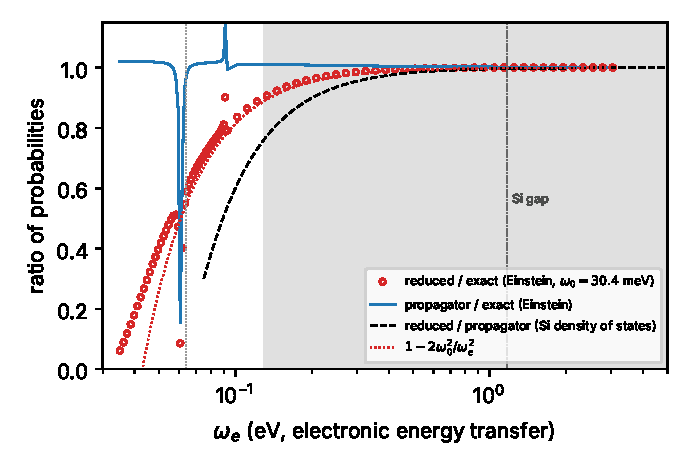
\includegraphics[width=\linewidth]{figures/ch12/limit12_4b.pdf}
\captionof{figure}{Migdal probability summed over lattice final states against the electronic energy transfer $\omega_e$, at $q = \SI{10}{keV}$ and $p = \SI{5.7}{keV}$, direction of $\vect{p}$ averaged. Circles: the reduced form over the exact second-order amplitude \cref{eq:12.4-exact} of a silicon nucleus in an isotropic harmonic well of frequency $\omega_0 = \SI{30.4}{meV}$. Solid: the unreduced propagator form \cref{eq:12.4-pm} over the same exact result; its narrow feature at $\omega_e = 2\omega_0$ is the two-phonon intermediate state, of relative weight $p^2/(2M_\kappa\omega_0) = 0.02$, which the first-order form lacks. Dotted: the leading correction $1 - 2\omega_0^2/\omega_e^2$. Dashed: reduced over propagator form with the PBE phonon spectrum of silicon (PBE band top \SI{63.7}{meV}, dotted vertical line). Gray: reduced form within \SI{10}{\percent} of the exact one, $\omega_e \ge 4.2\,\omega_0$. Dash-dotted: the silicon gap.}\label{fig:12-limit-4b}
\par}
\smallskip
The reduced form fails where $\omega_e$ approaches the phonon band, below \SI{0.20}{eV} with the silicon spectrum, where the electrons no longer see a sudden kick and the pole at $\omega_e = \omega_\nu$ turns the process into the absorption of a real phonon.
\end{limitbox}

\noindent On the truncation label \cref{lim:12.4b} sits at $n_B = 2$, with $\mathfrak{M}$ = sudden and the bound denominators $\omega_e^2 - \omega_\nu^2$, $\mathcal{K}$ = multiphonon at all orders with the lattice factor at $\vect{q}$, and $\mathcal{X}$ = random-phase with local fields. Its leading correction is one step of $n_B$, from 2 to 4: the phonon energies in the electronic denominators, of relative size $2\langle\omega_{\mathrm{ph}}^2\rangle/\omega_e^2$, as \cref{sec:8.5} counts it.

Silicon and germanium do not need the propagator. At the silicon gap of \SI{1.17}{eV} the reduced form is low by \num{2.9e-3}, at the germanium gap by about \num{3e-3}, and averaged over the silicon spectrum by \num{3e-4}. It is needed where the gap is comparable with the phonon energies: the narrow-gap and Dirac materials of \cref{chap:16}, whose gaps of tens of meV were the motivation of the phonon-mediated description, and the metals of \cref{sec:12.1-gapless}. There the region $\omega_e \lesssim 3\omega_{\mathrm{ph}}$ is not a Migdal process with a small correction but the electron--phonon response of the target.

\begin{workedexample}{The phonon-mediated term at $q = \SI{5}{keV}$}\label{we:12-five-keV}
A silicon nucleus kicked with $q = \SI{5}{keV}$ recoils with $E_R = q^2/2M_\kappa = \SI{0.478}{meV}$ and velocity $v_N = 1.91\times10^{-7}$, \SI{57}{m/s}. The momentum is reached by dark matter of $\mchi \ge q/2v_{\mathrm{max}} = \SI{0.94}{MeV}$; at \SI{1}{MeV} the largest energy transfer at this $q$, $qv_{\mathrm{max}} - q^2/2\mchi$, is \SI{0.75}{eV}, below the gap, and at \SI{2}{MeV} it is \SI{7.0}{eV}. The Debye--Waller exponent is $2W_\kappa(q) = 0.0157$. The momentum is 2.2 times $q_{\mathrm{BZ}}$, below the 2.95\,$q_{\mathrm{BZ}}$ from which \cref{sec:11.3} shows the incoherent multiphonon terms to hold and the \SI{18}{keV} from which the incoherent one-phonon term holds.

\emph{The probability.} By the sum rule of \cref{eq:12.4-harm}, the electronic spectrum is \cref{eq:12.3-soft} with the recoil energy $E_R$. At $q = 2.2\,q_{\mathrm{BZ}}$ this is the direction-averaged coherent process, within the $\vect{G} \neq \vect{G}'$ row of \cref{tab:12-nuisances}. With $Z_{\mathrm{ion}}(p)$, local fields and $\omega_e \ge \SI{1.11}{eV}$, \cref{sec:12.3} gives $6.07\times10^{-5}$ per eV of recoil energy, so $P_{\mathrm{Mig}} = 2.90\times10^{-8}$. One kick in $3.4\times10^7$ makes a pair.

\emph{The propagator.} With the PBE phonon spectrum, $\langle\omega_{\mathrm{ph}}^2\rangle^{1/2} = \SI{44.7}{meV}$. The squared bracket of \cref{eq:12.4-pmrate} times $\omega_e^4$ is 1.0029 at \SI{1.17}{eV}, the leading correction $2\langle\omega_{\mathrm{ph}}^2\rangle/\omega_e^2 = \num{2.9e-3}$, and 1.0003 averaged over the electronic spectrum, half of which lies above \SI{4.6}{eV}. The virtual phonon is far off shell, and the bound-nucleus correction is negligible.

\emph{The zero-phonon term.} With the lattice factor at $\vect{q} - \vect{p}$, \SI{96.2}{\percent} of the Migdal events leave no phonon, $P = 2.79\times10^{-8}$: the crystal takes the momentum as a whole, and all of the deposit, a few eV, is electronic. With the lattice factor at $\vect{q}$, as in \cref{eq:12.4-pmrate}, the share is \SI{98.4}{\percent}.

\emph{The phonon-emitting terms.} The rest, $1.10\times10^{-9}$, emits one phonon in \SI{96}{\percent} of the cases. Its energy follows the one-phonon spectrum of the incoherent response, $g_{\mathrm{ph},\kappa}(\omega)/\omega$, with mean $\langle\omega^{-1}\rangle^{-1} = \SI{30.4}{meV}$ and median \SI{21.7}{meV}: a phonon-emitting Migdal event gives the lattice 64 times the recoil energy. The energy comes from the dark matter, not from the recoil: kinematics bounds only the sum $\omega_e + \omega_l$, by \SI{7.0}{eV} at \SI{2}{MeV}, and a phonon costs a small part of it. Averaged over all Migdal events, the lattice receives \SI{1.20}{meV}, 2.5 times $E_R$, almost all in the rare events with a phonon.

\emph{A check.} Take a nucleus in a harmonic well of frequency \SI{30.4}{meV}, with $p = \SI{5.7}{keV}$ and $\omega_e = \SI{1.2}{eV}$. The exact amplitude \cref{eq:12.4-exact}, summed over final states, is 0.99934 times the leading form \cref{eq:12.4-lead} and 0.9980 times the propagator form \cref{eq:12.4-pm}. Its zero-phonon fraction is 0.967, against 0.984 for the lattice factor at $\vect{q}$ alone.
\end{workedexample}

The frame of the transition density, the lattice factor at small $|\vect{q} - \vect{p}|$ and the off-diagonal electronic response remain open at small momentum. The frame is the Herzberg--Teller term of \cref{sec:12.1-boost}, and at \SI{5}{keV} it is the factor 2.4 between the phonon-emitting fractions above; the electronic spectrum does not depend on it. Below $|\vect{q} - \vect{p}| \approx \SI{6.6}{keV}$ the incoherent multiphonon terms are not certified (\cref{lim:11.3a}), while the zero-phonon line, the dominant term, agrees with its diagonal, direction-averaged Bragg sum within \SI{8}{\percent}. The elements $\vect{G} \neq \vect{G}'$ of the electronic response are common to all crystal forms (\cref{app:E.18}). The frame and the lattice factor change the lattice spectrum of Migdal events, not their number, and \cref{tab:12-nuisances} carries all three.

\section{Moments of the Migdal spectrum}\label{sec:12.5}

A silicon nucleus kicked to a recoil energy of \SI{500}{eV} leaves its valence electrons excited in three events out of a hundred and gives them on average \SI{0.18}{eV} per kick, \SI{0.28}{eV} with the core shells. The second number needs no excited state of the crystal. It is the recoil energy times the ratio of the drag mass, the mass of the electrons that a slowly moving nucleus carries with it, to the mass of the nucleus. Every moment of the Migdal spectrum is fixed in the same way by the force that the electrons exert on one nucleus. The moments give the size of the effect without a spectrum, test a computed spectrum, bound the Migdal probability from both sides, and fix how a Migdal rate is added to a lattice rate.

\subsection{Inverse moments of the force spectrum}\label{sec:12.5-moments}

The force of \cref{eq:12.1-force} has a spectrum. With $|0\rangle$ the ground state of the clamped electrons, $|a\rangle$ their excited states and $\Delta_a = E_a - E_0$, we define the spectral measure of its component along the kick and its inverse moments,
\begin{equation}
  \dd\sigma_\kappa(\Delta) = \sum_{a\neq0}\bigl|\hat{\vect{q}}\cdot\langle a|\nabla_{\vect{R}_\kappa}V_{eN}|0\rangle\bigr|^2\,\delta(\Delta - \Delta_a) , \qquad
  \mathcal{I}_k = \int\Delta^{-k}\,\dd\sigma_\kappa(\Delta) ,
  \label{eq:12.5-sigma}
\end{equation}
for one nucleus $\vect{R}_\kappa$ of species $\kappa$. The leading-order Migdal probability \cref{eq:8.6-PMig}, with $\vect{d}_{a0} = -\vect{F}_{a0}/\Delta_a$ from \cref{eq:5.1-dcoup}, resolved in the electronic energy, is
\begin{equation}
  \frac{\dd P_{\mathrm{Mig}}}{\dd\omega_e} = \frac{q^2}{M_\kappa^2\,\omega_e^4}\,\frac{\dd\sigma_\kappa}{\dd\Delta}\bigg|_{\Delta = \omega_e} .
  \label{eq:12.5-spectrum}
\end{equation}
It is the electronic marginal of the Migdal entry \cref{eq:12.1-Skk}, divided by $2\pi\nd_\kappa$, once the lattice factor has been integrated over $\omega_l$ with its unit weight.

\begin{keyresult}[Moments of the Migdal spectrum]
At leading order in the boost, for a nucleus of species $\kappa$ kicked with momentum $\vect{q}$ and $E_R = q^2/2M_\kappa$,
\begin{equation}
  \begin{gathered}
  \int\dd\omega_e\,\omega_e^k\,\frac{\dd P_{\mathrm{Mig}}}{\dd\omega_e} = \frac{q^2}{M_\kappa^2}\,\mathcal{I}_{4-k} : \\
  \underbrace{P_{\mathrm{Mig}} = \frac{q^2\mathcal{I}_4}{M_\kappa^2}}_{k = 0} , \quad
  \underbrace{E^{\mathrm{Mig}}_1 = E_R\,\frac{\delta M_\kappa}{M_\kappa}}_{k = 1,\ \delta M_\kappa = 2\mathcal{I}_3} , \quad
  \underbrace{E^{\mathrm{Mig}}_2 = \frac{q^2\mathcal{I}_2}{M_\kappa^2}}_{k = 2} , \quad
  \underbrace{E^{\mathrm{Mig}}_3 = \frac{q^2\mathcal{I}_1}{M_\kappa^2}}_{k = 3} ,
  \end{gathered}
  \label{eq:12.5-moments}
\end{equation}
with $E^{\mathrm{Mig}}_k$ the $k$th moment. The first moment is the Born--Huang drag mass of \cref{eq:8.6-fsum-k} along $\hat{\vect{q}}$, times $E_R/M_\kappa$.
\end{keyresult}
\noindent Every moment is proportional to $E_R$, so each defines a material constant per unit recoil energy. Each also has a meaning in the ground state of the clamped electrons. The first is the drag mass of Born and Huang~\cite[App.~VIII]{born1954dynamical}: $\delta M_\kappa = 2\mathcal{I}_3$ is \cref{eq:D.28-dM} projected on $\hat{\vect{q}}$, the identity that \cref{sec:12.1-boost} used to estimate $P_{\mathrm{Mig}}$. It is also the curvature in frequency of the electronic force constant. A nucleus displaced at frequency $\omega$ below the gap feels the force constant $\Phi^{\mathrm{el}}_{\kappa\kappa}(\omega) = \langle\partial^2_{\hat q}V_{eN}\rangle - 2\int\dd\sigma_\kappa(\Delta)\,\Delta/(\Delta^2 - \omega^2)$, whose expansion in $\omega^2$ is $\Phi^{\mathrm{el}}_{\kappa\kappa}(0) - \omega^2\delta M_\kappa + O(\omega^4)$. The equation of motion $[\Phi(\omega) - \omega^2M_\kappa]u = 0$ then moves with the mass $M_\kappa + \delta M_\kappa$: the electrons that follow a slow nucleus add their inertia to it. The second moment is the diagonal Born--Huang correction of \cref{app:D.28}, $E_{\mathrm{BH}} = \mathcal{I}_2/2M_\kappa$ along $\hat{\vect{q}}$, so that $E^{\mathrm{Mig}}_2 = 4E_RE_{\mathrm{BH}}$. The third is the second-order energy of the electrons in the field of a displaced nucleus, and \cref{sec:12.5-third} turns it into the electron density at the nucleus.

The force spectrum of the valence electrons follows from the loss function. Comparing \cref{eq:12.5-spectrum} with the soft-limit probability \cref{eq:12.3-soft} gives, for the diagonal $\vect{G} = \vect{G}'$ and the frozen-core vertex of \cref{eq:12.3-Zion},
\begin{equation}
  \begin{gathered}
  \frac{\dd\sigma_\kappa}{\dd\omega} = \frac{e^2}{\pi}\int\frac{\dd^3p}{(2\pi)^3}\;Z_{\mathrm{ion}}(p)^2\,\frac{(\hat{\vect{q}}\cdot\vect{p})^2}{p^2}\,L(\vect{p},\omega) , \\
  \delta M^{\mathrm{val}}_\kappa = \frac{8\alpha}{3}\int\frac{\dd^3p}{(2\pi)^3}\;Z_{\mathrm{ion}}(p)^2\int_0^\infty\frac{\dd\omega}{\omega^3}\,\bar L(p,\omega) ,
  \end{gathered}
  \label{eq:12.5-dMval}
\end{equation}
the second form for a direction-averaged loss function, with $e^2/\pi = 4\alpha$. The drag mass of the valence electrons is a property of the clamped crystal, like the static dielectric constant, which fixes the $\omega^{-1}$ moment of the same loss function at $p \to 0$ (\cref{sec:4.4}).

The inverse moments come from linear-response calculations without any excited state. The drag mass is the $\omega^2$ coefficient of the on-site force constant, which the frequency-dependent Sternheimer equation of \cref{app:E.4} returns at a few imaginary frequencies, where the sign of the $\omega^2$ term changes, $\Phi^{\mathrm{el}}_{\kappa\kappa}(\ii\omega) = \Phi^{\mathrm{el}}_{\kappa\kappa}(0) + \omega^2\delta M_\kappa + O(\omega^4)$. Two static Sternheimer solves per occupied state give $\mathcal{I}_2$, $\mathcal{I}_3$ and $\mathcal{I}_4$ at the level of independent pairs.

\subsection{On-site drag mass and trace rule}\label{sec:12.5-trace}

The drag mass of a rigid translation and the on-site drag mass of one nucleus must be kept apart. Displace every nucleus of a crystal by the same $\vect{u}$, slowly. The electrons see a rigidly translated potential and follow it exactly, so the whole crystal moves with the mass of nuclei and electrons together. Let $\delta M_{IJ}$ be the drag-mass tensor between nuclei $I$ and $J$, defined as in \cref{eq:D.28-dM} with the forces of the two nuclei. The translation then gives the \emph{trace rule}
\begin{equation}
  \sum_J\delta M_{IJ} = Z_\kappa m_e\,\mathbf{1} \quad\text{(one species)} , \qquad
  \sum_{\kappa\kappa'}\delta M_{\kappa\kappa'}(\vect{Q} = 0) = N_em_e\,\mathbf{1} \quad\text{per cell} ,
  \label{eq:12.5-trace}
\end{equation}
which follows from the f-sum rule of the electrons in velocity form, because the summed force $\sum_J\nabla_JV_{eN}$ is the time derivative of the total electronic momentum (\cref{app:D.34-trace}). It holds for any insulator and any interaction among the electrons. For a free atom there is only one nucleus, the sum has one term, and it is the Thomas--Reiche--Kuhn value $N_em_e$ of \cref{eq:8.6-fsum-k}. The estimate $14\,m_e$ that \cref{sec:8.6} took for silicon is this sum; it is exact, but a kick probes a different element.

A dark-matter particle kicks one nucleus. The Migdal moments \cref{eq:12.5-moments} contain the force of nucleus $I$ alone, and $\delta M_\kappa$ in them is the on-site element $\delta M_{II}$. Written in phonon wavevectors, $\delta M_{II}$ is the average over the Brillouin zone of $\delta M_{\kappa\kappa}(\vect{Q})$, while \cref{eq:12.5-trace} fixes only the value at $\vect{Q} = 0$. The two differ by the off-site coupling,
\begin{equation}
  \delta M_{II} = Z_\kappa m_e - \sum_{J\neq I}\delta M_{IJ} ,
  \label{eq:12.5-onsite}
\end{equation}
which no sum rule fixes, in size or in sign. Positivity of the tensor at each $\vect{Q}$ gives $\delta M_{II} \ge 0$ and nothing more.

Silicon shows what the two elements are. Its cores move rigidly with the nucleus and contribute their own count to every element. The atomic Migdal tables of Cox and collaborators~\cite{cox2023precise}, rescaled to dipole order as in \cref{sec:12.2}, confirm this. The first moments of the $1s$, $2s$ and $2p$ ionization spectra, with the measured binding energies, add up to $10.1\,m_e$, of which $7.2\,m_e$ is $2p$. The valence part depends on the crystal. Evaluated on the loss function of Knapen, Kozaczuk and Lin with local fields, the table of \cref{sec:12.3}, \cref{eq:12.5-dMval} gives $\delta M^{\mathrm{val}} = 18.6\,m_e$, and with the cores the on-site drag mass is $28.7\,m_e$, $\delta M_{II}/M = 5.60\times10^{-4}$, twice the trace value. In the free atom the four valence electrons carry $4\,m_e$ in all, of which their ionization spectra carry $1.2\,m_e$ and the bound transitions the rest.

In silicon \SI{96}{\percent} of the valence integral comes from $p > q_{\mathrm{BZ}}$ and \SI{61}{\percent} from $p > \SI{5}{keV}$, where the ion charge has risen from 4 to 4.84 and the probe resolves the core region. In energy, \SI{67}{\percent} lies below \SI{10}{eV}, near the gap, where the weight $\omega^{-3}$ is largest. The table stops at \SI{89}{eV}; the valence f-sum held by the table bounds the missing part at \SI{24}{\percent}. Momenta above \SI{10}{keV} carry \SI{2.8}{\percent} of the integral, so those beyond the table's \SI{22.5}{keV} are estimated to add less. The approximations matter more than the truncation. A point ion of charge 4 gives $11.8\,m_e$, and the loss function without local fields $24.0\,m_e$. Both are uncontrolled at $p \gtrsim \SI{5}{keV}$. The frozen-core vertex assumes that the valence electrons inside the core region feel the bare nucleus screened by a rigid core. The diagonal $\vect{G} = \vect{G}'$ drops the off-diagonal elements of the dielectric matrix, which are sized only in a model and only for the rate (\cref{sec:12.3-validity}); the local fields on the diagonal already move the valence drag mass from $24.0$ to $18.6\,m_e$.

The excess over the trace value has no sign fixed by anything above. A model shows that it can go either way. In a periodic chain of Gaussian wells, two independent electrons per well and one filled band (\cref{app:D.34-trace}), the trace rule \cref{eq:12.5-trace} holds to $10^{-4}$ for every depth of the wells. The on-site element equals $2\,m_e$ while the wells are deep and isolated, and falls to $1.29\,m_e$ at a gap of \SI{8.1}{eV} and to $0.92\,m_e$ at \SI{5.4}{eV} as they overlap: with short-range wells the neighbors take part of the drag, and $\sum_{J\neq I}\delta M_{IJ} > 0$. The silicon table gives the opposite sign, $\sum_{J\neq I}\delta M_{IJ} = -14.7\,m_e$, from the long-range Coulomb vertex at large $p$ that the chain lacks. No calculation of $\delta M_{\kappa\kappa}(\vect{Q})$ exists that could decide between the two pictures for silicon. We therefore take the on-site valence drag mass of silicon as $18.6\,m_e$, with the band $12$ to $24\,m_e$ from the vertex and the local fields, and carry the band in the uncertainty budget of the chapter (\cref{tab:12-nuisances}). For germanium the same tables give $39.5\,m_e$, with the band $11.5$ to $52\,m_e$: the frozen $3d$ shell is shallow, bound by only \SI{29.4}{eV} and extended to \SI{0.4}{\angstrom}, and $Z_{\mathrm{ion}}(p)$ climbs from 4 already at a few keV. The cores of germanium carry $26.8\,m_e$ in the atomic tables without the $1s$, close to the $26\,m_e$ of a rigid core without the $1s$.

The difference between the two elements also tells which mass the lattice responses of \cref{chap:11} should carry. An incoherent kick probes $\delta M_{II}$. A coherent phonon of wavevector $\vect{Q}$ probes $\delta M_{\kappa\kappa'}(\vect{Q})$, and a long-wavelength acoustic phonon, which translates the whole cell, carries exactly the full mass of the atoms, $M_\kappa + Z_\kappa m_e$. The prescription of \cref{sec:8.6} and \cref{sec:12.1-counting}, mass $M_\kappa + \delta M_\kappa$ in the electron-following response, uses the on-site element for the impulse and multiphonon responses of an incoherent kick.

\subsection{Bounds on the Migdal probability}\label{sec:12.5-bounds}

The first moment and the threshold bound the probability from above, and the first and second moments bound it from below. On the support of the force spectrum every energy exceeds the threshold $E_{\mathrm{th}}$ of the electrons, the gap for the valence and the binding energy for a core shell, so $\mathcal{I}_4 \le \mathcal{I}_3/E_{\mathrm{th}}$. The Cauchy--Schwarz inequality for the measure $\dd\sigma_\kappa$, applied to the functions $\Delta^{-1}$ and $\Delta^{-2}$, gives $\mathcal{I}_3^2 \le \mathcal{I}_2\mathcal{I}_4$. With \cref{eq:12.5-moments} the two become a statement about the measured quantities.
\begin{keyresult}[Bounds on the Migdal probability]
For a nucleus kicked with recoil energy $E_R$, with the Migdal spectrum split into groups of final states $s$ (valence and core shells) with thresholds $E_s$ and drag masses $\delta M_s$, $\sum_s\delta M_s = \delta M_\kappa$,
\begin{equation}
  \frac{(E^{\mathrm{Mig}}_1)^2}{E^{\mathrm{Mig}}_2} \;\le\; P_{\mathrm{Mig}} \;\le\; \sum_s\frac{E_R}{E_s}\,\frac{\delta M_s}{M_\kappa} \;\le\; \frac{E_R}{\Eg}\,\frac{\delta M_\kappa}{M_\kappa} .
  \label{eq:12.5-bound}
\end{equation}
\end{keyresult}
\noindent The upper bound needs only the drag mass and the threshold, the two numbers a static calculation gives most reliably. It is reached when the whole force spectrum lies at the threshold, and the shell-resolved form is much tighter than the last one because the core shells, which hold a large part of $\delta M_\kappa$, have thresholds a hundred times the gap. The lower bound is reached when the spectrum is a single line. The ratio of the two bounds measures the width of the spectrum in energy.

On the silicon table the valence probability is \SI{19}{\percent} of its upper bound and 1.74 times its lower bound; for germanium the numbers are \SI{15}{\percent} and 1.92. The mean energy $E^{\mathrm{Mig}}_1/P_{\mathrm{Mig}}$ of the valence spectrum is \SI{6.0}{eV} in silicon and \SI{5.1}{eV} in germanium, five to seven times the gap, which is why the upper bound is loose. For the $2p$ shell of the silicon atom the probability is \SI{50}{\percent} of its bound, since a core spectrum begins with a sharp edge. The bounds carry the leading-order caveat of \cref{eq:12.5-moments}. At large recoil the motion of the nucleus during the transition, the free-recoil bracket \cref{eq:12.3-bracket}, raises the probability by the factor 1.6 at \SI{500}{eV} (\cref{sec:12.3-validity}); the bounds apply to the leading-order spectrum.

A lattice response added to a Migdal rate takes the weight $1 - P_{\mathrm{Mig}}$ of \cref{eq:12.1-zeroth}. On the silicon table the valence probability reaches $10^{-3}$ at $E_R = \SI{16.5}{eV}$ and grows linearly from there. The mass correction is smaller. It moves the mean of the impulse response by $-E_R\,\delta M_{II}/M_\kappa$, a few parts in $10^4$ of $E_R$, while the impulse width $E_Rx_R^{-1/2}$ of \cref{sec:11.4} is a percent of $E_R$ at these energies.

\begin{workedexample}{The silicon drag mass and the bound on the Migdal probability at \SI{500}{eV}}\label{we:12-drag}
A silicon nucleus, $M = \SI{26.16}{GeV}$, recoils with $E_R = \SI{500}{eV}$ when it receives $q = (2ME_R)^{1/2} = \SI{5.11}{MeV}$; its velocity is $v_N = 1.96\times10^{-4}$. The drag masses of \cref{sec:12.5-trace} are $10.1\,m_e$ for the cores and $18.6\,m_e$ for the valence, so $\delta M_{II} = 28.7\,m_e$ and $\delta M_{II}/M = 5.60\times10^{-4}$, against $2.73\times10^{-4}$ for the trace value $14\,m_e$. The first moment is $E^{\mathrm{Mig}}_1 = E_R\,\delta M_{II}/M = \SI{0.280}{eV}$: \SI{0.099}{eV} from the cores and \SI{0.181}{eV} from the valence.

The bounds follow shell by shell. The valence, with the threshold \SI{1.11}{eV} of the table, has $P \le 0.181/1.11 = 0.163$; its second moment, $E^{\mathrm{Mig}}_2 = \SI{1.89}{eV^2}$, gives $P \ge 0.181^2/1.89 = 0.0174$. The computed spectrum gives $P = 0.0303$, inside the window. The $1s$, $2s$ and $2p$ shells, with thresholds of 1839, 150 and \SI{99.5}{eV}, give $P \le 8.0\times10^{-4}$; the atomic tables give $4.0\times10^{-4}$. The total probability is $P_{\mathrm{Mig}} = 0.031$, below the shell-resolved bound $0.164$ and far below the single-threshold bound $E_R\,\delta M_{II}/(M\Eg) = 0.24$ with the physical gap of \SI{1.17}{eV}. Using the trace value $14\,m_e$ in that last bound gives $0.12$. It happens to lie above the true probability here, but it is not a bound, because the kick probes the on-site element.

A lattice response for silicon at $E_R = \SI{500}{eV}$, added to the Migdal rate, has the weight $1 - P_{\mathrm{Mig}} = 0.969$, a correction of \SI{3.1}{\percent}. It also has the mass $M(1 + 5.60\times10^{-4})$, which moves its mean by \SI{0.28}{eV}, a sixteenth of the impulse width $E_R(E_R/\langle\omega\rangle)^{-1/2} = \SI{4.5}{eV}$ with $\langle\omega\rangle = \SI{40.9}{meV}$ (\cref{sec:11.4}).
\end{workedexample}

\subsection{The cross first moment}\label{sec:12.5-cross}

A dark-matter particle that couples to both electrons and nucleons reaches the Migdal final states through two amplitudes, the boost of a kicked nucleus and the direct recoil of an electron, and they interfere. The interference $S_{e\kappa}$ has a vanishing total first moment, \cref{eq:4.3-species}, and \cref{eq:8.6-fsum-ek} split it into equal and opposite parts on and off the line $\omega_e = 0$. For a free atom the split is exact to all orders. Use the center-of-mass separation of \cref{sec:12.2}. In the elastic final states the atom recoils as a whole with the energy $q^2/2m_A$ and its electrons stay in the ground state; these states carry the first moment $\nd_\kappa(q^2/m_A)F_{\mathrm{cr}}(q)$, and the excited states carry the negative of it (\cref{app:D.34-cross}).
\begin{keyresult}[Electronic part of the cross first moment]
For a free atom of mass $m_A$, exactly,
\begin{equation}
  \begin{gathered}
  \mathscr{M}^1_{e\kappa}\big|_{\omega_e > 0} = -\nd_\kappa\,\frac{q^2}{m_A}\,F_{\mathrm{cr}}(q) , \\
  F_{\mathrm{cr}}(q) = \Real\Bigl[\langle0|\textstyle\sum_e\ee^{\ii\vect{q}\cdot\vect{\rho}_e}\ee^{-\ii\vect{q}_e\cdot\sum_{e'}\vect{\rho}_{e'}}|0\rangle^*\,\langle0|\ee^{-\ii\vect{q}_e\cdot\sum_{e'}\vect{\rho}_{e'}}|0\rangle\Bigr] ,
  \end{gathered}
  \label{eq:12.5-cross}
\end{equation}
with $\vect{\rho}_e$ and $\vect{q}_e = m_e\vect{q}/m_A$ as in \cref{eq:12.2-cm}. In a crystal, at leading order in $\kappa_{\mathrm{BO}}$, $m_A \to M_\kappa$ and $F_{\mathrm{cr}}$ is defined by the electron-following form of \cref{eq:8.6-fsum-ek}, $\mathscr{M}^1_{e\kappa}|_{\mathrm{ad}} = \nd_\kappa q^2F_{\mathrm{cr}}(\vect{q})^*/M_\kappa$.
\end{keyresult}
\noindent For an atom, $F_{\mathrm{cr}}(q) = f(q)[1 + O(q_e^2\langle\rho^2\rangle, m_e/m_A)]$, the atomic form factor. In a crystal $F_{\mathrm{cr}}$ counts the electrons that move with nucleus $\kappa$, weighted by the phase $\ee^{\ii\vect{q}\cdot\vect{r}}$ at the momentum of the probe. At $q \to 0$ it is the charge that follows the nucleus at zero macroscopic field, $\hat{\vect{q}}\cdot(Z_\kappa\mathbf{1} - Z^*_\kappa)\cdot\hat{\vect{q}}$, which is 14 for silicon and, with the Born charge $Z^* = 2.11$ of \cref{sec:5.5}, 28.9 for gallium and 35.1 for arsenic in GaAs. As $q$ grows past the inverse size of each shell, that shell drops out of $F_{\mathrm{cr}}$, and at $q \gg 1/a_{1s}$ only the nucleus is left to recoil with no electrons attached.

The negative part lies in the Migdal cells of $S_{e\kappa}$. Its size is close to the largest that the positivity \cref{eq:4.2-positivity} of the response matrix allows. For the free atom at small $q$, the Migdal first moment is $\nd_\kappa q^2N_em_e/m_A^2$, and that of the electronic sectors of $S_{ee}$ is $\nd_\kappa q^2N_e/m_e$. Their geometric mean, $\nd_\kappa q^2N_e/m_A$, is reached by \cref{eq:12.5-cross} when $F_{\mathrm{cr}} \to N_e$, because at small $q$ the boost and the direct recoil excite the same dipole, with amplitudes in the fixed ratio $-m_e/m_A$ of \cref{eq:8.3-boostward}. Any model of a mixed coupling that keeps the Born-charge interference on the line $\omega_e = 0$ must keep this negative Migdal interference, of equal size, off it.

\subsection{Third moment and contact density}\label{sec:12.5-third}

The third moment uses only the ground state. The inverse moment $\mathcal{I}_1 = \sum_a|\langle a|\partial_{\hat q}V_{eN}|0\rangle|^2/\Delta_a$ is half the second-order energy of the electrons when nucleus $\kappa$ is displaced along $\hat{\vect{q}}$. Second-order perturbation theory writes the curvature of the Born--Oppenheimer surface as $\partial^2_{\hat q}E_0 = \langle\partial^2_{\hat q}V\rangle - 2\mathcal{I}_1$, with $V$ the electron--nucleus and nucleus--nucleus potentials. For point nuclei the second derivative of the Coulomb potential is a contact term: $\nabla^2_{\vect{R}}V_{eN} = Z_\kappa e^2\sum_i\delta^3(\vect{r}_i - \vect{R}_\kappa)$, and $\nabla^2_{\vect{R}}V_{NN} = 0$ at the nucleus. On a cubic site a third of the trace lies along $\hat{\vect{q}}$, and with the curvature $c_3$ that \cref{sec:11.4} gives to the third cumulant of the impulse response we obtain the following result.
\begin{keyresult}[Third moment of the Migdal spectrum]
For point nuclei on cubic sites, at leading order in the boost and averaged over the zero-point motion,
\begin{equation}
  E^{\mathrm{Mig}}_3 = \underbrace{\frac{q^2}{2M_\kappa^2}\,\frac{Z_\kappa e^2\nd_e^{(\kappa)}}{3}}_{\text{contact}} \;-\; \underbrace{c_3}_{\text{lattice}} , \qquad
  c_3 = \frac{q^2}{2M_\kappa^2}\,\langle\partial^2_{\hat q}E_0\rangle ,
  \label{eq:12.5-third}
\end{equation}
with $\nd_e^{(\kappa)}$ the electron density at the nucleus of \cref{eq:8.3-M3}. The full third potential moment of the nuclear response, $c_3 + E^{\mathrm{Mig}}_3$, is the contact term alone.
\end{keyresult}
\noindent The lattice curvature is negligible: in silicon $M\langle\omega^2\rangle$ with $\langle\omega^2\rangle^{1/2} = \SI{44.7}{meV}$ from the phonon density of states of \cref{sec:11.4} is $1.3\times10^{-6}$ of the contact term. The split that \cref{sec:11.4} made, $c_3$ for the electron-following response and the rest for the electrons, is a split of the third moment into one part in a million and the rest. The leading corrections to \cref{eq:12.5-third} are those of the leading-order boost: relative order $\kappa_{\mathrm{BO}}^2$, and the ratio of the mean phonon energy to the electronic energies that dominate the moment, which are of the order of the $1s$ binding. With the contact density of \cref{we:8-third}, $\nd_e^{(\kappa)} = 1765\,a_0^{-3}$, the third moment of silicon is \SI{1497}{eV^2} per eV of recoil energy. For germanium an all-electron Hartree--Fock calculation of the free atom, done in the same way, gives $\nd_e^{(\kappa)} = 22\,475\,a_0^{-3}$, converged to \SI{0.2}{\percent} in the tight basis functions, and \SI{16849}{eV^2} per eV of recoil. The valence electrons hold \SI{0.43}{\percent} of the contact density in silicon and \SI{0.085}{\percent} in germanium. The third moment is a property of the $1s$ and $2s$ shells, whose spectra reach keV, and a valence table sees almost none of it: the silicon table, cut at \SI{89}{eV}, holds $5\times10^{-5}$ of it.

The same contact density appears in the mixed third moment of \cref{sec:8.3}. At $q \to 0$ on a cubic site \cref{eq:8.3-M3lim} reads $\mathscr{M}^3_{e\kappa} = -2\nd_\kappa(M_\kappa/m_e)(E^{\mathrm{Mig}}_3 + c_3)[1 + 2\nd_e/\nd_e^{(\kappa)}]$: the interference of electrons and nuclei measures the Migdal third moment, up to the uniform-density term $2\nd_e/\nd_e^{(\kappa)} = 1.2\times10^{-4}$ in silicon. At finite $q$ the $e\kappa$ face carries the bracket of \cref{eq:8.3-M3sph}, which climbs from $\nd_e^{(\kappa)}/3$ toward $\nd_e^{(\kappa)}$, while the $\kappa\kappa$ face keeps \cref{eq:12.5-third} at every $q$. The two faces agree only through that bracket.

Relativity changes the third moment more than anything else. The Dirac Hamiltonian depends on the nuclear position only through $V_{eN}$, so the derivation of \cref{eq:12.5-third} holds for relativistic electrons unchanged, with the relativistic density at the nucleus. The Foldy--Wouthuysen reduction of \cref{sec:10.6}, recapped in \cref{app:C.15}, identifies the change: the Darwin term \cref{eq:C.15-darwin} is a contact interaction proportional to $\nabla^2V$, and every operator that probes $\nabla^2V$ carries relative corrections of order $(Z\alpha)^2$ from the core $s$ shells. The expansion in $1/m_e$ cannot give their size, because the Dirac $1s$ orbital behaves as $r^{\gamma_{\mathrm{D}} - 1}$ near a point nucleus, with $\gamma_{\mathrm{D}} = [1 - (Z\alpha)^2]^{1/2}$, and its density diverges at $r = 0$. A nucleus of finite size cuts the divergence off, and its charge distribution $\rho_{\mathrm{nuc}}$ replaces the delta function: $\nabla^2_{\vect{R}}V_{eN} = Z_\kappa e^2\rho_{\mathrm{nuc}}(\vect{r} - \vect{R}_\kappa)$, so that $\nd_e^{(\kappa)}$ becomes the density averaged over the nucleus. For a $1s$ orbital of charge $Z$ and a uniform nucleus of radius $R_{\mathrm{nuc}}$, the ratio of that average to the nonrelativistic contact density is (\cref{app:D.34-dirac})
\begin{equation}
  \mathcal{R}_{\mathrm{rel}} = \frac{6}{(2\gamma_{\mathrm{D}} + 1)\,\Gamma(2\gamma_{\mathrm{D}} + 1)}\Bigl(\frac{2ZR_{\mathrm{nuc}}}{a_0}\Bigr)^{2\gamma_{\mathrm{D}} - 2}
  = 1 + (Z\alpha)^2\ln\frac{a_0}{2ZR_{\mathrm{nuc}}} + c_{\mathrm{rel}}(Z\alpha)^2 + \cdots ,
  \label{eq:12.5-Rrel}
\end{equation}
with the Euler gamma function $\Gamma$ and $c_{\mathrm{rel}}$ a coefficient of order one without the logarithm. The logarithm is the reason the $1/m_e$ series fails: the correction is of order $(Z\alpha)^2$ times the logarithm of the ratio of the atomic to the nuclear size. With the nuclear radii of \cref{sec:2.2}, \SI{3.47}{fm} for silicon and \SI{4.77}{fm} for germanium, $\mathcal{R}_{\mathrm{rel}}$ is 1.082 for silicon and 1.425 for germanium, and 1.397 and 1.454 for gallium and arsenic. The logarithm alone gives 0.066 of the excess 0.082 in silicon and 0.281 of 0.425 in germanium. We apply the $1s$ factor to every $s$ shell, since all of them behave alike inside the nucleus, and a change of the nuclear radius by \SI{10}{\percent} moves $\mathcal{R}_{\mathrm{rel}}$ by \SI{0.10}{\percent} in silicon and \SI{0.53}{\percent} in germanium. The remainder without the logarithm, 0.017 in silicon and 0.144 in germanium, depends on the model of the orbital inside the nucleus and is uncertain at order $(Z\alpha)^2$, about \SI{5}{\percent} in germanium. The $p_{1/2}$ shells add a contact density of relative order $(Z\alpha)^2$ that the $1s$ factor omits, since their small components are $s$-like at the origin. The relativistic third moments are \SI{1620}{eV^2} per eV of recoil for silicon and \SI{24000}{eV^2} for germanium, higher by \SI{8}{\percent} and \SI{42}{\percent} than the nonrelativistic values. Third moments from nonrelativistic all-electron densities are therefore about \SI{30}{\percent} low for germanium and gallium arsenide.

\Cref{tab:12-moments} collects the moments of both crystals.
\begin{table}[tbp]
  \centering
  \small
  \caption{Migdal moments of silicon and germanium per nucleus, at leading order in the boost. Drag masses in units of $m_e$; the other moments per eV of recoil energy $E_R$. Trace: the rule \cref{eq:12.5-trace}. Cores: first moments of the free-atom ionization spectra at dipole order (Dirac--Hartree--Fock tables of Cox, Dolan, McCabe and Quiney~\cite{cox2023precise}, measured binding energies; germanium without $1s$). Valence: \cref{eq:12.5-dMval,eq:12.3-soft} on the loss functions of Knapen, Kozaczuk and Lin, computed with the grid-based projector-augmented wave (GPAW) code, with local fields (diagonal, direction-averaged; thresholds \SI{1.11}{eV} for Si, the step-model gap that accompanies the table, and \SI{0.744}{eV} for Ge), with $Z_{\mathrm{ion}}(p)$ from the free-atom core; in brackets the range from a point ion $Z_{\mathrm{ion}} = 4$ to the loss function without local fields. Third moment: \cref{eq:12.5-third} with the Hartree--Fock contact densities of the free atoms, nonrelativistic and with the factor \cref{eq:12.5-Rrel}.}
  \label{tab:12-moments}
  \begin{tabular}{@{}lll@{}}
    \toprule
    Quantity & Si & Ge \\
    \midrule
    Trace $\sum_J\delta M_{IJ}$ & $14$ & $32$ \\
    On-site drag mass, cores & $10.1$ & $26.8$ \\
    On-site drag mass, valence & $18.6$ [$11.8$--$24.0$] & $39.5$ [$11.5$--$52.1$] \\
    Valence $P_{\mathrm{Mig}}/E_R$ (\si{eV^{-1}}) & $6.07\times10^{-5}$ & $5.89\times10^{-5}$ \\
    Valence mean $\omega_e$ (\si{eV}) & $5.97$ & $5.07$ \\
    Valence $E^{\mathrm{Mig}}_2/E_R$ (\si{eV}) & $3.77\times10^{-3}$ & $2.91\times10^{-3}$ \\
    Contact density $\nd_e^{(\kappa)}$ ($a_0^{-3}$), nonrelativistic & $1765$ & $22\,475$ \\
    $E^{\mathrm{Mig}}_3/E_R$ (\si{eV^2}), nonrelativistic & $1497$ & $16\,849$ \\
    Relativistic factor $\mathcal{R}_{\mathrm{rel}}$ & $1.082$ & $1.425$ \\
    $E^{\mathrm{Mig}}_3/E_R$ (\si{eV^2}), relativistic & $1620$ & $24\,008$ \\
    \bottomrule
  \end{tabular}
\end{table}

\paragraph{Open problem.} The finite-$q$ factor of the electron density at the nucleus, the bracket of \cref{eq:8.3-M3sph} that the mixed third moment carries, is known only for spherical atomic densities. For a crystal the valence anisotropy and the relativistic shape of the factor are missing. The valence density adds an anisotropy of tetrahedral symmetry, estimated at $1.3\times10^{-3}$ of the factor in silicon. Relativity changes the factor in two places that do not cancel. Its normalization, the contact density, rises by the $\mathcal{R}_{\mathrm{rel}}$ of \cref{eq:12.5-Rrel}. Its quadrupolar part, set by the density at distances $1/q$ from the nucleus, changes by only a few percent; applying the relativistic change of one to the nonrelativistic value of the other is an error of the size of $\mathcal{R}_{\mathrm{rel}} - 1$. Until both are computed, the mixed third moment at finite $q$ can check the Migdal third moment only to that accuracy in germanium and gallium arsenide, and the relativistic factor itself carries the non-logarithmic remainder and the $p_{1/2}$ contact density, each of relative order $(Z\alpha)^2$.

\section{Bremsstrahlung and Migdal-type absorption}\label{sec:12.6}

A nucleus that is suddenly set moving is a charge that radiates. Besides leaving an electron--hole pair behind, in $6.1\times10^{-3}$ of the kicks for silicon at a recoil energy of \SI{100}{eV} (\cref{sec:12.3}), it emits photons, the bremsstrahlung of the recoil. Kouvaris and Pradler pointed out that such photons, unlike the recoil, are easy to see, and used them to carry xenon searches to lower masses~\cite{kouvaris2017probing}. A second process uses the same nonadiabatic structure with the roles of energy and momentum exchanged. A scalar coupled to nucleons and absorbed by a nucleus gives it almost no momentum but its whole rest energy, and the electrons, which do not follow the nucleus exactly, take that energy~\cite{dzuba2024migdal}. Both effects were worked out for isolated atoms. We will compute both in a crystal. For bremsstrahlung the crystal replaces the charge of the nucleus by a dynamical Born charge, which in silicon and germanium is fixed exactly by the measured dielectric function; for absorption it replaces the atomic photoabsorption cross-section by the loss function.

\subsection{Photon emission in a medium}\label{sec:12.6-photon}

The photon is a new final-state particle in this book, and \cref{app:C.16} sets up what we need: the transverse radiation field as a set of oscillators, its minimal coupling to charges, and the golden-rule rate of emitting one photon. A charge $e_{\mathrm{c}}$ at rest that is set moving with velocity $\vect{v} \ll 1$ in a time short compared with $1/\omega$ radiates the photon number spectrum \cref{eq:C.16-soft}, flat in energy. And inside a transparent medium of refractive index $n_r(\omega)$ the same current radiates $n_r$ times more, \cref{eq:C.16-medium}: the density of photon modes grows as $n_r^2n_{\mathrm{grp}}$, the field of one photon shrinks as $(n_rn_{\mathrm{grp}})^{-1/2}$, and the group index $n_{\mathrm{grp}}$ cancels. Together,
\begin{equation}
  \frac{\dd N_\gamma}{\dd\omega_\gamma} = n_r(\omega_\gamma)\,\frac{2\alpha}{3\pi}\,\frac{e_{\mathrm{c}}^2}{e^2}\,\frac{v^2}{\omega_\gamma} ,
  \label{eq:12.6-classical}
\end{equation}
with $\omega_\gamma$ the energy of the photon. The spectrum holds for photon wavelengths long compared with the emitter, the dipole limit, and for a medium that does not absorb at $\omega_\gamma$, so that the photon is a propagating mode.

A nucleus in an atom does not radiate with its bare charge. Its electrons are pulled along, and the photon sees the dipole of the whole atom. Kouvaris and Pradler computed this in second-order perturbation theory, kick and emission in both orders, and found the bare spectrum, $e_{\mathrm{c}} = Z_\kappa e$ in \cref{eq:12.6-classical}~\cite[Eq.~(3)]{kouvaris2017probing}, with $Z_\kappa^2$ replaced by $|f(\omega_\gamma)|^2$~\cite[Eq.~(8)]{kouvaris2017probing}. Their $f$ is the atomic scattering factor, and in our units it is fixed by the dipole polarizability $\alpha_{\mathrm{pol}}(\omega)$ of the atom,
\begin{equation}
  Z^*_{\mathrm{at}}(\omega) \equiv f(\omega) = -\frac{m_e\omega^2}{e^2}\,\alpha_{\mathrm{pol}}(\omega) ,
  \label{eq:12.6-atom}
\end{equation}
the free-atom limit of the dynamical Born charge of \cref{sec:12.6-brems}. A model of electrons bound to the nucleus by springs shows what it means. If the nucleus moves by $u$ at frequency $\omega$, an electron with natural frequency $\omega_n$ follows with the amplitude $\omega_n^2u/(\omega_n^2 - \omega^2)$, and the atom acquires the dipole $-eu\sum_nf_n\omega^2/(\omega_n^2 - \omega^2)$, with $f_n$ the oscillator strengths, which sum to $Z_\kappa$ (\cref{sec:4.3}). At high frequency the electrons stay behind and the dipole is $Z_\kappa eu$, the bare charge. At low frequency they follow, the neutral atom carries no dipole, and $Z^*_{\mathrm{at}}$ falls as $\omega^2$. For silicon, with the static polarizability of $37.3$ atomic units~\cite{schwerdtfeger2019table}, that is $4\pi\times37.3\,a_0^3 = \SI{69.5}{\angstrom^3}$ in Heaviside--Lorentz units, $Z^*_{\mathrm{at}} = -0.050$ at \SI{1}{eV}: a photon of an electronvolt sees one twentieth of an electron charge.

\subsection{Crystal nuclear-recoil bremsstrahlung}\label{sec:12.6-brems}

In a crystal the charge that moves with a displaced nucleus is the Born effective charge of \cref{sec:5.5}. The Born charge is defined for slow displacements, with the electrons following adiabatically. A photon of an electronvolt oscillates faster than the lattice but not much slower than the electrons. What it sees is the \emph{dynamical Born charge} $Z^*_\kappa(\omega)$: the dipole created per unit displacement of one nucleus of species $\kappa$ oscillating at frequency $\omega$, all other nuclei at rest, at zero macroscopic field, with the electrons responding at $\omega$. By the Maxwell relation \cref{eq:5.5-Z}, taken at frequency $\omega$, it is also the force on the nucleus per unit field. At $\omega \to 0$ it is the Born charge $Z^*_\kappa$, at $\omega$ far above every electronic frequency it is $Z_\kappa$, and for a free atom it is $Z^*_{\mathrm{at}}$ of \cref{eq:12.6-atom}. The nucleus couples to the macroscopic field of a photon, $\vect{\mathcal{E}}_\gamma$, through the term of \cref{eq:5.5-HE} at that frequency,
\begin{equation}
  H_\gamma = -e\sum_I\vect{u}_I\cdot Z^*_\kappa(\omega_\gamma)\cdot\vect{\mathcal{E}}_\gamma .
  \label{eq:12.6-Hgamma}
\end{equation}
The local fields at the nucleus are inside $Z^*_\kappa$, and $\vect{\mathcal{E}}_\gamma$ is the field of the medium's photon mode of \cref{app:C.16}.

\emph{The amplitude.} Dark matter kicks nucleus $I$ with $K = \ee^{\ii\vect{q}\cdot\vect{X}_I}$, and the photon is emitted by $D = -e\vect{u}_I\cdot Z^*_\kappa\cdot\langle1_\gamma|\vect{\mathcal{E}}_\gamma|0\rangle$, which acts on the nucleus only. The process has two time orders. With $H$ the Hamiltonian of the crystal, $|i\rangle$ and $|f\rangle$ its initial and final states and $|n\rangle$ the intermediate ones, the second-order amplitude is
\begin{equation*}
  A_{fi} = \sum_n\Bigl[\frac{\langle f|D|n\rangle\langle n|K|i\rangle}{\omega_\gamma - (E_n - E_f)} - \frac{\langle f|K|n\rangle\langle n|D|i\rangle}{\omega_\gamma + (E_n - E_i)}\Bigr] .
\end{equation*}
When $\omega_\gamma$ is large compared with the energy differences in the denominators, we expand in their ratio. At zeroth order the two terms give $\langle f|[D,K]|i\rangle/\omega_\gamma$, which vanishes, since $\vect{u}_I$ and $\ee^{\ii\vect{q}\cdot\vect{X}_I}$ commute. At first order, closure turns the energy differences into commutators with $H$, and
\begin{equation*}
  A_{fi} = -\frac{1}{\omega_\gamma^2}\,\langle f|\bigl[[H,D],K\bigr]|i\rangle .
\end{equation*}
Whatever potential holds the nucleus, it is a function of the positions, so $[H,\vect{u}_I] = -\ii\vect{P}_I/M_\kappa$, and $[\vect{P}_I,\ee^{\ii\vect{q}\cdot\vect{X}_I}] = \vect{q}\,\ee^{\ii\vect{q}\cdot\vect{X}_I}$. The double commutator is the kick times $\ii e\,(\vect{q}/M_\kappa)\cdot Z^*_\kappa\cdot\langle1_\gamma|\vect{\mathcal{E}}_\gamma|0\rangle$, and the amplitude factorizes into the matrix element of the kick and the emission amplitude of a charge $eZ^*_\kappa$ that jumps to the velocity $\vect{v}_N = \vect{q}/M_\kappa$. This is the classical result of \cref{app:C.16} for a sudden kick, and the lattice potential has dropped out. The neglected terms are of relative order $(E_n - E_i)/\omega_\gamma$. The displacement $\vect{u}_I$ changes the number of phonons by one, so the energies in question are phonon energies, and the expansion holds for $\omega_\gamma \gg \omega_{\mathrm{ph}}$: the nucleus moves freely during one period of the photon.

Each kick of nucleus $\kappa$ thus comes with the photon spectrum \cref{eq:12.6-classical} for the charge $eZ^*_\kappa(\omega_\gamma)$ and the velocity $\vect{v}_N$. Inserting the kick into \cref{eq:8.2-spectrum} with the joint response of \cref{sec:12.1-def}, and the photon energy as a third energy deposited, gives the rate.
\begin{keyresult}[Crystal nuclear-recoil bremsstrahlung]
For photon energies $\omega_{\mathrm{ph}} \ll \omega_\gamma$ below the absorption edge of the crystal, and momentum transfers above the zone, where the kicks of different nuclei add incoherently,
\begin{equation}
  \begin{split}
  \frac{\dd^2\mathcal{R}}{\dd\omega_l\,\dd\omega_\gamma} = \frac{1}{\rho_T}\,\frac{\rho_\chi}{\mchi}\int\dd^3v\,f_\chi(\vect{v})\int\frac{\dd^3q}{(2\pi)^3}\sum_\kappa\,
  &\underbrace{\mathfrak{D}_{\kappa\kappa}(\vect{q},\vect{v})\,S_{\kappa\kappa}(\vect{q},\omega_l)}_{\text{kick}} \\
  &\times\underbrace{\frac{2\alpha\,n_r(\omega_\gamma)}{3\pi\,\omega_\gamma}\,\frac{|Z^*_\kappa(\omega_\gamma)\cdot\vect{q}|^2}{M_\kappa^2}}_{\text{photons per kick}}\,\delta(\omega_l + \omega_\gamma - \omega_{\vect{q}}) ,
  \end{split}
  \label{eq:12.6-brems}
\end{equation}
with $S_{\kappa\kappa}(\vect{q},\omega_l)$ the lattice response of \cref{chap:11} in whatever regime it is, single phonons, multiphonons or free recoil. At a cubic site $|Z^*_\kappa\cdot\vect{q}|^2 = Z^{*2}_\kappa q^2$.
\end{keyresult}
\noindent For a gas of atoms, $n_r = 1$, $Z^*_\kappa \to Z^*_{\mathrm{at}}$ and a free recoil, \cref{eq:12.6-brems} is the rate of Kouvaris and Pradler~\cite[Eq.~(8)]{kouvaris2017probing}; with the bare charge $Z_\kappa$ in place of $Z^*_\kappa$ it is their bare-nucleus rate~\cite[Eq.~(3)]{kouvaris2017probing}. Note that their derivation kept only the elastic atomic channel, the atom left in its ground state, and the crystal formula does the same: the electrons appear only through $Z^*_\kappa(\omega_\gamma)$.

The photon must be soft, its momentum $n_r\omega_\gamma$ small compared with $q$, which for photons of an eV and momentum transfers of keV holds by three orders of magnitude. The wavelength must be long compared with the cell, which makes $Z^*_\kappa$ the zone-center quantity. The impulse approximation, $E_R \gg \omega_{\mathrm{ph}}$, is not needed, since the lattice potential dropped out of the amplitude. Below the zone, however, the kicks of neighboring nuclei interfere, and the photon sees the dipole of a whole cell. For a coupling to nucleon number the cell is pushed as a unit. Its dipole is then accelerated only through the small difference of nucleon number per mass between its atoms, the cancellation that \cref{we:8-nucleon} found for optical phonons. Above the absorption edge the photon is absorbed before it leaves the crystal. The same amplitude then makes an electron--hole pair. That piece is the exchange of a transverse photon between the moving nucleus and the electrons, a correction to the Coulomb amplitude of the Migdal effect (\cref{sec:12.1}) suppressed by powers of the velocities of the charges. The photon pole is bremsstrahlung, and the continuum is Migdal ionization; nothing is counted twice.

\emph{The dynamical Born charge of silicon and germanium.} What remains is $Z^*_\kappa(\omega)$, and one exact sum rule fixes much of it. Let every nucleus of the crystal move together, by $\vect{u}(t) = \vect{u}\,\ee^{-\ii\omega t}$. In the frame that moves with the nuclei, the electrons see the clamped crystal plus the inertial force $-m_e\ddot{\vect{u}} = m_e\omega^2\vect{u}$ on each electron, a uniform force indistinguishable from a uniform field $\vect{\mathcal{E}}_{\mathrm{in}} = -m_e\omega^2\vect{u}/e$. At zero macroscopic field the electrons respond to $\vect{\mathcal{E}}_{\mathrm{in}}$ as to an applied field, with the polarization $[\varepsilon(\omega) - 1]\vect{\mathcal{E}}_{\mathrm{in}}$, local fields included, and $\varepsilon(\omega)$ the electronic dielectric function at clamped nuclei. A rigid translation of the neutral cell adds no dipole of its own, so this polarization is the whole dipole per cell, $\Omega\vect{P} = e\sum_\kappa Z^*_\kappa(\omega)\cdot\vect{u}$. Hence
\begin{equation}
  \sum_\kappa Z^*_\kappa(\omega) = -\frac{\Omega\,m_e\,\omega^2}{e^2}\,\bigl[\varepsilon(\omega) - 1\bigr] ,
  \label{eq:12.6-sum}
\end{equation}
with $\Omega$ the cell volume. At $\omega \to 0$ the right-hand side vanishes, the neutrality of the Born charges \cref{eq:5.5-neutral}. At $\omega$ above every electronic frequency, $\varepsilon - 1 \to -\omega_p^2/\omega^2$ with the plasma frequency of all $N_e$ electrons of the cell, $\omega_p^2 = e^2N_e/(\Omega m_e)$, and the sum tends to $N_e = \sum_\kappa Z_\kappa$, the bare charges. For a dilute gas, $\varepsilon - 1$ is the density of atoms times $\alpha_{\mathrm{pol}}$, and \cref{eq:12.6-sum} becomes \cref{eq:12.6-atom}. The two atoms of silicon or germanium are exchanged by the inversion through the bond center, so their dynamical Born charges are equal at every frequency, and
\begin{equation}
  Z^*(\omega) = -\frac{\Omega\,m_e\,\omega^2}{2e^2}\,\bigl[\varepsilon(\omega) - 1\bigr]
  = -\frac{N_{\mathrm{v}}}{2}\,\bigl[\varepsilon(\omega) - 1\bigr]\frac{\omega^2}{(\omega_p^{\mathrm{val}})^2}
  \qquad (\text{Si, Ge}) ,
  \label{eq:12.6-ZSi}
\end{equation}
with $N_{\mathrm{v}} = 8$ valence electrons per cell and the valence plasma frequency $\omega_p^{\mathrm{val}}$ of \cref{sec:10.2}. No calculation of the phonon response is needed: the measured refractive index gives the dynamical Born charge.

Below the gap $\varepsilon$ changes slowly, and $Z^*(\omega) \simeq -C_\kappa\omega^2$ with $C_\kappa = \Omega m_e(\varepsilon_\infty - 1)/2e^2$, the coefficient of the small-$\omega$ expansion that \cref{app:E.17} specifies. For silicon, with $\Omega = \SI{40.05}{\angstrom^3}$ and $\varepsilon_\infty = 11.7$, $C_\kappa = \SI{0.155}{eV^{-2}}$; with the measured dielectric function at \SI{1}{eV}, $\varepsilon = 12.37$~\cite{franta2017temperature}, $Z^*(\SI{1}{eV}) = -0.165$. The photons per kick then grow as $\omega_\gamma^3$, and the rate is suppressed by $\omega_\gamma^4$ against that of a nucleus with a fixed charge. The suppression is that of the free atom, but the crystal is a stronger emitter. The polarizability per atom of the solid, $\Omega(\varepsilon - 1)/2 = \SI{228}{\angstrom^3}$ at \SI{1}{eV}, is 3.3 times that of the free atom, \SI{69.5}{\angstrom^3}. The emission goes as the square of the charge, $3.3^2 = 10.7$, and the photon gains $n_r = 3.5$ on top. Per photon the silicon crystal emits 33 to 38 times more than its atoms between 0.3 and \SI{1}{eV}, and germanium, with $\varepsilon_\infty = 16.0$~\cite{li1980refractive}, 86 to 96 times more between 0.3 and \SI{0.65}{eV}. A free-atom estimate is therefore not an upper bound for the crystal.

\emph{Polar crystals.} In GaAs the Born charge is $Z^* = 2.11$ at zero frequency (\cref{we:5-lst}), and nothing suppresses the emission at small $\omega_\gamma$. The sum rule \cref{eq:12.6-sum} fixes the sum of the two dispersions, $Z^*_{\mathrm{Ga}}(\omega) - Z^* + Z^*_{\mathrm{As}}(\omega) + Z^*$, from the electronic dielectric function, but not their difference. That difference is a mixed response to a field and a displacement at frequency $\omega$, which frequency-dependent density-functional perturbation theory computes with shifted Sternheimer equations at $\pm\omega$ and a scissor to the measured gap, checked against \cref{eq:12.6-sum} and the static Born charge (\cref{app:E.17}), where each dispersion is also bounded by $|Z^*_\kappa(\omega) - Z^*_\kappa(0)| \le 0.9\,(\omega/\SI{1}{eV})^2$. We split the sum equally between the two sites and carry the bound as a band. The rate depends on the difference only through the cross term with $Z^*$, and below \SI{0.3}{eV} the band is a few percent wide.

\begin{figure}[tbp]
  \centering
  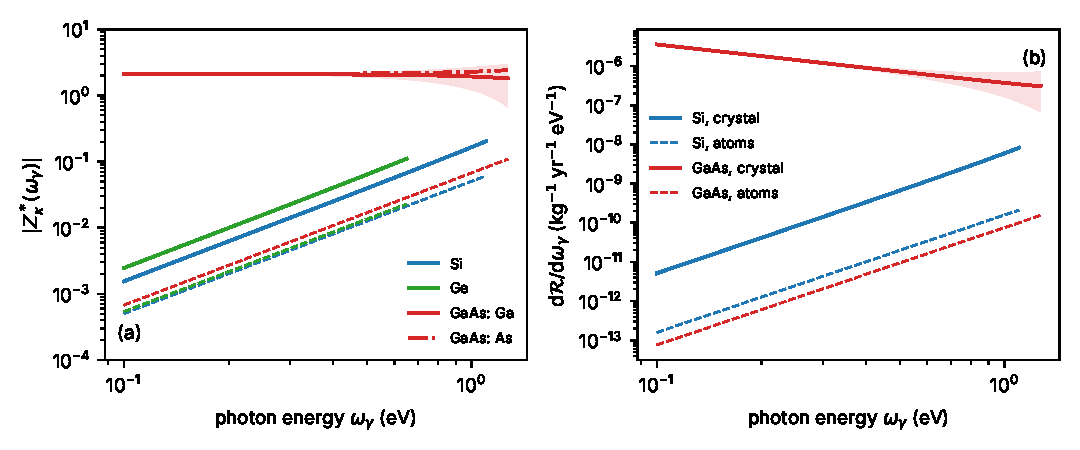
\includegraphics[width=\linewidth]{figures/ch12/fig12_5.pdf}
  \caption{Nuclear-recoil bremsstrahlung in silicon, germanium and GaAs below their absorption edges. (a) The dynamical Born charge $|Z^*_\kappa(\omega_\gamma)|$ against the photon energy (solid; dash-dotted for the arsenic site), from the sum rule \cref{eq:12.6-sum} with measured refractive indices: silicon at \SI{300}{K}~\cite{franta2017temperature} (0.1--\SI{1.1}{eV}), germanium at \SI{293}{K}~\cite{li1980refractive} (0.1--\SI{0.65}{eV}) and GaAs at \SI{295}{K}~\cite{skauli2003improved,polyanskiy2024refractiveindex} (0.1--\SI{1.27}{eV}, the range of the dispersion formula; its phonon term removed from the electronic $\varepsilon$). GaAs: $Z^* = 2.11$ at zero frequency and the dispersion of the sum split equally between the sites; shaded, the range allowed by the bound $|Z^*_\kappa(\omega) - Z^*_\kappa(0)| \le 0.9\,(\omega/\SI{1}{eV})^2$. Dashed: the free atoms, \cref{eq:12.6-atom} with the static polarizabilities 37.3 (Si), 40 (Ge) and 50 (Ga) atomic units~\cite{schwerdtfeger2019table}. (b) Rate per unit photon energy for $\mchi = \SI{100}{MeV}$, a heavy mediator coupled to nucleon number, $\sigma_p = 10^{-38}\,\mathrm{cm}^2$, the halo of \cref{sec:1.2}, \cref{eq:12.6-brems} with a free recoil. Solid: crystals; dashed: the same nuclei with the free-atom charges and $n_r = 1$; shaded: the GaAs band of panel (a).}
  \label{fig:12-brems}
\end{figure}

\Cref{fig:12-brems} shows the result. In GaAs the photons per kick are almost flat in $\ln\omega_\gamma$, as for a bare charge; half of them lie below \SI{0.36}{eV}. In silicon and germanium the spectrum climbs as $\omega_\gamma^3$ up to the absorption edge. The absolute numbers are small. A recoil of \SI{100}{eV} emits $4.0\times10^{-13}$ photons between 0.1 and \SI{1.1}{eV} in silicon and $1.7\times10^{-10}$ between 0.1 and \SI{1.27}{eV} in GaAs, against the Migdal probability of $6.1\times10^{-3}$ in silicon at the same recoil. At \SI{100}{MeV} the GaAs rate in panel (b) integrates to $9\times10^{-7}$ events per kilogram-year, and the silicon rate to $2\times10^{-9}$, while the Migdal rate of silicon with the same coupling is 30 (\cref{sec:12.3-rate}). The photons of GaAs lie below the gap, where the Migdal effect is closed, but they come with a Migdal signal above the gap that, judged by silicon, is larger by more than seven orders of magnitude. Bremsstrahlung in these crystals is therefore a check of the theory, not a search channel. At photon energies of hundreds of eV and above, where Kouvaris and Pradler found the reach of their xenon search, $\varepsilon \to 1$, the crystal emits as its atoms, and \cref{eq:12.6-sum} returns the bare charges as the electrons fall behind.

\begin{workedexample}{The GaAs enhancement over the atomic rate}\label{we:12-gaas}
How much more does a GaAs crystal radiate than a gas of the same atoms? We work at $\omega_\gamma = \SI{1}{eV}$ and then over the transparent band.

\emph{The dynamical Born charges.} The cell volume is $\Omega = a^3/4 = \SI{44.80}{\angstrom^3}$ with the static-lattice constant $a = \SI{5.638}{\angstrom}$ of \cref{tab:E-functionals}, the cell of the computed phonons and Born charge of \cref{sec:5.5}, and $\Omega m_e/e^2 = \SI{3.249e-2}{eV^{-2}}$. The dispersion formula of Skauli and collaborators~\cite{skauli2003improved}, as tabulated in Ref.~\cite{polyanskiy2024refractiveindex}, gives $n_r = 3.4185$ at \SI{1}{eV}, and without its phonon term the electronic dielectric function $\varepsilon = 11.688$. By \cref{eq:12.6-sum} at $\omega = \SI{1}{eV}$ the sum of the charges is $-(3.249\times10^{-2})(10.688) = -0.347$. Split equally, $Z^*_{\mathrm{Ga}}(\SI{1}{eV}) = 2.11 - 0.174 = 1.936$ and $Z^*_{\mathrm{As}}(\SI{1}{eV}) = -2.11 - 0.174 = -2.284$, so that the sum of their squares is 8.965. For any other split the sum of squares is $2(2.11 + b)^2 + 2(0.174)^2$, with $b$ half the difference between the two dispersions; the band of \cref{fig:12-brems} carries the values of $b$ that the bound allows.

\emph{The free atoms.} With $\alpha_{\mathrm{pol}} = 50$ and 30 atomic units~\cite{schwerdtfeger2019table}, that is $4\pi\times50\,a_0^3 = \SI{93.1}{\angstrom^3}$ and \SI{55.9}{\angstrom^3} in Heaviside--Lorentz units, \cref{eq:12.6-atom} gives $Z^*_{\mathrm{at}} = -0.0675$ for gallium and $-0.0405$ for arsenic at \SI{1}{eV}, and the sum of squares is $6.20\times10^{-3}$.

\emph{Per photon.} The two nuclei have nearly the same nucleon number per mass and nearly the same $q^2/M_\kappa^2$ at a given recoil, so the ratio of \cref{eq:12.6-brems} to its atomic form is the ratio of $n_r\sum_\kappa Z^{*2}_\kappa$ to $\sum_\kappa Z^{*2}_{\mathrm{at},\kappa}$: $3.4185\times8.965/6.20\times10^{-3} = 4.94\times10^3$ at \SI{1}{eV}. The crystal emits five thousand times more. Of that, $n_r$ contributes 3.4 and the Born charge the rest.

\emph{Over the band.} The ratio grows toward small $\omega_\gamma$ as $\omega_\gamma^{-4}$, since the atomic charges fall as $\omega_\gamma^2$ and the crystal charges do not. Integrated with the weight $1/\omega_\gamma$ of \cref{eq:12.6-brems} from 0.1 to \SI{1.27}{eV}, $\int n_r\sum_\kappa Z^{*2}_\kappa\,\dd\omega_\gamma/\omega_\gamma = 75.4$ and $\int\sum_\kappa Z^{*2}_{\mathrm{at},\kappa}\,\dd\omega_\gamma/\omega_\gamma = 4.03\times10^{-3}$, a ratio of $1.87\times10^4$. The full rate at $\mchi = \SI{100}{MeV}$ gives $1.88\times10^4$, the same to the precision shown, because the kinematics hardly depends on photon energies so far below the kinetic energy of the dark matter.

\emph{Per recoil.} A gallium nucleus with $E_R = \SI{100}{eV}$ has $v_N^2 = 2E_R/M = 3.08\times10^{-9}$, and with $2\alpha/3\pi = 1.549\times10^{-3}$ it emits $1.7\times10^{-10}$ photons in the band. The enhancement over the atom is large, four orders of magnitude, but it multiplies a small number. Its uncertainty is the band of \cref{fig:12-brems}: the rate at \SI{100}{MeV} lies between \SI{-19}{\percent} and \SI{+25}{\percent} of its central value.
\end{workedexample}

\subsection{Migdal-type absorption of a scalar}\label{sec:12.6-absorption}

A scalar of mass \SI{1}{keV} from the halo, absorbed in silicon, deposits \SI{1}{keV} with a momentum of only $k = m_\phi v \approx \SI{1}{eV}$. If it couples to nucleons, the nucleus takes that momentum, and its recoil energy, $k^2/2M_\kappa$, is \SI{e-11}{eV}. The energy must go somewhere else, and it goes to the electrons. Dzuba, Flambaum and Samsonov computed this for atoms~\cite{dzuba2024migdal}. In the language of \cref{sec:12.2} it is a Migdal effect at the momentum $k$ instead of $q$. The exact center-of-mass separation \cref{eq:12.2-cm} turns the kick $\ee^{\ii\vect{k}\cdot\vect{X}}$ into a kick of the whole atom and the boost $\exp(-\ii\vect{k}_e\cdot\sum_e\vect{\rho}_e)$ of the electrons, with $\vect{k}_e = m_e\vect{k}/m_A$. At the dipole order of \cref{eq:12.2-dipole} the amplitude to excite the electrons to $\Psi_f$ is $-\ii k_e\langle\Psi_f|D_{\hat k}|\Psi_0\rangle$. What differs from scattering is the energy. The field supplies $\omega = m_\phi$, and the whole of it goes to the electrons, $\omega_e = m_\phi$, while the lattice receives nothing to the precision of interest.

\emph{The coupling.} A scalar coupled to protons and neutrons, $\mathcal{L} \supset \phi\,(g_{\phi pp}\,\bar pp + g_{\phi nn}\,\bar nn)$, couples to each nucleus coherently, as in \cref{eq:8.1-nuclear}, with the nuclear form factor equal to one at these momenta. The interaction is $H_\phi = -\phi\sum_\kappa c_\kappa n_\kappa(\vect{p}_\phi)$, the nuclear density row of \cref{sec:8.1-absorption} with
\begin{equation*}
  c_\kappa = Z_\kappa\,g_{\phi pp} + (A_\kappa - Z_\kappa)\,g_{\phi nn} , \qquad g^\phi_{n_\kappa} = -c_\kappa ,
\end{equation*}
the per-species weight $c_\kappa$ of \cref{sec:11.3}, which here carries the couplings themselves rather than their ratio to a reference coupling. For equal couplings, $c_\kappa = A_\kappa g_{\phi nn}$.

\emph{The acceleration form.} For an atom the center-of-mass separation is exact; in a crystal there is no atom to separate, and we need another route to the same amplitude. The equations of motion give it. Whatever the interactions, the potential energy $V$ of the crystal depends on the positions alone, so $[H,\vect{X}_I] = -\ii\vect{P}_I/M_\kappa$ and $[H,\vect{P}_I] = \ii\nabla_{\vect{X}_I}V$, and the double commutator is $[H,[H,\vect{X}_I]] = \nabla_{\vect{X}_I}V/M_\kappa$. Between eigenstates with $\omega_{fi} = E_f - E_i \neq 0$ this reads $\omega_{fi}^2\langle f|\vect{X}_I|i\rangle = \langle f|\nabla_{\vect{X}_I}V|i\rangle/M_\kappa$. Expanding the kick to first order in $\vect{k}$,
\begin{equation}
  \Bigl\langle f\Big|\sum_Ic_\kappa\ee^{\ii\vect{k}\cdot\vect{X}_I}\Big|i\Bigr\rangle = \frac{\ii}{\omega_{fi}^2}\sum_I\frac{c_\kappa}{M_\kappa}\,\vect{k}\cdot\langle f|\nabla_{\vect{X}_I}V|i\rangle + O(k^2) ,
  \label{eq:12.6-accel}
\end{equation}
the acceleration form of the amplitude. It is exact, at every order of the Born--Oppenheimer expansion. Its matrix element is minus the total force on nucleus $I$, from the electrons and the other nuclei, between the initial and final states. Between electronic states this is the derivative coupling of \cref{eq:5.1-dcoup}, and \cref{eq:12.6-accel} is the boost amplitude \cref{eq:8.6-boost} with $q$ replaced by $k$ and the excitation energy by $\omega_{fi}$. In scattering the boost is the first term of an expansion in the velocity of the nucleus. Here the momentum is so small that only the dipole term matters, and the equations of motion give it exactly.

\emph{Couplings proportional to mass.} Let $c_\kappa = \tilde cM_\kappa$ for every species, with one constant $\tilde c$. The potential depends only on differences of positions, so the gradients with respect to all particles sum to zero, $\sum_I\nabla_{\vect{X}_I}V = -\sum_j\nabla_{\vect{r}_j}V$, the sum over electrons: the total force on the nuclei is minus the total force on the electrons. The same double commutator for the electrons, with $m_e$ in place of $M_\kappa$, turns the right-hand side of \cref{eq:12.6-accel} into a dipole matrix element of the electrons, and
\begin{equation}
  \Bigl\langle f\Big|\tilde c\sum_IM_\kappa\ee^{\ii\vect{k}\cdot\vect{X}_I}\Big|i\Bigr\rangle = -\tilde c\,m_e\,\langle f|n_e(\vect{k})|i\rangle\,\bigl[1 + O(kr)\bigr] ,
  \label{eq:12.6-mass}
\end{equation}
with $r$ the size of the states involved. The physical reading is the equivalence principle. A field that couples to the mass of every particle cannot, at zero momentum, distinguish them: it pushes the center of mass and nothing else, and its matrix elements between different states start at order $k^2$. A coupling to the mass of the nuclei is the coupling to the total mass minus that to the electrons, and only the second term excites the crystal. It is the electronic counterpart of the cancellation by which a coupling proportional to mass excites no optical phonon (\cref{eq:11.8-Gamma}).

The scalar therefore acts on the electrons as a density coupling of strength $\tilde cm_e$. The absorption formula \cref{eq:8.2-abs} with $S_{ee} = (2k^2/e^2)L$, \cref{eq:4.4-SL}, the electron-density form that holds above the phonon band, gives the rate.
\begin{keyresult}[Migdal-type absorption in a crystal]
For a scalar whose couplings to the nuclei are proportional to their masses, $c_\kappa = \tilde cM_\kappa$, absorbed with momentum $\vect{p}_\phi$ and energy $\omega_\phi \simeq m_\phi$ above the phonon band,
\begin{equation}
  \varGamma_{\mathrm{abs}} = \frac{\tilde c^2m_e^2\,p_\phi^2}{e^2\,m_\phi}\,L(\vect{p}_\phi \to 0, m_\phi) , \qquad
  \mathcal{R} = \frac{\rho_\chi}{\rho_T}\,\frac{\tilde c^2m_e^2\langle v^2\rangle}{e^2}\,L(m_\phi) ,
  \label{eq:12.6-absrate}
\end{equation}
with $L = \Imag[-1/\varepsilon]$ the loss function at zero momentum and $\langle v^2\rangle$ the mean squared speed of the halo in the laboratory.
\end{keyresult}
\noindent For the halo of \cref{sec:1.2}, $\langle v^2\rangle^{1/2} = \SI{379}{km.s^{-1}}$. The spectrum is that of dark-photon absorption, whose rate is $(\rho_\chi/\rho_T)\zeta^2L(m_\phi)$ (\cref{sec:10.7}), with $\zeta^2$ replaced by $\tilde c^2m_e^2\langle v^2\rangle/e^2$. Everything \cref{sec:10.7} found about screening carries over: the scalar is absorbed with the loss function, not with the absorptive part $\varepsilon_2$, suppressed near the absorption peaks of silicon, where $|\varepsilon|^2$ is large, and enhanced at the plasmon. In silicon and germanium, with one species, every coupling to nucleons is proportional to the mass up to the isotopes, so \cref{eq:12.6-absrate} is the whole rate.

The atomic result is the dilute limit. For a gas, $|\varepsilon| \to 1$ and $L \to \varepsilon_2$, and the photoabsorption cross-section $\sigma_\gamma$ of one atom fixes $\omega\varepsilon_2 = \nd_{\mathrm{at}}\sigma_\gamma$, with $\nd_{\mathrm{at}}$ the density of atoms. Then $\varGamma_{\mathrm{abs}} = \nd_{\mathrm{at}}v\,\sigma_\phi$ with $\sigma_\phi = \tilde c^2m_e^2(p_\phi/m_\phi)\sigma_\gamma/e^2$, which for $\tilde c = g_{\phi nn}/m_p$ is the relation of Dzuba, Flambaum and Samsonov between scalar absorption and photoionization~\cite[Eqs.~(14), (17)]{dzuba2024migdal}. They cautioned that rates in solids could differ from the atomic estimate, and \cref{eq:12.6-absrate} says by how much. Applied to a crystal with the measured photoabsorption, which in a medium is $\nd_{\mathrm{at}}\sigma_\gamma = \omega\varepsilon_2/n_r$, the atomic formula uses $\varepsilon_2/n_r$ where the crystal has $\varepsilon_2/|\varepsilon|^2$. The ratio, $n_r/|\varepsilon|^2$, is the medium factor. Far above the absorption edges, $\varepsilon \simeq 1 - \omega_p^2/\omega^2$ with $\omega_p$ the plasma frequency of the electrons bound below $\omega$, so that $n_r \simeq 1 - \omega_p^2/2\omega^2$ and $|\varepsilon|^2 \simeq 1 - 2\omega_p^2/\omega^2$, and
\begin{equation}
  \frac{n_r}{|\varepsilon|^2} = 1 + \frac32\,\frac{\omega_p^2}{\omega^2} + O\Bigl(\frac{\omega_p^4}{\omega^4},\ \varepsilon_2^2\Bigr) .
  \label{eq:12.6-medium}
\end{equation}
For silicon at \SI{1}{keV}, with the twelve electrons per atom bound by less than \SI{1}{keV} and $\omega_p = \SI{28.8}{eV}$, this is $1 + 1.2\times10^{-3}$. Near the plasmon and the absorption peaks it is far from one.

\begin{limitbox}[Migdal-type absorption of a scalar][lim:12.6a]
$\sigma_\phi = g_{\phi nn}^2(m_e^2/m_p^2)(p_\phi/m_\phi)\,\sigma_\gamma/4\pi\alpha$ per atom, with $\sigma_\gamma$ the photoionization cross-section at $\omega = m_\phi$~\cite[Eqs.~(14), (17)]{dzuba2024migdal}.
\par\smallskip
{\centering
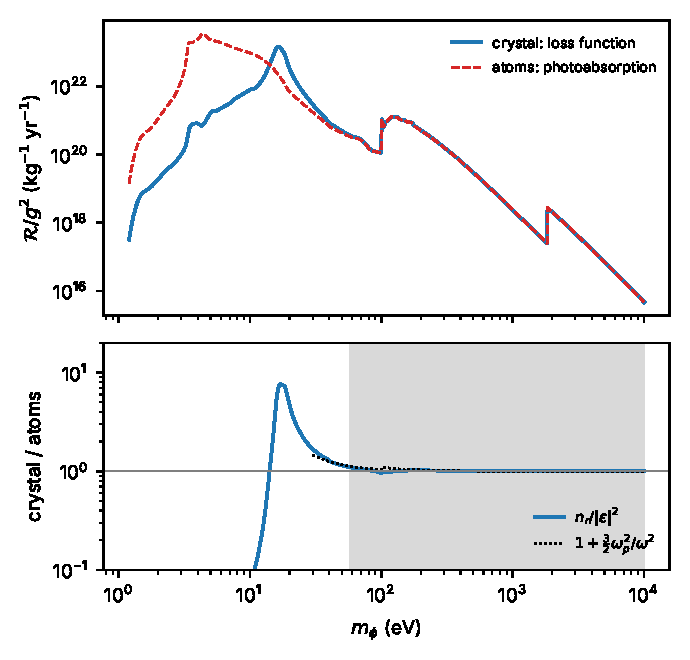
\includegraphics[width=0.92\linewidth]{figures/ch12/limit12_6a.pdf}
\captionof{figure}{Absorption of a scalar coupled equally to protons and neutrons ($c_\kappa = gA_\kappa$) in silicon against its mass $m_\phi$. Top: rate per unit mass divided by $g^2$, from the loss function, \cref{eq:12.6-absrate} (solid), and from the atomic formula with the measured photoabsorption of the crystal, $\nd_{\mathrm{at}}\sigma_\gamma = m_\phi\varepsilon_2/n_r$ (dashed); halo of \cref{sec:1.2}. Bottom: their ratio $n_r/|\varepsilon|^2$, with the expansion \cref{eq:12.6-medium} (dotted, $\omega_p$ from the electrons bound below $m_\phi$, binding energies of the $L$ and $K$ shells as in \cref{sec:10.6}). Dielectric function of silicon at \SI{300}{K}~\cite{franta2017temperature} below \SI{40}{eV} and from the atomic scattering factors~\cite{henke1993xray} above, as in \cref{sec:10.7}. Gray band: $m_\phi \ge \SI{57}{eV}$, where the atomic formula is within \SI{10}{\percent}.}\label{fig:12-limit-6a}
\par}
\smallskip
Below about \SI{60}{eV} the atomic formula misses the screening of the crystal, and is too high by about 400 near the absorption peak at \SI{4.2}{eV} and too low by 7.7 near the plasmon, at \SI{17}{eV}.
\end{limitbox}

\noindent On the truncation label \cref{lim:12.6a} sits at dipole order, $n_D = 2$ in the rate, with no Born--Oppenheimer truncation, since \cref{eq:12.6-accel,eq:12.6-mass} are exact; $\mathcal{X}$ is the measured loss function, and the lattice plays no role at these energies. Its next corrections are the multipoles of order $kr$, which at \SI{10}{keV} and a $1s$ radius of $a_0/Z$ are below $10^{-3}$, and, outside the shaded band, the full loss function in place of the atomic formula.

\emph{Couplings not proportional to mass.} If $c_\kappa/M_\kappa$ differs between species, write it as $\tilde c + \delta\tilde c_\kappa$, with $\tilde c$ a mean. The mean part is \cref{eq:12.6-absrate}. The remainder keeps the forces in \cref{eq:12.6-accel}, $\ii\omega^{-2}\sum_I\delta\tilde c_\kappa\,\vect{k}\cdot\langle f|\nabla_{\vect{X}_I}V|i\rangle$, and these no longer sum to anything simple. For transitions of the electrons the force on a nucleus is the density component of \cref{eq:12.1-force}, the vertex of the Migdal entry. The sum over the sites of one species, weighted by $\ee^{\ii\vect{k}\cdot\vect{X}_I}$, then forces the momentum given to the electrons to be $\vect{k} + \vect{G}$. The remainder is therefore a sum over reciprocal-lattice vectors weighted by the basis structure factor of $\delta\tilde c_\kappa Z_\kappa$, and it samples the off-diagonal elements $S^{ee}_{\vect{0}\vect{G}}$ and $S^{ee}_{\vect{G}\vect{G}'}$ of the electronic response at vanishing reduced momentum (\cref{eq:E.18-X}). These are nonadiabatic matrix elements in the sense of \cref{sec:12.1}: the response of the electrons to the force of one sublattice, which no optical measurement provides. For the core shells, which belong to one nucleus, the atomic dipole formula with $\delta\tilde c_\kappa$ in place of $\tilde c$ applies shell by shell. For the valence electrons \cref{app:E.18} specifies the calculation, with $S^{ee}_{\vect{G}\vect{G}'}$ to $|\vect{G}| = 6(2\pi/a)$ and the test that the (200) channel of the diamond structure vanishes for equal $\delta\tilde c_\kappa$. How large the remainder is depends on the coupling. For nucleon number in GaAs the two species differ in $A_\kappa/M_\kappa$ by $2.6\times10^{-5}$ per u (\cref{we:8-nucleon}), and the remainder is negligible. For a coupling to protons alone, $Z_\kappa/M_\kappa$ is 0.4446 per u for gallium and 0.4405 for arsenic, and the isotopes of natural silicon differ by up to \SI{7}{\percent}; the isotopic part is a random remainder, incoherent between sites, like the isotope scattering of \cref{sec:11.6}.

A scalar may also couple to electrons. Its amplitude adds $\tilde cm_e$ to the density coefficient $g^\phi_{n_e} = -g_{\phi ee}$ of \cref{eq:8.1-scalar}, and the kinetic row of the electron coupling, which dominates its absorption (\cref{sec:10.7}), interferes with the density row through their cross response. The nucleon coupling adds no new row.

\subsection{Nuisance table of the Migdal sector}\label{sec:12.6-table}

\Cref{tab:12-nuisances} collects the truncations and inputs of the chapter, each with its size and the section that treats it, in the classes of \cref{sec:8.8}.

\begin{table}[tbp]
  \caption{Nuisances of the Migdal sector. Type in the classes of \cref{sec:8.8}: normalization, tilt (in $\omega_e$, in $q$ or in the dark-matter mass), threshold and lattice spectrum (the share of a Migdal event that goes to phonons, at fixed electronic energy transfer). Basis of the size: ``computed'' (next order computed), ``model'' (next order computed in a model), ``est.''\ (parametric estimate), ``bound'' (only an inequality is known), ``named'' (no size). Sizes are for silicon unless another crystal is named. The last column gives the section where the item is treated.}
  \label{tab:12-nuisances}
  \centering\footnotesize\setlength{\tabcolsep}{3pt}
  \begin{tabular}{@{}>{\raggedright\arraybackslash}p{0.27\linewidth}>{\raggedright\arraybackslash}p{0.12\linewidth}>{\raggedright\arraybackslash}p{0.36\linewidth}>{\raggedright\arraybackslash}p{0.09\linewidth}>{\raggedright\arraybackslash}p{0.10\linewidth}@{}}
    \toprule
    Truncation or input & Type & Size & Basis & Section \\
    \midrule
    Local fields on the diagonal of $\varepsilon^{-1}$ (scalar $\varepsilon$ against $\varepsilon^{-1}_{\vect{G}\vect{G}}$) & normali\-zation; tilt in $\omega_e$ & factor 1.35 on the total, concentrated at $p \gtrsim q_{\mathrm{BZ}}$ (\cref{lim:12.3a}) & computed & \cref{sec:12.3} \\
    Off-diagonal elements $\vect{G} \neq \vect{G}'$ of $\varepsilon^{-1}$ & normali\-zation & raises the rate: full over diagonal 1.38 at $8^3$ points $\vect{k}$ and $|\vect{G}|^2 \le 19\,(2\pi/a)^2$, about 1.2 extrapolated, in an empirical-pseudopotential random-phase model of Si that carries about 2/3 of the diagonal local-field effect; still falling with $\vect{G}$, so the lower end is not a bound; flat in $\mchi$; the full local-field calculation is open; incoherent, zone-averaged form, not applicable at $q \ll q_{\mathrm{BZ}}$ & model & \cref{sec:12.1,sec:12.3} \\
    Loss-function table ($\omega_e \le \SI{89}{eV}$, $p \le \SI{22.5}{keV}$) & normali\-zation & $P_{\mathrm{Mig}}$: $\le\SI{1.6}{\percent}$ above \SI{89}{eV}; $p > \SI{10}{keV}$ holds \SI{2.3}{\percent}; drag mass: missing part $\le\SI{24}{\percent}$ & bound & \cref{sec:12.3,sec:12.5} \\
    Ion charge $Z_{\mathrm{ion}}(p)$ against a point ion & normali\-zation & $P_{\mathrm{Mig}}$ $\times1.57$; drag mass $18.6$ against $11.8\,m_e$ & model & \cref{sec:12.3,sec:12.5} \\
    Valence on-site drag mass & normali\-zation of the added lattice rate & Si $18.6\,m_e$ (12 to $24\,m_e$), Ge $39.5\,m_e$ (11.5 to $52\,m_e$); trace value $14\,m_e$ is not the on-site element & bound & \cref{sec:12.5} \\
    Per-mass form of the rate & tilt in $\mchi$ & within \SI{10}{\percent} above \SI{66}{MeV} & computed & \cref{sec:12.3} \\
    Frame of the transition density (lattice at $\vect{q} - \vect{p}$ or $\vect{q}$; Herzberg--Teller) & lattice spectrum & phonon-emitting fraction $\times2.4$ at \SI{5}{keV}; $+\SI{12}{\percent}$ in the displaced-oscillator model & model & \cref{sec:12.1,sec:12.4} \\
    Incoherent lattice factor below the zone & lattice spectrum & zero-phonon line within \SI{8}{\percent} of the Bragg sum; multiphonon terms uncertified below \SI{6.6}{keV} & computed; named & \cref{sec:12.4} \\
    Coherent zero-phonon response at $q < 2q_{\mathrm{BZ}}$ (cross-site terms of the lattice factor) & normali\-zation; tilt in $\omega_e$ & limit $q \ll q_{\mathrm{BZ}}$ (\cref{eq:8.3-boostward}): $1/14.9$ of the diagonal form, median $\omega_e$ \SI{17.4}{eV} against \SI{4.5}{eV}; within \SI{15}{\percent} only for $q \le \SI{0.75}{keV}$ (model), which carries $\le\SI{0.2}{\percent}$ of the rate at every mass; \SI{0.75}{keV} to $2q_{\mathrm{BZ}}$ unsized, nearly all of the rate up to \SI{1}{MeV}, \SI{33}{\percent} at 2 and \SI{7}{\percent} at \SI{3}{MeV} & computed (limit); model; unsized & \cref{sec:12.4} \\
    Exact energy denominators (recoil of $\vect{p}$, binding, Doppler; \cref{eq:12.3-bracket,eq:12.4-corr}) & tilt in $q$ & near the gap $-2.1\times10^{-3}$, $+2.8\times10^{-3}$ and at most $5.1\times10^{-4}$ below the impulse onset; free recoil: probability within \SI{10}{\percent} to $E_R \approx \SI{160}{eV}$, factor 1.6 at \SI{500}{eV}, rate within \SI{10}{\percent} to \SI{1}{GeV} & computed & \cref{sec:12.3,sec:12.4} \\
    Germanium lattice inputs (Debye-scaled) & lattice spectrum & $\langle\omega^{-1}\rangle^{-1} \approx \SI{17.6}{meV}$ from $\Theta_{\mathrm{D}} = \SI{373}{K}$; regime boundaries near 41 and \SI{113}{keV}; no first-principles phonon spectrum & est. & \cref{sec:12.4} \\
    Dipole order of the atomic boost (cores) & tilt in $q$ & within \SI{10}{\percent} to $\xi_D = 0.188$ (Si), 0.127 (Ge) & computed & \cref{sec:12.2} \\
    Bound final states of the atom & normali\-zation & lower bound only & bound & \cref{sec:12.2} \\
    Wannier picture of the boost & normali\-zation & absolute bound 1.6, 0.54, 0.25 at 20, 50, \SI{100}{eV}; non-rigid ratio open & bound & \cref{sec:12.3} \\
    Relativistic contact density (third moment) & normali\-zation of the check & $+\SI{8}{\percent}$ (Si), $+\SI{42}{\percent}$ (Ge); non-logarithmic Dirac remainder and $p_{1/2}$ contact density uncontrolled, each of relative order $(Z\alpha)^2$ (\SI{5}{\percent} in Ge) & computed; est. & \cref{sec:12.5} \\
    Site difference of $Z^*_\kappa(\omega)$, GaAs bremsstrahlung & normali\-zation & $-19$ to $+\SI{25}{\percent}$ at \SI{100}{MeV} & bound & \cref{sec:12.6} \\
    Atomic formula for Migdal-type absorption & tilt in $m_\phi$ & within \SI{10}{\percent} above \SI{57}{eV}; about $400\times$ high at \SI{4.2}{eV} & computed & \cref{sec:12.6} \\
    Couplings not proportional to mass & normali\-zation & Umklapp remainder (\cref{eq:E.18-X}) & named & \cref{sec:12.6} \\
    \bottomrule
  \end{tabular}
\end{table}

For the silicon Migdal probability above a few MeV the table has one large computed row, the local fields on the diagonal, and one large row sized only in a model, the off-diagonal part, which acts in the opposite direction. The table truncation, by contrast, costs a few percent, and the ion charge is fixed by the frozen core. The per-mass form is not an uncertainty of a correct calculation but the error of a simpler one, and its size says where the simpler one may be used. The counting of Migdal and lattice events depends on the on-site drag mass, which is known only within a factor of two. And the frame of the transition density changes how a Migdal event shares its energy between electrons and lattice without changing how many events there are, which matters to a detector that reads both charge and phonons.

\subsection{Open problems}\label{sec:12.6-open}

The dynamical Born charges of a polar crystal are fixed by \cref{eq:12.6-sum} only in their sum; the difference between the sites needs the frequency-dependent calculation of \cref{app:E.17}, and until it is done the GaAs bremsstrahlung rate carries the band of \cref{fig:12-brems}. And the absorption of a scalar whose couplings are not proportional to the masses needs the off-diagonal response $S^{ee}_{\vect{G}\vect{G}'}$ at vanishing reduced momentum, which \cref{app:E.18} specifies. The open items of the earlier sections are rows of \cref{tab:12-nuisances}. Above all of them stands a measurement. No crystal Migdal signal has yet been observed. A tagged-recoil measurement, in which the energy and direction of each nuclear recoil are fixed independently, for instance by the kinematics of a neutron scattered at a known angle, and the electrons it releases are counted, would test the whole chain at once in silicon at the recoil energies of \cref{sec:12.5}.

\section*{Summary}

A kicked nucleus leaves energy in two places, the lattice and the electrons, and the joint response resolves the two (\cref{sec:12.1}). It is the response of \cref{sec:8.7} sorted by the electronic energy transfer $\omega_e$ and the lattice energy $\omega_l$; its marginal is the ordinary response, and the sectors of \cref{sec:8.6} fall on the two axes and the quadrant between them. At the leading nonadiabatic order its Migdal entry is the response of the electrons to the field of a suddenly moving nucleus: a boost $\vect{q}\cdot\vect{p}/M_\kappa\omega_e^2$, the bare vertex of the nucleus, the density response of the clamped electrons and the lattice response at the momentum the nucleus keeps. The four published Migdal formulas are truncations of that entry. Its first moment is fixed by the drag mass, and the estimate $P_{\mathrm{Mig}} \approx (E_R/\langle\omega_e\rangle)(\delta M_\kappa/M_\kappa)$ follows. Added to a lattice rate, a Migdal rate requires the lattice response with the weight $1 - P_{\mathrm{Mig}}$ and the dragged mass, and a measured nuclear-recoil yield already contains the Migdal ionization. In a metal the sudden expansion fails at small $\omega_e$.

The isolated atom is the truncation in which the boost can be done to all orders (\cref{sec:12.2}). The center of mass separates exactly, and the electrons receive the momentum $m_e\vect{q}/m_A$, with $m_A$ the mass of the whole atom. At dipole order the ionization probability at a recoil energy of \SI{1}{keV} is $2.09\times10^{-3}$ for silicon and $1.63\times10^{-3}$ or $1.73\times10^{-3}$ for germanium in two independent calculations, and the dipole form holds within \SI{10}{\percent} up to $\xi_D = 0.188$ and 0.127. Bound final states without ionization add to it, and the oscillator strengths give only a lower bound on their share. In a crystal the atomic form is the right one for the core shells, not for the valence.

At large momentum transfer the crystal Migdal probability is a weighted moment of the loss function, with the coefficient $4\alpha$ fixed by the $f$-sum rule and the valence ionization factor $Z_{\mathrm{ion}}(p)$ in the vertex (\cref{sec:12.3}). In silicon it is $6.1\times10^{-5}$ per eV of recoil energy, 29 times the atomic value. A scalar dielectric function overestimates it by about \SI{35}{\percent}, an error concentrated at $p \gtrsim q_{\mathrm{BZ}}$; the off-diagonal elements of the dielectric matrix raise it in a model by a factor of about 1.4 as computed and 1.2 extrapolated, the lower end not a bound, and their full calculation is open. The soft limit has no correction in $p/q$ and holds at low mass; it fails only when the nucleus moves fast during the transition, above about \SI{160}{eV} of recoil. The factorized rate per unit mass holds within \SI{10}{\percent} above \SI{66}{MeV}. The Wannier picture of the boost is exact for flat bands and bounded only in absolute terms for the valence band of silicon.

Below the impulse onset the lattice factor of the Migdal entry is the multiphonon response at the momentum the nucleus keeps (\cref{sec:12.4}). The electronic spectrum does not depend on it, since the lattice factor has unit weight. What it decides is how a Migdal event shares its energy: at \SI{10}{keV} in silicon \SI{92}{\percent} of the events leave the lattice in its ground state, and most events stay zero-phonon until the zero-phonon weight of the kick itself falls to one half, at \SI{33.2}{keV}. The phonon-mediated form is the same process with the bound-nucleus propagator, exact in the phonon energies at first order in $\vect{p}$; for silicon and germanium its correction is a few parts in a thousand at the gap, and it matters only where gaps approach phonon energies.

The moments of the Migdal spectrum are inverse moments of the force that the electrons exert on one nucleus (\cref{sec:12.5}). The first is the on-site drag mass, which differs from the trace value of $14\,m_e$ for silicon that a uniform translation fixes; the loss function gives $18.6\,m_e$ for the valence electrons alone, uncertain by a factor of two. Two moments bound the probability from both sides. The cross first moment fixes the Migdal interference of a mixed coupling, and the third moment is the electron density at the nucleus, which relativity raises by \SI{8}{\percent} in silicon and \SI{42}{\percent} in germanium.

A recoiling nucleus also radiates, and an absorbed scalar coupled to nucleons gives its energy to the electrons through the same boost (\cref{sec:12.6}). The crystal emits with the dynamical Born charge, which in silicon and germanium follows exactly from the measured dielectric function and suppresses the emission as the fourth power of the photon energy. Silicon still emits 33 to 38 times more than its atoms, and GaAs, with its static Born charge, $1.87\times10^4$ times more over its transparent band. The rates are seven orders below the Migdal rate, so bremsstrahlung is a check, not a channel. A scalar whose couplings to the nuclei are proportional to their masses is absorbed with the loss function, by the equivalence principle, and the atomic formula holds in silicon only above \SI{57}{eV}. The chapter's nuisances are collected in \cref{tab:12-nuisances}. Throughout, the electronic final states were reached by kicking a nucleus; \cref{chap:13} turns to the other mixed sector, the electrons kicked directly while a phonon carries the missing momentum.

\printbibliography[heading=subbibliography]

\chapter{Phonon-assisted electron recoil}\label{chap:13}
The lowest electron--hole pair of silicon has a crystal momentum of \SI{1.94}{keV}: the hole sits at the center of the zone and the electron in one of the six conduction valleys near X (\cref{sec:3.3}). Dark matter lighter than about \SI{0.4}{MeV} cannot supply that momentum together with the \SI{1.17}{eV} of the gap, because at the momentum transfer where it deposits the most energy the pairs cost more. It can still create a pair, however, if it creates a phonon at the same time, and the phonon carries the missing crystal momentum for an energy of at most \SI{64}{meV}. Light does the same between the indirect and the direct gap, and the absorption edge of silicon is a measurement of that process (\cref{sec:6.5}). The question of this chapter is how large the phonon-assisted rate is, and how to compute it without double-counting the zero-phonon rate of \cref{chap:10}. For silicon detectors the answer decides over which masses this is the only electron-recoil channel, and which edges of that window are still uncertain. In the decomposition of \cref{sec:8.6} its final states form the phonon-dressed electronic sector, the second mixed sector after the Migdal effect of \cref{chap:12}, and its optical limit ties it to the absorption data of \cref{sec:6.5} (\cref{fig:13-map}).

\begin{figure}[tbp]
  \centering
  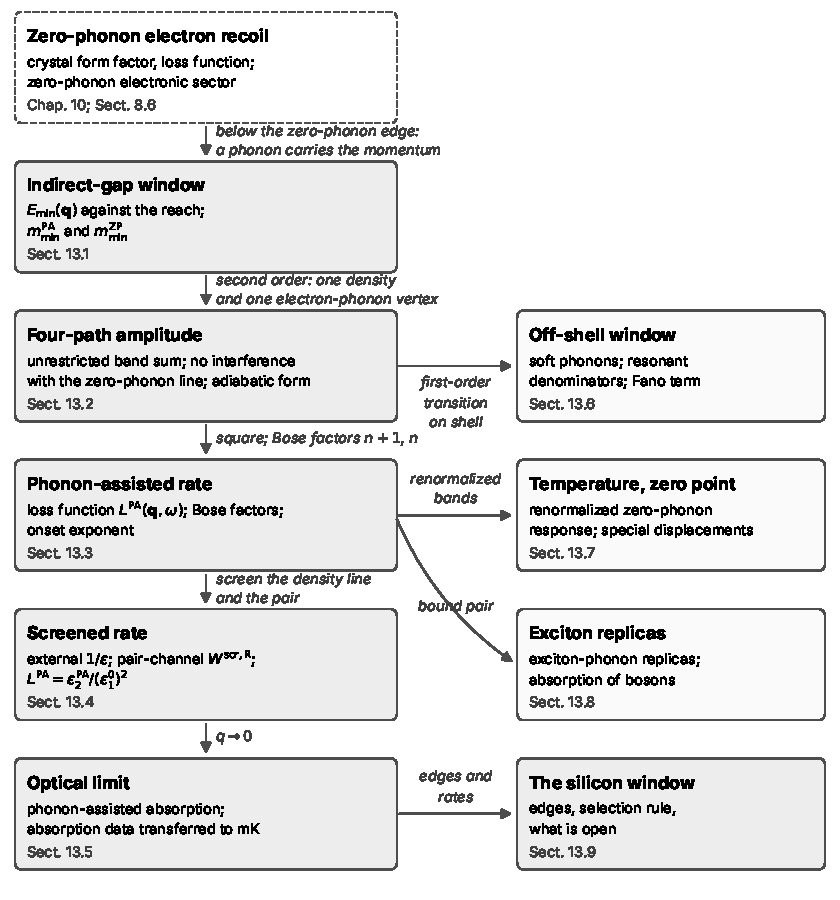
\includegraphics[width=0.85\linewidth]{figures/ch13/map13.pdf}
  \caption{Phonon-assisted electron recoil, from the kinematics of the window to the silicon window itself. Below the zero-phonon edge of the electronic response of \cref{chap:10}, a phonon must carry the missing crystal momentum (\cref{sec:13.1}). The amplitude is of second order, with one density vertex and one electron--phonon vertex on four paths (\cref{sec:13.2}); squared and summed over final states it gives the phonon-assisted loss function and rate (\cref{sec:13.3}), which screening dresses on the density line and on the pair (\cref{sec:13.4}); at $q \to 0$ it becomes phonon-assisted optical absorption (\cref{sec:13.5}; \cref{lim:13.5a}). The figure also places the off-shell window outside which the second-order rate is not separately defined (\cref{sec:13.6}), the renormalized bands at finite temperature and zero point (\cref{sec:13.7}; \cref{lim:13.7a}), and the bound pair with its phonon replicas and the absorption of bosonic dark matter (\cref{sec:13.8}). The edges and rates meet in the silicon window (\cref{sec:13.9}).}
  \label{fig:13-map}
\end{figure}

\section{The indirect-gap window}\label{sec:13.1}

A dark-matter particle of \SI{0.35}{MeV} can deposit up to $\frac12\mchi v_{\mathrm{max}}^2 = \SI{1.23}{eV}$, more than the \SI{1.17}{eV} gap of silicon, but only at the momentum transfer $q = \mchi v_{\mathrm{max}} = \SI{0.93}{keV}$. This momentum transfer is less than half of the \SI{1.94}{keV} that separates the valence-band maximum from the conduction valleys, and at $q = \SI{0.93}{keV}$ the cheapest electron--hole pair along the valley axis costs about \SI{1.9}{eV} (\cref{fig:3-si-bands}). Without a phonon the particle cannot create a pair. With a phonon of about \SI{15}{meV} that takes up the remaining \SI{1.0}{keV} of the valley momentum, it can. The phonon-assisted process of \cref{sec:9.1} is then the only way for dark matter scattering on electrons to create an electron--hole pair, in a window of masses that runs from the lightest mass that creates a pair with a phonon, $m_{\mathrm{min}}^{\mathrm{PA}}$, to the lightest mass that creates a pair without a phonon, $m_{\mathrm{min}}^{\mathrm{ZP}}$.

\subsection{The zero-phonon threshold mass}

The largest momentum transfer of a particle of mass $\mchi$ is $2\mchi v_{\mathrm{max}}$, and it reaches the valley momentum $k_{\mathrm{c}} = \SI{1.94}{keV}$ of \cref{eq:3.3-kc} only for $\mchi \ge k_{\mathrm{c}}/2v_{\mathrm{max}} = \SI{0.366}{MeV}$; at that mass the particle reaches $k_{\mathrm{c}}$ by backscattering, with no energy to spare. The energy that the particle can deposit at fixed $q$ is $qv_{\mathrm{max}} - q^2/2\mchi$ (\cref{eq:1.3-region}), largest at $q = \mchi v_{\mathrm{max}}$. The two requirements conflict: depositing the gap favors $q \approx \mchi v_{\mathrm{max}}$, while reaching the valley needs $q \approx k_{\mathrm{c}}$, and for light particles $\mchi v_{\mathrm{max}}$ is well below $k_{\mathrm{c}}$.

To locate the zero-phonon threshold, we turn the kinematic condition \cref{eq:3.3-allowed} into a condition on the mass. At fixed $\vect{q}$, a pair of energy $E$ is reachable when $qv_{\mathrm{max}} - q^2/2\mchi \ge E$. For $qv_{\mathrm{max}} > E$ this condition reads
\begin{equation*}
  \mchi \ge \frac{q^2}{2\,(qv_{\mathrm{max}} - E)} .
\end{equation*}
The right-hand side grows with $E$ at fixed $q$, so at each $\vect{q}$ the cheapest pair sets the bound, and the energy of that pair is the minimum pair energy $E_{\mathrm{min}}(\vect{q})$ of \cref{eq:3.3-Emin}. Minimizing then over $\vect{q}$, and writing out the minimum over the hole's crystal momentum $\vect{k}$ that $E_{\mathrm{min}}$ contains, gives the zero-phonon threshold mass
\begin{equation}
  m_{\mathrm{min}}^{\mathrm{ZP}} = \min_{\vect{q}}\frac{q^2}{2\,[qv_{\mathrm{max}} - E_{\mathrm{min}}(\vect{q})]}
  = \min_{\vect{q},\,\vect{k},\,v,\,c}\frac{q^2}{2\,[qv_{\mathrm{max}} - \varepsilon_{c,\vect{k}+\vect{q}} + \varepsilon_{v\vect{k}}]} ,
  \label{eq:13.1-mZP}
\end{equation}
with the minimum over the region where the denominator is positive. The second form is one minimization over six continuous variables, three for $\vect{q}$ and three for $\vect{k}$, and it shows that two common simplifications, fixing the hole at the valence-band maximum and restricting $\vect{q}$ to a few directions, can only raise the result.

Near a valley the minimization can be done by hand. Along the axis of a silicon valley, the pair energy is the parabola \cref{eq:3.3-Eminpar}, $E_{\mathrm{min}} \simeq \Eg + (q - k_{\mathrm{c}})^2/2M_{\mathrm{eh}}$, where $M_{\mathrm{eh}} = m^*_\parallel + m_{\mathrm{hh}}$ is the mass with which the pair as a whole recoils, equal to the sum of the longitudinal electron mass and the heavy-hole mass in the same direction. With $m^*_\parallel = 0.916\,m_e$ and $m_{\mathrm{hh}} = 0.277\,m_e$ along [100] (\cref{tab:3-materials}), $M_{\mathrm{eh}} = 1.19\,m_e$. Inserted in \cref{eq:13.1-mZP}, the parabola gives $m_{\mathrm{min}}^{\mathrm{ZP}} = \SI{0.425}{MeV}$ at $q = \SI{1.46}{keV}$. At that point the particle falls \SI{0.48}{keV} short of the valley, and the pair absorbs the shortfall as kinetic energy, $(\SI{0.48}{keV})^2/2M_{\mathrm{eh}} = \SI{0.19}{eV}$, for a total pair energy of \SI{1.36}{eV}. Lighter particles would have to transfer still less momentum, and the kinetic energy of the pair grows quadratically with the shortfall while the energy available grows only linearly with $\mchi$. The first-principles bands of \cref{fig:3-si-bands}, used along the same axis, give \SI{0.420}{MeV} at $q = \SI{1.43}{keV}$.

The pair need not move along the valley axis, and the hole need not sit at the valence-band maximum; the heavy-hole surfaces of silicon are strongly warped (\cref{eq:3.3-holes}), and a hole that moves into a flat direction lowers the kinetic energy of the pair. The full minimization \cref{eq:13.1-mZP} therefore gives a threshold mass below \SI{0.42}{MeV}, off the axis. \Cref{sec:13.9} gives its value and explains why the first zero-phonon states reached at that threshold are weakly coupled. Binding the pair into an exciton changes the threshold mass only slightly. The $1s$ exciton lies $E_x^b = \SI{14.7}{meV}$ below the free pair (\cref{sec:4.9}). Since $\partial\mchi/\partial E = \mchi/(qv_{\mathrm{max}} - E)$ at fixed $q$, the exciton lowers the threshold mass by $\mchi E_x^b/(qv_{\mathrm{max}} - E) = \SI{0.0025}{MeV}$ at the parabolic optimum, about \SI{0.6}{\percent}.

\subsection{The phonon-assisted onset}

A phonon changes the bookkeeping of crystal momentum. The dark matter transfers $\vect{q}$; the electron ends at $\vect{k}_e$ in a conduction band, the hole at $\vect{k}_h$ in a valence band, and a phonon of branch $\nu$ and wavevector $\vect{Q}$ is emitted. Conservation of crystal momentum fixes $\vect{Q} = \vect{k}_e - \vect{k}_h - \vect{q}$ up to a reciprocal-lattice vector, and the energy deposited is $\varepsilon_{c\vect{k}_e} - \varepsilon_{v\vect{k}_h} + \omega_{\vect{Q}\nu}$. The phonon takes whatever crystal momentum the pair needs, and since no phonon of silicon has more than \SI{64}{meV} (\cref{sec:5.2}), that momentum costs at most a few percent of the gap. The cheapest final state puts the electron at the bottom of a valley and the hole at the valence-band maximum. At momentum transfer $\vect{q}$ it costs
\begin{equation}
  E_{\mathrm{min}}^{\mathrm{PA}}(\vect{q}) = \Eg + \min_\nu\,\omega_{\vect{k}_{\mathrm{c}} - \vect{q},\,\nu} ,
  \label{eq:13.1-EPA}
\end{equation}
with $\vect{k}_{\mathrm{c}}$ the valley that makes the phonon cheapest, chosen among the six valleys and their images under reciprocal-lattice vectors. Compared to the zero-phonon edge, the phonon-assisted threshold hardly depends on $\vect{q}$. It falls to $\Eg$ only at $\vect{q} = \vect{k}_{\mathrm{c}}$, where the acoustic phonon needed has zero energy, and it never rises above $\Eg + \SI{64}{meV}$. Moving the electron and the hole off the band extrema could lower the phonon energy but adds kinetic energy to the pair. With the dispersion of \cref{sec:5.2}, the best trade between phonon energy and kinetic energy lowers the threshold by less than \SI{0.02}{meV}, an amount we neglect.

\Cref{eq:13.1-EPA} assumes that the phonon is emitted. At temperature $T$ the pair can also be created by absorbing a phonon. Absorption costs $\Eg - \omega_{\vect{Q}\nu}$ but comes with the occupation $n_{\mathrm{B}}(\omega_{\vect{Q}\nu})$ in place of $n_{\mathrm{B}} + 1$ (\cref{sec:5.3}), and $\Eg$ itself shifts with $T$ (\cref{sec:13.7}). For the transverse acoustic phonon of about \SI{15}{meV} that sets the onset below, $n_{\mathrm{B}}$ is 0.12 at \SI{77}{K}, $2\times10^{-19}$ at \SI{4}{K} and $3\times10^{-75}$ at \SI{1}{K}. The absorption sideband, which would open at \SI{0.329}{MeV}, is absent in a detector at millikelvin temperatures. At those temperatures only emission counts, and $\Eg$ is the gap extrapolated to zero temperature.

The onset mass follows from \cref{eq:13.1-EPA} as $m_{\mathrm{min}}^{\mathrm{ZP}}$ followed from $E_{\mathrm{min}}$:
\begin{equation}
  m_{\mathrm{min}}^{\mathrm{PA}} = \min_{\vect{q}}\frac{q^2}{2\,[qv_{\mathrm{max}} - E_{\mathrm{min}}^{\mathrm{PA}}(\vect{q})]} .
  \label{eq:13.1-mPAdef}
\end{equation}
For a threshold $E$ independent of $q$, the minimum sits at $q = 2E/v_{\mathrm{max}}$ and equals the floor $2E/v_{\mathrm{max}}^2$ of \cref{eq:1.3-mmin}. Here $E$ varies with $q$, but slowly. Write $E(q)$ for $E_{\mathrm{min}}^{\mathrm{PA}}$ along a line of $\vect{q}$ and $E' = \dd E/\dd q$. Setting the derivative of $q^2/[2(qv_{\mathrm{max}} - E)]$ to zero gives $qv_{\mathrm{max}} - 2E + qE' = 0$. The optimum is therefore $q^* = 2E/(v_{\mathrm{max}} + E')$, and inserting $q^*$ back into \cref{eq:13.1-mPAdef} gives
\begin{equation}
  m_{\mathrm{min}}^{\mathrm{PA}} = \frac{2\,[\Eg + \omega_\nu(\vect{Q}^*)]}{v_{\mathrm{max}}^2 - u_\nu^2} ,
  \qquad \vect{Q}^* = \vect{k}_{\mathrm{c}} - \vect{q}^* ,\quad q^* \simeq \frac{2\,[\Eg + \omega_\nu(\vect{Q}^*)]}{v_{\mathrm{max}}} ,
  \label{eq:13.1-mPA}
\end{equation}
where $u_\nu = |E'|$ is the group velocity of the phonon along $\vect{q}$ at $\vect{Q}^*$ and the branch $\nu$ is the one that gives the smallest result. The slope of the dispersion enters only squared, because $q^*$ is a stationary point: moving $q$ slightly changes the phonon energy to first order but the mass only to second. Phonon group velocities are a few km/s, below the speeds of sound, against $v_{\mathrm{max}} = \SI{794.5}{km.s^{-1}}$, and $u_\nu^2/v_{\mathrm{max}}^2 \sim 10^{-5}$. To that accuracy the onset is the kinematic floor with the gap raised by the energy of one phonon, at the wavevector $\vect{Q}^*$ that the dark matter leaves for the phonon. \Cref{eq:13.1-mPA} is implicit, since $\vect{Q}^*$ depends on $q^*$, but one or two iterations starting from $\omega = 0$ settle the value of $q^*$.

\begin{keyresult}[Window kinematics]
In an indirect-gap crystal at zero temperature, scattering dark matter creates an electron--hole pair only above the phonon-assisted onset $m_{\mathrm{min}}^{\mathrm{PA}}$ of \cref{eq:13.1-mPA}, and without a phonon only above the zero-phonon threshold $m_{\mathrm{min}}^{\mathrm{ZP}}$ of \cref{eq:13.1-mZP}. For
\begin{equation*}
  m_{\mathrm{min}}^{\mathrm{PA}} \le \mchi < m_{\mathrm{min}}^{\mathrm{ZP}} ,
\end{equation*}
the phonon-assisted process is the only electron-recoil channel. Bound pairs lower both edges of the window by replacing $\Eg$ with $\Eg - E_x^b$ in the corresponding threshold.
\end{keyresult}

The onset is set by the branch of lowest energy at $\vect{Q}^*$, whatever its coupling strength. In silicon the transverse acoustic (TA) branch is the lowest everywhere away from the zone center, and \cref{we:13-onset} finds $\omega_{\mathrm{TA}}(\vect{Q}^*) = \SI{14.8}{meV}$ at $|\vect{Q}^*| = 0.46\,(2\pi/a)$, with $\vect{q}^*$ along the valley axis. Tilting $\vect{q}$ away from the axis raises the TA energy at $\vect{Q}^*$, by \SI{0.7}{meV} at a tilt of \SI{0.3}{rad} in a $\{001\}$ plane, so the onset is on the axis. The longitudinal acoustic and transverse optical branches open later, at 0.341 and \SI{0.350}{MeV}. Compared to light, dark matter needs a phonon of shorter wavevector and lower energy. A photon carries no momentum on the scale of the zone, so in optical absorption the phonon must supply all of $\vect{k}_{\mathrm{c}}$, and the TA phonon that sets the optical edge has \SI{18.27}{meV}~\cite{macfarlane1958fine} (\cref{sec:6.5}). A particle at the onset supplies $q^* = \SI{0.90}{keV}$ itself, about half of $k_{\mathrm{c}}$, and leaves the phonon a shorter wavevector on the flat part of the TA branch.

\Cref{fig:13-window} puts the two thresholds side by side. In panel (a) the zero-phonon edge $E_{\mathrm{min}}(\vect{q})$ dips to $\Eg$ only near $k_{\mathrm{c}}$, while the phonon-assisted threshold \cref{eq:13.1-EPA} runs almost flat just above $\Eg$ at every $q$. The parabola of a \SI{0.3}{MeV} particle stays below both thresholds. The parabola of a \SI{0.4}{MeV} particle crosses the phonon-assisted threshold but not, along these directions, the zero-phonon edge; a \SI{0.5}{MeV} particle reaches both thresholds. Panel (b) shows the same comparison as two curves of threshold mass against $q$, and the minima of the two curves are \cref{eq:13.1-mZP,eq:13.1-mPAdef}: the phonon-assisted curve has a broad minimum near \SI{0.9}{keV}, the zero-phonon curve a narrow one near \SI{1.4}{keV}.

\begin{figure}[tbp]
  \centering
  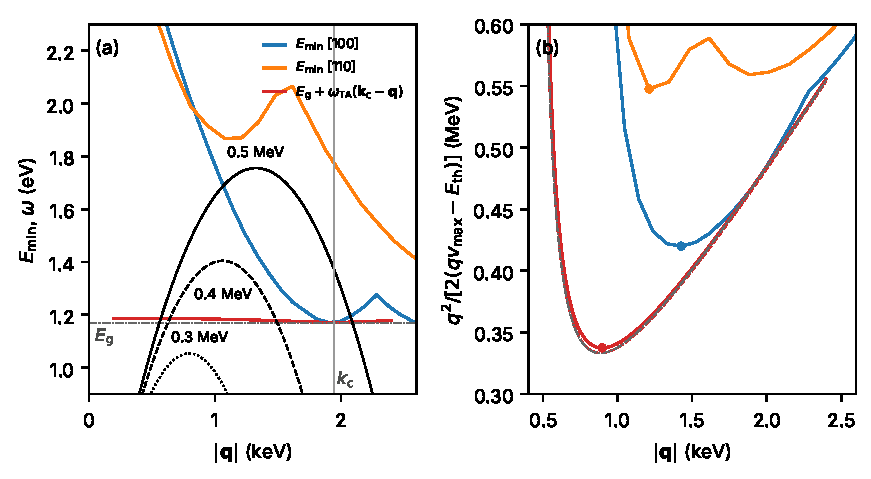
\includegraphics[width=\linewidth]{figures/ch13/fig13_1.pdf}
  \caption{Kinematics of the indirect-gap window of silicon. (a)~Minimum pair energy $E_{\mathrm{min}}(\vect{q})$ (\cref{eq:3.3-Emin}) for $\vect{q}$ along [100] and [110], and the phonon-assisted threshold $\Eg + \omega_{\mathrm{TA}}(\vect{k}_{\mathrm{c}} - \vect{q})$ (\cref{eq:13.1-EPA}) for $\vect{q}$ along [100], with the electron at the valley minimum $\vect{k}_{\mathrm{c}} = 0.85\,(2\pi/a)(1,0,0)$ and the hole at the valence-band maximum. Black: the largest energy deposited, $qv_{\mathrm{max}} - q^2/2\mchi$, for $\mchi = 0.3$ (dotted), 0.4 (dashed) and \SI{0.5}{MeV} (solid), with $v_{\mathrm{max}} = 2.650\times10^{-3}$. Dash-dotted: $\Eg = \SI{1.17}{eV}$. (b)~The lightest mass that reaches each threshold at momentum transfer $q$, $q^2/[2(qv_{\mathrm{max}} - E_{\mathrm{th}})]$; dots mark the minima over $q$. Red solid: phonon-assisted, free pair, minimum \SI{0.3374}{MeV} at $q = \SI{0.90}{keV}$; red dashed: bound pair, $\Eg$ lowered by $E_x^b = \SI{14.7}{meV}$, minimum \SI{0.3332}{MeV}; grey dash-dotted: the floor $2\Eg/v_{\mathrm{max}}^2$ at fixed threshold $\Eg$. Blue and orange: zero-phonon, with minima \SI{0.420}{MeV} along [100] and \SI{0.548}{MeV} along [110]; these are upper values for the zero-phonon threshold, since the joint minimum over all directions of $\vect{q}$ and all hole momenta lies lower. The [111] direction, whose $E_{\mathrm{min}}$ stays above \SI{2.13}{eV}, is off scale (minimum \SI{0.615}{MeV}). Bands: PBE calculation of \cref{fig:3-si-bands} at $a = \SI{5.431}{\angstrom}$ on a grid of $48^3$ crystal momenta, without spin--orbit coupling, with the conduction bands shifted up by \SI{0.613}{eV} so that the indirect gap equals the measured \SI{1.17}{eV}. Phonons: PBE force constants of \cref{sec:5.2} at the same lattice constant. The TA branch of these force constants is \SI{8}{\percent} below the neutron data at X, and scaling it up to the data raises the phonon-assisted minimum to \SI{0.3378}{MeV}.}
  \label{fig:13-window}
\end{figure}

\begin{workedexample}{The phonon-assisted onset of silicon}\label{we:13-onset}
We evaluate \cref{eq:13.1-mPA} with the measured gap extrapolated to zero temperature, $\Eg = \SI{1.17}{eV}$, the valley at $k_{\mathrm{c}} = 0.85\,(2\pi/a) = \SI{1940}{eV}$ (\cref{we:3-kc}), $v_{\mathrm{max}}^2 = 7.023\times10^{-6}$, and the TA branch of the force constants of \cref{sec:5.2}, with $\vect{q}$ along the valley axis.

\emph{First pass, no phonon energy.} $q^* = 2\Eg/v_{\mathrm{max}} = \SI{883}{eV}$, which leaves the phonon $Q^* = k_{\mathrm{c}} - q^* = \SI{1057}{eV} = 0.463\,(2\pi/a)$. The TA energy there is \SI{14.87}{meV}.

\emph{Second pass.} With $E = \Eg + \omega_{\mathrm{TA}}(\vect{Q}^*) = \SI{1.1849}{eV}$, $q^* = 2E/v_{\mathrm{max}} = \SI{894}{eV}$ and $Q^* = 0.458\,(2\pi/a) = \SI{0.53}{\angstrom^{-1}}$, where $\omega_{\mathrm{TA}}(\vect{Q}^*) = \SI{14.79}{meV}$. A third pass changes nothing at this precision. The slope of the TA branch at $Q^*$ is $u_{\mathrm{TA}} = \SI{2.1}{km.s^{-1}}$, and $u_{\mathrm{TA}}^2/v_{\mathrm{max}}^2 = 7\times10^{-6}$ is negligible. The onset is
\begin{equation*}
  m_{\mathrm{min}}^{\mathrm{PA}} = \frac{2\times(\SI{1.17}{eV} + \SI{0.01479}{eV})}{7.023\times10^{-6}} = \SI{0.3374}{MeV} ,
\end{equation*}
\SI{1.3}{\percent} above the floor $2\Eg/v_{\mathrm{max}}^2 = \SI{0.3332}{MeV}$. The direct minimization of \cref{eq:13.1-mPAdef} on a grid of $q$ gives the same value, at $q = \SI{0.90}{keV}$.

\emph{Sensitivity.} An error $\delta\omega$ in the phonon energy moves the onset by $2\,\delta\omega/v_{\mathrm{max}}^2 = \SI{2.8e-4}{MeV}$ per meV. The TA branch of this calculation is \SI{8}{\percent} soft at X; scaling the whole branch up to the neutron value there gives $\omega_{\mathrm{TA}}(\vect{Q}^*) = \SI{16.1}{meV}$ and an onset of \SI{0.3378}{MeV}. Had the phonon to supply all of $\vect{k}_{\mathrm{c}}$, as for light, the \SI{18.27}{meV} of the optical edge would put the onset at \SI{0.3384}{MeV}.

\emph{Bound pair.} The $1s$ exciton replaces $\Eg$ by $\Eg - E_x^b = \SI{1.1553}{eV}$. The same passes give $q^* = 2E/v_{\mathrm{max}} = \SI{0.883}{keV}$, where $\omega_{\mathrm{TA}}(\vect{Q}^*) = \SI{14.87}{meV}$, and the onset becomes $2\times\SI{1.1702}{eV}/v_{\mathrm{max}}^2 = \SI{0.3332}{MeV}$; the direct minimization puts the optimum at \SI{0.885}{keV} with the same onset. The phonon energy and the binding energy nearly cancel, and the bound-pair onset falls on the floor $2\Eg/v_{\mathrm{max}}^2$ that a crystal with a direct gap of \SI{1.17}{eV} would have. The strength of this phonon replica of the $1s$ exciton, compared with the free-pair continuum above it, is a question for \cref{sec:13.8}.
\end{workedexample}

\subsection{Germanium and a direct-gap crystal}

Germanium has its valleys at the L points, at $|\vect{k}_{\mathrm{c}}| = |\mathrm{\Gamma}\mathrm{L}| = \SI{1.90}{keV}$, almost the momentum of the silicon valleys, but a gap of only \SI{0.744}{eV} (\cref{sec:3.3}). Its floor $2\Eg/v_{\mathrm{max}}^2$ is \SI{0.212}{MeV}, at $q = \SI{0.56}{keV}$, and the phonon must supply the remaining \SI{1.34}{keV}, about 0.7 of the way from $\mathrm{\Gamma}$ to L. Along that line the transverse acoustic branch of germanium rises monotonically to \SI{1.9}{THz}, \SI{7.9}{meV}, at L~\cites{nilsson1971phonon}[Table~IV]{haxhijaj2026lattice}, so $\omega_{\mathrm{TA}}(\vect{Q}^*) \le \SI{7.9}{meV}$, and \cref{eq:13.1-mPA} places the phonon-assisted onset between 0.2119 and \SI{0.2141}{MeV}. The bracket needs no band structure and no computed phonon, only the gap, the position of L and the measured TA branch.

The zero-phonon threshold of germanium is harder to pin down. \Cref{we:3-mmin} bracketed it between 0.212 and \SI{0.420}{MeV}. On the L axis, with the parabola of \cref{eq:3.3-Eminpar} and $M_{\mathrm{eh}} = m^*_\parallel + m_{\mathrm{hh}} = (1.59 + 0.469)\,m_e = 2.06\,m_e$ along [111] (\cref{tab:3-materials}), \cref{eq:13.1-mZP} gives \SI{0.32}{MeV} at $q = \SI{1.10}{keV}$. The heavy longitudinal mass of the L valleys makes the kinetic energy of the momentum shortfall small, and the zero-phonon edge sits much closer to the onset, in relative terms, than in silicon. The value of \SI{0.32}{MeV} is a guide, not a bound on the zero-phonon edge: the minimum need not lie on the axis, and the heavy hole of germanium is warped and strongly mixed by spin--orbit coupling ($\Delta_{\mathrm{SO}} = \SI{0.296}{eV}$). \Cref{sec:13.9-ge-gaas} states what is known of the edge.

The route through the direct gap at $\mathrm{\Gamma}$ plays no part: as \cref{we:3-mmin} showed, the light pair at the direct gap opens only at a few MeV.

A direct-gap crystal has a window as well. Take GaAs, with both band edges at $\mathrm{\Gamma}$ and a gap of \SI{1.52}{eV}. Its floor is $2\Eg/v_{\mathrm{max}}^2 = \SI{0.433}{MeV}$, and below that mass dark matter scattering creates no pair in GaAs, with or without a phonon. At the masses of the silicon and germanium windows a direct-gap crystal of this gap has no electron-recoil channel. Above the floor, however, energy and momentum conflict again. A pair at rest at $\mathrm{\Gamma}$ costs exactly $\Eg$, but the particle deposits $\Eg$ only near $q^* = 2\Eg/v_{\mathrm{max}} = \SI{1.15}{keV}$, and a zero-phonon pair that carries this momentum has kinetic energy $q^{*2}/2M_{\mathrm{eh}}$. The electron of GaAs is light, $0.067\,m_e$, and with a heavy hole along [100] or [111] the pair mass is $M_{\mathrm{eh}} = 0.42$ or $0.96\,m_e$, and the kinetic energy is 3.1 or \SI{1.3}{eV}, comparable to the gap itself. For a pair of mass $M_{\mathrm{eh}}$ at $\mathrm{\Gamma}$, the condition for the pair to be reachable is $qv_{\mathrm{max}} - q^2/2\mchi - q^2/2M_{\mathrm{eh}} \ge \Eg$. Its left-hand side is largest at $q = \mu v_{\mathrm{max}}$, with $\mu = \mchi M_{\mathrm{eh}}/(\mchi + M_{\mathrm{eh}})$, where it equals $\frac12\mu v_{\mathrm{max}}^2$. Writing $m_{\mathrm{g}} = 2\Eg/v_{\mathrm{max}}^2$ for the floor, the zero-phonon threshold of a direct gap is therefore
\begin{equation}
  m_{\mathrm{min}}^{\mathrm{ZP}} = \frac{m_{\mathrm{g}}M_{\mathrm{eh}}}{M_{\mathrm{eh}} - m_{\mathrm{g}}} \qquad (M_{\mathrm{eh}} > m_{\mathrm{g}}) ,
  \label{eq:13.1-mZPdir}
\end{equation}
and there is none when $M_{\mathrm{eh}} \le m_{\mathrm{g}}$. For GaAs, $m_{\mathrm{g}} = 0.847\,m_e$: in the parabolic approximation, the pair with the [100] heavy hole never opens, and the pair with the [111] heavy hole opens at \SI{3.7}{MeV}. A phonon supplies the momentum, as in silicon: it carries $\vect{Q} \approx -\vect{q}^*$, about half the way to the zone boundary, and leaves the pair at rest. The transverse acoustic branch is the cheapest, and it stays below the \SI{10.5}{meV} that the computed dispersion gives at X (\cref{tab:5-phonons}). The computed \SI{10.5}{meV} is an upper value, since the computed branch lies above the measured one at X, and \cref{eq:13.1-mPA} gives an onset of 0.433 to \SI{0.436}{MeV}. The first zero-phonon states that a particle near this mass can reach are the states of the L valleys, which lie \SI{1.815}{eV} above the valence-band maximum, at $|\mathrm{\Gamma}\mathrm{L}| = \SI{1.90}{keV}$ (\cref{sec:3.3}). Their floor is $2\times\SI{1.815}{eV}/v_{\mathrm{max}}^2 = \SI{0.517}{MeV}$, and depositing \SI{1.815}{eV} at exactly $|\mathrm{\Gamma}\mathrm{L}|$ needs \SI{0.560}{MeV}, so the zero-phonon edge of the L valleys lies between 0.517 and \SI{0.560}{MeV}. GaAs therefore has a phonon-assisted window too, from \SI{0.43}{MeV} to above \SI{0.5}{MeV}, but it begins above the masses at which the silicon window has already closed.

A window thus exists in any crystal whose pairs cannot absorb the momentum $q^* \approx 2\Eg/v_{\mathrm{max}}$ for less than a phonon energy, that is, whenever $|\vect{q}^* - \vect{k}_{\mathrm{c}}|^2/2M_{\mathrm{eh}}$ exceeds the phonon energies at the corresponding $\vect{Q}^*$. For band masses of order $m_e$ and $q^* \sim \SI{1}{keV}$ the kinetic energy of the pair is of order an eV, a hundred times a phonon energy, and the condition is met in silicon, germanium and GaAs alike. In silicon and germanium the indirect gap places the windows low. The two windows start at the floors of their crystals, 0.333 and \SI{0.212}{MeV}, where no direct-gap crystal of comparable gap has any electron recoil. The optical absorption edges of silicon and germanium are phonon-assisted, and they measure the same kind of amplitude in the limit $q \to 0$ (\cref{sec:13.5}).

\section{The phonon-assisted amplitude}\label{sec:13.2}

At the onset of \cref{we:13-onset} a particle of \SI{0.3374}{MeV} transfers $q^* = \SI{0.90}{keV}$ along a valley axis of silicon and deposits \SI{1.185}{eV}. The final state has a hole at the valence-band maximum, an electron at the bottom of a conduction valley, \SI{1.94}{keV} away in crystal momentum, and a transverse acoustic phonon of \SI{14.8}{meV} that carries the remaining \SI{1.0}{keV}. Neither the density coupling nor the electron--phonon coupling reaches this final state alone. The density $n_e(\vect{q})$ creates pairs of crystal momentum $\vect{q}$, and at $q = \SI{0.90}{keV}$ the cheapest of them costs about \SI{1.9}{eV} (\cref{fig:13-window}). The electron--phonon coupling creates a phonon and can change the crystal momentum of an electron by any amount, but it cannot lift an electron across a gap of \SI{1.17}{eV} with the tens of meV that a phonon brings. The amplitude is therefore of second order, with one density vertex and one electron--phonon vertex.

\subsection{Final states and the second-order amplitude}

The target is the crystal at the base point of \cref{sec:8.5} with one coupling added: independent electrons in Bloch states $\psi_{n\vect{k}}$ with energies $\varepsilon_{n\vect{k}}$ (Kohn--Sham energies with the conduction bands raised by the scissor shift, as in \cref{sec:10.1}), harmonic phonons $(\vect{Q},\nu)$ with energies $\omega_{\vect{Q}\nu}$, and the electron--phonon Hamiltonian $H_{\mathrm{ep}}$ of \cref{eq:A.6-Hep}, linear in the displacements, with the screened vertex $g_{mn\nu}(\vect{k},\vect{Q})$ of \cref{eq:A.6-g}. The dark matter couples to the electron density, through the row of \cref{eq:8.2-spectrum} with $\mathfrak{D}_{ee} = |\tilde V(\vect{q})|^2$. The target enters only through the matrix elements of $n_e(\vect{q})$ (\cref{eq:3.2-ne}) that appear in the structure factor \cref{eq:4.2-Sab}. In the zero-phonon response of \cref{sec:10.1}, the matrix element of $n_e(\vect{q})$ is the density vertex $\rho_{cv}(\vect{k},\vect{q})$ of \cref{eq:3.2-rho}. In the phonon-assisted response a second-order amplitude replaces the density vertex.

The initial state $|i\rangle$ has the valence bands filled, the conduction bands empty and $n_{\vect{Q}\nu}$ phonons in each mode. A one-phonon final state has an electron in $(c,\vect{k}')$, a hole in $(v,\vect{k})$ and the phonon occupations of $|i\rangle$ changed in one mode,
\begin{equation}
  |f\rangle = c^\dagger_{c\vect{k}'}c_{v\vect{k}}\,|i'\rangle , \qquad
  \vect{k}' = \vect{k} + \vect{q} + \vect{Q} , \qquad
  E_f - E_i = \varepsilon_{c\vect{k}'} - \varepsilon_{v\vect{k}} \pm \omega_{\vect{Q}\nu} ,
  \label{eq:13.2-final}
\end{equation}
where $|i'\rangle$ has one phonon more in $(-\vect{Q},\nu)$ (upper sign, emission) or one fewer in $(\vect{Q},\nu)$ (lower sign, absorption), as in \cref{eq:A.6-weights}, and $\vect{k}'$ is folded back into the zone. The momentum transfer $\vect{q}$ is not folded: the density vertex keeps it whole and carries the Umklapp vector in its plane wave (\cref{eq:3.2-rho}). Conservation of crystal momentum leaves the phonon whatever crystal momentum the pair needs beyond $\vect{q}$: $\vect{Q} = \vect{k}' - \vect{k} - \vect{q}$ modulo a reciprocal-lattice vector, as in \cref{sec:13.1}. The density vertex and the electron--phonon vertex are both diagonal in spin, so the electron and the hole have the same spin, and the spin sum enters only the rate (\cref{sec:13.3}). With spin--orbit coupling the bands are spinors, and the formulas below hold with the band indices running over spinor bands.

The second-order amplitude follows from \cref{eq:2.4-c2} as for light (\cref{sec:6.5}). The dark matter gives up the energy $\omega$ and the momentum $\vect{q}$ at its own vertex, and its kinetic energy cancels from every denominator. In the ordering in which the density vertex acts first, the intermediate state $|m\rangle$ already holds the energy $\omega$; in the ordering in which the electron--phonon vertex acts first, the intermediate state does not:
\begin{equation}
  \langle f|n_e^{(2)}(\vect{q})|i\rangle = \sum_m\left[\frac{\langle f|H_{\mathrm{ep}}|m\rangle\langle m|n_e(\vect{q})|i\rangle}{E_i + \omega - E_m} + \frac{\langle f|n_e(\vect{q})|m\rangle\langle m|H_{\mathrm{ep}}|i\rangle}{E_i - E_m}\right] , \qquad
  \omega = E_f - E_i .
  \label{eq:13.2-T}
\end{equation}
This matrix element takes the place of $\langle f|n_e(\vect{q})|i\rangle$ in \cref{eq:4.2-Sab}. The condition $\omega = E_f - E_i$ is the energy delta function of the structure factor, and the amplitude is needed only there, on the energy shell. The sum runs over many-electron states with their phonons, and it is finite as long as no $E_m$ equals $E_i + \omega$ or $E_i$. An $E_m$ equal to $E_i$ never occurs in an insulator. An $E_m$ equal to $E_i + \omega$ would mean that the density alone creates a real zero-phonon pair at $(\vect{q},\omega)$, and no such pair exists while $\omega$ lies below $E_{\mathrm{min}}(\vect{q})$ (\cref{eq:13.2-doff}).

\subsection{Four paths}

Both vertices are one-body operators, $n_e(\vect{q}) = \sum\rho_{mn}c^\dagger c$ and $H_{\mathrm{ep}} = N^{-1/2}\sum g_{mn\nu}c^\dagger c\,B_{\vect{Q}\nu}$, and each moves one electron. Acting first on the filled valence bands, a vertex can only move an electron from a filled state into an empty one, so every intermediate state $|m\rangle$ holds exactly one electron--hole pair. (A term that moves an electron back into the state it came from needs a momentum transfer equal to a reciprocal-lattice vector, $\vect{q} = \vect{G}$ or $\vect{Q} = 0$. It has measure zero in the integrals over $\vect{q}$ and $\vect{Q}$, and \cref{app:D.35} shows that even there it adds nothing new.) The second vertex must turn that intermediate pair into the final pair $(c\vect{k}';\,v\vect{k})$, again by moving one electron. The second vertex can do so in two ways. It can move the intermediate electron into $(c,\vect{k}')$, if the intermediate hole is already the final one, $(v,\vect{k})$; or it can move the electron of $(v,\vect{k})$ into the intermediate hole, if the intermediate electron is already the final one, $(c,\vect{k}')$. The two ways, combined with the two orderings of the vertices, make four paths:
\begin{equation}
  \begin{aligned}
  \text{A:}&\quad \frac{g_{cp\nu}(\vect{k}+\vect{q},\vect{Q})\,\rho_{pv}(\vect{k},\vect{q})}{\omega - \varepsilon_{p,\vect{k}+\vect{q}} + \varepsilon_{v\vect{k}}} ,
  &\text{B:}&\quad \frac{\rho_{cp}(\vect{k}+\vect{Q},\vect{q})\,g_{pv\nu}(\vect{k},\vect{Q})}{\varepsilon_{v\vect{k}} - \varepsilon_{p,\vect{k}+\vect{Q}} \mp \omega_{\vect{Q}\nu}} , &&\quad p\ \text{empty}, \\
  \text{C:}&\quad -\frac{\rho_{cp}(\vect{k}+\vect{Q},\vect{q})\,g_{pv\nu}(\vect{k},\vect{Q})}{\omega - \varepsilon_{c\vect{k}'} + \varepsilon_{p,\vect{k}+\vect{Q}}} ,
  &\text{D:}&\quad -\frac{g_{cp\nu}(\vect{k}+\vect{q},\vect{Q})\,\rho_{pv}(\vect{k},\vect{q})}{\varepsilon_{p,\vect{k}+\vect{q}} - \varepsilon_{c\vect{k}'} \mp \omega_{\vect{Q}\nu}} , &&\quad p\ \text{filled}.
  \end{aligned}
  \label{eq:13.2-paths}
\end{equation}
Each term is the contribution of one intermediate band $p$, with the common factor $N^{-1/2}(n_{\vect{Q}\nu} + \frac12 \pm \frac12)^{1/2}$ of the phonon vertex taken out. \Cref{fig:13-paths} draws the four paths as time-ordered diagrams.

\begin{figure}[tbp]
  \centering
  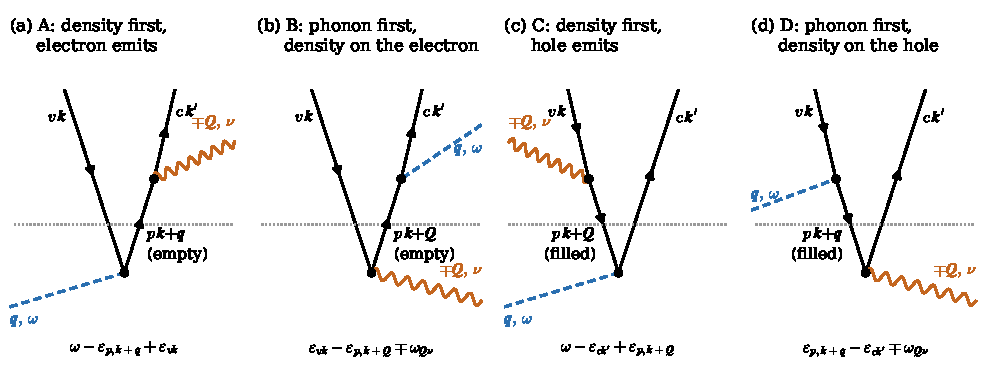
\includegraphics[width=\linewidth]{figures/ch13/fig13_2.pdf}
  \caption{The four paths of the phonon-assisted electron-recoil amplitude, \cref{eq:13.2-paths}, as time-ordered diagrams. Time runs upward. Lines with upward arrows are electrons, lines with downward arrows are holes; the dashed line is the dark-matter density vertex, which delivers momentum $\vect{q}$ and energy $\omega$; the wavy line is the phonon, emitted with $-\vect{Q}$ or absorbed with $+\vect{Q}$. The dotted line cuts the intermediate state, whose energy denominator is printed below each panel. Every path ends in the same final state, an electron in $(c,\vect{k}')$ with $\vect{k}' = \vect{k} + \vect{q} + \vect{Q}$ and a hole in $(v,\vect{k})$. (a)--(d)~Paths A to D, with an electron in an empty band $p$ between the vertices in A and B and a hole in a filled band $p$ in C and D. Schematic; no line length or angle carries a number.}
  \label{fig:13-paths}
\end{figure}

In paths A and B an electron propagates between the vertices. In A the density creates a pair, $(p,\vect{k}+\vect{q})$ with $(v,\vect{k})$, and the electron then scatters into $(c,\vect{k}')$ by emitting or absorbing the phonon; the pair created in A is the virtual zero-phonon pair of \cref{sec:10.1}, carried to the final state by the phonon. In B the phonon vertex creates a virtual pair at crystal momentum $\vect{Q}$, $(p,\vect{k}+\vect{Q})$ with $(v,\vect{k})$, and the density then scatters the electron by $\vect{q}$. The intermediate band $p$ must be empty in both A and B, since an electron cannot enter a filled state. In paths C and D a hole propagates. In C the density creates the final electron from a filled state $(p,\vect{k}+\vect{Q})$, and the phonon vertex then moves an electron from $(v,\vect{k})$ into the hole that the final electron left. In D the phonon vertex creates the final electron from a filled state $(p,\vect{k}+\vect{q})$, and the density then fills the hole in $(p,\vect{k}+\vect{q})$ from $(v,\vect{k})$. The denominators contain the energies of the intermediate pairs. They also contain $\omega$ in the density-first orderings A and C, and the phonon energy in the phonon-first orderings B and D, where the phonon has already been emitted or absorbed.

The minus signs of C and D come from the order of the fermion operators. In path A the operators act as $c^\dagger_cc_p\,c^\dagger_pc_v = c^\dagger_c(1 - n_p)c_v$, which is $c^\dagger_cc_v$ on a state with $p$ empty. In path C they act as $c^\dagger_pc_v\,c^\dagger_cc_p$, and three exchanges of neighboring operators bring them into the order $-c^\dagger_c\,(c^\dagger_pc_p)\,c_v = -c^\dagger_c\,n_p\,c_v$, which is $-c^\dagger_cc_v$ on a state with $p$ filled. The same reordering gives $-1$ for D. The four paths are those of phonon-assisted absorption (\cref{sec:6.5}), with the velocity vertex of light replaced by the density vertex; summed over every band they give the two-term amplitude of phonon-assisted absorption~\cites[Eq.~(200)]{giustino2017electron}[Eqs.~(2) and~(3)]{noffsinger2012phonon}. Replacing the velocity vertex by the density vertex changes the crystal momenta at which the intermediate states sit: the photon-first intermediate state of \cref{eq:6.5-M} sits at the crystal momentum of the hole, and the density-first intermediate state of path A at $\vect{k}+\vect{q}$.

\subsection{The unrestricted band sum}

On the energy shell the hole paths change form. Insert $\omega = \varepsilon_{c\vect{k}'} - \varepsilon_{v\vect{k}} \pm \omega_{\vect{Q}\nu}$ of \cref{eq:13.2-final} into their denominators. The denominator of C becomes $\varepsilon_{p,\vect{k}+\vect{Q}} - \varepsilon_{v\vect{k}} \pm \omega_{\vect{Q}\nu}$, and with its minus sign, path C becomes the expression of path B for a filled band $p$. The denominator of D becomes $\varepsilon_{p,\vect{k}+\vect{q}} - \varepsilon_{v\vect{k}} - \omega$, and path D becomes the expression of path A for a filled band. A single electron could not take paths A and B through a filled band: Pauli blocking forbids them. In the many-electron amplitude the blocked paths return as exchange partners, paths C and D, with exactly the one-electron value. In path C the electron that ends in $(c,\vect{k}')$ comes from the filled band $p$, and the electron from $(v,\vect{k})$ takes its place; exchanging the two identical electrons turns path C into path B with the electron from $v$ passing through $p$. The fermion sign of the exchange and the sign of the hole denominator cancel, and the four paths combine into the amplitude of one electron alone in the bands:
\begin{keyresult}[Phonon-assisted amplitude]
On the energy shell, the second-order amplitude \cref{eq:13.2-T} into the final state \cref{eq:13.2-final} is
\begin{equation}
  \begin{gathered}
  \langle f|n_e^{(2)}(\vect{q})|i\rangle = \frac{1}{\sqrt N}\bigl(n_{\vect{Q}\nu} + \tfrac12 \pm \tfrac12\bigr)^{1/2}M^{\pm}_{cv\nu}(\vect{k},\vect{q},\vect{Q}) , \\
  M^{\pm}_{cv\nu}(\vect{k},\vect{q},\vect{Q}) = \sum_p\left[\frac{g_{cp\nu}(\vect{k}+\vect{q},\vect{Q})\,\rho_{pv}(\vect{k},\vect{q})}{\omega - \varepsilon_{p,\vect{k}+\vect{q}} + \varepsilon_{v\vect{k}}} + \frac{\rho_{cp}(\vect{k}+\vect{Q},\vect{q})\,g_{pv\nu}(\vect{k},\vect{Q})}{\varepsilon_{v\vect{k}} - \varepsilon_{p,\vect{k}+\vect{Q}} \mp \omega_{\vect{Q}\nu}}\right] ,
  \end{gathered}
  \label{eq:13.2-M}
\end{equation}
with $\omega = \varepsilon_{c\vect{k}'} - \varepsilon_{v\vect{k}} \pm \omega_{\vect{Q}\nu}$, the upper sign for emission, and the sum over every band $p$, filled or empty, including $p = v$ and $p = c$.
\end{keyresult}
\noindent The amplitude $M^\pm$ is dimensionless, like $\rho$, and of order one in $N$; the factor $N^{-1/2}$ is that of \cref{eq:A.6-Hep}, and it is removed by the independent sum over $\vect{Q}$ in the rate (\cref{sec:13.3}). In operator form, $M^\pm$ is the matrix element between $(v,\vect{k})$ and $(c,\vect{k}')$ of the two vertices joined by the resolvent of the one-electron Hamiltonian, with no projector on empty states. The general statement, for any two one-body vertices acting on an independent-particle ground state, is proved in \cref{app:D.35}; \cref{eq:6.5-M} is its instance for light.

The band-sum form \cref{eq:13.2-M}, an instance of the band-sum theorem of \cref{app:D.35}, holds on the energy shell only. Off the shell the denominators of C and D differ from those of the blocked electron paths by $\omega - (E_f - E_i)$. Any quantity that needs the amplitude off the shell has to keep the four paths of \cref{eq:13.2-paths} as they stand; the real part of a phonon-assisted response is an example. The band-sum form also requires independent electrons, where the intermediate and final states are single Slater determinants. With the electron--hole attraction the final pair is an exciton, and the paths are rebuilt from exciton states in \cref{sec:13.8}. Finally, the band-sum form needs every intermediate state to be off the shell, a condition that \cref{eq:13.2-doff} below guarantees inside the window.

When the intermediate states are thought of as virtual electrons, the natural truncation keeps only empty intermediate bands, and this truncation gets the amplitude wrong by a factor of order one: \cref{we:13-exchange} finds a factor of 2.4 in the rate of a model, or 1.6 with the other phase convention of its phonon vertex. The intraband terms belong to the sum as well. In path A with $p = v$, the density moves the valence electron within its band and the phonon then lifts it across the gap. In path B with $p = c$, the phonon creates the pair and the density moves the electron within the conduction band. These two terms carry the largest density vertices at small $q$, since $\rho_{vv}$ and $\rho_{cc}$ tend to one, and they cancel at $\vect{q} = 0$. At $\vect{q} = 0$, $\rho_{pv}(\vect{k},0) = \delta_{pv}$, path A reduces to $g_{cv\nu}(\vect{k},\vect{Q})/\omega$ and path B to $g_{cv\nu}(\vect{k},\vect{Q})/(\varepsilon_{v\vect{k}} - \varepsilon_{c,\vect{k}+\vect{Q}} \mp \omega_{\vect{Q}\nu}) = -g_{cv\nu}(\vect{k},\vect{Q})/\omega$, and
\begin{equation}
  M^{\pm}_{cv\nu}(\vect{k},0,\vect{Q}) = 0 .
  \label{eq:13.2-q0}
\end{equation}
The zero of \cref{eq:13.2-q0} is exact, because $n_e(0)$ is the number of electrons, which commutes with the Hamiltonian and causes no transition at any order. The amplitude therefore starts at first order in $\vect{q}$, as the zero-phonon vertex $\rho_{cv}$ does (\cref{eq:3.2-optical}), and the limit $\vect{q}\to0$ that connects the amplitude to phonon-assisted optical absorption is taken in \cref{sec:13.5}. A calculation that truncates the band sum, or treats the intraband terms with a different vertex than the interband ones, loses \cref{eq:13.2-q0} and with it the small-$q$ behavior of the rate.

\begin{workedexample}{Exchange partners in a two-band chain}\label{we:13-exchange}
The smallest system in which all four paths appear has two bands and one phonon mode. Take a chain of $N = 6$ cells with two orbitals per cell, A at $x = 0$ and B at $x = a/2$, on-site energies $+\SI{0.4}{eV}$ and $-\SI{0.4}{eV}$, and hoppings \SI{1.6}{eV} within the cell and \SI{1.0}{eV} between cells. The electrons are spinless, since the spin only doubles a rate. The density vertex is $\ee^{\ii qx}$ on the orbital positions. One dispersionless phonon of energy $\omega_{\mathrm{ph}} = \SI{60}{meV}$ shifts the two on-site energies in opposite directions. Its vertex is \SI{0.2}{eV} times the matrix element of $\sum_R\ee^{\ii QR}(n_{R\mathrm{A}} - n_{R\mathrm{B}})$ between the two Bloch states it connects, with the phase of the displacement wave taken at the origin $R$ of each cell. Crystal momenta are multiples of $2\pi/6a$, shifted by a twist of \SI{0.3}{rad} in the boundary condition around the ring (\SI{0.05}{rad} per crystal momentum). The twist lifts the degeneracy of $k$ and $-k$. The lower band is filled and the upper is empty, with the smallest gap near the zone boundary, \SI{1.448}{eV} with the twist and \SI{1.442}{eV} without it. All parameters are illustrative.

Put the final pair at the gap, $(v,k)$ and $(c,k)$, with $q = 2\times2\pi/6a$ and a phonon emitted with $Q = -q$. The energy deposited on the shell is $\omega = \SI{1.448}{eV} + \omega_{\mathrm{ph}} = \SI{1.508}{eV}$, while the cheapest zero-phonon pair at this $q$ costs $E_{\mathrm{min}}(q) = \SI{2.912}{eV}$: the zero-phonon channel is closed by a margin of \SI{1.40}{eV}. The four terms of \cref{eq:13.2-paths} are:
\begin{center}
\small
\begin{tabular}{llrr}
  \toprule
  path & intermediate pair & denominator (eV) & term \\
  \midrule
  A & electron $(c,k+q)$, hole $(v,k)$ & $-1.552$ & $+0.0176 - 0.0246\,\ii$ \\
  B & electron $(c,k+Q)$, hole $(v,k)$ & $-3.060$ & $+0.0439 + 0.0051\,\ii$ \\
  C & electron $(c,k)$, hole $(v,k+Q)$ & $-1.492$ & $+0.0062 - 0.0379\,\ii$ \\
  D & electron $(c,k)$, hole $(v,k+q)$ & $-3.120$ & $-0.0313 - 0.0354\,\ii$ \\
  \bottomrule
\end{tabular}
\end{center}
In the one-electron sum \cref{eq:13.2-M}, the blocked forms are path B with $p = v$, with denominator $\varepsilon_{v k} - \varepsilon_{v,k+Q} - \omega_{\mathrm{ph}} = +\SI{1.492}{eV}$, and path A with $p = v$, with denominator $+\SI{3.120}{eV}$. Their values are $+0.0062 - 0.0379\,\ii$ and $-0.0313 - 0.0354\,\ii$, equal to C and D to all printed digits: the hole denominators have the sign opposite to that of the blocked forms, and the fermion sign undoes the sign change. In path A with $p = v$, the intraband density vertex, $|\rho_{vv}|^2 = 0.642$, is larger than the interband one, $|\rho_{cv}|^2 = 0.358$, and the hole paths are not a small correction: $|\mathrm{C} + \mathrm{D}| = 0.077$, against $|\mathrm{A} + \mathrm{B}| = 0.065$ and $|M| = 0.100$.

The sum over the empty band alone, paths A and B, gives $+0.0615 - 0.0195\,\ii$, with $|M|^2$ at 0.42 of the correct value: a factor of 2.4 in the rate. With the phase of the displacement wave taken at the orbital positions, $\ee^{\ii Qx}$ with $Q = -q$, the coupling itself changes: then $|M| = 0.107$, and the empty band alone is off by a factor of 1.6. The size of the error depends on the model; the fact that the error is of order one does not.

Move $\omega$ off the shell by \SI{0.10}{eV}. Path A changes as its formula says, B is unchanged, and C becomes $+0.0066 - 0.0406\,\ii$ against $+0.0062 - 0.0379\,\ii$ for the blocked form. The many-body total now differs from the unrestricted one-electron sum by 3.7\%. The exchange partners are equal only where energy is conserved.
\end{workedexample}

\subsection{No interference with the zero-phonon line}

A dark-matter particle that deposits $\omega$ at $\vect{q}$ could, in principle, produce the same pair with and without a phonon, and the two amplitudes might interfere. At second order in $g$ they do not. The rate is a sum over final states of the squared total amplitude into each. The zero-phonon final states have the phonon occupations of $|i\rangle$; their amplitude is $\rho_{cv}$ at zeroth order in $g$, with corrections of order $g^2$ from a phonon emitted and reabsorbed. The final states of \cref{eq:13.2-final} have one occupation changed by one; their amplitude starts at first order. A cross term needs two amplitudes into the same final state, and states that differ in the occupation of one mode are orthogonal. Through order $g^2$, squaring therefore gives two separate rates and no term that mixes them. The zero-phonon rate is $|\rho_{cv}|^2$ plus twice the real part of $\rho_{cv}^*$ times the order-$g^2$ amplitude, and the phonon-assisted rate is $|M^\pm|^2$. A thermal initial state changes nothing, since its density matrix is diagonal in the phonon occupations and the change of occupation between initial and final state remains a good label.

The order-$g^2$ corrections to the zero-phonon amplitude therefore belong to the zero-phonon line; they are the Fan--Migdal and Allen--Heine self-energies of \cref{sec:6.3} and the virtual-phonon vertex. These corrections shift and reweight the zero-phonon line (\cref{sec:8.6,sec:13.7}), and they are never added to the phonon-assisted rate. Inside the window, $\omega < E_{\mathrm{min}}(\vect{q})$, no zero-phonon final state exists at the energy $\omega$, and the question of interference does not arise at any order. Above $E_{\mathrm{min}}(\vect{q})$ both channels are open, and the absence of interference still holds at this order. The Fano term of \cref{sec:8.6} is a different interference: inside the one-phonon final states, between the part of path A in which the zero-phonon pair is real and the paths in which it is not. It belongs to the phonon-dressed sector and, at the level of one-body self-energies, vanishes in silicon and germanium.

\subsection{The adiabatic (Herzberg--Teller) form}

The denominators of \cref{eq:13.2-M} decide both whether the amplitude is finite and how it can be computed. Each is the energy by which an intermediate pair misses the energy shell, and on the shell each is the energy of a pair minus a known amount. For $p$ empty in the first term, the pair $(p,\vect{k}+\vect{q};\,v,\vect{k})$ has crystal momentum $\vect{q}$, and the denominator is $\omega$ minus its energy. For $p$ filled in the second term, path C, the denominator is the energy of the pair $(c,\vect{k}';\,p,\vect{k}+\vect{Q})$, again of crystal momentum $\vect{q}$, minus $\omega$. Both denominators are at least $E_{\mathrm{min}}(\vect{q}) - \omega$ in size, with $E_{\mathrm{min}}$ of \cref{eq:3.3-Emin}. In the two remaining cases the intermediate pair has crystal momentum $\vect{Q}$ and costs at least $\Eg$, and the denominator differs from the pair energy by $\omega_{\vect{Q}\nu}$. The smallest off-shell distance of \cref{eq:8.5-theta} is therefore bounded below on the shell:
\begin{equation}
  \delta_{\mathrm{off}} \ge \min\bigl(E_{\mathrm{min}}(\vect{q}) - \omega,\;\Eg - \omega_{\vect{Q}\nu}\bigr) .
  \label{eq:13.2-doff}
\end{equation}
Below $E_{\mathrm{min}}(\vect{q})$ every denominator is negative or positive by a finite margin, and the amplitude needs no width, no $\ii0^+$ and no subtraction. The only denominators that can approach zero are those of the virtual zero-phonon pairs at $\vect{q}$, the electron of path A and the hole of path C. As $\omega$ approaches $E_{\mathrm{min}}(\vect{q})$, the virtual zero-phonon pairs become real pairs that emit a phonon after they are created; the process becomes a cascade, and the second-order amplitude stops being a separate quantity. \Cref{sec:13.6} turns the bound \cref{eq:13.2-doff} into the window inside which \cref{eq:13.2-M} holds. In silicon the bound for pairs at $\vect{Q}$ is at least $\SI{1.17}{eV} - \SI{64}{meV} = \SI{1.11}{eV}$, and the tighter bound is the margin below the zero-phonon edge. At the onset of \cref{we:13-onset}, where $\omega \approx \SI{1.19}{eV}$ against $E_{\mathrm{min}} \approx \SI{1.9}{eV}$, the margin is about \SI{0.7}{eV}.

The phonon energy enters the amplitude twice: in the energy balance, where it sets the threshold, and in the denominators, where it is small against $\delta_{\mathrm{off}}$. Dropping it from the denominators, with $\omega = \varepsilon_{c\vect{k}'} - \varepsilon_{v\vect{k}}$ in the first term, gives the adiabatic amplitude
\begin{equation}
  M^{\mathrm{ad}}_{cv\nu}(\vect{k},\vect{q},\vect{Q}) = \sum_p\left[\frac{g_{cp\nu}(\vect{k}+\vect{q},\vect{Q})\,\rho_{pv}(\vect{k},\vect{q})}{\varepsilon_{c\vect{k}'} - \varepsilon_{p,\vect{k}+\vect{q}}} + \frac{\rho_{cp}(\vect{k}+\vect{Q},\vect{q})\,g_{pv\nu}(\vect{k},\vect{Q})}{\varepsilon_{v\vect{k}} - \varepsilon_{p,\vect{k}+\vect{Q}}}\right] ,
  \label{eq:13.2-Mad}
\end{equation}
the same for emission and absorption, with the states degenerate with $(c,\vect{k}')$ left out of the first term and those degenerate with $(v,\vect{k})$ left out of the second. The adiabatic amplitude is a derivative of the zero-phonon vertex. Replace the phonon operator $B_{\vect{Q}\nu}$ in $H_{\mathrm{ep}}$ by a number $b$, with its conjugate for $B_{-\vect{Q}\nu}$. The electrons then feel the static potential of a frozen displacement wave of the mode, \cref{eq:A.6-u} with $B \to b$, which couples $\psi_{n\vect{k}}$ to the states at $\vect{k}\pm\vect{Q}$ with the matrix elements $N^{-1/2}b\,g_{mn\nu}(\vect{k},\vect{Q})$ and their conjugates. By first-order perturbation theory, the valence state $\psi_{v\vect{k}}$ acquires the admixture $N^{-1/2}b\sum_p\psi_{p,\vect{k}+\vect{Q}}\,g_{pv\nu}(\vect{k},\vect{Q})/(\varepsilon_{v\vect{k}} - \varepsilon_{p,\vect{k}+\vect{Q}})$, and the conduction state $\psi_{c\vect{k}'}$ acquires states at $\vect{k}'-\vect{Q} = \vect{k}+\vect{q}$ through the conjugate coupling. The terms with $b^*$ reach crystal momenta $\vect{k}\pm2\vect{Q}$ away from the pair and drop out unless $2\vect{Q}$ is a reciprocal-lattice vector. The transition density $\rho_{cv}(\vect{k},\vect{q}) = \langle\psi_{c\vect{k}'}|\ee^{\ii\vect{q}\cdot\vect{r}}|\psi_{v\vect{k}}\rangle$ vanishes in the perfect lattice, because $\vect{k}' \ne \vect{k}+\vect{q}$, and becomes nonzero at first order in $b$. The change of the conduction state gives the first term of \cref{eq:13.2-Mad} and the change of the valence state the second, and
\begin{equation}
  \frac{\partial\rho_{cv}}{\partial b} = \frac{1}{\sqrt N}\,M^{\mathrm{ad}}_{cv\nu}(\vect{k},\vect{q},\vect{Q}) , \qquad
  \langle f|n_e^{(2)}(\vect{q})|i\rangle \simeq \langle n'|B_{\vect{Q}\nu}|n\rangle\,\frac{\partial\rho_{cv}}{\partial b} ,
  \label{eq:13.2-HT}
\end{equation}
where $\langle n'|B_{\vect{Q}\nu}|n\rangle = (n_{\vect{Q}\nu} + \frac12 \pm \frac12)^{1/2}$ is the phonon matrix element. \Cref{eq:13.2-HT} is the Herzberg--Teller term of \cref{eq:8.6-electronic}: the transition density of the frozen crystal, linear in the displacement, taken between the vibrational states. The derivative of $\rho_{cv}$ with respect to $b$ is also the derivative \cref{eq:E.4-drho} that \cref{app:E.4} computes. In this form the unrestricted band sum needs no theorem. First-order perturbation theory of one orbital sums over all other orbitals, filled or empty, and the filled orbitals give exactly the hole paths C and D.

The adiabatic form drops the phonon energy in the denominators. Expanding each denominator to first order in $\omega_{\vect{Q}\nu}$ gives
\begin{equation}
  M^{\pm}_{cv\nu} - M^{\mathrm{ad}}_{cv\nu} = \mp\,\omega_{\vect{Q}\nu}\sum_p\left[\frac{g_{cp\nu}\,\rho_{pv}}{(\varepsilon_{c\vect{k}'} - \varepsilon_{p,\vect{k}+\vect{q}})^2} - \frac{\rho_{cp}\,g_{pv\nu}}{(\varepsilon_{v\vect{k}} - \varepsilon_{p,\vect{k}+\vect{Q}})^2}\right] + O\!\left(\frac{\omega_{\vect{Q}\nu}^2}{\delta_{\mathrm{off}}^2}\right)M^{\mathrm{ad}} ,
  \label{eq:13.2-err}
\end{equation}
with the arguments of \cref{eq:13.2-Mad}. Each term is smaller than its adiabatic counterpart by $\omega_{\vect{Q}\nu}$ over its own denominator, so the relative error is of order $\omega_{\vect{Q}\nu}/\delta_{\mathrm{off}}$ as long as the sum is not much smaller than its largest term (\cref{app:D.35}). The difference $M^{\pm}_{cv\nu} - M^{\mathrm{ad}}_{cv\nu}$ has opposite signs for emission and absorption. The adiabatic form cannot tell emission and absorption apart, and it misses the difference between their amplitudes, which is of the same relative order.

In silicon, with the phonon energies at the conduction valley (\cref{sec:6.5}) and the interband bound of \cref{eq:13.2-doff}, the estimate $\omega_{\vect{Q}\nu}/\delta_{\mathrm{off}}$ is 1.6\% for the transverse acoustic phonon of \SI{18.27}{meV} and 5.2\% for the transverse optical phonon of \SI{57.73}{meV}. The margin below the zero-phonon edge is the tighter condition. For the error of the adiabatic form to stay below 10\%, $E_{\mathrm{min}}(\vect{q}) - \omega$ must exceed \SI{0.18}{eV} for the transverse acoustic and \SI{0.58}{eV} for the transverse optical phonon. Deep in the window the adiabatic form is accurate; near the upper edge of the window it fails, on the same denominators that make the amplitude itself resonant.

The same estimate disposes of the crossings of two valence bands at $\vect{k}$ and $\vect{k}+\vect{Q}$, where the adiabatic denominator of the second term vanishes. By \cref{eq:13.2-doff} such a crossing makes path C resonant, so the crossing lies outside the window.

The adiabatic form is what a first-principles calculation evaluates, either as a finite difference of the transition density in a supercell that holds the displaced lattice or as the derivative of the transition density from density-functional perturbation theory. The derivative from density-functional perturbation theory needs more than a phonon calculation provides. A phonon calculation gives the change of each valence state projected on the empty bands; the derivative also needs the projection on the filled bands, which carries the hole path C, and the change of the conduction state, which carries paths A and D. The sum-over-states form \cref{eq:13.2-M} avoids the derivative and keeps the phonon energy in the denominators. The $f$-sum rule of the density vertices tests that the band sum is complete. \Cref{app:E.5} sets out the sum-over-states route, its controls and its operation count.

\section{The phonon-assisted rate}\label{sec:13.3}

A dark-matter particle of \SI{0.35}{MeV} that transfers \SI{1.0}{keV} of momentum to silicon can deposit up to \SI{1.22}{eV}, while at that momentum transfer the cheapest zero-phonon pair along the valley axis costs about \SI{1.77}{eV} (\cref{eq:3.3-Emin}, with the bands of \cref{fig:3-si-bands}). Every event it causes therefore leaves a phonon behind, a transverse acoustic phonon of \SI{14}{meV} that carries the remaining \SI{0.94}{keV} of the valley momentum. The square of the amplitude of \cref{sec:13.2}, summed over final states, enters the rate exactly as the zero-phonon structure factor of \cref{sec:10.1} does.

\subsection{The phonon-assisted structure factor}

The structure factor counts the transitions that the density operator drives from the thermal state, \cref{eq:2.5-golden} with the transition sum \cref{eq:2.5-transum}. The off-shell window is the region $\omega \le E_{\mathrm{min}}(\vect{q}) - \delta_{\mathrm{w}}$, with $\delta_{\mathrm{w}}$ the margin of \cref{sec:8.6}, which is \SI{0.3}{eV} in silicon (\cref{sec:13.6}). Inside the off-shell window no zero-phonon pair exists at the energy deposited, and every final state contains a phonon, up to a virtual admixture of relative weight $\theta_{\mathrm{ep}}$ (\cref{sec:8.6}). The final states are those of \cref{eq:13.2-final}, and the matrix element of the density into each of them is \cref{eq:13.2-M}.

To sum over the final states, we label them by $\vect{k}$ and $\vect{Q}$, each running over the $N$ points of the zone, by the bands $c$ and $v$, the branch $\nu$, the sign, and the spin. Neither vertex flips the spin, so the spin gives a factor 2. The initial phonon state is thermal, and the average of the squared phonon matrix element is $n_{\vect{Q}\nu} + 1$ for emission and $n_{\vect{Q}\nu}$ for absorption, with $n_{\vect{Q}\nu} = n_{\mathrm{B}}(\omega_{\vect{Q}\nu})$. The electrons start in the ground state: the Fermi factor $f_v(1 - f_c)$ of each transition differs from one by terms of order $\ee^{-\Eg/2T}$. The energy delta function sets $\omega = \varepsilon_{c,\vect{k}+\vect{q}+\vect{Q}} - \varepsilon_{v\vect{k}} \pm \omega_{\vect{Q}\nu}$. The factors combine as $(2\pi/\Vol)\times2\times N^{-1}\sum_{\vect{k}\vect{Q}} = (4\pi N/\Vol)\langle\!\langle\cdots\rangle\!\rangle$ with the double zone average of \cref{eq:A.3-BZ}, and $\Vol = N\Omega$ (\cref{app:D.35} gives the thermal averages):
\begin{keyresult}[Phonon-assisted structure factor]
\begin{equation}
  S^{\mathrm{PA}}(\vect{q},\omega) = \frac{4\pi}{\Omega}\,\Bigl\langle\!\Bigl\langle\sum_\nu\sum_{cv}\sum_\pm\bigl(n_{\vect{Q}\nu} + \tfrac12 \pm \tfrac12\bigr)\,\bigl|M^\pm_{cv\nu}(\vect{k},\vect{q},\vect{Q})\bigr|^2\,\delta\bigl(\varepsilon_{c,\vect{k}+\vect{q}+\vect{Q}} - \varepsilon_{v\vect{k}} \pm \omega_{\vect{Q}\nu} - \omega\bigr)\Bigr\rangle\!\Bigr\rangle ,
  \label{eq:13.3-SPA}
\end{equation}
for $T \ll \Eg$ and $\omega$ inside the off-shell window. The phonon-assisted rate is \cref{eq:8.2-spectrum} with $\mathfrak{D}_{ee} = \pi\sigmae\FDM(q)^2/\mu_{\chi e}^2$ (\cref{eq:1.4-Vsq}) and $S = S^{\mathrm{PA}}$.
\end{keyresult}
\noindent The number of cells drops out, as it must. The double sum over $\vect{k}$ and $\vect{Q}$ contributes $N^2$, the vertex $N^{-1}$, and the volume $\Vol = N\Omega$ the last power, so that $S^{\mathrm{PA}}$ is intensive like the structure factor of a single pair.

The two signs are the two thresholds of \cref{sec:6.5}. Emission costs the phonon energy and comes with $n_{\vect{Q}\nu} + 1$; absorption gains it and comes with $n_{\vect{Q}\nu}$, and opens at energies below the gap. The weights of absorption and emission stand in the ratio $\ee^{-\omega_{\vect{Q}\nu}/T}$ of \cref{eq:6.5-ratio}. At detector temperatures the transverse acoustic phonon of \SI{15}{meV} is unoccupied ($n_{\mathrm{B}} < 10^{-74}$ below \SI{1}{K}, \cref{sec:13.1}). Only emission survives, the lower sign drops out, and \cref{eq:13.3-SPA} vanishes below the onset $E_{\mathrm{min}}^{\mathrm{PA}}(\vect{q})$ of \cref{eq:13.1-EPA}.

\Cref{eq:13.3-SPA} holds where every denominator of $M^\pm$ is bounded away from zero, and the window condition guarantees that bound: a denominator vanishes only where a first-order transition at the same $(\vect{q},\omega)$ is on shell (\cref{sec:13.2}). In the expansion of \cref{sec:8.5} the rate is quadratic in the electron--phonon vertex, $n_g = 2$, and the next order costs one power of the off-shell parameter $\theta_{\mathrm{ep}}$, 0.010 to 0.016 in silicon at the absorption edge (\cref{eq:8.5-theta}). The amplitude is unscreened, so the many-body approximation is $\mathcal{X} = \mathrm{IP}$; \cref{sec:13.4} screens both the density vertex and the pair. Beyond the window the intermediate states can be real, and the resonant paths need the widths and the finite part of \cref{sec:13.6}.

\subsection{The phonon-assisted loss function}

The fluctuation--dissipation relation \cref{eq:4.4-SL} defines a loss function for any piece of the structure factor. For the phonon-assisted piece we write
\begin{keyresult}[Phonon-assisted loss function]
\begin{equation}
  \begin{aligned}
  L^{\mathrm{PA}}(\vect{q},\omega) &= \frac{e^2}{2q^2}\bigl(1 - \ee^{-\beta\omega}\bigr)\,S^{\mathrm{PA}}(\vect{q},\omega)\\
  &= \frac{8\pi^2\alpha}{\Omega\,q^2}\,\Bigl\langle\!\Bigl\langle\sum_{\nu cv\pm}w_\pm\,\bigl|M^\pm_{cv\nu}\bigr|^2\,\delta\bigl(\varepsilon_{c,\vect{k}+\vect{q}+\vect{Q}} - \varepsilon_{v\vect{k}} \pm \omega_{\vect{Q}\nu} - \omega\bigr)\Bigr\rangle\!\Bigr\rangle ,
  \end{aligned}
  \label{eq:13.3-LPA}
\end{equation}
with $w_\pm = (1 - \ee^{-\beta\omega})(n_{\vect{Q}\nu} + \frac12 \pm \frac12)$. The rate is \cref{eq:10.2-rate} with $\bar L$ replaced by $\bar L^{\mathrm{PA}}$, its average over the directions of $\vect{q}$.
\end{keyresult}
\noindent The second form uses $e^2 = 4\pi\alpha$. The factor $1 - \ee^{-\beta\omega}$ appears once, in $L^{\mathrm{PA}}$, and \cref{eq:10.2-rate} divides it out again, so the rate carries only the phonon factors $n_{\vect{Q}\nu} + \frac12 \pm \frac12$ of \cref{eq:13.3-SPA}. Each weight $w_\pm$ is the rate of a transition minus that of its inverse, as for any dissipative response (\cref{app:D.35}). At a detector's temperature, with $\beta\omega \sim 10^4$ or more, the factor $1 - \ee^{-\beta\omega}$ and the emission factor $n_{\vect{Q}\nu} + 1$ are both one, and $L^{\mathrm{PA}}$ is $(e^2/2q^2)S^{\mathrm{PA}}$ with the emission term alone.

Since the amplitude is unscreened, $L^{\mathrm{PA}}$ is a phonon-assisted imaginary dielectric function at finite momentum, $\varepsilon_2^{\mathrm{PA}}(\vect{q},\omega)$, in the same way that the independent-particle structure factor of \cref{sec:10.1} is $(2q^2/e^2)\,\varepsilon_2^{\mathrm{IP}}$ (\cref{sec:10.2}). As $\vect{q} \to 0$ the density vertex reduces to the velocity vertex on shell (\cref{eq:3.2-optical}), and $\varepsilon_2^{\mathrm{PA}}(\vect{q},\omega)$ tends to the phonon-assisted absorption $\varepsilon_2^{\mathrm{PA}}(\omega)$ of \cref{eq:6.5-eps2PA}; \cref{sec:13.5} proves this limit and uses the measured absorption edge as the test of a computed $L^{\mathrm{PA}}$. And with the other electrons polarizing the medium, a loss function is the imaginary part of $-1/\varepsilon$, not $\varepsilon_2$; \cref{sec:13.4} shows that the phonon-assisted part then becomes $\varepsilon_2^{\mathrm{PA}}/(\varepsilon_1^0)^2$ plus the screening of the pair.

The prescriptions of \cref{sec:8.6} for adding rates apply to $L^{\mathrm{PA}}$ directly. A measured loss function or optical conductivity contains both electronic sectors, the zero-phonon line and the phonon sideband, and a computed $L^{\mathrm{PA}}$ is never added to the measured one. Below the direct gap the measured optical absorption of silicon is the phonon-assisted loss function at $\vect{q} \to 0$ and nothing else, at the temperature of the measurement. For that reason \cref{sec:13.5} has to transfer the measured absorption to millikelvin before using it in place of $L^{\mathrm{PA}}$.

A first-principles $L^{\mathrm{PA}}$ needs the bands, the density vertices and the electron--phonon vertices at three crystal momenta, $\vect{k}$, $\vect{k}+\vect{q}$ and $\vect{k}+\vect{Q}$, on fine and independent grids of $\vect{k}$ and $\vect{Q}$, as for \cref{eq:6.5-eps2PA}.

\subsection{The zero-phonon limit}

Applied at first order, the same sums over final states give back the structure factor of \cref{sec:10.1}. Without a phonon the matrix element of the density between the ground state and a pair is $\rho_{cv}(\vect{k},\vect{q})$, the final states are labeled by $\vect{k}$ alone, and the sum is $(2\pi/\Vol)\times2\times\sum_{\vect{k}}$. With $N^{-1}\sum_{\vect{k}} = \Omega\int_{\mathrm{BZ}}\dd^3k/(2\pi)^3$ the sum becomes $4\pi\int_{\mathrm{BZ}}\dd^3k/(2\pi)^3\,|\rho_{cv}|^2\,\delta(\omega - \varepsilon_{c,\vect{k}+\vect{q}} + \varepsilon_{v\vect{k}})$, which is \cref{eq:10.1-S0} term by term. The phonon-assisted structure factor has a second zone average, over the phonon wavevector, and the factor $N^{-1}$ of the electron--phonon vertex compensates that average, so the zero-phonon and phonon-assisted structure factors enter the same rate formula with the same prefactor. In the normalization of the crystal form factor, a phonon-assisted table is $q^3\Omega\bar S^{\mathrm{PA}}/(4\pi\alpha m_e^2)$, as in \cref{eq:10.1-fcrys}, and it enters the rate \cref{eq:10.1-rateiso} by addition to $|f_{\mathrm{crys}}|^2$.

The zero-phonon structure factor is the $n_g = 0$ term of the expansion in the electron--phonon vertex, and $S^{\mathrm{PA}}$ is its $n_g = 2$ term. As $g \to 0$, $M^\pm$ vanishes linearly, $S^{\mathrm{PA}}$ quadratically, the phonon-dressed sector empties, and the rate is the crystal form-factor rate of \cref{sec:10.1}. Inside the window $S^0$ is zero, since no pair exists below $E_{\mathrm{min}}(\vect{q})$, and $S^{\mathrm{PA}}$ is the whole electronic response at this order. Above $E_{\mathrm{min}}(\vect{q})$ both structure factors are present, and at order $g^2$ the two rates add with no interference term (\cref{sec:13.2}).

Adding the two rates can still double-count, because the two sectors share one sum rule. The electron--phonon Hamiltonian is a function of the electron positions and commutes with the density, so the $f$-sum of the electron density, \cref{eq:4.3-firstmoment}, holds at every order in $g$; the two electronic sectors together carry it up to a part in $10^3$ (\cref{sec:8.6}). The first moment of $S^{\mathrm{PA}}$ is positive, and the zero-phonon sector loses the same amount at the same order, through the self-energies and vertex corrections of its pairs. If the zero-phonon rate is computed with the bare bands and $|\rho_{cv}|^2$ and $S^{\mathrm{PA}}$ is added to it, the sum overshoots the $f$-sum by the first moment of $S^{\mathrm{PA}}$, a relative excess of order $\theta_{\mathrm{ep}}$. The renormalized zero-phonon response of \cref{sec:13.7} removes this overshoot. Inside the window there is no overshoot, because the zero-phonon line has no weight to lose there.

\subsection{The onset exponent}

Near its threshold the phonon-assisted rate is a power of the energy above it, and the power is fixed by counting the free momenta of the final state. Take a fixed $\vect{q}$, $T \to 0$, and an energy deposited just above the onset of \cref{eq:13.1-EPA}, at a distance $x = \omega - E_{\mathrm{min}}^{\mathrm{PA}}(\vect{q})$ above the onset. The hole lies near the valence-band maximum and the electron near the bottom of the valley $\vect{k}_{\mathrm{c}}$, at small momenta $\vect{\kappa}_{\mathrm{h}}$ and $\vect{\kappa}_{\mathrm{e}}$ from the extrema, and the phonon wavevector is $\vect{Q}^* + \vect{\kappa}_{\mathrm{e}} - \vect{\kappa}_{\mathrm{h}}$ with $\vect{Q}^* = \vect{k}_{\mathrm{c}} - \vect{q}$. The final-state energy above the onset is
\begin{equation*}
  \frac{\kappa_{\mathrm{e}}^2}{2m^*_{\mathrm{d}}} + \frac{\kappa_{\mathrm{h}}^2}{2m_{\mathrm{h}}} + \vect{u}_\nu\cdot(\vect{\kappa}_{\mathrm{e}} - \vect{\kappa}_{\mathrm{h}}) + O(\kappa^2\,\partial^2\omega_\nu) ,
\end{equation*}
with $\vect{u}_\nu$ the group velocity of the phonon at $\vect{Q}^*$ and the valley written with its density-of-states mass, as in \cref{sec:6.5}. The linear term tilts the minimum: completing the square lowers the minimum by $\frac12M_{\mathrm{eh}}u_\nu^2$, with $M_{\mathrm{eh}} = 1.19\,m_e$ the pair mass of \cref{sec:13.1}. This lowering is the one that \cref{sec:13.1} found to be below \SI{0.02}{meV} at the onset mass; at $|\vect{q}| = \SI{1.0}{keV}$ it is \SI{0.02}{meV} for the transverse acoustic branch and \SI{0.18}{meV} for the longitudinal one. The curvature of the phonon branch is a percent of $1/M_{\mathrm{eh}}$ and changes the pocket masses by about a percent. The final states then form two independent parabolic pockets, because the phonon takes up any momentum mismatch. Their joint density of states is \cref{eq:6.5-joint}. With $M^\pm$ constant across the pockets, at its value $M_\nu$ at the extrema, \cref{eq:13.3-SPA} becomes, per valley, branch and valence band,
\begin{equation}
  S^{\mathrm{PA}}(\vect{q},\omega) \simeq \frac{\Omega\,(m^*_{\mathrm{d}}m_{\mathrm{h}})^{3/2}}{4\pi^2}\,|M_\nu|^2\,x^2\,\Theta(x) .
  \label{eq:13.3-near}
\end{equation}
At fixed $\vect{q}$ the rate rises as the square of the energy above its onset, the Hall--Bardeen--Blatt law \cref{eq:6.5-edge} at finite momentum transfer.

The rate of a detector that does not resolve the direction of $\vect{q}$ uses $\bar S^{\mathrm{PA}}$, and the average over directions adds powers of $x$. The onset depends on the direction through $\vect{Q}^*$. Let $\theta_q$ be the angle between $\vect{q}$ and the valley axis, take $q < k_{\mathrm{c}}$ and expand for small $\theta_q$. The phonon wavevector lengthens, $|\vect{Q}^*|^2 = (k_{\mathrm{c}} - q)^2 + 2k_{\mathrm{c}}q(1 - \cos\theta_q) \simeq (k_{\mathrm{c}} - q)^2 + k_{\mathrm{c}}q\,\theta_q^2$, and it tilts away from the axis by $\theta_Q \simeq q\theta_q/(k_{\mathrm{c}} - q)$. With the phonon energy near the axis written as a function of $|\vect{Q}|$ and $\theta_Q$, the onset is
\begin{equation}
  E_{\mathrm{min}}^{\mathrm{PA}}(\theta_q) \simeq \Eg + \omega_\nu(k_{\mathrm{c}} - q) + \varkappa_\nu\theta_q^2 , \qquad
  \varkappa_\nu = \frac{\omega_\nu'\,k_{\mathrm{c}}q}{2(k_{\mathrm{c}} - q)} + \frac{\partial^2_{\theta_Q}\omega_\nu}{2}\,\frac{q^2}{(k_{\mathrm{c}} - q)^2} ,
  \label{eq:13.3-Eth}
\end{equation}
where $\omega_\nu'$ is the slope of the branch along the axis and $\partial^2_{\theta_Q}\omega_\nu$ its curvature in the tilt angle at fixed $|\vect{Q}|$, both at $|\vect{Q}| = k_{\mathrm{c}} - q$. The first term comes from the longer phonon wavevector and is positive for a branch that rises away from $\mathrm{\Gamma}$; the second is the anisotropy of the branch. Where $\varkappa_\nu > 0$ the valley axis is an isolated minimum of the onset, and only a cone of half-angle $(x/\varkappa_\nu)^{1/2}$ around it contributes at energy $x$ above the onset. Integrating \cref{eq:13.3-near} over that cone, as \cref{we:13-onset-exp} does, gives one more power of $x$.

The two powers, $x^2$ at fixed $\vect{q}$ and one more after the average, are instances of one rule. If the final-state energy has an isolated quadratic minimum in $D$ free variables, the volume below $x$ grows as $x^{D/2}$ and the density of states as $x^{D/2 - 1}$. If $|M|^2$ vanishes at the minimum as the square of the distance from it, one more power enters. Two free pockets give $D = 6$ and $x^2$, and the two angles of $\hat{\vect{q}}$ make $D = 8$ and $x^3$. A bound exciton with a phonon has only its center-of-mass momentum free, $D = 3$, and its replica rises as $x^{1/2}$ at fixed $\vect{q}$ and as $x^{3/2}$ after the average (\cref{sec:13.8}). The power of $x$ in $\bar S^{\mathrm{PA}}$, and so in $\bar L^{\mathrm{PA}}$ and in the spectrum at fixed $|\vect{q}|$, is the \emph{onset exponent} $p_{\mathrm{on}}$.

Symmetry decides whether $M_\nu$ vanishes at the minimum. In silicon, with $\vect{q}$ on a valley axis, the vectors $\vect{q}$, $\vect{Q}^*$ and $\vect{k}_{\mathrm{c}}$ all lie on the [100] line, and the operations that leave this line fixed form the group $C_{4v}$. The electron at the bottom of the valley belongs to the identity representation $\Delta_1$ of $C_{4v}$, and the threefold valence maximum $\Gamma_{25}'$ splits on the line into $\Delta_2' \oplus \Delta_5$~\cite[Chap.~2]{yu2010fundamentals}. The density vertex with no reciprocal-lattice vector added to $\vect{q}$ is invariant ($\Delta_1$): an operation with a fractional translation $\vect{\tau}$ multiplies it by $\ee^{-\ii\vect{q}\cdot\vect{\tau}}$, and this phase cancels against those of the two Bloch states, as \cref{we:13-glide} shows for the mirror. A longitudinal acoustic displacement lies along the axis and is in phase on the two atoms of the cell. Every operation that fixes the axis maps the axis onto itself and the two atoms onto each other or themselves, so it leaves the longitudinal acoustic displacement unchanged, and that displacement is $\Delta_1$ as well; the longitudinal optical displacement is $\Delta_2'$, and the transverse pairs are $\Delta_5$. An amplitude is a number and is nonzero only if the product of the representations of electron, vertex, phonon and hole contains $\Delta_1$ (\cref{eq:C.17-orth}). For the longitudinal acoustic phonon the product is $\Delta_1\otimes\Delta_1\otimes\Delta_1\otimes(\Delta_2' \oplus \Delta_5) = \Delta_2' \oplus \Delta_5$, which does not contain $\Delta_1$. The transverse branches and the longitudinal optical one are allowed, because $\Delta_5\otimes\Delta_5$ and $\Delta_2'\otimes\Delta_2'$ contain $\Delta_1$.

The forbidden branch rises one power later. Off the axis its amplitude grows linearly with the distance from the axis, $|M|^2$ grows quadratically, and the longitudinal acoustic onset is a kink with $p_{\mathrm{on}} = 4$ on top of the transverse acoustic edge with $p_{\mathrm{on}} = 3$. Spin--orbit coupling mixes the valence representations, lifts the zero of the longitudinal acoustic amplitude, and leaves a part with $p_{\mathrm{on}} = 3$. We estimate the relative weight of this part as below $10^{-4}$, from the spin--orbit lift of the zero-phonon vertex on the same axis, $|\rho_{cv}|^2 = 3.6\times10^{-6}$ against an allowed 0.150 (\cref{sec:13.9-glide}). Beyond $|\vect{q}| = 2\pi/a = \SI{2.28}{keV}$, halfway between the valley at $0.85\,\mathrm{X}$ and the image of the opposite valley at $1.15\,\mathrm{X}$, the nearest pocket is that image, reached with the reciprocal-lattice vector $(2\pi/a)(2,0,0)$ inside the vertex. There the vertex picks up the glide phase of \cref{eq:C.17-parity} and transforms as $\Delta_2'$, the longitudinal optical branch becomes the forbidden one, and the longitudinal acoustic branch is allowed. Its minimum, however, lies off the axis, where the vertex does not vanish, so every branch of that class has $p_{\mathrm{on}} = 3$.

Whether the minimum of each branch lies on the axis depends on the sign of $\varkappa_\nu$. With the silicon dispersion of \cref{sec:5.2}, the transverse acoustic onset has its minimum on the axis for $|\vect{q}| < \SI{1.34}{keV}$; above \SI{1.34}{keV}, the anisotropy term of \cref{eq:13.3-Eth} dominates and the minima move off the axis into the $\{001\}$ planes. The longitudinal acoustic branch rises steeply and keeps its minimum on the axis. The optical branches fall away from $\mathrm{\Gamma}$, the first term of $\varkappa_\nu$ is negative, and their minima lie far off the axis: at $|\vect{q}| = \SI{1.0}{keV}$ the lowest optical onset over all directions is \SI{44}{meV} above $\Eg$, against \SI{60}{meV} on the axis. None of these displacements of the minima changes an exponent. Off the axis, cubic symmetry leaves isolated minima at which the vertex is generically nonzero, and $p_{\mathrm{on}} = 3$; a minimum spread over a ring around the axis would give $5/2$, but the anisotropy of a cubic crystal breaks the ring. In germanium the valleys lie at L on the threefold axes, the group of the line is $C_{3v}$, the valence maximum splits into $\Lambda_1 \oplus \Lambda_3$, the electron is $\Lambda_1$ and the phonons are $\Lambda_1$ (longitudinal) and $\Lambda_3$ (transverse). Every branch is allowed, and $p_{\mathrm{on}} = 3$ throughout. The two transverse acoustic branches of germanium are degenerate on the [111] axis and split linearly away from it, so their minimum is never on the axis.

\begin{keyresult}[Onset exponent]
Inside the off-shell window, at zero temperature and fixed $|\vect{q}|$, the direction-averaged phonon-assisted loss function rises above its onset as $x^{p_{\mathrm{on}}}$ with
\begin{equation}
  \begin{aligned}
  p_{\mathrm{on}} &= 3 \quad \text{(Si: transverse acoustic edge, optical branches; Ge: all branches)}, \\
  p_{\mathrm{on}} &= 4 \quad \text{(Si: longitudinal acoustic kink)},
  \end{aligned}
  \label{eq:13.3-pon}
\end{equation}
two at a fixed direction of $\vect{q}$, and $3/2$ for an exciton replica.
\end{keyresult}

\Cref{fig:13-paloss} shows the exponents in a model of silicon at $|\vect{q}| = \SI{1.0}{keV}$, with the onsets taken from the computed dispersion over the whole sphere of directions. Panel (b) gives the range of the exponents. The averaged transverse acoustic component follows $x^3$ within \SI{10}{\percent} for $x < \SI{1.3}{meV}$, and its local exponent has drifted only to 3.3 at \SI{10}{meV}; the longitudinal acoustic one follows $x^4$ for $x < \SI{2.4}{meV}$. The average over directions also reduces the strength of the transverse acoustic component, by a factor $1.2\times10^{-3}$ at \SI{0.1}{meV} above the onset (\cref{we:13-onset-exp}).

\begin{figure}[tbp]
  \centering
  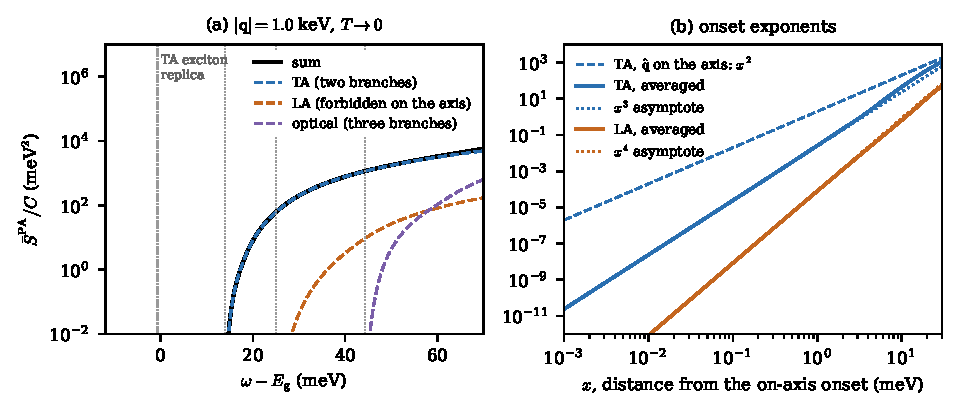
\includegraphics[width=\linewidth]{figures/ch13/fig13_3.pdf}
  \caption{The phonon-assisted structure factor of silicon near its threshold, averaged over the directions of $\vect{q}$ at $|\vect{q}| = \SI{1.0}{keV}$, at zero temperature (emission only), in units of a common coefficient $C$. Model: one valley at $\vect{k}_{\mathrm{c}} = 0.85\,(2\pi/a)$, parabolic pockets and the fixed-$\vect{q}$ form \cref{eq:13.3-near}, with the onset $\Eg + \omega_\nu(\vect{k}_{\mathrm{c}} - \vect{q})$ computed in every direction from the PBE force constants of \cref{sec:5.2}, whose transverse acoustic energy at X is \SI{17.06}{meV} against \SI{18.57}{meV} measured. Every branch is given the same $|M_\nu|^2 = C$, except the longitudinal acoustic one, which is given $C\sin^2\theta_Q$ because its amplitude vanishes on the valley axis; the relative heights are therefore illustrative. The tilt of the pair minimum (at most \SI{0.18}{meV}) is neglected. (a) Components against $\omega - \Eg$: the transverse acoustic edge at \SI{13.98}{meV}, the longitudinal acoustic kink at \SI{25.00}{meV}, and the optical onset at \SI{44.1}{meV}, whose minimum lies far off the axis (dotted lines). The dash-dotted line marks the exciton replica of the transverse acoustic edge, $E_x^b = \SI{14.7}{meV}$ lower, whose strength is not modeled. (b) Each acoustic component against the distance $x$ from its own onset. With $\vect{q}$ held on the axis the transverse acoustic component grows as $x^2$ (dashed). Averaged over directions it grows as $x^3$ (solid), and the longitudinal acoustic one as $x^4$; dotted lines are the asymptotes of \cref{we:13-onset-exp}. The window condition holds over the whole plot: at this $|\vect{q}|$ the zero-phonon pair continuum starts \SI{0.60}{eV} above $\Eg$ (PBE bands of \cref{sec:3.3} with the measured gap).}
  \label{fig:13-paloss}
\end{figure}

The exponents also require the onset itself to lie inside the window. At the onset the pair sits at the band extrema and the phonon takes all of $\vect{Q}^*$, while the zero-phonon edge at the same $\vect{q}$ lies $|\vect{Q}^*|^2/2M_{\mathrm{eh}}$ above $\Eg$ (\cref{eq:3.3-Eminpar}). The window condition $\Eg + \omega_\nu(\vect{Q}^*) \le E_{\mathrm{min}}(\vect{q}) - \delta_{\mathrm{w}}$ then reads $|\vect{Q}^*|^2 - 2M_{\mathrm{eh}}c\,|\vect{Q}^*| - 2M_{\mathrm{eh}}\delta_{\mathrm{w}} \ge 0$ for a branch $\omega_\nu = c|\vect{Q}|$, that is,
\begin{equation*}
  |\vect{Q}^*| \ge M_{\mathrm{eh}}c + \bigl(M_{\mathrm{eh}}^2c^2 + 2M_{\mathrm{eh}}\delta_{\mathrm{w}}\bigr)^{1/2} .
\end{equation*}
With a margin $\delta_{\mathrm{w}} = \SI{0.3}{eV}$, five times the top of the phonon band (\cref{sec:13.6} fixes the margin), and the phase velocity of the transverse acoustic branch at the bound, \SI{5.0}{km.s^{-1}}, the bound is \SI{0.31}{\angstrom^{-1}}, or \SI{0.615}{keV}. In silicon the exponents of \cref{eq:13.3-pon} therefore hold for $|\vect{q}| \le k_{\mathrm{c}} - \SI{0.615}{keV} = \SI{1.33}{keV}$ for parabolic valleys, and for $|\vect{q}| \le \SI{1.27}{keV}$ with the computed bands (\cref{sec:13.6}); over this whole range the transverse acoustic minimum lies on the axis. Closer to the valley the onset falls into the edge band of \cref{sec:13.6}, at the edge of the window, where the phonon-assisted rate is not separately defined and therefore has no exponent of its own.

\begin{workedexample}{The onset exponent from the joint density of states}\label{we:13-onset-exp}
Take silicon at $|\vect{q}| = \SI{1.0}{keV}$, near the valley axis [100], with $k_{\mathrm{c}} = 0.85\,(2\pi/a) = \SI{1.94}{keV}$. On the axis the phonon carries $k_{\mathrm{c}} - q = \SI{0.94}{keV}$, or \SI{0.48}{\angstrom^{-1}} $= 0.41\,\mathrm{X}$, where the computed dispersion of \cref{sec:5.2} gives $\omega_{\mathrm{TA}}(\vect{Q}^*) = \SI{13.98}{meV}$ and $\omega_{\mathrm{LA}}(\vect{Q}^*) = \SI{25.00}{meV}$. The onset $\Eg + \omega_{\mathrm{TA}}(\vect{Q}^*) = \SI{1.184}{eV}$ is reached by dark matter heavier than \SI{0.341}{MeV}, since $qv_{\mathrm{max}} - q^2/2\mchi$ must exceed it with $qv_{\mathrm{max}} = \SI{2.650}{eV}$. The zero-phonon edge at this $\vect{q}$ lies \SI{0.60}{eV} above $\Eg$ on the computed bands of \cref{fig:3-si-bands} (the parabola \cref{eq:3.3-Eminpar} gives \SI{0.73}{eV}), so the window extends to \SI{0.30}{eV} above $\Eg$, well beyond the energies considered here.

\emph{Fixed direction.} With $\vect{q}$ on the axis, \cref{eq:13.3-near} gives $S^{\mathrm{PA}} = Cx^2$ for each transverse acoustic branch, $C = \Omega(m^*_{\mathrm{d}}m_{\mathrm{h}})^{3/2}|M_{\mathrm{TA}}|^2/4\pi^2$, with $m^*_{\mathrm{d}} = 0.322\,m_e$. This is the $x^2$ of \cref{eq:6.5-joint}: the two pockets give six free momenta.

\emph{The curvature of the onset.} The transverse acoustic slope at \SI{0.48}{\angstrom^{-1}} is $\omega_{\mathrm{TA}}' = \SI{16.9}{meV.\angstrom}$, and the first term of \cref{eq:13.3-Eth} is
\begin{equation*}
  \frac{\omega_{\mathrm{TA}}'\,k_{\mathrm{c}}q}{2(k_{\mathrm{c}} - q)} = \SI{16.9}{meV.\angstrom}\times\frac{0.983\times\SI{0.507}{\angstrom^{-2}}}{2\times\SI{0.477}{\angstrom^{-1}}} = \SI{8.85}{meV} .
\end{equation*}
The anisotropy of the branch lowers $\varkappa$. Evaluated on a cone $\theta_q = \SI{0.02}{rad}$ around the axis, the lower transverse acoustic branch has $\varkappa$ between 2.3 and \SI{8.5}{meV} depending on the azimuth $\phi$, the upper one between 18 and \SI{24}{meV}, and the longitudinal acoustic one \SI{16.8}{meV} in every direction. All values of $\varkappa$ are positive: the axis is a minimum.

\emph{The average.} For an onset $\varkappa\theta_q^2$ above its minimum, the average over the sphere of directions, $\bar S = (4\pi)^{-1}\int\dd\phi\,\sin\theta_q\,\dd\theta_q\,S$, is dominated by small $\theta_q$, where $\sin\theta_q \simeq \theta_q$. With $u = \varkappa\theta_q^2$,
\begin{equation*}
  \frac{1}{4\pi}\int_0^{2\pi}\!\dd\phi\int\theta_q\,\dd\theta_q\,C\bigl(x - \varkappa\theta_q^2\bigr)^2\Theta = \frac{C}{4\pi}\int_0^{2\pi}\!\dd\phi\,\frac{1}{2\varkappa}\int_0^x\dd u\,(x - u)^2 = \frac{C\,x^3}{12}\Bigl\langle\frac{1}{\varkappa}\Bigr\rangle_{\!\phi} ,
\end{equation*}
with $\langle 1/\varkappa\rangle_\phi$ the average over the azimuth: \SI{0.240}{meV^{-1}} and \SI{0.047}{meV^{-1}} for the two transverse branches. The exponent has risen from 2 to 3, and $p_{\mathrm{on}} = 3$.

\emph{The forbidden branch.} For the longitudinal acoustic phonon $|M|^2 = C\sin^2\theta_Q \simeq C\,[q/(k_{\mathrm{c}} - q)]^2\theta_q^2$, and the extra $\theta_q^2 = u/\varkappa$ in the integrand gives $\int_0^x u(x - u)^2\dd u = x^4/12$, so
\begin{equation*}
  \bar S_{\mathrm{LA}} = \frac{C\,x^4}{48}\Bigl(\frac{q}{k_{\mathrm{c}} - q}\Bigr)^2\Bigl\langle\frac{1}{\varkappa^2}\Bigr\rangle_{\!\phi} ,
\end{equation*}
and $p_{\mathrm{on}} = 4$.

\emph{The cost of the average.} Per valley, the ratio of the averaged to the on-axis transverse acoustic structure factor is $(x/24)(\langle1/\varkappa\rangle_1 + \langle1/\varkappa\rangle_2)$ for the two branches, $1.2\times10^{-3}$ at $x = \SI{0.1}{meV}$. Only a cone of solid angle $\pi x/\varkappa$ around the valley axis is open, a fraction $x/4\varkappa$ of the sphere.
\end{workedexample}

At fixed $|\vect{q}|$ the halo enters the rate through $q^3\eta(\vmin)\FDM^2$ in \cref{eq:10.2-rate}, which is smooth across an onset as long as $\vmin < v_{\mathrm{max}}$. The spectrum contributed by each $|\vect{q}|$ therefore rises with the same exponent as $\bar L^{\mathrm{PA}}$. The integral over $|\vect{q}|$ smooths the spectrum further, because the onset moves with $|\vect{q}|$; \cref{sec:13.9-onset} combines these factors into the dependence of the rate on the dark-matter mass at the onset.

\section{Screening of the phonon-assisted rate}\label{sec:13.4}

The loss function of \cref{sec:13.3} uses the bare density vertex. At a momentum transfer of \SI{1}{keV} and an energy of \SI{1.2}{eV}, inside the phonon-assisted window, however, the dielectric function of silicon is about 6 in the random-phase approximation (\cref{we:13-external}). The potential that the dark matter exerts on a valence electron is therefore six times weaker than the bare one, and the bare loss function is too large by a factor of 30 to 50. Screening enters the amplitude of \cref{sec:13.2} at three places, among which \cref{sec:8.4} sorted the Coulomb lines: the dark-matter vertex at $(\vect{q},\omega)$, the electron--phonon vertex at $(\vect{Q},\omega_{\vect{Q}\nu})$, and the final pair at $(\vect{q}+\vect{Q}, \omega \mp \omega_{\vect{Q}\nu})$. With all three in the amplitude, the loss function keeps one macroscopic factor $1/\varepsilon_{\mathrm{mac}}(\vect{q},\omega)^2$ and nothing else outside it; \cref{app:D.36} gives the steps at the random-phase level.

\subsection{The screened density and phonon vertices}

The electron--phonon vertex is already screened. Density-functional perturbation theory returns $g_{mn\nu}(\vect{k},\vect{Q})$ as the matrix element of the self-consistent potential change $\partial V_{\mathrm{KS}}$, which is the bare potential of the displaced ions dressed by every Coulomb chain at $\vect{Q}+\vect{G}$, the operator $(1 - f_{\mathrm{Hxc}}R^0)^{-1}$ of \cref{eq:6.2-screen}. These are the vertex lines of \cref{sec:8.4-lines}. The calculation evaluates them at zero frequency, although they carry the phonon frequency; below the gap the error is of relative order $(\omega_{\vect{Q}\nu}/\Eg)^2$, about $3\times10^{-3}$ in silicon (\cref{sec:8.4-lines}). Dividing the computed $g$ once more by $\varepsilon(\vect{Q})$ would count these lines twice, and a bare ionic potential in its place would overstate the long-range part of the coupling by about $\varepsilon_\infty$.

The density vertex of \cref{eq:13.2-M} is bare. The dark matter applies a potential at $(\vect{q},\omega)$, and the electrons that it polarizes add their Hartree and exchange--correlation potentials at every $\vect{q} + \vect{G}$. An electron feels the total, the external potential times the column $(\tilde\varepsilon^{-1})_{\vect{G}0}(\vect{q},\omega)$ of the inverse dielectric matrix of a test electron (\cref{sec:8.7}). These are the external lines, and in the amplitude they replace the density vertex by
\begin{equation}
  \rho^{\mathrm{scr}}_{mn}(\vect{k},\vect{q}) = \sum_{\vect{G}}\bigl(\tilde\varepsilon^{-1}\bigr)_{\vect{G}0}(\vect{q},\omega)\,\rho_{mn}(\vect{k},\vect{q}+\vect{G}) ,
  \label{eq:13.4-rhoscr}
\end{equation}
the vertex of the total potential, as in the screened pair weight \cref{eq:8.7-screened}. The sum over $\vect{G}$ carries the local fields. Without local fields, where the dielectric matrix is diagonal, and without an exchange--correlation kernel, $\rho^{\mathrm{scr}}$ is $\rho/\varepsilon_{\vect{0}\vect{0}}(\vect{q},\omega)$, the head screening of \cref{sec:10.2}.

Exactly one factor of $1/\varepsilon$ survives once the local fields are kept. To see this, remove from the Coulomb kernel its macroscopic term, $v_{\mathrm{C}}(q)$ at $\vect{G} = \vect{G}' = 0$, and let $\bar R$ be the response without it (\cref{sec:4.4}). The full response is then $\bar R$ plus chains of $\bar R$ joined by the macroscopic line, and each element $(\tilde\varepsilon^{-1})_{\vect{G}0}$ factors into $(\varepsilon^{-1})_{\vect{0}\vect{0}} = 1/\varepsilon_{\mathrm{mac}}$ times a local-field column (\cref{app:D.36}). In the random-phase approximation,
\begin{equation}
  \begin{aligned}
  \rho^{\mathrm{scr}}_{mn}(\vect{k},\vect{q}) &= \frac{\rho^{\mathrm{LF}}_{mn}(\vect{k},\vect{q})}{\varepsilon_{\mathrm{mac}}(\vect{q},\omega)} , \\
  \rho^{\mathrm{LF}}_{mn}(\vect{k},\vect{q}) &= \rho_{mn}(\vect{k},\vect{q}) + \sum_{\vect{G}\ne0}v_{\mathrm{C}}(|\vect{q}+\vect{G}|)\,\bar R_{\vect{G}0}(\vect{q},\omega)\,\rho_{mn}(\vect{k},\vect{q}+\vect{G}) ,
  \end{aligned}
  \label{eq:13.4-rhoLF}
\end{equation}
exactly, with $\varepsilon_{\mathrm{mac}}$ the macroscopic dielectric function \cref{eq:4.4-epsmac}. An exchange--correlation kernel adds its own elements, its head included, to the local-field vertex $\rho^{\mathrm{LF}}$ and leaves the factorization intact. Physically, $\rho^{\mathrm{LF}}$ is the bare vertex corrected by the microscopic potentials that the macroscopic field induces inside each cell, and $1/\varepsilon_{\mathrm{mac}}$ is the reduction of the macroscopic field itself. Without local fields $\rho^{\mathrm{LF}} = \rho$ and $\varepsilon_{\mathrm{mac}} = \varepsilon_{\vect{0}\vect{0}}$.

Inside the window this factor is real. No zero-phonon pair exists at $(\vect{q},\omega)$, so the independent-particle response at that momentum and energy has no absorptive part, and $\varepsilon_{\mathrm{mac}}(\vect{q},\omega)$ is real up to the phonon-assisted terms of order $g^2$ that this section computes. We write its zero-phonon value $\varepsilon_1^0(\vect{q},\omega)$, the real part of $\varepsilon_{\mathrm{mac}}$ at $n_g = 0$; its imaginary part $\varepsilon_2^0$ vanishes in the window. The response $R(\vect{q},\omega)$ is then Hermitian, so the retarded column $\delta_{\vect{G}0} + (f_{\mathrm{Hxc}}R)_{\vect{G}0}$ and the advanced one $\delta_{\vect{G}0} + (f_{\mathrm{Hxc}}R^\dagger)_{\vect{G}0}$ coincide, and the question of \cref{sec:8.7}, which of the retarded and advanced weights labels a final pair, does not arise for the external lines. It arises at the pair.

\subsection{The pair channel}

Once the phonon has taken the momentum $\vect{Q}$, the dark matter and the phonon together have disturbed the electrons at a third wavevector, $\vect{q} + \vect{Q}$, and at a third frequency,
\begin{equation*}
  \omega_f = \omega \mp \omega_{\vect{Q}\nu} ,
\end{equation*}
the upper sign for emission. These are the crystal momentum and energy of the final pair itself, $\varepsilon_{c,\vect{k}+\vect{q}+\vect{Q}} - \varepsilon_{v\vect{k}} = \omega_f$ on shell. The disturbance is a density of second order, bilinear in the two vertices, and its Hartree and exchange--correlation potential acts back on the electrons at $(\vect{q}+\vect{Q}+\vect{G},\omega_f)$. That potential can create the final pair directly. Summed over the chains that the medium inserts, it is the pair channel of \cref{sec:8.4-lines}: the Coulomb lines on the segment of the cycle between the two dark-matter vertices. The four-path amplitude of \cref{sec:13.2} leaves it out, because it treats the electrons as independent once the two vertices are given.

To find it we follow the density matrix $\varrho$ of the Kohn--Sham electrons to second order in time-dependent mean-field theory (\cref{app:D.36}). The dark matter acts through the screened vertex, $\mathsf{x} = \rho^{\mathrm{scr}}$ at frequency $\omega$, and the phonon through $\mathsf{y} = g$ at frequency $\mp\omega_{\vect{Q}\nu}$, with the factor $N^{-1/2}(n_{\vect{Q}\nu} + \frac12 \pm \frac12)^{1/2}$ of \cref{eq:13.2-M} taken out. Each field alone produces a first-order density matrix, $\varrho^{\mathsf{x}}_{ab} = \mathsf{x}_{ab}(f_b - f_a)/(\omega - \varepsilon_a + \varepsilon_b + \ii0^+)$ and its analog $\varrho^{\mathsf{y}}$, with $f_a$ the occupation of the one-electron state $a$. At second order, each field acts on the first-order response to the other, which gives the source
\begin{equation*}
  \mathfrak{s}^{(2)}_{ab} = \sum_m\bigl[\mathsf{x}_{am}\varrho^{\mathsf{y}}_{mb} - \varrho^{\mathsf{y}}_{am}\mathsf{x}_{mb} + \mathsf{y}_{am}\varrho^{\mathsf{x}}_{mb} - \varrho^{\mathsf{x}}_{am}\mathsf{y}_{mb}\bigr] ,
\end{equation*}
a matrix over every pair of states, filled or empty. Its element between the final conduction state and the final valence state is, on shell, the four-path amplitude itself, $\mathfrak{s}^{(2)}_{cv} = M^\pm[\rho^{\mathrm{scr}}]$, \cref{eq:13.2-M} with the screened vertex and the unrestricted band sum: the hole paths enter through the occupation differences, and the band-sum theorem of \cref{app:D.35} follows from the density matrix without Fock space.

The source drives a second-order density of the Kohn--Sham electrons at $\vect{q}+\vect{Q}+\vect{G}$,
\begin{equation}
  \delta\nd^{(2)}_{\vect{G}}(\vect{q}+\vect{Q}) = \frac{2}{\Vol}\sum_{\vect{k}}\sum_{ab}\frac{\rho_{ab}(\vect{k},\vect{q}+\vect{Q}+\vect{G})^*\,\mathfrak{s}^{(2)}_{ab}(\vect{k})}{\omega_f + \varepsilon_{b\vect{k}} - \varepsilon_{a,\vect{k}+\vect{q}+\vect{Q}} + \ii0^+} ,
  \label{eq:13.4-dn2}
\end{equation}
the sum running over all pairs of states, including the rearrangements among filled and among empty bands. Its potential is screened by the same chains as any potential at that wavevector and frequency: the electrons respond to it with the bubble $R^0(\vect{q}+\vect{Q},\omega_f)$, their response adds potential, and the series sums to $\tilde\varepsilon^{-1}f_{\mathrm{Hxc}}\,\delta\nd^{(2)}$. In the random-phase approximation $\tilde\varepsilon^{-1}f_{\mathrm{Hxc}} = \varepsilon^{-1}v_{\mathrm{C}}$ is the retarded screened interaction $W^{\mathrm{scr,R}}$ of \cref{eq:4.8-W}. The equation of motion of the pair element $\varrho^{(2)}_{cv}$ is that of a first-order coherence driven at $\omega_f$ by $\mathfrak{s}^{(2)}$ plus this potential, and its numerator is the amplitude for creating the pair. Finally, every term is linear in $\mathsf{x}$, so the factor $1/\varepsilon_{\mathrm{mac}}(\vect{q},\omega)$ of \cref{eq:13.4-rhoLF} comes out in front.
\begin{keyresult}[Screened phonon-assisted amplitude]
In the random-phase approximation and at order $g$ in the amplitude, the screened matrix element of the density into the final state \cref{eq:13.2-final} is $N^{-1/2}(n_{\vect{Q}\nu} + \frac12 \pm \frac12)^{1/2}\,\tilde M^\pm_{cv\nu}(\vect{k},\vect{q},\vect{Q})/\varepsilon_{\mathrm{mac}}(\vect{q},\omega)$. The amplitude without the macroscopic factor is
\begin{equation}
  \begin{split}
  \tilde M^\pm_{cv\nu}(\vect{k},\vect{q},\vect{Q}) &= M^\pm_{cv\nu}\bigl[\rho^{\mathrm{LF}}\bigr] + \sum_{\vect{G}\vect{G}'}\rho_{cv}(\vect{k},\vect{q}+\vect{Q}+\vect{G})\\
  &\quad\times W^{\mathrm{scr,R}}_{\vect{G}\vect{G}'}(\vect{q}+\vect{Q},\omega_f)\,\delta\nd^{(2)}_{\vect{G}'}(\vect{q}+\vect{Q}) ,
  \end{split}
  \label{eq:13.4-Mscr}
\end{equation}
where $M^\pm[\rho^{\mathrm{LF}}]$ is \cref{eq:13.2-M} with the local-field vertex \cref{eq:13.4-rhoLF}, $\delta\nd^{(2)}$ is \cref{eq:13.4-dn2} built with $\mathsf{x} = \rho^{\mathrm{LF}}$, and the retarded $W^{\mathrm{scr,R}}$ carries the index of the final pair first. With an exchange--correlation kernel, $W^{\mathrm{scr,R}}$ becomes $\tilde\varepsilon^{-1}f_{\mathrm{Hxc}}$, and an adiabatic local kernel adds the source of \cref{eq:13.4-kxc}.
\end{keyresult}
\noindent The pair-channel term is added to the four-path term, not multiplied: it does not rescale the four-path term by $1/\varepsilon(\vect{q}+\vect{Q},\omega_f)$, and no $1/|\varepsilon|^4$ appears anywhere. The rate needs \cref{eq:13.4-Mscr} only on shell, where $\mathfrak{s}^{(2)}_{cv}$ equals the four-path amplitude.

\Cref{fig:13-screening} shows the three kinds of screening as diagrams. With the external chains at $(\vect{q},\omega)$, the static chains inside $g$ and the pair chain at $(\vect{q}+\vect{Q},\omega_f)$, every random-phase diagram with one phonon in the final state is counted once (\cref{sec:8.4-lines}). The classification is by the position of a line on the diagram, so it holds where the momentum labels coincide.

\begin{figure}[tbp]
  \centering
  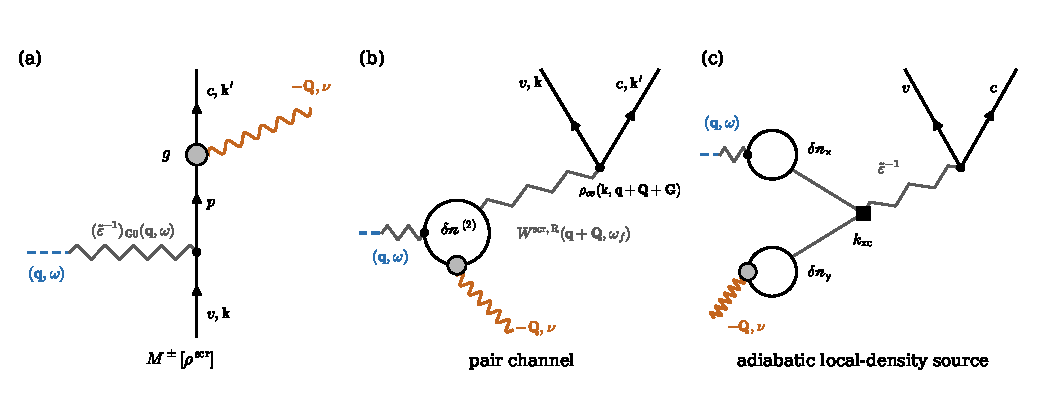
\includegraphics[width=\linewidth]{figures/ch13/fig13_4.pdf}
  \caption{Screening of the phonon-assisted amplitude, schematic. Time runs upward; solid lines are electrons and holes, dashed blue lines the dark-matter potential, wavy lines the phonon, and zigzag lines Coulomb chains summed to all orders. (a) The four-path term $M^\pm[\rho^{\mathrm{scr}}]$: the dark-matter potential reaches the electron through the external chains at $(\vect{q}+\vect{G},\omega)$, the column $(\tilde\varepsilon^{-1})_{\vect{G}0}(\vect{q},\omega)$, and the phonon through the vertex $g$ of density-functional perturbation theory (gray disk), whose chains at $(\vect{Q}+\vect{G},\approx0)$ are inside it. One of the four paths is drawn. (b) The pair channel: the two vertices act on a loop of Kohn--Sham electrons and produce the second-order density $\delta\nd^{(2)}$ at $(\vect{q}+\vect{Q}+\vect{G}',\omega_f)$, whose potential, screened by $W^{\mathrm{scr,R}}(\vect{q}+\vect{Q},\omega_f)$, creates the final pair through $\rho_{cv}(\vect{k},\vect{q}+\vect{Q}+\vect{G})$. (c) The extra source of an adiabatic local-density kernel: the first-order densities induced by the dark matter and by the phonon meet at one point through $k_{\mathrm{xc}}$, the third derivative of the exchange--correlation energy, and the potential they produce is screened at the pair. In the random-phase approximation panel (c) is absent.}
  \label{fig:13-screening}
\end{figure}

The pair line is complex. The final pair is on shell, so pairs exist at $(\vect{q}+\vect{Q},\omega_f)$, and the response there has an absorptive part. With an absorptive interaction the share of the total rate that each final pair receives depends on whether the retarded or the advanced interaction is used, while the total does not. The pair that the cascade receives is the out-state of the evolution, and it takes the retarded $W^{\mathrm{scr,R}}$, as the external weight did in \cref{sec:8.7}.

The momentum of the pair channel is pinned. At the threshold the hole sits near the valence maximum at $\mathrm{\Gamma}$ and the electron near the bottom of a valley at $\vect{k}_{\mathrm{c}}$. The pair momentum $\vect{q}+\vect{Q}$ therefore equals $\vect{k}_{\mathrm{c}}$ up to a reciprocal-lattice vector, whatever $\vect{q}$ is, exactly at the onset and within a few tenths of an inverse \si{\angstrom} at the top of the window. In silicon $|\vect{k}_{\mathrm{c}}| = 0.85\,(2\pi/a) = \SI{1.94}{keV}$, and $\omega_f$ lies within a few tenths of an eV of the gap. One screened interaction, at the six valley momenta and a narrow band of energies, serves the whole window; it is the same one that screens phonon-assisted optical absorption, where $\vect{q} = 0$ and the pair momentum is $\vect{Q}$ (\cref{sec:13.5}). Only $\delta\nd^{(2)}$ depends on $\vect{q}$.

Two limits can be solved, and they show what the pair channel does. In the first, the applied-potential limit, the source acts on every pair at $\vect{q}+\vect{Q}$ as an applied potential would, $\mathfrak{s}^{(2)}_{ab}$ proportional to $\rho_{ab}(\vect{k},\vect{q}+\vect{Q})(f_b - f_a)$. Then $\delta\nd^{(2)}$ is the bubble times that potential, and the two terms of \cref{eq:13.4-Mscr} combine into the source screened as an external potential at the pair's own momentum and energy, $\tilde M^\pm = M^\pm[\rho^{\mathrm{LF}}]/\varepsilon(\vect{q}+\vect{Q},\omega_f)$ without local fields (\cref{app:D.36}). In this limit the pair channel reduces the rate by $1/\varepsilon_1(\vect{k}_{\mathrm{c}},\omega_f)^2$, the screening of the final pair's own momentum.

In the second limit the phonon is a rigid translation of the crystal, $\vect{Q} = 0$, and the vertex is the commutator of the electron momentum with the Kohn--Sham Hamiltonian (\cref{eq:6.2-asr}). In the frame that moves with the nuclei the dark-matter potential only acquires a phase factor, and the displaced density is screened at the energy of the final pair, $1/\varepsilon(\vect{q},\omega_f)$. The four-path term alone gives $1/\varepsilon(\vect{q},\omega)$, screened at the energy deposited, and the pair channel supplies exactly the difference, $1/\varepsilon(\vect{q},\omega_f) - 1/\varepsilon(\vect{q},\omega)$ (\cref{app:D.36}). In the strict limit an acoustic $\omega_{\vect{Q}\nu}$ vanishes, $\omega_f = \omega$, and the pair term vanishes with it. Evaluated with the transverse acoustic energy of the window instead, the two energies change $\varepsilon_1$ of silicon by $1\times10^{-3}$ and the rate by $2\times10^{-3}$ (\cref{we:13-external}). The limit therefore tests the sign and the normalization of \cref{eq:13.4-Mscr}, not its size. It requires a zero-phonon pair at $(\vect{q},\omega_f)$ and therefore lies outside the window. Inside it, the phonons that carry the missing momentum have wavevectors near the zone boundary, where the displacement is not a translation of anything, and the pair channel is neither of these limits.

\subsection{The screened phonon-assisted loss function}

The rate follows from the screened amplitude as it followed from the bare one in \cref{sec:13.3}: the golden rule into the bare pairs, summed over $\vect{k}$, $\vect{Q}$, bands, branches and spin. That this sum is the whole absorptive part of the one-phonon response, with nothing counted twice, is the optical theorem of the mean-field evolution: cut at the pair, the diagrams with both dark-matter vertices on one loop give $|M^\pm[\rho^{\mathrm{LF}}]|^2$, and those with a pair segment the cross terms and the square of the pair channel, which together make $|\tilde M^\pm|^2$ pair by pair (\cref{app:D.36}). The amplitude therefore enters \cref{eq:13.3-LPA} with $M^\pm \to \tilde M^\pm/\varepsilon_{\mathrm{mac}}(\vect{q},\omega)$.

Write $\varepsilon_{\mathrm{mac}} = \varepsilon_1^0 + \delta\varepsilon_1 + \ii\varepsilon_2$, where $\delta\varepsilon_1$ and $\varepsilon_2$ are the phonon-assisted parts, both of order $g^2$ because $\varepsilon_2^0 = 0$. Then $|\varepsilon_{\mathrm{mac}}|^{-2} = (\varepsilon_1^0)^{-2}[1 + O(g^2)]$, and since $|\tilde M^\pm|^2$ is already of order $g^2$, every correction is of order $g^4$, the next order of the expansion in \cref{sec:8.5}.
\begin{keyresult}[Screened phonon-assisted loss function]
Inside the off-shell window, where $\varepsilon_2^0(\vect{q},\omega) = 0$,
\begin{equation}
  \begin{aligned}
  L^{\mathrm{PA}}(\vect{q},\omega) &= \frac{\varepsilon_2^{\mathrm{PA}}(\vect{q},\omega)}{\varepsilon_1^0(\vect{q},\omega)^2} + O(g^4) , \\
  \varepsilon_2^{\mathrm{PA}}(\vect{q},\omega) &= \frac{8\pi^2\alpha}{\Omega\,q^2}\,\Bigl\langle\!\Bigl\langle\sum_{\nu cv\pm}w_\pm\,\bigl|\tilde M^\pm_{cv\nu}\bigr|^2\,\delta\bigl(\varepsilon_{c,\vect{k}+\vect{q}+\vect{Q}} - \varepsilon_{v\vect{k}} \pm \omega_{\vect{Q}\nu} - \omega\bigr)\Bigr\rangle\!\Bigr\rangle ,
  \end{aligned}
  \label{eq:13.4-Lscr}
\end{equation}
with $\tilde M^\pm$ of \cref{eq:13.4-Mscr}, the weights $w_\pm$ of \cref{eq:13.3-LPA}, and $\varepsilon_1^0$ the macroscopic zero-phonon dielectric function with local fields. The rate is \cref{eq:10.2-rate} with $\bar L$ replaced by the direction average $\bar L^{\mathrm{PA}}$.
\end{keyresult}
\noindent From here on $L^{\mathrm{PA}}$ denotes this screened loss function; the function of \cref{eq:13.3-LPA} is its independent-particle value. The definition of $\varepsilon_2^{\mathrm{PA}}$ in \cref{eq:13.4-Lscr} identifies it as the imaginary part, at order $g^2$, of the macroscopic dielectric function, since $L = \Imag(-1/\varepsilon_{\mathrm{mac}}) = \varepsilon_2/|\varepsilon_{\mathrm{mac}}|^2$ must agree with the golden-rule sum term by term. \Cref{eq:13.4-Lscr} is therefore the familiar $L = \varepsilon_2/|\varepsilon|^2$ of \cref{sec:4.4}, evaluated where the zero-phonon $\varepsilon_2$ vanishes and the phonon-assisted one is small.

\Cref{eq:13.4-Lscr} has two simpler forms. One drops the pair channel and the local fields: then $\tilde M^\pm = M^\pm$, $\varepsilon_2^{\mathrm{PA}}$ is the independent-particle loss function of \cref{sec:13.3}, $\varepsilon_1^0 = \varepsilon_{1,\vect{0}\vect{0}}$, and the screened loss function is the unscreened one divided by $\varepsilon_{1,\vect{0}\vect{0}}(\vect{q},\omega)^2$. This is the form that a calculation with the bare density vertex and a scalar dielectric function would use. Each of the two omissions is a definite set of diagrams, and neither is a choice of convention. The other is the optical limit: as $\vect{q} \to 0$, $\varepsilon_1^0$ becomes the optical $\varepsilon_1(\omega)$ and $\varepsilon_2^{\mathrm{PA}}$ the phonon-assisted absorption of \cref{sec:6.5}, now with the pair channel inside it (\cref{sec:13.5}). A measured absorption edge contains the screening of the amplitude, the local-field wings and the pair channel, at $\vect{q} = 0$; the external factor is not in $\varepsilon_2$, and a rate normalized to the edge calibrates it only through the value of $\varepsilon_1^0$ at $\vect{q} \to 0$. Because the pair momentum is pinned at $\vect{k}_{\mathrm{c}}$, the measured edge tests the same screened interaction that acts at finite $\vect{q}$. It does not test the second-order density $\delta\nd^{(2)}$ at finite $\vect{q}$, which is where the two differ.

Outside the window \cref{eq:13.4-Lscr} fails twice. Where zero-phonon pairs exist at $(\vect{q},\omega)$, $\varepsilon_2^0$ is of order one and enters the denominator, and the external lines become absorptive, so that their retarded and advanced weights differ pair by pair. The one-phonon sideband is then no longer a separate quantity, and its treatment by the Dyson convention and the Fano term of \cref{sec:8.6} is the subject of \cref{sec:13.6}.

The prescriptions of \cref{sec:13.3} carry over. A computed $L^{\mathrm{PA}}$ is never added to a measured loss function, and a phonon-assisted table in the normalization of the crystal form factor adds to $|f_{\mathrm{crys}}|^2$ only if both are screened at the same level. A rate that uses \cref{eq:13.4-Lscr} without the pair channel sits at $\mathcal{X}$ = RPA with local fields for the external lines and $\mathcal{X}$ = IP for the pair, and it should be reported that way.

\subsection{The adiabatic local-density source}

The random-phase approximation is linear in the induced density: the Hartree potential of a density $\delta\nd$ is $v_{\mathrm{C}}\,\delta\nd$, whatever its order. The exchange--correlation potential is not. The adiabatic local-density approximation of \cref{sec:4.6} takes $v_{\mathrm{xc}}$ as a function of the density at each point, and expanding it to second order,
\begin{equation}
  v_{\mathrm{xc}}\bigl(\nd_{\mathrm{gs}} + \delta\nd\bigr) = v_{\mathrm{xc}}(\nd_{\mathrm{gs}}) + f_{\mathrm{xc}}\,\delta\nd + \tfrac12k_{\mathrm{xc}}\,\delta\nd^2 + \cdots , \qquad
  k_{\mathrm{xc}}(\vect{r}) = \frac{\dd^3\bigl[\nd\,\varepsilon_{\mathrm{xc}}(\nd)\bigr]}{\dd\nd^3}\bigg|_{\nd_{\mathrm{gs}}(\vect{r})} ,
  \label{eq:13.4-kxc}
\end{equation}
with $f_{\mathrm{xc}}$ the kernel of \cref{eq:4.6-alda} and $k_{\mathrm{xc}}$ the next derivative. The density to first order is the sum of two pieces, $\delta\nd_{\mathsf{x}}$ induced by the dark matter at $(\vect{q},\omega)$ and $\delta\nd_{\mathsf{y}}$ induced by the phonon at $(\vect{Q},\mp\omega_{\vect{Q}\nu})$, the density response that density-functional perturbation theory computes along with $g$. The square $\frac12(\delta\nd_{\mathsf{x}} + \delta\nd_{\mathsf{y}})^2$ contains the cross term $\delta\nd_{\mathsf{x}}\delta\nd_{\mathsf{y}}$ with coefficient one. In real space it is a product, so its Fourier components lie at $\vect{q}+\vect{Q}+\vect{G}$, and it oscillates at $\omega_f$. It is a potential at the pair's momentum and energy that no Coulomb chain produces: the second-order source of the kernel itself. The electrons screen it as any applied potential, and it adds
\begin{equation*}
  \sum_{\vect{G}}\rho_{cv}(\vect{k},\vect{q}+\vect{Q}+\vect{G})\,\bigl[\tilde\varepsilon^{-1}(\vect{q}+\vect{Q},\omega_f)\,\bigl(k_{\mathrm{xc}}\,\delta\nd_{\mathsf{x}}\delta\nd_{\mathsf{y}}\bigr)\bigr]_{\vect{G}}
\end{equation*}
to $\tilde M^\pm$ (\cref{app:D.36}), with $\delta\nd_{\mathsf{x}}$ taken without its macroscopic factor, as $\rho^{\mathrm{LF}}$ is. The term is the reason \cref{eq:13.4-Mscr} is stated at the random-phase level. A calculation that takes $g$ from density-functional perturbation theory in the local-density approximation, and the screening from the adiabatic kernel, has $f_{\mathrm{xc}}$ in every linear chain and is consistent only if it keeps this source too.

Its size follows from exchange alone, with $k_{\mathrm{x}} = -\frac23 f_{\mathrm{x}}/\nd$ and the gas value $f_{\mathrm{x}} = -e^2/4k_{\mathrm{F}}^2$ of \cref{sec:4.6} (\cref{app:D.36}). Against the Hartree part of the pair channel, the new term is
\begin{equation*}
  \frac23\Bigl(\frac{|\vect{k}_{\mathrm{c}}|}{2k_{\mathrm{F}}}\Bigr)^2\,\frac{|\delta\nd_{\mathsf{x}}\delta\nd_{\mathsf{y}}|}{\nd\,|\delta\nd^{(2)}|} ,
\end{equation*}
where the last ratio, a product of two first-order densities over the density times a second-order one, is of order one in the electron gas. The valence electrons of silicon, 32 in a cubic cell of \SI{5.431}{\angstrom}, have $\nd = \SI{0.200}{\angstrom^{-3}}$ and $k_{\mathrm{F}} = \SI{1.81}{\angstrom^{-1}}$, and with $|\vect{k}_{\mathrm{c}}| = \SI{0.983}{\angstrom^{-1}}$ the prefactor is $\frac23\times0.074 = 0.05$. The adiabatic source is therefore an estimated twentieth of the pair channel, times a coefficient of order one that is not known. It matters only as much as the pair channel does.

\subsection{Screening factors in silicon}

The external factor is the largest and the best known, and \cref{we:13-external} sizes it at $|\vect{q}| = \SI{1}{keV}$. It changes by less than \SI{5}{\percent} across the window at fixed $|\vect{q}|$, since $\varepsilon_1$ rises slowly toward the direct gap. It does change with $|\vect{q}|$, however, since the valence electrons screen less at shorter wavelengths: without local fields the static value falls from 10.2 at $\vect{q} \to 0$ to 6.1--6.6 at \SI{1}{keV} and to 3.2--3.7 near \SI{2}{keV} in the same data. A rate integrated over $|\vect{q}|$ therefore needs $\varepsilon_1^0$ at every $|\vect{q}|$, not one number.

Two ratios measure what the simpler forms leave out. The local-field ratio $1 + \delta_{\mathrm{LF}}$ is $L^{\mathrm{PA}}$ with local fields but without the pair channel, divided by $L^{\mathrm{PA}}$ with the head alone. The pair-channel ratio $1 + \delta_{\mathrm{pair}}$ is $L^{\mathrm{PA}}$ with local fields and the pair channel, divided by $L^{\mathrm{PA}}$ with local fields alone. The full screened loss function is then the head-screened one times $(1 + \delta_{\mathrm{LF}})(1 + \delta_{\mathrm{pair}})$. The local-field ratio has two parts. The macroscopic factor changes from $1/\varepsilon_{1,\vect{0}\vect{0}}^2$ to $1/\varepsilon_{\mathrm{mac}}^2$, an increase of 25 to \SI{31}{\percent} at \SI{1}{keV} in the data of \cref{we:13-external}. The vertex changes from $\rho$ to $\rho^{\mathrm{LF}}$, whose wing terms $\vect{G} \neq 0$ the published dielectric functions do not contain. They need the column $\bar R_{\vect{G}0}(\vect{q},\omega)$ and the vertices $\rho_{cv}(\vect{k},\vect{q}+\vect{G})$ at the same $(\vect{q},\omega)$; a bound from the zero-phonon vertices alone, \cref{eq:E.16-dLF}, costs about ten core-hours. The macroscopic factor and the column $(\tilde\varepsilon^{-1})_{\vect{G}0}(\vect{q},\omega)$ are standard outputs of a random-phase calculation with local fields, specified for the phonon-assisted grid in \cref{app:E.14}.

The size of the pair channel in silicon is open, and the two solvable limits of \cref{eq:13.4-Mscr} bracket it only loosely. If the source acted like an applied potential at the pair momentum, the rate would fall by $1/\varepsilon_1(\vect{k}_{\mathrm{c}},\omega_f)^2$. The same data have four mesh points between 1.87 and \SI{2.03}{keV}. At \SI{1.2}{eV} their $\varepsilon_1$ is 3.3 to 3.8 without local fields and 2.9 to 3.5 with them, so that factor is 0.07 to 0.12; the imaginary part there is about $10^{-3}$, since the final pairs sit at their own edge. If the source were the displacement of a rigid crystal, the pair channel would change the rate by $2\times10^{-3}$ at the phonon energy of the window. Neither limit is a bound on the real case, and the sign of $\delta_{\mathrm{pair}}$ is not derived: the source of a zone-boundary phonon is partly a displacement of the bond charge and partly a change of its shape, and the two limits stand for these.

Where the number comes from is known. The screened interaction is needed only at the six valley momenta, $W^{\mathrm{scr,R}}(\vect{k}_{\mathrm{c}},\omega_f)$. The second-order density $\delta\nd^{(2)}$ is a mixed second derivative of the density, with respect to the dark-matter potential and to a phonon displacement, of the kind that density-functional perturbation theory computes for Raman tensors. The route that contains every class at once is a supercell displaced along a phonon pattern, with local fields in the supercell basis: then $\vect{Q}$ is a reciprocal vector of the supercell, and the pair channel is a local-field effect of the supercell. Three runs of that calculation give $\delta_{\mathrm{LF}}$ and $\delta_{\mathrm{pair}}$ separately (\cref{app:E.16}).

The remaining classes are small. The static evaluation of $g$ errs by $3\times10^{-3}$, and the ionic part of the dielectric function, which a silicon crystal has only through its quadrupoles, enters the external and pair chains below $10^{-4}$ (\cref{sec:8.4-lines}).

\begin{workedexample}{The external screening factor in silicon at 1 keV}\label{we:13-external}
Take $|\vect{q}| = \SI{1.0}{keV}$ and $\omega = \SI{1.20}{eV}$, just above the transverse acoustic onset at \SI{1.184}{eV} and well inside the window, which extends to \SI{1.47}{eV} at this momentum (\cref{we:13-onset-exp}). The random-phase dielectric function of silicon with and without local fields has been published on a mesh of $|\vect{q}|$ and $\omega$~\cite[Sect.~III\,B]{knapen2021dark}, with the data files of Ref.~\cite{knapen2022darkelf}. Each mesh momentum is the length of one vector $\vect{q} + \vect{G}$, and so one direction. Two mesh points lie within \SI{0.1}{keV} of \SI{1}{keV}, at 0.944 and \SI{0.986}{keV}, and we quote the range over the two rather than a fit. Interpolating linearly in $\omega$ between the mesh energies 1.04 and \SI{1.26}{eV},
\begin{equation*}
  \varepsilon_{1,\vect{0}\vect{0}} = 6.31\text{--}6.93 , \qquad \varepsilon_{\mathrm{mac}} = 5.52\text{--}6.20 ,
\end{equation*}
and $\varepsilon_2 = 0$ at both, as it must be below the zero-phonon edge.

\emph{The factor.} The screened loss function is the independent-particle one divided by $\varepsilon_1^2$, so the factor is
\begin{equation*}
  \frac{1}{\varepsilon_{1,\vect{0}\vect{0}}^2} = 0.021\text{--}0.025 , \qquad \frac{1}{\varepsilon_{\mathrm{mac}}^2} = 0.026\text{--}0.033 .
\end{equation*}
The unscreened $L^{\mathrm{PA}}$ of \cref{sec:13.3} overstates the screened one by a factor of 40 to 48 with the head alone and 30 to 38 with the macroscopic function. The local fields of the macroscopic function raise the factor by $(\varepsilon_{1,\vect{0}\vect{0}}/\varepsilon_{\mathrm{mac}})^2 = 1.25$ and 1.31 at the two points.

\emph{Against the optical constant.} The measured $\varepsilon_\infty = 11.7$ (\cref{sec:4.4}) would give $1/\varepsilon_\infty^2 = 0.0073$, too small by a factor of 2.9 to 3.4 against the head and 3.6 to 4.5 against the macroscopic function. Screening at \SI{1}{keV} is weaker than at $\vect{q} \to 0$, because the momentum transfer resolves the bonds that do the screening. The same data give 10.2 at $\vect{q} \to 0$ without local fields and 9.1 with them, 13 and \SI{22}{\percent} below the measured value. With bands scissored to the measured gap, that deficit is mostly the electron--hole attraction, the vertex correction that the random-phase approximation leaves out, and the factor at \SI{1}{keV} carries an error of the same kind, which no measurement at this momentum checks.

\emph{Across the window.} Between the onset, \SI{1.184}{eV}, and the window edge, \SI{1.47}{eV}, the factor changes by 4.2 and \SI{4.8}{\percent} at the two points with the head, and by 3.7 and \SI{4.4}{\percent} with the macroscopic function.

\emph{The energy of the final pair.} The logarithmic slope $\dd\ln\varepsilon_1/\dd\ln\omega$ is 0.07 to 0.08 here. Replacing $\omega$ by $\omega_f = \omega - \omega_{\mathrm{TA}}(\vect{Q}^*)$, with $\omega_{\mathrm{TA}}(\vect{Q}^*) = \SI{14.0}{meV}$ at this momentum, changes $\varepsilon_1$ by $0.08\times0.014/1.2 = 1\times10^{-3}$ and the factor by $2\times10^{-3}$, the size that the rigid-translation form of the pair channel takes at this phonon energy.
\end{workedexample}

Whether the pair-channel ratio is the same at finite $\vect{q}$ as at $\vect{q} = 0$ decides how much of it a measured absorption edge calibrates (\cref{sec:13.5}). In both solvable limits it is: the applied-potential factor $1/\varepsilon_1(\vect{k}_{\mathrm{c}},\omega_f)^2$ is the same at every $\vect{q}$, since the pair momentum is pinned, and changes by less than $4\times10^{-4}$ between the phonon energies of the window and of the optical edge, while the rigid-translation term stays below $2\times10^{-3}$ at both momenta. That holds at exact pinning, at the onset; above it the pair momenta spread by about \SI{0.2}{keV} around $\vect{k}_{\mathrm{c}}$, where $\varepsilon_1$ changes by several tenths, and the factor cancels only as far as the distributions of final pairs at finite $\vect{q}$ and at $\vect{q} = 0$ match, an unsized residual. Between the limits it is not derived, because $\delta\nd^{(2)}$ depends on $\vect{q}$ through the phonon at $\vect{k}_{\mathrm{c}} - \vect{q}$. A rate normalized to the measured edge therefore needs, beyond the form factor of its vertex, a screening correction relative to that calibration: the external factor of its model dielectric function against the true $\varepsilon_1^0$, the local-field wings at finite $\vect{q}$ against those at $\vect{q} = 0$, and the pair ratio at finite $\vect{q}$ against its optical value. \Cref{sec:13.9} sizes the first two for the silicon estimate, 0.3 to 2.6 together, and leaves the third as an unsized nuisance. Lines inside a loop, the attraction between the electron and the hole of the final pair, lie outside \cref{eq:13.4-Mscr}; they bind the pair into excitons below the edge and enhance it above, and they are the subject of \cref{sec:13.8}.

\section{The optical limit}\label{sec:13.5}

A photon of \SI{1.24}{eV} absorbed in silicon brings a momentum of \SI{1.24}{eV}, five parts in $10^4$ of the reciprocal-lattice scale $2\pi/a = \SI{2.28}{keV}$, so its phonon supplies all of the \SI{1.94}{keV} between hole and electron, while dark matter near the onset mass supplies \SI{0.9}{keV} or more itself (\cref{sec:13.1}). Both processes have the same final states, and the independent-particle loss function $L^{\mathrm{PA}}_{\mathrm{IP}}(\vect{q},\omega)$ of \cref{eq:13.3-LPA} describes both, at different momentum transfers. Its limit $\vect{q}\to0$ is the phonon-assisted absorption $\varepsilon_2^{\mathrm{PA}}(\omega)$ of \cref{eq:6.5-eps2PA}. The measured absorption edge then serves twice. It tests a computed $L^{\mathrm{PA}}$ at one end of its range of $\vect{q}$, and it enters the rate of dark-photon absorption directly, once it has been transferred from the temperature of the measurement to that of a detector.

\subsection{The small-momentum limit}

The limit cannot be taken term by term in the amplitude $M^\pm_{cv\nu}(\vect{k},\vect{q},\vect{Q})$ of \cref{eq:13.2-M}. Its intraband terms carry density vertices that tend to one and cancel at $\vect{q} = 0$ (\cref{eq:13.2-q0}), so the leading term in $q$ is a difference of large terms, each with a different expansion of the bands and vertices. The continuity equation avoids the expansion. For the full Hamiltonian of electrons and nuclei, \cref{eq:4.3-continuity} gives $[H, n_e(\vect{q})] = \vect{q}\cdot\vect{j}_e(\vect{q})$, exactly, and between any two eigenstates of $H$
\begin{equation*}
  (E_f - E_i)\,\langle f|n_e(\vect{q})|i\rangle = \langle f|\vect{q}\cdot\vect{j}_e(\vect{q})|i\rangle .
\end{equation*}
The second-order amplitude \cref{eq:13.2-T} is a matrix element of this kind. To first order in $H_{\mathrm{ep}}$ the eigenstates of $H$ are $|\tilde i\rangle = |i\rangle + \sum_m|m\rangle\langle m|H_{\mathrm{ep}}|i\rangle/(E_i - E_m)$ and $\langle\tilde f| = \langle f| + \sum_m\langle f|H_{\mathrm{ep}}|m\rangle\langle m|/(E_f - E_m)$, with unchanged energies, because $H_{\mathrm{ep}}$ changes the number of phonons by one and has no diagonal elements. With $E_f = E_i + \omega$, the part of $\langle\tilde f|n_e(\vect{q})|\tilde i\rangle$ linear in $H_{\mathrm{ep}}$ is \cref{eq:13.2-T} term by term. The same construction applied to $\vect{q}\cdot\vect{j}_e(\vect{q})$ gives its second-order amplitude, and the identity holds order by order on the energy shell:
\begin{equation}
  \omega\,\langle f|n_e^{(2)}(\vect{q})|i\rangle = \langle f|\bigl(\vect{q}\cdot\vect{j}_e(\vect{q})\bigr)^{(2)}|i\rangle .
  \label{eq:13.5-ward}
\end{equation}
The intermediate states must be off the shell for the expansion to exist, and the off-shell window of \cref{sec:13.2} guarantees it.

The current needs no cancellation. At $\vect{q} = 0$ it is the total velocity, $\vect{j}_e(0) = \sum_j\vect{p}_j/m_e = \op{\vect{V}}$ of \cref{eq:6.5-HA}, which conserves $\vect{k}$, and its second-order amplitude into the final state of \cref{eq:13.2-final} is the one that \cref{sec:6.5} computed for light, with the photon vertex $(e\mathcal{E}/2\omega)\,\hat{\vect{e}}_\gamma\cdot\op{\vect{V}}$ replaced by $\vect{q}\cdot\op{\vect{V}}$. The same four paths combine into one sum over every band. Write $M^\pm_{cv\nu}(\vect{k},\vect{Q};\hat{\vect{e}}_\gamma)$ for the optical amplitude \cref{eq:6.5-M} with its polarization shown. Then, with $\vect{j}_e(\vect{q}) = \op{\vect{V}} + O(q)$,
\begin{keyresult}[Optical limit of the phonon-assisted amplitude]
\begin{equation}
  M^\pm_{cv\nu}(\vect{k},\vect{q},\vect{Q}) = \frac{q}{\omega}\,M^\pm_{cv\nu}(\vect{k},\vect{Q};\hat{\vect{q}}) + O(q^2) ,
  \label{eq:13.5-Mlim}
\end{equation}
on the energy shell inside the off-shell window, with the final electron at $\vect{k}+\vect{Q}$ in the limit.
\end{keyresult}
\noindent At $\vect{q} = 0$ the right side vanishes, which is \cref{eq:13.2-q0}: the identity contains the cancellation of the intraband terms and needs no expansion of them. It also gives the amplitude its first power of $q$, as \cref{eq:3.2-optical} does for the zero-phonon vertex, with the transition energy $\omega$ in the denominator. For a single pair, $\rho_{cv} \to \vect{q}\cdot\vect{v}_{cv}/\omega$ on the shell; for a pair with a phonon, the velocity vertex is replaced by the whole second-order optical amplitude.

\Cref{eq:4.3-continuity} holds because the potential energy depends on positions alone. A nonlocal pseudopotential breaks this, and $[H, n_e(\vect{q})]$ acquires the commutator of the nonlocal part. The velocity then contains the term $\ii[V_{\mathrm{NL}},\vect{r}]$ of \cref{eq:3.2-dHk}, which first-principles optical calculations include. The electron--phonon vertex of a nonlocal potential, the derivative of $V_{\mathrm{NL}}$ with respect to a displacement, contributes a commutator of the same kind. It is a contact term, in which one vertex creates the phonon and couples to the field at once, and \cref{eq:13.5-ward} holds only if it is kept on the side of the current.

Inserted into the loss function \cref{eq:13.3-LPA}, \cref{eq:13.5-Mlim} multiplies the optical $|M^\pm|^2$ by $q^2/\omega^2$, and the factor $q^2$ cancels the $1/q^2$ of the Coulomb line. The prefactor becomes $8\pi^2\alpha/(\Omega\omega^2) = g_{\mathrm{deg}}\pi e^2/(\omega^2\Omega)$ with $g_{\mathrm{deg}} = 2$ and $e^2 = 4\pi\alpha$. The weights $w_\pm = (1 - \ee^{-\beta\omega})(n_{\vect{Q}\nu} + \frac12 \pm \frac12)$ become $n_{\vect{Q}\nu} + \frac12 \pm \frac12$, since $\beta\omega > 40$ at room temperature for $\omega$ near the gap. The energy delta function loses $\vect{q}$ from the electron's crystal momentum. What remains is \cref{eq:6.5-eps2PA} with the polarization $\hat{\vect{e}}_\gamma = \hat{\vect{q}}$:
\begin{keyresult}[Optical limit of the phonon-assisted loss function]
\begin{equation}
  \lim_{\vect{q}\to0}L^{\mathrm{PA}}_{\mathrm{IP}}(\vect{q},\omega) = \varepsilon_2^{\mathrm{PA}}(\omega)\big|_{\hat{\vect{e}}_\gamma = \hat{\vect{q}}} ,
  \label{eq:13.5-limit}
\end{equation}
for $T \ll \Eg$ and $\omega$ inside the off-shell window at $\vect{q}\to0$, that is, below the direct gap. In a crystal with a center of inversion $L^{\mathrm{PA}}_{\mathrm{IP}}(\vect{q},\omega) = L^{\mathrm{PA}}_{\mathrm{IP}}(-\vect{q},\omega)$, and the corrections are of relative order $q^2$.
\end{keyresult}
\noindent The optical result and its edge are derived in \cref{sec:6.5,app:D.18}. Near threshold, \cref{eq:13.5-limit} reduces to the Hall--Bardeen--Blatt edge \cref{eq:6.5-edge}~\cite{hall1954infrared}, the $q\to0$ form of the fixed-$\vect{q}$ law \cref{eq:13.3-near}. As $\vect{q}\to0$ the phonon wavevector $\vect{Q}^* = \vect{k}_{\mathrm{c}} - \vect{q}$ tends to $\vect{k}_{\mathrm{c}}$, the onset $\Eg + \omega_\nu(\vect{Q}^*)$ tends to the optical threshold $\Eg + \omega_\nu$, and $|M_\nu|^2/q^2$ to the optical $|M_\nu|^2/\omega^2$. The full formula is the one that first-principles calculations of the absorption of silicon evaluate~\cite[Eq.~(1)]{noffsinger2012phonon}.

\subsection{Longitudinal and transverse absorption}

\Cref{eq:13.5-limit} selects the polarization along $\vect{q}$, the longitudinal one. A photon is transverse, and the measured absorption is $\varepsilon_2^{\mathrm{PA}}$ for $\hat{\vect{e}}_\gamma \perp \vect{q}$. Both are projections of one tensor. The amplitude is linear in the polarization, $M^\pm(\vect{k},\vect{Q};\hat{\vect{e}}) = \hat{e}^\alpha M^{\pm\alpha}$, and \cref{eq:6.5-eps2PA} is $\hat{e}^\alpha\hat{e}^\beta\varepsilon_2^{\mathrm{PA},\alpha\beta}(\omega)$, with the tensor built from $M^{\pm\alpha}M^{\pm\beta*}$ under the same double zone average. That average runs over every $\vect{k}$ and $\vect{Q}$ of the zone, every band and every branch, and the thermal state of the phonons is invariant under the point group. The tensor therefore commutes with every operation of the cubic group, and in silicon it is a multiple of the unit matrix (\cref{app:C.3}). The phonon-assisted part obeys \cref{eq:4.4-ET} by itself:
\begin{equation*}
  \varepsilon_2^{\mathrm{PA,T}}(\omega) = \varepsilon_2^{\mathrm{PA,L}}(\omega) = \varepsilon_2^{\mathrm{PA}}(\omega) \qquad (\vect{q}\to0) .
\end{equation*}
The equality holds for the summed tensor, not transition by transition: a single valley and branch contributes an anisotropic tensor, and the six valleys together restore the cubic symmetry.

The measured absorption between the indirect and the direct gap is therefore the longitudinal $\varepsilon_2^{\mathrm{PA}}$ at $\vect{q}\to0$ and at the temperature of the measurement. With the other electrons polarizing the medium, the longitudinal loss function is $\varepsilon_2^{\mathrm{PA}}/(\varepsilon_1^0)^2$ (\cref{eq:13.4-Lscr}). \Cref{eq:13.5-limit} holds for the screened amplitude $\tilde M^\pm$ as well, pair channel included, since the continuity argument uses only the energy shell; the measured $\varepsilon_2^{\mathrm{PA}}$ contains every screening effect of the amplitude at $\vect{q}\to0$, though not the external factor. At the edge of silicon $\varepsilon_1^0 = n_r^2 = 12.8$ at \SI{1.24}{eV}~\cite{franta2017temperature}, and $\varepsilon_2$ stays below $10^{-2}$ within \SI{0.2}{eV} of the gap, so this is the edge part of $\varepsilon_2/|\varepsilon|^2$, the loss function that sets the dark-photon rate \cref{eq:10.7-dp}. A dark photon of mass $m_\phi$ in the halo carries $|\vect{p}_\phi| \approx 10^{-3}m_\phi$, about \SI{1}{meV} at the edge, and sits at $|\vect{p}_\phi|/(2\pi/a) \approx 5\times10^{-7}$. Its longitudinal and transverse modes both absorb with the measured $\varepsilon_2^{\mathrm{PA}}$, and the corrections of order $q^2$ are negligible. Its rate at the edge, with the phonon-assisted absorption of bosonic dark matter in general, is the subject of \cref{sec:13.8}.

\subsection{The measured edge as a test}

\Cref{eq:13.5-limit} turns every measured absorption spectrum of silicon below \SI{3.4}{eV} into a test of a computed $L^{\mathrm{PA}}$ at one end of its domain. The test runs forward: the calculation is done at the temperature of the measurement, with the occupations $n_{\vect{Q}\nu}(T)$ and the gap $\Eg(T)$ of that temperature, and compared with the data. First-principles calculations of the silicon edge at \SIrange{249}{415}{K} agree with the measured spectra at every temperature, once the computed spectra are shifted rigidly by \SIrange{0.15}{0.23}{eV} to correct the computed gap~\cite{noffsinger2012phonon}. The simplest form of the limit is the edge of \cref{eq:6.5-edge} with free pairs, parabolic bands and constant matrix elements. With the branch weights $A_{\mathrm{TA}}:A_{\mathrm{TO}} = 5.5:4.0$ of a fit to the measured edge~\cite{rajkanan1979absorption,stanford2021photoelectric} and one overall scale fitted to the data between 1.18 and \SI{1.30}{eV}, it lies within \SI{15}{\percent} of the measured absorption at \SI{300}{K}~\cite{franta2017temperature} from 55 to \SI{490}{meV} above the gap (\cref{fig:13-transfer}). Closer to the gap the data exceed the edge formula, by a factor of 1.4 at \SI{36}{meV} and of 2 at \SI{17}{meV}; above about \SI{0.5}{eV} the matrix elements and bands vary across the zone, and above \SI{2.5}{eV} new thresholds open.

The constant matrix element is an approximation of the edge formula, not of \cref{eq:13.5-limit}: the full $\varepsilon_2^{\mathrm{PA}}$ keeps $M^\pm$ at every $\vect{k}$ and $\vect{Q}$, and only a calculation of it can follow the data above \SI{0.5}{eV}. Near the gap the excess is the electron--hole attraction, which the independent-particle $L^{\mathrm{PA}}$ leaves out. The bound pair lies $E_x^b = \SI{14.7}{meV}$ below the gap at the crystal momentum of the valley, every threshold has an excitonic companion that much lower (\cref{sec:6.5}), and a calculation that is to match the edge within a few tens of meV must include it (\cref{sec:13.8}).

\subsection{Temperature transfer of absorption data}

The measured edge is also an input. A dark photon absorbed between the indirect and the direct gap of a detector at \SI{10}{mK} sees the phonon-assisted $\varepsilon_2$ of cold silicon. Continuous spectra of the edge are measured at \SI{300}{K} or at \SI{77}{K}; the one measurement below \SI{1}{K} covers a few discrete photon energies from \SI{1.21}{eV} up~\cite{stanford2021photoelectric}. Projections for silicon detectors have used the \SI{77}{K} data near the gap~\cite{hochberg2017absorption}. \Cref{eq:6.5-eps2PA} contains the temperature in two places, the occupations and the gap, and between them they change the edge by large factors (\cref{sec:10.7-edge}).

Take one branch $\nu$ and write $\alpha_{\mathrm{abs},\nu}(\omega;T)$ for its part of the absorption. It consists of an emission component with weight $n_\nu + 1$ and an absorption component with weight $n_\nu$, both functions of the pair energy above the gap, $\omega - \Eg(T) \mp \omega_\nu$. Assume that the spectrum of the pairs, the matrix elements and the phonon energy do not change with temperature, and that the gap moves rigidly by $\Delta E_{\mathrm{g}}(T) = \Eg(T) - \Eg(0) < 0$. At $T \to 0$ only emission survives, and that spectrum is $\alpha^0_{\mathrm{abs},\nu}(\omega)$. At temperature $T$,
\begin{equation}
  \alpha_{\mathrm{abs},\nu}(\omega;T) = (n_\nu + 1)\,\alpha^0_{\mathrm{abs},\nu}\bigl(\omega - \Delta E_{\mathrm{g}}\bigr) + n_\nu\,\alpha^0_{\mathrm{abs},\nu}\bigl(\omega - \Delta E_{\mathrm{g}} + 2\omega_\nu\bigr) ,
  \label{eq:13.5-forward}
\end{equation}
which is \cref{eq:6.5-edge} with a general spectrum in place of the square. The emission term is the cold spectrum moved down by the gap shift; the absorption term is the same spectrum moved down by a further $2\omega_\nu$.

\Cref{eq:13.5-forward} can be solved for the cold spectrum. Evaluate it at $\omega + \Delta E_{\mathrm{g}}$ and divide by $n_\nu + 1$:
\begin{equation*}
  \alpha^0_{\mathrm{abs},\nu}(\omega) = \frac{\alpha_{\mathrm{abs},\nu}(\omega + \Delta E_{\mathrm{g}};T)}{n_\nu + 1} - \frac{n_\nu}{n_\nu + 1}\,\alpha^0_{\mathrm{abs},\nu}(\omega + 2\omega_\nu) .
\end{equation*}
The unknown reappears on the right at an energy higher by $2\omega_\nu$, with the factor $n_\nu/(n_\nu + 1) = \ee^{-\omega_\nu/T}$ of detailed balance (\cref{eq:6.5-ratio}). Substituting the equation into itself and using $1/(n_\nu + 1) = 1 - \ee^{-\omega_\nu/T}$,
\begin{keyresult}[Inverse temperature transfer]
\begin{equation}
  \alpha^0_{\mathrm{abs},\nu}(\omega) = \bigl(1 - \ee^{-\omega_\nu/T}\bigr)\sum_{k=0}^{\infty}\bigl(-\ee^{-\omega_\nu/T}\bigr)^k\,\alpha_{\mathrm{abs},\nu}\bigl(\omega + \Delta E_{\mathrm{g}}(T) + 2k\,\omega_\nu;\,T\bigr) ,
  \label{eq:13.5-inverse}
\end{equation}
exact for the spectrum of one branch measured at the temperature $T$, under the assumptions of \cref{eq:13.5-forward}. The cold absorption is $\sum_\nu\alpha^0_{\mathrm{abs},\nu}$, and the dark-photon rate \cref{eq:10.7-dp} scales with it.
\end{keyresult}
\noindent The series converges geometrically at any temperature, with ratio $\ee^{-\omega_\nu/T}$: 0.064 for the transverse acoustic branch at \SI{77}{K}, $1.7\times10^{-4}$ for the transverse optical one, and 0.49 and 0.11 at \SI{300}{K}. It needs the data up to a few times $2\omega_\nu$ above $\omega$, and it is the unique solution that vanishes below the cold threshold. Each of the assumptions is a property of the spectrum, not of the inversion.

The inversion needs the spectrum of each branch separately, and a measured spectrum is their sum. One spectrum cannot fix two unknown functions. The triangular structure of \cref{eq:13.5-forward} does allow a solution that starts at the lowest threshold and works upward, but the term with the highest argument at each energy is the absorption replica of the transverse optical branch. Each step of that solution divides by its occupation, $n_{\mathrm{TO}} = 1.7\times10^{-4}$ at \SI{77}{K}, and multiplies every error in the data by $\ee^{\omega_{\mathrm{TO}}/T} = 6\times10^3$. At \SI{300}{K} the factor is 9.3. Without spectra resolved by branch, the transfer is therefore ill-posed: the data at one temperature leave the decomposition, and with it the cold spectrum, undetermined. The branch weights must come from elsewhere, from low-temperature spectra in which each threshold is resolved, as in the edge spectroscopy of \cref{sec:6.5}, or from a calculation of $\varepsilon_2^{\mathrm{PA}}$ branch by branch. The cold spectrum inherits their error. From \SI{77}{K} data the inheritance is mild, because only the transverse acoustic branch is occupied: with its weight changed by \SI{25}{\percent} either way, the transferred spectrum changes by less than \SI{1}{\percent} at 15 and \SI{50}{meV} above the cold threshold. From \SI{300}{K} data it changes by $-29$ and $+18$ percent at \SI{15}{meV}.

\begin{figure}[tbp]
  \centering
  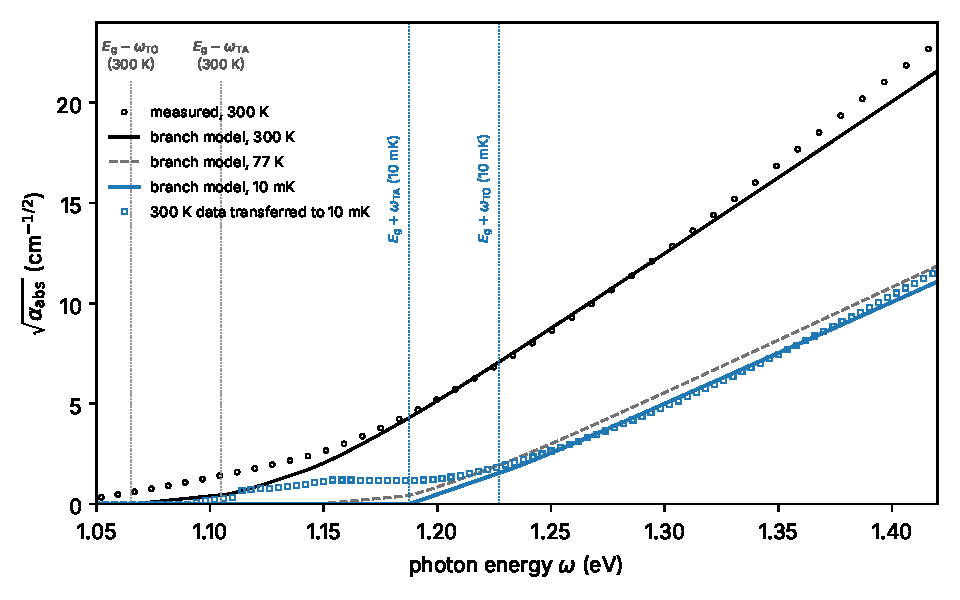
\includegraphics[width=0.92\linewidth]{figures/ch13/fig13_5.pdf}
  \caption{The absorption edge of silicon, as $\sqrt{\alpha_{\mathrm{abs}}}$ against the photon energy, at \SI{300}{K} and transferred to \SI{10}{mK}. Circles: measured at \SI{300}{K}~\cite{franta2017temperature}. Lines: a two-branch model of the edge. It has free pairs with the Hall--Bardeen--Blatt form of \cref{eq:6.5-edge}, $\omega_{\mathrm{TA}} = \SI{18.27}{meV}$ and $\omega_{\mathrm{TO}} = \SI{57.73}{meV}$, branch weights $5.5:4.0$~\cite{rajkanan1979absorption,stanford2021photoelectric}. The gap is the measured $\Eg(T)$ of \cref{sec:6.3}, 1.1692, 1.1652 and \SI{1.1230}{eV} at 0, 77 and \SI{300}{K}, with one scale fitted to the \SI{300}{K} data between 1.18 and \SI{1.30}{eV}. It is drawn at \SI{300}{K} (black), \SI{77}{K} (gray, dashed) and \SI{10}{mK} (blue). Squares: the \SI{300}{K} data transferred to \SI{10}{mK} with \cref{eq:13.5-inverse}, each energy split between the branches in the proportion of the model. Dotted: the thresholds $\Eg - \omega_\nu$ of phonon absorption at \SI{300}{K} and the emission thresholds $\Eg + \omega_\nu$ of cold silicon. Excitonic thresholds, \SI{14.7}{meV} below the free-pair ones, are not modeled.}
  \label{fig:13-transfer}
\end{figure}

\Cref{fig:13-transfer} shows the transfer for silicon. The warm edge starts \SI{57.7}{meV} below the \SI{300}{K} gap of \SI{1.123}{eV}, with the absorption replica of the transverse optical branch, and the cold one at $\Eg(0) + \omega_{\mathrm{TA}} = \SI{1.1875}{eV}$, \SI{0.12}{eV} higher; at \SI{1.236}{eV} the measured \SI{300}{K} absorption, \SI{58}{cm^{-1}}, is 16 times the cold one. Transferred, the data follow the cold model above \SI{1.25}{eV} to within \SI{10}{\percent}, the accuracy with which the model follows the warm data. Below the cold threshold they keep about \SI{1.4}{cm^{-1}}, where cold silicon absorbs nothing outside the excitonic thresholds. That residue is the part of the \SI{300}{K} data that is not of the form \cref{eq:13.5-forward} assumes, the excitonic companions and the thermal broadening of the warm edge, and the inversion carries it to the cold side unchanged in size. Near the cold threshold the transfer of room-temperature data is no better than this residue.

The assumption of a temperature-independent spectrum fails at a level that measurements show. Stanford and co-workers measured the absorption of silicon at 0.5, 5, 77 and \SI{295}{K} and fitted the two-branch form to it with an effective gap of \SI{1.134}{eV}. The fit needs a branch strength that falls with temperature as $\ee^{-c_1T}$ with $c_1 = \SI{1.7e-3}{K^{-1}}$~\cite[Eqs.~(6) and (7)]{stanford2021photoelectric}: a factor 0.61 at \SI{295}{K} and 0.88 at \SI{77}{K}, relative to the lowest temperature, within their own law for the gap, which differs slightly from the one used here. The occupations and a rigid gap do not carry all of the temperature dependence. The bands are renormalized by the lattice vibrations, not only shifted (\cref{sec:6.3}), and the vertices change with them (\cref{sec:13.7}). Transferred with \cref{eq:13.5-inverse}, \SI{295}{K} data therefore underestimate the cold spectrum by about \SI{40}{\percent} on this evidence, and \SI{77}{K} data by about \SI{12}{\percent}, with the opposite sign to the errors of the untransferred data.

\begin{keyresult}[Untransferred \SI{77}{K} data]
Used without transfer, the \SI{77}{K} absorption of silicon overestimates the millikelvin dark-photon rate by the factors
\begin{equation*}
  2.3\text{--}2.6,\quad 1.7\text{--}1.9,\quad 1.3\text{--}1.5,\quad 1.1\text{--}1.3 \qquad \text{at} \qquad x = 15,\ 25,\ 50,\ \SI{100}{meV} ,
\end{equation*}
where $x$ is the energy above the cold threshold $\Eg(0) + \omega_{\mathrm{TA}}$, and by more than a factor of two for $x$ below 18 to \SI{23}{meV}. The upper values hold for the transverse acoustic branch alone and for the two-branch edge to two digits; the lower ones include the measured fall of the branch strength between the lowest temperature and \SI{77}{K}. Untransferred \SI{300}{K} data overestimate the two-branch edge by 38, 16 and 7 at $x = 25$, 50 and \SI{100}{meV}.
\end{keyresult}
\noindent The two causes add. The \SI{77}{K} gap lies \SI{3.97}{meV} below the cold one, so that at the same photon energy the warm emission edge has run $x + \SI{3.97}{meV}$. And the transverse acoustic phonon is still occupied, $n_{\mathrm{TA}} = 0.068$, which adds stimulated emission and an absorption replica that starts $2\omega_{\mathrm{TA}}$ lower. The gap shift dominates close to the threshold, where $(1 + |\Delta E_{\mathrm{g}}|/x)^2$ is large, and the occupation farther away. The factors belong to the free-pair edge, whose power two is the steepest at the threshold. An excitonic edge rises more slowly and its gap-shift factor is smaller. The lower values of the box follow from the branch strength at \SI{77}{K}, lower than the cold one by the factor 0.88 above, which moves the factor of two from $x = 23$ to \SI{18}{meV}. These are the corrections that the silicon dark-photon rate of \cref{sec:10.7-edge} needs near its edge, and they apply to every absorption rate of \cref{chap:10} that uses measured $\sigma_1$ below the direct gap.

\begin{workedexample}{The transverse acoustic correction at 50 meV}\label{we:13-TA-transfer}
Take the transverse acoustic component of the silicon edge at $x = \SI{50}{meV}$ above the cold threshold, $\omega = \Eg(0) + \omega_{\mathrm{TA}} + x = \SI{1.2375}{eV}$, with $\Eg(0) = \SI{1.1692}{eV}$ and $\omega_{\mathrm{TA}} = \SI{18.27}{meV}$, and its \SI{77}{K} spectrum, with $\Eg(\SI{77}{K}) = \SI{1.1652}{eV}$ ($\Delta E_{\mathrm{g}} = \SI{-3.97}{meV}$) and $n_{\mathrm{TA}} = 0.0681$. In the edge form the cold component is $A\,x^2$.

\emph{Forward.} At \SI{77}{K} the emission component has run $\omega - \Eg(\SI{77}{K}) - \omega_{\mathrm{TA}} = \SI{53.97}{meV}$, and the absorption component $\omega - \Eg(\SI{77}{K}) + \omega_{\mathrm{TA}} = \SI{90.50}{meV}$. Relative to the cold value $A\,(\SI{50}{meV})^2$,
\begin{equation*}
  \underbrace{(n_{\mathrm{TA}} + 1)}_{1.0681}\underbrace{\Bigl(\frac{53.97}{50}\Bigr)^2}_{1.1651} + \underbrace{n_{\mathrm{TA}}}_{0.0681}\underbrace{\Bigl(\frac{90.50}{50}\Bigr)^2}_{3.276} = 1.2443 + 0.2230 = 1.467 .
\end{equation*}
The gap shift alone gives \SI{17}{\percent}, stimulated emission multiplies it by 1.068, and the absorption replica adds 0.22: the \SI{77}{K} spectrum is 1.47 times the cold one at this energy.

\emph{Inverse.} \Cref{eq:13.5-inverse} with $\ee^{-\omega_{\mathrm{TA}}/T} = 0.0637$ reads the \SI{77}{K} spectrum at $\omega + \Delta E_{\mathrm{g}} + 2k\omega_{\mathrm{TA}} = 1.2335$, 1.2700, 1.3066, 1.3431, \SI{1.3796}{eV}. In units of the cold value, the terms are
\begin{equation*}
  +1.19087,\quad -0.21547,\quad +0.02724,\quad -0.00289,\quad +0.00028 ,
\end{equation*}
and the partial sums 1.19087, 0.97540, 1.00264, 0.99975, 1.00002. The first term alone, the gap-shifted spectrum divided by $n_{\mathrm{TA}} + 1$, is \SI{19}{\percent} high, because it still contains the absorption replica; the second removes it, and each further term corrects the previous one by a factor $\ee^{-\omega_{\mathrm{TA}}/T}$ and a ratio of squares. Five terms recover the cold value to $2\times10^{-5}$.
\end{workedexample}

\subsection{Finite-momentum corrections}

A dark-matter particle that scatters never reaches the optical limit. To deposit $\omega$ it must transfer at least $q = \omega/v_{\mathrm{max}}$, \SI{0.45}{keV} at the silicon edge with $v_{\mathrm{max}} = 2.65\times10^{-3}$, and in the phonon-assisted window it transfers \SIrange{0.9}{1.3}{keV} (\cref{sec:13.1,sec:13.3}), $0.4$ to $0.6$ of $2\pi/a$. At such $\vect{q}$ the corrections of \cref{eq:13.5-limit} are not small, for three reasons outside the reach of optical data. The intermediate states of path A sit at $\vect{k}+\vect{q}$, and their energy moves by an amount of order $q^2/2m_e$, \SI{0.98}{eV} at \SI{1}{keV}, against a distance from the energy shell of $E_{\mathrm{dir}} - \omega \approx \SI{2.2}{eV}$ at the edge. The density vertices $\rho_{pv}(\vect{k},\vect{q})$ depart from their linear form \cref{eq:3.2-optical} on the scale of $2\pi/a = \SI{2.28}{keV}$, and beyond that a reciprocal-lattice vector inside the vertex reaches valleys that no photon reaches, as the class $(2\pi/a)(2,0,0)$ of \cref{sec:13.3} does, with its own selection rules. And the phonon itself is a different one: at $\vect{q} \to 0$ it carries $\vect{k}_{\mathrm{c}}$, where the transverse acoustic branch is at \SI{18.27}{meV}, while at $|\vect{q}| = \SI{1.0}{keV}$ along the valley axis it carries $\vect{k}_{\mathrm{c}} - \vect{q}$, at $0.41\,\mathrm{X}$, and the computed branch is at \SI{13.98}{meV} (\cref{we:13-onset-exp}). The optical edge measures the electron--phonon vertices only at $\vect{Q} \approx \vect{k}_{\mathrm{c}}$.

The optical limit therefore tests the parts of a calculation that do not depend on $\vect{q}$: the bands at the extrema, the gap, the electron--phonon vertices near $\vect{k}_{\mathrm{c}}$, the unrestricted sum over intermediate bands with its intraband terms, and the normalization of \cref{eq:13.3-LPA}. It does not test the finite-$\vect{q}$ density vertex, the Umklapp classes, the local fields or the vertices at $\vect{k}_{\mathrm{c}} - \vect{q}$, and these carry the dark-matter scattering rate. A computed $L^{\mathrm{PA}}(\vect{q},\omega)$ that reproduces the measured edge at the temperature of the measurement has passed a necessary check. The finite-$\vect{q}$ structure has to be controlled by sum rules and convergence tests.

\section{The off-shell window}\label{sec:13.6}

At $|\vect{q}| = \SI{1.0}{keV}$ along the valley axis the cheapest zero-phonon pair of silicon costs \SI{1.77}{eV}, and the phonon-assisted structure factor of \cref{sec:13.3} was written for energies below it. Two kinds of denominators in the amplitude \cref{eq:13.2-M} can become small. Those of path A with an empty band and of path C with a filled band are the distances of virtual zero-phonon pairs from the energy shell, and they vanish as $\omega$ reaches $E_{\mathrm{min}}(\vect{q})$. The intraband terms, path A with $p = c$ and path B with $p = v$, have denominators of order $|\vect{Q}|$ and vanish as the phonon becomes a soft acoustic one, while the interband vertices of that phonon grow as $|\vect{Q}|^{-1/2}$. The soft acoustic phonon produces no divergence: translation invariance fixes its amplitude, and inside the window it is never on the energy shell. The vanishing zero-phonon detunings, however, set the boundary of the region in which the phonon-assisted rate exists as a quantity of its own, with the margin $\delta_{\mathrm{w}}$ of \cref{sec:8.6,sec:13.3}, \SI{0.3}{eV} in silicon.

\subsection{The soft acoustic limit}

A long acoustic wave moves every atom of a region by nearly the same amount, and a uniform displacement of the whole crystal is no excitation. The electron--phonon vertex reflects this only in part. By \cref{eq:6.2-asr} its intraband elements vanish as $\vect{Q}\to0$, but its interband elements tend to $\ii\ell_{\vect{Q}\nu}(\varepsilon_m - \varepsilon_n)\hat{\vect{e}}_\nu\cdot\vect{p}_{mn}$, the rigid translation of the electronic states, and with $\ell_{\vect{Q}\nu} = (2M_{\mathrm{cell}}c_\nu|\vect{Q}|)^{-1/2}$ they grow without bound. In \cref{eq:13.2-M} these large interband terms meet intraband terms of the form $0/0$, a vertex of order $\ell|\vect{Q}|$ over a denominator of order $|\vect{Q}|$. Neither kind can be estimated alone. Translation invariance, which \cref{sec:8.3} wrote as a Ward identity for matrix elements, decides their sum.

The identity we need is \cref{eq:D.37-ward}. Change the vertex by $\delta g_{mn} = (\varepsilon_{m,\vect{\kappa}+\vect{Q}} - \varepsilon_{n\vect{\kappa}} \pm \omega_{\vect{Q}\nu})\mathfrak{t}_{mn}$, the matrix element of a commutator with the unperturbed Hamiltonian, for any one-electron operator $\op{\mathfrak{t}}_{\vect{Q}}$. On the energy shell every term of \cref{eq:13.2-M} then has numerator equal to $\pm$ its denominator, band by band, and the sum over all bands collapses to $\langle c,\vect{k}'|[\op{\mathfrak{t}}_{\vect{Q}},\ee^{\ii\vect{q}\cdot\vect{r}}]|v,\vect{k}\rangle$ (\cref{app:D.37}). The amplitude is unchanged if this contact term is added back. The useful choice of $\op{\mathfrak{t}}_{\vect{Q}}$ carries each electron along with the local displacement of the wave, \cref{eq:D.37-s}. The vertex that remains, the comoving vertex $g^{\mathrm{cm}}$ of \cref{eq:D.37-gcm}, vanishes at $\vect{Q} = 0$ for every pair of bands, by \cref{eq:6.2-asr}. Its first order in $\vect{Q}$ is the coupling to a uniform strain, the deformation-potential tensor $D^n$ of \cref{eq:6.2-D}, plus a coupling to the velocity of the moving lattice. And the contact term is $\ii\ell_{\vect{Q}\nu}(\hat{\vect{e}}_\nu\cdot\vect{q})\,\rho_{cv}(\vect{k},\vect{q}+\vect{Q})$, because the density at wavevector $\vect{q}$ carries momentum $\vect{q}$. With these, the amplitude has a finite limit.
\begin{keyresult}[Soft acoustic limit of the phonon-assisted amplitude]
For an acoustic branch $\nu$ with $\omega_{\vect{Q}\nu} = c_\nu|\vect{Q}|$ and polarization $\hat{\vect{e}}_\nu$, nondegenerate bands $c$ and $v$, and $\hat{\vect{Q}} = \vect{Q}/|\vect{Q}|$, the amplitude \cref{eq:13.2-M} tends on the energy shell to
\begin{equation}
  \begin{split}
  M^\pm_{cv\nu}(\vect{k},\vect{q},\vect{Q}) \to{}& \ii\,\ell_{\vect{Q}\nu}\,\rho_{cv}(\vect{k},\vect{q})
  \biggl[\underbrace{\hat{\vect{e}}_\nu\cdot\vect{q}}_{\text{recoil}}\\
  &+ \underbrace{\frac{\hat{\vect{Q}}\cdot D^c\cdot\hat{\vect{e}}_\nu \mp c_\nu\,\hat{\vect{e}}_\nu\cdot\vect{p}_{cc}}{\hat{\vect{Q}}\cdot\vect{v}^{\mathrm{g}}_c \pm c_\nu}
  - \frac{\hat{\vect{Q}}\cdot D^v\cdot\hat{\vect{e}}_\nu \mp c_\nu\,\hat{\vect{e}}_\nu\cdot\vect{p}_{vv}}{\hat{\vect{Q}}\cdot\vect{v}^{\mathrm{g}}_v \pm c_\nu}}_{\text{deformation and velocity}}\biggr] ,
  \end{split}
  \label{eq:13.6-soft}
\end{equation}
with $D^c$, $\vect{v}^{\mathrm{g}}_c$, $\vect{p}_{cc}$ taken at $\vect{k}+\vect{q}$ and $D^v$, $\vect{v}^{\mathrm{g}}_v$, $\vect{p}_{vv}$ at $\vect{k}$, and the upper sign for emission. The leading term is of order $|\vect{Q}|^{-1/2}$, and the relative correction is of order $|\vect{Q}|$, for $|\vect{Q}|$ small compared with the scale over which the group velocities change; at a band extremum of mass $m^*$ this is $|\vect{Q}| \ll 2m^*c_\nu$.
\end{keyresult}
\noindent The limit is derived in \cref{app:D.37}. The recoil term is the first order in the displacement of $\ee^{\ii\vect{q}\cdot(\vect{r} - \vect{u})}$: the dark matter kicks an electron that rides on the lattice, and the lattice under it recoils. The deformation terms are the soft phonon emitted by the final electron after the kick, or by the hole before it, through the strain it produces; their denominators are the detunings of the zero-phonon pair at $\vect{q}$, which shrink with $|\vect{Q}|$. The velocity terms are smaller than the deformation terms by $c_\nu|\vect{p}_{nn}|/|D^n|$, a few times $10^{-3}$ per band in \cref{we:13-soft} (and $10^{-5}$ there once the electron and hole terms cancel), but they turn the laboratory-frame intraband vertex into the comoving one. That vertex is $\ii\ell|\vect{Q}|\,\hat{\vect{Q}}\cdot(D^n + \vect{v}^{\mathrm{g}}_n\otimes\vect{p}_{nn})\cdot\hat{\vect{e}}_\nu$ (\cref{eq:D.37-Xi}). It reduces to \cref{eq:6.2-D} at a band extremum, and away from one it carries a Galilean term that a frozen-strain calculation does not produce (\cref{app:D.37}).

The soft acoustic limit of \cref{sec:8.3} is a different statement. There the probe itself is proportional to mass and its amplitude vanishes as $q^2$ at fixed energy. Here the probe is the electron density, its momentum $\vect{q}$ is finite, and the soft object is the phonon. Translation invariance does not make the amplitude vanish. It makes it finite, of order $\ell_{\vect{Q}\nu}$ rather than of order $\ell_{\vect{Q}\nu}/|\vect{Q}|$ as the separate intraband terms would suggest, and it fixes its value through $D^n$, the band velocities and $\vect{q}$. The squared amplitude then behaves as $1/|\vect{Q}|$, and with the phase space $Q^2\dd Q$ the emission of soft phonons is integrable, as $Q\,\dd Q$ at $T = 0$ and as $\dd Q$ at finite temperature.

In silicon the deformation terms dominate. With $D \approx \SI{9}{eV}$ along the valley axis (\cref{sec:6.2}) and $c_\nu = \SI{8.43}{km.s^{-1}}$, $D/c_\nu$ is 300 to \SI{350}{keV}, against momentum transfers of 1 to \SI{2}{keV} near the window, so at the band extrema the recoil term is a correction of a percent or less. It is not negligible everywhere. For a nearly free electron the strain shift at fixed reduced wavevector, $D^n$, and the Galilean term $\vect{v}^{\mathrm{g}}_n\otimes\vect{p}_{nn}$ nearly cancel, since a weak electron--ion potential gives a weak electron--phonon vertex. The recoil term is then of the same size as the rest of the bracket. \Cref{we:13-soft} shows such a case.

As a test of a computed amplitude, \cref{eq:13.2-M} is evaluated as a function, with the energy-shell condition imposed but no delta function, and it must approach \cref{eq:13.6-soft} with a deviation linear in $|\vect{Q}|$ for both signs, several directions and decreasing $|\vect{Q}|$. A failure of the test exposes a common shortcut. Codes set the vertices of the three acoustic modes at $\vect{Q} = 0$ to zero (\cref{sec:6.2}), and an interpolation that carries this into the neighborhood of $\vect{Q} = 0$ removes the rigid-translation part of the interband vertices. That part supplies the recoil term and the bare Galilean terms, $\ii\ell[\hat{\vect{e}}_\nu\cdot(\vect{q} - \vect{p}_{cc} + \vect{p}_{vv})]\rho_{cv}$ (\cref{app:D.37}), and in \cref{we:13-soft} its loss changes $|M|^2$ by a factor of ten. Outside the window the zero-phonon pair at $\vect{q}$ is real and \cref{eq:13.6-soft} is its amplitude to emit a soft phonon. The denominators vanish on the cone $\hat{\vect{Q}}\cdot\vect{v}^{\mathrm{g}}_c = \mp c_\nu$, where the electron outruns the sound wave. This is the Cherenkov emission of \cref{eq:6.3-cherenkov}, a real decay of the pair, and it is regularized by the width like the other resonances below.

Inside the off-shell window the soft limit is never reached. A final state at $\omega \le E_{\mathrm{min}}(\vect{q}) - \delta_{\mathrm{w}}$ whose electron sits at $\vect{k}+\vect{q}+\vect{Q}$ needs $\varepsilon_{c,\vect{k}+\vect{q}} - \varepsilon_{c,\vect{k}+\vect{q}+\vect{Q}} \ge \delta_{\mathrm{w}}$, since the pair at $\vect{q}$ costs at least $E_{\mathrm{min}}(\vect{q})$. The electron must therefore fall by $\delta_{\mathrm{w}}$ over the distance $|\vect{Q}|$ in crystal momentum, which bounds the phonon wavevector from below by $\delta_{\mathrm{w}}/(v^{\mathrm{g}}_{\max} + c_\nu)$ (\cref{eq:D.37-Qmin}). The steepest conduction band of silicon on the symmetry lines of \cref{fig:3-si-bands} has a slope of \SI{16.7}{eV.\angstrom}, or \SI{2.5e6}{m.s^{-1}}, and at $\delta_{\mathrm{w}} = \SI{0.3}{eV}$ the bound is \SI{0.018}{\angstrom^{-1}}. The soft limit needs $|\vect{Q}| \ll 2m^*c_\nu$, with $m^*c_\nu = 1.0\times10^{-3}$ and $6.7\times10^{-3}\,\si{\angstrom^{-1}}$ for transverse emission across the valley and longitudinal emission along it. Inside the window the intraband denominators are zero-phonon detunings of at least $\delta_{\mathrm{w}}$, the amplitude has no infrared feature at any temperature, and no subtraction is needed. At the onset itself the phonon is far harder, $|\vect{Q}^*| \ge \SI{0.31}{\angstrom^{-1}}$ (\cref{sec:13.3}). A computation inside the window can therefore give the acoustic modes at $\vect{Q} = 0$ zero weight, as long as it keeps the interband vertices near it.

\begin{workedexample}{The soft-phonon amplitude in a one-dimensional crystal}\label{we:13-soft}
A test of \cref{eq:13.6-soft} needs a vertex computed in the laboratory frame, without the comoving construction, since a model whose orbitals ride on the atoms has the identity built in. Take a chain of rigid ions, lattice constant $a = \SI{3.0}{\angstrom}$, mass \SI{28.09}{\atomicmassunit}, each ion a Gaussian well $-V_0\ee^{-x^2/2\sigma^2}$ with $V_0 = \SI{2.5}{eV}$ and $\sigma = \SI{0.5}{\angstrom}$, and one spinless electron per cell, solved in 41 plane waves. The lowest band is filled and the next empty, with a gap of \SI{1.215}{eV} at the zone boundary. One longitudinal acoustic branch has $c_\nu = \SI{5.0}{km.s^{-1}}$. The vertex is the matrix element of the potential change of ions displaced by $\ell_{\vect{Q}\nu}\ee^{\ii QX_j}$, the density vertex is $\ee^{\ii qx}$, and \cref{eq:13.2-M} is summed over 40 bands. All parameters are illustrative.

Put the hole at $k = 0.80\,\pi/a$ and the transfer at $q = 0.30\times2\pi/a = \SI{0.628}{\angstrom^{-1}}$, away from the band extrema. The pair at $q$ costs \SI{5.68}{eV} and $|\rho_{cv}| = 0.965$. The valence state has $v^{\mathrm{g}}_v = \SI{5.91}{eV.\angstrom}$, 180 times the sound speed, and $p_{vv} = \SI{0.776}{\angstrom^{-1}}$; the conduction state $v^{\mathrm{g}}_c = \SI{11.05}{eV.\angstrom}$ and $p_{cc} = \SI{1.450}{\angstrom^{-1}}$. Straining the crystal at fixed reduced wavevector gives $D^v = \SI{-4.563}{eV}$ and $D^c = \SI{-15.237}{eV}$, nearly the $-2\times$ kinetic energy of free electrons. The laboratory intraband slopes, read off the computed vertex at $|Q| = 10^{-5}\times2\pi/a$, are \SI{0.021}{eV} and \SI{0.774}{eV}, equal to $D^n + v^{\mathrm{g}}_np_{nn}$ to \SI{e-4}{eV}: the strain and Galilean terms cancel to a few percent.

The comoving vertex is of order $\ell|Q|$ for every band pair, about $220\,\ell|Q|$\,eV at most, while the laboratory interband vertex grows from 0.44 to \SI{4.4}{eV} as $|Q|$ falls from $10^{-2}$ to $10^{-4}\times2\pi/a$. For emission with $Q > 0$ the bracket of \cref{eq:13.6-soft} is
\begin{center}
\small
\begin{tabular}{lr}
  \toprule
  term & value ($\si{\angstrom^{-1}}$) \\
  \midrule
  recoil, $q$ & $+0.6283$ \\
  deformation & $-0.6076$ \\
  velocity & $-1.1\times10^{-5}$ \\
  total & $+0.0207$ \\
  \bottomrule
\end{tabular}
\end{center}
and the full amplitude deviates from the limit by 0.20, 0.020 and 0.0020 at $|Q| = 10^{-2}$, $10^{-3}$ and $10^{-4}\times2\pi/a$: linearly, as the relative correction of order $|\vect{Q}|$ requires. The same holds for absorption and for $Q < 0$. Recoil and deformation nearly cancel here, and with the interband vertices set to zero the recoil is lost and $|M|^2$ comes out 10.4 times too large.

At the band extrema the balance changes. With the hole at $k = \pi/a$ and $q = 2\pi/a$, an Umklapp transfer that puts the electron at the bottom of the conduction band, both velocities vanish, $D^v = \SI{-7.42}{eV}$ and $D^c = \SI{-7.26}{eV}$, and the bracket is $q \pm (D^c - D^v)/c_\nu = 2.09 \pm \SI{4.91}{\angstrom^{-1}}$, so that the soft amplitude differs by a factor of 2.5 between the two directions of $\vect{Q}$. The limit is reached only for $|Q| \ll 2m^*c_\nu$, here $1.2\times10^{-3}\,\si{\angstrom^{-1}}$ with $m^* = 0.135\,m_e$, and since each deformation term is about \SI{220}{\angstrom^{-1}} and they cancel to \SI{4.9}{\angstrom^{-1}}, the deviation falls below \SI{1}{\percent} only at $|Q| = 10^{-8}\times2\pi/a$. Setting the interband vertices to zero now removes the recoil term: for emission with $Q > 0$ it halves $|M|^2$, and for the opposite direction it multiplies $|M|^2$ by 2.9. In silicon, where $(D^c - D^v)/c_\nu$ is a hundred times $q$, this effect is at the percent level.
\end{workedexample}

\subsection{The off-shell window}

By \cref{eq:13.2-doff}, the denominators of path A with an empty band and of path C with a filled band are at least $E_{\mathrm{min}}(\vect{q}) - \omega$ in size on the energy shell, and the other two kinds at least $\Eg - \omega_{\vect{Q}\nu}$, which never vanishes. A denominator of \cref{eq:13.2-M} therefore vanishes exactly where a first-order transition at the same $(\vect{q},\omega)$, the creation of a zero-phonon pair by the density alone, is on shell. Below the zero-phonon edge no such transition exists. Above it, at fixed $(\vect{q},\omega)$, the resonance condition is met on a surface of crystal momenta, and the sum over final states crosses that surface. There the squared amplitude has a double pole $1/x^2$ in the detuning $x$, which is not integrable across a simple zero. It has no principal value either; as \cref{sec:2.4} showed, it needs the width of the intermediate state, after which the rate splits into a cascade and a finite part. The second-order rate is then no longer a quantity of its own. Its value depends on the width, and its share of the response depends on a convention.

The edge must be the renormalized one. The bands in the denominators are shifted and broadened by the electron--phonon self-energy (\cref{eq:6.3-ren}), and the pair edge moves with them, by the zero-point renormalization of the gap at low temperature and by more as the temperature rises (\cref{sec:13.7}). A bound pair lies below the free pairs by its binding energy (\cref{sec:13.8}). We write $E^{\mathrm{ren}}_{\mathrm{min}}(\vect{q},T)$ for the lowest energy of a zero-phonon final state at crystal momentum $\vect{q}$, with renormalized bands and the bound pair included, and use the same renormalized energies in the denominators. A bare edge with renormalized denominators, or the reverse, misplaces the boundary by the renormalization itself. In the silicon numbers of this chapter the conduction bands are shifted so that the indirect gap equals the measured one at low temperature, which places the renormalized edge correctly at the band extrema and treats the renormalization as rigid in $\vect{k}$.
\begin{keyresult}[Window theorem]
The phonon-assisted structure factor \cref{eq:13.3-SPA}, built from the amplitude \cref{eq:13.2-M}, is defined at $(\vect{q},\omega)$ without widths, without $\ii0^+$, without subtraction and without counterterms if and only if every first-order transition at the same $(\vect{q},\omega)$ is off shell, $\omega < E^{\mathrm{ren}}_{\mathrm{min}}(\vect{q},T)$, with renormalized energies used in the edge and in the denominators alike. It is quoted as a channel of its own in the pointwise window
\begin{equation}
  \omega \le E^{\mathrm{ren}}_{\mathrm{min}}(\vect{q},T) - \delta_{\mathrm{w}} , \qquad
  \delta_{\mathrm{w}} \gg \omega_{\max},\ \hat\varGamma,\ T ,
  \label{eq:13.6-window}
\end{equation}
applied at each $\vect{q}$ separately, with $\omega_{\max}$ the top of the phonon band and $\hat\varGamma$ the largest width of the zero-phonon pairs between the edge and $\delta_{\mathrm{w}}$ above it. In silicon $\delta_{\mathrm{w}} = \SI{0.3}{eV}$.
\end{keyresult}
\noindent The first half is the statement about the denominators above. The second half is about accuracy, and it needs the resummed amplitude of \cref{sec:8.6}. There the virtual pair $m$ enters through its propagator $\GF_m(\omega) = 1/[\omega - E_m - \Sigma_m(\omega)]$, \cref{eq:8.6-amp}, and the second-order amplitude keeps only $1/(\omega - E_m)$. The difference is of relative order $\Sigma_m(\omega)/(\omega - E_m)$, and the margin must make it small. With renormalized energies the real part of $\Sigma_m$ at the pair's own energy is absorbed into $E_m$, and three pieces remain. The self-energy changes between $E_m$ and $\omega$, on the scale of the phonon energies, because the thresholds for emitting each phonon sit $\omega_{\vect{Q}\nu}$ above the edges of the continuum (\cref{sec:6.3}); this requires $\delta_{\mathrm{w}} \gg \omega_{\max}$. The imaginary part, the width, requires $\delta_{\mathrm{w}} \gg \hat\varGamma$. And thermal phonons broaden the edge by about $T$. The same ratio $\omega_{\vect{Q}\nu}/\delta_{\mathrm{off}}$ sets the error of the adiabatic form (\cref{eq:13.2-err}), and the bound pair adds the condition $\delta_{\mathrm{w}} \gg E_x^{\mathrm{b}}$ unless it is already part of the edge.

The parameter $\theta_{\mathrm{ep}}$ of \cref{eq:8.5-theta} looks like the controlling one, and taken at face value it would forbid a margin of \SI{0.3}{eV}. Evaluated at $\delta_{\mathrm{off}} = \SI{0.3}{eV}$ with the largest vertex of silicon, the optical vertex of the holes, about \SI{0.25}{eV}, it is $(0.25/0.3)^2 \approx 0.7$; the $\theta_{\mathrm{ep}} = 1$ at \SI{0.25}{eV} of \cref{sec:8.5} is a bound of this kind, not a size. But $\theta_{\mathrm{ep}}$ counts one more pair of vertices on intermediate states that all lie $\delta_{\mathrm{off}}$ from the shell. At the window edge the extra vertices act on the virtual pair, whose self-energy sums $|g|^2$ over one-phonon states spread across an energy range $E_{\mathrm{w}}$ of an electronvolt or more, the width of the continuum in the sense of \cref{sec:2.4}. Its size is then $|\Sigma_m| \approx \langle|g|^2\rangle/E_{\mathrm{w}}$ rather than $\langle|g|^2\rangle/\delta_{\mathrm{w}}$, and the relative correction $|\Sigma_m|/\delta_{\mathrm{w}}$ is $\theta_{\mathrm{ep}}\,\delta_{\mathrm{w}}/E_{\mathrm{w}} \approx 0.7\times0.3/1 \approx 0.2$ at \SI{0.3}{eV}. Measured on the gap itself this is the zero-point renormalization over the margin, the correction that the resummation adds.

The silicon numbers fix the margin (\cref{fig:13-offshell}(b)). The top of the phonon band, the zone-center optical phonon of \SI{64.1}{meV}, is 0.21 of \SI{0.3}{eV}, and the transverse acoustic phonon of the onset, \SI{14.8}{meV}, is 0.05. The zero-point renormalization of the gap is \SI{56}{meV} as computed at fixed volume and 71 to \SI{73}{meV} for the electron--phonon part implied by experiment (\cref{sec:6.3}), 0.19 to 0.24 of the margin. It is absorbed into the renormalized edge, and only its variation across the margin remains. The exciton binding energy, \SI{14.7}{meV}, is 0.05. At a detector's temperature $T$ is zero for this purpose; at \SI{300}{K} it would be 0.09.

For the widths we estimate the decay of the pair at the zero-phonon edge by phonon emission, with deformation-potential rates and the constants computed by Li, Graziosi and Neophytou~\cite[Table~III and Eq.~(10)]{li2021deformation}. The electron scatters between valleys by the g-type longitudinal optical and the f-type longitudinal acoustic and transverse optical phonons, the hole emits optical phonons, and both emit acoustic phonons as in \cref{eq:6.3-cherenkov}. The pair at $E_{\mathrm{min}}(\vect{q})$ shares its kinetic energy in proportion to the masses along the valley axis, 0.77 to the electron. Between $|\vect{q}| = 0.4$ and \SI{1.4}{keV} this gives widths of 3 to \SI{21}{meV} at the edge, \SI{11}{meV} at \SI{1.0}{keV}, and \SI{15}{meV} at \SI{1.0}{keV} and \SI{0.3}{eV} above the edge, so that $\hat\varGamma/\delta_{\mathrm{w}}$ stays below 0.1. Every ratio is then below about 0.2. A margin of \SI{0.1}{eV} would put the phonon ratio at 0.64 and the renormalization ratio at 0.56 to 0.73, and one of \SI{0.5}{eV} would bring them to 0.13 and 0.11 to 0.15 but shrink the window: along the valley axis it would end at $|\vect{q}| = \SI{1.07}{keV}$ instead of \SI{1.27}{keV}. The margin is therefore $\delta_{\mathrm{w}} = \SI{0.3}{eV}$, and with it the bound $|\vect{Q}^*| \ge \SI{0.31}{\angstrom^{-1}}$ of \cref{sec:13.3} holds. Inside the window the second-order rate then carries a relative correction of order 0.2 at the edge, falling as $1/(E_{\mathrm{min}} - \omega)$ toward the onset.

\begin{figure}[tbp]
  \centering
  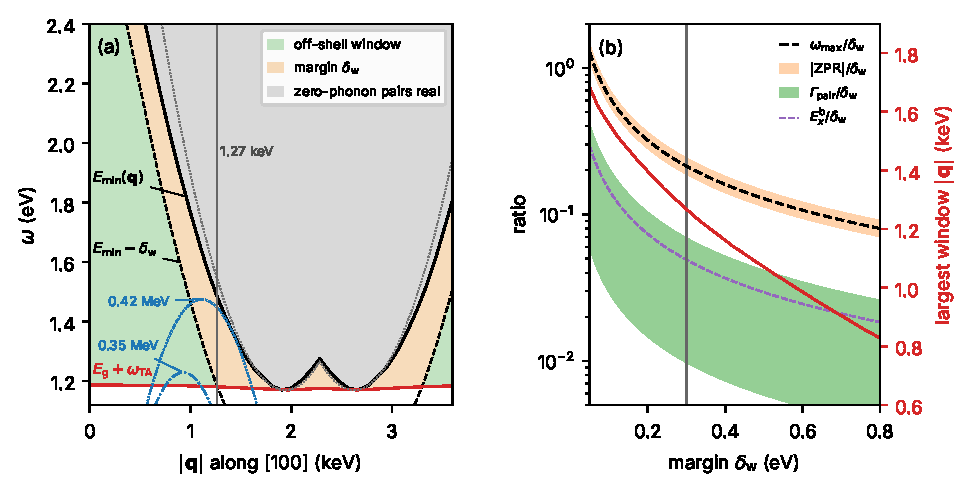
\includegraphics[width=\linewidth]{figures/ch13/fig13_6.pdf}
  \caption{The off-shell window of silicon. (a)~The plane of momentum transfer $|\vect{q}|$ along [100], the valley axis, and energy deposited $\omega$. Black: the zero-phonon edge $E_{\mathrm{min}}(\vect{q})$ from the PBE bands of \cref{fig:3-si-bands} on a $48^3$ grid, with the conduction bands shifted to the measured gap of \SI{1.17}{eV} (dotted: the parabolic valley, pair mass $1.19\,m_e$); dashed: $E_{\mathrm{min}} - \delta_{\mathrm{w}}$ with $\delta_{\mathrm{w}} = \SI{0.3}{eV}$; red: the phonon-assisted onset $\Eg + \omega_{\mathrm{TA}}(\vect{Q}^*)$ of \cref{eq:13.1-EPA}, with the PBE force constants of \cref{sec:5.2} and $\vect{Q}^*$ measured to the nearest valley, the Umklapp image of the opposite valley at \SI{2.63}{keV} included. Green: the off-shell window, where the phonon-assisted rate is a channel of its own; orange: the margin, where it is finite but its corrections grow; gray: zero-phonon pairs are real and the Dyson convention of \cref{sec:8.6} applies. Blue: the largest energy deposited by dark matter of 0.35 and \SI{0.42}{MeV}. (b)~The ratios that control the window, against the margin $\delta_{\mathrm{w}}$: top of the phonon band (\SI{64.1}{meV}), zero-point renormalization of the gap (56 to \SI{73}{meV}), width of the pair at the zero-phonon edge for $0.4 \le |\vect{q}| \le \SI{1.4}{keV}$ (3 to \SI{21}{meV}, a deformation-potential estimate with computed constants~\cite{li2021deformation}), and exciton binding energy (\SI{14.7}{meV}). Red, right axis: the largest $|\vect{q}|$ below the valley at which the window is not empty. The vertical line marks $\delta_{\mathrm{w}} = \SI{0.3}{eV}$.}
  \label{fig:13-offshell}
\end{figure}

\Cref{fig:13-offshell}(a) shows the window in the plane of $|\vect{q}|$ and $\omega$. It is a region of that plane, not an interval of $\omega$: at each $\vect{q}$ it runs from the onset $E^{\mathrm{PA}}_{\mathrm{min}}(\vect{q})$ of \cref{eq:13.1-EPA} up to $E^{\mathrm{ren}}_{\mathrm{min}}(\vect{q},T) - \delta_{\mathrm{w}}$, and it is empty where the two meet. At $|\vect{q}| = \SI{1.0}{keV}$ it spans 1.184 to \SI{1.467}{eV}. Along the valley axis it closes at $|\vect{q}| = \SI{1.27}{keV}$ with the computed bands, \SI{1.33}{keV} with the parabolic valley of \cref{sec:13.3}, and it reopens on the far side of the Umklapp image of the opposite valley, beyond \SI{3.30}{keV}. Dark matter just above the onset mass reaches only the bottom of the window. At \SI{0.42}{MeV}, where the zero-phonon line opens along this axis (\cref{sec:13.1}), the largest deposits already lie in the margin.

Between $E^{\mathrm{ren}}_{\mathrm{min}} - \delta_{\mathrm{w}}$ and $E^{\mathrm{ren}}_{\mathrm{min}}$ the amplitude is still finite, but its corrections grow as $1/(E^{\mathrm{ren}}_{\mathrm{min}} - \omega)$ and reach order one at the edge. Above the edge, within a few widths of it, no test function is smooth on the scale of the detuning, and the Dyson split of \cref{sec:8.6} has no meaning. The margin and this shell form the edge band. There we quote only totals, computed from the unexpanded amplitude \cref{eq:8.6-amp}, and no phonon-assisted rate of its own; in particular the onset exponents of \cref{eq:13.3-pon} hold only where the onset lies inside the window (\cref{sec:13.3}).

In a calculation the window is applied point by point. For each bin of $(|\vect{q}|,\hat{\vect{q}})$ the edge is the minimum of the renormalized pair energies on the full grid of $\vect{k}$, not along a symmetry line, and the bins in $\omega$ stop at that edge minus $\delta_{\mathrm{w}}$. The resonant denominators, path A with $p$ empty and path C with $p$ filled, are written as zero-phonon detunings, $\omega - E_{pv}(\vect{k},\vect{q})$ and $E_{cp}(\vect{k}+\vect{Q},\vect{q}) - \omega$, so that their smallness inside the window is visible and the energies in them are the ones that define the edge. Any smearing of the energy delta function must be small compared with $\delta_{\mathrm{w}}$, or it leaks the zero-phonon continuum into the window.

\subsection{Resonant denominators beyond the window}

Above $E^{\mathrm{ren}}_{\mathrm{min}}(\vect{q},T)$ a resonant intermediate state is a real pair. In path A it is the pair $m = (p,\vect{k}+\vect{q};\,v,\vect{k})$ with an electron in an empty band, which then emits or absorbs the phonon. In path C it is $m = (c,\vect{k}';\,p,\vect{k}+\vect{Q})$ with a hole in a filled band, which relaxes into $(v,\vect{k})$ by the phonon. Near such a state we split the amplitude into the resonant term and the rest. The resonant denominator receives the width of the pair, \cref{eq:2.4-width}:
\begin{equation}
  M^\pm_{cv\nu} = \frac{g_{fm}\,\rho_m}{\omega - \tilde E_m + \ii\varGamma_m/2} + g_{fm}\,\mathcal{A}^{\mathrm{off}}_f ,
  \label{eq:13.6-res}
\end{equation}
with $\rho_m = \rho_{pv}(\vect{k},\vect{q})$ and $g_{fm} = g_{cp\nu}(\vect{k}+\vect{q},\vect{Q})$ for path A, $\rho_m = \rho_{cp}(\vect{k}+\vect{Q},\vect{q})$ and $g_{fm} = g_{pv\nu}(\vect{k},\vect{Q})$ for path C, $\tilde E_m$ and $\varGamma_m$ the renormalized energy and the width of the pair, and $g_{fm}\mathcal{A}^{\mathrm{off}}_f$ the sum of all other terms of \cref{eq:13.2-M}; the minus sign of path C in \cref{eq:13.2-paths} is absorbed into $\rho_mg_{fm}$. A path C term has to be taken from the four-path form \cref{eq:13.2-paths}, with its many-body denominator, before the band-sum theorem is used: the width belongs to the propagator of the real pair $m$, and the theorem holds only on the energy shell (\cref{sec:13.2}). This is the amplitude \cref{eq:8.6-amp} of the level-and-band model with $\Upsilon_m$ dropped, a correction of order $g^2$.

Squared, \cref{eq:13.6-res} contains the Lorentzian $|g_{fm}\rho_m|^2/[(\omega - \tilde E_m)^2 + \varGamma_m^2/4]$, which \cref{eq:2.4-split} splits into $(2\pi/\varGamma_m)\delta(\omega - \tilde E_m)$, the finite part $\operatorname{fp}(\omega - \tilde E_m)^{-2}$ and a correction of relative order $\varGamma_m^2/\delta_{\mathrm{F}}^2$. Summed over the final states of the phonon, the delta term is $|\rho_m|^2\delta(\omega - \tilde E_m)$ times $\sum_f2\pi|g_{fm}|^2\delta(E_f - \tilde E_m)/\varGamma_m$, the fraction of the decays of $m$ that go into phonon emission. It is the zero-phonon pair, created as a real state, followed by its first decay: the cascade of \cref{sec:2.4}. The Dyson convention \cref{eq:8.6-dyson} assigns it to the zero-phonon sector with its residue, and assigns the finite part, the principal-value cross term with $\mathcal{A}^{\mathrm{off}}_f$ and $|\mathcal{A}^{\mathrm{off}}_f|^2$ to the phonon-dressed one. Outside the window, then, the phonon-assisted structure factor is $S^+$ of \cref{eq:8.6-dyson} with the substitutions above, summed over the resonances of both paths, and the zero-phonon one is $S^0$ with renormalized pairs. The two add up to the response to order $g^4$ and $\varGamma_m^2/\delta_{\mathrm{F}}^2$, against any test function smooth on the scale of the detuning $\delta_{\mathrm{F}}$ (\cref{sec:8.6}).

A computed phonon-assisted table beyond the window differs from one inside it in three ways: it need not be positive, it must not be mixed with another convention, and it is defined only near narrow lines. The finite part is negative against a narrow test function, so $S^+$ is not a positive spectrum near $\tilde E_m$, and a computed phonon-assisted table may contain negative bins near the edge; only $S^0 + S^+$ is positive. A Lorentzian zero-phonon line added to the resummed square of \cref{eq:13.6-res} counts the cascade twice, an error of order one. Added to the finite part it counts the off-shell weight twice, an error of order $g^2$ (\cref{sec:8.6}). The rate of \cref{sec:13.3} continued past the edge with a small numerical broadening in place of the width produces a delta term weighted by the inverse broadening, a cascade with an arbitrary weight.

The split is well defined only while $\varGamma_m \ll \delta_{\mathrm{F}}$, with $\delta_{\mathrm{F}}$ the distance of $\tilde E_m$ to the nearest structure of the one-phonon continuum: the zero-phonon edge itself, a threshold for emitting a further phonon, or the onset of a new valley or band. In silicon, with the widths of 3 to \SI{21}{meV} estimated above and detunings of a few tenths of an eV away from such structures, $\varGamma_m/\delta_{\mathrm{F}}$ is 0.01 to 0.1, and by \cref{eq:8.6-ambiguity} the zero-phonon weight is fixed to that order. Within a few widths of each structure it is not, and only totals are quoted, as at the edge of the window.

\subsection{The Fano term near a resonance}

When a real pair $m$ decays, the phonon it emits first interferes with the same phonon emitted directly by the off-shell paths, and \cref{eq:8.6-fano} shifts the branching of the first emission by the Fano coefficients $c^{\mathrm{F}}_\nu = \varGamma^{\mathrm{tot}}_m\Imag(\rho_m^*\mathcal{A}^{\mathrm{off}}_\nu)/|\rho_m|^2$. Their size near a resonance follows from \cref{eq:13.6-res}. With $\phi_\nu$ the phase of $\rho_m^*\mathcal{A}^{\mathrm{off}}_\nu$,
\begin{equation}
  |c^{\mathrm{F}}_\nu| = \frac{\varGamma^{\mathrm{tot}}_m}{\delta_{\mathrm{F}}}\;\frac{|\mathcal{A}^{\mathrm{off}}_\nu|\,\delta_{\mathrm{F}}}{|\rho_m|}\;|\sin\phi_\nu| .
  \label{eq:13.6-fano}
\end{equation}
The middle factor compares the off-shell amplitude with the resonant one at the distance $\delta_{\mathrm{F}}$ from the line. Both are second-order amplitudes with denominators of that size, and the factor is of order one. The Fano coefficients are therefore of first order in $\varGamma_m/\delta_{\mathrm{F}}$, the same order as the ambiguity of the Dyson split and as the branching of the cascade itself, and they need the phase $\phi_\nu$ in addition.

Symmetry controls that phase. In a crystal invariant under inversion combined with time reversal, with an even number of electrons, $(\mathsf{P}\mathsf{T})^2 = +1$ on the many-electron states, every amplitude can be made real, $\sin\phi_\nu = 0$, and the Fano term vanishes (\cref{sec:8.6}). Silicon and germanium satisfy the hypothesis at the level of one-body self-energies, with spin--orbit coupling as well: the single-electron Kramers pairs cannot all be chosen real, but the many-electron states with an even number of electrons can. If the attraction of electron and hole splits a degenerate zero-phonon manifold in a basis that is not invariant, only the sum of the coefficients over the branches vanishes. GaAs has no center of inversion, and its antisymmetric crystal potential gives $\phi_\nu$ a nonzero value. We estimate $|c^{\mathrm{F}}_\nu| \lesssim 0.3\,\varGamma_m/\delta_{\mathrm{F}}$ to first order, with the middle factor of \cref{eq:13.6-fano} set to one and $|\sin\phi_\nu| \le 0.3$ assumed for the antisymmetric part of the GaAs potential, and with Fr\"ohlich widths of a few meV just above the conduction minimum and 20 to \SI{60}{meV} higher up, $\varGamma_m/\delta_{\mathrm{F}}$ is 0.01 to 0.2 away from thresholds (\cref{app:E.14}). The Fano coefficients then move a few percent at most of the first emissions from one branch to another. Since their deviations from the mean average to zero over the branches, they change no total and no number of zero-phonon events, only which phonon the cascade starts with, and the distribution of the number of pairs by at most $\max_\nu|c^{\mathrm{F}}_\nu|$. Near each threshold $\delta_{\mathrm{F}}$ falls toward $\varGamma_m$, \cref{eq:13.6-fano} reaches order one and the expansion ends; these shells are excluded and quoted as totals. Inside the window no zero-phonon pair is real, and the Fano term does not exist.

\section{Temperature and zero-point renormalization}\label{sec:13.7}

Between room temperature and \SI{10}{mK} the indirect gap of silicon opens by \SI{46}{meV} (\cref{we:6-zpr}), and the phonon-assisted onset of \cref{we:13-onset} moves from 0.324 to \SI{0.337}{MeV}. At \SI{10}{mK} the zero-point motion still holds the gap below its clamped-nucleus value, by \SI{56}{meV} as computed at fixed volume and by 71 to \SI{73}{meV} for the electron--phonon part implied by experiment (\cref{sec:6.3}), and that renormalization is already part of the measured \SI{1.17}{eV} that every threshold of this chapter uses. It enters a detector calculation in three places. The zero-phonon response that is added to $S^{\mathrm{PA}}$ must carry it without counting anything twice, a point \cref{sec:13.3} left open. The special displacements of \cref{app:E.8}, the cheapest route to renormalized spectra, compute it together with a phonon sideband that cannot be added to the phonon-assisted rate. And the part that adiabatic methods miss must be small enough not to move the window.

\subsection{The renormalized zero-phonon response}

At order $g^2$ a zero-phonon pair is dressed in three ways: its energy is shifted, its weight is reduced, and its transition density acquires the virtual-phonon correction. All three are in the Dyson convention of \cref{sec:8.6}, which assigns to the zero-phonon sector the delta function $z_{\mathrm{qp}}(m)|\tilde\rho_m|^2\delta(\omega - \tilde E_m)$ of each pair $m$ (\cref{eq:8.6-dyson}). For a pair $(c,\vect{k}+\vect{q};\,v,\vect{k})$ the energy is the difference of the renormalized band energies \cref{eq:6.3-ren}, and the residue of the pair is, to order $g^2$, the product of the residues of electron and hole, since the slope of the pair self-energy is the sum of the slopes of $\Sigma^{\mathrm{FM}}$ for the two states (\cref{eq:4.7-qp}). The zero-phonon structure factor at temperature $T$ is then
\begin{equation}
  S^0(\vect{q},\omega;T) = 4\pi\sum_{v,c}\int_{\mathrm{BZ}}\frac{\dd^3k}{(2\pi)^3}\,
  z_{\mathrm{qp}}(c,\vect{k}+\vect{q})\,z_{\mathrm{qp}}(v,\vect{k})\,\bigl|\tilde\rho_{cv}(\vect{k},\vect{q})\bigr|^2\,
  \delta\bigl(\omega - \varepsilon^{\mathrm{ren}}_{c,\vect{k}+\vect{q}}(T) + \varepsilon^{\mathrm{ren}}_{v\vect{k}}(T)\bigr) ,
  \label{eq:13.7-S0}
\end{equation}
with $z_{\mathrm{qp}}(n,\vect{k}) = 1 + \partial_\omega\Real\Sigma^{\mathrm{FM}}_{n\vect{k}}(\omega)$ at $\omega = \varepsilon^{\mathrm{ren}}_{n\vect{k}}$, and $|\tilde\rho_{cv}|^2 = |\rho_{cv}|^2 + 2\Real(\rho_{cv}^*\,\delta\rho_{cv})$, where $\delta\rho_{cv}$ collects the mixing of bands by the off-diagonal self-energy and the virtual-phonon vertex $\Upsilon_m$ of \cref{eq:8.6-amp}. With $z_{\mathrm{qp}} = 1$, $\delta\rho = 0$ and bare energies it is \cref{eq:10.1-S0}. Temperature enters only through the phonon occupations inside the self-energies, $n_{\vect{Q}\nu} + 1 - f$ and $n_{\vect{Q}\nu} + f$ in $\Sigma^{\mathrm{FM}}$ and $2n_{\vect{Q}\nu} + 1$ in $\Sigma^{\mathrm{AH}}$ (\cref{eq:6.3-FM,eq:6.3-AH}); the band occupations are zero or one to $\ee^{-\Eg/2T}$. At \SI{1}{K} the occupation of every phonon above \SI{10}{meV} is below $10^{-50}$, and \cref{eq:13.7-S0} is the zero-point response.

The shift of the pair energies is the largest of the three corrections, and most of it is a rigid shift of the gap: in silicon the valence maximum rises by \SI{35}{meV} and the conduction minimum drops by \SI{22}{meV} (\cref{we:E-zpr}). A calculation that scissors its bands to the measured low-temperature gap has this rigid part already, and adding a computed renormalization to it counts the renormalization twice (\cref{app:E.8}). What the scissor does not supply is the variation of the shift across the zone, which \cref{sec:13.9} needs for the zero-phonon edge and which we bound below, with the nonadiabatic correction. The residues and the vertex correction change the weight of each line by an amount of relative order $\theta_{\mathrm{ep}}$ (\cref{eq:8.5-theta}), since each is one more pair of vertices on an intermediate state off the shell; in silicon near the gap $\theta_{\mathrm{ep}} = 0.010$ to 0.016 (\cref{sec:8.5}), so the weights move by one or two percent.

The weight that the zero-phonon lines lose reappears in the sideband. With all-electron (local) potentials, the electron--phonon Hamiltonian at first and second order in the displacements is a sum of one-body potentials that commute with the density. The double commutator in \cref{eq:4.3-firstmoment} is therefore that of the kinetic energy alone, $\mathscr{M}^1_{ee}(\vect{q}) = \nd_eq^2/m_e$, at every order in $g$. To order $g^2$ the electronic response with a pair in the final state is $S^0(\vect{q},\omega;T) + S^{\mathrm{PA}}(\vect{q},\omega;T)$. The density also responds without creating a pair, through the electrons dragged by the ions into a one-phonon state, and that sector has a first moment of order $g^2$ too, smaller than $\nd_eq^2/2m_e$ by about $Z_vm_e/M_{\mathrm{cell}} = 8\times10^{-5}$ in silicon. Up to that term the first moment of $S^0 + S^{\mathrm{PA}}$ equals that of the clamped-nucleus response, and
\begin{equation}
  \int_0^\infty\dd\omega\;\omega\,\bigl[S^0(\vect{q},\omega;T) - S^0(\vect{q},\omega)\bigr]
  = -\int_0^\infty\dd\omega\;\omega\,S^{\mathrm{PA}}(\vect{q},\omega;T) + O(g^4) ,
  \label{eq:13.7-fsum}
\end{equation}
where $S^0(\vect{q},\omega)$ without the temperature argument is \cref{eq:10.1-S0}, and the factor $2\pi$ and the sum over $\pm\vect{q}$ of \cref{eq:4.3-firstmoment} cancel on the two sides. The zero-phonon line gives up, in energy-weighted weight, exactly what the phonon sideband gains. The Allen--Heine term contributes nothing to this transfer: it is a static local potential, $\frac12\sum_{ab}\langle u_au_b\rangle\,\partial_a\partial_bV$, and a static local potential leaves the double commutator unchanged. The transfer is carried by the Fan--Migdal term and the vertex correction, the processes in which a phonon is emitted and reabsorbed, since $S^{\mathrm{PA}}$ is those processes with the phonon left behind. \Cref{eq:13.7-fsum} is the precise form of the overshoot of \cref{sec:13.3}, and \cref{eq:13.7-S0} removes it. Above the zero-phonon edge the bookkeeping is a percent effect on the zero-phonon rate.

\subsection{Special displacements as a quadrature}

The special displacements of \cref{app:E.8} compute renormalized spectra without vertices, from one supercell with displaced nuclei. Applied to the density response, the Williams--Lax average~\cites{lax1952franck}[Eqs.~(1) and~(3)]{zacharias2016one} is the clamped-nucleus structure factor $S^{\mathrm{cl}}(\vect{q},\omega;\{x\})$ of the supercell, averaged over the Gaussian distribution of its normal coordinates,
\begin{equation}
  S^{\mathrm{WL}}(\vect{q},\omega;T) = \prod_j\int\dd x_j\,\frac{\ee^{-x_j^2/2\sigma_j^2}}{\sqrt{2\pi}\,\sigma_j}\;S^{\mathrm{cl}}(\vect{q},\omega;\{x\}) ,
  \qquad \sigma_j^2 = \frac{2n_j + 1}{2\omega_j} ,
  \label{eq:13.7-WL}
\end{equation}
which is \cref{eq:E.8-wl} with $S$ in place of $\varepsilon_2$. Here $j = 1, 2, \ldots$ numbers the modes of the supercell, each a pair $(\vect{Q}\nu)$ of a commensurate wavevector and a branch, in order of increasing frequency, and $x_j$ are the mass-weighted coordinates $x_{\vect{Q}\nu}$ with widths $\sigma_{\vect{Q}\nu}$. The average is adiabatic by construction: each configuration is frozen while the probe acts, and the nuclei enter only through the distribution of their positions.

One configuration, with every coordinate at $x_j = \varsigma_j\sigma_j$ and signs $\varsigma_j = (-1)^{j-1}$ that alternate along the frequency-ordered list, reproduces \cref{eq:13.7-WL} as the supercell grows. Expand any smooth property $O(\{x\})$ of the frozen supercell, a band energy or $S^{\mathrm{cl}}$ at fixed $(\vect{q},\omega)$, about the equilibrium positions. The Gaussian average keeps only even powers of each coordinate,
\begin{equation*}
  \langle O\rangle_T = O(0) + \frac12\sum_j\sigma_j^2\,\frac{\partial^2O}{\partial x_j^2} + O(\sigma^4) ,
\end{equation*}
while the single configuration gives
\begin{equation*}
  O(\{\varsigma\sigma\}) = O(0) + \sum_j\varsigma_j\sigma_j\frac{\partial O}{\partial x_j} + \frac12\sum_j\sigma_j^2\frac{\partial^2O}{\partial x_j^2}
  + \frac12\sum_{j\ne k}\varsigma_j\varsigma_k\,\sigma_j\sigma_k\frac{\partial^2O}{\partial x_j\partial x_k} + O(\sigma^3) .
\end{equation*}
The diagonal second-order terms agree, because $\varsigma_j^2 = 1$. The linear terms and the cross terms must vanish. Take two neighbors in the list, $j$ and $j+1$. As the supercell grows, the commensurate grid becomes dense, the frequency spacing $\omega_{j+1} - \omega_j$ goes to zero wherever the phonon density of states is nonzero, and neighbors in the list become effectively degenerate, with the same $\sigma$. Their couplings to the electrons are not equal mode by mode, since neighbors in the list can come from distant wavevectors, but averaged over many neighbors they vary smoothly with frequency. The linear terms, which enter with alternating signs, then cancel on average, and the cross terms with any third mode $k$ cancel the same way, since $\partial_j\partial_kO$ and $\partial_{j+1}\partial_kO$ come with opposite signs~\cite[Eqs.~(6)--(9)]{zacharias2016one}. Gaps in the density of states only split the list into ranges in which the argument applies separately. What remains is the diagonal sum, which is $\langle O\rangle_T$ to order $\sigma^2$. The odd orders are removed exactly, at any supercell size, by averaging the configuration with its mirror image $x_j \to -x_j$~\cite[Eq.~(12)]{zacharias2016one}. For the higher even orders the reason is statistical: the sum $\sum_j x_j^2/\sigma_j^2$ over the Gaussian distribution has mean $N_{\mathrm{m}}$ and width $(2N_{\mathrm{m}})^{1/2}$ for $N_{\mathrm{m}}$ modes. For large supercells, as a result, almost all of the weight of \cref{eq:13.7-WL} lies on configurations with $|x_j| \approx \sigma_j$, and the special displacement is one of them~\cite[Sect.~III\,A]{zacharias2016one}. The single configuration is therefore not a random sample of the distribution but a deterministic quadrature of it, whose error falls as the grid of phonon wavevectors becomes dense.

\begin{limitbox}[Zero-point renormalization by special displacements][lim:13.7a]
$\langle\varepsilon_{n\vect{k}}\rangle_T = \varepsilon_{n\vect{k}}(\{\vect{u}^{\mathrm{ZG}}\})$ for a large supercell, with $\vect{u}^{\mathrm{ZG}}$ of \cref{eq:E.8-zg}, and to second order the adiabatic Allen--Heine--Cardona shift \cref{eq:6.3-adiabatic}~\cites{allen1981temperature}[Eqs.~(5), (10) and~(20)]{zacharias2016one}.
\par\smallskip
{\centering
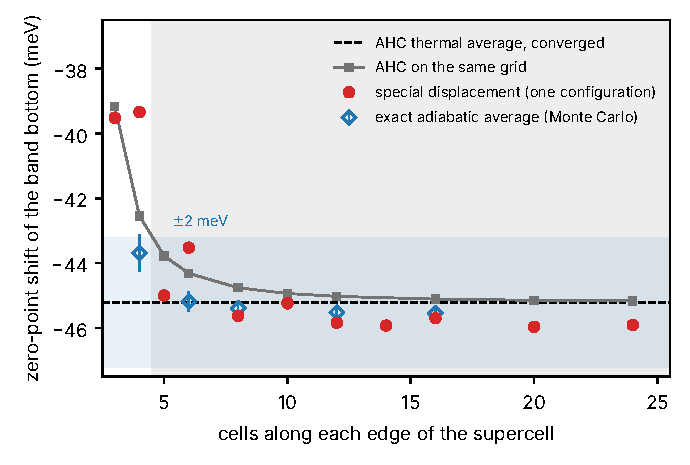
\includegraphics[width=0.92\linewidth]{figures/ch13/limit13_7a.pdf}
\captionof{figure}{Zero-point shift of the band bottom in a model crystal against the size of the supercell. The model: a simple cubic lattice, $a = \SI{2.70}{\angstrom}$, one atom of \SI{28.09}{u} per cell, central springs of 4.0 and \SI{1.5}{eV.\angstrom^{-2}} to nearest and next-nearest neighbors (phonons up to \SI{65}{meV}), and one $s$ band with nearest-neighbor hopping $t(d) = -\SI{1}{eV}\times(a/d)^6$ (band-bottom mass $0.52\,m_e$), at $T = 0$. Red: the special displacement, one configuration with every mode at its root-mean-square amplitude and signs alternating in order of frequency, wavevectors equal to their own time-reversal partners left out. Gray squares: the adiabatic Allen--Heine--Cardona average on the grid of phonon wavevectors of the same supercell; dashed: its limit for a dense grid, \SI{-45.2}{meV}, with a band of $\pm\SI{2}{meV}$. Blue diamonds: the exact adiabatic average of the same supercell, to all orders in the displacements, by Monte Carlo with antithetic pairs (statistical errors shown). Gray: supercells in which the special displacement is within \SI{2}{meV} of the limit, from $5\times5\times5$ cells (125 atoms).}\label{fig:13-zg}
\par}
\smallskip
In smaller supercells the coarse grid of phonon wavevectors and the uncancelled cross terms between modes dominate, and at any size the special displacement misses the nonadiabatic part of the renormalization and places the phonon-assisted sideband at the wrong energy.
\end{limitbox}

The model of \cref{fig:13-zg} isolates the quadrature. Its band-bottom shift is $-\SI{45.2}{meV}$ in the second-order average, $-\SI{34.5}{meV}$ from the Allen--Heine term and $-\SI{10.7}{meV}$ from the Fan term, comparable to the conduction-minimum shift of silicon. The second-order average on the grid of the supercell converges from above, and is within \SI{2}{meV} of its limit from $5\times5\times5$ cells on. The special displacement scatters around it by up to \SI{3}{meV} in the smallest supercells, where the pairing of neighbors in the frequency list is poor, and settles from $5\times5\times5$ cells on. The exact average lies \SI{0.4}{meV} below the second-order one in the larger supercells: the terms of fourth order in the displacements are one percent of the shift, and the special displacement follows the exact average rather than its second-order part, as the argument above requires. For silicon the same convergence has been computed directly: a $4\times4\times4$ supercell is within ten percent of the converged gap renormalization, and an $8\times8\times8$ supercell of 1024 atoms gives \SI{-57}{meV} (\cref{we:E-zpr}). In practice the calculation needs the phonons of the primitive cell on the commensurate grid, one density-functional calculation of the displaced supercell, and an unfolding of its bands onto the primitive zone. The convergence is checked by bracketing, with and without the self-partner wavevectors, and \cref{app:E.8} gives the procedure and its costs.

What the average contains follows from the same expansion applied to $S^{\mathrm{cl}}$. For a zero-phonon pair $f$ of the clamped crystal the energy $E_f(\{x\})$ appears inside a delta function, and the second-order term shifts it by $\frac12\sum_j\sigma_j^2\,\partial_j^2E_f$, the frozen-phonon form of \cref{eq:6.3-adiabatic}: the zero-phonon line comes out at the adiabatic Allen--Heine--Cardona energies, with a Gaussian width from the first-order terms~\cite[Eqs.~(19)--(21)]{zacharias2016one}. A pair whose crystal momentum differs from $\vect{q}$ by a phonon wavevector has no transition density in the clamped crystal, and acquires one, linear in $x_j$, in the displaced supercell. Its squared density averages to $\sigma_j^2|\partial_j\rho_f|^2$, and $\partial_j\rho_f$ is the adiabatic amplitude $M^{\mathrm{ad}}$ of \cref{eq:13.2-Mad} by \cref{eq:13.2-HT}. To second order in the displacements,
\begin{equation}
  \begin{aligned}
  S^{\mathrm{WL}}(\vect{q},\omega;T) = S^0_{\mathrm{ad}}(\vect{q},\omega;T)
  &+ \underbrace{\frac{4\pi}{\Omega}\Bigl\langle\!\Bigl\langle\sum_{\nu cv}(2n_{\vect{Q}\nu} + 1)\,\bigl|M^{\mathrm{ad}}_{cv\nu}(\vect{k},\vect{q},\vect{Q})\bigr|^2\,\delta\bigl(\varepsilon_{c,\vect{k}+\vect{q}+\vect{Q}} - \varepsilon_{v\vect{k}} - \omega\bigr)\Bigr\rangle\!\Bigr\rangle}_{S^{\mathrm{PA}}_{\mathrm{ad}}(\vect{q},\omega;T)} \\
  &+ O(\sigma^4) ,
  \end{aligned}
  \label{eq:13.7-WLexp}
\end{equation}
with $S^0_{\mathrm{ad}}$ the zero-phonon response at the adiabatic renormalized energies and the double average over $\vect{k}$ and $\vect{Q}$ as in \cref{eq:13.3-SPA}. The second term, $S^{\mathrm{PA}}_{\mathrm{ad}}$, is the adiabatic limit of $S^{\mathrm{PA}}$, the Hall--Bardeen--Blatt sideband~\cite{hall1954infrared} with the phonon energy dropped from the delta function~\cite[Eq.~(24)]{zacharias2016one}. The Williams--Lax average, and with it a special-displacement calculation, therefore contains both electronic sectors at once. Adding $S^{\mathrm{PA}}$ to it counts the sideband twice. A calculation that wants the cheap renormalized zero-phonon line and the exact sideband must subtract the adiabatic sideband computed with the same vertices, $S^{\mathrm{WL}} + S^{\mathrm{PA}} - S^{\mathrm{PA}}_{\mathrm{ad}}$, or use \cref{eq:13.7-S0} with \cref{eq:13.3-SPA} from the start.

The sideband of \cref{eq:13.7-WLexp} has the right total weight and the wrong position. Compared with \cref{eq:13.3-SPA} in the adiabatic amplitude,
\begin{equation}
  \begin{aligned}
  S^{\mathrm{PA}} - S^{\mathrm{PA}}_{\mathrm{ad}} = \frac{4\pi}{\Omega}\Bigl\langle\!\Bigl\langle\sum_{\nu cv}|M^{\mathrm{ad}}|^2\bigl[&(n + 1)\,\delta(E - \omega + \omega_{\vect{Q}\nu}) + n\,\delta(E - \omega - \omega_{\vect{Q}\nu}) \\
  &- (2n + 1)\,\delta(E - \omega)\bigr]\Bigr\rangle\!\Bigr\rangle + O\!\Bigl(\frac{\omega_{\vect{Q}\nu}}{\delta_{\mathrm{off}}}\Bigr)S^{\mathrm{PA}} ,
  \end{aligned}
  \label{eq:13.7-WLdiff}
\end{equation}
with $E = \varepsilon_{c,\vect{k}+\vect{q}+\vect{Q}} - \varepsilon_{v\vect{k}}$, $n = n_{\vect{Q}\nu}$, and the last term the amplitude error of \cref{eq:13.2-err}. The bracket integrates to zero over $\omega$, so the weights agree; its first moment is $+\sum|M^{\mathrm{ad}}|^2\omega_{\vect{Q}\nu}$, independent of temperature. At $T \gg \omega_{\vect{Q}\nu}$, or at energies far above the threshold, the three delta functions merge and the adiabatic sideband is exact. At \SI{10}{mK} it is not. There $n = 0$, the whole sideband sits at $E$ instead of $E + \omega_{\vect{Q}\nu}$, and the phonon-assisted onset falls by one phonon energy: from \SI{0.3374}{MeV} to the floor $2\Eg/v_{\mathrm{max}}^2 = \SI{0.3332}{MeV}$ (\cref{we:13-onset}). Above the onset the adiabatic spectrum is that of the exact one shifted down by $\omega_\nu$. With the onset exponent $p_{\mathrm{on}} = 3$ of \cref{eq:13.3-pon} the ratio at an energy $x$ above the true onset is $(1 + \omega_\nu/x)^3$, which falls below 1.1 only for $x > 31\,\omega_\nu$, about \SI{0.46}{eV} for the transverse acoustic phonon of the onset. At $|\vect{q}| = \SI{1}{keV}$ the whole off-shell window is \SI{0.28}{eV} wide along the valley axis and narrower off it (\cref{sec:13.6}), so nowhere inside it does the adiabatic sideband describe the rate to ten percent. Special displacements give the renormalized zero-phonon line and the spectrum far from the edges; the phonon-assisted rate in the window needs the explicit phonon energies of \cref{eq:13.3-SPA}.

\subsection{The nonadiabatic correction to the renormalization}

The adiabatic form \cref{eq:6.3-adiabatic} drops the phonon energy from the Fan--Migdal denominators. Restoring it at $T = 0$, with $\omega = \varepsilon_{n\vect{k}}$ in \cref{eq:6.3-FM}, an empty intermediate state enters only through phonon emission and an occupied one only through the absorption term with $f = 1$. The difference between the two forms is
\begin{equation}
  \mathrm{ZPR}^{\mathrm{na}}_{n\vect{k}} - \mathrm{ZPR}^{\mathrm{ad}}_{n\vect{k}} = \frac1N\sum_{\vect{Q}\nu m}|g_{mn\nu}(\vect{k},\vect{Q})|^2
  \left[\frac{1}{\varepsilon_{n\vect{k}} - \varepsilon_{m,\vect{k}+\vect{Q}} - s_m\omega_{\vect{Q}\nu}} - \frac{1}{\varepsilon_{n\vect{k}} - \varepsilon_{m,\vect{k}+\vect{Q}}}\right] ,
  \label{eq:13.7-na}
\end{equation}
with $s_m = +1$ for $m$ empty and $s_m = -1$ for $m$ occupied; the Allen--Heine term has no denominator and drops out. For an intermediate band far from $\varepsilon_{n\vect{k}}$ the bracket is smaller than the adiabatic term by $\omega_{\vect{Q}\nu}/|\varepsilon_{n\vect{k}} - \varepsilon_{m,\vect{k}+\vect{Q}}|$, a few percent for silicon. The terms that matter are those in which the intermediate state is degenerate with $(n,\vect{k})$ at $\vect{Q} = 0$: the band itself and, at the valence maximum of silicon, its partners. Take the valence maximum as a parabolic band of mass $m^*$, so that $\varepsilon_{n\vect{k}} - \varepsilon_{n,\vect{k}+\vect{Q}} = Q^2/2m^*$, coupled by an optical phonon of energy $\omega_{\mathrm{O}}$ with a vertex $g_{\mathrm{O}}$ that tends to a constant as $Q \to 0$. With $N^{-1}\sum_{\vect{Q}} = \Omega\int\dd^3Q/(2\pi)^3$ the bracket integrates in closed form,
\begin{equation}
  \begin{aligned}
  \frac{\Omega|g_{\mathrm{O}}|^2}{2\pi^2}\int_0^\infty\dd Q\,Q^2\left[\frac{1}{Q^2/2m^* + \omega_{\mathrm{O}}} - \frac{2m^*}{Q^2}\right]
  &= -\frac{\Omega|g_{\mathrm{O}}|^2}{2\pi^2}\,2m^*\int_0^\infty\frac{2m^*\omega_{\mathrm{O}}\,\dd Q}{Q^2 + 2m^*\omega_{\mathrm{O}}} \\
  &= -\frac{\Omega|g_{\mathrm{O}}|^2(2m^*)^{3/2}\sqrt{\omega_{\mathrm{O}}}}{4\pi} .
  \end{aligned}
  \label{eq:13.7-sqrt}
\end{equation}
The correction lowers the valence maximum, and with it reduces the closing of the gap. It is not of order $\omega_{\mathrm{O}}$ but of order $\sqrt{\omega_{\mathrm{O}}}$: the adiabatic integrand $2m^*/Q^2$ is integrable in three dimensions, but its weight sits at $Q \lesssim (2m^*\omega_{\mathrm{O}})^{1/2}$, exactly where the phonon energy is not small against the band dispersion. For silicon we take the optical vertex of the holes, $|g_{\mathrm{O}}| \approx \SI{0.25}{eV}$ (\cref{sec:13.6}), $\omega_{\mathrm{O}} = \SI{64.1}{meV}$, and $\Omega = a^3/4$. Three bands meet at the valence maximum without spin--orbit coupling, with the spherical masses $m_e/(\gamma^{\mathrm{Lu}}_1 \mp 2\bar\gamma^{\mathrm{Lu}}) = 0.44$ and $0.16\,m_e$ of the heavy and light holes (\cref{sec:3.3}) and $m_e/\gamma^{\mathrm{Lu}}_1 = 0.23\,m_e$ for the third. \Cref{eq:13.7-sqrt} gives 2.0, 0.4 and \SI{0.8}{meV}, together \SI{3.2}{meV}.

The full calculation finds more. Poncé and co-workers evaluated both forms of the Allen--Heine--Cardona theory for silicon in the local-density approximation on the same grids, and their indirect-gap renormalization is $-\SI{64.3}{meV}$ in the adiabatic form and $-\SI{56.2}{meV}$ in the nonadiabatic one~\cite[Table~VI]{ponce2015temperature}, the \SI{8}{meV} of \cref{sec:6.3}. Their valence maximum rises by \SI{40.9}{meV} in the adiabatic form and \SI{34.8}{meV} in the nonadiabatic one~\cite[Sect.~VI\,A\,2]{ponce2015temperature}, so \SI{6.1}{meV} of the difference sits at the valence maximum, about twice the estimate, which rests on a single vertex for all three bands. The remaining \SI{1.9}{meV} belong to the conduction minimum, which drops by \SI{23.3}{meV} in the adiabatic form and \SI{21.4}{meV} in the nonadiabatic one. Symmetry forbids an intravalley optical vertex there (\cref{sec:6.2}), and the degenerate intermediate states are the minima of the other five valleys, reached by intervalley phonons, for which the same mechanism applies. The nonadiabatic correction to the gap renormalization of silicon, defined by \cref{eq:13.7-na} as the difference between the two forms of one calculation with the same vertices and grids, is therefore \SI{8}{meV}, of which \cref{eq:13.7-sqrt} accounts for the order of magnitude and the sign, and it is precisely what special displacements miss, since they are adiabatic (\cref{lim:13.7a}). Differences between methods, such as the \SI{9}{meV} between the nonadiabatic value \SI{-56}{meV} and an adiabatic supercell value \SI{-65}{meV} compiled by Miglio and co-workers~\cite[Table~S2]{miglio2020predominance}, mix the form of the theory with the method and its inputs, and do not measure this correction.

For the window the correction does not matter, because the window is computed from the measured gap, and a measured gap contains the whole renormalization, adiabatic or not. It would enter in two ways. A calculation that builds the gap from a clamped-nucleus value, from $GW$ or a hybrid functional, plus a computed renormalization inherits the choice of form. Then \SI{8}{meV} on the gap moves the phonon-assisted onset by $\SI{0.283}{MeV.eV^{-1}}\times\SI{8}{meV} = \SI{0.0023}{MeV}$ and the zero-phonon edge by \SI{0.0015}{MeV}, with the coefficients of \cref{eq:13.7-dm} below. A calculation that scissors its bands to the measured gap misses only the variation of the renormalization between the band edges and the pair states that the zero-phonon edge reaches, about \SI{0.2}{eV} above the gap (\cref{sec:13.9}). Between the conduction minimum and the conduction state at $\mathrm{\Gamma}$, \SI{3.4}{eV} above the valence maximum, the nonadiabatic renormalization varies by \SI{14}{meV}, from $-21.4$ to $-\SI{7.4}{meV}$~\cite[Table~VI and Sect.~VI\,A\,2]{ponce2015temperature}. A variation of at most \SI{10}{meV} over the reached states is therefore a generous bound, and it moves the zero-phonon edge by at most \SI{0.002}{MeV}. Both numbers are below the spread of the computed edges themselves, 0.405 to \SI{0.408}{MeV} (\cref{sec:13.9}).

\subsection{Temperature dependence of the window}

At detector temperatures the window does not move. The measured gap $\Eg(T) = \Eg(0) - aT^2/(T + b)$ of \cref{we:6-zpr}, with $a = \SI{4.9e-4}{eV.K^{-1}}$ and $b = \SI{655}{K}$, closes by \SI{0.07}{meV} at \SI{10}{K} and by less than \SI{1}{\micro eV} at \SI{1}{K}, and the physical shift is smaller still, since the renormalization changes with the occupations $n_{\vect{Q}\nu}$, which vanish exponentially. For the transverse acoustic phonon of the onset, $n_{\mathrm{B}}(\SI{14.8}{meV})$ is $3\times10^{-8}$ at \SI{10}{K} and $2\times10^{-4}$ at \SI{20}{K}, so the emission factor $n + 1$ is one and the absorption sideband of \cref{sec:13.1} is absent below about \SI{20}{K}. The margin $\delta_{\mathrm{w}}$ of the window is measured from the renormalized edge at each temperature, and at these temperatures nothing in it depends on $T$. A detector between \SI{10}{mK} and a few kelvin sees the zero-temperature window.

At higher temperatures the gap closes, and the edges follow it. A uniform shift $\Delta\Eg(T) = \Eg(T) - \Eg(0)$ of all pair energies moves each threshold mass by the derivative of \cref{eq:13.1-mZP} or \cref{eq:13.1-mPAdef} with respect to the threshold energy, taken at the optimal momentum transfer, where the shift of the optimum itself does not contribute to first order. For a threshold $E$ reached at $q$ this derivative is $q^2/[2(qv_{\mathrm{max}} - E)^2]$, and
\begin{equation}
  \frac{\partial m_{\mathrm{min}}^{\mathrm{PA}}}{\partial\Eg} = \frac{2}{(v_{\mathrm{max}} + u_\nu)^2} = \SI{0.283}{MeV.eV^{-1}} , \qquad
  \frac{\partial m_{\mathrm{min}}^{\mathrm{ZP}}}{\partial\Eg} = \frac{2\,(m_{\mathrm{min}}^{\mathrm{ZP}})^2}{q_{\mathrm{ZP}}^2} = \SI{0.187}{MeV.eV^{-1}} .
  \label{eq:13.7-dm}
\end{equation}
For the onset we have used $q^* = 2E/(v_{\mathrm{max}} - u_\nu)$ from \cref{sec:13.1}, with the phonon energy falling as $q$ grows, $E' = -u_\nu$; the group velocity enters to first order here, although it entered the onset itself only squared, and lowers the coefficient by \SI{0.5}{\percent} from $2/v_{\mathrm{max}}^2 = \SI{0.285}{MeV.eV^{-1}}$. For the zero-phonon edge $q_{\mathrm{ZP}} = \SI{1.33}{keV}$ is the momentum transfer of the joint minimum, re-minimized on bands with spin--orbit coupling at the measured lattice constant (\cref{sec:13.9}). The zero-phonon edge moves less than the onset, because it is reached at a larger momentum transfer, where the particle has more energy to spare, and the window widens slightly as it moves down. Two effects come on top of the rigid shift. Absorption sidebands open below the onset, with the weights $n_{\mathrm{B}}(\omega_{\vect{Q}\nu})$, and the phonon energies themselves shift, but a change of one percent in $\omega_{\mathrm{TA}}(\vect{Q}^*)$ would move the onset by only $4\times10^{-5}$~MeV. At \SI{300}{K} the gap falls by $\SI{0.26}{meV.K^{-1}}$, and the onset by $7\times10^{-5}$~MeV per kelvin. \Cref{fig:13-window-T} shows the gap and the edges from \SI{10}{mK} to \SI{300}{K}.

\begin{figure}[tbp]
  \centering
  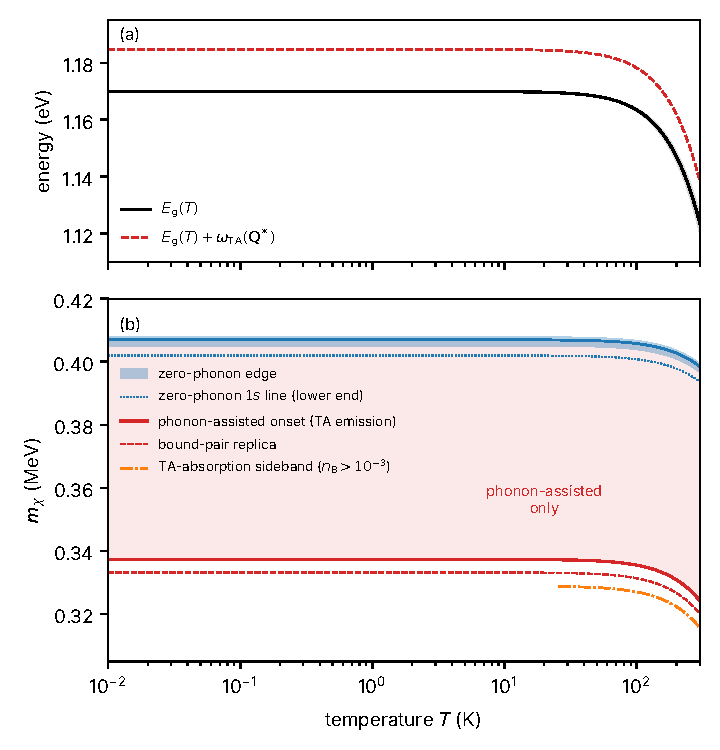
\includegraphics[width=0.8\linewidth]{figures/ch13/fig13_7.pdf}
  \caption{The silicon window against temperature, on a logarithmic temperature axis from \SI{10}{mK} to \SI{300}{K}. (a)~The indirect gap $\Eg(T) = \SI{1.17}{eV} + \Delta\Eg(T)$, with $\Delta\Eg(T)$ from the fit $\Eg(0) - aT^2/(T + b)$, $a = \SI{4.9e-4}{eV.K^{-1}}$, $b = \SI{655}{K}$, to photoluminescence data~\cites{alex1996temperature}[Eq.~(11)]{ramanathan2020ionization} (gray: $a$ and $b$ varied by their quoted errors, \SI{0.2e-4}{eV.K^{-1}} and \SI{40}{K}); dashed: the threshold of the phonon-assisted onset, $\Eg(T) + \omega_{\mathrm{TA}}(\vect{Q}^*)$. (b)~Window edges in dark-matter mass. Red: the phonon-assisted onset, transverse acoustic emission, from \cref{eq:13.1-mPAdef} with the PBE phonons of \cref{sec:5.2} and $\vect{q}$ along the valley axis; red dashed: its bound-pair replica, with $\Eg - E_x^b$, $E_x^b = \SI{14.7}{meV}$. Orange dash-dotted: the sideband with a transverse acoustic phonon absorbed, drawn where its occupation exceeds $10^{-3}$. Blue band: the zero-phonon edge, 0.405 to \SI{0.408}{MeV} at low temperature (\cref{sec:13.9}), moved with the gap at the momentum transfer of the joint minimum, \SI{1.33}{keV} (bands with spin--orbit coupling, \cref{sec:13.9}); blue dotted: the lower end of its $1s$ line. Shaded red: masses at which phonon-assisted recoil is the only electron-recoil channel. Every shift is a rigid shift of the pair energies with the measured gap.}
  \label{fig:13-window-T}
\end{figure}

\begin{workedexample}{The window shift between \SI{10}{mK} and \SI{300}{K}}\label{we:13-windowT}
\emph{Gap.} At \SI{10}{mK}, $\Delta\Eg = 0$ to $10^{-10}$~eV. At \SI{300}{K}, $\Delta\Eg = -\SI{4.9e-4}{eV.K^{-1}}\times(\SI{300}{K})^2/\SI{955}{K} = -\SI{46.2}{meV}$; with $a$ and $b$ varied by their errors, $-42.5$ to $-\SI{50.2}{meV}$.

\emph{Onset.} With $E = \Eg + \omega_{\mathrm{TA}}$ lowered by \SI{46.2}{meV}, the optimum $q^*$ falls from 0.90 to \SI{0.86}{keV}, the phonon wavevector grows from 0.46 to $0.47\,(2\pi/a)$, and the TA energy there rises from 14.78 to \SI{15.01}{meV}. Then
\begin{equation*}
  m_{\mathrm{min}}^{\mathrm{PA}}(\SI{300}{K}) = \frac{2\times(\SI{1.17}{eV} - \SI{0.0462}{eV} + \SI{0.01501}{eV})}{7.023\times10^{-6}} = \SI{0.3243}{MeV} ,
\end{equation*}
\SI{0.0131}{MeV} below the \SI{0.3374}{MeV} at \SI{10}{mK}; \cref{eq:13.7-dm} gives $\SI{0.283}{MeV.eV^{-1}}\times\SI{46.2}{meV} = \SI{0.0131}{MeV}$ directly. The bound-pair replica moves from 0.3332 to \SI{0.3201}{MeV}.

\emph{Zero-phonon edge.} At $q_{\mathrm{ZP}} = \SI{1.33}{keV}$ the edge moves by $\SI{0.187}{MeV.eV^{-1}}\times\SI{46.2}{meV} = \SI{0.0086}{MeV}$; evaluated exactly at that momentum transfer, 0.405 to \SI{0.408}{MeV} becomes 0.3966 to \SI{0.3995}{MeV}, the best value moves from 0.407 to \SI{0.3985}{MeV}, and the $1s$ line from 0.402--0.405 to 0.394--\SI{0.397}{MeV}.

\emph{Width and sidebands.} The window, from the onset to the best zero-phonon edge, spans \SI{0.0696}{MeV} at \SI{10}{mK} and \SI{0.0742}{MeV} at \SI{300}{K}. At \SI{300}{K} the absorption sidebands are open: with a TA phonon of \SI{15.2}{meV} absorbed, occupation 1.25, from \SI{0.3157}{MeV}; with an optical phonon of \SI{61.0}{meV}, occupation 0.10, from \SI{0.3027}{MeV}. At \SI{77}{K} the shifts are $-0.0011$ (onset) and $-\SI{0.0007}{MeV}$ (zero-phonon edge), and the TA absorption sideband, occupation 0.12, starts at \SI{0.3278}{MeV}.

\emph{Consequence.} A room-temperature calculation of the window, or room-temperature absorption data used for it, places both edges about \SI{0.01}{MeV} too low and adds a thermal tail that reaches \SI{0.035}{MeV} below the cold onset with one phonon absorbed, and further with several. The shift is thirty times the \SI{4e-4}{MeV} by which the softness of the computed TA branch moves the onset (\cref{we:13-onset}), and it has to be removed before a warm number describes a detector at \SI{10}{mK}.
\end{workedexample}

\section{Exciton replicas and bosonic absorption}\label{sec:13.8}

Cold silicon begins to absorb light \SI{14.7}{meV} below the free-pair threshold $\Eg(0) + \omega_{\mathrm{TA}} = \SI{1.1875}{eV}$ of \cref{sec:13.5}. The electron and the hole that a photon creates together with a transverse acoustic phonon can stay bound, by $E_x^b = \SI{14.7}{meV}$ (\cref{sec:4.9,sec:6.5}). With the measured gap $\Eg(0) = \SI{1.1692}{eV}$ of \cref{sec:6.3} the bound threshold is $\Eg(0) + \omega_{\mathrm{TA}} - E_x^b = \SI{1.1728}{eV}$. Every phonon-assisted final state of this chapter has such a bound companion. In the rate of dark-matter scattering the companions are replicas of the exciton lines, one per phonon branch, which open below the free-pair onset of \cref{sec:13.1}. For a boson that is absorbed they matter more: between the indirect gap and the direct gap at \SI{3.4}{eV} absorption needs a phonon, and at \SI{1.2}{eV} the bound pairs carry most of it.

\subsection{Exciton--phonon coupling and the replica amplitude}

The Bethe--Salpeter equation of \cref{sec:4.9} at total crystal momentum $\vect{P}$ has the eigenstates
\begin{equation*}
  |\lambda(\vect{P})\rangle = \sum_{cv\vect{k}}A^\lambda_{cv\vect{k}}(\vect{P})\,c^\dagger_{c,\vect{k}+\vect{P}}c_{v\vect{k}}\,|0\rangle ,
\end{equation*}
with the hole at $\vect{k}$, the electron at $\vect{k}+\vect{P}$, and the energies $E_\lambda(\vect{P})$. They include the bound lines and the continuum, in which each free pair is dressed by the attraction. The density creates them from the ground state with $\langle\lambda|n_e(\vect{q})|0\rangle = \sqrt{g_{\mathrm{deg}}}\,\rho_{\lambda0}(\vect{q})$, the exciton form factor \cref{eq:10.5-formfactor}. The electron--phonon Hamiltonian \cref{eq:A.6-Hep} scatters the electron or the hole of an exciton, and it creates an exciton from the ground state. With the factor $N^{-1/2}$ and the phonon matrix element taken out, as for $g_{mn\nu}$, the matrix elements between the one-pair states above are
\begin{equation}
  \begin{aligned}
  g^x_{\lambda\lambda'\nu}(\vect{q},\vect{Q}) &= \sum_{cv\vect{k}}A^{\lambda*}_{cv\vect{k}}(\vect{q}+\vect{Q})\Bigl[\sum_{c'}g_{cc'\nu}(\vect{k}+\vect{q},\vect{Q})\,A^{\lambda'}_{c'v\vect{k}}(\vect{q}) - \sum_{v'}A^{\lambda'}_{cv',\vect{k}+\vect{Q}}(\vect{q})\,g_{v'v\nu}(\vect{k},\vect{Q})\Bigr] ,\\
  g^x_{\lambda0\nu}(\vect{Q}) &= \sum_{cv\vect{k}}A^{\lambda*}_{cv\vect{k}}(\vect{Q})\,g_{cv\nu}(\vect{k},\vect{Q}) ,
  \end{aligned}
  \label{eq:13.8-gx}
\end{equation}
for an exciton $\lambda'$ at $\vect{q}$ scattered into $\lambda$ at $\vect{q}+\vect{Q}$, and for an exciton created at $\vect{Q}$. The first is the exciton--phonon vertex of Antonius and Louie~\cite[Eq.~(49)]{antonius2022theory}: the phonon vertex of the electron, or of the hole, weighted by the envelopes of the two excitons. The hole term carries the minus sign that the reordering of fermion operators gave the hole paths in \cref{sec:13.2}. The density vertex between two excitons, from $\lambda'$ at $\vect{Q}$ to $\lambda$ at $\vect{q}+\vect{Q}$, has the same structure,
\begin{equation*}
  \rho_{\lambda\lambda'}(\vect{q}) = \sum_{cv\vect{k}}A^{\lambda*}_{cv\vect{k}}(\vect{q}+\vect{Q})\Bigl[\sum_{c'}\rho_{cc'}(\vect{k}+\vect{Q},\vect{q})\,A^{\lambda'}_{c'v\vect{k}}(\vect{Q}) - \sum_{v'}A^{\lambda'}_{cv',\vect{k}+\vect{q}}(\vect{Q})\,\rho_{v'v}(\vect{k},\vect{q})\Bigr] .
\end{equation*}

The second-order amplitude \cref{eq:13.2-T} is now evaluated with exciton states. The final state holds the exciton $\lambda$ at $\vect{q}+\vect{Q}$ and one phonon more in $(-\vect{Q},\nu)$ or one fewer in $(\vect{Q},\nu)$. With the density first, the intermediate exciton $\lambda'$ sits at $\vect{q}$ and the state holds the energy $\omega$. With the phonon first, it sits at $\vect{Q}$ and the phonon has already been emitted or absorbed:
\begin{keyresult}[Exciton--phonon replica amplitude]
\begin{equation}
  \begin{gathered}
  \langle f|n_e^{(2)}(\vect{q})|i\rangle = \sqrt{\frac{g_{\mathrm{deg}}}{N}}\,\bigl(n_{\vect{Q}\nu} + \tfrac12 \pm \tfrac12\bigr)^{1/2}M^\pm_{\lambda\nu}(\vect{q},\vect{Q}) , \\
  M^\pm_{\lambda\nu}(\vect{q},\vect{Q}) = \sum_{\lambda'}\left[\frac{g^x_{\lambda\lambda'\nu}(\vect{q},\vect{Q})\,\rho_{\lambda'0}(\vect{q})}{\omega - E_{\lambda'}(\vect{q})} + \frac{\rho_{\lambda\lambda'}(\vect{q})\,g^x_{\lambda'0\nu}(\vect{Q})}{-E_{\lambda'}(\vect{Q}) \mp \omega_{\vect{Q}\nu}}\right] ,
  \end{gathered}
  \label{eq:13.8-M}
\end{equation}
on the energy shell $\omega = E_\lambda(\vect{q}+\vect{Q}) \pm \omega_{\vect{Q}\nu}$, with $\lambda'$ running over every exciton state, bound or not, of every pair of bands. The phonon-assisted structure factor with excitonic final states is
\begin{equation}
  S^{\mathrm{PA}}(\vect{q},\omega) = \frac{2\pi g_{\mathrm{deg}}}{N\Vol}\sum_{\lambda\vect{Q}\nu\pm}\bigl(n_{\vect{Q}\nu} + \tfrac12 \pm \tfrac12\bigr)\,\bigl|M^\pm_{\lambda\nu}(\vect{q},\vect{Q})\bigr|^2\,\delta\bigl(E_\lambda(\vect{q}+\vect{Q}) \pm \omega_{\vect{Q}\nu} - \omega\bigr) ,
  \label{eq:13.8-S}
\end{equation}
which replaces \cref{eq:13.3-SPA} near the edge; it does not add to it.
\end{keyresult}
\noindent The spin enters once, through the singlet exciton created by the density or by the phonon; the scattering vertices conserve it. For a bound exciton $M^\pm_{\lambda\nu}$ grows as $\Vol^{1/2}$, as $\rho_{\lambda0}$ does (\cref{sec:10.5}), and $S^{\mathrm{PA}}$ is intensive.

Without the attraction, \cref{eq:13.8-M} is the amplitude of \cref{sec:13.2}. The exciton states are then single pairs, $A^\lambda_{cv\vect{k}} = 1$ for one pair and zero otherwise, and the exciton sums become band sums. The electron term of the first part is then path A of \cref{eq:13.2-paths} and its hole term path C; in the second part the electron term is path B and the hole term path D, each with its sign and its denominator. \Cref{eq:13.8-M} is the four-path amplitude written in exciton states, and on the energy shell the band-sum theorem of \cref{sec:13.2} turns it into \cref{eq:13.2-M}. The sum over final pairs $(c,v,\vect{k})$ then carries the factor $(2\pi/\Vol)\times2\times N^{-1}\sum_{\vect{k}\vect{Q}}$, and \cref{eq:13.8-S} becomes \cref{eq:13.3-SPA}. At $\vect{q} = 0$ the form factor $\rho_{\lambda'0}$ vanishes, and in $\rho_{\lambda\lambda'}(0)$ the electron and hole terms are both $\delta_{\lambda\lambda'}$ and cancel. The amplitude vanishes, as \cref{eq:13.2-q0} requires of any phonon-assisted density amplitude.

Screening enters as in \cref{sec:13.4}. The density vertex carries the external factor $1/\varepsilon_{\mathrm{mac}}(\vect{q},\omega)$, and the exchange interaction of the final pair at its momentum contains the pair channel. What \cref{eq:13.8-M} adds is the direct kernel, the electron--hole attraction of \cref{eq:4.9-bse}, in both the intermediate and the final states. That is the excitonic part of the ladder that \cref{sec:13.4} left out.

The vertices \cref{eq:13.8-gx} need the electron--phonon vertices and the exciton envelopes in one gauge: a Bloch state enters $g$ and $A^\lambda$ with the same phase, and a phase changed in one but not the other changes $|g^x|$. In practice the vertices come from Wannier interpolation in the gauge of the interpolated bands, and the Bethe--Salpeter equation is solved on the same states. It is needed at the momenta of the silicon pockets, with about $10^3$ points of $\vect{k}$ per pocket to resolve an exciton of radius $a_x = \SI{4.2}{nm}$. For silicon and germanium that calculation is open, and a converged replica spectrum from it is the open problem of this section.

\subsection{Completeness and the two-pair test}

The sums over $\lambda'$ in \cref{eq:13.8-M} run over every one-pair state at $\vect{q}$ and at $\vect{Q}$, including the pairs whose hole lies deep in the valence band, which the hole terms of $g^x$ and $\rho_{\lambda\lambda'}$ reach. Dropping those hole terms is the exciton version of truncating the band sum to empty bands, which cost a factor of 2.4 in the model of \cref{we:13-exchange}, with the phase of its displacement wave at the cell origin. A Bethe--Salpeter basis of a few bands on each side of the gap describes the final exciton well, but not the intermediate ones, which reach every band. The $f$-sum test of the density vertices applies to the intermediate sums here as it does to \cref{eq:13.2-M}.

The space of one pair must also be the whole space of intermediate states. For independent electrons every intermediate state of \cref{eq:13.2-T} holds exactly one pair, because each vertex moves one electron (\cref{sec:13.2}). With the electron--hole interaction this is no longer exact. The Coulomb interaction contains terms that create a pair while they scatter an electron or a hole, so an exact eigenstate with one pair carries an admixture of states with two pairs, and the exact ground state an admixture of virtual pairs. \Cref{eq:13.8-M} keeps the Tamm--Dancoff space of one pair for both the intermediate and the final excitons. It is complete if the states with two pairs add nothing beyond the one-pair terms. Without interaction they do not exist, and the formula reduces to the four paths exactly. With the interaction it is unproven, and the completeness of the replica expansion reduces to the size of the two-pair sector. Its parametric estimate is the ratio of the binding energy to the gap, $E_x^b/\Eg \approx \SI{1}{\percent}$ in silicon, an estimate and not a bound.

A model with an exact two-pair sector would size this correction: a two-band chain of 8 to 12 cells with a contact attraction between electron and hole and one phonon mode, diagonalized with its states of zero, one and two pairs and compared with \cref{eq:13.8-M} built from its exact one-pair excitons.

\subsection{Replicas near the silicon edge}

Near the edge the final exciton lies within a few $E_x^b$ of the band extrema, while every intermediate exciton is far from the energy shell. By \cref{eq:13.2-doff} the distance is at least \SI{0.7}{eV} at the onset of \cref{we:13-onset}, and \SI{1.11}{eV} for absorption between the indirect and the direct gap. This separation of scales leads to a closed form. The vertices $g^x_{\lambda\lambda'\nu}$ and $\rho_{\lambda\lambda'}$ are linear in the final envelope $A^{\lambda*}(\vect{q}+\vect{Q})$, so that
\begin{equation*}
  M^\pm_{\lambda\nu}(\vect{q},\vect{Q}) = \sum_{\vect{k}}A^{\lambda*}_{cv\vect{k}}(\vect{q}+\vect{Q})\,M^{x\pm}_{cv\nu}(\vect{k},\vect{q},\vect{Q}) ,
\end{equation*}
where $M^{x\pm}$ is the amplitude into the free final pair $(c,\vect{k}+\vect{q}+\vect{Q};\,v,\vect{k})$ with exciton intermediate states. The final pair enters $M^{x\pm}$ also through the energy $\omega$ in the denominators, which moves by at most $E_x^b$ between a bound and a free final pair, a relative change $E_x^b/\delta_{\mathrm{off}}$ of about \SI{2}{\percent} at the onset and less in absorption. With free intermediate pairs, $M^{x\pm}$ is the $M^\pm$ of \cref{eq:13.2-M}. The attraction among the intermediate pairs changes it, as it changes the optical spectrum of silicon near its main peak (\cref{sec:4.9}). It does so smoothly across the zone, and changes the size of $M^{x\pm}$ at the extrema, not its variation over the small region of $\vect{k}$ that the envelope covers. With $M^{x\pm}$ held at its value $M^x_\nu$ at the extrema and $\sum_{\vect{k}}A^{\lambda*}_{\vect{k}} = \Vol^{1/2}F^*_\lambda(0)$ (\cref{sec:4.9}),
\begin{equation}
  M^\pm_{\lambda\nu}(\vect{q},\vect{Q}) \simeq \Vol^{1/2}\,F^*_\lambda(0)\,M^x_\nu ,
  \label{eq:13.8-elliott}
\end{equation}
the Elliott form \cref{eq:4.9-elliott} with the phonon-assisted amplitude in place of the density vertex~\cite{elliott1957intensity}. Only $s$ states contribute, and the shape of the edge is fixed by the final pair alone.

The final excitons are labeled by their relative motion, a bound level $n$ or a continuum state, and by their total momentum $\vect{P} = \vect{q}+\vect{Q}$, with energy $\Eg + E^{\mathrm{rel}} + (\vect{P} - \vect{k}_{\mathrm{c}})^2/2M_{\mathrm{eh}}$ near a valley by \cref{eq:4.9-dispersion}, where $M_{\mathrm{eh}}$ is the translational mass of the pair (\cref{sec:13.1}), taken isotropic. The sum over $\vect{Q}$ in \cref{eq:13.8-S} is a sum over $\vect{P}$. Insert \cref{eq:13.8-elliott} and take $T \to 0$, so that only emission survives. The factors combine as $(2\pi g_{\mathrm{deg}}/N\Vol)\,\Vol\sum_{\vect{P}} = (4\pi/N)\,N\Omega\int\dd^3\kappa/(2\pi)^3 = 4\pi\Omega\int\dd^3\kappa/(2\pi)^3$, with $\vect{\kappa} = \vect{P} - \vect{k}_{\mathrm{c}}$. The sum of $|F_\lambda(0)|^2$ over the relative states at fixed $E^{\mathrm{rel}} = E$ is the bracket of \cref{eq:10.5-lines}, which we write $\mathcal{W}_x(E)$: lines $\delta(E + E_x^b/n^2)/(\pi a_x^3n^3)$ below zero and the continuum $(2\mu_x)^{3/2}E^{1/2}F_{\mathrm{Fermi}}/4\pi^2$ above, with the Fermi factor \cref{eq:2.2-fermi} at $\xi_{\mathrm{C}} = (E_x^b/E)^{1/2}$. The integral over $\vect{\kappa}$ is the density of states of the center-of-mass motion, which the phonon leaves free. Per valley, branch and hole band,
\begin{equation*}
  S^{\mathrm{PA}}(\vect{q},\omega) \simeq 4\pi\Omega\,|M^x_\nu|^2\int\dd E\;\mathcal{W}_x(E)\,\frac{(2M_{\mathrm{eh}})^{3/2}(x - E)^{1/2}}{4\pi^2} , \qquad x = \omega - E_{\mathrm{min}}^{\mathrm{PA}}(\vect{q}) ,
\end{equation*}
with $E_{\mathrm{min}}^{\mathrm{PA}}(\vect{q})$ the free-pair threshold of \cref{eq:13.1-EPA}. Without the attraction, $\mathcal{W}_x$ is the free continuum alone, $\int_0^x\dd E\,E^{1/2}(x - E)^{1/2} = \pi x^2/8$, and the result is $\Omega(\mu_xM_{\mathrm{eh}})^{3/2}|M_\nu|^2x^2/4\pi^2$. That is \cref{eq:13.3-near}, because $\mu_xM_{\mathrm{eh}}$ is the product of the electron and hole masses for parabolic bands. Divided by this free-pair edge, the masses cancel. With $(2\mu_x)^{3/2} = 1/[a_x^3(E_x^b)^{3/2}]$ from \cref{eq:4.9-WM}, each line weight $1/(\pi a_x^3n^3)$ is $4\pi(E_x^b)^{3/2}/n^3$ in units of the continuum coefficient. Normalizing by $\pi x^2/8$ then gives the edge in closed form.
\begin{keyresult}[Replica edge in the Wannier--Mott limit]
Near the threshold of one branch, at fixed $\vect{q}$ and $T \to 0$, a phonon-assisted spectrum whose free-pair form is $A_\nu x^2$ becomes, with excitonic final states,
\begin{equation}
  A_\nu\biggl[32\,(E_x^b)^{3/2}\sum_{n\ge1}\frac{(x + E_x^b/n^2)^{1/2}}{n^3} + \frac{8}{\pi}\int_0^x\dd E\;E^{1/2}(x - E)^{1/2}\,\frac{2\pi\xi_{\mathrm{C}}}{1 - \ee^{-2\pi\xi_{\mathrm{C}}}}\biggr] ,
  \label{eq:13.8-edge}
\end{equation}
with $\xi_{\mathrm{C}} = (E_x^b/E)^{1/2}$ and each line term counted for $x > -E_x^b/n^2$. The coefficient $A_\nu$ is the one of \cref{eq:13.3-near} for dark-matter scattering and of \cref{eq:6.5-edge} for light.
\end{keyresult}
\noindent Each bound level becomes a replica edge that opens at $E_{\mathrm{min}}^{\mathrm{PA}}(\vect{q}) - E_x^b/n^2$ and rises as a square root: a line of the relative motion, spread by the center-of-mass motion. The continuum starts from zero at the free-pair threshold, but as $(32/3)(E_x^b)^{1/2}x^{3/2}$ instead of $x^2$, since the Fermi factor makes its relative-motion weight finite at the edge. These are the exponents that \cref{sec:13.3} anticipated: $\frac12$ for a replica and $\frac32$ for the excitonic continuum at fixed $\vect{q}$, and one power more each after the average over the directions of $\vect{q}$ (\cref{eq:13.3-pon}). The strength follows from the ratio of the $1s$ term to the free one at equal distance $x$ from their own thresholds, $32(E_x^b/x)^{3/2}$: 32 at $x = E_x^b$ and 5.1 at \SI{50}{meV}. The weight of the relative motion is redistributed as in \cref{sec:10.5}: the lines together hold what the free pairs hold within $8.0\,E_x^b$ of the edge, and the Fermi factor keeps the continuum above its free value far beyond.

\begin{figure}[tbp]
  \centering
  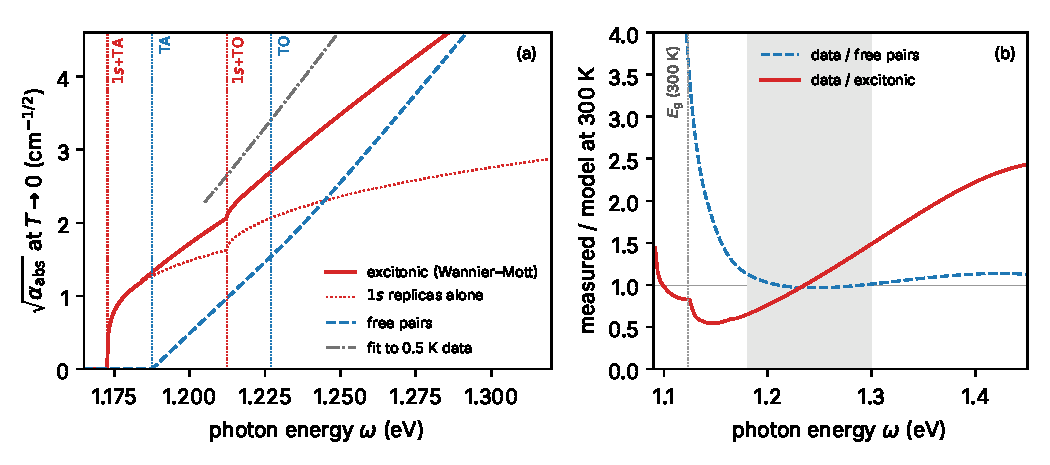
\includegraphics[width=\linewidth]{figures/ch13/fig13_8.pdf}
  \caption{Phonon-assisted absorption edge of silicon with excitonic final states. (a) $\sqrt{\alpha_{\mathrm{abs}}}$ at $T \to 0$ against the photon energy. Red: \cref{eq:13.8-edge} for the transverse acoustic and transverse optical branches, $\omega_{\mathrm{TA}} = \SI{18.27}{meV}$ and $\omega_{\mathrm{TO}} = \SI{57.73}{meV}$, with weights $5.5:4.0$~\cite{rajkanan1979absorption,stanford2021photoelectric}, $\Eg(0) = \SI{1.1692}{eV}$ and $E_x^b = \SI{14.7}{meV}$ for both hole bands; dotted, the two $1s$ replicas alone. Blue, dashed: the free-pair edge of \cref{sec:13.5}. Each model has one scale, fitted as in \cref{sec:13.5} to the measured \SI{300}{K} absorption between 1.18 and \SI{1.30}{eV}~\cite{franta2017temperature}. Gray, dash-dotted: the free-pair form fitted to measurements between 0.5 and \SI{295}{K}, with an effective gap of \SI{1.134}{eV}, evaluated at \SI{0.5}{K} and drawn above \SI{1.205}{eV}, the lowest photon energy measured~\cite[Eqs.~(4)--(7)]{stanford2021photoelectric}. Vertical lines: the $1s$ replica thresholds $\Eg - E_x^b + \omega_\nu$ (red) and the free-pair thresholds $\Eg + \omega_\nu$ (blue). (b) Measured absorption at \SI{300}{K} divided by each model at \SI{300}{K}, both branches with their phonon occupations; gray band, the fitted interval. Effective-mass models with constant matrix elements, not calculations.}
  \label{fig:13-replicas}
\end{figure}

\Cref{fig:13-replicas}a shows \cref{eq:13.8-edge} for cold silicon. The $1s$ replica of the transverse acoustic branch opens at \SI{1.1728}{eV} and the $2s$ replica at \SI{1.1838}{eV}, both below the free-pair threshold at \SI{1.1875}{eV}; the transverse optical replica opens at \SI{1.2122}{eV}. With the same $|M^x_\nu|^2$ the excitonic edge of the two branches exceeds the free-pair one by a factor of 81 at \SI{1.200}{eV}, 16 at \SI{50}{meV} above the free threshold and 7.3 at \SI{100}{meV}, and at \SI{1.200}{eV} the $1s$ replica holds three quarters of it.

The measured spectra test the shape. Fitted in the same interval of the \SI{300}{K} data, the excitonic form needs a scale 0.154 times that of the free-pair form, since the Fermi factor already supplies part of the absorption there. Neither form follows the data over the whole range (\cref{fig:13-replicas}b). The free-pair form falls short within \SI{40}{meV} of the gap, by the factor 2.0 at \SI{17}{meV} found in \cref{sec:13.5}. The hydrogenic form overshoots there by up to 1.8 and falls short by 1.5 to 2.5 between 1.3 and \SI{1.6}{eV}, where the parabolic bands and the hydrogenic continuum of \cref{sec:10.5} no longer hold. The edge region is where the excitonic form belongs, and there the measurements at low temperature are the test. At \SI{1.21}{eV}, the lowest energy measured at \SI{0.5}{K}, the fit to the measurements, evaluated at that temperature, is \SI{6.4}{cm^{-1}}, the excitonic form 4.0 and the free-pair form \SI{0.77}{cm^{-1}}. With the decrease of the branch strength between the lowest temperature and \SI{295}{K} found in \cref{sec:13.5}, a factor 0.61, the excitonic value becomes 6.6 and the free-pair one 1.3. The fit itself needs an effective gap of \SI{1.134}{eV}, \SI{35}{meV} below the true one: a free-pair form can follow an excitonic edge only by moving its threshold down.

For dark-matter scattering the same construction applies at each $\vect{q}$, with $A_\nu$ the coefficient of \cref{eq:13.3-near} and the thresholds $E_{\mathrm{min}}^{\mathrm{PA}}(\vect{q}) - E_x^b/n^2$. The binding energy is that of the pair at the momentum $\vect{q}+\vect{Q}^*$, near $\vect{k}_{\mathrm{c}}$, where the hole sits near the valence maximum and the measured \SI{14.7}{meV} applies; its variation along the dispersion of the pair is \cref{eq:E.15-disp}. The lightest mass at which the $1s$ replica opens follows from \cref{eq:13.1-mPA} with $\Eg$ replaced by $\Eg - E_x^b$, as \cref{sec:13.1} found, and its value and status belong to \cref{sec:13.9}.

\subsection{Phonon-assisted absorption of bosonic dark matter}

Absorption of a boson probes the response at $\vect{q} = \vect{p}_\phi$, about $10^{-3}m_\phi$, and $\omega = m_\phi$ (\cref{eq:8.2-abs}). In silicon between the excitonic edge at \SI{1.1728}{eV} and the direct gap $E_{\mathrm{dir}} = \SI{3.4}{eV}$ no vertical pair exists. Every first-order transition at $\vect{q} \simeq 0$ is then off the energy shell, and the window of \cref{eq:13.6-window}, with the vertical gap as the zero-phonon edge, extends to $E_{\mathrm{dir}} - \delta_{\mathrm{w}} = \SI{3.1}{eV}$. Inside it every response row is phonon-assisted. Its structure factor is \cref{eq:13.3-SPA} at $\vect{q} = 0$ with the vertices of the two rows in place of $\rho$, or \cref{eq:13.8-S} near the edge. Each of the three rates of \cref{sec:10.7} therefore holds there with its response replaced by the phonon-assisted one. The bosons differ in whether that response is measured.

The dark photon has no phonon-assisted amplitude of its own at first order in $g$. It couples to the electromagnetic current of electrons and nuclei with $\zeta$ times the charge of the photon, and every second-order amplitude into a pair and one phonon reduces to that of light or vanishes. The electron current with one electron--phonon vertex is the amplitude of light, \cref{eq:6.5-M} with the velocity vertex, and its square summed over final states is the measured $\varepsilon_2^{\mathrm{PA}}$. The longitudinal polarization couples to the charge density at $\vect{q} = \vect{p}_\phi$, and the phonon-assisted density amplitude there is, by continuity, $(q/\omega)$ times the velocity amplitude (\cref{eq:13.5-Mlim}). It is the same amplitude written another way, and adding the density form of \cref{sec:13.2} to the current form would count the transition twice. The nuclear current, finally, changes a phonon occupation at $\vect{Q} \simeq \vect{p}_\phi$ without moving an electron, while the electron--phonon vertex moves one electron and changes one occupation. Together they either leave two occupations changed, a final state with two phonons, or remove the phonon the current created and leave a vertical pair, which needs $\omega \ge E_{\mathrm{dir}}$; in silicon the Born charges vanish in any case. The rate is \cref{eq:10.7-dp} with $L = \varepsilon_2^{\mathrm{PA}}/(\varepsilon_1^0)^2$ at the temperature of the detector (\cref{sec:13.4,sec:13.5}). At the edge $\varepsilon_2^{\mathrm{PA}}$ is of order $10^{-4}$, so the phonon-assisted part of the photon self-energy does nothing to the mixing, and $\zeta_{\mathrm{eff}} = \zeta/\varepsilon_1^0$. What the dark photon needs is the measured edge itself, brought to millikelvin temperatures and resolved into its excitonic structure, as \cref{we:13-darkphoton-edge} shows.

The axion-like particle couples through the spin current $\mathcal{J}_e$ (\cref{sec:10.7-alp}). The electron--phonon vertex is diagonal in spin. The spin structure of the phonon-assisted amplitude is therefore that of the one spin operator in $\mathcal{J}_e$, and the spin trace of \cref{sec:10.7-alp} goes through unchanged: $S^{\mathrm{PA}}_{\mathcal{J}\mathcal{J}} = \frac34S^{\mathrm{PA}}_{jj}$ and $\varGamma = (3m_\phi^2/4m_e^2)(g_{aee}^2/e^2)\,\sigma_1^{\mathrm{PA}}$, with $\sigma_1^{\mathrm{PA}} = m_\phi\varepsilon_2^{\mathrm{PA}}$, for independent electrons without spin--orbit coupling. At equal couplings it is $(3m_\phi^2/4m_e^2e^2)|\varepsilon|^2 = 7.3\times10^{-9}$ of the dark-photon rate at \SI{1.2}{eV}. The caveats of \cref{sec:10.7-alp} take a specific form at the edge. The spin current creates triplet pairs, which feel the direct kernel and not the exchange one (\cref{eq:10.5-triplet}). The replica lines are therefore the same as in the measured singlet edge, up to the exchange splitting, which is about $2\times10^{-3}$ of the binding (\cref{sec:10.5}). The pair channel of \cref{sec:13.4}, a Coulomb screening at the pair momentum, is absent from the triplet response, and its size is not known for the singlet either.

The scalar couples through two rows, the density and the kinetic energy (\cref{sec:10.7-scalar}). The phonon-assisted density amplitude vanishes at $\vect{q} = 0$ by \cref{eq:13.2-q0}, so the density row enters at order $p_\phi$ and its rate at order $v^2$. The kinetic row, however, does not vanish. Its phonon-assisted amplitude $M^\pm_{\mathcal{T},cv\nu}(\vect{k},\vect{Q})$ is \cref{eq:13.2-M} at $\vect{q} = 0$ with the vertical kinetic elements $(\mathcal{T}_e)_{mn}(\vect{k}) = \langle m\vect{k}|p^2/2m_e|n\vect{k}\rangle$ in place of $\rho_{mn}$, and its intraband terms no longer cancel. Path A with $p = v$ and path B with $p = c$ add to $g_{cv\nu}(\vect{k},\vect{Q})[(\mathcal{T}_e)_{vv}(\vect{k}) - (\mathcal{T}_e)_{cc}(\vect{k}+\vect{Q})]/\omega$, the difference of the kinetic energies of the two band states, where the density has $\rho_{vv} = \rho_{cc} = 1$. The whole amplitude has a compact form. In the operator form of \cref{eq:13.2-M} (\cref{app:D.35}), $\langle c|y\,(\varepsilon_v + \omega - h)^{-1}x + x\,(\varepsilon_v \mp \omega_{\vect{Q}\nu} - h)^{-1}y|v\rangle$ with $x = p^2/2m_e$ and $y$ the phonon vertex, write $x = h - V$, with $h$ the one-electron Hamiltonian and $V$ everything in it but the kinetic energy. The part $h$ acts on $|v\rangle$ in the first term and on $\langle c|$ in the second, where it returns $\varepsilon_v$ and $\varepsilon_c$, and the resolvents return $1/\omega$ and $-1/\omega$ on the shell. With $\varepsilon_c - \varepsilon_v = \omega \mp \omega_{\vect{Q}\nu}$,
\begin{equation}
  M^\pm_{\mathcal{T},cv\nu}(\vect{k},\vect{Q}) = -\Bigl(1 \mp \frac{\omega_{\vect{Q}\nu}}{\omega}\Bigr)\,g_{cv\nu}(\vect{k},\vect{Q}) - M^\pm_{V,cv\nu}(\vect{k},\vect{Q}) ,
  \label{eq:13.8-MT}
\end{equation}
where $M^\pm_V$ is \cref{eq:13.2-M} at $\vect{q} = 0$ with the matrix elements of $V$ in place of $\rho$. The first term is the electron--phonon vertex itself. The second is the phonon-assisted amplitude of the crystal potential, the counterpart of $\langle c|p^2/2m_e|v\rangle = -\langle c|V|v\rangle$ of \cref{sec:10.7-scalar}, and like it weighted toward the cores. Both are of order $g$ in energy units, and nothing cancels them. \Cref{eq:10.7-scalar} with the phonon-assisted response is
\begin{equation}
  \begin{gathered}
  \varGamma = \frac{g_{\phi ee}^2}{2\,m_\phi m_e^2}\,S^{\mathrm{PA}}_{\mathcal{T}\mathcal{T}}(0,m_\phi) , \\
  S^{\mathrm{PA}}_{\mathcal{T}\mathcal{T}}(0,\omega) = \frac{4\pi}{\Omega}\Bigl\langle\!\Bigl\langle\sum_{\nu cv\pm}\bigl(n_{\vect{Q}\nu} + \tfrac12 \pm \tfrac12\bigr)\bigl|M^\pm_{\mathcal{T},cv\nu}\bigr|^2\delta\bigl(\varepsilon_{c,\vect{k}+\vect{Q}} - \varepsilon_{v\vect{k}} \pm \omega_{\vect{Q}\nu} - \omega\bigr)\Bigr\rangle\!\Bigr\rangle ,
  \end{gathered}
  \label{eq:13.8-scalar}
\end{equation}
unscreened, for a point group without a polar vector, inside the window; near the edge the final pairs are the excitons of \cref{eq:13.8-S} with the kinetic row in place of the density. No measurement provides this response, and it is not proportional to $\varepsilon_2^{\mathrm{PA}}$, since \cref{eq:13.8-MT} has no velocity vertex in it. The comparison with the axion-like particle in \cref{sec:10.7-scalar} carries over. The kinetic amplitude is of the order of the vertex $g$, while the axion-like amplitude carries $m_\phi/m_e$ times an electron velocity. At equal couplings the scalar is therefore absorbed far more strongly, by a factor that only a calculation fixes. The phonon-assisted kinetic absorption has been computed for the intraband transitions of a superconducting metal~\cite[Sect.~V, Eq.~(72)]{mitridate2021dark}; a silicon rate built from vertical transitions has below about \SI{3}{eV} only the tails of the smearing~\cite[Sect.~IV]{mitridate2021dark}. The interband channel of \cref{eq:13.8-MT,eq:13.8-scalar} at the indirect edge of an insulator needs, for its evaluation, a phonon-assisted kinetic row with all-electron kinetic matrix elements.

\begin{workedexample}{A dark photon of 1.2 eV in cold silicon}\label{we:13-darkphoton-edge}
At $m_\phi = \SI{1.200}{eV}$ a dark photon sits \SI{12.5}{meV} above the free-pair threshold $\Eg(0) + \omega_{\mathrm{TA}} = \SI{1.1875}{eV}$ and \SI{27.2}{meV} above the $1s$ replica, below both transverse optical thresholds. Only the transverse acoustic branch absorbs, by emission.

\emph{Cold absorption.} Stanford and co-workers fitted their data at 0.5 to \SI{295}{K} with the free-pair form $\alpha_{\mathrm{abs}} = \sum_\nu C_\nu c_0(\omega - E_{\mathrm{g}1} - \omega_\nu)^2$ at low temperature, with the branch weights $C_{\mathrm{TA}} = 5.5$ and $C_{\mathrm{TO}} = 4.0$, the strength $c_0 = \SI{325}{eV^{-2}.cm^{-1}}$ and an effective gap $E_{\mathrm{g}1} = \SI{1.134}{eV}$~\cite[Eqs.~(4)--(7)]{stanford2021photoelectric}. Evaluated at \SI{0.5}{K}, it gives $\alpha_{\mathrm{abs}} = 5.5\times\SI{325}{eV^{-2}.cm^{-1}}\times(\SI{0.0477}{eV})^2 = \SI{4.07}{cm^{-1}}$ from its transverse acoustic term and \SI{0.09}{cm^{-1}} from the transverse optical one, which its lowered gap opens: \SI{4.16}{cm^{-1}}, \SI{6}{meV} below their lowest photon energy. The \SI{20}{K} data of Macfarlane and co-workers~\cite{macfarlane1958fine} give \SI{0.21}{cm^{-1}} at this energy, twenty times less; near the edge the cold datasets differ by that much (\cref{sec:13.9-rates}). The excitonic edge of \cref{fig:13-replicas} reaches \SI{2.95}{cm^{-1}} (4.8 with the strength factor 0.61), the free-pair edge transferred to millikelvin temperatures in \cref{sec:13.5} only \SI{0.24}{cm^{-1}}, and the \SI{300}{K} data used without transfer \SI{27.3}{cm^{-1}}.

\emph{Loss function.} With the fit value $\alpha_{\mathrm{abs}} = \SI{4.16}{cm^{-1}}$, $n_r = 3.565$ from the \SI{300}{K} data and $\hbar c/\omega = \SI{1.644e-5}{cm}$,
\begin{equation*}
  \varepsilon_2^{\mathrm{PA}} = n_r\,\alpha_{\mathrm{abs}}\,\frac{\hbar c}{\omega} = 2.44\times10^{-4} , \qquad
  L = \frac{\varepsilon_2^{\mathrm{PA}}}{(\varepsilon_1^0)^2} = \frac{2.44\times10^{-4}}{12.71^2} = 1.51\times10^{-6} .
\end{equation*}
The medium suppresses the rate by $|\varepsilon|^2 = 161.5$ against the vacuum mixing.

\emph{Rate.} With $\rho_\chi = \SI{0.3}{GeV.cm^{-3}}$ and $\rho_T = \SI{2.33}{g.cm^{-3}}$, $(\rho_\chi/\rho_T)/\hbar = 6.17\times10^{33}$ per kilogram-year, as in \cref{we:10-darkphoton}, and \cref{eq:10.7-dp} gives
\begin{equation*}
  \mathcal{R} = 6.17\times10^{33}\times1.51\times10^{-6}\,\zeta^2 = 9.3\times10^{27}\,\zeta^2\ \text{per kilogram-year} .
\end{equation*}
Three events in a kilogram-year need $\zeta = 1.8\times10^{-14}$. The untransferred \SI{300}{K} data would claim a rate 6.6 times larger and $\zeta = 7.0\times10^{-15}$; the transferred free-pair edge a rate 17 times smaller and $\zeta = 7.5\times10^{-14}$, and the \SI{20}{K} data a rate 20 times smaller. At \SI{1.2}{eV} the correction that matters is the bound pair: in the excitonic edge three quarters of the absorption at this energy is the $1s$ replica, which neither the warm data nor the free-pair transfer represents.
\end{workedexample}

\section{The silicon window}\label{sec:13.9}

A silicon detector that counts single electrons sees dark matter of \SI{0.36}{MeV} only through the phonon-assisted rate, and dark matter of \SI{0.6}{MeV} almost only through zero-phonon pairs. Kinematics fixed the onset of the first at 0.3332 and \SI{0.3374}{MeV} and put upper values on the second along chosen directions (\cref{sec:13.1}). Here the zero-phonon side is evaluated with bands over the whole zone: the first zero-phonon edge lies at 0.405 to \SI{0.408}{MeV}, off the valley axis, and its state is weakly coupled because a glide of the diamond structure forbids its vertex. These edges and their order rest on two independent calculations. Where the phonon-assisted rate stops leading, how large it is, and the windows of germanium and GaAs are known only as estimates or not at all.

\subsection{The zero-phonon edges}\label{sec:13.9-edges}

The joint minimum \cref{eq:13.1-mZP} over the momentum transfer and the hole's crystal momentum lies off the valley axis. The search uses the PBE bands of \cref{sec:3.4}, interpolated in Wannier functions, with the conduction bands shifted rigidly to the measured gap $\Eg(0) = \SI{1.170}{eV}$. Of 21 starting points, 18 converge on one point up to the cubic symmetry, and a local re-minimization on the plane-wave bands at the measured lattice constant refines it. The optimum has $|\vect{q}| = \SI{1.33}{keV}$, tilted by \SI{0.18}{rad} from the [100] axis within a $\{001\}$ plane. The hole sits at $\vect{k}_v = (0.126, -0.107, 0)\,(2\pi/a)$, \SI{62}{meV} below the valence-band maximum, along a direction in which the heavy-hole band is flat (its PBE mass along [110] is about $2.5\,m_e$). The electron sits on the valley axis, about $0.16\,(2\pi/a)$ short of the valley minimum. The pair costs \SI{1.355}{eV}, and the threshold mass is
\begin{equation*}
  m_{\mathrm{min}}^{\mathrm{ZP}} = \SI{0.407}{MeV} ,
\end{equation*}
with spin--orbit coupling, and \SI{0.404}{MeV} without, within a band of 0.405 to \SI{0.408}{MeV} that carries the lattice constant and the interpolation. The $1s$ exciton lowers it by $\mchi E_x^b/(qv_{\mathrm{max}} - E) = \SI{0.0028}{MeV}$ (\cref{sec:13.1}), to 0.402--\SI{0.405}{MeV}.

The joint minimum leaves the axis because, at $|\vect{q}| = 1.2$ to \SI{1.48}{keV}, the [100] axis is a local maximum of $E_{\mathrm{min}}(\vect{q})$ over the directions of $\vect{q}$, not a minimum. The minima sit 0.13 to \SI{0.22}{rad} away in the $\{001\}$ planes, 14 to \SI{107}{meV} below the on-axis value, and are shallower in the $\{011\}$ planes. Around the optimum the pair energy rises as $\beta_\theta\vartheta^2 + \beta_z\varphi^2$, with $\beta_\theta = \SI{2.47}{eV.rad^{-2}}$ for the tilt within the plane and $\beta_z = \SI{3.70}{eV.rad^{-2}}$ out of it. The warped heavy hole of \cref{eq:3.3-holes} is the cause: moving the hole into its flat direction costs less than the pair kinetic energy it saves. On the axis the same bands have a local optimum at \SI{0.415}{MeV}, which the coarser grid of \cref{sec:13.1} placed at \SI{0.420}{MeV} and the parabola at \SI{0.425}{MeV}. The joint minimum is therefore 0.013 to \SI{0.018}{MeV} below the upper values of \cref{sec:13.1}.

Spin--orbit coupling raises the edge by \SI{0.003}{MeV}, fifteen times more than on the axis. At the optimum the hole lies \SI{62}{meV} below the valence maximum, deeper than the split-off energy ($\Delta_{\mathrm{SO}} = \SI{48.6}{meV}$ in PBE, \SI{44}{meV} measured, \cref{tab:3-materials}), and it does not share the rise by $\Delta_{\mathrm{SO}}/3$ of the $\mathrm{\Gamma}_8$ maximum to which the gap is referred. With spin--orbit coupling it sits \SI{77}{meV} below that maximum, and the pair costs \SI{15.5}{meV} more. On the axis, where the hole is near $\mathrm{\Gamma}$, the shift is under \SI{1}{meV}.

Three further edges complete the zero-phonon side. On the axis the two heavy holes are degenerate. A tilt within a $\{001\}$ plane splits them into one band that is odd under the mirror of that plane and one that is even, and they open at different masses. The first edge belongs to the odd band. The even band reaches the same pair energy only on the axis, and its edge lies at 0.415 to \SI{0.420}{MeV}, the range set by the lattice constant and spin--orbit coupling. Off the axis its pair energy rises as $\beta_2\vartheta^2$, with $\beta_2$ from \SI{4.5}{eV.rad^{-2}} in the $\{001\}$ planes to \SI{1.1}{eV.rad^{-2}} in the $\{011\}$ planes. The third edge is that of the Umklapp class $\vect{G}' = (\bar2\,0\,0)\,2\pi/a$, in which the unreduced crystal momentum of the electron lies beyond the X face of the zone, so that the reciprocal-lattice vector sits inside the density vertex (\cref{sec:3.1}). Restricted to this class, \cref{eq:13.1-mZP} has its minimum on the X face, at $|\vect{q}| = \SI{1.83}{keV}$ with the hole at $|\vect{k}_v| = 0.26\,(2\pi/a)$: the line opens at \SI{0.50}{MeV}, spin--orbit coupling included. The last edge of the class without Umklapp on the [100] axis is far above all of these. Along [110] and [111], 0.548 and \SI{0.615}{MeV} (\cref{sec:13.1}), the zero-phonon channel is already open through the other edges.

The edges fall in a fixed order:
\begin{equation*}
  \underbrace{0.3332 < 0.3374}_{\text{phonon-assisted onset}}
  < \underbrace{0.402\text{--}0.405 < 0.405\text{--}0.408}_{\text{first zero-phonon edge}}
  < \underbrace{0.415\text{--}0.420}_{\text{second heavy hole}}
  < \underbrace{\approx 0.50}_{(\bar2\,0\,0)\ \text{line}}\ \si{MeV} .
\end{equation*}
The order does not depend on the last digits. The phonon-assisted onset moves by \SI{2.8e-4}{MeV} per meV of phonon energy (\cref{we:13-onset}), and even a transverse acoustic phonon at its largest energy, \SI{18.6}{meV} at X, would put it at \SI{0.339}{MeV}, \SI{0.07}{MeV} below the first zero-phonon edge. The zero-phonon edges are separated by more than their own spreads. Between the onset and the first edge no zero-phonon pair exists at any momentum transfer, and the phonon-assisted rate is the only electron-recoil channel; above the first edge the question becomes one of rates.

These are thresholds, not rates, and they are cheap. The joint minimization needs interpolated bands over the zone with a gap correction, a check of the interpolated pair energy against a direct plane-wave calculation at the optimum (it differs by \SI{11}{meV}), and a local re-minimization with spin--orbit coupling (\cref{app:E.1}). \Cref{app:E.14} specifies the bins on which the zero-phonon rate is to be computed next to the phonon-assisted one: the cones around the mirror-plane optima, the cone of the second heavy hole and the X-face edge.

\subsection{The glide-parity selection rule}\label{sec:13.9-glide}

On the valley axis, without Umklapp, the zero-phonon vertex between the bottom of the valley and the valence maximum vanishes. The electron is invariant under the operations that fix the axis, and the holes have no invariant part (\cref{sec:10.5-rules}; in the language of \cref{sec:13.3}, $\Delta_1\otimes\Delta_1\otimes(\Delta_2'\oplus\Delta_5)$ contains no $\Delta_1$). Off the axis these operations are gone, and only one survives for a pair that stays in a $\{001\}$ plane through the axis: the mirror of that plane. In diamond it carries the fractional translation $\vect{\tau}_2$ and is a glide (\cref{app:C.17}). Bloch states with crystal momentum in the plane are its eigenstates, with a glide parity $\eta = \pm1$ (\cref{eq:C.17-parity}). The density vertex with $\vect{q}$ in the plane connects a valence state of parity $\eta_v$ to the conduction state of reduced parity $\eta_c$ only if
\begin{equation}
  \eta_c\,\eta_v\,\ee^{-\ii\vect{G}'\cdot\vect{w}/2} = 1 ,
  \label{eq:13.9-glide}
\end{equation}
where $\vect{G}'$ is the Umklapp vector of the unreduced final momentum and $\vect{w}$ the lattice vector that the glide gives when applied twice. This is \cref{eq:C.17-selection} applied to the mirror $\mathsf{m}_z$. The rule decides which zero-phonon line is strong at each of the edges.

\begin{workedexample}{The selection rule for the first zero-phonon line}\label{we:13-glide}
Take the valley on the $x$ axis and the mirror $\mathsf{m}_z$, $(x, y, z) \to (x, y, -z)$, whose plane $z = 0$ contains the axis and the optimum of \cref{sec:13.9-edges}. In diamond it occurs as $g = \{\mathsf{m}_z|\vect{\tau}_2\}$ with $\vect{\tau}_2 = (a/4)(1,1,1)$, as in \cref{eq:C.17-glide} with $x$ and $z$ exchanged. Applied twice it gives the translation $\vect{w} = \vect{\tau}_2 + \mathsf{m}_z\vect{\tau}_2 = (a/2)(1,1,0)$, a lattice vector.

\emph{The phase of the operator.} Conjugating the vertex gives $g\,\ee^{\ii\vect{q}\cdot\vect{r}}g^{-1} = \ee^{-\ii\vect{q}\cdot\vect{\tau}_2}\ee^{\ii\vect{q}\cdot\vect{r}}$ for $\vect{q}$ in the plane. Against the phases $\ee^{-\ii\vect{k}\cdot\vect{w}/2}$ of the two eigenvalues it leaves $\ee^{\ii\vect{q}\cdot(\vect{w}/2 - \vect{\tau}_2)}$, and $\vect{w}/2 - \vect{\tau}_2 = (0, 0, -a/4)$ is normal to the plane, so this phase is one. With unreduced labels the vertex therefore needs $\eta_c = \eta_v$.

\emph{Reduced labels.} Reducing the final momentum by $\vect{G}'$ multiplies the conduction eigenvalue by $\ee^{-\ii\vect{G}'\cdot\vect{w}/2}$. For $\vect{G}' = 0$ the factor is one and \cref{eq:13.9-glide} requires equal parities. For $\vect{G}' = (\bar2\,0\,0)\,2\pi/a$, $\vect{G}'\cdot\vect{w}/2 = -(4\pi/a)(a/4) = -\pi$, the factor is $-1$, and the parities must be opposite. Every vector of the (200) class flips the rule; vectors with $h + k \equiv 0 \pmod 4$ in the plane keep it.

\emph{On the axis.} The heavy-hole pair $\Delta_5$ splits under the mirror into one even and one odd state, the light hole $\Delta_2'$ is odd and the electron $\Delta_1$ even, all relative to the electron's convention. The glide rule alone would allow the even heavy hole at $\vect{G}' = 0$; the full group of the axis forbids it, as above, and the vertex vanishes on the axis for every hole. In the class $(\bar2\,0\,0)$ the rule allows the odd states, and the full group of the axis leaves exactly one of them, the light hole, which carries the vertex there (multiplicity one, $\Delta_1\otimes\Delta_2'\otimes\Delta_2' \ni \Delta_1$).

\emph{At the optimum.} Off the axis in the plane the two heavy holes are no longer degenerate, and which of them is on top is not fixed by symmetry. The calculation finds the odd one on top at the optimum. With $\vect{G}' = 0$, \cref{eq:13.9-glide} then forbids its vertex everywhere in the plane: computed, $|\rho_{cv}|^2 = 3\times10^{-14}$, zero to numerical precision. The even partner, \SI{0.39}{eV} deeper at the same $\vect{q}$, has $|\rho_{cv}|^2 = 0.064$. Leaving the plane breaks the glide, and the vertex grows linearly with the distance from it, with gradients $|\partial_{q_z}\rho_{cv}| = \SI{1.57}{\angstrom}$ (the pair relaxing by its center of mass) and $|\partial_{k_z}\rho_{cv}| = \SI{0.32}{\angstrom}$. The first zero-phonon line is second class in the sense of \cref{sec:10.5-rules}: its vertex vanishes on a surface through the edge and its strength grows from zero.

\emph{The other edges.} The second heavy hole is the even band, allowed by \cref{eq:13.9-glide} as soon as the pair leaves the axis; its vertex grows linearly in the tilt with $|\partial_{q_\perp}\rho_{cv}| = \SI{2.21}{\angstrom}$. In the class $(\bar2\,0\,0)$ the rule inverts and the odd top hole is allowed. At the X-face edge $|\rho_{cv}|^2 = 0.0095$ for the lowest conduction band, 0.028 for the two lowest (the second lies \SI{50}{meV} higher there), and 0.024 to 0.036 at 0.02 to $0.10\,(2\pi/a)$ inside the class.
\end{workedexample}

The vertex of the $(\bar2\,0\,0)$ class is not small, although the (200) Fourier component of every lattice-periodic function of diamond vanishes (\cref{eq:C.17-extinct}). At the extremum of the class, $|\vect{q}| = \SI{2.64}{keV}$, the light hole carries $\sum_v|\rho_{cv}|^2 = 0.150$, of the size of an ordinary allowed vertex: the four lowest conduction bands together, averaged over directions, give 0.45 at $|\vect{q}| = \SI{2.28}{keV}$, a number not comparable one-to-one with the single-band 0.150. The extinction removes one Fourier component of the potential, but the vertex is a product of Bloch functions with all their components, and it is not suppressed. A nearly-free-electron estimate, in which the (200) component would carry the transition alone, gives the opposite answer.

Spin--orbit coupling mixes the two glide parities, since the spin also transforms under the mirror, and lifts each zero. On the axis the lift, summed over the four states of the $\mathrm{\Gamma}_8$ quartet, is $|\rho_{cv}|^2 = 3.6\times10^{-6}$, an amplitude of \SI{0.5}{\percent} of the allowed $(\bar2\,0\,0)$ vertex; in the mirror plane it is $1.3\times10^{-4}$, \SI{4.5}{\percent} in amplitude of the allowed partner. Neither moves an edge or a rate in what follows.

\subsection{The rate at the onset}\label{sec:13.9-onset}

Just above $m_{\mathrm{min}}^{\mathrm{PA}}$ only a small corner of the $(q,\omega)$ plane is reachable, and three factors vanish together there: the loss function above its threshold, the halo near $v_{\mathrm{max}}$, and the range of momentum transfers. At fixed $|\vect{q}|$ write $E_{\mathrm{th}}(q)$ for the onset of $\bar L^{\mathrm{PA}}$ and $x = \omega - E_{\mathrm{th}}(q)$, so that $\bar L^{\mathrm{PA}} \simeq Cx^{p_{\mathrm{on}}}$ with the onset exponent of \cref{eq:13.3-pon}. With $\vmin = \omega/q + q/2\mchi$ (\cref{eq:1.3-vmin}), the distance of $\vmin$ from $v_{\mathrm{max}}$ is
\begin{equation*}
  v_{\mathrm{max}} - \vmin = \frac{x_{\max}(q) - x}{q} , \qquad x_{\max}(q) = qv_{\mathrm{max}} - \frac{q^2}{2\mchi} - E_{\mathrm{th}}(q) .
\end{equation*}
The function $x_{\max}(q)$ is the largest energy above threshold that the mass reaches at $q$. Its maximum over $q$ is zero at the onset mass $m_0 = m_{\mathrm{min}}^{\mathrm{PA}}$ and lies at $q^* = m_0v_{\mathrm{max}}$ to the accuracy of \cref{eq:13.1-mPA}. Since $\partial x_{\max}/\partial\mchi = q^2/2\mchi^2$, a mass $\mchi = m_0 + \delta m$ reaches
\begin{equation*}
  x_{\max}(q) \simeq x_{\max}^* - \frac{(q - q^*)^2}{2m_0} , \qquad x_{\max}^* = \tfrac12v_{\mathrm{max}}^2\,\delta m ,
\end{equation*}
where the curvature of $E_{\mathrm{th}}$, of order $10^{-8}\,\si{eV^{-1}}$ for the transverse acoustic branch, is dropped against $1/m_0 = \SI{3e-6}{eV^{-1}}$. For the standard halo of \cref{tab:1-shm} the halo function is quadratic near $v_{\mathrm{max}}$, $\eta(\vmin) \simeq A_\eta(v_{\mathrm{max}} - \vmin)^2$ (\cref{eq:1.3-edge}), and the factors $q^3\FDM^2$ of \cref{eq:10.2-rate} are smooth. The energy integral at fixed $q$ is then
\begin{equation*}
  \int_0^{x_{\max}}\dd x\,x^{p_{\mathrm{on}}}(x_{\max} - x)^2 = \frac{2\,x_{\max}^{p_{\mathrm{on}}+3}}{(p_{\mathrm{on}}+1)(p_{\mathrm{on}}+2)(p_{\mathrm{on}}+3)} ,
\end{equation*}
and the integral over $q$ of $x_{\max}^{p_{\mathrm{on}}+3}$ across the interval where $x_{\max} > 0$, of width $2(2m_0x_{\max}^*)^{1/2}$, gives $(x_{\max}^*)^{p_{\mathrm{on}}+3}(2m_0x_{\max}^*)^{1/2}B(\tfrac12, p_{\mathrm{on}}+4)$, with $B$ the beta function. Collecting the powers of $x_{\max}^*$:
\begin{keyresult}[Mass dependence at the phonon-assisted onset]
\begin{equation}
  \mathcal{R}(\mchi) \propto (\mchi - m_{\mathrm{min}}^{\mathrm{PA}})^{p_{\mathrm{on}} + 7/2} ,
  \label{eq:13.9-medge}
\end{equation}
for $\tfrac12v_{\mathrm{max}}^2(\mchi - m_{\mathrm{min}}^{\mathrm{PA}})$ inside the energy range in which $\bar L^{\mathrm{PA}}$ follows $x^{p_{\mathrm{on}}}$; the power is $13/2$ at the free-pair transverse acoustic edge of silicon with independent pairs, 6 with the excitonic continuum and 5 at the exciton replica, for either mediator, with the standard halo of \cref{tab:1-shm}, whose $\eta(\vmin)$ vanishes quadratically at $v_{\mathrm{max}}$. A halo with another behavior at the escape speed changes the $7/2$.
\end{keyresult}
\noindent The loss function gives $p_{\mathrm{on}} + 1$ powers, the halo two and the width in $q$ one half. A numerical integration of \cref{eq:10.2-rate} with the computed transverse acoustic onset on the axis, the halo function of \cref{sec:1.2} and a loss function $Cx^{p_{\mathrm{on}}}$ reproduces the two powers, and their local value stays within 0.06 of them up to \SI{0.01}{MeV} above each onset (\cref{fig:13-window-rates}(b)). The model loss function is the idealization; the computed one of \cref{fig:13-paloss} follows $x^3$ within \SI{10}{\percent} only for $x < \SI{1.3}{meV}$, which here means $\delta m < \SI{4e-4}{MeV}$, since $x_{\max}^* = \SI{3.5}{meV}$ per \SI{0.001}{MeV}. Its local exponent drifts to 3.3 at \SI{10}{meV}, so the power of the mass stays between 6.5 and 7 to about \SI{0.003}{MeV} above the onset. With excitonic final states the free-pair continuum starts as $x^{3/2}$ at fixed $\vect{q}$ instead of $x^2$, because the Coulomb attraction keeps its weight finite at the edge (\cref{eq:13.8-edge}); averaged over directions it has $p_{\mathrm{on}} = 5/2$, and its power of the mass is 6.

The steep power turns any error in the onset into a large error in the rate. An error $\epsilon$ in $m_{\mathrm{min}}^{\mathrm{PA}}$ multiplies the rate at $\delta m$ above it by $(1 - \epsilon/\delta m)^{p_{\mathrm{on}} + 7/2}$. The softness of the computed transverse acoustic branch moves the onset by \SI{0.0004}{MeV} (\cref{we:13-onset}), and at \SI{0.005}{MeV} above the onset this changes the rate by a factor 0.56 to 0.58. Within a few thousandths of an MeV of the onset only the exponent is a meaningful prediction, and between the replica onset at \SI{0.3332}{MeV} and the free-pair onset at \SI{0.3374}{MeV} the whole rate is the replica's, whose strength belongs to \cref{sec:13.8}.

\subsection{Rates across the window}\label{sec:13.9-rates}

No first-principles phonon-assisted rate of silicon exists. What exists is an estimate, built to be checked bin by bin against the calculation of \cref{app:E.14}. It takes a measured cold absorption of silicon as the optical limit $\varepsilon_2^{\mathrm{PA}}(\omega)$ of \cref{eq:13.5-limit}, where it contains the excitons, the local fields and the pair channel at $\vect{q} \to 0$. The primary input is the \SI{0.5}{K} fit of Stanford and co-workers (\cref{we:13-darkphoton-edge}), \SI{21.5}{cm^{-1}} at \SI{1.25}{eV}, or $\varepsilon_2 = 1.2\times10^{-3}$. The \SI{20}{K} data of Macfarlane and co-workers~\cite{macfarlane1958fine} give \SI{10.4}{cm^{-1}} there, or $\varepsilon_2 = 5.9\times10^{-4}$, and twenty times less than the fit at \SI{1.20}{eV}, below the lowest photon energy that the fit rests on; above \SI{1.37}{eV} the two agree within \SI{5}{\percent}. For the fall-off at finite $q$ it multiplies $\varepsilon_2^{\mathrm{PA}}$ by a form factor of the zero-phonon vertex, $\sum_{cv}|\rho_{cv}(\mathrm{\Gamma},\vect{q})|^2/q^2$ over its value at $q \to 0$, computed from the PBE wavefunctions over the four lowest conduction bands and averaged over the cubic directions. The form factor falls to 0.12 at $|\vect{q}| = \SI{1.0}{keV}$. It then divides by $\varepsilon_1(q,\omega)^2$ from the model dielectric function of Cappellini and co-workers~\cite{cappellini1993model}, pinned to the measured $\varepsilon_1(\omega)$ at $q \to 0$, and keeps only the off-shell window of \cref{sec:13.6}.

The weakest step is the form factor. The phonon-assisted amplitude is linear in the density vertex. Its intraband terms, however, which cancel at $q = 0$ (\cref{eq:13.2-q0}), decorrelate at finite $q$ and add amplitude that the interband form factor does not see. The form factor is more likely low than high, and the dipole extrapolation, five to twenty times larger at the momentum transfers reached near \SI{0.40}{MeV}, is its ceiling. The estimate carries a factor three either way from the form factor, a factor 2.8 from the screening correction of the next paragraph, the spread of the two cold datasets, a factor 2.8 at \SI{0.38}{MeV} falling to 1.4 at \SI{0.43}{MeV}, and a factor 1.5 from the shift of the threshold with $\vect{Q}^*$. Combined, these give a factor 6.5 at 0.38 to \SI{0.43}{MeV}, which we round up to a factor of ten to cover the correlations among the inputs. At \SI{0.36}{MeV} the two datasets alone differ by a factor of nine, and the combined uncertainty is a factor of fifteen.

The screening correction is the part of that budget that \cref{sec:13.4} sizes only in part. The estimate is normalized to the measured edge, whose $\varepsilon_2$ contains the local-field wings and the pair channel at $q \to 0$; the external factor is calibrated there only because the model $\varepsilon_1$ is pinned to the measured one. What the estimate needs at finite $q$ is therefore the correction relative to that calibration, the product of three ratios (\cref{sec:13.4}). The external factor of the model dielectric function against the true $\varepsilon_1^0$ is 0.60 to 1.45 over the window, with the true value taken between the random-phase $\varepsilon_{\mathrm{mac}}$ of \cref{we:13-external} and that value raised by the \SI{29}{\percent} by which the random-phase approximation falls below the measured $\varepsilon_1$ at $q \to 0$; the macroscopic local fields, $+25$ to $+\SI{31}{\percent}$ at \SI{1}{keV}, are inside this factor. The local-field wings of the vertex, taken no larger at each momentum than the macroscopic local-field change of $1/\varepsilon_1^2$ there, with either sign and independently at $q$ and at $q \to 0$, give 0.55 to 1.77. Together the correction is 0.3 to 2.6, an estimate. The pair ratio, one in both solvable limits at exact pinning of the pair momentum and not derived between them (\cref{sec:13.4}), remains an unsized nuisance of the estimate, which the supercell calculation of \cref{app:E.16} would size.

Take a background-free exposure of \SI{1}{kg.yr} that counts every event with at least one electron. With these inputs, three events correspond to a reference cross section of $4\times10^{-32}\,\si{cm^2}$ at \SI{0.40}{MeV} for a heavy mediator and $2\times10^{-34}\,\si{cm^2}$ for a light one, uncertain by a factor of ten. At \SI{0.36}{MeV} the reach is the band between the two cold datasets, $3\times10^{-30}$ to $3\times10^{-29}\,\si{cm^2}$ for a heavy mediator and $1.4\times10^{-32}$ to $1.3\times10^{-31}\,\si{cm^2}$ for a light one. There \SI{55}{\percent} of the rate with the \SI{0.5}{K} fit comes from below \SI{1.206}{eV}, the lowest photon energy of its data, where the fit is an extrapolation with a threshold \SI{21}{meV} below the cold edge, since its gap was floated to \SI{1.134}{eV}; the \SI{20}{K} curve below \SI{1.212}{eV} is a linear ramp of the estimate from \SI{1.160}{eV}, not data. The fall by two orders of magnitude over \SI{0.04}{MeV} is kinematic: near the onset the halo supplies only particles close to $v_{\mathrm{max}}$, and \cref{eq:13.9-medge} is its limiting form. Cross sections below $10^{-30}\,\si{cm^2}$ are reached in the top \SI{0.04}{MeV} of the phonon-assisted-only band, \SI{0.03}{MeV} with the \SI{20}{K} data. Part of the rate falls in the margin below the zero-phonon edge, where only totals are defined (\cref{sec:13.6}): \SI{12}{\percent} at \SI{0.40}{MeV} and \SI{22}{\percent} at \SI{0.42}{MeV}.

Above the first zero-phonon edge the question is the ratio of the two rates. Both channels are screened by the same external factor at the same $(q,\omega)$, so the ratio is that of the proper $\varepsilon_2$. On the zero-phonon side the estimate puts a Wannier--Mott continuum (\cref{sec:10.5}) at each of the 24 equivalent minima of the first edge: six valleys, two mirror planes each, two signs of the tilt. Each has the pair energy $E_0 + \beta_\theta\vartheta^2 + \beta_z\varphi^2$ and the vertex grown from the computed gradients of \cref{we:13-glide}. Neighboring cones touch \SI{49}{meV} above the edge, and above that each direction is assigned to its lowest cone. Averaged over directions at fixed $|\vect{q}|$, the first heavy hole gives a zero-phonon to phonon-assisted ratio of 0.020, 0.16 and 0.34 at 14.7, 50 and \SI{100}{meV} above the edge, and the part lifted by spin--orbit coupling adds at most 0.01. These ratios use the \SI{20}{K} data on the phonon-assisted side; the \SI{0.5}{K} fit changes them by at most \SI{5}{\percent}, since the two datasets agree at these energies. The second heavy hole adds its own continuum from its edge on, with its vertex assigned entirely to that band, an upper estimate.

To turn this into a statement about masses, each channel is evaluated at the largest energy above the first edge that the mass reaches: 0.015, 0.066, 0.115 and \SI{0.161}{eV} at 0.41, 0.42, 0.43 and \SI{0.44}{MeV}. This is again an upper estimate of the integrated ratio. \Cref{fig:13-window-rates}(a) shows the result. The ratio is 0.02 at \SI{0.41}{MeV}, 0.24 to 0.56 at \SI{0.42}{MeV}, 1.2 to 2.1 at \SI{0.43}{MeV} and 2.6 to 3.9 at \SI{0.44}{MeV}, the ranges spanning the edge of the second heavy hole between 0.420 and \SI{0.415}{MeV}. Above \SI{0.43}{MeV} the second heavy hole carries most of the zero-phonon side. The two channels are equal at 0.424 to \SI{0.428}{MeV}. If the phonon-assisted rate sits at the low end of its band, a third of the estimate, they are equal at 0.418 to \SI{0.421}{MeV}. At the opening of the $(\bar2\,0\,0)$ line, \SI{0.50}{MeV}, the allowed line alone gives a ratio of 2.4 to 7.0 just above its edge, the range set by whether one or two conduction bands are reached. At $0.05\,(2\pi/a)$ inside the class, reached from \SI{0.508}{MeV}, it gives 10 to 11, just outside the factor of ten of the phonon-assisted side.

\begin{figure}[tbp]
  \centering
  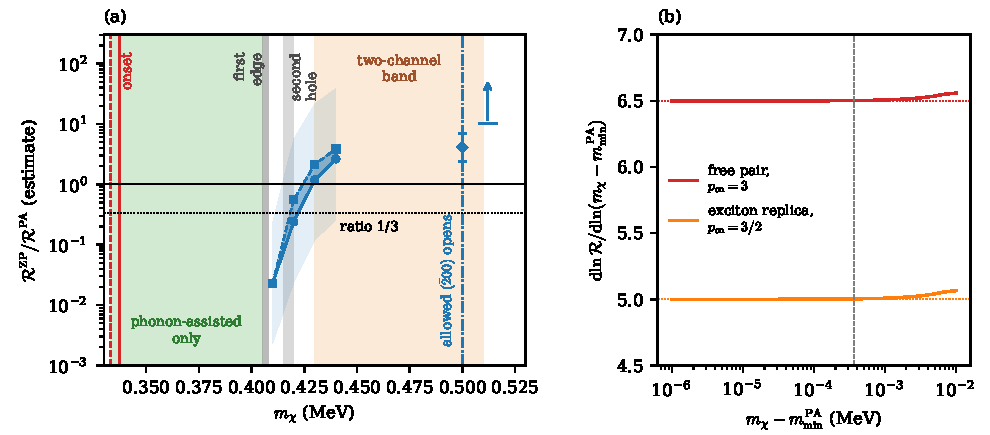
\includegraphics[width=\linewidth]{figures/ch13/fig13_9.pdf}
  \caption{Rates across the silicon window. (a)~Estimated ratio of the zero-phonon to the phonon-assisted electron-recoil rate against the dark-matter mass. Green band: phonon-assisted only, from the onsets (red: free pair \SI{0.3374}{MeV}, solid; exciton replica \SI{0.3332}{MeV}, dashed) to the first zero-phonon edge; gray bands: the first zero-phonon edge (0.405--\SI{0.408}{MeV}) and the edge of the second heavy hole (0.415--\SI{0.420}{MeV}). Blue points: the ratio with the second-hole edge at \SI{0.420}{MeV} (circles) and \SI{0.415}{MeV} (squares), each channel at the largest energy above the first edge that the mass reaches; dark band between them, light band the factor of ten of the phonon-assisted side. Diamond: the allowed $(\bar2\,0\,0)$ line at its opening, \SI{0.50}{MeV} (dash-dotted), with one or two conduction bands reached; bar and arrow: ratio of 10 or more from \SI{0.51}{MeV}. Black lines: ratio one and one third. Orange: the two-channel band. Estimates: phonon-assisted side from the measured cold absorption (\SI{20}{K} data~\cite{macfarlane1958fine}; the \SI{0.5}{K} fit of \cref{we:13-darkphoton-edge} changes the ratios by at most \SI{5}{\percent}) and a computed vertex form factor; zero-phonon side a Wannier--Mott continuum with computed vertices; between 0.44 and \SI{0.50}{MeV} no ratio has been evaluated. (b)~Local power of the model rate, $\dd\ln\mathcal{R}/\dd\ln(\mchi - m_{\mathrm{min}}^{\mathrm{PA}})$, for a loss function $Cx^{p_{\mathrm{on}}}$ above the computed transverse acoustic onset on the valley axis (PBE force constants of \cref{sec:5.2}), the standard halo (\cref{tab:1-shm}) and a heavy mediator, with the asymptotes $p_{\mathrm{on}} + 7/2$ of \cref{eq:13.9-medge} (dotted). Dashed: the mass at which the largest energy above threshold reaches \SI{1.3}{meV}, the end of the $x^3$ range of \cref{fig:13-paloss}.}
  \label{fig:13-window-rates}
\end{figure}

The phonon-assisted rate leads the electron recoil of silicon at least to about \SI{0.42}{MeV} and centrally to about \SI{0.43}{MeV}. From there to about \SI{0.51}{MeV} lies a two-channel band, in which the rates are comparable and neither can be quoted alone with confidence. Above about \SI{0.51}{MeV} the allowed zero-phonon line leads. The biases point both ways. The isotropic exciton mass underestimates the zero-phonon density of states by a factor 1.3 to 1.6, which makes the ratios too low. The form factor, more likely low than high, makes them too high; the second-hole vertex and the evaluation at the largest energy make the zero-phonon side an upper estimate. A rate computed from the amplitude on the same bins as the zero-phonon rate would settle all of it.

\subsection{Germanium and GaAs}\label{sec:13.9-ge-gaas}

The germanium window has a known lower end and an unknown upper end. Its onset, 0.2119 to \SI{0.2141}{MeV}, rests only on the gap, the position of L and the measured transverse acoustic branch (\cref{sec:13.1}); the computed PBE branch is \SI{13.5}{\percent} low at X and \SI{11.6}{\percent} low at L, so its $\omega_{\mathrm{TA}}(\vect{Q}^*) = \SI{6.70}{meV}$ on a $6^3$ grid is too soft by about as much. It places the onset at \SI{0.21380}{MeV} for a free pair and \SI{0.21264}{MeV} for the bound $1s$ exciton, with an estimated binding of \SI{4.0}{meV}. Both lie inside the bracket, and scaling the branch to the neutron data moves them by at most \SI{0.0003}{MeV}, so the softness does not reach the onset (\cref{app:E.14}). The zero-phonon edge is not known. PBE puts the conduction state at $\mathrm{\Gamma}$ below the L valley, so no scissor-corrected PBE calculation can locate it (\cref{app:E.1}), and the joint minimization on quasiparticle bands with spin--orbit coupling is open. The value \SI{0.32}{MeV} of \cref{sec:13.1}, from the parabola on the L axis, assumes a parabolic pair with the hole at $\mathrm{\Gamma}$, and it brackets the edge in neither direction. Only the joint minimum restricted to the axis, evaluated on the true bands, would be an upper value. The silicon result does not settle whether the germanium optimum leaves the axis. The [111] valley axis of germanium is already its heavy-hole direction, and the silicon optimum came from a hole moving into a flat direction away from the valley axis. What does carry over is that spin--orbit coupling must be in the bands, and that the hole must be free in the minimization. The selection rule differs as well. The mirror planes that contain a [111] axis are the diagonal planes of the $\{110\}$ family, which belong to $\bar43m$ and carry no fractional translation (\cref{app:C.17}); there is no glide phase, and on the L axis the vertex at the extrema does not vanish (\cref{sec:10.5-rules}). Whether the first zero-phonon state of germanium is weakly coupled has to be checked at its optimum. Until then germanium has a phonon-assisted onset, the onset exponent 3 for every branch (\cref{sec:13.3}), and no window.

GaAs is the control: a direct gap with its own phonon-assisted band, which in the parabolic description of the $\mathrm{\Gamma}$ pair runs from an onset of 0.433 to \SI{0.436}{MeV} to the opening of the zero-phonon channel through the L valleys, between 0.517 and \SI{0.560}{MeV} (\cref{sec:13.1}). Both ends of that bracket are rigorous for the given L energy; only the position of the edge between them needs bands. The top scales as $2E_{\mathrm{L}}/v_{\mathrm{max}}^2$, and for a detector the low-temperature L energy applies. That GaAs reproduces this band, and that its phonon-assisted rate is a small correction wherever a zero-phonon line is open, is the control that \cref{app:E.14} specifies.

\subsection{The silicon window in one table}\label{sec:13.9-table}

\Cref{tab:13-window} collects the window in two blocks: what two independent calculations or a symmetry argument with a numerical check establish, and what rests on one calculation or an estimate, or is open.

\begin{table}[tbp]
  \caption{The silicon window, with germanium and GaAs. Masses in MeV. Status: ``two independent calculations'', ``symmetry, confirmed numerically'', ``derivation'', ``one calculation'', ``measured data'', ``estimate'' (a model in which the phonon-assisted rate is known to a factor of ten either way, apart from the unsized pair channel), ``open''. Bands at the measured lattice constant with spin--orbit coupling, gap $\Eg(0) = \SI{1.170}{eV}$, halo of \cref{tab:1-shm}.}
  \label{tab:13-window}
  \centering\footnotesize\setlength{\tabcolsep}{3pt}
  \begin{tabular}{@{}>{\raggedright\arraybackslash}p{0.33\linewidth}>{\raggedright\arraybackslash}p{0.27\linewidth}>{\raggedright\arraybackslash}p{0.2\linewidth}>{\raggedright\arraybackslash}p{0.13\linewidth}@{}}
    \toprule
    Quantity & Value & Status & Section \\
    \midrule
    \multicolumn{4}{@{}l}{\emph{Established}} \\
    First zero-phonon edge, continuum & 0.405--0.408 (best 0.407); off the axis, $\{001\}$ mirror plane, tilt \SI{0.18}{rad} & two independent calculations & \cref{sec:13.9-edges} \\
    First zero-phonon edge, $1s$ line & 0.402--0.405 & two independent calculations & \cref{sec:13.9-edges} \\
    Second (mirror-even) heavy hole & from 0.415--0.420 & 0.415: two independent calculations; 0.420: estimate & \cref{sec:13.9-edges} \\
    Allowed $(\bar2\,0\,0)$ line opens & $\approx 0.50$ (X face); vertex at the class extremum $\sum_v|\rho_{cv}|^2 = 0.150$ & two independent calculations & \cref{sec:13.9-edges,sec:13.9-glide} \\
    Selection rule & first line second class by the glide; $(\bar2\,0\,0)$ class allowed; spin--orbit lift $3.6\times10^{-6}$ (axis), $1.3\times10^{-4}$ (plane) & symmetry, confirmed numerically & \cref{sec:13.9-glide} \\
    Order of the edges & onset $<$ first edge $<$ second hole $<$ allowed line & two independent calculations & \cref{sec:13.9-edges} \\
    \midrule
    \multicolumn{4}{@{}l}{\emph{Estimated or open}} \\
    Phonon-assisted onset & 0.3332 (exciton replica), 0.3374 (free pair) & one calculation & \cref{sec:13.1} \\
    Phonon-assisted rate leads & centrally to $\approx 0.43$ (0.424--0.428), at least to $\approx 0.42$ (0.418--0.421) & estimate & \cref{sec:13.9-rates} \\
    Two-channel band & 0.43--0.51 & estimate & \cref{sec:13.9-rates} \\
    Zero-phonon rate leads & above $\approx 0.51$ (ratio 2.4--7.0 at 0.50, $\ge 10$ pointwise from 0.51) & estimate & \cref{sec:13.9-rates} \\
    Screening correction relative to the optical calibration & 0.3--2.6 on $L^{\mathrm{PA}}$ (external factor and local-field wings); pair channel beyond the calibration not sized & estimate & \cref{sec:13.4,sec:13.9-rates} \\
    Rate and reach & $\sigmae \approx 3\times10^{-30}$--$3\times10^{-29}$ (0.36; the \SI{0.5}{K} fit extrapolated below \SI{1.206}{eV} carries half of it), $4\times10^{-32}\,\si{cm^2}$ (0.40), heavy mediator, \SI{1}{kg.yr}; power $p_{\mathrm{on}} + 7/2$ at the onset & estimate (factor 10 at 0.40; 15 at 0.36); power: derivation & \cref{sec:13.9-onset,sec:13.9-rates} \\
    Germanium & onset 0.2119--0.2141; zero-phonon edge not known & onset from measured data; edge open & \cref{sec:13.1,sec:13.9-ge-gaas} \\
    GaAs & phonon-assisted band 0.43 to 0.52--0.56 & estimate (parabolic $\mathrm{\Gamma}$ pair) & \cref{sec:13.1,sec:13.9-ge-gaas} \\
    \bottomrule
  \end{tabular}
\end{table}

\subsection{Nuisance table of the phonon-assisted sector}\label{sec:13.9-nuisances}

\Cref{tab:13-nuisances} collects the truncations and inputs of the chapter, each with its size and the section that treats it, in the classes of \cref{sec:8.8}.

\begin{table}[tbp]
  \caption{Nuisances of the phonon-assisted sector. Type in the classes of \cref{sec:8.8}: normalization, tilt (in $\omega$, in $q$ or in the dark-matter mass), threshold and new support. Basis of the size: ``computed'' (next order computed), ``model'' (next order computed in a model), ``est.''\ (parametric estimate), ``bound'' (only an inequality or two limits are known), ``named'' (no size). Sizes are for silicon unless another crystal is named. The last column gives the section where the item is treated.}
  \label{tab:13-nuisances}
  \centering\scriptsize\setlength{\tabcolsep}{3pt}
  \begin{tabular}{@{}>{\raggedright\arraybackslash}p{0.27\linewidth}>{\raggedright\arraybackslash}p{0.12\linewidth}>{\raggedright\arraybackslash}p{0.36\linewidth}>{\raggedright\arraybackslash}p{0.09\linewidth}>{\raggedright\arraybackslash}p{0.10\linewidth}@{}}
    \toprule
    Truncation or input & Type & Size & Basis & Section \\
    \midrule
    Transverse acoustic energy at $\vect{Q}^*$ (PBE branch \SI{8}{\percent} soft at X) & threshold & onset $+\SI{0.0004}{MeV}$ with the branch scaled to the neutron data; \SI{2.8e-4}{MeV} per meV & computed & \cref{sec:13.1} \\
    Exciton binding & threshold & phonon-assisted onset 0.3374 $\to$ \SI{0.3332}{MeV}; zero-phonon edge $-\SI{0.0028}{MeV}$ & computed & \cref{sec:13.1,sec:13.9} \\
    Fixed directions of $\vect{q}$, hole at the valence maximum & threshold & zero-phonon edge 0.405--0.408 against 0.420--\SI{0.425}{MeV} on the axis & computed & \cref{sec:13.1,sec:13.9} \\
    Spin--orbit coupling in the bands & threshold & first zero-phonon edge $+\SI{0.003}{MeV}$; on the axis $< \SI{0.0002}{MeV}$ & computed & \cref{sec:13.9} \\
    Band sum cut to empty bands & normali\-zation & $|M|^2$ off by a factor 1.6 to 2.4 in a two-band chain (two phase conventions of its phonon vertex) & model & \cref{sec:13.2} \\
    Adiabatic (Herzberg--Teller) amplitude & normali\-zation & \SI{1.6}{\percent} (TA), \SI{5.2}{\percent} (TO) at the edge; \SI{10}{\percent} when $E_{\mathrm{min}}(\vect{q}) - \omega$ falls to \SI{0.18}{eV} (TA) & est. & \cref{sec:13.2} \\
    Next order in the electron--phonon vertex ($n_g = 4$) & normali\-zation & $\theta_{\mathrm{ep}} = 0.010$--0.016 at the absorption edge; $\approx 0.2$ at the window edge & est.; bound & \cref{sec:13.3,sec:13.6} \\
    Tilt of the pair minimum, branch curvature & threshold & \SI{0.02}{meV} (TA), \SI{0.18}{meV} (LA) at \SI{1}{keV}; masses \SI{1}{\percent} & computed & \cref{sec:13.3} \\
    External screening $1/(\varepsilon_1^0)^2$ & normali\-zation & 1/30--1/38 at \SI{1}{keV}; 3.7--\SI{4.4}{\percent} across the window & computed & \cref{sec:13.4} \\
    Screening relative to the optical calibration: external model factor, local-field wings, pair channel & normali\-zation & 0.3--2.6 on $L^{\mathrm{PA}}$ for the external factor and the wings; pair ratio one in both solvable limits at exact pinning; residual from the \SI{0.2}{keV} spread of pair momenta and the range between the limits not sized & est.; named & \cref{sec:13.4,sec:13.9} \\
    Adiabatic local-density source & normali\-zation & about \SI{5}{\percent} of the pair term & est. & \cref{sec:13.4} \\
    Parabolic pockets, constant vertex (edge form) & tilt in $\omega$ & within \SI{15}{\percent} of the \SI{300}{K} data from 55 to \SI{490}{meV} above the gap; factor 2 at \SI{17}{meV} & computed & \cref{sec:13.5} \\
    Temperature of absorption data & tilt in $\omega$ & untransferred \SI{77}{K} data $\times2.3$--2.6, 1.7--1.9, 1.3--1.5, 1.1--1.3 at 15, 25, 50, \SI{100}{meV}; strength factor 0.88 (\SI{77}{K}), 0.61 (\SI{295}{K}); branch weights $\pm\SI{25}{\percent}$: $<\SI{1}{\percent}$ from \SI{77}{K} & computed & \cref{sec:13.5} \\
    Cold absorption data: \SI{0.5}{K} fit against \SI{20}{K} data & normali\-zation; tilt in $\omega$ & $\times20$ at \SI{1.20}{eV}, $\times2.1$ at \SI{1.25}{eV}, within \SI{5}{\percent} above \SI{1.37}{eV}; rate $\times9$ at \SI{0.36}{MeV}, $\times1.8$ at \SI{0.40}{MeV}; \SI{55}{\percent} of the \SI{0.36}{MeV} rate from the fit below its lowest data point & computed & \cref{sec:13.8,sec:13.9} \\
    Margin of the off-shell window, pair widths & tilt in $q$ & controlling ratios $\le 0.21$ at $\delta_{\mathrm{w}} = \SI{0.3}{eV}$; widths 3--\SI{21}{meV}; window to $|\vect{q}| = \SI{1.33}{keV}$ (parabolic), \SI{1.27}{keV} (computed bands) & est.; model & \cref{sec:13.6} \\
    Fano term & tilt & zero in Si and Ge; GaAs $\lesssim 0.3\varGamma/\delta_{\mathrm{F}}$, a few percent of first emissions moved & est. & \cref{sec:13.6} \\
    Nonadiabatic zero-point renormalization & threshold & \SI{8}{meV} on the gap; onset \SI{0.0023}{MeV} if the gap is built from a computed renormalization; with the measured gap only its variation across the zone, zero-phonon edge $\le\SI{0.002}{MeV}$ & computed; bound & \cref{sec:13.7} \\
    Exciton--phonon replicas beyond the two-pair sector & new support & no size & named & \cref{sec:13.8} \\
    Singlet against triplet pairs in axion-like absorption & normali\-zation & no pair channel in the triplet response, size not known; replica lines shifted by the exchange splitting, about $2\times10^{-3}$ of $E_x^b$ & named (open) & \cref{sec:13.8} \\
    Finite-$q$ form factor of the rate estimate & normali\-zation; tilt in $\mchi$ & factor 3; combined factor 6.5 at 0.38--\SI{0.43}{MeV}, quoted as 10 & est. & \cref{sec:13.9} \\
    Completeness of the plane-wave band sum ($f$-sum) & normali\-zation & 0.81 $\to$ 0.89 of $q^2/2m_e$ with 16 $\to$ 100 bands; nonlocal and truncation parts not separated & computed & \cref{sec:13.9} \\
    Zero-phonon side of the ratio (isotropic exciton mass, second-hole vertex) & normali\-zation & density of states low by 1.3--1.6; second-hole term an upper estimate & est. & \cref{sec:13.9} \\
    Spin--orbit lift of symmetry zeros & new support & zero-phonon ratio $\le 0.01$; longitudinal acoustic kink $<10^{-4}$ on the axis & computed; est. & \cref{sec:13.3,sec:13.9} \\
    \bottomrule
  \end{tabular}
\end{table}

For the rate in the window, three rows dominate: the finite-$q$ form factor of the estimate, a factor three either way and probably low; the screening correction relative to the optical calibration, whose pair-channel part no calculation sizes; and, near the onset, the spread of the cold data. Every threshold row is small in mass, a few thousandths of an MeV at most, and the order of the edges survives all of them together. What a threshold error costs, however, is not small near the onset, where \cref{eq:13.9-medge} raises it to the power $p_{\mathrm{on}} + 7/2$.

\subsection{Open problems}\label{sec:13.9-open}

The onset rests on one set of force constants, soft on exactly the branch that sets it, and a direct calculation of $\omega_{\mathrm{TA}}(\vect{Q}^*)$ at two lattice constants and with a second pseudopotential would verify it (\cref{app:E.14}). The end of the phonon-assisted lead, the width of the two-channel band and the mass from which the zero-phonon line leads follow from the ratio of the two rates computed on common bins, with the full amplitude on the phonon-assisted side and the mirror-plane cones, the second heavy hole and the X-face edge on the zero-phonon side (\cref{app:E.14}). The same calculation gives the rate and the reach with their controls: the optical limit, the symmetry zeros, the soft acoustic limit and the completeness of the band sum, whose plane-wave $f$-sum with a norm-conserving pseudopotential reaches 0.81 of $q^2/2m_e$ with 16 bands and 0.89 with 100 at $|\vect{q}| = 0.1$ to \SI{0.5}{\angstrom^{-1}}, the bands left out and the nonlocal term not yet separated. The pair channel beyond the optical calibration needs the supercell calculation of \cref{app:E.16}, with local fields in the supercell basis. Germanium needs quasiparticle bands with spin--orbit coupling for its zero-phonon edge and phonons that pass the neutron data on the transverse acoustic branch, and GaAs, the control of the whole chain, its band calculation and its rate with the polar vertex (\cref{app:E.14}).

One measurement would test the chain directly: the cold absorption edge of silicon within \SI{25}{meV} of its threshold, which no measurement at millikelvin temperatures covers. There the untransferred \SI{77}{K} data are off by more than a factor of two (\cref{sec:13.5}), and the two cold datasets of \cref{sec:13.9-rates} differ by a factor of twenty at \SI{1.20}{eV}.

\section*{Summary}

Dark matter lighter than about \SI{0.4}{MeV} cannot create an electron--hole pair in silicon on its own: where it deposits the gap it transfers about \SI{0.9}{keV}, and a pair with that momentum costs more than the gap. A phonon of about \SI{15}{meV} takes the missing crystal momentum (\cref{sec:13.1}). The lightest mass that creates a pair without a phonon is a joint minimum over the momentum transfer and the hole's crystal momentum. The lightest that creates one with a phonon is the kinematic floor with the gap raised by one phonon energy, at the wavevector the dark matter leaves for the phonon: \SI{0.3374}{MeV} for the free pair, \SI{0.3332}{MeV} for the exciton replica. The onset is insensitive to the band structure and rests on one phonon energy. Germanium has its onset at 0.212 to \SI{0.214}{MeV} from the measured transverse acoustic branch alone, and GaAs, though direct, has a phonon-assisted band of its own above \SI{0.433}{MeV}, because its light pair cannot absorb the momentum either.

The amplitude is of second order, one density vertex and one electron--phonon vertex on four paths (\cref{sec:13.2}). The exclusion principle turns the paths through filled states into exchange partners of the blocked ones, and on shell the amplitude becomes a one-electron sum over all bands, filled ones included; cutting it to empty bands is wrong by a factor of order one. The intraband terms cancel at $\vect{q} = 0$, so the amplitude starts at first order in $q$. It does not interfere with the zero-phonon line, whose final states have one phonon fewer. Its adiabatic form is the derivative of the zero-phonon transition density with respect to a frozen phonon, the Herzberg--Teller term, accurate to a few percent at the absorption edge.

Squared and summed, the amplitude gives the phonon-assisted structure factor and loss function, which enter the rate exactly as the zero-phonon ones do (\cref{sec:13.3}). Inside the off-shell window they are the whole electronic response; above the zero-phonon edge they add to it, and the $f$-sum rule they share forbids adding a bare zero-phonon rate to them without the renormalization of \cref{sec:13.7}. At its threshold the direction-averaged loss function rises as the cube of the energy above it, as the fourth power at the longitudinal acoustic kink, which a selection rule on the valley axis forbids, and as the power 3/2 for an exciton replica.

Screening acts on the density vertex and on the final pair (\cref{sec:13.4}). The external factor is one inverse macroscopic dielectric function for the whole amplitude, $1/30$ to $1/38$ in the loss function at \SI{1}{keV} in silicon, far from the optical $1/\varepsilon_\infty^2$. The pair channel screens at the pinned momentum of the final pair, the same for every $\vect{q}$; its size and sign are open, bracketed only by two solvable limits a factor of ten apart, and in both limits a measured optical edge calibrates it at every $\vect{q}$.

As $\vect{q} \to 0$ the loss function becomes phonon-assisted optical absorption, by the continuity equation applied to the second-order amplitude (\cref{sec:13.5}). The measured edge of silicon is its test: the Hall--Bardeen--Blatt form, with one fitted scale, lies within \SI{15}{\percent} of the \SI{300}{K} data over 55 to \SI{490}{meV} above the gap. Absorption data must be transferred to the temperature of a detector branch by branch. The inverse transfer is exact for branch-resolved spectra and ill-posed without them, and untransferred \SI{77}{K} data overstate the cold edge by more than a factor of two within 18 to \SI{23}{meV} of it.

Two kinds of small denominator threaten the amplitude (\cref{sec:13.6}). Soft acoustic phonons give finite amplitudes once the recoil, deformation and velocity terms of a Ward identity are kept, and inside the window the soft limit is never reached. Zero-phonon detunings fix the window. The phonon-assisted rate is a channel of its own only where every first-order transition is off shell by a margin, \SI{0.3}{eV} in silicon. The margin confines it to $|\vect{q}| \le \SI{1.33}{keV}$ on the valley axis in the parabolic description and \SI{1.27}{keV} with the computed bands. Beyond the window only totals are defined, with the Dyson convention, and the Fano term vanishes in silicon and germanium.

At finite temperature and zero point the bands are renormalized, and a special-displacement calculation contains the adiabatic sideband, which places the phonon-assisted onset one phonon energy too low (\cref{sec:13.7}). Between room temperature and \SI{10}{mK} the gap opens by \SI{46}{meV} and the onset moves from 0.324 to \SI{0.337}{MeV}; below a few kelvin the window does not move. The nonadiabatic part of the zero-point renormalization, \SI{8}{meV} on the silicon gap, is already in the measured gap, and only its variation across the zone, at most \SI{0.002}{MeV} on the zero-phonon edge, can move the window. Excitons with phonons add replica edges below the free-pair edges, each rising as a square root at fixed $\vect{q}$, with a completeness condition that reduces to the two-pair sector; at the optical edge of cold silicon they carry most of the absorption. The same vertices give the phonon-assisted absorption of dark photons, axion-like particles and scalars at the indirect edge; the dark photon has no new pair-plus-phonon amplitude at first order in its coupling (\cref{sec:13.8}).

In silicon the first zero-phonon edge lies at 0.405 to \SI{0.408}{MeV}, off the valley axis in a mirror plane, with its $1s$ line at 0.402 to \SI{0.405}{MeV} (\cref{sec:13.9}). The glide of the diamond structure forbids its vertex, so the first zero-phonon line is weak; the second heavy hole opens from 0.415 to \SI{0.420}{MeV}, and an allowed Umklapp line of full size opens at \SI{0.50}{MeV}, where the same glide inverts the rule. These edges, the rule and their order are established. Between the onset and the first edge the phonon-assisted rate is the only electron-recoil channel. Its rate rises from the onset as the power $p_{\mathrm{on}} + 7/2$ of the distance in mass, so that near the onset only the exponent is predicted. By an estimate normalized to the measured cold edge, with rates uncertain by a factor of ten apart from the pair channel's dependence on $q$, it leads to about \SI{0.43}{MeV}, the two channels share 0.43 to \SI{0.51}{MeV}, and the zero-phonon line leads above. The nuisances of the chapter are collected in \cref{tab:13-nuisances}. Germanium and GaAs need quasiparticle band calculations. Throughout, the dark matter coupled to the electron density, which does not act on spin; \cref{chap:14} turns to couplings that reach the spins of a magnet.

\printbibliography[heading=subbibliography]

\chapter{Magnetic excitations}\label{chap:14}
Every electron spin in silicon is paired in a bond, and flipping one costs the \SI{1.17}{eV} band gap. A dark-matter particle that couples to the spin of the electron rather than to its charge can therefore deposit energy in silicon only above that gap. In NiO the spins of the nickel ions are ordered, and a disturbance of that order, a magnon, costs anywhere from a few meV to \SI{118}{meV} in the spin-wave model of \cref{sec:7.1}, against a measured maximum of ${\sim}\SI{117}{meV}$. The same particle can emit magnons there as a slow neutron does, and a bosonic field with a spin coupling can be absorbed by the uniform precession of a ferromagnet, at a frequency that an applied magnetic field tunes. This chapter asks which magnetic targets respond to which couplings, how far measured neutron data can replace computed responses, when an ultralight field must be treated as a coherent classical wave rather than as a flux of particles, and which crystals respond differently to $\vect{q}$ and $-\vect{q}$ because they break inversion or time reversal. It builds on the spin waves of \cref{sec:7.1} and the spin rows of \cref{sec:8.1}, and \cref{fig:14-map} maps its sections; superconductors, which also have meV gaps, follow in \cref{chap:15}.

\begin{figure}[tbp]
  \centering
  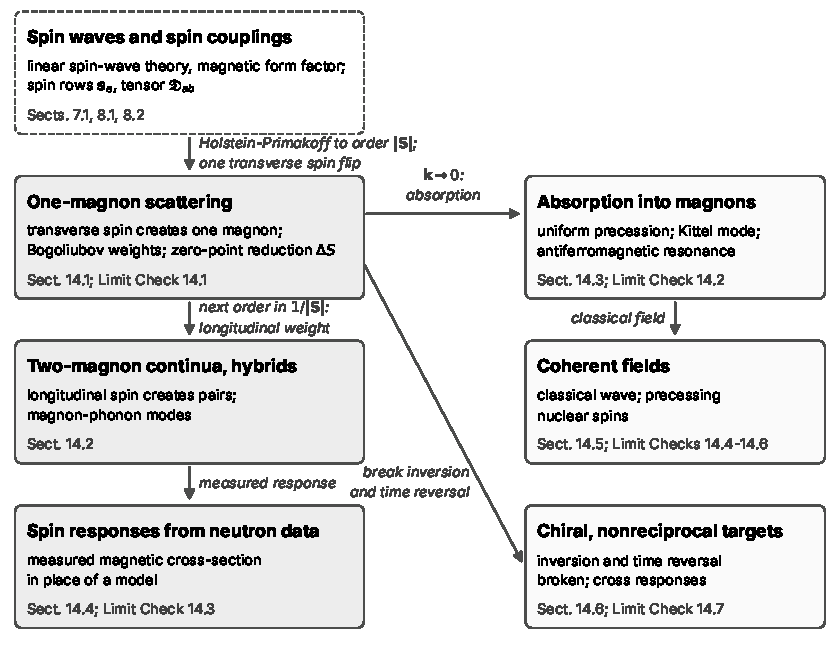
\includegraphics[width=0.85\linewidth]{figures/ch14/map14.pdf}
  \caption{Magnetic excitations, from the spin waves of \cref{sec:7.1} and the spin couplings of \cref{sec:8.1} to the targets of this chapter. A transverse spin coupling creates one magnon at leading order in $1/|\vect{S}|$, with the Bogoliubov weights of an antiferromagnet and a zero-point reduction of the ordered moment (\cref{sec:14.1}; \cref{lim:14.1a}). At the next order the longitudinal spin creates magnon pairs, and magnons mix with phonons (\cref{sec:14.2}). At vanishing momentum an absorbed boson drives the uniform precession (\cref{sec:14.3}; \cref{lim:14.3a}). The measured magnetic neutron cross-section can replace the model response (\cref{sec:14.4}; \cref{lim:14.4a}). A field whose modes are highly occupied acts as a coherent classical wave, which also drives precessing nuclear spins (\cref{sec:14.6}; \cref{lim:14.6a,lim:14.6b,lim:14.6c}). Targets that break both inversion and time reversal add chiral and nonreciprocal responses (\cref{sec:14.5}; \cref{lim:14.5a}).}
  \label{fig:14-map}
\end{figure}

\section{Magnon scattering}\label{sec:14.1}

A dark-matter particle of \SI{1}{MeV} that couples to the spin of the electron can transfer up to \SI{5.3}{keV} of momentum, twice the distance from $\Gamma$ to the ordering wavevector of NiO. It can therefore create a magnon anywhere in the zone, and \cref{sec:7.1} showed that the weight of that magnon depends strongly on where it lands: an antiferromagnet suppresses magnons near $\Gamma$ and enhances them near the ordering wavevector. Here we turn those weights into a rate, from the lightest mass that can emit a magnon above a few meV to masses where the magnetic form factor cuts it off, and we estimate the first correction in $1/|\vect{S}|$.

\subsection{One-magnon response of an antiferromagnet}

Every coupling to the electron spin in \cref{tab:8-operators}, from the contact interaction $\mathcal{O}_4 = \vect{S}_\chi\cdot\vect{S}_e$ to the velocity-dependent $\mathcal{O}_{12}$--$\mathcal{O}_{15}$, reaches the electrons through the spin row $\vect{s}_e(\vect{q})$ of \cref{eq:8.1-rows}, together with the spin current for some of them. In a magnetic insulator the spin density lives on the open shells of the ions, and \cref{eq:7.1-Fmag} replaces $\vect{s}_e(\vect{q})$ by $F^{\mathrm{mag}}(q)\sum_j\ee^{\ii\vect{q}\cdot\vect{r}_j}\vect{S}_j$, a sum over the ionic spins weighted by the magnetic form factor. We take ions whose orbital moment is quenched, as for Ni$^{2+}$; ions with an orbital moment add an orbital row (\cref{app:C.19}, \cref{sec:14.3}). At linear spin-wave order the transverse components $S^\pm$ are linear in the magnon operators and create one magnon, while $S^z$ is quadratic and creates two. The density row creates no magnon at all with the nuclei clamped, so the density--spin blocks of $S_{ab}$ vanish on one-magnon final states.

For the ferromagnet the one-magnon response is \cref{eq:7.1-Sfm}. For the antiferromagnet we need the matrix elements of $S^\pm(\vect{q})$ at any $\vect{q}$, not only near $\Gamma$ and near the ordering wavevector. \Cref{app:D.38} computes them from the operators of \cref{app:D.19}. A momentum transfer outside the zone of one sublattice is reduced by a reciprocal-lattice vector $\vect{G}$ of that sublattice, and the sites of sublattice B, displaced from those of A by $\vect{\delta}_0$, pick up the phase $\ee^{\ii\vect{G}\cdot\vect{\delta}_0} = \pm1$. That phase decides whether the two sublattices add in phase or against each other. Since $J^{\mathrm{ex}}_{\mathrm{AB}}(\vect{q})$ changes sign under a reciprocal vector of the sublattice that maps A onto B, the phase is carried automatically if the coefficients $A_{\vect{k}}$ and $B_{\vect{k}}$ of \cref{eq:7.1-Hk} are evaluated at the full momentum transfer rather than at its reduced value. The two degenerate magnons, one created by $S^-$ and one by $S^+$, precess in opposite senses and have equal weight. Inserted into \cref{eq:4.2-Sab}, their circular polarizations add to a linear one:
\begin{keyresult}[One-magnon spin response of a two-sublattice antiferromagnet]
\begin{equation}
  S_{ab}(\vect{q},\omega) = \frac{\pi|\vect{S}|}{\Omega_{\mathrm{ion}}}\,|F^{\mathrm{mag}}(q)|^2\,w^{\mathrm{M}}_{\vect{q}}\,\bigl(\delta_{ab} - \hat z_a\hat z_b\bigr)\,\delta\bigl(\omega - \omega^{\mathrm{M}}_{\vect{q}}\bigr), \qquad
  w^{\mathrm{M}}_{\vect{q}} = \frac{|\vect{S}|\,(A_{\vect{q}} - B_{\vect{q}})}{\omega^{\mathrm{M}}_{\vect{q}}} ,
  \label{eq:14.1-Safm}
\end{equation}
for $T = 0$, $\omega > 0$ and moments along $\pm\hat{\vect{z}}$, with $\Omega_{\mathrm{ion}}$ the volume per magnetic ion (for NiO the volume of the chemical primitive cell), $\omega^{\mathrm{M}}_{\vect{q}}$ of \cref{eq:7.1-afm}, and $A_{\vect{q}}$, $B_{\vect{q}}$ of \cref{eq:7.1-Hk} at the momentum transfer $\vect{q}$ itself.
\end{keyresult}
\noindent Compared to the ferromagnet of \cref{eq:7.1-Sfm}, two things change. The antisymmetric part $\ii\epsilon_{abc}\hat z_c$ is gone, because the antiferromagnet offers both senses of precession; it absorbs a transverse probe of either circular polarization. The weight is no longer one: $w^{\mathrm{M}}_{\vect{q}}$ is the factor $(u^{\mathrm{M}} \mp v^{\mathrm{M}})^2$ of \cref{eq:7.1-weights}, now written so that it holds at every $\vect{q}$ (\cref{eq:D.38-weight}). The matrix in brackets has eigenvalues $1$, $1$ and $0$, so \cref{eq:14.1-Safm} is positive semidefinite as long as $w^{\mathrm{M}}_{\vect{q}} \ge 0$, which is the stability condition $A_{\vect{q}} \ge |B_{\vect{q}}|$ of \cref{sec:7.1}.

The weight has a simple form near the two points where the magnon energy vanishes. Write $(\omega^{\mathrm{M}}_{\vect{q}})^2 = |\vect{S}|^2(A_{\vect{q}} - B_{\vect{q}})(A_{\vect{q}} + B_{\vect{q}})$. Near $\Gamma$ the sum $A + B$ tends to $2J^{\mathrm{ex}}_{\mathrm{AB}}(0)$, so
\begin{equation*}
  w^{\mathrm{M}}_{\vect{q}} \simeq \frac{\omega^{\mathrm{M}}_{\vect{q}}}{2|\vect{S}|J^{\mathrm{ex}}_{\mathrm{AB}}(0)} \quad (\vect{q} \to 0), \qquad
  w^{\mathrm{M}}_{\vect{q}} \simeq \frac{2|\vect{S}|J^{\mathrm{ex}}_{\mathrm{AB}}(0)}{\omega^{\mathrm{M}}_{\vect{q}}} \quad (\vect{q} \to \vect{Q}_{\mathrm{AF}}) ,
\end{equation*}
where near the ordering wavevector $\vect{Q}_{\mathrm{AF}}$, $(\pi/a)(1,1,1)$ in NiO, $B_{\vect{q}} \to -J^{\mathrm{ex}}_{\mathrm{AB}}(0)$ and the difference $A - B$ takes the large value instead. The scale is the exchange energy $2|\vect{S}|J^{\mathrm{ex}}_{\mathrm{AB}}(0) = 12|\vect{S}|(J_1 + J_2) = \SI{211.7}{meV}$ for NiO. A magnon of \SI{5}{meV} near $\Gamma$ carries $w^{\mathrm{M}} = 0.024$, a magnon of the same energy near $\vect{Q}_{\mathrm{AF}}$ carries 42, and a ferromagnet would give 1 to both. Physically, a long-wavelength transverse probe tries to tilt the two sublattices the same way, against the full exchange field. A probe that alternates in sign from one $(111)$ plane to the next tilts them in opposite directions, which rotates the Néel order as a whole and costs almost nothing. Evaluated within \SI{0.01}{\angstrom^{-1}} of either point, \cref{eq:14.1-Safm} agrees with these forms to \SI{0.02}{\percent}.

The exchange constants that fix $A_{\vect{q}}$, $B_{\vect{q}}$ and $\omega^{\mathrm{M}}_{\vect{q}}$ come, for NiO, from the neutron fit of \cref{eq:7.1-NiO}. For a magnet without such data they are computed in DFT~$+\,U$ by the energy-mapping, spin-spiral or Green's-function routes of \cref{app:E.9}, together with the single-ion anisotropies that open the gaps. \Cref{app:E.20-magnet} specifies these calculations for yttrium iron garnet (YIG), NiO, MnO, Cr$_2$O$_3$ and NiPS$_3$. The spread of the computed $J_2$ of NiO, 11 to \SI{27}{meV} (\cref{sec:7.1}), scales $\omega^{\mathrm{M}}$ but leaves $w^{\mathrm{M}}_{\vect{q}}$ unchanged, since the weight depends only on ratios of exchange constants. A ferrimagnet such as YIG, with 20 magnetic ions per primitive cell, needs the multi-sublattice Bogoliubov transformation in place of \cref{eq:14.1-Safm}.

\subsection{Rate formula and mass edge}

The rate follows from \cref{eq:8.2-spectrum} with $S_{ab}$ of \cref{eq:14.1-Safm} in the spin block. Since the response is proportional to $\delta_{ab} - \hat z_a\hat z_b$, the contraction picks out the part of the dark-matter tensor transverse to the moments,
\begin{equation}
  \sum_{a,b}\mathfrak{D}_{ab}S_{ab}(\vect{q},\omega) = \frac{\pi|\vect{S}|}{\Omega_{\mathrm{ion}}}\,|F^{\mathrm{mag}}(q)|^2\,w^{\mathrm{M}}_{\vect{q}}\,\bigl[\Tr\mathfrak{D} - \hat{\vect{z}}\cdot\mathfrak{D}\cdot\hat{\vect{z}}\bigr]\,\delta\bigl(\omega - \omega^{\mathrm{M}}_{\vect{q}}\bigr) ,
  \label{eq:14.1-contract}
\end{equation}
with $\mathfrak{D}_{ab}$ of \cref{eq:8.1-D} for the spin rows. For $\mathcal{O}_4$, the spin-dependent contact interaction, $\mathfrak{D}_{ab} = |c_4^{(e)}|^2\delta_{ab}/4$ for dark matter of spin $\frac12$, the bracket is $|c_4^{(e)}|^2/2$, and the rate does not depend on the direction of the moments. For $\mathcal{O}_6$, whose tensor is proportional to $q_aq_b$, the bracket is proportional to $1 - (\hat{\vect{q}}\cdot\hat{\vect{z}})^2$. Only the component of the momentum transfer perpendicular to the moments then creates a magnon, and the rate of a fixed crystal changes as the Earth turns the wind relative to the moments.

We present rates for $\mathcal{O}_4$ with a heavy mediator, $c_4^{(e)}$ independent of $q$. The reference cross-section is that of the same operator on a free electron, $\sigmae = \mu_{\chi e}^2\langle|\tilde V|^2\rangle/\pi$ as in \cref{sec:1.4}, with the average over both spins. Since $\langle|\vect{S}_\chi\cdot\vect{S}_e|^2\rangle = \sum_{a,b}\Tr(S^a_\chi S^b_\chi)\Tr(S^a_eS^b_e)/4 = 3/16$,
\begin{equation}
  \sigmae = \frac{3\mu_{\chi e}^2|c_4^{(e)}|^2}{16\pi} ,
  \label{eq:14.1-sigma}
\end{equation}
the definition of Trickle, Zhang and Zurek~\cite[Eq.~(11)]{trickle2020detecting} for this operator. The response depends on the direction of $\vect{q}$ through $w^{\mathrm{M}}_{\vect{q}}$ and $\omega^{\mathrm{M}}_{\vect{q}}$, and the full velocity kernel of \cref{app:A.8} gives the daily modulation of a fixed crystal. Averaged over the orientations of the crystal relative to the wind, the kernel is $\eta(\vmin)/2q$ per $\dd^3q/(2\pi)^3$ (\cref{eq:A.8-eta}). The rate per unit target mass above a threshold $\omega_{\mathrm{th}}$ is then
\begin{equation}
  \mathcal{R}(\omega_{\mathrm{th}}) = \frac{2\rho_\chi\sigmae|\vect{S}|}{3\,\mchi\rho_T\,\mu_{\chi e}^2\,\Omega_{\mathrm{ion}}}\int_0^{\infty}\dd q\,q\,\Bigl\langle|F^{\mathrm{mag}}(q)|^2\,w^{\mathrm{M}}_{\vect{q}}\,\eta\bigl(\vmin(q,\omega^{\mathrm{M}}_{\vect{q}})\bigr)\,\Theta\bigl(\omega^{\mathrm{M}}_{\vect{q}} - \omega_{\mathrm{th}}\bigr)\Bigr\rangle_{\hat{\vect{q}}} ,
  \label{eq:14.1-rate}
\end{equation}
with $\langle\cdots\rangle_{\hat{\vect{q}}}$ the average over the directions of $\vect{q}$ at fixed $q$ and $\vmin = \omega/q + q/2\mchi$ from \cref{eq:1.3-vmin}. The numerical factor collects $\pi|c_4^{(e)}|^2/2$ from \cref{eq:14.1-contract}, $16\pi\sigmae/3\mu_{\chi e}^2$ from \cref{eq:14.1-sigma}, and $1/4\pi^2$ from the angular integral. At $F^{\mathrm{mag}} = 1$, \cref{eq:14.1-rate} is the orientation average of the one-magnon rate of Trickle, Zhang and Zurek~\cite[Eqs.~(5)--(10)]{trickle2020detecting}, which their later work extends to all the operators of \cref{tab:8-operators}~\cite[Eqs.~(34) and~(38)]{trickle2022effective}. For one sublattice, $w^{\mathrm{M}} = 1$ and the bracket of the ferromagnet replaces that of \cref{eq:14.1-contract}; the result is their ferromagnetic rate~\cite[Eq.~(12)]{trickle2020detecting} with the spin density $|\vect{S}|/\Omega_{\mathrm{ion}}$.

The lightest mass that reaches a threshold follows from the linear dispersion near the gapless points, $\omega^{\mathrm{M}} \simeq c_{\mathrm{M}}|\vect{q} - \vect{k}_0|$ with $\vect{k}_0$ either $0$ or $\vect{Q}_{\mathrm{AF}}$ and $c_{\mathrm{M}}$ the magnon velocity. The momentum transfer from light dark matter is small, so only the region near $\Gamma$ counts. A magnon of momentum $q$ can be emitted if $c_{\mathrm{M}}q \le qv - q^2/2\mchi$, that is, for $q \le 2\mchi(v - c_{\mathrm{M}})$, and it lies above threshold for $q \ge \omega_{\mathrm{th}}/c_{\mathrm{M}}$. Both hold at the fastest speed when
\begin{equation}
  \mchi \ge \frac{\omega_{\mathrm{th}}}{2c_{\mathrm{M}}(v_{\mathrm{max}} - c_{\mathrm{M}})} ,
  \label{eq:14.1-mmin}
\end{equation}
the magnon analog of the acoustic edge of \cref{sec:11.1}. The speed $c_{\mathrm{M}} = 1.39\times10^{-4}$ of \cref{we:7-nio} is that of $J_2$ alone. With $J_1$ added, the model of \cref{fig:14-nio-rate} has speeds from $1.29\times10^{-4}$ to $1.36\times10^{-4}$ depending on direction, and the fastest puts the edge for $\omega_{\mathrm{th}} = \SI{5}{meV}$ at \SI{7.3}{keV}. Near the edge, however, the weight is $w^{\mathrm{M}} \simeq \omega_{\mathrm{th}}/2|\vect{S}|J^{\mathrm{ex}}_{\mathrm{AB}}(0) = 0.024$, and the antiferromagnet starts about forty times below a ferromagnet with the same magnon velocity.

\subsection{Zero-point spin reduction}

Linear spin-wave theory is the leading order of an expansion in $1/|\vect{S}|$, and for Ni$^{2+}$, with $|\vect{S}| = 1$, the expansion parameter $1/(2|\vect{S}|)$ is one half. The size of the first correction to \cref{eq:14.1-rate} follows from a sum rule. Each ionic spin has a fixed length, $\vect{S}_i^2 = |\vect{S}|(|\vect{S}| + 1)$, and the equal-time correlations of one site split that total into three parts. The static moment $\langle S^z_i\rangle^2$ scatters only elastically, into Bragg peaks. The transverse fluctuations $W_\perp = \langle S^x_iS^x_i + S^y_iS^y_i\rangle$ are, at linear order, all one-magnon weight. The longitudinal fluctuations $W_\parallel = \langle(S^z_i)^2\rangle - \langle S^z_i\rangle^2$ create magnon pairs. Each weight is the integral of the corresponding block of $S_{ab}$ over $\omega$ and over the zone. Together they fix how the spectral weight that a spin coupling can reach is divided between the one-magnon line, the two-magnon continuum and the elastic peaks, which deposit no energy.

In the Néel state the transverse fluctuations would be $|\vect{S}|$ and the longitudinal ones zero. The true ground state is not the Néel state. The pair term of \cref{eq:7.1-Hk} mixes in states with a deviation on each sublattice, and each mode leaves the zero-point deviation $(v^{\mathrm{M}}_{\vect{k}})^2$ on every site (\cref{sec:7.1}). \Cref{app:D.38} evaluates the three weights in this ground state, the longitudinal one by Wick's theorem:
\begin{keyresult}[Spin weights at linear spin-wave order]
\begin{equation}
  \begin{gathered}
  \Delta S = \frac{1}{N_{\mathrm{s}}}\sum_{\vect{k}}\bigl(v^{\mathrm{M}}_{\vect{k}}\bigr)^2, \qquad
  W_\perp = |\vect{S}|\,(1 + 2\Delta S), \qquad
  W_\parallel = \Delta S\,(1 + \Delta S), \\
  \frac{W_\parallel}{W_\perp} = \frac{\Delta S\,(1 + \Delta S)}{|\vect{S}|\,(1 + 2\Delta S)} ,
  \end{gathered}
  \label{eq:14.1-ratio}
\end{equation}
with the sum over the zone of one sublattice and the ordered moment $\langle S^z_i\rangle = |\vect{S}| - \Delta S$.
\end{keyresult}
\noindent The zero-point spin reduction $\Delta S$ depends on the lattice and on ratios of exchange constants, not on $|\vect{S}|$, so the ratio falls as $1/|\vect{S}|$ with a coefficient fixed by the lattice. For a ferromagnet $v^{\mathrm{M}}_{\vect{k}} = 0$, and both $\Delta S$ and $W_\parallel$ vanish: the fully polarized state is exact, and a longitudinal probe finds nothing to excite. For an antiferromagnet the zone average of the weight $w^{\mathrm{M}}_{\vect{q}}$ of \cref{eq:14.1-Safm} is $1 + 2\Delta S$, which is the same statement as $W_\perp$, and gives a check of any numerical evaluation of the one-magnon response.

The three weights violate the sum rule. Added up, $W_\perp + W_\parallel + \langle S^z_i\rangle^2$ exceeds $|\vect{S}|(|\vect{S}| + 1)$ by $\Delta S(1 + 2\Delta S)$, because linear spin-wave theory replaces the square roots of the Holstein--Primakoff transformation \cref{eq:7.1-HP} by their value at zero deviation. Holding the ordered moment and $W_\parallel$ at the values of \cref{eq:14.1-ratio}, the sum rule requires the transverse weight $(|\vect{S}| - \Delta S)(1 + 2\Delta S)$, and \cref{app:D.38} shows that the full square roots, evaluated in the same ground state, give exactly this value. At this order, with $\langle S^z_i\rangle$ and $W_\parallel$ held at their linear spin-wave values, the one-magnon weight of linear spin-wave theory is too large by the fraction $\Delta S/|\vect{S}|$. This is an estimate of the leading correction, not a bound. The corrected transverse operator also creates three magnons, which lowers the one-magnon part further; however, the change of the ground state at the same order, which moves $\langle S^z_i\rangle$ and $W_\parallel$ as well, is not part of the estimate. The one-magnon and two-magnon weights together, $(|\vect{S}| - \Delta S)(1 + 2\Delta S) + \Delta S(1 + \Delta S) = |\vect{S}|(1 + 2\Delta S) - \Delta S^2$, agree with the linear spin-wave one-magnon weight up to $\Delta S^2$. The first correction does not remove weight; it moves the fraction $\Delta S/|\vect{S}|$ of it from the one-magnon line into the two-magnon continuum, which lies at other energies for the same momentum transfer (\cref{sec:14.2}).

\begin{workedexample}{The zero-point spin reduction of NiO}\label{we:14-nio}
For the type-II order of NiO with the exchange constants \cref{eq:7.1-NiO}, $(v^{\mathrm{M}}_{\vect{k}})^2 = \frac12[A_{\vect{k}}(A_{\vect{k}}^2 - B_{\vect{k}}^2)^{-1/2} - 1]$ with $A_{\vect{k}}$ and $B_{\vect{k}}$ of \cref{eq:7.1-Hk}. We average it over a $100^3$ grid of the cube of side $4\pi/a$, the period of the reciprocal lattice of the nickel ions along each cube axis, which holds every wavevector of the zone twice, and find
\begin{equation*}
  \Delta S = 0.0784 .
\end{equation*}
The grid avoids the gapless points at $\Gamma$ and $\vect{Q}_{\mathrm{AF}}$, where $(v^{\mathrm{M}})^2$ diverges as the inverse distance; this singularity is integrable. The sum changes by $1.1\times10^{-4}$ from $60^3$ to $80^3$ points and by $5\times10^{-5}$ from $80^3$ to $100^3$, as the inverse square of the grid size, and extrapolates to 0.0785. With $J_1 = 0$ it is $0.0783$. The reason is that the next-nearest neighbors at $\pm a\hat{\vect{x}}$, $\pm a\hat{\vect{y}}$, $\pm a\hat{\vect{z}}$ link the fcc lattice into four interpenetrating simple-cubic lattices of side $a$, each a Néel antiferromagnet. Their zero-point reduction is Anderson's 0.078 for the simple-cubic antiferromagnet~\cite{anderson1952approximate}, and the weak $J_1$ barely changes it.

With $|\vect{S}| = 1$, the ordered moment is $|\vect{S}| - \Delta S = 0.9216$ of its classical value, and \cref{eq:14.1-ratio} gives
\begin{equation*}
  W_\perp = 1.157, \qquad W_\parallel = 0.0846, \qquad \frac{W_\parallel}{W_\perp} = \frac{0.0784 \times 1.0784}{1 \times 1.1569} = 0.0731 .
\end{equation*}
The sum rule requires $W_\perp = 0.9216 \times 1.1569 = 1.066$: at this order the one-magnon weight of linear spin-wave theory, and with it the rate \cref{eq:14.1-rate}, is high by about $\Delta S/|\vect{S}| = \SI{7.8}{\percent}$. The two-magnon continuum holds \SI{7.3}{\percent} of the linear spin-wave one-magnon weight, and the total, one-magnon plus two-magnon, is $0.995$ of it. The ratio $\Delta S/|\vect{S}| = 0.078$ is six times smaller than the expansion parameter $1/(2|\vect{S}|) = 0.5$. In three dimensions the zero-point motion of the spin waves is small, and the expansion in $1/|\vect{S}|$ converges faster than its parameter suggests.
\end{workedexample}

\Cref{lim:14.1a} sets the literature rate against these weights as $|\vect{S}|$ varies at the fixed lattice and exchange ratios of NiO, where $\Delta S = 0.078$ throughout.
\begin{limitbox}[One-magnon rate at linear spin-wave order][lim:14.1a]
$\varGamma(\vect{v}) = \int\frac{\dd^3q}{(2\pi)^3}\sum_{a,b}\mathfrak{D}_{ab}S_{ab}(\vect{q},\omega_{\vect{q}})$ with the one-magnon response \cref{eq:14.1-Safm} at $F^{\mathrm{mag}} = 1$, spectral weight $W_\perp = |\vect{S}|(1 + 2\Delta S)$ per ion~\cites[Eqs.~(5)--(12)]{trickle2020detecting}[Eq.~(38)]{trickle2022effective}.
\par\smallskip
{\centering
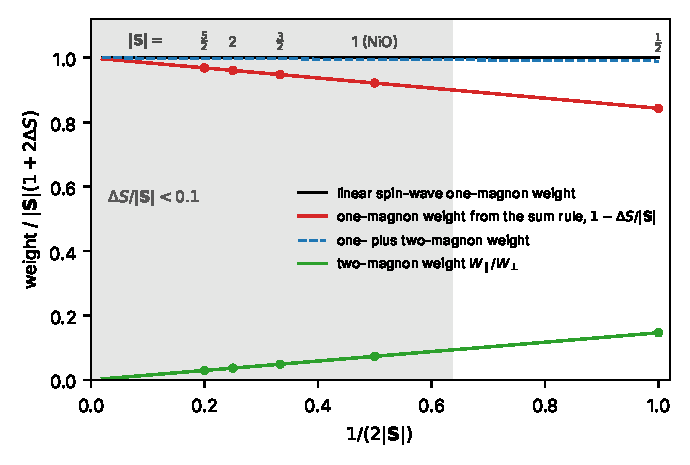
\includegraphics[width=0.92\linewidth]{figures/ch14/limit14_1a.pdf}
\captionof{figure}{Spectral weights of the spin of one magnetic ion against the expansion parameter $1/(2|\vect{S}|)$, in units of the one-magnon weight of linear spin-wave theory, $|\vect{S}|(1 + 2\Delta S)$, which the literature rate contains (black line). Red: the one-magnon weight that the sum rule $\vect{S}^2 = |\vect{S}|(|\vect{S}| + 1)$ requires, $1 - \Delta S/|\vect{S}|$. Green: the two-magnon weight $W_\parallel/W_\perp$ of \cref{eq:14.1-ratio}. Dashed: one- plus two-magnon weight, $1 - \Delta S^2/[|\vect{S}|(1 + 2\Delta S)]$. Lattice and exchange ratios of NiO (type-II order, $J_1/J_2 = -0.072$), zero-point reduction $\Delta S = 0.078$ from a $100^3$ grid; points at $|\vect{S}| = \frac12$, 1 (NiO), $\frac32$, 2 and $\frac52$. Gray: $\Delta S/|\vect{S}| < 0.1$, which holds for $|\vect{S}| \ge 0.78$.}\label{fig:14-limit-magnon}
\par}
\smallskip
For $|\vect{S}| = \frac12$ the one-magnon line is overcounted by about \SI{16}{\percent} at this order and the two-magnon weight reaches \SI{15}{\percent}, and the magnon interactions of the next order, which shift and broaden the magnons, are no longer small.
\end{limitbox}

For Mn$^{2+}$ and Fe$^{3+}$, with $|\vect{S}| = \frac52$, the same lattice gives a defect of \SI{3.1}{\percent} and a two-magnon weight of \SI{2.9}{\percent}. The rates of this section use the exchange fitted to the measured magnons, so the shift of the magnon energies by the quartic terms of the Holstein--Primakoff expansion is already absorbed into $J_1$ and $J_2$ (\cref{we:7-nio}). The division of weight in \cref{fig:14-limit-magnon} is not.

\subsection{The one-magnon rate of NiO}

The inputs for NiO are those of \cref{sec:7.1}: the exchange constants \cref{eq:7.1-NiO}, $|\vect{S}| = 1$, and $a = \SI{4.17}{\angstrom}$, so that the volume per nickel ion is $\Omega_{\mathrm{ion}} = a^3/4 = \SI{18.13}{\angstrom^3}$ and the density, from four formula units per cubic cell, is $\rho_T = \SI{6.84}{g.cm^{-3}}$. The form factor of Ni$^{2+}$, whose orbital moment is quenched, is the spin-only $F^{\mathrm{mag}} = \langle j_0(q)\rangle$ of \cref{eq:C.19-spinonly}. We take $\langle j_0\rangle$ from the tabulated fit $A\ee^{-\alpha s^2} + B\ee^{-\beta s^2} + C\ee^{-\gamma s^2} + D$ with $s = q/4\pi$, in \si{\angstrom^{-1}}, and the coefficients $(A, \alpha, B, \beta, C, \gamma, D) = (0.0163, 35.88, 0.3916, 13.22, 0.6052, 4.339, -0.0133)$~\cite[Sect.~4.4.5, Table~4.4.5.2]{anderson2006neutron}. It gives $|F^{\mathrm{mag}}|^2 = 0.84$ at $|\vect{Q}_{\mathrm{AF}}| = \SI{2.6}{keV}$ and 0.49 at \SI{5.3}{keV}, the largest momentum transfer of a \SI{1}{MeV} particle.

Two limits fix the shape of the rate before any integral is done. At the light end, \cref{eq:14.1-mmin} sets the edge, and above it the weight near $\Gamma$ grows in proportion to the magnon energy. At the heavy end, the momentum transfers sweep many zones and the magnon energies, at most \SI{118}{meV}, are negligible against $qv$. Then $\vmin \simeq q/2\mchi$, the direction average of $w^{\mathrm{M}}_{\vect{q}}$ over a shell that crosses many zones tends to its zone average $1 + 2\Delta S$, and $\int\dd q\,q\,\eta(q/2\mchi) = 4\mchi^2\int\dd u\,u\,\eta(u) = 2\mchi^2\langle v\rangle$, with $\langle v\rangle$ the mean speed of the dark matter in the laboratory. \Cref{eq:14.1-rate} at $F^{\mathrm{mag}} = 1$ becomes
\begin{equation}
  \mathcal{R} \simeq \frac{\rho_\chi}{\mchi}\,\frac{\langle v\rangle}{\rho_T\Omega_{\mathrm{ion}}}\,\sigmae\Bigl(\frac{\mchi}{\mu_{\chi e}}\Bigr)^2\,\frac{|\vect{S}|(1 + 2\Delta S)}{3/4} .
  \label{eq:14.1-inc}
\end{equation}
This is the flux of dark matter times the number of ions per unit mass times a cross-section per ion. At large $q$ the magnet looks like a gas of free spins, each with the transverse weight $W_\perp$ in place of the electron's $\frac34$, and with the reduced mass $\mu_{\chi e}$ replaced by $\mchi$ for a heavy target. With $\langle v\rangle = \SI{354}{km/s}$ for the halo of \cref{sec:1.2}, the integral \cref{eq:14.1-rate} at $F^{\mathrm{mag}} = 1$ is 0.96 of \cref{eq:14.1-inc} at \SI{3}{MeV} and 0.989 at \SI{10}{MeV}.

\begin{figure}[tbp]
  \centering
  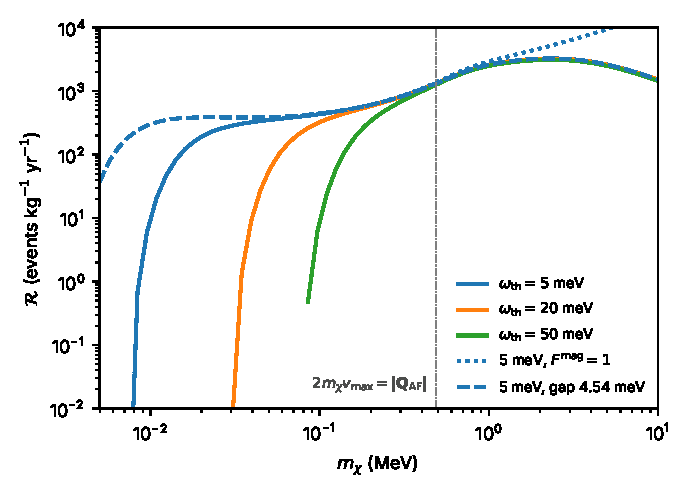
\includegraphics[width=0.75\linewidth]{figures/ch14/fig14_1.pdf}
  \caption{One-magnon rate of NiO per kilogram-year for dark matter with the spin-dependent contact interaction $\mathcal{O}_4 = \vect{S}_\chi\cdot\vect{S}_e$ (heavy mediator) at the reference cross-section $\sigmae = \SI{e-40}{cm^2}$ of \cref{eq:14.1-sigma}, against the dark-matter mass, from \cref{eq:14.1-rate}: $T = 0$, rate averaged over the orientations of the crystal relative to the dark-matter wind, standard halo of \cref{sec:1.2}. Solid: energy thresholds of 5, 20 and \SI{50}{meV}. Model: Heisenberg exchange $J_1 = -\SI{1.37}{meV}$, $J_2 = \SI{19.01}{meV}$ from neutron scattering, $|\vect{S}| = 1$, $a = \SI{4.17}{\angstrom}$, undistorted fcc lattice without anisotropy (gapless), linear spin-wave theory, magnetic form factor of Ni$^{2+}$. Dotted: \SI{5}{meV} threshold without the form factor, $F^{\mathrm{mag}} = 1$. Dashed: \SI{5}{meV} threshold with an easy-axis single-ion anisotropy added to $A_{\vect{k}}$ and chosen to put the zone-center gap at \SI{4.54}{meV}, the zone-center magnon of NiO seen in far-infrared absorption. Vertical line: the mass at which the largest momentum transfer, $2\mchi v_{\mathrm{max}}$, reaches the ordering wavevector, \SI{0.49}{MeV}.}
  \label{fig:14-nio-rate}
\end{figure}

\Cref{fig:14-nio-rate} shows the full integral. At a threshold of \SI{5}{meV} the rate rises from the edge, at \SI{7.4}{keV} on the mass grid of the figure, to 10 events per kilogram-year at \SI{10}{keV}, 280 at \SI{30}{keV} and 430 at \SI{100}{keV}, for $\sigmae = \SI{e-40}{cm^2}$. At \SI{100}{keV} all of it comes from momentum transfers within half the distance to $\vect{Q}_{\mathrm{AF}}$, where the weight is suppressed. Once the momentum transfer reaches the ordering wavevector the enhanced magnons there take over, and at \SI{1}{MeV}, where the rate is $2.6\times10^3$, only \SI{19}{\percent} of it comes from the region near $\Gamma$. The rate peaks at $3.2\times10^3$ near \SI{3}{MeV} and then falls, because the form factor removes the momentum transfers beyond the inverse radius of the $3d$ shell. It costs a factor 0.89 at \SI{1}{MeV}, and a factor 11.4 against $F^{\mathrm{mag}} = 1$ at \SI{10}{MeV}, where the rate is $1.5\times10^3$. The threshold matters only for the lightest masses. Above \SI{0.3}{MeV} the rates at 5, 20 and \SI{50}{meV} differ by less than \SI{20}{\percent}, since most of the rate then comes from magnons above \SI{50}{meV}. Below, the higher thresholds push the edge up to \SI{30}{keV} and \SI{85}{keV}. The second is later than \cref{eq:14.1-mmin} gives for \SI{50}{meV}, because the dispersion bends over below its maximum.

Near its gap the rate depends on what the Heisenberg model leaves out. Magnetic anisotropy, which \cref{sec:7.1} neglected, lifts the Goldstone modes at $\Gamma$ and $\vect{Q}_{\mathrm{AF}}$ to energies below \SI{5}{meV}. The undistorted $J_1$--$J_2$ model also has a third, accidental zero at $\mathrm{X} = (2\pi/a)(1,0,0)$, where $A_{\vect{k}} = B_{\vect{k}} = 6J_2 - 2J_1$; the weight vanishes there, and the rhombohedral distortion of the real crystal lifts it. Far-infrared absorption places a zone-center magnon of NiO at \SI{4.54}{meV}, the value used by Hutchings and Samuelsen~\cite{hutchings1972measurement} and quoted by dos Santos and collaborators~\cite[Sect.~III]{dossantos2026comparative}. We add an easy-axis term $K$ to $A_{\vect{k}}$, which keeps the form of \cref{eq:7.1-Hk}, and choose $K = \SI{0.0973}{meV}$ so that $|\vect{S}|[(A_0 + K)^2 - A_0^2]^{1/2} = \SI{4.54}{meV}$. With a \SI{5}{meV} threshold the rate then grows by a factor of 29 at \SI{10}{keV} and 1.35 at \SI{30}{keV}, and changes by less than \SI{3}{\percent} above \SI{100}{keV}. The gap puts magnons just above threshold at vanishing momentum, where the kinematics is easiest, and their weight $K^{1/2}/(2A_0)^{1/2}$ is set by the anisotropy. For dark matter lighter than about \SI{50}{keV}, the rate of NiO near its gap is set by its anisotropy. The real anisotropy is biaxial: it keeps the moments in the $(111)$ planes (\cref{fig:7-nio}) and gaps the two branches differently, so that only one of them reaches \SI{4.54}{meV} while the in-plane branch lies near \SI{0.6}{meV}. The one-constant model gaps both at \SI{4.54}{meV}, and the factor 29 is an upper value. The anisotropy enters through the uniform modes of \cref{sec:14.3} and the anisotropy constants of \cref{app:E.20-magnet}. Temperature adds thermal magnons with occupation $\ee^{-\omega^{\mathrm{M}}/T}$; at the gap of \SI{4.54}{meV} the exponent is $-5\times10^3$ at \SI{10}{mK} and $-53$ at \SI{1}{K}, and the zero-temperature response holds at any cryogenic operating point.

\section{Two-magnon continua and magnon--phonon modes}\label{sec:14.2}

In NiO, linear spin-wave theory assigns to the component of each nickel spin along the ordered moment a fluctuation weight equal to \SI{7}{\percent} of the one-magnon weight (\cref{we:14-nio}), carried entirely by magnon pairs, which that component creates (\cref{sec:7.1}). Each pair shares the momentum transfer between its two members, so at a small momentum transfer the pair can take up any energy from the one-magnon energy to twice the top of the magnon band, \SI{236}{meV}. The pairs thus decouple the energy deposited from the momentum transfer, which matters for the lightest dark matter. In the effective theory of gapless antiferromagnetic magnons, the two-magnon channel extends the projected reach of NiO, MnO and Cr$_2$O$_3$ down to masses of about \SI{1}{keV}~\cite{esposito2023optimal}. The lattice adds a second correction. Through spin--orbit coupling a strain changes the magnetic anisotropy energy, and a magnon and a phonon of the same wavevector and energy mix into hybrid modes. Together with the one-magnon weight defect of \cref{sec:14.1}, the pairs, their final-state interaction and the hybrids are the corrections in $1/|\vect{S}|$ and in the magnetoelastic coupling to the one-magnon rate, and for NiO we size each.

\subsection{Two-magnon amplitude and response}\label{sec:14.2-amp}

Take the two-sublattice antiferromagnet of \cref{sec:7.1}, with the moments along $\pm\hat{\vect{z}}$, and the longitudinal ionic spin at wavevector $\vect{q}$, $S^z(\vect{q}) = \sum_j\ee^{\ii\vect{q}\cdot\vect{r}_j}S^z_j$. On sublattice A, $S^z_i = |\vect{S}| - d^\dagger_{\mathrm{A}i}d_{\mathrm{A}i}$, and on B, $S^z_j = -|\vect{S}| + d^\dagger_{\mathrm{B}j}d_{\mathrm{B}j}$, exactly, by \cref{eq:7.1-HP}. The constants give the magnetic Bragg peaks, at $\omega = 0$, and deposit no energy. The rest is bilinear in the bosons. With the Fourier convention of \cref{sec:7.1} on each sublattice, the lattice sums give
\begin{equation*}
  S^z(\vect{q}) = -\sum_{\vect{k}}d^\dagger_{\mathrm{A}\vect{k}}\,d_{\mathrm{A},\vect{k}-\vect{q}} + \sum_{\vect{k}}d^\dagger_{\mathrm{B}\vect{k}}\,d_{\mathrm{B},\vect{k}+\vect{q}} + (\text{Bragg}) ,
\end{equation*}
with $\vect{k}$ over the $N_{\mathrm{s}}$ wavevectors of the zone of one sublattice. Now insert the inverse Bogoliubov transformation \cref{eq:D.19-inverse}, $d_{\mathrm{A}\vect{k}} = u^{\mathrm{M}}_{\vect{k}}a_{\vect{k}1} - v^{\mathrm{M}}_{\vect{k}}a^\dagger_{\vect{k}2}$ and $d_{\mathrm{B}\vect{k}} = u^{\mathrm{M}}_{\vect{k}}a_{\vect{k}2} - v^{\mathrm{M}}_{\vect{k}}a^\dagger_{\vect{k}1}$. At $T = 0$ only the terms with two creation operators survive acting on the magnon vacuum $|0\rangle$. The A term contributes $u^{\mathrm{M}}_{\vect{k}}v^{\mathrm{M}}_{\vect{k}-\vect{q}}\,a^\dagger_{\vect{k}1}a^\dagger_{\vect{k}-\vect{q},2}$, and the B term, after the relabeling $\vect{k} + \vect{q} \to \vect{k}$, contributes $-v^{\mathrm{M}}_{\vect{k}}u^{\mathrm{M}}_{\vect{k}-\vect{q}}$ times the same pair. Hence
\begin{equation}
  S^z(\vect{q})|0\rangle = \sum_{\vect{k}}\mathcal{A}^{\mathrm{2m}}_{\vect{k}}(\vect{q})\,a^\dagger_{\vect{k}1}a^\dagger_{\vect{k}-\vect{q},2}|0\rangle , \qquad
  \mathcal{A}^{\mathrm{2m}}_{\vect{k}}(\vect{q}) = u^{\mathrm{M}}_{\vect{k}}v^{\mathrm{M}}_{\vect{k}-\vect{q}} - v^{\mathrm{M}}_{\vect{k}}u^{\mathrm{M}}_{\vect{k}-\vect{q}} ,
  \label{eq:14.2-amp}
\end{equation}
apart from the Bragg term. The first magnon carries the crystal momentum $\vect{k}$ and lowers the total $S^z$ by one; the second carries $\vect{q} - \vect{k}$, since $a_{\vect{k}2}$ destroys $-\vect{k}$ in the convention of \cref{sec:7.1}, and raises $S^z$ by one. The pair has the momentum $\vect{q}$ and no net spin, as a longitudinal operator requires. The wavevector $\vect{k} - \vect{q}$ may leave the zone of one sublattice. We then compute $u^{\mathrm{M}}$ and $v^{\mathrm{M}}$ at that wavevector from $A_{\vect{k}}$ and $B_{\vect{k}} = J^{\mathrm{ex}}_{\mathrm{AB}}(\vect{k})$ with its sign. Since $J^{\mathrm{ex}}_{\mathrm{AB}}$ changes by at most a sign under a reciprocal vector of the sublattice, $v^{\mathrm{M}}$ does too, and $|\mathcal{A}^{\mathrm{2m}}_{\vect{k}}|^2$ does not depend on which representative is used.

A ferromagnet has $v^{\mathrm{M}} \equiv 0$ and no amplitude, and at $T = 0$ no inelastic longitudinal response at all, beyond linear order as well (\cref{sec:14.1}). In an antiferromagnet the amplitude vanishes at $\vect{q} = 0$, where $u_{\vect{k}}v_{\vect{k}} - v_{\vect{k}}u_{\vect{k}} = 0$, and at every reciprocal vector of the lattice of magnetic ions, where $S^z(\vect{q})$ is the total $S^z$, which commutes with $H_{\mathrm{H}}$ and creates nothing. For small $\vect{q}$, with $u^{\mathrm{M}} = \cosh\theta_{\vect{k}}$ and $v^{\mathrm{M}} = \sinh\theta_{\vect{k}}$, the amplitude is $\mathcal{A}^{\mathrm{2m}}_{\vect{k}} = \sinh(\theta_{\vect{k}-\vect{q}} - \theta_{\vect{k}}) \simeq -\vect{q}\cdot\nabla_{\vect{k}}\theta_{\vect{k}}$, and the weight grows as $q^2$. Near the ordering wavevector $v^{\mathrm{M}}_{\vect{k}-\vect{q}}$ has the opposite sign to $v^{\mathrm{M}}_{\vect{k}}$, the two terms add, and the amplitude approaches $2u^{\mathrm{M}}_{\vect{k}}v^{\mathrm{M}}_{\vect{k}} = \sinh2\theta_{\vect{k}}$, its largest value. Physically, $S^z(\vect{q})$ near the ordering wavevector measures the fluctuation of the staggered moment, which the zero-point motion of the spin waves makes large.

The response follows as in \cref{sec:7.1}. The electron spin density along the moments is $s_{e,z}(\vect{q}) = F^{\mathrm{mag}}(q)S^z(\vect{q})$ by \cref{eq:7.1-Fmag}. The pair states of \cref{eq:14.2-amp} are orthonormal, and each appears once in the sum over $\vect{k}$. With $N = 2N_{\mathrm{s}}$ magnetic ions, $\Omega_{\mathrm{ion}}$ the volume per ion and $\Vol = N\Omega_{\mathrm{ion}}$, \cref{eq:4.2-Sab} gives:
\begin{keyresult}[Two-magnon spin response of a collinear antiferromagnet]
\begin{equation}
  S^{(2\mathrm{m})}_{zz}(\vect{q},\omega) = \frac{2\pi}{\Omega_{\mathrm{ion}}}\,|F^{\mathrm{mag}}(q)|^2\,\frac{1}{2N_{\mathrm{s}}}\sum_{\vect{k}}\bigl|\mathcal{A}^{\mathrm{2m}}_{\vect{k}}(\vect{q})\bigr|^2\,\delta\bigl(\omega - \omega^{\mathrm{M}}_{\vect{k}} - \omega^{\mathrm{M}}_{\vect{k}-\vect{q}}\bigr) ,
  \label{eq:14.2-S2m}
\end{equation}
for $T = 0$ and $\omega > 0$, with $z$ along the moments and $\mathcal{A}^{\mathrm{2m}}$ of \cref{eq:14.2-amp}. Its weight and that of the one-magnon line at the same $\vect{q}$ are in the ratio $w_\parallel(\vect{q})/w_\perp(\vect{q})$ of the weights per ion
\begin{equation}
  w_\parallel(\vect{q}) = \frac{1}{2N_{\mathrm{s}}}\sum_{\vect{k}}\bigl|\mathcal{A}^{\mathrm{2m}}_{\vect{k}}(\vect{q})\bigr|^2 , \qquad
  w_\perp(\vect{q}) = |\vect{S}|\,w^{\mathrm{M}}_{\vect{q}} ,
  \label{eq:14.2-wpar}
\end{equation}
with $w^{\mathrm{M}}_{\vect{q}}$ the one-magnon weight of \cref{eq:14.1-Safm}.
\end{keyresult}
\noindent Here $w_\perp$ is the $\omega$-integral of $S_{xx} + S_{yy}$ in units of $(2\pi/\Omega_{\mathrm{ion}})|F^{\mathrm{mag}}|^2$. The one-magnon weight is of order $|\vect{S}|$ and the two-magnon weight of order $|\vect{S}|^0$, since the Bogoliubov coefficients do not depend on $|\vect{S}|$: the pairs are a correction of relative order $1/|\vect{S}|$. \Cref{eq:14.2-S2m} is the longitudinal structure factor that Huberman and collaborators compared with the two-magnon continuum of the square-lattice antiferromagnet Rb$_2$MnF$_4$ measured by neutron scattering~\cite[Eq.~(5)]{huberman2005two}. A dark-matter model enters through $\mathfrak{D}_{zz}S^{(2\mathrm{m})}_{zz}$ in \cref{eq:8.2-spectrum}, in the frame of the moments. For a coupling isotropic in the electron spin, $\mathfrak{D}_{ab} \propto \delta_{ab}$, the two-magnon and one-magnon parts of $\sum_a\mathfrak{D}_{aa}S_{aa}$ at fixed $\vect{q}$ are in the ratio $w_\parallel/w_\perp$, whatever the direction of the moments in each domain.

Averaged over $\vect{q}$, $v^{\mathrm{M}}_{\vect{k}-\vect{q}}$ takes both signs equally often, the cross term of $|\mathcal{A}^{\mathrm{2m}}|^2$ drops out, and with $\langle(u^{\mathrm{M}})^2\rangle = 1 + \Delta S$ and $\langle(v^{\mathrm{M}})^2\rangle = \Delta S$, where $\Delta S$ is the zero-point spin reduction of \cref{sec:14.1}, the average of $w_\parallel$ is $\frac12\cdot2(1 + \Delta S)\Delta S = W_\parallel$, while the average of $w_\perp$ is $|\vect{S}|(1 + 2\Delta S) = W_\perp$. \Cref{eq:14.2-wpar} thus resolves the ratio $W_\parallel/W_\perp$ of \cref{sec:14.1} in momentum transfer, which is what a rate needs, since light dark matter samples only small $q$.

\Cref{fig:14-weights} shows the two weights of NiO in linear spin-wave theory with the exchange constants of \cref{eq:7.1-NiO}. At small $q$ along $[111]$ the one-magnon weight rises as $w_\perp \simeq 0.29\,qa$, and the two-magnon weight as $w_\parallel \simeq 0.015\,(qa)^2$, so the ratio vanishes linearly. At $\vect{q} = (\frac14,\frac14,\frac14)2\pi/a$, a momentum transfer of \SI{1.29}{keV}, $w_\perp = 1.00$ and $w_\parallel = 0.081$; along $[111]$ the ratio $w_\parallel/w_\perp$ peaks at 0.082 near \SI{1.4}{keV} and stays below 0.05 under \SI{0.5}{keV}. Toward the ordering wavevector $w_\perp$ diverges while $w_\parallel$ stays finite, near 0.25, and the ratio falls again, averaging over the zone to the $W_\parallel/W_\perp$ of \cref{we:14-nio}.

\begin{figure}[tbp]
  \centering
  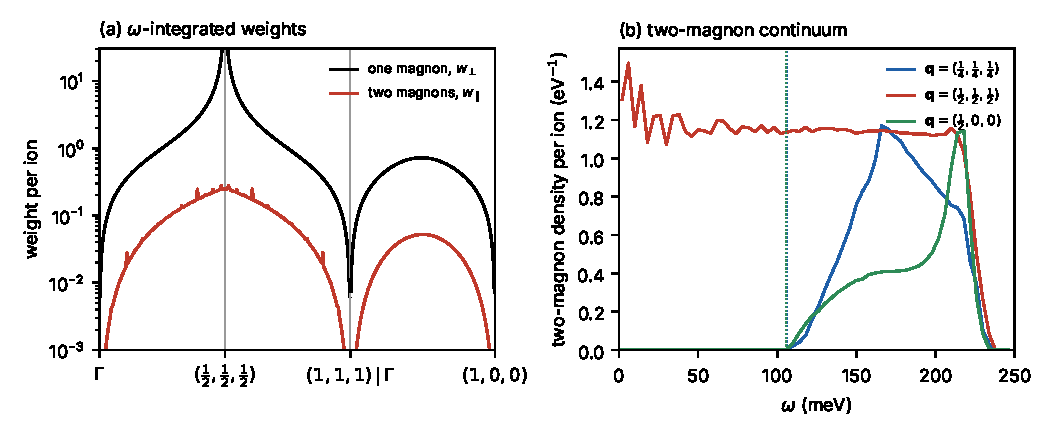
\includegraphics[width=\linewidth]{figures/ch14/fig14_2.pdf}
  \caption{One- and two-magnon weights of NiO in linear spin-wave theory: Heisenberg model with $J_1 = \SI{-1.37}{meV}$ and $J_2 = \SI{19.01}{meV}$ (antiferromagnetic $J^{\mathrm{ex}} > 0$, pairs counted once), $|\vect{S}| = 1$, type-II order on the undistorted fcc lattice, no anisotropy, $T = 0$, magnetic form factor set to one. (a) Weights per ion, integrated over energy, of the transverse one-magnon response, $w_\perp$ (both branches), and of the longitudinal two-magnon response, $w_\parallel$. The path runs along $[111]$ from $\Gamma$ through the ordering wavevector $(\frac12,\frac12,\frac12)$ to $(1,1,1)$, which is equivalent to $\Gamma$, and from $\Gamma$ to $(1,0,0)$; wavevectors in units of $2\pi/a$, $a = \SI{4.17}{\angstrom}$. Both vanish at $\Gamma$ and $(1,1,1)$, where the total longitudinal spin is conserved; $w_\perp$ diverges at the ordering wavevector and vanishes at $(1,0,0)$, a soft point of the undistorted model, where $w_\parallel$ is small and would vanish for $J_1 = 0$. (b) Two-magnon density per ion, $(\Omega_{\mathrm{ion}}/2\pi)S^{(2\mathrm{m})}_{zz}/|F^{\mathrm{mag}}|^2$, against energy at three wavevectors (4-meV bins, $3\times10^6$ sampled wavevectors). The dotted lines mark the one-magnon energy at the same wavevector, zero at the ordering wavevector.}
  \label{fig:14-weights}
\end{figure}

\subsection{Kinematic boundaries of the continuum}\label{sec:14.2-edges}

At fixed $\vect{q}$, \cref{eq:14.2-S2m} has weight only between the lower edge $\omega_-(\vect{q}) = \min_{\vect{k}}(\omega^{\mathrm{M}}_{\vect{k}} + \omega^{\mathrm{M}}_{\vect{k}-\vect{q}})$ and the upper edge $\omega_+(\vect{q}) = \max_{\vect{k}}(\omega^{\mathrm{M}}_{\vect{k}} + \omega^{\mathrm{M}}_{\vect{k}-\vect{q}}) \le 2\max_{\vect{k}}\omega^{\mathrm{M}}_{\vect{k}}$. Putting one magnon at a zero of the dispersion, $\vect{k} = 0$, shows that $\omega_- \le \omega^{\mathrm{M}}_{\vect{q}}$; for a dispersion that rises linearly and then bends over, as in NiO, $\omega^{\mathrm{M}}_{\vect{k}} + \omega^{\mathrm{M}}_{\vect{k}-\vect{q}} \ge \omega^{\mathrm{M}}_{\vect{q}}$, and the lower edge is the one-magnon branch itself. The weight at the lower edge is small, because $|\mathcal{A}^{\mathrm{2m}}|^2$ diverges only as $1/k$ near $\vect{k} = 0$ while the phase space closes as $k^2$. In NiO the continuum at $(\frac14,\frac14,\frac14)2\pi/a$ runs from the one-magnon energy, \SI{105.8}{meV}, to \SI{236}{meV}, and at the ordering wavevector it runs from zero, where both magnons sit at zeros of the dispersion, to \SI{236}{meV} (\cref{fig:14-weights}b). The anisotropy that \cref{eq:7.1-heis} leaves out gaps the magnons by less than \SI{5}{meV} in NiO; a gap $\omega_{\mathrm{gap}}$ in both branches moves the lower edge to at least $2\omega_{\mathrm{gap}}$ and leaves the rest of the continuum in place. At $T > 0$ the operator $S^z$ also scatters a thermal magnon into another, with weight proportional to the occupation, which vanishes for temperatures far below the gap.

The continuum changes what dark matter can deposit. Energy conservation, \cref{eq:1.3-omegaq}, allows $\omega \le qv - q^2/2\mchi$, and the one-magnon channel opens at \cref{eq:14.1-mmin}. A pair, however, can take any energy in its continuum, which at small $q$ reaches far above $c_{\mathrm{M}}q$, so the only limit is \cref{eq:1.3-omegamax}, $\omega \le \frac12\mchi v^2$, reached at $q = \mchi v$. For a threshold $E_{\mathrm{th}}$ the two-magnon channel opens at the threshold mass \cref{eq:1.3-mmin}, $2E_{\mathrm{th}}/v_{\mathrm{max}}^2$. The one-magnon channel opens at $E_{\mathrm{th}}/[2c_{\mathrm{M}}(v_{\mathrm{max}} - c_{\mathrm{M}})]$, larger by the factor
\begin{equation}
  \frac{v_{\mathrm{max}}^2}{4c_{\mathrm{M}}(v_{\mathrm{max}} - c_{\mathrm{M}})} \simeq \frac{v_{\mathrm{max}}}{4c_{\mathrm{M}}} \qquad (c_{\mathrm{M}} \ll v_{\mathrm{max}}) .
  \label{eq:14.2-mratio}
\end{equation}
For NiO, with the fastest magnon speed of the $J_1$--$J_2$ model, $c_{\mathrm{M}} = 1.36\times10^{-4}$ (\cref{sec:14.1}), the factor is 5.1: at $E_{\mathrm{th}} = \SI{1}{meV}$ one magnon needs $\mchi \ge \SI{1.46}{keV}$ and two magnons $\mchi \ge \SI{0.285}{keV}$. NiO gains little because its magnons are fast, $c_{\mathrm{M}} \approx v_{\mathrm{max}}/19$; a magnet with slower magnons gains in proportion to $v_{\mathrm{max}}/c_{\mathrm{M}}$. Near the two-magnon edge, however, the momentum transfer $q = \mchi v_{\mathrm{max}}$ is below an eV, $(qa)^2 \sim 10^{-6}$, and the $q^2$ law of $w_\parallel$ makes the rate tiny there; the linear law of $w_\perp$ suppresses the one-magnon rate near its own edge less. The reach in mass thus lies well above the kinematic edge, more so for the pair.

\subsection{Final-state interactions and bound pairs}\label{sec:14.2-fsi}

The two magnons of \cref{eq:14.2-amp} do not move independently. Linear spin-wave theory dropped the terms of fourth order in the bosons, and they act between the members of the pair. For an antiparallel bond the longitudinal part $S^z_iS^z_j = (|\vect{S}| - n_{\mathrm{A}i})(-|\vect{S}| + n_{\mathrm{B}j})$ contains $-n_{\mathrm{A}i}n_{\mathrm{B}j}$: two deviations on neighboring sites lower the energy of the bond by $J^{\mathrm{ex}}_{ij}$, an attraction. The next term of the square root in \cref{eq:7.1-HP}, $S^+_i \simeq (2|\vect{S}|)^{1/2}[1 - n_{\mathrm{A}i}/4|\vect{S}|]d_{\mathrm{A}i}$, adds quartic terms of the same size. The quadratic Hamiltonian is of order $J^{\mathrm{ex}}|\vect{S}|$ and the quartic one of order $J^{\mathrm{ex}}$, so the interaction is smaller than the energies of the pair by a factor of order $1/|\vect{S}|$. In the ferromagnetic chain of \cref{we:7-chain} the attraction is visible directly: on a ring of ten spins $\frac12$ the lowest level of total spin $N/2 - 2$ lies at $0.328|J^{\mathrm{ex}}|$, below the $0.382|J^{\mathrm{ex}}|$ of the cheapest pair of free magnons.

At leading order in $1/|\vect{S}|$ the interaction acts in the pair channel only. Let $U^{\mathrm{mm}}_{\vect{q}}(\vect{k},\vect{k}')$ be the matrix element of the quartic Hamiltonian between the pair states $a^\dagger_{\vect{k}1}a^\dagger_{\vect{k}-\vect{q},2}|0\rangle$ and $a^\dagger_{\vect{k}'1}a^\dagger_{\vect{k}'-\vect{q},2}|0\rangle$ of total momentum $\vect{q}$, and $\GF^{\mathrm{2m}}_{\vect{q}}(\omega)$ the free pair propagator, a diagonal matrix in $\vect{k}$ with elements $1/(\omega - \omega^{\mathrm{M}}_{\vect{k}} - \omega^{\mathrm{M}}_{\vect{k}-\vect{q}} + \ii0^+)$. Since $-\Imag\GF^{\mathrm{2m}}_{\vect{q}} = \pi\delta(\omega - \omega^{\mathrm{M}}_{\vect{k}} - \omega^{\mathrm{M}}_{\vect{k}-\vect{q}})$, \cref{eq:14.2-S2m} is $-(2/\Vol)|F^{\mathrm{mag}}|^2\Imag[\mathcal{A}^\dagger\GF^{\mathrm{2m}}_{\vect{q}}\mathcal{A}]$, with $\mathcal{A}$ the vector of amplitudes \cref{eq:14.2-amp}. Repeated scattering of the pair sums the ladder series $\GF + \GF U\GF + \dots$:
\begin{equation}
  S^{(2\mathrm{m})}_{zz}(\vect{q},\omega) = -\frac{2}{\Vol}\,|F^{\mathrm{mag}}(q)|^2\,\Imag\Bigl[\mathcal{A}^\dagger\,\GF^{\mathrm{2m}}_{\vect{q}}(\omega)\bigl(1 - U^{\mathrm{mm}}_{\vect{q}}\GF^{\mathrm{2m}}_{\vect{q}}(\omega)\bigr)^{-1}\mathcal{A}\Bigr] .
  \label{eq:14.2-ladder}
\end{equation}
For collinear order the Hamiltonian has no cubic terms, because every term of $\vect{S}_i\cdot\vect{S}_j$ is even in the bosons. No process of the same order then turns the pair into one magnon or three. Noncollinear order adds a cubic vertex, and with it the decay of one magnon into two. A \emph{bound pair} is a pole of \cref{eq:14.2-ladder} below the lower edge, at the energy $\omega_{\mathrm{b}}(\vect{q}) < \omega_-(\vect{q})$ where $\det[1 - U^{\mathrm{mm}}_{\vect{q}}\GF^{\mathrm{2m}}_{\vect{q}}(\omega_{\mathrm{b}})] = 0$; it appears in $S_{zz}$ as a line with the residue of the pole projected on $\mathcal{A}$.

The interaction cannot change the energy-integrated two-magnon weight. Since $\GF^{\mathrm{2m}}_{\vect{q}}(1 - U^{\mathrm{mm}}_{\vect{q}}\GF^{\mathrm{2m}}_{\vect{q}})^{-1} = (\omega - H^{\mathrm{2m}}_{\vect{q}} + \ii0^+)^{-1}$, with $H^{\mathrm{2m}}_{\vect{q}}$ the free pair energies plus $U^{\mathrm{mm}}_{\vect{q}}$, a Hermitian matrix, and the spectral function of a resolvent integrates to the unit matrix, $\int\dd\omega\,(-1/\pi)\Imag(\omega - H^{\mathrm{2m}}_{\vect{q}} + \ii0^+)^{-1} = 1$, the integral of \cref{eq:14.2-ladder} over $\omega$ is $(2\pi/\Vol)|F^{\mathrm{mag}}|^2\mathcal{A}^\dagger\mathcal{A}$ whatever $U^{\mathrm{mm}}$ is. The final-state interaction moves the weight $w_\parallel(\vect{q})$ within the continuum, and into a bound pair if there is one; only the corrections to the ground state, at the next order, change $w_\parallel$ itself.

Whether a bound pair exists depends on the strength of the attraction compared with the width of the continuum. In three dimensions the density of pair states vanishes at a generic band edge, so a weak attraction does not bind. In a cubic Heisenberg ferromagnet Wortis found that the total momentum of the pair decides how many bound states exist, and that a sufficiently strong longitudinal (Ising) anisotropy puts bound states below all continuum energies~\cite{wortis1963bound}. Single-ion anisotropy binds in a different way. With $H_{\mathrm{an}} = -D_{\mathrm{an}}\sum_j(S^z_j)^2$ and an easy axis, $D_{\mathrm{an}} > 0$, two deviations on one site cost $4D_{\mathrm{an}}(|\vect{S}| - 1)$ and two on different sites $2D_{\mathrm{an}}(2|\vect{S}| - 1)$, so the pair on one site is lower by $2D_{\mathrm{an}}$. This on-site attraction exists only for $|\vect{S}| \ge 1$, when a site can hold two deviations, and above a critical anisotropy the resulting single-ion bound state exists throughout the zone~\cite{silberglitt1970effect}. A dark-matter particle sees these states only if the spin density creates them. In a ferromagnet without anisotropy the pair carries $\Delta S^z = -2$, while one spin operator changes $S^z$ by at most one, so the bound pair is invisible at $T = 0$. Easy-plane or biaxial anisotropy breaks the conservation of the total $S^z$ and makes $v^{\mathrm{M}} \neq 0$. The pair then has an amplitude of the order of the ratio of anisotropy to exchange. In an antiferromagnet the longitudinal pair is created directly by \cref{eq:14.2-amp}, and a bound pair would be a line of $S_{zz}$ below the continuum.

For NiO the interaction is not small, $1/(2|\vect{S}|) = 0.5$, and acting on the continuum it moves about $0.5 \times 0.073 \approx 0.04$ of the spin response in energy without adding to it. The vertex $U^{\mathrm{mm}}_{\vect{q}}$ follows from the spin Hamiltonian symbolically, but the solution of \cref{eq:14.2-ladder} for NiO or YIG, and the existence, energy and weight of a bound pair below the NiO continuum, are open.

\subsection{Magnon--phonon hybrids}\label{sec:14.2-hybrid}

A strain of the crystal changes the exchange constants, and it changes the magnetic anisotropy energy. Only the second couples one magnon to one phonon in a collinear magnet. Expanding $J^{\mathrm{ex}}_{ij}$ to first order in the displacements gives $\sum(\partial J^{\mathrm{ex}}_{ij}/\partial\vect{u})\cdot\vect{u}\;\vect{S}_i\cdot\vect{S}_j$, and $\vect{S}_i\cdot\vect{S}_j$ expanded about a collinear state has no term linear in the bosons, as the bond expansions of \cref{sec:7.1} show. Exchange striction therefore produces a phonon together with two magnons, a vertex of third order that couples phonons to the continuum of \cref{eq:14.2-S2m} and damps them, but no mixing at quadratic order. A term linear in the transverse spin needs an energy that depends on the angle between the magnetization and the strain axes, which spin--orbit coupling and the dipolar interaction provide. For a cubic crystal with magnetization direction $\vect{m} = \vect{M}/M_{\mathrm{s}}$, saturation magnetization $M_{\mathrm{s}}$ and strain $u_{\alpha\beta} = \frac12(\partial_\alpha u_\beta + \partial_\beta u_\alpha)$, the magnetoelastic energy density is~\cite{kittel1958interaction}
\begin{equation}
  f_{\mathrm{me}} = B_1\sum_\alpha m_\alpha^2u_{\alpha\alpha} + B_2\sum_{\alpha\neq\beta}m_\alpha m_\beta u_{\alpha\beta} ,
  \label{eq:14.2-fme}
\end{equation}
with two magnetoelastic constants $B_1$ and $B_2$. With $\vect{m}$ along $\hat{\vect{z}}$, the terms of first order in the transverse components are $2B_2(m_xu_{xz} + m_yu_{yz})$: a precessing magnetization exerts an oscillating shear stress.

Take a ferromagnet with one spin of length $|\vect{S}|$ per cubic cell of side $a$ and a magnon $a_{\vect{k}}$ of energy $\omega_{\mathrm{m}}(\vect{k})$. For a wavevector along the magnetization, the shear strains $u_{xz}$ and $u_{yz}$ belong to the two transverse acoustic phonons $b_{\vect{k}x}$, $b_{\vect{k}y}$, of energy $\omega_{\mathrm{p}}(\vect{k}) = c_{\mathrm{TA}}k$. Per cell, $m_x = S^x/|\vect{S}|$ with $S^x \simeq (|\vect{S}|/2)^{1/2}(d + d^\dagger)$ and $S^y \simeq -\ii(|\vect{S}|/2)^{1/2}(d - d^\dagger)$ by \cref{eq:7.1-HP}, so the coupling is $(2/|\vect{S}|)^{1/2}B_{\mathrm{me}}[(d + d^\dagger)u_{xz} - \ii(d - d^\dagger)u_{yz}]$ with $B_{\mathrm{me}} = B_2a^3$. The displacement is \cref{eq:5.3-u} with one mass $M_{\mathrm{cell}}$ per cell, and $u_{\alpha z} = \frac12\partial_zu_\alpha$ brings down $\ii k/2$. Collecting the terms that convert a phonon into a magnon,
\begin{equation}
  H_{\mathrm{mp}} = \sum_{\vect{k}}\bigl(\ii g^{\mathrm{mp}}_{\vect{k}}\,a^\dagger_{\vect{k}}b_{\vect{k}+} + \text{h.c.}\bigr) + \dots , \qquad
  g^{\mathrm{mp}}_{\vect{k}} = \frac{B_{\mathrm{me}}\,k}{\bigl[2|\vect{S}|M_{\mathrm{cell}}\,\omega_{\mathrm{p}}(\vect{k})\bigr]^{1/2}} ,
  \label{eq:14.2-gmp}
\end{equation}
where $b_{\vect{k}+} = (b_{\vect{k}x} + \ii b_{\vect{k}y})/\sqrt2$ is the circular phonon that rotates with the precession, and the dots are the terms that create or destroy a magnon and a phonon together. This is the vertex of Ref.~\cite[Eqs.~(3.23) and (3.25)]{ruckriegel2014magnetoelastic} for a wavevector along the magnetization. The other circular phonon does not couple: the magnet selects one sense of rotation, as in \cref{eq:7.1-Sfm}. Since $g^{\mathrm{mp}}_{\vect{k}} \propto k^{1/2}$, the coupling vanishes for uniform modes.

Near a crossing $\omega_{\mathrm{m}}(\vect{k}_\times) = \omega_{\mathrm{p}}(\vect{k}_\times)$ the two modes form a two-level problem. Neglecting the terms in the dots, which shift the energies only at relative order $(g^{\mathrm{mp}}/\omega)^2$, the energies of the \emph{magnon--phonon hybrids} are
\begin{equation}
  \omega_\pm = \tfrac12(\omega_{\mathrm{m}} + \omega_{\mathrm{p}}) \pm \bigl[\tfrac14(\omega_{\mathrm{m}} - \omega_{\mathrm{p}})^2 + |g^{\mathrm{mp}}_{\vect{k}}|^2\bigr]^{1/2} , \qquad
  |X^{\mathrm{m}}_\pm|^2 = \frac12\Bigl[1 \pm \frac{\omega_{\mathrm{m}} - \omega_{\mathrm{p}}}{\bigl[(\omega_{\mathrm{m}} - \omega_{\mathrm{p}})^2 + 4|g^{\mathrm{mp}}_{\vect{k}}|^2\bigr]^{1/2}}\Bigr] ,
  \label{eq:14.2-hyb}
\end{equation}
with the magnon content $|X^{\mathrm{m}}_\pm|^2$ and the phonon content $|X^{\mathrm{p}}_\pm|^2 = 1 - |X^{\mathrm{m}}_\pm|^2$. At the crossing the two branches are split by the hybridization gap $2|g^{\mathrm{mp}}_{\vect{k}_\times}|$ and share both characters equally; at a detuning $\delta_{\mathrm{mp}} = \omega_{\mathrm{m}} - \omega_{\mathrm{p}}$ large compared with $g^{\mathrm{mp}}$, the mostly-magnon branch keeps a phonon content $|g^{\mathrm{mp}}|^2/\delta_{\mathrm{mp}}^2$. In a general magnet the magnons of all sublattices and all phonon branches enter one quadratic boson form. Colpa's diagonalization~\cite{colpa1978diagonalization}, the method of \cref{app:C.7} for many modes, with the metric $\operatorname{diag}(1, -1)$ on the annihilation and creation parts, gives the hybrid energies $\omega_h$ and contents $X^{\mathrm{m}}_h$, $X^{\mathrm{p}}_h$.

A hybrid carries both the spin response and the lattice response. Its state is $X^{\mathrm{m}*}_h|{\mathrm{m}}\rangle + X^{\mathrm{p}*}_h|{\mathrm{p}}\rangle$ at leading order. The spin density acts on the magnon part and the density $n_\kappa$ of a nuclear species on the phonon part. The one-magnon line of $S_{s_e s_e}$ and the one-phonon line of $S_{n_\kappa n_\kappa}$ at the same $\vect{q}$ are therefore each split into the two hybrid lines, with weights $|X^{\mathrm{m}}_h|^2$ and $|X^{\mathrm{p}}_h|^2$. An off-diagonal element appears,
\begin{equation}
  S_{s_{e,a}n_\kappa}(\vect{q},\omega) = \frac{2\pi}{\Vol}\sum_h X^{\mathrm{m}}_hX^{\mathrm{p}*}_h\,\langle{\mathrm{m}}|s_{e,a}(\vect{q})|0\rangle^*\langle{\mathrm{p}}|n_\kappa(\vect{q})|0\rangle\,\delta(\omega - \omega_h) .
  \label{eq:14.2-Ssn}
\end{equation}
Each hybrid line is a rank-one $2\times2$ matrix in the spin and nuclear rows, so it saturates the interference bound \cref{eq:8.3-bound}. This is the off-diagonal element of \cref{sec:8.2-cross} that a magnet supplies. A dark-matter model with both a spin coupling and a nucleon coupling interferes with itself at the hybrid lines, with a cross term of either sign as large as twice the geometric mean of the two single-coupling rates.

\begin{workedexample}{The hybridization gap of a model ferromagnet}\label{we:14-hybrid}
Model the long-wavelength magnons of yttrium iron garnet (YIG) as a ferromagnet with one effective spin per cubic cell, $a = \SI{12.375}{\angstrom}$~\cite{nakatsuka1995site}, of length $|\vect{S}| = M_{\mathrm{s}}a^3/2\mu_{\mathrm{B}} = 14.23$ for $4\pi M_{\mathrm{s}} = \SI{1750}{G}$, with $\mu_{\mathrm{B}}$ the Bohr magneton. With the wavevector along the magnetization the magnetostatic term drops out, and $\omega_{\mathrm{m}}(k) = \omega_{\mathrm{Lar}} + D_{\mathrm{sw}}k^2$, with the exchange stiffness $D_{\mathrm{sw}} = 2\mu_{\mathrm{B}}\times\SI{5.17e-9}{Oe.cm^2} = \SI{5.985}{meV.nm^2}$ and the Larmor energy $\omega_{\mathrm{Lar}} = 2\mu_{\mathrm{B}}B = \SI{11.58}{\micro eV}$ in an internal field $B = \SI{0.1}{T}$, chosen for illustration. The transverse sound speed is $c_{\mathrm{TA}} = \SI{3.843}{km/s} = 1.282\times10^{-5}$, the mass density \SI{5.17}{g.cm^{-3}}, so $M_{\mathrm{cell}} = \SI{5.50}{TeV}$, and $B_2 = \SI{6.96e6}{erg.cm^{-3}}$, so $B_{\mathrm{me}} = B_2a^3 = \SI{8.23}{meV}$~\cite[Eqs.~(2.13), (3.7), (3.15) and (3.16)]{ruckriegel2014magnetoelastic}.

The crossing condition $\omega_{\mathrm{Lar}} + D_{\mathrm{sw}}k^2 = c_{\mathrm{TA}}k$ has two roots. The lower one, at $k_\times = \SI{4.63e-3}{nm^{-1}}$ (a wavelength of \SI{1.36}{\micro m}), lies just above the uniform mode, at $\omega_\times = \SI{11.71}{\micro eV}$ (\SI{2.83}{GHz}). There \cref{eq:14.2-gmp} gives $g^{\mathrm{mp}} = \SI{0.176}{\micro eV}$ and a gap $2g^{\mathrm{mp}} = \SI{0.351}{\micro eV}$, or \SI{85}{MHz}, \SI{3.0}{\percent} of $\omega_\times$. Since the two dispersions cross with slopes that differ by $c_{\mathrm{TA}} - 2D_{\mathrm{sw}}k_\times$, the modes are mixed, with $|X^{\mathrm{p}}|^2 \ge 0.146$ for $|\delta_{\mathrm{mp}}| \le 2g^{\mathrm{mp}}$, only for wavevectors within \SI{3.1}{\percent} of $k_\times$; at $|\delta_{\mathrm{mp}}| = 10g^{\mathrm{mp}}$ the phonon content is down to 0.010. The upper root, at $k = \SI{0.418}{nm^{-1}}$ and $\omega = \SI{1.06}{meV}$, has a gap of \SI{3.34}{\micro eV}, \SI{0.32}{\percent} of its energy, at $ka = 0.52$, where the continuum model is at the edge of its validity.
\end{workedexample}

Acoustic hybrids are out of reach of absorption. A bosonic field of mass $m_\phi$ is absorbed at the momentum $p = m_\phi v \approx 10^{-3}m_\phi$, while an acoustic crossing sits at $k_\times = \omega_\times/c_{\mathrm{TA}}$, so that $p/k_\times = vc_{\mathrm{TA}}$, about $10^{-8}$. In the model of \cref{we:14-hybrid} a field resonant with the uniform magnon, $m_\phi = \omega_{\mathrm{Lar}}$, has $p = \SI{1.16e-8}{eV}$; the phonon at that momentum has almost no energy, the detuning is $\omega_{\mathrm{Lar}}$, and \cref{eq:14.2-gmp} gives a phonon content of $3\times10^{-12}$. Absorption thus sees the uniform magnon of \cref{sec:14.3} and the zone-center optical phonons of \cref{sec:11.8} as separate modes. A hybrid dominates the absorption only where a zone-center optical phonon lies within a few $g^{\mathrm{mp}}$ of a uniform magnon, and where symmetry allows a coupling at $\vect{k} = 0$ through the anisotropy that the optical displacement modulates. Antiferromagnetic resonances in the terahertz range can approach low optical phonons, and an applied field tunes the magnon through them. For $|m_\phi - \omega_h| \lesssim g^{\mathrm{mp}}$, a field that couples to the lattice, such as a dark photon through the Born charges of a polar magnet, is then absorbed at the magnon frequency with up to half of its phonon strength. A field that couples to the spin is absorbed at the phonon frequency with up to half of its magnon strength. The hybrid takes over whenever the borrowed coupling, weighted by $|X^{\mathrm{p}}_h|^2$ or $|X^{\mathrm{m}}_h|^2$, exceeds the direct one. Mixing moves weight between the spin and nuclear rows without changing the summed spin weight of the two hybrid lines. For NiO, whose magnetoelastic constants are not measured, it is unsized; the constants $B_1$ and $B_2$ of a target without ultrasonic data follow from the strain derivative of the magnetic anisotropy energy, computed with spin--orbit coupling in DFT~$+\,U$ at a few strained cells (\cref{app:E.20}).

\section{Absorption into magnons}\label{sec:14.3}

An axion-like particle of mass \SI{10}{\micro eV} has a Compton wavelength $2\pi/m_\phi$ of \SI{12}{cm} and, at the speed $v_E$ of the Earth through the halo (\cref{sec:1.2}), a de Broglie wavelength $2\pi/m_\phi v_E$ of \SI{148}{m}. Across a crystal of centimeter size its gradient is uniform, and through the spin row of \cref{eq:8.1-alp} it acts on every electron spin like one oscillating magnetic field. It brings the momentum $|\vect{p}_\phi| \approx \SI{e-8}{eV}$ and the energy $m_\phi$, and it can be absorbed only by an excitation at vanishing wavevector with energy $m_\phi$. In an ordered magnet that excitation is the uniform precession of the spins. An applied field $\vect{B}_0$ tunes it at \SI{116}{\micro eV} per tesla, which places absorption in ferromagnets and ferrimagnets between a few \si{\micro eV} and about a meV; an antiferromagnet has its uniform mode near \SI{1}{meV} without any field, \SI{1.1}{meV} in MnF$_2$. In both kinds of magnet the rate is a single line, whose weight follows from a conservation law in the first case and from two energies of the spin Hamiltonian in the second.

\subsection{The spin row at vanishing momentum}

With the spin row of \cref{eq:8.1-alp}, the axion-like particle has the coefficient $g^\phi_{s_e,a} = \ii g_{aee}\,p_{\phi,a}/m_e$ per unit amplitude, from $\nabla\phi = \ii\vect{p}_\phi\phi$ for the plane wave. \Cref{eq:8.2-abs} then gives
\begin{equation}
  \varGamma_{\mathrm{abs}} = \frac{g_{aee}^2}{2\omega_\phi m_e^2}\sum_{a,b}p_{\phi,a}\,p_{\phi,b}\,S_{ab}(\vect{p}_\phi,\omega_\phi) ,
  \label{eq:14.3-abs}
\end{equation}
with $a, b$ the Cartesian components of $\vect{s}_e$, as in \cref{eq:7.1-Sfm}. Only the part of $S_{ab}$ symmetric in $a$ and $b$ survives the contraction with $p_{\phi,a}p_{\phi,b}$.

The other rows of the particle create no magnons. The spin current $\mathcal{J}^{\alpha\alpha}_e$ of \cref{eq:8.1-alp}, which carries absorption across an electronic gap (\cref{sec:10.7}), multiplies the polar momentum of each electron by its axial spin and is therefore odd under inversion. Magnons are states of the ground configuration of the magnetic ions, and every multiplet of a configuration has the parity of its orbitals, and $\mathcal{J}^{\alpha\alpha}_e$ therefore has no matrix element between them. It creates charge excitations above the gap of the insulator instead, and reaches magnons only through a crystal field that breaks inversion at the ion together with spin--orbit coupling, which we neglect. The rows of a scalar, $n_e$ and $\mathcal{T}_e$ of \cref{eq:8.1-scalar}, act on the orbital coordinates alone; without spin--orbit coupling they commute with every spin operator, and the scalar has no magnon channel at leading order.

A dark photon reaches the spins through its magnetic field. The electron moment $-(e/m_e)\vect{s}_e$, with $g_e = 2$, couples to $\zeta$ times the field $\vect{B}' = \nabla\times\vect{A}' = \ii\vect{p}_\phi\times\hat{\vect{e}}\,A'$ of a dark photon of polarization $\hat{\vect{e}}$, and the interaction $\zeta(e/m_e)\vect{B}'\cdot\vect{s}_e$ is again the spin row~\cite[Eqs.~(55), (59)]{chigusa2020detecting}. Its coefficient is $g^\phi_{s_e,a} = \ii\zeta e\,(\vect{p}_\phi\times\hat{\vect{e}})_a/m_e$: everything below holds for the dark photon with $g_{aee}\vect{p}_\phi$ replaced by $\zeta e\,\vect{p}_\phi\times\hat{\vect{e}}$. Since $|\vect{B}'| \sim v|\vect{E}'|$, the magnetic coupling is suppressed by the dark-matter speed relative to the electric one and is subleading wherever electric dipoles exist. We write the vacuum $\zeta$. In-medium mixing (\cref{sec:8.4-mixing}) replaces it by $\zeta_{\mathrm{eff}}$, which here depends on the dielectric constant of the magnet and on the conducting surfaces around it, because the wavelength $2\pi/m_\phi$ exceeds the sample. The electric field of the dark photon couples to electric dipoles, and the magnons of a centrosymmetric magnet carry none; magnets in which they do are the multiferroics of \cref{sec:14.5}.

The momentum is small on the scale of the lattice: for YIG, with $a = \SI{12.375}{\angstrom}$, $|\vect{p}_\phi|a = 5\times10^{-11}$ at $m_\phi = \SI{10}{\micro eV}$. To that accuracy $S_{ab}(\vect{p}_\phi,\omega) = S_{ab}(0,\omega)$, the magnetic form factor of \cref{eq:7.1-Fmag} is $F^{\mathrm{mag}}(0) = 1$, and the spin row becomes
\begin{equation}
  \vect{s}_e(0) = \sum_j\lambda_{S,j}\,\vect{S}_j ,
  \label{eq:14.3-s0}
\end{equation}
where $\vect{S}_j$ is the angular momentum that labels the low-energy states of ion $j$ and $\lambda_{S,j}$ is the fraction of it carried by electron spin. For an ion without orbital moment, such as Fe$^{3+}$ and Mn$^{2+}$, $\lambda_S = 1$ and \cref{eq:14.3-s0} is \cref{eq:7.1-Fmag} at $\vect{q} = 0$.

\subsection{The Landé factor}\label{sec:14.3-lande}

In an ion with an open shell, the spin--orbit coupling \cref{eq:3.3-HSO} of each electron, summed over the shell, splits each term of total orbital angular momentum $\vect{L}$ and total spin $\vect{S}$ into multiplets of total angular momentum $\vect{J} = \vect{L} + \vect{S}$. Within one multiplet every vector operator is proportional to $\vect{J}$, by the Wigner--Eckart theorem used in \cref{sec:7.1}, and the constant follows by projecting onto $\vect{J}$: $\vect{S} \to [\langle\vect{S}\cdot\vect{J}\rangle/J(J+1)]\,\vect{J}$, with $\vect{S}\cdot\vect{J} = \frac12(\vect{J}^2 + \vect{S}^2 - \vect{L}^2)$. The electron spin of the ion is therefore
\begin{equation}
  \vect{S} = \lambda_S\,\vect{J}, \qquad
  \lambda_S = \frac{J(J+1) + S(S+1) - L(L+1)}{2J(J+1)} = g_J - 1 ,
  \label{eq:14.3-gJ}
\end{equation}
where the \emph{Landé factor} $g_J$ is defined by the magnetic moment of the multiplet, $\mu_B(\vect{L} + 2\vect{S}) = \mu_B(\vect{J} + \vect{S}) = g_J\mu_B\vect{J}$, so that $g_J = 1 + \lambda_S$~\cite[Eqs.~(30), (34)]{mitridate2020detectability}. The axion-like particle couples to $\lambda_S\vect{J}$ and the dark photon, through $\vect{B}'$, to the moment $(g_J/2)\vect{J}$ in units of $2\mu_B$, the same combination that a magnetic field and a neutron see (\cref{app:C.19}). \Cref{tab:14-lande} lists the ground multiplets of trivalent rare-earth ions, which follow from Hund's rules. Their $4f$ shells sit inside the filled $5s$ and $5p$ shells, so that spin--orbit coupling exceeds the crystal field and $J$ is a good quantum number. For Ce$^{3+}$ and Sm$^{3+}$ the spin points against $\vect{J}$, and in Sm$^{3+}$ the spin coupling exceeds the magnetic one by a factor of five in amplitude. Sm$^{3+}$ is also the most fragile entry: its $J = \frac72$ multiplet lies close above the ground multiplet, and since $g_J = \frac27$ is small, a small admixture changes $\lambda_S/(g_J/2)$ strongly. The crystal field splits the multiplet, but since the projection holds for every state within it, \cref{eq:14.3-gJ} survives the splitting; it fails as soon as the crystal field or exchange admixes a different $J$ multiplet.

\begin{table}[tbp]
  \centering
  \caption{Ground multiplets of trivalent rare-earth ions from Hund's rules: total spin $S$, orbital angular momentum $L$, total angular momentum $J$, Landé factor $g_J$, and the spin fraction $\lambda_S = g_J - 1$ to which an axion-like particle couples (\cref{eq:14.3-gJ}). The last column gives $\lambda_S/(g_J/2)$, the spin coupling relative to the moment that a magnetic field, a neutron and a dark photon see.}
  \label{tab:14-lande}
  \begin{tabular}{@{}lccccrr@{}}
    \toprule
    Ion & $S$ & $L$ & $J$ & $g_J$ & $\lambda_S$ & $\lambda_S/(g_J/2)$ \\
    \midrule
    Ce$^{3+}$ ($4f^1$) & $\frac12$ & 3 & $\frac52$ & $\frac67$ & $-\frac17$ & $-0.33$ \\
    Sm$^{3+}$ ($4f^5$) & $\frac52$ & 5 & $\frac52$ & $\frac27$ & $-\frac57$ & $-5.0$ \\
    Gd$^{3+}$ ($4f^7$) & $\frac72$ & 0 & $\frac72$ & 2 & 1 & 1.0 \\
    Dy$^{3+}$ ($4f^9$) & $\frac52$ & 5 & $\frac{15}2$ & $\frac43$ & $\frac13$ & 0.50 \\
    Er$^{3+}$ ($4f^{11}$) & $\frac32$ & 6 & $\frac{15}2$ & $\frac65$ & $\frac15$ & 0.33 \\
    \bottomrule
  \end{tabular}
\end{table}

The $3d$ ions of most magnetic insulators behave differently. There the crystal field, of energy $\Delta_{\mathrm{CF}}$ of order an eV, exceeds the spin--orbit coupling, and it leaves an orbital ground state $|0\rangle$ that is nondegenerate and can be chosen real. Then $\langle0|\vect{L}|0\rangle = 0$, the orbital moment is quenched, the low-energy states are the $2S + 1$ states of the spin, and the electron spin is $\vect{S}$ itself: $\lambda_S = 1$. Spin--orbit coupling within the term, $\xi_{\mathrm{ion}}\vect{L}\cdot\vect{S}$, admixes excited orbital states $|n\rangle$ at first order, $|0\rangle \to |0\rangle - \sum_n|n\rangle\langle n|\xi_{\mathrm{ion}}\vect{L}\cdot\vect{S}|0\rangle/(E_n - E_0)$. The orbital moment in the admixed state is $\langle L_a\rangle = -2\xi_{\mathrm{ion}}\sum_b\Lambda_{ab}S_b$, with the real symmetric tensor $\Lambda_{ab} = \sum_n\Real\,\langle0|L_a|n\rangle\langle n|L_b|0\rangle/(E_n - E_0)$, so the moment $\vect{L} + 2\vect{S}$ acquires the spectroscopic $g$ tensor of the ion, $g_{\mathrm{ion},ab} = 2\delta_{ab} - 2\xi_{\mathrm{ion}}\Lambda_{ab}$. The shift of $g_{\mathrm{ion}}$ from 2 is of first order in $\xi_{\mathrm{ion}}/\Delta_{\mathrm{CF}}$, while the spin changes only at second order, through the normalization of the admixed state. Setting $\lambda_S = g_{\mathrm{ion}} - 1$ for such an ion would therefore err at first order: for an ion with $g_{\mathrm{ion}} = 2.2$ it gives $\lambda_S = 1.2$ instead of $1 - O(\xi_{\mathrm{ion}}^2/\Delta_{\mathrm{CF}}^2)$, and a rate too large by 1.44. The rule $\lambda_S = g_J - 1$ belongs to $J$ multiplets only. The spectroscopic $g_{\mathrm{ion}}$ of a quenched ion converts a measured magnetic response into the spin response, the conversion that \cref{sec:14.4} applies to neutron data.

\subsection{The Larmor line}\label{sec:14.3-larmor}

Take a magnet with rotation-invariant exchange, such as the Heisenberg model \cref{eq:7.1-heis}, in a uniform field, and give all ions the same $\lambda_S$ and the same spectroscopic factor $g_{\mathrm{ion}}$. We take $\hat{\vect{z}}$ along the net spin, which the field selects opposite to itself because the electron moment is opposite to its spin, so that the Zeeman energy is $-\omega_{\mathrm{Lar}}S^z_{\mathrm{tot}}$ with the Larmor frequency $\omega_{\mathrm{Lar}} = g_{\mathrm{ion}}\mu_B|\vect{B}_0|$, \SI{115.8}{\micro eV} or \SI{28.0}{GHz} per tesla for $g_{\mathrm{ion}} = 2$. The total spin $\vect{S}_{\mathrm{tot}} = \sum_j\vect{S}_j$ commutes with the exchange, and the Zeeman term leads to $[H, S^-_{\mathrm{tot}}] = \omega_{\mathrm{Lar}}S^-_{\mathrm{tot}}$. Acting on any eigenstate, $S^-_{\mathrm{tot}}$ therefore produces an eigenstate exactly $\omega_{\mathrm{Lar}}$ higher, however strong and complicated the exchange, and $S^+_{\mathrm{tot}}$ one exactly $\omega_{\mathrm{Lar}}$ lower~\cite[Eqs.~(2.4), (2.5)]{oshikawa2002electron}. By \cref{eq:14.3-s0}, $\vect{s}_e(0) = \lambda_S\vect{S}_{\mathrm{tot}}$, and all of $S_{ab}(0,\omega)$ sits at $\omega = \pm\omega_{\mathrm{Lar}}$ (and at $\omega = 0$ for $S^z_{\mathrm{tot}}$, which is conserved).

The weight follows from the spin algebra. In \cref{eq:4.2-Sab}, the line at $+\omega_{\mathrm{Lar}}$ comes from the $S^-_{\mathrm{tot}}$ parts of $s_{e,x} = \lambda_S(S^+_{\mathrm{tot}} + S^-_{\mathrm{tot}})/2$ and $s_{e,y} = \lambda_S(S^+_{\mathrm{tot}} - S^-_{\mathrm{tot}})/2\ii$, and its strength is the thermal average $\langle S^+_{\mathrm{tot}}S^-_{\mathrm{tot}}\rangle$. The commutator gives $\langle S^+_{\mathrm{tot}}S^-_{\mathrm{tot}}\rangle - \langle S^-_{\mathrm{tot}}S^+_{\mathrm{tot}}\rangle = 2\langle S^z_{\mathrm{tot}}\rangle$, and detailed balance for a transition of energy $\omega_{\mathrm{Lar}}$ gives $\langle S^-_{\mathrm{tot}}S^+_{\mathrm{tot}}\rangle = \ee^{-\beta\omega_{\mathrm{Lar}}}\langle S^+_{\mathrm{tot}}S^-_{\mathrm{tot}}\rangle$. With $\mathfrak{s}_{\mathrm{net}} = \langle S^z_{\mathrm{tot}}\rangle/N$ the net spin per unit cell of volume $\Omega$, $N$ cells and $\Vol = N\Omega$:
\begin{keyresult}[The Larmor line]
\begin{equation}
  S_{ab}(0,\omega) = \frac{\pi\lambda_S^2\,\mathfrak{s}_{\mathrm{net}}}{\Omega}\,\frac{\delta_{ab} - \hat z_a\hat z_b + \ii\epsilon_{abc}\hat z_c}{1 - \ee^{-\beta\omega_{\mathrm{Lar}}}}\,\delta(\omega - \omega_{\mathrm{Lar}}) ,
  \label{eq:14.3-larmor}
\end{equation}
for $\omega > 0$, and in \cref{eq:14.3-abs}
\begin{equation}
  \varGamma_{\mathrm{abs}} = \frac{\pi g_{aee}^2\lambda_S^2\,\mathfrak{s}_{\mathrm{net}}\,p_{\phi\perp}^2}{2m_e^2\,\omega_\phi\,\Omega}\,\frac{\delta(\omega_\phi - \omega_{\mathrm{Lar}})}{1 - \ee^{-\beta\omega_{\mathrm{Lar}}}} ,
  \label{eq:14.3-rate}
\end{equation}
with $p_{\phi\perp}^2 = |\vect{p}_\phi|^2 - (\vect{p}_\phi\cdot\hat{\vect{z}})^2$, for exchange invariant under spin rotations and uniform $\lambda_S$ and $g_{\mathrm{ion}}$, at any temperature.
\end{keyresult}
At $T = 0$ and with $\mathfrak{s}_{\mathrm{net}} \to |\vect{S}|$, \cref{eq:14.3-larmor} is the one-magnon response \cref{eq:7.1-Sfm} of the ferromagnet at $\vect{q}_r = 0$, now shown to hold beyond linear spin-wave theory. It holds for a ferrimagnet, whose net spin is the difference of its sublattices, and for a paramagnet, whose $\mathfrak{s}_{\mathrm{net}}$ is the magnetization induced by the field. The counted rate carries $1/(1 - \ee^{-\beta\omega_{\mathrm{Lar}}})$; the net rate $\varGamma_{\mathrm{net}}$ of \cref{eq:8.2-abs} carries $\mathfrak{s}_{\mathrm{net}}$ alone. With one sublattice and $\lambda_S = 1$, \cref{eq:14.3-rate} is the rate of Refs.~\cites[Eqs.~(27), (35)]{mitridate2020detectability}[Eqs.~(25)--(27)]{chigusa2020detecting}.

The Larmor line is also a selection rule. YIG has 20 magnetic ions in its primitive cell and 20 magnon branches; 19 of them are gapped at $\vect{k} = 0$, and \cref{eq:14.3-larmor} leaves them no weight. In classical terms, a uniform field $\vect{f}$ that precesses every spin alike changes no exchange energy, $\dd(\vect{S}_j\cdot\vect{S}_{j'})/\dd t \propto (\vect{f}_j - \vect{f}_{j'})\cdot(\vect{S}_j\times\vect{S}_{j'})$~\cite[Eq.~(28)]{mitridate2020detectability}. The commutator states the same thing exactly. It also shows what lifts the rule. If $\lambda_{S,j}$ differs between sublattices, $\vect{s}_e(0)$ is no longer proportional to $\vect{S}_{\mathrm{tot}}$, and the gapped branches acquire weight in proportion to $(\lambda_{S,j} - \lambda_{S,j'})^2$; anisotropic exchange or single-ion anisotropy breaks the commutation of $\vect{S}_{\mathrm{tot}}$ with $H$ and moves the uniform line away from $\omega_{\mathrm{Lar}}$.

\Cref{eq:14.3-rate} has a delta function, and a real line has a width. The width of the field itself is $\sim m_\phi v_0^2$, a fraction $6\times10^{-7}$ of $m_\phi$, set by the coherence time $t_{\mathrm{coh}} = 1/m_\phi v_0^2$ of \cref{sec:8.2-absorption}, \SI{0.10}{ms} at \SI{10}{\micro eV}. The uniform mode of a good magnet is broader. For the uniform mode of YIG (the Kittel mode of \cref{sec:14.3-kittel}) we take the full width $\varGamma_{\mathrm{M}} = 10^{-5}\omega$ assumed in Ref.~\cite[Sect.~V\,B]{mitridate2020detectability}, not a millikelvin measurement. The delta function then becomes a Lorentzian of full width $\varGamma_{\mathrm{M}}$, whose peak is $2/\pi\varGamma_{\mathrm{M}}$. Averaging $p_{\phi\perp}^2 = m_\phi^2v_\perp^2$ over the halo and multiplying by $\rho_\chi/m_\phi\rho_T$, the event rate per unit target mass on resonance at $T \to 0$ is
\begin{equation}
  \mathcal{R}_{\mathrm{peak}} = \frac{\rho_\chi\,g_{aee}^2\,\langle v_\perp^2\rangle\,\lambda_S^2\,\mathfrak{s}_{\mathrm{net}}}{m_e^2\,\rho_T\Omega\,\varGamma_{\mathrm{M}}} ,
  \label{eq:14.3-peak}
\end{equation}
where $\rho_T\Omega$ is the mass of the unit cell. The boson mass has dropped out except through $\varGamma_{\mathrm{M}}$. For the standard halo, $\langle v_\perp^2\rangle = v_0^2 + |\vect{v}_E|^2\sin^2\theta_E$, with $\theta_E$ the angle between $\hat{\vect{z}}$ and the velocity of the Earth through the halo, and the rate is modulated daily by up to a factor $0.47$ as the laboratory rotates (\cref{sec:1.2}). The golden-rule mean needs an exposure long compared with the shorter of $t_{\mathrm{coh}}$ and $1/\varGamma_{\mathrm{M}}$, and a single record matches it only beyond $t_{\mathrm{coh}}$ (\cref{sec:14.6-regime}); for shorter exposures the field drives the mode coherently, which \cref{sec:14.6} treats. The exchange dispersion of the mode, $\omega = \omega_{\mathrm{Lar}} + k^2/2M_{\mathrm{sw}}$ with $M_{\mathrm{sw}} = 1/2D_{\mathrm{sw}} = \SI{3.25}{MeV}$ for the stiffness of YIG in \cref{we:14-hybrid}, shifts the line by $10^{-18}$ of $m_\phi$ at $k = m_\phi v_E$. The same line also absorbs the energy that exothermic dark matter releases when its splitting $|\Delta_\chi|$ matches $\omega_{\mathrm{Lar}}$, a channel common to phonons, magnons and plasmons (\cref{sec:17.3}).

\subsection{The Kittel mode and demagnetizing fields}\label{sec:14.3-kittel}

A magnetized body produces its own field, and the Larmor line assumes there is none. A uniformly magnetized ellipsoid has a uniform internal field: in Heaviside--Lorentz units with $\mu_0 = 1$ it is $\vect{B}_0 - \mathsf{N}\vect{M}$, where the demagnetizing tensor $\mathsf{N}$ is diagonal along the axes of the ellipsoid with elements $N^{\mathrm{dm}}_x + N^{\mathrm{dm}}_y + N^{\mathrm{dm}}_z = 1$. A sphere has $N^{\mathrm{dm}}_i = \frac13$, a thin film $N^{\mathrm{dm}} = 1$ along its normal and 0 in its plane. The field adds the magnetostatic energy $\frac12\Vol\sum_iN^{\mathrm{dm}}_iM_i^2$, and in the magnet of \cref{sec:14.3-larmor} the magnetization is $\vect{M} = 2\mu_B\vect{S}_{\mathrm{tot}}/\Vol$ for $g_{\mathrm{ion}} = 2$. Let $\vect{B}_0$ and the net spin lie along the $z$ axis of the ellipsoid. To second order in the transverse components, with $S^z_{\mathrm{tot}} = S_{\mathrm{tot}} - (S_{\mathrm{tot},x}^2 + S_{\mathrm{tot},y}^2)/2S_{\mathrm{tot}}$, the energy of the uniform mode is
\begin{equation}
  H_{\mathrm{u}} = \frac{1}{2S_{\mathrm{tot}}}\Bigl[\omega_{\mathrm{Kit},x}\,S_{\mathrm{tot},x}^2 + \omega_{\mathrm{Kit},y}\,S_{\mathrm{tot},y}^2\Bigr], \qquad
  \omega_{\mathrm{Kit},i} = \omega_{\mathrm{Lar}} + \bigl(N^{\mathrm{dm}}_i - N^{\mathrm{dm}}_z\bigr)\,\omega_M ,
  \label{eq:14.3-Hu}
\end{equation}
where $\omega_M = 2\mu_BM_{\mathrm{s}}$ is the saturation magnetization $M_{\mathrm{s}} = |\vect{M}|$ in units of frequency ($2\mu_B\mu_0M_{\mathrm{s}}$ in SI units) and $S_{\mathrm{tot}} = N\mathfrak{s}_{\mathrm{net}}$. With the Holstein--Primakoff form of \cref{eq:7.1-HP} for the total spin, $S_{\mathrm{tot},x} = S_{\mathrm{tot}}^{1/2}\hat x$ and $S_{\mathrm{tot},y} = S_{\mathrm{tot}}^{1/2}\hat p$, where $\hat x = (a_0 + a_0^\dagger)/\sqrt2$ and $\hat p = -\ii(a_0 - a_0^\dagger)/\sqrt2$ obey $[\hat x, \hat p] = \ii$. \Cref{eq:14.3-Hu} is then an oscillator $\frac12(\omega_{\mathrm{Kit},x}\hat x^2 + \omega_{\mathrm{Kit},y}\hat p^2)$, whose frequency is the Kittel formula~\cite{kittel1948theory}
\begin{equation}
  \omega_{\mathrm{Kit}} = \bigl(\omega_{\mathrm{Kit},x}\,\omega_{\mathrm{Kit},y}\bigr)^{1/2} .
  \label{eq:14.3-kittel}
\end{equation}
In its ground state $\langle\hat x^2\rangle = \frac12(\omega_{\mathrm{Kit},y}/\omega_{\mathrm{Kit},x})^{1/2}$, so the transverse weights of \cref{eq:14.3-larmor} become elliptical, $|\langle1|S_{\mathrm{tot},x}|0\rangle|^2 = \frac12S_{\mathrm{tot}}(\omega_{\mathrm{Kit},y}/\omega_{\mathrm{Kit},x})^{1/2}$ and $|\langle1|S_{\mathrm{tot},y}|0\rangle|^2 = \frac12S_{\mathrm{tot}}(\omega_{\mathrm{Kit},x}/\omega_{\mathrm{Kit},y})^{1/2}$. In \cref{eq:14.3-rate} this replaces $\delta(\omega_\phi - \omega_{\mathrm{Lar}})$ by $\delta(\omega_\phi - \omega_{\mathrm{Kit}})$ and $p_{\phi\perp}^2$ by
\begin{equation}
  p_{\phi,x}^2\Bigl(\frac{\omega_{\mathrm{Kit},y}}{\omega_{\mathrm{Kit},x}}\Bigr)^{1/2} + p_{\phi,y}^2\Bigl(\frac{\omega_{\mathrm{Kit},x}}{\omega_{\mathrm{Kit},y}}\Bigr)^{1/2} .
  \label{eq:14.3-ellipse}
\end{equation}
Averaged over transverse directions of $\vect{p}_\phi$, the weight grows by $(\omega_{\mathrm{Kit},x} + \omega_{\mathrm{Kit},y})/2\omega_{\mathrm{Kit}} \ge 1$. The sum of the two transverse weights is not conserved by the shape, and the line moves; the Larmor theorem fails because the magnetostatic energy is not invariant under a rotation of $\vect{S}_{\mathrm{tot}}$.

For a sphere every $N^{\mathrm{dm}}_i$ is equal, and $\omega_{\mathrm{Kit}} = \omega_{\mathrm{Lar}}$ with circular weights: the Larmor line survives. A thin film with $\vect{B}_0$ in its plane has $\omega_{\mathrm{Kit}} = [\omega_{\mathrm{Lar}}(\omega_{\mathrm{Lar}} + \omega_M)]^{1/2}$, and with $\vect{B}_0$ along its normal $\omega_{\mathrm{Kit}} = \omega_{\mathrm{Lar}} - \omega_M$. All of this assumes a body saturated along $\vect{B}_0$, which needs an internal field $|\vect{B}_0| - N^{\mathrm{dm}}_zM_{\mathrm{s}} > 0$; below it the sample breaks into domains and \cref{eq:14.3-Hu} does not apply. A uniaxial anisotropy field $B_A$ along $\vect{B}_0$ adds $g_{\mathrm{ion}}\mu_BB_A$ to both $\omega_{\mathrm{Kit},i}$, moving the line without changing its weights.

Beyond the uniform field of an ellipsoid, the dipolar interaction couples the precession at different points of the sample and produces the magnetostatic modes of finite wavevector. The dark-matter field is uniform over the sample, since $1/m_\phi v \gg$ its size, and in an ellipsoid it drives the Kittel mode alone; in a body of any other shape the internal field is nonuniform and the weight spreads over several magnetostatic modes. The limits $\vect{k} \to 0$ and sample size $\to\infty$ do not commute: the mode at $\vect{k} \to 0$ in an infinite crystal has no demagnetizing field along $\vect{k}$, while the uniform mode of any finite body has the field of its shape. Absorption needs the second. \Cref{lim:14.3a}a compares the Larmor line with the film.

\begin{workedexample}{The Kittel-mode rate of YIG for a \SI{10}{\micro eV} axion-like particle}\label{we:14-yig}
YIG, Y$_3$Fe$_5$O$_{12}$, has a body-centered cubic lattice with $a = \SI{12.375}{\angstrom}$~\cite{nakatsuka1995site} and a primitive cell of volume $\Omega = a^3/2 = \SI{947.6}{\angstrom^3}$ that holds four formula units, of mass $\rho_T\Omega = \SI{2951.8}{u}$. Its 20 Fe$^{3+}$ ions, each with $|\vect{S}| = \frac52$ and no orbital moment, order as a ferrimagnet, 12 against 8~\cite[Sect.~III]{mitridate2020detectability}, so that $\mathfrak{s}_{\mathrm{net}} = 4\times\frac52 = 10$ and $\lambda_S = 1$. The saturation magnetization is $M_{\mathrm{s}} = 20\mu_B/\Omega$, $\mu_0M_{\mathrm{s}} = \SI{0.246}{T}$, or \SI{37.8}{emu/g}, close to the measured \SI{38}{emu/g} at \SI{0.1}{K}~\cite{chigusa2020detecting}; then $\omega_M = \SI{28.5}{\micro eV}$. (The model of \cref{we:14-hybrid} used the room-temperature $4\pi M_{\mathrm{s}} = \SI{1750}{G}$; at low temperature it is \SI{2460}{G}.)

\emph{Field.} Since in a sphere the line sits at $\omega_{\mathrm{Lar}}$, $m_\phi = \SI{10}{\micro eV}$ needs $|\vect{B}_0| = m_\phi/2\mu_B = \SI{86.4}{mT}$. The sphere saturates for $|\vect{B}_0| > \mu_0M_{\mathrm{s}}/3 = \SI{82.0}{mT}$, that is for lines above \SI{9.49}{\micro eV}; at \SI{10}{\micro eV} the internal field is only \SI{4.4}{mT}. At \SI{10}{mK}, $\beta m_\phi = 11.6$ and the thermal factor of \cref{eq:14.3-rate} is $1 + 9\times10^{-6}$.

\emph{Rate.} The assumed width is $\varGamma_{\mathrm{M}} = 10^{-5}m_\phi = \SI{1.0e-10}{eV}$, a full width of \SI{24}{kHz}, with $1/\varGamma_{\mathrm{M}} = \SI{6.6}{\micro s}$. With $\rho_\chi = \SI{0.3}{GeV.cm^{-3}}$, $\hat{\vect{z}}$ perpendicular to $\vect{v}_E$, so that $\langle v_\perp^2\rangle = v_0^2 + v_E^2 = 1.33\times10^{-6}$, and $g_{aee} = 10^{-13}$, \cref{eq:14.3-peak} gives
\begin{equation*}
  \mathcal{R}_{\mathrm{peak}} = \SI{3.63}{s^{-1}.kg^{-1}} = \SI{1.15e8}{kg^{-1}.yr^{-1}} .
\end{equation*}
A sphere \SI{1}{cm} across, of \SI{2.7}{g}, would absorb 35 particles an hour while its line sits on $m_\phi$, within \SI{24}{kHz}. With $\hat{\vect{z}}$ along $\vect{v}_E$ the rate falls to 0.47 of this value.

\emph{Shape.} A thin film with the field in its plane reaches \SI{10}{\micro eV} at $\omega_{\mathrm{Lar}} = \SI{3.16}{\micro eV}$, $|\vect{B}_0| = \SI{27.3}{mT}$, and it is saturated at any field. By \cref{eq:14.3-ellipse} the component of $\vect{p}_\phi$ in the plane of the film counts 3.16 times and the normal one 0.316 times; averaged, the rate is 1.74 times that of the sphere.
\end{workedexample}

\subsection{Antiferromagnetic resonance}\label{sec:14.3-afmr}

An antiferromagnet has no net spin, $\mathfrak{s}_{\mathrm{net}} = 0$ in zero field, and the Larmor line of \cref{eq:14.3-larmor} is empty. With isotropic exchange the uniform mode is the Goldstone mode at $\omega = 0$, and \cref{eq:7.1-weights} assigns it a weight that vanishes linearly in $k$. Anisotropy changes both. Take two sublattices, A along $+\hat{\vect{z}}$ and B along $-\hat{\vect{z}}$, with an easy axis along $\hat{\vect{z}}$. The uniform mode then depends on two energies, written as frequencies. The exchange frequency $\omega_E = |\vect{S}|J^{\mathrm{ex}}_{\mathrm{AB}}(0)$ is the cost of one deviation in the exchange field of the other sublattice, and the anisotropy frequency $\omega_A$ is the cost of one deviation away from the easy axis. In fields, $\omega_E = g_{\mathrm{ion}}\mu_BB_E$ and $\omega_A = g_{\mathrm{ion}}\mu_BB_A$. At $\vect{k} = 0$ the bosonic Hamiltonian \cref{eq:7.1-Hk} has $|\vect{S}|A_0 = \omega_E + \omega_A$ and $|\vect{S}|B_0 = \omega_E$, since the intra-sublattice terms cancel at $\vect{k} = 0$ and the anisotropy adds only to the diagonal. \Cref{eq:7.1-afm} then gives the two degenerate modes at
\begin{equation}
  \omega_{\mathrm{AFMR}} = \bigl[(\omega_E + \omega_A)^2 - \omega_E^2\bigr]^{1/2} = \bigl[\omega_A(2\omega_E + \omega_A)\bigr]^{1/2} ,
  \label{eq:14.3-afmr}
\end{equation}
the frequency of \emph{antiferromagnetic resonance}, the geometric mean of the anisotropy frequency and twice the exchange frequency. Its large size is the exchange enhancement already seen in the linear dispersion of \cref{sec:7.1}: a uniform tilt of one sublattice drags the other through the pair term, and the precession works against the full exchange field.

The weight is \cref{eq:7.1-weights} at $\vect{k} = 0$. In the uniform transverse spin $S^x_{\mathrm{tot}} = (|\vect{S}|N_{\mathrm{s}}/2)^{1/2}(d_{\mathrm{A}0} + d^\dagger_{\mathrm{A}0} + d_{\mathrm{B}0} + d^\dagger_{\mathrm{B}0})$, the inverse of \cref{eq:7.1-bogo} gives $d_{\mathrm{A}0} + d^\dagger_{\mathrm{B}0} = (u^{\mathrm{M}}_0 - v^{\mathrm{M}}_0)(a_{01} + a^\dagger_{02})$, and each mode is created with the amplitude $(|\vect{S}|N_{\mathrm{s}}/2)^{1/2}(u^{\mathrm{M}}_0 - v^{\mathrm{M}}_0)$. Summed over the two modes and divided by the number $N_{\mathrm{s}}$ of antiparallel pairs, with $(u^{\mathrm{M}}_0 - v^{\mathrm{M}}_0)^2 = (A_0 - B_0)/(A_0^2 - B_0^2)^{1/2} = \omega_A/\omega_{\mathrm{AFMR}}$:
\begin{keyresult}[Uniform weight of a two-sublattice antiferromagnet]
\begin{equation}
  \frac{1}{N_{\mathrm{s}}}\sum_{\nu=1,2}\bigl|\langle\nu|S^x_{\mathrm{tot}}|0\rangle\bigr|^2 = |\vect{S}|\,\frac{\omega_{\mathrm{AFMR}}}{2\omega_E + \omega_A} \;\simeq\; |\vect{S}|\Bigl(\frac{\omega_A}{2\omega_E}\Bigr)^{1/2} \quad (\omega_A \ll \omega_E),
  \label{eq:14.3-afmrweight}
\end{equation}
at linear spin-wave order and $T = 0$, against $|\vect{S}|$ for a ferromagnetic pair. In \cref{eq:14.3-rate} the antiferromagnet at $\vect{B}_0 = 0$ enters with $\mathfrak{s}_{\mathrm{net}} \to 2|\vect{S}|\omega_{\mathrm{AFMR}}/(2\omega_E + \omega_A)$ per pair cell, $\delta(\omega_\phi - \omega_{\mathrm{Lar}}) \to \delta(\omega_\phi - \omega_{\mathrm{AFMR}})$ and $\ii\epsilon_{abc}\hat z_c \to 0$.
\end{keyresult}
The same factor $\omega_{\mathrm{AFMR}}/(2\omega_E + \omega_A)$ that raises the frequency suppresses the weight, so the product of the two is the anisotropy frequency $\omega_A$: an antiferromagnet trades rate for reach. The two modes carry opposite circular polarizations, one lowering and one raising $S^z_{\mathrm{tot}}$ (\cref{sec:7.1}), and their contributions to $\ii\epsilon_{abc}$ cancel. A field along the easy axis adds $\mp g_{\mathrm{ion}}\mu_B|\vect{B}_0|$ to the diagonal energies of the two modes. Since it couples to the conserved $S^z_{\mathrm{tot}}$, it commutes with the Bogoliubov transformation, and the line splits into $\omega_{\mathrm{AFMR}} \pm g_{\mathrm{ion}}\mu_B|\vect{B}_0|$ with both weights unchanged, up to the spin-flop field $B_{\mathrm{sf}} = [B_A(2B_E - B_A)]^{1/2}$, where the lower mode has fallen to \SI{0.01}{meV} in MnF$_2$ and the sublattices turn perpendicular to the field. Shape enters only through the small net moment of the precession, and it shifts $\omega_{\mathrm{AFMR}}$ by a fraction of order $\omega_M/\omega_E$, $1.6\times10^{-2}$ in MnF$_2$ with $\omega_M$ formed from the sublattice magnetization, $\mu_0M = \SI{0.74}{T}$. A ferrimagnet such as YIG has modes of both kinds. Besides its Larmor line, its 19 gapped branches at $\vect{k} = 0$ are exchange modes in which the sublattices precess against each other. With uniform $\lambda_S$ and isotropic exchange their weight is the zero found in \cref{sec:14.3-larmor}.

The exchange and anisotropy frequencies are measured by neutron scattering and magnetic resonance, or computed by DFT~$+\,U$ with the energy-mapping methods of \cref{sec:14.1}. MnF$_2$ is the standard two-sublattice antiferromagnet: Mn$^{2+}$ ions with $|\vect{S}| = \frac52$ and no orbital moment, $\lambda_S = 1$, one antiparallel pair per rutile cell of mass \SI{185.9}{u}, and an easy axis along $c$ set mainly by the dipolar interaction~\cite{bayrakci2013lifetimes}. Neutron scattering finds a zone-center gap of \SI{1.1}{meV} at \SI{4}{K}~\cite{bayrakci2013lifetimes}, and the spin flop occurs near \SI{9.4}{T}~\cite[Fig.~1]{vaidya2020subterahertz}. Since $\omega_{\mathrm{AFMR}} \simeq g_{\mathrm{ion}}\mu_BB_{\mathrm{sf}}$ for $\omega_A \ll \omega_E$, the two measurements agree with each other: \SI{1.1}{meV} corresponds to \SI{9.5}{T}. The exchange and anisotropy fields fitted by Vaidya and collaborators, $B_E = \SI{47.05}{T}$ and $B_A = \SI{0.82}{T}$~\cite{vaidya2020subterahertz}, give $\omega_E = \SI{5.447}{meV}$ and $\omega_A = \SI{0.0949}{meV}$, and \cref{eq:14.3-afmr} gives $\omega_{\mathrm{AFMR}} = \SI{1.021}{meV}$ (\SI{247}{GHz}) with $B_{\mathrm{sf}} = \SI{8.75}{T}$, both \SI{7}{\percent} below the measured pair. The weight factor is $0.0929$, within half a percent of $(\omega_A/2\omega_E)^{1/2} = 0.0933$, and a pair absorbs with $0.232$ against 2.5 for a ferromagnetic pair, 0.74 of the weight of YIG per unit mass. With the same assumed ratio $\varGamma_{\mathrm{M}}/\omega = 10^{-5}$, the peak rate \cref{eq:14.3-peak} at the resonance is $7.2\times10^{-3}$ of that of YIG at \SI{10}{\micro eV}, \SI{2.6e-2}{s^{-1}.kg^{-1}} for $g_{aee} = 10^{-13}$, unchanged if $\omega_A$ is fitted to the measured gap instead: the rate goes as $|\vect{S}|\omega_A/\omega_{\mathrm{AFMR}}^2$, because $\varGamma_{\mathrm{M}}$ grows with the frequency. A field along $c$ sweeps the lower line from \SI{1.1}{meV} nearly to zero at the spin flop (\cref{fig:14-lines}), and one crystal covers every mass below \SI{1}{meV} with a weight that stays the same along the sweep.

\begin{figure}[tbp]
  \centering
  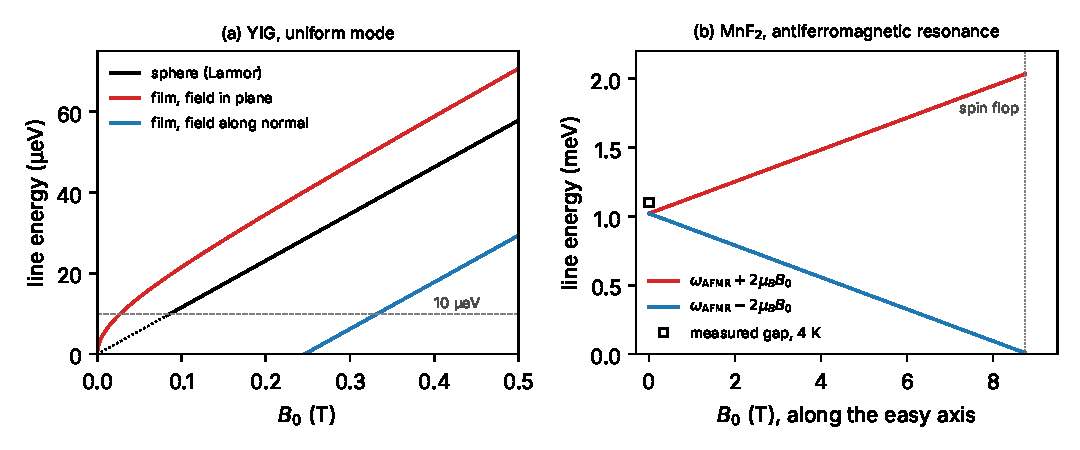
\includegraphics[width=0.95\linewidth]{figures/ch14/fig14_3.pdf}
  \caption{Absorption lines of YIG and MnF$_2$ against the applied field $B_0$. (a) The uniform mode of YIG ($g_{\mathrm{ion}} = 2$, $\mu_0M_{\mathrm{s}} = \SI{0.246}{T}$). A sphere absorbs at the Larmor frequency $2\mu_BB_0$ once it is saturated, $B_0 > \mu_0M_{\mathrm{s}}/3$ (dotted below). A thin film absorbs at $[\omega_{\mathrm{Lar}}(\omega_{\mathrm{Lar}} + \omega_M)]^{1/2}$ with the field in its plane and at $\omega_{\mathrm{Lar}} - \omega_M$ with the field along its normal, $\omega_M = \SI{28.5}{\micro eV}$. The dashed line marks the \SI{10}{\micro eV} of the worked example. (b) The two antiferromagnetic-resonance lines of MnF$_2$, $\omega_{\mathrm{AFMR}} \pm 2\mu_BB_0$ with $\omega_{\mathrm{AFMR}} = \SI{1.021}{meV}$ from $B_E = \SI{47.05}{T}$ and $B_A = \SI{0.82}{T}$, for a field along the easy axis up to the spin flop at \SI{8.75}{T}, both from the fitted fields; each line carries half of the weight $|\mathbf{S}|\omega_{\mathrm{AFMR}}/(2\omega_E + \omega_A) = 0.232$ per pair. The square is the measured zone-center gap at \SI{4}{K}, \SI{1.1}{meV}, which goes with a measured spin flop near \SI{9.4}{T}.}
  \label{fig:14-lines}
\end{figure}

\begin{limitbox}[Absorption into magnons][lim:14.3a]
(a) The Larmor statement: at $\vect{k} \to 0$ all transverse spin weight of a magnet with isotropic exchange and uniform $\lambda_S$ and $g_{\mathrm{ion}}$ lies in one line at $\omega_{\mathrm{Lar}}$ with weight $2\langle S^z_{\mathrm{tot}}\rangle$~\cites[Eqs.~(2.4), (2.5)]{oshikawa2002electron}[Eqs.~(25)--(27)]{chigusa2020detecting}[Eq.~(27)]{mitridate2020detectability}; for a $J$ multiplet the axion-like particle couples with $\lambda_S = g_J - 1$. (b) The uniform weight $|\vect{S}|\omega_{\mathrm{AFMR}}/(2\omega_E + \omega_A)$ per antiparallel pair, \cref{eq:14.3-afmrweight}.
\par\smallskip
{\centering
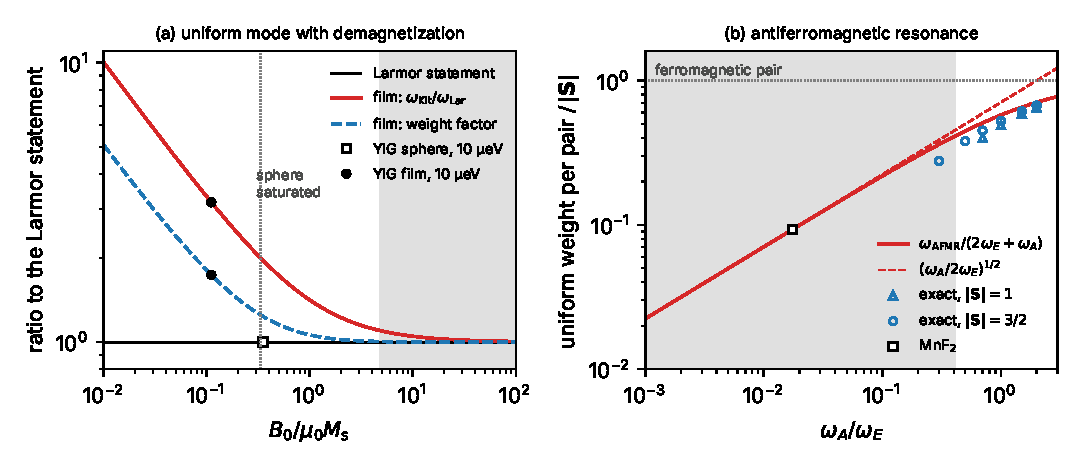
\includegraphics[width=0.98\linewidth]{figures/ch14/limit14_3a.pdf}
\captionof{figure}{(a) Uniform mode of a thin film with the field in its plane against the applied field over the shape-anisotropy field, $B_0/\mu_0M_{\mathrm{s}}$: line position $\omega_{\mathrm{Kit}}/\omega_{\mathrm{Lar}} = (1 + \mu_0M_{\mathrm{s}}/B_0)^{1/2}$ (solid) and weight averaged over transverse directions of $\vect{p}_\phi$ (dashed), both relative to the Larmor statement (black, 1). A saturated sphere follows the Larmor statement exactly; the markers place YIG at \SI{10}{\micro eV}. Gray: both ratios within \SI{10}{\percent} of 1, $B_0 \ge 4.8\,\mu_0M_{\mathrm{s}}$. For a $J$ multiplet both curves keep their shape, the rate scales by $(g_J - 1)^2$ and the line moves to $g_J\mu_BB_0$. (b) Uniform weight per antiparallel pair over $|\mathbf{S}|$ against $\omega_A/\omega_E$: the linear spin-wave result (solid) and its exchange-suppressed form $(\omega_A/2\omega_E)^{1/2}$ (dashed). Symbols: the exact total weight $\langle(S^x_{\mathrm{tot}})^2\rangle$ of the eight-site easy-axis (XXZ) cluster of the text for $|\mathbf{S}| = 1$ and $\frac32$, where that cluster is ordered (the splitting of its two lowest states below \SI{1}{\percent} of $\omega_{\mathrm{AFMR}}$). Gray: the square-root form within \SI{10}{\percent}, $\omega_A \le 0.42\,\omega_E$. The square marks MnF$_2$ with the fitted fields. The isotropic Heisenberg magnet, with zero uniform weight, is the left end.}\label{fig:14-limit-absorption}
\par}
\smallskip
Outside the gray regions the line of a non-spherical sample leaves $\omega_{\mathrm{Lar}}$ and its weight becomes elliptical, the antiferromagnetic weight departs from the square-root form, and in the eight-site cluster the zero-point fluctuations remove 5 to \SI{23}{\percent} of the linear spin-wave weight for $|\mathbf{S}| = \frac32$ ($\omega_A/\omega_E$ from 2 to 0.3).
\end{limitbox}

Linear spin-wave theory itself adds no correction to the Larmor line and one to the antiferromagnetic weight. \Cref{eq:14.3-larmor} is exact for any spin and temperature, and its only inputs are $\lambda_S$, $g_{\mathrm{ion}}$ and the net magnetization. The antiferromagnetic weight is of order $|\vect{S}|^0$ in the expansion of \cref{sec:14.1}, and an exactly solvable cluster shows its zero-point correction directly. Put spins $|\vect{S}|$ on the eight corners of a cube, each coupled to its three neighbors on the other sublattice by $H = J\sum_{\langle ij\rangle}(S^x_iS^x_j + S^y_iS^y_j + \Delta_{\mathrm{XXZ}}S^z_iS^z_j)$ with $J > 0$ and $\Delta_{\mathrm{XXZ}} \ge 1$, twelve bonds and open boundaries. Linear spin-wave theory at $\vect{k} = 0$ maps it onto \cref{eq:14.3-afmr} with $\omega_E = 3J|\vect{S}|$ and $\omega_A = 3J|\vect{S}|(\Delta_{\mathrm{XXZ}} - 1)$, so that \cref{eq:14.3-afmrweight} becomes $|\vect{S}|[(\Delta_{\mathrm{XXZ}} - 1)/(\Delta_{\mathrm{XXZ}} + 1)]^{1/2}$. The exact weight is the equal-time correlation $\langle0|(S^x_{\mathrm{tot}})^2|0\rangle$ in the ground state of the sector $S^z_{\mathrm{tot}} = 0$, divided by the four antiparallel pairs; it contains every final state that $S^x_{\mathrm{tot}}$ reaches. At $\omega_A = \omega_E$ it is 0.85 and 0.91 of \cref{eq:14.3-afmrweight} for $|\vect{S}| = 1$ and $\frac32$ (\cref{fig:14-limit-absorption}b). The cluster cannot reach the small anisotropies of real antiferromagnets, $\omega_A/\omega_E = 0.017$ in MnF$_2$, because below $\omega_A \approx 0.3\,\omega_E$ for $|\vect{S}| = \frac32$, and about $0.6\,\omega_E$ for $|\vect{S}| = 1$, its two lowest states mix and it no longer orders. For Mn$^{2+}$ the expansion parameter $1/2|\vect{S}|$ is 0.2, which sets the order of the correction at small $\omega_A/\omega_E$ but not its size.

\section{Spin responses from neutron data}\label{sec:14.4}

The full magnon spectrum of YIG, all twenty branches up to about \SI{110}{meV}, has been measured by inelastic neutron scattering with neutrons of \SI{120}{meV}~\cite{princep2017full,berlin2025determining}. Such a neutron carries \SI{15.0}{keV} of momentum, the largest momentum of a dark-matter particle of \SI{5.7}{MeV}, and its spin couples to the spin density $\vect{s}_e(\vect{q})$ (\cref{app:C.19}). The measured cross-section can therefore replace the model response of \cref{sec:14.1}, with every magnon branch, every multi-magnon process and the magnetic form factor already included, as Berlin, Millar, Trickle and Zhou did for YIG~\cite{berlin2025determining}. A neutron, however, couples only to the part of the spin density perpendicular to the momentum transfer, and how much of the dark-matter response that part fixes depends on the coupling and on how much model input is added for the magnet.

\subsection{Conversion of neutron spectra}

Neutron spectra are reported per formula unit of the crystal. With $N_{\mathrm{fu}}$ formula units in a cell of volume $\Omega$, the measured magnetic structure factor $S^{\mathrm{neu}}(\vect{q},\omega)$ is defined by $\dd^2\sigma/\dd\Omega\,\dd E' = (p'_n/p_n)\,S^{\mathrm{neu}}$ for one formula unit, with $\dd\Omega$ here the solid angle of the outgoing neutron. Dividing \cref{eq:C.19-cross} by the number of formula units in the sample, $\Vol N_{\mathrm{fu}}/\Omega$, and solving for the response,
\begin{equation}
  \Tr\bigl[P_T\,S(\vect{q},\omega)\bigr] = \sum_{a,b}(P_T)_{ab}\,S_{ab}(\vect{q},\omega) = \frac{2\pi N_{\mathrm{fu}}}{(\gamma_nr_{\mathrm{cl}})^2\,\Omega}\,S^{\mathrm{neu}}(\vect{q},\omega) ,
  \label{eq:14.4-PT}
\end{equation}
with $(P_T)_{ab} = \delta_{ab} - \hat q_a\hat q_b$ and $(\gamma_nr_{\mathrm{cl}})^2 = \SI{0.2906}{b}$. This is the relation of Berlin et al.~\cite[Eq.~(26)]{berlin2025determining}. The thermal vibration of the ions enters through the Debye--Waller factor, which the dark matter sees in the same way, so it stays inside $S_{ab}$ (\cref{app:C.19}).

Two corrections, for temperature and for the orbital moment, turn \cref{eq:14.4-PT} into the response that a detector needs. The spectrum is measured at a temperature $T_{\mathrm{d}}$, below \SI{10}{K} for the YIG data~\cite[App.~B\,2]{berlin2025determining}, while a detector runs at millikelvin. By the fluctuation--dissipation theorem \cref{eq:4.2-fdt}, $(1 - \ee^{-\beta\omega})S_{ab}$ is the dissipative response, and for free magnons this response does not depend on temperature, as for the thermal oscillator of \cref{sec:4.2}. Hence
\begin{equation*}
  S_{ab}(\vect{q},\omega;T \to 0) = \bigl(1 - \ee^{-\omega/T_{\mathrm{d}}}\bigr)\,S_{ab}(\vect{q},\omega;T_{\mathrm{d}}) , \qquad \omega > 0 ,
\end{equation*}
which removes the thermal population of the measured spectrum. The residual is set by the magnon interactions, which make the response follow the thermal reduction of the ordered moment; it is small for $T_{\mathrm{d}}$ well below the ordering temperature.

The second correction is the orbital moment. A neutron couples to the magnetization, spin and orbital, while spin-coupled dark matter couples to the spin alone. For a quenched $3d$ ion of spin $\vect{S}$, \cref{sec:14.3} showed that spin--orbit coupling induces an orbital moment $\vect{L} = (g_{\mathrm{ion}} - 2)\vect{S}$ at first order, with $g_{\mathrm{ion}}$ the spectroscopic $g$ factor of the ion (\cref{sec:14.3-lande}), taken isotropic here, while the spin itself changes only at second order, $\lambda_S = 1 - O(\xi_{\mathrm{ion}}^2/\Delta_{\mathrm{CF}}^2)$. In the dipole approximation of \cref{app:C.19} the spin part of the moment carries the radial integral $\langle j_0\rangle$ and the orbital part $\langle j_0\rangle + \langle j_2\rangle$. The moment $2\vect{S}\langle j_0\rangle + \vect{L}(\langle j_0\rangle + \langle j_2\rangle)$ is then $g_{\mathrm{ion}}\vect{S}\,F^{\mathrm{mag}}_g(q)$, and the neutron couples to
\begin{equation*}
  \vect{s}_e(\vect{q}) \to \frac{g_{\mathrm{ion}}}{2}\,F^{\mathrm{mag}}_g(q)\sum_j\ee^{\ii\vect{q}\cdot\vect{R}_j}\vect{S}_j, \qquad F^{\mathrm{mag}}_g(q) = \langle j_0(q)\rangle + \Bigl(1 - \frac2g\Bigr)\langle j_2(q)\rangle ,
\end{equation*}
while the dark matter couples to $\lambda_S\langle j_0(q)\rangle\sum_j\ee^{\ii\vect{q}\cdot\vect{R}_j}\vect{S}_j$. The two operators differ by a number at each $q$, so their responses differ by its square:
\begin{keyresult}[Data-driven spin response]
\begin{equation}
  \Tr\bigl[P_T\,S(\vect{q},\omega)\bigr] = C_{\mathrm{sn}}(q)\,\frac{2\pi N_{\mathrm{fu}}}{(\gamma_nr_{\mathrm{cl}})^2\,\Omega}\,S^{\mathrm{neu}}(\vect{q},\omega), \qquad
  C_{\mathrm{sn}}(q) = \biggl[\frac{\lambda_S\,\langle j_0(q)\rangle}{(g_{\mathrm{ion}}/2)\,F^{\mathrm{mag}}_g(q)}\biggr]^2 ,
  \label{eq:14.4-data}
\end{equation}
for one species of quenched magnetic ion, with $S_{ab}$ the response of the electron spin density and $S^{\mathrm{neu}}$ measured per formula unit, its thermal population removed. At $q \to 0$, $C_{\mathrm{sn}} = [\lambda_S/(g_{\mathrm{ion}}/2)]^2$.
\end{keyresult}
\noindent For an anisotropic $g_{\mathrm{ion}}$ tensor, $g_{\mathrm{ion}}/2$ becomes the matrix $g_{\mathrm{ion},ab}/2$ acting on both indices of $S_{ab}$. For a $J$ multiplet, $g_{\mathrm{ion}}$ is replaced by $g_J$, $\lambda_S$ by $g_J - 1$ (\cref{eq:14.3-gJ}) and $F^{\mathrm{mag}}_g$ by the dipole form factor \cref{eq:C.19-dipole}; at $q \to 0$, $C_{\mathrm{sn}}$ is the square of the last column of \cref{tab:14-lande}. It is 1 for Gd$^{3+}$, $\frac19$ for Er$^{3+}$ and 25 for Sm$^{3+}$, whose spin points against its moment.

For Ni$^{2+}$ in NiO, $g_{\mathrm{ion}} = 2.18 \simeq 2.2$~\cite{kritzell2024terahertz}. With $\lambda_S = 1$,
\begin{equation*}
  C_{\mathrm{sn}}(0) = \Bigl(\frac{2}{2.2}\Bigr)^2 = 0.83 :
\end{equation*}
the spin response of NiO is \SI{17}{\percent} below what the neutron cross-section suggests if read as pure spin. Setting $\lambda_S = g_{\mathrm{ion}} - 1$ instead, the rule that holds only for $J$ multiplets, would give $(1.2/1.1)^2 = 1.19$ and an error of the opposite sign. The $q$ dependence enters through $\langle j_2\rangle$, which vanishes at $q = 0$ and grows with $q$. With the tabulated radial integrals of Ni$^{2+}$~\cite[Sect.~4.4.5]{anderson2006neutron}, the same fit form as for $\langle j_0\rangle$ in \cref{sec:14.1} multiplied by $s^2$ with coefficients $(1.708, 11.016, 1.2147, 4.103, 0.315, 1.533, 0.0018)$, the ratio $\langle j_2\rangle/\langle j_0\rangle$ is 0.035 at $|\vect{Q}_{\mathrm{AF}}| = \SI{2.6}{keV}$ and 0.15 at \SI{5.3}{keV}. $C_{\mathrm{sn}}(q)/C_{\mathrm{sn}}(0)$ is then 0.994 and 0.973, and it stays within \SI{10}{\percent} of one up to \SI{10}{keV}. The value of $g_{\mathrm{ion}}$ is the larger uncertainty. Magnetic x-ray diffraction on NiO, which separates the spin and orbital moments, finds $L/S = 0.34$~\cite{fernandez1998observation}, and DFT~$+\,U$ with spin--orbit coupling gives 0.36~\cite{kwon2000unquenched}. Read in the quenched picture as $g_{\mathrm{ion}} = 2 + L/S = 2.34$, this lowers $C_{\mathrm{sn}}(0)$ to 0.73, \SI{12}{\percent} below the value at $g_{\mathrm{ion}} = 2.2$. The orbital moment of Ni$^{2+}$ is thus an uncertainty of about \SI{10}{\percent} on the normalization of the data-driven rate. The $g_{\mathrm{ion}}$ tensor and the orbital moments are computed in DFT~$+\,U$ with spin--orbit coupling (\cref{app:E.20-magnet}), and the radial integrals from Dirac--Fock or Wannier-projected shells.

\Cref{lim:14.4a} shows how far the spin-only reading of the data holds as the orbital admixture grows.
\begin{limitbox}[Data-driven spin response][lim:14.4a]
$\Tr[P_TS(\vect{q},\omega)] = 2\pi N_{\mathrm{fu}}S^{\mathrm{neu}}(\vect{q},\omega)/[(\gamma_nr_{\mathrm{cl}})^2\Omega]$, for a neutron coupled to the electron spin alone~\cite[Eqs.~(8), (11), (26)]{berlin2025determining}.
\par\smallskip
{\centering
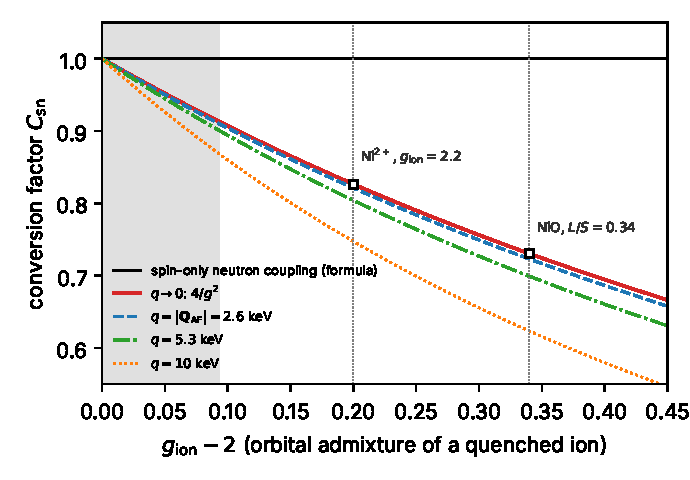
\includegraphics[width=0.78\linewidth]{figures/ch14/limit14_4a.pdf}
\captionof{figure}{Ratio of the spin response to the response inferred from neutron data by the spin-only formula, $C_{\mathrm{sn}}(q)$ of \cref{eq:14.4-data}, against the shift $g_{\mathrm{ion}} - 2$ of the spectroscopic $g_{\mathrm{ion}}$ factor of a quenched ion, with $\lambda_S = 1$ and the dipole form factor $\langle j_0\rangle + (1 - 2/g_{\mathrm{ion}})\langle j_2\rangle$. Black: the formula, ratio 1. Red: $q \to 0$, $4/g^2$. Dashed, dash-dotted and dotted: $q = \SI{2.6}{keV}$ (the ordering wavevector of NiO), \SI{5.3}{keV} (largest momentum transfer at $\mchi = \SI{1}{MeV}$) and \SI{10}{keV}, with the radial integrals of Ni$^{2+}$. Squares: $g_{\mathrm{ion}} = 2.2$ (octahedral Ni$^{2+}$) and $g_{\mathrm{ion}} = 2.34$ (NiO with $L/S = 0.34$ from magnetic x-ray diffraction). Gray: $g_{\mathrm{ion}} - 2 \le 0.094$, where the formula holds within \SI{10}{\percent} for $q \le \SI{5.3}{keV}$.}\label{fig:14-limit-neutron}
\par}
\smallskip
Outside the gray band the orbital moment shifts the neutron response from the spin response at first order in $g_{\mathrm{ion}} - 2$, and at large $q$ the orbital form factor $\langle j_2\rangle$ adds to the shift.
\end{limitbox}

How much of the dark-matter kinematic region the data reach depends on the instrument. In the YIG spectrum of Berlin et al.\ the data below \SI{5}{meV} are dominated by elastic scattering and are discarded, and the crystal was rotated about one axis only, so at large $q$ only a narrow band of directions $\hat{\vect{q}}$ is covered~\cite[Sect.~III\,B and App.~D]{berlin2025determining}. Averaging $S^{\mathrm{neu}}$ over the covered directions at fixed $|\vect{q}|$ and $\omega$ is justified well outside the first zone, since a small change in the direction of $\vect{q}$ moves its reduced part across the whole zone. Below a mass of \SI{134}{keV}, where $2\mchi v_{\mathrm{max}}$ reaches the radius $\sqrt2\pi/a = \SI{708}{eV}$ of the largest sphere inside the zone, every momentum transfer lies inside the first zone, where there are few data, and the data-driven reach falls rapidly below about \SI{200}{keV}. Near \SI{1}{MeV} the data-driven rate agrees closely with the Heisenberg-model rate fitted to the same spectrum~\cite[Fig.~3]{berlin2025determining}. At larger masses the data contain the form factor of Fe$^{3+}$, which the model omits and which suppresses the rate by an order of magnitude for $q \gtrsim \SI{10}{keV}$. They also contain phonons, excited by the nuclear scattering of the neutron with a relative weight that grows as $q^2/(M\omega)$, about $(q/\SI{30}{keV})^2$ for nuclei of \SI{50}{GeV} and $\omega \sim \SI{20}{meV}$~\cite[App.~C]{berlin2025determining}. Spin-flip scattering with the polarization along $\hat{\vect{q}}$ contains all the magnetic scattering and no coherent nuclear scattering (\cref{app:C.19}), and it removes the phonons without a model, up to the two thirds of the nuclear-spin-incoherent scattering that it keeps, which is small for Y, Fe and O. A modelled phonon part subtracted from unpolarized data must leave a response that is still positive semidefinite (\cref{eq:4.2-positivity}).

\subsection{Transverse projection of the neutron cross-section}

Which couplings \cref{eq:14.4-PT} calibrates depends on the dark-matter tensor $\mathfrak{D}_{ab}$ of \cref{eq:8.1-D} for the spin row. For the operators of \cref{tab:8-operators} with dark matter of spin $\frac12$ there are three structures. The contact interaction $\mathcal{O}_4$ gives $\mathfrak{D}_{ab} = |c_4^{(e)}|^2\delta_{ab}/4$. The pseudoscalar couplings give $\hat q_a\hat q_b$: $\mathcal{O}_{10}$ gives $|c_{10}^{(e)}|^2q_aq_b/m_e^2$ and $\mathcal{O}_6$ gives $|c_6^{(e)}|^2q^2q_aq_b/4m_e^4$. Operator $\mathcal{O}_9 = \ii\vect{S}_\chi\cdot(\vect{S}_e\times\vect{q}/m_e)$, and the spin--spin part $(\vect{S}_\chi\times\vect{q})\cdot(\vect{S}_e\times\vect{q})$ of magnetic-dipole and anapole dark matter, give the transverse projector: for $\mathcal{O}_9$, $\Tr_\chi[(\vect{q}\times\vect{S}_\chi)_a(\vect{q}\times\vect{S}_\chi)_b]/2 = q^2(P_T)_{ab}/4$, so $\mathfrak{D}_{ab} = |c_9^{(e)}|^2q^2(P_T)_{ab}/4m_e^2$. Since $\delta_{ab} = (P_T)_{ab} + \hat q_a\hat q_b$, the three contractions are
\begin{equation}
  \sum_{a,b}\delta_{ab}S_{ab} = \Tr\bigl[P_TS\bigr] + \hat{\vect{q}}\cdot S\cdot\hat{\vect{q}}, \qquad \sum_{a,b}(P_T)_{ab}S_{ab} = \Tr\bigl[P_TS\bigr], \qquad \sum_{a,b}\hat q_a\hat q_bS_{ab} = \hat{\vect{q}}\cdot S\cdot\hat{\vect{q}} .
  \label{eq:14.4-split}
\end{equation}
The neutron data fix the transverse couplings completely: the rates of $\mathcal{O}_9$, magnetic-dipole and anapole dark matter follow from \cref{eq:8.2-spectrum} with $S^{\mathrm{neu}}$ and nothing else. For $\mathcal{O}_4$, however, the transverse part alone is only a lower bound on the rate of the contact interaction: the longitudinal element $\hat{\vect{q}}\cdot S\cdot\hat{\vect{q}}$ is a diagonal element of a positive semidefinite matrix and cannot be negative. For $\mathcal{O}_6$ and $\mathcal{O}_{10}$ the data at one $\vect{q}$ leave the rate unconstrained. Tensors built from the dark-matter velocity, as for $\mathcal{O}_7$ and $\mathcal{O}_{12}$--$\mathcal{O}_{15}$, also need the mixed elements between the direction of $\vect{q}$ and the two directions perpendicular to it.

Absorption needs exactly the missing element. The spin row of an axion-like particle is proportional to its momentum, and the absorption rate \cref{eq:14.3-abs} contracts $S_{ab}$ with $p_{\phi,a}p_{\phi,b}$: it is $p_\phi^2\,\hat{\vect{p}}_\phi\cdot S\cdot\hat{\vect{p}}_\phi$, a longitudinal element~\cite[Eqs.~(15), (17)]{berlin2025determining}. Its momentum, $p_\phi \sim 10^{-3}m_\phi$, is also far below any momentum transfer a neutron spectrometer resolves. At $q \to 0$ the full tensor is fixed instead by the magnetic permeability measured in resonance or terahertz experiments~\cite[footnote~3]{berlin2025determining}, and in the model of \cref{sec:14.3} by the Larmor and Kittel lines.

That the longitudinal element is missing at each $q$, whatever the beam, follows from the form of the amplitude. \Cref{fig:14-neutron} shows the geometry.
\begin{keyresult}[Neutron scattering and the longitudinal spin response]
At a given $\vect{q}$, magnetic neutron scattering measures only the block of $S_{ab}(\vect{q},\omega)$ transverse to $\hat{\vect{q}}$: unpolarized beams its trace $\Tr[P_TS]$, polarization analysis its elements. Without a model of the magnet (of the spin density within the cell, or the spin-isotropy hypothesis of \cref{sec:14.4-iso}), the longitudinal element $\hat{\vect{q}}\cdot S\cdot\hat{\vect{q}}$ and the mixed elements between $\hat{\vect{q}}$ and the transverse plane are measured by no neutron experiment, polarized or not, and no symmetry of the crystal relates them to the transverse block at the same $\vect{q}$. Within the localized-moment model of \cref{eq:14.4-data}, transverse data at several wavevectors $\vect{q} + \vect{G}$ determine the full tensor.
\end{keyresult}
\noindent The first part is the perpendicular-projection rule of magnetic neutron scattering (\cref{app:C.19}). Every amplitude in \cref{eq:C.19-amplitude,eq:C.19-polar} contains $\vect{s}_e$ only through $\vect{s}_\perp = P_T\vect{s}_e$, because a spin density modulated along $\vect{q}$ produces no magnetic field at that wavevector (\cref{eq:C.19-field}). In the frame of \cref{app:C.19}, with $x$ along $\hat{\vect{q}}$, polarization analysis separates $S_{yy}$, $S_{zz}$ and the chiral part of $S_{yz}$, and full polarimetry reaches its symmetric part as well~\cite{blume1963polarization}. That is at most four of the nine real numbers of the Hermitian matrix $S_{ab}$.

For the second part, let $\mathsf{h}$ be an element of the magnetic point group, acting as a rotation matrix $\mathsf{R}$ on positions and on the axial spin. It maps the response at $\vect{q}$ onto the response at $\mathsf{R}\vect{q}$, $S(\mathsf{R}\vect{q}) = \mathsf{R}\,S(\vect{q})\,\mathsf{R}^{\mathrm{T}}$, possibly transposed if $\mathsf{h}$ contains time reversal; the transpose does not change the symmetric contractions. Since also $P_T(\mathsf{R}\hat{\vect{q}}) = \mathsf{R}\,P_T(\hat{\vect{q}})\,\mathsf{R}^{\mathrm{T}}$,
\begin{equation*}
  \Tr\bigl[P_T(\mathsf{R}\hat{\vect{q}})\,S(\mathsf{R}\vect{q})\bigr] = \Tr\bigl[\mathsf{R}P_T(\hat{\vect{q}})\mathsf{R}^{\mathrm{T}}\mathsf{R}S(\vect{q})\mathsf{R}^{\mathrm{T}}\bigr] = \Tr\bigl[P_T(\hat{\vect{q}})\,S(\vect{q})\bigr] ,
\end{equation*}
and a measurement at a symmetry-equivalent wavevector repeats the same equation. The elements that leave $\hat{\vect{q}}$ fixed map the direction of $\vect{q}$ onto itself and the transverse plane onto itself, so they constrain the transverse block and the longitudinal element separately and never relate one to the other. A wavevector $\vect{q} + \vect{G}$ that points elsewhere belongs to a different operator, $\vect{s}_e(\vect{q} + \vect{G})$, which the exact response does not tie to $\vect{s}_e(\vect{q})$.

The localized-moment form that \cref{eq:14.4-data} already uses supplies that tie. For one magnetic ion per primitive cell, as for NiO in its chemical cell, $\vect{s}_e(\vect{k} + \vect{G}) = F^{\mathrm{mag}}(|\vect{k} + \vect{G}|)\sum_j\ee^{\ii(\vect{k}+\vect{G})\cdot\vect{R}_j}\vect{S}_j$ with $\ee^{\ii\vect{G}\cdot\vect{R}_j} = 1$, so that
\begin{equation}
  S_{ab}(\vect{k} + \vect{G},\omega) = |F^{\mathrm{mag}}(|\vect{k} + \vect{G}|)|^2\,\ee^{-2W(\vect{k}+\vect{G})}\,S^{\mathrm{lat}}_{ab}(\vect{k},\omega) ,
  \label{eq:14.4-Glat}
\end{equation}
for every reciprocal vector $\vect{G}$, with $S^{\mathrm{lat}}$ the response of the lattice spins and the Debye--Waller factor $\ee^{-2W}$ taken at $\vect{k} + \vect{G}$, beside the form factor. Each $\vect{G}$ gives the transverse trace $\Tr S^{\mathrm{lat}} - \hat{\vect{n}}_{\vect{G}}\cdot S^{\mathrm{lat}}\cdot\hat{\vect{n}}_{\vect{G}}$ along its own direction $\hat{\vect{n}}_{\vect{G}} = (\vect{k} + \vect{G})/|\vect{k} + \vect{G}|$, a linear equation for the six components of the symmetric part of $S^{\mathrm{lat}}(\vect{k},\omega)$, and six generic directions fix all six. For NiO the four shortest vectors of type $(111)$ and two of type $(200)$ already give a system of full rank. The longitudinal element at the momentum transfer of the dark matter then follows from \cref{eq:14.4-Glat}, and as $\vect{k} \to 0$ so does the tensor that absorption needs, resolution permitting; neutron diffraction fixes the directions of ordered moments in the same way. The route rests on the dipole-approximation form factor, which gives every spin component the same radial shape, and on a known magnetic basis; with several magnetic ions per cell, as in YIG, the phases $\ee^{\ii\vect{G}\cdot\vect{\tau}}$ of the basis enter and more wavevectors are needed.

\begin{figure}[tbp]
  \centering
  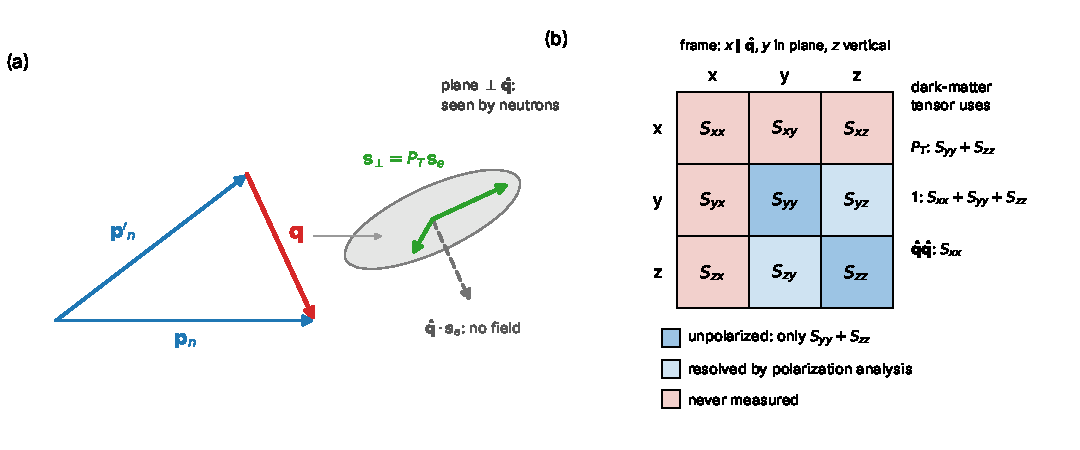
\includegraphics[width=\linewidth]{figures/ch14/fig14_4.pdf}
  \caption{The neutron geometry and the transverse projector. (a) A neutron of momentum $\mathbf{p}_n$ leaves with $\mathbf{p}'_n$ and gives the target $\vect{q} = \mathbf{p}_n - \mathbf{p}'_n$. Of the spin density at wavevector $\vect{q}$, only the part in the plane perpendicular to $\hat{\vect{q}}$, $\vect{s}_\perp = P_T\vect{s}_e$, produces a magnetic field and scatters the neutron; the component along $\hat{\vect{q}}$ produces none. (b) The spin response $S_{ab}$ in the frame with $x$ along $\hat{\vect{q}}$, $y$ in the scattering plane and $z$ vertical. Unpolarized neutrons measure the sum $S_{yy} + S_{zz}$; polarization analysis resolves the transverse block; the elements in the first row and column are not measured at this $\vect{q}$. Right-hand columns of (b): the elements that the dark-matter tensors proportional to $P_T$ (for example $\mathcal{O}_9$), to the unit matrix ($\mathcal{O}_4$) and to $\hat q_a\hat q_b$ ($\mathcal{O}_6$, $\mathcal{O}_{10}$) contract. Schematic.}
  \label{fig:14-neutron}
\end{figure}

\subsection{The longitudinal response under isotropy}\label{sec:14.4-iso}

Spin-rotation symmetry about the moments supplies the missing element at one $\vect{q}$, without a model of the spin density but with a hypothesis on the Hamiltonian: spin--orbit coupling and the dipolar interaction are neglected. In a collinear magnet with moments along $\pm\hat{\vect{m}}$, and with spin--orbit coupling neglected, the Hamiltonian is invariant under rotations of all spins about $\hat{\vect{m}}$, independently of the lattice; the Heisenberg model of \cref{sec:7.1} is the example. A rotation of the spin indices alone then leaves $S_{ab}(\vect{q},\omega)$ unchanged at every $\vect{q}$, and the only tensors with that property are built from $\delta_{ab}$, $\hat m_a\hat m_b$ and $\epsilon_{abc}\hat m_c$:
\begin{equation*}
  S_{ab}(\vect{q},\omega) = S_\parallel\,\hat m_a\hat m_b + S_\perp\,(\delta_{ab} - \hat m_a\hat m_b) + \ii S_{\mathrm{c}}\,\epsilon_{abc}\hat m_c ,
\end{equation*}
with three functions of $\vect{q}$ and $\omega$. The one-magnon response \cref{eq:14.1-Safm} has this form with $S_\parallel = 0$, and the two-magnon response \cref{eq:14.2-S2m} is all $S_\parallel$. The antisymmetric part drops out of every symmetric contraction. With $\theta_m$ the angle between $\hat{\vect{q}}$ and $\hat{\vect{m}}$,
\begin{equation}
  \Tr\bigl[P_TS\bigr] = S_\parallel\sin^2\theta_m + S_\perp(1 + \cos^2\theta_m), \qquad
  \hat{\vect{q}}\cdot S\cdot\hat{\vect{q}} = S_\parallel\cos^2\theta_m + S_\perp\sin^2\theta_m .
  \label{eq:14.4-uniax}
\end{equation}
Polarization analysis now suffices at a single $\vect{q}$. With $\hat{\vect{m}}$ in the scattering plane at an angle $\theta_m \ne 0, \frac\pi2$ to $\hat{\vect{q}}$, the vertical element is $S_{zz} = S_\perp$ and the in-plane element $S_{yy} = S_\parallel\sin^2\theta_m + S_\perp\cos^2\theta_m$, which equals $\hat{\vect{q}}\cdot S\cdot\hat{\vect{q}}$ with $\cos$ and $\sin$ exchanged and fixes $S_\parallel$. Unpolarized data give one equation for two unknowns at each $\vect{q}$, and a second measurement is needed at another angle with the same $S_\parallel$ and $S_\perp$. That is the content of the \emph{isotropy hypothesis}: in the window used, $S_\parallel$ and $S_\perp$ depend on $\vect{q}$ only through $|\vect{q}|$, or do not change when the moments are turned at fixed $\vect{q}$. The second form is the easier one to realize. A soft magnet can be turned by an applied field with $\vect{q}$ held fixed in the crystal; a YIG sphere saturates above \SI{82}{mT} (\cref{we:14-yig}). In the spin-rotation-invariant model the two settings then measure exactly the same $S_\parallel$ and $S_\perp$, and only spin--orbit coupling and the magnetic dipolar interaction break the hypothesis. The dipolar term, $\omega_M\sin^2\theta_{\vect{q}}$ in the spin-wave energy with $\omega_M = \SI{28.5}{\micro eV}$ for YIG (\cref{we:14-yig}), is negligible above about \SI{0.1}{meV}, far below the \SI{5}{meV} where the data start. Given $P_i = \Tr[P_TS]$ at two angles $\theta_1$ and $\theta_2$, with $c_i = \cos^2\theta_i$, the solution of the two equations \cref{eq:14.4-uniax} is
\begin{equation}
  S_\parallel = \frac{P_1(1 + c_2) - P_2(1 + c_1)}{2(c_2 - c_1)}, \qquad S_\perp = \frac{P_2(1 - c_1) - P_1(1 - c_2)}{2(c_2 - c_1)} ,
  \label{eq:14.4-invert}
\end{equation}
and the longitudinal element follows from \cref{eq:14.4-uniax} for any direction of $\vect{q}$ relative to $\hat{\vect{m}}$.

A paramagnet in zero field, or a sample of many randomly oriented domains, is invariant under all rotations, so $S_\parallel = S_\perp$ and $\hat{\vect{q}}\cdot S\cdot\hat{\vect{q}} = \frac12\Tr[P_TS]$~\cite[Eq.~(35)]{berlin2025determining}. In an ordered magnet the two-magnon continuum, \SI{7.3}{\percent} of the one-magnon weight in NiO (\cref{we:14-nio}), lies entirely in $S_\parallel$, and the two-angle inversion keeps it.

\begin{workedexample}{The two-angle inversion for an isotropic paramagnet}\label{we:14-paramagnet}
Take a paramagnet in zero field, so that $S_\parallel = S_\perp = S_0$ at the $(|\vect{q}|, \omega)$ of interest, and measure $\Tr[P_TS]$ with $\vect{q}$ perpendicular and then parallel to a fixed crystal axis $\hat{\vect{m}}$: $c_1 = 0$, $c_2 = 1$. Both measurements give $2S_0$, and \cref{eq:14.4-invert} reduces to $S_\parallel = P_1 - P_2/2$ and $S_\perp = P_2/2$, which returns $S_0$ for both. The hypothesis is tested by the data themselves: $P_2 - P_1 = (c_2 - c_1)(S_\perp - S_\parallel)$ vanishes.

Errors decide whether the inversion is worth doing. Give each measurement a statistical error of \SI{5}{\percent}, $0.1S_0$, independent between the two. Then $S_\perp$ carries $0.050S_0$, while $S_\parallel$ carries $(\sqrt5/2)\times0.1S_0 = 0.112S_0$, more than twice the relative error of the data. The longitudinal element needed for $\mathcal{O}_6$ along $\hat{\vect{m}}$ is $S_\parallel$ itself, with the same \SI{11}{\percent}; at $\cos^2\theta = \frac13$ it is $P_1/3 + P_2/6$, with \SI{3.7}{\percent}. The isotropy test, $P_2 - P_1 = 0 \pm 0.141S_0$, limits $|S_\perp - S_\parallel|$ to about \SI{14}{\percent} of $S_0$ at one standard deviation.

A smaller rotation gives larger errors. With $c_2 = \sin^2 30^\circ = 0.25$ instead, the denominator $2(c_2 - c_1)$ drops from 2 to 0.5, $S_\parallel = 2.5P_1 - 2P_2$ and its error grows to $0.32S_0$, \SI{32}{\percent}. The one-angle shortcut $\frac12\Tr[P_TS]$ has the \SI{5}{\percent} of the data, but it is right only if the paramagnet is in fact isotropic, which the two-angle measurement checks.
\end{workedexample}

A spin-wave model fitted to the transverse data supplies the longitudinal element as well, and its fit uncertainty enters as a normalization (\cref{sec:8.8}); a longitudinal response measured at dark-matter momenta, without such a model or the localized-moment form, does not exist.

\section{Coherent fields and precessing nuclear spins}\label{sec:14.6}

An axion-like field of mass \SI{1}{neV} oscillates at \SI{241.8}{kHz}, and its phase wanders on a time of about a second. A $^{207}$Pb nucleus in a field of \SI{26.8}{mT} precesses at the same frequency. Over a record shorter than a second the field acts on the nuclear spins as one classical wave with a fixed amplitude and phase, the spins tip together, and their transverse magnetization grows in proportion to the time until the spin coherence time $T_2$ caps it, after \SI{17}{ms} in the ferroelectric PMN-PT. The amplitude of the field then changes only on the scale of a second. Whether the golden-rule rate describes such a record depends on the shorter of the two times, and how the sensitivity of a search grows with the length of the record depends on the statistics of the random amplitude.

\subsection{The coherent classical-field regime}\label{sec:14.6-regime}

A light boson of mass $m_\phi$ has about $\rho_\chi/(m_\phi^4v_0^3)$ quanta in a volume $(1/m_\phi v_0)^3$, $4.6\times10^{39}$ at \SI{1}{neV}, and below a few eV it is a classical field (\cref{sec:8.2-absorption}). It is a sum of modes with random phases, one for each velocity in the halo, and by the central limit theorem a Gaussian random field~\cite[Eqs.~(3)--(10)]{foster2018revealing}. A Gaussian field with zero mean is fixed by its two-point function. For a free nonrelativistic field with the velocity distribution $f_\chi(\vect{v})$ of \cref{sec:1.2}, each mode oscillates at $\omega_{\vect{v}} = m_\phi(1 + v^2/2)$, and the average over the random phases is
\begin{equation*}
  \langle\phi(\vect{x},t)\,\phi(\vect{x}',t')\rangle = \frac{\rho_\chi}{m_\phi^2}\int\dd^3v\,f_\chi(\vect{v})\cos\bigl[\omega_{\vect{v}}(t - t') - m_\phi\vect{v}\cdot(\vect{x} - \vect{x}')\bigr] ,
\end{equation*}
normalized so that $\langle\phi^2\rangle = \rho_\chi/m_\phi^2$, the mean square of a wave $\phi_0\cos(m_\phi t)$ with $\tfrac12m_\phi^2\phi_0^2 = \rho_\chi$. With the transforms of \cref{app:A.3} in space and time, the power spectrum of the field is
\begin{equation}
  \mathcal{S}_\phi(\vect{k},\omega) = \frac{\pi\rho_\chi}{m_\phi^2}\,(2\pi)^3\!\int\dd^3v\,f_\chi(\vect{v})\Bigl[\delta^3(\vect{k} + m_\phi\vect{v})\,\delta(\omega - \omega_{\vect{v}}) + \delta^3(\vect{k} - m_\phi\vect{v})\,\delta(\omega + \omega_{\vect{v}})\Bigr] .
  \label{eq:14.6-Sphi}
\end{equation}
The positive-frequency weight sits at $\vect{k} = -m_\phi\vect{v}$ in the sign convention of \cref{eq:A.3-space,eq:A.3-time}, while the target receives the momentum $\vect{p}_\phi = m_\phi\vect{v}$, as in \cref{eq:8.2-abs}; the sign matters only for targets whose response is odd in $\vect{q}$ (\cref{sec:14.5}). Integrated over $\vect{k}$, the positive-frequency part is $(\pi\rho_\chi/m_\phi^2)F_\phi(\omega)$, with
\begin{equation}
  F_\phi(\omega)\,\dd\omega = F_\chi(v)\,\dd v, \qquad \omega - m_\phi = \tfrac12m_\phi v^2 ,
  \label{eq:14.6-Fphi}
\end{equation}
the energy distribution of the field of \cref{sec:11.8}, normalized to one and inherited from the laboratory speed distribution $F_\chi$ of \cref{sec:1.2}. The line is one-sided: it starts at $m_\phi$ and ends at $m_\phi(1 + v_{\mathrm{max}}^2/2)$, $3.5\times10^{-6}$ above it.

The width of the line sets the coherence time. We define it, as \cref{sec:8.2-absorption} estimated it, by
\begin{equation}
  t_{\mathrm{coh}} = \frac{1}{m_\phi v_0^2} = \SI{1.04}{s}\times\frac{\SI{1}{neV}}{m_\phi} ,
  \label{eq:14.6-tcoh}
\end{equation}
with $v_0 = \SI{238}{km/s}$. For the halo of \cref{sec:1.2} seen from the Earth, $F_\phi$ peaks at $0.58/t_{\mathrm{coh}}$ above $m_\phi$, its equivalent width $\Delta\omega_{\mathrm{eq}} = [\int\dd\omega\,F_\phi^2]^{-1}$ is $2.67/t_{\mathrm{coh}}$, and the correlation of the complex amplitude of the field with itself, $|\int\dd\omega\,F_\phi(\omega)\,\ee^{-\ii\omega t}|$, falls to one half at $t = 1.47\,t_{\mathrm{coh}}$. Over the coherence length $1/m_\phi v_0$, \SI{249}{km} at \SI{1}{neV}, the field is uniform, and every laboratory sample sees the same amplitude.

A coupling $\sum_bg^\phi_bO_b$ of the absorption rows of \cref{sec:8.1-absorption} drives the expectation value of any readout operator $O_{\mathrm{rd}}$ through the Kubo formula \cref{eq:4.1-kubo}, with the retarded response $R_{\mathrm{rd},b}(\vect{p}_\phi,t)$. The readout can be the operator that the field couples to, as for the magnetization of the spins below, or another, as for the voltage across a piezoelectric resonator (\cref{sec:11.8}). Either way the signal is linear in the amplitude of the field and in the coupling. Its square averaged over the Gaussian ensemble is quadratic in both and contains $\mathcal{S}_\phi$. The energy that the target absorbs is the case $O_{\mathrm{rd}} = \sum_bg^\phi_bO_b$, and its average reproduces the golden rule, but only after a long enough record. Take the coupling on from $t' = 0$ to $t$. The amplitude of a transition $i \to f$ driven by one mode of frequency $\omega$ contains $\int_0^t\dd t'\,\ee^{\ii(E_f - E_i - \omega)t'}$, whose square is $2\pi t\,\mathcal{K}_t(\omega - E_f + E_i)$ with the Fejér kernel
\begin{equation}
  \mathcal{K}_t(x) = \frac{t}{2\pi}\,\frac{\sin^2(xt/2)}{(xt/2)^2}, \qquad \int\dd x\,\mathcal{K}_t(x) = 1 .
  \label{eq:14.6-fejer}
\end{equation}
The Gaussian average removes the cross terms between modes, as in \cref{app:D.25}, and the mean number of quanta absorbed per unit volume in the record is $t\,(\rho_\chi/m_\phi)$ times the rate \cref{eq:8.2-abs} averaged over the line $F_\phi$, with the $\delta(\omega - E_f + E_i)$ in $S_{ab}$ replaced by $\mathcal{K}_t$. As $t \to \infty$ the kernel becomes the delta function and the mean is the golden-rule rate times $t$. The replacement matters only where both the field line and the target line are narrow compared with $1/t$. Since the kernel acts on their convolution, whose width is at least the larger of the two widths, the golden-rule mean holds for
\begin{equation*}
  t \gg \min\bigl(t_{\mathrm{coh}},\,1/\varGamma_{\mathrm{tg}}\bigr) .
\end{equation*}
Here $\varGamma_{\mathrm{tg}}$ is the width of the target's line: $1/T_2$ for nuclear spins, the full width $\varGamma_{\mathrm{M}}$ of a magnon line (\cref{sec:14.3}), $\gamma_n$ for a resonator mode (\cref{sec:11.8}). For a record shorter than both, the energy absorbed grows as $t^2$. That is the regime of a nuclear spin driven by a field of neV mass over a record shorter than its $T_2$, the coherent regime that \cref{sec:8.2-absorption} named.

The golden-rule mean is not yet what one record measures. A single realization of the field matches the ensemble only when the record spans many coherence times, so that it samples many independent amplitudes. For a detector that counts absorbed quanta, the intensity $|\Phi|^2$ of the complex amplitude $\Phi$ of the field is exponentially distributed within one coherence time, and a record of $N_{\mathrm{coh}}$ independent coherence times gives $\mathrm{Var}\,N = \bar N + \bar N^2/N_{\mathrm{coh}}$, the bunching of chaotic light. The Poisson statistics of \cref{eq:1.5-poisson} hold when $N_{\mathrm{coh}} \gg \bar N$, which counting searches satisfy by a wide margin: the YIG search of \cref{we:14-yig} at \SI{10}{\micro eV} sees 35 events per hour in $3.4\times10^7$ coherence times. A readout of the mean field, such as the magnetization below, is a different matter, since its signal is proportional to the amplitude of the field rather than to its intensity.

\subsection{Bloch equations and nuclear magnetic resonance}\label{sec:14.6-bloch}

A nucleus with spin $\vect{J}^{\mathrm{nuc}}$ and magnetic moment $\mu_{\mathrm{nuc}}$ in a static field $\vect{B}_0 = B_0\hat{\vect{z}}$ has the Zeeman energy $-\omega_{\mathrm{Lar}}J^{\mathrm{nuc}}_z$, with the Larmor frequency $\omega_{\mathrm{Lar}} = \mu_{\mathrm{nuc}}B_0/J_{\mathrm{nuc}}$; for $\mu_{\mathrm{nuc}} > 0$ the lower levels have the spin along the field. A Hamiltonian $-\vect{b}\cdot\vect{J}^{\mathrm{nuc}}$, with $\vect{b}$ a vector of energy, makes the spin precess, $\dd\vect{J}^{\mathrm{nuc}}/\dd t = \vect{J}^{\mathrm{nuc}}\times\vect{b}$; the Zeeman term has $\vect{b} = \omega_{\mathrm{Lar}}\hat{\vect{z}}$. For $^{207}$Pb, with $J_{\mathrm{nuc}} = \frac12$ and $\mu_{\mathrm{nuc}} = 0.5926$ nuclear magnetons, $\omega_{\mathrm{Lar}}/2\pi = \SI{9.03}{MHz}$ per tesla~\cite[Eq.~(S11)]{aybas2021search}.

A sample of $\nd_{\mathrm{nuc}}$ such nuclei per unit volume carries the magnetization $\vect{M}$, equal to $\nd_{\mathrm{nuc}}\mu_{\mathrm{nuc}}/J_{\mathrm{nuc}}$ times $\langle\vect{J}^{\mathrm{nuc}}\rangle$, and a spin $\frac12$ in equilibrium has the polarization $p_{\mathrm{pol}} = 2\langle J^{\mathrm{nuc}}_z\rangle = \tanh(\omega_{\mathrm{Lar}}/2T)$ and $M_0 = \nd_{\mathrm{nuc}}\mu_{\mathrm{nuc}}p_{\mathrm{pol}}$. For $^{207}$Pb at \SI{4.4}{T} and \SI{4.2}{K}, $p_{\mathrm{pol}} = 2.3\times10^{-4}$, and with $\nd_{\mathrm{nuc}} = \SI{3.4e27}{m^{-3}}$ in PMN-PT, a relaxor ferroelectric of lead magnesium niobate and lead titanate, $\mu_0M_0 = \SI{2.9}{nT}$, the equilibrium value of Aybas and collaborators~\cite[Eqs.~(S12), (S13)]{aybas2021search}. Searches therefore polarize the spins in a large field, or optically, and then work at a lower field while the polarization relaxes; the sample is out of equilibrium, with a polarization fixed by its preparation.

The averaged spins obey the same precession, with two relaxation times added phenomenologically by Bloch~\cite{bloch1946nuclear}:
\begin{equation}
  \frac{\dd\vect{M}}{\dd t} = \vect{M}\times\vect{b}(t) - \frac{M_x\hat{\vect{x}} + M_y\hat{\vect{y}}}{T_2} - \frac{M_z - M_0}{T_1}\,\hat{\vect{z}} ,
  \label{eq:14.6-bloch}
\end{equation}
with $\vect{b}(t) = \omega_{\mathrm{Lar}}\hat{\vect{z}} + \vect{b}_\phi(t)$ including any drive. The longitudinal time $T_1$ is set by the exchange of energy with the lattice and reaches hours in insulators at cryogenic temperatures~\cite{budker2014proposal}. The transverse time $T_2$ is set by the loss of phase between spins, mainly through their magnetic dipole interactions, and is of order a millisecond in a solid; pulse sequences that average the dipolar coupling extend it by orders of magnitude. For $^{207}$Pb in PMN-PT, $T_2 = \SI{16.7}{ms}$. Spins at inequivalent sites, or with different chemical shifts, precess at different frequencies, and this inhomogeneous broadening spreads the resonance of the whole sample over a width $\varGamma_{\mathrm{inh}}$, $2\pi\times\SI{78}{kHz}$ in PMN-PT~\cite[Eqs.~(S24), (S25)]{aybas2021search}. In the response formalism, the spins form an absorber with a Lorentzian line. With the transverse decay $\ee^{-t/T_2}$ inserted in \cref{eq:4.1-kubo}, the operator $J^{\mathrm{nuc}}_-$, which raises the Zeeman energy by $\omega_{\mathrm{Lar}}$, has the retarded response
\begin{equation*}
  R_{J_-J_-}(\omega) = \frac{2\langle J^{\mathrm{nuc}}_{z,\mathrm{tot}}\rangle/\Vol}{\omega - \omega_{\mathrm{Lar}} + \ii/T_2} ,
\end{equation*}
from $\langle[J_+, J_-]\rangle = 2\langle J_z\rangle$ for the total spin of the sample. Its imaginary part is negative, an absorber in the sense of \cref{sec:4.2}, only if $\langle J^{\mathrm{nuc}}_z\rangle > 0$, that is, if the lower Zeeman levels are the more populated.

\subsection{The nuclear-spin precession signal}\label{sec:14.6-signal}

Two couplings of an axion-like field reach the nuclear spins. The first is the gradient coupling of \cref{sec:11.6-spins}: each nucleus of isotope $i$ feels $(g_{ai}/m_N)(\nabla\phi)\cdot\vect{J}^{\mathrm{nuc}}$, the nuclear spin row of \cref{eq:8.1-rows} with the coefficient $g^\phi_{s_i,a} = \ii g_{ai}p_{\phi,a}/m_N$. \Cref{sec:11.6-spins} found that this term does not reach the phonons, since its final states sit at the spin splittings; an applied field moves those splittings up to $m_\phi$. For a wave $\phi_0\cos(m_\phi t - \vect{p}_\phi\cdot\vect{x})$ the coupling is $-\vect{b}_\phi\cdot\vect{J}^{\mathrm{nuc}}$ with
\begin{equation*}
  \vect{b}_\phi(t) = -\frac{g_{ai}}{m_N}\,\sqrt{2\rho_\chi}\;\vect{v}\,\sin(m_\phi t) ,
\end{equation*}
at the sample, a pseudo-magnetic field along the velocity of the dark matter. Aybas and collaborators write the same coupling with $g_{aNN} = g_{ai}/m_N$~\cite[Eqs.~(S49)--(S53)]{aybas2021search}. The second coupling is the oscillating electric dipole moment that an axion induces in nucleons, $d_n = g_d\phi$. In a polar crystal the electrons screen the electric field at the nucleus, and what survives, through the Schiff moment (the part of the nuclear electric-dipole distribution that the screening leaves), is an energy shift $\pm\Delta\varepsilon(t)$ of the two levels of a spin $\frac12$ quantized along an effective field $\vect{E}^*$ fixed by the crystal~\cite{budker2014proposal}. That is again a spin coupling, with $\vect{b}_\phi = 2\Delta\varepsilon(t)\hat{\vect{E}}^*$. For $^{207}$Pb in PMN-PT, $\Delta\varepsilon = d_nE^*$ with $E^* = \SI{340}{kV/cm}$, uncertain by about \SI{50}{\percent}~\cite[Eqs.~(S44), (S45)]{aybas2021search}. The scalar couplings of \cref{sec:8.1-absorption} act on orbital coordinates and leave the nuclear spins alone, as for the electron spins of \cref{sec:14.3}.

Only the component of $\vect{b}_\phi$ transverse to $\vect{B}_0$ tips the spins. A linear drive $b_\perp\cos(m_\phi t)\hat{\vect{x}}$ is the sum of two circular components of amplitude $b_\perp/2$, and near resonance only the one that rotates with the precession acts. In the frame that rotates at $m_\phi$, and dropping the counter-rotating component, the spins see a static field of strength
\begin{equation*}
  \Omega_{\mathrm{Rabi}} = \tfrac12 b_\perp ,
\end{equation*}
with the detuning $\delta\omega_{\mathrm{Lar}} = \omega_{\mathrm{Lar}} - m_\phi$. For the gradient coupling $\Omega_{\mathrm{Rabi}} = g_{ai}\sqrt{2\rho_\chi}\,v_\perp/2m_N$, and for the dipole coupling of a spin $\frac12$ with $\vect{E}^*\perp\vect{B}_0$, $\Omega_{\mathrm{Rabi}} = \Delta\varepsilon$, the shift of each level. Write $M_+ = M_x + \ii M_y$. In \cref{eq:14.6-bloch} the precession about $\vect{B}_0$ gives $\dd M_+/\dd t = -\ii\omega_{\mathrm{Lar}}M_+$, and the drive adds $\ii b_\perp\cos(m_\phi t)M_z$. As long as the spins are barely tipped, $M_z = M_0$. For $\tilde M_+ = \ee^{\ii m_\phi t}M_+$, keeping the co-rotating half of the drive,
\begin{equation*}
  \frac{\dd\tilde M_+}{\dd t} = -\Bigl(\ii\delta\omega_{\mathrm{Lar}} + \frac{1}{T_2}\Bigr)\tilde M_+ + \ii\,\Omega_{\mathrm{Rabi}}M_0 ,
\end{equation*}
a linear equation with a constant source. With the spins along the field at $t = 0$, $\tilde M_+(0) = 0$, its solution is the magnetization that a search records.
\begin{keyresult}[Transverse magnetization of a driven nuclear-spin ensemble]
\begin{equation}
  \begin{gathered}
  \tilde M_+(t) = \ii\,\Omega_{\mathrm{Rabi}}M_0\,\frac{1 - \ee^{-(\ii\delta\omega_{\mathrm{Lar}} + 1/T_2)t}}{\ii\delta\omega_{\mathrm{Lar}} + 1/T_2} , \\
  |M_\perp| = \Omega_{\mathrm{Rabi}}M_0\,\frac{2|\sin(\delta\omega_{\mathrm{Lar}}t/2)|}{|\delta\omega_{\mathrm{Lar}}|}\quad(t \ll T_2), \\
  |M_\perp| = \frac{\Omega_{\mathrm{Rabi}}M_0T_2}{(1 + \delta\omega_{\mathrm{Lar}}^2T_2^2)^{1/2}}\quad(t \gg T_2),
  \end{gathered}
  \label{eq:14.6-mperp}
\end{equation}
for a field of fixed amplitude and phase, with $\Omega_{\mathrm{Rabi}}t \ll 1$ and $\Omega_{\mathrm{Rabi}}^2T_1T_2 \ll 1$. The magnetization precesses at $m_\phi$ in the laboratory, about $\vect{B}_0$.
\end{keyresult}
\noindent On resonance the magnetization grows linearly, $|M_\perp| = \Omega_{\mathrm{Rabi}}M_0t$, until $T_2$ caps it at $\Omega_{\mathrm{Rabi}}M_0T_2$. For the whole sample the steady state is $M_\perp = u_{\mathrm{sp}}M_0\Omega_{\mathrm{Rabi}}T_2$~\cite[Eq.~(1)]{aybas2021search}. The spectral factor $u_{\mathrm{sp}}$ averages the Lorentzian of \cref{eq:14.6-mperp} over the inhomogeneous line, $u_{\mathrm{sp}} \simeq \pi/(\varGamma_{\mathrm{inh}}T_2) = 3.8\times10^{-4}$ for $^{207}$Pb in PMN-PT~\cite[Eqs.~(S22)--(S25)]{aybas2021search}: only the spins within about $1/T_2$ of $m_\phi$ respond, a fraction $u_{\mathrm{sp}}$ of the sample. The steady state is also the Kubo response of the magnetization, $\langle J_+\rangle$ driven through $R_{J_-J_-}$ of \cref{sec:14.6-bloch}. The imaginary part of the same response, inserted in \cref{eq:8.2-abs}, is the rate at which the spins absorb quanta.

The drive is the Gaussian field of \cref{eq:14.6-Sphi}, whose complex amplitude in the rotating frame wanders on the scale $t_{\mathrm{coh}}$. Let $\Omega_{\mathrm{rms}}$ be the Rabi frequency of a fixed wave with the mean energy density, $\phi_0 = \sqrt{2\rho_\chi}/m_\phi$. For the gradient coupling, whose direction is random as well, we replace $v_\perp^2$ by its average $\langle v_\perp^2\rangle$; this is an approximation, since $v_\perp^2$ is correlated with the speed and hence with $\omega$, and the exact form weights the line by the mean of $v_\perp^2$ at each speed. The equation for $\tilde M_+$ is linear, so each mode of the field contributes its own solution of the form \cref{eq:14.6-mperp}, at its own detuning, and the Gaussian average adds their squares:
\begin{equation}
  \bigl\langle|M_\perp(t)|^2\bigr\rangle = \Omega_{\mathrm{rms}}^2M_0^2\int\dd\omega\,F_\phi(\omega)\,\frac{\bigl|1 - \ee^{-[\ii(\omega_{\mathrm{Lar}} - \omega) + 1/T_2]t}\bigr|^2}{(\omega_{\mathrm{Lar}} - \omega)^2 + 1/T_2^2} .
  \label{eq:14.6-ms}
\end{equation}
For $t \ll t_{\mathrm{coh}}$ all modes are in phase over the record, and the magnetization has the form \cref{eq:14.6-mperp} with a random amplitude: $|M_\perp|$ is Rayleigh distributed, and its square is exponential with the mean $\Omega_{\mathrm{rms}}^2M_0^2t^2$ on resonance. For $t_{\mathrm{coh}} \ll t \ll T_2$ the phase of the drive wanders and the magnetization random-walks, $\langle|M_\perp|^2\rangle = 2\pi F_\phi(\omega_{\mathrm{Lar}})\,\Omega_{\mathrm{rms}}^2M_0^2\,t$. For $t \gg T_2$ it saturates, at $\pi F_\phi(\omega_{\mathrm{Lar}})\,\Omega_{\mathrm{rms}}^2M_0^2\,T_2$ if $T_2 \gg t_{\mathrm{coh}}$, the balance between the golden-rule rate of \cref{eq:8.2-abs} and the decay $1/T_2$. If instead $T_2 \ll t_{\mathrm{coh}}$, the spin line is broad compared with the field line, and the fixed-amplitude steady state with a Rayleigh amplitude holds at every time. \Cref{lim:14.6a} shows both cases.
\begin{limitbox}[Transverse magnetization of a driven nuclear-spin ensemble][lim:14.6a]
$|M_\perp| = \Omega_{\mathrm{Rabi}}M_0t$ for $t \ll T_2$ and $\Omega_{\mathrm{Rabi}}M_0T_2$ for $t \gg T_2$, on resonance, for a drive of fixed amplitude~\cites[Eq.~(1)]{budker2014proposal}[Eq.~(1)]{aybas2021search}.
\par\smallskip
{\centering
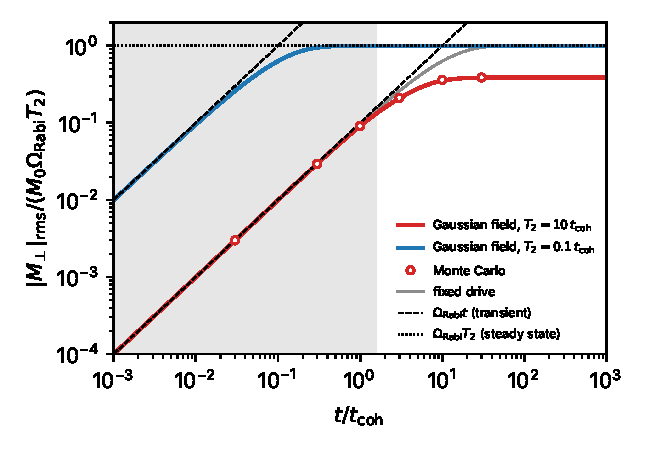
\includegraphics[width=0.92\linewidth]{figures/ch14/limit14_6a.pdf}
\captionof{figure}{Root-mean-square transverse magnetization of a nuclear-spin ensemble driven on resonance by an axion-like field, in units of $\Omega_{\mathrm{Rabi}}M_0T_2$, against the time over the coherence time $t_{\mathrm{coh}} = 1/m_\phi v_0^2$. Gray: the linear solution \cref{eq:14.6-mperp} for a drive of fixed amplitude, $1 - \ee^{-t/T_2}$, with its two literature limits, the transient $\Omega_{\mathrm{Rabi}}t$ (dashed) and the steady state $\Omega_{\mathrm{Rabi}}T_2$ (dotted). Colored: the same equation driven by the Gaussian field of the standard halo of \cref{sec:1.2} seen from the Earth, \cref{eq:14.6-ms}, with the Larmor frequency at the peak of the field line and $\Omega_{\mathrm{Rabi}}$ the value for the mean energy density; $T_2 = 10\,t_{\mathrm{coh}}$ (red) and $0.1\,t_{\mathrm{coh}}$ (blue). Circles: average over 1500 Monte Carlo realizations of the field for $T_2 = 10\,t_{\mathrm{coh}}$, each a sum of 2000 plane waves with random phases. Gray band: $t \le 1.6\,t_{\mathrm{coh}}$, where the field-averaged magnetization is within \SI{10}{\percent} of the fixed-drive formula for $T_2 = 10\,t_{\mathrm{coh}}$. For $T_2 = 0.1\,t_{\mathrm{coh}}$ the two agree within \SI{0.6}{\percent} at all times.}\label{fig:14-limit-mperp}
\par}
\smallskip
For $T_2 \gg t_{\mathrm{coh}}$ and $t \gtrsim t_{\mathrm{coh}}$ the magnetization stops growing linearly and saturates at $0.39$ of the fixed-drive value for $T_2 = 10\,t_{\mathrm{coh}}$; for longer $T_2$ the ratio falls as $(T_2/t_{\mathrm{coh}})^{-1/2}$.
\end{limitbox}

The linear solution assumes that the drive does not deplete $M_z$. At resonance and for $t \ll T_2$ the exact solution of \cref{eq:14.6-bloch} is $M_\perp = M_0\sin(\Omega_{\mathrm{Rabi}}t)$, below the linear one by the fraction $(\Omega_{\mathrm{Rabi}}t)^2/6$. In the steady state the $z$ component of \cref{eq:14.6-bloch} in the rotating frame gives $M_z = M_0/(1 + \Omega_{\mathrm{Rabi}}^2T_1T_2)$, and since $T_1$ is long, saturation sets in at drives with $\Omega_{\mathrm{Rabi}}T_2$ still small. Aybas and collaborators correct their limit by \SI{30}{\percent} for it at their detection threshold, $\Omega_{\mathrm{Rabi}} = \SI{0.23}{rad/s}$~\cite[Sect.~III]{aybas2021search}. The signal competes with noise from the spins themselves and from the magnetometer. The spin noise follows from the fluctuation--dissipation theorem \cref{eq:4.2-fdt} at the spin temperature $T_{\mathrm{s}}$ of a prepolarized sample, $p_{\mathrm{pol}} = \tanh(\omega_{\mathrm{Lar}}/2T_{\mathrm{s}})$. Since $\Imag R_{J_-J_-} \propto p_{\mathrm{pol}}$ while the symmetrized thermal factor is $\coth(\omega_{\mathrm{Lar}}/2T_{\mathrm{s}}) = 1/p_{\mathrm{pol}}$, the spin noise does not depend on the polarization~\cite[Eq.~(A1)]{budker2014proposal}, and prepolarization raises the signal only.

\subsection{The exponential-bin likelihood}\label{sec:14.6-stats}

A search records a readout for a time $t_{\mathrm{int}}$, the magnetometer signal of the precessing spins or the voltage of a resonator. It is demodulated at a carrier near $m_\phi$ into a complex signal $X(t)$ that holds both quadratures, and frequencies are measured from the carrier. The signal part is linear in the complex amplitude $\Phi$ of the field, $X_{\mathrm{sig}}(t) = \int\dd t'\,\mathcal{G}_{\mathrm{rd}}(t - t')\,\Phi(t')$ with a response kernel $\mathcal{G}_{\mathrm{rd}}$, and is thus Gaussian as well, with the power spectrum $\mathcal{S}_{\mathrm{sig}}(\omega) = |\mathcal{G}_{\mathrm{rd}}(\omega)|^2\mathcal{S}_\phi(\omega)$ up to the normalization of $\Phi$. For the spins, $|\mathcal{G}_{\mathrm{rd}}|^2$ is the Lorentzian of \cref{eq:14.6-mperp}; for a target much broader than the field line it is a constant, and $\mathcal{S}_{\mathrm{sig}}$ has the shape $F_\phi$. The noise, from the spins, the magnetometer or the amplifier, is Gaussian with the spectrum $\mathcal{S}_{\mathrm{n}}(\omega)$. The data are reduced to the periodogram at the frequencies $\omega_k = 2\pi k/t_{\mathrm{int}}$,
\begin{equation*}
  \mathsf{P}_k = \frac{1}{t_{\mathrm{int}}}\Bigl|\int_0^{t_{\mathrm{int}}}\dd t\,\ee^{\ii\omega_kt}X(t)\Bigr|^2 .
\end{equation*}
Its mean is the spectrum convolved with the Fejér kernel \cref{eq:14.6-fejer}, $\langle\mathsf{P}_k\rangle = \int\dd\omega\,\mathcal{K}_{t_{\mathrm{int}}}(\omega_k - \omega)[\mathcal{S}_{\mathrm{sig}}(\omega) + \mathcal{S}_{\mathrm{n}}(\omega)]$, which tends to $\mathcal{S}_{\mathrm{sig}}(\omega_k) + \mathcal{S}_{\mathrm{n}}(\omega_k)$ for a long record. The Fourier integral of a Gaussian process is a complex Gaussian variable, with independent real and imaginary parts of equal variance, and the sum of signal and noise is one such variable. Its squared modulus is exponentially distributed:
\begin{equation}
  p(\mathsf{P}_k) = \frac{1}{\bar{\mathsf{P}}_k}\,\ee^{-\mathsf{P}_k/\bar{\mathsf{P}}_k}, \qquad \bar{\mathsf{P}}_k = \mathsf{s}_k + \mathsf{b}_k ,
  \label{eq:14.6-expbin}
\end{equation}
with $\mathsf{s}_k$ and $\mathsf{b}_k$ the mean signal and noise powers of bin $k$. This is the distribution of Foster, Rodd and Safdi, with the mean $\mathsf{s}_k \propto F_\chi(v)/v \propto F_\phi(\omega_k)$ for a long record~\cite[Eq.~(24)]{foster2018revealing}. Signal and noise combine in the amplitudes, not in the powers; the sum of two exponential variables would not be exponential. For a record shorter than $t_{\mathrm{coh}}$ the whole line falls into one bin, and \cref{eq:14.6-expbin} states that the power in that bin, the square of the Rayleigh amplitude of the field, fluctuates by \SI{100}{\percent} from one realization to the next. For a longer record the line spreads over about $t_{\mathrm{int}}\Delta\omega_{\mathrm{eq}}/2\pi$ independent bins, each with its own exponential fluctuation. \Cref{fig:14-spectrum} shows single realizations, and \cref{lim:14.6b} the approach of the mean to its long-record form.

\begin{figure}[tbp]
  \centering
  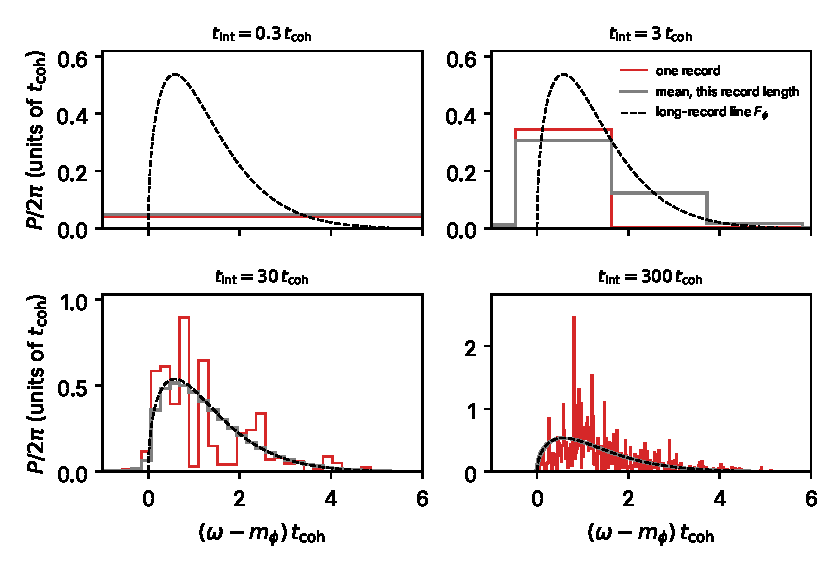
\includegraphics[width=0.92\linewidth]{figures/ch14/fig14_6.pdf}
  \caption{Periodogram of an axion-like field of unit mean power for records of $t_{\mathrm{int}} = 0.3$, 3, 30 and $300\,t_{\mathrm{coh}}$, against the energy above the rest energy in units of $1/t_{\mathrm{coh}} = m_\phi v_0^2$. Red: one Monte Carlo realization of the field, a sum of 3000 plane waves with random phases and with velocities from the standard halo of \cref{sec:1.2} seen from the Earth ($v_0 = \SI{238}{km/s}$, $v_{\mathrm{esc}} = \SI{544}{km/s}$, $v_E = \SI{250.5}{km/s}$). Bins of width $2\pi/t_{\mathrm{int}}$, one centered on the peak of the line. Gray: the mean periodogram for that record length, the line shape convolved with the Fejér kernel \cref{eq:14.6-fejer}. Dashed: the line shape $F_\phi$ of \cref{eq:14.6-Fphi}, the mean for a long record. Below $t_{\mathrm{coh}}$ one bin holds the whole line, with a height proportional to $t_{\mathrm{int}}$. Above it the bins resolve the line and scatter about it with the exponential distribution \cref{eq:14.6-expbin}.}
  \label{fig:14-spectrum}
\end{figure}

\begin{limitbox}[Gaussian-field signal and its power spectrum][lim:14.6b]
Exponential periodogram bins with mean $\mathsf{s}(\omega) \propto F_\phi(\omega)$, the line shape of \cref{eq:14.6-Fphi}, for a field built from Rayleigh-distributed amplitudes with random phases~\cite[Eqs.~(8), (10), (24)]{foster2018revealing}; for an absorber, the golden-rule mean of \cref{eq:8.2-abs} averaged over the line.
\par\smallskip
{\centering
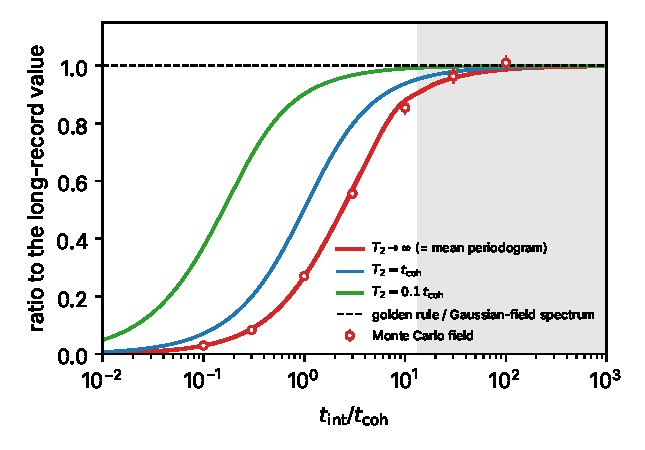
\includegraphics[width=0.92\linewidth]{figures/ch14/limit14_6b.pdf}
\captionof{figure}{Mean over the Gaussian field, for a record of length $t_{\mathrm{int}}$, divided by its long-record value, against $t_{\mathrm{int}}/t_{\mathrm{coh}}$. Red: the mean periodogram at the peak of the line, $\int\dd\omega\,F_\phi(\omega)\mathcal{K}_{t_{\mathrm{int}}}(\omega_{\mathrm{pk}} - \omega)/F_\phi(\omega_{\mathrm{pk}})$, which is also the energy absorbed by spins with $T_2 \to \infty$ at the peak frequency divided by the golden-rule value; circles: 1500 Monte Carlo realizations, with the scatter of their mean. Blue and green: energy absorbed by linearly driven spins with $T_2 = t_{\mathrm{coh}}$ and $0.1\,t_{\mathrm{coh}}$, divided by the golden-rule rate times $t_{\mathrm{int}}$. Standard halo of \cref{sec:1.2}. Gray band: the red curve within \SI{10}{\percent} of the long-record value, $t_{\mathrm{int}} \ge 13\,t_{\mathrm{coh}}$; for $T_2 = t_{\mathrm{coh}}$ and $0.1\,t_{\mathrm{coh}}$ the same accuracy needs $6.5\,t_{\mathrm{coh}}$ and $t_{\mathrm{coh}}$. The variance of the Monte Carlo bins equals the square of their mean within the sampling error, as the exponential law requires.}\label{fig:14-limit-spectrum}
\par}
\smallskip
Below $t_{\mathrm{coh}}$ and $T_2$ the mean grows as $t_{\mathrm{int}}^2$ rather than $t_{\mathrm{int}}$, with the ratio $t_{\mathrm{int}}/2\pi F_\phi(\omega_{\mathrm{pk}})$, and above them it approaches the golden rule as $1 - 1.25\,t_{\mathrm{coh}}/t_{\mathrm{int}}$, the leakage of the Fejér kernel.
\end{limitbox}

The bins of a stationary process are independent as long as the leakage of the Fejér kernel between neighbors is negligible. The likelihood of the periodogram is then the product of the distributions \cref{eq:14.6-expbin},
\begin{equation}
  -2\ln\mathsf{L} = 2\sum_k\Bigl[\ln\bar{\mathsf{P}}_k + \frac{\mathsf{P}_k}{\bar{\mathsf{P}}_k}\Bigr] ,
  \label{eq:14.6-like}
\end{equation}
the exponential-bin likelihood of Foster, Rodd and Safdi~\cite[Eq.~(29)]{foster2018revealing}, in which the signal enters through $\mathsf{s}_k$ and the coupling through its square, $\mathsf{s}_k \propto g^2$. Limits and discoveries follow from the likelihood ratio $\mathsf{t}$ of \cref{eq:C.14-ratio} and its thresholds \cref{eq:C.14-thresholds} (\cref{app:C.14}). How the sensitivity grows with $t_{\mathrm{int}}$ follows from the expected ratio for data without signal, $\mathsf{P}_k = \mathsf{b}_k$. Let $x_k = \mathsf{s}_k/\mathsf{b}_k$. Then $\mathsf{t} = 2\sum_k[\ln(1 + x_k) - x_k/(1 + x_k)]$, and for a weak signal, expanding to second order,
\begin{equation*}
  \mathsf{t} \simeq \sum_kx_k^2 = \frac{t_{\mathrm{int}}}{2\pi}\int\dd\omega\,\frac{\mathcal{S}_{\mathrm{sig}}(\omega)^2}{\mathcal{S}_{\mathrm{n}}(\omega)^2} ,
\end{equation*}
where the sum over bins of width $2\pi/t_{\mathrm{int}}$ became an integral. Let $\sigma_{\mathrm{sig}}^2$ be the mean square of the signal, proportional to $g^2$, and take white noise. For a record shorter than $t_{\mathrm{coh}}$ one bin holds the signal, $\mathsf{s} = \sigma_{\mathrm{sig}}^2t_{\mathrm{int}}$ and $\mathsf{b} = \mathcal{S}_{\mathrm{n}}$, so a fixed threshold on $\mathsf{t}$ means a fixed $x$, and
\begin{equation}
  \sigma_{\mathrm{sig}} \propto \mathcal{S}_{\mathrm{n}}^{1/2}\,t_{\mathrm{int}}^{-1/2}\quad(t_{\mathrm{int}} \ll t_{\mathrm{coh}}), \qquad
  \sigma_{\mathrm{sig}} \propto \mathcal{S}_{\mathrm{n}}^{1/2}\,(t_{\mathrm{int}}t_{\mathrm{coh}})^{-1/4}\quad(t_{\mathrm{int}} \gg t_{\mathrm{coh}}) .
  \label{eq:14.6-scaling}
\end{equation}
For a long record the integral gives $\mathsf{t} = 2\pi t_{\mathrm{int}}\sigma_{\mathrm{sig}}^4/(\Delta\omega_{\mathrm{eq}}\mathcal{S}_{\mathrm{n}}^2)$ with $\Delta\omega_{\mathrm{eq}} = 2.67/t_{\mathrm{coh}}$, which is the second law. Inside one coherence time the signal adds in amplitude and the noise in power, the familiar $t^{-1/2}$ of a coherent sinusoid. Beyond it the signal power stops growing in each bin, and only the number of bins over which the line is averaged grows, as $t_{\mathrm{int}}$, which halves the exponent. These are the scalings of Budker and collaborators~\cite[Eqs.~(A7), (A8)]{budker2014proposal}; the long-record form, with the coefficient of the weak-signal ratio, is the expected limit of Foster, Rodd and Safdi~\cite[Eqs.~(54), (63), (69)]{foster2018revealing}. For the spins, $\sigma_{\mathrm{sig}} = |M_\perp|$ is proportional to $g$, and the coupling at the threshold scales as $\sigma_{\mathrm{sig}}$.

The amplitude of the field within one coherence time is a random draw, and an analysis that ignores this sets too strong a limit. A search shorter than $t_{\mathrm{coh}}$ that takes the amplitude fixed at its mean value $\sqrt{2\rho_\chi}/m_\phi$ excludes every coupling whose signal would have exceeded the noise in that one realization; however, the field may have been weak during the record, with probability $1 - \ee^{-a}$ for an intensity below $a$ times its mean. Centers and collaborators found that limits with a fixed amplitude are too strong by a factor of 3 in a Bayesian treatment and 2.7 in a frequentist one, up to 10 with other priors, and 8.4 for gradient couplings~\cite[Eq.~(7)]{centers2021stochastic}. The exponential-bin likelihood already contains the random amplitude, so the correction is made once: with the likelihood \cref{eq:14.6-like}, or with a fixed-amplitude likelihood followed by the correction factor, never both.

An exact Neyman construction gives the size of the correction. Replace the line of the standard halo, convolved with the Fejér kernel, by $N_{\mathrm{eff}}$ equal bins, with $N_{\mathrm{eff}} = 1/\sum_kp_k^2$ the participation number of the bin fractions $p_k$ ($N_{\mathrm{eff}} \to 1$ below $t_{\mathrm{coh}}$ and $t_{\mathrm{int}}\Delta\omega_{\mathrm{eq}}/2\pi$ above). The bins have the width $2\pi/t_{\mathrm{int}}$, with one bin centered on the peak of the line. The statistic is the summed periodogram $\mathsf{Q}$ of those bins, with noise $\mathsf{b}$ per bin and total signal $\mathsf{s} = \sigma_{\mathrm{sig}}^2t_{\mathrm{int}}$ at every record length. With the Rayleigh amplitude of \cref{eq:14.6-expbin}, $\mathsf{Q}$ follows a Gamma distribution of shape $N_{\mathrm{eff}}$ and scale $\mathsf{b} + \mathsf{s}/N_{\mathrm{eff}}$; with a fixed amplitude and random phase, $2\mathsf{Q}/\mathsf{b}$ follows a noncentral $\chi^2$ distribution with $2N_{\mathrm{eff}}$ degrees of freedom and noncentrality $2\mathsf{s}/\mathsf{b}$. The \SI{95}{\percent} upper limit $\mathsf{s}_{\mathrm{up}}$ solves $P(\mathsf{Q} \le \mathsf{Q}_{\mathrm{obs}}\,|\,\mathsf{s}_{\mathrm{up}}) = 0.05$, with $\mathsf{Q}_{\mathrm{obs}}$ the median of the Gamma distribution of shape $N_{\mathrm{eff}}$ and scale $\mathsf{b}$ for data without signal. For the median of data without signal and one bin, $\mathsf{s}_{\mathrm{up}}/\mathsf{b} = 12.5$ with the Rayleigh amplitude and 3.17 with a fixed one, so that the fixed amplitude sets a coupling limit lower by $(12.5/3.17)^{1/2} = 1.99$. For data at the detection threshold, $\mathsf{Q}_{\mathrm{obs}} = \mathsf{b}\ln20$, the same construction gives 57.4 and 7.72 and a factor 2.73. \Cref{lim:14.6c} shows both treatments against the record length.
\begin{limitbox}[Sensitivity scalings of the exponential-bin likelihood][lim:14.6c]
Threshold amplitude $\propto\mathcal{S}_{\mathrm{n}}^{1/2}t_{\mathrm{int}}^{-1/2}$ for $t_{\mathrm{int}} < t_{\mathrm{coh}}$ and $\propto\mathcal{S}_{\mathrm{n}}^{1/2}(t_{\mathrm{int}}t_{\mathrm{coh}})^{-1/4}$ for $t_{\mathrm{int}} > t_{\mathrm{coh}}$~\cites[Eqs.~(A7), (A8)]{budker2014proposal}[Eqs.~(54), (63), (69)]{foster2018revealing}.
\par\smallskip
{\centering
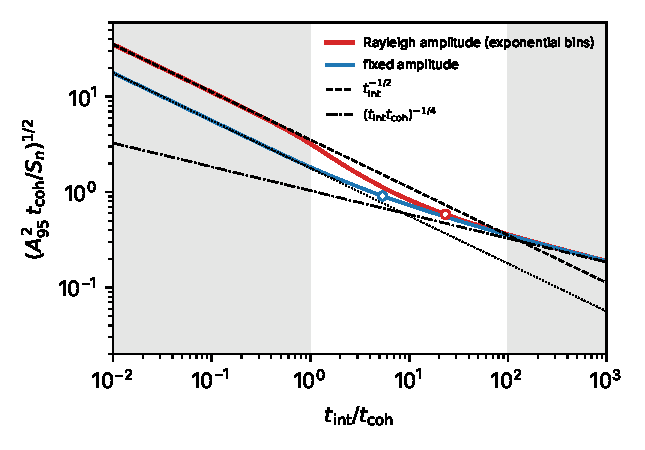
\includegraphics[width=0.92\linewidth]{figures/ch14/limit14_6c.pdf}
\captionof{figure}{Signal amplitude at the median expected \SI{95}{\percent} upper limit, $(\sigma_{\mathrm{sig}}^2t_{\mathrm{coh}}/\mathcal{S}_{\mathrm{n}})^{1/2}$, proportional to the coupling, against the record length over the coherence time, for white noise of spectrum $\mathcal{S}_{\mathrm{n}}$. Red: the signal as a Gaussian variable with a Rayleigh amplitude, the exponential-bin likelihood \cref{eq:14.6-like}. Blue: the signal power in each bin taken as fixed, with a random phase. Both curves follow from the Neyman construction of the text, with $N_{\mathrm{eff}}$ equal bins for the line of the standard halo of \cref{sec:1.2}. Dashed: $t_{\mathrm{int}}^{-1/2}$ for the Rayleigh amplitude (dotted: fixed amplitude); dash-dotted: $(t_{\mathrm{int}}t_{\mathrm{coh}})^{-1/4}$, common to both. Circles: the crossover, where the local slope is $-3/8$, at $23\,t_{\mathrm{coh}}$ (Rayleigh) and $5.4\,t_{\mathrm{coh}}$ (fixed). Gray: the Rayleigh curve within \SI{10}{\percent} of the $t_{\mathrm{int}}^{-1/2}$ law ($t_{\mathrm{int}} \le t_{\mathrm{coh}}$) or of the $(t_{\mathrm{int}}t_{\mathrm{coh}})^{-1/4}$ law ($t_{\mathrm{int}} \ge 100\,t_{\mathrm{coh}}$).}\label{fig:14-limit-scaling}
\par}
\smallskip
Neither power law holds between $t_{\mathrm{coh}}$ and $100\,t_{\mathrm{coh}}$, where the Rayleigh curve falls as steeply as $t_{\mathrm{int}}^{-0.67}$, faster than either law, because the record begins to average over independent amplitudes.
\end{limitbox}

The fixed amplitude sets a limit lower by 1.99 for records below $t_{\mathrm{coh}}$, by 1.76 at $t_{\mathrm{coh}}$ and by \SI{1.5}{\percent} at $100\,t_{\mathrm{coh}}$. The two power laws, extended, meet at $136\,t_{\mathrm{coh}}$ for the Rayleigh amplitude and at $8.7\,t_{\mathrm{coh}}$ for the fixed one, so the crossover lies between a few and about a hundred coherence times and its coefficient is not universal.

\begin{workedexample}{The scaling crossover for a \SI{1}{neV} axion-like field}\label{we:14-crossover}
An axion-like field of $m_\phi = \SI{1}{neV}$ oscillates at $m_\phi/2\pi = \SI{241.8}{kHz}$. By \cref{eq:14.6-tcoh}, $t_{\mathrm{coh}} = \SI{1.044}{s}$, and its line has the equivalent width $\Delta\omega_{\mathrm{eq}}/2\pi = 2.67/(2\pi t_{\mathrm{coh}}) = \SI{0.41}{Hz}$, $1.7\times10^{-6}$ of the frequency.

A $^{207}$Pb sample resonates at this frequency in $B_0 = 241.8\,\mathrm{kHz}/(9.034\,\mathrm{MHz\,T^{-1}}) = \SI{26.8}{mT}$. Its $T_2 = \SI{16.7}{ms}$ is $0.016\,t_{\mathrm{coh}}$, so the spin line, of half width $1/T_2 = \SI{60}{s^{-1}}$, is 63 times wider than the field line, $m_\phi v_0^2 = \SI{0.96}{s^{-1}}$. The spins are in the case $T_2 \ll t_{\mathrm{coh}}$ of \cref{lim:14.6a}: the magnetization reaches the steady state of \cref{eq:14.6-mperp} after a few $T_2$, about \SI{0.05}{s}, and its amplitude then follows the Rayleigh amplitude of the field, which changes on the scale of a second.

The sensitivity depends on how long a record at one frequency can be. With the construction of \cref{lim:14.6c}, the threshold coupling falls by a factor 3.46 from $t_{\mathrm{int}} = \SI{0.1}{s}$ to \SI{1}{s}, more than the $\sqrt{10} = 3.16$ of the coherent law, since the record starts to sample a second amplitude. The local slope reaches $-3/8$ at $23\,t_{\mathrm{coh}} = \SI{24}{s}$. A record of one hour spans 3447 coherence times and a day 82\,730. Going from an hour to a day improves the limit by 2.24, close to $24^{1/4} = 2.21$ and far from the $24^{1/2} = 4.9$ that a coherent signal would give. At \SI{0.1}{s} the fixed-amplitude analysis would claim a limit 1.99 times lower; at one hour the two agree to better than \SI{0.1}{\percent}.
\end{workedexample}

A search that scans the field over a decade of frequency in a fixed total time spends less time at each frequency as the line narrows toward low masses. The crossover then decides whether to dwell longer at one frequency or to scan more. At $m_\phi = \SI{1}{\micro eV}$, $t_{\mathrm{coh}} = \SI{1.04}{ms}$, and every practical record lies deep in the $(t_{\mathrm{int}}t_{\mathrm{coh}})^{-1/4}$ regime; at \SI{1}{peV}, $t_{\mathrm{coh}} = \SI{17}{min}$, and the random amplitude must be in the likelihood.

\section{Chiral and nonreciprocal targets}\label{sec:14.5}

Density-functional perturbation theory gives $\alpha$-quartz the gyration $g_{33} = \SI{0.125}{bohr}$ along its optic axis, and with it a rotation of the plane of polarization by \SI{21.6}{\degree} per millimeter for light of \SI{2.105}{eV}~\cite[Table~I, Eq.~(4)]{zabalo2023natural}; the mirror-image crystal turns the plane the other way. The rotation is a response odd in the momentum of the light, and at a photon momentum of \SI{2.1}{eV} it is small, $q\,g_{33} = 7\times10^{-5}$. Dark matter that deposits the same energy brings at least $1/v_{\mathrm{max}} = 377$ times more momentum, so a response odd in $\vect{q}$ may matter more for dark matter than for light. \Cref{sec:11.7} showed that the density response stays even in $\vect{q}$ unless inversion and time reversal are both broken; in a crystal, magnetic order breaks time reversal. Here we find which other responses become odd when only one of the two symmetries is broken, in which crystals, and which couplings of the dark matter see them. Three detectors are built on broken symmetry: phonons that carry angular momentum, molecular magnets held in a metastable state, and multiferroics, in which electric and magnetic order coexist.

\subsection{Reciprocity of the response matrix}\label{sec:14.5-recip}

Time reversal relates the response at $\vect{q}$ to that at $-\vect{q}$ for every pair of rows. Each row of \cref{eq:8.1-rows} goes over into itself at $-\vect{q}$ under the antiunitary time-reversal operator $\mathsf{T}$, up to a sign $\sigma^{\mathsf{T}}_a$: $\mathsf{T}O_a(\vect{q})\mathsf{T}^{-1} = \sigma^{\mathsf{T}}_aO_a(-\vect{q})$, since $\mathsf{T}$ conjugates $\ee^{\ii\vect{q}\cdot\vect{r}}$ and reverses momenta and spins. The density and the kinetic-energy density have $\sigma^{\mathsf{T}} = +1$, the current and the spin density $-1$, and the spin current $+1$, as the product of two reversed vectors. For an antiunitary operator, $\langle f|A|i\rangle^* = \langle\mathsf{T}f|\mathsf{T}A\mathsf{T}^{-1}|\mathsf{T}i\rangle$. We apply this identity to both matrix elements in \cref{eq:4.2-Sab}; the time-reversed states carry the same energies and thermal weights, so $S_{ab}(\vect{q},\omega)^* = \sigma^{\mathsf{T}}_a\sigma^{\mathsf{T}}_bS_{ab}(-\vect{q},\omega)$. With $S_{ab}^* = S_{ba}$,
\begin{equation}
  \begin{aligned}
  S_{ab}(\vect{q},\omega) &= \sigma^{\mathsf{T}}_a\sigma^{\mathsf{T}}_b\,S_{ba}(-\vect{q},\omega) &&(\text{time reversal}), \\
  S_{ab}(\vect{q},\omega) &= \sigma^{\mathsf{P}}_a\sigma^{\mathsf{P}}_b\,S_{ab}(-\vect{q},\omega) &&(\text{inversion}) .
  \end{aligned}
  \label{eq:14.5-recip}
\end{equation}
The second relation follows in the same way from the unitary inversion $\mathsf{P}$, with $\sigma^{\mathsf{P}} = +1$ for the density, the kinetic-energy density and the spin density and $-1$ for the current and the spin current. For the density block alone both relations give $S(\vect{q}) = S(-\vect{q})$ (\cref{app:A.4}).

The current block is the first that differs. Hermiticity splits it into a real symmetric part and $\ii$ times a real antisymmetric part, and an antisymmetric $3\times3$ matrix is a vector:
\begin{equation}
  S_{j^\alpha j^\beta}(\vect{q},\omega) = S^{\mathrm{R}}_{\alpha\beta}(\vect{q},\omega) + \ii\,\epsilon_{\alpha\beta\gamma}\,\mathcal{G}^\gamma_{\mathrm{OA}}(\vect{q},\omega) .
  \label{eq:14.5-GOA}
\end{equation}
With $\sigma^{\mathsf{T}}_j = -1$ twice, time reversal gives $S_{j^\alpha j^\beta}(\vect{q}) = S_{j^\alpha j^\beta}(-\vect{q})^*$: the symmetric part is even in $\vect{q}$ and $\boldsymbol{\mathcal{G}}_{\mathrm{OA}}$ is odd. Since inversion makes both parts even, $\boldsymbol{\mathcal{G}}_{\mathrm{OA}}$ needs a crystal without inversion and survives time reversal, while an odd symmetric part needs both symmetries broken. A crystal without inversion, mirror planes or rotation--reflections is chiral, and exists in two forms related by a mirror, its enantiomers; $\boldsymbol{\mathcal{G}}_{\mathrm{OA}}$ changes sign between them. Physically, $\boldsymbol{\mathcal{G}}_{\mathrm{OA}}$ measures whether the electrons circulate one way more easily than the other along $\vect{q}$, an asymmetry that only a crystal without inversion allows. For rows of opposite time-reversal sign, such as the spin density and the spin current, \cref{eq:14.5-recip} makes the symmetric part of the block odd in $\vect{q}$, so its value at $\vect{q} = 0$, which a static field would probe, needs inversion broken as well. \Cref{tab:14-odd} collects the cases that this section uses.

\begin{table}[tbp]
  \caption{Parts of the response odd in $\vect{q}$, or odd under inversion of the crystal, and the symmetries they need, from \cref{eq:14.5-recip}. ``Gyrotropic'' point groups are those with $N_{\mathrm{gyr}} > 0$ in \cref{eq:C.17-gyration}.}
  \label{tab:14-odd}
  \centering\small
  \begin{tabular}{@{}>{\raggedright\arraybackslash}p{0.30\linewidth}>{\raggedright\arraybackslash}p{0.27\linewidth}>{\raggedright\arraybackslash}p{0.33\linewidth}@{}}
    \toprule
    Quantity & Needs & Treated in \\
    \midrule
    Density $S(\vect{q},\omega) - S(-\vect{q},\omega)$ & inversion and time reversal broken & \cref{sec:11.7} \\
    Antisymmetric current part $\boldsymbol{\mathcal{G}}_{\mathrm{OA}}$ & inversion broken, gyrotropic group & \cref{sec:14.5-oa}, \cref{we:14-quartz} \\
    Symmetric current part, odd in $\vect{q}$ & inversion and time reversal broken & \cref{sec:14.5-recip} \\
    Phonon angular momentum $\vect{L}^{\mathrm{ph}}$ & inversion or time reversal broken & \cref{sec:14.5-phonons} \\
    Static spin--spin-current block $R_{s^z\mathcal{J}}(0,\omega \to 0)$ & inversion and time reversal broken & \cref{sec:14.5-mf} \\
    \bottomrule
  \end{tabular}
\end{table}

\subsection{Finite-momentum optical activity}\label{sec:14.5-oa}

The vector $\boldsymbol{\mathcal{G}}_{\mathrm{OA}}$ is the finite-momentum generalization of natural optical activity. To see the connection, write the antisymmetric part of the proper current response as $\ii\epsilon_{\alpha\beta\gamma}\mathcal{G}^\gamma_{\mathrm{R}}$, with $\boldsymbol{\mathcal{G}}_{\mathrm{R}}$ complex. The fluctuation--dissipation theorem \cref{eq:4.2-fdt}, $(1 - \ee^{-\beta\omega})S_{ab} = \ii(R_{ab} - R_{ba}^*)$, gives $\boldsymbol{\mathcal{G}}_{\mathrm{OA}} = -2\Imag\boldsymbol{\mathcal{G}}_{\mathrm{R}}/(1 - \ee^{-\beta\omega})$, and the dielectric tensor of \cref{sec:4.4}, $\varepsilon^{\alpha\beta} = \delta^{\alpha\beta} - (e^2/\omega^2)[(\nd_e/m_e)\delta^{\alpha\beta} + \tilde R^{\alpha\beta}_{jj}]$, acquires the antisymmetric term $-\ii(e^2/\omega^2)\epsilon_{\alpha\beta\gamma}\mathcal{G}^\gamma_{\mathrm{R}}$. Optical activity is defined by the term linear in $\vect{q}$ of that tensor, $\varepsilon^{\alpha\beta}(\vect{q},\omega) = \varepsilon^{\alpha\beta}(\omega) + \ii\epsilon_{\alpha\beta m}g_{ml}(\omega)q_l + O(q^2)$, with the gyration tensor $g_{ml}$ of \cref{app:C.17} in the normalization of the dielectric tensor~\cite[Eqs.~(2)--(4)]{zabalo2023natural}. Comparing the two antisymmetric terms,
\begin{equation}
  \mathcal{G}^\gamma_{\mathrm{OA}}(\vect{q},\omega) = \frac{2\omega^2}{e^2}\,\frac{\Imag g_{\gamma l}(\omega)\,q_l}{1 - \ee^{-\beta\omega}} + O(q^3) ,
  \label{eq:14.5-gyr}
\end{equation}
with no term of order $q^2$, since $\boldsymbol{\mathcal{G}}_{\mathrm{OA}}$ is odd. Only the absorptive part of the gyration enters the structure factor. The reactive part of the gyration, $\Real g$, rotates the polarization, and the absorptive and reactive parts are related by the Kramers--Kronig relations \cref{eq:4.3-KK}, which hold for $g(\omega)$ because $g(\omega)$ is a coefficient of a causal response.

The observable is circular dichroism, the difference between the absorption of the two helicities. A transverse field of polarization $\hat{\vect{e}}_\pm = (\hat{\vect{e}}_1 \pm \ii\hat{\vect{e}}_2)/\sqrt2$, with $\hat{\vect{e}}_1\times\hat{\vect{e}}_2 = \hat{\vect{q}}$, couples to the row $\hat{\vect{e}}_\pm\cdot\vect{j}_e$, and \cref{eq:8.2-abs} needs $\sum_{\alpha\beta}\hat e^*_{\pm\alpha}\hat e_{\pm\beta}S_{j^\alpha j^\beta}$. The symmetric part yields the transverse response $S_{\mathrm{T}}$, and the antisymmetric part gives $\ii(\hat{\vect{e}}^*_\pm\times\hat{\vect{e}}_\pm)\cdot\boldsymbol{\mathcal{G}}_{\mathrm{OA}}$ with $\hat{\vect{e}}^*_\pm\times\hat{\vect{e}}_\pm = \pm\ii\hat{\vect{q}}$:
\begin{equation}
  S_\pm(\vect{q},\omega) = S_{\mathrm{T}}(\vect{q},\omega) \mp \hat{\vect{q}}\cdot\boldsymbol{\mathcal{G}}_{\mathrm{OA}}(\vect{q},\omega), \qquad
  \frac{S_- - S_+}{S_- + S_+} = \frac{\hat{\vect{q}}\cdot\boldsymbol{\mathcal{G}}_{\mathrm{OA}}}{S_{\mathrm{T}}} = \frac{q\,\Imag g_{\hat q\hat q}}{\varepsilon_2^{\mathrm{T}}} ,
  \label{eq:14.5-helicity}
\end{equation}
with $g_{\hat q\hat q} = \hat{\vect{q}}\cdot g\cdot\hat{\vect{q}}$; the last form uses \cref{eq:14.5-gyr} and $\varepsilon_2^{\mathrm{T}} = (e^2/2\omega^2)(1 - \ee^{-\beta\omega})S_{\mathrm{T}}$ at the order kept. Reversing $\vect{q}$ at fixed helicity exchanges $\hat{\vect{e}}_1$ and $\hat{\vect{e}}_2$ up to sign and flips $\boldsymbol{\mathcal{G}}_{\mathrm{OA}}$, so the dissymmetry depends on the helicity, not on the direction of travel: natural optical activity is reciprocal. For light, $q = n_r\omega$ with $n_r$ the refractive index, and the helicity components of $\varepsilon$ are $\varepsilon^{\mathrm{T}} \mp g_{\hat q\hat q}q$. Then $n_\pm = n_r \mp g_{\hat q\hat q}\omega/2$, and per unit length the plane of linear polarization turns by
\begin{equation}
  \rho(\omega) = \frac{\omega}{2}\Real(n_- - n_+) = \frac{\omega^2}{2}\Real g_{\hat q\hat q}(\omega) ,
  \label{eq:14.5-rot}
\end{equation}
the rotatory power of Zabalo and Stengel~\cite[Eq.~(4)]{zabalo2023natural}, while the absorption coefficients of the two helicities differ by $2\omega^2\Imag g_{\hat q\hat q}$.

\Cref{fig:14-cd} sketches what changes for dark matter. At optical momenta the dissymmetry is of order $q|g| \sim 10^{-4}$. Dark matter at energy $\omega$ brings $q \ge \omega/v_{\mathrm{max}}$, and at $q = \SI{1}{keV}$ the quartz value of $g_{33}$ gives $q\,g_{33} = 0.034$. The value 0.034 sets a scale only. \Cref{eq:14.5-gyr} holds for $q$ small against the inverse lattice spacing, while dark-matter momenta of keV reach the zone boundary, and above the band gap of quartz the absorptive $\Imag g$, not the static $g_{33}$, is the relevant input. The full $\boldsymbol{\mathcal{G}}_{\mathrm{OA}}(\vect{q},\omega)$ at keV momenta is not known for any crystal.

\begin{figure}[tbp]
  \centering
  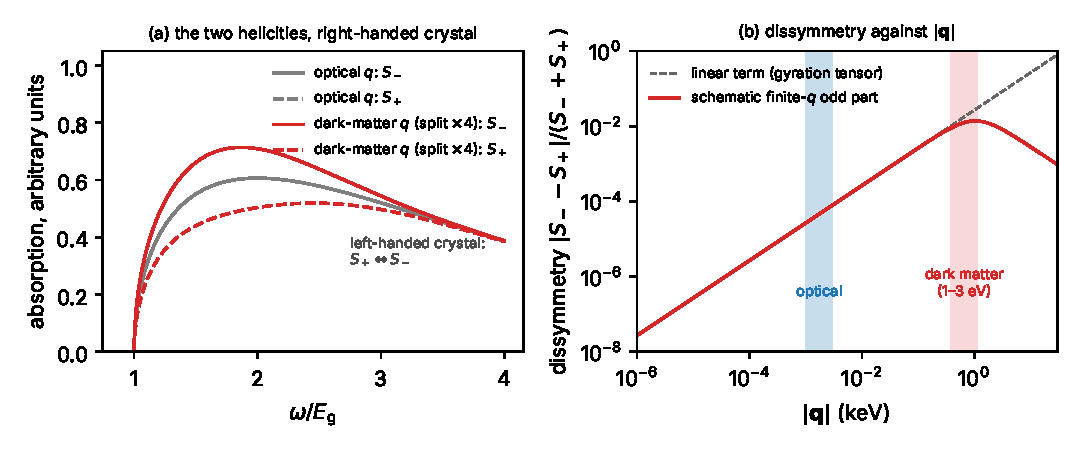
\includegraphics[width=0.95\linewidth]{figures/ch14/fig14_5.pdf}
  \caption{Circular dichroism of a chiral crystal such as tellurium. Schematic: all curves are model curves, not computed for tellurium. (a) Absorption of the two helicities, $S_\pm = S_{\mathrm{T}} \mp \hat{\vect{q}}\cdot\boldsymbol{\mathcal{G}}_{\mathrm{OA}}$ (\cref{eq:14.5-helicity}), for a model band edge at $E_{\mathrm{g}}$ in the right-handed form, at an optical momentum (gray, split invisible) and at a dark-matter momentum (red, split exaggerated four times). The left-handed form exchanges $S_+$ and $S_-$. (b) The dissymmetry against $|\vect{q}|$: the linear term $q|g|$ with $|g| = \SI{0.1}{bohr}$, the order of the computed gyration of trigonal crystals~\cite[Table~I]{zabalo2023natural} (dashed), and a schematic turnover at the inverse of a \SI{6}{\angstrom} helix pitch (red). Blue band: photons of 1 to \SI{3}{eV}; red band: the smallest dark-matter momenta at the same energies, $\omega/v_{\mathrm{max}}$. The odd part beyond the linear term is not known.}
  \label{fig:14-cd}
\end{figure}

Dark matter sees $\boldsymbol{\mathcal{G}}_{\mathrm{OA}}$ only through a coupling tensor with an antisymmetric current block. In \cref{tab:8-operators} the current row of $\mathcal{O}_5$ has the potential $\tilde V_{j^\delta} = -(\ii/m_e)c_5\epsilon_{\mu\gamma\delta}S^\mu_\chi q^\gamma$, and that of $\mathcal{O}_8$ has $\tilde V_{j^\delta} = -c_8S^\delta_\chi$. Each alone leads to a real symmetric $\mathfrak{D}_{jj}$: $\frac14|c_8|^2\delta_{\alpha\beta}$ for $\mathcal{O}_8$ and $(|c_5|^2/4m_e^2)(q^2\delta_{\alpha\beta} - q_\alpha q_\beta)$ for $\mathcal{O}_5$. Their interference, with $\Tr_\chi(S^\mu_\chi S^\nu_\chi)/2 = \delta_{\mu\nu}/4$ in \cref{eq:8.1-D}, gives
\begin{equation*}
  \mathfrak{D}_{j^\alpha j^\beta} \supset -\frac{\ii}{2m_e}\,\Real(c_5^*c_8)\,\epsilon_{\alpha\beta\gamma}q^\gamma ,
\end{equation*}
purely imaginary and antisymmetric, and its contraction with \cref{eq:14.5-GOA} is $(1/m_e)\Real(c_5^*c_8)\,\vect{q}\cdot\boldsymbol{\mathcal{G}}_{\mathrm{OA}}$. Since $\boldsymbol{\mathcal{G}}_{\mathrm{OA}}$ changes sign between enantiomers, the difference of their rates isolates this term. The density rows of $\mathcal{O}_5$ and $\mathcal{O}_8$ meet the current rows through the block $S_{nj}$. Inversion maps one enantiomer onto the other and, by \cref{eq:14.5-recip} with $\sigma^{\mathsf{P}}_n\sigma^{\mathsf{P}}_j = -1$, gives $S^{\mathrm{L}}_{nj}(\vect{q}) = -S^{\mathrm{R}}_{nj}(-\vect{q})$, so the enantiomer-odd part $S^{\mathrm{R}}_{nj}(\vect{q}) - S^{\mathrm{L}}_{nj}(\vect{q})$ is a vector even in $\vect{q}$. Averaged over crystal orientations at fixed $\vect{q}$, the enantiomer-odd part must point along $\hat{\vect{q}}$. A vector even in $\vect{q}$ cannot point along $\hat{\vect{q}}$, so the average vanishes; the enantiomer-odd part also enters contracted with $\vect{q}\times\bar{\vect{v}}_\chi$, which is orthogonal to $\hat{\vect{q}}$. Inserting the interference term in \cref{eq:8.2-spectrum} and averaging over orientations with the kernel $\eta(\vmin)/2q$ of \cref{eq:A.8-eta} gives
\begin{keyresult}[Enantiomer difference of the rate]
\begin{equation}
  \frac{\dd\mathcal{R}^{\mathrm{R}}}{\dd\omega} - \frac{\dd\mathcal{R}^{\mathrm{L}}}{\dd\omega}
  = \frac{\rho_\chi}{\mchi\,\rho_T}\int\frac{q\,\dd q}{2\pi^2}\,\eta(\vmin)\,\frac{q}{m_e}\,\Real\bigl[c_5^*(q)\,c_8(q)\bigr]\,\bar{\mathcal{G}}_{\mathrm{OA}}(q,\omega) ,
  \label{eq:14.5-enant}
\end{equation}
with $\bar{\mathcal{G}}_{\mathrm{OA}}(q,\omega)$ the average of $\hat{\vect{q}}\cdot\boldsymbol{\mathcal{G}}_{\mathrm{OA}}$ over the directions of $\vect{q}$ in the right-handed form.
\end{keyresult}
\noindent Operator $\mathcal{O}_8 = \vect{S}_\chi\cdot\vect{v}^\perp$ is odd under inversion and $\mathcal{O}_5$ is even. Only dark matter whose couplings violate parity therefore has different rates in the two enantiomers, for example a particle with both a magnetic dipole moment, which produces $\mathcal{O}_5$, and an anapole moment, which produces $\mathcal{O}_8$ (\cref{sec:8.1}). The couplings supply one parity-odd factor, and the crystal supplies the other, $\boldsymbol{\mathcal{G}}_{\mathrm{OA}}$. Because $\vect{q}\cdot\boldsymbol{\mathcal{G}}_{\mathrm{OA}}$ is even in $\vect{q}$, the enantiomer difference is not a wind asymmetry: at fixed orientation it contains the multipoles $\ell = 0$ and $\ell = 2$ of \cref{eq:11.7-rate} and modulates with the even halo multipoles. Relative to the transverse-current part of the rate of $\mathcal{O}_8$ alone, $\frac12|c_8|^2S_{\mathrm{T}}$, the interference term is the dissymmetry of \cref{eq:14.5-helicity} at dark-matter momenta times $2|c_5|q/(m_e|c_8|)$.

\begin{workedexample}{Point-group test for odd responses in $\alpha$-quartz}\label{we:14-quartz}
$\alpha$-Quartz, like tellurium, has the point group $32$ ($D_3$): the identity, two rotations by $\pm2\pi/3$ about the optic axis $\hat{\vect{z}}$, and three rotations by $\pi$ about twofold axes in the basal plane. All six are proper, $\det\mathsf{R} = 1$, and the class values of $1 + 2\cos\theta_{\mathsf{R}}$ are $3$, $0$ and $-1$ (\cref{app:C.17}).

\emph{Scalar responses.} An odd part of a scalar such as $S(\vect{q},\omega)$ starts with the harmonics $\ell = 1$, which transform as a polar vector. By \cref{eq:C.17-ninv,eq:C.17-polar} their invariants number $(3 + 2\cdot0 + 3\cdot(-1))/6 = 0$. The harmonics $\ell = 3$, with characters $\sin(\frac72\theta)/\sin(\frac12\theta) = 7$, $1$, $-1$, have $(7 + 2 - 3)/6 = 1$ invariant. Quartz keeps time reversal, however, and by \cref{eq:14.5-recip} its density response is even anyway; a magnetic crystal with the same point group could have a scalar odd part starting at $\ell = 3$, never at $\ell = 1$, because the group is not polar.

\emph{The current response.} The gyration tensor transforms with $(\det\mathsf{R})(1 + 2\cos\theta_{\mathsf{R}})^2 = 9$, $0$, $1$ on the three classes, and \cref{eq:C.17-gyration} gives $N_{\mathrm{gyr}} = (9 + 0 + 3)/6 = 2$. Projecting all nine components with $|\mathcal{P}|^{-1}\sum_{\mathsf{R}}(\det\mathsf{R})\,\mathsf{R}\otimes\mathsf{R}$ leaves the two diagonal tensors $\operatorname{diag}(1,1,0)$ and $\operatorname{diag}(0,0,1)$, so $g = \operatorname{diag}(g_{11}, g_{11}, g_{33})$. The density-functional values are $g_{11} = \SI{-0.071}{bohr}$ and $g_{33} = \SI{0.125}{bohr}$~\cite[Table~I]{zabalo2023natural}.

\emph{Consequences.} Along the optic axis, $g_{\hat q\hat q} = g_{33}$ and \cref{eq:14.5-rot} gives $\rho = \SI{21.6}{\degree.mm^{-1}}$ at \SI{2.105}{eV}. Averaged over directions, $g_{\hat q\hat q}$ becomes $(2g_{11} + g_{33})/3 = \SI{-0.0057}{bohr}$, only $-0.045$ of $g_{33}$, because $g_{11}$ and $g_{33}$ have opposite signs. If the same cancellation held for $\Imag g$ above the gap, the orientation-averaged enantiomer difference \cref{eq:14.5-enant} of quartz would be twenty times smaller than the difference for $\vect{q}$ along the optic axis. A crystal held with its axis along the wind would gain the factor of twenty back through the multipole $\ell = 2$. GaAs, with $N_{\mathrm{gyr}} = 0$ (\cref{we:C-gyration}), has no $\boldsymbol{\mathcal{G}}_{\mathrm{OA}}$ at linear order although it lacks inversion, and no enantiomers.
\end{workedexample}

\subsection{Chiral phonons}\label{sec:14.5-phonons}

In GaAs, which lacks inversion, the atoms in a phonon of a general wavevector move on ellipses, and a phonon of the lowest band carries on average $0.12$ units of angular momentum. In the normalization of \cref{eq:5.3-u}, the angular momentum of mode $\vect{Q}\nu$ in units of $\hbar$ is
\begin{equation}
  \vect{L}^{\mathrm{ph}}_{\vect{Q}\nu} = \sum_\kappa\vect{L}^{\mathrm{ph}}_{\kappa,\vect{Q}\nu}, \qquad
  \vect{L}^{\mathrm{ph}}_{\kappa,\vect{Q}\nu} = -\ii\,\vect{e}_{\kappa\nu}(\vect{Q})^*\times\vect{e}_{\kappa\nu}(\vect{Q}) ,
  \label{eq:14.5-Lph}
\end{equation}
the definition of Romao and collaborators and of Matas, Krizek and Romao~\cites[Eq.~(6)]{romao2023chiral}[Eq.~(11)]{matas2025chiral}. Each term is real, and $|\vect{L}^{\mathrm{ph}}_{\vect{Q}\nu}| \le \sum_\kappa|\vect{e}_{\kappa\nu}|^2 = 1$, with equality for circular motion. Time reversal gives $\vect{e}_{\kappa\nu}(-\vect{Q}) = \vect{e}_{\kappa\nu}(\vect{Q})^*$ for a nondegenerate mode, so $\vect{L}^{\mathrm{ph}}_{-\vect{Q}\nu} = -\vect{L}^{\mathrm{ph}}_{\vect{Q}\nu}$. Inversion maps the axial vector $\vect{L}^{\mathrm{ph}}$ at $\vect{Q}$ onto itself at $-\vect{Q}$, and with both time reversal and inversion $\vect{L}^{\mathrm{ph}}$ vanishes, as in silicon. In a magnetically ordered crystal any phonon can carry angular momentum.

The angular momentum labels the final state, and the coupling is the density coupling of \cref{eq:11.1-S1}, which creates mode $\vect{Q}\nu$ with the amplitude given there. Multiplying each term of the one-phonon response \cref{eq:11.1-S1} by $\delta^3(\vect{L} - \vect{L}^{\mathrm{ph}}_{\vect{Q}\nu})$ gives the final-state-resolved one-phonon response $S^{(1)}_A(\vect{q},\omega;\vect{L})$, whose integral over $\vect{L}$ is $S^{(1)}_A(\vect{q},\omega)$. With $S^{(1)}_A$ even in $\vect{q}$ and $\vect{L}^{\mathrm{ph}}$ odd, the mean angular momentum of the created phonons survives the integration over $\vect{q}$ only through the part of the halo kernel odd in $\hat{\vect{q}}\cdot\hat{\vect{v}}_{\mathrm{E}}$, the odd multipoles of \cref{eq:11.7-ups}. To first order in $\hat{\vect{v}}_{\mathrm{E}}$ the mean angular momentum is $\langle L_i\rangle = G_{ij}\hat v_{\mathrm{E},j}$, and the crystal tensor $G_{ij}$ joins an axial index to a polar one, like the gyration tensor. The invariants of $G_{ij}$ are counted by \cref{eq:C.17-gyration}: in GaAs there are none, so the phonons that dark matter creates there carry no net angular momentum along the wind at this order, while $\alpha$-quartz and tellurium allow two constants (\cref{we:14-quartz}).

Chiral phonons are detected through their magnetic moment. A nucleus of Born charge $eZ^*_\kappa$ on a closed orbit has the moment $(eZ^*_\kappa/2M_\kappa)\,\vect{u}\times\vect{P}$. Summed over the nuclei, the moment operator is bilinear in the phonon operators, has no matrix element between the ground state and one phonon, and measures a property of the occupied mode. In a state with one phonon in mode $\vect{Q}\nu$,
\begin{equation}
  \boldsymbol{\mu}^{\mathrm{ph}}_{\vect{Q}\nu} = \sum_\kappa\frac{eZ^*_\kappa}{2M_\kappa}\,\vect{L}^{\mathrm{ph}}_{\kappa,\vect{Q}\nu} ,
  \label{eq:14.5-muph}
\end{equation}
which is the moment of Refs.~\cites[Eq.~(7)]{romao2023chiral}[Eq.~(12)]{matas2025chiral} for isotropic Born charges. With the PBE Born charges of \cref{sec:5.5}, $Z^* = \pm2.09$, GaAs reaches at most $0.015\,\mu_N$ in its lowest band, and no mode exceeds $Z^*_{\mathrm{Ga}}m_p/M_{\mathrm{Ga}} = 0.030\,\mu_N$, which a mode with $|\vect{L}^{\mathrm{ph}}| = 1$ on the gallium sublattice alone would have; $\mu_N$ is the nuclear magneton, $1/1836$ of $\mu_B$. Phonon moments of order $\mu_B$ have been reported in some $4f$ paramagnets and topological semimetals~\cite[Sect.~II]{romao2023chiral}. They are larger than \cref{eq:14.5-muph} by four to five orders of magnitude and come from the coupling of the lattice to the orbital and spin moments of the electrons, which the Born charge does not contain; computing them needs the derivatives of the crystal-field states with respect to the atomic displacements, separately for the spin and the orbital moment (\cref{app:E.19}). A coupling to the ionic current, such as that of a particle with a magnetic dipole moment, creates single phonons through the transverse part of that current, at first order in $q$, and not through $\boldsymbol{\mu}^{\mathrm{ph}}$.

The detector that Romao and collaborators propose reads out phonons of the lowest band, the only band whose phonons live for microseconds or longer~\cite[Sect.~III]{matas2025chiral}, after the phonons created by the dark matter have decayed into the lowest band. A phonon Hall effect, the transverse deflection of a heat current carried by chiral phonons, collects them at the surfaces, where magnetometers sense their moments~\cite[Sect.~IV]{romao2023chiral}. The rate is the one-phonon rate~\cite[Eqs.~(3), (4)]{matas2025chiral}, \cref{eq:11.1-S1} in \cref{eq:8.2-spectrum}, times a detection probability that Matas and collaborators take as the average of $|\vect{L}^{\mathrm{ph}}|$ over the lowest band, with each event ending as one phonon placed at random in that band. They quote 0.22 for LiNbO$_3$ and 0.16 for the framework CuCl(pyrimidine)~\cite[Sect.~III]{matas2025chiral}, and Romao and collaborators 0.15 for InF$_3$(4,4$'$-bipyridine)~\cite[Sect.~VII]{romao2023chiral}. The estimate assumes that each created phonon lands at random in the band, as in the average, and that its chirality survives the decay. \Cref{lim:14.5a}a tests the first assumption in GaAs. The survival of the chirality is not protected, since $L^{\mathrm{ph}}_z$ is not conserved. For $H = \frac12\vect{p}\cdot\vect{p} + \frac12\vect{u}\cdot D\vect{u}$ in mass-weighted coordinates and $L_z = \vect{u}\cdot J_z\vect{p}$, with $J_z$ the generator of rotations about $\hat{\vect{z}}$ acting on the displacement of each site, $[H, L_z] = \frac{\ii}{2}\,\vect{u}\cdot[J_z, D]\,\vect{u}$, which vanishes only if the force constants are isotropic about every site. A crystal conserves only the pseudo-angular momentum of its discrete rotations, the eigenvalue of a rotation by $2\pi/n$ defined modulo $n$, and the anharmonic decay changes $\vect{L}^{\mathrm{ph}}$. The probability that a created phonon ends as a detectable chiral phonon is the solution of a linear system over the three-phonon decay rates, $\boldsymbol{\mathcal{N}}^{\mathrm{ch}} = (\mathbb{1} - \mathsf{M})^{-1}\vect{b}$, with the angular momentum recomputed for each daughter.

\subsection{Single-molecule magnets}\label{sec:14.5-smm}

The twelve manganese ions of a Mn$_{12}$-acetate molecule lock into a total spin $|\vect{S}| = 10$, held along the molecular axis by an axial anisotropy. Electron spin resonance measures $D = \SI{0.454}{cm^{-1}} = \SI{0.0563}{meV}$ and a quartic term $B_4^0 = \SI{-2.0e-5}{cm^{-1}}$~\cite[Fig.~2]{edwards2003evidence}, so that in a field along the axis the molecule has
\begin{equation}
  H_{\mathrm{mol}} = -D\,S_z^2 + B_4^0\,O_4^0 - \omega_{\mathrm{Lar}}S_z ,
  \label{eq:14.5-Hmol}
\end{equation}
with the axial term $-DS_z^2$ of Alves and collaborators~\cite[Eq.~(3)]{alves2026search}, the quartic operator $O_4^0 = 35S_z^4 - [30|\vect{S}|(|\vect{S}| + 1) - 25]S_z^2 + \text{const}$ of Edwards and collaborators~\cite{edwards2003evidence}, and the Zeeman term of \cref{sec:14.3-larmor}. The levels $m = -|\vect{S}|, \dots, |\vect{S}|$ form two wells separated by a barrier; at \SI{1}{T} the top of the barrier lies at $m = -1$, \SI{4.6}{meV} (\SI{53}{K}) above $m = -|\vect{S}|$. If a crystal is cooled in a field and the field is then reversed, the crystal keeps its molecules in the upper well, at $m = -|\vect{S}|$, for the relaxation time $\tau_{\mathrm{R}} \approx \tau_0\exp[(U - \frac12\Delta E_{\mathrm{Zee}})/T]$ of thermal activation over the barrier~\cite[Eq.~(4)]{alves2026search}. The molecules then store the Zeeman energy $\Delta E_{\mathrm{Zee}}$, and a local deposit of heat can release the stored energy in a front that propagates through the crystal. The propagating front, a magnetic avalanche, is the readout proposed by Alves and collaborators.

The molecules lie far apart in their crystal, and we treat them as independent, with number density $\nd_{\mathrm{mol}}$, populations $p_m$, and the spin row $\vect{s}_e(0) = \lambda_S\sum\vect{S}$ of \cref{eq:14.3-s0}, $\lambda_S = 1$ for manganese ions with quenched orbital moments. With $s_{e,x} = \lambda_S(S^+ + S^-)/2$ and $|\langle m \pm 1|S^\pm|m\rangle|^2 = |\vect{S}|(|\vect{S}| + 1) - m(m \pm 1)$, \cref{eq:4.2-Sab} gives
\begin{equation}
  \begin{split}
  S_{xx}(0,\omega) = \frac{\pi\nd_{\mathrm{mol}}\lambda_S^2}{2}\sum_mp_m\Bigl\{&\bigl[|\vect{S}|(|\vect{S}| + 1) - m(m + 1)\bigr]\delta(\omega - \omega_{m,m+1}) \\
  &+ \bigl[|\vect{S}|(|\vect{S}| + 1) - m(m - 1)\bigr]\delta(\omega - \omega_{m,m-1})\Bigr\} ,
  \end{split}
  \label{eq:14.5-smm}
\end{equation}
with $\omega_{m,m'} = E_{m'} - E_m$ the level differences of \cref{eq:14.5-Hmol}, and $S_{yy} = S_{xx}$. Without the quartic term, $\omega_{m,m+1} = -D(2m + 1) - \omega_{\mathrm{Lar}}$. A molecule in the lower well, $m = |\vect{S}|$, absorbs through $S^-$ at $D(2|\vect{S}| - 1) + \omega_{\mathrm{Lar}}$. A molecule held at $m = -|\vect{S}|$ absorbs through $S^+$ at
\begin{equation}
  \omega_{\mathrm{meta}} = D\,(2|\vect{S}| - 1) - \omega_{\mathrm{Lar}} ,
  \label{eq:14.5-meta}
\end{equation}
with the weight $2|\vect{S}|$: the metastable line, which the field moves down by \SI{0.116}{meV} per tesla while it moves the line of the lower well up. For Mn$_{12}$-acetate, $D(2|\vect{S}| - 1) = \SI{1.07}{meV}$; the quartic term raises the zero-field line to \SI{1.21}{meV}, and at \SI{1}{T} the metastable line is at \SI{1.098}{meV}, \SI{12.7}{K}. The next line of the upper well, from $m = -9$, lies \SI{0.18}{meV} lower. As for the Larmor line, the spin algebra fixes the total: summed over all lines of a well, the net absorptive weight $\sum_m(p_m - p_{m+1})[|\vect{S}|(|\vect{S}| + 1) - m(m + 1)]$ is $2|\langle S_z\rangle|$, however the population is spread.

An axion-like particle reaches the line through \cref{eq:14.3-abs}, with $p_\phi^2$ replaced by its component perpendicular to the molecular axis, and a dark photon through its magnetic field, as in \cref{sec:14.3}. The electric field of a dark photon couples instead to the electronic and vibrational dipoles of the molecules. The rate through the electric field is the absorption rate of \cref{sec:8.2-absorption} with the mixing of \cref{eq:8.4-zetaeff}, $\zeta^2\sigma_1/|\varepsilon|^2$, with $\sigma_1 = n_r\alpha$ from the measured absorption coefficient $\alpha(\omega)$ of the crystal~\cite[Eqs.~(9), (10)]{alves2026search}. An axion-like particle in a static field is a dark photon with $\zeta = g_{a\gamma\gamma}B_0/m_\phi$ (\cref{eq:10.7-alpB}), with a rate quadratic in $g_{a\gamma\gamma}B_0$. The avalanche needs a deposit of about \SI{e-2}{eV} in molecules of radius 2 to \SI{3}{nm}~\cite[Eq.~(6), Fig.~6]{alves2026search}; an absorbed boson deposits its whole energy $\omega_\phi \simeq m_\phi$, and for any nonrelativistic speed the trigger is a condition on $m_\phi$ alone. For $m_\phi \ge \SI{e-2}{eV}$ halo absorption triggers with the full halo density, below \SI{e-2}{eV} halo absorption cannot trigger, and a boosted population would need its own energy spectrum.

\Cref{lim:14.5a} compares the two simple descriptions, the band average of $|\vect{L}^{\mathrm{ph}}|$ and the full weight $2|\vect{S}|$ of the metastable line, with the final-state-resolved responses. In GaAs the average of $|\vect{L}^{\mathrm{ph}}|$ over the lowest band is 0.124 with the force constants of \cref{sec:5.5}. Scaling the long-range dipole part of the force constants between zero and 1.5 times its value moves the band average between 0.175 and 0.107, within $\pm\SI{40}{\percent}$. Weighted with the one-phonon rate, the average over the lowest-band phonons that dark matter creates directly approaches 0.112, within \SI{10}{\percent} of the band average, for $\mchi \ge \SI{2.2}{MeV}$, where these phonons carry \SI{30}{\percent} of the one-phonon rate. Below \SI{0.8}{MeV} the lowest band takes less than \SI{1}{\percent} of the rate, and all created phonons together carry on average less than $0.03$ below \SI{0.2}{MeV}, because the long-wavelength acoustic phonons that a light particle can create move their atoms almost on straight lines. For light dark matter the detected chirality is thus set by the decay. For the molecular magnet the simple picture, every molecule in $m = -|\vect{S}|$, gives the full line weight $2|\vect{S}|$. Thermal population of the upper well lowers the weight of the line at $\omega_{\mathrm{meta}}$ by stimulated emission and moves it to the neighboring lines. The line keeps \SI{90}{\percent} of $2|\vect{S}|$ for $\omega_{\mathrm{meta}}/T \ge 3.0$, that is below \SI{4.2}{K} for Mn$_{12}$-acetate at \SI{1}{T}.

\begin{limitbox}[Chiral phonons and molecular magnets][lim:14.5a]
(a) Probability of a detectable chiral phonon taken as the average of $|\vect{L}^{\mathrm{ph}}|$, \cref{eq:14.5-Lph}, over the lowest band, applied to the one-phonon rate~\cites[Eqs.~(6), (7)]{romao2023chiral}[Eqs.~(3), (4), (11), (12)]{matas2025chiral}. (b) Metastable line of a molecular magnet held in $m = -|\vect{S}|$, at $\omega_{\mathrm{meta}}$ of \cref{eq:14.5-meta} with weight $2|\vect{S}|$~\cite[Eqs.~(3), (4)]{alves2026search}.
\par\smallskip
{\centering
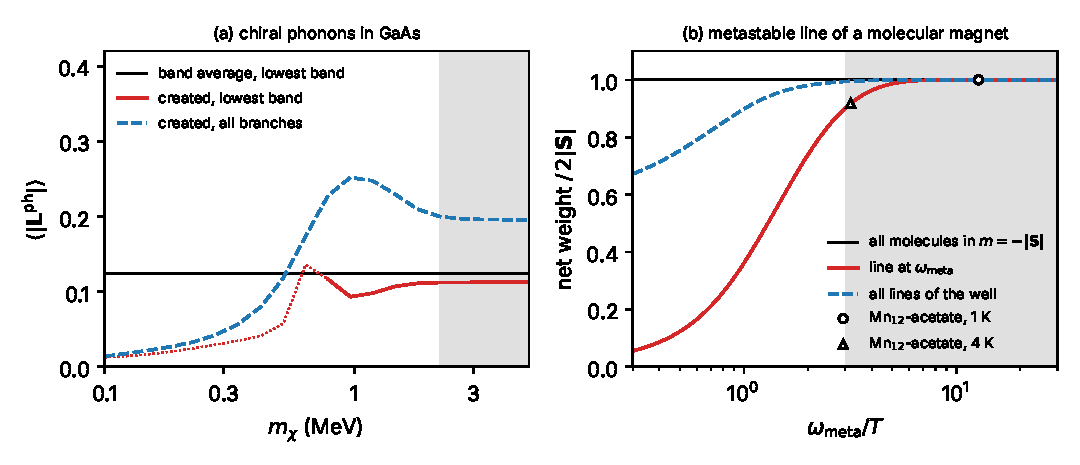
\includegraphics[width=0.98\linewidth]{figures/ch14/limit14_5a.pdf}
\captionof{figure}{(a) GaAs, from the PBE force constants of \cref{sec:5.5}. Black: the average of $|\vect{L}^{\mathrm{ph}}|$ over the lowest band, 0.124. Red: the same average weighted with the one-phonon rate of a heavy mediator coupled to nucleon number (\cref{eq:11.1-S1}, orientation-averaged halo kernel, $T = 0$), for the lowest-band phonons that the dark matter creates directly, against $\mchi$; dotted where the lowest band takes less than \SI{1}{\percent} of the rate. Blue dashed: the same for all created phonons. Gray: red within \SI{10}{\percent} of black, $\mchi \ge \SI{2.2}{MeV}$. (b) Mn$_{12}$-acetate ($|\mathbf{S}| = 10$, $D = \SI{0.454}{cm^{-1}}$, $B_4^0 = \SI{-2.0e-5}{cm^{-1}}$, \SI{1}{T}, $g_{\mathrm{ion}} = 2$, $\omega_{\mathrm{meta}} = \SI{1.098}{meV}$): net absorptive weight over $2|\mathbf{S}|$ against $\omega_{\mathrm{meta}}/T$, for thermal populations inside the upper well. Red: the line at $\omega_{\mathrm{meta}}$; blue dashed: all lines of the well, $2|\langle S_z\rangle|/2|\mathbf{S}|$. Gray: the line within \SI{10}{\percent} of $2|\mathbf{S}|$, $\omega_{\mathrm{meta}}/T \ge 3.0$. Markers: \SI{1}{K} and \SI{4}{K}.}\label{fig:14-limit-chiral}
\par}
\smallskip
Outside the gray regions the band average misstates the chirality of the phonons that a light particle creates, and a warm molecular crystal spreads the metastable weight over the lines of its well.
\end{limitbox}

\subsection{Magnetoelectric response of multiferroics}\label{sec:14.5-mf}

Hexagonal Lu$_{1-x}$Sc$_x$FeO$_3$ with $x \approx 0.4$ becomes ferroelectric at about \SI{1200}{K}. Below its magnetic ordering temperature $T_{\mathrm{CM}} \approx \SI{160}{K}$ the canted spins of its iron ions add a net magnetization parallel to the polarization. For hexagonal LuFeO$_3$ ($x = 0$), density-functional calculations give a polarization of \SI{10.5}{\micro C.cm^{-2}} along the $c$ axis and a net moment of $0.02\,\mu_B$ per iron~\cite[Sect.~IV\,A]{roising2021axion}. A crystal with both orders breaks inversion and time reversal and keeps their product. R{\o}ising and collaborators propose that an axion field shifts the magnetization of a multiferroic with both orders through the coupling of the axion to the electron, $\delta E = -\ii g_{aee}(\partial_t\phi/2m_e^2)\langle\boldsymbol{\sigma}\cdot\nabla\rangle$~\cite[Eq.~(5)]{roising2021axion}. With $\vect{p} = -\ii\nabla$ and $\boldsymbol{\sigma} = 2\vect{S}$, the spin current of \cref{eq:8.1-rows} at $\vect{q} = 0$ is $\mathcal{J}^{\alpha\alpha}_e(0) = \sum_j\vect{p}_j\cdot\vect{S}_j/m_e = -\ii\sum_j\boldsymbol{\sigma}_j\cdot\nabla_j/2m_e$, so the coupling is $(g_{aee}/m_e)(\partial_t\phi)\,\mathcal{J}^{\alpha\alpha}_e(0)$, the second term of \cref{eq:8.1-alp} at $\vect{p}_\phi \to 0$. By the Kubo formula of \cref{sec:4.2}, the spin density then responds as
\begin{equation}
  \frac{\delta\langle s^z_e(0)\rangle(\omega)}{\Vol} = \frac{g_{aee}}{m_e}\,R_{s^z\mathcal{J}}(0,\omega)\,(\partial_t\phi)(\omega) = -\ii\,\frac{g_{aee}m_\phi}{m_e}\,R_{s^z\mathcal{J}}(0,m_\phi)\,\phi(\omega) ,
  \label{eq:14.5-cross}
\end{equation}
with $R_{s^z\mathcal{J}}$ the retarded response of $s^z_e$ to $\mathcal{J}^{\alpha\alpha}_e$ and the magnetization $-2\mu_B$ times the left-hand side. The spin-density and spin-current rows have opposite signs under both time reversal and inversion, $\sigma^{\mathsf{T}}_s\sigma^{\mathsf{T}}_{\mathcal{J}} = \sigma^{\mathsf{P}}_s\sigma^{\mathsf{P}}_{\mathcal{J}} = -1$, so by \cref{eq:14.5-recip} inversion removes the block at $\vect{q} = 0$ and time reversal removes its symmetric part, the part that survives as $\omega \to 0$. The adiabatic response thus needs both symmetries broken, as in Lu$_{1-x}$Sc$_x$FeO$_3$ below $T_{\mathrm{CM}}$.

The Lehmann form of \cref{sec:4.2}, $R_{ab} = \Vol^{-1}\sum_{i,n}(p_i - p_n)\langle i|O_a^\dagger|n\rangle\langle n|O_b|i\rangle/(\omega - \omega_{ni} + \ii0^+)$, shows which states contribute. Far below $T_{\mathrm{CM}}$ the states $n$ reached at $\vect{q} = 0$ from the ordered state are its uniform magnon modes, in linear spin-wave theory as in \cref{sec:14.3}. Each mode $\nu$ with both matrix elements nonzero contributes a pair of poles at $\pm\omega_\nu$, which combine for real matrix elements into a term proportional to $2\omega_\nu/(\omega^2 - \omega_\nu^2)$. Two conditions restrict the modes. If the Hamiltonian conserves the total spin component $S^z_{\mathrm{tot}}$ and $s^z_e(0) = \lambda_SS^z_{\mathrm{tot}}$, then $s^z_e(0)$ has no time dependence and $R_{s^z\mathcal{J}}(0,\omega)$ vanishes at every $\omega \ne 0$. The response needs a spin--orbit coupling, a Dzyaloshinskii--Moriya interaction or a single-ion anisotropy that does not commute with $S^z_{\mathrm{tot}}$, such as the one that cants the spins of hexagonal Lu$_{1-x}$Sc$_x$FeO$_3$. And $\mathcal{J}^{\alpha\alpha}_e$ is odd under inversion, and it has matrix elements within the ground configuration of an ion only through a crystal field without inversion together with spin--orbit coupling (\cref{sec:14.3}). The response is thus at least of second order in spin--orbit coupling: one order for the vertex, and one or two for the breaking of $S^z_{\mathrm{tot}}$, by a Dzyaloshinskii--Moriya term or a single-ion term.

Far below $T_{\mathrm{CM}}$, where thermal magnons reduce the moment by less than \SI{10}{\percent} ($T \le 0.37\,T_{\mathrm{CM}}$ for spin $\frac52$ with nearest-neighbor exchange on a simple-cubic lattice), the Lehmann sum over the uniform magnons and their thermal population is the controlled result. Near $T_{\mathrm{CM}}$, dynamic scaling predicts the structure $R_{s^z\mathcal{J}}(0,\omega;T) = \chi_\times(T)\,\Phi(\omega\tau(T))$, with a relaxation time $\tau \propto |T - T_{\mathrm{CM}}|^{-\nu z}$, $\nu$ the correlation-length exponent and $z$ the dynamic exponent~\cite[Sect.~III\,D]{roising2021axion}; the amplitude $\chi_\times$ and the scaling function $\Phi$ of a real material are not known. The exchange, Dzyaloshinskii--Moriya and anisotropy constants of the spin model for $T \ll T_{\mathrm{CM}}$ come from DFT~$+\,U$ energy mappings, with spin--orbit coupling included for the vertex of $\mathcal{J}^{\alpha\alpha}_e$.

\subsection{Uncertainty budget of the magnetic rates}\label{sec:14.5-budget}

\Cref{tab:14-nuisances} collects the truncations and inputs of the chapter with their sizes. Near the lightest masses the anisotropy row dominates every other row by more than an order of magnitude, and it is a model, not a calculation. For absorption into the uniform mode, the shape of the sample and the width of the line set the rate, and neither depends on the spin-wave expansion. In the coherent regime the largest effects are statistical: the length of the record against $t_{\mathrm{coh}}$ and $T_2$, and whether the likelihood contains the random amplitude.
\begin{table}[tbp]
  \caption{Uncertainty budget of the magnetic rates and of the coherent regime. Classes as in \cref{tab:10-nuisances}; ``unsized'' marks an item with no size known. Sizes are for NiO, YIG, MnF$_2$, GaAs, Mn$_{12}$-acetate and $^{207}$Pb in PMN-PT as named.}
  \label{tab:14-nuisances}
  \centering\scriptsize\setlength{\tabcolsep}{3pt}
  \begin{tabular}{@{}>{\raggedright\arraybackslash}p{0.27\linewidth}>{\raggedright\arraybackslash}p{0.13\linewidth}>{\raggedright\arraybackslash}p{0.48\linewidth}>{\raggedright\arraybackslash}p{0.08\linewidth}@{}}
    \toprule
    Truncation or input & Type & Size & Section \\
    \midrule
    One-magnon weight of linear spin-wave theory & normali\-zation & high by about $\Delta S/|\vect{S}|$: \SI{7.8}{\percent} (NiO), \SI{3.1}{\percent} for $|\vect{S}| = \frac52$, \SI{16}{\percent} for $|\vect{S}| = \frac12$ & \cref{sec:14.1} \\
    Two-magnon continuum & new support & 0.073 of the one-magnon weight over the zone (NiO); $w_\parallel/w_\perp < 0.05$ below \SI{0.5}{keV} & \cref{sec:14.2} \\
    Final-state interaction of the pair & tilt; new support & about 0.04 of the spin response, moved in energy (NiO); bound pair unsized & \cref{sec:14.2} \\
    Magnetic anisotropy near the gap & threshold; tilt in $\mchi$ & NiO, \SI{5}{meV} threshold, one-constant gap \SI{4.54}{meV}: rate $\times29$ at \SI{10}{keV} (upper value), $\times1.35$ at \SI{30}{keV}, $< \SI{3}{\percent}$ above \SI{100}{keV} & \cref{sec:14.1} \\
    Exchange constants from DFT~$+\,U$ & threshold & $J_2$ of NiO 11 to \SI{27}{meV} against 19.01: magnon energies $\times0.58$ to 1.42 & \cref{sec:14.1} \\
    Magnon--phonon mixing & tilt & gap \SI{3.0}{\percent} of the crossing energy at \SI{2.83}{GHz} (YIG model); NiO unsized & \cref{sec:14.2} \\
    Thermal magnons & new support & $\ee^{-\omega_{\mathrm{gap}}/T}$, exponent $-5\times10^3$ at \SI{10}{mK} (NiO) & \cref{sec:14.1} \\
    Sample shape & threshold; normali\-zation & YIG film within \SI{10}{\percent} of the Larmor line for $B_0 \ge 4.8\,\mu_0M_{\mathrm{s}}$; weight $\times1.74$ at \SI{10}{\micro eV}; saturated sphere exact & \cref{sec:14.3} \\
    Zero-point correction to the resonance weight & normali\-zation & 5 to \SI{23}{\percent} for $|\vect{S}| = \frac32$, $\omega_A/\omega_E = 2$ to 0.3; MnF$_2$ unsized & \cref{sec:14.3} \\
    Resonance of MnF$_2$ & threshold & fitted fields \SI{7}{\percent} below the measured \SI{1.1}{meV} and \SI{9.4}{T}; peak rate unchanged & \cref{sec:14.3} \\
    Width $\varGamma_{\mathrm{M}}$ of the uniform line & normali\-zation & peak rate $\propto 1/\varGamma_{\mathrm{M}}$; $10^{-5}\omega$ for YIG assumed & \cref{sec:14.3} \\
    Spin fraction $\lambda_S$ of quenched $3d$ ions & normali\-zation & $1 - O(\xi_{\mathrm{ion}}^2/\Delta_{\mathrm{CF}}^2)$ & \cref{sec:14.3} \\
    In-medium mixing of a dark photon & normali\-zation & set by the dielectric constant and the enclosure; unsized & \cref{sec:14.3} \\
    Neutron data for quenched ions & normali\-zation & $[\lambda_S/(g_{\mathrm{ion}}/2)]^2 = 0.83$ (Ni$^{2+}$, $g_{\mathrm{ion}} = 2.2$) or 0.73 (2.34); 0.973 at \SI{5.3}{keV} & \cref{sec:14.4} \\
    Longitudinal response from neutron data & new support & needs the localized-moment form or the isotropy hypothesis & \cref{sec:14.4} \\
    Record length against $t_{\mathrm{coh}}$ and $1/\varGamma_{\mathrm{tg}}$ & normali\-zation & mean within \SI{10}{\percent} of the golden rule for $t_{\mathrm{int}} \ge 13\,t_{\mathrm{coh}}$ ($T_2 \to \infty$) to $t_{\mathrm{coh}}$ ($T_2 = 0.1\,t_{\mathrm{coh}}$) & \cref{sec:14.6} \\
    Field amplitude fixed instead of Rayleigh & normali\-zation & limit too strong by 1.99 below $t_{\mathrm{coh}}$, 1.015 at $100\,t_{\mathrm{coh}}$; 2.73 at the detection threshold & \cref{sec:14.6} \\
    Linearized Bloch equation & normali\-zation & $(\Omega_{\mathrm{Rabi}}t)^2/6$ in the transient; \SI{30}{\percent} saturation at the PMN-PT threshold & \cref{sec:14.6} \\
    Inhomogeneous broadening; effective field $E^*$ & normali\-zation & $u_{\mathrm{sp}} = 3.8\times10^{-4}$; $E^*$ about \SI{50}{\percent} ($^{207}$Pb in PMN-PT) & \cref{sec:14.6} \\
    Line shape of the halo & tilt & standard halo only; unsized & \cref{sec:14.6} \\
    Chiral phonons as a band average & normali\-zation & GaAs 0.124, $\pm\SI{40}{\percent}$ with the dipole part of the force constants; rate-weighted within \SI{10}{\percent} only for $\mchi \ge \SI{2.2}{MeV}$; decay branching unsized & \cref{sec:14.5} \\
    Upper-well population of a molecular magnet & normali\-zation & Mn$_{12}$-acetate at \SI{1}{T}: line keeps \SI{90}{\percent} of $2|\vect{S}|$ below \SI{4.2}{K} & \cref{sec:14.5} \\
    Multiferroic response near $T_{\mathrm{CM}}$ & normali\-zation; tilt & unsized & \cref{sec:14.5} \\
    \bottomrule
  \end{tabular}
\end{table}

\section*{Summary}

A dark-matter particle that couples to the electron spin creates one magnon through the transverse spin, at leading order in $1/|\vect{S}|$ (\cref{sec:14.1}). In a two-sublattice antiferromagnet the one-magnon response carries the weight $w^{\mathrm{M}}_{\vect{q}} = |\vect{S}|(A_{\vect{q}} - B_{\vect{q}})/\omega^{\mathrm{M}}_{\vect{q}}$, which suppresses magnons near the zone center and enhances them near the ordering wavevector: 0.024 against 42 for magnons of \SI{5}{meV} in NiO. For NiO at $\sigmae = \SI{e-40}{cm^2}$ it opens near \SI{7.3}{keV} for a \SI{5}{meV} threshold and peaks at $3.2\times10^3$ events per kilogram-year near \SI{3}{MeV}. Near its edge the rate depends on the magnetic anisotropy, which the Heisenberg model leaves out. The spin-length sum rule estimates that linear spin-wave theory overstates the one-magnon weight by $\Delta S/|\vect{S}|$ at the next order, \SI{7.8}{\percent} for NiO, where the zero-point reduction $\Delta S = 0.078$ is that of four interleaved simple-cubic antiferromagnets.

The longitudinal spin creates magnon pairs (\cref{sec:14.2}). Their weight vanishes in a ferromagnet and at $\vect{q} = 0$, grows as $q^2$, and averages to 0.073 of the one-magnon weight in NiO, the part of the $\Delta S/|\vect{S}| = 0.078$ moved out of the one-magnon line that arrives in the continuum (the two differ by $\Delta S^2$). Because a pair shares its momentum, it reaches the energy $\frac12\mchi v^2$ at any mass, and the two-magnon channel opens at masses lower by $v_{\mathrm{max}}^2/4c_{\mathrm{M}}(v_{\mathrm{max}} - c_{\mathrm{M}})$, a factor 5.1 for NiO. Final-state interactions move the pair weight within the continuum without changing its integral; whether NiO has a bound pair is open. A magnon mixes with a phonon at linear order only through the dependence of the anisotropy energy on strain, which spin--orbit coupling and the dipolar interaction provide; the strain dependence of the exchange couples a phonon only to magnon pairs. The hybrids carry an off-diagonal spin--nuclear response that saturates the interference bound of \cref{sec:8.3}.

A boson absorbed at $\vect{k} \to 0$ drives the uniform precession (\cref{sec:14.3}). When the exchange is invariant under spin rotations, the uniform transverse spin response is one line at the Larmor frequency, with weight $2\langle S^z_{\mathrm{tot}}\rangle$, at any spin and temperature. The spin couples through $\lambda_S$, the fraction of the ionic angular momentum carried by the spin, which equals $g_J - 1$ only within a $J$ multiplet and is one for quenched $3d$ ions. The shape of the sample moves the line to the Kittel frequency and reweights its polarizations. For YIG at \SI{10}{\micro eV} and $g_{aee} = 10^{-13}$, with an assumed line width of $10^{-5}$ of the frequency, the peak rate is \SI{3.6}{s^{-1}.kg^{-1}}. An antiferromagnet absorbs at its resonance with the exchange-suppressed weight $|\vect{S}|\omega_{\mathrm{AFMR}}/(2\omega_E + \omega_A)$ per pair of sublattices, about $0.1\,|\vect{S}|$ in MnF$_2$, whose resonance lies at the measured \SI{1.1}{meV}.

Measured neutron spectra can replace a computed spin response, within limits (\cref{sec:14.4}). The magnetic cross-section at a given momentum transfer contains only the part of the spin response transverse to it, so without a model of the spin density no neutron measurement, polarized or not, gives the longitudinal element $\hat{\vect{q}}\cdot S\cdot\hat{\vect{q}}$. Within the localized-moment model, transverse data at several wavevectors $\vect{q} + \vect{G}$ fix the full tensor, and an isotropy hypothesis recovers it from two scattering angles. For quenched ions the neutron sees the moment with the spectroscopic $g$, the dark matter the spin, and the factor $[\lambda_S/(g_{\mathrm{ion}}/2)]^2$ converts one into the other, 0.83 for Ni$^{2+}$ at $g_{\mathrm{ion}} = 2.2$ and 0.73 at 2.34.

Targets without inversion or time-reversal symmetry add responses that a collinear magnet lacks (\cref{sec:14.5}). The current response of a chiral crystal acquires a part odd in $\vect{q}$, the finite-momentum optical activity, and the point group decides whether it exists; in $\alpha$-quartz the orientation-averaged gyration is only $-0.045$ of its value along the optic axis. Phonons of the lowest band of GaAs carry on average 0.12 units of angular momentum. Single-molecule magnets offer metastable lines, such as the line of Mn$_{12}$-acetate at \SI{1.098}{meV} in \SI{1}{T}, which keeps \SI{90}{\percent} of its weight below \SI{4.2}{K}. A multiferroic below its ordering temperature has a magnetoelectric cross response; near that temperature the response is open.

An ultralight field is a classical Gaussian wave, coherent for $t_{\mathrm{coh}} = 1/m_\phi v_0^2$, \SI{1.04}{s} at \SI{1}{neV} (\cref{sec:14.6}). Its average reproduces the golden-rule rate for records longer than the shorter of $t_{\mathrm{coh}}$ and the inverse width of the target's line, while a single record matches the ensemble only beyond $t_{\mathrm{coh}}$. A polarized nuclear-spin ensemble driven by the gradient or the dipole coupling of an axion-like field obeys the Bloch equations. Its transverse magnetization grows as $\Omega_{\mathrm{Rabi}}M_0t$ and saturates at $\Omega_{\mathrm{Rabi}}M_0T_2$, and a Gaussian drive turns the linear growth into a random walk once the record exceeds $t_{\mathrm{coh}}$. Each periodogram bin of signal plus noise is exponentially distributed. The resulting likelihood gives sensitivities that scale as $t_{\mathrm{int}}^{-1/2}$ below the coherence time and as $(t_{\mathrm{int}}t_{\mathrm{coh}})^{-1/4}$ above it, and it already contains the random amplitude, which a fixed-amplitude analysis misses by a factor 1.99 for the median limit and 2.73 at the detection threshold.

\Cref{tab:14-nuisances} collects the truncations and inputs of the chapter with their sizes. Near the lightest masses the anisotropy row dominates every other by more than an order of magnitude, and it is a model, not a calculation. For absorption into the uniform mode, the shape of the sample and the width of the line set the rate, and neither depends on the spin-wave expansion. In the coherent regime the largest effects are statistical: the length of the record against $t_{\mathrm{coh}}$ and $T_2$, and whether the likelihood contains the random amplitude.

\begin{table}[tbp]
  \caption{Uncertainty budget of the magnetic rates and of the coherent regime. Type in the classes of \cref{sec:8.8}: normalization, tilt (in $\omega$ or in the dark-matter mass), threshold and new support; ``unsized'' marks an item with no size known. Sizes are for NiO, YIG, MnF$_2$, GaAs, Mn$_{12}$-acetate and $^{207}$Pb in PMN-PT as named.}
  \label{tab:14-nuisances}
  \centering\scriptsize\setlength{\tabcolsep}{3pt}
  \begin{tabular}{@{}>{\raggedright\arraybackslash}p{0.27\linewidth}>{\raggedright\arraybackslash}p{0.13\linewidth}>{\raggedright\arraybackslash}p{0.48\linewidth}>{\raggedright\arraybackslash}p{0.08\linewidth}@{}}
    \toprule
    Truncation or input & Type & Size & Section \\
    \midrule
    One-magnon weight of linear spin-wave theory & normali\-zation & high by about $\Delta S/|\vect{S}|$: \SI{7.8}{\percent} (NiO), \SI{3.1}{\percent} for $|\vect{S}| = \frac52$, \SI{16}{\percent} for $|\vect{S}| = \frac12$ & \cref{sec:14.1} \\
    Two-magnon continuum & new support & 0.073 of the one-magnon weight over the zone (NiO); $w_\parallel/w_\perp < 0.05$ below \SI{0.5}{keV} & \cref{sec:14.2} \\
    Final-state interaction of the pair & tilt; new support & about 0.04 of the spin response, moved in energy (NiO); bound pair unsized & \cref{sec:14.2} \\
    Magnetic anisotropy near the gap & threshold; tilt in $\mchi$ & NiO, \SI{5}{meV} threshold, one-constant gap \SI{4.54}{meV}: rate $\times29$ at \SI{10}{keV} (upper value), $\times1.35$ at \SI{30}{keV}, $< \SI{3}{\percent}$ above \SI{100}{keV} & \cref{sec:14.1} \\
    Exchange constants from DFT~$+\,U$ & threshold & $J_2$ of NiO 11 to \SI{27}{meV} against 19.01: magnon energies $\times0.58$ to 1.42 & \cref{sec:14.1} \\
    Magnon--phonon mixing & tilt & gap \SI{3.0}{\percent} of the crossing energy at \SI{2.83}{GHz} (YIG model); NiO unsized & \cref{sec:14.2} \\
    Thermal magnons & new support & $\ee^{-\omega_{\mathrm{gap}}/T}$, exponent $-5\times10^3$ at \SI{10}{mK} (NiO) & \cref{sec:14.1} \\
    Sample shape & threshold; normali\-zation & YIG film within \SI{10}{\percent} of the Larmor line for $B_0 \ge 4.8\,\mu_0M_{\mathrm{s}}$; weight $\times1.74$ at \SI{10}{\micro eV}; saturated sphere exact & \cref{sec:14.3} \\
    Zero-point correction to the resonance weight & normali\-zation & 5 to \SI{23}{\percent} for $|\vect{S}| = \frac32$, $\omega_A/\omega_E = 2$ to 0.3; MnF$_2$ unsized & \cref{sec:14.3} \\
    Resonance of MnF$_2$ & threshold & fitted fields \SI{7}{\percent} below the measured \SI{1.1}{meV} and \SI{9.4}{T}; peak rate unchanged & \cref{sec:14.3} \\
    Width $\varGamma_{\mathrm{M}}$ of the uniform line & normali\-zation & peak rate $\propto 1/\varGamma_{\mathrm{M}}$; $10^{-5}\omega$ for YIG assumed & \cref{sec:14.3} \\
    Spin fraction $\lambda_S$ of quenched $3d$ ions & normali\-zation & $1 - O(\xi_{\mathrm{ion}}^2/\Delta_{\mathrm{CF}}^2)$ & \cref{sec:14.3} \\
    In-medium mixing of a dark photon & normali\-zation & set by the dielectric constant and the enclosure; unsized & \cref{sec:14.3} \\
    Neutron data for quenched ions & normali\-zation & $[\lambda_S/(g_{\mathrm{ion}}/2)]^2 = 0.83$ (Ni$^{2+}$, $g_{\mathrm{ion}} = 2.2$) or 0.73 (2.34); 0.973 at \SI{5.3}{keV} & \cref{sec:14.4} \\
    Longitudinal response from neutron data & new support & needs the localized-moment form or the isotropy hypothesis & \cref{sec:14.4} \\
    Chiral phonons as a band average & normali\-zation & GaAs 0.124, $\pm\SI{40}{\percent}$ with the dipole part of the force constants; rate-weighted within \SI{10}{\percent} only for $\mchi \ge \SI{2.2}{MeV}$; decay branching unsized & \cref{sec:14.5} \\
    Upper-well population of a molecular magnet & normali\-zation & Mn$_{12}$-acetate at \SI{1}{T}: line keeps \SI{90}{\percent} of $2|\vect{S}|$ below \SI{4.2}{K} & \cref{sec:14.5} \\
    Multiferroic response near $T_{\mathrm{CM}}$ & normali\-zation; tilt & unsized & \cref{sec:14.5} \\
    Record length against $t_{\mathrm{coh}}$ and $1/\varGamma_{\mathrm{tg}}$ & normali\-zation & mean within \SI{10}{\percent} of the golden rule for $t_{\mathrm{int}} \ge 13\,t_{\mathrm{coh}}$ ($T_2 \to \infty$) to $t_{\mathrm{coh}}$ ($T_2 = 0.1\,t_{\mathrm{coh}}$) & \cref{sec:14.6} \\
    Field amplitude fixed instead of Rayleigh & normali\-zation & limit too strong by 1.99 below $t_{\mathrm{coh}}$, 1.015 at $100\,t_{\mathrm{coh}}$; 2.73 at the detection threshold & \cref{sec:14.6} \\
    Linearized Bloch equation & normali\-zation & $(\Omega_{\mathrm{Rabi}}t)^2/6$ in the transient; \SI{30}{\percent} saturation at the PMN-PT threshold & \cref{sec:14.6} \\
    Inhomogeneous broadening; effective field $E^*$ & normali\-zation & $u_{\mathrm{sp}} = 3.8\times10^{-4}$; $E^*$ about \SI{50}{\percent} ($^{207}$Pb in PMN-PT) & \cref{sec:14.6} \\
    Line shape of the halo & tilt & standard halo only; unsized & \cref{sec:14.6} \\
    \bottomrule
  \end{tabular}
\end{table}

\printbibliography[heading=subbibliography]

\chapter{Superconductors}\label{chap:15}
The gap of a superconductor is more than three thousand times smaller than the gap of silicon. In aluminum $\Delta_{\mathrm{BCS}} = \SI{0.18}{meV}$, so breaking a pair costs \SI{0.36}{meV}, and a dark-matter particle of \SI{0.10}{keV} can break a pair (\cref{we:7-al}). Below a third of an MeV no halo particle can cross the gap of silicon (\cref{sec:1.3}), yet a superconductor still responds to a coupling to the electron density, and the BCS theory gives that response in closed form. The question of this chapter is whether the rate of breaking pairs can be computed as reliably as the semiconductor rates of \cref{chap:10}.

The response of independent quasiparticles, however, violates charge conservation, and the correction that restores it is largest at the small momentum transfers that light dark matter favors (\cref{sec:7.2}). At the edge $\omega = 2\Delta_{\mathrm{BCS}}$ the coherence factors make the absorptive part of the response jump, and the screening that follows from that jump cannot be expanded. And the sensors are thin films, often amorphous and strongly disordered, whereas the BCS model describes a clean bulk crystal. As a result the loss function of aluminum near the edge changes by a factor of 4.6 with the mean free path of the film. Far above the edge, by contrast, the simpler truncations of the response agree with the conserving response to a few percent (\cref{fig:15-map}).

\begin{figure}[tbp]
  \centering
  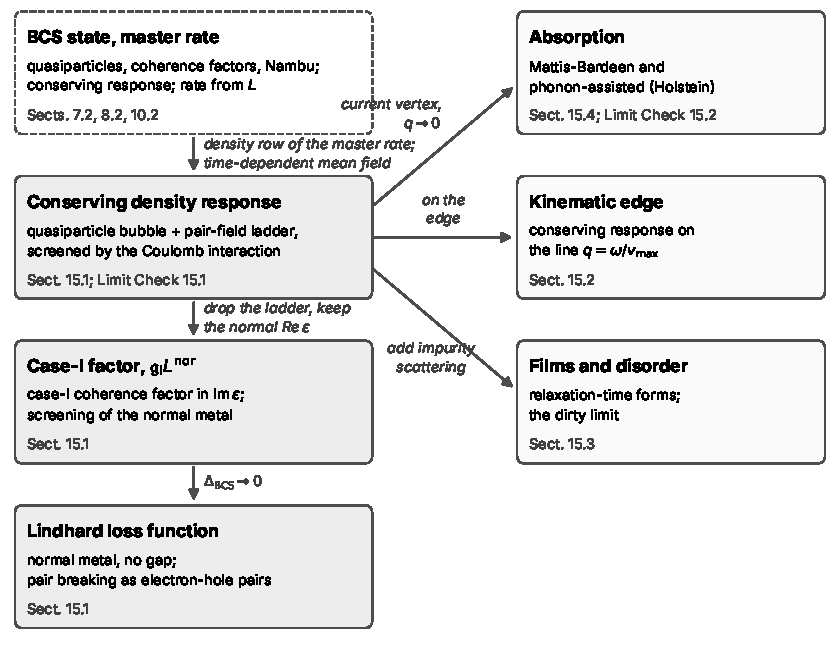
\includegraphics[width=0.85\linewidth]{figures/ch15/map15.pdf}
  \caption{Superconductors, from the BCS state of \cref{sec:7.2} and the loss-function rate of \cref{sec:8.2,sec:10.2} to the targets of this chapter. The density response that conserves charge adds the pair-field ladder to the quasiparticle bubble and is screened by the Coulomb interaction (\cref{sec:15.1}; \cref{lim:15.1a}). Dropping the ladder and keeping the screening of the normal metal leaves the case-I coherence factor times the normal loss function; letting the gap close leaves the Lindhard function of the normal metal (\cref{sec:15.1}). On the kinematic edge $q = \omega/v_{\mathrm{max}}$ each truncation is worst (\cref{sec:15.2}). Impurity scattering and the film geometry change the response of real sensors (\cref{sec:15.3}). At vanishing momentum the current and the spin current give the absorption of dark photons and axion-like particles, with and without a phonon (\cref{sec:15.4}; \cref{lim:15.4a}).}
  \label{fig:15-map}
\end{figure}

\section{Pair breaking by dark matter}\label{sec:15.1}

A dark-matter particle of \SI{1}{keV} that scatters in aluminum deposits at most \SI{3.5}{meV}, about ten times the pair-breaking threshold, and transfers at most \SI{5.3}{eV} of momentum. To deposit $\omega$ it must transfer at least $q = \omega/v_{\mathrm{max}}$, with $v_{\mathrm{max}} = 2.650\times10^{-3}$ the largest speed of a halo particle in the laboratory (\cref{eq:1.2-vmax}). The line $q = \omega/v_{\mathrm{max}}$ in the $(q,\omega)$ plane, the \emph{kinematic edge}, is a different object from the \emph{pair-breaking edge} $\omega = 2\Delta_{\mathrm{BCS}}$, the threshold in energy. The ratio of the gap to the Doppler width of the Fermi surface is $\Delta_{\mathrm{BCS}}/qv_{\mathrm{F}} = (v_{\mathrm{max}}/v_{\mathrm{F}})(\Delta_{\mathrm{BCS}}/\omega)$, and it takes its largest value on the kinematic edge, 0.20 at the threshold. \Cref{sec:7.2} found that this ratio controls the correction that restores charge conservation. We build the loss function from the conserving response of \cref{eq:7.2-Rc}. Two truncations of the conserving response are accurate far above the pair-breaking edge: the Lindhard function of the normal metal, and the same function multiplied by the case-I coherence factor of \cref{eq:7.2-pairspec}.

\subsection{The loss-function rate of a superconductor}\label{sec:15.1-rate}

A mediator that couples to the electron number acts through the density row of the master formula, with $\mathfrak{D}_{ee} = |\tilde V(\vect{q})|^2$ and $S = (2q^2/e^2)\,L/(1 - \ee^{-\beta\omega})$ (\cref{sec:10.2}). At \SI{10}{mK} the threshold has $\beta\omega = 418$, so the thermal factor is one, and the spectrum is \cref{eq:10.2-rate} with $\bar L$ replaced by the loss function of the superconductor, which is isotropic in the model used here. For a dark photon, which couples to the total charge, this spectrum is exact. For a mediator that couples to electrons alone it holds with the nuclei clamped, and the lattice then enters only through the pairing interaction already contained in $\Delta_{\mathrm{BCS}}$. The ions' own response appears in the loss function through the phonon pole at $\omega = c_{\mathrm{LA}}q$, and above that pole the ionic response is a correction of relative order $(c_{\mathrm{LA}}q/\omega)^2$. The longitudinal sound speed along [100] is $c_{\mathrm{LA}} = (C_{11}/\rho)^{1/2} = \SI{6.47}{km.s^{-1}}$, from the zero-temperature elastic constant $C_{11} = \SI{114.3}{GPa}$~\cite[Table~2]{malica2020quasi} and the low-temperature density $\rho = \SI{2.73}{g.cm^{-3}}$. The correction is then $(c_{\mathrm{LA}}/v_{\mathrm{max}})^2 = \num{6.6e-5}$ on the kinematic edge. For $\mchi < \SI{3.2}{keV}$ even the largest momentum transfer, $2\mchi v_{\mathrm{max}}$, excites phonons only below $2\Delta_{\mathrm{BCS}}$.

The dielectric function is the proper density response screened by the Coulomb interaction, $\varepsilon = 1 - v_{\mathrm{C}}(q)\tilde R$ (\cref{sec:4.4}). In the normal metal the random-phase approximation puts the independent-particle bubble in place of $\tilde R$, and the result is the Lindhard function of \cref{eq:4.5-rpa}. In the superconductor, however, the proper response must itself conserve charge, and \cref{sec:7.2} showed that the bare quasiparticle bubble does not. The conserving response is the time-dependent mean field in the three Nambu channels $(\boldsymbol{\eta}, \mathsf{s}_1, \mathsf{s}_2)$ of \cref{eq:7.2-nambu}, the pair-field ladder of \cref{eq:7.2-Rc}~\cite{anderson1958random}. In field-theory language the ladder is the vertex correction that restores the Ward identity of charge. Adding the Coulomb interaction in the density channel gives the generalized random-phase approximation:
\begin{keyresult}[Conserving loss function of a superconductor]
\begin{equation}
  \varepsilon^{\mathrm{cons}}(q,\omega) = 1 - v_{\mathrm{C}}(q)\,R^{\mathrm{cons}}(q,\omega), \qquad
  L^{\mathrm{cons}}(q,\omega) = \Imag\Bigl[-\frac{1}{\varepsilon^{\mathrm{cons}}(q,\omega)}\Bigr] ,
  \label{eq:15.1-Lcons}
\end{equation}
with $R^{\mathrm{cons}} = R_{\boldsymbol{\eta}\boldsymbol{\eta}}$ the density response of \cref{eq:7.2-Rc}, which contains the pair-field ladder and no Coulomb interaction.
\end{keyresult}
\noindent The Coulomb interaction is a function of the local density and commutes with it, so the screened response obeys the continuity equation and the f-sum rule whenever $R^{\mathrm{cons}}$ does (\cref{sec:7.2}). The core electrons of aluminum add a constant of order one to $\varepsilon$, negligible against $k_{\mathrm{TF}}^2/q^2 \ge \num{5.8e5}$ for $q \le \SI{5.3}{eV}$. Here $k_{\mathrm{TF}} = \SI{4.05}{keV}$ is the Thomas--Fermi wavevector of the free-electron gas of aluminum: three electrons per atom in the fcc cell of side $a = \SI{4.05}{\angstrom}$, so $\nd_e = \SI{1.81e23}{cm^{-3}}$, $k_{\mathrm{F}} = \SI{1.75}{\angstrom^{-1}}$, the bare electron mass, $v_{\mathrm{F}} = k_{\mathrm{F}}/m_e = \num{6.75e-3}$ and $\omega_p = \SI{15.78}{eV}$. The amplitude channel $\mathsf{s}_1$ decouples from the density in a metal whose density of states is symmetric about the Fermi level (\cref{sec:7.2}); the asymmetry over the energy range of the pairs is of relative order $\Delta_{\mathrm{BCS}}/E_{\mathrm{F}} = \num{1.5e-5}$, and we drop it.

\subsection{The conserving response in closed form}\label{sec:15.1-closed}

For aluminum we set the temperature to zero, take the density of states $\mathcal{N}_{\mathrm{F}}$ constant over the energies of the pairs, and take the metal clean. We also linearize the band across the shell, $\xi_{\vect{k}+\vect{q}} = \xi_{\vect{k}} + v_{\mathrm{F}}q\mu$ with $\mu$ the cosine of the angle between $\vect{k}$ and $\vect{q}$. The dropped term $q^2/2m_e$ is below \SI{3e-5}{eV} for $q \le \SI{5.3}{eV}$, whereas $v_{\mathrm{F}}q \ge 2.5\,\omega$. With these simplifications every bubble of \cref{eq:7.2-Rc} reduces to one function. At $T = 0$ the density and pair operators either create a pair of quasiparticles, with energy $E + E'$ for $E = E_{\vect{k}}$ and $E' = E_{\vect{k}+\vect{q}}$, or destroy one, and the bubbles are
\begin{equation}
  R^0_{AB}(q,\omega) = \frac{1}{\Vol}\sum_{\vect{k}}\Bigl[\frac{M^{\mathrm{N}*}_AM^{\mathrm{N}}_B}{\omega - E - E' + \ii0^+} - \frac{M^{\mathrm{N}}_AM^{\mathrm{N}*}_B}{\omega + E + E' + \ii0^+}\Bigr] ,
  \label{eq:15.1-bubble}
\end{equation}
with $M^{\mathrm{N}}_A$ the amplitude with which the Nambu-channel operator $O_A$ (superscript N for Nambu) creates the pair. For the density it is $M^{\mathrm{N}}_{\boldsymbol{\eta}} = uv' + vu'$ of \cref{eq:7.2-coh}. The phase operator is $O_{\mathsf{s}_2} = -\ii(B^\dagger_{\vect{q}} - B_{-\vect{q}})$, with $B^\dagger_{\vect{q}}$ the pair creation operator of \cref{app:D.21}. It therefore creates the same pair through $B^\dagger_{\vect{q}}$, with the amplitude $M^{\mathrm{N}}_{\mathsf{s}_2} = -\ii(uu' + vv')$; this phase reproduces $R^0_{\mathsf{s}_2\boldsymbol{\eta}}$ of \cref{sec:7.2} at $q = 0$, and the sign of the ladder below does not depend on it. With \cref{eq:7.2-E},
\begin{gather*}
  |M^{\mathrm{N}}_{\boldsymbol{\eta}}|^2 = \frac{EE' - \xi\xi' + \Delta_{\mathrm{BCS}}^2}{2EE'}, \qquad
  |M^{\mathrm{N}}_{\mathsf{s}_2}|^2 = \frac{EE' + \xi\xi' + \Delta_{\mathrm{BCS}}^2}{2EE'}, \\
  M^{\mathrm{N}*}_{\boldsymbol{\eta}}M^{\mathrm{N}}_{\mathsf{s}_2} = -\frac{\ii\Delta_{\mathrm{BCS}}(E + E')}{2EE'} ,
\end{gather*}
where the mixed product follows from $(uv' + vu')(uu' + vv') = u'v'(u^2 + v^2) + uv(u'^2 + v'^2) = \Delta_{\mathrm{BCS}}/2E' + \Delta_{\mathrm{BCS}}/2E$.

The linear band turns these three products into functions of $E + E'$. Since $E^2 = \xi^2 + \Delta_{\mathrm{BCS}}^2$, the product $(EE' + \xi\xi' + \Delta_{\mathrm{BCS}}^2)(EE' - \xi\xi' - \Delta_{\mathrm{BCS}}^2) = E^2E'^2 - (\xi\xi' + \Delta_{\mathrm{BCS}}^2)^2$ equals $\Delta_{\mathrm{BCS}}^2(\xi' - \xi)^2$, and $EE' + \xi\xi' + \Delta_{\mathrm{BCS}}^2$ is half of $(E + E')^2 - (\xi' - \xi)^2$. For the density amplitude we write $EE' - \xi\xi' + \Delta_{\mathrm{BCS}}^2 = (EE' - \xi\xi' - \Delta_{\mathrm{BCS}}^2) + 2\Delta_{\mathrm{BCS}}^2$ and use the product for the first bracket. With $\xi' - \xi = v_{\mathrm{F}}q\mu$,
\begin{equation}
  EE' + \xi\xi' + \Delta_{\mathrm{BCS}}^2 = \tfrac12\bigl[(E + E')^2 - v_{\mathrm{F}}^2q^2\mu^2\bigr], \qquad
  |M^{\mathrm{N}}_{\boldsymbol{\eta}}|^2 = \frac{\Delta_{\mathrm{BCS}}^2(E + E')^2}{EE'\bigl[(E + E')^2 - v_{\mathrm{F}}^2q^2\mu^2\bigr]} .
  \label{eq:15.1-ident}
\end{equation}
The quantity $\omega_\mu^2 = \omega^2 - v_{\mathrm{F}}^2q^2\mu^2$ is the energy of the pair in the frame that moves with the Doppler shift, and a pair at angle $\mu$ can be created only if $\omega_\mu \ge 2\Delta_{\mathrm{BCS}}$, the counterpart of the threshold \cref{eq:7.2-threshold}. The remaining integral is the $q = 0$ pair sum $F(\omega)$ of \cref{sec:7.2}, now at each angle. A hyperbolic substitution evaluates it (\cref{app:D.39}):
\begin{equation}
  F_\mu(\omega) = \frac{\mathcal{N}_{\mathrm{F}}}{2}\int\dd\xi\,\frac{E + E'}{EE'\,\bigl[\omega^2 - (E + E')^2\bigr]}
  = -\frac{\mathcal{N}_{\mathrm{F}}}{2\Delta_{\mathrm{BCS}}^2}\,\frac{\arcsin\sqrt{\mathfrak{p}_\mu}}{\sqrt{\mathfrak{p}_\mu(1 - \mathfrak{p}_\mu)}}, \qquad
  \mathfrak{p}_\mu = \frac{\omega_\mu^2}{4\Delta_{\mathrm{BCS}}^2} ,
  \label{eq:15.1-F}
\end{equation}
for $0 < \mathfrak{p}_\mu < 1$, with $F_0 = F$, and continued to the other ranges of $\mathfrak{p}_\mu$ in \cref{eq:D.39-Fcont}. Only at $\mathfrak{p}_\mu > 1$, where pairs can be created, is $F_\mu$ complex.

The density bubble follows from \cref{eq:15.1-bubble,eq:15.1-ident} with $\Vol^{-1}\sum_{\vect{k}} \to \mathcal{N}_{\mathrm{F}}\int\dd\xi\int_{-1}^1\dd\mu/2$. Splitting the integrand of the density bubble by partial fractions into an $F_\mu$ term and an elementary term, and using the gap equation, gives (\cref{app:D.39}), with $\langle X\rangle_\mu = \int_0^1\dd\mu\,X$,
\begin{equation}
  \begin{gathered}
  R^0_{\boldsymbol{\eta}\boldsymbol{\eta}} = \Bigl\langle\frac{2\mathcal{N}_{\mathrm{F}}v_{\mathrm{F}}^2q^2\mu^2 + 4\Delta_{\mathrm{BCS}}^2\omega^2F_\mu}{\omega_\mu^2}\Bigr\rangle_\mu, \\
  R^0_{\mathsf{s}_2\boldsymbol{\eta}} = -R^0_{\boldsymbol{\eta}\mathsf{s}_2} = 2\ii\Delta_{\mathrm{BCS}}\,\omega\,\langle F_\mu\rangle_\mu, \qquad
  1 + \tfrac12V_{\mathrm{BCS}}R^0_{\mathsf{s}_2\mathsf{s}_2} = \tfrac12V_{\mathrm{BCS}}\langle\omega_\mu^2F_\mu\rangle_\mu .
  \end{gathered}
  \label{eq:15.1-bubbles}
\end{equation}
At $q = 0$ these three expressions are the bubbles of \cref{sec:7.2}. The last expression is the denominator of the phase channel in \cref{eq:7.2-Rc}, and the coupling $V_{\mathrm{BCS}}$ drops out of the result:
\begin{keyresult}[Conserving density response of a clean superconductor]
\begin{equation}
  R^{\mathrm{cons}}(q,\omega) = \underbrace{\Bigl\langle\frac{2\mathcal{N}_{\mathrm{F}}v_{\mathrm{F}}^2q^2\mu^2 + 4\Delta_{\mathrm{BCS}}^2\omega^2F_\mu(\omega)}{\omega^2 - v_{\mathrm{F}}^2q^2\mu^2}\Bigr\rangle_\mu}_{\text{bare bubble } R^0_{\boldsymbol{\eta}\boldsymbol{\eta}}}
  \;\underbrace{-\;\frac{4\Delta_{\mathrm{BCS}}^2\omega^2\,\langle F_\mu(\omega)\rangle_\mu^2}{\langle(\omega^2 - v_{\mathrm{F}}^2q^2\mu^2)F_\mu(\omega)\rangle_\mu}}_{\text{pair-field ladder}} ,
  \label{eq:15.1-Rcons}
\end{equation}
with $F_\mu$ of \cref{eq:15.1-F}, for $T = 0$, constant $\mathcal{N}_{\mathrm{F}}$, a linear band and no impurities.
\end{keyresult}
\noindent At $q = 0$ the ladder cancels the bubble for every $\omega$, as \cref{eq:7.2-cancel} states. At small $q$ the cancellation is incomplete, and $R^{\mathrm{cons}} \to 2\mathcal{N}_{\mathrm{F}}v_{\mathrm{F}}^2q^2/3\omega^2 = \nd_eq^2/m_e\omega^2$, the free-particle tail whose coefficient is the f-sum rule; at $v_{\mathrm{F}}q = 0.01\,\Delta_{\mathrm{BCS}}$, $R^{\mathrm{cons}}$ and the free-particle tail agree to one part in $10^5$, while the bare bubble stays at its $q = 0$ value. At $\omega \to 0$ the bubble gives $-2\mathcal{N}_{\mathrm{F}}$, the Thomas--Fermi value, and the ladder vanishes: pairing leaves the static screening of the metal unchanged. As $\Delta_{\mathrm{BCS}} \to 0$ at fixed $\omega/qv_{\mathrm{F}}$, the conserving response approaches the Lindhard function at $q \ll k_{\mathrm{F}}$, to \num{6e-5} at $v_{\mathrm{F}}q = 10^3\,\Delta_{\mathrm{BCS}}$ and \num{8e-7} at $10^4\,\Delta_{\mathrm{BCS}}$.

Below $2\Delta_{\mathrm{BCS}}$ no pairs can be created, $F_\mu$ is real, and $L^{\mathrm{cons}}$ vanishes except where $\varepsilon^{\mathrm{cons}}$ does. The denominator of the ladder vanishes at one frequency $\varOmega_{\mathrm{AB}}(q) < 2\Delta_{\mathrm{BCS}}$: the Anderson--Bogoliubov mode of \cref{sec:7.2}, the Goldstone mode of the broken phase symmetry, now at finite $q$. There $R^{\mathrm{cons}}$ has a pole, so $\varepsilon^{\mathrm{cons}}$ has one too and the loss function has a zero, not a peak. The Coulomb interaction moves the weight of the mode to the plasmon, as \cref{sec:7.2} anticipated (the Anderson--Higgs mechanism), and a sum rule proves that no loss weight is left below $2\Delta_{\mathrm{BCS}}$ (\cref{app:D.39}). Through the Kramers--Kronig relation the pole still shifts $\Real\varepsilon^{\mathrm{cons}}$ above $2\Delta_{\mathrm{BCS}}$. On the kinematic edge at $\omega = 2.2\,\Delta_{\mathrm{BCS}}$, the pole term alone exceeds the whole shift of $\Real\varepsilon^{\mathrm{cons}}$ relative to the Lindhard function, and there the rest of the ladder acts the other way. The pole term is \SI{58}{\percent} of the shift at $2.5\,\Delta_{\mathrm{BCS}}$, \SI{16}{\percent} at $3\Delta_{\mathrm{BCS}}$, and zero at $5\Delta_{\mathrm{BCS}}$, where the edge momentum has pushed the mode into the pair continuum. The pole explains the shift only for $y \lesssim 2.3$.

The clean limit needs only $\mathcal{N}_{\mathrm{F}}$, $v_{\mathrm{F}}$ and $\Delta_{\mathrm{BCS}}$, and no first-principles calculation.

\subsection{The case-I coherence factor}\label{sec:15.1-bare}

Without the ladder the density response is the bare bubble $R^0_{\boldsymbol{\eta}\boldsymbol{\eta}}$, with the dielectric function $\varepsilon^{\mathrm{bare}} = 1 - v_{\mathrm{C}}R^0_{\boldsymbol{\eta}\boldsymbol{\eta}}$. The absorptive part of $\varepsilon^{\mathrm{bare}}$ comes from the imaginary part of $F_\mu$ alone, $\Imag F_\mu = -\pi\mathcal{N}_{\mathrm{F}}/[4\Delta_{\mathrm{BCS}}^2\sqrt{\mathfrak{p}_\mu(\mathfrak{p}_\mu - 1)}]$ for $\omega_\mu > 2\Delta_{\mathrm{BCS}}$. Changing the variable of the angular average from $\mu$ to $\omega_\mu$, $\dd\mu = -\omega_\mu\,\dd\omega_\mu/[v_{\mathrm{F}}q(\omega^2 - \omega_\mu^2)^{1/2}]$, gives
\begin{equation*}
  \Imag R^0_{\boldsymbol{\eta}\boldsymbol{\eta}} = -\frac{4\pi\mathcal{N}_{\mathrm{F}}\Delta_{\mathrm{BCS}}^2\omega^2}{v_{\mathrm{F}}q}\int_{2\Delta_{\mathrm{BCS}}}^{\omega}\frac{\dd\omega'}{\omega'^2\sqrt{\omega'^2 - 4\Delta_{\mathrm{BCS}}^2}\,\sqrt{\omega^2 - \omega'^2}} ,
\end{equation*}
provided $v_{\mathrm{F}}q \ge (\omega^2 - 4\Delta_{\mathrm{BCS}}^2)^{1/2}$, so that the whole interval of $\omega_\mu$ lies inside $0 \le \mu \le 1$. The normal metal has $\Imag R^0 = -\pi\mathcal{N}_{\mathrm{F}}\omega/v_{\mathrm{F}}q$ below $\omega = qv_{\mathrm{F}}$ (\cref{sec:4.5}). The ratio of the superconducting to the normal absorptive part depends on $y = \omega/\Delta_{\mathrm{BCS}}$ alone:
\begin{keyresult}[Absorptive part of the bare quasiparticle bubble]
\begin{equation}
  \begin{gathered}
  \Imag\varepsilon^{\mathrm{bare}}(q,\omega) = \mathfrak{g}_{\mathrm{I}}\Bigl(\frac{\omega}{\Delta_{\mathrm{BCS}}}\Bigr)\,\Imag\varepsilon_{\mathrm{Lin}}(q,\omega) \qquad \bigl(v_{\mathrm{F}}q \ge (\omega^2 - 4\Delta_{\mathrm{BCS}}^2)^{1/2}\bigr), \\
  \mathfrak{g}_{\mathrm{I}}(y) = 4y\int_2^y\frac{\dd u}{u^2\sqrt{u^2 - 4}\sqrt{y^2 - u^2}} = \Bigl(1 + \frac{2}{y}\Bigr)\mathrm{E}(k) - \frac{4\,\mathrm{K}(k)}{y + 2}, \qquad k = \frac{y - 2}{y + 2} ,
  \end{gathered}
  \label{eq:15.1-gI}
\end{equation}
with $\mathrm{K}$ and $\mathrm{E}$ the complete elliptic integrals of the first and second kind of modulus $k$, for $y > 2$; $\mathfrak{g}_{\mathrm{I}} = 0$ below.
\end{keyresult}
\noindent The function $\mathfrak{g}_{\mathrm{I}}$ is the case-I ratio $S_{\mathrm{I}}/S_{\mathrm{n}}$ of \cref{eq:7.2-pairspec}, obtained there by counting pairs in the energies of the two quasiparticles and here by integrating over the angle; the two integrals agree with the elliptic form to $10^{-12}$. It jumps to $\pi/2$ at $y = 2$, is 1.322 at $y = 3$ and 1.051 at $y = 10$, and \cref{tab:15-edge} lists it at the other energies we use. Allen's theory of phonon-assisted absorption in metals contains the elliptic form~\cite{allen1971electron}, as quoted by Hochberg, Lin and Zurek~\cite[Eq.~(17)]{hochberg2016absorption}. The corresponding case-II form is that of Mattis and Bardeen~\cite{mattis1958theory}. Under the simplifications above, \cref{eq:15.1-gI} is exact: the absorptive part of the bare bubble carries no correction in powers of $\Delta_{\mathrm{BCS}}/qv_{\mathrm{F}}$. The validity condition of \cref{eq:15.1-gI} holds for every momentum transfer of halo dark matter, since $v_{\mathrm{F}}q \ge v_{\mathrm{F}}\omega/v_{\mathrm{max}} = 2.5\,\omega$.

The pair-field ladder changes the absorptive part. Its relative size is the vertex fraction $\mathfrak{v} = \Imag(R^{\mathrm{cons}} - R^0_{\boldsymbol{\eta}\boldsymbol{\eta}})/\Imag R^0_{\boldsymbol{\eta}\boldsymbol{\eta}}$, which follows from \cref{eq:15.1-Rcons} by quadrature over $\mu$ (\cref{app:D.39}). On the kinematic edge the vertex fraction is largest near the threshold, $+0.44$ at $y = 2.2$, and falls to $+0.004$ at $y = 10$ (\cref{tab:15-edge}). The vertex fraction does not fall monotonically with $q$, however: at $y = 5$ it is $+0.052$ on the edge and still $+0.044$ at four times the edge momentum, and at $y = 10$ it is nearly three times larger at that momentum than on the edge.

At the threshold itself the ladder replaces the jump of \cref{eq:7.2-pairspec} by a steep rise. The bare absorptive part jumps to $\pi/2$ times the normal value at $y = 2$; in the conserving response it starts from zero and rises steeply. At the edge momentum of $y = 2.05$, $\Imag\varepsilon^{\mathrm{cons}}/\Imag\varepsilon_{\mathrm{Lin}}$ is 0.14 at $y - 2 = 10^{-6}$, 0.64 at $10^{-3}$ and 1.30 at $10^{-2}$, and it passes the bare value $\pi/2$ before $y - 2 = 0.03$, that is within \SI{5}{\micro eV} of the threshold. For a rate integrated over energy, the conserving response therefore keeps a step at $2\Delta_{\mathrm{BCS}}$, smoothed over a few microelectronvolts. The conserving loss function vanishes at $2\Delta_{\mathrm{BCS}}$ with its absorptive part and is back to $0.97\,L^{\mathrm{nor}}$ by $y - 2 = 0.03$, with $L^{\mathrm{nor}} = \Imag[-1/\varepsilon_{\mathrm{Lin}}]$.

\begin{figure}[tbp]
  \centering
  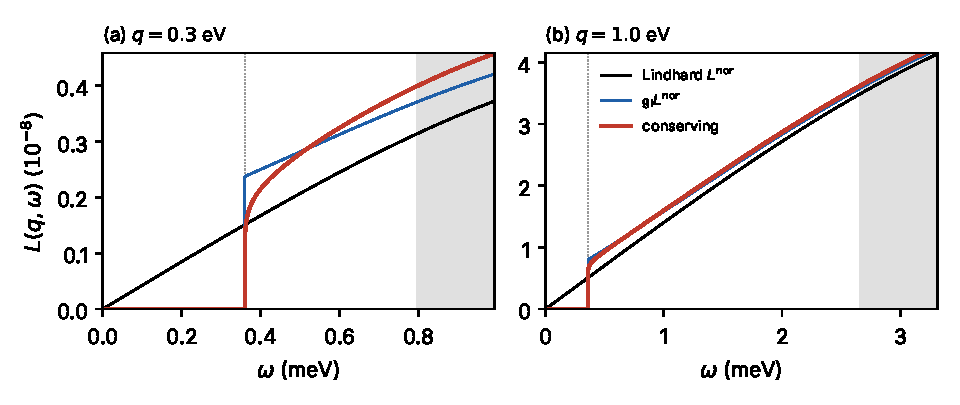
\includegraphics[width=\linewidth]{figures/ch15/fig15_1.pdf}
  \caption{Loss function of aluminum near the pair-breaking edge at the momentum transfers (a) $q = \SI{0.3}{eV}$ and (b) $q = \SI{1}{eV}$, against the energy $\omega$, for the bulk gap $\Delta_{\mathrm{BCS}} = \SI{0.18}{meV}$ (dotted line at $2\Delta_{\mathrm{BCS}}$). Red: conserving response, \cref{eq:15.1-Lcons,eq:15.1-Rcons}; blue: the case-I factor times the normal loss function, $\mathfrak{g}_{\mathrm{I}}L^{\mathrm{nor}}$; black: Lindhard loss function of the normal metal, $L^{\mathrm{nor}}$. Halo dark matter reaches the energies left of the gray band, $\omega \le qv_{\mathrm{max}}$. All curves are clean, $T = 0$, with a constant density of states, $v_{\mathrm{F}} = \num{6.75e-3}$ and $k_{\mathrm{TF}} = \SI{4.05}{keV}$. At \SI{0.3}{eV} and $\omega \ge 2.2\,\Delta_{\mathrm{BCS}}$ the conserving loss function lies 27 to \SI{34}{\percent} above the Lindhard function. At \SI{1}{eV} all three agree within \SI{5}{\percent} at the largest reachable energy.}
  \label{fig:15-alloss}
\end{figure}

At $q = \SI{0.3}{eV}$, $v_{\mathrm{F}}q = 11\,\Delta_{\mathrm{BCS}}$, every energy that halo dark matter can deposit lies within $4.4\,\Delta_{\mathrm{BCS}}$ of zero, and the conserving response lies above the Lindhard function (\cref{fig:15-alloss}). At $q = \SI{1}{eV}$, $v_{\mathrm{F}}q = 38\,\Delta_{\mathrm{BCS}}$, the differences between the three loss functions are confined to the first few $\Delta_{\mathrm{BCS}}$ above the edge.

\subsection{Truncations of the conserving response}\label{sec:15.1-chain}

Keeping the case-I absorptive part \cref{eq:15.1-gI} but screening it with the normal metal gives $\Imag\varepsilon^{\mathrm{bare}}/|\varepsilon_{\mathrm{Lin}}|^2 = \mathfrak{g}_{\mathrm{I}}L^{\mathrm{nor}}$~\cites[Eq.~(10)]{gan2026mean}[Eq.~(2) and text]{hochberg2023directional}. Closing the gap, $\Delta_{\mathrm{BCS}} \to 0$ at fixed $\omega$, leaves the Lindhard loss function~\cite[Eqs.~(1), (S.13)]{hochberg2021determining}, whose unscreened structure factor below $qv_{\mathrm{F}}$ is the free-gas $S_{\mathrm{n}} = m_e^2\omega/\pi q$ of \cref{sec:7.2}~\cite[Eq.~(3.4)]{hochberg2016detecting}. Dropping the ladder and keeping the normal real part are both controlled by $\Delta_{\mathrm{BCS}}/qv_{\mathrm{F}}$. Closing the gap is controlled by $y$ alone, through $\mathfrak{g}_{\mathrm{I}}(y) - 1$. On the kinematic edge both controlling parameters, $\Delta_{\mathrm{BCS}}/qv_{\mathrm{F}}$ and $\mathfrak{g}_{\mathrm{I}}(y) - 1$, are functions of $y$, and each truncation is worst on that edge. Over all momentum transfers that halo dark matter reaches, the clean conserving loss function lies between 0.980 and 1.085 times $\mathfrak{g}_{\mathrm{I}}L^{\mathrm{nor}}$ for $y \ge 3$; \cref{sec:15.2} gives the values on the edge, and \cref{sec:15.3-sc} the change with the mean free path.

\begin{limitbox}[Loss function of a superconductor near the pair-breaking edge][lim:15.1a]
Lindhard loss function $L^{\mathrm{nor}}$ in the rate \cref{eq:10.2-rate}, with $\Imag\varepsilon_{\mathrm{Lin}} = (\pi/2)(k_{\mathrm{TF}}^2/q^2)(\omega/qv_{\mathrm{F}})$ below $qv_{\mathrm{F}}$~\cites[Eqs.~(1), (S.13)]{hochberg2021determining}[Eq.~(3.4)]{hochberg2016detecting}; with the case-I factor, $\mathfrak{g}_{\mathrm{I}}L^{\mathrm{nor}}$~\cites[Eq.~(10)]{gan2026mean}[Eq.~(2) and text]{hochberg2023directional}.
\par\smallskip
{\centering
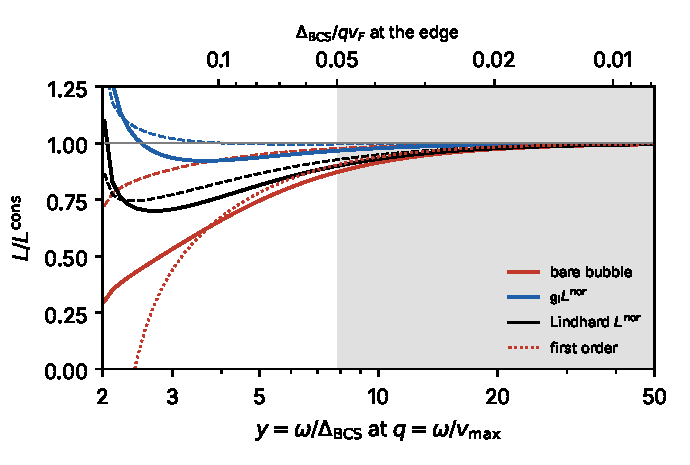
\includegraphics[width=0.92\linewidth]{figures/ch15/limit15_1a.pdf}
\captionof{figure}{Loss function of aluminum on the kinematic edge $q = \omega/v_{\mathrm{max}}$ in two truncations, divided by the conserving loss function \cref{eq:15.1-Lcons}, against $y = \omega/\Delta_{\mathrm{BCS}}$ (top axis: $\Delta_{\mathrm{BCS}}/qv_{\mathrm{F}} = 0.392/y$ there). Blue: $\mathfrak{g}_{\mathrm{I}}L^{\mathrm{nor}}$; black: Lindhard $L^{\mathrm{nor}}$. Dashed: the same at four times the edge momentum. Clean, $T = 0$, constant density of states, $v_{\mathrm{F}} = \num{6.75e-3}$. ``Within \SI{10}{\percent}'' means that the smaller of the two loss functions is at least 0.9 of the larger. Gray: $y \ge 7.9$, where the Lindhard function is within \SI{10}{\percent} of the conserving result on the edge and at all larger momenta. The product $\mathfrak{g}_{\mathrm{I}}L^{\mathrm{nor}}$ is within \SI{10}{\percent} already for $y \ge 2.25$.}\label{fig:15-limit-chain}
\par}
\smallskip
Below $y \approx 3$ on the edge the Lindhard function falls about \SI{30}{\percent} below the conserving loss function, and the clean conserving result itself assumes that impurities do not scatter the electrons within the size of a pair (\cref{sec:15.3-dirty}).
\end{limitbox}

\Cref{fig:15-limit-chain} orders the truncations. The Lindhard function, which has no gap, is within \SI{10}{\percent} of the conserving result for $y \ge 7.9$ on the edge, where $\Delta_{\mathrm{BCS}}/qv_{\mathrm{F}} \le 0.050$, and for $y \ge 6.3$ at four times the edge momentum. At $y = 5$ the Lindhard function is 0.815 of the conserving value on the edge, and the case-I factor $\mathfrak{g}_{\mathrm{I}}(5) = 1.15$ of the conserving response accounts for most of this deficit.

These comparisons are all clean-limit statements. Near the edge the curves are separated by the steep rise of the conserving absorption over a few microelectronvolts, a structure narrower than $\Delta_{\mathrm{BCS}}$. Impurity scattering, at a rate given by $v_{\mathrm{F}}$ over the mean free path, smooths the rise once that rate is no longer small compared with the width of the rise. For $y \ge 3$ the curves depend on functions of $y$ that vary on the scale of $\Delta_{\mathrm{BCS}}$ itself.

\subsection{The aluminum gap and the rate}\label{sec:15.1-al}

The gap enters the loss function through $y = \omega/\Delta_{\mathrm{BCS}}$, in $\mathfrak{g}_{\mathrm{I}}$ and in the ladder, and not only through the threshold. For bulk aluminum it is measured, $\Delta_{\mathrm{BCS}} = \SI{0.18}{meV}$~\cite[Table~III]{savrasov1996electron}, and it agrees within one percent with the weak-coupling value $1.764\,T_c = \SI{0.179}{meV}$ for the measured $T_c = \SI{1.18}{K}$ (\cref{we:7-al}). The value $\Delta = \SI{0.3}{meV}$ often taken for aluminum~\cite[p.~2]{hochberg2023directional} is the film convention $2\Delta_{\mathrm{BCS}} = \SI{0.6}{meV}$ of \cref{sec:1.5}, 1.67 times the bulk value. The film value describes thin films, whose critical temperatures exceed the bulk critical temperature and in ultraclean films approach twice it~\cite{yeh2023doubling}. A rate for a bulk crystal uses \SI{0.18}{meV}. A rate for a film uses the gap measured on that film, and \cref{sec:15.3} adds what the film changes in the response itself.

\begin{workedexample}{The aluminum rate at \SI{1}{keV} with the bulk and the film gap}\label{we:15-alrate}
Take $\mchi = \SI{1}{keV}$, a light mediator, $\FDM = (\alpha m_e/q)^2$, the reference cross section $\sigmae = \SI{e-40}{cm^2}$, the standard halo of \cref{sec:1.2}, and aluminum with $\rho_T = \SI{2.70}{g.cm^{-3}}$, $v_{\mathrm{F}} = \num{6.75e-3}$ and $k_{\mathrm{TF}} = \SI{4.05}{keV}$. The particle deposits at most $\frac12\mchi v_{\mathrm{max}}^2 = \SI{3.51}{meV}$, which is $19.5\,\Delta_{\mathrm{BCS}}$ for the bulk gap and $11.7\,\Delta_{\mathrm{BCS}}$ for the film gap, and transfers at most $2\mchi v_{\mathrm{max}} = \SI{5.30}{eV}$, so that $q/k_{\mathrm{TF}} \le \num{1.3e-3}$ and $v_{\mathrm{F}}q \le 199\,\Delta_{\mathrm{BCS}}$ (bulk). Every point lies in the regime of \cref{eq:15.1-Rcons}.

\Cref{eq:10.2-rate} with the conserving loss function, integrated numerically over $2\Delta_{\mathrm{BCS}} \le \omega \le \SI{3.51}{meV}$ and over the momenta with $\vmin \le v_{\mathrm{max}}$ (Gauss--Legendre sums, in $\omega$ graded toward $2\Delta_{\mathrm{BCS}}$ and in $q$ between the two roots of $\vmin(q,\omega) = v_{\mathrm{max}}$), gives
\begin{equation*}
  \mathcal{R} = \SI{3.26}{kg^{-1}.yr^{-1}}\ (\Delta_{\mathrm{BCS}} = \SI{0.18}{meV}), \qquad
  \mathcal{R} = \SI{2.65}{kg^{-1}.yr^{-1}}\ (\Delta_{\mathrm{BCS}} = \SI{0.30}{meV}) .
\end{equation*}
The bulk gap raises the rate by a factor of 1.23. The lower threshold alone would raise the rate more: with the Lindhard function cut at $2\Delta_{\mathrm{BCS}}$, which has no coherence factor, the factor is 1.30. The difference between the two factors comes from the edge. With the film gap the window $2\Delta_{\mathrm{BCS}} < \omega < 3\Delta_{\mathrm{BCS}}$, where $\mathfrak{g}_{\mathrm{I}}$ is largest, carries \SI{37}{\percent} of the conserving rate; with the bulk gap it carries \SI{20}{\percent}. For a heavy mediator, $\FDM = 1$, the rate at the same cross section is \SI{3.8e-13}{kg^{-1}.yr^{-1}}, and the bulk gap raises it by 1.13.

The choice of loss function matters less than the choice of gap. With the bulk gap and the light mediator, $\mathfrak{g}_{\mathrm{I}}L^{\mathrm{nor}}$ gives 1.010 of the conserving rate, and the Lindhard function cut at the threshold gives 0.850. The normal metal with no gap gives 1.024: at this mass the pile-up of pair states above $2\Delta_{\mathrm{BCS}}$ almost exactly replaces the rate lost below it. With the film gap the same ratios are 1.027, 0.806 and 1.26. These ratios are clean-limit values, and the part of the rate below $3\Delta_{\mathrm{BCS}}$ is the part that impurity scattering can change (\cref{sec:15.3}).
\end{workedexample}

\section{Screening at the kinematic edge}\label{sec:15.2}

A particle at the threshold mass $m_{\mathrm{min}} = \SI{0.10}{keV}$ of \cref{we:7-al} must move at $v_{\mathrm{max}}$ and give up its whole kinetic energy, which takes the momentum transfer $q = m_{\mathrm{min}}v_{\mathrm{max}} = 2\omega/v_{\mathrm{max}}$, twice the edge value. Heavier particles can deposit the same energy with less momentum: from $v_{\mathrm{min}}(q,\omega) = v_{\mathrm{max}}$ the smallest momentum transfer at $\omega = 2\Delta_{\mathrm{BCS}}$ is 1.17 times the edge value for $2m_{\mathrm{min}}$ and only 1.03 times it at \SI{1}{keV}. For every particle a few times heavier than $m_{\mathrm{min}}$, the scatters just above $2\Delta_{\mathrm{BCS}}$ therefore lie close to the kinematic edge.

\subsection{The normal dielectric function on the edge}\label{sec:15.2-resum}

At $q \ll k_{\mathrm{F}}$ the Lindhard function \cref{eq:4.5-lindhard} depends on $\omega$ and $q$ only through the reduced frequency $\mathfrak{w} = \omega/qv_{\mathrm{F}}$, the common limit of the arguments $\omega/qv_{\mathrm{F}} \pm q/2k_{\mathrm{F}}$ as $q/2k_{\mathrm{F}} \to 0$. To first order in $q/k_{\mathrm{F}}$ the bracket of \cref{eq:4.5-lindhard} is the derivative $\partial_{\mathfrak{w}}[(1 - \mathfrak{w}^2)\ell(\mathfrak{w})] = 2 - 2\mathfrak{w}\,\ell(\mathfrak{w})$, with $\ell(\mathfrak{w}) = \ln[(\mathfrak{w} + 1)/(\mathfrak{w} - 1)]$ and $\ell' = 2/(1 - \mathfrak{w}^2)$. With $\varepsilon_{\mathrm{Lin}} = 1 - v_{\mathrm{C}}R^0$ and $k_{\mathrm{TF}}^2 = 2e^2\mathcal{N}_{\mathrm{F}}$, this gives $R^0 = -2\mathcal{N}_{\mathrm{F}}\mathfrak{f}_{\mathrm{L}}(\mathfrak{w})$ and, on the real axis,
\begin{equation}
  \begin{gathered}
  \varepsilon_{\mathrm{Lin}}(q,\omega) = 1 + \frac{k_{\mathrm{TF}}^2}{q^2}\Bigl[\Real\mathfrak{f}_{\mathrm{L}}(\mathfrak{w}) + \ii\,\frac{\pi\mathfrak{w}}{2}\Bigr] , \qquad
  \mathfrak{f}_{\mathrm{L}}(\mathfrak{w}) = 1 - \frac{\mathfrak{w}}{2}\,\ell(\mathfrak{w}) , \\
  \Real\mathfrak{f}_{\mathrm{L}} = 1 - \frac{\mathfrak{w}}{2}\ln\frac{1 + \mathfrak{w}}{1 - \mathfrak{w}} \qquad (\mathfrak{w} < 1) .
  \end{gathered}
  \label{eq:15.2-Lin}
\end{equation}
The function $\mathfrak{f}_{\mathrm{L}}$ is analytic in the upper half plane of $\mathfrak{w}$; at real $\mathfrak{w} < 1$ the retarded branch of $\ell$ gives the imaginary part $\pi\mathfrak{w}/2$. It has $\mathfrak{f}_{\mathrm{L}}(0) = 1$, the static limit, and $\mathfrak{f}_{\mathrm{L}} \to -1/3\mathfrak{w}^2$ for $|\mathfrak{w}| \gg 1$, the free-particle tail of \cref{eq:4.5-moments}. The kinematics of \cref{sec:1.3} require $q \ge \omega/v_{\mathrm{max}}$, so $\mathfrak{w} \le v_{\mathrm{max}}/v_{\mathrm{F}}$, with equality on the edge. In aluminum $v_{\mathrm{max}}/v_{\mathrm{F}} = 0.392$, and on the edge $\Real\mathfrak{f}_{\mathrm{L}} = 0.837$ at every $\omega$. The real part of the normal dielectric function there is \SI{16}{\percent} below the Thomas--Fermi value $k_{\mathrm{TF}}^2/q^2$, and the ratio of imaginary to real part,
\begin{equation*}
  \mathfrak{r}_\varepsilon = \frac{\Imag\varepsilon_{\mathrm{Lin}}}{\Real\varepsilon_{\mathrm{Lin}}} = \frac{\pi\mathfrak{w}}{2\Real\mathfrak{f}_{\mathrm{L}}(\mathfrak{w})} = 0.736 ,
\end{equation*}
is not small. With the ``1'' of $\varepsilon$ dropped, which changes nothing at these momenta (\cref{sec:15.1-rate}), every loss-function ratio below depends on $y = \omega/\Delta_{\mathrm{BCS}}$ and $qv_{\mathrm{F}}/\Delta_{\mathrm{BCS}}$ alone, and on the edge on $y$ and $v_{\mathrm{max}}/v_{\mathrm{F}}$. The aluminum numbers therefore apply to any clean weak-coupling superconductor with the same velocity ratio.

\begin{table}[tbp]
  \caption{Loss function of aluminum on the kinematic edge $q = \omega/v_{\mathrm{max}}$ ($\omega/qv_{\mathrm{F}} = v_{\mathrm{max}}/v_{\mathrm{F}} = 0.392$), divided by $\mathfrak{g}_{\mathrm{I}}L^{\mathrm{nor}}$, the value with normal-state screening, against $y = \omega/\Delta_{\mathrm{BCS}}$. Columns: case-I ratio $\mathfrak{g}_{\mathrm{I}}$ of \cref{eq:15.1-gI}; vertex fraction $\mathfrak{v}$ of \cref{sec:15.1-bare}; conserving response \cref{eq:15.1-Rcons}, clean, and with Born scattering by impurities at the mean free paths $\mathfrak{l}_e = \SI{1}{\micro m}$ and \SI{30}{nm} (\cref{sec:15.3-sc}), each divided by $\mathfrak{g}_{\mathrm{I}}$ times the normal state at the same scattering rate. All at $T = 0$, constant density of states, $q \ll k_{\mathrm{F}}$.}
  \label{tab:15-edge}
  \centering\small\setlength{\tabcolsep}{4pt}
  \begin{tabular}{@{}cccccc@{}}
    \toprule
    & & & \multicolumn{3}{c}{conserving} \\
    \cmidrule(l){4-6}
    $y$ & $\mathfrak{g}_{\mathrm{I}}$ & $\mathfrak{v}$ & clean & \SI{1}{\micro m} & \SI{30}{nm} \\
    \midrule
    2.05 & 1.552 & 0.22 & 0.681 & 0.365 & 0.045 \\
    2.2 & 1.500 & 0.44 & 0.867 & 0.600 & 0.187 \\
    2.5 & 1.418 & 0.35 & 0.999 & 0.854 & 0.569 \\
    3 & 1.322 & 0.21 & 1.069 & 1.021 & 1.008 \\
    5 & 1.151 & 0.052 & 1.067 & 1.057 & 1.091 \\
    10 & 1.051 & 0.004 & 1.023 & 1.020 & 1.021 \\
    \bottomrule
  \end{tabular}
\end{table}

\subsection{The conserving response on the edge}\label{sec:15.2-cons}

Let a response have $\Imag\varepsilon = \mathfrak{g}\,\Imag\varepsilon_{\mathrm{Lin}}$ and $\Real\varepsilon = (1 + \delta)\Real\varepsilon_{\mathrm{Lin}}$ at some $(q,\omega)$, with $\mathfrak{g}$ and $\delta$ real. Dividing $L = \Imag\varepsilon/[(\Real\varepsilon)^2 + (\Imag\varepsilon)^2]$ by the same expression for $\varepsilon_{\mathrm{Lin}}$, and then numerator and denominator by $(\Real\varepsilon_{\mathrm{Lin}})^2$,
\begin{equation}
  \frac{L}{L^{\mathrm{nor}}} = \mathfrak{g}\,\frac{1 + \mathfrak{r}_\varepsilon^2}{(1 + \delta)^2 + \mathfrak{g}^2\mathfrak{r}_\varepsilon^2} ,
  \label{eq:D.39-resum}
\end{equation}
with no approximation. The conserving response of \cref{eq:15.1-Rcons} enters with
\begin{equation}
  \mathfrak{g} = \mathfrak{g}_{\mathrm{I}}(1 + \mathfrak{v}) , \qquad
  \delta = \frac{\Real(\varepsilon^{\mathrm{cons}} - \varepsilon_{\mathrm{Lin}})}{\Real\varepsilon_{\mathrm{Lin}}} ,
  \label{eq:15.2-cons}
\end{equation}
with $\mathfrak{v}$ the vertex fraction of \cref{sec:15.1-bare}; both follow from \cref{eq:15.1-Rcons} by one quadrature over $\mu$. This separates what the pair-field ladder does to the two parts of $\varepsilon$, and on the edge it does more to the real part. At $y = 3$ the ladder raises the absorptive part from $1.322$ to $1.322 \times 1.214 = 1.605$ times normal, while it moves the real part from 1.33 times normal without the ladder to 0.60 times normal. The modulus of $\varepsilon$ ends close to the normal one, and the loss function close to $\mathfrak{g}_{\mathrm{I}}L^{\mathrm{nor}}$: $L^{\mathrm{cons}} = 1.07\,\mathfrak{g}_{\mathrm{I}}L^{\mathrm{nor}} = 1.41\,L^{\mathrm{nor}}$. Nearer the threshold the shift overshoots, and at $y = 2.2$ the real part of $\varepsilon^{\mathrm{cons}}$ is negative, $1 + \delta = -0.18$: the condensate responds inductively there. The superconductor nonetheless screens about as strongly as the normal metal, with $|\varepsilon^{\mathrm{cons}}|/|\varepsilon_{\mathrm{Lin}}| = 1.29$ at $y = 2.2$, 1.07 at 3 and 0.99 at 5. Along the whole edge the conserving value lies within \SI{10}{\percent} of $\mathfrak{g}_{\mathrm{I}}L^{\mathrm{nor}}$ for $y \ge 2.25$ and above it from $y = 2.5$ on, by at most \SI{8.4}{\percent} at $y = 3.6$; $L^{\mathrm{cons}}/L^{\mathrm{nor}}$ peaks at 1.43 at $y = 2.70$. These are clean values; at $y \le 2.5$ they hold only for mean free paths $\mathfrak{l}_e \gtrsim \SI{10}{\micro m}$ (\cref{sec:15.3-sc}).

Near the threshold, $y \lesssim 2.3$, the ladder is large because the Anderson--Bogoliubov pole of \cref{eq:15.1-Rcons} lies just below the gap, at $1.927$, $1.966$ and $1.992\,\Delta_{\mathrm{BCS}}$ for the edge momenta of $y = 2.2$, 2.5 and 3 (\cref{sec:15.1-closed}). At $y \ge 3$ the shift comes from the pair continuum of the ladder instead. The relative size $|R^{\mathrm{cons}} - R^0_{\boldsymbol{\eta}\boldsymbol{\eta}}|/|R^0_{\boldsymbol{\eta}\boldsymbol{\eta}}|$ is $27(\Delta_{\mathrm{BCS}}/qv_{\mathrm{F}})^2$ on the edge at $y = 3$, and its coefficient falls only slowly with $q$, to 18 at $qv_{\mathrm{F}} = 100\,\Delta_{\mathrm{BCS}}$ and 11 at $10^3\,\Delta_{\mathrm{BCS}}$.

\begin{workedexample}{The conserving loss function of aluminum at $y = 3$}\label{we:15-edge}
Take $\omega = 3\Delta_{\mathrm{BCS}} = \SI{0.54}{meV}$ with the bulk gap $\Delta_{\mathrm{BCS}} = \SI{0.18}{meV}$. The smallest momentum transfer is $q = \omega/v_{\mathrm{max}} = \SI{0.54e-3}{eV}/2.650\times10^{-3} = \SI{0.204}{eV}$, so $1/q = \SI{0.97}{\micro m}$. With $v_{\mathrm{F}} = 6.75\times10^{-3}$, $qv_{\mathrm{F}} = \SI{1.38}{meV} = 7.65\,\Delta_{\mathrm{BCS}}$, so $\mathfrak{w} = 0.392$ and $\Delta_{\mathrm{BCS}}/qv_{\mathrm{F}} = 0.131$.

\emph{Normal metal.} \Cref{eq:15.2-Lin} gives $\Real\mathfrak{f}_{\mathrm{L}} = 1 - 0.196\ln(1.392/0.608) = 0.837$ and $\mathfrak{r}_\varepsilon = (\pi/2)(0.392)/0.837 = 0.736$.

\emph{Conserving response.} The case-I factor is $\mathfrak{g}_{\mathrm{I}}(3) = 1.322$, and \cref{eq:15.2-cons} has $\mathfrak{g} = 1.322\times1.214 = 1.605$ and $1 + \delta = 0.596$. Then $|\varepsilon^{\mathrm{cons}}|/|\varepsilon_{\mathrm{Lin}}| = [(0.596^2 + 1.605^2\times0.736^2)/(1 + 0.736^2)]^{1/2} = 1.065$, and $L^{\mathrm{cons}} = 1.605\,L^{\mathrm{nor}}/1.065^2 = 1.414\,L^{\mathrm{nor}} = 1.069\,\mathfrak{g}_{\mathrm{I}}L^{\mathrm{nor}}$. In a \SI{30}{nm} film the ratio is 1.008 (\cref{tab:15-edge}).

The conserving response predicts a loss function \SI{41}{\percent} above the normal metal at this energy and momentum, almost all of it the case-I factor, and the mean free path changes that by less than \SI{6}{\percent}.
\end{workedexample}

\subsection{Corrections and nuisances}\label{sec:15.2-nuisance}

\Cref{eq:15.2-cons} inherits the hypotheses of \cref{eq:15.1-Rcons}, and \cref{sec:15.1-rate,sec:15.1-closed} bound the terms it drops: the band curvature, the ``1'' and the core electrons in $\varepsilon$, and the particle--hole asymmetry that couples the amplitude channel, each below $10^{-4}$ at these momenta. Thermal quasiparticles add the scattering channel of \cref{sec:7.2} with weight $\ee^{-\Delta_{\mathrm{BCS}}/T}$, $\ee^{-209}$ at \SI{10}{mK}. Within the model every correction to the absorptive part of order $(\Delta_{\mathrm{BCS}}/qv_{\mathrm{F}})^2$ is in the ladder, since the bare absorptive part has none, and \cref{eq:15.1-Rcons} contains the ladder to all orders. Outside the model lie disorder (\cref{sec:15.3-sc}) and the frequency dependence of the gap in strong coupling, which is small in aluminum, where $2\Delta_{\mathrm{BCS}}/T_c = 3.54$ against the weak-coupling 3.53 (\cref{sec:7.2}), and is not sized here. So is the film geometry, once the length $1/q$, about a micrometer on the edge, exceeds the film thickness (\cref{sec:15.3-sheet}).

The superconducting part of a rate carries three nuisances of the kinds of \cref{sec:8.8}, which the chapter summary collects. The first is the gap, a threshold nuisance \cref{eq:8.8-shift}: $\delta E = 2\,\delta\Delta_{\mathrm{BCS}}$ moves the edge, and at fixed $\omega$ it moves $y$. Its size is the uncertainty of the gap of the sensor in use, the bulk \SI{0.18}{meV} or the measured film gap of \cref{sec:15.1-al}. The second is the relaxation rate $\gamma_{\mathrm{rel}}$ of the film, a tilt that acts only near the edge. At $y \ge 3$ it moves the loss function by less than \SI{6}{\percent} relative to $\mathfrak{g}_{\mathrm{I}}L^{\mathrm{nor}}$, and at $y = 2.2$ by a factor of 4.6 between the clean limit and $\mathfrak{l}_e = \SI{30}{nm}$ (\cref{sec:15.3-sc}). The third is the edge remainder, the difference between the loss function a rate calculation uses and the conserving one. With $\mathfrak{g}_{\mathrm{I}}L^{\mathrm{nor}}$ as the central value, the remainder at $y \ge 3$ has no fixed sign. In the clean limit it runs from $-\SI{2.0}{\percent}$ to $+\SI{8.5}{\percent}$ over all momentum transfers that halo dark matter reaches, the lower end at about four times the edge momentum of $y = 3$. With impurities it reaches $+\SI{9.1}{\percent}$ on the edge, and off the edge it has not been computed. It is therefore a two-sided normalization nuisance, $-\SI{2}{\percent}$ to $+\SI{9}{\percent}$, with the standard-normal constraint of \cref{eq:8.8-M}.

Near the threshold the conserving loss function depends strongly on the mean free path, and a rate calculation excludes those energies from its signal region. The criterion we adopt is that the edge value of $L^{\mathrm{cons}}/\mathfrak{g}_{\mathrm{I}}L^{\mathrm{nor}}$ vary by at most \SI{10}{\percent} over the mean free paths from \SI{30}{nm} to \SI{100}{\micro m}. It holds at $y = 3$, where the values agree to \SI{6}{\percent}, and fails at $y = 2.5$, where they span a factor of 1.75. The boundary lies between the two, and the energies $y < 3$ are excluded. In that window the remainder is not bounded for a film: at $\mathfrak{l}_e = \SI{30}{nm}$ the conserving value at $y = 2.2$ is 0.19. In a crystal with $\mathfrak{l}_e \ge \SI{10}{\micro m}$ the clean column of \cref{tab:15-edge} holds to \SI{4}{\percent} down to $y = 2.2$, and the excluded energies can be restored with it. The deviations from $\mathfrak{g}_{\mathrm{I}}L^{\mathrm{nor}}$ are largest on the edge, so the exclusion covers the momenta above it as well.

\section{Films and disorder}\label{sec:15.3}

An electron in a clean aluminum crystal crosses a Cooper pair, \SI{2.4}{\micro m} across (\cref{sec:7.2}), without scattering, and the loss functions of \cref{sec:15.1,sec:15.2} assume exactly that. The sensors that count broken pairs, however, are films. In a \SI{50}{nm} aluminum film an electron reaches a surface after at most about \SI{50}{nm}. In the amorphous tungsten silicide of the QROCODILE dark-matter search, whose sensors are superconducting microwires patterned from a layer \SI{2}{nm} thick~\cite{baudis2025first}, it scatters after a few tenths of a nanometer, about once per interatomic distance. At the momentum transfers of keV-mass dark matter these collisions raise the normal-state loss function of the aluminum film about twentyfold. They also change the loss function at the pair-breaking edge, and a film thinner than $1/q$ screens like a sheet rather than like a bulk metal.

\subsection{Mean free path and Anderson's theorem}\label{sec:15.3-dirty}

The rate $\gamma_{\mathrm{rel}}$ at which collisions relax the momentum of an electron (\cref{sec:4.5}) sets two lengths. An electron at the Fermi surface travels the \emph{mean free path}
\begin{equation}
  \mathfrak{l}_e = \frac{v_{\mathrm{F}}}{\gamma_{\mathrm{rel}}}, \qquad D_{\mathrm{diff}} = \frac{v_{\mathrm{F}}\mathfrak{l}_e}{3} ,
  \label{eq:15.3-le}
\end{equation}
between collisions, and over many collisions it performs a random walk with diffusion constant $D_{\mathrm{diff}}$. The second relation follows from free flights of exponentially distributed length, which have $\langle s^2\rangle = 2\mathfrak{l}_e^2$, one per time $1/\gamma_{\mathrm{rel}}$ in a random direction, so that $\langle r^2\rangle = 2\mathfrak{l}_e^2\gamma_{\mathrm{rel}}t = 6D_{\mathrm{diff}}t$. The dc resistivity measures $\mathfrak{l}_e$. The Drude conductivity of \cref{sec:4.5} is $\nd_ee^2/(m_e\gamma_{\mathrm{rel}})$ in SI units, and with $\nd_e = k_{\mathrm{F}}^3/3\pi^2$ and $v_{\mathrm{F}} = \hbar k_{\mathrm{F}}/m_e$ the resistivity $\rho_{\mathrm{el}}$ obeys
\begin{equation}
  \rho_{\mathrm{el}}\,\mathfrak{l}_e = \frac{3\pi^2\hbar}{e^2k_{\mathrm{F}}^2} ,
  \label{eq:15.3-rho}
\end{equation}
a constant of the metal. For the free-electron gas of aluminum (\cref{sec:15.1-rate}) it is \SI{3.98e-16}{\ohm.m^2}, and a film with $\mathfrak{l}_e = \SI{50}{nm}$ has a residual resistivity of \SI{0.80}{\micro\ohm.cm} and $\gamma_{\mathrm{rel}} = \SI{26.7}{meV}$. We take $\mathfrak{l}_e$ equal to the thickness, $d_{\mathrm{film}} = \SI{50}{nm}$, as for a film whose surfaces scatter electrons diffusely; a measured residual resistivity replaces this choice through \cref{eq:15.3-rho}.

Which theory applies depends on three ratios: $q\mathfrak{l}_e$, $\mathfrak{l}_e/\xi_{\mathrm{coh}}$ and $k_{\mathrm{F}}\mathfrak{l}_e$. The first, $q\mathfrak{l}_e$, is the distance between collisions in units of the length $1/q$ of the perturbation. For $q\mathfrak{l}_e \gg 1$ the electrons are \emph{ballistic} on the scale $1/q$, and the response is that of the clean gas; for $q\mathfrak{l}_e \ll 1$ they are \emph{diffusive}, and a density disturbance spreads by diffusion. The second compares $\mathfrak{l}_e$ with the coherence length $\xi_{\mathrm{coh}} = v_{\mathrm{F}}/\pi\Delta_{\mathrm{BCS}}$, the size of a pair (\cref{sec:7.2}). A superconductor with $\mathfrak{l}_e \gg \xi_{\mathrm{coh}}$ is \emph{clean}, and one with $\mathfrak{l}_e \ll \xi_{\mathrm{coh}}$ is in the \emph{dirty limit}: each pair is spread over many impurities. For aluminum $\xi_{\mathrm{coh}} = \SI{2.4}{\micro m}$ with the free-electron $v_{\mathrm{F}}$, and the coherence length tabulated for aluminum is \SI{1.6}{\micro m}~\cite[Ch.~10, Table~5]{kittel2005introduction}; the clean results of \cref{sec:15.1,sec:15.2} need a mean free path long compared with either, which only bulk high-purity crystals have. The third ratio, $k_{\mathrm{F}}\mathfrak{l}_e$, is the mean free path in units of the electron wavelength. Disorder is weak for $k_{\mathrm{F}}\mathfrak{l}_e \gg 1$, where an electron still has a well-defined momentum between collisions, and strong near the Ioffe--Regel limit $k_{\mathrm{F}}\mathfrak{l}_e \approx 1$, where it does not. \Cref{tab:15-disorder} lists the three numbers for the aluminum film and for amorphous WSi. The aluminum film is weakly disordered, dirty, and diffusive at the momenta that keV-mass dark matter transfers; WSi is strongly disordered.

\begin{table}[tbp]
  \centering
  \caption{Disorder parameters of two superconducting sensor materials. Aluminum film: free-electron gas with $k_{\mathrm{F}} = \SI{1.75}{\angstrom^{-1}}$ and $v_{\mathrm{F}} = \num{6.75e-3}$, mean free path taken equal to the thickness of \SI{50}{nm}, coherence length $v_{\mathrm{F}}/\pi\Delta_{\mathrm{BCS}}$ with the bulk gap \SI{0.18}{meV}. Amorphous W$_x$Si$_{1-x}$: \SI{5}{nm} films with $x = 0.75$--0.85~\cite[Table~I]{zhang2016characteristics}; the range of $\mathfrak{l}_e$ comes from combining the measured diffusion constant (lower end) or the measured resistivity (upper end) with the free-electron gas at $E_{\mathrm{F}} = \SI{7}{eV}$; the coherence length is the measured Ginzburg--Landau value. The pair-breaking edge is $q = 2\Delta_{\mathrm{BCS}}/v_{\mathrm{max}}$, the smallest momentum transfer at which a halo particle can deposit $2\Delta_{\mathrm{BCS}}$; WSi has $\Delta_{\mathrm{BCS}} = \SI{0.263}{meV}$.}
  \label{tab:15-disorder}
  \begin{tabular}{@{}lcc@{}}
    \toprule
    & Al film, \SI{50}{nm} & amorphous WSi \\
    \midrule
    mean free path $\mathfrak{l}_e$ & \SI{50}{nm} & 0.13--\SI{0.41}{nm} \\
    relaxation rate $\gamma_{\mathrm{rel}}$ & \SI{27}{meV} & 2.5--\SI{7.7}{eV} \\
    $k_{\mathrm{F}}\mathfrak{l}_e$ & 874 & 1.8--5.5 \\
    $\mathfrak{l}_e/\xi_{\mathrm{coh}}$ & 0.021 & 0.02--0.06 \\
    $q\mathfrak{l}_e$ at the pair-breaking edge & 0.034 & (1.4--4.1)$\times10^{-4}$ \\
    $q\mathfrak{l}_e$ at $q = \SI{1}{keV}$ & 253 & 0.7--2.1 \\
    \bottomrule
  \end{tabular}
\end{table}

In the dirty limit the plane waves of \cref{sec:7.2} are no longer eigenstates, and the BCS construction has to be redone. Anderson~\cite{anderson1959theory} noticed that nonmagnetic impurities do not break time reversal. Every exact one-electron eigenstate $\psi_n$ of the disordered metal has a time-reversed partner $\psi_n^*$ at the same energy. He paired $\psi_n$ with $\psi_n^*$, in place of $\vect{k}$ with $-\vect{k}$, and took the attraction constant between the exact states within $\omega_{\mathrm{D}}$ of the Fermi level. The reduced Hamiltonian of \cref{eq:7.2-HBCS} then leads to the gap equation of \cref{eq:7.2-gap} with the density of states of the exact states at the Fermi level in place of $\mathcal{N}_{\mathrm{F}}$. Weak disorder changes that density of states only at relative order $1/k_{\mathrm{F}}\mathfrak{l}_e$, and nonmagnetic disorder leaves $\Delta_{\mathrm{BCS}}$ and $T_c$ at their clean values. This is \emph{Anderson's theorem}. Magnetic impurities break time reversal, the partner states no longer pair, and the gap falls. For a weakly disordered film the pair-breaking threshold is still $2\Delta_{\mathrm{BCS}}$, with the gap of the film, measured through its $T_c$ or by tunneling (\cref{sec:15.1-al}). The response, on the other hand, does change with disorder, because the matrix elements of $\ee^{\ii\vect{q}\cdot\vect{r}}$ between exact states are not those between plane waves.

\subsection{Relaxation-time loss functions}\label{sec:15.3-mermin}

Collisions enter the loss function through the Mermin dielectric function of \cref{eq:4.5-mermin}, which relaxes the electrons toward local equilibrium, conserves their number and is causal (\cref{app:D.9}). At the momentum transfers of light dark matter $q \ll k_{\mathrm{F}}$, and the Lindhard bubble at a complex frequency $z$ in the upper half plane is \cref{eq:15.2-Lin} continued off the real axis,
\begin{equation}
  R^0(q,z) = -2\mathcal{N}_{\mathrm{F}}\,\mathfrak{f}_{\mathrm{L}}(\mathfrak{w}), \qquad \mathfrak{w} = \frac{z}{qv_{\mathrm{F}}} ,
  \label{eq:15.3-fL}
\end{equation}
where $\ell(\mathfrak{w}) = \ln[(\mathfrak{w} + 1)/(\mathfrak{w} - 1)]$ in $\mathfrak{f}_{\mathrm{L}}$ is the principal logarithm of the complex argument, the retarded branch of \cref{eq:C.8-branch}. With $\varepsilon_{\mathrm{Lin}} - 1 = (k_{\mathrm{TF}}^2/q^2)\,\mathfrak{f}_{\mathrm{L}}$ from \cref{eq:4.4-TF}, the factors $\ii\gamma_{\mathrm{rel}}/\omega$ of \cref{eq:4.5-mermin} combine into
\begin{equation}
  \varepsilon_{\mathrm{Mer}}(q,\omega) = 1 + \frac{k_{\mathrm{TF}}^2}{q^2}\,
  \frac{(\omega + \ii\gamma_{\mathrm{rel}})\,\mathfrak{f}_{\mathrm{L}}(\mathfrak{w}_\gamma)}{\omega + \ii\gamma_{\mathrm{rel}}\,\mathfrak{f}_{\mathrm{L}}(\mathfrak{w}_\gamma)}, \qquad
  \mathfrak{w}_\gamma = \frac{\omega + \ii\gamma_{\mathrm{rel}}}{qv_{\mathrm{F}}} .
  \label{eq:15.3-mermin}
\end{equation}
The size of $|\mathfrak{w}_\gamma|$ is the size of $1/q\mathfrak{l}_e$. For dark matter $\omega \le qv_{\mathrm{max}} < qv_{\mathrm{F}}$, so $|\omega + \ii\gamma_{\mathrm{rel}}|/qv_{\mathrm{F}}$ lies between $\gamma_{\mathrm{rel}}/qv_{\mathrm{F}} = 1/q\mathfrak{l}_e$ and $1/q\mathfrak{l}_e + v_{\mathrm{max}}/v_{\mathrm{F}}$.

In the diffusive regime, $q\mathfrak{l}_e \ll 1$, the tail $\mathfrak{f}_{\mathrm{L}} \simeq -q^2v_{\mathrm{F}}^2/3(\omega + \ii\gamma_{\mathrm{rel}})^2$ applies. Since then also $\omega \ll \gamma_{\mathrm{rel}}$, the numerator of the fraction in \cref{eq:15.3-mermin} is $\ii q^2D_{\mathrm{diff}}$ and the denominator $\omega + \ii q^2D_{\mathrm{diff}}$, with $D_{\mathrm{diff}}$ of \cref{eq:15.3-le}. The dielectric function becomes
\begin{equation}
  \varepsilon_{\mathrm{Mer}} \simeq 1 + \frac{k_{\mathrm{TF}}^2D_{\mathrm{diff}}}{D_{\mathrm{diff}}q^2 - \ii\omega} \qquad (q\mathfrak{l}_e \ll 1) ,
  \label{eq:15.3-diff}
\end{equation}
the diffusion pole: a density disturbance of wavevector $q$ decays at the rate $D_{\mathrm{diff}}q^2$. For $\omega \ll D_{\mathrm{diff}}q^2$ it reduces to the static screening $k_{\mathrm{TF}}^2/q^2$, and for $\omega \gg D_{\mathrm{diff}}q^2$ to $\ii k_{\mathrm{TF}}^2D_{\mathrm{diff}}/\omega$, the Drude form $\ii\sigma_{\mathrm{cond}}/\omega$ of \cref{eq:4.4-sigma} with the dc conductivity $k_{\mathrm{TF}}^2D_{\mathrm{diff}} = \omega_p^2/\gamma_{\mathrm{rel}}$, by \cref{eq:4.4-TF}. The loss function is the same in both regimes. With $|\varepsilon| \gg 1$, $\Imag\varepsilon_{\mathrm{Mer}} = k_{\mathrm{TF}}^2D_{\mathrm{diff}}\omega/(D_{\mathrm{diff}}^2q^4 + \omega^2)$ and $|\varepsilon_{\mathrm{Mer}}|^2 = k_{\mathrm{TF}}^4D_{\mathrm{diff}}^2/(D_{\mathrm{diff}}^2q^4 + \omega^2)$, so $L = \omega/k_{\mathrm{TF}}^2D_{\mathrm{diff}} = \omega\gamma_{\mathrm{rel}}/\omega_p^2$ at every $\omega/D_{\mathrm{diff}}q^2$: the Drude tail of \cref{sec:4.5}, independent of $q$.

In the ballistic regime, $q\mathfrak{l}_e \gg 1$, the small argument $|\mathfrak{w}_\gamma| \ll 1$ applies, and on the retarded branch $\ell(\mathfrak{w}) \simeq -\ii\pi + 2\mathfrak{w}$, so $\mathfrak{f}_{\mathrm{L}} \simeq 1 + \ii\pi\mathfrak{w}_\gamma/2$. The fraction in \cref{eq:15.3-mermin} is then $1 + \ii\pi\omega/2qv_{\mathrm{F}}$, with $\gamma_{\mathrm{rel}}$ gone at this order, and $L = \pi\omega q/(2k_{\mathrm{TF}}^2v_{\mathrm{F}})$. This is the low-energy corner of the clean Lindhard loss function of \cref{sec:4.5}, written with \cref{eq:4.4-TF}.
\begin{keyresult}[Loss function of a metal with collisions]
For $q \ll k_{\mathrm{F}}$, $q \ll k_{\mathrm{TF}}$ and $\omega \le qv_{\mathrm{max}}$, the Mermin loss function has the limits
\begin{equation}
  L_{\mathrm{Mer}}(q,\omega) \simeq
  \begin{cases}
    \omega\gamma_{\mathrm{rel}}/\omega_p^2 = \omega/\sigma_{\mathrm{dc}} , & q\mathfrak{l}_e \ll 1 ,\\[2pt]
    \pi\omega q/(2k_{\mathrm{TF}}^2v_{\mathrm{F}}) , & q\mathfrak{l}_e \gg 1 ,
  \end{cases}
  ,
  \label{eq:15.3-limits}
\end{equation}
with $\sigma_{\mathrm{dc}} = \omega_p^2/\gamma_{\mathrm{rel}}$ the dc conductivity. The ballistic form is $\pi q\mathfrak{l}_e/6$ times the diffusive one. In SI units the diffusive form is $L = \varepsilon_0\omega\rho_{\mathrm{el}}$, fixed by the measured resistivity alone.
\end{keyresult}
Collisions therefore raise the loss function at small $q$, by the factor $6/\pi q\mathfrak{l}_e$. In a clean metal a slow potential of long wavelength is absorbed only by the electrons that move almost perpendicular to $\vect{q}$, which keep pace with it (Landau damping), and their share is $\omega/qv_{\mathrm{F}}$. Collisions let every electron at the Fermi surface absorb, and the absorbed power is the Joule heat of the induced current, set by the resistivity. \Cref{fig:15-film}b shows the ratio $L_{\mathrm{Mer}}/L_{\mathrm{Drude}}$ against $q\mathfrak{l}_e$. It is within \SI{10}{\percent} of one for $q\mathfrak{l}_e \le 0.64$ and within \SI{10}{\percent} of $\pi q\mathfrak{l}_e/6$ only from $q\mathfrak{l}_e = 9.8$; at $q\mathfrak{l}_e = 1.5$ it is 1.43, almost twice the ballistic asymptote. Neither form holds in between, and there \cref{eq:15.3-mermin} has to be evaluated.

\begin{figure}[tbp]
  \centering
  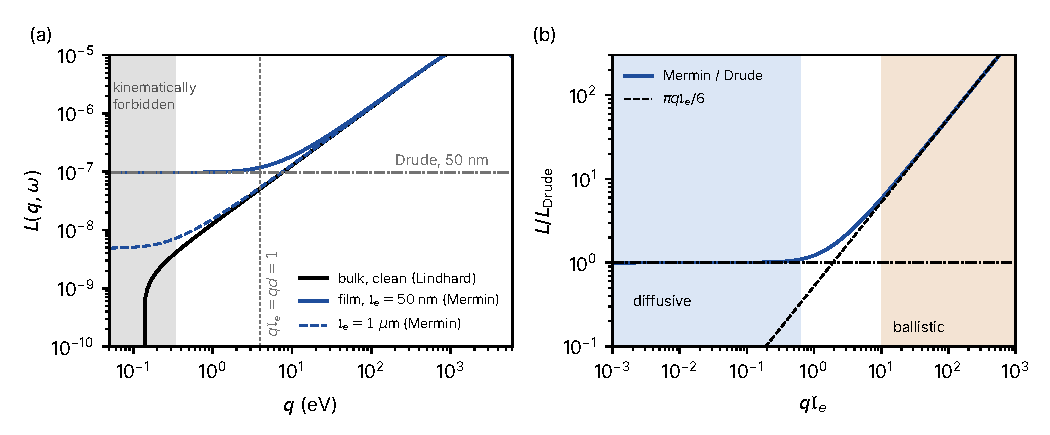
\includegraphics[width=\linewidth]{figures/ch15/fig15_2.pdf}
  \caption{Normal-state loss function of aluminum in a film and in the bulk. (a) $L(q,\omega)$ at $\omega = \SI{0.90}{meV}$ ($5\Delta_{\mathrm{BCS}}$ with the bulk gap) against the momentum transfer $q$, for a free-electron gas with $k_{\mathrm{F}} = \SI{1.75}{\angstrom^{-1}}$ and $v_{\mathrm{F}} = \num{6.75e-3}$. Curves: clean Lindhard function (black), Mermin function with mean free path $\mathfrak{l}_e = \SI{50}{nm}$ (blue, $\gamma_{\mathrm{rel}} = \SI{26.7}{meV}$) and $\mathfrak{l}_e = \SI{1}{\micro m}$ (blue dashed), and the Drude tail $\omega\gamma_{\mathrm{rel}}/\omega_p^2$ for \SI{50}{nm} (gray). Gray band: $q < \omega/v_{\mathrm{max}}$, out of reach of halo dark matter. Dotted vertical line: $q\mathfrak{l}_e = 1$, which for this film is also $qd_{\mathrm{film}} = 1$. (b) Ratio of the Mermin loss function to the Drude tail, against $q\mathfrak{l}_e$, for $q \ll k_{\mathrm{F}}$ (\cref{eq:15.3-mermin}) and $\omega/\gamma_{\mathrm{rel}} = 0.034$; dashed, the ballistic asymptote $\pi q\mathfrak{l}_e/6$. Shaded: within \SI{10}{\percent} of the diffusive limit (left) and of the ballistic limit (right), that is a ratio to the limit of at most 1.1.}
  \label{fig:15-film}
\end{figure}

\Cref{fig:15-film}a shows the consequence for aluminum. At the smallest momentum transfer that can deposit \SI{0.90}{meV}, $q = \omega/v_{\mathrm{max}} = \SI{0.34}{eV}$, the \SI{50}{nm} film has a loss function 24 times that of the clean crystal. The asymptotic $6/\pi q\mathfrak{l}_e$ is 22; the clean value lies below its own small-$\omega$ form there, since $\omega/qv_{\mathrm{F}} = 0.39$. The enhancement persists up to $q \approx 1/\mathfrak{l}_e = \SI{3.9}{eV}$, which is the largest momentum transfer of dark matter lighter than \SI{0.75}{keV}, and above that the two curves merge. A film with $\mathfrak{l}_e = \SI{1}{\micro m}$ lies between. Collisions in a film thus change the loss function for keV-mass dark matter, whereas at the momentum transfers of MeV-mass dark matter the film electrons are ballistic.

The plasmon width and the relaxation rate are different numbers. A Drude form fitted to the measured aluminum plasmon has $\omega_p = \SI{14.9}{eV}$ and a width of \SI{0.863}{eV}~\cite[Fig.~S1]{hochberg2021determining}, 32 times the relaxation rate of the \SI{50}{nm} film. The plasmon decays into electron--hole pairs by interband transitions and by collisions alike, while the tail at meV energies, by \cref{eq:15.3-limits}, is set by the dc resistivity, which measures momentum relaxation at the Fermi surface only. A tail extrapolated from the plasmon width overstates the loss function of the \SI{50}{nm} film at meV energies by that factor of 32.

The logarithms of the Lindhard function and of the BCS bubbles are taken on the retarded branch \cref{eq:C.8-branch}, which the limit of a vanishing width does not select by itself. The other branch suppresses the computed rate of an aluminum detector at low mass by up to seven orders of magnitude~\cite{hochberg2021determining}. A time-ordered bubble coincides with the retarded one at $T = 0$ only for $\omega > 0$, whereas a Kramers--Kronig integral and a sum rule need $\omega < 0$ as well.

\subsection{The superconducting film}\label{sec:15.3-sc}

On the kinematic edge of $y = \omega/\Delta_{\mathrm{BCS}} = 2.2$ the momentum transfer is $q = 2.2\,\Delta_{\mathrm{BCS}}/v_{\mathrm{max}} = \SI{0.15}{eV}$, whatever $v_{\mathrm{F}}$ is, so an aluminum film with $\mathfrak{l}_e = \SI{30}{nm}$ has $q\mathfrak{l}_e = 0.023$ there. Its electrons are diffusive on the scale of the probe, and the clean response of \cref{sec:15.1} does not apply. The conserving response with Born scattering by nonmagnetic impurities at $T = 0$ replaces it. In Nambu space the impurity potential couples through $\boldsymbol{\eta}$, the Nambu matrix of the density, so the Born self-energy is $\boldsymbol{\eta}\,\GF\,\boldsymbol{\eta}$ averaged over the Fermi surface. The same impurity ladder dresses the density vertex and the two pair vertices; with both, the response stays conserving (\cref{app:E.20}). Its normal state is the Mermin function \cref{eq:4.5-mermin} at the same relaxation rate $\gamma_{\mathrm{rel}} = v_{\mathrm{F}}/\mathfrak{l}_e$. \Cref{tab:15-edge} lists its edge values for \SI{1}{\micro m} and \SI{30}{nm}, divided by $\mathfrak{g}_{\mathrm{I}}$ times that normal state, and we use the same normalization for every number in this subsection.

At $y \ge 3$ the ratio hardly moves: it stays between 1.008 and 1.091 for every mean free path from \SI{100}{\micro m} down to \SI{30}{nm}. At $y \le 2.5$, however, it moves a great deal. At $y = 2.2$ it falls from 0.87 in the clean limit to 0.60 at $\mathfrak{l}_e = \SI{1}{\micro m}$, 0.38 at \SI{300}{nm} and 0.19 at \SI{30}{nm}, and at $y = 2.5$ from 1.00 to 0.57. The clean values hold to \SI{4}{\percent} down to $y = 2.2$ only for $\mathfrak{l}_e \ge \SI{10}{\micro m}$. In a film the suppression near the threshold therefore returns, now through the inductive response of the condensate.

The local limit of short mean free path shows why. When $q\mathfrak{l}_e \ll 1$ and $D_{\mathrm{diff}}q^2 \ll \Delta_{\mathrm{BCS}}$, neither an electron nor a pair resolves the spatial variation of the potential, and the film responds locally. The induced density then follows from the induced current by the continuity equation, longitudinal and transverse responses coincide (\cref{eq:4.4-ET}), and $\varepsilon = 1 + \ii\sigma_{\mathrm{cond}}(\omega)/\omega$ by \cref{eq:4.4-sigma}, in the superconducting state as in the normal one. The conductivity of a dirty superconductor is the Mattis--Bardeen conductivity, derived in \cref{sec:15.4-MB} and \cref{app:D.40}. At $T = 0$ its real part $\sigma_1/\sigma_n$ is the case-II pair-creation integral of \cref{eq:7.2-pairspec}, which is zero below $2\Delta_{\mathrm{BCS}}$ and rises continuously from zero above it. Its imaginary part $\sigma_2$ is the Kramers--Kronig partner of $\sigma_1$, and it contains the weight $(\pi^2/2)\Delta_{\mathrm{BCS}}\sigma_n$ missing from $\sigma_1$ below $2\Delta_{\mathrm{BCS}}$, which the condensate carries at $\omega = 0$. Since $|\varepsilon| \gg 1$, $-1/\varepsilon = \ii\omega/\sigma_{\mathrm{cond}}$, and
\begin{equation}
  L = \frac{\omega\,\sigma_1}{\sigma_1^2 + \sigma_2^2}, \qquad
  \frac{L_{\mathrm{s}}}{L_{\mathrm{n}}} = \frac{\sigma_n\,\sigma_1}{\sigma_1^2 + \sigma_2^2} \qquad (q\mathfrak{l}_e \ll 1,\ D_{\mathrm{diff}}q^2 \ll \Delta_{\mathrm{BCS}}) ,
  \label{eq:15.3-MB}
\end{equation}
with $L_{\mathrm{n}} = \omega/\sigma_n$ the Drude tail of \cref{eq:15.3-limits} and $L_{\mathrm{s}}$ the superconducting loss function. Near the threshold the ratio is small for two reasons. By continuity the density couples through the current, which is odd under time reversal, so the coherence factor is that of case~II, which vanishes at $2\Delta_{\mathrm{BCS}}$, rather than that of case~I with its step of $\pi/2$. And $\sigma_2$ exceeds $\sigma_1$ there, 0.757 against 0.139 times $\sigma_n$ at $y = 2.2$: the supercurrent of the condensate short-circuits the slow potential. Divided by $\mathfrak{g}_{\mathrm{I}}$, the normalization of \cref{tab:15-edge}, \cref{eq:15.3-MB} gives 0.157 at $y = 2.2$, 0.985 at $y = 3$, 1.094 at $y = 5$ and 1.023 at $y = 10$, against 0.187, 1.008, 1.091 and 1.021 in the \SI{30}{nm} column: \cref{eq:15.3-MB} is the end point of the table, and it needs only the measured conductivity of the film. At \SI{30}{nm} and $y = 2.2$ the conserving value still lies \SI{20}{\percent} above the local limit, although $D_{\mathrm{diff}}q^2 = 0.042\,\Delta_{\mathrm{BCS}}$ is already small there; the origin of that excess has not been established.

\subsection{Film thickness}\label{sec:15.3-sheet}

A film thicker than $1/q$ responds as the bulk. Its surfaces spread the momentum along the normal over a range $\sim 1/d_{\mathrm{film}}$, a relative correction of order $1/qd_{\mathrm{film}}$, and they carry surface plasmons near $\omega_p/\sqrt2 \approx \SI{11}{eV}$, far above the energies that dark matter deposits at these momenta. A film thinner than $1/q$ responds as a sheet. The external potential is then uniform across the thickness, and the film responds to its in-plane wavevector $\vect{q}_\parallel$ with the induced density $d_{\mathrm{film}}R(q_\parallel,\omega)\phi$ per area. This sheet of charge produces the potential $e^2/[(\varepsilon_a + \varepsilon_b)q_\parallel]\,\ee^{-q_\parallel|z|}$ per unit density, with $\varepsilon_a$ and $\varepsilon_b$ the dielectric constants of the media on the two sides. The two-dimensional Fourier transform of $e^2/4\pi r$ is $e^2/2q_\parallel$, and the image charges of the two half spaces replace the 2 by $\varepsilon_a + \varepsilon_b$. In the bulk the same density produces $e^2/q^2$. Therefore
\begin{equation}
  \varepsilon_{\mathrm{sh}}(q_\parallel,\omega) - 1 = \frac{q_\parallel d_{\mathrm{film}}}{\varepsilon_a + \varepsilon_b}\,\bigl[\varepsilon(q_\parallel,\omega) - 1\bigr] \qquad (qd_{\mathrm{film}} \ll 1) ,
  \label{eq:15.3-sheet}
\end{equation}
and the screening factor $1/|\varepsilon|^2$ in the structure factor $-2\Imag R/|\varepsilon|^2$ becomes $1/|\varepsilon_{\mathrm{sh}}|^2$, larger by $[(\varepsilon_a + \varepsilon_b)/q_\parallel d_{\mathrm{film}}]^2$ while both dielectric functions are large. For a slab in vacuum this is the leading term in $q_\parallel d_{\mathrm{film}}$ of the exact slab response of Lasenby and Prabhu~\cite[Eq.~(19)]{lasenby2022dark}, whose next term is of relative order $q_\parallel d_{\mathrm{film}}$. A thin metal film screens a long-wavelength potential far less than the bulk, because the field of its induced charge spreads outside it. The factor depends on the direction of $\vect{q}$ through $q_\parallel$, which makes the rate of a thin film directional. For this reason the QROCODILE analysis solves the electrostatic problem of a single \SI{2}{nm} WSi layer in vacuum with a Drude dielectric function; it finds the anisotropy strong at $q \sim \SI{1}{nm^{-1}}$ and already significant at $q \sim \SI{1}{keV}$ for energies above \SI{4}{eV}~\cite[supplement]{baudis2025first}. For the \SI{50}{nm} aluminum film $qd_{\mathrm{film}} = 1$ at $q = \SI{3.9}{eV}$, the same momentum at which $q\mathfrak{l}_e = 1$; for dark matter lighter than \SI{0.75}{keV} the film is a diffusive sheet at every momentum transfer. Stacks of sheets and the full slab need the response of a layered medium, which we do not treat here.

\begin{workedexample}{The Mermin loss function of a \SI{50}{nm} aluminum film}\label{we:15-film}
Take the free-electron gas of aluminum with $k_{\mathrm{F}} = \SI{3.45}{keV}$ and $v_{\mathrm{F}} = \num{6.75e-3}$, for which $k_{\mathrm{TF}} = \SI{4.05}{keV}$ and $\omega_p = \SI{15.78}{eV}$ by \cref{eq:4.4-TF}, and a mean free path $\mathfrak{l}_e = d_{\mathrm{film}} = \SI{50}{nm} = \SI{0.253}{eV^{-1}}$. Then $\gamma_{\mathrm{rel}} = v_{\mathrm{F}}/\mathfrak{l}_e = \SI{26.7}{meV}$ and $D_{\mathrm{diff}} = \SI{5.70e-4}{eV^{-1}}$ (\SI{337}{cm^2.s^{-1}}). Let a dark-matter particle deposit $\omega = 5\Delta_{\mathrm{BCS}} = \SI{0.90}{meV}$ with the bulk gap, at the smallest momentum transfer that allows it, $q = \omega/v_{\mathrm{max}} = \SI{0.340}{eV}$. Then $q\mathfrak{l}_e = 0.086$: the film is diffusive.

\emph{Mermin function.} With $qv_{\mathrm{F}} = \SI{2.29}{meV}$, $\mathfrak{w}_\gamma = 0.392 + 11.62\,\ii$, and \cref{eq:15.3-fL} gives $\mathfrak{f}_{\mathrm{L}} = (2.449 + 0.165\,\ii)\times10^{-3}$, within \SI{0.5}{\percent} of the tail $-1/3\mathfrak{w}_\gamma^2$. \Cref{eq:15.3-mermin} yields $\varepsilon_{\mathrm{Mer}} = (0.407 + 10.35\,\ii)\times10^{6}$, and the diffusion pole \cref{eq:15.3-diff}, with $D_{\mathrm{diff}}q^2 = \SI{0.066}{meV}$, is $(0.755 + 10.33\,\ii)\times10^{6}$: the imaginary parts agree, and the real parts differ at the order $\omega/\gamma_{\mathrm{rel}}$ that the pole drops. The loss function is $L_{\mathrm{Mer}} = \num{9.65e-8}$, \SI{0.2}{\percent} above the Drude tail $\omega\gamma_{\mathrm{rel}}/\omega_p^2 = \num{9.63e-8}$. The same number is $\varepsilon_0\omega\rho_{\mathrm{el}}$ with the residual resistivity \SI{0.80}{\micro\ohm.cm} of \cref{eq:15.3-rho}.

\emph{Comparisons.} The clean Lindhard function at the same point is $\varepsilon_{\mathrm{Lin}} = (1.19 + 0.88\,\ii)\times10^8$, with $L = \num{4.01e-9}$: the film absorbs 24 times more.

\emph{Superconducting film.} The film is dirty ($\mathfrak{l}_e/\xi_{\mathrm{coh}} = 0.021$), and $D_{\mathrm{diff}}q^2 = 0.37\,\Delta_{\mathrm{BCS}}$: \cref{eq:15.3-MB} applies roughly. At $y = 5$ it gives $L_{\mathrm{s}}/L_{\mathrm{n}} = 1.259$ and $L_{\mathrm{s}} = \num{1.21e-7}$. In the normalization of \cref{tab:15-edge} that is 1.094, and clean, intermediate and dirty films lie between 1.057 and 1.094 at this energy, within \SI{4}{\percent}; at $y = 2.2$ the clean value is 5.5 times the local limit.

\emph{Thickness.} Finally $qd_{\mathrm{film}} = 0.086$: the film is a sheet at this momentum, and in vacuum \cref{eq:15.3-sheet} reduces the screening by $q_\parallel d_{\mathrm{film}}/2$ for $\vect{q}$ in the plane, which multiplies the structure factor by $(2/0.086)^2 = 540$ to leading order in $q_\parallel d_{\mathrm{film}}$; the exact slab response of Lasenby and Prabhu gives 588. The bulk loss function computed here is the input to the sheet response, not the final answer.
\end{workedexample}

\subsection{Amorphous tungsten silicide}\label{sec:15.3-wsi}

Amorphous W$_x$Si$_{1-x}$ has no lattice, and its transport is measured, not computed. In \SI{5}{nm} films with $x = 0.75$--0.85 the sheet resistance, the resistance of a square of film, is 326--\SI{417}{\ohm}, a resistivity $\rho_{\mathrm{el}} = R_\square d_{\mathrm{film}}$ of 163--\SI{209}{\micro\ohm.cm}, 205 to 263 times that of the aluminum film of \cref{we:15-film}~\cite[Table~I]{zhang2016characteristics}. The magnetic field that destroys superconductivity rises below $T_c$ at a rate set by how fast the electrons diffuse, and its slope yields the diffusion constant 0.70--\SI{0.75}{cm^2.s^{-1}}. In a diffusive conductor the current is the diffusion current of the electrons that a field pushes off equilibrium, so the conductivity is $\sigma = e^2(2\mathcal{N}_{\mathrm{F}})D_{\mathrm{diff}}$, the Einstein relation. With the measured resistivity and diffusion constant of each film it gives the density of states $2\mathcal{N}_{\mathrm{F}} = $ (2.7--3.3)$\times10^{47}$\,m$^{-3}$\,J$^{-1}$, and at most \num{3.4e47}\,m$^{-3}$\,J$^{-1}$ for any combination of the measured values. The Ginzburg--Landau coherence length, the size of a pair measured near $T_c$, is 7.0--\SI{7.4}{nm}, and $T_c$ is 3.8--\SI{4.1}{K}. The \SI{2}{nm} W$_{0.45}$Si$_{0.55}$ layer of the QROCODILE detector has $T_c = \SI{1.73}{K}$~\cite{baudis2025first}, which gives $\Delta_{\mathrm{BCS}} = 1.764\,T_c = \SI{0.263}{meV}$.

The free-electron gas at $E_{\mathrm{F}} = \SI{7}{eV}$ has $k_{\mathrm{F}} = \SI{2.67}{keV}$, $v_{\mathrm{F}} = \num{5.23e-3}$ and $2\mathcal{N}_{\mathrm{F}} = \SI{1.13e47}{m^{-3}.J^{-1}}$. The density of states from the Einstein relation is 2.4--2.9 times larger: the gas does not describe these electrons, and the mean free path depends on which free-gas number is combined with the data. With the measured $D_{\mathrm{diff}}$ and \cref{eq:15.3-le}, $\mathfrak{l}_e = 3D_{\mathrm{diff}}/v_{\mathrm{F}} = 0.13$--\SI{0.14}{nm} and $k_{\mathrm{F}}\mathfrak{l}_e = 1.8$--1.9. With the measured resistivity and the free-gas $\omega_p = \SI{10.8}{eV}$, $\gamma_{\mathrm{rel}} = \varepsilon_0\omega_p^2\rho_{\mathrm{el}} = 2.5$--\SI{3.3}{eV}, $\mathfrak{l}_e = 0.32$--\SI{0.41}{nm} and $k_{\mathrm{F}}\mathfrak{l}_e = 4.3$--5.5. Either way $k_{\mathrm{F}}\mathfrak{l}_e = 2E_{\mathrm{F}}/\gamma_{\mathrm{rel}}$ is a few: the relaxation rate is comparable with the Fermi energy and the mean free path with the electron wavelength $2\pi/k_{\mathrm{F}} = \SI{0.46}{nm}$.

At the momentum transfers of MeV-mass dark matter, $q = 1$ to \SI{5}{keV}, this leaves no small parameter. There $q/k_{\mathrm{F}} = 0.37$--1.9 and $q\mathfrak{l}_e = 0.7$--3.4 with the shorter mean free path, while \cref{eq:15.3-fL} needs $q \ll k_{\mathrm{F}}$, the limits \cref{eq:15.3-limits} need $q\mathfrak{l}_e$ far from one, and a relaxation time itself needs $k_{\mathrm{F}}\mathfrak{l}_e \gg 1$, so that an electron has a momentum to relax. The Mermin function and its two limits are then all outside the conditions under which they were derived, and no correction factor to any of them can be quoted. At the pair-breaking edge the situation is the opposite. There $q = 2\Delta_{\mathrm{BCS}}/v_{\mathrm{max}} = \SI{0.20}{eV}$ and $q\mathfrak{l}_e \approx 10^{-4}$, and the diffusion pole \cref{eq:15.3-diff} holds for any conductor, since it needs only the continuity equation and Ohm's law with the Einstein relation. The normal-state loss function there is $\varepsilon_0\omega\rho_{\mathrm{el}} = (1.2$--$1.5)\times10^{-5}$ at $\omega = 2\Delta_{\mathrm{BCS}}$, fixed by the measured resistivity.

The superconducting part lies outside mean-field BCS. WSi is deep in the dirty limit, $\mathfrak{l}_e/\xi_{\mathrm{coh}} \approx 0.02$, where Anderson's theorem would keep the clean gap and \cref{eq:15.3-MB} would give the edge. But the theorem rests on disorder being weak: the density of states of the exact states, and the attraction between partners, change at relative order $1/k_{\mathrm{F}}\mathfrak{l}_e$, which is not small here. In addition, slow diffusion enhances the Coulomb repulsion between electrons, the Altshuler--Aronov effect. The enhanced repulsion competes with the pairing attraction and lowers $T_c$, the Finkel'stein mechanism~\cite[Sect.~III.2]{sacepe2020quantum}. BCS theory contains neither, and in strongly disordered films the gap also varies from place to place.

The rate of an amorphous film therefore needs the configurational average of the loss function over the amorphous structures, $\langle\Imag[-(\varepsilon^{-1})_{\vect{0}\vect{0}}]\rangle$, and the distribution of the local gap (\cref{app:E.20}). The average differs from the loss function of the averaged $\varepsilon$ at the order of the variance of $\varepsilon$. Both are open for amorphous WSi at momentum transfers of a keV.

\section{Absorption in superconductors and metals}\label{sec:15.4}

A dark photon of \SI{1}{meV} that is absorbed in aluminum gives up all of its energy but brings a momentum of only $m_\phi v \approx \SI{1}{\micro eV}$. To take up \SI{1}{meV}, an electron at the Fermi surface must change its momentum by at least $\omega/v_{\mathrm{F}} = \SI{0.15}{eV}$, a hundred thousand times more. A clean metal therefore cannot absorb the boson with one electron alone. A third body must take up the momentum: an impurity, which does so elastically, or a phonon, which carries off the momentum and part of the energy. \Cref{sec:10.7} expressed the rates of the dark photon and the axion-like particle through the optical conductivity $\sigma_1$ at the boson mass. In a metal below its interband threshold, about \SI{0.5}{eV} in aluminum~\cite[p.~4]{hochberg2016absorption}, that conductivity comes from the two third-body processes and from electron--electron collisions, a channel we name but do not size. Within a few gaps of the pair-breaking edge $2\Delta_{\mathrm{BCS}} = \SI{0.36}{meV}$ the superconducting state changes both third-body processes through the coherence factors of \cref{sec:7.2}: the phonon-assisted process carries the case-I factor and the impurity-assisted one the case-II factor. Both coherence factors follow from the structure of the current in the Nambu notation of \cref{sec:7.2}, and the phonon-assisted part reproduces the formula of Allen. In a clean singlet superconductor without spin--orbit coupling, the spin current, which absorbs the axion-like particle, breaks pairs without a third body.

\subsection{Impurity-assisted absorption}\label{sec:15.4-MB}

At $\vect{q} \to 0$ a dark photon, like a photon, couples to the total velocity $\op{\vect{V}}$ of the electrons, \cref{eq:6.5-HA}. In a metal below its interband threshold only the band that crosses the Fermi level contributes, and $\op{\vect{V}} = \sum_{\vect{k}\sigma}\vect{v}_{\vect{k}}\,c^\dagger_{\vect{k}\sigma}c_{\vect{k}\sigma}$ with the band velocity $\vect{v}_{\vect{k}} = \partial\xi_{\vect{k}}/\partial\vect{k}$. Time reversal makes $\xi_{-\vect{k}} = \xi_{\vect{k}}$, and therefore $\vect{v}_{-\vect{k}} = -\vect{v}_{\vect{k}}$. Relabeling $\vect{k} \to -\vect{k}$ in the spin-down term and writing the result with the Nambu spinors $\Psi_{\vect{k}}$ of \cref{eq:7.2-nambu} gives (\cref{app:D.40})
\begin{equation}
  \hat{\vect{e}}\cdot\op{\vect{V}} = \sum_{\vect{k}}(\hat{\vect{e}}\cdot\vect{v}_{\vect{k}})\,\Psi^\dagger_{\vect{k}}\Psi_{\vect{k}}
  = \sum_{\vect{k}}(\hat{\vect{e}}\cdot\vect{v}_{\vect{k}})\bigl(\gamma^\dagger_{\vect{k}1}\gamma_{\vect{k}1} - \gamma^\dagger_{\vect{k}2}\gamma_{\vect{k}2}\bigr) .
  \label{eq:15.4-Vnambu}
\end{equation}
The density is the matrix $\boldsymbol{\eta}$ in Nambu space; the uniform current is the unit matrix. The difference between the two matrices comes from the sign of the velocity under $\vect{k} \to -\vect{k}$, which the density, an even function of $\vect{k}$, does not have. The unit matrix commutes with $h_{\vect{k}}$, so the current commutes with $H_{\mathrm{MF}}$, and in the quasiparticle basis it only counts: $\gamma^\dagger_{\vect{k}1}$ carries the velocity $\vect{v}_{\vect{k}}$ of its electron $(\vect{k}\!\uparrow)$ and $\gamma^\dagger_{\vect{k}2}$ the velocity $\vect{v}_{-\vect{k}}$ of $(-\vect{k}\!\downarrow)$. The current creates no pairs. A clean BCS superconductor therefore absorbs nothing at $\vect{q} \to 0$ and $\omega > 0$, and the whole intraband weight of the f-sum rule lies at $\omega = 0$, as the supercurrent. The clean normal metal behaves the same way, with a Drude peak of zero width. This intraband weight is $(\pi/2)(\omega_p^{\mathrm{intra}})^2$, with the intraband plasma frequency
\begin{equation}
  (\omega_p^{\mathrm{intra}})^2 = 2e^2\,\mathcal{N}_{\mathrm{F}}\,\langle(\hat{\vect{e}}\cdot\vect{v})^2\rangle_{\mathrm{FS}} ,
  \label{eq:15.4-wp}
\end{equation}
where $\langle\dots\rangle_{\mathrm{FS}}$ is the average over the Fermi surface and the factor 2 counts the spins. For free electrons the intraband plasma frequency is $\omega_p$ of \cref{sec:4.3}, \SI{15.78}{eV} for the three valence electrons of aluminum; the computed bands of aluminum give \SI{12.29}{eV}~\cite[Table~IV]{savrasov1996electron}, which we use.

An impurity breaks the conservation of momentum, and with it the commutation of the current with $H_{\mathrm{MF}}$. The one-electron eigenstates $\alpha$ of the disordered metal have energies $\xi_\alpha$ and no definite momentum, but time reversal still pairs each with a partner $\bar\alpha$ of the same energy, and for nonmagnetic disorder the paired state is built from $(\alpha\!\uparrow, \bar\alpha\!\downarrow)$ with the same gap (\cref{sec:15.3}). The current acquires matrix elements $\langle\alpha|\hat{\vect{e}}\cdot\op{\vect{v}}|\beta\rangle$ between different states, and since it is odd under time reversal it is still the unit matrix in the Nambu space of $(\alpha, \bar\alpha)$. The pair-creation amplitude of the current then carries $u^{\mathrm{B}}_\alpha v^{\mathrm{B}}_\beta - v^{\mathrm{B}}_\alpha u^{\mathrm{B}}_\beta$, the case-II factor of \cref{eq:7.2-coh}, which vanishes for two quasiparticles at the gap edge (\cref{app:D.40}). In the dirty limit the relaxation rate $\gamma_{\mathrm{rel}} = v_{\mathrm{F}}/\mathfrak{l}_e$ far exceeds $\Delta_{\mathrm{BCS}}$ ($\mathfrak{l}_e \ll \xi_{\mathrm{coh}}$, \cref{sec:15.3}), and the squared matrix elements change only over energies of order $\gamma_{\mathrm{rel}}$. Over the few $\Delta_{\mathrm{BCS}}$ where the coherence factors matter, the squared matrix elements are constant, and $\xi_\alpha$ and $\xi_\beta$ are independent. The ratio of the superconducting to the normal absorption is then the case-II integral of \cref{eq:7.2-pairspec}:
\begin{keyresult}[Impurity-assisted absorption (Mattis--Bardeen)]
\begin{equation}
  \begin{gathered}
  \sigma_1^{\mathrm{MB}}(\omega) = \sigma_n(\omega)\,\mathfrak{g}_{\mathrm{II}}\Bigl(\frac{\omega}{\Delta_{\mathrm{BCS}}}\Bigr), \qquad
  \sigma_n(\omega) = \frac{\sigma_{\mathrm{dc}}\,\gamma_{\mathrm{rel}}^2}{\omega^2 + \gamma_{\mathrm{rel}}^2} , \\
  \mathfrak{g}_{\mathrm{II}}(y) = \Bigl(1 + \frac2y\Bigr)\mathrm{E}(k) - \frac4y\,\mathrm{K}(k) ,
  \end{gathered}
  \label{eq:15.4-MB}
\end{equation}
for $\omega \ge 2\Delta_{\mathrm{BCS}}$ and $\gamma_{\mathrm{rel}} \gg \Delta_{\mathrm{BCS}}$, with $\sigma_n$ the Drude conductivity of the normal metal, $\sigma_{\mathrm{dc}}$ its dc value, and $\mathrm{K}$, $\mathrm{E}$ the complete elliptic integrals of the modulus $k = (y - 2)/(y + 2)$ of \cref{eq:15.1-gI} (\cref{eq:D.40-g}).
\end{keyresult}
\noindent \Cref{eq:15.4-MB} is the absorption of light by a superconductor that Mattis and Bardeen found~\cite{mattis1958theory}; \cref{sec:7.2} met its zero-temperature ratio as the case-II pair-creation spectrum. The function $\mathfrak{g}_{\mathrm{II}}$ starts from zero at the edge, is 0.67 at $4\Delta_{\mathrm{BCS}}$ and comes within \SI{10}{\percent} of one at $8.1\,\Delta_{\mathrm{BCS}}$; its case-I partner $\mathfrak{g}_{\mathrm{I}}$ of \cref{sec:15.1} has the same closed form with $4/(y + 2)$ in place of $4/y$. No ladder of the pair field corrects \cref{eq:15.4-MB}. In the conserving response \cref{eq:7.2-Rc} the current would couple to the amplitude and phase channels through bubbles that pair one odd factor $\vect{v}$ with an even pair vertex, and these bubbles vanish. The bubble of independent quasiparticles in the exact impurity states is already the conserving response at $\vect{q} \to 0$, and through the continuity equation it is the long-wavelength limit of the density response of \cref{sec:15.1}.

Impurity-assisted absorption is large in a film. The \SI{50}{nm} aluminum film of \cref{we:15-film}, with $\mathfrak{l}_e = \SI{50}{nm}$, has $\gamma_{\mathrm{rel}} = \SI{26.7}{meV}$, 148 gaps, and with the free-electron plasma frequency its dc conductivity is $\sigma_{\mathrm{dc}} = \omega_p^2/\gamma_{\mathrm{rel}} = \SI{9.35e3}{eV}$, a residual resistivity of \SI{0.80}{\micro\ohm.cm}. At \SI{1}{meV} the paired film absorbs with $\sigma_1^{\mathrm{MB}} = \SI{7.56e3}{eV}$, $1.4\times10^6$ times the phonon-assisted value derived next. Intrinsic absorption dominates only in a pure sample, as Hochberg, Lin and Zurek assumed~\cite{hochberg2016absorption}, and in a film the rate follows the residual resistivity of the sample, not a property of aluminum.

\subsection{Phonon-assisted absorption}\label{sec:15.4-holstein}

In a pure crystal the third body is a phonon. The absorption is then of second order, with one current vertex and one electron--phonon vertex, as for phonon-assisted absorption across the gap of silicon (\cref{sec:6.5}), and the phonon carries the momentum that the electrons need. At \SI{1}{meV} in aluminum the phonon has at most $\omega - 2\Delta_{\mathrm{BCS}} = \SI{0.64}{meV}$. With the sound speeds along [100] from the zero-temperature elastic constants, $c_{\mathrm{LA}} = \SI{6.47}{km.s^{-1}}$ and $c_{\mathrm{TA}} = (C_{44}/\rho)^{1/2} = \SI{3.40}{km.s^{-1}}$ for $C_{44} = \SI{31.6}{GPa}$~\cite[Table~2]{malica2020quasi} and $\rho = \SI{2.73}{g.cm^{-3}}$, that is a momentum of at most 29.7 or \SI{56.4}{eV}. The smaller value is two hundred times the \SI{0.15}{eV} that the electrons need, and the larger is 61 times less than $k_{\mathrm{F}} = \SI{3.45}{keV}$, so only long-wavelength acoustic phonons take part near the edge. In a superconductor the question is which coherence factor the final pair carries, and the Nambu form \cref{eq:15.4-Vnambu} answers it exactly.

Take the electron--phonon Hamiltonian \cref{eq:A.6-Hep} restricted to the band at the Fermi level, with the vertex $g_\nu(\vect{k},\vect{Q})$, and the final states with one quasiparticle in $(\vect{k}+\vect{Q}\!\uparrow)$, one in $(-\vect{k}\!\downarrow)$ and an emitted phonon $(-\vect{Q},\nu)$. The second-order amplitude has the two time orderings of \cref{eq:13.2-T}, with the current in place of the density. The current is diagonal in the quasiparticle basis, so every intermediate state reached by the current is the state it acted on. The sum over intermediate states collapses, and the amplitude is the matrix element of the phonon vertex times the change of the current eigenvalue, $J_f - J_i$, divided by $-\omega$ (\cref{eq:D.40-T}). The ground state carries no current, and by \cref{eq:15.4-Vnambu} the final pair carries $\hat{\vect{e}}\cdot(\vect{v}_{\vect{k}+\vect{Q}} - \vect{v}_{\vect{k}})$. The phonon vertex creates the pair through its spin-up and spin-down terms, as the density does in \cref{eq:7.2-coh}. With the phase convention in which time reversal gives $g_\nu(-\vect{k}-\vect{Q},\vect{Q}) = g_\nu(\vect{k},\vect{Q})$,
\begin{keyresult}[Phonon-assisted amplitude in a superconductor]
\begin{equation}
  T_{fi} = -\frac{\hat{\vect{e}}\cdot(\vect{v}_{\vect{k}+\vect{Q}} - \vect{v}_{\vect{k}})}{\omega}\,\frac{1}{\sqrt N}\,g_\nu(\vect{k},\vect{Q})\,\bigl(u^{\mathrm{B}}_{\vect{k}+\vect{Q}}v^{\mathrm{B}}_{\vect{k}} + v^{\mathrm{B}}_{\vect{k}+\vect{Q}}u^{\mathrm{B}}_{\vect{k}}\bigr) ,
  \label{eq:15.4-T}
\end{equation}
for $|f\rangle = \gamma^\dagger_{\vect{k}+\vect{Q},1}\gamma^\dagger_{\vect{k}2}b^\dagger_{-\vect{Q}\nu}|\mathrm{BCS}\rangle$ at $T = 0$, with $\omega = E_{\vect{k}+\vect{Q}} + E_{\vect{k}} + \omega_{\vect{Q}\nu}$ and $N$ the number of unit cells.
\end{keyresult}
\noindent No intermediate state needs to be far from the energy shell. The only input is that the current commutes with the mean-field Hamiltonian, and the result holds for any $\omega$ and any phonon energy. The current supplies only the velocity difference, the factor that suppresses forward scattering. The pair itself is created by the phonon, through a vertex even under time reversal, and so it carries the case-I factor of the density. Phonon-assisted absorption has the coherence factor of the density, impurity-assisted absorption that of the current. The same steps with the density in place of the current give zero, because the eigenvalue of the density at $\vect{q} = 0$ is the conserved electron number, as in \cref{eq:13.2-q0}.

The conductivity follows from the absorbed power as in \cref{sec:6.5},
\begin{equation*}
  \sigma_1 = \frac{\pi e^2}{\omega\Vol}\sum_f|T_{fi}|^2\,\delta(E_f - E_i - \omega) .
\end{equation*}
The band velocity and the vertex change across the Fermi surface on scales of eV, whereas $\xi_{\vect{k}}$ and $\xi_{\vect{k}+\vect{Q}}$ range only over $\omega$. The sum over $\vect{k}$ and $\vect{Q}$ therefore splits into an average over the Fermi surface and independent integrals over the two energies. The integrals give the pair spectrum $2x\,\mathfrak{g}_{\mathrm{I}}(x/\Delta_{\mathrm{BCS}})$ at the pair energy $x = \omega - \omega_{\vect{Q}\nu}$, the case-I integral of \cref{eq:7.2-pairspec}. The average defines the transport Eliashberg function,
\begin{equation}
  \alpha^2F_{\mathrm{tr}}(\omega) = \frac{1}{2\langle(\hat{\vect{e}}\cdot\vect{v})^2\rangle_{\mathrm{FS}}\,\mathcal{N}_{\mathrm{F}}\Omega\,N^2}\sum_{\vect{k}\vect{Q}\nu}|g_\nu(\vect{k},\vect{Q})|^2\bigl[\hat{\vect{e}}\cdot(\vect{v}_{\vect{k}+\vect{Q}} - \vect{v}_{\vect{k}})\bigr]^2\delta(\xi_{\vect{k}})\,\delta(\xi_{\vect{k}+\vect{Q}})\,\delta(\omega - \omega_{\vect{Q}\nu}) ,
  \label{eq:15.4-a2Ftr}
\end{equation}
with $\Omega$ the volume of the unit cell, so that $\Vol = N\Omega$. This transport function is the Eliashberg function of \cref{eq:6.4-a2F} with each pair of Fermi-surface points weighted by the change of the velocity. For a spherical Fermi surface in a cubic crystal the weight averages to $\langle[\hat{\vect{e}}\cdot(\vect{v}' - \vect{v})]^2\rangle = 2(1 - \cos\theta_{\vect{k}\vect{k}+\vect{Q}})\langle(\hat{\vect{e}}\cdot\vect{v})^2\rangle_{\mathrm{FS}}$, and with the factor $\frac12$ of the definition the weight is $1 - \cos\theta_{\vect{k}\vect{k}+\vect{Q}}$, which removes forward scattering. The transport coupling constant is $\lambda_{\mathrm{tr}} = 2\int\dd\omega\,\alpha^2F_{\mathrm{tr}}(\omega)/\omega$. Inserting \cref{eq:15.4-wp} gives (\cref{app:D.40})
\begin{keyresult}[Phonon-assisted (Holstein) absorption]
\begin{equation}
  \begin{gathered}
  \sigma_1^{\mathrm{S}}(\omega) = \frac{(\omega_p^{\mathrm{intra}})^2}{\omega^2}\,\frac{2\pi}{\omega}\int_0^{\omega - 2\Delta_{\mathrm{BCS}}}\dd\omega'\,\alpha^2F_{\mathrm{tr}}(\omega')\,(\omega - \omega')\,\mathfrak{g}_{\mathrm{I}}\Bigl(\frac{\omega - \omega'}{\Delta_{\mathrm{BCS}}}\Bigr) , \\
  \sigma_1^{\mathrm{N}}(\omega) = \frac{(\omega_p^{\mathrm{intra}})^2}{\omega^2}\,\gamma_{\mathrm{H}}(\omega), \qquad
  \gamma_{\mathrm{H}}(\omega) = \frac{2\pi}{\omega}\int_0^{\omega}\dd\omega'\,(\omega - \omega')\,\alpha^2F_{\mathrm{tr}}(\omega') ,
  \end{gathered}
  \label{eq:15.4-holstein}
\end{equation}
for the superconductor and the normal metal at $T = 0$, $\omega$ below the interband threshold and above the impurity rate.
\end{keyresult}
\noindent The normal-metal form is Allen's formula for the phonon-assisted optical conductivity~\cite{allen1971electron}, as quoted by Hochberg, Lin and Zurek~\cite[Eqs.~(13), (16)]{hochberg2016absorption}: a Drude conductivity at $\omega \gg \gamma_{\mathrm{H}}$ with the frequency-dependent scattering rate $\gamma_{\mathrm{H}}(\omega)$ of an electron that absorbs $\omega$ and emits a phonon. The superconducting form, with its case-I factor and the bound $\omega' \le \omega - 2\Delta_{\mathrm{BCS}}$, is also Allen's~\cite[Eq.~(17)]{hochberg2016absorption}, and it holds for intermediate states on shell as well. Two of its hypotheses can be sized. The pair created by the phonon is not dressed by the ladder of \cref{eq:7.2-Rc}. The ladder correction is of relative order $(\Delta_{\mathrm{BCS}}/v_{\mathrm{F}}Q)^2$ at the phonon momentum $Q$ (\cref{sec:7.2}); averaged over the integrand of \cref{eq:15.4-holstein} with the $\omega'^4$ law below, it is $4\times10^{-4}$ at $\omega = 2.2\,\Delta_{\mathrm{BCS}}$ ($2.6\times10^{-4}$ for the most energetic phonon) and $1.4\times10^{-6}$ at \SI{1}{meV}. At millikelvin temperatures there are no thermal phonons to absorb, and thermal quasiparticles are suppressed by $\ee^{-\Delta_{\mathrm{BCS}}/T}$ (\cref{sec:7.2}).

The dark-matter literature evaluates \cref{eq:15.4-holstein} with a Debye transport function, $\alpha^2F_{\mathrm{tr}}(\omega') = 2\lambda_{\mathrm{tr}}\omega'^4/\omega_{\mathrm{D}}^4$ below $\omega_{\mathrm{D}}$, which carries the coupling $\lambda_{\mathrm{tr}}$. The fourth power is that of long-wavelength longitudinal phonons: $\alpha^2F$ grows as $\omega'^2$ (\cref{sec:6.4}), and the transport weight $1 - \cos\theta \propto Q^2$ adds two more powers. The rate is then $\gamma_{\mathrm{H}} = (2\pi/15)\lambda_{\mathrm{tr}}\omega^5/\omega_{\mathrm{D}}^4$ below $\omega_{\mathrm{D}}$, and above it $\gamma_{\mathrm{H}} = (4\pi/5)\lambda_{\mathrm{tr}}\omega_{\mathrm{D}}(1 - 5\omega_{\mathrm{D}}/6\omega)$, the result of Ref.~\cite[Eq.~(16)]{hochberg2016absorption}, and the ratio of the two lines of \cref{eq:15.4-holstein} is their Eq.~(17) (\cref{app:D.40}). Below $\omega_{\mathrm{D}}$ that ratio depends only on the power law, not on $\lambda_{\mathrm{tr}}$ or $\omega_{\mathrm{D}}$. For aluminum we take $\omega_{\mathrm{D}} = \SI{37}{meV}$~\cite{hochberg2016absorption} and $\lambda_{\mathrm{tr}} = 0.39$, the value that Savrasov and Savrasov extract from the measured resistivity with their computed plasma frequency~\cite[Table~IV]{savrasov1996electron}; their linear-response calculation gives 0.37. \Cref{lim:15.4a} compares the superconducting rate with the normal-metal formula.

\begin{limitbox}[Phonon-assisted absorption: the normal-metal limit][lim:15.4a]
Phonon-assisted absorption of a superconductor, \cref{eq:15.4-holstein} with $\alpha^2F_{\mathrm{tr}} = 2\lambda_{\mathrm{tr}}\omega'^4/\omega_{\mathrm{D}}^4$~\cite[Eqs.~(13), (16), (17)]{hochberg2016absorption}, following Allen~\cite{allen1971electron} as quoted there; for $\omega \gg \Delta_{\mathrm{BCS}}$ it becomes the normal-metal formula $\sigma_1^{\mathrm{N}} = (\omega_p^{\mathrm{intra}})^2\gamma_{\mathrm{H}}/\omega^2$.
\par\smallskip
{\centering
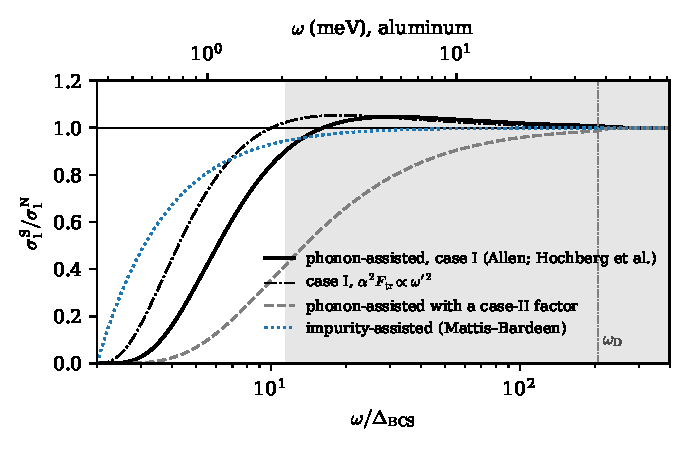
\includegraphics[width=0.85\linewidth]{figures/ch15/limit15_4a.pdf}
\captionof{figure}{Phonon-assisted conductivity of a superconductor over that of the normal metal, $\sigma_1^{\mathrm{S}}/\sigma_1^{\mathrm{N}}$, against $\omega/\Delta_{\mathrm{BCS}}$ (top axis: $\omega$ for aluminum, $\Delta_{\mathrm{BCS}} = \SI{0.18}{meV}$), at $T = 0$. Black: \cref{eq:15.4-holstein} with the case-I factor and the Debye law $\alpha^2F_{\mathrm{tr}} \propto \omega'^4$, which is the ratio of Hochberg, Lin and Zurek and, below $\omega_{\mathrm{D}}$ (dash-dotted vertical line, \SI{37}{meV}), independent of $\lambda_{\mathrm{tr}}$ and $\omega_{\mathrm{D}}$; dash-dotted: the same with the softer law $\alpha^2F_{\mathrm{tr}} \propto \omega'^2$, a test of the shape. Thin line at one: the normal-metal formula of Allen. Dashed: the phonon-assisted integral with the case-II factor in place of the case-I factor, for comparison. Dotted: impurity-assisted absorption in the dirty limit, $\mathfrak{g}_{\mathrm{II}}(\omega/\Delta_{\mathrm{BCS}})$, \cref{eq:15.4-MB}. Gray: the case-I result within \SI{10}{\percent} of the normal-metal formula, $\omega \ge 11.4\,\Delta_{\mathrm{BCS}}$ (\SI{2.05}{meV}).}\label{fig:15-limit-holstein}
\par}
\smallskip
Below $11.4\,\Delta_{\mathrm{BCS}}$ the normal-metal formula overstates the rate, by a factor of 2.4 at \SI{1}{meV} and without bound toward the edge, where the superconducting rate falls as $(\omega - 2\Delta_{\mathrm{BCS}})^5$; there the result also depends on the shape of $\alpha^2F_{\mathrm{tr}}$ below a few meV (0.42 or 0.73 of the normal value at \SI{1}{meV} for the two laws).
\end{limitbox}

The gap removes the absorption near the edge for a reason of phase space, not of coherence. The case-I factor is largest at the edge, where $\mathfrak{g}_{\mathrm{I}} = \pi/2$, but a phonon of energy $\omega'$ is available only up to $\omega - 2\Delta_{\mathrm{BCS}}$. Since $\alpha^2F_{\mathrm{tr}}$ grows as $\omega'^4$, the gap removes the most energetic phonons, which carry most of the weight. Above $16\,\Delta_{\mathrm{BCS}}$ the pile-up of the case-I factor dominates and the superconductor absorbs slightly more than the normal metal, by at most \SI{4.7}{\percent}, at $31\,\Delta_{\mathrm{BCS}}$. Had the pair carried the case-II factor of impurity-assisted absorption, the rate would reach \SI{90}{\percent} of the normal value only at $54\,\Delta_{\mathrm{BCS}}$. \Cref{fig:15-absorption}a shows the two processes on an absolute scale. The phonon-assisted conductivity of the normal metal grows as $\omega^3$ up to $\omega_{\mathrm{D}}$ and falls as $\omega^{-2}$ above. The impurity-assisted conductivity of the \SI{50}{nm} film, however, is flat up to $\gamma_{\mathrm{rel}}$ and stays above the phonon-assisted conductivity at every energy of the figure, by a factor of 1.6 at \SI{0.1}{eV} and 1.3 at \SI{0.3}{eV}.

\begin{figure}[tbp]
  \centering
  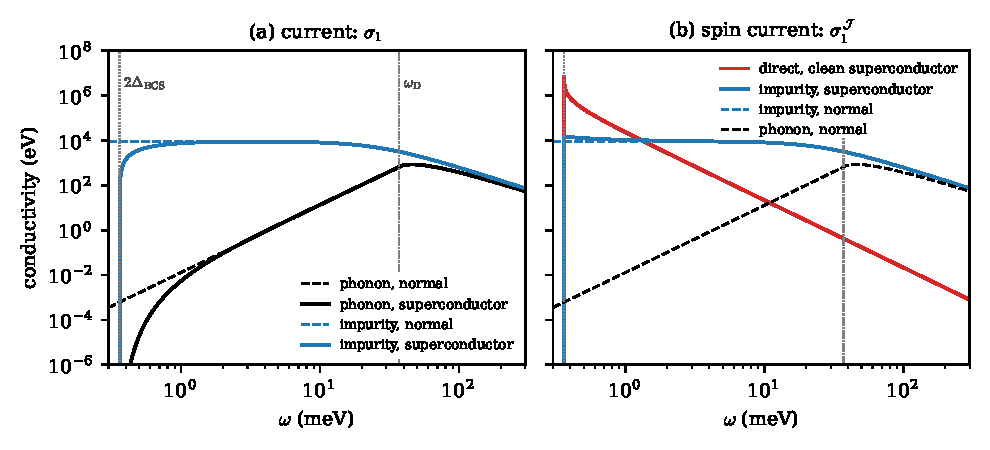
\includegraphics[width=\linewidth]{figures/ch15/fig15_3.pdf}
  \caption{Absorption of a uniform field by aluminum at $T = 0$, against the boson energy $\omega$, with $\Delta_{\mathrm{BCS}} = \SI{0.18}{meV}$ (dotted vertical line at $2\Delta_{\mathrm{BCS}}$) and the computed intraband plasma frequency \SI{12.29}{eV}. (a) Optical conductivity $\sigma_1$, which sets the rates of the dark photon. Black: phonon-assisted, \cref{eq:15.4-holstein}, in the normal metal (dashed) and the superconductor (solid), with the Debye transport function, $\lambda_{\mathrm{tr}} = 0.39$ and $\omega_{\mathrm{D}} = \SI{37}{meV}$ (dash-dotted vertical line). Blue: impurity-assisted, the Drude conductivity of the normal metal (dashed) and the Mattis--Bardeen conductivity of the superconductor (solid), \cref{eq:15.4-MB}, for the \SI{50}{nm} film of \cref{we:15-film} (mean free path \SI{50}{nm}, $\gamma_{\mathrm{rel}} = \SI{26.7}{meV}$, free-electron plasma frequency \SI{15.78}{eV} in its Drude conductivity). (b) Spin-current conductivity $\sigma_1^{\mathcal{J}}$, which sets the rate of the axion-like particle, normalized to equal $\sigma_1$ in the normal metal. Red: direct pair breaking in the clean superconductor, \cref{eq:15.4-sJ} with the quasiparticle factor $1/(1 + \lambda_{\mathrm{ep}}) = 0.70$. Blue: impurity-assisted, with the case-I factor in the superconductor (solid) and the Drude form in the normal metal (dashed), same mean free path. Black dashed: the phonon-assisted conductivity of the normal metal, for reference. Interband absorption, above about \SI{0.5}{eV}, is not included.}
  \label{fig:15-absorption}
\end{figure}

\begin{workedexample}{The Holstein onset in aluminum}\label{we:15-holstein}
A dark photon of $m_\phi = \SI{1}{meV}$, $5.56\,\Delta_{\mathrm{BCS}}$, is absorbed by pure aluminum with one phonon. The Debye form gives the normal-metal scattering rate $\gamma_{\mathrm{H}} = (2\pi/15)\lambda_{\mathrm{tr}}\omega^5/\omega_{\mathrm{D}}^4 = \SI{8.72e-11}{eV}$, and with $\omega_p^{\mathrm{intra}} = \SI{12.29}{eV}$ the normal-metal conductivity is $\sigma_1^{\mathrm{N}} = (\omega_p^{\mathrm{intra}})^2\gamma_{\mathrm{H}}/\omega^2 = \SI{0.0132}{eV}$. The superconductor has $\sigma_1^{\mathrm{S}}/\sigma_1^{\mathrm{N}} = 0.421$, so $\sigma_1^{\mathrm{S}} = \SI{5.54e-3}{eV}$.

Close to the edge the integral of \cref{eq:15.4-holstein} simplifies. For $\omega - 2\Delta_{\mathrm{BCS}} \ll \Delta_{\mathrm{BCS}}$ the pair energy $\omega - \omega'$ stays near $2\Delta_{\mathrm{BCS}}$ and $\mathfrak{g}_{\mathrm{I}}$ near $\pi/2$, and
\begin{equation*}
  \sigma_1^{\mathrm{S}} \simeq \frac{(\omega_p^{\mathrm{intra}})^2}{\omega^2}\,\frac{2\pi}{\omega}\,\frac{2\lambda_{\mathrm{tr}}}{\omega_{\mathrm{D}}^4}\,\frac{\pi}{2}\,2\Delta_{\mathrm{BCS}}\,\frac{(\omega - 2\Delta_{\mathrm{BCS}})^5}{5} .
\end{equation*}
At $\omega = 2.05$ and $2.5\,\Delta_{\mathrm{BCS}}$ this approximation is within 0.2 and \SI{2.1}{\percent} of the full integral. At $2.2\,\Delta_{\mathrm{BCS}}$ the superconductor absorbs with $\sigma_1^{\mathrm{S}} = \SI{4.4e-8}{eV}$, against $\SI{8.2e-4}{eV}$ for the normal metal: in practice the onset lies above $2\Delta_{\mathrm{BCS}}$.

The rate needs the loss function, $L = \varepsilon_2/|\varepsilon|^2$ in \cref{eq:10.7-dp}. At \SI{1}{meV} the condensate dominates $\varepsilon$: in the clean superconductor at $T = 0$ the imaginary conductivity is $\sigma_2 = (\omega_p^{\mathrm{intra}})^2/\omega$, and $\varepsilon_1 = 1 - \sigma_2/\omega = -1.51\times10^8$. The in-medium factor $1/|\varepsilon|^2$ is $4.4\times10^{-17}$, and $L = \sigma_1^{\mathrm{S}}\omega^3/(\omega_p^{\mathrm{intra}})^4 = 2.43\times10^{-16}$. With $\rho_\chi = \SI{0.3}{GeV.cm^{-3}}$ and $\rho_T = \SI{2.70}{g.cm^{-3}}$, \cref{eq:10.7-dp} gives $1.29\times10^{18}\,\zeta^2$ events per kilogram-year, and three events need $\zeta = 1.5\times10^{-9}$. The normal-metal formula would claim $9.9\times10^{-10}$. In the \SI{50}{nm} film of \cref{we:15-film} the impurity-assisted conductivity at the same mass is $1.4\times10^6$ times larger, and the rate with it.
\end{workedexample}

\subsection{Spin-current absorption}\label{sec:15.4-spin}

The axion-like particle couples through $(\partial_t\phi)\mathcal{J}^{\alpha\alpha}_e$. Here $\mathcal{J}_e = \sum_\alpha\mathcal{J}^{\alpha\alpha}_e$ is the spin current of the electrons traced over its two indices, a scalar like $\boldsymbol{\sigma}\cdot\vect{v}$ (\cref{sec:10.7-alp}). \Cref{sec:10.7-alp} reduced the rate of the axion-like particle to the optical conductivity through the spin trace $S_{\mathcal{J}\mathcal{J}} = \frac34S_{jj}$, valid for independent electrons without spin--orbit coupling. In a superconductor we keep the response of the spin current itself and define its conductivity by
\begin{equation}
  \sigma_1^{\mathcal{J}}(\omega) = \frac{2e^2}{3\omega}\,S_{\mathcal{J}\mathcal{J}}(0,\omega) ,
  \label{eq:15.4-sJdef}
\end{equation}
so that \cref{eq:10.7-alp} holds with $\sigma_1^{\mathcal{J}}$ in place of $\sigma_1$, and $\sigma_1^{\mathcal{J}} = \sigma_1$ in the normal metal. The component of the spin current with the spin and the velocity both along $\hat{\vect{z}}$ is $\mathcal{J}^{zz}_e = \frac12\sum_{\vect{k}}v^z_{\vect{k}}(c^\dagger_{\vect{k}\uparrow}c_{\vect{k}\uparrow} - c^\dagger_{\vect{k}\downarrow}c_{\vect{k}\downarrow})$. The relabeling that turned the current into the unit matrix now meets a second sign, that of the spin, and the two cancel: $\mathcal{J}^{zz}_e = \frac12\sum_{\vect{k}}v^z_{\vect{k}}\Psi^\dagger_{\vect{k}}\boldsymbol{\eta}\Psi_{\vect{k}}$, with the matrix of the density. That matrix does not commute with $h_{\vect{k}}$. In the quasiparticle basis (\cref{eq:D.40-bogo}) the spin current contains the term $\frac12v^z_{\vect{k}}(\Delta_{\mathrm{BCS}}/E_{\vect{k}})\gamma^\dagger_{\vect{k}1}\gamma^\dagger_{\vect{k}2}$, which creates a pair of total momentum zero and energy $2E_{\vect{k}}$. A uniform charge current moves both electrons of a pair $(\vect{k}\!\uparrow, -\vect{k}\!\downarrow)$ in the same direction and only boosts the condensate. A spin current drives the spin-up and spin-down electrons in opposite directions, pulls the two members of each pair apart, and breaks pairs.

In a clean superconductor this pair breaking needs no third body. Without spin--orbit coupling the three components $\mathcal{J}^{\alpha\alpha}_e$ contribute equally and do not interfere, and the golden rule with the amplitude above gives (\cref{app:D.40})
\begin{keyresult}[Spin-current absorption in a clean superconductor]
\begin{equation}
  \sigma_1^{\mathcal{J}}(\omega) = \frac{2\pi(\omega_p^{\mathrm{intra}})^2\,\Delta_{\mathrm{BCS}}^2}{\omega^2\,(\omega^2 - 4\Delta_{\mathrm{BCS}}^2)^{1/2}}\,\Theta(\omega - 2\Delta_{\mathrm{BCS}}) ,
  \label{eq:15.4-sJ}
\end{equation}
at $T = 0$, without spin--orbit coupling, for a mean free path long compared with the size of a pair; its integral over $\omega$ is $(\pi/2)(\omega_p^{\mathrm{intra}})^2$.
\end{keyresult}
\noindent In the clean normal metal the spin current commutes with the one-body band Hamiltonian, but not with the interactions. A two-body force enters with the weight of the spin difference, $[p^z_1\sigma^z_1 + p^z_2\sigma^z_2, V(\vect{r}_1 - \vect{r}_2)] = -\ii\,(\partial_zV)(\sigma^z_1 - \sigma^z_2)$, which vanishes for parallel spins only. Galilean invariance protects the charge current, whose internal forces cancel in pairs, but not the spin current. Electron--electron collisions (spin Coulomb drag) and normal phonon processes relax it, and its normal-state weight forms a narrow Drude peak rather than a delta function at $\omega = 0$. With a collision rate $\beta\omega^2$ and $\beta = 0.03$ to \SI{0.3}{eV^{-1}}, an estimate of the Fermi-liquid scale, the normal metal at $T \to 0$ absorbs at \SI{0.72}{meV} with $\sigma_1^{\mathcal{J}} \approx 5$ to \SI{45}{eV}, against the phonon-assisted $\sigma_1^{\mathrm{N}} = \SI{4.9e-3}{eV}$; the superconducting direct term is $1.5\times10^3$ to $1.5\times10^4$ times larger still. Pairing keeps the charge-current weight at zero frequency, as the supercurrent, and moves the spin-current weight above $2\Delta_{\mathrm{BCS}}$: \SI{87}{\percent} of it lies below $4\Delta_{\mathrm{BCS}}$ and \SI{99.5}{\percent} below $20\Delta_{\mathrm{BCS}}$. The total weight is fixed beyond mean field: for any Hamiltonian that does not depend on spin, the spin current is the time derivative of the spin dipole, and its integrated absorption obeys an exact sum rule (\cref{app:D.40}). The total weight, interband absorption included, equals the total weight of the charge current, $(\pi/2)\omega_p^2$ with the free-electron $\omega_p$; for the conduction band alone, a one-band Hamiltonian with spin-independent interactions, it is $(\pi/2)(\omega_p^{\mathrm{intra}})^2$ exactly. The part near $2\Delta_{\mathrm{BCS}}$ is the coherent quasiparticle weight $(\pi/2)(\omega_p^{\mathrm{intra}})^2(1 + F_1^a/3)/(1 + \lambda_{\mathrm{ep}})$, with the Landau parameter $F_1^a$ of the quasiparticle spin current and the residue $1/(1 + \lambda_{\mathrm{ep}})$ of \cref{eq:6.4-mass}; the rest of the spin-current weight lies near $\omega_{\mathrm{D}}$, like the Holstein band of the charge current, and at the scale of the Fermi energy. The sum rule therefore requires \cref{eq:15.4-sJ} near the edge to carry the factor $(1 + F_1^a/3)/(1 + \lambda_{\mathrm{ep}})$, which is 0.70 for $F_1^a = 0$ and the measured $\lambda_{\mathrm{ep}} = 0.43$ of \cref{sec:6.4}. The bare BCS bubble is conserving in the spin channel, and a singlet superconductor has zero spin stiffness, as its Pauli susceptibility vanishes, so the weight cannot lie at $\omega = 0$ (\cref{app:D.40}). In a dirty film the matrix elements of $\mathcal{J}_e$ between impurity states replace the direct term. Since the spin current is even under time reversal, the steps of \cref{eq:15.4-MB} give $\sigma_n\mathfrak{g}_{\mathrm{I}}(\omega/\Delta_{\mathrm{BCS}})$, with the factor of the density, which jumps to $\pi/2$ at the edge. That form conserves the normal-state weight exactly for a flat $\sigma_n$, since $\int_2^\infty\dd y\,[\mathfrak{g}_{\mathrm{I}}(y) - 1] = 2$: the weight above $2\Delta_{\mathrm{BCS}}$ replaces the weight below. For the Drude $\sigma_n$ of the \SI{50}{nm} film the balance holds to \SI{0.05}{\percent}, the residue coming from the Drude shape.

At \SI{1}{meV} \cref{eq:15.4-sJ} with the factor 0.70 gives $\sigma_1^{\mathcal{J}} = \SI{2.31e4}{eV}$, $4\times10^6$ times the phonon-assisted $\sigma_1^{\mathrm{S}}$ of \cref{we:15-holstein}, and $\sigma_1^{\mathcal{J}}$ exceeds the phonon-assisted conductivity of the normal metal up to \SI{10.9}{meV} (\cref{fig:15-absorption}b). For an axion-like particle of \SI{0.72}{meV}, $4\Delta_{\mathrm{BCS}}$, with $g_{aee} = 10^{-13}$, \cref{eq:10.7-alp} with $\sigma_1^{\mathcal{J}}$ predicts 0.080 events per kilogram-year in clean aluminum, and three events per kilogram-year need $g_{aee} = 6.1\times10^{-13}$. The independent-electron spin trace of \cref{sec:10.7-alp} would put the phonon-assisted $\sigma_1^{\mathrm{S}}$ in \cref{eq:10.7-alp}. That trace fails for paired electrons, because the anomalous, pair-amplitude parts of the charge-current and spin-current responses enter with opposite signs.

Three conditions limit these numbers. First, the clean form needs a mean free path long compared with the size of a pair, $\xi_{\mathrm{coh}} \approx \SI{1.6}{\micro m}$ to \SI{2.4}{\micro m} (\cref{sec:15.3-dirty}), which only bulk high-purity crystals reach. Second, in the \SI{50}{nm} film the spin channel $\sigma_n\mathfrak{g}_{\mathrm{I}}$ needs $g_{aee} = 1.5\times10^{-12}$ at \SI{0.72}{meV}, against $6.1\times10^{-13}$ in the clean crystal. Third, the sum rule fixes the total weight and, with the factor $(1 + F_1^a/3)/(1 + \lambda_{\mathrm{ep}})$, the coherent weight near the edge, but not the line shape at a given mass. The strong-coupling factor $1/(1 + \lambda_{\mathrm{ep}})$ is included in the numbers above and raises the required $g_{aee}$ by 1.20. The quasiparticle interaction dresses the spin current in the form of Leggett (\cref{app:D.40}). For $|F_1^a/3| \le 0.1$ this dressing changes $\sigma_1^{\mathcal{J}}$ at $4\Delta_{\mathrm{BCS}}$ by a factor 0.75 to 1.31 and $g_{aee}$ by $-12$ to $+\SI{15}{\percent}$, so that three events need $g_{aee} = 5.4\times10^{-13}$ to $7.1\times10^{-13}$. For $F_1^a < 0$ a bound spin-one mode with $\ell = 1$ forms just below $2\Delta_{\mathrm{BCS}}$ and takes weight from the continuum. A triplet $p$-wave interaction acts in the same channel and would dress the vertex further. Spin--orbit coupling, weak in aluminum, mixes the current and the spin current and leaves a fraction of the weight of order the spin-flip rate over $\Delta_{\mathrm{BCS}}$ at low frequency; in heavy-element superconductors it is the main limitation. The phonon-assisted part of the spin-current response also has a coherence factor near the edge that differs from the factor of \cref{eq:15.4-T}, because the spin current creates pairs at intermediate stages. The size of this phonon-assisted part near the edge is open, but the part competes with the direct term only above about \SI{10}{meV}, where it tends to its normal-metal value.

\subsection{Strong coupling and the transport function}\label{sec:15.4-strong}

\Cref{eq:15.4-holstein} assumes weak coupling: a BCS gap that does not depend on energy, and quasiparticles without the mass enhancement $1 + \lambda_{\mathrm{ep}}$ of \cref{eq:6.4-mass}. In the Eliashberg theory of \cref{app:E.9} the electron--phonon interaction is retarded, so the gap $\Delta^{\mathrm{El}}(E)$ depends on the energy $E$ of the quasiparticle, and the pair spectrum of the BCS spinors is replaced by spectral functions. Two of them enter the absorption: the density of states $N^{\mathrm{El}}(E) = \Real[E/(E^2 - \Delta^{\mathrm{El}}(E)^2)^{1/2}]$ and the pair amplitude $P^{\mathrm{El}}(E) = \Real[\Delta^{\mathrm{El}}(E)/(E^2 - \Delta^{\mathrm{El}}(E)^2)^{1/2}]$, both per unit of the normal density of states. The case-I combination of two quasiparticles of energies $E$ and $E' = \omega - \omega' - E$ becomes $N^{\mathrm{El}}(E)N^{\mathrm{El}}(E') + P^{\mathrm{El}}(E)P^{\mathrm{El}}(E')$ in the integrand of $\mathfrak{g}_{\mathrm{I}}$. For a constant gap this combination is $(EE' + \Delta_{\mathrm{BCS}}^2)/[(E^2 - \Delta_{\mathrm{BCS}}^2)(E'^2 - \Delta_{\mathrm{BCS}}^2)]^{1/2}$, the integrand of \cref{eq:7.2-pairspec}. The renormalization of the quasiparticles is a separate matter. For the normal metal at $\omega \ll \omega_{\mathrm{D}}$ it is known: with the self-energy resummed and the bare current vertex, whose corrections are of order $\omega_{\mathrm{D}}/E_{\mathrm{F}}$ by Migdal's argument (\cref{sec:6.4}), the conductivity becomes $\sigma_1 \simeq (\omega_p^{\mathrm{intra}})^2\gamma_{\mathrm{H}}/[\omega^2(1 + \lambda_{\mathrm{tr}})^2]$~\cite[Eq.~(3)]{allen2015electron}, with the transport-weighted mass enhancement. In aluminum, with $\lambda_{\mathrm{tr}} = 0.39$, this factor is 0.52. It is open whether the same factor multiplies the superconducting form near the edge, where the pair spectrum and the renormalization both depend on energy.

The transport function is computed from first principles with the electron--phonon vertices of density-functional perturbation theory on Wannier-interpolated grids (\cref{app:E.5}), with the weight $1 - \cos\theta$ in place of one. The model of \cref{fig:6-a2F}, free electrons scattered by screened empty-core ions, shows what such a calculation must get right. Its transport coupling is $\lambda_{\mathrm{tr}} = 0.32$, against $\lambda_{\mathrm{ep}} = 0.44$ for the same model, because the weight $1 - \cos\theta$ removes the small-angle scattering, and against 0.37 computed and 0.39 from the resistivity~\cite[Table~IV]{savrasov1996electron}. Near the edge, however, the model fails completely: below \SI{1}{meV} it holds $1.25\times10^4$ times the weight of the $\omega'^4$ law, all of it from umklapp scattering at momentum transfers near $|\vect{G}_{111}|$ by phonons of small $\vect{Q}$. A plane wave is not an eigenstate of the crystal near a Bragg plane, and the plane-wave vertex violates the acoustic sum rule of \cref{eq:6.2-asr}, which makes the vertex vanish for $\vect{Q} \to 0$ between states on the Fermi surface. The phonon-assisted rate within a few meV of the edge therefore needs a vertex that obeys the sum rule, and that rate, through the shape of $\alpha^2F_{\mathrm{tr}}$ below a few meV, is the least certain input of \cref{lim:15.4a}. Interband absorption above about \SI{0.5}{eV} is taken from measured optical data, as in \cref{sec:10.7}.

\paragraph{Scalar absorption.} The scalar couples to the kinetic-energy row of \cref{sec:10.7-scalar}, whose Nambu vertex, like the density, is $\boldsymbol{\eta}$, with a weight even in $\vect{k}$. The part of this vertex linear in $\xi_{\vect{k}}$ couples to the amplitude channel of the pair field (\cref{sec:7.2}). The scalar response of a superconductor near its edge therefore needs the conserving treatment of \cref{sec:15.1} extended to that channel, and the size of that response near the edge is open.

\subsection{Uncertainty budget of the superconducting rates}\label{sec:15.4-budget}

\Cref{tab:15-nuisances} collects the truncations and inputs of the chapter with their sizes. For scattering in a bulk crystal the gap and the edge remainder dominate, and both are small above $y = 3$; for a film the mean free path and the thickness enter at least as strongly as the choice of response. For absorption the purity of the sample decides between impurity-assisted and phonon-assisted absorption by six orders of magnitude at \SI{1}{meV}, and for the axion-like particle in a clean crystal the direct pair breaking by the spin current exceeds the phonon-assisted absorption up to \SI{10.9}{meV}.
\begin{table}[tbp]
  \caption{Uncertainty budget of the superconducting rates. Classes and bases as in \cref{tab:10-nuisances}. Sizes are for aluminum unless stated; $y = \omega/\Delta_{\mathrm{BCS}}$, and ``edge'' is the kinematic edge $q = \omega/v_{\mathrm{max}}$.}
  \label{tab:15-nuisances}
  \centering\scriptsize\setlength{\tabcolsep}{3pt}
  \begin{tabular}{@{}>{\raggedright\arraybackslash}p{0.26\linewidth}>{\raggedright\arraybackslash}p{0.12\linewidth}>{\raggedright\arraybackslash}p{0.35\linewidth}>{\raggedright\arraybackslash}p{0.09\linewidth}>{\raggedright\arraybackslash}p{0.10\linewidth}@{}}
    \toprule
    Truncation or input & Type & Size & Basis & Section \\
    \midrule
    Gap of the sensor & threshold; tilt in $y$ & bulk \SI{0.18}{meV} against the film convention \SI{0.30}{meV}: rate $\times1.23$ at \SI{1}{keV} (light mediator), $\times1.13$ (heavy mediator) & input spread & \cref{sec:15.1,sec:15.2} \\
    Edge remainder (central value $\mathfrak{g}_{\mathrm{I}}L^{\mathrm{nor}}$) & normali\-zation, two-sided & $-\SI{2}{\percent}$ to $+\SI{9}{\percent}$ for $y \ge 3$ (clean at all momenta, impurities on the edge); energies $y < 3$ excluded, where the conserving value moves by more than \SI{10}{\percent} with the mean free path & computed & \cref{sec:15.2} \\
    Relaxation rate of the film & tilt near the edge & factor 4.6 at $y = 2.2$ between the clean limit and $\mathfrak{l}_e = \SI{30}{nm}$; below \SI{6}{\percent} for $y \ge 3$ & computed & \cref{sec:15.2,sec:15.3} \\
    Collisions in the normal loss function & normali\-zation & Drude tail $6/\pi q\mathfrak{l}_e$ times the clean value for $q\mathfrak{l}_e \ll 1$: $\times24$ for the \SI{50}{nm} film at \SI{0.90}{meV}; neither limit within \SI{10}{\percent} for $0.64 < q\mathfrak{l}_e < 9.8$ & computed & \cref{sec:15.3} \\
    Film thinner than $1/q$ (sheet screening) & normali\-zation; tilt in direction & enhancement $[(\varepsilon_a + \varepsilon_b)/q_\parallel d_{\mathrm{film}}]^2$ of the structure factor to leading order in $q_\parallel d_{\mathrm{film}}$, $\times540$ for $\vect{q}$ in the plane of the \SI{50}{nm} film in vacuum at $qd_{\mathrm{film}} = 0.086$ ($\times588$ for the exact slab); depends on the film model and the media on both sides & model & \cref{sec:15.3} \\
    Strong disorder (amorphous WSi) & normali\-zation & $k_{\mathrm{F}}\mathfrak{l}_e = 1.8$--5.5; outside relaxation-time forms and mean-field BCS; no correction factor & unsized & \cref{sec:15.3} \\
    Thermal quasiparticles & new support & $\ee^{-\Delta_{\mathrm{BCS}}/T} = \ee^{-209}$ at \SI{10}{mK} & computed & \cref{sec:15.2} \\
    Energy dependence of the gap (strong coupling) in scattering & normali\-zation & size unknown; aluminum is near weak coupling, $2\Delta_{\mathrm{BCS}}/T_c = 3.54$ against 3.53 & unsized & \cref{sec:15.2} \\
    Shape of $\alpha^2F_{\mathrm{tr}}$ below a few meV (phonon-assisted absorption) & normali\-zation; tilt in $m_\phi$ & $\sigma_1^{\mathrm{S}}/\sigma_1^{\mathrm{N}} = 0.42$ ($\omega'^4$) or 0.73 ($\omega'^2$) at \SI{1}{meV}; normal-metal formula within \SI{10}{\percent} from $11.4$ or $7.4\,\Delta_{\mathrm{BCS}}$ & model & \cref{sec:15.4} \\
    Strong-coupling renormalization of phonon-assisted absorption & normali\-zation & $\times0.52$, the factor $1/(1 + \lambda_{\mathrm{tr}})^2$ of the normal metal at $\omega \ll \omega_{\mathrm{D}}$; whether it applies to the superconducting form is open & est. & \cref{sec:15.4} \\
    Impurity-assisted absorption & normali\-zation & $1.4\times10^6$ times the phonon-assisted $\sigma_1$ at \SI{1}{meV} for the \SI{50}{nm} film; follows the residual resistivity & computed & \cref{sec:15.4} \\
    Electron--electron absorption (intrinsic $\sigma_1$) & normali\-zation & a third intrinsic channel of $\sigma_1$ besides the phonon-assisted one; size unknown & unsized & \cref{sec:15.4} \\
    Spin-current absorption beyond the clean BCS model & normali\-zation; tilt in $m_\phi$ & total weight fixed by the sum rule; coherent weight times $1/(1 + \lambda_{\mathrm{ep}}) = 0.70$ included; Landau parameter $|F_1^a/3| \le 0.1$: $g_{aee}$ $-12$ to $+\SI{15}{\percent}$; triplet interaction, spin--orbit coupling and the phonon-assisted part near the pair-breaking edge unsized; clean form only for $\mathfrak{l}_e \gg \xi_{\mathrm{coh}}$ & unsized & \cref{sec:15.4} \\
    Scalar absorption near the pair-breaking edge (amplitude channel) & normali\-zation & kinetic row couples to the amplitude channel of the pair field; size unknown & unsized & \cref{sec:15.4} \\
    Interband absorption & new support & above about \SI{0.5}{eV}; taken from measured optical data & input spread & \cref{sec:15.4} \\
    \bottomrule
  \end{tabular}
\end{table}

\section*{Summary}

A dark-matter particle that couples to the electron density breaks pairs in a superconductor through the loss function, and the loss function that conserves charge adds the pair-field ladder of \cref{sec:7.2} to the quasiparticle bubble and screens it with the Coulomb interaction (\cref{sec:15.1}). The absorptive part of the quasiparticle bubble is the Lindhard value times the case-I coherence integral $\mathfrak{g}_{\mathrm{I}}(\omega/\Delta_{\mathrm{BCS}})$, exactly, with $\mathfrak{g}_{\mathrm{I}} = 1.500$ at $y = 2.2$ falling to 1.051 at $y = 10$. The ladder raises that absorption by up to \SI{44}{\percent} near the edge. On the kinematic edge $q = \omega/v_{\mathrm{max}}$ of aluminum the Lindhard function is within \SI{10}{\percent} of the conserving loss function for $y \ge 7.9$, and the product $\mathfrak{g}_{\mathrm{I}}L^{\mathrm{nor}}$ within \SI{9}{\percent} for $y \ge 3$ at every momentum transfer. The bulk gap of aluminum is the measured \SI{0.18}{meV}; the \SI{0.3}{meV} of projections is a film convention. For a \SI{1}{keV} particle with a light mediator the bulk gap raises the rate by 1.23, more than any choice among the loss functions changes it.

On the kinematic edge each truncation is worst (\cref{sec:15.2}). There $\omega/qv_{\mathrm{F}} = 0.392$, and the normal dielectric function has an imaginary part 0.736 times its real part. In a clean crystal the conserving loss function, the physical one, is 0.87 times $\mathfrak{g}_{\mathrm{I}}L^{\mathrm{nor}}$ at $y = 2.2$ and 1.07 at $y = 3$ and 5. Impurity scattering changes the conserving value only near the threshold: at $y \ge 3$ the ratio stays between 1.008 and 1.091 for mean free paths from \SI{100}{\micro m} to \SI{30}{nm}, whereas at $y = 2.2$ it falls from 0.87 to 0.19. The superconducting part of a rate therefore carries three uncertainties: the gap, the relaxation rate of the film, and the edge remainder, which is two-sided, $-\SI{2}{\percent}$ to $+\SI{9}{\percent}$ about $\mathfrak{g}_{\mathrm{I}}L^{\mathrm{nor}}$ for $y \ge 3$. The energies $y < 3$, where the conserving value moves by more than \SI{10}{\percent} with the mean free path, are excluded from the signal region. The frequency dependence of the gap in strong coupling is not sized.

Real sensors are films (\cref{sec:15.3}). Nonmagnetic disorder leaves the gap unchanged, by Anderson's theorem, but collisions change the response. At momentum transfers below the inverse mean free path the normal loss function becomes the Drude tail $\omega\gamma_{\mathrm{rel}}/\omega_p^2$, fixed by the residual resistivity, 24 times the clean value for a \SI{50}{nm} aluminum film at \SI{0.90}{meV}. At the edge of a dirty film the density couples through the current, with the case-II factor, and the condensate short-circuits a slow potential, so the loss function of the superconducting film starts from zero and is a quarter of the normal one at $y = 2.2$. A film thinner than $1/q$ screens like a sheet, which enhances the structure factor by $[(\varepsilon_a + \varepsilon_b)/q_\parallel d_{\mathrm{film}}]^2$ to leading order in $q_\parallel d_{\mathrm{film}}$, 540 for the \SI{50}{nm} film in vacuum at \SI{0.90}{meV} (588 for the exact slab), and makes the rate directional. Amorphous WSi, with $k_{\mathrm{F}}\mathfrak{l}_e$ of a few, lies outside every relaxation-time form and outside mean-field BCS.

A boson absorbed at $\vect{q} \to 0$ needs a third body in a metal, and the Nambu structure of the current decides the coherence factor (\cref{sec:15.4}). The uniform current is the unit matrix in Nambu space and commutes with the mean-field Hamiltonian, so a clean superconductor does not absorb it. With impurities it carries the case-II factor of Mattis and Bardeen. With a phonon the second-order amplitude collapses exactly to the velocity difference times the phonon vertex, the pair carries the case-I factor, and the result is Allen's form, which the dark-matter literature evaluates with a Debye transport function. Near the edge phase space, not coherence, removes the phonon-assisted absorption: it reaches \SI{90}{\percent} of the normal-metal value at $11.4\,\Delta_{\mathrm{BCS}} = \SI{2.05}{meV}$ and is 0.42 of it at \SI{1}{meV}, where a dark photon needs $\zeta = 1.5\times10^{-9}$ for three events per kilogram-year in pure aluminum. In a \SI{50}{nm} film impurity-assisted absorption is $1.4\times10^6$ times larger at that mass. The spin current, which absorbs the axion-like particle, has the Nambu matrix $\boldsymbol{\eta}$ of the density and, in a clean singlet superconductor without spin--orbit coupling, breaks pairs by itself. In the superconductor the spin-current weight moves above $2\Delta_{\mathrm{BCS}}$, \SI{87}{\percent} of it below $4\Delta_{\mathrm{BCS}}$. The sum rule fixes the total weight; the coherent part near the edge carries the factor $(1 + F_1^a/3)/(1 + \lambda_{\mathrm{ep}})$, 0.70 for $F_1^a = 0$, and the line shape depends on $F_1^a$ through the form of Leggett and on a triplet interaction. At \SI{0.72}{meV} three events per kilogram-year in a bulk crystal with a mean free path longer than the size of a pair need $g_{aee} = 6.1\times10^{-13}$, and $5.4\times10^{-13}$ to $7.1\times10^{-13}$ for $|F_1^a/3| \le 0.1$; a \SI{50}{nm} film needs $1.5\times10^{-12}$. The strong-coupling factor $1/(1 + \lambda_{\mathrm{tr}})^2$ of the normal metal is known; whether it carries over to the superconducting phonon-assisted form is open.

\Cref{tab:15-nuisances} collects the truncations and inputs of the chapter with their sizes. For scattering in a bulk crystal the gap and the edge remainder dominate, and both are small above $y = 3$; for a film the mean free path and the thickness enter at least as strongly as the choice of response. For absorption the purity of the sample decides between impurity-assisted and phonon-assisted absorption by six orders of magnitude at \SI{1}{meV}, and for the axion-like particle in a clean crystal the direct pair breaking by the spin current exceeds the phonon-assisted absorption up to \SI{10.9}{meV}. How the quasiparticles that dark matter creates are counted is a question of the sensor readout, which this chapter does not treat.

\begin{table}[tbp]
  \caption{Uncertainty budget of the superconducting rates. Type in the classes of \cref{sec:8.8}: normalization, tilt (in $\omega$ or in the dark-matter mass), threshold and new support. Basis of the size: ``computed'' (next order or exact result computed), ``model'' (computed in a model), ``est.''\ (parametric estimate), ``input spread'' (spread or limitation of a measured or computed input), ``unsized'' (no size known). Sizes are for aluminum unless stated; $y = \omega/\Delta_{\mathrm{BCS}}$, and ``edge'' is the kinematic edge $q = \omega/v_{\mathrm{max}}$.}
  \label{tab:15-nuisances}
  \centering\scriptsize\setlength{\tabcolsep}{3pt}
  \begin{tabular}{@{}>{\raggedright\arraybackslash}p{0.26\linewidth}>{\raggedright\arraybackslash}p{0.12\linewidth}>{\raggedright\arraybackslash}p{0.35\linewidth}>{\raggedright\arraybackslash}p{0.09\linewidth}>{\raggedright\arraybackslash}p{0.10\linewidth}@{}}
    \toprule
    Truncation or input & Type & Size & Basis & Section \\
    \midrule
    Gap of the sensor & threshold; tilt in $y$ & bulk \SI{0.18}{meV} against the film convention \SI{0.30}{meV}: rate $\times1.23$ at \SI{1}{keV} (light mediator), $\times1.13$ (heavy mediator) & input spread & \cref{sec:15.1,sec:15.2} \\
    Edge remainder (central value $\mathfrak{g}_{\mathrm{I}}L^{\mathrm{nor}}$) & normali\-zation, two-sided & $-\SI{2}{\percent}$ to $+\SI{9}{\percent}$ for $y \ge 3$ (clean at all momenta, impurities on the edge); energies $y < 3$ excluded, where the conserving value moves by more than \SI{10}{\percent} with the mean free path & computed & \cref{sec:15.2} \\
    Relaxation rate of the film & tilt near the edge & factor 4.6 at $y = 2.2$ between the clean limit and $\mathfrak{l}_e = \SI{30}{nm}$; below \SI{6}{\percent} for $y \ge 3$ & computed & \cref{sec:15.2,sec:15.3} \\
    Collisions in the normal loss function & normali\-zation & Drude tail $6/\pi q\mathfrak{l}_e$ times the clean value for $q\mathfrak{l}_e \ll 1$: $\times24$ for the \SI{50}{nm} film at \SI{0.90}{meV}; neither limit within \SI{10}{\percent} for $0.64 < q\mathfrak{l}_e < 9.8$ & computed & \cref{sec:15.3} \\
    Film thinner than $1/q$ (sheet screening) & normali\-zation; tilt in direction & enhancement $[(\varepsilon_a + \varepsilon_b)/q_\parallel d_{\mathrm{film}}]^2$ of the structure factor to leading order in $q_\parallel d_{\mathrm{film}}$, $\times540$ for $\vect{q}$ in the plane of the \SI{50}{nm} film in vacuum at $qd_{\mathrm{film}} = 0.086$ ($\times588$ for the exact slab); depends on the film model and the media on both sides & model & \cref{sec:15.3} \\
    Strong disorder (amorphous WSi) & normali\-zation & $k_{\mathrm{F}}\mathfrak{l}_e = 1.8$--5.5; outside relaxation-time forms and mean-field BCS; no correction factor & unsized & \cref{sec:15.3} \\
    Thermal quasiparticles & new support & $\ee^{-\Delta_{\mathrm{BCS}}/T} = \ee^{-209}$ at \SI{10}{mK} & computed & \cref{sec:15.2} \\
    Energy dependence of the gap (strong coupling) in scattering & normali\-zation & size unknown; aluminum is near weak coupling, $2\Delta_{\mathrm{BCS}}/T_c = 3.54$ against 3.53 & unsized & \cref{sec:15.2} \\
    Shape of $\alpha^2F_{\mathrm{tr}}$ below a few meV (phonon-assisted absorption) & normali\-zation; tilt in $m_\phi$ & $\sigma_1^{\mathrm{S}}/\sigma_1^{\mathrm{N}} = 0.42$ ($\omega'^4$) or 0.73 ($\omega'^2$) at \SI{1}{meV}; normal-metal formula within \SI{10}{\percent} from $11.4$ or $7.4\,\Delta_{\mathrm{BCS}}$ & model & \cref{sec:15.4} \\
    Strong-coupling renormalization of phonon-assisted absorption & normali\-zation & $\times0.52$, the factor $1/(1 + \lambda_{\mathrm{tr}})^2$ of the normal metal at $\omega \ll \omega_{\mathrm{D}}$; whether it applies to the superconducting form is open & est. & \cref{sec:15.4} \\
    Impurity-assisted absorption & normali\-zation & $1.4\times10^6$ times the phonon-assisted $\sigma_1$ at \SI{1}{meV} for the \SI{50}{nm} film; follows the residual resistivity & computed & \cref{sec:15.4} \\
    Electron--electron absorption (intrinsic $\sigma_1$) & normali\-zation & a third intrinsic channel of $\sigma_1$ besides the phonon-assisted one; size unknown & unsized & \cref{sec:15.4} \\
    Spin-current absorption beyond the clean BCS model & normali\-zation; tilt in $m_\phi$ & total weight fixed by the sum rule; coherent weight times $1/(1 + \lambda_{\mathrm{ep}}) = 0.70$ included; Landau parameter $|F_1^a/3| \le 0.1$: $g_{aee}$ $-12$ to $+\SI{15}{\percent}$; triplet interaction, spin--orbit coupling and the phonon-assisted part near the edge unsized; clean form only for $\mathfrak{l}_e \gg \xi_{\mathrm{coh}}$ & unsized & \cref{sec:15.4} \\
    Scalar absorption near the edge (amplitude channel) & normali\-zation & kinetic row couples to the amplitude channel of the pair field; size unknown & unsized & \cref{sec:15.4} \\
    Interband absorption & new support & above about \SI{0.5}{eV}; taken from measured optical data & input spread & \cref{sec:15.4} \\
    \bottomrule
  \end{tabular}
\end{table}

\printbibliography[heading=subbibliography]

\chapter{Novel targets}\label{chap:16}
Dark matter must carry at least \SI{0.333}{MeV} to lift an electron across the gap of silicon (\cref{sec:1.3}), and the bulk crystals of \cref{chap:10,chap:11,chap:12,chap:13,chap:14,chap:15} extend the reach downward through phonons, magnons and the pair-breaking edge of a superconductor. Other solids have been proposed for channels that these crystals lack, often with projected reaches that a complete treatment moves by orders of magnitude. The slow linear bands of a Dirac material bring the threshold mass of an electronic excitation below \SI{10}{keV} (\cref{sec:7.3}). The published reaches, however, leave the remote bands out of the screening of the dark-matter field, and for ZrTe$_5$ they are too strong by a factor of several thousand. Other targets are limited by their inputs. The dark-photon rate on a glass is its measured loss tangent, which changes seventeenfold between preparations, and a color center counts only if a recoil leaves a defect that a readout finds, but no measurement has isolated the yield of readable defects per recoil. In most cases, then, the limit is a material input and not the framework of \cref{chap:8}: a background dielectric constant, a density of tunneling states, the yield of a defect. The tunneling defects of glasses also release heat at millikelvin temperatures, and their kinetics shape the delayed signals of \cref{sec:19.6} (\cref{fig:16-map}).

\begin{figure}[tbp]
  \centering
  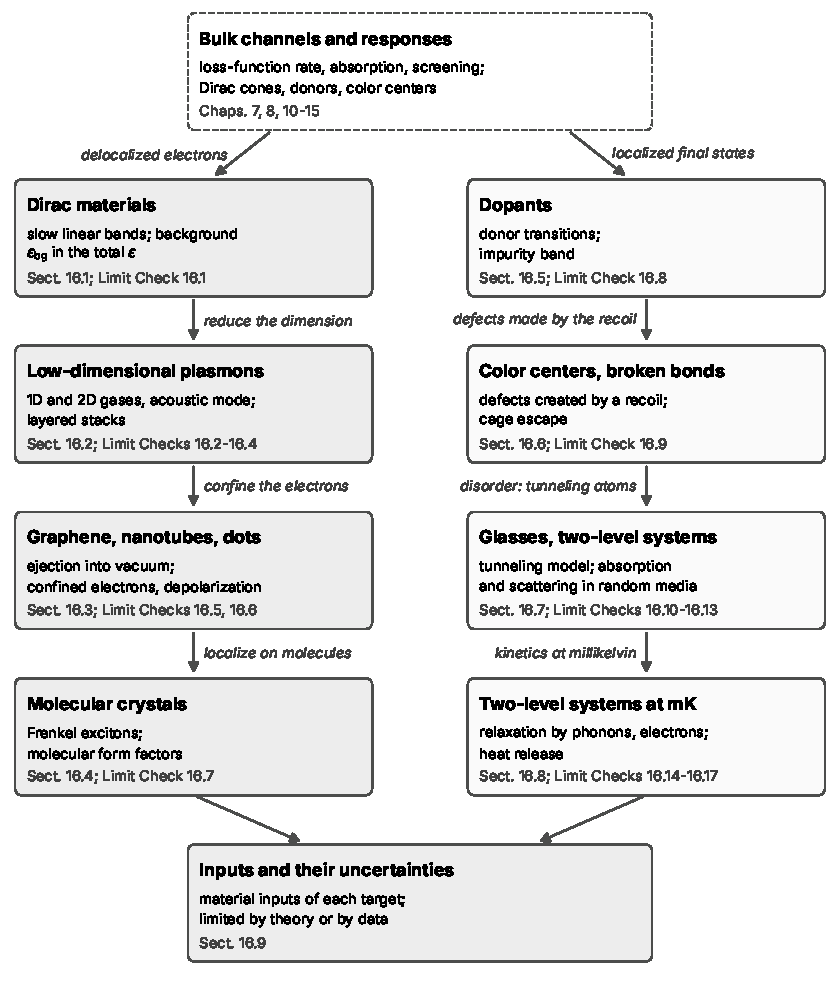
\includegraphics[width=0.85\linewidth]{figures/ch16/map16.pdf}
  \caption{Novel targets, from the bulk responses and rates of \cref{chap:7,chap:8} and \cref{chap:10,chap:11,chap:12,chap:13,chap:14,chap:15}. Left, delocalized electrons: Dirac materials with the background dielectric constant in the total $\varepsilon$ (\cref{sec:16.1}; \cref{lim:16.1a}); electron gases in one and two dimensions and layered stacks (\cref{sec:16.2}; \cref{lim:16.2a,lim:16.2b,lim:16.2c}); graphene, nanotubes and quantum dots (\cref{sec:16.3}; \cref{lim:16.3a,lim:16.3b}); molecular crystals and their Frenkel excitons (\cref{sec:16.4}; \cref{lim:16.4a}). Right, localized final states: dopants (\cref{sec:16.5}; \cref{lim:16.5a}), color centers and broken bonds (\cref{sec:16.6}; \cref{lim:16.6a}), the tunneling two-level systems of glasses and random media (\cref{sec:16.7}; \cref{lim:16.7a,lim:16.7b,lim:16.7c,lim:16.7d}) and their kinetics at millikelvin temperatures (\cref{sec:16.8}; \cref{lim:16.8a,lim:16.8b,lim:16.8c,lim:16.8d}). Both columns feed the table of material inputs and their uncertainties (\cref{sec:16.9}).}
  \label{fig:16-map}
\end{figure}

\section{Dirac-material rates}\label{sec:16.1}

In ZrTe$_5$ the remote bands alone have a dielectric constant of about 50, and the Dirac electrons raise it by \SI{9}{\percent}, to 55 (\cref{we:7-zrte5}). A dark photon that couples to an electron--hole pair in the cone reaches it through both: the field is screened by $|\varepsilon|^2 \approx 3000$, not by the factor $|1 + \varepsilon_{\mathrm{D}}/\varepsilon_{\mathrm{bg}}|^2 = 1.09^2 = 1.2$ that the Dirac electrons contribute alone. The projected reaches of Dirac materials were computed with the second factor~\cite{hochberg2018detection,geilhufe2020dirac}, and for ZrTe$_5$ the two differ by a factor 5200 to 6400 in the scattering rate (\cref{sec:16.1-zrte5}).

\subsection{Loss function of a Dirac target}\label{sec:16.1-loss}

The longitudinal dielectric function is $\varepsilon = 1 - v_{\mathrm{C}}\tilde R$, with $\tilde R$ the proper density response of all the charges (\cref{sec:8.4-proper}). Split $\tilde R = \tilde R_{\mathrm{D}} + \tilde R_{\mathrm{bg}}$ into the Dirac bands inside the cutoff and everything else, the remote bands and, below the optical phonons, the ionic polarization. At energies far below the gap of the remote bands and momenta small compared with the reciprocal lattice, the background responds locally and instantaneously, $1 - v_{\mathrm{C}}\tilde R_{\mathrm{bg}} \to \varepsilon_{\mathrm{bg}}$, real and independent of $\vect{q}$ and $\omega$, with local fields neglected. In the random-phase approximation the proper Dirac response is the independent-pair bubble, $\tilde R_{\mathrm{D}} = R^0_{\mathrm{D}}$, and
\begin{equation}
  \varepsilon(\vect{q},\omega) = \varepsilon_{\mathrm{bg}} + \varepsilon_{\mathrm{D}}(\vect{q},\omega), \qquad \varepsilon_{\mathrm{D}} = -v_{\mathrm{C}}(q)\,R^0_{\mathrm{D}}(\vect{q},\omega) ,
  \label{eq:D.41-eps}
\end{equation}
which is \cref{eq:7.3-epsbg}. By \cref{eq:7.3-eps}, $\varepsilon_{\mathrm{D}} = (g_{\mathrm{deg}}\alpha/6\pi v_{\mathrm{D}})B_{\mathrm{D}}(s)$, with $B_{\mathrm{D}}$ the bracket of that equation: the Coulomb factor $e^2/q^2$ multiplies the bare pair response, and no $\varepsilon_{\mathrm{bg}}$ appears. Since $\varepsilon_{\mathrm{bg}}$ is real, the loss function $L = \Imag(-1/\varepsilon)$ of \cref{eq:4.4-SL} has the Dirac pairs in its numerator and the whole crystal in its denominator. With the spectral form of $R^0_{\mathrm{D}}$ (\cref{eq:2.4-SP}), $\Imag\varepsilon_{\mathrm{D}} = (\pi e^2/q^2)\Vol^{-1}\sum_f|\langle f|n_{\mathrm{D}}(\vect{q})|0\rangle|^2\delta(\omega - \omega_f)$ for $\omega > 0$, the golden-rule sum of pair transitions with a vertex of unit charge.
\begin{keyresult}[Loss function of a Dirac material]
\begin{equation}
  L(\vect{q},\omega) = \frac{\Imag\varepsilon_{\mathrm{D}}}{|\varepsilon_{\mathrm{bg}} + \varepsilon_{\mathrm{D}}|^2} = \frac{g_{\mathrm{deg}}\alpha}{6v_{\mathrm{D}}}\,\frac{\rho(s)\,\Theta(s - 4\Delta_{\mathrm{D}}^2)}{|\varepsilon_{\mathrm{bg}} + \varepsilon_{\mathrm{D}}(\vect{q},\omega)|^2} , \qquad s = \omega^2 - v_{\mathrm{D}}^2q^2 ,
  \label{eq:16.1-L}
\end{equation}
with $\rho(s) = (1 - 4\Delta_{\mathrm{D}}^2/s)^{1/2}(1 + 2\Delta_{\mathrm{D}}^2/s)$ and $\varepsilon_{\mathrm{D}}$ from \cref{eq:7.3-eps}. The scattering rate is \cref{eq:10.2-rate} with this $L$; the absorption rate of a dark photon is \cref{eq:10.7-dp} with $L(0, m_\phi)$.
\end{keyresult}
\noindent For a dark photon, which couples to the total charge, \cref{eq:16.1-L} is exact within the two approximations of \cref{eq:7.3-epsbg}, a local background and the random-phase Dirac response (\cref{eq:8.4-exact}). For a mediator that couples to the electron number it holds with the nuclei clamped. Pairs cost at least $2\Delta_{\mathrm{D}}$, \SI{23.6}{meV} in ZrTe$_5$. Where the pair energies lie above the optical phonons, $\varepsilon_{\mathrm{bg}}$ is the clamped-ion constant of the remote bands. Near a polar phonon it acquires the ionic poles of \cref{sec:5.5} and depends on $\omega$.

The numerator of \cref{eq:16.1-L} does not depend on the background. Deep in the continuum it is $g_{\mathrm{deg}}\alpha/6v_{\mathrm{D}}$, which is 6.1 for $v_{\mathrm{D}} = 4\times10^{-4}$, and all of the dependence on $\varepsilon_{\mathrm{bg}}$ sits in the denominator. At weak screening, $|\varepsilon_{\mathrm{D}}| \ll \varepsilon_{\mathrm{bg}}$, the loss function tends to the leading form $\Imag\varepsilon_{\mathrm{D}}/\varepsilon_{\mathrm{bg}}^2$, and the rate of a Dirac target falls as $1/(v_{\mathrm{D}}\varepsilon_{\mathrm{bg}}^2)$. The factor $|1 + \varepsilon_{\mathrm{D}}/\varepsilon_{\mathrm{bg}}|^{-2}$ that separates the two forms is the screening by the Dirac electrons themselves, the charge renormalization of quantum electrodynamics with $v_{\mathrm{D}}$ in place of the speed of light. Its size is set by $g_{\mathrm{deg}}\tilde\alpha$, with $\tilde\alpha = \alpha/(\varepsilon_{\mathrm{bg}}v_{\mathrm{D}})$ the effective coupling of \cref{eq:7.3-alpha}, times a logarithm: 0.61 at a pair energy of \SI{10}{meV} in the benchmark of \cref{we:16-factor}, and 0.86 to 0.94 for the rate of ZrTe$_5$.

The inputs are those of \cref{sec:7.3}: the principal velocities, the half-gap, the cutoff and the background tensor. Their values for ZrTe$_5$, and the excitonic calculation that the threshold region needs, are specified in \cref{app:E.20}. A computed dielectric tensor contains the Dirac pairs, which the background must exclude (\cref{sec:7.3}); for ZrTe$_5$ the Dirac part is 3 to \SI{8}{\percent} of each component for the parameters used below (\cref{we:16-band}), within the spread of the computed tensors.

\subsection{Background screening in the published rates}\label{sec:16.1-published}\label{app:D.41}

The published Dirac rates~\cite{hochberg2018detection,geilhufe2020dirac} are assembled differently. The reference cross-section $\sigmae$ is defined in vacuum, from the free amplitude~\cite[Eqs.~(3.8), (3.10), (3.11)]{hochberg2018detection}, \cite[Eqs.~(2.3), (2.4)]{geilhufe2020dirac}. The pair transitions are summed with the same unit-charge vertex, through the overlap of the band spinors. The medium enters through the in-medium form factor $F_{\mathrm{med}} = 1/\varepsilon_{\mathrm{pub}}$, where $\varepsilon_{\mathrm{pub}} = 1 + \varepsilon_{\mathrm{D}}/\varepsilon_{\mathrm{bg}}$ (written $\varepsilon_r$ there) is the polarization of the Dirac electrons alone, computed with the charge $e/\varepsilon_{\mathrm{bg}}^{1/2}$ in the loop and the vacuum photon propagator outside it~\cite[Eqs.~(2.5), (2.6), (3.7), (3.11), (A.8)]{hochberg2018detection}, \cite[Eqs.~(2.5)--(2.7), (3.3)]{geilhufe2020dirac}. Since $\varepsilon_{\mathrm{pub}} = \varepsilon/\varepsilon_{\mathrm{bg}}$, the background screens the Dirac electrons among themselves but not the field of the dark photon. For absorption the same polarization serves as the photon self-energy, $\Pi = \omega^2(1 - \varepsilon_{\mathrm{pub}})$~\cite[Eqs.~(4.4), (4.5)]{hochberg2018detection}, \cite[Eqs.~(2.25)--(2.27)]{geilhufe2020dirac}. Then $\zeta_{\mathrm{eff}}^2 = \zeta^2/|\varepsilon_{\mathrm{pub}}|^2$ by \cref{eq:8.4-zetaeff}, and $-\Imag\Pi/\omega = m_\phi\Imag\varepsilon_{\mathrm{pub}} = m_\phi\Imag\varepsilon_{\mathrm{D}}/\varepsilon_{\mathrm{bg}}$.
\begin{keyresult}[Published Dirac rates against the total $\varepsilon$]
For an isotropic Dirac material, at every $(\vect{q},\omega)$ and for any size of $\varepsilon_{\mathrm{D}}$,
\begin{equation}
  L_{\mathrm{pub}} = \frac{\Imag\varepsilon_{\mathrm{D}}}{|\varepsilon/\varepsilon_{\mathrm{bg}}|^2} = \varepsilon_{\mathrm{bg}}^2\,L , \qquad
  \varGamma_{\mathrm{pub}} = \zeta^2m_\phi\,\frac{\Imag\varepsilon_{\mathrm{pub}}}{|\varepsilon_{\mathrm{pub}}|^2} = \varepsilon_{\mathrm{bg}}\,\varGamma ,
  \label{eq:16.1-ratio}
\end{equation}
so that a background-free reach curve moves by $\sigmae^{\mathrm{lim}} \to \varepsilon_{\mathrm{bg}}^2\sigmae^{\mathrm{lim}}$ and $\zeta^{\mathrm{lim}} \to \varepsilon_{\mathrm{bg}}^{1/2}\zeta^{\mathrm{lim}}$ at every mass. For an anisotropic material the factors hold along the principal axes, with $\varepsilon_{\mathrm{bg},ii}$.
\end{keyresult}
\noindent The powers differ because the numerators differ. In scattering the numerator is the bare pair spectrum with the vacuum charge, while in absorption $\Imag\varepsilon_{\mathrm{pub}} = \Imag\varepsilon_{\mathrm{D}}/\varepsilon_{\mathrm{bg}}$ already carries one $1/\varepsilon_{\mathrm{bg}}$, the square of the reduced charge in the loop. The published curves keep the real part of $\varepsilon_{\mathrm{D}}$ in $|\varepsilon_{\mathrm{pub}}|^2$, so the shifts of the reach need no further factor. A recomputation that keeps only the leading term of \cref{eq:16.1-L} at weak screening, $L \to \Imag\varepsilon_{\mathrm{D}}/\varepsilon_{\mathrm{bg}}^2$, must restore the factor $|1 + \varepsilon_{\mathrm{D}}/\varepsilon_{\mathrm{bg}}|^{-2}$ instead, and applying both would count the screening by the Dirac electrons twice.

The published loss function has an exact physical meaning. Let a field couple to the Dirac electrons and to no other charge. Its potential induces a Dirac charge, whose Coulomb field, screened by the background, acts back on the Dirac electrons with $v_{\mathrm{C}}/\varepsilon_{\mathrm{bg}}$; the random-phase sum of this chain is $R_{\mathrm{DD}} = R^0_{\mathrm{D}}/(1 - v_{\mathrm{C}}R^0_{\mathrm{D}}/\varepsilon_{\mathrm{bg}}) = R^0_{\mathrm{D}}/\varepsilon_{\mathrm{pub}}$. Because $R^0_{\mathrm{D}}\varepsilon_{\mathrm{pub}}^* = R^0_{\mathrm{D}} - v_{\mathrm{C}}|R^0_{\mathrm{D}}|^2/\varepsilon_{\mathrm{bg}}$ has the imaginary part $\Imag R^0_{\mathrm{D}}$, $-v_{\mathrm{C}}\Imag R_{\mathrm{DD}} = \Imag\varepsilon_{\mathrm{D}}/|\varepsilon_{\mathrm{pub}}|^2 = L_{\mathrm{pub}}$. The published rate is therefore the rate of a mediator that couples to the Dirac electrons alone, whereas a kinetically mixed dark photon couples to the electromagnetic current, remote bands included~\cite[Eq.~(2.1)]{hochberg2018detection}.

The factor $\varepsilon_{\mathrm{bg}}^2$ is not an artifact of the cutoff. For a gapless cone with a hard cutoff, \cref{eq:D.22-gapless} gives $\varepsilon/\varepsilon_{\mathrm{bg}} = 1 + (g_{\mathrm{deg}}\tilde\alpha/6\pi)[\ln(4v_{\mathrm{D}}^2\Lambda_{\mathrm{D}}^2/|s|) + \ii\pi\Theta(s)]$ with $s = \omega^2 - v_{\mathrm{D}}^2q^2$. The constant 1 can be absorbed into the cutoff, $\Lambda' = \Lambda_{\mathrm{D}}\exp[3\pi/(g_{\mathrm{deg}}\tilde\alpha)]$, and then $\varepsilon/\varepsilon_{\mathrm{bg}} = (g_{\mathrm{deg}}\tilde\alpha/6\pi)\mathcal{L}'$ with $\mathcal{L}' = \ln(4v_{\mathrm{D}}^2\Lambda'^2/|s|) + \ii\pi\Theta(s)$, an identity. It holds in either subtraction scheme, since the constant $\tfrac53$ by which the schemes differ is absorbed into $\Lambda'$ in the same way. It gives
\begin{equation}
  \frac{1}{|\varepsilon|^2} = \Bigl(\frac{6\pi v_{\mathrm{D}}}{g_{\mathrm{deg}}\alpha}\Bigr)^2\frac{1}{|\mathcal{L}'|^2} , \qquad
  \frac{1}{|\varepsilon_{\mathrm{pub}}|^2} = \Bigl(\frac{6\pi\varepsilon_{\mathrm{bg}}v_{\mathrm{D}}}{g_{\mathrm{deg}}\alpha}\Bigr)^2\frac{1}{|\mathcal{L}'|^2} .
  \label{eq:D.41-lprime}
\end{equation}
In the total-$\varepsilon$ rate the prefactor $g_{\mathrm{deg}}\tilde\alpha\varepsilon_{\mathrm{bg}} = g_{\mathrm{deg}}\alpha/v_{\mathrm{D}}$ does not depend on the background; in the published rate it carries $\varepsilon_{\mathrm{bg}}^2$ explicitly. The rescaled cutoff is that of Ref.~\cite[text after Eq.~(3.13)]{hochberg2018detection}, $\Lambda' = \Lambda\exp[12\pi^2\varepsilon_{\mathrm{bg}}v_{\mathrm{D}}/(g_{\mathrm{deg}}e^2)]$, and the prefactor $288\pi^4\varepsilon_{\mathrm{bg}}^2v_{\mathrm{D}}^2/(e^4g_{\mathrm{deg}}^2)$ of its Eq.~(3.13) is $\frac12(6\pi\varepsilon_{\mathrm{bg}}v_{\mathrm{D}}/g_{\mathrm{deg}}\alpha)^2$: the explicit $\varepsilon_{\mathrm{bg}}^2$ in it is the omitted $1/\varepsilon_{\mathrm{bg}}^2$. At large $\varepsilon_{\mathrm{bg}}$, $|\mathcal{L}'| \approx 6\pi/(g_{\mathrm{deg}}\tilde\alpha) \propto \varepsilon_{\mathrm{bg}}$, so the published rate tends to a constant, the unscreened rate of the Dirac pairs, while the total-$\varepsilon$ rate falls as $1/\varepsilon_{\mathrm{bg}}^2$.

How large is the factor in a material where the one-loop dielectric function can be trusted? For an isotropic cone, or along a principal axis with $v_i$ and $\varepsilon_{\mathrm{bg},ii}$ in place of $v_{\mathrm{D}}$ and $\varepsilon_{\mathrm{bg}}$, scattering needs $v_{\mathrm{D}} < v_{\mathrm{max}}$ (\cref{sec:7.3}), and the weak-coupling condition $\tilde\alpha = \alpha/(\varepsilon_{\mathrm{bg}}v_{\mathrm{D}}) < 1$ then requires $\varepsilon_{\mathrm{bg}} > \alpha/v_{\mathrm{D}} > \alpha/v_{\mathrm{max}} = 2.75$. Wherever both hold, the published scattering rate is too large by at least $(\alpha/v_{\mathrm{max}})^2 = 7.6$, and for a cone slower than $v_{\mathrm{max}}$ the published absorption rate, too large by $\varepsilon_{\mathrm{bg}}$, by at least $\alpha/v_{\mathrm{max}} = 2.75$; absorption needs no $v_{\mathrm{D}} < v_{\mathrm{max}}$, and a faster cone has a smaller bound $\alpha/v_{\mathrm{D}}$. The published form is the $\varepsilon_{\mathrm{bg}} \to 1$ limit of \cref{eq:16.1-L}, and \cref{lim:16.1a} follows the two rates as the background grows.

The correction also reverses a rule for choosing a target. In the published form the scattering rate grows with $\varepsilon_{\mathrm{bg}}$ toward the unscreened rate of the pairs, and the absorption rate $\propto \varepsilon_{\mathrm{bg}}\Imag\varepsilon_{\mathrm{D}}/|\varepsilon_{\mathrm{bg}} + \varepsilon_{\mathrm{D}}|^2$ is largest at $\varepsilon_{\mathrm{bg}} = |\varepsilon_{\mathrm{D}}|$, with $|\varepsilon_{\mathrm{D}}| = 7.6$ at \SI{50}{meV} in the material of \cref{lim:16.1a}. A maximum of this kind underlies the optimal ratio $\varepsilon_{\mathrm{bg}}/g_{\mathrm{deg}} \sim 10$ found by Hochberg et al.~\cite[Sect.~4.2]{hochberg2018detection}. With the total $\varepsilon$ both rates fall monotonically as the background grows at fixed Dirac parameters. The best Dirac target has the smallest background constant that still keeps the coupling weak, $\varepsilon_{\mathrm{bg}}$ near $\alpha/v_{\mathrm{D}}$.

\begin{limitbox}[Background screening of Dirac-material rates][lim:16.1a]
Published scattering and absorption rates of a Dirac material, with the vacuum $\sigmae$ and the in-medium factor $1/\varepsilon_{\mathrm{pub}}$~\cite[Eqs.~(3.7), (3.11), (4.4), (4.5)]{hochberg2018detection}, \cite[Eqs.~(2.7), (2.25)--(2.27), (3.14)]{geilhufe2020dirac}: the $\varepsilon_{\mathrm{bg}} \to 1$ limit of \cref{eq:16.1-L} and \cref{eq:10.7-dp}.
\par\smallskip
{\centering
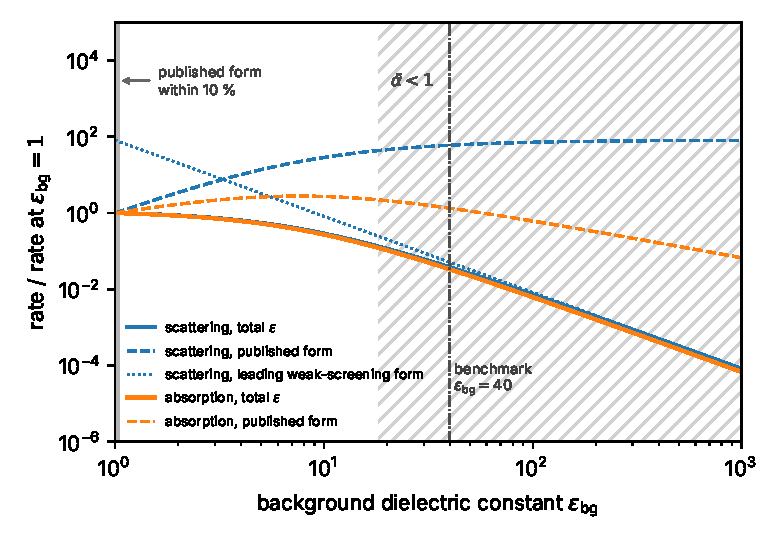
\includegraphics[width=0.9\linewidth]{figures/ch16/limit16_1a.pdf}
\captionof{figure}{Rates of the gapped isotropic Dirac material of Ref.~\cite{hochberg2018detection} ($v_{\mathrm{D}} = 4\times10^{-4}$, $\Delta_{\mathrm{D}} = \SI{2.5}{meV}$, $g_{\mathrm{deg}} = 2$, hard cutoff $\Lambda_{\mathrm{D}} = \SI{0.2}{keV}$) against the background dielectric constant at fixed Dirac parameters, each divided by its value at $\varepsilon_{\mathrm{bg}} = 1$, where the two forms coincide. Blue: scattering at $m_\chi = \SI{100}{keV}$ through a light mediator, \cref{eq:10.2-rate}, with the total $\varepsilon$ (solid), the published form (dashed) and the leading weak-screening form $\Imag\varepsilon_{\mathrm{D}}/\varepsilon_{\mathrm{bg}}^2$ (dotted). Orange: dark-photon absorption at $m_\phi = \SI{50}{meV}$ with the total $\varepsilon$ (solid) and the published form (dashed). Gray: $\varepsilon_{\mathrm{bg}} \le 1.049$, where the published scattering rate is within \SI{10}{\percent} of the total-$\varepsilon$ rate. Hatched: $\tilde\alpha < 1$, $\varepsilon_{\mathrm{bg}} > \alpha/v_{\mathrm{D}} = 18.2$, where one-loop screening is used. Dash-dotted: the published benchmark $\varepsilon_{\mathrm{bg}} = 40$, where the total-$\varepsilon$ scattering rate is 0.74 of its leading form. The dashed curves are $\varepsilon_{\mathrm{bg}}^2$ and $\varepsilon_{\mathrm{bg}}$ times the solid ones.}\label{fig:16-limit-dirac}
\par}
\smallskip
For $\varepsilon_{\mathrm{bg}} > 1$ the published form leaves out the screening of the dark-photon field by the remote bands; at large $\varepsilon_{\mathrm{bg}}$ its scattering rate tends to the unscreened rate of the Dirac pairs, 0.99 of it at $\varepsilon_{\mathrm{bg}} = 1000$, while the true rate falls as $1/\varepsilon_{\mathrm{bg}}^2$.
\end{limitbox}

\begin{workedexample}{The factor $\varepsilon_{\mathrm{bg}}^2$ at $\varepsilon_{\mathrm{bg}} = 40$}\label{we:16-factor}
The ideal Dirac material of Ref.~\cite[Fig.~4]{hochberg2018detection} has $v_{\mathrm{D}} = 4\times10^{-4}$, $\varepsilon_{\mathrm{bg}} = 40$, $g_{\mathrm{deg}} = 2$ and a cutoff of \SI{0.2}{keV}, which we read as a hard cutoff, $v_{\mathrm{D}}\Lambda_{\mathrm{D}} = \SI{80}{meV}$. The coupling is $\tilde\alpha = \alpha/(40\times4\times10^{-4}) = 0.456$, and $g_{\mathrm{deg}}\tilde\alpha = 0.91$ is the effective coupling quoted there.

\emph{One point.} Take the gapless cone at $\vect{q} \to 0$ and $\omega = \SI{10}{meV}$, so that $\sqrt{s} = \SI{10}{meV}$. \Cref{eq:D.22-gapless} gives the bracket $\ln(4v_{\mathrm{D}}^2\Lambda_{\mathrm{D}}^2/s) + \ii\pi = 5.545 + 3.142\ii$, and with $g_{\mathrm{deg}}\alpha/(6\pi v_{\mathrm{D}}) = 1.936$, $\varepsilon_{\mathrm{D}} = 10.73 + 6.08\ii$. The total is $\varepsilon = 50.73 + 6.08\ii$ and $|\varepsilon|^2 = 2611$, so $L = 6.08/2611 = 2.33\times10^{-3}$, 0.61 of the leading form $6.08/1600 = 3.80\times10^{-3}$. Had the \SI{0.2}{keV} been a cutoff in the subtraction scheme of the reference, the bracket would gain $\frac53$, $\Real\varepsilon_{\mathrm{D}}/\varepsilon_{\mathrm{bg}}$ would rise from 0.27 to 0.35, and the ratio to the leading form would be 0.54. The published construction divides $\Imag\varepsilon_{\mathrm{D}} = 6.08$ by $|\varepsilon/\varepsilon_{\mathrm{bg}}|^2 = 1.632$ and obtains 3.73, which is $1600$ times $L$.

\emph{Absorption.} At $m_\phi = \SI{10}{meV}$ the same $\varepsilon$ applies. The published rate is $\zeta^2m_\phi\Imag\varepsilon_{\mathrm{pub}}/|\varepsilon_{\mathrm{pub}}|^2 = 0.0932\,\zeta^2m_\phi$, forty times $\zeta^2m_\phi L$. With the density \SI{10}{g.cm^{-3}} of the reference and $\rho_\chi = \SI{0.3}{GeV.cm^{-3}}$, \cref{eq:10.7-dp} gives $3.35\times10^{30}\,\zeta^2$ events per kg-year, and three events in a kg-year reach $\zeta = 9.5\times10^{-16}$, against $1.5\times10^{-16}$ with the published form, a factor $\sqrt{40} = 6.3$.

\emph{Scattering reach.} For scattering the reference counts one Dirac valence electron per cell, $n_e = \SI{5e24}{kg^{-1}}$ electrons per unit mass in cells of $V_{\mathrm{uc}} = \SI{60}{\angstrom^3}$, which fixes the density $1/(n_eV_{\mathrm{uc}}) = \SI{3.33}{g.cm^{-3}}$; its absorption estimate takes \SI{10}{g.cm^{-3}} instead, and we keep each with its own rate. For the gapped cone ($\Delta_{\mathrm{D}} = \SI{2.5}{meV}$) at $m_\chi = \SI{100}{keV}$, with the standard halo and three events in a kg-year, \cref{eq:10.2-rate} with \cref{eq:16.1-L} reaches $\sigmae = \SI{4.4e-42}{cm^2}$, and the published form $\SI{2.8e-45}{cm^2}$, a factor 1600 at this and at every other mass, 3.2 decades. The published curve for this material has its minimum, \SI{3.4e-46}{cm^2} near \SI{9}{keV}, read from the reference's figure; corrected, it lies at \SI{5.4e-43}{cm^2}.\footnote{The published curve lies about a factor two above the reference's own formula: with the standard halo it reads \SI{5.0e-45}{cm^2} at \SI{100}{keV} against the recomputed \SI{2.8e-45}{cm^2}, a factor 1.8. The factor 1600 between the published and the total-$\varepsilon$ reach holds either way.}
\end{workedexample}

\subsection{ZrTe\texorpdfstring{$_5$}{5} and other anisotropic targets}\label{sec:16.1-zrte5}

Take an anisotropic cone and a background tensor with the same principal axes. The background enters the longitudinal function as $\hat{\vect{q}}\cdot\varepsilon_{\mathrm{bg}}\cdot\hat{\vect{q}} = \sum_i\varepsilon_{\mathrm{bg},ii}\hat q_i^2$. The rescaling at the end of \cref{app:D.22} turns $q^2/v_{\mathrm{D}}$ in the overlap into $\tilde q^2/(v_1v_2v_3)$ with $\tilde{\vect{q}} = (v_1q_1, v_2q_2, v_3q_3)$, so that
\begin{equation}
  \varepsilon(\vect{q},\omega) = \sum_i\varepsilon_{\mathrm{bg},ii}\hat q_i^2 + \sum_i\hat q_i^2\,\varepsilon_{\mathrm{D},i}(\omega^2 - \tilde q^2), \qquad
  \varepsilon_{\mathrm{D},i} = \frac{g_{\mathrm{deg}}\alpha}{6\pi}\,\frac{v_i^2}{v_1v_2v_3}\,B_{\mathrm{D}}(\omega^2 - \tilde q^2) ,
  \label{eq:D.41-aniso}
\end{equation}
with $B_{\mathrm{D}}$ the bracket of \cref{eq:7.3-eps} and $v_{\mathrm{D}}\Lambda_{\mathrm{D}}$ replaced by the energy cutoff $\tilde\Lambda$ of \cref{eq:7.3-aniso}. Both terms of \cref{eq:D.41-aniso} carry the factor $\hat q_i^2$ of a longitudinal function; the background is not divided into the Dirac term. The in-medium factor of Ref.~\cite[Eq.~(3.14)]{geilhufe2020dirac} instead divides each component of the Dirac polarization by its own background constant, $\varepsilon_{\mathrm{pub}} = 1 + \sum_i\hat q_i^2\varepsilon_{\mathrm{D},i}/\varepsilon_{\mathrm{bg},ii}$. The ratio of the two loss functions is
\begin{equation}
  \frac{L_{\mathrm{pub}}}{L} = \frac{|\sum_i\hat q_i^2(\varepsilon_{\mathrm{bg},ii} + \varepsilon_{\mathrm{D},i})|^2}{|1 + \sum_i\hat q_i^2\varepsilon_{\mathrm{D},i}/\varepsilon_{\mathrm{bg},ii}|^2} .
  \label{eq:D.41-ratio}
\end{equation}
(The term of the $x$ axis is read with $q_x^2v_x^2$, where that equation prints $q_x^2v_z^2$.) Along a principal axis the ratio is $\varepsilon_{\mathrm{bg},ii}^2$, which for the computed tensor of ZrTe$_5$, $\varepsilon_{\mathrm{bg},ii} = 308.4$, 20.75 and 126.1~\cite[Table~2]{geilhufe2020dirac}, is $9.5\times10^4$, 431 and $1.6\times10^4$. Off the axes it is not a power of any single background constant: for $\varepsilon_{\mathrm{D}} \to 0$ it tends to $(\hat{\vect{q}}\cdot\varepsilon_{\mathrm{bg}}\cdot\hat{\vect{q}})^2$, and for finite $\varepsilon_{\mathrm{D}}$ it depends on $\hat{\vect{q}}$ through both sums. The event rates then differ by the ratio of their integrals over directions and energies, which the reach of an anisotropic target must be computed with. The background tensor also orders the directions by itself. At equal Dirac numerator, a momentum transfer along $y$, the axis of the smallest background constant, gives a rate $(308.4/20.75)^2 = 221$ times that along $x$. The rate of a crystal fixed in the laboratory therefore modulates daily mainly through its background tensor, which neither a harmonic mean of the tensor nor the per-component factor represents.

We evaluate ZrTe$_5$ with the parameter row that the calculation of \cref{we:7-zrte5} gives for the measured crystal structure~\cite[Table~1 and text below it]{geilhufe2020dirac}: the principal velocities $1.1\times10^{-3}$, $4.5\times10^{-4}$ and $1.0\times10^{-3}$, the energy cutoff $\tilde\Lambda = \min_iv_i\Lambda_i = \SI{0.191}{eV}$, $g_{\mathrm{deg}} = 2$, and the half-gap $\Delta_{\mathrm{D}} = \SI{11.8}{meV}$, half the computed gap of \SI{23.6}{meV}. The relaxed cell of \cref{we:7-zrte5}, the row the reference implements, gives \SI{15.6}{meV} with its own velocities and cutoff, and an earlier calculation \SI{17.5}{meV}. The threshold mass is \SI{8.0}{keV} for the isotropic cone and 9.6, 7.1 and \SI{9.0}{keV} along the principal axes. We average the loss function over the directions of $\vect{q}$, which gives the rate averaged over the orientations of the crystal relative to the dark-matter wind, and insert it into \cref{eq:10.2-rate} with a light mediator, the standard halo and the measured density \SI{6.089}{g.cm^{-3}}~\cite[Fig.~3]{geilhufe2020dirac}. At $m_\chi = \SI{100}{keV}$ and $\sigmae = \SI{e-38}{cm^2}$ this yields 108 events per kg-year. Since a background-free reach scales as the inverse rate (\cref{eq:1.5-limscaling}), three events in a kg-year reach about \SI{1.5e-40}{cm^2} near \SI{40}{keV} (\cref{fig:16-zrte5}a). The published rule, recomputed with the same inputs and the standard halo, gives a rate 5200 to 6400 times larger between \SI{20}{keV} and \SI{1}{MeV}. Over the two computed rows (11.8 and \SI{15.6}{meV}) and the two halos of \cref{fig:16-zrte5} the factor spans 4800 to 6600, and a halo with $v_0 = 220$, $v_{\mathrm{E}} = 232$ and $v_{\mathrm{esc}} = \SI{544}{km.s^{-1}}$ lowers its lower end to 4300. That is more than the square of the harmonic mean of the tensor, $50.5^2 = 2550$, and an isotropic model of the same row, with the geometric-mean velocity and the harmonic-mean background as in \cref{we:7-zrte5}, overstates the orientation-averaged total-$\varepsilon$ rate by a factor 2.3 to 2.7. The curve of Hochberg et al.~\cite{hochberg2018detection}, computed for an isotropic model with $\varepsilon_{\mathrm{bg}} = 25.34$, the harmonic mean of its own tensor (187.5, 9.8 and 90.9), moves by $25.34^2 = 642$ exactly.

\begin{figure}[tbp]
  \centering
  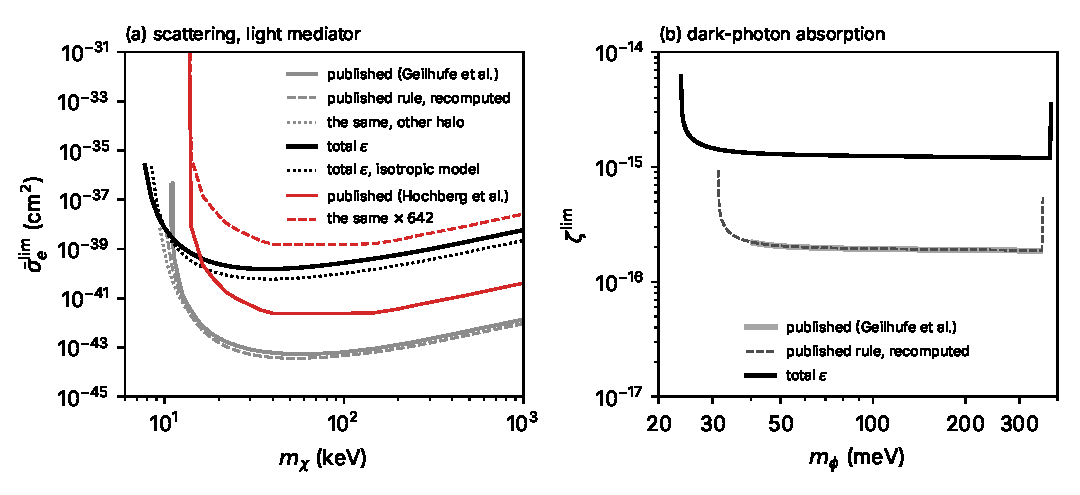
\includegraphics[width=\linewidth]{figures/ch16/fig16_1.pdf}
  \caption{ZrTe$_5$ reach as published and with the background in the total dielectric function: three events in one kg-year, no background, $\rho_\chi = \SI{0.3}{GeV.cm^{-3}}$. (a) Scattering through a light mediator. Gray solid: the published curve for the computed parameters of Geilhufe et al.~\cite{geilhufe2020dirac} (read from their figure). Gray dashed: their in-medium factor, recomputed for their half-gap, \SI{15.6}{meV}, with the standard halo and the loss function averaged over the directions of $\vect{q}$; it lies at 0.63 to 0.72 of the published curve above \SI{20}{keV}, consistent with a difference of halo: the source states none, and with $v_0 = 220$, $v_{\mathrm{E}} = 232$ and $v_{\mathrm{esc}} = \SI{600}{km.s^{-1}}$ (gray dotted) the ratio is 0.8 to 1.1. Black solid: the target with the total $\varepsilon$, \cref{eq:16.1-L} with the anisotropic $\varepsilon_{\mathrm{D}}$ of \cref{eq:D.41-aniso}, measured-structure row ($\Delta_{\mathrm{D}} = \SI{11.8}{meV}$, $\tilde\Lambda = \SI{0.191}{eV}$), density \SI{6.089}{g.cm^{-3}}. Black dotted: its isotropic model (geometric-mean velocity, harmonic-mean $\varepsilon_{\mathrm{bg}} = 50.5$) with the total $\varepsilon$. Red: the published curve of Hochberg et al.~\cite{hochberg2018detection} for their ZrTe$_5$ parameters, isotropized with $\varepsilon_{\mathrm{bg}} = 25.34$ (solid), and the same curve times 642 (dashed). (b) Absorption of dark-photon dark matter, each polarization along a principal axis, unpolarized average, density \SI{6.135}{g.cm^{-3}} as in Ref.~\cite{geilhufe2020dirac}. Gray: their published curve; dashed: their rule recomputed with $\Delta_{\mathrm{D}} = \SI{15.6}{meV}$, within \SI{0.5}{\percent} of it; black: the total $\varepsilon$ with the measured-structure row. Published-rule curves: $\Delta_{\mathrm{D}} = \SI{15.6}{meV}$, $\tilde\Lambda = \SI{0.180}{eV}$. Off-diagonal entries of the tensor ($|\varepsilon_{\mathrm{bg},ij}| \le 1.2$) are dropped.}
  \label{fig:16-zrte5}
\end{figure}

Absorption at rest has no direction of $\vect{q}$, but the polarization of the dark photon picks a component of the tensor, and each polarization is absorbed with the factor $\varepsilon_{\mathrm{bg},ii}$ of \cref{eq:16.1-ratio}. With the total $\varepsilon$ the polarization along $y$, with the smallest background constant, carries \SI{86}{\percent} of the unpolarized rate at \SI{100}{meV}. Recomputed with the published rule, our absorption rate reproduces the published reach of Ref.~\cite{geilhufe2020dirac} to \SI{0.5}{\percent} over the whole range, which checks the inputs. With the total $\varepsilon$ and the measured-structure row, the reach in $\zeta$ weakens by a factor of 6.3 to 6.4 between the gap and the cutoff (\cref{fig:16-zrte5}b), to about $1.25\times10^{-15}$ at \SI{100}{meV}. The factor is the square root of a polarization average and lies between $\varepsilon_{\mathrm{bg},yy}^{1/2} = 4.6$ and $\varepsilon_{\mathrm{bg},xx}^{1/2} = 17.6$. For the cubic Yb$_3$PbO of the same reference the factors are $42.8^2 = 1832$ and $42.8^{1/2} = 6.5$ identically. Its computed dielectric constant, however, is described there as sensitive to the size of the gap~\cite[Sect.~4]{geilhufe2020dirac}. It contains the Dirac bands, the background is smaller than 42.8, and the Dirac term is counted twice under either rule. These two factors describe the model, not the material.

\subsection{Excitonic and strong-coupling corrections}\label{sec:16.1-validity}

\Cref{eq:16.1-L} keeps the random-phase response of the Dirac electrons, the first order in $\tilde\alpha$ of their polarization, with the expansion parameter $g_{\mathrm{deg}}\tilde\alpha\ln[v_{\mathrm{D}}\Lambda_{\mathrm{D}}/\max(\Delta_{\mathrm{D}}, v_{\mathrm{D}}q)]$ of \cref{sec:7.3}. For ZrTe$_5$ that is 1.02 at long wavelength with the measured-structure row (0.93 with the relaxed cell), at the edge of the expansion, and for the benchmark of \cref{we:16-factor}, $g_{\mathrm{deg}}\tilde\alpha = 0.91$ times a logarithm of a few. At next order the electron--hole ladder, the self-energy and vertex of the carriers, and the material outside the model all enter.

The ladder of the Bethe--Salpeter equation (\cref{sec:4.9}) is the attraction between the electron and the hole of a pair. Near the edge the pair is nonrelativistic, with reduced mass $\Delta_{\mathrm{D}}/2v_{\mathrm{D}}^2$ and Coulomb coupling $\alpha/\varepsilon_{\mathrm{bg}}$. It binds with the energy $(\Delta_{\mathrm{D}}/2v_{\mathrm{D}}^2)(\alpha/\varepsilon_{\mathrm{bg}})^2/2 = \Delta_{\mathrm{D}}\tilde\alpha^2/4$, \SI{0.10}{meV} for the isotropic model of ZrTe$_5$ with $\tilde\alpha = 0.18$, and its continuum carries the Sommerfeld factor $x/(1 - \ee^{-x})$ with $x = \pi\tilde\alpha/b$. Here $b = (1 - 4\Delta_{\mathrm{D}}^2/s)^{1/2}$ is the speed of each carrier in the rest frame of the pair, in units of $v_{\mathrm{D}}$. In ZrTe$_5$ the factor exceeds 1.5 for $b < 0.66$, that is for pair energies up to 1.33 times the edge, and that region carries \SI{60}{\percent} of the rate at \SI{20}{keV}, \SI{12}{\percent} at \SI{100}{keV} and \SI{3}{\percent} at \SI{1}{MeV} in the isotropic model. Near the threshold mass the reach is therefore uncertain by the Sommerfeld factor, 1.5 or more, until the ladder is solved, which \cref{app:E.20} specifies. The bound states lie at $\sqrt{s} < 2\Delta_{\mathrm{D}}$ and add absorption lines below the edge.

The self-energy of the carriers renormalizes $v_{\mathrm{D}}$ logarithmically in the cutoff, and a vertex correction accompanies it. Each is of relative order $\tilde\alpha$, with a coefficient that the one-loop result does not fix. Outside the model, a chemical potential inside a band adds an intraband term, Thomas--Fermi screening with $k_{\mathrm{TF}}^2 = e^2\mathcal{N}_{\mathrm{D}}(E_{\mathrm{F}})/\varepsilon_{\mathrm{bg}}$, which removes the weak screening at $\omega \lesssim v_{\mathrm{D}}k_{\mathrm{F}}$. The background acquires ionic poles near the optical phonons. And the bands bend beyond $\Lambda_{\mathrm{D}}$, which moves weight between the background and the logarithm of \cref{eq:7.3-static}.

At $\tilde\alpha \gtrsim 1$ none of these is small, and no controlled method is known. The ladder is the controlled correction of first order in $\tilde\alpha$ and is uncontrolled beyond it; neither self-consistent $GW$ with the Bethe--Salpeter equation nor a functional renormalization group has a small parameter there. The question matters for the slowest cones, which have the most states and the lowest thresholds. BNQ-TTF, with velocities near $2\times10^{-4}$, has an effective coupling of about 10, and its authors present its one-loop rates as a qualitative estimate~\cite[footnote~3]{geilhufe2020dirac}. What replaces \cref{eq:16.1-L} for such targets is open.

\section{Low-dimensional plasmons and layered stacks}\label{sec:16.2}

Rolled into a metallic carbon nanotube, the Dirac electrons of \cref{sec:16.1} put their whole low-energy response to a density coupling into one line, $\omega = v_{\mathrm{D}}q_\parallel/g_c$, with $v_{\mathrm{D}} = 3.02\times10^{-3}$ the Dirac velocity of graphene. The Luttinger parameter $g_c \approx 0.2$ (\cref{eq:16.2-wire}) makes the line 3.4 to 6.9 times faster than any particle of the halo at momenta of 1 to \SI{100}{eV}. The plasmon of a doped graphene sheet is faster still at the momenta of keV-mass dark matter. In bulk silicon a mode that fast is out of reach: the plasmon of \cref{sec:10.3} needs a particle at \SI{2860}{km.s^{-1}}. In a tube or a sheet, however, the response depends only on the momentum along the tube or in the plane, and a halo particle can supply the rest of its momentum across it. A mode faster than $v_{\mathrm{max}}$ is then reached by an oblique momentum transfer, and the confined plasmon becomes a final state of its own. Its weight sits in a single line at low energy, which is what the sum-rule bounds of \cref{sec:10.2} need to come close to saturation. We will derive the Coulomb kernels of sheets and tubes, the random-phase plasmons in one and two dimensions, the acoustic plasmon of two kinds of carriers, and the dielectric function of a stack of layers, exact at long wavelength, with its leading correction.

\subsection{Confined electrons and their Coulomb kernels}\label{sec:16.2-kernels}

Consider identical units, wires or sheets, in which electrons move freely in one or two dimensions and are confined across, with no tunneling between units. Write $\vect{q} = (\vect{q}_\parallel, \vect{q}_\perp)$, with $\vect{q}_\parallel$ along the free directions. Suppose the distribution of the electrons across a unit does not depend on their state along it. The density operator of \cref{eq:2.3-nq} then factorizes, $n_e(\vect{q}) = \sum_u \ee^{\ii\vect{q}_\perp\cdot\vect{r}_u}F_\perp(\vect{q}_\perp)\,n_u(\vect{q}_\parallel)$. Here $\vect{r}_u$ locates unit $u$, $n_u$ is its density operator along the free directions, and the transverse form factor $F_\perp$ is the Fourier transform of the normalized distribution across the unit, with $F_\perp(0) = 1$. For a sheet of uniform thickness $d$, $F_\perp = \sin(q_zd/2)/(q_zd/2)$; for a tube whose electrons sit on a cylinder of radius $r_{\mathrm{t}}$, $F_\perp = J_0(q_\perp r_{\mathrm{t}})$. If the units respond independently, the cross terms between units average to zero at $\omega \ne 0$. The structure factor of \cref{eq:4.2-Sab} then becomes
\begin{equation}
  S(\vect{q},\omega) = \nd_{\mathrm{u}}\,|F_\perp(\vect{q}_\perp)|^2\,S_{\mathrm{u}}(\vect{q}_\parallel,\omega) ,
  \label{eq:16.2-embed}
\end{equation}
with $\nd_{\mathrm{u}}$ the number of units per unit transverse area (wires) or length (sheets) and $S_{\mathrm{u}}$ the structure factor of one unit per unit length or area, in the normalization of \cref{sec:4.2}. In \cref{eq:8.2-spectrum} the target enters as $S/\rho_T = |F_\perp|^2S_{\mathrm{u}}/\rho_{\mathrm{u}}$, with $\rho_{\mathrm{u}}$ the mass of one unit per unit length or area. The rate per unit mass is then independent of how densely the units are packed, as long as they remain independent. The tube proposal of Zhang and Chen reports its rate per unit tube length~\cite[Eq.~(6)]{zhang2026luttinger}, and Das, Jang and Min write \cref{eq:16.2-embed} for a sheet of uniform thickness with the areal mass density~\cite[Eqs.~(13), (14)]{das2023sub}.

\Cref{eq:16.2-embed} changes the kinematics. The structure factor depends on $\vect{q}_\parallel$ alone, while the dark matter deposits $\omega = \vect{q}\cdot\vect{v} - q^2/2\mchi$ with the full $\vect{q}$. A mode at $(\vect{q}_\parallel, \omega)$ is reached by any $\vect{q}$ with that projection, and the condition $\omega \le qv_{\mathrm{max}} - q^2/2\mchi$ only requires $q \gtrsim \omega/v_{\mathrm{max}}$, which can exceed $q_\parallel$ by any amount. The cost is the form factor, which falls once $q_\perp$ exceeds the inverse thickness. For a tube of radius \SI{0.7}{nm}, $|J_0|^2$ starts to fall at $q_\perp \approx 1/r_{\mathrm{t}} = \SI{282}{eV}$, and halo particles reach energies up to $v_{\mathrm{max}}/r_{\mathrm{t}} = \SI{0.75}{eV}$ without that suppression. A bulk mode at $(\vect{q},\omega)$, by contrast, is reached only if $\omega \le qv_{\mathrm{max}}$ at its own $\vect{q}$.

The electrons of a unit interact through the Coulomb potential averaged over the transverse distribution. Take a sheet between two half spaces of dielectric constants $\varepsilon_a$ and $\varepsilon_b$. \Cref{sec:15.3-sheet} found the potential of its density wave from the two-dimensional Fourier transform of $e^2/4\pi r$ and the image charges,
\begin{equation}
  v_{\mathrm{C}}^{\mathrm{2D}}(q_\parallel) = \frac{e^2}{(\varepsilon_a + \varepsilon_b)\,q_\parallel} = \frac{e^2}{2\bar\varepsilon\,q_\parallel} ,
  \qquad
  \varepsilon_{\mathrm{2D}} = 1 - v_{\mathrm{C}}^{\mathrm{2D}}\tilde R^{\mathrm{2D}} ,
  \qquad
  S_{\mathrm{2D}} = -2\,\Imag\frac{\tilde R^{\mathrm{2D}}}{\varepsilon_{\mathrm{2D}}} \quad (T = 0) ,
  \label{eq:16.2-kernel2D}
\end{equation}
with $\bar\varepsilon = (\varepsilon_a + \varepsilon_b)/2$ and $\tilde R^{\mathrm{2D}}$ the proper density response of the sheet per unit area, the two-dimensional analogue of \cref{eq:4.4-proper}. The kernel falls as $1/q_\parallel$, not as $1/q^2$: a sheet screens a long-wavelength potential weakly, because the field of its induced charge spreads into the space around it. Give the sheet a finite thickness $d$, with a uniform distribution across it in a homogeneous medium. Averaging $\ee^{-q_\parallel|z - z'|}$ over both positions multiplies the kernel by
\begin{equation}
  F_{\mathrm{th}}(q_\parallel d) = \frac{2}{q_\parallel d} - \frac{2\bigl(1 - \ee^{-q_\parallel d}\bigr)}{(q_\parallel d)^2} = 1 - \frac{q_\parallel d}{3} + O\bigl(q_\parallel^2d^2\bigr) .
  \label{eq:16.2-thick}
\end{equation}
For the interlayer distance $d = \SI{3.35}{\angstrom}$ of bilayer graphene the factor is 0.95 at $q_\parallel = \SI{100}{eV}$ and 0.85 at \SI{300}{eV}, and it reaches 0.9 at \SI{191}{eV}; Ref.~\cite[Eq.~(17)]{das2023sub} keeps the profile in the form factor but uses the zero-thickness kernel, a correction of this size at the momenta of sub-MeV dark matter.

The bands far from the Fermi level enter the proper response as a static part $\tilde R^{\mathrm{2D}}_{\mathrm{bg}}$, which for an insulating background is proportional to $q_\parallel^2$ at small $q_\parallel$. Writing $-\tilde R^{\mathrm{2D}}_{\mathrm{bg}} = 2r_0q_\parallel^2/e^2$ defines the Keldysh length $r_0$, and
\begin{equation}
  \bar\varepsilon\,\varepsilon_{\mathrm{2D}}(q_\parallel,\omega) = \bar\varepsilon + r_0q_\parallel - \frac{e^2}{2q_\parallel}\,\tilde R^{\mathrm{2D}}_{\mathrm{low}}(q_\parallel,\omega) ,
  \label{eq:16.2-keldysh}
\end{equation}
with $\tilde R^{\mathrm{2D}}_{\mathrm{low}}$ the response of the bands near the Fermi level. Compared to a bulk material, the remote bands of a sheet do not screen at long wavelength: their contribution $r_0q_\parallel$ vanishes as $q_\parallel \to 0$, while in three dimensions they give the constant $\varepsilon_{\mathrm{bg}}$ of \cref{sec:7.3} that \cref{sec:16.1} places inside the total $\varepsilon$. In a sheet the substrate enters only through $\bar\varepsilon$ and the remote bands only through $r_0$; neither rescales the coupling to the dark matter. A polar substrate makes $\varepsilon_b$ depend on frequency, and the sheet plasmon then mixes with its surface phonons.

For a tube the same average over a cylindrical shell of radius $r_{\mathrm{t}}$ selects the azimuthally uniform term of the expansion of $1/|\vect{r} - \vect{r}'|$ in cylindrical coordinates, $(2/\pi)\int_0^\infty\dd k\cos[k(z - z')]I_0(kr_{\mathrm{t}})K_0(kr_{\mathrm{t}})$, with $I_0$ and $K_0$ the modified Bessel functions of order zero~\cite[Sect.~10.25]{olver2010nist}. Its Fourier transform along the axis is $2I_0(q_\parallel r_{\mathrm{t}})K_0(q_\parallel r_{\mathrm{t}})$, and with $e^2 = 4\pi\alpha$ (\cref{app:A.2})
\begin{equation}
  v_{\mathrm{C}}^{\mathrm{1D}}(q_\parallel) = \frac{2\alpha}{\varepsilon_{\mathrm{env}}}\,I_0(q_\parallel r_{\mathrm{t}})\,K_0(q_\parallel r_{\mathrm{t}}) \simeq \frac{2\alpha}{\varepsilon_{\mathrm{env}}}\Bigl[\ln\frac{2}{q_\parallel r_{\mathrm{t}}} - \gamma_{\mathrm{E}}\Bigr] \quad (q_\parallel r_{\mathrm{t}} \ll 1) ,
  \label{eq:16.2-kernel1D}
\end{equation}
for a tube in a medium of dielectric constant $\varepsilon_{\mathrm{env}}$, with $\gamma_{\mathrm{E}}$ Euler's constant; the small-argument form follows from $I_0 \to 1$ and $K_0(x) \to \ln(2/x) - \gamma_{\mathrm{E}}$~\cite[Eqs.~(10.30.1), (10.31.2)]{olver2010nist}. The logarithmic form falls \SI{10}{\percent} below the exact kernel at $q_\parallel r_{\mathrm{t}} = 0.38$, which is \SI{108}{eV} for $r_{\mathrm{t}} = \SI{0.7}{nm}$. The logarithm comes from the one-dimensional geometry: the interaction of two lines of charge grows without bound as their wavelength grows.

\Cref{app:E.21} specifies how $\tilde R^{\mathrm{2D}}$, $r_0$ and the corresponding tables for tubes and stacks are computed. The proper response of a monolayer comes from a plane-wave code with the Coulomb interaction cut off between periodic images, or from a Wannier-function bubble. The substrate enters through its measured $\varepsilon_b(\omega)$ with the polar phonons, and the random-phase equations are solved with the kernels above.

\subsection{Plasmons in one and two dimensions}\label{sec:16.2-plasmons}

At frequencies above the pair continuum the proper response of any band takes the form $\tilde R \simeq D_{\mathrm{Dr}}\,q_\parallel^2/\omega^2$, with $D_{\mathrm{Dr}}$ the Drude weight. The coefficient follows from the intraband part of the Lehmann sum, expanded for $\omega \gg \vect{q}\cdot\vect{v}$: $D_{\mathrm{Dr}} = \sum_{\vect{k}}(-\partial n_{\mathrm{F}}/\partial E)(\hat{\vect{q}}\cdot\vect{v}_{\vect{k}})^2$ per unit area, summed over spin and valleys. For a parabolic band of mass $m^*$ this is $\nd_{\mathrm{2D}}/m^*$, the areal density over the mass, as the $f$-sum rule requires. For a Dirac cone, $\vect{v}_{\vect{k}} = v_{\mathrm{D}}\hat{\vect{k}}$ and the Fermi circle has length $2\pi k_{\mathrm{F}}$, so $D_{\mathrm{Dr}} = g_{\mathrm{deg}}E_{\mathrm{F}}/4\pi$, with $g_{\mathrm{deg}} = 4$ for graphene. The zero of $\varepsilon_{\mathrm{2D}}$ in \cref{eq:16.2-kernel2D} is then the sheet plasmon. For a parabolic band the next term of the high-frequency expansion is that of \cref{eq:4.5-moments}, with the disc average $\langle(\hat{\vect{q}}\cdot\vect{v})^2\rangle = v_{\mathrm{F}}^2/4$ in place of the sphere's $v_{\mathrm{F}}^2/5$. Then
\begin{equation}
  \omega_{\mathrm{pl}}^2(q_\parallel) = \frac{e^2\,\nd_{\mathrm{2D}}\,q_\parallel}{(\varepsilon_a + \varepsilon_b)\,m^*} + \frac34\,v_{\mathrm{F}}^2q_\parallel^2 + O\bigl(q_\parallel^3\bigr) .
  \label{eq:16.2-2Dpl}
\end{equation}
Compared to the bulk plasmon, which starts at $\omega_p$, the sheet plasmon is gapless and rises as $\sqrt{q_\parallel}$, because the kernel falls only as $1/q_\parallel$. It stays undamped as long as it lies above the pair continuum, $\omega > q_\parallel v_{\mathrm{F}} + q_\parallel^2/2m^*$. For doped graphene in vacuum, $\omega_{\mathrm{pl}}^2 = 2\alpha E_{\mathrm{F}}q_\parallel$. At $E_{\mathrm{F}} = \SI{0.2}{eV}$ its phase velocity is 20 times $v_{\mathrm{max}}$ at $q_\parallel = \SI{1}{eV}$ and 6.4 times at \SI{10}{eV}, and the long-wavelength form ends at $q_\parallel = \SI{32}{eV}$, where $\omega = \SI{0.30}{eV}$ and the line meets the interband edge $2E_{\mathrm{F}} - v_{\mathrm{D}}q_\parallel$. Here $v_{\mathrm{D}} = 3ta_{\mathrm{cc}}/2 = 3.02\times10^{-3}$, from the nearest-neighbor hopping $t = \SI{2.8}{eV}$ and the carbon--carbon distance $a_{\mathrm{cc}} = \SI{1.42}{\angstrom}$~\cite[text after Eqs.~(5) and (7)]{castroneto2009electronic}, the value used for graphene and nanotubes throughout this chapter. Das, Jang and Min quote a hopping of \SI{3.16}{eV} for their bilayer model~\cite[Sect.~II]{das2023sub}, and Zhang and Chen take $v = \SI{0.8e6}{m.s^{-1}} = 2.67\times10^{-3}$ for nanotubes~\cite{zhang2026luttinger}. Their rate for bilayer graphene is \cref{eq:16.2-embed,eq:16.2-kernel2D} at $\varepsilon_a = \varepsilon_b = 1$, with the random-phase response of the four low-energy bands~\cite[Eqs.~(13)--(19)]{das2023sub}; on a substrate the 2 in their kernel $e^2/2q$ becomes $\varepsilon_a + \varepsilon_b$. Their gate opens a gap and puts the Fermi level inside it, so their loss function is interband and has no sheet plasmon.

The bands of a metallic nanotube at its Fermi level are linear. The tube has $N_{\mathrm{ch}}$ channels at the Fermi level, two for spin times two for the valleys, each with right- and left-moving electrons of velocity $\pm v$; for a nanotube $v = v_{\mathrm{D}}$. For the right movers of one channel, $n_k - n_{k+q} = 1$ on an interval of length $q$ below $k_{\mathrm{F}}$ and the energy denominator is $\omega - vq$; the left movers give the same with $-v$. Their sum per unit length is $(q/2\pi)[1/(\omega - vq) - 1/(\omega + vq)]$, and for $N_{\mathrm{ch}}$ channels
\begin{equation*}
  R^0_{\mathrm{1D}}(q_\parallel,\omega) = \frac{N_{\mathrm{ch}}\,v\,q_\parallel^2}{\pi\,(\omega^2 - v^2q_\parallel^2)} .
\end{equation*}
The random-phase response $R = R^0_{\mathrm{1D}}/(1 - v_{\mathrm{C}}^{\mathrm{1D}}R^0_{\mathrm{1D}})$ has its pole where $\omega^2 = v^2q_\parallel^2[1 + N_{\mathrm{ch}}v_{\mathrm{C}}^{\mathrm{1D}}/(\pi v)]$, and near it $\Imag[1/(\omega^2 - \omega_{\mathrm{pl}}^2 + \ii0^+)] = -\pi\delta(\omega - \omega_{\mathrm{pl}})/2\omega_{\mathrm{pl}}$, so that $S = -2\Imag R$ is a single line:
\begin{keyresult}[One-dimensional plasmon of linear channels]
\begin{equation}
  S_{\mathrm{1D}}(q_\parallel,\omega) = N_{\mathrm{ch}}\,g_c\,|q_\parallel|\,\delta\Bigl(\omega - \frac{v|q_\parallel|}{g_c}\Bigr) , \qquad
  g_c(q_\parallel) = \Bigl[1 + \frac{N_{\mathrm{ch}}\,v_{\mathrm{C}}^{\mathrm{1D}}(q_\parallel)}{\pi v}\Bigr]^{-1/2} ,
  \label{eq:16.2-wire}
\end{equation}
at $T = 0$ and $\omega > 0$, with $v_{\mathrm{C}}^{\mathrm{1D}}$ of \cref{eq:16.2-kernel1D}. It is embedded in three dimensions by \cref{eq:16.2-embed} with $F_\perp = J_0(q_\perp r_{\mathrm{t}})$.
\end{keyresult}
\noindent For a single channel this is the result of Zhang and Chen~\cite[Eqs.~(3), (4)]{zhang2026luttinger}. They bosonize a model with forward couplings $g_2$ and $g_4$ between right and left movers; with $g_2 = g_4 = v_{\mathrm{C}}^{\mathrm{1D}}$ their Luttinger parameter and velocity become $g_c$ and $v/g_c$ of \cref{eq:16.2-wire}. For this model the random-phase result is exact, because the linear band makes every higher-order term in the interaction cancel; that is the content of bosonization. The product of the weight and the velocity, $g_c\cdot v/g_c = v$, does not depend on the interaction. The first moment of the line, $\int\dd\omega\,\omega S_{\mathrm{1D}} = N_{\mathrm{ch}}vq_\parallel^2$, is therefore that of the free channels, the $f$-sum of the linear bands: the interaction raises the line and lowers its weight in the same proportion.

The charge of a nanotube is carried by all four channels together. The dark matter couples to the total density $n = \sum_in_i$, and so does the Coulomb interaction. The symmetric combination of the channel densities is the plasmon of \cref{eq:16.2-wire} with $N_{\mathrm{ch}} = 4$. The three other combinations, in which spin or valley densities oscillate against each other, carry no charge, keep $g = 1$, and do not appear in $S$. The model of Ref.~\cite{zhang2026luttinger} has one right- and one left-moving mode, $N_{\mathrm{ch}} = 1$, but its benchmark values $g = 0.2$ to 0.7 are those measured for nanotubes, which belong to the charge mode $g_c$ of the four-channel theory. At fixed $g_c$ its structure factor, and the rate of its Eq.~(6), are four times too low. At a fixed interaction instead the comparison is $N_{\mathrm{ch}}g_c(N_{\mathrm{ch}})$ against $g_c(1)$: with the kernel of a tube of radius \SI{0.7}{nm} in vacuum, $g_c = 0.212$ for four channels and 0.398 for one at $q_\parallel = \SI{10}{eV}$, and the four-channel line is 2.1 times stronger.

The interaction is strong. With $r_{\mathrm{t}} = \SI{0.7}{nm}$, $\varepsilon_{\mathrm{env}} = 1$ and the graphene velocity, $N_{\mathrm{ch}}v_{\mathrm{C}}^{\mathrm{1D}}/\pi v_{\mathrm{D}}$ is 35 at $q_\parallel = \SI{1}{eV}$ and 8 at \SI{100}{eV}, and $g_c$ is 0.17, 0.21 and 0.34 at 1, 10 and \SI{100}{eV}, inside the measured range. The plasmon then moves at 6.9, 5.4 and 3.4 times $v_{\mathrm{max}}$. A bulk mode that fast would be unreachable; the line of a tube is reached by any halo particle that deposits $\omega$ with a total momentum $q \gtrsim \omega/v_{\mathrm{max}}$ and a projection $q_\parallel = g_c\omega/v$ on the axis. The rate depends on the angle between the tube and the velocity of the particle, and with it on the time of day, which is the directional signal of Ref.~\cite{zhang2026luttinger}. \Cref{fig:16-dispersion} compares the plasmons of a tube, a sheet and bulk silicon with the reach of the halo.

\begin{figure}[tbp]
  \centering
  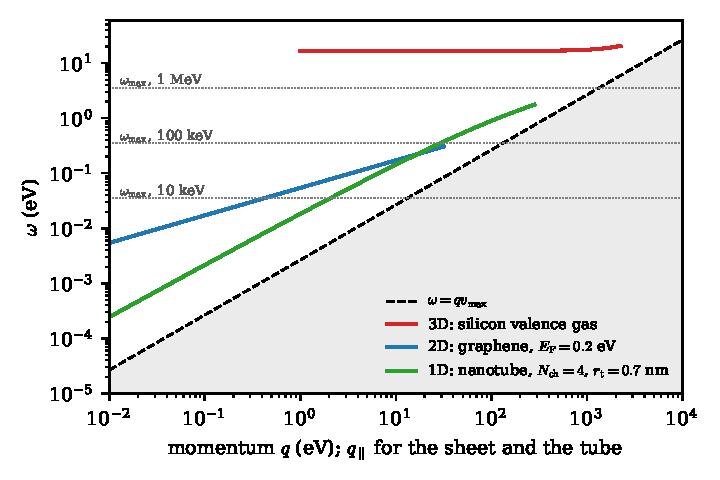
\includegraphics[width=0.85\linewidth]{figures/ch16/fig16_2.pdf}
  \caption{Plasmons in three, two and one dimensions against the reach of halo dark matter. Red: the valence-electron gas of silicon, $\omega_{\mathrm{pl}}^2 = \omega_p^2 + \tfrac35v_{\mathrm{F}}^2q^2$ with $\omega_p = \SI{16.6}{eV}$, to the quadratic cutoff at \SI{2.24}{keV}. Blue: doped graphene in vacuum at a Fermi energy of \SI{0.2}{eV}, $\omega_{\mathrm{pl}}^2 = 2\alpha E_{\mathrm{F}}q_\parallel$, up to the interband edge at \SI{32}{eV}. Green: the charge mode of a metallic nanotube, \cref{eq:16.2-wire} with $N_{\mathrm{ch}} = 4$, $r_{\mathrm{t}} = \SI{0.7}{nm}$, $\varepsilon_{\mathrm{env}} = 1$ and $v_{\mathrm{D}} = 3.02\times10^{-3}$, to $q_\parallel = 1/r_{\mathrm{t}}$. Dashed: $\omega = qv_{\mathrm{max}}$, the largest energy a halo particle deposits with momentum $q$ (gray below it). Dotted: the largest energy $\mchi v_{\mathrm{max}}^2/2$ for three masses. The bulk mode lies above the dashed line at its own $q$ and is out of reach. The modes of the sheet and the tube depend only on $q_\parallel$, and a particle reaches them with a total momentum $q \ge \omega/v_{\mathrm{max}}$, the rest of it across the sheet or the tube.}
  \label{fig:16-dispersion}
\end{figure}

\Cref{eq:16.2-wire} rests on the linear band. A real band curves on the scale of its Fermi momentum, and the limit check below compares the linear channels with parabolic ones of the same velocity $v$ at $k_{\mathrm{F}}$, of mass $m^* = k_{\mathrm{F}}/v$. The one-dimensional Lindhard function of one such channel is $(m^*/2\pi q_\parallel)\ln[(\omega^2 - \omega_-^2)/(\omega^2 - \omega_+^2)]$, with $\omega_\pm = q_\parallel v \pm q_\parallel^2/2m^*$ the edges of its pair band, and the zero of the random-phase dielectric function has the closed form $\omega^2 = (\omega_+^2\ee^{y} - \omega_-^2)/(\ee^{y} - 1)$, with $y = 2\pi q_\parallel/(N_{\mathrm{ch}}v_{\mathrm{C}}^{\mathrm{1D}}m^*)$. Expanding it in $y$, the $q_\parallel^3$ terms cancel and the plasmon frequency is
\begin{equation*}
  \frac{\omega_{\mathrm{pl}}^{\mathrm{par}}}{\omega_{\mathrm{pl}}} = 1 + \frac{q_\parallel^2}{2k_{\mathrm{F}}^2}\,g_c^2\Bigl[\frac14 + \frac{g_c^2}{3(1 - g_c^2)}\Bigr] + O\bigl(q_\parallel^4/k_{\mathrm{F}}^4\bigr) .
\end{equation*}
The correction carries $g_c^2$: the stronger the interaction, the further the plasmon lies above the pairs, and the less the shape of the band matters. In a nanotube the linear band itself ends at the next subbands, whose pairs open at $2v_{\mathrm{D}}/r_{\mathrm{t}} = \SI{1.7}{eV}$; below that energy and for $q_\parallel \ll 1/r_{\mathrm{t}}$ the four channels are the whole low-energy response. In a forest of parallel tubes the Coulomb interaction between tubes adds to $v_{\mathrm{C}}^{\mathrm{1D}}$ once $q_\perp$ is below the inverse spacing, 1 to \SI{2}{eV} for the spacings of 100 to \SI{200}{nm} that Ref.~\cite{zhang2026luttinger} considers.

\begin{limitbox}[One-dimensional plasmons of linear channels][lim:16.2a]
$S_{\mathrm{1D}} = N_{\mathrm{ch}}g_c|q_\parallel|\delta(\omega - v|q_\parallel|/g_c)$ with $g_c = [1 + N_{\mathrm{ch}}v_{\mathrm{C}}^{\mathrm{1D}}/\pi v]^{-1/2}$; Zhang and Chen give the case $N_{\mathrm{ch}} = 1$, and a metallic nanotube has $N_{\mathrm{ch}} = 4$~\cite[Eqs.~(3)--(6)]{zhang2026luttinger}.
\par\smallskip
{\centering
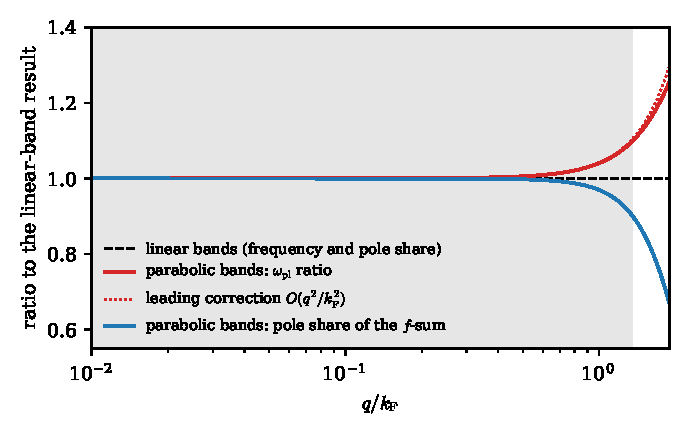
\includegraphics[width=0.82\linewidth]{figures/ch16/limit16_2a.pdf}
\captionof{figure}{Plasmon frequency and pole share of the $f$-sum for $N_{\mathrm{ch}} = 4$ parabolic channels, relative to the linear-band result, against $q_\parallel/k_{\mathrm{F}}$. Both use the kernel of a tube of radius \SI{0.7}{nm} in vacuum and the velocity $v_{\mathrm{D}} = 3.02\times10^{-3}$ at $k_{\mathrm{F}}$; the parabolic band, of mass $k_{\mathrm{F}}/v_{\mathrm{D}}$ with $k_{\mathrm{F}} = 1/r_{\mathrm{t}} = \SI{282}{eV}$, is a model for the curvature that the subbands bring on that scale. Red: frequency ratio; dotted, its leading correction in $q_\parallel^2/k_{\mathrm{F}}^2$. Blue: share of the $f$-sum $N_{\mathrm{ch}}vq_\parallel^2$ in the plasmon line (one for linear bands). Gray: both within \SI{10}{\percent} of the linear-band result, $q_\parallel < 1.36\,k_{\mathrm{F}}$. Along the curve $g_c$ rises from 0.18 to 0.61.}\label{fig:16-wire-limit}
\par}
\smallskip
Beyond $q_\parallel \approx 1.4\,k_{\mathrm{F}}$ the plasmon of curved bands moves up by more than \SI{10}{\percent} and loses weight to the pair continuum, which linear bands do not have.
\end{limitbox}

In the random-phase approximation the line of \cref{eq:16.2-wire} does not decay, and neither does the sheet plasmon above the pair continuum. Such a plasmon is a final state of its own in the sense of \cref{sec:8.7}, unlike the bulk plasmon of silicon, which decays into pairs at once. Its energy leaves the tube or sheet by propagating to the contacts, where Ref.~\cite{zhang2026luttinger} proposes to convert it into quasiparticles of a superconductor, or by damping through disorder, phonons or the substrate. How much of it reaches a sensor is a question for the cascade of \cref{chap:18}, not for the response.

\subsection{The acoustic plasmon of two components}\label{sec:16.2-demon}

A material with two kinds of carriers, light electrons of Fermi velocity $v_{\mathrm{F},l}$ and heavy ones of mass $m_h$ and density $\nd_h$, has a second collective mode below the plasmon. It is known as Pines' demon, after its prediction in 1956~\cite{pines1956electron}. In the window $qv_{\mathrm{F},h} \ll \omega \ll qv_{\mathrm{F},l}$ the light electrons follow the potential statically and screen it, while the heavy ones respond as a free plasma. Take the light response at $q \ll k_{\mathrm{F},l}$ from \cref{eq:4.5-lindhard}, $R^0_l = -2\mathcal{N}_{\mathrm{F},l}\,f_3(\nu)$ with $\nu = \omega/qv_{\mathrm{F},l}$ and $f_3(\nu) = 1 - (\nu/2)\ln|(1 + \nu)/(1 - \nu)| + \ii(\pi/2)\nu\,\Theta(1 - \nu)$, and the heavy response at high frequency, $\nd_hq^2/m_h\omega^2$. In three dimensions
\begin{gather}
  \varepsilon(q,\omega) = 1 + \frac{k_{\mathrm{TF},l}^2}{q^2}\,f_3(\nu) - \frac{\omega_{p,h}^2}{\omega^2} , \notag \\
  \omega_a(q) = \frac{\omega_{p,h}\,q}{\bigl(q^2 + k_{\mathrm{TF},l}^2\bigr)^{1/2}} \simeq v_aq ,
  \qquad
  v_a = \frac{\omega_{p,h}}{k_{\mathrm{TF},l}} = \Bigl(\frac{\nd_h}{2m_h\mathcal{N}_{\mathrm{F},l}}\Bigr)^{1/2} ,
  \label{eq:16.2-demon}
\end{gather}
with $k_{\mathrm{TF},l}^2 = 2e^2\mathcal{N}_{\mathrm{F},l}$ and $\omega_{p,h}^2 = e^2\nd_h/m_h$, where $\omega_a$ is the zero of $\varepsilon$ with $\Real f_3 \simeq 1$. The heavy plasma would oscillate at $\omega_{p,h}$; the light electrons move against it and cancel its charge to within a fraction $q^2/k_{\mathrm{TF},l}^2$, and the frequency of the screened oscillation vanishes linearly in $q$. The mode is consistent if $v_{\mathrm{F},h} \ll v_a \ll v_{\mathrm{F},l}$.

Since its charge is screened, the mode carries little weight in the loss function. Near the zero, $\partial\varepsilon/\partial\omega = 2(1 + k_{\mathrm{TF},l}^2/q^2)/\omega_a$, and the line in $L = \Imag(-1/\varepsilon)$ has weight $\pi/(\partial\varepsilon/\partial\omega)$, as in \cref{eq:4.5-plasmonL}. Its first moment, compared with the $f$-sum $(\pi/2)\omega_{p,h}^2$ of the heavy carriers,
\begin{equation}
  \frac{\omega_a\cdot\pi/(\partial\varepsilon/\partial\omega)}{(\pi/2)\,\omega_{p,h}^2} = \Bigl(\frac{q^2}{q^2 + k_{\mathrm{TF},l}^2}\Bigr)^2 \quad (\text{3D}) ,
  \qquad
  \Bigl(\frac{q_\parallel}{q_\parallel + q_s}\Bigr)^2 \quad (\text{2D}) ,
  \label{eq:16.2-share}
\end{equation}
where the two-dimensional form follows below. A density coupling acts on light and heavy electrons with the same sign, and it sees the acoustic plasmon only at order $q^4/k_{\mathrm{TF},l}^4$. The mode is neutral at long wavelength, as Hochberg, Novko, Ovadia and Politano note for the demon of Sr$_2$RuO$_4$, observed there by electron energy-loss spectroscopy~\cite{hochberg2025unconventional}. Their first-principles loss function of that layered metal shows the mode along the stacking axis as a broad peak from 80 to \SI{800}{meV}, while the plasmon at \SI{1.6}{eV} dominates in the plane. Their rate is \cref{eq:4.4-SL} inserted in \cref{eq:8.2-spectrum}~\cite[Eqs.~(1), (2)]{hochberg2025unconventional}. \Cref{eq:16.2-demon,eq:16.2-share} are the two-component random-phase limit of such a loss function, which a calculation of the full crystal contains automatically. Hole-doped diamond, in the same work, has an acoustic plasmon near \SI{200}{meV} from the oscillation of its valence manifold.

The light electrons also damp the mode, since at $\omega_a < qv_{\mathrm{F},l}$ the acoustic plasmon lies inside their pair continuum. With $\Imag\varepsilon = (k_{\mathrm{TF},l}^2/q^2)(\pi/2)\nu$ and the slope above, the full width at half maximum, $\varGamma_a = 2\Imag\varepsilon/(\partial\varepsilon/\partial\omega)$, is at $q \ll k_{\mathrm{TF},l}$
\begin{equation}
  \frac{\varGamma_a}{\omega_a} = \frac{\pi}{2}\,\frac{v_a}{v_{\mathrm{F},l}} \quad (\text{3D}) ,
  \qquad
  \frac{\varGamma_a}{\omega_a} = \frac{v_a/v_{\mathrm{F},l}}{\bigl(1 - v_a^2/v_{\mathrm{F},l}^2\bigr)^{1/2}} \quad (\text{2D}) .
  \label{eq:16.2-width}
\end{equation}
The mode is well defined only while $v_a \ll v_{\mathrm{F},l}$, and the condition that made the light electrons static is the same that keeps the mode narrow. In two dimensions every step repeats with the kernel of \cref{eq:16.2-kernel2D}. The static light response gives $v_{\mathrm{C}}^{\mathrm{2D}}\cdot2\mathcal{N}_{\mathrm{F},l} = q_s/q_\parallel$, with the two-dimensional screening wavevector $q_s = 2e^2\mathcal{N}_{\mathrm{F},l}/(\varepsilon_a + \varepsilon_b)$, and the heavy plasma gives $\omega_{\mathrm{2D},h}^2 = e^2\nd_{\mathrm{2D},h}q_\parallel/[(\varepsilon_a + \varepsilon_b)m_h]$. The zero is $\omega_a^2 = \omega_{\mathrm{2D},h}^2/(1 + q_s/q_\parallel) \simeq v_a^2q_\parallel^2$, with the same $v_a = (\nd_{\mathrm{2D},h}/2m_h\mathcal{N}_{\mathrm{F},l})^{1/2}$: the charge cancels from the velocity, which depends on neither the dimension nor the substrate. The width differs. At $q_\parallel \ll k_{\mathrm{F},l}$ the two-dimensional Lindhard function below the continuum edge has $\Real f_2 = 1$ exactly and $\Imag f_2 = \nu/(1 - \nu^2)^{1/2}$, which gives the second form of \cref{eq:16.2-width}, without the factor $\pi/2$ and with no shift of the line.

\begin{limitbox}[Acoustic plasmon of two components and its Landau width][lim:16.2b]
$\varGamma_a/\omega_a = (\pi/2)v_a/v_{\mathrm{F},l}$ for the demon of a three-dimensional two-component metal~\cite{pines1956electron}, with $v_a = \omega_{p,h}/k_{\mathrm{TF},l}$ from \cref{eq:16.2-demon} and the loss function entering the rate as in Ref.~\cite[Eqs.~(1), (2)]{hochberg2025unconventional}; $(v_a/v_{\mathrm{F},l})(1 - v_a^2/v_{\mathrm{F},l}^2)^{-1/2}$ for a sheet, from the two-dimensional Lindhard response of the light carriers, \cref{eq:16.2-width}.
\par\smallskip
{\centering
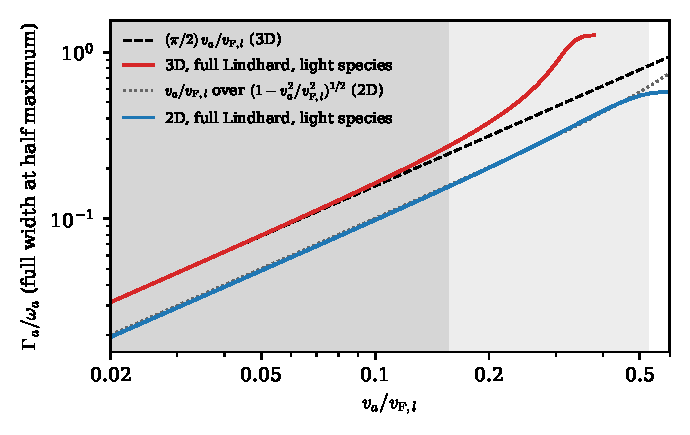
\includegraphics[width=0.82\linewidth]{figures/ch16/limit16_2b.pdf}
\captionof{figure}{Full width at half maximum of the acoustic plasmon over its frequency, against $v_a/v_{\mathrm{F},l}$. Dashed and dotted: \cref{eq:16.2-width} in three and two dimensions. Red and blue: the width of the line in $L = \Imag(-1/\varepsilon)$ with the full frequency dependence of the light carriers' Lindhard function at $q \ll k_{\mathrm{F},l}$. The heavy carriers are cold, and $q = 0.02\,k_{\mathrm{TF},l}$ (3D) and $q_\parallel = 0.02\,q_s$ (2D); the 3D curve stops at $v_a/v_{\mathrm{F},l} = 0.4$, beyond which the line is too broad and asymmetric for a width to be defined. Dark gray: the 3D form within \SI{10}{\percent}, $v_a/v_{\mathrm{F},l} < 0.157$; light gray: the 2D form within \SI{10}{\percent}, $v_a/v_{\mathrm{F},l} < 0.53$. At $v_a/v_{\mathrm{F},l} = 0.02$ the 2D width is \SI{3}{\percent} below its formula because of the finite $q_\parallel/q_s$.}\label{fig:16-demon-limit}
\par}
\smallskip
Beyond the shaded region the light carriers no longer screen statically, the line broadens into their continuum, in three dimensions with a long tail toward high frequency, and the width stops being a small correction to a sharp mode.
\end{limitbox}

\begin{workedexample}{The acoustic plasmon of a two-band sheet}\label{we:16-demon}
Take a sheet suspended in vacuum with two parabolic, spin-degenerate bands of areal density $\nd_{\mathrm{2D}} = \SI{1.0e13}{cm^{-2}}$ each, and masses $m_l = 0.2\,m_e$ and $m_h = 4.0\,m_e$, model values chosen to show the mode. Both bands have $k_{\mathrm{F}} = (2\pi\nd_{\mathrm{2D}})^{1/2} = \SI{156.4}{eV}$ (\SI{0.793}{nm^{-1}}), so $v_{\mathrm{F},l} = 1.53\times10^{-3}$ and $v_{\mathrm{F},h} = 7.65\times10^{-5}$. With $2\mathcal{N}_{\mathrm{F},l} = m_l/\pi$, the screening wavevector is $q_s = e^2m_l/2\pi = 2\alpha m_l = \SI{1.49}{keV}$.

\emph{Velocity.} $v_a^2 = \nd_{\mathrm{2D}}\pi/(m_hm_l) = k_{\mathrm{F}}^2/(2m_hm_l)$, so $v_a = 2.42\times10^{-4}$, or \SI{72.5}{km.s^{-1}}. The mode lies between the continua: $v_a/v_{\mathrm{F},l} = (m_l/2m_h)^{1/2} = 0.158$ and $v_a/v_{\mathrm{F},h} = 3.16$.

\emph{Frequency and width at $q_\parallel = \SI{20}{eV}$.} Here $q_\parallel/k_{\mathrm{F}} = 0.128$ and $q_\parallel/q_s = 0.0134$. The heavy band alone would oscillate at $\omega_{\mathrm{2D},h} = \SI{41.8}{meV}$; screened, $\omega_a = \omega_{\mathrm{2D},h}(1 + q_s/q_\parallel)^{-1/2} = \SI{4.81}{meV}$. \Cref{eq:16.2-width} gives $\varGamma_a/\omega_a = 0.160$, a width of \SI{0.77}{meV}. Both bands together carry the ordinary sheet plasmon at \SI{191.5}{meV} to leading order (\SI{193}{meV} with the $v_{\mathrm{F}}^2$ term of \cref{eq:16.2-2Dpl}), far above $q_\parallel v_{\mathrm{F},l} = \SI{30.6}{meV}$.

\emph{Weight.} By \cref{eq:16.2-share} the line carries $(q_\parallel/(q_\parallel + q_s))^2 = 1.75\times10^{-4}$ of the heavy band's $f$-sum. The light band's own pair continuum carries about as much in the lower half of its range, below $\tfrac12q_\parallel v_{\mathrm{F},l} = \SI{15.3}{meV}$: $1.72\times10^{-4}$ of the same sum, spread over all energies up to there.

\emph{Check.} Now treat both bands with the two-dimensional Lindhard function at $q_\parallel \ll k_{\mathrm{F}}$, so that the heavy band is no longer assumed cold. The peak of $L$ then sits at \SI{4.97}{meV} with a width of \SI{0.76}{meV} ($\varGamma_a/\omega_a = 0.154$), and the first moment within three widths of the peak is $1.76\times10^{-4}$ of the heavy $f$-sum. The heavy band raises the frequency by \SI{3.5}{\percent}, the size of $\tfrac34(v_{\mathrm{F},h}/v_a)^2 = 0.075$ in $\omega_a^2$.

\emph{Kinematics.} A halo particle deposits \SI{4.81}{meV} if $\mchi \ge 2\omega_a/v_{\mathrm{max}}^2 = \SI{1.37}{keV}$, and supplies $q_\parallel = \SI{20}{eV}$ if $2\mchi v_{\mathrm{max}} \ge \SI{20}{eV}$, or $\mchi \ge \SI{3.8}{keV}$. The energy needs a total momentum of only $\omega_a/v_{\mathrm{max}} = \SI{1.8}{eV}$, and the in-plane \SI{20}{eV} decides. The mode, eleven times slower than the fastest halo particles, is reachable by keV-mass dark matter. Its weight, however, is four orders of magnitude below that of the heavy band: a density coupling scatters off this sheet mostly through the pair continuum and the optical plasmon, not through the acoustic one.
\end{workedexample}

\subsection{Layered stacks}\label{sec:16.2-stacks}

A stack of identical sheets with period $a_s$ in a background $\varepsilon_b$, with no tunneling between them, is the simplest layered target. The sheets interact, and \cref{eq:16.2-embed} no longer applies. A density wave $\delta\nd_{\mathrm{2D}}\,\ee^{\ii\vect{q}_\parallel\cdot\vect{r}_\parallel}$ on sheet $n$, with the phase $\ee^{\ii q_zna_s}$ of the external potential, produces $(e^2/2\varepsilon_bq_\parallel)\ee^{-q_\parallel|z - na_s|}$ at height $z$, and the sum over sheets at $z = 0$ is a geometric series. Each sheet therefore sees the kernel
\begin{gather}
  v_{\mathrm{C}}^{\mathrm{L}}(q_\parallel,q_z) = \frac{e^2}{2\varepsilon_bq_\parallel}\sum_n\ee^{-q_\parallel|n|a_s + \ii q_zna_s} = \frac{e^2}{2\varepsilon_bq_\parallel}\,\frac{\sinh q_\parallel a_s}{\cosh q_\parallel a_s - \cos q_za_s} , \notag \\
  S(\vect{q},\omega) = -\frac{2}{a_s}\,\Imag\frac{\tilde R^{\mathrm{2D}}}{1 - v_{\mathrm{C}}^{\mathrm{L}}\tilde R^{\mathrm{2D}}} ,
  \label{eq:16.2-sheets}
\end{gather}
at $T = 0$, per unit volume, for sheets thinner than $1/q$, with the background treated as a static dielectric. For $a_s \to \infty$ the kernel becomes that of an isolated sheet, and $S$ is $1/a_s$ times its structure factor. For $q_\parallel a_s, q_za_s \ll 1$ it becomes $e^2/(\varepsilon_ba_sq^2)$, the bulk kernel acting on the density $\nd_{\mathrm{2D}}/a_s$. In between, the stack carries a band of layer plasmons. For parabolic sheets, $\omega^2 = v_{\mathrm{C}}^{\mathrm{L}}\nd_{\mathrm{2D}}q_\parallel^2/m^*$ runs at small $q_\parallel$ from the bulk plasma frequency of the density $\nd_{\mathrm{2D}}/a_s$ at $q_z = 0$, where all sheets oscillate in phase, down to the acoustic mode $\omega^2 = e^2\nd_{\mathrm{2D}}a_sq_\parallel^2/4\varepsilon_bm^*$ at $q_za_s = \pi$, where neighbors oscillate against each other. The dark-matter momentum along the axis is not reduced to a zone, since the sheets have no structure on the scale of $1/q$; $S$ is periodic in $q_z$ with period $2\pi/a_s$ until the profile of a sheet cuts it off.

Layers many atoms thick respond through their own local dielectric functions. Take layers of materials A and B, of thicknesses $d_A$ and $d_B = a_s - d_A$, filling $f = d_A/a_s$, and local dielectric functions $\varepsilon_A(\omega)$, $\varepsilon_B(\omega)$. When the wavelength is long compared with $a_s$, the field within one period is that of a uniform field across planar boundaries. The tangential field is continuous, so the in-plane displacement is the volume average of $\varepsilon$; the normal displacement is continuous, so the normal field is the volume average of $1/\varepsilon$. The stack is a uniaxial medium with its optic axis along the stacking direction, and with $\theta$ the angle between $\vect{k}$ and that axis,
\begin{gather}
  \varepsilon_\perp = f\varepsilon_A + (1 - f)\,\varepsilon_B , \qquad
  \frac{1}{\varepsilon_\parallel} = \frac{f}{\varepsilon_A} + \frac{1 - f}{\varepsilon_B} , \notag \\
  L(\vect{k},\omega) = \Imag\frac{-1}{\varepsilon_\parallel\cos^2\theta + \varepsilon_\perp\sin^2\theta} \qquad (ka_s \to 0) .
  \label{eq:16.2-emt}
\end{gather}
Since $\varepsilon_\parallel = \varepsilon_A\varepsilon_B/[(1 - f)\varepsilon_A + f\varepsilon_B]$ and $\varepsilon_\perp[(1 - f)\varepsilon_A + f\varepsilon_B] = \varepsilon_A\varepsilon_B + f(1 - f)(\varepsilon_A - \varepsilon_B)^2$, the inverse $1/(\varepsilon_\parallel\cos^2\theta + \varepsilon_\perp\sin^2\theta)$ equals $[(1 - f)\varepsilon_A + f\varepsilon_B]/[\varepsilon_A\varepsilon_B + f(1 - f)(\varepsilon_A - \varepsilon_B)^2\sin^2\theta]$. This is identical, at every filling, to the effective longitudinal response of Lasenby and Prabhu~\cite[Eq.~(16)]{lasenby2022dark}, which they state for $d_A/a_s \ll 1$. The loss function has one line in each direction, at the zero of the denominator. For metal layers in vacuum the line falls toward zero frequency as $\vect{k}$ approaches the axis: with $\varepsilon_A = \varepsilon_\infty(1 - \omega_p^2/\omega^2)$ and small $\theta$ and $f$ it sits at $\omega^2 \simeq f\varepsilon_\infty\omega_p^2\theta^2/\varepsilon_B$, the filling fraction times the plasma frequency squared, reduced by the direction~\cite{lasenby2022dark}.

For $\vect{k}$ in the plane of the layers the response is known in closed form at every $ka_s$. The source $\ee^{\ii kz}$ is uniform across the layers, and the potential is $\psi(x)\ee^{\ii kz}$ with $x$ along the axis. Inside layer $j$ it is the particular solution $1/\varepsilon_jk^2$ plus $C_j\cosh[k(x - x_j)]$, symmetric about the center $x_j$ of the layer. Continuity of $\psi$ and of $\varepsilon\,\partial_x\psi$ at an interface fixes $C_A = (\varepsilon_A - \varepsilon_B)s_B/[k^2\varepsilon_A(\varepsilon_Bs_Bc_A + \varepsilon_As_Ac_B)]$ and $C_B = -\varepsilon_As_AC_A/\varepsilon_Bs_B$, with $s_j = \sinh(kd_j/2)$ and $c_j = \cosh(kd_j/2)$. The average of $k^2\psi$ over a period is the head of $\varepsilon^{-1}$ at the external wavevector:
\begin{keyresult}[Stack of two dielectrics, $\vect{k}$ in the plane]
\begin{equation}
  \frac{1}{\varepsilon(k,\omega)} = \frac{f}{\varepsilon_A} + \frac{1 - f}{\varepsilon_B} - \frac{2}{ka_s}\,\frac{(\varepsilon_A - \varepsilon_B)^2\,s_As_B}{\varepsilon_A\varepsilon_B\,(\varepsilon_As_Ac_B + \varepsilon_Bs_Bc_A)} ,
  \label{eq:16.2-inplane}
\end{equation}
with $L = \Imag[-1/\varepsilon]$, exact for local $\varepsilon_A$, $\varepsilon_B$ at any $ka_s$.
\end{keyresult}
\noindent At $ka_s \to 0$, $s_j \to kd_j/2$, $c_j \to 1$, and the right side becomes $1/\varepsilon_\perp$, the in-plane limit of \cref{eq:16.2-emt}. Expanding to the next order,
\begin{equation}
  \frac{1}{\varepsilon(k,\omega)} = \frac{1}{\varepsilon_\perp} + (ka_s)^2\,\frac{f^2(1 - f)^2(\varepsilon_A - \varepsilon_B)^2}{12\,\varepsilon_\parallel\,\varepsilon_\perp^2} + O\bigl((ka_s)^4\bigr) .
  \label{eq:16.2-corr}
\end{equation}
The correction is quadratic in the period over the wavelength and grows with the contrast between the layers. At $ka_s \to \infty$, $s_j/c_j \to 1$ and the response is the volume average of $1/\varepsilon_j$: each layer then screens as its own bulk. One layer alone follows for $d_B \to \infty$ with $\varepsilon_B = 1$. Multiplied by $a_s$, $\varepsilon^{-1} - 1$ becomes the response per unit area, $d_A(1/\varepsilon_A - 1) - 2(\varepsilon_A - 1)^2s_A/[k\varepsilon_A(\varepsilon_As_A + c_A)]$, and minus this equals the thin-film response of Lasenby and Prabhu up to the real constant $d_A$, which does not enter the loss~\cite[Eq.~(19)]{lasenby2022dark}: the constant is the vacuum term that their response, normalized to $-d/\varepsilon$ for a bulk slab, does not subtract. Its line sits at $\varepsilon_A = -\coth(kd_A/2)$; for a Drude metal at $kd_A \ll 1$ that is $\omega^2 = \omega_p^2kd_A/2$, the sheet plasmon of \cref{eq:16.2-2Dpl} with $\nd_{\mathrm{2D}} = \nd_ed_A$ in vacuum. With $|\varepsilon_A| \gg 1$ and $kd_A \ll 1$ the same expression reduces to the sheet screening of \cref{eq:15.3-sheet}. For a general direction the same matching, with the Bloch condition $\psi(x + a_s) = \ee^{\ii k_xa_s}\psi(x)$ across one period, gives $\varepsilon^{-1}$ by solving four linear equations; it also approaches \cref{eq:16.2-emt} at small $ka_s$.

\begin{limitbox}[Effective medium of a layered stack][lim:16.2c]
For $ka_s \to 0$ a stack of layers with local $\varepsilon_A$, $\varepsilon_B$ and filling $f$ has $1/\varepsilon_L = [(1 - f)\varepsilon_A + f\varepsilon_B]/[\varepsilon_A\varepsilon_B + f(1 - f)(\varepsilon_A - \varepsilon_B)^2\sin^2\theta]$, $\theta$ measured from the stacking axis~\cite[Eq.~(16)]{lasenby2022dark}.
\par\smallskip
{\centering
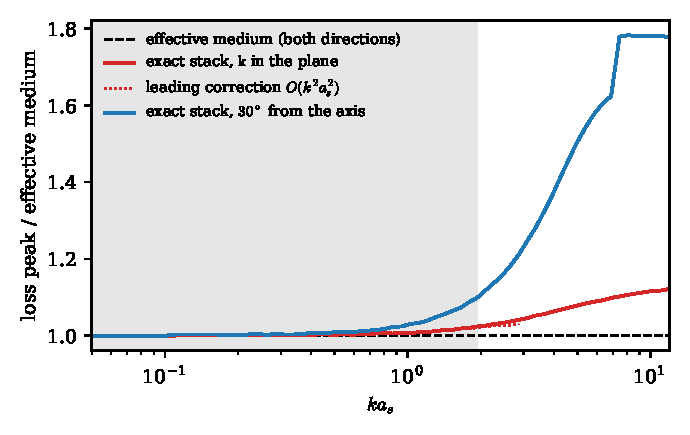
\includegraphics[width=0.82\linewidth]{figures/ch16/limit16_2c.pdf}
\captionof{figure}{Frequency of the loss peak of a model stack relative to the effective medium, against $ka_s$. Layers of \SI{1}{nm} with $\varepsilon_A = 10[1 - \omega_p^2/\omega(\omega + \ii\gamma)]$, $\omega_p = \SI{0.5}{eV}$, $\gamma = 0.1\,\omega_p$, alternate with \SI{4}{nm} of vacuum ($a_s = \SI{5}{nm}$, $f = 0.2$), the toy stack of Lasenby and Prabhu. Red: $\vect{k}$ in the plane, exact (\cref{eq:16.2-inplane}); dotted, the leading correction \cref{eq:16.2-corr}. Blue: $\vect{k}$ at \SI{30}{\degree} from the axis, exact solution of the periodic stack. The effective-medium peaks are at 0.4215 and \SI{0.2740}{eV}. Gray: both within \SI{10}{\percent} of the effective medium, $ka_s < 1.94$. At $ka_s = 12$ the peaks are at 0.473 and \SI{0.487}{eV}, near the surface plasmon of a single layer, $\varepsilon_A = -\varepsilon_B$ (\SI{0.477}{eV} without damping).}\label{fig:16-stack-limit}
\par}
\smallskip
Beyond $ka_s \approx 2$ the field varies within a period, the line of an oblique direction moves up by tens of percent toward that of a single layer, and the stack must be treated layer by layer.
\end{limitbox}

A single undamped line in each direction is the case in which the sum-rule bound of \cref{sec:10.2} can be reached. For $L = A\,\delta(\omega - \omega_{\vect{k}})$ every moment is $K_n = A\omega_{\vect{k}}^n$, and the Hölder inequality behind \cref{eq:10.2-Kn} holds as an equality; the bound \cref{eq:10.2-bound} is then attained when the line sits where $\omega^{-n}\eta$ is largest. A bulk metal places its line at $\omega_p$, far above what light dark matter deposits. A stack moves it down by the filling fraction and the direction, which is why Lasenby and Prabhu proposed it~\cite{lasenby2022dark}. For the model stack of the limit check, \SI{10}{\percent} accuracy at \SI{30}{\degree} ends at $k = \SI{77}{eV}$, the largest momentum transfer, $2\mchi v_{\mathrm{max}}$, of a particle of \SI{14.5}{keV}. Heavier dark matter probes the stack at momenta where the field varies within a period, and needs the full periodic response, with $q_z$ unreduced, that \cref{app:E.21} specifies, and at $k \gtrsim 1/d_A$ also the nonlocal response $\varepsilon_A(\vect{k},\omega)$ of the layer material itself.

\section{Graphene, nanotubes and quantum dots}\label{sec:16.3}

An electron of a graphene sheet that receives more than the work function, about \SI{4.3}{eV}, can leave the sheet without meeting another atom. It then carries into the vacuum the direction and the energy the dark matter gave it, and both can be measured. A bulk crystal turns the same deposit into a cascade of secondary pairs and phonons, and the direction is lost. Carbon nanotubes keep the one-atom thickness and roll the sheet into a cylinder of radius $r_{\mathrm{t}}$. Rolling the sheet quantizes the momentum around the tube and opens a gap in most nanotubes. Quantum dots, nanocrystals a few nanometers across, push confinement to all three directions: a lead sulfide dot \SI{3.3}{nm} across has an optical gap of \SI{1.2}{eV}, against \SI{0.41}{eV} for the bulk crystal, and it re-emits the energy of a pair as a photon~\cite{blanco2023dark}.

\subsection{Electron ejection into vacuum}\label{sec:16.3-ejection}

Take an electron in band $i$ with in-plane crystal momentum $\vect{k}_\parallel$, bound by $E_B(i,\vect{k}_\parallel) \ge 0$ below the Fermi level. It leaves with kinetic energy $E_{\mathrm{ej}} = p_{\mathrm{ej}}^2/2m_e$ when the dark matter deposits
\begin{equation}
  \omega = E_{\mathrm{ej}} + \Phi_{\mathrm{wf}} + E_B(i,\vect{k}_\parallel) ,
  \label{eq:16.3-omega}
\end{equation}
with $\Phi_{\mathrm{wf}}$ the work function, the energy from the Fermi level to the vacuum. For graphene $\Phi_{\mathrm{wf}} \simeq \SI{4.3}{eV}$, and it can be moved by the choice of substrate~\cite[text after Eq.~(5) and footnote~2]{hochberg2017directional}. The largest energy a particle can deposit is its kinetic energy, $\mchi v_{\mathrm{max}}^2/2$, so ejection starts at $\mchi = 2\Phi_{\mathrm{wf}}/v_{\mathrm{max}}^2 = \SI{1.22}{MeV}$, at a momentum transfer of at least $\Phi_{\mathrm{wf}}/v_{\mathrm{max}} = \SI{1.62}{keV}$. This minimum momentum transfer is already a fifth of the momentum scale of a carbon $2p$ orbital, $\beta = Z_{\mathrm{eff}}/2a_0 = \SI{7.51}{keV}$ for the hydrogenic orbital with $Z_{\mathrm{eff}} = 4.03$ that Hochberg et al.\ fit to the overlap of neighboring orbitals~\cite[Eq.~(2)]{hochberg2017directional}. Ejection probes the short-distance structure of the orbitals, as atomic ionization does (\cref{sec:2.2}), and not their tails.

In the independent-particle picture the initial states are the occupied Bloch states $\psi_{i\vect{k}_\parallel}$ of the $\pi$ band and the three $\sigma$ bands, normalized over the sample, and each final state is a hole in the sheet with a free electron. We take the free electron as a plane wave $\ee^{\ii\vect{p}\cdot\vect{r}}/\Vol^{1/2}$ of momentum $\vect{p}$, $|\vect{p}| = p_{\mathrm{ej}}$. Its transition form factor \cref{eq:2.2-ff} is the momentum-space wavefunction of the initial state, $M_{\mathrm{PW}}(\vect{p},\vect{q}) = \tilde\psi_{i\vect{k}_\parallel}(\vect{p} - \vect{q})$, and the structure factor of \cref{eq:4.2-Sab} becomes
\begin{equation}
  S_{\mathrm{ej}}(\vect{q},\omega) = \frac{2\pi}{\Vol}\sum_{i,\vect{k}_\parallel,\sigma}\int\frac{\dd^3p}{(2\pi)^3}\,|M(\vect{p},\vect{q})|^2\,\delta\bigl(\omega - E_{\mathrm{ej}} - \Phi_{\mathrm{wf}} - E_B(i,\vect{k}_\parallel)\bigr) ,
  \label{eq:16.3-Sej}
\end{equation}
with $M = M_{\mathrm{PW}}$ for plane waves and $\sigma$ the spin. Only energy is conserved. Since the bound state is not a momentum eigenstate, it supplies whatever part of $\vect{q}$ the electron does not leave with, and $\vect{p}$ and $\vect{q}$ are independent variables. Inserting \cref{eq:16.3-Sej} and $|\tilde V|^2 = \pi\sigmae\FDM^2/\mu_{\chi e}^2$ (\cref{eq:1.4-Vsq}) into \cref{eq:8.2-spectrum}, with $\rho_T\Vol = N_{\mathrm{cell}}M_{\mathrm{cell}}$, the factors $2\pi\cdot\pi/(2\pi)^3$ combine into $1/4\pi$, and the rate per unit mass is a sum of cross-sections, one for each occupied state:
\begin{equation}
  \begin{gathered}
  \mathcal{R} = \frac{\rho_\chi}{\mchi\,N_{\mathrm{cell}}M_{\mathrm{cell}}}\sum_{i,\vect{k}_\parallel,\sigma}\int\dd^3v\,f_\chi(\vect{v})\,\langle\sigma v\rangle_{i\vect{k}_\parallel}(\vect{v}) ,\\
  \langle\sigma v\rangle_{i\vect{k}_\parallel} = \frac{\sigmae}{\mu_{\chi e}^2}\int\frac{\dd^3p}{(2\pi)^3}\int\frac{\dd^3q}{4\pi}\,\FDM(q)^2\,|M(\vect{p},\vect{q})|^2\,\delta\Bigl(E_{\mathrm{ej}} + \Phi_{\mathrm{wf}} + E_B + \frac{q^2}{2\mchi} - \vect{q}\cdot\vect{v}\Bigr) .
  \end{gathered}
  \label{eq:16.3-rate}
\end{equation}
For plane waves the cross-section is that of Hochberg et al.~\cite[Eq.~(5)]{hochberg2017directional}. They write the sum over states as $2N_{\mathrm{C}}A_{\mathrm{cell}}\int\dd^2k_\parallel/(2\pi)^2$ per band, with $N_{\mathrm{C}}$ the number of carbon atoms per unit mass and $A_{\mathrm{cell}}$ the area of the unit cell. They take for $\tilde\psi$ the tight-binding function of one atom and its three nearest neighbors~\cite[Eqs.~(1), (3), (7)]{hochberg2017directional}. A nanotube changes only the sum over states. Going once around the tube must return the Bloch phase, so the momentum around the circumference takes the values $n/r_{\mathrm{t}}$. Then $A_{\mathrm{cell}}\int\dd^2k_\parallel/(2\pi)^2$ becomes $(A_{\mathrm{cell}}/2\pi r_{\mathrm{t}})\sum_n\int\dd k_z/2\pi$, with $k_z$ along the axis; with this sum over states, \cref{eq:16.3-rate} is the rate of Cavoto et al.~\cite[Eqs.~(16)--(18), (23)]{cavoto2018sub}.

With Bloch states, the in-plane part of $\vect{p} - \vect{q}$ is fixed up to a reciprocal-lattice vector by the crystal momentum of the hole. A Bloch state normalized over $N_{\mathrm{cell}}$ cells has $|\tilde\psi_{i\vect{k}_\parallel}(\vect{k})|^2 \propto \sum_{\vect{G}}\delta^2(\vect{k}_\parallel' - \vect{k}_\parallel - \vect{G})$, with $\vect{k}_\parallel'$ the in-plane part of $\vect{k}$. As a result, each direction of the ejected electron selects one state of each band, with its own binding energy. The selection of one state per band is the origin of the diffraction pattern that Hochberg et al.\ find in the angular distribution of electrons ejected by a cold stream~\cite[Sect.~III]{hochberg2017directional}. The halo washes the pattern out but keeps the forward peak: the momentum-space orbital is largest when $\vect{p} - \vect{q}$ is small, and the electron leaves close to the direction of $\vect{q}$, which follows the dark-matter velocity. For the standard halo they find the forward rate about twice the backward rate between \SI{10}{MeV} and \SI{10}{GeV}~\cite[Sect.~III]{hochberg2017directional}, and the daily rotation of a fixed sheet modulates both rates.

The orbitals and the binding energies are the material input. They come from a density-functional ground state, with maximally localized Wannier functions for the occupied bands and an all-electron orbital for the carbon 1s shell, which a pseudopotential lacks (\cref{app:E.21}).

\paragraph{Orthogonality of the final state.} A plane wave is not an eigenstate of the sheet, and it is not orthogonal to the state the electron leaves. As $q \to 0$, $M_{\mathrm{PW}}$ tends to $\tilde\psi_{i\vect{k}_\parallel}(\vect{p})$, which is not zero, so plane waves predict ejection with no momentum transfer, although $\ee^{\ii\vect{q}\cdot\vect{r}} \to 1$ cannot connect two orthogonal eigenstates. The cure is to orthogonalize the final state to the occupied states, $|\chi_{\vect{p}}\rangle = |\vect{p}\rangle - \sum_n|\psi_n\rangle\langle\psi_n|\vect{p}\rangle$, the orthogonalized plane wave (OPW). Its transition form factor is
\begin{equation}
  M_{\mathrm{OPW}}(\vect{p},\vect{q}) = \tilde\psi_i(\vect{p} - \vect{q}) - \sum_{n\in\mathrm{occ}}\tilde\psi_n(\vect{p})\,f_{i\to n}(\vect{q}) ,
  \label{eq:16.3-opw}
\end{equation}
with $f_{i\to n}$ the form factor \cref{eq:2.2-ff} between occupied states, here written with a single index for $(i,\vect{k}_\parallel)$. Since $f_{i\to n}(\vect{q}) = \delta_{in} + O(q)$, the term without momentum transfer cancels and $M_{\mathrm{OPW}} = O(q)$. To size the orthogonalization correction we take the hydrogenic $2p_z$ orbital above, $\psi \propto r\ee^{-\beta r}\cos\theta$ with $\tilde\psi(\vect{k}) \propto \beta k_z/(\beta^2 + k^2)^3$~\cite[Eq.~(4)]{hochberg2017directional}, orthogonalize the plane wave to it alone, and average over the orientation of the sheet. Integrated over the directions of the ejected electron, $|M_{\mathrm{OPW}}|^2/|M_{\mathrm{PW}}|^2$ runs from 0.46 to 25 at $E_{\mathrm{ej}} = 50$ to \SI{100}{eV} and $q = 5$ to \SI{40}{keV}. The ratio depends on $q$ and on the angle between $\vect{q}$ and the orbital axis, and an orbital of the same form with the more diffuse exponent $1.568/a_0$ of Clementi and Raimondi gives 0.4 to 4.3. At \SI{10}{eV} it reaches 740, but only at $q \gg p_{\mathrm{ej}}$, where the plane-wave amplitude has already fallen as $|\vect{p} - \vect{q}|^{-5}$ and contributes little. The rate weights each $(\vect{p},\vect{q})$ by the halo, so these ratios bound the correction without giving it.

For an orbital averaged over orientations, $|M|^2$ integrated over the directions of $\vect{p}$ depends only on $p_{\mathrm{ej}}$ and $q$. Call this integral $K(p_{\mathrm{ej}},q)$. The velocity integral of \cref{eq:16.3-rate} then reduces with \cref{eq:A.8-eta}, $\int\dd^3q\,g(q)\int\dd^3v\,f_\chi\,\delta(\cdots) = 2\pi\int q\,\dd q\,\eta(\vmin)\,g(q)$, and $p^2\dd p = m_ep_{\mathrm{ej}}\,\dd E_{\mathrm{ej}}$ gives the spectrum per electron
\begin{equation}
  \frac{\dd\langle\sigma v\rangle}{\dd E_{\mathrm{ej}}} = \frac{\sigmae\,m_e\,p_{\mathrm{ej}}}{16\pi^3\mu_{\chi e}^2}\int q\,\dd q\,\eta\bigl(\vmin(q,\omega)\bigr)\,\FDM(q)^2\,K(p_{\mathrm{ej}},q) ,
  \label{eq:16.3-iso}
\end{equation}
with $\vmin = \omega/q + q/2\mchi$ and $\omega$ from \cref{eq:16.3-omega}. Summed over the electrons of a full atomic shell with plane waves, \cref{eq:16.3-iso} times $E_{\mathrm{ej}}$ is \cref{eq:2.2-ion} with \cref{eq:2.2-fion-pw}. \Cref{fig:16-ejection} applies it to the $\pi$ electrons of graphene, one per atom, with the momentum density of the isolated orbital. Their binding energies are those of the nearest-neighbor band, $E_B = t|1 + \ee^{\ii\vect{k}\cdot\vect{a}_1} + \ee^{\ii\vect{k}\cdot\vect{a}_2}|$ with $\vect{a}_{1,2}$ the primitive vectors and hopping $t = \SI{2.8}{eV}$~\cite[text after Eq.~(5)]{castroneto2009electronic}, spread from 0 to \SI{8.4}{eV} with a mean of \SI{4.41}{eV}. At $\sigmae = \SI{e-37}{cm^2}$ and a heavy mediator the $\pi$ electrons alone give \num{6.9e3} events per kg-year at \SI{10}{MeV} with plane waves and \num{1.0e4} with orthogonalized ones; at \SI{100}{MeV}, \num{2.8e3} and \num{5.2e3}. The orthogonalization raises the rate, by factors of 1.44 and 1.84, and moves the peak of the spectrum up in energy. For a light mediator the factors are only 1.14 and 1.19. The light mediator weights the smallest momentum transfers, a few keV, where the orthogonality term lowers the squared amplitude (to 0.46--0.74 of the plane-wave value at $q = \SI{5}{keV}$ for $E_{\mathrm{ej}} = \SI{50}{eV}$) and so partly cancels the gain at larger $q$.

\begin{figure}[tbp]
  \centering
  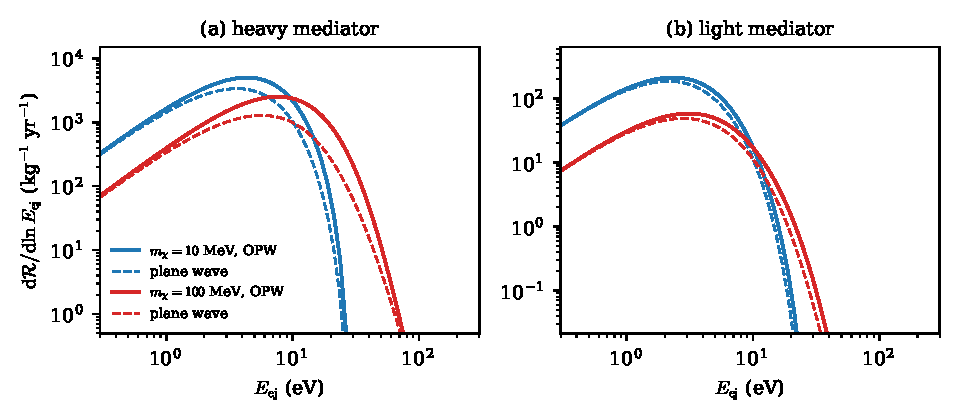
\includegraphics[width=\linewidth]{figures/ch16/fig16_3.pdf}
  \caption{Ejection spectra of the $\pi$ electrons of graphene, $\dd\mathcal{R}/\dd\ln E_{\mathrm{ej}}$ per kg-year at $\sigmae = \SI{e-37}{cm^2}$, against the kinetic energy $E_{\mathrm{ej}}$ of the ejected electron, for $\mchi = \SI{10}{MeV}$ (blue) and \SI{100}{MeV} (red): (a) heavy mediator, $\FDM = 1$; (b) light mediator, $\FDM = (\alpha m_e/q)^2$. Dashed: plane-wave final states; solid: final plane wave orthogonalized to the initial orbital, \cref{eq:16.3-opw}. Model: one hydrogenic $2p_z$ orbital per atom with $Z_{\mathrm{eff}} = 4.03$, Bloch interference between neighbors dropped, binding energies of the nearest-neighbor $\pi$ band ($t = \SI{2.8}{eV}$, 0 to \SI{8.4}{eV}), work function \SI{4.3}{eV}, sheet orientation averaged, standard halo of \cref{tab:1-shm}. The $\sigma$ electrons are not included.}
  \label{fig:16-ejection}
\end{figure}

\begin{limitbox}[Vacuum ejection with plane-wave final states][lim:16.3a]
The ejection rate of a sheet or a tube with plane-wave final states, $M = \tilde\psi_{i\vect{k}_\parallel}(\vect{p} - \vect{q})$ in \cref{eq:16.3-rate}, is the published form~\cites[Eqs.~(5), (7)]{hochberg2017directional}[Eq.~(23)]{cavoto2018sub}.
\par\smallskip
{\centering
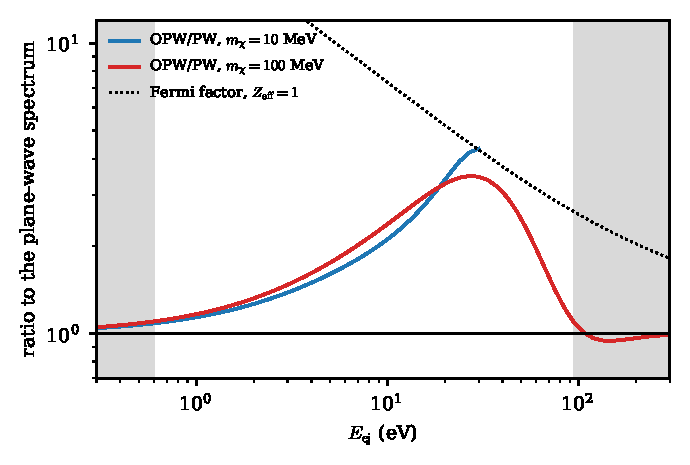
\includegraphics[width=0.85\linewidth]{figures/ch16/limit16_3a.pdf}
\captionof{figure}{Ejection spectrum of graphene $\pi$ electrons with orthogonalized final states, \cref{eq:16.3-opw}, divided by the plane-wave spectrum, against the kinetic energy $E_{\mathrm{ej}}$ of the ejected electron, for $\mchi = \SI{10}{MeV}$ (blue, which ends at \SI{31}{eV}) and \SI{100}{MeV} (red), heavy mediator, in the model of \cref{fig:16-ejection}. Thin line: the plane-wave form. Dotted: the Fermi factor \cref{eq:2.2-fermi} with $Z_{\mathrm{eff}} = 1$, the largest final-state enhancement an unscreened hole can produce. Gray: the orthogonalized spectrum within \SI{10}{\percent} of the plane-wave one, $E_{\mathrm{ej}} < \SI{0.60}{eV}$ and, for \SI{100}{MeV}, $E_{\mathrm{ej}} > \SI{94}{eV}$.}\label{fig:16-limit-ejection}
\par}
\smallskip
Between these energies, where most of the rate lies, orthogonality raises the spectrum by factors up to 3.5 at \SI{100}{MeV} (2.1 at \SI{10}{eV} and 4.3 at the kinematic end for \SI{10}{MeV}), and the attraction of the hole can add up to the Fermi factor, 7.3 at \SI{10}{eV} and 2.6 at \SI{100}{eV}; neither factor is fixed until all occupied orbitals and true scattering states are used.
\end{limitbox}

The second correction to the plane-wave rate is the final-state interaction. The ejected electron leaves a hole behind, and an unscreened point charge would enhance the slow part of the spectrum by the Fermi factor \cref{eq:2.2-fermi}, 7.3, 3.4 and 2.6 at $E_{\mathrm{ej}} = 10$, 50 and \SI{100}{eV}. Graphene screens the hole with its own electrons, and this screening pushes the factor toward one, and the ejected electron travels only atomic distances near the nuclei before it is in vacuum; for these two reasons Hochberg et al.\ leave the factor out~\cite[text after Eq.~(6)]{hochberg2017directional}. A semiconducting tube screens less. The two corrections cannot simply be multiplied: an orthogonalized plane wave is not a scattering state of the hole, and multiplying it by a Fermi factor counts part of the same distortion twice. The consistent final state is a scattering state of the sheet's own potential plus the screened hole.

\subsection{Semiconducting nanotubes}\label{sec:16.3-tubes}

Below the work function a tube responds through pairs within its own bands. Rolling the sheet quantizes the momentum around the circumference in steps of $1/r_{\mathrm{t}}$, and the Dirac cones of graphene are cut along lines. A tube is metallic when a line passes through a Dirac point; otherwise the nearest line misses it by a third of the spacing, and the subbands, labeled $n$, are massive Dirac bands in one dimension with half-gaps $\Delta_n = nv_{\mathrm{D}}/3r_{\mathrm{t}}$ for $n = 1, 2$. With the velocity $v_{\mathrm{D}} = \num{3.02e-3}$ of \cref{sec:16.2}, or \SI{9.1e5}{m.s^{-1}}, a tube \SI{1}{nm} across has $2\Delta_1 = \SI{0.80}{eV}$. The edge is reached through momentum across the tube, which the structure factor \cref{eq:16.2-embed} does not see except through $|F_\perp|^2 = J_0(q_\perp r_{\mathrm{t}})^2$. At the edge $q_\parallel = 0$ and $\omega = 2\Delta_n$, and since $q \ge \omega/v_{\mathrm{max}}$ the dark matter needs $q_\perp \ge 2\Delta_n/v_{\mathrm{max}}$, that is $q_\perp r_{\mathrm{t}} \ge 2nv_{\mathrm{D}}/3v_{\mathrm{max}}$, independent of the radius: 0.76 for the first subband, where $J_0^2 = 0.74$, and 1.52 for the second, where $J_0^2 = 0.25$. For a \SI{1}{nm} tube the first edge opens at $\mchi = 4\Delta_1/v_{\mathrm{max}}^2 = \SI{226}{keV}$.

Each subband pair is $h = v_{\mathrm{D}}k\sigma_x + \Delta_n\sigma_z$, the one-dimensional form of \cref{eq:7.3-H}, with $k$ along the axis and $g_{\mathrm{deg}} = 4$ for spin and valley. The interband response per unit length follows from two symmetries before any integral is done. The model is invariant under Lorentz boosts with $v_{\mathrm{D}}$ in place of the speed of light, and its density is the time component of a conserved current. The response then has the form $q_\parallel^2\,\mathfrak{p}(s)$, with $s = \omega^2 - v_{\mathrm{D}}^2q_\parallel^2$ the invariant of \cref{sec:7.3} and $\mathfrak{p}$ a function of $s$ alone, and it is enough to compute the response at small $q_\parallel$. There the pair is made at $\pm k$ with $\omega = 2\varepsilon_k$, $\varepsilon_k = (v_{\mathrm{D}}^2k^2 + \Delta_n^2)^{1/2}$. The spinors of the two bands are rotated by the angle $\theta_k$ with $\tan\theta_k = v_{\mathrm{D}}k/\Delta_n$, and the interband overlap is $|\langle +,k + q_\parallel|-,k\rangle|^2 = \tfrac14(\partial_k\theta_k)^2q_\parallel^2 = q_\parallel^2v_{\mathrm{D}}^2\Delta_n^2/4\varepsilon_k^4$. Inserting it in $-\Imag\tilde R = (g_{\mathrm{deg}}/2)\int\dd k\,|\langle +|-\rangle|^2\,\delta(\omega - \varepsilon_k - \varepsilon_{k+q_\parallel})$, summing the two roots and replacing $\omega^2$ by $s$,
\begin{equation}
  -\Imag\tilde R^{\mathrm{1D}}_n(q_\parallel,\omega) = \frac{2g_{\mathrm{deg}}v_{\mathrm{D}}q_\parallel^2\Delta_n^2}{s^{3/2}\,(s - 4\Delta_n^2)^{1/2}}\,\Theta(s - 4\Delta_n^2) .
  \label{eq:16.3-R1D}
\end{equation}
The inverse square root at $s = 4\Delta_n^2$ is the van Hove singularity of a one-dimensional band edge. The factor multiplying $q_\parallel^2$ integrates to $g_{\mathrm{deg}}v_{\mathrm{D}}$ over $s$, whatever $\Delta_n$; as $\Delta_n \to 0$ it becomes $g_{\mathrm{deg}}v_{\mathrm{D}}\delta(s)$, the single line of the metallic tube in \cref{sec:16.2}.

In the random-phase approximation the subbands are screened together by the tube kernel \cref{eq:16.2-kernel1D}, $\varepsilon_{\mathrm{1D}} = 1 - v_{\mathrm{C}}^{\mathrm{1D}}\sum_n\tilde R^{\mathrm{1D}}_n$, with the real part of $\tilde R^{\mathrm{1D}}_n$ from \cref{eq:16.3-R1D} by the Kramers--Kronig relation (\cref{app:C.5}), and $S_{\mathrm{1D}} = -2\Imag(\sum_n\tilde R^{\mathrm{1D}}_n/\varepsilon_{\mathrm{1D}})$ at $T = 0$ enters \cref{eq:16.2-embed}. At $q_\parallel r_{\mathrm{t}} \gg 1$ the kernel tends to $\alpha/q_\parallel r_{\mathrm{t}}$, which is the sheet kernel $2\pi\alpha/q_\parallel$ of \cref{eq:16.2-kernel2D} (in vacuum) shared over the circumference $2\pi r_{\mathrm{t}}$: at wavelengths shorter than the radius the tube screens like the flat sheet it was rolled from. Two effects lie outside this response. Transitions between subbands of different $n$ carry angular momentum around the tube and enter through the higher azimuthal harmonics of the transverse form factor. And the electron and the hole of a pair attract each other strongly in one dimension; the attraction binds excitons below each edge, moves the weight of the van Hove singularity into the excitons, and is the Bethe--Salpeter correction of \cref{sec:4.9} and \cref{sec:10.5}.

The same response sets the absorption of a dark photon by an array of aligned tubes. As $q_\parallel \to 0$, $v_{\mathrm{C}}^{\mathrm{1D}}\tilde R^{\mathrm{1D}}_n$ vanishes as $q_\parallel^2\ln(1/q_\parallel r_{\mathrm{t}})$: an isolated tube does not screen a uniform field along its axis. Take a dilute array of $\nd_{\mathrm{u}}$ tubes per unit area and a field along the tubes. \Cref{eq:16.2-embed} and $\varepsilon_2 = (e^2/q^2)(-\Imag R)$ then give
\begin{equation}
  \varepsilon_2^{\parallel}(\omega) = 8\pi\alpha\,g_{\mathrm{deg}}v_{\mathrm{D}}\,\nd_{\mathrm{u}}\sum_n\frac{\Delta_n^2}{\omega^3\,(\omega^2 - 4\Delta_n^2)^{1/2}}\,\Theta(\omega - 2\Delta_n) ,
  \label{eq:16.3-eps2}
\end{equation}
and the rate is \cref{eq:10.7-dp} with $L \simeq \varepsilon_2^{\parallel}$, since $|\varepsilon| \simeq 1$ for a dilute array; a randomly polarized field couples with one third of $\varepsilon_2^{\parallel}$. Dividing by the mass density, which is $\nd_{\mathrm{u}}$ times the mass of a tube per unit length, removes the packing, as it did for scattering.

\subsection{Quantum dots}\label{sec:16.3-dots}

A dot of radius $R$ much larger than the lattice constant has a periodic potential locally and a boundary globally. Its states near the band edges are Bloch functions at the edge, $u_\kappa(\vect{r})$ for the valence or conduction band, times envelopes $\psi_{nlm} = R_{nl}(r)Y_{lm}$ that vanish at the surface~\cite[Eqs.~(2)--(4)]{blanco2023dark}. The radial parts are $R_{nl} \propto j_l(\chi_{nl}r/R)$, with $\chi_{nl}$ the $n$th zero of the spherical Bessel function: this is the effective-mass picture of \cref{sec:3.3} in a hard-walled sphere. The levels are $\chi_{nl}^2/2m^*R^2$ for each carrier, and the gap of the dot,
\begin{equation}
  \Delta E_{\mathrm{QD}} = \Eg + \frac{\pi^2}{2R^2}\Bigl(\frac{1}{m_e^*} + \frac{1}{m_h^*}\Bigr) ,
  \label{eq:16.3-gap}
\end{equation}
exceeds the bulk gap by the confinement energy $E_{\mathrm{conf}}$ of the two lowest envelopes~\cite[Eq.~(5)]{blanco2023dark}. The Coulomb attraction of the pair shifts the dot gap by an amount $\sim\alpha/\varepsilon R$, small when $R$ is below the exciton radius $a_x$ of \cref{sec:4.9}, about \SI{20}{nm} in PbS as quoted by Blanco et al.~\cite{blanco2023dark}. For the dots \SI{3.3}{nm} across that they consider, $\Delta E_{\mathrm{QD}} = \SI{1.2}{eV}$ against $\Eg = \SI{0.41}{eV}$, so $E_{\mathrm{conf}} = \SI{0.79}{eV}$, and the electron and the hole are confined independently.

Dots suspended in a solvent or a glass at volume fraction $\varphi_{\mathrm{QD}} \ll 1$ respond independently, and each transition of a dot is screened by its host. A pair moves an electron from a valence envelope $\psi^h$ to a conduction envelope $\psi^e$, and for $q$ small against the inverse lattice constant the matrix element factorizes into the band-edge form factor of one cell times the envelope overlap $\langle\psi^e|\ee^{\ii\vect{q}\cdot\vect{r}}|\psi^h\rangle$. The overlaps obey a closure rule: summed over all conduction envelopes, $\sum_e|\langle\psi^e|\ee^{\ii\vect{q}\cdot\vect{r}}|\psi^h\rangle|^2 = 1$ for every valence envelope. Confinement therefore redistributes the bulk weight in energy without changing its total. When the levels are dense on the scale of the energy resolution, the sum over pairs becomes the joint density of states of the bulk with the gap moved to $\Delta E_{\mathrm{QD}}$, and $S^{\mathrm{QD}} \to \varphi_{\mathrm{QD}}\,S^{\mathrm{bulk}}(\vect{q},\omega)$ with $\Eg \to \Delta E_{\mathrm{QD}}$, the scissor of \cref{sec:10.1}. Blanco et al.\ use this limit for deposits of 2.5 to \SI{10}{eV}, quoting measurements in which the optical response of PbS dots resembles the bulk above about \SI{2.5}{eV}~\cite[Sect.~III\,A]{blanco2023dark}.

The rate per unit mass of dot material follows from \cref{eq:A.8-rateiso}. Blanco et al.\ define the form factor of a dot as $|f_{\mathrm{QD}}(q,\omega)|^2 = \sum_{f}\sum_{i\in\mathrm{cell}}\delta(\omega - E_f + E_i)\,|\langle f|\ee^{\ii\vect{q}\cdot\vect{r}}|i\rangle|^2$, with the initial states of one cell~\cite[Eq.~(10)]{blanco2023dark}; this form factor has the dimension of an inverse energy. The angle-averaged structure factor is then $\bar S = (2\pi/\Omega)\langle|f_{\mathrm{QD}}|^2\rangle$, with $\Omega$ the cell volume and the average taken over the directions of $\vect{q}$. With $\rho_T\Omega = M_{\mathrm{cell}}$,
\begin{equation}
  \frac{\dd\mathcal{R}}{\dd\ln\omega} = \frac{\omega\,\rho_\chi\,\sigmae}{2\mchi\,M_{\mathrm{cell}}\,\mu_{\chi e}^2}\int q\,\dd q\,\eta\bigl(\vmin(q,\omega)\bigr)\,\FDM(q)^2\,\langle|f_{\mathrm{QD}}(q,\omega)|^2\rangle .
  \label{eq:16.3-qdrate}
\end{equation}
In the bulk limit $2\pi\langle|f_{\mathrm{QD}}|^2\rangle = 4\pi\alpha m_e^2|f_{\mathrm{crys}}|^2/q^3$ by \cref{eq:10.1-fcrys}, and \cref{eq:16.3-qdrate} becomes $\omega$ times the isotropic rate \cref{eq:10.1-rateiso} with the scissored gap, the form their numerical rates use through the bulk code of Ref.~\cite{essig2016direct}.

\begin{limitbox}[Quantum-dot rate and its bulk limit][lim:16.3b]
The scattering rate of quantum dots is \cref{eq:16.3-qdrate} with the bulk crystal form factor and the gap moved to the dot gap, $|f_{\mathrm{crys}}(q,\omega;\Eg \to \Delta E_{\mathrm{QD}})|^2$ of \cref{eq:10.1-fcrys} in \cref{eq:10.1-rateiso}~\cite[Eqs.~(6), (10)--(12)]{blanco2023dark}.
\par\smallskip
{\centering
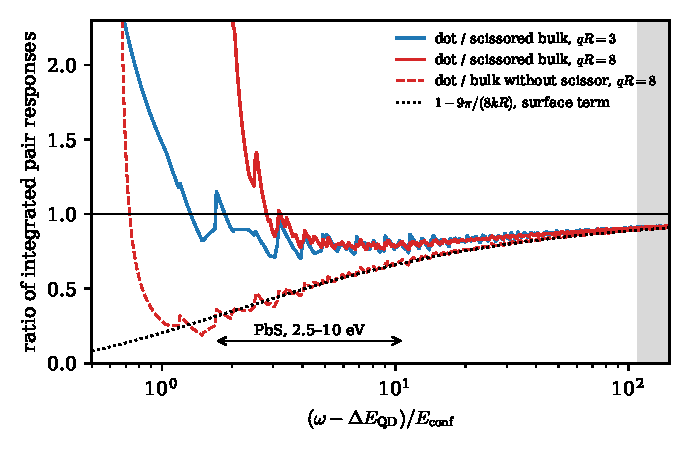
\includegraphics[width=0.85\linewidth]{figures/ch16/limit16_3b.pdf}
\captionof{figure}{Pair response of a hard-walled spherical dot, integrated from its gap up to $\omega$, divided by the same integral of the bulk response with the scissored gap, against $(\omega - \Delta E_{\mathrm{QD}})/E_{\mathrm{conf}}$, for $qR = 3$ (blue) and 8 (red). Model: envelopes of \cref{eq:16.3-gap}, equal electron and hole masses, the band-edge cell factor common to dot and bulk; the direction of $\vect{q}$ averaged. Dashed: the bulk without the scissor at $qR = 8$. Dotted: $1 - 9\pi/(8kR)$, the surface term of the level count of a sphere at $q \to 0$, with $k$ the envelope momentum. Arrow: the range of deposits of PbS dots \SI{3.3}{nm} across, 2.5 to \SI{10}{eV} with $E_{\mathrm{conf}} = \SI{0.79}{eV}$ ($qR \ge 7.5$ there). Gray: the ratios for $qR = 3$ and 8 both within \SI{10}{\percent} of one, above 109 confinement energies ($kR \ge 33$).}\label{fig:16-limit-qd}
\par}
\smallskip
Between 3 and 11 confinement energies above the gap, 3.6 to \SI{10}{eV} for these dots, the hard wall removes states near the surface and the dot carries 0.76 to 1.03 of the scissored bulk response at $qR = 8$ (0.70 to 0.97 at $qR = 3$). The deficit relative to the scissored bulk is set by $kR$ and not by $qR$. Nearer the gap the discrete levels dominate the cumulative ratio, which reaches 2.4 to 66 at $qR = 8$.
\end{limitbox}

The deficit comes from the surface. A wavefunction that must vanish at the surface is depleted within about a wavelength of it, and the number of levels of a sphere below momentum $k$ is $Vk^3/6\pi^2 - Sk^2/16\pi$, with $V$ and $S$ its volume and surface. The second term removes the fraction $9\pi/8kR$ of the bulk count, and the scissor, which shifts the bulk by a fixed energy, corrects only at order $1/(kR)^2$. Between 3 and 11 confinement energies above the gap the model lies 15 to \SI{30}{\percent} below the scissored bulk over most of the range. A real dot has surface atoms and ligands with states of their own, and its wall is not infinitely high. For a real dot the hard wall therefore overstates the depletion, and the measured bulk-like optical response above \SI{2.5}{eV} points to a smaller depletion.

\paragraph{Absorption and the depolarization factor.} A dark photon of mass $m_\phi$ near the dot gap has a reduced wavelength $1/m_\phi v$ of about \SI{0.2}{mm} at \SI{1}{eV}. Over a dot the dark-photon field is uniform, and a dot in a host is a dielectric sphere in a uniform field. Inside, the potential is $-E_{\mathrm{in}}r\cos\theta$; outside it is $-E_0r\cos\theta$ plus a dipole term $\propto\cos\theta/r^2$. Continuity of the potential and of $\varepsilon\,\partial_r\phi$ at $r = R$ gives $E_{\mathrm{in}} = 3\varepsilon_{\mathrm{out}}E_0/(\varepsilon_{\mathrm{in}} + 2\varepsilon_{\mathrm{out}})$, with $\varepsilon_{\mathrm{in}}$ and $\varepsilon_{\mathrm{out}}$ the dielectric functions of the dot and of the host at $\omega = m_\phi$. The polarization of a dilute set of these dielectric spheres gives the Maxwell Garnett dielectric function $\varepsilon_{\mathrm{eff}} = \varepsilon_{\mathrm{out}}[1 + 3\varphi_{\mathrm{QD}}b/(1 - \varphi_{\mathrm{QD}}b)]$, $b = (\varepsilon_{\mathrm{in}} - \varepsilon_{\mathrm{out}})/(\varepsilon_{\mathrm{in}} + 2\varepsilon_{\mathrm{out}})$. To first order in $\varphi_{\mathrm{QD}}$ and for a real $\varepsilon_{\mathrm{out}}$, $\Imag(-1/\varepsilon_{\mathrm{eff}}) = (3\varphi_{\mathrm{QD}}/\varepsilon_{\mathrm{out}})\Imag b = 9\varphi_{\mathrm{QD}}\Imag\varepsilon_{\mathrm{in}}/|\varepsilon_{\mathrm{in}} + 2\varepsilon_{\mathrm{out}}|^2$, the loss function that enters \cref{eq:10.7-dp}. Per unit mass of dot material this loss function replaces the bulk loss function $\Imag\varepsilon_{\mathrm{in}}/|\varepsilon_{\mathrm{in}}|^2$ that a rescaling of the measured photon cross-section with the dot's own $\varepsilon$ uses~\cite[Eq.~(16)]{blanco2023dark}. The two loss functions differ by the depolarization factor
\begin{equation}
  \frac{9\,|\varepsilon_{\mathrm{in}}|^2}{|\varepsilon_{\mathrm{in}} + 2\varepsilon_{\mathrm{out}}|^2} > 1 \iff |\varepsilon_{\mathrm{in}}|^2 > \frac{\varepsilon_{\mathrm{out}}}{2}\,\bigl(\Real\varepsilon_{\mathrm{in}} + \varepsilon_{\mathrm{out}}\bigr) .
  \label{eq:16.3-depol}
\end{equation}
The criterion follows from expanding $|\varepsilon_{\mathrm{in}} + 2\varepsilon_{\mathrm{out}}|^2 = |\varepsilon_{\mathrm{in}}|^2 + 4\varepsilon_{\mathrm{out}}\Real\varepsilon_{\mathrm{in}} + 4\varepsilon_{\mathrm{out}}^2$. The factor tends to 9 when $|\varepsilon_{\mathrm{in}}| \gg \varepsilon_{\mathrm{out}}$, equals one when dot and host are the same medium, and falls below one when $|\varepsilon_{\mathrm{in}}|$ is of order one; for a real $\varepsilon_{\mathrm{in}}$ it exceeds one exactly when $\varepsilon_{\mathrm{in}} > \varepsilon_{\mathrm{out}}$.

\begin{workedexample}{The depolarization factor of a PbS dot in a glass}\label{we:16-depol}
Take a PbS dot in fused silica. Below the bulk gap, at \SI{3.5}{\micro m} (\SI{0.354}{eV}), the dispersion formula of Zemel et al.~\cite{zemel1965electrical} gives $\varepsilon_{\mathrm{in}} = 17.63$, real, and Malitson's fit for silica~\cite{malitson1965interspecimen} gives $\varepsilon_{\mathrm{out}} = 1.977$, both as tabulated in Ref.~\cite{polyanskiy2024refractiveindex}. The field inside the dot is $3\varepsilon_{\mathrm{out}}/(\varepsilon_{\mathrm{in}} + 2\varepsilon_{\mathrm{out}}) = 0.275$ of the field in the glass, against $1/\varepsilon_{\mathrm{in}} = 0.0567$ in bulk PbS, and the depolarization factor is
\begin{equation*}
  \frac{9 \times 17.63^2}{(17.63 + 2\times1.977)^2} = 6.00 .
\end{equation*}
The factor depends little on the exact value of $\varepsilon_{\mathrm{in}}$: $\Real\varepsilon_{\mathrm{in}} = 10$ gives 4.62 and 25 gives 6.71. Wherever $|\varepsilon_{\mathrm{in}}|$ is large, as near the absorption edge of a dot, the bulk formula therefore underestimates the absorption rate by a factor of 4.6 to 6.7. At \SI{5}{eV} silica has $\varepsilon_{\mathrm{out}} = 2.276$. If $\varepsilon_{\mathrm{in}}$ there were $1 + \ii$, an illustrative value near one, the factor would be 0.566, and the bulk formula would overestimate the rate; for $\varepsilon_{\mathrm{in}} = 3 + 3\ii$ it would be 2.45.
\end{workedexample}

Over 2.5 to \SI{10}{eV}, the range of Blanco et al., it is not known whether the depolarization factor is above or below one. The size and even the sign of the depolarization correction need the dielectric function $\varepsilon_{\mathrm{in}}(\omega)$ of real dots of the size used, measured or computed. With it, \cref{eq:16.3-depol} is a one-line evaluation.

\section{Molecular crystals}\label{sec:16.4}

Anthracene, C$_{14}$H$_{10}$, is three benzene rings fused in a row. Its molecules stack in a monoclinic crystal, two to a cell, and the crystal keeps much of the molecule's spectrum: the lowest singlet absorption lies at \SI{3.1}{eV} in the crystal against \SI{3.5}{eV} in the gas~\cite[Tables~I and~III]{rangel2016structural}. A particle must carry $2\times\SI{3.1}{eV}/v_{\mathrm{max}}^2 = \SI{0.883}{MeV}$ to make this excitation (\cref{eq:1.3-mmin}), and an organic crystal turns a large fraction of its singlet excitations into scintillation photons that a photodetector can count, at least 63 percent of them in trans-stilbene~\cite[Sect.~IV\,B]{blanco2021dark}. The electrons that dark matter excites near threshold are in $\pi$ orbitals perpendicular to the flat molecule, and all molecules of the crystal point along two directions, so the rate depends on the angle at which the dark-matter wind meets the molecular planes, and this angle turns with the Earth. The excited electron stays on its molecule, bound to the hole it left: an excitation that stays on one molecule is a \emph{Frenkel exciton}. (The vacancy--interstitial pair of \cref{sec:7.4} is an unrelated object of the same name.)

\subsection{Molecular-basis Bethe--Salpeter equation}\label{sec:16.4-bse}

\Cref{eq:4.9-bse} holds in any basis of electron--hole pairs, and for a molecular crystal the natural one is localized. Combine the occupied Bloch states into orbitals $\phi_{v\mathfrak{o}}$ centered on molecule $\mathfrak{o}$, and the empty ones into orbitals $\phi_{c\mathfrak{o}}$, where $\mathfrak{o} = 1,\dots,N_{\mathrm{mol}}$ labels the molecules of the cell at positions $\vect{r}_{\mathfrak{o}}$ and the cell index is kept implicit. A pair is then an electron in $\phi_{c\mathfrak{o}'}$ and a hole in $\phi_{v\mathfrak{o}}$. If $\mathfrak{o}' = \mathfrak{o}$ the electron stays on the molecule where the hole is; if $\mathfrak{o}' \ne \mathfrak{o}$ the pair is a \emph{charge-transfer} pair, with the electron on a neighbor at a distance $d$.

The kernels of \cref{eq:4.9-kernels} now take a simple form when the orbitals of different molecules do not overlap. The direct kernel contains the overlap densities $\phi_{c\mathfrak{o}'}^*\phi_{c\mathfrak{o}'''}$ and $\phi_{v\mathfrak{o}}^*\phi_{v\mathfrak{o}''}$, which vanish unless the electron and the hole each stay on their molecule. It therefore acts within one molecule, as the intramolecular attraction, and between the partners of a charge-transfer pair, as their screened attraction at distance $d$. The exchange kernel contains the transition densities $\phi_{c\mathfrak{o}'}^*\phi_{v\mathfrak{o}}$, which vanish for a charge-transfer pair; on one molecule they are the charge distribution of a molecular transition, and exchange couples these molecular transitions on different molecules through their Coulomb interaction. In the limit of zero overlap the charge-transfer pairs decouple, and the problem separates into two steps.

The first step is the molecule. Its own block of $H^{\mathrm{exc}}$, with both kernels, gives the singlet excited states $\mathfrak{x}$ of one molecule in the crystal, with energies $E_{\mathfrak{x}}$ and transition densities $\rho^{(\mathfrak{o})}_{0\mathfrak{x}}(\vect{r}) = \langle\mathfrak{x}|\hat{\nd}_e(\vect{r})|0\rangle$. The Fourier transforms of the transition densities are the molecular form factors,
\begin{equation}
  f^{(\mathfrak{o})}_{0\mathfrak{x}}(\vect{q}) = \int\dd^3r\;\ee^{\ii\vect{q}\cdot(\vect{r} - \vect{r}_{\mathfrak{o}})}\,\rho^{(\mathfrak{o})}_{0\mathfrak{x}}(\vect{r}) = \Bigl\langle\mathfrak{x}\Bigl|\sum_j\ee^{\ii\vect{q}\cdot(\vect{r}_j - \vect{r}_{\mathfrak{o}})}\Bigr|0\Bigr\rangle ,
  \label{eq:16.4-ff}
\end{equation}
with the sum over the electrons of the molecule. The singlet factor $\sqrt{g_{\mathrm{deg}}}$ of \cref{sec:10.5} is inside $f$, since $\langle\mathfrak{x}|$ is the full many-electron state. Molecules related by a rotation $\mathsf{R}_{\mathfrak{o}}$ have form factors related by $f^{(\mathfrak{o})}_{0\mathfrak{x}}(\vect{q}) = f_{0\mathfrak{x}}(\mathsf{R}_{\mathfrak{o}}^{-1}\vect{q})$, and at small $q$ each starts as $\ii\vect{q}\cdot\vect{d}_{\mathfrak{x}}$, with $\vect{d}_{\mathfrak{x}} = \langle\mathfrak{x}|\sum_j(\vect{r}_j - \vect{r}_{\mathfrak{o}})|0\rangle$ the transition dipole that fixes the oscillator strength \cref{eq:4.3-osc}.

The second step is the crystal. A molecular excitation on $\mathfrak{o}$ can move to $\mathfrak{o}'$ when its transition density and that of the receiving molecule interact, and the Bloch combinations of crystal momentum $\vect{Q}$ diagonalize the translations. The Frenkel Hamiltonian is
\begin{equation}
  \begin{gathered}
  H^{\mathrm{F}}_{\mathfrak{o}\mathfrak{x},\mathfrak{o}'\mathfrak{x}'}(\vect{Q}) = E_{\mathfrak{x}}\,\delta_{\mathfrak{o}\mathfrak{o}'}\delta_{\mathfrak{x}\mathfrak{x}'} + \mathfrak{J}_{\mathfrak{o}\mathfrak{x},\mathfrak{o}'\mathfrak{x}'}(\vect{Q}) ,\\
  \mathfrak{J}_{\mathfrak{o}\mathfrak{x},\mathfrak{o}'\mathfrak{x}'}(\vect{Q}) = {\sum_{\vect{R}}}'\,\ee^{\ii\vect{Q}\cdot\vect{R}}\int\dd^3r\,\dd^3r'\;\rho^{(\mathfrak{o})}_{0\mathfrak{x}}(\vect{r})^*\,\frac{e^2}{4\pi|\vect{r} - \vect{r}' - \vect{R}|}\,\rho^{(\mathfrak{o}')}_{0\mathfrak{x}'}(\vect{r}') ,
  \end{gathered}
  \label{eq:16.4-HF}
\end{equation}
where the prime drops the term $\vect{R} = 0$, $\mathfrak{o}' = \mathfrak{o}$, since a molecule's interaction with itself is already in $E_{\mathfrak{x}}$. The coupling $\mathfrak{J}$ is the exchange kernel $g_{\mathrm{deg}}K^{\mathrm{x}}$ of \cref{eq:4.9-kernels} between molecules, written in real space; as there, its long-wavelength part, the Fourier component at $\vect{Q}$ itself, is removed and kept in $\varepsilon_{\mathrm{mac}}$. The lattice sum converges only conditionally, and in practice it is done by Ewald's method. The eigenvectors $A^\lambda_{\mathfrak{o}\mathfrak{x}}(\vect{Q})$ and energies $E_\lambda(\vect{Q})$ of $H^{\mathrm{F}}$ are the Frenkel excitons. A molecular level becomes $N_{\mathrm{mol}}$ exciton bands. At $\vect{Q} \to 0$ the exciton bands give the \emph{Davydov splitting} of the absorption line of the molecular level into components, and in a cell with two inequivalent orientations the components absorb light of different polarizations.

The molecular energies and transition densities are the material input. They come from the $GW$ and Bethe--Salpeter equations solved for one molecule in a basis of atom-centered Gaussian orbitals, with singlet energies typically within \SIrange{0.1}{0.3}{eV} of measurement. The crystal enters either as the reaction field of a polarizable medium or through a calculation of the whole periodic crystal (\cref{app:E.6}). In anthracene the environment lowers the fundamental gap, the difference between ionization energy and electron affinity, from \SI{6.9}{eV} in the gas to 3.9--\SI{4.2}{eV} in the crystal~\cite[Tables~I--III]{rangel2016structural}, since the polarization of the neighbors stabilizes a separated electron and hole far more than a neutral excitation. A periodic $GW$ calculation followed by the Bethe--Salpeter equation places the crystal's lowest singlet at \SI{3.3}{eV}, against the measured \SI{3.1}{eV}~\cite[Table~III]{rangel2016structural}.

\subsection{Frenkel-exciton rate}\label{sec:16.4-rate}

The structure factor follows from \cref{eq:4.9-S} with the molecular basis in place of the band pairs. The vertex of the pair $(\mathfrak{o},\mathfrak{x})$ at momentum transfer $\vect{q}$ is $F_{\mathfrak{o}\mathfrak{x}}(\vect{q}) = \ee^{\ii\vect{q}\cdot\vect{r}_{\mathfrak{o}}}f^{(\mathfrak{o})}_{0\mathfrak{x}}(\vect{q})$, where the phase places the molecule in the cell, and the exciton that a momentum transfer $\vect{q}$ creates has crystal momentum $\vect{q}$. Per cell of volume $\Omega$,
\begin{equation}
  S^{\mathrm{F}}(\vect{q},\omega) = \frac{2\pi}{\Omega}\sum_\lambda\frac{\bigl|\sum_{\mathfrak{o}\mathfrak{x}}A^\lambda_{\mathfrak{o}\mathfrak{x}}(\vect{q})^*\,F_{\mathfrak{o}\mathfrak{x}}(\vect{q})\bigr|^2}{|\varepsilon_{\mathrm{mac}}(\vect{q},\omega)|^2}\,\delta\bigl(\omega - E_\lambda(\vect{q})\bigr) .
  \label{eq:16.4-S}
\end{equation}
Each exciton is a coherent superposition of excitations on all molecules, and its weight carries the interference between the molecular excitations through the phases $\ee^{\ii\vect{q}\cdot\vect{r}_{\mathfrak{o}}}$. A detector does not resolve the individual excitons, however. Integrate \cref{eq:16.4-S} over an energy window $\mathcal{B}$ that contains every exciton built from a set of molecular levels and no other, and assume that $\mathfrak{J}$ couples no level of the set to a level outside it and that $\varepsilon_{\mathrm{mac}}$ does not change across the window. Since $H^{\mathrm{F}}$ is Hermitian, as in the Tamm--Dancoff form of \cref{sec:4.9}, the eigenvectors restricted to the set are then complete, $\sum_{\lambda\in\mathcal{B}}A^\lambda(A^\lambda)^\dagger = 1$, and
\begin{equation}
  \int_{\mathcal{B}}\dd\omega\;S^{\mathrm{F}}(\vect{q},\omega) = \frac{2\pi}{\Omega\,|\varepsilon_{\mathrm{mac}}(\vect{q})|^2}\sum_{\mathfrak{o}}\sum_{\mathfrak{x}\in\mathcal{B}}\bigl|f^{(\mathfrak{o})}_{0\mathfrak{x}}(\vect{q})\bigr|^2 .
  \label{eq:16.4-binned}
\end{equation}
The phases have dropped out. Once the structure factor is summed over all Davydov components and over the whole exciton band, the crystal responds as a set of independent molecules, whatever $\mathfrak{J}$ is. At $q \to 0$, where $|f_{0\mathfrak{x}}|^2 \to |\vect{q}\cdot\vect{d}_{\mathfrak{x}}|^2$, \cref{eq:16.4-binned} becomes the oscillator-strength sum rule of molecular-exciton theory: the Davydov components share the dipole strength of the $N_{\mathrm{mol}}$ molecular transitions, $\sum_{\lambda}|\hat{\vect{e}}\cdot\vect{d}_\lambda|^2 = \sum_{\mathfrak{o}}|\hat{\vect{e}}\cdot\vect{d}^{(\mathfrak{o})}_{\mathfrak{x}}|^2$ for every polarization $\hat{\vect{e}}$. The oscillator strengths themselves add up only to order $\mathfrak{J}/E_{\mathfrak{x}}$, since \cref{eq:4.3-osc} weights each component with its own energy. \Cref{eq:16.4-binned} is the same sum rule at every momentum transfer, and \cref{we:16-davydov} works it out for anthracene.

\Cref{eq:16.4-binned} needs the window to hold whole manifolds, $\varepsilon_{\mathrm{mac}}$ and $\eta$ to stay flat across it, and the vertex to be bare. Coupling to a level $\mathfrak{x}'$ outside the window mixes the amplitude $\mathfrak{J}/(E_{\mathfrak{x}} - E_{\mathfrak{x}'})$ of the level $\mathfrak{x}'$ into a state of the window, and the weight of that state changes by
\begin{equation}
  \delta W = \frac{2\Real\bigl[F_{\mathfrak{o}\mathfrak{x}}(\vect{q})^*\,\mathfrak{J}_{\mathfrak{o}\mathfrak{x},\mathfrak{o}'\mathfrak{x}'}(\vect{q})\,F_{\mathfrak{o}'\mathfrak{x}'}(\vect{q})\bigr]}{E_{\mathfrak{x}} - E_{\mathfrak{x}'}} ,
  \label{eq:16.4-borrow}
\end{equation}
which the level outside loses. This intensity borrowing is first order in $\mathfrak{J}/\Delta E$: the cross term of two amplitudes, one of them already small, is as large as the small amplitude itself. The second condition is that $\varepsilon_{\mathrm{mac}}$ and the halo factor $\eta(\vmin)$ stay constant across the window. For a rate the window is set by kinematics: at fixed $q$, $\eta(\vmin)$ changes when $\omega$ changes by about $qv_0$, which is \SI{1.6}{eV} at $q = \SI{2}{keV}$, and much faster near threshold, where $\vmin$ approaches $v_{\mathrm{max}}$. The binned form holds when the exciton bands are narrow on this scale. The third condition is the bare vertex. The literature uses the form factors of the isolated molecule, without $1/|\varepsilon_{\mathrm{mac}}|^2$ and without the local fields that $\mathfrak{J}$ produces at finite $\vect{q}$; both corrections vanish when the dark matter resolves distances shorter than a molecule, $qa_{\mathrm{mol}} \gg 1$, with $a_{\mathrm{mol}}$ the size of the molecule. The static limit of \cref{eq:4.9-eps2} shows why: $\varepsilon_{\mathrm{mac}}(\vect{q},0) - 1 = (2e^2/\Omega q^2)\sum_{\mathfrak{o}\mathfrak{x}}|f^{(\mathfrak{o})}_{0\mathfrak{x}}|^2/E_{\mathfrak{x}}$ is finite at $q \to 0$, where it is the polarizability of the molecules, and falls once the form factors pass their maximum near $q \sim 1/a_{\mathrm{mol}}$.

Insert \cref{eq:16.4-binned} for each molecular level into \cref{eq:8.2-spectrum}, with $\varepsilon_{\mathrm{mac}} = 1$ and the window shrunk to the line at $E_{\mathfrak{x}}$, together with $|\tilde V|^2 = \pi\sigmae\FDM^2/\mu_{\chi e}^2$ (\cref{eq:1.4-Vsq}); integrate over $\omega$; and write the velocity integral at fixed $\vect{q}$ as $\hat f_{\mathrm{gal}}(\vmin + v_{\mathrm{E}}\hat{\vect{q}}\cdot\hat{\vect{v}}_{\mathrm{E}})/q$, with the Radon transform $\hat f_{\mathrm{gal}}$ of \cref{sec:11.7}. The factors $2\pi\cdot\pi/(2\pi)^3$ combine into $1/4\pi$, and with $\rho_T\Omega = M_{\mathrm{cell}}$, the mass of a cell, the rate per unit target mass is
\begin{equation}
  \mathcal{R}(\hat{\vect{v}}_{\mathrm{E}}) = \frac{\rho_\chi\,\sigmae}{\mchi\,\mu_{\chi e}^2\,M_{\mathrm{cell}}}\sum_{\mathfrak{o}\mathfrak{x}}\int\frac{\dd^3q}{4\pi q}\,\FDM(q)^2\,\bigl|f^{(\mathfrak{o})}_{0\mathfrak{x}}(\vect{q})\bigr|^2\,\hat f_{\mathrm{gal}}\bigl(\vmin^{\mathfrak{x}}(q) + v_{\mathrm{E}}\,\hat{\vect{q}}\cdot\hat{\vect{v}}_{\mathrm{E}}\bigr) ,
  \label{eq:16.4-rate}
\end{equation}
with $\vmin^{\mathfrak{x}} = E_{\mathfrak{x}}/q + q/2\mchi$ and $\hat{\vect{v}}_{\mathrm{E}}$ the direction of the Earth's velocity in crystal axes. Averaged over $\hat{\vect{v}}_{\mathrm{E}}$, the angular integral of $\hat f_{\mathrm{gal}}$ gives $2\pi\eta(\vmin)$ (\cref{eq:11.7-ups}), and \cref{eq:16.4-rate} becomes $\rho_\chi\sigmae/(2\mchi\mu_{\chi e}^2M_{\mathrm{cell}})\sum\int q\,\dd q\,\eta\,\FDM^2\langle|f|^2\rangle$. This direction-averaged rate is the rate of Blanco et al.\ for a liquid of aromatic molecules~\cite[Eqs.~(11), (13), (16)--(19)]{blanco2020dark}, with $N_{\mathrm{mol}}/M_{\mathrm{cell}}$ molecules per unit mass and unit detection efficiency. \Cref{eq:16.4-rate} itself is the direction-resolved form they use for the four molecules of trans-stilbene~\cite[Eqs.~(8), (9)]{blanco2021dark}.

\subsection{Davydov splitting in anthracene}\label{sec:16.4-model}

To put numbers on these conditions we use a $\pi$-electron model of anthracene, of the kind the literature uses for benzene and trans-stilbene~\cite{blanco2020dark,blanco2021dark}. The carbon positions are those of the measured crystal structure, with $a = \SI{8.553}{\angstrom}$, $b = \SI{6.016}{\angstrom}$, $c = \SI{11.172}{\angstrom}$ and $\beta = \ang{124.6}$~\cite{brock1990temperature}, and the second molecule of the cell is the image of the first under the twofold screw axis along $b$. We use the crystal axes $a$, $b$ and $c'$, the last perpendicular to $a$ and $b$. The long axes of both molecules make \ang{31} with $c'$, their short in-plane axes make \ang{27} with $b$, and the two molecular planes meet at \ang{51.5}, the herringbone packing of the acenes. The $\pi$ orbitals are combinations of Slater $2p_z$ orbitals with effective charge $Z_{\mathrm{eff}} = 3.15$ on the 14 carbons~\cite[Eq.~(2)]{blanco2020dark}, with the nearest-neighbor resonance integral $-0.63/(m_ex^2)$ at the measured bond length $x$~\cite[Eq.~(A1)]{blanco2021dark}. A self-consistent field of the Pariser--Parr--Pople type refines the $\pi$ orbitals; it adds the repulsion between the $\pi$ electrons to the one-electron (H\"uckel) model. We use a one-center repulsion of \SI{11.13}{eV} and the Mataga--Nishimoto form of the two-center repulsion, a standard parametrization that we take as a model choice. The singlets come from all 49 single excitations of the 14 $\pi$ electrons.

The model places the lowest singlet at \SI{3.85}{eV}, \SI{0.35}{eV} above the measured gas value. For the binned form we shift all levels down by \SI{0.75}{eV}, so that the lowest singlet lies at the measured crystal absorption, \SI{3.1}{eV}, which contains the whole shift from gas to crystal. This state, $L_a$ in Platt's notation, is the transition from the highest occupied to the lowest empty orbital, polarized along the short molecular axis, with $|\vect{d}| = \SI{0.92}{e.\angstrom}$ and a direction-averaged oscillator strength of 0.23. The strong long-axis transition, $B_b$, follows at \SI{4.49}{eV} with an oscillator strength of 2.46. A third state, $L_b$, lies only \SI{18}{meV} above $L_a$ and has no dipole in the model, because of the pairing symmetry of a $\pi$-electron model of an alternant hydrocarbon. With zero differential overlap, the approximation behind the Pariser--Parr--Pople model, each transition density is a sum of atomic $2p_z$ densities weighted by transition charges $\varrho_\mu$ on the carbons, $\sum_\mu \varrho_\mu = 0$, and $f_{0\mathfrak{x}}(\vect{q}) = F_{2p}(\vect{q})\sum_\mu \varrho_\mu\ee^{\ii\vect{q}\cdot\vect{R}_\mu}$, with $\vect{R}_\mu$ the carbon positions relative to the molecular center and $F_{2p}$ the form factor of one $2p_z$ density. Keeping the overlap densities of neighboring orbitals raises the direction-averaged $|f|^2$ of $L_a$ by 1.4 to \SI{11}{\percent} at $q = 2$ to \SI{4}{keV} and gives $L_b$ up to \SI{16}{\percent} of the weight of $L_a$. The coupling $\mathfrak{J}$ of \cref{eq:16.4-HF} is evaluated with the transition charges by Ewald summation. The model is a guide to sizes, not a calculation of anthracene: it has no $\sigma$ electrons, whose polarizability would screen $\mathfrak{J}$, so its couplings are upper estimates.

\begin{workedexample}{The Davydov splitting of anthracene and the binned sum}\label{we:16-davydov}
Take the lowest level, $L_a$, on the two molecules of the cell, in the model above. The twofold screw axis maps the transition dipole $\vect{d}_1$ of the first molecule onto $\vect{d}_2 = \mathsf{R}_b\vect{d}_1$, with $\mathsf{R}_b$ the rotation by \ang{180} about $b$, so that $\vect{d}_1 + \vect{d}_2$ points along $b$ and $\vect{d}_1 - \vect{d}_2$ lies in the $ac$ plane. At $\vect{Q} \to 0$ the Ewald sum of \cref{eq:16.4-HF} gives $\mathfrak{J}_{11} = \mathfrak{J}_{22} = \SI{-196.6}{meV}$, the coupling of each molecule to its translated copies, and $\mathfrak{J}_{12} = \SI{-15.6}{meV}$ between the two orientations. The $2\times2$ Frenkel Hamiltonian has the eigenvalues $E_{L_a} + \mathfrak{J}_{11} \mp |\mathfrak{J}_{12}|$. The measured \SI{3.1}{eV} is the lower of them, so that the shift from gas to crystal is counted once if the molecular level is $E_{L_a} = 3.1 + 0.197 + 0.016 = \SI{3.31}{eV}$:
\begin{equation*}
  E_- = \SI{3.100}{eV}\ (\parallel b) , \qquad E_+ = \SI{3.131}{eV}\ (\perp b) ,
\end{equation*}
a Davydov splitting of $2|\mathfrak{J}_{12}| = \SI{31}{meV}$, with the lower component polarized along $b$. Of the measured lowering from the gas, 3.5 to \SI{3.1}{eV}, the common shift $\mathfrak{J}_{11} = \SI{-0.20}{eV}$ then supplies half, and the polarization of the neighbors, which $\mathfrak{J}$ does not contain, lowers the gas value to $E_{L_a}$. The dipole strengths of the two components are $|\vect{d}_-|^2 = \SI{1.334}{e^2.\angstrom^2}$ and $|\vect{d}_+|^2 = \SI{0.359}{e^2.\angstrom^2}$, and their sum, \SI{1.693}{e^2.\angstrom^2}, equals $2|\vect{d}_1|^2$ exactly, as the sum rule demands. The direction-averaged oscillator strengths add to 0.460 against $2\times0.245 = 0.491$ for two free molecules at $E_{L_a}$; the ratio, 0.938, is close to 0.941, the mean energy of the two components divided by $E_{L_a}$, since each oscillator strength carries its own energy.

The same states at finite momentum transfer show what binning does. At $q = \SI{3}{keV}$ along the short axis of the first molecule, the four excitons built from $L_a$ and $L_b$ carry the weights $|\sum A^*F|^2 = 0.0013$ at \SI{3.299}{eV}, $0.1858$ at \SI{3.356}{eV} and zero in the two $L_b$ states. The two molecules alone carry $|f^{(1)}|^2 = 0.0599$ and $|f^{(2)}|^2 = 0.1272$, since the momentum transfer lies at different angles to them. Coherence concentrates the weight in one exciton, but any window wider than the \SI{58}{meV} between the two lines returns $0.1871$, the incoherent sum. Over the whole zone this band of four states spans 3.04 to \SI{3.40}{eV}, a width of \SI{0.36}{eV}.
\end{workedexample}

\begin{limitbox}[Binned Frenkel rate][lim:16.4a]
The Frenkel-exciton rate binned in $\omega$ is the incoherent sum of molecular form factors at the molecular line energies, \cref{eq:16.4-rate} with \cref{eq:16.4-binned} and $\varepsilon_{\mathrm{mac}} = 1$~\cites[Eqs.~(11), (13), (16)--(19)]{blanco2020dark}[Eqs.~(8), (9)]{blanco2021dark}.
\par\smallskip
{\centering
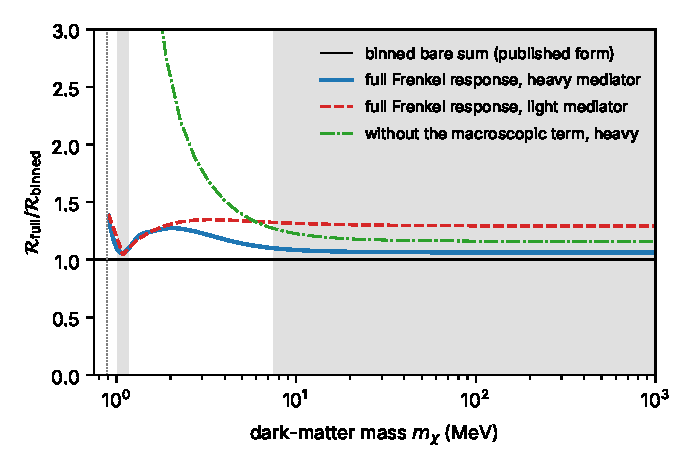
\includegraphics[width=0.85\linewidth]{figures/ch16/limit16_4a.pdf}
\captionof{figure}{Rate of the full Frenkel-exciton response of anthracene divided by the binned rate, against the dark-matter mass, for a heavy (solid) and a light (dashed) mediator, direction-averaged halo. Full response: all 49 $\pi$-electron singlets on both molecules, coupled by $\mathfrak{J}$ and by the macroscopic Coulomb term $(e^2/\Omega q^2)F F^\dagger$, so that no factor $1/|\varepsilon_{\mathrm{mac}}|^2$ is needed (\cref{app:D.12}); the molecular levels are shifted by \SI{0.27}{eV} so that the lowest optically allowed exciton at $\vect{Q} \to 0$ lies at the measured \SI{3.1}{eV} of the binned form. Dash-dotted: the full response without the macroscopic term, heavy mediator. Model of \cref{sec:16.4-model}, $\pi$ electrons only. Gray: the heavy-mediator ratio within \SI{10}{\percent} of one. Dotted: the binned threshold, \SI{0.883}{MeV}.}\label{fig:16-limit-frenkel}
\par}
\smallskip
Just above threshold, between 0.88 and \SI{1.0}{MeV}, the lowest exciton of the full model lies below the binned line and the ratio reaches 1.38. For a heavy mediator between 1.2 and \SI{7.5}{MeV}, and for a light mediator at every mass above \SI{1.2}{MeV}, the mixing of the weak $L_a$ line with the strong $B_b$ transition and the dispersion of the exciton bands change the rate by 10 to \SI{35}{\percent}; the incoherent sum contains neither effect.
\end{limitbox}

Above \SI{30}{MeV} the heavy-mediator rate of the full response in \cref{fig:16-limit-frenkel} exceeds the binned one by \SI{6.3}{\percent}, flat in mass; this excess is the intensity borrowing of \cref{eq:16.4-borrow}. Since $\mathfrak{J}$ is periodic in the crystal momentum, its $L_a$--$B_b$ element keeps the binned weight off by several percent at any momentum transfer. The element is \SI{0.12}{eV} at $\vect{Q} \to 0$ and \SI{0.18}{eV} at a general point of the zone, against an $L_a$--$B_b$ energy difference of \SI{1.4}{eV}. A light mediator weights the momentum transfers near the threshold value $\omega/v_{\mathrm{max}} = \SI{1.17}{keV}$, where $qa_{\mathrm{mol}} \approx 1.6$ for the root-mean-square radius $a_{\mathrm{mol}} = \SI{2.66}{\angstrom}$ of the carbon frame, and there the full rate exceeds the binned one by 29 to \SI{35}{\percent} at all masses above \SI{2}{MeV}. Between 1.2 and \SI{7.5}{MeV} the heavy-mediator ratio reaches 1.27, because the exciton bands spread the levels over tenths of an eV while the halo factor, near threshold, changes on that scale.

The dash-dotted curve shows that the macroscopic term matters most: without it, the local fields alone would raise the rate ninefold at \SI{1.1}{MeV}. The $\pi$ transitions themselves make $\varepsilon_{\mathrm{mac}}(q,0) - 1 = 0.83$ at the threshold momentum and 0.51 at \SI{2}{keV} in the model, so that the factor $1/|\varepsilon_{\mathrm{mac}}|^2$ of \cref{eq:16.4-S} cannot be applied line by line. In the full response the macroscopic term shifts weight up in energy instead of removing it (\cref{sec:4.9}).

\subsection{Charge-transfer excitons and other corrections}\label{sec:16.4-ct}

The zero-overlap limit removes the charge-transfer pairs, and real molecular crystals have some overlap. The simplest description keeps one Frenkel state $|\mathrm{Fr}\rangle$, of energy $E_{\mathrm{Fr}}$, and one charge-transfer state $|\mathrm{CT}\rangle$, of energy $E_{\mathrm{CT}}$, with the electron on a neighbor at distance $d$. The two are coupled by the transfer integral $t_{\mathrm{CT}}$, the sum of the integrals that move the electron and the hole between the molecules. The electron and hole transfer integrals are both proportional to the overlap of the orbitals of the two molecules. Diagonalizing the $2\times2$ problem gives two states $|\pm\rangle$ rotated by the mixing angle $\theta_{\mathrm{CT}}$,
\begin{equation}
  \tan2\theta_{\mathrm{CT}} = \frac{2t_{\mathrm{CT}}}{E_{\mathrm{CT}} - E_{\mathrm{Fr}}} , \qquad
  f_\pm(\vect{q}) = \cos\theta_{\mathrm{CT}}\,f_{\mathrm{Fr}}(\vect{q}) \pm \sin\theta_{\mathrm{CT}}\,f_{\mathrm{CT}}(\vect{q}) ,
  \label{eq:16.4-CT}
\end{equation}
with $f_{\mathrm{CT}}$ the form factor of the charge-transfer state. The transition density of the charge-transfer state is the overlap density of an empty orbital on one molecule and an occupied orbital on the other; it integrates to zero for orthogonal orbitals, so $f_{\mathrm{CT}}(0) = 0$; its dipole is of order $d$ times the overlap, and $|f_{\mathrm{CT}}|^2$ enters at order $q^2d^2$. In the rate the Frenkel line loses the fraction $\sin^2\theta_{\mathrm{CT}}$ of its weight to a new line near $E_{\mathrm{CT}}$, and a binned rate sees this shift of weight up in energy only if the bin ends between the two lines. And $f_{\mathrm{CT}}$ carries the phase difference between two molecules, and the charge-transfer contribution is coherent over distances of order $d$; no Frenkel model contains this coherence. In anthracene the charge-transfer pairs lie near the fundamental gap, 3.9--\SI{4.2}{eV}, some 0.8--\SI{1.1}{eV} above the lowest singlet~\cite[Tables~II and~III]{rangel2016structural}, and for small mixing $\theta_{\mathrm{CT}}^2 \simeq t_{\mathrm{CT}}^2/(E_{\mathrm{CT}} - E_{\mathrm{Fr}})^2$: a transfer integral of \SI{0.1}{eV} would move about one percent of the weight. The mixing grows along the acene series, whose larger members have singlets that extend over several molecules~\cite[Sect.~III\,E]{rangel2016structural}.

The nuclei move when a molecule is excited, and each molecular line becomes a Franck--Condon progression of vibronic replicas with Poisson weights set by a Huang--Rhys factor (\cref{eq:5.6-FC}). In the Condon approximation the progression keeps the total weight of the line, so \cref{eq:16.4-binned} holds for windows that cover it, while the Franck--Condon overlaps narrow the exciton band of each replica. Above the fundamental gap the crystal has a continuum of separated electrons and holes that the Frenkel model lacks, and \cref{eq:16.4-rate} omits it, as the published rates do~\cite{blanco2020dark}; this continuum raises the rate of masses above $2\times\SI{4}{eV}/v_{\mathrm{max}}^2 \approx \SI{1.1}{MeV}$. Triplet excitons cost less, \SI{1.9}{eV} for the lowest triplet of crystalline anthracene~\cite[Table~III]{rangel2016structural}, but a spin-independent density coupling cannot create them, and they enter only through the spin couplings of \cref{sec:10.4}. Finally, the $\pi$-electron model fails at momentum transfers above about \SI{10}{keV}, where the $\sigma$ electrons of the C--C and C--H bonds start to contribute to $|f|^2$. No calculation of the full periodic Bethe--Salpeter response of anthracene at finite $\vect{q}$ exists to compare with the binned molecular sum and with the zero-overlap model.

\subsection{Direction dependence of an anthracene target}\label{sec:16.4-aniso}

A $\pi$ orbital is odd under reflection through the molecular plane, so the transition density between two $\pi$ orbitals is even, and with zero differential overlap it is a sum of atomic densities centered in the plane. For $\vect{q}$ along the normal every phase $\ee^{\ii\vect{q}\cdot\vect{R}_\mu}$ is then the same, and $f = F_{2p}\sum_\mu \varrho_\mu$ vanishes. With the overlap densities kept and the measured, slightly puckered geometry, $|f|^2$ of $L_a$ at $q = \SI{2.07}{keV}$ is $1\times10^{-7}$ along the normal, against $0.25$ along the short axis. The transition density of $L_a$ also changes sign under reflection through the long axis, so that $|f|^2$ along that axis is only $2\times10^{-9}$. Near threshold, where only $L_a$ is reached, the molecule responds to the component of $\vect{q}$ along its short axis alone. In the crystal both short axes lie within \ang{27} of $b$, and the halo makes $\vect{q}$ prefer the direction of the wind when $\vmin$ is close to $v_{\mathrm{max}}$ (\cref{sec:11.7}): the rate is largest when the Earth moves along $b$.

\Cref{fig:16-anthracene} shows the rate of \cref{eq:16.4-rate} in the model, with the 20 singlets below \SI{7.5}{eV}, for the Earth's velocity along each crystal axis. At \SI{10}{MeV} and $\sigmae = \SI{e-37}{cm^2}$ the direction-averaged rate is $8.0\times10^4$ events per kg-year for a heavy mediator and $2.3\times10^4$ for a light one. The heavy-mediator value is comparable to the independent-particle rate of silicon, $1.36\times10^5$ (\cref{sec:10.2}). At \SI{1.0}{MeV}, just above threshold, $L_a$ carries the whole rate, and the largest rate over all directions of the wind, at $\hat{\vect{v}}_{\mathrm{E}} \parallel b$, exceeds the smallest, near the long molecular axes, 92 times for a heavy mediator and 69 times for a light one. The contrast falls quickly with the mass: $L_a$ carries \SI{68}{\percent} of the rate at \SI{2}{MeV} and \SI{19}{\percent} at \SI{10}{MeV}, as $B_b$ and the higher levels fill in the directions $L_a$ cannot use. The ratio of the largest to the smallest rate is 2.3 (heavy) and 5.3 (light) at \SI{1.5}{MeV}, 1.20 and 1.39 at \SI{10}{MeV}, and 1.17 and 1.29 above \SI{100}{MeV}.

\begin{figure}[tbp]
  \centering
  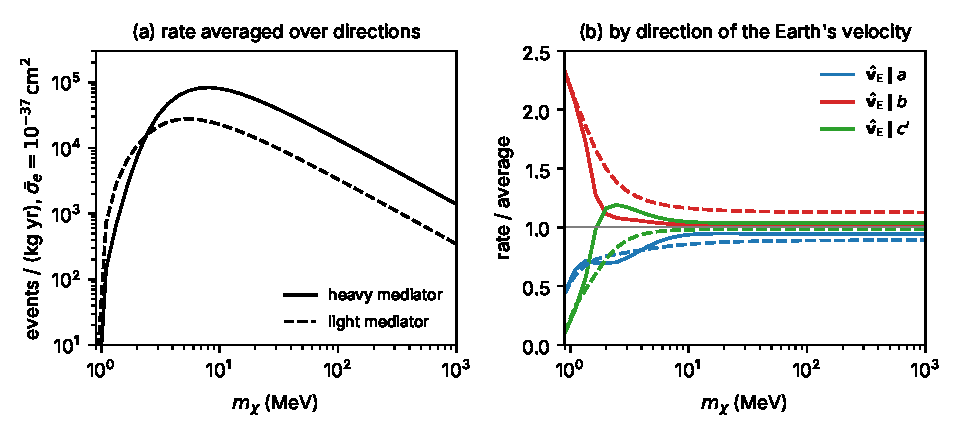
\includegraphics[width=\linewidth]{figures/ch16/fig16_4.pdf}
  \caption{Frenkel-exciton rate of an anthracene crystal in the binned form \cref{eq:16.4-rate}, per kg-year at $\sigmae = \SI{e-37}{cm^2}$, standard halo of \cref{tab:1-shm}. (a) Rate averaged over the directions of the Earth's velocity $\hat{\vect{v}}_{\mathrm{E}}$, heavy (solid) and light (dashed, $\FDM = (\alpha m_e/q)^2$) mediator. (b) Rate for $\hat{\vect{v}}_{\mathrm{E}}$ along the crystal axes $a$, $b$ and $c'$ (perpendicular to $a$ and $b$), divided by the average; heavy (solid) and light (dashed) mediator. The rate is even in $\hat{\vect{v}}_{\mathrm{E}}$. Model of \cref{sec:16.4-model}: $\pi$-electron singlets below \SI{7.5}{eV} of the Pariser--Parr--Pople model on the measured crystal structure, lowest singlet at \SI{3.1}{eV}, form factors with zero differential overlap; the continuum above the fundamental gap is not included.}
  \label{fig:16-anthracene}
\end{figure}

Whatever the mounting and the latitude, $\hat{\vect{v}}_{\mathrm{E}}$ sweeps only part of the sphere in a sidereal day, and the amplitude $A_{\mathrm{day}}$ of \cref{eq:11.7-Aday} cannot exceed $(\mathcal{R}_{\mathrm{max}} - \mathcal{R}_{\mathrm{min}})/(\mathcal{R}_{\mathrm{max}} + \mathcal{R}_{\mathrm{min}})$ over all directions. In the model this bound is 0.98 (heavy) and 0.97 (light) at \SI{1.0}{MeV}, 0.39 and 0.68 at \SI{1.5}{MeV}, 0.09 and 0.17 at \SI{10}{MeV}, and 0.08 and 0.13 at \SI{1}{GeV}. The bound near threshold is a hundred times the daily modulation of silicon, \SI{0.9}{\percent} at \SI{2}{MeV} (\cref{we:11-daily}), because of the crystal class. A cubic crystal has no quadrupole, and its first anisotropic term, the hexadecapole $\ell = 4$, passes the halo only at a few percent; in monoclinic anthracene the quadrupole $\ell = 2$ is allowed and passes at tens of percent of $\mathcal{H}_0$ (\cref{eq:11.7-ups}). Blanco et al.\ reach the same conclusion for trans-stilbene, with a modulation near one at threshold and, at large masses, a modulation above the ten percent of the annual modulation~\cite[Sects.~V, VI]{blanco2021dark}.

\section{Dopants}\label{sec:16.5}

A phosphorus donor in silicon binds its electron by \SI{45.59}{meV}, and dark matter of \SI{13}{keV} can set it free (\cref{we:7-sip}). Compared to the host, the donor has sharp bound lines and a ground state built from six valleys. The $1s(A_1) \to 2p_0$ line at \SI{34.11}{meV} is \SI{4.2}{\micro eV} wide in isotopically purified silicon~\cite[p.~5]{vinh2008silicon}, and a dark photon whose mass falls on it is absorbed several hundred times more strongly than one in the ionization continuum. Between the valley states, dark matter drives transitions that light of the same energy cannot. The drawback is the number of donor electrons, five parts in $10^9$ of the valence electrons at $\nd_{\mathrm{D}} = \SI{e15}{cm^{-3}}$. Du et al.\ proposed doping to \SI{e18}{cm^{-3}} to make up for it~\cite{du2022doped}, at which point the donors begin to merge into an impurity band.

\subsection{Response of dilute donors}\label{sec:16.5-response}

Donors at $\nd_{\mathrm{D}}a^{*3} \ll 1$ act independently, each a hydrogen atom of the crystal (\cref{sec:7.4}). All their transitions lie below the gap of the host, where the host absorbs nothing and its dielectric matrix $\varepsilon_{\mathrm{host}}$ is real. To first order in $\nd_{\mathrm{D}}$ the absorptive part of the response then comes from the donors alone, and the host enters through the screening of the vertex. In \cref{eq:8.4-screened}, split the proper response into its host and donor parts. To first order in the donor part, each vertex acquires the host factor $(\varepsilon_{\mathrm{host}}^{-1})_{\vect{G}\vect{0}}$, and the donor structure factor is
\begin{equation}
  \begin{gathered}
  S^{\mathrm{D}}_{ab}(\vect{q},\omega) = 2\pi\nd_{\mathrm{D}}\sum_f\langle i|\tilde O_a(\vect{q})^\dagger|f\rangle\langle f|\tilde O_b(\vect{q})|i\rangle\,\delta(\omega - E_f + E_i) , \\
  \tilde n_e(\vect{q}) = \sum_{\vect{G}}\bigl(\varepsilon_{\mathrm{host}}^{-1}\bigr)_{\vect{G}\vect{0}}(\vect{q},\omega)\,n_e(\vect{q} + \vect{G}) ,
  \end{gathered}
  \label{eq:16.5-SD}
\end{equation}
for $T \ll E_{\mathrm{b}}^{\mathrm{D}}$, with $|i\rangle$ the donor ground state and $f$ its excited and ionized states. The dark matter's potential at $\vect{q}$ is screened by the host into components at every $\vect{q} + \vect{G}$, and the donor electron feels all of them. An operator with no proper correlation with the charge (a row of the coupling vector of \cref{sec:8.4-couplings}), such as the spin density of a host without spin--orbit coupling, enters unscreened, $\tilde O = O$. Each donor contributes one electron, and the density does not flip its spin, so there is no factor of two for spin. The scattering rate is \cref{eq:8.2-spectrum} with $S = S^{\mathrm{D}}$ and $\rho_T$ the mass density of the host.

The matrix elements follow from the multivalley donor of \cref{app:D.23}, built on the envelope equation of Kohn and Luttinger~\cite{kohn1955theory}. A state $s$ is $\psi_s = \sum_jc^s_jF^s_j(\vect{r})\,\psi_{c\vect{k}_j}(\vect{r})$, with envelopes $F^s_j$ in the six valleys at $\vect{k}_j$ and valley coefficients $c^s_j$. The product of two cell-periodic parts is a lattice sum, $u_{c\vect{k}_{j'}}^*u_{c\vect{k}_j} = \sum_{\vect{G}}\mathcal{U}_{j'j}(\vect{G})\,\ee^{\ii\vect{G}\cdot\vect{r}}$, with $\mathcal{U}_{jj}(\vect{0}) = 1$. Since the envelopes vary slowly over a cell,
\begin{equation}
  \langle s'|\ee^{\ii\vect{q}\cdot\vect{r}}|s\rangle = \sum_{j,j'}c^{s'*}_{j'}c^s_j\sum_{\vect{G}}\mathcal{U}_{j'j}(\vect{G})\int\dd^3r\,F^{s'*}_{j'}F^s_j\,\ee^{\ii(\vect{q} + \vect{k}_j - \vect{k}_{j'} + \vect{G})\cdot\vect{r}} .
  \label{eq:16.5-ff}
\end{equation}
The envelope integral is the Fourier transform of a function a few nanometers across. For the variational envelope of \cref{sec:7.4} it is $[1 + (r_\perp^2p_\perp^2 + r_\parallel^2p_\parallel^2)/4]^{-2}$ at momentum $\vect{p}$, with $p_\parallel$ along the valley axis, and it is negligible once $p \gg 1/r_\perp = \SI{81}{eV}$. Two kinds of term survive. Intravalley terms, $j = j'$ and $\vect{G} = \vect{0}$, carry momentum transfers up to a few hundred eV. Intervalley terms carry $\vect{q} \simeq \vect{k}_{j'} - \vect{k}_j - \vect{G}$, of order keV.

The same structure fixes the field that the envelope feels. In $\tilde n_e$, the component $n_e(\vect{q} + \vect{G})$ has intravalley matrix elements $\mathcal{U}_{jj}(-\vect{G})$ times the envelope integral at $\vect{q}$. For intravalley transitions, $\tilde n_e = \mathfrak{f}^{\mathrm{loc}}_{\mathrm{D}}\,n_e/\varepsilon_{\mathrm{host}}$, with $\varepsilon_{\mathrm{host}} = 1/(\varepsilon_{\mathrm{host}}^{-1})_{\vect{0}\vect{0}}$ the macroscopic dielectric function of \cref{eq:4.4-epsmac} and
\begin{equation}
  \mathfrak{f}^{\mathrm{loc}}_{\mathrm{D}} = 1 + \varepsilon_{\mathrm{host}}\sum_{\vect{G}\ne\vect{0}}\bigl(\varepsilon_{\mathrm{host}}^{-1}\bigr)_{\vect{G}\vect{0}}\,\mathcal{U}_{jj}(-\vect{G}) .
  \label{eq:16.5-floc}
\end{equation}
The donor electron samples the microscopic field with the weight of the conduction-band density $|u_{c\vect{k}_j}|^2$ in each cell. Both factors of the sum are small: the off-diagonal elements of $\varepsilon_{\mathrm{host}}^{-1}$, which produce the local-field corrections of \cref{sec:4.6}, and the Fourier components of a cell-periodic density at $\vect{G} \ne \vect{0}$. In effective-mass theory the ratio is expected to be close to one, since the donor orbit spans many cells and the Lorentz construction of a local cavity field does not apply to it; it has not been computed. Its value for silicon is an open input, which needs the dielectric matrix of the host and the Bloch functions at the minimum, the inputs of \cref{app:E.6}.

\paragraph{Ionization.} For $q$ well below the valley separations, the final state $|\xi\vect{k}\rangle$, a Coulomb envelope $F_{\vect{k}}$ in valley $\xi$, couples to the $A_1$ ground state with amplitude $c_\xi$ times the envelope overlap. Summed over $\xi$, with $\sum_\xi|c_\xi|^2 = 1$, the six valleys give the single-valley result $|\int\dd^3r\,F_{\vect{k}}^*F_{1s}\,\ee^{\ii\vect{q}\cdot\vect{r}}|^2$~\cite[Eq.~(11)]{du2022doped}. For an isotropic hydrogenic envelope of radius $a^* = (2m^*E_{\mathrm{b}}^{\mathrm{D}})^{-1/2}$ this overlap, summed over the directions of $\vect{k}$, is the generalized oscillator strength of the hydrogen $1s$ state. With $L = (e^2/2q^2)S$ at $T = 0$ (\cref{eq:4.4-SL}), the donor part of the loss function is
\begin{equation}
  L^{\mathrm{D}}(\vect{q},\omega) = \frac{2^{10}\pi^2\alpha\,m^*\nd_{\mathrm{D}}a^{*4}}{3\,\varepsilon_{\mathrm{host}}^2}\;
  \frac{(3\tilde q^2 + \tilde k^2 + 1)\exp\bigl[-(2/\tilde k)\arctan\bigl(2\tilde k/(\tilde q^2 - \tilde k^2 + 1)\bigr)\bigr]}{\bigl[(\tilde q + \tilde k)^2 + 1\bigr]^3\bigl[(\tilde q - \tilde k)^2 + 1\bigr]^3\bigl(1 - \ee^{-2\pi/\tilde k}\bigr)} ,
  \label{eq:16.5-gos}
\end{equation}
with $\tilde q = qa^*$, $\tilde k = [2m^*(\omega - E_{\mathrm{b}}^{\mathrm{D}})]^{1/2}a^*$, the arctangent taken in $[0,\pi]$, and $\omega > E_{\mathrm{b}}^{\mathrm{D}}$. At $q \to 0$ the bracket reduces to the dipole continuum of hydrogen in \cref{we:4-trk} with $E_B \to E_{\mathrm{b}}^{\mathrm{D}}$.

\paragraph{Valley-orbit lines.} The $1s$ manifold of phosphorus has its $T_2$ and $E$ states \SI{11.70}{meV} and \SI{13.01}{meV} above the $A_1$ ground state (\cref{sec:7.4}). At optical momentum the transitions vanish in effective-mass theory, because the valley vectors of \cref{eq:D.23-vo} are orthogonal and the intervalley terms need keV momenta. Dark matter reaches both. The $E$ states weight the valleys unequally, and the intravalley sum of \cref{eq:16.5-ff} does not cancel once the envelope integrals differ between valleys. For $\vect{q}$ along [100], two valleys have $\vect{q}$ along their axis and four across it. Summed over the two $E$ states,
\begin{equation}
  \sum_E|\langle E|\ee^{\ii\vect{q}\cdot\vect{r}}|A_1\rangle|^2 = \frac29\Bigl[\Bigl(1 + \frac{r_\parallel^2q^2}{4}\Bigr)^{-2} - \Bigl(1 + \frac{r_\perp^2q^2}{4}\Bigr)^{-2}\Bigr]^2 .
  \label{eq:16.5-E}
\end{equation}
It grows as $q^4$, as a quadrupole transition does, and peaks at 0.022 for $q = \SI{150}{eV}$, which particles from \SI{29}{keV} upward can reach. Along [110] the maximum is 0.0032, and along [111], where all six valleys look alike, the transition vanishes, which makes it a directional signal. These numbers assume one effective-mass envelope common to $A_1$ and $E$; the central-cell contraction of $A_1$ changes their size, but not the zeros along [111] and at $q = 0$. The $T_2$ states pair opposite valleys with opposite signs, and since opposite valleys have identical envelopes their intravalley terms cancel at every $q$. The transition $A_1 \to T_2$ needs the intervalley terms, at $|\vect{q}| = 0.685$, 3.60 and \SI{3.88}{keV} between opposite valleys (the first after an umklapp) and 2.33 and \SI{2.74}{keV} between perpendicular ones, with the minima at $0.85\,(2\pi/a)$. The lightest particle that delivers \SI{11.70}{meV} at \SI{0.685}{keV} has \SI{130}{keV}, and at \SI{2.33}{keV} it has \SI{441}{keV}. The strengths of these lines are set by the coefficients $\mathcal{U}_{j'j}(\vect{G})$, which need the Bloch functions at the minima.

\subsection{Dopant absorption}\label{sec:16.5-absorption}

A dark photon couples to the total charge, and its absorption rate is \cref{eq:10.7-dp} with the loss function of the doped crystal. Silicon has no Born charges, and below its gap the host adds only its two-phonon absorption, which at \SI{50}{meV} gives $\Imag(-1/\varepsilon) = \num{5.4e-6}$ at room temperature and less in a cold crystal (\cref{we:11-iso}). The donor part is the $q \to 0$ limit of $(e^2/2q^2)S^{\mathrm{D}}$ from \cref{eq:16.5-SD}, to first order in $\nd_{\mathrm{D}}$. With $\tilde n_e = n_e/\varepsilon_{\mathrm{host}}$ (taking $\mathfrak{f}^{\mathrm{loc}}_{\mathrm{D}} = 1$) and $\ee^{\ii\vect{q}\cdot\vect{r}} \simeq 1 + \ii\vect{q}\cdot\vect{r}$ between orthogonal states:
\begin{keyresult}[Dark-photon absorption by dilute donors]
\begin{equation}
  \begin{gathered}
  L^{\mathrm{D}}(m_\phi) = \frac{\varepsilon_2^{\mathrm{D}}(m_\phi)}{\varepsilon_{\mathrm{host}}^2} , \qquad
  \mathcal{R} = \zeta^2\,\frac{\rho_\chi}{\rho_T}\,L^{\mathrm{D}}(m_\phi) , \\
  \varepsilon_2^{\mathrm{D}}(\omega) = 4\pi^2\alpha\,\nd_{\mathrm{D}}\sum_f|\langle f|\hat{\vect{e}}\cdot\vect{r}|i\rangle|^2\,\delta(\omega - E_f + E_i) ,
  \end{gathered}
  \label{eq:16.5-abs}
\end{equation}
for $\nd_{\mathrm{D}} \ll \nd_{\mathrm{c}}$ and $|\varepsilon^{\mathrm{D}}| \ll \varepsilon_{\mathrm{host}}$, with $\hat{\vect{e}}$ the polarization of the dark photon and $\varepsilon^{\mathrm{D}}$ the donor part of the dielectric function, whose imaginary part is $\varepsilon_2^{\mathrm{D}}$. In a cubic crystal $L^{\mathrm{D}}$ does not depend on $\hat{\vect{e}}$.
\end{keyresult}
\noindent The host screening appears once, through the vertex $\tilde n_e$, and $\varepsilon_2^{\mathrm{D}}$ is the proper response of the donors, which contains none. The same result follows from writing $\varepsilon = \varepsilon_{\mathrm{host}} + \varepsilon^{\mathrm{D}}$ and expanding $\Imag(-1/\varepsilon)$ to first order in $\varepsilon^{\mathrm{D}}$ with a real $\varepsilon_{\mathrm{host}}$. Per donor, the absorption is that of a hydrogen atom whose matrix elements are those of the envelope, suppressed by $1/\varepsilon_{\mathrm{host}}^2 = 1/130$ at the liquid-helium constant $\varepsilon_{\mathrm{host}} = 11.4$ of \cref{sec:7.4}. In this the dopant differs from the Dirac material of \cref{sec:16.1}, where the background constant sits inside the response of the same electrons.

The $A_1$ ground state has every valley with weight $1/6$, and each valley's $p_0$ states carry the dipole along its axis and its $p_\pm$ states across it. The cubic average of $|\langle f|\hat{\vect{e}}\cdot\vect{r}|i\rangle|^2$ is then $|Z_f|^2/3$ for a $p_0$ line and $2|X_f|^2/3$ for a $p_\pm$ line, where $Z_f$ and $X_f$ are the dipole elements of one valley along and across its axis, with $X_f$ summed over the two $p_\pm$ partners. We obtain them from the numerical solution of \cref{eq:7.4-EMT} that gives \cref{fig:7-donor}, extended to the dipole matrix elements, with the measured line energies. The ground state carries the central-cell potential, a Gaussian well of range 3.2 or \SI{6.3}{\angstrom} in the $s$-like channel, tuned to the measured binding of \SI{45.59}{meV}; the two ranges give line strengths within \SI{2}{\percent} of each other. For the $1s(A_1) \to 2p_0$ line, $|Z|^2/3 = \SI{13.6}{\angstrom^2}$, an oscillator strength $2m_e\omega|Z|^2/3 = 0.12$; the $2p_\pm$ line has 0.52. The lines carry \SI{25}{\percent} of the $f$-sum of the donor electron, $\sum_f2m_e(E_f - E_i)|\langle f|\hat{\vect{e}}\cdot\vect{r}|i\rangle|^2 = m_e(2/m^*_\perp + 1/m^*_\parallel)/3 = 3.85$ (\cref{eq:4.3-TRK} with band masses), and the continuum the rest. \Cref{fig:16-donor-lines} shows the resulting spectrum.

\begin{figure}[tbp]
  \centering
  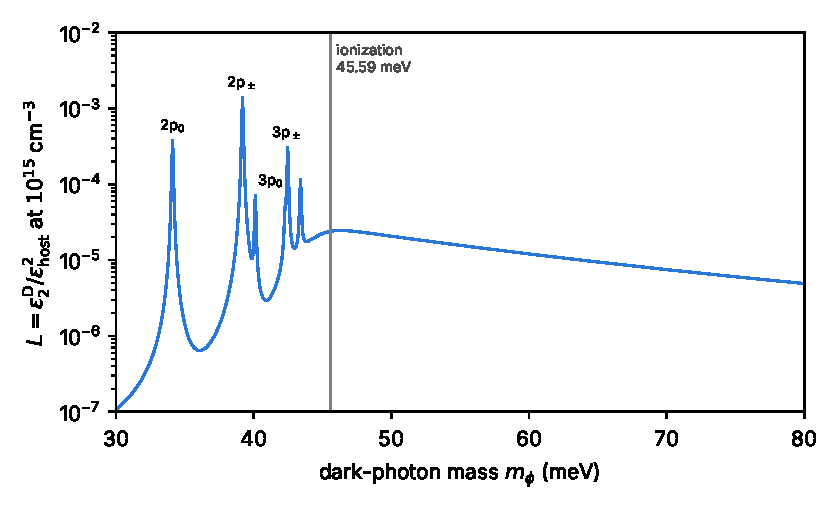
\includegraphics[width=0.85\linewidth]{figures/ch16/fig16_5.pdf}
  \caption{Dark-photon loss function of phosphorus donors in silicon, $L^{\mathrm{D}} = \varepsilon_2^{\mathrm{D}}/\varepsilon_{\mathrm{host}}^2$ of \cref{eq:16.5-abs} at $\nd_{\mathrm{D}} = \SI{e15}{cm^{-3}}$ and $\varepsilon_{\mathrm{host}} = 11.4$, against the dark-photon mass. Anisotropic effective-mass donor (\cref{eq:7.4-EMT}, masses of \cref{tab:3-materials}), solved numerically, with line energies from the measured $1s(A_1)$ at \SI{45.59}{meV} and the measured $2p_0$, $2p_\pm$, $3p_0$ levels. Ground state with a model central cell tuned to \SI{45.59}{meV}. The lines $1s(A_1) \to np_0$, $np_\pm$ ($n = 2$ to 4) are drawn with a display width of \SI{0.1}{meV}; measured widths are tens of times smaller. The continuum and the higher Rydberg lines are smoothed over \SI{1.5}{meV}, comparable to the level spacing of the finite box used for the continuum.}
  \label{fig:16-donor-lines}
\end{figure}

\begin{limitbox}[Dopant absorption][lim:16.5a]
The absorption rate of dark photons on dilute donors is $\mathcal{R} = \zeta^2(\rho_\chi/\rho_T)\,L^{\mathrm{D}}(m_\phi)$, with $L^{\mathrm{D}} = \varepsilon_2^{\mathrm{D}}/\varepsilon_{\mathrm{host}}^2$ the donor loss function of \cref{eq:16.5-abs}~\cite[Eqs.~(10), (12) and the absorption rate after Eq.~(12)]{du2022doped}.
\par\smallskip
{\centering
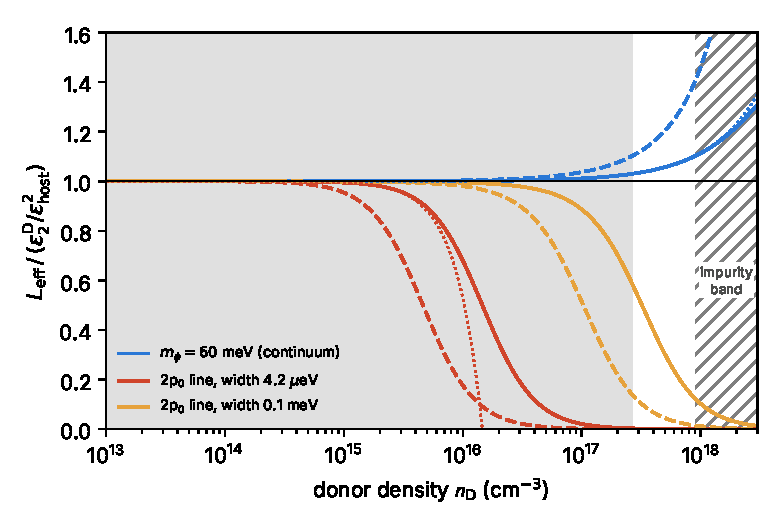
\includegraphics[width=0.85\linewidth]{figures/ch16/limit16_5a.pdf}
\captionof{figure}{Loss function of the effective medium of donors in silicon, $\Imag(-1/\varepsilon_{\mathrm{eff}})$ with $\varepsilon_{\mathrm{eff}} = \varepsilon_{\mathrm{host}}(1 + 2y)/(1 - y)$ and $y = \varepsilon^{\mathrm{D}}/3\varepsilon_{\mathrm{host}}$, divided by the published first-order form $\varepsilon_2^{\mathrm{D}}/\varepsilon_{\mathrm{host}}^2$, against the donor density. Donor model of \cref{fig:16-donor-lines}. Blue: $m_\phi = \SI{60}{meV}$, in the continuum. Red and orange: the $1s(A_1) \to 2p_0$ line center, \SI{34.11}{meV}, for full widths of \SI{4.2}{\micro eV} (narrowest measured) and \SI{0.1}{meV}. Dotted: the expansion $1 - 4\Real y + 4[3(\Real y)^2 - (\Imag y)^2]$. Gray: the continuum ratio within \SI{10}{\percent} of one, $\nd_{\mathrm{D}} < \SI{8.8e17}{cm^{-3}}$. Hatched: $\nd_{\mathrm{D}} > 0.3\,\nd_{\mathrm{c}}$, with $\nd_{\mathrm{c}} \approx \SI{3e18}{cm^{-3}}$, where the donors form an impurity band.}\label{fig:16-limit-dopant}
\par}
\smallskip
Outside the gray region the donors screen the dark photon themselves, and at the narrow line center the first-order form fails already at $\nd_{\mathrm{D}} = \SI{4.8e15}{cm^{-3}}$, where $\varepsilon_2^{\mathrm{D}}$ reaches half of $\varepsilon_{\mathrm{host}}$.
\end{limitbox}

The effective medium is the dilute Clausius--Mossotti form, the Maxwell Garnett function of \cref{sec:16.3} with each donor a polarizable point of polarizability $\alpha_{\mathrm{pol}}(\omega)$ and $\varepsilon^{\mathrm{D}} = \nd_{\mathrm{D}}\alpha_{\mathrm{pol}}$. Its expansion, $L_{\mathrm{eff}} = (\varepsilon_2^{\mathrm{D}}/\varepsilon_{\mathrm{host}}^2)[1 - 4\Real y + O(y^2)]$, shows the two ways the first-order form fails. In the continuum above the lines the donors push $\Real\varepsilon^{\mathrm{D}}$ negative, lower $|\varepsilon_{\mathrm{eff}}|$ and raise the absorption, by \SI{10}{\percent} at \SI{8.8e17}{cm^{-3}}. At the center of a line $\varepsilon^{\mathrm{D}}$ is nearly imaginary, and the ratio becomes $1/[1 + (4/9)(\varepsilon_2^{\mathrm{D}}/\varepsilon_{\mathrm{host}})^2]$: the absorbed field is screened by the donors as the plasmon screens it in \cref{sec:10.7}. A narrow line saturates at a density proportional to its width.

\begin{workedexample}{The $2p_0$ line of Si:P for a dark photon at resonance}\label{we:16-sip-line}
Take $\nd_{\mathrm{D}} = \SI{e15}{cm^{-3}}$ and a dark photon of mass $m_\phi = \SI{34.11}{meV}$, the binding of $1s(A_1)$, \SI{45.59}{meV}, minus that of $2p_0$, \SI{11.48}{meV}. With the line strength $|Z|^2/3 = \SI{13.6}{\angstrom^2}$, the line integral of \cref{eq:16.5-abs} is
\begin{equation*}
  \int\varepsilon_2^{\mathrm{D}}\,\dd\omega = 4\pi^2\alpha\,\nd_{\mathrm{D}}\,\frac{|Z|^2}{3} = \SI{7.73e-6}{eV} .
\end{equation*}
The narrowest measured full width of the line, in isotopically purified silicon, is $\varGamma_{\mathrm{line}} = \SI{0.034}{cm^{-1}} = \SI{4.22}{\micro eV}$, close to the lifetime width $1/T_1 = \SI{3.2}{\micro eV}$ of the $2p_0$ state, which decays by phonon emission in $T_1 = \SI{205}{ps}$~\cite[p.~5]{vinh2008silicon}. For a Lorentzian line the peak is $2/\pi\varGamma_{\mathrm{line}}$ times the integral, $\varepsilon_2^{\mathrm{D}} = 1.17$, and
\begin{equation*}
  L^{\mathrm{D}} = \frac{1.17}{11.4^2} = \num{8.99e-3} ,
\end{equation*}
which the effective medium lowers by half a percent, to \num{8.94e-3}. The dark photon's own spread in energy, $m_\phi v^2/2 \approx \SI{0.017}{\micro eV}$, lies well inside the line. With $\rho_\chi/\rho_T = \SI{0.3}{GeV.cm^{-3}}/\SI{2.33}{g.cm^{-3}}$, the rate is
\begin{equation*}
  \mathcal{R} = \zeta^2\,\frac{\rho_\chi}{\rho_T}\,L^{\mathrm{D}} = \num{5.5e31}\,\zeta^2\ \text{per kg-year} ,
\end{equation*}
and three events per kg-year need $\zeta = \num{2.3e-16}$. In the continuum at \SI{50}{meV} the same crystal has $L^{\mathrm{D}} = \num{2.1e-5}$ and needs $\zeta = \num{4.9e-15}$, twenty times more. The gain holds over a window of masses as wide as the line, $\varGamma_{\mathrm{line}}/m_\phi = \num{1.2e-4}$, and the peak, proportional to $\nd_{\mathrm{D}}/\varGamma_{\mathrm{line}}$, grows with the donor density only while the line keeps its width.
\end{workedexample}

\subsection{The impurity band}\label{sec:16.5-band}

Uncompensated Si:P becomes a metal at low temperature above a donor density $\nd_{\mathrm{c}} \approx \SI{3e18}{cm^{-3}}$, as quoted by Du et al.~\cite[Sect.~II]{du2022doped}. This is the \emph{Mott critical density}, the donor density of the metal--insulator transition named in \cref{sec:7.4}. Their projections use $\nd_{\mathrm{D}} = \SI{e18}{cm^{-3}}$, and their comparison with optical data \SI{1.8e18}{cm^{-3}}, so $\nd_{\mathrm{D}}/\nd_{\mathrm{c}} \approx 0.3$ to 0.6. At these densities the donors are not isolated. Donors sit at random positions, and the probability that a given donor has a neighbor within a distance $d$ is $1 - \exp(-4\pi\nd_{\mathrm{D}}d^3/3)$. For $d$ equal to the orbit diameter, $2r_\perp = \SI{4.86}{nm}$, this is \num{4.8e-4} at \SI{e15}{cm^{-3}}, but 0.38 at \SI{e18}{cm^{-3}} and 0.58 at \SI{1.8e18}{cm^{-3}}. The electron of such a pair hops between the two cores. The hopping splits the $1s$ level of the pair into bonding and antibonding states, shifts its lines, and over a random ensemble spreads the discrete spectrum into a band of states, the \emph{impurity band}. Optical spectra at these densities show it: the lines broaden and the gap below the first line closes~\cite[Sect.~VII.6]{du2022doped}.

The effective medium of \cref{lim:16.5a} shows the same failure from the other side. The static polarizability of an isolated donor, from the numerical solution, is $\alpha_{\mathrm{pol}}(0)/\varepsilon_{\mathrm{host}} = 4\pi\times\SI{1.1e-20}{cm^3}$. At \SI{e18}{cm^{-3}} it raises the static dielectric function of the crystal by a factor of 1.15, and at \SI{1.8e18}{cm^{-3}} by 1.28. The Clausius--Mossotti form diverges at $\nd_{\mathrm{D}}\alpha_{\mathrm{pol}}(0) = 3\varepsilon_{\mathrm{host}}$, at \SI{2.1e19}{cm^{-3}}, above the measured $\nd_{\mathrm{c}}$. The transition, however, comes first from pairs and clusters, whose polarizability and overlap exceed those of isolated donors, and the response of isolated donors, in a dilute medium or an effective one, is wrong at order one near the ionization edge for $\nd_{\mathrm{D}}/\nd_{\mathrm{c}} \approx 0.5$.

What replaces it is the disorder average $\langle S^{\mathrm{D}}(\vect{q},\omega)\rangle$ of a random ensemble of donors, each with its six-valley orbitals and central cell. The hopping between two donors oscillates with their separation, because the valley phases $\ee^{\ii\vect{k}_j\cdot\vect{r}}$ interfere, so a single-valley envelope gets it wrong. The optical data that Du et al.\ use at \SI{1.8e18}{cm^{-3}} contain the impurity band at $q = 0$; how it reshapes $S^{\mathrm{D}}$ at the momenta of scattering, and the absorption near the edge, is the open problem of this section.

\subsection{Donors as final states}\label{sec:16.5-final}

A donor excitation is useful when the deposit could have made nothing else, when the detector can count it before it is lost, and when the donors are dilute. The first condition is kinematic. Between \SI{13}{keV} and the \SI{0.333}{MeV} of the silicon gap (\cref{sec:1.3}), the donor is the only electronic excitation of the crystal that dark matter can reach. Above that it adds a valley structure that the host lacks. The $A_1 \to E$ line of \cref{eq:16.5-E} makes the rate depend on the direction of $\vect{q}$ relative to the crystal axes, and the daily rotation of the laboratory turns this into a modulation.

The second condition depends on the final state. An ionized donor leaves an electron in the conduction band, which a field can collect and a charge-coupled device can count one at a time; this is the readout that Du et al.\ propose~\cite[Sect.~VII.1]{du2022doped}. The donors then must stay neutral without the dark matter. Thermal ionization grows as $\ee^{-E_{\mathrm{b}}^{\mathrm{D}}/T}$, and from the measured capture coefficient of electrons on ionized phosphorus Du et al.\ estimate that at \SI{e18}{cm^{-3}} a temperature of about \SI{5}{K} keeps it below one electron per kg-year. The bias that collects the electron also drives hopping conduction through the impurity band, which a layer of undoped silicon between the doped volume and the readout blocks, as in the blocked-impurity-band infrared detectors~\cite[Sect.~VII.1]{du2022doped}. A bound excitation, such as $2p_0$, has no charge to collect. It returns to the ground state by emitting phonons, within \SI{205}{ps} for $2p_0$~\cite[p.~5]{vinh2008silicon}, and the energy is then a few phonons of at most \SI{34}{meV}. In a doped crystal phonons above \SI{11.70}{meV} can drive the $1s(A_1) \to 1s(T_2)$ and $1s(E)$ transitions of other donors, and only those below are expected to travel ballistically to a sensor~\cite[Sect.~VII.6]{du2022doped}. A bound excitation therefore needs a sensor of single phonons of about \SI{10}{meV}, which no present detector provides, while ionization needs a single-electron counter, which exists. Both need the third condition, $\nd_{\mathrm{D}} \ll \nd_{\mathrm{c}}$, with the bound set by the impurity band of \cref{sec:16.5-band}.

\section{Color centers and broken bonds}\label{sec:16.6}

A fluorine atom knocked off its site in lithium fluoride leaves an anion vacancy, and an anion vacancy that binds an electron is an F center, which absorbs light near \SI{5.1}{eV}~\cite{guerreroperez2025first}. A dark-matter particle of \SI{0.5}{GeV} can give a fluorine nucleus at most \SI{188}{eV} (\cref{eq:1.3-ERmax}), a few times the tens of eV that a displacement costs. A molecule struck on one of its atoms comes apart in the same way when the kick exceeds its bond energy, \SI{4.75}{eV} for H$_2$. The F center and the broken molecule both persist, both lie in a crystal transparent to the light that reads them, and both can be counted singly. Budnik, Cheshnovsky, Slone and Volansky proposed color centers as a target for sub-GeV dark matter~\cite{budnik2018direct}, and Essig, Mardon, Slone and Volansky the breaking of chemical bonds~\cite{essig2017detection}.

\subsection{The color-center creation rate}\label{sec:16.6-cc}

A color center forms after the prompt window of \cref{sec:8.7}. Within that window, a femtosecond after the kick, the struck nucleus moves with the momentum it received and its neighbors have not yet responded; the class $\Lambda$ is a recoil of species $\kappa$ with energy deposit $\omega$ along $\hat{\vect{q}}$. The defect forms during the collision cascade that follows, within picoseconds, and its fate is decided later still, when the close pair recombines or does not and when the vacancy captures an electron or does not. The rate of creating readable centers is therefore the hand-off formula \cref{eq:8.7-handoff} with the cascade distribution $P_{\mathrm{casc}}(N_{\mathrm{eh}}|\Lambda)$ replaced by the probability $Y_{\mathrm{CC}}(\Lambda)$ that a seed of class $\Lambda$ ends as a center that the readout registers. \Cref{sec:18.3} makes precise how a recoil seeds the cascade, and \cref{sec:19.4} treats the energy that defects store. The conditions of \cref{sec:8.7} apply directly: the yield depends on the direction of the recoil relative to the crystal axes, so $\hat{\vect{q}}$ must stay inside the class sum, and a rate averaged over directions before the yield is applied is wrong near threshold.

The yield is a product of four probabilities, each fixed at a different stage:
\begin{equation}
  Y_{\mathrm{CC}}(E_R,\hat{\vect{r}}_R) = p_{\mathrm{FP}}(E_R,\hat{\vect{r}}_R)\;p_{\mathrm{surv}}\;p_q\;f_{\mathrm{opt}} .
  \label{eq:16.6-yield}
\end{equation}
The first, $p_{\mathrm{FP}}$, is the probability that a nucleus set moving with kinetic energy $E_R$ along $\hat{\vect{r}}_R$ leaves a Frenkel pair once the collision has died out. Its lowest crossing is the displacement threshold $E_{\mathrm{d}}(\hat{\vect{r}}_R)$ of \cref{eq:7.4-Ed}, and molecular dynamics computes the threshold direction by direction (\cref{app:E.11}). For an F center the displaced atom must be an anion, either struck directly or hit by a struck cation. The second, $p_{\mathrm{surv}}$, is the probability that the close pair survives recombination over the time between the event and the readout. At millikelvin temperatures thermal hopping is frozen (\cref{sec:7.4}), and only tunneling recombination and the phonons of later events act. The third, $p_q$, is the probability that the vacancy ends in the charge state of the readable center: an F center is a vacancy with one electron, while an empty anion vacancy absorbs elsewhere. The fourth, $f_{\mathrm{opt}}$, is the probability that the readout registers a center that is present. None of the four probabilities enters the response; they are properties of the final state, and the truncation label of \cref{sec:8.5} applies only to the seed.

The seed is an impulsive recoil. Displacement needs $E_R$ of 10 to \SI{60}{eV}, three orders of magnitude above the phonon energies, so the recoil parameter $x_R = E_R/\langle\omega\rangle$ is several hundred and the nuclear response is the Gaussian \cref{eq:11.4-IAgauss} of \cref{sec:11.4}. The momentum transfer, near \SI{1}{MeV} for a fluorine recoil of \SI{27}{eV}, is far above the zone scale. Above the zone scale the coherence corrections of the multiphonon response are already below \SI{10}{\percent} at \SI{18}{keV} in silicon and keep falling (\cref{sec:11.3}). Only the self response of each species remains. For a heavy mediator we insert that response and the yield into \cref{eq:8.7-handoff}, average over orientations as in \cref{sec:11.4}, and count one nucleus of species $\kappa$ per cell of mass $M_{\mathrm{cell}}$. The rate per unit target mass is
\begin{equation}
  \begin{split}
  \mathcal{R}_{\mathrm{CC}} &= \sum_\kappa\frac{M_\kappa}{M_{\mathrm{cell}}}\,\frac{\rho_\chi\,\sigma_{N,\kappa}}{2\mchi\,\mu_{\chi\kappa}^2}\int\dd E_R\int\dd\omega\;\frac{\ee^{-(\omega - E_R)^2/2\sigma_\omega^2}}{(2\pi\sigma_\omega^2)^{1/2}} \\
  &\qquad\times\eta\Bigl(\frac{\omega}{q} + \frac{q}{2\mchi}\Bigr)\,\bigl\langle Y_{\mathrm{CC},\kappa}(\omega,\hat{\vect{r}}_R)\bigr\rangle_{\hat{\vect{r}}_R} ,
  \end{split}
  \label{eq:16.6-ccrate}
\end{equation}
with $q = (2M_\kappa E_R)^{1/2}$, $\sigma_\omega^2 = E_R\langle\omega\rangle_\kappa$ at $T = 0$, $\langle\omega\rangle_\kappa$ the mean phonon energy of the site, $\sigma_{N,\kappa}$ the nuclear cross-section of \cref{eq:2.2-nucleus} with $F_N = 1$, and $\mu_{\chi\kappa}$ the reduced mass with nucleus $\kappa$. In the impulse response the deposit $\omega$ equals the change of kinetic energy of the nucleus, so the yield is evaluated at $\omega$; the initial kinetic energy of the nucleus, $3\langle\omega\rangle_\kappa/4$, is a few hundredths of an eV and is dropped. The direction average of $Y$ is exact only when the recoil directions are isotropic in the crystal frame. For a crystal fixed to the rotating Earth they are not, and the full form keeps $\hat{\vect{r}}_R = \hat{\vect{q}}$ inside the velocity integral; this dependence on the direction of $\vect{q}$ is the origin of the daily modulation of the rate~\cite[Eq.~(10)]{budnik2018direct}.

\Cref{eq:16.6-ccrate} reduces to the published rate in two steps. As $\sigma_\omega \to 0$ the Gaussian becomes $\delta(\omega - E_R)$ and the minimum velocity becomes $q/2\mu_{\chi\kappa}$; the rate is then the free recoil \cref{eq:11.4-LS} per species. Setting then $p_{\mathrm{surv}} = p_q = f_{\mathrm{opt}} = 1$ and $p_{\mathrm{FP}} = \Theta(E_R - E_{\mathrm{d}}(\hat{\vect{r}}_R))$ gives the rate of Budnik et al.~\cite[Eqs.~(1), (5), (7)]{budnik2018direct}. They write it as an integral over $q^2$ with the step $\Theta(q - q_{\min}(\hat{\vect{q}}))$, $q_{\min}^2 = 2M_\kappa E_{\mathrm{d}}$, and with a per-nucleon cross-section and the coherence factor $[f_PZ + f_N(A - Z)]^2$. For equal couplings to protons and neutrons that factor is $A^2$. Their per-nucleon cross-section is the $\sigma_p$ of \cref{eq:2.2-nucleus}, and $\sigma_p$ times $A^2/\mu_{\chi p}^2$ is $\sigma_{N,\kappa}/\mu_{\chi\kappa}^2$. For the threshold surface they take $q_{\min}(\hat{\vect{q}}) = (2M_\kappa\Delta E_B)^{1/2}[1 + a\sin(4\theta)\cos(4\varphi)]$ in crystal axes, with a mean binding energy $\Delta E_B$ and $a = 0.4$~\cite[Eq.~(2) and Table~I]{budnik2018direct}. Their formula counts a dislocated nucleus, not a particular defect, and assumes that the vacancy fills with an electron at once.

The Doppler width is the first correction, and it is small. For a fluorine nucleus in LiF the optical phonons lie between 33.5 and \SI{77.2}{meV}~\cite[Table~I]{griffin2020multichannel}, and we take these two values as the range of $\langle\omega\rangle_{\mathrm{F}}$; at $E_R = \SI{27}{eV}$ the width is 0.95 to \SI{1.44}{eV}, 3.5 to \SI{5.4}{\percent} of the threshold. The zero-point momentum of the nucleus along $\hat{\vect{q}}$, $(M_{\mathrm{F}}\langle\omega\rangle_{\mathrm{F}}/2)^{1/2}$, is 17 to \SI{26}{keV}, against $q_{\min} = \SI{978}{keV}$, a ratio of 0.018 to 0.027, so the classical treatment stands. \Cref{lim:16.6a} shows where the width matters: only where the largest recoil energy is less than 1.22 to 1.36 times the threshold, for site phonon energies of 33.5 to \SI{77.2}{meV}.

Electronic deposits make centers too. In alkali halides an exciton localizes on the lattice as a self-trapped exciton, which can convert within picoseconds into an F center and an interstitial halogen, the H center, and so store its energy as a Frenkel pair. The yield of an electronic class is then $\langle N_{\mathrm{X}}\rangle(\omega)\,p_{\mathrm{FH}}\,p_{\mathrm{surv}}\,f_{\mathrm{opt}}$, with $\langle N_{\mathrm{X}}\rangle$ the number of excitons a deposit $\omega$ makes and $p_{\mathrm{FH}}$ the probability that a self-trapped exciton becomes a pair rather than decaying. The seed is the electronic response of \cref{chap:10}, and the route opens at the energy of the free exciton, which lies below the band gap of LiF, \SI{14.2}{eV}~\cite{guerreroperez2025first}. A particle needs $\mchi \ge 2\times\SI{14.2}{eV}/v_{\mathrm{max}}^2 = \SI{4.0}{MeV}$ to deposit the gap. The mass of \SI{4.0}{MeV} is an upper bound on the threshold of this route and at least 46 times less than the \SI{0.186}{GeV} that a fluorine displacement at \SI{27}{eV} requires. For a search the electronic route is a background as much as a channel, since a $\gamma$ ray that deposits \SI{100}{keV} has the energy for thousands of excitons. Araujo et al.\ find the response of LiF to $^{60}$Co $\gamma$ rays a factor 50 below that to fast neutrons at equal dose~\cite[Sect.~III]{araujo2026nuclear}.

The threshold surface and $p_{\mathrm{FP}}$ come from recoil molecular dynamics on machine-learned potentials. The levels and optical cross-sections of the centers come from excited-state calculations in supercells, by $\Delta$SCF, the difference of the self-consistent-field (SCF) total energies of two electronic configurations, with hybrid functionals (\cref{app:E.10}). The conversion of a self-trapped exciton and the survival of the close pair at millikelvin need surface hopping and the tunneling paths of the defect.

\subsection{F centers in lithium fluoride}\label{sec:16.6-lif}

LiF is the material in which color-center readout of nuclear recoils has been demonstrated. Its F center has a nondegenerate ground state and a threefold excited state, with absorption measured near \SI{5.1}{eV} and computed at 4.85 to \SI{4.90}{eV}, and its luminescence has never been observed~\cite{guerreroperez2025first}. In practice the readout uses aggregates of vacancies: the neutral pair F$_2^0$, emitting at \SI{650}{nm}, and the charged triple F$_3^+$, emitting at \SI{525}{nm}, both excited at \SI{450}{nm}~\cite[Sect.~I]{araujo2026nuclear}. They form when single vacancies diffuse together, which takes hours at room temperature: after a $\gamma$ exposure the two emissions grow with time constants of \SI{9}{h} (F$_2^0$) and \SI{6.5}{h} (F$_3^+$)~\cite[Sect.~III]{araujo2026nuclear}. Along the dense track of a fast-neutron recoil, about 1200 fluorine vacancies per micrometer in simulation, the vacancies meet quickly, and Araujo et al.\ estimate one emitting aggregate for every two or three of them~\cite[Sect.~II]{araujo2026nuclear}.

The displacement threshold of LiF has not been computed direction by direction. Cogswell, Goel and Huber run their binary-collision simulations of LiF with $E_{\mathrm{d}} = \SI{27}{eV}$ and find that half the asymptotic vacancy efficiency is reached at a recoil energy of \SI{80}{eV}~\cite[Table~I]{cogswell2021passive}. \Cref{fig:16-lif} turns displacement thresholds into dark-matter masses. A fluorine recoil above \SI{27}{eV} needs $\mchi \ge \SI{0.186}{GeV}$, and the requirement moves from 0.113 to \SI{0.255}{GeV} as the threshold moves from 10 to \SI{50}{eV}. A lithium nucleus is lighter and takes more energy from the same particle, but it makes an F center only by displacing a fluorine neighbor, and one collision passes on at most the fraction $4M_{\mathrm{Li}}M_{\mathrm{F}}/(M_{\mathrm{Li}} + M_{\mathrm{F}})^2 = 0.788$ of its energy (for $^7$Li); the requirement at \SI{27}{eV} is then \SI{0.129}{GeV}. Displacing the lithium itself, at \SI{0.114}{GeV}, leaves a cation vacancy, which is not an F center.

\begin{figure}[tbp]
  \centering
  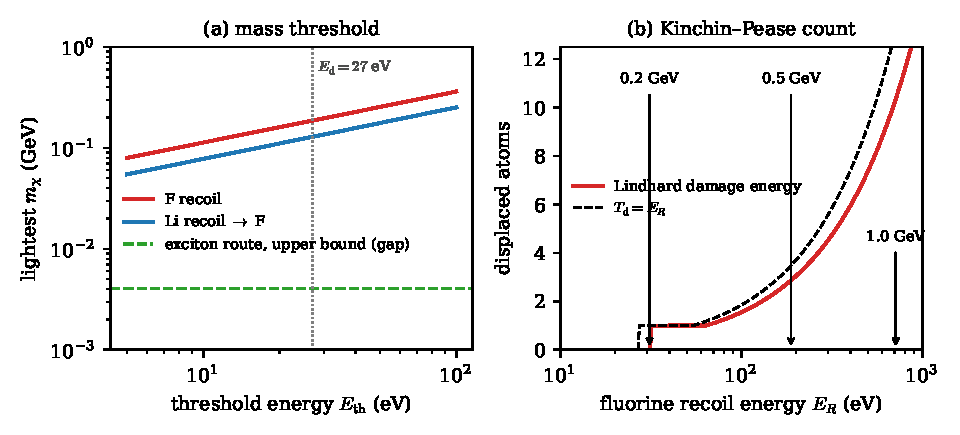
\includegraphics[width=\linewidth]{figures/ch16/fig16_6.pdf}
  \caption{F-center creation in LiF. (a) Lightest dark-matter mass that can create an F center, against the threshold energy of a step: a fluorine recoil above the threshold (red), a lithium recoil that passes the threshold energy to a fluorine neighbor in one head-on collision, transfer fraction 0.788 (blue), and the mass that deposits the band gap, \SI{14.2}{eV}, $\SI{4.0}{MeV}$, an upper bound on the threshold of the exciton route (green, dashed); \cref{eq:1.3-ERmax} with $v_{\mathrm{max}} = \num{2.650e-3}$. Dotted: $E_{\mathrm{d}} = \SI{27}{eV}$, the threshold used in binary-collision simulations of LiF. (b) Atoms displaced by a fluorine recoil in the Kinchin--Pease count with $E_{\mathrm{d}} = \SI{27}{eV}$, with the damage energy of the Lindhard partition for $Z = 9$, $A = 19$ (red; an extrapolation below about \SI{1}{keV}) and with no electronic loss (black, dashed). Arrows: the largest fluorine recoil energy for $\mchi = 0.2$, 0.5 and \SI{1.0}{GeV}, 31, 188 and \SI{711}{eV}.}
  \label{fig:16-lif}
\end{figure}

The number of vacancies a recoil makes follows from two classic estimates. The Lindhard partition splits a recoil of energy $E_R$ into an electronic share $y_LE_R$ and a damage energy $T_{\mathrm{d}} = (1 - y_L)E_R$, with $y_L$ of \cref{eq:16.6-lindhard} (\cref{sec:19.3}). The Kinchin--Pease count of \cref{sec:19.4-count}~\cite[Sect.~II]{cogswell2021passive} then gives no vacancy for $T_{\mathrm{d}} < E_{\mathrm{d}}$, one for $E_{\mathrm{d}} \le T_{\mathrm{d}} < 2E_{\mathrm{d}}$, and $T_{\mathrm{d}}/2E_{\mathrm{d}}$ above. The Lindhard partition and the Kinchin--Pease count are both rough at the energies of sub-GeV recoils. The Lindhard form already misses the measured ionization of silicon recoils of \SI{100}{eV} (\cref{app:E.23}), and its use for a fluorine recoil in a compound is a model choice. The Kinchin--Pease count ignores recombination and the direction dependence of $E_{\mathrm{d}}$. The two estimates set the scale of the yield, and \cref{we:16-fyield} uses them only to set that scale.

\begin{workedexample}{The yield of F centers per keV of fluorine recoil}\label{we:16-fyield}
Take a fluorine recoil of \SI{1}{keV} in LiF. With $Z = 9$ and $A = 19$, \cref{eq:16.6-lindhard} gives $k_L = 0.132$, $\epsilon_L = 0.0683$, $g_L = 2.21$ and $y_L = 0.226$: the recoil gives \SI{226}{eV} to the electrons and leaves a damage energy of \SI{774}{eV}. With $E_{\mathrm{d}} = \SI{27}{eV}$ the Kinchin--Pease count is $774/54 = 14.3$ displaced atoms, and 18.5 if no energy went to the electrons. The count does not say how the displacements divide between the two sublattices. If all displacements are on the anion sublattice, the count gives 14.3 fluorine vacancies per keV, an upper value; an equal share gives 7.2.

A fluorine vacancy becomes an F center only with an electron. The electronic share of \SI{226}{eV} makes at most $226/14.2 = 16$ electron--hole pairs, since each costs at least the gap, so at \SI{1}{keV} the electrons and the vacancies are comparable in number, before trapping and recombination take their share.

The balance between electrons and vacancies changes at the energies that sub-GeV dark matter reaches. A particle of \SI{0.5}{GeV} gives at most \SI{188}{eV}, a damage energy of \SI{155}{eV} and 2.9 displacements, but at most 2.3 pairs. At \SI{0.3}{GeV} the largest recoil is \SI{69}{eV}, about one displacement and at most 0.7 pairs; at \SI{0.2}{GeV}, \SI{31}{eV}, which reaches $T_{\mathrm{d}} = E_{\mathrm{d}}$ only without electronic loss. Near threshold a recoil therefore makes one vacancy and less than one free electron, and the charge factor $p_q$ in \cref{eq:16.6-yield} decides how many vacancies become F centers. The per-keV yield of the first paragraph, 7 to 14 fluorine vacancies, is an upper estimate that the four factors of \cref{eq:16.6-yield} reduce by amounts that no measurement fixes.
\end{workedexample}

\subsection{Bond breaking and cage escape}\label{sec:16.6-bond}

Take a diatomic molecule of atoms with masses $M_1$ and $M_2$ in a molecular solid, and let the dark matter strike atom 1. With the center of mass $\vect{R}_{\mathrm{CM}}$ and the bond vector $\vect{r} = \vect{R}_1 - \vect{R}_2$, the struck atom is at
\begin{equation*}
  \vect{R}_1 = \vect{R}_{\mathrm{CM}} + \frac{M_2}{M_{\mathrm{mol}}}\,\vect{r} = \vect{R}_{\mathrm{CM}} + \frac{\mu_{12}}{M_1}\,\vect{r} ,
\end{equation*}
with $M_{\mathrm{mol}} = M_1 + M_2$ and $\mu_{12} = M_1M_2/M_{\mathrm{mol}}$ the reduced mass of the bond. Assume that the forces of the neighbors act on the center of mass only, and depend neither on the length of the bond nor on its orientation. The Hamiltonian then splits into $H_{\mathrm{CM}} + H_{\mathrm{int}}$, the operators of the two parts commute, and so do their Heisenberg evolutions. The Fourier transform of the self correlation of the struck atom is its response (\cref{eq:D.32-I}). With $\vect{q}_{12} = (\mu_{12}/M_1)\vect{q}$ the kick on the bond vector, the self correlation factorizes,
\begin{equation*}
  \bigl\langle\ee^{-\ii\vect{q}\cdot\vect{R}_1(t)}\,\ee^{\ii\vect{q}\cdot\vect{R}_1}\bigr\rangle = \bigl\langle\ee^{-\ii\vect{q}\cdot\vect{R}_{\mathrm{CM}}(t)}\,\ee^{\ii\vect{q}\cdot\vect{R}_{\mathrm{CM}}}\bigr\rangle\,\bigl\langle\ee^{-\ii\vect{q}_{12}\cdot\vect{r}(t)}\,\ee^{\ii\vect{q}_{12}\cdot\vect{r}}\bigr\rangle ,
\end{equation*}
and a product in time is a convolution in frequency:
\begin{keyresult}[Response of an atom in a molecule]
\begin{equation}
  \begin{gathered}
  S_{11}(\vect{q},\omega) = \int\frac{\dd\omega'}{2\pi}\,S_{\mathrm{CM}}(\vect{q},\omega')\,S_{\mathrm{int}}(\vect{q}_{12},\omega - \omega') , \\
  S_{\mathrm{int}}(\vect{q}_{12},\omega) = 2\pi\sum_f\bigl|\langle f|\ee^{\ii\vect{q}_{12}\cdot\vect{r}}|0\rangle\bigr|^2\,\delta(\omega - E_f + E_0) .
  \end{gathered}
  \label{eq:16.6-conv}
\end{equation}
$S_{\mathrm{CM}}$ is the lattice response of a rigid molecule of mass $M_{\mathrm{mol}}$, and $S_{\mathrm{int}}$ the response of the bond to the kick $\vect{q}_{12}$ on its internal coordinate. The part of $S_{\mathrm{int}}$ with final states above the dissociation limit, $E_f - E_0 > E_{\mathrm{bond}}$, is the response for breaking the bond.
\end{keyresult}
\noindent The hypothesis holds best for molecules that rotate freely in the solid, with an internal motion that does not feel the cage. It fails for the fragments of a broken bond, which move through the cage and collide with its walls; the escape probability below accounts for that failure.

$S_{\mathrm{CM}}$ and $S_{\mathrm{int}}$ are both impulsive at the momenta that break bonds. A classical bond breaks when the kinetic energy $q_{12}^2/2\mu_{12}$ given to the internal motion exceeds $E_{\mathrm{bond}}$, which requires
\begin{equation}
  q \ge q_{\min} = \frac{M_1}{\mu_{12}}\,(2\mu_{12}E_{\mathrm{bond}})^{1/2} ,
  \label{eq:16.6-qmin}
\end{equation}
the threshold of Essig et al.~\cite[Eq.~(3.3)]{essig2017detection}. For H$_2$, with their $E_{\mathrm{bond}} = \SI{4.75}{eV}$, $q_{\min} = \SI{134}{keV}$, and a particle needs $\mchi \ge \SI{25.9}{MeV}$ to transfer it. The bond vibrates at $\omega_{\mathrm{vib}} = \SI{0.546}{eV}$~\cite{huber1979constants}, so the internal recoil parameter $E_{\mathrm{bond}}/\omega_{\mathrm{vib}}$ is 8.7, and the center-of-mass recoil, a few eV against intermolecular phonons of meV, is deep in the impulse regime of \cref{sec:11.4}. In the impulse approximation each factor of \cref{eq:16.6-conv} shifts the deposit by a Doppler term. The center of mass shifts it by $\vect{q}\cdot\vect{P}_{\mathrm{CM}}/M_{\mathrm{mol}}$, which changes the minimum velocity $\omega/q + q/2\mchi$ by $(\langle\omega\rangle_{\mathrm{CM}}/2M_{\mathrm{mol}})^{1/2}$ per standard deviation, $2\times10^{-6}$ for H$_2$ with an assumed $\langle\omega\rangle_{\mathrm{CM}} = \SI{10}{meV}$, against $v_{\mathrm{max}} = \num{2.650e-3}$. The center-of-mass shift does not decide whether the bond breaks and plays no further role. The internal factor shifts the energy given to the bond by $\vect{q}_{12}\cdot\vect{p}_{12}/\mu_{12}$, with $\vect{p}_{12}$ the relative momentum in the ground state, and that shift decides the outcome. In the impulse approximation the bond breaks when
\begin{equation}
  \frac{q_{12}^2}{2\mu_{12}} + \frac{\vect{q}_{12}\cdot\vect{p}_{12}}{\mu_{12}} > E_{\mathrm{bond}} .
  \label{eq:16.6-diss}
\end{equation}
Averaging over the ground state gives the dissociation probability of a kick $\vect{q}$. Essig et al.\ take the ground state of a free rotor, a Gaussian in the bond length $|\vect{r}|$ about its equilibrium value, isotropic in direction~\cite[Eq.~(3.12)]{essig2017detection}. With the harmonic width $(\mu_{12}\omega_{\mathrm{vib}})^{-1/2}$ the projection of $\vect{p}_{12}$ on $\hat{\vect{q}}$ has the root-mean-square value $(\mu_{12}\omega_{\mathrm{vib}}/6)^{1/2}$, \SI{6.53}{keV} or 1.75 times $\alpha m_e$ for H$_2$.

The published rates are limits of \cref{eq:16.6-conv,eq:16.6-diss}. With $S_{\mathrm{CM}}$ the free recoil of the molecule and $\vect{p}_{12} \to 0$, the deposit is $q^2/2M_{\mathrm{mol}} + \mu_{12}q^2/2M_1^2 = q^2/2M_1$, the minimum velocity is $q/2\mu_{\chi1}$, and the rate is the free recoil \cref{eq:11.4-LS} of atom 1 cut at $q_{\min}$, the classical rate of Essig et al.~\cite[Eq.~(4.3)]{essig2017detection}. Their quantum rate keeps the spread of the ground state, with plane-wave final states whose internal momentum is set by the energy above the dissociation limit, the improved Born approximation~\cite[Eqs.~(3.11), (3.17), (4.5)]{essig2017detection}. In that approximation the bond breaks when $|\vect{q}_{12} + \vect{p}_{12}|^2/2\mu_{12} > E_{\mathrm{bond}}$. The Born condition differs from \cref{eq:16.6-diss} by the initial kinetic energy of the bond, $\langle p_{12}^2\rangle/2\mu_{12} = \omega_{\mathrm{vib}}/4 = \SI{0.136}{eV}$ for H$_2$: the Born form counts the final kinetic energy of the fragments from zero, the impulse form counts the energy the kick adds.

\begin{limitbox}[Color-center creation and bond breaking][lim:16.6a]
The published color-center rate is the free nuclear recoil \cref{eq:11.4-LS} cut by a step at the displacement threshold, $\Theta(E_R - E_{\mathrm{d}})$~\cite[Eqs.~(1), (2), (5), (7)]{budnik2018direct}. The published classical bond-breaking rate is the free recoil of the struck atom cut at $q_{\min}$ of \cref{eq:16.6-qmin}~\cite[Eqs.~(3.3), (4.3)]{essig2017detection}.
\par\smallskip
{\centering
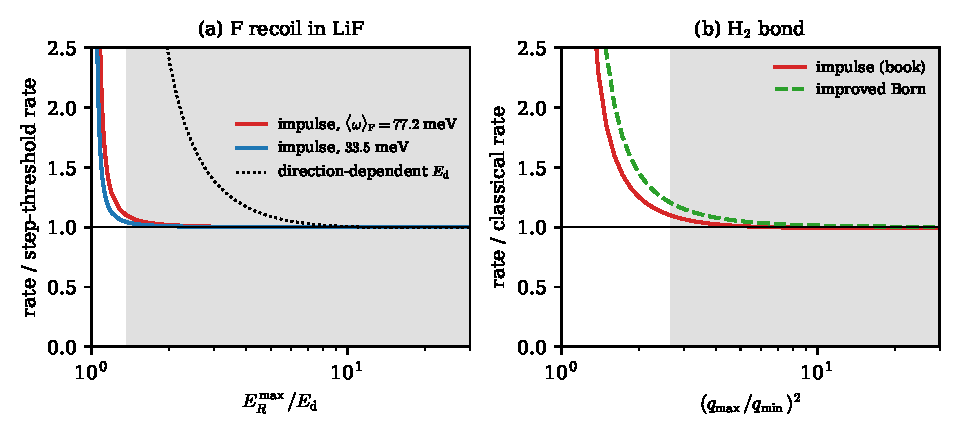
\includegraphics[width=\linewidth]{figures/ch16/limit16_6a.pdf}
\captionof{figure}{Rates from the impulse response of the bound target divided by the published forms, heavy mediator, standard halo, $T = 0$. (a) Fluorine recoils in LiF with $E_{\mathrm{d}} = \SI{27}{eV}$, against the ratio of the largest recoil energy to the threshold: \cref{eq:16.6-ccrate} with the yield a step at $\omega = E_{\mathrm{d}}$, for $\langle\omega\rangle_{\mathrm{F}} = \SI{77.2}{meV}$ (red, the top of the LiF optical band, an upper value) and \SI{33.5}{meV} (blue). Dotted: the direction-dependent threshold $E_{\mathrm{d}}(1 + a\sin4\theta\cos4\varphi)^2$ with $a = 0.4$, recoil directions isotropic in the crystal, divided by the step at $E_{\mathrm{d}}$. (b) H$_2$ as a free rotor: \cref{eq:16.6-conv} with \cref{eq:16.6-diss} over the Gaussian ground state (red) and with the improved Born condition (green, dashed), against $(q_{\max}/q_{\min})^2$, $q_{\max} = 2\mu_{\chi1}v_{\mathrm{max}}$. Gray: the red curve within \SI{10}{\percent} of one, $E_R^{\max} \ge 1.36\,E_{\mathrm{d}}$ ($\mchi \ge \SI{0.218}{GeV}$) in (a) and $(q_{\max}/q_{\min})^2 \ge 2.65$ ($\mchi \ge \SI{42.9}{MeV}$) in (b).}\label{fig:16-limit-cc}
\par}
\smallskip
Closer to threshold the color-center and bond-breaking rates both depend on the zero-point motion of the struck nucleus or bond and stay nonzero below the classical endpoint, and at every mass they still lack the yield factors of \cref{eq:16.6-yield} and the escape probability of the fragments of a bond, which multiply both curves.
\end{limitbox}

In \cref{lim:16.6a} the Doppler width changes the LiF rate by less than \SI{2}{\percent} once the largest recoil energy exceeds twice the threshold, and with the Doppler width the rate reaches the step-form rate for $E_R^{\max} = 1.1\,E_{\mathrm{d}}$ at a mass \SI{1.4}{\percent} lower. The directional structure of the threshold matters more: with the angular model of Budnik et al.\ the rate stays more than \SI{10}{\percent} away from the step value up to $E_R^{\max} = 4.8\,E_{\mathrm{d}}$, or $\mchi = \SI{0.41}{GeV}$, because the threshold surface reaches down to $0.36\,E_{\mathrm{d}}$. For H$_2$ the impulse rate equals the classical rate of $\mchi = \SI{27.2}{MeV}$ already at \SI{22.8}{MeV}, a shift of the mass scale by a factor 0.84; the improved Born rate does so at \SI{20.3}{MeV}, a factor 0.75.

A broken bond is not yet a signal. In a solid the two fragments start inside the cage of their neighbors, and they recombine unless they escape it; this recombination inside the cage is the cage effect of photochemistry. The rate of separated fragments is the rate of dissociating seeds times the escape probability $p_{\mathrm{esc}}(E_{\mathrm{int}},\hat{\vect{r}})$, which depends on the energy $E_{\mathrm{int}}$ the fragments share above the dissociation limit and on the direction of the bond relative to the cage. Electronic deposits break bonds as well: an excitation into a repulsive state, the antibonding $\sigma^*$ surface of the bond, dissociates the molecule without any nuclear kick, at the electronic thresholds of the molecular crystals of \cref{sec:16.4}. Neither $p_{\mathrm{esc}}$ nor the dissociation yields of these electronic states have been quantified at the momenta and temperatures of a dark-matter search.

\subsection{Measured yields and single-center readout}\label{sec:16.6-yields}

Of the inputs to \cref{eq:16.6-yield}, the displacement threshold is the one with measurements, and these fix only its lowest point. Electron irradiation of silicon sees damage set in at $12.9 \pm \SI{0.6}{eV}$, where density-functional molecular dynamics puts the minimum of $E_{\mathrm{d}}(\hat{\vect{r}})$ (\cref{sec:7.4}). The shape of $p_{\mathrm{FP}}$ above the minimum is a computed quantity: the defect probability becomes nonzero below the average threshold and approaches one only at two to three times the average threshold~\cite[Sect.~II]{cogswell2021passive}. In materials where an interstitial recombines with its own vacancy a direction-resolved threshold is not even well defined (\cref{app:E.11}). For ionic crystals the measured responses are those of dense tracks at room temperature: fast neutrons, $\gamma$ rays of $^{60}$Co, and the $\alpha$ and triton tracks of neutron capture on $^6$Li~\cite{araujo2026nuclear}. The aggregates that LiF forms along these dense tracks are stable for months in vacuum at room temperature and anneal away at \SI{350}{\celsius}~\cite[Sect.~III]{araujo2026nuclear}. None of these measurements isolates a single recoil of tens to hundreds of eV, and none is made at millikelvin temperatures.

A single-center readout at millikelvin temperatures must work without aggregation. A sub-GeV recoil makes one to three vacancies (\cref{we:16-fyield}), and at \SI{10}{mK} they do not move, so the emitting aggregates read in LiF tracks do not form and the readout must find a single F center. In LiF that center has no observed luminescence~\cite{guerreroperez2025first}, so it must be found through its absorption near \SI{5.1}{eV}, in the ultraviolet, or converted into a state that emits. For an emitting center in a light-guiding rod, Budnik et al.\ estimate $5\times10^5$ detected photons in \SI{e3}{s} and a detection limit of about one new center among $10^5$ existing ones~\cite[footnote~1]{budnik2018direct}. The existing centers set the background. Commercial crystals are not certified below a defect concentration of $10^{-9}$, and annealing at up to \SI{1000}{\celsius} removes many of the existing centers~\cite{budnik2018direct}; fluorescence measurements of LiF put an upper limit of $10^{-12}$ to $10^{-10}$ on the centers present before irradiation~\cite{cogswell2021passive}. At millikelvin temperatures the readout light must also deposit less heat than the detector tolerates; none of these estimates addresses this heat load.

Four yields remain open at millikelvin temperatures: the conversion $p_{\mathrm{FH}}$ of a self-trapped exciton into a Frenkel pair, the survival $p_{\mathrm{surv}}$ of a close pair with the charge factor $p_q$ at recoil energies of tens to hundreds of eV, the efficiency $f_{\mathrm{opt}}$ of reading a single center, and the escape $p_{\mathrm{esc}}$ of the fragments of a bond with the yields of repulsive electronic states. Each can be measured directly. Neutrons scattered at a tagged angle in LiF at \SI{10}{mK} give recoils of known energy, and counting single F centers per tagged recoil measures the product $p_{\mathrm{FP}}p_{\mathrm{surv}}p_qf_{\mathrm{opt}}$ as a function of $E_R$. X-rays of \SI{5.9}{keV} absorbed at millikelvin temperatures give $p_{\mathrm{FH}}$ from the F-center yield per absorbed energy together with the quenching of the exciton luminescence. The photodissociation quantum yield of a molecular crystal at millikelvin temperatures, with the fragments detected by infrared absorption, gives $p_{\mathrm{esc}}$.

\section{Glasses, random media and two-level systems}\label{sec:16.7}

A superconducting resonator made on a film of thermally grown SiO$_2$ loses a fraction $3\times10^{-4}$ of its stored energy per radian at \SI{6}{GHz} and below \SI{100}{mK}, when it holds only a few photons~\cite[Table~I]{oconnell2008microwave}. At higher power or temperature the loss falls. The absorbers are groups of atoms in the glass that can sit in either of two configurations and tunnel between them, typically $10^{20}$ per eV and cm$^3$, with splittings that reach down to micro-electronvolts. At these energies a crystal has only its long acoustic phonons. The same systems absorb a dark photon of mass \SI{25}{\micro eV} as readily as a microwave photon of that energy, and a dark-matter particle that scatters in the glass can flip one of them. A glass is also the plainest example of a random medium. Its disorder raises two further questions: how its vibrations absorb a dark photon once momentum conservation no longer selects one optical phonon, and when a light particle that scatters coherently off a whole body can be treated in the Born approximation. The same tunneling systems release heat at millikelvin temperatures, and their kinetics are the subject of \cref{sec:16.8}.

\subsection{The standard tunneling model}\label{sec:16.7-stm}

Let $|\mathrm{L}\rangle$ and $|\mathrm{R}\rangle$ be the ground states of a group of atoms localized in the two wells of a double-well potential. In their span the Hamiltonian is \cref{eq:C.20-H} without the bath,
\begin{equation}
  H_{\mathrm{TLS}} = \tfrac12\Delta_{\mathrm{as}}\,\sigma_z - \tfrac12\Delta_0\,\sigma_x ,
  \qquad \Delta_{\mathrm{tl}} = \bigl(\Delta_{\mathrm{as}}^2 + \Delta_0^2\bigr)^{1/2} ,
  \label{eq:16.7-H}
\end{equation}
with the Pauli matrices of \cref{app:C.20} in the localized basis, the asymmetry $\Delta_{\mathrm{as}}$ between the two wells, the tunneling amplitude $\Delta_0$ and the splitting $\Delta_{\mathrm{tl}}$ of the eigenstates, the two-level splitting of \cref{sec:2.5}. The tunneling amplitude is exponentially small in the barrier, $\Delta_0 = \omega_{\mathrm{w}}\ee^{-\lambda_{\mathrm{tun}}}$, with $\omega_{\mathrm{w}} \sim$ the vibration energy in one well. For a particle of mass $M_{\mathrm{tun}}$ crossing a barrier of height $V_{\mathrm{b}}$ between wells a distance $d_{\mathrm{tun}}$ apart, the tunneling exponent is $\lambda_{\mathrm{tun}} = (d_{\mathrm{tun}}/2)(2M_{\mathrm{tun}}V_{\mathrm{b}})^{1/2}$~\cite[Sect.~II]{meissner2021acoustic}. In the eigenbasis the matrix $\sigma_z$, which measures in which well the atoms sit, becomes
\begin{equation}
  \sigma_z = \frac{\Delta_{\mathrm{as}}}{\Delta_{\mathrm{tl}}}\,\tau_z + \frac{\Delta_0}{\Delta_{\mathrm{tl}}}\,\tau_x ,
  \label{eq:16.7-rot}
\end{equation}
with $\tau_z$ and $\tau_x$ the Pauli matrices of the eigenstates and the sign of $\tau_x$ fixed by the phases of the eigenvectors. A perturbation that couples to the position of the atoms therefore drives transitions with the amplitude $\Delta_0/\Delta_{\mathrm{tl}}$: a system with $\Delta_0 \ll \Delta_{\mathrm{as}}$ has its eigenstates localized in the two wells, and the perturbation cannot move it from one to the other.

In a glass every system has its own $\Delta_{\mathrm{as}}$ and $\lambda_{\mathrm{tun}}$. The standard tunneling model of Phillips and of Anderson, Halperin and Varma takes both to be independent and uniformly distributed, with density $\bar P$ per unit asymmetry, unit exponent and unit volume~\cite[Eq.~(8)]{muller2019towards}. A system and its mirror image are the same system, so we count $\Delta_{\mathrm{as}} \ge 0$ only; this convention defines $\bar P$, and with both signs counted every rate below would carry a factor 2. Changing variables from $(\Delta_{\mathrm{as}}, \lambda_{\mathrm{tun}})$ to $(\Delta_{\mathrm{tl}}, \Delta_0)$, with $\dd\lambda_{\mathrm{tun}} = -\dd\Delta_0/\Delta_0$ and $\partial\Delta_{\mathrm{as}}/\partial\Delta_{\mathrm{tl}} = \Delta_{\mathrm{tl}}/\Delta_{\mathrm{as}}$ at fixed $\Delta_0$, gives
\begin{equation}
  P(\Delta_{\mathrm{tl}},\Delta_0) = \frac{\bar P\,\Delta_{\mathrm{tl}}}{\Delta_0\,(\Delta_{\mathrm{tl}}^2 - \Delta_0^2)^{1/2}} ,
  \qquad 0 < \Delta_0 \le \Delta_{\mathrm{tl}} ,
  \label{eq:16.7-P}
\end{equation}
the distribution of Ref.~\cite[Eq.~(12)]{meissner2021acoustic}. Its integral over $\Delta_0$ diverges logarithmically at small $\Delta_0$, and the number of systems per unit splitting depends on a lower cutoff of the tunneling amplitude that no experiment fixes. A transition probability, however, carries the weight $(\Delta_0/\Delta_{\mathrm{tl}})^2$ of \cref{eq:16.7-rot}, and
\begin{equation}
  \int_0^{\Delta_{\mathrm{tl}}}\dd\Delta_0\,P(\Delta_{\mathrm{tl}},\Delta_0)\,\frac{\Delta_0^2}{\Delta_{\mathrm{tl}}^2} = \bar P\int_0^1\frac{u\,\dd u}{(1 - u^2)^{1/2}} = \bar P ,
  \label{eq:16.7-norm}
\end{equation}
with $u = \Delta_0/\Delta_{\mathrm{tl}}$. The systems that dominate the count do not couple, and those that couple are counted by $\bar P$ alone, at every splitting. \Cref{fig:16-tls}(a) shows the two densities.

\begin{figure}[tbp]
  \centering
  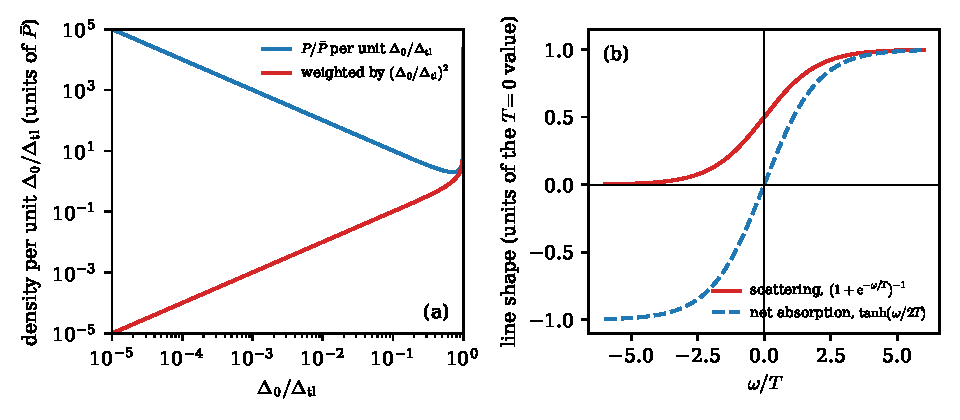
\includegraphics[width=\linewidth]{figures/ch16/fig16_7.pdf}
  \caption{The standard tunneling model. (a) Density of two-level systems per unit $u = \Delta_0/\Delta_{\mathrm{tl}}$ at fixed splitting, in units of $\bar P$: $1/[u(1 - u^2)^{1/2}]$ (blue), whose integral grows as $\ln(2/u_{\min})$ with the lower cutoff $u_{\min}$. Weighted by the squared transition amplitude $u^2$ (red), it integrates to one, \cref{eq:16.7-norm}; \SI{87}{\percent} of that comes from $u > 0.5$. (b) Line shapes of the ensemble at temperature $T$, in units of their $T = 0$ values. Red: the scattering structure factor $(1 + \ee^{-\omega/T})^{-1}$ of \cref{eq:16.7-S}, nonzero for $\omega < 0$ through the thermal population of the upper level; blue, dashed: the net absorption of a classical field, $\tanh(\omega/2T)$, \cref{eq:16.7-chires}.}
  \label{fig:16-tls}
\end{figure}

A strain field and an electric field both shift the energies of the two wells. The atoms move between configurations with different elastic and electric dipoles. To first order the asymmetry becomes $\Delta_{\mathrm{as}} + 2\gamma_{\mathrm{TLS}}u_{\mathrm{d}} + 2\vect{p}_{\mathrm{TLS}}\cdot\vect{E}$, with $u_{\mathrm{d}}$ the component of the strain tensor $u_{\alpha\beta}$ along the deformation of the defect, $\gamma_{\mathrm{TLS}}$ its deformation potential and $\vect{p}_{\mathrm{TLS}}$ half the difference of the electric dipoles of the two configurations~\cite[Eq.~(16)]{muller2019towards}. The perturbation is
\begin{equation}
  H_1 = \bigl(\gamma_{\mathrm{TLS}}u_{\mathrm{d}} + \vect{p}_{\mathrm{TLS}}\cdot\vect{E}\bigr)\,\sigma_z \equiv bF\,\sigma_z ,
  \label{eq:16.7-H1}
\end{equation}
where $F$ stands for the applied field ($u_{\mathrm{d}}$ or one component of $\vect{E}$) and $b$ for the coupling to it. By \cref{eq:16.7-rot} it has a transverse part, which drives transitions at $\omega = \Delta_{\mathrm{tl}}$, and a longitudinal part, which modulates the splitting.

The transverse part gives the resonant response. The power a field $F\cos\omega t$ deposits per unit volume is $\tfrac12\omega\chi''(\omega)F^2$, with $\chi''$ the absorptive part of the susceptibility of the coupled quantity $b\sigma_z$. For one system the golden rule of \cref{sec:2.1} gives an absorption rate from the lower level and an equal rate of stimulated emission from the upper one, and the populations of \cref{sec:2.5} differ by $p_0 - p_1 = \tanh(\Delta_{\mathrm{tl}}/2T)$. Hence $\chi''(\omega) = \pi b^2(\Delta_0/\Delta_{\mathrm{tl}})^2\tanh(\Delta_{\mathrm{tl}}/2T)\,\delta(\omega - \Delta_{\mathrm{tl}})$ for $\omega > 0$, where the delta function stands for the Lorentzian of \cref{eq:2.4-lorentz} with the width of the system, small against $\omega$ and $T$ in an insulating glass at millikelvin temperatures. Summing over the ensemble with \cref{eq:16.7-P,eq:16.7-norm},
\begin{equation}
  \chi''_{\mathrm{res}}(\omega) = \pi\bar P\,\langle b^2\rangle\,\tanh\frac{\omega}{2T} ,
  \label{eq:16.7-chires}
\end{equation}
independent of $\omega$, with $\langle b^2\rangle$ averaged over the orientations of the systems. Its two physical cases are the dielectric loss and the acoustic loss. For the electric field the orientation average is $\langle(\vect{p}_{\mathrm{TLS}}\cdot\hat{\vect{E}})^2\rangle = p_{\mathrm{TLS}}^2/3$, and in Heaviside--Lorentz units the polarization is $\chi\vect{E}$, so the imaginary part of the permittivity is $\chi''$ itself. Against the real part $\varepsilon_r$ of the glass, the loss tangent is
\begin{equation}
  \tan\delta(\omega,T) = \frac{\varepsilon_2}{\varepsilon_r} = \tan\delta_0\,\tanh\frac{\omega}{2T} , \qquad
  \tan\delta_0 = \frac{\pi\bar P\,p_{\mathrm{TLS}}^2}{3\varepsilon_r} ,
  \label{eq:16.7-tand}
\end{equation}
the low-power loss tangent $\tan\delta_0$ at $T \to 0$. For a sound wave of polarization $j$, longitudinal or transverse, the coupling is the deformation potential $\gamma_j$ and the elastic modulus $\rho_Tc_j^2$ takes the place of $\varepsilon_r$, so the internal friction is $Q^{-1} = \pi C_j\tanh(\omega/2T)$, with the tunneling strength $C_j = \bar P\gamma_j^2/\rho_Tc_j^2$~\cite[Eqs.~(5), (6)]{buchenau2020sound}. Both are the response of the standard tunneling model to a classical field~\cite[Eqs.~(4), (12), (13), (15)]{meissner2021acoustic}. In vitreous silica $C = 2.6\times10^{-4}$ on average over the two polarizations~\cite[Table~I]{buchenau2020sound}, and Golding, Graebner and Schutz find $C_{\mathrm{l}} = 1.9\times10^{-4}$ and $C_{\mathrm{t}} = 2.0\times10^{-4}$ at \SI{500}{MHz}, as quoted by Buchenau et al.~\cite[Sect.~III]{buchenau2020sound}.

The longitudinal part of \cref{eq:16.7-H1}, $bF(\Delta_{\mathrm{as}}/\Delta_{\mathrm{tl}})\tau_z$, shifts the splitting by $2bF\Delta_{\mathrm{as}}/\Delta_{\mathrm{tl}}$. In equilibrium the population difference would follow the shifted splitting at once; in fact it relaxes toward it at the rate $\varGamma_1 = 1/\tau_1$ of the system. The static susceptibility of the coupled quantity is $2b^2(\Delta_{\mathrm{as}}/\Delta_{\mathrm{tl}})^2\,\partial_{\Delta_{\mathrm{tl}}}\tanh(\Delta_{\mathrm{tl}}/2T)$, and a population that relaxes with one time constant turns it into the Debye form $\chi_{\mathrm{rel}}(\omega) = \chi_{\mathrm{rel}}(0)/(1 - \ii\omega\tau_1)$, whose absorptive part is $\chi_{\mathrm{rel}}(0)\,\omega\tau_1/(1 + \omega^2\tau_1^2)$~\cite[Eq.~(6)]{meissner2021acoustic}. In an insulating glass $\varGamma_1$ is set by the emission and absorption of one thermal phonon,
\begin{equation}
  \varGamma_1 = K_{\mathrm{ph}}\,\Delta_{\mathrm{tl}}^3\Bigl(\frac{\Delta_0}{\Delta_{\mathrm{tl}}}\Bigr)^2\coth\frac{\Delta_{\mathrm{tl}}}{2T} , \qquad
  K_{\mathrm{ph}} = \frac{1}{2\pi\rho_T}\Bigl(\frac{\gamma_{\mathrm{l}}^2}{c_{\mathrm{LA}}^5} + \frac{2\gamma_{\mathrm{t}}^2}{c_{\mathrm{TA}}^5}\Bigr) ,
  \label{eq:16.7-tau1}
\end{equation}
which \cref{sec:16.8} derives~\cite[Eq.~(7)]{meissner2021acoustic}. Summed over the ensemble and divided by the resonant value at $T = 0$, the full loss is
\begin{equation}
  \frac{\tan\delta}{\tan\delta_0} = \tanh\frac{\omega}{2T} + \frac{2}{\pi}\int_0^\infty\frac{\dd\Delta_{\mathrm{tl}}}{2T}\,\mathrm{sech}^2\frac{\Delta_{\mathrm{tl}}}{2T}\int_0^1\dd u\,\frac{(1 - u^2)^{1/2}}{u}\,\frac{\omega\tau_1}{1 + \omega^2\tau_1^2} ,
  \label{eq:16.7-relax}
\end{equation}
with $u = \Delta_0/\Delta_{\mathrm{tl}}$ and $\tau_1 = 1/\varGamma_1$ from \cref{eq:16.7-tau1}; the same ratio holds for $Q^{-1}/\pi C_j$. The relaxation part has two limits. Since $\tau_1^{-1} \propto u^2$, the fastest systems are those with $u = 1$. When they relax fast, $\omega\tau_1(u = 1) \ll 1$, the $u$ integral is dominated by the slower systems with $u^2 \sim \omega\tau_1(u = 1)$, where $\omega\tau_1 \sim 1$; it equals $\pi/4$, and the relaxation part saturates at $\tfrac12$, the tunneling plateau $Q^{-1} = \pi C/2$~\cite[Eq.~(10)]{buchenau2020sound}. When even the fastest systems relax slowly, $\omega\tau_1(u = 1) \gg 1$, the integrand is $1/\omega\tau_1$, the $u$ integral gives $\tfrac13$, and the energy integral gives $\int_0^\infty y^3\,\dd y/\sinh y = \pi^4/8$, so the relaxation part is $(\pi^3/12)K_{\mathrm{ph}}T^3/\omega$. Compared to the resonant part, $\omega/2T$ at $T \gg \omega$, it grows as $T^4/\omega^2$.

\begin{limitbox}[Two-level response to a classical strain or field][lim:16.7a]
The resonant loss of the standard tunneling model, $\tan\delta = \tan\delta_0\tanh(\omega/2T)$ with $\tan\delta_0 = \pi\bar Pp_{\mathrm{TLS}}^2/3\varepsilon_r$, and $Q^{-1} = \pi C_j\tanh(\omega/2T)$ for sound~\cite[Eqs.~(4), (12), (13), (15)]{meissner2021acoustic}.
\par\smallskip
{\centering
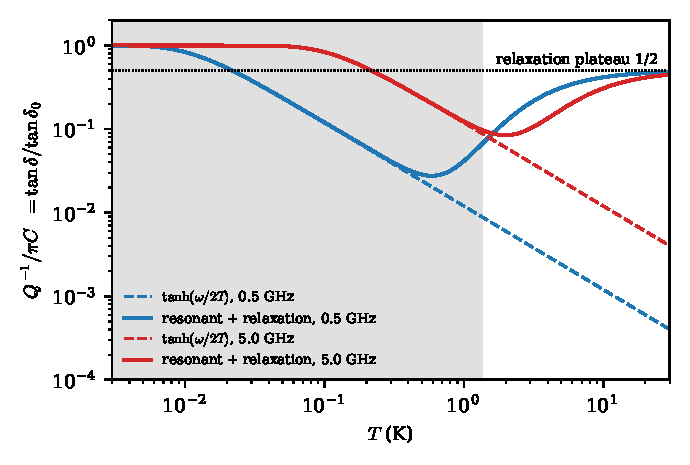
\includegraphics[width=0.82\linewidth]{figures/ch16/limit16_7a.pdf}
\captionof{figure}{Loss of the ensemble in vitreous silica, divided by its value at $T = 0$, against temperature, at \SI{0.5}{GHz} (blue) and \SI{5}{GHz} (red). Dashed: $\tanh(\omega/2T)$. Solid: resonant plus relaxation part, \cref{eq:16.7-relax}, with the one-phonon rate \cref{eq:16.7-tau1} for $\rho_T = \SI{2.2}{g.cm^{-3}}$, $c_{\mathrm{LA}} = 5.8$ and $c_{\mathrm{TA}} = \SI{3.8}{km.s^{-1}}$~\cite[Table~I]{buchenau2020sound}, an assumed $\gamma_{\mathrm{l}} = \SI{1}{eV}$ and $\gamma_{\mathrm{l}}/\gamma_{\mathrm{t}} = 1.6$~\cite{zhou2015generic}, so that $K_{\mathrm{ph}} = \SI{4.63e4}{eV^{-2}}$. Dotted: the relaxation plateau. Gray: the full loss within \SI{10}{\percent} of the tanh law at \SI{5}{GHz}, $T < \SI{1.36}{K}$ (\SI{0.43}{K} at \SI{0.5}{GHz}).}\label{fig:16-limit-tls}
\par}
\smallskip
Above these temperatures the population of slowly relaxing systems lags the field, and the loss rises toward the plateau $\tan\delta_0/2$ instead of falling as $\omega/2T$.
\end{limitbox}

\Cref{lim:16.7a} puts the relaxation correction where the low-temperature estimate puts it: \SI{10}{\percent} of the resonant loss at $T = [0.6\,\omega^2/(\pi^3K_{\mathrm{ph}})]^{1/4}$, which is \SI{1.34}{K} at \SI{5}{GHz} against \SI{1.36}{K} from the full integral. At \SI{10}{mK} the relaxation part at \SI{5}{GHz} is $4\times10^{-9}$ of the resonant one. The value of $\gamma_{\mathrm{l}}$ enters only through $K_{\mathrm{ph}}$, and since the crossover temperature scales as $K_{\mathrm{ph}}^{-1/4}$, a deformation potential twice as large moves it down by a factor $2^{1/2}$. The tunneling model has its own limits at these temperatures: above about \SI{2}{K}, relaxation by several phonons adds to \cref{eq:16.7-tau1}~\cite[Sect.~II]{meissner2021acoustic}. The second correction is saturation. A field strong enough to drive transitions faster than the systems relax equalizes the two populations and removes the resonant loss; for sound the resonant term falls as $[1 + I/I_{\mathrm{c}}]^{-1/2}$ with the intensity $I$, and the critical intensity is $\sim10^{-7}\,\si{W.cm^{-2}}$~\cite[Eq.~(8)]{buchenau2020sound}. This is why the resonator loss falls at high power and why $\tan\delta_0$ is the low-power value. In practice the tunneling parameters, the distributions of $\Delta_{\mathrm{as}}$ and $\lambda_{\mathrm{tun}}$, the deformation potentials and the dipole moments, are computed from ensembles of model glasses, found by searching their energy landscapes for pairs of nearby minima (\cref{app:E.22}). The computed $\bar Pp_{\mathrm{TLS}}^2$ is then checked against the measured $\tan\delta_0$ of the same preparation.

\subsection{Dark-photon absorption on two-level systems}\label{sec:16.7-dp}

A dark photon of mass $m_\phi$ is absorbed at the rate per unit target mass $\mathcal{R} = (\rho_\chi/\rho_T)\zeta^2L(m_\phi)$, with $L = \Imag(-1/\varepsilon)$ the loss function at $\vect{p}_\phi \to 0$ (\cref{eq:10.7-dp}). The momentum $\vect{p}_\phi \approx m_\phi v$ of a dark photon of \SI{25}{\micro eV} is $3\times10^{-8}\,\si{eV}$ for $v = \SI{354}{km.s^{-1}}$, a wavelength of about \SI{40}{m}, so the local dielectric function of the glass is all we need. For a glass with $\varepsilon = \varepsilon_r(1 + \ii\tan\delta)$ the loss function is $\tan\delta/[\varepsilon_r(1 + \tan^2\delta)]$, and with \cref{eq:16.7-tand},
\begin{keyresult}[Dark-photon absorption on two-level systems]
\begin{equation}
  \mathcal{R} = \frac{\rho_\chi}{\rho_T}\,\zeta^2\,\frac{\tan\delta_0}{\varepsilon_r}\,\tanh\frac{m_\phi}{2T}\,\bigl[1 + \mathcal{O}(\tan^2\delta_0)\bigr] .
  \label{eq:16.7-dp}
\end{equation}
The rate per unit mass is independent of $m_\phi$ wherever $m_\phi \gg 2T$, and it is fixed by two measured numbers, the low-power loss tangent and the permittivity.
\end{keyresult}
\noindent The factor $\tanh(m_\phi/2T)$ appears once. It is the population difference of the absorbing systems, and the net rate already subtracts the stimulated emission that the dark-matter field drives from the upper level, just as the dielectric loss does; a second thermal factor from the field would count that subtraction twice. The in-medium suppression $1/\varepsilon_r$ is the factor $1/|\varepsilon|^2$ of \cref{eq:10.7-dp} times the $\varepsilon_r$ in $\varepsilon_2 = \varepsilon_r\tan\delta$: the field inside the glass is screened, and the absorbers respond to the screened field. And the dark-matter field drives each system far below saturation. At the coupling that \cref{we:16-tls-dp} finds for three events per kg-year, the field $\zeta(2\rho_\chi)^{1/2}$ of \cref{sec:11.8} gives a Rabi frequency below $6\times10^{-7}\,\si{s^{-1}}$ for a dipole of \SI{1.1}{D}, against a relaxation rate of $10^6\,\si{s^{-1}}$ for a system with $\Delta_{\mathrm{tl}} = m_\phi$ at \SI{6}{GHz}.

What the two-level systems add is a loss that is flat in frequency, from the lowest masses at which $m_\phi$ exceeds $2T$ up to the energies at which the flat distribution \cref{eq:16.7-P} ceases to hold. The loss tangents that fix the rate are measured near \SI{6}{GHz} (\SI{25}{\micro eV}) and below \SI{100}{mK}, and they depend on how the oxide was made. Thermal SiO$_2$ has $\tan\delta_0 = 3.0$ to $3.3\times10^{-4}$, and oxide deposited from a plasma $2.7$ to $2.9\times10^{-3}$ in lumped-element resonators~\cite[Table~I]{oconnell2008microwave}. A second deposited oxide reached $5\times10^{-3}$~\cite{martinis2005decoherence}. Such films are a few hundred nanometers thick, and no millikelvin value has been measured for bulk fused silica.

\begin{workedexample}{The dark-photon rate on thermal SiO$_2$}\label{we:16-tls-dp}
Take thermal SiO$_2$ with $\tan\delta_0 = 3\times10^{-4}$, an assumed static permittivity $\varepsilon_r = 3.9$, and $\rho_T = \SI{2.2}{g.cm^{-3}}$, at $T = \SI{10}{mK}$ ($T = \SI{0.862}{\micro eV}$). A dark photon of \SI{6}{GHz}, $m_\phi = \SI{24.81}{\micro eV}$, has $m_\phi/2T = 14.4$, so $\tanh(m_\phi/2T) = 1$ to eight digits, and the loss function is $L = 3\times10^{-4}/3.9 = \num{7.69e-5}$. The prefactor is $\rho_\chi/\rho_T = (\SI{0.3}{GeV.cm^{-3}})/(\SI{2.2}{g.cm^{-3}}) = \SI{0.136}{GeV/g}$, which divided by $\hbar$ is $2.07\times10^{23}$ per gram per second. Then
\begin{equation*}
  \mathcal{R} = \num{5.03e29}\,\zeta^2\ \text{per kg-year} ,
\end{equation*}
and three events in one kg-year need $\zeta = \num{2.44e-15}$. The upper end of the measured range, $3.3\times10^{-4}$, raises the rate by 1.10, and the deposited oxide with $5\times10^{-3}$ by 16.7, which lowers $\zeta$ by a factor 0.24. At \SI{100}{mK} the thermal factor drops to 0.894, which is why a loss tangent quoted at that temperature must be divided by 0.894 to give $\tan\delta_0$.

The target mass is the problem. A film of \SI{1}{\micro m} on \SI{100}{cm^2} weighs \SI{22}{mg}, and three events in a year then need $\zeta = \num{5.2e-13}$. Each absorption leaves \SI{24.8}{\micro eV} in one two-level system, which decays by emitting a phonon of that energy. The loss tangent also fixes $\bar Pp_{\mathrm{TLS}}^2 = 3\varepsilon_r\tan\delta_0/\pi$ and nothing else: with $\bar P = \SI{1.2e20}{eV^{-1}.cm^{-3}}$, the value that the polarization-averaged $C = 2.6\times10^{-4}$ implies for $\gamma_{\mathrm{l}} = \SI{1}{eV}$, \cref{eq:16.7-tand} requires $p_{\mathrm{TLS}} = 0.23\,e\,\text{\AA} = \SI{1.1}{D}$.
\end{workedexample}

\begin{limitbox}[Dark-photon absorption on two-level systems][lim:16.7b]
$\mathcal{R} = (\rho_\chi/\rho_T)\zeta^2\tan\delta_0\tanh(m_\phi/2T)/\varepsilon_r$, the loss function $\Imag(-1/\varepsilon) = \varepsilon_2/|\varepsilon|^2$ of \cref{eq:10.7-dp} with the electric loss of the tunneling model~\cite[Eq.~(20)]{muller2019towards}.
\par\smallskip
{\centering
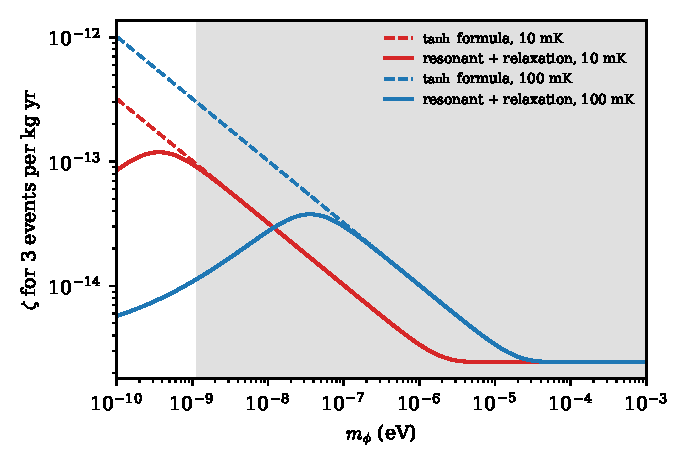
\includegraphics[width=0.82\linewidth]{figures/ch16/limit16_7b.pdf}
\captionof{figure}{Kinetic mixing for three absorptions per kg-year on thermal SiO$_2$ ($\tan\delta_0 = 3\times10^{-4}$, $\varepsilon_r = 3.9$, $\rho_T = \SI{2.2}{g.cm^{-3}}$), against the dark-photon mass, at \SI{10}{mK} (red) and \SI{100}{mK} (blue). Dashed: \cref{eq:16.7-dp}. Solid: $\varepsilon_2/|\varepsilon|^2$ with $\varepsilon_2$ from the resonant plus relaxation loss \cref{eq:16.7-relax}, $K_{\mathrm{ph}}$ as in \cref{fig:16-limit-tls}. Gray: within \SI{10}{\percent} at \SI{10}{mK}, $m_\phi > \SI{1.15}{neV}$ (\SI{0.28}{MHz}); at \SI{100}{mK} the bound moves to \SI{115}{neV}.}\label{fig:16-limit-dp}
\par}
\smallskip
Below these masses the relaxation of systems with splittings near $T$ absorbs more than the resonant systems at $\Delta_{\mathrm{tl}} = m_\phi$, whose population difference vanishes as $m_\phi/2T$.
\end{limitbox}

\noindent The mass of \cref{lim:16.7b} scales as $T^2$: with $\tanh(m_\phi/2T) \approx m_\phi/2T$ and the low-temperature relaxation part $(\pi^3/12)K_{\mathrm{ph}}T^3/m_\phi$, the two are in the ratio $(\pi^3/6)K_{\mathrm{ph}}T^4/m_\phi^2$, which reaches 0.1 at $m_\phi \propto T^2$. Above a millielectronvolt the vibrations of the glass absorb more than its two-level systems (\cref{sec:16.7-ir}).

\subsection{Dark-matter scattering on two-level systems}\label{sec:16.7-scat}

A dark-matter particle that couples to the electron density sees a two-level system through the change of that density between the two configurations. Projected on $|\mathrm{L}\rangle$ and $|\mathrm{R}\rangle$, the density operator at momentum $\vect{q}$ is $\tfrac12(n_{\mathrm{LL}} + n_{\mathrm{RR}}) - \tfrac12f_{\mathrm{TLS}}(\vect{q})\,\sigma_z$, up to terms of relative order $\ee^{-\lambda_{\mathrm{tun}}}$, with the vertex
\begin{equation}
  f_{\mathrm{TLS}}(\vect{q}) = \langle\mathrm{R}|n_e(\vect{q})|\mathrm{R}\rangle - \langle\mathrm{L}|n_e(\vect{q})|\mathrm{L}\rangle .
  \label{eq:16.7-f}
\end{equation}
The first term is the static density and scatters elastically; the second flips the system with the amplitude of \cref{eq:16.7-rot}, $|\langle e|n_e(\vect{q})|g\rangle|^2 = \tfrac14|f_{\mathrm{TLS}}|^2(\Delta_0/\Delta_{\mathrm{tl}})^2$. The structure factor of \cref{eq:2.5-golden} sums this over systems, with the weights $p_0$ and $p_1$ of \cref{sec:2.5} for absorption at $\omega = \Delta_{\mathrm{tl}}$ and emission at $\omega = -\Delta_{\mathrm{tl}}$, and with \cref{eq:16.7-P,eq:16.7-norm} the ensemble gives
\begin{equation}
  S(\vect{q},\omega) = \frac{\pi}{2}\,\bar P\,\bigl\langle|f_{\mathrm{TLS}}(\vect{q})|^2\bigr\rangle\,\frac{1}{1 + \ee^{-\omega/T}} ,
  \label{eq:16.7-S}
\end{equation}
flat in $\omega$ inside the band of the two-level systems and obeying detailed balance, \cref{eq:2.5-db}, as \cref{fig:16-tls}(b) shows. The average runs over the systems and their orientations.

The vertex has two parts. The atoms that tunnel carry their electrons from one well to the other, the core term. And the surrounding glass relaxes elastically around each configuration, which moves all its electrons, the host term. For the host term take the defect as an elastic dipole. In configuration R it exerts on the glass a force dipole that differs from that of L by $-2\gamma_{\mathrm{TLS}}$ along its deformation, since the energy of a force dipole $\mathsf{D}$ in a strain is $-\sum_{\alpha\beta}\mathsf{D}_{\alpha\beta}u_{\alpha\beta}$ and the asymmetry shifts by $2\gamma_{\mathrm{TLS}}u_{\mathrm{d}}$. In an isotropic continuum the static displacement field of a force dipole has longitudinal Fourier component $\vect{q}\cdot\tilde{\vect{u}}(\vect{q}) = -\ii\,\hat{\vect{q}}\cdot\mathsf{D}\cdot\hat{\vect{q}}/\rho_Tc_{\mathrm{LA}}^2$, and since the adiabatic electrons follow the atoms, the electron density changes by $\delta n_e(\vect{q}) = \ii\nd_e\,\vect{q}\cdot\tilde{\vect{u}}$ with $\nd_e$ the density of all electrons. Hence
\begin{equation}
  f_{\mathrm{host}} = \frac{2\nd_e\,\hat{\vect{q}}\cdot\gamma_{\mathrm{TLS}}\cdot\hat{\vect{q}}}{\rho_Tc_{\mathrm{LA}}^2} ,
  \qquad
  \bar P\,\bigl\langle|f_{\mathrm{host}}|^2\bigr\rangle = \frac{4\nd_e^2\,C_{\mathrm{l}}}{\rho_Tc_{\mathrm{LA}}^2} ,
  \label{eq:16.7-host}
\end{equation}
where the orientation average of $(\hat{\vect{q}}\cdot\gamma_{\mathrm{TLS}}\cdot\hat{\vect{q}})^2$ is $\gamma_{\mathrm{l}}^2$, the coupling to longitudinal strain. The deformation potential drops out of the product: the host term of the scattering rate is fixed by the measured tunneling strength $C_{\mathrm{l}}$, not by the loss tangent. The form holds in a window of momentum transfers. The momentum transfer must be static, $q \gg \omega/c_{\mathrm{LA}}$; for $\omega$ near $c_{\mathrm{LA}}q$ the elastic response has a pole, and the process becomes the emission of a real phonon that the two-level system absorbs later, which belongs to the phonon channel of \cref{sec:11.1}. The wavelength must also be long against the defect and the atomic spacing, where continuum elasticity holds. No dielectric factor is added: the adiabatic density already contains the screening of the electrons.

For the core term the simplest model moves one oxygen ion, with its eight electrons, rigidly by $\vect{d}$. With the origin at the midpoint, $f_{\mathrm{core}} = 8(\ee^{\ii\vect{q}\cdot\vect{d}/2} - \ee^{-\ii\vect{q}\cdot\vect{d}/2}) = 16\ii\sin(\vect{q}\cdot\vect{d}/2)$, and its orientation average is $\langle|f_{\mathrm{core}}|^2\rangle = 128[1 - \sin(qd)/qd]$. The core amplitude is imaginary and the static host amplitude is real, so the two add without interference, for every orientation and not only on average; an off-center core would restore a cross term. For a displacement along $\hat{\vect{q}}$ the two are equal near $q_\times = |f_{\mathrm{host}}|/(8d)$, where the host term stops dominating; with the orientation-averaged core, $\langle|f_{\mathrm{core}}|^2\rangle^{1/2} \simeq 4.62\,qd$, the crossing moves up by $\sqrt3$.

With a heavy mediator, $\mathfrak{D}_{ee} = \pi\sigmae/\mu_{\chi e}^2$ and the structure factor \cref{eq:16.7-S} in the isotropic rate \cref{eq:10.1-rateiso}, the minimum velocity is $q/2\mchi$ up to $\omega/q$, negligible for $\omega \lesssim \SI{0.1}{meV}$, and a $q$-independent vertex leaves $\int q\,\dd q\,\eta(q/2\mchi) = 2\mchi^2\langle v\rangle$. The rate is
\begin{equation}
  \frac{\dd\mathcal{R}}{\dd\omega} = \frac{\rho_\chi}{\mchi\rho_T}\,\langle v\rangle\,\sigmae\Bigl(1 + \frac{\mchi}{m_e}\Bigr)^2\,\frac{\bar P\langle|f_{\mathrm{TLS}}|^2\rangle}{4\,(1 + \ee^{-\omega/T})} ,
  \label{eq:16.7-rate}
\end{equation}
per unit energy and target mass, a cross-section $\sigmae(1 + \mchi/m_e)^2|f_{\mathrm{TLS}}|^2(\Delta_0/\Delta_{\mathrm{tl}})^2/4$ per system. The factor $(1 + \mchi/m_e)^2 = \mchi^2/\mu_{\chi e}^2$ converts the reference cross-section on a free electron into the cross-section on a heavy target. For a $q$-dependent core vertex the $q$ integral is done with $\eta$.

Consider amorphous SiO$_2$ at $\mchi = \SI{1}{MeV}$ and $\sigmae = \SI{e-38}{cm^2}$. Thirty electrons per formula unit at \SI{2.2}{g.cm^{-3}} give $\nd_e = \SI{6.62e23}{cm^{-3}}$, and $\rho_Tc_{\mathrm{LA}}^2 = \SI{7.40e10}{Pa} = \SI{4.62e23}{eV.cm^{-3}}$. With the measured longitudinal $C_{\mathrm{l}} = 1.9\times10^{-4}$, \cref{eq:16.7-host} gives $\bar P\langle|f_{\mathrm{host}}|^2\rangle = \SI{7.20e20}{eV^{-1}.cm^{-3}}$, and with the halo of \cref{tab:1-shm}, $\langle v\rangle = \SI{354.1}{km.s^{-1}}$, and $(1 + \mchi/m_e)^2 = 8.74$, the host term is $6.6\times10^{-3}$ per kg, day and meV. The core term needs $\bar P$ itself. For an assumed $\gamma_{\mathrm{l}} = \SI{1}{eV}$, $\bar P = C_{\mathrm{l}}\rho_Tc_{\mathrm{LA}}^2/\gamma_{\mathrm{l}}^2 = \SI{8.8e19}{eV^{-1}.cm^{-3}}$, $|f_{\mathrm{host}}| = 2.86$, and one oxygen moving by \SI{1}{\angstrom} adds $1.6\times10^{-2}$, 2.5 times the host term. The total,
\begin{equation*}
  \frac{\dd\mathcal{R}}{\dd\omega} \approx 2.3\times10^{-2}\ \text{per kg, day and meV} \qquad (\mchi = \SI{1}{MeV},\ \sigmae = \SI{e-38}{cm^2}),
\end{equation*}
is flat over the band of the two-level systems, and over $0 < \omega < \SI{0.1}{meV}$ it amounts to $2.3\times10^{-3}$ events per kg-day. The polarization-averaged $C = 2.6\times10^{-4}$ would raise both terms by 1.37, to $3.1\times10^{-2}$ per kg, day and meV.

This number is an estimate, uncertain by about a factor 3. The heavy-mediator weight $q\,\eta(q/2\mchi)$ has its median at $q = \SI{1.73}{keV}$, where $qd = 0.88$ for $d = \SI{1}{\angstrom}$. The host and core terms cross lower, at $q_\times = \SI{0.71}{keV}$ for a displacement along $\hat{\vect{q}}$ and \SI{1.2}{keV} on orientation average. Most of the rate therefore comes from momentum transfers outside the window of \cref{eq:16.7-host}, near the scale at which the glass stops being a continuum. The core term is a rigid ion, which misses the redistribution of the valence electrons of the moving oxygen, and one geometry stands for many. Both are replaced by the density difference \cref{eq:16.7-f} from two self-consistent calculations of the same glass cell, averaged over an ensemble of systems. Whatever its value, the rate is small because $\bar P$ times the band of energies, about $10^{16}$ systems per cm$^3$, is a small number of targets, and each takes at most \SI{0.1}{meV}. Thin films under a sensor hold far less mass still and matter as absorbers of phonons and as sources of delayed heat (\cref{sec:16.8}), not as targets.

\subsection{Vibrational absorption of glasses}\label{sec:16.7-ir}

In a crystal a dark photon is absorbed on phonons only at the zone-center optical frequencies, where its tiny momentum matches a mode (\cref{sec:11.8}). A glass has no zone center. Every vibrational mode can carry a dipole, and the absorption is spread over the whole vibrational spectrum~\cite{bloch2026dark}. The rate is still $\mathcal{R} = (\rho_\chi/\rho_T)\zeta^2L(m_\phi)$, now with the dielectric function of the vibrations of the glass~\cite[Eq.~(2)]{bloch2026dark}, and the question is what fixes $L$ at the lowest masses.

Take one configuration of the glass in the harmonic approximation, with modes $\nu$ of frequency $\omega_\nu$, eigenvectors $\vect{e}_{I\nu}$ normalized over all $N$ atoms, masses $M_I$ and Born charges $Z^*_I$. Its dielectric function has the rank-one form of \cref{sec:11.8}, with the Hessian of the glass in place of the dynamical matrix,
\begin{equation}
  \varepsilon(\omega) = \varepsilon_\infty + \frac{e^2}{\Vol}\sum_\nu\frac{|p_\nu|^2}{\omega_\nu^2 - \omega^2 - \ii\omega\varGamma_\nu} ,
  \qquad p_\nu = \sum_I\frac{\hat{\boldsymbol{\epsilon}}\cdot Z^*_I\cdot\vect{e}_{I\nu}}{M_I^{1/2}} ,
  \label{eq:16.7-epsglass}
\end{equation}
for a field along $\hat{\boldsymbol{\epsilon}}$ and mode widths $\varGamma_\nu$. For narrow modes the imaginary part is $\varepsilon_2(\omega) = (\pi e^2/2\omega\Vol)\sum_\nu|p_\nu|^2\delta(\omega - \omega_\nu)$. With the vibrational density of states $g(\omega)$ normalized to one, $\sum_\nu\delta(\omega - \omega_\nu) = 3Ng(\omega)$, and with the infrared coupling $C^{\mathrm{IR}}(\omega)$, the mean of $|p_\nu|^2$ over the modes at frequency $\omega$,
\begin{equation}
  \varepsilon_2(\omega) = \frac{3\pi e^2\nd_{\mathrm{at}}}{2\omega}\,g(\omega)\,C^{\mathrm{IR}}(\omega) .
  \label{eq:16.7-eps2}
\end{equation}
The absorption coefficient $\alpha_{\mathrm{abs}} = \omega\varepsilon_2/n_r$, with $n_r = \varepsilon_r^{1/2}$ the refractive index, is then a product of the density of states and a coupling, the form in which infrared spectroscopy of glasses is analyzed~\cite[Eq.~(2) and text before Eq.~(1)]{taraskin2006universal}.

Below the Ioffe--Regel frequency $\omega_{\mathrm{IoR}}$, the frequency at which the mean free path of a vibration falls to one wavelength, the modes are still sound waves, scattered weakly by the disorder. For a plane wave of branch $\nu$ with sound speed $c_\nu$, wavevector $\vect{k}$ and polarization $\hat{\vect{e}}_\nu$, every atom moves with the same velocity, $\vect{e}_{I\nu} = \hat{\vect{e}}_\nu\ee^{\ii\vect{k}\cdot\vect{x}_I}(M_I/N\bar M)^{1/2}$ with $\bar M$ the mean atomic mass. The masses cancel in $p_\nu$, which becomes a Fourier component of the field of Born charges, and averaged over the modes at fixed $\omega = c_\nu k$,
\begin{equation}
  C^{\mathrm{IR}}(\omega) = \frac{1}{\bar M}\sum_\nu\hat w_\nu\,S^Z_\nu(\omega/c_\nu) ,
  \qquad S^Z_\nu(k) = \frac1N\Bigl\langle\Bigl|\sum_I\hat{\boldsymbol{\epsilon}}\cdot Z^*_I\cdot\hat{\vect{e}}_\nu\,\ee^{\ii\vect{k}\cdot\vect{x}_I}\Bigr|^2\Bigr\rangle ,
  \label{eq:16.7-CIR}
\end{equation}
with $\hat w_\nu = c_\nu^{-3}/\sum_{\nu'}c_{\nu'}^{-3}$ the fraction of modes at fixed $\omega$ in branch $\nu$, as in \cref{eq:E.19-CIR}. The behavior of $S^Z_\nu$ at small $k$ decides the low-frequency absorption. A crystal has $S^Z_\nu(k) = 0$ for acoustic modes as $k \to 0$, since the Born charges of a cell add to zero. In a glass the charges fluctuate from site to site. If they obey only global neutrality, uncorrelated fluctuations leave $S^Z_\nu(0^+)$ equal to the mean square fluctuation of the projected charge, a constant. If instead they are neutral within every local unit, as within the SiO$_4$ tetrahedra of silica, the sum is that of dipoles and $S^Z_\nu \propto k^2$. Expanding to second order,
\begin{equation}
  C^{\mathrm{IR}}(\omega) = A^{\mathrm{IR}} + B^{\mathrm{IR}}\omega^2 , \qquad
  A^{\mathrm{IR}} = \frac{1}{\bar M}\sum_\nu\hat w_\nu S^Z_\nu(0^+) , \quad
  B^{\mathrm{IR}} = \frac{1}{\bar M}\sum_\nu\frac{\hat w_\nu S^{Z\prime\prime}_\nu(0)}{2c_\nu^2} ,
  \label{eq:16.7-AB}
\end{equation}
the law Taraskin, Simdyankin, Elliott, Neilson and Lo found in terahertz spectra of glasses~\cite[Eq.~(1)]{taraskin2006universal}. Their fit to vitreous silica at room temperature writes $\alpha_{\mathrm{abs}} = (A^{\mathrm{IR}} + B^{\mathrm{IR}}\tilde\omega^2)g(\tilde\omega)$ in spectroscopic units, with $\alpha_{\mathrm{abs}}$ and the wavenumber $\tilde\omega = \omega/2\pi c$ in cm$^{-1}$ and $g$ normalized per cm$^{-1}$. It gives $A^{\mathrm{IR}} = \SI{4000}{cm^{-2}}$ and $B^{\mathrm{IR}} = 0.3$, dimensionless, with the Debye density of states of a \SI{330}{K} Debye temperature~\cite[Fig.~1]{taraskin2006universal}. Harmonic absorption is net absorption and does not depend on temperature, but a room-temperature spectrum also contains anharmonic and relaxational absorption whose size at millikelvin temperatures has not been separated; there the fit is a model value.

\begin{limitbox}[Glass absorption below the Ioffe--Regel frequency][lim:16.7d]
$\alpha_{\mathrm{abs}}(\omega) = (A^{\mathrm{IR}} + B^{\mathrm{IR}}\tilde\omega^2)\,g(\tilde\omega)$ for $\omega < \omega_{\mathrm{IoR}}$~\cite[Eq.~(1)]{taraskin2006universal}, inserted in the rate $(\rho_\chi/\rho_T)\zeta^2\Imag(-1/\varepsilon)$~\cite[Eq.~(2)]{bloch2026dark}.
\par\smallskip
{\centering
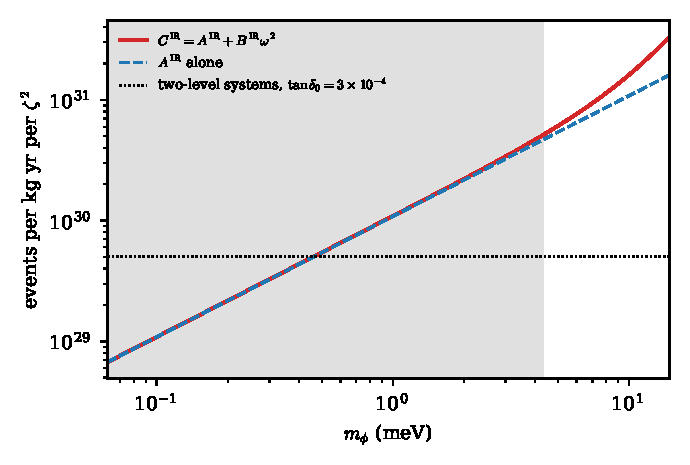
\includegraphics[width=0.82\linewidth]{figures/ch16/limit16_7d.pdf}
\captionof{figure}{Dark-photon absorptions per kg-year per $\zeta^2$ in vitreous silica against the mass, from \cref{eq:16.7-eps2} with $C^{\mathrm{IR}} = A^{\mathrm{IR}} + B^{\mathrm{IR}}\omega^2$ (red) and with the constant term alone (blue, dashed). Inputs: the terahertz fit $A^{\mathrm{IR}} = \SI{4000}{cm^{-2}}$, $B^{\mathrm{IR}} = 0.3$ of Taraskin et al., a Debye density of states with $\Theta_{\mathrm{D}} = \SI{330}{K}$, $\varepsilon_r = 3.9$ and $\rho_T = \SI{2.2}{g.cm^{-3}}$. Dotted: two-level absorption, \cref{eq:16.7-dp}, for thermal SiO$_2$ at saturation. Gray: below the Ioffe--Regel frequency of silica, $\omega/2\pi c \approx \SI{35}{cm^{-1}}$ (\SI{4.3}{meV}), where the $B$ term is at most \SI{9}{\percent} of the $A$ term.}\label{fig:16-limit-ir}
\par}
\smallskip
Above $\omega_{\mathrm{IoR}}$ the modes are no longer plane waves, $S^Z_\nu$ at one wavevector no longer describes them, and the coupling departs from $A^{\mathrm{IR}} + B^{\mathrm{IR}}\omega^2$ in a way that depends on the glass.
\end{limitbox}

\Cref{lim:16.7d} shows how the two channels of a glass divide the masses. With $\varepsilon_2 = n_r\alpha_{\mathrm{abs}}/(2\pi\tilde\omega)$, the vibrational absorption grows as $\omega$ times $C^{\mathrm{IR}}$. At \SI{1.24}{meV} ($\tilde\omega = \SI{10}{cm^{-1}}$) it gives $\alpha_{\mathrm{abs}} = \SI{0.10}{cm^{-1}}$, $\varepsilon_2 = \num{3.1e-3}$ and $1.4\times10^{30}\zeta^2$ absorptions per kg-year. It equals the two-level absorption of thermal SiO$_2$ at \SI{0.46}{meV}, and that of the deposited oxide with $\tan\delta_0 = 5\times10^{-3}$ at \SI{6.4}{meV}, an extrapolation above $\omega_{\mathrm{IoR}}$. The constant term carries the low-frequency absorption of silica entirely: the curvature term reaches the constant only at $\tilde\omega = (A^{\mathrm{IR}}/B^{\mathrm{IR}})^{1/2} = \SI{115}{cm^{-1}}$, three times above $\omega_{\mathrm{IoR}}$. That constant is the incoherent sum of random charges, and a model of the glass that makes every tetrahedron neutral by construction misses it (\cref{app:E.19}). Bloch, Knapen, Li, Madden and Marocco propose amorphous membranes for masses of 50 to \SI{200}{meV}, above $\omega_{\mathrm{IoR}}$, where the mean free path of a mode is shorter than its wavelength and the absorption follows from the measured or computed $\varepsilon(\omega)$ of \cref{eq:16.7-epsglass}~\cite{bloch2026dark}. The same random couplings give a broadband absorption in a crystal with isotope disorder, which \cref{sec:11.6} treats.

\subsection{Random media and the Born limit}\label{sec:16.7-random}

A dark-matter particle of \SI{20}{eV} moving at $v = 10^{-3}$ has a de Broglie wavelength $2\pi/\mchi v$ of about \SI{60}{\micro m}. A momentum transfer $\sim\mchi v$ cannot resolve atoms, and the particle scatters off the smoothed density $\nd(\vect{r})$ of nucleons of a whole body. Liu, Matsumoto, Sheng and Xing pointed out that a random two-phase material scatters such particles far more strongly than a homogeneous one~\cite{liu2025coherence}. In the first Born approximation for the body, the amplitudes of all nucleons add with their phases, and for a spin-independent interaction
\begin{equation}
  \frac{\dd\sigma_{\mathrm{tot}}}{\dd\Omega_q} = \frac{\dd\sigma_{\chi N}}{\dd\Omega_q}\,\Bigl|\int\dd^3r\,\ee^{\ii\vect{q}\cdot\vect{r}}\,\nd(\vect{r})\Bigr|^2 ,
  \label{eq:16.7-born}
\end{equation}
the coherent sum of \cref{sec:2.2} with the nucleus replaced by the body~\cite[Eq.~(2)]{liu2025coherence}. Write $\nd = \nd_0 + \delta\nd$ with $\nd_0$ the mean nucleon density, and average over the random structure. The cross term vanishes, and the two remaining terms are the homogeneous body, $\nd_0^2|\int_{\Vol}\dd^3r\,\ee^{\ii\vect{q}\cdot\vect{r}}|^2$, which falls as $(qR)^{-4}$ for a sphere of radius $R$ once $qR \gg 1$, and the fluctuations, $\int\dd^3r_1\dd^3r_2\,\ee^{\ii\vect{q}\cdot(\vect{r}_2 - \vect{r}_1)}\langle\delta\nd(\vect{r}_1)\delta\nd(\vect{r}_2)\rangle$. For a correlation that decays as $\langle\delta\nd(\vect{r}_1)\delta\nd(\vect{r}_2)\rangle = \delta\nd^2\ee^{-|\vect{r}_2 - \vect{r}_1|/\xi_{\mathrm{c}}}$ over a correlation length $\xi_{\mathrm{c}}$, the transform $\int\dd^3r\,\ee^{\ii\vect{q}\cdot\vect{r}}\ee^{-r/\xi_{\mathrm{c}}} = 8\pi\xi_{\mathrm{c}}^3/(1 + q^2\xi_{\mathrm{c}}^2)^2$ times the volume $\Vol = 4\pi R^3/3$ gives, per squared number of nucleons $\nd_0^2\Vol^2$,
\begin{equation}
  |F_{\mathrm{fluc}}(q)|^2 = \frac{\delta\nd^2}{\nd_0^2}\,\frac{6\,\xi_{\mathrm{c}}^3}{R^3(1 + q^2\xi_{\mathrm{c}}^2)^2} ,
  \label{eq:16.7-Ffluc}
\end{equation}
for $R \gg \xi_{\mathrm{c}}$, the result of Ref.~\cite[Eqs.~(9)--(12)]{liu2025coherence}. The body acts as a collection of incoherent clusters of size $\xi_{\mathrm{c}}$, each scattering coherently. At $qR \gg 1$ and $q\xi_{\mathrm{c}} \gg 1$ the sphere-averaged homogeneous term is $9/[2(qR)^4]$, and the ratio of the two is $(4/3)(R/\xi_{\mathrm{c}})(\delta\nd/\nd_0)^2$. For the Ti--6Al--4V alloy of the test masses of the MICROSCOPE satellite test of the equivalence principle, the authors infer $\nd_0 = \SI{2.69e24}{cm^{-3}}$ and $\delta\nd = \SI{7.29e22}{cm^{-3}}$ from the phase fractions of its microstructure~\cite[Eq.~(14)]{liu2025coherence}. Then $(\delta\nd/\nd_0)^2 = 7\times10^{-4}$, and for that value the homogeneous term the authors drop is the larger one below a few hundred eV on an equal-mass sphere.

A large coherent cross-section, however, means a strong interaction with the medium, and the Born approximation for a whole body is not the Born approximation for one nucleus. At wavelengths long against the spacing of nuclei, the medium acts on the particle as an optical potential. It is the sum of the pseudopotentials $2\pi b_{\chi N}/\mu_{\chi N}$ of the nucleons, with $b_{\chi N}$ the scattering length, $\sigma_{\chi N} = 4\pi b_{\chi N}^2$, and $\mu_{\chi N} \approx \mchi$ for a light particle:
\begin{equation}
  V_{\mathrm{opt}} = \frac{2\pi b_{\chi N}\nd_0}{\mu_{\chi N}} .
  \label{eq:16.7-Vopt}
\end{equation}
The plane wave inside the body is undistorted only if this potential is small against the kinetic energy, $|V_{\mathrm{opt}}| \ll E_{\mathrm{kin}} = \mchi v^2/2$. Squaring $|b_{\chi N}| \ll \mchi^2v^2/4\pi\nd_0$ gives the condition on the cross-section,
\begin{equation}
  \sigma_{\chi N} \ll \sigma_{\mathrm{crit}} = \frac{\mchi^4v^4}{4\pi\nd_0^2} ,
  \qquad \frac{|V_{\mathrm{opt}}|}{E_{\mathrm{kin}}} = \Bigl(\frac{\sigma_{\chi N}}{\sigma_{\mathrm{crit}}}\Bigr)^{1/2} .
  \label{eq:16.7-scrit}
\end{equation}
Since $\sigma_{\mathrm{crit}} \propto v^4$, the condition must hold over the velocities that dominate the observable, not at one speed. The homogeneous term of \cref{eq:16.7-born} contains the scattering of the wave by the surface of the body. For a planar face its first-order form can be compared with the exact reflection off a potential step, which shows where the first-order treatment of the medium breaks down. For a wave whose kinetic energy of motion normal to the face is $E_n$, the wavenumber inside is $k' = k(1 - V_{\mathrm{opt}}/E_n)^{1/2}$ and the reflectance is $R_{\mathrm{refl}} = |(k - k')/(k + k')|^2$, total for $V_{\mathrm{opt}} > E_n$. Expanding $k'$ to first order in $V_{\mathrm{opt}}$ gives the Born value $(V_{\mathrm{opt}}/4E_n)^2$, the square of the first-order amplitude of the step.

\begin{limitbox}[Random media and the Born limit][lim:16.7c]
First Born approximation for a whole body, $\dd\sigma_{\mathrm{tot}}/\dd\Omega_q = (\dd\sigma_{\chi N}/\dd\Omega_q)|\int\dd^3r\,\ee^{\ii\vect{q}\cdot\vect{r}}\nd(\vect{r})|^2$, with the fluctuation form factor \cref{eq:16.7-Ffluc}~\cite[Eqs.~(2), (9)--(12), (14)]{liu2025coherence}.
\par\smallskip
{\centering
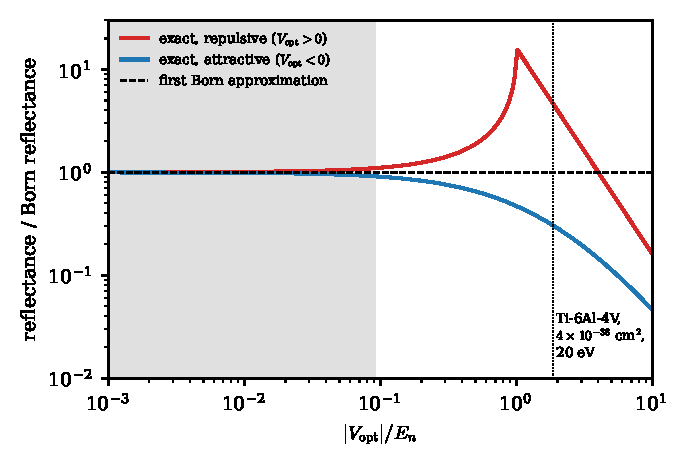
\includegraphics[width=0.82\linewidth]{figures/ch16/limit16_7c.pdf}
\captionof{figure}{Exact reflectance of a planar face of a homogeneous medium with optical potential \cref{eq:16.7-Vopt}, divided by its first Born approximation $(V_{\mathrm{opt}}/4E_n)^2$, against $|V_{\mathrm{opt}}|/E_n$, for a repulsive (red) and an attractive (blue) medium. $E_n$ is the kinetic energy of the motion normal to the face. Gray: the ratio within \SI{10}{\percent} of one, $|V_{\mathrm{opt}}|/E_n < 0.092$. Dotted: $V_{\mathrm{opt}}/E_{\mathrm{kin}} = 1.86$, the value at $\sigma_{\chi N} = \SI{4e-38}{cm^2}$, $\mchi = \SI{20}{eV}$, $v = 10^{-3}$ in Ti--6Al--4V ($\nd_0 = \SI{2.69e24}{cm^{-3}}$).}\label{fig:16-limit-born}
\par}
\smallskip
Beyond $|V_{\mathrm{opt}}| \approx E_n$ a repulsive body reflects every particle that reaches it, and the force on it scales with the optical potential of each material, not with the square of its density fluctuations.
\end{limitbox}

\noindent The leading correction is linear: the ratio of \cref{lim:16.7c} is $1 + V_{\mathrm{opt}}/E_n$ for small $V_{\mathrm{opt}}/E_n$, \SI{1}{\percent} at $V_{\mathrm{opt}}/E_n = 0.01$, of opposite sign for the two signs of the potential. Below $\sigma_{\mathrm{crit}}$ the uniform part of the medium only shifts the wavenumber inside, $k \to k'$, a phase that drops out of the fluctuation term once the wave is distorted by it, and the fluctuation cross-section keeps corrections of relative order $V_{\mathrm{opt}}/E_{\mathrm{kin}}$. In Ti--6Al--4V at $\mchi = \SI{20}{eV}$, \cref{eq:16.7-scrit} gives $\sigma_{\mathrm{crit}} = \SI{1.16e-38}{cm^2}$ at $v = 10^{-3}$, \SI{2.41e-38}{cm^2} at $v = \num{1.2e-3}$ and \SI{5.7e-37}{cm^2} at the largest laboratory speed $v_{\mathrm{max}} = \num{2.650e-3}$. Liu et al.\ quote a reach of $\sigma_{\chi N} \approx \SI{4e-38}{cm^2}$ near \SI{20}{eV} from the MICROSCOPE bound on differential acceleration~\cite[Sect.~IV]{liu2025coherence}, where $|V_{\mathrm{opt}}|/E_{\mathrm{kin}} = 1.86$ at $v = 10^{-3}$ and 1.29 at $v = \num{1.2e-3}$, before the projection on the normal of a face lowers $E_n$ further. At that cross-section the first-order treatment of the medium does not apply to the speeds near the peak of the distribution. Whether the true force on the test masses is larger or smaller than the Born estimate depends on the sign of $b_{\chi N}$, on reflection at the faces and on the composition difference of the two masses. Until the force is computed by transfer matrices over the faces and the velocity distribution, a bound from this channel is a conjecture.

\subsection{Open problems for glass targets}\label{sec:16.7-open}

For a given film the parameters of the standard tunneling model are known only in combination: the loss tangent fixes $\bar Pp_{\mathrm{TLS}}^2$, the acoustic loss $\bar P\gamma_{\mathrm{l}}^2$ and $\bar P\gamma_{\mathrm{t}}^2$, and neither fixes $\bar P$; the core term, the relaxation corrections and the kinetics of \cref{sec:16.8} need all three. For the films of real detectors (amorphous Al$_2$O$_3$ in junctions, SiO$_2$ and SiN$_x$ under sensors, amorphous WSi) these have not been measured on the same sample. Beyond the values, the model itself is an assumption: that $\Delta_{\mathrm{as}}$ and $\lambda_{\mathrm{tun}}$ are independent and flat, at every energy from the lowest masses to the top of the band, and that the systems do not interact. Its successes, the linear specific heat and the logarithmic shift of the sound velocity, test averages, not the distributions, and the ratio $\gamma_{\mathrm{l}}/\gamma_{\mathrm{t}}$, between 1.44 and 1.84 in 18 glasses, is nearly universal without the model giving a reason~\cite{zhou2015generic}. One film measured three ways would settle the first question: the dielectric loss, the acoustic loss, and the strain and field dependence of single systems resolved in a resonator, which give $\gamma_{\mathrm{TLS}}$ and $p_{\mathrm{TLS}}$ directly~\cite{muller2019towards}. The second needs the distributions computed for a model glass of stated preparation.

\section{Two-level systems at millikelvin}\label{sec:16.8}

One gram of fused silica cooled to \SI{10}{mK} is still giving off \SI{46}{pW} an hour later, and the power falls only as $1/t$ (\cref{we:16-heat}). For a detector held at \SI{10}{mK} this is a heat load that lasts for weeks. The heat comes from the tunneling two-level systems of \cref{sec:16.7}. Each was in equilibrium at a few kelvin, and each gives up its excess energy when it next relaxes, which for a defect behind a thick barrier takes hours or years. The same relaxation rates decide how fast a two-level system in a sensor film absorbs the energy of a phonon and returns it, and they are the kinetics behind the delayed signals of \cref{sec:19.6}. The defect is the two-configuration system of \cref{eq:C.20-H}, treated in the spin--boson language of \cref{app:C.20}.

\subsection{Relaxation by one phonon}\label{sec:16.8-phonon}

A two-level system relaxes when it passes from the upper to the lower of its two eigenstates and gives the splitting to its surroundings. The environment couples to the configuration through $\tfrac12\sigma_z X$, with $X = \sum_k\lambda_k(d_k + d_k^\dagger)$ the bath coordinate of \cref{eq:C.20-H}. By \cref{eq:16.7-rot} only the off-diagonal element $\Delta_0/\Delta_{\mathrm{tl}}$ of $\sigma_z$ in the eigenbasis changes the state; the diagonal part shifts the splitting by the fluctuating bath and contributes only to the dephasing. By the golden rule of \cref{sec:2.1} the emission of a bath quantum of energy $\Delta_{\mathrm{tl}}$ has the rate $2\pi\sum_k(\Delta_0\lambda_k/2\Delta_{\mathrm{tl}})^2(n_{\mathrm{B}} + 1)\,\delta(\Delta_{\mathrm{tl}} - \omega_k)$, and absorption has the same rate with $n_{\mathrm{B}}$ in place of $n_{\mathrm{B}} + 1$. A population difference relaxes at the sum of the two, which carries $2n_{\mathrm{B}} + 1 = \coth(\Delta_{\mathrm{tl}}/2T)$:
\begin{equation}
  \varGamma_1 = \frac12\Bigl(\frac{\Delta_0}{\Delta_{\mathrm{tl}}}\Bigr)^2 J_{\mathrm{s}}(\Delta_{\mathrm{tl}})\,\coth\frac{\Delta_{\mathrm{tl}}}{2T} .
  \label{eq:16.8-golden}
\end{equation}
The bath enters only through its spectral density $J_{\mathrm{s}}(\omega) = \pi\sum_k\lambda_k^2\delta(\omega - \omega_k)$ of \cref{eq:C.20-J} at the splitting. The rate is first order in $J_{\mathrm{s}}$, and it holds as long as $\varGamma_1 \ll \Delta_{\mathrm{tl}}$, so that the eigenstates are defined; its upward and downward parts obey detailed balance (\cref{sec:2.5}).

A long acoustic wave couples through the strain term of \cref{eq:16.7-H1}, and the deformation potential depends on the orientation of the defect relative to the wave. As in \cref{sec:16.7}, $\gamma_{\mathrm{l}}^2$ and $\gamma_{\mathrm{t}}^2$ are its mean squares over orientations for a longitudinal wave and for each transverse wave; acoustic experiments on glasses give about \SI{1}{eV}~\cite[Sect.~IV\,A]{muller2019towards}. Summing the strain of every phonon mode of \cref{sec:5.3} at the defect (\cref{app:D.42}) gives
\begin{equation}
  J_{\mathrm{s}}^{\mathrm{ph}}(\omega) = \frac{\omega^3}{\pi\rho_T}\Bigl(\frac{\gamma_{\mathrm{l}}^2}{c_{\mathrm{LA}}^5} + \frac{2\gamma_{\mathrm{t}}^2}{c_{\mathrm{TA}}^5}\Bigr) = 2K_{\mathrm{ph}}\,\omega^3 ,
  \label{eq:16.8-Jph}
\end{equation}
with $c_{\mathrm{LA}}$ and $c_{\mathrm{TA}}$ the sound speeds and $K_{\mathrm{ph}}$ the constant of \cref{eq:16.7-tau1}. The bath is superohmic (\cref{app:C.20}): the strain of one phonon grows as $\omega^{1/2}$ and the number of modes as $\omega^2$. With \cref{eq:16.8-golden} it gives the one-phonon rate $\varGamma_1^{\mathrm{ph}} = K_{\mathrm{ph}}\Delta_{\mathrm{tl}}^3(\Delta_0/\Delta_{\mathrm{tl}})^2\coth(\Delta_{\mathrm{tl}}/2T)$ of \cref{eq:16.7-tau1}. This is Jäckle's rate, in the form of Meißner et al.~\cite[Eq.~(7)]{meissner2021acoustic} and of Sahling et al.~\cite[Eqs.~(4), (5)]{sahling2010anomalous}. The fifth power of the sound speed makes the transverse waves dominate. At equal deformation potentials they carry $2(c_{\mathrm{LA}}/c_{\mathrm{TA}})^5 = 16.6$ times the longitudinal rate in vitreous silica, with the sound speeds of \cref{sec:16.7}, and 65 times in aluminum. A thermal defect, with $\Delta_{\mathrm{tl}} \approx T$ and fixed $\Delta_0/\Delta_{\mathrm{tl}}$, relaxes at a rate $\propto T^3$, and since $\Delta_0 \propto \ee^{-\lambda_{\mathrm{tun}}}$ the rate spans many decades across the broad distribution of tunneling exponents $\lambda_{\mathrm{tun}}$. A defect of \SI{5}{GHz}, $\Delta_{\mathrm{tl}} = \SI{20.7}{\micro eV}$, with $\Delta_0 = 0.3\,\Delta_{\mathrm{tl}}$ and $\gamma_{\mathrm{l}} = \gamma_{\mathrm{t}} = \SI{1}{eV}$, relaxes in aluminum at $2.1\times10^5\,\si{s^{-1}}$ below about \SI{50}{mK} ($2.5\times10^5\,\si{s^{-1}}$ at \SI{0.1}{K}; \cref{fig:16-tlsrates}).

\subsection{Relaxation by conduction electrons}\label{sec:16.8-electron}

In a metal the defect has a second bath. When it tunnels, the potential that scatters the conduction electrons changes, and the Fermi sea must rearrange. The excitations of the sea are electron--hole pairs, and near the Fermi level their number at energy $\omega$ grows as $\omega$ while the matrix elements stay constant, so the bath is ohmic, \cref{eq:C.20-ohmic}, with $J_{\mathrm{s}}^{\mathrm{el}}(\omega) = 2\pi\alpha_{\mathrm{ohm}}\omega$ for $\omega$ far below the cutoff. In \cref{eq:16.8-golden} it gives
\begin{equation}
  \varGamma_1^{\mathrm{el}} = \pi\alpha_{\mathrm{ohm}}\Bigl(\frac{\Delta_0}{\Delta_{\mathrm{tl}}}\Bigr)^2\Delta_{\mathrm{tl}}\,\coth\frac{\Delta_{\mathrm{tl}}}{2T} ,
  \label{eq:16.8-black}
\end{equation}
the rate of Black and coworkers, as quoted by Meißner et al.~\cite[Eq.~(8)]{meissner2021acoustic} with their coupling $W_{\mathrm{el}}^2 = 4\alpha_{\mathrm{ohm}}$. For a thermal defect it grows only linearly in $T$, against $T^3$ for one phonon, and below a kelvin the electrons win by orders of magnitude. For the \SI{5}{GHz} defect above in normal aluminum, $\varGamma_1^{\mathrm{el}} = 2.5\times10^9\,\si{s^{-1}}$ at \SI{10}{mK} with $\alpha_{\mathrm{ohm}} = 0.28$, against $2.1\times10^5\,\si{s^{-1}}$ for one phonon.

The coupling $\alpha_{\mathrm{ohm}}$ is fixed by how differently the two configurations scatter electrons at the Fermi level. Let the two configurations act on the electrons as contact potentials $\pm V_{\mathrm{d}}$ over a volume $\Omega$. To second order in $V_{\mathrm{d}}$ the electron--hole pairs then form a Gaussian bath, and their spectral density gives (\cref{app:D.42})
\begin{equation}
  \alpha_{\mathrm{ohm}} = 4K_{\mathrm{b}} , \qquad K_{\mathrm{b}} = (\mathcal{N}_{\mathrm{F}}V_{\mathrm{d}}\Omega)^2 ,
  \label{eq:16.8-born}
\end{equation}
with $\mathcal{N}_{\mathrm{F}}$ the density of states per spin. This is the coupling $K$ of Maillet et al.~\cite[Eq.~(4)]{maillet2023nanomechanical}, whose rate $4\pi K\Delta_0^2\coth(\Delta_{\mathrm{tl}}/2T)/\Delta_{\mathrm{tl}}$ is \cref{eq:16.8-black}; their fits to the damping of aluminum-coated nanomechanical resonators give $K = 0.07$ and 0.11, that is $\alpha_{\mathrm{ohm}} = 0.28$ and 0.44, with a single-spin density of states. Beyond the Born limit the coupling is \cref{eq:E.10-ohm}, a sum over the squared differences $\tilde\delta_\nu$ of the scattering phases of the two configurations. For one contact channel per spin the phases are $\mp\arctan(\pi\mathcal{N}_{\mathrm{F}}V_{\mathrm{d}}\Omega)$, and $\alpha_{\mathrm{ohm}} = (4/\pi^2)\arctan^2(\pi K_{\mathrm{b}}^{1/2})$, which saturates at one when the phase difference reaches $\pi$. The Born value is \SI{10}{\percent} high already at $K_{\mathrm{b}} = 0.017$ (\cref{lim:16.8a}). At the fitted $K_{\mathrm{b}} = 0.07$ the same contact potential gives $\alpha_{\mathrm{ohm}} = 0.19$, not 0.28; read the other way, the measured rate needs a contact potential \SI{32}{\percent} stronger than the Born estimate.

A first-principles $\alpha_{\mathrm{ohm}}$ needs the two relaxed configurations of the defect, from a nudged-elastic-band search (\cref{app:E.11}). It also needs the scattering matrices of the conduction electrons at the Fermi level in both, from an impurity Green's function or from the overlap of the two many-electron ground states as a function of the supercell size (\cref{app:E.10}). \Cref{app:E.22} specifies the calculation for a crowdion in tungsten, hydrogen in niobium and two-level systems in aluminum, its oxide and amorphous WSi, with the Born limit and the resonator fits as acceptance tests. No such calculation exists yet, and the fitted values are the only numbers in hand.

Below $T_c$ the electrons pair. A defect with $\Delta_{\mathrm{tl}} < 2\Delta_{\mathrm{BCS}}$ cannot break a pair, and it can only scatter the thermal quasiparticles of \cref{sec:7.2}, whose number falls as $\ee^{-\Delta_{\mathrm{BCS}}/T}$. A static change of potential is even under time reversal, so the quasiparticle matrix elements carry the case-I coherence factor of the electron density, and the golden-rule integral over the quasiparticle energies is done in \cref{app:D.42}. For $\Delta_{\mathrm{tl}}$ and $T$ both small compared with $\Delta_{\mathrm{BCS}}$ it gives
\begin{equation}
  \frac{\varGamma_1^{\mathrm{s}}}{\varGamma_1^{\mathrm{el}}} = \frac{2}{1 + \ee^{\Delta_{\mathrm{BCS}}/T}}\;\sinh\frac{\Delta_{\mathrm{tl}}}{2T}\;K_1\Bigl(\frac{\Delta_{\mathrm{tl}}}{2T}\Bigr) ,
  \label{eq:16.8-sc}
\end{equation}
with $K_1(u) = \int_0^\infty\dd\theta\,\ee^{-u\cosh\theta}\cosh\theta$ the modified Bessel function. The last two factors tend to one as $\Delta_{\mathrm{tl}}/T \to 0$, and the remaining factor $2/(1 + \ee^{\Delta_{\mathrm{BCS}}/T})$, twice the occupation of the gap edge, is the superconducting form of Meißner et al.~\cite[Eq.~(9)]{meissner2021acoustic}, which they state for $\Delta_{\mathrm{tl}} \ll \Delta_{\mathrm{BCS}}$. The same factor gives the ratio of ultrasonic attenuation in the superconducting and normal states, and for the same reason: both probes scatter quasiparticles through the density. The Bessel factor arises because $\Delta_{\mathrm{tl}}$ is not small compared with $T$. Normal electrons accept $\Delta_{\mathrm{tl}}$ from the whole Fermi sea, while quasiparticles crowd at the gap edge and the energy must be taken up within their thermal spread. The factor is 0.86 for a thermal defect with $\Delta_{\mathrm{tl}} = T$ and 0.71 at $\Delta_{\mathrm{tl}} = 2T$, and the form of the source holds within \SI{10}{\percent} only for $\Delta_{\mathrm{tl}} \le 0.7\,T$ (\cref{lim:16.8a}).

\Cref{fig:16-tlsrates} puts the three rates together for one defect in aluminum. In the normal state the electrons dominate at every temperature. Below $T_c$ the suppression is so strong that one phonon takes over below \SI{0.21}{K}, about $T_c/6$, and at \SI{50}{mK} the electron rate is $2\times10^{-9}\,\si{s^{-1}}$. A superconducting film at the base temperature of a dilution refrigerator thus leaves its two-level systems coupled to phonons alone, as an insulator would.

\begin{figure}[tbp]
  \centering
  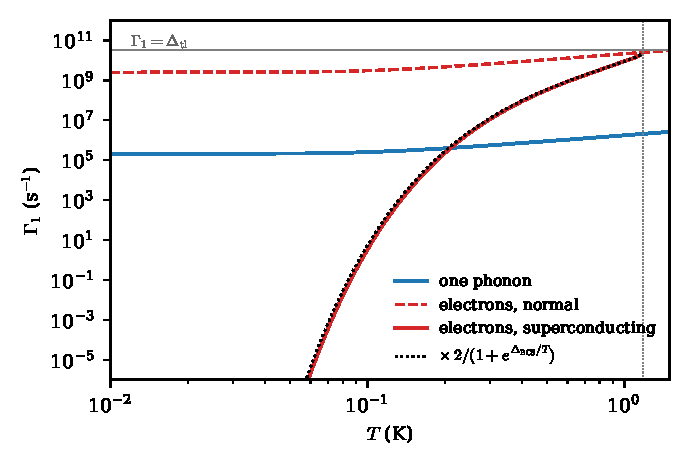
\includegraphics[width=0.7\linewidth]{figures/ch16/fig16_8.pdf}
  \caption{Relaxation rates of one two-level system in aluminum against temperature, for $\Delta_{\mathrm{tl}} = \SI{20.7}{\micro eV}$ (\SI{5}{GHz}) and $\Delta_0 = 0.3\,\Delta_{\mathrm{tl}}$. Blue: one phonon, \cref{eq:16.7-tau1}, with the model deformation potentials $\gamma_{\mathrm{l}} = \gamma_{\mathrm{t}} = \SI{1}{eV}$ and the isotropic sound speeds $c_{\mathrm{LA}} = \SI{6.63}{km.s^{-1}}$, $c_{\mathrm{TA}} = \SI{3.30}{km.s^{-1}}$ and density \SI{2.70}{g.cm^{-3}} of aluminum (\cref{sec:20.3}). Red dashed: conduction electrons in the normal state, \cref{eq:16.8-black}, with $\alpha_{\mathrm{ohm}} = 0.28$, continued below $T_c = \SI{1.18}{K}$ (vertical line) as for a film held normal. Red solid: the superconducting state, from the quasiparticle integral of \cref{app:D.42} with the weak-coupling gap $\Delta_{\mathrm{BCS}}(T)$; black dotted: the normal rate times $2/(1 + \ee^{\Delta_{\mathrm{BCS}}/T})$. The gray line marks $\varGamma_1 = \Delta_{\mathrm{tl}}$, which the normal-state rate reaches at \SI{1.5}{K}, where the golden rule fails.}
  \label{fig:16-tlsrates}
\end{figure}

\begin{limitbox}[Two-level relaxation by phonons and electrons][lim:16.8a]
The published rates are Jäckle's one-phonon rate and Black's electron rate, \cref{eq:16.7-tau1,eq:16.8-black}, with the superconducting factor $2/(1 + \ee^{\Delta_{\mathrm{BCS}}/T})$~\cite[Eqs.~(7)--(9)]{meissner2021acoustic}, and the Born-limit coupling $\alpha_{\mathrm{ohm}} = 4K_{\mathrm{b}}$~\cite[Eq.~(4)]{maillet2023nanomechanical}.
\par\smallskip
{\centering
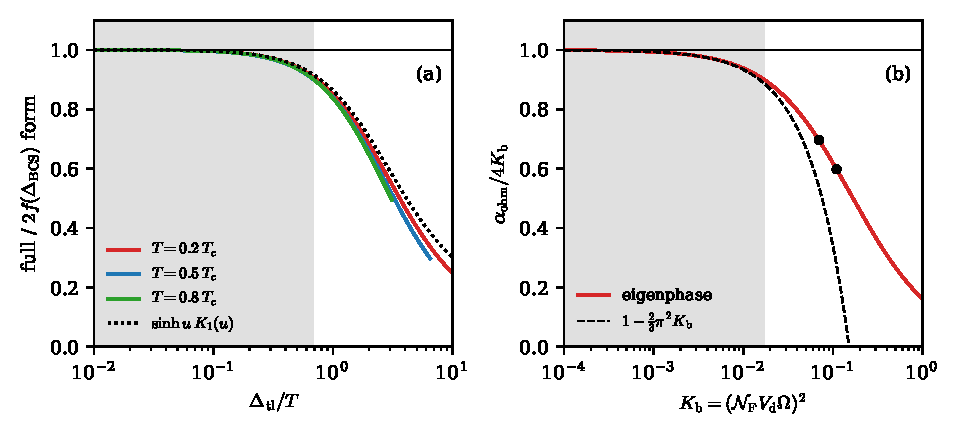
\includegraphics[width=\linewidth]{figures/ch16/limit16_8a.pdf}
\captionof{figure}{(a) Electron relaxation rate of a two-level system in superconducting aluminum, from the quasiparticle integral with the case-I coherence factor and the weak-coupling gap ($T_c = \SI{1.18}{K}$), divided by the normal rate times $2/(1 + \ee^{\Delta_{\mathrm{BCS}}/T})$, against $\Delta_{\mathrm{tl}}/T$ at $T = 0.2$, 0.5 and $0.8\,T_c$; each curve ends at $\Delta_{\mathrm{tl}} = 2\Delta_{\mathrm{BCS}}(T)$. Dotted: the closed form $\sinh u\,K_1(u)$, $u = \Delta_{\mathrm{tl}}/2T$, of \cref{eq:16.8-sc}. Gray: within \SI{10}{\percent} of one, $\Delta_{\mathrm{tl}} \le 0.69$--$0.73\,T$. (b) Ohmic coupling from the scattering phases of one contact channel per spin, $\alpha_{\mathrm{ohm}} = (4/\pi^2)\arctan^2(\pi K_{\mathrm{b}}^{1/2})$, divided by the Born value $4K_{\mathrm{b}}$, against $K_{\mathrm{b}}$. Dashed: the leading correction $1 - \tfrac23\pi^2K_{\mathrm{b}}$. Dots: the resonator fits $K_{\mathrm{b}} = 0.07$ and 0.11. Gray: within \SI{10}{\percent}, $K_{\mathrm{b}} \le 0.017$.}\label{fig:16-limit-tlsrel}
\par}
\smallskip
For $\Delta_{\mathrm{tl}} \gtrsim T$ the quasiparticles cannot take up the splitting as freely as normal electrons, and for $K_{\mathrm{b}} \gtrsim 0.02$ the phase shift of a single channel is no longer small, so that the Born coupling overstates $\alpha_{\mathrm{ohm}}$.
\end{limitbox}

\subsection{The ohmic scaling limit}\label{sec:16.8-ohmic}

The fitted couplings are not small, and \cref{fig:16-tlsrates} shows the consequence: the normal-state rate of \cref{eq:16.8-black} reaches the splitting itself at \SI{1.5}{K}, and for a symmetric defect, $\Delta_0 = \Delta_{\mathrm{tl}}$, it is at least $0.88\,\Delta_{\mathrm{tl}}$ at every temperature, since $\varGamma_1^{\mathrm{el}}/\Delta_{\mathrm{tl}} = \pi\alpha_{\mathrm{ohm}}\coth(\Delta_{\mathrm{tl}}/2T)$ with $\alpha_{\mathrm{ohm}} = 0.28$. A defect damped at a rate comparable to its splitting has no eigenstates to relax between. The electrons then dephase the two configurations faster than the defect tunnels, and the defect hops between $|\mathrm{L}\rangle$ and $|\mathrm{R}\rangle$ at the incoherent rate of \cref{eq:C.20-rate}, second order in $\Delta_0$ and exact in $\alpha_{\mathrm{ohm}}$. \Cref{app:C.20} evaluates it for the ohmic bath, \cref{eq:C.20-ohmrate}, and shows that for $\Delta_0, T \ll \omega_{\mathrm{cut}}$ the cutoff enters only through the renormalized tunneling amplitude $\Delta_{\mathrm{r}}$ of \cref{eq:C.20-Dr}. For a symmetric defect the relaxation rate $\varGamma_{\mathrm{LR}} + \varGamma_{\mathrm{RL}}$ is then
\begin{equation}
  \varGamma_{\mathrm{LR}} + \varGamma_{\mathrm{RL}} = \frac{\Gamma(1 + \alpha_{\mathrm{ohm}})}{\Gamma(1 - \alpha_{\mathrm{ohm}})}\,\frac{\Delta_{\mathrm{r}}^{2(1 - \alpha_{\mathrm{ohm}})}}{\alpha_{\mathrm{ohm}}}\,(2\pi T)^{2\alpha_{\mathrm{ohm}} - 1} ,
  \qquad \Delta_{\mathrm{r}} \ll T \ll \omega_{\mathrm{cut}} ,
  \label{eq:16.8-scaling}
\end{equation}
with $\Gamma(z)$ Euler's gamma function; the form follows from \cref{eq:C.20-ohmrate} at $\Delta_{\mathrm{as}} = 0$ with the duplication and reflection formulas of $\Gamma$. The rate depends on $\Delta_0$ and $\omega_{\mathrm{cut}}$ only through $\Delta_{\mathrm{r}}$, which is what makes it a scaling limit. It grows as the temperature falls whenever $\alpha_{\mathrm{ohm}} < \tfrac12$, the anti-Arrhenius law: at $\alpha_{\mathrm{ohm}} = 0.28$ it scales as $T^{-0.44}$, and as $\alpha_{\mathrm{ohm}} \to 0$ as $1/T$. A thermally activated rate would do the opposite. \Cref{app:C.20} traces the growth to the slower dephasing by the electrons at low temperature, over the time $1/T$, which wins against the shrinking dressed amplitude.

Qureshi obtained the same dynamics from the bosonized electron gas~\cite{qureshi1995dynamics}. Without electron-assisted tunneling his Laplace-transformed correlation function of $\sigma_z$~\cite[Eqs.~(8), (9)]{qureshi1995dynamics} is the noninteracting-blip result of \cref{app:C.20}, and his coupling $K$ is $\alpha_{\mathrm{ohm}}$ in the normalization of \cref{eq:C.20-ohmic}, not $K_{\mathrm{b}}$. For a symmetric defect and $\alpha_{\mathrm{ohm}} \ll 1$ he reduces it to~\cite[Eq.~(10)]{qureshi1995dynamics}
\begin{equation}
  \begin{gathered}
  \hat C(z) \simeq \frac{1}{z + \tilde\Delta_0^2/(z + \gamma_0)} , \qquad \gamma_0 = 2\pi\alpha_{\mathrm{ohm}}T , \\
  \tilde\Delta_0^2 = \Gamma(1 - 2\alpha_{\mathrm{ohm}})\cos(\pi\alpha_{\mathrm{ohm}})\,\Delta_0^2\Bigl(\frac{2\pi T}{\omega_{\mathrm{cut}}}\Bigr)^{2\alpha_{\mathrm{ohm}}} .
  \end{gathered}
  \label{eq:16.8-qureshi}
\end{equation}
Its poles describe both regimes of this section. For $\tilde\Delta_0 > \gamma_0/2$ the defect oscillates at a frequency near $\tilde\Delta_0$ and its $\sigma_z$ correlation decays at $\gamma_0/2 = \pi\alpha_{\mathrm{ohm}}T$. For a symmetric defect with $T \gg \Delta_{\mathrm{tl}}$ this is half of \cref{eq:16.8-black}, the decay of an off-diagonal quantity at $\varGamma_1/2$, so Black's rate is the weakly damped side of \cref{eq:16.8-qureshi}. For $\tilde\Delta_0 < \gamma_0/2$ the motion is overdamped and the slow pole gives the relaxation rate $\tilde\Delta_0^2/\gamma_0$. By \cref{eq:C.20-Dr}, $\tilde\Delta_0^2 = \Delta_{\mathrm{r}}^{2(1 - \alpha_{\mathrm{ohm}})}(2\pi T)^{2\alpha_{\mathrm{ohm}}}$, and $\tilde\Delta_0^2/\gamma_0$ is \cref{eq:16.8-scaling} without the factor $\Gamma(1 + \alpha_{\mathrm{ohm}})/\Gamma(1 - \alpha_{\mathrm{ohm}}) = 1 - 2\gamma_{\mathrm{E}}\alpha_{\mathrm{ohm}} + O(\alpha_{\mathrm{ohm}}^2)$, which is \SI{10}{\percent} below one at $\alpha_{\mathrm{ohm}} = 0.091$ and 0.71 at the fitted 0.28 (\cref{lim:16.8b}). The boundary $\tilde\Delta_0 = \gamma_0/2$ is a temperature,
\begin{equation}
  T_{\mathrm{coh}} = \frac{\Delta_{\mathrm{r}}}{2\pi}\Bigl(\frac{2}{\alpha_{\mathrm{ohm}}}\Bigr)^{1/(1 - \alpha_{\mathrm{ohm}})} ,
  \label{eq:16.8-Tcoh}
\end{equation}
below which a symmetric defect tunnels coherently, with weak damping, and above which it hops. For $\alpha_{\mathrm{ohm}} \ll 1$ it is $\Delta_{\mathrm{r}}/\pi\alpha_{\mathrm{ohm}}$, the temperature at which $\pi\alpha_{\mathrm{ohm}}T$ reaches the splitting; at $\alpha_{\mathrm{ohm}} = 0.28$ the small-coupling form of \cref{eq:16.8-qureshi} puts it at $2.4\,\Delta_{\mathrm{r}}$, where the scaling form \cref{eq:16.8-scaling} is itself at the edge of its range. An asymmetric defect, $\Delta_{\mathrm{as}} \gg \Delta_0$, is weakly damped as long as \cref{eq:16.8-black} stays below $\Delta_{\mathrm{tl}}$, and most defects of a glass are of this kind (\cref{sec:16.7}); the scaling limit concerns the nearly symmetric ones and light interstitials in metals.

\begin{limitbox}[The ohmic scaling limit][lim:16.8b]
The published relaxation rate of a symmetric tunneling defect in a metal is $\tilde\Delta_0^2/\gamma_0$, from the slow pole of \cref{eq:16.8-qureshi}, for $\alpha_{\mathrm{ohm}} \ll 1$~\cite[Eqs.~(8)--(10)]{qureshi1995dynamics}.
\par\smallskip
{\centering
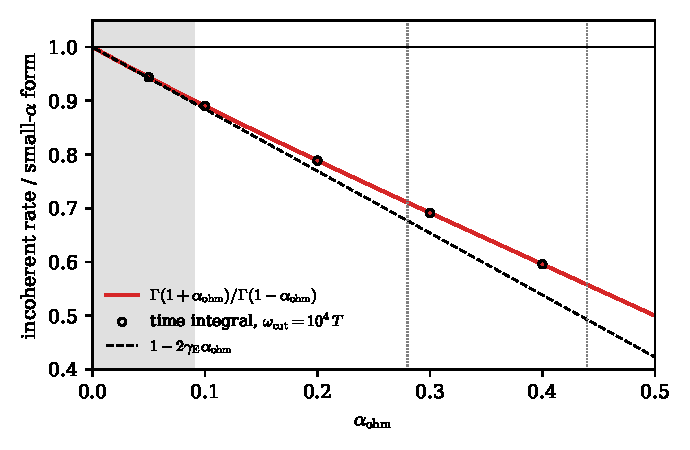
\includegraphics[width=0.75\linewidth]{figures/ch16/limit16_8b.pdf}
\captionof{figure}{Incoherent relaxation rate of a symmetric defect in an ohmic bath, \cref{eq:C.20-rate,eq:16.8-scaling}, divided by the small-coupling form $\tilde\Delta_0^2/\gamma_0$, against $\alpha_{\mathrm{ohm}}$. Red: the scaling limit $\Gamma(1 + \alpha_{\mathrm{ohm}})/\Gamma(1 - \alpha_{\mathrm{ohm}})$. Open circles: the time integral of \cref{eq:C.20-rate} done numerically with the full ohmic correlation exponent at $\omega_{\mathrm{cut}} = 10^4\,T$. Dashed: the leading correction $1 - 2\gamma_{\mathrm{E}}\alpha_{\mathrm{ohm}}$. Dotted lines: the Born values $\alpha_{\mathrm{ohm}} = 0.28$ and 0.44 of the aluminum resonator fits. Gray: within \SI{10}{\percent}, $\alpha_{\mathrm{ohm}} \le 0.091$.}\label{fig:16-limit-ohmic}
\par}
\smallskip
Outside the gray band the small-coupling form overstates the rate, by $1/0.71$ at $\alpha_{\mathrm{ohm}} = 0.28$, and both forms fail below $T \sim \Delta_{\mathrm{r}}$, where the defect tunnels coherently.
\end{limitbox}

\subsection{Thermally activated hopping and tunneling}\label{sec:16.8-hop}

A defect whose barrier $V_{\mathrm{b}}$ of \cref{sec:16.7} is large compared with $T$ can still cross it classically, at the rate $\varGamma = \varGamma_0\ee^{-V_{\mathrm{b}}/T}$ of harmonic transition-state theory (\cref{app:E.11}), with $\varGamma_0$ the attempt rate. In one dimension $\varGamma_0 = \omega_{\mathrm{w}}/2\pi$, with $\omega_{\mathrm{w}}$ the frequency of the well, and in many dimensions $\varGamma_0$ is Vineyard's ratio of the products of normal-mode frequencies at the minimum and at the saddle. This is the transition-state rate of Lawrence~\cite[Eq.~(1)]{lawrence2024semiclassical} with a classical, harmonic reactant partition function and transmission coefficient $\kappa = 1$. Tunneling through the top of the barrier raises the rate. For a barrier that is an inverted parabola of frequency $\omega^\ddagger$ the correction is exact,
\begin{equation}
  \kappa_{\mathrm{PB}} = \frac{\omega^\ddagger/2T}{\sin(\omega^\ddagger/2T)} = 1 + \frac{1}{24}\Bigl(\frac{\omega^\ddagger}{T}\Bigr)^2 + \frac{7}{5760}\Bigl(\frac{\omega^\ddagger}{T}\Bigr)^4 + \dots ,
  \label{eq:16.8-kappa}
\end{equation}
and its first two terms are Wigner's correction $\kappa_{\mathrm{W}}$~\cite[Eqs.~(2), (3)]{lawrence2024semiclassical}. The parabolic correction diverges at the crossover temperature
\begin{equation}
  T_\times = \frac{\omega^\ddagger}{2\pi} ,
  \label{eq:16.8-Tx}
\end{equation}
below which the particle no longer crosses near the top. It tunnels through the barrier at the energy that maximizes the product of the thermal weight and the transmission, along the instanton, the periodic path in imaginary time of period $1/T$, whose action $S_{\mathrm{inst}}$ replaces $V_{\mathrm{b}}/T$ in the exponent~\cite[Eq.~(4)]{lawrence2024semiclassical}. As $T \to 0$ the instanton becomes the tunneling path between the two minima, its action becomes twice the tunneling exponent $\lambda_{\mathrm{tun}}$ of \cref{sec:16.7}, and the hopping turns into the tunneling between $|\mathrm{L}\rangle$ and $|\mathrm{R}\rangle$ with amplitude $\Delta_0 \propto \ee^{-\lambda_{\mathrm{tun}}}$ that the previous sections assumed. For an atom with $\omega^\ddagger = \SI{10}{meV}$, $T_\times = \SI{18.5}{K}$, so at millikelvin temperatures every defect motion is tunneling, and a defect whose $\lambda_{\mathrm{tun}}$ is too large for it to tunnel within the time of an experiment is frozen. With an attempt rate of \SI{e13}{s^{-1}} and a year of observation, the bound is $\lambda_{\mathrm{tun}} \le 23.6$ when no energy-gap suppression adds to the exponent (\cref{app:E.22}).

\Cref{lim:16.8c} tests these forms on a barrier whose quantum rate is known exactly, the symmetric Eckart barrier $V(x) = V_{\mathrm{b}}\,\mathrm{sech}^2(x/L)$ with the hydrogen-atom parameters of Lawrence, $V_{\mathrm{b}} = 6\omega^\ddagger/\pi$. The exact rate exceeds the classical one by a factor 6.2 at $T_\times$ and 2.2 at $1.5\,T_\times$, so tunneling matters well above the crossover. Wigner's correction holds within \SI{10}{\percent} above $2.1\,T_\times$ and the parabolic form above $1.5\,T_\times$, while the instanton rate stays about \SI{18}{\percent} low between $0.25$ and $0.5\,T_\times$, an error that the higher terms of its asymptotic expansion in $\hbar$ would reduce~\cite[Sect.~III\,A]{lawrence2024semiclassical}.

Activation also fixes which defects of a glass contribute to its heat release. On cooling, defects with large barriers stay in equilibrium by activation until the activated rate falls below the rate at which the cooling changes $V_{\mathrm{b}}/T$, which is $V_{\mathrm{b}}|\dot T|/T^2$. Equating the two gives the freezing temperature
\begin{equation}
  T_{\mathrm{frz}} = \frac{V_{\mathrm{b}}}{\ln\bigl(\varGamma_0T_{\mathrm{frz}}^2/V_{\mathrm{b}}|\dot T|\bigr)} ,
  \label{eq:16.8-Tfrz}
\end{equation}
the form of Sahling et al.~\cite[Eq.~(8)]{sahling2010anomalous} with their $\tau_0 = 1/\varGamma_0$. Below $T_{\mathrm{frz}}$ the populations of these defects stop following the temperature, and the excess they keep is released later by tunneling.

\begin{limitbox}[Hopping and tunneling through one barrier][lim:16.8c]
The published rates are transition-state theory with Wigner's or the parabolic-barrier transmission, \cref{eq:16.8-kappa}, above the crossover temperature \cref{eq:16.8-Tx}, and the instanton rate below it~\cite[Eqs.~(1)--(4)]{lawrence2024semiclassical}.
\par\smallskip
{\centering
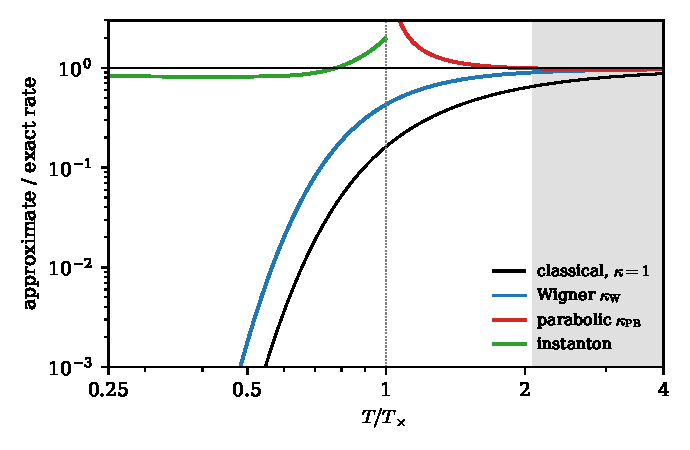
\includegraphics[width=0.75\linewidth]{figures/ch16/limit16_8c.pdf}
\captionof{figure}{Approximate thermal rates through a symmetric Eckart barrier divided by the exact quantum rate, against $T/T_\times$, for the hydrogen-atom parameters of Lawrence ($V_{\mathrm{b}} = \SI{248}{meV}$, $\omega^\ddagger = \SI{130}{meV}$, $T_\times = \SI{240}{K}$). Black: classical transition-state theory. Blue: with Wigner's correction. Red: with the parabolic-barrier correction, divergent at $T_\times$ (dotted line). Green: the instanton rate, for $T < T_\times$. The exact rate integrates the exact transmission probability of the Eckart barrier over the Boltzmann factor. Gray: Wigner's form within \SI{10}{\percent}, $T \ge 2.1\,T_\times$.}\label{fig:16-limit-hop}
\par}
\smallskip
Near $T_\times$ the expansion in $\omega^\ddagger/T$ diverges and the instanton is not yet formed, so neither form holds there, and below $T_\times$ the transition-state forms underestimate the rate by orders of magnitude.
\end{limitbox}

\subsection{Heat release of a cooled glass}\label{sec:16.8-heat}

A glass held at $T_{\mathrm{hi}}$ and cooled quickly to $T_{\mathrm{lo}}$ keeps its slow defects in the populations of $T_{\mathrm{hi}}$. A defect of splitting $\Delta_{\mathrm{tl}}$ has the mean energy $-\tfrac12\Delta_{\mathrm{tl}}\tanh(\Delta_{\mathrm{tl}}/2T)$ in equilibrium, so it holds the excess $\tfrac12\Delta_{\mathrm{tl}}[\tanh(\Delta_{\mathrm{tl}}/2T_{\mathrm{lo}}) - \tanh(\Delta_{\mathrm{tl}}/2T_{\mathrm{hi}})]$, which it gives to the phonons at its rate $\varGamma_1$ of \cref{eq:16.7-tau1}, evaluated at $T_{\mathrm{lo}}$. The defects are spread uniformly in the asymmetry $\Delta_{\mathrm{as}}$ and in the tunneling exponent $\lambda_{\mathrm{tun}}$, with density $\bar P$ (\cref{sec:16.7-stm})~\cite[Eq.~(1)]{sahling2010anomalous}. The slow defects have $\Delta_0 \ll \Delta_{\mathrm{as}}$, so $\Delta_{\mathrm{tl}} \simeq \Delta_{\mathrm{as}}$ is distributed uniformly too. Their excess energy, summed over $\Delta_{\mathrm{tl}}$, is
\begin{equation*}
  \int_0^\infty\dd\Delta_{\mathrm{tl}}\,\frac{\Delta_{\mathrm{tl}}}{2}\Bigl[\tanh\frac{\Delta_{\mathrm{tl}}}{2T_{\mathrm{lo}}} - \tanh\frac{\Delta_{\mathrm{tl}}}{2T_{\mathrm{hi}}}\Bigr] = \frac{\pi^2}{12}\bigl(T_{\mathrm{hi}}^2 - T_{\mathrm{lo}}^2\bigr) ,
\end{equation*}
since $1 - \tanh(x/2T) = 2/(\ee^{x/T} + 1)$ and $\int_0^\infty\dd x\,x/(\ee^{x/T} + 1) = \pi^2T^2/12$. The rate depends on the tunneling exponent through $\Delta_0^2 \propto \ee^{-2\lambda_{\mathrm{tun}}}$, so at fixed $\Delta_{\mathrm{tl}}$ a uniform density in $\lambda_{\mathrm{tun}}$ is a uniform density $\tfrac12$ per unit $\ln\varGamma_1$. A defect relaxes at time $t$ with probability $\varGamma_1\ee^{-\varGamma_1t}\dd t$, and summing over $\lambda_{\mathrm{tun}}$ gives $\int\dd\lambda_{\mathrm{tun}}\,\varGamma_1\ee^{-\varGamma_1t} = \tfrac12\int\dd\varGamma_1\,\ee^{-\varGamma_1t} = 1/2t$ whenever the rates extend far on both sides of $1/t$. The power released by a volume $\Vol$ of glass is therefore
\begin{keyresult}[Heat release of a cooled glass]
\begin{equation}
  \dot Q_{\mathrm{TLS}}(t) = \frac{\pi^2}{24}\,\bar P\,\Vol\,\frac{T_{\mathrm{hi}}^2 - T_{\mathrm{lo}}^2}{t} , \qquad \varGamma_{\max}^{-1} \ll t \ll \varGamma_{\min}^{-1} ,
  \label{eq:16.8-heat}
\end{equation}
\end{keyresult}
with $\varGamma_{\max}$ and $\varGamma_{\min}$ the fastest and slowest one-phonon rates at $T_{\mathrm{lo}}$ of the defects with $\Delta_{\mathrm{tl}} \sim T_{\mathrm{hi}}$, which hold most of the excess. This is the law of Sahling et al.~\cite[Eq.~(6)]{sahling2010anomalous}. The $1/t$ comes from the uniform density in $\lambda_{\mathrm{tun}}$, and the prefactor depends neither on the deformation potentials nor on the sound speeds, which only shift the window in time. Since every decade of time draws on defects in a range of $\lambda_{\mathrm{tun}}$ of width $\tfrac12\ln10$, the heat released between $t_1$ and $t_2$ is the prefactor times $\ln(t_2/t_1)$, and the heat measured at a time $t$ comes from defects with $\varGamma_1 \approx 1/t$. If the glass starts above $T_{\mathrm{frz}}$ of \cref{eq:16.8-Tfrz}, the defects that release at time $t$ were last in equilibrium at $T_{\mathrm{frz}}$, and $T_{\mathrm{frz}}$ replaces $T_{\mathrm{hi}}$~\cite[Eq.~(7)]{sahling2010anomalous}; the release then no longer grows with the starting temperature.

\begin{limitbox}[Heat release of a cooled glass][lim:16.8d]
The published heat release after a quench from $T_{\mathrm{hi}}$ to $T_{\mathrm{lo}}$ is \cref{eq:16.8-heat}~\cite[Eqs.~(1), (6)--(8)]{sahling2010anomalous}.
\par\smallskip
{\centering
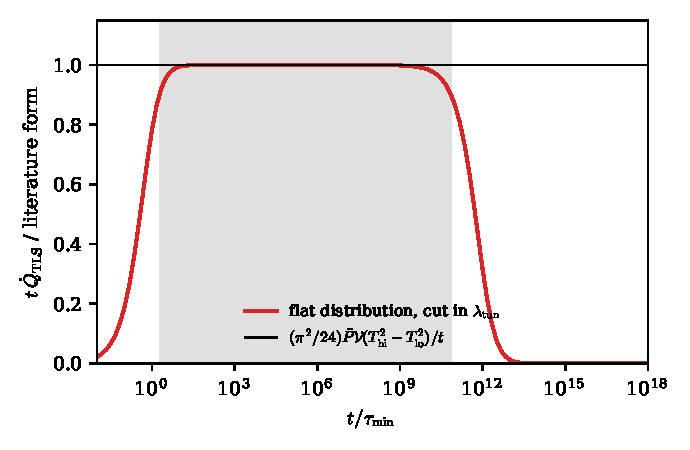
\includegraphics[width=0.75\linewidth]{figures/ch16/limit16_8d.pdf}
\captionof{figure}{Heat release of a model glass times $t$, divided by the prefactor of \cref{eq:16.8-heat}, against $t$ in units of $\tau_{\min}$, the relaxation time of the fastest defect at $\Delta_{\mathrm{tl}} = T_{\mathrm{hi}}$. Red: the uniform distribution cut at $\lambda_{\mathrm{min}} \le \lambda_{\mathrm{tun}} \le \lambda_{\mathrm{min}} + 14$, with the exact splitting $\Delta_{\mathrm{tl}} = (\Delta_{\mathrm{as}}^2 + \Delta_0^2)^{1/2}$, $\Delta_0 \le 0.1\,T_{\mathrm{lo}}$, the one-phonon rate \cref{eq:16.7-tau1} at $T_{\mathrm{lo}}$ and an instantaneous quench with $T_{\mathrm{lo}}/T_{\mathrm{hi}} = 1/480$ (\SI{10}{mK} after \SI{4.8}{K}). Gray: within \SI{10}{\percent} of one, $1.8\,\tau_{\min} \le t \le 7.1\times10^{10}\,\tau_{\min}$, 10.6 of the 12.2 decades that the cut spans.}\label{fig:16-limit-heat}
\par}
\smallskip
Outside the window the release falls below the $1/t$ law, at early times because the fastest defects have already relaxed and at late times because the distribution of tunneling exponents ends.
\end{limitbox}

Inside its window \cref{eq:16.8-heat} is exact for the uniform distribution: in \cref{lim:16.8d} it holds within $2\times10^{-4}$ from $10^2$ to $10^8\,\tau_{\min}$. The tests of the law are therefore tests of the distribution. Heat-release measurements on vitreous silica follow $1/t$ and $T_{\mathrm{hi}}^2 - T_{\mathrm{lo}}^2$, but they give a density $\bar P$ four times smaller than the specific heat measured over seconds, $2.0\times10^{44}$ against $8.0\times10^{44}\,\si{J^{-1}.m^{-3}}$~\cite[Table~1]{sahling2014anomalous}. Sahling et al.\ attribute the difference to defects whose barriers are lowered by local stresses frozen in on cooling. These relax within about \SI{100}{s}, before the heat-release measurement starts, and a small fraction of them, \SI{5}{\percent}, freezes at \SI{14.5}{K} instead of \SI{4.8}{K} and adds to the release after a quench from higher temperatures~\cite{sahling2014anomalous}. The specific-heat value, $1.28\times10^{20}\,\si{eV^{-1}.cm^{-3}}$, is close to the $1.2\times10^{20}\,\si{eV^{-1}.cm^{-3}}$ that the polarization-averaged acoustic tunneling strength implies for $\gamma_{\mathrm{l}} = \SI{1}{eV}$ ($0.88\times10^{20}$ with the longitudinal $C_{\mathrm{l}}$; \cref{sec:16.7}).

\begin{workedexample}{Heat release of one gram of fused silica at \SI{10}{mK}}\label{we:16-heat}
Take \SI{1}{g} of vitreous silica, $\Vol = \SI{0.455}{cm^3}$ at the density $\rho_T = \SI{2.2}{g.cm^{-3}}$ of \cref{sec:16.7}, cooled from room temperature to $T_{\mathrm{lo}} = \SI{10}{mK}$. The defects that release over hours to weeks freeze at $T_{\mathrm{frz}} = \SI{4.8}{K}$, and the heat-release density is $\bar P = 2.0\times10^{44}\,\si{J^{-1}.m^{-3}} = 3.20\times10^{19}\,\si{eV^{-1}.cm^{-3}}$~\cite[Table~1]{sahling2014anomalous}. With $T_{\mathrm{frz}}$ in place of $T_{\mathrm{hi}}$, and $T_{\mathrm{lo}}^2/T_{\mathrm{frz}}^2 = 4\times10^{-6}$ negligible, \cref{eq:16.8-heat} gives
\begin{equation*}
  \begin{split}
  t\,\dot Q_{\mathrm{TLS}} &= \frac{\pi^2}{24}\,k_{\mathrm{B}}^2\,\bar P\,\Vol\,T_{\mathrm{frz}}^2 \\
  &= 0.4112\times(\SI{1.381e-23}{J.K^{-1}})^2\times\SI{2.0e44}{J^{-1}.m^{-3}} \\
  &\qquad\times\SI{4.55e-7}{m^3}\times(\SI{4.8}{K})^2 \\
  &= \SI{1.64e-7}{J} .
  \end{split}
\end{equation*}
One hour after the cooling the sample releases $\SI{1.64e-7}{J}/\SI{3600}{s} = \SI{46}{pW}$, after a day \SI{1.9}{pW}, and after a week \SI{0.27}{pW}. Between the first hour and the end of the first week it gives off $\SI{1.64e-7}{J}\times\ln168 = \SI{0.84}{\micro J}$, or $5\times10^{12}\,\si{eV}$. With the specific-heat density the power would be four times larger. The fraction of defects that freezes at \SI{14.5}{K} is $0.05\times3 = 0.15$ of the normal density, with 3 the ratio of the stress-lowered defects to the normal density, $(8.0 - 2.0)/2.0$. By the square of its freezing temperature it adds another 1.4 times the normal release after a quench from above \SI{14.5}{K}, with the freezing temperatures of the table of Sahling et al. Their text quotes 5.5 and \SI{14.1}{K}, which give 0.99, and states that the anomalous part is roughly twice the normal one~\cite{sahling2014anomalous}. A hundred grams of fused silica near a detector at \SI{10}{mK} thus deposits \SI{4.6}{nW} an hour after cooling and \SI{0.19}{nW} a day later, a load and a source of delayed events that \cref{sec:19.6} takes up.
\end{workedexample}

\subsection{Interacting two-level systems}\label{sec:16.8-open}

Every result of this section treats the defects as independent, yet two defects interact through the strain fields each creates, with a coupling that falls as $1/r^3$. Its typical size relative to the spread of their splittings is the tunneling strength $C = \bar P\gamma_{\mathrm{l}}^2/\rho_Tc_{\mathrm{LA}}^2$, $2.6\times10^{-4}$ in vitreous silica (\cref{sec:16.7}). Thermal flips of neighbors shift the splitting of a given defect in time, which is spectral diffusion; it broadens single lines, and qubit spectroscopy sees it directly~\cite[Sect.~IV]{muller2019towards}. An ensemble whose spectrum is flat in $\Delta_{\mathrm{tl}}$ is unchanged by a normalized shift kernel away from the edges of the band. Spectral diffusion alone therefore leaves the ensemble responses of \cref{sec:16.7} intact, but it changes which defects relax at a given time and so the window of \cref{eq:16.8-heat}. The phonon emitted by one relaxing defect can trigger the relaxation of another. If each release triggers on average $b_{\mathrm{br}}$ more, a branching process, the mean size of a cascade of releases is $1/(1 - b_{\mathrm{br}})$, finite for $b_{\mathrm{br}} < 1$, and the distribution of the cascade size $N_{\mathrm{casc}}$ approaches $N_{\mathrm{casc}}^{-3/2}$ as $b_{\mathrm{br}} \to 1$. Such avalanches would turn the steady $1/t$ release into bursts. None of this is quantified for a real glass: $b_{\mathrm{br}}$ needs the density of barriers below the energy of the emitted phonons and the flux of ballistic phonons through the triggering volume, and no calculation or measurement of it exists. Whether the delayed events of a cooled detector are independent relaxations or avalanches of this kind is the open question that \cref{sec:19.6} inherits.

\section{Material inputs of the novel targets}\label{sec:16.9}

Two first-principles calculations of the dielectric tensor of ZrTe$_5$ give 20.75 and 9.8 along its slow axis, and the scattering reach of the material moves by a factor 2.8 between them (\cref{we:16-band}). Both numbers enter \cref{eq:16.1-L} exactly; no approximation of the response is involved, and a measurement of the tensor would settle the question. Most targets of this chapter are limited in the same way. The loss tangent of amorphous SiO$_2$ changes seventeenfold between preparations. And the probability that a single nuclear recoil of a few hundred eV in LiF leaves a readable F center has not been measured. \Cref{tab:16-inputs} lists, for each target, the inputs its rate needs, how well they are known and how their uncertainty moves the reach.

\subsection{Measured, computed and unmeasured inputs}\label{sec:16.9-inputs}

Some inputs of \cref{tab:16-inputs} are measured constants that vary from sample to sample: the loss tangent of a glass, the width of a donor line, the work function of a sheet on its substrate, the Luttinger parameter of a nanotube. The spread between samples is then the uncertainty of the input, and a detector that characterizes its own crystal or film removes it.

Others are computed constants, such as the dielectric tensor and the half-gap of a Dirac material, the Bloch-overlap coefficients $\mathcal{U}_{j'j}(\vect{G})$ of a donor, or the ohmic coupling $\alpha_{\mathrm{ohm}}$ of a tunneling defect. Their uncertainty is the spread between calculations, or the spread of a calculation over its functional and numerical choices. Such a spread is an estimate, not a bound: two calculations need not bracket the true value.

A third group are yields and parameters that no measurement isolates. One is the four factors of \cref{eq:16.6-yield} for single recoils of tens to hundreds of eV at millikelvin temperatures (\cref{sec:16.6-yields}); another is the density, dipole moment and deformation potential of two-level systems one by one (\cref{sec:16.7-open}), on which the estimate of \cref{sec:16.7-scat} rests through an assumed deformation potential of \SI{1}{eV}. For these inputs \cref{sec:8.8} assigns no width, and a reach is conditional on the value assumed.

\begin{table}[tbp]
  \caption{Material inputs of the novel targets, with their values, their uncertainty and its effect on the reach. The truncations of the responses are in \cref{tab:16-nuisances}.}
  \label{tab:16-inputs}
  \centering\scriptsize\setlength{\tabcolsep}{3pt}
  \begin{tabular}{@{}>{\raggedright\arraybackslash}p{0.15\linewidth}>{\raggedright\arraybackslash}p{0.38\linewidth}>{\raggedright\arraybackslash}p{0.43\linewidth}@{}}
    \toprule
    Target & Inputs (values) & Uncertainty and effect on the reach \\
    \midrule
    Dirac material (ZrTe$_5$) & background tensor $\varepsilon_{\mathrm{bg},ii} = 308.4$, 20.75, 126.1 (computed; earlier 187.5, 9.8, 90.9); velocities, cutoff \SI{0.191}{eV} and half-gap $\Delta_{\mathrm{D}} = \SI{11.8}{meV}$ of the measured-structure row (computed half-gaps 11.8--\SI{17.5}{meV}; measured \SI{11.75}{meV}) & between the two tensors $\sigmae^{\mathrm{lim}}$ moves by 2.8 to 2.9 and $\zeta^{\mathrm{lim}}$ by 1.8 to 2.0 (\cref{we:16-band}); the Dirac term inside the computed tensor, 3 to \SI{8}{\percent}, moves $\sigmae^{\mathrm{lim}}$ by 0.88; the computed half-gaps move the threshold mass along the slow axis from 7.1 to \SI{10.6}{keV} \\
    Metallic nanotubes, doped graphene & $g_c$ (measured 0.2--0.7; 0.17--0.34 for $r_{\mathrm{t}} = \SI{0.7}{nm}$ in vacuum); Fermi energy; substrate & line weight $\propto N_{\mathrm{ch}}g_c$; Fermi energy and substrate set the sheet plasmon \\
    Vacuum ejection (graphene) & work function $\Phi_{\mathrm{wf}} \simeq \SI{4.3}{eV}$ (substrate-dependent); occupied orbitals and binding energies & threshold mass $2\Phi_{\mathrm{wf}}/v_{\mathrm{max}}^2 = \SI{1.22}{MeV}$ moves with $\Phi_{\mathrm{wf}}$ \\
    Quantum dots (PbS in silica) & dot gap \SI{1.2}{eV} at \SI{3.3}{nm}; $\varepsilon_{\mathrm{in}}(\omega)$ of the dots; host $\varepsilon_{\mathrm{out}}$ & depolarization factor 0.57 to 6.7 for the cases of \cref{we:16-depol}, $\zeta^{\mathrm{lim}}$ moved by 1.33 to 0.39, sign unknown over 2.5--\SI{10}{eV} \\
    Molecular crystals (anthracene) & lowest singlet \SI{3.1}{eV} and crystal structure (measured); form factors and Frenkel coupling $\mathfrak{J}$ ($\pi$-electron model); transfer integral $t_{\mathrm{CT}}$ & model corrections in \cref{tab:16-nuisances} \\
    Dopants (Si:P) & level energies (measured); line strengths (central-cell model); line width $\ge \SI{4.22}{\micro eV}$; donor density against $\nd_{\mathrm{c}} \approx \SI{3e18}{cm^{-3}}$; local-field ratio $\mathfrak{f}^{\mathrm{loc}}_{\mathrm{D}}$ & resonant rate $\propto \nd_{\mathrm{D}}/\varGamma_{\mathrm{line}}$, $\zeta^{\mathrm{lim}} = \num{2.3e-16}$ at the $2p_0$ line for \SI{e15}{cm^{-3}}; $\mathfrak{f}^{\mathrm{loc}}_{\mathrm{D}}$ close to one, unsized \\
    Color centers (LiF) & displacement threshold $E_{\mathrm{d}} = \SI{27}{eV}$ (simulation input); site phonon energy 33.5--\SI{77.2}{meV}; yields $p_{\mathrm{FP}}$, $p_{\mathrm{surv}}$, $p_q$, $f_{\mathrm{opt}}$, $p_{\mathrm{FH}}$ & lightest mass 0.113--\SI{0.255}{GeV} for $E_{\mathrm{d}} = 10$--\SI{50}{eV}; yields unmeasured, the reach scales as $1/Y_{\mathrm{CC}}$ \\
    Bond breaking (H$_2$, molecular crystals) & bond energy \SI{4.75}{eV} and $\omega_{\mathrm{vib}} = \SI{0.546}{eV}$ (measured); cage escape $p_{\mathrm{esc}}$; yields of repulsive electronic states & $p_{\mathrm{esc}}$ and electronic yields unmeasured \\
    Glasses (a-SiO$_2$) & $\tan\delta_0$; $\varepsilon_r = 3.9$ (assumed); acoustic tunneling strength $C_{\mathrm{l}}$ (measured); $\bar P$, $\gamma_{\mathrm{l}}$ ($\SI{1}{eV}$ assumed), dipole moment & $\tan\delta_0 = 3\times10^{-4}$ (thermal oxide) to $5\times10^{-3}$ (deposited oxide): absorption rate $\times16.7$, $\zeta^{\mathrm{lim}}$ $\times4.1$; scattering host term fixed by $C_{\mathrm{l}}$ alone, core term needs $\bar P$ and $\gamma_{\mathrm{l}}$ \\
    Two-level systems at millikelvin & $\alpha_{\mathrm{ohm}} = 4K_{\mathrm{b}}$ (Born), $K_{\mathrm{b}} = 0.07$, 0.11 fitted (aluminum); $\bar P$ of vitreous silica $2.0\times10^{44}$ (heat release) or $8.0\times10^{44}\,\si{J^{-1}.m^{-3}}$ (specific heat) & heat release fourfold between the two $\bar P$; first-principles $\alpha_{\mathrm{ohm}}$ needs the scattering phases of both configurations \\
    \bottomrule
  \end{tabular}
\end{table}

\subsection{Theory-limited and data-limited targets}\label{sec:16.9-limits}

A target is limited by theory when its response has no controlled approximation at the values its inputs take, so that better inputs would not sharpen the rate. Dirac cones at strong coupling (\cref{sec:16.1-validity}), donors near the Mott density (\cref{sec:16.5-band}) and interacting two-level systems (\cref{sec:16.8-open}) are of this kind.

A second group is limited by a calculation whose formalism is known. The electron--hole ladder near the edge of a Dirac material changes the rate of ZrTe$_5$ by the Sommerfeld factor, 1.5 or more, at \SI{20}{keV} and by less above \SI{100}{keV} (\cref{sec:16.1-validity}). So do the final state of an ejected electron, the periodic Bethe--Salpeter response of a molecular crystal at finite $\vect{q}$, the excitons of a semiconducting tube and the valley-orbit coefficients of a donor. The response of a layered stack beyond its effective medium and the ohmic coupling $\alpha_{\mathrm{ohm}}$ from first principles complete the group. In each case the next term has a definite form and is computable, but no computation of it exists for the material.

The remaining targets are limited by data. Their inputs are properties of the sample that a measurement fixes: the dielectric tensor and the gap of ZrTe$_5$, the dielectric function $\varepsilon_{\mathrm{in}}(\omega)$ of real quantum dots, the oscillator strengths of the donor lines, the displacement threshold of LiF as a function of direction, the four yields of a color center, and the parameters of the two-level systems of a given film; \cref{sec:16.6-yields} names the measurements of the yields. For these inputs the response formula is in hand, and the uncertainty of the rate is that of the sample.

\subsection{Reach bands from input uncertainties}\label{sec:16.9-band}

An input $x$ on which the rate depends as a power, $\mathcal{R} \propto x^{-p}$ over the energies the rate samples, is a normalization uncertainty in the sense of \cref{sec:8.8}. By \cref{eq:1.5-limscaling} it moves a scattering reach as $\sigmae^{\mathrm{lim}} \propto x^{p}$, so a range $x_1 < x < x_2$ becomes a band of constant width $(x_2/x_1)^p$ in $\sigmae^{\mathrm{lim}}$ wherever $p$ does not change with the mass. An absorption reach moves as $\mathcal{R}^{-1/2}$, and its band is half as wide on a logarithmic scale. An input that sets a threshold acts instead through the low-mass wall, $\delta\ln m_{\mathrm{min}} = \delta\ln E_{\mathrm{th}}$ by \cref{eq:1.3-mmin}, and near the wall its band widens without limit (\cref{eq:8.8-shift}). An input without a size, such as the yield of a color center, gives no band: the reach is drawn for an assumed value and moves as its inverse.

For a Dirac material the power follows from \cref{eq:16.1-L}. At fixed Dirac parameters,
\begin{equation}
  \frac{\partial\ln L}{\partial\ln\varepsilon_{\mathrm{bg}}} = -\frac{2\,\varepsilon_{\mathrm{bg}}\Real(\varepsilon_{\mathrm{bg}} + \varepsilon_{\mathrm{D}})}{|\varepsilon_{\mathrm{bg}} + \varepsilon_{\mathrm{D}}|^2} = -2\Bigl[1 - \frac{\Real\varepsilon_{\mathrm{D}}}{\varepsilon_{\mathrm{bg}}} + O\Bigl(\frac{|\varepsilon_{\mathrm{D}}|^2}{\varepsilon_{\mathrm{bg}}^2}\Bigr)\Bigr] ,
  \label{eq:16.9-power}
\end{equation}
since $\varepsilon_{\mathrm{bg}}$ is real and $\varepsilon_{\mathrm{D}}$ does not depend on it. The reach therefore moves almost as $\varepsilon_{\mathrm{bg}}^2$, less by twice the fraction of the screening that the Dirac electrons supply. For ZrTe$_5$ that fraction is 3 to \SI{8}{\percent} at long wavelength (\cref{we:16-band}).

\begin{workedexample}{The reach band of ZrTe$_5$ from its background tensor}\label{we:16-band}
Take the Dirac parameters of \cref{sec:16.1-zrte5}, the measured-structure row with $\Delta_{\mathrm{D}} = \SI{11.8}{meV}$, and the scattering reach of \cref{fig:16-zrte5}a: light mediator, orientation-averaged loss function, three events in a kg-year. The central tensor is $\varepsilon_{\mathrm{bg},ii} = 308.4$, 20.75 and 126.1~\cite[Table~2]{geilhufe2020dirac}. The earlier calculation of \cref{we:7-zrte5} gives 187.5, 9.8 and 90.9~\cite[Table~1]{hochberg2018detection}, smaller by factors of 0.61, 0.47 and 0.72. We combine it with the same velocities, gap and cutoff, which isolates the effect of the tensor; the two calculations also differ in their velocities.

\emph{Estimate.} At weak screening $L \to \Imag\varepsilon_{\mathrm{D}}/(\hat{\vect{q}}\cdot\varepsilon_{\mathrm{bg}}\cdot\hat{\vect{q}})^2$. If $\Imag\varepsilon_{\mathrm{D}}$ were the same in every direction, the reach would move by the ratio of the direction averages of $(\hat{\vect{q}}\cdot\varepsilon_{\mathrm{bg}}\cdot\hat{\vect{q}})^{-2}$, which is 0.327 for the earlier tensor against the central one. Directions within \ang{30} of the slow axis $y$, where the background is smallest, carry \SI{64}{\percent} of that average for the central tensor, so the band is set mainly by $\varepsilon_{\mathrm{bg},yy}$, $(9.8/20.75)^2 = 0.22$ along the axis itself.

\emph{Full calculation.} With \cref{eq:16.1-L} and the anisotropic $\varepsilon_{\mathrm{D}}$ of \cref{eq:D.41-aniso}, the earlier tensor gives a reach 0.344 to 0.362 times the central one between \SI{20}{keV} and \SI{1}{MeV}, and 0.31 just above threshold. At the best mass, \SI{36}{keV}, the reach lies between $\SI{1.53e-40}{cm^2}$ and $\SI{5.5e-41}{cm^2}$, a band of 2.8 that is nearly constant in mass. The full ratio lies above the estimate because the smaller tensor lets the Dirac electrons screen more: the effective coupling along $y$ rises from 0.144 to 0.305.

\emph{Power.} Scaling the whole central tensor by 1.1 moves the reach by $1.1^p$ with $p = 1.86$ to 1.94 between \SI{20}{keV} and \SI{1}{MeV}, and $p = 1.85$ at \SI{12}{keV}, as \cref{eq:16.9-power} predicts for $\Real\varepsilon_{\mathrm{D}}/\varepsilon_{\mathrm{bg}}$ of a few percent. A tensor uncertain by a common factor of two would give a band of 3.6 to 3.8.

\emph{Dirac content.} Removing the static Dirac term of \cref{eq:7.3-aniso}, 10.0, 1.67 and 8.3 for this row, 3 to \SI{8}{\percent} of the components, leaves the background 298.4, 19.08 and 117.8, and moves the reach by 0.881 to 0.885, a correction smaller than the band.

\emph{Absorption.} For dark-photon absorption the earlier tensor moves $\zeta^{\mathrm{lim}}$ by 0.49 to 0.55 between the gap and the cutoff, from $1.24\times10^{-15}$ to $6.4\times10^{-16}$ at \SI{100}{meV}. The polarization along $y$ carries most of the rate, and for it alone $\zeta^{\mathrm{lim}} \propto \varepsilon_{\mathrm{bg},yy}$ at weak screening, which would give 0.47.

\emph{Gap.} The computed half-gaps of 11.8 to \SI{17.5}{meV} put the threshold mass along $y$ between 7.1 and \SI{10.6}{keV}, with \SI{9.4}{keV} for the relaxed-cell row at \SI{15.6}{meV}; the measured \SI{11.75}{meV} gives \SI{7.1}{keV}. Close to the wall the threshold band exceeds the tensor band, since it diverges there.
\end{workedexample}

Above \SI{100}{keV}, where the region near the pair edge carries less than a fifth of the rate, the tensor band is the largest sized uncertainty of the ZrTe$_5$ reach.

\section*{Summary}

A Dirac material screens the field of the dark matter with its whole dielectric function, $\varepsilon = \varepsilon_{\mathrm{bg}} + \varepsilon_{\mathrm{D}}$ (\cref{sec:16.1}). The published rates screen the Dirac electrons among themselves but not the field of the dark photon, and overstate scattering by $\varepsilon_{\mathrm{bg}}^2$ and absorption by $\varepsilon_{\mathrm{bg}}$ at every mass. For ZrTe$_5$ with the parameters of its measured structure the reach lies near \SI{1.5e-40}{cm^2} at \SI{40}{keV}, 5200 to 6400 times weaker than with the published rule for the standard halo.

Electrons confined to tubes and sheets respond to the momentum along them only, so a halo particle reaches a mode faster than $v_{\mathrm{max}}$ through an oblique momentum transfer, suppressed by the transverse form factor (\cref{sec:16.2}). An electron of graphene that receives more than the work function leaves the sheet with the direction of the momentum transfer, from \SI{1.22}{MeV} upward (\cref{sec:16.3}). The excitons of a molecular crystal follow from the Bethe--Salpeter equation in a molecular basis, and integrated over a window that holds whole manifolds, the crystal responds as a set of independent molecules at every momentum transfer, the Davydov sum rule (\cref{sec:16.4}).

Dilute donors in silicon add a response to first order in their density (\cref{sec:16.5}). The $2p_0$ line of Si:P at \SI{34.11}{meV} reaches $\zeta = \num{2.3e-16}$ at \SI{e15}{cm^{-3}}, twenty times below the continuum, and the first-order form fails at the line center from \SI{4.8e15}{cm^{-3}}. A color center forms after the prompt window: its rate is the recoil rate times the yield $Y_{\mathrm{CC}} = p_{\mathrm{FP}}p_{\mathrm{surv}}p_qf_{\mathrm{opt}}$ (\cref{sec:16.6}). A fluorine recoil in LiF above the simulation threshold of \SI{27}{eV} needs $\mchi \ge \SI{0.186}{GeV}$, and near threshold a recoil makes one vacancy and less than one free electron. Four yields at millikelvin temperatures are open, and each can be measured directly.

Glasses add tunneling two-level systems to the final states (\cref{sec:16.7}). A dark photon is absorbed at a rate proportional to $\zeta^2\tan\delta_0\tanh(m_\phi/2T)/\varepsilon_r$, the dielectric loss of the glass read at the dark-photon mass; on thermal SiO$_2$, three events in a kg-year at \SI{6}{GHz} need $\zeta = \num{2.44e-15}$. Coherent scattering off a random medium leaves the Born approximation once the optical potential exceeds about a tenth of the normal kinetic energy. Two-level systems whose populations froze near \SI{4.8}{K} release heat over hours to weeks after cooling (\cref{sec:16.8}). The density $\bar P$ inferred from heat release in vitreous silica is four times smaller than the one from its specific heat, and the fits to aluminum-coated resonators give $\alpha_{\mathrm{ohm}} = 0.28$ and 0.44, where the small-coupling rate fails. Whether the delayed events of a cooled detector are independent relaxations or avalanches of triggered releases is open, and \cref{sec:19.6} inherits the question.

The uncertainty budget of the chapter is \cref{tab:16-nuisances}, and \cref{tab:16-inputs} lists the material inputs, most of which only a measurement of the sample fixes (\cref{sec:16.9}).

\printbibliography[heading=subbibliography]

\chapter{Comparison across channels}\label{chap:17}
Dark matter of \SI{1}{MeV} that scatters through a heavy mediator coupled to electrons gives a kilogram of silicon 17 events a year at $\sigmae = \SI{e-37}{cm^2}$ by creating electron--hole pairs. If the mediator couples to the electrons alone, the same particle gives $7\times10^5$ events through acoustic phonons, carried by the electrons that move with the nuclei; if the mediator is a dark photon, the particle gives no events through acoustic phonons (\cref{sec:10.2}). Both rates, from electron--hole pairs and from acoustic phonons, come from one section; most of the comparisons that an experimentalist needs are spread over seven chapters. The multiphonon rate is in \cref{chap:11}, the Migdal rate in \cref{chap:12}, the phonon-assisted rate in \cref{chap:13}, magnons and superconductors in \cref{chap:14,chap:15}, and the special targets in \cref{chap:16}, each computed with the approximations its own excitation allows. A detector, however, is built for one material and one threshold, and the question that its design faces starts from the coupling instead of the excitation: for a given coupling, which excitation of which material gives the largest rate and the lowest reachable mass, and why?

The atlas of \cref{chap:9} places each excitation of a solid, and each coupling, in the section that treats it. Read along the interaction axis, the atlas answers this question at the level of the response. For each coupling it gives the channel that dominates at each mass and threshold, the few material numbers that set the rate and reach of that channel, and how firmly those numbers rank materials once the uncertainty of every input is carried through. Which experiment to build also depends on the energy per quantum, the readout and the backgrounds; the guide to next targets of \cref{sec:21.7} combines these measurement-side quantities with the rankings of this chapter (\cref{fig:17-map}).

\begin{figure}[tbp]
  \centering
  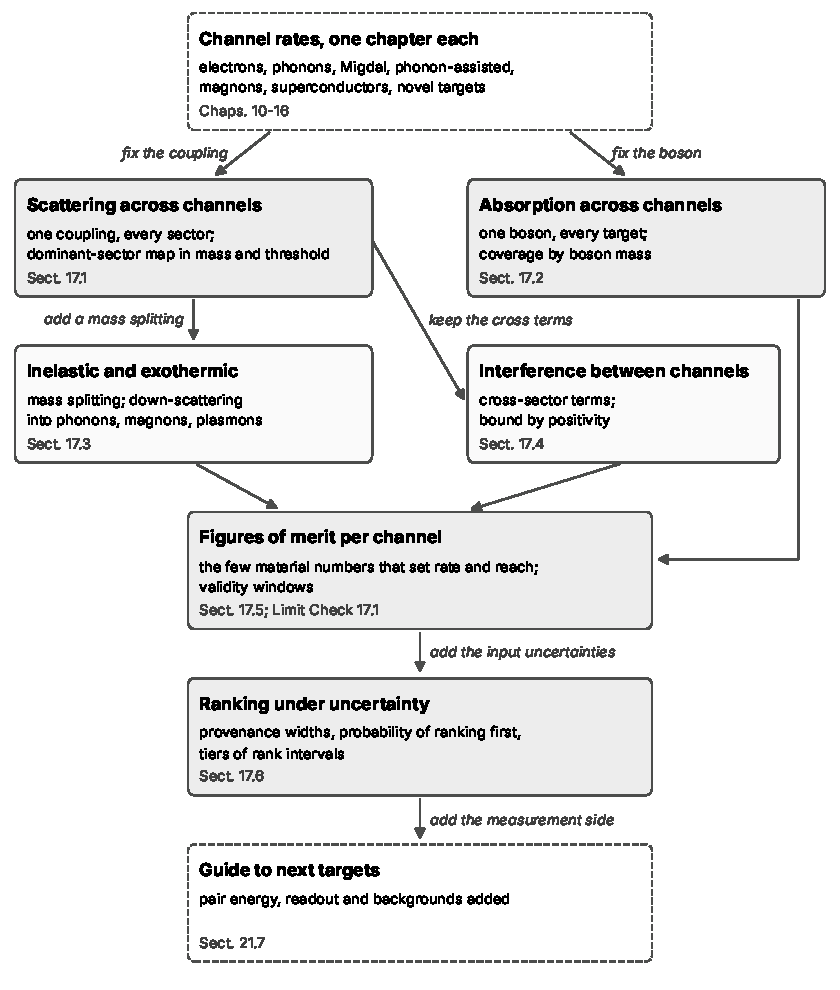
\includegraphics[width=0.85\linewidth]{figures/ch17/map17.pdf}
  \caption{Comparison across channels, from the rates of \cref{chap:10,chap:11,chap:12,chap:13,chap:14,chap:15,chap:16}. At fixed coupling: scattering in every sector and its dominant-sector map (\cref{sec:17.1}); at fixed boson: absorption on every target (\cref{sec:17.2}). Side branches: dark matter with a mass splitting, including down-scattering into collective modes (\cref{sec:17.3}), and the interference between sectors with its positivity bound (\cref{sec:17.4}). All four sections feed the figures of merit of each channel, with their validity windows (\cref{sec:17.5}; \cref{lim:17.5a}), and the ranking under the uncertainty of the inputs (\cref{sec:17.6}); the guide to next targets of \cref{sec:21.7} combines that ranking with the measurement side.}
  \label{fig:17-map}
\end{figure}

\section{Scattering across channels}\label{sec:17.1}

A silicon calorimeter with a threshold of \SI{0.1}{eV} records $3\times10^4$ events per kilogram and year from dark matter of \SI{10}{MeV} that couples to nucleons through a heavy mediator with $\sigma_p = \SI{e-38}{cm^2}$, nearly all of them multiphonon excitations of the lattice. At a threshold of \SI{0.5}{eV} it records 1.5 events, and every one of them is a Migdal ionization. Between the two thresholds the dominant final state moves from the electron-following sector of the decomposition theorem to the two electronic sectors (\cref{sec:8.6}), and the rate drops by four orders of magnitude. For each coupling, the choice of target and threshold depends on where in mass and threshold the dominant sector changes.

\subsection{Kinematic ceilings of the sectors}\label{sec:17.1-ceilings}

At fixed coupling the rate is \cref{eq:8.2-spectrum} with one coupling matrix $\mathfrak{D}$, and by the decomposition theorem \cref{eq:8.6-decomp} the structure factor is the sum of the electron-following, zero-phonon and phonon-dressed sectors. The interference between electrons and nuclei, the bottom row of \cref{tab:8-sectors}, vanishes for a coupling to one species alone (\cref{sec:17.4}). We compare two single-species couplings: a nucleon coupling, with equal couplings to protons and neutrons and the cross-section $\sigma_p$ per nucleon of \cref{sec:11.1}, and an electron coupling with the reference cross-section $\sigmae$. Both couplings have a heavy mediator. The threshold $\omega_{\mathrm{th}}$ acts on the total deposited energy, as in a calorimeter. A charge readout records the electronic sectors alone; the fraction of a lattice deposit that a phonon sensor collects is a question for the chapters on readout.

The first factor that decides the dominant sector is the largest energy that each sector can absorb. A single phonon carries at most the top of the phonon band, \SI{64.1}{meV} in silicon (\cref{sec:5.2}); the PBE density of states used for the maps ends at $\omega_{\mathrm{max}} = \SI{63.7}{meV}$ (\cref{sec:11.3}). A nucleus recoiling freely absorbs at most $E_R^{\mathrm{max}} = 2\mu_{\chi N}^2v_{\mathrm{max}}^2/M$ (\cref{eq:1.3-ERmax}), which is \SI{0.054}{eV} at \SI{10}{MeV} and \SI{5.3}{eV} at \SI{100}{MeV}. An electronic excitation can absorb up to the whole kinetic energy, $\tfrac12\mchi v_{\mathrm{max}}^2$ (\cref{eq:1.3-omegamax}), since the lattice can take the momentum without taking the energy; $\tfrac12\mchi v_{\mathrm{max}}^2$ is \SI{3.5}{eV} at \SI{1}{MeV} and \SI{35}{eV} at \SI{10}{MeV}. For $\mchi \ll M$ the electronic ceiling exceeds $E_R^{\mathrm{max}}$ by the factor $M/4\mchi$, $6.5\times10^3$ at \SI{1}{MeV}. Below the lattice ceiling the electron-following sector dominates whenever the coupling reaches the nuclei, because an electronic excitation costs a small probability per kick. Above it the electronic sectors alone are open. The boundary between the lattice and the electronic regions does not lie exactly at the lattice ceiling, however: a multiphonon spectrum extends above $E_R$ by its Poisson weights, and an impulse peak by its width.

The second factor is screening. A coupling to electrons reaches the lattice through the electrons that move with the nuclei, in full or not at all, according to whether the mediator couples to the electrons alone or to the total charge (\cref{sec:8.4}).

\subsection{Nucleon coupling in silicon}\label{sec:17.1-nucleon}

The nucleon-coupling map uses four responses. Below the zone boundary, $q \le q_{\mathrm{BZ}} = \SI{2.25}{keV}$, the one-phonon response is the long-wavelength acoustic form \cref{eq:11.1-Sac}, with the sound speeds and polarizations of the measured elastic tensor. Since the linear acoustic branches would run above every real phonon near $q_{\mathrm{BZ}}$, we cap the one-phonon deposits at $\omega_{\mathrm{max}}$. Above $q_{\mathrm{BZ}}$ the lattice response is the incoherent harmonic response \cref{eq:11.3-inc}, evaluated with the phonon density of states computed in \cref{sec:5.2} and the Helm form factor of \cref{sec:2.2}, and split into its one-phonon term and the terms with two or more phonons. Above $q = \SI{300}{keV}$, where $2W = 56$, the response is the impulse Gaussian \cref{eq:11.4-IAgauss}. The Migdal rate uses the soft-limit probability \cref{eq:12.3-soft}, evaluated with the loss function with local fields and with the $Z_{\mathrm{ion}}(p)$ of \cref{sec:12.3}. Since the sum rule \cref{eq:12.4-harm} holds at every momentum transfer in its incoherent form (for momentum transfers below $2q_{\mathrm{BZ}}$, see the qualifier on the Migdal band later in this section and \cref{tab:17-nuisances}), the lattice only has to conserve energy, and we give the lattice its mean share of the deposit, $q^2/2M$, so that the deposited energy is $\omega_e + q^2/2M$. The share of Migdal events that leave the lattice in its initial state is $\langle\ee^{-2W(|\vect{q}-\vect{p}|)}\rangle$, averaged, with the weight of \cref{sec:12.4}, over the momentum $\vect{p}$ that the electrons take. We label a point of the map ``one phonon'' when the one-phonon rate above threshold exceeds the rate with two or more phonons. Any other point where the lattice dominates is labeled ``free recoil'' when the median momentum transfer of the lattice rate lies above the impulse onset, \SI{92.5}{keV} (\cref{sec:11.4}). The electron rates are counted from \SI{1.11}{eV}, the gap in the step model of pair creation that is distributed with the loss-function tables. The tables themselves are scissored to the measured gap of \SI{1.17}{eV} (\cref{sec:10.10}), and counting from \SI{1.11}{eV} instead of \SI{1.17}{eV} moves the onset of the electron sector from 0.333 down to \SI{0.316}{MeV}.

\begin{figure}[tbp]
  \centering
  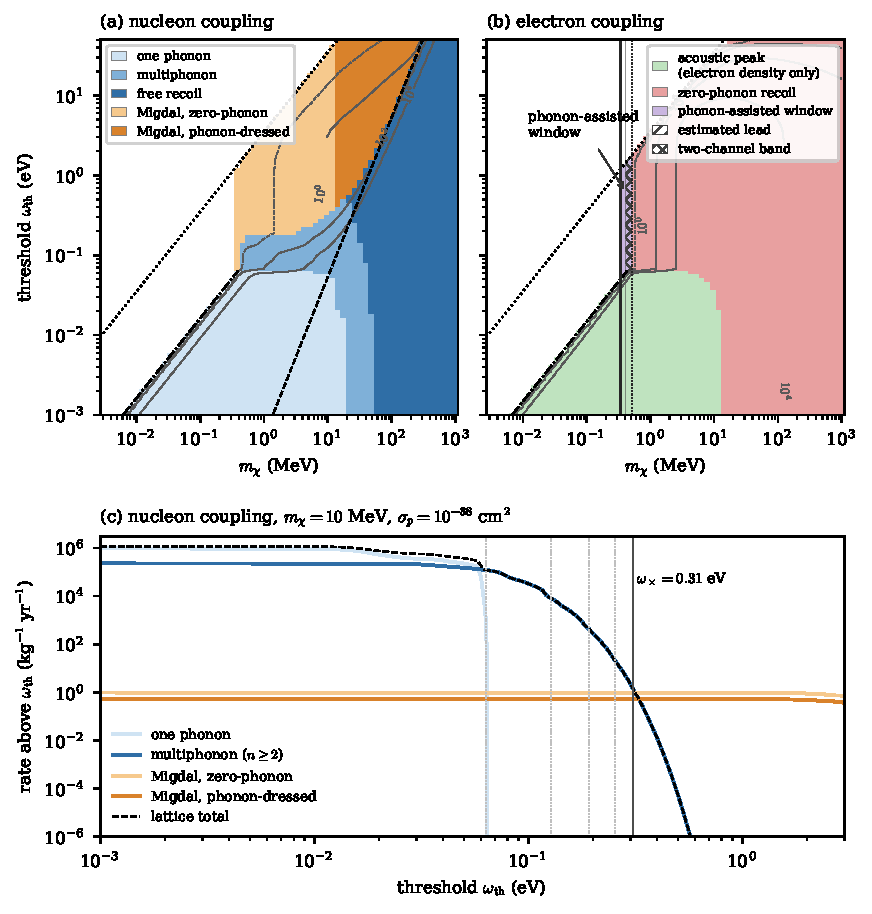
\includegraphics[width=0.86\linewidth]{figures/ch17/fig17_sectors.pdf}
  \caption{Dominant sector of silicon in the plane of dark-matter mass and threshold on the total deposited energy, heavy mediator, standard halo (\cref{tab:1-shm}), $T = 0$. (a)~Nucleon coupling: electron-following sector split into one phonon, two or more phonons and free recoil; Migdal effect split by whether more than half of the events leave the lattice in its initial state; below about \SI{2}{MeV} the Migdal rate carries the unsized coherent factor of \cref{tab:17-nuisances} (at \SI{3}{MeV} the factor acts on \SI{7}{\percent} of the Migdal rate). One-phonon deposits are capped at the top of the PBE band, \SI{63.7}{meV}. Gray contours: the dominant rate, $10^{-2}$ to $10^4$ events per kilogram and year at $\sigma_p = \SI{e-38}{cm^2}$. (b)~Electron coupling: zero-phonon electron recoil (loss function with local fields, counted from \SI{1.11}{eV}) against the acoustic peak of an electron-only coupling (absent for a dark photon) in the model of \cref{lim:10.2a} (linear longitudinal branch to $|\vect{q}| = 2\pi/a$, 28 electrons per cell following the nuclei). Phonon-assisted window from \cref{tab:13-window}: onsets 0.3332 (dashed) and \SI{0.3374}{MeV} (solid) and first zero-phonon edge 0.405--\SI{0.408}{MeV} (dark band), computed; estimated phonon-assisted lead to \SI{0.43}{MeV} (hatched) and two-channel band 0.43--\SI{0.51}{MeV} (cross-hatched). Contours at $\sigmae = \SI{e-37}{cm^2}$. Lines: dotted, the largest deposit $\tfrac12\mchi v_{\mathrm{max}}^2$; dashed, the free-recoil endpoint $E_R^{\mathrm{max}}$; dash-dotted, the acoustic edge \cref{eq:11.1-edge} with $c_{\mathrm{LA,max}} = \SI{9.35}{km/s}$ in (a) and the model's \SI{8.43}{km/s} in (b). White: no channel, or a rate below $10^{-12}$ events per kilogram and year. (c)~Rates above threshold at $\mchi = \SI{10}{MeV}$, nucleon coupling; vertical dotted lines at multiples of the band top, solid line at the crossover threshold $\omega_{\mathrm{th}}^\times$ of \cref{we:17-crossover}.}
  \label{fig:17-sectors}
\end{figure}

\Cref{fig:17-sectors}a shows the result. Below the band top the electron-following sector holds the whole map, and inside it the one-phonon term leads up to \SI{20}{MeV} at a threshold of \SI{1}{meV}, although the kicks of a \SI{10}{MeV} particle already reach $2W = 1.8$. The reason is that the incoherent response gives the one-phonon term the Poisson weight $2W\ee^{-2W}$, and the sum of all higher orders overtakes the one-phonon weight only at $2W = 1.26$. The heavy mediator weights the largest momentum transfers, so the boundary of the one-phonon region follows the typical kick. Below \SI{3.4}{MeV}, where $q_{\mathrm{max}} < \SI{18}{keV}$, the one-phonon contours carry the coherent correction of \cref{sec:11.3}, which exceeds \SI{10}{\percent} below \SI{18}{keV}; the boundary of the one-phonon region near \SI{20}{MeV}, where the kicks lie far above \SI{18}{keV}, does not. Multiphonon deposits dominate above \SI{20}{MeV} at the lowest thresholds and, at every mass, at thresholds above the band top. By the median criterion the free recoil leads above \SI{60}{MeV} at \SI{1}{meV}, and above \SI{22}{MeV} at higher thresholds. At the lowest thresholds the lattice rate exceeds the Migdal rate by roughly the inverse of the Migdal probability per kick, averaged over the kicks: by $6\times10^7$ at \SI{1}{MeV}, $8\times10^5$ at \SI{10}{MeV} and $2\times10^4$ at \SI{100}{MeV}.

\begin{table}[tbp]
  \caption{The multiphonon--Migdal crossover in silicon: nucleon coupling, heavy mediator, $\sigma_p = \SI{e-38}{cm^2}$, threshold on the total deposited energy. Largest momentum transfer and its Debye--Waller exponent; crossover threshold $\omega_{\mathrm{th}}^\times$ (lattice rate equal to the Migdal rate) and its ratio to the free-recoil endpoint; Migdal rate at the lowest thresholds (events per kilogram and year) and its zero-phonon share.}
  \label{tab:17-crossover}
  \centering\small
  \begin{tabular}{@{}lccccccc@{}}
    \toprule
    $\mchi$ (MeV) & 1 & 3 & 6.3 & 10 & 17.5 & 30 & 100 \\
    \midrule
    $q_{\mathrm{max}}$ (keV) & 5.3 & 15.9 & 33.4 & 53.0 & 92.7 & 159 & 528 \\
    $2W(q_{\mathrm{max}})$ & 0.02 & 0.16 & 0.70 & 1.76 & 5.40 & 15.9 & 175 \\
    $\omega_{\mathrm{th}}^\times$ (eV) & 0.178 & 0.187 & 0.242 & 0.307 & 0.466 & 0.826 & 5.33 \\
    $\omega_{\mathrm{th}}^\times/E_R^{\mathrm{max}}$ & 331 & 38.8 & 11.3 & 5.73 & 2.84 & 1.71 & 1.00 \\
    Migdal rate & $1.9\times10^{-3}$ & 0.12 & 0.68 & 1.5 & 3.4 & 6.9 & 30 \\
    zero-phonon share & 0.97 & 0.94 & 0.83 & 0.65 & 0.33 & 0.10 & 0.001 \\
    \bottomrule
  \end{tabular}
\end{table}

The Migdal effect holds the band between the end of the lattice spectrum and the largest deposit. The Migdal band opens at a mass of $2\Eg/v_{\mathrm{max}}^2$. Up to \SI{1}{MeV} the Migdal rate comes from momentum transfers between about \SI{0.75}{keV} and $2q_{\mathrm{BZ}}$, where the diagonal soft limit of \cref{sec:12.4} is not known to equal the coherent response and the coherent response is not computed. Near threshold the factor that takes the diagonal soft limit to the coherent response is likely a large suppression, since the exact small-$q$ spectrum lies at the plasmon, beyond the energies that are open near threshold. The Migdal band at 0.32--\SI{1}{MeV} carries this unsized coherent factor, and so does the \SI{1}{MeV} column of \cref{tab:17-crossover}, since the whole Migdal rate at \SI{1}{MeV} comes from momentum transfers between about \SI{0.75}{keV} and $2q_{\mathrm{BZ}}$ (\SI{29}{\percent} of it from below $q_{\mathrm{BZ}}$). At \SI{2}{MeV} the coherent factor acts on a third of the Migdal rate, and from \SI{3}{MeV} on, on \SI{7}{\percent} or less (\cref{tab:17-nuisances}). \Cref{tab:17-crossover} gives the crossover threshold $\omega_{\mathrm{th}}^\times$, where the lattice and the Migdal rates are equal. Below \SI{3}{MeV} the kicks are soft, $2W(q_{\mathrm{max}}) \le 0.16$, and the crossover stays near $2.8$ to $2.9\,\omega_{\mathrm{max}}$. A deposit above $2\omega_{\mathrm{max}}$ needs three phonons, and the three-phonon weight scales as $(2W)^3$, against $2W$ for the Migdal probability; the three-phonon spectrum falls so steeply at its top that a smaller $2W$ moves the crossover little. Between 3 and \SI{20}{MeV} the crossover climbs through the Poisson tail of the multiphonon spectrum, as \cref{we:17-crossover} works out at \SI{10}{MeV}. Above the impulse onset the lattice deposit is a peak at $E_R$ with a Gaussian tail, and the crossover moves onto the free-recoil endpoint. At \SI{300}{MeV} it lies at $0.98\,E_R^{\mathrm{max}}$, below the endpoint, because $\eta(\vmin)$ vanishes at the endpoint faster than the Migdal rate falls. Above \SI{410}{MeV} the endpoint passes the \SI{89}{eV} end of the tables, and the Migdal side of the map would need the core shells (\cref{sec:12.2}). Inside the Migdal band a charge readout at the single-electron level records the Migdal events with no lattice background from the dark matter itself.

The Migdal region of \cref{fig:17-sectors}a splits at one mass into a zero-phonon and a phonon-dressed part. A zero-phonon Migdal event needs the lattice to absorb the kick coherently, with probability $\ee^{-2W}$ at the momentum the nucleus keeps. The rate-weighted share of zero-phonon events falls with mass (\cref{tab:17-crossover}), and it equals the phonon-dressed share at \SI{13.2}{MeV}. This crossing lies above the \SI{6.3}{MeV} at which a kick at the largest momentum transfer gives $\ee^{-2W} = \tfrac12$ (\cref{sec:12.4}), since the halo puts most kicks below the largest one. At \SI{300}{MeV} the Migdal rate at the lowest thresholds reaches 130 events per kilogram and year.

\begin{workedexample}{The multiphonon--Migdal crossover in silicon at 10 MeV}\label{we:17-crossover}
\emph{Kinematics.} For $\mchi = \SI{10}{MeV}$ the largest momentum transfer is $q_{\mathrm{max}} = 2\mu_{\chi N}v_{\mathrm{max}} = \SI{53.0}{keV}$, and a free recoil there would take $E_R^{\mathrm{max}} = \SI{53.7}{meV}$. With the mean phonon energy $\langle\omega\rangle = \SI{40.9}{meV}$ the recoil parameter of \cref{sec:8.5} is $x_R = E_R/\langle\omega\rangle = 1.31$, below the impulse onset $x_R = 4$ (\cref{sec:11.4}). The lattice therefore takes the energy in whole phonons, with Poisson weights of mean $2W = q^2\langle u_x^2\rangle = 1.76$, where $\langle u_x^2\rangle = \SI{2.45e-3}{\angstrom^2}$ is the mean square displacement of \cref{sec:11.3}.

\emph{Migdal side.} The Migdal probability per kick is $6.07\times10^{-5}$ per eV of recoil energy (\cref{sec:12.3}), or $3.26\times10^{-6}$ at $q_{\mathrm{max}}$, all of it at $\omega_e \ge \SI{1.11}{eV}$.

\emph{Lattice side.} The incoherent spectrum at $q_{\mathrm{max}}$ is $8.1\times10^{-3}$ per eV at \SI{0.3}{eV}, where seven phonons give \SI{35}{\percent} of it, and $1.24\times10^{-4}$ per eV at \SI{0.4}{eV}, a fall by a factor 65 per \SI{0.1}{eV}. The weight above \SI{0.4}{eV} is then $1.24\times10^{-4} \times \SI{0.024}{eV} = 3.0\times10^{-6}$, equal to the Migdal probability: per kick, the crossover lies near \SI{0.4}{eV}.

\emph{Rates.} Integrated over momentum transfer and halo, the lattice rate above 0.1, 0.2, 0.3 and \SI{0.5}{eV} is $3.3\times10^4$, 283, 2.2 and $5.5\times10^{-5}$ events per kilogram and year at $\sigma_p = \SI{e-38}{cm^2}$, against a Migdal rate of 1.5 (0.98 zero-phonon, 0.53 phonon-dressed) that does not change below \SI{1.1}{eV}. The lattice and Migdal rates are equal at $\omega_{\mathrm{th}}^\times = \SI{0.307}{eV}$, or $5.7\,E_R^{\mathrm{max}}$ and $4.8\,\omega_{\mathrm{max}}$. The rate crossover lies below the per-kick value because softer kicks lose more of their tail than of their Migdal probability: the tail scales as a high power of $2W \propto q^2$, the Migdal probability as $q^2$. Near $\omega_{\mathrm{th}}^\times$ the lattice rate falls by a factor $e$ every \SI{0.020}{eV}. The coherent corrections to multiphonon spectra near their band edges are about a factor of two in the tail (\cref{sec:11.3}), and a change of that size moves $\omega_{\mathrm{th}}^\times$ by \SI{0.014}{eV}.
\end{workedexample}

\subsection{Electron coupling and screening}\label{sec:17.1-electron}

An electron coupling reaches the zero-phonon, phonon-dressed and electron-following sectors of silicon. The zero-phonon sector gives the loss-function rate \cref{eq:10.2-rate}, open above the first zero-phonon edge at 0.405 to \SI{0.408}{MeV}, and we evaluate this rate with the loss function with local fields. The phonon-dressed sector gives the phonon-assisted rate of \cref{sec:13.3}, open from 0.3332 or \SI{0.3374}{MeV}; for the window between the phonon-assisted onset and the zero-phonon edge we take \cref{tab:13-window}, where only estimates of the phonon-assisted rate exist. The electron-following sector gives the acoustic peak of \cref{sec:10.2}, carried by the electrons that move with the nuclei. We evaluate the acoustic peak in the model of \cref{lim:10.2a}: a linear longitudinal branch with $c_{\mathrm{LA}} = \SI{8.43}{km/s}$ up to $|\vect{q}| = 2\pi/a = \SI{2.28}{keV}$, where the branch reaches \SI{64}{meV}, and all 28 electrons of the cell following the nuclei.

\Cref{fig:17-sectors}b shows the map. Below \SI{0.3332}{MeV} the acoustic peak is the one open channel, and it is open up to its top at \SI{64}{meV}. Between 0.3332 and \SI{0.405}{MeV} the phonon-assisted channel is the one electronic channel; by the estimates of \cref{sec:13.9} it leads centrally to \SI{0.43}{MeV}, the phonon-assisted and zero-phonon channels are comparable from 0.43 to \SI{0.51}{MeV}, and above \SI{0.51}{MeV} the zero-phonon rate leads. Wherever the acoustic peak is open, it dominates the low thresholds: it exceeds the electron-recoil rate by $4.4\times10^4$ at \SI{1}{MeV} and by 1.2 at \SI{10}{MeV}, and the two rates are equal at \SI{12.3}{MeV}, above which the electron recoil leads at every threshold. The crossing at \SI{12.3}{MeV} is a property of the model, however. In the model the acoustic peak stops at \SI{2.28}{keV}, a momentum transfer that dark matter of \SI{0.43}{MeV} already reaches, and above that mass the peak falls as $1/(\mchi\mu_{\chi e}^2)$, while the electron recoil keeps gaining phase space at large $q$ up to \SI{10}{MeV}. Umklapp terms, the transverse branches and the multiphonon deposits of the following charge are all absent from the model and would add to the peak; the bending of the dispersion and the loss of following charge at finite $q$ would take from the peak (\cref{sec:10.2}).

Screening decides which of the low-threshold regions exists. For a coupling proportional to the total charge, as for a dark photon, the exactness theorem \cref{eq:8.4-exact} makes $S_{ZZ}$ proportional to the loss function at every $(q,\omega)$ with the nuclei free to move. The loss function of silicon has no acoustic peak at order $q^2$: the Born charges vanish, so the electrons that follow a displaced nucleus cancel its charge, and the acoustic weight of $S_{ZZ}$ starts at order $q^4$ (\cref{sec:8.4}). For a dark photon the green region of \cref{fig:17-sectors}b is empty to the order computed in this book, and silicon below \SI{0.3332}{MeV} has no channel. For a mediator that couples to the electrons alone, on the other hand, nothing cancels the following charge. The following charge holds a share of just $Z_\kappa m_e/M_\kappa = 2.73\times10^{-4}$ of the $f$-sum (\cref{sec:8.6}), but that share lies at phonon energies, where the electronic sectors have no weight. As a result the rate at \SI{1}{MeV} grows from 17 to $7\times10^5$ events per kilogram and year at $\sigmae = \SI{e-37}{cm^2}$. Above the gap the rates of a total-charge coupling and of an electron-only coupling differ by the ratio of the electron-only loss function to the total loss function. The ratio equals one at clamped nuclei, and above the phonon band it equals one to the order of the Migdal effect (\cref{sec:8.4}). In silicon, then, a detector that probes the electron coupling below the gap tests whether the mediator couples to the total charge or to the electrons alone. A nucleon coupling is unscreened at phonon energies in silicon for the same reason that the dark photon is screened away: the nucleon vertex is not the charge, and the vanishing Born charges remove its one screening term (\cref{sec:8.4}).

\subsection{Germanium and GaAs}\label{sec:17.1-ge-gaas}

In germanium and GaAs the silicon maps change through the sector edges collected in \cref{tab:17-boundaries}. Germanium is heavier and softer. Its acoustic edge lies above silicon's, and its phonon-assisted onset lies below silicon's because the gap of germanium is smaller (\cref{tab:9-edges}). The zero-phonon edge of germanium, however, is not known (\cref{sec:13.9-ge-gaas}), so the electron-coupling map of germanium has an open boundary where silicon's has a computed one. In the nucleon-coupling map of germanium the zero-phonon Migdal region reaches a higher mass, with $\ee^{-2W} = \tfrac12$ at \SI{7.7}{MeV}, and the impulse onset lies at \SI{21.3}{MeV}; both masses come from an estimated mean phonon frequency (\cref{sec:12.4,sec:11.4}). Since the phonons of germanium are softer, with a Debye temperature of \SI{373}{K} against \SI{645}{K} (\cref{sec:11.1}), a deposit of given energy needs more phonons, and the Migdal band should begin at a lower threshold than in silicon at the same mass.

GaAs shows what screening does when the Born charges do not vanish. A dark photon couples to the longitudinal optical phonon of GaAs through $Z^* = 2.11$ (\cref{sec:11.2}). The polar one-phonon rate opens at $2\omega_{\mathrm{L}}/v_{\mathrm{max}}^2 = \SI{10.35}{keV}$ with $\omega_{\mathrm{L}} = \SI{36.35}{meV}$ and, for a light mediator at $\sigmae = \SI{e-40}{cm^2}$, rises to 840 events per kilogram and year near \SI{29}{keV} (\cref{fig:11-polar}). Below the gap the total-charge map of GaAs is filled by the electron-following sector, where silicon's is empty. The electronic sectors open at \SI{0.433}{MeV}, the kinematic floor of the direct gap, where a phonon must still take the momentum (\cref{sec:9.2-mmin}). The phonon-assisted channel leads from 0.433 to between 0.52 and \SI{0.56}{MeV}, where the L valleys open the zero-phonon channel (\cref{sec:13.1}). A nucleon coupling, by contrast, barely sees the polar mode. Its vertex on the optical phonon at small $q$ is set by the difference between the two sublattices in the mean nucleon number per mass: 1.001072 per u for gallium and 1.001046 per u for arsenic, a difference of $2.59\times10^{-5}$ per u (\cref{we:8-nucleon}). At finite $q$ the relative phase of the two sites adds to this vertex, and the map of a nucleon coupling in GaAs has the structure of silicon's, with acoustic, multiphonon and Migdal regions.

\begin{table}[tbp]
  \caption{Edges of the dominant-sector map in silicon, germanium and GaAs, heavy mediator, standard halo. Masses in MeV unless marked. Status: computed (one or two calculations), measured data, estimate, or a property of a model, as marked in each cell. The kinematic floor, the acoustic edge and the impulse onset of the three crystals are in \cref{tab:9-edges}.}
  \label{tab:17-boundaries}
  \centering\footnotesize\setlength{\tabcolsep}{3pt}
  \begin{tabular}{@{}>{\raggedright\arraybackslash}p{0.31\linewidth}>{\raggedright\arraybackslash}p{0.2\linewidth}>{\raggedright\arraybackslash}p{0.2\linewidth}>{\raggedright\arraybackslash}p{0.21\linewidth}@{}}
    \toprule
    Edge & Si & Ge & GaAs \\
    \midrule
    Lattice sector of a dark photon below the gap & none at order $q^2$ ($Z^* = 0$) & none at order $q^2$ ($Z^* = 0$) & polar phonon from \SI{10.35}{keV} \\
    Phonon-assisted onset & 0.3332 (replica), 0.3374 (free pair); one calculation & 0.2119--0.2141; measured data & 0.433--0.436; estimate \\
    Zero-phonon electronic edge & 0.405--0.408; two calculations & open & L channel 0.517--0.560 ($\mathrm{\Gamma}$ pair closed) \\
    Phonon-assisted rate leads & to $\approx 0.43$; estimate & open & to 0.52--0.56; estimate \\
    $\ee^{-2W} = \tfrac12$ at $q_{\mathrm{max}}$ & 6.3 & $\approx 7.7$; estimate & not evaluated \\
    Multiphonon--Migdal crossover at \SI{10}{MeV} & \SI{0.307}{eV} (\cref{tab:17-crossover}) & not evaluated & not evaluated \\
    Acoustic peak of an electron-only coupling $=$ electron recoil, $\omega_{\mathrm{th}} = \SI{1}{meV}$ & 12.3; property of the model & not evaluated & not evaluated \\
    \bottomrule
  \end{tabular}
\end{table}

The maps are limited first by the electron-following sector of an electron-only coupling, which is known in silicon only as the long-wavelength model of \cref{sec:10.2}. To fix the mass above which electron recoil dominates the low thresholds, we would need a calculation of the density that follows the nuclei at momentum transfers up to several times the zone, with Umklapp and multiphonon terms. The phonon-assisted side of the window is an estimate known to a factor of ten; computing the phonon-assisted rate from the amplitude, on the same bins as the zero-phonon rate, would turn the hatched bands into computed boundaries. Germanium lacks a known zero-phonon edge and, beyond the Debye estimate of \cref{sec:5.3}, a computed phonon density of states, so neither the electronic window nor the multiphonon--Migdal crossover of germanium can be drawn. The crossover in silicon is insensitive to the shape of the multiphonon tail, but it inherits from the Migdal probability the factor 1.35 of local fields and the open off-diagonal correction (\cref{sec:12.3}); together they move the crossover by \SI{0.006}{eV} at \SI{10}{MeV}.

\section{Absorption across channels}\label{sec:17.2}

A dark photon of \SI{25}{\micro eV} is absorbed by the tunneling atoms of an oxide film, one of \SI{36}{meV} by a longitudinal optical phonon of GaAs, and one of \SI{16}{eV} by the plasmon of silicon. Three events in a kilogram and year need $\zeta = 2.4\times10^{-15}$, $2.9\times10^{-17}$ and $1.0\times10^{-17}$ for the three (\cref{we:16-tls-dp,sec:11.8-dp,sec:10.7-darkphoton}). The numbers come from three chapters, but each is \cref{eq:8.2-abs} evaluated at one point, $\vect{q} = \vect{p}_\phi$ of order $10^{-3}m_\phi$ and $\omega = m_\phi$, with the response of a different target. Unlike scattering, absorption leaves no kinematic freedom: the mass fixes the energy, and a target either has an excitation at that point or does not absorb. Comparing the channels is then a matter of coverage, of which material absorbs at each mass, and by how much the medium screens it. Below a few \si{\micro eV} a second question enters, since the quanta are then softer than the thermal energy of a readout at millikelvin temperatures, and the field must be measured as a wave.

\subsection{In-medium mixing across targets}\label{sec:17.2-mixing}

Each boson probes one response function at that point. The dark photon measures the loss function $L(m_\phi)$ of the total dielectric function, \cref{eq:10.7-dp}, and every excitation that carries charge enters through it: interband pairs, optical phonons, tunneling atoms, donors, Dirac pairs and quasiparticle pairs alike. The axion-like particle with its electron coupling measures the spin-current response, which for independent electrons without spin--orbit coupling is the optical conductivity $\sigma_1$, \cref{eq:10.7-alp}, and which in a superconductor becomes $\sigma_1^{\mathcal{J}}$ of \cref{eq:15.4-sJ}; in a magnet it reaches the uniform spin precession instead, \cref{eq:14.3-peak}. Its photon coupling in a static field $\vect{B}_0$ measures $\hat{\vect{B}}_0\cdot\Imag[-\varepsilon^{-1}]\cdot\hat{\vect{B}}_0$, the dark-photon response with $\zeta = g_{a\gamma\gamma}B_0/m_\phi$ (\cref{eq:10.7-alpB}). The scalar coupled to electrons measures the kinetic-energy row $S_{\mathcal{T}\mathcal{T}}$ in a crystal without a polar vector, \cref{eq:10.7-scalar}, and in a polar crystal the electrons that each nucleus carries, \cref{eq:11.8-G}. Per unit target mass the three rates are proportional to $L/\rho_T$, to $m_\phi\sigma_1/\rho_T$ and to $S_{\mathcal{T}\mathcal{T}}/(m_\phi^2\rho_T)$.

The dark photon, and the axion-like particle in a field, mix with the photon of the medium, and for them the mixing sets a ceiling. At fixed $\varepsilon_1$ the loss function $L = \varepsilon_2/(\varepsilon_1^2 + \varepsilon_2^2)$ is largest at $\varepsilon_2 = |\varepsilon_1|$, where $\partial L/\partial\varepsilon_2$ vanishes, so that
\begin{equation}
  L(m_\phi) \le \frac{1}{2\,|\varepsilon_1(m_\phi)|} .
  \label{eq:17.2-Lbound}
\end{equation}
A material absorbs a dark photon strongly only where $\varepsilon_1$ is small. Below its gap silicon has $\varepsilon_1 = 11.7$ at room temperature, so $L \le 0.043$, and the cold edge reaches $1.5\times10^{-6}$ at \SI{1.2}{eV} (\cref{we:13-darkphoton-edge}). Amorphous SiO$_2$, with $\varepsilon_r = 3.9$, allows 0.13, and its two-level systems give $L = \tan\delta_0/\varepsilon_r = 7.7\times10^{-5}$ for the loss tangent $\tan\delta_0 = 3\times10^{-4}$ of a thermal oxide (\cref{eq:16.7-dp}). The background constants of ZrTe$_5$, 20.75 to 308 along its three axes, cap the Dirac pairs at $0.024$ for the polarization along the axis with the smallest constant and at $0.0016$ along the axis with the largest. At \SI{1}{meV} the condensate of aluminum has $\varepsilon_1 = -1.5\times10^8$, so $L \le 3.3\times10^{-9}$, and the phonon-assisted pairs reach $2.4\times10^{-16}$ (\cref{we:15-holstein}). The large values of $L$ sit where $\varepsilon_1$ crosses zero, at the longitudinal modes. At the longitudinal optical phonon of GaAs the width of the line alone limits it, $L = 2\mathcal{I}_{\mathrm{pol}}/\pi\gamma_{\mathrm{L}} = 1.33$, with $\gamma_{\mathrm{L}}$ the width of the longitudinal line (\cref{sec:11.8-dp}); it is 7.9 at the top longitudinal line of sapphire, \SI{112.4}{meV}, and 4.49 at the plasmon of silicon, \SI{16.4}{eV}. The deepest minima of the dark-photon reach curves are longitudinal modes, with $\zeta \approx 10^{-17}$ for three events in a kilogram and year. The same mixing places the phonon line of a polar crystal at $\omega_{\mathrm{L}}$, not at the transverse frequency where $\varepsilon_2$ peaks: at $\omega_{\mathrm{T}} = \SI{33.62}{meV}$ GaAs has $L = 0.0054$.

Each target then carries its own version of the screening factor. The two-level systems of a glass are screened once by the static constant, through $1/\varepsilon_r$. Dilute donors are screened once by the host, a factor $1/\varepsilon_{\mathrm{host}}^2 = 1/130$ on the absorption of each donor, with the cold constant 11.4 of silicon (\cref{sec:16.5-absorption}). In a Dirac material the published rates omitted one power of the background constant, the screening by the remote bands. With it included, the reach in $\zeta$ weakens by the polarization average of $\varepsilon_{\mathrm{bg},ii}^{1/2}$, a factor of 6.3 to 6.4 for ZrTe$_5$ (\cref{sec:16.1}). A clean superconductor screens a field of \SI{1}{meV} by $1/|\varepsilon|^2 = 4.4\times10^{-17}$, and it reaches just $\zeta = 1.5\times10^{-9}$ with a kilogram and year. A magnet absorbs a dark photon through its magnetic field, which is smaller than the electric field by the speed $v$ (\cref{we:9-darkphoton}), and the field inside the sample depends on its dielectric constant and on the conductors around it (\cref{sec:14.3}).

The axion-like particle has no mixing, and the ceiling \cref{eq:17.2-Lbound} does not apply to it. As a result, the material that screens a dark photon most is among the best absorbers. Clean aluminum absorbs a particle of \SI{0.72}{meV} through the spin current, and three events in a kilogram and year need $g_{aee} = 6.1\times10^{-13}$ (\cref{sec:15.4}), the same order as the best that silicon reaches, $1.4\times10^{-13}$ at \SI{4.3}{eV}. The silicon optimum lies near the main peak of $\varepsilon_2$, the region of strongest suppression for the dark photon. The two bosons thus favor opposite regions of the same spectrum, the dark photon the zeros of $\varepsilon_1$ and the axion-like particle the maxima of $\varepsilon_2$, and the ratio of their rates at equal couplings is $(3m_\phi^2/4m_e^2e^2)|\varepsilon|^2$ (\cref{sec:10.7-alp}). Near that peak the measured $\sigma_1$ understates the triplet response by a fifth, and in heavier crystals spin--orbit coupling breaks the factor $\frac34$ between the two responses (\cref{sec:10.7-alp}). In a static field the photon coupling follows the dark photon instead, and the factor $1/m_\phi$ in $\zeta = g_{a\gamma\gamma}B_0/m_\phi$ favors the light lines. At \SI{10}{T} the reaches of the GaAs and sapphire phonon lines correspond to $g_{a\gamma\gamma} = 5.4\times10^{-13}$ and $5.9\times10^{-13}\,\mathrm{GeV^{-1}}$, that of the silicon plasmon to $8.8\times10^{-11}\,\mathrm{GeV^{-1}}$.

A scalar coupled to electrons does not mix in a crystal without a polar vector, where the mixing is of order $p_\phi^2$ (\cref{sec:10.7-scalar}). In a polar crystal the medium enters through the vertex: each nucleus carries $Z_\kappa - Z^*_\kappa/\varepsilon_\infty$ electrons, and in GaAs the two sublattices nearly cancel, leaving \SI{5}{\percent} of the rate of a photon-like scalar (\cref{we:11-gaas}). A scalar coupled to the nuclei in proportion to their masses, $c_\kappa = \tilde cM_\kappa$, is absorbed through the Migdal-type process of \cref{eq:12.6-absrate}, whose spectrum is again the loss function, with $\zeta^2$ replaced by $\tilde c^2m_e^2\langle v^2\rangle/e^2$; its coverage is the dark-photon curve of each target.

\subsection{Coverage by mass}\label{sec:17.2-coverage}

\Cref{fig:17-abs-coverage} collects the reaches of the targets of the preceding chapters on one mass axis, from \SI{1}{neV} to \SI{10}{keV}, and \cref{tab:17-abs-decades} reads it decade by decade. Every curve is the rate that its home section derived, with that section's inputs, converted to the coupling that gives three events in a kilogram and year without background. The Kittel line of YIG absorbs a dark photon through the substitution $g_{aee}\vect{p}_\phi \to \zeta e\,\vect{p}_\phi\times\hat{\vect{e}}$ of \cref{sec:14.3}. For a random polarization the dark-photon rate is the axion-like rate times $e^2\langle|(\vect{v}\times\hat{\vect{e}})_\perp|^2\rangle/\langle v_\perp^2\rangle = 0.0451$, with the halo averages taken along the static field, so that $\zeta = g_{aee}/0.212$. At \SI{10}{\micro eV}, where the axion-like reach is $g_{aee} = 1.62\times10^{-17}$, this gives the vacuum $\zeta = 7.6\times10^{-17}$.

\begin{figure}[tbp]
  \centering
  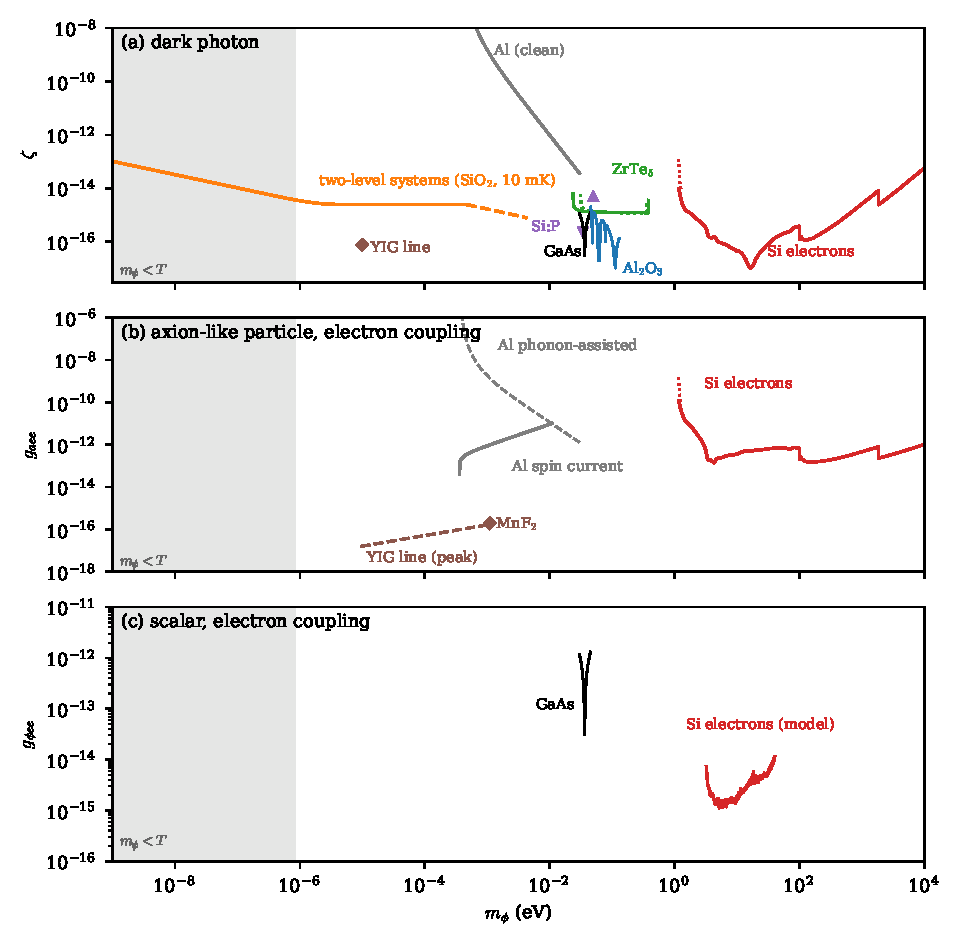
\includegraphics[width=0.86\linewidth]{figures/ch17/fig17_2.pdf}
  \caption{Absorption coverage: coupling for three events in one kilogram and year without background, $\rho_\chi = \SI{0.3}{GeV.cm^{-3}}$, against the boson mass. (a) Dark photon. Two-level systems of a thermal SiO$_2$ film at \SI{10}{mK}, $\tan\delta_0 = 3\times10^{-4}$, $\varepsilon_r = 3.9$, \cref{eq:16.7-dp} (solid, up to \SI{0.46}{meV}), and the vibrational absorption of the glass up to its Ioffe--Regel frequency, \SI{4.3}{meV} (dashed; \cref{lim:16.7d}). Clean aluminum, phonon-assisted pair creation with the Debye transport function, \cref{eq:15.4-holstein}. Si:P at \SI{e15}{cm^{-3}}: the $2p_0$ line at \SI{34.11}{meV} (down triangle) and the continuum at \SI{50}{meV} (up triangle), \cref{sec:16.5-absorption}. ZrTe$_5$ with the background in the total $\varepsilon$, polarization average, measured-structure (solid) and relaxed-cell (dotted) parameters of \cref{fig:16-zrte5}. GaAs and sapphire single-phonon lines, widths of \cref{fig:11-dpabs}. Silicon electrons from measured optical constants at \SI{300}{K} from \SI{1.1728}{eV}, with the cold excitonic edge of \cref{eq:13.8-edge} dotted up to \SI{1.3}{eV}. Diamond-shaped point: the Kittel line of a YIG sphere at \SI{10}{\micro eV}, vacuum $\zeta$, polarization random. (b) Axion-like particle, electron coupling. YIG Kittel line on resonance as it is tuned from \SI{9.5}{\micro eV} to \SI{1.16}{meV} (\SI{10}{T}), \cref{eq:14.3-peak}, and the MnF$_2$ resonance at \SI{1.1}{meV} (diamond-shaped point), both with the assumed width $\varGamma_{\mathrm{M}} = 10^{-5}\omega$. Clean aluminum: direct pair creation by the spin current, \cref{eq:15.4-sJ} with the quasiparticle factor $1/(1 + \lambda_{\mathrm{ep}}) = 0.70$, up to \SI{10.9}{meV} (solid), and the phonon-assisted $\sigma_1$ that published projections use (dashed). Silicon electrons from the measured $\sigma_1$, \cref{eq:10.7-alp}. (c) Scalar, electron coupling: the GaAs phonon line with the site couplings of \cref{eq:11.8-G}, and the kinetic-energy row of silicon in the empirical-pseudopotential model of \cref{fig:10-absorption}. Gray: $m_\phi < T$ for $T = \SI{10}{mK}$, where counting has lost its advantage over a coherent readout (\cref{sec:17.2-coherent}).}
  \label{fig:17-abs-coverage}
\end{figure}

\begin{table}[tbp]
  \centering
  \caption{Absorbing targets of the preceding chapters by decade of boson mass, with the best reach of each, three events in a kilogram and year without background. Lines are narrow and cover one mass unless tuned; continua cover the whole range given. A dash means no target in the book absorbs that boson at leading order in that decade.}
  \label{tab:17-abs-decades}
  \small
  \begin{tabular}{@{}>{\raggedright\arraybackslash}p{0.12\linewidth}>{\raggedright\arraybackslash}p{0.37\linewidth}>{\raggedright\arraybackslash}p{0.27\linewidth}>{\raggedright\arraybackslash}p{0.14\linewidth}@{}}
    \toprule
    $m_\phi$ & dark photon, $\zeta$ & axion-like, $g_{aee}$ & scalar, $g_{\phi ee}$ \\
    \midrule
    \SI{1}{neV}--\SI{1}{\micro eV} & two-level systems, $\gtrsim 3\times10^{-15}$; acoustic modes of bodies (\cref{sec:11.8-bar}); coherent readout & --- (nuclear spins couple through $g_{aNN}$, \cref{sec:14.6}) & resonant masses (\cref{sec:11.8-mass}) \\
    \SI{1}{\micro eV}--\SI{0.1}{meV} & two-level systems, $2.4\times10^{-15}$; YIG line, $7.6\times10^{-17}$ at \SI{10}{\micro eV} (vacuum $\zeta$) & YIG line, $1.6\times10^{-17}$ at \SI{10}{\micro eV} & --- \\
    \SIrange{0.1}{1}{meV} & two-level systems to \SI{0.46}{meV}, then glass vibrations; aluminum from \SI{0.36}{meV}, $1.5\times10^{-9}$ & YIG line, $1.7\times10^{-16}$ at \SI{1.16}{meV}; aluminum, $6.1\times10^{-13}$ & --- \\
    \SIrange{1}{10}{meV} & glass vibrations to \SI{4.3}{meV}, $7.6\times10^{-16}$ & MnF$_2$ line, $1.9\times10^{-16}$ at \SI{1.1}{meV}; aluminum, $9.1\times10^{-12}$ at \SI{10}{meV} & --- \\
    \SIrange{10}{100}{meV} & GaAs line, $2.9\times10^{-17}$; Si:P $2p_0$, $2.3\times10^{-16}$; ZrTe$_5$ from \SI{23.6}{meV}, $1.25\times10^{-15}$ & --- (nucleon coupling: \cref{sec:11.6}) & GaAs line, $3.1\times10^{-14}$ \\
    \SIrange{0.1}{1}{eV} & sapphire, $1.0\times10^{-17}$ at \SI{112}{meV}; ZrTe$_5$ to \SI{0.38}{eV}; none from \SIrange{0.38}{1.17}{eV} & --- & --- \\
    \SIrange{1}{10}{eV} & silicon from \SI{1.1728}{eV}; $4.4\times10^{-17}$ at \SI{10}{eV} & silicon, $1.4\times10^{-13}$ at \SI{4.3}{eV} & silicon (model), $1.1\times10^{-15}$ \\
    \SIrange{10}{100}{eV} & silicon plasmon, $1.0\times10^{-17}$ at \SI{16.4}{eV} & silicon, $3$--$5\times10^{-13}$ & silicon (model) \\
    \SIrange{0.1}{10}{keV} & silicon, $1.9\times10^{-16}$ at \SI{100}{eV}, $2.6\times10^{-15}$ at \SI{1}{keV} & silicon to \SI{1}{keV}, $3$--$5\times10^{-13}$ & --- \\
    \bottomrule
  \end{tabular}
\end{table}

The dark photon is covered almost everywhere, with two weak stretches. Between \SI{0.38}{eV}, where the Dirac cone of ZrTe$_5$ ends at twice its cutoff, and \SI{1.17}{eV}, where cold silicon begins to absorb, no target of the book absorbs at leading order; the sapphire lines and their multiphonon background end near \SI{0.12}{eV}. A narrow-gap semiconductor or a Dirac material with a wider cone would fill this gap, with the screening ceiling of its background constant. The second weak stretch is the meV decade, where the glass absorbs through its disordered vibrations at $\zeta \approx 10^{-15}$ and the superconductor is screened out.

The axion-like particle with its electron coupling has fewer targets. Magnons cover \SI{10}{\micro eV} to a meV, as far as a laboratory field tunes their lines; clean aluminum covers \SI{0.36}{meV} to \SI{11.5}{meV}, above which its phonon-assisted absorption takes over; and silicon covers everything above its edge that the tables reach. Between \SI{10}{meV} and \SI{1.17}{eV}, however, no target of the preceding chapters covers this coupling. Phonons absorb an axion-like particle through its nucleon coupling alone, on the spin-carrying isotopes of a crystal (\cref{sec:11.6}), and a Dirac material would need its spin-current response computed with its strong spin--orbit coupling, which the factor $\frac34$ of \cref{eq:10.7-alp} does not contain. The scalar has two targets: the GaAs phonon line, suppressed by the near-cancellation of its sublattices, and the kinetic row of silicon above its direct gap, which in \cref{fig:17-abs-coverage}c is a model with pseudo-wavefunctions. Between the indirect edge and \SI{3.1}{eV} silicon absorbs a scalar only with a phonon, through the kinetic row of \cref{sec:13.8}, which no measurement provides.

A tuned line and a continuum are compared differently. On resonance the Kittel line of YIG reaches $g_{aee} = 1.6\times10^{-17}$ at \SI{10}{\micro eV}, but only within its full width $\varGamma_{\mathrm{M}} = 10^{-5}m_\phi$. A search that scans the line across one e-fold of mass with uniform exposure spends a fraction $(\pi/2)\varGamma_{\mathrm{M}}/m_\phi = 1.6\times10^{-5}$ of its time on each mass. Averaged over the scan the reach is $4.1\times10^{-15}$, still a hundred times better than the continuum of clean aluminum at its best mass. The MnF$_2$ resonance at \SI{1.1}{meV} gives $1.9\times10^{-16}$ on resonance and $4.8\times10^{-14}$ averaged. The peak values rest on the assumed ratio $\varGamma_{\mathrm{M}}/\omega = 10^{-5}$ (\cref{sec:14.3}). The averaged ones do not depend on it, since the area of the line, not its height, sets what a scan delivers, as for the phonon lines of \cref{eq:11.8-Rint}. The fixed lines of GaAs, sapphire and Si:P cover their own masses alone.

\begin{workedexample}{The handover from GaAs phonons to silicon electrons}\label{we:17-handover}
GaAs absorbs a dark photon at its longitudinal optical phonon, \SI{36.35}{meV}, with all the weight of the line, $\mathcal{I}_{\mathrm{pol}} = \SI{0.759}{meV}$, within a few widths, and with multiphonon absorption up to a few phonon energies. Its electrons absorb from its gap, \SI{1.52}{eV} at low temperature (\cref{sec:3.3}). Silicon absorbs from its excitonic edge. At which mass does silicon take over?

\emph{The phonon line does not decide it.} The damped factorized model of \cref{fig:11-dpabs} gives $\varepsilon_2 = 2.5\times10^{-4}$ at \SI{1.17}{eV}, an absorption coefficient of \SI{4.3}{cm^{-1}} with the refractive index 3.48 used below. That value is an artifact of the model: with different widths in its numerator and denominator it tends to $\varepsilon_2 = \varepsilon_\infty(\gamma_{\mathrm{L}} - \gamma_{\mathrm{T}})/\omega$ far above the line, a constant conductivity. A Lorentz oscillator with a single width gives $\varepsilon_2 = 4.8\times10^{-7}$ and \SI{0.008}{cm^{-1}} at the same energy. A pure crystal transmits there, and what it absorbs depends on its defects.

\emph{Equal rates.} Per unit mass the rates are equal when $L_{\mathrm{GaAs}}/\rho_{\mathrm{GaAs}} = L_{\mathrm{Si}}/\rho_{\mathrm{Si}}$. Below a gap $\varepsilon_2 \ll \varepsilon_1 = n_r^2$, and with $\varepsilon_2 = n_r\alpha_{\mathrm{abs}}/\omega$ the loss function is $L = \alpha_{\mathrm{abs}}/(n_r^3\omega)$. With $n_r = 3.48$ for GaAs at \SI{22}{\celsius}, from the dispersion formula of Skauli et al.~\cite{skauli2003improved} as tabulated in Ref.~\cite{polyanskiy2024refractiveindex}, $n_r = 3.56$ for silicon at \SI{300}{K}~\cite{franta2017temperature}, and densities 5.361 and \SI{2.33}{g.cm^{-3}}, GaAs needs $(3.48/3.56)^3\times5.361/2.33 = 2.15$ times the absorption coefficient of silicon to match it.

\emph{The silicon edge.} At millikelvin temperatures silicon absorbs from the $1s$ replica of the transverse acoustic branch, $\Eg(0) + \omega_{\mathrm{TA}} - E_x^b = \SI{1.17277}{eV}$, and \cref{eq:13.8-edge} rises there as a square root. With the scale of \cref{sec:13.8},
\begin{equation*}
  \alpha_{\mathrm{abs}}^{\mathrm{Si}} = \SI{13.3}{cm^{-1}}\,\bigl[(m_\phi - \SI{1.17277}{eV})/\mathrm{eV}\bigr]^{1/2} ,
\end{equation*}
which is \SI{0.13}{cm^{-1}} at \SI{0.1}{meV} above the threshold and \SI{0.42}{cm^{-1}} at \SI{1}{meV}.

\emph{The handover.} Setting $2.15\,\alpha_{\mathrm{abs}}^{\mathrm{Si}}$ equal to the absorption of the GaAs crystal places the handover \SI{0.012}{meV} above the threshold for \SI{0.1}{cm^{-1}} and \SI{1.2}{meV} above it for \SI{1}{cm^{-1}}. A crystal absorbing \SI{10}{cm^{-1}} would move it \SI{40}{meV} up; at that distance the further replicas of \cref{eq:13.8-edge} have opened, and the square-root onset alone would have put it at \SI{0.12}{eV}. For any GaAs crystal transparent to better than \SI{1}{cm^{-1}}, silicon takes over within a meV of its excitonic edge, at $m_\phi \simeq \SI{1.173}{eV}$, and the square-root onset of the replica makes the handover sharp. A meV above the threshold silicon reaches $\zeta = 5.6\times10^{-14}$, two thousand times weaker than the GaAs line at its center.
\end{workedexample}

The worked example uses a model of the cold edge. The cold measurements near the edge differ among themselves by a factor of twenty (\cref{sec:13.8}), which moves the absorption of silicon but not the place of the handover, since the threshold is fixed by the gap, the phonon and the exciton binding.

\subsection{Coherent and counting readout}\label{sec:17.2-coherent}

A YIG sphere tuned to \SI{10}{\micro eV} counts the quanta it absorbs (\cref{we:14-yig}). A $^{207}$Pb sample at \SI{1}{neV} reads the transverse magnetization that the field drives (\cref{sec:14.6}). Both measure the absorptive part of a response near $\omega = m_\phi$, but the first counts quanta of energy $m_\phi$ and the second measures the amplitude of a field. Which readout is better at a given mass depends on the thermal occupation $n_{\mathrm{B}}(m_\phi) = 1/(\ee^{m_\phi/T} - 1)$ of the mode that is read, with $T$ the temperature of that mode.

Take a record of length $t_{\mathrm{int}}$ longer than the coherence time. The signal is spread over $N_{\mathrm{coh}} \simeq t_{\mathrm{int}}\Delta\omega_{\mathrm{eq}}/2\pi$ independent frequency bins, with $\Delta\omega_{\mathrm{eq}} = 2.67/t_{\mathrm{coh}}$ the equivalent width of the line (\cref{sec:14.6-stats}), and it delivers $\bar N_{\mathrm{sig}}$ absorbed quanta. A counter whose detection band is the line sees, in the same bins, $\bar N_{\mathrm{th}} = n_{\mathrm{B}}(m_\phi)N_{\mathrm{coh}}$ thermal quanta. They are chaotic, and their number fluctuates with the variance $\bar N_{\mathrm{th}} + \bar N_{\mathrm{th}}^2/N_{\mathrm{coh}} = N_{\mathrm{coh}}n_{\mathrm{B}}(m_\phi)[n_{\mathrm{B}}(m_\phi) + 1]$ of \cref{sec:14.6-regime}. A linear readout, a phase-preserving amplifier or a magnetometer, measures both quadratures of the mode, and its noise is at least $n_{\mathrm{B}}(m_\phi) + 1$ quanta per bin: the thermal quanta plus one zero-point quantum, half of it present at the input and half added by the amplifier~\cite[Eq.~(9)]{lamoreaux2013analysis}. This per-bin noise has the rms $n_{\mathrm{B}}(m_\phi) + 1$, and summed in quadrature over the bins it fluctuates by $[n_{\mathrm{B}}(m_\phi) + 1]N_{\mathrm{coh}}^{1/2}$. The significance of the signal is then $\bar N_{\mathrm{sig}}/\{N_{\mathrm{coh}}n_{\mathrm{B}}(m_\phi)[n_{\mathrm{B}}(m_\phi) + 1]\}^{1/2}$ for the counter and $\bar N_{\mathrm{sig}}/\{N_{\mathrm{coh}}^{1/2}[n_{\mathrm{B}}(m_\phi) + 1]\}$ for the linear readout, whose square is the weak-signal statistic $\mathsf{t}$ of \cref{sec:14.6-stats} with $x_k = \bar N_{\mathrm{sig}}/\{N_{\mathrm{coh}}[n_{\mathrm{B}}(m_\phi) + 1]\}$ in each bin. At equal significance the counter needs fewer signal quanta by the ratio
\begin{keyresult}[Counting against linear readout]
\begin{equation}
  \frac{\bar N_{\mathrm{sig}}^{\mathrm{lin}}}{\bar N_{\mathrm{sig}}^{\mathrm{cnt}}} = \Bigl[\frac{n_{\mathrm{B}}(m_\phi) + 1}{n_{\mathrm{B}}(m_\phi)}\Bigr]^{1/2} = \ee^{m_\phi/2T} ,
  \label{eq:17.2-ratio}
\end{equation}
for the same absorber, record and line, as long as the counter sees thermal quanta in the record and its detection band is the line width $\Delta\omega_{\mathrm{eq}}$. A counter that sees a band $B$ wider than the line collects more thermal quanta, and the ratio is multiplied by $(B/\Delta\omega_{\mathrm{eq}})^{-1/2}$. In the coupling, which enters the signal squared, the ratio is $\ee^{m_\phi/4T}$. For $n_{\mathrm{B}}(m_\phi) \ll 1$ the Poisson treatment of Lamoreaux and collaborators~\cite[Eqs.~(12)--(14)]{lamoreaux2013analysis} is the limit of this result; their cavity counter sees the whole cavity band, which carries the extra factor $(Q_{\mathrm{c}}/2\pi Q_a)^{1/2}$ of their Eq.~(18), with $Q_{\mathrm{c}}$ and $Q_a$ the quality factors of the cavity and of the line.
\end{keyresult}

Three regimes follow. For $m_\phi \ll T$ the ratio tends to one. Each mode holds many thermal quanta, their fluctuation dominates either readout, and a counter gains nothing over a measurement of the field, while it would have to resolve single quanta far below the thermal energy. At \SI{1}{neV} a mode at \SI{4.2}{K} holds $3.6\times10^5$ quanta and one at \SI{10}{mK} holds 861, and every search there reads the field. For $m_\phi \approx T$ the gain is modest, 1.65 in the signal and 1.28 in the coupling at $m_\phi = T$. For $m_\phi \gg T$ the counter wins exponentially, until the record holds no thermal quantum at all. Requiring zero thermal counts with \SI{95}{\percent} probability, $\bar N_{\mathrm{th}} < 0.05$, the counter needs three signal quanta (\cref{sec:1.5})~\cite[Eqs.~(19), (20)]{lamoreaux2013analysis}, whatever the mass. With $\Delta\omega_{\mathrm{eq}} = 2.67\,m_\phi v_0^2$ this happens above \SI{17}{\micro eV} for a one-hour record and \SI{20}{\micro eV} (\SI{4.9}{GHz}) for one day at \SI{10}{mK}, and above \SI{0.19}{meV} and \SI{0.22}{meV} at \SI{100}{mK}, that is, at $m_\phi \approx (20$--$26)\,T$. The linear readout still needs $\bar N_{\mathrm{sig}} = (2.71\,N_{\mathrm{coh}})^{1/2}[n_{\mathrm{B}}(m_\phi) + 1]$ at the threshold $\mathsf{t} = 2.71$ of \cref{eq:C.14-thresholds}, the one-sided \SI{95}{\percent} level. For instance, at \SI{24.8}{\micro eV}, the 6-GHz mass of \cref{we:16-tls-dp}, a day at \SI{10}{mK} spreads the line over $8.7\times10^8$ bins, and the linear readout needs $4.9\times10^4$ quanta against the counter's three, a factor of 127 in the coupling. At \SI{10}{\micro eV} the same record still holds 3200 thermal quanta, and the counter wins by 330 in the signal and 18 in the coupling.

The gray band of \cref{fig:17-abs-coverage}, $m_\phi < T$ (\SI{0.86}{\micro eV}, or \SI{210}{MHz} at \SI{10}{mK}), is where the advantage of counting has fallen below $\ee^{1/2}$ and tends to one, and the field is read coherently. Above that mass the counter gains $\ee^{m_\phi/4T}$ in the coupling, and above $20\,T$ it is limited by the absorbed quanta alone, with a reach that improves as $t_{\mathrm{int}}^{-1/2}$ against the $(t_{\mathrm{int}}t_{\mathrm{coh}})^{-1/4}$ of the field measurement (\cref{eq:14.6-scaling}). Two effects reduce the advantage. A linear readout of one quadrature of a squeezed mode can go below one zero-point quantum~\cite{lamoreaux2013analysis}, which narrows the gap by the degree of squeezing. A real counter, moreover, has dark counts besides the thermal quanta, and they add to its background. The background-free counting that the reach curves of \cref{fig:17-abs-coverage} assume holds where both are absent.

\section{Inelastic scattering into collective modes}\label{sec:17.3}

A dark-matter particle of \SI{10}{keV} at the largest laboratory speed $v_{\mathrm{max}}$ carries \SI{35}{meV} of kinetic energy, just short of the \SI{36.35}{meV} longitudinal optical phonon of GaAs, and elastic scattering cannot create that phonon below \SI{10.35}{keV} (\cref{sec:11.2}). Let the same particle arrive in an excited state \SI{1}{eV} above its ground state and leave in the lower one. It then emits the phonon at every speed of the halo, at a rate of $2.6\times10^4$ events per kilogram and year for a light dark photon at $\sigmae = \SI{e-40}{cm^2}$. \Cref{sec:10.9} followed the splitting $\Delta_\chi$ through the electron-recoil spectrum of silicon. The collective modes, phonons, magnons and plasmons, are the natural final states of down-scattering (\cref{sec:8.2-exothermic}): the band of allowed $(\vect{q},\omega)$ moves up by $|\Delta_\chi|$, and a mode whose energy lies below the splitting is always reached. One formula covers all the modes, and the dispersion of each mode decides where its line lies, how wide it is, and how much of the splitting it takes.

\subsection{Down-scattering into a collective mode}\label{sec:17.3-shell}

Every collective response of \cref{chap:10,chap:11,chap:14} is, at $T = 0$, a sum of lines. The one-phonon response \cref{eq:11.1-S1}, the one-magnon response \cref{eq:14.1-Safm} and the plasmon pole of \cref{eq:4.5-plasmonL} each put a weight on the dispersion surface $\omega = \omega_\nu(\vect{q})$ of a branch $\nu$. Contracted with the dark-matter tensor, the integrand of \cref{eq:8.2-spectrum} becomes
\begin{equation}
  \sum_{ab}\mathfrak{D}_{ab}(\vect{q})\,S_{ab}(\vect{q},\omega) = \frac{2\pi}{\Omega}\sum_\nu\mathcal{Y}_\nu(\vect{q})\,\delta\bigl(\omega - \omega_\nu(\vect{q})\bigr) ,
  \label{eq:17.3-lines}
\end{equation}
which defines the mode weight $\mathcal{Y}_\nu \ge 0$. For the nucleon coupling of \cref{sec:11.1}, in the notation of \cref{eq:11.1-S1} (nucleon numbers $A_\kappa$, polarization vectors $\vect{e}_{\kappa\nu}$), $\mathcal{Y}_\nu = |\tilde V_N|^2|\sum_\kappa A_\kappa\ee^{-W_\kappa}\ee^{\ii\vect{q}\cdot\vect{\tau}_\kappa}\vect{q}\cdot\vect{e}^*_{\kappa\nu}/\sqrt{M_\kappa}|^2/2\omega_\nu$. For the spin coupling $\mathcal{O}_4$ in an antiferromagnet, with $\Omega = \Omega_{\mathrm{ion}}$, the contraction \cref{eq:14.1-contract} gives $\mathcal{Y} = \tfrac14|\vect{S}||c_4|^2|F^{\mathrm{mag}}|^2w^{\mathrm{M}}_{\vect{q}}$, with the coupling $c_4$, the magnetic form factor $F^{\mathrm{mag}}$ and the magnon weight $w^{\mathrm{M}}_{\vect{q}}$ of \cref{sec:14.1}. For the plasmon of an electron gas coupled through the electron density, $S = (2q^2/e^2)L$ and the pole carries the weight $\pi/(\partial\varepsilon_1/\partial\omega)$, so that $\mathcal{Y} = \Omega|\tilde V|^2q^2/[e^2\,\partial\varepsilon_1/\partial\omega]$.

Down-scattering has $\Delta_\chi < 0$, and energy conservation, $\omega_{\vect{q}} = \omega_\nu(\vect{q})$ with $\omega_{\vect{q}}$ of \cref{eq:1.3-omegaq}, reads
\begin{equation*}
  |\Delta_\chi| + \vect{q}\cdot\vect{v} - \frac{q^2}{2\mchi} = \omega_\nu(\vect{q}) .
\end{equation*}
We first set $\vect{v} = 0$. Along each direction $\hat{\vect{q}}$ the condition fixes the magnitude of the momentum transfer at the roots $q_\nu(\hat{\vect{q}})$ of
\begin{equation}
  |\Delta_\chi| - \frac{q_\nu^2}{2\mchi} = \omega_\nu(q_\nu\hat{\vect{q}}) ,
  \label{eq:17.3-qnu}
\end{equation}
and we write $v_\nu = q_\nu/\mchi$ for the speed of the outgoing particle relative to the incoming one. For a mode whose energy is small against the splitting, $q_\nu \simeq (2\mchi|\Delta_\chi|)^{1/2}$; at a fixed deposit $\omega$ this is the shell momentum $q_\Delta$ of \cref{sec:10.9}. As a function of $q$ along $\hat{\vect{q}}$, the argument of the delta function has the slope $-(q/\mchi + u_\nu)$, with $u_\nu = \hat{\vect{q}}\cdot\nabla_{\vect{q}}\,\omega_\nu$ the group velocity of the mode along $\vect{q}$. Writing $\dd^3q = q^2\dd q\,\dd^2\hat{\vect{q}}$, the radial integral picks up $q_\nu^2/(q_\nu/\mchi + u_\nu)$ at each root. The rate of one particle, $\varGamma = \int\dd\omega\int\dd^3q/(2\pi)^3\,\sum\mathfrak{D}_{ab}S_{ab}\,\delta(\omega - \omega_{\vect{q}})$, is then $(2\pi)^{-3}(2\pi/\Omega)\sum_\nu\int\dd^2\hat{\vect{q}}\,q_\nu^2\mathcal{Y}_\nu/(q_\nu/\mchi + u_\nu)$, which summed over branches and directions reads
\begin{keyresult}[Exothermic rate into a collective mode]
\begin{equation}
  \varGamma = \frac{\mchi}{\pi\Omega}\sum_\nu\Bigl\langle\frac{q_\nu\,\mathcal{Y}_\nu(q_\nu\hat{\vect{q}})}{1 + u_\nu/v_\nu}\Bigr\rangle_{\hat{\vect{q}}}\Bigl[1 + O\bigl(v^2/v_\nu^2\bigr)\Bigr] , \qquad
  \mathcal{R} = \frac{\rho_\chi}{\mchi\rho_T}\,\varGamma ,
  \label{eq:17.3-rate}
\end{equation}
with $q_\nu$ the roots of \cref{eq:17.3-qnu}, $\langle\cdot\rangle_{\hat{\vect{q}}}$ the average over directions, and $\mathcal{R}$ the rate per unit target mass. It holds for $v_\nu$ above the speeds of the halo and for a weight $\mathcal{Y}_\nu$ that varies little over momenta $\mchi v_{\mathrm{max}}$.
\end{keyresult}
\noindent At finite $\vect{v}$ the surface of \cref{eq:17.3-qnu} moves by a vector of order $\mchi\vect{v}$ and changes its radius at second order. The term linear in $\vect{v}$ averages to zero over a weight and a dispersion even in $\vect{q}$, as for the electronic shell of \cref{eq:10.9-shell}, and the correction to the rate is of order $v^2/v_\nu^2$. The deposited energy, by contrast, shifts at first order, and \cref{sec:17.3-lines} shows that this sets the width of the line. The factor $(1 + u_\nu/v_\nu)^{-1}$ is new compared with the electronic shell, where the energy is integrated at fixed $\omega$. It is close to one for phonons and magnons, whose group velocities, $10^{-5}$ to $10^{-4}$, lie far below $v_\nu$, but not for the plasmon, whose dispersion is steep.

The velocity independence has a simple reading in the incoherent limit. For a free scatterer the rate per particle of elastic scattering is $\nd\sigma v$, and that of exothermic down-scattering is $\nd\sigma v_\nu$: the final momentum, and with it the phase space, is fixed by the splitting rather than by the incoming speed. The magnons of NiO show it. With the spin coupling $\mathcal{O}_4$, a heavy mediator and $\sigmae = \SI{e-40}{cm^2}$ (the setting of \cref{fig:14-nio-rate}), a particle of \SI{1}{MeV} with $|\Delta_\chi| = \SI{10}{eV}$ has $q_\nu = \SI{4.45}{keV}$, beyond the ordering wavevector at \SI{2.58}{keV}. The shell then crosses many magnetic zones, and the direction average of the weight is 1.149, close to its zone average 1.156 (in the spin-wave theory of \cref{we:14-nio}, $1 + 2\Delta S = 1.157$, with $\Delta S$ the zero-point spin reduction). \Cref{eq:17.3-rate} yields 8210 events per kilogram and year, within \SI{3}{\percent} of the full integral over the halo, 8000, against 2620 for elastic scattering at the same mass.

\subsection{Line positions and widths}\label{sec:17.3-lines}

Each root of \cref{eq:17.3-qnu} deposits $\omega_\nu(q_\nu\hat{\vect{q}})$. The splitting is shared between the outgoing dark matter, which keeps $q_\nu^2/2\mchi$, and the mode, and the dispersion decides the share. A parabolic branch, $\omega_\nu(\vect{q}) = \omega_\nu(0) + q^2/2m^*_\nu$ with a dispersion mass $m^*_\nu$ of either sign, makes this exact for any $\vect{v}$. Energy conservation becomes $|\Delta_\chi| - \omega_\nu(0) + \vect{q}\cdot\vect{v} = q^2/2\mu_\nu$ with $\mu_\nu = \mchi m^*_\nu/(\mchi + m^*_\nu)$, and completing the square,
\begin{gather}
  |\vect{q} - \mu_\nu\vect{v}|^2 = q_\nu^2 + \mu_\nu^2v^2 , \qquad
  q_\nu^2 = 2\mu_\nu\bigl(|\Delta_\chi| - \omega_\nu(0)\bigr) , \notag\\
  \omega_\nu(q_\nu) = \omega_\nu(0) + \frac{\mu_\nu}{m^*_\nu}\bigl(|\Delta_\chi| - \omega_\nu(0)\bigr) .
  \label{eq:17.3-parabolic}
\end{gather}
The momentum transfers lie on a sphere centered at $\mu_\nu\vect{v}$, and at $\vect{v} = 0$ the mode takes the fraction $\mu_\nu/m^*_\nu = \mchi/(\mchi + m^*_\nu)$ of the energy above its bottom. A free electron at rest is the branch $\omega(0) = 0$, $m^* = m_e$, and \cref{eq:17.3-parabolic} returns the line $(\mu_{\chi e}/m_e)|\Delta_\chi|$ of \cref{sec:10.9-inelastic}. A flat branch, $|m^*_\nu| \gg \mchi$, takes little more than $\omega_\nu(0)$ and leaves the rest of the splitting to the dark matter. A steep branch, $m^*_\nu \ll \mchi$, takes nearly all of it.

The width follows from the same sphere. On it $q^2 = q_\nu^2 + 2\mu_\nu^2v^2 + 2\mu_\nu\vect{v}\cdot(\vect{q} - \mu_\nu\vect{v})$, and the deposited energy $\omega_\nu(0) + q^2/2m^*_\nu$ differs from the line $\omega_\nu(q_\nu)$ by $(\mu_\nu q_\nu v/m^*_\nu)\cos\theta$ plus a shift of order $v^2$, with $\theta$ the angle between $\vect{v}$ and $\vect{q} - \mu_\nu\vect{v}$. For a weight that is the same in every direction, $\cos\theta$ is uniform on the sphere, and a particle of speed $v$ spreads its energy uniformly over a band of full width $2\mu_\nu q_\nu v/|m^*_\nu|$. Averaging over the halo with the factor $1/v$ of this normalization turns the band into $\eta$:
\begin{equation}
  \frac{1}{\varGamma_\nu}\frac{\dd\varGamma_\nu}{\dd\omega} = \frac{|m^*_\nu|}{2\mu_\nu q_\nu}\;\eta\Bigl(\frac{|m^*_\nu|\,|\omega - \omega_\nu(q_\nu)|}{\mu_\nu q_\nu}\Bigr) ,
  \label{eq:17.3-profile}
\end{equation}
to first order in $v/v_\nu$, normalized by $\int_0^\infty\eta(u)\,\dd u = 1$. The line has the shape of $\eta(\vmin)$ reflected about its center. It is flat near the center, where every particle contributes, falls to half height where $\eta$ does, at \SI{278}{km/s} or 0.35 of $v_{\mathrm{max}}$, and ends at the full width $2\mu_\nu q_\nu v_{\mathrm{max}}/|m^*_\nu|$. For a branch that is not parabolic, the same steps with the dispersion linearized about $q_\nu$ replace $q_\nu/m^*_\nu$ by $u_\nu$ and $\mu_\nu$ by $\mchi$, as long as $|u_\nu| \ll v_\nu$: the full width is $2|u_\nu|\mchi v_{\mathrm{max}}$. Intrinsic widths of the mode, from anharmonic decay of a phonon or Landau and interband damping of a plasmon, add by convolution.

An acoustic branch, $\omega = c_\nu q$, has $q_\nu = \mchi[(c_\nu^2 + 2|\Delta_\chi|/\mchi)^{1/2} - c_\nu]$ and a line at $c_\nu q_\nu$ whose full width relative to its energy is $2v_{\mathrm{max}}/v_\nu$. It is a line as long as $v_\nu$ is well above $v_{\mathrm{max}}$ and $q_\nu$ still lies inside the zone. Antiferromagnetic magnons near $\Gamma$ behave the same way. In NiO at \SI{0.1}{MeV} and $|\Delta_\chi| = \SI{1}{eV}$, $q_\nu = \SI{435}{eV}$, and the magnons emitted at $\vect{v} = 0$ have \SI{55.1}{meV} with a spread of \SI{0.9}{meV} over directions. However, $v_{\mathrm{max}}/v_\nu = 0.61$, and with the mean group velocity $1.1\times10^{-4}$ the halo spreads them over a full width $2|u_\nu|\mchi v_{\mathrm{max}} = \SI{60}{meV}$, more than the line energy. Their weight there, 0.28 on average, includes the suppression near $\Gamma$ of \cref{sec:14.1}, and \cref{eq:17.3-rate} yields 5130 events per kilogram and year against 5710 from the full integral and 434 for elastic scattering. Once $q_\nu$ crosses many zones, the deposited energies sample the whole branch, and the spectrum becomes the weighted density of states: \SI{100}{meV} on average, with a spread of \SI{15}{meV}, for NiO at \SI{1}{MeV} and $|\Delta_\chi| = \SI{10}{eV}$.

The magnons of a ferromagnet start at the Larmor frequency and disperse quadratically near $\Gamma$, a parabolic branch with $\omega_\nu(0) = \omega_{\mathrm{Lar}}$ and a positive $m^*_\nu$. As $|\Delta_\chi|$ approaches $\omega_{\mathrm{Lar}}$, $q_\nu \to 0$ and \cref{eq:17.3-rate} vanishes in proportion to $q_\nu$ for a coupling without $q$ dependence. The uniform precession of \cref{sec:14.3} is the end point of the exothermic spectrum, where the halo speeds take over from the splitting.

A flat optical branch gives a narrow line at its own energy, and \cref{we:17-gaas} works it out for GaAs.

The plasmon is the steep case. Expanding the gas dispersion of \cref{sec:4.5}, $\omega_{\mathrm{pl}} \simeq \omega_p + \alpha_{\mathrm{pl}}q^2/m_e$, gives $m^*_{\mathrm{pl}} = m_e/2\alpha_{\mathrm{pl}}$. At the valence density of silicon, $E_{\mathrm{F}} = \SI{12.47}{eV}$, $\omega_p = \SI{16.61}{eV}$ and $\alpha_{\mathrm{pl}} = \tfrac35E_{\mathrm{F}}/\omega_p = 0.451$, so that $m^*_{\mathrm{pl}} = \SI{567}{keV}$, lighter than the dark matter of most electron-recoil searches. A particle of \SI{1}{MeV} has $\mu_{\mathrm{pl}} = \SI{362}{keV}$ and hands the plasmon 0.638 of the splitting above $\omega_p$, a particle of \SI{10}{MeV} 0.946. At $|\Delta_\chi| = \SI{20}{eV}$ and \SI{1}{MeV}, \cref{eq:17.3-parabolic} puts the line at \SI{18.77}{eV} and $q_\nu = \SI{1.57}{keV}$, and the exact zero of the Lindhard function at \SI{18.83}{eV} and \SI{1.53}{keV}. The steep dispersion that hands the plasmon the splitting also makes the line wide: the full width from the halo is \SI{5.3}{eV}, more than the measured \SI{3.66}{eV} width of the silicon loss peak (\cref{sec:4.5}). Since the plasmon exists only below the Landau-damping momentum, the line exists only in a window of splittings. The parabolic dispersion meets the upper edge of the pair continuum, $qv_{\mathrm{F}} + q^2/2m_e$, at \SI{2.30}{keV}, and the window closes \SI{7.3}{eV} above $\omega_p$ at \SI{1}{MeV}.

\begin{workedexample}{Exothermic emission of an optical phonon in GaAs}\label{we:17-gaas}
Take a dark photon, $\sigmae = \SI{e-40}{cm^2}$ as in \cref{sec:11.2}, $\mchi = \SI{30}{keV}$ and $\Delta_\chi = \SI{-1}{eV}$. The splitting lies below the gap of GaAs, \SI{1.52}{eV}, so no electronic excitation is open, and the dark photon reaches the lattice through the longitudinal optical phonon alone. Its line in the loss function carries $(\pi\omega_{\mathrm{L}}/2)(1 - \omega_{\mathrm{T}}^2/\omega_{\mathrm{L}}^2)/\varepsilon_\infty = \SI{7.59e-4}{eV}$ with the measured $\omega_{\mathrm{T}} = \SI{33.62}{meV}$, $\omega_{\mathrm{L}} = \SI{36.35}{meV}$ and $\varepsilon_\infty = 10.88$ (\cref{eq:11.2-onebranch}, splitting route). With this line in place of the averaged loss function $\bar L$ of \cref{eq:10.9-shell}, that equation times $(1 + u_\nu/v_\nu)^{-1}$ is \cref{eq:17.3-rate} for the charge coupling:
\begin{equation*}
  \mathcal{R} = \frac{\rho_\chi\,\sigmae\,q_\nu^3\,\FDM(q_\nu)^2\,\omega_{\mathrm{L}}}{2e^2\rho_T\,\mu_{\chi e}^2}\,\frac{1}{\varepsilon_\infty}\Bigl(1 - \frac{\omega_{\mathrm{T}}^2}{\omega_{\mathrm{L}}^2}\Bigr)\frac{1}{1 + u_\nu/v_\nu} .
\end{equation*}

\emph{Kinematics.} With the computed dispersion of the longitudinal branch of \cref{sec:5.5}, shifted to the measured $\omega_{\mathrm{L}}$ at $\Gamma$ and averaged over $[100]$, $[110]$ and $[111]$, \cref{eq:17.3-qnu} gives $q_\nu = \SI{240.5}{eV}$, 0.109 of $2\pi/a$ and inside the region where the Born-charge vertex holds (\cref{sec:11.2}). Then $v_\nu = 8.0\times10^{-3}$ and $v_{\mathrm{max}}/v_\nu = 0.33$. The estimate $2.5\langle v^2\rangle/v_\nu^2$ of \cref{sec:10.9} puts the halo correction to the rate at \SI{6}{\percent}.

\emph{Line.} The branch falls with $q$, $u_\nu = -6.2\times10^{-7}$, and the line lies at \SI{36.279}{meV}, \SI{0.071}{meV} below $\omega_{\mathrm{L}}$, between 36.256 and \SI{36.314}{meV} depending on the direction. Its full width from the halo, $2|u_\nu|\mchi v_{\mathrm{max}}$, is \SI{0.099}{meV}, and its half-maximum width 0.35 of that. Both are below the anharmonic width of the phonon, a fraction of a meV (\cref{sec:11.2}). The dark matter keeps \SI{0.964}{eV}; the detector sees one optical phonon.

\emph{Rate.} For a light dark photon, $\FDM = (q_0/q)^2$, the formula yields 1817 events per kilogram and year, and the full integral over the halo with the absolute value in $\vmin$ (\cref{eq:10.9-inel}) 1810. Elastic scattering at the same mass leads to 842, so the splitting doubles the rate while fixing the energy deposited. For a heavy dark photon the shell form is at 0.0314 and the full integral 0.0334, against $5.7\times10^{-5}$ for elastic scattering, a gain of 585. The two mediators respond oppositely to the splitting, since the light one weights $q_\nu^{-1}$ and the heavy one $q_\nu^3$. At $|\Delta_\chi| = \SI{0.5}{eV}$ the full integrals give 2600 for the light dark photon and 0.012 for the heavy one; the shell form yields 2620 and 0.010, off by \SI{12}{\percent} for the heavy mediator, which weights the largest momenta, at $v_{\mathrm{max}}/v_\nu = 0.48$.

\emph{Below the elastic edge.} At \SI{10}{keV}, under the edge $2\omega_{\mathrm{L}}/v_{\mathrm{max}}^2 = \SI{10.35}{keV}$, elastic scattering is closed. The same splitting gives $q_\nu = \SI{138.8}{eV}$, $v_{\mathrm{max}}/v_\nu = 0.19$, and $2.6\times10^4$ events per kilogram and year for the light dark photon, with the shell form within \SI{0.1}{\percent} of the full integral.
\end{workedexample}

\subsection{Electronic and collective channels in silicon}\label{sec:17.3-silicon}

\begin{figure}[tbp]
  \centering
  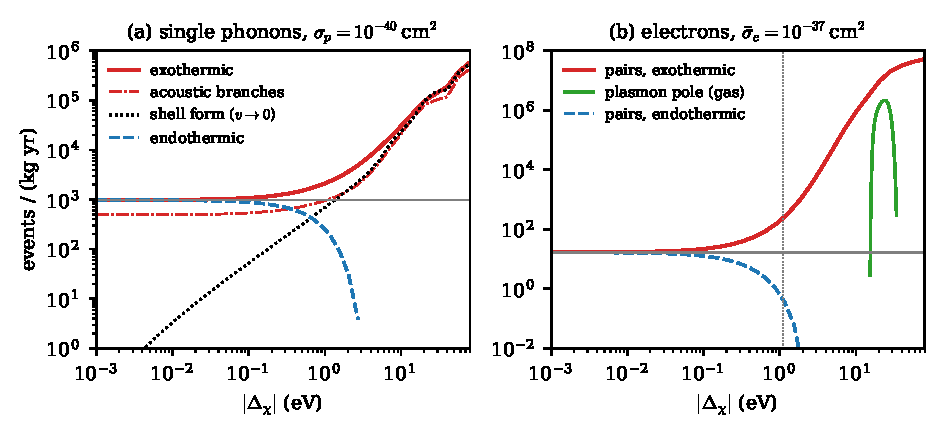
\includegraphics[width=\linewidth]{figures/ch17/fig17_3.pdf}
  \caption{Rates of silicon per kilogram and year against the mass splitting for $\mchi = \SI{1}{MeV}$, heavy mediator, standard halo of \cref{sec:1.2}, $T = 0$. Solid: exothermic ($\Delta_\chi = -|\Delta_\chi|$); dashed: endothermic ($\Delta_\chi = +|\Delta_\chi|$); gray line: elastic scattering. (a) Single phonons for a coupling to the nucleon number, $\sigma_p = \SI{e-40}{cm^2}$: the one-phonon response \cref{eq:11.1-S1} with all six branches of the computed phonons of \cref{sec:5.2} at the actual $\vect{q}$ (Umklapp and Debye--Waller factor included), averaged over the orientations of the crystal, deposits $\omega \ge \SI{1}{meV}$; dash-dotted: the three lowest branches; dotted: the shell form \cref{eq:17.3-rate}. (b) Electrons for a coupling to the electron density, $\sigmae = \SI{e-37}{cm^2}$: pairs from \cref{eq:10.9-inel} with the random-phase loss function with local fields of the tables of \cref{sec:10.2}, above \SI{1.11}{eV}, the step-model gap of their package (dotted vertical line; the tables are scissored to \SI{1.17}{eV}, \cref{sec:10.10}), the loss function held at its first tabulated momentum, \SI{493}{eV}, below it; green: the plasmon pole of an electron gas at the valence density of silicon, \cref{eq:10.3-plrate} with the splitting in $\vmin$, a model of the plasmon part of the electronic rate.}
  \label{fig:17-exo}
\end{figure}

\Cref{fig:17-exo} puts the two couplings of silicon side by side at \SI{1}{MeV}, each at its reference cross-section. Their elastic rates are 976 events per kilogram and year for single phonons and 16.7 for pairs. A particle of that mass carries up to $\tfrac12\mchi v_{\mathrm{max}}^2 = \SI{3.51}{eV}$, and a splitting well below this changes little: at $|\Delta_\chi| = \SI{0.12}{eV}$ the two rates are 1.12 and 1.39 times their elastic values. Above a few eV the splitting dominates, and the two channels respond to it differently.

The single-phonon rate rises from $2.0\times10^3$ at \SI{0.94}{eV} to $3.2\times10^4$ at \SI{10.3}{eV} and $5.8\times10^5$ at \SI{80}{eV}. The momentum transfer $q_\nu \simeq (2\mchi|\Delta_\chi|)^{1/2}$ grows from \SI{1.4}{keV} to \SI{12.6}{keV}, from $0.6$ to $5.6\,q_{\mathrm{BZ}}$. The one-phonon weight grows as $q^2$ times the Debye--Waller factor, whose exponent $2W$ is still just 0.10 at \SI{80}{eV}; two-phonon emission is smaller than one-phonon emission by a factor of order $W$. The deposited energy does not follow the splitting. Beyond the zone the shell crosses every branch, the spectrum is the weighted density of phonon states, and at \SI{10}{eV} the mean deposit is \SI{34.5}{meV}, with \SI{42}{\percent} above \SI{40}{meV} in the optical branches. A detector reading phonons sees the same energies as for elastic scattering, with a rate raised by a factor of 31 at \SI{10}{eV}. Between 10.3 and \SI{80}{eV} the shell form lies at 0.78 to 1.10 of the full integral. The residual comes from the condition on the weight in \cref{eq:17.3-rate}, not from the halo speeds, whose correction is $(v_{\mathrm{max}}/v_\nu)^2 \le 0.34$ there: the one-phonon weight varies on the scale $q_{\mathrm{BZ}} = \SI{2.25}{keV}$, smaller than $\mchi v_{\mathrm{max}} = \SI{2.65}{keV}$, and a single momentum per direction misses that structure.

The electronic rate rises far more steeply, from 165 at \SI{0.94}{eV} to $9.6\times10^5$ at \SI{10.3}{eV} and $5.3\times10^7$ at \SI{80}{eV}, a gain of $3\times10^6$ over the elastic rate. Elastic scattering at \SI{1}{MeV} barely crosses the gap, so any energy the splitting adds opens phase space that was nearly closed. Here the deposit does follow the splitting: \cref{sec:10.9} found the spectrum peaked between the gap and the plasma frequency, where $q_\Delta^3\bar L$ is largest, and an electronic detector reads energies of order $|\Delta_\chi|$.

The plasmon pole opens inside the electronic channel. For the electron gas at \SI{1}{MeV} it requires $\omega_{\mathrm{pl}}(q) - qv_{\mathrm{max}} + q^2/2\mchi \le |\Delta_\chi|$ at some $q$ below the Landau-damping momentum; the minimum is \SI{15.4}{eV}, above the \SI{14.7}{eV} found for a heavy particle in \cref{sec:10.3}, since a particle of \SI{1}{MeV} keeps $q^2/2\mchi$. The pole rate then grows to $2.2\times10^6$ events per kilogram and year at $|\Delta_\chi| = \SI{23.8}{eV}$ and falls beyond, as $q_\nu$ approaches the damping momentum and the weight of the line goes to zero. Between 18 and \SI{22}{eV} it is 0.09 to 0.16 of the electronic rate of the tables. The two are different models, an undamped pole in a gas against a broad loss peak in a crystal; in both, the plasmon is a minority share of exothermic electron recoil even where it is open. In a detector the plasmon decays into pairs (\cref{sec:10.3-decay}), and its line, \SI{5.3}{eV} wide from the halo alone at \SI{20}{eV}, merges with the pair spectrum around it.

\subsection{Endothermic thresholds}\label{sec:17.3-endo}

An endothermic splitting is supplied by the kinetic energy, and every channel acquires a lightest mass. For a mode with a gap and a parabolic dispersion, \cref{eq:17.3-parabolic} with $\Delta_\chi > 0$ gives $\vmin = (\Delta_\chi + \omega_\nu(0))/q + q/2\mu_\nu$. It is smallest at $q = [2\mu_\nu(\Delta_\chi + \omega_\nu(0))]^{1/2}$, and a particle at $v_{\mathrm{max}}$ reaches the mode if
\begin{equation}
  \mu_\nu \ge \frac{2\bigl(\Delta_\chi + \omega_\nu(0)\bigr)}{v_{\mathrm{max}}^2} .
  \label{eq:17.3-endogap}
\end{equation}
For a flat branch $\mu_\nu = \mchi$, and this is \cref{eq:1.3-mmin} with $\omega_{\mathrm{th}} \to \Delta_\chi + \omega_\nu(0)$; electron--hole pairs follow with $\omega_\nu(0) \to \Eg$, as in \cref{sec:10.9-inelastic}. For a gapless linear branch with a threshold $\omega_{\mathrm{th}}$, $\vmin = \Delta_\chi/q + c_\nu + q/2\mchi$ must fall below $v_{\mathrm{max}}$ at some $q \ge \omega_{\mathrm{th}}/c_\nu$. Its unconstrained minimum lies at $q = (2\mchi\Delta_\chi)^{1/2}$, and
\begin{equation}
  \mchi \ge
  \begin{cases}
    \dfrac{2\Delta_\chi}{(v_{\mathrm{max}} - c_\nu)^2} , & (2\mchi\Delta_\chi)^{1/2} \ge \omega_{\mathrm{th}}/c_\nu , \\[1.5ex]
    \dfrac{\omega_{\mathrm{th}}}{2c_\nu\bigl(v_{\mathrm{max}} - c_\nu - c_\nu\Delta_\chi/\omega_{\mathrm{th}}\bigr)} , & \text{otherwise} .
  \end{cases}
  \label{eq:17.3-endolin}
\end{equation}
At $\Delta_\chi = 0$ the momentum threshold always binds, and \cref{eq:17.3-endolin} reduces to the acoustic edge \cref{eq:11.1-edge} and its magnon analog \cref{eq:14.1-mmin}.

\begin{table}[tbp]
  \centering
  \caption{Lightest dark-matter mass that reaches each channel for the endothermic splittings $\Delta_\chi = 0$, \SI{10}{meV} and \SI{1}{eV}, from \cref{eq:17.3-endogap,eq:17.3-endolin} with $v_{\mathrm{max}} = 2.650\times10^{-3}$. Gapped channels: the low-temperature gap of silicon, \SI{1.17}{eV}; the optical phonon of silicon at \SI{64.1}{meV} (\cref{sec:5.2}); the longitudinal optical phonon of GaAs at \SI{36.35}{meV} (\cref{we:5-lst}). Linear channels: the largest longitudinal sound speed of silicon, \SI{9.35}{km/s}, with $\omega_{\mathrm{th}} = \SI{1}{meV}$ (\cref{sec:11.1}); the fastest magnon speed of NiO in the $J_1$--$J_2$ model, $c_{\mathrm{M}} = 1.36\times10^{-4}$, with $\omega_{\mathrm{th}} = \SI{5}{meV}$ (\cref{sec:14.1}).}
  \label{tab:17-endo}
  \begin{tabular}{lccc}
    \toprule
    Channel & $\Delta_\chi = 0$ & \SI{10}{meV} & \SI{1}{eV} \\
    \midrule
    Si, electron--hole pairs & \SI{0.333}{MeV} & \SI{0.336}{MeV} & \SI{0.618}{MeV} \\
    Si, optical phonon & \SI{18.3}{keV} & \SI{21.1}{keV} & \SI{303}{keV} \\
    GaAs, longitudinal optical phonon & \SI{10.35}{keV} & \SI{13.2}{keV} & \SI{295}{keV} \\
    Si, acoustic phonon & \SI{6.12}{keV} & \SI{6.95}{keV} & \SI{292}{keV} \\
    NiO, magnon & \SI{7.31}{keV} & \SI{8.20}{keV} & \SI{316}{keV} \\
    Si, plasmon & \multicolumn{3}{c}{closed at every mass} \\
    \bottomrule
  \end{tabular}
\end{table}

In \cref{tab:17-endo} a splitting of \SI{10}{meV} moves the lattice and magnon edges by 12 to \SI{28}{\percent} and the electronic one by \SI{1}{\percent}, because it adds to tens of meV for the collective modes and to an eV for pairs. A splitting of \SI{1}{eV} erases the differences among the collective channels: all of them then need \SI{0.3}{MeV}, set by $\Delta_\chi$ and the halo. The phonon of GaAs or the magnon of NiO then reaches dark matter lighter than the gap of silicon does by a factor of two, against 32 for the GaAs phonon and 46 for the NiO magnon in elastic scattering. For the plasmon, \cref{eq:17.3-endogap} needs $\mu_{\mathrm{pl}} \ge 2\omega_p/v_{\mathrm{max}}^2 = \SI{4.73}{MeV}$ already at $\Delta_\chi = 0$, while $\mu_{\mathrm{pl}}$ never exceeds $m^*_{\mathrm{pl}} = \SI{567}{keV}$: the dispersion that hands the plasmon most of an exothermic splitting closes it to endothermic and elastic scattering at every mass. In \cref{fig:17-exo} the same thresholds appear at fixed mass. At \SI{1}{MeV} the electronic rate closes at $\Delta_\chi = \tfrac12\mchi v_{\mathrm{max}}^2 - \Eg = \SI{2.40}{eV}$ with the gap of the tables, and the single-phonon rate at \SI{3.51}{eV} less the threshold.

\section{Interference between channels}\label{sec:17.4}

A dark photon that deposits \SI{1.2}{eV} at $q = \SI{1}{keV}$ in silicon can leave an electron--hole pair and a transverse acoustic phonon behind in two ways. It can push the electrons, which then emit the phonon through the electron--phonon coupling: the phonon-assisted amplitude of \cref{sec:13.2}. Or it can push a nucleus, whose electrons lag behind and are excited while the nucleus sheds the phonon: the Migdal amplitude of \cref{sec:12.1}. Both end in the same state, and the rate contains their product as well as their squares. Such products of an electron and a nuclear amplitude fill the bottom row of \cref{tab:8-sectors}, the cross response $S_{e\kappa}$ in each of the three sectors. In the electron-following sector the product cancels the phonon rate of a dark photon in silicon completely. In the two electronic sectors, at small momentum transfer, it raises the rate by 5.5 parts in $10^4$.

\subsection{The three cross cells}\label{sec:17.4-cells}

A mediator that couples to the electrons with the potential $\tilde V_e(\vect{q})$ and to the nuclei of species $\kappa$ with $\tilde V_\kappa(\vect{q})$ has the cross elements $\mathfrak{D}_{e\kappa} = \tilde V_e^*\tilde V_\kappa$ of \cref{eq:8.1-D}, and the rate \cref{eq:8.2-spectrum} contains, besides the electron and the nuclear terms, $2\Real\sum_\kappa\mathfrak{D}_{e\kappa}S_{e\kappa}$. A dark photon couples to $-\tilde Vn_Z$ (\cref{we:8-darkphoton}), so that $\tilde V_e = \tilde V$ and $\tilde V_\kappa = -Z_\kappa\tilde V$. A coupling to electrons alone has $\tilde V_\kappa = 0$, and a coupling to nucleons alone has $\tilde V_e = 0$. For these two the cross response never enters the rate, although $S_{e\kappa}$ itself is not zero, which is why \cref{sec:17.1} could compare the channels cell by cell. For a dark photon the three cells of $S_{e\kappa}$ differ in size by more than three orders of magnitude.

\emph{Electron-following cell.} In this sector the electron density acts on the nuclei as $\bar\rho_e(\vect{q};u)$ of \cref{eq:8.6-follow}. At long wavelength the electrons that follow nucleus $\kappa$ carry the charge $F^{\mathrm{fol}}_\kappa = \hat{\vect{q}}\cdot(Z_\kappa\mathbf{1} - Z^*_\kappa)\cdot\hat{\vect{q}}$, the $q \to 0$ value of $F_{\mathrm{cr}}$ in \cref{eq:12.5-cross}. A phonon then sees the nucleus and its cloud with amplitudes in the ratio $Z_\kappa : F^{\mathrm{fol}}_\kappa$, of opposite sign for a dark photon, and the nuclear, electron and cross terms of its rate stand in the ratio $Z_\kappa^2 : (F^{\mathrm{fol}}_\kappa)^2 : -2Z_\kappa F^{\mathrm{fol}}_\kappa$, which add up to $Z_\kappa^{*2}$. In silicon $F^{\mathrm{fol}} = Z = 14$, and the cross term, $-392$ against $196 + 196$, cancels the other two exactly: a dark photon makes no phonon in silicon at long wavelength (\cref{sec:10.2}). In a polar crystal the cross term removes all but $Z^{*2}$, which $\varepsilon_\infty$ screens further, and what survives is the optical-phonon rate of \cref{sec:11.2}; \cref{we:17-gaas-interference} gives the numbers for GaAs. This cell is never a correction.

\emph{Zero-phonon cell.} The electronic cells carry the opposite first moment. By \cref{eq:8.6-fsum-ek} the energy-weighted cross response of the electron-following sector reappears with the opposite sign in the two electronic sectors together. Measured against the f-sum of the electrons, $\nd_eq^2/m_e$, it is $m_e/M_\kappa$, $1.95\times10^{-5}$ in silicon. Momentum conservation distributes it state by state. In a crystal of one element, \cref{eq:8.3-boostward} gives $\sum_\kappa\langle f|n_\kappa(\vect{q})|0\rangle = -(m_e/M_\kappa)\langle f|n_e(\vect{q})|0\rangle + O(q^2)$ for every final state at finite energy. For a dark photon the amplitude into any electronic final state is then $\tilde V(1 + Z_\kappa m_e/M_\kappa)\langle f|n_e|0\rangle$, and the zero-phonon rate gains the fraction $(1 + Z_\kappa m_e/M_\kappa)^2 - 1 = 5.47\times10^{-4}$ in silicon. Of this, the cross cell carries $2Z_\kappa m_e/M_\kappa$ and the zero-phonon Migdal cell $(Z_\kappa m_e/M_\kappa)^2 = 7.5\times10^{-8}$. The picture is the inertial argument behind the sum rule \cref{eq:12.6-sum}: the field that pushes the electrons also accelerates the nuclei, and in the frame of the nuclei every electron feels the additional force $m_e$ times their acceleration, $Z_\kappa m_e/M_\kappa$ times the force of the field. This is the ionic correction to the zero-phonon line. A dark photon sees it through the loss function of the total dielectric matrix of electrons and nuclei (\cref{sec:8.4}), so a loss function that includes the nuclei, computed or measured, already contains it.

In a crystal of several elements momentum conservation fixes the mass-weighted sum alone, $\sum_\kappa M_\kappa\langle f|n_\kappa|0\rangle = -m_e\langle f|n_e|0\rangle + O(q^2)$ (\cref{eq:8.3-soft}). As in \cref{sec:8.3}, write $\tilde V_\kappa = \lambda M_\kappa + \delta\tilde V_\kappa$. The part in proportion to mass contributes $-\lambda m_e\langle f|n_e|0\rangle$ to the amplitude, and the remainder $\delta\tilde V_\kappa$ needs the amplitudes of the separate sublattices, which momentum conservation does not supply. For a dark photon $\lambda = -\bar z\tilde V$, with $\bar z = \sum_\kappa w_\kappa Z_\kappa/M_\kappa$ a mean of $Z_\kappa/M_\kappa$ whose weights $w_\kappa = -M_\kappa\langle f|n_\kappa|0\rangle/(m_e\langle f|n_e|0\rangle)$ sum to one. If both sublattices carry positive weights, the cross cell lies between $2m_e$ times the smallest and the largest $Z_\kappa/M_\kappa$ of the crystal, with $m_e$ in u.

\subsection{The Migdal--phonon-assisted cross term}\label{sec:17.4-term}

Inside the window the one-phonon states of the phonon-dressed sector are those of \cref{eq:13.2-final}: an electron in $(c,\vect{k}')$, a hole in $(v,\vect{k})$, $\vect{k}' = \vect{k} + \vect{q} + \vect{Q}$, and one phonon emitted into $(-\vect{Q},\nu)$ or absorbed from $(\vect{Q},\nu)$. The electron density reaches them through the phonon-assisted amplitude \cref{eq:13.2-M}, $N^{-1/2}(n_{\vect{Q}\nu} + \frac12 \pm \frac12)^{1/2}M^\pm_{cv\nu}(\vect{k},\vect{q},\vect{Q})$. The nuclear density reaches them through the boost \cref{eq:12.1-amp}, which for a pair of energy $\Delta E_j = \omega_e$ reads
\begin{equation*}
  \sum_{I\in\kappa}\int\frac{\dd^3p}{(2\pi)^3}\;\frac{\vect{q}\cdot\vect{p}}{M_\kappa\omega_e^2}\,v_\kappa(\vect{p})\,\langle\Psi_j|n_e(\vect{p})|\Psi_0\rangle\,\bigl\langle\Psi^{\mathrm{nuc}\prime}\big|\ee^{\ii(\vect{q} - \vect{p})\cdot\vect{X}_I}\big|\Psi^{\mathrm{nuc}}\bigr\rangle ,
\end{equation*}
with $v_\kappa$ the potential of the nucleus, or its pseudopotential. The nucleus takes the kick $\vect{q}$, passes $\vect{p}$ to the electrons through its own field and keeps $\vect{K} = \vect{q} - \vect{p}$. Three steps turn this into the phonon-dressed amplitude.

First, the lattice factor is taken at its one-phonon term. With $\vect{X}_I = \vect{R} + \boldsymbol{\tau}_\kappa + \vect{u}_{\vect{R}\kappa}$ and the displacement \cref{eq:A.6-u}, the part of $\ee^{\ii\vect{K}\cdot\vect{X}_I}$ linear in $\vect{u}$ emits $(-\vect{Q},\nu)$ with the matrix element
\begin{equation*}
  \ii\,\frac{\vect{K}\cdot\vect{e}_{\kappa\nu}(\vect{Q})}{(2NM_\kappa\omega_{\vect{Q}\nu})^{1/2}}\,(n_{\vect{Q}\nu} + 1)^{1/2}\,\ee^{\ii(\vect{K}+\vect{Q})\cdot\vect{R}}\,\ee^{\ii\vect{K}\cdot\boldsymbol{\tau}_\kappa}\,\ee^{-W_\kappa(\vect{K})} ,
\end{equation*}
with the Debye--Waller factor of \cref{eq:A.6-DW}; absorption of $(\vect{Q},\nu)$ gives the same with $n_{\vect{Q}\nu}^{1/2}$. Second, the sum over the $N$ cells $\vect{R}$ gives $N$ times a Kronecker delta that keeps only $\vect{K} = -\vect{Q} - \vect{G}$, so that the electrons receive $\vect{p}_{\vect{G}} = \vect{q} + \vect{Q} + \vect{G}$. Their matrix element $\langle\Psi_j|n_e(\vect{p}_{\vect{G}})|\Psi_0\rangle$ is the density vertex $\rho_{cv}(\vect{k},\vect{p}_{\vect{G}})$ of \cref{eq:3.2-rho}, whose crystal momentum $\vect{k} + \vect{p}_{\vect{G}}$ is $\vect{k}'$ up to $\vect{G}$, as required. Third, the integral over $\vect{p}$ becomes a sum, $\int\dd^3p/(2\pi)^3 \to \Vol^{-1}\sum_{\vect{p}}$, which the delta reduces to the sum over $\vect{G}$, and the factor $N/\Vol = 1/\Omega$ remains. Collecting the factors, the nuclear amplitude of species $\kappa$ is $N^{-1/2}(n_{\vect{Q}\nu} + \frac12 \pm \frac12)^{1/2}M^{\mathrm{Mig},\pm}_{\kappa,cv\nu}$, with the dimensionless amplitude
\begin{equation}
  \begin{split}
  M^{\mathrm{Mig},\pm}_{\kappa,cv\nu}(\vect{k},\vect{q},\vect{Q}) &= \frac{\ii}{\Omega M_\kappa\omega_e^2\,(2M_\kappa\omega_{\vect{Q}\nu})^{1/2}}
  \sum_{\vect{G}}(\vect{q}\cdot\vect{p}_{\vect{G}})\,\bigl[(\vect{q} - \vect{p}_{\vect{G}})\cdot\vect{e}_{\kappa\nu}(\vect{Q})\bigr]\\
  &\qquad\times v_\kappa(\vect{p}_{\vect{G}})\,\rho_{cv}(\vect{k},\vect{p}_{\vect{G}})\,\ee^{\ii(\vect{q}-\vect{p}_{\vect{G}})\cdot\boldsymbol{\tau}_\kappa - W_\kappa(\vect{q}-\vect{p}_{\vect{G}})} ,
  \end{split}
  \label{eq:17.4-Mmig}
\end{equation}
where $\omega_e = \varepsilon_{c\vect{k}'} - \varepsilon_{v\vect{k}}$ is the pair energy. Read from left to right, the nucleus is boosted to the velocity $\vect{q}/M_\kappa$, its field gives the electrons $\vect{p}_{\vect{G}}$, and the momentum it keeps, $-\vect{Q} - \vect{G}$, displaces it along the phonon polarization. The factor $\ii$ of $M^{\mathrm{Mig}}$ matches the $-\ii$ that the vertex $g$ of \cref{eq:A.6-g} carries in Fourier form, so the ratio $M^{\mathrm{Mig}}/M^\pm$ is real. Both amplitudes carry the same phonon factor $N^{-1/2}(n_{\vect{Q}\nu} + \frac12 \pm \frac12)^{1/2}$, and the cross response follows as $S^{\mathrm{PA}}$ did in \cref{sec:13.3}, with one amplitude in place of the other.
\begin{keyresult}[Migdal--phonon-assisted cross response]
In the off-shell window, at first Born--Oppenheimer order and first order in the electron--phonon vertex, the interference of the electron and the nuclear density of species $\kappa$ into one-phonon pair states is
\begin{equation}
  \begin{split}
  S^+_{e\kappa}(\vect{q};\omega_l,\omega_e) = \frac{4\pi}{\Omega}\Bigl\langle\!\Bigl\langle\sum_{cv\nu\pm}\bigl(n_{\vect{Q}\nu} + \tfrac12 \pm \tfrac12\bigr)\,
  &M^{\pm}_{cv\nu}(\vect{k},\vect{q},\vect{Q})^*\,M^{\mathrm{Mig},\pm}_{\kappa,cv\nu}(\vect{k},\vect{q},\vect{Q}) \\
  &\times\delta\bigl(\omega_e - \varepsilon_{c\vect{k}'} + \varepsilon_{v\vect{k}}\bigr)\,\delta\bigl(\omega_l \mp \omega_{\vect{Q}\nu}\bigr)\Bigr\rangle\!\Bigr\rangle ,
  \end{split}
  \label{eq:17.4-Sek}
\end{equation}
with the zone averages over $\vect{k}$ and $\vect{Q}$ and the spin factor of \cref{eq:13.3-SPA}. It enters the rate as $2\Real\sum_\kappa\mathfrak{D}_{e\kappa}S^+_{e\kappa}$, in the joint response of \cref{eq:12.1-joint}.
\end{keyresult}
\noindent Each factor of the product depends on the phases chosen for the Bloch states and the polarization vectors, and the product does not, since every such phase enters once in each factor. The two amplitudes must, however, be built from one set of bands, phonons and vertices, the rule of \cref{sec:8.6} for adding sectors. The cross term is linear in the derivative coupling, which is why it sits at first Born--Oppenheimer order, half the order of a Migdal rate.

Two approximations of \cref{eq:17.4-Mmig} come from the boost. It keeps the transition density at the equilibrium positions, in the frame of the crystal. If the valence transition densities follow the struck ion instead, the lattice keeps $\vect{q}$ and not $\vect{q} - \vect{p}_{\vect{G}}$, and the factor $(\vect{q} - \vect{p}_{\vect{G}})\cdot\vect{e}_{\kappa\nu}$ changes with it (\cref{sec:12.1}). The frame changes the fraction of Migdal events that emit phonons by a factor 2.4 at \SI{5}{keV} (\cref{sec:12.4}), and it enters the cross term directly. The second approximation is the sum over $\vect{G}$, which must be kept whole: dropping its off-diagonal products in $|M^{\mathrm{Mig}}|^2$ is the diagonal approximation of \cref{sec:12.3}, whose error is open (\cref{app:E.18}). Momentum conservation fixes the exact sum at small $q$, and any approximate amplitude can be tested against it.

The labels $\omega_e$ and $\omega_l$ are those of \cref{sec:8.6}. Inside the window $\omega_e$ is unique to relative order $\theta_{\mathrm{ep}}$, the off-shell parameter of \cref{sec:8.5}, and \cref{eq:17.4-Sek} is the whole cross response of the phonon-dressed sector at this order. Near a resonant pair the Dyson convention \cref{eq:8.6-dyson} assigns the delta part to the zero-phonon cell and the finite parts to the phonon-dressed one, for the cross response as for $S^{\mathrm{PA}}$, and only the sum of the two electronic cells is free of convention.

\subsection{Vanishing of the cross term}\label{sec:17.4-zero}

The cross term is absent from the rate in four cases. First, a coupling to one species alone has $\mathfrak{D}_{e\kappa} = 0$.

The second is a mismatch of phonon number. A zero-phonon Migdal event leaves the phonon occupations unchanged, and a phonon-assisted pair has one phonon more or less. The final states are orthogonal, and the two amplitudes do not interfere, by the argument of \cref{sec:13.2} for the zero-phonon line. Migdal events with two or more phonons interfere with phonon-assisted amplitudes of second order in the electron--phonon vertex alone. At the order of \cref{eq:17.4-Sek} the one-phonon term of the Migdal lattice factor is the one that takes part, and at $q = \SI{5}{keV}$ it is \SI{96}{\percent} of the phonon-emitting Migdal events (\cref{sec:12.4}).

The third is the spin. Both vertices of \cref{eq:17.4-Sek} are diagonal in spin, and both amplitudes make singlet pairs. A coupling through the electron spin makes triplet pairs, which the nuclear density does not make in a crystal without spin--orbit coupling and magnetic order, and its cross term with the nuclear density vanishes by the selection rule of \cref{sec:10.4}.

The fourth is the limit $\vect{q} \to 0$. The phonon-assisted amplitude vanishes there, \cref{eq:13.2-q0}, because $n_e(0)$ is the electron number. The Migdal amplitude vanishes with its factor $\vect{q}\cdot\vect{p}_{\vect{G}}$, because a nucleus that is not kicked is not boosted. Both vanish linearly, so their ratio has a limit.

\subsection{Positivity bound and the small-momentum limit}\label{sec:17.4-bound}

The joint response is positive semidefinite at every point $(\omega_l, \omega_e)$ where the labels exist (\cref{sec:12.1}), and in particular on the one-phonon line. Here and below $S^{\mathrm{PA}}$ stands for the phonon-assisted response resolved in both labels, $S^{\mathrm{PA}}(\vect{q};\omega_l,\omega_e)$, like $S^+_{e\kappa}$; its integral over $\omega_l$ is the response of \cref{sec:13.3}. The Cauchy--Schwarz inequality \cref{eq:4.2-positivity} then gives $|S^+_{e\kappa}|^2 \le S^{\mathrm{PA}}S^+_{\kappa\kappa}$ pointwise, with $S^+_{\kappa\kappa}$ the one-phonon Migdal response of the same final states. With \cref{eq:8.3-bound}, taking the electron row as one group and the nuclear rows as the other,
\begin{equation}
  \Bigl|2\Real\sum_\kappa\mathfrak{D}_{e\kappa}S^+_{e\kappa}\Bigr| \le 2\Bigl(\mathfrak{D}_{ee}S^{\mathrm{PA}}\sum_{\kappa\kappa'}\mathfrak{D}_{\kappa\kappa'}S^+_{\kappa\kappa'}\Bigr)^{1/2} ,
  \label{eq:17.4-bound}
\end{equation}
pointwise, in every bin and for the integrated rate. The restriction to one sector needs care. The phonon-dressed sector is positive by itself inside the window, but outside it only on bins wider than the detuning, because the Dyson convention puts finite parts into it that are negative against a narrow bin (\cref{sec:8.6}). Outside the window the bound is applied to the two electronic sectors together.

At small $q$ the bound is reached. Apply \cref{eq:8.3-boostward} to a one-phonon pair state: for a crystal of one element and to first order in $q$, the exact summed nuclear amplitude is $-(m_e/M_\kappa)$ times the electron amplitude, with the same ratio for every final state. Written in the notation of \cref{eq:17.4-Mmig}, which stands here for the exact amplitude and not for its crystal-frame approximation, this is the following result.
\begin{keyresult}[Phonon-dressed interference at small momentum transfer]
For a crystal of one element, nuclear mass $M_\kappa$, and every one-phonon pair state,
\begin{equation}
  \sum_\kappa M^{\mathrm{Mig},\pm}_{\kappa,cv\nu}(\vect{k},\vect{q},\vect{Q}) = -\frac{m_e}{M_\kappa}\,M^{\pm}_{cv\nu}(\vect{k},\vect{q},\vect{Q})\,\bigl[1 + O(q/q_{\mathrm{BZ}})\bigr] ,
  \label{eq:17.4-lock}
\end{equation}
so that the summed cross response is $-(m_e/M_\kappa)S^{\mathrm{PA}}$, the summed one-phonon Migdal response is $(m_e/M_\kappa)^2S^{\mathrm{PA}}$, and \cref{eq:17.4-bound} holds as an equality. A coupling $\tilde V_\kappa = \tilde V_{\mathrm{nuc}}$ on every nucleus gives the phonon-dressed rate of \cref{eq:8.2-spectrum} with
\begin{equation}
  \mathfrak{D}_{ee}S^{\mathrm{PA}} \;\to\; \Bigl|\tilde V_e - \frac{m_e}{M_\kappa}\tilde V_{\mathrm{nuc}}\Bigr|^2S^{\mathrm{PA}} .
  \label{eq:17.4-rate}
\end{equation}
\end{keyresult}
\noindent Below the zone, then, the one-phonon Migdal effect is the phonon-assisted electron recoil seen through the boost: the same spectrum, with the weight $(m_e/M_\kappa)^2 = 3.8\times10^{-10}$ in silicon. The response matrix of the two rows has rank one, which is the condition of \cref{sec:8.3} for the bound to be reached, and the sign of the cross term follows from the coupling alone. For a dark photon the bracket of \cref{eq:17.4-rate} is $1 + Z_\kappa m_e/M_\kappa$, and the phonon-assisted rate gains $5.47\times10^{-4}$ in silicon, the same fraction as the zero-phonon line. For a coupling in proportion to mass, $\tilde V_e : \tilde V_\kappa = m_e : M_\kappa$, the bracket vanishes. The cross term is then not absent but cancels the other two, and the rate sits on the lower edge of \cref{eq:8.3-bound}; the electronic final states are reached at the next order in $q$ alone, as the soft acoustic limit \cref{eq:8.3-soft} requires. For $\tilde V_{\mathrm{nuc}} = -(M_\kappa/m_e)\tilde V_e$ the rate sits on the upper edge, four times the electron term. In a crystal of several elements, \cref{eq:17.4-lock} holds for the mass-weighted sum, and the remainder $\delta\tilde V_\kappa$ of \cref{sec:17.4-cells} is bounded by \cref{eq:17.4-bound} alone.

The remainder of \cref{eq:17.4-lock} is one power of $q$ higher. It comes from the momentum flux of \cref{eq:8.3-soft} and carries no small coefficient: its scale is the momentum over which the pair amplitudes change in the zone. Scattering that deposits the gap needs $q \ge \Eg/v_{\mathrm{max}}$, which is $0.19$ of $2\pi/a$ in silicon and $0.26$ in GaAs. The trouble is that the silicon window lies at 0.39 to 0.57 of $2\pi/a$, where the phonon-assisted amplitude is already off its optical limit by a factor of order one (\cref{sec:13.5}), with a dipole extrapolation five to twenty times larger in rate (\cref{sec:13.9-rates}). There the relation sets the scale of the cross term, not its value, and a value needs \cref{eq:17.4-Mmig} with the same bands and phonons as the phonon-assisted rate. The relation is exact in the limit that absorption reaches, $q = m_\phi v \approx 10^{-3}\omega$. There the same identity reduces the absorption of a scalar coupled to nuclei in proportion to mass to the electron loss function, the result of \cref{sec:12.6} at dipole order, and splits a coupling of any other form into that part and the remainder of \cref{app:E.18}.

\begin{figure}[tbp]
  \centering
  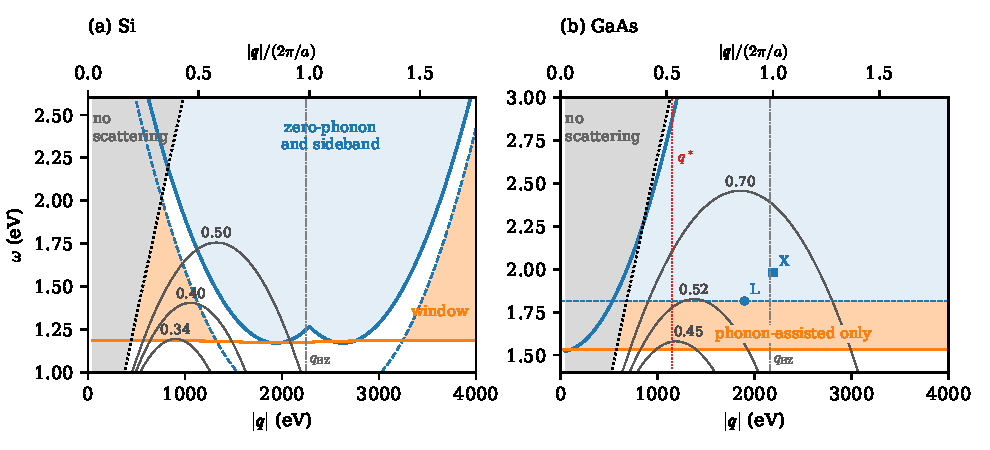
\includegraphics[width=\linewidth]{figures/ch17/fig17_4.pdf}
  \caption{Where the Migdal--phonon-assisted interference enters, in the plane of momentum transfer and energy deposited by scattering. (a)~Silicon. Thick blue: zero-phonon edge of the parabolic valleys along [100], $E_{\mathrm{min}} = \Eg + (q - K)^2/2M_{\mathrm{eh}}$ with $\Eg = \SI{1.17}{eV}$, $M_{\mathrm{eh}} = 1.193\,m_e$, $K = k_{\mathrm{c}} = 0.85\,(2\pi/a)$ and its images under $(2,0,0)\,2\pi/a$, a model that lies \SI{0.13}{eV} above the computed bands at \SI{1}{keV}. Dashed blue: the same lowered by the off-shell margin of the window, $\delta_w = \SI{0.3}{eV}$ (\cref{sec:8.6}). Orange line: the phonon-assisted threshold $\Eg + \omega_{\mathrm{TA}}(k_{\mathrm{c}} - q)$. Orange: the window, where the phonon-dressed sector is the only electronic final state and the cross term of \cref{eq:17.4-Sek} is a fraction of the whole electronic rate. White strip: the edge shell within $\delta_w$ of the zero-phonon edge, where only the sum of the two electronic sectors is defined. Light blue: zero-phonon pairs, with the phonon-dressed sector and its cross term a correction. (b)~GaAs: edge of the $\mathrm{\Gamma}$ pair with the [111] heavy hole ($\Eg = \SI{1.52}{eV}$, $M_{\mathrm{eh}} = 0.960\,m_e$), the L and X valleys at 1.815 and \SI{1.981}{eV} (points at $|\mathrm{\Gamma L}|$ and $|\mathrm{\Gamma X}|$), and the phonon-assisted threshold with the upper value \SI{10.5}{meV} of the transverse acoustic branch. Orange: below both the $\mathrm{\Gamma}$ edge and the L energy, phonon-assisted pairs only; the L valleys reach the line $\omega = \SI{1.815}{eV}$ near $|\mathrm{\Gamma L}|$ only. Red dotted: $q^* = \SI{1.15}{keV}$ of the GaAs window. Both panels: the largest deposit $qv_{\mathrm{max}} - q^2/2\mchi$ for the masses marked in MeV (gray), the envelope $qv_{\mathrm{max}}$ (dotted; gray region unreachable by scattering), and $q_{\mathrm{BZ}}$, the radius of the sphere with the volume of the zone (dash-dotted). Top axes: $q$ in units of $2\pi/a$; \cref{eq:17.4-lock} holds for $q \ll q_{\mathrm{BZ}}$.}
  \label{fig:17-interference}
\end{figure}

\Cref{fig:17-interference} places the cross term in the plane of $q$ and $\omega$. It exists wherever a pair with one phonon is kinematically allowed, above the phonon-assisted threshold, but it changes an observable rate by more than a correction to a correction in the window alone. There the phonon-dressed sector is the whole electronic rate of silicon between 0.3374 and \SI{0.405}{MeV} (\cref{tab:13-window}), and of GaAs from \SI{0.433}{MeV} to the opening of the L valleys at 0.52 to \SI{0.56}{MeV} (\cref{sec:13.1}).

\begin{workedexample}{The cross terms of a heavy dark photon in GaAs}\label{we:17-gaas-interference}
Take a dark photon with a heavy mediator, $\FDM = 1$, so that $\tilde V_e = \tilde V$ and $\tilde V_\kappa = -Z_\kappa\tilde V$ with $\tilde V$ independent of $q$, scattering in GaAs at $T = 0$. In the window it makes pairs only with a phonon, at momentum transfers near $q^* = \SI{1.15}{keV}$, 0.52 of $2\pi/a = \SI{2.193}{keV}$ (\cref{fig:17-interference}b).

\emph{Electron-following cell.} With $|Z^*| = 2.11$ (\cref{sec:5.5}), a gallium nucleus carries $Z = 31$ and its cloud $F^{\mathrm{fol}} = 28.89$ at long wavelength; an arsenic nucleus $Z = 33$ and $F^{\mathrm{fol}} = 35.11$. The separate terms are $961 + 834.6$ and $1089 + 1232.7$, the cross terms $-1791.2$ and $-2317.3$, and each total is $Z^{*2} = 4.452$: the cross term removes \SI{99.75}{\percent} and \SI{99.81}{\percent} of the two separate terms. The optical phonons that the dark photon makes are those of \cref{sec:11.2}. Without the cross cell their rate would be $(Z^2 + (F^{\mathrm{fol}})^2)/Z^{*2} = 403$ times (gallium) and 521 times (arsenic) larger, and the bare nuclear charges alone would give 216 and 245 times more, before the screening by $\varepsilon_\infty$ that both cases share.

\emph{Zero-phonon cell.} Above the opening of the L valleys the zero-phonon rate gains $2m_e\bar z$ from the ionic correction. The two values of $Z/M$, 0.4446 per u for gallium and 0.4405 per u for arsenic, differ by \SI{0.9}{\percent}. With $m_e = 5.486\times10^{-4}$\,u the cross cell is $4.88\times10^{-4}$ for weight on gallium alone and $4.83\times10^{-4}$ for weight on arsenic alone, and lies between the two for any positive weights. The zero-phonon Migdal cell is $(m_e\bar z)^2 = 5.9\times10^{-8}$.

\emph{Phonon-dressed cell.} In the window the whole electronic rate is phonon-assisted, and at leading order in $q$, \cref{eq:17.4-rate} with the mass-weighted mean gives it the same fraction, $4.8$ to $4.9\times10^{-4}$, and the one-phonon Migdal rate $5.9\times10^{-8}$ of it. Since $\mathfrak{D}$ has no $q$ dependence for a heavy mediator, the fraction is the same at every momentum transfer at this order, and the integrated rate carries it unchanged. At $q^*$, however, $q/(2\pi/a) = 0.52$, and the remainder of \cref{eq:17.4-lock} is not small. The cross term is of order $5\times10^{-4}$ of the phonon-assisted rate, with an uncertainty of order one in that fraction.

\emph{Screening.} The dark photon couples to the total charge, and both rows share the screening $1/\varepsilon$ of the total-charge row (\cref{sec:8.4}), which cancels from every fraction above.

\emph{Verdict.} The phonon-assisted rate of the silicon window is an estimate known to a factor of ten (\cref{tab:13-window}), and the GaAs window is known through its edges (\cref{sec:13.1}). The two electronic cross terms lie more than three orders of magnitude below such uncertainties. For a dark photon in GaAs the electron-following cell is the one that matters, and it decides the phonon rate.
\end{workedexample}

At small $q$ the nuclear amplitude in the electronic sectors is $(m_e/M_\kappa)\tilde V_{\mathrm{nuc}}/\tilde V_e$ times the electron amplitude. The cross term competes with the electron term when the coupling to a nucleus exceeds that to an electron by $M_\kappa/m_e = 5.1\times10^4$ in silicon, or, per nucleon, by $m_{\mathrm{u}}/m_e = 1823$. A scalar mixed with the Higgs boson, whose couplings follow the masses up to the nucleon matrix element, comes close to this; a $B - L$ vector, with couplings of equal size per nucleon and per electron, is far from it. For such a mediator a Migdal rate and an electron-recoil rate computed separately and added miss the true rate by the full cross term.

\section{Figures of merit per channel}\label{sec:17.5}

The heavy-mediator plateau of single-phonon emission is 1101 events per kilogram and year in germanium and 654 in silicon at $\sigma_p = 10^{-40}\,\mathrm{cm^2}$ (\cref{sec:11.1}). The ratio, 1.68, is the ratio of two sound speeds, and once the elastic tensors are known no phonon calculation is needed to obtain it. A number of this kind, a property of the material alone that the rate or the reach of one channel is proportional to, is what a comparison of targets needs. Such numbers exist for most channels of \cref{chap:10,chap:11,chap:12}, but each holds over a window of masses, and outside it the ratio of two rates is not the ratio of the two numbers. We will derive one such number per channel, with its window and inputs.

\subsection{Rate and reach figures of merit}\label{sec:17.5-def}

A figure of merit is either a reach number or a rate number. A \emph{reach figure of merit} is the lightest mass a channel can see, set by kinematics and one material energy or speed: the gap floor $2\Eg/v_{\mathrm{max}}^2$ of electronic excitations (\cref{eq:1.3-mmin}), the acoustic edge \cref{eq:11.1-edge}, the polar edge $2\omega_{\mathrm{L}}/v_{\mathrm{max}}^2$. These are exact statements about where a rate starts, and they rank materials without a window. A \emph{rate figure of merit} $F_A$ of material $A$ is a number that makes the rate per unit target mass factorize at fixed dark-matter parameters, $\mathcal{R}_A(\mchi) = G(\mchi)\,F_A$, with $G$ the same for every material. No real rate factorizes exactly, and the useful statement is about pairs. For two materials $A$ and $B$ we write
\begin{equation}
  \frac{\mathcal{R}_A(\mchi)}{\mathcal{R}_B(\mchi)} = \frac{F_A}{F_B}\,\bigl[1 + \delta_{AB}(\mchi)\bigr] ,
  \qquad
  W_{AB} = \bigl\{\mchi : |\delta_{AB}(\mchi)| < 0.1\bigr\} ,
  \label{eq:17.5-window}
\end{equation}
and call the contiguous range $W_{AB}$ the \emph{pairwise window} of the figure of merit, the masses at which the ratio of the two figures of merit gives the ratio of the rates to \SI{10}{\percent}. The tolerance is a convention, chosen to match the accuracy of most inputs. A window belongs to a pair, not to a material, because the corrections $\delta$ of two materials partly cancel when their properties are close and add when they are not. Several materials have a common window only if every pair among them has one, and \cref{sec:17.5-phonon} shows that this fails for sound speeds. \Cref{tab:17-fom} collects the figures of merit of every channel with their windows and the provenance of their inputs.

\begin{table}[tbp]
\centering
\caption{Figures of merit per channel, with the masses at which they rank two materials and the provenance of their inputs. Rates per unit target mass; $\omega_{\mathrm{th}} = \SI{1}{meV}$ for the phonon channels; standard halo of \cref{sec:1.2}. ``Pairwise'' refers to the window \cref{eq:17.5-window}. The absorption figures of merit are exact at each mass, since absorption fixes both $q$ and $\omega$.}
\label{tab:17-fom}
\footnotesize
\begin{tabular}{>{\raggedright\arraybackslash}p{0.13\linewidth}>{\raggedright\arraybackslash}p{0.19\linewidth}>{\raggedright\arraybackslash}p{0.27\linewidth}>{\raggedright\arraybackslash}p{0.16\linewidth}>{\raggedright\arraybackslash}p{0.09\linewidth}}
\toprule
Channel & Figure of merit & Where it ranks & Inputs & Silicon \\
\midrule
Electronic, reach & $2\Eg/v_{\mathrm{max}}^2$ & exact & $\Eg(T)$, measured & \SI{0.333}{MeV} \\
Electronic, rate & $L(q,\omega)$ in the window; ceiling $\propto Z_{\mathrm{val}}/A_{\mathrm{cell}}$ & no scalar ranks rates; ceiling with $\omega_p^{\mathrm{val}}$ for $qv_{\mathrm{max}} < \omega_{\mathrm{core}}$ (\cref{eq:17.5-partial}) & $L$ computed; $\nd_{\mathrm{val}}$, $\omega_p^{\mathrm{val}}$ measured & 0.142 \\
Acoustic, reach & $m_{\mathrm{min}}^{\mathrm{ac}}$ at $c_{\mathrm{LA,max}}$, \cref{eq:11.1-edge} & exact & $C_{ij}$, $\rho_T$ & \SI{6.1}{keV} \\
Acoustic, heavy mediator & $1/c_{\mathrm{NR1}}$, \cref{eq:17.5-cNR1} & pairwise: from about 4 edges of the softer crystal to the smaller $q_{\mathrm{BZ}}/2v_{\mathrm{max}}$; empty if speeds differ by $\gtrsim\SI{13.5}{km/s}$ & $C_{ij}$ measured or computed & 8.956\,km/s \\
Acoustic, light mediator & none (target independent) & equal rates above 44 times the higher edge & edge only & -- \\
Polar, rate & $\mathcal{I}_{\mathrm{pol}}/\rho_T$ with $\bar\omega_{\mathrm{pol}}$ & with $K_\eta(\bar\omega_{\mathrm{pol}},\mchi)$ at each mass; $\mathcal{I}_{\mathrm{pol}}/\rho_T$ alone only where the $K_\eta$ agree (LiF/GaAs above \SI{52}{MeV}) & $\varepsilon_\infty$, $\varepsilon_0$, $\omega_{\mathrm{T}\nu}$, $\omega_{\mathrm{L}\nu}$ measured, or $Z^*$ computed & -- \\
Polar, reach & $2\omega_{\mathrm{L}\nu}/v_{\mathrm{max}}^2$, lowest weighted branch & exact & $\omega_{\mathrm{L}\nu}$, measured & -- \\
Migdal & $F_{\mathrm{Mig}}$; pole limit \cref{eq:17.5-pole} & impulse regime (Si above \SI{17.5}{MeV}); ranking open & $L(p,\omega)$, $Z_{\mathrm{ion}}(p)$ computed & pole: 0.570, \SI{16.6}{eV} \\
Absorption & $L(0,m_\phi)/\rho_T$, $m_\phi\sigma_1/\rho_T$, scalar response per mass (\cref{sec:17.2}) & exact at each mass & optical data or computed & \cref{sec:17.2} \\
\bottomrule
\end{tabular}
\end{table}

\subsection{Gap floor and valence f-sum}\label{sec:17.5-electronic}

An electronic excitation needs at least $\Eg$, and the dark matter can deposit at most $\frac12\mchi v_{\mathrm{max}}^2$ (\cref{eq:1.3-omegamax}). The floor $2\Eg/v_{\mathrm{max}}^2$ is \SI{0.333}{MeV} for silicon with its physical gap of \SI{1.17}{eV}, \SI{0.212}{MeV} for germanium (\SI{0.744}{eV}) and \SI{0.433}{MeV} for GaAs (\SI{1.52}{eV}); with the step-model gap of \SI{1.11}{eV} that accompanies the silicon tables (\cref{sec:10.10}), it is \SI{0.316}{MeV}. Near the floor the rate is set by the spectrum within a few phonon energies of the edge. The gap is a measured input, and it must be the gap at the operating temperature of the detector, since the floor moves by the same fraction as the gap.

A rate figure of merit is harder. The electron-recoil rate weights the loss function over the window $\omega \le qv_{\mathrm{max}}$ by the halo factor. \Cref{we:10-fsum} showed that silicon puts a tiny part of its $f$-sum where a \SI{1}{MeV} particle can reach it: the computed rate is $4\times10^6$ times below the all-electron ceiling. Since the weight of the loss function inside the window varies between materials by orders of magnitude, no single number ranks electron-recoil rates; the loss function in the window is the figure of merit itself. What a single number can give is the ceiling. For it to be useful, the ceiling must count the electrons that absorb in the window and no others, and that needs a partial $f$-sum.

Split the dielectric function of an insulator with clamped nuclei into the contributions of the valence electrons and of the core,
\begin{equation*}
  \varepsilon(\omega) = \varepsilon_{\mathrm{val}}(\omega) + \varepsilon_{\mathrm{core}}(\omega) - 1 ,
\end{equation*}
each of them one plus the polarization of its group, at $q \to 0$. Three conditions make the valence part separable. (i) The two groups add, so that each obeys its own $f$-sum, $\int_0^\infty\dd\omega\,\omega\,\Imag\varepsilon_{\mathrm{val}} = (\pi/2)(\omega_p^{\mathrm{val}})^2$ with $(\omega_p^{\mathrm{val}})^2 = e^2\nd_{\mathrm{val}}/m_e$; this neglects the transfer of oscillator strength between shells that the Pauli principle causes (\cref{we:4-sifsum}). (ii) The valence absorption ends below the first core edge $\omega_{\mathrm{core}}$, and the core does not absorb below it. (iii) Over the valence spectrum the core part is real and equal to its static value, $\varepsilon_{\mathrm{core}}(\omega) \simeq \varepsilon_{\mathrm{core}}(0)$, which holds to order $\omega^2/\omega_{\mathrm{core}}^2$. By the Kramers--Kronig relation at $\omega = 0$ (\cref{eq:C.5-KKeps}),
\begin{equation*}
  \varepsilon_{\mathrm{core}}(0) - 1 = \frac{2}{\pi}\int_{\omega_{\mathrm{core}}}^\infty\dd\omega\,\frac{\Imag\varepsilon_{\mathrm{core}}(\omega)}{\omega} .
\end{equation*}
Below $\omega_{\mathrm{core}}$ we then have $\varepsilon = \varepsilon_{\mathrm{core}}(0) + \varepsilon_{\mathrm{val}} - 1$. Consider the model function $\varepsilon_{\mathrm{m}}(\omega) = \varepsilon_{\mathrm{core}}(0) + \varepsilon_{\mathrm{val}}(\omega) - 1$ at all frequencies, which equals $\varepsilon$ below the core edge to order $\omega^2/\omega_{\mathrm{core}}^2$. Above the valence spectrum $\varepsilon_{\mathrm{val}} - 1 \to -(\omega_p^{\mathrm{val}})^2/\omega^2$, so the function $g(\omega) = \varepsilon_{\mathrm{m}}^{-1}(\omega) - 1/\varepsilon_{\mathrm{core}}(0)$ falls as $(\omega_p^{\mathrm{val}})^2/[\varepsilon_{\mathrm{core}}(0)^2\omega^2]$. It is analytic in the upper half plane, being the inverse of a causal response with a constant subtracted, and the argument that turns the large-frequency tail of $\varepsilon^{-1}$ into the $f$-sum of the loss function (\cref{eq:4.4-fsumL}, \cref{app:C.5}) applies to it. For the true $\varepsilon$ the same tail is an intermediate asymptote, valid between the valence spectrum and the core edge, since at $\omega \to \infty$ the true $g$ tends to $1 - 1/\varepsilon_{\mathrm{core}}(0)$. Since $\Imag[-g] = L$ below $\omega_{\mathrm{core}}$, the loss function collected up to a cutoff $\omega_c$ between the valence spectrum and the core edge is
\begin{keyresult}[Partial (valence) f-sum of the loss function]
\begin{equation}
  \int_0^{\omega_c}\dd\omega\;\omega\,L(\omega) = \frac{\pi}{2}\,\frac{(\omega_p^{\mathrm{val}})^2}{\varepsilon_{\mathrm{core}}(0)^2} \simeq \frac{\pi}{2}\,(\omega_p^{\mathrm{val}})^2 ,
  \label{eq:17.5-partial}
\end{equation}
with $\omega_p^{\mathrm{val}}$ the plasma frequency of the valence electrons alone.
\end{keyresult}
\noindent The core screens the valence plasmon and lowers its weight by $\varepsilon_{\mathrm{core}}(0)^{-2}$. The absorption $\Imag\varepsilon$ collected over the same range carries no such factor, because $\varepsilon$ adds where $\varepsilon^{-1}$ does not. For silicon, $\nd_{\mathrm{val}} = \SI{2.00e23}{cm^{-3}}$ gives $\omega_p^{\mathrm{val}} = \SI{16.6}{eV}$ (\cref{we:4-siplasmon}), the measured plasmon energy, $16.6 \pm \SI{0.1}{eV}$ by electron energy loss~\cite[Table~I]{ramanathan2020ionization}. The core term follows from the photoabsorption above the L edge at \SI{99.8}{eV}: $\varepsilon_{\mathrm{core}}(0) - 1 = 0.0154$, so the core lowers the valence weight of $L$ by the factor $0.970$. A valence-only calculation, such as the tables of \cref{sec:10.2}, has no core and satisfies \cref{eq:17.5-partial} with $\varepsilon_{\mathrm{core}} = 1$; this is why \SI{16.6}{eV} is the right normalization of those tables (\cref{we:12-fsum}).

\begin{limitbox}[Partial f-sum of the valence electrons][lim:17.5a]
Below the first core edge the valence electrons carry the $f$-sum of the loss function $\int_0^{\omega_c}\omega L\,\dd\omega = (\pi/2)(\omega_p^{\mathrm{val}})^2$, with $\omega_p^{\mathrm{val}} = \SI{16.6}{eV}$ for silicon, the measured plasmon energy~\cite[Table~I]{ramanathan2020ionization}.
\par\smallskip
{\centering
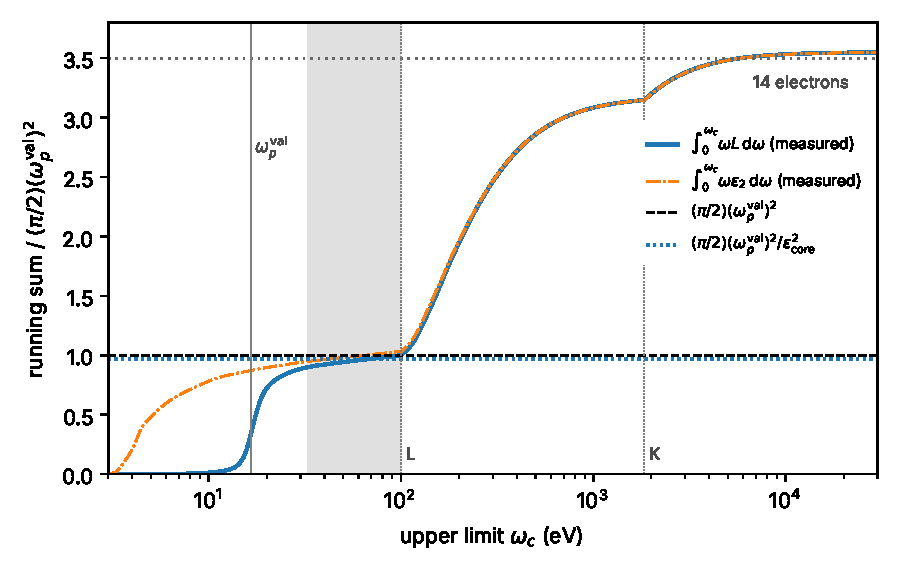
\includegraphics[width=\linewidth]{figures/ch17/limit17_5a.pdf}
\captionof{figure}{Running $f$-sums of silicon at $q \to 0$, $\int_0^{\omega_c}\omega L\,\dd\omega$ (solid) and $\int_0^{\omega_c}\omega\varepsilon_2\,\dd\omega$ (dash-dotted), in units of $(\pi/2)(\omega_p^{\mathrm{val}})^2 = \SI{433}{eV^2}$, against the upper limit $\omega_c$. Data: the measured optical constants of Franta and coworkers at \SI{300}{K} below \SI{35}{eV}~\cite{franta2017temperature} and the photoabsorption tables of Henke and coworkers above, with $\varepsilon = 1 - (\omega_a^2/\omega^2)(f_1 - \ii f_2)$, $\omega_a^2 = e^2\nd_{\mathrm{at}}/m_e$~\cite{henke1993xray}; moving the join to 30 or \SI{40}{eV} changes the $L$-sum below the L edge by \SI{0.8}{\percent}. Dashed: \cref{eq:17.5-partial} with $\varepsilon_{\mathrm{core}} = 1$; dotted: with the core term, 0.970. Vertical lines: $\omega_p^{\mathrm{val}}$ and the L and K edges at 99.8 and \SI{1839}{eV}; the dotted horizontal line at 3.5 is the sum of all 14 electrons per atom. Gray: $\omega_c$ from \SI{32.7}{eV} to the L edge, where the $L$-sum lies within \SI{10}{\percent} of the formula; just below the edge it is 1.000.}\label{fig:17-limit-a}
\par}
\smallskip
Below about $2\omega_p^{\mathrm{val}}$ the plasmon is not yet collected, and above the L edge the core electrons add their own sum, which rises toward 3.5 times the valence value.
\end{limitbox}

Just below the edge the measured $L$-sum is 1.000 of $(\pi/2)(\omega_p^{\mathrm{val}})^2$ and the $\varepsilon_2$-sum 1.032. The two corrections to \cref{eq:17.5-partial} are of similar size and opposite sign. The core screening lowers the $L$-sum by \SI{3}{\percent}, and the valence region holds \SI{3}{\percent} more absorption than four electrons, the strength moved up from the blocked core transitions. The data fix each of them to \SI{1.4}{\percent}, the amount by which the two sets together overshoot the all-electron sum of 14. The approach to the plateau is slow, because the plasmon at \SI{16.4}{eV} is broad: the $L$-sum reaches 0.9 at \SI{32.7}{eV}.

The partial sum turns the valence plasma frequency into a usable ceiling. \Cref{we:10-fsum} found that $\omega_p^{\mathrm{val}}$ in place of the all-electron \SI{31.1}{eV} does not give a bound, since the core electrons hold the rest of the $f$-sum. When the window lies entirely below the core edge, however, the energy integral of the bound runs over the valence spectrum alone, and by \cref{eq:17.5-partial} its weight is $(\pi/2)(\omega_p^{\mathrm{val}})^2$ to the few-percent accuracy of the two corrections; at finite $q$ the condition is $qv_{\mathrm{max}} < \omega_{\mathrm{core}}$. This is not a theorem, since the corrections need not stay small at finite $q$, but it lowers the ceiling of silicon by $(31.1/16.6)^2 = 3.5$ for every mass whose largest deposit, $\frac12\mchi v_{\mathrm{max}}^2$, lies below the L edge, $\mchi < \SI{28.4}{MeV}$. Per unit target mass the ceiling is proportional to $(\omega_p^{\mathrm{val}})^2/\rho_T = e^2Z_{\mathrm{val}}/(m_em_uA_{\mathrm{cell}})$, with $Z_{\mathrm{val}}$ valence electrons in a cell of $A_{\mathrm{cell}}$ mass units: the number of valence electrons per nucleon, 0.142 for silicon, 0.055 for germanium, 0.333 for diamond and 0.308 for LiF. This orders the ceilings, not the rates, which differ from them by the factor $10^{6}$ of \cref{we:10-fsum}.

\subsection{Acoustic edge and effective sound speed}\label{sec:17.5-phonon}

The one-phonon rate of \cref{eq:11.1-rate} has three figures of merit, one for each limit of the mediator and one for the edge. The reach figure of merit is the acoustic edge \cref{eq:11.1-edge}, evaluated at the fastest longitudinal speed $c_{\mathrm{LA,max}}$: \SI{6.1}{keV} for silicon, \SI{10.2}{keV} for germanium and \SI{3.1}{keV} for diamond at $\omega_{\mathrm{th}} = \SI{1}{meV}$. It is exact kinematics and ranks without a window. A stiff crystal reaches lower masses.

For a light mediator there is no rate figure of merit. The rate per unit mass tends to the target-independent value \cref{eq:11.1-light}, and the material enters through the correction factor $1 - (1 + \kappa_\eta)\,m_{\mathrm{min}}^{\mathrm{ac}}/\mchi$ alone, with the constant $\kappa_\eta$ of \cref{eq:11.1-correction}. Two materials have equal rates within \SI{10}{\percent} above 44 times the higher of their two edges (\cref{lim:11.1b}), and below that the edge, a reach number, decides.

For a heavy mediator, \cref{eq:11.1-heavy} gives a plateau inversely proportional to the polarization-weighted mean of the inverse sound speeds. Its inverse is an effective sound speed of the one-phonon nuclear rate,
\begin{equation}
  c_{\mathrm{NR1}} = \Bigl\langle\sum_\nu\frac{(\hat{\vect{q}}\cdot\hat{\vect{e}}_\nu)^2}{c_\nu(\hat{\vect{q}})}\Bigr\rangle_{\hat{\vect{q}}}^{-1} ,
  \qquad
  \mathcal{R} = \frac{2\rho_\chi\,\sigma_p\,I_0}{m_u^2\,c_{\mathrm{NR1}}} ,
  \label{eq:17.5-cNR1}
\end{equation}
so that the figure of merit is $1/c_{\mathrm{NR1}}$. It is \SI{8.956}{km/s} for silicon, \SI{5.321}{km/s} for germanium and \SI{18.16}{km/s} for diamond, within one percent of the sphere-averaged longitudinal speeds (\cref{lim:11.1c}) for these weakly anisotropic crystals. The speeds and polarizations come from the Christoffel problem of the elastic tensor (\cref{eq:C.18-christoffel}). The tensor is measured from the speed of ultrasound or from light scattered by thermal sound waves, or computed by density-functional theory from finite strains or from perturbation theory with strain as the perturbation (\cref{app:E.4}); \cref{app:E.17} specifies the elastic constants needed for the candidate targets. The two figures of merit pull in opposite directions: a soft lattice gives a large heavy-mediator rate and a high edge.

\Cref{eq:17.5-cNR1} drops two things, and each sets one end of the window. At low mass the lower cut $u_- = \omega_{\mathrm{th}}/(2\mchi c_\nu)$ of the integral $\int u^2\eta(c_\nu + u)\,\dd u$ removes the slowest part of the halo integral. Since $u_- = (v_{\mathrm{max}} - c_\nu)\,m_{\mathrm{min}}^{\mathrm{ac}}/\mchi$, it is a function of the mass in units of the edge, and it closes the window from below at a few times the edge of the softer crystal. At high mass the momentum transfers reach the zone scale, \cref{eq:11.1-Sac} stops holding, and the window ends at $m_{\mathrm{hi}} = q_{\mathrm{BZ}}/2v_{\mathrm{max}}$ of the crystal with the smaller zone, \SI{0.42}{MeV} for silicon (\cref{sec:11.1}). Between the two ends the window would be complete if the plateau were exact. It is not, and the reason is the shift of the halo integral by the sound speed.

Far above the edge, the integral of one branch and direction is $8\mchi^3\int_0^{v_{\mathrm{max}} - c_\nu}\dd u\,u^2\eta(c_\nu + u)$. With $v = c_\nu + u$ it becomes $8\mchi^3\int_{c_\nu}^{v_{\mathrm{max}}}\dd v\,(v - c_\nu)^2\eta(v)$, and expanding the square,
\begin{equation*}
  \int_{c_\nu}^{v_{\mathrm{max}}}\dd v\,(v - c_\nu)^2\eta(v) = I_0 - 2c_\nu I_1 + c_\nu^2 + O(c_\nu^3) ,
  \qquad
  I_1 = \int_0^{v_{\mathrm{max}}}\dd v\,v\,\eta(v) ,
\end{equation*}
where $I_0$ is the plateau integral of \cref{sec:11.1}. The coefficient of $c_\nu^2$ is $\int_0^\infty\eta\,\dd v = 1$, the normalization of the velocity distribution, since $\eta$ is its integral of $f_\chi/v$ above $\vmin$. The integral from $0$ to $c_\nu$ is of third order. Each branch and direction carries the weight $(\hat{\vect{q}}\cdot\hat{\vect{e}}_\nu)^2/c_\nu$, so the term $-2c_\nu I_1$ contributes $-2I_1\langle\sum_\nu(\hat{\vect{q}}\cdot\hat{\vect{e}}_\nu)^2\rangle = -2I_1$ by completeness, independent of the crystal. The rate in units of the plateau is
\begin{equation}
  \frac{\mathcal{R}\,c_{\mathrm{NR1}}\,m_u^2}{2\rho_\chi\sigma_pI_0} = 1 - \frac{2I_1}{I_0}\,c_{\mathrm{NR1}} + O(c^2) ,
  \qquad
  \frac{2I_1}{I_0} = \frac{5.88}{v_{\mathrm{max}}} = \frac{1}{\SI{135}{km/s}} ,
  \label{eq:17.5-shift}
\end{equation}
for the standard halo of \cref{sec:1.2}, with $\eta$ evaluated at $\vmin = c_\nu + q/2\mchi$ as in \cref{eq:11.1-rate}. For silicon the bracket is 0.934 at first order and 0.935 at second, against the largest computed ratio 0.936; for diamond 0.866 and 0.872, against 0.874. This is why the plateau of \cref{sec:11.1} is never reached: the halo is not flat at the large speeds that a heavy mediator favors.

The shift is linear in the sound speed and does not cancel between materials. For two crystals in the middle of their window,
\begin{equation*}
  \frac{\mathcal{R}_A\,c_{\mathrm{NR1},A}}{\mathcal{R}_B\,c_{\mathrm{NR1},B}} \simeq 1 - \frac{c_{\mathrm{NR1},A} - c_{\mathrm{NR1},B}}{\SI{135}{km/s}} .
\end{equation*}
Roughly, the inverse speeds rank two crystals to \SI{10}{\percent} as long as their effective speeds differ by less than \SI{13.5}{km/s}, which diamond and germanium, \SI{12.8}{km/s} apart, barely meet. The deviations of several crystals from a common reference add linearly in their speeds, and two crystals that both agree with silicon to \SI{10}{\percent} can disagree with each other by up to twice that. \Cref{fig:17-window} shows the ratio for five pairs. Germanium against silicon enters the band at \SI{43}{keV} and settles at 1.027; diamond against silicon enters at \SI{25}{keV} and settles at 0.933; CsI, a soft cubic crystal discussed below, enters at \SI{97}{keV} and reaches 1.045 at its zone cap. Diamond against CsI, however, is inside the band from 87 to \SI{227}{keV} alone and leaves it below the cap, where both still agree with silicon. A window ``against silicon'' does not give the ranking of the materials among themselves, and every pair needs its own.

\begin{figure}[tbp]
  \centering
  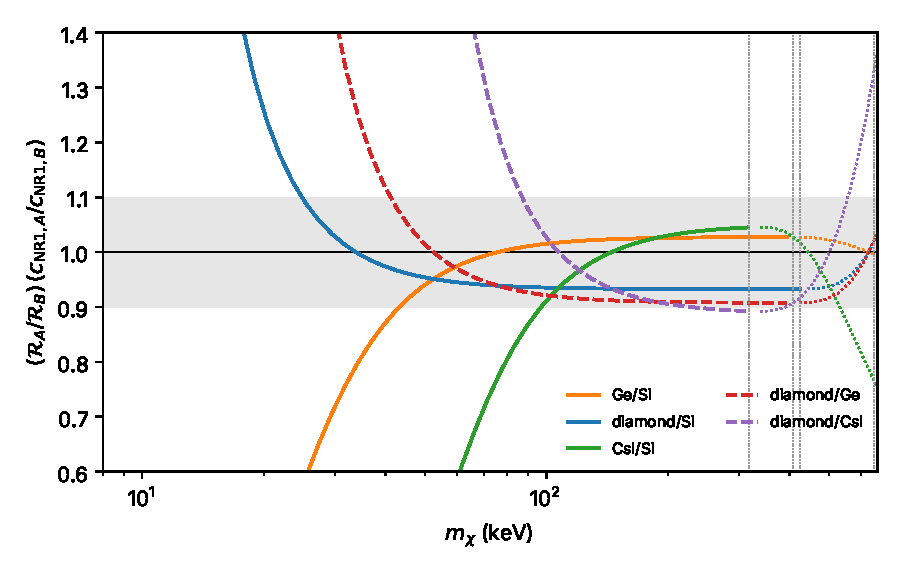
\includegraphics[width=0.85\linewidth]{figures/ch17/fig17_window.pdf}
  \caption{Heavy-mediator one-phonon rates of two crystals divided by the ratio of their figures of merit, $(\mathcal{R}_A/\mathcal{R}_B)(c_{\mathrm{NR1},A}/c_{\mathrm{NR1},B})$, against the dark-matter mass, from \cref{eq:11.1-rate} with all branches and directions, $q \le q_{\mathrm{BZ}}$, $\omega_{\mathrm{th}} = \SI{1}{meV}$, the orientation average and the standard halo of \cref{sec:1.2}. Elastic tensors: measured room-temperature values for Si, Ge and diamond (\cref{we:11-cbar}); CsI at \SI{4.2}{K}~\cite{vallin1964elastic} with the room-temperature density \SI{4.529}{g.cm^{-3}}. Gray: the \SI{10}{\percent} band of the pairwise window \cref{eq:17.5-window}. Each curve is solid up to the smaller $q_{\mathrm{BZ}}/2v_{\mathrm{max}}$ of its pair (vertical dotted lines: 0.32, 0.41, 0.42 and \SI{0.65}{MeV} for CsI, Ge, Si and diamond) and dotted above. At high mass the curves settle at $1 - (c_{\mathrm{NR1},A} - c_{\mathrm{NR1},B})/(\SI{135}{km/s})$, \cref{eq:17.5-shift}.}
  \label{fig:17-window}
\end{figure}

\begin{workedexample}{The pairwise window of diamond against silicon}\label{we:17-window}
Diamond has $c_{\mathrm{NR1}} = \SI{18.16}{km/s}$ and silicon \SI{8.956}{km/s}, so the figure of merit predicts a heavy-mediator rate ratio of $8.956/18.16 = 0.493$: the plateaus of \cref{eq:17.5-cNR1} are 322.6 and 654.0 events per kilogram and year at $\sigma_p = 10^{-40}\,\mathrm{cm^2}$ and $\omega_{\mathrm{th}} = \SI{1}{meV}$. The edges at the effective speeds are \SI{3.19}{keV} for diamond and \SI{6.39}{keV} for silicon, and the zone caps $q_{\mathrm{BZ}}/2v_{\mathrm{max}}$ are 0.65 and \SI{0.42}{MeV}, so the window can extend at most to \SI{0.42}{MeV}.

The full rates \cref{eq:11.1-rate} give the correction $1 + \delta$ of \cref{eq:17.5-window}, the rate ratio divided by 0.493:
\begin{center}
\small
\begin{tabular}{lccccccc}
\toprule
$\mchi$ (keV) & 10 & 20 & 30 & 45 & 100 & 300 & 420 \\
$\mathcal{R}_{\mathrm{Si}}$ & 66.0 & 432.5 & 546.7 & 590.6 & 609.8 & 612.0 & 612.2 \\
$\mathcal{R}_{\mathrm{C}}$ & 199.3 & 268.0 & 277.3 & 280.2 & 281.4 & 281.6 & 281.7 \\
$1 + \delta$ & 6.12 & 1.256 & 1.028 & 0.962 & 0.935 & 0.933 & 0.933 \\
\bottomrule
\end{tabular}
\end{center}
with the rates in events per kilogram and year. At \SI{10}{keV} silicon is less than two edges above its threshold and diamond leads by a factor of three, against the predicted half. The lower cut explains it: at \SI{20}{keV} it removes the halo below $u_- = \SI{251}{km/s}$, $0.32\,v_{\mathrm{max}}$, for silicon, but only below \SI{124}{km/s} for diamond, whose phonons of \SI{1}{meV} carry half the momentum. The ratio crosses 1.1 at \SI{24.8}{keV}, 3.9 times the edge of silicon, and the window opens there.

Above \SI{100}{keV} the correction no longer depends on the mass. It is the shift \cref{eq:17.5-shift}: to first order $1 - (18.16 - 8.956)/135 = 0.932$, and with the exact single-speed integrals $\int_c^{v_{\mathrm{max}}}(v - c)^2\eta\,\dd v/I_0$, 0.8724 for diamond and 0.9354 for silicon, the ratio is 0.9327, the computed value to four digits. The window is
\begin{equation*}
  W_{\mathrm{C,Si}} = \SI{25}{keV}\text{ to }\SI{0.42}{MeV} ,
\end{equation*}
inside which $1 + \delta$ runs from 1.088 down to 0.933. The figure of merit ranks the pair correctly above \SI{14}{keV}, 2.2 times the edge of silicon, where the two rates cross; below that the cut of the softer crystal reverses the order. Inside $W_{\mathrm{C,Si}}$ it also gives the ratio to \SI{10}{\percent}, but even there it is biased by \SI{7}{\percent} against the stiffer crystal. Against germanium, \SI{12.8}{km/s} softer, diamond settles at 0.908, at the edge of the band.
\end{workedexample}

Tabulated sound speeds feed most published comparisons of targets, and they can be tested against measured elasticity without any phonon calculation. For a cubic crystal the floor \cref{eq:11.1-rayleigh}, $c_{\mathrm{LA}} \ge \sqrt{B/\rho_T}$, needs the bulk modulus alone; for any crystal the Christoffel problem of a measured tensor gives the range of longitudinal speeds over all directions. The target table of Griffin and collaborators lists one longitudinal speed per material, a sphere average of $\omega_{\mathrm{LA}}/q$ from density-functional phonons~\cite[Table~I and App.~A\,3]{griffin2020multichannel}. \Cref{tab:17-speeds} tests five of its entries against measured tensors, and all five fail.

\begin{table}[tbp]
  \caption{Tabulated longitudinal sound speeds~\cite[Table~I]{griffin2020multichannel} against measured elastic constants (GPa). Hexagonal crystals: $C_{11}$, $C_{12}$, $C_{13}$, $C_{33}$, $C_{44}$, the recommended values of Vurgaftman and Meyer for the nitrides as quoted in~\cite[Table~I]{lopuszynski2012composition}, and the Brillouin values for ZnO as quoted in~\cite[Table~III]{gopal2006polarization}. CsI (cubic, \SI{4.2}{K}): $C_{11}$, $C_{12}$, $C_{44}$~\cite[abstract]{vallin1964elastic}. CaWO$_4$ (tetragonal, point group $4/m$, which allows $C_{16} = -C_{26}$): ultrasonic data of Farley and Saunders~\cite{farley1972ultrasonic} as quoted in~\cite[p.~16]{popova2025high}. Densities from the measured lattice constants (CsI at room temperature). Range: the longitudinal speeds of the Christoffel problem over all directions.}
  \label{tab:17-speeds}
  \centering\footnotesize\setlength{\tabcolsep}{3pt}
  \begin{tabular}{@{}l>{\raggedright\arraybackslash}p{0.29\linewidth}cccc@{}}
    \toprule
    Crystal & Measured constants & $\rho_T$ (\si{g.cm^{-3}}) & Range (\si{km/s}) & Tabulated (\si{km/s}) & Tabulated/range \\
    \midrule
    GaN & 390, 145, 106, 398, 105 & 6.09 & 7.64--8.08 & 12.50 & 1.55 of max \\
    AlN & 396, 137, 108, 373, 116 & 3.26 & 10.52--11.02 & 17.09 & 1.55 of max \\
    ZnO & 206, 118, 118, 211, 44 & 5.67 & 6.03--6.10 & 12.53 & 2.05 of max \\
    CsI & 27.37, 7.93, 8.25 & 4.529 & 2.37--2.46 & 1.379 & 0.58 of min \\
    CaWO$_4$ & $C_{11} = 145.9$, $C_{33} = 127.4$, $C_{12} = 62.6$, $C_{13} = 39.2$, $C_{16} = -19.2$, $C_{44} = 33.5$, $C_{66} = 38.7$ & 6.115 & 4.36--5.17 & 4.257 & 0.98 of min \\
    \bottomrule
  \end{tabular}
\end{table}

The nitrides and ZnO are listed above every longitudinal speed of their measured tensors; the older handbook constants of the nitrides give the ratios 1.59 and 1.52 instead of 1.55. CsI is listed below them: its room-temperature bulk modulus, \SI{13.5}{GPa}~\cite[Table~I]{buongiornonardelli1995high}, puts the floor at \SI{1.726}{km/s}, \SI{25}{\percent} above the tabulated value, and the tabulated speed is \SI{42}{\percent} below the slowest direction of the measured tensor. CaWO$_4$ is listed \SI{8.4}{\percent} below its sphere average, \SI{4.65}{km/s}, and below its slowest direction. For silicon the same table is \SI{5.6}{\percent} below the measured average (\cref{we:11-cbar}). The errors matter for the figures of merit. With its measured tensor CsI has $c_{\mathrm{NR1}} = \SI{2.40}{km/s}$ and a heavy-mediator figure of merit 3.73 times that of silicon, against 6.49 from the tabulated speed; its acoustic edge, from $c_{\mathrm{LA,max}} = \SI{2.46}{km/s}$, is \SI{23.1}{keV}. CaWO$_4$ has $c_{\mathrm{NR1}} = \SI{4.58}{km/s}$, 1.96 times silicon against 2.10, and an edge of \SI{11.0}{keV}.

\subsection{Polar band integral and polar edge}\label{sec:17.5-polar}

For a light dark photon the single-phonon rate of a polar crystal is the band integral $\mathcal{I}_{\mathrm{pol}}$ of the loss function, each line weighted by the kinematic factor $K_\eta(\omega,\mchi)$ of \cref{eq:11.2-rate}. \Cref{sec:11.2} takes $K_\eta$ at the weighted mean frequency $\bar\omega_{\mathrm{pol}}$, which makes $\mathcal{I}_{\mathrm{pol}}/\rho_T$ of \cref{we:11-ipol} the natural figure of merit. It factorizes only if $K_\eta$ is the same for both crystals, and it is not, because $K_\eta$ depends on the frequency. For a single speed $K_\eta = \ln(q_+/q_-)/v$ (\cref{sec:11.2-rate}), and far above the edge $\ln(q_+/q_-) \simeq \ln(2\mchi v^2/\omega)$, so the ratio of the weights of two crystals approaches one only logarithmically:
\begin{equation*}
  \frac{K_\eta(\omega_A,\mchi)}{K_\eta(\omega_B,\mchi)} \simeq 1 - \frac{\ln(\omega_A/\omega_B)}{\ln(2\mchi v^2/\omega_B)} , \qquad v \simeq v_0 .
\end{equation*}
The halo average puts the effective speed in the logarithm near $v_0$. For LiF against GaAs, longitudinal energies of 77.2 and \SI{36.35}{meV}, this gives 0.79 at \SI{1}{MeV} and 0.87 at \SI{10}{MeV}, against the full weights 0.77 and 0.87, and it reaches 0.9 at \SI{54}{MeV} against the full \SI{52}{MeV}; at \SI{100}{keV} the full ratio is 0.34. Sapphire, with $\bar\omega_{\mathrm{pol}} = \SI{109.9}{meV}$, reaches the band at \SI{1.7}{GeV}. The pairwise window of $\mathcal{I}_{\mathrm{pol}}/\rho_T$ alone is thus empty below tens of MeV for crystals whose optical energies differ by a factor of two, which covers most pairs of interest. The figure of merit of the polar channel is a pair of numbers, $\mathcal{I}_{\mathrm{pol}}/\rho_T$ and $\bar\omega_{\mathrm{pol}}$, and the rate ratio at a given mass is $(\mathcal{I}_{\mathrm{pol},A}/\rho_{T,A})K_\eta(\bar\omega_{\mathrm{pol},A},\mchi)$ over the same for $B$. Its inputs, and their fragility on the dielectric route, are those of \cref{we:11-ipol,lim:11.2d}; a crystal known through $\varepsilon_\infty$, $\varepsilon_0$ and $\omega_{\mathrm{T}}$ alone is ranked by its interval.

The reach figure of merit is the polar edge, $2\omega_{\mathrm{L}\nu}/v_{\mathrm{max}}^2$ for the lowest longitudinal branch with weight: \SI{10.35}{keV} for GaAs, \SI{21.98}{keV} for LiF, and between 13.7 and \SI{32.0}{keV} for the four branches of sapphire. Rate and reach rank in opposite orders, since a high optical frequency raises the band integral, at fixed screening, density and ratio $\omega_{\mathrm{L}}/\omega_{\mathrm{T}}$, and raises the edge by the same factor; the reach curves of LiF and GaAs cross at \SI{26.7}{keV} (\cref{sec:11.2}).

\subsection{Migdal plasmon-pole factor}\label{sec:17.5-migdal}

In the per-mass Migdal rate \cref{eq:12.3-permass} the material enters as $\omega_e^{-4}\sum_\kappa N_\kappa L_{\mathrm{Mig},\kappa}/A_{\mathrm{cell}}$, with $N_\kappa$ atoms of species $\kappa$ in a cell of $A_{\mathrm{cell}}$ mass units and $L_{\mathrm{Mig},\kappa}$ the loss function seen by its ion. Above a threshold the figure of merit is its integral,
\begin{equation*}
  F_{\mathrm{Mig}} = \sum_\kappa\frac{N_\kappa}{A_{\mathrm{cell}}}\int_{\omega_{\mathrm{th}}}\dd\omega\;\frac{L_{\mathrm{Mig},\kappa}(\omega)}{\omega^4} ,
\end{equation*}
valid where \cref{eq:12.3-permass} is: in the impulse regime, above \SI{17.5}{MeV} for silicon (\cref{sec:11.4}), with the per-mass form within \SI{10}{\percent} of the exact free-recoil rate above \SI{66}{MeV} (\cref{lim:12.3c}), for $\mchi \ll M_\kappa$ and for deposits small against the kinetic energy of the dark matter. The floor is the electronic one, $2\Eg/v_{\mathrm{max}}^2$. $F_{\mathrm{Mig}}$ needs the loss function at the large momenta of the ion's field, mostly 3 to \SI{9}{keV} in silicon (\cref{sec:12.3}), and no tabulated quantity gives it. Two limits show what it depends on.

Suppose first that at every $p$ the valence loss function is a single plasmon pole carrying the partial $f$-sum \cref{eq:17.5-partial}, $L(p,\omega) = (\pi/2)[(\omega_p^{\mathrm{val}})^2/\omega_{\mathrm{pl}}(p)]\,\delta(\omega - \omega_{\mathrm{pl}}(p))$. Then $\int\dd\omega\,L/\omega^4 = (\pi/2)(\omega_p^{\mathrm{val}})^2/\omega_{\mathrm{pl}}(p)^5$, which tends to $(\pi/2)(\omega_p^{\mathrm{val}})^{-3}$ at small $p$, and with the small-$p$ ion charges
\begin{equation}
  F_{\mathrm{Mig}} \propto \sum_\kappa\frac{N_\kappa Z_{\mathrm{ion},\kappa}^2}{A_{\mathrm{cell}}}\,\frac{\pi}{2}\,(\omega_p^{\mathrm{val}})^{-3}
  \qquad\text{(plasmon pole)} .
  \label{eq:17.5-pole}
\end{equation}
The nuclear factor $\sum_\kappa N_\kappa Z_{\mathrm{ion},\kappa}^2/A_{\mathrm{cell}}$ favors light nuclei: 0.570 for silicon ($Z_{\mathrm{ion}} = 4$) and 1.928 for LiF ($Z_{\mathrm{ion}} = 1$ and 7 with the $1s$ shells in the cores), a factor 3.38. The pole factor gives it back. LiF has eight valence electrons per formula unit in a cubic cell of \SI{4.020}{\angstrom} holding four of them~\cite[Table~III]{griffin2020multichannel}, so $\omega_p^{\mathrm{val}} = \SI{26.1}{eV}$, and the pole factors stand in the ratio 3.87. In the pole limit LiF has 0.87 of the Migdal figure of merit of silicon. Note, however, that the valence count of LiF includes the shallow fluorine $2s$ shell, and that the lithium $1s$ edge lies not far above the valence spectrum, so condition (ii) of the partial $f$-sum holds there only marginally. Germanium, with $\omega_p^{\mathrm{val}} = \SI{15.6}{eV}$ and $Z_{\mathrm{ion}} = 4$ with the $3d$ shell in the core, has 0.47 of it. Its $3d$ shell is shallow and polarizable, so $\varepsilon_{\mathrm{core}}(0) - 1$ is far larger than the 0.0154 of silicon, and this factor carries an unsized error from the screening by the core and its hybridization with the valence bands.

\Cref{eq:17.5-pole} ignores the dispersion of the pole. The Migdal weight sits at $p$ of several keV, not at $p \to 0$, and with a dispersing pole the integral over $p$ depends on the material through $\omega_{\mathrm{pl}}(p)$. For a pole $\omega_{\mathrm{pl}}^2 = \omega_p^2 + (3/5)v_{\mathrm{F}}^2p^2$ integrated over all $p$, $\int p^2\dd p\,\omega_p^2/\omega_{\mathrm{pl}}^5 \propto v_{\mathrm{F}}^{-3} \propto (\omega_p^{\mathrm{val}})^{-2}$; for $\omega_{\mathrm{pl}}^2 = \omega_p^2 + (p^2/2m_e)^2$ it scales as $(\omega_p^{\mathrm{val}})^{-3/2}$. LiF then has 1.37 to 1.72 of the figure of merit of silicon instead of 0.87, and germanium 0.42 to 0.44. The pole limit is uncertain by a factor of two in its scaling between materials, and even the order of LiF and silicon depends on the dispersion.

The opposite limit puts the weight at the gap. For any loss function that starts at $\Eg$, the partial $f$-sum bounds $\int_{\Eg}\dd\omega\,L/\omega^4$ by $(\pi/2)(\omega_p^{\mathrm{val}})^2/\Eg^5$ at each $p$, the bound \cref{sec:12.3} states with the full plasma frequency. For silicon the bound exceeds the pole value by $(\omega_p^{\mathrm{val}}/\Eg)^5 = 5.7\times10^5$, and between silicon and LiF ($\Eg = \SI{14.2}{eV}$) it changes the order: the bound on the energy integral of silicon is $1.1\times10^5$ times that of LiF, and $3.2\times10^4$ times with the nuclear factor. Silicon is close to the gap end. Its computed spectrum puts \SI{4}{\percent} of the Migdal probability in the plasmon and half of it below \SI{4.6}{eV} (\cref{sec:12.3}), so the weight just above the gap, not the plasmon, sets its figure of merit. The pole scaling \cref{eq:17.5-pole} is a statement about crystals whose loss function is dominated by the plasmon at the momenta of the ion's field. Where real crystals sit between the two limits can be decided only with the computed $L(p,\omega)$ near the gap at momenta of several keV, with the valence split of $Z_{\mathrm{ion}}$ and $L$ made consistently. The ranking of Migdal targets that would follow is an open problem, which the guide to next targets at the end of the book takes up.

\section{Ranking under uncertainty}\label{sec:17.6}

Paratellurite, TeO$_2$, has the softest lattice of the crystals we rank: its effective sound speed $c_{\mathrm{NR1}}$, the inverse of its heavy-mediator figure of merit (\cref{sec:17.5}), is \SI{3.75}{km/s}, against \SI{4.58}{km/s} for CaWO$_4$ and \SI{8.96}{km/s} for silicon. Its single-phonon rate per unit mass should then be 2.39 times silicon's, and 1.22 times that of CaWO$_4$. The speeds of CaWO$_4$ and TeO$_2$ have different origins, however. The speed of CaWO$_4$ follows from an ultrasonic measurement of its elastic tensor; the speed of TeO$_2$ follows from a tensor computed with a density functional, whose errors are of order \SI{10}{\percent} and are not stated with the number. Whether TeO$_2$ beats CaWO$_4$ depends on those errors.

\subsection{Provenance widths}\label{sec:17.6-widths}

Every input of a figure of merit is one of three kinds. A \emph{measured} input comes from an experiment on the crystal: the low-temperature gap of silicon, \SI{1.17}{eV} (\cref{tab:3-materials}), or the elastic constants of germanium, 131, 49 and \SI{68}{GPa} (\cref{sec:11.1}). A \emph{computed} input comes from a first-principles calculation, such as the elastic tensors of a materials database or the Born charges of a density-functional perturbation calculation. An \emph{estimated} input is a parametric guess or a prior, such as the shift of a gap from room temperature to the millikelvin temperatures of a detector. We give each input a lognormal distribution, $\ln x_j$ Gaussian about $\ln x_{j0}$ with width $\sigma^{\mathrm{prov}}_j$, or a stated uniform prior. The provenance width $\sigma^{\mathrm{prov}}_j$ is a convention, set by the kind of input rather than worked out number by number; \cref{tab:17-widths} lists the values we use.

\begin{table}[tbp]
  \caption{Provenance widths: the Gaussian width $\sigma^{\mathrm{prov}}_j$ of $\ln x_j$, or the prior, assigned to each kind of input of a figure of merit. The values are conventions. The widths for computed sound speeds and for room-temperature gaps are tested against the book's crystals in \cref{sec:17.6-widths}; the prior on $X_{\mathrm{pole}}$ is a device (\cref{sec:17.6-correlation}).}
  \label{tab:17-widths}
  \centering\footnotesize\setlength{\tabcolsep}{4pt}
  \begin{tabular}{@{}>{\raggedright\arraybackslash}p{0.30\linewidth}>{\raggedright\arraybackslash}p{0.36\linewidth}>{\raggedright\arraybackslash}p{0.26\linewidth}@{}}
    \toprule
    Kind of input & Example & Width \\
    \midrule
    Measured, spread stated & sapphire $\mathcal{I}_{\mathrm{pol}}$ through $\varepsilon_\infty = 3.1$--3.3; GaAs $\mathcal{I}_{\mathrm{pol}}$, half the spread of its dielectric and splitting routes & 0.03; 0.04 \\
    Measured, no error stated & gap at low temperature; speed from a measured tensor; frequency of a measured phonon & 0.01; 0.02; 0.005 \\
    Measured at room temperature, used at low temperature & gap of a crystal without low-temperature data & room-temperature value plus a shift uniform on 0.03--\SI{0.10}{eV} \\
    Computed, materials database & sound speed from a computed elastic tensor; density of a computed cell & 0.086; 0.030 \\
    Computed, density-functional perturbation theory & Born charge $Z^*$, $\varepsilon_\infty$; optical-phonon energy & 0.07; 0.05 \\
    Estimated & interband enhancement $X_{\mathrm{pole}}$ of the Migdal pole factor & log-uniform on [1, 3] \\
    \bottomrule
  \end{tabular}
\end{table}

Two widths decide most of the rankings, and the book's own crystals test both. For computed sound speeds we take the elastic tensors of the JARVIS (Joint Automated Repository for Various Integrated Simulations) database, obtained with one exchange--correlation functional, OptB88vdW, for every crystal~\cite{choudhary2018elastic}. Silicon, germanium and diamond have measured tensors (\cref{sec:11.1}), so the database can be compared with experiment on the same quantity. Solving the Christoffel problem for the database and the measured tensors gives database values of $c_{\mathrm{NR1}}$ below the measured ones by \SI{2.9}{\percent} for silicon, \SI{10.2}{\percent} for germanium and \SI{1.0}{\percent} for diamond. The root mean square of the logarithmic differences is 0.065, inside the width 0.086 we assign. All three differences have the same sign, however, with a mean of $-0.048$: the errors of one method are not independent from crystal to crystal (\cref{sec:17.6-correlation}). For gaps, the shift from room temperature to low temperature is 0.05, 0.08 and \SI{0.10}{eV} for silicon, germanium and GaAs (\cref{tab:3-materials}); a crystal whose gap is known at room temperature alone gets a shift drawn uniformly between 0.03 and \SI{0.10}{eV}. Neither width is a bound: a crystal whose computed tensor errs by \SI{25}{\percent}, or whose gap moves by \SI{0.2}{eV} on cooling, is not excluded by the convention.

The halo enters every edge through the same power of $v_{\mathrm{max}}$, so a common factor on $v_{\mathrm{max}}$ multiplies all edges alike and changes no order in any draw. We keep $v_{\mathrm{max}} = 2.650\times10^{-3}$ fixed.

Our pool of crystals consists of silicon, germanium, GaAs and diamond, and seven insulators that cryogenic experiments use or propose: sapphire, LiF, NaF, CaWO$_4$, TeO$_2$, Li$_2$MoO$_4$ and $\gamma$-LiAlO$_2$. Each probability below is taken over this pool. The gaps of silicon, germanium and GaAs are the low-temperature values 1.17, 0.744 and \SI{1.52}{eV} of \cref{tab:3-materials}, and the gap of diamond, 5.47~eV, is a low-temperature value as well; sapphire (8.8~eV), CaWO$_4$ (5.2~eV), NaF (11.5~eV) and LiF (14.2~eV) enter with room-temperature gaps~\cite[Table~I]{griffin2020multichannel}. The tensors of silicon, germanium and diamond are the measured ones of \cref{sec:11.1}, and CaWO$_4$ enters with the measured tensor of \cref{sec:17.5-phonon}. GaAs, sapphire, TeO$_2$, $\gamma$-LiAlO$_2$, LiF and NaF enter with database tensors and the densities of their computed cells; Li$_2$MoO$_4$ has no tensor in the database and is not ranked in the two channels that need one, the heavy-mediator single-phonon rate and the nuclear edge. The polar inputs of GaAs and sapphire are those of \cref{sec:11.2}: $\mathcal{I}_{\mathrm{pol}}/\rho_T = 0.1415$ for GaAs (the splitting route of \cref{we:11-ipol}) and 9.12 for the ordinary axis of sapphire, both from measured frequencies. For LiF and NaF, \cref{eq:11.2-diatomic} gives 19.0 and $\SI{9.95}{meV.cm^3.g^{-1}}$ with the computed $Z^* = 1.05$ and 0.98, $\varepsilon_\infty = 2.02$ and 1.78, and highest optical energies 77.2 and \SI{49.9}{meV}~\cite[Table~I]{griffin2020multichannel}.

\subsection{Monte Carlo rank statistics}\label{sec:17.6-mc}

With every input a distribution, the figure of merit of each material is sampled by Monte Carlo as in \cref{app:C.14}: we draw $N_{\mathrm{MC}} = 2\times10^4$ sets of inputs, evaluate the figure of merit of every material on each set, and record the order in every draw.

\begin{keyresult}[Ranking under uncertainty]
For each material $A$ of a pool and each draw $k$ of the inputs, let $R_A^{(k)}$ be the rank of $A$ in that draw. Then
\begin{equation}
  P_A(\mathrm{first}) = \frac{1}{N_{\mathrm{MC}}}\sum_{k=1}^{N_{\mathrm{MC}}}\mathbb{1}\bigl[R_A^{(k)} = 1\bigr] , \qquad
  \text{rank interval} = \bigl[R_A^{16}, R_A^{84}\bigr] ,
  \label{eq:17.6-pfirst}
\end{equation}
where $R_A^{16}$ and $R_A^{84}$ are the 16th and 84th percentiles of $R_A^{(k)}$. The tier of $A$ is its height $h(A)$, \cref{eq:C.13-height}, in the interval order \cref{eq:C.13-order} of the 68\% intervals of the figure of merit. All three quantities are conditional on the provenance widths of \cref{tab:17-widths}.
\end{keyresult}

The probabilities $P_A(\mathrm{first})$ sum to one over the pool in every channel, and the sampling error of each is at most $[p(1 - p)/N_{\mathrm{MC}}]^{1/2} \le 0.0035$.

The probability of ranking first measures whether the widths can overturn a lead, not how large the lead is. TeO$_2$ leads the heavy-mediator channel with $P(\mathrm{first}) = 0.968$, and its 68\% interval of $c_{\mathrm{NR1}}(\mathrm{Si})/c_{\mathrm{NR1}}$ is $[2.19, 2.60]$; CaWO$_4$, measured, has the narrow interval $[1.92, 2.00]$ and $P(\mathrm{first}) = 0.010$. With the computed-speed width doubled to 0.172, TeO$_2$ falls to $P(\mathrm{first}) = 0.781$ and GaAs, also computed, rises from 0.022 to 0.135, while CaWO$_4$ gains just from 0.010 to 0.073.

The rank interval says where a material stands when it does not lead. Silicon, in the same channel, has the rank interval 8--8: it is eighth in at least 68\% of the draws, ahead only of sapphire and diamond, whose lattices are stiffer. CaWO$_4$ and GaAs share the interval 2--3. A rank interval that spans several places marks a material whose position the inputs do not fix; the interval says nothing about which neighbor the material trades places with.

\begin{figure}[tbp]
  \centering
  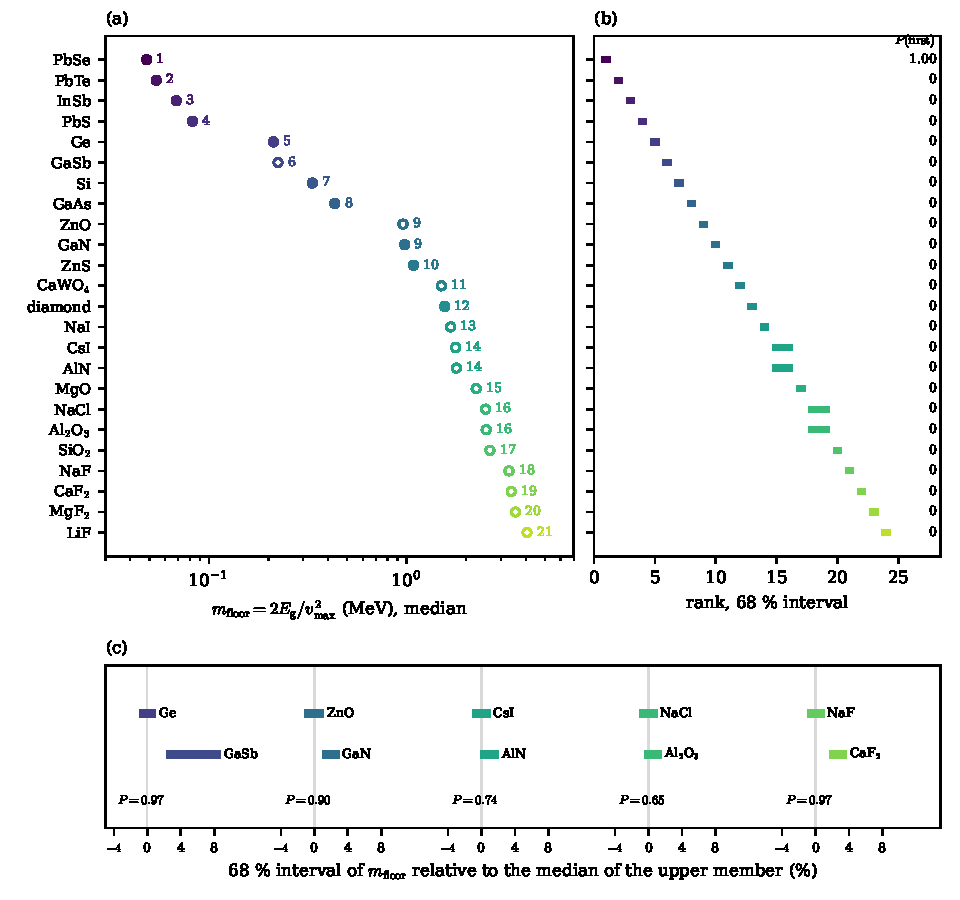
\includegraphics[width=\linewidth]{figures/ch17/fig17_5.pdf}
  \caption{Rank intervals for the electron-recoil floor $2\Eg/v_{\mathrm{max}}^2$, $v_{\mathrm{max}} = 2.650\times10^{-3}$, of the 24 crystals in the target table of Griffin and collaborators~\cite[Table~I]{griffin2020multichannel}, with the low-temperature gaps of \cref{tab:3-materials} for silicon, germanium and GaAs. (a)~Median floor; filled symbols: gap measured at low temperature, open symbols: room-temperature gap plus an upward shift drawn uniformly on 0.03--\SI{0.10}{eV}; gap width 0.01 in the logarithm for all. Numbers and colors: tier (height in the interval order of the 68\% intervals). (b)~Rank, 16th to 84th percentile over $2\times10^4$ draws, and the probability of ranking first. (c)~The 68\% intervals of five close pairs, relative to the median of the member with the lower floor, with the probability $P$ that this member has the lower floor. Pairs in one tier overlap; pairs in different tiers do not, whatever $P$.}
  \label{fig:17-rank-floor}
\end{figure}

\Cref{fig:17-rank-floor} shows the electron-recoil floor $2\Eg/v_{\mathrm{max}}^2$, the lightest mass at which dark matter can cross the gap (\cref{eq:1.3-mmin}), over the 24 crystals of the target table, a wider list than our pool. The lead salts and InSb, whose gaps lie below \SI{0.3}{eV}, hold the four lowest floors, with PbSe at \SI{0.0484}{MeV} and $P(\mathrm{first}) = 1.000$. Germanium is fifth at \SI{0.212}{MeV}, silicon seventh at \SI{0.333}{MeV}. Gaps measured to a percent separate almost every pair, and the 24 crystals fall into 21 tiers. Germanium beats GaSb with probability 0.973, but only because GaSb's gap, \SI{0.720}{eV}, is a room-temperature value and is shifted upward: unshifted, the GaSb floor of \SI{0.205}{MeV} would lie below the germanium floor. With the shift drawn from 0 to \SI{0.15}{eV} instead, the probability falls to 0.837. The order of these two crystals is a statement about the temperature dependence of a gap that has not been measured at the detector's temperature.

Within our pool the electron-recoil floor ranks without ambiguity: germanium, silicon, GaAs, CaWO$_4$, diamond, sapphire, NaF and LiF, each in its own tier and with a rank interval of one place, from \SI{0.212}{MeV} to \SI{4.06}{MeV}. TeO$_2$, Li$_2$MoO$_4$ and $\gamma$-LiAlO$_2$ are not ranked, because no measured gap enters the tables we use.

\subsection{Tiers}\label{sec:17.6-tiers}

A probability of ranking first is a property of one material against the whole pool. To group all materials into classes that the uncertainties can tell apart, we need more: two materials should share a class when their intervals overlap, and be in different classes otherwise. Overlap is not transitive, so no grouping into tied classes can satisfy both conditions in general (\cref{app:C.13}). The interval order resolves the conflict. Material $A$ is resolved above $B$ when the whole 68\% interval of $A$ lies on the better side of the whole interval of $B$, \cref{eq:C.13-order}, and the tier of a material is its height in this order, one plus the length of the longest chain of materials resolved above it, \cref{eq:C.13-height}. Each tier is an antichain, so its members are tied in the exact sense that none is resolved from any other. Every member of tier $k > 1$ is resolved below some member of tier $k - 1$.

A material with a wide interval can therefore rank in a better tier than one with a better median. The nuclear edge $m_{\mathrm{min}}^{\mathrm{ac}}$ at $\omega_{\mathrm{th}} = \SI{1}{meV}$, \cref{eq:11.1-edge} with $c_{\mathrm{LA,max}}$, puts GaAs, with a computed tensor and the interval 10.3--\SI{12.3}{keV}, in tier 6. It puts CaWO$_4$, measured at 10.8--\SI{11.2}{keV}, in tier 7, although the median edge of CaWO$_4$, \SI{11.0}{keV}, is the lower of the two medians. Nothing is resolved between GaAs and germanium, whose measured edge is 10.0--\SI{10.4}{keV}, while germanium is resolved above CaWO$_4$. Tiers add no order that the intervals do not contain, and they discard the information about medians that $P(\mathrm{first})$ keeps; \cref{fig:17-rank-floor}c shows both the tiers and the probabilities. ZnO and GaN share a tier although ZnO has the lower floor with probability 0.90, and NaF and CaF$_2$ are in different tiers, with probability 0.97 that NaF has the lower floor. The tier boundary falls where the intervals stop overlapping, not at a fixed probability.

\subsection{Correlated method errors}\label{sec:17.6-correlation}

The three database speeds that we could check against experiment were all low. If a method errs in the same direction for every crystal, the ratio of two of its results is more accurate than either result, and treating the errors of the two results as independent understates how well the method ranks the two crystals. We model the shared part of the errors with one parameter, the method correlation $r_{\mathrm{mat}}$. Each input of a computed kind draws its Gaussian variable as
\begin{equation}
  z_j = r_{\mathrm{mat}}^{1/2}\,z_{\mathrm{method}} + (1 - r_{\mathrm{mat}})^{1/2}\,z_{j}' ,
  \label{eq:17.6-zmethod}
\end{equation}
with $z_{\mathrm{method}}$ common to every crystal computed with the same method and $z_j'$ the input's own variable, both standard normal. The marginal of every input is unchanged, so are the medians and the 68\% intervals, and so are the tiers built from them, which do not depend on the correlation. Joint statements change. One variable $z_{\mathrm{method}}$ is shared within each of these groups: the database speeds, the densities of computed cells, each quantity of the perturbation calculations, the room-to-low-temperature shift of the gaps and the pole prior $X_{\mathrm{pole}}$. Inputs measured independently never share one. By \cref{eq:C.14-pairwise} the variance of $\ln(x_A/x_B)$ is $\sigma_A^2 + \sigma_B^2 - 2r_{\mathrm{mat}}\sigma_A\sigma_B$, which vanishes at $r_{\mathrm{mat}} = 1$ for two inputs of one method and equal widths.

Correlation sharpens comparisons inside a method. TeO$_2$ beats GaAs, both from database tensors, with probability 0.976 at $r_{\mathrm{mat}} = 0$, 0.997 at 0.5 and 1.000 at 1. Its probability of ranking first rises from 0.968 to 0.985 and 0.987, since its strongest challenger in the draws, GaAs, now moves with it. LiF beats NaF in the polar rate, both through computed Born charges, with probability 0.987 at independent errors and 1.000 at full correlation.

Correlation also resolves ties that the data do not resolve. The Migdal figure of merit is known only between two limits, the plasmon pole and a loss function concentrated at the gap, which differ by $5.7\times10^5$ for silicon (\cref{sec:17.5-migdal}). We rank with the pole form \cref{eq:17.5-pole} times a factor $X_{\mathrm{pole}}$ for the interband weight below the plasma frequency, drawn log-uniformly between 1 and 3. This prior is a device, not a description of the uncertainty. For silicon, the one crystal with a computed spectrum, the plasmon carries \SI{4}{\percent} of the Migdal probability (\cref{sec:12.3}), so the $X_{\mathrm{pole}}$ of silicon is about 25, and $X_{\mathrm{pole}}$ depends on the gap, which differs from crystal to crystal. The medians of the Migdal row are therefore artifacts of the prior, and the order is open, not merely unresolved. At $r_{\mathrm{mat}} = 0$ six crystals share tier 1 and no crystal ranks first with probability above 0.315 (NaF; then silicon 0.290, LiF 0.147). At $r_{\mathrm{mat}} = 1$ the prior cancels from every ratio and NaF ranks first with probability 1.000, although the figure of merit of NaF exceeds that of silicon by \SI{2.4}{\percent}. The resolution at $r_{\mathrm{mat}} = 1$ rests on the assumption of one interband factor for every crystal. We read rankings at $r_{\mathrm{mat}} = 0$ and report the correlated variant beside them: where the independent and the correlated rankings disagree, the ranking rests on an assumption about the method, not on the inputs.

No correlation helps when one material is measured and the other computed. Germanium has a measured tensor and GaAs a database one, and GaAs has the larger figure of merit with probability 0.887. The database speeds of silicon, germanium and diamond are low by \SI{4.9}{\percent} on average; applied to GaAs, this offset lowers the GaAs figure of merit from 1.87 to 1.78 and the probability to 0.744. The same offset on TeO$_2$ lowers the probability that it beats the measured CaWO$_4$ from 0.987 to 0.955. The comparison of a measured with a computed value carries the offset of the method in full, and only a measurement of the crystal with the computed value removes the offset.

\subsection{Rankings of the scattering channels}\label{sec:17.6-rankings}

\Cref{tab:17-rank} collects the rankings of our eleven crystals in the scattering channels for which \cref{sec:17.5} defines a figure of merit. Each row holds only in the window of its figure of merit (\cref{tab:17-fom}).

\begin{table}[tbp]
  \caption{Response-level rankings of the scattering channels for silicon, germanium, GaAs, diamond, sapphire, LiF, NaF, CaWO$_4$, TeO$_2$, Li$_2$MoO$_4$ and $\gamma$-LiAlO$_2$. Figures of merit of \cref{sec:17.5}; inputs and provenance widths of \cref{sec:17.6-widths} and \cref{tab:17-widths}; $2\times10^4$ draws. Leader: median and 68\% interval. $P(\mathrm{first})$ at independent method errors, with the value at $r_{\mathrm{mat}} = 1$ in parentheses. Following tiers separated by vertical bars, members of one tier in braces, medians given. Edges at $\omega_{\mathrm{th}} = \SI{1}{meV}$; $v_{\mathrm{max}} = 2.650\times10^{-3}$. Migdal row: medians relative to silicon at $X_{\mathrm{pole}} = 1$, so they include the prior median $\sqrt3 = 1.73$ of $X_{\mathrm{pole}}$ (\cref{sec:17.6-correlation}), and they carry no ordering information.}
  \label{tab:17-rank}
  \centering\scriptsize\setlength{\tabcolsep}{3pt}
  \begin{tabular}{@{}>{\raggedright\arraybackslash}p{0.17\linewidth}>{\raggedright\arraybackslash}p{0.17\linewidth}>{\raggedright\arraybackslash}p{0.09\linewidth}>{\raggedright\arraybackslash}p{0.33\linewidth}>{\raggedright\arraybackslash}p{0.18\linewidth}@{}}
    \toprule
    Channel, figure of merit & Leader (tier 1) & $P(\mathrm{first})$ & Following tiers & Not ranked \\
    \midrule
    Electron-recoil floor $2\Eg/v_{\mathrm{max}}^2$ (MeV), lower & Ge, 0.212 [0.210, 0.214] & 1.000 (1.000) & Si 0.333 $|$ GaAs 0.433 $|$ CaWO$_4$ 1.50 $|$ diamond 1.56 $|$ sapphire 2.52 $|$ NaF 3.29 $|$ LiF 4.06 & TeO$_2$, Li$_2$MoO$_4$, $\gamma$-LiAlO$_2$: no measured gap \\
    Heavy-mediator single phonon $c_{\mathrm{NR1}}(\mathrm{Si})/c_{\mathrm{NR1}}$, higher & TeO$_2$, 2.39 [2.19, 2.60]; computed tensor & 0.968 (0.987) & \{CaWO$_4$ 1.96, GaAs 1.87\} $|$ Ge 1.68 $|$ NaF 1.50 $|$ \{LiF 1.21, $\gamma$-LiAlO$_2$ 1.11\} $|$ Si 1.00 $|$ sapphire 0.83 $|$ diamond 0.49 & Li$_2$MoO$_4$: no elastic tensor \\
    Nuclear edge $m_{\mathrm{min}}^{\mathrm{ac}}$ with $c_{\mathrm{LA,max}}$ (keV), lower & diamond, 3.11 [3.05, 3.18]; measured tensor & 1.000 (1.000) & sapphire 5.16 $|$ Si 6.12 $|$ \{$\gamma$-LiAlO$_2$ 6.80, LiF 7.39\} $|$ NaF 8.83 $|$ \{Ge 10.2, GaAs 11.3\} $|$ CaWO$_4$ 11.0 $|$ TeO$_2$ 12.4 & Li$_2$MoO$_4$ \\
    Polar rate $\mathcal{I}_{\mathrm{pol}}/\rho_T$ (\si{meV.cm^3.g^{-1}}), higher & LiF, 18.9 [15.5, 23.2]; computed $Z^*$, $\varepsilon_\infty$ & 0.987 (1.000) & \{NaF 9.93, sapphire 9.12\} $|$ GaAs 0.141 & Si, Ge, diamond: nonpolar; CaWO$_4$, TeO$_2$, Li$_2$MoO$_4$, $\gamma$-LiAlO$_2$: no consistent mode set \\
    Polar reach $2\omega_{\mathrm{L}}/v_{\mathrm{max}}^2$ (keV), lower & GaAs, 10.35 [10.30, 10.40]; measured $\omega_{\mathrm{L}}$ & 1.000 (1.000) & NaF 14.2 $|$ LiF 22.0 $|$ sapphire 32.0 & as polar rate \\
    Migdal pole factor times $X_{\mathrm{pole}}$, higher & no reading: tier 1 \{NaF 1.77, Si 1.73, LiF 1.51, Li$_2$MoO$_4$ 1.47, $\gamma$-LiAlO$_2$ 1.46, GaAs 0.84\} & largest 0.315, NaF (1.000) & Ge, sapphire, TeO$_2$, CaWO$_4$, diamond in tier 2 & -- \\
    Light-mediator single phonon & no ranking: target-independent per mass far above the edge (\cref{eq:11.1-light}) & -- & -- & -- \\
    \bottomrule
  \end{tabular}
\end{table}

Silicon, the running example of the book, leads no row and lies in the middle of every row in which it is ranked. As \cref{sec:17.5} found, two pairs of rows run in opposite directions, and in this pool the reversal is extreme. Diamond is first in the nuclear edge and last in the heavy-mediator rate, and GaAs, first in polar reach, is last in polar rate, 134 times below LiF and 64 times below sapphire.

Diamond's nuclear edge rests on its measured tensor, and diamond leads sapphire, the runner-up on a computed tensor, by a factor 1.66. LiF's polar lead rests on computed Born charge, $\varepsilon_\infty$ and phonon energy, and survives because the factor of two to the next tier exceeds the combined width of those three inputs.

Every probability in \cref{tab:17-rank} passes to the guide to next targets of \cref{sec:21.7} with the provenance widths of \cref{tab:17-widths} attached.

\subsection{Uncertainty budget of the comparison}

\Cref{tab:17-nuisances} collects the truncations and inputs of the chapter with their sizes.

\begin{table}[tbp]
  \caption{Uncertainty budget of the comparison across channels. Classes and bases as in \cref{tab:10-nuisances}. ``Order'' marks an item that acts on a ranking rather than on a rate, ``convention'' a width assigned by convention.}
  \label{tab:17-nuisances}
  \centering\scriptsize\setlength{\tabcolsep}{3pt}
  \begin{tabular}{@{}>{\raggedright\arraybackslash}p{0.26\linewidth}>{\raggedright\arraybackslash}p{0.12\linewidth}>{\raggedright\arraybackslash}p{0.35\linewidth}>{\raggedright\arraybackslash}p{0.09\linewidth}>{\raggedright\arraybackslash}p{0.10\linewidth}@{}}
    \toprule
    Truncation or input & Type & Size & Basis & Section \\
    \midrule
    Coherent corrections to the multiphonon tail & threshold & a factor of two in the tail moves the crossover in silicon at \SI{10}{MeV} by \SI{0.014}{eV} & model & \cref{sec:17.1} \\
    Local fields and off-diagonal elements of the Migdal probability & normali\-zation & diagonal factor 1.35 moves the crossover at \SI{10}{MeV} by \SI{0.006}{eV}; off-diagonal size open (\cref{sec:12.3}) & computed; unsized & \cref{sec:17.1} \\
    Coherent Migdal response at $q < 2q_{\mathrm{BZ}}$ & normali\-zation; tilt in $\omega_e$ & diagonal form $14.9\times$ high as $q \to 0$ (\cref{eq:8.3-boostward}); \SI{0.75}{keV} to $2q_{\mathrm{BZ}}$ unsized: nearly all of the silicon Migdal rate up to \SI{1}{MeV}, \SI{33}{\percent} at \SI{2}{MeV}, \SI{7}{\percent} at \SI{3}{MeV} & computed (limit); unsized & \cref{sec:17.1} \\
    Electron-following sector of an electron-only coupling (long-wavelength model) & normali\-zation; tilt in $\mchi$ & equality with electron recoil at \SI{12.3}{MeV} is a property of the model & unsized & \cref{sec:17.1} \\
    Phonon-assisted side of the silicon window & normali\-zation & estimate known to a factor of ten; lead to about \SI{0.43}{MeV}, two-channel band 0.43--\SI{0.51}{MeV} & est. & \cref{sec:17.1} \\
    Germanium zero-phonon edge and phonon density of states & threshold & not known; the germanium electronic window and crossover are not drawn & unsized & \cref{sec:17.1} \\
    Half-gap and cutoff of ZrTe$_5$ & threshold & half-gaps \SI{11.8}{meV} and \SI{15.6}{meV} move the absorption onset from 23.6 to \SI{31.2}{meV}, the reach at \SI{100}{meV} by \SI{2.5}{\percent} & input spread & \cref{sec:17.2} \\
    Counting against linear readout & normali\-zation & a band $B$ wider than the line multiplies the advantage by $(B/\Delta\omega_{\mathrm{eq}})^{-1/2}$ & unsized & \cref{sec:17.2} \\
    Exothermic shell form & normali\-zation & halo-independent to $O(v^2/v_\nu^2)$; silicon phonons 0.78--1.10 of the full integral at \SI{1}{MeV}, the weight varying on the zone scale & computed & \cref{sec:17.3} \\
    Electron-gas plasmon against crystal tables & normali\-zation & plasmon-pole rate 0.09--0.16 of the tables' electronic rate at 18--\SI{22}{eV} (two models) & model & \cref{sec:17.3} \\
    Migdal--phonon-assisted cross term & normali\-zation & bounded by positivity, \cref{eq:17.4-bound}; exact at small $q$ (\cref{eq:17.4-rate}: $+5.47\times10^{-4}$ for a dark photon in silicon); in the windows, at 0.2--0.6 of $2\pi/a$, order of magnitude only & computed (limit); est. & \cref{sec:17.4} \\
    Shift of $\eta$ by the sound speed (heavy mediator) & tilt in $\mchi$; order & rate ratios differ from the speed ratios by up to \SI{7}{\percent} at \SI{0.3}{MeV} (germanium, diamond against silicon); rankings hold pairwise in $W_{AB}$ & computed & \cref{sec:17.5} \\
    Interband weight of the Migdal pole factor & normali\-zation; order & pole and gap limits differ by $5.7\times10^5$ in silicon; pole dispersion moves LiF over silicon from 0.87 to 1.4--1.7; ranking with a prior $X_{\mathrm{pole}}$ on [1, 3] (silicon's own value about 25) gives no reading & est. & \cref{sec:17.5,sec:17.6} \\
    Provenance widths & order & database speeds 0.086; gap shift 0.03--\SI{0.10}{eV}; doubled speed width: TeO$_2$ first with 0.781, not 0.968 & convention & \cref{sec:17.6} \\
    Offset of the computed elastic tensors & order & database speeds low by \SI{4.9}{\percent} on average (silicon, germanium, diamond); GaAs against germanium 0.887 $\to$ 0.744 with the offset & input spread & \cref{sec:17.6} \\
    Method correlation $r_{\mathrm{mat}}$ & order & sharpens one-method comparisons (TeO$_2$ over GaAs 0.976 $\to$ 1.000); resolves the Migdal tie artificially & computed & \cref{sec:17.6} \\
    Room-temperature gaps used at low temperature & threshold; order & germanium against GaSb 0.973 with the shift 0.03--\SI{0.10}{eV}, 0.837 with 0--\SI{0.15}{eV}; reversed without shift & est. & \cref{sec:17.6} \\
    \bottomrule
  \end{tabular}
\end{table}

\section*{Summary}

At fixed coupling the rate of a crystal adds sector by sector, and which sector dominates follows from two facts: how much energy each sector can absorb, and whether the coupling is screened (\cref{sec:17.1}). A single phonon carries at most the top of the band, \SI{64.1}{meV} in silicon; a freely recoiling nucleus at most $E_R^{\mathrm{max}}$, \SI{0.054}{eV} at \SI{10}{MeV}; an electronic excitation up to the whole kinetic energy, \SI{35}{eV} at \SI{10}{MeV}. For a nucleon coupling with a heavy mediator the electron-following sector holds every threshold below the band top, with one phonon leading up to \SI{20}{MeV} at \SI{1}{meV}, and the Migdal effect holds the band between the end of the lattice spectrum and the largest deposit. The multiphonon--Migdal crossover threshold in silicon is 0.178, 0.307 and \SI{5.33}{eV} at 1, 10 and \SI{100}{MeV}: pinned near three times the band top for soft kicks, climbing through the Poisson tail of the multiphonon spectrum between 3 and \SI{20}{MeV}, and sitting on the free-recoil endpoint above the impulse onset. For an electron coupling, screening decides the low thresholds. A dark photon couples to the total charge, its structure factor is the loss function, and silicon, with vanishing Born charges, has no lattice channel for it at order $q^2$; a mediator coupled to the electrons alone sees the electrons that follow the nuclei and raises the rate at \SI{1}{MeV} from 17 to $7\times10^5$ events per kilogram and year at $\sigmae = \SI{e-37}{cm^2}$. In GaAs the Born charge $Z^* = 2.11$ reverses the picture: the polar phonon opens to the dark photon at \SI{10.35}{keV} and is nearly closed to a nucleon coupling.

For absorption each boson measures one response at $q = p_\phi$ and $\omega = m_\phi$ (\cref{sec:17.2}). The dark photon sees the loss function, which screening caps at $L \le 1/(2|\varepsilon_1|)$, so it is absorbed strongly near the zeros of $\varepsilon_1$: the longitudinal phonon of GaAs, the highest polar branch of sapphire and the plasmon of silicon. The axion-like particle sees the conductivity or the spin current and has no such ceiling; in a clean superconductor its spin current breaks pairs directly. Between 0.38 and \SI{1.17}{eV} no target of the book covers the dark photon at leading order. A counter of quanta whose band is the line beats a quantum-limited linear readout of the same mode by $\ee^{m_\phi/2T}$ in signal, so its advantage vanishes for masses well below the temperature, \SI{0.86}{\micro eV} at \SI{10}{mK}, and above twenty times the temperature the counter is limited by the absorbed quanta alone.

Dark matter with a mass splitting can lose its excitation energy to a collective mode (\cref{sec:17.3}). When the mode's group velocity exceeds the halo speeds and its weight is smooth over $\mchi v_{\mathrm{max}}$, the rate is independent of the halo to order $v^2/v_\nu^2$, the line sits where the mode's dispersion meets the shell of fixed momentum, and its width has the shape of $\eta$. In silicon at \SI{1}{MeV} a splitting of \SI{10}{eV} raises the single-phonon rate 31 times over elastic scattering, and the shell form gives 0.78 to 1.10 of the full integral. For GaAs at \SI{30}{keV} and $\Delta_\chi = -\SI{1}{eV}$, down-scattering into the longitudinal phonon gives 1810 events per kilogram and year against 842 for elastic scattering. An endothermic splitting of \SI{1}{eV} brings every collective channel to \SI{0.3}{MeV}, half the pair threshold of silicon, and the plasmon is closed at every mass.

Cross terms between sectors appear for couplings to both electrons and nuclei (\cref{sec:17.4}). The interference between the Migdal and the phonon-assisted amplitudes is bounded by the positivity of the response matrix, \cref{eq:17.4-bound}, and at small momentum transfer the bound is reached: the summed Migdal amplitude of a one-phonon pair state is $-(m_e/M_\kappa)$ times the phonon-assisted one, so the phonon-dressed rate carries the factor $|\tilde V_e - (m_e/M_\kappa)\tilde V_{\mathrm{nuc}}|^2$, \cref{eq:17.4-rate}. For a dark photon this raises the phonon-assisted rate of silicon by $5.47\times10^{-4}$; for a coupling in proportion to mass the bracket vanishes. In the windows of silicon and GaAs, at a fifth to three fifths of the way to $2\pi/a$, the relation fixes the cross term in order of magnitude.

Each channel then reduces to a few material numbers, each valid in a window (\cref{sec:17.5}): the floor $2\Eg/v_{\mathrm{max}}^2$, the inverse effective sound speed $1/c_{\mathrm{NR1}}$ for a heavy mediator, the acoustic edge, the polar band integral $\mathcal{I}_{\mathrm{pol}}/\rho_T$ and the polar edge, and the Migdal figure of merit. The reach figures of merit are kinematic and exact; the rate figures of merit hold in windows. No scalar ranks electron-recoil rates, and the partial $f$-sum of the valence electrons caps them through $\omega_p^{\mathrm{val}}$, \SI{16.6}{eV} in silicon. The Migdal figure of merit lies between a plasmon-pole limit and a limit with the weight at the gap, which differ by $5.7\times10^5$ in silicon, and the pole limit itself depends on the dispersion of the plasmon, so its ranking is open. A heavy-mediator ranking holds pairwise, in the window $W_{AB}$ of two crystals, because the shift of $\eta$ by the sound speed breaks a common window; at \SI{0.3}{MeV} the computed rate ratios of germanium and diamond to silicon are 1.73 and 0.46 against the speed ratios 1.69 and 0.49 (\cref{sec:17.5}).

Rankings by these numbers carry the uncertainty of their inputs (\cref{sec:17.6}). Each input gets a provenance width by how it was obtained, measured, computed or estimated; the widths are conventions, and the database sound speeds of silicon, germanium and diamond, low by 1 to \SI{10}{\percent} and all in the same direction, show both the size of one convention and why method errors correlate. Monte Carlo propagation gives the probability that a crystal ranks first and its interval of ranks; heights in the interval order of the 68\% intervals give tiers, which never assert an order the intervals do not contain. Among eleven crystals germanium leads the electron-recoil floor, TeO$_2$ the heavy-mediator single-phonon rate (probability 0.968, on a computed tensor), diamond the nuclear edge, LiF the polar rate and GaAs the polar reach. Silicon leads none. Stiff lattices and light polar ions win one row of each pair and lose the other. The Migdal channel has no reading at independent errors, its largest probability of ranking first being 0.315, and the reading it acquires when the pole prior is shared by all crystals is an artifact of that assumption. The light-mediator single-phonon rate does not rank crystals at all. A shared method error sharpens comparisons inside one method and cannot help a comparison of a measured with a computed value, which keeps the method's offset in full.

\Cref{tab:17-nuisances} collects the truncations and inputs of the chapter with their sizes. How the energy per quantum, the readout and the backgrounds change these rankings is the subject of the guide to next targets of \cref{sec:21.7}.

\begin{table}[tbp]
  \caption{Nuisances of the comparison across channels. Type in the classes of \cref{sec:8.8}: normalization, tilt, threshold and new support; ``order'' marks an item that acts on a ranking rather than on a rate. Basis of the size: ``computed'' (next order or exact result computed), ``model'' (computed in a model), ``est.''\ (parametric estimate), ``input spread'' (spread or limitation of a measured or computed input), ``convention'' (a width assigned by convention), ``unsized'' (no size known). The last column gives the section where the item is treated.}
  \label{tab:17-nuisances}
  \centering\scriptsize\setlength{\tabcolsep}{3pt}
  \begin{tabular}{@{}>{\raggedright\arraybackslash}p{0.26\linewidth}>{\raggedright\arraybackslash}p{0.12\linewidth}>{\raggedright\arraybackslash}p{0.35\linewidth}>{\raggedright\arraybackslash}p{0.09\linewidth}>{\raggedright\arraybackslash}p{0.10\linewidth}@{}}
    \toprule
    Truncation or input & Type & Size & Basis & Section \\
    \midrule
    Coherent corrections to the multiphonon tail & threshold & a factor of two in the tail moves the crossover in silicon at \SI{10}{MeV} by \SI{0.014}{eV} & model & \cref{sec:17.1} \\
    Local fields and off-diagonal elements of the Migdal probability & normali\-zation & diagonal factor 1.35 moves the crossover at \SI{10}{MeV} by \SI{0.006}{eV}; off-diagonal size open (\cref{sec:12.3}) & computed; unsized & \cref{sec:17.1} \\
    Coherent Migdal response at $q < 2q_{\mathrm{BZ}}$ & normali\-zation; tilt in $\omega_e$ & diagonal form $14.9\times$ high as $q \to 0$ (\cref{eq:8.3-boostward}), quantitative only below about \SI{0.75}{keV}; \SI{0.75}{keV} to $2q_{\mathrm{BZ}}$ unsized, nearly all of the silicon Migdal rate up to \SI{1}{MeV} (\SI{29}{\percent} of it from $q < q_{\mathrm{BZ}}$ at \SI{1}{MeV}), \SI{33}{\percent} at \SI{2}{MeV}, \SI{7}{\percent} at \SI{3}{MeV} (\cref{tab:12-nuisances}) & computed (limit); unsized & \cref{sec:17.1} \\
    Electron-following sector of an electron-only coupling (long-wavelength model) & normali\-zation; tilt in $\mchi$ & equality with electron recoil at \SI{12.3}{MeV} is a property of the model; Umklapp, transverse and multiphonon terms add, dispersion and loss of following charge subtract & unsized & \cref{sec:17.1} \\
    Phonon-assisted side of the silicon window & normali\-zation & estimate known to a factor of ten; lead to about \SI{0.43}{MeV}, two-channel band 0.43--\SI{0.51}{MeV} & est. & \cref{sec:17.1} \\
    Germanium zero-phonon edge and phonon density of states & threshold & not known; the germanium electronic window and crossover are not drawn & unsized & \cref{sec:17.1} \\
    Half-gap and cutoff of ZrTe$_5$ & threshold & measured-structure (\SI{11.8}{meV}) and relaxed-cell (\SI{15.6}{meV}) parameters move the absorption onset from 23.6 to \SI{31.2}{meV}; the reach at \SI{100}{meV} changes by \SI{2.5}{\percent} & input spread & \cref{sec:17.2} \\
    Counting against linear readout & normali\-zation & a counter band $B$ wider than the line multiplies the advantage by $(B/\Delta\omega_{\mathrm{eq}})^{-1/2}$; squeezed readout and dark counts reduce it & unsized & \cref{sec:17.2} \\
    Exothermic shell form & normali\-zation & halo-independent to $O(v^2/v_\nu^2)$; silicon phonons 0.78--1.10 of the full integral at \SI{1}{MeV}, the weight varying on the zone scale & computed & \cref{sec:17.3} \\
    Electron-gas plasmon against crystal tables & normali\-zation & plasmon-pole rate 0.09--0.16 of the tables' electronic rate at 18--\SI{22}{eV} (two models) & model & \cref{sec:17.3} \\
    Migdal--phonon-assisted cross term & normali\-zation & bounded by positivity, \cref{eq:17.4-bound}; exact at small $q$ (\cref{eq:17.4-rate}: $+5.47\times10^{-4}$ for a dark photon in silicon); in the windows, at 0.2--0.6 of $2\pi/a$, order of magnitude only & computed (limit); est. & \cref{sec:17.4} \\
    Shift of $\eta$ by the sound speed (heavy mediator) & tilt in $\mchi$; order & rate ratios differ from the speed ratios by up to \SI{7}{\percent} at \SI{0.3}{MeV} (germanium, diamond against silicon); rankings hold pairwise in $W_{AB}$ & computed & \cref{sec:17.5} \\
    Interband weight of the Migdal pole factor & normali\-zation; order & pole and gap limits differ by $5.7\times10^5$ in silicon; the dispersion of the pole changes LiF over silicon from 0.87 to 1.4--1.7; the ranking uses the pole form with a prior $X_{\mathrm{pole}}$ log-uniform on [1, 3], a device (silicon's own value is about 25), and gives no reading at independent errors & est. & \cref{sec:17.5,sec:17.6} \\
    Provenance widths & order & database speeds 0.086 (three checked crystals: root mean square 0.065); gap shift 0.03--\SI{0.10}{eV}; doubling the speed width lowers TeO$_2$'s probability of ranking first from 0.968 to 0.781 & convention & \cref{sec:17.6} \\
    Offset of the computed elastic tensors & order & database speeds low by \SI{4.9}{\percent} on average (silicon, germanium, diamond); GaAs against germanium 0.887 $\to$ 0.744 with the offset & input spread & \cref{sec:17.6} \\
    Method correlation $r_{\mathrm{mat}}$ & order & sharpens one-method comparisons (TeO$_2$ against GaAs 0.976 at 0, 1.000 at 1); resolves the Migdal tie artificially (NaF 0.315 $\to$ 1.000) & computed & \cref{sec:17.6} \\
    Room-temperature gaps used at low temperature & threshold; order & germanium against GaSb 0.973 with the shift 0.03--\SI{0.10}{eV}, 0.837 with 0--\SI{0.15}{eV}; reversed without shift & est. & \cref{sec:17.6} \\
    \bottomrule
  \end{tabular}
\end{table}

\printbibliography[heading=subbibliography]

\part{Detection}
\chapter{Ionization yield}\label{chap:18}
A deposit of \SI{10}{eV} in silicon has enough energy for eight electron--hole pairs across the \SI{1.17}{eV} gap of silicon at millikelvin temperatures, yet the cascade model of \cref{sec:18.1} leaves two or three in nearly every event. The measured mean energy per pair is three times the gap (\cref{sec:18.4}), and the rest of the energy ends in phonons. Between the deposit and the count lies a cascade of hot carriers that ionize, emit phonons and slow down, all within about a picosecond. The mean energy per pair $\varepsilon_{\mathrm{eh}}$ and the Fano factor $F_{\mathrm{eh}}$ of the pair number set the threshold of every electron-recoil search in a semiconductor, since at the few-pair level one ionization more or less moves an event from one bin to the next. For a long time both have been fitted to calibration data rather than computed: the cascade model used for silicon has one constant, tuned to the measured $\varepsilon_{\mathrm{eh}}$ (\cref{app:E.13}).

This chapter asks how far the two numbers can be derived from the rates of the master formula. The hot carrier is itself a projectile of the master formula. It scatters off the electrons and the lattice of the target as a dark-matter particle with a Coulomb coupling would, which \cref{sec:4.8} already found for the quasiparticle lifetime of an electron gas. The cascade also inherits the split of energy between the electron and the hole that the dark-matter interaction made. A pair made at a momentum transfer of a few keV shares its energy between electron and hole differently from a pair made by a photon (\cref{sec:8.7}), and at a few pairs that difference can be a whole ionization. The chapters that follow take the deposit to the quanta a sensor counts, then to a limit and to a guide to the next targets (\cref{fig:18-map}).

\begin{figure}[tbp]
  \centering
  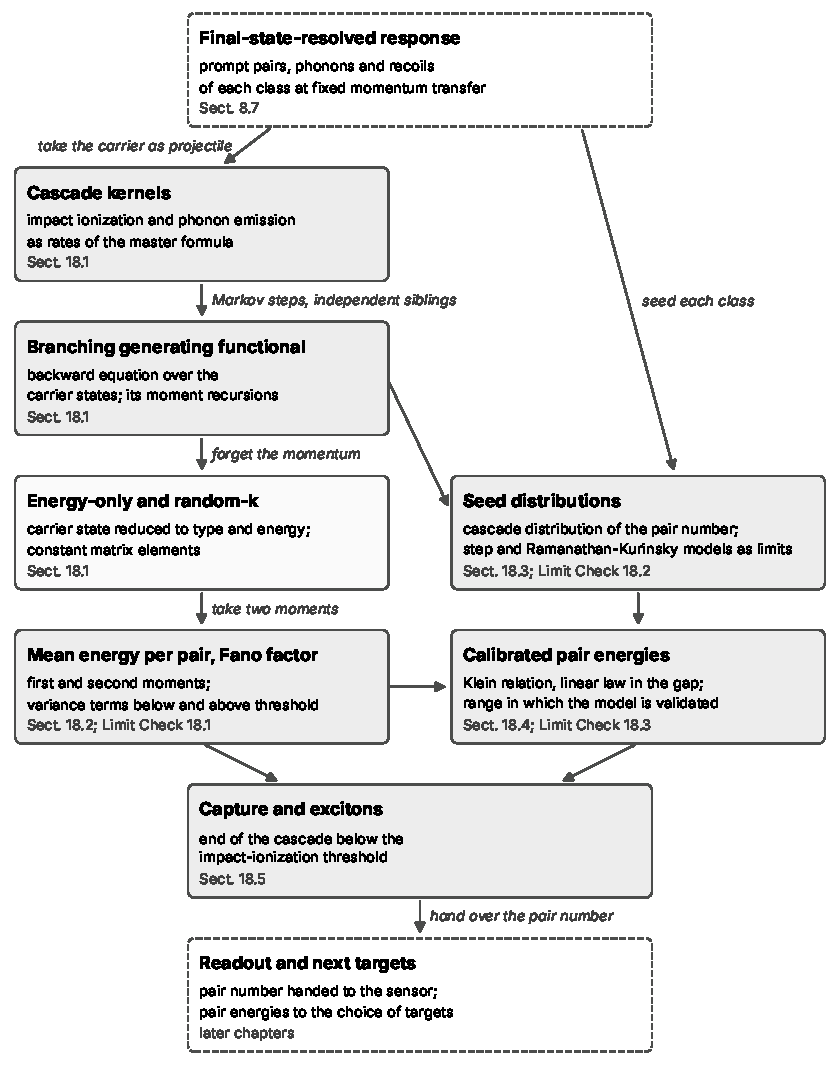
\includegraphics[width=0.85\linewidth]{figures/ch18/map18.pdf}
  \caption{Ionization yield, from the final-state-resolved response of \cref{sec:8.7} to the pair number. Main line: impact ionization and phonon emission as rates of the master formula with the carrier as projectile, the branching generating functional of the cascade and its reduction to carrier energies alone (\cref{sec:18.1}), then the mean energy per pair and the Fano factor as its first two moments (\cref{sec:18.2}; \cref{lim:18.2a,lim:18.2b}). Side branches: the seeding of the cascade by each final-state class, with the step model and the Ramanathan--Kurinsky model as its limits (\cref{sec:18.3}; \cref{lim:18.3a}), and the calibrated pair energies of silicon, germanium, GaAs and the wide-gap crystals with the range in which the cascade model is validated (\cref{sec:18.4}; \cref{lim:18.4a,lim:18.4c}). Both feed the end of the cascade below the impact-ionization threshold, capture and excitons (\cref{sec:18.5}), which hands the pair number to the readout and the pair energies to the choice of new targets.}
  \label{fig:18-map}
\end{figure}

\section{The carrier cascade}\label{sec:18.1}

In the cascade model of silicon built in this section, an electron with \SI{50}{eV} of kinetic energy makes about 13 new electron--hole pairs before every carrier has fallen below the threshold for impact ionization, and the remaining \SI{35}{eV} goes to the lattice. \Cref{fig:18-tree} shows one such cascade. Each step in the cascade is a collision of a hot carrier with the target: either the carrier lifts a valence electron across the gap, or it emits a phonon. Impact ionization and phonon emission are both scattering events of a projectile off the electrons or the nuclei of the crystal, and each is a rate of the master formula \cref{eq:8.2-rate} with the carrier in the place of the dark-matter particle. The cascade is then a branching process whose kernels are those rates, and its statistics follow from one generating functional that obeys a recursion in energy. Two reductions make the recursion solvable: the energy-only reduction drops the momentum of each carrier, and the random-$k$ reduction also replaces the matrix elements by constants. The electron and the hole that the dark matter leaves behind form the seed of the cascade. Both reductions must keep the seed, because at a few pairs the way the two seed carriers share the energy changes the count.

\begin{figure}[tbp]
  \centering
  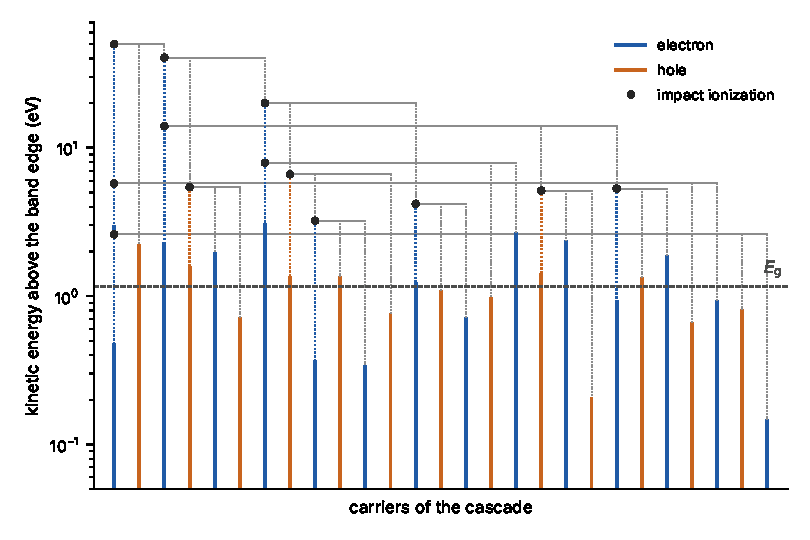
\includegraphics[width=0.95\linewidth]{figures/ch18/fig18_1.pdf}
  \caption{One sampled cascade started by an electron with \SI{50}{eV} of kinetic energy in silicon, in the energy-only random-$k$ model of \cref{sec:18.1-reductions}: free-particle densities of states, constant matrix elements, impact ionization above $\Eg = \SI{1.160}{eV}$ (silicon at \SI{123}{K}; threshold ratio $\theta_{\mathrm{ii}} = 1$), one optical phonon of \SI{63}{meV}, the rate ratio \cref{eq:18.1-randomk} with $A_{\mathrm{AB}} = \SI{5.703}{eV^3}$ (calibrated in \cref{sec:18.4}), and holes confined to the \SI{12}{eV} valence band. Each column is one carrier (blue electrons, orange holes), drawn from the kinetic energy at which it was created down to the band edge, on a logarithmic axis. Solid segments are runs of phonon emission; a dot marks an impact ionization, after which the carrier continues at the lower energy reached along the dotted segment, and the grey lines lead to the two carriers created in the ionization. This cascade has 13 ionizations, 27 carriers and 176 phonon emissions, every emission made by a carrier below \SI{6}{eV}, and leaves \SI{34.9}{eV} as heat. On average the model makes 12.99 new pairs, \SI{3.85}{eV} per pair at this energy, with a variance of 0.119 times the mean (generating function of \cref{sec:18.3}).}
  \label{fig:18-tree}
\end{figure}

\subsection{Impact ionization as a master-formula rate}\label{sec:18.1-ii}

A carrier in the Bloch state $n\vect{k}$, an electron in a conduction band or a hole in a valence band, interacts with every other charge of the crystal through the Coulomb potential. It is charged, so it couples to the total charge density $n_Z$ of electrons and nuclei, as a dark photon does (\cref{sec:8.4}). In a collision it gives a momentum $\vect{p}$ to the target and ends in a state $n'$, $\vect{k} - \vect{p}$; we write $\vect{p}$ for the momentum transfer of the carrier and keep $\vect{q}$ for the dark-matter momentum transfer that made the seed. Because the carrier is a Bloch wave and not a plane wave, the momenta $\vect{p} + \vect{G}$ for all reciprocal-lattice vectors $\vect{G}$ lead to the same final carrier state, and their amplitudes add. With $\vect{p}$ in the first zone, the amplitude to reach $n'$, $\vect{k} - \vect{p}$ and the target state $|f\rangle$ is
\begin{equation*}
  \frac{1}{\Vol}\sum_{\vect{G}}v_{\mathrm{C}}(|\vect{p}+\vect{G}|)\,\rho_{n'n}(\vect{k},-\vect{p}-\vect{G})\,\langle f|n_Z(\vect{p}+\vect{G})|i\rangle ,
\end{equation*}
with the overlap $\rho_{n'n}$ of \cref{eq:3.2-rho} in the place of the plane-wave overlap of a free projectile. This amplitude comes from the interaction \cref{eq:8.1-Hint} with one coupling row for each $\vect{G}$, the potential $\tilde V_{\vect{G}} = v_{\mathrm{C}}(|\vect{p}+\vect{G}|)\,\rho_{n'n}(\vect{k},-\vect{p}-\vect{G})$, and the target operators $n_Z(\vect{p}+\vect{G})$. The master formula \cref{eq:8.2-rate} then yields the rate directly, with two changes. The sum over final projectile states runs over the bands $n'$ and the first zone instead of over all momenta. And the final carrier state must be empty, which adds the factor $1 - f_{n',\vect{k}-\vect{p}}$. The response matrix that appears is $S_{\vect{G}\vect{G}'}(\vect{p},\omega)$ of the total charge, at the energy $\omega = \varepsilon_{n\vect{k}} - \varepsilon_{n',\vect{k}-\vect{p}}$ that the carrier loses.

The fluctuation--dissipation theorem turns this response into the screened interaction. With $R$ the retarded density response of \cref{sec:8.7}, at $\omega > 0$ the theorem reads $S = -2\,(1 + n_{\mathrm{B}}(\omega))\,(R - R^\dagger)/2\ii$ as a matrix in $\vect{G}$, the matrix form of the relation used in \cref{sec:8.7}, with $1/(1 - \ee^{-\beta\omega}) = 1 + n_{\mathrm{B}}(\omega)$. Sandwiched between Coulomb kernels, $R$ gives $v_{\mathrm{C}}Rv_{\mathrm{C}} = W^{\mathrm{scr}} - v_{\mathrm{C}}$ by \cref{eq:4.8-W}, and the bare $v_{\mathrm{C}}$ is real and diagonal and drops out of the anti-Hermitian part of $v_{\mathrm{C}}Rv_{\mathrm{C}}$. With the dielectric matrix of electrons and nuclei together in $W^{\mathrm{scr}}$:
\begin{keyresult}[Impact-ionization kernel]
\begin{equation}
  \varGamma_{\mathrm{ii}}(n\vect{k}) = -2\sum_{n'}\int_{\mathrm{BZ}}\frac{\dd^3p}{(2\pi)^3}\sum_{\vect{G}\vect{G}'}\rho_{\vect{G}}^*\,\Bigl[\frac{W^{\mathrm{scr}} - W^{\mathrm{scr}\dagger}}{2\ii}\Bigr]_{\vect{G}\vect{G}'}\!(\vect{p},\omega)\;\rho_{\vect{G}'}\;\bigl[1 - f_{n',\vect{k}-\vect{p}}\bigr]\bigl[1 + n_{\mathrm{B}}(\omega)\bigr] ,
  \label{eq:18.1-ii}
\end{equation}
with $\rho_{\vect{G}} = \rho_{n'n}(\vect{k},-\vect{p}-\vect{G})$ and $\omega = \varepsilon_{n\vect{k}} - \varepsilon_{n',\vect{k}-\vect{p}}$. Without the off-diagonal elements $\vect{G} \neq \vect{G}'$ the sum over $\vect{G}$ and the integral over the zone combine into one integral over all $\vect{p}$,
\begin{equation}
  \varGamma_{\mathrm{ii}}(n\vect{k}) \simeq \sum_{n'}\int\frac{\dd^3p}{(2\pi)^3}\,2v_{\mathrm{C}}(p)\,\bigl|\rho_{n'n}(\vect{k},-\vect{p})\bigr|^2\,L(\vect{p},\omega)\,\bigl[1 - f_{n',\vect{k}-\vect{p}}\bigr]\bigl[1 + n_{\mathrm{B}}(\omega)\bigr] ,
  \label{eq:18.1-iidiag}
\end{equation}
with $L$ the loss function \cref{eq:4.4-SL} of the total dielectric matrix at the unreduced momentum $\vect{p}$.
\end{keyresult}
\noindent For a hole the occupations are those of holes, $1 - f \to f$ in the valence bands. For a free-electron gas, $\rho = 1$ and \cref{eq:18.1-iidiag} is the out-scattering part of the lifetime \cref{eq:4.8-lifetime}: the step from \cref{sec:4.8} to here is the step from plane waves to Bloch waves and from the electron gas to a crystal with nuclei. The two terms of \cref{eq:18.1-ii} with $\vect{G} \neq \vect{G}'$ are local fields, and the master formula delivers them in their anti-Hermitian combination, which is real for any $W^{\mathrm{scr}}$, since $(W^{\mathrm{scr}} - W^{\mathrm{scr}\dagger})/2\ii$ is a Hermitian matrix and $\rho^\dagger A\rho$ is real for every Hermitian $A$. The element-wise imaginary part of $W^{\mathrm{scr}}_{\vect{G}\vect{G}'}$ agrees with the anti-Hermitian combination only when $W^{\mathrm{scr}}_{\vect{G}\vect{G}'} = W^{\mathrm{scr}}_{\vect{G}'\vect{G}}$, which holds in silicon and germanium with the origin at an inversion center but not in GaAs. The same symmetry condition separated the retarded and advanced pair weights of \cref{sec:8.7}.

The kernel is the rate at which the carrier scatters out of $n\vect{k}$. The quasiparticle width of the carrier differs from this out-scattering rate in two ways. By the cutting rule of \cref{sec:4.8}, $-2\Imag\Sigma^{\mathrm{R}} = \varGamma_{\mathrm{out}} + \varGamma_{\mathrm{in}}$. The in-scattering term carries the product $f\,n_{\mathrm{B}}$ of an occupied final state and a thermal excitation of energy $\omega \ge \Eg$, and so vanishes for a hot carrier at $T \ll \Eg$. The width also carries the quasiparticle residue, $\varGamma_{\mathrm{qp}} = -2z_{\mathrm{qp}}\Imag\Sigma^{\mathrm{R}}$ by \cref{eq:4.7-qp}, with $z_{\mathrm{qp}} \approx 0.8$ for the hot carriers of semiconductors~\cite[Sect.~II]{kotani2010impact}. \Cref{eq:18.1-ii} is first order in $W^{\mathrm{scr}}$ and sets $z_{\mathrm{qp}} = 1$. Since the factor $z_{\mathrm{qp}}$ lowers every impact-ionization rate by a nearly uniform 20 percent, a calibrated model absorbs it. The exchange of the carrier with the electron it excites is a vertex correction, absent from \cref{eq:18.1-ii} as it was from \cref{eq:4.8-lifetime}; it enters only beyond first order in $W^{\mathrm{scr}}$, and \cref{sec:18.5} lists it among the open problems.

The plasmon is inside the kernel. In silicon $\varepsilon_2$ is still 0.224 at the plasmon energy, where $\varepsilon_1$ vanishes (\cref{we:4-siplasmon}), so the plasmon peak carries the weight of electron--hole pairs. A carrier that ``emits a plasmon'' and the plasmon that ``decays into a pair'' are one term of \cref{eq:18.1-ii}, and a cascade built on \cref{eq:18.1-ii} must not add a separate plasmon channel. The plasmon becomes a particle of the cascade only where its pole is undamped and carries no pair weight, as in aluminum below the critical momentum $q_{\mathrm{c}}$ of \cref{sec:4.5}; it then needs a decay kernel of its own.

The loss function vanishes for $\omega < \Eg$ at $T \ll \Eg$, so a carrier must give up at least the gap. Energy conservation alone would let it ionize as soon as its kinetic energy $x$ above the band edge exceeds $\Eg$, but the three final carriers must also carry its crystal momentum. Take parabolic bands with an electron mass $m^*_{\mathrm{e}}$ and a hole mass $m^*_{\mathrm{h}}$. At the threshold energy, which is the lowest energy at which an electron can make a pair, the three products of the ionization move with a common velocity $\vect{u}$, so that no energy is spent on motion in their center-of-mass frame. Momentum conservation gives $m^*_{\mathrm{e}}\vect{v}_0 = (2m^*_{\mathrm{e}} + m^*_{\mathrm{h}})\vect{u}$ for an initial velocity $\vect{v}_0$, energy conservation $\tfrac12m^*_{\mathrm{e}}v_0^2 = \Eg + \tfrac12(2m^*_{\mathrm{e}} + m^*_{\mathrm{h}})u^2$, and eliminating $\vect{u}$ yields
\begin{equation}
  x_{\mathrm{th}} = \theta_{\mathrm{ii}}\Eg , \qquad \theta_{\mathrm{ii}} = \frac{2m^*_{\mathrm{e}} + m^*_{\mathrm{h}}}{m^*_{\mathrm{e}} + m^*_{\mathrm{h}}} ,
  \label{eq:18.1-theta}
\end{equation}
with $\theta_{\mathrm{ii}}$ the impact-ionization threshold ratio. Equal masses give $\theta_{\mathrm{ii}} = 3/2$; for a hole the two masses exchange places. In a real band structure the threshold is soft rather than sharp, because a crystal conserves momentum only up to $\vect{G}$ and the bands are not parabolic. Just above threshold few final states satisfy both conservation laws, and the computed rate scatters by large factors from one $\vect{k}$ to the next~\cite[Fig.~2]{kotani2010impact}.

\subsection{The phonon-emission kernel}\label{sec:18.1-ph}

The carrier also couples to the displacements of the nuclei, through the vertex $g_{mn\nu}(\vect{k},\vect{Q})$ of \cref{eq:6.2-g}. Take the phonon coordinate of branch $\nu$ at $\vect{Q}$ as the target operator and $g$ as the potential. The response of a harmonic phonon coordinate is $2\pi[(n_{\vect{Q}\nu} + 1)\delta(\omega - \omega_{\vect{Q}\nu}) + n_{\vect{Q}\nu}\delta(\omega + \omega_{\vect{Q}\nu})]$, and the master formula with the Pauli factor of the final carrier gives the out-scattering part of \cref{eq:6.3-ImFM}, the phonon kernel $\varGamma_{\mathrm{ph}}(n\vect{k})$ of \cref{eq:E.13-gph}. At detector temperatures only the emission term survives. The vertex is screened statically, as density-functional perturbation theory computes it, and the corrections to static screening are of higher order in $\omega_{\vect{Q}\nu}/\Eg$ (\cref{sec:6.2}).

In a polar crystal the two kernels overlap. The total dielectric matrix in $W^{\mathrm{scr}}$ contains the ionic response, and at $\omega$ near the longitudinal optical frequency $\omega_L$ its loss function has the Fr\"ohlich line: \cref{eq:18.1-ii} already contains the emission of a longitudinal optical phonon through the macroscopic field. The long-range vertex $g^L = \ii C_{\mathrm{F}}\rho_{mn}/Q$ of \cref{eq:6.2-frohlich} is the same Coulomb line, seen from the phonon side. The phonon kernel of a polar crystal must therefore use the short-range vertex alone $g^S = g - g^L$, the split that \cref{sec:6.2} introduced for Wannier interpolation. The subtraction removes exactly the Fr\"ohlich term of \cref{eq:18.1-ii} only if the calculations of the two kernels share the Born charges, $\varepsilon_\infty$ and $\omega_L$, the multipoles, the long-range cutoff, and the model of the ionic response itself. The Born charges, $\varepsilon_\infty$ and $\omega_L$ come from one calculation. If $g^L$ carries quadrupoles as well as dipoles, so must the ionic part of the dielectric matrix; otherwise only the dipole $g^L$ is subtracted. When $g^L$ is cut off over $\vect{G}$ by a Gaussian, the ionic head of $W^{\mathrm{scr}}$ at $\vect{p} = \vect{Q} + \vect{G}$ carries the same cutoff, or the Gaussian tail is counted twice. And the ionic part of $W^{\mathrm{scr}}$ must be restricted to the same model as $g^L$, which keeps only the macroscopic multipole head, with the same cutoff: a full ionic dielectric matrix over all $\vect{G}$, as density-functional perturbation theory gives it, also contains the short-range coupling, which $g^S$ would then count a second time. In silicon, with $Z^* = 0$, there is no Fr\"ohlich line, and the dipole term vanishes; the condition on the model of the ionic response still applies to the short-range ionic response if $W^{\mathrm{scr}}$ includes it.

The first phonon emission depends on the sector of the seed. A pair of the zero-phonon sector $\mathcal{P}_0$ leaves the dark-matter interaction dressed, with the weight $z_{\mathrm{qp}}(m)$ of \cref{sec:8.6}, and its first emission is the first step of the cascade, made by $\varGamma_{\mathrm{ph}}$. A pair of the sector $\mathcal{P}_+$ arrives with its phonon already emitted, and that phonon's energy goes to heat once; the cascade does not emit it again (\cref{sec:8.7}).
\begin{keyresult}[Cascade kernels]
Every kernel of the hot-carrier cascade is a rate of the master formula \cref{eq:8.2-rate} with a projectile from inside the target. Impact ionization has one coupling row per reciprocal-lattice vector, the potential $v_{\mathrm{C}}(|\vect{p}+\vect{G}|)\,\rho_{n'n}(\vect{k},-\vect{p}-\vect{G})$ and the response of the total charge, \cref{eq:18.1-ii}; phonon emission has the potential $g^S_{mn\nu}(\vect{k},\vect{Q})$ and the one-phonon response. Both kernels carry the Pauli factor of the final carrier state. The kernels hold at first order in $W^{\mathrm{scr}}$ and $g$, with $z_{\mathrm{qp}} = 1$ and the carrier distinguishable from the electrons it excites.
\end{keyresult}
\noindent The kernels for capture on an impurity and for the decay of a core hole by Auger emission have the same structure, with the impurity potential or the Coulomb interaction between bound and free states as the vertex; \cref{sec:18.5} treats capture.

\subsection{The cascade as a branching process}\label{sec:18.1-branching}

A cascade particle is in a state $x$: its type (electron or hole; a plasmon, a core hole or a trapped carrier where these occur), its band and its crystal momentum. In a collision of channel $c$ it turns into particles in the states $x'_1, \dots, x'_m$ at the rate density $\mathscr{K}_c(x \to x'_1\dots x'_m)$, read off the kernels above. Impact ionization turns one carrier into three: the carrier itself, at lower energy, and the electron and hole it created. Phonon emission turns one carrier into one and passes $\omega_{\vect{Q}\nu}$ to the lattice. The total rate out of $x$ is $\varGamma_x = \sum_c\int\mathscr{K}_c$. Each collision leaves an additive deposit $\delta\vect{N}_c$, a vector with one entry per quantity we count: one more pair for an ionization, $\omega_{\vect{Q}\nu}$ more heat for an emission. A carrier whose kinetic energy is below $\theta_{\mathrm{ii}}\Eg$ can no longer ionize. It relaxes to its band edge, and its kinetic energy is its last deposit of heat; capture and exciton formation, which change the relaxation to the band edge, are the subject of \cref{sec:18.5}.

The cascade is a branching process if collisions are Markovian, carriers evolve independently, and every line terminates; each of these three hypotheses can fail. The first is the Markov property: a collision is short compared with the time between collisions, and no coherence survives from one collision to the next. The Markov property is the incoherent limit, valid when the total rate of a carrier is small compared with its energy above the band edge, and least reliable within a width of the impact-ionization threshold. The second is that the carriers of one cascade evolve independently, with no Pauli blocking and no Coulomb interaction among them. Pauli blocking needs final-state occupations near one, in the states the hot carriers scatter into, a few eV above the band edges. With the conduction masses of \cref{tab:3-materials}, six valleys give a density-of-states mass of $1.06\,m_e$, and parabolic bands hold $7.5\times10^{21}$ states per \si{cm^3} per eV at \SI{1}{eV} above the edge. The estimate assumes that the pairs of a deposit share a sphere of radius \SI{10}{nm}; a \SI{1}{keV} deposit then makes 267 pairs at a density of $6.4\times10^{19}$ per \si{cm^3}, which fills less than $10^{-2}$ of the states within an eV. Blocking is negligible. The Coulomb interaction among the carriers is not negligible at the same density: with the exciton radius $a_x = \SI{4.2}{nm}$ of silicon (\cref{sec:4.9}), the pair density times $a_x^3$ is 4.7 at \SI{1}{keV} and 0.47 at \SI{100}{eV}. As a result, the independence hypothesis is marginal for the deposits of tens of eV that light dark matter makes, and for keV deposits it is an assumption whose error has not been estimated. The third hypothesis is termination: every particle reaches a terminal state with probability one. It holds because every collision lowers the energy of the colliding carrier and its products by at least the smallest phonon energy or the gap, at temperatures where absorption of phonons is negligible.

Under these hypotheses the statistics of the whole cascade follow from one generating functional. Let $\vect{N}$ be the total deposit of the cascade started by a particle in state $x$, with entries such as the pair number $N_{\mathrm{eh}}$ and the heat $E_{\mathrm{heat}}$, and let $\vect{\lambda}$ be a vector of conjugate variables of the same length. The \emph{branching generating functional} $\mathfrak{G}_x(\vect{\lambda}) = \langle\ee^{\vect{\lambda}\cdot\vect{N}}\,|\,x\rangle$ obeys
\begin{keyresult}[Backward equation of the cascade]
\begin{equation}
  \varGamma_x\,\mathfrak{G}_x(\vect{\lambda}) = \sum_c\int\dd x'_1\cdots\dd x'_m\;\mathscr{K}_c(x \to x'_1\dots x'_m)\;\ee^{\vect{\lambda}\cdot\delta\vect{N}_c}\prod_{j=1}^m\mathfrak{G}_{x'_j}(\vect{\lambda}) ,
  \label{eq:18.1-backward}
\end{equation}
with $\mathfrak{G}_x = \ee^{\vect{\lambda}\cdot\vect{N}_{\mathrm{term}}(x)}$ on the terminal states, whose deposit $\vect{N}_{\mathrm{term}}(x)$ is fixed. The physical solution is the minimal one, obtained by iterating from the terminal states.
\end{keyresult}
\noindent \Cref{app:D.43} derives the backward equation by first-step analysis: condition on the first collision, and the products start independent copies of the same process. The backward equation is the type-and-deposit functional \cref{eq:C.11-functional} of a branching process, with the branching ratios $\int\mathscr{K}_c/\varGamma_x$ in place of the probabilities $p_c$, written in the exponential form that suits deposits that are not integers. Time does not appear in the backward equation. Only the ratios of rates enter, because the cascade at a given energy depends on the order of the collisions and not on their timing; the absolute rates matter for the Markov hypothesis and for the timing of the signal. The minimality condition rules out the spurious fixed points that \cref{app:C.11} met in the toy branching law $1 - p + ps^2$, and in the cascade the minimality condition holds automatically, because every channel lowers the energy. The moments obey linear equations, \cref{eq:C.11-mean,eq:C.11-second} with the same substitution. Every term on the right-hand side of these equations refers to products of lower energy than $x$, so the equations are solved in a single sweep upward in energy.

Each collision conserves energy, and energy conservation ties the entries of $\vect{N}$ together. Without capture, excitons and escaping photons, a deposit $\omega$ that starts with one pair ends, in every event, as
\begin{equation}
  \omega = N_{\mathrm{eh}}\Eg + E_{\mathrm{heat}} ,
  \label{eq:18.1-energy}
\end{equation}
since each pair holds $\Eg$ once its carriers are at the band edges and all other energy has gone to phonons. For a carrier injected alone, with kinetic energy $x$, \cref{eq:18.1-energy} holds with $\omega \to x$ and $N_{\mathrm{eh}}$ counting the new pairs. Since the energy balance holds on every path, the joint functional of pairs and heat is fixed by the functional of the pairs alone, $\mathfrak{G}(\lambda_N, \lambda_H) = \ee^{\lambda_H\omega}\,\mathfrak{G}(\lambda_N - \lambda_H\Eg, 0)$, and every statement about the fluctuations of $N_{\mathrm{eh}}$ is a statement about the fluctuations of the heat. \Cref{sec:18.2} builds $\varepsilon_{\mathrm{eh}}$ and $F_{\mathrm{eh}}$ on this identity.

\begin{workedexample}{The generating function of a two-step toy cascade}\label{we:18-toy}
Measure energies in units of $\Eg$, take the threshold ratio $\theta_{\mathrm{ii}} = 3/2$, and let the only phonon carry $1/2$, far more than a real phonon, so that the cascade has at most two steps. A carrier at $x = 2$ ionizes with probability $p_a$; the three resulting carriers then share $x - 1 = 1$, all are below threshold, and the cascade ends. Otherwise, with probability $1 - p_a$, the carrier emits a phonon and is then at $x = 3/2$. There it ionizes with probability $p_b$, the products sharing $1/2$, or emits a second phonon and stops at $x = 1$, below threshold. Let $s = \ee^{\lambda_N}$ count new pairs. All products of the ionization at $3/2$ are terminal, with $\mathfrak{G} = 1$, so \cref{eq:18.1-backward} read from the bottom up gives $\mathfrak{G}_{3/2}(s) = p_bs + 1 - p_b$, and then
\begin{equation*}
  \mathfrak{G}_2(s) = p_a\,s + (1 - p_a)\,\mathfrak{G}_{3/2}(s) = p_a\,s + (1 - p_a)(p_b\,s + 1 - p_b) .
\end{equation*}
The heat is $2 - N_{\mathrm{eh}}$ on every path: an ionization at 2 leaves heat 1, at $3/2$ heat $1/2 + 1/2$, and two emissions heat $1/2 + 1/2 + 1$. Multiplying each path by $\ee^{\lambda_H E_{\mathrm{heat}}}$ gives $\ee^{2\lambda_H}\mathfrak{G}_2(s\,\ee^{-\lambda_H})$, the energy identity of the text.

Now seed the cascade with one pair whose electron and hole both start at $x = 2$ and follow the same rules. The seed pair counts once, and the two carriers are independent, so
\begin{equation*}
  \mathfrak{G}_\Lambda(s) = s\,\mathfrak{G}_2(s)^2 .
\end{equation*}
With $p_a = 3/5$ and $p_b = 2/5$, one carrier makes $\mathfrak{G}_2'(1) = 19/25$ new pairs on average. Expanding $\mathfrak{G}_\Lambda$ in powers of $s$ yields the probabilities of 1, 2 and 3 pairs, $36/625$, $228/625$ and $361/625$. The mean is $63/25 = 2.52$ and the variance $228/625 = 0.365$, so the deposit $\omega = 1 + 2 + 2 = 5$ costs $5/2.52 = 1.98$ gap energies per pair and the variance is 0.145 of the mean.
\end{workedexample}

\subsection{Energy-only and random-$k$ reductions}\label{sec:18.1-reductions}

The backward equation \cref{eq:18.1-backward} runs over every band and crystal momentum of every carrier, more states than a calculation can tabulate. The first reduction removes the momentum. Suppose that momentum-randomizing collisions, the scattering by intervalley and acoustic phonons, are much faster than the collisions that change the energy, $\varGamma_k \gg \varGamma_E$ with $\varGamma_E = \varGamma_{\mathrm{ii}} + \varGamma_{\mathrm{ph}}$ restricted to optical emission. These phonons carry a few tens of meV against the eV of a hot carrier, so they turn its momentum around while barely changing its energy. Between two energy-changing collisions a carrier then spreads uniformly over its surface of constant energy, and after its first collision its future depends only on its type $t$ and kinetic energy $x$: $\mathfrak{G}_{n\vect{k}} \to \mathfrak{G}_t(x)$. The kernels become iso-energy averages,
\begin{equation}
  \bar{\mathscr{K}}_t(x \to \dots) = \frac{\sum_{n\vect{k}}\delta(x - \varepsilon_{n\vect{k}})\,\mathscr{K}(n\vect{k} \to \dots)}{\sum_{n\vect{k}}\delta(x - \varepsilon_{n\vect{k}})} ,
  \label{eq:18.1-isoenergy}
\end{equation}
with $\varepsilon_{n\vect{k}}$ measured from the band edge of type $t$, and \cref{eq:18.1-backward} becomes a recursion in one variable per type. The same reduction follows from a second hypothesis, which does not need fast randomization. The second hypothesis is that the products of each ionization are spread over their energy surfaces independently of the momentum of the parent, as they nearly are when the momentum transfer $\vect{p}$ in \cref{eq:18.1-ii} ranges over many reciprocal-lattice vectors.

Neither hypothesis is safe in silicon. Above 3 to \SI{5}{eV}, impact ionization is as fast as phonon emission, and in the model of \cref{fig:18-tree} the two are equally likely at \SI{5.9}{eV}; there $\varGamma_E$ is no longer small against $\varGamma_k$, at exactly the energies where the number of ionizations is decided. The second hypothesis has not been proved. We expect an error of roughly $\varGamma_E/\varGamma_k$ per generation. This is an estimate, not a bound. The energy-only reduction does fix which carriers keep a memory of momentum. The seed carriers and the first products they make form the first generation, which keeps the crystal momenta it was born with and, through these momenta, the dark-matter momentum transfer $\vect{q}$ that made the seed. Every later generation sees energies alone.

A full-band calculation shows how the reductions compare with a calculation that keeps band structure and momentum. It treats the cascade in silicon with the kernels of \cref{sec:18.1-ii,sec:18.1-ph} on empirical pseudopotential bands, deformation-potential phonons and no fitted constant (\cref{sec:18.3-fullband}). The exchange factor of \cref{eq:18.1-ii} is the ratio of the full Kane rate to its direct part. The full-band calculation puts the exchange factor at 0.66 to 0.84 for electrons and 0.51 to 0.68 for holes above \SI{3}{eV}, inside the range of 0.5 to 1 that Kotani and van Schilfgaarde give~\cite[Eq.~(5)]{kotani2010impact}. The pair energy is decided by the competition of impact ionization and phonon emission between about 2.5 and \SI{4.5}{eV}: tripling the ionization rate below \SI{4.5}{eV} lowers $\varepsilon_{\mathrm{eh}}$ from 4.15 to \SI{3.73}{eV}, while doubling the rate above \SI{5}{eV} leaves $\varepsilon_{\mathrm{eh}}$ unchanged, since almost every carrier there ionizes either way. Near threshold phonon emission decides the count: at \SI{4}{eV} fewer than 1 percent of the events have two or more pairs, while without phonon emission nearly all would. And the momentum memory is negligible within the model: the full-band cascade and the same cascade with every carrier redrawn on its energy surface after each collision give nearly the same distributions. That comparison is internal to the deformation-potential model, in which every optical or intervalley emission redraws the crystal momentum anyway; the comparison tests only the memory of the first collision.

The second reduction, the random-$k$ approximation, replaces the matrix elements by constants and drops momentum conservation. Take the golden-rule form of impact ionization, a sum over the two final electrons and the hole with a squared screened matrix element, as written by Kane and quoted by Kotani and van Schilfgaarde~\cite[Eq.~(5)]{kotani2010impact}. With a constant matrix element and with every final momentum allowed, the sum is the three-body density of final states. Let $\rho_t(x)$ be the density of states of a carrier of type $t$ at kinetic energy $x$ and $\bar t$ the other type. A carrier of type $t$ at $x$ ionizes at a rate proportional to
\begin{equation}
  \mathfrak{P}_t(y) = \int_0^\infty\!\!\dd x_1\,\dd x_2\,\dd x_3\;\rho_t(x_1)\,\rho_t(x_2)\,\rho_{\bar t}(x_3)\;\delta(y - x_1 - x_2 - x_3) , \qquad y = x - \Eg ,
  \label{eq:18.1-phase}
\end{equation}
and its three products have the joint density $\rho_t(x_1)\rho_t(x_2)\rho_{\bar t}(x_3)/\mathfrak{P}_t(y)$ on the plane $x_1 + x_2 + x_3 = y$. The phonon rate is proportional to the density of states after one emission, $\rho_t(x - \omega_{\mathrm{AB}})$, for a single optical phonon of energy $\omega_{\mathrm{AB}}$. The ratio of the phonon rate to the ionization rate is
\begin{equation}
  \frac{\varGamma_{\mathrm{ph}}(x)}{\varGamma_{\mathrm{ii}}(x)} = A_{\mathrm{AB}}\,\frac{\rho_t(x - \omega_{\mathrm{AB}})}{\mathfrak{P}_t(x - \Eg)} ,
  \label{eq:18.1-randomk}
\end{equation}
with one constant $A_{\mathrm{AB}}$ that collects the two squared matrix elements. The threshold ratio is now $\theta_{\mathrm{ii}} = 1$, since momentum no longer constrains the products. For free-particle densities of states, $\rho_t(x) = x^{1/2}$, the integral \cref{eq:18.1-phase} is the Dirichlet integral $\int\prod_j x_j^{a-1}\,\delta(y - \sum_jx_j) = \Gamma(a)^3y^{3a-1}/\Gamma(3a)$ at $a = 3/2$. Since $\Gamma(3/2) = \sqrt\pi/2$ and $\Gamma(9/2) = 105\sqrt\pi/16$,
\begin{equation*}
  \mathfrak{P}(y) = \frac{\Gamma(3/2)^3}{\Gamma(9/2)}\,y^{7/2} = \frac{2\pi}{105}\,y^{7/2} ,
\end{equation*}
and \cref{eq:18.1-randomk} becomes the ratio \cref{eq:E.13-ab} of the model of Alig, Bloom and Struck, the Alig--Bloom model, as Ramanathan and Kurinsky implement it~\cite[Eq.~(8)]{ramanathan2020ionization}. With $\rho_t$ in $\mathrm{eV}^{1/2}$ and $\mathfrak{P}$ in $\mathrm{eV}^{7/2}$, $A_{\mathrm{AB}}$ carries $\mathrm{eV}^3$. We cut the hole density of states at the \SI{12}{eV} width of the silicon valence band~\cite[Sect.~III\,A]{ramanathan2020ionization}, so that a split with a hole above \SI{12}{eV} never occurs, and fix $A_{\mathrm{AB}}$ by the measured pair energy of silicon at \SI{123}{K}, where $\Eg = \SI{1.160}{eV}$; \cref{sec:18.4} derives the value, $A_{\mathrm{AB}} = \SI{5.703}{eV^3}$.

\Cref{fig:18-tree} is drawn with this model. The products of each ionization are sampled from the free-particle density, which is the scaled Dirichlet distribution with all three parameters $3/2$, and a hole drawn above \SI{12}{eV} is rejected. The rate ratio falls steeply with energy, and the cascade is decided by the competition between ionization and phonon emission at a few eV.

\subsection{Seeding the cascade}\label{sec:18.1-seed}

A dark-matter interaction leaves a final state of a class $\Lambda$ (\cref{sec:8.7}), typically an electron at $(E_{\mathrm{e}},\vect{k}_{\mathrm{e}})$ and a hole at $(E_{\mathrm{h}},\vect{k}_{\mathrm{h}})$, plus phonons or a core hole in other sectors. By the independence hypothesis the generating functional of the cascade that the final state starts is the product over the particles of the final state,
\begin{equation}
  \mathfrak{G}_\Lambda(\vect{\lambda}) = \ee^{\lambda_N}\,\mathfrak{G}_{\mathrm{e}}(E_{\mathrm{e}},\vect{k}_{\mathrm{e}};\vect{\lambda})\,\mathfrak{G}_{\mathrm{h}}(E_{\mathrm{h}},\vect{k}_{\mathrm{h}};\vect{\lambda}) ,
  \label{eq:18.1-seed}
\end{equation}
for a pair, with the seed pair counted by $\ee^{\lambda_N}$, as in \cref{we:18-toy}. \Cref{sec:18.3} builds $P_{\mathrm{casc}}(N_{\mathrm{eh}}|\Lambda)$ from \cref{eq:18.1-seed}.

Three properties of \cref{eq:18.1-seed} make the operator structure of the final state matter. First, at a fixed deposit $\omega$ the product depends on how $\omega - \Eg$ is split between the electron and the hole, and in the first generation on their crystal momenta. Second, $\mathfrak{G}_t$ is not linear in the carrier energy, so a cascade started from the average split is not the average of the cascades started from the actual splits. In the model of \cref{fig:18-tree}, a \SI{10}{eV} deposit whose \SI{8.84}{eV} above the gap is split equally yields 2.985 pairs on average and two pairs in \SI{4.5}{\percent} of events. A uniform distribution of splits, whose mean is the equal split, yields 2.691 pairs, and two pairs in \SI{36}{\percent} of events. Giving everything to the electron yields 3.003, with two pairs in \SI{14}{\percent}. At a few pairs the distribution of the split, not only its mean, sets the count. Third, the distribution of the split depends on the operator that made the pair and on $\vect{q}$: at \SI{10}{eV} in silicon the hole carries about \SI{0.9}{eV} more for a dark-matter kick at $q_0$ than for an absorbed photon (\cref{we:8-pairs}). The cascade has to be seeded class by class from the resolved response $S_{ab}(\vect{q},\omega;\Lambda)$, with the coupling tensor contracted inside the sum over classes, as the hand-off \cref{eq:8.7-handoff} requires. A seed distribution fitted to photon data at the same $\omega$ replaces the splits that the dark-matter operator makes at its momentum transfer by the splits that photon absorption makes.

The kernels are computed from first principles with the methods of \cref{app:E.13}: impact ionization from the $GW$ screened interaction on quasiparticle bands, with local fields, and phonon emission from vertices of density-functional perturbation theory interpolated with Wannier functions.

\section{Mean energy per pair and the Fano factor}\label{sec:18.2}

A \SI{5.9}{keV} X-ray absorbed in silicon at \SI{123}{K} leaves on average 1574 electron--hole pairs. If each pair were an independent event, the count would scatter by $\sqrt{1574} = 39.7$ from one X-ray to the next. The measured spread is 13.7, a Fano factor $F_{\mathrm{eh}} = 0.119$ at a mean energy per pair $\varepsilon_{\mathrm{eh}} = \SI{3.749}{eV}$ (\cref{tab:18-pairs}). These two numbers fix where the bins of one, two and three pairs sit on the axis of deposited energy, and how sharp they are. The cascade of \cref{sec:18.1} produces both. A pair that costs more heat leaves less energy for the pairs that follow, and this constraint, not the randomness of each collision, makes the count sub-Poissonian.

\subsection{Moments of the heat}\label{sec:18.2-heat}

Every event of the cascade obeys the energy identity \cref{eq:18.1-energy}, $\omega = N_{\mathrm{eh}}\Eg + E_{\mathrm{heat}}$, as long as no carrier is captured, no exciton forms and no photon leaves the crystal before the pairs are counted; \cref{sec:18.5} removes each of these conditions. At fixed $\omega$ the pair number and the heat are therefore one random variable, not two. Taking the mean and the variance of the identity at fixed $\omega$, with $\bar n = \langle N_{\mathrm{eh}}\rangle$ the mean pair number,
\begin{equation}
  \varepsilon_{\mathrm{eh}} = \frac{\omega}{\bar n} = \Eg + \frac{\langle E_{\mathrm{heat}}\rangle}{\bar n} , \qquad
  F_{\mathrm{eh}} = \frac{\operatorname{Var}N_{\mathrm{eh}}}{\bar n} = \frac{\operatorname{Var}E_{\mathrm{heat}}}{\Eg^2\,\bar n} .
  \label{eq:18.2-moments}
\end{equation}
Both ratios depend on $\omega$ for small deposits. The symbols $\varepsilon_{\mathrm{eh}}$ and $F_{\mathrm{eh}}$ denote their limits at large $\omega$, where $\bar n$ and $\operatorname{Var}N_{\mathrm{eh}}$ grow in proportion to $\omega$ (\cref{sec:18.2-linear}). $F_{\mathrm{eh}}$ has nothing to do with the Fano coefficients $c^{\mathrm{F}}_\nu$ of \cref{eq:8.6-fano}, which describe the interference of a discrete state with a continuum; the two carry the name of the same physicist.

The cascade makes its heat in two ways. Let $E_<$ be the kinetic energy that each carrier holds when it falls below the threshold $\theta_{\mathrm{ii}}\Eg$ for good, summed over carriers. That carrier then relaxes to its band edge by emitting phonons, but the amount is fixed at the moment it becomes terminal. Let $E_>$ be the energy of the phonons emitted while carriers are still above threshold. With $E_{\mathrm{heat}} = E_< + E_>$, expanding the variance in \cref{eq:18.2-moments} gives
\begin{keyresult}[Fano factor as cascade moments]
\begin{equation}
  F_{\mathrm{eh}} = \mathcal{V}_< + \mathcal{V}_> + 2\mathcal{V}_{<>} , \qquad
  \mathcal{V}_< = \frac{\operatorname{Var}E_<}{\Eg^2\,\bar n} , \quad
  \mathcal{V}_> = \frac{\operatorname{Var}E_>}{\Eg^2\,\bar n} , \quad
  \mathcal{V}_{<>} = \frac{\operatorname{Cov}(E_<, E_>)}{\Eg^2\,\bar n} ,
  \label{eq:18.2-decomp}
\end{equation}
together with $\varepsilon_{\mathrm{eh}} = \omega/\bar n$, in the limit of large $\omega$. Each term is a variance or covariance of an additive deposit of the cascade, computed by the moment recursions of \cref{app:D.43}.
\end{keyresult}
\noindent The decomposition itself is an identity. Its content is that every term can be computed. A deposit is additive if each collision adds a fixed amount to it: one unit of $N_{\mathrm{eh}}$ per ionization, $\omega_{\mathrm{AB}}$ to $E_>$ per phonon emitted above threshold, and $x$ to $E_<$ when a carrier at kinetic energy $x$ becomes terminal. For such a deposit the first and second moments $m_t(x)$ and $M_t(x)$ obey \cref{eq:D.43-m1,eq:D.43-m2}, the energy-only form of the recursions \cref{eq:C.11-mean,eq:C.11-second}. We condition on the first collision of a carrier, and the three products of an ionization start independent subtrees whose moments are already known at lower energy. After a phonon emission the carrier continues at $x - \omega_{\mathrm{AB}}$. The variances in \cref{eq:18.2-decomp} are $M_t - m_t^2$ for the deposits $E_<$ and $E_>$, and the covariance follows from the second moment of $E_< - E_>$, a route independent of the two variances.

The model is the random-$k$ cascade of \cref{sec:18.1-reductions}. Both carriers have free-particle densities of states $\rho_t(x) \propto x^{1/2}$, and the hole density of states stops at the valence band width $B_{\mathrm{h}}$. The threshold ratio is $\theta_{\mathrm{ii}} = 1$, and one optical phonon of energy $\omega_{\mathrm{AB}}$ competes with ionization through the rate ratio \cref{eq:18.1-randomk}. Measured in units of the gap, the cascade then depends on the crystal through two numbers, $\lambda_{\mathrm{AB}} = A_{\mathrm{AB}}/\Eg^3$ and $w_{\mathrm{AB}} = \omega_{\mathrm{AB}}/\Eg$. The first sets the strength of phonon emission relative to impact ionization: one gap above threshold, at $x = 2\Eg$, the rate ratio \cref{eq:18.1-randomk} is $(105/2\pi)(2 - w_{\mathrm{AB}})^{1/2}\lambda_{\mathrm{AB}} = 23.3\,\lambda_{\mathrm{AB}}$. The second is the energy lost in one phonon step. For silicon at \SI{123}{K}, $\Eg = \SI{1.160}{eV}$~\cite[Eq.~(11)]{ramanathan2020ionization}, $\omega_{\mathrm{AB}} = \SI{63}{meV}$ and $B_{\mathrm{h}} = \SI{12}{eV}$ (\cref{app:E.13}). With the one constant that \cref{sec:18.4} fixes by the measured pair energy, $A_{\mathrm{AB}} = \SI{5.703}{eV^3}$, silicon has $\lambda_{\mathrm{AB}} = 3.654$ and $w_{\mathrm{AB}} = 0.0543$. The seed is an electron with all of $\omega - \Eg$, its hole at the band edge. The slopes of $\bar n$ and $\operatorname{Var}N_{\mathrm{eh}}$ in $\omega$, fitted for seed energies between $20\Eg$ and $40\Eg$, give $\varepsilon_{\mathrm{eh}} = 3.232\,\Eg = \SI{3.749}{eV}$ and $F_{\mathrm{eh}} = 0.114$. In practice the recursions are solved on grids of step $\Eg/74$ and $\Eg/148$ and extrapolated to zero step (\cref{app:D.43}). A first-principles cascade would replace both kernels by those of \cref{sec:18.1}; \cref{app:E.24} sets it up so that the three terms of \cref{eq:18.2-decomp} come out separately.

For a single deposit the slopes are only the end point. The approach to them is set by the constant terms of the mean and the variance, $\bar n = \omega/\varepsilon_{\mathrm{eh}} + b_N + o(1)$ and $\operatorname{Var}N_{\mathrm{eh}} = F_{\mathrm{eh}}\omega/\varepsilon_{\mathrm{eh}} + c_N + o(1)$, whose existence \cref{sec:18.2-linear} discusses. The constant $b_N$ depends on the seed (\cref{sec:18.3-limits}), and for the one-sided seed of silicon $c_N = -0.02$. The pair energy at finite $\omega$ lies below its limit by the fraction $b_N\varepsilon_{\mathrm{eh}}/\omega$.

\begin{limitbox}[Pair energy and Fano factor of a finite deposit][lim:18.2a]
The energy-dependent pair energy and Fano factor $\varepsilon(\omega) = \omega/\bar n(\omega)$ and $F(\omega) = \operatorname{Var}N_{\mathrm{eh}}(\omega)/\bar n(\omega)$ tend to constants at high energy~\cite[Eqs.~(2)--(3)]{ramanathan2020ionization}; the constants are the cascade moments $\varepsilon_{\mathrm{eh}}$ and $F_{\mathrm{eh}}$ of \cref{eq:18.2-decomp}.
\par\smallskip
{\centering
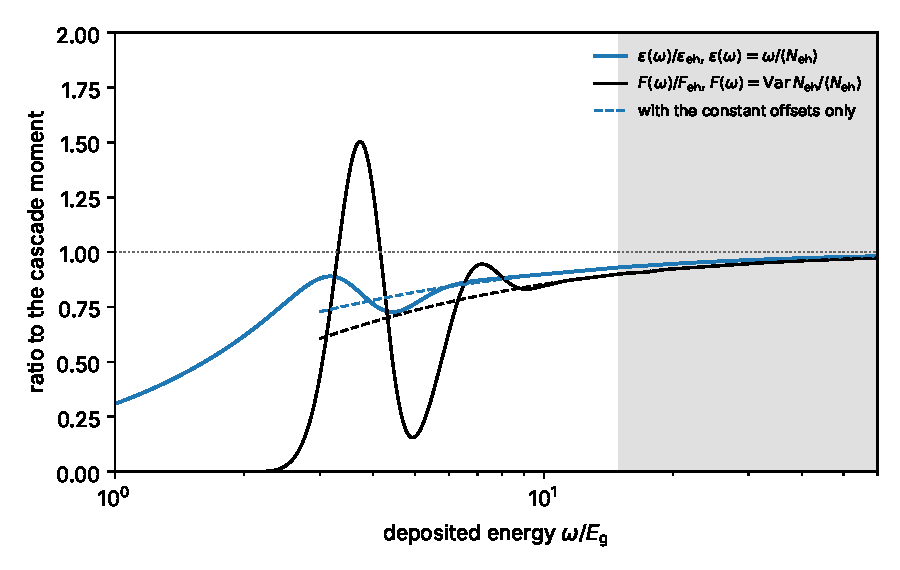
\includegraphics[width=\linewidth]{figures/ch18/limit18_2a.pdf}
\captionof{figure}{Pair energy (blue) and Fano factor (black) of a deposit $\omega$ in silicon, in units of their high-energy limits $\varepsilon_{\mathrm{eh}} = 3.232\,\Eg$ and $F_{\mathrm{eh}} = 0.114$, against $\omega/\Eg$. Energy-only random-$k$ cascade with $\Eg = \SI{1.160}{eV}$, $\omega_{\mathrm{AB}} = \SI{63}{meV}$, $A_{\mathrm{AB}} = \SI{5.703}{eV^3}$, $\theta_{\mathrm{ii}} = 1$, hole band width \SI{12}{eV}; seed electron with all of $\omega - \Eg$, hole at the band edge; moment recursions on a grid of step $\Eg/74$, the ratios taken on that grid. Dashed: the limits corrected by the constant terms only, $\varepsilon(\omega)/\varepsilon_{\mathrm{eh}} = (1 + b_N\varepsilon_{\mathrm{eh}}/\omega)^{-1}$ and $F(\omega)/F_{\mathrm{eh}} = (1 + c_N\varepsilon_{\mathrm{eh}}/F_{\mathrm{eh}}\omega)(1 + b_N\varepsilon_{\mathrm{eh}}/\omega)^{-1}$, with the constant terms of this seed fitted between 30 and $60\Eg$ ($b_N$ of \cref{sec:18.3-limits}, $c_N = -0.02$; the slopes are fitted between 20 and $40\Eg$). Gray: $\omega \ge 14.9\,\Eg = \SI{17.3}{eV}$, where both ratios lie within \SI{10}{\percent} of 1.}\label{fig:18-limit-moments}
\par}
\smallskip
Below about $15\Eg$ the yield rises in steps of one pair, and $F(\omega)$ swings between 0 and $1.5\,F_{\mathrm{eh}}$, so that a search at a few pairs needs the full distribution of the pair number (\cref{sec:18.3}) rather than two moments.
\end{limitbox}

At $\omega \le 2\Eg$ the seed electron cannot ionize and $F(\omega) = 0$: one pair, always. The first ionizations then make the variance rise and fall as each new pair becomes possible. Above $10\Eg$ the constant terms describe the approach to within \SI{1}{\percent}: at $\omega = 10\Eg$ the computed ratios differ from the dashed curves by \SI{0.07}{\percent} in $\varepsilon$ and \SI{0.9}{\percent} in $F$.

\subsection{The three variance terms in silicon}\label{sec:18.2-silicon}

In silicon the three terms of \cref{eq:18.2-decomp} are $\mathcal{V}_< = 0.092$, $\mathcal{V}_> = 0.290$ and $2\mathcal{V}_{<>} = -0.268$, and they add to $F_{\mathrm{eh}} = 0.114$. The largest term is not the residual energy below threshold but the phonon energy above it. The mean phonon energy emitted above threshold is \SI{0.92}{eV} per pair, about 15 phonons of \SI{63}{meV}. If those phonons were independent emissions, their number would be Poisson, $\operatorname{Var}E_> = \omega_{\mathrm{AB}}\langle E_>\rangle$, and $\mathcal{V}_> = w_{\mathrm{AB}}\langle E_>\rangle/(\Eg\bar n) = 0.043$. The computed term is 6.7 times larger. The reason is the steep energy dependence of \cref{eq:18.1-randomk}. Within a few phonon steps of threshold the probability that the next collision ionizes is below $10^{-4}$; it is 0.004 at \SI{2}{eV} and reaches a few percent only at 2.5 to \SI{3}{eV} (\cref{app:E.13}). As a result, a carrier in this range emits a run of phonons whose length has a long, nearly geometric tail. Two carriers that start at the same energy can end their runs many phonons apart.

Most of this variance is canceled by the covariance, which removes \SI{92}{\percent} of $\mathcal{V}_>$. Energy conservation along each carrier line ties the two heats together. A carrier that emits more phonons just above threshold either falls below threshold with a smaller residual, or ionizes later, at a lower energy, into smaller products. What a long run of phonons adds to $E_>$, it takes from $E_<$. The net Fano factor is therefore a small difference of two large terms, which has a practical consequence for any calculation: an error of \SI{1}{\percent} in $\mathcal{V}_>$ alone moves $F_{\mathrm{eh}}$ by \SI{2.5}{\percent}. The covariance is the correlation between the two kinds of heat along one line of descent, not between sibling carriers.

\Cref{fig:18-decomp} follows the three terms as phonon emission grows stronger, at the phonon step of silicon. Without phonons, $E_> = 0$ and $F_{\mathrm{eh}} = \mathcal{V}_<$ is pure partition noise: the scatter of the residual energies with which the carriers end, 0.081 for parabolic bands at $\theta_{\mathrm{ii}} = 1$. At $\lambda_{\mathrm{AB}} = 0.003$ the phonon term is still small, $\mathcal{V}_> = 0.009$, and the covariance is positive, $+0.010$. From $\lambda_{\mathrm{AB}} \approx 0.1$ on, both large terms grow, until at $\lambda_{\mathrm{AB}} = 30$ they reach $\mathcal{V}_> = 0.55$ and $2\mathcal{V}_{<>} = -0.61$. Across these four decades $F_{\mathrm{eh}}$ itself rises only from 0.085 to 0.132, and for $\lambda_{\mathrm{AB}}$ between 1 and 10 it stays between 0.105 and 0.122. In this model a Fano factor near 0.11 is generic for a semiconductor. A full-band cascade of silicon with no fitted constant gives the same 0.114 (\cref{sec:18.4-three}). The measured value tests the shape of the rate ratio within a few phonon energies of threshold, where the two large terms are made, more than it tests the constant $A_{\mathrm{AB}}$ (\cref{sec:18.4}).

\begin{figure}[tbp]
  \centering
  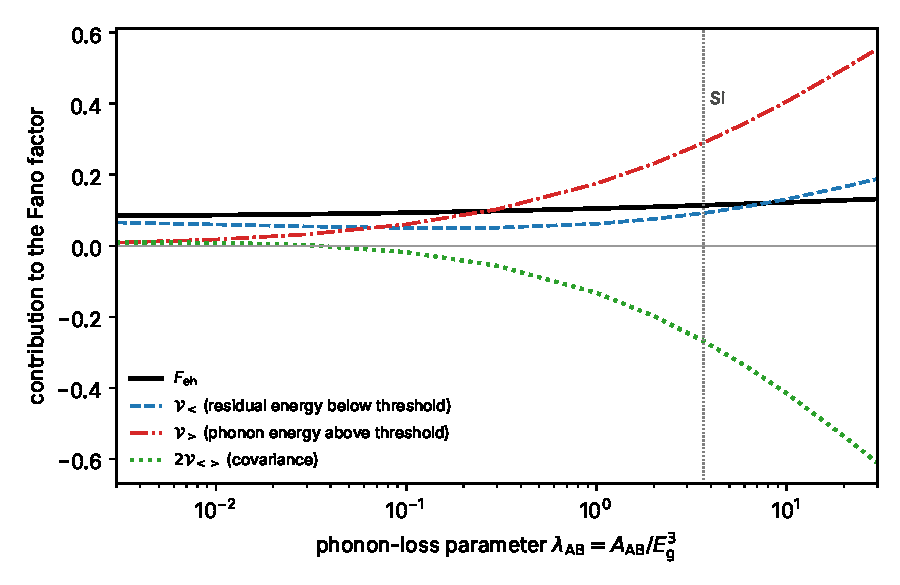
\includegraphics[width=0.85\linewidth]{figures/ch18/fig18_2.pdf}
  \caption{Fano factor $F_{\mathrm{eh}}$ (solid) and its three terms, \cref{eq:18.2-decomp}, against the phonon-loss parameter $\lambda_{\mathrm{AB}} = A_{\mathrm{AB}}/\Eg^3$ at the phonon step of silicon, $w_{\mathrm{AB}} = \omega_{\mathrm{AB}}/\Eg = 0.0543$. Dashed: $\mathcal{V}_<$, from the residual energies of the carriers when they fall below threshold; dash-dotted: $\mathcal{V}_>$, from the phonon energy emitted above threshold; dotted: $2\mathcal{V}_{<>}$, their covariance. Energy-only random-$k$ cascade with parabolic densities of states, $\theta_{\mathrm{ii}} = 1$, hole band width $12\,\mathrm{eV}/\Eg$; asymptotic slopes for seed energies between $X/2$ and $X$, $X = 40\Eg$ ($60\Eg$ for $\lambda_{\mathrm{AB}} > 5$); moment recursions on grids of step $\Eg/74$ and $\Eg/148$, extrapolated to zero step. The vertical line marks silicon, $\lambda_{\mathrm{AB}} = 3.654$, where the terms are $0.092 + 0.290 - 0.268 = 0.114$.}
  \label{fig:18-decomp}
\end{figure}

\subsection{The random-parking limit}\label{sec:18.2-parking}

One limit of the cascade has an exact solution. Take a constant electron density of states, a valence band so narrow that every hole is born at the band edge, $\theta_{\mathrm{ii}} = 1$, and no phonons. An electron of kinetic energy $x \ge \Eg$ then ionizes into a hole at rest and two electrons that share $x - \Eg$ with uniform probability, since the joint density of states of \cref{eq:18.1-phase} is flat on the line $x_1 + x_2 = x - \Eg$. In units of $\Eg$ this is the random parking problem of R\'enyi~\cite{subashiev2010correlation}. A car of unit length parks at a uniformly random place in a free gap of length $x$ and leaves two gaps, which are filled in the same way until every gap is shorter than a car. The jamming density $\rho_\infty$, the number of cars per unit length at the end, is the number of pairs per unit energy, so that $\varepsilon_{\mathrm{eh}} = \Eg/\rho_\infty$. Subashiev and Luryi proposed this limit as a test of Fano-factor models, since both moments are known exactly~\cite[Sect.~I]{subashiev2010correlation}. \Cref{we:18-parking} derives them from the recursions of \cref{sec:18.2-heat}.

\begin{workedexample}{The random-parking Fano factor}\label{we:18-parking}
Measure energies in units of $\Eg$. Let $M(x)$ be the mean number of new pairs made by an electron of kinetic energy $x$. The hole of each ionization is terminal with zero residual, and the two electrons share $x - 1$ uniformly, so \cref{eq:C.11-mean} with one pair per ionization reads $M(x) = 0$ for $x < 1$ and
\begin{equation*}
  M(x) = 1 + \frac{2}{x - 1}\int_0^{x - 1}M(y)\,\dd y , \qquad x \ge 1 .
\end{equation*}
Put $x = z + 1$ and multiply by $z$: $zM(z + 1) = z + 2\int_0^zM(y)\,\dd y$. Take the Laplace transform $m(s) = \int_0^\infty\ee^{-sx}M(x)\,\dd x$. Since $M$ vanishes below 1, the transform of $M(z + 1)$ is $\ee^sm(s)$, and multiplication by $z$ becomes $-\dd/\dd s$. With $\phi(s) = \ee^sm(s)$,
\begin{equation*}
  \phi'(s) + \frac{2\ee^{-s}}{s}\,\phi(s) = -\frac{1}{s^2} , \qquad
  \phi(s) = \int_s^\infty\frac{\dd t}{t^2}\,\exp\bigl[2E_1(s) - 2E_1(t)\bigr] ,
\end{equation*}
the solution that vanishes as $s \to \infty$, with $E_1(s) = \int_s^\infty\ee^{-u}u^{-1}\dd u$ the exponential integral. For every $s > 0$, exactly, $E_1(s) = -\gamma_{\mathrm{E}} - \ln s + \mathrm{Ein}(s)$, with Euler's constant $\gamma_{\mathrm{E}}$ and $\mathrm{Ein}(s) = \int_0^s(1 - \ee^{-u})u^{-1}\dd u \to 0$. Hence $\ee^{2E_1(s)} \to \ee^{-2\gamma_{\mathrm{E}}}/s^2$ as $s \to 0$, and inserting the same identity for $E_1(t)$ under the integral,
\begin{equation*}
  m(s) \to \frac{\rho_\infty}{s^2} , \qquad
  \rho_\infty = \int_0^\infty\exp\bigl[-2\,\mathrm{Ein}(t)\bigr]\,\dd t = 0.74759792 .
\end{equation*}
A double pole $\rho_\infty/s^2$ is the transform of $\rho_\infty x$, so $M(x) \to \rho_\infty x$: the pair energy is $\varepsilon_{\mathrm{eh}} = \Eg/\rho_\infty = 1.3376\,\Eg$. The second moment obeys \cref{eq:C.11-second} with the same kernel. Solved on grids of step 0.01 and 0.005 and extrapolated linearly in the step, it yields $F_{\mathrm{eh}} = 0.051040$ and $1/\varepsilon_{\mathrm{eh}} = 0.747599$, against the closed form $F_{\mathrm{park}} = 0.0510387$~\cite[Eq.~(44)]{subashiev2010correlation}.

The renewal estimate of \cref{sec:18.2-renewal} needs only the final state. At jamming, the number of gaps of size $g$ per unit length is~\cite[Eq.~(19)]{subashiev2010correlation}
\begin{equation*}
  G(g) = 2\int_0^\infty t\,\exp\bigl[-gt - 2\,\mathrm{Ein}(t)\bigr]\,\dd t , \qquad 0 \le g \le 1 .
\end{equation*}
Each gap is the residual energy of one terminal electron, and there is one per pair. Integrating, $\int G\,\dd g = \rho_\infty$ (one gap per car) and $\int(1 + g)G\,\dd g = 1$ (cars and gaps fill the line), both to 30 digits. Each pair costs $1 + g$, with $\langle g\rangle = 0.337617 = 1/\rho_\infty - 1$ and $\operatorname{Var}g = 0.079437$, so that \cref{eq:18.2-ren} gives
\begin{equation*}
  F_{\mathrm{ren}} = \frac{\operatorname{Var}g}{(1 + \langle g\rangle)^2} = 0.0443977 = 0.870\,F_{\mathrm{park}} .
\end{equation*}
The final-state statistics are exact here, and still the estimate misses \SI{13}{\percent} of the Fano factor. (The values printed in Ref.~\cite{subashiev2010correlation}, $\rho_\infty = 0.7475987$ and 0.0439766, carry misprints in the seventh and third digits.)
\end{workedexample}

Silicon is far from this limit in two ways. Its densities of states rise as $x^{1/2}$, and phonons compete with ionization. The density of states alone, at $\lambda_{\mathrm{AB}} \to 0$, raises $\varepsilon_{\mathrm{eh}}$ from $1.338\,\Eg$ to $1.585\,\Eg$ and $F_{\mathrm{eh}}$ from 0.051 to 0.081. \Cref{lim:18.2b} keeps the parking kernel and adds the phonons.

\begin{limitbox}[Random-parking limit][lim:18.2b]
For a constant electron density of states, holes born at the band edge, $\theta_{\mathrm{ii}} = 1$ and no phonons, the cascade is R\'enyi's random parking, with $\Eg/\varepsilon_{\mathrm{eh}} = \rho_\infty = \int_0^\infty\ee^{-2\,\mathrm{Ein}(t)}\dd t = 0.74759792$~\cite[Eq.~(23)]{subashiev2010correlation} and $F_{\mathrm{eh}} = F_{\mathrm{park}} = 0.0510387$~\cite[Eq.~(44)]{subashiev2010correlation}.
\par\smallskip
{\centering
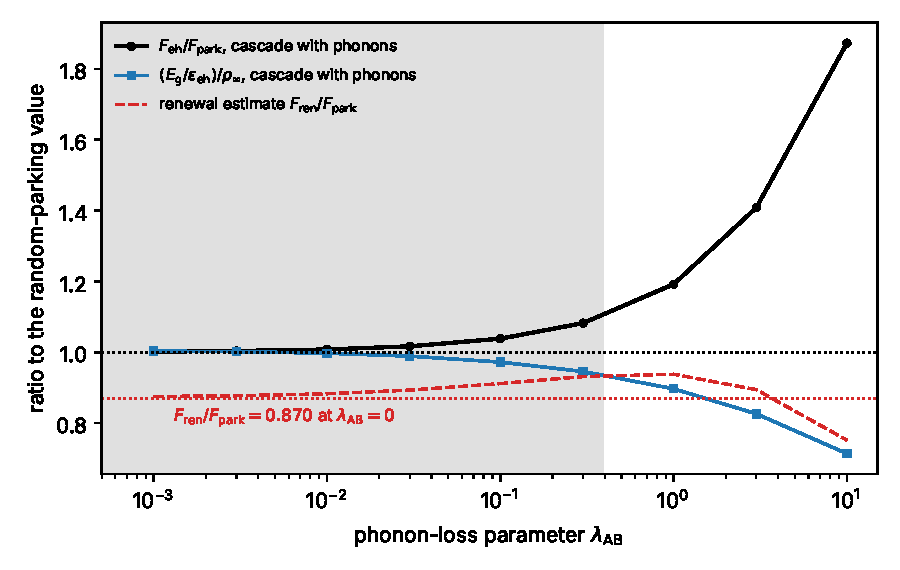
\includegraphics[width=\linewidth]{figures/ch18/limit18_2b.pdf}
\captionof{figure}{The parking kernel with phonons: $F_{\mathrm{eh}}/F_{\mathrm{park}}$ (black) and $(\Eg/\varepsilon_{\mathrm{eh}})/\rho_\infty$ (blue) against $\lambda_{\mathrm{AB}}$, with one phonon step $w_{\mathrm{AB}} = 0.0543$ (silicon) and the phonon-to-ionization ratio $\lambda_{\mathrm{AB}}/(x/\Eg - 1)$ of \cref{eq:18.1-randomk} for a constant density of states, where $\mathfrak{P}(y) = y$ and $A_{\mathrm{AB}}$ carries eV, so that here $\lambda_{\mathrm{AB}} = A_{\mathrm{AB}}/\Eg$. Dashed red: the renewal estimate $F_{\mathrm{ren}}$ of \cref{eq:18.2-rencasc}; dotted red: its parking value 0.870. Moment recursions on a grid of step $\Eg/74$, which places the values at $\lambda_{\mathrm{AB}} \to 0$ \SI{0.4}{\percent} ($\rho$) and \SI{0.1}{\percent} ($F$) above the exact ones. Gray: $\lambda_{\mathrm{AB}} < 0.40$, where both ratios are within \SI{10}{\percent} of 1 (bisection in $\ln\lambda_{\mathrm{AB}}$).}\label{fig:18-limit-park}
\par}
\smallskip
For $\lambda_{\mathrm{AB}} \gtrsim 0.4$ the carriers lose their last energy above threshold to phonons, which lowers the pair density and raises $F_{\mathrm{eh}}$, the trend that carries the parking values toward those of silicon.
\end{limitbox}

Relative to the parking values computed on the same grid, the phonons lower $\Eg/\varepsilon_{\mathrm{eh}}$ and raise $F_{\mathrm{eh}}$ by $0.8\,\lambda_{\mathrm{AB}}$ for $\lambda_{\mathrm{AB}} \le 0.003$, and by \SI{3.2}{\percent} and \SI{3.7}{\percent} at $\lambda_{\mathrm{AB}} = 0.1$. At $\lambda_{\mathrm{AB}} = 3$ the parking kernel leads to $F_{\mathrm{eh}} = 0.072$, 1.41 times $F_{\mathrm{park}}$; the rest of the way to the 0.114 of silicon is the shape of the densities of states.

\subsection{The renewal estimate}\label{sec:18.2-renewal}

A shortcut to $F_{\mathrm{eh}}$ uses only the statistics of the final state. Suppose that each pair costs the gap plus a heat $c_i$, that the costs are independent and identically distributed with mean $\varepsilon_{\mathrm{eh}} - \Eg$ and variance $\sigma_{\mathrm{pair}}^2$, and that pairs are made until $\omega$ is spent. This is the single renewal chain of \cref{app:C.11} with one loss per pair, and \cref{eq:C.11-fano} gives $\operatorname{Var}N_{\mathrm{eh}} \simeq \sigma_{\mathrm{pair}}^2\omega/\varepsilon_{\mathrm{eh}}^3$, that is,
\begin{equation}
  F_{\mathrm{ren}} = \frac{\sigma_{\mathrm{pair}}^2}{\varepsilon_{\mathrm{eh}}^2} ,
  \label{eq:18.2-ren}
\end{equation}
the uncorrelated final-state estimate of Subashiev and Luryi~\cite[Eq.~(7)]{subashiev2010correlation}. The denominator is $\varepsilon_{\mathrm{eh}}$, not $\Eg$. With $N_{\mathrm{eh}}$ held fixed, the heat would scatter by $\bar n\sigma_{\mathrm{pair}}^2$, and \cref{eq:18.2-moments} would give $\sigma_{\mathrm{pair}}^2/\Eg^2$. At fixed $\omega$, however, a pair that costs more heat leaves less energy for the pairs after it, and this constraint multiplies the variance by $(\Eg/\varepsilon_{\mathrm{eh}})^2$.

In a cascade the costs are built from computed statistics. Each pair ends with one terminal electron and one terminal hole, whose residual energies have the variances $\sigma_{\mathrm{e}}^2$ and $\sigma_{\mathrm{h}}^2$, and the phonon heat above threshold is taken as Poisson. Then
\begin{equation}
  F_{\mathrm{ren}} = \frac{\sigma_{\mathrm{e}}^2 + \sigma_{\mathrm{h}}^2 + \omega_{\mathrm{AB}}\langle E_>\rangle/\bar n}{\varepsilon_{\mathrm{eh}}^2} ,
  \label{eq:18.2-rencasc}
\end{equation}
which keeps the one-carrier statistics of the final state exactly and drops every correlation. In random parking it is the gap-law value 0.0443977 of \cref{we:18-parking}. \Cref{lim:18.2c} compares it with the full $F_{\mathrm{eh}}$.

\begin{limitbox}[Renewal estimate of the Fano factor][lim:18.2c]
For independent, identically distributed costs per pair with variance $\sigma_{\mathrm{pair}}^2$, the Fano factor is $F_{\mathrm{ren}} = \sigma_{\mathrm{pair}}^2/\varepsilon_{\mathrm{eh}}^2$~\cite[Eq.~(7)]{subashiev2010correlation}, built for the cascade as \cref{eq:18.2-rencasc}.
\par\smallskip
{\centering
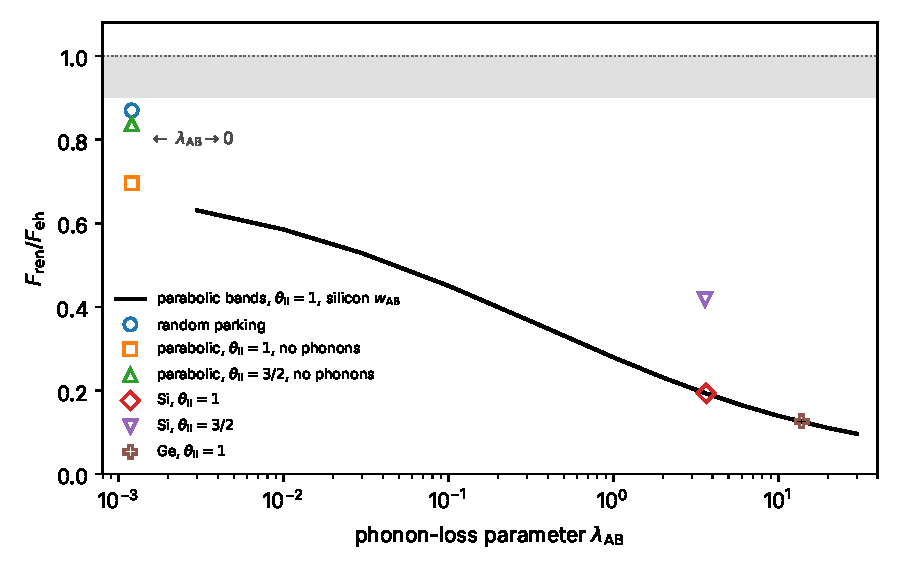
\includegraphics[width=\linewidth]{figures/ch18/limit18_2c.pdf}
\captionof{figure}{Ratio of the renewal estimate \cref{eq:18.2-rencasc} to the full Fano factor \cref{eq:18.2-decomp} against $\lambda_{\mathrm{AB}}$. Line: parabolic densities of states, $\theta_{\mathrm{ii}} = 1$, $w_{\mathrm{AB}} = 0.0543$, hole band width $12\,\mathrm{eV}/\Eg$ (the kernel of \cref{fig:18-decomp}). Markers at $\lambda_{\mathrm{AB}} \to 0$, extrapolated from grid steps 0.01 and $0.005\,\Eg$: random parking (0.870), parabolic bands without phonons at $\theta_{\mathrm{ii}} = 1$ (0.696) and $3/2$ (0.837). Further markers: silicon at $\theta_{\mathrm{ii}} = 1$ (0.193) and at $\theta_{\mathrm{ii}} = 3/2$ with $A_{\mathrm{AB}}$ recalibrated to the pair energy, \SI{5.629}{eV^3} (0.418); germanium with $\Eg = \SI{0.744}{eV}$, $\omega_{\mathrm{AB}} = \SI{37.6}{meV}$, the silicon $A_{\mathrm{AB}}$ and the hole density of states cut at the germanium valence-band width, \SI{12.6}{eV}~\cite[Table~II]{rideau2006strained} (0.126). Markers and line are continuum limits of the moment recursions. The gray band, within \SI{10}{\percent} of the full value, contains no computed case.}\label{fig:18-limit-renewal}
\par}
\smallskip
The estimate drops the correlations of the cascade, all of which raise the variance here: it lies below $F_{\mathrm{eh}}$ in every computed case, by \SI{13}{\percent} in random parking, by a factor 5 in silicon and by a factor 8 in germanium.
\end{limitbox}

The ratio falls from 0.70 to 0.10 as $\lambda_{\mathrm{AB}}$ grows, because the phonon heat above threshold is far from Poisson (\cref{sec:18.2-silicon}), while \cref{eq:18.2-rencasc} counts it as Poisson and has no covariance term at all. Without phonons the gap is smaller but still there: $F_{\mathrm{eh}} - F_{\mathrm{ren}} = 0.025$ at $\theta_{\mathrm{ii}} = 1$ and 0.013 at $\theta_{\mathrm{ii}} = 3/2$, with exact one-carrier statistics. This difference measures every departure from independent, identical costs together: correlations between the products of one ionization, between the electron and the hole of one pair, and between distant carriers, and the differences between the cost laws of different pairs. It does not isolate any one of them. In random parking Subashiev and Luryi find the correlation correction positive at intermediate filling and at jamming, and they note that correlations between the two halves of a split are not the only ones~\cite[Sect.~IV]{subashiev2010correlation}. A Fano factor fitted with a final-state model therefore needs a broader residual distribution, or a larger phonon variance, than the cascade actually has.

\subsection{The linear mean yield}\label{sec:18.2-linear}

The definitions \cref{eq:18.2-moments} assume that $\bar n$ grows in proportion to $\omega$. For a single chain of independent losses, \cref{app:C.11} proved this with the key renewal theorem, \cref{eq:C.11-linear}. The cascade is not a single chain, since an ionization splits the energy among three carriers, and no loss law is common to all its steps. The leading term still follows from renewal theory if we follow a unit of energy instead of a carrier. Give each ionization of a carrier at kinetic energy $x$ the weight 1, spread evenly over the $x$ units of energy that the carrier holds. The number of ionizations in a cascade started at kinetic energy $E$ is then the integral of the collected weights over all units. Taking the mean,
\begin{equation}
  \bar n_{\mathrm{sub}}(E) = E\,\Bigl\langle\sum_j\frac{1}{x_j}\Bigr\rangle_u ,
  \label{eq:18.2-tagged}
\end{equation}
where $u$ is a unit chosen uniformly in $[0, E]$, the sum runs over the ionizations along the chain of carriers that hold $u$, $x_j$ is the kinetic energy of the holder at the $j$-th of them, and $\langle\cdots\rangle_u$ is the mean over $u$ and over the cascade. A holder that emits phonons first ionizes below the energy at which it received the unit; $x_1 = E$ only if the first collision of the seed carrier is an ionization. The carriers that hold one unit form a chain. At an ionization the unit passes to one of the three products with probability equal to that product's share of the energy, or it leaves the chain into the gap of the new pair, with probability $\Eg/x$. At a phonon emission it leaves with probability $\omega_{\mathrm{AB}}/x$. \Cref{app:D.44} shows that \cref{eq:18.2-tagged} is exact for any branching law that conserves energy.

At high energy the shares no longer depend on $x$. In the random-$k$ model the products divide $x - \Eg$ in proportions whose law tends to a fixed law, and the probability of leaving into the gap falls as $\Eg/x$. The logarithm $\ln x_j$ thus performs a random walk with steps $\ln(x_{j+1}/x_j) \le 0$ whose law becomes independent of $x$. By the renewal theorem in the variable $\ln x$, the distribution with which the walk first arrives in the region within a few gaps of threshold converges as $E \to \infty$. The sum in \cref{eq:18.2-tagged} is dominated by that region, since the high-energy terms are small, $1/x_j$ each. Its mean converges. With the seed pair counted,
\begin{keyresult}[Linear mean yield]
\begin{equation}
  \bar n(\omega) = \frac{\omega}{\varepsilon_{\mathrm{eh}}} + o(\omega) , \qquad
  \frac{1}{\varepsilon_{\mathrm{eh}}} = \lim_{E\to\infty}\Bigl\langle\sum_j\frac{1}{x_j}\Bigr\rangle_u ,
  \label{eq:18.2-linear}
\end{equation}
for any energy-conserving cascade whose share law becomes independent of the energy at high energy, approaches that limit fast enough, is not concentrated on a lattice in $\ln x$, and is regular near threshold. \Cref{app:D.44} states the four conditions and gives the proof.
\end{keyresult}
\noindent The share law must be spread out in $\ln x$. A cascade that always splits in fixed proportions would make the walk lattice, and $\bar n/\omega$ would oscillate in $\ln\omega$ forever instead of converging.

Two statements that the definitions also use are not part of \cref{eq:18.2-linear}. The first is the constant term $b_N$, which depends on the seed (\cref{sec:18.3-limits}). In the one-phonon model every energy loss is a whole combination of $\Eg$ and $\omega_{\mathrm{AB}}$, and as for the deterministic chain of \cref{app:C.11} the constant then carries a periodic remainder that never dies out. We can therefore fit the slopes over a range of seed energies, $[X/2, X]$, which averages the remainder. The second is the linear growth of the variance, $\operatorname{Var}N_{\mathrm{eh}} = F_{\mathrm{eh}}\omega/\varepsilon_{\mathrm{eh}} + O(1)$, which the computed slopes obey but which needs the same second-order estimates as $b_N$.

\subsection{Constant term and the renewal bound}\label{sec:18.2-open}

The constant term and the variance of the yield at second order in renewal theory have not been derived for the branching cascade. The expansions $\bar n = \omega/\varepsilon_{\mathrm{eh}} + b_N + o(1)$ and $\operatorname{Var}N_{\mathrm{eh}} = F_{\mathrm{eh}}\omega/\varepsilon_{\mathrm{eh}} + O(1)$ need second-order estimates for the walk of \cref{eq:18.2-tagged} and the rate at which the cascade forgets its seed, and neither is in hand. The constant matters at a few pairs: at \SI{10}{eV} in silicon, $\omega/\varepsilon_{\mathrm{eh}} = 2.67$, and the constant term of the one-sided seed adds \SI{13}{\percent} to it. The second open question is whether the renewal estimate \cref{eq:18.2-rencasc} is a lower bound on $F_{\mathrm{eh}}$ for every cascade of this class. It is in every case computed here and in random parking, but there is no proof. A proof would make the final-state statistics a guaranteed floor for the Fano factor, and a counterexample would show which correlations can lower the variance.

\section{Seed distributions and the step model}\label{sec:18.3}

At $\omega = \SI{5}{eV}$ in silicon the step model of \cref{eq:1.5-step} puts every event in the two-pair bin. The cascade of \cref{sec:18.1}, with the constant calibrated in \cref{sec:18.4}, puts two pairs in \SI{17}{\percent} of the events started by a dark-matter kick at $q_0 = \alpha m_e$ and one pair in the rest. A search with a two-pair threshold therefore records about one in six of the \SI{5}{eV} events that the step model predicts. The cascade differs from the step model in two respects: how the \SI{3.84}{eV} above the gap is shared between the electron and the hole, and how often each carrier emits a phonon instead of ionizing at a few eV. The energy sharing and the phonon emission both enter through the hand-off \cref{eq:8.7-cond}. Once a final-state class has been turned into the energies of its two carriers, the generating function of \cref{sec:18.1} yields the whole pair-number distribution. The step model and a cascade seeded by a fixed split of the energy are limits of the pair-number distribution that replace the seed by a rule, and they fail in the few-pair bins, where the rule matters most.

\subsection{The seed distribution}\label{sec:18.3-seed}

A final-state class $\Lambda$ of the zero-phonon pair sector puts an electron at $E_{\mathrm{e}}(\Lambda)$ above the conduction minimum and a hole at $E_{\mathrm{h}}(\Lambda)$ below the valence maximum, with $E_{\mathrm{e}} + E_{\mathrm{h}} = \omega - \Eg$. In the energy-only reduction of \cref{sec:18.1-reductions} the cascade of the pair depends on these two energies; the crystal momenta $\vect{k} + \vect{q}$ and $\vect{k}$ matter only for the first collisions. Keeping the energies and dropping the momenta loses the first-generation memory that \cref{sec:18.1-reductions} locates. The input from the dark-matter interaction is then a distribution of carrier energies. The \emph{seed distribution} at momentum transfer $\vect{q}$, energy $\omega$ and velocity $\vect{v}$ is
\begin{equation}
  P_{\mathrm{seed}}(E_{\mathrm{e}},E_{\mathrm{h}}|\vect{q},\omega,\vect{v}) = \frac{\sum_\Lambda\sum_{a,b}\mathfrak{D}_{ab}(\vect{q},\vect{v})\,S_{ab}(\vect{q},\omega;\Lambda)\,\delta\bigl(E_{\mathrm{e}} - E_{\mathrm{e}}(\Lambda)\bigr)\,\delta\bigl(E_{\mathrm{h}} - E_{\mathrm{h}}(\Lambda)\bigr)}{\sum_{a,b}\mathfrak{D}_{ab}(\vect{q},\vect{v})\,S_{ab}(\vect{q},\omega)} ,
  \label{eq:18.3-seed}
\end{equation}
the probability density that the interaction leaves the electron at $E_{\mathrm{e}}$ and the hole at $E_{\mathrm{h}}$. The class-resolved responses add up to $S_{ab}(\vect{q},\omega)$ by \cref{eq:8.7-resolved}, so $P_{\mathrm{seed}}$ integrates to one when every class at $(\vect{q},\omega)$ is a pair, and to the pair share of the response otherwise; the other sectors seed their own cascades. A pair made together with a phonon of energy $\omega_{\vect{Q}}$ has $E_{\mathrm{e}} + E_{\mathrm{h}} = \omega - \omega_{\vect{Q}} - \Eg$, and the phonon energy goes to heat once (\cref{sec:8.7}). With one coupling row the seed distribution is independent of $\vect{v}$ and of the dark-matter model, as the class weights of \cref{sec:8.7-handoff} are; with several rows it depends on both. In the zero-phonon sector energy conservation leaves one variable, the electron's share $f_{\mathrm{e}} = E_{\mathrm{e}}/(\omega - \Eg)$ of the energy above the gap.

The generating function of \cref{eq:18.1-seed} turns the seed into a pair number. Keep only the pair-number variable, $s = \ee^{\lambda_N}$, and let $\mathfrak{G}_t(x;s)$ be the energy-only solution of \cref{eq:18.1-backward}: the generating function of the number of ionizations that a carrier of type $t$ at kinetic energy $x$ makes in its subtree. The seed pair is counted by the factor $s$, and the two subtrees are independent, so the cascade distribution of a class is the coefficient
\begin{equation}
  P_{\mathrm{casc}}(N_{\mathrm{eh}}|\Lambda) = [s^{N_{\mathrm{eh}}}]\;s\,\mathfrak{G}_{\mathrm{e}}\bigl(E_{\mathrm{e}}(\Lambda);s\bigr)\,\mathfrak{G}_{\mathrm{h}}\bigl(E_{\mathrm{h}}(\Lambda);s\bigr) ,
  \label{eq:18.3-pcasc}
\end{equation}
where $[s^n]$ takes the coefficient of $s^n$. The cascade distribution depends on $\Lambda$ only through the two carrier energies. Write $P_{\mathrm{casc}}(N_{\mathrm{eh}}|\Lambda)$ as $\int\dd E_{\mathrm{e}}\,\dd E_{\mathrm{h}}\,\delta(E_{\mathrm{e}} - E_{\mathrm{e}}(\Lambda))\,\delta(E_{\mathrm{h}} - E_{\mathrm{h}}(\Lambda))\,P_{\mathrm{casc}}(N_{\mathrm{eh}}|E_{\mathrm{e}},E_{\mathrm{h}})$ inside the class sum of \cref{eq:8.7-cond}, and exchange the sum with the integral. The class sum then becomes the numerator of \cref{eq:18.3-seed}:
\begin{equation}
  P(N_{\mathrm{eh}}|\vect{q},\omega,\vect{v}) = \int\dd E_{\mathrm{e}}\,\dd E_{\mathrm{h}}\;P_{\mathrm{seed}}(E_{\mathrm{e}},E_{\mathrm{h}}|\vect{q},\omega,\vect{v})\;P_{\mathrm{casc}}(N_{\mathrm{eh}}|E_{\mathrm{e}},E_{\mathrm{h}}) .
  \label{eq:18.3-pq}
\end{equation}
The generating function of \cref{eq:18.3-pq} is $s\int P_{\mathrm{seed}}\,\mathfrak{G}_{\mathrm{e}}\mathfrak{G}_{\mathrm{h}}$, a power series with nonnegative coefficients that converges on $|s| \le 1$. The discrete Fourier sum \cref{eq:E.24-dft} of this generating function at $N_z$ roots of unity returns $\sum_jP(N_{\mathrm{eh}} + jN_z)$, the exact probability once $N_z$ exceeds every pair number with appreciable weight.

The backward recursion alone guarantees three things: the pair-number distribution is normalized, it is exactly one pair below $(1 + \theta_{\mathrm{ii}})\Eg$, and its variance splits into a cascade part and a seed part. First, each $\mathfrak{G}_t$ is a probability generating function, because the recursion of \cref{eq:18.1-backward} maps products and mixtures of generating functions to generating functions; \cref{eq:18.3-pq} is then normalized and nonnegative. Second, below $\theta_{\mathrm{ii}}\Eg$ no carrier ionizes, $\mathfrak{G}_t = 1$, and $P_{\mathrm{casc}} = \delta_{N_{\mathrm{eh}}1}$ exactly. The first ionization becomes possible at $\omega = (1 + \theta_{\mathrm{ii}})\Eg$, which is \SI{2.32}{eV} in silicon with $\theta_{\mathrm{ii}} = 1$, for a seed that gives all the energy to one carrier. Third, the moments separate the cascade from the seed. Let $m_t(x)$ and $v_t(x)$ be the mean and variance of the number of ionizations in one subtree, and let $\langle\cdot\rangle_{\mathrm{seed}}$ average over $P_{\mathrm{seed}}$. The law of total variance gives
\begin{equation}
  \langle N_{\mathrm{eh}}\rangle = 1 + \bigl\langle m_{\mathrm{e}}(E_{\mathrm{e}}) + m_{\mathrm{h}}(E_{\mathrm{h}})\bigr\rangle_{\mathrm{seed}} , \qquad
  \operatorname{Var}N_{\mathrm{eh}} = \bigl\langle v_{\mathrm{e}} + v_{\mathrm{h}}\bigr\rangle_{\mathrm{seed}} + \operatorname{Var}_{\mathrm{seed}}\bigl(m_{\mathrm{e}} + m_{\mathrm{h}}\bigr) .
  \label{eq:18.3-moments}
\end{equation}
The second term of the variance is the spread of the subtree means over the seed. It vanishes when $m_{\mathrm{e}} + m_{\mathrm{h}}$ takes one value on the whole support of the seed, for a single split and in the forced region $\omega < (1 + \theta_{\mathrm{ii}})\Eg$, where both means are zero.

$P_{\mathrm{seed}}$ is the per-pair weight of \cref{eq:8.7-IP} or of the screened form \cref{eq:8.7-screened}, binned in the two carrier energies; a library of computed responses stores $P_{\mathrm{seed}}$ in this binned form. With the functions $\mathfrak{G}_t$ tabulated on an energy grid, the seeded distribution costs one integral per momentum transfer, energy and pair of coupling rows.

\subsection{Pair-number distributions in silicon}\label{sec:18.3-silicon}

\Cref{fig:18-pn10} shows \cref{eq:18.3-pq} at $\omega = \SI{10}{eV}$ for six seeds run through one cascade. The cascade is the random-$k$ model of \cref{sec:18.1-reductions} with the silicon parameters of \cref{sec:18.2-heat}. The dark-matter seed comes from the empirical-pseudopotential bands of \cref{we:8-pairs}: the pair weights of the density at $\vect{q}_0 = \alpha m_e\hat{\vect{x}}$, without screening. The photon seed is the optical limit of the same bands. The model bands have a gap of \SI{0.82}{eV}, so each band seed is taken at the same excess energy $\omega - \Eg$ as the cascade uses. To compare two pair-number distributions we use the total-variation distance $d_{\mathrm{TV}}(P,Q) = \tfrac12\sum_N|P(N) - Q(N)|$, which is the largest difference between the probabilities that the two distributions assign to any set of pair numbers, for instance to the events above a search threshold. Screening hardly moves the energy shares: at \SI{10}{eV} the screened out-state seed of \cref{we:8-pairs} and its unscreened counterpart give distributions with $d_{\mathrm{TV}} = 0.010$.

\begin{figure}[tbp]
  \centering
  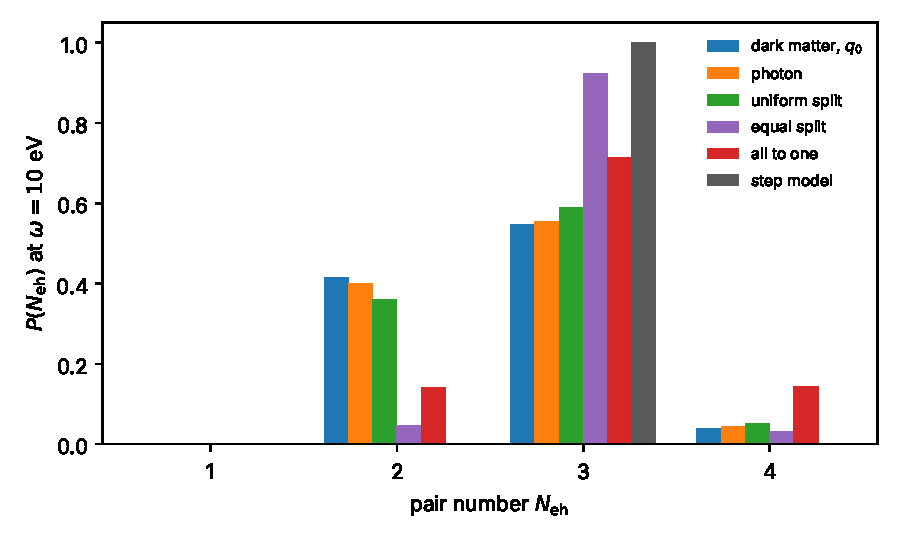
\includegraphics[width=0.85\linewidth]{figures/ch18/fig18_3.pdf}
  \caption{Pair-number distribution $P(N_{\mathrm{eh}})$ at $\omega = \SI{10}{eV}$ in silicon, \cref{eq:18.3-pq}, for six seeds in one cascade: the energy-only random-$k$ model of \cref{sec:18.1-reductions} with $\Eg = \SI{1.160}{eV}$, $\omega_{\mathrm{AB}} = \SI{63}{meV}$, $\theta_{\mathrm{ii}} = 1$, holes below \SI{12}{eV} and $A_{\mathrm{AB}} = \SI{5.703}{eV^3}$, calibrated to $\varepsilon_{\mathrm{eh}} = \SI{3.749}{eV}$. The band seeds are a dark-matter kick at $q_0 = \alpha m_e$ along [100] (independent-particle pair weights of the density, empirical-pseudopotential bands of \cref{we:8-pairs}) and an absorbed photon (optical limit of the same bands). The other four seeds are the fixed splits of \cref{sec:18.3-limits} (uniform, equal, and all the energy to one carrier) and the step model \cref{eq:1.5-step} with $\varepsilon_{\mathrm{eh}} = \SI{3.749}{eV}$. Band seeds are used at the excess energy $\omega - \Eg$ of the model bands, whose gap is \SI{0.82}{eV}. Means: 2.626 (dark matter), 2.645 (photon), 2.691, 2.985 and 3.003 (the three splits), 3 (step model). $P(1)$ and $P(5)$ are below 0.002 for every seed. Probabilities from the generating function at $N_z = 32$ roots of unity; no distribution in this section has a mean above six.}
  \label{fig:18-pn10}
\end{figure}

The dark-matter seed yields two pairs with probability 0.414, three with 0.547 and four with 0.039. The mean, 2.626 pairs, corresponds to \SI{3.81}{eV} per pair, \SI{1.6}{\percent} above the high-energy pair energy. The photon seed yields 0.400, 0.555 and 0.045, and its mean is 2.645. The step model puts every event in the three-pair bin; it overstates the mean by \SI{14}{\percent} and misses the two-pair bin entirely. Of the three splits of \cref{sec:18.1-seed}, the equal split puts three pairs in \SI{92}{\percent} of events, the uniform split behaves like the band seeds, and giving everything to one carrier fills the four-pair bin with probability 0.143.

The variance shows where the seed enters. For the dark-matter seed \cref{eq:18.3-moments} splits $\operatorname{Var}N_{\mathrm{eh}} = 0.314$ into 0.283 from the subtrees and 0.031 from the spread of the seed. The equal split has no seed term, and its variance is 0.079, a quarter of the band-seed value. The subtree mean is far from linear in the share: at $f_{\mathrm{e}} = \tfrac14$, \SI{2.21}{eV} on one carrier and \SI{6.63}{eV} on the other, the two carriers make 2.436 pairs, against 2.985 at the equal split and 3.003 with all \SI{8.84}{eV} on one carrier. A carrier at \SI{2.21}{eV} almost never ionizes, while one at \SI{4.42}{eV} usually does once, so the count depends on how many carriers end up a little above \SI{4}{eV}.

\begin{workedexample}{The step model against the cascade at 5 eV}\label{we:18-step5}
Take $\omega = \SI{5}{eV}$ in silicon with the constants of \cref{fig:18-pn10}. The step model puts $N_{\mathrm{eh}} = 1 + \lfloor(5 - 1.160)/3.749\rfloor = 1 + \lfloor1.024\rfloor = 2$ pairs for every event; the literature values $\Eg = \SI{1.11}{eV}$ and $\varepsilon_{\mathrm{eh}} = \SI{3.6}{eV}$ of \cref{sec:1.5} give 2 as well.

In the cascade, the pair shares $\omega - \Eg = \SI{3.84}{eV}$. Consider first a seed that gives all of it to one carrier. Below $\Eg$ the carrier cannot ionize; above, the probability that its next collision is an ionization is $p_{\mathrm{ii}}(E) = [1 + \varGamma_{\mathrm{ph}}/\varGamma_{\mathrm{ii}}]^{-1}$ from \cref{eq:18.1-randomk}. The ionization probability is 0.0041 at \SI{2}{eV}, 0.0184 at \SI{2.5}{eV}, 0.049 at \SI{3}{eV}, 0.100 at \SI{3.5}{eV} and 0.145 at \SI{3.84}{eV}. As long as the carrier does not ionize, it walks down in steps of $\omega_{\mathrm{AB}}$: from \SI{3.84}{eV} it makes 43 collisions above $\Eg$. The probability that none of them is an ionization is
\begin{equation*}
  P_{\mathrm{no}} = \prod_{k=0}^{42}\bigl[1 - p_{\mathrm{ii}}(3.84\,\mathrm{eV} - k\,\omega_{\mathrm{AB}})\bigr] = 0.176 .
\end{equation*}
Replacing the sum of $-\ln(1 - p_{\mathrm{ii}}) \approx p_{\mathrm{ii}}/(1 - p_{\mathrm{ii}})$ over steps by an integral over energy, $\ln P_{\mathrm{no}} \approx -\omega_{\mathrm{AB}}^{-1}\int_{\Eg}^{3.84\,\mathrm{eV}}\dd E\;\varGamma_{\mathrm{ii}}/\varGamma_{\mathrm{ph}} = -1.735$, which leads to the same 0.176. If the carrier does ionize, the three products share at most $3.84 - 1.16 = \SI{2.68}{eV}$, and a second ionization follows with probability 0.002. This seed therefore leaves one pair with probability 0.176 and two with 0.822. A seed that splits the energy equally leaves two carriers at \SI{1.92}{eV}, each of which escapes ionization with probability 0.990, so that \SI{98}{\percent} of events end with one pair.

The dark-matter seed at $q_0$ lies between the one-sided seed and the equal split. At this energy the electron takes \SI{2.08}{eV} of the \SI{3.84}{eV} on average, and \SI{26}{\percent} of the weight has one carrier with more than three quarters of the energy. Averaging $P_{\mathrm{no}}(E_{\mathrm{e}})P_{\mathrm{no}}(E_{\mathrm{h}})$ over the seed in \cref{eq:18.3-pq} yields
\begin{equation*}
  P(1) = 0.831 , \qquad P(2) = 0.169 , \qquad P(3) = 6\times10^{-5} ,
\end{equation*}
a mean of 1.169 pairs and \SI{4.28}{eV} per pair. Above a two-pair threshold the step model therefore counts 5.9 times as many \SI{5}{eV} events as this cascade does; the full-band cascade of \cref{sec:18.3-fullband} raises the factor to about ten. The photon seed has $P(2) = 0.190$, \SI{12}{\percent} more than the dark-matter seed.
\end{workedexample}

\subsection{The full-band cascade as reference}\label{sec:18.3-fullband}

Every distribution so far comes from the energy-only cascade with its one constant fitted to the measured pair energy. A cascade with no fitted constant replaces the random-$k$ kernels by the kernels of \cref{sec:18.1} on full bands, in the standard full-band Monte Carlo form~\cite{fischetti1988monte}. In the calculation we use as reference, the bands are the empirical pseudopotential bands of Cohen and Bergstresser~\cite{cohen1966band}, with the form factors refit to measured transition energies; impact ionization is the golden rule with the diagonal, statically screened Coulomb kernel~\cite{cappellini1993model}, its direct and exchange terms combined as in Kane's form quoted by Kotani and van Schilfgaarde~\cite[Eq.~(5)]{kotani2010impact}; and phonon emission uses the deformation potentials and phonon energies of Refs.~\cite{lundstrom2000fundamentals,jacoboni1983monte}, \cite[Table~III]{li2021deformation}; the gap is $\Eg = \SI{1.160}{eV}$. The seeds are the pairs a dark-matter particle with a heavy mediator leaves in the same bands, with their crystal momenta. The calculation is varied jointly over the screening (static and dynamic), the phonon couplings (these values against first-principles ones, which weigh electron losses by 0.52 and hole losses by 3.0) and the exchange factor near threshold (0.5 to 1.0), and the ranges below are the envelope of these variants, for pair probabilities with the error of the $\vect{k}$ grid added.

At \SI{5}{eV} the full-band cascade puts two or more pairs in a fraction $0.097$ of the dark-matter events, with the envelope $[0.030, 0.173]$, against the 0.169 of the energy-only cascade in \cref{we:18-step5}. The step model, which puts every event in the two-pair bin, then overcounts that bin about tenfold, and at least sixfold anywhere in the envelope; the thirtyfold end of the envelope comes from one extreme corner alone, static screening of the weaker kind with tripled hole couplings and the lowest exchange factor. The energy-only cascade remains the working model of this chapter, because it is calibrated and fast. Recalibrated to the pair energy of each full-band variant, so that only the shape of the kernels differs, the energy-only cascade lies 0.12 to 0.20 in $d_{\mathrm{TV}}$ from the full-band distribution between 6 and \SI{8}{eV}. The soft onset of impact ionization near threshold matters most in this range, and the distance grows with the pair energy of the variant. On the same footing the uniform split lies 0.11 to 0.12 away, the equal split 0.45 to 0.50 and the step model 0.79 to 0.83.

\subsection{Fixed splits and the step limit}\label{sec:18.3-limits}

A fixed split replaces the seed distribution of \cref{eq:18.3-pq} by a distribution of the electron's share $f_{\mathrm{e}}$ that is the same for every process at a given $\omega$ and symmetric under the exchange of electron and hole. Three fixed splits bracket the range: all the energy on one carrier, a uniform share, and the equal split. The constant term $b_N$ of the mean (\cref{sec:18.2-heat}) depends on the seed. In the cascade of \cref{fig:18-pn10}, with $\omega/\varepsilon_{\mathrm{eh}}$ subtracted at the pair energy of the same calculation, it is 0.008 for the uniform split and 0.35 for a seed that gives all the energy to one carrier.

The step model is the limit in which every pair has a fixed cost. Let the first pair cost $\Eg$ and every further one exactly $\varepsilon_{\mathrm{eh}}$. The energy $\omega - \Eg$ left after the first pair is then spent by a renewal chain with the deterministic loss $\varepsilon_{\mathrm{eh}}$, which fits $\lfloor(\omega - \Eg)/\varepsilon_{\mathrm{eh}}\rfloor$ losses (\cref{app:C.11}). The pair number is
\begin{equation}
  N_{\mathrm{eh}}^{\mathrm{step}}(\omega) = 1 + \left\lfloor\frac{\omega - \Eg}{\varepsilon_{\mathrm{eh}}}\right\rfloor , \qquad P_{\mathrm{casc}}(N_{\mathrm{eh}}|\Lambda) = \delta_{N_{\mathrm{eh}},N_{\mathrm{eh}}^{\mathrm{step}}(\omega)} ,
  \label{eq:18.3-step}
\end{equation}
which is \cref{eq:1.5-step}, with a Fano factor of zero. Both the seed and the competition with phonons have been replaced by one cost per pair. In the forced region, $\omega < (1 + \theta_{\mathrm{ii}})\Eg$, the step model is exact. Above the forced region, even the mean is wrong. Over one period of $\omega$ the floor function loses $\tfrac12$ on average (\cref{app:C.11}), so the step model has the mean $(\omega - \Eg)/\varepsilon_{\mathrm{eh}} + \tfrac12 = \omega/\varepsilon_{\mathrm{eh}} + 0.19$ in silicon, against $\omega/\varepsilon_{\mathrm{eh}} + b_N$ in the cascade, with $b_N$ between 0.008 and 0.35 depending on the seed. This error in the mean falls as $1/\langle N_{\mathrm{eh}}\rangle$. The step-model distribution itself never approaches the cascade distribution. For a single bin $n$ the distance $d_{\mathrm{TV}}$ is $1 - P(n)$. The cascade distribution spreads over a width $\sigma_N = (F_{\mathrm{eh}}\omega/\varepsilon_{\mathrm{eh}})^{1/2}$ that grows with $\omega$: at \SI{20.2}{eV} the computed distribution of the dark-matter seed has $\sigma_N = 0.79$ and its largest bin holds 0.45, so the step model misplaces more than half of the events there, and the misplaced fraction grows with the width.

\Cref{lim:18.3a} compares each phenomenological seed with the dark-matter seed from the gap to \SI{21}{eV}, the range of the few-pair bins in silicon.

\begin{limitbox}[Step model and fixed splits][lim:18.3a]
The step model is \cref{eq:18.3-step}~\cite[Eq.~(5.1)]{essig2016direct}; the three fixed splits above are each run through the cascade by \cref{eq:18.3-pcasc}.
\par\smallskip
{\centering
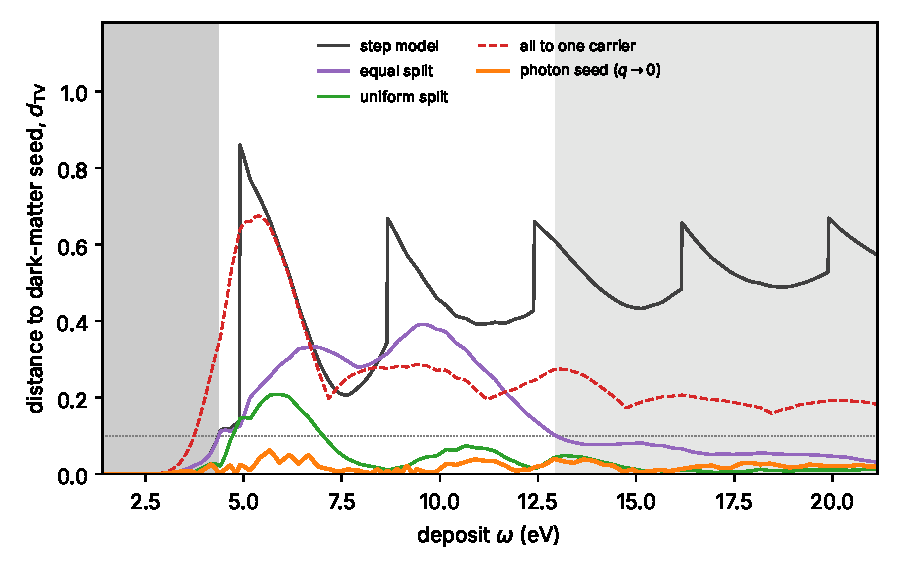
\includegraphics[width=\linewidth]{figures/ch18/limit18_3a.pdf}
\captionof{figure}{Distance $d_{\mathrm{TV}}$ between the pair-number distribution of each phenomenological seed and the distribution of the dark-matter seed at $q_0 = \alpha m_e$ along [100], against the deposit $\omega$ in silicon. All seeds run through one cascade, the energy-only random-$k$ model of \cref{sec:18.1-reductions} with $\Eg = \SI{1.160}{eV}$, $\omega_{\mathrm{AB}} = \SI{63}{meV}$, $\theta_{\mathrm{ii}} = 1$, holes below \SI{12}{eV} and $A_{\mathrm{AB}} = \SI{5.703}{eV^3}$. Black: step model, $\varepsilon_{\mathrm{eh}} = \SI{3.749}{eV}$. Purple, green and red dashed: the equal split, the uniform split and all the energy to one carrier, with the seeds that put a hole above \SI{12}{eV} removed. Orange: the photon ($q \to 0$) seed of the same empirical-pseudopotential bands as the dark-matter seed. Band seeds are computed every \SI{0.25}{eV} of the excess energy $\omega - \Eg$ (model gap \SI{0.82}{eV}) and interpolated linearly; the curves use a \SI{0.02}{eV} grid. Dark gray: $\omega < \SI{4.37}{eV}$, where the step model and the uniform and equal splits are within 0.1 of the dark-matter seed. Light gray: $\omega > \SI{12.95}{eV}$, where the uniform and equal splits are again within 0.1 of the dark-matter seed. Dotted: $d_{\mathrm{TV}} = 0.1$.}\label{fig:18-limit-seed}
\par}
\smallskip
Between \SI{4.4}{eV} and \SI{13}{eV} the split of the energy decides the count, so the split must come from the bands and the operator that made the pair. There the uniform and equal splits reach distances of 0.21 and 0.39, the one-sided split 0.67, and the step model is off by up to 0.86 at its first step, $\omega = \Eg + \varepsilon_{\mathrm{eh}} = \SI{4.91}{eV}$.
\end{limitbox}

Below \SI{4.37}{eV} the step model and the fixed splits hold because few carriers ionize: the dark-matter seed leaves one pair with probability above 0.9, and so does any split that avoids putting the whole energy on one carrier. The distance of the step model exceeds 0.1 from \SI{4.37}{eV} on: at its first step the step model moves every event into the two-pair bin while the cascade puts 0.14 there, and its distance stays above 0.2 up to \SI{21}{eV}, above 0.39 beyond \SI{9}{eV}. The uniform and equal splits come within 0.04 of the dark-matter seed at \SI{21}{eV}. The one-sided split stays 0.18 away even there. At \SI{21}{eV} the valence band no longer holds the whole energy, so this split can put the energy only on the electron, and its mean lies 0.36 pairs above the mean of the dark-matter seed. A shift of the mean by a fixed amount gives a distance that decreases only as $\sigma_N^{-1} \propto \omega^{-1/2}$.

The photon seed is the case that matters in practice, because a photon calibration measures it, and the difference between the photon seed and the dark-matter seed is the error that \cref{sec:8.7-handoff} left open. In the energy-only cascade, with both seeds from the same band calculation on one $\vect{k}$ grid, the photon seed stays within 0.062 of the dark-matter seed everywhere, with the largest distance at \SI{5.67}{eV}, where the means differ by \SI{4.6}{\percent}. At \SI{10}{eV} the distance is 0.014, and above \SI{15}{eV} it is at most 0.03. These distances are internal to the energy-only model. They measure only the difference of the energy shares and carry the error of the photon seed's $\vect{k}$ grid: in the full-band calculation of \cref{sec:18.3-fullband} the photon seed moves by 0.11 to 0.14 between grids, as much as its distance from the dark-matter seed, so the full-band value of this distance is unresolved. The energy-only reduction drops the valleys and crystal momenta of the first generation, which the dark matter populates differently from a photon; a calculation that keeps the valleys and crystal momenta would add their share of the error. Absorption of a dark photon has no error from substituting the photon seed, because the absorbed dark photon leaves the same seed as a photon (\cref{sec:8.7-handoff}).

\subsection{Pair number at the readout}\label{sec:18.3-observable}

Every distribution so far is the distribution of the pair number at the end of the prompt cascade, about a picosecond after the deposit, when every carrier has reached its band edge. A detector reads the event microseconds to seconds later, and what it reads depends on more than the pair number. The induced charge depends on where the pairs are and how far each carrier drifts. Capture costs one gap per captured electron, and excitons change the measured Fano factor (\cref{sec:18.5}). A phonon readout records the heat with its spectrum. The cascade therefore records, besides $N_{\mathrm{eh}}$, further quantities $\mathfrak{m}$: the positions of the carriers at the end of the prompt cascade, the electron and hole counts separately, the spectrum of the emitted phonons and the energy stored in defects. Let $P_{\mathrm{det}}(\mathsf{R}|N_{\mathrm{eh}},\mathfrak{m})$ be the probability that the readout records $\mathsf{R}$, a charge, a phonon energy or both, at the time it reads. The distribution of the recorded quantity for an event of class $\Lambda$ is
\begin{equation}
  P_{\mathrm{obs}}(\mathsf{R}|\Lambda) = \sum_{N_{\mathrm{eh}}}\int\dd\mathfrak{m}\;P_{\mathrm{casc}}(N_{\mathrm{eh}},\mathfrak{m}|\Lambda)\;P_{\mathrm{det}}(\mathsf{R}|N_{\mathrm{eh}},\mathfrak{m}) ,
  \label{eq:18.3-obs}
\end{equation}
and it replaces $P_{\mathrm{casc}}$ in \cref{eq:8.7-handoff} when the rate is written for the recorded quantity. The quantities $\mathfrak{m}$ are read off the same cascade sample as the pair number, so the generating function of \cref{eq:18.1-backward} carries them as further components of the deposit.

The step model and \cref{eq:18.3-pq} are statements about one marginal of \cref{eq:18.3-obs}: the pair number at the end of the prompt cascade, with $P_{\mathrm{det}} = \delta_{\mathsf{R}N_{\mathrm{eh}}}$. Every later process acts on that marginal and on $\mathfrak{m}$ together. If each pair is collected independently with probability $f_{\mathrm{det}}$, the recorded number is thinned binomially, its Fano factor is $f_{\mathrm{det}}F_{\mathrm{eh}} + 1 - f_{\mathrm{det}}$ by \cref{eq:C.11-thinfano}, and $\mathfrak{m}$ drops out. If collection depends on position or on the carrier type, $\mathfrak{m}$ does not drop out, and the rate needs the joint law. \Cref{sec:18.5} treats the second factor of \cref{eq:18.3-obs} up to the end of the cascade; the readout itself is the subject of \cref{chap:20}.

\section{Calibrated pair energies}\label{sec:18.4}

Back at keV deposits, where two moments describe the pair number, a charge-resolving silicon sensor at \SI{123}{K} measures $\varepsilon_{\mathrm{eh}} = \SI{3.749 \pm 0.001}{eV}$ and $F_{\mathrm{eh}} = 0.119 \pm 0.002$ for \SI{5.9}{keV} X-rays~\cite{rodrigues2021absolute}. The cascade of \cref{sec:18.1,sec:18.2}, reduced to energy alone and given free-particle kernels, has one constant that a measurement must fix. Once the measured $\varepsilon_{\mathrm{eh}}$ fixes the constant, the cascade predicts $F_{\mathrm{eh}}$. It predicts both numbers for every other crystal as well, including the crystals ranked in \cref{chap:17}, for most of which neither number has been measured. A guide to new targets needs a pair energy for each crystal, and it needs to know which of these pair energies rest on comparison with data. With its one constant fixed in silicon, the cascade comes within 5 to \SI{6}{\percent} of the measured pair energies of germanium and GaAs, and its pair energies reduce to the line $\varepsilon_{\mathrm{eh}} \approx 1.61\Eg + k_2$.

\subsection{The calibrated cascade}\label{sec:18.4-model}

The model is the random-$k$ cascade of \cref{sec:18.1-reductions} with free-particle densities of states, threshold ratio $\theta_{\mathrm{ii}} = 1$, one optical phonon of energy $\omega_{\mathrm{AB}}$ and, in silicon, a hole band cut at $B_{\mathrm{h}} = \SI{12}{eV}$, solved by the moment recursions of \cref{sec:18.2-heat}. In units of the gap the model depends on a crystal through the two numbers defined in \cref{sec:18.2-heat}, the phonon strength $\lambda_{\mathrm{AB}} = A_{\mathrm{AB}}/\Eg^3$ and the phonon step $w_{\mathrm{AB}} = \omega_{\mathrm{AB}}/\Eg$. A cascade with large $\lambda_{\mathrm{AB}}$ loses most of its energy to phonons on the way down and settles more slowly: germanium, with $\lambda_{\mathrm{AB}} > 5$, needs slopes fitted for seed energies between 30 and $60\Eg$, against 20 to $40\Eg$ for silicon. All values are the continuum limit of the recursions.

The constant is fixed in silicon. With $\Eg = \SI{1.160}{eV}$ at \SI{123}{K}~\cite[Eq.~(11)]{ramanathan2020ionization} and $\omega_{\mathrm{AB}} = \SI{63}{meV}$, the measured pair energy requires
\begin{equation}
  A_{\mathrm{AB}} = \SI{5.703}{eV^3} ,
  \label{eq:18.4-AAB}
\end{equation}
so that $\lambda_{\mathrm{AB}} = 3.65$ and $w_{\mathrm{AB}} = 0.0543$ for silicon. The same constant leads to $F_{\mathrm{eh}} = 0.114$ (\cref{sec:18.2-silicon}). This value of $A_{\mathrm{AB}}$ lies \SI{10}{\percent} above the 5.2 that Alig and coworkers fitted to the pair energy of silicon~\cite[Sect.~II]{nielsen2026first}. With 5.2 and the room-temperature gap of \SI{1.12}{eV}, the same cascade gives \SI{3.64}{eV}, inside the range of 3.62 to \SI{3.66}{eV} measured at \SI{300}{K}~\cite[Table~I]{ramanathan2020ionization}. Everything else in this section uses \cref{eq:18.4-AAB} unchanged: one constant for all crystals. The universality of the constant is an assumption, and the comparison with other crystals tests it.

Two cascade calculations with no constant left to fit exist for silicon. Nielsen and Fischetti use density-functional bands and phonons, a loss-function kernel without exchange and a plasmon channel, and find $\varepsilon_{\mathrm{eh}} = \SI{3.10}{eV}$ with a time-dependent density-functional loss function and \SI{3.50}{eV} with a $GW$/Bethe--Salpeter one~\cite[Sect.~III]{nielsen2026first}; they apply the same method to six of the crystals below (the last column of \cref{tab:18-valid}). The full-band cascade of \cref{sec:18.3-fullband} uses empirical pseudopotential bands and deformation-potential phonons and gives $\varepsilon_{\mathrm{eh}} = \SI{4.15}{eV}$, with the envelope $[3.95, 4.73]$~eV of its variants. The class of model adds a systematic of at least $\pm\SI{0.4}{eV}$, taken from the shift between the two loss functions of Nielsen and Fischetti. Without a fitted constant, Nielsen and Fischetti lie below the measured \SI{3.749}{eV} and the full-band cascade above it. The two calculations do not meet even with matched ingredients: with first-principles phonon couplings for both carriers and without exchange, as Nielsen and Fischetti have them, the full-band cascade still gives \SI{4.11}{eV}, and the remaining difference of \SI{0.6}{eV} from their \SI{3.50}{eV} is unexplained. The unexplained difference lies where the pair energy is decided, in the rate of impact ionization between threshold and about \SI{4.5}{eV} (\cref{sec:18.1-reductions}). At \SI{100}{eV} the full-band cascade turns \SI{71.6}{\percent} of the deposit into heat, with the envelope $[70.2, 75.0]$~\si{\percent}.

\subsection{Silicon, germanium and GaAs}\label{sec:18.4-three}

\Cref{tab:18-pairs} sets the model against the measurements. Each crystal is computed twice: at the gap of the measurement temperature, for the comparison, and at its low-temperature gap of \cref{tab:3-materials}, for a detector at millikelvin. Temperature enters the model only through $\Eg(T)$. Leaving out phonon absorption costs little: the occupation of the \SI{37.6}{meV} germanium phonon is 0.0035 at \SI{77}{K}. The phonon energy $\omega_{\mathrm{AB}}$ is the measured zone-center optical energy, \SI{37.6}{meV} for germanium (\cref{tab:5-phonons}) and the longitudinal \SI{36.35}{meV} for GaAs (\cref{sec:5.5}); neither crystal has a hole cutoff.

\begin{table}[tbp]
\caption{Mean energy per pair and Fano factor of the energy-only random-$k$ cascade with the single constant \cref{eq:18.4-AAB}, against measurements. Germanium gap at \SI{77}{K} from the fit of Wei, Wang and Mei~\cite[Eq.~(7)]{wei2016average}; other gaps from \cref{tab:3-materials} and \cref{app:E.13}. Measurements: silicon~\cite{rodrigues2021absolute}; germanium, the pair energy and the range of five Fano-factor experiments quoted by Mei and coworkers~\cite[Sect.~4.3]{mei2020impact}; GaAs, the room-temperature value of Bertuccio and Maiocchi as quoted by Nielsen and Fischetti~\cite[Fig.~1]{nielsen2026first}. Residual: model over measured, minus one.}
\label{tab:18-pairs}
\centering\small\setlength{\tabcolsep}{4pt}
\begin{tabular}{llccccc>{\raggedright\arraybackslash}p{0.2\linewidth}}
\toprule
 & $T$ & $\Eg$ (eV) & \multicolumn{2}{c}{$\varepsilon_{\mathrm{eh}}$ (eV)} & \multicolumn{2}{c}{$F_{\mathrm{eh}}$} & Status \\
 & & & model & measured & model & measured & \\
\midrule
Si & \SI{123}{K} & 1.160 & 3.749 & $3.749 \pm 0.001$ & 0.114 & $0.119 \pm 0.002$ & $\varepsilon$ fitted; $F$ predicted, $2.4\sigma$ low \\
 & low & 1.17 & 3.766 & -- & 0.114 & -- & model \\
Ge & \SI{77}{K} & 0.735 & 2.815 & 2.96 & 0.125 & 0.06--0.13 & $\varepsilon$ residual $-\SI{4.9}{\percent}$; $F$ inside the spread \\
 & low & 0.744 & 2.831 & -- & 0.124 & -- & model \\
GaAs & \SI{300}{K} & 1.42 & 3.964 & $\approx 4.2$ & 0.104 & -- & $\varepsilon$ residual $-\SI{5.6}{\percent}$ \\
 & low & 1.52 & 4.132 & -- & 0.102 & -- & model \\
\bottomrule
\end{tabular}
\end{table}

In silicon the pair energy is fitted, and the Fano factor is the test. The model yields $F_{\mathrm{eh}} = 0.114$, $2.4\sigma$ below $0.119 \pm 0.002$, with no uncertainty assigned to the model; the temperature dependence measured by Lowe and Sareen implies $0.118 \pm 0.004$ at \SI{123}{K}, as quoted in the same work~\cite{rodrigues2021absolute}, about $1\sigma$ above the model. The test is stronger than it looks, because $F_{\mathrm{eh}}$ hardly depends on the fitted constant. Raising $A_{\mathrm{AB}}$ by \SI{10}{\percent} raises $\varepsilon_{\mathrm{eh}}$ by \SI{1.2}{\percent} and $F_{\mathrm{eh}}$ by \SI{0.65}{\percent}; the secant slopes at the silicon gap are $\partial\varepsilon_{\mathrm{eh}}/\partial A_{\mathrm{AB}} = \SI{0.076}{eV^{-2}}$ and $\partial F_{\mathrm{eh}}/\partial A_{\mathrm{AB}} = \SI{0.0013}{eV^{-3}}$. At fixed constant the slope in the gap is $\partial\varepsilon_{\mathrm{eh}}/\partial\Eg = 1.70$. The calibration leaves $F_{\mathrm{eh}}$ where the structure of the model puts it, and the structural choices move it more than the constant does. Recalibrated with the impact-ionization threshold at $\frac32\Eg$ instead of $\Eg$, the model gives 0.113; with a density of states rising as $x$ instead of $x^{1/2}$, 0.102. Neither choice reaches 0.119. Nor does the full-band cascade of \cref{sec:18.3-fullband}, which has no fitted constant: it gives $F_{\mathrm{eh}} = 0.114$, with the envelope $[0.101, 0.115]$ of its variants, and no variation within its class moves $F_{\mathrm{eh}}$ toward the measurement. The energy-only model and the full-band cascade both leave out the plasmon channel, excitonic final states and momentum-dependent phonon couplings, so their agreement does not show that the difference between 0.114 and the measured 0.119 is structural. $F_{\mathrm{eh}}$ is set within a few phonon energies of threshold (\cref{sec:18.2-silicon}), where the free-particle form of \cref{eq:18.1-randomk} is least reliable.

Germanium tests the pair energy. With the constant fixed in silicon, the model yields \SI{2.81}{eV} at \SI{77}{K}, a residual of $-\SI{4.9}{\percent}$ against the measured \SI{2.96}{eV}~\cite[Sect.~4.3]{mei2020impact}. The larger phonon strength of germanium, $\lambda_{\mathrm{AB}} = 14.4$ against 3.65 for silicon, puts $\varepsilon_{\mathrm{eh}}$ at $3.83\Eg$, against $3.23\Eg$ in silicon. The measured Fano factors of germanium scatter from 0.06 to 0.13~\cite[Sect.~4.3]{mei2020impact}, a spread wider than the model's own sensitivity, so the model value 0.125 is consistent with the data but not tested by them. No germanium pair energy has been measured at millikelvin; the value that a bolometric detector uses rests on extrapolation from \SI{77}{K}~\cite{wei2016average}, and the model's \SI{2.83}{eV} at the low-temperature gap is itself an extrapolation.

GaAs is the polar contrast. Its pair energy has been measured at room temperature, about \SI{4.2}{eV} by Bertuccio and Maiocchi as quoted by Nielsen and Fischetti~\cite[Fig.~1]{nielsen2026first}, against the model's \SI{3.96}{eV}, a residual of $-\SI{5.6}{\percent}$. With $\lambda_{\mathrm{AB}} = 1.99$ and $w_{\mathrm{AB}} = 0.026$, GaAs loses less energy to phonons than silicon, and $\varepsilon_{\mathrm{eh}} = 2.79\Eg$. The optical phonons of GaAs couple to the carriers through the long-range Fr\"ohlich field, which the constant matrix element of \cref{eq:18.1-randomk} does not distinguish from the short-range deformation-potential coupling of silicon. The strongly unequal electron and hole masses of GaAs and its $\mathrm{\Gamma}$, $\mathrm{L}$ and $\mathrm{X}$ conduction valleys make a single parabolic random-$k$ kernel especially crude. No Fano factor of GaAs has been measured. The residuals of germanium and GaAs are both negative: with the silicon constant, the model puts too little heat into each pair in these two crystals.

\subsection{The linear law of the pair energy}\label{sec:18.4-linear}

In the reduced cascade every pair ends with exactly one terminal electron and one terminal hole: the seed's hole starts at the band edge, and each ionization adds one pair and one carrier of each kind. Let $\bar E_{\mathrm{res}}$ be the mean residual energy per terminal carrier and $r_K$ the mean number of phonons of energy $\omega_K = \omega_{\mathrm{AB}}$ emitted above threshold per pair. The residual heat $E_<$ and the phonon heat $E_>$ of \cref{sec:18.2-heat} then have means $2\bar E_{\mathrm{res}}\bar n$ and $r_K\omega_K\bar n$, and dividing the energy identity $\omega = N_{\mathrm{eh}}\Eg + E_< + E_>$ by $\bar n$ at large $\omega$ gives
\begin{equation}
  \varepsilon_{\mathrm{eh}} = \Eg + 2\bar E_{\mathrm{res}} + r_K\omega_K .
  \label{eq:18.4-shockley}
\end{equation}
This is Shockley's energy balance, with his threshold energy replaced by the gap in the pair term~\cite[Eq.~(1)]{nielsen2026first}. In silicon the computed terms are $1.160 + 1.666 + \SI{0.923}{eV} = \SI{3.749}{eV}$: the residual energy per carrier is $\bar E_{\mathrm{res}} = 0.718\Eg$, and each pair carries 14.6 phonons emitted above threshold. Without phonons, $\lambda_{\mathrm{AB}} \to 0$, the cascade yields $\varepsilon_{\mathrm{eh}} = 1.585\Eg$ with $\bar E_{\mathrm{res}} = 0.293\Eg$: each ionization splits the available energy three ways in proportion to the joint density of states, and the products that land below threshold land mostly near the band edge, as in random parking (\cref{sec:18.2-parking}). A carrier that emits phonons near threshold reaches its last ionization with less energy to spare and more often stalls just above threshold, so $\bar E_{\mathrm{res}}$ grows with $\lambda_{\mathrm{AB}}$.

Measured pair energies are fitted by straight lines in the gap, $\varepsilon_{\mathrm{eh}} = k_1\Eg + k_2$~\cite[Sect.~I]{nielsen2026first}. The most recent fit, dominated by wide-gap crystals, is $1.54\Eg + \SI{1.89}{eV}$~\cite[Sect.~II]{nielsen2026first}. The cascade explains why a straight line fits and why its constant term differs from crystal to crystal. Over the fit region $0.003 \le \lambda_{\mathrm{AB}} \le 100$, $0.01 \le w_{\mathrm{AB}} \le 0.1$, which contains 13 of the 24 crystals of \cref{chap:17}, sixty solutions of the cascade are reproduced by
\begin{equation}
  \frac{\varepsilon_{\mathrm{eh}}}{\Eg} = 1.612 + 2.329\,\bigl(\lambda_{\mathrm{AB}}\,w_{\mathrm{AB}}^{0.9637}\bigr)^{0.2403} ,
  \label{eq:18.4-fit}
\end{equation}
to \SI{0.61}{\percent} at most and \SI{0.21}{\percent} on average (\cref{fig:18-limit-c}). \Cref{eq:18.4-fit} is an observed fit of the model, not a derivation; its exponents carry no meaning beyond the fit region. Inserting $\lambda_{\mathrm{AB}} = A_{\mathrm{AB}}/\Eg^3$ turns it into a nearly linear law in the gap, because the power of $\Eg$ in the second term, $1 - (3 + 0.9637)\times0.2403 = 0.048$, is almost zero:
\begin{equation}
  \varepsilon_{\mathrm{eh}} \approx 1.61\,\Eg + k_2 , \qquad
  k_2 = 2.329\,\bigl(A_{\mathrm{AB}}\,\omega_{\mathrm{AB}}^{0.9637}\bigr)^{0.2403}\,\Eg^{0.048} ,
  \label{eq:18.4-linear}
\end{equation}
energies in eV and $A_{\mathrm{AB}}$ in eV$^3$. The slope is the phonon-free part of the pair energy at the random-$k$ threshold, 1.61 against the exact 1.585 above; the constant $k_2$ is the phonon loss. Since $A_{\mathrm{AB}}$ is the same for all crystals, $k_2$ depends on the phonon energy, as $\omega_{\mathrm{AB}}^{0.23}$, and only weakly on the gap. For silicon it is \SI{1.88}{eV}. Over the 24 crystals of \cref{chap:17} it spans 1.21 to \SI{2.53}{eV}, and 1.51 to \SI{2.53}{eV} for those inside the fit region: soft lattices, with small $\omega_{\mathrm{AB}}$, lose less to phonons, and stiff ones more.

\begin{limitbox}[Linear law of the pair energy][lim:18.4c]
The observed linear law of the cascade, \cref{eq:18.4-linear}, $\varepsilon_{\mathrm{eh}} \approx 1.61\Eg + k_2$ with $k_2 = 1.2$ to \SI{2.5}{eV}, agrees in form with the empirical fit $\varepsilon_{\mathrm{eh}} = 1.54\Eg + \SI{1.89}{eV}$~\cite[Sect.~II]{nielsen2026first}.
\par\smallskip
{\centering
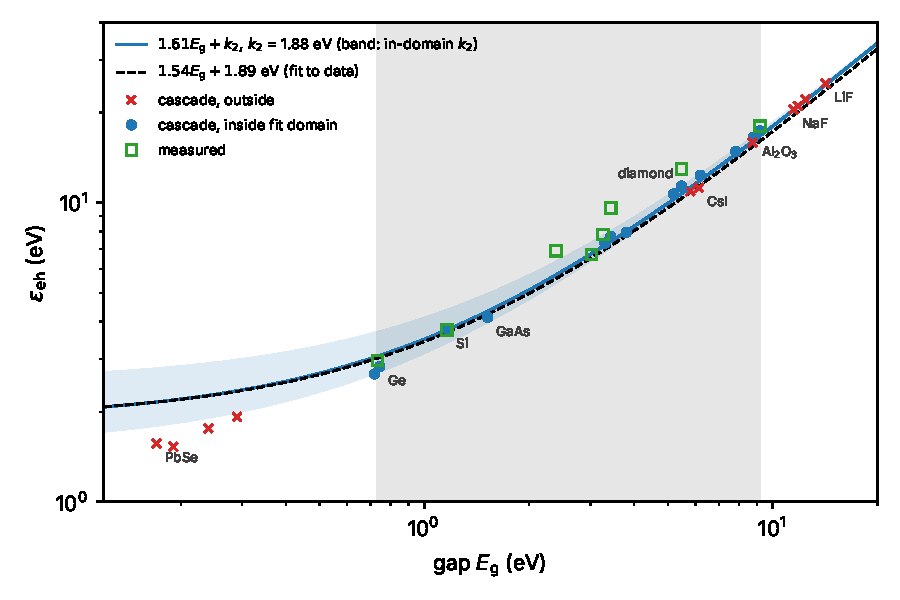
\includegraphics[width=\linewidth]{figures/ch18/limit18_4c.pdf}
\captionof{figure}{Pair energy against the gap. Solid line: \cref{eq:18.4-linear} with the silicon value $k_2 = \SI{1.88}{eV}$; band: $k_2$ over the crystals inside the fit region, 1.51 to \SI{2.53}{eV}. Dashed: the empirical line. Circles: the cascade with the constant \cref{eq:18.4-AAB} for the 24 crystals of Griffin and coworkers~\cite[Table~I]{griffin2020multichannel} (gap and highest optical phonon energy; silicon, germanium and GaAs at their low-temperature gaps of \cref{tab:3-materials}); filled inside the fit region $0.003 \le \lambda_{\mathrm{AB}} \le 100$, $0.01 \le w_{\mathrm{AB}} \le 0.1$ of \cref{eq:18.4-fit}, crosses outside it. Squares: measured pair energies of \cref{tab:18-valid} and silicon. Gray: the gaps of the measured crystals, 0.73 to \SI{9.2}{eV}. Slopes fitted for seed energies of 12.5 to $25\Eg$ (30 to $60\Eg$ for $\lambda_{\mathrm{AB}} > 5$), a window that changes the silicon value by less than \SI{0.03}{\percent} against the 20 to $40\Eg$ of \cref{tab:18-pairs}.}\label{fig:18-limit-c}
\par}
\smallskip
Outside the fit region, the law with each crystal's own $k_2$ still follows the cascade to \SI{1.4}{\percent} for these 24 crystals, but there it extrapolates the model beyond any comparison with data: the lead salts and InSb have $\lambda_{\mathrm{AB}} > 200$, and the halides and fluorides a phonon step below $0.006\Eg$.
\end{limitbox}

The linear law of the cascade and the empirical line have the same form for different reasons. The empirical constant 1.89 lies inside the range of $k_2$ and close to the value for silicon. The empirical slope 1.54 is below the model's 1.61, pulled down by diamond and the nitrides, for which the model with the silicon constant gives too little (\cref{sec:18.4-range}). Nielsen and Fischetti note that the measured $\varepsilon_{\mathrm{eh}}(\Eg)$ is not linear~\cite[Sect.~II]{nielsen2026first}; in the model, the nonlinearity comes from $k_2$, which changes from crystal to crystal with the phonon energy.

\begin{workedexample}{Pair energy of GaAs from the linear law}\label{we:18-gaas}
A GaAs detector at millikelvin has $\Eg = \SI{1.52}{eV}$ (\cref{tab:3-materials}) and a longitudinal optical phonon at $\omega_{\mathrm{AB}} = \SI{36.35}{meV}$ (\cref{sec:5.5}). With \cref{eq:18.4-AAB},
\begin{equation*}
  \lambda_{\mathrm{AB}} = \frac{5.703}{1.52^3} = 1.624, \qquad w_{\mathrm{AB}} = \frac{0.03635}{1.52} = 0.02391 .
\end{equation*}
The combination in \cref{eq:18.4-fit} is $\lambda_{\mathrm{AB}}w_{\mathrm{AB}}^{0.9637} = 0.04448$, and its power $0.2403$ is 0.4733. Then
\begin{equation*}
  \frac{\varepsilon_{\mathrm{eh}}}{\Eg} = 1.612 + 2.329\times0.4733 = 2.714, \qquad
  \varepsilon_{\mathrm{eh}} = 2.714\times\SI{1.52}{eV} = \SI{4.125}{eV} .
\end{equation*}
In the form \cref{eq:18.4-linear}, $1.61\Eg = \SI{2.45}{eV}$ and $k_2 = \SI{1.68}{eV}$, smaller than silicon's \SI{1.88}{eV} because the GaAs phonon carries 0.58 of the silicon phonon energy. The cascade itself yields \SI{4.132}{eV} (\cref{tab:18-pairs}), so the fit costs \SI{0.2}{\percent}. The empirical line gives \SI{4.23}{eV}. At the room-temperature gap of \SI{1.42}{eV} the linear law gives \SI{3.96}{eV}, against the measured value of about \SI{4.2}{eV}~\cite[Fig.~1]{nielsen2026first}; the difference is the residual of the model in \cref{tab:18-pairs}, carried through the fit. For a GaAs detector the defensible pair energy is therefore $\approx\SI{4.1}{eV}$ with an uncertainty set by the model's residuals, not by the fit.
\end{workedexample}

\subsection{The validated range}\label{sec:18.4-range}

\Cref{tab:18-valid} compares the cascade with the measured pair energies of seven crystals besides silicon, which fixes the constant. The inputs are the gap and the highest optical phonon energy of each crystal, longitudinal for the SiC polytypes.

\begin{table}[tbp]
\caption{Pair energies of the cascade with the silicon constant \cref{eq:18.4-AAB} against measurements. Inputs: germanium as in \cref{tab:18-pairs} (\SI{77}{K}); diamond, GaN and $\alpha$-quartz, gap and highest optical phonon energy of Griffin and coworkers~\cite[Table~I]{griffin2020multichannel}; the SiC polytypes, gap and longitudinal optical energy of Griffin and coworkers~\cite[Table~I]{griffin2021sic}. Measurements: germanium~\cite[Sect.~4.3]{mei2020impact}; diamond, the inverse-variance mean of four measurements (13.1, 13.25, 13.05 and \SI{12.82}{eV}) compiled by Nielsen and Fischetti~\cite[Sect.~III]{nielsen2023thermalization}; 4H-SiC~\cite{gsponer2023measurement}; 6H-SiC as quoted by Griffin and coworkers~\cite[Table~I]{griffin2021sic}; 3C-SiC and SiO$_2$ as quoted by Nielsen and Fischetti~\cite[Table~II]{nielsen2026first}; GaN, electron-beam induced current, as quoted by Nielsen and coworkers~\cite[Sect.~IV]{nielsen2023first}. Residual: model over measured, minus one. Last column: the density-functional full-band Monte Carlo of Nielsen and coworkers~\cite[Table~II]{nielsen2026first}, \cite[Sect.~III]{nielsen2023thermalization}, \cite[Sect.~IV]{nielsen2023first}.}
\label{tab:18-valid}
\centering\footnotesize\setlength{\tabcolsep}{3pt}
\begin{tabular}{lcccccccc}
\toprule
 & $\Eg$ (eV) & $\omega_{\mathrm{AB}}$ (meV) & $\lambda_{\mathrm{AB}}$ & $w_{\mathrm{AB}}$ & model (eV) & measured (eV) & residual & full band (eV) \\
\midrule
Ge & 0.735 & 37.6 & 14.4 & 0.051 & 2.815 & 2.96 & $-\SI{4.9}{\percent}$ & -- \\
3C-SiC & 2.39 & 120.5 & 0.42 & 0.050 & 6.121 & 6.90 & $-\SI{11.3}{\percent}$ & 6.6 \\
6H-SiC & 3.02 & 120.0 & 0.21 & 0.040 & 7.167 & 6.7 & $+\SI{7.0}{\percent}$ & -- \\
4H-SiC & 3.26 & 120.0 & 0.16 & 0.037 & 7.565 & $7.83 \pm 0.02$ & $-\SI{3.4}{\percent}$ & 7.3 \\
GaN & 3.43 & 88.9 & 0.14 & 0.026 & 7.694 & 9.59 & $-\SI{19.8}{\percent}$ & 8.9 \\
diamond & 5.47 & 161 & 0.035 & 0.029 & 11.357 & 12.95 & $-\SI{12.3}{\percent}$ & 12.87 \\
SiO$_2$ & 9.2 & 149 & 0.0073 & 0.016 & 17.373 & 18.0 & $-\SI{3.5}{\percent}$ & 16.7 \\
\bottomrule
\end{tabular}
\end{table}

Over the seven crystals the residuals run from $-\SI{19.8}{\percent}$ to $+\SI{7.0}{\percent}$, with a mean of $-\SI{6.9}{\percent}$ and a root mean square of \SI{10.5}{\percent}. The model is good to \SI{7}{\percent} for germanium, 4H- and 6H-SiC and quartz, and it falls short by 11 to \SI{20}{\percent} for 3C-SiC, diamond and GaN. Six of the seven residuals are negative, as are the residuals of germanium and GaAs in \cref{tab:18-pairs}: with the silicon constant the model tends to give too little heat per pair. The likeliest cause of the negative residuals is the universal constant, since the light-atom and polar lattices that the model misses most have phonon couplings unlike the couplings of silicon, but the comparison does not prove that the constant is the cause. The density-functional full-band Monte Carlo does better for diamond, 3C-SiC and GaN and worse for 4H-SiC and quartz, and it has no fitted constant. Its \SI{3.1}{eV} for silicon (\cref{sec:18.4-model}), \SI{17}{\percent} below the \SI{3.749}{eV} at \SI{123}{K}, shows that it is not yet a calibration-free substitute either.

The Fano factor is barely tested beyond silicon. The germanium measurements span a factor two, and the only wide-gap values, both for 4H-SiC, disagree with each other: $F_{\mathrm{eh}} = 0.1$ from a linewidth and an upper limit of 0.04 from another, as compiled by Gsponer and coworkers~\cite[Table~2]{gsponer2023measurement}. The model gives 0.093 for 4H-SiC. If the upper limit holds, the model fails for 4H-SiC, since 0.04 lies below every Fano factor the cascade produces in this section; a linewidth limit, however, rests on subtracting the noise from the measured width~\cite[Eq.~(3)]{gsponer2023measurement}, and an overestimated noise drives the limit down. Which of the two 4H-SiC values applies cannot be decided from the published data.

These comparisons define the \emph{validated range} of the cascade model: the region of phonon strength and phonon step spanned by the crystals with a measured pair energy, $0.007 \le \lambda_{\mathrm{AB}} \le 14.4$ and $0.016 \le w_{\mathrm{AB}} \le 0.054$, gaps from 0.73 to \SI{9.2}{eV}. Inside the validated range a model pair energy carries the spread of the residuals, $-20$ to $+\SI{7}{\percent}$, with the lower part more likely for light-atom and polar crystals. Of the crystals ranked in \cref{chap:17}, silicon, germanium, GaAs, diamond, quartz, CaWO$_4$, AlN, GaN and ZnO lie inside the range (\cref{fig:18-limit-c}). Sapphire and MgO lie just outside, with phonon steps of 0.012 and 0.011, and GaSb at its edge, with $\lambda_{\mathrm{AB}} = 15.3$.

Three groups lie well outside the validated range. The alkali halides and the fluorides, NaI, CsI, NaCl, LiF, NaF, CaF$_2$ and MgF$_2$, have phonon steps of 0.0016 to 0.006 of the gap. A carrier near threshold then emits hundreds of phonons before it ionizes, and no measured crystal samples a regime with so many phonons per ionization. The halides and fluorides have narrow anion valence bands, which confine the holes far more than in any validated crystal and which the model treats without a cutoff. They also bind excitons by an eV or more. A carrier between $\Eg - E_x^b$ and the impact-ionization threshold can create a bound pair directly; the cascade of \cref{sec:18.1} has no channel for this direct exciton creation, and whether a bound exciton counts as a pair depends on the readout (\cref{sec:18.5}). The lead salts and InSb have gaps below \SI{0.3}{eV} and $\lambda_{\mathrm{AB}}$ from 230 to 1160: their cascades are dominated by phonons, and at gaps this small, two processes absent from the model, Auger recombination and scattering by free carriers, can compete with impact ionization. For the crystals of these three groups the model pair energies in \cref{fig:18-limit-c} are estimates without a measured anchor, for example \SI{25.0}{eV} for LiF, \SI{20.5}{eV} for NaF, \SI{11.2}{eV} for CsI and \SI{1.56}{eV} for PbSe. Any guide to new targets must mark these pair energies as estimates. Neither the pair energy nor the Fano factor of sapphire, CaWO$_4$, LiF or NaF has been measured.

\section{Capture and excitons}\label{sec:18.5}

A carrier in silicon whose kinetic energy has fallen below the impact-ionization threshold $\theta_{\mathrm{ii}}\Eg$ (\cref{sec:18.1}) can no longer add a pair. It reaches the band edge by emitting phonons within about a picosecond, and from then on the number of pairs $N_{\mathrm{eh}}$ whose mean and variance \cref{sec:18.2} computes is fixed. A detector at \SI{50}{mK} reads the event microseconds to seconds later. In that interval an electron can be captured by an ionized donor, or an electron and a hole can bind into an exciton. The exciton can bind to a neutral impurity, and the pair can recombine, giving its energy to the lattice or to a photon that leaves the crystal. Each of these processes changes what a charge or a heat readout records, and none of their rates has been measured at millikelvin temperatures in silicon or germanium. Without the rates one can still derive how each process changes the energy balance and the pair number.

\subsection{End-of-cascade capture}\label{sec:18.5-capture}

At the end of the cascade every carrier sits at a band edge, and the deposit is shared by the energy balance \cref{eq:18.1-energy}: $\Eg$ for each pair and the heat $E_{\mathrm{heat}}$ for the phonons emitted on the way down. This holds for an electron recoil, with no energy stored in defects and no photon leaving the crystal. Once carriers can be captured, not all of the energy outside the pairs is heat, and we name it separately,
\begin{equation}
  E_{\mathrm{np}} \equiv \omega - N_{\mathrm{eh}}\Eg ,
  \label{eq:18.5-Enp}
\end{equation}
the energy not held by pairs, equal to $E_{\mathrm{heat}}$ as long as nothing is captured. At fixed $\omega$ the pair number and $E_{\mathrm{np}}$ fluctuate together, $\operatorname{Var}N_{\mathrm{eh}} = \operatorname{Var}E_{\mathrm{np}}/\Eg^2$. From here on $N_{\mathrm{eh}}$ counts the electrons in the conduction band, free or bound to a hole in an exciton. An electron captured on an impurity level no longer counts.

Let an electron be captured on a level $E_j$ below the conduction-band edge $E_c$. The energy of a charge in the crystal is fixed relative to the Fermi level $\mu_F$ of the electrodes, since that is the energy the carrier gives up when it reaches one. A free electron holds $E_c - \mu_F$, a free hole $\mu_F - E_v$, with $E_v$ the valence-band edge, and a pair the sum, $\Eg$. After the capture the electron holds $E_j - \mu_F$, the phonons emitted at capture carry $E_c - E_j$, and the hole, now without a partner, still holds $\mu_F - E_v$. The three shares add to $\Eg$ whatever the level, and with $N_{\mathrm{eh}}$ lowered by one, \cref{eq:18.5-Enp} counts all three in $E_{\mathrm{np}}$; only the share $E_c - E_j$ is heat. A captured hole leaves $N_{\mathrm{eh}}$ unchanged; it changes the charge that the electrodes see, which is a matter of the readout.

Whether the electrons are captured is random. Let electron $i$ be captured with probability $f_i$, independently of the others once the cascade is given. The number of electrons left, $N'$, then has conditional mean $\sum_i(1 - f_i)$ and conditional variance $\sum_if_i(1 - f_i)$, a sum of Bernoulli variances. The law of total variance, $\operatorname{Var}N' = \langle\operatorname{Var}(N'|\text{cascade})\rangle + \operatorname{Var}\langle N'|\text{cascade}\rangle$, gives
\begin{equation}
  \langle N'\rangle = \Bigl\langle\sum_i(1 - f_i)\Bigr\rangle , \qquad
  \operatorname{Var}N' = \Bigl\langle\sum_if_i(1 - f_i)\Bigr\rangle + \operatorname{Var}\Bigl[\sum_i(1 - f_i)\Bigr] ,
  \label{eq:18.5-thingen}
\end{equation}
with the averages taken over cascades. If every electron has the same capture probability $f_{\mathrm{cap}}$, unrelated to the cascade, the sums become $(1 - f_{\mathrm{cap}})N_{\mathrm{eh}}$ and $f_{\mathrm{cap}}(1 - f_{\mathrm{cap}})N_{\mathrm{eh}}$, and the pair number is thinned binomially.

\begin{keyresult}[Capture at the end of the cascade]
Each electron captured before the readout raises the energy not held by pairs by exactly $\Eg$,
\begin{equation}
  E_{\mathrm{np}} \to E_{\mathrm{np}} + \Eg ,
  \label{eq:18.5-Eg}
\end{equation}
of which $E_c - E_j$ goes to phonons at the capture, $E_j - \mu_F$ stays with the trapped electron and $\mu_F - E_v$ with the unpaired hole. Let the capture probability $f_{\mathrm{cap}}$ be equal for all electrons and independent of the cascade. The mean energy per counted pair and the Fano factor of the counted pairs are then
\begin{equation}
  \varepsilon'_{\mathrm{eh}} = \frac{\varepsilon_{\mathrm{eh}}}{1 - f_{\mathrm{cap}}} , \qquad
  F'_{\mathrm{eh}} = (1 - f_{\mathrm{cap}})F_{\mathrm{eh}} + f_{\mathrm{cap}} .
  \label{eq:18.5-thin}
\end{equation}
A capture probability that depends on the carrier's state at the end of the cascade requires the general form \cref{eq:18.5-thingen}.
\end{keyresult}

The Fano factor of silicon is small, and \cref{eq:18.5-thin} makes it fragile: a loss raises it by $f_{\mathrm{cap}}(1 - F_{\mathrm{eh}})$, almost one for one. The cascade value 0.114 and the measured $0.119 \pm 0.002$ (\cref{sec:18.4}) differ by an amount that a loss of $f_{\mathrm{cap}} = \SI{0.54}{\percent}$ (0.32 to \SI{0.77}{\percent}) would produce, and the same loss raises $\varepsilon_{\mathrm{eh}}$ by \SI{0.55}{\percent}, which the calibration of the cascade on the measured pair energy absorbs. The Fano factor alone therefore cannot separate a sub-percent loss of pairs from the truncations of the cascade itself.

The binomial form fails when the capture probability depends on the energy $x_i$ that carrier $i$ still has after its last impact ionization. Those terminal energies are correlated with the pair number: \cref{sec:18.2} found that the residual energies of the terminal carriers anticorrelate with the phonon energy emitted above threshold. With $f_i = f(x_i)$ the variance term $\operatorname{Var}\sum_i(1 - f_i)$ is not, in general, $(1 - \bar f)^2\operatorname{Var}N_{\mathrm{eh}}$ with $\bar f$ the mean capture probability, and \cref{eq:18.5-thingen} has to be evaluated on the distribution of terminal energies that the cascade produces.

Capture is a collision of the kind that \cref{sec:18.1} turned into master-formula rates, with the potential of the impurity coupling the free carrier to a bound state and phonons carrying off the energy. Its size follows from a simpler argument. A carrier with kinetic energy $E$ is bound by an attractive center only if it comes within the distance at which the Coulomb energy equals its kinetic energy, $r_C(E) = \alpha/(\varepsilon_0E)$, and loses energy there. With $\hbar c$ restored, $\alpha = \SI{1.44}{eV.nm}$, and with the static constant of silicon at liquid-helium temperature, $\varepsilon_0 = 11.4$ (\cref{sec:7.4}), $\alpha/\varepsilon_0 = \SI{0.126}{eV.nm}$, so a carrier of \SI{0.1}{eV} has $r_C = \SI{1.26}{nm}$ and a capture cross-section of at most $\pi r_C^2 = \SI{5.0e-14}{cm^2}$; at \SI{0.35}{eV}, $r_C = \SI{0.36}{nm}$ and $\pi r_C^2 = \SI{4.1e-15}{cm^2}$. At a density of centers of \SI{e12}{cm^{-3}} the mean free path for capture is then at least \SI{20}{cm}, and it falls to micrometers only near \SI{e18}{cm^{-3}}. Capture of hot carriers during the cascade is negligible in a pure crystal. The cold carriers that the cascade leaves behind are a different matter. At the thermal energy of \SI{50}{mK}, $k_BT = \SI{4.3}{\micro eV}$, the Coulomb radius is $\alpha/(\varepsilon_0k_BT) = \SI{29}{\micro m}$, and a cold carrier finds any ionized center within tens of micrometers. The silicon detectors of CDMS~II, the second phase of the Cryogenic Dark Matter Search (CDMS), for example, were operated with their ionized trapping sites neutralized by regular exposure to infrared light-emitting diodes, which left the bulk in a metastable state with low trapping~\cite[Sect.~2]{agnese2018nuclear}. Capture on neutral centers and capture during drift belong to the readout, and every one of them adds the same $\Eg$ to $E_{\mathrm{np}}$.

\begin{workedexample}{One captured electron in ten pairs}\label{we:18-capture}
An electron recoil of $\omega = \SI{37.5}{eV}$ in silicon makes about ten pairs at the measured $\varepsilon_{\mathrm{eh}} = \SI{3.75}{eV}$ of \cref{sec:1.5}. Take an event with exactly ten. With $\Eg = \SI{1.17}{eV}$, the energy balance gives $E_{\mathrm{heat}} = E_{\mathrm{np}} = 37.5 - 10\times1.17 = \SI{25.80}{eV}$ in phonons. Let one electron be captured by an ionized phosphorus donor, whose ground state lies \SI{45.6}{meV} below the band edge (\cref{sec:7.4}). The pair number falls to nine and $E_{\mathrm{np}} = 37.5 - 9\times1.17 = \SI{26.97}{eV}$, larger by exactly $\Eg$. Of that \SI{1.17}{eV}, \SI{45.6}{meV} is emitted as phonons when the electron drops onto the donor, and \SI{1.124}{eV} stays as the potential energy of the trapped electron and of its unpaired hole, divided between them according to where $\mu_F$ lies. A charge readout calibrated at \SI{3.75}{eV} per pair reports $9\times3.75 = \SI{33.75}{eV}$; the energy per counted pair of this event is $37.5/9 = \SI{4.17}{eV}$, \SI{11.1}{\percent} above $\varepsilon_{\mathrm{eh}}$.

Now let each of the electrons be captured with probability $f_{\mathrm{cap}} = 0.1$ instead. The mean number counted is nine, the same as before, and $\varepsilon'_{\mathrm{eh}} = 3.75/0.9 = \SI{4.17}{eV}$ by \cref{eq:18.5-thin}. With the measured $F_{\mathrm{eh}} = 0.119$, however, the Fano factor rises to $F'_{\mathrm{eh}} = 0.9\times0.119 + 0.1 = 0.207$, and the standard deviation of the counted pairs from $(0.119\times10)^{1/2} = 1.09$ to $(0.207\times9)^{1/2} = 1.37$. A capture of fixed size shifts the yield; a capture at random also broadens it. Of the variance $0.207\times9 = 1.86$, the thinned cascade contributes $0.9^2\times1.19 = 0.96$ and the binomial choice of which electrons are captured $0.1\times0.9\times10 = 0.90$, almost as much.
\end{workedexample}

\subsection{Excitons and the measured Fano factor}\label{sec:18.5-excitons}

A cold electron and hole left near each other at zero field bind. The binding energy of the silicon exciton, $E_x^b = \SI{14.7}{meV}$ (\cref{sec:4.9}), is 3400 times $k_BT$ at \SI{50}{mK}, and a pair closer than the \SI{29}{\micro m} Coulomb radius found above cannot be pulled apart by thermal motion. Binding is a two-body process that waits for both carriers to cool by emitting acoustic phonons, slow at millikelvin temperatures, so it takes place after the cascade has fixed $N_{\mathrm{eh}}$. Since $N_{\mathrm{eh}}$ counts bound pairs, an exciton changes neither $N_{\mathrm{eh}}$ nor $\varepsilon_{\mathrm{eh}}$ nor $F_{\mathrm{eh}}$. What it changes is where the energy sits: a bound pair holds $\Eg - E_x^b$, and the binding energy goes to the lattice.

A heat readout, however, sees more than $E_{\mathrm{np}}$. With $N_X$ bound pairs at readout and no capture, the phonon energy is $E_{\mathrm{heat}} = E_{\mathrm{np}} + N_XE_x^b$. Its mean rises by $E_x^b$ per bound pair, at most $E_x^b/\varepsilon_{\mathrm{eh}} = \SI{0.39}{\percent}$ of $\omega$ in silicon. Define the Fano factor inferred from the phonon energy, $F_{\mathrm{heat}} \equiv \operatorname{Var}E_{\mathrm{heat}}/(\Eg^2\langle N_{\mathrm{eh}}\rangle)$. It differs from $F_{\mathrm{eh}} = \operatorname{Var}E_{\mathrm{np}}/(\Eg^2\langle N_{\mathrm{eh}}\rangle)$ by the variance of $N_X$ and its covariance with $E_{\mathrm{np}}$,
\begin{equation}
  F_{\mathrm{heat}} = F_{\mathrm{eh}} + \frac{(E_x^b)^2\operatorname{Var}N_X + 2E_x^b\operatorname{Cov}(E_{\mathrm{np}}, N_X)}{\Eg^2\langle N_{\mathrm{eh}}\rangle} .
  \label{eq:18.5-Fheat}
\end{equation}
When every pair binds, $N_X = N_{\mathrm{eh}}$ and $E_{\mathrm{heat}} = \omega - N_{\mathrm{eh}}(\Eg - E_x^b)$, so $F_{\mathrm{heat}} = F_{\mathrm{eh}}(1 - E_x^b/\Eg)^2$: \SI{2.5}{\percent} below $F_{\mathrm{eh}}$ in silicon, and 0.7 to \SI{1.3}{\percent} in germanium, whose indirect exciton is bound by a few meV, 2.5 and \SI{5}{meV} in absorption~\cite{zwerdling1959exciton,macfarlane1957fine}, against a gap of \SI{0.744}{eV}.

A charge readout is affected only if the exciton is never split. A bound pair is neutral and drifts as a whole, so it induces no charge on the electrodes. Let each pair independently end as such an exciton with probability $p_{\mathrm{ns}}$. The counted charge is then thinned exactly as by capture, and by the algebra of \cref{eq:18.5-thin} its Fano factor is
\begin{equation}
  F_{\mathrm{meas}} = (1 - p_{\mathrm{ns}})F_{\mathrm{eh}} + p_{\mathrm{ns}} ,
  \label{eq:18.5-Fmeas}
\end{equation}
where $F_{\mathrm{meas}}$ is the Fano factor of the measured charge, before the corrections of the readout itself. A heat readout thus sees $F_{\mathrm{heat}}$ and a charge readout $F_{\mathrm{meas}}$, while $F_{\mathrm{eh}}$, which counts bound and free pairs alike, is the cascade value that neither changes. In a biased detector the field can separate the pair before it binds. The force $e\mathcal{E}$ of a field $\mathcal{E}$ exceeds the attraction $\alpha/(\varepsilon_0r^2)$ beyond the radius
\begin{equation}
  r_{\mathcal{E}} = \Bigl(\frac{\alpha}{\varepsilon_0e\mathcal{E}}\Bigr)^{1/2} ,
  \label{eq:18.5-rfield}
\end{equation}
which in silicon is \SI{0.56}{\micro m} at \SI{4}{V/cm} and \SI{0.11}{\micro m} at \SI{100}{V/cm}. A pair that ends the cascade farther apart than $r_{\mathcal{E}}$ is separated; a closer one can bind, and once bound it stays bound, since the field that ionizes the exciton is of order $E_x^b/(ea_x) = \SI{3.5e4}{V/cm}$, with $a_x = \SI{4.2}{nm}$ (\cref{sec:4.9}). Exciton formation thus changes the measured Fano factor through \cref{eq:18.5-Fmeas} when the readout field is weak enough that $r_{\mathcal{E}}$ exceeds the separation of the pairs at the end of the cascade, a distribution the cascade calculation has to supply. When excitons form from carriers of different pairs, as in a dense track, the loss is not independent from pair to pair, its probability grows with the density, and the variance acquires a part that grows faster than $\langle N_{\mathrm{eh}}\rangle$.

One process acts on the cascade itself. A carrier with energy between $\Eg - E_x^b$ and the ionization threshold can create a bound pair directly, which acts for that pair like a gap lowered by $E_x^b$. With the slope $\partial\varepsilon_{\mathrm{eh}}/\partial\Eg = 1.70$ of the calibrated cascade at fixed $A_{\mathrm{AB}}$ (\cref{sec:18.4-three}), the pair energy moves by at most $1.70E_x^b = \SI{25}{meV}$ in silicon, \SI{0.67}{\percent}, and \SI{8.6}{meV} in germanium, \SI{0.30}{\percent}, for the larger of its two measured binding energies. In ionic crystals with excitons bound by about \SI{1}{eV}, the bound pair and not the free pair may be the unit the cascade produces, and the excitons self-trap (\cref{sec:10.5}); their pair energies lie outside the range in which the cascade model was validated (\cref{sec:18.4}).

\subsection{Rate equations at millikelvin}\label{sec:18.5-kinetics}

After the cascade each pair is in one of four kinds of state: a free pair $F$, a free exciton $X$, an exciton $B_j$ bound to a neutral impurity of species $j$, or a pair with a carrier trapped on a center of species $j$. In the dilute clouds of electron recoils each pair evolves on its own, with its own partner or with a fixed background center. Every transition is then first order in the occupation of the pair's own state. For the occupation probabilities $p_F$, $p_X$ and $p_{B,j}$ of one pair,
\begin{equation}
  \begin{aligned}
    \frac{\dd p_F}{\dd t} &= -(\varGamma_{FX} + \varGamma_{FT})\,p_F , \\
    \frac{\dd p_X}{\dd t} &= \varGamma_{FX}\,p_F - \Bigl(\varGamma_X + \sum_j\varGamma_{XB,j}\Bigr)p_X , \\
    \frac{\dd p_{B,j}}{\dd t} &= \varGamma_{XB,j}\,p_X - \varGamma_{B,j}\,p_{B,j} .
  \end{aligned}
  \label{eq:18.5-rates}
\end{equation}
Here $\varGamma_{FX}$ is the rate at which the pair binds and $\varGamma_{FT}$ the rate at which one of its carriers is trapped. The free exciton decays at the rate $\varGamma_X$, a fraction $\eta_X$ of it by luminescence, and binds to impurities of density $\nd_j$ at the rate $\varGamma_{XB,j} = \sigma_{XB,j}v_X\nd_j$, with cross-section $\sigma_{XB,j}$ and exciton speed $v_X$. The bound exciton decays at the rate $\varGamma_{B,j}$, a fraction $\eta_{B,j}$ of it by luminescence. In silicon a bound exciton decays mostly by an Auger process: the pair recombines and gives its energy to the extra carrier of the complex, which is ejected and leaves the impurity ionized. Its lifetime at the phosphorus donor is 200 to \SI{300}{ns} at liquid-helium temperature, as quoted by Lo and coworkers~\cite{lo2015hybrid}. No reverse steps appear: dissociating an exciton or freeing it from an impurity costs $E_x^b$ or more, thousands of times $k_BT$ at \SI{50}{mK}.

The trapped carriers follow the occupation $\nd^{\mathrm{tr}}_j$ of each species of center,
\begin{equation}
  \frac{\dd\nd^{\mathrm{tr}}_j}{\dd t} = \sigma_{\mathrm{cap},j}u\,\nd_{\mathrm{c}}\bigl(\nd_j - \nd^{\mathrm{tr}}_j\bigr) - \varGamma^{\mathrm{em}}_j\nd^{\mathrm{tr}}_j - \sigma^{\mathrm{rec}}_ju\,\nd_{\mathrm{v}}\nd^{\mathrm{tr}}_j ,
  \label{eq:18.5-traps}
\end{equation}
written for electrons, with free-electron and free-hole densities $\nd_{\mathrm{c}}$ and $\nd_{\mathrm{v}}$ and carrier speed $u$. The center captures with the cross-section $\sigma_{\mathrm{cap},j}$, emits at the rate $\varGamma^{\mathrm{em}}_j$, and loses its electron to a free hole with the cross-section $\sigma^{\mathrm{rec}}_j$; holes obey the same equation with the roles exchanged. Thermal emission is frozen. For the phosphorus donor the Boltzmann exponent at \SI{50}{mK} is $(\SI{45.6}{meV})/k_BT = 1.06\times10^4$. A field lowers the barrier of a Coulomb center: the potential $-\alpha/(\varepsilon_0r) - e\mathcal{E}r$ along the field has its maximum at $r_{\mathcal{E}}$ of \cref{eq:18.5-rfield}, lower than the zero-field barrier by $2(\alpha e\mathcal{E}/\varepsilon_0)^{1/2}$, the Poole--Frenkel lowering. At \SI{100}{V/cm} it is \SI{2.25}{meV}, and the exponent stays at $1.0\times10^4$. A trapped carrier is released only athermally, by the phonons and hot carriers of later events or by infrared light, so the occupations carry the history of earlier events into later ones, the source of delayed charge (\cref{app:E.25}).

Without reverse steps the matrix of \cref{eq:18.5-rates} is lower triangular in the order $F$, $X$, $B_j$, and its decay constants $\gamma_k$ are its diagonal entries, $\varGamma_{FX} + \varGamma_{FT}$, $\varGamma_X + \sum_j\varGamma_{XB,j}$ and $\varGamma_{B,j}$. The fraction of the gap energy still held by pairs and excitons,
\begin{equation}
  r_{\mathrm{gap}}(t) = p_F + p_X + \sum_jp_{B,j} = \sum_kw_k\,\ee^{-\gamma_kt} , \qquad \sum_kw_k = 1 ,
  \label{eq:18.5-rgap}
\end{equation}
decays as a sum of exponentials when the $\gamma_k$ are distinct, up to the binding energies. An exciton bound to a phosphorus donor sits a further \SI{5}{meV} or so below the free exciton~\cite{lo2015hybrid}, so $r_{\mathrm{gap}}$ overstates the held energy by at most $(E_x^b + \SI{5}{meV})/\Eg = \SI{1.7}{\percent}$ in silicon. The weights $w_k$ need not be positive: a transfer from $X$ to $B_j$ without loss delays the decay, and its weight is negative. To see where the gap energy ends up, we integrate the occupations over time, $\int_0^\infty p\,\dd t = -M^{-1}p(0)$ for the matrix $M$ of \cref{eq:18.5-rates} and a pair that starts free. They are $\int p_F = 1/(\varGamma_{FX} + \varGamma_{FT})$, $\int p_X = \varGamma_{FX}\int p_F/(\varGamma_X + \sum_j\varGamma_{XB,j})$ and $\int p_{B,j} = \varGamma_{XB,j}\int p_X/\varGamma_{B,j}$, and multiplying each by its outgoing rates gives
\begin{equation}
  b_{\mathrm{trap}} = \frac{\varGamma_{FT}}{\varGamma_{FX} + \varGamma_{FT}} , \qquad
  b_{\mathrm{light}} = (1 - b_{\mathrm{trap}})\,\frac{\varGamma_X\eta_X + \sum_j\varGamma_{XB,j}\eta_{B,j}}{\varGamma_X + \sum_j\varGamma_{XB,j}} , \qquad
  b_{\mathrm{heat}} = 1 - b_{\mathrm{trap}} - b_{\mathrm{light}}
  \label{eq:18.5-split}
\end{equation}
for the fractions of the gap energy that end trapped, as escaping light and as phonons. The trapped and escaping fractions are lost to a heat readout at any window, while the phonon fraction arrives only as fast as $r_{\mathrm{gap}}$ decays.

\Cref{fig:18-end} shows the populations of a pair in silicon at \SI{50}{mK} for one set of rates. The bound-exciton decay uses the measured Auger lifetime; the other rates are chosen only to show how the solution behaves. The pair binds within a nanosecond, the bound-exciton population peaks at 0.15 near \SI{0.45}{\micro s}, half of the gap energy is still held by pairs and excitons at \SI{0.83}{\micro s}, when phonons carry 0.445 of it, and \SI{1}{\percent} at \SI{4.4}{\micro s}. The weights of $r_{\mathrm{gap}}$ are $+1.28$ for the free exciton, $-0.33$ for the bound one and $+0.05$ for the free pair. A heat readout that closes its window at \SI{1}{\micro s} misses the \SI{42}{\percent} of the gap energy still held in this model, plus the \SI{5.6}{\percent} already trapped or radiated, and the window dependence enters the heat yield of any phonon readout. In the dense tracks of nuclear recoils the pairs are not independent, and two-body processes take over. Binding of carriers from different pairs moves gap energy from pairs to excitons and leaves $r_{\mathrm{gap}}$ unchanged; exciton--exciton annihilation and Auger recombination of free carriers remove it, and they make $r_{\mathrm{gap}}$ fall as a power of time at a rate set by the track density. Since that density differs between nuclear and electron recoils of the same energy, so does $r_{\mathrm{gap}}$ at a given window.

\begin{figure}[tbp]
  \centering
  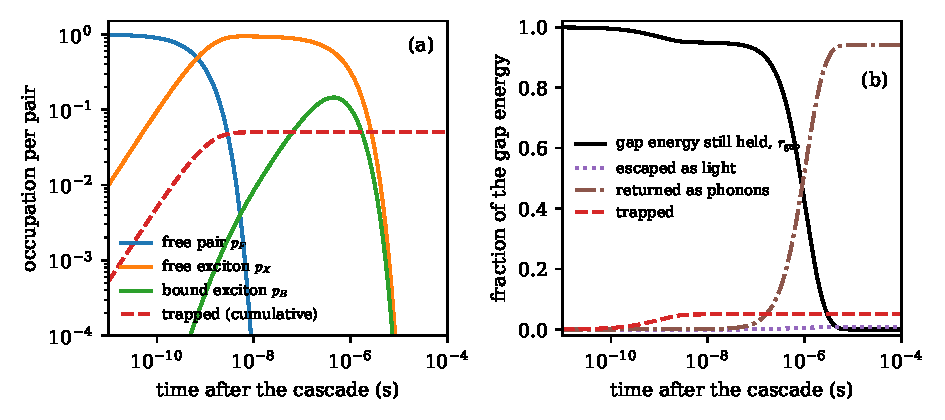
\includegraphics[width=\linewidth]{figures/ch18/fig18_4.pdf}
  \caption{End-of-cascade populations of one electron--hole pair in silicon at \SI{50}{mK}, from the rate equations \cref{eq:18.5-rates} with one species of neutral impurity. (a)~Occupations of the free pair, the free exciton and the bound exciton, and the cumulative trapped fraction, against the time after the cascade. (b)~Fraction of the gap energy still held by pairs and excitons, $r_{\mathrm{gap}}$ of \cref{eq:18.5-rgap}, and the cumulative fractions returned as phonons, escaped as light and trapped. Rates: bound-exciton Auger decay \SI{250}{ns}, inside the measured 200 to \SI{300}{ns} of the phosphorus donor~\cite{lo2015hybrid}, without light. Illustrative, since none is measured at \SI{50}{mK}: binding of the pair \SI{1}{ns}, trapping $\varGamma_{FT} = 0.053\varGamma_{FX}$, binding of the free exciton to impurities \SI{1}{\micro s}, free-exciton decay \SI{10}{\micro s} with luminescent fraction 0.1. Asymptotic split \cref{eq:18.5-split}: 0.050 trapped, 0.009 light, 0.941 phonons.}
  \label{fig:18-end}
\end{figure}

\subsection{Unknown rates and unsized truncations}\label{sec:18.5-open}

The rates of \cref{eq:18.5-rates,eq:18.5-traps} are the main unknowns of this section. In silicon and germanium at 10 to \SI{50}{mK}, no measurement or calculation gives the rate at which a cold pair binds, or the coefficient of binding between carriers of different pairs. The same holds for the capture cross-sections of cold and drifting carriers on charged and neutral centers, as functions of carrier energy, temperature and field, and for the cross-sections for binding of excitons to each impurity species. Also unknown are the decay rate and luminescent fraction of the free exciton, the luminescent fractions of the bound excitons, and the coefficients of exciton--exciton annihilation and of Auger recombination that govern dense tracks. The thresholds at which dense pairs condense into electron--hole droplets, the degenerate electron--hole liquid of germanium and silicon, are open as well at millikelvin temperatures. What is known are the binding energies, \SI{14.7}{meV} in silicon and a few meV in germanium, and the Auger lifetimes of bound excitons at liquid-helium temperature, a property of the complex in its ground state that should carry over to lower temperatures. The excitons themselves cool by emitting acoustic phonons, slowly at these temperatures, so their temperature need not be that of the lattice, and rates measured at a few kelvin cannot simply be transferred.

The cascade hands over less than these equations need. No material has a computed capture probability $f(x)$ as a function of the terminal energy of a carrier, nor the distribution of terminal energies on which \cref{eq:18.5-thingen} averages it. Nor is the separation of the pairs at the end of the cascade, which decides through \cref{eq:18.5-rfield} whether a field prevents binding. In the ionic crystals, where the cascade quantum may be a bound pair, the exciton binding energies and the binding to impurities are open as well.

Two approximations of the cascade itself remain unsized. A constant factor of 0.8 on the impact-ionization rate, the quasiparticle residue left out of \cref{eq:18.1-ii}, changes $\varepsilon_{\mathrm{eh}}$ by about \SI{3}{\percent}, and calibrating on the measured pair energy removes it. A factor that varies with the carrier energy between threshold and about \SI{10}{eV}, as the residue and the carrier--electron exchange may, changes $F_{\mathrm{eh}}$, and its size is not known. For the energy-only reduction, the probability that a carrier keeps its momentum between two events that change its energy is estimated to be below about 0.1 within \SI{1}{eV} of threshold, where intervalley scattering dominates, and to reach one half above 3 to \SI{5}{eV} in silicon. A full-band cascade finds the resulting memory negligible, but only within the deformation-potential model of the phonons (\cref{sec:18.1-reductions}); with first-principles couplings, which do not redraw the crystal momentum at every emission, neither this probability nor the spread over the iso-energy surface that it multiplies has been computed.

\section*{Summary}

A hot carrier in a semiconductor is a projectile of the master formula (\cref{sec:18.1}). Its impact ionization is the rate \cref{eq:18.1-ii}, whose kernel is the screened interaction, and phonon emission is the same formula with the electron--phonon vertex; momentum conservation puts the impact-ionization threshold at $\theta_{\mathrm{ii}}\Eg$, with $\theta_{\mathrm{ii}} = 3/2$ for equal masses. The cascade is a branching process whose statistics follow from one generating functional and its backward equation \cref{eq:18.1-backward}, and the energy identity \cref{eq:18.1-energy} ties every fluctuation of the pair number to a fluctuation of the heat. The cascade must be seeded class by class: at \SI{10}{eV} an equal split of the energy between electron and hole yields 2.985 pairs on average, and a uniform distribution of splits with the same mean split yields 2.691.

The mean energy per pair and the Fano factor are the first two moments of that generating functional (\cref{sec:18.2}). $F_{\mathrm{eh}}$ is the variance of the heat per pair in units of $\Eg^2$; in silicon its three terms add to $0.092 + 0.290 - 0.268 = 0.114$. Below about $15\Eg$ the yield rises in steps of one pair, so that a search at a few pairs needs the whole pair-number distribution.

At \SI{5}{eV} in silicon a dark-matter kick at $q_0$ puts two pairs in \SI{17}{\percent} of events, where the step model puts two in every event (\cref{sec:18.3}). The step model and fixed splits of the energy fail between 4.4 and \SI{13}{eV}, where the split decides the count. Against a full-band cascade with no fitted constant, the step model overcounts the two-pair bin about tenfold, and at least sixfold anywhere in the envelope of the full-band variants.

With its one constant fixed by the measured pair energy of silicon, the cascade yields $F_{\mathrm{eh}} = 0.114$ against the measured $0.119 \pm 0.002$ (\cref{sec:18.4}). The full-band cascade gives $\varepsilon_{\mathrm{eh}} = \SI{4.15}{eV}$ $[3.95, 4.73]$ against the measured \SI{3.749}{eV}. The calibrated cascade reduces over its parameter range to the observed linear law $\varepsilon_{\mathrm{eh}} \approx 1.61\Eg + k_2$. Against the seven crystals besides silicon with a measured pair energy, the residuals of the calibrated cascade run from $-\SI{19.8}{\percent}$ to $+\SI{7.0}{\percent}$ (root mean square \SI{10.5}{\percent}). The crystals with a measured pair energy, silicon included, span the validated range of the calibrated cascade, and the halides, fluorides, lead salts and InSb lie outside that range.

Below the impact-ionization threshold the pair number can still change (\cref{sec:18.5}). A capture probability $f_{\mathrm{cap}}$ shared by all electrons turns $\varepsilon_{\mathrm{eh}}$ into $\varepsilon_{\mathrm{eh}}/(1 - f_{\mathrm{cap}})$ and $F_{\mathrm{eh}}$ into $(1 - f_{\mathrm{cap}})F_{\mathrm{eh}} + f_{\mathrm{cap}}$, and a loss of \SI{0.54}{\percent} would account for the difference between the cascade value and the measured Fano factor of silicon. Excitons change neither the pair number nor its moments; they return their binding energy as heat, and an exciton that is never split thins the measured charge, \cref{eq:18.5-Fmeas}. Almost none of the rates of capture, exciton binding and trapping is known at millikelvin temperatures.

\printbibliography[heading=subbibliography]

\chapter{Low-energy nuclear recoils}\label{chap:19}
A dark-matter particle of \SI{200}{MeV} gives a silicon nucleus at most \SI{21}{eV}. The nucleus leaves its site at \SI{12}{km/s}, reaches its first neighbor within \SI{20}{fs}, and in less than a picosecond the energy has been shared out. Most of it becomes heat. Along some directions the atom does not return to its site, and a vacancy and an interstitial keep several eV between them for as long as their barriers allow. Above a few hundred eV a part also goes to the electrons and ends as charge. A phonon sensor sees the heat, a charge readout sees the pairs, and neither sees the stored energy until it is released, possibly long after the event. Searches turn these signals into a recoil energy with yields taken from Lindhard's model of ion slowing, which treats the electrons as a gas without a gap and stores no energy in the lattice. That model was built for faster ions, and it is least reliable below a keV, where light dark matter deposits its energy.

The response of \cref{chap:11} ends when the momentum and the energy have been transferred; it does not ask what the nucleus does next (\cref{sec:11.4}). This chapter takes the nucleus from that moment, through its motion on the Born--Oppenheimer surface and its collisions, to the moment the shares are fixed, and writes one balance law that counts every share once. The electrons that the recoil excites start the hot-carrier cascade of \cref{chap:18}, now seeded by a slow ion instead of a dark-matter vertex. The energy stored in defects links the recoil to the delayed events that limit low-threshold detectors, and so to the readout of the next chapter (\cref{fig:19-map}).

\begin{figure}[tbp]
  \centering
  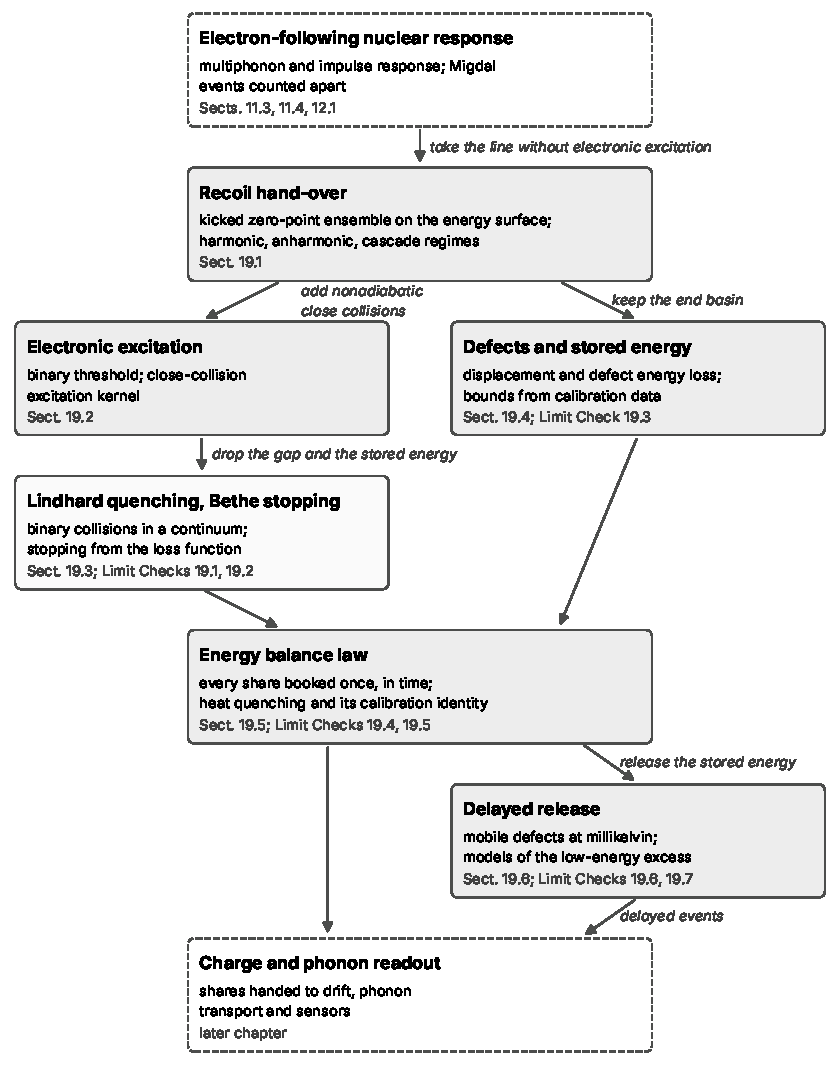
\includegraphics[width=0.85\linewidth]{figures/ch19/map19.pdf}
  \caption{Low-energy nuclear recoils, from the electron-following nuclear response (\cref{sec:11.3,sec:11.4}; Migdal events counted apart, \cref{sec:12.1-counting}) to the shares a detector reads. Main line: the hand-over of the kicked nucleus to dynamics on the Born--Oppenheimer surface, the regimes of that dynamics and the partition of the recoil energy into heat, stored energy and charge (\cref{sec:19.1}), then the energy balance law with heat quenching, its calibration identity and the bounds that calibration data set on the stored energy (\cref{sec:19.5}; \cref{lim:19.5a,lim:19.5b}). Left branch: electronic excitation in close collisions and the binary threshold (\cref{sec:19.2}), and Lindhard quenching and Bethe stopping as its limits (\cref{sec:19.3}; \cref{lim:19.3a,lim:19.3b}). Right branch: displacement and the energy stored in defects (\cref{sec:19.4}; \cref{lim:19.4a}), and the delayed release of that energy by mobile defects (\cref{sec:19.6}; \cref{lim:19.6a,lim:19.6b}), which feeds the readout as delayed events.}
  \label{fig:19-map}
\end{figure}

\section{Nuclear recoil on the Born--Oppenheimer surface}\label{sec:19.1}

A silicon nucleus kicked with \SI{12.5}{eV} along $\langle111\rangle$ either swings out and returns to its site, or pushes a neighbor into the open tetrahedral site and leaves a defect behind (\cref{sec:7.4}). The nuclear response of \cref{chap:11} does not distinguish the two outcomes. It gives the rate of the kick and the energy $\omega$ deposited, and both are fixed before the struck atom has moved (\cref{sec:11.4}). Which outcome occurs is decided afterward, in some \SI{25}{fs}, by the motion of the struck atom between its neighbors on the Born--Oppenheimer surface $E^{\mathrm{ad}}$ of \cref{sec:5.1}. To follow this motion we need the state in which the response leaves the crystal, the regimes in which that state can be propagated by classical dynamics, and a definition of the shares into which the energy finally splits.

\subsection{The hand-over from the nuclear response}\label{sec:19.1-handover}

The kick either leaves the electrons in their ground state or also excites them. On the plane of the joint response of \cref{sec:12.1}, the line $\omega_e = 0$ holds the kicks after which the electrons stay in their ground state. It has the weight $1 - P_{\mathrm{Mig}}(q)$ of \cref{eq:12.1-zeroth} and the dressed mass $M_\kappa + \delta M_\kappa$; the remaining kicks form the Migdal entry, in which the same kick also leaves an electronic energy $\omega_e > 0$ (\cref{sec:12.1-counting}). Kicks on the line $\omega_e = 0$ and Migdal events set the nucleus moving with the same lattice factor. We follow the nucleus here, and a Migdal event hands its electronic energy to the cascade of \cref{chap:18} in addition. In silicon the weight $1 - P_{\mathrm{Mig}}$ differs from one by less than $10^{-3}$ for $E_R \lesssim \SI{16}{eV}$ and by \SI{1.9}{\percent} at \SI{500}{eV} with the exact second-order bracket, \SI{3}{\percent} in the soft limit (\cref{sec:12.1-counting,sec:12.3-validity}).

At small recoil parameter $x_R = E_R/\langle\omega\rangle$ the final states of the line $\omega_e = 0$ are states of a few phonons, and the response already resolves them by branch and momentum (\cref{eq:11.3-Sn}). Their energy $\omega$ goes as heat straight to the phonon readout (\cref{sec:8.7}). At $T > 0$ some terms of the response absorb a thermal phonon instead of creating one; they carry negative heat, and the net lattice energy, created minus absorbed, is $\omega$.

At large $x_R$ the response no longer lists phonons. In the impulse regime it is a peak of width $\sigma_\omega$ around the free recoil energy $E_R = q^2/2M_\kappa$ (\cref{eq:11.4-IA}), and the nucleus that received the kick moves far enough to collide with its neighbors. The state of the lattice after the kick is known exactly. Within the Born--Oppenheimer approximation the kick acts on the nuclear wave function alone, and multiplies it by $\ee^{\ii\vect{q}\cdot\vect{X}_I}$, with $\vect{X}_I$ the position of the struck nucleus $I$ of species $\kappa$. Write $\{\vect{X}\}$ and $\{\vect{p}\}$ for the positions and momenta of all nuclei, and describe the initial state $\varrho_0$ of the lattice, ground or thermal, by its Wigner function
\begin{equation*}
  \mathcal{W}_0(\{\vect{X}\},\{\vect{p}\}) = \int\frac{\dd\{\vect{y}\}}{(2\pi)^{3N}}\;\langle\{\vect{X} - \vect{y}/2\}|\varrho_0|\{\vect{X} + \vect{y}/2\}\rangle\,\ee^{\ii\sum_J\vect{p}_J\cdot\vect{y}_J} ,
\end{equation*}
whose marginals are the distributions of the positions and of the momenta. After the kick the density matrix is $\ee^{\ii\vect{q}\cdot\vect{X}_I}\varrho_0\,\ee^{-\ii\vect{q}\cdot\vect{X}_I}$. Its matrix element between $\{\vect{X} - \vect{y}/2\}$ and $\{\vect{X} + \vect{y}/2\}$ is that of $\varrho_0$ times $\ee^{\ii\vect{q}\cdot(\vect{X}_I - \vect{y}_I/2)}\ee^{-\ii\vect{q}\cdot(\vect{X}_I + \vect{y}_I/2)} = \ee^{-\ii\vect{q}\cdot\vect{y}_I}$. The extra phase shifts the momentum variable of the Fourier integral:
\begin{equation}
  \mathcal{W}_+(\{\vect{X}\},\{\vect{p}\}) = \mathcal{W}_0(\{\vect{X}\},\{\vect{p}\})\big|_{\vect{p}_I \to \vect{p}_I - \vect{q}} .
  \label{eq:19.1-wigner}
\end{equation}
The kick leaves every position where it was and moves the momentum of one nucleus by $\vect{q}$, for any $q$ and any potential.

The Hamiltonian of the nuclei is $H = \sum_J\vect{p}_J^2/2M_J + E^{\mathrm{ad}}(\{\vect{X}\})$, a function of the momenta plus a function of the positions. For a Hamiltonian of this form, the phase-space function that represents $H$ in the Wigner picture is the classical $H_{\mathrm{cl}}(\{\vect{X}\},\{\vect{p}\})$ itself. Every point of phase space therefore gains
\begin{equation}
  H_{\mathrm{cl}}(\{\vect{X}\},\{\vect{p}\} + \vect{q}\hat{\vect{e}}_I) - H_{\mathrm{cl}}(\{\vect{X}\},\{\vect{p}\}) = E_R + \frac{\vect{q}\cdot\vect{p}_I}{M_\kappa} ,
  \label{eq:19.1-dH}
\end{equation}
with $\hat{\vect{e}}_I$ marking the momentum of nucleus $I$. This is the energy $D$ that the kick gives a free particle of momentum $\vect{p}_I$ (\cref{sec:11.4}). Now let each point of $\mathcal{W}_+$ move along its classical trajectory on $E^{\mathrm{ad}}$. Since classical motion conserves $H_{\mathrm{cl}}$, each trajectory carries its deposited energy \cref{eq:19.1-dH} unchanged, and the distribution of the deposit over the ensemble is the distribution of $E_R + \vect{q}\cdot\vect{p}_I/M_\kappa$ over the momentum marginal $\mathfrak{f}_\kappa(\vect{p}_I)$. This distribution is the impulse approximation \cref{eq:11.4-IA}, term by term.
\begin{keyresult}[Recoil hand-over]
In the impulse regime, the nuclear response hands over the ensemble $\mathcal{W}_+$ of \cref{eq:19.1-wigner}: positions and momenta drawn from the Wigner function of the lattice before the kick, ground or thermal, with the momentum of the struck nucleus raised by $\vect{q}$. Propagated classically on $E^{\mathrm{ad}}$, the ensemble deposits $\omega = E_R + \vect{q}\cdot\vect{p}_I/M_\kappa$ per trajectory, and the distribution of this deposit reproduces \cref{eq:11.4-IA} with its exact mean $E_R$ and its exact width $\sigma_\omega$ of \cref{eq:11.4-width}. The hand-over misses the third cumulant $c_3$ of \cref{eq:D.32-c3}, which carries the force of the neighbors during the kick, and the quantum corrections to the motion after the kick.
\end{keyresult}
\noindent The two omissions set the validity of the hand-over. The share of $c_3$ in the shape of the peak falls as $x_R^{-1/2}$ (\cref{sec:11.4}). The quantum corrections to the trajectories are small once the recoil holds many vibrational quanta. \Cref{sec:19.1-regimes} makes this condition quantitative, and in silicon it holds above about \SI{0.4}{eV}. For a harmonic lattice the Wigner function is a positive Gaussian, at the zero-point widths at $T = 0$ and with the $\coth(\omega/2T)$ widths of \cref{sec:11.4} at $T > 0$, and it can be sampled point by point. Anharmonic zero-point distributions come from path-integral sampling (\cref{app:E.17}).

The struck atom starts with a spread of kinetic energies. At $T = 0$ the spread is $\sigma_\omega = (E_R\langle\omega\rangle)^{1/2}$. For silicon at the lowest displacement threshold, $E_R = \SI{12.5}{eV}$ with $\langle\omega\rangle = \SI{40.9}{meV}$, $\sigma_\omega$ is \SI{0.72}{eV}, or \SI{5.7}{\percent} of the threshold. A simulation that starts the other atoms at rest, as for a classical crystal at millikelvin, has no spread of kinetic energies. The direction of the recoil is that of $\vect{q}$ only on average. Let $E^{\mathrm{kin}}_\kappa = \langle\omega\rangle/4 = \SI{10.2}{meV}$ be the mean zero-point kinetic energy of the nucleus per Cartesian component (\cref{sec:11.4}). The transverse momentum of the struck nucleus then has the rms value $(2M_\kappa E^{\mathrm{kin}}_\kappa)^{1/2}$ per component, against the kick $q = (2M_\kappa E_R)^{1/2}$, so the recoil direction scatters by the rms angle $(E^{\mathrm{kin}}_\kappa/E_R)^{1/2}$ in each transverse plane: \SI{1.6}{\degree} at \SI{12.5}{eV}, or \SI{2.3}{\degree} in polar angle. And the displacement threshold becomes a smooth step. Let $\hat{\vect{r}}_R = \hat{\vect{q}}$ be the recoil direction and run every trajectory of the ensemble until its motion has been carried off into the lattice. The basin of the perfect crystal on $E^{\mathrm{ad}}$ is the set of configurations that relax to it. The probability $p_{\mathrm{FP}}(E_R, \hat{\vect{r}}_R)$ that the end state lies outside this basin, in a Frenkel pair (FP) or another defect, rises from 0 to near 1 over a range of $E_R$, and we take as the displacement threshold the lowest $E_R$ at which $p_{\mathrm{FP}}$ reaches one half,
\begin{equation}
  E_{\mathrm{d}}(\hat{\vect{r}}_R) = \min\bigl\{E_R :\ p_{\mathrm{FP}}(E_R, \hat{\vect{r}}_R) \ge \tfrac12\bigr\} .
  \label{eq:19.1-Ed}
\end{equation}
When every trajectory of the ensemble is the same, $p_{\mathrm{FP}}$ is a step function and \cref{eq:19.1-Ed} is the deterministic threshold \cref{eq:7.4-Ed}. The spread $\sigma_\omega$ of the deposit spreads the step over about \SI{0.7}{eV} in silicon, before the spread of the initial positions adds its own; the measured onset of damage, $12.9 \pm \SI{0.6}{eV}$~\cite{loferski1958radiation}, carries an uncertainty of the same size. The step width is a prediction of the response and not a parameter of the dynamics. It matters for light dark matter, whose recoil spectrum falls steeply near its endpoint, so that the few recoils above $E_{\mathrm{d}}$ lie on the edge of the step.

\subsection{Regimes of the recoil dynamics}\label{sec:19.1-regimes}

Whether the handed-over ensemble may be propagated classically, harmonically, without defects and without electronic excitation is decided by four numbers: the quantum ratio $\lambda_{\mathrm{dB}}/\ell_R$, the anharmonic ratio $\eta_R$, the displacement threshold $E_{\mathrm{d}}$ and the Massey parameter $\xi_{\mathrm{M}}$. Each compares a property of the struck atom at kinetic energy $E_R$ with a scale of the crystal, and \cref{fig:19-recoil}(b) plots them for silicon.

The quantum and the anharmonic numbers use the amplitude of the struck atom's first excursion. Before its energy has spread, the atom moves in the cage of neighbors that have not yet responded, and for an estimate we treat that cage as an oscillator of the mean phonon frequency. The turning point of the struck atom lies at
\begin{equation*}
  \ell_R = \Bigl(\frac{2E_R}{M_\kappa\langle\omega\rangle^2}\Bigr)^{1/2} ,
\end{equation*}
from $E_R = \tfrac12M_\kappa\langle\omega\rangle^2\ell_R^2$. Classical mechanics holds when the de Broglie wavelength $\lambda_{\mathrm{dB}} = 2\pi/(2M_\kappa E_R)^{1/2}$ is short compared with this amplitude. The ratio is
\begin{equation*}
  \frac{\lambda_{\mathrm{dB}}}{\ell_R} = \frac{2\pi}{(2M_\kappa E_R)^{1/2}}\Bigl(\frac{M_\kappa\langle\omega\rangle^2}{2E_R}\Bigr)^{1/2} = \frac{\pi\langle\omega\rangle}{E_R} ,
\end{equation*}
independent of the mass: the motion is classical when the recoil holds many quanta $\langle\omega\rangle$. The corrections to classical trajectories are of second order in $\hbar$, and we take their relative size to be $(\lambda_{\mathrm{dB}}/\ell_R)^2$, an estimate. The harmonic approximation holds when $\ell_R$ is short compared with the length $3\Phi^{(2)}/|\Phi^{(3)}|$ over which the force constants change by their own size. The ratio of $\ell_R$ to this length is the anharmonic parameter $\eta_{\mathrm{anh}}$ of \cref{eq:5.7-eta} with the recoil amplitude in place of the zero-point length,
\begin{equation*}
  \eta_R = \frac{|\Phi^{(3)}|\,\ell_R}{3\Phi^{(2)}} ,
\end{equation*}
and by the counting of \cref{eq:5.7-order} the anharmonic corrections to energies and widths are of order $\eta_R^2$. For silicon, the bond-coordinate values of \cref{sec:5.7} give $3\Phi^{(2)}/|\Phi^{(3)}| = \SI{0.98}{\angstrom}$.

The third number is the displacement threshold itself: below $E_{\mathrm{d}}(\hat{\vect{r}}_R)$ the trajectory relaxes back into the basin of the perfect crystal, above it a defect survives with probability $p_{\mathrm{FP}}$. The fourth number decides whether the electrons follow. A nucleus at speed $v_N = (2E_R/M_\kappa)^{1/2}$ changes the potential seen by the electrons over a time $\ell_{\mathrm{int}}/v_N$, with $\ell_{\mathrm{int}} \approx \SI{1}{\angstrom}$ the range over which a close collision distorts the bonds. The electrons follow adiabatically if this time is long compared with $1/\Eg$, the time scale of the lowest excitation. The ratio of the two times is the Massey parameter
\begin{equation*}
  \xi_{\mathrm{M}} = \frac{\Eg\,\ell_{\mathrm{int}}}{v_N} ,
\end{equation*}
and for a perturbation that is smooth on the scale $\ell_{\mathrm{int}}$ the probability of an electronic transition falls as $\ee^{-\xi_{\mathrm{M}}}$. The bulk gap overstates the adiabaticity of a close collision, since the local gap of the compressed pair closes as the atoms approach, and \cref{sec:19.2} treats electronic excitation in close collisions.

\begin{figure}[tbp]
  \centering
  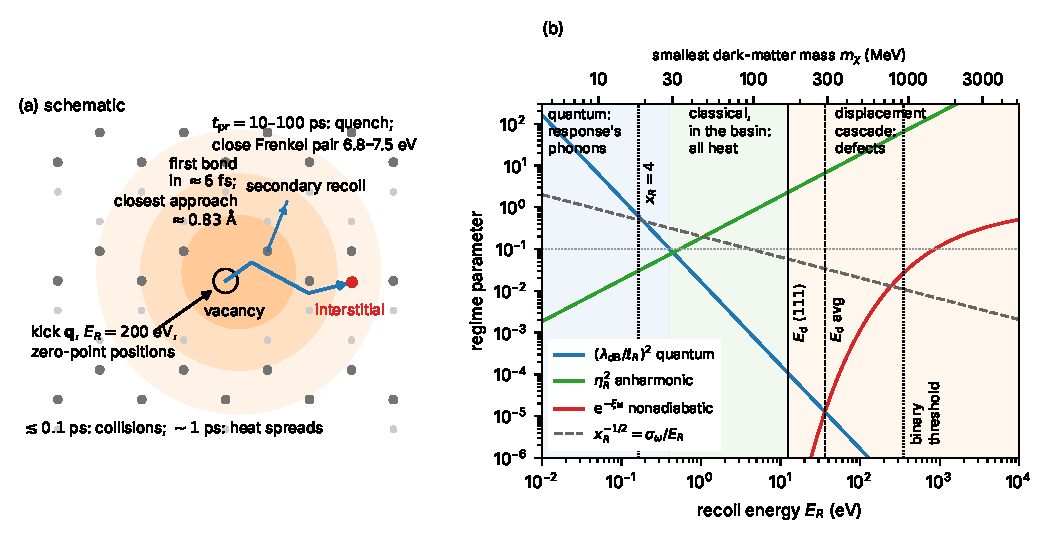
\includegraphics[width=\linewidth]{figures/ch19/fig19_1.pdf}
  \caption{A silicon nuclear recoil after the hand-over. (a) Schematic of a \SI{200}{eV} recoil in a $(1\bar10)$ plane of the diamond lattice (dark dots: atoms in the plane; light dots: the neighboring planes). The kick starts the struck atom from its zero-point position; it crosses its first bond in about \SI{6}{fs}, with a closest approach of \SI{0.83}{\angstrom} in a head-on collision, and sets a secondary atom moving. Within about \SI{0.1}{ps} the collisions are over, and within about a picosecond the heat (shaded rings) spreads through the crystal. At the partition time $t_{\mathrm{pr}}$ of \cref{sec:19.1-partition}, 10 to \SI{100}{ps}, the end state is quenched: here a vacancy and an interstitial, which as a close Frenkel pair store 6.8 to \SI{7.5}{eV}. Paths and end positions are drawn by hand. (b) The regime parameters against the recoil energy $E_R$ at $T = 0$. Curves: the quantum correction $(\lambda_{\mathrm{dB}}/\ell_R)^2 = (\pi\langle\omega\rangle/E_R)^2$, the anharmonic parameter $\eta_R^2$ with $3\Phi^{(2)}/|\Phi^{(3)}| = \SI{0.98}{\angstrom}$, the adiabatic suppression $\ee^{-\xi_{\mathrm{M}}}$ with $\Eg = \SI{1.17}{eV}$ and $\ell_{\mathrm{int}} = \SI{1}{\angstrom}$, and the relative width $x_R^{-1/2} = \sigma_\omega/E_R$ of the handed-over deposit, with $\langle\omega\rangle = \SI{40.9}{meV}$. The dotted horizontal line is the criterion 0.1. Vertical lines: impulse onset $x_R = 4$, displacement thresholds \SI{12.5}{eV} ($\langle111\rangle$) and \SI{36}{eV} (Frenkel pair, direction average), and the binary electron--hole threshold \SI{352}{eV} of \cref{sec:19.2}. Shading: quantum regime, where the phonons of the response are the final state (blue); classical motion inside the basin of the perfect crystal, where all energy becomes heat (green); displacement cascade (orange). Top axis: the smallest dark-matter mass that reaches $E_R$ at $v_{\mathrm{max}} = 2.650\times10^{-3}$.}
  \label{fig:19-recoil}
\end{figure}

The numbers divide the recoil energies into a quantum, a classical, a displacement and a nonadiabatic regime. The boundaries between the regimes follow from the definitions of the four numbers. Their positions depend on the criterion and on the cage estimate, and we quote them as estimates for a criterion of 0.1.
\begin{description}
\item[Quantum.] For $(\pi\langle\omega\rangle/E_R)^2 > 0.1$, that is $E_R < \pi\langle\omega\rangle/\sqrt{0.1}$, the recoil holds too few quanta for classical motion. The response is the whole answer here: its phonons are the final state and the energy is heat.
\item[Classical, inside the basin.] From the upper edge of the quantum regime up to $E_{\mathrm{d}}$ the motion is classical and adiabatic, anharmonic above $\eta_R^2 = 0.1$, and the trajectory relaxes back to the perfect crystal. Born--Oppenheimer molecular dynamics is controlled, and all of the energy becomes heat. The dynamics adds to the response the spectrum of the phonons the recoil leaves, which anharmonic collisions redistribute.
\item[Displacement cascade.] Above $E_{\mathrm{d}}$ some trajectories end in a defect, and the energy splits into heat and stored energy. A recoil many times $E_{\mathrm{d}}$ sets secondary atoms moving above their own thresholds and so starts the collision cascade of \cref{fig:19-recoil}(a).
\item[Nonadiabatic.] Where $\ee^{-\xi_{\mathrm{M}}}$ is no longer negligible, the electrons are excited along the path, and part of the energy becomes charge.
\end{description}
The quantum and harmonic boundaries lie close together: in silicon there is no wide window in which the motion is both harmonic and classical. The hand-over, however, does not need the motion to be harmonic. It takes place at the instant of the kick, and its only requirement on the later motion is that the motion be classical.

\begin{workedexample}{Regime boundaries for silicon}\label{we:19-boundary}
A silicon nucleus of the natural isotope mixture has $M_\kappa = 28.0855\,\mathrm{u} = \SI{26.16}{GeV}$, as in \cref{sec:5.3}, and $\langle\omega\rangle = \SI{40.9}{meV}$ (\cref{sec:11.4}). The cage stiffness is $M_\kappa\langle\omega\rangle^2 = \SI{26.16}{GeV}\times(\SI{0.0409}{eV})^2/(\hbar c)^2 = \SI{11.24}{eV.\angstrom^{-2}}$, with $\hbar c = \SI{1973.27}{eV.\angstrom}$.

\emph{Classical boundary.} $(\pi\langle\omega\rangle/E_R)^2 = 0.1$ gives $E_R = \pi\times\SI{0.0409}{eV}/0.316 = \SI{0.41}{eV}$, or $x_R = 9.9$. At \SI{1}{eV}, $\lambda_{\mathrm{dB}} = \SI{0.054}{\angstrom}$ against $\ell_R = \SI{0.42}{\angstrom}$, and the correction estimate is 0.017.

\emph{Harmonic boundary.} $\eta_R^2 = 0.1$ means $\ell_R = 0.316\times\SI{0.98}{\angstrom} = \SI{0.31}{\angstrom}$, reached at $E_R = \tfrac12\times\SI{11.24}{eV.\angstrom^{-2}}\times(\SI{0.31}{\angstrom})^2 = \SI{0.54}{eV}$. At \SI{1}{eV}, $\eta_R^2 = 0.18$.

\emph{Displacement.} The lowest threshold is \SI{12.5}{eV} along $\langle111\rangle$, the direction average for a Frenkel pair \SI{36}{eV}~\cite[Table~IV]{holmstrom2008threshold}. At \SI{12.5}{eV} the cage amplitude is $\ell_R = \SI{1.49}{\angstrom}$, more than half the bond length of \SI{2.35}{\angstrom}: the cage estimate has run out, as it should, since the atom is leaving its cage. The atom moves at $v_N = \SI{9.27}{km/s}$ and crosses one bond in \SI{25}{fs}, less than half the shortest phonon period of \SI{65}{fs} ($2\pi/\omega_{\mathrm{opt}}$ with $\omega_{\mathrm{opt}} = \SI{64.1}{meV}$, \cref{sec:5.7}), so the collision is over before the lattice has responded. The energy ends in some $\SI{12.5}{eV}/\langle\omega\rangle \approx 300$ phonons if no defect survives.

\emph{Adiabaticity.} At \SI{20}{eV}, $v_N = \SI{11.7}{km/s}$ and $\xi_{\mathrm{M}} = \SI{1.17}{eV}\times\SI{1}{\angstrom}/(\hbar v_N) = 15$, with $\hbar = \SI{6.582e-16}{eV.s}$, so $\ee^{-\xi_{\mathrm{M}}} = 3\times10^{-7}$. Since $\xi_{\mathrm{M}} \propto E_R^{-1/2}$, the suppression reaches 0.1 ($\xi_{\mathrm{M}} = 2.3$) at \SI{0.87}{keV}, and $\xi_{\mathrm{M}} = 1$ at \SI{4.6}{keV}.

\emph{Dark-matter masses.} By \cref{eq:1.3-ERmax} with $v_{\mathrm{max}} = 2.650\times10^{-3}$, the classical boundary needs $\mchi \ge \SI{28}{MeV}$, the harmonic boundary \SI{32}{MeV}, the lowest threshold \SI{154}{MeV}, the average threshold \SI{262}{MeV}, and $\ee^{-\xi_{\mathrm{M}}} = 0.1$ needs \SI{1.3}{GeV}.
\end{workedexample}


\subsection{Acceptance tests for recoil molecular dynamics}\label{sec:19.1-md}

In the classical regimes the handed-over ensemble is propagated by molecular dynamics on $E^{\mathrm{ad}}$. A recoil cascade needs cells of thousands of atoms and thousands of trajectories, far beyond direct density-functional dynamics. In practice the surface is therefore a machine-learned interatomic potential, trained on density-functional energies and forces and joined to a screened Coulomb repulsion at short distance. \Cref{app:E.11} describes the method.

The energy surface must be right along the path of the struck atom, not only near equilibrium. The threshold is set by the energy surface between the neighbors that the struck atom squeezes past. Potentials that agree on elastic constants and defect energies can still disagree on thresholds by several eV; the Stillinger--Weber potential overshoots the density-functional threshold along $\langle111\rangle$ by 4 to \SI{6}{eV} (\cref{sec:7.4}). The accuracy target is the width of the step in $p_{\mathrm{FP}}$, about \SI{0.7}{eV} at the lowest silicon threshold, checked against density-functional dynamics along a few directions. Closer in, the closest approach of a head-on collision is \SI{1.49}{\angstrom} at \SI{20}{eV} and \SI{0.83}{\angstrom} at \SI{200}{eV} (\cref{tab:E-md-si}). At these distances the screened Coulomb repulsion dominates, and the splice between the machine-learned potential and the screened Coulomb repulsion must be complete above the turning point of threshold collisions, so that the dynamics near $E_{\mathrm{d}}$ never feels the splice.

The initial ensemble must be the kicked zero-point ensemble of the hand-over, not a lattice at rest. Classical propagation of a Wigner ensemble is exact for a quadratic Hamiltonian, since the quantum evolution of the Wigner function then reduces to the classical Liouville flow. The zero-point motion of the parts of the crystal that stay harmonic is therefore carried correctly. Where the collision makes the surface anharmonic, classical dynamics lets the zero-point energy of one mode flow into others and leaves the mode below its quantum ground state, a state that quantum dynamics forbids. The error from this leakage is of the order of the zero-point energy of the atoms the collision disturbs, a few tens of meV each, and the definition of the stored energy below is built so that the error does not enter.

The stored energy must be measured between minima. On average, each atom of the initial ensemble lies above the minimum of $E^{\mathrm{ad}}$ by half its zero-point energy, $3\langle\omega\rangle/4 = \SI{31}{meV}$ per atom in silicon (the zero-point energy of \cref{sec:5.3} is \SI{123}{meV} per cell of two atoms). In a cell of 4096 atoms this excess is \SI{126}{eV}, more than ten times the energy of a Frenkel pair. The end state and the perfect crystal are therefore both relaxed to their minima, by a quench at fixed cell without annealing, and the stored energy is the difference \cref{eq:E.11-Est}. The potential's own error on defect energies sets a floor: a potential whose formation energies lie within \SI{7}{\percent} of density-functional theory~\cite[Sect.~III\,E]{bartok2018machine} carries an error of a few tenths of an eV on a defect that stores several eV. One table of these minimum energies, with one potential and cell, must serve the stored energy of \cref{sec:19.4} and the release paths of \cref{sec:19.6}, or the two disagree by that error.

The harmonic limit provides an acceptance test. With $E^{\mathrm{ad}}$ replaced by its harmonic expansion, the classical propagation of $\mathcal{W}_+$ is exact. The mean energy that the kick leaves in a normal mode $s$ is then $|\vect{q}\cdot\vect{e}_{\kappa s}|^2/2NM_\kappa$, with $\vect{e}_{\kappa s}$ the polarization vector of the mode on the struck site and $N$ the number of cells. It is half the square of the mass-weighted momentum the kick gives the mode, since the cross term with the mode's own momentum averages to zero over the ensemble. These mode energies sum to $E_R$ by the completeness of the polarization vectors, and they are the energy-weighted phonon content of the harmonic response of \cref{sec:11.3} at the same $\vect{q}$. A calculation that propagates the kicked ensemble on the true surface must recover this spectrum for recoils small enough to stay harmonic, and the mean and width of \cref{eq:11.4-IA} for all others.

The electronic channel is missing from Born--Oppenheimer dynamics. A common remedy adds a friction force, minus the electronic stopping power times the direction of motion. Below the binary threshold of \cref{sec:19.2} that friction fails (\cref{sec:19.3-assumptions}), and at any energy it supplies a mean loss without its distribution. Where the electronic channel matters, the friction is replaced by excitation events drawn at each close collision from a kernel computed with time-dependent density-functional theory (\cref{sec:19.2}).

\subsection{Partition of the recoil energy}\label{sec:19.1-partition}

The shares of the recoil energy change with time, and the partition needs a time. The collisions are over within about \SI{0.1}{ps}, and the hot carriers that the recoil excites finish their cascade within a picosecond (\cref{chap:18}). Defects at millikelvin, on the other hand, cannot cross barriers of chemical size by thermal activation, since a barrier of \SI{0.1}{eV} at \SI{10}{mK} carries the Boltzmann factor $\ee^{-1.2\times10^5}$ (\cref{sec:7.4}); they move only by tunneling or with the phonons of later events (\cref{sec:19.6}). The drift of the pairs to the electrodes takes longer still (\cref{sec:20.1}). Any time $t_{\mathrm{pr}}$ between 10 and \SI{100}{ps} after the recoil comes after the collisions and the hot-carrier cascade and before any defect motion or pair drift, and we fix the partition there.

At $t_{\mathrm{pr}}$ the energy $\omega$ deposited in the kick has gone three ways. Part has gone to the electrons: the energy $\omega_e$ of a Migdal event, if the kick was one, plus whatever the moving nucleus excited along its path. The nuclei keep the rest of $\omega$, as kinetic energy and as potential energy on $E^{\mathrm{ad}}$. The quench at $t_{\mathrm{pr}}$ splits the nuclear share into the energy of the minimum that the crystal has reached and the vibrational energy about that minimum.
\begin{keyresult}[Partition of the recoil energy]
At the time $t_{\mathrm{pr}}$,
\begin{equation}
  \omega = E_{\mathrm{lat}} + E_{\mathrm{st}} + \omega_e , \qquad
  E_{\mathrm{st}} = E^{\mathrm{ad}}_{\mathrm{min}}(\mathrm{end}) - E^{\mathrm{ad}}_{\mathrm{min}}(\mathrm{perfect}) ,
  \label{eq:19.1-partition}
\end{equation}
where $\omega_e$ is the energy given to the electrons and $E_{\mathrm{st}}$ the stored energy, the difference of the minima of $E^{\mathrm{ad}}$ in the basin of the end state and in that of the perfect crystal. The lattice share $E_{\mathrm{lat}}$ is the vibrational energy in excess of the zero-point energy of the perfect crystal. After the cascade of \cref{chap:18} has turned $\omega_e$ into $N_{\mathrm{eh}}$ pairs,
\begin{equation}
  \omega = N_{\mathrm{eh}}\Eg + E_{\mathrm{heat}} + E_{\mathrm{st}} , \qquad
  E_{\mathrm{heat}} = E_{\mathrm{lat}} + \bigl(\omega_e - N_{\mathrm{eh}}\Eg\bigr) .
  \label{eq:19.1-heat}
\end{equation}
\end{keyresult}
\noindent The energy balance follows from the conservation of the total energy along each trajectory. Before the kick the nuclei hold the minimum of the perfect crystal and its zero-point energy; the kick adds $\omega$, and the electrons take away $\omega_e$. At $t_{\mathrm{pr}}$ the nuclei hold the minimum of the end basin and the vibrational energy about it, and subtracting the balance before the kick from the balance at $t_{\mathrm{pr}}$ gives \cref{eq:19.1-partition}. The second form uses the cascade identity \cref{eq:18.1-energy} for each electronic excitation, $\omega_e = N_{\mathrm{eh}}\Eg + E_{\mathrm{heat}}$ of the cascade, and collects all phonon energy, from the lattice and from the cascade, in one $E_{\mathrm{heat}}$. For an electronic deposit, with $E_{\mathrm{lat}} = E_{\mathrm{st}} = 0$, the second form is \cref{eq:18.1-energy} itself. Capture at the end of the cascade moves energy out of the pairs as in \cref{sec:18.5}.

The stored energy is configurational: it compares minima of $E^{\mathrm{ad}}$ and contains no vibrational energy. The zero-point energy of the end basin differs from that of the perfect crystal, since a defect softens or stiffens the modes around it, and the difference is part of $E_{\mathrm{lat}}$, on the vibrational side. This zero-point difference is part of the heat but cannot reach a sensor, and \cref{sec:19.5} counts it separately. The stored energy is also not the displacement threshold, which is a barrier on the path rather than a difference of end points. A close Frenkel pair keeps about half of the lowest silicon threshold, and the rest of the threshold energy becomes heat (\cref{sec:7.4}).

The partition is random. Each trajectory of the handed-over ensemble ends with its own $(E_{\mathrm{lat}}, E_{\mathrm{st}}, \omega_e)$, and in the impulse regime the ensemble is fixed by $E_R$, the direction $\hat{\vect{r}}_R$ and the temperature. The cascade turns the electronic excitations into pairs with the distribution $P_{\mathrm{casc}}$ of \cref{sec:18.3}, evaluated at the seed energies the recoil produced, which lie near the gap. The result is a joint distribution $P(E_{\mathrm{heat}}, E_{\mathrm{st}}, N_{\mathrm{eh}}|E_R, \hat{\vect{r}}_R, T)$. Its correlations matter as much as its means, since a recoil that stores energy in a defect leaves less heat and, through the same collision, may give fewer pairs.

Below $E_{\mathrm{d}}$ the adiabatic suppression makes $\omega_e$ negligible, $\ee^{-\xi_{\mathrm{M}}} = 5\times10^{-9}$ at \SI{12.5}{eV}, and every trajectory returns to the perfect crystal, so the recoil deposits all of its energy as heat. In silicon the recoils below $E_{\mathrm{d}}$ include every electron-following recoil from dark matter below about \SI{150}{MeV} (\cref{we:19-boundary}). The charge that these recoils produce therefore comes from the Migdal entry of the response and from the soft tail of electronic excitation of \cref{sec:19.2}, not from the recoil dynamics. After $t_{\mathrm{pr}}$ the stored energy decreases as defects release it, and the pairs recombine or are collected; the balance law of \cref{sec:19.5} carries this time dependence, with \cref{eq:19.1-partition} as its starting point.

\section{Electronic excitation by the recoil}\label{sec:19.2}

A silicon nucleus recoiling with \SI{100}{eV} moves at \SI{26}{km/s}, eighty times slower than the valence electrons at the Fermi velocity. A neutron calibration finds that such recoils leave on average 2.7 electron--hole pairs, an ionization yield of $0.102^{+0.034}_{-0.030}$~\cite[Table~II]{albakry2023first}. Yet a binary collision between the nucleus and a valence electron cannot create a single pair until the recoil carries about \SI{350}{eV}. The charge at \SI{100}{eV} must therefore come from processes that the binary picture leaves out, and these are the processes that set the charge signal of light dark matter, whose nuclear recoils in silicon stay below \SI{100}{eV} for masses under \SI{0.44}{GeV}. The question is which processes those are, and how much of the charge the Migdal effect of \cref{chap:12} already supplies.

\subsection{The binary electron--hole threshold}\label{sec:19.2-binary}

The recoiling ion is a projectile of the master formula, as the hot carrier of \cref{sec:18.1} was. It couples to the electron density through its screened charge, and the energy it hands to the electrons at momentum $\vect{k}$ is $\omega = \vect{k}\cdot\vect{v}_N - k^2/2M_\kappa \le kv_N$, with $v_N = q/M_\kappa$ the nuclear velocity after the kick. The stopping power \cref{eq:4.4-dEdx} contains this constraint as the upper limit $\omega \le kv_N$ of its inner integral; \cref{sec:19.3} evaluates that integral.

Consider first a free electron gas with the valence density of the crystal and a gap $\Eg$ added by hand. Its loss function vanishes outside the particle--hole continuum of \cref{sec:4.2}, which for $k > 2k_{\mathrm{F}}$ begins at $\omega_-(k) = k^2/2m_e - kv_{\mathrm{F}}$. An electron--hole pair needs $\omega \ge \Eg$, and the ion supplies at most $\omega = kv_N$. Both conditions hold at some $k$ only if the line $\omega = kv_N$ rises above $\omega_-(k)$ at an energy of at least $\Eg$. The line and the edge cross at $k = 2m_e(v_N + v_{\mathrm{F}})$, where $\omega = 2m_ev_N(v_N + v_{\mathrm{F}})$, and this is the largest energy the ion can deposit in one electronic excitation:
\begin{equation}
  \omega_{\mathrm{max}} = 2m_e v_N\,(v_N + v_{\mathrm{F}}) .
  \label{eq:19.2-transfer}
\end{equation}
The same number follows from a collision of two particles. In the rest frame of the heavy ion an electron moving against it at $v_{\mathrm{F}}$ approaches with speed $v_{\mathrm{F}} + v_N$ and is reflected with the same speed, and in the crystal frame it leaves with $v_{\mathrm{F}} + 2v_N$. Its kinetic energy rises by $\tfrac12 m_e[(v_{\mathrm{F}} + 2v_N)^2 - v_{\mathrm{F}}^2]$, which is \cref{eq:19.2-transfer}. The heavy ion acts as a moving wall: it reverses the electron's velocity in its own frame, and the energy it gives is linear in $v_N$.

Setting $\omega_{\mathrm{max}} = \Eg$ gives the threshold speed. Since $v_N \ll v_{\mathrm{F}}$ at every recoil energy of interest, the term $v_N^2$ can be dropped.

\begin{keyresult}[Binary electron--hole threshold]
A slow ion creates an electron--hole pair in a binary collision with a free-electron-like valence band only above the speed $v_{N,\mathrm{th}} = \Eg/(2m_ev_{\mathrm{F}})$, that is, above the recoil energy
\begin{equation}
  E_{R,\mathrm{th}} = \frac12 M_\kappa v_{N,\mathrm{th}}^2 = \frac{M_\kappa}{m_e}\,\frac{\Eg^2}{16E_{\mathrm{F}}} ,
  \label{eq:19.2-Eth}
\end{equation}
with $E_{\mathrm{F}} = m_ev_{\mathrm{F}}^2/2$ the Fermi energy of the valence electrons. It is \SI{352}{eV} in silicon and \SI{399}{eV} in germanium.
\end{keyresult}

The threshold is the gap multiplied by two numbers, the mass ratio $M_\kappa/m_e$, which is large, and $\Eg/16E_{\mathrm{F}}$, which is small. In silicon the product puts $E_{R,\mathrm{th}}$ at three hundred times the gap. Keeping the term $v_N^2$ in \cref{eq:19.2-transfer} and solving the quadratic, $v_N = \tfrac12[(v_{\mathrm{F}}^2 + 2\Eg/m_e)^{1/2} - v_{\mathrm{F}}]$, lowers the threshold by \SI{4.4}{\percent} to \SI{336}{eV} in silicon and by \SI{3.1}{\percent} to \SI{387}{eV} in germanium. For germanium we use $\Eg = \SI{0.744}{eV}$ and $a = \SI{5.658}{\angstrom}$ (\cref{sec:3.3}), so that $k_{\mathrm{F}} = \SI{1.736}{\angstrom^{-1}}$, $E_{\mathrm{F}} = \SI{11.48}{eV}$ and $M_\kappa/m_e = \num{132396}$. The heavier nucleus raises the threshold, and the smaller gap, which enters squared, lowers it again.

\begin{workedexample}{The binary threshold of silicon}\label{we:19-threshold}
Silicon has four valence electrons per atom and eight atoms in the cubic cell of side $a = \SI{5.431}{\angstrom}$, so the valence density is $\nd_e = 32/a^3 = \SI{0.19976}{\angstrom^{-3}}$. The free-electron Fermi wavevector is $k_{\mathrm{F}} = (3\pi^2\nd_e)^{1/3} = \SI{1.8085}{\angstrom^{-1}}$, or $k_{\mathrm{F}} = \SI{1.8085}{\angstrom^{-1}}\times\SI{1973.27}{eV\,\angstrom} = \SI{3.569}{keV}$, as in \cref{fig:4-gas}. Then
\begin{equation*}
  E_{\mathrm{F}} = \frac{k_{\mathrm{F}}^2}{2m_e} = \frac{(\SI{3.569}{keV})^2}{2\times\SI{511.0}{keV}} = \SI{12.46}{eV} , \qquad
  v_{\mathrm{F}} = \frac{k_{\mathrm{F}}}{m_e} = 6.984\times10^{-3} = \SI{2094}{km/s} .
\end{equation*}
With the low-temperature gap $\Eg = \SI{1.17}{eV}$ the threshold speed is $v_{N,\mathrm{th}} = \Eg/(2m_ev_{\mathrm{F}}) = \SI{1.17}{eV}/(2\times\SI{511.0}{keV}\times6.984\times10^{-3}) = 1.639\times10^{-4}$, or \SI{49.2}{km/s}. The silicon nucleus has $M_\kappa = 28.0855\times\SI{931.494}{MeV} = \SI{26.16}{GeV}$, so $M_\kappa/m_e = \num{51197}$, and
\begin{equation*}
  E_{R,\mathrm{th}} = \frac{M_\kappa}{m_e}\,\frac{\Eg^2}{16E_{\mathrm{F}}} = \num{51197}\times\frac{(\SI{1.17}{eV})^2}{16\times\SI{12.46}{eV}} = \num{51197}\times\SI{6.87e-3}{eV} = \SI{352}{eV} .
\end{equation*}
For comparison, \cref{eq:19.2-transfer} at $E_R = \SI{100}{eV}$, where $v_N = 8.74\times10^{-5}$, gives $\omega_{\mathrm{max}} = \SI{0.63}{eV}$: about half the gap, too little for a binary collision at the measured \SI{100}{eV} point to make a pair. Dark matter needs a mass of at least \SI{0.84}{GeV} to give a nucleus \SI{352}{eV} (\cref{sec:19.1}).
\end{workedexample}

\subsection{Softening by the valence momentum tail}\label{sec:19.2-soft}

\Cref{eq:19.2-Eth} assumed that no valence electron moves faster than $v_{\mathrm{F}}$. In a crystal this is not so. A Bloch state of crystal momentum $\vect{k}$ has components at every $\vect{k} + \vect{G}$, and near each nucleus the valence orbitals oscillate to stay orthogonal to the core; as a result the valence momentum density extends beyond $k_{\mathrm{F}}$. An electron of momentum $p$ moving against the ion gains up to $2m_ev_N(v_N + p/m_e)$, and it can be promoted across the gap if
\begin{equation}
  p \ge p_{\mathrm{min}}(E_R) = \frac{\Eg}{2v_N} - m_ev_N , \qquad v_N = (2E_R/M_\kappa)^{1/2} .
  \label{eq:19.2-pmin}
\end{equation}
In the free gas the fraction of valence electrons above $p_{\mathrm{min}}$ is $1 - (p_{\mathrm{min}}/k_{\mathrm{F}})^3$, which vanishes where $p_{\mathrm{min}} = k_{\mathrm{F}}$, at the threshold with $v_N^2$ kept, \SI{336}{eV}. In silicon at \SI{100}{eV}, $p_{\mathrm{min}} = \SI{3.37}{\angstrom^{-1}} = 1.86\,k_{\mathrm{F}}$. In the language of the loss function, the free-gas support ends at $\omega_-(k)$ and the crystal's $L(\vect{k},\omega)$ at $k \gtrsim 2k_{\mathrm{F}}$ and $\omega \ge \Eg$ is the low-energy tail of the Bethe ridge $\omega \approx k^2/2m_e$, whose width is set by the momentum distribution of the valence electrons. The tail is small but not zero; below $E_{R,\mathrm{th}}$ the linear-response excitation is therefore suppressed, not forbidden.

\Cref{fig:19-yield}(b) shows how much the tail changes the count. It compares the free-gas fraction with the same fraction computed from the valence momentum density of the empirical pseudopotential model of \cref{sec:3.3}, summed over the four valence bands on a $10^3$ grid of the zone. In the model, \SI{23}{\percent} of the valence momentum density lies beyond $k_{\mathrm{F}}$, \SI{2.2}{\percent} beyond $1.5\,k_{\mathrm{F}}$ and \SI{0.34}{\percent} beyond $2k_{\mathrm{F}}$. The fraction of electrons fast enough to be promoted falls smoothly through $E_{R,\mathrm{th}}$ instead of vanishing there: it is 0.27 at \SI{352}{eV}, where the free gas has 0.07, then 0.047 at \SI{200}{eV}, $5.6\times10^{-3}$ at \SI{100}{eV} and $4\times10^{-4}$ at \SI{50}{eV}. The model's pseudo-orbitals are smooth inside the cores, where the true valence orbitals oscillate, and its plane waves stop at \SI{5.3}{\angstrom^{-1}}, close to $p_{\mathrm{min}}$ at \SI{50}{eV}; its tail is therefore smaller than the real one, and the numbers indicate the shape of the softening, not its size. The fraction is also not yet a yield: an electron above $p_{\mathrm{min}}$ is promoted only in a head-on encounter, and the conduction states must accept it.

The zero-point momentum of the struck nucleus spreads its recoil energy by about \SI{2}{eV} at $E_R = \SI{100}{eV}$ (\cref{sec:19.1}), which is negligible against \SI{352}{eV}.

\subsection{Close collisions and the excitation kernel}\label{sec:19.2-kernel}

Within a few femtoseconds a recoil of a few hundred eV strikes a neighbor, closer than a bond length, and passes on part of its energy; the neighbor strikes the next atom, and so on (\cref{sec:19.1}). In such an encounter two atoms come within an angstrom of each other, and the electrons around them briefly belong to a quasi-molecule, Si$_2$ or Ge$_2$, whose levels depend on the distance between the nuclei. The bulk gap no longer sets the excitation threshold. As the nuclei approach, a filled level and an empty one can cross, or nearly cross, and an electron can be promoted at the crossing.

How likely that is depends on how fast the crossing is passed. Away from crossings the Massey parameter $\xi_{\mathrm{M}} = \Eg\ell_{\mathrm{int}}/v_N$ of \cref{sec:19.1} measures adiabaticity, and nonadiabatic excitation is suppressed roughly as $\ee^{-\xi_{\mathrm{M}}}$; in silicon, with $\ell_{\mathrm{int}} = \SI{1}{\angstrom}$, $\xi_{\mathrm{M}}$ is 6.8 at $E_R = \SI{100}{eV}$, 3.6 at $E_{R,\mathrm{th}}$ and 2.1 at \SI{1}{keV}. At an avoided crossing the relevant gap is the local splitting $2h_{\mathrm{LZ}}$ of the two levels, with $h_{\mathrm{LZ}}$ the coupling between the crossing diabatic states. The relevant speed is the rate $v|\Delta F_{\mathrm{LZ}}|$ at which their energy difference sweeps through zero, where $v$ is the relative speed of the nuclei and $\Delta F_{\mathrm{LZ}}$ the difference of the slopes of the two diabatic levels against the internuclear distance. The electrons jump from the lower adiabatic level to the upper one in one passage with the Landau--Zener probability~\cite{zener1932non,vutha2010simple}
\begin{equation}
  P_{\mathrm{LZ}} = \exp\!\left(-\frac{2\pi h_{\mathrm{LZ}}^2}{v\,|\Delta F_{\mathrm{LZ}}|}\right) .
  \label{eq:19.2-LZ}
\end{equation}
A collision passes each crossing twice, on the way in and on the way out. If the phase between the two passages is averaged over impact parameters, the electrons end up excited with probability $2P_{\mathrm{LZ}}(1 - P_{\mathrm{LZ}})$, one jump and one adiabatic passage in either order. Unlike $\ee^{-\xi_{\mathrm{M}}}$, \cref{eq:19.2-LZ} is set by the small splitting at the crossing, not by the bulk gap, and it is why close collisions can excite electrons well below $E_{R,\mathrm{th}}$.

The excitation cannot be computed in linear response in the ion's charge. The Born parameter of the collision, $Z_\kappa\alpha/v_{\mathrm{F}}$, is 15 for silicon and 35 for germanium. The ion's own electrons screen its charge, but the parameter exceeds one already for a unit charge, and the ion perturbs the electrons near it strongly; and the Massey parameter near \SI{1}{keV} is of order one, so the electrons neither follow adiabatically nor stay frozen. The excitation is instead described by a kernel tabulated from a nonperturbative calculation. It is the distribution
\begin{equation}
  \frac{\dd P}{\dd\omega_e}(b_{\mathrm{imp}}, E_{\mathrm{coll}})
  \label{eq:19.2-kernel}
\end{equation}
of the electronic excitation energy $\omega_e$ left behind when two Si or two Ge atoms collide in the crystal at impact parameter $b_{\mathrm{imp}}$ and relative energy $E_{\mathrm{coll}}$, in units of eV$^{-1}$. Its integral over $\omega_e$ is the probability that the collision excites the electrons. Along the trajectory of a recoil, every close approach $j$ draws an excitation from the kernel at its own $(b_j, E_j)$; with the trajectories of the partition of \cref{sec:19.1}, this gives the excitation spectrum of the whole recoil, $\dd\mathcal{N}_{\mathrm{exc}}/\dd\omega_e = \langle\sum_j(\dd P/\dd\omega_e)(b_j, E_j)\rangle$. The spectrum has three parts, which a calculation should keep apart: binary excitation above $E_{R,\mathrm{th}}$, promotion at level crossings, and the linear-response excitation through the momentum tail of \cref{sec:19.2-soft}.

Each excitation then seeds the carrier cascade of \cref{chap:18}, and the pairs follow from the cascade distribution $P_{\mathrm{casc}}(N_{\mathrm{eh}}|\omega_e)$ at that seed, not from $\omega_e/\varepsilon_{\mathrm{eh}}$. The mean pair number of a recoil is
\begin{equation}
  \langle N_{\mathrm{eh}}\rangle(E_R) = \int\dd\omega_e\,\frac{\dd\mathcal{N}_{\mathrm{exc}}}{\dd\omega_e}\,\bar n(\omega_e) ,
  \label{eq:19.2-charge}
\end{equation}
with $\bar n(\omega_e)$ the mean of $P_{\mathrm{casc}}$. The difference matters because slow-ion excitations lie near the gap, where the cascade is far from its linear law $\bar n = \omega/\varepsilon_{\mathrm{eh}} + b_N$ (\cref{sec:18.2}). Take the silicon cascade of \cref{chap:18}, with the energy above the gap split uniformly between electron and hole. A seed between $\Eg$ and \SI{2.9}{eV} gives one pair (mean 1.000), where $\omega_e/\varepsilon_{\mathrm{eh}}$ gives 0.52 at \SI{1.95}{eV} and 0.78 at \SI{2.9}{eV}. The two agree to within a few percent only from about \SI{4}{eV} up (1.05 against 1.06 at \SI{3.96}{eV}, 1.65 against 1.60 at \SI{6.0}{eV}).

The kernel holds the main theory uncertainty of the charge channel, which comes from exchange and correlation. Real-time time-dependent density-functional theory with adiabatic semilocal functionals places level crossings that involve charge transfer at the wrong distances and makes the gap of a distorted configuration too small; already at equilibrium the semilocal gap of silicon is \SI{0.56}{eV} against the measured \SI{1.17}{eV} (\cref{sec:3.3}). Since a too-small gap moves crossings outward and makes promotion too easy, the error has a known sign but no known size. Mean-field dynamics, in which the nuclei move in the average field of the evolving electrons (Ehrenfest dynamics), also yields the mean excitation energy, not its distribution, so the kernel must be built from the projection of the evolved orbitals on the conduction states. The exchange--correlation uncertainty of the kernel is then the spread between three treatments that err differently: Ehrenfest dynamics with a hybrid functional; surface hopping with decoherence, in which the nuclei follow one electronic surface at a time and jump between surfaces at random; and \cref{eq:19.2-LZ} with diabatic couplings of the quasi-molecule from multireference calculations, which describe its electrons with several determinants. The kernel is tested at high energy, where the mean energy lost per unit path must approach the electronic stopping \cref{eq:4.4-dEdx} (\cref{app:E.23}).

\subsection{The ionization yield of silicon recoils}\label{sec:19.2-yield}

A charge readout records the ionization yield, the mean pair number of a nuclear recoil relative to that of an electron recoil of the same energy,
\begin{equation}
  Y_q(E_R) = \frac{\langle N_{\mathrm{eh}}\rangle(E_R)\,\varepsilon_{\mathrm{eh}}}{E_R} .
  \label{eq:19.2-Yq}
\end{equation}
An electron recoil of $E_R \ge \SI{100}{eV}$ lies on the linear law of \cref{sec:18.2}, where $E_R/\varepsilon_{\mathrm{eh}}$ is its mean pair number to within the constant $b_N \le 0.35$, about \SI{1}{\percent} of the 27 pairs at \SI{100}{eV}. The literature also writes $Y_q$ as the quenching factor, the electron-equivalent energy over the recoil energy. Lindhard's model, \cref{eq:16.6-lindhard}, identifies $Y_q$ with the electronic share $y_L$ of the slowing-down; \cref{sec:19.3} derives it and states where it holds. \Cref{eq:19.2-charge} shows why the identification fails at low energy: the share $y_L$ counts energy, $\bar n(\omega_e)$ counts pairs, and near the gap the two are not proportional.

The silicon measurement~\cite{albakry2023first} used a neutron beam of \SI{55.7}{keV} on a \SI{4}{mm} silicon crystal read out through its phonons, with the scattered neutron tagged at a fixed angle to fix $E_R$. Without bias the phonon signal measures $E_R$; with a bias $V_{\mathrm{bias}}$ the drifting pairs add $N_{\mathrm{eh}}eV_{\mathrm{bias}}$, so the total phonon energy is $E_R + N_{\mathrm{eh}}eV_{\mathrm{bias}}$, and the yield is extracted with \SI{3.8}{eV} per pair~\cite[Eq.~(1)]{albakry2023first}. This definition takes the phonon energy of the recoil to be the recoil energy, so that no energy is stored in defects; the stored share, a few percent of $E_R$ (\cref{sec:19.4}), lies inside the quoted errors. With the measured $\varepsilon_{\mathrm{eh}} = \SI{3.749}{eV}$ of \cref{sec:18.4} the yields would be \SI{1.3}{\percent} lower.

\begin{figure}[tbp]
  \centering
  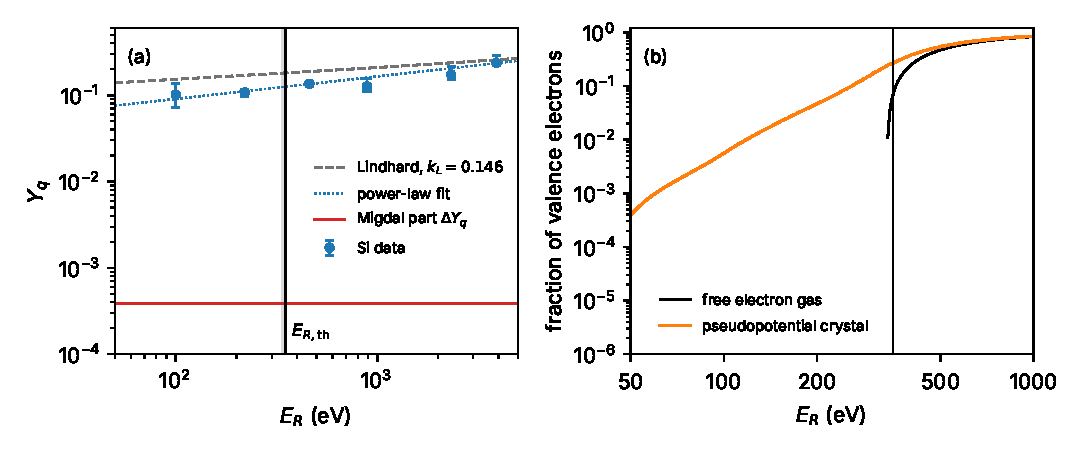
\includegraphics[width=\linewidth]{figures/ch19/fig19_2.pdf}
  \caption{The charge channel of silicon recoils. (a) Measured ionization yield $Y_q$ of silicon nuclear recoils (points: neutron scattering, total uncertainties, with \SI{3.8}{eV} per pair~\cite[Table~II]{albakry2023first}) against the recoil energy, with the power-law fit of the same work, $0.302(E_R/\SI{10}{keV})^{0.261}$ (dotted), and Lindhard's yield \cref{eq:16.6-lindhard} with $k_L = 0.146$ (dashed). Vertical line: the binary threshold $E_{R,\mathrm{th}} = \SI{352}{eV}$ of \cref{eq:19.2-Eth}; gray band: down to \SI{336}{eV}, the threshold with the $v_N^2$ term kept. Red: the part $\Delta Y_q^{\mathrm{Mig}}$ of the yield carried by Migdal electrons, \cref{eq:19.2-Ymig}, from the soft-limit spectrum of \cref{sec:12.3} converted to pairs by the silicon cascade of \cref{chap:18} with a uniform split of energy between electron and hole. (b) Fraction of valence electrons fast enough to be promoted across the gap $\Eg = \SI{1.17}{eV}$ by a head-on binary collision, $p \ge p_{\mathrm{min}}(E_R)$ of \cref{eq:19.2-pmin}: free electron gas of the valence density (black), which vanishes at \SI{336}{eV}, and the valence momentum density of the empirical pseudopotential model of \cref{sec:3.3} (four bands, $10^3$ points in the zone, plane waves to \SI{5.3}{\angstrom^{-1}}), whose smooth pseudo-orbitals understate the high-momentum tail; vertical line as in (a).}
  \label{fig:19-yield}
\end{figure}

\Cref{fig:19-yield}(a) shows the result. Between \SI{0.1}{keV} and \SI{3.9}{keV} the yield rises only from 0.10 to 0.24, and the two points below $E_{R,\mathrm{th}}$, at 0.10 and \SI{0.22}{keV}, agree with each other within their errors: there is no sign of an ionization threshold above \SI{100}{eV}. The Lindhard yield lies above the data at every energy below a keV, by a factor of 1.5 at \SI{100}{eV} (0.153 against 0.102) and by 1.4 at \SI{0.46}{keV}. Germanium, however, shows the opposite deviation. Recoils of \SI{254}{eV}, below its binary threshold of \SI{399}{eV}, give \SI{64 \pm 8}{eV} of electron-equivalent energy at \SI{77}{K}, a quenching factor of $\SI{25 \pm 3}{\percent}$ against Lindhard's \SI{14.3}{\percent}~\cite[abstract and Table~IV]{kavner2024measurement}.

The measured Fano factor of the nuclear-recoil charge, $F_{\mathrm{NR}} = \operatorname{Var}N_{\mathrm{eh}}/\langle N_{\mathrm{eh}}\rangle$, is $0.9^{+0.7}_{-0.4}$ at \SI{0.10}{keV}, $0.5^{+0.2}_{-0.1}$ at \SI{0.22}{keV} and $1.8^{+0.6}_{-0.5}$ at \SI{0.46}{keV}, and it grows to $8.4^{+2.4}_{-1.9}$ at \SI{3.91}{keV}~\cite[Table~II]{albakry2023first}, seventy times the electron-recoil value $F_{\mathrm{eh}} = 0.119$. Suppose the electronic energy $E_{\mathrm{el}}$ of a recoil were converted at a constant $\varepsilon_{\mathrm{eh}}$. The law of total variance would then give $\operatorname{Var}N_{\mathrm{eh}} = F_{\mathrm{eh}}\langle E_{\mathrm{el}}\rangle/\varepsilon_{\mathrm{eh}} + \operatorname{Var}E_{\mathrm{el}}/\varepsilon_{\mathrm{eh}}^2$, the cascade fluctuation at fixed $E_{\mathrm{el}}$ plus the fluctuation of $E_{\mathrm{el}}$ itself, so that
\begin{equation}
  F_{\mathrm{NR}} = F_{\mathrm{eh}} + \frac{\operatorname{Var}E_{\mathrm{el}}}{\varepsilon_{\mathrm{eh}}\langle E_{\mathrm{el}}\rangle} .
  \label{eq:19.2-FNR}
\end{equation}
At \SI{3.91}{keV}, with $\langle E_{\mathrm{el}}\rangle = Y_qE_R = \SI{923}{eV}$ and \SI{3.8}{eV} per pair, the measured $F_{\mathrm{NR}}$ requires a spread of \SI{170}{eV}, \SI{18}{\percent} of the mean: recoils of the same energy differ in how much of it reaches the electrons, because the sequence of collisions that each one makes is different. At \SI{100}{eV} the excitations lie near the gap and \cref{eq:19.2-FNR} no longer applies; there $F_{\mathrm{NR}}$ near one is what a few independent excitations of about one pair each would give.

\subsection{Migdal electrons in the measured yield}\label{sec:19.2-migdal}

The kick that starts the recoil already excites electrons, with the Migdal probability $P_{\mathrm{Mig}}$ of \cref{chap:12}. A neutron calibration measures the charge of real recoils, Migdal electrons included. The Migdal part of the yield is the integral \cref{eq:19.2-charge} taken over the soft-limit spectrum \cref{eq:12.3-soft}:
\begin{equation}
  \Delta Y_q^{\mathrm{Mig}} = \frac{\varepsilon_{\mathrm{eh}}}{E_R}\int\dd\omega_e\,\frac{\dd P_{\mathrm{Mig}}}{\dd\omega_e}\,\bar n(\omega_e) .
  \label{eq:19.2-Ymig}
\end{equation}
In the soft limit $\dd P_{\mathrm{Mig}}/\dd\omega_e$ is proportional to $v_N^2 = 2E_R/M_\kappa$, so the factor $1/E_R$ cancels and $\Delta Y_q^{\mathrm{Mig}}$ does not depend on the recoil energy. For silicon, the spectrum of \cref{sec:12.3} has $P_{\mathrm{Mig}} = 6.07\times10^{-3}$ at $E_R = \SI{100}{eV}$ with a mean electronic energy of \SI{5.97}{eV}. The energy-only cascade of \cref{chap:18} turns one such excitation into 1.69 pairs on average with a uniform split of the energy above the gap, or 1.92 if the electron takes all of it; the full-band cascade of \cref{sec:18.3-fullband} puts fewer events in the two-pair bin, and every Migdal excitation makes at least one pair. With \SI{3.8}{eV} per pair, the convention of the data,
\begin{equation*}
  \Delta Y_q^{\mathrm{Mig}} = \frac{\SI{3.8}{eV}}{\SI{100}{eV}}\times6.07\times10^{-3}\times1.69 = 3.9\times10^{-4} ,
\end{equation*}
and $4.4\times10^{-4}$ for the one-sided split; one pair per excitation gives the model-free lower edge $2.3\times10^{-4}$. The upper value is \SI{0.4}{\percent} of the measured yield at \SI{100}{eV} and \SI{0.3}{\percent} at \SI{0.46}{keV}. Both are soft-limit values, and the exact second-order bracket of \cref{sec:12.3-validity} lowers them, multiplying the Migdal probability by 0.93 at \SI{100}{eV} and by 0.62 at \SI{500}{eV}. The measured charge of silicon recoils at these energies is therefore almost entirely collisional.

A rate converted with the measured yield already contains the Migdal ionization (\cref{sec:12.1-counting}). Conversely, a computed yield must count the Migdal excitation at the kick and the collisional excitation after it, and nothing else. The trajectory calculation therefore starts after the kick, from the nuclear momentum and site distribution that the response hands over (\cref{sec:19.1}), and the lattice factor of the recoils that leave no Migdal electron has the weight $1 - P_{\mathrm{Mig}}$ of \cref{sec:12.1}, a \SI{0.6}{\percent} correction at \SI{100}{eV}. \Cref{sec:12.3-validity} met the boundary between the two channels from the Migdal side. Toward \SI{1}{keV} the second-order Migdal amplitude acquires a vanishing denominator, because the already moving nucleus ionizes the electrons on shell as a slow ion does, and that part belongs to the collisional channel of this section.

The balance between Migdal and collisional excitation shifts at low energy. The number of Migdal pairs per recoil falls in proportion to $E_R$. The collisional channel decreases for two reasons, fewer close collisions and the adiabatic suppression, whose factor $\ee^{-\xi_{\mathrm{M}}}$ falls from $1.1\times10^{-3}$ at \SI{100}{eV} to $2.6\times10^{-7}$ at \SI{20}{eV}, against a factor of five for the Migdal probability. If promotion at crossings follows the same trend, an estimate that only the kernel can confirm, the Migdal electrons become the dominant source of charge somewhere between a few tens of eV and \SI{100}{eV}, the recoil energies of dark matter below about \SI{0.44}{GeV}. That makes the Migdal rate of \cref{chap:12}, and not an extrapolated yield, the charge signal of the lightest nuclear-recoil searches.

\subsection{Open problems}\label{sec:19.2-open}

No calculation predicts the measured silicon yields and Fano factors below the binary threshold, or the germanium point at \SI{254}{eV}. The missing input is the close-collision kernel \cref{eq:19.2-kernel} for Si--Si and Ge--Ge collisions, with its exchange--correlation spread. Once it exists, the chain of partition trajectories, kernel and cascade also yields the probability of a recoil without charge, which sets the efficiency of a charge readout at the lowest recoil energies.

\section{Stopping of slow ions}\label{sec:19.3}

Nearly every nuclear-recoil search in a semiconductor converts measured charge into recoil energy with one formula, Lindhard's electronic share $y_L(E_R)$ of \cref{eq:16.6-lindhard}. For silicon it gives $y_L = 0.302$ at \SI{10}{keV}, and the measured yields of \cref{fig:19-yield} lie below it, by the factor 1.5 of \cref{sec:19.2-yield} at \SI{100}{eV}. The formula is the solution of an integral equation for an ion slowing down by independent binary collisions, with electronic losses taken from the stopping of a uniform electron gas. In the language of \cref{sec:19.1} it is the partition \cref{eq:19.1-partition} with $E_{\mathrm{st}} = 0$ and $\omega_e$ computed from continuum stopping. We will derive Lindhard's equation from that partition and see which of its assumptions fail below a keV. The Bethe formula, derived from the loss function of \cref{sec:4.4}, then gives the opposite, first-order limit: there the solid enters through one mean excitation energy, and the limit sets in only above about twice the Fermi velocity, far above any recoil.

Two objects carry Lindhard's name. The Lindhard function $\varepsilon_{\mathrm{Lin}}$ of \cref{sec:4.5} is the dielectric function of the free electron gas; Lindhard quenching is the electronic share $y_L$ of a slowing-down ion. Their only connection is that the electronic stopping behind $y_L$ was first estimated from an electron gas.

\subsection{Binary collisions of a slow ion}\label{sec:19.3-binary}

A silicon recoil of \SI{1}{keV} moves at $v_N = 2.76\times10^{-4}$, a twenty-fifth of the Fermi velocity of the valence electrons (\cref{we:19-threshold}). It loses energy in two ways, which Lindhard's model treats as separate: elastic collisions with other nuclei, screened by their electrons, and excitation of the electrons themselves.

The nuclear collisions are those of two atoms interacting through a screened Coulomb potential $(Z_\kappa^2\alpha/r)\,\phi_{\mathrm{TF}}(r/a_L)$, with $\phi_{\mathrm{TF}}$ the Thomas--Fermi screening function of a neutral atom~\cite{thomas1927calculation,fermi1928statistische} and $a_L = 0.8853\,a_0/(\sqrt2\,Z_\kappa^{1/3})$ Lindhard's screening length for two equal atoms~\cite[Sect.~II\,A]{sorensen2015atomic}. For silicon, $a_L = \SI{0.1375}{\angstrom}$. The natural energy scale is the Coulomb energy of the pair at the distance $a_L$. For equal masses the center-of-mass frame carries half of the ion's kinetic energy $E$, and the reduced energy is
\begin{equation}
  \epsilon_L = \frac{a_L}{2Z_\kappa^2e_{\mathrm{G}}^2}\,E \equiv c_L E ,
  \label{eq:19.3-reduced}
\end{equation}
with $e_{\mathrm{G}}^2 = \alpha$ the Gaussian charge squared, \SI{14.40}{eV\,\angstrom} in conventional units. For silicon $c_L = \SI{0.02435}{keV^{-1}}$, the value $11.5\,Z_\kappa^{-7/3}\,\si{keV^{-1}}$ of \cref{eq:16.6-lindhard}: a recoil of \SI{1}{keV} has $\epsilon_L = 0.024$, and $\epsilon_L = 1$ is reached only at \SI{41}{keV}.

A collision that deflects the pair by the angle $\theta_{\mathrm{s}}$ in the center-of-mass frame gives the struck atom the energy $T_n = E\sin^2(\theta_{\mathrm{s}}/2)$. Lindhard's insight was that in the reduced variable $x_L = \epsilon_L\sin(\theta_{\mathrm{s}}/2)$ the cross-section of a screened Coulomb potential depends on one function of one variable,
\begin{equation}
  \dd\sigma_n = \pi a_L^2\,\frac{f_{\mathrm{LSS}}(x_L)}{x_L^2}\,\dd x_L ,
  \label{eq:19.3-dsigma}
\end{equation}
with $t = x_L^2$ the form of~\cite[Eq.~(2)]{sarkis2023ionization}. The reason is visible in the small-angle (impulse) approximation, where the deflection is the transverse momentum the potential imparts along a straight path divided by the momentum. With $\beta = b/a_L$ the impact parameter in units of $a_L$ and $I(\beta) = \int_0^\infty\dd\zeta\,\phi_{\mathrm{TF}}(r)/r$, $r = (\beta^2 + \zeta^2)^{1/2}$, the deflection is $\theta_{\mathrm{s}} = -\epsilon_L^{-1}\,\dd I/\dd\beta$, so that $x_L \simeq \epsilon_L\theta_{\mathrm{s}}/2 = -\tfrac12\,\dd I/\dd\beta$ is a function of $\beta$ alone. Then $\dd\sigma_n = 2\pi a_L^2\beta\,\dd\beta$ gives $f_{\mathrm{LSS}}(x_L) = 2x_L^2\beta\,|\dd\beta/\dd x_L|$, with no reference to the energy. An unscreened potential, $\phi_{\mathrm{TF}} = 1$, has $\dd I/\dd\beta = -1/\beta$ and gives the Rutherford form $f_{\mathrm{LSS}} = 1/2x_L$. The screened function rises as a power of $x_L$ at small $x_L$, peaks at 0.43 near $x_L = 0.14$ and approaches the Rutherford form for $x_L \gg 1$. The mean energy lost to nuclei per unit reduced path, $s_n(\epsilon_L) = \epsilon_L^{-1}\int_0^{\epsilon_L}f_{\mathrm{LSS}}\,\dd x_L$, peaks at 0.41 near $\epsilon_L = 0.3$.

The electronic losses are a friction. For a projectile much slower than the electrons, the dielectric stopping \cref{eq:4.4-dEdx} samples only the low-energy side of the loss function, and the energy loss per unit path is proportional to $v_N$. \Cref{we:4-oscillatorL} showed this for a damped oscillator, and \cref{lim:19.3b} below shows it for the electron gas. Since $E \propto v_N^2$, the reduced electronic stopping per unit reduced path length $\rho_L = \pi a_L^2\nd_{\mathrm{at}}x$, with $x$ the path length and $\nd_{\mathrm{at}}$ the atomic density, is
\begin{equation}
  \frac{\dd\epsilon_L}{\dd\rho_L}\bigg|_e = k_L\,\epsilon_L^{1/2} , \qquad k_L = 0.133\,Z_\kappa^{2/3}A^{-1/2} ,
  \label{eq:19.3-Se}
\end{equation}
with $A$ the atomic mass in atomic units~\cite[Eq.~(4)]{sarkis2020study}. For silicon $k_L = 0.146$. The coefficient comes from Lindhard and Scharff's estimate of the friction of an ion in an electron gas. It contains a factor of about $Z_\kappa^{1/6}$, 1.55 for silicon, inserted by hand to match the stopping data of their time, as Sarkis et al.\ point out~\cite[Sect.~``Scaling length'']{sarkis2023ionization}. In physical units \cref{eq:19.3-Se} assigns a silicon ion in silicon an electronic stopping of 0.88, 2.77 and \SI{8.76}{eV/\angstrom} at 0.1, 1 and \SI{10}{keV}.

The friction law is an empirical scaling at these speeds, not a derived limit. The dielectric formula \cref{eq:4.4-dEdx} is first order in the ion's charge, and its expansion parameter for a silicon ion among the valence electrons is the Born parameter $Z_\kappa\alpha/v_{\mathrm{F}} = 14.6$ (\cref{sec:19.2-kernel}). Taken at face value, the electron gas of the valence density gives a proton at the speed of a \SI{1}{keV} silicon recoil a stopping of \SI{0.32}{eV/\angstrom}. The first-order stopping of the silicon ion would be $Z_\kappa^2 = 196$ times that, \SI{64}{eV/\angstrom}, which is 23 times the value of \cref{eq:19.3-Se}. The ion's own electrons screen its charge, and the slow collision is far from linear response. \Cref{eq:19.3-Se} keeps only the scaling with $v_N$ and fits the coefficient.

\subsection{Lindhard's integral equation}\label{sec:19.3-integral}

Follow the ion of \cref{sec:19.1} as a sequence of collisions. Each collision transfers $T_n$ to a target atom, which starts its own slowing-down, and energies $T_{e,i}$ to electrons. Let $T_{\mathrm{d}}(E)$ be the mean energy that an ion starting with kinetic energy $E$ eventually gives to atomic motion, summed over itself and all the atoms it sets moving: the damage energy of \cref{eq:16.6-lindhard}, as a function of the starting energy. The electronic share is the rest, $E - T_{\mathrm{d}}(E)$. In the partition \cref{eq:19.1-partition} at $E_{\mathrm{st}} = 0$, $T_{\mathrm{d}}$ is the part of $E_{\mathrm{lat}}$ delivered by nuclear collisions and $E - T_{\mathrm{d}}$ is $\omega_e$; the phonons that the electrons later emit in their cascade belong to $E_{\mathrm{heat}}$ but not to $T_{\mathrm{d}}$.

Two assumptions turn this into an equation. The first is that collisions are binary, with targets at rest and uncorrelated with each other, so that the struck atom starts an independent copy of the same process. The second is that the ion has no memory, so that after a collision it is again an ion of the new energy in a fresh medium. Then the mean damage energy before a collision equals the sum of the mean damage energies of the three objects after it. These are the scattered ion with energy $E - T_n - \sum_iT_{e,i}$, the struck atom with $T_n - U$, where $U$ is the energy spent breaking its binding, and the excited electrons. Averaging over all collisions, which is the integral over the cross-section,
\begin{equation}
  \int\dd\sigma_{n,e}\,\Bigl[T_{\mathrm{d}}\Bigl(E - T_n - \sum_iT_{e,i}\Bigr) + T_{\mathrm{d}}(T_n - U) - T_{\mathrm{d}}(E) + \sum_iT_{\mathrm{d}}^{(e)}(T_{e,i})\Bigr] = 0 ,
  \label{eq:19.3-basic}
\end{equation}
which is Lindhard's basic integral equation~\cite{lindhard1963integral}, as quoted by Sarkis et al.~\cite[Eq.~(3)]{sarkis2020study}, with $T_{\mathrm{d}}^{(e)}$ the damage energy an excited electron produces. The equation holds for the mean of any quantity that adds up over the collisions; the damage energy is one such quantity. It is the first-moment equation of a branching process, the nuclear counterpart of the cascade of \cref{sec:18.1}.

Lindhard reduced \cref{eq:19.3-basic} with five further approximations, as quoted by Sarkis et al.~\cite[Sect.~II]{sarkis2020study}: (A) excited electrons give no appreciable energy back to atoms, so the last term is dropped; (B) the binding $U$ is set to zero; (C) the energy given to electrons in one collision is small compared to $E$; (D) nuclear and electronic collisions are separate events; (E) the nuclear transfer $T_n$ is small compared to $E$ where it matters for the electronic term. With (C) the first term is expanded to first order in the electronic transfer,
\begin{equation*}
  T_{\mathrm{d}}\Bigl(E - T_n - \sum_iT_{e,i}\Bigr) \simeq T_{\mathrm{d}}(E - T_n) - T_{\mathrm{d}}'(E)\sum_iT_{e,i} ,
\end{equation*}
where (E) puts the derivative at $E$ rather than at $E - T_n$. By (D) each collision is either nuclear, with $T_{e,i} = 0$, or electronic, with $T_n = 0$. The electronic collisions then contribute $-T_{\mathrm{d}}'(E)\int\dd\sigma_e\sum_iT_{e,i}$, and the integral is the electronic stopping per atom, $(\dd E/\dd x)_e/\nd_{\mathrm{at}}$. The nuclear collisions contribute the bracket with $\sum_iT_{e,i} = 0$ and $U = 0$, integrated with \cref{eq:19.3-dsigma}. In reduced units, $\epsilon_{\mathrm{d}} = c_LT_{\mathrm{d}}$, with \cref{eq:19.3-Se} for the stopping and $T_n/E = x_L^2/\epsilon_L^2$,
\begin{equation}
  k_L\,\epsilon_L^{1/2}\,\epsilon_{\mathrm{d}}'(\epsilon_L) = \int_0^{\epsilon_L}\dd x_L\,\frac{f_{\mathrm{LSS}}(x_L)}{x_L^2}\Bigl[\epsilon_{\mathrm{d}}\Bigl(\epsilon_L - \frac{x_L^2}{\epsilon_L}\Bigr) + \epsilon_{\mathrm{d}}\Bigl(\frac{x_L^2}{\epsilon_L}\Bigr) - \epsilon_{\mathrm{d}}(\epsilon_L)\Bigr] ,
  \label{eq:19.3-simple}
\end{equation}
Lindhard's simplified equation~\cite[Eq.~(5)]{sarkis2020study}, with $\epsilon_{\mathrm{d}} \to \epsilon_L$ as $\epsilon_L \to 0$. The left side is the energy the ion would have delivered to atoms but gave to electrons along a unit of reduced path; the right side is what the nuclear collisions along the same path redistribute between the ion and the atoms it strikes. The upper limit $x_L = \epsilon_L$ is the head-on collision, which hands the whole energy to the struck atom.

The small-energy behavior shows where the formula's shape comes from. Continue the screened cross-section below the tabulated range as Lindhard's power law $f_{\mathrm{LSS}} = \lambda_Lx_L^{1/3}$ and try $\epsilon_{\mathrm{d}} = \epsilon_L - C\epsilon_L^p$ and keep the first order in $k_L$. The leading term $\epsilon_L$ makes the bracket vanish identically, since the energies of ion and target add up to $\epsilon_L$. With $x_L^2/\epsilon_L = \epsilon_Ls$ the right side becomes $\tfrac12\lambda_LC\,\epsilon_L^{p - 2/3}J$, with $J = \int_0^1\dd s\,s^{-4/3}[1 - (1 - s)^p - s^p]$, and the left side is $k_L\epsilon_L^{1/2}$ to this order. Matching the powers gives $p = 7/6$ and $C = 2k_L/(\lambda_LJ)$:
\begin{equation}
  y_L = 1 - \frac{\epsilon_{\mathrm{d}}}{\epsilon_L} \simeq \frac{2k_L}{\lambda_LJ}\,\epsilon_L^{1/6} , \qquad J = 0.4742 .
  \label{eq:19.3-asym}
\end{equation}
With the screened cross-section used below, $\lambda_L = 1.283$ and the coefficient is $3.29\,k_L$. This is the origin of the leading term $3\epsilon_L^{0.15}$ of $g_L$ in \cref{eq:16.6-lindhard}. With this continuation the electronic share falls as the sixth root of the energy, because a slow ion keeps handing its energy on to slower atoms, each of which loses a fraction to electrons. The law is a property of the assumed $x_L^{1/3}$ continuation, not of the screened Coulomb potential: the Thomas--Fermi screening function falls as $r^{-3}$, the potential as $r^{-4}$, and $f_{\mathrm{LSS}} \propto x_L^{1/2}$ at the smallest $x_L$. With that tail the nuclear and electronic stopping scale alike and $y_L$ tends to a nonzero constant as $\epsilon_L \to 0$.

\Cref{eq:19.3-simple} has no closed solution for a screened potential. Lindhard and coworkers solved it numerically, and the parametrization of \cref{eq:16.6-lindhard}, $y_L = k_Lg_L/(1 + k_Lg_L)$ with $g_L = 3\epsilon_L^{0.15} + 0.7\epsilon_L^{0.6} + \epsilon_L$, is Lewin and Smith's fit to their solution~\cite{lewin1996review}, as quoted by Sorensen~\cite[Eqs.~(5)--(7)]{sorensen2015atomic}. We solve the equation again to see how well the fit represents it. The cross-section is built as above, from the Thomas--Fermi function solved numerically ($\phi_{\mathrm{TF}}'(0) = -1.58807$) and the impulse deflection, and continued below $x_L = 2\times10^{-3}$, where Lindhard did not tabulate $f_{\mathrm{LSS}}$~\cite[Sect.~II\,D]{sorensen2015atomic}, by the power law $\lambda_Lx_L^{1/3}$. The equation involves $\epsilon_{\mathrm{d}}$ only at energies up to $\epsilon_L$, so it can be integrated upward from the asymptotic form \cref{eq:19.3-asym}; the right end of the integral, which involves $\epsilon_{\mathrm{d}}'(\epsilon_L)$ itself, is solved exactly at each step. Halving both grids changes $y_L$ by less than $5\times10^{-4}$.

\begin{limitbox}[Lindhard quenching][lim:19.3a]
Lindhard's electronic share of a recoil in a one-element target~\cite{lindhard1963integral}, \cite[Eq.~(3)]{agnese2018nuclear}, \cref{eq:16.6-lindhard}: $y_L = k_Lg_L(\epsilon_L)/[1 + k_Lg_L(\epsilon_L)]$, $g_L = 3\epsilon_L^{0.15} + 0.7\epsilon_L^{0.6} + \epsilon_L$, with $k_L$ and $\epsilon_L$ of \cref{eq:19.3-Se,eq:19.3-reduced}.
\par\smallskip
{\centering
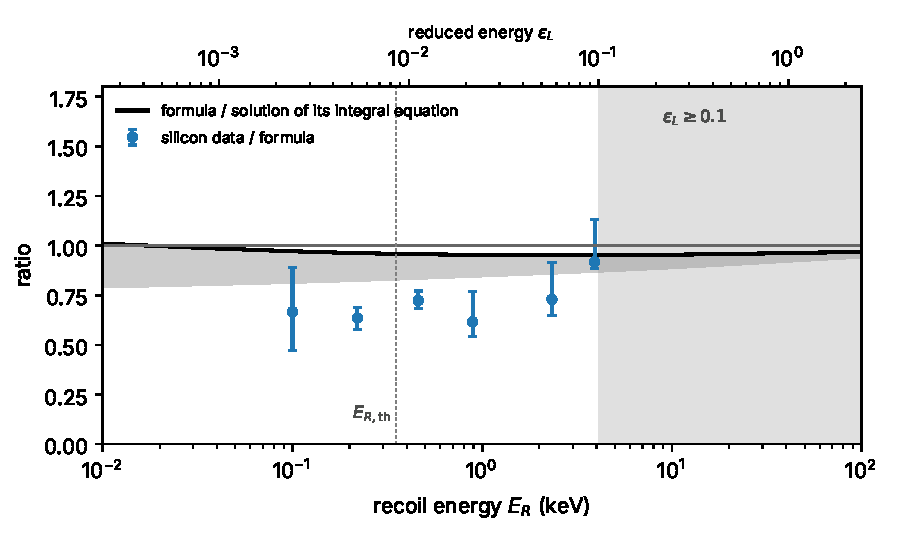
\includegraphics[width=\linewidth]{figures/ch19/limit19_3a.pdf}
\captionof{figure}{Silicon, $k_L = 0.146$, against the recoil energy. Solid: the formula divided by the numerical solution of the binary-collision equation \cref{eq:19.3-simple} with the Thomas--Fermi cross-section in the impulse approximation, continued below $x_L = 2\times10^{-3}$ as $x_L^{1/3}$; dark band: the same with continuation exponents from 1/3 to the local slope 0.363 of the computed cross-section, a sensitivity to that choice. Points: the measured silicon yields~\cite[Table~II]{albakry2023first} divided by the formula. Dashed: the constant-binding model with $U = \SI{0.15}{keV}$~\cite[Eq.~(13), Table~3]{sarkis2020study} divided by the formula. Gray: $\epsilon_L \ge 0.1$, $E_R \ge \SI{4.1}{keV}$, where the formula describes the silicon data~\cite[Sect.~II]{sarkis2020study}. Vertical line: the binary threshold $E_{R,\mathrm{th}} = \SI{352}{eV}$.}\label{fig:19-limit-lindhard}
\par}
\smallskip
Below a few keV the measured yields fall 8 to \SI{38}{\percent} under the formula, a deficit comparable to the formula's sensitivity to its softest collisions; the stored energy, the gap and the conversion to pairs that the model omits also act there.
\end{limitbox}

With the $x_L^{1/3}$ continuation the solution and the fit agree to \SI{3}{\percent} below \SI{100}{eV}, and the fit lies \SIrange{4}{5}{\percent} below the solution between 1 and \SI{20}{keV}, where $y_L$ is 0.210 against 0.220 at \SI{1}{keV}. The continuation matters more than the fit. Continuing the computed cross-section at its own local slope, 0.363 at $x_L = 2\times10^{-3}$, raises the solution by \SI{13}{\percent} at \SI{1}{keV} and by \SI{10}{\percent} at \SI{4}{keV}; an exponent of 0.30 lowers it by \SI{11}{\percent} at \SI{1}{keV}, and 0.40 raises it by \SI{40}{\percent}. The dark band of \cref{fig:19-limit-lindhard} is therefore a sensitivity to one modeling choice, not an uncertainty. Nothing places the true yield between the two continuations: below the matching point the Thomas--Fermi cross-section steepens toward $x_L^{1/2}$, while binding and the lattice remove the softest transfers altogether. Below $\epsilon_L = 2\times10^{-3}$, about \SI{80}{eV}, the whole cross-section of a slow secondary lies in the continued region, and the binary model does not determine the yield of a keV recoil there. Those are the soft collisions of the slowest secondaries, at energies of tens of eV, where atoms are bound and the binary model has least claim to hold. The equation propagates their treatment upward because every recoil ends as a population of such secondaries.

\subsection{Implicit assumptions of Lindhard quenching}\label{sec:19.3-assumptions}

Read against the partition of \cref{sec:19.1}, the chain from \cref{eq:19.3-basic} to $y_L$ makes three assumptions that its list of approximations does not name: no stored energy, electronic friction down to zero speed, and conversion to pairs in proportion. Each fails below a keV in silicon.

The first is that no energy is stored. With $U = 0$ every collision returns its full transfer to atomic motion, and an atom that ends displaced keeps no energy in the lattice: $E_{\mathrm{st}} = 0$ in \cref{eq:19.1-partition}. Restoring $U$ does not repair this. In the constant-binding model of Sarkis et al.~\cite[Eqs.~(9), (13)]{sarkis2020study} the struck atom pays $U$ before it moves, the lower limit of the integral in \cref{eq:19.3-simple} becomes $(\epsilon_Lc_LU)^{1/2}$, and the yield vanishes near $E_R = 2U$. Their fit to the silicon data above \SI{0.68}{keV} gives $U = 0.15 \pm \SI{0.06}{keV}$~\cite[Table~3]{sarkis2020study}, and with the fitted correction terms the yield reaches zero at \SI{298}{eV} (\cref{fig:19-yields}); the measured yield at \SI{100}{eV} is $0.102^{+0.034}_{-0.030}$. The later model of the same authors replaces $U$ by a function $U(E) = U_{\mathrm{FP}} + U_{\mathrm{EDFT}}(E)$: a constant $U_{\mathrm{FP}} = \SI{23.6}{eV}$, which the authors call the Frenkel-pair creation energy and take from averaged displacement thresholds, plus an energy-dependent excitation of the inner electrons. It adds electronic straggling and a modern stopping model, and it fits 102 points from \SI{0.68}{keV} to \SI{3}{MeV} with $\chi^2/\mathrm{dof} = 1870/101$; its threshold lies just above $U_{\mathrm{FP}}$~\cite[Eqs.~(2)--(4), Fig.~3]{sarkis2023ionization}. The configurational energy of a Frenkel pair in silicon is 6.8 to \SI{9.7}{eV} (\cref{sec:7.4}), a third of $U_{\mathrm{FP}}$; in the partition that part is stored energy and the rest of a threshold-sized $U_{\mathrm{FP}}$ is heat. In both models, however, the $U$ spent by secondary atoms appears as an argument of $T_{\mathrm{d}}(T_n - U)$, is missing from the damage energy, and therefore lands in the electronic share $E - T_{\mathrm{d}}$ by complement. Energy that the partition stores in defects is counted as ionization.

The second is that electronic losses follow the friction law down to zero speed. \Cref{eq:19.3-Se} gives a silicon ion of \SI{100}{eV} an electronic stopping of \SI{0.88}{eV/\angstrom}, while a binary collision at that energy cannot create a pair at all (\cref{sec:19.2-binary}), and the momentum tail lets through a fraction $5.6\times10^{-3}$ of the valence electrons (\cref{sec:19.2-soft}). Below $E_{R,\mathrm{th}}$ the friction assigns losses to final states that are strongly suppressed. The modified equation of Sarkis et al.\ also keeps a term $-\tfrac12k_L\epsilon_L^{3/2}\epsilon_{\mathrm{d}}''$, obtained from the second-order expansion with the mean nuclear transfer $\epsilon_L/2$ in a collision that also excites electrons~\cite[Eq.~(9), App.~B]{sarkis2020study}. Under approximation (D) every collision has $T_n = 0$ or $\sum_iT_{e,i} = 0$, so the cross term $T_n\sum_iT_{e,i}$ that produces it vanishes identically, and the term contradicts the separation used to obtain the stopping.

The third is that the electronic share becomes charge in proportion, $N_{\mathrm{eh}} = y_LE_R/\varepsilon_{\mathrm{eh}}$, with every pair collected and none trapped. Then $Y_q = y_L$. The excitations of a slow ion lie near the gap, where the cascade gives one pair per excitation rather than $\omega_e/\varepsilon_{\mathrm{eh}}$ (\cref{eq:19.2-charge}), so $y_L$ and $Y_q$ differ even if $y_L$ were exact. Trapping and incomplete collection lower the measured charge further (\cref{sec:18.5,sec:19.5}).

The approximations that the list does name are weakest at the same energies. The medium is a random gas of atoms, with no channels and no dependence on direction, and collisions are binary and independent, which fails in the dense cascades of germanium recoils of a few keV. The reduced energy is also convention-dependent. Sarkis et al.\ define it in their later work with the universal screening length and an effective projectile charge $Z_1 = 12$. This maps the same recoil energy to a reduced energy \SI{10}{\percent} higher than \cref{eq:19.3-reduced}~\cite[Sect.~``The nuclear recoil QF'']{sarkis2023ionization}, so that fitted constants cannot be carried from one convention to the other.

\begin{figure}[tbp]
  \centering
  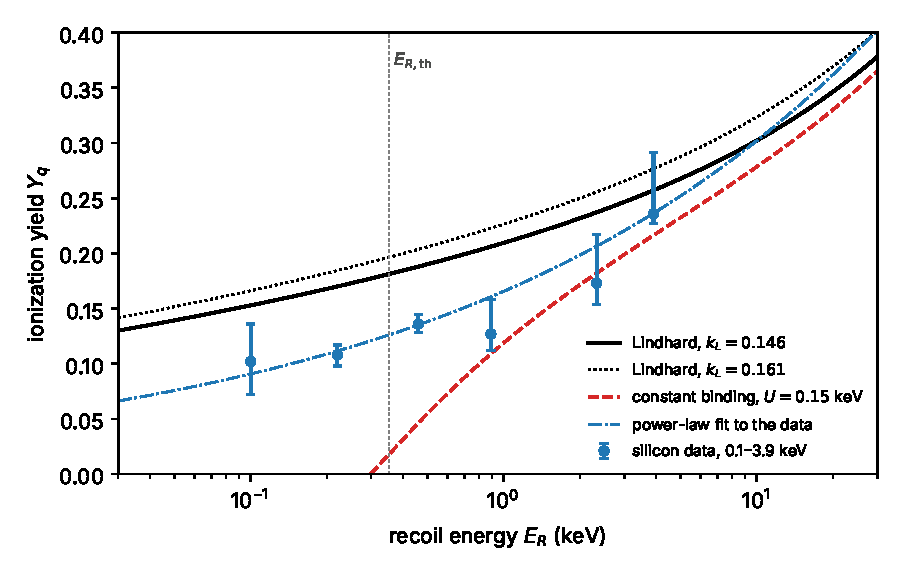
\includegraphics[width=\linewidth]{figures/ch19/fig19_3.pdf}
  \caption{Lindhard and modified-Lindhard yields of silicon against the measured ionization yield. Solid: Lindhard's formula \cref{eq:16.6-lindhard} with $k_L = 0.146$; dotted: with $k_L = 0.161$, the value of a fit of the numerical constant-binding solution to the silicon data~\cite[Table~4]{sarkis2020study}. Dashed: the constant-binding model of Sarkis et al.\ with $U = \SI{0.15}{keV}$, $C_0 = 9.1\times10^{-3}$ and $C_1 = 3.33\times10^{-5}$~\cite[Eq.~(13), Table~3]{sarkis2020study}, which vanishes at \SI{298}{eV}. Points: the silicon measurement with total uncertainties~\cite[Table~II]{albakry2023first}; dash-dotted: its power-law fit $0.302(E_R/\SI{10}{keV})^{0.261}$, pinned to the formula at \SI{10}{keV}. Vertical line: the binary threshold $E_{R,\mathrm{th}} = \SI{352}{eV}$ (\cref{sec:19.2}).}
  \label{fig:19-yields}
\end{figure}

\Cref{fig:19-yields} shows the result of these assumptions. Raising $k_L$ moves the whole curve up and away from the sub-keV data. Adding a constant binding brings the curve down to the data near \SI{2}{keV} only by introducing a cutoff that the data at 0.10 and \SI{0.22}{keV} contradict. The data themselves follow the power law $E_R^{0.26}$ from \SI{0.1}{keV} to \SI{3.9}{keV}, flatter than $y_L$ and with no threshold. Each modified model fixes one assumption and lets its fitted constants absorb the rest; a good fit therefore does not tell us which assumption was wrong. The calculation that would show it is the partition of \cref{sec:19.1} with stored energy, the excitation kernel of \cref{sec:19.2} and the cascade conversion, specified in \cref{app:E.23}. Above about \SI{4}{keV}, where stored energy and the gap are small fractions of the electronic share, Lindhard's formula describes the silicon data and needs no repair.

\subsection{Bethe stopping from the loss function}\label{sec:19.3-bethe}

At the opposite end of the speed range the stopping of an ion is a derived result. Take the dielectric stopping \cref{eq:4.4-dEdx} of a heavy projectile of charge $Z_1e$ and speed $v$ at $T = 0$, and suppose $v$ is large compared to the speeds of the electrons that hold the weight of the loss function. Split the momentum integral at a value $q_0$ chosen so that two conditions hold together: $q_0v$ lies far above the energies where $L$ has its weight, and $q_0$ is small compared to the inverse size of the atoms, so that $L(q,\omega) \simeq L(0,\omega)$ for $q < q_0$. Both are possible only if $v$ is large.

Below $q_0$ the loss function is its optical limit, and the condition $\omega \le qv$ becomes $q \ge \omega/v$. Exchanging the order of integration,
\begin{equation*}
  \int_0^{q_0}\frac{\dd q}{q}\int_0^{qv}\dd\omega\,\omega L(0,\omega) = \int_0^\infty\dd\omega\,\omega L(0,\omega)\,\ln\frac{q_0v}{\omega} ,
\end{equation*}
where the upper limit of the $\omega$ integral moved to infinity because $q_0v$ lies above the whole spectrum. Above $q_0$ the line $\omega = qv$ lies above the spectrum at every $q$ until it meets the free-electron recoil $\omega = q^2/2m_e$, at $q = 2m_ev$. Between $q_0$ and $2m_ev$ the inner integral is therefore the whole f-sum $(\pi/2)\omega_p^2$ of \cref{eq:4.4-fsumL}, and beyond $2m_ev$ it is zero, since the Bethe ridge has moved out of reach. The second piece is $(\pi/2)\omega_p^2\ln(2m_ev/q_0)$. Writing the f-sum as $\int_0^\infty\dd\omega\,\omega L(0,\omega) = (\pi/2)\omega_p^2$ in the first piece, $q_0$ cancels between the two, and with $\omega_p^2 = 4\pi\alpha\nd_e/m_e$ the prefactor $2Z_1^2\alpha/\pi v^2$ of \cref{eq:4.4-dEdx} times the f-sum $(\pi/2)\omega_p^2$ equals $4\pi Z_1^2\alpha^2\nd_e/(m_ev^2)$.

\begin{keyresult}[Bethe stopping from the loss function]
For a heavy projectile of charge $Z_1e$ and speed $v$ well above the speeds of the electrons that hold the weight of the loss function, in first order in $Z_1$,
\begin{equation}
  -\frac{\dd E}{\dd x} = \frac{4\pi Z_1^2\alpha^2\nd_e}{m_ev^2}\,\ln\frac{2m_ev^2}{\bar I} ,
  \label{eq:19.3-bethe}
\end{equation}
with the mean excitation energy defined by the logarithmic moment of the optical loss function,
\begin{equation}
  \ln\bar I = \frac{2}{\pi\omega_p^2}\int_0^\infty\dd\omega\;\omega\,L(0,\omega)\,\ln\omega ,
  \label{eq:19.3-lnI}
\end{equation}
where $\nd_e$ and $\omega_p$ count all the electrons of the target.
\end{keyresult}

\noindent This is the nonrelativistic limit of the Bethe equation of the Particle Data Group. Its bracket $\tfrac12\ln(2m_e\beta^2\gamma^2W_{\mathrm{max}}/I^2) - \beta^2$, with $W_{\mathrm{max}} = 2m_e\beta^2\gamma^2$ for a heavy projectile, becomes $\ln(2m_ev^2/I)$ up to terms of order $v^4$, and its prefactor $Kz^2(Z/A)/\beta^2$ per unit mass is $4\pi\alpha^2\nd_e/(m_ev^2)$ per unit length~\cite[Eq.~(34.5)]{navas2024review}. The Particle Data Group describes $I$ as a geometric average of the excitation energies weighted by their oscillator strengths~\cite[Sect.~34.2.1]{navas2024review}; \cref{eq:19.3-lnI} makes the weight precise for a condensed medium. It is the loss function, not $\varepsilon_2$, because the projectile couples to the total potential, and the logarithm sits inside the f-sum weight $\omega L$. The prefactor of \cref{eq:19.3-bethe} depends on the electron density alone, as \cref{sec:4.4} anticipated; the solid enters only through $\bar I$, and only logarithmically.

\begin{workedexample}{The mean excitation energy of silicon}\label{we:19-lnI}
Start with the four valence electrons in the single damped oscillator of \cref{we:4-oscillatorL} at $q \to 0$: $L(0,\omega) = \omega_p^2\varGamma_{\mathrm{w}}\omega/[(\omega^2 - \bar E^2)^2 + \varGamma_{\mathrm{w}}^2\omega^2]$ with $\omega_p = \SI{16.6}{eV}$, $\bar E = \SI{17.4}{eV}$ and $\varGamma_{\mathrm{w}} = \SI{3.66}{eV}$. For a narrow line \cref{eq:19.3-lnI} would give $\bar I = \bar E$, since all the weight sits at one energy. The damping spreads it: the model puts \SI{88}{\percent} of its f-sum between 10 and \SI{30}{eV}, but \SI{7.8}{\percent} between 30 and \SI{100}{eV} and \SI{2.4}{\percent} above, in a tail $\omega L \propto \varGamma_{\mathrm{w}}\omega_p^2/\omega^2$ that the logarithm weights heavily. Numerically,
\begin{equation*}
  \ln\bar I_{\mathrm{val}} = \frac{2}{\pi\omega_p^2}\int_0^\infty\dd\omega\,\omega L(0,\omega)\ln\frac{\omega}{\SI{1}{eV}} = 3.012 , \qquad \bar I_{\mathrm{val}} = \SI{20.3}{eV} ,
\end{equation*}
\SI{17}{\percent} above $\bar E$; a damping of \SI{2}{eV} brings it to \SI{19.0}{eV}. The inverse moment of \cref{eq:4.4-inverse} fixed $\bar E$ from the low-energy side of the spectrum; $\bar I$ is set by the high-energy side, and the two mean energies agree only for a narrow line.

The valence electrons are four of fourteen, and the core changes the answer by an order of magnitude. Take the measured loss function of \cref{sec:10.7}, which extends to \SI{30}{keV}. For all fourteen electrons $\omega_p = \SI{31.05}{eV}$ and $(\pi/2)\omega_p^2 = \SI{1514}{eV^2}$; the tabulated spectrum holds \SI{1537}{eV^2}, \SI{1.5}{\percent} more. Split at \SI{90}{eV}, below the L edge, and at \SI{1.83}{keV}, below the K edge, the f-sum weight $w_j$ and the logarithmic mean energy $\omega_j$ of each band are
\begin{equation*}
  \text{valence: } 0.280,\ \SI{19.5}{eV} ; \qquad \text{L shell: } 0.607,\ \SI{246}{eV} ; \qquad \text{K shell: } 0.113,\ \SI{3.17}{keV} ,
\end{equation*}
so that, with the spectrum normalized to its own f-sum, $\ln(\bar I/\SI{1}{eV}) = \sum_jw_j\ln(\omega_j/\SI{1}{eV}) = 0.832 + 3.340 + 0.910 = 5.082$ and $\bar I = \SI{161}{eV}$. Rescaling the spectrum to the exact f-sum leaves this value unchanged. It lies \SI{7}{\percent} below the adopted \SI{173.0}{eV} of the Particle Data Group~\cite{pdg2024atomic}, and the \SI{1.5}{\percent} excess of the tabulated f-sum is a measure of the error of the data. The L shell holds \SI{61}{\percent} of the oscillator strength and the valence electrons, which set every dark-matter rate of \cref{chap:10}, \SI{28}{\percent}; without the core shells $\bar I$ would be the \SI{19.5}{eV} of the valence band.
\end{workedexample}

The derivation needs two conditions, and both fail for recoils. The split at $q_0$ requires $2m_ev^2 \gg \bar I$, so that the logarithm is large: a proton of \SI{1}{MeV} has $2m_ev^2 = \SI{2.2}{keV}$, thirteen times the $\bar I$ of silicon, while a silicon recoil of \SI{10}{keV} has \SI{0.78}{eV}, $4.5\times10^{-3}$ of it, and \cref{eq:19.3-bethe} would give a negative stopping. The first-order treatment requires $Z_1\alpha/v \ll 1$: 0.16 for the proton, 117 for the recoil. \Cref{lim:19.3b} shows the first condition in an electron gas, where both formulas can be evaluated exactly.

\begin{limitbox}[Bethe stopping][lim:19.3b]
The Bethe formula in its nonrelativistic limit~\cite[Eq.~(34.5)]{navas2024review}, \cref{eq:19.3-bethe}: $-\dd E/\dd x = (4\pi Z_1^2\alpha^2\nd_e/m_ev^2)\ln(2m_ev^2/\bar I)$, with $\bar I$ from \cref{eq:19.3-lnI}.
\par\smallskip
{\centering
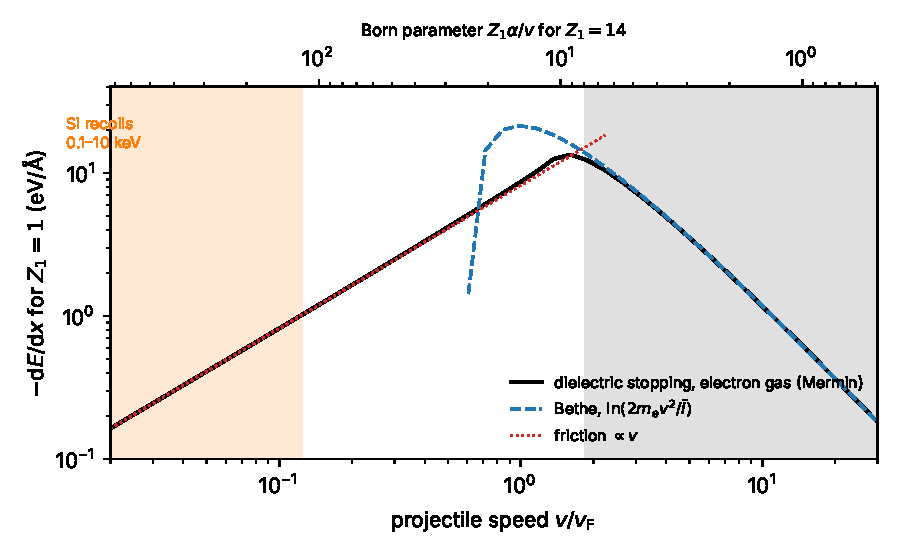
\includegraphics[width=\linewidth]{figures/ch19/limit19_3b.pdf}
\captionof{figure}{Stopping of a heavy projectile with $Z_1 = 1$ in the electron gas of the silicon valence density ($k_{\mathrm{F}} = \SI{1.8085}{\angstrom^{-1}}$, $v_{\mathrm{F}} = 6.98\times10^{-3}$, $\omega_p = \SI{16.6}{eV}$), against its speed. Solid: the dielectric stopping \cref{eq:4.4-dEdx} with the Mermin dielectric function of \cref{sec:4.5} and relaxation rate $0.1\,\omega_p$, a modeling choice that keeps the f-sum. Dashed: \cref{eq:19.3-bethe} with the model's own $\bar I = \SI{17.9}{eV}$ from \cref{eq:19.3-lnI}. Dotted: the friction law, linear in $v$, fitted at the lowest speed. Gray: $v \ge 1.84\,v_{\mathrm{F}}$, where the Bethe formula lies within \SI{10}{\percent} of the dielectric stopping. Orange: the speeds of silicon recoils from 0.1 to \SI{10}{keV}. Top axis: the Born parameter $Z_1\alpha/v$ of a silicon ion, $Z_1 = 14$.}\label{fig:19-limit-bethe}
\par}
\smallskip
Below about $2v_{\mathrm{F}}$ the momentum transfers that reach the loss function no longer exhaust its f-sum, and the stopping turns over into the friction regime, where it is set by the low-energy side of $L$ and not by $\bar I$.
\end{limitbox}

The approach to the Bethe form is fast once it starts: the dielectric stopping lies within \SI{5}{\percent} of \cref{eq:19.3-bethe} above $2.27\,v_{\mathrm{F}}$ and within \SI{1}{\percent} above $4.3\,v_{\mathrm{F}}$. The Bethe logarithm vanishes at $v = (\bar I/2m_e)^{1/2} = 0.60\,v_{\mathrm{F}}$, below which the formula has no meaning. In the friction regime the same Mermin electron gas gives a stopping of \SI{1173}{eV/\angstrom} times $v$ for $Z_1 = 1$, constant to \SI{0.1}{\percent} up to $v = 0.1\,v_{\mathrm{F}}$. Silicon recoils, at 0.013 to $0.13\,v_{\mathrm{F}}$, sit deep in that regime, with Born parameters from 117 to over a thousand. The corrections that the Particle Data Group lists for slower projectiles, shell corrections, the Barkas term of order $Z_1^3$ and the Bloch term, extend the Bethe formula down to about $\beta \approx 0.05$, and between $\beta = 0.01$ and 0.05 no theory is satisfactory~\cite[Sect.~34.2.6]{navas2024review}. Recoils from dark matter move at $\beta < 10^{-3}$. Computing $L(q,\omega)$ to the core energies that set $\bar I$, with local fields and the core states of \cref{app:E.15}, is the task of \cref{app:E.6,app:E.16}; for slow ions it fixes the first-order stopping of \cref{sec:19.2-soft}, not the yield.

A fast heavy ion, by contrast, leaves a track of $10^2$ to $10^4$ correlated collisions in a lattice already disturbed by the previous ones, and what a track detector reads is a defect configuration, not an excitation spectrum; damage-track and paleo-detector searches need \cref{eq:19.3-bethe,eq:19.3-Se} as input to a transport calculation of that track.

\section{Defects and stored energy}\label{sec:19.4}

A $^{206}$Pb nucleus that recoils into a germanium detector with \SI{103}{keV} is reconstructed \SI{6.08}{\percent} low, once the calibration of surface events has been corrected~\cite{agnese2018energy}. Silicon nuclear recoils of 10 to \SI{100}{keV} give \SI{4.8}{\percent} less phonon signal than electron recoils of the same energy~\cite{agnese2018nuclear}. A Frenkel pair in silicon stores about \SI{7}{eV}, and a recoil of a few keV makes tens of them, so energy stored in defects can produce deficits of this size. Collection can too, and the two data sets attribute similar deficits to opposite causes. How much of a deficit of 5 to \SI{6}{\percent} is stored energy? The count of the defects a recoil leaves gives its stored energy, and \cref{sec:19.4-bounds} reads the two calibrations as upper bounds on it.

\subsection{Stored energy of a displacement}\label{sec:19.4-single}

The stored energy of one trajectory is the difference of two minima of the energy surface, \cref{eq:19.1-partition}. The trajectories of the kicked ensemble end in different basins $b$: the perfect crystal, a bond defect, a close Frenkel pair at one of several separations, or a cluster. With $P_b(E_R, \hat{\vect{r}}_R)$ the probability that a recoil of energy $E_R$ along $\hat{\vect{r}}_R$ ends in basin $b$, and $E_{\mathrm{st},b}$ the energy of that basin's minimum above the perfect crystal, the mean stored energy is
\begin{equation}
  \langle E_{\mathrm{st}}\rangle(E_R, \hat{\vect{r}}_R) = \sum_bP_b(E_R, \hat{\vect{r}}_R)\,E_{\mathrm{st},b} , \qquad \sum_bP_b = 1 .
  \label{eq:19.4-mean}
\end{equation}
Only the end points of the trajectories enter; the barrier crossed on the way sets the probabilities, and with them the displacement threshold $E_{\mathrm{d}}(\hat{\vect{r}}_R)$ of \cref{eq:19.1-Ed}.

Near the threshold a recoil makes at most one defect, and \cref{eq:19.4-mean} has two terms beyond the perfect crystal: $p_{\mathrm{FP}}E_{\mathrm{FP}}$ for a Frenkel pair of stored energy $E_{\mathrm{FP}}$ and the analogous term for a bond defect. In silicon a close Frenkel pair stores 6.8 to \SI{7.5}{eV}, a vacancy and an interstitial far apart store the sum of their formation energies, 8.1 to \SI{9.7}{eV}, and a bond defect 2.6 to \SI{3.0}{eV}~\cite[Table~III]{holmstrom2008threshold} (\cref{sec:7.4}). The step of $p_{\mathrm{FP}}$ at $E_{\mathrm{d}}$ has the zero-point width of \cref{sec:19.1}. A recoil just above the lowest threshold that leaves a close pair stores more than half of its energy, and the stored fraction $\langle E_{\mathrm{st}}\rangle/E_R$ is largest there and falls as the excess energy goes to heat.

The sharp-threshold limit sets $p_{\mathrm{FP}} = \Theta(E_R - E_{\mathrm{d}}(\hat{\vect{r}}_R))$, with a direction-dependent threshold from molecular dynamics. It is not an ionization threshold. Crossing $E_{\mathrm{d}}$ moves energy from heat into $E_{\mathrm{st}}$; in a calorimeter it therefore produces a deficit, not a threshold. The ionization threshold belongs to the electrons: the binary threshold and the close-collision kernel of \cref{sec:19.2}.

A defect made at $t_{\mathrm{pr}}$ need not survive to the readout. With $p_{\mathrm{surv}}$ the probability that a close pair has not recombined by then, as in \cref{sec:16.6}, the stored energy at readout carries the factor $p_{\mathrm{surv}}$. Recombination during the cascade itself, before $t_{\mathrm{pr}}$, is part of $P_b$.

\Cref{eq:19.4-mean} is computed by molecular dynamics on the energy surface with the quench protocol of \cref{sec:19.1}.

\subsection{Displacement count and defect energy loss}\label{sec:19.4-count}

Above a few times $E_{\mathrm{d}}$ the recoil displaces several atoms, and the stored energy is the number of surviving defects times their energy. The number follows from the binary-collision picture of \cref{sec:19.3}, with a rule that decides which collisions displace. The rule of Kinchin and Pease, as used in \cref{sec:16.6}, has three cases. A moving atom of energy $E$ that transfers $T < E_{\mathrm{d}}$ leaves its target in place, and $T$ becomes heat. If $T > E_{\mathrm{d}}$ and the atom keeps $E - T > E_{\mathrm{d}}$, both move on and one more atom is displaced. If $T > E_{\mathrm{d}}$ but $E - T < E_{\mathrm{d}}$, the atom stops in the site it emptied, a replacement, and the count does not change. Electronic losses are removed, so that the energy of the primary is the damage energy $T_{\mathrm{d}}$ of \cref{sec:19.3}, and no binding energy is spent.

Let $n(E)$ be the mean number of further displacements produced by a moving atom of energy $E$. An atom with $E < 2E_{\mathrm{d}}$ cannot leave two moving atoms above $E_{\mathrm{d}}$, so $n(E) = 0$ there. The first collision transfers $T$ with probability $\dd\sigma(E,T)/\sigma$; after it, the three cases give the future counts $n(E - T)$, $1 + n(T) + n(E - T)$ and $n(T)$. Since $n$ vanishes below $2E_{\mathrm{d}}$, all three are $n(E - T) + n(T) + \Theta(T - E_{\mathrm{d}})\Theta(E - T - E_{\mathrm{d}})$. Averaging over the first collision and multiplying by $\sigma$,
\begin{equation}
  \int\dd\sigma(E,T)\Bigl[n(E) - n(E - T) - n(T) - \Theta(T - E_{\mathrm{d}})\,\Theta(E - T - E_{\mathrm{d}})\Bigr] = 0 , \qquad
  N_{\mathrm{FP}}(T_{\mathrm{d}}) = 1 + n(T_{\mathrm{d}}) ,
  \label{eq:19.4-count}
\end{equation}
where $N_{\mathrm{FP}}$ counts the primary as the first displaced atom. The total cross-section diverges for a screened potential; the integral is finite, however, since the bracket vanishes as $T \to 0$. \Cref{eq:19.4-count} is the counting analog of Lindhard's \cref{eq:19.3-simple}: a first-collision balance for an additive quantity of the binary branching process.

For hard spheres the transfer is uniform, $\dd\sigma \propto \dd T/E$ on $0 < T < E$. Then \cref{eq:19.4-count} reads $n(E) = (2/E)\int_0^En(T)\,\dd T + 1 - 2E_{\mathrm{d}}/E$ for $E \ge 2E_{\mathrm{d}}$. With $N_{\mathrm{FP}} = 1 + n$, which equals one on $E_{\mathrm{d}} \le T < 2E_{\mathrm{d}}$, this becomes $N_{\mathrm{FP}}(E) = (2/E)\int_{E_{\mathrm{d}}}^EN_{\mathrm{FP}}(T)\,\dd T$. A linear $N_{\mathrm{FP}} = cE$ above $2E_{\mathrm{d}}$ turns the right side into $2E_{\mathrm{d}}/E + cE - 4cE_{\mathrm{d}}^2/E$, which equals $cE$ only for $c = 1/2E_{\mathrm{d}}$:
\begin{equation}
  N_{\mathrm{FP}}(T_{\mathrm{d}}) = \frac{T_{\mathrm{d}}}{2E_{\mathrm{d}}} \qquad (T_{\mathrm{d}} \ge 2E_{\mathrm{d}};\ \text{hard spheres}) ,
  \label{eq:19.4-KP}
\end{equation}
the Kinchin--Pease count quoted in \cref{sec:16.6}. Each displacement costs $2E_{\mathrm{d}}$ of damage energy on average.

A screened potential favors small transfers. With the Thomas--Fermi cross-section of \cref{eq:19.3-dsigma}, in which $T/E = x_L^2/\epsilon_L^2$, and its continuation $f_{\mathrm{LSS}} \propto x_L^{1/3}$ below $x_L = 2\times10^{-3}$ (\cref{sec:19.3-integral}), which covers silicon recoils up to about \SI{80}{eV} ($\epsilon_L = 8.8\times10^{-4}$ at \SI{36}{eV}), the transfer distribution is $\dd\sigma \propto T^{-4/3}\dd T$. More of the energy then leaves in collisions too small to displace, and fewer atoms are displaced per unit of damage energy. We solve \cref{eq:19.4-count} numerically with the cross-section of \cref{sec:19.3}, by marching upward in energy; the new value of $n$ enters each step linearly, through the small transfers and the near-head-on collisions, and is solved for exactly. The asymptotic count is $N_{\mathrm{FP}} = \xi_{\mathrm{d}}T_{\mathrm{d}}/2E_{\mathrm{d}}$ with $\xi_{\mathrm{d}} = 0.70$, within $3\times10^{-3}$ for silicon thresholds of 12.5, 20 and \SI{36}{eV}, because the power law has no energy scale. At $T_{\mathrm{d}} = 10E_{\mathrm{d}}$ the effective factor is still 0.72. The published formula of Norgett, Robinson and Torrens, as quoted by Nordlund et al., keeps the Kinchin--Pease form and multiplies it by 0.8 to account for realistic interatomic potentials~\cite[Eq.~(1)]{nordlund2018improving}.

\begin{limitbox}[Displacement count][lim:19.4a]
The displacement count of a recoil of damage energy $T_{\mathrm{d}}$~\cite[Eq.~(1)]{nordlund2018improving}: $N_{\mathrm{FP}} = 0$ for $T_{\mathrm{d}} < E_{\mathrm{d}}$, 1 for $E_{\mathrm{d}} \le T_{\mathrm{d}} < 2E_{\mathrm{d}}/0.8$, and $0.8\,T_{\mathrm{d}}/2E_{\mathrm{d}}$ above; the Kinchin--Pease count \cref{eq:19.4-KP} without the factor 0.8.
\par\smallskip
{\centering
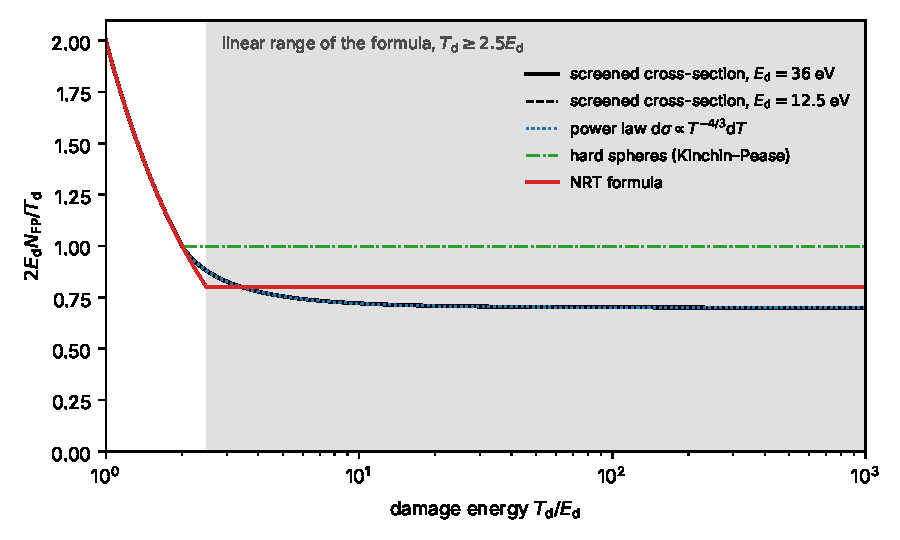
\includegraphics[width=\linewidth]{figures/ch19/limit19_4a.pdf}
\captionof{figure}{Displaced atoms per Kinchin--Pease unit, $2E_{\mathrm{d}}N_{\mathrm{FP}}/T_{\mathrm{d}}$, against $T_{\mathrm{d}}/E_{\mathrm{d}}$, from the counting equation \cref{eq:19.4-count} with the Kinchin--Pease rules, no binding energy and no electronic loss. Solid and dashed black: the Thomas--Fermi cross-section of \cref{sec:19.3} (impulse deflection, continued below $x_L = 2\times10^{-3}$ as $x_L^{1/3}$) for silicon with $E_{\mathrm{d}} = 36$ and \SI{12.5}{eV}; dotted: the power law $T^{-4/3}$; dash-dotted: hard spheres, which reproduce \cref{eq:19.4-KP} exactly. Red: the formula. Gray: $T_{\mathrm{d}} \ge 2.5E_{\mathrm{d}}$, the formula's linear range.}\label{fig:19-limit-nrt}
\par}
\smallskip
In its linear range the formula lies 11 to \SI{14}{\percent} above the screened count for $T_{\mathrm{d}} \ge 10E_{\mathrm{d}}$ and \SI{20}{\percent} below the hard-sphere count; below $2.5E_{\mathrm{d}}$ the count is set by the direction dependence of the threshold and by recombination, which no counting rule contains.
\end{limitbox}

The factor in front of the count is therefore a property of the cross-section and of the rules, not a constant of the crystal: 1 for hard spheres, 0.8 in the formula, 0.70 for the screened cross-section that \cref{sec:19.3} uses for Lindhard quenching. The rules leave out binding and recombination. A binding energy paid by every displaced atom lowers the count. Recombination inside a dense cascade lowers the number of defects that survive; in metals the surviving number from molecular dynamics is a third to a quarter of the formula's count~\cite{nordlund2018improving}, while silicon and germanium recombine much less~\cite[Sect.~II\,B]{sassi2022energy}.

The defect energy loss follows by multiplying the count by the surviving fraction and by the energy per pair. Writing $E_{\mathrm{FP}}$ for the mean stored energy of a surviving displacement,
\begin{equation}
  \frac{\langle E_{\mathrm{st}}\rangle}{E_R} = \frac{\xi_{\mathrm{d}}}{2}\,\frac{T_{\mathrm{d}}}{E_R}\,\frac{p_{\mathrm{surv}}E_{\mathrm{FP}}}{E_{\mathrm{d}}} \qquad (T_{\mathrm{d}} \gg E_{\mathrm{d}}) .
  \label{eq:19.4-loss}
\end{equation}
The stored fraction depends on the recoil energy only through the damage fraction $T_{\mathrm{d}}/E_R = 1 - y_L$, which falls from 0.70 at \SI{10}{keV} to 0.49 at \SI{100}{keV} for silicon in Lindhard's model, \cref{eq:16.6-lindhard}. At fixed $p_{\mathrm{surv}}E_{\mathrm{FP}}$ it decreases as $1/E_{\mathrm{d}}$: a higher threshold means fewer displacements, each storing the same energy. A measured stored fraction fixes only the combination $\xi_{\mathrm{d}}p_{\mathrm{surv}}E_{\mathrm{FP}}/E_{\mathrm{d}}$.

\begin{workedexample}{Energy stored by a 300 eV silicon recoil}\label{we:19-fp300}
A silicon recoil of \SI{300}{eV} needs $\mchi \ge \SI{0.770}{GeV}$ by \cref{eq:1.3-ERmax}, with $M_\kappa = \SI{26.16}{GeV}$ (natural isotope mixture, as in \cref{sec:19.1}) and $v_{\mathrm{max}} = \num{2.650e-3}$. Its measured ionization yield, interpolated linearly in $\ln Y_q$ against $\ln E_R$ between 0.108 at \SI{0.22}{keV} and 0.136 at \SI{0.46}{keV}~\cite[Table~II]{albakry2023first}, is $Y_q = 0.119$. The electronic share is at most $Y_qE_R = \SI{36}{eV}$, since the near-gap excitations of a slow ion each cost less than $\varepsilon_{\mathrm{eh}}$ per pair (\cref{sec:19.2}), so $T_{\mathrm{d}} \ge \SI{264}{eV}$; we take this value.

With the average Frenkel-pair threshold $E_{\mathrm{d}} = \SI{36}{eV}$, $T_{\mathrm{d}}/E_{\mathrm{d}} = 7.34$. The hard-sphere count \cref{eq:19.4-KP} gives 3.67 displacements, the formula of \cref{lim:19.4a} 2.94, and the screened count of \cref{eq:19.4-count} 2.69. If every displacement survives as a close pair of 6.8 to \SI{7.5}{eV}, the recoil stores 18.3 to \SI{20.1}{eV}, 6.1 to \SI{6.7}{\percent} of its energy; as separated pairs of 8.1 to \SI{9.7}{eV}, 22 to \SI{26}{eV}, or 7.3 to \SI{8.7}{\percent}. With the threshold for a defect of either kind, \SI{24}{eV}, the screened count is 3.95, and bond defects alone would store 10 to \SI{12}{eV}.

These fractions are comparable to the deficits measured at 10 to \SI{100}{keV}, and a calorimeter calibrated with electron recoils would read this recoil about \SI{20}{eV} low.
\end{workedexample}

\section{The energy balance law}\label{sec:19.5}

A silicon recoil of \SI{1}{keV} makes about 34 electron--hole pairs, at the measured ionization yield $Y_q = 0.127$ (\cref{sec:19.2}) and $\varepsilon_{\mathrm{eh}} = \SI{3.75}{eV}$, and their gap energy is \SI{40}{eV}. The rest of the deposit is phonons and, if the recoil displaced atoms, stored energy. A millisecond later the phonons have been absorbed at the surfaces of the crystal, most pairs have returned their gap energy as phonons and a few are caught on traps, while the defects still hold their energy. A phonon sensor reads the share that reached it within its readout window, and a calibration made with electron recoils converts that reading into an energy. The conversion is correct when electron and nuclear recoils of the same energy deliver the same share. To see when that holds, we write one law that tracks every share at every time. Applied to the silicon calibration of the CDMS~II detectors, the law shows that the measured ratio fixes a combination of stored energy, phonon collection and the pair energy of the reconstruction, which a second bias can separate.

\subsection{Reservoirs of the deposit}\label{sec:19.5-law}

At the partition time $t_{\mathrm{pr}}$ the deposit $\omega$ is split as in \cref{eq:19.1-heat}: $N_{\mathrm{eh}}\Eg$ in pairs, $E_{\mathrm{st}}$ in defects and $E_{\mathrm{heat}}$ in phonons. After $t_{\mathrm{pr}}$ the energy keeps moving. Pairs bind into excitons, recombine, are captured on impurities or drift to the electrodes, defects release their energy (\cref{sec:19.6}), and the phonons leave the crystal through its surfaces. Five reservoirs hold the energy at any time $t$. Write $E_{\mathrm{dep}} \equiv \omega$ for the deposit when it is divided among them.

The carriers hold $E_{\mathrm{pairs}}(t)$. Each energy is counted from the Fermi level $\mu_F$ of the electrodes, as in \cref{sec:18.5}: a free electron holds $E_c - \mu_F$, a free hole $\mu_F - E_v$, an exciton $\Eg - E_x^b$, an electron trapped on a level $E_j$ holds $E_j - \mu_F$ and a trapped hole $\mu_F - E_j$. To these we add the electrostatic energy of the charge left in the crystal, the Coulomb energy of separated carriers, their images in the electrodes and any space charge. The phonons hold $E_{\mathrm{phon}}(t)$, the vibrational energy above the thermal bath; its value at $t_{\mathrm{pr}}$ is the prompt phonon energy $E_{\mathrm{prompt}} \equiv E_{\mathrm{phon}}(t_{\mathrm{pr}})$. The defects hold the stored energy $E_{\mathrm{st}}(t)$, a difference of minima of $E^{\mathrm{ad}}$ as in \cref{eq:19.1-partition}. The escaped energy $E_{\mathrm{esc}}(t)$ is carried out of the crystal by quanta that no surface absorbs, in practice luminescence photons. Last, $E_{\mathrm{sens}}(t)$ is the energy absorbed at the surfaces: by the sensor films, of which a part becomes signal, and by holders and uninstrumented faces. A bias source at fixed voltage adds the work $W_{\mathrm{bias}}(t)$ it has done on the drifting charge.
\begin{keyresult}[Energy balance law]
At every time $t$ after the deposit, and for every event,
\begin{equation}
  E_{\mathrm{dep}} + W_{\mathrm{bias}}(t) =
  \underbrace{E_{\mathrm{pairs}}(t)}_{\text{carriers}} +
  \underbrace{E_{\mathrm{phon}}(t)}_{\text{phonons}} +
  \underbrace{E_{\mathrm{st}}(t)}_{\text{defects}} +
  \underbrace{E_{\mathrm{esc}}(t)}_{\text{escaped}} +
  \underbrace{E_{\mathrm{sens}}(t)}_{\text{absorbed}} ,
  \label{eq:19.5-balance}
\end{equation}
with carrier energies counted from the Fermi level of the electrodes, the stored energy configurational, and the change of zero-point energy of the occupied defect basins inside $E_{\mathrm{phon}}$.
\end{keyresult}
\noindent \Cref{app:D.45} proves \cref{eq:19.5-balance} from the conservation of the total energy of crystal, sensors, radiation and bias source. Apart from the work of the source, the total energy is conserved. Between collisions it equals the sum of the reservoir energies, since the interactions of excited carriers with each other are either long-range Coulomb energy, which $E_{\mathrm{pairs}}$ contains, or short-range energy that acts during a collision alone. Every process after $t_{\mathrm{pr}}$ is a short-range transition that conserves energy, or a drift whose energy the bias work and the electrostatic energy account for. The law holds for each realization of the random sequence of captures, hops and absorptions, and hence also in the mean. Its content is the completeness of the reservoir list. At $t_{\mathrm{pr}}$ and zero field, with no capture, it is the partition: $E_{\mathrm{pairs}} = N_{\mathrm{eh}}\Eg$, $E_{\mathrm{prompt}} = E_{\mathrm{heat}}$, $E_{\mathrm{esc}} = E_{\mathrm{sens}} = 0$, and \cref{eq:19.5-balance} is \cref{eq:19.1-heat}.

The Fermi level of the electrodes is the one reference for the carrier energies that keeps the law closed. A carrier that reaches an electrode gives up its energy relative to the Fermi level of that electrode, as phonons at the contact; the CDMS~II analysis names these the recombination phonons~\cite[Sect.~2]{agnese2018nuclear}. Counted from another level $\mu$, the carriers still in the crystal hold an energy whose derivative with respect to $\mu$ is the number of holes minus the number of electrons among them. That number is zero as long as every carrier still has its partner. Once one carrier of a pair has been collected and the other has not, energies counted from $\mu \ne \mu_F$ change with the arbitrary $\mu$, and the balance no longer closes. A hole left behind when its electron is collected thus stores $\mu_F - E_v$, plus its image energy, and not half the gap.

The stored energy enters once. The displacement threshold appears nowhere in \cref{eq:19.5-balance}. The stored energy decreases through releases alone, each of which moves its energy to $E_{\mathrm{phon}}$, or to $E_{\mathrm{esc}}$ if a photon carries it away. A calibration that subtracts an energy per displaced atom from the heat and also counts the later release as heat counts the same energy twice.

The zero-point energy of the occupied basins sits inside $E_{\mathrm{phon}}$. A defect softens or stiffens the modes of its neighbors and so changes the zero-point energy of the crystal by an amount $\Delta E_{\mathrm{zp}}(t)$, which \cref{sec:19.1-partition} placed in the lattice share. It is the energy of the vibrational ground state, and no sensor can absorb it. Its size follows from the zero-point energy per silicon atom, $3\langle\omega\rangle/2 = \SI{61}{meV}$, half of it the potential energy of \cref{sec:19.1-md}. A point defect that shifts the frequencies of its four neighbors by some tens of percent changes $\Delta E_{\mathrm{zp}}$ by about \SI{0.07}{eV}, an estimate, against the several eV a Frenkel pair stores. The sign is not fixed: softened modes make $\Delta E_{\mathrm{zp}}$ negative, stiffened ones positive. A defect that hops from basin $i$ to basin $j$ releases into the phonons the configurational difference plus the change of zero-point energy between the two basins. Summed along any release path, the zero-point terms telescope like the configurational ones, so the sum rule of \cref{sec:19.6} holds for both separately. A sensor can draw on $E_{\mathrm{phon}} - \Delta E_{\mathrm{zp}}$ alone.

The Luke effect enters the balance through the bias work. A carrier drifting at constant velocity in the field of a biased detector gains from the field the energy $e\mathcal{E}$ per unit path and gives it to phonons as fast as it gains it: the Neganov--Trofimov--Luke effect of \cref{eq:1.5-luke}, whose emission spectrum \cref{sec:20.1} treats. Between two planar electrodes at fixed potentials, a carrier that crosses a fraction $s$ of the gap induces the charge $es$ on the electrodes, and the source does the work $eV_{\mathrm{bias}}s$ on it (Ramo's theorem, \cref{app:D.45}). The total work is
\begin{equation}
  W_{\mathrm{bias}} = eV_{\mathrm{bias}}N_{\mathrm{ind}} ,
  \label{eq:19.5-Wbias}
\end{equation}
where $N_{\mathrm{ind}}$ is the induced charge in units of $e$, equal to the number of pairs if all are collected and smaller if carriers are trapped on the way. Of this work, $W_{\mathrm{bias}}$ minus the change of the electrostatic energy goes to phonons; for pairs born neutral and fully collected the electrostatic term vanishes at the end. For an electron recoil, whose pair number is $\omega/\varepsilon_{\mathrm{eh}}$, the ratio of the Luke phonon energy to the deposit is the Luke gain
\begin{equation*}
  g_{\mathrm{Luke}} = \frac{eV_{\mathrm{bias}}}{\varepsilon_{\mathrm{eh}}} ,
\end{equation*}
1.07 at \SI{4}{V} and 26.7 at \SI{100}{V} in silicon. Carriers already drift during the cascade, before $t_{\mathrm{pr}}$, over the short distance they travel in that time; that work is part of the same $W_{\mathrm{bias}}$ and of the same Luke phonons.

\Cref{fig:19-shares} follows the five reservoirs of a \SI{1}{keV} silicon recoil at zero field. The pair kinetics are those of \cref{fig:18-end}: the gap energy is released within microseconds, except for the \SI{5}{\percent} of pairs that the illustrative rates trap and the \SI{0.9}{\percent} that leave as light. The phonons are absorbed with a single time constant of \SI{58}{\micro s}, the fall time of the pulse of a \SI{10.6}{g} silicon phonon detector~\cite[p.~2]{alkhatib2021light}. After a millisecond the surfaces have absorbed \SI{943}{eV}, the traps keep \SI{2.0}{eV} and the defects their full \SI{55}{eV}. For a stated detector the evolution of the reservoirs is a transport calculation: the charge kinetics, Luke emission and collection at the surfaces of \cref{app:E.25}, started from the partition tables of \cref{app:E.23}.

\begin{figure}[tbp]
  \centering
  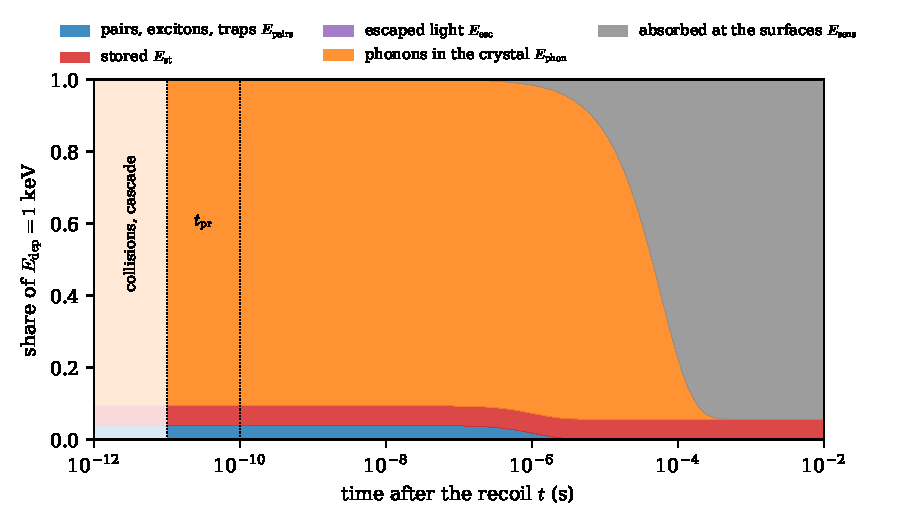
\includegraphics[width=\linewidth]{figures/ch19/fig19_4.pdf}
  \caption{Shares of the balance law \cref{eq:19.5-balance} for a \SI{1}{keV} silicon recoil at zero field, against the time after the recoil, as fractions of $E_{\mathrm{dep}}$. At the partition time $t_{\mathrm{pr}}$ (dotted lines, 10 to \SI{100}{ps}): $N_{\mathrm{eh}} = 33.9$ pairs from the measured yield $Y_q = 0.127$ at \SI{0.89}{keV}~\cite[Table~II]{albakry2023first} with $\varepsilon_{\mathrm{eh}} = \SI{3.75}{eV}$, holding $N_{\mathrm{eh}}\Eg = \SI{39.6}{eV}$ with $\Eg = \SI{1.17}{eV}$; stored energy set to \SI{55}{eV}, the silicon bound of \cref{tab:19-bounds}, for display, and kept frozen; phonons \SI{905}{eV}. Pair kinetics: the illustrative rates of \cref{fig:18-end} (one free pair per pair, \SI{5}{\percent} trapped, luminescent fraction 0.1 of free-exciton decay, bound-exciton Auger decay \SI{250}{ns}); trapped carriers stay in $E_{\mathrm{pairs}}$. Phonons absorbed at the surfaces with one exponential time constant, \SI{58}{\micro s}, the pulse fall time of a silicon phonon detector~\cite[p.~2]{alkhatib2021light}, a modeling choice. Shares at \SI{10}{ms}: absorbed 0.943, stored 0.055, trapped 0.002, escaped $3\times10^{-4}$. The collisions and the cascade before $t_{\mathrm{pr}}$ are not resolved.}
  \label{fig:19-shares}
\end{figure}

\subsection{Heat quenching}\label{sec:19.5-heat}

Without bias the phonon sensors measure the heat. Their readout integrates the energy absorbed during a window $t_{\mathrm{win}}$, from microseconds to a second depending on the sensor, and the phonons still in the crystal at the end of the window are absorbed with the same pulse shape whatever made them. Energy that has not become available phonons by $t_{\mathrm{win}}$ is missing from the signal for good. It is the sum of the energy still held by carriers, the energy still stored, the escaped energy and the zero-point change,
\begin{equation*}
  E_{\mathrm{miss}}(t_{\mathrm{win}}) = E_{\mathrm{pairs}}(t_{\mathrm{win}}) + E_{\mathrm{st}}(t_{\mathrm{win}}) + E_{\mathrm{esc}}(t_{\mathrm{win}}) + \Delta E_{\mathrm{zp}}(t_{\mathrm{win}}) .
\end{equation*}
The sensors turn a fraction $\epsilon_{\mathrm{abs}}$ of the available phonon energy into signal, $\epsilon_{\mathrm{abs}}(E_{\mathrm{dep}} - E_{\mathrm{miss}})$; the rest goes into $E_{\mathrm{sens}}$ as loss on uninstrumented faces and in the films. This fraction is often well below one, but it is the same for every event of a given kind of recoil at a given place. Let $\epsilon^{\mathrm{NR}}_{\mathrm{prim}}$ and $\epsilon^{\mathrm{ER}}_{\mathrm{prim}}$ be its values for the primary phonons of nuclear and electron recoils, the sole phonons at zero field, and define the collection offset $\delta_{\mathrm{coll}} \equiv 1 - \epsilon^{\mathrm{NR}}_{\mathrm{prim}}/\epsilon^{\mathrm{ER}}_{\mathrm{prim}}$. The heat quenching is the ratio of the heat signals of a nuclear and an electron recoil of the same energy,
\begin{equation}
  Y_{\mathrm{ph}}(0) = (1 - \delta_{\mathrm{coll}})\,\frac{1 - d_{\mathrm{NR}}}{1 - d_{\mathrm{ER}}} , \qquad
  d_{\mathrm{NR},\mathrm{ER}} \equiv \frac{E^{\mathrm{NR},\mathrm{ER}}_{\mathrm{miss}}(t_{\mathrm{win}})}{\omega} ,
  \label{eq:19.5-heatq}
\end{equation}
the zero-field value of the phonon-yield ratio $Y_{\mathrm{ph}}$ defined in \cref{sec:19.5-yield}. The absolute efficiency has dropped out, and with it the large losses at the surfaces; what remains is the difference between the two kinds of recoil.

Unit heat quenching, $Y_{\mathrm{ph}}(0) = 1$, is the truncation that phonon-only searches use to read a nuclear-recoil energy from a scale calibrated with electron recoils~\cite[p.~4]{alkhatib2021light}. \Cref{eq:19.5-heatq} states what it requires: equal collection of the two phonon populations, $\delta_{\mathrm{coll}} = 0$, and equal missing energy, $d_{\mathrm{NR}} = d_{\mathrm{ER}}$. The second condition does not hold by accident. An electron recoil puts the fraction $\Eg/\varepsilon_{\mathrm{eh}} = 0.312$ of its energy into pair gap energy, a silicon recoil of \SI{100}{eV} a fraction $Y_q$ times as large, so the two missing energies are equal when both are zero. The truncation therefore holds when, within the read window, every pair has recombined or been collected with its gap energy returned as phonons, no defect holds energy, and nothing has escaped.

The gap-energy term is the one that depends on the window. Let $f_{\mathrm{ret}}(t)$ be the fraction of the gap energy of the pairs returned as phonons by the time $t$, and $1 - f_{\mathrm{ret}}(t)$ the rest: held by free pairs and excitons, $r_{\mathrm{gap}}(t)$ of \cref{eq:18.5-rgap}, plus what has gone to traps and to light. The nuclear recoil holds $Y_q$ times the pair energy of the electron recoil. At zero field \cref{eq:19.5-heatq} becomes the gap-energy release law
\begin{equation}
  Y_{\mathrm{ph}}(0) = (1 - \delta_{\mathrm{coll}})\,\frac{1 - Y_q\,(\Eg/\varepsilon_{\mathrm{eh}})(1 - f^{\mathrm{NR}}_{\mathrm{ret}}) - (E_{\mathrm{st}} + \Delta E_{\mathrm{zp}})/\omega}{1 - (\Eg/\varepsilon_{\mathrm{eh}})(1 - f^{\mathrm{ER}}_{\mathrm{ret}})} ,
  \label{eq:19.5-release}
\end{equation}
with $f_{\mathrm{ret}}$, $E_{\mathrm{st}}$ and $\Delta E_{\mathrm{zp}}$ taken at $t_{\mathrm{win}}$ and the escape of light counted in $1 - f_{\mathrm{ret}}$. Nothing in it is small. If no gap energy has come back, $f_{\mathrm{ret}} = 0$, a silicon recoil of \SI{100}{eV} with $Y_q = 0.102$ has $Y_{\mathrm{ph}}(0) = 0.968/0.688 = 1.407$. Its heat signal is \SI{41}{\percent} larger than that of an electron recoil of the same energy, because the electron recoil holds more of its energy in pairs. The first-order form, $1 + (1 - Y_q)(\Eg/\varepsilon_{\mathrm{eh}})(1 - f_{\mathrm{ret}})$, is 1.280 and not usable at this size. With the illustrative rates of \cref{fig:18-end}, a window of \SI{1}{\micro s} has $f_{\mathrm{ret}} = 0.525$ and $Y_{\mathrm{ph}}(0) = 1.156$; after \SI{10}{\micro s} all free pairs and excitons have decayed, $f_{\mathrm{ret}} = 0.941$, and the \SI{5.9}{\percent} that went to traps and to light leave $Y_{\mathrm{ph}}(0) = 1.017$ at any longer window. The trapped fraction never comes back at millikelvin, where emission from traps is frozen (\cref{sec:18.5-kinetics}).

When the kinetics are linear, each pair decays on its own and $f^{\mathrm{NR}}_{\mathrm{ret}} = f^{\mathrm{ER}}_{\mathrm{ret}}$ at every time, a sum of exponentials whose rates are those of \cref{eq:18.5-rates}. The tracks of nuclear recoils are denser than the clouds of electron recoils of the same energy, however, and in a dense track the pairs meet. Binding of carriers from different pairs moves gap energy from free pairs into excitons and changes nothing in $1 - f_{\mathrm{ret}}$. Two-body processes that return gap energy to the lattice do: two excitons that meet annihilate, one of them giving up its energy, and three free carriers recombine by the Auger process. Write $\nd(t)$ for the density of pairs in the track, $\nd_0$ for its initial value, and take $1 - f_{\mathrm{ret}} \simeq \nd/\nd_0$ while no other channel acts. Annihilation gives $\dd\nd/\dd t = -\nd^2/(\nd_0t_0)$, and Auger recombination $\dd\nd/\dd t = -\nd^3/(2\nd_0^2t_0)$, with $t_0$ the time scale each sets at the initial density. Integrating,
\begin{equation}
  1 - f_{\mathrm{ret}}(t) = \frac{1}{1 + t/t_{\mathrm{rel}}}\ \ \text{(annihilation)} , \qquad
  1 - f_{\mathrm{ret}}(t) = \Bigl(1 + \frac{t}{t_{\mathrm{rel}}}\Bigr)^{-1/2}\ \ \text{(Auger)} .
  \label{eq:19.5-bimol}
\end{equation}
At $t_{\mathrm{win}} \gg t_{\mathrm{rel}}$ the nuclear recoil then misses $Y_q(\Eg/\varepsilon_{\mathrm{eh}})\,t_{\mathrm{rel}}/t_{\mathrm{win}}$ or $Y_q(\Eg/\varepsilon_{\mathrm{eh}})(t_{\mathrm{rel}}/t_{\mathrm{win}})^{1/2}$ of its energy, a power of the window and not an exponential, with $t_{\mathrm{rel}}$ set by the density of its own track. The heat quenching of nuclear recoils depends on the window whenever a two-body channel acts within it. Diffusion dilutes a track as it decays, and a compact cloud then stops losing energy by two-body processes and returns to the linear law, so \cref{eq:19.5-bimol} holds while the track stays narrow. The rates that decide which regime a detector is in are not known at millikelvin (\cref{sec:18.5-open}); \cref{app:E.24,app:E.25} specify their calculation.

\begin{limitbox}[Unit heat quenching][lim:19.5a]
The heat signals of nuclear and electron recoils of the same energy are taken to be equal~\cite[p.~4]{alkhatib2021light}: $Y_{\mathrm{ph}}(0) = 1$.
\par\smallskip
{\centering
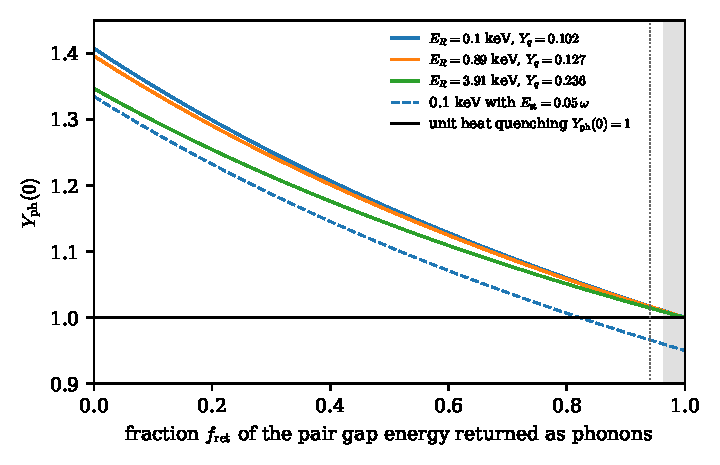
\includegraphics[width=\linewidth]{figures/ch19/limit19_5a.pdf}
\captionof{figure}{Heat quenching of silicon recoils from the release law \cref{eq:19.5-release} with $\delta_{\mathrm{coll}} = 0$, $\Delta E_{\mathrm{zp}} = 0$ and the same returned fraction $f_{\mathrm{ret}}$ for both recoils, against $f_{\mathrm{ret}}$. Solid: no stored energy, at the measured yields $Y_q$~\cite[Table~II]{albakry2023first} of 0.10, 0.89 and \SI{3.91}{keV}; $\Eg = \SI{1.17}{eV}$, $\varepsilon_{\mathrm{eh}} = \SI{3.75}{eV}$. Dashed: \SI{0.1}{keV} with a stored energy of $0.05\,\omega$. Horizontal line: the truncation. Gray: $f_{\mathrm{ret}} \ge 0.965$, where the \SI{0.1}{keV} curve lies within \SI{1}{\percent} of one. Dotted: $f_{\mathrm{ret}} = 0.941$, the asymptotic phonon share of the illustrative kinetics of \cref{fig:18-end}; there \SI{5}{\percent} of the pairs are trapped.}\label{fig:19-limit-heat}
\par}
\smallskip
When part of the gap energy is still held by pairs, excitons or traps at the end of the window, the electron recoil, with four to ten times more energy in pairs, loses more of its heat than the nuclear recoil, and the ratio rises above one, by up to \SI{41}{\percent} at \SI{100}{eV}; stored energy pulls it below.
\end{limitbox}

The truncation demands nearly complete release. Within \SI{1}{\percent} at \SI{100}{eV} requires $1 - f_{\mathrm{ret}} \le 0.035$, and the bound is nearly the same over the measured range, 0.036 at \SI{0.89}{keV} and 0.041 at \SI{3.91}{keV}, since the factor $(1 - Y_q)$ changes little while $Y_q$ stays small. A trapped fraction of a few percent, which no window removes, is already a percent-level violation, of opposite sign to the stored energy. The two effects can cancel in a single measurement, which is one reason a heat measurement alone determines neither.

\subsection{The phonon-yield ratio}\label{sec:19.5-yield}

With a bias the phonon signal has three parts: the primary phonons of the recoil, the Luke phonons of the drift and the recombination phonons that carriers emit at the contacts~\cite[Sect.~2]{agnese2018nuclear}. The recombination phonons carry gap energy returned within the window, and the balance law counts them with the primaries, in $E_{\mathrm{dep}} - E_{\mathrm{miss}}$; when drift collects the pairs within the window, $E_{\mathrm{miss}}$ holds the trapped carriers and their electrostatic energy, and the stored, escaped and zero-point energy. The sensors collect primary and Luke phonons with different efficiencies, because the two populations are born with different spectra and in different places. Let $\epsilon^{\mathrm{ER}}_{\mathrm{prim}}$ and $\epsilon^{\mathrm{NR}}_{\mathrm{prim}} = (1 - \delta_{\mathrm{coll}})\epsilon^{\mathrm{ER}}_{\mathrm{prim}}$ be the efficiencies for the primary phonons of the two recoils and $\epsilon_{\mathrm{Luke}}$ that for Luke phonons, and define the collection ratio
\begin{equation*}
  \mathfrak{r}_{\mathrm{coll}} \equiv \frac{\epsilon_{\mathrm{Luke}}}{\epsilon^{\mathrm{ER}}_{\mathrm{prim}}} ,
\end{equation*}
the efficiency for Luke phonons over that for the primary phonons of an electron recoil. Let the electron recoil be fully collected, so that its bias work is $g_{\mathrm{Luke}}\omega$ by \cref{eq:19.5-Wbias}, and define the ionized fraction $f_{\mathrm{ion}}$ of a nuclear recoil as its bias work over that of an electron recoil of the same energy, $f_{\mathrm{ion}} = N^{\mathrm{NR}}_{\mathrm{ind}}/N^{\mathrm{ER}}_{\mathrm{ind}}$. It equals the ionization yield $Y_q$ of \cref{eq:19.2-Yq} when both recoils are collected alike and is smaller if the carriers of the dense track are trapped more often. Per unit deposit the two signals are then
\begin{equation}
  \frac{S_{\mathrm{ER}}}{\epsilon^{\mathrm{ER}}_{\mathrm{prim}}\,\omega} = 1 - d_{\mathrm{ER}} + \mathfrak{r}_{\mathrm{coll}}\,g_{\mathrm{Luke}} , \qquad
  \frac{S_{\mathrm{NR}}}{\epsilon^{\mathrm{ER}}_{\mathrm{prim}}\,\omega} = (1 - \delta_{\mathrm{coll}})(1 - d_{\mathrm{NR}}) + \mathfrak{r}_{\mathrm{coll}}\,g_{\mathrm{Luke}}f_{\mathrm{ion}} .
  \label{eq:19.5-signal}
\end{equation}

The CDMS~II calibration turns these signals into energies in two steps~\cite[Eq.~(1), Sect.~2.1]{agnese2018nuclear}. The charge channel is calibrated with photon lines, so that an electron recoil of energy $\omega$ reads the electron-equivalent energy $E_Q = \omega$ and a nuclear recoil $E_Q = f_{\mathrm{ion}}\omega$. The phonon scale is set with bulk electron recoils, taken to have unit ionization yield, so that an electron recoil reads $E_\phi = \omega(1 + eV_{\mathrm{bias}}/\varepsilon_{\mathrm{cal}})$, and a nuclear recoil is assigned the energy $E_\phi - E_QeV_{\mathrm{bias}}/\varepsilon_{\mathrm{cal}}$. Note that $\varepsilon_{\mathrm{cal}}$ is the pair energy the reconstruction adopts, \SI{3.82}{eV} for silicon~\cite[Sect.~2]{agnese2018nuclear}, not the true $\varepsilon_{\mathrm{eh}}$. It enters both the scale and the subtraction, through the gain $g_{\mathrm{cal}} \equiv eV_{\mathrm{bias}}/\varepsilon_{\mathrm{cal}}$, while the Luke phonons follow the true pair number and $g_{\mathrm{Luke}}$. The phonon-yield ratio $Y_{\mathrm{ph}}$ is the reconstructed energy of the nuclear recoil over its true energy, which the CDMS~II analysis calls the phonon collection efficiency for nuclear recoils relative to electron recoils, and its deficit is the defect fraction $f_{\mathrm{DF}} \equiv 1 - Y_{\mathrm{ph}}$. From \cref{eq:19.5-signal},
\begin{equation}
  Y_{\mathrm{ph}} = (1 + g_{\mathrm{cal}})\,\frac{(1 - \delta_{\mathrm{coll}})(1 - d_{\mathrm{NR}}) + \mathfrak{r}_{\mathrm{coll}}g_{\mathrm{Luke}}f_{\mathrm{ion}}}{1 - d_{\mathrm{ER}} + \mathfrak{r}_{\mathrm{coll}}g_{\mathrm{Luke}}} - f_{\mathrm{ion}}g_{\mathrm{cal}} .
  \label{eq:19.5-identity}
\end{equation}
The absolute efficiency $\epsilon^{\mathrm{ER}}_{\mathrm{prim}}$ has cancelled. With no missing energy and $\mathfrak{r}_{\mathrm{coll}} = 1$ the ratio is $1 + (g_{\mathrm{cal}} - g_{\mathrm{Luke}})(1 - f_{\mathrm{ion}})/(1 + g_{\mathrm{Luke}})$, not one. For silicon at \SI{4}{V}, with $g_{\mathrm{Luke}} = 1.067$, $g_{\mathrm{cal}} = 1.047$ and $f_{\mathrm{ion}} = 0.324$, the pair energy alone produces a deficit of 0.0064, against the half-width 0.008 of the measured band. At zero bias \cref{eq:19.5-identity} is the heat quenching \cref{eq:19.5-heatq}, and multiplying out its denominator relates the two.
\begin{keyresult}[Calibration identity]
The phonon-yield ratio at bias $V_{\mathrm{bias}}$ and the heat quenching $Y_{\mathrm{ph}}(0)$ of the same recoils, with the same missing energies, are related by
\begin{equation}
  Y_{\mathrm{ph}} = \frac{(1 + g_{\mathrm{cal}})\,Y_{\mathrm{ph}}(0) + f_{\mathrm{ion}}(\mathfrak{r}'g_{\mathrm{Luke}} - g_{\mathrm{cal}})}{1 + \mathfrak{r}'g_{\mathrm{Luke}}} , \qquad
  \mathfrak{r}' = \frac{\mathfrak{r}_{\mathrm{coll}}}{1 - d_{\mathrm{ER}}} .
  \label{eq:19.5-calib}
\end{equation}
When $\mathfrak{r}'g_{\mathrm{Luke}} = g_{\mathrm{cal}}$, the calibrated ratio equals the heat quenching at every bias; for a reconstruction with the true pair energy this is $\mathfrak{r}' = 1$, Luke phonons collected like the available primary phonons of an electron recoil.
\end{keyresult}
\noindent The ratio $\mathfrak{r}'$ differs from $\mathfrak{r}_{\mathrm{coll}}$ by the missing energy of the calibrating electron recoils. Flashing, the exposure of the detectors to infrared light that neutralizes ionized traps before data taking~\cite[Sect.~2]{agnese2018nuclear}, keeps that energy small. Away from $\mathfrak{r}'g_{\mathrm{Luke}} = g_{\mathrm{cal}}$ the two ratios differ even when no energy is missing, since the Luke phonons, a larger share of the electron-recoil signal than of the nuclear one, then carry a different weight in the two.

The expansion of \cref{eq:19.5-identity} to first order in $\delta_{\mathrm{coll}}$ and the missing energies, derived in \cref{app:D.45}, displays the separate contributions:
\begin{equation}
\begin{split}
  1 - Y_{\mathrm{ph}} &= \frac{(\mathfrak{r}_{\mathrm{coll}}g_{\mathrm{Luke}} - g_{\mathrm{cal}})(1 - f_{\mathrm{ion}})}{1 + \mathfrak{r}_{\mathrm{coll}}g_{\mathrm{Luke}}} + \frac{1 + g_{\mathrm{cal}}}{1 + \mathfrak{r}_{\mathrm{coll}}g_{\mathrm{Luke}}}\bigl[\delta_{\mathrm{coll}} + d_{\mathrm{NR}} - C_{\mathrm{cal}}\,d_{\mathrm{ER}}\bigr] , \\
  C_{\mathrm{cal}} &= \frac{1 + \mathfrak{r}_{\mathrm{coll}}g_{\mathrm{Luke}}f_{\mathrm{ion}}}{1 + \mathfrak{r}_{\mathrm{coll}}g_{\mathrm{Luke}}} .
\end{split}
  \label{eq:19.5-first}
\end{equation}
The collection term is exact, and it is the whole answer when no energy is missing; it contains the pair-energy offset $g_{\mathrm{Luke}} - g_{\mathrm{cal}}$ together with $\mathfrak{r}_{\mathrm{coll}} - 1$. The calibration coefficient $C_{\mathrm{cal}}$ measures how much a deficit of the calibrating electron recoils matters. Such a deficit lowers the phonon scale and so raises every reconstructed nuclear-recoil energy. However, it acts through the primary part of the signal alone, and the nuclear recoil has less Luke signal to offset; as a result $C_{\mathrm{cal}} < 1$. For silicon at $\mathfrak{r}_{\mathrm{coll}} = 1$ and $f_{\mathrm{ion}} = 0.324$ it is 0.651 at \SI{4}{V} and 0.382 at \SI{40}{V}, and 0.62 to 0.74 at \SI{4}{V} for the ionized fractions of 10 to \SI{100}{keV}. Since \cref{eq:19.5-identity} is linear in $\delta_{\mathrm{coll}}$ and in $d_{\mathrm{NR}}$ separately, the first-order form errs through their product and through $d_{\mathrm{ER}}$: by at most $3.0\times10^{-3}$ when each of the three lies between 0 and 0.05.

Write the missing energy of the nuclear recoil as $d_{\mathrm{NR}} = e_{\mathrm{st}} + x_{\mathrm{NR}}$, with $e_{\mathrm{st}} \equiv E_{\mathrm{st}}/\omega$ the stored fraction, and $x_{\mathrm{ER}} = d_{\mathrm{ER}}$ for the electron recoil, so that $x$ collects trapped, escaped and zero-point energy. Electron recoils store almost no energy. The largest energy an electron of kinetic energy $E$ gives a silicon nucleus is $2E(E + 2m_e)/M_\kappa$, which reaches the lowest threshold, \SI{12.5}{eV}, at $E = \SI{0.14}{MeV}$; whatever the calibrating electrons do store counts in $x_{\mathrm{ER}}$. \Cref{app:D.45} shows that \cref{eq:19.5-identity} implies, without approximation,
\begin{multline}
  (1 - Y_{\mathrm{ph}} - e_{\mathrm{st}})(1 - x_{\mathrm{ER}} + \mathfrak{r}_{\mathrm{coll}}g_{\mathrm{Luke}}) = (\mathfrak{r}_{\mathrm{coll}}g_{\mathrm{Luke}} - g_{\mathrm{cal}})(1 - e_{\mathrm{st}} - f_{\mathrm{ion}}) \\
  + (1 + g_{\mathrm{cal}})\bigl[\delta_{\mathrm{coll}}(1 - e_{\mathrm{st}}) + (1 - \delta_{\mathrm{coll}})x_{\mathrm{NR}}\bigr] - (1 - e_{\mathrm{st}} + f_{\mathrm{ion}}g_{\mathrm{cal}})\,x_{\mathrm{ER}} .
  \label{eq:19.5-bound}
\end{multline}
The factor $1 - x_{\mathrm{ER}} + \mathfrak{r}_{\mathrm{coll}}g_{\mathrm{Luke}}$ is positive. The right side is non-negative, and the stored fraction is therefore at most the defect fraction, $E_{\mathrm{st}}/\omega \le 1 - Y_{\mathrm{ph}}$, under five conditions on collection, missing energy and the reconstruction:
\begin{description}
\item[(a)] $\delta_{\mathrm{coll}} \ge 0$: the primary phonons of nuclear recoils are collected no better than those of electron recoils.
\item[(b)] $\mathfrak{r}_{\mathrm{coll}} \ge 1$: Luke phonons are collected no worse than the primaries of electron recoils.
\item[(c)] $(1 + g_{\mathrm{cal}})(1 - \delta_{\mathrm{coll}})x_{\mathrm{NR}} \ge (1 - e_{\mathrm{st}} + f_{\mathrm{ion}}g_{\mathrm{cal}})x_{\mathrm{ER}}$: at small deficits, the other missing energy of the nuclear recoil is at least $(1 + f_{\mathrm{ion}}g_{\mathrm{cal}})/(1 + g_{\mathrm{cal}})$ times that of the electron recoil. It holds, for instance, when the electron recoils lose nothing to traps after flashing and the zero-point change of the defects is not negative.
\item[(d)] $e_{\mathrm{st}} \le 1 - f_{\mathrm{ion}}$, met with a wide margin at stored fractions of a few percent.
\item[(e)] $\varepsilon_{\mathrm{eh}} \le \varepsilon_{\mathrm{cal}}$: the true pair energy is no larger than the one the reconstruction adopts, so that with (b) $\mathfrak{r}_{\mathrm{coll}}g_{\mathrm{Luke}} \ge g_{\mathrm{cal}}$. For germanium it refers to the pair energy of the germanium analysis, whose offset is not evaluated here.
\end{description}
The measured silicon pair energy, \SI{3.75}{eV} (\cref{sec:18.4}), meets (e) against the \SI{3.82}{eV} of the CDMS~II reconstruction; were $\varepsilon_{\mathrm{eh}}$ above $\varepsilon_{\mathrm{cal}}$, the first term would turn negative and the bound would loosen. At \SI{95}{\percent} confidence the silicon datum has $Y_{\mathrm{ph}} \ge 0.945$, so $E_{\mathrm{st}}/\omega \le 0.055$ under (a)--(e). With the book's $\varepsilon_{\mathrm{eh}}$ the pair-energy term is known, and under (a)--(d) the bound is tighter, 0.049, attained at $\mathfrak{r}_{\mathrm{coll}} = 1$ with no other deficit, since the first term of \cref{eq:19.5-bound} grows with $\mathfrak{r}_{\mathrm{coll}}$. A negative zero-point change violates (c) and widens the bound by $|\Delta E_{\mathrm{zp}}|/\omega$. With \SI{0.1}{eV} per displacement and the displacement count of \cref{lim:19.4a}, that is $8\times10^{-4}$ at \SI{10}{keV}, and the bound for either sign of $\Delta E_{\mathrm{zp}}$ is 0.056. \Cref{sec:19.4} collects the silicon and germanium bounds in \cref{tab:19-bounds}.

Condition (b) is the weak one. Luke phonons are emitted with energies of a few meV at most, softer than the primary phonons. In the films that collect phonons, the part of their spectrum below the pair-breaking energy $2\Delta_{\mathrm{BCS}}$ of aluminum, \SI{0.36}{meV} (\cref{sec:1.5}), is lost energy, as is the part absorbed at bare surfaces. The sign of $\mathfrak{r}_{\mathrm{coll}} - 1$ is therefore not fixed by the balance law. The mean-field transport estimate of \cref{sec:20.5-sign} puts the collection ratio between 0.81 and 1.02, and between 0.82 and 1.01 at the mean Luke energy of silicon electrons at \SI{1}{V/cm}, for one or two films of any thickness down to \SI{60}{nm} with energy conserved; values up to 1.5 arise only for a selective sink that the estimate does not identify in a detector. For a stated detector \cref{app:E.25} specifies the calculation. On the branch $\mathfrak{r}_{\mathrm{coll}} < 1$, with $\delta_{\mathrm{coll}} = x_{\mathrm{NR}} = x_{\mathrm{ER}} = 0$, \cref{eq:19.5-identity} solved for the stored energy is
\begin{equation}
  \frac{E_{\mathrm{st}}}{\omega} = 1 - Y_{\mathrm{ph}} + \frac{(g_{\mathrm{cal}} - \mathfrak{r}_{\mathrm{coll}}g_{\mathrm{Luke}})(Y_{\mathrm{ph}} - f_{\mathrm{ion}})}{1 + g_{\mathrm{cal}}} ,
  \label{eq:19.5-widen}
\end{equation}
so the inferred stored fraction grows linearly as $\mathfrak{r}_{\mathrm{coll}}$ falls. For the central silicon datum it is 0.042 at $\mathfrak{r}_{\mathrm{coll}} = 1$, 0.058 at 0.95 and 0.075 at 0.9, and the \SI{95}{\percent} bound reaches 0.081 at 0.9. The bound is void if nothing bounds $\mathfrak{r}_{\mathrm{coll}}$ from below.

\begin{limitbox}[Stored energy from the phonon-yield ratio][lim:19.5b]
The defect fraction read as stored energy~\cite[Eq.~(4)]{agnese2018energy}, \cite[Eq.~(1)]{agnese2018nuclear}: $E_{\mathrm{st}}/\omega = f_{\mathrm{DF}} = 1 - Y_{\mathrm{ph}}$, the case $\mathfrak{r}_{\mathrm{coll}} = 1$, $\delta_{\mathrm{coll}} = x_{\mathrm{NR}} = x_{\mathrm{ER}} = 0$, $\varepsilon_{\mathrm{cal}} = \varepsilon_{\mathrm{eh}}$ of \cref{eq:19.5-identity}, with $Y_{\mathrm{ph}} = 0.952^{+0.009}_{-0.007}$ (\SI{95}{\percent} C.L.) measured in silicon at \SI{4}{V}~\cite[Sect.~4]{agnese2018nuclear}.
\par\smallskip
{\centering
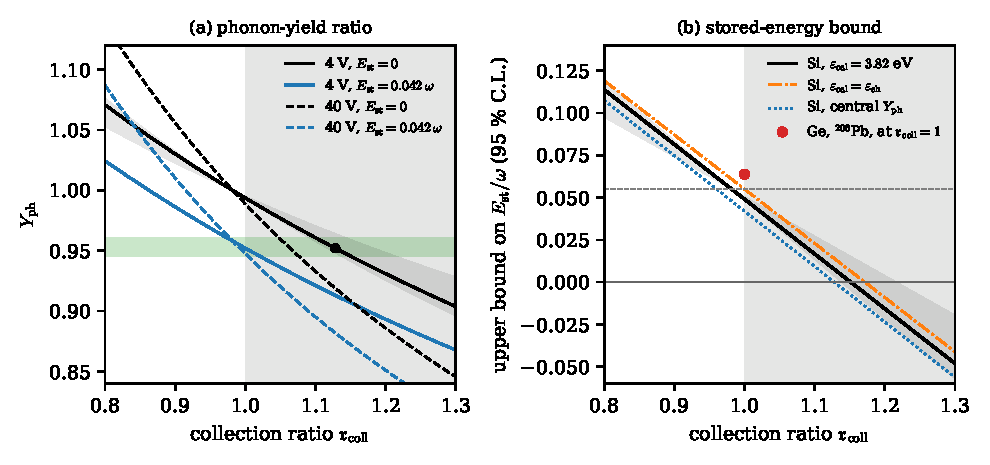
\includegraphics[width=\linewidth]{figures/ch19/limit19_5b.pdf}
\captionof{figure}{Silicon recoils against the collection ratio, from the exact identity \cref{eq:19.5-identity} with $\delta_{\mathrm{coll}} = d_{\mathrm{ER}} = 0$, $g_{\mathrm{Luke}} = 1.067$ ($\varepsilon_{\mathrm{eh}} = \SI{3.75}{eV}$) and $g_{\mathrm{cal}} = 1.047$ ($\varepsilon_{\mathrm{cal}} = \SI{3.82}{eV}$) at \SI{4}{V}, ten times both at \SI{40}{V}, and $f_{\mathrm{ion}} = 0.324$, the yield parameterization of the measurement at the \SI{20}{keV} resonance that dominates the calibration~\cite[Eq.~(4)]{agnese2018nuclear}. (a) Phonon-yield ratio. Black: no stored energy; blue: stored fraction 0.042; solid at \SI{4}{V}, dashed at \SI{40}{V}. Dark band: $f_{\mathrm{ion}}$ from 0.269 to 0.497, the same parameterization at 10 and \SI{100}{keV}. Green: the measured $0.952^{+0.009}_{-0.007}$. Dot: $\mathfrak{r}_{\mathrm{coll}} = 1.128$, where collection alone reproduces it. (b) Upper bound on $E_{\mathrm{st}}/\omega$ at \SI{95}{\percent} confidence, \cref{eq:19.5-widen} at $Y_{\mathrm{ph}} = 0.945$, with the band of (a); dotted: the central $Y_{\mathrm{ph}}$; dash-dotted: a reconstruction with the true pair energy; dashed line: the literature reading 0.055. Red point: germanium at $\mathfrak{r}_{\mathrm{coll}} = 1$. Gray: $\mathfrak{r}_{\mathrm{coll}} \ge 1$, where under (a)--(e) the bound does not exceed $f_{\mathrm{DF}}$.}\label{fig:19-limit-yield}
\par}
\smallskip
Below $\mathfrak{r}_{\mathrm{coll}} = 1$ the bound exceeds $f_{\mathrm{DF}}$, 0.081 at $\mathfrak{r}_{\mathrm{coll}} = 0.9$ for silicon; above $\mathfrak{r}_{\mathrm{coll}} = 1.128$ the central silicon datum needs no stored energy, and the datum alone cannot tell the two readings apart (\cref{we:19-degeneracy}).
\end{limitbox}

The collection offset has a part that the balance law fixes. The recombination phonons at the contacts carry the gap energy of the collected pairs, the fraction $\Eg/\varepsilon_{\mathrm{eh}}$ of an electron-recoil deposit and $f_{\mathrm{ion}}\Eg/\varepsilon_{\mathrm{eh}}$ of a nuclear one, and they are born at the surfaces next to the sensors, with their own spectrum. Let $\rho_g$ be their collection efficiency over that of the hard primary phonons, $\epsilon_{\mathrm{hard}}$. A recoil whose gap fraction is $\chi_g\Eg/\varepsilon_{\mathrm{eh}}$, with $\chi_g = 1$ for the electron and $\chi_g = f_{\mathrm{ion}}$ for the nuclear recoil, then has the primary efficiency $\epsilon_{\mathrm{hard}}[1 + (\rho_g - 1)\chi_g\Eg/\varepsilon_{\mathrm{eh}}]$. The gap part of the offset is
\begin{equation}
  \delta^{\mathrm{gap}}_{\mathrm{coll}} = \frac{(1 - f_{\mathrm{ion}})(\Eg/\varepsilon_{\mathrm{eh}})(\rho_g - 1)}{1 + (\Eg/\varepsilon_{\mathrm{eh}})(\rho_g - 1)} .
  \label{eq:19.5-dgap}
\end{equation}
In silicon at $f_{\mathrm{ion}} = 0.324$, $\rho_g - 1 = 0.21$ gives $\delta^{\mathrm{gap}}_{\mathrm{coll}} = 0.042$, which alone accounts for the deficit of the datum beyond the pair-energy offset, and a change of 0.02 in $\rho_g$ moves it by 0.0037. Contacts sit on the same faces as the sensors, so a difference of this size is possible; its value needs a transport calculation for the detector (\cref{app:E.25}). The rest of the offset comes from the primary spectra, which differ little once down-conversion has erased their origin (\cref{sec:20.2}); from the depth profiles of the calibration sources, since neutrons and gammas do not interact at the same depths; and from escape at the surfaces, which differs between the two.

\subsection{Two-bias inversion of the silicon datum}\label{sec:19.5-inversion}

The CDMS~II silicon detectors were biased at \SI{4}{V} across \SI{1}{cm}, and their neutron calibration gives $Y_{\mathrm{ph}} = 0.952^{+0.009}_{-0.007}$ over 10 to \SI{100}{keV}~\cite[Sects.~2, 4]{agnese2018nuclear}. \Cref{we:19-degeneracy} reads this one number in the two limiting ways.

\begin{workedexample}{The degeneracy of the silicon datum between stored energy and collection}\label{we:19-degeneracy}
The Luke gain is $g_{\mathrm{Luke}} = \SI{4}{V}/\SI{3.75}{V} = 1.067$, and the reconstruction uses $g_{\mathrm{cal}} = \SI{4}{V}/\SI{3.82}{V} = 1.047$. The calibration rests on the spectral feature that an elastic resonance of silicon puts at recoil energies near \SI{20}{keV}~\cite[Sect.~3.2]{agnese2018nuclear}. There the ionization of nuclear recoils is collected in full and follows the yield parameterization of the same analysis~\cite[Eq.~(4), Sect.~4]{agnese2018nuclear}, $y_C = [1/(a_CE_R) + 1/y_L]^{-1}$ with $a_C = \SI{0.247}{keV^{-1}}$ and $y_L$ Lindhard's yield \cref{eq:16.6-lindhard}. It gives $f_{\mathrm{ion}} = 0.324$; Lindhard's yield alone, which overestimates the low-energy data that analysis cites, gives 0.346; the same analysis notes that its fit improves if $y_C$ is about \SI{5}{\percent} low at 10 to \SI{20}{keV}, which the Lindhard variant covers. We set $\delta_{\mathrm{coll}} = x_{\mathrm{NR}} = x_{\mathrm{ER}} = 0$.

\emph{Stored energy alone.} With $\mathfrak{r}_{\mathrm{coll}} = 1$, \cref{eq:19.5-widen} is
\begin{equation*}
  e_{\mathrm{st}} = 1 - Y_{\mathrm{ph}} + \frac{(g_{\mathrm{cal}} - g_{\mathrm{Luke}})(Y_{\mathrm{ph}} - f_{\mathrm{ion}})}{1 + g_{\mathrm{cal}}} = 0.048 - 0.006 = 0.042 ,
\end{equation*}
and 0.049 at the lower edge of the band. The pair-energy offset takes an eighth of the deficit; read with $\varepsilon_{\mathrm{cal}} = \varepsilon_{\mathrm{eh}}$, the datum would give 0.048 and 0.055. Lindhard's $f_{\mathrm{ion}}$ changes the stored fraction by $2\times10^{-4}$.

\emph{Collection alone.} With $E_{\mathrm{st}} = 0$ the collection term of \cref{eq:19.5-first} remains, $1 - Y_{\mathrm{ph}} = (\mathfrak{r}_{\mathrm{coll}}g_{\mathrm{Luke}} - g_{\mathrm{cal}})(1 - f_{\mathrm{ion}})/(1 + \mathfrak{r}_{\mathrm{coll}}g_{\mathrm{Luke}})$, and solving for the collection ratio,
\begin{equation*}
  \mathfrak{r}_{\mathrm{coll}} = \frac{(1 - Y_{\mathrm{ph}}) + g_{\mathrm{cal}}(1 - f_{\mathrm{ion}})}{g_{\mathrm{Luke}}(Y_{\mathrm{ph}} - f_{\mathrm{ion}})} = \frac{0.048 + 0.708}{0.670} = 1.128 .
\end{equation*}
Luke phonons collected \SI{13}{\percent} better than the primaries reproduce the datum with no stored energy. The band of the datum maps onto $1.099 \le \mathfrak{r}_{\mathrm{coll}} \le 1.152$, and Lindhard's $f_{\mathrm{ion}}$ gives 1.134. The mean-field transport estimate of \cref{sec:20.5-sign} puts the collection ratio between 0.81 and 1.02 with energy conserved, and only a selective sink that the estimate does not identify in a detector reaches higher values. Collection alone, $\mathfrak{r}_{\mathrm{coll}} = 1.128$, is therefore not reached by the transport estimate, but it is not excluded until computed kernels test real detectors (\cref{app:E.25}); the two-bias measurement of \cref{sec:19.5-inversion} decides.

\emph{Mixtures.} Every point of the line \cref{eq:19.5-widen} reproduces the datum: half of the stored-energy reading, $e_{\mathrm{st}} = 0.021$, needs $\mathfrak{r}_{\mathrm{coll}} = 1.064$. A gap offset \cref{eq:19.5-dgap} with $\rho_g - 1 = 0.21$ reproduces it with neither.

\emph{Energy dependence.} At fixed $\mathfrak{r}_{\mathrm{coll}} = 1.128$ the collection term scales with $1 - f_{\mathrm{ion}}$, and $f_{\mathrm{ion}}$ grows with the recoil energy: the parameterization gives 0.269 at \SI{10}{keV} and 0.497 at \SI{100}{keV}, hence $Y_{\mathrm{ph}} = 0.948$ and 0.964, the second just above the upper edge 0.961 of the band. The same analysis finds, however, that the ionization collected at \SI{4}{V/cm} falls to about \SI{75}{\percent} of the parameterized yield at \SI{100}{keV}~\cite[Sect.~4]{agnese2018nuclear}; with $f_{\mathrm{ion}} = 0.75 \times 0.497 = 0.373$ the prediction is 0.956, inside the band. A stored fraction independent of energy predicts 0.951 to 0.954 over the range. At the present precision the energy dependence does not separate the readings.
\end{workedexample}

A second bias separates the collection ratio from the rest. Multiply \cref{eq:19.5-identity} by its denominator and divide by $1 - d_{\mathrm{ER}}$: at the bias $V_i$, with gains $g_{\mathrm{Luke},i}$ and $g_{\mathrm{cal},i}$,
\begin{equation}
  (1 + g_{\mathrm{cal},i})\,Y_{\mathrm{ph}}(0) - g_{\mathrm{Luke},i}\,(Y_i - f_{\mathrm{ion}})\,\mathfrak{r}' = Y_i + f_{\mathrm{ion}}g_{\mathrm{cal},i} ,
  \label{eq:19.5-linear}
\end{equation}
with $Y_i$ the phonon-yield ratio measured at that bias and $Y_{\mathrm{ph}}(0)$ and $\mathfrak{r}'$ those of \cref{eq:19.5-calib}. The relation is exact and linear in the two unknowns. Two biases give two equations whose determinant is $(Y - f_{\mathrm{ion}})(g_{\mathrm{Luke},1} - g_{\mathrm{Luke},2})$ when the two measured ratios are equal and does not vanish in general, so the pair $(Y_{\mathrm{ph}}(0), \mathfrak{r}')$ follows by solving a $2\times2$ system (\cref{app:D.45}). For silicon at 4 and \SI{40}{V}, collection alone ($\mathfrak{r}_{\mathrm{coll}} = 1.128$, no stored energy) predicts $Y_{\mathrm{ph}} = 0.919$ at \SI{40}{V}, stored energy alone 0.947, since the pair-energy offset grows with the bias, and the half-and-half mixture 0.932. Solving \cref{eq:19.5-linear} with these values returns the inputs. The difference between the readings, 0.028, is about 3.6 times the half-width of the present band, and an uncertainty of 0.005 on the \SI{40}{V} ratio moves the inverted $\mathfrak{r}'$ by 0.020 to 0.026. At still higher bias the Luke phonons dominate both signals and $Y_{\mathrm{ph}}$ tends to $f_{\mathrm{ion}} + [Y_{\mathrm{ph}}(0) - f_{\mathrm{ion}}]\varepsilon_{\mathrm{eh}}/(\varepsilon_{\mathrm{cal}}\mathfrak{r}')$, which is 0.912 for collection alone.

The inversion holds under hypotheses that are each a missing input. The collection ratio must not change between the two biases, yet the spectrum of Luke phonons depends on the field; the residual is of order $(\dd\mathfrak{r}_{\mathrm{coll}}/\dd V_{\mathrm{bias}})\,\Delta V_{\mathrm{bias}}$, which the transport calculation of \cref{app:E.25} provides. The ionized fraction must be measured at both biases with the charge channel, since trapping depends on the field. The offset and the missing energies must also be the same at both biases, which requires both to collect every pair within the window; a zero-bias run does not qualify as the second point, because the gap energy of uncollected pairs then enters through \cref{eq:19.5-release}. Finally, the reconstruction must use the same $\varepsilon_{\mathrm{cal}}$ at both biases and the true $\varepsilon_{\mathrm{eh}}$ must be known, since \cref{eq:19.5-linear} carries the two gains separately. A third bias overdetermines \cref{eq:19.5-linear} and tests the first three hypotheses.

What the inversion cannot do is split $Y_{\mathrm{ph}}(0) = (1 - \delta_{\mathrm{coll}})(1 - d_{\mathrm{NR}})/(1 - d_{\mathrm{ER}})$ into collection offset and stored energy, since both enter it in the same way. Three further measurements or calculations split it. Transport calculations of the efficiencies of each phonon population in the detector that took the data fix the gap and spectral parts of $\delta_{\mathrm{coll}}$ (\cref{app:E.25}). Neutron and gamma sources with matched depth profiles remove its position part. And two read windows, short and long, separate stored energy released within the window from energy that stays frozen, since the release term of $d_{\mathrm{NR}}$ is the one that grows with $t_{\mathrm{win}}$.

\section{Delayed release and the low-energy excess}\label{sec:19.6}

A close Frenkel pair in silicon holds 6.8 to \SI{7.5}{eV} (\cref{sec:7.4}), and at \SI{10}{mK} it can give them back only by tunneling. For an estimated barrier of \SI{0.1}{eV} over \SI{1.5}{\angstrom} the two-parabola tunneling exponent is 27.5, about \SI{14}{\percent} above the largest exponent that allows recombination within a year (\cref{sec:16.8-hop}). Whether the pair releases its energy during a run or keeps it for good thus depends on one number that is not known. Meanwhile cryogenic detectors with thresholds of tens of eV record an excess of events that rises toward threshold and decays over days after cooldown. A silicon crystal glued to its holder shows more than a hundred times the rate of an identical crystal hung from wire bonds~\cite{anthonypetersen2024stress}. Energy stored in defects is the obvious suspect. Its release at millikelvin obeys an exact sum rule, which fixes how much energy delayed events can carry and at what energy per event; together with energy conservation it bounds the excess, and it leaves collective release of elastic energy as the candidate.

\subsection{Defect kinetics at millikelvin}\label{sec:19.6-kinetics}

At $t_{\mathrm{pr}}$ the recoil leaves the crystal in one of a set of configurations $i$, each a basin of $E^{\mathrm{ad}}$ with the configurational energy $E^{\mathrm{conf}}_i$, the minimum of the basin measured from the minimum of the perfect crystal (\cref{eq:19.1-partition}). The perfect crystal is one of them, with $E^{\mathrm{conf}} = 0$. Let $p_i(t)$ be the probability that the defect complex is in configuration $i$ at time $t$, and $\varGamma_{ij}$ the rate of a hop from $i$ to $j$. Hops are rare compared with the vibrations inside a basin, so the populations obey the master equation
\begin{equation}
  \frac{\dd p_i}{\dd t} = \sum_{j\ne i}\bigl[\varGamma_{ji}\,p_j - \varGamma_{ij}\,p_i\bigr] ,
  \qquad p_i(t_{\mathrm{pr}}) \text{ from the partition at } t_{\mathrm{pr}} .
  \label{eq:19.6-master}
\end{equation}
The stored energy at time $t$ is the mean configurational energy, $E_{\mathrm{st}}(t) = \sum_ip_i(t)E^{\mathrm{conf}}_i$, which equals the $E_{\mathrm{st}}$ of the partition at $t = t_{\mathrm{pr}}$.

The rates at millikelvin are tunneling rates. A barrier of chemical size cannot be crossed thermally, and below the crossover temperature $T_\times$ of \cref{eq:16.8-Tx}, tens of kelvin for an atom, every hop goes through the barrier (\cref{sec:16.8-hop}). A hop from $i$ to $j$ releases $\varepsilon^{\mathrm{hop}}_{ij} = E^{\mathrm{conf}}_i - E^{\mathrm{conf}}_j$, and its tunneling amplitude is $\Delta_0 = \omega_{\mathrm{w}}\ee^{-\lambda_{\mathrm{tun}}}$ in the notation of \cref{sec:16.7}. The golden rule \cref{eq:C.20-rate} gives the rate as $\Delta_0^2/4$ times the time integral of the bath correlation at the energy released. Let $A(\varepsilon)$ be the line shape, the probability per unit energy that the bath accepts the energy $\varepsilon$. Then
\begin{equation}
  \varGamma_{ij} = \frac{\pi}{2}\,\omega_{\mathrm{w}}^2\,\ee^{-2\lambda_{\mathrm{tun}}}\,A\bigl(\varepsilon^{\mathrm{hop}}_{ij} + \Delta E_{\mathrm{zp},ij}\bigr) ,
  \label{eq:19.6-hop}
\end{equation}
where $\Delta E_{\mathrm{zp},ij}$ is the decrease of the zero-point energy of the local modes in the hop, so that the argument is the energy the bath actually receives. For the two-level systems of \cref{sec:16.8} the energy is below the top of the phonon band and one phonon takes it; then $A(\varepsilon) = J_{\mathrm{s}}(\varepsilon)\coth(\varepsilon/2T)/\pi\varepsilon^2$, which turns \cref{eq:19.6-hop} into \cref{eq:16.8-golden}. An eV release is far above the phonon band, so the bath can take it only as many quanta at once, in the local modes $k$ that are displaced between the two minima, with Huang--Rhys factors $S_{\mathrm{HR},k}$ and the reorganization energy $E_{\mathrm{reorg}} = \sum_kS_{\mathrm{HR},k}\omega_k$ of \cref{eq:E.22-SHR}. At $T \ll \omega_k$ the correlation of one displaced mode is the Poisson series of \cref{eq:5.6-poisson}, and the size of the rearrangement decides between two regimes.

If the hop is a small rearrangement, $E_{\mathrm{reorg}} \ll \varepsilon^{\mathrm{hop}}$, the energy must go into $n_q = \varepsilon/\omega_{\mathrm{acc}}$ quanta of modes that are barely displaced. For one accepting mode of energy $\omega_{\mathrm{acc}}$ and total factor $S$, the Poisson weight of $n_q$ quanta gives $A(\varepsilon)\,\omega_{\mathrm{acc}} = \ee^{-S}S^{n_q}/n_q!$, the energy-gap law. For $S = 1$, $\omega_{\mathrm{acc}} = \SI{60}{meV}$ and $\varepsilon = \SI{1}{eV}$ it is $2.7\times10^{-15}$, which adds 16.8 to the tunneling exponent. If instead the hop is a large rearrangement, $E_{\mathrm{reorg}} \approx \varepsilon^{\mathrm{hop}}$, the reaction coordinate itself takes the energy. Then $A$ is a Gaussian of width $(\sum_kS_{\mathrm{HR},k}\omega_k^2)^{1/2}$ centered at $E_{\mathrm{reorg}}$, and there is no gap suppression. The two-state reduction behind \cref{eq:19.6-hop} is then not controlled either, and the rate is the instanton rate on the full surface (\cref{sec:16.8-hop}). Taking the prefactor, of order $\omega_{\mathrm{w}}$, as $\varGamma_0 = \SI{e13}{s^{-1}}$, a hop happens within the observation time $t_{\mathrm{obs}}$ if
\begin{equation}
  2\lambda_{\mathrm{tun}} + \ln\frac{1}{\omega_{\mathrm{w}}A(\varepsilon)} \le \ln\bigl(\varGamma_0t_{\mathrm{obs}}\bigr) ,
  \label{eq:19.6-window}
\end{equation}
and for one year the right side is 47.2. With $\omega_{\mathrm{w}}A \approx 1$ this is the bound $\lambda_{\mathrm{tun}} \le 23.6$ of \cref{sec:16.8-hop}. With the energy-gap factor above it becomes $\lambda_{\mathrm{tun}} \le 6.8$, and for a \SI{7}{eV} release the logarithm of the factor is about 440, so a weakly coupled eV release never happens.

For a close Frenkel pair in silicon the two-parabola exponent $\lambda_{\mathrm{tun}} = (d_{\mathrm{tun}}/2)(2M_\kappa V_{\mathrm{b}})^{1/2}$ with $M_\kappa = \SI{26.16}{GeV}$, $V_{\mathrm{b}} = \SI{0.1}{eV}$ and $d_{\mathrm{tun}} = \SI{1.5}{\angstrom}$ is 27.5, and a quartic barrier of the same height and width raises it by $4/3$, to 36.7. In the weak-coupling regime the pair is frozen. In the strong-coupling regime it recombines within a year only if the true exponent lies at least \SI{14}{\percent} below the two-parabola value. A split interstitial in aluminum, with an estimated barrier of \SI{0.1}{eV} over \SI{1.4}{\angstrom}, has 25.2 and needs \SI{6}{\percent}. Aluminum is superconducting at these temperatures, so its conduction electrons do not take the energy (\cref{sec:16.8-electron}). Whether either defect releases its energy therefore depends on one calculation per path (\cref{sec:19.6-open}).

\subsection{The release-path sum rule}\label{sec:19.6-sumrule}

Every hop puts energy into the crystal, and a detector sees its distribution in energy and time. For one seed, the expected number of hops per unit time and per unit released energy is
\begin{equation}
  \mathcal{R}_{\mathrm{hop}}(E, t) = \sum_{i\ne j}p_i(t)\,\varGamma_{ij}\,\delta\bigl(E - \varepsilon^{\mathrm{hop}}_{ij}\bigr) ,
  \label{eq:19.6-Rhop}
\end{equation}
with the configurational energy in the delta function. Its integral over $E$ and $t$ is the expected number of hops $\langle N_{\mathrm{hop}}\rangle$, not one: a pair may pass through several configurations before it recombines. The energy it releases is fixed by its end points alone.
\begin{keyresult}[Release-path sum rule]
For populations that obey \cref{eq:19.6-master} on a closed set of configurations,
\begin{equation}
  \int_{t_{\mathrm{pr}}}^{t}\dd t'\int\dd E\;E\,\mathcal{R}_{\mathrm{hop}}(E, t') = E_{\mathrm{st}} - E_{\mathrm{st}}(t) ,
  \label{eq:19.6-sumrule}
\end{equation}
the stored energy of the partition minus the energy still stored at $t$.
\end{keyresult}
\noindent By \cref{eq:19.6-master},
\begin{equation*}
  \frac{\dd}{\dd t}\sum_ip_iE^{\mathrm{conf}}_i = \sum_{i\ne j}\bigl(\varGamma_{ji}p_j - \varGamma_{ij}p_i\bigr)E^{\mathrm{conf}}_i
  = -\sum_{i\ne j}\varGamma_{ij}\,p_i\bigl(E^{\mathrm{conf}}_i - E^{\mathrm{conf}}_j\bigr) = -\int\dd E\;E\,\mathcal{R}_{\mathrm{hop}}(E, t) ,
\end{equation*}
where the middle step exchanges the labels in the first term. Integrating from $t_{\mathrm{pr}}$ to $t$ gives \cref{eq:19.6-sumrule}. Neither detailed balance nor any model of the rates enters, so the rule holds for every rate law of \cref{sec:19.6-kinetics} and also for rates that change in time. These include the rates stimulated by a heat pulse, by illumination or by the carriers of a later event.

The rule is exact under five conditions on how a calculation accounts for the energy: every hop counted, one table of configurational energies, photons counted as escaped energy, no probability leaving the listed configurations, and configurational energies throughout. Every hop must be counted, including uphill hops with $\varepsilon^{\mathrm{hop}} < 0$, in which the defect absorbs heat from the lattice. The partition and the release paths must use one table of configurational energies, from one potential and one cell, as \cref{sec:19.1-md} requires; otherwise the two sides differ by the error of the potential, a few tenths of an eV. A hop that emits a photon still releases its energy, which then appears among the escaping quanta of the balance law of \cref{sec:19.5} instead of the phonons. No probability may leave the listed configurations, $\sum_ip_i(t) = 1$: the master equation describes one seed, and recombination of an interstitial with the vacancy of another event lies outside it, since it needs the joint state of both. Finally, the energies are configurational. The energy that the bath receives in a hop is $\varepsilon^{\mathrm{hop}}_{ij} + \Delta E_{\mathrm{zp},ij}$, where the zero-point change is below a tenth of an eV, an estimate (\cref{sec:19.5-law}). The zero-point changes add up along any path to the zero-point change of the end basin, which \cref{sec:19.1-partition,sec:19.5-law} count in the phonons, not in $E_{\mathrm{st}}$. Read with these conditions, \cref{eq:19.6-sumrule} is the stored-energy term of the balance law \cref{eq:19.5-balance}: what leaves $E_{\mathrm{st}}(t)$ enters the phonons, at the energies and times of $\mathcal{R}_{\mathrm{hop}}$.

\begin{workedexample}{The release-path sum rule for one Frenkel pair}\label{we:19-sumrule}
Take a close Frenkel pair C in silicon with $E^{\mathrm{conf}}_{\mathrm{C}} = \SI{7.0}{eV}$, which can recombine directly to the perfect crystal 0 or first relax into a bond defect B with $E^{\mathrm{conf}}_{\mathrm{B}} = \SI{2.8}{eV}$, both inside the ranges of \cref{sec:7.4}. Separation to an isolated vacancy and interstitial, which costs 0.6 to \SI{2.9}{eV} more, is closed at \SI{10}{mK}. No path of this kind has been computed, so we take illustrative strong-coupling exponents in \cref{eq:19.6-window}, with $\varGamma = \varGamma_0\ee^{-2\lambda_{\mathrm{tun}}}$: $\lambda_{\mathrm{tun}} = 22.5$ for C$\to$B, 24.0 for C$\to$0 and 25.0 for B$\to$0. The rates are $\varGamma_{\mathrm{CB}} = 2.86\times10^{-7}$, $\varGamma_{\mathrm{C0}} = 1.43\times10^{-8}$ and $\varGamma_{\mathrm{B0}} = 1.93\times10^{-9}\,\si{s^{-1}}$. The pair leaves C after \SI{38.5}{days} on average, through B with probability $\varGamma_{\mathrm{CB}}/(\varGamma_{\mathrm{CB}} + \varGamma_{\mathrm{C0}}) = 0.953$.

The master equation for three states is solved by two exponentials, $p_{\mathrm{C}} = \ee^{-\varGamma_{\mathrm{C}}t}$ with $\varGamma_{\mathrm{C}} = \varGamma_{\mathrm{CB}} + \varGamma_{\mathrm{C0}}$, and $p_{\mathrm{B}} = \varGamma_{\mathrm{CB}}(\ee^{-\varGamma_{\mathrm{C}}t} - \ee^{-\varGamma_{\mathrm{B0}}t})/(\varGamma_{\mathrm{B0}} - \varGamma_{\mathrm{C}})$. After one year $p_{\mathrm{C}} = 10^{-4}$, $p_{\mathrm{B}} = 0.902$ and $p_0 = 0.098$, and the stored energy is $E_{\mathrm{st}}(t) = 0.902\times\SI{2.8}{eV} = \SI{2.526}{eV}$. The expected numbers of hops are $\varGamma_{ij}\int_0^t p_i\,\dd t'$: 0.9525 hops C$\to$B releasing \SI{4.2}{eV} each, 0.0474 hops C$\to$0 releasing \SI{7.0}{eV}, and 0.0505 hops B$\to$0 releasing \SI{2.8}{eV}. Together they release
\begin{equation*}
  0.9525\times\SI{4.2}{eV} + 0.0474\times\SI{7.0}{eV} + 0.0505\times\SI{2.8}{eV} = \SI{4.474}{eV} = \SI{7.0}{eV} - \SI{2.526}{eV} ,
\end{equation*}
as \cref{eq:19.6-sumrule} requires, in $\langle N_{\mathrm{hop}}\rangle = 1.05$ hops, \SI{4.26}{eV} per hop. After ten years \SI{5.539}{eV} has been released in 1.43 hops, and after a hundred years \SI{6.994}{eV} in 1.95 hops: the number of hops depends on the path, the energy only on the end points. A sensor that absorbs a quarter of the phonon energy of a release, as the sensors of the glued and suspended crystals do~\cite{anthonypetersen2024stress}, which absorb phonons before they thermalize, records the three kinds of hop as events of 1.05, 1.75 and \SI{0.70}{eV}, each shifted by a quarter of its zero-point change.
\end{workedexample}

\subsection{The delayed-release spectrum}\label{sec:19.6-spectrum}

A detector sees the sum of $\mathcal{R}_{\mathrm{hop}}$ over all seeds, from the recoils of earlier events and from the defects frozen in at cooldown, with each release converted into a recorded energy. A release of energy $\varepsilon$ puts $\varepsilon + \Delta E_{\mathrm{zp}}$ into athermal phonons, or into a photon on the radiative branch, and the sensor absorbs a fraction $f_{\mathrm{ph}}$ of the phonon energy, which depends on where the release happens and on the phonon spectrum. A release is an event only if $f_{\mathrm{ph}}(\varepsilon + \Delta E_{\mathrm{zp}}) \ge E_{\mathrm{th}}$. Below threshold it is heat, a load on the sensor that adds to its noise but makes no event.

Defects frozen in at cooldown follow the same kinetics, and two families dominate. The first family, the two-level systems of the amorphous films and glues near a detector, relaxes by emitting single phonons of energy $\Delta_{\mathrm{tl}}$ (\cref{sec:16.8}). After a quench from the freezing temperature $T_{\mathrm{frz}}$ to $T_{\mathrm{lo}}$, a defect of splitting $\Delta_{\mathrm{tl}}$ keeps the excess population $\frac12[\tanh(\Delta_{\mathrm{tl}}/2T_{\mathrm{lo}}) - \tanh(\Delta_{\mathrm{tl}}/2T_{\mathrm{frz}})]$, and the uniform density in $\lambda_{\mathrm{tun}}$ makes the fraction relaxing per unit time $1/2t$. The steps of \cref{eq:16.8-heat}, kept at fixed splitting, give the number of phonons emitted per unit energy and time by a volume $\Vol$,
\begin{equation}
  \frac{\dd\mathcal{R}_{\mathrm{TLS}}}{\dd E} = \frac{\bar P\Vol}{4t}\Bigl[\tanh\frac{E}{2T_{\mathrm{lo}}} - \tanh\frac{E}{2T_{\mathrm{frz}}}\Bigr] ,
  \label{eq:19.6-tls}
\end{equation}
whose first moment is \cref{eq:16.8-heat}. The mean quantum is $1.19\,T_{\mathrm{frz}}$, \SI{0.49}{meV} for $T_{\mathrm{frz}} = \SI{4.8}{K}$: the release of a glass is all heat, \SI{46}{pW} per gram of fused silica an hour after cooling (\cref{we:16-heat}), and none of it can be an event.

The second family is the point defects of the crystal itself, close Frenkel pairs and bond defects from earlier recoils, which release eV per hop in the strong-coupling regime and nothing in the weak one. \Cref{fig:19-release} shows both. Their time laws depend on the distribution of the paths. A uniform distribution of tunneling exponents leads to $1/t$, as for the glass, and a single path to an exponential. Correlated recombination of a pair that diffuses in three dimensions follows the first-passage tail $t^{-3/2}$. The time law alone, however, does not identify the source, since stress relaxation in a glue also leads to $1/t$ (\cref{sec:19.6-lee}).

\begin{figure}[tbp]
  \centering
  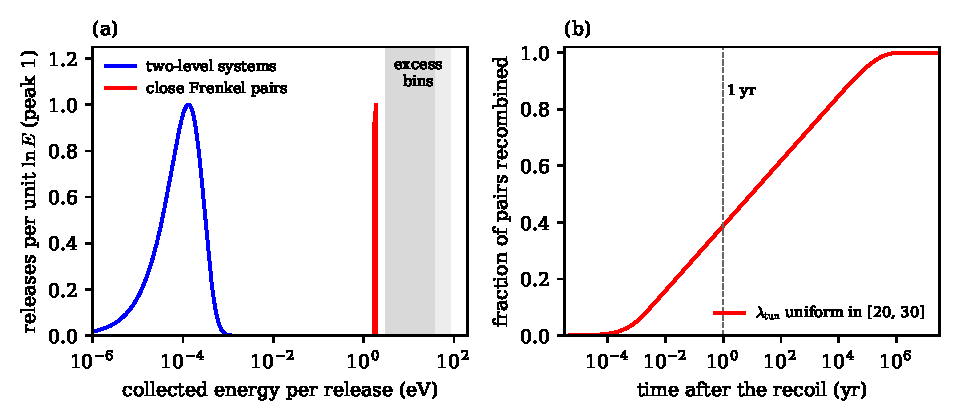
\includegraphics[width=\linewidth]{figures/ch19/fig19_5.pdf}
  \caption{Delayed releases from two defect families. (a) Distribution of the energy one release gives a sensor that absorbs a fraction $f_{\mathrm{ph}} = 0.25$ of the phonon energy, per unit logarithm of the energy, each family scaled to a peak of one. Blue: two-level systems frozen at $T_{\mathrm{frz}} = \SI{4.8}{K}$ and relaxing at \SI{10}{mK}, \cref{eq:19.6-tls}, mean quantum \SI{0.49}{meV}. Red: recombination of close Frenkel pairs in silicon, with configurational energies spread uniformly between 6.8 and \SI{7.5}{eV} (\cref{sec:7.4}), zero-point changes neglected. Gray: the 3--38 and 38--\SI{85}{eV} bins of energy absorbed in the sensor in which a glued silicon crystal shows its excess of events~\cite{anthonypetersen2024stress}. (b) Fraction of a family of close pairs recombined by time $t$, for strong coupling, $\varGamma = \SI{e13}{s^{-1}}\,\ee^{-2\lambda_{\mathrm{tun}}}$, with $\lambda_{\mathrm{tun}}$ spread uniformly between 20 and 30, an illustrative range around the two-parabola estimates. The fraction grows as $\ln t$ (a rate $\propto 1/t$) between \SI{6.5}{h} and $3.6\times10^5$ years; 0.39 of the pairs recombine within the first year. In the weak-coupling regime none does.}
  \label{fig:19-release}
\end{figure}

A close pair gives a sensor that absorbs a quarter of the phonons between 1.70 and \SI{1.88}{eV}, below the lowest bin of the excess (\cref{fig:19-release}(a)), and a two-level system gives a ten-thousandth of that. Single releases add to the heat load and, through the spectrum, to the noise of a sensor with a threshold of an eV or less; for thresholds of a few eV they are invisible. Amorphous pockets left by keV recoils are the one point-defect source that releases more at once: a pocket that recrystallizes releases of order \SI{0.1}{eV} per atom, an estimate, so a pocket of 120 atoms gives \SI{3}{eV} to such a sensor.

The inputs of these rates are computable from first principles. Barriers and minimum-energy paths come from the nudged elastic band, which relaxes a chain of configurations between the two minima onto the path, on the density-functional or machine-learned surface, the Huang--Rhys factors from the Hessians at both minima, and the exponent along the true path from ring-polymer instantons (\cref{app:E.22}). The sum rule \cref{eq:19.6-sumrule} is the acceptance test of the kinetic Monte Carlo, the stochastic sampling of hop sequences that turns the rates into $\mathcal{R}_{\mathrm{hop}}$.

\subsection{Defectons}\label{sec:19.6-defecton}

A light defect that tunnels between equivalent sites faster than the disorder around it can detune them becomes delocalized. This matters for a detector because a mobile defect reaches its partner, or a surface, on a time set by its band and not by a barrier. If the defect at site $\vect{r}$ tunnels to each neighbor with amplitude $A_{\mathrm{dfn}}$, the Bloch combinations of the localized states are stationary, and the defect becomes a quasiparticle, a defecton, with a band
\begin{equation}
  \varepsilon^{\mathrm{dfn}}(\vect{k}) = E^{\mathrm{loc}} - A_{\mathrm{dfn}}\sum_{i=x,y,z}\cos k_ia ,
  \label{eq:19.6-band}
\end{equation}
on a simple cubic lattice of spacing $a$~\cite[Eqs.~(1)--(3)]{pushkarov2004quantum}. The band width is $\Delta_{\mathrm{dfn}} = zA_{\mathrm{dfn}}$, with $z = 6$ neighbors, the mass at the bottom $1/A_{\mathrm{dfn}}a^2$, and the speed at most $A_{\mathrm{dfn}}a$. In solid helium, where defectons were first proposed, a ${}^3$He impurity has $\Delta_{\mathrm{dfn}} \sim \SI{e-4}{K}$; the light interstitials of metals, hydrogen in niobium for example, are candidates in the materials of detectors~\cite{pushkarov2004quantum}. In a hop the defecton cannot change its energy by more than $\Delta_{\mathrm{dfn}}$, so a gradient of the potential energy $\phi$ with $|\nabla\phi|a > \Delta_{\mathrm{dfn}}$ localizes it~\cite[Eq.~(17)]{pushkarov2004quantum}. Around a defect whose elastic interaction falls as $\phi = V_0(a/r)^3$, the gradient criterion reads $3V_0(a/r)^4 > \Delta_{\mathrm{dfn}}$, and the region $r < R_0 = a(3V_0/\Delta_{\mathrm{dfn}})^{1/4}$ is closed to band motion.

In a perfect crystal at $\Delta_{\mathrm{dfn}} \ll T$ the defecton moves through the band ballistically between collisions with phonons, and its diffusion constant falls as $T^{-9}$. The exponent follows from four facts: the kinematics of a narrow band, the Rayleigh form of two-phonon scattering, the small momentum change per collision, and the band velocity. First, the defecton cannot absorb or emit one phonon: that needs $|\varepsilon^{\mathrm{dfn}}(\vect{k} + \vect{Q}) - \varepsilon^{\mathrm{dfn}}(\vect{k})| = \bar cQ$, and the left side is at most $A_{\mathrm{dfn}}aQ$, far below $\bar cQ$ for a narrow band. The leading process is therefore two-phonon scattering, $\vect{Q} \to \vect{Q}'$ with $\omega' \simeq \omega$. Second, its amplitude is proportional to $\omega$. For a coupling quadratic in the strain, the elastic inhomogeneity of the defect, the amplitude carries $QQ'/(\omega\omega')^{1/2} \propto \omega$. The linear deformation coupling at second order has two time orderings with energy denominators $\pm\omega$ that cancel at leading order, and what remains is the second difference of the band, $\propto A_{\mathrm{dfn}}a^2QQ'$, again $\propto\omega$. The cross-section is therefore $\propto (Qa)^4$, Rayleigh scattering~\cite[Eq.~(49)]{pushkarov2004quantum}. Third, the number of thermal phonons grows as $T^3$, so the collision rate grows as $T^7$; but each collision changes the crystal momentum by at most about $T/\bar c$, much less than $1/a$~\cite[Eq.~(54)]{pushkarov2004quantum}, and $(1/Qa)^2 \propto T^{-2}$ collisions are needed to randomize it. The transport rate grows as $T^9$. Fourth, $D = v^2\tau_{\mathrm{tr}}/3$ with $v \sim A_{\mathrm{dfn}}a$ gives $D \propto \Delta_{\mathrm{dfn}}^2T^{-9}$. Pushkarov computes the rate of growth of the mean squared crystal momentum,
\begin{equation}
  \varGamma_{k^2} \equiv \frac{\dd\langle(\Delta\vect{k})^2\rangle}{\dd t} = \alpha_{\mathrm{P}}\,\sigma_{\mathrm{P}}\,\frac{\bar c}{a^3}\Bigl(\frac{T}{\theta_p}\Bigr)^9 , \qquad
  \theta_p = \frac{\bar c}{2a} , \qquad \alpha_{\mathrm{P}} = \frac{\pi^5\zeta(9)}{240\,\zeta(8)} = 1.27 ,
  \label{eq:19.6-q2}
\end{equation}
where $\bar c = (c_{\mathrm{LA}}^{-4} + 2c_{\mathrm{TA}}^{-4})^{-1/4}$ is his average sound speed and $\sigma_{\mathrm{P}}$ the strength of the defect's elastic perturbation relative to that of a vacancy~\cite[Eqs.~(48), (58)]{pushkarov2004quantum}. The characteristic temperature is $\theta_p$, about an eighth of the Debye temperature.

These four facts fix the exponent; the prefactor needs the motion in the band. Since each collision changes $\vect{k}$ by a small step, $\vect{k}$ diffuses, with $D_1 = \varGamma_{k^2}/6$ per Cartesian component, and detailed balance at temperature $T$ adds the drift $-D_1\nabla_{\vect{k}}\varepsilon^{\mathrm{dfn}}/T$. The band \cref{eq:19.6-band} is a sum over components, so each component moves on its own circle $\vartheta = k_xa$, with velocity $v_x = A_{\mathrm{dfn}}a\sin\vartheta$. The diffusion constant is the time integral of the velocity correlation, $D = \int_0^\infty\dd t\,\langle v_x(0)v_x(t)\rangle$. It equals $(A_{\mathrm{dfn}}a)^2\langle\sin\vartheta\,\chi\rangle$, where $\chi$ solves the backward equation $a^2D_1(\chi'' - U'\chi') = -\sin\vartheta$ with $U = -(A_{\mathrm{dfn}}/T)\cos\vartheta$, and the average is over $\ee^{-U}$. With $y = A_{\mathrm{dfn}}/T$, one integration gives $\ee^{y\cos\vartheta}\chi' = \ee^{y\cos\vartheta}/(ya^2D_1) + C$, and periodicity of $\chi$ fixes $C = -1/[ya^2D_1I_0(y)]$, with $I_0$ the modified Bessel function. An integration by parts then gives $\langle\sin\vartheta\,\chi\rangle = [1 - I_0(y)^{-2}]/(y^2a^2D_1)$, and
\begin{keyresult}[Defecton diffusion in a phonon gas]
\begin{equation}
  D = \frac{6T^2}{\varGamma_{k^2}}\Bigl[1 - I_0\Bigl(\frac{A_{\mathrm{dfn}}}{T}\Bigr)^{-2}\Bigr]
  \;\xrightarrow{\;T \gg \Delta_{\mathrm{dfn}}\;}\; D_9 = \frac{3A_{\mathrm{dfn}}^2}{\varGamma_{k^2}} = \frac{\Delta_{\mathrm{dfn}}^2}{12\varGamma_{k^2}} \propto T^{-9} .
  \label{eq:19.6-D}
\end{equation}
\end{keyresult}
\noindent At $T \ll A_{\mathrm{dfn}}$ the bracket tends to one and $D = 6T^2/\varGamma_{k^2} \propto T^{-7}$, the diffusion of a particle of mass $1/A_{\mathrm{dfn}}a^2$ with the friction that the same phonons exert. These are the two limits of Pushkarov's interpolation~\cite[Eqs.~(61), (64)]{pushkarov2004quantum}.

\begin{limitbox}[Defecton diffusion][lim:19.6a]
The published law is $D_T = (a\bar c/3\alpha_{\mathrm{P}}\sigma_{\mathrm{P}})[\varepsilon(p)/\theta_p]^2(\theta_p/T)^9$, for $\Delta_{\mathrm{dfn}} \ll T \ll \theta_p$~\cite[Eq.~(61)]{pushkarov2004quantum}, which is $D_9$ of \cref{eq:19.6-D} with $\varepsilon(p) = \Delta_{\mathrm{dfn}}/4$.
\par\smallskip
{\centering
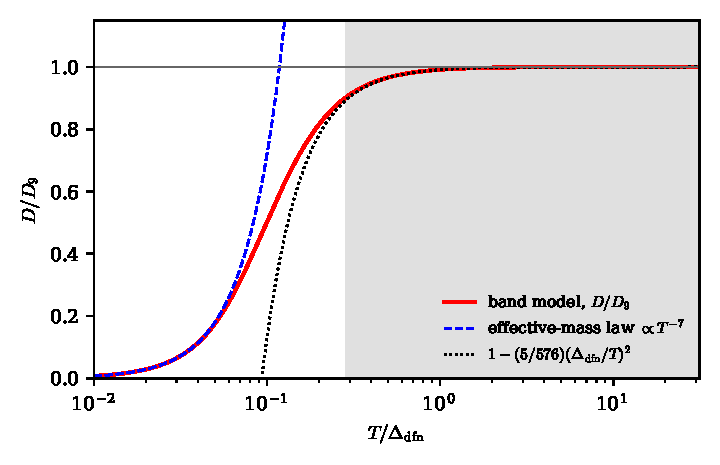
\includegraphics[width=0.75\linewidth]{figures/ch19/limit19_6a.pdf}
\captionof{figure}{Diffusion constant of a defecton in a simple cubic tight-binding band, \cref{eq:19.6-D}, divided by its $T^{-9}$ limit $D_9$, against the temperature in units of the band width. The ratio depends on $T/\Delta_{\mathrm{dfn}}$ alone, since the phonon rate $\varGamma_{k^2}$ of \cref{eq:19.6-q2} cancels. Red: the band model, crystal momentum diffusing at a constant rate with the detailed-balance drift. Blue dashed: the effective-mass law $D = 6T^2/\varGamma_{k^2} \propto T^{-7}$. Dotted: the leading correction $1 - \tfrac{5}{576}(\Delta_{\mathrm{dfn}}/T)^2$. Gray: within \SI{10}{\percent} of the $T^{-9}$ law, $T \ge 0.28\,\Delta_{\mathrm{dfn}}$. The upper edge $T \ll \theta_p$ lies outside the plot and depends on the crystal.}\label{fig:19-limit-defecton}
\par}
\smallskip
Below $0.28\,\Delta_{\mathrm{dfn}}$ the band is no longer uniformly populated and the law steepens toward $T^{-7}$; above $\theta_p$ the phonons are no longer long-wave and the Rayleigh law of the cross-section fails.
\end{limitbox}

The $T^{-9}$ law holds better than its derivation suggests. The ratio $D/D_9$ expands as $1 - (5/16)(A_{\mathrm{dfn}}/T)^2$, so the law is within \SI{10}{\percent} for $T \ge 0.28\,\Delta_{\mathrm{dfn}}$ and within \SI{1}{\percent} for $T \ge 0.93\,\Delta_{\mathrm{dfn}}$, although the condition stated with it is $T \gg \Delta_{\mathrm{dfn}}$. The relevant energy is the hopping amplitude, a sixth of the band width. At $T = 0.1\,\Delta_{\mathrm{dfn}}$ the local exponent is $-7.9$. A defecton moves faster the colder the crystal, until strain gradients localize it. In a real crystal the gradients from impurities, dislocations and the defect's own partner set $R_0$, and a band narrower than the elastic interaction at a few lattice spacings never carries the defect far.

\subsection{Crowdions}\label{sec:19.6-crowdion}

An extra atom in a close-packed row of a body-centered cubic metal spreads over many neighbors as a kink in the row, a crowdion. In tungsten, the metal of many transition-edge sensors, the self-interstitial takes this form along $\langle111\rangle$~\cite{fitzgerald2018structure}. The Frenkel--Kontorova chain of \cref{app:C.20} describes it: atoms of mass $M_\kappa$ at spacing $a_{\mathrm{ch}}$, springs $K_{\mathrm{ch}}$, and the potential $V_{\mathrm{s}}\sin^2(\pi z/a_{\mathrm{ch}})$ of the surrounding crystal, \cref{eq:C.20-FK}. For a slowly varying displacement the chain obeys the sine-Gordon equation, and its kink has the profile \cref{eq:C.20-kink} of width $d_{\mathrm{kink}} = a_{\mathrm{ch}}^2[K_{\mathrm{ch}}/2\pi^2V_{\mathrm{s}}]^{1/2}$~\cite[Eq.~(2)]{fitzgerald2018structure} and the rest energy $E_{\mathrm{kink}} = 4V_{\mathrm{s}}d_{\mathrm{kink}}/a_{\mathrm{ch}}$ of \cref{eq:C.20-Ekink}~\cite[Eq.~(3)]{fitzgerald2018structure}. The crowdion moves as a particle of mass
\begin{equation}
  M_{\mathrm{cr}} = \frac{2}{\pi^2}\,\frac{a_{\mathrm{ch}}}{d_{\mathrm{kink}}}\,M_\kappa ,
  \label{eq:19.6-Mcr}
\end{equation}
the kink mass \cref{eq:C.20-mass}~\cite{braun2004frenkel}, and the discrete row makes it cross the Peierls--Nabarro barrier $E_{\mathrm{PN}}$ of \cref{eq:C.20-EPN} to move by one spacing.

For tungsten, $V_{\mathrm{s}} \approx \SI{1}{eV}$ and $K_{\mathrm{ch}}a_{\mathrm{ch}}^2 = 50$ to \SI{100}{eV} are typical values~\cite{fitzgerald2018structure}. They give $d_{\mathrm{kink}} = 1.59$ to $2.25\,a_{\mathrm{ch}}$, $E_{\mathrm{kink}} = 6.4$ to \SI{9.0}{eV}, $M_{\mathrm{cr}} = 0.127$ to $0.090\,M_\kappa$ and a barrier of $1.2\times10^{-4}$ to $3.6\times10^{-7}\,\si{eV}$, with $a_{\mathrm{ch}} = \frac{\sqrt3}{2}\times\SI{3.165}{\angstrom} = \SI{2.741}{\angstrom}$. Atomistic calculations put the barrier near a meV instead~\cite{fitzgerald2018structure}, because the real substrate potential of tungsten is not a single sine. A particle of mass $M_{\mathrm{cr}}$ in the periodic potential $\tfrac12E_{\mathrm{PN}}[1 - \cos(2\pi z_0/a_{\mathrm{ch}})]$ has a ground band whose width follows from Mathieu's equation. The free-recoil energy $\pi^2/2M_{\mathrm{cr}}a_{\mathrm{ch}}^2$ is \SI{0.12}{meV} for the narrower kink, equal to its barrier within \SI{3}{\percent}, and \SI{0.17}{meV} for the wider one, and the band is 90 to \SI{166}{\micro eV}, 1.0 to \SI{1.9}{K}. With the atomistic barrier of \SI{1}{meV} and the same masses it narrows to 13 to \SI{34}{\micro eV}, 0.15 to \SI{0.39}{K}. Either way the band is wider than the temperature of a detector, so a crowdion is a candidate for coherent motion at millikelvin, a defecton of one dimension.

\begin{limitbox}[Crowdion profile and kink mass][lim:19.6b]
The published crowdion is the sine-Gordon kink \cref{eq:C.20-kink} with rest energy \cref{eq:C.20-Ekink}~\cite[Eqs.~(2), (3)]{fitzgerald2018structure}, of mass \cref{eq:19.6-Mcr} and barrier \cref{eq:C.20-EPN}.
\par\smallskip
{\centering
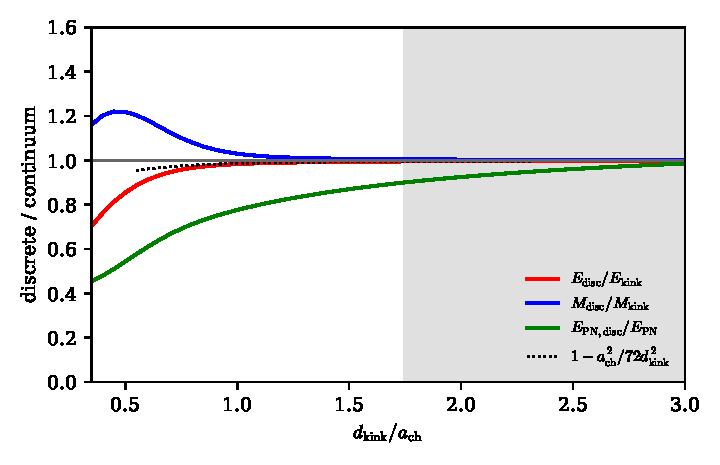
\includegraphics[width=0.75\linewidth]{figures/ch19/limit19_6b.pdf}
\captionof{figure}{Discrete Frenkel--Kontorova crowdion against the continuum kink, as ratios, against the kink width in units of the row spacing. The discrete chain of \cref{eq:C.20-FK} is relaxed numerically with the kink centered between two atoms (the minimum) and on an atom (the saddle). Red: rest energy, against $E_{\mathrm{kink}}$. Blue: translation mass $M_\kappa\sum_n(u_{n+1} - u_n)^2/a_{\mathrm{ch}}^2$, the lattice form of $M_\kappa\sum_n(\partial u_n/\partial z_0)^2$, against \cref{eq:19.6-Mcr}. Green: saddle minus minimum, against $E_{\mathrm{PN}}$ of \cref{eq:C.20-EPN}. Dotted: the leading correction to the energy, $1 - a_{\mathrm{ch}}^2/72d_{\mathrm{kink}}^2$. Gray: all three within \SI{10}{\percent}, $d_{\mathrm{kink}} \ge 1.74\,a_{\mathrm{ch}}$, set by the barrier.}\label{fig:19-limit-crowdion}
\par}
\smallskip
Well below one row spacing the kink is no longer a smooth profile: the barrier falls to half the continuum value near $0.4\,a_{\mathrm{ch}}$, and the mass and energy deviate by tens of percent.
\end{limitbox}

The energy and the mass of the kink hold far beyond the barrier. Replacing the spring energy $\frac12K_{\mathrm{ch}}\sum(u_{n+1} - u_n)^2$ by its continuum form drops the next term of $4\sin^2(ka_{\mathrm{ch}}/2) = k^2a_{\mathrm{ch}}^2 - k^4a_{\mathrm{ch}}^4/12$, which is $-(K_{\mathrm{ch}}a_{\mathrm{ch}}^3/24)\int\dd z\,u''^2$. On the kink, $\int\dd z\,u''^2 = 2a_{\mathrm{ch}}^2/3\pi^2d_{\mathrm{kink}}^3$, and to first order the energy changes by $-K_{\mathrm{ch}}a_{\mathrm{ch}}^5/36\pi^2d_{\mathrm{kink}}^3 = -E_{\mathrm{kink}}\,a_{\mathrm{ch}}^2/72d_{\mathrm{kink}}^2$, \SI{1.4}{\percent} at $d_{\mathrm{kink}} = a_{\mathrm{ch}}$. The discrete energy follows this law within $2\times10^{-4}$ above $1.5\,a_{\mathrm{ch}}$, and the mass exceeds \cref{eq:19.6-Mcr} by \SI{3}{\percent} at one spacing and by less beyond. The barrier is the weak point, \SI{22}{\percent} below \cref{eq:C.20-EPN} at $d_{\mathrm{kink}} = a_{\mathrm{ch}}$ and \SI{7.5}{\percent} below at $2\,a_{\mathrm{ch}}$, because it is exponentially small and the relaxation of the discrete chain changes it at the same order. For tungsten the model lies inside the shaded region for the stiffer chain and just below its edge for the softer one, so the mass is reliable and the barrier is not, as the atomistic meV already shows.

The conduction electrons, the phonons and the strain field of the parent vacancy decide whether the band survives in a real metal. Bulk tungsten is a normal metal above about \SI{15}{mK}, so its conduction electrons dress the hopping by a power of the ohmic coupling $\alpha_{\mathrm{ohm}}$ and, for $\alpha_{\mathrm{ohm}} < 1/2$, damp the coherent motion above a temperature of order $\Delta_{\mathrm{r}}/\pi\alpha_{\mathrm{ohm}}$, with $\Delta_{\mathrm{r}}$ the renormalized tunneling amplitude of \cref{sec:16.8-ohmic}. The phonons that distinguish neighboring positions multiply the hopping by $\ee^{-S_{\mathrm{pol}}(T)}$ of \cref{eq:E.22-Spol}, which has not been estimated for a crowdion. The strain field of the vacancy left behind confines the crowdion within $R_0$ of it: for an elastic interaction constant of about \SI{1}{eV}, an assumption, and a band of 13 to \SI{166}{\micro eV}, $R_0 = 12$ to 22 spacings. Inside $R_0$ the crowdion slides down the gradient toward its vacancy, and its recombination time is a drift time, peaked, not the $t^{-3/2}$ tail of a free random walk. The Peierls profile, the phonon coupling and the interaction with the parent vacancy remain to be computed with density-functional theory in a tungsten cell.

\subsection{The low-energy excess}\label{sec:19.6-lee}

Cryogenic detectors of many materials and designs record excess events whose spectra rise toward threshold, from tens of eV to a few keV~\cite{adari2022excess}. In the measurement of Anthony-Petersen and collaborators, two silicon crystals of $1\times1\times\SI{0.1}{cm^3}$, with identical sensors made on one wafer, were mounted in two ways: one glued to its copper holder with varnish, the other hung from aluminum wire bonds~\cite{anthonypetersen2024stress}. In energy absorbed by the sensor, the glued crystal shows a rate between 3 and \SI{38}{eV} more than two orders of magnitude above the suspended one. The rates in the 3--38 and 38--\SI{85}{eV} bins fall with time constants of 6 to 10 days after cooldown, while the rate above \SI{85}{eV}, from muons and radioactivity, stays constant. A single exponential does not describe the lowest bin of the glued crystal, with $\chi^2 = 4192$ for 68 degrees of freedom~\cite[Sect.~II\,B]{anthonypetersen2024stress}. In germanium detectors without a charge signal, the shape of the excess stays fixed while its rate falls slowly, the rate jumps after the detectors are warmed above \SI{10}{K}, and tests with adjustable stress on the crystal and different holders show no significant effect. One leading hypothesis there is the cracking of the epoxy that glues the thermistor to the crystal~\cite[Sect.~2.1.2]{adari2022excess}.

Energy conservation bounds what any defect source can supply, whatever the model. A source fed by particle events releases at most the energy those events stored, by \cref{eq:19.6-sumrule}: over any interval it releases the sum of $E_{\mathrm{st},k}(t_1) - E_{\mathrm{st},k}(t_2)$ over the events $k$ that seeded it. A source of elastic energy relaxing since cooldown releases at most the decrease of its relaxable elastic energy $U_{\mathrm{rel}}$. Point defects grown into the crystal or frozen in at cooldown release at most the decrease of their stored energy $E_{\mathrm{st},0}$, by the same sum rule. The energy recorded in excess events over $[t_1, t_2]$ obeys
\begin{multline}
  \int_{t_1}^{t_2}\dd t\int\dd E\;E\,\frac{\dd\mathcal{R}_{\mathrm{LEE}}}{\dd E\,\dd t}
  \le f_{\mathrm{ph}}\Bigl\{\bigl[U_{\mathrm{rel}}(t_1) - U_{\mathrm{rel}}(t_2)\bigr] + \bigl[E_{\mathrm{st},0}(t_1) - E_{\mathrm{st},0}(t_2)\bigr] \\
  + \sum_k\bigl[E_{\mathrm{st},k}(t_1) - E_{\mathrm{st},k}(t_2)\bigr]\Bigr\} ,
  \label{eq:19.6-leebound}
\end{multline}
with $f_{\mathrm{ph}} \le 1$ the largest collected fraction. The same bound holds for each event separately. Three consequences follow without any model: the event-seeded term is small, a single release must be large, and two crystals that differ in mounting differ in their elastic energy. First, electron recoils below \SI{0.14}{MeV} cannot displace atoms (\cref{sec:19.5-yield}), and a \SI{10}{eV} electron gives a silicon nucleus at most $4m_eE/M_\kappa = \SI{0.78}{meV}$. Nuclear recoils store at most \SI{5.5}{\percent} of their energy in silicon and \SI{6.4}{\percent} in germanium at \SI{95}{\percent} confidence (\cref{tab:19-bounds}). These bounds hold under the conditions of \cref{sec:19.5-yield}, and the silicon bound loosens to 0.081 at $\mathfrak{r}_{\mathrm{coll}} = 0.9$. Either way, the stored energy of the recoils a detector has seen is a small fraction of the energy it has already recorded from them. Second, at $f_{\mathrm{ph}} = 0.25$ an event of \SI{3}{eV} needs \SI{12}{eV} released at once, and one of \SI{38}{eV} needs \SI{152}{eV}, the energy of 22 close Frenkel pairs or of a pocket of about 1500 atoms. Third, two crystals cut from one wafer, with the same exposure to particles and the same grown-in defects, differ in mounting by $U_{\mathrm{rel}}$, provided that mounting changes neither $f_{\mathrm{ph}}$ nor the rates of stress-assisted defect reactions. The factor of more than a hundred between them then reflects elastic energy, not defects from radiation or growth. The excess events are therefore collective releases of energy stored at cooldown, and the open question is how they happen.

A collective-release model rests on three hypotheses: a reservoir of relaxable elastic energy, relaxation rates spread uniformly in $\ln\varGamma$, and a fixed law for the energies of single events. The reservoir $U_{\mathrm{rel}}$ is stored at cooldown in the crystal, the glue and the interfaces of the holder, and it relaxes by local events, thermally activated or tunneling, with rates between $\varGamma_{\min}$ and $\varGamma_{\max}$, spread as the barriers of a glass are (\cref{sec:16.8-heat}). We write the law of single-event energies as $p_{\mathrm{LEE}}(E)$. The second hypothesis fixes the time law by the argument of \cref{eq:16.8-heat}: the fraction relaxing per unit time is $1/[t\ln(\varGamma_{\max}/\varGamma_{\min})]$ for $\varGamma_{\max}^{-1} \ll t \ll \varGamma_{\min}^{-1}$, so each factor $\ee$ in time releases $U_{\mathrm{rel}}/\ln(\varGamma_{\max}/\varGamma_{\min})$. A fastest rate of order one per day bends the $1/t$ law at early times into the sum of exponentials that the data prefer. With $\langle E\rangle$ the mean of $p_{\mathrm{LEE}}$, the three together give
\begin{equation}
  \frac{\dd\mathcal{R}_{\mathrm{LEE}}}{\dd E\,\dd t} = \frac{f_{\mathrm{ph}}\,U_{\mathrm{rel}}}{\ln(\varGamma_{\max}/\varGamma_{\min})\,\langle E\rangle}\,\frac{p_{\mathrm{LEE}}(E)}{t} .
  \label{eq:19.6-lee}
\end{equation}
The size law comes from triggering. If the phonons of one release trigger on average $b_{\mathrm{br}}$ further releases, as in \cref{sec:16.8-open}, and the number triggered is Poisson, the total number $N_{\mathrm{casc}}$ in one cascade follows the Borel distribution
\begin{equation}
  P(N_{\mathrm{casc}}) = \frac{\ee^{-b_{\mathrm{br}}N_{\mathrm{casc}}}\,(b_{\mathrm{br}}N_{\mathrm{casc}})^{N_{\mathrm{casc}} - 1}}{N_{\mathrm{casc}}!} ,
  \label{eq:19.6-borel}
\end{equation}
with mean $1/(1 - b_{\mathrm{br}})$. By Stirling's formula it falls as $N_{\mathrm{casc}}^{-3/2}\ee^{-N_{\mathrm{casc}}(b_{\mathrm{br}} - 1 - \ln b_{\mathrm{br}})}$, a power law $N_{\mathrm{casc}}^{-3/2}$ cut off at $N_{\mathrm{casc}} \sim 2/(1 - b_{\mathrm{br}})^2$ near the critical value $b_{\mathrm{br}} = 1$. Such a cascade of elementary releases produces a spectrum that rises toward threshold as a power with an exponential cutoff.

The model predicts how the excess scales, not its rate. The rate is proportional to $U_{\mathrm{rel}}$, which for a layer under thermal-mismatch stress $\sigma_{\mathrm{str}}$ is of order $\sigma_{\mathrm{str}}^2\Vol/Y_{\mathrm{mod}}$ of the relaxing component, with $Y_{\mathrm{mod}}$ its Young's modulus. A glue layer on a clamped crystal dominates, and the factor of a hundred between glued and suspended crystals is a ratio of $U_{\mathrm{rel}}$ that a thermo-elastic calculation can test. The clock restarts when the relaxing component is warmed above the temperature at which it creeps, as in the jumps after warming above \SI{10}{K}. A stress applied to the bulk of a crystal that does not creep adds little $U_{\mathrm{rel}}$, which agrees with the null results under adjustable stress if the source lies in the glue of the thermistor. The shape of the spectrum and its time dependence factorize, so the shape does not change as the rate falls, as observed in germanium. A rate needs two inputs that do not exist: $U_{\mathrm{rel}}$ with its spread of rates $[\varGamma_{\min}, \varGamma_{\max}]$ for a given holder and glue, and the branching ratio $b_{\mathrm{br}}$, which fixes the size law. The first comes from a finite-element calculation of the cooldown stress with measured elastic and expansion data, with the relaxable fraction from low-temperature mechanical data of the glue. The second comes from the catalogue of release paths and the transport of the phonon pulse of one release. A fit of \cref{eq:19.6-lee} with these inputs to a glued and an unglued crystal would then have no free parameter.

\subsection{Open problems}\label{sec:19.6-open}

The release of close Frenkel pairs in silicon and germanium, and of split interstitials in aluminum, at millikelvin (\cref{sec:19.6-kinetics}) needs one calculation per path: the tunneling exponent along the computed minimum-energy path and $E_{\mathrm{reorg}}/\varepsilon^{\mathrm{hop}}$, both to about \SI{5}{\percent}.

In ionic crystals the electronic route to stored energy is prompt. A self-trapped exciton can turn into a close pair of an F center and an interstitial within picoseconds. Part of the energy of an electron recoil is then stored before the partition time, and the electron-recoil calibration of such crystals has a heat deficit too. Per unit deposit the stored energy is the number of excitons per unit energy times the conversion probability, the survival probability of the close pair and its configurational energy. The conversion probability at millikelvin and the survival of the close pair against tunneling recombination are not known.

Carriers of later events can drive defect reactions without heat. A capture or recombination at a defect puts energy into its local modes, and if the reaction coordinate is coupled linearly with Huang--Rhys factor $S_{\mathrm{HR,rxn}}$ and energy $\omega_{\mathrm{rxn}}$, the number of quanta it receives at $T = 0$ is Poisson (\cref{eq:5.6-poisson}). The probability that one capture drives the reaction over a barrier $V_{\mathrm{b}}$ is the tail
\begin{equation}
  p_{\mathrm{rxn}} = \sum_{n \ge V_{\mathrm{b}}/\omega_{\mathrm{rxn}}}\ee^{-S_{\mathrm{HR,rxn}}}\,\frac{S_{\mathrm{HR,rxn}}^n}{n!} ,
  \label{eq:19.6-prxn}
\end{equation}
and the stimulated rate is the capture rate times $p_{\mathrm{rxn}}$. It enters \cref{eq:19.6-master} as a time-dependent rate, so \cref{eq:19.6-sumrule} still holds. The Huang--Rhys factor, the mode energy and the barrier of real defects, with the change of charge state, are not computed.

\subsection{Uncertainty budget of the nuclear-recoil response}\label{sec:19.6-budget}

\Cref{tab:19-nuisances} collects the truncations and inputs of the chapter with their sizes.
\begin{table}[tbp]
  \caption{Uncertainty budget of the low-energy nuclear-recoil response. Classes and bases as in \cref{tab:10-nuisances}; ``delayed'' moves energy in time without changing the prompt yield.}
  \label{tab:19-nuisances}
  \centering\scriptsize\setlength{\tabcolsep}{3pt}
  \begin{tabular}{@{}>{\raggedright\arraybackslash}p{0.26\linewidth}>{\raggedright\arraybackslash}p{0.12\linewidth}>{\raggedright\arraybackslash}p{0.35\linewidth}>{\raggedright\arraybackslash}p{0.09\linewidth}>{\raggedright\arraybackslash}p{0.10\linewidth}@{}}
    \toprule
    Truncation or input & Type & Size & Basis & Section \\
    \midrule
    Classical propagation of the kicked Wigner ensemble & tilt & misses the third cumulant (share $\propto x_R^{-1/2}$) and quantum effects after the kick & computed & \cref{sec:19.1} \\
    Regime boundaries of the recoil dynamics & threshold & silicon 0.41, \SI{0.54}{eV}; 12.5--\SI{36}{eV}; 0.87--\SI{4.6}{keV}, at a criterion of 0.1 & est. & \cref{sec:19.1} \\
    Machine-learned surface along the recoil path & threshold; normali\-zation & thresholds to the \SI{0.7}{eV} step width; a few tenths of an eV per defect & input spread & \cref{sec:19.1} \\
    Charge below the binary threshold & normali\-zation; threshold & silicon yield 0.10 at \SI{100}{eV}; close-collision kernel not computed & unsized & \cref{sec:19.2} \\
    Migdal part of a measured yield & normali\-zation & 2.3--$4.4\times10^{-4}$ in $Y_q$, at most \SI{0.4}{\percent} at \SI{100}{eV} & computed & \cref{sec:19.2} \\
    Lindhard quenching below a few keV & normali\-zation & data 8--\SI{38}{\percent} below the formula at 0.1--\SI{3.9}{keV}; soft-collision continuation $+$\SI{13}{\percent} at \SI{1}{keV} & input spread; model & \cref{sec:19.3} \\
    Prefactor of the displacement count & normali\-zation & 0.70 (screened) against 0.8 (formula) and 1 (hard spheres) & computed & \cref{sec:19.4} \\
    Stored share of a nuclear recoil & normali\-zation (heat) & at most 0.055 (Si; 0.049 with the measured pair energy) and 0.064 (Ge), \SI{95}{\percent} C.L., under (a)--(e); Si 0.081 at $\mathfrak{r}_{\mathrm{coll}} = 0.9$ & input spread & \cref{sec:19.5} \\
    Gap energy unreturned in the read window & normali\-zation (heat) & $Y_{\mathrm{ph}}(0) = 1.407$ at \SI{100}{eV} with none returned; \SI{1}{\percent} needs at most 3.5--\SI{4.1}{\percent} unreturned & computed & \cref{sec:19.5} \\
    Collection ratio of Luke phonons & normali\-zation & 1.128 alone reproduces the silicon datum; transport estimate 0.81--1.02 & computed & \cref{sec:19.5} \\
    Pair energy adopted by the reconstruction & normali\-zation & $-0.0064$ in $Y_{\mathrm{ph}}$ at \SI{4}{V}, growing with bias & computed & \cref{sec:19.5} \\
    Collection offset from recombination phonons & normali\-zation & $\rho_g - 1 = 0.21$ gives the silicon deficit beyond the pair-energy offset & est. & \cref{sec:19.5} \\
    Collection ratio constant between two biases & normali\-zation & residual $(\dd\mathfrak{r}_{\mathrm{coll}}/\dd V_{\mathrm{bias}})\Delta V_{\mathrm{bias}}$ & unsized & \cref{sec:19.5} \\
    Zero-point change of the defect basins & normali\-zation (heat) & below \SI{0.1}{eV} per defect; widens the bounds by about $10^{-3}$ & est. & \cref{sec:19.5} \\
    Release of close pairs at millikelvin & delayed & frozen if weakly coupled; else needs an exponent 14 (Si) or \SI{6}{\percent} (Al) below the two-parabola value & est. & \cref{sec:19.6} \\
    Single releases in a phonon readout & new support & close pair 1.70--\SI{1.88}{eV} at a collected fraction of 0.25 & model & \cref{sec:19.6} \\
    Defecton and crowdion transport & delayed & $T^{-9}$ law within \SI{10}{\percent} for $T \ge 0.28\,\Delta_{\mathrm{dfn}}$; crowdion barrier $-$\SI{22}{\percent} at $d_{\mathrm{kink}} = a_{\mathrm{ch}}$ & model & \cref{sec:19.6} \\
    Rate of the low-energy excess & new support & relaxable elastic energy and branching ratio not computed & unsized & \cref{sec:19.6} \\
    \bottomrule
  \end{tabular}
\end{table}

\section*{Summary}

The nuclear response of \cref{chap:11} hands a recoil over to dynamics on the Born--Oppenheimer surface through one exact step: the Wigner function of the lattice with the momentum of the struck nucleus raised by $\vect{q}$ (\cref{sec:19.1}). In silicon the dynamics passes from quantum to classical at \SI{0.41}{eV}, leaves the harmonic regime near \SI{0.54}{eV}, displaces atoms from 12.5 to \SI{36}{eV} depending on direction, and excites electrons nonadiabatically from about \SI{0.9}{keV}. Below the displacement threshold a recoil deposits all of its energy as heat, which covers every electron-following recoil from dark matter lighter than about \SI{150}{MeV}.

A binary collision with a valence electron can bridge the gap only above $E_{R,\mathrm{th}} = (M_\kappa/m_e)\Eg^2/16E_{\mathrm{F}}$, \SI{352}{eV} in silicon and \SI{399}{eV} in germanium, yet the measured silicon yield shows no threshold down to \SI{100}{eV} (\cref{sec:19.2}). The Migdal part of the measured yield is at most \SI{0.4}{\percent} of the silicon yield at \SI{100}{eV}. Lindhard quenching is the limit with no stored energy, continuum stopping to zero speed and proportional conversion to pairs (\cref{sec:19.3}); the silicon data lie 8 to \SI{38}{\percent} below the formula between 0.1 and \SI{3.9}{keV}. Bethe stopping holds within \SI{10}{\percent} only above $1.84\,v_{\mathrm{F}}$, while silicon recoils move at 0.013 to $0.13\,v_{\mathrm{F}}$.

One balance law per event counts every share of the deposit once (\cref{sec:19.5}). A close Frenkel pair in silicon keeps 6.8 to \SI{7.5}{eV}, and the displacement count with a screened cross-section is 0.70 times the Kinchin--Pease value, against the 0.8 of the standard formula. Unit heat quenching requires that, within the read window, all gap energy has returned as phonons and no energy is stored. Under conditions on phonon collection, other missing energy and the pair energy of the reconstruction, the measured deficits of nuclear recoils bound the stored share at \SI{95}{\percent} confidence by 0.055 in silicon and by 0.064 in germanium. The silicon datum $Y_{\mathrm{ph}} = 0.952$ is reproduced either by a stored fraction of 0.042 or, with no stored energy, by a collection ratio of 1.128; at \SI{40}{V} the two readings differ by 0.028.

The stored energy is released after the partition time by tunneling (\cref{sec:19.6}). The release-path sum rule \cref{eq:19.6-sumrule} makes the energy released by all hops equal to the stored energy minus what is still stored, for any rates. A single release gives a sensor that absorbs a quarter of the phonons less than \SI{2}{eV}, and two-level systems give quanta of half a meV, so neither produces the excess events of tens of eV. Energy conservation bounds the low-energy excess by the stored energy of the events that seeded it and of the grown-in defects, plus the decrease of relaxable elastic energy, and the factor of a hundred between glued and suspended crystals places it in the elastic energy. The uncertainty budget of the chapter is \cref{tab:19-nuisances}. The charge, phonons and quasiparticles that the balance law leaves at the end of the read window are not yet a signal; the next chapter follows them to the sensors.

\printbibliography[heading=subbibliography]

\chapter{Charge, phonon and quasiparticle readout}\label{chap:20}
A \SI{100}{eV} electron recoil in silicon ends, within a picosecond, as about 27 electron--hole pairs that hold \SI{31}{eV} of gap energy, and some \SI{69}{eV} of phonons near the point of the event. A nuclear recoil of \SI{1}{keV} leaves about 34 pairs, close to \SI{0.9}{keV} of phonons and up to about \SI{55}{eV} stored in defects (\cref{sec:19.5}). A detector records only the charge induced on its electrodes and the energy its films turn into quasiparticles. The pairs must drift across a centimeter of crystal to the electrodes, and a carrier captured on the way contributes only part of its charge. The phonons must reach a superconducting film on the surface, cross into it and break Cooper pairs, and on the way they decay, scatter off isotopes and bounce off bare surfaces. Each step multiplies the signal by an efficiency and adds a fluctuation of its own.

These efficiencies decide whether the energy balance of \cref{chap:19} can be read at all. The silicon calibration of \cref{sec:19.5} measures one combination of stored energy and collection efficiencies, and Luke phonons collected about \SI{13}{\percent} better than the primary phonons of an electron recoil explain the datum with no stored energy at all. Whether Luke phonons are in fact collected better, and whether the phonons of a nuclear recoil reach the sensors in a different state from those of an electron recoil, are transport questions. This chapter asks what a charge or a phonon readout measures, given transport in the crystal and across the interfaces, and whether the measurement can still separate nuclear from electron recoils. Transport simulations of whole detectors combine all the steps (\cref{app:E.12}), and how closely they reproduce the relations derived here has not been tested. What the readout measures feeds the exclusion limits of the next chapter and the readout column of its guide to next targets (\cref{fig:20-map}).

\begin{figure}[tbp]
  \centering
  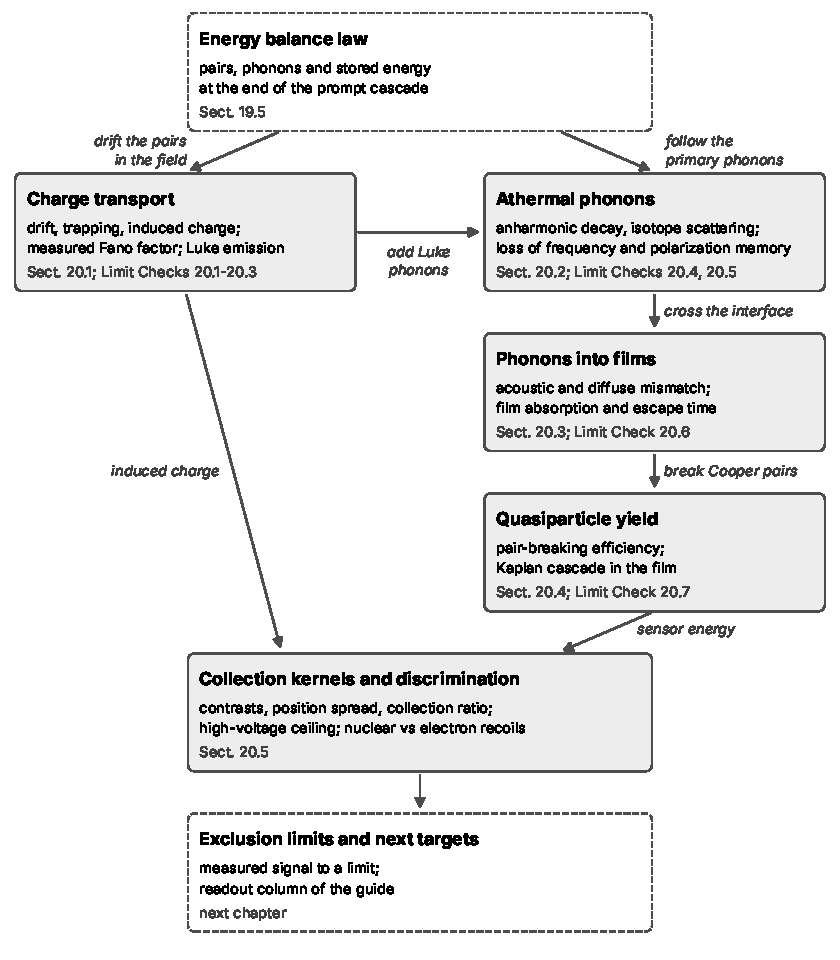
\includegraphics[width=0.85\linewidth]{figures/ch20/map20.pdf}
  \caption{Charge, phonon and quasiparticle readout, from the reservoirs of the energy balance law at the end of the prompt cascade (\cref{sec:19.5}) to the signals a detector records. Left: drift, trapping and the charge induced on the electrodes, with the measured Fano factor and the Luke phonons of the drifting carriers (\cref{sec:20.1}; \cref{lim:20.1a,lim:20.1b}). Right: the primary phonons and the Luke phonons decay and scatter in the substrate (\cref{sec:20.2}; \cref{lim:20.2a,lim:20.2b}), cross into the sensor films (\cref{sec:20.3}; \cref{lim:20.3a}) and break Cooper pairs there (\cref{sec:20.4}; \cref{lim:20.4a}). Both branches meet in the collection kernels, which decide whether phonon or charge readout separates nuclear from electron recoils (\cref{sec:20.5}).}
  \label{fig:20-map}
\end{figure}

\section{Charge transport and the measured charge}\label{sec:20.1}

The charge amplifier of a semiconductor detector integrates the current that flows into an electrode while the carriers move, and a carrier that is captured halfway across the crystal leaves half a charge in the integral and does half its share of Luke work. As a result, the charge we read is the pair number $N_{\mathrm{eh}}$ of \cref{sec:18.2} times a gain that depends on where the event happened and how far each carrier got, and the fluctuations of that gain add to the fluctuations of the cascade. At millikelvin temperatures the carriers drift in fields of a few V/cm, trapped charge does not escape thermally, and every drifting carrier radiates phonons. We will see that trapping lowers the read charge and the Luke heat by the same factor, but spreads the read charge in a way that no pair statistics removes.

\subsection{Induced charge and Ramo's theorem}\label{sec:20.1-ramo}

Consider electrodes $k$ held at potentials $V_k$ around a crystal with static dielectric constant $\varepsilon_0$ (a pure number in the Heaviside--Lorentz units of the book, \cref{sec:5.5}), and a point charge $q$ inside at $\vect{r}$. The charge on electrode $s$ is the sum of what the bias puts there and what $q$ induces, and in a linear medium the two add. The induced part follows from Green's reciprocity theorem. Compare two configurations of the same conductors. In the first, $q$ is at $\vect{r}$ and every electrode is grounded, and electrode $k$ carries the induced charge $Q_k^{\mathrm{ind}}$. In the second, there is no charge inside, electrode $s$ is held at unit potential and the others are grounded; the potential inside is then the \emph{weighting potential} $\varphi_s(\vect{r})$, the solution of $\nabla\cdot[\varepsilon_0(\vect{r})\nabla\varphi_s] = 0$ with $\varphi_s = 1$ on electrode $s$ and 0 on the others. Reciprocity states that the sum of the charges of one configuration times the corresponding potentials of the other is the same either way round. The first configuration has charges $Q_k^{\mathrm{ind}}$ on the electrodes and $q$ at $\vect{r}$; in the second the electrode potentials are $\delta_{ks}$ and the potential at $\vect{r}$ is $\varphi_s(\vect{r})$. The second configuration has charges only on the electrodes, and in the first all the electrodes are grounded. Hence $Q_s^{\mathrm{ind}} + q\varphi_s(\vect{r}) = 0$. When $q$ moves from $\vect{r}_1$ to $\vect{r}_2$, the external circuit must supply the change in induced charge, and the charge delivered to electrode $s$ is
\begin{equation}
  \Delta Q_s = -q\,\bigl[\varphi_s(\vect{r}_2) - \varphi_s(\vect{r}_1)\bigr] ,
  \label{eq:20.1-ramo}
\end{equation}
with the current $I_s = -q\,\vect{v}\cdot\nabla\varphi_s$ in its lead while the carrier moves at velocity $\vect{v}$. This is the Shockley--Ramo theorem~\cite{shockley1938currents,ramo1939currents}, \cite[Eq.~(2)]{lachish2017electron}. The weighting potential is a property of the electrode geometry alone. It is not the potential the carrier moves in. The applied bias, other carriers and trapped charges change the field and the trajectory, but by linearity they only add their own contributions to $Q_s$, and the charge induced by $q$ at a given point stays the same. \Cref{eq:20.1-ramo} is therefore exact in the presence of space charge.

For two planar electrodes at $z = 0$ and $z = d_{\mathrm{det}}$, the weighting potential of the electrode at $z = d_{\mathrm{det}}$ is $\varphi = z/d_{\mathrm{det}}$. Let the electrode at $z = d_{\mathrm{det}}$ collect electrons (the anode), so that holes drift toward the cathode at $z = 0$. Let a pair be born at depth $z$, and let its electron drift a path $s_e$ toward the anode and its hole a path $s_h$ toward the cathode. By \cref{eq:20.1-ramo} the pair delivers the charge $e\,\mathfrak{q}$ to the anode, with
\begin{equation}
  \mathfrak{q} = \frac{s_e + s_h}{d_{\mathrm{det}}} , \qquad 0 \le s_e \le d_{\mathrm{det}} - z, \quad 0 \le s_h \le z .
  \label{eq:20.1-qpair}
\end{equation}
A pair that is fully collected gives $\mathfrak{q} = 1$ wherever it was born, since its two carriers together cross the whole thickness $d_{\mathrm{det}}$. A pair born at the midplane gives $\frac12 + \frac16 = \frac23$ if its hole arrives at the cathode and its electron is captured a third of the way to the anode.

The same theorem gives the work of the bias. To hold electrode $k$ at $V_k$ while the charge it carries changes by $\Delta Q_k$, its source does the work $V_k\Delta Q_k$. Summing \cref{eq:20.1-ramo} over the electrodes gives the work done on a carrier that moves from $\vect{r}_1$ to $\vect{r}_2$, $-q\sum_kV_k[\varphi_k(\vect{r}_2) - \varphi_k(\vect{r}_1)]$. The sum $\varphi_{\mathrm{bias}}(\vect{r}) \equiv \sum_kV_k\varphi_k(\vect{r})$ is the potential the electrodes produce in the empty crystal, so that
\begin{equation}
  W_{\mathrm{bias}} = \sum_{\text{carriers}} q\,\bigl[\varphi_{\mathrm{bias}}(\vect{r}_{\mathrm{start}}) - \varphi_{\mathrm{bias}}(\vect{r}_{\mathrm{end}})\bigr] .
  \label{eq:20.1-work}
\end{equation}
The bias work is the carrier charge times the drop of $\varphi_{\mathrm{bias}}$ along the path, whatever space charge is present. Between two planes at $0$ and $V_{\mathrm{bias}}$, $\varphi_{\mathrm{bias}} = V_{\mathrm{bias}}z/d_{\mathrm{det}}$, and each pair contributes $eV_{\mathrm{bias}}\mathfrak{q}$: this is \cref{eq:19.5-Wbias}, $W_{\mathrm{bias}} = eV_{\mathrm{bias}}N_{\mathrm{ind}}$, with $N_{\mathrm{ind}} = \sum_i\mathfrak{q}_i$ the charge read on the anode in units of $e$. \Cref{app:D.45} shows that the Luke heat is $W_{\mathrm{bias}}$ minus the change $\Delta E_{\mathrm{es}}$ of the electrostatic energy. For a single trapped pair that change is negligible. Two charges \SI{10}{\micro m} apart in silicon have the Coulomb energy $\alpha/(\varepsilon_0r) = \SI{1.3e-5}{eV}$, with the liquid-helium value $\varepsilon_0 = 11.4$ (\cref{sec:7.4}), against the bias work $eV_{\mathrm{bias}}s/d_{\mathrm{det}} = \SI{4}{meV}$ done on a carrier over those \SI{10}{\micro m} in a \SI{1}{cm} crystal at \SI{4}{V}.

With more than two electrodes the read charge and the bias work weight a trajectory differently. The charge read on electrode $s$ follows $\varphi_s$ and the work follows $\varphi_{\mathrm{bias}}$, and the read charge and the bias work are proportional only where $\varphi_s \propto \varphi_{\mathrm{bias}}$, as for a pair of planar electrodes. Some detectors place interleaved electrodes on each face to tag events close to a surface. Near the interleaved electrodes the weighting potentials change over the electrode pitch, and a carrier that is trapped there adds to the read charge and to the bias work in proportions that differ from its share of the path. The reconstruction $E_R = E_\phi - E_QeV_{\mathrm{bias}}/\varepsilon_{\mathrm{eh}}$ of \cref{sec:19.5} subtracts the Luke heat through the read charge $E_Q$, and for carriers trapped near the faces it inherits the mismatch between the read charge and the bias work.

\subsection{Trapping and the Hecht relation}\label{sec:20.1-hecht}

A drifting carrier at millikelvin temperatures is lost when an ionized or neutral impurity captures it, with the cross-sections $\sigma_{\mathrm{cap},j}$ of \cref{sec:18.5}. If capture events are independent, the probability of surviving a further path $\dd s$ is $1 - \dd s/\lambda_{\mathrm{d}}$, and the probability of surviving a path $s$ is $\ee^{-s/\lambda_{\mathrm{d}}}$. The drift length is $\lambda_{\mathrm{d}} = 1/\sum_j\nd^{\mathrm{tr}}_j\sigma_{\mathrm{cap},j}$ for trap densities $\nd^{\mathrm{tr}}_j$ and cross-sections taken per unit path; with a trapping time $\tau_{\mathrm{tr}}$ instead, $\lambda_{\mathrm{d}} = v_{\mathrm{dr}}\tau_{\mathrm{tr}}$ with the drift velocity $v_{\mathrm{dr}}$. Electrons and holes have separate drift lengths, $\lambda_{\mathrm{d}}^e$ and $\lambda_{\mathrm{d}}^h$. For a path that is exponentially distributed but cut off at the distance $L$ to the electrode, the mean is $\langle\min(s, L)\rangle = \lambda_{\mathrm{d}}(1 - \ee^{-L/\lambda_{\mathrm{d}}})$.

The classic measurement of the drift length creates the charge at one face, with an alpha source or a short-range photon, so that one carrier type crosses the whole crystal and the other is collected at once. By \cref{eq:20.1-qpair} the mean collected fraction is then the mean path over $d_{\mathrm{det}}$,
\begin{equation}
  \frac{Q}{eN_{\mathrm{eh}}} = \frac{\lambda_{\mathrm{d}}}{d_{\mathrm{det}}}\bigl(1 - \ee^{-d_{\mathrm{det}}/\lambda_{\mathrm{d}}}\bigr) ,
  \label{eq:20.1-hecht}
\end{equation}
the Hecht relation~\cite{hecht1932mechanismus}, \cite[Eqs.~(1)--(4)]{lachish2017electron}. It is linear in $\lambda_{\mathrm{d}}$ for $\lambda_{\mathrm{d}} \ll d_{\mathrm{det}}$, where the carriers stop after a mean path $\lambda_{\mathrm{d}}$, and approaches $1 - d_{\mathrm{det}}/2\lambda_{\mathrm{d}}$ for $\lambda_{\mathrm{d}} \gg d_{\mathrm{det}}$. Dark-matter events happen anywhere in the bulk, and both carriers then drift. With the cut-off mean path for each carrier, a pair at depth $z$ induces on average
\begin{equation}
  \bar{\mathfrak{q}}(z) = \frac{\lambda_{\mathrm{d}}^e}{d_{\mathrm{det}}}\Bigl(1 - \ee^{-(d_{\mathrm{det}} - z)/\lambda_{\mathrm{d}}^e}\Bigr) + \frac{\lambda_{\mathrm{d}}^h}{d_{\mathrm{det}}}\Bigl(1 - \ee^{-z/\lambda_{\mathrm{d}}^h}\Bigr) ,
  \label{eq:20.1-hecht2}
\end{equation}
and averaging over a uniform depth,
\begin{equation}
  \langle\bar{\mathfrak{q}}\rangle = \sum_{c = e, h}\frac{\lambda_{\mathrm{d}}^c}{d_{\mathrm{det}}}\Bigl[1 - \frac{\lambda_{\mathrm{d}}^c}{d_{\mathrm{det}}}\bigl(1 - \ee^{-d_{\mathrm{det}}/\lambda_{\mathrm{d}}^c}\bigr)\Bigr] \simeq 1 - \frac{d_{\mathrm{det}}}{6\lambda_{\mathrm{d}}^e} - \frac{d_{\mathrm{det}}}{6\lambda_{\mathrm{d}}^h} .
  \label{eq:20.1-qavg}
\end{equation}
At second order in $d_{\mathrm{det}}/\lambda_{\mathrm{d}}$ each carrier adds $+d_{\mathrm{det}}^2/24\lambda_{\mathrm{d}}^2$, so the leading correction is accurate to a fraction $d_{\mathrm{det}}/4\lambda_{\mathrm{d}}$ of itself. Each carrier of a bulk event loses a third of what the carrier of a face event loses at the same drift length: for $\lambda_{\mathrm{d}} \gg d_{\mathrm{det}}$ the loss over a path $L$ is $L^2/2\lambda_{\mathrm{d}}d_{\mathrm{det}}$, and the mean square path to an electrode is $d_{\mathrm{det}}^2/3$. \Cref{fig:20-hecht} compares a face event, a uniform bulk event and an event at the midplane. At $\lambda_{\mathrm{d}} = d_{\mathrm{det}}$ the face event collects 0.632 of its charge, the uniform bulk event 0.736 and the midplane event 0.787; at $\lambda_{\mathrm{d}} = 10\,d_{\mathrm{det}}$ the face and bulk values are 0.952 and 0.968. The dependence of the induced charge on depth, \cref{fig:20-hecht}(b), turns trapping into a spread of the read charge (\cref{sec:20.1-fano}).

\begin{figure}[tbp]
  \centering
  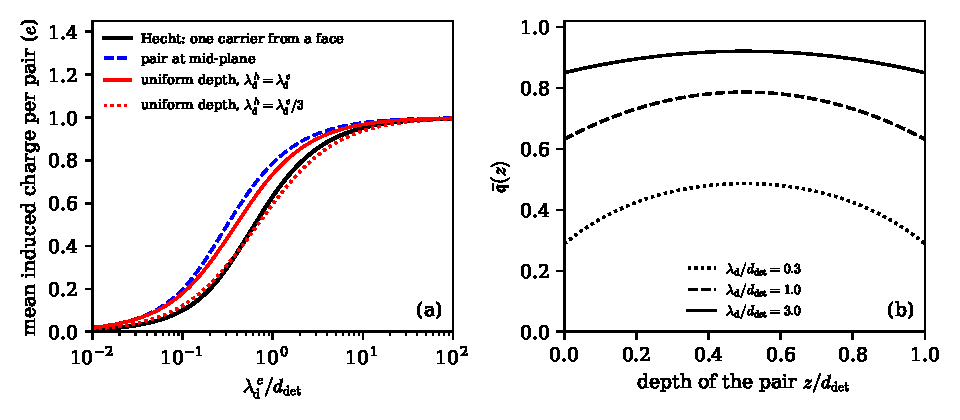
\includegraphics[width=\linewidth]{figures/ch20/fig20_1.pdf}
  \caption{Charge collection with exponential trapping in a planar detector of thickness $d_{\mathrm{det}}$. (a)~Mean induced charge per pair, in units of $e$, against the electron drift length: the Hecht relation \cref{eq:20.1-hecht} for one carrier crossing from a face (black), a pair at the midplane with equal drift lengths (blue dashed), and the depth average \cref{eq:20.1-qavg} for uniform events with $\lambda_{\mathrm{d}}^h = \lambda_{\mathrm{d}}^e$ (red) and $\lambda_{\mathrm{d}}^h = \lambda_{\mathrm{d}}^e/3$ (red dotted, an illustrative ratio). (b)~Mean induced charge of a pair against its depth, \cref{eq:20.1-hecht2} with equal drift lengths $0.3$, $1$ and $3\,d_{\mathrm{det}}$; the electron-collecting electrode is at $z = d_{\mathrm{det}}$.}
  \label{fig:20-hecht}
\end{figure}

Hecht wrote the drift length as $\lambda_{\mathrm{d}} = \mu_{\mathrm{mob}}\tau_{\mathrm{tr}}V_{\mathrm{bias}}/d_{\mathrm{det}}$, for a drift velocity proportional to the field, $v_{\mathrm{dr}} = \mu_{\mathrm{mob}}\mathcal{E}$ with mobility $\mu_{\mathrm{mob}}$, and a field-independent trapping time. The standard way to obtain the mobility--lifetime product is to measure $Q$ against the bias and fit \cref{eq:20.1-hecht} in this form. Neither the proportional drift velocity nor the field-independent trapping time enters the derivation above, which needs only exponential survival along the path. At millikelvin temperatures both assumptions fail. A carrier accelerates until it moves faster than sound and then sheds its energy into Luke phonons (\cref{sec:20.1-luke}); its speed stays within a few times the sound speed, and the largest momentum it reaches grows only as the cube root of the field~\cite[Eqs.~(24)--(25)]{leman2012invited}. If the capture cross-section per unit path does not depend on the carrier speed, $\lambda_{\mathrm{d}}$ is independent of the bias and the collected fraction does not change with the bias. If capture is a rate at fixed trapping time, $\lambda_{\mathrm{d}} = v_{\mathrm{dr}}\tau_{\mathrm{tr}}$ stops growing once the velocity saturates, and the collected fraction saturates below one.

\begin{limitbox}[Hecht collection][lim:20.1a]
For charge created at one face and drifting in a uniform field~\cite{hecht1932mechanismus}, \cite[Eqs.~(1)--(4)]{lachish2017electron}: $Q/eN_{\mathrm{eh}} = (\lambda_{\mathrm{d}}/d_{\mathrm{det}})(1 - \ee^{-d_{\mathrm{det}}/\lambda_{\mathrm{d}}})$ with $\lambda_{\mathrm{d}} = \mu_{\mathrm{mob}}\tau_{\mathrm{tr}}V_{\mathrm{bias}}/d_{\mathrm{det}}$.
\par\smallskip
{\centering
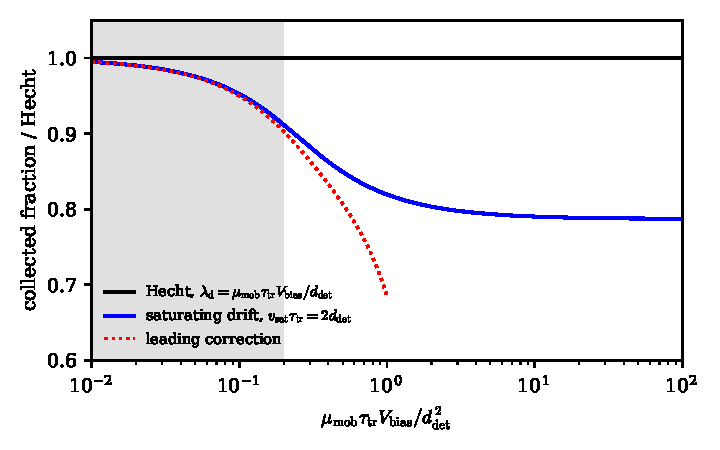
\includegraphics[width=\linewidth]{figures/ch20/limit20_1a.pdf}
\captionof{figure}{Collected fraction with a saturating drift velocity divided by the Hecht relation, against the bias in units of $d_{\mathrm{det}}^2/\mu_{\mathrm{mob}}\tau_{\mathrm{tr}}$. Blue: \cref{eq:20.1-hecht} with $\lambda_{\mathrm{d}} = v_{\mathrm{dr}}\tau_{\mathrm{tr}}$ and the interpolation $v_{\mathrm{dr}} = \mu_{\mathrm{mob}}\mathcal{E}/(1 + \mu_{\mathrm{mob}}\mathcal{E}/v_{\mathrm{sat}})$, at $v_{\mathrm{sat}}\tau_{\mathrm{tr}} = 2\,d_{\mathrm{det}}$ (an illustrative value). Red dotted: the leading correction, $\lambda_{\mathrm{d}} = \mu_{\mathrm{mob}}\tau_{\mathrm{tr}}\mathcal{E}(1 - \mu_{\mathrm{mob}}\mathcal{E}/v_{\mathrm{sat}})$. Gray: $\mu_{\mathrm{mob}}\mathcal{E} \le 0.1\,v_{\mathrm{sat}}$, where the deficit relative to the Hecht relation is at most \SI{8.9}{\percent}. At high bias the collected fraction saturates at 0.787 of the charge instead of approaching one.}\label{fig:20-limit-hecht}
\par}
\smallskip
Once the drift velocity no longer follows the field, the collected charge stops rising with the bias, and a fit of the Hecht form returns a mobility--lifetime product that depends on the bias range used.
\end{limitbox}

The deficit of the collected fraction relative to the Hecht relation is $\mu_{\mathrm{mob}}\mathcal{E}/v_{\mathrm{sat}}$ to first order, since the collection is linear in $\lambda_{\mathrm{d}}$ while $\lambda_{\mathrm{d}} \ll d_{\mathrm{det}}$. If the survival law is not exponential, as when the trap occupation changes during the drift, \cref{eq:20.1-hecht} itself changes.

\subsection{Bias work with trapping}\label{sec:20.1-work}

Trapping lowers the Luke heat with the read charge. On average over a uniform depth, \cref{eq:20.1-work} gives $W_{\mathrm{bias}} = eV_{\mathrm{bias}}N_{\mathrm{eh}}\langle\bar{\mathfrak{q}}\rangle$, and for an electron recoil that deposits $\omega$ the Luke phonon energy is $g_{\mathrm{Luke}}\langle\bar{\mathfrak{q}}\rangle\,\omega$, with the Luke gain $g_{\mathrm{Luke}} = eV_{\mathrm{bias}}/\varepsilon_{\mathrm{eh}}$ of \cref{sec:19.5}. The published phonon energy (\cref{lim:20.1b}) counts every pair as fully collected.

\begin{limitbox}[Bias work and the Luke phonon energy][lim:20.1b]
The phonon energy of $n_Q$ pairs drifted across the bias $V_{\mathrm{bias}}$ is $E_\phi = E_R + n_QeV_{\mathrm{bias}}$, with Luke part $n_QeV_{\mathrm{bias}}$~\cite[Eq.~(1)]{agnese2018nuclear}.
\par\smallskip
{\centering
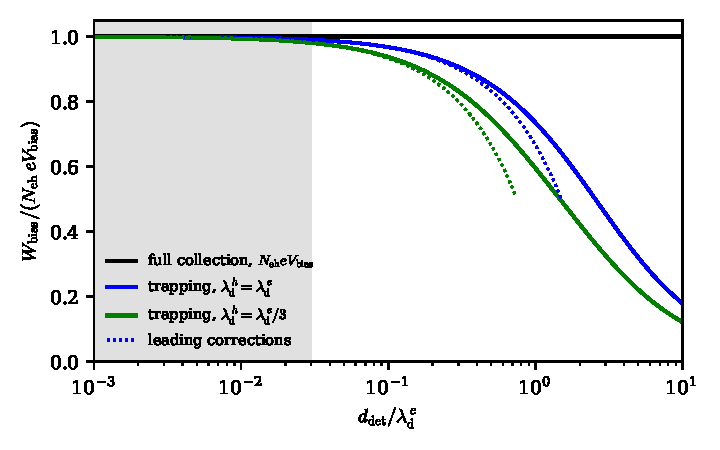
\includegraphics[width=\linewidth]{figures/ch20/limit20_1b.pdf}
\captionof{figure}{Bias work of uniformly distributed events with exponential trapping, \cref{eq:20.1-work} with the depth average \cref{eq:20.1-qavg}, over the full-collection value $N_{\mathrm{eh}}eV_{\mathrm{bias}}$, against the crystal thickness in units of the electron drift length. Blue: equal drift lengths; green: $\lambda_{\mathrm{d}}^h = \lambda_{\mathrm{d}}^e/3$ (an illustrative ratio). Dotted: the leading correction $1 - d_{\mathrm{det}}/6\lambda_{\mathrm{d}}^e - d_{\mathrm{det}}/6\lambda_{\mathrm{d}}^h$. Gray: $d_{\mathrm{det}} \le 0.030\,\lambda_{\mathrm{d}}$, where the work is within \SI{1}{\percent} of full collection for equal drift lengths ($d_{\mathrm{det}} \le 0.015\,\lambda_{\mathrm{d}}^e$ for the unequal pair).}\label{fig:20-limit-work}
\par}
\smallskip
When the drift length is no longer much longer than the crystal, the Luke heat falls below $N_{\mathrm{eh}}eV_{\mathrm{bias}}$ and depends on the depth of the event; it follows the read charge, not the pair number.
\end{limitbox}

Since the read charge of a planar detector carries the same factor $\bar{\mathfrak{q}}$ as the Luke heat, event by event, the subtraction $E_QeV_{\mathrm{bias}}/\varepsilon_{\mathrm{eh}}$ removes the Luke heat of partly collected pairs exactly. Trapping also changes the signal beyond the Luke heat. A trapped carrier keeps its share of the gap energy, which the balance law counts as missing energy (\cref{sec:19.5}), and a nuclear recoil has an ionized fraction $f_{\mathrm{ion}}$ below its ionization yield if its dense track traps more often.

\subsection{Fano factor of the measured charge}\label{sec:20.1-fano}

If each pair is either collected in full or lost, independently and with the same probability $f_{\mathrm{det}}$ everywhere, the read charge is the pair number thinned binomially, and its Fano factor is $f_{\mathrm{det}}F_{\mathrm{eh}} + 1 - f_{\mathrm{det}}$ by \cref{eq:C.11-thinfano}. Trapping does not thin the pair number binomially. A trapped carrier leaves a partial charge, and the mean collection depends on the depth of the event. Let the event be at $\vect{r}$, and let the induced charges $\mathfrak{q}_i$ of its pairs, \cref{eq:20.1-qpair}, be independent and identically distributed given $\vect{r}$, with mean $\bar{\mathfrak{q}}(\vect{r})$ and variance $\sigma_{\mathfrak{q}}^2(\vect{r})$, and independent of the pair number. These assumptions hold when the carriers drift independently after the prompt cascade; independent drift excludes recombination and screening inside a dense track. The read charge is $N_{\mathrm{ind}} = \sum_{i=1}^{N_{\mathrm{eh}}}\mathfrak{q}_i$. At fixed $\vect{r}$, a sum of a random number of independent terms has mean $\bar N_{\mathrm{eh}}\bar{\mathfrak{q}}$ and variance $\bar N_{\mathrm{eh}}\sigma_{\mathfrak{q}}^2 + \bar{\mathfrak{q}}^2\operatorname{Var}N_{\mathrm{eh}}$, with $\operatorname{Var}N_{\mathrm{eh}} = F_{\mathrm{eh}}\bar N_{\mathrm{eh}}$. Averaging over the position with the law of total variance gives $\operatorname{Var}N_{\mathrm{ind}} = \langle\operatorname{Var}(N_{\mathrm{ind}}|\vect{r})\rangle + \operatorname{Var}_{\vect{r}}(\bar N_{\mathrm{eh}}\bar{\mathfrak{q}})$, and dividing by the mean $\bar N_{\mathrm{eh}}\langle\bar{\mathfrak{q}}\rangle$ gives
\begin{equation}
  F_{\mathrm{meas}} = \underbrace{\frac{F_{\mathrm{eh}}\langle\bar{\mathfrak{q}}^2\rangle}{\langle\bar{\mathfrak{q}}\rangle}}_{\text{cascade}} + \underbrace{\frac{\langle\sigma_{\mathfrak{q}}^2\rangle}{\langle\bar{\mathfrak{q}}\rangle}}_{\text{partial charge}} + \underbrace{\bar N_{\mathrm{eh}}\,\frac{\operatorname{Var}_{\vect{r}}\bar{\mathfrak{q}}}{\langle\bar{\mathfrak{q}}\rangle}}_{\text{position}} ,
  \label{eq:20.1-Fpos}
\end{equation}
where $\langle\cdot\rangle$ and $\operatorname{Var}_{\vect{r}}$ are taken over the distribution of event positions.

For all-or-nothing collection with one probability, $\bar{\mathfrak{q}} = f_{\mathrm{det}}$, $\sigma_{\mathfrak{q}}^2 = f_{\mathrm{det}}(1 - f_{\mathrm{det}})$ and the position term vanishes; \cref{eq:20.1-Fpos} then returns the binomial result. The unsplit excitons of \cref{eq:18.5-Fmeas} are the same thinning with $f_{\mathrm{det}} = 1 - p_{\mathrm{ns}}$, and the values of $f_{\mathrm{det}}$ of losses that act independently on each pair multiply. The partial-charge term is never larger than in the binomial case. Since $0 \le \mathfrak{q} \le 1$, $\mathfrak{q}^2 \le \mathfrak{q}$, so $\langle\mathfrak{q}^2\rangle \le \bar{\mathfrak{q}}$ and $\sigma_{\mathfrak{q}}^2 \le \bar{\mathfrak{q}}(1 - \bar{\mathfrak{q}})$ at every position. At a fixed position, a loss shared as partial charges by many pairs fluctuates less than the same mean loss concentrated on a few pairs that are lost entirely. The position term grows with $\bar N_{\mathrm{eh}}$, and its contribution to the relative variance of the read charge, $\operatorname{Var}_{\vect{r}}\bar{\mathfrak{q}}/\langle\bar{\mathfrak{q}}\rangle^2$, does not fall with energy. The position term is a spread of the gain across the crystal, which no pair statistics removes, and it dominates at large deposits.

\begin{workedexample}{The measured Fano factor at 95 percent collection in silicon}\label{we:20-fano}
Take the cascade value $F_{\mathrm{eh}} = 0.114$ of \cref{sec:18.2} and a mean collected fraction of 0.95, and compare three ways of losing the missing \SI{5}{\percent}. (\Cref{sec:20.5} uses the measured value 0.119 for electron-recoil signals.)

\emph{All-or-nothing loss, uniform.} Binomial thinning gives $0.95 \times 0.114 + 0.05 = 0.158$.

\emph{Trapping, every pair at the midplane.} With equal drift lengths, \cref{eq:20.1-hecht2} at $z = d_{\mathrm{det}}/2$ is $2(\lambda_{\mathrm{d}}/d_{\mathrm{det}})(1 - \ee^{-d_{\mathrm{det}}/2\lambda_{\mathrm{d}}})$, which equals 0.95 at $\lambda_{\mathrm{d}} = 4.83\,d_{\mathrm{det}}$. Each carrier's path is exponential with mean $\lambda_{\mathrm{d}}$, cut at $d_{\mathrm{det}}/2$, and its second moment is $\langle\min(s, L)^2\rangle = 2\lambda_{\mathrm{d}}^2[1 - \ee^{-L/\lambda_{\mathrm{d}}}(1 + L/\lambda_{\mathrm{d}})]$. The two carriers give $\sigma_{\mathfrak{q}}^2 = 0.0156$, a third of the binomial $0.95 \times 0.05 = 0.0475$. \Cref{eq:20.1-Fpos} gives $F_{\mathrm{meas}} = (0.114 \times 0.9025 + 0.0156)/0.95 = 0.125$.

\emph{Trapping, uniform depth.} Now \cref{eq:20.1-qavg} equals 0.95 at $\lambda_{\mathrm{d}} = 6.41\,d_{\mathrm{det}}$. Integrating \cref{eq:20.1-hecht2} and the variance over depth gives $\langle\bar{\mathfrak{q}}^2\rangle = 0.9026$, $\langle\sigma_{\mathfrak{q}}^2\rangle = 0.0230$ and $\operatorname{Var}_z\bar{\mathfrak{q}} = 1.16\times10^{-4}$. The cascade and partial-charge terms give 0.1325. The position term is $1.22\times10^{-4}\,\bar N_{\mathrm{eh}}$: 0.003 for a \SI{100}{eV} recoil ($\bar N_{\mathrm{eh}} = 26.7$), 0.033 at \SI{1}{keV} and 0.19 at \SI{5.9}{keV}. It equals 0.01 at 82 pairs, about \SI{0.3}{keV}.

The same mean collection thus yields a measured Fano factor between 0.125 and 0.158 at \SI{100}{eV}, depending on how the charge is lost, and nearly three times the cascade value at \SI{5.9}{keV} if the loss depends on depth. A Fano factor measured at \SI{5.9}{keV} constrains $F_{\mathrm{eh}}$ to 0.01 only if $\operatorname{Var}_z\bar{\mathfrak{q}}$ is below $6\times10^{-6}$.
\end{workedexample}

\subsection{Space charge of trapped carriers}\label{sec:20.1-space}

At millikelvin temperatures a trapped carrier is not re-emitted thermally. A donor level \SI{45}{meV} below the conduction band carries the Boltzmann factor $\ee^{-1.04\times10^4}$ at \SI{50}{mK}. A field lowers the Coulomb barrier of a charged center: the potential energy $-\alpha/(\varepsilon_0r) - e\mathcal{E}r$ of the carrier along the field has its maximum at the field separation radius $r_{\mathcal{E}} = (\alpha/\varepsilon_0e\mathcal{E})^{1/2}$ of \cref{eq:18.5-rfield}, and the field thus lowers the barrier by the Poole--Frenkel amount $2e\mathcal{E}r_{\mathcal{E}}$. In silicon that is \SI{0.45}{meV} at \SI{4}{V/cm} and \SI{2.25}{meV} at \SI{100}{V/cm}, far below \SI{45}{meV}. Thermal and field-assisted emission are frozen, and trapped charge is released only by the phonons of later events, by drifting carriers that ionize the center on impact, or by infrared light. Detectors are therefore illuminated at intervals with infrared diodes, a practice called flashing~\cite[Sect.~2]{agnese2018nuclear}; the infrared light neutralizes the ionized trapping sites and keeps trapping low. Between flashes the trapped charge accumulates and changes the field.

In a planar detector at fixed bias the field change follows from Gauss's law and the constraint that the voltage across the crystal does not change. Let $\varrho_{\mathrm{tr}}(z)$ be the net trapped charge per unit volume, averaged over the transverse directions. The field change obeys $\dd\Delta\mathcal{E}/\dd z = \varrho_{\mathrm{tr}}/\varepsilon_0$, so $\Delta\mathcal{E}(z) = \Delta\mathcal{E}(0) + \varepsilon_0^{-1}\int_0^z\varrho_{\mathrm{tr}}\,\dd z'$, and fixed bias requires $\int_0^{d_{\mathrm{det}}}\Delta\mathcal{E}\,\dd z = 0$. Solving for $\Delta\mathcal{E}(0)$ and integrating by parts gives
\begin{equation}
  \Delta\mathcal{E}(z) = \frac{1}{\varepsilon_0}\left[\int_0^z\varrho_{\mathrm{tr}}(z')\,\dd z' - \frac{1}{d_{\mathrm{det}}}\int_0^{d_{\mathrm{det}}}(d_{\mathrm{det}} - z')\,\varrho_{\mathrm{tr}}(z')\,\dd z'\right] ,
  \label{eq:20.1-dE}
\end{equation}
in Heaviside--Lorentz units, with $\varepsilon_0$ the static dielectric constant; in SI units multiply $\varepsilon_0$ by the vacuum permittivity $\varepsilon_0^{\mathrm{SI}}$. A sheet of $\nd_{\mathrm{sh}}$ charges $e$ per unit area at depth $z_0$ makes the field jump by $e\nd_{\mathrm{sh}}/\varepsilon_0$ across it, with the change $-e\nd_{\mathrm{sh}}(d_{\mathrm{det}} - z_0)/\varepsilon_0d_{\mathrm{det}}$ below and $+e\nd_{\mathrm{sh}}z_0/\varepsilon_0d_{\mathrm{det}}$ above, so the largest change lies between one half and the whole jump. For any distribution of one sign with $\nd_{\mathrm{sh}}$ charges per unit area in all, both terms in the bracket of \cref{eq:20.1-dE} lie between 0 and $e\nd_{\mathrm{sh}}$, so their difference does not exceed $e\nd_{\mathrm{sh}}$. Hence the sheet bound
\begin{equation}
  \max_z|\Delta\mathcal{E}(z)| \le \frac{e\nd_{\mathrm{sh}}}{\varepsilon_0} ,
  \label{eq:20.1-sheet}
\end{equation}
which a sheet approaches as it nears a face. There, however, the whole change lies in the thin slab between the sheet and the nearer electrode, and the field in the rest of the crystal is unchanged: the charge only images onto that electrode. A sheet at depth $z_0$ changes the field on its far side by $e\nd_{\mathrm{sh}}z_0/\varepsilon_0d_{\mathrm{det}}$, so a distortion over a finite part of the drift region needs more charge than the sheet bound \cref{eq:20.1-sheet} implies, and a sheet at the midplane, which changes the field by half the jump over the whole crystal, needs twice the charge of the sheet bound. Charges of both signs give at most $e(\nd_{\mathrm{sh}}^+ + \nd_{\mathrm{sh}}^-)/\varepsilon_0$, and less where electrons and holes trapped at similar depths cancel.

We measure the distortion by $\xi_{\mathrm{SC}} \equiv \max_z|\Delta\mathcal{E}|/\mathcal{E}$. In silicon, with $\varepsilon_0 = 11.4$, one charge per square centimeter moves the field by \SI{1.59e-7}{V/cm}. A distortion $\xi_{\mathrm{SC}} = \SI{1}{\percent}$ at \SI{1}{V/cm} then needs at least \SI{6.3e4}{cm^{-2}}. A sheet next to a face reaches this sheet bound but distorts only a vanishing slab; a sheet at the midplane distorts the whole crystal by \SI{1}{\percent} at \SI{12.6e4}{cm^{-2}}. At the \SI{4}{V/cm} of the calibration of \cref{sec:19.5} both sheets need four times more charge. Between flashes the trapped density grows as $\nd_{\mathrm{sh}}(t) \approx R\bar N_{\mathrm{eh}}p_{\mathrm{tr}}t$, for $R$ events per unit area and time with $\bar N_{\mathrm{eh}}$ pairs each, of which a fraction $p_{\mathrm{tr}}$ leaves a trapped charge of the dominant sign. A trapping probability of \SI{12.7}{\percent} is the value used to model a silicon detector that resolves single charges~\cite{albakry2023first}. With it as $p_{\mathrm{tr}}$, \SI{100}{eV} events at \SI{1}{Hz} on \SI{1}{cm^2} reach a distortion of \SI{1}{\percent} at \SI{1}{V/cm} over the whole crystal in 10 hours (the near-face limit in 5), and a calibration at a thousand times that rate within a minute.

\Cref{eq:20.1-ramo,eq:20.1-work} stay exact; the distortion acts through the trajectories. It changes the drift velocity along the path and, where capture depends on the carrier speed, the drift length; in three dimensions it bends the field lines, and carriers near the sides of the crystal can end on bare surfaces instead of electrodes. The energy stored in the field of the trapped charge is part of the electrostatic term $\Delta E_{\mathrm{es}}$ that separates the Luke heat from the bias work (\cref{app:D.45}). The trapped populations, the field and the rate of delayed charge released by later events therefore all depend on the exposure since the last flash.

\subsection{Luke-phonon emission}\label{sec:20.1-luke}

A carrier that moves faster than the longitudinal sound speed $c_{\mathrm{LA}}$ can emit a longitudinal acoustic phonon and conserve both energy and momentum; a slower one cannot. This emission above the sound speed is the acoustic analogue of Cherenkov radiation, and the phonons emitted are the Luke phonons that carry the bias work. The emission rate follows from the golden rule with the deformation-potential vertex of \cref{eq:6.2-D}. Take a carrier of isotropic mass $m$, energy $k^2/2m$ and momentum $\vect{k}$, and an isotropic deformation potential $D^n$, which couples it to longitudinal phonons only. A phonon of wavevector $\vect{Q}$ then has the matrix element $|M_Q|^2 = (D^n)^2Q/(2\rho_T\Vol c_{\mathrm{LA}})$ in a crystal of volume $\Vol$ and mass density $\rho_T$, the vertex of \cref{sec:6.2} with the volume normalization. Luke phonons carry about a meV, more than ten kelvin. At detector temperatures absorption and stimulated emission are therefore negligible, and
\begin{equation*}
  \varGamma_{\mathrm{L}}(k) = 2\pi\sum_{\vect{Q}}|M_Q|^2\,\delta\Bigl(\frac{k^2}{2m} - \frac{(\vect{k} - \vect{Q})^2}{2m} - c_{\mathrm{LA}}Q\Bigr) .
\end{equation*}
With $\theta$ the angle between $\vect{Q}$ and $\vect{k}$, the argument of the delta function vanishes at $Q_* = 2(k\cos\theta - k_{\mathrm{s}})$, where $k_{\mathrm{s}} = mc_{\mathrm{LA}}$ is the momentum of a carrier moving at the sound speed, and the derivative of the argument with respect to $Q$ there has magnitude $Q_*/2m$. A positive root requires $\cos\theta > k_{\mathrm{s}}/k$, and so $k > k_{\mathrm{s}}$: the Cherenkov condition. With $\sum_{\vect{Q}} = V\int\dd^3Q/(2\pi)^3$, the azimuthal integral gives $2\pi$, so the prefactor is $2\pi\cdot2\pi/(2\pi)^3 = 1/2\pi$, and the radial integral $\int Q^2\dd Q\,Q\,\delta(\ldots)$ gives $Q_*^3\cdot2m/Q_*$. Hence
\begin{equation*}
  \varGamma_{\mathrm{L}}(k) = \frac{(D^n)^2m}{2\pi\rho_Tc_{\mathrm{LA}}}\int_{k_{\mathrm{s}}/k}^1 Q_*^2\,\dd\cos\theta = \frac{(D^n)^2m}{2\pi\rho_Tc_{\mathrm{LA}}}\,\frac{4k^2}{3}\Bigl(1 - \frac{k_{\mathrm{s}}}{k}\Bigr)^3 .
\end{equation*}
With the scattering length $l_0 = \pi\rho_T/(2m^3(D^n)^2)$, a length that collects the coupling and the carrier mass, the rate is
\begin{equation}
  \varGamma_{\mathrm{L}}(k) = \frac{c_{\mathrm{LA}}}{3l_0}\Bigl(\frac{k}{k_{\mathrm{s}}}\Bigr)^2\Bigl(1 - \frac{k_{\mathrm{s}}}{k}\Bigr)^3 \qquad (k > k_{\mathrm{s}}),
  \label{eq:20.1-luke}
\end{equation}
and the phonon is emitted at the polar angle $\theta$ with the probability density $\propto(\cos\theta - k_{\mathrm{s}}/k)^2\sin\theta$, up to $\cos\theta = k_{\mathrm{s}}/k$. Leman~\cite[Eq.~(22)]{leman2012invited} and the authors of the G4CMP (Geant4 Condensed Matter Physics) toolkit~\cite[Eq.~(9)]{kelsey2023g4cmp} print an angular law that integrates to \cref{eq:20.1-luke}, but the total rates printed beside that angular law~\cite[Eq.~(21)]{leman2012invited}, \cite[Eq.~(8)]{kelsey2023g4cmp} are lower by the factor $k_{\mathrm{s}}/k$.

The phonon energy is $c_{\mathrm{LA}}Q_* = 2c_{\mathrm{LA}}k(\cos\theta - k_{\mathrm{s}}/k)$. The average over the angular distribution, in which $u = \cos\theta - k_{\mathrm{s}}/k$ is weighted by $u^2$ on $[0, 1 - k_{\mathrm{s}}/k]$ and so has the mean $\frac34(1 - k_{\mathrm{s}}/k)$, gives
\begin{equation}
  \langle E_{\mathrm{L}}\rangle = \frac32\,mc_{\mathrm{LA}}^2\Bigl(\frac{k}{k_{\mathrm{s}}} - 1\Bigr), \qquad E_{\mathrm{L}}^{\max} = 2mc_{\mathrm{LA}}^2\Bigl(\frac{k}{k_{\mathrm{s}}} - 1\Bigr) .
  \label{eq:20.1-Eluke}
\end{equation}
The energy scale is set by the carrier mass and the sound speed. For silicon holes, with the isotropic mass $0.5\,m_e$, $D^n = \SI{5.0}{eV}$ and $c_{\mathrm{LA}} = \SI{9.0}{km/s}$ of the CDMS transport model~\cite[Table~II]{leman2012invited}, $mc_{\mathrm{LA}}^2 = \SI{0.230}{meV}$, $l_0 = \SI{7.5}{\micro m}$ and $c_{\mathrm{LA}}/3l_0 = \SI{4.0e8}{s^{-1}}$. A hole at twice the sound speed emits phonons at \SI{2.0e8}{s^{-1}}, with a mean energy of \SI{0.35}{meV} and at most \SI{0.46}{meV}.

A transport Monte Carlo of silicon electrons gives a mean Luke phonon energy of \SI{0.84}{meV} at \SI{1}{V/cm} (\cref{sec:20.5-meanfield}). Luke phonons are born at one to a few meV, between the pair-breaking energy $2\Delta_{\mathrm{BCS}} = \SI{0.36}{meV}$ of bulk aluminum (\cref{sec:1.5}) and the optical-phonon energies near \SI{60}{meV} at which the primary phonons start. Since the emitted energy is weighted by $u^3$, the fraction of it below an energy $E_{\mathrm{c}}$ is $(E_{\mathrm{c}}/E_{\mathrm{L}}^{\max})^4$ for a carrier at one speed. Transport decides whether the sensor films then absorb the Luke phonons as efficiently as the down-converted primaries, and so decides the sign of $\mathfrak{r}_{\mathrm{coll}} - 1$ in the calibration of \cref{sec:19.5} (\cref{sec:20.5}).

\subsection{Open problems}\label{sec:20.1-open}

The emission rates of trapped charge at millikelvin temperatures are not known, and so neither the release of trapped charge over a run nor the growth of the space-charge field between flashes is known. The emission rate of each trap class is the sum of the phonon flux times a phonon-ionization cross-section, the flux of drifting carriers times an impact-ionization cross-section, and a term from the infrared illumination. A neutral shallow donor needs a phonon above its binding energy, \SI{45}{meV} or \SI{10.9}{THz} for phosphorus in silicon, and phonons above \SI{45}{meV} decay within about a nanosecond (\cref{sec:20.2}), so they ionize only near the track of a later event. Luke phonons cannot ionize neutral centers but can ionize the over-charged states $\mathrm{D}^-$ and $\mathrm{A}^+$, which bind their extra carrier by a few meV and which flashing itself populates. No calculation gives the phonon-ionization or the impact-ionization cross-section of these centers at the carrier and phonon energies that matter. Without these cross-sections the trapped populations, the field distortion $\xi_{\mathrm{SC}}$ and the delayed charge cannot be followed through an exposure history.

The spectrum that the Luke rate \cref{eq:20.1-luke} produces is tested only indirectly. The rate keeps longitudinal phonons only, whereas the uniaxial deformation potential $\Xi_u$ couples the electrons of the silicon valleys to transverse phonons with the vertex $\Xi_u\sin\theta\cos\theta$ (\cref{sec:6.2}), and holes couple to them as well; transverse emission starts at the lower transverse sound speed and gives softer phonons. The Luke rate also assumes one isotropic deformation potential and a parabolic band, and treats the anisotropic electron valleys by a Herring--Vogt transformation that does not conserve the phonon momentum exactly. Transport models reproduce the measured drift velocity against field in germanium. The drift velocity tests the rate of momentum loss along the field, an angular moment of the emission, and not the energy spectrum of the Luke phonons, on which their collection depends. A rate with both acoustic branches and the valley-resolved deformation potentials, checked against a phonon signal measured at fixed field, would settle the question of the Luke spectrum.

A transport simulation of a detector must pass the tests of this section before its collection kernels are used. The tests are the Hecht relation at a known trap density, the charge sum (charge read on all electrodes plus the trapped charges weighted by their weighting potentials equals the charge created), the bias work \cref{eq:20.1-work} and the measured Fano factor \cref{eq:20.1-Fpos}. No validation of a transport engine against these tests has been published at the level of a few percent that the collection ratio of \cref{sec:19.5} requires.

\section{Athermal phonons in the substrate}\label{sec:20.2}

At the partition time of \cref{sec:19.1}, some \SI{100}{ps} after a \SI{100}{eV} electron recoil in silicon, about \SI{69}{eV} sits in phonons of tens of meV, some two thousand of them near the point of the event. A sensor film on the surface absorbs phonons microseconds later, after they have decayed several times and scattered off isotopes hundreds of times. The phonons of a nuclear recoil of the same energy start from a different spectrum. If that difference survived to the sensor, a phonon readout could tell the two recoils apart by what it absorbs, and the phonon collection of a nuclear recoil could differ from that of the electron recoil used to calibrate it (\cref{sec:19.5}). Two rates decide the question: anharmonic decay, which scales as the fifth power of the phonon energy, and isotope scattering, which scales as the fourth. Together they drive every hard spectrum toward one shape that depends on time only through a single energy scale, and they leave the energy born at low phonon energies as the difference that a linear readout can still see.

\subsection{Prompt phonons at the partition time}\label{sec:20.2-prompt}

The phonons that carry the prompt energy $E_{\mathrm{prompt}} = E_{\mathrm{phon}}(t_{\mathrm{pr}})$ of \cref{sec:19.5-law} are \emph{athermal}. Their energies $E_{\mathrm{ath}}$, from meV to tens of meV, exceed the thermal energy of \SI{0.86}{\micro eV} at \SI{10}{mK} by four orders of magnitude or more, and their population is far from equilibrium. It is also dilute: about 2300 phonons of \SI{30}{meV}, even if confined to a sphere of radius \SI{1}{\micro m}, share $6\times10^{11}$ modes, an occupation of $4\times10^{-9}$. They do not interact with each other. Each phonon interacts with the static crystal alone, scattering off the random isotope masses, and decays spontaneously through the cubic anharmonicity; at \SI{10}{mK} the Bose factors of \cref{eq:5.7-gamma} vanish, leaving spontaneous decay. The transport is linear in the deposit, and the birth spectrum is the initial condition of a linear evolution.

The two recoils make their phonons in different ways. In an electron recoil the hot carriers of \cref{chap:18} lose most of their energy by emitting optical and intervalley phonons (\cref{sec:18.1-ph}). An optical phonon lives \SI{3.7}{ps} (\cref{we:5-klemens}) and decays mostly into a longitudinal acoustic phonon near \SI{42}{meV} and a transverse one near \SI{22}{meV} (\cref{sec:5.7}). By $t_{\mathrm{pr}}$ the optical phonons are gone, and the population is acoustic and hard. Below the optical energy a carrier can emit only acoustic phonons, and momentum conservation caps their energy at $2c_{\mathrm{LA}}k$ for a carrier of momentum $k$. For a silicon electron with the density-of-states mass $0.32\,m_e$ of one valley, the cap is \SI{8.7}{meV} at a kinetic energy of \SI{64}{meV} and \SI{6.0}{meV} at \SI{30}{meV}. Suppose each carrier enters this regime with a kinetic energy spread uniformly below $\omega_{\mathrm{opt}}$. Each of the two carriers then has the mean kinetic energy $\omega_{\mathrm{opt}}/2$, so each pair sheds on average $\omega_{\mathrm{opt}}$ in phonons below about 6 to \SI{9}{meV}, and the soft fraction of the deposit is
\begin{equation}
  f_{\mathrm{s}} \simeq \frac{\omega_{\mathrm{opt}}}{\varepsilon_{\mathrm{eh}}} .
  \label{eq:20.2-fs}
\end{equation}
This estimate gives \SI{1.7}{\percent} in silicon, with the measured $\omega_{\mathrm{opt}} = \SI{64.1}{meV}$ (\cref{sec:5.2}) and $\varepsilon_{\mathrm{eh}} = \SI{3.75}{eV}$ (\cref{sec:18.2}), and \SI{1.3}{\percent} in germanium, with \SI{37.6}{meV} (\cref{tab:5-phonons}) and \SI{2.96}{eV}~\cite[Table~I]{leman2012invited}. The gap energy $N_{\mathrm{eh}}\Eg$, \SI{31}{\percent} of an electron recoil in silicon, is not part of the prompt population. It returns as phonons later, where and with which spectrum the release channel decides (\cref{sec:19.5,sec:20.5}).

In a nuclear recoil below the displacement threshold the whole deposit is heat (\cref{sec:19.1}). For small recoils the phonons that the nuclear response creates are the final state, with the energy-weighted phonon content of \cref{sec:11.3}. Above a few eV the created spectrum comes from the molecular dynamics of \cref{app:E.23}, which has not been tabulated. A recoil that thermalizes locally fills the modes in proportion to their density of states, and its spectrum is hard as well. Both populations are hard, between about 4 and \SI{15}{THz} in silicon, and they differ in branch content and in shape; only the electron recoil carries the soft fraction $f_{\mathrm{s}}$.

\subsection{Anharmonic down-conversion}\label{sec:20.2-anh}

The linewidth \cref{eq:5.7-gamma} at $T = 0$ gives the decay rate of any phonon. For an acoustic phonon of long wavelength it takes a simple form, because both of its ingredients, the vertex and the phase space, scale as powers of the frequency. Translation invariance makes the vertex small. By the sum rule \cref{eq:5.7-asr}, the third-order constants vanish when summed over the positions of any one atom. In \cref{eq:5.7-V3} the term of zeroth order in each wavevector cancels whenever the polarizations are those of a uniform translation, as they are for acoustic phonons at small $Q$. The first surviving term carries one power of each wavevector, $Q_1Q_2Q_3$, multiplied by the third-order elastic constants. With the prefactor $(\omega_1\omega_2\omega_3)^{-1/2}$ and the linear dispersion $\omega_i = c_iQ_i$, the vertex becomes
\begin{equation}
  V^{(3)}(1,2,3) = (\omega_1\omega_2\omega_3)^{1/2}\,v_3(\hat{\vect{Q}}_i, \nu_i) ,
  \label{eq:20.2-V3}
\end{equation}
with $v_3$ a function of the directions and branches alone. The squared vertex of a decay $\omega \to \omega_1 + \omega_2$ is then $\omega^3y(1 - y)|v_3|^2$, with $y = \omega_1/\omega$. The phase space is the sum over $\vect{Q}_1$ at fixed $\vect{Q}_2 = \vect{Q} - \vect{Q}_1$. In polar coordinates about $\vect{Q}$, the angle integral of the energy delta function is $\int\dd\cos\theta\,\delta(\omega - c_1Q_1 - c_2Q_2) = Q_2/(c_2QQ_1)$, since $\dd Q_2/\dd\cos\theta = -QQ_1/Q_2$. The remaining integral $(2\pi/c_2Q)\int\dd Q_1\,Q_1Q_2$ scales as $\omega^2$. The angles at which the decay happens are fixed by $y$ and the speeds, so $v_3$ contributes a function of $y$ only, and the rate scales as $\omega^3\times\omega^2$:
\begin{equation}
  \varGamma_{\mathrm{anh}} = A_{\mathrm{anh}}\Bigl(\frac{E_{\mathrm{ath}}}{h}\Bigr)^5 .
  \label{eq:20.2-anh}
\end{equation}
This is \cref{eq:E.12-anh}. The constant $A_{\mathrm{anh}}$ depends on the second- and third-order elastic constants and on the branch of the decaying phonon. The derivation needs normal processes ($\vect{G} = 0$) and frequencies low enough for linear dispersion, the same long-wavelength condition as for the Rayleigh law of isotope scattering below.

Not every branch decays. In the isotropic continuum a transverse phonon cannot decay at all. Its energy $c_{\mathrm{T}}Q$ would have to equal $c_1Q_1 + c_2Q_2$, with both speeds at least $c_{\mathrm{T}}$, the lowest speed, and with $Q_1 + Q_2 \ge Q$ by the triangle inequality. The only solutions are collinear decays into two transverse phonons, for which the isotropic vertex vanishes. A longitudinal phonon decays through the channels $\mathrm{L}\to\mathrm{L}'+\mathrm{T}'$ and $\mathrm{L}\to\mathrm{T}+\mathrm{T}$, with the daughter energies distributed as in \cref{app:E.12}. Anisotropy and dispersion open slow decays of transverse phonons in real crystals, which transport codes neglect~\cite[Sect.~2.2.2]{kelsey2023g4cmp}. In the isotropic continuum $A_{\mathrm{anh}}$ is a closed form in five elastic constants, the two Lamé constants and three third-order combinations~\cite[Eqs.~(1), (2)]{hernandez2025modeling}. For silicon, Tamura's calculation gives $A_{\mathrm{anh}} = \SI{7.41e-56}{s^4}$~\cite[Table~I]{leman2012invited}, and a recalculation from cryogenic elastic constants gives \SI{1.15e-55}{s^4}~\cite[Table~3]{hernandez2025modeling}. For germanium the published values spread over a factor of ten, from \SI{1.61e-55}{s^4}~\cite{hertel2012phonon} through \SI{6.8e-55}{s^4} in the recalculation to \SI{1.65e-54}{s^4}. Two of them are both attributed to Tamura's work yet disagree by a factor 2.6: \SI{6.43e-55}{s^4}~\cite[Table~I]{leman2012invited} and \SI{1.65e-54}{s^4}~\cite[Table~3]{hernandez2025modeling}. No direct measurement exists for either crystal, and we use the slowest germanium value, \SI{1.61e-55}{s^4}. A longitudinal phonon at the top of the silicon acoustic band, \SI{15}{THz}, decays in \SI{18}{ps}; one at \SI{1}{THz} lives \SI{14}{\micro s}.

The constants come from the elastic tensors. The second-order constants are measured or computed as in \cref{app:E.4}; the third-order ones follow from the same finite-strain calculations taken one order further, or from ultrasonic measurements under stress. \Cref{app:E.12} sets out how the two rates enter a transport Monte Carlo of a whole detector, together with the kinematics of the daughters and the focusing of the group velocities. \Cref{app:E.25} specifies how the created-phonon spectra of the two recoils are carried through it to the sensors.

\subsection{Isotope scattering}\label{sec:20.2-iso}

Natural silicon is \SI{92.2}{\percent} $^{28}$Si, \SI{4.7}{\percent} $^{29}$Si and \SI{3.1}{\percent} $^{30}$Si, and a phonon sees the random masses as point scatterers. Write the isotope on site $I$ as a mass defect $\delta^M_I = (\bar M - M_I)/\bar M$ about the mean mass $\bar M$, whose variance over the isotopes is the mass variance $g_{\mathrm{md}} = \sum_ix_i(\delta^M_i)^2$ of \cref{app:E.12}. To lowest order in $g_{\mathrm{md}}$, the self-energy of the mass disorder in \cref{sec:11.6} gives every phonon of frequency $\omega$ the same width,
\begin{equation}
  \varGamma_{\mathrm{iso}}(\omega) = \frac{\pi}{6}\,g_{\mathrm{md}}\,\omega^2\,g_{\mathrm{ph},\kappa}(\omega) ,
  \label{eq:20.2-isoborn}
\end{equation}
with $g_{\mathrm{ph},\kappa}$ the site-projected density of states normalized to three. The polarization of the initial phonon drops out because on a site of cubic symmetry, as in silicon, the polarization sum over final states is isotropic: cubic symmetry makes the tensor $N^{-1}\sum_{\vect{Q}'\nu'}e^{\beta}_{\kappa\nu'}e^{\gamma*}_{\kappa\nu'}\delta(\omega - \omega_{\vect{Q}'\nu'})$ proportional to $\delta_{\beta\gamma}$, and the normalization fixes the factor $g_{\mathrm{ph},\kappa}/3$. At low frequency the density of states takes its Debye form, $g_{\mathrm{ph},\kappa} = 3\Omega_{\mathrm{at}}\omega^2\langle c^{-3}\rangle/2\pi^2$, with $\Omega_{\mathrm{at}}$ the volume per atom and $\langle c^{-3}\rangle$ the average of $\frac13\sum_\nu c_\nu^{-3}$ over directions. \Cref{eq:20.2-isoborn} then becomes the Rayleigh law
\begin{equation}
  \varGamma_{\mathrm{iso}} = B_{\mathrm{iso}}\Bigl(\frac{E_{\mathrm{ath}}}{h}\Bigr)^4 , \qquad
  B_{\mathrm{iso}} = 4\pi^3g_{\mathrm{md}}\,\Omega_{\mathrm{at}}\langle c^{-3}\rangle ,
  \label{eq:20.2-rayleigh}
\end{equation}
which is \cref{eq:E.12-iso} and Tamura's result~\cite[Eq.~(4)]{hernandez2025modeling}. Isotope scattering conserves energy. In the isotropic continuum it also forgets the branch, since the final branch is drawn with a weight proportional to its density of states whatever the initial one. Repeated scattering holds the branches at their equilibrium shares, with a longitudinal share $f_{\mathrm{LA}}$ of \SI{9.3}{\percent} in silicon and \SI{9.8}{\percent} in germanium~\cite[Sect.~2.2.2]{kelsey2023g4cmp}, set by the density of states of the anisotropic crystal (the isotropic speeds of \cref{app:C.18} would give \SI{9.75}{\percent} in silicon).

\begin{workedexample}{The isotope rate of natural silicon at \SI{1}{THz}}\label{we:20-iso}
With the AME2020 masses and the natural abundances, $\bar M = \SI{28.0855}{u}$, and the three isotopes have the mass defects $\delta^M = +0.39$, $-3.17$ and $\SI{-6.72}{\percent}$~\cite{wang2021ame2020,meija2016isotopic}. Their contributions to $g_{\mathrm{md}}$ are $1.38\times10^{-5}$, $4.72\times10^{-5}$ and $1.40\times10^{-4}$, so $g_{\mathrm{md}} = 2.007\times10^{-4}$, and $^{30}$Si, the rarest isotope, carries \SI{70}{\percent} of it. The volume per atom is $a^3/8 = \SI{20.02}{\angstrom^3}$. Averaging $\frac13\sum_\nu c_\nu^{-3}$ over directions with the measured elastic tensor of \cref{app:C.18} gives $\langle c^{-3}\rangle = \SI{4.90e-12}{s^3.m^{-3}}$. The isotropic code speeds of \cref{app:E.12}, 9.0 and \SI{5.4}{km/s}, give \SI{4.69e-12}{s^3.m^{-3}}, \SI{4}{\percent} less, because they miss the slow transverse wave along $[110]$. Then
\begin{equation*}
  B_{\mathrm{iso}} = 124.0\times(2.007\times10^{-4})\times(\SI{2.002e-29}{m^3})\times(\SI{4.90e-12}{s^3.m^{-3}}) = \SI{2.44e-42}{s^3} .
\end{equation*}
This lies inside the range 2.42 to \SI{2.56e-42}{s^3} that Tamura, Shields, Ramsbey and Wolfe measured across the phonon polarizations~\cite[Table~4]{hernandez2025modeling}. At $E_{\mathrm{ath}}/h = \SI{1}{THz}$, or \SI{4.14}{meV}, the rate is $\varGamma_{\mathrm{iso}} = \SI{2.44e6}{s^{-1}}$: a lifetime of \SI{0.41}{\micro s}, and $3.9\times10^{-7}$ of the angular frequency. With the rms group speed of the mixed branches, \SI{5.85}{km/s} for the code speeds, the mean free path is \SI{2.4}{mm}, comparable with the thickness of a detector and some $4\times10^5$ transverse wavelengths. The full density of states raises the rate at \SI{1}{THz} by about \SI{5}{\percent} above the Rayleigh law (\cref{lim:20.2b}). Germanium has $g_{\mathrm{md}} = 5.87\times10^{-4}$ from the same tables and slower sound, and $B_{\mathrm{iso}} = \SI{3.67e-41}{s^3}$~\cite[Table~I]{leman2012invited}, fifteen times that of silicon.
\end{workedexample}

The Rayleigh law fails early in silicon. \Cref{lim:20.2b} compares it with \cref{eq:20.2-isoborn} evaluated with the density of states of the PBE force constants of \cref{sec:5.2}, integrated over the zone on rays from $\mathrm{\Gamma}$ so that small $Q$ is sampled finely. The ratio of the two rates is $g_{\mathrm{ph},\kappa}/g_{\mathrm{Debye}}$, independent of $g_{\mathrm{md}}$. For the comparison the Debye density uses the PBE sound speeds, whose $\langle c^{-3}\rangle$ is \SI{22}{\percent} above the measured one because PBE makes the transverse branches soft; the absolute rate is that of \cref{we:20-iso}. The transverse branches bend over well before the zone boundary. The density of states, and with it the rate, exceeds the Rayleigh law by \SI{10}{\percent} already at \SI{5.6}{meV}, or \SI{1.36}{THz}, a tenth of the Debye energy $\omega_{\mathrm{D}} = \SI{55.6}{meV}$.

\begin{limitbox}[Rayleigh law of isotope scattering][lim:20.2b]
The published rate is $\varGamma_{\mathrm{iso}} = B_{\mathrm{iso}}(E_{\mathrm{ath}}/h)^4$ with $B_{\mathrm{iso}} = 4\pi^3g_{\mathrm{md}}\Omega_{\mathrm{at}}/\langle c^{3}\rangle$, $\langle c^{3}\rangle$ the polarization-averaged cubed sound speed~\cite[Eq.~(4)]{hernandez2025modeling}. The book uses the average of the inverse cube, $\langle c^{-3}\rangle$, which is what the Debye density of states contains; the two forms agree when the three speeds are equal.
\par\smallskip
{\centering
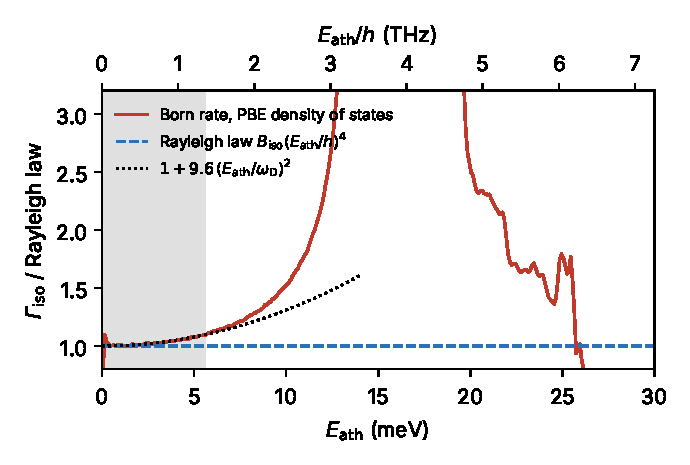
\includegraphics[width=0.75\linewidth]{figures/ch20/limit20_2b.pdf}
\captionof{figure}{Isotope scattering rate of silicon from the Born rate \cref{eq:20.2-isoborn} with the full density of states (red), divided by the Rayleigh law \cref{eq:20.2-rayleigh} (dashed, one), against the phonon energy (lower axis) and frequency (upper axis). The ratio is $g_{\mathrm{ph},\kappa}(\omega)/g_{\mathrm{Debye}}(\omega)$, independent of the mass variance. Density of states from the PBE force constants of \cref{sec:5.2}, integrated in spherical coordinates about $\mathrm{\Gamma}$ to the zone boundary (32 Gauss--Legendre polar points, 64 azimuths, 800 radial steps, \SI{0.1}{meV} bins, running mean over three bins); the Debye reference uses the PBE sound speeds. Dotted: the leading correction $1 + 9.6\,(E_{\mathrm{ath}}/\omega_{\mathrm{D}})^2$, fitted between 2 and \SI{6}{meV}, with $\omega_{\mathrm{D}} = \SI{55.6}{meV}$. Gray: within \SI{10}{\percent} of the Rayleigh law, $E_{\mathrm{ath}} \le \SI{5.6}{meV}$. The ratio peaks at 8.1 near \SI{17.6}{meV}, above the plotted range.}\label{fig:20-limit-iso}
\par}
\smallskip
Above \SI{1.4}{THz} the transverse branches of silicon are no longer linear, and the rate follows the density of states rather than the fourth power of the frequency.
\end{limitbox}

\subsection{The scaling spectrum}\label{sec:20.2-scaling}

The two rates set up a hierarchy. For a longitudinal phonon their ratio is $B_{\mathrm{iso}}/A_{\mathrm{anh}}$ divided by the frequency, and $B_{\mathrm{iso}}/A_{\mathrm{anh}}$ is \SI{33}{THz} in silicon and \SI{228}{THz} in germanium with its slowest decay. A phonon scatters off isotopes more often than it decays, by a factor 3.3 at \SI{10}{THz} in silicon and by more at lower frequency. Between two decays the branches stay close to their equilibrium shares, and a phonon of any branch spends the fraction $f_{\mathrm{LA}}$ of its time as a longitudinal phonon, the only branch that decays. The population decays at the mean rate $f_{\mathrm{LA}}\varGamma_{\mathrm{anh}}$, and isotope scattering, which conserves energy, drops out of the evolution of the energy spectrum. Let $\rho_E(E_{\mathrm{ath}}, t)$ be the energy per unit phonon energy, and $P_{\mathrm{d}}(y)$ the energy-weighted distribution of the fraction $y$ that a decay passes to a daughter, counting both daughters: with $p(y)$ the number density of one daughter, $P_{\mathrm{d}}(y) = 2y\,p(y)$, so that $\int_0^1P_{\mathrm{d}}(y)\,\dd y = 1$. Energy flows only downward:
\begin{equation}
  \frac{\partial\rho_E(E,t)}{\partial t} = -f_{\mathrm{LA}}\varGamma_{\mathrm{anh}}(E)\,\rho_E(E,t)
  + \int_E^\infty\frac{\dd E'}{E'}\,P_{\mathrm{d}}\Bigl(\frac{E}{E'}\Bigr)\,f_{\mathrm{LA}}\varGamma_{\mathrm{anh}}(E')\,\rho_E(E',t) .
  \label{eq:20.2-frag}
\end{equation}
In the isotropic continuum $P_{\mathrm{d}}$ depends on the energy ratio alone, as the distribution of \cref{app:E.12} does, since the kinematics of a decay contain no energy scale. The rate \cref{eq:20.2-anh} contains one scale, which combines with the time into
\begin{equation}
  E_*(t) = h\,(f_{\mathrm{LA}}A_{\mathrm{anh}}t)^{-1/5} , \qquad
  f_{\mathrm{LA}}\varGamma_{\mathrm{anh}}(E) = \frac{1}{t}\Bigl(\frac{E}{E_*(t)}\Bigr)^5 .
  \label{eq:20.2-Estar}
\end{equation}
A phonon above $E_*(t)$ has had time to decay, and one below it has not. Since $E_*$ is the only energy scale, we look for a solution that depends on the phonon energy only through $y = E/E_*(t)$ and conserves the total energy.
\begin{keyresult}[Scaling spectrum of down-conversion]
\begin{equation}
  \begin{gathered}
  \rho_E(E_{\mathrm{ath}}, t) = \frac{E_{\mathrm{prompt}}}{E_*(t)}\,\varphi_*\Bigl(\frac{E_{\mathrm{ath}}}{E_*(t)}\Bigr) , \\
  \frac15\,\frac{\dd}{\dd y}\bigl[y\varphi_*(y)\bigr] = -y^5\varphi_*(y) + \int_y^\infty\dd y'\,y'^4P_{\mathrm{d}}\Bigl(\frac{y}{y'}\Bigr)\varphi_*(y') ,
  \end{gathered}
  \label{eq:20.2-scaling}
\end{equation}
with $\int\varphi_*\,\dd y = 1$. The spectrum keeps its shape and slides to lower energy as $t^{-1/5}$, and every energy moment scales with $E_*(t)$.
\end{keyresult}
\noindent Inserting the form into \cref{eq:20.2-frag} gives the equation for $\varphi_*$. Since $\dd E_*/\dd t = -E_*/5t$, the time derivative of $\rho_E$ is $(E_{\mathrm{prompt}}/5tE_*)\,\dd(y\varphi_*)/\dd y$. The loss term is $(E_{\mathrm{prompt}}/tE_*)\,y^5\varphi_*$ by \cref{eq:20.2-Estar}, and the gain term becomes the integral after the substitution $E' = E_*y'$. Every term carries the factor $E_{\mathrm{prompt}}/tE_*$, so the time drops out. Integrating over $y$ checks the energy: the left side gives $[y\varphi_*]_0^\infty = 0$, and the two terms on the right cancel after the order of integration is exchanged, since $\int_0^{y'}P_{\mathrm{d}}(y/y')\,\dd y = y'$.

\Cref{eq:20.2-scaling} says what the spectrum looks like once it has settled, not when it settles. Settling needs a time long compared with the first decay of the hardest phonons, $1/(f_{\mathrm{LA}}A_{\mathrm{anh}}f_{\mathrm{top}}^5)$ for a band top $f_{\mathrm{top}}$. This is \SI{0.19}{ns} in silicon ($f_{\mathrm{top}} = \SI{15}{THz}$, $f_{\mathrm{LA}} = 0.093$) and \SI{1.3}{ns} in germanium ($f_{\mathrm{top}} = \SI{8.64}{THz}$, $f_{\mathrm{LA}} = 0.098$, $A_{\mathrm{anh}} = \SI{1.61e-55}{s^4}$). Settling also needs the hierarchy of rates, the fifth-power law, and no absorption or surface scattering in the meantime. In silicon the scale is $E_*(t) = 44.6$, 28.1, 17.7 and \SI{11.2}{meV} at 1, 10 and \SI{100}{ns} and \SI{1}{\micro s}, and in germanium 37.8, 23.8, 15.0 and \SI{9.5}{meV}. Since $E_* \propto A_{\mathrm{anh}}^{-1/5}$, the factor of ten among the germanium constants moves $E_*$ by a factor 0.63, and the factor 1.55 between the two silicon values moves it by 0.92.

We have no proof that every birth spectrum approaches $\varphi_*$, which is a question about the stability of \cref{eq:20.2-scaling}; we solve \cref{eq:20.2-frag} for representative births instead. For $P_{\mathrm{d}}$ we take a symmetric stand-in for the isotropic-continuum distribution: each daughter receives a fraction $y$ drawn from the beta distribution $30y^2(1 - y)^2$, which gives $P_{\mathrm{d}}(y) = 60\,y^3(1 - y)^2$. On a logarithmic energy grid of step 0.01, \cref{eq:20.2-frag} becomes a linear system whose exponential we compute exactly. The settled spectrum has its energy-weighted median at $0.66\,E_*$ and \SI{80}{\percent} of its energy between $0.36\,E_*$ and $0.97\,E_*$, and its mean is $\langle E_{\mathrm{ath}}\rangle = 0.667\,E_*(t)$. \Cref{lim:20.2a} follows the mean energy of three hard births in silicon: a line at the band top, a spectrum that grows as the cube of the energy up to the band top, and the acoustic pairs of optical decay. The cubic spectrum puts equal energy in every mode of the Debye model, the shape of a locally thermalized recoil. All three reach the scaling law within \SI{10}{\percent} after \SI{0.46}{ns}, a few first-decay times.

\begin{limitbox}[Down-conversion and the scaling spectrum][lim:20.2a]
The published rates are $\varGamma_{\mathrm{anh}} = A\nu^5$ for longitudinal phonons and $\varGamma_{\mathrm{iso}} = B\nu^4$ for all branches~\cite[Eqs.~(6), (8)]{leman2012invited}, with $A = \SI{7.41e-56}{s^4}$ and $B = \SI{2.43e-42}{s^3}$ for silicon~\cite[Table~I]{leman2012invited}. With the mode mixing of Kelsey et al.~\cite[Sect.~2.2.2]{kelsey2023g4cmp} they imply the scaling spectrum \cref{eq:20.2-scaling}, $E_* \propto t^{-1/5}$, and the mean energy $\langle E_{\mathrm{ath}}\rangle = 0.667\,E_*(t)$ for the daughter distribution used here.
\par\smallskip
{\centering
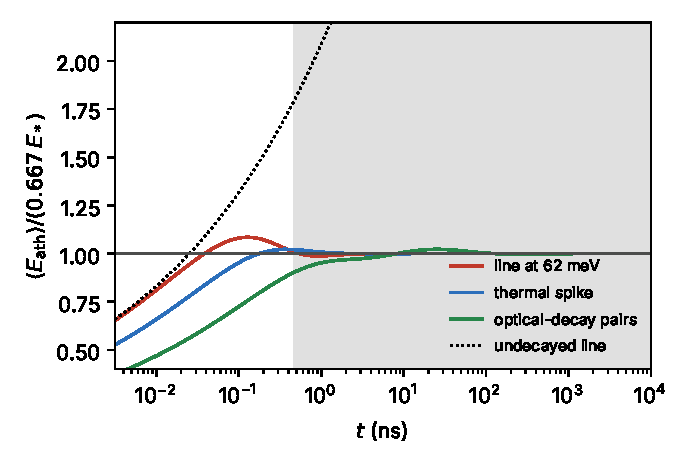
\includegraphics[width=0.75\linewidth]{figures/ch20/limit20_2a.pdf}
\captionof{figure}{Energy-weighted mean phonon energy in silicon divided by the scaling law $0.667\,E_*(t)$ of \cref{eq:20.2-Estar,eq:20.2-scaling}, against time, for three hard births (models): a line at the band top, \SI{62}{meV} (red); a spectrum growing as $E_{\mathrm{ath}}^3$ up to \SI{62}{meV} (blue); and the pairs of longitudinal (\SI{42}{meV}) and transverse (\SI{22}{meV}) phonons from optical decay, Gaussians of \SI{10}{\percent} relative width (green). Solution of \cref{eq:20.2-frag} with $f_{\mathrm{LA}} = 0.093$, $A_{\mathrm{anh}} = \SI{7.41e-56}{s^4}$, the daughter distribution $P_{\mathrm{d}}(y) = 60\,y^3(1 - y)^2$ and no surfaces, on a logarithmic grid of step 0.01 from 0.01 to \SI{18}{THz}, by the exact matrix exponential. Dotted: the leading correction at early times, the undecayed line, $(f_{\mathrm{LA}}A_{\mathrm{anh}}f_{\mathrm{top}}^5t)^{1/5}/0.667$. Gray: all three within \SI{10}{\percent}, $t \ge \SI{0.46}{ns}$.}\label{fig:20-limit-scaling}
\par}
\smallskip
Before the hardest phonons have decayed a few times the mean still depends on the birth spectrum; and where the continuum rates fail, above a few THz in silicon (\cref{lim:20.2b}), the time scale itself is an estimate.
\end{limitbox}

\subsection{Memory of the birth spectrum}\label{sec:20.2-memory}

How long does the birth spectrum leave a trace? We measure the trace by the total-variation distance between the normalized energy spectra that two births reach at time $t$, which is half the integral of their absolute difference. It bounds the difference of the energy that the two deliver into any part of the spectrum. Let $\Delta_{\mathrm{h}}(t)$ be its largest value over pairs of births above an energy $E_{\mathrm{mem}}$. By the scaling form $\Delta_{\mathrm{h}}$ depends on time only through $E_*(t)/E_{\mathrm{mem}}$, and the solutions of \cref{eq:20.2-frag} give the threshold: any two births above $E_{\mathrm{mem}}$ agree to $10^{-3}$ once $E_*(t)$ has fallen to between 0.51 and $0.53\,E_{\mathrm{mem}}$. A birth is forgotten when the scale has fallen to about half its energy, and since $E_* \propto t^{-1/5}$ the time this takes grows as the inverse fifth power of the birth energy. \Cref{fig:20-spectrum} shows the consequences for silicon.

\begin{figure}[tbp]
  \centering
  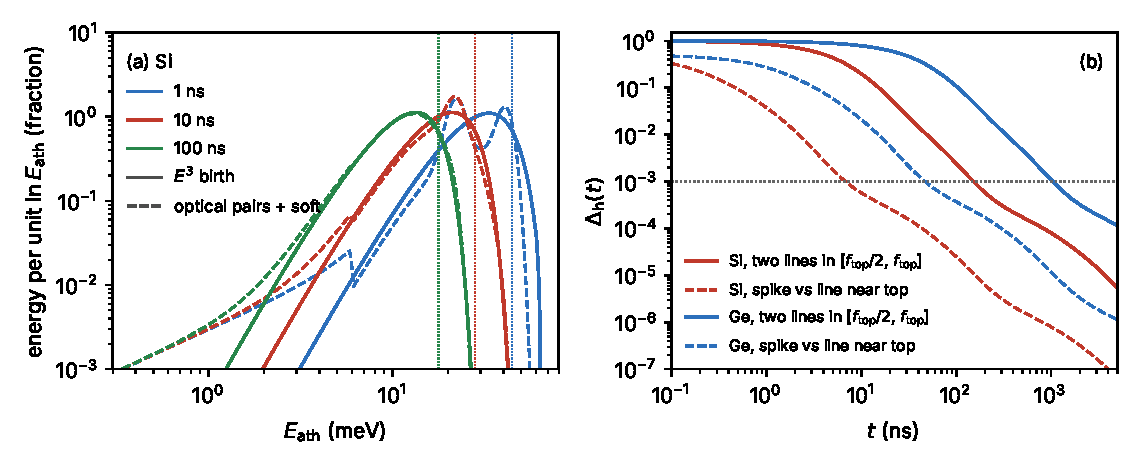
\includegraphics[width=\linewidth]{figures/ch20/fig20_2.pdf}
  \caption{Down-conversion of prompt phonons, from \cref{eq:20.2-frag} in the isotropic continuum with the mean decay rate $f_{\mathrm{LA}}A_{\mathrm{anh}}(E_{\mathrm{ath}}/h)^5$ for every phonon, the daughter distribution $P_{\mathrm{d}}(y) = 60\,y^3(1 - y)^2$ and no surfaces. (a) Energy spectrum of a silicon event, per unit $\ln E_{\mathrm{ath}}$ and normalized to the prompt energy, at 1, 10 and \SI{100}{ns} (colors), for two births (models). Solid: a spectrum growing as $E_{\mathrm{ath}}^3$ up to the band top, \SI{62}{meV}, standing for a locally thermalized nuclear recoil. Dashed: the longitudinal (\SI{42}{meV}) and transverse (\SI{22}{meV}) phonons of optical decay, Gaussians of \SI{10}{\percent} relative width with the energy shares 42:22 of the two phonons of an optical decay, plus the soft fraction $f_{\mathrm{s}} = \SI{1.7}{\percent}$ spread uniformly in energy over 0.2 to \SI{6}{meV}, standing for an electron recoil. Dotted verticals: $E_*(t)$. $A_{\mathrm{anh}} = \SI{7.41e-56}{s^4}$, $f_{\mathrm{LA}} = 0.093$. (b) Memory of the hard part, $\Delta_{\mathrm{h}}(t)$, for silicon (red) and germanium (blue; $A_{\mathrm{anh}} = \SI{1.61e-55}{s^4}$, $f_{\mathrm{LA}} = 0.098$, band top \SI{8.64}{THz}). Solid: the largest total-variation distance between two line births in the upper factor two of the band, $[f_{\mathrm{top}}/2, f_{\mathrm{top}}]$ (six lines). Dashed: one pair concentrated near the top, the $E_{\mathrm{ath}}^3$ spectrum against a Gaussian line at $0.95\,f_{\mathrm{top}}$ of width $0.05\,f_{\mathrm{top}}$. Dotted: $10^{-3}$, crossed by the dashed curves at \SI{6.8}{ns} (Si) and \SI{47}{ns} (Ge), and by the solid curves at \SI{0.15}{\micro s} (Si) and \SI{1.0}{\micro s} (Ge).}
  \label{fig:20-spectrum}
\end{figure}

The answer depends on how low the hard births reach. Take two births concentrated at the top of the band, the cubic spectrum and a line at \SI{95}{\percent} of the band top. They agree to $10^{-3}$ after \SI{6.8}{ns} in silicon and \SI{47}{ns} in germanium with its slowest decay constant (\cref{fig:20-spectrum}(b)), and the fastest germanium constant shortens the latter tenfold. Births spread over the upper factor two of the band take longer, \SI{0.15}{\micro s} in silicon and \SI{1.0}{\micro s} in germanium. The transverse phonons of optical decay, at \SI{22}{meV}, are forgotten only when $E_*$ has fallen to about \SI{11}{meV}, near \SI{1}{\micro s} in silicon. The two model births of \cref{fig:20-spectrum}(a) differ by a total-variation distance of 0.13 at \SI{10}{ns}, 0.026 at \SI{100}{ns}, 0.015 at \SI{300}{ns} and 0.012 at \SI{1}{\micro s}. At \SI{1}{\micro s} their parts above \SI{6}{meV} agree to $6\times10^{-4}$. What remains is the soft fraction: the electron recoil was born with \SI{1.7}{\percent} of its energy below \SI{6}{meV} and the cubic spectrum with \SI{0.01}{\percent}, and the decay of the hard parts has only begun to fill that region. All of these times rest on the continuum rates, which in silicon are applied at 5 to \SI{15}{THz}, above their range (\cref{lim:20.2b}), so they are estimates.

Polarization is forgotten much sooner. Along the scaling trajectory, the number of times a phonon has scattered off isotopes by the time $t$ is
\begin{equation}
  N_{\mathrm{mix}}(t) = \int_0^t\dd t'\,B_{\mathrm{iso}}\bigl[E_*(t')/h\bigr]^4 = 5B_{\mathrm{iso}}\,(f_{\mathrm{LA}}A_{\mathrm{anh}})^{-4/5}\,t^{1/5} ,
  \label{eq:20.2-Nmix}
\end{equation}
which is 164 at \SI{1}{ns} in silicon and 650 at \SI{1}{\micro s}; in germanium, with fifteen times the isotope constant, it is \num{1300} and \num{5100}. Each scattering redraws the branch from the equilibrium shares, so the fraction of phonons that still carry their birth branch is of order $\ee^{-N_{\mathrm{mix}}}$.

The phonons also spread out. Take the diffusion constant $v_{\mathrm{ph}}^2/3\varGamma_{\mathrm{iso}}$ of a gas with mean free time $1/\varGamma_{\mathrm{iso}}$ and rms group speed $v_{\mathrm{ph}}$, evaluated at $E_*(t)$. The mean squared distance from the event is then $6\int\dd t'\,v_{\mathrm{ph}}^2/3\varGamma_{\mathrm{iso}} = \frac{10}{9}v_{\mathrm{ph}}^2(f_{\mathrm{LA}}A_{\mathrm{anh}})^{4/5}t^{9/5}/B_{\mathrm{iso}}$. In silicon, with $v_{\mathrm{ph}} = \SI{5.85}{km/s}$, the rms distance is \SI{8.6}{\micro m} at \SI{10}{ns}, \SI{68}{\micro m} at \SI{100}{ns} and \SI{0.54}{mm} at \SI{1}{\micro s}. In germanium, with $v_{\mathrm{ph}} = \SI{3.52}{km/s}$, it is \SI{1.8}{\micro m}, \SI{15}{\micro m} and \SI{0.12}{mm}. This is the quasi-diffuse transport of athermal phonons~\cite[Sect.~2.2.2]{kelsey2023g4cmp}: the phonons random-walk while their mean free path grows with each decay, until it reaches the size of the crystal and they move ballistically. A phonon of \SI{45}{meV}, the binding energy of a phosphorus donor, belongs to a population that decays within \SI{0.95}{ns}, by which time it has spread over \SI{1.0}{\micro m}. An event closer to a sensor than the rms distance delivers part of its energy before its spectrum has settled, and there the birth is not forgotten. For a silicon detector \SI{4}{mm} thick with sensors on one face, such as that of Ren et al.~\cite{ren2021design}, that shell is \SI{0.21}{\percent} of the volume at \SI{10}{ns}, \SI{1.7}{\percent} at \SI{100}{ns} and \SI{13.5}{\percent} at \SI{1}{\micro s}. The memory times above decide how much of the volume counts as bulk.

Sapphire does not fit this picture. Its isotope constant is a hundred times smaller than that of silicon, $B_{\mathrm{iso}} = \SI{2.5e-44}{s^3}$ calculated and \SI{4e-44}{s^3} measured, while its decay constant lies between \num{1.88e-55} and \SI{1.27e-54}{s^4}. Hernandez et al.\ trace that spread to the anisotropy and to converting a published rate with the fifth power of a sound speed~\cite[Tables~3, 4]{hernandez2025modeling}. Compared to silicon, however, the hierarchy is reversed: mixing outpaces decay only below $B_{\mathrm{iso}}/A_{\mathrm{anh}} = 0.02$ to \SI{0.21}{THz}. Over the whole primary band a longitudinal phonon decays before it scatters, and the branches are not held at their equilibrium shares. A transverse phonon, which the isotropic continuum does not let decay, scatters $B_{\mathrm{iso}}(E_{\mathrm{ath}}/h)^4\times\SI{1}{\micro s} = 0.025$, 0.4 and 16 times in a microsecond at 1, 2 and \SI{5}{THz}. As a result, transverse phonons born below a few THz in sapphire keep their energy and their polarization for microseconds. The single rate $f_{\mathrm{LA}}\varGamma_{\mathrm{anh}}$ of \cref{eq:20.2-frag} does not exist, and the scaling argument fails at its first step. The fate of these phonons needs the decay rates of transverse phonons in an anisotropic crystal, which the isotropic continuum sets to zero.

\subsection{Transfer-kernel bound on observable differences}\label{sec:20.2-bound}

The memory of the spectrum matters through what a readout measures. Take an observable that is linear in the energies delivered to the sensors, with weights between zero and one: the fraction of the energy absorbed by one of two sensors, the fraction that arrives before a given time, or the collection efficiency of a population. Since the transport is linear, a birth spectrum $\hat\rho_0(E)$ normalized to unit energy gives $O = \int\dd E\,R_O(E)\,\hat\rho_0(E)$. Here $R_O(E)$, with $0 \le R_O \le 1$, is the value of the observable for unit energy born at $E$ at the event position, and \cref{sec:20.5} builds it from the collection kernels of a detector. Let $\Delta\hat\rho_0 = \hat\rho_0^{\mathrm{NR}} - \hat\rho_0^{\mathrm{ER}}$ be the difference of the birth spectra of the two recoils. Suppose that no sensor absorbs anything before a time $t_{\mathrm{mem}}$, and that births above $E_{\mathrm{mem}}$ have been forgotten by then, to the distance $\Delta_{\mathrm{h}}(t_{\mathrm{mem}})$ in energy, branch and position.
\begin{keyresult}[Transfer-kernel bound]
\begin{equation}
  |O^{\mathrm{NR}} - O^{\mathrm{ER}}| \le \int_0^{E_{\mathrm{mem}}}\dd E\,|\Delta\hat\rho_0(E)| + \Delta_{\mathrm{h}}(t_{\mathrm{mem}}) .
  \label{eq:20.2-bound}
\end{equation}
When $\Delta\hat\rho_0$ has one sign below $E_{\mathrm{mem}}$, the integral is $\Delta_{\mathrm{soft}} = |\int_0^{E_{\mathrm{mem}}}\Delta\hat\rho_0\,\dd E|$, the difference of the energy fractions born below $E_{\mathrm{mem}}$.
\end{keyresult}
\noindent The response to a birth above $E_{\mathrm{mem}}$ is the response to the state it has reached at $t_{\mathrm{mem}}$, and a weight between zero and one integrated against the difference of two normalized distributions is bounded by their total-variation distance. Two births $E_1$, $E_2$ above $E_{\mathrm{mem}}$ therefore have $|R_O(E_1) - R_O(E_2)| \le \Delta_{\mathrm{h}}$. Both birth spectra have unit energy, so $\int\Delta\hat\rho_0\,\dd E = 0$ and $O^{\mathrm{NR}} - O^{\mathrm{ER}} = \int(R_O - R_0)\,\Delta\hat\rho_0\,\dd E$ for any constant $R_0$. Choose $R_0$ midway between the largest and the smallest response above $E_{\mathrm{mem}}$. Then $|R_O - R_0| \le \Delta_{\mathrm{h}}/2$ above $E_{\mathrm{mem}}$, where $\int|\Delta\hat\rho_0| \le 2$, and $|R_O - R_0| \le 1$ below, which gives the two terms of \cref{eq:20.2-bound}. An observable that is a ratio of delivered energies, such as the share of one of two sensors, is linear to first order in the difference, and the range of its linearized weight replaces the factor one.

\Cref{eq:20.2-bound} names the one number that the created-phonon spectra of the two recoils must supply, the distance between their parts below $E_{\mathrm{mem}}$. The single-sign condition matters. Two births with the same energy below $E_{\mathrm{mem}}$ but different soft shapes, one just above the gap of a sensor film and one just below it, have $\Delta_{\mathrm{soft}} = 0$ and yet give different responses; the bound then needs the full $L^1$ distance. The branch content of a nuclear recoil above $E_{\mathrm{mem}}$ does not enter at all.

For the primary phonons the bound limits the spectral part of the collection offset of \cref{sec:19.5}. With the collection efficiency as the observable, $|\epsilon^{\mathrm{NR}}_{\mathrm{prim}} - \epsilon^{\mathrm{ER}}_{\mathrm{prim}}| \le \int_0^{E_{\mathrm{mem}}}|\Delta\hat\rho_0| + \Delta_{\mathrm{h}}$. If $E_{\mathrm{mem}}$ lies above the soft band and below every hard birth, and only the electron recoil carries a soft fraction, the integral is $f_{\mathrm{s}} = \SI{1.7}{\percent}$. The condition on $E_{\mathrm{mem}}$ is the weak point. For the model births of \cref{fig:20-spectrum}(a) at \SI{1}{\micro s}, the lowest energy above which births agree to $10^{-3}$, $E_{\mathrm{mem}} = \SI{21.6}{meV}$, cuts through the transverse daughters of optical decay, and the bound is 0.15, against an actual largest difference of 0.012. At \SI{3}{\micro s}, with $E_{\mathrm{mem}} = \SI{17.7}{meV}$, the bound has fallen to 0.026 against 0.009, but the near-face shell of a \SI{4}{mm} crystal is by then \SI{36}{\percent} of the volume. Within the bulk the spectral difference between the two recoils is set by the soft fraction and by how low the hard births reach; near an instrumented face this argument does not bound it.

\section{Phonons into films}\label{sec:20.3}

A phonon that has down-converted in silicon to about a terahertz (\cref{sec:20.2}) reaches an aluminum film \SI{60}{nm} thick on the crystal surface. Silicon and aluminum have almost the same acoustic impedance, and the normal-incidence law of \cref{app:C.18} lets \SI{99}{\percent} of a longitudinal flux through. A fit of measured pulses with a phonon simulation nevertheless returns a silicon-to-aluminum coefficient of 0.3 to 0.55 for such a film~\cite{martinez2019measurements}, and a phonon inside the film that reaches the interface crosses back into the silicon about once in three arrivals. These three numbers measure different things. The transmission of each polarization at every angle, and the reciprocity that ties the two directions together, explain all three, and from them follow the probability that a phonon entering the film is absorbed there and the time $t_l$ it spends in the film before escaping, which controls the quasiparticle yield of \cref{sec:20.4}.

\subsection{Acoustic mismatch at oblique incidence}\label{sec:20.3-amm}

The acoustic mismatch model treats the interface as a welded plane between two elastic continua: displacement and traction are continuous across it, and nothing else happens there~\cite{swartz1989thermal}. Silicon is cubic, with an anisotropy ratio $2C_{44}/(C_{11} - C_{12}) = 1.56$ (\cref{app:C.18}). Aluminum is nearly isotropic: its elastic constants extrapolated to zero temperature, $C_{11} = 114.3$, $C_{12} = 61.9$ and $C_{44} = \SI{31.6}{GPa}$~\cite[Table~2]{malica2020quasi}, give the ratio 1.21. We replace each crystal by an isotropic medium with the Voigt averages of its elastic constants, the bulk modulus $B$ of \cref{eq:C.18-bulk} and the shear modulus $(C_{11} - C_{12} + 3C_{44})/5$, which is also what transport codes do. Silicon then has the speeds $c_{\mathrm{LA}} = \SI{9.00}{km.s^{-1}}$ and $c_{\mathrm{T}} = \SI{5.40}{km.s^{-1}}$ at $\rho_T = \SI{2.33}{g.cm^{-3}}$, and aluminum $c_{\mathrm{LA}} = \SI{6.63}{km.s^{-1}}$ and $c_{\mathrm{T}} = \SI{3.30}{km.s^{-1}}$ at the room-temperature density \SI{2.70}{g.cm^{-3}}. A subscript 1 or 2 on a speed or density names the medium.

Put the interface at $z = 0$, with medium 1 below it. A plane wave of frequency $\omega$ that arrives from medium 1 at the angle $\theta_1$ to the normal has the wavevector component $Q_\parallel = \omega\sin\theta_1/c_{\mathrm{inc}}$ along the interface, where $c_{\mathrm{inc}}$ is its speed. Every reflected and transmitted wave it generates has the same $\omega$ and the same $Q_\parallel$, which is the acoustic Snell law \cref{eq:C.18-snell}. A wave of speed $c$ in either medium then has the normal component
\begin{equation}
  Q_z = \bigl(\omega^2/c^2 - Q_\parallel^2\bigr)^{1/2} ,
  \label{eq:20.3-Qz}
\end{equation}
taken positive. When $Q_\parallel > \omega/c$ the root is imaginary, we take it with a positive imaginary part, and the wave decays away from the interface and carries no energy flux. A wave can have three polarizations: longitudinal (L), transverse in the plane of incidence (SV), and transverse perpendicular to it (SH). The interface is invariant under reflection through the plane of incidence, so SH waves couple only to SH waves, while L and SV waves mix.

For SH waves the displacement $u_y$ and the traction $\sigma_{yz} = \rho_Tc_{\mathrm{T}}^2\,\partial_zu_y$ must be continuous. This is the algebra of the normal-incidence derivation in \cref{app:C.18}, with $Q_i\rho_ic_i^2$ there replaced by $\rho_ic_{\mathrm{T},i}^2Q_{z,i} = \omega Z^{\mathrm{T}}_{\mathrm{ac},i}\cos\theta_i$, where $Z^{\mathrm{T}}_{\mathrm{ac},i} = \rho_ic_{\mathrm{T},i}$ is the transverse impedance. The fraction of the incident energy flux that crosses is
\begin{equation}
  t_{\mathrm{SH}}(\theta_1) = \frac{4Z^{\mathrm{T}}_{\mathrm{ac},1}\cos\theta_1\,\Real\bigl(Z^{\mathrm{T}}_{\mathrm{ac},2}\cos\theta_2\bigr)}{\bigl|Z^{\mathrm{T}}_{\mathrm{ac},1}\cos\theta_1 + Z^{\mathrm{T}}_{\mathrm{ac},2}\cos\theta_2\bigr|^2} ,
  \qquad
  \cos\theta_2 = \Bigl(1 - \frac{c_{\mathrm{T},2}^2}{c_{\mathrm{T},1}^2}\sin^2\theta_1\Bigr)^{1/2} .
  \label{eq:20.3-SH}
\end{equation}
At normal incidence it is \cref{eq:C.18-transmission} with the transverse impedances. Beyond the critical angle $\sin\theta_1 = c_{\mathrm{T},1}/c_{\mathrm{T},2}$, which exists when medium 2 is the faster one, $\cos\theta_2$ is imaginary and $t_{\mathrm{SH}} = 0$: the wave is totally reflected.

For L and SV waves four conditions hold at $z = 0$: continuity of $u_x$, $u_z$, $\sigma_{zz} = \rho_T[c_{\mathrm{LA}}^2\partial_zu_z + (c_{\mathrm{LA}}^2 - 2c_{\mathrm{T}}^2)\partial_xu_x]$ and $\sigma_{xz} = \rho_Tc_{\mathrm{T}}^2(\partial_zu_x + \partial_xu_z)$, the last two being Hooke's law of \cref{app:C.18} for an isotropic medium. Each wave is $u = a\,\hat{\vect{e}}\,\ee^{\ii(Q_\parallel x \pm Q_zz - \omega t)}$ with amplitude $a$ and the sign $+$ for a wave moving toward medium 2 and $-$ for one moving back into medium 1, and unit polarization $\hat{\vect{e}} = (c/\omega)(Q_\parallel, 0, \pm Q_z)$ for L and $(c/\omega)(\pm Q_z, 0, -Q_\parallel)$ for SV. Collect for each wave the four quantities that must match,
\begin{equation}
  \vect{b} = \Bigl(\hat e_x,\ \hat e_z,\ \frac{\rho_T}{\omega}\bigl[c_{\mathrm{LA}}^2(\pm Q_z)\hat e_z + (c_{\mathrm{LA}}^2 - 2c_{\mathrm{T}}^2)Q_\parallel\hat e_x\bigr],\ \frac{\rho_Tc_{\mathrm{T}}^2}{\omega}\bigl[(\pm Q_z)\hat e_x + Q_\parallel\hat e_z\bigr]\Bigr) ,
  \label{eq:20.3-b}
\end{equation}
which are the displacement and $\sigma_{zz}/\ii\omega$, $\sigma_{xz}/\ii\omega$ per unit amplitude. With unit incident amplitude the boundary conditions read $\vect{b}_{\mathrm{inc}} + a_{\mathrm{rL}}\vect{b}_{\mathrm{rL}} + a_{\mathrm{rS}}\vect{b}_{\mathrm{rS}} = a_{\mathrm{tL}}\vect{b}_{\mathrm{tL}} + a_{\mathrm{tS}}\vect{b}_{\mathrm{tS}}$, four linear equations for the amplitudes of the reflected (r) and transmitted (t) L and SV waves. A propagating plane wave carries the time-averaged energy flux $\frac12\rho_T\omega^2|a|^2c$ along its direction (\cref{app:C.18}), whose normal component is this times $\cos\theta = cQ_z/\omega$. The fraction of the incident flux carried away by the outgoing wave $j$ is therefore
\begin{equation}
  t_j = \frac{\rho_jc_j^2\,\Real Q_{z,j}\,|a_j|^2}{\rho_1c_{\mathrm{inc}}^2\,Q_{z,\mathrm{inc}}} ,
  \label{eq:20.3-flux}
\end{equation}
and the transmission of an incident L or SV wave is the sum of the two transmitted fractions. We solve the four equations numerically at each angle.

\Cref{fig:20-amm} shows the result for silicon and aluminum. From the silicon side, a longitudinal phonon crosses with 0.99 at normal incidence and with more than 0.98 out to \SI{70}{\degree}, falling below 0.9 only beyond \SI{78}{\degree}. At oblique incidence part of the transmitted flux is converted to SV, \num{0.031} at \SI{30}{\degree} and at most 0.17, near \SI{76}{\degree}. Transverse phonons cross with 0.97 at normal incidence. The one critical angle that limits transmission from silicon is \SI{54.6}{\degree}, beyond which an incident SV wave can no longer produce a longitudinal wave in aluminum. From the aluminum side, however, every wave is slower than every wave in silicon, and the critical angles cut transmission off. Transverse phonons beyond $\arcsin(c_{\mathrm{T,Al}}/c_{\mathrm{T,Si}}) = \SI{37.7}{\degree}$ find no propagating wave in silicon and are totally reflected. Longitudinal phonons lose the longitudinal channel beyond \SI{47.5}{\degree} and keep only the conversion into silicon transverse waves, which carries 0.28 at that angle and vanishes at grazing incidence.

\begin{figure}[tbp]
  \centering
  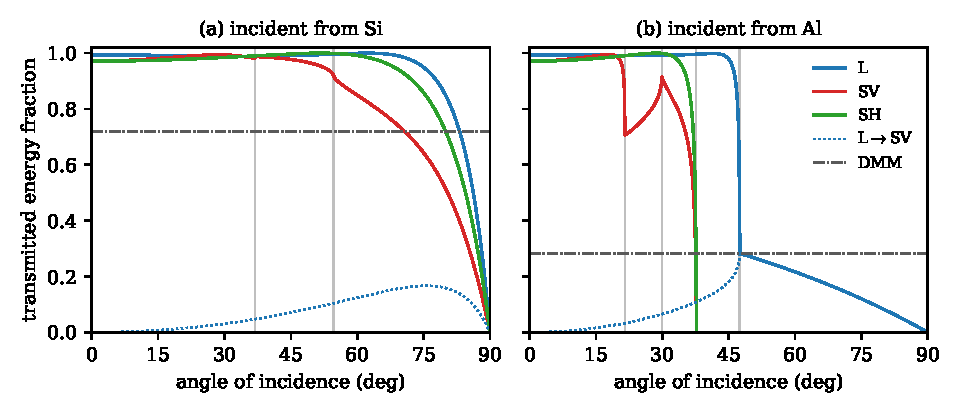
\includegraphics[width=\linewidth]{figures/ch20/fig20_3.pdf}
  \caption{Acoustic-mismatch transmission of a welded silicon/aluminum interface against the angle of incidence, for phonons incident (a) from silicon and (b) from aluminum. Solid: fraction of the incident energy flux transmitted into all modes of the other side, for incident longitudinal (L, blue), SV (red) and SH (green) phonons; dotted: the part of the incident longitudinal flux transmitted as SV. Dash-dot: the diffuse-mismatch value $\mathfrak{n}_2/(\mathfrak{n}_1 + \mathfrak{n}_2)$, 0.718 in (a) and 0.282 in (b). Gray lines: critical angles, \SI{36.9}{\degree} and \SI{54.6}{\degree} in (a); \SI{21.5}{\degree}, \SI{29.9}{\degree}, \SI{37.7}{\degree} and \SI{47.5}{\degree} in (b). Both media isotropic, with the Voigt averages of the elastic constants: silicon (\cref{app:C.18}) $c_{\mathrm{LA}} = 9.00$, $c_{\mathrm{T}} = \SI{5.40}{km.s^{-1}}$, $\rho_T = \SI{2.33}{g.cm^{-3}}$; aluminum, zero-temperature elastic constants at the room-temperature density, 6.63, \SI{3.30}{km.s^{-1}}, \SI{2.70}{g.cm^{-3}}. The curves do not depend on frequency.}
  \label{fig:20-amm}
\end{figure}

Frequency drops out of \cref{eq:20.3-SH,eq:20.3-flux}, because $Q_\parallel$ and $Q_z$ both scale with $\omega$. The transmissions are frequency independent as long as the wavelength is long compared with the lattice spacing, so that the continuum holds, and short compared with the film thickness, so that the film acts as a half-space. In the simulation of the \SI{60}{nm} films the absorbed phonons peak between 0.7 and \SI{0.9}{THz}~\cite[Sect.~V]{martinez2019measurements}. At \SI{0.8}{THz} the wavelengths in aluminum are \SI{8.3}{nm} for longitudinal and \SI{4.1}{nm} for transverse phonons, so both conditions hold. The longitudinal wavelength equals the thickness at \SI{0.110}{THz}, close to the pair-breaking threshold $2\Delta_{\mathrm{BCS}} = \SI{0.36}{meV}$, or \SI{0.087}{THz}, of bulk aluminum (\cref{sec:7.2}); below it the film reflects as a layer, with interference between its two faces.

\subsection{Angle averages, reciprocity and diffuse mismatch}\label{sec:20.3-recip}

A sensor film collects phonons arriving from all directions, so its transmission is the average over an isotropic population. Count the energy flux that such a population sends onto unit area of the interface. A branch has $\dd^3Q/(2\pi)^3$ modes in $\dd^3Q$, each with occupation $n(\omega)$, energy $\omega$ and normal group velocity $\partial\omega/\partial Q_z$. Since $\dd Q_z\,\partial\omega/\partial Q_z = \dd\omega$, the flux is
\begin{equation}
  \int_{Q_z > 0}\frac{\dd^3Q}{(2\pi)^3}\,\omega\,n(\omega)\,\frac{\partial\omega}{\partial Q_z} = \int\dd\omega\,\omega\,n(\omega)\int\frac{\dd^2Q_\parallel}{(2\pi)^3} .
  \label{eq:20.3-count}
\end{equation}
At a given frequency, every patch $\dd^2Q_\parallel$ of every branch, in either medium, brings the same flux. In an isotropic medium $\dd^2Q_\parallel = 2\pi Q_\parallel\dd Q_\parallel = (2\pi\omega^2/c_\nu^2)\sin\theta\cos\theta\,\dd\theta$, so the angles enter with the weight $2\sin\theta\cos\theta$ and the branch $\nu$ with the weight $c_\nu^{-2}$. The mean transmission of an isotropic population from medium 1 into medium 2 is
\begin{equation}
  \bar t_{12} = \frac{1}{\mathfrak{n}_1}\sum_\nu c_{1\nu}^{-2}\int_0^{\pi/2}t_{12,\nu}(\theta)\,2\sin\theta\cos\theta\,\dd\theta ,
  \qquad
  \mathfrak{n}_1 = c_{\mathrm{LA},1}^{-2} + 2c_{\mathrm{T},1}^{-2} ,
  \label{eq:20.3-avg}
\end{equation}
where $\nu$ runs over L, SV and SH and $t_{12,\nu}(\theta)$ is the transmission of \cref{eq:20.3-SH} or \cref{eq:20.3-flux}. The interface-weighted density $\mathfrak{n}_1$ is proportional to the rate at which phonons of a given frequency strike unit area from medium 1.

Reciprocity ties the two directions together. Fix $\omega$ and $Q_\parallel$. The interface then scatters $N_1$ incoming channels from medium 1, the branches of medium 1 that propagate at this $Q_\parallel$, and $N_2$ from medium 2, into the same number of outgoing ones. Normalize each amplitude so that its squared modulus is the energy flux, as in \cref{eq:20.3-flux}. The matrix $\mathsf{S}$ that maps incoming onto outgoing amplitudes is then unitary, because the welded interface neither stores nor dissipates energy. Write it in blocks,
\begin{equation*}
  \mathsf{S} = \begin{pmatrix} \mathsf{r} & \mathsf{t}' \\ \mathsf{t} & \mathsf{r}' \end{pmatrix} ,
\end{equation*}
with $\mathsf{t}$ the $N_2\times N_1$ block of transmission from medium 1 into medium 2 and $\mathsf{t}'$ the reverse. The upper-left block of $\mathsf{S}^\dagger\mathsf{S} = 1$ gives $\mathsf{r}^\dagger\mathsf{r} + \mathsf{t}^\dagger\mathsf{t} = 1$, and that of $\mathsf{S}\mathsf{S}^\dagger = 1$ gives $\mathsf{r}\mathsf{r}^\dagger + \mathsf{t}'\mathsf{t}'^\dagger = 1$, both in the $N_1$-dimensional space of medium 1. Taking traces, $\Tr\mathsf{t}^\dagger\mathsf{t} = N_1 - \Tr\mathsf{r}^\dagger\mathsf{r} = \Tr\mathsf{t}'\mathsf{t}'^\dagger$. The left side is the sum of the transmissions of all channels incident from medium 1, the right side that of all channels incident from medium 2. Integrated over $Q_\parallel$ with the weight of \cref{eq:20.3-count}, this equality becomes a statement about the averages \cref{eq:20.3-avg}.
\begin{keyresult}[Reciprocity of interface transmission]
For any flat interface that conserves energy, the mean transmissions of isotropic populations in the two directions satisfy
\begin{equation}
  \mathfrak{n}_1\,\bar t_{12} = \mathfrak{n}_2\,\bar t_{21} .
  \label{eq:20.3-recip}
\end{equation}
\end{keyresult}
The derivation uses the conservation of $Q_\parallel$ and the conservation of energy, nothing about isotropy or the number of layers. For anisotropic media or a layered interface \cref{eq:20.3-recip} holds at each frequency, with $\mathfrak{n}_i$ replaced by the area that the branches of medium $i$ cover in the $Q_\parallel$ plane. Evanescent waves are not channels and drop out. In thermal equilibrium the relation is detailed balance: equal temperatures on the two sides give no net flux. It holds, however, for any population, since it is a property of $\mathsf{S}$.

For silicon and aluminum $\mathfrak{n}_{\mathrm{Si}} = 0.0808$ and $\mathfrak{n}_{\mathrm{Al}} = \SI{0.206}{s^2.km^{-2}}$, a ratio of 0.392. We find $\bar t_{\mathrm{Si\to Al}} = 0.938$ and $\bar t_{\mathrm{Al\to Si}} = 0.368$. Transmission out of the film is 2.5 times weaker than into it because the slower phonons of aluminum have 2.55 times more modes per unit area of $Q_\parallel$, and most of those modes lie outside the disk that silicon can carry. The transverse phonons beyond \SI{37.7}{\degree} are the fraction $1 - (c_{\mathrm{T,Al}}/c_{\mathrm{T,Si}})^2 = 0.627$ of the transverse flux and, since transverse phonons carry 0.890 of the flux in aluminum, 0.557 of all phonon flux in the film. They never reach silicon. The impedance mismatch plays almost no part. In the direction into the film the interface hardly distinguishes polarizations: the averages are 0.979 for longitudinal, 0.899 for SV and 0.962 for SH phonons, so longitudinal phonons cross 1.05 times as readily as transverse ones.

The diffuse mismatch model makes the opposite assumption: a phonon arriving at the interface loses its direction and polarization there~\cite{swartz1989thermal}. A phonon leaving the interface then carries no memory of the side it came from, and the probability of ending in medium 2 is the same for a phonon from medium 1, $t_{12}$, as for a phonon from medium 2, $1 - t_{21}$. With \cref{eq:20.3-recip},
\begin{equation}
  t^{\mathrm{DMM}}_{12} = \frac{\mathfrak{n}_2}{\mathfrak{n}_1 + \mathfrak{n}_2} ,
  \label{eq:20.3-dmm}
\end{equation}
which is 0.718 from silicon into aluminum and 0.282 back. The two models serve below as the range of the escape probability.

The normal-incidence impedance law is often taken as the transmission of an interface. \Cref{lim:20.3a} compares it with the angle- and mode-averaged result.
\begin{limitbox}[Impedance law and the averaged transmission][lim:20.3a]
The acoustic-mismatch transmission at normal incidence~\cite{swartz1989thermal}, \cref{eq:C.18-transmission}: $t_{12}(0) = 4Z_{\mathrm{ac},1}Z_{\mathrm{ac},2}/(Z_{\mathrm{ac},1} + Z_{\mathrm{ac},2})^2$, the same in both directions.
\par\smallskip
{\centering
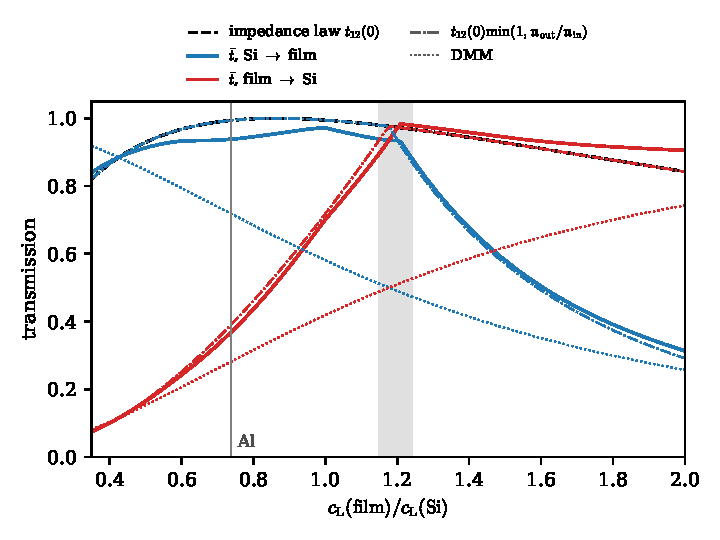
\includegraphics[width=\linewidth]{figures/ch20/limit20_3a.pdf}
\captionof{figure}{Transmission between isotropic silicon and a family of aluminum-like films against the ratio of their longitudinal speeds; the film keeps the density \SI{2.70}{g.cm^{-3}} and the aluminum ratio $c_{\mathrm{T}}/c_{\mathrm{LA}} = 0.498$, and $c_{\mathrm{LA}}(\mathrm{film})/c_{\mathrm{LA}}(\mathrm{Si}) = 0.737$ is aluminum (vertical line). Dashed: the impedance law. Solid: the averages \cref{eq:20.3-avg} from silicon into the film (blue) and back (red). Dash-dot: the leading correction, reciprocity \cref{eq:20.3-recip} applied to the impedance law on the slower side, $t_{12}(0)\min(1, \mathfrak{n}_{\mathrm{out}}/\mathfrak{n}_{\mathrm{in}})$, within \SI{6.9}{\percent} of the averages over the whole range. Dotted: the diffuse mismatch \cref{eq:20.3-dmm}. Gray: speed ratios 1.146 to 1.242, where the impedance law lies within \SI{10}{\percent} of the averages in both directions. In that range $\mathfrak{n}_{\mathrm{film}} \approx \mathfrak{n}_{\mathrm{Si}}$.}\label{fig:20-limit-amm}
\par}
\smallskip
Away from equal interface densities the critical angles of the slower medium's phonons, which the impedance law ignores, remove most of the flux in one direction: for aluminum on silicon the law overstates the escape from the film by a factor 2.70, while reciprocity applied to it, $t_{12}(0)\,\mathfrak{n}_{\mathrm{Si}}/\mathfrak{n}_{\mathrm{Al}} = 0.390$, comes within \SI{6}{\percent} of 0.368.
\end{limitbox}

\subsection{Film absorption and escape time}\label{sec:20.3-escape}

Inside a superconducting film a phonon of energy $E_{\mathrm{ath}}$ above $2\Delta_{\mathrm{BCS}}$ breaks a Cooper pair after a mean free path $\mathfrak{l}_{\mathrm{f}}(E_{\mathrm{ath}})$ (\cref{app:E.12}). Take a film of thickness $d_{\mathrm{f}}$ with a free top face and the substrate below. A phonon that moves at the angle $\theta$ to the normal travels $2d_{\mathrm{f}}/\cos\theta$ between two arrivals at the interface, where it escapes with probability $t_{\mathrm{esc}}$. If it keeps its angle, each round trip is survived with probability $\ee^{-y_{\mathrm{f}}/\cos\theta}$ and ends with an escape with probability $t_{\mathrm{esc}}$. Summing the geometric series of round trips, the probability that the phonon is absorbed before escaping is
\begin{equation}
  P_{\mathrm{abs}}(\theta) = \frac{1 - \ee^{-y_{\mathrm{f}}/\cos\theta}}{1 - (1 - t_{\mathrm{esc}})\,\ee^{-y_{\mathrm{f}}/\cos\theta}} ,
  \qquad y_{\mathrm{f}} = \frac{2d_{\mathrm{f}}}{\mathfrak{l}_{\mathrm{f}}} .
  \label{eq:20.3-pabs-theta}
\end{equation}
A polycrystalline film with a rough top face changes the direction of a phonon at every pass. Each round trip then starts from the flux distribution $2\sin\theta\cos\theta$ of \cref{eq:20.3-avg}, and with $\mu = \cos\theta$ the mean survival over one round trip is
\begin{equation*}
  \int_0^1 2\mu\,\ee^{-y_{\mathrm{f}}/\mu}\,\dd\mu = 2\int_1^\infty\frac{\ee^{-y_{\mathrm{f}}s}}{s^3}\,\dd s = 2E_3(y_{\mathrm{f}}) ,
\end{equation*}
with $s = 1/\mu$ and $E_3$ the exponential integral of order three. The escape probability becomes the average $\bar t_{\mathrm{esc}} = \bar t_{\mathrm{f\to sub}}$ of \cref{eq:20.3-avg}, and the absorption probability per entry is
\begin{equation}
  P_{\mathrm{abs}} = \frac{1 - 2E_3(y_{\mathrm{f}})}{1 - (1 - \bar t_{\mathrm{esc}})\,2E_3(y_{\mathrm{f}})} .
  \label{eq:20.3-pabs}
\end{equation}
For a thin film, $2E_3(y_{\mathrm{f}}) = 1 - 2y_{\mathrm{f}} + O(y_{\mathrm{f}}^2\ln y_{\mathrm{f}})$ and $P_{\mathrm{abs}} \simeq 4d_{\mathrm{f}}/(\mathfrak{l}_{\mathrm{f}}\bar t_{\mathrm{esc}})$: the phonon makes on average $1/\bar t_{\mathrm{esc}}$ round trips of mean length $4d_{\mathrm{f}}$ before it escapes.

The same counting in time gives the escape time. Let the film hold $N_\nu$ phonons of branch $\nu$ per unit volume, distributed isotropically. They strike unit area of the interface at the rate $N_\nu c_\nu/4$, of which the fraction $\langle t_\nu\rangle$, the angle integral in \cref{eq:20.3-avg}, escapes. The film holds $d_{\mathrm{f}}\sum_\nu N_\nu$ phonons per unit area. Let the branches be populated as in equilibrium at a fixed frequency, $N_\nu \propto c_\nu^{-3}$ by \cref{eq:5.2-dosac}. The escape rate is then
\begin{equation*}
  \frac{1}{t_l} = \frac{\sum_\nu N_\nu c_\nu\langle t_\nu\rangle}{4d_{\mathrm{f}}\sum_\nu N_\nu} = \frac{\mathfrak{n}_{\mathrm{f}}\,\bar t_{\mathrm{esc}}}{4d_{\mathrm{f}}\sum_\nu c_\nu^{-3}} .
\end{equation*}
\begin{keyresult}[Film escape time]
A phonon population that is isotropic and mixed among branches leaves a film of thickness $d_{\mathrm{f}}$ at the rate $1/t_l$, with
\begin{equation}
  t_l = \frac{4d_{\mathrm{f}}}{v_s\,\bar t_{\mathrm{esc}}} , \qquad v_s = \frac{\sum_\nu c_\nu^{-2}}{\sum_\nu c_\nu^{-3}} ,
  \label{eq:20.3-tl}
\end{equation}
where $v_s$ is the mean speed of the film's phonons weighted by their density of states and $\bar t_{\mathrm{esc}}$ the mean transmission into the substrate, \cref{eq:20.3-avg}.
\end{keyresult}
\Cref{eq:20.3-tl} assumes that the population is randomized in direction and branch faster than it escapes, that the transmissions are frequency independent, that the top face loses nothing, and that $\bar t_{\mathrm{esc}}$ is the transmission of a clean welded interface, or whatever replaces it. Without the mixing, the \SI{56}{\percent} of the flux beyond the transverse critical angle would never leave, and frequency independence needs wavelengths below $d_{\mathrm{f}}$. With the pair-breaking time $t_{\mathrm{pb}} = \mathfrak{l}_{\mathrm{f}}/v_s$, the thin-film limit of \cref{eq:20.3-pabs} reads $P_{\mathrm{abs}} \simeq t_l/t_{\mathrm{pb}}$, the first term of the competition $t_l/(t_l + t_{\mathrm{pb}})$ between escape and pair breaking.

\begin{workedexample}{Escape from a \SI{60}{nm} aluminum film on silicon}\label{we:20-escape}
The film phonons have $c_{\mathrm{LA}} = 6.63$ and $c_{\mathrm{T}} = \SI{3.30}{km.s^{-1}}$. The sums in \cref{eq:20.3-tl} are $\sum_\nu c_\nu^{-2} = \mathfrak{n}_{\mathrm{Al}} = \SI{0.2062}{s^2.km^{-2}}$ and $\sum_\nu c_\nu^{-3} = \SI{0.0590}{s^3.km^{-3}}$, so $v_s = \SI{3.50}{km.s^{-1}}$, close to the transverse speed because transverse modes dominate the density of states.

The escape probability is the average from aluminum into silicon. The acoustic mismatch model gives $\bar t_{\mathrm{esc}} = 0.368$, from 0.624 for longitudinal, 0.313 for SV and 0.359 for SH phonons; the diffuse mismatch model gives 0.282. With $d_{\mathrm{f}} = \SI{60}{nm}$,
\begin{equation*}
  t_l = \frac{4\times\SI{60}{nm}}{\SI{3.50}{km.s^{-1}}\times0.368} = \SI{0.187}{ns} \quad\text{(acoustic)}, \qquad \SI{0.244}{ns} \quad\text{(diffuse)},
\end{equation*}
a factor 1.31 between the two models. Near $2\Delta_{\mathrm{BCS}}$ a phonon in aluminum breaks a pair in the time $t_0 \approx \SI{0.26}{ns}$, the characteristic phonon lifetime of Kaplan and coworkers~\cite{kaplan1976quasiparticle}, \cite[p.~2]{guruswamy2014quasiparticle}, which \cref{sec:20.4} defines as the pair-breaking time at threshold. Hence $t_l/t_0 = 0.72$ (acoustic) or 0.94 (diffuse). A \SI{60}{nm} film loses its phonons about as fast as they break pairs, which is the regime in which \cref{sec:20.4} finds the quasiparticle yield sensitive to $t_l/t_0$. If the mean free path were $\mathfrak{l}_{\mathrm{f}} = v_st_0 = \SI{0.909}{\micro m}$, then $y_{\mathrm{f}} = 0.132$ and \cref{eq:20.3-pabs} would give $P_{\mathrm{abs}} = 0.422$, against $t_l/(t_l + t_0) = 0.418$.
\end{workedexample}

\subsection{The fitted silicon-to-aluminum coefficient}\label{sec:20.3-fit}

Martinez and coworkers illuminated the back of silicon wafers 300 to \SI{380}{\micro m} thick, \SI{2}{cm} square, that carried \SI{60}{nm} aluminum resonators. They compared the measured phonon pulses with a Monte Carlo simulation using specular reflection, and the silicon-to-aluminum coefficient that reproduced the data lay between 0.30 and 0.55~\cite[Sect.~V]{martinez2019measurements}. Their simulation does not propagate phonons inside the aluminum. A phonon that crosses produces a signal with the pair-breaking efficiency or is removed, and the fitted coefficient's complement includes phonons that enter the film and come back~\cite[Sect.~IV]{martinez2019measurements}. The fitted coefficient is therefore the probability that a phonon arriving from silicon is absorbed in the film,
\begin{equation}
  T_{\mathrm{fit}} = \bar t_{\mathrm{Si\to Al}}\,P_{\mathrm{abs}} .
  \label{eq:20.3-Tfit}
\end{equation}
With the acoustic-mismatch value 0.938, the fit gives $P_{\mathrm{abs}} = 0.320$ to 0.586. Inverting \cref{eq:20.3-pabs} with $\bar t_{\mathrm{esc}} = 0.368$ gives $\mathfrak{l}_{\mathrm{f}}/d_{\mathrm{f}} = 23.1$ to 8.3, or $\mathfrak{l}_{\mathrm{f}} = 1.39$ to \SI{0.50}{\micro m}, and $t_{\mathrm{pb}} = \mathfrak{l}_{\mathrm{f}}/v_s = 0.40$ to \SI{0.14}{ns}, the same order as $t_0$. Keeping the angle of each phonon instead, \cref{eq:20.3-pabs-theta} averaged with $t_{\mathrm{esc}} = \bar t_{\mathrm{esc}}$ gives 1.29 to \SI{0.46}{\micro m}; the diffuse-mismatch pair, 0.718 and 0.282, gives 1.19 to \SI{0.31}{\micro m}. The fit thus constrains the pair-breaking length over the thickness, $\mathfrak{l}_{\mathrm{f}}/d_{\mathrm{f}} \approx 5$ to 23 across both models, and says little about the interface. In the thin-film limit $T_{\mathrm{fit}} \to (\mathfrak{n}_{\mathrm{Al}}/\mathfrak{n}_{\mathrm{Si}})\,4d_{\mathrm{f}}/\mathfrak{l}_{\mathrm{f}}$ for any interface that conserves energy, by reciprocity (\cref{eq:20.3-pabs,eq:20.3-recip}), and the interface model enters only through the finite-thickness corrections. Read as a transmission, the fit would put the escape probability at $(\mathfrak{n}_{\mathrm{Si}}/\mathfrak{n}_{\mathrm{Al}})\times(0.30$ to $0.55) = 0.118$ to 0.216 by \cref{eq:20.3-recip}, below both models. The inferred lengths are estimates: they inherit the specular, mode-conserving simulation of the fit and the isotropic averages of this section. An earlier silicon detector model matched its data with a \SI{33}{\percent} probability for a phonon to be absorbed at an amorphous-silicon/aluminum interface, the rest scattering back diffusely~\cite[Sect.~III\,G]{leman2012invited}; that coefficient is an absorption probability of the same kind.

\subsection{Anisotropy and interlayers}\label{sec:20.3-aniso}

The isotropic averages hide the anisotropy of silicon, whose longitudinal speed ranges from 8.43 to \SI{9.35}{km.s^{-1}} and whose transverse speeds from 4.67 to \SI{5.84}{km.s^{-1}} (\cref{eq:C.18-cubic}). Giving the isotropic silicon its $[100]$ speeds, 8.43 and \SI{5.84}{km.s^{-1}}, or its $[111]$ speeds, 9.35 and \SI{5.09}{km.s^{-1}}, moves $\bar t_{\mathrm{esc}}$ from 0.368 to 0.327 and 0.405, and $t_l$ for \SI{60}{nm} from 0.187 to 0.210 and \SI{0.169}{ns}; $\bar t_{\mathrm{Si\to Al}}$ moves only between 0.927 and 0.943. These are sensitivities, not bounds. The texture of the film matters less, since it changes the longitudinal speed of aluminum by at most \SI{3}{\percent} (\cref{app:C.18}). In the anisotropic problem the critical angles depend on the direction in the interface plane, the group velocity is not parallel to $\vect{Q}$, and the plane waves on each side follow from the Christoffel equation \cref{eq:C.18-christoffel}; the boundary problem becomes six by six. The reciprocity \cref{eq:20.3-recip} holds there unchanged.

Real interfaces carry a native oxide or a deposited amorphous layer a few nanometers thick. A flat layer that does not dissipate cannot change which waves propagate in silicon, since $Q_\parallel$ is conserved through every layer: the critical angles and the \SI{56}{\percent} of trapped film flux stay as they are. The layer changes the transmission inside the cone. At normal incidence take a layer of impedance $Z_{\mathrm{ac},3}$, speed $c_3$ and thickness $h$. At the quarter-wave frequency $c_3/4h$ the wave crosses it with the phase $\pi/2$, and the layer maps the particle velocity $\dot u$ and the force $-\sigma_{zz}$ at its far face onto $\ii(-\sigma_{zz})/Z_{\mathrm{ac},3}$ and $\ii Z_{\mathrm{ac},3}\dot u$ at its near face. A medium of impedance $Z_{\mathrm{ac},2}$ behind it then looks like one of impedance $Z_{\mathrm{ac},3}^2/Z_{\mathrm{ac},2}$, and \cref{eq:C.18-transmission} with this replacement gives the lowest transmission,
\begin{equation*}
  t_{\min} = \frac{4Z_{\mathrm{ac},1}Z_{\mathrm{ac},2}Z_{\mathrm{ac},3}^2}{\bigl(Z_{\mathrm{ac},1}Z_{\mathrm{ac},2} + Z_{\mathrm{ac},3}^2\bigr)^2} ,
\end{equation*}
since the transmission oscillates between this value and the bare $t_{12}(0)$ as the frequency varies. Amorphous SiO$_2$, with $\rho_T = \SI{2.2}{g.cm^{-3}}$ and $\rho_Tc_{\mathrm{LA}}^2 = \SI{7.40e10}{Pa}$ (\cref{sec:16.7}), has $c_{\mathrm{LA}} = \SI{5.80}{km.s^{-1}}$ and $Z_{\mathrm{ac}} = \SI{12.8e6}{kg.m^{-2}.s^{-1}}$. Between silicon and aluminum it gives $t_{\min} = 0.844$, against 0.994 without the layer, at \SI{0.72}{THz} for a \SI{2}{nm} layer; a \SI{1}{nm} layer transmits 0.901 at \SI{0.8}{THz}. A rough or disordered layer scatters diffusely instead, does not conserve $Q_\parallel$, and can release trapped modes; the diffuse mismatch model is the limit of complete randomization. Until the escape probability of a real film is measured, the spread from 0.282 to 0.368, a factor 1.31 in $t_l$, is the uncertainty to carry.

\section{Quasiparticle yield in superconductors}\label{sec:20.4}

A phonon of \SI{0.59}{THz}, at the soft end of what a silicon crystal delivers to its sensors after down-conversion (\cref{sec:20.5-meanfield}), carries \SI{2.45}{meV} into an aluminum film, 13.6 times the gap $\Delta_{\mathrm{BCS}} = \SI{0.18}{meV}$ of \cref{sec:7.2}. The sensor counts quasiparticles, and each of them, once it has relaxed to the gap edge, holds $\Delta_{\mathrm{BCS}}$. Were all of the phonon's energy spent on breaking pairs, it would make 13.6 quasiparticles. In a film thick enough to keep every phonon it makes about eight, and in a thin film on a substrate fewer than five. The fraction of the phonon energy that ends up in quasiparticles, the quasiparticle or pair-breaking efficiency $Y_{\mathrm{qp}}$, multiplies every phonon collection efficiency $\epsilon$ of \cref{sec:19.5}, and it depends on the phonon energy. We will derive it exactly below four gaps and write the cascade of phonons and quasiparticles that sets it above. Above four gaps it falls with the time $t_l$ that a phonon spends in the film before escaping, which \cref{sec:20.3} relates to the film thickness and the interface.

\subsection{Pair breaking below four gaps}\label{sec:20.4-below}

Let a phonon of energy $E_{\mathrm{ath}} \ge 2\Delta_{\mathrm{BCS}}$ break a pair in a film at a temperature far below $T_c$, where thermal quasiparticles are absent (\cref{eq:7.2-threshold}). Within 0.1 to \SI{10}{ns}~\cite[p.~1]{guruswamy2014quasiparticle} every quasiparticle it has produced has relaxed to the gap edge, and the rest of its energy has left as phonons that can no longer break pairs. If $N_{\mathrm{qp}}$ quasiparticles are left, the yield of the event is
\begin{equation}
  Y_{\mathrm{qp}}(E_{\mathrm{ath}}) \equiv \frac{\Delta_{\mathrm{BCS}}\langle N_{\mathrm{qp}}\rangle}{E_{\mathrm{ath}}}
  = 1 - \frac{\langle E_{\mathrm{sub}} + E_{\mathrm{leak}}\rangle}{E_{\mathrm{ath}}} ,
  \label{eq:20.4-Y}
\end{equation}
where $E_{\mathrm{sub}}$ is the energy carried off by phonons below $2\Delta_{\mathrm{BCS}}$ and $E_{\mathrm{leak}}$ that of phonons above $2\Delta_{\mathrm{BCS}}$ that leave the film before they break a pair. The second form is the energy balance $E_{\mathrm{ath}} = \Delta_{\mathrm{BCS}}N_{\mathrm{qp}} + E_{\mathrm{sub}} + E_{\mathrm{leak}}$, event by event. We count the yield for a phonon that has broken its first pair. Whether an arriving phonon is absorbed at all is the absorption probability of \cref{sec:20.3}, and a sensor efficiency is the product of the two.

The split of the pair energy, the pair-breaking rate and the emission rate of a hot quasiparticle all follow from the golden rule with the coherence factors of \cref{eq:7.2-cohE}. The phonon couples to the electron density, so its absorption is case~I. Its momentum is $E_{\mathrm{ath}}$ divided by the sound speed. Since the longitudinal sound speed of aluminum, \SI{6.63}{km/s} (\cref{sec:20.3}), is 305 times below $v_{\mathrm{F}} = \num{6.75e-3}$, or \SI{2.0e6}{m/s} (\cref{sec:7.2}), the condition $v_{\mathrm{F}}q \ge E_{\mathrm{ath}}$ of \cref{eq:7.2-pairspec} holds with a wide margin. The energies $\xi$ and $\xi'$ of the two electrons are then independent, the terms odd in them average out, and the creation factor is $\frac12(1 + \Delta_{\mathrm{BCS}}^2/EE')$. Each final quasiparticle is weighted with its density of states \cref{eq:7.2-dos}. The probability that one of the two receives the energy $E$, and the other $E_{\mathrm{ath}} - E$, is then
\begin{equation}
  P_{\mathrm{pb}}(E\,|\,E_{\mathrm{ath}}) = \frac{1}{E_{\mathrm{ath}}\mathfrak{g}_{\mathrm{I}}(E_{\mathrm{ath}}/\Delta_{\mathrm{BCS}})}\,
  \frac{E(E_{\mathrm{ath}} - E) + \Delta_{\mathrm{BCS}}^2}{\sqrt{E^2 - \Delta_{\mathrm{BCS}}^2}\,\sqrt{(E_{\mathrm{ath}} - E)^2 - \Delta_{\mathrm{BCS}}^2}} ,
  \label{eq:20.4-split}
\end{equation}
for $\Delta_{\mathrm{BCS}} \le E \le E_{\mathrm{ath}} - \Delta_{\mathrm{BCS}}$. The normalization is the case-I ratio $\mathfrak{g}_{\mathrm{I}} = S_{\mathrm{I}}/S_{\mathrm{n}}$ of \cref{eq:7.2-pairspec,eq:15.1-gI}: the integral of the numerator over the denominator is $E_{\mathrm{ath}}\mathfrak{g}_{\mathrm{I}}$. The split is symmetric about $E_{\mathrm{ath}}/2$ and peaked at both ends, where the density of states diverges. A photon couples through the current, which is case~II, and its split has $-\Delta_{\mathrm{BCS}}^2$ in the numerator~\cite[Eq.~(1)]{guruswamy2014quasiparticle}.

The same ratio fixes how fast the phonon breaks a pair. In the normal metal a phonon decays into an electron--hole pair at the rate given by Allen's formula \cref{eq:6.4-allen}. The superconductor changes only the phase space of the pair and its coherence factor, which together multiply the normal rate by $\mathfrak{g}_{\mathrm{I}}$. At low energies the Eliashberg function of a metal grows as $\alpha^2F = b_\alpha E_{\mathrm{ath}}^2$, the form behind the factor quadratic in the phonon energy in the spectrum of emitted phonons given by Leman~\cite[Sect.~IV]{leman2012invited}. With a phonon density of states $\propto E_{\mathrm{ath}}^2$, this $\alpha^2F$ gives a normal-state width linear in $E_{\mathrm{ath}}$ (\cref{eq:6.4-lambda}). Measuring the pair-breaking time $t_{\mathrm{pb}}$ in units of its value $t_0$ at threshold, where $\mathfrak{g}_{\mathrm{I}} = \pi/2$, we find
\begin{equation}
  \frac{1}{t_{\mathrm{pb}}(E_{\mathrm{ath}})} = \frac{E_{\mathrm{ath}}\,\mathfrak{g}_{\mathrm{I}}(E_{\mathrm{ath}}/\Delta_{\mathrm{BCS}})}{\pi\Delta_{\mathrm{BCS}}\,t_0} ,
  \label{eq:20.4-tpb}
\end{equation}
the zero-temperature pair-breaking rate. Since $\mathfrak{g}_{\mathrm{I}}$ falls from $\pi/2$ to one, the rate rises linearly with energy at large $E_{\mathrm{ath}}$, the approximate scaling $t_{\mathrm{pb}} \propto 1/E_{\mathrm{ath}}$ of Kaplan et al.~\cite{kaplan1976quasiparticle} as quoted by Guruswamy et al.~\cite[p.~5]{guruswamy2014quasiparticle}, and a phonon of $10\Delta_{\mathrm{BCS}}$ breaks a pair in $0.30\,t_0$. For aluminum, Guruswamy et al.\ take $t_0 = \SI{0.26}{ns}$~\cite[p.~3]{guruswamy2014quasiparticle}. The conserving correction of \cref{sec:7.2} plays no role here: it is controlled by $\Delta_{\mathrm{BCS}}/v_{\mathrm{F}}q$, at most \num{1.6e-3} for a phonon above the threshold.

A quasiparticle of energy $E$ relaxes by emitting a phonon of energy $E_{\mathrm{ath}}$ and dropping to $E - E_{\mathrm{ath}}$. This is quasiparticle scattering, with the case-I factor $\frac12(1 - \Delta_{\mathrm{BCS}}^2/EE')$ after the same average, and the rate per unit phonon energy is
\begin{equation}
  \varGamma_{\mathrm{qp,em}}(E_{\mathrm{ath}}\,|\,E) \propto \alpha^2F(E_{\mathrm{ath}})\,\frac{E - E_{\mathrm{ath}}}{\sqrt{(E - E_{\mathrm{ath}})^2 - \Delta_{\mathrm{BCS}}^2}}\Bigl[1 - \frac{\Delta_{\mathrm{BCS}}^2}{E(E - E_{\mathrm{ath}})}\Bigr] ,
  \label{eq:20.4-emit}
\end{equation}
for $0 \le E_{\mathrm{ath}} \le E - \Delta_{\mathrm{BCS}}$, again a rate first given by Kaplan et al.~\cite{kaplan1976quasiparticle}; with $\alpha^2F \propto E_{\mathrm{ath}}^2$ it is the phonon distribution quoted by Leman~\cite[Sect.~IV]{leman2012invited}. The middle factor is the density of final quasiparticle states, \cref{eq:7.2-dos} over its normal value. The overall scale, set by the electron--phonon coupling and expressed as a characteristic time of \SI{438}{ns} for aluminum~\cite[p.~3]{guruswamy2014quasiparticle}, does not affect the yield, because a quasiparticle stays in the film whatever time it takes to relax. At zero temperature it can only lose energy, and it does so until it reaches the gap edge.

\begin{keyresult}[Pair-breaking efficiency below four gaps]
A phonon of energy $E_{\mathrm{ath}}$ that breaks a pair in a superconductor at $T \ll T_c$ leaves exactly two quasiparticles if $E_{\mathrm{ath}} < 4\Delta_{\mathrm{BCS}}$, and
\begin{equation}
  Y_{\mathrm{qp}}(E_{\mathrm{ath}}) = \frac{2\Delta_{\mathrm{BCS}}}{E_{\mathrm{ath}}} , \qquad 2\Delta_{\mathrm{BCS}} \le E_{\mathrm{ath}} < 4\Delta_{\mathrm{BCS}} ,
  \label{eq:20.4-below}
\end{equation}
whatever the film thickness, the shape of $\alpha^2F$ and the split \cref{eq:20.4-split}.
\end{keyresult}
\noindent The proof is kinematic. A quasiparticle at $E$ can emit a phonon that breaks a further pair only if the phonon has at least $2\Delta_{\mathrm{BCS}}$ and the quasiparticle is left with at least $\Delta_{\mathrm{BCS}}$, that is, only if $E \ge 3\Delta_{\mathrm{BCS}}$. The hotter of the two quasiparticles from the first pair has at most $E_{\mathrm{ath}} - \Delta_{\mathrm{BCS}}$, since its partner has at least $\Delta_{\mathrm{BCS}}$. A third quasiparticle therefore requires $E_{\mathrm{ath}} \ge 4\Delta_{\mathrm{BCS}}$. Below that energy each quasiparticle relaxes by emitting phonons of less than $2\Delta_{\mathrm{BCS}}$, which cannot break pairs, and $E_{\mathrm{ath}} - 2\Delta_{\mathrm{BCS}}$ leaves as $E_{\mathrm{sub}}$, while $E_{\mathrm{leak}} = 0$. Escape cannot compete, because no phonon of the event other than the first is able to break a pair. Guruswamy et al.\ find the same result in the kinetic equations, a yield that ``reduces monotonically and is independent of the phonon loss time'' between two and four gaps~\cite[p.~5]{guruswamy2014quasiparticle}. The argument uses only the threshold \cref{eq:7.2-threshold} and the loss of energy by quasiparticles, so it holds for a photon and for a dark-matter particle that deposits $\omega$ in an aluminum target (\cref{sec:15.1}) as well. Each phonon and each photon of the band from $2\Delta_{\mathrm{BCS}}$ to $4\Delta_{\mathrm{BCS}}$, 87 to \SI{174}{GHz} in aluminum, makes exactly two quasiparticles, and a sensor that counts them has no fluctuation from the film at all.

\begin{workedexample}{The yield of a $3\Delta_{\mathrm{BCS}}$ phonon in aluminum}\label{we:20-al3}
With $\Delta_{\mathrm{BCS}} = \SI{0.18}{meV}$ a phonon of $3\Delta_{\mathrm{BCS}}$ has \SI{0.54}{meV}, or \SI{131}{GHz}. It lies above the pair-breaking threshold $2\Delta_{\mathrm{BCS}} = \SI{0.36}{meV}$ (\SI{87.0}{GHz}). From \cref{eq:20.4-tpb} with $\mathfrak{g}_{\mathrm{I}}(3) = 1.322$ (\cref{sec:15.1}), it breaks a pair after $t_{\mathrm{pb}} = \pi t_0/(3 \times 1.322) = 0.792\,t_0 = \SI{0.206}{ns}$ on average, with $t_0 = \SI{0.26}{ns}$. By \cref{eq:20.4-split} one quasiparticle receives an energy $E$ between $\Delta_{\mathrm{BCS}}$ and $2\Delta_{\mathrm{BCS}}$ and the other $3\Delta_{\mathrm{BCS}} - E$, with both ends of that interval favored. The hotter one has at most $2\Delta_{\mathrm{BCS}}$, less than the $3\Delta_{\mathrm{BCS}}$ it would need to emit a pair-breaking phonon. Each quasiparticle relaxes by \cref{eq:20.4-emit}, emitting phonons of at most $E - \Delta_{\mathrm{BCS}} \le \Delta_{\mathrm{BCS}}$, that is below \SI{43.5}{GHz}. The event ends with $N_{\mathrm{qp}} = 2$ every time, and
\begin{equation*}
  Y_{\mathrm{qp}}(3\Delta_{\mathrm{BCS}}) = \frac{2}{3} , \qquad E_{\mathrm{sub}} = \Delta_{\mathrm{BCS}} = \SI{0.18}{meV} , \qquad E_{\mathrm{leak}} = 0 .
\end{equation*}
The film thickness enters only through the chance that the phonon is absorbed before it escapes, the absorption probability of \cref{sec:20.3}. Once it is absorbed, a film of \SI{30}{nm} and one of \SI{1}{\micro m} give the same two quasiparticles. The \SI{2.45}{meV} phonon of the opening, at $13.6\,\Delta_{\mathrm{BCS}}$, already has a yield between 0.31 and 0.59 depending on the film (\cref{sec:20.4-film}).
\end{workedexample}

\subsection{The Kaplan cascade}\label{sec:20.4-cascade}

Above $4\Delta_{\mathrm{BCS}}$ the hot quasiparticles emit phonons that break further pairs, those pairs yield further hot quasiparticles, and the energy comes down in generations, with phonons and quasiparticles alternating. Detector physicists call this the Kaplan cascade, after the rates of Kaplan et al.~\cite{kaplan1976quasiparticle}. Every phonon above $2\Delta_{\mathrm{BCS}}$ now either breaks a pair after $t_{\mathrm{pb}}$ or leaves the film after the escape time $t_l = 4d_{\mathrm{f}}/(v_s\bar t_{\mathrm{esc}})$ of \cref{sec:20.3}. In the lumped-film model the film is one object: it holds a phonon for an exponentially distributed time of mean $t_l$, whatever the phonon's energy and position~\cite[p.~2]{guruswamy2014quasiparticle}. The two processes compete as independent decays, and a phonon breaks a pair with the probability
\begin{equation}
  p_{\mathrm{pb}}(E_{\mathrm{ath}}) = \frac{1}{1 + t_{\mathrm{pb}}(E_{\mathrm{ath}})/t_l}
  = \frac{E_{\mathrm{ath}}\mathfrak{g}_{\mathrm{I}}}{E_{\mathrm{ath}}\mathfrak{g}_{\mathrm{I}} + \pi\Delta_{\mathrm{BCS}}\,t_0/t_l} .
  \label{eq:20.4-ppb}
\end{equation}
Hard phonons break pairs before they escape, since $t_{\mathrm{pb}}$ falls as $1/E_{\mathrm{ath}}$. The losses, however, concentrate on the phonons a few gaps above threshold, and every cascade passes through them.

In the lumped film a quasiparticle never leaves, so the only times that compete are $t_{\mathrm{pb}}$ and $t_l$, and the yield depends on the film through $t_l/t_0$ alone. Since the quasiparticles are dilute during the cascade and the temperature is far below $T_c$, every particle develops independently of the others. The cascade is then a branching process of the kind treated in \cref{sec:18.1}, and its mean obeys linear equations. Let $\bar N_{\mathrm{qp}}(E)$ be the mean number of quasiparticles that end at the gap edge from one quasiparticle of energy $E$, itself included, and $\bar N_{\mathrm{ph}}(E_{\mathrm{ath}})$ the same number for one phonon. Averaging over the first step of each,
\begin{equation}
  \begin{aligned}
  \bar N_{\mathrm{qp}}(E) &= \int_0^{E - \Delta_{\mathrm{BCS}}}\dd E_{\mathrm{ath}}\,w(E_{\mathrm{ath}}\,|\,E)\,\bigl[\bar N_{\mathrm{qp}}(E - E_{\mathrm{ath}}) + \bar N_{\mathrm{ph}}(E_{\mathrm{ath}})\bigr] ,\\
  \bar N_{\mathrm{ph}}(E_{\mathrm{ath}}) &= p_{\mathrm{pb}}(E_{\mathrm{ath}})\int\dd E\,P_{\mathrm{pb}}(E\,|\,E_{\mathrm{ath}})\,\bigl[\bar N_{\mathrm{qp}}(E) + \bar N_{\mathrm{qp}}(E_{\mathrm{ath}} - E)\bigr]
  \end{aligned} ,
  \label{eq:20.4-cascade}
\end{equation}
the first for $E \ge 3\Delta_{\mathrm{BCS}}$ and the second for $E_{\mathrm{ath}} \ge 2\Delta_{\mathrm{BCS}}$, with $\bar N_{\mathrm{qp}} = 1$ below $3\Delta_{\mathrm{BCS}}$ and $\bar N_{\mathrm{ph}} = 0$ below $2\Delta_{\mathrm{BCS}}$. Here $w = \varGamma_{\mathrm{qp,em}}/\int\varGamma_{\mathrm{qp,em}}$ is the normalized spectrum of the emitted phonon from \cref{eq:20.4-emit}. The yield of a phonon that has broken its first pair is $Y_{\mathrm{qp}} = \Delta_{\mathrm{BCS}}\bar N_{\mathrm{ph}}(E_{\mathrm{ath}})/[p_{\mathrm{pb}}(E_{\mathrm{ath}})E_{\mathrm{ath}}]$. The equations close on themselves from below: $\bar N_{\mathrm{ph}}$ at $E_{\mathrm{ath}}$ needs $\bar N_{\mathrm{qp}}$ only up to $E_{\mathrm{ath}} - \Delta_{\mathrm{BCS}}$, and $\bar N_{\mathrm{qp}}$ at $E$ needs $\bar N_{\mathrm{ph}}$ up to $E - \Delta_{\mathrm{BCS}}$. Below $4\Delta_{\mathrm{BCS}}$ they return \cref{eq:20.4-below} at once, since $\bar N_{\mathrm{qp}} = 1$ for both quasiparticles of the first pair. The only material inputs are the shape of $\alpha^2F$ below $E_{\mathrm{ath}}$ and the ratio $t_l/t_0$; the coupling strength $b_\alpha$ cancels.

We solve \cref{eq:20.4-cascade} on an energy grid of step $0.01\Delta_{\mathrm{BCS}}$ with $\alpha^2F = b_\alpha E_{\mathrm{ath}}^2$. Substituting $E = \Delta_{\mathrm{BCS}} + (E_{\mathrm{ath}} - 2\Delta_{\mathrm{BCS}})\sin^2\theta$ in the split, and a quadratic map onto the edge in the emission integral, removes the inverse-square-root edges of the densities of states, and we iterate from $\bar N_{\mathrm{qp}} = 1$ to convergence. An event-by-event simulation with the same kernels agrees with the solution within 1.2 standard errors, about 0.001. The low-frequency form of $\alpha^2F$ restricts the result to phonon energies well below the transverse peak of the aluminum Eliashberg function at \SI{23}{meV} (\cref{sec:6.4}), and we stop at $60\Delta_{\mathrm{BCS}} = \SI{10.8}{meV}$. In practice the cascade is run inside detector simulations (\cref{app:E.12}).

In the limit $t_l \to \infty$ nothing escapes. The yield then rises from 0.5 at $4\Delta_{\mathrm{BCS}}$ to a maximum of 0.600 at $5.46\,\Delta_{\mathrm{BCS}}$ and settles at 0.590, between 0.5901 and 0.5905 over the whole range from 10 to $60\Delta_{\mathrm{BCS}}$. This is the infinite-volume value that earlier calculations found for aluminum, niobium and tin, 0.57 to 0.6~\cite[p.~2]{guruswamy2014quasiparticle}. About \SI{41}{\percent} of a hard phonon's energy is therefore lost even without escape. The loss goes into the sub-gap phonons that every quasiparticle emits on its last steps to the edge, and into the quasiparticles that end between $\Delta_{\mathrm{BCS}}$ and $3\Delta_{\mathrm{BCS}}$ and have to shed their excess without breaking a pair. The asymptote is independent of energy because the cascade is self-similar while $E \gg \Delta_{\mathrm{BCS}}$. A quasiparticle far above the gap emits phonons with the spectrum $E_{\mathrm{ath}}^2$ on $[0, E]$, which has the mean $3E/4$, and every generation passes energy down in the same proportions until the last few generations near the gap, which set the loss. The split \cref{eq:20.4-split} of the first pair matters only near threshold. Without escape, a phonon seed and a photon seed differ by 0.007 at $5\Delta_{\mathrm{BCS}}$ and by less than 0.001 at $10\Delta_{\mathrm{BCS}}$.

\subsection{Thin films and the Chang--Scalapino equations}\label{sec:20.4-film}

In a film the ratio $t_l/t_0$ decides how much more is lost. \Cref{fig:20-yield}(a) shows the yield from \cref{eq:20.4-cascade} for $t_l/t_0$ from 0.5 to 8 and in the infinite-volume limit. For $t_l/t_0 = 4$, a phonon breaks a pair before it escapes with the probability \cref{eq:20.4-ppb} of 0.84 at $3\Delta_{\mathrm{BCS}}$ and 0.93 at $10\Delta_{\mathrm{BCS}}$, and these losses compound over the generations. Above $4\Delta_{\mathrm{BCS}}$ the yield first rises a little, to 0.560 at $5.2\,\Delta_{\mathrm{BCS}}$ for $t_l/t_0 = 4$, and then falls: at $10\Delta_{\mathrm{BCS}}$ it is 0.349, 0.415, 0.477, 0.524 and 0.554 for $t_l/t_0 = 0.5$, 1, 2, 4 and 8, against 0.590 without escape. For $t_l/t_0 = 0.5$ the rise has disappeared, and the yield falls from the start, to 0.238 at $60\Delta_{\mathrm{BCS}}$. The \SI{60}{nm} film of \cref{we:20-escape}, at $t_l/t_0 = 0.72$ to 0.94, has 0.383 to 0.409 at $10\Delta_{\mathrm{BCS}}$. Two effects compete above four gaps. A hotter phonon can make more pairs, which raises the yield, but its energy passes through more generations of phonons, each of which can escape. The second effect wins at all energies above about $5\Delta_{\mathrm{BCS}}$ for every finite $t_l$.

\begin{figure}[tbp]
  \centering
  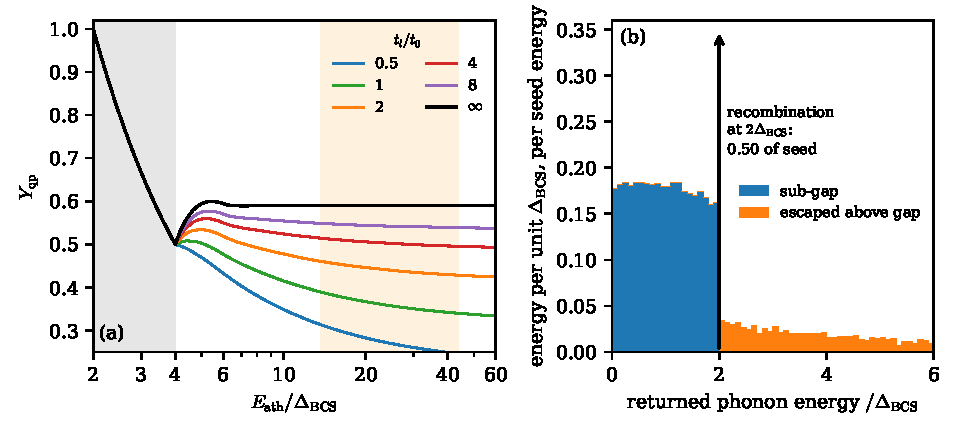
\includegraphics[width=\linewidth]{figures/ch20/fig20_4.pdf}
  \caption{Quasiparticle yield of an aluminum film from the Kaplan cascade in a lumped film at zero temperature, \cref{eq:20.4-cascade}, with $\alpha^2F \propto E_{\mathrm{ath}}^2$ and the pair-breaking time \cref{eq:20.4-tpb}. (a) Yield $Y_{\mathrm{qp}} = \Delta_{\mathrm{BCS}}\langle N_{\mathrm{qp}}\rangle/E_{\mathrm{ath}}$ of a phonon that has broken its first pair, against its energy in units of the gap, for six ratios of the film escape time to the pair-breaking time at threshold, $t_l/t_0$. Gray: below $4\Delta_{\mathrm{BCS}}$, where $Y_{\mathrm{qp}} = 2\Delta_{\mathrm{BCS}}/E_{\mathrm{ath}}$ exactly for every film. Tan: 2.45 to \SI{7.88}{meV}, or 13.6 to $43.8\,\Delta_{\mathrm{BCS}}$ at $\Delta_{\mathrm{BCS}} = \SI{0.18}{meV}$ (0.59 to \SI{1.91}{THz}), the band that holds the middle \SI{80}{\percent} of the primary-phonon energy absorbed in the mean-field silicon detector of \cref{sec:20.5-meanfield}. (b) Energy spectrum of the phonons that a thick film ($t_l/t_0 = 4$) returns to the substrate when a phonon of $40\Delta_{\mathrm{BCS}}$ cascades in it, per unit energy and per unit seed energy (event simulation, 4000 events). Blue: sub-gap relaxation phonons; orange: phonons above $2\Delta_{\mathrm{BCS}}$ that escape before breaking a pair. Arrow: the share 0.50 held by quasiparticles, which comes back later as recombination phonons of $2\Delta_{\mathrm{BCS}}$.}
  \label{fig:20-yield}
\end{figure}

Kinetic equations follow the same physics with fewer approximations. Chang and Scalapino wrote coupled Boltzmann equations for the quasiparticle distribution $f(E)$ and the phonon distribution $n(E_{\mathrm{ath}})$ of a superconductor, with the full energy dependence of the rates at finite temperature and the recombination of quasiparticles into $2\Delta_{\mathrm{BCS}}$ phonons~\cite{chang1977kinetic,chang1978nonequilibrium}. Guruswamy et al.\ solved them in steady state, with the phonon loss time $t_l$, for an aluminum film driven by photons of 2 to $10\Delta_{\mathrm{BCS}}$. They used the measured Eliashberg function, $T/T_c = 0.1$ and a weak microwave probe of the kind that reads out a resonator~\cite[Fig.~4]{guruswamy2014quasiparticle}. The cascade \cref{eq:20.4-cascade} is their equations linearized about the empty superconductor at zero temperature, with $\alpha^2F$ replaced by its low-frequency form, and the difference between the two measures what the linearization and the low-frequency $\alpha^2F$ leave out. \Cref{lim:20.4a} compares them for a photon seed, so that like is compared with like. For $t_l/t_0 \le 4$ the kinetic equations lie above the cascade by 0.001 to 0.011 at every energy from 5 to $10\Delta_{\mathrm{BCS}}$. For $t_l/t_0 = 8$ the offset is 0.036 to 0.041, nearly constant in energy, and the kinetic equations return 0.59 to 0.61 there, close to the infinite-volume value. The probe itself raises the yield by about \SI{2}{\percent}~\cite[Sect.~V]{guruswamy2014quasiparticle}. Counting the excess energy of the quasiparticles above the gap, rather than $\Delta_{\mathrm{BCS}}$ for each, would raise it by about \SI{4}{\percent}~\cite[Sect.~V]{guruswamy2014quasiparticle}; \cref{eq:20.4-Y} uses the gap-edge count, as they do.

\begin{limitbox}[Pair-breaking efficiency][lim:20.4a]
A pair-breaking quantum of energy $E_{\mathrm{ath}}$ between $2\Delta_{\mathrm{BCS}}$ and $4\Delta_{\mathrm{BCS}}$ yields $Y_{\mathrm{qp}} = 2\Delta_{\mathrm{BCS}}/E_{\mathrm{ath}}$, independent of the film; the infinite-volume yield at high energy is 0.57 to 0.6~\cite[pp.~2, 5]{guruswamy2014quasiparticle}.
\par\smallskip
{\centering
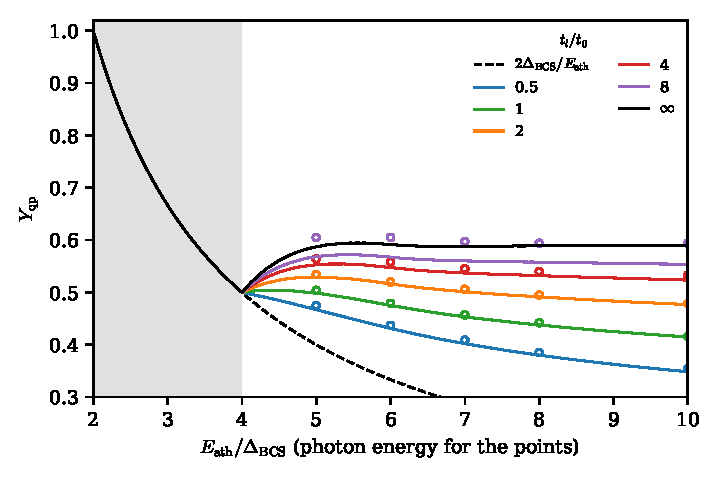
\includegraphics[width=\linewidth]{figures/ch20/limit20_4a.pdf}
\captionof{figure}{Yield of an aluminum film against the energy of the pair-breaking quantum in units of the gap. Dashed: $2\Delta_{\mathrm{BCS}}/E_{\mathrm{ath}}$, \cref{eq:20.4-below}. Lines: the Kaplan cascade \cref{eq:20.4-cascade} in a lumped film at zero temperature with $\alpha^2F \propto E_{\mathrm{ath}}^2$, for a photon seed (case-II split), at the ratios $t_l/t_0$ of the escape time to the pair-breaking time at threshold given in the legend. Circles: the coupled kinetic equations of Chang and Scalapino with the measured $\alpha^2F$ of aluminum at $T/T_c = 0.1$ with a microwave probe, read off~\cite[Fig.~4]{guruswamy2014quasiparticle} at the same $t_l/t_0$ (colors; digitized to $\pm0.005$). Gray: $E_{\mathrm{ath}} < 4\Delta_{\mathrm{BCS}}$, where the formula is exact. For $t_l/t_0 \le 4$ the cascade lies below the circles by at most 0.011; for $t_l/t_0 = 8$, by 0.036 to 0.041.}\label{fig:20-limit-qp}
\par}
\smallskip
Above $4\Delta_{\mathrm{BCS}}$ pair-breaking emission sets in, and the yield depends on $t_l/t_0$ with no closed form.
\end{limitbox}

For detector phonons the energy dependence matters more than any single value. In the mean-field silicon detector of \cref{sec:20.5-meanfield} the middle \SI{80}{\percent} of the absorbed primary energy arrives between 2.45 and \SI{7.88}{meV}, or 13.6 to $43.8\,\Delta_{\mathrm{BCS}}$ in aluminum, the tan band of \cref{fig:20-yield}(a). Across that band the yield falls by \SI{21.5}{\percent} for $t_l/t_0 = 0.5$, by \SI{7.0}{\percent} for $t_l/t_0 = 2$ and by \SI{1.9}{\percent} for $t_l/t_0 = 8$, and it is flat without escape. Luke phonons, which reach the film softer, are read with the yield near and below four gaps, and primary phonons with the yield of the band. This is the film's contribution to the collection ratio $\mathfrak{r}_{\mathrm{coll}}$ of \cref{sec:19.5}, and \cref{sec:20.5} combines it with transport in the crystal. For the thin, clean aluminum films of resonator measurements, Guruswamy et al.\ estimate $t_l/t_0 \approx 0.5$~\cite[p.~3]{guruswamy2014quasiparticle}. There the film costs \SI{41}{\percent} of the infinite-volume yield at $10\Delta_{\mathrm{BCS}}$, the top of the range they computed, and 47 to \SI{58}{\percent} across the band. The \SI{60}{nm} film of \cref{we:20-escape} loses 35 to \SI{50}{\percent} there, and a thicker film loses less, since $t_l \propto d_{\mathrm{f}}$ (\cref{sec:20.3}).

\subsection{Recombination phonons from the electrodes}\label{sec:20.4-electrode}

A carrier that reaches an aluminum electrode gives up its energy relative to the Fermi level of the electrode as phonons at the contact (\cref{sec:19.5}). For a Fermi level near midgap this is about half the band gap of the crystal plus the kinetic energy of the carrier. The CDMS~II analysis calls these phonons recombination phonons~\cite[Sect.~2]{agnese2018nuclear}. In a germanium detector at \SI{3}{V} they carry \SI{13}{\percent} of the phonon signal of an electron recoil, ``in a low frequency, ballistic regime that is used to provide a surface-event discriminator''~\cite[p.~17]{leman2012invited}. The Kaplan cascade explains why they are soft.

The energy enters the aluminum as a hot electron, far above the Debye energy. It relaxes within the metal by emitting phonons, which break pairs in a fraction of $t_0$ by \cref{eq:20.4-tpb}, and the cascade carries the energy down to the gap before much of it can escape. What leaves the film is of three kinds. Sub-gap phonons, below $2\Delta_{\mathrm{BCS}}$, are emitted by every quasiparticle on its way to the edge. Phonons above $2\Delta_{\mathrm{BCS}}$ escape before they break a pair, mostly within a few gaps of threshold, where $t_{\mathrm{pb}}$ is longest. Last, quasiparticles at the edge recombine much later, two at a time, into phonons of $2\Delta_{\mathrm{BCS}}$. In a thick film these may break pairs again and be re-emitted, but every re-emitted phonon still has $2\Delta_{\mathrm{BCS}}$. \Cref{fig:20-yield}(b) shows the spectrum for a seed of $40\Delta_{\mathrm{BCS}}$ and $t_l/t_0 = 4$. Counting the quasiparticle energy as recombination phonons at $2\Delta_{\mathrm{BCS}}$, \SI{85}{\percent} of the returned energy lies at or below $2\Delta_{\mathrm{BCS}}$ and \SI{96}{\percent} below $10\Delta_{\mathrm{BCS}}$. For $t_l/t_0 = 8$ the fractions are 92 and \SI{98}{\percent}. A seed of $20\Delta_{\mathrm{BCS}}$ changes them by less than 0.02. The hot-electron stage above the seed adds almost nothing to what leaves: by \cref{eq:20.4-ppb}, a phonon of $200\Delta_{\mathrm{BCS}}$, near the Debye energy of aluminum, escapes unabsorbed with a probability of \SI{0.4}{\percent} at $t_l/t_0 = 4$.

The scale is set by the gap of the electrode, not by the crystal. $2\Delta_{\mathrm{BCS}}$ of aluminum is \SI{0.36}{meV} or \SI{87}{GHz}, against the top of the germanium acoustic band, \SI{35.7}{meV} or \SI{8.64}{THz}~\cite[Table~I]{leman2012invited}, which sets the scale of its prompt phonons: a factor of 99. In the crystal such a phonon scatters on isotopes at the rate $B_{\mathrm{iso}}(E_{\mathrm{ath}}/h)^4$ of \cref{app:E.12}. With the constants of silicon and germanium~\cite[Table~I]{leman2012invited} this is \SI{140}{s^{-1}} and \SI{2.1e3}{s^{-1}}, mean free paths of \SI{39}{m} and \SI{1.5}{m} at the transverse sound speeds, while three-phonon decay of a longitudinal phonon, at $A_{\mathrm{anh}}(E_{\mathrm{ath}}/h)^5$, takes 0.1 to \SI{1}{s} in germanium for the spread of constants of \cref{sec:20.2-anh}, and longer in silicon. A recombination phonon therefore crosses a centimeter crystal ballistically and is absorbed only at surfaces, on a time set by the geometry and the coverage of the films. Its collection efficiency need not equal that of the hard primaries. This is the physical content of the ratio $\rho_g$ of \cref{sec:19.5}, the collection efficiency of the recombination phonons over that of the hard primaries, and it enters \cref{sec:20.5} as the contrast $\varpi_{\mathrm{gap}}$ of release at an electrode.

\subsection{Open problems}\label{sec:20.4-open}

The yield above four gaps rests on the lumped film. A phonon in a real film has a position and a direction, it is absorbed after a path that depends on its energy, and the quasiparticles diffuse. The thick-film offset of 0.04 between the cascade and the kinetic equations is not traced to one of the differences between them: finite temperature, the measured Eliashberg function, recombination and reabsorption of $2\Delta_{\mathrm{BCS}}$ phonons, or the probe. A transport simulation of the film that follows phonons and quasiparticles through its depth, at the temperature and with the $\alpha^2F$ of aluminum, would settle it, and no measurement of $Y_{\mathrm{qp}}$ at a fixed phonon energy in a film exists to test either calculation. The lumped film also loses every phonon that escapes; in a detector those phonons return to the crystal and can be absorbed again, which \cref{sec:20.5-sign} shows to cancel the effect of escape on the collection ratio. The yield of the electrode phonons depends on the same film model, and their share that is absorbed in the electrode itself, rather than returned, has not been measured.

\section{Collection kernels and recoil discrimination}\label{sec:20.5}

A silicon nucleus recoiling with \SI{100}{eV} makes 2.7 electron--hole pairs on average, at the measured yield $Y_q = 0.102$ and the \SI{3.8}{eV} per pair of the measurement~\cite[Eq.~(1), Table~II]{albakry2023first}; an electron recoil of the same energy makes 27. The rest of each deposit becomes phonons, and the phonon sensors see three populations: the primary phonons of the recoil, the Luke phonons of the drifting carriers, and the phonons that return the gap energy of the pairs (\cref{sec:19.5}). Charge readout separates the two recoils by the pair number, and 2.7 against 27 pairs is a separation of many standard deviations. Can a phonon readout do the same, either through the pair number, which sets the size of the Luke and gap-energy populations, or through a difference in the primary phonons themselves? Both routes depend on one object, the collection kernel of each sensor. From the kernels follows what fixes the sign of the collection ratio $\mathfrak{r}_{\mathrm{coll}} - 1$, which \cref{sec:19.5} left open, and the ceiling of a readout at high bias.

\subsection{Collection kernels}\label{sec:20.5-kernels}

Since the transport of \cref{sec:20.2,sec:20.3,sec:20.4} is linear in the birth spectrum (\cref{sec:20.2-prompt}), let a population $X \in \{\mathrm{prim}, \mathrm{Luke}, \mathrm{gap}\}$ be born at the event position $\vect{r}_{\mathrm{ev}}$ with the spectral energy density $u_X(E_{\mathrm{ath}})$ and the total energy $E_X = \int\dd E_{\mathrm{ath}}\,u_X$. Linearity then fixes the energy that sensor $s$ turns into quasiparticles as
\begin{equation}
  E_{s,X}(\vect{r}_{\mathrm{ev}}) = \int\dd E_{\mathrm{ath}}\;\mathfrak{C}_s(E_{\mathrm{ath}};\vect{r}_{\mathrm{ev}})\,u_X(E_{\mathrm{ath}}) ,
  \label{eq:20.5-kernel}
\end{equation}
where the collection kernel $\mathfrak{C}_s(E_{\mathrm{ath}};\vect{r}_{\mathrm{ev}})$ is the fraction of the energy of phonons born with energy $E_{\mathrm{ath}}$ at $\vect{r}_{\mathrm{ev}}$ that ends as quasiparticles in sensor $s$. It contains everything between birth and signal: down-conversion and isotope scattering in the substrate, transmission into the film and back with probabilities $\bar t_{12}$ and $\bar t_{\mathrm{esc}}$, pair breaking with the yield $Y_{\mathrm{qp}}$, and loss on bare faces and holders. A phonon below $2\Delta_{\mathrm{BCS}}$ of the film cannot break a pair there and returns to the crystal, and its energy stays in the kernel's bookkeeping until another surface takes it.

The kernels belong to the detector; the two recoils differ only in how much energy they put into each population and, possibly, in the spectrum of the primaries. Every readout quantity of \cref{sec:19.5} and of this section is a linear functional of the kernels. A detector with two sensor channels (two films, or the fast and slow parts of one pulse) has the channel fraction $a_X(\vect{r}_{\mathrm{ev}}) = E_{2,X}/(E_{1,X} + E_{2,X})$ for each population, where channel 2 is the one that favors soft phonons, and the efficiency $\epsilon_X = (E_{1,X} + E_{2,X})/E_X$.
\begin{keyresult}[Readout functionals of the collection kernels]
With the channel fractions $a_X$ and efficiencies $\epsilon_X$ built from \cref{eq:20.5-kernel},
\begin{gather}
  \varpi_O = \bigl\langle a_{\mathrm{Luke}} - a_{\mathrm{prim}}\bigr\rangle_{\vect{r}} , \qquad
  \varpi_{\mathrm{gap}} = \bigl\langle a_{\mathrm{gap}} - a_{\mathrm{prim}}\bigr\rangle_{\vect{r}} , \nonumber\\
  \sigma_{\mathrm{pos}}^2 = \operatorname{Var}_{\vect{r}}\bigl[a_{\mathrm{prim}}(\vect{r}_{\mathrm{ev}}) - \hat a(\hat{\vect{r}}_{\mathrm{ev}})\bigr] , \qquad
  \mathfrak{r}_{\mathrm{coll}} = \frac{\epsilon_{\mathrm{Luke}}}{\epsilon^{\mathrm{ER}}_{\mathrm{prim}}} ,
  \label{eq:20.5-functionals}
\end{gather}
where $\langle\cdot\rangle_{\vect{r}}$ and $\operatorname{Var}_{\vect{r}}$ average over the event positions of the calibration, and $\hat a(\hat{\vect{r}}_{\mathrm{ev}})$ is the channel fraction predicted from the position $\hat{\vect{r}}_{\mathrm{ev}}$ reconstructed from the pulses. The collection contrasts $\varpi_O$ and $\varpi_{\mathrm{gap}}$ say how differently a channel sees Luke and gap-energy phonons from primaries; the position spread $\sigma_{\mathrm{pos}}$ is the part of the primary channel fraction that the position correction leaves.
\end{keyresult}
\noindent A detector is therefore characterized for every population and every recoil by two kernels on the plane $(E_{\mathrm{ath}}, \vect{r}_{\mathrm{ev}})$. The collection ratio of \cref{sec:19.5} compares two populations of the same detector, so its sign depends only on how the kernels weigh soft Luke phonons against the hard primaries that arrive after down-conversion.

The kernels of a real detector are a transport calculation. A transport Monte Carlo follows phonons launched as monochromatic sources on a grid of energies and positions, which is what turns the tallies into kernels, and \cref{app:E.25} specifies the grids, the two geometries, the acceptance tests and the pitfalls. Two of the pitfalls decide the result. Luke birth spectra must come from the carrier transport at each field, and the fate of phonons below $2\Delta_{\mathrm{BCS}}$ must be stated with every result. No kernel of a real detector has been computed, and transport codes are not yet validated against the relations of this chapter (\cref{sec:20.1-open}).

\subsection{Mean-field kernels}\label{sec:20.5-meanfield}

One limit reduces the kernels to a linear equation in energy alone. If phonons cross the crystal many times before a surface absorbs them, the population forgets where it was born, and the kernels lose their dependence on $\vect{r}_{\mathrm{ev}}$. This holds when the diffusion time across the crystal is short compared with the absorption time, and when the faces scatter diffusely, so that every phonon of energy $E_{\mathrm{ath}}$ hits them at the same rate. In a slab of thickness $d$ an isotropic phonon with speed $v$ hits one of the two faces at the rate $v/2d$, since the mean of $|v_z|$ is $v/2$. Let a fraction $c_s$ of the face area carry film $s$, with transmission $\bar t$ into it and pair-breaking threshold $2\Delta_s$, and let a phonon that hits a bare face be lost with probability $\ell_{\mathrm{bare}}$. The absorption rate per phonon is then
\begin{equation}
  \varGamma_{\mathrm{abs}}(E_{\mathrm{ath}}) = \frac{\bar v}{2d}\Bigl[\sum_s c_s\,\bar t\,\Theta(E_{\mathrm{ath}} - 2\Delta_s) + \Bigl(1 - \sum_s c_s\Bigr)\ell_{\mathrm{bare}}\Bigr] ,
  \label{eq:20.5-Gabs}
\end{equation}
with $\bar v$ the number-weighted mean speed of the mixed population and $\Theta$ the step function. Down-conversion acts at the mean rate $f_{\mathrm{LA}}\varGamma_{\mathrm{anh}}(E_{\mathrm{ath}})$ of \cref{sec:20.2-scaling}, since only longitudinal phonons decay and isotope scattering keeps their share at $f_{\mathrm{LA}}$, and a decay at $E'$ passes the energy fraction $y$ to its daughters with the energy-weighted distribution $P_{\mathrm{d}}(y)$ of \cref{eq:20.2-frag}. The number of daughters in $\dd E$ is then $P_{\mathrm{d}}(E/E')\,\dd E/E$, and the time-integrated number spectrum $\mathcal{N}(E_{\mathrm{ath}})$ of a population with birth number spectrum $n_0$ obeys
\begin{equation}
  \bigl[\varGamma_{\mathrm{abs}}(E) + f_{\mathrm{LA}}\varGamma_{\mathrm{anh}}(E)\bigr]\mathcal{N}(E) = n_0(E) + \int_E^\infty\frac{\dd E'}{E}\,P_{\mathrm{d}}\Bigl(\frac{E}{E'}\Bigr)f_{\mathrm{LA}}\varGamma_{\mathrm{anh}}(E')\,\mathcal{N}(E') ,
  \label{eq:20.5-meanfield}
\end{equation}
with $E \equiv E_{\mathrm{ath}}$. Integrating the time-dependent equation for the number spectrum from zero to infinity gives \cref{eq:20.5-meanfield}, since every phonon is eventually absorbed or lost. The equation is triangular, because daughters are softer than their parent, and it is solved from the top energy down. Sensor $s$ receives $\int\dd E\,E\,\varGamma_s(E)\mathcal{N}(E)\,Y_{\mathrm{qp},s}(E)$, where $\varGamma_s$ is its term in \cref{eq:20.5-Gabs}. The mean-field kernel is this quantity for a monochromatic source, divided by its energy.

For an estimate we take a silicon slab \SI{4}{mm} thick, the thickness of a gram-scale detector with an eV-scale threshold~\cite[Sect.~IV]{ren2021design}. The isotropic sound speeds $c_{\mathrm{LA}} = \SI{9.00}{km/s}$ and $c_{\mathrm{T}} = \SI{5.40}{km/s}$ of \cref{app:C.18} give $\bar v = \SI{5.75}{km/s}$; we take $f_{\mathrm{LA}} = 0.093$ and $A_{\mathrm{anh}} = \SI{7.41e-56}{s^4}$, the silicon values of \cref{sec:20.2}, and the stand-in $P_{\mathrm{d}}(y) = 60\,y^3(1 - y)^2$. Two films cover \SI{5}{\percent} of the face area each: one with the niobium-like threshold $2\Delta_s = \SI{3.0}{meV}$, one of aluminum with \SI{0.36}{meV}. We take $\bar t = 0.9$, close to the acoustic-mismatch average 0.938 for silicon into aluminum (\cref{sec:20.3}), and $\ell_{\mathrm{bare}} = 10^{-3}$, the loss per surface bounce measured in CDMS detectors~\cite[Sect.~III\,G]{leman2012invited}. The film yield is the Kaplan cascade of \cref{sec:20.4} in units of each film's gap, run to $120\Delta_s$ and held there above, which affects \SI{0.1}{\percent} of the primary energy in aluminum. In a film from which phonons escape, with the ratio $t_l/t_0$ of \cref{sec:20.3}, $\bar t$ is multiplied by the probability $p_{\mathrm{pb}}$ of \cref{eq:20.4-ppb} that an entering phonon breaks a pair before it leaves, and the yield is that of \cref{fig:20-yield}. A phonon that escapes unbroken re-enters the crystal unchanged, and so do the phonons a film emits after its first pair break, its relaxation phonons and the hot phonons that escape: they return to the crystal with the spectrum the cascade gives them and can be absorbed again, so that energy is conserved. Only returned phonons below $2\Delta_{\mathrm{BCS}}$ of aluminum, which no film absorbs, end on the bare faces. The primaries are born at the top of the acoustic band, \SI{62}{meV}, since their spectrum is forgotten long before they are absorbed (\cref{sec:20.2}).

The primaries come out nearly balanced between the two films. They are absorbed within \SI{15}{\micro s}, by then down-converted to a mean energy of \SI{5.0}{meV} weighted by the absorbed energy (\SI{4.0}{meV} weighted by number), and on first absorption the niobium-like film takes \SI{40.7}{\percent} of their energy, aluminum \SI{58.2}{\percent}, and the bare faces \SI{1.2}{\percent}. Aluminum gets more because \SI{18}{\percent} of the absorbed energy arrives below \SI{3}{meV}, where only aluminum absorbs. The middle \SI{80}{\percent} of it arrives between 2.45 and \SI{7.88}{meV}, the band of \cref{fig:20-yield}(a). The relaxation phonons of the niobium-like film lie below its \SI{3}{meV} threshold but mostly above that of aluminum, and the aluminum film collects them on their return. In thick films the primaries therefore have the channel fraction $a_{\mathrm{prim}} = 0.610$ and the efficiency $\epsilon_{\mathrm{prim}} = 0.684$; deleting those phonons, as a lumped film does, would give 0.563 and 0.610.

The Luke phonons are softer, and their spectrum is the open input. For a carrier at one speed, \cref{sec:20.1-luke} gives an emitted energy weighted as $E_{\mathrm{ath}}^3$ up to $E_{\mathrm{L}}^{\max} = \frac43\langle E_{\mathrm{L}}\rangle$, so that the fraction $(x/E_{\mathrm{L}}^{\max})^4$ of it lies below any $x$. A transport Monte Carlo gives $\langle E_{\mathrm{L}}\rangle = \SI{0.84}{meV}$ for silicon electrons at \SI{1}{V/cm}, and 0.84 to \SI{4.6}{meV} over 1 to \SI{100}{V/cm}. We scan 0.75 to \SI{4.7}{meV}, a range that also covers germanium electrons at low field. Real carriers do not drift at one speed: they accelerate in the field, emit, and accelerate again, and transverse phonons, which the one-branch rate leaves out, are emitted softer. Both put more energy at low $E_{\mathrm{ath}}$. We therefore use two shapes, labeled by $\langle E_{\mathrm{L}}\rangle$: the one-speed spectrum, and a flat number spectrum up to $2\langle E_{\mathrm{L}}\rangle$ for a spread of speeds, which puts the fraction $(x/2\langle E_{\mathrm{L}}\rangle)^2$ of the energy below $x$. Which shape and which mean a drifting carrier produces at a given field is still open (\cref{sec:20.1-open}). As a reference, in the strong near-surface fields of germanium detectors the Luke phonons have about \SI{300}{GHz} for electrons and \SI{700}{GHz} for holes~\cite[Sect.~1]{hertel2012phonon}, 1.2 and \SI{2.9}{meV}, and in the low bulk field they are softer.

\begin{figure}[tbp]
  \centering
  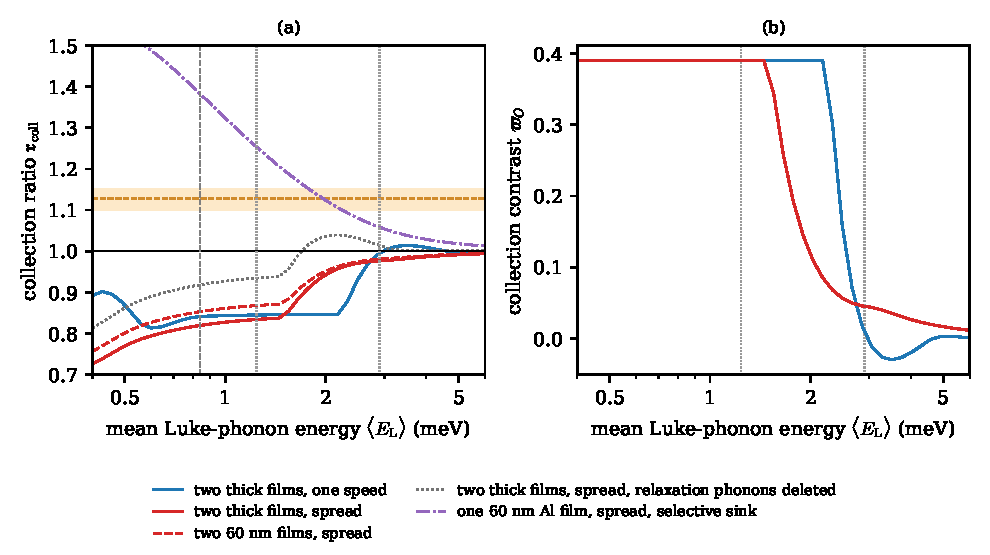
\includegraphics[width=\linewidth]{figures/ch20/fig20_rcoll.pdf}
  \caption{Mean-field collection of Luke phonons in a silicon slab \SI{4}{mm} thick, against the mean Luke-phonon energy. (a) Collection ratio $\mathfrak{r}_{\mathrm{coll}}$ of \cref{eq:20.5-functionals}. Solid: two thick films ($2\Delta_s = 3.0$ and \SI{0.36}{meV}, each on \SI{5}{\percent} of the face area) with the Kaplan-cascade yield of \cref{sec:20.4}, every phonon a film emits returned to the crystal, for the Luke spectrum of a carrier at one speed (blue, number density $\propto E_{\mathrm{ath}}^2$) and for a spread of speeds (red, flat number density up to $2\langle E_{\mathrm{L}}\rangle$). Red dashed: two \SI{60}{nm} films ($t_l/t_0 = 0.72$), spread, phonons returned. Gray dotted: two thick films, spread, with the phonons a film emits after its first pair break deleted. Purple dash-dotted: one \SI{60}{nm} aluminum film on \SI{10}{\percent} of the face area, spread, with the same deletion, a selective sink that the model does not identify in a detector (upper envelope). In all curves phonons below $2\Delta_{\mathrm{BCS}} = \SI{0.36}{meV}$ are reflected by the films and eventually lost. Tan band and dashed line: 1.099 to 1.152 and 1.128, the collection ratio that explains the silicon phonon-yield ratio of \cref{sec:19.5} with no stored energy. Vertical dashed line: \SI{0.84}{meV}, silicon electrons at \SI{1}{V/cm}; dotted: 1.24 and \SI{2.9}{meV}, the near-surface Luke energies of germanium~\cite{hertel2012phonon}. (b) Collection contrast $\varpi_O$ of the two thick films with phonons returned (channel 2 is the aluminum film), same colors. Model: transmission 0.9 into each film, bare-face loss $10^{-3}$ per hit, $\bar v = \SI{5.75}{km/s}$, $f_{\mathrm{LA}} = 0.093$, $A_{\mathrm{anh}} = \SI{7.41e-56}{s^4}$, $P_{\mathrm{d}}(y) = 60\,y^3(1 - y)^2$; primaries born at \SI{62}{meV}, absorbed in the two thick films with $\epsilon_{\mathrm{prim}} = 0.684$, $a_{\mathrm{prim}} = 0.610$.}
  \label{fig:20-rcoll}
\end{figure}

\Cref{fig:20-rcoll}(b) shows the contrast this geometry gives. While the whole Luke spectrum lies below the \SI{3}{meV} threshold of the niobium-like film, only aluminum absorbs Luke phonons, $a_{\mathrm{Luke}} = 1$, and $\varpi_O = 1 - a_{\mathrm{prim}} = 0.39$. As the mean energy rises, the Luke spectrum reaches above \SI{3}{meV} and the contrast falls: for the spread of speeds it is 0.12 at \SI{2}{meV}, 0.045 at \SI{2.9}{meV} and 0.019 at \SI{4.7}{meV}. In the mean-field limit the position spread vanishes by construction, so it is the first number a computed kernel adds.

\subsection{The sign of the collection ratio}\label{sec:20.5-sign}

The collection ratio differs from one through the part of the Luke spectrum within a few gaps of the aluminum threshold, since the primaries arrive at several meV. Luke energy below $2\Delta_{\mathrm{BCS}}$ of aluminum breaks no pairs; it is lost unless a tungsten sensor or another film absorbs it. Luke energy between $2\Delta_{\mathrm{BCS}}$ and $4\Delta_{\mathrm{BCS}}$ is converted with $Y_{\mathrm{qp}} = 2\Delta_{\mathrm{BCS}}/E_{\mathrm{ath}}$ in every film, above 0.59 below \SI{0.61}{meV} and down to 0.5 at $4\Delta_{\mathrm{BCS}}$ (\cref{sec:20.4}). Above four gaps a thick film converts with 0.59 to 0.60; a film from which phonons escape converts the primaries, at 14 to $44\,\Delta_{\mathrm{BCS}}$, with less than the soft Luke phonons on first absorption, but the phonons it lets out return to the crystal. And a phonon that only one film absorbs bounces longer before it is absorbed, and loses more on the bare faces.

The first two effects act alone in a detector with a single film type. Let $s_{\mathrm{sub}}$ be the share of Luke energy born below $2\Delta_{\mathrm{BCS}}$. Let sub-gap phonons be absorbed at the same rate as the others and converted with the weight $\kappa_{\mathrm{sub}}\bar Y_{\mathrm{prim}}$, where $\bar Y_{\mathrm{prim}}$ is the mean yield of the primaries as they are absorbed, and $\kappa_{\mathrm{sub}} = 0$ if they are lost and 1 if they are absorbed like hard phonons. Define the near-gap gain
\begin{equation*}
  s_{\mathrm{ng}} = \frac{1}{E_{\mathrm{Luke}}}\int_{2\Delta_{\mathrm{BCS}}}^\infty\dd E_{\mathrm{ath}}\;u_{\mathrm{Luke}}(E_{\mathrm{ath}})\Bigl[\frac{Y_{\mathrm{qp}}(E_{\mathrm{ath}})}{\bar Y_{\mathrm{prim}}} - 1\Bigr] .
\end{equation*}
If every phonon above the threshold reaches the film with the same probability per bounce, whatever its energy, the absorbed fraction is common to both populations and cancels in the ratio. The primaries are converted with $\bar Y_{\mathrm{prim}}$, the Luke phonons with $Y_{\mathrm{qp}}(E_{\mathrm{ath}})$ above the threshold and with $\kappa_{\mathrm{sub}}\bar Y_{\mathrm{prim}}$ below it, and
\begin{equation}
  \mathfrak{r}_{\mathrm{coll}} - 1 = s_{\mathrm{ng}} - (1 - \kappa_{\mathrm{sub}})\,s_{\mathrm{sub}} \qquad \text{(one film type)} .
  \label{eq:20.5-sign}
\end{equation}

The sub-gap share is fixed by the Luke spectrum alone. For the one-speed spectrum it is $s_{\mathrm{sub}} = 0.085$ at $\langle E_{\mathrm{L}}\rangle = \SI{0.5}{meV}$, 0.017 at \SI{0.75}{meV}, 0.011 at \SI{0.84}{meV} and $5\times10^{-3}$ at \SI{1}{meV}; for the spread of speeds 0.13, 0.058, 0.046 and 0.032, and still 0.008 at \SI{2}{meV}. In a thick film $\bar Y_{\mathrm{prim}} = 0.590$, and the near-gap gain is small: $+0.002$ for the one-speed spectrum and $+0.018$ for the spread of speeds at \SI{0.75}{meV}, since the cascade yield lies above 0.59 between 5 and $8\Delta_{\mathrm{BCS}}$ and below it near $4\Delta_{\mathrm{BCS}}$. With sub-gap phonons lost, one thick aluminum film then has $\mathfrak{r}_{\mathrm{coll}} = 0.985$ and 0.960 at \SI{0.75}{meV} and 0.994 and 0.968 at \SI{0.84}{meV}, below one by about $s_{\mathrm{sub}}$. If the sensor absorbs the sub-gap phonons, that term vanishes, and $\mathfrak{r}_{\mathrm{coll}} = 1.002$ to 1.018 between 0.75 and \SI{1}{meV}.

Escape does not change this when the phonons a film lets out return to the crystal. A returned phonon reaches a film again and continues the same cascade, so escape followed by return only delays it. For one aluminum film the solve gives the thick-film values within 0.002 at every $t_l/t_0$ down to the \SI{60}{nm} of \cref{we:20-escape}, 0.995 and 0.969 at \SI{0.84}{meV}. This is a numerical result, not an identity: bare-face loss and decay on the return path break it, and it holds at the bare-face loss of $10^{-3}$. A sink without signal that takes every phonon, modeled by raising the bare-face loss to 0.3 per hit, lowers $\epsilon_{\mathrm{prim}}$ to 0.08 and moves $\mathfrak{r}_{\mathrm{coll}}$ of the \SI{60}{nm} film only to 1.023 and 0.988. A large rise needs a selective sink, one that removes the phonons a film emits after its first pair break and leaves those that have not yet entered a film. The lumped film of \cref{sec:20.4} makes exactly that assumption. With it, the primaries are read at the yield of the band, about 0.50 at $t_l/t_0 = 4$ and 0.32 at 0.72, while the soft Luke energy keeps $2\Delta_{\mathrm{BCS}}/E_{\mathrm{ath}}$; the near-gap gain at \SI{0.75}{meV} becomes $+0.13$ and $+0.11$ at $t_l/t_0 = 4$ and $+0.61$ and $+0.49$ at 0.72, and one aluminum film at \SI{0.84}{meV} reaches 1.05 to 1.10 at $t_l/t_0 = 4$, about \SI{300}{nm}, and 1.30 to 1.53 at \SI{60}{nm}. These values are an upper envelope of the lumped-film assumption; the estimate does not identify a physical sink in a detector that would realize it.

The two-film geometry adds the third effect. Luke phonons below \SI{3}{meV} reach only the aluminum film, so they stay \SI{30}{\micro s} in the crystal against \SI{15}{\micro s} for phonons that both films absorb, and they lose twice as much on the bare faces, \SI{2.0}{\percent} against \SI{1.0}{\percent}. With a flat yield of 0.59 above each threshold and sub-gap phonons absorbed by the aluminum sensor, this alone gives $\mathfrak{r}_{\mathrm{coll}} = 0.992$, and with sub-gap phonons lost 0.935 at \SI{0.75}{meV} to 0.998 at \SI{4.7}{meV} for the spread of speeds. The film cascade with its returned phonons lowers these values further. The primaries reach the niobium-like film in large part, and its relaxation phonons, below \SI{3}{meV}, return and are collected by the aluminum film, which raises $\epsilon_{\mathrm{prim}}$ to 0.684; Luke phonons below \SI{3}{meV} gain nothing of the kind. Two thick films then give 0.83 and 0.81 at \SI{0.75}{meV} (one speed and spread), 0.84 and 0.82 at \SI{0.84}{meV}, and rise to 1.01 near \SI{3.5}{meV} for one speed, once the Luke spectrum itself reaches the niobium-like threshold. Two \SI{60}{nm} films give 0.85 to 1.01 over 0.75 to \SI{4.7}{meV}.

With every phonon a film emits returned to the crystal and energy conserved, the mean-field estimate lies between 0.81 and 1.02 over 0.75 to \SI{4.7}{meV}, one or two films, any film thickness from \SI{60}{nm} up, sub-gap phonons lost or absorbed, and between 0.82 and 1.01 at the \SI{0.84}{meV} of silicon electrons at \SI{1}{V/cm}. A signal-free sink acting on all phonons keeps it below 1.03. The collection ratio 1.128, with its band 1.099 to 1.152, that would explain the CDMS~II silicon phonon-yield ratio with no stored energy (\cref{sec:19.5}) therefore lies above the transport estimate; only the selective sink of the lumped film reaches it. Only computed kernels for real detector geometries can exclude collection as the whole explanation, and the two-bias measurement of \cref{sec:19.5} decides between collection and stored energy.

\subsection{Phonon signatures of the recoil type}\label{sec:20.5-routes}

A phonon readout separates the two recoils through an observable $O_{\mathrm{obs}}$ of each event, such as the channel fraction $E_2/(E_1 + E_2)$ or the share of the pulse in a fast window. At equal total phonon energy, the separation
\begin{equation}
  \mathcal{S}_{\mathrm{sep}} = \frac{\bigl|\langle O_{\mathrm{obs}}\rangle_{\mathrm{NR}} - \langle O_{\mathrm{obs}}\rangle_{\mathrm{ER}}\bigr|}{\bigl[\tfrac12\bigl(\sigma_{\mathrm{NR}}^2 + \sigma_{\mathrm{ER}}^2\bigr)\bigr]^{1/2}} ,
  \label{eq:20.5-sep}
\end{equation}
measures the distance between the two distributions in units of their spreads, and we call a route useful where $\mathcal{S}_{\mathrm{sep}} \ge 2$. For two Gaussians of equal width cut at the midpoint, $\mathcal{S}_{\mathrm{sep}} = 2$ accepts \SI{84}{\percent} of one population and rejects \SI{84}{\percent} of the other, and a leakage of $10^{-3}$ needs $\mathcal{S}_{\mathrm{sep}} = 6.2$, so ``useful'' is far from background-free. Let $\varphi_X$ be the share of population $X$ in the signal. Since the shares sum to one, the channel fraction is $O_{\mathrm{obs}} = \sum_Xa_X\varphi_X = a_{\mathrm{prim}} + \varpi_O\,\varphi_{\mathrm{Luke}} + \varpi_{\mathrm{gap}}\,\varphi_{\mathrm{gap}}$ after the average over positions, and another observable linear in the delivered energies has the same form to first order in the contrasts. There is one route for each population.

\paragraph{Primary phonons.} The prompt phonons forget their polarization within a nanosecond, and a hard birth once $E_*(t)$ has fallen to about half its energy (\cref{sec:20.2-memory}). The soft energy remains. It is the share $f_{\mathrm{s}} = \SI{1.7}{\percent}$ of an electron recoil that its carriers shed below the optical phonon energy, \cref{eq:20.2-fs}. A nuclear recoil has $Y_q$ times as many pairs, and its lattice share is born near the optical and zone-boundary energies (\cref{sec:19.1}). If $E_{\mathrm{mem}}$ lies above the soft band and below every hard birth, \cref{eq:20.2-bound} then gives
\begin{equation}
  \bigl|\langle O_{\mathrm{obs}}\rangle_{\mathrm{NR}} - \langle O_{\mathrm{obs}}\rangle_{\mathrm{ER}}\bigr| \simeq \varpi_{\mathrm{soft}}\,\Delta_{\mathrm{soft}} , \qquad \Delta_{\mathrm{soft}} = (1 - Y_q)\,f_{\mathrm{s}} ,
  \label{eq:20.5-primary}
\end{equation}
with $\varpi_{\mathrm{soft}}$ the contrast of the channel between soft primaries and hard ones. This is an estimate, not a bound (\cref{sec:20.2-bound}). At \SI{100}{eV}, $\Delta_{\mathrm{soft}} = 0.015$. The spread includes the position spread, so $\mathcal{S}_{\mathrm{sep}} \le \varpi_{\mathrm{soft}}\Delta_{\mathrm{soft}}/\sigma_{\mathrm{pos}}$, and any $\sigma_{\mathrm{pos}}$ above $\Delta_{\mathrm{soft}}/2 = 0.008$ excludes a useful separation at every energy, even with a perfect selector, $\varpi_{\mathrm{soft}} = 1$. The selector is far from perfect: the soft births have a few meV, and the mean-field estimate of \cref{sec:20.5-meanfield} puts the energy of the hard primaries at a mean of \SI{5.0}{meV} when they are absorbed, so no film threshold separates the two bands. The pulse shapes of CDMS detectors depend strongly on how close the event lies to each instrumented face~\cite[Sect.~2]{hertel2012phonon}, and a position correction must reach the percent level before this route opens. Phonons born within the memory-loss distance of an instrumented face keep some memory, but they mark a position class, not a recoil type (\cref{sec:20.2-memory}). None of this holds for sapphire, where isotope mixing is slower than decay and the memory argument of \cref{sec:20.2} fails.

\paragraph{Gap energy at zero field.} Each pair carries $\Eg$ until it recombines, so an electron recoil holds $\Eg/\varepsilon_{\mathrm{eh}} = 0.312$ of its energy in pairs, a nuclear recoil $Y_q$ times as much (\cref{sec:19.5}). If this energy comes back later than the primaries, a sensor with two read windows $t_1 < t_2$, with all gap energy returned by $t_2$, sees the ratio $O_b = E_{\mathrm{sig}}(t_1)/E_{\mathrm{sig}}(t_2)$. With $f_{\mathrm{ret}}(t)$ the returned fraction of \cref{eq:19.5-release}, no stored energy and equal collection,
\begin{equation}
  \Delta O_b = \frac{\Eg}{\varepsilon_{\mathrm{eh}}}\Bigl\{\bigl[1 - f^{\mathrm{ER}}_{\mathrm{ret}}(t_1)\bigr] - Y_q\bigl[1 - f^{\mathrm{NR}}_{\mathrm{ret}}(t_1)\bigr]\Bigr\} .
  \label{eq:20.5-gap}
\end{equation}
For equal release laws this is $(1 - Y_q)(\Eg/\varepsilon_{\mathrm{eh}})(1 - f_{\mathrm{ret}}) = 0.28\,(1 - f_{\mathrm{ret}})$ at \SI{100}{eV}, twenty times the primary estimate. The route is a timing reading of the pair number, and its size and sign are set by kinetics that are not known at millikelvin. In the dense track of a nuclear recoil, exciton annihilation gives $1 - f^{\mathrm{NR}}_{\mathrm{ret}} = 1/(1 + t/t_{\mathrm{rel}})$, with $t_{\mathrm{rel}}$ the time scale set by the initial track density (\cref{eq:19.5-bimol}). Against an exponential release $\ee^{-t/t_{\mathrm{rel}}}$ of the electron recoil on the same time scale, $\Delta O_b$ changes sign at the root of $\ee^{-x}(1 + x) = Y_q$, which is $t_1 = 3.87\,t_{\mathrm{rel}}$ at $Y_q = 0.102$. The site matters as much as the time. Release in the bulk produces hard phonons that lose their memory, and contributes nothing to $\varpi_{\mathrm{gap}}$. Release at a surface or an electrode produces soft phonons that travel ballistically, like the recombination phonons that carry \SI{13}{\percent} of the phonon signal of germanium detectors at \SI{3}{V} (\cref{sec:20.4-electrode}). The zero-field gap-energy channel is therefore unresolved.

\paragraph{Luke phonons at low bias.} With a bias the Luke share differs between the recoils because the pair number does. Let all pairs be drifted, with $g = f_{\mathrm{det}}\,g_{\mathrm{Luke}}$. An electron recoil then has $\varphi_{\mathrm{Luke}} = g/(1 + g)$ and a nuclear recoil $Y_qg/(1 + Y_qg)$. The gap shares differ in the same way, so
\begin{equation}
  \Delta O_{\mathrm{obs}} = \frac{(1 - Y_q)\,\bigl(\varpi_O\,g + \varpi_{\mathrm{gap}}\Eg/\varepsilon_{\mathrm{eh}}\bigr)}{(1 + g)(1 + Y_qg)} .
  \label{eq:20.5-lowbias}
\end{equation}
The Luke term is largest at $g = Y_q^{-1/2}$, where it equals $\varpi_O(1 - Y_q^{1/2})/(1 + Y_q^{1/2})$: at \SI{100}{eV}, $0.516\,\varpi_O$ at $g = 3.1$, or \SI{13.4}{V} across a silicon crystal at $f_{\mathrm{det}} = 0.873$. Whether the contrast suffices depends on the spreads. We compare the two recoils at the same recoil energy, \SI{100}{eV}, with the pair numbers of the measured yield in pairs of $\varepsilon_{\mathrm{eh}}$, $Y'_q$ of \cref{sec:20.5-hv}. The spread of $O_{\mathrm{obs}}$ for each recoil is the position spread, the baseline $\sigma_{\mathrm{ph}} = \SI{2.65}{eV}$ of the gram-scale detector~\cite{ren2021design} divided by that recoil's $E_{\mathrm{ph}}$, and the fluctuation of its detected pair number, $\varpi_O(eV_{\mathrm{bias}}/E_{\mathrm{ph}})(F_{\mathrm{meas}}N_{\mathrm{det}})^{1/2}$, added in quadrature. The binomial form of the measured-charge Fano factor, $F_{\mathrm{meas}} = f_{\mathrm{det}}F + 1 - f_{\mathrm{det}}$ (\cref{sec:20.1-fano}), uses the measured $F_{\mathrm{eh}} = 0.119$ for electron recoils, the measured $F_{\mathrm{NR}} = 0.9$ at \SI{100}{eV}~\cite[Table~II]{albakry2023first}, and $f_{\mathrm{det}} = 0.873$, the complement of the \SI{12.7}{\percent} trapping probability in the detector model of the same measurement. With $\varpi_{\mathrm{gap}} = 0$, the smallest contrast that reaches $\mathcal{S}_{\mathrm{sep}} = 2$ at \SI{100}{eV} is $\varpi_O = 0.11$, 0.22 and 0.43 for $\sigma_{\mathrm{pos}} = 0.02$, 0.05 and 0.10, at biases of 10 to \SI{12}{V}. The mean-field contrast of about 0.4 for Luke spectra below \SI{1.5}{meV} is within reach of this requirement, but it is a model, not a measurement. The route reads the pair number with phonons. Its ceiling, with $\varpi_O = 1$ and no other spread, is reached as the bias goes to zero, and it is that of the charge yield itself, 10.8 at \SI{100}{eV}: the route carries no information beyond the charge yield.

The phonon pulse-shape rejection of SuperCDMS germanium detectors is of this kind. It rejects bulk electron recoils against nuclear recoils at better than 1 in $10^3$ at 7 to \SI{20}{keV}, limited by the statistics of the data~\cite[Sect.~3]{hertel2012phonon}, and its information comes from Luke phonons emitted in the strong field near the surfaces.

\subsection{The high-voltage readout ceiling}\label{sec:20.5-hv}

At \SI{100}{V} across a silicon crystal, $g_{\mathrm{Luke}} = 26.7$ and the Luke phonons dominate the signal. Detectors run this way read the pair number through the total phonon energy, $E_{\mathrm{ph}} = E_{\mathrm{prim}} + N_{\mathrm{det}}eV_{\mathrm{bias}}$ with $N_{\mathrm{det}}$ the detected pairs (\cref{sec:1.5}), and an electron recoil of the same $E_{\mathrm{ph}}$ is the background to a nuclear recoil. Suppose a second observable reads the Luke share perfectly, with $\varpi_O = 1$, no baseline noise and no position spread. Its separation is the most any phonon observable can extract from the pair number at high bias.

A nuclear recoil of energy $E_R$ makes on average $Y_qE_R/\varepsilon_{\mathrm{src}}$ pairs, where $\varepsilon_{\mathrm{src}} = \SI{3.8}{eV}$ is the energy per pair with which the measurement converted its charge into the yields~\cite[Eq.~(1)]{albakry2023first}; write $Y'_q = Y_q\varepsilon_{\mathrm{eh}}/\varepsilon_{\mathrm{src}}$, so that the pair number is $Y'_qE_R/\varepsilon_{\mathrm{eh}}$. Its phonon energy is $E_{\mathrm{ph}} = E_R(1 + gY'_q)$, with $g = f_{\mathrm{det}}g_{\mathrm{Luke}}$ and the primary phonon energy taken equal to the recoil energy, the truncation of \cref{lim:19.5a} that the measurement uses. The electron recoil with the same $E_{\mathrm{ph}}$ has the energy $E_R(1 + gY'_q)/(1 + g)$. Their mean detected pair numbers are
\begin{equation*}
  \langle N_{\mathrm{det}}\rangle_{\mathrm{NR}} = f_{\mathrm{det}}Y'_q\frac{E_R}{\varepsilon_{\mathrm{eh}}} , \qquad
  \langle N_{\mathrm{det}}\rangle_{\mathrm{ER}} = f_{\mathrm{det}}\frac{E_R}{\varepsilon_{\mathrm{eh}}}\,\frac{1 + gY'_q}{1 + g} ,
\end{equation*}
and their difference is $f_{\mathrm{det}}(E_R/\varepsilon_{\mathrm{eh}})(1 - Y'_q)/(1 + g)$. The Luke share at fixed $E_{\mathrm{ph}}$ is linear in $N_{\mathrm{det}}$, so its separation is that of $N_{\mathrm{det}}$, with variances $F^X_{\mathrm{eff}}\langle N_{\mathrm{det}}\rangle_X$.
\begin{keyresult}[High-voltage readout ceiling]
With an ideal readout of the Luke share at equal total phonon energy, the separation of nuclear from electron recoils is
\begin{equation}
  \mathcal{S}_{\mathrm{HV}} = \frac{(1 - Y'_q)\,(f_{\mathrm{det}}E_R/\varepsilon_{\mathrm{eh}})^{1/2}}{\bigl\{\tfrac12(1 + g)\bigl[F^{\mathrm{NR}}_{\mathrm{eff}}\,Y'_q(1 + g) + F^{\mathrm{ER}}_{\mathrm{eff}}(1 + gY'_q)\bigr]\bigr\}^{1/2}} , \qquad g = f_{\mathrm{det}}\,g_{\mathrm{Luke}} ,
  \label{eq:20.5-hv}
\end{equation}
with $F_{\mathrm{eff}} = f_{\mathrm{det}}F + 1 - f_{\mathrm{det}}$ when a trapped carrier induces nothing and $F_{\mathrm{eff}} = f_{\mathrm{det}}F$ when every pair induces the mean charge $f_{\mathrm{det}}e$. The cascade and partial-charge terms of \cref{eq:20.1-Fpos} lie between these limits.
\end{keyresult}
\noindent At zero gain \cref{eq:20.5-hv} is the separation of an ideal charge-and-heat measurement. As the bias grows it falls as $1/g$, because at equal total phonon energy a larger Luke gain makes the electron recoil smaller, and the two pair numbers converge. In silicon at \SI{220}{eV} the ceiling is 16.8 at zero bias, 10.7 at \SI{4}{V}, 3.4 at \SI{30}{V}, 1.22 at \SI{100}{V} and 0.43 at \SI{300}{V}.

\begin{workedexample}{The high-voltage ceiling at 220 eV}\label{we:20-ceiling}
The measured silicon yield at $E_R = \SI{220}{eV}$ is $Y_q = 0.108^{+0.009}_{-0.010}$, with the pair-number Fano factor $F_{\mathrm{NR}} = 0.5^{+0.2}_{-0.1}$~\cite[Table~II]{albakry2023first}. At \SI{100}{V}, $g_{\mathrm{Luke}} = 100/3.75 = 26.67$, and with $f_{\mathrm{det}} = 0.873$, $g = 23.28$. The yield in pairs of \SI{3.75}{eV} is $Y'_q = 0.108\times3.75/3.8 = 0.1066$, and $E_R/\varepsilon_{\mathrm{eh}} = 58.67$.

The nuclear recoil has $E_{\mathrm{ph}} = 220\times(1 + 23.28\times0.1066) = \SI{765.9}{eV}$, and the electron recoil with the same phonon energy has $765.9/24.28 = \SI{31.54}{eV}$. The mean detected pair numbers are $0.873\times0.1066\times58.67 = 5.459$ and $0.873\times31.54/3.75 = 7.343$, a difference of 1.885 pairs.

With trapped carriers inducing nothing, $F^{\mathrm{NR}}_{\mathrm{eff}} = 0.873\times0.5 + 0.127 = 0.5635$ and $F^{\mathrm{ER}}_{\mathrm{eff}} = 0.873\times0.119 + 0.127 = 0.2309$. The variances are $0.5635\times5.459 = 3.076$ and $0.2309\times7.343 = 1.695$, and
\begin{equation*}
  \mathcal{S}_{\mathrm{HV}} = \frac{1.885}{[\tfrac12(3.076 + 1.695)]^{1/2}} = 1.22 .
\end{equation*}
If every pair induces the mean charge instead, the trapping term drops out of both Fano factors and $\mathcal{S}_{\mathrm{HV}} = 1.50$; with full collection, $f_{\mathrm{det}} = 1$, it is 1.32. Even an ideal phonon observable cannot separate the two recoils at \SI{220}{eV} and \SI{100}{V}.
\end{workedexample}

\begin{figure}[tbp]
  \centering
  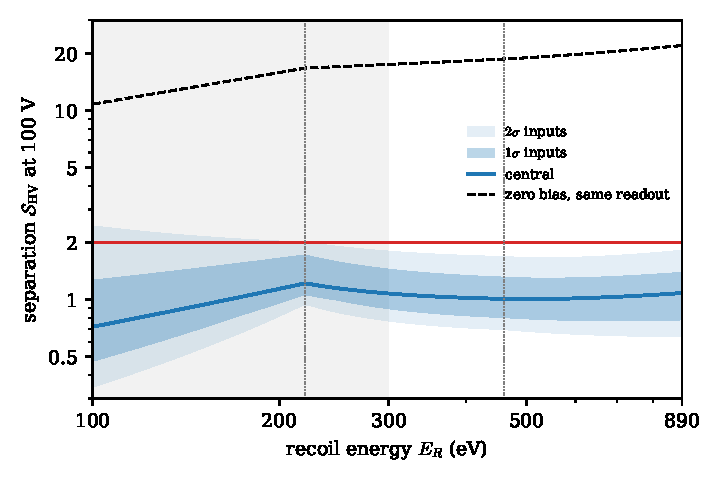
\includegraphics[width=0.8\linewidth]{figures/ch20/fig20_5.pdf}
  \caption{High-voltage readout ceiling $\mathcal{S}_{\mathrm{HV}}$ of \cref{eq:20.5-hv} for silicon recoils at \SI{100}{V}, against the recoil energy. Line: central measured yield and Fano factor~\cite[Table~II]{albakry2023first} at 100, 220, 460 and \SI{890}{eV} (dotted verticals), interpolated linearly in $\log E_R$; detected fraction $f_{\mathrm{det}} = 0.873$, trapped carriers inducing nothing; $F_{\mathrm{eh}} = 0.119$; $\varepsilon_{\mathrm{eh}} = \SI{3.75}{eV}$, yields defined with \SI{3.8}{eV} per pair. Dark band: the extremes over the corners of the $1\sigma$ bands of $Y_q$ and $F_{\mathrm{NR}}$, over $f_{\mathrm{det}} = 0.873$ and 1, and over the two limits of the induced-charge spread; light band: the same with $2\sigma$ bands. Dashed: the same ideal readout at zero bias. Red line: $\mathcal{S}_{\mathrm{HV}} = 2$. Gray: the range of the no-go statement, $E_R \le \SI{300}{eV}$.}
  \label{fig:20-ceiling}
\end{figure}

\Cref{fig:20-ceiling} extends the example over the measured range. At the central inputs the ceiling stays below 2 at every measured energy up to \SI{890}{eV}, with its maximum, 1.22, at \SI{220}{eV}; the Fano factor of nuclear recoils grows to 3.7 at \SI{890}{eV} and keeps it down. Over the $1\sigma$ bands of $Y_q$ and $F_{\mathrm{NR}}$ the largest value is 1.72, at \SI{220}{eV}, in the mean-charge limit. With $2\sigma$ bands the ceiling exceeds 2 from 100 to \SI{224}{eV}, up to 2.46 at \SI{100}{eV}, where the measured yield is least certain. The no-go of a high-voltage phonon readout at $E_R \le \SI{300}{eV}$ therefore rests on the measured $Y_q$ and $F_{\mathrm{NR}}$, which are not derived below the binary threshold of \cref{sec:19.2}, and on the collection, which moves the ceiling at \SI{220}{eV} between 1.22 and 1.50.

\subsection{Uncertainty budget of the readout}\label{sec:20.5-budget}

\Cref{tab:20-nuisances} is the uncertainty budget of the chapter.
\begin{table}[tbp]
  \caption{Uncertainty budget of charge, phonon and quasiparticle readout. Classes and bases as in \cref{tab:10-nuisances}; ``delayed'' moves charge or energy in time over an exposure.}
  \label{tab:20-nuisances}
  \centering\scriptsize\setlength{\tabcolsep}{3pt}
  \begin{tabular}{@{}>{\raggedright\arraybackslash}p{0.26\linewidth}>{\raggedright\arraybackslash}p{0.12\linewidth}>{\raggedright\arraybackslash}p{0.35\linewidth}>{\raggedright\arraybackslash}p{0.09\linewidth}>{\raggedright\arraybackslash}p{0.10\linewidth}@{}}
    \toprule
    Truncation or input & Type & Size & Basis & Section \\
    \midrule
    Exponential survival of drifting carriers & normali\-zation & collected fraction 0.632 (face), 0.736 (uniform) at $\lambda_{\mathrm{d}} = d_{\mathrm{det}}$; saturating drift velocity caps it below one & computed; model & \cref{sec:20.1} \\
    Fano factor of the measured charge & normali\-zation (width) & 0.125--0.158 at \SI{100}{eV}, \SI{95}{\percent} collection; position term $1.2\times10^{-4}\,\bar N_{\mathrm{eh}}$ & computed & \cref{sec:20.1} \\
    Space charge between flashes & delayed & \SI{1}{\percent} field change at \SI{1}{V/cm} for 6.3--$12.6\times10^4$ trapped charges per \si{cm^2} & est. & \cref{sec:20.1} \\
    Athermal emission from traps & delayed & cross-sections not computed & unsized & \cref{sec:20.1} \\
    Luke emission rate and spectrum & normali\-zation (of $\mathfrak{r}_{\mathrm{coll}}$, $\varpi_O$) & transverse emission omitted; mean energy \SI{0.84}{meV} for electrons at \SI{1}{V/cm} & model; unsized & \cref{sec:20.1,sec:20.5} \\
    Memory loss of prompt phonons & tilt & \SI{6.8}{ns} (Si), \SI{47}{ns} (Ge) near the band top; about \SI{1}{\micro s} for the \SI{22}{meV} daughters in Si; fails for sapphire & est. & \cref{sec:20.2} \\
    Interface transmission model & normali\-zation & $t_l$ differs by 1.31 between acoustic and diffuse mismatch; anisotropy: $\bar t_{\mathrm{esc}} = 0.327$--0.405 & model & \cref{sec:20.3} \\
    Quasiparticle yield above $4\Delta_{\mathrm{BCS}}$ & normali\-zation & 0.590 without escape; 0.349--0.554 at $10\Delta_{\mathrm{BCS}}$ for $t_l/t_0 = 0.5$--8; kinetic equations higher by up to 0.04 & model & \cref{sec:20.4} \\
    Soft primary share of an electron recoil & tilt & $f_{\mathrm{s}} \simeq 0.017$; $(1 - Y_q)f_{\mathrm{s}} = 0.015$ at \SI{100}{eV} & est. & \cref{sec:20.2,sec:20.5} \\
    Collection ratio of Luke phonons & normali\-zation & 0.81--1.02 (energy conserved); selective sink up to 1.53; 1.128 not reached; detector kernels not computed & model & \cref{sec:20.5} \\
    Collection contrast of Luke phonons & normali\-zation & 0.39 below about \SI{1.5}{meV}, 0.045 at \SI{2.9}{meV}; the low-bias route needs 0.11--0.43 & model & \cref{sec:20.5} \\
    Position spread of the channel fraction & normali\-zation & above 0.008 it closes the primary route & unsized & \cref{sec:20.5} \\
    Release law and site of the gap energy & tilt; delayed & two-window difference up to $0.28(1 - f_{\mathrm{ret}})$ at \SI{100}{eV}; sign not known & unsized & \cref{sec:20.5} \\
    Inputs of the high-voltage ceiling & threshold & \SI{220}{eV}, \SI{100}{V}: 1.22 (central), 1.50 (mean charge); 2.46 at \SI{100}{eV} with $2\sigma$ bands & input spread & \cref{sec:20.5} \\
    \bottomrule
  \end{tabular}
\end{table}

\section*{Summary}

A charge amplifier integrates the charge induced on its electrode (\cref{sec:20.1}). By Ramo's theorem each pair induces $e$ times the fraction of the gap its carriers cross, and the source does the work $eV_{\mathrm{bias}}$ times the same fraction, so trapping lowers the read charge and the Luke heat together. With exponential survival over a drift length $\lambda_{\mathrm{d}}$, the Hecht relation gives the collected fraction of a face event, and for $\lambda_{\mathrm{d}} \gg d_{\mathrm{det}}$ each carrier of a bulk event loses a third of what the carrier of a face event loses. The Fano factor of the measured charge has three terms, the cascade Fano factor scaled by the collection, the spread of partial charges and the spread of the mean collection over event positions; the last grows with the deposit. At \SI{95}{\percent} mean collection in silicon the measured Fano factor of a \SI{100}{eV} recoil lies between 0.125 and 0.158 depending on how the charge is lost. Trapped charge distorts the field over a finite part of the crystal by a percent at \SI{1}{V/cm} once some $10^5$ charges per \si{cm^2} are trapped, which ordinary event rates reach between flashes. Carriers faster than sound emit Luke phonons by the acoustic Cherenkov process. The mean phonon energy is \SI{0.84}{meV} for silicon electrons at \SI{1}{V/cm} in a transport Monte Carlo. The published total rates are low by a factor $k_{\mathrm{s}}/k$, and the emission from traps at millikelvin is not known.

The prompt phonons down-convert by anharmonic decay, at a rate $\propto E_{\mathrm{ath}}^5$ for longitudinal phonons, and scatter on isotopes at a rate $\propto E_{\mathrm{ath}}^4$ (\cref{sec:20.2}). Their spectrum approaches a scaling form in $E_{\mathrm{ath}}/E_*(t)$, and a hard birth is forgotten once $E_*$ has fallen to about half its energy. In bulk silicon this takes \SI{6.8}{ns} for births near the band top and about \SI{1}{\micro s} for the transverse daughters of optical decay. Near an instrumented face the birth is not forgotten, and at \SI{1}{\micro s} that region is \SI{13.5}{\percent} of a \SI{4}{mm} crystal. Polarization is forgotten within a nanosecond. These times are continuum estimates, and they do not hold for sapphire, where isotope mixing is slower than decay.

At the interface with a sensor film the averaged transmission is 0.938 from silicon into aluminum and 0.368 back, with the elastic constants of aluminum at zero temperature, tied by the reciprocity $\mathfrak{n}_1\bar t_{12} = \mathfrak{n}_2\bar t_{21}$ (\cref{sec:20.3}); \SI{56}{\percent} of the phonon flux in the film lies beyond the transverse critical angle and escapes only after mixing. A phonon leaves a film of thickness $d_{\mathrm{f}}$ in $t_l = 4d_{\mathrm{f}}/(v_s\bar t_{\mathrm{esc}})$, \SI{0.19}{ns} (acoustic mismatch) or \SI{0.24}{ns} (diffuse mismatch) for \SI{60}{nm} of aluminum, comparable to the pair-breaking time. The fitted silicon-to-aluminum coefficient of 0.3 to 0.55 is an absorption probability, and it constrains the ratio of pair-breaking length to film thickness to about 5 to 23 and leaves the escape probability unconstrained.

In the film a phonon between $2\Delta_{\mathrm{BCS}}$ and $4\Delta_{\mathrm{BCS}}$ breaks one pair and gives the quasiparticle yield $Y_{\mathrm{qp}} = 2\Delta_{\mathrm{BCS}}/E_{\mathrm{ath}}$ (\cref{sec:20.4}). Above $4\Delta_{\mathrm{BCS}}$ the Kaplan cascade gives 0.590 without escape, with a maximum of 0.600 at $5.46\,\Delta_{\mathrm{BCS}}$, and 0.349 to 0.554 at $10\Delta_{\mathrm{BCS}}$ for $t_l/t_0$ from 0.5 to 8; the yield then falls across the band in which down-converted phonons arrive. Carriers that reach an aluminum electrode return 85 to \SI{92}{\percent} of their energy at or below $2\Delta_{\mathrm{BCS}}$, phonons that cross the crystal ballistically.

The transport is linear in the birth spectrum, so a detector is described by the collection kernels of its sensors, and every readout quantity is a linear functional of them: the collection contrasts $\varpi_O$ and $\varpi_{\mathrm{gap}}$, the position spread and the collection ratio $\mathfrak{r}_{\mathrm{coll}}$ (\cref{sec:20.5}). In the mean-field limit, for a \SI{4}{mm} silicon slab with a niobium-like and an aluminum film, Luke phonons below \SI{3}{meV} reach only aluminum and $\varpi_O = 0.39$, falling to 0.045 at a mean Luke energy of \SI{2.9}{meV}. With one film type, $\mathfrak{r}_{\mathrm{coll}} - 1 = s_{\mathrm{ng}} - (1 - \kappa_{\mathrm{sub}})s_{\mathrm{sub}}$: the near-gap gain is small in thick films, and the share of Luke energy below $2\Delta_{\mathrm{BCS}}$ lowers the ratio if it is lost. Phonons that a film lets out return to the crystal and continue the same cascade, so film escape changes the ratio by less than 0.002. With energy conserved the estimate lies between 0.81 and 1.02 over mean Luke energies of 0.75 to \SI{4.7}{meV}. Only a selective sink that deletes the phonons a film emits after its first pair break, as the lumped film assumes, raises one aluminum film to between 1.05 and 1.53, an upper envelope. The value 1.128 that would explain the silicon phonon-yield ratio of \cref{sec:19.5} without stored energy therefore lies above the transport estimate; only computed kernels for real detectors can exclude it, and the two-bias measurement of \cref{sec:19.5} decides.

A phonon readout tells the recoil types apart only through their pair numbers. Mode, frequency or angle selection of the prompt phonons cannot separate nuclear from electron recoils in bulk silicon and germanium: only the soft share of an electron recoil, about \SI{1.5}{\percent} of its energy at \SI{100}{eV}, survives the memory loss, and a position spread of the channel fraction above 0.008 hides it. The zero-field gap-energy channel, up to $0.28$ of the recoil energy at \SI{100}{eV} in a two-window reading, is unresolved: its size and sign depend on the release law and site of the gap energy, which are not known at millikelvin. A low-bias readout of the Luke share reads the ionization yield with phonons and needs a contrast $\varpi_O$ of 0.11 to 0.43 for a position spread of 0.02 to 0.10 at \SI{100}{eV}. As the Luke gain grows, the pair numbers of the two recoils converge at equal total phonon energy, and at \SI{100}{V} even an ideal phonon observable separates silicon recoils of \SI{220}{eV} by only 1.22 standard deviations at the central measured yield and Fano factor. This no-go at $E_R \le \SI{300}{eV}$ holds over the $1\sigma$ bands of the measured inputs and fails at $2\sigma$. These verdicts are inputs to the readout column of the guide to next targets (\cref{sec:21.7}); all of them assume transport that has not yet been validated against the relations of this chapter.

\Cref{tab:20-nuisances} collects the truncations and inputs of the chapter with their sizes. The measured charge and phonon signals, with these conditions, are what the exclusion limits of the next chapter start from.

\begin{table}[tbp]
  \caption{Nuisances of charge, phonon and quasiparticle readout. Type in the classes of \cref{sec:8.8}, normalization, tilt, threshold and new support, with ``delayed'' for an item that moves charge or energy in time over an exposure. Basis of the size: ``computed'' (exact or next-order result computed), ``model'' (computed in a model), ``est.''\ (parametric estimate), ``input spread'' (spread or limitation of a measured or computed input), ``unsized'' (no size known). The last column gives the section where the item is treated.}
  \label{tab:20-nuisances}
  \centering\scriptsize\setlength{\tabcolsep}{3pt}
  \begin{tabular}{@{}>{\raggedright\arraybackslash}p{0.26\linewidth}>{\raggedright\arraybackslash}p{0.12\linewidth}>{\raggedright\arraybackslash}p{0.35\linewidth}>{\raggedright\arraybackslash}p{0.09\linewidth}>{\raggedright\arraybackslash}p{0.10\linewidth}@{}}
    \toprule
    Truncation or input & Type & Size & Basis & Section \\
    \midrule
    Exponential survival of drifting carriers & normali\-zation & collected fraction 0.632 (face), 0.736 (uniform) at $\lambda_{\mathrm{d}} = d_{\mathrm{det}}$; saturating drift velocity caps it below one & computed; model & \cref{sec:20.1} \\
    Fano factor of the measured charge & normali\-zation (width) & 0.125--0.158 at \SI{100}{eV}, \SI{95}{\percent} collection; position term $1.2\times10^{-4}\,\bar N_{\mathrm{eh}}$ & computed & \cref{sec:20.1} \\
    Space charge between flashes & delayed & \SI{1}{\percent} field change at \SI{1}{V/cm} for 6.3--$12.6\times10^4$ trapped charges per \si{cm^2} & est. & \cref{sec:20.1} \\
    Athermal emission from traps & delayed & cross-sections not computed & unsized & \cref{sec:20.1} \\
    Luke emission rate and spectrum & normali\-zation (of $\mathfrak{r}_{\mathrm{coll}}$, $\varpi_O$) & transverse emission omitted; mean energy \SI{0.84}{meV} for electrons at \SI{1}{V/cm} & model; unsized & \cref{sec:20.1,sec:20.5} \\
    Memory loss of prompt phonons & tilt & \SI{6.8}{ns} (Si), \SI{47}{ns} (Ge) near the band top; about \SI{1}{\micro s} for the \SI{22}{meV} daughters in Si; fails for sapphire & est. & \cref{sec:20.2} \\
    Interface transmission model & normali\-zation & $t_l$ differs by 1.31 between acoustic and diffuse mismatch; anisotropy: $\bar t_{\mathrm{esc}} = 0.327$--0.405 & model & \cref{sec:20.3} \\
    Quasiparticle yield above $4\Delta_{\mathrm{BCS}}$ & normali\-zation & 0.590 without escape; 0.349--0.554 at $10\Delta_{\mathrm{BCS}}$ for $t_l/t_0 = 0.5$--8; kinetic equations higher by up to 0.04 & model & \cref{sec:20.4} \\
    Soft primary share of an electron recoil & tilt & $f_{\mathrm{s}} \simeq 0.017$; $(1 - Y_q)f_{\mathrm{s}} = 0.015$ at \SI{100}{eV} & est. & \cref{sec:20.2,sec:20.5} \\
    Collection ratio of Luke phonons & normali\-zation & 0.81--1.02 (energy conserved); selective sink up to 1.53; 1.128 not reached; detector kernels not computed & model & \cref{sec:20.5} \\
    Collection contrast of Luke phonons & normali\-zation & 0.39 below about \SI{1.5}{meV}, 0.045 at \SI{2.9}{meV}; the low-bias route needs 0.11--0.43 & model & \cref{sec:20.5} \\
    Position spread of the channel fraction & normali\-zation & above 0.008 it closes the primary route & unsized & \cref{sec:20.5} \\
    Release law and site of the gap energy & tilt; delayed & two-window difference up to $0.28(1 - f_{\mathrm{ret}})$ at \SI{100}{eV}; sign not known & unsized & \cref{sec:20.5} \\
    Inputs of the high-voltage ceiling & threshold & \SI{220}{eV}, \SI{100}{V}: 1.22 (central), 1.50 (mean charge); 2.46 at \SI{100}{eV} with $2\sigma$ bands & input spread & \cref{sec:20.5} \\
    \bottomrule
  \end{tabular}
\end{table}

\printbibliography[heading=subbibliography]

\chapter{Exclusion limits and next targets}\label{chap:21}
A silicon detector that runs for a kilogram-year and records no event above its threshold has measured one number, zero. By \cref{eq:1.5-N90} the zero excludes, at 90 percent confidence, every model that predicts more than 2.3 events, and the preceding chapters have been about how many events a model predicts. The predicted number of events, however, rests on choices that do not enter the measured count. The velocity distribution of the halo is known only from models and stellar kinematics, and near the threshold mass only the fastest few percent of the halo contribute (\cref{sec:1.3-edge}). The response of the crystal is known only at some level of approximation: screening changes the silicon electron-recoil rate at \SI{5}{eV} by a factor of two (\cref{fig:10-screening}), and the phonon-assisted rate below the zero-phonon edge is known only to a factor of ten (\cref{sec:13.9}). The measured signal is a number of pairs or a phonon energy read through the collection efficiencies of \cref{chap:20}, not a deposited energy. A limit that others can trust states each of these choices, and a limit that others can reuse publishes the responses it was computed from.

At \SI{3}{MeV} the same zero in silicon excludes cross-sections 1.35 times smaller if local fields are left out of the response than if they are kept. A halo-independent limit is two to four times weaker than the standard-halo limit in the bulk of the halo and orders of magnitude weaker near its largest speed. A published limit can be combined with the exposure of a second experiment, or updated by a later calculation of the response, only if the choices behind the limit are recorded. And the choice of the next target needs the rates of the preceding chapters compared across crystals, together with the demonstrations each crystal still lacks. \Cref{fig:21-map} shows the steps that turn a zero into a limit that can be trusted and reused, and the limits into a choice of target; \cref{chap:22} indexes the open problems.

\begin{figure}[tbp]
  \centering
  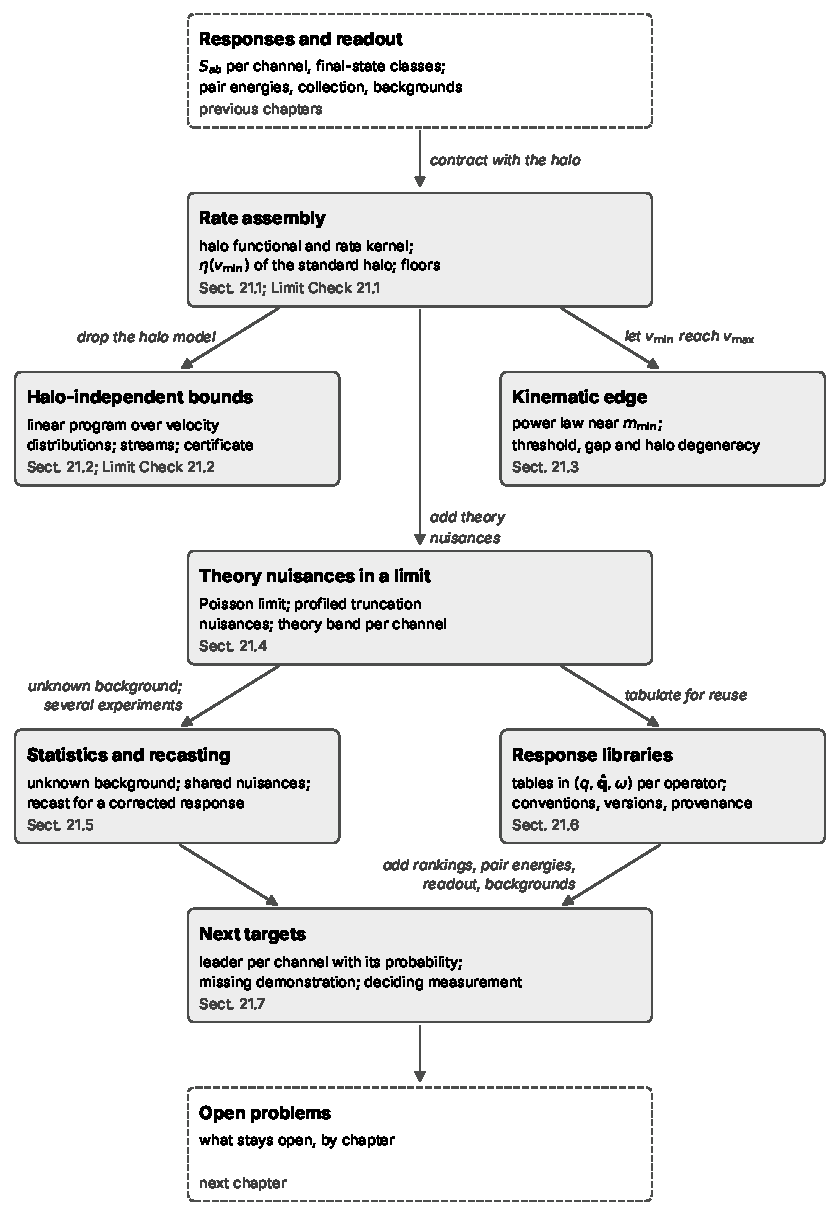
\includegraphics[width=0.78\linewidth]{figures/ch21/map21.pdf}
  \caption{From rates to limits and to the guide to next targets. The channel responses and the measured signal of the previous chapters are contracted with the halo into a rate per channel (\cref{sec:21.1}; \cref{lim:21.1a}). Three questions branch from it: what holds for every velocity distribution (\cref{sec:21.2}; \cref{lim:21.2a}), how the limit behaves where the minimum velocity reaches the largest speed in the halo (\cref{sec:21.3}), and how the theory uncertainties of each channel become a band on the limit (\cref{sec:21.4}). The band carries over to unknown backgrounds, combinations and recasts (\cref{sec:21.5}). The guide to next targets adds the rankings of the response, the pair energies, the readout and the backgrounds (\cref{sec:21.7}). The last box is the index of open problems of \cref{chap:22}.}
  \label{fig:21-map}
\end{figure}

\section{Rates as halo functionals}\label{sec:21.1}

The silicon rate of \cref{sec:10.2-corrections}, \num{5.9e4} events per kilogram and year at \SI{10}{MeV} for $\sigmae = \SI{e-37}{cm^2}$ with the random-phase loss function with local fields, rests on one velocity distribution, the standard halo of \cref{sec:1.2}. Simulated galaxies hold dark matter that this distribution does not describe. In the Via Lactea~II simulation, for instance, 22 percent of the dark matter near the Sun's radius is debris stripped from satellites that still survive, and it moves at a galactic speed near \SI{340}{km.s^{-1}}~\cite{kuhlen2012direct}. A limit compared with such a halo has to be recomputed, and the recomputation is cheap because every rate in this book is linear in $f_\chi$. We will write the rate of any channel as one integral of $f_\chi$ against a kernel that holds everything else: the coupling, the response, the kinematics and the readout.

\subsection{The halo functional of a channel}\label{sec:21.1-functional}

A detector counts events in bins of some observable, the number of pairs $N_{\mathrm{eh}}$ for a charge readout. The rate in one bin is \cref{eq:8.7-handoff}. In it the velocity integral is the outermost one, and everything inside it depends on $\vect{v}$ but not on the halo. We collect it into one function:
\begin{keyresult}[Halo functional of a channel]
\begin{equation}
  \mathcal{R}_{N_{\mathrm{eh}}}[f_\chi] = \frac{\rho_\chi}{\mchi\,\rho_T}\int\dd^3v\,f_\chi(\vect{v})\,\varGamma_{N_{\mathrm{eh}}}(\vect{v}) ,
  \label{eq:21.1-functional}
\end{equation}
with the \emph{rate kernel}, the inner integrals of \cref{eq:8.7-handoff} at fixed $\vect{v}$,
\begin{equation}
  \varGamma_{N_{\mathrm{eh}}}(\vect{v}) = \int\frac{\dd^3q}{(2\pi)^3}\sum_\Lambda\sum_{a,b}\mathfrak{D}_{ab}(\vect{q},\vect{v})\,S_{ab}(\vect{q},\omega_{\vect{q}};\Lambda)\,P_{\mathrm{casc}}(N_{\mathrm{eh}}|\Lambda) ,
  \label{eq:21.1-kernel}
\end{equation}
the rate at which one dark-matter particle of velocity $\vect{v}$ makes events with $N_{\mathrm{eh}}$ pairs.
\end{keyresult}
\noindent Summed over $N_{\mathrm{eh}}$, the kernel is the per-particle rate $\varGamma(\vect{v})$ of \cref{eq:8.2-rate}. For any other observable, a phonon energy or a bin of total deposited energy, $P_{\mathrm{casc}}$ is replaced by the probability that the event lands in that bin. The halo enters only through $f_\chi$ and $\rho_\chi$, the channel only through its kernel, and the rate is a linear functional of $f_\chi$: a halo made of two components gives the sum of their rates, weighted by their shares of the density.

The kernel is never negative, since $\mathfrak{D}$ and $S$ are positive semidefinite matrices (\cref{sec:8.2}) and $P_{\mathrm{casc}}$ is a probability. Adding dark matter at any velocity therefore never lowers a rate, which is the property on which the halo-independent bounds of \cref{sec:21.2} rest. The kernel vanishes at small speeds. A particle of speed $v$ reaches only the pairs $(q,\omega)$ with $\vmin(q,\omega) \le v$ (\cref{sec:1.3}), so $\varGamma(\vect{v}) = 0$ for $v$ below the onset speed $v_{\mathrm{on}}(\mchi)$, the smallest $\vmin$ over the support of the response. And for a crystal the kernel depends on the direction of $\vect{v}$ in crystal axes. The laboratory distribution is $f_{\mathrm{gal}}(\vect{v} + \vect{v}_{\mathrm{E}}(t))$ (\cref{eq:1.2-flab}), and the crystal turns with the Earth (\cref{eq:1.2-rotation}). Averaged over an exposure, \cref{eq:21.1-functional} becomes
\begin{equation}
  \bar{\mathcal{R}}_{N_{\mathrm{eh}}} = \frac{\rho_\chi}{\mchi\,\rho_T}\int\dd^3v_{\mathrm{gal}}\,f_{\mathrm{gal}}(\vect{v}_{\mathrm{gal}})\,\bigl\langle\varGamma_{N_{\mathrm{eh}}}\bigl(\vect{v}_{\mathrm{gal}} - \vect{v}_{\mathrm{E}}(t)\bigr)\bigr\rangle_t ,
  \label{eq:21.1-exposure}
\end{equation}
where $\langle\cdot\rangle_t$ averages over the live time, with the argument of $\varGamma$ rotated into crystal axes at each $t$. All time dependence is now in the kernel, and the exposure-averaged kernel at $\vect{v}_{\mathrm{gal}}$ is the rate that a single stream of dark matter at that velocity would produce.

Absorption fits the same form. The kernel is then $\varGamma_{\mathrm{abs}}$ of \cref{eq:8.2-abs}, which depends on $\vect{v}$ only through the momentum $\vect{p}_\phi = m_\phi\vect{v}$ and the energy $\omega_\phi \simeq m_\phi(1 + v^2/2)$. Where the response is smooth on the scale $m_\phi v \approx 10^{-3}m_\phi$, the kernel is constant across the halo and the rate depends on the halo through $\rho_\chi$ alone.

\subsection{The mean inverse speed}\label{sec:21.1-eta}

For a response averaged over the directions of $\vect{q}$, as in the crystal form factor of \cref{sec:10.1}, the kernel depends only on the speed. The angular average of the energy delta function is $\Theta(v - \vmin)/(2qv)$ (\cref{sec:1.3}), and for a coupling that does not depend on the dark-matter velocity
\begin{equation}
  \varGamma(v) = \frac{1}{v}\int_0^\infty\dd\omega\int\frac{q\,\dd q}{4\pi^2}\sum_{a,b}\mathfrak{D}_{ab}(q)\,\bar S_{ab}(q,\omega)\,\Theta\bigl(v - \vmin(q,\omega)\bigr) .
  \label{eq:21.1-gammav}
\end{equation}
With $F_\chi(v)$ the speed distribution of \cref{eq:1.2-Fspeed}, the rate is a one-dimensional integral, $\mathcal{R} = (\rho_\chi/\mchi\rho_T)\int_0^\infty\dd v\,F_\chi(v)\,\varGamma(v)$. The product $v\varGamma(v)$ is the response integrated over the part of the $(q,\omega)$ plane that a particle of speed $v$ can reach. It is zero below $v_{\mathrm{on}}$ and grows with $v$, because a faster particle reaches every pair that a slower one reaches and more.

The mean inverse speed appears when the order of the integrals is reversed. Since $\eta(u) = \int_u^\infty\dd v\,F_\chi(v)/v$ by \cref{eq:1.3-eta}, the speed distribution is $F_\chi(v) = -v\,\dd\eta/\dd v$. Integrating by parts,
\begin{equation}
  \mathcal{R} = \frac{\rho_\chi}{\mchi\,\rho_T}\int_0^\infty\dd u\;\eta(u)\,\frac{\dd}{\dd u}\bigl[u\varGamma(u)\bigr] ,
  \label{eq:21.1-etaform}
\end{equation}
with no boundary terms, because $u\varGamma(u)$ vanishes below $v_{\mathrm{on}}$ and $\eta$ vanishes above $v_{\mathrm{max}}$. The derivative of \cref{eq:21.1-gammav} replaces $\Theta(u - \vmin)$ by $\delta(u - \vmin)$: $\dd[u\varGamma]/\dd u$ is the response of the pairs whose minimum velocity is $u$, and it is never negative. Inserting it in \cref{eq:21.1-etaform} and doing the $u$ integral sets $u = \vmin(q,\omega)$ in $\eta$, which is the isotropic rate \cref{eq:A.8-rateiso} integrated over $\omega$.

A coupling that depends on the dark-matter velocity needs no halo function beyond $\eta$. The operators of \cref{tab:8-operators} depend on the velocity through $\vect{v}^\perp$, linearly except for $\mathcal{O}_2$, which is quadratic. So $\mathfrak{D}_{ab}$ is a polynomial in the transverse velocity $\vect{v}_{\mathrm{T}}$, the part of $\vect{v}$ perpendicular to $\vect{q}$; at zero mass splitting, $\Delta_\chi = 0$, the longitudinal part is fixed at $\vmin$ by the delta function, and $v_{\mathrm{T}}^2 = v^2 - \vmin^2$ (\cref{sec:8.1}). For an orientation-averaged response no direction is left in the plane perpendicular to $\vect{q}$. Odd powers of $\vect{v}_{\mathrm{T}}$ then average to zero, and even powers enter through $v_{\mathrm{T}}^2$ alone. The quadratic term has a second speed moment as its halo average:
\begin{equation}
  \int\dd^3v\,f_\chi(\vect{v})\,\frac{v^2 - u^2}{v}\,\Theta(v - u) = 2\int_u^\infty\dd u'\,u'\eta(u') = \eta_2(u) .
  \label{eq:21.1-eta2}
\end{equation}
To see this, differentiate the left side with respect to $u$. The boundary term at $v = u$ vanishes, because the integrand is zero there, and what is left is $-2u\,\eta(u)$; both sides vanish for $u \ge v_{\mathrm{max}}$. The same step applied to $(v^2 - u^2)^n$ gives $-2nu$ times the moment with $n - 1$, so the quartic term of $\mathcal{O}_2$ is fixed by $\eta_2$ and hence by $\eta$. The function $\eta_2$ of \cref{app:A.8} is therefore not an independent input. In the kernel form $\varGamma(v)$ contains the extra terms, and \cref{eq:21.1-functional} holds as written.

Now take the density row, $\mathfrak{D}_{ee} = \pi\sigmae\FDM^2/\mu_{\chi e}^2$ (\cref{eq:1.4-Vsq}), and the independent-particle structure factor $\bar S^0$ of \cref{sec:10.1}. \Cref{eq:21.1-etaform} is then \cref{eq:10.1-rateiso}, and written with the crystal form factor it is the rate with the crystal form factor \cref{eq:10.1-fcrys}, divided by the target mass~\cite[Eqs.~(3.13), (3.17)]{essig2016direct}. In the standard halo $\eta$ is the closed form of \cref{app:D.1}~\cite[App.~B]{essig2016direct}. With $S = (2q^2/e^2)L$ (\cref{eq:4.4-SL}) in place of $\bar S^0$, \cref{eq:21.1-etaform} is the loss-function rate \cref{eq:10.2-rate}, which the silicon kernels of this chapter use. One step separates that form from what \cref{app:A.8} prescribes for a rate averaged over an exposure. The closed form holds at one Earth speed, while over a year $|\vect{v}_{\mathrm{E}}(t)|$ runs from 237.4 to \SI{266.4}{km.s^{-1}} (\cref{sec:1.2}). The exposure average of $\eta$ is the average of the closed form over those speeds, and the question is when the closed form at $v_{\mathrm{E}}^{\mathrm{ref}} = \SI{250.5}{km.s^{-1}}$, the convention of \cref{app:A.8} and not the yearly mean of \SI{252.1}{km.s^{-1}}, can stand in for it. Write $|\vect{v}_{\mathrm{E}}(t)| = v_{\mathrm{E}}^{\mathrm{ref}} + \delta v_{\mathrm{E}}(t)$. Over a full year the term of \cref{eq:1.2-annual} that is linear in the orbital velocity averages to zero, and what is left is $\langle\delta v_{\mathrm{E}}\rangle = \SI{1.61}{km.s^{-1}}$, almost all of it from the second-order term, and $\langle\delta v_{\mathrm{E}}^2\rangle = \SI{108.3}{km^2.s^{-2}}$, an rms of \SI{10.4}{km.s^{-1}}. To second order,
\begin{equation}
  \langle\eta(u)\rangle_t - \eta(u)\big|_{v_{\mathrm{E}}^{\mathrm{ref}}} \simeq \frac{\partial\eta}{\partial v_{\mathrm{E}}}\,\langle\delta v_{\mathrm{E}}\rangle + \frac12\,\frac{\partial^2\eta}{\partial v_{\mathrm{E}}^2}\,\langle\delta v_{\mathrm{E}}^2\rangle .
  \label{eq:21.1-annualcorr}
\end{equation}
In the bulk of the halo both derivatives are small and the correction is a percent. Near the end point $\eta \propto \delta^2$ with $\delta = v_{\mathrm{esc}} + v_{\mathrm{E}} - u$ (\cref{eq:1.3-edge}), a convex function of $v_{\mathrm{E}}$, and the June excess outweighs the December deficit: the yearly average lies above the value at the mean speed.
\begin{limitbox}[Mean inverse speed of the standard halo][lim:21.1a]
For the truncated Maxwellian of \cref{eq:1.2-fgal} seen at Earth speed $v_{\mathrm{E}}$, and $\vmin < v_{\mathrm{esc}} - v_{\mathrm{E}}$,
\begin{equation*}
  \eta(\vmin) = \frac{\pi v_0^2}{v_{\mathrm{E}}N_{\mathrm{esc}}}\left\{\frac{\sqrt{\pi}\,v_0}{2}\left[\operatorname{erf}\frac{\vmin + v_{\mathrm{E}}}{v_0} - \operatorname{erf}\frac{\vmin - v_{\mathrm{E}}}{v_0}\right] - 2v_{\mathrm{E}}\,\ee^{-v_{\mathrm{esc}}^2/v_0^2}\right\} ,
\end{equation*}
with the second branch \cref{eq:D.1-eta2} up to $v_{\mathrm{esc}} + v_{\mathrm{E}}$~\cite[Eqs.~(B.4) and (B.5)]{essig2016direct}.
\par\smallskip
{\centering
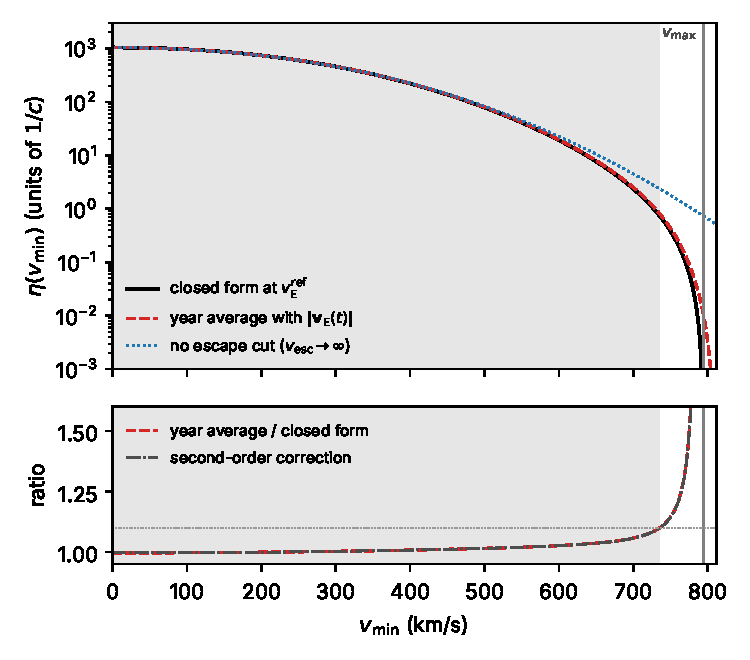
\includegraphics[width=\linewidth]{figures/ch21/limit21_1a.pdf}
\captionof{figure}{Mean inverse speed of the standard halo ($v_0 = \SI{238}{km.s^{-1}}$, $v_{\mathrm{esc}} = \SI{544}{km.s^{-1}}$) against $\vmin$. Top, in units of $1/c$: the closed form at the reference Earth speed $v_{\mathrm{E}}^{\mathrm{ref}} = \SI{250.5}{km.s^{-1}}$ (solid). Dashed: the fuller result, the same closed form averaged over a year with the exact Earth speed of \cref{eq:1.2-vE,eq:1.2-vorb} on 7305 equally spaced days. Dotted: the Maxwellian without the escape cut at $v_{\mathrm{E}}^{\mathrm{ref}}$. Bottom: the yearly average over the closed form (dashed) and the second-order correction \cref{eq:21.1-annualcorr} (dash-dotted). Gray: $\vmin \le \SI{735.6}{km.s^{-1}}$, where the yearly average exceeds the closed form at $v_{\mathrm{E}}^{\mathrm{ref}}$ by less than 10 percent (1 percent up to \SI{430.3}{km.s^{-1}}). The second-order correction stays within 1 percent of the yearly average up to \SI{786.3}{km.s^{-1}}. Vertical line: $v_{\mathrm{max}} = \SI{794.5}{km.s^{-1}}$.}\label{fig:21-limit-eta}
\par}
\smallskip
Within \SI{59}{km.s^{-1}} of $v_{\mathrm{max}}$ the yearly average exceeds the fixed-speed form by more than 10 percent, and above $v_{\mathrm{max}}$ it vanishes while the average stays positive up to \SI{810.4}{km.s^{-1}}.
\end{limitbox}
\noindent At $\vmin = 0$ the yearly average is 0.9965 of the closed form: the mean inverse speed itself barely moves. The ratio grows to 1.015 at \SI{500}{km.s^{-1}}, 1.026 at 600 and 1.057 at \SI{700}{km.s^{-1}}, then turns up steeply, to 1.20 at 760 and 1.78 at \SI{780}{km.s^{-1}}. The second-order term follows it within a few parts in a thousand to \SI{780}{km.s^{-1}}. The escape cut matters over a much wider range than the annual average does: without it, $\eta$ would be 1.18 times larger at \SI{600}{km.s^{-1}}, 1.90 times at 700 and 6.8 times at \SI{760}{km.s^{-1}}. Averaging $\eta$ over the year raises this silicon rate by 0.9 percent at \SI{10}{MeV} and by 5.6 percent at \SI{1}{MeV}, where the kernel opens near \SI{460}{km.s^{-1}}. Closer to the threshold mass the correction grows without bound, and \cref{sec:21.3} treats that regime.

\Cref{fig:21-kernel} shows the kernel of the silicon electron-recoil channel for a heavy mediator, built from the random-phase loss function with local fields of the tables of \cref{sec:10.2}, counted from their gap of \SI{1.17}{eV}. At \SI{10}{MeV} it opens at $v_{\mathrm{on}} = \SI{145}{km.s^{-1}}$, which is $(2\omega/\mchi)^{1/2}$ at the gap; the kernel, scaled to a rate per target mass as in \cref{fig:21-kernel}, is $\num{1.77e4}$ per kilogram and year at \SI{300}{km.s^{-1}}, $\num{1.28e5}$ at \SI{500}{km.s^{-1}} and $\num{3.11e5}$ at $v_{\mathrm{max}}$, for $\sigmae = \SI{e-37}{cm^2}$. Integrated against $F_\chi$ at $v_{\mathrm{E}}^{\mathrm{ref}}$, it returns \SI{5.897e4}{kg^{-1}.yr^{-1}}, the rate of \cref{sec:10.2-corrections}, and the form \cref{eq:21.1-etaform} returns the same number to five digits. At \SI{1}{MeV} the kernel opens only near \SI{460}{km.s^{-1}} and the rate, \SI{16.5}{kg^{-1}.yr^{-1}}, comes entirely from the fastest fifth of the halo. At \SI{100}{MeV} it opens at \SI{46}{km.s^{-1}} and changes by a factor of 4.0 between 300 and \SI{700}{km.s^{-1}}, against 14 at \SI{10}{MeV}. The heavier the particle, the flatter the kernel over the bulk of the halo, and the less the rate depends on the shape of $F_\chi$.
\begin{figure}[tbp]
  \centering
  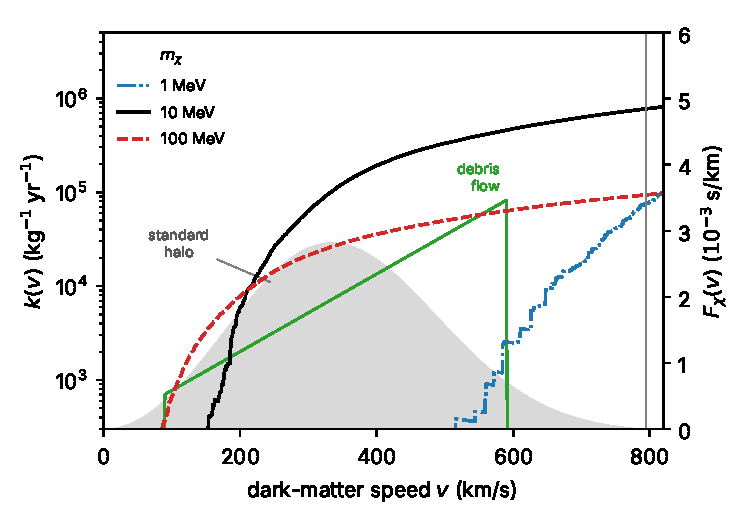
\includegraphics[width=0.8\linewidth]{figures/ch21/fig21_1.pdf}
  \caption{Rate kernel of the silicon electron-recoil channel, $\rho_\chi\varGamma(v)/\mchi\rho_T$ of \cref{eq:21.1-gammav}, the rate per unit target mass if all dark matter moved at speed $v$, for a heavy mediator, $\sigmae = \SI{e-37}{cm^2}$ and $\rho_\chi = \SI{0.3}{GeV.cm^{-3}}$, at $\mchi = 1$, 10 and \SI{100}{MeV} (left axis). The response is the direction-averaged random-phase loss function with local fields of Knapen, Kozaczuk and Lin~\cite{knapen2021dark} (\cref{sec:10.2}), from their gap of \SI{1.17}{eV}. Right axis: laboratory speed distributions at $v_{\mathrm{E}}^{\mathrm{ref}} = \SI{250.5}{km.s^{-1}}$ of the standard halo (gray, \cref{eq:1.2-Fspeed}) and of a debris flow of galactic speed \SI{340}{km.s^{-1}} (green, \cref{eq:21.1-fflow}). Vertical line: $v_{\mathrm{max}} = \SI{794.5}{km.s^{-1}}$.}
  \label{fig:21-kernel}
\end{figure}

\subsection{Threshold masses as floors}\label{sec:21.1-floor}

Where the kernel vanishes, so does the rate. By \cref{eq:21.1-functional}, a mass gives a nonzero rate only if the halo holds particles faster than $v_{\mathrm{on}}(\mchi)$. For a response whose onset $E_{\mathrm{th}}$ does not depend on $q$, the smallest $\vmin$ is $(2E_{\mathrm{th}}/\mchi)^{1/2}$ (\cref{sec:1.3}), and the condition $v_{\mathrm{on}} < v_{\mathrm{max}}$ is $\mchi > 2E_{\mathrm{th}}/v_{\mathrm{max}}^2$, the threshold mass of \cref{eq:1.3-mmin}. Quoted with $v_{\mathrm{max}} = v_{\mathrm{esc}} + v_{\mathrm{E}}^{\mathrm{ref}}$, that value is a floor, never the edge of a limit.

The onset of a real response depends on $q$. Then $v_{\mathrm{on}} = \min_q[E_{\mathrm{th}}(q)/q + q/2\mchi]$ lies above $(2E_{\mathrm{th}}/\mchi)^{1/2}$ with $E_{\mathrm{th}}$ the global minimum, and the edge lies above the floor. In silicon the floor at the gap, \SI{1.170}{eV}, is \SI{0.3332}{MeV}, and at the lowest excitation, the $1s$ exciton at \SI{1.1553}{eV}, it is \SI{0.3290}{MeV}; the edges of the pair channels lie above it (\cref{tab:9-edges}).

Near $v_{\mathrm{max}}$ the mean inverse speed $\eta$ vanishes quadratically (\cref{eq:1.3-edge}), and the reachable part of the response shrinks with it. A finite exposure therefore excludes only masses some distance above the floor, and how far above depends on the exposure, on the onset exponent of the response and on the tail of the halo. \Cref{sec:21.3} derives that distance.

The floor depends on the halo and on the Earth speed it is computed with. The reference speed fixes $v_{\mathrm{max}} = \SI{794.5}{km.s^{-1}}$ by convention (\cref{app:A.8}). In June the fastest particles move at $v_{\mathrm{esc}} + |\vect{v}_{\mathrm{E}}| = \SI{810.4}{km.s^{-1}}$, and an exposure that includes June has a nonzero rate down to a floor 3.9 percent lower, \SI{0.3202}{MeV} for the silicon gap; \cref{lim:21.1a} shows its origin in $\eta$. The annual motion is known kinematics, not an uncertainty: a limit uses the rate averaged over its exposure, June included (\cref{sec:21.3-degeneracy}), and the floor at the reference speed is the convention for comparing targets. Conversely, a halo component lowers the floor only if it carries particles faster than $v_{\mathrm{max}}$. A debris flow at \SI{340}{km.s^{-1}} reaches at most \SI{590.5}{km.s^{-1}} in the laboratory, and on its own it would give no silicon electron recoil below \SI{0.6031}{MeV}.

\subsection{A halo with a debris flow}\label{sec:21.1-debris}

Kuhlen, Lisanti and Spergel model the debris flow as an isotropic shell in velocity space: every particle has the same galactic speed $v_{\mathrm{flow}}$, in a random direction~\cite{kuhlen2012direct}. In the laboratory a particle of direction $\hat{\vect{v}}_{\mathrm{gal}}$ has speed $v$ with $v^2 = v_{\mathrm{flow}}^2 + v_{\mathrm{E}}^2 - 2v_{\mathrm{flow}}v_{\mathrm{E}}\cos\theta_{\mathrm{flow}}$, where $\theta_{\mathrm{flow}}$ is the angle between $\vect{v}_{\mathrm{gal}}$ and $\vect{v}_{\mathrm{E}}$. Since $\cos\theta_{\mathrm{flow}}$ is uniform on $[-1,1]$ and $v\,\dd v = -v_{\mathrm{flow}}v_{\mathrm{E}}\,\dd\cos\theta_{\mathrm{flow}}$, the laboratory speed distribution is~\cite[Eq.~(7)]{kuhlen2012direct}
\begin{equation}
  F_{\mathrm{flow}}(v) = \frac{v}{2v_{\mathrm{flow}}v_{\mathrm{E}}}\quad\text{for } |v - v_{\mathrm{flow}}| < v_{\mathrm{E}} ,
  \label{eq:21.1-fflow}
\end{equation}
and zero outside, for $v_{\mathrm{flow}} > v_{\mathrm{E}}$. Its mean inverse speed is $\eta_{\mathrm{flow}}(u) = 1/v_{\mathrm{flow}}$ for $u < v_{\mathrm{flow}} - v_{\mathrm{E}}$, falls linearly as $(v_{\mathrm{flow}} + v_{\mathrm{E}} - u)/(2v_{\mathrm{flow}}v_{\mathrm{E}})$ across the window, and vanishes above $v_{\mathrm{flow}} + v_{\mathrm{E}}$~\cite[Eq.~(8)]{kuhlen2012direct}. The halo is $f_\chi = (1 - p_{\mathrm{flow}})f_{\mathrm{SHM}} + p_{\mathrm{flow}}f_{\mathrm{flow}}$ at fixed total density, and in Via Lactea~II $p_{\mathrm{flow}} = 0.22$ and $v_{\mathrm{flow}} = \SI{340}{km.s^{-1}}$~\cite[Eq.~(10) and Fig.~6]{kuhlen2012direct}. Compared to the standard halo at the reference Earth speed, the flow has fewer slow particles, $\langle1/v\rangle = 1/v_{\mathrm{flow}}$, or 882 in natural units against 1041, and more fast ones: 55 percent of its particles move faster than \SI{400}{km.s^{-1}}, against 36 percent. It has none above \SI{590.5}{km.s^{-1}}.

\begin{workedexample}{The silicon rate in a halo with a debris flow}\label{we:21-debris}
Take silicon, $\mchi = \SI{10}{MeV}$, a heavy mediator and $\sigmae = \SI{e-37}{cm^2}$, with the kernel of \cref{fig:21-kernel} and $v_{\mathrm{E}} = v_{\mathrm{E}}^{\mathrm{ref}}$ for both components. The flow occupies $89.5 < v < \SI{590.5}{km.s^{-1}}$. Inserting \cref{eq:21.1-fflow} in \cref{eq:21.1-functional}, the factor $v$ of $F_{\mathrm{flow}}$ meets the factor $1/v$ of the kernel:
\begin{equation*}
  \mathcal{R}_{\mathrm{flow}} = \frac{1}{2v_{\mathrm{flow}}v_{\mathrm{E}}}\int_{v_{\mathrm{flow}} - v_{\mathrm{E}}}^{v_{\mathrm{flow}} + v_{\mathrm{E}}}\dd v\;v\,\frac{\rho_\chi\varGamma(v)}{\mchi\rho_T}
  = \frac{1}{v_{\mathrm{flow}}}\Bigl\langle v\,\frac{\rho_\chi\varGamma(v)}{\mchi\rho_T}\Bigr\rangle_{\mathrm{window}} .
\end{equation*}
Across the window the kernel rises from zero below \SI{145}{km.s^{-1}} through \SI{1.77e4}{kg^{-1}.yr^{-1}} at \SI{300}{km.s^{-1}}, \num{6.97e4} at 400 and \num{1.28e5} at \SI{500}{km.s^{-1}}, to \SI{1.82e5}{kg^{-1}.yr^{-1}} at \SI{590}{km.s^{-1}}. The mean of $v$ times the kernel over the window is \SI{2.769e7}{km.s^{-1}.kg^{-1}.yr^{-1}}, and
\begin{equation*}
  \mathcal{R}_{\mathrm{flow}} = \frac{\SI{2.769e7}{km.s^{-1}.kg^{-1}.yr^{-1}}}{\SI{340}{km.s^{-1}}} = \SI{8.145e4}{kg^{-1}.yr^{-1}} ,
\end{equation*}
the rate if all of the dark matter were in the flow. The form \cref{eq:21.1-etaform} with $\eta_{\mathrm{flow}}$ gives the same number. Per particle the flow is 1.381 times as effective as the standard halo, $\mathcal{R}_{\mathrm{SHM}} = \SI{5.897e4}{kg^{-1}.yr^{-1}}$, because it puts more particles where the kernel is large.

The mixed halo, by linearity, gives
\begin{equation*}
  \mathcal{R} = 0.78\times\num{5.897e4} + 0.22\times\num{8.145e4} = \SI{6.392e4}{kg^{-1}.yr^{-1}} ,
\end{equation*}
8.4 percent above the standard halo, or 175 events per kilogram and day. The spectrum hardly changes shape: its mean moves from 6.59 to \SI{6.62}{eV}. The flow's own spectrum ends at \SI{19.4}{eV}, the largest energy a particle at \SI{590.5}{km.s^{-1}} can deposit, against \SI{35}{eV} for the standard halo, and it peaks near \SI{6.0}{eV}, against \SI{5.4}{eV}.

The same halo changes the rate differently at other masses. For a light mediator at \SI{10}{MeV} the mixed rate is 8.8 percent above the standard one, and for a heavy mediator at \SI{100}{MeV}, 5.2 percent. At \SI{1}{MeV}, where the kernel opens near \SI{460}{km.s^{-1}}, the flow is only 0.28 times as effective as the standard halo, and the mixed rate falls 16 percent below it. A debris flow moves particles from both tails of the speed distribution into its middle. It raises the rate where the kernel opens in the bulk of the halo and lowers it near the threshold mass, which stays at the floor set by the standard component.
\end{workedexample}

\section{Halo-independent bounds}\label{sec:21.2}

A dark-matter particle of \SI{2}{MeV} can make an electron--hole pair in silicon only if it moves faster than \SI{325}{km.s^{-1}} in the laboratory, and a second pair only above \SI{466}{km.s^{-1}}, against the largest speed of the standard halo, $v_{\mathrm{max}} = \SI{794.5}{km.s^{-1}}$. A limit at that mass is therefore a statement about the fast part of the dark matter in the solar neighborhood, the part of the halo that \cref{sec:1.2} found least certain: changing the escape speed by \SI{25}{km.s^{-1}} changes $\eta$ at \SI{760}{km.s^{-1}} by a factor of 2.26 or 0.10. A statement that holds for every velocity distribution avoids the question. Because every count is a linear functional of $f_\chi$ (\cref{eq:21.1-functional}), the distributions that a null result allows form a convex set, and the largest value of any other linear quantity over that set is a semi-infinite linear program, with finitely many constraints on a measure over a continuum, the problem of \cref{app:C.12}. For silicon at 2 and \SI{10}{MeV}, dropping the halo model costs a factor of 2.0 to 3.7 in the bulk of the halo and orders of magnitude near $v_{\mathrm{max}}$.

\subsection{Stream kernels and the linear program}\label{sec:21.2-program}

The exposure-averaged rate \cref{eq:21.1-exposure} is an integral over galactic velocities $\vect{w}$ of the distribution $f_{\mathrm{gal}}$ times a kernel. Multiplied by the exposure $M_{\mathrm{det}}t_{\mathrm{exp}}$ it is a count. The local density, the cross-section and the mass multiply every rate in the combination $\rho_\chi\sigmae/\mchi$, which no count can separate from the normalization of $f_{\mathrm{gal}}$; the mass enters the kinematics as well, and the analysis is done at fixed $\mchi$. We therefore absorb the combination into a nonnegative measure $\Xi$ on the ball $\mathcal{B} = \{|\vect{w}| \le v_{\mathrm{esc}}\}$ and divide the kernel by $\sigmae$ (\cref{app:D.46}):
\begin{equation}
  \dd\Xi(\vect{w}) = \frac{\rho_\chi\sigmae}{\mchi}\,f_{\mathrm{gal}}(\vect{w})\,\dd^3w , \qquad
  \mathsf{k}_i(\vect{w}) = \frac{M_{\mathrm{det}}t_{\mathrm{exp}}}{\rho_T\,\sigmae}\,\bigl\langle\varGamma_i\bigl(\vect{w} - \vect{v}_{\mathrm{E}}(t)\bigr)\bigr\rangle_t ,
  \label{eq:21.2-stream}
\end{equation}
with $\varGamma_i$ the rate kernel \cref{eq:21.1-kernel} for bin $i$ of the observable. The expected count in bin $i$ is then $\int\mathsf{k}_i\,\dd\Xi$. The \emph{stream kernel} $\mathsf{k}_i(\vect{w})$ is the count that a single stream of unit $\Xi$-mass at $\vect{w}$ would leave in bin $i$; it contains the coupling up to its strength, the response, the final-state weights and the exposure, and nothing about the halo. A measured null result in bin $i$ becomes the constraint $\int\mathsf{k}_i\,\dd\Xi \le N_i^{\mathrm{up}}$, with $N_i^{\mathrm{up}}$ the upper count of \cref{sec:1.5} at the chosen confidence.

The quantity to bound is a second linear functional, $\int\mathsf{f}\,\dd\Xi$: the mean inverse speed above $u_0$ in the laboratory, the count of a second experiment, or a modulation amplitude. The mean inverse speed is the object of the standard halo-independent analysis,
\begin{equation}
  \tilde\eta(u_0) = \int\frac{\Theta(|\vect{w} - \vect{v}_{\mathrm{E}}| - u_0)}{|\vect{w} - \vect{v}_{\mathrm{E}}|}\,\dd\Xi(\vect{w}) = \frac{\rho_\chi\sigmae}{\mchi}\,\eta(u_0) ,
  \label{eq:21.2-etatilde}
\end{equation}
which is $\tilde\eta$ of \cref{app:A.8} with $\vect{v}_{\mathrm{E}}$ held fixed. Its value for the standard halo at a given $\sigmae$ is a curve in the plane of $u_0$ and $\tilde\eta$, and a bound on $\tilde\eta$ at every $u_0$ is the halo-independent counterpart of an exclusion curve. The count expected in a second experiment, $\mathsf{f} = \mathsf{k}^{\mathrm{B}}_j$, compares two targets, or one crystal at two orientations, without a halo model. A modulation amplitude, the difference of the kernels of two time bins, is a signed functional, bounded only if every stream on which it is positive is seen by some bin. The program is \cref{eq:C.12-sip} with these kernels.

By \cref{app:C.12}, any vector $\boldsymbol\lambda \ge 0$ with $\sum_i\lambda_i\mathsf{k}_i \ge \mathsf{f}$ on all of $\mathcal{B}$, a \emph{dual certificate}, proves $\int\mathsf{f}\,\dd\Xi \le \int\sum_i\lambda_i\mathsf{k}_i\,\dd\Xi \le \sum_i\lambda_iN_i^{\mathrm{up}}$ for every allowed halo at once, \cref{eq:C.12-certificate}. Checking it needs one function evaluated on the ball, not the optimizer that produced it. And the optimum is attained by a halo of at most $n$ streams for $n$ bins, $\Xi^* = \sum_a\xi_a\delta_{\vect{w}_a}$ with $\Xi$-masses $\xi_a$, placed at the zeros of the dual function $\mathsf{g}_\lambda = \sum_i\lambda_i\mathsf{k}_i - \mathsf{f}$. The extremal halos are therefore cold streams, far from any equilibrium model, and the bound holds for every halo because it holds for them. With the normalization of $f_\chi$ as an extra equality constraint the optimum allows one more stream~\cite[Eqs.~(14)--(19)]{ibarra2017optimized}, and any likelihood, not only a bound, is maximized by a sum of streams~\cite{gelmini2017unified}.

All bins of a search constrain one halo, so a bound derived from them is a statement about the event that every bin stays below its $N_i^{\mathrm{up}}$. If each bin is set at confidence $1 - \alpha_i$, that event has probability at least $1 - \sum_i\alpha_i$ by the union bound, and the bounds at all $u_0$ hold together at that level. The examples below use three pair bins with $N_i^{\mathrm{up}} = \ln 30 = 3.401$ each, the zero-event Poisson limit at 96.7 percent, so that the three bins hold jointly at 90 percent or more.

\subsection{The bound for a speed-only response}\label{sec:21.2-iso}

For a response averaged over the directions of $\vect{q}$, as in the crystal form factor of \cref{sec:10.1}, and with $\vect{v}_{\mathrm{E}}$ fixed, the stream kernel depends only on the laboratory speed $v = |\vect{w} - \vect{v}_{\mathrm{E}}|$. By \cref{eq:21.1-gammav} it is $\mathsf{k}_i(v) = \mathcal{A}_i(v)/v$, with the \emph{step column}
\begin{equation}
  \mathcal{A}_i(v) = \frac{M_{\mathrm{det}}t_{\mathrm{exp}}}{\rho_T\,\sigmae}\,v\,\varGamma_i(v) = \frac{M_{\mathrm{det}}t_{\mathrm{exp}}}{\rho_T\,\sigmae}\int\dd\omega\int\frac{q\,\dd q}{4\pi^2}\,\bar s_i(q,\omega)\,\Theta\bigl(v - \vmin(q,\omega)\bigr) ,
  \label{eq:21.2-column}
\end{equation}
where $\bar s_i$ is the angle-averaged response contracted with $\mathfrak{D}$ and weighted with the probability $P(i|\Lambda)$ of landing in bin $i$. The column is the count in bin $i$ for the step $\tilde\eta(u) = \Theta(v - u)$: all of $\tilde\eta$ sits below the speed $v$, the halo of a single stream at $v$. In silicon with the loss function of \cref{sec:10.2}, written as a crystal form factor by \cref{eq:A.8-fcrys,eq:4.4-SL}, the prefactor $M_{\mathrm{det}}t_{\mathrm{exp}}\,\alpha m_e^2/(M_{\mathrm{cell}}\mu_{\chi e}^2)$, with $M_{\mathrm{cell}}$ the mass of the two-atom unit cell, turns the column into a sum over the table, and $\mathcal{A}_i$ comes out in years for $\tilde\eta$ in inverse years. For a positive response the column never decreases with $v$ (\cref{eq:D.46-monotone}), since a faster particle reaches every pair that a slower one does (\cref{sec:21.1-eta}).

Monotonicity solves the program:
\begin{keyresult}[Halo-independent bound for a speed-only response]
For a response that depends only on $|\vect{q}|$, nonnegative bin weights, a fixed $\vect{v}_{\mathrm{E}}$, $0 < u_0 \le v_{\mathrm{max}}$ and $\max_i\mathcal{A}_i(u_0) > 0$, every velocity distribution allowed by the bins satisfies
\begin{equation}
  \tilde\eta(u_0) \le \min_i\frac{N_i^{\mathrm{up}}}{\mathcal{A}_i(u_0)} ,
  \label{eq:21.2-hib}
\end{equation}
and the bound is attained. The optimal halo is one stream at laboratory speed $u_0$ in any allowed direction, and the certificate is $\lambda_j = 1/\mathcal{A}_j(u_0)$ on the minimizing bin $j$, zero on the others.
\end{keyresult}
\noindent \Cref{app:D.46} gives the proof: the stream is feasible and reaches the bound, and the certificate holds because $\mathcal{A}_j(v) \ge \mathcal{A}_j(u_0)$ for $v \ge u_0$. With several bins the minimum over bins is the exact optimum, not an estimate, because one dual weight certifies it; the other bins are not saturated by the optimal stream and carry no weight. A column that decreases somewhere, which a truncated response with negative pieces can produce, leaves the single-bin value $N_i^{\mathrm{up}}/\inf_{v \ge u_0}\mathcal{A}_i(v)$ of \cref{eq:C.12-onebin} and voids the closed form for several bins (\cref{app:D.46}). And a bound on the galactic speed integral $\int\Theta(|\vect{w}| - u_0)|\vect{w}|^{-1}\dd\Xi$, in place of the laboratory speed $|\vect{w} - \vect{v}_{\mathrm{E}}|$ on which the kernel depends, is a different program, and \cref{eq:21.2-hib} does not answer it.

\Cref{fig:21-hib} applies \cref{eq:21.2-hib} to a silicon search of one kilogram-year that records no event in the one-, two- and three-pair bins, for a heavy mediator. A deposit $\omega$ lands in bin $i$ with the probability $P_{\mathrm{casc}}(i|\omega)$ of the cascade of \cref{sec:18.3}, the book's calibrated model with $\Eg = \SI{1.160}{eV}$ and \SI{3.749}{eV} per pair, computed for the seed of a dark-matter kick and applied at every $q$. The probability of the one-pair bin exceeds one half from 1.2 to \SI{6.2}{eV}, that of the two-pair bin from 6.3 to \SI{9.5}{eV} and that of the three-pair bin from 9.7 to \SI{13.1}{eV}, and a second pair is possible from about \SI{2.5}{eV}. Each bin gives a curve $N_i^{\mathrm{up}}/\mathcal{A}_i(u_0)$ that comes down from infinity at the onset speed of the bin, the smallest $\vmin$ among the pairs it can contain, and flattens as the column saturates; the bound is their lower envelope. At \SI{10}{MeV} the one-pair bin sets it below \SI{481.8}{km.s^{-1}}, the two-pair bin up to \SI{757.3}{km.s^{-1}} and the three-pair bin above. At \SI{2}{MeV} the one-pair bin sets it at every speed: the two-pair bin opens at \SI{465.9}{km.s^{-1}} and the three-pair bin at \SI{611.8}{km.s^{-1}}, and at $v_{\mathrm{max}}$ their columns are 2.4 and 206 times smaller. The dashed curves are $\tilde\eta$ of the standard halo at the cross-section where it first reaches $N_i^{\mathrm{up}}$ in some bin: $\sigmae = \SI{1.17e-41}{cm^2}$ at \SI{10}{MeV} and \SI{1.12e-40}{cm^2} at \SI{2}{MeV}, both set by the one-pair bin.

The standard curve lies below the bound at every $u_0$, as it must. The count of any halo in bin $j$ is $\int_0^\infty\tilde\eta(u)\,\dd\mathcal{A}_j(u)$, \cref{eq:21.1-etaform} in these variables, and since $\tilde\eta$ never increases and $\mathcal{A}_j$ never decreases, it is at least $\tilde\eta(u_0)\mathcal{A}_j(u_0)$. A halo that crossed the bound at some $u_0$ would overshoot $N_j^{\mathrm{up}}$. The ratio of the bound to the standard curve is the cost of dropping the halo model. It is smallest at \SI{381}{km.s^{-1}} for \SI{10}{MeV}, a factor 2.00, and near \SI{635}{km.s^{-1}} for \SI{2}{MeV}, a factor 3.70. Toward $v_{\mathrm{max}}$ it opens to 9.6 at \SI{600}{km.s^{-1}} and 63 at \SI{700}{km.s^{-1}} for \SI{10}{MeV}, because the standard halo has few particles there while a stream can put all its density at one speed. The curves hold for an exposure at the reference Earth speed; over a year the standard curve near $v_{\mathrm{max}}$ follows the year average of \cref{sec:21.1}, 1.06 times higher at \SI{700}{km.s^{-1}}.

\begin{figure}[tbp]
  \centering
  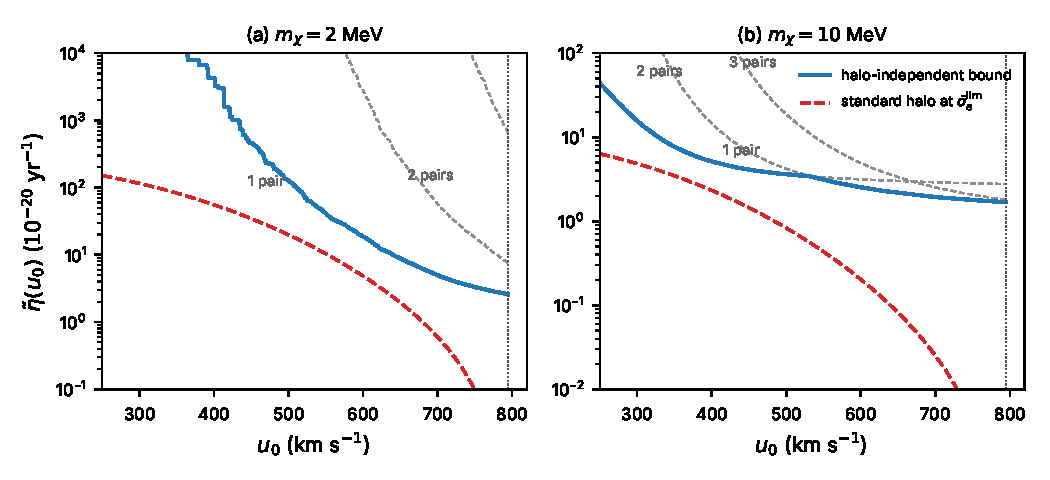
\includegraphics[width=\linewidth]{figures/ch21/fig21_2.pdf}
  \caption{Halo-independent bound on $\tilde\eta(u_0) = \rho_\chi\sigmae\eta(u_0)/\mchi$ for silicon, \cref{eq:21.2-hib} (solid), against $\tilde\eta$ of the standard halo at the cross-section of its own limit (dashed), for (a) $\mchi = \SI{2}{MeV}$ and (b) \SI{10}{MeV}, heavy mediator. Search: one kilogram-year at the reference Earth speed, no events in the one-, two- and three-pair bins, with the bin probabilities of the energy-only cascade of \cref{sec:18.3} (\SI{3.749}{eV} per pair), $N_i^{\mathrm{up}} = \ln 30$ in each bin, jointly at least 90 percent confidence. Gray dashed: single-bin bounds $N_i^{\mathrm{up}}/\mathcal{A}_i(u_0)$, labeled by the number of pairs; the solid curve is their lower envelope. Step columns from the direction-averaged random-phase loss function with local fields of Knapen, Kozaczuk and Lin (\cref{sec:10.2}), from \SI{1.17}{eV}. Standard halo: $v_0 = 238$, $v_{\mathrm{esc}} = \SI{544}{km.s^{-1}}$, $v_{\mathrm{E}}^{\mathrm{ref}} = \SI{250.5}{km.s^{-1}}$, at $\sigmae = \SI{1.12e-40}{cm^2}$ (a) and \SI{1.17e-41}{cm^2} (b). Dotted: $v_{\mathrm{max}} = \SI{794.5}{km.s^{-1}}$.}
  \label{fig:21-hib}
\end{figure}

\begin{workedexample}{One stream saturating a bound}\label{we:21-stream}
Take silicon at $\mchi = \SI{10}{MeV}$, a heavy mediator, the search of \cref{fig:21-hib} and $u_0 = \SI{500}{km.s^{-1}}$. The reduced mass is $\mu_{\chi e} = \SI{486.2}{keV}$, and the prefactor of the column, $M_{\mathrm{det}}t_{\mathrm{exp}}\,\alpha m_e^2/(M_{\mathrm{cell}}\mu_{\chi e}^2)$, is \SI{8.64e22}{yr} for one kilogram-year. Summing the cells of the table with $\vmin \le \SI{500}{km.s^{-1}}$, each weighted with its bin probability, gives
\begin{equation*}
  \mathcal{A}_1 = \SI{3.10e19}{yr} , \qquad \mathcal{A}_2 = \SI{3.48e19}{yr} , \qquad \mathcal{A}_3 = \SI{8.88e18}{yr} ,
\end{equation*}
for the one-, two- and three-pair bins. Divided into $N^{\mathrm{up}} = 3.401$ they give \num{1.10e-19}, \num{9.78e-20} and \SI{3.83e-19}{yr^{-1}}. The two-pair bin is tightest, and
\begin{equation*}
  \tilde\eta(\SI{500}{km.s^{-1}}) \le \frac{3.401}{\SI{3.48e19}{yr}} = \SI{9.78e-20}{yr^{-1}} .
\end{equation*}
The halo that reaches it is one stream at a laboratory speed of \SI{500}{km.s^{-1}}, $1.668\times10^{-3}$ in natural units, with $\Xi$-mass $\xi_1 = u_0N^{\mathrm{up}}/\mathcal{A}_2 = \SI{1.63e-22}{yr^{-1}}$. It leaves 3.03 events in the one-pair bin, 3.40 in the two-pair bin and 0.87 in the three-pair bin: only the two-pair bound is saturated. Its galactic speed lies between \num{249.5} and \SI{750.5}{km.s^{-1}} depending on its direction, and the directions against the Earth's motion are inside the escape speed.

The certificate is $\lambda_2 = 1/\mathcal{A}_2 = \SI{2.88e-20}{yr^{-1}}$ per event, $\lambda_1 = \lambda_3 = 0$, with value $\lambda_2N^{\mathrm{up}} = \SI{9.78e-20}{yr^{-1}}$, equal to the stream's. It is valid because $\mathcal{A}_2(v)/\mathcal{A}_2(u_0)$ never drops below 1 between \num{500} and \SI{794.5}{km.s^{-1}}, where it rises to 2.15.

The standard halo at its own limit, $\sigmae = \SI{1.17e-41}{cm^2}$, set by the one-pair bin, has $\tilde\eta(\SI{500}{km.s^{-1}}) = \SI{2.60e-20}{yr^{-1}}$, a factor 3.76 below the bound. The factor has two parts, read in the two-pair bin that sets the bound. The standard halo leaves only 2.47 events there, because the one-pair bin stops it first, and only 1.27 of them come from particles faster than \SI{500}{km.s^{-1}}; the bin allows $N^{\mathrm{up}} = 3.401$, a factor $3.401/1.266 = 2.69$ above what those particles use. And the fast particles move above \SI{500}{km.s^{-1}}, where the column is larger, so they produce 1.40 times the count of a stream at exactly \SI{500}{km.s^{-1}} with the same $\tilde\eta$. The stream avoids both losses, and $2.69 \times 1.40 = 3.76$.
\end{workedexample}

\subsection{Directional responses in the laboratory}\label{sec:21.2-dir}

A crystal resolves directions. Its response depends on $\hat{\vect{q}}$ in crystal axes, the crystal turns with the Earth, and a stream fixed in the galactic frame sweeps a cone of crystal directions every sidereal day (\cref{sec:11.7}). The stream kernel then depends on the direction of the stream, there is no step column, and the program has to be solved. Take a cubic crystal and a coupling that depends on $|\vect{q}|$ alone. The bin-weighted response is then $\bar s_i[1 + \sum_\ell a^i_\ell Y^{\mathrm{c}}_\ell(\hat{\vect{q}})]$, with the cubic harmonics of \cref{app:C.3}, $\ell = 4, 6, 8, \dots$ The energy delta function confines $\hat{\vect{q}}$ to a circle about the stream direction, at the angle $\arccos(\vmin/v)$, and the average of a harmonic over that circle is $P_\ell(\vmin/v)Y^{\mathrm{c}}_\ell(\hat{\vect{v}})$, \cref{eq:D.46-circle}. The kernel of a stream of velocity $\vect{v}$ in crystal axes is
\begin{equation}
  \mathsf{k}_i(\vect{v}) = \frac{M_{\mathrm{det}}t_{\mathrm{exp}}}{\rho_T\,\sigmae\,v}\int\dd\omega\int\frac{q\,\dd q}{4\pi^2}\,\bar s_i(q,\omega)\Bigl[1 + \sum_{\ell \ge 4}a^i_\ell(q,\omega)\,P_\ell\Bigl(\frac{\vmin}{v}\Bigr)Y^{\mathrm{c}}_\ell(\hat{\vect{v}})\Bigr]\Theta\bigl(v - \vmin(q,\omega)\bigr) ,
  \label{eq:21.2-multipole}
\end{equation}
before the average over the exposure (\cref{app:D.46}). Pairs with $\vmin$ close to $v$ are reached only by momentum transfers along the stream, $P_\ell \to 1$, and carry the full anisotropy of the response. Pairs with $\vmin \ll v$ are reached on a wide circle, and their anisotropy is reduced by $P_\ell(\vmin/v)$, which for $\ell \ge 4$ is at most 0.375 in magnitude as $\vmin/v \to 0$. The anisotropy of the kernel is therefore largest near the onset speed of each bin, where every reachable pair has $\vmin \approx v$.

The exposure average turns $Y^{\mathrm{c}}_\ell(\hat{\vect{v}})$ into its mean over the crystal directions that the stream visits. With $\vect{v}_{\mathrm{E}}$ fixed, a stream of laboratory speed $v$ and declination $\delta_{\mathrm{dec}}$ visits, over one sidereal day, the directions of \cref{eq:1.2-local} at all hour angles, and the mean depends on $\delta_{\mathrm{dec}}$, the latitude and the orientation of the crystal only. Streams with all right ascensions at a given $\delta_{\mathrm{dec}}$ therefore have the same kernel, and the program may place a stream at whichever right ascension the galactic support allows. That support, $|\vect{v} + \vect{v}_{\mathrm{E}}| \le v_{\mathrm{esc}}$, allows the declination $\delta_{\mathrm{dec}}$ at speed $v$ for some right ascension if $v^2 + |\vect{v}_{\mathrm{E}}|^2 - 2v|\vect{v}_{\mathrm{E}}|\cos(\delta_{\mathrm{dec}} + \delta_{\mathrm{E}}) \le v_{\mathrm{esc}}^2$, with $\delta_{\mathrm{E}} = 47.5^\circ$ the declination of $\vect{v}_\odot$ (\cref{sec:1.2}); the cosine is that of the smallest angle between $-\vect{v}$ and $\vect{v}_{\mathrm{E}}$ over right ascension. At $v_{\mathrm{max}}$ only $\delta_{\mathrm{dec}} = -\delta_{\mathrm{E}}$ remains, a stream that moves opposite to the Earth and arrives from the direction toward which the Sun moves. The program reduces to two variables, the speed and the declination of the stream.

\Cref{lim:21.2a} solves it for silicon at \SI{2}{MeV}, where every momentum transfer lies in the range of the model response of \cref{sec:11.7}. The isotropic part of the kernel comes from the loss function of \cref{fig:21-hib}. The ratios $a_\ell$ for $\ell = 4, 6, 8$ come from the cubic-harmonic components of the independent-particle structure factor of the empirical-pseudopotential model of \cref{sec:11.7}, applied at the same $(q,\omega)$. They are a model, with a gap of \SI{0.82}{eV} and no local fields, so the plot tests the method rather than measures silicon. The detector sits at \ang{45} north with $[001]$ vertical, $[100]$ east and $[010]$ north, the orientation of \cref{we:11-daily}, and records the search of \cref{fig:21-hib} in its one- and two-pair bins, integrated over sidereal time; the three-pair bin, open only above \SI{612}{km.s^{-1}} at this mass, never binds.

\begin{limitbox}[Speed-only bound against a directional response][lim:21.2a]
For a response averaged over the directions of $\vect{q}$ and a laboratory-frame stream~\cite[Eqs.~(A1)--(A2)]{fox2011integrating}: $\tilde\eta(u_0) \le \min_iN_i^{\mathrm{up}}/\mathcal{A}_i(u_0)$, \cref{eq:21.2-hib}. The formula ignores the anisotropy of the crystal; the plot shows how far the bound of the directional program departs from it.
\par\smallskip
{\centering
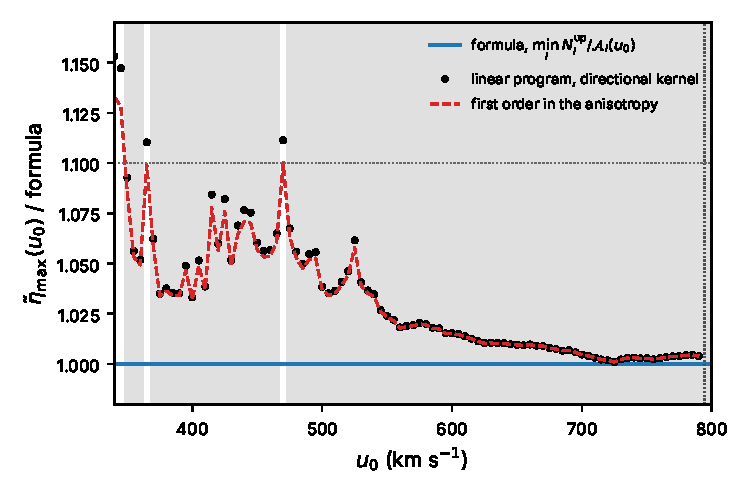
\includegraphics[width=\linewidth]{figures/ch21/limit21_2a.pdf}
\captionof{figure}{Largest $\tilde\eta(u_0)$ allowed by a silicon search over all halos, divided by the formula of the box (solid line at 1), against $u_0$. Dots: the fuller result, the linear program over galactic-frame streams with the direction-dependent kernel \cref{eq:21.2-multipole} of a crystal at \ang{45} north ($[001]$ up, $[100]$ east), integrated over the sidereal day, sampled from \SI{340}{km.s^{-1}} in steps of \SI{5}{km.s^{-1}}. Grid: \SI{2.5}{km.s^{-1}} in speed and \ang{2} in declination, with $|\vect{v}_{\mathrm{E}}| = \SI{250.5}{km.s^{-1}}$ toward declination \ang{47.5} and $v_{\mathrm{esc}} = \SI{544}{km.s^{-1}}$. Dashed: first order in the anisotropy, the formula divided by the smallest daily kernel of the tightest bin among the declinations allowed at $u_0$. $\mchi = \SI{2}{MeV}$, heavy mediator, one kilogram-year with no events in the one- and two-pair bins of the cascade of \cref{sec:18.3}, $N_i^{\mathrm{up}} = \ln 30$. Isotropic response: the random-phase loss function with local fields of Knapen, Kozaczuk and Lin; anisotropy: the $\ell = 4, 6, 8$ ratios of the empirical-pseudopotential model of \cref{sec:11.7} (a model). Gray: the formula lies within 10 percent of the linear program. Dotted: the 10 percent line and $v_{\mathrm{max}}$.}\label{fig:21-limit-hib}
\par}
\smallskip
Within \SI{20}{km.s^{-1}} of the one-pair onset, where every reachable pair sees the full anisotropy of the response, the formula falls short of the bound by up to 13 percent on the sampled speeds, and only the program gives a valid bound.
\end{limitbox}

The daily average removes most of the anisotropy. In the model the kernel of a stream fixed in crystal axes drops to 0.34 of its angle average in the least favorable direction. The sidereal mean of $Y^{\mathrm{c}}_4$, however, ranges only over $[-0.16, 0.07]$, against $[-0.43, 0.64]$ for $Y^{\mathrm{c}}_4$ itself. Over the declinations allowed at a given speed the daily kernel of the one-pair bin varies by $-7.3$ to $+3.1$ percent at \SI{500}{km.s^{-1}} and by $-2.3$ to $+1.7$ percent at \SI{600}{km.s^{-1}}. At every $u_0$ the program puts one stream at speed $u_0$, at the allowed declination where the daily kernel of the tightest bin is smallest, $-84^\circ$ at \SI{600}{km.s^{-1}}. The bound then exceeds the formula by the corresponding fraction: 2.3 percent at \SI{600}{km.s^{-1}}, 1.0 percent at \SI{700}{km.s^{-1}}, and no more than 4.6 percent anywhere above \SI{560}{km.s^{-1}}. The first-order estimate reproduces the program to 0.2 percent there and to 1.4 percent everywhere, because the optimum stays a single stream on a single bin. Below \SI{560}{km.s^{-1}} the ratio lies between 1.05 and 1.09 down to \SI{400}{km.s^{-1}}, because the pairs that enter the column near $u_0$ have $\vmin \approx u_0$ and see the full anisotropy, and at \SI{340}{km.s^{-1}}, \SI{15}{km.s^{-1}} above the one-pair onset at \SI{325}{km.s^{-1}}, it reaches 1.13. At \SI{790}{km.s^{-1}} the support leaves only declinations between $-56^\circ$ and $-40^\circ$, and the program lies 0.2 percent above the formula. A search binned in sidereal time keeps a kernel per time bin, close to the crystal-frame kernel for short bins, and its bound has to come from the program. The program then needs a response resolved in the direction of $\vect{q}$.

\subsection{Grids, certificates and leakage}\label{sec:21.2-leak}

A program solved on a grid of streams bounds the true optimum from below, since the grid can only restrict the halo, and its dual is a certificate only at the grid points. Between them the dual function can dip below zero. If the dip is at most $\delta_{\mathrm{cert}}$ on the support of $\mathsf{f}$, the dual still bounds every halo, at a price (\cref{app:D.46}):
\begin{equation}
  \int\mathsf{f}\,\dd\Xi \le \sum_i\lambda_iN_i^{\mathrm{up}} + \frac{\delta_{\mathrm{cert}}\,N_{\mathrm{tot}}}{\kappa_{\mathrm{v}}} ,
  \label{eq:21.2-defect}
\end{equation}
with $N_{\mathrm{tot}} = \sum_iN_i^{\mathrm{up}}$ and $\kappa_{\mathrm{v}}$ the smallest, over the support of $\mathsf{f}$, of the largest bin kernel, the visibility of \cref{eq:C.12-mass}. The second term is the violation times the largest halo mass the bins still allow on the support of $\mathsf{f}$. With $\delta_{\mathrm{cert}} = L_hh$, the Lipschitz constant of the dual function (the largest rate at which it changes per unit velocity) times the covering radius of the grid (the largest distance from a point of the support to the nearest grid point), it is the discretization bracket \cref{eq:C.12-leak}.

For the program of \cref{lim:21.2a} at $u_0 = \SI{600}{km.s^{-1}}$ a coarse and a fine grid agree in $\tilde\eta_{\max}$ to six digits, while the Lipschitz bracket is about 50 percent wide. The response is used on cells of \SI{0.01}{eV} by \SI{50}{eV} in momentum, and the kernel jumps whenever a cell's $\vmin$ crosses the speed of the stream, so a finite-difference Lipschitz constant measures the table, not the physics. The same structure gives an exact test. The isotropic part of a tabulated kernel is $\mathcal{A}_i(v)/v$ with $\mathcal{A}_i$ a step function, so the dual function changes its form only at the finitely many cell speeds $\vmin$; between them it is smooth. Evaluating the dual at those break speeds, with a Lipschitz bound only for the smooth anisotropic part $P_\ell(\vmin/v)$ between them, certifies it on the continuum.

A truncated response can also make a kernel negative, and then the mass bound behind \cref{eq:21.2-defect} fails for the computed kernel itself. Silicon gives the standard case. Outside the off-shell window, the Dyson convention of \cref{sec:8.6} splits the electronic response into a zero-phonon part and a phonon-dressed part whose sum is positive and whose parts need not be (\cref{eq:8.6-dyson}). The zero-phonon pair enters the cascade with the energy $\omega$, the phonon-dressed pair with $\omega - \omega_{\mathrm{ph}}$, and where the bin probability changes with energy the two are assigned to different bins. The bin-weighted response is then negative wherever one part is, but only where the bin probability changes within $\omega_{\mathrm{ph}}$. Seeding the phonon-dressed pair with the bin probability of its zero-phonon partner gives a kernel that is never negative, and \cref{eq:21.2-defect} applies to it with the difference of the two kernels added to $\delta_{\mathrm{cert}}$, weighted by $\lambda_i$. Suppose the number of pairs is stochastically ordered in the seed energy, so that the probability of at least $n$ pairs does not decrease with the energy for any $n$, as in the cascade of \cref{sec:18.3}. Then the total variation of each bin probability is at most 2, and the integral over energy of its change under a shift $\omega_{\mathrm{ph}} \le \omega_{\mathrm{max}}$ is at most $2\omega_{\mathrm{max}}$, one strip at each side of the bin (\cref{eq:D.46-tv}). Relative to the signal of a bin of width $\Delta_i$, the integral of its probability over energy,
\begin{equation}
  \frac{\text{misassigned weight in bin }i}{\text{signal in bin }i} \le \frac{2\,\omega_{\mathrm{max}}}{\Delta_i}\,\varrho^{\mathrm{leak}}_i ,
  \label{eq:21.2-fsleak}
\end{equation}
with $\varrho^{\mathrm{leak}}_i$ the largest phonon-dressed response over the bin, widened by $\omega_{\mathrm{max}}$ at each side, divided by the average of the total weighted with the bin probability, a number read off the computed response. For silicon, with the highest phonon at $\omega_{\mathrm{max}} = \SI{63.7}{meV}$ (\cref{sec:11.3}) and the two- and three-pair bins of the cascade of \cref{sec:18.3}, whose widths $\Delta_i$ are 3.60 and \SI{3.69}{eV}, close to $\varepsilon_{\mathrm{eh}} = \SI{3.749}{eV}$, the factor $2\omega_{\mathrm{max}}/\Delta_i$ is at most 0.035; the wider one-pair bin, \SI{4.98}{eV}, gives 0.026. The leakage is a few percent of $\varrho^{\mathrm{leak}}_i$ per bin. In the likelihood of \cref{sec:21.4} it is a normalization uncertainty of the bin with that width, and it enters the band of the limit.

\section{The kinematic edge}\label{sec:21.3}

A silicon detector that counts single electrons has no electron-recoil rate below the phonon-assisted onset, \SI{0.3374}{MeV} for free pairs (\cref{sec:13.1}), and just above it the rate grows as the $13/2$ power of the distance in mass (\cref{eq:13.9-medge}). In the model of \cref{fig:21-edge} the limit on $\sigmae$ is $1.6\times10^7$ times weaker \SI{0.001}{MeV} above the onset than at \SI{0.35}{MeV}, and still 4.6 times weaker \SI{0.010}{MeV} above it. Every mass up to \SI{0.010}{MeV} above the onset is tested only by particles within \SI{12}{km.s^{-1}} of $v_{\mathrm{max}}$, a fraction $6.0\times10^{-5}$ of the standard halo. The steep power, the position of the edge and its height therefore carry the halo model as much as the target. We will derive the power for any channel and any truncation of the halo, and work out which combinations of gap, threshold and halo parameters a limit near its edge measures.

\subsection{The rate kernel near its onset}\label{sec:21.3-kernel}

For a response averaged over the directions of $\vect{q}$, the rate is the speed integral $\mathcal{R} = (\rho_\chi/\mchi\rho_T)\int\dd v\, F_\chi(v)\,\varGamma(v)$ of \cref{sec:21.1-eta}. The kernel $\varGamma(v)$ of \cref{eq:21.1-gammav} vanishes below the onset speed $v_{\mathrm{on}}(\mchi)$ (\cref{sec:21.1-functional}), and the edge is decided by how it starts there. A particle of mass $\mchi$ and speed $v$ reaches the pair $(q,\omega)$ when $\vmin(q,\omega) \le v$, that is when $\omega \le qv - q^2/2\mchi$ (\cref{eq:1.3-vmin}). Let $E_{\mathrm{th}}(q)$ be the onset of the direction-averaged response at fixed $q = |\vect{q}|$, as in \cref{sec:13.9-onset}. We generalize the definition of \cref{sec:13.3} from the phonon-assisted loss function to any channel: the response rises above the onset as $x^{p_{\mathrm{on}}}$, with $x = \omega - E_{\mathrm{th}}(q)$. At fixed $q$ the energy integral then runs from $x = 0$ to the largest energy above the onset that the stream reaches,
\begin{equation*}
  x_{\mathrm{max}}(q; v) = qv - \frac{q^2}{2\mchi} - E_{\mathrm{th}}(q) ,
\end{equation*}
which is the $x_{\mathrm{max}}$ of \cref{sec:13.9-onset} with $v_{\mathrm{max}}$ replaced by $v$. The integral contributes $x_{\mathrm{max}}^{p_{\mathrm{on}}+1}/(p_{\mathrm{on}}+1)$ times the smooth factors of the channel: $F_{\mathrm{DM}}^2$, the powers of $q$ and the strength of the response.

The onset speed $v_{\mathrm{on}}(\mchi)$ is the speed at which the largest $x_{\mathrm{max}}$ reaches zero. Setting $v = v_{\mathrm{max}}$ and solving for the mass instead defines the edge mass of the channel,
\begin{equation}
  m_{\mathrm{edge}} = \min_q \frac{q^2}{2\,[qv_{\mathrm{max}} - E_{\mathrm{th}}(q)]} ,
  \label{eq:21.3-medge}
\end{equation}
which is \cref{eq:13.1-mPAdef} and \cref{eq:13.1-mZP} written for any onset. It reduces to $m_{\mathrm{min}}$ of \cref{eq:1.3-mmin} when $E_{\mathrm{th}}$ does not depend on $q$. Let $q^*$ be the optimal momentum transfer. Since $\partial x_{\mathrm{max}}/\partial v = q$, a stream slightly faster than $v_{\mathrm{on}}$ reaches $x_{\mathrm{max}}(q^*) = q^*(v - v_{\mathrm{on}})$ at the optimum, and near it
\begin{equation*}
  x_{\mathrm{max}}(q; v) \simeq q^*(v - v_{\mathrm{on}}) - \frac{(q - q^*)^2}{2\mchi} ,
\end{equation*}
where, as in \cref{sec:13.9-onset}, the curvature of $E_{\mathrm{th}}(q)$ is dropped against $1/\mchi$. That holds at the phonon-assisted onset; at the zero-phonon edge, where the onset rises steeply in $q$, the curvature changes the prefactor $\varGamma_{\mathrm{on}}$ below but not the exponent, which needs only a positive total curvature. The range of $q$ with $x_{\mathrm{max}} > 0$ has a width proportional to $(v - v_{\mathrm{on}})^{1/2}$, and the integral of $x_{\mathrm{max}}^{p_{\mathrm{on}}+1}$ over it is $(2\mchi)^{1/2}[q^*(v - v_{\mathrm{on}})]^{p_{\mathrm{on}}+3/2}B(\tfrac12, p_{\mathrm{on}}+2)$, with $B$ the Euler beta function. The kernel therefore starts as
\begin{equation}
  \varGamma(v) \simeq \varGamma_{\mathrm{on}}\,(v - v_{\mathrm{on}})^{p_{\mathrm{on}} + 3/2} , \qquad v \to v_{\mathrm{on}}^+ ,
  \label{eq:21.3-kernel}
\end{equation}
with a coefficient $\varGamma_{\mathrm{on}}$ that collects the strength of the response at the onset, $F_{\mathrm{DM}}^2(q^*)$ and the powers of $q^*$ and $\mchi$. The power $p_{\mathrm{on}} + 3/2$ counts $p_{\mathrm{on}} + 1$ from the energy integral and $\tfrac12$ from the width in $q$.

The $\tfrac12$ becomes 1 when $x_{\mathrm{max}}(q)$ has a corner at its maximum. If $x_{\mathrm{max}} \simeq x_{\mathrm{max}}(q^*) - s_\pm|q - q^*|$ with slopes $s_\pm$ on the two sides, the width in $q$ is linear in $v - v_{\mathrm{on}}$ and the power is $p_{\mathrm{on}} + 2$. A corner arises when the onset itself has a kink at $q^*$, or when the range of $q$ ends there. The second is the case of the free nuclear recoil with a detector threshold. Its response is the line $\omega = q^2/2M$, a delta function at fixed $q$, so the energy integral is a constant, which is the case $p_{\mathrm{on}} = -1$. The threshold cuts the range of momentum transfers at $q_{\mathrm{th}} = (2ME_{\mathrm{th}})^{1/2}$, and near the edge the optimum sits at that cut. The kernel of the free nuclear recoil therefore starts linearly, with power $-1 + 2 = 1$.

\subsection{The escape tail of the halo}\label{sec:21.3-tail}

The other factor of the speed integral, $F_\chi(v)$, vanishes at $v_{\mathrm{max}}$, and how it vanishes depends on how the galactic distribution goes to zero at the escape speed. The standard halo of \cref{tab:1-shm} is cut by hand (\cref{eq:1.2-fgal}), so the distribution in the galactic frame stays finite up to $v_{\mathrm{esc}}$ and then drops to zero. Equilibrium distribution functions built for the density profiles of simulated halos go to zero smoothly instead. Lisanti and co-workers write such a family as~\cite[Eq.~(1)]{lisanti2011dark}
\begin{equation*}
  f_{\mathrm{gal}}(u) \propto \left[\exp\!\left(\frac{v_{\mathrm{esc}}^2 - u^2}{k_{\mathrm{tail}}\,v_0^2}\right) - 1\right]^{k_{\mathrm{tail}}}\Theta(v_{\mathrm{esc}} - u) ,
\end{equation*}
which near the escape speed behaves as $(v_{\mathrm{esc}} - u)^{k_{\mathrm{tail}}}$~\cite[Eq.~(11)]{lisanti2011dark}. The \emph{tail exponent} $k_{\mathrm{tail}}$ is zero for the sharp cut of the standard halo and one for the King model, $f_{\mathrm{gal}} \propto \ee^{-u^2/v_0^2} - \ee^{-v_{\mathrm{esc}}^2/v_0^2}$~\cite[Eq.~(12)]{lisanti2011dark}. Their fits to the velocity distributions of simulated galactic halos prefer $k_{\mathrm{tail}}$ between 1.5 and 3.5~\cite[Sect.~II, Eq.~(10), and Fig.~3]{lisanti2011dark}. Near the escape speed, then, $f_{\mathrm{gal}} \simeq f_{\mathrm{esc}}\,y^{k_{\mathrm{tail}}}$ with $y = v_{\mathrm{esc}} - u$ and a constant $f_{\mathrm{esc}}$; for the standard halo $f_{\mathrm{esc}} = \ee^{-v_{\mathrm{esc}}^2/v_0^2}/N_{\mathrm{esc}}$, the height of the normalized distribution at the cut.

The laboratory speeds near $v_{\mathrm{max}} = v_{\mathrm{esc}} + v_{\mathrm{E}}$ come from a small cap of velocity space. The fastest particle has its galactic velocity antiparallel to $\vect{v}_{\mathrm{E}}$, so take the unit vector $\hat{\vect{e}} = -\vect{v}_{\mathrm{E}}/v_{\mathrm{E}}$ and write a laboratory velocity as $\vect{v} = (v_{\mathrm{max}} - s)\hat{\vect{e}} + \vect{v}_\perp$, with $s$ and $|\vect{v}_\perp|$ small. To second order in them the laboratory speed and the galactic speed are
\begin{equation*}
  v \simeq v_{\mathrm{max}} - s + \frac{v_\perp^2}{2v_{\mathrm{max}}} , \qquad
  u = |\vect{v} + \vect{v}_{\mathrm{E}}| \simeq v_{\mathrm{esc}} - s + \frac{v_\perp^2}{2v_{\mathrm{esc}}} .
\end{equation*}
A particle with $v \ge v_{\mathrm{max}} - \delta$ that is bound to the halo therefore has $0 \le y \le \delta - a_\perp v_\perp^2$, with $a_\perp = 1/2v_{\mathrm{esc}} - 1/2v_{\mathrm{max}} = v_{\mathrm{E}}/(2v_{\mathrm{esc}}v_{\mathrm{max}})$: a lens of depth $\delta$ and radius $(\delta/a_\perp)^{1/2}$. At fixed $\vect{v}_\perp$ the volume element is $\dd s = \dd y$, and the fraction of particles in the lens is
\begin{equation*}
  \int\!\dd^2v_\perp\int_0^{\delta - a_\perp v_\perp^2}\!\dd y\, f_{\mathrm{esc}}\,y^{k_{\mathrm{tail}}}
  = \frac{\pi f_{\mathrm{esc}}\,\delta^{k_{\mathrm{tail}}+2}}{a_\perp(k_{\mathrm{tail}}+1)(k_{\mathrm{tail}}+2)} .
\end{equation*}
Its derivative with respect to $\delta$ is the speed distribution at $v = v_{\mathrm{max}} - \delta$:
\begin{equation}
  F_\chi(v) \simeq F_{\mathrm{esc}}\,(v_{\mathrm{max}} - v)^{k_{\mathrm{tail}}+1} , \qquad
  F_{\mathrm{esc}} = \frac{2\pi f_{\mathrm{esc}}\,v_{\mathrm{esc}}v_{\mathrm{max}}}{(k_{\mathrm{tail}}+1)\,v_{\mathrm{E}}} ,
  \label{eq:21.3-tail}
\end{equation}
valid for $v_{\mathrm{max}} - v \ll v_{\mathrm{E}}, v_{\mathrm{esc}}$. Dividing by $v \simeq v_{\mathrm{max}}$ and integrating once more, $\eta(\vmin) \propto (v_{\mathrm{max}} - \vmin)^{k_{\mathrm{tail}}+2}$. For $k_{\mathrm{tail}} = 0$ this is the quadratic edge of \cref{eq:1.3-edge}, with its coefficient $A_\eta = \pi v_{\mathrm{esc}}\ee^{-v_{\mathrm{esc}}^2/v_0^2}/(v_{\mathrm{E}}N_{\mathrm{esc}}) = F_{\mathrm{esc}}/2v_{\mathrm{max}}$, so the lens reproduces the expansion of the closed form. For the smooth members the power law needs one more condition: the bracket of $f_{\mathrm{gal}}$ is linear in $y$ only for $y \ll k_{\mathrm{tail}}v_0^2/2v_{\mathrm{esc}}$, which is \SI{52}{km.s^{-1}} for the King model.

A smooth tail empties the lens. With the same $v_0$ and $v_{\mathrm{esc}}$, the $6.0\times10^{-5}$ of the standard halo within \SI{12}{km.s^{-1}} of $v_{\mathrm{max}}$, which decide every silicon mass up to \SI{0.010}{MeV} above the onset, become $4.7\times10^{-6}$ in the King model and $3.7\times10^{-8}$ for $k_{\mathrm{tail}} = 2.5$.

\subsection{The edge power law}\label{sec:21.3-power}

Both factors of the speed integral now start as powers, one at $v_{\mathrm{on}}$ and one at $v_{\mathrm{max}}$, and the integral is a beta function. Write $\delta_{\mathrm{on}} = v_{\mathrm{max}} - v_{\mathrm{on}}(\mchi)$ for the window of speeds that contribute. Inserting \cref{eq:21.3-kernel,eq:21.3-tail},
\begin{equation*}
  \begin{aligned}
  \mathcal{R} &\simeq \frac{\rho_\chi}{\mchi\rho_T}\,F_{\mathrm{esc}}\,\varGamma_{\mathrm{on}}\int_{v_{\mathrm{on}}}^{v_{\mathrm{max}}}\dd v\,(v_{\mathrm{max}} - v)^{k_{\mathrm{tail}}+1}(v - v_{\mathrm{on}})^{p_{\mathrm{on}}+3/2} \\
  &= \frac{\rho_\chi}{\mchi\rho_T}\,F_{\mathrm{esc}}\,\varGamma_{\mathrm{on}}\,B\bigl(k_{\mathrm{tail}}+2,\, p_{\mathrm{on}}+\tfrac52\bigr)\,\delta_{\mathrm{on}}^{\,p_{\mathrm{on}}+k_{\mathrm{tail}}+7/2} .
  \end{aligned}
\end{equation*}
The window is linear in the distance from the edge mass. The edge mass of \cref{eq:21.3-medge}, as a function of $v_{\mathrm{max}}$, changes by $\dd m_{\mathrm{edge}}/\dd v_{\mathrm{max}} = -q^{*3}/[2(q^*v_{\mathrm{max}} - E_{\mathrm{th}}(q^*))^2] = -2m_{\mathrm{edge}}^2/q^*$, since only the explicit dependence counts at the minimum. A mass $\mchi$ just above $m_{\mathrm{edge}}$ is therefore at its own edge for the speed $v_{\mathrm{on}} = v_{\mathrm{max}} - \delta_{\mathrm{on}}$ with
\begin{equation*}
  \delta_{\mathrm{on}} \simeq \frac{q^*}{2m_{\mathrm{edge}}^2}\,(\mchi - m_{\mathrm{edge}}) .
\end{equation*}
For a $q$-independent onset, $q^* = m_{\mathrm{min}}v_{\mathrm{max}}$ and this is the window $(v_{\mathrm{max}}/2)(\mchi - m_{\mathrm{min}})/m_{\mathrm{min}}$ of \cref{sec:1.3-edge}; at the phonon-assisted onset of silicon, \cref{eq:13.1-mPA} gives $q^* = m_{\mathrm{min}}^{\mathrm{PA}}(v_{\mathrm{max}} \pm u_\nu)$, with $u_\nu$ the group velocity of the phonon at $\vect{Q}^*$, equal to $m_{\mathrm{min}}^{\mathrm{PA}}v_{\mathrm{max}}$ up to $u_\nu/v_{\mathrm{max}} \sim 3\times10^{-3}$.

\begin{keyresult}[Edge power law]
Let the direction-averaged response of a channel rise as $x^{p_{\mathrm{on}}}$ above its onset, and let the galactic distribution of the halo vanish as $(v_{\mathrm{esc}} - u)^{k_{\mathrm{tail}}}$ at the escape speed. If the largest energy above the onset, $x_{\mathrm{max}}$, has a smooth maximum in $q$, the rate near the edge mass $m_{\mathrm{edge}}$ of \cref{eq:21.3-medge} is
\begin{equation}
  \mathcal{R}(\mchi) \propto (\mchi - m_{\mathrm{edge}})^{\,p_{\mathrm{on}} + k_{\mathrm{tail}} + 7/2} .
  \label{eq:21.3-power}
\end{equation}
If $x_{\mathrm{max}}$ has a corner, the power is $p_{\mathrm{on}} + k_{\mathrm{tail}} + 4$. The response contributes $p_{\mathrm{on}} + 1$, the width in $q$ one half (one at a corner), the halo $k_{\mathrm{tail}} + 1$, and the overlap of the two onsets one more. The power holds for either mediator, as long as $F_{\mathrm{DM}}$ is smooth at $q^* \neq 0$.
\end{keyresult}

For the standard halo, $k_{\mathrm{tail}} = 0$, \cref{eq:21.3-power} is \cref{eq:13.9-medge}. For the King model the silicon edge steepens from $13/2$ to $15/2$, and over the range preferred by simulated halos to between 8 and 10. The free nuclear recoil with a sharp threshold has a linear kernel and the power $3 + k_{\mathrm{tail}}$.

The power also sets how close to the edge an exposure reaches, the distance that \cref{sec:21.1-floor} left open. A background-free exposure excludes a mass at which it predicts more than 2.3 events (\cref{eq:1.5-N90}). Near the edge the predicted number is proportional to $M_{\mathrm{det}}t_{\mathrm{exp}}\sigmae(\mchi - m_{\mathrm{edge}})^{n}$, with the exposure $M_{\mathrm{det}}t_{\mathrm{exp}}$ and $n$ the power of \cref{eq:21.3-power}. At fixed $\sigmae$ the lowest excluded mass therefore lies at a distance from the edge proportional to $(M_{\mathrm{det}}t_{\mathrm{exp}}\sigmae)^{-1/n}$. At the free-pair edge of silicon, $n = 13/2$, ten times the exposure brings the excluded mass a factor $10^{-2/13} = 0.70$ closer to the edge; with the King tail the factor is 0.74.

\Cref{tab:21-edge} collects the powers of the silicon electron-recoil edges and the free nuclear recoil. The phonon-assisted entries use the onset exponents of \cref{sec:13.3,sec:13.8}. For the zero-phonon edge of \cref{sec:13.9-edges} the exponents follow from the counting rule of \cref{sec:13.3}: an isolated quadratic minimum in $D$ free variables gives $x^{D/2 - 1}$, and a vertex that vanishes linearly at the minimum adds one power. At fixed $|\vect{q}|$ a free zero-phonon pair has three free variables, the components of the hole's crystal momentum. The average over the two angles of $\hat{\vect{q}}$ adds two more, since each of the 24 equivalent optima of the first edge is an isolated minimum with curvatures $\beta_\theta$ and $\beta_z$ (\cref{sec:13.9-edges}). With $D = 5$ the pair would start as $x^{3/2}$. The first zero-phonon line, however, is second class: its vertex vanishes in the mirror plane and grows linearly with the distance from it (\cref{sec:13.9-glide}), so $p_{\mathrm{on}} = 5/2$. The Coulomb attraction lowers the onset exponent of a continuum at fixed $\vect{q}$ by one half, from $x^{1/2}$ to a step, as \cref{eq:13.8-edge} does for the phonon-assisted continuum, and the excitonic zero-phonon continuum has $p_{\mathrm{on}} = 2$. The $1s$ line is a delta function at fixed $\vect{q}$; the two angles turn it into a step and the vertex zero into $x^1$. Since the phonon-assisted rate is already open at \SI{0.405}{MeV}, these powers describe how the zero-phonon rate adds to the total, a kink in the rate rather than the edge of the limit.

\begin{table}[tbp]
  \caption{Powers of the rate in the dark-matter mass, $\mathcal{R} \propto (\mchi - m_{\mathrm{edge}})^{n}$, at the edges of silicon, for the sharp-cut standard halo ($k_{\mathrm{tail}} = 0$); a halo with tail exponent $k_{\mathrm{tail}}$ adds $k_{\mathrm{tail}}$ to every entry (\cref{eq:21.3-power}). Masses in MeV, with the halo of \cref{tab:1-shm}; $p_{\mathrm{on}}$ is the onset exponent of the direction-averaged response at fixed $|\vect{q}|$; the fourth column says whether $x_{\mathrm{max}}(q)$ has a smooth maximum or a corner at $q^*$ (\cref{eq:21.3-power}). The zero-phonon edges lie above the phonon-assisted onset, where they add a kink to the total rate. The nuclear-recoil row is for a \SI{10}{eV} threshold.}
  \label{tab:21-edge}
  \centering\small
  \begin{tabular}{@{}llccc@{}}
    \toprule
    Edge & $m_{\mathrm{edge}}$ & $p_{\mathrm{on}}$ & $x_{\mathrm{max}}$ at $q^*$ & $n$ \\
    \midrule
    Phonon-assisted, free pair (transverse acoustic) & 0.3374 & 3 & smooth & $13/2$ \\
    Phonon-assisted, excitonic continuum & 0.3374 & $5/2$ & smooth & 6 \\
    Phonon-assisted, exciton replica & 0.3332 & $3/2$ & smooth & 5 \\
    Zero-phonon, first edge, free pair & 0.405--0.408 & $5/2$ & smooth & 6 \\
    Zero-phonon, first edge, excitonic continuum & 0.405--0.408 & 2 & smooth & $11/2$ \\
    Zero-phonon, first edge, $1s$ line & 0.402--0.405 & 1 & smooth & $9/2$ \\
    Free nuclear recoil, sharp threshold & 137 & $-1$ & corner & 3 \\
    \bottomrule
  \end{tabular}
\end{table}

\Cref{fig:21-edge}(b) checks \cref{eq:21.3-power} in the model of \cref{sec:13.9-onset}: the computed transverse acoustic onset on the valley axis, a loss function $Cx^3$ and the family of halos above. The local power of the rate is $p_{\mathrm{on}} + k_{\mathrm{tail}} + 7/2$ to 0.002 up to \SI{3e-4}{MeV} above the onset for $k_{\mathrm{tail}} = 0$, 1 and 2.5. For the standard halo it drifts to 6.54 at \SI{0.005}{MeV} and 6.61 at \SI{0.02}{MeV}, as the curvature of the speed distribution enters; a light mediator leaves the power at 6.500 near the onset. The model loss function is the idealization. The computed one follows $x^3$ only for $x < \SI{1.3}{meV}$ (\cref{fig:13-paloss}), and since the largest energy above the onset grows as $x_{\mathrm{max}}^* = \tfrac12 v_{\mathrm{max}}^2(\mchi - m_{\mathrm{edge}})$, \SI{3.5}{meV} per \SI{0.001}{MeV}, the power is exact only within \SI{4e-4}{MeV} of the onset. At the zero-phonon edge, $x_{\mathrm{max}}^* = (q^{*2}/2m_{\mathrm{edge}}^2)(\mchi - m_{\mathrm{edge}})$ is \SI{5.3}{meV} per \SI{0.001}{MeV}; the $1s$ power holds while $x_{\mathrm{max}}^*$ stays below the exciton binding of \SI{14.7}{meV}, within \SI{0.0028}{MeV} of the line, and the continuum powers until neighboring optima merge \SI{49}{meV} above the edge (\cref{sec:13.9-rates}), \SI{0.009}{MeV} above it. The halo side is never the limitation at these masses: \SI{0.01}{MeV} above the onset the window is $\delta_{\mathrm{on}} = \SI{11.8}{km.s^{-1}}$, far inside the \SI{173}{km.s^{-1}} scale of the correction in \cref{eq:1.3-edge} and the \SI{52}{km.s^{-1}} range of the King tail.

\begin{figure}[tbp]
  \centering
  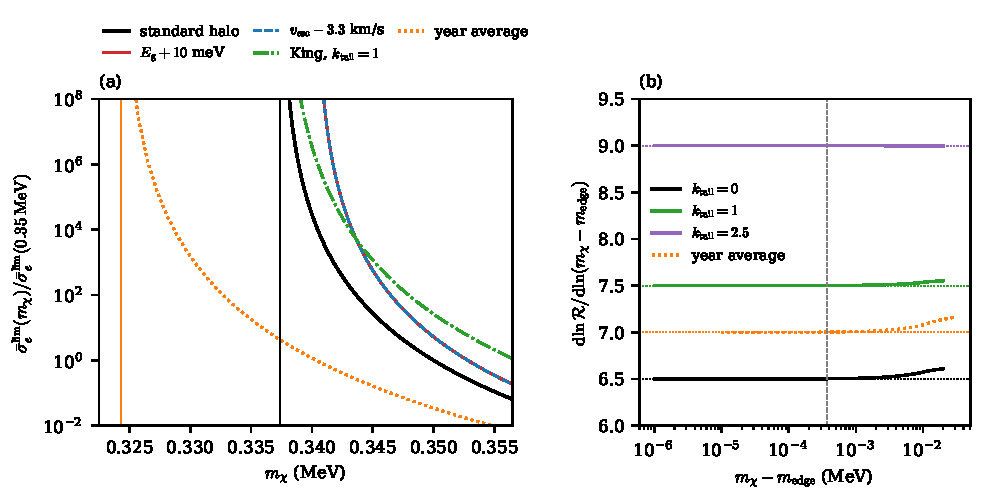
\includegraphics[width=\linewidth]{figures/ch21/fig21_3.pdf}
  \caption{The low-mass edge of a silicon electron-recoil limit. Model: direction-averaged loss function $Cx^3$ above the transverse acoustic onset on the valley axis ($m_{\mathrm{edge}} = \SI{0.33738}{MeV}$, PBE force constants of \cref{sec:5.2}, $\Eg = \SI{1.17}{eV}$), heavy mediator, background-free counting at fixed exposure, so that the limit is proportional to $1/\mathcal{R}$. (a)~Limit on $\sigmae$ relative to its value at \SI{0.35}{MeV}. Black: standard halo ($v_0 = 238$, $v_{\mathrm{esc}} = 544$, $v_{\mathrm{E}} = \SI{250.5}{km.s^{-1}}$). Red: gap raised by \SI{10}{meV}. Blue dashed, on top of the red curve: escape speed lowered by \SI{3.3}{km.s^{-1}} instead. Green dash-dotted: King model ($k_{\mathrm{tail}} = 1$) with the same $v_0$ and $v_{\mathrm{esc}}$. Orange dotted: an exposure spread uniformly over a year, with $v_{\mathrm{E}}$ between 237.4 and \SI{266.4}{km.s^{-1}}. Vertical lines: the edge at the reference speed and the June edge, \SI{0.3243}{MeV}. (b)~Local power of the rate, $\dd\ln\mathcal{R}/\dd\ln(\mchi - m_{\mathrm{edge}})$, for halos with tail exponents $k_{\mathrm{tail}} = 0$, 1 and 2.5 of the family of Lisanti and co-workers~\cite[Eq.~(1)]{lisanti2011dark} with the same $v_0$, $v_{\mathrm{esc}}$, $v_{\mathrm{E}}$, and for the year average ($m_{\mathrm{edge}}$ its June value). Dotted: the powers $p_{\mathrm{on}} + k_{\mathrm{tail}} + 7/2$ of \cref{eq:21.3-power} and $p_{\mathrm{on}} + 4$ for the year average. Dashed: the mass at which $x_{\mathrm{max}}^*$ reaches \SI{1.3}{meV}, the end of the $x^3$ range of the computed loss function.}
  \label{fig:21-edge}
\end{figure}

\subsection{Degeneracies at the edge}\label{sec:21.3-degeneracy}

Near its edge a limit is set by three numbers: the edge mass, the power and the height of the rate. Each is a combination of target and halo parameters, and parameters that enter the same combination cannot be told apart by the limit.

The edge mass depends on the onset $E_{\mathrm{th}}(q)$ and on $v_{\mathrm{max}} = v_{\mathrm{esc}} + v_{\mathrm{E}}$, and on nothing else. For a $q$-independent onset it depends on them only through $E_{\mathrm{th}}/v_{\mathrm{max}}^2$, the rule $\delta\ln m_{\mathrm{min}} = \delta\ln E_{\mathrm{th}} - 2\,\delta\ln v_{\mathrm{max}}$ of \cref{sec:1.3-edge}. The phonon-assisted onset of silicon depends on $q$, but \cref{eq:13.1-mPA} gives $m_{\mathrm{min}}^{\mathrm{PA}} = 2E_{\mathrm{on}}/(v_{\mathrm{max}}^2 - u_\nu^2)$ with the onset energy $E_{\mathrm{on}} = \Eg + \omega_\nu(\vect{Q}^*)$, and $u_\nu^2/v_{\mathrm{max}}^2 \sim 10^{-5}$. To that accuracy the edge measures the single ratio $E_{\mathrm{on}}/v_{\mathrm{max}}^2$. A one percent error in the onset energy $E_{\mathrm{on}}$, whether it comes from the gap, from the phonon energy that the onset adds or from the energy of a threshold of $n$ pairs, moves the edge exactly as a \SI{0.5}{\percent} change of $v_{\mathrm{max}}$, \SI{4.0}{km.s^{-1}}, does. Turned around, the escape-speed uncertainty of $\pm\SI{25}{km.s^{-1}}$ (\cref{sec:1.2}) moves the edge by $-6.0$ and $+6.6$ percent, as an error of $-71$ or $+78$~meV in the onset energy would, and the annual cycle of $v_{\mathrm{E}}$ by $-3.9$ and $+3.4$ percent.

The height of the rate is a product, $F_{\mathrm{esc}}\varGamma_{\mathrm{on}}$ in the speed integral above. The reference cross-section and the strength of the response at the onset sit in $\varGamma_{\mathrm{on}}$. The height $f_{\mathrm{esc}}$ of the galactic distribution at the cut and the geometric factor $v_{\mathrm{esc}}v_{\mathrm{max}}/v_{\mathrm{E}}$ of the lens sit in $F_{\mathrm{esc}}$. A null result near the edge bounds only the product. The dispersion $v_0$ enters the edge only here, through $f_{\mathrm{esc}}$: for the standard halo $\partial\ln A_\eta/\partial v_0 = 2v_{\mathrm{esc}}^2/v_0^3 - \partial\ln N_{\mathrm{esc}}/\partial v_0 = +\SI{3.2}{\percent}$ per km\,s$^{-1}$, so the uncertainty of $\pm\SI{6}{km.s^{-1}}$ (\cref{sec:1.2}) scales the rate near the edge by 1.21 and 0.83 at fixed edge mass. The escape speed enters both the edge mass and the height, but in the height its effect nearly cancels. At a fixed edge mass, lowering $v_{\mathrm{esc}}$ raises $A_\eta$ by \SI{1.76}{\percent} per km\,s$^{-1}$, since the cut moves into denser parts of the Maxwellian. It also lowers the powers of $v_{\mathrm{max}}$ in the rate. With the $q^3$ of \cref{eq:10.2-rate}, the energy integral of \cref{sec:13.9-onset} and $q^* = \mchi v_{\mathrm{max}}$, the rate at fixed $\mchi - m_{\mathrm{edge}}$ and fixed edge mass, with the gap moved together with $v_{\mathrm{esc}}$, scales as $A_\eta v_{\mathrm{max}}^{2p_{\mathrm{on}}+8}$ for a heavy mediator. For $p_{\mathrm{on}} = 3$ the factor $v_{\mathrm{max}}^{14}$ changes by \SI{1.76}{\percent} per km\,s$^{-1}$ as well, and the two changes cancel. A light mediator removes four powers of $v_{\mathrm{max}}$ through $F_{\mathrm{DM}}^2 \propto q^{*-4}$ and leaves \SI{0.5}{\percent} per km\,s$^{-1}$.

The power is a sum, $p_{\mathrm{on}} + k_{\mathrm{tail}}$, and the sum is all that a counting experiment can measure. The two exponents do enter the spectrum separately. At fixed $\omega$ the integral over $q$ of $\eta \propto (v_{\mathrm{max}} - \vmin)^{k_{\mathrm{tail}}+2}$, with $v_{\mathrm{max}} - \vmin = (x_{\mathrm{max}}(q) - x)/q$, runs over a range of width $\propto (x_{\mathrm{max}}^* - x)^{1/2}$ and gives
\begin{equation*}
  \frac{\dd\mathcal{R}}{\dd\omega} \propto (\omega - E_{\mathrm{on}})^{p_{\mathrm{on}}}\,(\omega_{\mathrm{top}} - \omega)^{k_{\mathrm{tail}} + 5/2} , \qquad \omega_{\mathrm{top}} = E_{\mathrm{on}} + x_{\mathrm{max}}^* ,
\end{equation*}
for an onset that is flat near $q^*$. The response shapes the bottom of the spectrum and the halo its top. The whole spectrum, however, is \SI{3.5}{meV} wide per \SI{0.001}{MeV} above the edge, while a silicon detector that counts pairs puts every deposit between $\Eg$ and $2\Eg$ into one bin (\cref{sec:1.5}). The bin integrates the spectrum, and with it the two exponents into their sum.

Two handles distinguish the target from the halo. The first is a second edge with a different mixture. At the zero-phonon edge the onset rises steeply with the distance of $\vect{q}$ from the valley, and the envelope theorem, by which only the explicit dependence of a minimized function on a parameter counts at its minimum (\cref{sec:21.3-power}), applied to \cref{eq:13.1-mZP} leads to $\partial\ln m_{\mathrm{min}}^{\mathrm{ZP}}/\partial\ln\Eg = \Eg/(q^*v_{\mathrm{max}} - E^*)$ and $\partial\ln m_{\mathrm{min}}^{\mathrm{ZP}}/\partial\ln v_{\mathrm{max}} = -q^*v_{\mathrm{max}}/(q^*v_{\mathrm{max}} - E^*)$, with $E^*$ the pair energy at the optimum and a rigid shift of the conduction bands. At the joint minimum of \cref{sec:13.9-edges}, $|\vect{q}^*| = \SI{1.33}{keV}$ and $E^* = \SI{1.355}{eV}$, these are 0.54 and $-1.62$, against 1 and $-2$ at the phonon-assisted onset. Two edges of one crystal measure the gap and $v_{\mathrm{max}}$ separately, in principle, although the zero-phonon edge appears only as a kink of the rate.

The second handle is time. Over the year $v_{\mathrm{max}}$ moves between 781 and \SI{810}{km.s^{-1}} (\cref{eq:1.2-vmax}) while the gap stays put, and near the edge the rate responds with the full power of \cref{eq:21.3-power}. An exposure spread over the year has the time-averaged rate. Near the largest Earth speed, on 2 June, the edge mass varies quadratically in time, $m_{\mathrm{edge}}(t) \simeq m_{\mathrm{edge}}^{\mathrm{June}} + \tfrac12\ddot m\,(t - t_{\mathrm{June}})^2$, and the time integral of $(\mchi - m_{\mathrm{edge}}(t))^{n}$ over the interval in which it is positive, of width $\propto (\mchi - m_{\mathrm{edge}}^{\mathrm{June}})^{1/2}$, adds one half to the power. The year-averaged edge sits at the June value, $m_{\mathrm{edge}}^{\mathrm{June}} = \SI{0.3243}{MeV}$ for the free-pair onset, \SI{3.9}{\percent} below the edge at the reference speed, with the power $p_{\mathrm{on}} + k_{\mathrm{tail}} + 4$ (\cref{fig:21-edge}(b)). At \SI{0.010}{MeV} above the reference edge the averaged rate is 62 times the rate at the reference speed, and at \SI{0.020}{MeV} still 8.5 times. Near the edge a limit computed at a fixed Earth speed is therefore a statement about that day (\cref{sec:21.1-floor}).

\begin{workedexample}{How a \SI{10}{meV} gap shift moves the silicon edge}\label{we:21-gapshift}
Ten meV is smaller than either energy that separates the silicon onsets, the exciton binding of \SI{14.7}{meV} and the transverse acoustic phonon at $\vect{Q}^*$, about \SI{15}{meV} (\cref{sec:13.1}). That phonon is softer than the \SI{18.27}{meV} replica of optical absorption, because the dark matter supplies part of the momentum and $\vect{Q}^*$ is shorter than the valley wavevector. Raise the gap by $\delta E = \SI{10}{meV}$, with the halo of \cref{tab:1-shm}.

\emph{Edge.} By \cref{eq:13.1-mPA}, $\delta m_{\mathrm{edge}} = 2\,\delta E/v_{\mathrm{max}}^2 = 2 \times \SI{0.010}{eV}/(7.02\times10^{-6}) = \SI{0.00285}{MeV}$. The model of \cref{fig:21-edge} puts the shift at \SI{0.00283}{MeV}, \SI{0.84}{\percent} of the edge, slightly less because the larger $q^*$ shortens $\vect{Q}^*$ and lowers the phonon energy that the onset adds.

\emph{Limit.} At a mass $\delta m$ above the old edge, \cref{eq:21.3-power} multiplies the rate by $(1 - \delta m_{\mathrm{edge}}/\delta m)^{13/2}$. At $\delta m = 0.005$, 0.010 and \SI{0.020}{MeV} this is 0.0044, 0.115 and 0.371; the model gives 0.0043, 0.114 and 0.368. The limit weakens by factors of 231, 8.8 and 2.7. The power law holds here although the masses lie outside the $x^3$ range of the computed loss function, because the factor is a ratio of two rates with the same shape.

\emph{The halo that mimics it.} The same edge follows from a lower $v_{\mathrm{max}}$, by $(v_{\mathrm{max}}/2)\,\delta E/E_{\mathrm{on}}$ with $E_{\mathrm{on}} = \tfrac12 m_{\mathrm{edge}}v_{\mathrm{max}}^2 = \SI{1.1848}{eV}$, that is \SI{3.35}{km.s^{-1}}; solving the model for the escape speed gives \SI{3.32}{km.s^{-1}}. Above the common edge the two rates agree to \SI{0.04}{\percent} for a heavy mediator, the cancellation of the height derived above, and differ by \SI{1.7}{\percent} for a light one. No limit can tell a \SI{10}{meV} gap error from a \SI{3.3}{km.s^{-1}} error in the escape speed, less than a seventh of its uncertainty.

\emph{The zero-phonon edge.} The same gap shift moves $m_{\mathrm{min}}^{\mathrm{ZP}}$ by $m_{\mathrm{min}}^{\mathrm{ZP}}\,\delta E/(q^*v_{\mathrm{max}} - E^*) = \SI{0.4077}{MeV} \times 0.010/2.170 = \SI{0.00188}{MeV}$, \SI{0.46}{\percent}, while the \SI{3.3}{km.s^{-1}} halo shift moves it by $1.62 \times \SI{0.42}{\percent} = \SI{0.68}{\percent}$, or \SI{0.00277}{MeV}. Measured from the phonon-assisted onset, the zero-phonon edge comes \SI{0.00095}{MeV} closer under the gap shift and only \SI{0.00006}{MeV} closer under the halo shift.
\end{workedexample}

\section{Theory uncertainties in a limit}\label{sec:21.4}

A silicon detector that records no event above a one-pair threshold in a kilogram-year excludes, at \SI{3}{MeV} and for a heavy mediator, every cross-section above $\SI{1.24e-41}{cm^2}$, if the rate is the central value of \cref{we:10-band3}. With the rate computed at the random-phase level, without local fields, the same zero excludes everything above $\SI{9.23e-42}{cm^2}$, a limit 1.35 times stronger. The central rate is itself uncertain by a factor of 1.48 at one standard deviation. Which number should the experiment publish, and how wide is the uncertainty on it?

\subsection{Poisson limits with a known background}\label{sec:21.4-poisson}

A counting experiment observes $N_{\mathrm{obs}}$ events where its background is expected to give $N_{\mathrm{bkg}}$. The classical upper limit at confidence level $\mathrm{CL}$ is the signal $N^{\mathrm{up}}$ at which data as low as those observed occur with probability $1 - \mathrm{CL}$,
\begin{equation}
  \sum_{n=0}^{N_{\mathrm{obs}}}P\bigl(n\,\big|\,N^{\mathrm{up}} + N_{\mathrm{bkg}}\bigr) = 1 - \mathrm{CL} ,
  \label{eq:21.4-classical}
\end{equation}
with $P$ the Poisson probability \cref{eq:1.5-poisson}, as in \cref{sec:1.5-limit}. For no events the sum has one term, and $N^{\mathrm{up}} = \ln[1/(1 - \mathrm{CL})] - N_{\mathrm{bkg}}$, which is $2.303 - N_{\mathrm{bkg}}$ at \SI{90}{\percent}. The background lowers the limit even though nothing was seen: with $N_{\mathrm{bkg}} = 1$ the limit is 1.303, and for $N_{\mathrm{bkg}} > 2.303$ the interval is empty. An empty interval is a correct frequentist statement, since no events on a background above 2.303 occur in fewer than \SI{10}{\percent} of experiments, but it says nothing about the signal. With one event on a background of one the classical limit is 2.890, and with two on a background of two it is 3.322.

Feldman and Cousins removed the empty intervals by changing the order in which outcomes enter the construction~\cite[Sect.~IV\,A]{feldman1998unified}. At each trial signal $N_{\mathrm{sig}}$ they rank the outcomes $n$ by the likelihood ratio
\begin{equation}
  \mathsf{R}_{\mathrm{FC}}(n) = \frac{P(n\,|\,N_{\mathrm{sig}} + N_{\mathrm{bkg}})}{P\bigl(n\,|\,\max(0, n - N_{\mathrm{bkg}}) + N_{\mathrm{bkg}}\bigr)} ,
  \label{eq:21.4-fc}
\end{equation}
the probability of $n$ at the trial signal over its probability at the best signal that is not negative~\cite[Eq.~(4.1)]{feldman1998unified}. Outcomes are accepted in decreasing order of $\mathsf{R}_{\mathrm{FC}}$ until their summed probability reaches $\mathrm{CL}$, and the interval for $N_{\mathrm{obs}}$ is the set of trial signals whose accepted outcomes contain it. The interval is never empty, and it turns from an upper limit into a two-sided interval as $N_{\mathrm{obs}}$ grows without the experimenter choosing when. Its \SI{90}{\percent} upper ends are 2.44 for no events and no background, 1.61 and 1.08 for no events on a background of one and of three, and 3.36 for one event on a background of one~\cite[Table~IV]{feldman1998unified}. Without background the classical limit is the smaller of the two, since the ordered construction reserves some probability for two-sided intervals that an upper limit does not need. The book quotes classical upper limits, the $N_{90}$ of \cref{sec:1.5}.

The classical and the Feldman--Cousins limit both become a cross-section limit through \cref{eq:1.5-limit}, with $N^{\mathrm{up}}$ in place of $N_{90}$. A search with several bins could quote the smallest of its per-bin limits, but the joint confidence of the smallest per-bin limit is lower than the confidence of each bin unless the confidence levels are corrected by the union bound of \cref{sec:21.2-program}. A likelihood uses all bins at once, and the theory uncertainties enter through it.

\subsection{Theory and detector nuisance parameters}\label{sec:21.4-like}

A search records counts $N_{\mathrm{obs},j}$ in bins $j$ of the measured quantity, pair number for a charge detector, phonon energy for a calorimeter. Its expected signal in bin $j$ is $N_{\mathrm{sig},j} = \sigmae\,M_{\mathrm{det}}t_{\mathrm{exp}}\,r_j(\mchi;\vartheta)$, with $r_j$ the rate per unit cross-section into the bin, computed from \cref{eq:8.7-handoff} with the response $S(\vartheta)$ of \cref{eq:8.8-M} in place of $S$ and one parameter $\vartheta_k$ for each theory uncertainty of the response (\cref{sec:8.8}). The rate $r_j$ generalizes the $r(\mchi)$ of \cref{sec:1.5} to one bin and to nonzero $\vartheta$. With a known background $N_{\mathrm{bkg},j}$, the Poisson probabilities of \cref{eq:1.5-poisson} and a standard normal constraint on each $\vartheta_k$, the likelihood of one exposure is
\begin{equation}
  \mathsf{L}(\sigmae,\vartheta) = \prod_j P\bigl(N_{\mathrm{obs},j}\,\big|\,N_{\mathrm{sig},j}(\sigmae,\vartheta) + N_{\mathrm{bkg},j}\bigr)\;\prod_k\ee^{-\vartheta_k^2/2} .
  \label{eq:8.8-like}
\end{equation}
In statistics each $\vartheta_k$ is a \emph{nuisance parameter}: it changes the expected counts but is not the quantity being measured. The nuisance parameters are removed by profiling~\cite[Eq.~(7)]{cowan2011asymptotic}, \cref{eq:C.14-profile} of \cref{app:C.14}: at each $\sigmae$ every $\vartheta_k$ takes the value that maximizes $\mathsf{L}$. To first order in $\vartheta$, a normalization uncertainty $(1 + \delta_k)^{\vartheta_k} \simeq 1 + \vartheta_k\ln(1 + \delta_k)$ is the Gaussian offset of \cref{app:C.14} with the width $\sigma_\vartheta = \ln(1 + \delta_k)$, and the widths add in quadrature as in \cref{eq:C.14-quadrature}.

One bin with no events and no background shows how much a theory uncertainty costs a limit. With $N(\vartheta) = N_{\mathrm{nom}}(1 + \delta)^\vartheta$, \cref{eq:8.8-like} gives $-2\ln\mathsf{L} = 2N(\vartheta) + \vartheta^2$ up to a constant. The best fit, at $N_{\mathrm{nom}} = 0$ and $\vartheta = 0$, has the value zero. At fixed $N_{\mathrm{nom}}$ the profile condition $2kN(\hat{\hat\vartheta}) + 2\hat{\hat\vartheta} = 0$, with $k = \ln(1 + \delta)$, gives $\hat{\hat\vartheta} = -kN(\hat{\hat\vartheta})$. The nuisance parameter is pulled toward less signal, since no events were seen, and the profiled statistic is $\mathsf{t}_{\mathrm{p}} = 2u + k^2u^2$, with $u = N(\hat{\hat\vartheta})$. The asymptotic thresholds of \cref{app:C.14} fail at zero counts, and for this illustration we set the threshold to the value $\mathsf{t}^* = 2N_{90} = 4.61$ at which the statistic without nuisance parameter reproduces the exact limit $N_{90} = 2.303$ of \cref{eq:1.5-N90}. Solving $\mathsf{t}_{\mathrm{p}} = \mathsf{t}^*$ for $u$ and using $N_{\mathrm{nom}} = u\,\ee^{k^2u}$ gives the factor by which the limit grows,
\begin{equation}
  \frac{N_{\mathrm{nom}}^{\mathrm{lim}}}{N_{90}} = \frac{2w\,\ee^{w}}{k^2\mathsf{t}^*} = 1 + \frac{k^2\mathsf{t}^*}{4} + O(k^6) , \qquad w = \bigl(1 + k^2\mathsf{t}^*\bigr)^{1/2} - 1 .
  \label{eq:8.8-cost}
\end{equation}
The cost is of second order in the size of the truncation: \SI{1.0}{\percent} for $\delta = 0.1$, \SI{8}{\percent} for $\delta = 0.3$ and \SI{19}{\percent} for $\delta = 0.5$. Quoting instead the worst case within one standard deviation, $\vartheta = -1$, costs $1 + \delta$, of first order: \SI{10}{\percent}, \SI{30}{\percent} and \SI{50}{\percent}. The profiled limit and the worst case are different statements, a likelihood and an envelope, and a result must say which it reports. The power form of \cref{eq:8.8-M} matters here as well. A linear form $1 + \vartheta\delta$ can switch the signal off entirely at $\vartheta = -1/\delta$, at the cost of a term $\vartheta^2 = 1/\delta^2$ in the likelihood, and for $\delta > (\mathsf{t}^*)^{-1/2} = 0.47$ that term is below the threshold: the profile then excludes nothing.

With several bins the data begin to constrain the nuisance parameters themselves. A normalization uncertainty is degenerate with $\sigmae$ and is never constrained by the counts. A tilt or a threshold shift changes the shape of the expected spectrum, and a measured spectrum with enough events can prefer one value of $\vartheta_k$ over another, a preference that an envelope of fixed width cannot express. Since $\vartheta_k$ is shared by every target and experiment that uses the same truncation, a combination of searches fits one common value for it (\cref{sec:21.5}).

The detector adds nuisance parameters of its own. Its efficiency $f_{\mathrm{det},j}$ for events of bin $j$, its background and its energy scale are known from calibrations, and each calibration becomes a nuisance parameter $\vartheta^{\mathrm{det}}_d$ with a standard-normal constraint. The expected counts become
\begin{equation}
  N_{\mathrm{sig},j} = \sigmae\,M_{\mathrm{det}}t_{\mathrm{exp}}\,f_{\mathrm{det},j}(\vartheta^{\mathrm{det}})\,r_j(\mchi;\vartheta) , \qquad N_{\mathrm{bkg},j} = N_{\mathrm{bkg},j}(\vartheta^{\mathrm{det}}) ,
  \label{eq:21.4-Nsig}
\end{equation}
and $\mathsf{L}$ gains the factor $\prod_d\exp[-(\vartheta^{\mathrm{det}}_d)^2/2]$. The efficiency is a normalization. The energy scale is a threshold shift: through the pair energy $\varepsilon_{\mathrm{eh}}$ it moves the edges of every bin above one pair. The background normalization acts on $N_{\mathrm{bkg},j}$ alone, and it is the one nuisance parameter that the data constrain even when the signal is zero. The split of a pair into the zero-phonon and phonon-dressed sectors adds one more: once both are seeded with the zero-phonon pair distribution (\cref{sec:21.2-leak}), their difference is a normalization of at most $0.035\,\varrho^{\mathrm{leak}}_i$ of a silicon bin (\cref{eq:21.2-fsleak}).

The theory nuisance parameters come from the uncertainty budgets that close each channel, \cref{tab:10-nuisances,tab:11-nuisances,tab:12-nuisances,tab:13-nuisances,tab:14-nuisances,tab:15-nuisances,tab:16-nuisances}, and the basis column of each table decides how a row enters. A row becomes a $\vartheta_k$ with its template in the power form \cref{eq:8.8-M} when it is sized by a computed or modeled next order, by a small-parameter estimate or by a spread between calculations. A row known only between bounds has no central value, and the limit is set at the end of the bound that gives the weaker limit. Two rows are of this kind: the density--current cross term of a velocity coupling in silicon, at least 16 times the static-electron value at \SI{10}{MeV} (\cref{sec:10.4}), and the final states of the germanium $3d$ shell (\cref{sec:10.6}). The tabulation spread of silicon (\cref{sec:10.10}) is a bound of another kind, a bound on the width of a spread rather than on a value: the independent-particle ratio bounds from above how far the screened rate of either table lies from a converged rate, and the sign of this deviation is not known. The tabulation spread enters as a standard-normal nuisance parameter whose width is that bound, a prior that can only overstate the band. A named row without a size gets no width: the limit is reported at the nominal value with the omission stated, by the rule of \cref{sec:8.8}. An evaluation error, finally, such as the free recoil used below the impulse onset (\cref{sec:11.9}) or a Bethe--Salpeter loss function with resonant poles only (\cref{sec:10.10}), is corrected before the limit is set, since no theory uncertainty of the correct calculation covers it.

The halo stays out of this likelihood. Its parameters are common to every experiment, are fixed by convention (\cref{sec:1.5-inputs}) and are varied in a band of their own, the $\pm\SI{25}{km.s^{-1}}$ of $v_{\mathrm{esc}}$ and $\pm\SI{6}{km.s^{-1}}$ of $v_0$ of \cref{sec:1.2}. Near the edge the gap uncertainty and the escape speed act through the one combination $E_{\mathrm{on}}/v_{\mathrm{max}}^2$ (\cref{sec:21.3-degeneracy}), and there the gap and the escape speed are varied together.

Three numbers describe a limit with nuisance parameters: the nominal limit, with every $\vartheta$ at zero; the profiled limit, with every $\vartheta$ removed by profiling, \cref{eq:C.14-profile}; and the theory band, the range over which the limit moves when the nuisance parameters range over their constraints. The profiled limit needs a construction, since at the counts of a null search no asymptotic threshold applies (\cref{app:C.14}). The book uses the Neyman construction with the nuisance parameters at their conditional best fit. At each trial cross-section the statistic \cref{eq:C.14-profile}, set to zero where the best fit exceeds the trial value, ranks the possible outcomes. The construction evaluates the probability of the outcomes ranked at least as extreme as the observed one with every $\vartheta$ at $\hat{\hat\vartheta}$, its best fit to the observed counts at that cross-section. The limit is the cross-section at which this probability falls to $1 - \mathrm{CL}$. The constraint terms are held fixed, since a theory uncertainty has no auxiliary measurement that a repeated experiment would repeat. The construction is therefore a hybrid of a frequentist count and a fixed constraint; its coverage over the values of $\vartheta$ is not guaranteed, and without nuisance parameters it returns the classical limit. All three numbers follow from how far the limit moves per unit of each nuisance parameter (\cref{app:D.47}):
\begin{keyresult}[Theory band and profiled limit]
For data without an excess, the sensitivity of the limit to nuisance parameter $k$ is
\begin{equation}
  \beta_k \equiv \frac{\partial\ln\sigmae^{\mathrm{lim}}}{\partial\vartheta_k} = -\sum_ja_j\ln\bigl(1 + \bar\delta_{k,j}\bigr) ,
  \label{eq:21.4-beta}
\end{equation}
with $\bar\delta_{k,j}$ the template of \cref{eq:8.8-M} averaged over the signal in bin $j$ and $a_j$ the share with which bin $j$ pulls on the statistic at the nominal limit, its share of the signal when no event is seen (\cref{eq:D.47-weights}). For independent standard-normal $\vartheta_k$ the limit lies, at one standard deviation, in the theory band
\begin{equation}
  \sigmae^{\mathrm{lim}}\,\ee^{-\sigma_\beta} \le \sigmae^{\mathrm{lim}}(\vartheta) \le \sigmae^{\mathrm{lim}}\,\ee^{\sigma_\beta} , \qquad \sigma_\beta^2 = \sum_k\beta_k^2 ,
  \label{eq:21.4-band}
\end{equation}
and the profiled limit $\sigmae^{\mathrm{lim,p}}$ of the construction above lies above the nominal one by
\begin{equation}
  \ln\frac{\sigmae^{\mathrm{lim,p}}}{\sigmae^{\mathrm{lim}}} = \frac{\sigma_\beta^2\,\mathsf{t}'}{2} + O(\sigma_\beta^4) ,
  \label{eq:21.4-profile}
\end{equation}
where $\mathsf{t}'$ is the slope of the statistic $\mathsf{t}$ of \cref{app:C.14} with respect to $\ln\sigmae$ at the nominal limit. For one bin the relation is exact.
\end{keyresult}
\noindent For one bin, $\beta_k = -\ln(1 + \bar\delta_k)$: the band of the limit is the band of the rate turned upside down, and $\sigma_\beta$ is the $\sigma_{\ln\mathcal{R}}$ of \cref{we:10-band3}. To this order, any number of nuisance parameters acts as one of logarithmic width $\sigma_\beta$ along the direction of $\beta$ (\cref{app:D.47}). With no events $\mathsf{t}' = 2N^{\mathrm{up}}$, and the profiled limit lies exactly a factor $\ee^{\sigma_\beta^2N^{\mathrm{up}}}$ above the nominal one: 1.427 for $\sigma_\beta = 0.393$ without background, where $N^{\mathrm{up}} = N_{90}$, and 1.223 on a background of one, where $N^{\mathrm{up}} = 1.303$. A fixed threshold calibrated to the classical limit, the illustration of \cref{eq:8.8-cost}, gives half of this exponent. A published limit must say which construction it reports, as it must say whether it quotes a profile or an envelope.

\Cref{fig:21-band} applies the band and the profiled limit across masses to the silicon electron-recoil limit of a kilogram-year with no event above a one-pair threshold, with the four theory uncertainties of \cref{we:10-band3} evaluated at each mass. The band is widest at the light end, a factor of 3.4 at \SI{1}{MeV} for a heavy mediator, where the tabulation spread carries \SI{91}{\percent} of the variance; it is 1.48 at \SI{3}{MeV} and 1.43 at \SI{10}{MeV}. The tabulation spread, which comes from small $q$, dominates up to \SI{3.59}{MeV}, and the attraction dominates above, since heavier particles reach larger momentum transfers. Below the dominant uncertainty the ranking moves as well: the shift of the band energies passes the attraction below \SI{1.14}{MeV}, as the spectrum crowds toward the edge, and the local fields above $2q_0$ pass the tabulation spread above \SI{7.04}{MeV}. For a light mediator, weighted toward small $q$, the tabulation spread dominates up to \SI{10}{MeV}. For a heavy mediator the random-phase limit without local fields is stronger than the central one by 1.10 at \SI{1}{MeV} and 1.46 at \SI{10}{MeV}. At \SI{10}{MeV} it lies below the band, because the step it skips, to local fields, has been computed and is no part of the band.
\begin{figure}[tbp]
  \centering
  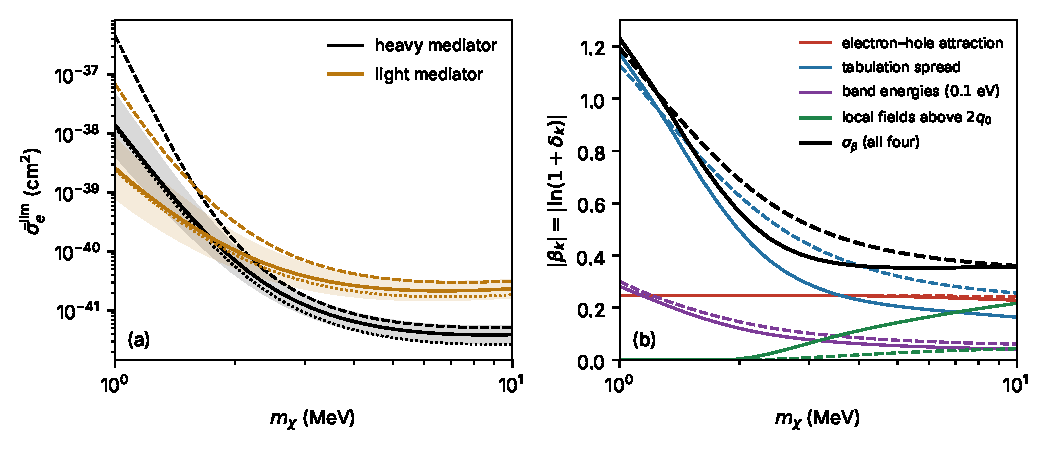
\includegraphics[width=\linewidth]{figures/ch21/fig21_4.pdf}
  \caption{A silicon electron-recoil limit with its theory band. Search: \SI{1}{kg.yr}, every event with at least one pair ($\omega \ge \SI{1.17}{eV}$), no event observed, no background, classical \SI{90}{\percent} limit $N_{90} = 2.303$; standard halo, $\rho_\chi = \SI{0.3}{GeV.cm^{-3}}$. (a) Nominal limit (solid) from the random-phase loss function with local fields of the Knapen--Kozaczuk--Lin tables, whose scissor sets the bands at the measured gap at zero temperature, the band \cref{eq:21.4-band} of the nominal limit (shaded), the profiled limit (dashed; Neyman construction with the nuisance parameter at its conditional best fit, $\ee^{\sigma_\beta^2N_{90}}$) and the limit at the random-phase level without local fields (dotted), for a heavy (black) and a light mediator (ochre). (b) Sensitivities $|\beta_k|$ of the four uncertainties of \cref{we:10-band3}, heavy (solid) and light mediator (dashed). The attraction template is $\delta_{\mathcal{X}} = +0.28$ for $\omega \le \SI{10.5}{eV}$ and zero above, which overstates it above \SI{3}{MeV}, where the compensating weight of the $f$-sum rule enters the window. The other three are the tabulation spread (ratio of the independent-particle rates of the Essig et al.\ and Knapen--Kozaczuk--Lin tables), band energies shifted by \SI{0.1}{eV}, and the random-phase value in place of local fields above $2q_0 = \SI{7.46}{keV}$. Black: their quadrature sum $\sigma_\beta$. Below \SI{1}{MeV} the first energy bins of one table make the spread unreliable. Above \SI{10}{MeV} the momentum range of the other, \SI{22.5}{keV}, truncates the heavy-mediator rate.}
  \label{fig:21-band}
\end{figure}

\begin{workedexample}{The band of a silicon limit from the random-phase level}\label{we:21-rpaband}
Take $\mchi = \SI{3}{MeV}$, a heavy mediator, \SI{1}{kg.yr} of silicon, a one-pair threshold, no event and no background, so that $N^{\mathrm{up}} = N_{90} = 2.303$ and $\sigmae^{\mathrm{lim}} = N_{90}\times\SI{e-37}{cm^2}/\mathcal{R}$, with $\mathcal{R}$ the rate per kilogram-year at $\sigmae = \SI{e-37}{cm^2}$ (\cref{eq:1.5-limit}). The tables place the conduction bands at the measured gap of \SI{1.17}{eV} at zero temperature, and the rate is counted from it (\cref{sec:10.10}).

\emph{The random-phase level.} With the random-phase loss function of the tables, $\mathcal{R} = \num{2.494e4}$ and $\sigmae^{\mathrm{lim}} = \SI{9.23e-42}{cm^2}$.

\emph{The computed step.} The local fields have been computed, and they move the central value, not the band. They lower the rate to \num{1.855e4}, a factor 1.345, and the nominal limit is $\SI{1.24e-41}{cm^2}$.

\emph{The band.} The four uncertainties of \cref{we:10-band3} have, by \cref{eq:21.4-beta} with one bin, $\beta_{\mathcal{X}} = -0.247$ (attraction), $-0.289$ (tabulation spread), $+0.078$ (band energies) and $-0.064$ (local fields above $2q_0$). Their quadrature sum is $\sigma_\beta = 0.393$, and \cref{eq:21.4-band} gives
\begin{equation*}
  \SI{8.38e-42}{cm^2} \le \sigmae^{\mathrm{lim}}(\vartheta) \le \SI{1.84e-41}{cm^2} .
\end{equation*}
The attraction and the tabulation spread carry \SI{93}{\percent} of $\sigma_\beta^2$. Taken one at a time to $\vartheta_k = \pm1$, the four move the limit by factors of 1.28, 1.34, 1.08 and 1.07. The random-phase limit lies in the lower part of the band, at 0.74 of the nominal value against the lower edge at 0.675.

\emph{The profiled limit.} With no events \cref{eq:21.4-profile} is exact, the factor is $\ee^{\sigma_\beta^2N_{90}} = 1.427$, and $\sigmae^{\mathrm{lim,p}} = \SI{1.77e-41}{cm^2}$.

\emph{The detector.} Suppose the efficiency is calibrated to \SI{10}{\percent}, a normalization with $\beta = -\ln 1.10 = -0.095$. Then $\sigma_\beta = 0.404$, the band widens from a factor 1.481 to 1.498, and the profiled factor grows from 1.427 to 1.457. At this calibration the detector adds about one percent to the band and two percent to the profiled limit.
\end{workedexample}

\subsection{One-sided nuisance parameters and excluded cells}\label{sec:21.4-onesided}

A template whose sign is known calls for a constraint that respects it, $\vartheta_k \ge 0$ with the weight $\ee^{-\vartheta_k^2/2}$ on that side, a half-normal constraint. The cost of a half-normal constraint depends on the direction in which the template moves the signal. If $\vartheta_k > 0$ raises the signal, so that $\beta_k < 0$, the statistic at fixed nuisance parameters, \cref{eq:D.47-tfix}, increases with $\vartheta_k$ at every cross-section, and so does the constraint term. The profile then sets $\vartheta_k = 0$ at every cross-section, the parameter costs nothing, and the limit at $\vartheta_k = 0$ is the conservative end of its band. The attraction of \cref{we:21-rpaband} is of this kind: it raises the rate near the gap in every calculation of \cref{sec:10.5}. Only the three other nuisance parameters, with $\sigma_\beta = 0.306$, are then profiled: the profiled factor falls from 1.427 to 1.240 and $\sigmae^{\mathrm{lim,p}} = \SI{1.54e-41}{cm^2}$. The attraction can only strengthen the limit, by 1.28 at $\vartheta_{\mathcal{X}} = 1$. If $\vartheta_k > 0$ lowers the signal, the unconstrained minimum of the profile already lies at $\vartheta_k > 0$, since data without an excess prefer less signal, and the one-sided constraint costs as much as a two-sided one. Linear spin-wave theory, for example, overstates the one-magnon weight of NiO by an estimated $\Delta S/|\vect{S}| = \SI{7.8}{\percent}$ (\cref{sec:14.1}), and that template, of known sign, lowers the signal. Both statements need the template to have one sign in every bin and the bins to be free of excess, so that every weight $a_j$ is positive.

Some cells of the $(\vect{q},\omega)$ plane have no controlled central value, and a limit can be set without them. Removing nonnegative signal from bins without an excess lowers the statistic at every cross-section, so the limit can only rise (\cref{app:D.47}); for one bin it rises by $1/(1 - f)$, with $f$ the removed share. Near the pair-breaking edge of aluminum the conserving loss function changes with the mean free path by more than \SI{10}{\percent} below $y = \omega/\Delta_{\mathrm{BCS}} = 3$, and those energies are excluded (\cref{sec:15.2-nuisance}). At \SI{1}{keV} with a light mediator they hold \SI{20}{\percent} of the rate for the bulk gap and \SI{37}{\percent} for the film gap (\cref{we:15-alrate}), and excluding them weakens the limit by 1.25 and 1.59. For a crystal with a mean free path of at least \SI{10}{\micro m} the clean loss function holds there, and the cells can be restored. The silicon Migdal rate has a region of this kind as well: the coherent zero-phonon response between \SI{0.75}{keV} and $2q_{\mathrm{BZ}}$ is not sized (\cref{tab:12-nuisances}). It carries \SI{33}{\percent} of the rate at \SI{2}{MeV} and \SI{7}{\percent} at \SI{3}{MeV}, so excluding it costs factors of 1.49 and 1.08, and below \SI{1}{MeV}, where it carries nearly all of the rate, no Migdal limit survives the exclusion. In a bin with an excess the argument fails, and removing signal there can strengthen a limit; such a bin needs the full likelihood.

\subsection{The dominant uncertainty of each channel}\label{sec:21.4-dominant}

\Cref{tab:21-dominant} reads the uncertainty budgets of the chapters along the other axis and gives, for each channel at a reference point, the rows that dominate its band. The dominant rows are missing calculations or missing data. The silicon electron recoil lacks a finite-momentum Bethe--Salpeter calculation and a converged independent-particle table, the phonon-assisted window its finite-$q$ form factor and pair-channel screening, the Migdal rate its coherent region and off-diagonal local fields, and NiO its anisotropy. The data that are missing are the cold absorption edge of silicon, the background tensor of ZrTe$_5$ and the gap of an aluminum film. Near the edge of every channel the threshold rows dominate: a gap shift of \SI{10}{meV} weakens a silicon limit \SI{0.005}{MeV} above the edge by a factor of 231 (\cref{we:21-gapshift}).
\begin{table}[tbp]
  \caption{Dominant theory uncertainties of the limit in each channel, read from the uncertainty budgets of the channel chapters. Sizes are factors or shifts of the rate, and hence, for one bin, of the limit. Basis as in those tables: ``computed'', ``model'', ``est.''\ (parametric estimate), ``spread'' (published calculations at the same order), ``data'' (spread of measured inputs), ``bound'' (only an inequality is known), ``unsized''. The last column gives the section, table or figure where the rows are treated.}
  \label{tab:21-dominant}
  \centering\scriptsize\setlength{\tabcolsep}{3pt}
  \begin{tabular}{@{}>{\raggedright\arraybackslash}p{0.20\linewidth}>{\raggedright\arraybackslash}p{0.14\linewidth}>{\raggedright\arraybackslash}p{0.40\linewidth}>{\raggedright\arraybackslash}p{0.09\linewidth}>{\raggedright\arraybackslash}p{0.10\linewidth}@{}}
    \toprule
    Channel & Reference point & Dominant uncertainties & Basis & Section \\
    \midrule
    Electron recoil, Si, density coupling & 1--\SI{3.6}{MeV}, heavy mediator; up to \SI{10}{MeV}, light & tabulation spread: $\times3.2$ at \SI{1}{MeV}, $\times1.34$ at \SI{3}{MeV} (heavy), $\times1.29$ at \SI{10}{MeV} (light); band energies \SI{0.1}{eV}: $\times0.75$ at \SI{1}{MeV} & spread & \cref{sec:10.10}; \SI{1}{MeV}: \cref{fig:21-band} \\
    Electron recoil, Si, density coupling & 3.6--\SI{10}{MeV}, heavy mediator & electron--hole attraction $\times1.28$, $\times1.26$ at \SI{10}{MeV} (known sign); local fields above $2q_0$ $\times1.24$ at \SI{10}{MeV} & model; spread & \cref{sec:10.10} \\
    Electron recoil, velocity couplings & \SI{10}{MeV} & density--current cross term: rate at least 16 (independent particles), about 29 (screened) times the static-electron formula & bound & \cref{sec:10.4} \\
    Core electrons, Ge $3d$ & about \SI{30}{MeV} & crystal final states: $3d$/valence 0.07 against 0.69 & bound & \cref{sec:10.6} \\
    Phonon-assisted electron recoil, Si & 0.333--\SI{0.43}{MeV} & finite-$q$ form factor, factor 3; screening relative to the optical calibration, pair channel not sized; cold absorption data, rate $\times9$ at \SI{0.36}{MeV} & est.; unsized; data & \cref{tab:13-nuisances} \\
    Migdal effect, Si & up to \SI{3}{MeV}; above & coherent zero-phonon response from \SI{0.75}{keV} to $2q_{\mathrm{BZ}}$, \SI{33}{\percent} of the rate at \SI{2}{MeV}; off-diagonal local fields, $\times1.2$ to 1.4, lower end not bounded & unsized; model & \cref{tab:12-nuisances} \\
    Nuclear recoil, Si, multiphonon & \SI{30}{MeV}, $\omega_{\mathrm{th}} = \SI{100}{meV}$ & computed phonon frequencies against measured, \SI{0.24}{\percent}; free recoil in place of the crystal response (evaluation error) $-\SI{6.8}{\percent}$ & computed & \cref{sec:11.9} \\
    Polar phonons, GaAs & single phonon & $Z^*/\varepsilon_\infty$: \SI{2}{\percent} from the measured splitting; a semilocal $\varepsilon_\infty$ moves the rate by \SI{37}{\percent} & data; computed & \cref{sec:11.9} \\
    Magnons, NiO & near \SI{3}{MeV}; lightest masses & one-magnon weight high by \SI{7.8}{\percent} (known sign) against the two-magnon continuum, $+\SI{7.3}{\percent}$ at other energies; magnetic anisotropy near the lightest masses & est.; model & \cref{tab:14-nuisances} \\
    Superconductor, Al & \SI{1}{keV}, light mediator & gap of the sensor, bulk against film: $\times1.23$; edge remainder $-2$ to $+\SI{9}{\percent}$; $y < 3$ excluded, $\times1.25$ (bulk) or $\times1.59$ (film) on the limit & data; computed & \cref{tab:15-nuisances} \\
    Dirac material, ZrTe$_5$ & 20--\SI{1000}{keV}, light mediator & background dielectric tensor: reach band $\times2.8$ & data & \cref{we:16-band} \\
    \bottomrule
  \end{tabular}
\end{table}

For the silicon electron recoil at \SI{3}{MeV} two calculations would remove \SI{93}{\percent} of the variance: a finite-momentum Bethe--Salpeter calculation and an independent-particle table that passes the $f$-sum test at small $q$ (\cref{sec:10.10-open}). With the band energies and the local fields above $2q_0$ left, the band of \cref{we:21-rpaband} would shrink from a factor of 1.48 to 1.11.

\section{Combining and recasting limits}\label{sec:21.5}

Two silicon crystals cut from one wafer and read by identical sensors differ by more than two orders of magnitude in their event rate between 3 and \SI{38}{eV}, because one of them is glued to its holder (\cref{sec:19.6-lee}). The lowest pair bins of a charge detector carry a dark rate, charge that leaks across the gap without any deposit (\cref{sec:1.5-quanta}). No model predicts either rate to the accuracy that a background subtraction needs, so the Poisson limit with a known background of \cref{sec:21.4} cannot be applied to them as it stands. A limit is also rarely the last use of a measurement. A second experiment wants to add its exposure to the first, and a later calculation of the response, such as the background screening of a Dirac material (\cref{sec:16.1}), changes the expected signal after the limit has been published. We will set limits that hold for any background, combine searches in one likelihood whose theory nuisances are shared, and derive when a published limit can be recast to a new response without the data.

\subsection{Limits with an unknown background}\label{sec:21.5-unknown}

If part of the background may be unknown, the only expectation that can safely be assumed for it is zero. Counting every observed event as signal then gives the classical limit of \cref{sec:1.5}: the 90 percent upper limit $N_{\mathrm{sig}}^{\mathrm{lim}}$ solves $P(N \le N_{\mathrm{obs}}\,|\,N_{\mathrm{sig}}) = 0.10$ with the Poisson probabilities \cref{eq:1.5-poisson}, which gives 2.303, 3.890, 5.322 and 6.681 for zero to three events. The limit holds whatever the background is. The distribution function $P(N \le n\,|\,\mu)$ falls monotonically with the mean, since its derivative with respect to $\mu$ is $-P(N = n\,|\,\mu)$, so a signal that leaves a probability below 0.10 for so few events leaves even less once a background $N_{\mathrm{bkg}} \ge 0$ is added to it. The price is that every event, background or not, weakens the limit.

Using the shape of the expected signal gives a stronger limit. At fixed $\mchi$ the spectrum $\dd N_{\mathrm{sig}}/\dd E$ in the measured variable $E$ is known up to the factor $\sigmae$, and a background of a different shape crowds its events where the signal is small, typically near threshold. Yellin's maximum-gap method uses this~\cite{yellin2002finding}. Measure each position by the expected signal count below it, $x(E) = \int^E(\dd N_{\mathrm{sig}}/\dd E')\,\dd E'$. In this variable the signal events of any spectrum are spread uniformly with unit density over $[0, N_{\mathrm{sig}}]$, and the size of a gap between two adjacent events, or between an event and an end of the range, is the signal count expected inside it. For a signal-only experiment the probability that the largest gap is smaller than $x$ depends only on $x$ and $N_{\mathrm{sig}}$~\cite[Eq.~(2)]{yellin2002finding}:
\begin{equation}
  C_0(x, N_{\mathrm{sig}}) = \sum_{k=0}^{m}\Bigl[(kx - N_{\mathrm{sig}})^k - k\,(kx - N_{\mathrm{sig}})^{k-1}\Bigr]\frac{\ee^{-kx}}{k!} , \qquad m = \lfloor N_{\mathrm{sig}}/x\rfloor ,
  \label{eq:21.5-C0}
\end{equation}
written in the form that stays finite when $N_{\mathrm{sig}}/x$ is an integer; Yellin's printed form has the factor $1 + k/(N_{\mathrm{sig}} - kx)$ in place of the bracket, which is the same function away from those points. The 90 percent limit is the cross-section at which the observed largest gap has $C_0 = 0.90$. At fixed mass the fraction $g$ of the expected signal inside the largest gap does not depend on $\sigmae$, so $N_{\mathrm{sig}}^{\mathrm{lim}}$ solves $C_0(gN_{\mathrm{sig}}, N_{\mathrm{sig}}) = 0.90$. With no events the only gap is the whole range, $g = 1$. Then only $k = 0$ and $k = 1$ contribute, the $k = 1$ term is $-\ee^{-N_{\mathrm{sig}}}$, and $C_0 = 1 - \ee^{-N_{\mathrm{sig}}}$ recovers $N_{90} = 2.303$ of \cref{eq:1.5-N90}. The method stays valid with any background: added events can only split gaps, never widen them, so the observed largest gap is no larger than the signal alone would have left, and the limit errs on the conservative side.

How much the shape buys depends on where the events fall. One event that leaves 90 percent of the expected signal on one side gives $g = 0.90$ and $N_{\mathrm{sig}}^{\mathrm{lim}} = 2.836$, against 3.890 from counting. The same event in the middle of the signal, $g = 0.5$, gives 7.78, twice the counting limit; the two methods break even at $g = 0.761$. Two events that both lie in the lowest tenth of the expected signal, where a background rising toward threshold would put them, give $g = 0.90$ and again 2.836, against 5.322 from counting, while two events that cut the signal into thirds give 13.8. The maximum gap gains where the background sits apart from the signal and loses heavily where events are spread through it, and since the method is fixed before the data are seen, an experiment chooses it for the background it expects.

When the events are dense, a gap may be the wrong interval. The optimum-interval method generalizes it~\cite[Sect.~III]{yellin2002finding}. Let $C_n(x, N_{\mathrm{sig}})$ be the probability that, in a signal-only experiment, every interval containing at most $n$ events has an expected count no larger than $x$. It too depends only on $x$ and $N_{\mathrm{sig}}$; it is computed by Monte Carlo and equals \cref{eq:21.5-C0} for $n = 0$. We evaluate $C_n$ for the observed events on every interval bounded by events or by the ends of the range, $(N_{\mathrm{obs}} + 1)(N_{\mathrm{obs}} + 2)/2$ intervals, each with its own $n$ and $x$, and take the largest value, $C_{\mathrm{Max}}$. The 90 percent limit is the cross-section at which $C_{\mathrm{Max}}$ equals the value that 90 percent of signal-only experiments stay below, again from Monte Carlo. That calibration accounts for the interval having been chosen after the data were seen. Both methods need an ordered, continuous variable such as a phonon energy. Integer pair counts leave the events of one bin unordered, and for them the binned analog is a Poisson limit per bin, combined as in \cref{sec:21.5-recast}.

Neither method has a likelihood, since the unknown background has none, and so a theory nuisance cannot be profiled in it: \cref{eq:C.14-profile} needs $\mathsf{L}$. A normalization nuisance scales $N_{\mathrm{sig}}$ at fixed shape, and the band it puts on the limit is the envelope, $(1 + \delta_k)^{\pm1}$, of first order in $\delta_k$, where a likelihood would have charged the second-order cost of \cref{eq:21.4-profile}. A tilt also changes the fractions $g$, because the gaps are measured in expected counts, and the limit must be recomputed with the tilted spectrum at $\vartheta_k = \pm1$.

\subsection{Combining searches with shared nuisances}\label{sec:21.5-combine}

The counts of two exposures are independent, so their Poisson likelihoods multiply (\cref{eq:C.14-poisson}). A combination of experiments $X = \mathrm{A}, \mathrm{B}, \dots$ is one likelihood, the product of the single-exposure likelihoods \cref{eq:8.8-like},
\begin{equation}
  \mathsf{L}\bigl(\sigmae, \vartheta, \vartheta^{\mathrm{det}}\bigr) = \prod_X\mathsf{L}^{(X)}\bigl(\sigmae, \vartheta, \vartheta^{\mathrm{det},(X)}\bigr) .
  \label{eq:21.5-comb}
\end{equation}
Every theory nuisance $\vartheta_k$ appears once and acts in every factor, while the detector nuisances $\vartheta^{\mathrm{det},(X)}$, an efficiency, a background normalization or an energy calibration, are one set per experiment with constraints of their own (\cref{sec:21.4}). The theory nuisances are shared because a truncation is a property of the calculation (\cref{sec:8.8}), and every experiment that uses the same computed response inherits the same error. With one $\vartheta_k$ per experiment the profile could pull them in opposite directions and fit a difference between the experiments that no calculation can produce. It also pays the constraint once for each, as if the errors were independent, and so understates the cost of the truncation.

Before the product, the signal of every experiment is recomputed from one response at one truncation label, since published signal models from different codes differ by more than many of the truncations do. The tabulation spread of \cref{sec:21.4-like} enters \cref{eq:21.5-comb} as one more shared nuisance, not as an error of each experiment. Conventions that differ between publications, the local density, the halo parameters and the pair-creation model that turns energy into pair bins, are choices, not uncertainties, and they are removed by the recomputation, not profiled. Every search on Earth sees the same halo, so if its parameters are varied, one set of them acts on all factors, and near the edge they enter only through the combinations of \cref{sec:21.3-degeneracy}. And searches in different materials share the halo and the nuisance of each truncation that is computed the same way for both, with templates $\delta_k$ of their own and one $\vartheta_k$ (\cref{sec:8.8}). The limit is then set from \cref{eq:21.5-comb} as from a single likelihood (\cref{sec:21.4}).

\begin{workedexample}{Combining two silicon exposures}\label{we:21-combine}
Take $\mchi = \SI{10}{MeV}$, a heavy mediator, the standard halo of \cref{sec:1.2} and the one-pair bin of the cascade of \cref{sec:18.3}, the bin that sets the standard-halo limit at this mass in \cref{sec:21.2-iso}. The tabulated silicon response of \cref{sec:10.1} gives $r = \SI{9.14e41}{kg^{-1}.yr^{-1}.cm^{-2}}$ in this bin, that is 0.914 events per kg-year at $\sigmae = \SI{e-42}{cm^2}$. Exposure A has $M_{\mathrm{det}}t_{\mathrm{exp}} = \SI{1}{kg.yr}$, no events and no background. Exposure B has \SI{4}{kg.yr}, three events and a known background of 2.5 events. Both use the same response, which carries one normalization nuisance, $(1 + \delta)^{\vartheta}$ with $\delta = 0.25$, the size of the largest truncations of the silicon rate at \SI{10}{MeV} in \cref{tab:10-nuisances}.

\emph{Construction.} The limit is the Neyman construction of \cref{sec:21.4-like}. For each $\sigmae$ we sum the Poisson probabilities of all outcomes $(N_{\mathrm{A}}, N_{\mathrm{B}})$ up to 60 events each whose statistic \cref{eq:C.14-profile} is at least the observed one, with the nuisance at its conditional best fit $\hat{\hat\vartheta}$ to the observed counts and the constraint term held fixed. The 90 percent limit is the $\sigmae$ at which that probability is 0.10.

\emph{Without the nuisance.} Exposure A alone excludes $2.303/0.914 = \SI{2.52e-42}{cm^2}$, and B alone $\SI{1.14e-42}{cm^2}$; its three events above a background of 2.5 cost less than its fourfold exposure gains. Together they exclude $\SI{0.809e-42}{cm^2}$, 0.32 of A and 0.71 of B. At the combined limit A expects 0.74 signal events and B 2.96.

\emph{One shared nuisance.} With \cref{eq:21.5-comb} and one $\vartheta$ the limit is $\SI{0.897e-42}{cm^2}$, a factor 1.109 above the combination without it. The profile pulls the nuisance to $\hat{\hat\vartheta} = -0.46$, toward less signal, in both factors at once.

\emph{One nuisance per exposure.} Treated as two independent parameters, the nuisances settle at $-0.17$ (A) and $-0.29$ (B), and the limit is $\SI{0.851e-42}{cm^2}$, a factor 1.051. Splitting the nuisance halves its cost, and the limit is too strong by \SI{5}{\percent}. The worst case within one standard deviation, $\vartheta = -1$, would cost the full factor 1.25.

\emph{One exposure.} For A alone the shared construction gives a closed form. With no events only the outcome $N_{\mathrm{A}} = 0$ has a statistic as large as the observed one, so the limit is reached when the profiled expectation $u = N_{\mathrm{nom}}(1 + \delta)^{\hat{\hat\vartheta}}$ satisfies $\ee^{-u} = 0.10$, $u = N_{90}$. The profile condition of \cref{sec:8.8}, $\hat{\hat\vartheta} = -ku$ with $k = \ln(1 + \delta)$, then gives $N_{\mathrm{nom}} = N_{90}\,\ee^{k^2N_{90}}$, a cost of 1.12 for $\delta = 0.25$, which is \cref{eq:21.4-profile} with $\sigma_\beta = k$ and $\mathsf{t}' = 2N_{90}$.
\end{workedexample}

\subsection{Recasting a published limit}\label{sec:21.5-recast}

A published limit $\sigmae^{\mathrm{lim}}(\mchi)$ was computed with the rates $r_j^{\mathrm{pub}}(\mchi)$ per unit cross-section in the bins $j$ of its analysis. A later calculation replaces them by $r_j^{\mathrm{new}}(\mchi)$, and we write the ratio as the recast factor of bin $j$,
\begin{equation}
  K^{\mathrm{rc}}_j(\mchi) = \frac{r_j^{\mathrm{pub}}(\mchi)}{r_j^{\mathrm{new}}(\mchi)} .
  \label{eq:21.5-K}
\end{equation}
If $K^{\mathrm{rc}}_j = K^{\mathrm{rc}}$ in every bin, the correction preserves the shape of the expected signal at each mass. Every expected count is then $N_{\mathrm{sig},j} = \sigmae M_{\mathrm{det}}t_{\mathrm{exp}}r_j^{\mathrm{new}} = (\sigmae/K^{\mathrm{rc}})M_{\mathrm{det}}t_{\mathrm{exp}}r_j^{\mathrm{pub}}$. Any procedure that depends on $\sigmae$ only through the expected counts, which includes a Poisson limit per bin, a profile likelihood over many bins and Yellin's two methods, returns the limit $K^{\mathrm{rc}}\sigmae^{\mathrm{lim}}$. The recast is then exact without the data.

If $K^{\mathrm{rc}}_j$ varies from bin to bin, the correction tilts the expected spectrum, and the recast needs the procedure. One procedure can be recast exactly: a limit defined as the smallest of single-bin limits, $\sigmae^{\mathrm{lim}} = \min_jN_j^{\mathrm{up}}/(M_{\mathrm{det}}t_{\mathrm{exp}}r_j^{\mathrm{pub}})$, with the upper counts $N_j^{\mathrm{up}}$ of the bins published. Replacing $r_j^{\mathrm{pub}}$ by $r_j^{\mathrm{new}}$ in that minimum is the new limit. If only the curve is public, the new limit is still bracketed. Each new single-bin limit is $K^{\mathrm{rc}}_j$ times the old one, and every old one is at least $\sigmae^{\mathrm{lim}}$, so the new minimum is at least $(\min_jK^{\mathrm{rc}}_j)\,\sigmae^{\mathrm{lim}}$. The bin $j^*$ that set the published limit still offers $K^{\mathrm{rc}}_{j^*}\sigmae^{\mathrm{lim}}$, so the new minimum is at most that. A profile likelihood over several bins and the optimum interval have no such form. Their limits depend on how the counts are spread over bins or events and on all the $r_j$ together, and no function of the published curve and the $K^{\mathrm{rc}}_j$ reproduces them. Recasting them needs the binned likelihood, or the event list.

\begin{keyresult}[Recasting a limit to a new response]
With the recast factors \cref{eq:21.5-K}, a published limit $\sigmae^{\mathrm{lim}}(\mchi)$ becomes
\begin{equation}
  \sigmae^{\mathrm{lim,new}}(\mchi) =
  \begin{cases}
    K^{\mathrm{rc}}(\mchi)\,\sigmae^{\mathrm{lim}}(\mchi) & \begin{tabular}[t]{@{}l@{}}if $K^{\mathrm{rc}}_j = K^{\mathrm{rc}}$ for all $j$\\(any procedure),\end{tabular}\\[2pt]
    \min_j N_j^{\mathrm{up}}\big/\bigl(M_{\mathrm{det}}t_{\mathrm{exp}}\,r_j^{\mathrm{new}}(\mchi)\bigr) & \begin{tabular}[t]{@{}l@{}}if the limit is a minimum over bins\\with $N_j^{\mathrm{up}}$ public\end{tabular}
  \end{cases} ,
  \label{eq:21.5-recast}
\end{equation}
and both forms are exact. For a minimum over bins known only through its curve,
\begin{equation}
  \min_jK^{\mathrm{rc}}_j \le \frac{\sigmae^{\mathrm{lim,new}}}{\sigmae^{\mathrm{lim}}} \le K^{\mathrm{rc}}_{j^*} \le \max_jK^{\mathrm{rc}}_j ,
  \label{eq:21.5-bracket}
\end{equation}
with $j^*$ the bin that set the published limit. A correction that varies between bins cannot be recast from the curve of a profile-likelihood or optimum-interval limit.
\end{keyresult}

A minimum over bins carries a cost in confidence. If each of $n$ independent bins is set at 90 percent, the minimum excludes a true signal whenever any one bin does, and it covers with probability $0.9^n$: 0.81 for two bins and 0.73 for three. The union bound of \cref{sec:21.2-program} restores the stated level. A minimum over bins is recastable exactly only with this correction included in the published $N_j^{\mathrm{up}}$.

Halo conventions show both cases of \cref{eq:21.5-recast}. Take a silicon limit at \SI{10}{MeV} with the search of \cref{sec:21.2-iso}: one kg-year, empty one-, two- and three-pair bins of the cascade and $N_j^{\mathrm{up}} = \ln 30$. It was computed with the halo of Essig et al., $v_0 = 230$, $v_{\mathrm{esc}} = 600$, $v_{\mathrm{E}} = \SI{240}{km.s^{-1}}$ and $\rho_\chi = \SI{0.4}{GeV.cm^{-3}}$~\cite[App.~B]{essig2016direct}, and we recast it to the halo of \cref{app:A.8}. The density enters every rate as a factor, $K^{\mathrm{rc}} = 0.4/0.3 = 1.333$ in every bin, and recasts exactly with any procedure. The velocity distribution does not: at fixed density its recast factors are 0.953, 0.903 and 0.866 in the three bins. The old halo, with smaller $v_0$ and $v_{\mathrm{E}}$, has fewer fast particles in its bulk, and the higher bins need faster particles. With the density the factors are 1.271, 1.204 and 1.154. The published limit, \SI{2.93e-42}{cm^2}, was set by the one-pair bin, and the exact recast is \SI{3.72e-42}{cm^2}, a factor 1.271. From the curve alone, with the binding bin unknown, \cref{eq:21.5-bracket} gives 1.154 to 1.271. At \SI{2}{MeV} the factors are 1.156, 1.432 and 4.0 with the density (0.867, 1.074 and 3.0 without it). The higher bins now draw on the tail, which the old halo extends to $v_{\mathrm{max}} = \SI{840}{km.s^{-1}}$ against 794.5; the three-pair bin opens only above \SI{614}{km.s^{-1}}, and the binding one-pair bin gives 1.156.

The same rule decides how far a theory band can be recast. A normalization nuisance has one $\delta_k$ in every bin, and its band moves with the central limit. A tilt or a threshold shift has bin-dependent templates, and its band needs the per-bin limits or the likelihood, as the central value of any other tilted correction does. \Cref{tab:21-recast} sorts the corrections met in this book.

\begin{table}[tbp]
  \caption{Recast factors \cref{eq:21.5-K} of the corrections met in this book, and what a recast from a published curve needs. ``Common'' means the same factor in every bin at fixed $\mchi$, recastable exactly with any procedure. ``Bin-dependent'' means exact only for a single bin or for a minimum over bins with its upper counts public, and bracketed by \cref{eq:21.5-bracket} otherwise.}
  \label{tab:21-recast}
  \centering\small\setlength{\tabcolsep}{4pt}
  \begin{tabular}{@{}p{0.34\linewidth}p{0.20\linewidth}p{0.38\linewidth}@{}}
    \toprule
    Correction & Factor & Recast \\
    \midrule
    Local density $\rho_\chi$ & common & $\rho_\chi^{\mathrm{pub}}/\rho_\chi^{\mathrm{new}}$, exact \\
    Normalization nuisance (\cref{sec:8.8}) & common & $(1 + \delta_k)^{-\vartheta_k}$, exact, band included \\
    Background in the total $\varepsilon$, isotropic Dirac cone (\cref{sec:16.1}) & common & $\varepsilon_{\mathrm{bg}}^2$ for $\sigmae$, $\varepsilon_{\mathrm{bg}}^{1/2}$ for $\zeta$, exact \\
    Halo velocity distribution ($v_0$, $v_{\mathrm{esc}}$, $v_{\mathrm{E}}$) & bin-dependent & higher bins move most; at the edge through $E_{\mathrm{on}}/v_{\mathrm{max}}^2$ (\cref{sec:21.3}) \\
    Screening and local fields, tilt nuisances (\cref{sec:10.10}) & bin-dependent & templates per bin \\
    Gap or threshold shift & bin-dependent & moves the edge, \cref{we:21-gapshift} \\
    Anisotropic background tensor (\cref{sec:16.1-zrte5}) & depends on $\hat{\vect{q}}$ & ratio of event integrals per mass \\
    Relativistic density row of a boosted flux (\cref{sec:10.9}) & depends on speed & rate ratio $R$, limit $\times R^{-1/2}$ \\
    \bottomrule
  \end{tabular}
\end{table}

An exact recast of any procedure needs what its likelihood contains, and a publication that provides it can be reused without approximation: per bin the observed count, the expected background with its covariance, the exposure and efficiency, the response of the detector from deposited energy to bin with its nuisances, and the upper count with its confidence convention; the halo convention and the truncation label of the signal model; and the likelihood itself in machine-readable form.

\subsection{Dirac and boosted-flux recasts}\label{sec:21.5-corrected}

The published reaches of Dirac materials screen the dark-photon field by the Dirac electrons alone, and the total dielectric function adds the background $\varepsilon_{\mathrm{bg}}$ of the remote bands (\cref{sec:16.1}). For an isotropic cone the published loss function is $\varepsilon_{\mathrm{bg}}^2$ times the true one at every $(\vect{q}, \omega)$, and the published absorption rate $\varepsilon_{\mathrm{bg}}$ times the true one (\cref{eq:16.1-ratio}). The factor is common to every bin and every mass, so by \cref{eq:21.5-recast} the corrected reach is the published curve times $\varepsilon_{\mathrm{bg}}^2$ in $\sigmae$, and times $\varepsilon_{\mathrm{bg}}^{1/2}$ in the mixing $\zeta$, since the absorption rate grows as $\zeta^2$. Nothing else multiplies it: the published $|\varepsilon_{\mathrm{pub}}|^2$ already contains the renormalization of the Dirac charge, $|1 + \varepsilon_{\mathrm{D}}/\varepsilon_{\mathrm{bg}}|^{-2}$, with $\varepsilon_{\mathrm{D}}$ the polarization of the Dirac electrons (\cref{sec:16.1,app:D.41}). \Cref{fig:21-dirac-recast}a recasts the ideal material of Hochberg et al., with $\varepsilon_{\mathrm{bg}} = 40$~\cite{hochberg2018detection}. The minimum of its gapped curve, \SI{3.4e-46}{cm^2} near \SI{9}{keV}, becomes \SI{5.4e-43}{cm^2}, as in \cref{we:16-factor}, and at \SI{114}{keV} the gapless curve moves from \SI{5.5e-45}{cm^2} to \SI{8.8e-42}{cm^2}.

\begin{figure}[tbp]
  \centering
  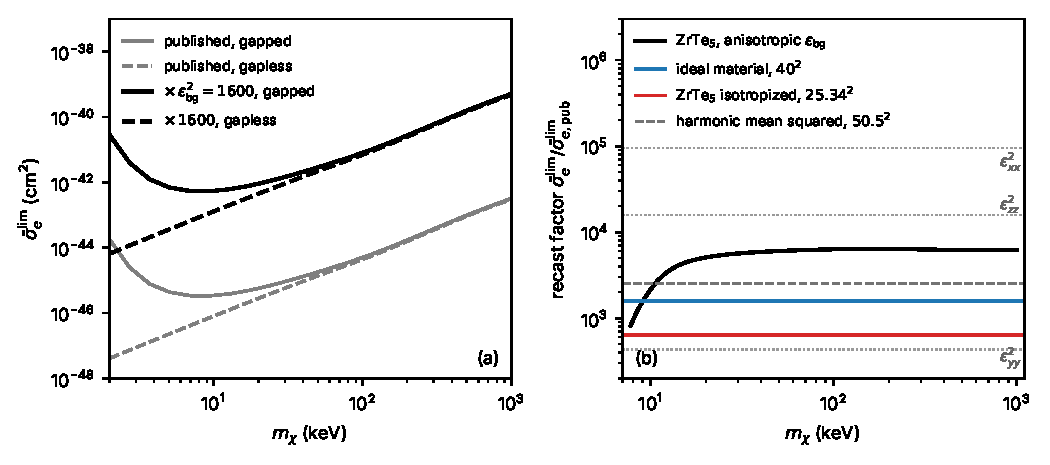
\includegraphics[width=\linewidth]{figures/ch21/fig21_5.pdf}
  \caption{Recasting published Dirac-material reaches to the total dielectric function; light mediator, three events in one kg-year, no background. (a) The ideal Dirac material of Hochberg et al.~\cite{hochberg2018detection} ($v_{\mathrm{D}} = 4\times10^{-4}$, $\varepsilon_{\mathrm{bg}} = 40$, $g_{\mathrm{deg}} = 2$, cutoff \SI{0.2}{keV}): published curves (gray), gapped ($\Delta_{\mathrm{D}} = \SI{2.5}{meV}$, solid) and gapless (dashed), read from the reference's figure. Black: the same curves times $\varepsilon_{\mathrm{bg}}^2 = 1600$, exact for any procedure because the factor is the same at every $(\vect{q},\omega)$. (b) Recast factor, the ratio of the corrected to the published reach, against $\mchi$. Black: the ratio of the published-rule to the total-$\varepsilon$ event integral at each mass for ZrTe$_5$ (\cref{sec:16.1-zrte5}). It uses the anisotropic background tensor $\varepsilon_{\mathrm{bg},ii} = 308.4$, 20.75, 126.1 and the measured-structure row of Geilhufe et al.~\cite{geilhufe2020dirac} ($\Delta_{\mathrm{D}} = \SI{11.8}{meV}$), the book's halo and the rate averaged over orientations of the crystal. Flat lines: $40^2 = 1600$ (blue) and $25.34^2 = 642$ for the isotropized ZrTe$_5$ of Hochberg et al. (red), both exact; the square of the harmonic mean of the tensor, $50.5^2 = 2554$ (gray dashed); the on-axis factors $\varepsilon_{\mathrm{bg},ii}^2 = 431$, $1.6\times10^4$ and $9.5\times10^4$ (gray dotted).}
  \label{fig:21-dirac-recast}
\end{figure}

An anisotropic crystal has no common factor. Its published rule divides each component of the Dirac polarization by its own $\varepsilon_{\mathrm{bg},ii}$, the total dielectric function adds the background along $\hat{\vect{q}}$, and their ratio depends on the direction of $\vect{q}$ and on $(q, \omega)$ (\cref{eq:D.41-ratio}). The published ZrTe$_5$ reach is, however, a single count, three events with no background, and a single bin is the case $n = 1$ of a minimum over bins: the recast is exact once both event integrals are computed at each mass. Their ratio is 5100 to 6400 between \SI{20}{keV} and \SI{1}{MeV} (\cref{fig:21-dirac-recast}b). Toward the threshold it falls, to 2200 at \SI{10}{keV} and 820 at \SI{7.7}{keV}, because only momentum transfers near the $y$ axis, with the lowest threshold, \SI{7.1}{keV}, and the smallest background constant, remain kinematically allowed there, and along that axis the factor is $\varepsilon_{\mathrm{bg},yy}^2 = 431$. No constant reproduces the curve: the square of the harmonic mean of the tensor, the natural isotropic guess, is low by a factor of two to two and a half above \SI{20}{keV} and high near threshold.

A boosted flux changes the counting itself. Dark matter accelerated by cosmic rays acquires its speed through the same coupling that the detector measures, so the flux is proportional to $\sigmae$ and the expected count to $\sigmae^2$, as the published analysis of silicon and germanium states~\cite{liang2025plasmon}. With $N^{\mathrm{up}}$ fixed, a change of the detection rate per particle by a ratio $R$ moves the lower edge of the excluded region by $R^{-1/2}$. For the exact density row of a relativistic particle, \cref{eq:10.9-Drel}, the ratios are those of \cref{sec:10.9-boosted}: the heavy-mediator limit is unchanged, the shift of $\sigmae$ for a massless mediator is below one percent for $\mchi \ge \SI{10}{keV}$, and below about \SI{3}{keV} it is undetermined. Settling it, with the transverse row and its Cherenkov pole included, is the recast that \cref{sec:10.9-open} leaves open and \cref{app:E.16} specifies.

\section{Next targets}\label{sec:21.7}

CsI has a heavy-mediator single-phonon rate per unit mass 3.73 times that of silicon, on elastic constants measured at \SI{4.2}{K}, and 1.56 times that of TeO$_2$, the leader of the eleven crystals ranked in \cref{sec:17.6}. The lead salts have electron-recoil floors up to 4.4 times below germanium's. Neither family was in that pool: no CsI crystal has been read by a phonon sensor at millikelvin temperatures, and a lead compound carries the $^{210}$Pb of its lead, whose $\beta$ spectrum puts some 700 events per kilogram, day and keV below \SI{1}{keV} for every becquerel per kilogram. A ranking of responses answers which crystal gives the most rate per unit mass. An experimentalist choosing the target of the next experiment also needs to know what each leader still has to demonstrate, which measurement would change the order, and on what the probabilities rest. We combine the response-level rankings of \cref{sec:17.6} with the pair energies of \cref{sec:18.4}, the readout verdicts of \cref{sec:20.5} and the internal backgrounds of the crystals into a guide with one row per channel, \cref{tab:21-guide}.

\subsection{Candidate pools and detector readiness}\label{sec:21.7-pools}

The \emph{full pool} holds 42 crystals: 23 of the 24 crystals of the target table of Griffin and collaborators~\cite[Table~I]{griffin2020multichannel}, all but InSb, the three SiC polytypes, and the targets of the preceding chapters that have the inputs of at least one figure of merit. Four requirements decide whether a crystal can be the target of a cryogenic experiment now. The crystal operates at millikelvin temperatures after thermal cycling, without a phase transition between \SI{300}{K} and \SI{10}{mK} and without absorbing water from the air. At least \SI{1}{g} of detector-grade crystal can be grown, or an array of instrumented crystals of at least \SI{0.1}{g} each adds up to a gram. A sensor has been read on its surface at millikelvin temperatures. And its intrinsic rate below \SI{1}{keV} is at most one event per kilogram, day and keV. A crystal for which all four are documented is a \emph{survivor}. A crystal for which one or more is not documented, though none is shown to be impossible, is a \emph{conditional survivor}. Only positive evidence removes a crystal from the full pool. That evidence exists for two candidates, KTaO$_3$ and InSb, whose natural $^{40}$K and $^{115}$In give intrinsic rates far above the fourth requirement (\cref{sec:21.7-backgrounds}).

The survivor pool is the eleven crystals of \cref{sec:17.6}: silicon, germanium, GaAs, diamond, sapphire, LiF, NaF, CaWO$_4$, TeO$_2$, Li$_2$MoO$_4$ and $\gamma$-LiAlO$_2$. The other 31 are conditional. Membership records what has been documented for a crystal, not its physics, and it changes with one demonstration. GaAs entered when a \SI{4.3}{g} crystal was operated at about \SI{10}{mK} with a thermistor readout~\cite{melchiorre2025first}. Diamond entered through the array route: two crystals of \SI{0.175}{g} each, grown by chemical vapor deposition and read by tungsten transition-edge sensors, one with a threshold of \SI{16.8}{eV}~\cite{angloher2023light}. Six such crystals make a gram, each with its own readout channel and threshold, and their surface-to-volume ratio is $(1/0.175)^{1/3} = 1.79$ times that of a single gram crystal, which raises any surface background in proportion. The survivor leader of a channel is the best target that the record supports today. The full-pool leader says what a demonstration would gain: if it differs from the survivor leader, the missing demonstration of the full-pool leader is worth as much as its lead.

The rankings of the full pool use the method and widths of \cref{sec:17.6} unchanged. For the conditional crystals the gaps are those of the target table, a room-temperature gap shifted upward by an amount drawn uniformly between 0.03 and \SI{0.10}{eV}, and the SiC gaps are room-temperature values of the SiC target table~\cite[Table~I]{griffin2021sic}. Their elastic tensors are computed ones from the same database as in \cref{sec:17.6}~\cite{choudhary2018elastic}, with the width 0.086, except two that are measured: aluminum at zero temperature and CsI at \SI{4.2}{K}~\cite{vallin1964elastic}, width 0.02. Their polar band integrals come from \cref{eq:11.2-diatomic} with computed Born charges, $\varepsilon_\infty$ and highest optical energies~\cite[Table~I]{griffin2020multichannel}, or from the measured dielectric constants of the SiC polytypes~\cite[Table~I]{griffin2021sic}.

We add one channel that \cref{sec:17.6} did not rank: the threshold in quanta, measured by the pair energy $\varepsilon_{\mathrm{eh}}$. A lower pair energy turns the same deposit into more pairs and puts the one- and two-pair bins of a charge readout at lower energy (\cref{sec:18.3}). Where a pair energy has been measured, the guide uses the measurement: silicon \SI{3.749}{eV} at \SI{123}{K}~\cite{rodrigues2021absolute}, GaAs about \SI{4.2}{eV} at room temperature~\cite[Fig.~1]{nielsen2026first} raised by $1.70 \times \SI{0.10}{eV}$ for the shift of its gap on cooling (the slope $\partial\varepsilon_{\mathrm{eh}}/\partial\Eg$ of the cascade at fixed constant, \cref{sec:18.4}), diamond and the SiC polytypes as in \cref{fig:18-limit-c}, and germanium as discussed below. For every other crystal the pair energy is the estimate of the cascade of \cref{sec:18.4} at the tabulated gap and highest optical phonon energy. Inside the validated range of \cref{sec:18.4-range} we give it a logarithmic width 0.105, the root mean square of the residuals of the seven crystals with measured values; outside it the width is doubled to 0.21, a convention, since no measurement anchors these crystals.

Germanium has no pair energy measured directly at millikelvin temperatures. Its pair energy at \SI{77}{K} is \SI{2.96}{eV}, the value \cref{sec:18.4} tests the cascade against. The one value quoted at millikelvin temperatures, $(3.37 \pm 0.01)$~eV, comes from a fit by Wei, Wang and Mei to the ratio of phonon to ionization energy measured in EDELWEISS detectors as a function of bias, $E_{\mathrm{p}}/E_{\mathrm{Q}} = a + eV_{\mathrm{bias}}/\varepsilon_{\mathrm{eh}}$, in which the relative conversion efficiency $a = 0.85$ of primary and Luke phonons is fitted together with $\varepsilon_{\mathrm{eh}}$~\cite[Sect.~2.1.4]{wei2016average}. The value rests on the assumption that one constant $a$ describes the phonon collection at every bias, the quantity whose detector dependence \cref{sec:20.5} found open. We use 3.37~eV with the width 0.015 of the spread between this fit and their resolution-based value of 3.32~eV. Either value puts germanium ahead of silicon.

Every probability in the guide is conditional on the provenance widths of \cref{sec:17.6-widths}. The guide reads every row at independent method errors, $r_{\mathrm{mat}} = 0$ in \cref{eq:17.6-zmethod}, and prints the value at $r_{\mathrm{mat}} = 1$ beside it.

\subsection{The guide to next targets}\label{sec:21.7-guide}

\Cref{tab:21-guide} is the guide. The survivor leaders and their values, except in the pair-energy row, are those of \cref{tab:17-rank}.

\begin{table}[tbp]
  \caption{The guide to next targets. Leaders of the full pool (42 crystals) and of the survivor pool (eleven crystals, \cref{sec:21.7-pools}). Full-pool leader: median with 68\% interval, and probability of ranking first at independent method errors with the value at $r_{\mathrm{mat}} = 1$ in parentheses; the values of the survivor leaders are in \cref{tab:17-rank}. Every probability is conditional on the provenance widths of \cref{tab:17-widths} and on the widths of the pair energies stated in \cref{sec:21.7-pools}; it is not the probability that a crystal is the better target. Missing demonstration: the requirements of \cref{sec:21.7-pools} not documented for the leader. Edges at $\omega_{\mathrm{th}} = \SI{1}{meV}$; $v_{\mathrm{max}} = 2.650\times10^{-3}$.}
  \label{tab:21-guide}
  \centering\scriptsize\setlength{\tabcolsep}{3pt}
  \begin{tabular}{@{}>{\raggedright\arraybackslash}p{0.14\linewidth}>{\raggedright\arraybackslash}p{0.24\linewidth}>{\raggedright\arraybackslash}p{0.12\linewidth}>{\raggedright\arraybackslash}p{0.22\linewidth}>{\raggedright\arraybackslash}p{0.20\linewidth}@{}}
    \toprule
    Channel; figure of merit & Full-pool leader & Survivor leader & Missing demonstration & Deciding measurement \\
    \midrule
    Electron-recoil floor; $2\Eg/v_{\mathrm{max}}^2$ & PbSe, \SI{0.0484}{MeV} [0.0479, 0.0489]; 1.000 (1.000); PbTe and PbS next & Ge & lead salts: a crystal of at least \SI{0.1}{g} read at mK; $^{210}$Pb below \SI{1.38}{mBq} per kg of compound & $^{210}$Pb activity of the lead available for growth; low-temperature gap of GaSb \\
    Threshold in quanta; $\varepsilon_{\mathrm{eh}}$ & PbTe, \SI{1.52}{eV} [1.24, 1.87]; 0.482 (1.000); one tier with PbSe (0.414) and PbS (0.102) & Ge, \SI{3.37}{eV} [3.32, 3.42]; then Si 3.75, GaAs 4.37 & lead salts: as above; one measured pair energy of a lead salt & pair energy of germanium measured at mK with the phonon collection calibrated separately \\
    Heavy-mediator single phonon; $c_{\mathrm{NR1}}(\mathrm{Si})/c_{\mathrm{NR1}}$ & CsI, 3.73 [3.65, 3.80]; 0.962 (0.976); measured \SI{4.2}{K} tensor & TeO$_2$, computed tensor & CsI: an encapsulated crystal cycled to mK and read by a phonon sensor & measured elastic constants of TeO$_2$; measured $^{123}$Te capture rate \\
    Nuclear edge; $m_{\mathrm{min}}^{\mathrm{ac}}$ with $c_{\mathrm{LA,max}}$ & no resolved leader: h-BN, \SI{2.95}{keV} [2.72, 3.21]; 0.656 (0.728); one tier with diamond (0.181), polyethylene (0.119), cubic BN (0.043) & diamond, measured tensor & diamond: six crystals of \SI{0.175}{g}, each with its own threshold and low-energy-excess rate, and a phonon threshold near \SI{1}{meV} (shown: \SI{16.8}{eV}); h-BN: mass, mK and readout & measured elastic constants of h-BN, polyethylene and cubic BN \\
    Polar rate; $\mathcal{I}_{\mathrm{pol}}/\rho_T$ & LiF, 19.0 [15.5, 23.3]; 0.918 (0.931) & LiF & LiF: the $^6$Li neutron-activation background, not measured & measured $\varepsilon_0$ and Born charge of LiF at low temperature \\
    Polar reach; $2\omega_{\mathrm{L}}/v_{\mathrm{max}}^2$ & CsI, \SI{2.85}{keV} [2.71, 2.99]; 0.996 (1.000); computed $\omega_{\mathrm{L}}$ & GaAs, measured $\omega_{\mathrm{L}}$ & GaAs: a threshold below its longitudinal phonon, \SI{36.35}{meV}; CsI: as above & low-temperature longitudinal optical frequency of CsI \\
    Migdal; pole factor times $X_{\mathrm{pole}}$ & no resolved leader: NaCl 0.498 (1.000) & no resolved leader: NaF 0.315 (1.000) & -- & $L(\vect{k},\omega)$ of every candidate \\
    \bottomrule
  \end{tabular}
\end{table}

Germanium leads both electron-recoil rows among the survivors, the floor on its measured low-temperature gap and the threshold in quanta with 1.11 times fewer electron volts per pair than silicon. Its lead in quanta holds on the \SI{77}{K} value as well, which is lower still, so the 50~mK fit affects the number and leaves the order unchanged. In the full pool the lead salts lead both rows. PbSe has the lowest floor, on a gap measured at low temperature (\cref{fig:17-rank-floor}). In quanta PbTe, PbSe and PbS share the leading tier. Their pair energies are cascade estimates for crystals whose phonon strengths $\lambda_{\mathrm{AB}}$, the dimensionless ratio of phonon emission to impact ionization in the cascade (\cref{sec:18.4-range}), lie between 230 and 1160, two orders of magnitude outside its validated range, so the tier is real only under the width convention. GaSb, whose estimate lies at the edge of that range, beats germanium's measured value with probability 0.83. At $r_{\mathrm{mat}} = 1$ the three estimates of the lead salts share their error and PbTe ranks first in every draw. No lead salt has been operated at millikelvin with a phonon or charge readout, and every one carries $^{210}$Pb in its bulk (\cref{sec:21.7-backgrounds}).

The heavy-mediator rows separate the two pools most clearly. TeO$_2$ leads the survivors on a computed tensor. CsI, a conditional survivor, leads the full pool on elastic constants measured at \SI{4.2}{K}, from which the Christoffel problem of \cref{sec:17.6} gives $c_{\mathrm{NR1}} = \SI{2.404}{km.s^{-1}}$ and the figure of merit $8.956/2.404 = 3.73$ times silicon. It is ahead of Bi$_2$Se$_3$ and NaI, both computed, with probabilities 0.978 and 0.985, and of TeO$_2$ by a factor 1.56 in the medians, larger than any width. A colder, denser cell, at most \SI{4.5}{\percent} denser than the room-temperature one, raises the figure of merit to 3.81. Against silicon the ratio of the figures of merit gives the ratio of the rates to \SI{10}{\percent} from \SI{97}{keV} up to the zone cap of CsI at \SI{0.32}{MeV} (\cref{fig:17-window}). On its computed highest optical energy, \SI{10.0}{meV}, CsI also leads the polar reach, 3.64 times below GaAs. The same softness gives CsI a poor nuclear edge: from $c_{\mathrm{LA,max}} = \SI{2.46}{km.s^{-1}}$ the edge is \SI{23.1}{keV}, last of the eleven crystals ranked in that row. Two of the four requirements are documented for CsI: crystals far above a gram are grown, and neither caesium-133 nor iodine-127 is radioactive. CsI is slightly hygroscopic, and its operation at millikelvin temperatures after thermal cycling, with a sensor read on it, is not documented. Its entry needs an encapsulated crystal that survives cycling to millikelvin temperatures and a phonon sensor that reads it, deposited on the crystal or on a carrier in thermal contact with it. Its lead then depends on its background: it tolerates $1.56^2 = 2.44$ times TeO$_2$'s background rate density in a background-limited search (\cref{sec:21.7-backgrounds}), and the cosmogenic iodine and caesium isotopes, whose production rates have not been measured for CsI, set that rate.

In the nuclear edge the stiffest crystals lead: diamond leads the survivors on its measured tensor, but in the full pool it shares the leading tier with h-BN, polyethylene and cubic BN, and no leader is resolved. h-BN and polyethylene owe their place to one stiff direction, in the hexagonal plane and along the chains, and their tensors are computed; they reach their edges only for momentum along those directions. LiF leads the polar rate in both pools. The polar reach goes the other way, to soft polar lattices: GaAs among the survivors on its measured longitudinal frequency, CsI in the full pool on a computed one.

The Migdal figure of merit has no leader at independent errors in either pool, for the reason found in \cref{sec:17.6-correlation}, and the light-mediator single-phonon rate ranks no crystals (\cref{tab:17-rank}).

By \cref{sec:20.5}, a leader of an electron-recoil row is read by its charge, through the cascade distribution $P(N_{\mathrm{eh}})$ of \cref{chap:18}, and a leader of a phonon row by its heat, through a collection efficiency that only the detector's kernels fix. A superconducting absorber is read by quasiparticles, with the yield $2\Delta_{\mathrm{BCS}}/E$ below $4\Delta_{\mathrm{BCS}}$ and 0.59 above (\cref{sec:20.4}).

The theory band of a limit (\cref{sec:21.4}) and the ranking of targets answer different questions. An uncertainty that multiplies the rates of every crystal by the same factor, such as the halo or a shared response approximation, moves every limit and no ranking. A ranking moves only through the inputs that differ between crystals, which is why the provenance widths, and not the bands of \cref{tab:21-dominant}, set the probabilities of the guide.

\subsection{Absorption and unranked channels}\label{sec:21.7-other}

Absorption has leaders only mass by mass, the best reach of each decade of \cref{tab:17-abs-decades}. For the dark photon they are zeros of $\varepsilon_1$, where the screening ceiling $L \le 1/(2|\varepsilon_1|)$ is highest: the longitudinal phonon of GaAs, the highest polar branch of sapphire and the plasmon of silicon. All three are survivors. For the axion-like particle with its electron coupling the magnon line of YIG leads from 10~\si{\micro eV} to a meV and clean aluminum from 0.36 to \SI{10.9}{meV}. Neither is a survivor, since the YIG spheres are of millimeter size and no bulk aluminum absorber has been read. The aluminum reach rests on direct pair breaking by the spin current (\cref{sec:15.4-spin}). It holds for a mean free path well above the size of a pair, 1.6 to \SI{2.4}{\micro m}, which only bulk high-purity crystals reach; in a \SI{50}{nm} film the spin channel and the published mapping give comparable reaches.

Magnons, superconductors and the special targets of \cref{chap:16} have no ranking, because no second candidate has the inputs of the same figure of merit. The edge of NiO is set by the magnetic anisotropy that the Heisenberg model leaves out (\cref{sec:14.1}). The scattering rate of aluminum depends more on the gap and mean free path of the absorber actually used than on the choice among loss functions (\cref{sec:15.2}). The one-loop expansion parameter of ZrTe$_5$ is about one, so its rate has no controlled theory at that half-gap (\cref{sec:16.1}). NiO and ZrTe$_5$ lack a gram-scale crystal read at millikelvin temperatures, and aluminum a quasiparticle readout of a bulk absorber.

\subsection{Internal radioactive backgrounds}\label{sec:21.7-backgrounds}

Every figure of merit in the guide ranks signal rates, and a background enters the ranking through a tolerance. Let $b$ be the background rate density in a region of width $\Delta E$. If a search is background limited, the signal must exceed a fixed number of standard deviations of the background count, and its exclusion limit scales as $(b\,\Delta E)^{1/2}/\mathcal{R}$. At the systematics floor, where the background is subtracted only to a fixed fraction, the limit scales as $b\,\Delta E/\mathcal{R}$. Crystal $A$ then keeps its lead over $B$ if $b_A/b_B < (\mathcal{R}_A/\mathcal{R}_B)^2$, or $b_A/b_B < \mathcal{R}_A/\mathcal{R}_B$ at the floor. TeO$_2$ leads CaWO$_4$ in the heavy-mediator rate by 1.22, so it tolerates 1.48 times CaWO$_4$'s background in a background-limited search and 1.22 at the floor. LiF tolerates 3.63 times NaF's background in the polar rate. A lead that rests on a rate factor of order one is reversed by a background ratio of order one. The edges are kinematic and do not move with $b$, but the sensitivity just above them does.

The background that belongs to the crystal itself, and that no shield removes, comes from radioactive nuclei inside it. A $\beta$ emitter spread uniformly through a crystal much larger than the range of its electrons deposits the whole kinetic energy of the electron, and the antineutrino escapes. The spectrum of deposits is then the $\beta$ spectrum, normalized to the activity $\mathcal{A}_{\mathrm{act}}$ per unit mass. For an allowed transition with endpoint $Q_\beta$ it is
\begin{equation}
  n_\beta(T) \propto p_eE_e(Q_\beta - T)^2\,\frac{2\pi y_{\mathrm{S}}}{1 - \ee^{-2\pi y_{\mathrm{S}}}} , \qquad y_{\mathrm{S}} = \frac{\alpha Z_{\mathrm{d}}E_e}{p_e} ,
  \label{eq:21.7-beta}
\end{equation}
with $T$ the kinetic energy of the electron, $E_e = T + m_e$ and $p_e$ its total energy and momentum, $Z_{\mathrm{d}}$ the charge of the daughter nucleus, and the last factor the nonrelativistic Fermi function, which accounts for the Coulomb attraction of the daughter. A unique $n$-th forbidden transition carries in addition the shape factor $\sum_{k=0}^{n}p_e^{2k}q_\nu^{2(n-k)}/[(2k+1)!\,(2n-2k+1)!]$, with $q_\nu = Q_\beta - T$ the momentum of the antineutrino. As $T \to 0$ the factor $p_e$ cancels against the $1/p_e$ of the Fermi function, so the spectrum tends to a constant: the low-energy end of a $\beta$ spectrum is flat. The rate density below \SI{1}{keV} is therefore $\mathcal{A}_{\mathrm{act}}f_\beta$ per keV, with $f_\beta$ the fraction of the spectrum below \SI{1}{keV}. With $Q_\beta = \SI{18.59}{keV}$ for tritium~\cite{iaea2026livechart}, \cref{eq:21.7-beta} gives $f_\beta = 0.0892$. Cosmogenic tritium in silicon is produced at sea level at 124 atoms per kilogram and day. It then contributes 0.169 events per kilogram, day and keV below \SI{1}{keV} after a hundred days and 11.0 at saturation (\cref{app:E.27}). In germanium, at 82 atoms per kilogram and day~\cite{armengaud2017measurement}, the two values are 0.112 and 7.31. Cosmogenic activation is reducible: growth, fabrication and storage underground, and in silicon the out-diffusion of hydrogen, lower it. The other cosmogenic nuclides decay by electron capture, and their L and M lines near 1 and \SI{0.1}{keV} enter the sub-keV region through their L and M fractions. Their production rates have been measured for silicon and germanium~\cite{saldanha2020cosmogenic,armengaud2017measurement} and not for the other survivors.

A lead compound carries a background that no exposure history changes. Its lead contains $^{210}$Pb, half-life 22.2 years, which decays to $^{210}$Bi and, five days later, to $^{210}$Po; in equilibrium the three activities are equal~\cite{iaea2026livechart}. In 84 percent of its decays $^{210}$Pb feeds the level of $^{210}$Bi at \SI{46.5}{keV}, with a $\beta$ endpoint of \SI{17.0}{keV}. The de-excitation of that level, a photon or conversion electrons with their X-rays, is absorbed in the bulk, so these decays deposit at least \SI{46.5}{keV} and never fall below \SI{1}{keV}. The other 16 percent go to the ground state, with $Q_\beta = \SI{63.5}{keV}$. For a daughter as heavy as $^{210}$Bi, $Z_{\mathrm{d}} = 83$, the nonrelativistic factor of \cref{eq:21.7-beta} is crude, and we use instead the traditional relativistic Fermi function of a point charge, with the prefactor 4, evaluated at the nuclear radius $r_A = 1.2A^{1/3}\,\mathrm{fm}$~\cite[Eq.~(6)]{hayen2018high},
\begin{equation}
  F_{\mathrm{Fermi}}(Z_{\mathrm{d}}, T) = 4\,(2p_er_A)^{2(\gamma_{\mathrm{d}} - 1)}\,\ee^{\pi y_{\mathrm{S}}}\,\frac{|\Gamma(\gamma_{\mathrm{d}} + \ii y_{\mathrm{S}})|^2}{\Gamma(1 + 2\gamma_{\mathrm{d}})^2} , \qquad \gamma_{\mathrm{d}} = \sqrt{1 - Z_{\mathrm{d}}^2\alpha^2} ,
  \label{eq:21.7-fermi}
\end{equation}
in place of the last factor of \cref{eq:21.7-beta}, with $y_{\mathrm{S}}$ as there. It gives $f_\beta = 0.0445$. The $^{210}$Bi decay to $^{210}$Po, $Z_{\mathrm{d}} = 84$ and $Q_\beta = \SI{1161}{keV}$, adds $f_\beta = 1.26\times10^{-3}$ with the allowed shape, and the $\alpha$ decay of $^{210}$Po deposits megaelectronvolts. Per becquerel of $^{210}$Pb per kilogram the rate density below \SI{1}{keV} is
\begin{equation}
  \begin{split}
  b_{^{210}\mathrm{Pb}} &= \SI{86400}{s.d^{-1}}\times(0.16 \times 0.0445 + 1.26\times10^{-3})\ \mathrm{keV}^{-1}\times\SI{1}{Bq.kg^{-1}}\\
  &= 724\ \text{per kg, day and keV} .
  \end{split}
  \label{eq:21.7-pb210}
\end{equation}
Of these, 614.7 come from $^{210}$Pb and 109.2, fifteen percent, from $^{210}$Bi. A budget of one event per kilogram, day and keV then needs an activity below \SI{1.38}{mBq} per kilogram of compound: 1.91, 2.23 and \SI{1.60}{mBq} per kilogram of lead in PbSe, PbTe and PbS. The number is an estimate. The relativistic Fermi function raises it by \SI{5}{\percent} over the nonrelativistic 689, mostly through the $^{210}$Bi part, and the first-forbidden transition of $^{210}$Bi, whose shape departs from the allowed one, moves that part further by an amount not computed here. Whether lead of that purity can be obtained and grown into a crystal decides whether the floor of a lead salt is usable, and it is the deciding measurement of the first two rows of \cref{tab:21-guide}.

Primordial nuclei set the only exclusions of the full pool. Natural potassium carries $^{40}$K at \SI{31.7}{Bq} per gram; \SI{89.3}{\percent} of its decays are unique third-forbidden $\beta$ decays with $Q_\beta = \SI{1311}{keV}$~\cite{iaea2026livechart}, for which \cref{eq:21.7-beta} with its shape factor gives $f_\beta = 4.13\times10^{-4}$. KTaO$_3$, \SI{14.6}{\percent} potassium by mass, holds \SI{4.6}{kBq} of $^{40}$K per kilogram and has a $\beta$ rate density of $1.5\times10^5$ per kilogram, day and keV below \SI{1}{keV}. InSb holds \SI{121}{Bq} of $^{115}$In per kilogram, a fourth-forbidden non-unique emitter with $Q_\beta = \SI{497}{keV}$ whose shape is not known; bracketed between the allowed and the unique fourth-forbidden shapes, its rate density lies between $4.8\times10^3$ and $3.9\times10^4$. Both exceed the budget by more than three orders of magnitude, and since only isotopic depletion removes a primordial nucleus, both leave the pool. TeO$_2$ is the opposite case. Its $^{123}$Te is known only to have a half-life above $9.2\times10^{16}$ years~\cite{iaea2026livechart}, so its electron captures are bounded by 693 per kilogram and day, and by the same number per keV if all of them fell in one keV below \SI{1}{keV}. The bound does not decide whether TeO$_2$ meets the budget, and its radioactivity entry stays conditional on a measured capture rate.

Gamma lines of nuclei inside the crystal add a Compton continuum. A photon of energy $E_\gamma$ that scatters once and leaves deposits the electron's recoil energy $T$, and at $T \to 0$ the Klein--Nishina cross-section per electron tends to
\begin{equation}
  \frac{\dd\sigma_{\mathrm{C}}}{\dd T}\bigg|_{T \to 0} = \frac{2\pi r_{\mathrm{cl}}^2m_e}{E_\gamma^2} ,
  \label{eq:21.7-compton}
\end{equation}
with $r_{\mathrm{cl}}$ the classical electron radius; at \SI{1}{keV} the full form for the \SI{1461}{keV} line of $^{40}$K differs from it by $2\times10^{-4}$, and its value there is \SI{1.20e-28}{cm^2.keV^{-1}}. The rate density below \SI{1}{keV} is the photon emission rate times $\nd_e\bar\ell_{\mathrm{esc}}\,\dd\sigma_{\mathrm{C}}/\dd T$ in the thin-target limit, with $\nd_e$ the electron density and $\bar\ell_{\mathrm{esc}}$ the mean path from a point inside the crystal to its surface. For a cube of side $L$ the path from a uniformly distributed interior point in an isotropic direction averages $0.448\,L$, not the mean chord $4V/S = 0.667\,L$ of rays crossing the cube from outside. With $\nd_e = \SI{2e24}{cm^{-3}}$ and $L = \SI{5}{cm}$ a fraction $5.4\times10^{-4}$ of the \SI{1461}{keV} photons deposits in each keV below \SI{1}{keV}. The continuum is flat at low energy like the $\beta$ spectrum, and for an emitter with a $\gamma$ line it adds to the $\beta$ deposits.

\subsection{Open problems}\label{sec:21.7-open}

Three missing inputs limit the guide: the loss functions of the survivors, measured elastic constants, and internal-background rates. The first is the loss function $L(\vect{k},\omega)$ of every survivor near its gap at momenta up to a few keV. Without it the Migdal figure of merit is known only between the plasmon-pole and gap-weighted limits, the prior $X_{\mathrm{pole}}$ stands in for the interband weight, and the row has no resolved leader in either pool.

The second is elastic constants. TeO$_2$, the survivor leader of the heavy-mediator row, and h-BN, polyethylene and cubic BN, which share the leading tier of the full-pool nuclear edge, rest on computed tensors. These carry the method offset that \cref{sec:17.6-correlation} found for the computed family, \SI{4.9}{\percent} on average for silicon, germanium and diamond. For CsI the density of the cold cell is missing.

The third is the internal backgrounds, which the guide has only estimated. The sub-keV rates of $\beta$ emitters use allowed or unique shapes, which are crude for the first-forbidden decay of $^{210}$Bi and unknown for $^{115}$In; the $^{210}$Pb activity of lead that can be grown into a crystal is not known; the $^{123}$Te capture rate is bounded only; and cosmogenic production has been measured for silicon and germanium alone. Until these numbers exist, the radioactivity entries of the guide are conditions, not rates, for every crystal but silicon and germanium.

\subsection{Uncertainty budget of limits and rankings}

\Cref{tab:21-nuisances} is the uncertainty budget that the construction of a limit and of a ranking adds to those of the channels. The halo enters every limit, and near the edge it enters more strongly than any response uncertainty; the statistical construction and the treatment of shared uncertainties move limits by five to forty-five percent; and the rankings rest on width conventions, estimated pair energies and backgrounds that are conditions rather than rates.

{\scriptsize\setlength{\tabcolsep}{3pt}\setlength{\LTcapwidth}{\textwidth}
\begin{longtable}{@{}>{\raggedright\arraybackslash}p{0.25\linewidth}>{\raggedright\arraybackslash}p{0.12\linewidth}>{\raggedright\arraybackslash}p{0.38\linewidth}>{\raggedright\arraybackslash}p{0.09\linewidth}>{\raggedright\arraybackslash}p{0.08\linewidth}@{}}
  \caption{Uncertainty budget of limits and rankings. Classes and bases as in \cref{tab:10-nuisances}. ``Order'' marks an item that acts on a ranking rather than on a rate, ``convention'' a width or a choice fixed by convention. Sizes are for silicon unless stated. The last column gives the section where the item is treated.}
  \label{tab:21-nuisances}\\
  \toprule
  Truncation or input & Type & Size & Basis & Section \\
  \midrule
  \endfirsthead
  \toprule
  Truncation or input & Type & Size & Basis & Section \\
  \midrule
  \endhead
  \bottomrule
  \endfoot
  Reference Earth speed in place of the year average & normali\-zation; tilt in $\mchi$ & $\eta$ within \SI{1}{\percent} to \SI{430.3}{km.s^{-1}}, year average higher by less than \SI{10}{\percent} to \SI{735.6}{km.s^{-1}}; heavy-mediator rate $+\SI{0.9}{\percent}$ at \SI{10}{MeV}, $+\SI{5.6}{\percent}$ at \SI{1}{MeV} & computed & \cref{sec:21.1} \\
  \midrule
  Earth speed at the floor & threshold & June Earth speed lowers the floor by \SI{3.9}{\percent}; a limit uses the exposure average & computed & \cref{sec:21.1} \\
  \midrule
  Halo substructure & normali\-zation; tilt in $\mchi$ & debris flow with 22 percent of the density: $+\SI{8.4}{\percent}$ at \SI{10}{MeV}, $-\SI{16}{\percent}$ at \SI{1}{MeV} & model & \cref{sec:21.1} \\
  \midrule
  Standard halo against every halo & normali\-zation & halo-independent bound weaker by at least 2.00 (\SI{10}{MeV}) and 3.70 (\SI{2}{MeV}), cascade pair bins & computed & \cref{sec:21.2} \\
  \midrule
  Directional response in the halo-independent bound & normali\-zation & program over isotropic formula 1.00--1.13 on the sampled speeds (model anisotropy) & model & \cref{sec:21.2} \\
  \midrule
  Discretized program; final-state assignment & normali\-zation & grid leakage below \SI{0.001}{\percent} at \SI{600}{km.s^{-1}}; misassigned weight at most $0.035\,\varrho^{\mathrm{leak}}_i$ of a bin for a stochastically ordered cascade & computed & \cref{sec:21.2} \\
  \midrule
  Escape tail of the halo & threshold; tilt & edge power 13/2 (standard halo), 15/2 (King), 8--10 (simulated halos); halo fraction within \SI{12}{km.s^{-1}} of $v_{\mathrm{max}}$ from $6.0\times10^{-5}$ to $3.7\times10^{-8}$ & model & \cref{sec:21.3} \\
  \midrule
  Gap or threshold against escape speed at the edge & threshold & \SI{10}{meV} of gap $\equiv -\SI{3.3}{km.s^{-1}}$; limit $\times231$, $\times8.8$, $\times2.7$ at 0.005, 0.010, \SI{0.020}{MeV} above the edge & computed & \cref{sec:21.3} \\
  \midrule
  Year average at the edge & threshold & year-averaged rate over the reference rate 62 at \SI{0.010}{MeV} and 8.5 at \SI{0.020}{MeV} above the reference edge & computed & \cref{sec:21.3} \\
  \midrule
  Theory band of the channel & normali\-zation & silicon, heavy mediator: factor 3.4 (\SI{1}{MeV}), 1.48 (\SI{3}{MeV}), 1.43 (\SI{10}{MeV}); dominant rows per channel in \cref{tab:21-dominant} & computed; model & \cref{sec:21.4} \\
  \midrule
  Statistical construction with a nuisance parameter & normali\-zation & profiled over nominal $\ee^{\sigma_\beta^2N^{\mathrm{up}}}$ with no events, 1.427 at $\sigma_\beta = 0.393$ (Neyman construction, parameter at its conditional best fit); a fixed calibrated threshold charges half the exponent & computed & \cref{sec:21.4} \\
  \midrule
  Excluded cells & normali\-zation & aluminum, $y < 3$ at \SI{1}{keV}: $\times1.25$ (bulk), $\times1.59$ (film); silicon Migdal coherent region: $\times1.49$ at \SI{2}{MeV} & computed & \cref{sec:21.4} \\
  \midrule
  Shared parameter split per exposure & normali\-zation & combined limit $\times1.109$ shared against $\times1.051$ split: about \SI{5}{\percent} too strong & computed & \cref{sec:21.5} \\
  \midrule
  Pair energies outside the validated range & order & logarithmic width 0.21 by convention; lead salts share one tier (0.482, 0.414, 0.102), PbTe 1.000 at $r_{\mathrm{mat}} = 1$; GaSb's estimate beats germanium's measured value with probability 0.83 & convention & \cref{sec:21.7} \\
  \midrule
  Pair energy of germanium at millikelvin & order & \SI{3.37}{eV} from a fit with a fitted phonon-conversion constant, against \SI{2.96}{eV} at \SI{77}{K}; the order against silicon holds for either & est. & \cref{sec:21.7} \\
  \midrule
  $^{210}$Pb in lead compounds & order & 724 per kg, day and keV below \SI{1}{keV} per Bq/kg (relativistic Fermi function, \SI{5}{\percent} above the nonrelativistic value); first-forbidden $^{210}$Bi shape not computed for its \SI{15}{\percent}; activity of available lead not known & est. & \cref{sec:21.7} \\
  \midrule
  Cosmogenic activation of the survivors & order & tritium in silicon 0.169 (100 days at sea level) to 11.0 (saturation) per kg, day and keV below \SI{1}{keV}; production not measured except for silicon and germanium & computed; unsized & \cref{sec:21.7} \\
\end{longtable}}

\section*{Summary}

The rate of any channel is a linear functional of the velocity distribution of the halo, with a nonnegative rate kernel per bin that the master formula fixes at each velocity (\cref{sec:21.1}). For a response averaged over directions the kernel depends on the speed alone, and the rate reduces to an integral of the mean inverse speed $\eta(v_{\mathrm{min}})$. A threshold mass $2E_{\mathrm{th}}/v_{\mathrm{max}}^2$ is a floor, never an edge: the onset depends on the momentum transfer, the rate vanishes at the floor, and the floor moves with the Earth speed. An exposure that includes June reaches \SI{3.9}{\percent} lower for silicon.

A limit valid for every halo is a semi-infinite linear program in a nonnegative measure (\cref{sec:21.2}). For a direction-averaged response its solution is one stream, exactly even with several bins. With the pair bins of the calibrated cascade, dropping the standard halo weakens a silicon limit by at least 2.00 at \SI{10}{MeV} and 3.70 at \SI{2}{MeV}.

Near its low-mass edge a limit follows a power law (\cref{sec:21.3}). The rate rises as $(\mchi - m_{\mathrm{edge}})^{p_{\mathrm{on}} + k_{\mathrm{tail}} + 7/2}$, where $p_{\mathrm{on}}$ is the onset exponent of the response and $k_{\mathrm{tail}}$ that of the escape tail of the halo, so the free-pair edge of silicon rises with the power 13/2 in the standard halo and 8 to 10 in simulated ones. Its position depends on $E_{\mathrm{on}}/v_{\mathrm{max}}^2$ alone, so a gap shift of \SI{10}{meV} is equivalent to $-\SI{3.3}{km.s^{-1}}$ in escape speed and weakens a limit \SI{0.005}{MeV} above the edge by a factor of 231.

The theory uncertainties of each channel enter the likelihood as nuisance parameters and become a band on the limit (\cref{sec:21.4}). In the likelihood of one exposure a profiled nuisance parameter costs a limit at second order in its size, an envelope at first order. Each acts on the limit through its sensitivity $\beta_k$, the band is $\ee^{\pm\sigma_\beta}$, and profiling in the Neyman construction costs $\sigma_\beta^2\mathsf{t}'/2$ in the logarithm, exactly for one bin: a factor 1.427 for the silicon limit at \SI{3}{MeV}. For silicon with a heavy mediator the band is a factor of 3.4 at \SI{1}{MeV}, dominated by the spread of tabulations, and 1.48 at \SI{3}{MeV}, where two calculations would remove \SI{93}{\percent} of its variance.

Without a background model the maximum-gap method uses the shape of the signal (\cref{sec:21.5}). A combination of searches is one likelihood with one set of theory parameters; splitting a shared normalization parameter per exposure makes the combined limit about \SI{5}{\percent} too strong in the example.

Among the eleven survivors germanium leads the electron-recoil floor and the threshold in quanta, TeO$_2$ the heavy-mediator single-phonon rate, diamond the nuclear edge, LiF the polar rate and GaAs the polar reach (\cref{sec:21.7}). The leaders of the full pool of 42 crystals are conditional survivors. The lead salts rest on estimated pair energies and carry bulk $^{210}$Pb, which puts 724 events per kilogram, day and keV below \SI{1}{keV} for every becquerel per kilogram; CsI rests on measured elastic constants but has no demonstrated millikelvin readout.

\printbibliography[heading=subbibliography]

\chapter{Open problems}\label{chap:22}
The zero-phonon edge of germanium is not known, and no calculation predicts how much charge a silicon recoil of \SI{100}{eV} releases (\cref{sec:19.2}). Each open problem of the book is stated in the section where its quantity arises, next to the calculation or the measurement that would settle it. Some statements of the book wait only for a proof and change no number; others are bounds that a single computation would close. \Cref{tab:22-gaps} puts the open problems side by side, one line each with its home section and the kind of result it limits, and \cref{sec:22.3} names the processes that the master formula does not cover.

\section{Exact remaining gaps}\label{sec:22.2}

The decomposition theorem of \cref{sec:8.6} holds for a finite insulator. For the infinite crystal one estimate is missing, a superadiabatic generator built from exponentially localized terms, and every sector of every rate in this book is added on the strength of the finite-crystal statement with its stated error. At the other end is the silicon rate of a particle with an anapole moment. At \SI{10}{MeV} it exceeds the static-electron formula at least 16 times, and the local-field screening of the transverse current, which would turn that bound into a number, is open (\cref{sec:10.4}). The first statement needs a proof and changes no number; the second needs a calculation and changes a limit. Both have the same form, a strongest result and one step beyond it. \Cref{tab:22-gaps} collects all 74 such items by chapter, with the result each one limits.

\subsection{Exact remaining gaps and nuisances}\label{sec:22.2-definition}

\begin{keyresult}[Exact remaining gap]
An \emph{exact remaining gap} is a pair. Its first part is the strongest statement that the book derives about a quantity or a claim, with the conditions under which it holds: a theorem under stated hypotheses, a bound, an estimate with its factor, or a computed number that awaits an independent check. Its second part is the single missing step, a proof, a calculation or a measurement, that would turn the statement into the full result. Each gap is stated once, in the section where the quantity arises, which gives both parts and, for a calculation, points to its specification in \crefrange{chap:30}{chap:33}.
\end{keyresult}

A gap differs from a nuisance. A nuisance parameter of \cref{sec:8.8} carries a truncation whose next order is computed or estimated from a small parameter, and it enters a likelihood with a width; the attraction between electron and hole, which raises the silicon electron-recoil rate by $\delta_{\mathcal{X}} \approx +0.28$ over the \SI{3}{MeV} window, is one (\cref{tab:10-nuisances}). \Cref{sec:8.8} also names a third case, a truncation with neither a computed next order nor a small parameter, which receives no width. Every such truncation is an exact gap, and so is every claim the book can derive only under a hypothesis it cannot yet remove. The nuisance tables at the end of each chapter carry the first kind of item, and \cref{tab:22-gaps} the second. One item can have both a sized part and an open part. The attraction is such an item: its model size is a nuisance, and the finite-momentum Bethe--Salpeter calculation that would replace the model is a gap. The screening of the phonon-assisted sideband splits the same way.

What a gap limits decides how we can use it, and the table sorts the 74 into five classes. A gap that limits only a proof leaves every number of the book standing. Its missing step extends a derived statement beyond its conditions, from a finite crystal to an infinite one or from perturbation theory to all orders. Three gaps are of this kind, those of the decomposition theorem. The other 71 involve a number. For 10 of them the book gives a bound or a two-sided bracket, such as the anapole bound above. For 17 it gives an estimate, a model value or a factor that is not a bound, such as the phonon-assisted rate of silicon below the zero-phonon edge (\cref{sec:13.9}). For 39 the number is unsized: the book can say what the result depends on and how to compute or measure it, but assigns it no width. The last 5 are tests. The book computes the number, and the missing step is an independent check of it, a second set of force constants for the phonon-assisted onset or a cold measurement of the silicon absorption edge.

The missing steps are of three kinds. In 56 rows the step is a calculation specified in the section or in \crefrange{chap:30}{chap:33}, in 11 a measurement, and in 7 a proof or a method that does not yet exist, such as a controlled treatment of Dirac targets at $\tilde\alpha \gtrsim 1$ (\cref{sec:16.1}) or a real-time method for quantum nuclei at low temperature (\cref{sec:11.5}). Where a section names more than one step, the row gives the decisive one. \Cref{sec:22.1} orders the calculations among these steps by the results they would change and states the check each must pass.

\subsection{Gaps by chapter}\label{sec:22.2-table}

\begin{landscape}
{\scriptsize\setlength{\tabcolsep}{3pt}\setlength{\LTcapwidth}{\linewidth}
\begin{longtable}{@{}>{\raggedright\arraybackslash}p{0.16\linewidth}>{\raggedright\arraybackslash}p{0.38\linewidth}>{\raggedright\arraybackslash}p{0.36\linewidth}>{\raggedright\arraybackslash}p{0.07\linewidth}@{}}
  \caption{Exact remaining gaps of the book by chapter, each indexed to the one section that states it. Strongest statement: what that section derives, with its conditions. Missing step: the decisive proof, method, calculation or measurement that would complete it, with the section that specifies a calculation. Limits: \emph{proof}, no number of the book changes. \emph{Bounded}, a number is missing and the section gives a bound or a two-sided bracket. \emph{Estimate}, the section gives an estimate that is not a bound. \emph{Unsized}, the section assigns no size. \emph{Test}, the section computes the number and the missing step checks it. The statements are abbreviated; the section named in the first column gives each in full. Survivors: the eleven crystals with a documented detector record (\cref{sec:21.7}). The calculations that would change a printed result, limit or ranking are ordered in \cref{tab:22-calc}.}
  \label{tab:22-gaps}\\
  \toprule
  Gap; section & Strongest statement & Missing step & Limits \\
  \midrule
  \endfirsthead
  \toprule
  Gap; section & Strongest statement & Missing step & Limits \\
  \midrule
  \endhead
  \bottomrule
  \endfoot
  \multicolumn{4}{@{}l}{\textit{\Cref{chap:8}. The response framework}} \\
  \midrule
  Sector labels outside the off-shell window; \cref{sec:8.6} & Split into zero-phonon and phonon-dressed sectors, and convention independence of the totals, derived in perturbation theory in $g$ with distributional limits; Dyson convention \cref{eq:8.6-dyson} & A limiting-absorption principle for the coupled electron--phonon Hamiltonian at fixed total crystal momentum, uniform in the coupling and the number of cells; it would also sharpen \cref{eq:8.6-bin} from $(\varGamma\Delta E_{\mathrm{c}})^{1/2}$ to $\varGamma$ & proof \\
  Uniformity in the number of nuclei; \cref{sec:8.6} & Superadiabatic leak \cref{eq:8.6-leak} of order $\kappa_{\mathrm{BO}}^{2(n+1)}\alpha^2m_e$, proved for a finite crystal & A superadiabatic generator built from exponentially localized terms, so that the leak per unit volume stays finite & proof \\
  Dressing of gapless targets; \cref{sec:8.6} & Bin bound \cref{eq:8.6-bin} for any orthogonal sectors given a dressed vacuum; fails for $U_{\mathrm{qp}} = 1$; connected part of $\mathfrak{h}_{\mathrm{off}}$ estimated at \SI{0.2}{eV} in aluminum, with no commutator bound uniform in the number of cells & Existence of $U_{\mathrm{qp}}$ beyond perturbation theory, with bounds & proof \\
  \midrule
  \multicolumn{4}{@{}l}{\textit{\Cref{chap:9}. Channel atlas}} \\
  \midrule
  Symmetry-allowed cells of the channel atlas; \cref{sec:9.1} & Eight cells of \cref{tab:9-atlas} allowed at leading order and computed in no section: a spin coupling to core electrons, Cooper pairs, Migdal transitions, Dirac pairs, phonon-assisted pairs, dopant transitions and Frenkel excitons, and the electron density acting on a freely recoiling atom through its following cloud, whose rigid-atom density $f_\kappa(q)$ is used in the multiphonon vertex (\cref{sec:11.3}) & The eight rates, each from the response of the home section of its row with the vertex of its column & unsized \\
  \midrule
  \multicolumn{4}{@{}l}{\textit{\Cref{chap:10}. Electronic excitations}} \\
  \midrule
  Local fields of the transverse current; \cref{sec:10.4} & Static-electron formula low by at least 16 at \SI{10}{MeV} for independent particles, at least 29 with the density screened (\cref{eq:10.4-band}); current screening 4--\SI{15}{\percent} in a model, 10--\SI{30}{\percent} estimated, both lowering & Mixed-block screening of \cref{eq:D.30-dyson}, which fixes the in-medium ratio $r_{\mathrm{med}}$ (\cref{app:E.16}) & bounded \\
  Finite-$q$ Bethe--Salpeter response with coupling block and bound lines; \cref{sec:10.5} & Attraction $\approx +0.28$ over the \SI{3}{MeV} window from a model, coupling block about \SI{10}{\percent} (\cref{eq:10.5-coupling}), resonant-only evaluation off by two (\cref{eq:10.5-res}), lines from \cref{eq:10.5-lines} & Coupled calculation for Si and Ge with the lines added from computed masses and vertices, $f$-sum to a percent (\cref{app:E.15}) & estimate \\
  Triplet beyond independent particles; \cref{sec:10.5-triplet} & Same lines and selection rules as the singlet, no local fields, no screening; 2.2 times the independent-particle spectrum below \SI{3}{eV} in a model & Ladder with the spin-channel exchange--correlation kernel; control: a quarter of the independent density response without interaction (\cref{app:E.16}) & estimate \\
  Self-trapped excitons of NaI; \cref{sec:10.5-open} & Poisson replica series with Huang--Rhys factor $S_{\mathrm{HR}}$ for linear coupling, a harmonic lattice and a fixed vertex (\cref{eq:E.15-ste}) & $S_{\mathrm{HR}}$, $\bar\omega$ and $\rho_{\lambda0}(\vect{q})$ at keV momenta (\cref{app:E.15}) & unsized \\
  Four-component finite-$q$ response; \cref{sec:10.6-open} & At most \SI{2}{\percent} for Ge $3d$, central value near $10^{-3}$; $10^{-6}$ beyond two components & A calculation with no-pair projection, the $3d$ binding as a nuisance, checked on the relativistic $f$-sum shift (\cref{app:E.15}) & bounded \\
  Spin--orbit mixing at the Ge edge; \cref{sec:10.6-open} & Computed and small in Si; up to \SI{10}{\percent} in amplitude near the Ge L minimum, estimated & Ge bands with spin--orbit coupling in the measured valley order (\cref{app:E.15}) & estimate \\
  Interference of contact and second-order amplitudes; \cref{sec:10.8-open} & Linear in the quadratic response, a three-point function with no reduction to two-point responses; known for the electron gas (Barkas term) & Quadratic response of the crystal, in the local-density mapping of \cref{app:E.26} or at second order in time-dependent perturbation theory & unsized \\
  Bound shells in dark Compton scattering; \cref{sec:10.8-open} & Second-order terms of \cref{eq:10.8-TC} vanish away from the shells; nonzero for Si K at 45 to about \SI{100}{keV}, Ge K from \SI{118}{keV}, L shells below about \SI{20}{keV} & Compton profiles of the bound shells at these energies, from the large-$q$ density response (\cref{app:E.26}); the refractive index enters as an input & unsized \\
  Fermionic absorption on bound shells; \cref{sec:10.9-open} & Free-electron vertex low by at least $1/r$, 1.7 for xenon $1s$ at \SI{56.5}{keV}; the transverse current only raises it; sign unknown only at order $(Z\alpha)^2 \approx 0.155$ & Transverse current response with Dirac--Hartree--Fock states, and the published limits redone (\cref{app:E.26}) & bounded \\
  Retarded density row of boosted dark matter; \cref{sec:10.9-open} & Heavy mediator: limit unchanged; massless mediator: shift below \SI{1}{\percent} for $\mchi \ge \SI{10}{keV}$; density-row ratio 0.05 to 0.93 at \SI{1}{keV}, undetermined below about \SI{3}{keV} (\cref{sec:21.5-corrected}) & The published calculation redone with the exact density row and the transverse row, Cherenkov pole included (\cref{app:E.16}) & bounded \\
  \midrule
  \multicolumn{4}{@{}l}{\textit{\Cref{chap:11}. Lattice excitations}} \\
  \midrule
  Valence deformation above the zone; \cref{sec:11.3} & Translation sum rule on the cell sum; rigid-atom vertex $Z_\kappa - f_\kappa(q)$; core share computed (\cref{app:E.17}); nucleon couplings unaffected & All-electron density response of displaced atoms in a large cell, 3 to \SI{20}{keV}, tested on the translation sum rule (\cref{app:E.17}) & unsized \\
  Strongly anharmonic targets; \cref{sec:11.5} & Exact moments by path integrals bound the cumulative weight (Markov--Krein band); Kubo-transformed dynamics only for $T \gtrsim \omega/10$; neutron Compton scattering would measure the momentum distribution & A real-time method for quantum nuclei, exact at low temperature (\cref{app:E.19}) & bounded \\
  Cold in-band dielectric function of Si; \cref{sec:11.6} & $\alpha(\omega; T \to 0) \le \alpha(\omega; \SI{293}{K})$ (\cref{eq:11.6-Tbound}): isotope channel at least $5.0\times10^3$ times the electromagnetic one at \SI{50}{meV}; computable from the derivatives of the Born charges (\cref{app:E.17}) & Two-phonon absorption below \SI{65}{meV} measured at low temperature & bounded \\
  Cubic harmonics of the Si loss function; \cref{sec:11.7} & Pseudopotential-model components to $2.8\,q_0$; local fields change the direction average by 1.3 to 1.5 at \SI{10}{MeV} & First-principles loss function with local fields on Lebedev grids of increasing order (\cref{app:E.16}) & estimate \\
  \midrule
  \multicolumn{4}{@{}l}{\textit{\Cref{chap:12}. The Migdal effect}} \\
  \midrule
  Non-rigid Wannier ratio; \cref{sec:12.3} & Wannier following exact for core shells and flat bands, bounded only in absolute terms for the valence band of Si & Migdal probability with the self-consistent vertex against rigid following, checked on the acoustic and drag-mass sum rules (\cref{app:E.18}) & bounded \\
  Off-diagonal dielectric elements; \cref{sec:12.3-validity} & Scalar dielectric function high by about \SI{35}{\percent}; $\vect{G} \neq \vect{G}'$ elements raise the probability by 1.38 in a model, about 1.2 extrapolated, the lower end not a bound & Converged calculation with the full dielectric matrix (\cref{app:E.18}) & estimate \\
  Contact density at finite $q$; \cref{sec:12.5} & Known for spherical atoms; valence anisotropy $1.3\times10^{-3}$ in Si; relativistic normalization $\mathcal{R}_{\mathrm{rel}}$ (\cref{eq:12.5-Rrel}) with a quadrupolar part changed by a few percent & All-electron Dirac calculation of the crystal with a finite nucleus (\cref{app:E.17}) & estimate \\
  Site-resolved dynamical Born charges; \cref{sec:12.6-open} & Sum fixed by \cref{eq:12.6-sum}; GaAs bremsstrahlung carries the band of \cref{fig:12-brems} & Frequency-dependent charges per site (\cref{app:E.17}) & bounded \\
  Scalar absorption with couplings not proportional to mass; \cref{sec:12.6-open} & Needs $S^{ee}_{\vect{G}\vect{G}'}$ at vanishing reduced momentum & That response (\cref{app:E.18}) & unsized \\
  The Migdal chain as a whole; \cref{sec:12.6-open} & Chain from the kick to the electronic spectrum in place (\cref{sec:12.1,sec:12.5}); no crystal Migdal signal observed & Tagged-recoil measurement in Si: recoil energy and direction fixed by a scattered neutron, electrons counted & test \\
  \midrule
  \multicolumn{4}{@{}l}{\textit{\Cref{chap:13}. Phonon-assisted electron recoil}} \\
  \midrule
  Exciton--phonon replicas; \cref{sec:13.8} & Replica edges at $E_{\mathrm{min}}^{\mathrm{PA}}(\vect{q}) - E_x^b/n^2$, square-root rise at fixed $\vect{q}$; $1s$ transverse acoustic replica at \SI{1.1728}{eV}; completeness reduced to the two-pair sector & Bethe--Salpeter solution on Wannier-interpolated states in the gauge of the vertices, about $10^3$ points of $\vect{k}$ per pocket (\cref{app:E.15}) & estimate \\
  Onset on one set of force constants; \cref{sec:13.9-open} & \SI{0.3332}{MeV} (replica), \SI{0.3374}{MeV} (free pair), set by $\omega_{\mathrm{TA}}(\vect{Q}^*)$ and the gap & $\omega_{\mathrm{TA}}(\vect{Q}^*)$ at two lattice constants and with a second pseudopotential (\cref{app:E.14}) & test \\
  Zero-phonon to phonon-assisted ratio; \cref{sec:13.9-open} & Phonon-assisted lead to $\approx\SI{0.43}{MeV}$ (central), at least $\approx\SI{0.42}{MeV}$; two channels 0.43--\SI{0.51}{MeV}; zero-phonon lead above; both rates estimated & Ratio of the two rates on common bins, with the full phonon-assisted amplitude and the complete zero-phonon edge (mirror-plane cones, second heavy hole, X face) (\cref{app:E.14}) & estimate \\
  Rate and reach at first-principles level; \cref{sec:13.9-open} & Estimates normalized to the measured cold edge (\cref{tab:13-window}) & The same calculation with its controls: optical limit, symmetry zeros, soft acoustic limit, completeness (\cref{app:E.14}) & estimate \\
  Plane-wave $f$-sum check; \cref{sec:13.9-open} & 0.81 of $q^2/2m_e$ with 16 bands, 0.89 with 100, at 0.1--\SI{0.5}{\angstrom^{-1}} & Separation of the omitted bands from the nonlocal term (\cref{app:E.14}) & test \\
  Germanium window and phonons; \cref{sec:13.9-open} & Phonon-assisted onset 0.212--\SI{0.214}{MeV} from the measured transverse acoustic branch; zero-phonon edge not known, so the germanium maps of \cref{sec:17.1-ge-gaas} have open boundaries & Quasiparticle bands with spin--orbit coupling in the measured valley order (\cref{app:E.14}) & unsized \\
  Screening beyond the optical calibration; \cref{sec:13.9-open} & External factor and local-field wings 0.3--2.6 relative to the calibration, estimated; pair-channel dependence on $q$ unsized & Supercell calculation with local fields in the supercell basis (\cref{app:E.16}) & estimate \\
  GaAs control of the window; \cref{sec:13.9-open} & Phonon-assisted band 0.43 to 0.52--\SI{0.56}{MeV} ($E_{\mathrm{L}}(0) = \SI{1.815}{eV}$) in the parabolic description & Band calculation and rate with the polar vertex (\cref{app:E.14}) & estimate \\
  Cold absorption edge of Si; \cref{sec:13.9-open} & Untransferred \SI{77}{K} data off by more than two near the edge; two cold datasets differ by twenty at \SI{1.20}{eV} & Absorption within \SI{25}{meV} of threshold at millikelvin temperatures & test \\
  \midrule
  \multicolumn{4}{@{}l}{\textit{\Cref{chap:14}. Magnetic excitations}} \\
  \midrule
  Two-magnon interactions and bound pairs; \cref{sec:14.2} & Ladder \cref{eq:14.2-ladder} with the vertex from the spin Hamiltonian; interaction $1/2|\vect{S}| = 0.5$ in NiO, not small; existence of a bound pair below the continuum open & Solution of the ladder for NiO on $30^3$--$40^3$ wavevectors (\cref{app:E.20}) & unsized \\
  Longitudinal spin response from neutrons; \cref{sec:14.4} & Transverse block fixes the transverse couplings; for $\mathcal{O}_4$ it is a lower bound; for $\mathcal{O}_6$, $\mathcal{O}_{10}$ one $\vect{q}$ gives nothing; without the isotropy hypothesis of \cref{sec:14.4-iso}, broken only by spin--orbit and dipolar terms, only a model of the spin density & A neutron test of that hypothesis, turning the moments at fixed $\vect{q}$ & bounded \\
  Chirality after decay; \cref{sec:14.5} & GaAs lowest-band $\langle|\vect{L}^{\mathrm{ph}}|\rangle = 0.124$; below \SI{0.8}{MeV} that band takes under \SI{1}{\percent} of the rate & Survival of chirality through three-phonon decay, $(\mathbb{1} - \mathsf{M})^{-1}\vect{b}$ (\cref{app:E.19}) & unsized \\
  Large phonon magnetic moments; \cref{sec:14.5} & Born-charge moments at most $0.030\,\mu_N$ & Amplitudes of moments of order $\mu_B$ from the electronic orbital and spin coupling & unsized \\
  Optical activity at keV momenta; \cref{sec:14.5} & $q\,g_{33} = 0.034$ at \SI{1}{keV} in quartz, a scale only & Current response at $\pm\vect{q}$ with spin--orbit coupling and the nonlocal vertex, for tellurium or quartz (\cref{app:E.20}) & unsized \\
  Multiferroic response near ordering; \cref{sec:14.5} & Landau form within \SI{10}{\percent} of mean field only for $T \ge 0.94\,T_{\mathrm{CM}}$; spin waves controlled for $T \le 0.37\,T_{\mathrm{CM}}$ (\cref{lim:14.5b}) & Amplitude $\chi_\times$ and scaling function $\Phi$ of the dynamic-scaling form for a real material near $T_{\mathrm{CM}}$ & unsized \\
  \midrule
  \multicolumn{4}{@{}l}{\textit{\Cref{chap:15}. Superconductors}} \\
  \midrule
  Amorphous WSi; \cref{sec:15.3-wsi} & Rate needs the configurational average of the loss function, which differs from that of the averaged $\varepsilon$ at the order of its variance & Disorder-averaged loss function at keV momenta and the distribution of the local gap (\cref{app:E.20}) & unsized \\
  Strong-coupling Holstein factor; \cref{sec:15.4-strong} & Normal metal at $\omega \ll \omega_{\mathrm{D}}$: factor $(1 + \lambda_{\mathrm{tr}})^{-2} = 0.52$ in aluminum & Whether the factor survives in the superconducting form near the edge; rate with and without it (\cref{app:E.20}) & estimate \\
  Phonon-assisted spin current near the edge; \cref{sec:15.4-spin} & Coherence factor differs from \cref{eq:15.4-T}; competes with the direct term only above about \SI{10}{meV} & Its size near the edge & unsized \\
  Scalar absorption near the edge; \cref{sec:15.4} & The kinetic row couples to the amplitude channel of the pair field & Conserving response of \cref{sec:15.1} extended to that channel & unsized \\
  \midrule
  \multicolumn{4}{@{}l}{\textit{\Cref{chap:16}. Novel targets}} \\
  \midrule
  Dirac targets at strong coupling; \cref{sec:16.1} & Ladder controlled at first order in $\tilde\alpha$; BNQ-TTF has $\tilde\alpha \approx 10$ & A controlled method at $\tilde\alpha \gtrsim 1$ & unsized \\
  Depolarization of quantum dots; \cref{sec:16.3} & Factor $9|\varepsilon_{\mathrm{in}}|^2/|\varepsilon_{\mathrm{in}} + 2\varepsilon_{\mathrm{out}}|^2$ (\cref{eq:16.3-depol}), above one for real $\varepsilon_{\mathrm{in}} > \varepsilon_{\mathrm{out}}$; also computable (\cref{app:E.21}) & $\varepsilon_{\mathrm{in}}(\omega)$ of real dots over 2.5--\SI{10}{eV}, measured & unsized \\
  Impurity band; \cref{sec:16.5-band} & Isolated-donor response wrong at order one near the ionization edge for $\nd_{\mathrm{D}}/\nd_{\mathrm{c}} \approx 0.5$ & Disorder average on $10^4$--$10^5$ random sites with multivalley envelopes, checked on clusters (\cref{app:E.21}) & unsized \\
  Local-field ratio of a donor; \cref{sec:16.5} & Expected close to one in effective-mass theory & Dielectric matrix of the host and Bloch functions at the minimum (\cref{app:E.6}) & estimate \\
  Color-center yields at millikelvin; \cref{sec:16.6} & Yield $\langle N_{\mathrm{X}}\rangle p_{\mathrm{FH}}p_{\mathrm{surv}}f_{\mathrm{opt}}$; four factors open; \SI{5.9}{keV} X-rays and photodissociation at millikelvin would calibrate single factors & Tagged-neutron measurement on LiF at \SI{10}{mK}, counting centers per recoil & unsized \\
  Tunneling-model parameters of films; \cref{sec:16.7-open} & Loss tangent and acoustic loss fix $\bar Pp_{\mathrm{TLS}}^2$ and $\bar P\gamma^2$, not $\bar P$; $\gamma_{\mathrm{l}}/\gamma_{\mathrm{t}}$ 1.44--1.84 in 18 glasses; distributions for a model glass computable (\cref{app:E.22}) & One film measured three ways & unsized \\
  Interacting two-level systems; \cref{sec:16.8-open} & Spectral diffusion leaves a flat ensemble intact; branching gives mean cascade $1/(1 - b_{\mathrm{br}})$ and $N_{\mathrm{casc}}^{-3/2}$ as $b_{\mathrm{br}} \to 1$ & $b_{\mathrm{br}}$ from the barrier density and the ballistic phonon flux & unsized \\
  \midrule
  \multicolumn{4}{@{}l}{\textit{\Cref{chap:17}. Comparison across channels}} \\
  \midrule
  Coherent Migdal response at small $q$; \cref{sec:17.1} & Diagonal soft limit (\cref{sec:12.4}); its unsized factor acts on the whole Si Migdal band at 0.32--\SI{1}{MeV}, on a third of the rate at \SI{2}{MeV}, on at most \SI{7}{\percent} from \SI{3}{MeV} & Coherent response between about \SI{0.75}{keV} and $2q_{\mathrm{BZ}}$ & unsized \\
  Electron-following density at finite $q$; \cref{sec:17.1} & Long-wavelength model of \cref{sec:10.2}: acoustic peak and electron recoil equal at \SI{12.3}{MeV}, a property of the model & Following density to several zone momenta with Umklapp and multiphonon terms (\cref{app:E.16}) & unsized \\
  \midrule
  \multicolumn{4}{@{}l}{\textit{\Cref{chap:18}. Ionization yield}} \\
  \midrule
  Constant term and variance; \cref{sec:18.2-open} & $\bar n = \omega/\varepsilon_{\mathrm{eh}} + o(\omega)$ (\cref{eq:18.2-linear}); constants computed per seed & Second-order renewal estimates for the walk of \cref{eq:18.2-tagged} and the forgetting rate of the seed (\cref{we:22-constant}) & unsized \\
  Renewal estimate as a lower value; \cref{sec:18.2-open} & $F_{\mathrm{ren}} \le F_{\mathrm{eh}}$ in every computed case and in random parking & A proof for the class, or a counterexample & unsized \\
  Capture and terminal energies; \cref{sec:18.5-open} & Thinning law \cref{eq:18.5-thingen} given $f(x)$ & Computed capture probability $f(x)$, terminal-energy distribution and final pair separations (\cref{app:E.24}) & unsized \\
  Impact ionization beyond first order; \cref{sec:18.5-open} & A constant factor 0.8 moves $\varepsilon_{\mathrm{eh}}$ by about \SI{3}{\percent}, removed by calibration & An energy-dependent residue and exchange factor, which changes $F_{\mathrm{eh}}$ & unsized \\
  Memory of crystal momentum; \cref{sec:18.5-open} & Keeping probability below 0.1 within \SI{1}{eV} of threshold, one half above 3--\SI{5}{eV}; memory negligible in the deformation-potential model & The same with first-principles couplings & estimate \\
  Exciton and trapping rates at millikelvin; \cref{sec:18.5-open} & Binding energies and liquid-helium Auger lifetimes known; luminescent fractions and droplet thresholds at millikelvin also open & Binding, capture and trapping cross-sections of pairs measured at 10--\SI{50}{mK} (\cref{app:E.24,app:E.25}) & unsized \\
  \midrule
  \multicolumn{4}{@{}l}{\textit{\Cref{chap:19}. Low-energy nuclear recoils}} \\
  \midrule
  Charge yield below the binary threshold; \cref{sec:19.2-open} & No calculation predicts the Si yields and Fano factors there or the Ge point at \SI{254}{eV} & Close-collision kernel \cref{eq:19.2-kernel} for Si--Si and Ge--Ge with its exchange--correlation spread (\cref{app:E.23}) & unsized \\
  Release of close pairs at millikelvin; \cref{sec:19.6-open} & Energy-gap and instanton pictures both admitted for Si and Ge Frenkel pairs and Al split interstitials & Tunneling exponent along the computed path and $E_{\mathrm{reorg}}/\varepsilon^{\mathrm{hop}}$ to about \SI{5}{\percent} (\cref{app:E.22}) & unsized \\
  Stored energy in ionic crystals; \cref{sec:19.6-open} & Electronic route prompt; stored energy per deposit = excitons $\times$ conversion $\times$ survival $\times$ configurational energy of the pair & Conversion and close-pair survival probabilities at millikelvin & unsized \\
  Size law and rate of the excess; \cref{sec:19.6-lee} & Borel size law from branching; rate $\propto U_{\mathrm{rel}}$; spectral shape and time dependence factorize; $b_{\mathrm{br}}$ as for two-level systems & $U_{\mathrm{rel}}$ with its spread of rates for a holder and glue (\cref{app:E.25}) & unsized \\
  Carrier-driven defect reactions; \cref{sec:19.6-open} & Probability per capture \cref{eq:19.6-prxn}, a Poisson tail & $S_{\mathrm{HR,rxn}}$, $\omega_{\mathrm{rxn}}$ and the barrier of real defects with their charge states & unsized \\
  Sufficiency of the marks; \cref{sec:19.6-open} & Error of a photon-built detector response at most the total-variation distance at fixed $(N_{\mathrm{eh}}, \mathfrak{m})$, zero when the marks are sufficient & That distance for the features left out of $\mathfrak{m}$ (\cref{app:E.25}) & unsized \\
  \midrule
  \multicolumn{4}{@{}l}{\textit{\Cref{chap:20}. Charge, phonon and quasiparticle readout}} \\
  \midrule
  Trap emission and space charge; \cref{sec:20.1-open} & Emission rate = phonon flux, carrier flux and illumination times cross-sections; \SI{45}{meV} phonons decay within about \SI{1}{ns} & Phonon- and impact-ionization cross-sections of neutral and over-charged centers (\cref{app:E.25}) & unsized \\
  Luke spectrum beyond longitudinal phonons; \cref{sec:20.1-open} & Rate \cref{eq:20.1-luke} with longitudinal phonons, one deformation potential; drift velocities test only the momentum loss & Both acoustic branches with valley-resolved deformation potentials, checked against a phonon signal at fixed field & unsized \\
  Validation of transport; \cref{sec:20.1-open} & Hecht relation, charge sum, bias work \cref{eq:20.1-work}, Fano factor \cref{eq:20.1-Fpos} & An engine passing them to a few percent (\cref{app:E.25}) & test \\
  Thick-film offset of the quasiparticle yield; \cref{sec:20.4-open} & Cascade and kinetic equations differ by 0.04 above four gaps; $Y_{\mathrm{qp}}$ measured at fixed phonon energy would test it & Depth-resolved film transport at the measured $\alpha^2F$ & estimate \\
  Return of the gap energy at zero field; \cref{sec:20.5-routes} & Two-window contrast $0.28(1 - f_{\mathrm{ret}})$ at \SI{100}{eV}; sign changes at $t_1 = 3.87\,t_{\mathrm{rel}}$ for bimolecular against exponential release & Release-time law and site at millikelvin, from the rates of \cref{sec:18.5-open} (\cref{app:E.25}) & unsized \\
  \midrule
  \multicolumn{4}{@{}l}{\textit{\Cref{chap:21}. Exclusion limits and next targets}} \\
  \midrule
  Loss functions of the survivors; \cref{sec:21.7-open} & Migdal figure of merit between the plasmon-pole and gap-weighted limits & Random-phase response with local fields at the measured gap, tested on the inverse fourth moment (\cref{app:E.16}) & bounded \\
  Elastic constants; \cref{sec:21.7-open} & Computed tensors offset by \SI{4.9}{\percent} on average; TeO$_2$ beats CaWO$_4$ with probability 0.955 instead of 0.987 ; the other computed-tensor crystals and the cold density of CsI likewise open & Measured elastic constants of TeO$_2$ (\cref{app:E.17}) & estimate \\
  Internal backgrounds; \cref{sec:21.7-open} & Allowed or unique $\beta$ shapes with the relativistic Fermi function for $^{210}$Pb and $^{210}$Bi; first-forbidden $^{210}$Bi and $^{115}$In shapes not computed; $^{123}$Te bounded; cosmogenic rates measured for Si and Ge only (\cref{app:E.27}) & $^{210}$Pb activity of lead that can be grown into a crystal & estimate \\
  \midrule
  \multicolumn{4}{@{}l}{\textit{\Cref{chap:22}. Open problems}} \\
  \midrule
  Charged-current absorption; \cref{sec:22.3} & Allowed approximation: nuclear strengths times the Fermi function of the daughter (\cref{eq:21.7-fermi}); beyond it the rate is not a dark-matter factor times a target response & Shell-model Fermi and Gamow--Teller strengths per isotope, with quenched axial coupling, for every final state below $\mchi$ & unsized \\
  Charge-density-wave collective modes; \cref{sec:22.3} & Phason as the Goldstone pole and amplitudon of the conserving response on the mean field & That conserving response on a first-principles mean field with the self-consistent distortion & unsized \\
\end{longtable}}
\end{landscape}

The three proof gaps concern the sector decomposition on which every rate of the book is built. \Crefrange{chap:10}{chap:13}, on electronic, lattice, Migdal and phonon-assisted responses, hold 29 gaps, of which 6 are unsized: the response of a crystal at clamped or harmonic nuclei is a well-posed calculation, and where the book has not carried it out it bounds or estimates the result. \Crefrange{chap:18}{chap:20}, on the yield, the low-energy recoil and the readout, hold 17, of which 14 are unsized. What is missing there is mostly a rate at millikelvin temperatures, of capture, trapping, exciton binding, defect release or charge emission, for which neither a measurement nor a calculation exists, and the renewal analysis of the cascade, whose constants the book computes for each model but cannot size for the class.

Several gaps share their missing step. A finite-momentum Bethe--Salpeter calculation for silicon and germanium, with the coupling block and the bound lines, closes the attraction and triplet rows of \cref{sec:10.5}, and with exciton--phonon vertices in the same gauge also the replicas of \cref{sec:13.8}. Quasiparticle bands of germanium with spin--orbit coupling close the spin--orbit row of \cref{sec:10.6} and the germanium window of \cref{sec:13.9}, and with them the open boundaries of the germanium maps of \cref{sec:17.1}. The branching ratio $b_{\mathrm{br}}$ of strain-coupled defects is the missing input both of the avalanche question for two-level systems and of the size law of the low-energy excess (\cref{sec:16.8-open,sec:19.6-lee}). The millikelvin exciton and trapping rates of \cref{sec:18.5} also fix the release-time law of the gap energy in \cref{sec:20.5}. The 74 rows therefore stand for fewer independent steps. \Cref{tab:22-calc} lists once each calculation that would change a printed result, limit or ranking; the other calculation steps appear only here.

Eleven gaps need a measurement, and each section specifies it. Two of them test a chain that the book derives from the kick to the count: a tagged-recoil Migdal measurement in silicon, and the cold absorption edge of silicon within \SI{25}{meV} of its threshold. A third uses the same tagged-neutron method on F centers in LiF at \SI{10}{mK}, where counting single centers per tagged recoil measures the product of four yields as a function of the recoil energy (\cref{sec:16.6}). The other eight supply inputs that no calculation in the book replaces. On the side of the responses they are the cold two-phonon absorption of silicon in its one-phonon band, a neutron test of the isotropy of the spin response of a magnet, the dielectric function of real quantum dots and three measurements of one amorphous film. On the side of the detector and the crystal they are the millikelvin rates of excitons and traps, the stored-energy yields of ionic crystals, the elastic constants of TeO$_2$ and the $^{210}$Pb activity of lead that can be grown into a crystal.

\begin{workedexample}{The constant term of the mean pair number}\label{we:22-constant}
The constant term of the mean pair number is the first open item of \cref{sec:18.2-open}.

\emph{The strongest statement.} For any energy-conserving cascade whose share law becomes independent of the energy fast enough at high energy, is not concentrated on a lattice in $\ln x$ (non-arithmetic, in the language of renewal theory) and is regular near threshold, the mean pair number is $\bar n(\omega) = \omega/\varepsilon_{\mathrm{eh}} + o(\omega)$, \cref{eq:18.2-linear}, proved in \cref{app:D.44}. In the calibrated silicon cascade $\varepsilon_{\mathrm{eh}} = 3.232\,\Eg = 3.232\times\SI{1.160}{eV} = \SI{3.749}{eV}$.

\emph{What the book computes without the gap.} The cascade of \cref{sec:18.3} gives the constant $b_N$ in $\bar n = \omega/\varepsilon_{\mathrm{eh}} + b_N$ by direct computation for each seed: 0.35 for a seed that gives all the energy to one carrier, 0.008 for a uniform split of the energy. With the one-sided constants, $b_N = 0.35$ and $c_N = -0.02$ in the variance, the expansion matches the computed pair energy within \SI{0.07}{\percent} and the computed Fano factor within \SI{0.9}{\percent} at $\omega = 10\,\Eg$.

\emph{The missing step.} Second-order renewal estimates for the walk of $\ln x_j$ in \cref{eq:18.2-tagged}, together with the rate at which the cascade forgets its seed. They would show that $b_N$ exists for the whole class, as the average over the periodic remainder that a one-phonon model leaves, and that $\operatorname{Var}N_{\mathrm{eh}} = F_{\mathrm{eh}}\omega/\varepsilon_{\mathrm{eh}} + O(1)$.

\emph{What it limits.} At $\omega = \SI{10}{eV}$ the leading term is $10/3.749 = 2.667$ pairs. The one-sided seed adds 0.35, a mean of 3.017 and \SI{13.1}{\percent} of the leading term; the uniform split adds \SI{0.3}{\percent}, and the mean $\omega/\varepsilon_{\mathrm{eh}} + 0.19$ of the step model of \cref{sec:18.3} adds \SI{7.1}{\percent}. Each of these numbers comes from a computed cascade, not from the expansion, and none waits for the missing step. The one-sided constant falls below \SI{1}{\percent} of the leading term above \SI{131}{eV}, so the expansion matters only at a few pairs, where the cascade is cheap to compute. What the gap leaves without a size is the constant term of a cascade outside the computed models: whether $b_N$ is a property of every cascade of the class or a fitted constant of each model. The missing step is a proof, and the quantity it limits is unsized.
\end{workedexample}

\noindent The same reading of the zero-phonon to phonon-assisted ratio in \cref{sec:13.9-open} gives a different verdict. There the strongest statement is an estimate, and the missing step, the ratio of the two rates on common bins, moves the mass at which the zero-phonon line of silicon takes over from the phonon-assisted rate.

\section{Channels outside the framework}\label{sec:22.3}

A dark-matter fermion of \SI{1}{MeV} absorbed by a $^{125}$Te nucleus in a TeO$_2$ crystal can turn a neutron into a proton and leave as an electron with \SI{626}{keV} of kinetic energy. The rate of that process carries a factor of 6.3 that no response of the crystal contains: the attraction that the daughter nucleus, of charge 53, exerts on the outgoing electron. The master formula \cref{eq:8.2-rate} holds for every process in which the dark-matter side can be traced out before the target, so that a tensor $\mathfrak{D}_{ab}(\vect{q}, \vect{v})$ that depends only on the dark-matter side multiplies a response $S_{ab}(\vect{q}, \omega)$ that depends only on the target. Where that separation fails, the process lies outside the framework of this book.

\subsection{The scope of the master formula}\label{sec:22.3-scope}

The derivation of \cref{eq:8.2-rate} in \cref{app:D.25} uses three properties of the amplitude besides the assumptions of \cref{sec:8.2-conditions}. The dark field acts through the rows of \cref{eq:8.1-rows}, one-body operators that conserve the number of particles of every species, once per amplitude (twice for the processes of \cref{sec:10.8}). Whatever leaves on the dark-matter side is a free plane wave. The matrix element is then a dark-matter factor that depends on $\vect{q}$ and $\vect{v}$ times $\langle f|O_a(\vect{q})|i\rangle$, and the sum over final states of the target closes into a two-point function at one momentum transfer. The target starts in a Gibbs state, and the observable is the excitation it is left in, read through a final-state class of \cref{sec:8.7}. A process that violates the first property needs a row that \cref{eq:8.1-rows} lacks. One that violates the second has no $\mathfrak{D}_{ab}$ at all, because the outgoing particle acts on the target. One that violates the third can have a well-defined rate that no detector reads as an excitation spectrum.

Two of the assumptions of \cref{sec:8.2-conditions} also bound the framework. With couplings near $4\pi$ and a mediator lighter than about $20A\mu_{\chi T}$, with $\mu_{\chi T}$ the reduced mass of dark matter and nucleus, an attractive potential binds and the first Born approximation fails at order one (\cref{sec:8.2-conditions}). A target whose density operator has coherences between energy eigenstates, or one driven during the exposure, has no response of the form \cref{eq:4.2-Sab}. A last class lies inside the framework: the rate is defined, but no calculation of $S_{ab}$ for that kind of target yet obeys the exact relations of \cref{sec:8.3}. \Cref{tab:22-scope} lists the processes that break one of the three properties, the two that the assumptions exclude, and the one inside the framework that has no conserving response yet.

{\scriptsize\setlength{\tabcolsep}{3pt}\setlength{\LTcapwidth}{\textwidth}
\begin{longtable}{@{}>{\raggedright\arraybackslash}p{0.17\linewidth}>{\raggedright\arraybackslash}p{0.27\linewidth}>{\raggedright\arraybackslash}p{0.38\linewidth}>{\raggedright\arraybackslash}p{0.12\linewidth}@{}}
  \caption{Processes outside the framework of the master formula, and one inside it without a computed response. Second column: why the rate is not $\sum_{ab}\mathfrak{D}_{ab}S_{ab}$ of \cref{eq:8.2-rate}, or, for the last row, why no computed response is available. Third column: the calculation or measurement that a prediction needs. Last column: the section that states the process.}
  \label{tab:22-scope}\\
  \toprule
  Process & Reason & What a prediction needs & Section \\
  \midrule
  \endfirsthead
  \toprule
  Process & Reason & What a prediction needs & Section \\
  \midrule
  \endhead
  \bottomrule
  \endfoot
  Charged-current absorption, $\chi + (A, Z) \to (A, Z{+}1) + e^-$ & Species-changing nuclear row; the outgoing electron moves in the field of the final state of the target, so the dark-matter side is an operator on the target & Shell-model Fermi and Gamow--Teller strengths per isotope, with quenched axial coupling; Dirac--Coulomb electron waves for the daughter charge & \cref{sec:22.3-cc} \\
  \midrule
  Radiative decay of an excited dark state & No target operator in the amplitude; the medium enters through the photon propagator only & Abundance of the excited state at the detector; local field at the decaying particle; absorption of the photon & \cref{sec:10.9-decay,sec:22.3-tracks} \\
  \midrule
  Damage tracks of recoiling heavy ions & Born parameter far above one; the lattice is damaged by the earlier collisions; the readout is a defect configuration & Transport of the ion with the stopping as input, and the map from the track to the defects that are read & \cref{sec:19.3-bethe,sec:22.3-tracks} \\
  \midrule
  Strong dark-matter--target coupling & First Born approximation fails; bound states and resonances & Partial-wave solution of the scattering & \cref{sec:8.2-conditions} \\
  \midrule
  Target with coherences, or driven during the exposure & No Gibbs or energy-diagonal initial state & Rate for a density operator with coherences between energy eigenstates & \cref{sec:8.2-conditions} \\
  \midrule
  Charge-density-wave phasons and amplitudons & Inside the framework; the response needs a conserving kernel on the mean field of the distorted crystal & Conserving time-dependent mean-field response; Goldstone and $f$-sum checks & \cref{sec:22.3-cdw} \\
\end{longtable}}

\subsection{Charged-current absorption}\label{sec:22.3-cc}

The fermionic absorption of \cref{sec:8.1-absorption} has a charged partner. An operator that couples the dark-matter fermion to an electron and a neutron to a proton,
\begin{equation}
  \frac{1}{\Lambda_{\mathrm{F}}^2}\,\bigl[\bar p\,\gamma_\mu(1 + \lambda_A\gamma^5)\,n\bigr]\bigl[\bar e\,\gamma^\mu P_R\,\chi\bigr] + \text{h.c.} ,
  \label{eq:22.3-cc}
\end{equation}
with $p$, $n$, $e$ and $\chi$ the proton, neutron, electron and dark-matter fields, $\Lambda_{\mathrm{F}}$ the scale of the operator as for the neutral absorption operators of \cref{sec:8.1-absorption}, $P_R = (1 + \gamma^5)/2$ and the nucleon axial coupling $\lambda_A = 1.27$ in the sign convention of the reference, absorbs $\chi$ on a neutron of a nucleus and emits an electron, $\chi + (A, Z) \to (A, Z+1)^{(*)} + e^-$~\cite[Eq.~(4.1)]{dror2020absorption}; its pure vector form is Eq.~(6) of Ref.~\cite{dror2020direct}. For a parent that is stable against $\beta$ decay the process has a threshold, $\mchi > m_{\mathrm{th}}^{\mathrm{CC}} = M_{A,Z+1}^{(*)} + m_e - M_{A,Z}$ with nuclear masses, the daughter possibly excited~\cite[Eq.~(4.2)]{dror2020absorption}. Above it the electron takes the kinetic energy $E_{\mathrm{ej}} = \mchi - m_{\mathrm{th}}^{\mathrm{CC}}$, up to a nuclear recoil of order $\mchi^2/2M$. The ground state of $^{125}$Te has spin $\frac12^+$, and the ground state of $^{125}$I, $\frac52^+$, cannot be reached from it by an allowed transition; the lowest allowed threshold, to an excited state of $^{125}$I reached by a Gamow--Teller transition, is \SI{374}{keV}~\cite[Table~1]{dror2020absorption}.

The nuclear side is a row that \cref{eq:8.1-rows} does not have. At momentum transfers small against the inverse nuclear radius, the time component of the vector current reduces to the isospin raising operator $\tau^+_j$, which turns nucleon $j$ from a neutron into a proton. The spatial axial current reduces to $\sigma^\beta_j\tau^+_j$, as the density and the spin density of \cref{app:D.24} do for the neutral currents. Summed over the nuclei $I$ at positions $\vect{X}_I$,
\begin{equation}
  O^{\mathrm{CC}}_{\mathrm{F}}(\vect{q}) = \sum_I\ee^{\ii\vect{q}\cdot\vect{X}_I}\sum_{j\in I}\tau^+_j , \qquad
  O^{\mathrm{CC}}_{\mathrm{GT},\beta}(\vect{q}) = \sum_I\ee^{\ii\vect{q}\cdot\vect{X}_I}\sum_{j\in I}\sigma^\beta_j\tau^+_j ,
  \label{eq:22.3-rows}
\end{equation}
the Fermi and Gamow--Teller rows. Every row of \cref{eq:8.1-rows} conserves the numbers of protons and neutrons; these change the element. Adding these rows, and nothing else, would keep the framework, with a response $S^{\mathrm{CC}}_{ab}(\vect{q}, \omega)$ of the rows in \cref{eq:22.3-rows}.

The electron prevents that. It is charged, and it leaves through the Coulomb field of the daughter nucleus and of the atomic electrons around it. Its final state is a scattering state $\psi^{(-)}_{\vect{p}_{\mathrm{ej}}}(\vect{r})$ of that field, not a plane wave, and for a dark-matter particle of momentum $\vect{p}$ the amplitude is an overlap $\int\dd^3r\,\psi^{(-)*}_{\vect{p}_{\mathrm{ej}}}(\vect{r})\,\ee^{\ii\vect{p}\cdot\vect{r}}\langle f|\rho^{\mathrm{CC}}(\vect{r})|i\rangle$ with the density $\rho^{\mathrm{CC}}(\vect{r})$ whose Fourier components are the rows in \cref{eq:22.3-rows}. Its square involves the transition density at two points, $\langle i|\rho^{\mathrm{CC}\dagger}(\vect{r}')|f\rangle\langle f|\rho^{\mathrm{CC}}(\vect{r})|i\rangle$, weighted by a product of electron waves, so it is not a response at one momentum transfer. The field that distorts the wave, moreover, belongs to the final state $|f\rangle$: the charge $Z + 1$ of the daughter and the atomic configuration left behind when the nuclear charge changes. The dark-matter side therefore acts on the target, and no tensor $\mathfrak{D}_{ab}$ exists. The exact rate is the golden rule with the electron in the final state of the combined system, $\sum_f|\langle f; e^{(-)}_{\vect{p}_{\mathrm{ej}}}|H_{\mathrm{int}}|i; \chi\rangle|^2$. It is the spectral function of an operator that adds an electron to the target and turns a neutron into a proton: a response of the target with one more electron. A condensed-matter reader knows the structure from the x-ray edge, where the core hole left in the final state distorts the outgoing electron.

One limit restores a product. Let the electron wavelength be long against the nuclear radius, $p_{\mathrm{ej}}r_A \ll 1$ with $r_A = 1.2A^{1/3}\,\mathrm{fm}$. The wave can then be evaluated at the nucleus. Its squared amplitude relative to a plane wave is the relativistic Fermi function $F_{\mathrm{Fermi}}(Z_{\mathrm{d}}, E_{\mathrm{ej}})$ of \cref{eq:21.7-fermi}, the point-charge function of $\beta$ decay with its traditional prefactor 4~\cite[Eq.~(6)]{hayen2018high}, evaluated at the electron's kinetic energy $E_{\mathrm{ej}}$ with $Z_{\mathrm{d}} = Z + 1$ the charge of the daughter and with the Sommerfeld parameter $y_{\mathrm{S}} = \alpha Z_{\mathrm{d}}E_e/p_{\mathrm{ej}}$ of \cref{eq:21.7-beta}, where $E_e = m_e + E_{\mathrm{ej}}$ is the total energy of the electron. The finite size of the nucleus enters through a further factor $L_0$ that differs from one by a quantity of order $\alpha Z_{\mathrm{d}}E_er_A$. In this allowed approximation the rate per isotope is a sum over final nuclear states of $F_{\mathrm{Fermi}}(Z_{\mathrm{d}}, E_{\mathrm{ej}})$ times the electron phase space, proportional to $p_{\mathrm{ej}}E_e$, times the standard allowed combination of $\beta$ decay~\cite[Sect.~I]{hayen2018high}, the Fermi strength $B_{\mathrm{F}} = |\langle f|\sum_j\tau^+_j|i\rangle|^2$ plus $\lambda_A^2$ times the Gamow--Teller strength $B_{\mathrm{GT}} = \sum_\beta|\langle f|\sum_j\sigma^\beta_j\tau^+_j|i\rangle|^2$. The published projections multiply the nucleon-level amplitude by the same kind of function~\cite[Eq.~(4.9)]{dror2020absorption}. Their Eq.~(4.10) prints the prefactor $2(1 + \gamma_{\mathrm{d}})$, a convention that moves part of $L_0$ into the function, and $\Gamma(1 + \gamma_{\mathrm{d}})^2$ in the denominator where \cref{eq:21.7-fermi} has $\Gamma(1 + 2\gamma_{\mathrm{d}})^2$. The gamma-function factor alone is therefore larger by $\Gamma(1 + 2\gamma_{\mathrm{d}})^2/\Gamma(1 + \gamma_{\mathrm{d}})^2$, 3.22 at $Z_{\mathrm{d}} = 53$ and 4.0 as $Z_{\mathrm{d}} \to 0$, and the printed function does not reach the nonrelativistic limit.

\begin{workedexample}{The Fermi function of $^{125}$Te absorption}\label{we:22-cc}
Take $^{125}$Te in TeO$_2$, the Gamow--Teller threshold of \SI{374}{keV} and $\mchi = \SI{1}{MeV}$. The electron leaves with $E_{\mathrm{ej}} = \SI{626}{keV}$ and $p_{\mathrm{ej}} = \SI{1.016}{MeV}$, so $y_{\mathrm{S}} = 0.433$ for the daughter iodine, $Z_{\mathrm{d}} = 53$, and $p_{\mathrm{ej}}r_A = 0.031$ with $r_A = \SI{6.0}{fm}$. The allowed approximation holds. Its corrections in the nuclear operators are of order $(p_{\mathrm{ej}}r_A)^2 \approx 10^{-3}$, and the finite-size Coulomb correction $L_0$ is of order $\alpha Z_{\mathrm{d}}E_er_A = 0.013$, about \SI{1}{\percent}.

If the master formula applied, the rate would be the contraction of a dark-matter tensor, built from the operator \cref{eq:22.3-cc} and a plane-wave electron, with the nuclear response of \cref{eq:22.3-rows} at $q = p_{\mathrm{ej}}$. At these momenta the nuclear strength does not depend on $q$, so at fixed matrix element the rate would grow with the electron phase space, as $p_{\mathrm{ej}}E_e$. With the distorted wave it is $p_{\mathrm{ej}}E_eF_{\mathrm{Fermi}}$, and \cref{eq:21.7-fermi} gives $F_{\mathrm{Fermi}}(53, \SI{626}{keV}) = 6.34$.

The factor belongs to the final state. Evaluated with the charge of the parent, $Z_{\mathrm{d}} \to 52$, it is 6.06, \SI{4.3}{\percent} lower. A response sums over final states independently of the outgoing particle, and a dark-matter tensor depends on $\vect{q}$ and $\vect{v}$ alone, so neither can carry this dependence.

It also changes the threshold behavior. At $E_{\mathrm{ej}} = \SI{10}{keV}$, $F_{\mathrm{Fermi}} = 32.5$, and at \SI{1}{keV}, 102. The product $p_{\mathrm{ej}}E_eF_{\mathrm{Fermi}}$ tends to a constant, 0.23 of its value at \SI{626}{keV} for both energies, while $p_{\mathrm{ej}}E_e$ alone falls to 0.046 and 0.014 of it. The rate stays finite at the threshold, as the $\beta$ spectra of \cref{sec:21.7} do at their low-energy end, where a plane-wave electron would make it vanish as $p_{\mathrm{ej}}$.

At low energies the atomic electrons enter as well. The radius of the iodine $K$ shell, $a_0/Z_{\mathrm{d}}$, is \SI{998}{fm}, against $1/p_{\mathrm{ej}} = \SI{194}{fm}$ at \SI{626}{keV} and \SI{1942}{fm} at \SI{10}{keV}. Below about \SI{10}{keV} the wave is screened by electrons whose configuration, after the sudden change of the nuclear charge, is not stationary, and the distortion then depends on the atomic final state too. The factorized form is an approximation for one final state of the nucleus with the atomic shells as spectators, and it holds because $p_{\mathrm{ej}}r_A$ is small and $E_{\mathrm{ej}}$ is large; the general rate is a property of the target together with the electron.
\end{workedexample}

The nuclear strengths obey two sum rules. Write $T_\pm = \sum_j\tau^\pm_j$ for the summed raising and lowering operators of isospin, which obey the angular-momentum algebra with $T_z = (Z - N)/2$ in the convention in which a proton has $\tau_z = +1$, so that $T_+$ turns a neutron into a proton. For the Fermi strength we need the isospin limit, in which the ground state of the parent has total isospin $T_{\mathrm{iso}} = (A - 2Z)/2$, the smallest value its projection $T_z = -T_{\mathrm{iso}}$ allows. It is then the bottom state of its multiplet, and $T_-$, which would turn one more proton into a neutron, annihilates it. The summed strength is then a ladder norm,
\begin{equation*}
  \sum_fB_{\mathrm{F}} = \langle i|T_-T_+|i\rangle = T_{\mathrm{iso}}(T_{\mathrm{iso}} + 1) - T_{\mathrm{iso}}(T_{\mathrm{iso}} - 1) = 2T_{\mathrm{iso}} = A - 2Z ,
\end{equation*}
and $T_+$ takes the ground state into a single state, the isobaric analog of the parent. With $\sigma^\beta_j$ inserted no such state exists, but the commutator of the summed operators with their conjugates, summed over $\beta$, picks up $\sum_\beta\sigma^\beta\sigma^\beta = 3$, and
\begin{equation}
  \sum_fB_{\mathrm{F}} = A - 2Z , \qquad
  \sum_fB_{\mathrm{GT}}(n \to p) - \sum_fB_{\mathrm{GT}}(p \to n) = 3(A - 2Z) ,
  \label{eq:22.3-sumrules}
\end{equation}
the Fermi and Ikeda sum rules, where $A - 2Z$ is the neutron excess. The Ikeda rule is an operator identity and holds without isospin symmetry; the Fermi rule in this form, and the concentration of its strength in one state, need the isospin limit. The analog state lies above the parent by the Coulomb energy of the added proton less the neutron--proton mass difference. For $^{125}$Te that puts the threshold to reach it at about 13 to \SI{14}{MeV}: \SI{14.2}{MeV} for a uniformly charged sphere of radius $r_A$, and \SI{13.6}{MeV} once the exchange term of the Coulomb energy of that sphere is subtracted. Below that mass a vector charged current acts only through isospin-breaking admixtures, and the axial current carries the rate through Gamow--Teller transitions. The published projections count the nucleon-level rate once per neutron, $n_j \simeq A - Z = 73$ for $^{125}$Te~\cite[Eq.~(4.6)]{dror2020absorption}. The Fermi sum rule allows 21 in total, all of it in the analog state. On the Gamow--Teller side the same count gives $3(A - Z) = 219$ against the Ikeda difference of 63, before quenching. Shell-model Gamow--Teller strengths also exceed measured ones unless the axial coupling in the nucleus is reduced by a factor of about 0.75, or two-body currents are added~\cite{gysbers2019discrepancy}, which changes the weight $\lambda_A^2$ by a factor of about two.

A prediction for a crystal therefore needs three things for each isotope. The first is the nuclear strength: shell-model Fermi and Gamow--Teller strengths for every final state below the dark-matter mass, with the quenched axial coupling or the two-body currents, and their dependence on $q$ through the transition densities, with first-forbidden operators added where $p_{\mathrm{ej}}r_A$ reaches about 0.1 or the allowed matrix element vanishes. The computed strengths must exhaust \cref{eq:22.3-sumrules} in a space closed under $\sigma\tau$, which contains every spin--orbit partner of its orbitals. The second is the electron: Dirac--Coulomb waves of the daughter charge, with finite nuclear size and atomic screening, evaluated with the same nuclear radius as the strengths; at \SI{626}{keV} the parent charge would give a Fermi function \SI{4.3}{\percent} too low. The third is the final state that a detector reads: the electron deposits its energy as a fast primary of the kind that \cref{chap:18} follows, together with the de-excitation of the daughter. Capture of the electron into a bound orbital of the daughter leaves no free particle to carry the energy away, so it occurs only where $\mchi$ matches a transition, within the width of the final atomic state.

\subsection{Radiative decay and ion tracks}\label{sec:22.3-tracks}

An excited dark state $\chi_2$ that decays to $\chi_1$ and a photon inside the detector has an amplitude with no target operator in it (\cref{sec:10.9-decay}). The event rate is then the density of excited states at the detector times their decay rate times the volume, with no flux factor $\rho_\chi v/\mchi$ and no exposure in target mass, and the medium enters only through the photon density of states at $|\Delta_\chi|$. A prediction needs the abundance of $\chi_2$ at the detector, set by the early universe or by up-scattering in the Earth; the local field at the decaying particle, which the macroscopic $\varepsilon^{\mathrm{T}}$ of \cref{eq:10.9-decay} omits; and the absorption length of the photon in the detector, which the optical response gives once the photon exists. The part of the decay that hands energy directly to the electrons through a virtual photon lies inside the framework (\cref{sec:10.9-decay}).

A heavy ion leaves a damage track (\cref{sec:19.3-bethe}). Its rate of energy loss is the Bethe or friction stopping of \cref{eq:19.3-bethe,eq:19.3-Se}, a response quantity, but the track is not. A recoiling silicon ion at the speeds that dark matter gives it has a Born parameter $Z_1\alpha/v$, with $v$ the speed of the ion, of 117 to over a thousand, so no single scattering is perturbative. This is the parameter of the moving ion; the Born parameter $Z_\kappa\alpha/v_{\mathrm{F}}$ of \cref{sec:22.1}, set by the electrons it meets, measures the same failure at low speed. A track of $10^2$ to $10^4$ collisions runs through a lattice that the earlier collisions have already displaced, and the target is not in its Gibbs state for any collision after the first. What a track detector or a paleo-detector reads is the defect configuration that remains, not an excitation spectrum. A prediction needs a transport calculation of the ion through the damaged lattice, with the stopping as input and molecular dynamics for the collisions, and the map from the final configuration to the defects that the readout sees.

\subsection{Collective modes of a charge-density wave}\label{sec:22.3-cdw}

Below about \SI{260}{K} the quasi-one-dimensional crystal (TaSe$_4$)$_2$I forms a charge-density wave with a single-particle gap $2\Delta_{\mathrm{CDW}} \approx 250$ to \SI{300}{meV}. It carries a collective mode at \SI{0.23}{THz}, or \SI{0.951}{meV}, which Kim and collaborators identify as the massive phason of that wave~\cite{kim2023observation}. The density row of \cref{eq:8.1-rows} can excite modes that lie 263 to 315 times below the charge gap: with $v_{\mathrm{max}}$ the largest dark-matter speed in the laboratory (\cref{eq:1.2-vmax}), a dark-matter particle heavier than $2\omega/v_{\mathrm{max}}^2 = \SI{271}{eV}$ can deposit \SI{0.951}{meV}. Nothing in the master formula changes for such a target. What is missing is a response that obeys the exact relations of \cref{sec:8.3}.

In a charge-density wave the electron density is modulated, $\nd_e(\vect{r}) = \bar\nd_e + \nd_1\cos(\vect{Q}_{\mathrm{CDW}}\cdot\vect{r} + \varphi)$, with a wave vector $\vect{Q}_{\mathrm{CDW}}$ that is incommensurate with the lattice in (TaSe$_4$)$_2$I, and the lattice distorts with it. The order parameter is $\Delta_{\mathrm{CDW}}\ee^{\ii\varphi}$. The phason is an oscillation of $\varphi$, the amplitudon one of $|\Delta_{\mathrm{CDW}}|$. If the wave is incommensurate, a uniform shift of $\varphi$ costs no energy, and the phason is a Goldstone mode whose frequency vanishes linearly in its wave vector; impurities and commensurability pin it and open a small gap. A density probe couples to the phason in two places. Near $\vect{q} = \pm\vect{Q}_{\mathrm{CDW}} + \vect{G}$ it meets the modulation, $\delta\nd_e = -\nd_1\sin(\vect{Q}_{\mathrm{CDW}}\cdot\vect{r} + \varphi)\,\delta\varphi$, and reaching it there takes $\mchi \ge |\vect{Q}_{\mathrm{CDW}}|/2v_{\mathrm{max}}$, \SI{189}{keV} per keV of $|\vect{Q}_{\mathrm{CDW}}|$. At small $\vect{q}$ a gradient of $\varphi$ along the chains moves the condensed electrons with the wave and leaves a charge density proportional to that gradient. That charge feels the long-range Coulomb interaction, which lifts the longitudinal phason, whose wave vector has a component along $\vect{Q}_{\mathrm{CDW}}$, from zero to the plasma frequency of the condensed electrons. A phason whose wave vector is perpendicular to the chains carries no charge and stays acoustic, or pinned, so the response depends on the direction of $\vect{q}$. Lee, Rice and Anderson, and Lee and Fukuyama, showed this, as quoted by Kim and collaborators~\cite{kim2023observation}. The condensate plasma frequency is as low as a meV because a moving charge-density wave drags its lattice distortion with it, which gives the condensed electrons a large effective mass~\cite{lee1974conductivity}. The superconductor of \cref{sec:15.1} shows the same mechanism, with its phase mode pushed to the plasmon.

The response that captures these modes has the structure of \cref{sec:15.1}. On the mean-field reference with the self-consistent distortion, the proper density response must be the time-dependent mean field in the space of electron states at $\vect{k}$ and $\vect{k} + \vect{Q}_{\mathrm{CDW}}$. Its kernel is the functional derivative of the same self-energy that produced $\Delta_{\mathrm{CDW}}$: Hartree--Fock exchange plus the interaction mediated by the phonon at $\vect{Q}_{\mathrm{CDW}}$. Only then does the broken translation produce the phason pole at zero frequency in the proper response, and only then does the $f$-sum rule \cref{eq:4.3-fsum} hold. The bare bubble on the reconstructed bands is the counterpart of the nonconserving bubble of \cref{sec:7.2}: it misses the phason and violates the $f$-sum. The phonon at $\vect{Q}_{\mathrm{CDW}}$ is dressed by the electronic polarization, and the interaction it mediates may enter either the electronic kernel or the dressed phonon propagator, not both. Screening with $v_{\mathrm{C}}(q)$ as in \cref{eq:15.1-Lcons} then gives the loss function, in which the longitudinal phason sits at the condensate plasma frequency. The phason and the amplitudon are composites of electrons and lattice, and assigning them to a sector of \cref{sec:8.6} is a convention, as for the pair composites of a superconductor.

A calculation for a real crystal needs that kernel on a first-principles mean field. The supercell of the distorted crystal must be relaxed with a functional that produces the distortion, and the electron--phonon vertex at $\vect{Q}_{\mathrm{CDW}}$ taken from the undistorted cell. The kernel must come from the same functional as the distortion, since a mismatch violates the Ward identity at the order of the mismatch. The checks are the Goldstone limit of the proper response, in which the phason frequency vanishes with its wave vector when $\vect{Q}_{\mathrm{CDW}}$ is made artificially incommensurate and stays gapped for a commensurate wave; the $f$-sum rule; and the measured modes, the \SI{0.951}{meV} phason of (TaSe$_4$)$_2$I among them.

\section*{Summary}

An exact remaining gap is the strongest statement the book derives about a quantity, with its conditions, together with the single step that would turn it into the full result (\cref{sec:22.2}). The book contains 74. Three limit only a proof and leave every number standing; of the 71 that involve a number, 10 come with a bound or a bracket, 17 with an estimate, 39 are unsized and 5 are independent checks of a computed number. The missing step is a specified calculation in 56 of them, a measurement in 11 and a proof or method in 7. Several gaps share one missing step, a finite-momentum Bethe--Salpeter calculation for silicon and germanium or quasiparticle bands of germanium with spin--orbit coupling among them, so the 74 rows stand for fewer independent calculations; \cref{sec:22.1} orders those that would change a printed result, limit or ranking, each with the exact relation and the control against data that it must pass (\cref{tab:22-calc}). Unsized gaps dominate both the chapters from magnetic targets to the comparison across channels (16 of 19) and those on the measurement chain (14 of 17), where the rates of capture, trapping and release at millikelvin are neither measured nor computed.

The master formula holds wherever the dark-matter side can be traced out before the target (\cref{sec:22.3}): the dark field acts through species-conserving one-body rows, whatever leaves on the dark side is a free plane wave, and the target starts in a Gibbs state and is read through the excitation it is left in. Charged-current absorption, $\chi + (A, Z) \to (A, Z+1) + e^-$, breaks the first two. Its nuclear rows change the element, and its outgoing electron moves in the Coulomb field of the final state of the target, so the dark-matter side becomes an operator on the target. In the allowed approximation the rate is the relativistic Fermi function of the daughter charge times the phase space $p_{\mathrm{ej}}E_e$ times the Fermi and Gamow--Teller strengths. For $^{125}$Te at $\mchi = \SI{1}{MeV}$ the Fermi function is 6.34, \SI{4.5}{\percent} above its value with the charge of the parent, and it keeps the rate finite at threshold. The whole Fermi strength, $A - 2Z$, sits in the isobaric analog state 13 to \SI{14}{MeV} up, so Gamow--Teller transitions with a quenched axial coupling carry the rate below it, and a count of one conversion per neutron overstates the strength. The radiative decay of an excited dark state has no target operator in its amplitude; the track of a recoiling heavy ion is a transport problem whose stopping alone is a response; strong coupling and targets with coherences fail the assumptions of the formula. The collective modes of a charge-density wave lie inside the framework and need a conserving response whose proper part contains the Goldstone phason.

Most of what the book leaves open is calculation rather than theory. In 20 of its 22 channels (\cref{sec:22.1}) the response has a controlled form, the next term is known and its check is stated; what is missing there is the number, and a stated calculation or measurement supplies it.

\printbibliography[heading=subbibliography]

\appendix
\crefalias{chapter}{appendix}
\chapter{Conventions and units}\label{app:A}
\section{Natural units}\label{app:A.1}

We set $\hbar = c = k_{\mathrm{B}} = 1$. Energy, mass, momentum, frequency and temperature are then all measured in electronvolts, length and time in $\mathrm{eV}^{-1}$, and speeds are pure numbers, fractions of the speed of light. A dark-matter speed of \SI{250.5}{km.s^{-1}} is $8.356\times10^{-4}$, and the energy and momentum it carries at mass $m_\chi$ are $\tfrac12 m_\chi v^2$ and $m_\chi v$ in the same unit. The choice suits a subject in which a particle-physics mass, a crystal momentum, a phonon frequency and a temperature enter one energy-conservation condition. Particle physics uses it routinely, and Ref.~\cite[Appendix~A, Table~III]{lin2019tasi} tabulates the astrophysical units it is mixed with; condensed-matter texts often keep $\hbar$ and $k_{\mathrm{B}}$, and their formulas are converted by restoring the factors below.

\subsection{Restoring the constants}

A formula in natural units is converted to conventional units by inserting the powers of $\hbar$, $c$ and $k_{\mathrm{B}}$ that make every term dimensionally consistent. Four constants suffice; their values follow from the 2022 adjustment of CODATA (the Committee on Data of the International Science Council)~\cite{mohr2025codata}, in which $c$, $h$, $e$ and $k_{\mathrm{B}}$ are exact:
\begin{equation}
  \begin{aligned}
  \hbar c &= \SI{1.973270e-5}{eV.cm} = \SI{197.3270}{MeV.fm}, &\quad \hbar &= \SI{6.582120e-16}{eV.s},\\
  k_{\mathrm{B}} &= \SI{8.617333e-5}{eV.K^{-1}}, &\quad c &= \SI{2.997925e5}{km.s^{-1}}
  \end{aligned}.
  \label{eq:A.1-constants}
\end{equation}
A length $L$ becomes $L/(\hbar c)$ in $\mathrm{eV}^{-1}$, a time $t$ becomes $t/\hbar$, a temperature $T$ becomes $k_{\mathrm{B}}T$ and a speed $u$ becomes $u/c$. A density per unit volume picks up $(\hbar c)^3$, a cross-section $(\hbar c)^{-2}$, and a rate per unit time $\hbar$.

\begin{table}[t]
  \centering
  \caption{Conversion factors between conventional units and natural units ($\hbar = c = k_{\mathrm{B}} = 1$), computed from CODATA 2022 values~\cite{mohr2025codata}. Examples in the last column are values used in the book.}
  \label{tab:A-conversions}
  \small
  \begin{tabular}{@{}p{0.17\linewidth}p{0.42\linewidth}p{0.35\linewidth}@{}}
    \toprule
    Quantity & Conversion & Example \\
    \midrule
    length & $\SI{1}{cm} = \SI{5.0677e4}{eV^{-1}}$, $\SI{1}{\angstrom} = \SI{5.0677e-4}{eV^{-1}}$ & Bohr radius $1/(\alpha m_e) = \SI{0.5292}{\angstrom}$ \\
    time & $\SI{1}{s} = \SI{1.5193e15}{eV^{-1}}$ & $\SI{1}{yr} = \SI{3.156e7}{s} = \SI{4.795e22}{eV^{-1}}$ \\
    temperature & $\SI{1}{K} = \SI{8.6173e-5}{eV}$, $\SI{1}{eV} = \SI{11605}{K}$ & $\SI{300}{K} = \SI{25.85}{meV}$ \\
    speed & $\SI{1}{km.s^{-1}} = \num{3.3356e-6}$ & $v_{\mathrm{max}} = \SI{794.5}{km.s^{-1}} = \num{2.650e-3}$ \\
    number density & $\SI{1}{cm^{-3}} = \SI{7.6835e-15}{eV^3}$ & $\rho_\chi = \SI{0.3}{GeV.cm^{-3}} = \SI{2.31e-6}{eV^4}$ \\
    mass density & $\SI{1}{g.cm^{-3}} = \SI{4.310e18}{eV^4}$ & silicon, \SI{2.33}{g.cm^{-3}} $= \SI{1.004e19}{eV^4}$ \\
    mass & $\SI{1}{kg} = \SI{5.610e26}{GeV}$ & -- \\
    cross-section & $\SI{1}{cm^2} = \SI{2.5682e9}{eV^{-2}}$, $\SI{1}{b} = \SI{2.5682e-15}{eV^{-2}}$ & $\SI{1}{GeV^{-2}} = \SI{0.3894}{mb} = \SI{3.894e-28}{cm^2}$ \\
    spectroscopy & $\SI{1}{THz} = \SI{4.1357}{meV}$ ($h\nu$), $\SI{1}{cm^{-1}} = \SI{0.12398}{meV}$ & -- \\
    \bottomrule
  \end{tabular}
\end{table}

\Cref{tab:A-conversions} lists the factors. Each entry is a power of one of the products in \cref{eq:A.1-constants}. For example, $\SI{1}{cm^{-3}} = (\hbar c)^3/\si{cm^3} = (\SI{1.973270e-5}{eV})^3 = \SI{7.6835e-15}{eV^3}$, and $\SI{1}{b} = \SI{e-24}{cm^2}$ divided by $(\hbar c)^2 = \SI{3.8938e-10}{eV^2.cm^2}$ gives \SI{2.5682e-15}{eV^{-2}}. A mass density in \si{g.cm^{-3}} first becomes an energy density through $\SI{1}{g} = \SI{5.610e23}{GeV}$ and then picks up $(\hbar c)^3$. Spectroscopic frequencies need care: a frequency $\nu$ quoted in \si{THz} corresponds to the energy $h\nu = 2\pi\hbar\nu$, while an angular frequency $\omega$ in \si{rad.s^{-1}} corresponds to $\hbar\omega$. Phonon tables usually quote $\nu$, so the optical phonon of silicon at the zone center, at \SI{15.5}{THz}~\cite{nilsson1972study}, has $\omega_{Q\nu} = \SI{64.1}{meV}$.

\subsection{Checking dimensions}

In natural units every quantity has a single dimension, a power of energy, and a formula is checked by counting powers of eV. The rate per unit target mass of \cref{eq:1.5-rate} is the standard example: it is dimensionless, as a rate (eV) per unit mass (eV) must be (\cref{sec:1.5}). The dimensions of the main objects are fixed by their definitions: the dynamic structure factor $S(q,\omega)$ has dimension $\mathrm{eV}^2$ (\cref{sec:4.2}), the transform $\tilde V(\vect{q})$ of a potential has $\mathrm{eV}^{-2}$, the density vertex $\rho_{mn}(\vect{k},\vect{q})$ and the dielectric function are dimensionless, and $\sigmae$ has $\mathrm{eV}^{-2}$. Final numbers are always converted back: rates to \si{kg^{-1}.yr^{-1}}, cross-sections to \si{cm^2}, momenta to \si{keV}, and energies to \si{eV} or \si{meV}. A rate per unit mass in natural units is converted with $\SI{1}{kg^{-1}.yr^{-1}} = \num{3.718e-59}$, the inverse of the product of \SI{1}{kg} in eV and \SI{1}{yr} in $\mathrm{eV}^{-1}$.

The metric signature is $(+,-,-,-)$, with $x^\mu = (t, \vect{x})$ and $\partial_\mu\partial^\mu = \partial_t^2 - \nabla^2$, so that a free particle obeys $p^\mu p_\mu = E^2 - |\vect{p}|^2 = m^2$; it is the signature of most particle-physics texts, and \cref{app:C.9} uses it. Physical values in the text are quoted in conventional units with a thin space, \SI{1.17}{eV} or \SI{0.3}{GeV.cm^{-3}}, and natural-unit values are written without units only for speeds.

\section{Charge conventions}\label{app:A.2}

The elementary charge is $e > 0$ with
\begin{equation}
  e^2 = 4\pi\alpha, \qquad \alpha = 1/137.035999,
  \label{eq:A.2-e2}
\end{equation}
the rationalized Heaviside--Lorentz convention of particle physics~\cite{mohr2025codata}. The electron carries charge $-e$ and a nucleus of species $\kappa$ carries $+Z_\kappa e$, and the charge density operator is $e$ times the sum of the nuclear densities weighted by $Z_\kappa$ minus the electron density. Two electrons at distance $r$ have the interaction energy $e^2/(4\pi r) = \alpha/r$, and Gauss's law states that $\nabla\cdot\vect{E}$ equals the charge density, without a factor $4\pi$ (\cref{app:C.9}). The Coulomb interaction in momentum space, with the Fourier convention of \cref{app:A.3}, is the kernel
\begin{equation}
  v_{\mathrm{C}}(k) \equiv \frac{e^2}{k^2} = \frac{4\pi\alpha}{k^2},
  \label{eq:A.2-vC}
\end{equation}
the transform of $e^2/(4\pi r)$ by \cref{eq:C.9-Gq} at $m_V = 0$. In a crystal it is a diagonal matrix in reciprocal-lattice vectors, $(v_{\mathrm{C}})_{\vect{G}\vect{G}'} = v_{\mathrm{C}}(|\vect{q}+\vect{G}|)\,\delta_{\vect{G}\vect{G}'}$ (\cref{sec:4.4}).

\subsection{Heaviside--Lorentz units and the loss function}

Dark-matter couplings are written in field theory, where Heaviside--Lorentz units are standard: the dark-photon coupling to the electron, $y_e = -\zeta e$, is the electromagnetic one scaled by $\zeta$ (\cref{sec:1.4}), and the Yukawa potential of \cref{eq:1.4-yukawa} has the same $1/(4\pi r)$ as Coulomb's law. The dielectric response of a solid is expressed in the same units, so the relation between the structure factor and the loss function carries no factors of $4\pi$. The dynamic structure factor and the loss function are related by
\begin{equation}
  S(q,\omega) = \frac{2q^2}{e^2}\,\frac{L(q,\omega)}{1 - \ee^{-\beta\omega}} = \frac{q^2}{2\pi\alpha}\,\frac{L(q,\omega)}{1 - \ee^{-\beta\omega}} ,
  \label{eq:A.2-SL}
\end{equation}
derived in \cref{app:A.7}~\cites[Eq.~(6)]{knapen2021dark}[Eq.~(S.7)]{hochberg2021determining}. In a dark-photon model the factor $1/e^2$ cancels against $y_e^2 = \zeta^2e^2$, and the rate depends only on $\zeta^2$ and the loss function~\cite[below Eq.~(S.8)]{hochberg2021determining}.

\subsection{Converting from Gaussian and SI units}

Condensed-matter sources usually use Gaussian units, in which the electron charge $e_{\mathrm{G}}$ obeys $e_{\mathrm{G}}^2 = \alpha$ (with $\hbar = c = 1$), the Coulomb energy is $e_{\mathrm{G}}^2/r$ and the Coulomb kernel is $4\pi e_{\mathrm{G}}^2/k^2$. SI sources write $e^2/(4\pi\varepsilon_0^{\mathrm{SI}}r)$, with $\varepsilon_0^{\mathrm{SI}}$ the vacuum permittivity; with $\hbar = c = 1$, $e_{\mathrm{SI}}^2/\varepsilon_0^{\mathrm{SI}} = 4\pi\alpha$. The three charges are therefore related by
\begin{equation}
  e^2 = 4\pi e_{\mathrm{G}}^2 = \frac{e_{\mathrm{SI}}^2}{\varepsilon_0^{\mathrm{SI}}} = 4\pi\alpha .
  \label{eq:A.2-map}
\end{equation}
A formula is converted by replacing every $e^2$ of this book with $4\pi e_{\mathrm{G}}^2$ (to Gaussian) or $e_{\mathrm{SI}}^2/\varepsilon_0^{\mathrm{SI}}$ (to SI), and the reverse for the other direction~\cite[Appendix]{jackson1999classical}. Dimensionless response functions, $\varepsilon$, $\varepsilon^{-1}$ and $L$, have the same value in every system; only the formulas that express them through charges change.

The plasma frequency is
\begin{equation*}
  \omega_p^2 = \frac{e^2\nd_e}{m_e} = \frac{4\pi e_{\mathrm{G}}^2\nd_e}{m_e} = \frac{e_{\mathrm{SI}}^2\nd_e}{\varepsilon_0^{\mathrm{SI}}m_e} ,
\end{equation*}
in the three systems; all three give \SI{16.6}{eV} for the four valence electrons per atom of silicon, $\nd_e = \SI{2.00e23}{cm^{-3}}$ at $a = \SI{5.431}{\angstrom}$ (\cref{sec:4.3}). The dielectric matrix is $\varepsilon_{\vect{G}\vect{G}'} = \delta_{\vect{G}\vect{G}'} - v_{\mathrm{C}}(|\vect{q}+\vect{G}|)\tilde R_{\vect{G}\vect{G}'}$ (\cref{app:A.7}); in the Gaussian sources of the local-field literature~\cite{adler1962quantum,wiser1963dielectric} the same expression appears with $4\pi e_{\mathrm{G}}^2/|\vect{q}+\vect{G}|^2$, and the polarizability there is our $\tilde R$ up to the sign and the factor $1/\Vol$ that each source fixes in its own definition. The optical conductivity enters through $\varepsilon = 1 + \ii\sigma_{\mathrm{cond}}/\omega$, so that $\sigma_1 = \omega\varepsilon_2$; the Gaussian form is $\varepsilon = 1 + 4\pi\ii\sigma_{\mathrm{cond}}/\omega$ and the SI form $\varepsilon = 1 + \ii\sigma_{\mathrm{cond}}/(\varepsilon_0^{\mathrm{SI}}\omega)$, so a measured conductivity $\sigma_1^{\mathrm{SI}}$ in \si{S.m^{-1}} gives $\varepsilon_2 = \sigma_1^{\mathrm{SI}}/(\varepsilon_0^{\mathrm{SI}}\omega)$. The prefactor $8\pi^2\alpha/(\Omega\omega^2)$ of the independent-particle $\varepsilon_2$ in the optical limit (\cref{sec:4.4}) reads $8\pi^2 e_{\mathrm{G}}^2/(\Omega\omega^2)$ in the Gaussian sources, and the two agree under \cref{eq:A.2-map}.

Fields convert as $\vect{E} = \vect{E}_{\mathrm{G}}/\sqrt{4\pi} = (\varepsilon_0^{\mathrm{SI}})^{1/2}\vect{E}_{\mathrm{SI}}$, so that $e\vect{E} = e_{\mathrm{G}}\vect{E}_{\mathrm{G}} = e_{\mathrm{SI}}\vect{E}_{\mathrm{SI}}$ and the force on a charge is the same in every system. Magnetic fields convert in the same way, $\vect{B} = \vect{B}_{\mathrm{G}}/\sqrt{4\pi} = (\varepsilon_0^{\mathrm{SI}})^{1/2}\vect{B}_{\mathrm{SI}}$ with $c = 1$. The Bohr magneton is then $\mu_{\mathrm{B}} = e/(2m_e)$, and the spin coupling of an electron is $g_e\mu_{\mathrm{B}}\,\vect{s}\cdot\vect{B}$, with $\vect{s}$ its spin and $g_e \simeq 2$; the product of $\mu_{\mathrm{B}}$ and the field strength is an energy with the same value in every system, $\SI{5.788e-5}{eV}$ per tesla.

The symbol $\varepsilon_0$ alone is the static dielectric constant of a crystal, lattice included (\cref{sec:5.5}); the vacuum permittivity appears only as $\varepsilon_0^{\mathrm{SI}}$, inside quoted SI formulas.

\section{Fourier transforms and normalization}\label{app:A.3}

A function of position is transformed with a plus sign in the exponent,
\begin{equation}
  O(\vect{q}) = \int\dd^3r\;\ee^{+\ii\vect{q}\cdot\vect{r}}\,O(\vect{r}), \qquad
  O(\vect{r}) = \int\frac{\dd^3q}{(2\pi)^3}\;\ee^{-\ii\vect{q}\cdot\vect{r}}\,O(\vect{q}),
  \label{eq:A.3-space}
\end{equation}
and a function of time with the same sign,
\begin{equation}
  f(\omega) = \int\dd t\;\ee^{+\ii\omega t}f(t), \qquad
  f(t) = \int\frac{\dd\omega}{2\pi}\;\ee^{-\ii\omega t}f(\omega).
  \label{eq:A.3-time}
\end{equation}
The factor $(2\pi)^{-1}$ per dimension is in the inverse transform. Applied to the density of point electrons, $\nd_e(\vect{r}) = \sum_i\delta^3(\vect{r} - \vect{r}_i)$, \cref{eq:A.3-space} gives the density operator
\begin{equation}
  n_e(\vect{q}) = \sum_i \ee^{+\ii\vect{q}\cdot\vect{r}_i},
  \label{eq:A.3-ne}
\end{equation}
and applied to the dark-matter--electron potential it gives $\tilde V(\vect{q}) = \int\dd^3x\,\ee^{+\ii\vect{q}\cdot\vect{x}}V(\vect{x})$, the form used in \cref{eq:1.4-Vq}.

\subsection{Sign of the spatial transform}

The sign is fixed by the direction of $\vect{q}$, which is the momentum the dark matter gives to the target (\cref{app:A.4}). Take dark-matter plane waves $\langle\vect{r}_\chi|\vect{p}\rangle = \Vol^{-1/2}\ee^{\ii\vect{p}\cdot\vect{r}_\chi}$ in a box of volume $\Vol$, and a potential $V(\vect{r}_\chi - \vect{r}_e)$ between the dark matter and one electron. Shifting the integration variable to $\vect{x} = \vect{r}_\chi - \vect{r}_e$,
\begin{equation}
  \langle\vect{p} - \vect{q}|V(\vect{r}_\chi - \vect{r}_e)|\vect{p}\rangle
  = \frac{1}{\Vol}\int\dd^3r_\chi\,\ee^{\ii\vect{q}\cdot\vect{r}_\chi}V(\vect{r}_\chi - \vect{r}_e)
  = \frac{1}{\Vol}\,\tilde V(\vect{q})\,\ee^{+\ii\vect{q}\cdot\vect{r}_e} .
  \label{eq:A.3-vertex}
\end{equation}
With \cref{eq:A.3-space}, the transform of the potential and the operator left on the target both carry $+\ii\vect{q}\cdot\vect{r}$, and summed over electrons the target operator is $n_e(\vect{q})$ of \cref{eq:A.3-ne}. With the opposite spatial convention, $\tilde V$ would be evaluated at $-\vect{q}$ and the target operator would be $n_e(-\vect{q})$. Single-particle form factors follow the same rule: $f_{i\to f}(\vect{q}) = \langle f|\ee^{\ii\vect{q}\cdot\vect{r}}|i\rangle$~\cite[Eq.~(3.10)]{essig2016direct}. Ref.~\cite[Eq.~(S.4)]{hochberg2021determining} uses the other spatial convention with the same direction of $\vect{q}$, and writes the density operator as $\sum_i\ee^{-\ii\vect{q}\cdot\vect{r}_i}$; Ref.~\cite[Eq.~(4)]{trickle2022effective} keeps $\ee^{+\ii\vect{q}\cdot\vect{x}}$ on the target by writing the potential's transform at $-\vect{q}$. \Cref{app:A.4} gives the condition under which these differences matter.

The time convention fixes where retarded functions are analytic. A response that starts at $t = 0$ and oscillates at a transition energy $\Omega$ transforms as $-\ii\int_0^\infty\dd t\,\ee^{\ii(\omega - \Omega)t - 0^+t} = 1/(\omega - \Omega + \ii 0)$. Its pole lies in the lower half of the complex $\omega$ plane, so retarded functions are analytic for $\Imag\omega > 0$, and their denominators carry $\omega - (E_f - E_i) + \ii 0$ (\cref{sec:4.1}). A time-dependent perturbation of frequency $\omega > 0$ is $\propto\ee^{-\ii\omega t}$, the convention of quantum mechanics; engineering texts use $\ee^{+\ii\omega t}$ (written $\ee^{j\omega t}$), and their dielectric functions are the complex conjugates of ours, with $\Imag\varepsilon < 0$ for absorption. Here $\varepsilon = \varepsilon_1 + \ii\varepsilon_2$ with $\varepsilon_2 > 0$ for an absorbing medium at $\omega > 0$.

\subsection{Box normalization}

States are normalized in a box of volume $\Vol$ with periodic boundary conditions, and the limit $\Vol \to\infty$ is taken at the end. Allowed wavevectors form a grid of density $\Vol/(2\pi)^3$, so sums and Kronecker deltas become integrals and delta functions by
\begin{equation}
  \sum_{\vect{q}} \;\longleftrightarrow\; \Vol\!\int\frac{\dd^3q}{(2\pi)^3}, \qquad
  \delta_{\vect{q}\vect{q}'} \;\longleftrightarrow\; \frac{(2\pi)^3}{\Vol}\,\delta^3(\vect{q} - \vect{q}').
  \label{eq:A.3-box}
\end{equation}
The second follows from the first, since $\sum_{\vect{q}}\delta_{\vect{q}\vect{q}'} = 1$. The box contains $N$ unit cells of volume $\Omega$, so $\Vol = N\Omega$, and a uniform grid of crystal momenta in the first Brillouin zone has $N$ points (\cref{sec:3.1}). Sums over the zone become
\begin{equation}
  \frac{1}{N}\sum_{\vect{k}\in\mathrm{BZ}} \;\longleftrightarrow\; \Omega\int_{\mathrm{BZ}}\frac{\dd^3k}{(2\pi)^3}, \qquad
  \langle\!\langle \cdots \rangle\!\rangle \equiv \frac{1}{N^2}\sum_{\vect{k},\vect{Q}} (\cdots) = \Omega^2\int_{\mathrm{BZ}}\frac{\dd^3k\,\dd^3Q}{(2\pi)^6}\,(\cdots),
  \label{eq:A.3-BZ}
\end{equation}
where the double bracket is the zone average over an electron momentum $\vect{k}$ and a phonon momentum $\vect{Q}$, used for phonon-assisted processes (\cref{sec:6.5}).

Every intensive quantity must come out independent of $N$, and the powers of $N$ and $\Vol$ make that check mechanical. The structure factor of \cref{sec:4.2} has a prefactor $2\pi/\Vol$, an independent-particle sum $\sum_{\vect{k}}$ contributes a factor $N$, and the density vertex $\rho_{mn}(\vect{k},\vect{q})$ is of order one (\cref{app:A.5}). Their product is $2\pi N/\Vol = 2\pi/\Omega$, independent of the size of the crystal. A factor of $N$ or $\sqrt N$ that survives this count signals an error in a normalization. In the same way the rate per unit target mass contains $1/\rho_T$ and no $N$ (\cref{app:A.8}).

\subsection{Lattice-periodic functions}

A function with the periodicity of the lattice, such as the crystal potential or the periodic part of a Bloch state, has components only at reciprocal-lattice vectors. With \cref{eq:A.3-space} restricted to one cell,
\begin{equation}
  f_{\vect{G}} = \frac{1}{\Omega}\int_\Omega\dd^3r\;\ee^{+\ii\vect{G}\cdot\vect{r}}f(\vect{r}), \qquad
  f(\vect{r}) = \sum_{\vect{G}} f_{\vect{G}}\,\ee^{-\ii\vect{G}\cdot\vect{r}},
  \label{eq:A.3-periodic}
\end{equation}
and the transform over the whole crystal is
\begin{equation*}
  f(\vect{q}) = \Vol\sum_{\vect{G}}f_{\vect{G}}\,\delta_{\vect{q},\vect{G}} \;\longrightarrow\; (2\pi)^3\sum_{\vect{G}}f_{\vect{G}}\,\delta^3(\vect{q} - \vect{G}) ,
\end{equation*}
by \cref{eq:A.3-box}. Plane-wave codes expand in the opposite direction, with coefficients $c_{n\vect{k}}(\vect{G})$ of $\ee^{+\ii\vect{G}\cdot\vect{r}}$ in $u_{n\vect{k}}(\vect{r})$~\cite[Eq.~(3.14)]{essig2016direct}. A code coefficient $c(\vect{G})$ is therefore our component at $-\vect{G}$, and a formula that combines code coefficients with the components of \cref{eq:A.3-periodic} needs $\vect{G} \to -\vect{G}$ in one of them. For a real function, $f_{-\vect{G}} = f_{\vect{G}}^*$, and the distinction only conjugates; for a Bloch function it does not. Ref.~\cite[Appendix~A]{giustino2017electron} states the transforms between the direct and the reciprocal lattice that the electron--phonon literature uses.

\subsection{Crystal momenta and reciprocal-lattice matrices}

In a crystal, a momentum transfer $\vect{q}$ is split into a first-zone part and a reciprocal-lattice vector, $\vect{q} = \vect{q}_r + \vect{G}_q$ with $\vect{q}_r$ in the first Brillouin zone (\cref{sec:3.1}). Response functions are matrices in reciprocal-lattice vectors, such as $(\varepsilon^{-1})_{\vect{G}\vect{G}'}(\vect{q}_r,\omega)$: the transform of a function of two positions $\vect{r}$ and $\vect{r}'$ with $\ee^{+\ii(\vect{q}_r+\vect{G})\cdot\vect{r}}$ and $\ee^{-\ii(\vect{q}_r+\vect{G}')\cdot\vect{r}'}$. The book indexes such a matrix by the unreduced $\vect{q}$ at $\vect{G} = 0$:
\begin{equation}
  (\varepsilon^{-1})_{00}(\vect{q},\omega) \equiv (\varepsilon^{-1})_{\vect{G}_q\vect{G}_q}(\vect{q}_r,\omega),
  \label{eq:A.3-unreduced}
\end{equation}
and likewise for every reciprocal-lattice matrix. Both forms appear in the literature, often for the same object; Ref.~\cite[Eq.~(24)]{knapen2021dark} writes the second with an explicit selection $\delta_{\vect{k},|\vect{q}+\vect{G}|}$. The momentum transfer $\vect{q}$ itself is never folded: it is the momentum the dark matter loses, and the dark-matter kinematics of \cref{sec:1.3} depend on $|\vect{q}|$, not on $|\vect{q}_r|$.

\section{Kinematic signs}\label{app:A.4}

The momentum $\vect{q}$ is transferred from the dark matter to the target: a dark-matter particle of momentum $\vect{p}$ leaves with $\vect{p} - \vect{q}$. The energy $\omega$ is the energy given to the target, so a final target state has $E_f = E_i + \omega$. For a dark-matter particle of laboratory velocity $\vect{v}$ that changes its mass by $\Delta_\chi = m_{\chi_2} - m_{\chi_1}$ in the collision, energy conservation gives
\begin{equation}
  \omega = \omega_{\vect{q}} \equiv \vect{q}\cdot\vect{v} - \frac{q^2}{2m_\chi} - \Delta_\chi ,
  \label{eq:A.4-omegaq}
\end{equation}
as in \cref{eq:1.3-omegaq}. The minimum velocity needed for a momentum transfer $\vect{q}$ and an energy deposit $\omega$ is $\vmin(q,\omega) = |(\omega + \Delta_\chi)/q + q/(2m_\chi)|$ (\cref{eq:1.3-vmin}). The scattering is endothermic for $\Delta_\chi > 0$ and exothermic for $\Delta_\chi < 0$; elastic scattering has $\Delta_\chi = 0$. The energy-conserving delta function of a rate selects the component $(\omega + \Delta_\chi)/q + q/(2m_\chi)$ of the dark-matter velocity along $\hat{\vect{q}}$, and the speed integral of every rate depends on $(\vect{q},\omega)$ only through this component and through $\hat{\vect{q}}$ (\cref{sec:1.3}).

\subsection{Negative energy transfer}

At zero temperature the target starts in its ground state and $\omega \ge 0$. At $T > 0$ it starts in a thermal mixture and can give energy to the dark matter, so $\omega < 0$ is allowed. Energy transfers with $\omega < 0$ are part of the structure factor, which at negative $\omega$ is fixed by its value at positive $\omega$ through detailed balance, $S(-\vect{q},-\omega) = \ee^{-\beta\omega}S(\vect{q},\omega)$ (\cref{app:A.7}). A negative $\omega$ is therefore suppressed by the Boltzmann factor of the target excitation that is de-excited. For electronic excitations across a gap of \SI{1}{eV} at the \SI{0.1}{K} or less of a cryogenic detector, $\beta\omega$ exceeds $10^5$, and $\omega < 0$ is dropped. For phonons, magnons and other excitations of a few meV in a target at a few kelvin, the $\omega < 0$ part is kept. The book does not restrict $\omega$ to positive values; an expression that holds only for $\omega > 0$ says so.

\subsection{Direction of the momentum transfer}

The direction convention for $\vect{q}$ differs between papers. Some take $\vect{q}$ as the momentum gained by the dark matter; Ref.~\cite[below Eq.~(12)]{trickle2022effective} lists papers on each side. Others keep our direction but transform with the opposite sign and write the target vertex as $\ee^{-\ii\vect{q}\cdot\vect{r}}$~\cite[Eq.~(S.4)]{hochberg2021determining}. Each choice replaces $S(\vect{q},\omega)$ by $S(-\vect{q},\omega)$.

The conventions agree whenever the target responds in the same way at $\vect{q}$ and $-\vect{q}$. Inversion symmetry gives the same response at $\vect{q}$ and $-\vect{q}$ directly, since inversion maps $n_e(\vect{q})$ to $n_e(-\vect{q})$ and leaves the Hamiltonian unchanged. Time-reversal symmetry gives the same result: the antiunitary time-reversal operator maps $\ee^{\ii\vect{q}\cdot\vect{r}}$ to $\ee^{-\ii\vect{q}\cdot\vect{r}}$, and the thermal ensemble of a time-reversal-invariant target is mapped to itself. Each term $|\langle f|n_e(\vect{q})|i\rangle|^2$ of the structure factor then equals $|\langle \tilde f|n_e(-\vect{q})|\tilde i\rangle|^2$, where $|\tilde i\rangle$ and $|\tilde f\rangle$ are the time-reversed states. The time-reversed states have the same energies as the original states, and the sum over the time-reversed states runs over the same states as the original sum, so $S(\vect{q},\omega) = S(-\vect{q},\omega)$. Silicon, germanium and GaAs are time-reversal invariant, and silicon and germanium also have inversion symmetry. A crystal with neither symmetry, for example a magnetically ordered crystal without an inversion center, can have $S(\vect{q},\omega) \neq S(-\vect{q},\omega)$, and a daily modulation computed with the wrong sign of $\vect{q}$ is then wrong. A formula written in the other convention becomes ours under $\vect{q} \to -\vect{q}$ in every target quantity.

The first-zone part $\vect{q}_r$ of the momentum transfer labels the crystal-momentum change of the target, and its reciprocal-lattice part $\vect{G}_q$ labels an Umklapp component (\cref{app:A.3,sec:3.1}); both are needed, because $\omega_{\vect{q}}$ and $\vmin$ depend on the full $\vect{q}$. The phonon wavevector is a different object, written $\vect{Q}$ and always in the first zone (\cref{app:A.6}).

\section{Bloch and Wannier conventions}\label{app:A.5}

A Bloch state is normalized to one over the whole crystal, and its periodic part to one over a unit cell:
\begin{equation}
  \psi_{n\vect{k}}(\vect{r}) = \frac{1}{\sqrt N}\,\ee^{\ii\vect{k}\cdot\vect{r}}\,u_{n\vect{k}}(\vect{r}), \qquad
  \int_{\Vol}\dd^3r\,|\psi_{n\vect{k}}|^2 = 1, \qquad
  \int_\Omega\dd^3r\,|u_{n\vect{k}}|^2 = 1 .
  \label{eq:A.5-bloch}
\end{equation}
The two normalizations are consistent: $|\psi_{n\vect{k}}|^2 = |u_{n\vect{k}}|^2/N$ is periodic, and $\Vol$ holds $N$ cells. Ref.~\cite[Eq.~(29)]{giustino2017electron} uses both normalizations. Ref.~\cite[Eqs.~(3.14) and (3.15)]{essig2016direct} writes the same states as $\Vol^{-1/2}\sum_{\vect{G}}u_n(\vect{k}+\vect{G})\ee^{\ii(\vect{k}+\vect{G})\cdot\vect{r}}$ with $\sum_{\vect{G}}|u_n(\vect{k}+\vect{G})|^2 = 1$; the plane-wave coefficients $u_n(\vect{k}+\vect{G})$ are the Fourier components of our $u_{n\vect{k}}$ times $\Omega^{1/2}$.

\subsection{Periodic gauge}

A Bloch state is fixed only up to a phase, $\psi_{n\vect{k}} \to \ee^{\ii\theta_n(\vect{k})}\psi_{n\vect{k}}$, and for degenerate or entangled bands up to a unitary mixing~\cite[Eqs.~(6), (7) and (10)]{marzari2012maximally}. We fix one part of this freedom everywhere: states at $\vect{k}$ and at $\vect{k}+\vect{G}$ are the same state,
\begin{equation}
  \psi_{n,\vect{k}+\vect{G}}(\vect{r}) = \psi_{n\vect{k}}(\vect{r}), \qquad\text{equivalently}\qquad
  u_{n,\vect{k}+\vect{G}}(\vect{r}) = \ee^{-\ii\vect{G}\cdot\vect{r}}\,u_{n\vect{k}}(\vect{r}).
  \label{eq:A.5-periodic}
\end{equation}
This \emph{periodic gauge} lets a crystal momentum outside the first zone be used directly, without bookkeeping of the reciprocal-lattice vector it differs by. It is the gauge in which Wannier functions are built~\cite[Sect.~II\,A, footnote~1, and Eq.~(10)]{marzari2012maximally}.

\subsection{The density vertex}

The matrix element of $\ee^{\ii\vect{q}\cdot\vect{r}}$ between Bloch states, the density vertex, is
\begin{equation}
  \rho_{mn}(\vect{k},\vect{q}) \equiv \langle\psi_{m,\vect{k}+\vect{q}}|\ee^{\ii\vect{q}\cdot\vect{r}}|\psi_{n\vect{k}}\rangle
  = \int_\Omega\dd^3r\;u^*_{m,\vect{k}+\vect{q}}(\vect{r})\,u_{n\vect{k}}(\vect{r}),
  \qquad \rho_{nn}(\vect{k},0) = 1 .
  \label{eq:A.5-rho}
\end{equation}
The second form follows from \cref{eq:A.5-bloch}: the phases $\ee^{-\ii(\vect{k}+\vect{q})\cdot\vect{r}}\ee^{\ii\vect{q}\cdot\vect{r}}\ee^{\ii\vect{k}\cdot\vect{r}}$ cancel, the integrand is periodic, and the factor $1/N$ cancels the $N$ cells. When $\vect{k}+\vect{q}$ lies outside the first zone it is folded back, $\vect{k}+\vect{q} = \vect{k}' + \vect{G}$ with $\vect{k}'$ in the zone, and by \cref{eq:A.5-periodic} the vertex becomes $\int_\Omega u^*_{m\vect{k}'}\ee^{\ii\vect{G}\cdot\vect{r}}u_{n\vect{k}}$: the Umklapp vector stays in the plane wave. The vertex is of order one and carries no factor of $N$ (\cref{app:A.3}). In the notation of Ref.~\cite[Eq.~(3.16)]{essig2016direct}, $\rho_{mn}(\vect{k},\vect{q}) = f_{[n\vect{k},m\vect{k}',\vect{G}]}$ with $\vect{q} = \vect{k}' - \vect{k} + \vect{G}$; Ref.~\cite[Eq.~(B2)]{knapen2021dark} defines the same integral over the unit cell, divided by $\Omega$, for $u$ normalized to $\Omega$ rather than to one.

At small $q$ and $m \neq n$, the vertex reduces to a velocity matrix element. The position matrix element $\langle m|\vect{r}|n\rangle = -\ii\,\vect{v}_{mn}/(\varepsilon_m - \varepsilon_n)$ follows from $\ii[H,\vect{r}] = \vect{v}$ for $m\neq n$. Expanding $\ee^{\ii\vect{q}\cdot\vect{r}} \simeq 1 + \ii\vect{q}\cdot\vect{r}$ and inserting the position matrix element gives
\begin{equation}
  \rho_{mn}(\vect{k},\vect{q}) \xrightarrow{\;q\to0\;} \frac{\vect{q}\cdot\vect{v}_{mn}(\vect{k})}{\varepsilon_{m\vect{k}} - \varepsilon_{n\vect{k}}}, \qquad m \neq n,
  \label{eq:A.5-optical}
\end{equation}
with $\vect{v}_{mn}(\vect{k}) = \langle\psi_{m\vect{k}}|\vect{v}|\psi_{n\vect{k}}\rangle$ (\cref{sec:3.2}). The velocity is $\vect{p}/m_e$ for a local potential; a nonlocal pseudopotential adds $\ii[V_{\mathrm{NL}},\vect{r}]$, where $V_{\mathrm{NL}}$ is the nonlocal part of the pseudopotential, and the momentum matrix elements of a code must then be corrected before they are used as velocities (\cref{app:E.7}).

\subsection{Gauge consistency}

Under a change of gauge $\psi_{n\vect{k}} \to \ee^{\ii\theta_n(\vect{k})}\psi_{n\vect{k}}$, the vertex and the velocity transform as
\begin{equation}
  \rho_{mn}(\vect{k},\vect{q}) \to \ee^{\ii[\theta_n(\vect{k}) - \theta_m(\vect{k}+\vect{q})]}\rho_{mn}(\vect{k},\vect{q}), \qquad
  \vect{v}_{mn}(\vect{k}) \to \ee^{\ii[\theta_n(\vect{k}) - \theta_m(\vect{k})]}\vect{v}_{mn}(\vect{k}),
  \label{eq:A.5-gauge}
\end{equation}
consistently with \cref{eq:A.5-optical}. A first-order rate contains $|\rho_{mn}|^2$ and does not depend on the gauge. The squared modulus of a second-order amplitude is gauge independent only under a condition: the amplitude sums products such as $g_{cm\nu}\rho_{mv}$ over intermediate bands $m$ (\cref{sec:6.5}), and each product is gauge-covariant only if both factors were computed from the same set of states. Every quantity that enters one amplitude is therefore computed in one gauge, with one set of gauge matrices $U(\vect{k})$: the vertex $\rho$, the electron--phonon vertex $g$ of \cref{app:A.6} and any tensor interpolated with Wannier functions. Codes that diagonalize at each $\vect{k}$ independently assign random phases, and independent runs for $\rho$ and $g$ do not share these phases. Projector-augmented-wave and ultrasoft inputs need the augmentation term in $\rho$ at every $\vect{q}$, or $\rho_{nn}(\vect{k},0) = 1$ fails (\cref{sec:3.5}).

\subsection{Wannier functions and band labels}

Wannier functions are built from the Bloch states of one gauge~\cite[Eqs.~(10) and (14)]{marzari2012maximally},
\begin{equation}
  w_n(\vect{r} - \vect{R}) = \frac{1}{\sqrt N}\sum_{\vect{k}\in\mathrm{BZ}}\ee^{-\ii\vect{k}\cdot\vect{R}}\sum_m U_{mn}(\vect{k})\,\psi_{m\vect{k}}(\vect{r}).
  \label{eq:A.5-wannier}
\end{equation}
They are orthonormal over the crystal, and $w_n$ has dimension $\Omega^{-1/2}$ when it is localized within a few cells. The real-space Hamiltonian $H^W(\vect{R})$ and the interpolated vertices are the matrix elements between Wannier functions (\cref{sec:3.6}).

With spin--orbit coupling, Bloch states are two-component spinors, $u_{n\vect{k}}$ carries a spin index, and \cref{eq:A.5-rho} includes the sum over it; each band then holds one electron per $\vect{k}$, and the spin factor 2 of the independent-particle formulas is dropped (\cref{app:A.7}). Without spin--orbit coupling the states are spin-degenerate, the band index runs over spatial bands only, and the factor 2 is written explicitly. A degenerate subspace has no preferred basis, so only quantities summed over it, such as $\sum_{m}|\rho_{mn}|^2$ over the degenerate partners $m$, are compared between codes.

Band indices are $n$ for a generic band and $m$ for an intermediate one. The letters $v$ and $c$ label occupied (valence) and empty (conduction) bands and appear only as subscripts, $\varepsilon_{v\vect{k}}$ or $\rho_{cv}$; bare $v$ is the dark-matter velocity, and $c$ is the speed of light, set to one.

\section{Phonon conventions}\label{app:A.6}

The displacement of nucleus $\kappa$ in the cell at $\vect{R}$ is expanded in normal modes as
\begin{equation}
  \vect{u}_{\vect{R}\kappa} = \sum_{\vect{Q}\nu}\frac{1}{\sqrt{2NM_\kappa\omega_{\vect{Q}\nu}}}\;\vect{e}_{\kappa\nu}(\vect{Q})\,\ee^{\ii\vect{Q}\cdot\vect{R}}\,B_{\vect{Q}\nu},
  \qquad B_{\vect{Q}\nu} = b_{\vect{Q}\nu} + b^\dagger_{-\vect{Q}\nu},
  \label{eq:A.6-u}
\end{equation}
with $\vect{Q}$ in the first Brillouin zone, $\nu$ the branch, $M_\kappa$ the nuclear mass and $[b_{\vect{Q}\nu}, b^\dagger_{\vect{Q}'\nu'}] = \delta_{\vect{Q}\vect{Q}'}\delta_{\nu\nu'}$. The polarization vectors are normalized over the basis and obey
\begin{equation}
  \sum_\kappa|\vect{e}_{\kappa\nu}(\vect{Q})|^2 = 1, \qquad \vect{e}_{\kappa\nu}(-\vect{Q}) = \vect{e}_{\kappa\nu}(\vect{Q})^*, \qquad \omega_{-\vect{Q}\nu} = \omega_{\vect{Q}\nu}.
  \label{eq:A.6-e}
\end{equation}
These are the conventions of Refs.~\cite[Eqs.~(16)--(18)]{giustino2017electron} and~\cite[Eq.~(29)]{trickle2022effective}. The second relation, a choice of phase, makes $\vect{u}_{\vect{R}\kappa}$ Hermitian: the terms at $\vect{Q}$ and $-\vect{Q}$ are conjugates of each other. Ref.~\cite{giustino2017electron} and most of the phonon literature write the wavevector as $\vect{q}$ and the operators as $a_{\vect{q}\nu}$. In this book $\vect{q}$ is the dark-matter momentum transfer and $a_{\vect{k}\nu}$ is reserved for magnons (\cref{sec:7.1}), so sources are converted by $\vect{q} \to \vect{Q}$ and $a \to b$.

The frequencies and polarization vectors are the eigenvalues and eigenvectors of the dynamical matrix,
\begin{equation}
  \sum_{\kappa'\beta}D^{\mathrm{dyn},\alpha\beta}_{\kappa\kappa'}(\vect{Q})\,e^{\beta}_{\kappa'\nu}(\vect{Q}) = \omega_{\vect{Q}\nu}^2\,e^{\alpha}_{\kappa\nu}(\vect{Q}), \qquad
  D^{\mathrm{dyn},\alpha\beta}_{\kappa\kappa'}(\vect{Q}) = \frac{1}{\sqrt{M_\kappa M_{\kappa'}}}\sum_{\vect{R}}\Phi^{(2),\alpha\beta}_{\kappa\kappa'}(\vect{0},\vect{R})\,\ee^{\ii\vect{Q}\cdot\vect{R}},
  \label{eq:A.6-Ddyn}
\end{equation}
where $\Phi^{(2),\alpha\beta}_{\kappa\kappa'}(\vect{0},\vect{R})$ is the second derivative of the Born--Oppenheimer energy with respect to the displacements $u^\alpha_{\vect{0}\kappa}$ and $u^\beta_{\vect{R}\kappa'}$, and $\alpha,\beta$ are Cartesian indices (\cref{sec:5.2})~\cite[Eq.~(14)]{giustino2017electron}. The sign of the exponent matches \cref{eq:A.6-u}: a displacement pattern $\propto\ee^{\ii\vect{Q}\cdot\vect{R}}$ is an eigenvector of $D^{\mathrm{dyn}}(\vect{Q})$, not of $D^{\mathrm{dyn}}(-\vect{Q})$. A code that uses the opposite sign exchanges $\vect{e}_{\kappa\nu}(\vect{Q})$ and $\vect{e}_{\kappa\nu}(\vect{Q})^*$; by \cref{eq:A.6-e} this maps $\vect{Q}$ to $-\vect{Q}$ and must be undone before polarization vectors from such a code are combined with vertices from another.

\subsection{Zero-point length}

The scale of the displacement is the zero-point length of a mode,
\begin{equation}
  \ell_{\vect{Q}\nu} \equiv \frac{1}{\sqrt{2M_{\mathrm{cell}}\,\omega_{\vect{Q}\nu}}},
  \label{eq:A.6-ell}
\end{equation}
with $M_{\mathrm{cell}} = \sum_\kappa M_\kappa$ and the factor $1/\sqrt N$ kept outside. For an acoustic mode at small $Q$ all nuclei move together, $\vect{e}_{\kappa\nu} = (M_\kappa/M_{\mathrm{cell}})^{1/2}\hat{\vect{e}}_\nu$ with a unit vector $\hat{\vect{e}}_\nu$, which satisfies \cref{eq:A.6-e}. The amplitude in \cref{eq:A.6-u} is then $(2NM_\kappa\omega_{\vect{Q}\nu})^{-1/2}(M_\kappa/M_{\mathrm{cell}})^{1/2} = \ell_{\vect{Q}\nu}/\sqrt N$ for every $\kappa$, so one mode displaces each nucleus by $\ell_{\vect{Q}\nu}\hat{\vect{e}}_\nu/\sqrt N$ per unit of $B_{\vect{Q}\nu}$. Keeping $1/\sqrt N$ outside $\ell_{\vect{Q}\nu}$ matches the vertex normalization below, in which all such factors are explicit. Ref.~\cite[Eq.~(34)]{giustino2017electron} writes the same scale with an arbitrary reference mass $M_0$ and the ratio $(M_0/M_\kappa)^{1/2}$.

\subsection{The electron--phonon vertex}

The first-order coupling of electrons to phonons has the form
\begin{equation}
  H_{\mathrm{ep}} = \frac{1}{\sqrt N}\sum_{\vect{k}\vect{Q}}\sum_{mn\nu} g_{mn\nu}(\vect{k},\vect{Q})\,c^\dagger_{m,\vect{k}+\vect{Q}}c_{n\vect{k}}\,B_{\vect{Q}\nu}.
  \label{eq:A.6-Hep}
\end{equation}
The vertex is
\begin{equation}
  g_{mn\nu}(\vect{k},\vect{Q}) = \frac{1}{\sqrt{2\omega_{\vect{Q}\nu}}}\sum_\kappa \frac{\vect{e}_{\kappa\nu}(\vect{Q})}{\sqrt{M_\kappa}}\cdot\langle\psi_{m,\vect{k}+\vect{Q}}|\partial_{\kappa,\vect{Q}}V_{\mathrm{KS}}|\psi_{n\vect{k}}\rangle.
  \label{eq:A.6-g}
\end{equation}
Here $\partial_{\kappa,\vect{Q}}V_{\mathrm{KS}} = \sum_{\vect{R}}\ee^{\ii\vect{Q}\cdot\vect{R}}\,\partial V_{\mathrm{KS}}/\partial\vect{u}_{\vect{R}\kappa}$ is the change of the self-consistent Kohn--Sham potential for a displacement wave of nucleus $\kappa$. It is computed with density-functional perturbation theory and therefore screened by the electrons (\cref{sec:6.2,app:E.4}). The matrix element, normalized as in \cref{eq:A.5-bloch}, is of order one in $N$, and so is $g$; the single factor $1/\sqrt N$ of \cref{eq:A.6-Hep} carries the size dependence. This is the normalization of Refs.~\cite[Eqs.~(37) and (38)]{giustino2017electron} and~\cite[Eq.~(2)]{ponce2016epw}, and it is what the EPW code outputs, so computed vertices enter the formulas of this book without rescaling. The vertex has dimension of energy.

Hermiticity of $H_{\mathrm{ep}}$ fixes the conjugate vertex. The Hermitian conjugate of the term $(\vect{k},\vect{Q},m,n)$ is $g^*_{mn\nu}(\vect{k},\vect{Q})\,c^\dagger_{n\vect{k}}c_{m,\vect{k}+\vect{Q}}B^\dagger_{\vect{Q}\nu}$, and $B^\dagger_{\vect{Q}\nu} = B_{-\vect{Q}\nu}$. It must equal the term $(\vect{k}+\vect{Q}, -\vect{Q}, n, m)$ of the sum, so
\begin{equation}
  g_{mn\nu}(\vect{k},\vect{Q})^* = g_{nm\nu}(\vect{k}+\vect{Q},-\vect{Q}),
  \label{eq:A.6-herm}
\end{equation}
which also follows from \cref{eq:A.6-g} with $\vect{e}_{\kappa\nu}(-\vect{Q}) = \vect{e}_{\kappa\nu}(\vect{Q})^*$ and $(\partial_{\kappa,\vect{Q}}V_{\mathrm{KS}})^\dagger = \partial_{\kappa,-\vect{Q}}V_{\mathrm{KS}}$. The vertex is split into a short-range and a long-range part, $g = g^{\mathrm{S}} + g^{\mathrm{L}}$, in polar crystals, where $g^{\mathrm{L}}$ is the Fr\"ohlich term (\cref{sec:6.2}). Both carry the gauge of the electronic states, and the rule of \cref{app:A.5} applies: $g$ and $\rho$ in one amplitude come from one set of states.

\subsection{Emission and absorption}

In \cref{eq:A.6-Hep} the electron gains crystal momentum $\vect{Q}$. It does so either by absorbing a phonon $(\vect{Q},\nu)$, through $b_{\vect{Q}\nu}$, or by emitting a phonon $(-\vect{Q},\nu)$, through $b^\dagger_{-\vect{Q}\nu}$; both use the same vertex $g(\cdot,\vect{Q})$. With $n_{\vect{Q}\nu} = n_{\mathrm{B}}(\omega_{\vect{Q}\nu})$ phonons in the mode, $n_{\mathrm{B}}(x) = (\ee^{\beta x} - 1)^{-1}$, the squared matrix elements $|\langle n+1|b^\dagger|n\rangle|^2 = n+1$ and $|\langle n-1|b|n\rangle|^2 = n$ give the thermal weights
\begin{equation}
  n_{\vect{Q}\nu} + \tfrac12 \pm \tfrac12 ,
  \label{eq:A.6-weights}
\end{equation}
with the upper sign for emission of $-\vect{Q}$ and the lower for absorption of $+\vect{Q}$. The energy given to the lattice is $\pm\omega_{\vect{Q}\nu}$ with the same sign convention. At $T = 0$ only emission survives.

\subsection{Second order and the Debye--Waller factor}

The coupling at second order in the displacements has a vertex quadratic in $B$, which we call the Allen--Heine vertex $g^{\mathrm{AH}}$; its self-energy is $\Sigma^{\mathrm{AH}}$ (\cref{sec:6.3}). Ref.~\cite[Eqs.~(39) and (40)]{giustino2017electron} calls the same vertex $g^{\mathrm{DW}}$, a ``Debye--Waller'' vertex. This book reserves ``Debye--Waller'' for one object only, the reduction of the zero-phonon weight of a momentum transfer $\vect{q}$ to nucleus $\kappa$ by the factor $\ee^{-2W_\kappa(\vect{q})}$, with
\begin{equation}
  2W_\kappa(\vect{q}) = \vect{q}\cdot B_\kappa\cdot\vect{q}, \qquad B_\kappa = \langle\vect{u}_\kappa\vect{u}_\kappa\rangle,
  \label{eq:A.6-DW}
\end{equation}
where $B_\kappa$ is the thermal displacement tensor, isotropic only at a site of cubic symmetry (\cref{sec:5.6}). The two objects share $B_\kappa$ and appear next to the same double commutator, that of the first-moment sum rule \cref{eq:4.3-firstmoment}, in different roles. In \cref{sec:5.6} the factor $\ee^{-2W_\kappa(\vect{q})}$ is the elastic share of the scattering weight, whose mean energy the sum rule fixes at the free recoil energy. In \cref{sec:6.3} the commutator, taken for a rigid translation, makes $\Sigma^{\mathrm{AH}}$ cancel the Fan--Migdal term for long-wavelength acoustic phonons.

\section{Response conventions}\label{app:A.7}

Response functions are written $R$, never $\chi$, because $\chi$ is the dark-matter particle. For two target operators $O_a(\vect{q})$ and $O_b(\vect{q})$, the retarded response and the response matrix are
\begin{gather}
  R_{ab}(\vect{q},\omega) = -\frac{\ii}{\Vol}\int_0^\infty\dd t\;\ee^{\ii\omega t}\,\bigl\langle[O_a(\vect{q},t)^\dagger, O_b(\vect{q},0)]\bigr\rangle,
  \label{eq:A.7-R}\\
  S_{ab}(\vect{q},\omega) = \frac{2\pi}{\Vol}\sum_{i,f}p_i\,\langle i|O_a(\vect{q})^\dagger|f\rangle\langle f|O_b(\vect{q})|i\rangle\,\delta(\omega - E_f + E_i),
  \label{eq:A.7-S}
\end{gather}
with Heisenberg operators $O(t) = \ee^{\ii Ht}O\ee^{-\ii Ht}$, thermal averages with Gibbs weights $p_i = \ee^{-\beta E_i}/\mathcal{Z}$, and the time convention of \cref{app:A.3}. The dynamic structure factor of the electron density is the diagonal element $S \equiv S_{ee}$ with $O_e = n_e(\vect{q})$ (\cref{sec:4.1,sec:4.2}). $R_{ab}$ and $S_{ab}$ both carry the factor $1/\Vol$, so both are intensive, and for density operators both have dimension $\mathrm{eV}^2$. Ref.~\cite[Eqs.~(2) and (4)]{knapen2021dark} defines the same objects for the density, with $\chi$ for $R$, $n_{-\vect{k}}$ for the operator inside $S$ and $\vect{k}$ for the momentum transfer. The literature's $\chi$, $\Pi$ and $W$ for response, polarization and loss are listed in \cref{app:B.2}.

Inserting eigenstates of the target into \cref{eq:A.7-R} gives the spectral (Lehmann) form of $R_{ab}$,
\begin{equation}
  R_{ab}(\vect{q},\omega) = \frac{1}{\Vol}\sum_{i,f}p_i\left[\frac{\langle i|O_a^\dagger|f\rangle\langle f|O_b|i\rangle}{\omega - (E_f - E_i) + \ii 0} - \frac{\langle i|O_b|f\rangle\langle f|O_a^\dagger|i\rangle}{\omega + (E_f - E_i) + \ii 0}\right],
  \label{eq:A.7-lehmann}
\end{equation}
with every pole below the real axis, as \cref{app:A.3} requires. For a diagonal element at $T = 0$ and $\omega > 0$ only the resonant term has an imaginary part, $-\pi\delta(\omega - E_f + E_i)$ times a positive weight, so $\Imag R_{aa} < 0$ for $\omega > 0$. The sign of $\Imag R_{aa}$ is a consequence of the time convention: with $\ee^{+\ii\omega t}$ in the inverse transform it would be reversed. Analyticity in the upper half plane gives the Kramers--Kronig relations, and they hold for $R$, for $\varepsilon^{-1} - 1$ and, in a crystal with a gap, for $\varepsilon - 1$ (\cref{sec:4.1,sec:4.4}).

\subsection{Fluctuation--dissipation theorem and detailed balance}

Inserting energy eigenstates into \cref{eq:A.7-R,eq:A.7-S} and using $\int_{-\infty}^{\infty}\dd t\,\ee^{\ii\omega t}\langle O_a^\dagger(t)O_b\rangle = \Vol S_{ab}(\vect{q},\omega)$ and $\int\dd t\,\ee^{\ii\omega t}\langle O_bO_a^\dagger(t)\rangle = \ee^{-\beta\omega}\Vol S_{ab}(\vect{q},\omega)$ gives
\begin{equation}
  (1 - \ee^{-\beta\omega})\,S_{ab}(\vect{q},\omega) = \ii\bigl[R_{ab}(\vect{q},\omega) - R_{ba}(\vect{q},\omega)^*\bigr], \qquad
  S_{aa} = -\frac{2\,\Imag R_{aa}}{1 - \ee^{-\beta\omega}},
  \label{eq:A.7-FDT}
\end{equation}
the fluctuation--dissipation theorem (\cref{sec:4.2}). The diagonal form is Ref.~\cite[Eq.~(3)]{knapen2021dark}. For operators with $O(-\vect{q}) = O(\vect{q})^\dagger$, such as densities, exchanging $i$ and $f$ in \cref{eq:A.7-S} gives detailed balance,
\begin{equation}
  S_{ab}(-\vect{q},-\omega) = \ee^{-\beta\omega}\,S_{ba}(\vect{q},\omega).
  \label{eq:A.7-DB}
\end{equation}
At $T \ll \omega$ the factor $1 - \ee^{-\beta\omega}$ is one.

\subsection{Dielectric function and loss}

The Coulomb-proper response $\tilde R$ is the part of the response that is irreducible with respect to one Coulomb line (\cref{sec:4.4}). The longitudinal dielectric matrix of a crystal, with local fields, is built from $\tilde R$:
\begin{equation}
  \varepsilon_{\vect{G}\vect{G}'}(\vect{q},\omega) = \delta_{\vect{G}\vect{G}'} - v_{\mathrm{C}}(|\vect{q}+\vect{G}|)\,\tilde R_{\vect{G}\vect{G}'}(\vect{q},\omega),
  \label{eq:A.7-eps}
\end{equation}
with $\tilde R$ the response of the total charge in units of $e$ and $v_{\mathrm{C}}$ from \cref{eq:A.2-vC}. \Cref{eq:A.7-eps} is the unsymmetrized form; the symmetrized form uses $v_{\mathrm{C}}^{1/2}\tilde R\,v_{\mathrm{C}}^{1/2}$, has the same diagonal and differs off the diagonal~\cite[footnote~3]{knapen2021dark}. The macroscopic dielectric function and the loss function follow from the inverse matrix:
\begin{equation}
  \varepsilon_{\mathrm{mac}}(\vect{q},\omega) = \frac{1}{(\varepsilon^{-1})_{00}(\vect{q},\omega)}, \qquad
  L(\vect{q},\omega) = \Imag\bigl[-(\varepsilon^{-1})_{00}(\vect{q},\omega)\bigr],
  \label{eq:A.7-L}
\end{equation}
with the unreduced-$\vect{q}$ indexing of \cref{eq:A.3-unreduced}, $\varepsilon = \varepsilon_1 + \ii\varepsilon_2$, and $L \ge 0$ for $\omega > 0$. For the electron channel alone, $\varepsilon_e^{-1} = 1 + v_{\mathrm{C}} R_{ee}$, and $\varepsilon_e^{-1}$ equals $\varepsilon^{-1}$ when the nuclei are clamped. The Coulomb-proper response gives the absorptive part of the dielectric function directly, $\varepsilon_2 = -v_{\mathrm{C}}\Imag\tilde R$.

Combining $\varepsilon_e^{-1} = 1 + v_{\mathrm{C}} R_{ee}$ with \cref{eq:A.7-FDT} gives the relation between the structure factor and the loss function,
\begin{equation}
  S(\vect{q},\omega) = \frac{2q^2}{e^2}\,\frac{L_e(\vect{q},\omega)}{1 - \ee^{-\beta\omega}}, \qquad
  \varepsilon_2(\vect{q},\omega) = \frac{e^2}{2q^2}\,(1 - \ee^{-\beta\omega})\,S^{\mathrm{prop}}(\vect{q},\omega),
  \label{eq:A.7-SL}
\end{equation}
where $L_e$ is the loss of the electron channel and $S^{\mathrm{prop}}$ the structure factor built from $\tilde R_{ee}$. The first relation is Ref.~\cite[Eq.~(6)]{knapen2021dark}, with $e^2 = 4\pi\alpha$. It holds with the total loss $L$ at clamped nuclei, and for a dark photon, which couples to the total charge, it holds exactly with the total $\varepsilon$ (\cref{sec:4.4}). The optical conductivity is defined by $\varepsilon = 1 + \ii\sigma_{\mathrm{cond}}/\omega$ in the transverse, long-wavelength limit, so that $\sigma_1 = \omega\varepsilon_2$ (\cref{app:A.2} gives the Gaussian and SI forms).

\subsection{Spin factor}

The structure factor and $\varepsilon_2$ are summed over spin. For a spin-independent vertex without spin--orbit coupling, each band is doubly occupied, and the independent-particle form carries an explicit factor 2:
\begin{equation}
  S(\vect{q},\omega) = \frac{4\pi}{\Vol}\sum_{v,c,\vect{k}}|\rho_{cv}(\vect{k},\vect{q})|^2\,\delta(\omega - \varepsilon_{c,\vect{k}+\vect{q}} + \varepsilon_{v\vect{k}}) \qquad (T = 0),
  \label{eq:A.7-spin}
\end{equation}
where $4\pi/\Vol$ is $2\times 2\pi/\Vol$ and the sums run over spatial bands. With spin--orbit coupling the factor 2 is dropped and the sums run over spinor bands. Refs.~\cite[Eq.~(A.29)]{essig2016direct} and~\cite[Eq.~(6)]{catena2021crystal} write the same factor outside their band sums, and Ref.~\cite[Appendix~B, above Eq.~(B7)]{knapen2021dark} states that the factor is implicit in its main-text formulas. A factor of 2 between two published rates for the same material is often the spin factor.

\subsection{The first frequency moment}

The first frequency moment of the density structure factor is fixed by the f-sum rule. For a target with $S(\vect{q},\omega) = S(-\vect{q},\omega)$,
\begin{equation}
  \int_{-\infty}^{\infty}\dd\omega\;\omega\,S(\vect{q},\omega) = \frac{\pi\,\nd_e\,q^2}{m_e} ,
  \label{eq:A.7-fsum}
\end{equation}
at any temperature, with $\nd_e$ the mean electron density (\cref{sec:4.3,app:D.6}). Splitting the integral at $\omega = 0$ and using \cref{eq:A.7-DB} turns the left side into $\int_0^\infty\dd\omega\,\omega(1 - \ee^{-\beta\omega})S$, and \cref{eq:A.7-SL} then gives~\cite[Eq.~(S.10)]{hochberg2021determining}
\begin{equation}
  \int_0^\infty\dd\omega\;\omega\,L_e(\vect{q},\omega) = \frac{\pi}{2}\,\omega_p^2, \qquad \omega_p^2 = \frac{e^2\nd_e}{m_e}.
  \label{eq:A.7-fsumL}
\end{equation}
At $T = 0$, where $S$ vanishes for $\omega < 0$, dividing \cref{eq:A.7-fsum} by $2\pi\nd_e$ gives the per-particle form of many-body texts, $\int_0^\infty\dd\omega\,\omega\,S(\vect{q},\omega)/(2\pi\nd_e) = q^2/(2m_e)$.

\section{Halo conventions and rate normalization}\label{app:A.8}

Every rate in this book is a rate per unit target mass, $\mathcal{R}$ in \si{kg^{-1}.yr^{-1}}. Every halo average uses the standard halo model with the parameters of Ref.~\cite[Table~1]{baxter2021recommended}: $\rho_\chi = \SI{0.3}{GeV.cm^{-3}}$, $v_0 = \SI{238}{km.s^{-1}}$, $v_{\mathrm{esc}} = \SI{544}{km.s^{-1}}$, and the solar velocity $\vect{v}_\odot = (11.1, 250.2, 7.3)\,\si{km.s^{-1}}$ in galactic coordinates (\cref{eq:1.2-vsun}, \cref{tab:1-shm}). The laboratory distribution is $f_\chi(\vect{v},t) = N_{\mathrm{esc}}^{-1}\ee^{-|\vect{v}+\vect{v}_{\mathrm{E}}(t)|^2/v_0^2}\,\Theta(v_{\mathrm{esc}} - |\vect{v}+\vect{v}_{\mathrm{E}}(t)|)$ with $\vect{v}_{\mathrm{E}}(t) = \vect{v}_\odot + \vect{v}_\oplus(t)$ (\cref{eq:1.2-flab}). These halo parameters are the standard values of the field; the measured ranges are given in \cref{sec:1.2}.

\subsection{Two Earth speeds}

The Earth's speed enters in two roles. Halo integrals, such as $\eta(\vmin)$ and the daily and annual modulation, use the full time-dependent $\vect{v}_{\mathrm{E}}(t)$, averaged over the exposure when a time-averaged rate is quoted. Reference scalars, such as kinematic edges, threshold masses and the windows in $(q,\omega)$ that a mass can reach, use one fixed speed,
\begin{equation}
  v_{\mathrm{E}}^{\mathrm{ref}} \equiv |\vect{v}_\odot| = \SI{250.5}{km.s^{-1}}, \qquad
  v_{\mathrm{max}} \equiv v_{\mathrm{esc}} + v_{\mathrm{E}}^{\mathrm{ref}} = \SI{794.5}{km.s^{-1}} = 2.650\times10^{-3} ,
  \label{eq:A.8-ref}
\end{equation}
as in \cref{eq:1.2-vmax}. The fixed value keeps every threshold time-independent. Over a year, $v_{\mathrm{esc}} + |\vect{v}_{\mathrm{E}}(t)|$ ranges from 781 to \SI{810}{km.s^{-1}} (\cref{sec:1.2}); this spread is part of the uncertainty of the halo. The annual mean of $|\vect{v}_{\mathrm{E}}(t)|$ differs from $|\vect{v}_\odot|$ at second order in $v_\oplus/v_\odot$, and this difference is also counted in the uncertainty of the halo. Papers that quote ``$v_{\mathrm{E}}$'' mean either the annual mean of $|\vect{v}_{\mathrm{E}}(t)|$ or $|\vect{v}_\odot|$.

\subsection{Speed integrals}

The halo enters through the velocity kernel $\int\dd^3v\,f_\chi(\vect{v})\,\delta(\omega - \omega_{\vect{q}})$, which depends on $\hat{\vect{q}}$ and on $\vmin(q,\omega)$. For a structure factor that depends only on $|\vect{q}|$, or after averaging $S$ over the directions of $\vect{q}$, the angular integral over $\hat{\vect{q}}$ can be done first, and
\begin{equation}
  \int\frac{\dd^3q}{(2\pi)^3}\,S(q,\omega)\int\dd^3v\,f_\chi(\vect{v})\,\delta(\omega - \omega_{\vect{q}})
  = \int\frac{q\,\dd q}{4\pi^2}\,\eta\bigl(\vmin(q,\omega)\bigr)\,S(q,\omega),
  \label{eq:A.8-eta}
\end{equation}
with $\eta(\vmin) = \langle\Theta(v - \vmin)/v\rangle$ (\cref{eq:1.3-eta}). Per unit $\dd^3q/(2\pi)^3$ the kernel is $\eta(\vmin)/(2q)$; the factor $1/2$ comes from the angular integral $\tfrac12\int_{-1}^{1}\dd\cos\theta\,\delta(\cdots - qv\cos\theta) = \Theta(v - \vmin)/(2qv)$ (\cref{sec:1.3}). The reduction to \cref{eq:A.8-eta} requires only that the target response be independent of the direction of $\vect{q}$; the halo itself need not be isotropic, since the integral over $\hat{\vect{q}}$ at fixed $\vect{v}$ is the same for every direction of $\vect{v}$. A second speed moment, $\eta_2(\vmin) = 2\int_{\vmin}^\infty\dd v'\,v'\eta(v')$, appears for interactions whose strength grows with the dark-matter velocity. Halo-independent analyses absorb the particle physics into $\tilde\eta(\vmin) = \rho_\chi\sigmae\eta(\vmin)/m_\chi$~\cite[Eq.~(2.8)]{bernreuther2024extracting}.

For a crystal the structure factor depends on the direction of $\vect{q}$, and \cref{eq:A.8-eta} does not apply, so the full kernel is kept. The halo distribution is written in the laboratory frame at the time of the event, the crystal axes are rotated into that frame with the Earth's rotation (\cref{eq:1.2-rotation}), and the integral over $\hat{\vect{q}}$ is done with $S(\vect{q},\omega)$ evaluated in crystal axes. Keeping the full kernel gives the daily modulation of \cref{sec:1.2}. A time-averaged rate averages the full kernel over the exposure; it is not the rate computed with the angle-averaged $\bar S$ unless the exposure samples all orientations of $\vect{v}_{\mathrm{E}}$ relative to the crystal equally, and a fixed detector does not sample them equally.

\subsection{Rate per unit target mass}

For an interaction with potential transform $\tilde V(\vect{q})$ that couples to the electron density, a dark-matter particle in the box of \cref{app:A.3} scatters at the rate $\int\dd^3q\,(2\pi)^{-3}|\tilde V(\vect{q})|^2S(\vect{q},\omega_{\vect{q}})$. By \cref{eq:A.3-vertex} the matrix element is $\Vol^{-1}\tilde V\langle f|n_e(\vect{q})|i\rangle$, the golden rule squares it, the sum over final dark-matter momenta gives $\Vol\int\dd^3q/(2\pi)^3$, and \cref{eq:A.7-S} absorbs the remaining $2\pi/\Vol$ (\cref{eq:2.5-golden}). The box holds $\rho_\chi \Vol/m_\chi$ dark-matter particles and a target mass $\rho_T\Vol$, so the spectrum per unit target mass is
\begin{equation}
  \frac{\dd\mathcal{R}}{\dd\omega} = \frac{\rho_\chi}{m_\chi\,\rho_T}\int\dd^3v\,f_\chi(\vect{v})\int\frac{\dd^3q}{(2\pi)^3}\,|\tilde V(\vect{q})|^2\,S(\vect{q},\omega)\,\delta(\omega - \omega_{\vect{q}}),
  \label{eq:A.8-rate}
\end{equation}
in which the volume has cancelled. With $|\tilde V|^2 = \pi\sigmae\FDM^2/\mu_{\chi e}^2$ (\cref{eq:1.4-Vsq}) and \cref{eq:A.8-eta},
\begin{equation}
  \frac{\dd\mathcal{R}}{\dd\omega} = \frac{\rho_\chi\,\sigmae}{4\pi\,m_\chi\,\rho_T\,\mu_{\chi e}^2}\int q\,\dd q\;\FDM(q)^2\,\eta\bigl(\vmin(q,\omega)\bigr)\,\bar S(q,\omega),
  \label{eq:A.8-rateiso}
\end{equation}
with $\bar S$ the average of $S$ over the directions of $\vect{q}$. This spectrum is \cref{eq:1.5-rate}, and it agrees with Refs.~\cite[Eq.~(10)]{knapen2021dark} and~\cite[Eq.~(S.9)]{hochberg2021determining}, the latter after \cref{eq:A.7-SL}. For operators other than the density, $|\tilde V|^2S$ is replaced by a contraction of a dark-matter-side tensor with the response matrix $S_{ab}$ (\cref{sec:4.2}).

Other papers normalize per target or per unit cell. Ref.~\cite[Eq.~(3.13)]{essig2016direct} gives the rate of a whole target of $N_{\mathrm{cell}}$ cells, and Ref.~\cite[Eq.~(36)]{catena2021crystal} the same with $n_\chi = \rho_\chi/m_\chi$. Dividing by the target mass $N_{\mathrm{cell}}M_{\mathrm{cell}}$, with $\rho_T = M_{\mathrm{cell}}/\Omega$, and comparing with \cref{eq:A.8-rateiso} identifies the crystal form factor of Ref.~\cite{essig2016direct} with the angle-averaged structure factor,
\begin{equation}
  |f_{\mathrm{crys}}(q,\omega)|^2 = \frac{q^3\,\Omega}{4\pi\alpha\,m_e^2}\,\bar S(q,\omega)
  = \frac{q^5\,\Omega}{8\pi^2\alpha^2 m_e^2}\,\varepsilon_2(q,\omega),
  \label{eq:A.8-fcrys}
\end{equation}
where the second form uses \cref{eq:A.7-SL} at $T = 0$ without screening and agrees with Ref.~\cite[Eq.~(16)]{knapen2021dark}. The product $\Omega\bar S$, of dimension $\mathrm{eV}^{-1}$, is the natural per-cell quantity to tabulate.

\section{Cross-section conventions}\label{app:A.9}

The strength of a dark-matter--electron interaction is quoted as the reference cross-section $\sigmae$ and its momentum dependence as the form factor $\FDM(q)$ of \cref{eq:1.4-defs}, normalized at $q_0 = \alpha m_e = \SI{3.73}{keV}$. For a mediator of mass $m_V$, $\FDM(q) = (m_V^2 + \alpha^2m_e^2)/(m_V^2 + q^2)$, which is 1 for a heavy and $(q_0/q)^2$ for a light mediator~\cite[Eqs.~(11) and (12)]{knapen2021dark}. The form factor multiplies the amplitude, so it enters every rate as $\FDM^2$. Papers define $\sigmae$ and $\FDM(q)$ with different reference points, media and amplitude normalizations.

The momentum $q_0 = \alpha m_e$ is the inverse Bohr radius, typical of bound electrons. A paper that normalizes at another momentum $q_{\mathrm{ref}}$ quotes $\sigma_{\mathrm{ref}} = \sigmae\,\FDM(q_{\mathrm{ref}})^2$; for a light mediator this is $\sigmae\,(q_0/q_{\mathrm{ref}})^4$, so a limit quoted at $q_{\mathrm{ref}} = 2q_0$ is smaller by a factor 16 for the same physics.

Here $\sigmae$ is defined in vacuum: $\tilde V$ is the bare potential between a dark-matter particle and a free electron, and screening, local fields and every other effect of the target are in the response $S$ (\cref{sec:4.4}). The same convention is used in Refs.~\cite[Eq.~(8) and the paragraph after it]{knapen2021dark} and~\cite[below Eq.~(S.8)]{hochberg2021determining}. Some papers put the in-medium dielectric factor into the coupling, as is common for dark photons and for Dirac materials with a background dielectric constant, and quote a cross-section that depends on the target. A target-dependent cross-section of this kind is converted by removing the dielectric factor from the coupling and putting the corresponding screening into the response.

Ref.~\cite[Eq.~(3.8)]{essig2016direct} defines
\begin{equation*}
  \sigmae = \frac{\mu_{\chi e}^2\,|\mathcal{M}_{\mathrm{free}}(q_0)|^2}{16\pi m_\chi^2m_e^2} ,
\end{equation*}
with the relativistically normalized free amplitude $\mathcal{M}_{\mathrm{free}}$, averaged over initial and summed over final spins. Comparison with \cref{eq:1.4-defs} gives the dictionary
\begin{equation}
  |\mathcal{M}_{\mathrm{free}}(q)|^2 = 16\,m_\chi^2m_e^2\,|\tilde V(q)|^2 ,
  \label{eq:A.9-M}
\end{equation}
the factor $4m_\chi m_e$ per amplitude being the ratio of relativistic to nonrelativistic state normalizations. A nonrelativistic effective operator with coefficient $c_1$ in the relativistic normalization therefore has $\tilde V = c_1/(4m_\chi m_e)$ and $\sigmae = \mu_{\chi e}^2|c_1|^2/(16\pi m_\chi^2m_e^2)$.

The spin average is part of this definition. The amplitude squared in \cref{eq:A.9-M} is averaged over the initial spins of the dark matter and the electron and summed over the final spins~\cite[below Eq.~(3.8)]{essig2016direct}. For a spin-independent interaction this average equals the squared amplitude of a single spin state, so $\sigmae$ is the same for scalar and fermionic dark matter with the same $\tilde V$~\cite[below Eq.~(2.2)]{essig2016direct}. The electron spin sum is then not repeated in the target response: there the factor 2 of \cref{app:A.7} counts occupied spin states, not final spins of a free electron~\cite[below Eqs.~(A.28) and (A.29)]{essig2016direct}.

\subsection{Differential cross-section}

The differential cross-section of free elastic scattering in the first Born approximation is \cref{eq:2.2-dsdq},
\begin{equation*}
  \frac{\dd\sigma_T}{\dd q} = \frac{q\,\sigmae}{2\mu_{\chi e}^2v^2}\,\FDM(q)^2, \qquad 0 \le q \le 2\mu_{\chi e}v .
\end{equation*}
For $\FDM = 1$ the differential cross-section integrates to $\sigmae$, and this integral is what the reference cross-section means for a heavy mediator. The same normalization holds for nuclei, $\dd\sigma_N/\dd q = q\sigma_NF_N(q)^2/(2\mu_{\chi N}^2v^2)$ (\cref{eq:2.2-nucleus}). A differential cross-section defined per unit $q^2$ is $\dd\sigma_T/\dd q^2 = (2q)^{-1}\dd\sigma_T/\dd q$; a factor of 2 between two papers often traces to the choice between $q$ and $q^2$.

\subsection{Nucleons and nuclei}

For a mediator coupled to nucleons, the dark-matter--proton cross-section $\sigma_p$ is the analogue of $\sigmae$ with $\mu_{\chi p}$, and the spin-independent nuclear cross-section at small $q$ follows from $\sigma_p$ as $\sigma_N = \sigma_p(\mu_{\chi N}/\mu_{\chi p})^2A^2$ (\cref{eq:1.4-sigmaN}). For unequal proton and neutron couplings, $A^2 \to [Z + (A - Z)y_n/y_p]^2$; Ref.~\cite[Eq.~(104)]{lin2019tasi} writes the equivalent rescaling relative to the neutron coupling. For a dark photon, which couples to protons only, $A^2 \to Z^2$. At larger $q$ the nuclear form factor $F_{\mathrm{Helm}}(q)$ multiplies the amplitude (\cref{sec:2.2}). For a dark photon the electron and proton couplings have equal magnitude $\zeta e$, so for a heavy dark photon, $m_V \gg q_0$, $\sigma_p/\sigmae = (\mu_{\chi p}/\mu_{\chi e})^2$; this ratio is how electron- and nuclear-scattering limits on the same model are compared.

\subsection{Kinetic mixing}

The dark photon mixes with the photon through the term $+(\zeta/2)F_{\mu\nu}F'^{\mu\nu}$ in the Lagrangian density, with $\mathcal{L} \supset -eA_\mu J^\mu_{\mathrm{em}}$ for the photon (\cref{eq:C.9-mix}). The sign of the mixing term follows Ref.~\cite[Eq.~(70)]{lin2019tasi}, which writes $\kappa$ for $\zeta$ and $+eA_\mu J^\mu_{\mathrm{em}}$ for the photon coupling; Ref.~\cite[Eq.~(2.1)]{essig2016direct} writes $\varepsilon$ and mixes with hypercharge, $(\varepsilon/2\cos\theta_W)F_{Y\mu\nu}F'^{\mu\nu}$, where $\theta_W$ is the weak mixing angle. With our signs, the dark photon couples to electrons with $y_e = -\zeta e$ and to protons with $+\zeta e$ (\cref{sec:1.4}). A change of the sign of the mixing term or of the photon coupling flips the sign of $y_e$ and of $\tilde V$, and no rate changes, because every rate contains $\zeta^2$. The symbols used for $\zeta$ in the literature are listed in \cref{app:B.2}.

\subsection{Relativistic dark matter}

The form factor of \cref{eq:1.4-defs} is the nonrelativistic limit, $\omega \ll q$, of the mediator propagator $1/(q^2 - \omega^2 + m_V^2)$ (\cref{app:C.9}). For a light mediator in scattering, $\omega \le qv_{\mathrm{max}}$ and the correction from $\omega^2$ in the propagator is below $10^{-5}$. Dark matter boosted to relativistic speeds is outside this limit: its rates need the full propagator and the coupling to the transverse current, and $\FDM(q)$ alone does not describe them.

\printbibliography[heading=subbibliography]

\chapter{Notation}\label{app:B}
Every symbol first used in this volume is listed in \cref{app:B.1} with its meaning, its units and the section of its first use, and every acronym in \cref{app:B.3} with its expansion. \Cref{app:B.2} gives the symbols that common papers and textbooks use for the quantities of this book; \cref{app:A} gives the sign and normalization conventions in which these papers and textbooks differ from this book.
\input{appB/B-1-vol\volid}
\section{Literature notation}\label{app:B.2}

The dark-matter literature and the condensed-matter literature use the same letters for different objects. The letter $\chi$ is the dark-matter particle in one and a susceptibility in the other, $q$ is the momentum transfer in one and the phonon wavevector in the other, and $W$ is the loss function, the screened interaction or the Debye--Waller exponent, depending on the paper. This book gives each letter one meaning, so several common symbols are renamed. \Cref{tab:B-literature} lists the renamings that a reader moving between the book and the papers will meet. The left column gives what the literature writes, the second column what this book writes, and the last column the section where the book's symbol is defined.

{\small
\setlength{\tabcolsep}{4pt}
\begin{longtable}{@{}>{\raggedright\arraybackslash}p{0.25\textwidth}>{\raggedright\arraybackslash}p{0.17\textwidth}>{\raggedright\arraybackslash}p{0.43\textwidth}>{\raggedright\arraybackslash}p{0.09\textwidth}@{}}
\caption{Symbols of the literature and of this book. Where a paper's symbol differs from the book's only by a factor or a sign, the factor is given in the Meaning column.}\label{tab:B-literature}\\
\toprule
Literature & Here & Meaning & Section \\
\midrule
\endfirsthead
\toprule
Literature & Here & Meaning & Section \\
\midrule
\endhead
\bottomrule
\endfoot
\multicolumn{4}{@{}l}{\itshape Response and screening}\\*
$\chi_{AB}$, $\chi$, $C^R_{AB}$ & $R_{ab}$ & retarded response function; the literature usually omits the factor $1/\Vol$ & \labelcref{sec:4.1} \\
$\Pi$ & $\tilde R$ & polarization, the Coulomb-proper (irreducible) response & \labelcref{sec:4.4} \\
$W$, $\Imag(-1/\varepsilon)$ & $L$ & loss function $\Imag[-(\varepsilon^{-1})_{00}]$ & \labelcref{sec:4.4} \\
$W$ (as in $GW$) & $W^{\mathrm{scr}}$ & screened Coulomb interaction & \labelcref{sec:4.8} \\
$-2\Imag G^{\mathrm{R}}$ & $\SpecA$ & spectral function; the book's $\SpecA$ integrates to one, the literature's to $2\pi$ & \labelcref{sec:4.7} \\
$G(\vect{r},t)$ & $\mathcal{G}_{\mathrm{VH}}(\vect{r},t)$ & Van Hove correlation function & \labelcref{sec:4.2} \\
$\lambda_{\mathrm{TF}}$ & $1/k_{\mathrm{TF}}$ & Thomas--Fermi screening length & \labelcref{sec:4.4} \\
$\kappa$ & $\varepsilon_{\mathrm{bg}}$ & background (remote-band) dielectric constant & \labelcref{sec:7.3} \\
$\alpha(\omega)$ & $\alpha_{\mathrm{abs}}(\omega)$ & optical absorption coefficient & \labelcref{sec:6.5} \\
\addlinespace
\multicolumn{4}{@{}l}{\itshape Dark matter and kinematics}\\*
$\varepsilon$, $\kappa$, $\chi$ & $\zeta$ & kinetic mixing of the dark photon & \labelcref{sec:1.4} \\
$g_\chi$, $g_e$ & $y_\chi$, $y_e$ & mediator couplings to dark matter and electrons & \labelcref{sec:1.4} \\
$n_\chi$ & $\nd_\chi$ & dark-matter number density $\rho_\chi/\mchi$ & \labelcref{sec:1.1} \\
$\vect{k}$ & $\vect{q}$ & momentum transferred from the dark matter to the target & \labelcref{sec:1.3} \\
$\dd\Omega$ & $\dd\Omega_{\vect{q}}$ & solid-angle element of the scattered momentum & \labelcref{sec:2.2} \\
$\sigma_e$ (fermionic absorption) & $\sigma_F$ & absorption cross-section of fermionic dark matter & \labelcref{sec:10.9} \\
$Q$ & $N_{\mathrm{eh}}$ & number of electron--hole pairs (ionization yield) & \labelcref{sec:1.5} \\
\addlinespace
\multicolumn{4}{@{}l}{\itshape Nuclei and phonons}\\*
$\vect{q}$, $\vect{k}$ & $\vect{Q}$ & phonon wavevector in the first zone & \labelcref{sec:5.2} \\
$r_n$, $R_1$; $s$ & $R_{\mathrm{nuc}}$; $s_{\mathrm{skin}}$ & Helm radius; skin thickness & \labelcref{sec:2.2} \\
$c$, $a$ & $c_{\mathrm{nuc}}$, $a_{\mathrm{nuc}}$ & Woods--Saxon half-density radius and diffuseness & \labelcref{sec:2.2} \\
$\lambda$, $\mu$ (Lam\'e) & $C_{12}$, $C_{44}$ & elastic constants of an isotropic medium & \labelcref{app:C.18} \\
$\lambda$ & $\lambda_{\mathrm{ep}}$ & electron--phonon coupling constant & \labelcref{sec:6.4} \\
$\mu^*$ & $\mu^*_{\mathrm{C}}$ & Coulomb pseudopotential & \labelcref{app:E.9} \\
$Z$, $\Delta$ & $Z^{\mathrm{El}}$, $\Delta^{\mathrm{El}}$ & Eliashberg renormalization function and gap & \labelcref{app:E.9} \\
\addlinespace
\multicolumn{4}{@{}l}{\itshape Electrons in crystals}\\*
$\mu$ & $\mu_{\mathrm{ch}}$ & chemical potential & \labelcref{sec:2.5} \\
$N(0)$, $N(E_{\mathrm{F}})$ & $\mathcal{N}_{\mathrm{F}}$ & density of states per spin and volume at the Fermi level & \labelcref{sec:2.5} \\
$v_{\mathrm{F}}$ (Dirac material) & $v_{\mathrm{D}}$ & Dirac velocity; $v_{\mathrm{F}}$ is the Fermi velocity of the electron gas & \labelcref{sec:7.3} \\
$\chi_{nl}$ & $\tilde\psi_{nl}$ & radial momentum-space wavefunction of an atomic shell & \labelcref{sec:2.2} \\
$T_{\mathrm{s}}$ & $K_{\mathrm{s}}$ & Kohn--Sham (independent-electron) kinetic energy & \labelcref{sec:3.4} \\
$V_2$ & $V_{\mathrm{cov}}$ & covalent energy between two bond hybrids & \labelcref{sec:3.2} \\
$\Omega$; $\Omega_{\mathrm{I}}$; $\Omega_{\mathrm{D}} + \Omega_{\mathrm{OD}}$ & $\Omega_W$; $\Omega_W^{\mathrm{I}}$; $\tilde\Omega_W$ & Wannier spread and its gauge-invariant and gauge-dependent parts & \labelcref{sec:3.6} \\
$V_{\mathrm{cell}}$ & $\Omega$ & unit-cell volume & \labelcref{sec:3.1} \\
$\chi$, $\chi^0$, $\alpha$ & $R^U$, $R^{U,0}$, $\delta V^U$ & interacting and bare occupation responses, and the potential shift, of linear-response Hubbard $U$ & \labelcref{app:E.9} \\
$\alpha$, $K$ & $\alpha_{\mathrm{ohm}}$ & ohmic coupling of a tunneling defect to conduction electrons & \labelcref{sec:16.8} \\
$e$ (Gaussian) & $e_{\mathrm{G}}$ & Gaussian elementary charge, $e_{\mathrm{G}}^2 = \alpha$; the book's $e$ has $e^2 = 4\pi\alpha$ & \labelcref{app:A.2} \\
$k$ (elliptic modulus) & $s$ & modulus of the complete elliptic integrals & \labelcref{app:C.8} \\
\end{longtable}
}

The Fourier sign, the sign of the mixing term, the units of charge and the normalization of the structure factor differ from parts of the literature by a sign or a factor rather than by a letter, and a formula taken from a paper must be converted before it is combined with the book's.

\emph{Fourier transforms.} A function of position is transformed with $\ee^{+\ii\vect{q}\cdot\vect{r}}$ and a function of time with $\ee^{+\ii\omega t}$, with the factor $(2\pi)^{-1}$ per dimension on the inverse transform (\cref{eq:A.3-space,eq:A.3-time}). The electron density operator is then $n_e(\vect{q}) = \sum_i\ee^{+\ii\vect{q}\cdot\vect{r}_i}$, with $\vect{q}$ the momentum given to the target. Some papers use the opposite spatial sign with the same direction of $\vect{q}$ and write the density operator as $\sum_i\ee^{-\ii\vect{q}\cdot\vect{r}_i}$~\cite[Eq.~(S.4)]{hochberg2021determining}; others keep $\ee^{+\ii\vect{q}\cdot\vect{x}}$ on the target by evaluating the transform of the potential at $-\vect{q}$~\cite[Eq.~(4)]{trickle2022effective}. A perturbation of frequency $\omega > 0$ goes as $\ee^{-\ii\omega t}$, so retarded functions are analytic for $\Imag\omega > 0$ and $\varepsilon_2 > 0$ in an absorbing medium. Engineering texts use $\ee^{+\ii\omega t}$, and their dielectric functions are the complex conjugates of ours (\cref{app:A.3}).

\emph{Sign of the mixing term.} The dark photon mixes through $+(\zeta/2)F_{\mu\nu}F'^{\mu\nu}$, with $\mathcal{L} \supset -eA_\mu J^\mu_{\mathrm{em}}$ for the photon, so that the dark photon couples to electrons with $y_e = -\zeta e$ (\cref{sec:1.4,app:A.9}). Ref.~\cite[Eq.~(70)]{lin2019tasi} has the same mixing sign but writes $\kappa$ for $\zeta$ and $+eA_\mu J^\mu_{\mathrm{em}}$; Ref.~\cite[Eq.~(2.1)]{essig2016direct} writes $\varepsilon$ and mixes with hypercharge, $(\varepsilon/2\cos\theta_W)F_{Y\mu\nu}F'^{\mu\nu}$, with $\theta_W$ the weak mixing angle. Changing either sign flips the signs of $y_e$ and $\tilde V$. No rate changes, because every rate contains $\zeta^2$.

\emph{Units of charge.} Charges are in Heaviside--Lorentz units, $e^2 = 4\pi\alpha$, so the Coulomb energy of two electrons is $e^2/(4\pi r)$ and the Coulomb kernel is $v_{\mathrm{C}}(k) = e^2/k^2$ (\cref{app:A.2}). Condensed-matter sources usually use Gaussian units, with $e_{\mathrm{G}}^2 = \alpha$ and kernel $4\pi e_{\mathrm{G}}^2/k^2$. A formula is converted by replacing every $e^2$ of this book with $4\pi e_{\mathrm{G}}^2$ for Gaussian units, or with $e_{\mathrm{SI}}^2/\varepsilon_0^{\mathrm{SI}}$ for SI units. The dimensionless response functions $\varepsilon$, $\varepsilon^{-1}$ and $L$ have the same values in all three systems.

\emph{Normalization of the structure factor.} The dynamic structure factor carries $2\pi/\Vol$ (\cref{eq:A.7-S}). It is intensive, has dimension $\mathrm{eV}^2$ for the density, and obeys the f-sum rule $\int\dd\omega\,\omega\,S(\vect{q},\omega) = \pi\nd_eq^2/m_e$ over the whole real line (\cref{eq:A.7-fsum}). Many-body texts define the structure factor per electron and without the $2\pi$; at $T = 0$ theirs is $S/(2\pi\nd_e)$, with first moment $q^2/2m_e$ (\cref{app:A.7}). Ref.~\cite[Eqs.~(2) and (4)]{knapen2021dark} uses the book's normalization, with $\chi$ for $R$ and $\vect{k}$ for the momentum transfer. For a spin-degenerate band structure the book's $S$ is summed over spin: its independent-particle form carries $4\pi/\Vol = 2\times2\pi/\Vol$ outside a sum over spatial bands (\cref{eq:A.7-spin}). Refs.~\cite[Eq.~(A.29)]{essig2016direct} and~\cite[Eq.~(6)]{catena2021crystal} also write the factor 2 outside their band sums, and Ref.~\cite[Appendix~B]{knapen2021dark} leaves it implicit in its main-text formulas. What differs between sources is whether the quantity called $S$, or the crystal form factor, includes the 2, and a factor of 2 between two published rates for the same material often comes from this.

% Acronyms. GENERATED by figscripts/appB/gen_B3.py from the tex; do not edit by hand, rerun the script.
\section{Acronyms}\label{app:B.3}

The last column gives the section or appendix in which the acronym first appears.

{\small
\begin{longtable}{@{}l>{\raggedright\arraybackslash}p{0.62\textwidth}l@{}}
\toprule
Acronym & Expansion & First use \\
\midrule
\endfirsthead
\toprule
Acronym & Expansion & First use \\
\midrule
\endhead
\bottomrule
\endlastfoot
ACE & atomic cluster expansion & \labelcref{app:E.23} \\
AHC & Allen--Heine--Cardona & \labelcref{sec:6.3} \\
ALDA & adiabatic local-density approximation & \labelcref{sec:4.6} \\
ALP & axion-like particle & \labelcref{sec:1.4} \\
ANO & atomic natural orbital & \labelcref{app:E.19} \\
BCS & Bardeen--Cooper--Schrieffer & \labelcref{sec:1.5} \\
BSE & Bethe--Salpeter equation & \labelcref{sec:8.5} \\
CASSCF & complete-active-space self-consistent field & \labelcref{app:E.19} \\
CBM & conduction-band minimum & \labelcref{sec:3.3} \\
CCD & charge-coupled device & \labelcref{sec:1.5} \\
CDMS & Cryogenic Dark Matter Search & \labelcref{sec:18.5} \\
CMB & cosmic microwave background & \labelcref{sec:1.1} \\
CNT & carbon nanotube & \labelcref{app:E.21} \\
CODATA & Committee on Data of the International Science Council & \labelcref{app:A.1} \\
COHSEX & Coulomb-hole plus screened-exchange & \labelcref{app:E.3} \\
CPU & central processing unit & \labelcref{app:E.12} \\
DAMIC & Dark Matter in CCDs & \labelcref{sec:10.9} \\
DFPT & density-functional perturbation theory & \labelcref{sec:5.2} \\
DFT & density-functional theory & \labelcref{sec:7.1} \\
DLMF & Digital Library of Mathematical Functions & \labelcref{app:C.8} \\
EPW & Electron--Phonon Wannier & \labelcref{sec:6.2} \\
FFT & fast Fourier transform & \labelcref{app:E.1} \\
FIRE & fast inertial relaxation engine & \labelcref{app:E.23} \\
FP & Frenkel pair & \labelcref{sec:19.1} \\
FT & fast transverse & \labelcref{app:E.12} \\
G4CMP & Geant4 Condensed Matter Physics & \labelcref{sec:20.1} \\
GGA & generalized-gradient approximation & \labelcref{sec:3.4} \\
GIPAW & gauge-including projector-augmented-wave & \labelcref{app:E.26} \\
GPAW & grid-based projector-augmented wave & \labelcref{sec:12.5} \\
GPU & graphics processing unit & \labelcref{app:E.22} \\
GRASP & General-purpose Relativistic Atomic Structure Package & \labelcref{app:E.20} \\
HOMO & highest occupied molecular orbital & \labelcref{app:D.5} \\
HSE & hybrid functional of Heyd, Scuseria and Ernzerhof & \labelcref{sec:3.4} \\
HSE06 & hybrid functional of Heyd, Scuseria and Ernzerhof, 2006 parametrization & \labelcref{sec:10.6} \\
IP & independent particles & \labelcref{sec:4.6} \\
JARVIS & Joint Automated Repository for Various Integrated Simulations & \labelcref{sec:17.6} \\
KK & Kramers--Kronig & \labelcref{app:E.20} \\
KKR & Korringa--Kohn--Rostoker & \labelcref{app:E.22} \\
LA & longitudinal acoustic & \labelcref{sec:5.2} \\
LCAO & linear combination of atomic orbitals & \labelcref{sec:3.2} \\
LDA & local-density approximation & \labelcref{sec:3.4} \\
LF & local fields & \labelcref{sec:8.5} \\
LO & longitudinal optical & \labelcref{sec:4.9} \\
MC & Monte Carlo & \labelcref{app:E.23} \\
MD & molecular dynamics & \labelcref{app:E.22} \\
ML & machine-learned & \labelcref{app:E.21} \\
MLIP & machine-learned interatomic potential & \labelcref{app:E.23} \\
NEB & nudged elastic band & \labelcref{app:E.22} \\
OPW & orthogonalized plane wave & \labelcref{sec:16.3} \\
PAW & projector-augmented-wave & \labelcref{sec:10.6} \\
PBE & generalized-gradient functional of Perdew, Burke and Ernzerhof & \labelcref{sec:3.3} \\
PBE0 & hybrid functional built on the functional of Perdew, Burke and Ernzerhof & \labelcref{app:E.21} \\
QED & quantum electrodynamics & \labelcref{sec:6.3} \\
RAVE & Radial Velocity Experiment & \labelcref{sec:1.2} \\
RCC & relativistic core correlation & \labelcref{app:E.16} \\
RPA & random-phase approximation & \labelcref{sec:8.5} \\
SALMON & Scalable Ab initio Light--Matter simulator for Optics and Nanoscience (code) & \labelcref{app:E.23} \\
SCAN & strongly constrained and appropriately normed & \labelcref{app:E.17} \\
SCF & self-consistent-field & \labelcref{sec:16.6} \\
SCHA & self-consistent harmonic approximation & \labelcref{sec:5.7} \\
SH & transverse polarization perpendicular to the plane of incidence (shear horizontal) & \labelcref{sec:20.3} \\
SHM & standard halo model & \labelcref{sec:1.2} \\
SOC & spin--orbit coupling & \labelcref{sec:8.4} \\
ST & slow transverse & \labelcref{app:E.12} \\
SV & transverse polarization in the plane of incidence (shear vertical) & \labelcref{sec:20.3} \\
TA & transverse acoustic & \labelcref{sec:5.2} \\
TB09 & meta-generalized-gradient functional of Tran and Blaha (2009) & \labelcref{sec:21.6} \\
TDDFT & time-dependent density-functional theory & \labelcref{sec:8.5} \\
TDEP & temperature-dependent effective potential & \labelcref{chap:26} \\
TO & transverse optical & \labelcref{sec:4.9} \\
TRIM & Transport of Ions in Matter & \labelcref{sec:19.5} \\
VBM & valence-band maximum & \labelcref{sec:3.3} \\
X2C & exact two-component (scalar-relativistic Hamiltonian) & \labelcref{app:E.16} \\
XCOM & photon cross-section database of the National Institute of Standards and Technology & \labelcref{sec:10.8} \\
YIG & yttrium iron garnet & \labelcref{sec:14.1} \\
ZBL & Ziegler, Biersack and Littmark & \labelcref{app:E.11} \\
ZG & Zacharias--Giustino (special displacement) & \labelcref{app:E.8} \\
ZPR & zero-point renormalization & \labelcref{sec:6.3} \\
\end{longtable}
}

\printbibliography[heading=subbibliography]

\setcounter{chapter}{4}% Appendices C and D are in Volume I; the letters run through the volumes
\chapter{Long derivations}\label{app:D-II}
\section{Multi-operator responses in the medium}\label{app:D.30}

The rate of a velocity-dependent coupling needs more rows of \cref{eq:8.1-rows} than the density. We write it with those rows, reduce them to a minimal set, relate the set to the published crystal responses and screen each row; \cref{sec:10.4} uses each result. The target is an insulator at $T = 0$ in its ground state $|0\rangle$, with a Hamiltonian whose potentials are local, without spin--orbit coupling and without magnetic order, unless stated otherwise. All energies deposited are positive, $\omega > 0$.

\subsection{The contraction for one velocity-dependent operator}

Take $\mathcal{O}_8 = \vect{S}_\chi\cdot\vect{v}^\perp$ with coefficient $c_8 \equiv c_8^{(e)}(q)$ for dark matter of spin $\frac12$. Its reduction \cref{eq:8.1-O7O8} gives the potentials $\tilde V_{n_e} = c_8\,\vect{S}_\chi\cdot\bar{\vect{v}}_\chi$ and $\tilde V_{j^\alpha_e} = -c_8S^\alpha_\chi$ on the density and the three components of the current. With $\Tr_\chi(S^\alpha_\chi S^\beta_\chi)/2 = \delta_{\alpha\beta}/4$, the tensor \cref{eq:8.1-D} has the elements $\mathfrak{D}_{nn} = c_8^2|\bar{\vect{v}}_\chi|^2/4$, $\mathfrak{D}_{nj^\alpha} = \mathfrak{D}_{j^\alpha n} = -c_8^2\bar v^\alpha_\chi/4$ and $\mathfrak{D}_{j^\alpha j^\beta} = c_8^2\delta_{\alpha\beta}/4$. The contraction of \cref{eq:8.2-rate} is then
\begin{equation}
  \sum_{a,b}\mathfrak{D}_{ab}S_{ab} = \frac{c_8^2}{4}\Bigl[|\bar{\vect{v}}_\chi|^2S_{nn} - 2\Real\bigl(\bar{\vect{v}}_\chi\cdot\vect{S}_{n\vect{j}}\bigr) + \sum_\alpha S_{j^\alpha j^\alpha}\Bigr] ,
  \label{eq:D.30-O8}
\end{equation}
where $\vect{S}_{n\vect{j}}$ is the vector of elements $S_{nj^\alpha}$ and we used $S_{j^\alpha n} = S_{nj^\alpha}^*$, which holds because the response matrix is Hermitian (\cref{eq:4.2-positivity}).

Now split every vector into its component along $\hat{\vect{q}}$ and its components across. With two unit vectors $\hat{\vect{e}}_1$, $\hat{\vect{e}}_2$ perpendicular to $\hat{\vect{q}}$ and to each other, write $j_{\mathrm{L}} = \hat{\vect{q}}\cdot\vect{j}_e(\vect{q})$ and $j_{\mathrm{T}i} = \hat{\vect{e}}_i\cdot\vect{j}_e(\vect{q})$, and likewise $\bar v_{\mathrm{L}} = \hat{\vect{q}}\cdot\bar{\vect{v}}_\chi$ and $\bar{\vect{v}}_{\mathrm{T}} = \bar{\vect{v}}_\chi - \bar v_{\mathrm{L}}\hat{\vect{q}}$. For a local Hamiltonian the continuity equation \cref{eq:4.3-continuity} gives, between eigenstates, $\langle f|j_{\mathrm{L}}|0\rangle = (\omega/q)\langle f|n_e|0\rangle$ with $\omega = E_f - E_0$. Every element of the response matrix that carries $j_{\mathrm{L}}$ is a multiple of one without it:
\begin{equation}
  S_{nj_{\mathrm{L}}} = \frac{\omega}{q}S_{nn} , \qquad S_{j_{\mathrm{L}}j_{\mathrm{L}}} = \frac{\omega^2}{q^2}S_{nn} , \qquad S_{j_{\mathrm{L}}j_{\mathrm{T}i}} = \frac{\omega}{q}S_{nj_{\mathrm{T}i}} .
  \label{eq:D.30-continuity}
\end{equation}
On the dark-matter side, energy conservation \cref{eq:1.3-omegaq} gives $\vect{q}\cdot\bar{\vect{v}}_\chi = \omega + \Delta_\chi$, so $\bar v_{\mathrm{L}} = (\omega + \Delta_\chi)/q$ (\cref{eq:8.1-transverse}). Inserting both into \cref{eq:D.30-O8}, the longitudinal terms collect into $(\bar v_{\mathrm{L}} - \omega/q)^2S_{nn} = (\Delta_\chi/q)^2S_{nn}$, and
\begin{equation}
  \sum_{a,b}\mathfrak{D}_{ab}S_{ab} = \frac{c_8^2}{4}\Bigl[\Bigl(|\bar{\vect{v}}_{\mathrm{T}}|^2 + \frac{\Delta_\chi^2}{q^2}\Bigr)S_{nn} - 2\Real\bigl(\bar{\vect{v}}_{\mathrm{T}}\cdot\vect{S}_{n\vect{j}_{\mathrm{T}}}\bigr) + \Tr S_{\vect{j}_{\mathrm{T}}\vect{j}_{\mathrm{T}}}\Bigr] ,
  \label{eq:D.30-O8T}
\end{equation}
with $\Tr S_{\vect{j}_{\mathrm{T}}\vect{j}_{\mathrm{T}}} = S_{j_{\mathrm{T}1}j_{\mathrm{T}1}} + S_{j_{\mathrm{T}2}j_{\mathrm{T}2}}$. For elastic dark matter only the transverse parts survive, on both sides. The same steps apply to $\mathcal{O}_5$, whose target operator $\vect{q}\times\vect{j}_e$ is already transverse, and to the current part $-2\bar{\vect{v}}_\chi\cdot\vect{j}_e$ of $\mathcal{O}_2$.

\subsection{The kinematic kernel}

The rate per unit target mass needs \cref{eq:D.30-O8T} under the integral of \cref{eq:8.2-spectrum}. Suppose the responses have been averaged over the directions of $\vect{q}$, as in \cref{app:A.8}. The averaged cross block $\bar{\vect{S}}_{n\vect{j}_{\mathrm{T}}}$ is then a vector perpendicular to $\hat{\vect{q}}$ that cannot depend on the orientation of $\hat{\vect{e}}_1$ and $\hat{\vect{e}}_2$, since rotating them about $\hat{\vect{q}}$ is part of the average; it vanishes, and the cross term drops out. For the two diagonal terms the velocity integral at fixed $q$ and $\omega$ is done as in \cref{app:A.8}. With $\vect{v}$ at polar angle $\theta$ to $\hat{\vect{q}}$, the delta function fixes $v\cos\theta = \vmin$, so that $|\bar{\vect{v}}_{\mathrm{T}}|^2 = v^2\sin^2\theta = v^2 - \vmin^2$ (the shift $\vect{q}/2\mchi$ of $\bar{\vect{v}}_\chi$ is longitudinal). The angular integral is $\Theta(v - \vmin)/(2qv)$ as before, and per unit $\dd^3q/(2\pi)^3$, for an isotropic $f_\chi$ or after the average over $\hat{\vect{q}}$ of \cref{app:A.8},
\begin{equation}
  \begin{gathered}
  \int\dd^3v\,f_\chi(\vect{v})\,\delta(\omega - \omega_{\vect{q}})\,\bigl\{1,\;|\bar{\vect{v}}_{\mathrm{T}}|^2\bigr\} = \frac{1}{2q}\bigl\{\eta(\vmin),\;\eta_2(\vmin)\bigr\} ,
  \\
  \eta_2(\vmin) = \int\dd^3v\,f_\chi\,\frac{v^2 - \vmin^2}{v}\,\Theta(v - \vmin) ,
  \end{gathered}
  \label{eq:D.30-kernel}
\end{equation}
where the second form of $\eta_2$ equals the definition $2\int_{\vmin}^\infty\dd v'\,v'\eta(v')$ of \cref{app:A.8}: exchanging the order of the integrals, $\int_{\vmin}^{v}2v'\,\dd v' = v^2 - \vmin^2$. As for $\eta$, only the average of the halo over directions enters once the response is averaged.

\subsection{The minimal set of rows}

Three symmetries reduce the rows of \cref{eq:8.1-rows} for the electrons.

\emph{Continuity.} \Cref{eq:D.30-continuity} removes $j_{\mathrm{L}}$. If the Hamiltonian also conserves the spin of each electron, the spin current obeys its own continuity equation, $\partial_ts^\beta_e(\vect{q},t) = \ii q^\alpha\mathcal{J}^{\alpha\beta}_e(\vect{q},t)$, by the same commutator with the kinetic energy that leads to \cref{eq:4.3-continuity}, and $\hat q^\alpha\mathcal{J}^{\alpha\beta}_e$ acts as $(\omega/q)s^\beta_e$. What remains of the currents are the transverse components $j_{\mathrm{T}i}$ and $\mathcal{J}^{\mathrm{T}i,\beta}_e \equiv \hat e^\alpha_i\mathcal{J}^{\alpha\beta}_e$.

\emph{Spin rotations.} Without spin--orbit coupling and without magnetic order, the Hamiltonian commutes with the total spin and the ground state of an insulator with filled bands is a singlet. The density, the current and the kinetic-energy density are scalars under spin rotations; $\vect{s}_e$ and $\mathcal{J}^{\alpha\cdot}_e$ are vectors in their spin index. A scalar acting on the singlet produces singlets, and a vector produces triplets, which are orthogonal to them. Every element of the response matrix between a scalar row and a vector row vanishes, and by the Wigner--Eckart theorem the vector--vector elements are $\delta_{\beta\beta'}$ times one function.

For independent particles the two blocks are related. The determinant of filled bands has both spins of every valence orbital occupied. A singlet row $O$ has the one-electron vertex $o_{cv}\,\delta_{\sigma\sigma'}$ between orbitals with spins $\sigma$ and $\sigma'$; its triplet partner $O\otimes\sigma^z/2$ has $o_{cv}\,(\sigma^z)_{\sigma'\sigma}/2$. Summing the products of two vertices over the four spin combinations gives $\sum_{\sigma\sigma'}\delta_{\sigma\sigma'} = 2$ for the singlet and $\sum_{\sigma\sigma'}|(\sigma^z)_{\sigma'\sigma}|^2/4 = \frac12$ for the triplet, and the spatial sums are the same. The $x$ and $y$ components give $\Tr(\sigma^x\sigma^x)/4 = \frac12$ too. Hence
\begin{equation}
  \begin{gathered}
  S^0_{s^\beta s^{\beta'}} = \frac{\delta_{\beta\beta'}}{4}\,S^0_{nn} , \qquad S^0_{s^\beta\mathcal{J}^{\mathrm{T}i,\beta'}} = \frac{\delta_{\beta\beta'}}{4}\,S^0_{nj_{\mathrm{T}i}} , \\
  S^0_{\mathcal{J}^{\mathrm{T}i,\beta}\mathcal{J}^{\mathrm{T}k,\beta'}} = \frac{\delta_{\beta\beta'}}{4}\,S^0_{j_{\mathrm{T}i}j_{\mathrm{T}k}} ,
  \end{gathered}
  \label{eq:D.30-quarter}
\end{equation}
with the superscript 0 for independent particles. Beyond independent particles the blocks differ, because the Coulomb interaction acts on the total density $n_\uparrow + n_\downarrow$ and not on the spin density $n_\uparrow - n_\downarrow$. The Hartree kernel and its local fields enter the singlet block only. In density-functional language the kernel of the triplet block is the spin part of $f_{\mathrm{xc}}$, $(f_{\uparrow\uparrow} - f_{\uparrow\downarrow})/2$, without $v_{\mathrm{C}}$.

\emph{Inversion with time reversal.} In silicon and germanium the antiunitary product $\mathsf{PT}$ of inversion and time reversal is a symmetry. Time reversal maps $n_e(\vect{q})$ to $n_e(-\vect{q})$ and $\vect{j}_e(\vect{q})$ to $-\vect{j}_e(-\vect{q})$, since it reverses momenta; inversion maps $\vect{q}$ back to $-\vect{q}$ and reverses $\vect{p}$ again. Both rows are even under $\mathsf{PT}$ at the same $\vect{q}$, and so is $\mathcal{T}_e$. An antiunitary symmetry of the ground state and of $H$ maps $\langle0|O_a^\dagger|f\rangle\langle f|O_b|0\rangle$, summed over a degenerate set of final states, to its complex conjugate, and every element of the singlet block is real. The same holds for the triplet block: its rows change sign under $\mathsf{PT}$, since time reversal also flips the spin, and the products of two of them stay real.

\emph{Symmetry axes.} When $\hat{\vect{q}}$ lies on a two-, three- or fourfold axis of the cubic group, the symmetries that leave $\vect{q}$ fixed include a rotation about $\hat{\vect{q}}$ by $\pi$, $2\pi/3$ or $\pi/2$. Such a rotation leaves $n_e(\vect{q})$ unchanged and rotates $(j_{\mathrm{T}1}, j_{\mathrm{T}2})$ as a vector in the transverse plane. A vector in that plane that is unchanged by the rotation is zero, so $S_{nj_{\mathrm{T}i}} = 0$. On the three- and fourfold axes the current block is also a multiple of the unit matrix.

\subsection{Response functions $\overline W_1$--$\overline W_5$}

Catena and collaborators write the general rate with the density vertex $f = \langle i'\vect{k}'|\ee^{\ii\vect{q}\cdot\vect{x}}|i\vect{k}\rangle$ and the vector vertex $\vect{f} = \langle i'\vect{k}'|\ee^{\ii\vect{q}\cdot\vect{x}}\,\ii\nabla/m_e|i\vect{k}\rangle$~\cite[Eqs.~(10), (11)]{catena2021crystal}. They use five bilinears, $B_1 = |f|^2$, $B_2 = (\vect{q}/m_e)\cdot f\vect{f}^*$, $B_3 = |\vect{f}|^2$, $B_4 = |(\vect{q}/m_e)\cdot\vect{f}|^2$ and $B_5 = \ii(\vect{q}/m_e)\cdot(\vect{f}\times\vect{f}^*)$, each summed over pairs into a response $\overline W_l(q,\omega)$~\cite[Eqs.~(37)--(42), (47)]{catena2021crystal}. Since $\ii\nabla = -\vect{p}$, a plane wave $\vect{k}$ gives $\vect{f}$ the element $-\vect{k}/m_e$, while the current vertex of \cref{eq:8.1-rows} is $(\vect{k} + \vect{k}')/2m_e = \vect{k}/m_e + \vect{q}/2m_e$. Between any two states $\vect{f} = (\vect{q}/2m_e)f - \vect{j}$, with $\vect{j}$ the current vertex. The continuity equation reads $\vect{q}\cdot\vect{j} = \omega f$, and
\begin{equation}
  \vect{q}\cdot\vect{f} = -\Bigl(\omega - \frac{q^2}{2m_e}\Bigr)f , \qquad \hat{\vect{e}}_i\cdot\vect{f} = -j_{\mathrm{T}i} .
  \label{eq:D.30-catena}
\end{equation}
Hence $\overline W_2 = -(\omega - q^2/2m_e)\overline W_1/m_e$ and $\overline W_4 = (\omega - q^2/2m_e)^2\overline W_1/m_e^2$; the transverse combination $\overline W_3 - (m_e^2/q^2)\overline W_4$ is the sum of $|j_{\mathrm{T}i}|^2$; and $\overline W_5 = 0$ and $\Imag\overline W_2 = 0$ when the vertices are real, as $\mathsf{PT}$ makes them. Comparing $B_1$ with \cref{eq:10.1-S0}, and using the relation $\overline W_1 = (8\omega\alpha m_e^2/q^3)|f_{\mathrm{crys}}|^2$~\cite[Eq.~(D2)]{catena2021crystal} with \cref{eq:10.1-fcrys}, the dictionary is $\overline W_1 = (2\Omega\omega/\pi)\bar S^0_{nn}$ and, by the same sum over pairs, $\overline W_3 - (m_e^2/q^2)\overline W_4 = (2\Omega\omega/\pi)\Tr\bar S^0_{\vect{j}_{\mathrm{T}}\vect{j}_{\mathrm{T}}}$. A nonlocal pseudopotential breaks \cref{eq:D.30-catena} through the commutator $[V_{\mathrm{NL}}, \ee^{\ii\vect{q}\cdot\vect{r}}]$, and the current vertex then needs the correction \cref{eq:E.7-vNL}.

\subsection{Screening of each row}

The screened response of any rows follows from \cref{eq:8.4-screened}. Work in the reciprocal-lattice basis of \cref{sec:4.6}, with the Coulomb interaction acting on the densities $n_e(\vect{q} + \vect{G})$ and the rows $a$, $b$ entering only as external vertices. The random-phase approximation with local fields gives
\begin{equation}
  R_{ab}(\vect{q},\omega) = \tilde R_{ab} + \sum_{\vect{G}\vect{G}'}\tilde R_{a,\vect{G}}\,\bigl[v_{\mathrm{C}}(1 - \tilde R\,v_{\mathrm{C}})^{-1}\bigr]_{\vect{G}\vect{G}'}\,\tilde R_{\vect{G}',b} , \qquad
  S_{ab} = \ii\bigl(R_{ab} - R_{ba}^*\bigr) ,
  \label{eq:D.30-dyson}
\end{equation}
where $v_{\mathrm{C}}$ is the diagonal matrix $e^2/|\vect{q} + \vect{G}|^2$, $\tilde R_{a,\vect{G}}$ is the proper response of row $a$ to the density at $\vect{q} + \vect{G}$, and $\tilde R = R^0$ at this level. The second relation is the anti-Hermitian part of $R$ at $T = 0$, the generalization of $S = -2\Imag R$ to off-diagonal elements. The correction to row $a$ is set by its proper correlation with the densities. For $a = n_e(\vect{q})$ itself it is the screening of \cref{sec:10.2}, with the head $\vect{G} = 0$ dominant at small $q$. For $a = j_{\mathrm{T}i}$ with $\hat{\vect{q}}$ on a symmetry axis, $\tilde R_{j_{\mathrm{T}i},\vect{0}} = 0$ by the argument of the previous subsection, applied to the proper response, so only $\vect{G} \neq 0$ contributes: the transverse current is screened through local fields alone. For $a = \mathcal{T}_e$, a scalar under the point group, $\tilde R_{\mathcal{T},\vect{0}} \neq 0$ and the head acts. For the triplet rows every $\tilde R_{a,\vect{G}}$ vanishes by spin rotation, and \cref{eq:D.30-dyson} leaves them unscreened.

The transverse block has a measurable limit. At $\vect{q} \to 0$ the dielectric tensor of \cref{sec:4.4} is $\varepsilon^{\alpha\beta} = \delta^{\alpha\beta} - (e^2/\omega^2)[\nd_e\delta^{\alpha\beta}/m_e + \tilde R^{\alpha\beta}_{jj}]$, so that $\Imag\varepsilon^{\mathrm{T}} = -(e^2/\omega^2)\Imag\tilde R_{j_{\mathrm{T}}j_{\mathrm{T}}}$, and with $S = -2\Imag R$ and $R_{j_{\mathrm{T}}j_{\mathrm{T}}} = \tilde R_{j_{\mathrm{T}}j_{\mathrm{T}}}$ on a symmetry axis without local fields,
\begin{equation}
  \Tr S_{\vect{j}_{\mathrm{T}}\vect{j}_{\mathrm{T}}} = \frac{4\omega^2}{e^2}\,\Imag\varepsilon^{\mathrm{T}}(\vect{q},\omega) , \qquad
  S_{nn} = \frac{2q^2}{e^2}\,\Imag\Bigl[-\frac{1}{\varepsilon(\vect{q},\omega)}\Bigr] , \qquad
  \frac{\Tr S_{\vect{j}_{\mathrm{T}}\vect{j}_{\mathrm{T}}}}{S_{nn}} \to \frac{2\omega^2}{q^2}\,|\varepsilon(\omega)|^2 ,
  \label{eq:D.30-optical}
\end{equation}
the last form at $q \to 0$ in a cubic crystal, where $\varepsilon^{\mathrm{T}} \to \varepsilon$ (\cref{eq:4.4-ET}). The second relation is \cref{eq:4.4-SL}. For independent particles the same steps give $2(\omega/q)^2$ without the factor $|\varepsilon|^2$.


\section{Nuclear response at all phonon orders}\label{app:D.31}

A coupling that multiplies the density of each species $\kappa$ by a real number $c_\kappa$ probes the crystal through $O(\vect{q}) = \sum_\kappa c_\kappa n_\kappa(\vect{q})$, with $n_\kappa(\vect{q}) = \sum_{\vect{R}}\ee^{\ii\vect{q}\cdot\vect{X}_{\vect{R}\kappa}}$ and $\vect{X}_{\vect{R}\kappa} = \vect{R} + \vect{\tau}_\kappa + \vect{u}_{\vect{R}\kappa}$. From the response of $O(\vect{q})$ in a harmonic crystal in thermal equilibrium, \cref{eq:11.3-exact}, we derive the terms of order $n$ in the phonons, \cref{eq:11.3-Sn}, and the first moment of each order. The average over a zone, the decay of the static correlation, the pointwise band and the bound on the second-order thermal diffuse scattering follow. The notation is that of \cref{sec:5.6}; $N$ is the number of cells, $\Vol = N\Omega$ the volume, and the phonon wavevectors $\vect{Q}$ run over the $N$ points of the first zone.

\subsection{The $n$-phonon term in reciprocal space}

In \cref{eq:5.6-C}, write the absorption term at $-\vect{Q}$ instead of $\vect{Q}$. With $\vect{e}_{\kappa\nu}(-\vect{Q}) = \vect{e}_{\kappa\nu}(\vect{Q})^*$ and frequencies and occupations even in $\vect{Q}$, the emission term and the absorption term take the same form,
\begin{equation}
  \vect{q}\cdot\mathcal{C}_{\kappa\kappa'}(\Delta\vect{R},t)\cdot\vect{q} = \frac1N\sum_{\vect{Q}\nu}\sum_{s = \pm1}\frac{n_{\vect{Q}\nu} + \frac12(1 + s)}{2\omega_{\vect{Q}\nu}\sqrt{M_\kappa M_{\kappa'}}}\;y^s_{\kappa}\,(y^s_{\kappa'})^*\;\ee^{\ii s\vect{Q}\cdot\Delta\vect{R}}\,\ee^{-\ii s\omega_{\vect{Q}\nu}t} ,
  \label{eq:D.31-Cs}
\end{equation}
with $y^{+}_\kappa = \vect{q}\cdot\vect{e}_{\kappa\nu}(\vect{Q})$ and $y^{-}_\kappa = (y^{+}_\kappa)^*$. The term $s = +1$ creates the phonon $\vect{Q}\nu$, the term $s = -1$ absorbs it. The $n$th power of \cref{eq:D.31-Cs}, divided by $n!$, is the term of order $n$ of the exponential in \cref{eq:11.3-exact}. The term of order $n$ is a sum over $n$ phonons $(\vect{Q}_i,\nu_i,s_i)$ with the phase $\ee^{\ii\sum_is_i\vect{Q}_i\cdot\Delta\vect{R}}$. The sum of this phase times $\ee^{-\ii\vect{q}\cdot\Delta\vect{R}}$ over the $N$ lattice vectors gives
\begin{equation*}
  \sum_{\Delta\vect{R}}\ee^{-\ii(\vect{q} - \sum_is_i\vect{Q}_i)\cdot\Delta\vect{R}} = N\sum_{\vect{G}}\delta_{\vect{q} - \sum_is_i\vect{Q}_i,\,\vect{G}} ,
\end{equation*}
the conservation of crystal momentum. The time integral of $\ee^{\ii\omega t}\prod_i\ee^{-\ii s_i\omega_i t}$ is $2\pi\delta(\omega - \sum_is_i\omega_i)$. The factors of the two nuclei collect into one squared modulus, with $(y^{s}_\kappa)^* = \vect{q}\cdot\vect{e}^{s}_{\kappa\nu}$. Counting the factors of $N$, with the Kronecker delta removing one sum over wavevectors, then gives \cref{eq:11.3-Sn}. The factor $1/n!$ comes from the exponential and needs no counting of final states; it also gives the right weight when two phonons coincide, which a sum over unordered final states would have to supply separately. The phase $\ee^{\ii\vect{q}\cdot\vect{\tau}_\kappa}$ carries the unreduced $\vect{q}$, since it came from the static positions, not from the phonons.

\subsection{First moments}

For any function $f(t)$ with $S(\omega) = \Omega^{-1}\int\dd t\,\ee^{\ii\omega t}f(t)$, $\int\dd\omega\,\omega S(\omega) = (2\pi/\Omega)\,\ii f'(0)$. We need the time derivative of \cref{eq:D.31-Cs} at $t = 0$. The thermal factors cancel between $s = +1$ and $s = -1$, as in \cref{eq:5.6-sum}, and
\begin{equation*}
  \partial_t\,\mathcal{C}_{\kappa\kappa'}(\Delta\vect{R},t)\big|_{t=0} = -\frac{\ii}{2\sqrt{M_\kappa M_{\kappa'}}}\,\frac1N\sum_{\vect{Q}}\ee^{\ii\vect{Q}\cdot\Delta\vect{R}}\sum_\nu\vect{e}_{\kappa\nu}(\vect{Q})\,\vect{e}_{\kappa'\nu}(\vect{Q})^\dagger = -\frac{\ii}{2M_\kappa}\,\delta_{\kappa\kappa'}\,\delta_{\Delta\vect{R},\vect{0}}\,\mathbf{1} ,
\end{equation*}
by the completeness of the polarization vectors at each $\vect{Q}$, \cref{eq:5.2-ortho}, and $N^{-1}\sum_{\vect{Q}}\ee^{\ii\vect{Q}\cdot\Delta\vect{R}} = \delta_{\Delta\vect{R},\vect{0}}$. The term of order $n$ of a pair is $f_n(t) = c_\kappa c_{\kappa'}\ee^{-\ii\vect{q}\cdot\Delta\vect{R}_{\kappa\kappa'}}\ee^{-W_\kappa - W_{\kappa'}}[\vect{q}\cdot\mathcal{C}_{\kappa\kappa'}\cdot\vect{q}]^n/n!$, and its derivative at $t = 0$ is proportional to $\vect{q}\cdot\partial_t\mathcal{C}_{\kappa\kappa'}\cdot\vect{q}$, which vanishes for every distinct pair. Every term of a distinct pair thus has zero first moment, at every order and temperature. For the self terms $\vect{q}\cdot\mathcal{C}_{\kappa\kappa}(\vect{0},0)\cdot\vect{q} = 2W_\kappa$ and
\begin{equation*}
  \ii f'_n(0) = c_\kappa^2\,\ee^{-2W_\kappa}\,\frac{n(2W_\kappa)^{n-1}}{n!}\,\frac{q^2}{2M_\kappa} = c_\kappa^2\,E_{R,\kappa}\,\ee^{-2W_\kappa}\,\frac{(2W_\kappa)^{n-1}}{(n-1)!} ,
\end{equation*}
with $E_{R,\kappa} = q^2/2M_\kappa$. Summed over $n$, the Poisson weights add to one and the first moment is $(2\pi/\Omega)\sum_\kappa c_\kappa^2E_{R,\kappa}$, the recoil sum rule \cref{eq:5.6-sum} for the crystal. For one species the share of order $n$ is \cref{eq:11.3-fsum}; with several species the shares of the species are averaged with the weights $c_\kappa^2E_{R,\kappa} \propto c_\kappa^2/M_\kappa$.

\subsection{The average over a zone}

Every term of \cref{eq:11.3-exact} depends on $\vect{q}$ in two ways. The phase $\ee^{-\ii\vect{q}\cdot\Delta\vect{R}_{\kappa\kappa'}}$ changes by order one when $\vect{q}$ moves by $2\pi/|\Delta\vect{R}_{\kappa\kappa'}|$. The vertex is the product of the factors $[\vect{q}\cdot\mathcal{C}_{\kappa\kappa'}\cdot\vect{q}]^n$ and $\ee^{-W_\kappa - W_{\kappa'}}$; it changes under a shift $\delta\vect{q}$ only by relative amounts $\sim 2n\,|\delta\vect{q}|/q$ and $4W_\kappa|\delta\vect{q}|/q$. Average $\vect{q}$ over a cell of reciprocal space with the shape and volume of the first zone, $\vect{q} \to \vect{q} + \vect{p}$ with $\vect{p}$ in the zone, holding the vertex at $\vect{q}$. The phase averages to
\begin{equation}
  j_{\mathrm{BZ}}(\vect{r}) = \frac{\Omega}{(2\pi)^3}\int_{\mathrm{BZ}}\dd^3p\;\ee^{-\ii\vect{p}\cdot\vect{r}} , \qquad \vect{r} = \Delta\vect{R}_{\kappa\kappa'} .
  \label{eq:D.31-jBZ}
\end{equation}
For a lattice vector $\vect{r} = \Delta\vect{R}$ the plane waves $\ee^{-\ii\vect{p}\cdot\Delta\vect{R}}$ are orthogonal on the zone and $j_{\mathrm{BZ}}(\Delta\vect{R}) = \delta_{\Delta\vect{R},\vect{0}}$. In a lattice with one atom per cell every pair is separated by a lattice vector, only the self terms survive, and the zone-averaged response is the incoherent one, \cref{eq:11.3-inc}. Holding the vertex at $\vect{q}$ is the approximation. Letting the vertex vary adds two corrections to the self terms: a correction linear in $\vect{p}$, which averages to zero over the inversion-symmetric zone, and a second-order correction $\sim (nq_{\mathrm{BZ}}/q)^2$. For the distinct terms the linear correction carries $\int_{\mathrm{BZ}}\dd^3p\,\vect{p}\,\ee^{-\ii\vect{p}\cdot\Delta\vect{R}}$, which does not vanish at lattice vectors; the linear correction is $\sim nq_{\mathrm{BZ}}/q$ times the size of the distinct terms. The statement is therefore asymptotic: the zone average of the exact response tends to the incoherent response for $q \gg \max(n, 2W_\kappa)\,q_{\mathrm{BZ}}$.

With a basis, a pair on two sublattices is separated by $\Delta\vect{R} + \vect{\tau}_\kappa - \vect{\tau}_{\kappa'}$, which is never a lattice vector, and $j_{\mathrm{BZ}}$ does not vanish at this separation. Summed over all $\Delta\vect{R}$ it is one, since $\sum_{\Delta\vect{R}}\ee^{-\ii\vect{p}\cdot\Delta\vect{R}} = N\delta_{\vect{p},\vect{0}}$ inside the zone. For a zone replaced by the sphere of equal volume, of radius $q_{\mathrm{BZ}}$, $j_{\mathrm{BZ}}(\vect{r}) = 3j_1(q_{\mathrm{BZ}}r)/q_{\mathrm{BZ}}r$, with $j_1$ the spherical Bessel function; for the bond of silicon, $r = \SI{2.352}{\angstrom}$ and $q_{\mathrm{BZ}}r = 2.68$, $j_{\mathrm{BZ}}$ is 0.44. The four bonds of an atom alone give 1.78, and the farther pairs, with the opposite sign, bring the sum from 1.78 back to one. The cross-sublattice terms therefore survive the zone average, reduced only by the decay of the correlations with distance, and their size has to be computed; \cref{eq:11.3-weight} does so for the $\omega$-integrated response. An average over the directions of $\vect{q}$ at fixed $|\vect{q}|$ acts on each pair as $\langle\ee^{-\ii\vect{q}\cdot\vect{r}}P(\hat{\vect{q}})\rangle$ with $P$ a polynomial of degree $2n$ in $\hat{\vect{q}}$. To evaluate the average for one pair, expand the azimuthal average of $P$ in Legendre polynomials of $\cos\theta$, with $\vect{r}$ along the polar axis, and do the elementary angular integrals. The average then becomes a sum of spherical Bessel functions $j_l(q|\Delta\vect{R}_{\kappa\kappa'}|)$, which fall as $1/qr$. The curves of \cref{fig:11-limit-3a} use this form.

\subsection{The $\omega$-integrated weight}

The convergence of the pair sum \cref{eq:11.3-weight} is set by the acoustic modes at small $\vect{Q}$, which dominate $B_{\kappa\kappa'}$ at large separations. At small $\vect{Q}$, $\vect{e}_{\kappa\nu} \to (M_\kappa/M_{\mathrm{cell}})^{1/2}\hat{\vect{e}}_\nu$, so the factor $\vect{e}\vect{e}^\dagger/\sqrt{M_\kappa M_{\kappa'}}$ becomes $\hat{\vect{e}}_\nu\hat{\vect{e}}_\nu/M_{\mathrm{cell}}$ for every pair, and $N^{-1}\sum_{\vect{Q}} \to \Omega\int\dd^3Q/(2\pi)^3$. At $T = 0$ the weight is $1/2\omega = 1/(2c_\nu Q)$, and since $\int\dd^3Q\,\ee^{\ii\vect{Q}\cdot\vect{r}}/Q = 4\pi/r^2$, the correlation $B_{\kappa\kappa'}$ falls as $\Omega/(M_{\mathrm{cell}}c\,r^2)$ up to a factor of order one that depends on the direction of $\vect{r}$ and the anisotropy of the speeds. The terms of order $n$ fall as $r^{-2n}$ against $4\pi r^2\,\dd r/\Omega$ pairs in a shell, and the sum converges absolutely for $n \ge 2$; at $n = 1$ the sum does not converge, and the phase makes it a distribution in $\vect{q}$, which is evaluated in reciprocal space as \cref{eq:11.1-S1}. At $T > 0$ the weight of the soft modes is $(2n + 1)/2\omega \approx T/(c_\nu Q)^2$, the Fourier transform of $1/Q^2$ is $2\pi^2/r$, and $B_{\kappa\kappa'}$ falls only as $T/r$; at $n = 2$ the shells then contribute $\propto r^2\cdot r^{-2}$ each, and the sum diverges linearly. The divergence is an artifact of summing in real space, and the last subsection removes it.

\subsection{The pointwise band}

The inequality of \cref{eq:11.3-band} is the Cauchy--Schwarz step of \cref{sec:11.3}, with $\mathfrak{P}^{(n)}$ defined as \cref{eq:11.3-Sn} with $\sum_\kappa|a_\kappa|^2$ in place of $|\sum_\kappa a_\kappa|^2$. For the zone average, shift $\vect{q}$ by $\vect{p}$ in the Kronecker delta alone and average $\vect{p}$ over the $N$ wavevectors of the zone. For each set of phonons exactly one $\vect{p}$ satisfies the constraint, so the average replaces the constraint by the factor $1/N$, and the average over $\vect{Q}_1, \ldots, \vect{Q}_{n-1}$ becomes an unconstrained average over all $n$ wavevectors. For each nucleus the summand is then a product of $n$ independent single-phonon factors,
\begin{equation*}
  \frac1N\sum_{\vect{Q}\nu,s}\Bigl[n_{\vect{Q}\nu} + \tfrac12(1 + s)\Bigr]\frac{|\vect{q}\cdot\vect{e}_{\kappa\nu}(\vect{Q})|^2}{2M_\kappa\omega_{\vect{Q}\nu}}\,\delta(\omega_i - s\,\omega_{\vect{Q}\nu}) = 2W_\kappa(\vect{q})\,P^\kappa_1(\hat{\vect{q}},\omega_i) ,
\end{equation*}
convolved in energy, and the convolution of the $n$ factors is $(2W_\kappa)^nP^\kappa_n$. With $c_\kappa^2\ee^{-2W_\kappa}(2\pi/\Omega)/n!$ in front, the convolution gives the term of order $n$ of \cref{eq:11.3-inc}, the equality of \cref{eq:11.3-band}. The self density keeps the momentum constraint of the exact response but drops the interference between the nuclei of a cell; the zone average removes the constraint.

\subsection{Second-order thermal diffuse scattering}

Summing \cref{eq:11.3-Sn} at $n = 2$ over $s_1$ and $s_2$ and integrating over $\omega$, we relabel $\vect{Q}_i \to -\vect{Q}_i$ in every absorbed phonon. The factor $\vect{q}\cdot\vect{e}^{-}(-\vect{Q}_i) = \vect{q}\cdot\vect{e}(\vect{Q}_i)^*$ of an absorbed phonon is then the factor of an emitted phonon at $\vect{Q}_i$, the constraint becomes $\vect{Q}_1 + \vect{Q}_2 = \vect{q} - \vect{G}$ for all four sign choices, and the thermal factors add to $2n + 1$:
\begin{equation}
  \mathfrak{W}^{(2)}(\vect{q}) = \frac{\Omega}{2}\int_{\mathrm{BZ}}\frac{\dd^3Q_1}{(2\pi)^3}\sum_{\nu_1\nu_2}\frac{(2n_1 + 1)(2n_2 + 1)}{4\omega_1\omega_2}\,\Bigl|\sum_\kappa c_\kappa\,\ee^{-W_\kappa}\,\ee^{\ii\vect{q}\cdot\vect{\tau}_\kappa}\,\frac{(\vect{q}\cdot\vect{e}^*_{\kappa\nu_1})(\vect{q}\cdot\vect{e}^*_{\kappa\nu_2})}{M_\kappa}\Bigr|^2 ,
  \label{eq:D.31-W2}
\end{equation}
with $\vect{Q}_2 = \vect{q} - \vect{G} - \vect{Q}_1$ and the labels $1, 2$ for $(\vect{Q}_1,\nu_1)$ and $(\vect{Q}_2,\nu_2)$. \Cref{eq:D.31-W2} is the momentum-space form of \cref{eq:11.3-weight} at $n = 2$, the two forms being related by Poisson summation, and the integral converges at any temperature: each factor $(2n + 1)/2\omega$ grows at most as $T/(cQ)^2$, integrable in three dimensions. The integrand is singular only where both factors are singular together, $\vect{Q}_1 \to 0$ and $\vect{Q}_2 \to 0$, which needs $\vect{k} = \vect{q} - \vect{G} \to 0$.

Split the integral at a radius $Q_s$ below which the acoustic branches are linear. Where $|\vect{Q}_1| > Q_s$ or $|\vect{Q}_2| > Q_s$, at most one factor is singular, and the integral is bounded uniformly in $\vect{k}$ and continuous at $\vect{k} = 0$; these are the regular terms. Where both wavevectors are below $Q_s$, only acoustic branches matter, $\vect{e}_{\kappa\nu} = (M_\kappa/M_{\mathrm{cell}})^{1/2}\hat{\vect{e}}_\nu$, and the amplitude becomes $(\vect{q}\cdot\hat{\vect{e}}_1)(\vect{q}\cdot\hat{\vect{e}}_2)/M_{\mathrm{cell}}$ times $\sum_\kappa c_\kappa\ee^{-W_\kappa}\ee^{\ii\vect{G}\cdot\vect{\tau}_\kappa}$, up to a factor $1 + O(ka)$ from $\ee^{\ii\vect{k}\cdot\vect{\tau}_\kappa}$. With $\coth x \le 1/x + x/3$, the thermal factors are $(2n + 1)/2\omega \le T/\omega^2 + 1/12T$. The singular part of the product is the term of second order in $T/\omega$, $T^2/\omega_1^2\omega_2^2$. With $\omega_\nu \ge c_{\mathrm{min}}Q$ and the completeness of the three acoustic polarizations, $\sum_\nu(\vect{q}\cdot\hat{\vect{e}}_\nu)^2/\omega_\nu^2 \le q^2/(c_{\mathrm{min}}Q)^2$ for each phonon. The remaining integral, extended over all space, follows from the convolution theorem with the transforms $1/4\pi r$ of $1/Q^2$ and $2\pi^2/k$ of $1/r^2$: $\int\dd^3Q\,Q^{-2}|\vect{k} - \vect{Q}|^{-2} = \pi^3/k$. Collecting $\Omega/2$, $1/(2\pi)^3$, $T^2q^4/(M_{\mathrm{cell}}^2c_{\mathrm{min}}^4)$ and $\pi^3/k$ gives \cref{eq:11.3-tds}. The cross terms of first order in $T/\omega$ carry $T/\omega_1^2$ times $1/\omega_2$, whose integral grows only as $\ln(Q_s/k)$, and the zero-point term is finite at $\vect{k} = 0$. In the classical limit with no cut the singular part is exactly $1/k$ times $|\sum_\kappa c_\kappa\ee^{-W_\kappa}\ee^{\ii\vect{G}\cdot\vect{\tau}_\kappa}|^2\Omega T^2J/(16\pi^3M_{\mathrm{cell}}^2)$, with $J = k\int\dd^3Q_1\,h(\hat{\vect{Q}}_1)h(\hat{\vect{Q}}_2)/(Q_1^2Q_2^2)$ and $h = \sum_\nu(\vect{q}\cdot\hat{\vect{e}}_\nu)^2/c_\nu^2$, a number that depends only on the directions of $\vect{k}$ and $\vect{q}$; the bound replaces $h$ by $q^2/c_{\mathrm{min}}^2$, for which $J = \pi^3q^4/c_{\mathrm{min}}^4$.

\section{Impulse limit and Doppler width}\label{app:D.32}

A nucleus of mass $M_\kappa$ at position $\vect{X}$ with momentum $\vect{p}$ takes up the momentum $\vect{q}$ through $\op{O} = \ee^{\ii\vect{q}\cdot\vect{X}}$. We derive the moments of the self response of this nucleus for any potential, the impulse limit of the self response and the width of the self response in a harmonic crystal. Throughout, $E_R = q^2/2M_\kappa$ and $p_{\hat q} = \hat{\vect{q}}\cdot\vect{p}$.

\subsection{The self correlation}

The self part of \cref{eq:11.3-exact} for one nucleus is $c_\kappa^2\Omega^{-1}\int\dd t\,\ee^{\ii\omega t}I(t)$ with $I(t) = \langle\ee^{-\ii\vect{q}\cdot\vect{X}(t)}\ee^{\ii\vect{q}\cdot\vect{X}}\rangle$. Write $\ee^{-\ii\vect{q}\cdot\vect{X}(t)} = \ee^{\ii Ht}\ee^{-\ii\vect{q}\cdot\vect{X}}\ee^{-\ii Ht}$ and move the kick through the second evolution operator,
\begin{equation*}
  \ee^{-\ii\vect{q}\cdot\vect{X}}\,\ee^{-\ii Ht}\,\ee^{\ii\vect{q}\cdot\vect{X}} = \ee^{-\ii H_{\vect{q}}t} , \qquad H_{\vect{q}} = \ee^{-\ii\vect{q}\cdot\vect{X}}H\,\ee^{\ii\vect{q}\cdot\vect{X}} .
\end{equation*}
The translation $\ee^{-\ii\vect{q}\cdot\vect{X}}\vect{p}\,\ee^{\ii\vect{q}\cdot\vect{X}} = \vect{p} + \vect{q}$ changes the kinetic energy $\vect{p}^2/2M_\kappa$ and nothing else, provided the potential energy depends on $\vect{X}$ but not on $\vect{p}$. Every Coulomb interaction depends on positions only, not on momenta. Then
\begin{equation}
  I(t) = \bigl\langle\ee^{\ii Ht}\,\ee^{-\ii(H + D)t}\bigr\rangle , \qquad D = H_{\vect{q}} - H = E_R + \frac{\vect{q}\cdot\vect{p}}{M_\kappa} ,
  \label{eq:D.32-I}
\end{equation}
exactly, for any potential and any stationary state. The operator $D$ is the energy that a kick $\vect{q}$ would give a free particle of momentum $\vect{p}$.

\subsection{Moments of the recoil spectrum}

The moments of the spectrum are the derivatives of $I$ at $t = 0$, $\int\dd\omega\,\omega^kS/\int\dd\omega\,S = \ii^k\,\dd^kI/\dd t^k|_0$ with the sign of \cref{eq:4.2-Sab}. The first derivative gives $\langle(H + D) - H\rangle = \langle D\rangle = E_R$, since $\langle\vect{p}\rangle = 0$; the first moment $E_R$ is \cref{eq:5.6-sum}. The second derivative gives $\langle H^2 - 2H(H + D) + (H + D)^2\rangle = \langle D^2\rangle + \langle[D, H]\rangle$, and the average of a commutator with $H$ vanishes in a stationary state. Hence the variance
\begin{equation}
  \sigma_\omega^2 = \langle D^2\rangle - E_R^2 = \frac{q^2\langle p_{\hat q}^2\rangle}{M_\kappa^2} = 4E_R\,E^{\mathrm{kin}}_\kappa(\hat{\vect{q}}) , \qquad E^{\mathrm{kin}}_\kappa(\hat{\vect{q}}) = \frac{\langle p_{\hat q}^2\rangle}{2M_\kappa} ,
  \label{eq:D.32-var}
\end{equation}
holds at any temperature and for any potential local in $\vect{X}$. The width of the response measures the kinetic energy of the nucleus along $\hat{\vect{q}}$. At $T = 0$, with $|0\rangle$ the ground state, the third moment is $\langle0|(H - E_0 + D)^3|0\rangle$. Every term with $H - E_0$ at either end vanishes, which leaves $\langle D^3\rangle + \langle D(H - E_0)D\rangle$. The term $\langle D^3\rangle$ is $E_R^3 + 3E_R\sigma_\omega^2$, because $\langle p_{\hat q}^3\rangle = 0$ on a site with inversion symmetry or by time reversal. The term $\langle D(H - E_0)D\rangle$ is half the double commutator $\langle[D,[H, D]]\rangle$, and with $[V, p_{\hat q}] = \ii\,\partial_{\hat q}V$ the double commutator gives $(q^2/2M_\kappa^2)\langle\partial_{\hat q}^2V\rangle$, the mean curvature of the potential along $\hat{\vect{q}}$. Subtracting the powers of the lower moments gives the third cumulant
\begin{equation}
  c_3 = \frac{q^2}{2M_\kappa^2}\,\bigl\langle\partial_{\hat q}^2V\bigr\rangle .
  \label{eq:D.32-c3}
\end{equation}
For a nucleus whose electrons follow it, at $n_B = 0$, $V$ is the Born--Oppenheimer surface of \cref{sec:5.1}. With the full Coulomb Hamiltonian instead, $V$ contains the attraction of the electrons, whose curvature at the nucleus is the electron density there. The third moment then includes the electronic excitations that the kick causes, and \cref{sec:12.5} treats it.

\subsection{The moments at any temperature}

In thermal equilibrium the response is the average over the initial eigenstates $|i\rangle$ of $H$ with the Boltzmann weights $p_i$. From one eigenstate, the moments of the spectrum of $\omega = E_f - E_i$ are $\sum_f|\langle f|\ee^{\ii\vect{q}\cdot\vect{X}}|i\rangle|^2(E_f - E_i)^k = \langle i|(A_i + D)^k|i\rangle$, with $A_i = H - E_i$, by the same translation of $H$ as above. For a Hamiltonian invariant under time reversal the eigenfunctions can be chosen real, and then $\langle i|p_{\hat q}|i\rangle = \langle i|p_{\hat q}^3|i\rangle = 0$: in a real state the expectation value of $p_{\hat q} = -\ii\partial_{\hat q}$, or of its cube, is $\ii$ times a real integral, while an expectation value of a Hermitian operator must be real. The mean is therefore $E_R$ from every $|i\rangle$, and the central moments are $\langle i|(A_i + \delta D)^k|i\rangle$ with $\delta D = (q/M_\kappa)p_{\hat q}$. Since $A_i|i\rangle = 0$, every term with $A_i$ at either end vanishes, exactly as for the ground state. The second moment is $\langle i|\delta D^2|i\rangle$. The third is $\langle i|\delta D^3|i\rangle + \langle i|\delta D\,A_i\,\delta D|i\rangle$; the first term vanishes, and the second is $\frac12\langle i|[\delta D,[H,\delta D]]|i\rangle = (q^2/2M_\kappa^2)\langle i|\partial_{\hat q}^2V|i\rangle$. The fourth follows by the steps of \cref{sec:11.5} with $|i\rangle$ in place of the ground state and $A_i$ in place of $A$. Averaging over $i$ with the weights $p_i$ gives the moments \cref{eq:11.5-moments} with thermal averages in place of ground-state averages: all five moments hold at any temperature. For one harmonic oscillator of frequency $\omega_0$ the fourth cumulant that results is $E_R\omega_0^3\coth(\omega_0/2T)$, the even case of \cref{eq:D.32-ck} below.

\subsection{The impulse approximation}

If $D$ commuted with $H$, \cref{eq:D.32-I} would be $I(t) = \langle\ee^{-\ii Dt}\rangle$. For a free particle $I(t) = \langle\ee^{-\ii Dt}\rangle$ is exact. For a bound nucleus the commutator $[H, D] = \ii(q/M_\kappa)\,\partial_{\hat q}V$ is the force along $\hat{\vect{q}}$, and dropping it is the impulse approximation: the nucleus is treated as free during the kick. Written as an average over the momentum distribution $\mathfrak{f}_\kappa(\vect{p})$ of the nucleus, normalized to one, the impulse approximation is
\begin{equation}
  I_{\mathrm{IA}}(t) = \int\dd^3p\;\mathfrak{f}_\kappa(\vect{p})\,\ee^{-\ii(E_R + \vect{q}\cdot\vect{p}/M_\kappa)t} , \qquad
  \int\dd t\;\ee^{\ii\omega t}I_{\mathrm{IA}}(t) = 2\pi\int\dd^3p\;\mathfrak{f}_\kappa(\vect{p})\,\delta\Bigl(\omega - E_R - \frac{\vect{q}\cdot\vect{p}}{M_\kappa}\Bigr) .
  \label{eq:D.32-IA}
\end{equation}
The mean and variance of the impulse spectrum are those of \cref{eq:D.32-var}, exactly, and its third cumulant vanishes. The approximation errs first in $c_3$. In the scaled variable $(\omega - E_R)/\sigma_\omega$ the omitted skewness is $c_3/\sigma_\omega^3$. With $c_3 \propto q^2$ and $\sigma_\omega \propto q$, the omitted skewness falls as $1/q$, while every cumulant that \cref{eq:D.32-IA} keeps scales with the width. The impulse approximation is the leading term of an expansion in $1/q$ at fixed $(\omega - E_R)/\sigma_\omega$.

\subsection{The harmonic crystal}

In a harmonic crystal $\mathfrak{f}_\kappa$ is Gaussian, and its width follows from \cref{eq:5.6-C}: $\langle p^\alpha p^\beta\rangle = M_\kappa^2\langle\dot u^\alpha\dot u^\beta\rangle$ is the mode sum of $(M_\kappa/2N)\,\omega_{\vect{Q}\nu}e^\alpha_{\kappa\nu}e^{\beta*}_{\kappa\nu}\coth(\omega_{\vect{Q}\nu}/2T)$, which on a cubic site gives the kinetic energy $E^{\mathrm{kin}}_\kappa$ of \cref{sec:11.4}, $\langle\omega\rangle/4$ at $T = 0$. The impulse spectrum \cref{eq:D.32-IA} is then a Gaussian of mean $E_R$ and variance $E_R\langle\omega\coth(\omega/2T)\rangle$. The same Gaussian follows from the generating formula \cref{eq:5.6-gen} directly. The exponent of the generating formula, $\vect{q}\cdot\mathcal{C}_{\kappa\kappa}(t)\cdot\vect{q}$, expanded to second order in $t$, is $2W_\kappa - \ii E_Rt - \frac12E_R\langle\omega\coth(\omega/2T)\rangle t^2$; the constant cancels the Debye--Waller factor, and the time integral is Gaussian. This Gaussian is the saddle-point evaluation of Campbell-Deem and collaborators~\cite[Eqs.~(37)--(39) and App.~B]{campbelldeem2022dark}. The $k$-th derivative of the exponent at $t = 0$ gives the cumulant
\begin{equation}
  c_k = E_R\,\bigl\langle\omega^{k-1}\bigr\rangle\ (k\ \text{odd}) , \qquad c_k = E_R\,\Bigl\langle\omega^{k-1}\coth\frac{\omega}{2T}\Bigr\rangle\ (k\ \text{even}) ,
  \label{eq:D.32-ck}
\end{equation}
which at $T = 0$ is \cref{eq:8.5-cumulants}. The odd cumulants do not depend on temperature. For $k = 3$, \cref{eq:D.32-c3} agrees, since the on-site force constant of a harmonic crystal is $M_\kappa\langle\omega^2\rangle$ by completeness of the polarization vectors.

\section{The joint electron--lattice response}\label{app:D.33}

We derive the properties of the joint response \cref{eq:12.1-joint} and the Migdal entry \cref{eq:12.1-Skk}. The notation is that of \cref{sec:8.6,app:D.28}: adiabatic electronic states $\Psi_j(u)$ with energies $E_j(u)$, $\Delta E_j = E_j - E_0$, the derivative coupling $\vect{d}^I_{j0} = \langle\Psi_j|\nabla_{\vect{X}_I}\Psi_0\rangle$ and the force matrix element $\vect{F}^I_{j0} = \langle\Psi_j|\nabla_{\vect{X}_I}V_{eN}|\Psi_0\rangle$.

\subsection{Labels, marginal and positivity}\label{app:D.33-labels}

Let $H_{\mathrm{el}} = \sum_\Lambda E^{\mathrm{el}}_\Lambda P_\Lambda$ be the operator that multiplies each final-state class $\Lambda$ of \cref{sec:8.7-classes} by its electronic energy, and $H_{\mathrm{lat}} = H - H_{\mathrm{el}}$. Where the classes are good labels, $[P_\Lambda, H] = 0$, and then $H_{\mathrm{el}}$ and $H_{\mathrm{lat}}$ commute with $H$ and with each other. Their joint eigenstates are the eigenstates $|f\rangle$ of $H$, with eigenvalues $E^{\mathrm{el}}_f$ and $E_f - E^{\mathrm{el}}_f$, and \cref{eq:12.1-joint} can be written without reference to a basis,
\begin{equation*}
  S_{ab}(\vect{q};\omega_l,\omega_e) = \frac{2\pi}{\Vol}\sum_ip_i\,\bigl\langle i\big|O_a^\dagger\,\delta\bigl(\omega_e + E^{\mathrm{el}}_i - H_{\mathrm{el}}\bigr)\,\delta\bigl(\omega_l + E_i - E^{\mathrm{el}}_i - H_{\mathrm{lat}}\bigr)\,O_b\big|i\bigr\rangle .
\end{equation*}
Integrating over $\omega_e$ at fixed $\omega = \omega_l + \omega_e$ turns the product of the two delta functions into $\delta(\omega + E_i - H_{\mathrm{el}} - H_{\mathrm{lat}}) = \delta(\omega + E_i - H)$, since $H_{\mathrm{el}}$ and $H_{\mathrm{lat}}$ commute, and leaves \cref{eq:4.2-Sab}, which is the marginal \cref{eq:12.1-marginal}. For any complex vector $c_a$, the contraction $\sum_{ab}c_a^*S_{ab}c_b$ at a point of the plane is $(2\pi/\Vol)\sum_{i,f}p_i|\langle f|\sum_bc_bO_b|i\rangle|^2$ times the two delta functions, a sum of nonnegative terms. The matrix $S_{ab}$ is therefore positive semidefinite at every $(\omega_l, \omega_e)$, and the bound $|S_{e\kappa}|^2 \le S_{ee}S_{\kappa\kappa}$ of \cref{sec:12.1-def} is the positivity of its two-by-two minor. Where the labels commute with $H$ only to the accuracy of \cref{eq:8.6-leak} or of the off-shell window, the marginal and the positivity hold on bins of the plane, with the remainders of \cref{eq:8.6-decomp,eq:8.6-bin}.

At $T = 0$ the initial state is the vibrational ground state of the ground surface, with $E^{\mathrm{el}}_i = 0$. A final state in $\mathcal{P}_{\mathrm{ad}}$ has $E^{\mathrm{el}}_f = 0$, which places the electron-following sector on the line $\omega_e = 0$. A final state in $\mathcal{P}_0$ has the zero-phonon energy of its excitation as its total excitation energy, $E_f - E_i = E^{\mathrm{el}}_f$, which places the final states of $\mathcal{P}_0$ on the line $\omega_l = 0$. Every other final state has $\omega_e > 0$ and $\omega_l > 0$. The placement of the three kinds of final state in the plane is \cref{eq:12.1-sectors}.

\subsection{The force operator and the amplitude}\label{app:D.33-amp}

Let the electrons feel nucleus $I$, of species $\kappa$, through a potential that moves rigidly with it, $V_{eN} \ni \sum_ev_\kappa(\vect{r}_e - \vect{X}_I)$. With the transform \cref{eq:A.3-space}, $v_\kappa(\vect{r}) = \int\dd^3p\,(2\pi)^{-3}\ee^{-\ii\vect{p}\cdot\vect{r}}v_\kappa(\vect{p})$, and with $v_\kappa(-\vect{p}) = v_\kappa(\vect{p})$ for a spherical potential,
\begin{equation*}
  \sum_ev_\kappa(\vect{r}_e - \vect{X}_I) = \int\frac{\dd^3p}{(2\pi)^3}\;v_\kappa(\vect{p})\,\ee^{-\ii\vect{p}\cdot\vect{X}_I}\sum_e\ee^{\ii\vect{p}\cdot\vect{r}_e}
  = \int\frac{\dd^3p}{(2\pi)^3}\;v_\kappa(\vect{p})\,\ee^{-\ii\vect{p}\cdot\vect{X}_I}\,n_e(\vect{p}) ,
\end{equation*}
after the substitution $\vect{p} \to -\vect{p}$, with $n_e(\vect{p})$ of \cref{eq:A.3-ne}. Only the term $\sum_ev_\kappa(\vect{r}_e - \vect{X}_I)$ of $V_{eN}$ depends on $\vect{X}_I$. Its gradient gives \cref{eq:12.1-force}, and its matrix element between adiabatic states gives
\begin{equation}
  \vect{q}\cdot\vect{F}^I_{j0} = -\ii\int\frac{\dd^3p}{(2\pi)^3}\;(\vect{q}\cdot\vect{p})\,v_\kappa(\vect{p})\,\bigl\langle\Psi_j(u)\big|\,n_e(\vect{p})\,\big|\Psi_0(u)\bigr\rangle\,\ee^{-\ii\vect{p}\cdot\vect{X}_I} .
  \label{eq:D.33-F}
\end{equation}
Both $\ee^{-\ii\vect{p}\cdot\vect{X}_I}$ and the transition density depend on the nuclear positions, and the product is a function of $u$ that multiplies the nuclear wavefunction.

The boost amplitude \cref{eq:8.6-boost} is $-\ii\,\vect{q}\cdot\vect{d}^I_{j0}/(M_\kappa\Delta E_j)$ times $\ee^{\ii\vect{q}\cdot\vect{X}_I}$ between the vibrational states. By \cref{eq:5.1-dcoup}, $\vect{d}^I_{j0} = \vect{F}^I_{j0}/(E_0 - E_j) = -\vect{F}^I_{j0}/\Delta E_j$, so the electronic factor is $\ii\,\vect{q}\cdot\vect{F}^I_{j0}/(M_\kappa\Delta E_j^2)$. The derivation of \cref{eq:D.28-boost} treats the derivative coupling as a constant over the vibrational wavefunctions. Keeping the derivative coupling inside the nuclear matrix element, as a function of $u$, gives the same leading term together with the Herzberg--Teller corrections. With \cref{eq:D.33-F} and $\ii\cdot(-\ii) = 1$,
\begin{equation*}
  A_{fj} = \sum_{I\in\kappa}\int\frac{\dd^3p}{(2\pi)^3}\;\frac{\vect{q}\cdot\vect{p}}{M_\kappa\Delta E_j^2}\,v_\kappa(\vect{p})\,
  \bigl\langle\Psi^{\mathrm{nuc}\prime}\big|\,\langle\Psi_j(u)|n_e(\vect{p})|\Psi_0(u)\rangle\,\ee^{\ii(\vect{q} - \vect{p})\cdot\vect{X}_I}\big|\Psi^{\mathrm{nuc}}\bigr\rangle .
\end{equation*}
The Condon approximation in the frame of the crystal replaces the transition density by its value at $u = 0$, which leaves the operator $\ee^{\ii(\vect{q}-\vect{p})\cdot\vect{X}_I}$ between the vibrational states and gives \cref{eq:12.1-amp}. The first correction to the Condon approximation is the gradient of the transition density with respect to the displacements, the Herzberg--Teller term of \cref{eq:8.6-electronic}.

If instead the electrons move rigidly with nucleus $I$, as in an isolated atom, the transition density at nuclear position $\vect{X}_I$ is the transition density at the origin times $\ee^{\ii\vect{p}\cdot\vect{X}_I}$, since translating every electron by $\vect{X}_I$ multiplies $n_e(\vect{p})$ by this phase. The phase cancels the factor $\ee^{-\ii\vect{p}\cdot\vect{X}_I}$ of \cref{eq:D.33-F}, and the operator between the vibrational states becomes $\ee^{\ii\vect{q}\cdot\vect{X}_I}$, a recoil with the full momentum $\vect{q}$. The frame of the crystal and the frame of the nucleus differ by the dependence of the transition density on $u$, which the frame of the crystal neglects and the frame of the nucleus overstates. Expanded in $\vect{p}\cdot\vect{u}_I$, the lattice factors of the two frames agree at zeroth order and differ at first order: the lattice keeps $\vect{q} - \vect{p}$ in the frame of the crystal and $\vect{q}$ in the frame of the nucleus, which matters for the lattice spectrum when $p$ is not small against $q$ (\cref{sec:12.4}).

\subsection{Squared amplitude and crystal momentum}\label{app:D.33-square}

In a box of volume $\Vol$, $\int\dd^3p\,(2\pi)^{-3} \to \Vol^{-1}\sum_{\vect{p}}$. The squared amplitude summed over the nuclei of species $\kappa$ is
\begin{equation*}
  \begin{split}
  |A_{fj}|^2 = \frac{1}{M_\kappa^2\Delta E_j^4\Vol^2}\sum_{\vect{p}\vect{p}'}\;&(\vect{q}\cdot\vect{p})(\vect{q}\cdot\vect{p}')\,v_\kappa(\vect{p})^*v_\kappa(\vect{p}')\,
  \langle\Psi_0|n_e(\vect{p})^\dagger|\Psi_j\rangle\langle\Psi_j|n_e(\vect{p}')|\Psi_0\rangle \\
  &\times\langle\Psi^{\mathrm{nuc}}|n_\kappa(\vect{q}-\vect{p})^\dagger|\Psi^{\mathrm{nuc}\prime}\rangle\langle\Psi^{\mathrm{nuc}\prime}|n_\kappa(\vect{q}-\vect{p}')|\Psi^{\mathrm{nuc}}\rangle ,
  \end{split}
\end{equation*}
with $n_\kappa(\vect{Q}) = \sum_{I\in\kappa}\ee^{\ii\vect{Q}\cdot\vect{X}_I}$, the transition densities at $u = 0$, and the real factor $\vect{q}\cdot\vect{p}$. The final state has $\omega_e = \Delta E_j$ and $\omega_l$ equal to the energy of $\Psi^{\mathrm{nuc}\prime}$ above $\Psi^{\mathrm{nuc}}$. After multiplication by $(2\pi/\Vol)p_i\,\delta(\omega_e - \Delta E_j)\,\delta(\omega_l - E^{\mathrm{nuc}\prime} + E^{\mathrm{nuc}})$ and summation over $j \neq 0$, over $\Psi^{\mathrm{nuc}\prime}$ and over the thermal initial states, the electronic sum is $(\Vol/2\pi)$ times the density response between $n_e(\vect{p})$ and $n_e(\vect{p}')$ at clamped nuclei, and the nuclear sum is $(\Vol/2\pi)$ times the electron-following response between $n_\kappa(\vect{q}-\vect{p})$ and $n_\kappa(\vect{q}-\vect{p}')$. In a crystal the clamped electrons conserve crystal momentum, and their response vanishes unless $\vect{p}$ and $\vect{p}'$ differ by a reciprocal-lattice vector. With $\vect{p} = \vect{k} + \vect{G}$ and $\vect{p}' = \vect{k} + \vect{G}'$ and $\vect{k}$ in the zone, the double sum becomes $\sum_{\vect{k}}\sum_{\vect{G}\vect{G}'}$, and $\Vol^{-1}\sum_{\vect{k}} \to \int_{\mathrm{BZ}}\dd^3k\,(2\pi)^{-3}$. Collecting the factors gives $(2\pi/\Vol)(\Vol/2\pi)^2\Vol^{-2}\cdot \Vol = (2\pi)^{-1}$, and with $\Delta E_j = \omega_e$ under the delta function we obtain \cref{eq:12.1-Skk}.

\section{Moments of the Migdal spectrum}\label{app:D.34}

This section derives the moments of \cref{sec:12.5}: the inverse force moments, the trace rule, the cross and third moments, and the Dirac contact density. The notation is that of \cref{sec:8.6,sec:12.1,sec:12.5}: $|0\rangle$ and $|a\rangle$ are the ground and excited states of the clamped electrons, $\Delta_a = E_a - E_0$, and $\vect{F}_{a0} = \langle a|\nabla_{\vect{R}_\kappa}V_{eN}|0\rangle$.

\subsection{Moments from the Migdal entry}\label{app:D.34-moments}

At leading order the kick of a nucleus reaches the excited surface $a$ with the amplitude \cref{eq:D.28-boost}, $-\ii\,\vect{q}\cdot\vect{d}_{a0}/(M_\kappa\Delta_a)$ times a nuclear overlap. Summing the squared modulus over the complete set of vibrational states of that surface removes the overlap, and the electronic energy of the final state is $\Delta_a$ in the Condon approximation with vertical energies (\cref{sec:12.1-boost}). With $\vect{d}_{a0} = -\vect{F}_{a0}/\Delta_a$ from \cref{eq:5.1-dcoup},
\begin{equation*}
  \frac{\dd P_{\mathrm{Mig}}}{\dd\omega_e} = \sum_{a\neq0}\frac{|\vect{q}\cdot\vect{F}_{a0}|^2}{M_\kappa^2\Delta_a^4}\,\delta(\omega_e - \Delta_a)
  = \frac{q^2}{M_\kappa^2\,\omega_e^4}\,\frac{\dd\sigma_\kappa}{\dd\Delta}\bigg|_{\Delta = \omega_e} ,
\end{equation*}
which is \cref{eq:12.5-spectrum}. The same function is the electronic marginal of the Migdal entry: integrating \cref{eq:12.1-Skk} over $\omega_l$ with the incoherent lattice factor, whose weight is $2\pi\nd_\kappa$ at every momentum (the coherent zero-phonon process for $q \gtrsim 2q_{\mathrm{BZ}}$ on zone average; at $q \ll q_{\mathrm{BZ}}$ that process obeys \cref{eq:8.3-boostward}, \cref{app:D.33-soft}), and summing the electronic factor over final states with \cref{eq:12.1-force}, gives $2\pi\nd_\kappa$ times this expression (\cref{app:D.33-square}). The $k$th moment is $(q^2/M_\kappa^2)\int\Delta^{k-4}\dd\sigma_\kappa = q^2\mathcal{I}_{4-k}/M_\kappa^2$. For $k = 1$, the projection of \cref{eq:D.28-dM} on $\hat{\vect{q}}$ is $2\sum_a|\hat{\vect{q}}\cdot\vect{F}_{a0}|^2/\Delta_a^3 = 2\mathcal{I}_3$, so that $E^{\mathrm{Mig}}_1 = q^2\delta M_\kappa/(2M_\kappa^2) = E_R\,\delta M_\kappa/M_\kappa$. For $k = 2$, the diagonal correction of Born and Huang in the effective Hamiltonian of \cref{app:D.28} is $\sum_a|\vect{d}_{a0}|^2/2M_\kappa$; its part along $\hat{\vect{q}}$ is $E_{\mathrm{BH}} = \mathcal{I}_2/2M_\kappa$, and $E^{\mathrm{Mig}}_2 = q^2\mathcal{I}_2/M_\kappa^2 = 4E_RE_{\mathrm{BH}}$.

For the valence electrons in the soft limit, \cref{eq:12.3-soft} and \cref{eq:12.5-spectrum} describe the same probability, so
\begin{equation*}
  \frac{\dd\sigma_\kappa}{\dd\omega} = \frac{M_\kappa^2\omega^4}{q^2}\,\frac{\dd P_{\mathrm{Mig}}}{\dd\omega}
  = 4\alpha\int\frac{\dd^3p}{(2\pi)^3}\;Z_{\mathrm{ion}}(p)^2\,\frac{(\hat{\vect{q}}\cdot\vect{p})^2}{p^2}\,L(\vect{p},\omega) ,
\end{equation*}
with $\vect{v}_N = \vect{q}/M_\kappa$. Then $\delta M^{\mathrm{val}}_\kappa = 2\int\omega^{-3}\dd\sigma_\kappa$, and for a direction-averaged loss function the angular average of $(\hat{\vect{q}}\cdot\hat{\vect{p}})^2$ is $1/3$, which gives \cref{eq:12.5-dMval}.

\subsection{Dynamical force constant}\label{app:D.34-dynamic}

Displace nucleus $\kappa$ by $u\,\hat{\vect{q}}\cos\omega t$ at a frequency below the gap. The electrons respond linearly, and the force they exert back on the nucleus is $-\Phi^{\mathrm{el}}_{\kappa\kappa}(\omega)u$, with the static term $\langle\partial^2_{\hat q}V_{eN}\rangle$ and the retarded response of the operator $\partial_{\hat q}V_{eN}$ to itself,
\begin{equation*}
  \Phi^{\mathrm{el}}_{\kappa\kappa}(\omega) = \langle\partial^2_{\hat q}V_{eN}\rangle - \sum_{a\neq0}|\hat{\vect{q}}\cdot\vect{F}_{a0}|^2\Bigl[\frac{1}{\Delta_a - \omega} + \frac{1}{\Delta_a + \omega}\Bigr]
  = \langle\partial^2_{\hat q}V_{eN}\rangle - 2\int\dd\sigma_\kappa(\Delta)\,\frac{\Delta}{\Delta^2 - \omega^2} .
\end{equation*}
For $\omega < \Delta$ on the whole support, $\Delta/(\Delta^2 - \omega^2) = \Delta^{-1} + \omega^2\Delta^{-3} + O(\omega^4\Delta^{-5})$, and
\begin{equation*}
  \Phi^{\mathrm{el}}_{\kappa\kappa}(\omega) = \bigl[\langle\partial^2_{\hat q}V_{eN}\rangle - 2\mathcal{I}_1\bigr] - \omega^2\,2\mathcal{I}_3 + O(\omega^4) = \Phi^{\mathrm{el}}_{\kappa\kappa}(0) - \omega^2\delta M_\kappa + O(\omega^4) .
\end{equation*}
The equation of motion $M_\kappa\ddot u = -\Phi u$ at frequency $\omega$ becomes $[\Phi^{\mathrm{el}}_{\kappa\kappa}(0) - \omega^2(M_\kappa + \delta M_\kappa)]u = 0$ to this order. At imaginary frequency the sign of the $\omega^2$ term changes, $\Phi^{\mathrm{el}}_{\kappa\kappa}(\ii\omega) = \Phi^{\mathrm{el}}_{\kappa\kappa}(0) + \omega^2\delta M_\kappa + O(\omega^4)$, which is the form \cref{app:E.18} fits.

\subsection{The trace rule}\label{app:D.34-trace}

Write $V_{eN} = \sum_{i,J}v_J(\vect{r}_i - \vect{R}_J)$, with $i$ the electrons and $J$ the nuclei. Since $\nabla_{\vect{R}_J}v_J(\vect{r}_i - \vect{R}_J) = -\nabla_{\vect{r}_i}v_J(\vect{r}_i - \vect{R}_J)$, the force summed over all nuclei is minus the force on all electrons, $\sum_J\nabla_{\vect{R}_J}V_{eN} = -\sum_i\nabla_{\vect{r}_i}V_{eN}$. The electron--electron interaction depends on differences of electron positions, so $\sum_i\nabla_{\vect{r}_i}V_{ee} = 0$, and with the total electronic momentum $\vect{P}_e = -\ii\sum_i\nabla_{\vect{r}_i}$ and the clamped Hamiltonian $H_{\mathrm{el}}$,
\begin{gather*}
  [\vect{P}_e, H_{\mathrm{el}}] = -\ii\sum_i\nabla_{\vect{r}_i}V_{eN} , \\
  \sum_J\langle a|\nabla_{\vect{R}_J}V_{eN}|0\rangle = -\ii\,\langle a|[\vect{P}_e, H_{\mathrm{el}}]|0\rangle = \ii\Delta_a\,\langle a|\vect{P}_e|0\rangle .
\end{gather*}
Take a finite piece of an insulator, so that the total position $\vect{X}_e = \sum_i\vect{r}_i$ is a bounded operator on its states, and use $\vect{P}_e = \ii m_e[H_{\mathrm{el}}, \vect{X}_e]$, whose matrix element is $\ii m_e\Delta_a\langle a|\vect{X}_e|0\rangle$. Summing \cref{eq:D.28-dM} over both nuclear indices,
\begin{equation*}
  \sum_{I,J}\hat{\vect{q}}\cdot\delta M_{IJ}\cdot\hat{\vect{q}} = 2\sum_{a\neq0}\frac{\Delta_a^2|\hat{\vect{q}}\cdot\vect{P}_{a0}|^2}{\Delta_a^3}
  = 2m_e^2\sum_{a\neq0}\Delta_a\,|\langle a|\hat{\vect{q}}\cdot\vect{X}_e|0\rangle|^2 = N_em_e ,
\end{equation*}
by the Thomas--Reiche--Kuhn rule \cref{eq:4.3-TRK} for the $N_e$ electrons of the piece. The result holds for interacting electrons, since only the double commutator of $\vect{X}_e$ with the kinetic energy enters. In the bulk of a crystal with one atom per cell every nucleus is equivalent, so $\sum_J\delta M_{IJ}$ is independent of $I$ and equals $Z_\kappa m_e$. With several atoms per cell the same sum, written with the sublattice displacements of wavevector $\vect{Q} = 0$, is $N_em_e$ per cell. The surface of the piece changes these numbers by a fraction that vanishes as the piece grows. Both forms are \cref{eq:12.5-trace}. The single element $\delta M_{II}$ contains only $\vect{F}^I_{a0}$, not the sum, and no commutator turns it into a ground-state expectation value; this is why \cref{eq:12.5-onsite} leaves it free.

In the one-dimensional model of \cref{sec:12.5-trace}, with independent electrons, the sum over excited states runs over pairs $v \to c$ from the filled band to the empty ones, and $\delta M_{IJ} = 4\sum_{vc}\Real[\langle v|\partial_{X_I}V|c\rangle\langle c|\partial_{X_J}V|v\rangle]/(\varepsilon_c - \varepsilon_v)^3$, the factor 4 being 2 from \cref{eq:D.28-dM} and 2 from spin. The model is solved in plane waves on a supercell of up to 32 wells, which samples the zone of the primitive cell at 32 points. The trace equals $2\,m_e$ per well to $10^{-4}$, and a single well in a large box gives $\delta M = 2\,m_e$, the Thomas--Reiche--Kuhn value.

\subsection{Cross first moment of an atom}\label{app:D.34-cross}

With $\vect{\rho}_e = \vect{r}_e - \vect{X}$, the center of mass $\vect{R}_{\mathrm{cm}}$ and $\vect{q}_e = m_e\vect{q}/m_A$, \cref{eq:12.2-cm} gives $n_\kappa(\vect{q}) = \ee^{\ii\vect{q}\cdot\vect{X}} = \ee^{\ii\vect{q}\cdot\vect{R}_{\mathrm{cm}}}A_\kappa$ with $A_\kappa = \ee^{-\ii\vect{q}_e\cdot\sum_{e'}\vect{\rho}_{e'}}$. Since $\vect{r}_e = \vect{R}_{\mathrm{cm}} + \vect{\rho}_e - (m_e/m_A)\sum_{e'}\vect{\rho}_{e'}$, the electron density is $n_e(\vect{q}) = \ee^{\ii\vect{q}\cdot\vect{R}_{\mathrm{cm}}}A_e$ with $A_e = \sum_e\ee^{\ii\vect{q}\cdot\vect{\rho}_e}A_\kappa$. Both operators move the center of mass by $\vect{q}$, and a final state is a plane wave of the center of mass times an internal state $|f\rangle$ of energy $E_f$, with the total energy transfer $\omega = q^2/2m_A + E_f - E_0$. For a gas of $\nd_\kappa$ atoms per volume at rest,
\begin{equation*}
  S_{e\kappa}(\vect{q},\omega) = 2\pi\nd_\kappa\sum_f\langle0|A_e^\dagger|f\rangle\langle f|A_\kappa|0\rangle\,\delta\bigl(\omega - q^2/2m_A - E_f + E_0\bigr) .
\end{equation*}
The total first moment $\mathscr{M}^1_{e\kappa} = \int(\dd\omega/2\pi)\,\omega[S_{e\kappa}(\vect{q},\omega) + S_{\kappa e}(-\vect{q},\omega)]$ vanishes, \cref{eq:4.3-species}, because $n_e$ commutes with the nuclear kinetic energy and $n_\kappa$ with everything else. The elastic term $f = 0$ sits at $\omega = q^2/2m_A$. For a real ground state the elements at $-\vect{q}$ are the complex conjugates of those at $\vect{q}$, so the two terms of the moment are equal, and the elastic part is
\begin{equation*}
  \mathscr{M}^1_{e\kappa}\big|_{f = 0} = 2\nd_\kappa\,\frac{q^2}{2m_A}\,\Real\bigl[\langle0|A_e|0\rangle^*\langle0|A_\kappa|0\rangle\bigr] = \nd_\kappa\,\frac{q^2}{m_A}\,F_{\mathrm{cr}}(q) .
\end{equation*}
The excited internal states, bound and ionized, carry the rest of the vanishing total, which is \cref{eq:12.5-cross}. No expansion in $q_e$ has been made. To lowest order, $\langle0|A_\kappa|0\rangle = 1 - O(q_e^2\langle\rho^2\rangle)$ and $\langle0|A_e|0\rangle = f(q)$, the form factor of the electron cloud, so that $F_{\mathrm{cr}} = f(q)$ up to those corrections and terms of relative order $m_e/m_A$.

In a crystal at leading order in $\kappa_{\mathrm{BO}}$, \cref{eq:8.6-fsum-ek} gives the electron-following part as $\nd_\kappa q^2F_{\mathrm{cr}}^*/M_\kappa$ with $F_{\mathrm{cr}}(\vect{q}) = (N_\kappa q^2)^{-1}\langle\sum_{I\in\kappa}\ee^{-\ii\vect{q}\cdot\vect{X}_I}\,(-\ii\vect{q})\cdot\nabla_I\bar\rho_e(\vect{q};u)\rangle$, and the electronic sectors carry its negative. At small $q$ the derivative of the adiabatic density along a displacement of nucleus $I$ is $\ii\vect{q}$ times the charge that follows it, $(Z_\kappa\mathbf{1} - Z^*_\kappa)$ at zero macroscopic field (\cref{sec:8.6}), so $F_{\mathrm{cr}} \to \hat{\vect{q}}\cdot(Z_\kappa\mathbf{1} - Z^*_\kappa)\cdot\hat{\vect{q}}$.

\subsection{The third moment}\label{app:D.34-third}

Let the nucleus $\kappa$ be displaced by $u\hat{\vect{q}}$ in the clamped Hamiltonian. Second-order perturbation theory in $u$ gives the curvature of the ground-state energy,
\begin{equation*}
  \partial^2_{\hat q}E_0 = \langle0|\partial^2_{\hat q}V|0\rangle - 2\sum_{a\neq0}\frac{|\hat{\vect{q}}\cdot\vect{F}_{a0}|^2}{\Delta_a} = \langle\partial^2_{\hat q}V\rangle - 2\mathcal{I}_1 ,
\end{equation*}
with $V = V_{eN} + V_{NN}$; the nucleus--nucleus term has no electronic matrix elements and enters only the first term. With \cref{eq:12.5-moments}, $E^{\mathrm{Mig}}_3 = q^2\mathcal{I}_1/M_\kappa^2 = (q^2/2M_\kappa^2)[\langle\partial^2_{\hat q}V\rangle - \partial^2_{\hat q}E_0]$. For a point nucleus, $v_\kappa(\vect{r}) = -Z_\kappa e^2/(4\pi r)$ and $\nabla^2(1/4\pi r) = -\delta^3(\vect{r})$, so $\nabla^2_{\vect{R}}V_{eN} = Z_\kappa e^2\sum_i\delta^3(\vect{r}_i - \vect{R}_\kappa)$, whose expectation value is $Z_\kappa e^2\nd_e^{(\kappa)}$. The nucleus--nucleus potential is harmonic at $\vect{R}_\kappa$, $\nabla^2_{\vect{R}}V_{NN} = 0$. On a site of cubic symmetry the tensor $\langle\partial_\alpha\partial_\beta V\rangle$ is proportional to the unit tensor, so each direction holds a third of the trace, $\langle\partial^2_{\hat q}V\rangle = Z_\kappa e^2\nd_e^{(\kappa)}/3$. Averaging over the zero-point motion of the nuclei and writing $c_3 = (q^2/2M_\kappa^2)\langle\partial^2_{\hat q}E_0\rangle$ gives \cref{eq:12.5-third}. The leading corrections are those of the leading-order boost: relative order $\kappa_{\mathrm{BO}}^2$, and the ratio of the mean phonon energy to the electronic energies that dominate the moment, which are of the order of the $1s$ binding.

For a nucleus of finite size with charge density $\rho_{\mathrm{nuc}}$, normalized to one, the potential is the Coulomb potential folded with $\rho_{\mathrm{nuc}}$, and $\nabla^2_{\vect{R}}V_{eN} = Z_\kappa e^2\sum_i\rho_{\mathrm{nuc}}(\vect{r}_i - \vect{R}_\kappa)$: the contact density becomes $\int\dd^3r\,\nd_e(\vect{r})\rho_{\mathrm{nuc}}(\vect{r} - \vect{R}_\kappa)$. For Dirac electrons the Hamiltonian depends on $\vect{R}_\kappa$ only through $V_{eN}$, the kinetic term $\boldsymbol{\alpha}_{\mathrm{D}}\cdot\vect{p} + \beta_{\mathrm{D}}m_e$ of \cref{app:C.15} being independent of it, so the steps above hold unchanged with the relativistic density.

\subsection{Dirac density at a finite nucleus}\label{app:D.34-dirac}

The $1s$ solution of the Dirac equation \cref{eq:C.15-HD} in the Coulomb field of a point charge $Z$ has large and small radial components $g(r) = N r^{\gamma_{\mathrm{D}} - 1}\ee^{-\lambda r}$ and $f(r) = -[(1 - \gamma_{\mathrm{D}})/(1 + \gamma_{\mathrm{D}})]^{1/2}g(r)$, with $\gamma_{\mathrm{D}} = [1 - (Z\alpha)^2]^{1/2}$, energy $E = m_e\gamma_{\mathrm{D}}$ and $\lambda = (m_e^2 - E^2)^{1/2} = Z\alpha m_e = Z/a_0$~\cite{bjorken1964relativistic}. These satisfy the radial equations: inserting the power law, the coefficients of $r^{\gamma_{\mathrm{D}} - 2}$ require $\gamma_{\mathrm{D}}^2 = 1 - (Z\alpha)^2$ and those of $r^{\gamma_{\mathrm{D}} - 1}$ fix $\lambda$ and the ratio $f/g$. The density, summed over both components and divided by $4\pi$ for the angles, is
\begin{equation*}
  \nd(r) = \frac{g^2 + f^2}{4\pi} = \frac{N^2}{4\pi}\,\frac{2}{1 + \gamma_{\mathrm{D}}}\,r^{2\gamma_{\mathrm{D}} - 2}\ee^{-2\lambda r} ,
\end{equation*}
and the normalization $\int_0^\infty\dd r\,r^2(g^2 + f^2) = 1$, with $\int_0^\infty\dd r\,r^{2\gamma_{\mathrm{D}}}\ee^{-2\lambda r} = \Gamma(2\gamma_{\mathrm{D}} + 1)/(2\lambda)^{2\gamma_{\mathrm{D}} + 1}$, gives $\nd(r) = (2\lambda)^3(2\lambda r)^{2\gamma_{\mathrm{D}} - 2}\ee^{-2\lambda r}/[4\pi\,\Gamma(2\gamma_{\mathrm{D}} + 1)]$. The nonrelativistic contact density is $\lambda^3/\pi$, \cref{app:C.15}, so the ratio is $2(2\lambda r)^{2\gamma_{\mathrm{D}} - 2}\ee^{-2\lambda r}/\Gamma(2\gamma_{\mathrm{D}} + 1)$, which equals one at $\gamma_{\mathrm{D}} = 1$ and diverges weakly at $r = 0$ otherwise. Inside a nucleus $2\lambda r \le 2ZR_{\mathrm{nuc}}/a_0$, which is $1.8\times10^{-3}$ for silicon and $5.8\times10^{-3}$ for germanium, and we set $\ee^{-2\lambda r} = 1$ there; this overstates the average by \SI{0.14}{\percent} in silicon and \SI{0.43}{\percent} in germanium. We keep the point-charge orbital, whose shape outside the nucleus the finite size changes only at higher order in $2ZR_{\mathrm{nuc}}/a_0$. Averaging over a uniform sphere of radius $R_{\mathrm{nuc}}$, $(3/R_{\mathrm{nuc}}^3)\int_0^{R_{\mathrm{nuc}}}\dd r\,r^2\,r^{2\gamma_{\mathrm{D}} - 2} = 3R_{\mathrm{nuc}}^{2\gamma_{\mathrm{D}} - 2}/(2\gamma_{\mathrm{D}} + 1)$, gives the first form of \cref{eq:12.5-Rrel}. With $2\gamma_{\mathrm{D}} - 2 = -(Z\alpha)^2 + O((Z\alpha)^4)$, the power is $\exp[(Z\alpha)^2\ln(a_0/2ZR_{\mathrm{nuc}})]$, and the prefactor is $1 + O((Z\alpha)^2)$ without a logarithm; this is the second form, with that non-logarithmic remainder written $c_{\mathrm{rel}}(Z\alpha)^2$. The point-charge orbital inside the nucleus fixes the logarithm but not $c_{\mathrm{rel}}$. The density at the nucleus of every $s$ shell has the same radial dependence $r^{2\gamma_{\mathrm{D}} - 2}$ near the origin, set by the nuclear charge alone, and \cref{sec:12.5-third} applies the $1s$ ratio to all of them.

\section{The phonon-assisted band sum}\label{app:D.35}

Two one-body vertices acting on a Slater determinant pass only through intermediate states with one electron--hole pair, and on the energy shell the paths through a hole in a filled band take exactly the form of the Pauli-blocked electron paths. We prove the restriction to one-pair intermediate states and the band-sum theorem for the hole paths, both of which \cref{sec:13.2} uses. The proof of the band-sum theorem does not use the form of the vertices, so the theorem holds for light (\cref{sec:6.5}) as well as for dark matter.

\subsection*{Intermediate states and fermion signs}

Let $|\Phi_0\rangle$ be a Slater determinant of one-electron states $|a\rangle$ with energies $\varepsilon_a$: the filled set $\mathcal{F}$ (the valence bands) and the empty set $\mathcal{E}$ (the conduction bands). Let
\begin{equation*}
  X = \sum_{ab}\mathsf{x}_{ab}\,c^\dagger_ac_b , \qquad Y = \sum_{ab}\mathsf{y}_{ab}\,c^\dagger_ac_b ,
\end{equation*}
be two one-body operators. For phonon-assisted electron recoil $\mathsf{x}_{ab}$ is the density vertex $\rho$ and $\mathsf{y}_{ab}$ is $N^{-1/2}g$ times the phonon matrix element $(n_{\vect{Q}\nu} + \frac12 \pm \frac12)^{1/2}$; for light $\mathsf{x}_{ab}$ is the velocity vertex. The process absorbs the energy $\omega$ at the vertex $X$ and changes the energy of the bosons by $\pm\omega_{\vect{Q}\nu}$ at the vertex $Y$. The final state is the single pair
\begin{equation*}
  |\Phi_f\rangle = c^\dagger_cc_v|\Phi_0\rangle , \qquad c\in\mathcal{E},\ v\in\mathcal{F},
\end{equation*}
with $E_f - E_0 = \varepsilon_c - \varepsilon_v \pm \omega_{\vect{Q}\nu}$, the boson energy included. The second-order amplitude is
\begin{equation}
  T = \sum_m\left[\frac{\langle\Phi_f|Y|m\rangle\langle m|X|\Phi_0\rangle}{E_0 + \omega - E_m} + \frac{\langle\Phi_f|X|m\rangle\langle m|Y|\Phi_0\rangle}{E_0 - E_m \mp \omega_{\vect{Q}\nu}}\right] ,
  \label{eq:D.35-T}
\end{equation}
with $E_m$ the electronic energy of the intermediate state; in the second ordering the boson has already been emitted or absorbed. \Cref{eq:D.35-T} is \cref{eq:13.2-T} with the boson energy written out.

\emph{Intermediate states.} Acting on $|\Phi_0\rangle$, $c^\dagger_ac_b$ is nonzero only for $b\in\mathcal{F}$, and then either $a = b$, which returns $|\Phi_0\rangle$, or $a\in\mathcal{E}$, which creates the pair $(a;b)$. So
\begin{equation*}
  X|\Phi_0\rangle = \langle X\rangle_0\,|\Phi_0\rangle + \sum_{a\in\mathcal{E},\,b\in\mathcal{F}}\mathsf{x}_{ab}\,c^\dagger_ac_b|\Phi_0\rangle , \qquad \langle X\rangle_0 = \sum_{b\in\mathcal{F}}\mathsf{x}_{bb} ,
\end{equation*}
and the same for $Y$. Besides the pairs $(p;v)$ with $p\in\mathcal{E}$ and $(c;p)$ with $p\in\mathcal{F}$ of the four paths (\cref{sec:13.2}), the intermediate state can be $|\Phi_0\rangle$ or $|\Phi_f\rangle$ itself, reached through the diagonal parts of the vertices.

\emph{Diagonal terms.} For the density, $\langle X\rangle_0$ is the Fourier component $\bar\rho_e(\vect{q})$ of the ground-state density, nonzero only at $\vect{q} = \vect{G}$; for the electron--phonon vertex the diagonal term needs $\vect{Q} = 0$. When $\langle X\rangle_0$ is nonzero, it enters \cref{eq:D.35-T} twice. With $m = \Phi_0$ in the density-first ordering the term is $\mathsf{y}_{cv}\langle X\rangle_0/\omega$. With $m = \Phi_f$ in the phonon-first ordering the term is $\langle\Phi_f|X|\Phi_f\rangle\,\mathsf{y}_{cv}/(E_0 - E_m \mp \omega_{\vect{Q}\nu})$, where $E_m = E_f \mp \omega_{\vect{Q}\nu}$ is the electronic energy of $\Phi_f$, so that the denominator is $E_0 - E_f = -\omega$ and the term is $-(\langle X\rangle_0 + \mathsf{x}_{cc} - \mathsf{x}_{vv})\,\mathsf{y}_{cv}/\omega$ on the shell $\omega = \varepsilon_c - \varepsilon_v \pm \omega_{\vect{Q}\nu}$. The ground-state expectation value cancels between the two terms, as the linked-cluster theorem requires, and what remains, $(\mathsf{x}_{vv} - \mathsf{x}_{cc})\,\mathsf{y}_{cv}/\omega$, is the $p = v$ electron term of the first ordering plus the $p = c$ electron term of the second, which the band sum below already contains. The diagonal part of $Y$ cancels in the same way.

\subsection*{The band-sum theorem}

Collecting the four kinds of intermediate pair with their energies and the factor $-1$ of each hole path (\cref{sec:13.2}) gives
\begin{equation*}
  \begin{aligned}
  T &= \sum_{p\in\mathcal{E}}\left[\frac{\mathsf{y}_{cp}\,\mathsf{x}_{pv}}{\omega - \varepsilon_p + \varepsilon_v} + \frac{\mathsf{x}_{cp}\,\mathsf{y}_{pv}}{\varepsilon_v - \varepsilon_p \mp \omega_{\vect{Q}\nu}}\right] \\
  &\quad - \sum_{p\in\mathcal{F}}\left[\frac{\mathsf{x}_{cp}\,\mathsf{y}_{pv}}{\omega - \varepsilon_c + \varepsilon_p} + \frac{\mathsf{y}_{cp}\,\mathsf{x}_{pv}}{\varepsilon_p - \varepsilon_c \mp \omega_{\vect{Q}\nu}}\right] ,
  \end{aligned}
\end{equation*}
where the first bracket holds the electron paths A and B of \cref{eq:13.2-paths} and the second the hole paths C and D. On the energy shell, $\omega = \varepsilon_c - \varepsilon_v \pm \omega_{\vect{Q}\nu}$, the hole denominators are
\begin{equation*}
  \omega - \varepsilon_c + \varepsilon_p = -(\varepsilon_v - \varepsilon_p \mp \omega_{\vect{Q}\nu}) , \qquad
  \varepsilon_p - \varepsilon_c \mp \omega_{\vect{Q}\nu} = -(\omega - \varepsilon_p + \varepsilon_v) ,
\end{equation*}
the negatives of the electron denominators with the same $p$. The factor $-1$ of the hole paths and the minus sign of the hole denominators cancel, and the filled-band terms take the form of the empty-band terms:
\begin{equation}
  T = \sum_{p\in\mathcal{E}\cup\mathcal{F}}\left[\frac{\mathsf{y}_{cp}\,\mathsf{x}_{pv}}{\omega - \varepsilon_p + \varepsilon_v} + \frac{\mathsf{x}_{cp}\,\mathsf{y}_{pv}}{\varepsilon_v - \varepsilon_p \mp \omega_{\vect{Q}\nu}}\right]
  = \langle c|\,\mathsf{y}\,\frac{1}{\varepsilon_v + \omega - h}\,\mathsf{x} + \mathsf{x}\,\frac{1}{\varepsilon_v \mp \omega_{\vect{Q}\nu} - h}\,\mathsf{y}\,|v\rangle ,
  \label{eq:D.35-theorem}
\end{equation}
where $h$ is the one-electron Hamiltonian and $\mathsf{x}$, $\mathsf{y}$ are the one-electron operators with matrix elements $\mathsf{x}_{ab}$, $\mathsf{y}_{ab}$. The terms $p = v$ in the first resolvent and $p = c$ in the second are finite, with denominators $\omega$ and $-\omega$. With $\mathsf{x} = \rho$, $\mathsf{y} = g$ (the factor $N^{-1/2}(n_{\vect{Q}\nu} + \frac12 \pm \frac12)^{1/2}$ taken out) and the crystal momenta written out, \cref{eq:D.35-theorem} is \cref{eq:13.2-M}; with $\mathsf{x}$ the velocity vertex it is \cref{eq:6.5-M}.

\subsection*{The error of the adiabatic form}

The full amplitude \cref{eq:13.2-M} differs from the adiabatic amplitude, \cref{eq:13.2-Mad}, only by $\pm\omega_{\vect{Q}\nu}$ in the denominators. On the shell the first denominator is $D_{\mathrm{A}} \pm \omega_{\vect{Q}\nu}$ with $D_{\mathrm{A}} = \varepsilon_{c\vect{k}'} - \varepsilon_{p,\vect{k}+\vect{q}}$, and the second $D_{\mathrm{B}} \mp \omega_{\vect{Q}\nu}$ with $D_{\mathrm{B}} = \varepsilon_{v\vect{k}} - \varepsilon_{p,\vect{k}+\vect{Q}}$. With $1/(D \pm \omega) = 1/D \mp \omega/D^2 + \omega^2/D^3 \mp \cdots$,
\begin{equation*}
  M^\pm - M^{\mathrm{ad}} = \mp\,\omega_{\vect{Q}\nu}\sum_p\left[\frac{g_{cp\nu}\,\rho_{pv}}{D_{\mathrm{A}}^2} - \frac{\rho_{cp}\,g_{pv\nu}}{D_{\mathrm{B}}^2}\right] + \omega_{\vect{Q}\nu}^2\sum_p\left[\frac{g_{cp\nu}\,\rho_{pv}}{D_{\mathrm{A}}^3} + \frac{\rho_{cp}\,g_{pv\nu}}{D_{\mathrm{B}}^3}\right] + \cdots ,
\end{equation*}
which is \cref{eq:13.2-err}. Let $\delta_{\mathrm{off}}$ be the smallest of the full denominators $|D_{\mathrm{A}} \pm \omega_{\vect{Q}\nu}|$ and $|D_{\mathrm{B}} \mp \omega_{\vect{Q}\nu}|$, bounded below by \cref{eq:13.2-doff}. Each adiabatic denominator then exceeds $\delta_{\mathrm{off}} - \omega_{\vect{Q}\nu}$, the $n$th term of the series is bounded by $(\omega_{\vect{Q}\nu}/(\delta_{\mathrm{off}} - \omega_{\vect{Q}\nu}))^n$ times $\sum_p(|g_{cp\nu}\rho_{pv}|/|D_{\mathrm{A}}| + |\rho_{cp}g_{pv\nu}|/|D_{\mathrm{B}}|)$, and
\begin{equation*}
  \bigl|M^\pm - M^{\mathrm{ad}}\bigr| \le \frac{\omega_{\vect{Q}\nu}}{\delta_{\mathrm{off}} - 2\omega_{\vect{Q}\nu}}\sum_p\left[\frac{|g_{cp\nu}\,\rho_{pv}|}{|D_{\mathrm{A}}|} + \frac{|\rho_{cp}\,g_{pv\nu}|}{|D_{\mathrm{B}}|}\right] ,
\end{equation*}
for $\delta_{\mathrm{off}} > 2\omega_{\vect{Q}\nu}$. The sum on the right is $|M^{\mathrm{ad}}|$ when its terms do not cancel, and the relative error is then of order $\omega_{\vect{Q}\nu}/\delta_{\mathrm{off}}$. When the terms cancel strongly, as for $\vect{q}\to0$ where $M^\pm$ and $M^{\mathrm{ad}}$ both vanish by \cref{eq:13.2-q0}, the bound is on the absolute error only.

\subsection*{The rate and the loss function}

The operator $B_{\vect{Q}\nu} = b_{\vect{Q}\nu} + b^\dagger_{-\vect{Q}\nu}$ changes one occupation by one, so final states that differ in which mode changed are orthogonal. Averaging the squared matrix elements mode by mode over the thermal state of the lattice gives $n_{\vect{Q}\nu} + 1$ for emission and $n_{\vect{Q}\nu}$ for absorption, $n_{\vect{Q}\nu} = n_{\mathrm{B}}(\omega_{\vect{Q}\nu})$: the factors $n_{\vect{Q}\nu} + \frac12 \pm \frac12$ of \cref{eq:13.2-M}. For the electrons, the transition from $(v,\vect{k})$ to $(c,\vect{k}')$ needs the first state filled and the second empty, with the weight $f_v(1 - f_c)$ of the Fermi occupations; with the chemical potential in the gap, the weight $f_v(1 - f_c)$ differs from one by terms of order $\ee^{-\Eg/2T}$. The squared amplitude goes into \cref{eq:2.5-golden}. Summing over $\vect{k}$, $\vect{Q}$, the bands, the branches, the sign and the two spin states, and using $\Vol = N\Omega$ with \cref{eq:A.3-BZ}, gives \cref{eq:13.3-SPA} with the extra factor $f_v(1 - f_c)$ inside the average.

The loss function is the dissipative part of the response, built from the rate of each transition minus the rate of the inverse transition. For emission, the inverse transition removes the pair and absorbs a phonon, with the weight $f_c(1 - f_v)\,n_{\vect{Q}\nu}$. In equilibrium $f_c(1 - f_v) = f_v(1 - f_c)\,\ee^{-\beta(\varepsilon_{c\vect{k}'} - \varepsilon_{v\vect{k}})}$ and $n_{\vect{Q}\nu} = (n_{\vect{Q}\nu} + 1)\,\ee^{-\beta\omega_{\vect{Q}\nu}}$, so on the energy shell
\begin{equation*}
  f_v(1 - f_c)(n_{\vect{Q}\nu} + 1) - f_c(1 - f_v)\,n_{\vect{Q}\nu} = f_v(1 - f_c)(n_{\vect{Q}\nu} + 1)\bigl(1 - \ee^{-\beta\omega}\bigr) ,
\end{equation*}
and in the same way for absorption with $n_{\vect{Q}\nu}$ in place of $n_{\vect{Q}\nu} + 1$. The factor $1 - \ee^{-\beta\omega}$ of \cref{eq:4.4-SL} is therefore carried by each transition, and $L^{\mathrm{PA}}$ is \cref{eq:13.3-LPA} with the weights $w_\pm f_v(1 - f_c)$. Both weights are nonnegative for $\omega > 0$, and so is $L^{\mathrm{PA}}$. For $T \ll \Eg$ the Fermi factors are one.

\section{Screening of the phonon-assisted amplitude}\label{app:D.36}

The screened phonon-assisted amplitude carries exactly one factor $1/\varepsilon_{\mathrm{mac}}(\vect{q},\omega)$, and the screening of the final pair adds a term, the pair channel, screened at the pair's own momentum and energy. We derive the factor $1/\varepsilon_{\mathrm{mac}}$ and the pair channel, and the screened loss function that \cref{sec:13.4} uses, from second-order time-dependent mean-field theory; the band-sum theorem follows as a by-product. The level is the random-phase approximation, also called time-dependent Hartree, with an exchange--correlation kernel added where stated. The electron--hole ladder of \cref{sec:4.9}, made of interaction lines inside a loop, is left out.

\subsection*{Second-order mean-field response}

The Kohn--Sham electrons move in the one-electron Hamiltonian $h$, with eigenstates $|a\rangle$, energies $\varepsilon_a$ and occupations $f_a \in \{0, 1\}$; each label $a$ stands for a band and a crystal momentum. Their density matrix $\varrho(t)$ obeys
\begin{equation*}
  \ii\,\partial_t\varrho = \bigl[h + U(t),\,\varrho\bigr] , \qquad U(t) = U_{\mathrm{ext}}(t) + f_{\mathrm{Hxc}}\,\delta\nd(t) ,
\end{equation*}
where $U_{\mathrm{ext}}$ is the applied potential and the second term the Hartree and exchange--correlation potential of the induced density $\delta\nd$, linear in $\delta\nd$ at this level. Two fields are applied. The dark matter acts at $(\vect{q},\omega)$ through the one-body operator $\mathsf{x}$, and the phonon through $\mathsf{y}$ at frequency $\omega_2 = \mp\omega_{\vect{Q}\nu}$, the upper sign for emission; the matrix element $N^{-1/2}(n_{\vect{Q}\nu} + \frac12 \pm \frac12)^{1/2}$ of the phonon operator is taken out, as in \cref{eq:13.2-M}. Each field is first dressed by its own induced density. For the phonon the dressing gives the vertex of density-functional perturbation theory, $\mathsf{y}_{ab} = g_{ab\nu}$ (\cref{eq:6.2-screen}), evaluated statically with an error of order $(\omega_{\vect{Q}\nu}/\Eg)^2$ (\cref{app:D.27}). For the dark matter the dressing gives the screened density vertex $\mathsf{x}_{ab} = \rho^{\mathrm{scr}}_{ab}$ of \cref{eq:13.4-rhoscr}, the bare vertex of the total potential at $\vect{q} + \vect{G}$. With $\varrho = \varrho^{(0)} + \varrho^{(1)} + \varrho^{(2)} + \cdots$ and $\varrho^{(0)}_{ab} = f_a\delta_{ab}$, the first-order response to a field $F$ of frequency $\omega_i$ is
\begin{equation*}
  (\omega_i - \varepsilon_a + \varepsilon_b)\,\varrho^{F}_{ab} = F_{ab}\,(f_b - f_a) , \qquad \varrho^{F}_{ab} = \frac{F_{ab}\,(f_b - f_a)}{\omega_i - \varepsilon_a + \varepsilon_b + \ii0^+} ,
\end{equation*}
the retarded solution. The part of $\varrho^{(2)}$ bilinear in the two fields oscillates at $\omega_f = \omega + \omega_2 = \omega \mp \omega_{\vect{Q}\nu}$ and obeys
\begin{equation}
  (\omega_f - \varepsilon_a + \varepsilon_b)\,\varrho^{(2)}_{ab} = \mathfrak{s}^{(2)}_{ab} + U^{(2)}_{ab}\,(f_b - f_a) ,
  \qquad
  \mathfrak{s}^{(2)}_{ab} = \sum_m\bigl[\mathsf{x}_{am}\varrho^{\mathsf{y}}_{mb} - \varrho^{\mathsf{y}}_{am}\mathsf{x}_{mb} + \mathsf{y}_{am}\varrho^{\mathsf{x}}_{mb} - \varrho^{\mathsf{x}}_{am}\mathsf{y}_{mb}\bigr] ,
  \label{eq:D.36-second}
\end{equation}
where $\mathfrak{s}^{(2)}$ is the source that each field builds on the first-order response to the other, and $U^{(2)}$ the potential of the second-order density. The sum over $m$ runs over every state, and $\mathfrak{s}^{(2)}_{ab}$ is nonzero for every kind of pair $(a, b)$: empty and filled, filled and filled, empty and empty.

\emph{The band-sum theorem again.} Take $a = c$ empty and $b = v$ filled. For $m$ empty, $\varrho^{\mathsf{y}}_{mv} = \mathsf{y}_{mv}/(\omega_2 + \varepsilon_v - \varepsilon_m)$ and $\varrho^{\mathsf{y}}_{cm} = 0$, and likewise for $\mathsf{x}$; the source collects $\mathsf{x}_{cm}\mathsf{y}_{mv}/(\omega_2 + \varepsilon_v - \varepsilon_m) + \mathsf{y}_{cm}\mathsf{x}_{mv}/(\omega + \varepsilon_v - \varepsilon_m)$, the electron paths. For $m$ filled, $\varrho^{\mathsf{y}}_{mv} = 0$ and $\varrho^{\mathsf{y}}_{cm} = \mathsf{y}_{cm}/(\omega_2 + \varepsilon_m - \varepsilon_c)$, and the source collects $-\mathsf{y}_{cm}\mathsf{x}_{mv}/(\omega_2 + \varepsilon_m - \varepsilon_c) - \mathsf{x}_{cm}\mathsf{y}_{mv}/(\omega + \varepsilon_m - \varepsilon_c)$, the hole paths with their sign. On the shell $\omega_f = \varepsilon_c - \varepsilon_v$ the hole denominators are $\omega_2 + \varepsilon_m - \varepsilon_c = -(\omega + \varepsilon_v - \varepsilon_m)$ and $\omega + \varepsilon_m - \varepsilon_c = -(\omega_2 + \varepsilon_v - \varepsilon_m)$, and
\begin{equation*}
  \mathfrak{s}^{(2)}_{cv} = \Bigl\langle c\Bigl|\,\mathsf{y}\,\frac{1}{\varepsilon_v + \omega - h}\,\mathsf{x} + \mathsf{x}\,\frac{1}{\varepsilon_v + \omega_2 - h}\,\mathsf{y}\,\Bigr|v\Bigr\rangle ,
\end{equation*}
which is \cref{eq:D.35-theorem}: the source of the pair is the four-path amplitude with the unrestricted band sum, here evaluated with the screened vertex $\mathsf{x} = \rho^{\mathrm{scr}}$. The terms $m = v$ and $m = c$ are included, with the denominators $\omega$ and $-\omega$ of \cref{app:D.35}. The density-matrix derivation needs no Fock space: the filled-band terms enter through the occupation differences.

\subsection*{The pair channel}

The second-order density at the wavevector $\vect{q} + \vect{Q} + \vect{G}$ is the trace of $\varrho^{(2)}$ with $\ee^{-\ii(\vect{q}+\vect{Q}+\vect{G})\cdot\vect{r}}$, two spins included. With $b$ at $\vect{k}$ and $a$ at $\vect{k}+\vect{q}+\vect{Q}$, the matrix element of the plane wave is $\rho_{ab}(\vect{k},\vect{q}+\vect{Q}+\vect{G})^*$. \Cref{eq:D.36-second} then gives two terms:
\begin{equation*}
  \delta\nd^{(2)}_{\mathrm{tot},\vect{G}} = \delta\nd^{(2)}_{\vect{G}} + \sum_{\vect{G}'}R^0_{\vect{G}\vect{G}'}(\vect{q}+\vect{Q},\omega_f)\,U^{(2)}_{\vect{G}'} ,
\end{equation*}
where $R^0$ is the bubble \cref{eq:4.6-R0}, since $U^{(2)}_{ab} = \sum_{\vect{G}'}U^{(2)}_{\vect{G}'}\rho_{ab}(\vect{k},\vect{q}+\vect{Q}+\vect{G}')$, and $\delta\nd^{(2)}_{\vect{G}}(\vect{q}+\vect{Q})$ of \cref{eq:13.4-dn2} is the density that the source alone creates in the Kohn--Sham electrons, summed over all pairs of states. The potential $U^{(2)}$ closes the loop, $U^{(2)} = f_{\mathrm{Hxc}}\,\delta\nd^{(2)}_{\mathrm{tot}}$, a matrix product at $(\vect{q}+\vect{Q},\omega_f)$. Eliminating $\delta\nd^{(2)}_{\mathrm{tot}}$ gives
\begin{equation*}
  U^{(2)} = f_{\mathrm{Hxc}}\bigl(1 - R^0f_{\mathrm{Hxc}}\bigr)^{-1}\delta\nd^{(2)} = \bigl(1 - f_{\mathrm{Hxc}}R^0\bigr)^{-1}f_{\mathrm{Hxc}}\,\delta\nd^{(2)} = \tilde\varepsilon^{-1}f_{\mathrm{Hxc}}\,\delta\nd^{(2)} ,
\end{equation*}
with $\tilde\varepsilon^{-1} = (1 - f_{\mathrm{Hxc}}R^0)^{-1} = 1 + f_{\mathrm{Hxc}}R$ the inverse dielectric matrix of a test electron (\cref{sec:8.7}), retarded, at $(\vect{q}+\vect{Q},\omega_f)$. In the random-phase approximation $\tilde\varepsilon^{-1}f_{\mathrm{Hxc}} = \varepsilon^{-1}v_{\mathrm{C}}$ is the retarded screened interaction $W^{\mathrm{scr,R}}(\vect{q}+\vect{Q},\omega_f)$ of \cref{eq:4.8-W}.

For the final pair, $a = c$ at $\vect{k}+\vect{q}+\vect{Q}$ and $b = v$ at $\vect{k}$, \cref{eq:D.36-second} reads $(\omega_f - \varepsilon_c + \varepsilon_v)\varrho^{(2)}_{cv} = \mathfrak{s}^{(2)}_{cv} + U^{(2)}_{cv}$. This equation for $\varrho^{(2)}_{cv}$ has the form of a first-order coherence driven at $\omega_f$ by the one-body potential $\mathfrak{s}^{(2)} + U^{(2)}$, and the numerator of its solution is the amplitude for creating the pair, exactly as $F_{cv}$ is for a single field. The bare pairs are the asymptotic states of the mean-field evolution, and the potential that creates them is the retarded potential (\cref{sec:8.7}). The amplitude for creating the pair is therefore
\begin{equation}
  \mathfrak{s}^{(2)}_{cv} + U^{(2)}_{cv} = \mathfrak{s}^{(2)}_{cv} + \sum_{\vect{G}\vect{G}'}\rho_{cv}(\vect{k},\vect{q}+\vect{Q}+\vect{G})\,\bigl[\tilde\varepsilon^{-1}f_{\mathrm{Hxc}}\bigr]_{\vect{G}\vect{G}'}(\vect{q}+\vect{Q},\omega_f)\,\delta\nd^{(2)}_{\vect{G}'}(\vect{q}+\vect{Q}) ,
  \label{eq:D.36-amp}
\end{equation}
with $\mathfrak{s}^{(2)}_{cv}$ the four-path amplitude of the screened vertex. The pair channel is the second term.

\subsection*{The macroscopic factor}

Every term of \cref{eq:D.36-amp} is linear in $\mathsf{x} = \rho^{\mathrm{scr}}$, since $\mathfrak{s}^{(2)}$ is linear in $\mathsf{x}$. The external screening therefore factors out of the whole amplitude once it factors out of $\rho^{\mathrm{scr}}$. Split the kernel into its macroscopic Coulomb term, $v_0 = v_{\mathrm{C}}(q)$ at $\vect{G} = \vect{G}' = 0$, and the remainder $\bar f = f_{\mathrm{Hxc}} - v_0 = \bar v + f_{\mathrm{xc}}$ with $\bar v$ the Coulomb kernel without its head (\cref{sec:4.6}). Let $\bar R$ be the response to $\bar f$ alone, $\bar R = R^0 + R^0\bar f\bar R$, which is the response of \cref{sec:4.4} with the macroscopic Coulomb term removed. Then $R = \bar R + \bar Rv_0R$, so that $R_{\vect{G}0} = \bar R_{\vect{G}0}(1 + v_0R_{00})$, and
\begin{equation*}
  \bigl(\tilde\varepsilon^{-1}\bigr)_{\vect{G}0} = \delta_{\vect{G}0} + v_0\delta_{\vect{G}0}R_{00} + \bigl(\bar fR\bigr)_{\vect{G}0} = \bigl(1 + v_0R_{00}\bigr)\bigl[\delta_{\vect{G}0} + \bigl(\bar f\bar R\bigr)_{\vect{G}0}\bigr] .
\end{equation*}
The prefactor is $(\varepsilon^{-1})_{00} = 1/\varepsilon_{\mathrm{mac}}$ with $\varepsilon_{\mathrm{mac}} = 1 - v_0\bar R_{00}$ (\cref{eq:4.4-epsmac}). In the random-phase approximation $\bar f\bar R$ has the elements $v_{\mathrm{C}}(|\vect{q}+\vect{G}|)\bar R_{\vect{G}0}$ for $\vect{G} \ne 0$ and none at $\vect{G} = 0$, which gives \cref{eq:13.4-rhoLF}: $\rho^{\mathrm{scr}} = \rho^{\mathrm{LF}}/\varepsilon_{\mathrm{mac}}(\vect{q},\omega)$ exactly. The whole amplitude is $\tilde M^\pm/\varepsilon_{\mathrm{mac}}(\vect{q},\omega)$, with $\tilde M^\pm$ the amplitude \cref{eq:D.36-amp} built with $\mathsf{x} = \rho^{\mathrm{LF}}$, as in \cref{eq:13.4-Mscr}. With an exchange--correlation kernel, $\bar f$ adds the elements of $f_{\mathrm{xc}}$, including its head, and $\rho^{\mathrm{LF}}$ gains the corresponding terms; the factorization is unchanged.

\subsection*{The rate}

The transition rate into the pair is the golden rule with the amplitude \cref{eq:D.36-amp}, summed over final states as in \cref{sec:13.3}, and it gives \cref{eq:13.3-LPA} with $M^\pm \to \tilde M^\pm/\varepsilon_{\mathrm{mac}}$. The optical theorem of the mean-field evolution states that the sum over bare pairs is the whole absorptive part of the one-phonon response, with nothing counted twice. The one-phonon response at $(\vect{q},\omega)$ with its external chains removed is a sum of two kinds of diagram (\cref{sec:8.4-lines}): those with both dark-matter vertices on one loop, whose cut at the pair poles gives $\sum_f|\mathfrak{s}^{(2)}_f|^2$, and those with a pair segment, two second-order densities \cref{eq:13.4-dn2} joined by $\tilde\varepsilon^{-1}f_{\mathrm{Hxc}}$. The absorptive part of the second kind has three pieces. The cut of either density at a pair pole gives $\rho_f^*\mathfrak{s}^{(2)}_f$; the absorptive part of the screened interaction is $W^{\mathrm{scr,R}\dagger}\,\bigl[\tfrac{1}{2\ii}(R^0 - R^{0\dagger})\bigr]\,W^{\mathrm{scr,R}}$, by \cref{eq:8.7-factor} multiplied by $f_{\mathrm{Hxc}}$ on both sides, and the cut of $R^0$ is again a sum over bare pairs. The cross pieces and the square of the pair term complete the square $|\mathfrak{s}^{(2)}_f + U^{(2)}_f|^2$ pair by pair when the interaction is retarded. The advanced interaction would give the same sum with a different share per pair, as in \cref{sec:8.7}.

Inside the window the external chains are not absorptive at this order, $\varepsilon_{\mathrm{mac}}(\vect{q},\omega)$ is real up to terms of order $g^2$ (\cref{sec:13.4}), and \cref{eq:13.4-Lscr} follows with an error $O(g^4)$. Outside the window $\varepsilon_2^0 \ne 0$, and \cref{eq:13.4-Lscr} fails (\cref{sec:13.6}).

\subsection*{Two solvable limits}

\emph{A source proportional to a potential.} Suppose the source acts on every pair at $\vect{q} + \vect{Q}$ as an applied potential $\Phi$ would, $\mathfrak{s}^{(2)}_{ab} = \Phi\,\rho_{ab}(\vect{k},\vect{q}+\vect{Q})(f_b - f_a)$ with $\vect{G} = 0$ only. Then $\delta\nd^{(2)}_{\vect{G}} = R^0_{\vect{G}0}\Phi$, and with $1 + \tilde\varepsilon^{-1}f_{\mathrm{Hxc}}R^0 = \tilde\varepsilon^{-1}$,
\begin{equation*}
  \mathfrak{s}^{(2)}_{cv} + U^{(2)}_{cv} = \Phi\sum_{\vect{G}}\rho_{cv}(\vect{k},\vect{q}+\vect{Q}+\vect{G})\,\bigl(\tilde\varepsilon^{-1}\bigr)_{\vect{G}0}(\vect{q}+\vect{Q},\omega_f) ,
\end{equation*}
the source screened like an external potential at the pair's momentum and energy. Without local fields the screened source is $\mathfrak{s}^{(2)}_{cv}/\varepsilon(\vect{q}+\vect{Q},\omega_f)$.

\emph{A rigid translation.} At $\vect{Q} = 0$ a uniform displacement $u(t)$ of all nuclei couples through $\mathsf{y} = u[\mathcal{A}, h]$ with $\mathcal{A} = -\ii\ell\,\hat{\vect{e}}\cdot\op{\vect{p}}$, the generator of translations of the electrons (\cref{eq:6.2-asr}), and $[\ee^{\ii\vect{q}\cdot\vect{r}}, \mathcal{A}] = c_{\mathcal{A}}\ee^{\ii\vect{q}\cdot\vect{r}}$ with $c_{\mathcal{A}} = \ii\ell\,\hat{\vect{e}}\cdot\vect{q}$. In the frame that moves with the nuclei, $\ee^{u\mathcal{A}}$ removes $\mathsf{y}$ to first order in $u$, multiplies the dark-matter potential by $1 + c_{\mathcal{A}}u$, and adds $-\ii\dot u\mathcal{A}$. Since $\mathcal{A}$ commutes with the Coulomb interaction and with the Hartree potential, the term $c_{\mathcal{A}}u\,\phi\,\ee^{\ii\vect{q}\cdot\vect{r}}$ at frequency $\omega_f$ is a perturbation of the undisplaced crystal, screened by $\varepsilon(\vect{q},\omega_f)$; the term in $\dot u$ is of order $\omega_2$. For pairs at $(\vect{q},\omega_f)$, without local fields, the amplitude is $c_{\mathcal{A}}\rho_{cv}(\vect{k},\vect{q})/\varepsilon(\vect{q},\omega_f) + O(\omega_2)$. For the four-path term alone, with $\mathsf{y}_{ab} = u(\varepsilon_b - \varepsilon_a)\mathcal{A}_{ab}$, write $\varepsilon_p - \varepsilon_c = (\varepsilon_p - \varepsilon_v - \omega) - \omega_2$ in the first term of \cref{eq:D.35-theorem} and $\varepsilon_v - \varepsilon_p = (\varepsilon_v - \varepsilon_p + \omega_2) - \omega_2$ in the second; the parts without $\omega_2$ cancel their denominators and sum to $u[\mathsf{x}, \mathcal{A}]_{cv} = c_{\mathcal{A}}u\,\mathsf{x}_{cv}$, so $\mathfrak{s}^{(2)}_{cv} = c_{\mathcal{A}}u\,\rho_{cv}/\varepsilon(\vect{q},\omega) + O(\omega_2)$, screened at the energy deposited. The Kohn--Sham density of the source follows from the same frame argument without self-consistency: it is the response $c_{\mathcal{A}}u\,\phi'R^0(\vect{q},\omega_f)$ to the phase factor, minus the first-order density $c_{\mathcal{A}}u\,\phi'R^0(\vect{q},\omega)$ carried along by the translation, with $\phi' = \phi/\varepsilon(\vect{q},\omega)$ the screened potential. The pair term of \cref{eq:D.36-amp} is then
\begin{equation*}
  \rho_{cv}\,\frac{v_{\mathrm{C}}(q)}{\varepsilon(\vect{q},\omega_f)}\,\frac{c_{\mathcal{A}}u\bigl[R^0(\vect{q},\omega_f) - R^0(\vect{q},\omega)\bigr]}{\varepsilon(\vect{q},\omega)}
  = c_{\mathcal{A}}u\,\rho_{cv}\Bigl[\frac{1}{\varepsilon(\vect{q},\omega_f)} - \frac{1}{\varepsilon(\vect{q},\omega)}\Bigr] ,
\end{equation*}
using $v_{\mathrm{C}}R^0 = 1 - \varepsilon$, and the four-path term and the pair term add to the frame result.

\subsection*{The adiabatic local-density source}

An adiabatic local kernel takes $v_{\mathrm{xc}}$ as a function of the local density, with the expansion \cref{eq:13.4-kxc} to second order. With $\delta\nd = \delta\nd_{\mathsf{x}} + \delta\nd_{\mathsf{y}} + \delta\nd^{(2)}_{\mathrm{tot}}$, the first-order densities induced by the dark matter at $(\vect{q},\omega)$ and by the phonon at $(\vect{Q},\omega_2)$, the part bilinear in the two fields is $f_{\mathrm{xc}}\delta\nd^{(2)}_{\mathrm{tot}} + k_{\mathrm{xc}}\,\delta\nd_{\mathsf{x}}\delta\nd_{\mathsf{y}}$; the cross term of $\frac12(\delta\nd_{\mathsf{x}} + \delta\nd_{\mathsf{y}})^2$ has coefficient one. The term $f_{\mathrm{xc}}\delta\nd^{(2)}_{\mathrm{tot}}$ is in $U^{(2)}$ already. The term $k_{\mathrm{xc}}\,\delta\nd_{\mathsf{x}}\delta\nd_{\mathsf{y}}$ is a new potential at $(\vect{q}+\vect{Q}+\vect{G},\omega_f)$, the Fourier component of a product in real space, which the electrons screen as any applied potential:
\begin{equation*}
  U^{(2)} = \tilde\varepsilon^{-1}\bigl[f_{\mathrm{Hxc}}\,\delta\nd^{(2)} + (k_{\mathrm{xc}}\,\delta\nd_{\mathsf{x}}\delta\nd_{\mathsf{y}})\bigr] ,
\end{equation*}
which adds $\sum_{\vect{G}}\rho_{cv}(\vect{k},\vect{q}+\vect{Q}+\vect{G})\,[\tilde\varepsilon^{-1}(k_{\mathrm{xc}}\delta\nd_{\mathsf{x}}\delta\nd_{\mathsf{y}})]_{\vect{G}}$ to \cref{eq:D.36-amp}. For exchange alone, $\nd\varepsilon_{\mathrm{x}} = -C_{\mathrm{x}}\nd^{4/3}$ gives $f_{\mathrm{x}} = -\frac49C_{\mathrm{x}}\nd^{-2/3}$ and $k_{\mathrm{x}} = \frac{8}{27}C_{\mathrm{x}}\nd^{-5/3} = -\frac23 f_{\mathrm{x}}/\nd$. Against the Hartree part of the pair term, $v_{\mathrm{C}}\,\delta\nd^{(2)}$, the new term is then $\frac23|f_{\mathrm{x}}/v_{\mathrm{C}}(|\vect{q}+\vect{Q}|)|$ times $|\delta\nd_{\mathsf{x}}\delta\nd_{\mathsf{y}}|/(\nd\,|\delta\nd^{(2)}|)$, which with the gas value $f_{\mathrm{x}} = -e^2/4k_{\mathrm{F}}^2$ (\cref{sec:4.6}) is the ratio quoted in \cref{sec:13.4}. The last factor is of order one in the electron gas, whose second-order response is of order $R^2/\nd$.

\section{The soft acoustic limit}\label{app:D.37}

For a long-wavelength acoustic phonon the phonon-assisted amplitude \cref{eq:13.2-M} tends to the limit \cref{eq:13.6-soft}, of order $\ell_{\vect{Q}\nu} \propto |\vect{Q}|^{-1/2}$, although its intraband terms are of the form $0/0$ and taken alone would suggest $\ell_{\vect{Q}\nu}/|\vect{Q}|$.

\subsection*{A Ward identity for the amplitude}

Let $\op{\mathfrak{t}}_{\vect{Q}}$ be any one-electron operator that raises the crystal momentum by $\vect{Q}$, with matrix elements $\mathfrak{t}_{mn}(\vect{\kappa},\vect{Q}) = \langle m,\vect{\kappa}+\vect{Q}|\op{\mathfrak{t}}_{\vect{Q}}|n,\vect{\kappa}\rangle$, and define the vertex
\begin{equation}
  \delta g_{mn}(\vect{\kappa},\vect{Q}) = \bigl(\varepsilon_{m,\vect{\kappa}+\vect{Q}} - \varepsilon_{n\vect{\kappa}} \pm \omega_{\vect{Q}\nu}\bigr)\,\mathfrak{t}_{mn}(\vect{\kappa},\vect{Q}) ,
  \label{eq:D.37-dg}
\end{equation}
with the sign of emission (upper) or absorption (lower) as in \cref{eq:13.2-M}. It is the matrix element of the commutator of $\op{\mathfrak{t}}_{\vect{Q}}$, multiplied by the phonon operator, with the Hamiltonian of free electrons and phonons. Insert $\delta g$ in place of $g$ into \cref{eq:13.2-M}. In the first term, with $p$ at $\vect{k}+\vect{q}$, the vertex is $\delta g_{cp}(\vect{k}+\vect{q},\vect{Q}) = (\varepsilon_{c\vect{k}'} - \varepsilon_{p,\vect{k}+\vect{q}} \pm \omega_{\vect{Q}\nu})\mathfrak{t}_{cp}$, and on the energy shell, $\omega = \varepsilon_{c\vect{k}'} - \varepsilon_{v\vect{k}} \pm \omega_{\vect{Q}\nu}$, the denominator $\omega - \varepsilon_{p,\vect{k}+\vect{q}} + \varepsilon_{v\vect{k}}$ is the same number. Their ratio is exactly 1. In the second term the vertex is $\delta g_{pv}(\vect{k},\vect{Q}) = (\varepsilon_{p,\vect{k}+\vect{Q}} - \varepsilon_{v\vect{k}} \pm \omega_{\vect{Q}\nu})\mathfrak{t}_{pv}$ and the denominator its negative, so the ratio is $-1$. Both statements hold band by band, including the intraband terms $p = c$ in the first sum and $p = v$ in the second, whose denominators are of order $|\vect{Q}|$: the vertex vanishes with them, and no quotient $0/0$ ever has to be taken. The sums over all bands $p$ are then complete, and
\begin{equation}
  M^\pm[\delta g] = \sum_p\bigl[\mathfrak{t}_{cp}(\vect{k}+\vect{q},\vect{Q})\,\rho_{pv}(\vect{k},\vect{q}) - \rho_{cp}(\vect{k}+\vect{Q},\vect{q})\,\mathfrak{t}_{pv}(\vect{k},\vect{Q})\bigr]
  = \langle c,\vect{k}'|\,[\op{\mathfrak{t}}_{\vect{Q}},\ee^{\ii\vect{q}\cdot\vect{r}}]\,|v,\vect{k}\rangle .
  \label{eq:D.37-contact}
\end{equation}
Since $M^\pm$ is linear in the vertex, for any $\op{\mathfrak{t}}_{\vect{Q}}$
\begin{equation}
  M^\pm[g] = M^\pm[g - \delta g] + \langle c,\vect{k}'|\,[\op{\mathfrak{t}}_{\vect{Q}},\ee^{\ii\vect{q}\cdot\vect{r}}]\,|v,\vect{k}\rangle .
  \label{eq:D.37-ward}
\end{equation}
This is exact on the energy shell, at every $\vect{Q}$, for every band and branch. It is a Ward identity in the sense of \cref{sec:8.3}: a transformation of the states generated by $\op{\mathfrak{t}}_{\vect{Q}}$ changes the electron--phonon vertex by a commutator with the unperturbed Hamiltonian and the density operator by a commutator with $\op{\mathfrak{t}}_{\vect{Q}}$, and the physical amplitude does not change. Off the shell the ratios are no longer $\pm1$ and the identity fails, as the band-sum theorem of \cref{app:D.35} does.

\subsection*{The comoving vertex}

A long acoustic wave displaces the lattice near $\vect{r}$ by $\vect{u}(\vect{r}) = (\ell_{\vect{Q}\nu}/\sqrt N)\,\hat{\vect{e}}_\nu\,\ee^{\ii\vect{Q}\cdot\vect{r}}B_{\vect{Q}\nu}$ (\cref{sec:6.2}), and an orbital carried along with it changes by $-\vect{u}\cdot\nabla\psi = -\ii\,\vect{u}\cdot\op{\vect{p}}\,\psi$. Take $\op{\mathfrak{t}}_{\vect{Q}}$ to be minus this change per unit of $N^{-1/2}B_{\vect{Q}\nu}$, symmetrized so that it is defined for a $\vect{u}$ that varies in space,
\begin{equation}
  \op{\mathfrak{t}}_{\vect{Q}} = \ii\,\ell_{\vect{Q}\nu}\,\tfrac12\bigl\{\ee^{\ii\vect{Q}\cdot\vect{r}},\,\hat{\vect{e}}_\nu\cdot\op{\vect{p}}\bigr\} .
  \label{eq:D.37-s}
\end{equation}
With a nonlocal pseudopotential, $\op{\vect{p}}$ is the generator of translations of \cref{sec:6.2}, which moves the nonlocal projectors with the ions.

\emph{Contact term.} Since $[\op{\vect{p}},\ee^{\ii\vect{q}\cdot\vect{r}}] = \vect{q}\,\ee^{\ii\vect{q}\cdot\vect{r}}$, the commutator in \cref{eq:D.37-ward} is $\ii\ell_{\vect{Q}\nu}(\hat{\vect{e}}_\nu\cdot\vect{q})\,\ee^{\ii(\vect{q}+\vect{Q})\cdot\vect{r}}$, and
\begin{equation}
  \langle c,\vect{k}'|\,[\op{\mathfrak{t}}_{\vect{Q}},\ee^{\ii\vect{q}\cdot\vect{r}}]\,|v,\vect{k}\rangle = \ii\,\ell_{\vect{Q}\nu}\,(\hat{\vect{e}}_\nu\cdot\vect{q})\,\rho_{cv}(\vect{k},\vect{q}+\vect{Q}) .
  \label{eq:D.37-recoil}
\end{equation}
It is the term of first order in the displacement of $\ee^{\ii\vect{q}\cdot(\vect{r} - \vect{u})}$, the density of electrons that ride on the displaced lattice. The commutator of $\op{\vect{p}}$ with $\ee^{\ii\vect{q}\cdot\vect{r}}$, which is $\vect{q}\,\ee^{\ii\vect{q}\cdot\vect{r}}$, is the electron part of the translation algebra behind \cref{eq:8.3-mass}: the density at wavevector $\vect{q}$ carries momentum $\vect{q}$.

\emph{No rigid translation.} At $\vect{Q} = 0$, since $\omega_{\vect{Q}\nu} \to 0$ on an acoustic branch,
\begin{equation*}
  \begin{gathered}
  \mathfrak{t}_{mn}(\vect{\kappa},0) = \ii\ell_{\vect{0}\nu}\,\hat{\vect{e}}_\nu\cdot\vect{p}_{mn}(\vect{\kappa}) , \\
  \delta g_{mn}(\vect{\kappa},0) = \ii\ell_{\vect{0}\nu}\,(\varepsilon_{m\vect{\kappa}} - \varepsilon_{n\vect{\kappa}})\,\hat{\vect{e}}_\nu\cdot\vect{p}_{mn}(\vect{\kappa}) .
  \end{gathered}
\end{equation*}
For the acoustic polarization $(M_\kappa/M_{\mathrm{cell}})^{1/2}\hat{\vect{e}}_\nu$, the vertex \cref{eq:A.6-g} at $\vect{Q} = 0$ is $\ell\,\hat{\vect{e}}_\nu\cdot\sum_\kappa\langle m|\partial_{\kappa,\vect{0}}V_{\mathrm{KS}}|n\rangle$, which \cref{eq:6.2-asr} evaluates to the same expression. The comoving vertex
\begin{equation}
  g^{\mathrm{cm}}_{mn\nu}(\vect{\kappa},\vect{Q}) = g_{mn\nu}(\vect{\kappa},\vect{Q}) - \delta g_{mn}(\vect{\kappa},\vect{Q})
  \label{eq:D.37-gcm}
\end{equation}
therefore vanishes at $\vect{Q} = 0$ for every pair of bands, interband as well as intraband. The lab-frame vertex does not: its interband elements at $\vect{Q} \to 0$ are those of a rigid translation, of order $\ell_{\vect{Q}\nu} \propto |\vect{Q}|^{-1/2}$.

\emph{First order in $\vect{Q}$.} Write \cref{eq:D.37-gcm} as $[g - (\varepsilon_{m,\vect{\kappa}+\vect{Q}} - \varepsilon_{n\vect{\kappa}})\mathfrak{t}_{mn}] \mp \omega_{\vect{Q}\nu}\mathfrak{t}_{mn}$. The bracket is the potential seen by an electron in coordinates that move with the lattice. Over a region short compared with $2\pi/|\vect{Q}|$ the wave is a uniform strain there, $u_{\alpha\beta} = \frac{\ii}{2}(Q_\alpha\hat e_{\nu\beta} + Q_\beta\hat e_{\nu\alpha})\ell_{\vect{Q}\nu}$ per unit amplitude, and in comoving coordinates the reduced wavevector of a Bloch state does not change. The intraband element of the bracket is therefore the band shift under a uniform strain at fixed reduced wavevector, $\sum D^n_{\alpha\beta}u_{\alpha\beta}$, which is the Bardeen--Shockley argument of \cref{sec:6.2} and defines the deformation-potential tensor $D^n$ of \cref{eq:6.2-D}. The last term is $\mp c_\nu|\vect{Q}|$ times $\mathfrak{t}_{mn} \to \ii\ell\,\hat{\vect{e}}_\nu\cdot\vect{p}_{mn}$: the coupling to the velocity of the moving lattice. To first order in $\vect{Q}$, with $\hat{\vect{Q}} = \vect{Q}/|\vect{Q}|$,
\begin{equation}
  g^{\mathrm{cm}}_{nn\nu}(\vect{\kappa},\vect{Q}) = \ii\,\ell_{\vect{Q}\nu}|\vect{Q}|\bigl[\hat{\vect{Q}}\cdot D^n\cdot\hat{\vect{e}}_\nu \mp c_\nu\,\hat{\vect{e}}_\nu\cdot\vect{p}_{nn}(\vect{\kappa})\bigr] ,
  \label{eq:D.37-gcmnn}
\end{equation}
and the interband elements of $g^{\mathrm{cm}}$ are also of order $\ell_{\vect{Q}\nu}|\vect{Q}|$. Adding $\delta g_{nn} = (|\vect{Q}|\,\hat{\vect{Q}}\cdot\vect{v}^{\mathrm{g}}_n \pm c_\nu|\vect{Q}|)\,\ii\ell\,\hat{\vect{e}}_\nu\cdot\vect{p}_{nn}$ back, the velocity terms cancel, and the intraband vertex in the laboratory frame is
\begin{equation}
  g_{nn\nu}(\vect{\kappa},\vect{Q}) = \ii\,\ell_{\vect{Q}\nu}|\vect{Q}|\;\hat{\vect{Q}}\cdot\bigl(D^n + \vect{v}^{\mathrm{g}}_n\otimes\vect{p}_{nn}\bigr)\cdot\hat{\vect{e}}_\nu ,
  \label{eq:D.37-Xi}
\end{equation}
with $\vect{v}^{\mathrm{g}}_n$ the group velocity at $\vect{\kappa}$. At a band extremum $\vect{v}^{\mathrm{g}}_n = 0$, and \cref{eq:D.37-Xi} reduces to \cref{eq:6.2-D}. Away from it the laboratory vertex carries the Galilean term $\vect{v}^{\mathrm{g}}_n\otimes\vect{p}_{nn}$, equal to $\vect{p}_{nn}\otimes\vect{p}_{nn}/m_e$ for a local potential, which the frozen-strain calculation of \cref{app:E.17} does not produce, because it computes $D^n$ alone; a nonlocal potential, with $\vect{v}^{\mathrm{g}}_n \ne \vect{p}_{nn}/m_e$, adds a part that is not symmetric in the two indices.

\subsection*{The limit}

Apply \cref{eq:D.37-ward} with the comoving choice. The contact term is \cref{eq:D.37-recoil}, with $\rho_{cv}(\vect{k},\vect{q}+\vect{Q}) \to \rho_{cv}(\vect{k},\vect{q})$ as $\vect{Q}\to0$. In $M^\pm[g^{\mathrm{cm}}]$, the interband terms have vertices of order $\ell|\vect{Q}|$ and denominators that stay finite, and they are of order $\ell|\vect{Q}|$. Two terms are not: the intraband terms, $p = c$ in the first sum and $p = v$ in the second, whose denominators vanish with $\vect{Q}$. On the shell they are
\begin{equation*}
  \omega - \varepsilon_{c,\vect{k}+\vect{q}} + \varepsilon_{v\vect{k}} = \varepsilon_{c\vect{k}'} - \varepsilon_{c,\vect{k}+\vect{q}} \pm \omega_{\vect{Q}\nu} = |\vect{Q}|\bigl(\hat{\vect{Q}}\cdot\vect{v}^{\mathrm{g}}_c \pm c_\nu\bigr) + O(Q^2) ,
\end{equation*}
with $\vect{v}^{\mathrm{g}}_c$ at $\vect{k}+\vect{q}$, and $\varepsilon_{v\vect{k}} - \varepsilon_{v,\vect{k}+\vect{Q}} \mp \omega_{\vect{Q}\nu} = -|\vect{Q}|(\hat{\vect{Q}}\cdot\vect{v}^{\mathrm{g}}_v \pm c_\nu) + O(Q^2)$, with $\vect{v}^{\mathrm{g}}_v$ at $\vect{k}$. Divided into \cref{eq:D.37-gcmnn}, the factor $|\vect{Q}|$ cancels and each term stays of order $\ell_{\vect{Q}\nu}$. Collecting the contact term and the two intraband terms gives \cref{eq:13.6-soft}, with a remainder $O(\ell_{\vect{Q}\nu}|\vect{Q}|)$. The leading term is of order $|\vect{Q}|^{-1/2}$ and the correction of order $|\vect{Q}|^{1/2}$, a relative correction of order $|\vect{Q}|$. The expansion of the intraband detunings to first order requires $|\vect{Q}|$ small compared with the scale on which the group velocity changes, $|\hat{\vect{Q}}\cdot\vect{v}^{\mathrm{g}}_n \pm c_\nu|$ divided by the band curvature, which at an extremum is $|\vect{Q}| \ll 2m^*c_\nu$ for a band of mass $m^*$. For a degenerate band, such as the valence maximum of silicon, the intraband terms are matrices in the degenerate partners, and the $O(Q)$ splitting along $\hat{\vect{Q}}$ is diagonalized first. \Cref{we:13-soft} checks each step in a crystal of rigid ions in one dimension, where the laboratory vertex is computed directly from the displaced ions.

The same result follows from \cref{eq:13.2-M} in the laboratory frame, without \cref{eq:D.37-ward}. There the rigid-translation part of the interband vertices, $\ii\ell(\varepsilon_m - \varepsilon_n)\hat{\vect{e}}_\nu\cdot\vect{p}_{mn}$, combines over all bands, by the completeness used in \cref{eq:D.37-contact}, into $\ii\ell[\hat{\vect{e}}_\nu\cdot(\vect{q} - \vect{p}_{cc} + \vect{p}_{vv})]\rho_{cv}$, and the intraband terms with the vertex \cref{eq:D.37-Xi} supply the rest; collecting the $\vect{p}$ terms gives \cref{eq:13.6-soft} again. Setting the interband vertices of an acoustic mode to zero near $\vect{Q} = 0$ therefore loses exactly that combination, the recoil term and the bare Galilean terms.

\subsection*{Inside and outside the window}

On the energy shell, $\vect{Q}$ cannot be small inside the off-shell window. A final state with $\omega \le E_{\mathrm{min}}(\vect{q}) - \delta_{\mathrm{w}}$ and an electron at $\vect{k}' = \vect{k}+\vect{q}+\vect{Q}$ has $\varepsilon_{c,\vect{k}+\vect{q}} - \varepsilon_{v\vect{k}} \ge E_{\mathrm{min}}(\vect{q})$, so $\varepsilon_{c,\vect{k}+\vect{q}} - \varepsilon_{c\vect{k}'} \ge \delta_{\mathrm{w}} \pm \omega_{\vect{Q}\nu}$. Emission gives $|\vect{Q}| \ge \delta_{\mathrm{w}}/(v^{\mathrm{g}}_{\max} - c_\nu)$ and absorption the weaker bound, which holds for either sign,
\begin{equation}
  |\vect{Q}| \ge \frac{\delta_{\mathrm{w}}}{v^{\mathrm{g}}_{\max} + c_\nu} ,
  \label{eq:D.37-Qmin}
\end{equation}
with $v^{\mathrm{g}}_{\max}$ the largest conduction-band group velocity. Outside the window $\vect{Q}$ can go to zero, and the emission of soft phonons by the real pair is integrable (\cref{sec:13.6}), with $n_{\vect{Q}\nu} \simeq T/c_\nu|\vect{Q}|$ at $T > 0$.

\section[Spin weights of an antiferromagnet]{Linear spin-wave weights of a two-sublattice antiferromagnet}\label{app:D.38}

The notation is that of \cref{sec:7.1}: sublattices A and B of $N_{\mathrm{s}}$ sites each, Holstein--Primakoff bosons $d_{\mathrm{A}i}$ and $d_{\mathrm{B}j}$, the coefficients $A_{\vect{k}}$ and $B_{\vect{k}}$ of \cref{eq:7.1-Hk}, the magnon operators $a_{\vect{k}1}$ and $a_{\vect{k}2}$ of \cref{eq:7.1-bogo}, and the ground state $|0\rangle$ that they annihilate. We take B to be A translated by a fixed vector $\vect{\delta}_0$, as in NiO and in the simple-cubic antiferromagnet; then $2\vect{\delta}_0$ is a vector of sublattice A.

\subsection*{Transverse matrix elements}

A momentum transfer $\vect{q}$ outside the Brillouin zone of one sublattice is split as $\vect{q} = \vect{q}_r + \vect{G}$, with $\vect{q}_r$ in that zone and $\vect{G}$ a reciprocal-lattice vector of the sublattice, as in \cref{eq:3.1-qsplit}. The sites of A are lattice vectors of the sublattice, so $\ee^{\ii\vect{G}\cdot\vect{R}_i} = 1$ on A, while on B, $\ee^{\ii\vect{G}\cdot\vect{R}_j} = \ee^{\ii\vect{G}\cdot\vect{\delta}_0} \equiv \epsilon_{\vect{G}}$. Since $2\vect{\delta}_0$ lies on A, $\epsilon_{\vect{G}}^2 = 1$ and $\epsilon_{\vect{G}} = \pm1$. The same phase relates the lattice sums of \cref{eq:D.19-Jk} at $\vect{q}$ and at $\vect{q}_r$:
\begin{equation*}
  J^{\mathrm{ex}}_{\mathrm{AA}}(\vect{q}) = J^{\mathrm{ex}}_{\mathrm{AA}}(\vect{q}_r), \qquad J^{\mathrm{ex}}_{\mathrm{AB}}(\vect{q}) = \epsilon_{\vect{G}}\,J^{\mathrm{ex}}_{\mathrm{AB}}(\vect{q}_r) ,
\end{equation*}
because every neighbor on A differs from the origin by a vector of A, and every neighbor on B by $\vect{\delta}_0$ plus a vector of A. Defined by the same formulas at the full $\vect{q}$, the coefficients of \cref{eq:7.1-Hk} are $A_{\vect{q}} = A_{\vect{q}_r}$ and $B_{\vect{q}} = \epsilon_{\vect{G}}B_{\vect{q}_r}$.

At linear order $S^+_i = (2|\vect{S}|)^{1/2}d_{\mathrm{A}i}$ on A and $S^+_j = (2|\vect{S}|)^{1/2}d^\dagger_{\mathrm{B}j}$ on B (\cref{sec:7.1}). In the Fourier transform, the lattice sum over A picks $\vect{k} = -\vect{q}_r$ and the lattice sum over B carries the extra factor $\epsilon_{\vect{G}}$. The inverse transformation \cref{eq:D.19-inverse}, with $u^{\mathrm{M}}_{\vect{k}}$ and $v^{\mathrm{M}}_{\vect{k}}$ real and even in $\vect{k}$, then gives
\begin{equation*}
  \begin{aligned}
  S^+(\vect{q}) &= (2|\vect{S}|N_{\mathrm{s}})^{1/2}\bigl[(u^{\mathrm{M}} - \epsilon_{\vect{G}}v^{\mathrm{M}})\,a_{-\vect{q}_r1} + (\epsilon_{\vect{G}}u^{\mathrm{M}} - v^{\mathrm{M}})\,a^\dagger_{-\vect{q}_r2}\bigr] , \\
  S^-(\vect{q}) &= (2|\vect{S}|N_{\mathrm{s}})^{1/2}\bigl[(u^{\mathrm{M}} - \epsilon_{\vect{G}}v^{\mathrm{M}})\,a^\dagger_{\vect{q}_r1} + (\epsilon_{\vect{G}}u^{\mathrm{M}} - v^{\mathrm{M}})\,a_{\vect{q}_r2}\bigr] ,
  \end{aligned}
\end{equation*}
with the coefficients at $\vect{q}_r$. On the ground state, $S^-(\vect{q})$ creates the magnon $a^\dagger_{\vect{q}_r1}$ and $S^+(\vect{q})$ the magnon $a^\dagger_{-\vect{q}_r2}$, both of energy $\omega^{\mathrm{M}}_{\vect{q}_r}$, with amplitudes $c$ and $\epsilon_{\vect{G}}c$, where $c = (2|\vect{S}|N_{\mathrm{s}})^{1/2}(u^{\mathrm{M}}_{\vect{q}_r} - \epsilon_{\vect{G}}v^{\mathrm{M}}_{\vect{q}_r})$. The expressions of \cref{sec:7.1} for $(u^{\mathrm{M}})^2$, $(v^{\mathrm{M}})^2$ and $u^{\mathrm{M}}v^{\mathrm{M}}$ give
\begin{equation}
  w^{\mathrm{M}}_{\vect{q}} \equiv \bigl(u^{\mathrm{M}}_{\vect{q}_r} - \epsilon_{\vect{G}}v^{\mathrm{M}}_{\vect{q}_r}\bigr)^2
  = \frac{A_{\vect{q}_r} - \epsilon_{\vect{G}}B_{\vect{q}_r}}{(A_{\vect{q}_r}^2 - B_{\vect{q}_r}^2)^{1/2}}
  = \frac{|\vect{S}|\,(A_{\vect{q}} - B_{\vect{q}})}{\omega^{\mathrm{M}}_{\vect{q}}} ,
  \label{eq:D.38-weight}
\end{equation}
where the last form uses the coefficients at the full momentum transfer, which absorb the phase. For $\epsilon_{\vect{G}} = \pm1$, $w^{\mathrm{M}}_{\vect{q}}$ is the weight $(u^{\mathrm{M}} \mp v^{\mathrm{M}})^2$ of \cref{eq:7.1-weights}, with the upper sign near $\Gamma$ and the lower sign near the ordering wavevector.

The spin density is $\vect{s}_e(\vect{q}) = F^{\mathrm{mag}}(q)\sum_j\ee^{\ii\vect{q}\cdot\vect{R}_j}\vect{S}_j$ (\cref{eq:7.1-Fmag}), with $s_{e,x} = F^{\mathrm{mag}}(S^+ + S^-)/2$ and $s_{e,y} = F^{\mathrm{mag}}(S^+ - S^-)/2\ii$, and $S^z$ creates no single magnon. The two branches have the matrix elements $(\langle s_{e,x}\rangle, \langle s_{e,y}\rangle) = F^{\mathrm{mag}}c\,(1, \ii)/2$ and $F^{\mathrm{mag}}\epsilon_{\vect{G}}c\,(1, -\ii)/2$, which rotate in opposite senses. When these matrix elements are inserted in \cref{eq:4.2-Sab} at $T = 0$ with $\Vol = 2N_{\mathrm{s}}\Omega_{\mathrm{ion}}$, the off-diagonal elements of the two branches cancel, and with $|c|^2 = 2|\vect{S}|N_{\mathrm{s}}w^{\mathrm{M}}_{\vect{q}}$ the diagonal elements give \cref{eq:14.1-Safm}. With $\hat{\vect{z}}$ replaced by the local ordering axis, \cref{eq:14.1-Safm} holds for any orientation of the moments.

\subsection*{Transverse weight and zero-point reduction}

The equal-time weight of a response is its integral over $\omega$, and the equal-time weight summed over $\vect{q}$ in the zone becomes a correlation of one site. For the transverse spin the site correlation is direct: on A, $\frac12\langle S^+_iS^-_i + S^-_iS^+_i\rangle = |\vect{S}|\langle d_{\mathrm{A}i}d^\dagger_{\mathrm{A}i} + d^\dagger_{\mathrm{A}i}d_{\mathrm{A}i}\rangle$ at linear order. The deviation per site follows from \cref{eq:D.19-inverse}: $\langle d^\dagger_{\mathrm{A}\vect{k}}d_{\mathrm{A}\vect{k}}\rangle = (v^{\mathrm{M}}_{\vect{k}})^2$, since only the term $(v^{\mathrm{M}}_{\vect{k}})^2a_{\vect{k}2}a^\dagger_{\vect{k}2}$ survives in the vacuum. Hence
\begin{equation}
  \begin{gathered}
  \Delta S \equiv \langle d^\dagger_{\mathrm{A}i}d_{\mathrm{A}i}\rangle = \frac{1}{N_{\mathrm{s}}}\sum_{\vect{k}}\bigl(v^{\mathrm{M}}_{\vect{k}}\bigr)^2, \qquad
  \langle S^z_i\rangle = |\vect{S}| - \Delta S, \\
  W_\perp \equiv \langle S^x_iS^x_i + S^y_iS^y_i\rangle = |\vect{S}|\,(1 + 2\Delta S) ,
  \end{gathered}
  \label{eq:D.38-Wperp}
\end{equation}
the same on B. The zero-point reduction $\Delta S$ does not depend on $|\vect{S}|$, since $A_{\vect{k}}$ and $B_{\vect{k}}$ do not. The same $W_\perp$ follows from \cref{eq:D.38-weight}. As $\vect{q}$ runs over a full period of the reciprocal lattice of all the magnetic ions, A and B together, each $\vect{q}_r$ appears once with $\epsilon_{\vect{G}} = +1$ and once with $-1$. The average of $w^{\mathrm{M}}_{\vect{q}}$ over this period is therefore $(u^{\mathrm{M}})^2 + (v^{\mathrm{M}})^2 = 1 + 2(v^{\mathrm{M}})^2$, which averages to $1 + 2\Delta S$ over the zone. Integrating $S_{xx} + S_{yy}$ of \cref{eq:14.1-Safm} over $\omega/2\pi$, multiplying by $\Omega_{\mathrm{ion}}$ and averaging over $\vect{q}$ then gives $|\vect{S}|(1 + 2\Delta S)$ at $F^{\mathrm{mag}} = 1$. The one-magnon line carries all of $W_\perp$ at this order.

\subsection*{Longitudinal weight}

On A, $S^z_i - \langle S^z_i\rangle = -(n_i - \Delta S)$ with $n_i = d^\dagger_{\mathrm{A}i}d_{\mathrm{A}i}$. By \cref{eq:D.19-inverse}, $n_i$ contains terms $a^\dagger_1a^\dagger_2$, which acting on $|0\rangle$ create two magnons, and terms that annihilate it, apart from the constant $\Delta S$. The connected longitudinal weight is therefore the two-magnon weight. The ground state of a quadratic boson Hamiltonian is Gaussian, and Wick's theorem gives
\begin{equation*}
  \langle n_i^2\rangle = \langle d^\dagger d\rangle^2 + \langle d^\dagger d\rangle\langle dd^\dagger\rangle + \langle d^\dagger d^\dagger\rangle\langle dd\rangle = \Delta S^2 + \Delta S(1 + \Delta S) ,
\end{equation*}
since the anomalous average on one site vanishes: $\langle d_{\mathrm{A}\vect{k}}d_{\mathrm{A}\vect{k}'}\rangle = -u^{\mathrm{M}}_{\vect{k}}v^{\mathrm{M}}_{\vect{k}'}\langle a_{\vect{k}1}a^\dagger_{\vect{k}'2}\rangle = 0$, the two branches being independent. The pairing of \cref{eq:7.1-Hk} correlates a deviation on A only with a deviation on B. Hence
\begin{equation}
  W_\parallel \equiv \langle(S^z_i)^2\rangle - \langle S^z_i\rangle^2 = \Delta S\,(1 + \Delta S), \qquad
  \frac{W_\parallel}{W_\perp} = \frac{\Delta S\,(1 + \Delta S)}{|\vect{S}|\,(1 + 2\Delta S)} ,
  \label{eq:D.38-Wpar}
\end{equation}
which is \cref{eq:14.1-ratio}.

\subsection*{The spin sum rule}

The identity $\vect{S}_i^2 = |\vect{S}|(|\vect{S}| + 1)$ holds on every state, so the three weights and the ordered moment obey $W_\perp + W_\parallel + \langle S^z_i\rangle^2 = |\vect{S}|(|\vect{S}| + 1)$ exactly. With \cref{eq:D.38-Wperp,eq:D.38-Wpar} inserted, the left side is $|\vect{S}|(|\vect{S}| + 1) + \Delta S(1 + 2\Delta S)$: linear spin-wave theory overcounts the total weight by $\Delta S(1 + 2\Delta S)$ per site. With $\langle S^z_i\rangle$ and $W_\parallel$ as above, the identity requires
\begin{equation}
  W_\perp^{\mathrm{sr}} = |\vect{S}|(|\vect{S}| + 1) - (|\vect{S}| - \Delta S)^2 - \Delta S(1 + \Delta S) = (|\vect{S}| - \Delta S)(1 + 2\Delta S) ,
  \label{eq:D.38-sumrule}
\end{equation}
a fraction $1 - \Delta S/|\vect{S}|$ of the linear spin-wave value. The excess weight $\Delta S(1 + 2\Delta S)$ comes from the square roots of \cref{eq:7.1-HP}, which linear spin-wave theory replaces by $(2|\vect{S}|)^{1/2}$. Kept whole, the square roots give $\langle S^+_iS^-_i\rangle = \langle(2|\vect{S}| - n_i)(n_i + 1)\rangle$ and $\langle S^-_iS^+_i\rangle = \langle n_i(2|\vect{S}| + 1 - n_i)\rangle$; the half-sum of these two expectation values, evaluated in the same Gaussian state with $\langle n_i\rangle = \Delta S$ and $\langle n_i^2\rangle = \Delta S(1 + 2\Delta S)$, returns \cref{eq:D.38-sumrule}. The first omitted term of the transverse operator, $-(2|\vect{S}|)^{1/2}n_id_{\mathrm{A}i}/4|\vect{S}|$, removes the excess to this order. It also creates three magnons, and the weight of these three-magnon states lowers the one-magnon part of $W_\perp^{\mathrm{sr}}$ further.

\section[Pair function and loss function at the edge]{The pair function and the loss function at the kinematic edge}\label{app:D.39}

This section collects the algebra behind \cref{sec:15.1,sec:15.2}: the closed form of the pair function $F_\mu$ and the bubbles of \cref{eq:15.1-bubbles}, the single quadrature formula for the conserving response \cref{eq:15.1-Rcons}, the loss-function ratio of \cref{eq:15.2-LBCS,eq:15.2-cons}, the evaluation of the Kramers--Kronig shift $\mathfrak{s}_{\mathrm{BCS}}$, and the sum rule that leaves no loss weight below the gap. The hypotheses are those of \cref{sec:15.1-closed}: $T = 0$, a constant density of states $\mathcal{N}_{\mathrm{F}}$ per spin orientation, a linearized band with $q \ll k_{\mathrm{F}}$, and no impurities. With the ``1'' of $\varepsilon$ dropped, $\varepsilon = -(k_{\mathrm{TF}}^2/q^2)R/2\mathcal{N}_{\mathrm{F}}$, and every ratio below is a function of $y = \omega/\Delta_{\mathrm{BCS}}$ and $qv_{\mathrm{F}}/\Delta_{\mathrm{BCS}}$.

\subsection*{The pair function}

The combination $(E + E')^2 - v_{\mathrm{F}}^2q^2\mu^2$ of \cref{eq:15.1-ident} is never smaller than $4\Delta_{\mathrm{BCS}}^2$. Write $\xi = \Delta_{\mathrm{BCS}}\sinh a$ and $\xi' = \Delta_{\mathrm{BCS}}\sinh b$, so that $E + E' = 2\Delta_{\mathrm{BCS}}\cosh A\cosh B$ and $\xi' - \xi = v_{\mathrm{F}}q\mu = 2\Delta_{\mathrm{BCS}}\cosh A\sinh B$ with $A = (a + b)/2$ and $B = (b - a)/2$. Then $(E + E')^2 - v_{\mathrm{F}}^2q^2\mu^2 = 4\Delta_{\mathrm{BCS}}^2\cosh^2A$. At fixed $\mu$, that is at fixed $\xi' - \xi$, the relation $\cosh b\,\dd b = \cosh a\,\dd a$ gives $\dd A = \dd a\,(\cosh a + \cosh b)/2\cosh b$; with $\dd\xi = \Delta_{\mathrm{BCS}}\cosh a\,\dd a$ the measure becomes $\dd\xi\,(E + E')/EE' = 2\,\dd A$. The same substitution gives $\int\dd\xi\,(E + E')/\{EE'[(E + E')^2 - v_{\mathrm{F}}^2q^2\mu^2]\} = \int\dd A/(2\Delta_{\mathrm{BCS}}^2\cosh^2A) = 1/\Delta_{\mathrm{BCS}}^2$ for every $\mu$. For the pair function of \cref{eq:15.1-F} it gives $F_\mu = (\mathcal{N}_{\mathrm{F}}/4\Delta_{\mathrm{BCS}}^2)\int\dd A/(\mathfrak{p}_\mu - \cosh^2A)$, and with $t = \tanh A$ the integral becomes $\int_{-1}^1\dd t/(\mathfrak{p}_\mu - 1 - \mathfrak{p}_\mu t^2)$, which is elementary. It gives \cref{eq:15.1-F} for $0 < \mathfrak{p}_\mu < 1$, and for the other ranges
\begin{equation}
  \frac{\arcsin\sqrt{\mathfrak{p}}}{\sqrt{\mathfrak{p}(1 - \mathfrak{p})}} \to
  \frac{\operatorname{arsinh}\sqrt{|\mathfrak{p}|}}{\sqrt{|\mathfrak{p}|(1 + |\mathfrak{p}|)}}\quad(\mathfrak{p} < 0), \qquad
  \to -\frac{\operatorname{arcosh}\sqrt{\mathfrak{p}} - \ii\pi/2}{\sqrt{\mathfrak{p}(\mathfrak{p} - 1)}}\quad(\mathfrak{p} > 1) ,
  \label{eq:D.39-Fcont}
\end{equation}
where the sign of the imaginary part is that of the retarded function, $\omega + \ii0^+$.

The density bubble has the integrand $|M^{\mathrm{N}}_{\boldsymbol{\eta}}|^2\cdot 2(E + E')/[\omega^2 - (E + E')^2]$. With $W = E + E'$ the partial fractions
\begin{equation*}
  \frac{W^2}{(W^2 - v_{\mathrm{F}}^2q^2\mu^2)(\omega^2 - W^2)} = \frac{1}{\omega_\mu^2}\Bigl[\frac{\omega^2}{\omega^2 - W^2} + \frac{v_{\mathrm{F}}^2q^2\mu^2}{W^2 - v_{\mathrm{F}}^2q^2\mu^2}\Bigr] ,
\end{equation*}
split it into an $F_\mu$ term and a term that the integral identity above evaluates; this is $R^0_{\boldsymbol{\eta}\boldsymbol{\eta}}$ of \cref{eq:15.1-bubbles}. The mixed and phase bubbles follow from the products of \cref{sec:15.1-closed} with $F_\mu$ alone: $R^0_{\mathsf{s}_2\boldsymbol{\eta}} = 2\ii\Delta_{\mathrm{BCS}}\omega\langle F_\mu\rangle_\mu$, and $R^0_{\mathsf{s}_2\mathsf{s}_2}(q,\omega) - R^0_{\mathsf{s}_2\mathsf{s}_2}(0,0) = \langle\omega_\mu^2F_\mu\rangle_\mu$. The logarithmic dependence of $R^0_{\mathsf{s}_2\mathsf{s}_2}$ on the cutoff $\omega_{\mathrm{D}}$ cancels in that difference: the cutoff-dependent part is $\mathcal{N}_{\mathrm{F}}\int\dd\xi/E$ over the shell $|\xi| < \omega_{\mathrm{D}}$, and the Doppler shift $\xi' - \xi = v_{\mathrm{F}}q\mu$ moves its limits by $v_{\mathrm{F}}q\mu$, a change of relative order $v_{\mathrm{F}}q/\omega_{\mathrm{D}}$. The gap equation fixes $R^0_{\mathsf{s}_2\mathsf{s}_2}(0,0) = -2/V_{\mathrm{BCS}}$, which gives the last of \cref{eq:15.1-bubbles}.

\subsection*{Quadrature of the conserving response}

The factor $F_\mu$ has an integrable inverse-square-root edge where $\omega_\mu = 2\Delta_{\mathrm{BCS}}$, at $v_{\mathrm{F}}q\mu = s_* = (\omega^2 - 4\Delta_{\mathrm{BCS}}^2)^{1/2}$. The substitution $v_{\mathrm{F}}q\mu = s_* \mp t^2$ on the two sides removes it, after which adaptive quadrature of the three averages $\langle F_\mu\rangle_\mu$, $\langle\omega_\mu^2F_\mu\rangle_\mu$ and the bubble of \cref{eq:15.1-Rcons} converges to $10^{-11}$. This one quadrature gives every value of $R^{\mathrm{cons}}$, $\mathfrak{v}$ and $\delta$ in \cref{sec:15.1,sec:15.2}. With $R^0$ the Lindhard bubble, $\mathfrak{g} = \Imag R^{\mathrm{cons}}/\Imag R^0 = \mathfrak{g}_{\mathrm{I}}(1 + \mathfrak{v})$, since $\Imag R^0_{\boldsymbol{\eta}\boldsymbol{\eta}} = \mathfrak{g}_{\mathrm{I}}\Imag R^0$, and $1 + \delta = \Real R^{\mathrm{cons}}/\Real R^0$, the quantities of \cref{eq:15.2-cons}. On the kinematic edge at $y = 3$ this gives $\mathfrak{v} = 0.214$ and $1 + \delta = 0.596$; the bare bubble computed in the same way has $1 + \delta = 1.329$, against $1 + \delta_{\mathfrak{s}} = 1.318$ from $\mathfrak{s}_{\mathrm{BCS}}$.

\subsection*{The loss-function ratio}

Let a response have $\Imag\varepsilon = \mathfrak{g}\,\Imag\varepsilon_{\mathrm{Lin}}$ and $\Real\varepsilon = (1 + \delta)\Real\varepsilon_{\mathrm{Lin}}$ at some $(q,\omega)$, with $\mathfrak{g}$ and $\delta$ real. Dividing $L = \Imag\varepsilon/[(\Real\varepsilon)^2 + (\Imag\varepsilon)^2]$ by the same expression for $\varepsilon_{\mathrm{Lin}}$, and then numerator and denominator by $(\Real\varepsilon_{\mathrm{Lin}})^2$,
\begin{equation}
  \frac{L}{L^{\mathrm{nor}}} = \frac{\mathfrak{g}\,\Imag\varepsilon_{\mathrm{Lin}}}{(1 + \delta)^2(\Real\varepsilon_{\mathrm{Lin}})^2 + \mathfrak{g}^2(\Imag\varepsilon_{\mathrm{Lin}})^2}\cdot\frac{(\Real\varepsilon_{\mathrm{Lin}})^2 + (\Imag\varepsilon_{\mathrm{Lin}})^2}{\Imag\varepsilon_{\mathrm{Lin}}}
  = \mathfrak{g}\,\frac{1 + \mathfrak{r}_\varepsilon^2}{(1 + \delta)^2 + \mathfrak{g}^2\mathfrak{r}_\varepsilon^2} ,
  \label{eq:D.39-resum}
\end{equation}
with $\mathfrak{r}_\varepsilon = \Imag\varepsilon_{\mathrm{Lin}}/\Real\varepsilon_{\mathrm{Lin}} = \pi\mathfrak{w}/2\Real\mathfrak{f}_{\mathrm{L}}(\mathfrak{w})$ from \cref{eq:15.2-Lin}. No approximation enters. The ratio is positive, and for $\delta \ge 0$ it is at most $\mathfrak{g}(1 + \mathfrak{r}_\varepsilon^2)/(1 + \mathfrak{g}^2\mathfrak{r}_\varepsilon^2)$.

The bare bubble has $\mathfrak{g} = \mathfrak{g}_{\mathrm{I}}(y)$ for $\omega < qv_{\mathrm{F}}$ by \cref{eq:15.1-gI}. Its shift follows from \cref{eq:15.1-sBCS}, $\Real\varepsilon^{\mathrm{bare}} - \Real\varepsilon_{\mathrm{Lin}} = (k_{\mathrm{TF}}^2/q^2)(\Delta_{\mathrm{BCS}}/qv_{\mathrm{F}})\mathfrak{s}_{\mathrm{BCS}}$; dividing by $\Real\varepsilon_{\mathrm{Lin}} = (k_{\mathrm{TF}}^2/q^2)\Real\mathfrak{f}_{\mathrm{L}}(\mathfrak{w})$ gives $\delta = \delta_{\mathfrak{s}}$ of \cref{eq:15.2-LBCS}.

\subsection*{The Kramers--Kronig shift}

The function $\mathfrak{s}_{\mathrm{BCS}}(y) = \operatorname{PV}\!\int_0^\infty\dd y'\,y'^2\delta\mathfrak{g}(y')/(y'^2 - y^2)$, with $\delta\mathfrak{g} = \mathfrak{g}_{\mathrm{I}}\Theta(y' - 2) - 1$, is evaluated as follows. With $\mathfrak{h}(y') = y'^2\delta\mathfrak{g}(y')/(y' + y)$ the integrand is $\mathfrak{h}(y')/(y' - y)$, and for an upper limit $Y > y$
\begin{equation*}
  \operatorname{PV}\!\int_0^Y\dd y'\,\frac{\mathfrak{h}(y')}{y' - y} = \int_0^Y\dd y'\,\frac{\mathfrak{h}(y') - \mathfrak{h}(y)}{y' - y} + \mathfrak{h}(y)\ln\frac{Y - y}{y} ,
\end{equation*}
whose first integrand is regular at $y' = y$. For $Y \to \infty$ the large-$y'$ form $\mathfrak{g}_{\mathrm{I}} - 1 = [2\ln(2y') - 1]/y'^2 + O(\ln y'/y'^4)$ makes the integrand of the original integral $[2\ln(2y') - 1]/y'^2$, whose integral from $Y_{\mathrm{tail}}$ to infinity is $[2\ln(2Y_{\mathrm{tail}}) + 1]/Y_{\mathrm{tail}}$; we integrate numerically to $Y_{\mathrm{tail}} = 10^4$ and add this tail. Near $y = 2$ the function $\mathfrak{h}$ steps by $(\pi/2)\cdot4/(2 + y) \to \pi/2$ at $y' = 2$, and a step $J$ in $\mathfrak{h}$ at $y' = 2$ adds $J\ln[1/|y - 2|]$ to the principal value; hence $\mathfrak{s}_{\mathrm{BCS}} \simeq (\pi/2)\ln[1/|y - 2|] + O(1)$. With $\delta_{\mathfrak{s}} \propto \ln[1/(y - 2)]$, \cref{eq:D.39-resum} falls as $(1 + \delta_{\mathfrak{s}})^{-2}$ toward the threshold once $\delta_{\mathfrak{s}}$ exceeds one.

\subsection*{No loss weight below the gap}

Let $\mathfrak{k}(\omega) = 2\mathcal{N}_{\mathrm{F}}/R(q,\omega)$, which is analytic in the upper half plane where $R$ has no zero, with $\Imag\mathfrak{k} \ge 0$ on the real axis because $\Imag R \le 0$. For the normal metal the moments \cref{eq:4.5-moments} at $q \ll k_{\mathrm{F}}$ give $R^0 = (\nd_eq^2/m_e\omega^2)[1 + \frac35(qv_{\mathrm{F}}/\omega)^2 + \dots]$, so $\mathfrak{k} = 3\omega^2/(qv_{\mathrm{F}})^2 - \frac95 + O(\omega^{-2})$, and $\mathfrak{k}(0) = -1$ by the static limit. The function $\tilde{\mathfrak{k}} = \mathfrak{k} - 3\omega^2/(qv_{\mathrm{F}})^2$ tends to a constant, and the half-range Kramers--Kronig relation \cref{eq:4.3-KKhalf} for $\tilde{\mathfrak{k}}$ at $\omega = 0$ reads
\begin{equation*}
  \frac{2}{\pi}\int_0^\infty\dd\omega\,\frac{\Imag\mathfrak{k}(\omega)}{\omega} = \tilde{\mathfrak{k}}(0) - \tilde{\mathfrak{k}}(\infty) = -1 + \frac95 = \frac45 .
\end{equation*}
A zero of $R$ on the real axis below $2\Delta_{\mathrm{BCS}}$, which is a zero of $\varepsilon$ and a $\delta$-function in $L$, would contribute to the left side. The conserving response has the same two limits: numerically $\tilde{\mathfrak{k}} = -1.8000$ at $\omega = 10^3\Delta_{\mathrm{BCS}}$ for $qv_{\mathrm{F}} = 5$ and $12\,\Delta_{\mathrm{BCS}}$, and $\mathfrak{k}(0) = -1$ by \cref{sec:15.1-closed}. Its integral over $\omega > 2\Delta_{\mathrm{BCS}}$ alone is 0.8000 at both momenta, as is that of the normal metal. The Anderson--Bogoliubov pole of $R^{\mathrm{cons}}$ is a zero of $\mathfrak{k}$ and does not enter.

\let\origsectionmark\sectionmark\renewcommand*{\sectionmark}[1]{\origsectionmark{Absorption by current and spin current}}% short running head
\section[Absorption by the current and spin current of a superconductor]{Absorption by the uniform current and spin current of a superconductor}\label{app:D.40}
\let\sectionmark\origsectionmark

A boson absorbed at $\vect{q} \to 0$ couples to a superconducting metal through the total velocity of its electrons, if it is a dark photon or a photon, and through their spin current, if it is an axion-like particle. This section derives what \cref{sec:15.4} uses: the Nambu form of both operators, the absorption by the spin current of a clean superconductor, the exact second-order amplitude of phonon-assisted absorption and its conductivity, the limit of a Debye transport function, and impurity-assisted absorption in the dirty limit. The notation is that of \cref{sec:7.2,app:D.20}: the band energy $\xi_{\vect{k}}$ from the chemical potential, the gap $\Delta_{\mathrm{BCS}}$, the quasiparticle energy $E_{\vect{k}}$ and coherence factors $u^{\mathrm{B}}_{\vect{k}}$, $v^{\mathrm{B}}_{\vect{k}}$ of \cref{eq:7.2-E}, the quasiparticle operators $\gamma_{\vect{k}1}$, $\gamma_{\vect{k}2}$ of \cref{eq:7.2-gamma}, and the Nambu spinor $\Psi_{\vect{k}} = (c_{\vect{k}\uparrow}, c^\dagger_{-\vect{k}\downarrow})^{\mathrm{T}}$ with the matrices of \cref{eq:7.2-nambu}. Throughout, $T = 0$, one band crosses the Fermi level, and the crystal is symmetric under time reversal, so that $\xi_{-\vect{k}} = \xi_{\vect{k}}$ and the band velocity $\vect{v}_{\vect{k}} = \partial\xi_{\vect{k}}/\partial\vect{k}$ obeys $\vect{v}_{-\vect{k}} = -\vect{v}_{\vect{k}}$.

\subsection*{Uniform one-body operators in Nambu form}

Take a uniform operator that is diagonal in $\vect{k}$ and in spin, with a weight $f_{\vect{k}}$ that is odd, $f_{-\vect{k}} = -f_{\vect{k}}$, and a spin factor $s_\sigma$: $O = \sum_{\vect{k}\sigma}s_\sigma f_{\vect{k}}\,c^\dagger_{\vect{k}\sigma}c_{\vect{k}\sigma}$. In the spin-down term relabel $\vect{k} \to -\vect{k}$, so that $\sum_{\vect{k}}f_{\vect{k}}\,c^\dagger_{\vect{k}\downarrow}c_{\vect{k}\downarrow} = -\sum_{\vect{k}}f_{\vect{k}}\,c^\dagger_{-\vect{k}\downarrow}c_{-\vect{k}\downarrow}$. With $c^\dagger_{-\vect{k}\downarrow}c_{-\vect{k}\downarrow} = 1 - c_{-\vect{k}\downarrow}c^\dagger_{-\vect{k}\downarrow}$, and since $\sum_{\vect{k}}f_{\vect{k}} = 0$,
\begin{equation}
  O = \sum_{\vect{k}}f_{\vect{k}}\bigl[s_\uparrow c^\dagger_{\vect{k}\uparrow}c_{\vect{k}\uparrow} + s_\downarrow c_{-\vect{k}\downarrow}c^\dagger_{-\vect{k}\downarrow}\bigr] .
  \label{eq:D.40-O}
\end{equation}
For the current, $s_\uparrow = s_\downarrow = 1$, and the bracket is $\Psi^\dagger_{\vect{k}}\Psi_{\vect{k}}$, the unit matrix in Nambu space. For the $z$ component of the spin current, $s_\sigma = \pm\frac12$, and the bracket is $\frac12\Psi^\dagger_{\vect{k}}\boldsymbol{\eta}\Psi_{\vect{k}}$, the matrix of the density. For an even weight the two assignments are exchanged: the density has $\boldsymbol{\eta}$ (\cref{app:D.21}), the spin density the unit matrix (\cref{sec:7.2}).

The inverse of \cref{eq:7.2-gamma} is $c_{\vect{k}\uparrow} = u\gamma_{\vect{k}1} + v\gamma^\dagger_{\vect{k}2}$ and $c^\dagger_{-\vect{k}\downarrow} = -v\gamma_{\vect{k}1} + u\gamma^\dagger_{\vect{k}2}$, with $u = u^{\mathrm{B}}_{\vect{k}}$ and $v = v^{\mathrm{B}}_{\vect{k}}$. Inserting it and using $\gamma_{\vect{k}2}\gamma^\dagger_{\vect{k}2} = 1 - \gamma^\dagger_{\vect{k}2}\gamma_{\vect{k}2}$, $u^2 + v^2 = 1$, $u^2 - v^2 = \xi_{\vect{k}}/E_{\vect{k}}$ and $2uv = \Delta_{\mathrm{BCS}}/E_{\vect{k}}$,
\begin{equation}
  \begin{aligned}
  \Psi^\dagger_{\vect{k}}\Psi_{\vect{k}} &= \gamma^\dagger_{\vect{k}1}\gamma_{\vect{k}1} - \gamma^\dagger_{\vect{k}2}\gamma_{\vect{k}2} + 1 , \\
  \Psi^\dagger_{\vect{k}}\boldsymbol{\eta}\Psi_{\vect{k}} &= \frac{\xi_{\vect{k}}}{E_{\vect{k}}}\bigl(\gamma^\dagger_{\vect{k}1}\gamma_{\vect{k}1} + \gamma^\dagger_{\vect{k}2}\gamma_{\vect{k}2} - 1\bigr) + \frac{\Delta_{\mathrm{BCS}}}{E_{\vect{k}}}\bigl(\gamma^\dagger_{\vect{k}1}\gamma^\dagger_{\vect{k}2} + \gamma_{\vect{k}2}\gamma_{\vect{k}1}\bigr) .
  \end{aligned}
  \label{eq:D.40-bogo}
\end{equation}
The current $\hat{\vect{e}}\cdot\op{\vect{V}} = \sum_{\vect{k}}(\hat{\vect{e}}\cdot\vect{v}_{\vect{k}})\Psi^\dagger_{\vect{k}}\Psi_{\vect{k}}$ is therefore diagonal in the quasiparticles and commutes with $H_{\mathrm{MF}}$. The quasiparticle $\gamma^\dagger_{\vect{k}1}$, an excitation of $(\vect{k}\!\uparrow)$, carries $\hat{\vect{e}}\cdot\vect{v}_{\vect{k}}$, and $\gamma^\dagger_{\vect{k}2}$, an excitation of $(-\vect{k}\!\downarrow)$, carries $-\hat{\vect{e}}\cdot\vect{v}_{\vect{k}} = \hat{\vect{e}}\cdot\vect{v}_{-\vect{k}}$; the ground state carries $\sum_{\vect{k}}\hat{\vect{e}}\cdot\vect{v}_{\vect{k}} = 0$. The spin current is not diagonal. Its last term creates the pair $\gamma^\dagger_{\vect{k}1}\gamma^\dagger_{\vect{k}2}|\mathrm{BCS}\rangle$ of energy $2E_{\vect{k}}$ and total momentum zero.

\subsection*{Spin current without impurities}

With $\hat{\vect{e}} = \hat{\vect{z}}$, the spin current $\mathcal{J}^{zz}_e = \frac12\sum_{\vect{k}}v^z_{\vect{k}}\Psi^\dagger_{\vect{k}}\boldsymbol{\eta}\Psi_{\vect{k}}$ connects $|\mathrm{BCS}\rangle$ to the pair state at $\vect{k}$ with the amplitude $\frac12v^z_{\vect{k}}\Delta_{\mathrm{BCS}}/E_{\vect{k}}$. Without spin--orbit coupling the Hamiltonian and the singlet ground state are invariant under rotations of the spin alone, so the three components $\mathcal{J}^{\alpha\alpha}_e$ of $\mathcal{J}_e$ do not interfere and each has the response of $\mathcal{J}^{zz}_e$ in a cubic crystal: $S_{\mathcal{J}\mathcal{J}} = 3S_{\mathcal{J}^{zz}\mathcal{J}^{zz}}$. The conductivity $\sigma_1^{\mathcal{J}} = (2e^2/3\omega)S_{\mathcal{J}\mathcal{J}}$ of \cref{eq:15.4-sJdef} is then
\begin{equation*}
  \sigma_1^{\mathcal{J}}(\omega) = \frac{2e^2}{\omega}\,\frac{2\pi}{\Vol}\sum_{\vect{k}}\frac14(v^z_{\vect{k}})^2\frac{\Delta_{\mathrm{BCS}}^2}{E_{\vect{k}}^2}\,\delta(\omega - 2E_{\vect{k}})
  = \frac{\pi e^2}{\omega}\,\mathcal{N}_{\mathrm{F}}\langle(v^z)^2\rangle_{\mathrm{FS}}\int\dd\xi\,\frac{\Delta_{\mathrm{BCS}}^2}{E^2}\,\delta(\omega - 2E) ,
\end{equation*}
where the sum over $\vect{k}$ has become $\Vol\mathcal{N}_{\mathrm{F}}\int\dd\xi$ times the Fermi-surface average, each $\vect{k}$ labeling one pair state of both spins. The delta function fixes $E = \omega/2$ and is reached from $\xi = \pm(\omega^2/4 - \Delta_{\mathrm{BCS}}^2)^{1/2}$, each with the weight $E/2|\xi|$. With the intraband plasma frequency $(\omega_p^{\mathrm{intra}})^2 = 2e^2\mathcal{N}_{\mathrm{F}}\langle(v^z)^2\rangle_{\mathrm{FS}}$ this gives \cref{eq:15.4-sJ}. Its integral follows with $\omega = 2\Delta_{\mathrm{BCS}}\cosh t$: $\dd\omega = 2\Delta_{\mathrm{BCS}}\sinh t\,\dd t$ and $(\omega^2 - 4\Delta_{\mathrm{BCS}}^2)^{1/2} = 2\Delta_{\mathrm{BCS}}\sinh t$, so that $\int_{2\Delta}^{\omega}\sigma_1^{\mathcal{J}}\dd\omega' = \frac{\pi}{2}(\omega_p^{\mathrm{intra}})^2\int_0^{t}\dd t'/\cosh^2t' = \frac{\pi}{2}(\omega_p^{\mathrm{intra}})^2\tanh t$. The total is $\frac{\pi}{2}(\omega_p^{\mathrm{intra}})^2$, the intraband f-sum weight.

The total weight, summed over all frequencies, does not depend on the mean-field treatment. For a Hamiltonian $H$ that does not act on spin, the $z$ spin current is the time derivative of the spin dipole $D_s = \sum_i\sigma^z_iz_i/2$, $\mathcal{J}^{zz}_e = \ii[H, D_s]$, and the double commutator $[[H, D_s], D_s]$ is a quarter of the one-body constant of the charge dipole, the factor that the normalization of \cref{eq:15.4-sJdef} compensates. The spin-current absorption therefore obeys the f-sum rule of \cref{sec:4.3} exactly, with interactions. Since $D_s$ commutes with every spin-independent term, this holds although $\mathcal{J}^{zz}_e$ itself is not conserved by $H$. The mean-field Hamiltonian respects it too: a contact singlet pairing term $\psi^\dagger_\uparrow\psi^\dagger_\downarrow$ commutes with the local spin density, so $H_{\mathrm{MF}}$ conserves spin locally, and the $s$-wave ladder of \cref{eq:7.2-Rc} does not dress the vertex $v^z_{\vect{k}}$, which is odd in $\vect{k}$. At $T = 0$ the paramagnetic part of the static response, $(2/\pi)\int\sigma_1^{\mathcal{J}}\dd\omega = (\omega_p^{\mathrm{intra}})^2$, cancels the diamagnetic term exactly, so the singlet carries no spin supercurrent, the counterpart of its vanishing Pauli susceptibility.

The weight near $2\Delta_{\mathrm{BCS}}$ is the coherent part of the total. Two corrections set it. The self-energy gives the quasiparticle residue $1/(1 + \lambda_{\mathrm{ep}})$ of \cref{eq:6.4-mass} (with $F_1^s$ entering through the mass); the phonon interaction does not depend on spin and adds nothing in the spin channel. The interaction in the $\ell = 1$ spin channel, the Landau parameter $F_1^a$, gives the quasiparticle spin current $(1 + F_1^a/3)\vect{v}^*$. Near the edge the weight is therefore $\frac{\pi}{2}(\omega_p^{\mathrm{intra}})^2(1 + F_1^a/3)/(1 + \lambda_{\mathrm{ep}})$. With $f(\omega)$ the bare bubble of \cref{eq:15.4-sJ} normalized to $f(0) = 1$, $\Imag f = 2\pi\Delta_{\mathrm{BCS}}^2/[\omega(\omega^2 - 4\Delta_{\mathrm{BCS}}^2)^{1/2}]$, the dressed kernel has the form of Leggett,
\begin{equation*}
  K_s(\omega) = \frac{(\omega_p^{\mathrm{intra}})^2}{1 + \lambda_{\mathrm{ep}}}\,\frac{(1 + F)\,[1 - f(\omega)]}{1 + F f(\omega)} , \qquad F = \frac{F_1^a}{3} , \qquad \sigma_1^{\mathcal{J}} = -\frac{\Imag K_s}{\omega} ,
\end{equation*}
which vanishes at $\omega = 0$ (no spin stiffness) and tends to the normal-state spin Drude weight for $f \to 0$. At $4\Delta_{\mathrm{BCS}}$ it multiplies the bare $\sigma_1^{\mathcal{J}}$ by 1.31, 1.15, 0.87 and 0.75 for $F = 0.1$, 0.05, $-0.05$ and $-0.1$. Below the edge $\Real f$ grows as $(2\Delta_{\mathrm{BCS}} - \omega)^{-1/2}$, so for $F_1^a < 0$ the denominator has a root below $2\Delta_{\mathrm{BCS}}$: a bound spin-one mode with $\ell = 1$, bound by $5.6\times10^{-3}$, $2.1\times10^{-2}$ and $7.4\times10^{-2}\Delta_{\mathrm{BCS}}$ at $F = -0.05$, $-0.1$ and $-0.2$, which takes weight from the continuum.

\subsection*{The phonon-assisted amplitude}

Let the band at the Fermi level couple to the phonons through \cref{eq:A.6-Hep} with the vertex $g_\nu(\vect{k},\vect{Q})$, band indices dropped, and assume the phase convention in which time reversal gives $g_\nu(-\vect{k}-\vect{Q},\vect{Q}) = g_\nu(\vect{k},\vect{Q})$, as for any vertex of a perturbation even under time reversal. The final states with one phonon emitted are
\begin{equation*}
  |f\rangle = \gamma^\dagger_{\vect{k}+\vect{Q},1}\,\gamma^\dagger_{\vect{k}2}\,b^\dagger_{-\vect{Q}\nu}|\mathrm{BCS}\rangle , \qquad E_f - E_i = E_{\vect{k}+\vect{Q}} + E_{\vect{k}} + \omega_{\vect{Q}\nu} ,
\end{equation*}
an excitation of $(\vect{k}+\vect{Q}\!\uparrow)$, one of $(-\vect{k}\!\downarrow)$ and the phonon; the other spin assignment is the same family with $\vect{k} \to -\vect{k}-\vect{Q}$. The phonon vertex creates them from $|\mathrm{BCS}\rangle$ through its spin-up term $c^\dagger_{\vect{k}+\vect{Q}\uparrow}c_{\vect{k}\uparrow}$, with the coefficient $u^{\mathrm{B}}_{\vect{k}+\vect{Q}}v^{\mathrm{B}}_{\vect{k}}$, and through its spin-down term $c^\dagger_{-\vect{k}\downarrow}c_{-\vect{k}-\vect{Q}\downarrow}$, with $v^{\mathrm{B}}_{\vect{k}+\vect{Q}}u^{\mathrm{B}}_{\vect{k}}$, exactly as the density does in \cref{eq:7.2-coh}; the time-reversal condition makes the two vertices equal, so that
\begin{equation*}
  \langle f|H_{\mathrm{ep}}|\mathrm{BCS}\rangle = \frac{1}{\sqrt N}\,g_\nu(\vect{k},\vect{Q})\,\bigl(u^{\mathrm{B}}_{\vect{k}+\vect{Q}}v^{\mathrm{B}}_{\vect{k}} + v^{\mathrm{B}}_{\vect{k}+\vect{Q}}u^{\mathrm{B}}_{\vect{k}}\bigr) .
\end{equation*}

The amplitude to reach $|f\rangle$ from $|i\rangle = |\mathrm{BCS}\rangle$ with one current vertex $O = \hat{\vect{e}}\cdot\op{\vect{V}}$ and one phonon vertex is \cref{eq:2.4-c2} with the two orderings of \cref{eq:13.2-T},
\begin{equation*}
  T_{fi} = \sum_m\left[\frac{\langle f|H_{\mathrm{ep}}|m\rangle\langle m|O|i\rangle}{E_i + \omega - E_m} + \frac{\langle f|O|m\rangle\langle m|H_{\mathrm{ep}}|i\rangle}{E_i - E_m}\right] , \qquad \omega = E_f - E_i ,
\end{equation*}
with $|m\rangle$ the eigenstates of $H_{\mathrm{MF}}$ plus the free phonons. Since $O$ is diagonal in that basis, $\langle m|O|i\rangle = J_i\delta_{mi}$ and $\langle f|O|m\rangle = J_f\delta_{fm}$, with $J_i$ and $J_f$ the eigenvalues of $O$. The sums collapse:
\begin{equation}
  T_{fi} = \frac{J_i\,\langle f|H_{\mathrm{ep}}|i\rangle}{\omega} + \frac{J_f\,\langle f|H_{\mathrm{ep}}|i\rangle}{E_i - E_f} = -\frac{J_f - J_i}{\omega}\,\langle f|H_{\mathrm{ep}}|i\rangle .
  \label{eq:D.40-T}
\end{equation}
The only input is that $O$ commutes with $H_{\mathrm{MF}}$ and with the phonon Hamiltonian. By \cref{eq:D.40-bogo}, $J_i = 0$ and $J_f = \hat{\vect{e}}\cdot(\vect{v}_{\vect{k}+\vect{Q}} - \vect{v}_{\vect{k}})$, which is \cref{eq:15.4-T}.

\subsection*{The phonon-assisted conductivity}

The absorbed power of a field $\hat{\vect{e}}\mathcal{E}\cos\omega t$ coupled through \cref{eq:6.5-HA} gives the conductivity as in \cref{eq:6.5-eps2dir}, $\sigma_1 = (\pi e^2/\omega\Vol)\sum_f|T_{fi}|^2\delta(E_f - E_i - \omega)$, where the sum over $f$ runs over $\vect{k}$, $\vect{Q}$ and $\nu$. The squared coherence factor of $\langle f|H_{\mathrm{ep}}|i\rangle$ is the case-I factor of \cref{eq:7.2-cohE}, $\frac12[1 - (\xi\xi' - \Delta_{\mathrm{BCS}}^2)/EE']$, with primes at $\vect{k}+\vect{Q}$. In the Fermi-surface approximation $g_\nu$ and $\vect{v}$ depend on the positions of $\vect{k}$ and $\vect{k}+\vect{Q}$ on the Fermi surface and not on $\xi$ and $\xi'$ over the range $\omega$, so the sum over $\vect{k}$ and $\vect{Q}$ factorizes into a Fermi-surface sum, carrying $\delta(\xi_{\vect{k}})\delta(\xi_{\vect{k}+\vect{Q}})$, times $\int\dd\xi\int\dd\xi'$. The term odd in $\xi\xi'$ integrates to zero. Each of $\xi$ and $\xi'$ reaches the quasiparticle energy $E$ from both signs, with $\dd\xi = E\,\dd E/(E^2 - \Delta_{\mathrm{BCS}}^2)^{1/2}$, and at fixed pair energy $x = \omega - \omega_{\vect{Q}\nu}$
\begin{multline*}
  \int\dd\xi\int\dd\xi'\,\frac12\Bigl(1 + \frac{\Delta_{\mathrm{BCS}}^2}{EE'}\Bigr)\delta(x - E - E') \\
  = 2\int_{\Delta_{\mathrm{BCS}}}^{x - \Delta_{\mathrm{BCS}}}\dd E\,\frac{E(x - E) + \Delta_{\mathrm{BCS}}^2}{(E^2 - \Delta_{\mathrm{BCS}}^2)^{1/2}[(x - E)^2 - \Delta_{\mathrm{BCS}}^2]^{1/2}}
  = 2x\,\mathfrak{g}_{\mathrm{I}}(x/\Delta_{\mathrm{BCS}}) ,
\end{multline*}
by \cref{eq:7.2-pairspec}; in the normal state it is $2x$, the two spin orientations of an electron--hole pair of energy $x$. The Fermi-surface sum of $|g_\nu|^2[\hat{\vect{e}}\cdot(\vect{v}_{\vect{k}+\vect{Q}} - \vect{v}_{\vect{k}})]^2\delta(\xi)\delta(\xi')\delta(\omega' - \omega_{\vect{Q}\nu})$ is $2\langle(\hat{\vect{e}}\cdot\vect{v})^2\rangle_{\mathrm{FS}}\mathcal{N}_{\mathrm{F}}\Omega N^2\,\alpha^2F_{\mathrm{tr}}(\omega')$ by the definition \cref{eq:15.4-a2Ftr}. With $\Vol = N\Omega$,
\begin{equation*}
  \sigma_1^{\mathrm{S}}(\omega) = \frac{\pi e^2}{\omega^3}\,2\langle(\hat{\vect{e}}\cdot\vect{v})^2\rangle_{\mathrm{FS}}\mathcal{N}_{\mathrm{F}}\int\dd\omega'\,\alpha^2F_{\mathrm{tr}}(\omega')\,2(\omega - \omega')\,\mathfrak{g}_{\mathrm{I}}\Bigl(\frac{\omega - \omega'}{\Delta_{\mathrm{BCS}}}\Bigr) ,
\end{equation*}
which is \cref{eq:15.4-holstein}. The pair energy $\omega - \omega'$ must exceed $2\Delta_{\mathrm{BCS}}$, which bounds $\omega'$ by $\omega - 2\Delta_{\mathrm{BCS}}$.

For the Debye form $\alpha^2F_{\mathrm{tr}} = 2\lambda_{\mathrm{tr}}\omega'^4/\omega_{\mathrm{D}}^4$ below $\omega_{\mathrm{D}}$, which satisfies $\lambda_{\mathrm{tr}} = 2\int\alpha^2F_{\mathrm{tr}}/\omega'\,\dd\omega'$, the normal-state rate $\gamma_{\mathrm{H}}$ of \cref{eq:15.4-holstein} needs $\int_0^{\omega}(\omega - \omega')\omega'^4\dd\omega' = \omega^6/30$ for $\omega < \omega_{\mathrm{D}}$ and $\int_0^{\omega_{\mathrm{D}}}(\omega - \omega')\omega'^4\dd\omega' = \omega\omega_{\mathrm{D}}^5/5 - \omega_{\mathrm{D}}^6/6$ above, which give the two forms of $\gamma_{\mathrm{H}}$ in \cref{sec:15.4-holstein}. The ratio of \cref{eq:15.4-holstein} to its normal-state value is then the ratio of $\int_0^{\omega - 2\Delta}\dd\omega'\,\omega'^4(\omega - \omega')\mathfrak{g}_{\mathrm{I}}$ to $\omega^6/30$, the form of Ref.~\cite[Eq.~(17)]{hochberg2016absorption}, whose elliptic integral is $\mathfrak{g}_{\mathrm{I}} = \mathrm{E}\bigl((1 - 4\Delta_{\mathrm{BCS}}^2/x^2)^{1/2}\bigr)$, the Landen transform (a change of modulus that maps one elliptic integral onto another) of the form below.

\subsection*{The coherence integrals in closed form}

With $y = x/\Delta_{\mathrm{BCS}}$ and $\Delta_{\mathrm{BCS}} = 1$, write $E = y/2 + s$. Then $E(y - E) = y^2/4 - s^2$ and $(E^2 - 1)[(y - E)^2 - 1] = (a^2 - s^2)(c^2 - s^2)$ with $a = y/2 - 1$ and $c = y/2 + 1$, so that the integrals of \cref{eq:7.2-pairspec} are $(2/y)\int_0^a\dd s\,(y^2/4 \pm 1 - s^2)/[(a^2 - s^2)(c^2 - s^2)]^{1/2}$. The substitution $s = a\sin\phi$ and the modulus $k = a/c = (y - 2)/(y + 2)$ (a number, not a momentum) turn them into $(2/yc)\int_0^{\pi/2}\dd\phi\,(y^2/4 \pm 1 - a^2\sin^2\phi)/(1 - k^2\sin^2\phi)^{1/2}$. With $\int_0^{\pi/2}\sin^2\phi\,(1 - k^2\sin^2\phi)^{-1/2}\dd\phi = (\mathrm{K} - \mathrm{E})/k^2$, with the complete elliptic integrals $\mathrm{K}(k)$ and $\mathrm{E}(k)$, and $a^2/k^2 = c^2$, the bracket becomes $(y^2/4 \pm 1 - c^2)\mathrm{K} + c^2\mathrm{E}$, where $y^2/4 + 1 - c^2 = -y$ and $y^2/4 - 1 - c^2 = -(y + 2)$. Hence
\begin{equation}
  \mathfrak{g}_{\mathrm{I}}(y) = \Bigl(1 + \frac2y\Bigr)\mathrm{E}(k) - \frac{4}{y + 2}\,\mathrm{K}(k) , \qquad
  \mathfrak{g}_{\mathrm{II}}(y) = \Bigl(1 + \frac2y\Bigr)\mathrm{E}(k) - \frac4y\,\mathrm{K}(k) ,
  \label{eq:D.40-g}
\end{equation}
for $y \ge 2$. At $y = 2$, $k = 0$ and $\mathrm{E} = \mathrm{K} = \pi/2$, so that $\mathfrak{g}_{\mathrm{I}} = \pi/2$ and $\mathfrak{g}_{\mathrm{II}} = 0$; as $y \to \infty$ both tend to one. At $y = 4$ they are 1.211 and 0.672, the values of \cref{sec:7.2}, and both forms agree with direct quadrature of \cref{eq:7.2-pairspec} to $10^{-7}$.

\subsection*{Impurity-assisted absorption}

In a disordered normal metal the one-electron eigenstates $\alpha$ have energies $\xi_\alpha$ and no definite momentum; time reversal pairs each with a partner $\bar\alpha$ of the same energy. The paired state is built from $(\alpha\!\uparrow, \bar\alpha\!\downarrow)$ as \cref{eq:7.2-BCS} is built from $(\vect{k}\!\uparrow, -\vect{k}\!\downarrow)$, with the same gap for nonmagnetic disorder (\cref{sec:15.3}) and with $u^{\mathrm{B}}_\alpha$, $v^{\mathrm{B}}_\alpha$ from \cref{eq:7.2-E} at $\xi_\alpha$. The current $\sum_{\alpha\beta\sigma}V^{e}_{\alpha\beta}c^\dagger_{\alpha\sigma}c_{\beta\sigma}$, with $V^{e}_{\alpha\beta} = \langle\alpha|\hat{\vect{e}}\cdot\op{\vect{v}}|\beta\rangle$, is odd under time reversal, $V^{e}_{\bar\alpha\bar\beta} = -V^{e}_{\beta\alpha}$. The step of \cref{eq:D.40-O}, with the relabeling $\alpha \to \bar\alpha$ in place of $\vect{k} \to -\vect{k}$, turns its spin-down term into $\sum V^{e}_{\alpha\beta}c_{\bar\alpha\downarrow}c^\dagger_{\bar\beta\downarrow}$, and the operator into $\sum_{\alpha\beta}V^{e}_{\alpha\beta}\Psi^\dagger_\alpha\Psi_\beta$, again the unit matrix. Its pair-creation amplitude from the ground state into $\gamma^\dagger_{\alpha1}\gamma^\dagger_{\beta2}$ is then $V^{e}_{\alpha\beta}(u^{\mathrm{B}}_\alpha v^{\mathrm{B}}_\beta - v^{\mathrm{B}}_\alpha u^{\mathrm{B}}_\beta)$, the case-II combination of \cref{eq:7.2-coh}, with the squared form $\frac12[1 - (\xi_\alpha\xi_\beta + \Delta_{\mathrm{BCS}}^2)/E_\alpha E_\beta]$. A spin current, even under time reversal, carries $\boldsymbol{\eta}$ instead and the case-I combination. With the squared matrix elements constant over the few $\Delta_{\mathrm{BCS}}$ where the coherence factors matter (\cref{sec:15.4-MB}), the two probes give $\mathfrak{g}_{\mathrm{II}}$ and $\mathfrak{g}_{\mathrm{I}}$. The assumption fails when the mean free path approaches the size of a pair, $\gamma_{\mathrm{rel}} \sim \Delta_{\mathrm{BCS}}$, where the correlation of $\alpha$ and $\beta$ through their momenta survives; the clean limit is \cref{eq:D.40-bogo}.

\section{Two-level relaxation by phonons and electrons}\label{app:D.42}

For the coupling $\tfrac12\sigma_z X$ of a two-level system to a bath coordinate $X$, \cref{eq:16.8-golden} needs only the spectral density $J_{\mathrm{s}}(\omega)$ of \cref{eq:C.20-J}. The notation is that of \cref{app:C.20,sec:16.8}: asymmetry $\Delta_{\mathrm{as}}$, tunneling amplitude $\Delta_0$, splitting $\Delta_{\mathrm{tl}}$, and $\sigma_z = |\mathrm{L}\rangle\langle\mathrm{L}| - |\mathrm{R}\rangle\langle\mathrm{R}|$.

\subsection*{Acoustic phonons}

Let a strain $u_{\alpha\beta}$ shift the asymmetry by $\delta\Delta_{\mathrm{as}} = 2\sum_{\alpha\beta}\gamma_{\alpha\beta}u_{\alpha\beta}$, so that the coupling is $\sigma_z\sum_{\alpha\beta}\gamma_{\alpha\beta}u_{\alpha\beta}$, with the deformation-potential tensor $\gamma_{\alpha\beta}$ of the defect. This is the convention of \cite[Eq.~(16)]{muller2019towards} and of the standard tunneling model, in which the relaxation rate takes the form \cref{eq:16.7-tau1}. The text of Meißner et al.\ states $\delta\varepsilon = \gamma u_{\mathrm{d}}$ for the energy shift in a strain component $u_{\mathrm{d}}$, but their one-phonon rate~\cite[Eq.~(7)]{meissner2021acoustic} holds for $\delta\varepsilon = 2\gamma u_{\mathrm{d}}$; with $\delta\Delta_{\mathrm{as}} = \gamma S$ it would be four times smaller. In an isotropic solid of density $\rho_T$ and volume $\Vol$ the displacement field at long wavelength is the continuum limit of \cref{sec:5.3},
\begin{equation*}
  \vect{u}(\vect{r}) = \sum_{\vect{Q}\nu}\frac{1}{(2\rho_T\Vol\omega_{\vect{Q}\nu})^{1/2}}\,\hat{\vect{e}}_{\vect{Q}\nu}\bigl(d_{\vect{Q}\nu}\ee^{\ii\vect{Q}\cdot\vect{r}} + d_{\vect{Q}\nu}^\dagger\ee^{-\ii\vect{Q}\cdot\vect{r}}\bigr) ,
  \qquad \omega_{\vect{Q}\nu} = c_\nu Q ,
\end{equation*}
with one longitudinal branch, $\hat{\vect{e}} = \hat{\vect{Q}}$, and two transverse ones. At the defect, placed at the origin, the strain $u_{\alpha\beta} = \tfrac12(\partial_\alpha u_\beta + \partial_\beta u_\alpha)$ of one mode is $\ii Q\,\tfrac12(\hat Q_\alpha\hat e_\beta + \hat Q_\beta\hat e_\alpha)(2\rho_T\Vol\omega_{\vect{Q}\nu})^{-1/2}(d_{\vect{Q}\nu} - d_{\vect{Q}\nu}^\dagger)$. The phase $\ii$ is removed by redefining $d_{\vect{Q}\nu} \to -\ii d_{\vect{Q}\nu}$, and the coupling takes the form $\tfrac12\sigma_z\lambda_{\vect{Q}\nu}(d_{\vect{Q}\nu} + d_{\vect{Q}\nu}^\dagger)$ with
\begin{equation*}
  \lambda_{\vect{Q}\nu} = \frac{2Q\,\gamma_{\vect{Q}\nu}}{(2\rho_T\Vol\omega_{\vect{Q}\nu})^{1/2}} , \qquad
  \gamma_{\vect{Q}\nu} = \sum_{\alpha\beta}\gamma_{\alpha\beta}\hat Q_\alpha\hat e_\beta ,
\end{equation*}
where the symmetry of $\gamma_{\alpha\beta}$ has been used. The squares $\gamma_{\vect{Q}\nu}^2$ depend on the direction of $\vect{Q}$ relative to the defect. Averaged over the orientations of the defects of a glass, or equivalently over $\hat{\vect{Q}}$ for one defect, they define $\gamma_{\mathrm{l}}^2 = \langle(\hat{\vect{Q}}\cdot\gamma\cdot\hat{\vect{Q}})^2\rangle$ and, for each transverse polarization, $\gamma_{\mathrm{t}}^2 = \langle(\hat{\vect{Q}}\cdot\gamma\cdot\hat{\vect{e}}_{\mathrm{t}})^2\rangle$. Then $\lambda_{\vect{Q}\nu}^2 = 2\gamma_\nu^2\omega/(\rho_T\Vol c_\nu^2)$ at $\omega = c_\nu Q$, and with $\sum_{\vect{Q}} \to \Vol\int\dd^3Q/(2\pi)^3$,
\begin{equation*}
  J_{\mathrm{s}}^{\mathrm{ph}}(\omega) = \pi\sum_\nu\int\frac{\Vol\,4\pi Q^2\dd Q}{(2\pi)^3}\,\frac{2\gamma_\nu^2\,c_\nu Q}{\rho_T\Vol c_\nu^2}\,\delta(\omega - c_\nu Q)
  = \sum_\nu\frac{\gamma_\nu^2\,\omega^3}{\pi\rho_Tc_\nu^5} ,
\end{equation*}
which with one longitudinal and two transverse branches is \cref{eq:16.8-Jph}. In \cref{eq:16.8-golden} it gives \cref{eq:16.7-tau1}. The form of Sahling et al., $[A\Delta_{\mathrm{tl}}\Delta_0^2\coth(\Delta_{\mathrm{tl}}/2T)]$ with $A = (8\pi^3/\rho h^4)(\gamma_{\mathrm{l}}^2/v_{\mathrm{l}}^5 + 2\gamma_{\mathrm{t}}^2/v_{\mathrm{t}}^5)$~\cite[Eqs.~(4), (5)]{sahling2010anomalous}, is the same with $h = 2\pi$ and $k_{\mathrm{B}} = 1$. The long-wavelength form needs $\Delta_{\mathrm{tl}}/c_\nu$ small compared with the inverse size of the defect, which at \SI{0.1}{meV} and \SI{4}{km.s^{-1}} is a wavelength of \SI{165}{nm} against a defect of a few \r{a}ngstr\"oms.

\subsection*{Conduction electrons in the Born limit}

Let the defect act on the conduction electrons as a contact potential that differs between its configurations by $2V_{\mathrm{d}}$, $\pm V_{\mathrm{d}}$ over a volume $\Omega$ around the defect, as in \cref{app:E.10}. With field operators $\psi_\sigma$ the coupling is $\sigma_zV_{\mathrm{d}}\Omega\sum_\sigma\psi_\sigma^\dagger(0)\psi_\sigma(0)$, so the bath coordinate is $X = 2V_{\mathrm{d}}\Omega\sum_\sigma\psi_\sigma^\dagger(0)\psi_\sigma(0)$, measured from its mean. For a bath of oscillators, \cref{eq:C.20-J} gives at $T = 0$ the spectral function $\int\dd t\,\ee^{\ii\omega t}\langle X(t)X(0)\rangle = 2J_{\mathrm{s}}(\omega)$ for $\omega > 0$, since each mode contributes $2\pi\lambda_k^2\delta(\omega - \omega_k)$. For the electrons the same spectral function, to second order in $V_{\mathrm{d}}$, is a sum over electron--hole pairs. With $\psi_\sigma(0) = \Vol^{-1/2}\sum_{\vect{k}}c_{\vect{k}\sigma}$, a pair with the electron at $\varepsilon'$ above the Fermi level and the hole at $\varepsilon$ below it has the matrix element $2V_{\mathrm{d}}\Omega/\Vol$, and the sums over states become $\Vol\mathcal{N}_{\mathrm{F}}\dd\varepsilon$ each:
\begin{equation*}
  2J_{\mathrm{s}}^{\mathrm{el}}(\omega) = 2\pi\sum_\sigma(2V_{\mathrm{d}}\Omega)^2\mathcal{N}_{\mathrm{F}}^2\int_{-\infty}^0\dd\varepsilon\int_0^\infty\dd\varepsilon'\,\delta(\omega - \varepsilon' + \varepsilon)
  = 16\pi(\mathcal{N}_{\mathrm{F}}V_{\mathrm{d}}\Omega)^2\,\omega .
\end{equation*}
Comparing with $J_{\mathrm{s}} = 2\pi\alpha_{\mathrm{ohm}}\omega$ of \cref{eq:C.20-ohmic} gives $\alpha_{\mathrm{ohm}} = 4(\mathcal{N}_{\mathrm{F}}V_{\mathrm{d}}\Omega)^2 = 4K_{\mathrm{b}}$, \cref{eq:16.8-born}, and \cref{eq:16.8-golden} gives \cref{eq:16.8-black}. The factor four is two from the spin sum and two from the difference $2V_{\mathrm{d}}$ between the configurations. The density of states is per spin: written with the density of states of both spins, $n_0 = 2\mathcal{N}_{\mathrm{F}}$, and $K = (n_0V_{\mathrm{d}}\Omega)^2$, the same result reads $\alpha_{\mathrm{ohm}} = K$, and taking $\alpha_{\mathrm{ohm}} = 4K$ with that $K$ overstates the coupling fourfold.

The pair excitations of a Fermi sea are not oscillators, and the Gaussian form fails at higher order in $V_{\mathrm{d}}$. The exact long-time decay of the overlap of the two Fermi seas, the orthogonality catastrophe, matches the ohmic form with the coupling \cref{eq:E.10-ohm}, $\alpha_{\mathrm{ohm}} = (1/2\pi^2)\sum_\sigma\sum_\nu\tilde\delta_\nu^2$, with $\tilde\delta_\nu$ the differences of the scattering phases at the Fermi level (\cref{app:E.10}). For a contact potential $V$ the scattering in the $s$ channel is the geometric series $t = V\Omega + V\Omega\,G(0)\,V\Omega + \dots = V\Omega/(1 - V\Omega\,G(0))$, with $G(0) = -\ii\pi\mathcal{N}_{\mathrm{F}}$ the imaginary part of the local Green's function at the Fermi level; the real part, which depends on the band away from the Fermi level, renormalizes $V$ and is absorbed into it. Unitarity, $S = 1 - 2\pi\ii\mathcal{N}_{\mathrm{F}}t = \ee^{2\ii\delta}$, then gives
\begin{equation*}
  \ee^{2\ii\delta} = \frac{1 - \ii\pi\mathcal{N}_{\mathrm{F}}V\Omega}{1 + \ii\pi\mathcal{N}_{\mathrm{F}}V\Omega} , \qquad \tan\delta = -\pi\mathcal{N}_{\mathrm{F}}V\Omega .
\end{equation*}
The two configurations, $V = \pm V_{\mathrm{d}}$, have phases $\mp\arctan(\pi\mathcal{N}_{\mathrm{F}}V_{\mathrm{d}}\Omega)$, so $\tilde\delta = 2\arctan(\pi K_{\mathrm{b}}^{1/2})$ for each spin, and
\begin{equation}
  \alpha_{\mathrm{ohm}} = \frac{4}{\pi^2}\arctan^2\bigl(\pi K_{\mathrm{b}}^{1/2}\bigr) = 4K_{\mathrm{b}}\Bigl(1 - \frac{2\pi^2}{3}K_{\mathrm{b}} + O(K_{\mathrm{b}}^2)\Bigr) .
  \label{eq:D.42-alpha}
\end{equation}
The Born limit is the first term. The coupling saturates at $\alpha_{\mathrm{ohm}} = 1$ when $\tilde\delta = \pi$, the largest a single channel per spin can give; larger values need several channels, as for a hopping scatterer, whose displacement mixes the angular momenta about any fixed center (\cref{app:E.22}).

\subsection*{The superconducting factor}

In a superconductor the contact coupling scatters Bogoliubov quasiparticles. For $\Delta_{\mathrm{tl}} < 2\Delta_{\mathrm{BCS}}$ it cannot create a pair, and the only processes are the scattering of a quasiparticle of energy $E$ to $E' = E \pm \Delta_{\mathrm{tl}}$. The potential is even under time reversal, so the matrix element between $\vect{k}$ and $\vect{k}'$ carries the case-I factor $(uu' - vv')^2 = \tfrac12[1 + (\xi\xi' - \Delta_{\mathrm{BCS}}^2)/EE']$ of \cref{eq:7.2-cohE}. Each energy $E > \Delta_{\mathrm{BCS}}$ comes from the two values $\xi = \pm(E^2 - \Delta_{\mathrm{BCS}}^2)^{1/2}$, and summing the factor over the four sign combinations of $\xi$ and $\xi'$ cancels the term in $\xi\xi'$ and leaves $2(1 - \Delta_{\mathrm{BCS}}^2/EE')$. Changing variables from $\xi$ to $E$ brings the density-of-states factor $\rho_{\mathrm{s}}(E) = E/(E^2 - \Delta_{\mathrm{BCS}}^2)^{1/2}$ for each quasiparticle. In the normal state the same golden rule, with constant matrix elements, gives $\int_{-\infty}^\infty\dd\xi\,[f(\xi)(1 - f(\xi + \Delta_{\mathrm{tl}})) + f(\xi + \Delta_{\mathrm{tl}})(1 - f(\xi))] = \Delta_{\mathrm{tl}}\coth(\Delta_{\mathrm{tl}}/2T)$ for emission plus absorption, with $f$ the Fermi function. The ratio of the two rates is therefore
\begin{equation}
  \begin{split}
  \frac{\varGamma_1^{\mathrm{s}}}{\varGamma_1^{\mathrm{el}}} = {}&\frac{2}{\Delta_{\mathrm{tl}}\coth(\Delta_{\mathrm{tl}}/2T)}\int_{\Delta_{\mathrm{BCS}}}^\infty\dd E\;
  \frac{EE' - \Delta_{\mathrm{BCS}}^2}{(E^2 - \Delta_{\mathrm{BCS}}^2)^{1/2}(E'^2 - \Delta_{\mathrm{BCS}}^2)^{1/2}} \\
  &\times\bigl[f(E)(1 - f(E')) + f(E')(1 - f(E))\bigr] ,
  \end{split}
  \label{eq:D.42-Rs}
\end{equation}
with $E' = E + \Delta_{\mathrm{tl}}$. The singularity at $E = \Delta_{\mathrm{BCS}}$ is integrable and is removed by $E = \Delta_{\mathrm{BCS}} + x^2$. \Cref{fig:16-tlsrates,fig:16-limit-tlsrel} use this integral with the weak-coupling gap $\Delta_{\mathrm{BCS}}(T)$.

Two limits are closed. As $\Delta_{\mathrm{tl}} \to 0$ the coherence fraction tends to one, the occupation bracket to $2f(E)(1 - f(E)) = -2T\,\partial f/\partial E$, and $\Delta_{\mathrm{tl}}\coth(\Delta_{\mathrm{tl}}/2T) \to 2T$, so that the ratio becomes $2\int_{\Delta_{\mathrm{BCS}}}^\infty\dd E\,(-\partial f/\partial E) = 2f(\Delta_{\mathrm{BCS}}) = 2/(1 + \ee^{\Delta_{\mathrm{BCS}}/T})$, the factor of Meißner et al.~\cite[Eq.~(9)]{meissner2021acoustic}. For $T$ and $\Delta_{\mathrm{tl}}$ both small compared with $\Delta_{\mathrm{BCS}}$, but in any ratio to each other, write $E = \Delta_{\mathrm{BCS}} + y$ with $y \sim T$. To leading order in $y/\Delta_{\mathrm{BCS}}$ and $\Delta_{\mathrm{tl}}/\Delta_{\mathrm{BCS}}$ the coherence fraction is $(2y + \Delta_{\mathrm{tl}})/2[y(y + \Delta_{\mathrm{tl}})]^{1/2}$, and the occupations are Boltzmann factors, so the bracket is $\ee^{-(\Delta_{\mathrm{BCS}} + y)/T}(1 + \ee^{-\Delta_{\mathrm{tl}}/T})$. With $a = \Delta_{\mathrm{tl}}/2$ and $y = a(\cosh\vartheta - 1)$, so that $y(y + 2a) = a^2\sinh^2\vartheta$ and $y + a = a\cosh\vartheta$,
\begin{equation*}
  \int_0^\infty\dd y\,\ee^{-y/T}\,\frac{y + a}{[y(y + 2a)]^{1/2}} = a\,\ee^{a/T}\int_0^\infty\dd\vartheta\,\ee^{-(a/T)\cosh\vartheta}\cosh\vartheta = a\,\ee^{a/T}K_1(a/T) ,
\end{equation*}
the integral representation of the modified Bessel function $K_1$. With $u = \Delta_{\mathrm{tl}}/2T$, $1 + \ee^{-2u} = 2\ee^{-u}\cosh u$ and $\coth u = \cosh u/\sinh u$, \cref{eq:D.42-Rs} becomes
\begin{equation*}
  \frac{\varGamma_1^{\mathrm{s}}}{\varGamma_1^{\mathrm{el}}} = 2\ee^{-\Delta_{\mathrm{BCS}}/T}\,\sinh u\,K_1(u) ,
\end{equation*}
which is \cref{eq:16.8-sc} to the same order, since $2/(1 + \ee^{\Delta_{\mathrm{BCS}}/T}) = 2\ee^{-\Delta_{\mathrm{BCS}}/T}$ there. From $K_1(u) = 1/u + (u/2)[\ln(u/2) + \gamma_{\mathrm{E}}] - u/4 + O(u^3\ln u)$ the Bessel factor is $1 + (u^2/2)[\ln(u/2) + \gamma_{\mathrm{E}} - \tfrac16] + \dots$, the leading correction to the published factor; for $u \gg 1$ it falls as $(\pi/8u)^{1/2}$. At $T = 0.02\,\Delta_{\mathrm{BCS}}$ and $\Delta_{\mathrm{tl}} = 5T$, where $\Delta_{\mathrm{tl}}/\Delta_{\mathrm{BCS}}$ is no longer small, the integral \cref{eq:D.42-Rs} departs from the closed form by \SI{2}{\percent}.

\section{The cascade generating functional}\label{app:D.43}

The backward equation \cref{eq:18.1-backward} gives every statistic of the deposits of a hot-carrier cascade from the kernels of its collisions. The notation is that of \cref{sec:18.1-branching}; \cref{app:C.11} gives the discrete branching process on which the argument is modeled.

\subsection{The process}

A particle in a state $x$ that is not terminal waits a time drawn from $\varGamma_x\ee^{-\varGamma_xt}$, with $\varGamma_x = \sum_c\int\mathscr{K}_c$, and then collides. The collision is in channel $c$ and produces the particles $x'_1, \dots, x'_m$ with probability density $\mathscr{K}_c(x \to x'_1\dots x'_m)/\varGamma_x$, and it adds the deposit $\delta\vect{N}_c$. A particle in a terminal state adds $\vect{N}_{\mathrm{term}}(x)$ and does nothing more. Two hypotheses of \cref{sec:18.1-branching} enter. The process is Markov: the outcome of a collision depends only on the state of the colliding particle. And different particles evolve independently: the kernels of one particle do not depend on the others. The total deposit $\vect{N}$ of the cascade started by $x$ is the sum of the deposits of all its collisions and terminal states. Its entries are nonnegative: pair numbers, heat, numbers of phonons.

\subsection{First-step analysis}

Condition on the first collision of the particle at $x$, of channel $c$ with products $x'_1, \dots, x'_m$. By the Markov property, each product then starts a cascade whose law is that of a cascade started at $x'_j$, whatever happened before. By independence, these $m$ cascades are independent of each other. Hence
\begin{equation*}
  \vect{N} = \delta\vect{N}_c + \sum_{j=1}^m\vect{N}^{(j)} ,
\end{equation*}
with $\vect{N}^{(j)}$ independent and distributed as the deposit of a cascade started at $x'_j$. For a vector $\vect{\lambda}$ with real, nonpositive entries, $0 < \ee^{\vect{\lambda}\cdot\vect{N}} \le 1$, so every average below exists. The conditional average of $\ee^{\vect{\lambda}\cdot\vect{N}}$ factorizes,
\begin{equation*}
  \bigl\langle\ee^{\vect{\lambda}\cdot\vect{N}}\,\big|\,c;\,x'_1\dots x'_m\bigr\rangle = \ee^{\vect{\lambda}\cdot\delta\vect{N}_c}\prod_{j=1}^m\mathfrak{G}_{x'_j}(\vect{\lambda}) ,
\end{equation*}
and averaging over the first collision with its density $\mathscr{K}_c/\varGamma_x$ gives
\begin{equation}
  \mathfrak{G}_x(\vect{\lambda}) = \sum_c\int\dd x'_1\cdots\dd x'_m\;\frac{\mathscr{K}_c(x \to x'_1\dots x'_m)}{\varGamma_x}\;\ee^{\vect{\lambda}\cdot\delta\vect{N}_c}\prod_{j=1}^m\mathfrak{G}_{x'_j}(\vect{\lambda}) .
  \label{eq:D.43-firststep}
\end{equation}
Multiplied by $\varGamma_x$ this is \cref{eq:18.1-backward}. For an integer deposit and $s = \ee^\lambda$ it is \cref{eq:C.11-functional}, with $p_c$ the integrated branching ratio and the average over products written as an integral. The waiting time has dropped out, since $\vect{N}$ does not depend on when the collisions happen. If only deposits made before a time $t$ are counted, the same conditioning, now on whether the first collision comes before $t$, gives the backward Kolmogorov equation
\begin{equation*}
  \partial_t\mathfrak{G}_x(\vect{\lambda},t) = -\varGamma_x\mathfrak{G}_x(\vect{\lambda},t) + \sum_c\int\dd x'_1\cdots\dd x'_m\;\mathscr{K}_c\;\ee^{\vect{\lambda}\cdot\delta\vect{N}_c}\prod_j\mathfrak{G}_{x'_j}(\vect{\lambda},t) ,
\end{equation*}
with the initial value $\mathfrak{G}_x(\vect{\lambda},0) = 1$, since nothing has been deposited at $t = 0$. Its stationary limit is \cref{eq:D.43-firststep}. The time-resolved form is the one the kinetics of \cref{sec:18.5} needs; for the final pair number the stationary form suffices.

\subsection{The minimal solution}

Write \cref{eq:D.43-firststep} as $\mathfrak{G} = \mathcal{T}[\mathfrak{G}]$ on the nonterminal states, with $\mathfrak{G}_x = \ee^{\vect{\lambda}\cdot\vect{N}_{\mathrm{term}}(x)}$ on the terminal ones. For real $\vect{\lambda} \le 0$ the map $\mathcal{T}$ takes functions with values in $[0, 1]$ to functions with values in $[0, 1]$, and it is monotone: if $\mathfrak{G} \le \mathfrak{G}'$ at every state, then $\mathcal{T}[\mathfrak{G}] \le \mathcal{T}[\mathfrak{G}']$, since the right side of \cref{eq:D.43-firststep} is a sum of products of nonnegative factors. Start the iteration from $\mathfrak{G}^{(0)}_x = 0$ on the nonterminal states and set $\mathfrak{G}^{(n+1)} = \mathcal{T}[\mathfrak{G}^{(n)}]$. By induction on $n$,
\begin{equation*}
  \mathfrak{G}^{(n)}_x(\vect{\lambda}) = \bigl\langle\ee^{\vect{\lambda}\cdot\vect{N}}\,;\ \text{every line of the tree from } x \text{ ends within } n \text{ collisions}\,\big|\,x\bigr\rangle ,
\end{equation*}
with the average restricted to the trees that satisfy the condition. It holds at $n = 0$, where only a terminal start contributes. If it holds at $n$, the tree from $x$ ends within $n + 1$ collisions on every line exactly when the subtree of each product of the first collision ends within $n$, and the first-step factorization gives it at $n + 1$. The sequence increases with $n$ and converges to the average over all finite trees. If $\mathfrak{G}^*$ is any solution with values in $[0, 1]$, then $\mathfrak{G}^{(0)} \le \mathfrak{G}^*$, and monotonicity gives $\mathfrak{G}^{(n)} \le \mathcal{T}^n[\mathfrak{G}^*] = \mathfrak{G}^*$ for all $n$. The limit is therefore the smallest solution in $[0, 1]$.

The physical functional is the average over all trees. It equals the minimal solution exactly when the trees are finite with probability one, the termination hypothesis. Otherwise the minimal solution misses the weight of the infinite trees, as in the toy law $1 - p + ps^2$ of \cref{app:C.11} with $p > 1/2$, whose iteration converges to $(1 - p)/p$ at $s = 1$. A carrier cascade terminates for a simple reason. Order the states by the kinetic energy of the particle. An ionization at $x$ leaves products with total kinetic energy $x - \Eg$, and an emission leaves $x - \omega_{\vect{Q}\nu}$. If every collision with a nonzero rate removes at least $\delta_{\min} > 0$ from the total kinetic energy of the nonterminal particles, the number of collisions in a cascade of energy $\omega$ is at most $\omega/\delta_{\min}$, and every tree is finite. Acoustic emission with $\omega_{\vect{Q}\nu} \to 0$ violates the uniform bound; finiteness then holds with probability one as long as the mean rate of energy loss of every nonterminal state is positive, which is true for a hot carrier at temperatures where phonon absorption is negligible. In the energy ordering, the right side of \cref{eq:D.43-firststep} refers only to states of lower energy than $x$, and the equation is an explicit recursion. Solved upward in energy from the terminal states, it constructs the minimal solution directly, and no other solution can appear.

\subsection{Moment recursions}

The deposits of a cascade of finite energy are bounded, so $\mathfrak{G}_x$ is smooth at $\vect{\lambda} = 0$ and its derivatives there are the moments. Write $\vect{m}_x = \langle\vect{N}\,|\,x\rangle$ for the mean vector, $\mathbf{M}_x = \langle\vect{N}\vect{N}^{\mathrm{T}}\,|\,x\rangle$ for the matrix of second moments, and abbreviate $\vect{m}_j = \vect{m}_{x'_j}$, $\mathbf{M}_j = \mathbf{M}_{x'_j}$ and $\langle\cdots\rangle_c = \int\dd x'_1\cdots\dd x'_m\,\mathscr{K}_c(\cdots)$. One derivative of the product $\ee^{\vect{\lambda}\cdot\delta\vect{N}_c}\prod_j\mathfrak{G}_{x'_j}$ at $\vect{\lambda} = 0$, where every factor is 1, gives $\delta\vect{N}_c + \sum_j\vect{m}_j$. Two derivatives give the second derivative of each factor plus the products of first derivatives of two different factors. Hence
\begin{align}
  \varGamma_x\,\vect{m}_x &= \sum_c\Bigl\langle\delta\vect{N}_c + \sum_j\vect{m}_j\Bigr\rangle_c ,
  \label{eq:D.43-mean}\\
  \varGamma_x\,\mathbf{M}_x &= \sum_c\Bigl\langle\delta\vect{N}_c\delta\vect{N}_c^{\mathrm{T}} + \sum_j\bigl(\delta\vect{N}_c\vect{m}_j^{\mathrm{T}} + \vect{m}_j\delta\vect{N}_c^{\mathrm{T}}\bigr) + \sum_j\mathbf{M}_j + \sum_{i\neq j}\vect{m}_i\vect{m}_j^{\mathrm{T}}\Bigr\rangle_c ,
  \label{eq:D.43-second}
\end{align}
the vector form of \cref{eq:C.11-mean,eq:C.11-second}, with covariances between different deposits in the off-diagonal entries.

The covariance matrix $\mathbf{C}_x = \mathbf{M}_x - \vect{m}_x\vect{m}_x^{\mathrm{T}}$ obeys a form without cancellations. With $\vect{Z}_c = \delta\vect{N}_c + \sum_j\vect{m}_j$ the mean deposit given the first collision, subtracting $\vect{m}_x\vect{m}_x^{\mathrm{T}}$ from \cref{eq:D.43-second} and using \cref{eq:D.43-mean} gives
\begin{equation}
  \varGamma_x\,\mathbf{C}_x = \sum_c\Bigl\langle\sum_j\mathbf{C}_j + (\vect{Z}_c - \vect{m}_x)(\vect{Z}_c - \vect{m}_x)^{\mathrm{T}}\Bigr\rangle_c ,
  \label{eq:D.43-cov}
\end{equation}
the law of total covariance: the covariance of the cascade is the average covariance of the subtrees plus the covariance of the first step's conditional mean. For one deposit both terms are nonnegative, which keeps the recursion stable on a grid. For a seed of independent particles, such as the pair of \cref{eq:18.1-seed}, the means and covariances of its particles add, plus the deposit of the seed itself.

\subsection{The energy-only recursions}

Under the energy-only reduction the state is the type $t$ and the kinetic energy $x$, and there are two channels. Impact ionization, at the iso-energy rate $\varGamma_{\mathrm{ii},t}(x)$, leads to $(t, x_1)$, $(t, x_2)$, $(\bar t, x_3)$ on the plane $x_1 + x_2 + x_3 = x - \Eg$. Emission of a phonon of energy $\omega_{\mathrm{AB}}$, at the rate $\varGamma_{\mathrm{ph},t}(x)$, leads to $(t, x - \omega_{\mathrm{AB}})$. Let $p_t(x) = \varGamma_{\mathrm{ii},t}/(\varGamma_{\mathrm{ii},t} + \varGamma_{\mathrm{ph},t})$ be the probability that the next collision ionizes. For one entry $Y$ of $\vect{N}$, with deposits $d_{\mathrm{ii}}$ per ionization, $d_{\mathrm{ph}}$ per emission and $d_<(x)$ at the terminal state, write $m_t(x)$ and $M_t(x)$ for its first and second moments. In the random-$k$ form the products have the density $\rho_t(x_1)\rho_t(x_2)\rho_{\bar t}(x_3)/\mathfrak{P}_t(y)$ of \cref{eq:18.1-phase}, with $y = x - \Eg$. With $P_t = \rho_tm_t$, $S_t = \rho_tM_t$ and $*$ the convolution on $[0, \infty)$, the averages over the products are convolutions:
\begin{gather*}
  \Bigl\langle\sum_jm_j\Bigr\rangle = \frac{[2P_t*\rho_t*\rho_{\bar t} + \rho_t*\rho_t*P_{\bar t}](y)}{\mathfrak{P}_t(y)} , \qquad
  \Bigl\langle\sum_jM_j\Bigr\rangle = \frac{[2S_t*\rho_t*\rho_{\bar t} + \rho_t*\rho_t*S_{\bar t}](y)}{\mathfrak{P}_t(y)} , \\
  \Bigl\langle\sum_{i<j}m_im_j\Bigr\rangle = \frac{[P_t*P_t*\rho_{\bar t} + 2P_t*\rho_t*P_{\bar t}](y)}{\mathfrak{P}_t(y)} .
\end{gather*}
The pair sum has one term for the two products of type $t$ and two for the mixed pairs. The scalar forms of \cref{eq:D.43-mean,eq:D.43-second} then read, for $x \ge \theta_{\mathrm{ii}}\Eg$,
\begin{align}
  m_t(x) &= p_t\Bigl[d_{\mathrm{ii}} + \Bigl\langle\sum_jm_j\Bigr\rangle\Bigr] + (1 - p_t)\bigl[d_{\mathrm{ph}} + m_t(x - \omega_{\mathrm{AB}})\bigr] ,
  \label{eq:D.43-m1}\\
  M_t(x) &= p_t\Bigl[d_{\mathrm{ii}}^2 + 2d_{\mathrm{ii}}\Bigl\langle\sum_jm_j\Bigr\rangle + \Bigl\langle\sum_jM_j\Bigr\rangle + 2\Bigl\langle\sum_{i<j}m_im_j\Bigr\rangle\Bigr] \nonumber\\
  &\qquad + (1 - p_t)\bigl[d_{\mathrm{ph}}^2 + 2d_{\mathrm{ph}}m_t(x - \omega_{\mathrm{AB}}) + M_t(x - \omega_{\mathrm{AB}})\bigr] ,
  \label{eq:D.43-m2}
\end{align}
and $m_t = d_<$, $M_t = d_<^2$ below threshold. Every term on the right is known at energies below $x$, so one sweep upward on a grid of $K$ points solves both at a cost of order $K^2$. The grid must contain $\omega_{\mathrm{AB}}$, $\Eg$ and $\theta_{\mathrm{ii}}\Eg$ as whole numbers of steps, since the recursion reads $m_t$ at $x - \omega_{\mathrm{AB}}$ and starts ionizing at $\theta_{\mathrm{ii}}\Eg$. When $\omega_{\mathrm{AB}}$ is not a whole number of steps, the recursions are solved at the three commensurate phonon energies nearest it and interpolated to its value. With phonons the discretization error falls as $h^{3/2}$ in the step $h$, so values at the steps $h$ and $h/2$ extrapolate to zero step as $f(h/2) + [f(h/2) - f(h)]/(2^{3/2} - 1)$; the silicon numbers of \cref{sec:18.2,sec:18.4} are extrapolated from $h = \Eg/74$ and $\Eg/148$ (or $\Eg/73$ and $\Eg/146$). Covariances between two entries follow from the second moment of their sum, or of their difference, which gives a second, independent route.

\subsection{Pair energy and Fano factor}

Take the deposit vector $\vect{N} = (N_{\mathrm{eh}}, E_<, E_>)$, with $E_<$ and $E_>$ the two heats of \cref{sec:18.2-heat}. The deposits are $d_{\mathrm{ii}} = (1, 0, 0)$, $d_{\mathrm{ph}} = (0, 0, \omega_{\mathrm{AB}})$ and $d_<(x) = (0, x, 0)$. All three terms of \cref{eq:18.2-decomp} are entries of $\mathbf{C}$ in \cref{eq:D.43-cov}, computed with these deposits, and \cref{sec:18.2} evaluates them for silicon. The energy identity $\omega = N_{\mathrm{eh}}\Eg + E_< + E_>$ provides two checks on any solution. The means must satisfy $\Eg\bar n + \langle E_<\rangle + \langle E_>\rangle = \omega$, and the variance of $N_{\mathrm{eh}}$ computed with $d_{\mathrm{ii}} = 1$ alone must equal $\operatorname{Var}(E_< + E_>)/\Eg^2$ computed from the heat deposits.

\section{Renewal theory of the mean yield}\label{app:D.44}

The mean pair number of a cascade grows in proportion to the deposited energy, $\bar n(\omega) = \omega/\varepsilon_{\mathrm{eh}} + o(\omega)$ (\cref{eq:18.2-linear}). For a single chain of independent losses this is the key renewal theorem, \cref{eq:C.11-linear}. A cascade splits its energy at every ionization and has no common loss law, and we prove the leading term by following one unit of energy through the tree. The argument needs energy conservation and the Markov property of \cref{sec:18.1-branching}; it does not need the independence of siblings.

\subsection{The tagged-unit identity}

Start a cascade with one carrier of kinetic energy $E$ and let $N_{\mathrm{sub}}(E)$ be the number of ionizations in it. Represent the energy of the first carrier by the interval $[0, E]$. At every collision, divide the interval of the colliding carrier, of length $x$, into consecutive pieces. An ionization makes pieces of lengths $x_1$, $x_2$, $x_3$ for the three products and one of length $\Eg$ for the new pair. A phonon emission makes a piece of length $x - \omega_{\mathrm{AB}}$ for the carrier and one of length $\omega_{\mathrm{AB}}$ for the phonon. Energy conservation makes the pieces fill the interval exactly. A terminal carrier keeps its piece. Every point $u \in [0, E]$ then has a line: the sequence of carriers whose pieces contain $u$, ending when $u$ falls into a pair or phonon piece or its carrier becomes terminal. Let $x_1 = E, x_2, \dots$ be the kinetic energies of the carriers on the line of $u$ at its successive collisions, ionizations and phonon emissions alike; only the ionizations carry weight below.

Each ionization of a carrier with kinetic energy $x$ lies on the lines of exactly the $x$ units of its piece. Giving each of them the weight $1/x$ therefore counts the ionization once:
\begin{equation*}
  N_{\mathrm{sub}}(E) = \int_0^E\dd u\,S(u) , \qquad
  S(u) = \sum_{j\,\in\,\mathrm{ii}(u)}\frac{1}{x_j} ,
\end{equation*}
with $\mathrm{ii}(u)$ the collisions on the line of $u$ that are ionizations. Taking the mean and exchanging it with the integral,
\begin{equation}
  \langle N_{\mathrm{sub}}(E)\rangle = E\,\langle S\rangle_u ,
  \label{eq:D.44-tagged}
\end{equation}
with $u$ uniform on $[0, E]$ and the mean taken over $u$ and the cascade. This is \cref{eq:18.2-tagged}.

The line of a uniform unit is a Markov chain. Suppose that its carrier has kinetic energy $x$ and that, given everything before, $u$ is uniform on the carrier's piece. This holds for the first carrier. At the next collision the carrier's outcome is drawn from its kernel, independently of $u$ by the Markov property. The unit $u$ then lies in the piece of product $i$ with probability $x_i/x$, in the pair piece with probability $\Eg/x$, or in the phonon piece with probability $\omega_{\mathrm{AB}}/x$, and given that it lies in a piece it is uniform on it. The uniformity therefore propagates, and the line moves from $x$ to a product of energy $x_i$ with probability $x_i/x$ times the probability of that outcome, or leaves the chain. Write $\xi = \ln(x_{j+1}/x_j)$ for one step of $\ln x$ and $K_x$ for its law, with an extra state for leaving. Every step has $\xi \le 0$, because a product never carries more energy than its parent.

For a check, let a piece of length $x \ge 1$ split at a uniform point into two pieces, with no pair and no phonon, until every piece is shorter than 1. The mean number of splits $M(x)$ obeys $M(x) = 1 + (2/x)\int_1^xM(y)\,\dd y$ for $x \ge 1$, and $M(x) = 2x - 1$ solves it, since $(2/x)\int_1^x(2y - 1)\,\dd y = 2(x - 1)$. A unit lands in a piece of share $v$ with the size-biased density $2v$ on $[0, 1]$, so the walk of $\ln x$ has mean step $\int_0^12v\ln v\,\dd v = -\tfrac12$, and \cref{eq:D.44-tagged} gives $\langle S\rangle_u = M(x)/x = 2 - 1/x$, which tends to 2: one split per half unit of energy.

\subsection{Hypotheses}

Let $x_{\mathrm{cut}}$ be a cut energy and $\tau$ the first collision of the line at or below $x_{\mathrm{cut}}$. Four conditions are needed.
\begin{enumerate}
  \item \emph{Scale-free limit, approached fast enough.} There is a law $K_\infty$ of $\xi$, without leaving, such that $\|K_x - K_\infty\|_{\mathrm{TV}} \le C(\Eg/x)^\varkappa$ for some $C, \varkappa > 0$, with $\|\cdot\|_{\mathrm{TV}}$ the total-variation distance.
  \item \emph{No lattice.} $K_\infty$ is not concentrated on a lattice $\{0, -d, -2d, \dots\}$.
  \item \emph{Finite mean.} $K_\infty$ has a finite mean $-\mu_{\mathrm{ren}}$; by the second condition and $\xi \le 0$, $\mu_{\mathrm{ren}} > 0$.
  \item \emph{Regularity near threshold.} The mean weight collected at or below the cut, $h_{\mathrm{c}}(z) = \langle\sum_{j \ge \tau,\,j\in\mathrm{ii}}1/x_j\,|\,x_\tau = z\rangle$, is bounded uniformly in $x_{\mathrm{cut}}$ and continuous in $z$.
\end{enumerate}
In the random-$k$ cascade of \cref{sec:18.1-reductions} the shares of the products tend to a law independent of $x$: the Dirichlet law with parameters $3/2$ without a hole cutoff, and, with the hole density of states cut at $B_{\mathrm{h}}$, the Beta law with parameters $3/2$, $3/2$ for the two electrons, since then $\mathfrak{P}_{\mathrm{e}}(y) \propto y^2$ at $y \gg B_{\mathrm{h}}$ and the hole's share tends to zero. The probability of leaving into a pair is $\Eg/x$, and the phonon branch falls as $x^{-3}$ without the cutoff and as $x^{-3/2}$ with it; in both cases the leaving probability dominates and the first condition holds with $\varkappa = 1$. Both limit laws are continuous, which gives the second, and the mean of the logarithm of a share is finite for it, which gives the third. The fourth needs a finite mean number of collisions between $\Eg$ and $x_{\mathrm{cut}}$ and moments that are continuous in the energy of entry; both hold for the recursions \cref{eq:D.43-m1,eq:D.43-m2}, whose ionization probability vanishes continuously at threshold.

\subsection{Proof}

Split $S = S_> + S_\le$ into the ionizations above and at or below $x_{\mathrm{cut}}$.

\emph{Visits.} By the first and third conditions there are $\delta, p > 0$ and $x_1$ such that $P(\xi \le -\delta) \ge p$ under $K_x$ for every $x \ge x_1$. Since $\ln x_j$ never increases, the collisions the line spends in any interval of $\ln x$ of unit length above $\ln x_1$ form at most $1/\delta + 1$ runs, each of geometrically distributed length with parameter $p$. Their mean number is therefore at most a constant $C_{\mathrm{v}}$ independent of $E$. For $x_{\mathrm{cut}} \ge x_1$, summing over the intervals $[\ln x_{\mathrm{cut}} + k, \ln x_{\mathrm{cut}} + k + 1)$, in which each term of $S_>$ is at most $\ee^{-k}/x_{\mathrm{cut}}$,
\begin{equation*}
  \langle S_>\rangle \le C_{\mathrm{v}}\sum_{k \ge 0}\frac{\ee^{-k}}{x_{\mathrm{cut}}} = O\Bigl(\frac{1}{x_{\mathrm{cut}}}\Bigr) ,
\end{equation*}
uniformly in $E$.

\emph{Coupling.} Run the true line and a walk with steps drawn from $K_\infty$ from the same start, coupled at each step so that they take the same step with probability $1 - \|K_{x_j} - K_\infty\|_{\mathrm{TV}}$. The $K_\infty$ walk obeys the same visit bound. The probability that the two separate before reaching $x_{\mathrm{cut}}$ is at most the mean of $\sum_{x_j > x_{\mathrm{cut}}}\|K_{x_j} - K_\infty\|_{\mathrm{TV}}$, which by the first condition and the visit bound is $O((\Eg/x_{\mathrm{cut}})^\varkappa)$.

\emph{Undershoot.} Under $K_\infty$, $-\ln x_j$ is a renewal chain with independent, identically distributed, non-lattice increments of finite mean $\mu_{\mathrm{ren}}$. The undershoot $\ln x_{\mathrm{cut}} - \ln x_\tau$ is the overshoot of that chain over the level $\ln(E/x_{\mathrm{cut}})$. By the key renewal theorem, \cref{eq:C.11-key}, its law converges to the limit of \cref{eq:C.11-undershoot} as $E/x_{\mathrm{cut}}$ grows without bound. By the fourth condition $h_{\mathrm{c}}$ is bounded and continuous, so the mean of $h_{\mathrm{c}}(x_\tau)$ under $K_\infty$ converges.

\emph{Limit.} At $\tau$ the line restarts from $x_\tau$, so $\langle S_\le\rangle = \langle h_{\mathrm{c}}(x_\tau)\rangle$. For the true line this differs from the $K_\infty$ value by at most $2\sup h_{\mathrm{c}}$ times the separation probability. Together,
\begin{equation*}
  \limsup_{E\to\infty}\langle S\rangle_u - \liminf_{E\to\infty}\langle S\rangle_u \le O\Bigl(\frac{1}{x_{\mathrm{cut}}}\Bigr) + O\Bigl(\Bigl(\frac{\Eg}{x_{\mathrm{cut}}}\Bigr)^\varkappa\Bigr) ,
\end{equation*}
for every $x_{\mathrm{cut}}$. Letting $x_{\mathrm{cut}} \to \infty$, the limit of $\langle S\rangle_u$ exists. It is finite by the visit bound and positive whenever the cascade ionizes at all; call it $1/\varepsilon_{\mathrm{eh}}$. By \cref{eq:D.44-tagged}, $\langle N_{\mathrm{sub}}(E)\rangle = E/\varepsilon_{\mathrm{eh}} + o(E)$, and with the seed pair counted and $E = \omega - \Eg$ for a seed electron, $\bar n(\omega) = \omega/\varepsilon_{\mathrm{eh}} + o(\omega)$.

The proof claims no rate for the $o(\omega)$; the constant term is open (\cref{sec:18.2-open}). The lattice of energy losses in a one-phonon model does not affect the leading term, because the steps of $K_\infty$ come from continuous shares; it enters only the constant term, through the threshold region.

\section{Energy balance and calibration algebra}\label{app:D.45}

This section proves the balance law \cref{eq:19.5-balance}, derives the bias work \cref{eq:19.5-Wbias}, and carries out the algebra behind \cref{eq:19.5-identity,eq:19.5-calib,eq:19.5-first,eq:19.5-bound,eq:19.5-widen,eq:19.5-linear}.

\subsection{Proof of the balance law}

Take as the system the crystal with its electrons and nuclei, the sensor films, holders and other bodies that absorb phonons, the radiation field and the electrodes, held at fixed potentials $V_k$ by an external source. The Hamiltonian of this system is conserved except for the power the source delivers. A charge $\delta Q_k$ that enters electrode $k$ from the source receives the work $V_k\,\delta Q_k$, so
\begin{equation*}
  \langle H_{\mathrm{tot}}\rangle(t) - \langle H_{\mathrm{tot}}\rangle(0^-) = \omega + \sum_kV_k\,\Delta Q_k(t) \equiv \omega + W_{\mathrm{bias}}(t) ,
\end{equation*}
where $\omega$ is the energy the dark-matter particle leaves at $t = 0$ and $\Delta Q_k(t)$ the charge that has flowed into electrode $k$ since then. The proof consists in writing the left side as the sum of the reservoirs.

Between collisions the state of the crystal has a definite content of carriers, excitons, trapped carriers, defects and phonons. Its energy above the ground state is the sum of four terms. The first is the band energy of each carrier, counted from the Fermi level of the electrodes (see below), with $\Eg - E_x^b$ per exciton and $E_j - \mu_F$ or $\mu_F - E_j$ per trapped carrier. The second is the Coulomb energy of the charges in the crystal. With the electrodes at fixed potential it is
\begin{equation*}
  E_{\mathrm{es}} = \frac12\sum_{i,j}q_iq_j\,G(\vect{r}_i,\vect{r}_j) ,
\end{equation*}
with $G$ the Green's function of the Poisson equation in the dielectric that vanishes on the electrodes. The terms $i = j$, made finite by the size of the carrier wave packet, are the image energies, and $G$ includes the screening by the dielectric. The third is the configurational energy of the nuclear arrangement relative to the perfect crystal, $E_{\mathrm{st}}$ of \cref{eq:19.1-partition}. The fourth is the vibrational energy above the thermal bath, which includes the zero-point shift $\Delta E_{\mathrm{zp}}$ of the occupied basins. The interactions of the excited carriers among themselves enter in two ways. Their long-range part is $E_{\mathrm{es}}$ and the binding energy of excitons. Their short-range part acts only while two particles are within a collision distance, and its expectation value between collisions is smaller than the sum of the others by the ratio of the collision time to the time between collisions. Put together, the crystal holds $E_{\mathrm{pairs}} + E_{\mathrm{phon}} + E_{\mathrm{st}}$, with $E_{\mathrm{es}}$ inside $E_{\mathrm{pairs}}$. The sensors and holders hold the energy absorbed at the surfaces, $E_{\mathrm{sens}}$, and the radiation field holds $E_{\mathrm{esc}}$. Equating the two expressions for $\langle H_{\mathrm{tot}}\rangle$ gives \cref{eq:19.5-balance}.

The argument applies to each realization of the random history, the sequence of captures, hops, emissions and absorptions in a given event. Each step is a transition between states of definite content that conserves the total energy, or a drift whose energy exchange the bias work and $E_{\mathrm{es}}$ record. It applies in the mean by averaging. Its physical content is that the list of reservoirs is complete: an energy that is in none of them, such as the electrostatic energy of a trapped charge if $E_{\mathrm{es}}$ is omitted, breaks the law.

\paragraph{The energy reference.} Count the carrier energies from an arbitrary level $\mu$: a free electron holds $E_c - \mu$, a free hole $\mu - E_v$. Then
\begin{equation*}
  \frac{\partial E_{\mathrm{pairs}}}{\partial\mu} = N_{\mathrm{h}} - N_{\mathrm{e}} ,
\end{equation*}
the number of uncollected holes minus that of uncollected electrons, trapped or free. A carrier that enters an electrode thermalizes to the Fermi level $\mu_F$ of the metal and gives up, as phonons at the contact, $E_c - \mu_F$ for an electron and $\mu_F - E_v$ for a hole. If $\mu \ne \mu_F$, the carrier removes $E_c - \mu$ from $E_{\mathrm{pairs}}$ and adds $E_c - \mu_F$ to the phonons, and the difference has to be found elsewhere. It is zero only while $N_{\mathrm{h}} = N_{\mathrm{e}}$, that is, until the first carrier whose partner stays behind is collected. The level $\mu = \mu_F$ is the only one for which every step conserves the sum of the reservoirs. With a bias, each electrode has its own Fermi level and the difference between them is $eV_{\mathrm{bias}}$, which the bias work accounts for.

\paragraph{Bias work and Luke heat.} Let the two electrodes be planes a distance $L$ apart, at potentials $0$ and $V_{\mathrm{bias}}$. A charge $q$ at height $z$ induces on the electrode at $z = L$ the charge $-qz/L$ (Ramo's theorem, with the weighting potential $z/L$ of this geometry). Moving it from $z_1$ to $z_2$ passes the charge $|q|\,|z_2 - z_1|/L$ through the source, and for motion in the direction of the electric force the source does the work $|q|V_{\mathrm{bias}}|z_2 - z_1|/L$. A carrier that crosses the fraction $s$ of the gap in the direction of the force contributes $eV_{\mathrm{bias}}s$, and summing over carriers gives \cref{eq:19.5-Wbias} with $N_{\mathrm{ind}} = \sum_is_i$. For each pair that is fully collected, the electron and the hole together cross the whole gap, whatever the point of creation, and contribute $eV_{\mathrm{bias}}$. In a quasistatic move the work of the source equals the change of $E_{\mathrm{es}}$ plus the work of the field on the carrier. At constant drift velocity the carrier's kinetic energy does not change, and the work of the field goes to phonons. The Luke heat is therefore $W_{\mathrm{bias}} - \Delta E_{\mathrm{es}}$. For pairs created neutral and fully collected, $\Delta E_{\mathrm{es}} = 0$ at the end and the Luke heat is $eV_{\mathrm{bias}}N_{\mathrm{eh}}$, \cref{eq:1.5-luke}.

\subsection{The phonon-yield ratio}

With the signals \cref{eq:19.5-signal}, the electron-recoil calibration multiplies every phonon signal by the factor $k_{\mathrm{cal}}$ for which an electron recoil reads $\omega(1 + g_{\mathrm{cal}})$, with $g_{\mathrm{cal}} = eV_{\mathrm{bias}}/\varepsilon_{\mathrm{cal}}$ the gain of the reconstruction and $g_{\mathrm{Luke}} = eV_{\mathrm{bias}}/\varepsilon_{\mathrm{eh}}$ the true Luke gain:
\begin{equation*}
  k_{\mathrm{cal}}\,S_{\mathrm{ER}} = \omega(1 + g_{\mathrm{cal}}) \quad\Longrightarrow\quad
  k_{\mathrm{cal}} = \frac{1 + g_{\mathrm{cal}}}{\epsilon^{\mathrm{ER}}_{\mathrm{prim}}\,(1 - d_{\mathrm{ER}} + \mathfrak{r}_{\mathrm{coll}}g_{\mathrm{Luke}})} .
\end{equation*}
The nuclear recoil is assigned $k_{\mathrm{cal}}S_{\mathrm{NR}} - f_{\mathrm{ion}}g_{\mathrm{cal}}\omega$, and dividing by $\omega$ gives \cref{eq:19.5-identity}. Write $A = (1 - \delta_{\mathrm{coll}})(1 - d_{\mathrm{NR}})$ and $B = 1 - d_{\mathrm{ER}}$. Multiplying \cref{eq:19.5-identity} by $B + \mathfrak{r}_{\mathrm{coll}}g_{\mathrm{Luke}}$,
\begin{equation*}
  (Y_{\mathrm{ph}} + f_{\mathrm{ion}}g_{\mathrm{cal}})(B + \mathfrak{r}_{\mathrm{coll}}g_{\mathrm{Luke}}) = (1 + g_{\mathrm{cal}})(A + \mathfrak{r}_{\mathrm{coll}}g_{\mathrm{Luke}}f_{\mathrm{ion}}) ,
\end{equation*}
and the terms in $\mathfrak{r}_{\mathrm{coll}}g_{\mathrm{Luke}}g_{\mathrm{cal}}f_{\mathrm{ion}}$ cancel, leaving
\begin{equation}
  (1 + g_{\mathrm{cal}})A - (Y_{\mathrm{ph}} + f_{\mathrm{ion}}g_{\mathrm{cal}})B = \mathfrak{r}_{\mathrm{coll}}g_{\mathrm{Luke}}(Y_{\mathrm{ph}} - f_{\mathrm{ion}}) .
  \label{eq:D.45-linear}
\end{equation}
\Cref{eq:D.45-linear} is homogeneous in $(A, B, \mathfrak{r}_{\mathrm{coll}})$: the measurement determines only ratios, $A/B$ and $\mathfrak{r}_{\mathrm{coll}}/B$. At zero bias it reads $Y_{\mathrm{ph}}(0) = A/B$, the heat quenching \cref{eq:19.5-heatq}. Dividing by $B$ and solving for $Y_{\mathrm{ph}}$ with $\mathfrak{r}' = \mathfrak{r}_{\mathrm{coll}}/B$ gives \cref{eq:19.5-calib}; written for the gains of bias $i$, the same division gives \cref{eq:19.5-linear}. Both gains are proportional to the bias, so their ratio $\varepsilon_{\mathrm{cal}}/\varepsilon_{\mathrm{eh}}$ is the same at every bias.

\paragraph{First order.} At $A = B = 1$, \cref{eq:19.5-identity} reduces to $1 - Y_{\mathrm{ph}} = (\mathfrak{r}_{\mathrm{coll}}g_{\mathrm{Luke}} - g_{\mathrm{cal}})(1 - f_{\mathrm{ion}})/(1 + \mathfrak{r}_{\mathrm{coll}}g_{\mathrm{Luke}})$, the collection term. Differentiating \cref{eq:19.5-identity} in $A$ and $B$ at that point and inserting $A - 1 = -(\delta_{\mathrm{coll}} + d_{\mathrm{NR}}) + \delta_{\mathrm{coll}}d_{\mathrm{NR}}$ and $B - 1 = -d_{\mathrm{ER}}$ gives \cref{eq:19.5-first}. Since $Y_{\mathrm{ph}}$ is linear in $A$, the second-order terms are $\delta_{\mathrm{coll}}d_{\mathrm{NR}}$ and those in $d_{\mathrm{ER}}$.

\subsection{The bound on the stored energy}

Put $d_{\mathrm{NR}} = e_{\mathrm{st}} + x_{\mathrm{NR}}$ with $e_{\mathrm{st}} = E_{\mathrm{st}}/\omega$, and $d_{\mathrm{ER}} = x_{\mathrm{ER}}$. Multiplying $1 - Y_{\mathrm{ph}} - e_{\mathrm{st}}$ by the denominator $D_{\mathrm{c}} = 1 - x_{\mathrm{ER}} + \mathfrak{r}_{\mathrm{coll}}g_{\mathrm{Luke}}$ of \cref{eq:19.5-identity} and collecting the terms in $e_{\mathrm{st}}$, $\delta_{\mathrm{coll}}$, $x_{\mathrm{NR}}$ and $x_{\mathrm{ER}}$ gives the right side of \cref{eq:19.5-bound} exactly; the terms in $\mathfrak{r}_{\mathrm{coll}}g_{\mathrm{Luke}}f_{\mathrm{ion}}g_{\mathrm{cal}}$ cancel, and nothing is expanded. With $D_{\mathrm{c}} > 0$ and $e_{\mathrm{st}} < 1$, the right side is non-negative term by term under conditions (a), (b), (d) and (e) of \cref{sec:19.5-yield}, since (b) and (e) give $\mathfrak{r}_{\mathrm{coll}}g_{\mathrm{Luke}} \ge g_{\mathrm{Luke}} \ge g_{\mathrm{cal}}$, together with (c), which makes the $x$ terms non-negative together. Condition (c) reduces to $x_{\mathrm{NR}} \ge [(1 + f_{\mathrm{ion}}g_{\mathrm{cal}})/(1 + g_{\mathrm{cal}})]\,x_{\mathrm{ER}}$ as $e_{\mathrm{st}}, \delta_{\mathrm{coll}} \to 0$; it holds for every $x_{\mathrm{NR}} \ge 0$ when $x_{\mathrm{ER}} \le 0$, and it allows deficits of either sign.

On the branch $\mathfrak{r}_{\mathrm{coll}} < 1$, with $\delta_{\mathrm{coll}} = x_{\mathrm{NR}} = x_{\mathrm{ER}} = 0$, the identity is linear in $e_{\mathrm{st}}$, and solving it for $e_{\mathrm{st}}$ gives \cref{eq:19.5-widen}.

\subsection{Two biases}

\Cref{eq:19.5-linear} at two biases, with gains $g_{\mathrm{Luke},i}$, $g_{\mathrm{cal},i}$ and measured ratios $Y_i$, is the linear system
\begin{equation*}
  \begin{pmatrix} 1 + g_{\mathrm{cal},1} & -g_{\mathrm{Luke},1}(Y_1 - f_{\mathrm{ion}}) \\ 1 + g_{\mathrm{cal},2} & -g_{\mathrm{Luke},2}(Y_2 - f_{\mathrm{ion}}) \end{pmatrix}
  \begin{pmatrix} Y_{\mathrm{ph}}(0) \\ \mathfrak{r}' \end{pmatrix} =
  \begin{pmatrix} Y_1 + f_{\mathrm{ion}}g_{\mathrm{cal},1} \\ Y_2 + f_{\mathrm{ion}}g_{\mathrm{cal},2} \end{pmatrix} .
\end{equation*}
Its determinant is $\Delta_2 = g_{\mathrm{Luke},1}(1 + g_{\mathrm{cal},2})(Y_1 - f_{\mathrm{ion}}) - g_{\mathrm{Luke},2}(1 + g_{\mathrm{cal},1})(Y_2 - f_{\mathrm{ion}})$. When $Y_1 = Y_2 = Y$ it equals $(Y - f_{\mathrm{ion}})(g_{\mathrm{Luke},1} - g_{\mathrm{Luke},2})$, since $g_{\mathrm{Luke},1}g_{\mathrm{cal},2} = g_{\mathrm{Luke},2}g_{\mathrm{cal},1}$. By Cramer's rule,
\begin{equation}
\begin{split}
  \mathfrak{r}' &= \frac{(1 + g_{\mathrm{cal},1})(Y_2 + f_{\mathrm{ion}}g_{\mathrm{cal},2}) - (1 + g_{\mathrm{cal},2})(Y_1 + f_{\mathrm{ion}}g_{\mathrm{cal},1})}{\Delta_2} , \\
  Y_{\mathrm{ph}}(0) &= \frac{g_{\mathrm{Luke},1}(Y_1 - f_{\mathrm{ion}})(Y_2 + f_{\mathrm{ion}}g_{\mathrm{cal},2}) - g_{\mathrm{Luke},2}(Y_2 - f_{\mathrm{ion}})(Y_1 + f_{\mathrm{ion}}g_{\mathrm{cal},1})}{\Delta_2} .
\end{split}
  \label{eq:D.45-inversion}
\end{equation}
The inversion is exact within the signal model \cref{eq:19.5-signal}; it needs no expansion in the deficits and no assumption on the sign of $\mathfrak{r}' - 1$. Equal measured ratios give $\mathfrak{r}' = \varepsilon_{\mathrm{eh}}/\varepsilon_{\mathrm{cal}}$ and $Y_{\mathrm{ph}}(0) = Y$: a ratio that does not change with bias means that the Luke phonons are collected so that $\mathfrak{r}'g_{\mathrm{Luke}} = g_{\mathrm{cal}}$, and that the deficit is in the heat itself.

\section{Halo-independent bounds by linear programming}\label{app:D.46}

We derive the stream kernel $\mathsf{k}_i(\vect{w})$ and its multipole form \cref{eq:21.2-multipole}, and we prove the halo-independent bound \cref{eq:21.2-hib} of a response that depends only on the speed, the bound with a defective certificate \cref{eq:21.2-defect}, and the leakage of a final-state split, \cref{eq:21.2-fsleak}. The derivation uses three linear-programming facts from \cref{app:C.12}: weak duality, the mass bound and the discretization bracket.

\subsection{The stream kernel}

By \cref{eq:21.1-exposure}, a target of mass $M_{\mathrm{det}}$ counts in bin $i$ over a live time $t_{\mathrm{exp}}$ on average
\begin{equation*}
  N_i = \frac{M_{\mathrm{det}}t_{\mathrm{exp}}\,\rho_\chi}{\mchi\,\rho_T}\int\dd^3w\,f_{\mathrm{gal}}(\vect{w})\,\bigl\langle\varGamma_i\bigl(\vect{w} - \vect{v}_{\mathrm{E}}(t)\bigr)\bigr\rangle_t ,
\end{equation*}
with $\vect{w}$ the galactic-frame velocity, $\varGamma_i$ the rate kernel \cref{eq:21.1-kernel} with $P_{\mathrm{casc}}(N_{\mathrm{eh}}|\Lambda)$ replaced by the probability $P(i|\Lambda)$ that a final state of class $\Lambda$ ends in bin $i$, and its argument rotated into crystal axes at each time. Since $\mathfrak{D}_{ee} = \pi\sigmae\FDM^2/\mu_{\chi e}^2$ (\cref{eq:1.4-Vsq}) is proportional to $\sigmae$, collecting the factors into $\Xi$ and $\mathsf{k}_i$ of \cref{eq:21.2-stream} gives $N_i = \int\mathsf{k}_i\,\dd\Xi$ with a kernel free of $\sigmae$. The total mass of $\Xi$, $\rho_\chi\sigmae/\mchi$, is not known and is left free.

The kernel of one stream follows from \cref{eq:21.1-kernel}. Write the response, contracted with $\mathfrak{D}$ and weighted with $P(i|\Lambda)$, as $s_i(\vect{q},\omega) = \sum_\Lambda\sum_{a,b}\mathfrak{D}_{ab}S_{ab}(\vect{q},\omega;\Lambda)P(i|\Lambda)$, for a coupling that depends on $|\vect{q}|$ only, and expand it in real spherical harmonics in crystal axes,
\begin{equation*}
  s_i(\vect{q},\omega) = \bar s_i(q,\omega)\Bigl[1 + \sum_{\ell \ge 1}\sum_ma^i_{\ell m}(q,\omega)\,Y_{\ell m}(\hat{\vect{q}})\Bigr] ,
\end{equation*}
with $\bar s_i$ its average over directions. For a stream of velocity $\vect{v}$ in crystal axes, the energy delta function $\delta(\omega - \vect{q}\cdot\vect{v} + q^2/2\mchi)$, written at fixed $|\vect{q}|$, is $(qv)^{-1}\delta(\hat{\vect{q}}\cdot\hat{\vect{v}} - \vmin/v)$ with $\vmin = \omega/q + q/2\mchi$ (\cref{eq:1.3-vmin}). The delta function restricts $\hat{\vect{q}}$ to a circle of half-opening $\arccos(\vmin/v)$ about $\hat{\vect{v}}$. Expanding the delta function in Legendre polynomials of $\hat{\vect{q}}\cdot\hat{\vect{v}}$ and projecting with the addition theorem \cref{eq:C.3-addition} gives the integral of a harmonic over that circle,
\begin{equation}
  \int\dd^2\hat{\vect{q}}\;\delta\bigl(\hat{\vect{q}}\cdot\hat{\vect{v}} - x\bigr)\,Y_{\ell m}(\hat{\vect{q}}) = 2\pi\,P_\ell(x)\,Y_{\ell m}(\hat{\vect{v}}) \qquad (|x| \le 1) .
  \label{eq:D.46-circle}
\end{equation}
Doing the angular integral of $\int\dd^3q/(2\pi)^3$ with \cref{eq:D.46-circle} gives the kernel of one stream,
\begin{equation*}
  \varGamma_i(\vect{v}) = \frac1v\int\dd\omega\int\frac{q\,\dd q}{4\pi^2}\,\bar s_i(q,\omega)\Bigl[1 + \sum_{\ell \ge 1}\sum_ma^i_{\ell m}(q,\omega)\,P_\ell\Bigl(\frac{\vmin}{v}\Bigr)Y_{\ell m}(\hat{\vect{v}})\Bigr]\Theta(v - \vmin) ,
\end{equation*}
which for $a^i_{\ell m} = 0$ is \cref{eq:21.1-gammav}. For a cubic crystal $\sum_ma^i_{\ell m}Y_{\ell m} = a^i_\ell Y^{\mathrm{c}}_\ell$, with $Y^{\mathrm{c}}_\ell$ the cubic harmonics of \cref{app:C.3}, $\ell = 0, 4, 6, 8, 10$ (one harmonic per $\ell$ below $\ell = 12$; from $\ell = 12$ on, two or more harmonics of each $\ell$ carry their own coefficients), and inserting the kernel in \cref{eq:21.2-stream} gives \cref{eq:21.2-multipole}.

\subsection{The step column and the bound}

Let the response be independent of $\hat{\vect{q}}$, let $\vect{v}_{\mathrm{E}}$ be constant over the exposure, and write the stream in the laboratory as $\vect{v} = \vect{w} - \vect{v}_{\mathrm{E}}$. Then $\mathsf{k}_i$ depends only on $v = |\vect{v}|$, $\mathsf{k}_i(v) = \mathcal{A}_i(v)/v$, with the step column $\mathcal{A}_i(v)$ of \cref{eq:21.2-column}. Its derivative replaces $\Theta$ by $\delta(v - \vmin)$,
\begin{equation}
  \frac{\dd\mathcal{A}_i}{\dd v} = \frac{M_{\mathrm{det}}t_{\mathrm{exp}}}{\rho_T\,\sigmae}\int\dd\omega\int\frac{q\,\dd q}{4\pi^2}\,\bar s_i(q,\omega)\,\delta\bigl(v - \vmin(q,\omega)\bigr) \ge 0 ,
  \label{eq:D.46-monotone}
\end{equation}
nonnegative wherever $\bar s_i \ge 0$, which holds for a positive response and a probability $P(i|\Lambda)$.

The objective is $\tilde\eta(u_0) = \int\mathsf{f}_{u_0}\dd\Xi$ with $\mathsf{f}_{u_0}(\vect{w}) = \Theta(v - u_0)/v$, a function of the same laboratory speed. The shifted ball $\{|\vect{v} + \vect{v}_{\mathrm{E}}| \le v_{\mathrm{esc}}\}$ contains streams of every speed from 0 to $v_{\mathrm{max}} = v_{\mathrm{esc}} + |\vect{v}_{\mathrm{E}}|$, the fastest antiparallel to $\vect{v}_{\mathrm{E}}$. Let $0 < u_0 \le v_{\mathrm{max}}$ and $\max_i\mathcal{A}_i(u_0) > 0$, and let $j$ be a bin that minimizes $N_i^{\mathrm{up}}/\mathcal{A}_i(u_0)$. Then
\begin{equation}
  \tilde\eta_{\max}(u_0) = \frac{N_j^{\mathrm{up}}}{\mathcal{A}_j(u_0)} = \min_i\frac{N_i^{\mathrm{up}}}{\mathcal{A}_i(u_0)} .
  \label{eq:D.46-hib}
\end{equation}
\emph{Primal.} One stream at a laboratory speed $u_0$, in any allowed direction, with $\Xi$-mass $\xi_1 = u_0N_j^{\mathrm{up}}/\mathcal{A}_j(u_0)$, produces $\xi_1\mathsf{k}_i(u_0) = N_j^{\mathrm{up}}\mathcal{A}_i(u_0)/\mathcal{A}_j(u_0) \le N_i^{\mathrm{up}}$ counts in every bin, with equality in bin $j$, and has $\tilde\eta(u_0) = \xi_1/u_0 = N_j^{\mathrm{up}}/\mathcal{A}_j(u_0)$. \emph{Dual.} Take $\lambda_j = 1/\mathcal{A}_j(u_0)$ and $\lambda_i = 0$ for $i \ne j$. The dual function $\mathsf{g}_\lambda(v) = \mathcal{A}_j(v)/[v\,\mathcal{A}_j(u_0)] - \Theta(v - u_0)/v$ is nonnegative below $u_0$, where the subtracted term vanishes, and at and above $u_0$, where $\mathcal{A}_j(v) \ge \mathcal{A}_j(u_0)$ by \cref{eq:D.46-monotone}. So $\boldsymbol\lambda$ is a certificate, and its value $\lambda_jN_j^{\mathrm{up}}$ equals the primal value. By weak duality, \cref{eq:C.12-certificate}, the stream and the certificate are both optimal. The optimal stream lies where $\mathsf{g}_\lambda = 0$, at $v = u_0$, and only the saturated bin carries a dual weight, as complementary slackness requires (\cref{app:C.12}).

Monotonicity is used only in the dual; for a column that decreases somewhere, the minimum over bins of the single-bin values \cref{eq:C.12-onebin} is only an upper estimate of the optimum. With a time-dependent $\vect{v}_{\mathrm{E}}(t)$ a stream has no single laboratory speed, and the reduction holds bin by bin in time only where $|\vect{v}_{\mathrm{E}}|$ changes little over a bin.

\subsection{A certificate with a defect}

Let the kernels $\mathsf{k}_i$ be nonnegative and continuous, let $\mathsf{f} \ge 0$ be continuous on its support $\operatorname{supp}\mathsf{f}$, and let $\kappa_{\mathrm{v}} = \min_{\operatorname{supp}\mathsf{f}}\max_i\mathsf{k}_i > 0$ as in \cref{app:C.12}. Suppose $\boldsymbol\lambda \ge 0$ satisfies
\begin{equation*}
  \sum_i\lambda_i\mathsf{k}_i(\vect{w}) \ge \mathsf{f}(\vect{w}) - \delta_{\mathrm{cert}} \qquad \text{for all } \vect{w} \in \operatorname{supp}\mathsf{f} ,
\end{equation*}
with some defect $\delta_{\mathrm{cert}} \ge 0$. Take a feasible $\Xi$ and its restriction $\Xi'$ to $\operatorname{supp}\mathsf{f}$. Since $\mathsf{k}_i \ge 0$, $\Xi'$ is feasible as well, and it has the same objective. Then
\begin{equation}
  \begin{split}
  \int\mathsf{f}\,\dd\Xi &= \int\mathsf{f}\,\dd\Xi' \le \int\Bigl(\sum_i\lambda_i\mathsf{k}_i + \delta_{\mathrm{cert}}\Bigr)\dd\Xi'\\
  &\le \sum_i\lambda_iN_i^{\mathrm{up}} + \delta_{\mathrm{cert}}\,\Xi(\operatorname{supp}\mathsf{f}) \le \sum_i\lambda_iN_i^{\mathrm{up}} + \frac{\delta_{\mathrm{cert}}\,N_{\mathrm{tot}}}{\kappa_{\mathrm{v}}} ,
  \end{split}
  \label{eq:D.46-defect}
\end{equation}
the last step by the mass bound \cref{eq:C.12-mass}. A grid dual violates the certificate by at most $L_hh$ between grid points, and $\delta_{\mathrm{cert}} = L_hh$ gives \cref{eq:C.12-leak}.

The same inequality handles a kernel that is computed with negative pieces. Let $\tilde{\mathsf{k}}_i$ be the computed kernel, of either sign, and $\mathsf{k}_i \ge 0$ a kernel within $\mathsf{l}_i \ge 0$ of it, $|\mathsf{k}_i - \tilde{\mathsf{k}}_i| \le \mathsf{l}_i$. If the dual of the computed program satisfies $\sum_i\lambda_i\tilde{\mathsf{k}}_i \ge \mathsf{f} - \delta_h$ on $\operatorname{supp}\mathsf{f}$, then
\begin{equation*}
  \sum_i\lambda_i\mathsf{k}_i \ge \mathsf{f} - \delta_h - \sum_i\lambda_i\mathsf{l}_i ,
\end{equation*}
so \cref{eq:D.46-defect} holds for the nonnegative kernel with $\delta_{\mathrm{cert}} = \delta_h + \sup_{\operatorname{supp}\mathsf{f}}\sum_i\lambda_i\mathsf{l}_i$, and with $\kappa_{\mathrm{v}}$ replaced by its lower estimate $\min_{\operatorname{supp}\mathsf{f}}\max_i(\tilde{\mathsf{k}}_i - \mathsf{l}_i)$. With these replacements \cref{eq:D.46-defect} is \cref{eq:21.2-defect}.

\subsection{Leakage of a final-state split}

Write $s^0(\vect{q},\omega)$ and $s^+(\vect{q},\omega)$ for the zero-phonon and phonon-dressed parts of the Dyson split \cref{eq:8.6-dyson}, contracted with $\mathfrak{D}$, so that $s^0 + s^+ \ge 0$. A zero-phonon pair carries the electronic energy $\omega$ into the cascade, a phonon-dressed pair $\omega - \omega_{\mathrm{ph}}$, with $0 < \omega_{\mathrm{ph}} \le \omega_{\mathrm{max}}$ the energy of the phonon. If the bin probability depends on the electronic energy $E$ alone, $P_i(E)$, the bin-weighted response is
\begin{equation*}
  s_i(\omega) = P_i(\omega)\,s^0 + P_i(\omega - \omega_{\mathrm{ph}})\,s^+ ,
\end{equation*}
at each $\vect{q}$, with one phonon energy for brevity; a spread of phonon energies replaces $\omega_{\mathrm{ph}}$ by each value in turn, and every bound below holds with $\omega_{\mathrm{max}}$. Let $\Delta P_i(\omega) = P_i(\omega - \omega_{\mathrm{ph}}) - P_i(\omega)$. Where $\Delta P_i \ge 0$, $s_i = P_i(\omega)(s^0 + s^+) + \Delta P_i\,s^+ \ge -\Delta P_i[s^+]_-$; where $\Delta P_i < 0$, $s_i = P_i(\omega - \omega_{\mathrm{ph}})(s^0 + s^+) + |\Delta P_i|\,s^0 \ge -|\Delta P_i|\,[s^0]_-$, with $[x]_- = \max(-x, 0)$. Hence
\begin{equation*}
  [s_i]_- \le |\Delta P_i(\omega)|\,\max\bigl([s^0]_-, [s^+]_-\bigr) .
\end{equation*}
Both negative parts, $[s^0]_-$ and $[s^+]_-$, are needed, since $\Delta P_i$ takes both signs across an interior bin, where $P_i(E)$ first rises and then falls. Seeding the phonon-dressed pair with the probability of its zero-phonon partner, $s_i^{\mathrm{c}} = P_i(\omega)(s^0 + s^+)$, gives a response that is never negative, and it differs from $s_i$ by $|\Delta P_i|\,|s^+|$. That difference, inserted in the stream kernel in place of $s_i$, is the $\mathsf{l}_i$ of the previous subsection.

The size of $\mathsf{l}_i$ follows from the variation of $P_i$. For a function of bounded variation and $0 < h \le \omega_{\mathrm{max}}$, $|P_i(E) - P_i(E - h)| \le \int_{E-\omega_{\mathrm{max}}}^{E}|\dd P_i|$; integrating over $E$ and exchanging the integrals gives
\begin{equation}
  \int\dd\omega\,|\Delta P_i(\omega)| \le \omega_{\mathrm{max}}\operatorname{TV}(P_i) \le 2\,\omega_{\mathrm{max}} ,
  \label{eq:D.46-tv}
\end{equation}
where $\operatorname{TV}$ is the total variation. The last step assumes that the number of pairs is stochastically ordered in the energy of the seed: $P(N_{\mathrm{eh}} \ge n|E)$ does not decrease with $E$ for any $n$. Then $P_i(E) = P(N_{\mathrm{eh}} \ge n_i|E) - P(N_{\mathrm{eh}} > n_i'|E)$ for a bin of pair numbers $n_i \le N_{\mathrm{eh}} \le n_i'$ is a difference of two nondecreasing functions with values in $[0, 1]$, and its total variation is at most 2, exactly 2 for the step model \cref{eq:1.5-step}. Let the bin have the width $\Delta_i = \int\dd\omega\,P_i(\omega)$, which is $\varepsilon_{\mathrm{eh}}$ for the step model and, for the cascade of \cref{sec:18.3}, tends to $\varepsilon_{\mathrm{eh}}$ for bins well above threshold. Let the signal of the bin be $\int\dd\omega\,P_i(s^0 + s^+) = \Delta_i\langle s^0 + s^+\rangle_i$, with $\langle\,\rangle_i$ the average weighted with $P_i$. Since $\Delta P_i$ vanishes outside the support of $P_i$ widened by $\omega_{\mathrm{max}}$, \cref{eq:D.46-tv} bounds the misassigned weight at fixed $\vect{q}$ by
\begin{equation}
  \frac{\int\dd\omega\,|s_i - s_i^{\mathrm{c}}|}{\Delta_i\,\langle s^0 + s^+\rangle_i} \le \frac{2\,\omega_{\mathrm{max}}}{\Delta_i}\,\varrho^{\mathrm{leak}}_i , \qquad
  \varrho^{\mathrm{leak}}_i = \frac{\sup|s^+|}{\langle s^0 + s^+\rangle_i} ,
  \label{eq:D.46-fsleak}
\end{equation}
with the supremum over that widened support,
and the same with $\max([s^0]_-, [s^+]_-)$ in place of $|s^+|$ for the negative part of $s_i$ alone. For a response averaged over the directions of $\vect{q}$, the stream kernel at fixed $q$ is an integral of $s_i$ over the window of $\omega$ that the speed reaches, \cref{eq:21.2-column}, and \cref{eq:D.46-fsleak} bounds $\mathsf{l}_i$ relative to $\mathsf{k}_i$ wherever the window covers the bin. For a directional response the delta function fixes $\omega$ on each $\vect{q}$, and $\mathsf{l}_i$ is computed pointwise, in the same pass over the response as the kernel itself.

\section{Nuisance parameters in a profile likelihood}\label{app:D.47}

An exclusion limit computed with every truncation at its central value moves when a truncation moves, and the profile likelihood of \cref{eq:8.8-like} penalizes that motion through its constraint terms. We derive the three statements \cref{sec:21.4-like} uses: how far the limit moves per unit of each nuisance parameter, \cref{eq:21.4-beta}; the theory band that follows when the nuisance parameters are independent and standard normal, \cref{eq:21.4-band}; and the cost of profiling them in the Neyman construction of \cref{sec:21.4-like}, of second order in their sizes, \cref{eq:21.4-profile}.

\subsection{The limit at fixed nuisance parameters}

In bin $j$ the expected count is $N_j(\sigmae,\vartheta) = \sigmae s_j(\vartheta) + N_{\mathrm{bkg},j}$, with $s_j = N_{\mathrm{sig},j}/\sigmae$ the signal per unit cross-section of \cref{eq:21.4-Nsig}. The theory nuisance parameters act only on $s_j$. Up to terms independent of the parameters, the Poisson part of $-2\ln\mathsf{L}$ is $\sum_j\ell_j(N_j)$ with
\begin{equation*}
  \ell_j(N) = 2\bigl(N - N_{\mathrm{obs},j}\ln N\bigr) , \qquad \ell_j'(N) = 2\Bigl(1 - \frac{N_{\mathrm{obs},j}}{N}\Bigr) .
\end{equation*}
We consider data that show no excess, so that the best fit lies at $\hat{\bar\sigma}_e = 0$, the case of an exclusion. Then the best fit does not depend on the nuisance parameters, which multiply a signal that vanishes there, and at fixed $\vartheta$ the one-sided statistic of \cref{app:C.14} is
\begin{equation}
  \mathsf{t}_\vartheta(\sigmae) = \sum_j\Bigl[\ell_j\bigl(\sigmae s_j(\vartheta) + N_{\mathrm{bkg},j}\bigr) - \ell_j(N_{\mathrm{bkg},j})\Bigr] .
  \label{eq:D.47-tfix}
\end{equation}
The limit $\sigmae^{\mathrm{up}}(\vartheta)$ is where $\mathsf{t}_\vartheta$ reaches the threshold $\mathsf{t}^*$ of the construction. Differentiating $\mathsf{t}_\vartheta(\sigmae^{\mathrm{up}}(\vartheta)) = \mathsf{t}^*$ implicitly with respect to $\vartheta_k$ at fixed threshold gives $\partial\ln\sigmae^{\mathrm{up}}/\partial\vartheta_k$ as minus the average of $\partial\ln s_j/\partial\vartheta_k$ over the bins, weighted with $\ell_j'\,\sigmae s_j$.
In the power form \cref{eq:8.8-M}, the bin signal is an integral of the spectrum times $\prod_k(1 + \delta_k)^{\vartheta_k}$, so at $\vartheta = 0$ the logarithmic derivative $\partial\ln s_j/\partial\vartheta_k$ is the average of $\ln(1 + \delta_k)$ over the signal in the bin, which we write $\ln(1 + \bar\delta_{k,j})$. For a normalization template it is exact; for a tilt it holds at first order, and a finite step is used in practice. Hence \cref{eq:21.4-beta}, with the weights
\begin{equation}
  a_j = \frac{\ell_j'\,N_{\mathrm{sig},j}}{\sum_i\ell_i'\,N_{\mathrm{sig},i}}\bigg|_{\sigmae = \sigmae^{\mathrm{up}}(0)} , \qquad \sum_ja_j = 1 .
  \label{eq:D.47-weights}
\end{equation}
A bin with no events has $\ell_j' = 2$, so for zero counts $a_j$ is the share of bin $j$ in the signal. A bin with fewer events than background, $N_{\mathrm{obs},j} \le N_{\mathrm{bkg},j}$, has $\ell_j' \ge 0$ at every $\sigmae \ge 0$ and a nonnegative weight. A bin with an excess can carry a negative weight: raising the signal there improves the fit and weakens the limit.

\subsection{The theory band}

To first order in the nuisance parameters, $\ln\sigmae^{\mathrm{up}}(\vartheta) = \ln\sigmae^{\mathrm{up}}(0) + \sum_k\beta_k\vartheta_k$. With independent standard-normal $\vartheta_k$ the right side is Gaussian with mean $\ln\sigmae^{\mathrm{up}}(0)$ and variance $\sigma_\beta^2 = \sum_k\beta_k^2$, which is \cref{eq:21.4-band}. The envelope that sets one parameter at a time to $\pm1$ moves the limit by $\ee^{\pm|\beta_k|}$.

\subsection{The cost of profiling}

With standard-normal constraints the profiled statistic is
\begin{equation*}
  \mathsf{t}_{\mathrm{p}}(\sigmae) = \min_\vartheta\Bigl[\mathsf{t}_\vartheta(\sigmae) + \sum_k\vartheta_k^2\Bigr] ,
\end{equation*}
since the overall best fit, at $\hat{\bar\sigma}_e = 0$ and $\vartheta = 0$, contributes zero. Let $x = \ln\sigmae$ and $Q(x) = \mathsf{t}_0(\ee^x)$. To first order in the templates, $\partial\mathsf{t}_\vartheta/\partial\vartheta_k = -\beta_kQ'(x)$ by the result above, so that $\mathsf{t}_\vartheta = Q(x - \sum_k\beta_k\vartheta_k)$, with $\beta$ evaluated at $x$. For zero counts or one bin the weights $a_j$, and hence $\beta$, do not depend on $x$; otherwise their dependence on $x$ enters the result at $O(\sigma_\beta^4)$. Only the combination $y = \sum_k\beta_k\vartheta_k$ enters. At fixed $y$ the smallest $\sum_k\vartheta_k^2$ is $y^2/\sigma_\beta^2$, reached for $\vartheta$ parallel to $\beta$, and
\begin{equation*}
  \mathsf{t}_{\mathrm{p}}(\sigmae) = \min_y\Bigl[Q(x - y) + \frac{y^2}{\sigma_\beta^2}\Bigr] .
\end{equation*}
The minimum lies at $Q'(x - y) = 2y/\sigma_\beta^2$, the conditional best fit
\begin{equation}
  y = \tfrac12\sigma_\beta^2\,Q'(x) + O(\sigma_\beta^4) ,
  \label{eq:D.47-yhat}
\end{equation}
a shift of the signal toward smaller values, since the data show no excess.

The Neyman construction of \cref{sec:21.4-like} evaluates the probability of the outcomes at least as extreme as the observed one with the nuisance parameters at this best fit. The expected counts are then those of the nominal model at the shifted cross-section $\ee^{x - y}$, and the probability equals $1 - \mathrm{CL}$ where the shifted cross-section is the nominal limit, $x - y = x_0$. With \cref{eq:D.47-yhat} at $x_{\mathrm{p}} = x_0 + O(\sigma_\beta^2)$,
\begin{equation*}
  x_{\mathrm{p}} - x_0 = \tfrac12\sigma_\beta^2\,Q'(x_0) + O(\sigma_\beta^4) ,
\end{equation*}
which is \cref{eq:21.4-profile} with $\mathsf{t}' = Q'(x_0) = \sum_j\ell_j'N_{\mathrm{sig},j}$ at the nominal limit. For one bin the result is exact. There the best fit obeys $\vartheta_k = \tfrac12\beta_k\ell'(N)\,\sigmae s(\vartheta)$ exactly, and at the limit the counts $N$ and the signal $\sigmae s(\vartheta)$ are those of the classical limit, so $y = \tfrac12\sigma_\beta^2\mathsf{t}'$ with no higher orders. With no events $\mathsf{t}' = 2N^{\mathrm{up}}$ for any background. A known background lowers $\mathsf{t}'$: with no event and $N_{\mathrm{bkg}} = 1$ the classical limit is $N^{\mathrm{up}} = 1.303$ and $\mathsf{t}' = 2.61$, against 4.61 without background. One event on a background of one gives $\mathsf{t}' = 4.29$ and, at $\sigma_\beta = 0.393$, a factor 1.393.

\subsection{Removing cells from the signal}

Removing cells of the $(\vect{q},\omega)$ plane from the signal lowers each $s_j$ by a nonnegative amount. From \cref{eq:D.47-tfix}, $\partial\mathsf{t}_\vartheta/\partial s_j = \sigmae\,\ell_j'(N_j)$, and for $N_{\mathrm{obs},j} \le N_{\mathrm{bkg},j}$ this is nonnegative at every $\sigmae \ge 0$, since $N_j \ge N_{\mathrm{bkg},j}$. Lowering any $s_j$ of such a bin therefore lowers $\mathsf{t}_\vartheta(\sigmae)$ at every $\sigmae$, and the point where it reaches $\mathsf{t}^*$ moves up. The same holds for $\mathsf{t}_{\mathrm{p}}$, a minimum of functions that each decrease, and for the classical limit of one bin, $\sigmae^{\mathrm{up}} = N^{\mathrm{up}}/s$. Removing signal therefore never strengthens a limit set from bins without an excess. In a bin with $N_{\mathrm{obs},j} > N_{\mathrm{bkg},j}$, $\ell_j'$ is negative for $\sigmae s_j < N_{\mathrm{obs},j} - N_{\mathrm{bkg},j}$, and the statement can fail there.

\printbibliography[heading=subbibliography]

\chapter{Literature formulas as limits}\label{app:F}
Each row of \cref{tab:F-rows} records a published formula that the book recovers as a limit, together with four items that its Limit Check does not state: the source equation, the approximation chain, the conditions of validity and the leading correction. The first column names the formula, its equation in the book and its Limit Check, or marks the row ``(no box)''; \cref{sec:9.4} explains how a box is read and places the formulas of \crefrange{chap:10}{chap:17} on the truncation label. The rows follow the order of the chapters, and the last column gives each formula's home section, where it is derived and where its box, if it has one, stands. The Leading-correction column opens with the size of that correction in bold, taken from the text, the Limit Check or its figure; \Fsize{unsized} marks a correction that the book does not yet size.

% One row per literature formula recovered as a limit: source equation, size of the leading correction, home section.
{\footnotesize
\setlength{\tabcolsep}{4pt}
\renewcommand{\arraystretch}{1.1}
\begin{longtable}{@{}>{\raggedright\arraybackslash}p{0.36\textwidth}>{\raggedright\arraybackslash}p{0.19\textwidth}>{\raggedright\arraybackslash}p{0.30\textwidth}>{\raggedright\arraybackslash}p{0.07\textwidth}@{}}
\caption{Literature formulas recovered as limits: source equation, size of the leading correction and home section.}\label{tab:F-rows}\\
\toprule
Formula & Source (eq.) & Leading correction & Section \\
\midrule
\endfirsthead
\toprule
Formula & Source (eq.) & Leading correction & Section \\
\midrule
\endhead
\bottomrule
\endlastfoot
Elastic nuclear recoil (\cref{lim:1.3a}), \cref{eq:1.3-ERmax,eq:1.3-vmin}
& \cite[Eqs.~(77), (78)]{lin2019tasi}
& relative width $(\omega_0/E_R)^{1/2} \le 1/3$ for $E_R \ge \SI{0.54}{eV}$ (Si)
& \cref{sec:1.3} \\
Heavy and light mediators, $\FDM = 1$ and $(q_0/q)^2$ (\cref{lim:1.4a}), \cref{eq:1.4-yukawa-sigma}
& \cite[Eq.~(15) and the display above it]{essig2012direct}
& $\le$\,\SI{10}{\percent} for $m_V \ge 4.5\,q_0$ (heavy) or $m_V \le 0.026\,q_0$ (light)
& \cref{sec:1.4} \\
Atomic ionization rate (\cref{lim:2.2a}), \cref{eq:2.2-ion,eq:2.2-fion}
& \cite[Eqs.~(5), (6); Eq.~(1) for the Fermi factor]{essig2012direct}
& about \SI{30}{\percent} (outer shells of heavy atoms); $\times0.46$ (H 1s, \SI{1}{GeV})
& \cref{sec:2.2} \\
Thomas--Fermi screening (\cref{lim:4.5a}), \cref{eq:4.4-TF}
& \cite[Eq.~(S.14)]{hochberg2021determining}
& $\le$\,\SI{2}{\percent} for $q < 0.49\,k_{\mathrm{F}}$; \SI{10}{\percent} at $1.06\,k_{\mathrm{F}}$
& \cref{sec:4.5} \\
Plasmon dispersion and cutoff (\cref{lim:4.5b}), \cref{eq:4.5-dispersion}
& \cite[Eq.~(171) and the text after it]{kahn2022searches}
& $\le$\,\SI{1}{\percent} for $q < 0.39\,k_{\mathrm{F}}$ ($r_s = 2$); cutoff estimate \SI{9}{\percent} low
& \cref{sec:4.5} \\
Gapless Dirac dielectric function (\cref{lim:7.3a}), \cref{eq:D.22-gapless}
& \cite[Eq.~(2.7)]{hochberg2018detection}, whose cutoff is a hard cutoff; $g_{\mathrm{deg}}$ taken out of the coupling
& $\le 0.1$ (units of $g_{\mathrm{deg}}\tilde\alpha/6\pi$) for $v_{\mathrm{D}}q > 7.5\,\Delta_{\mathrm{D}}$
& \cref{sec:7.3} \\
Second Born correction for a Yukawa potential (\cref{lim:8.2a}), \cref{eq:8.2-born}
& \cite[Chap.~6]{sakurai2017modern} (conditions $|f|m_V \ll 1$ and $y_\chi y_T/$ $4\pi v \ll 1$, \cref{sec:2.2})
& $\le$\,\SI{30}{\percent} of $\delta_{\mathrm{Born}}$ for $p_{\mathrm{rel}} \le m_V$; $|\delta_{\mathrm{Born}}| \le 8.0\times10^{-5}$ at the benchmark cross-sections
& \cref{sec:8.2} \\
Crystal form-factor rate (\cref{lim:10.1a}), \cref{eq:10.1-fcrys}
& \cite[Eqs.~(3.13) and (3.17)]{essig2016direct}, divided by the target mass $N_{\mathrm{cell}}M_{\mathrm{cell}}$
& screening $\times0.47$ ($q$-integrated, \SI{5}{eV}); 0.05--0.61 pointwise
& \cref{sec:10.1} \\
Loss-function rate (\cref{lim:10.2a}), \cref{eq:10.2-rate}
& \cite[Eqs.~(6) and (13)]{knapen2021dark}; \cite[Eq.~(1)]{hochberg2021determining}
& inside the phonon band $>10^4\times$ the electronic rate (electron-only coupling, \SI{1}{MeV}, model)
& \cref{sec:10.2} \\
Sum-rule bounds: $f$-sum and screening sum rules, rate bound (\cref{lim:10.2b}), \cref{eq:10.2-bound}
& \cite[Eqs.~(1), (8) and (9)]{lasenby2022dark}; \cite[Eqs.~(1), (2), (8) and (9)]{barker2026first}; non-density couplings \cite[Eqs.~(4.16)--(4.20)]{catena2025general}
& relaxed-lattice term $\mathcal{G}_{\mathrm{rel}} = 1$ at \SI{18}{keV} (Si), growing as $q^{-2}$ below
& \cref{sec:10.2} \\
Electron-gas (Lindhard, Mermin) loss-function rate (\cref{lim:10.3a}), \cref{eq:10.3-gasrate,eq:4.5-lindhard}
& \cite[Eqs.~(13), (17)--(19); oscillator form Eqs.~(20), (21)]{knapen2021dark}; \cite{knapen2022darkelf}
& Lindhard/silicon 0.70--1.48 at 4.2--\SI{9.5}{eV}; $\times24$ at \SI{2}{eV}
& \cref{sec:10.3} \\
Plasmon production from the pole of $1/\varepsilon$, light mediator (\cref{lim:10.3b}), \cref{eq:10.3-plrate}
& \cite[Eqs.~(5), (7)]{kozaczuk2020plasmon}; \cite[Eqs.~(4), (7), (13), (14)]{kurinsky2020dark}
& pole share 0.99 at $q_{\mathrm{c}}/2$, 0.77 at $0.9\,q_{\mathrm{c}}$; cutoff choice $\times1.24$
& \cref{sec:10.3} \\
Velocity coupling $\mathcal{O}_8$ with the electron at rest; crystal responses $\overline W_1$--$\overline W_5$ (\cref{lim:10.4a}), \cref{eq:10.4-O8}
& \cite[Eqs.~(5), (6)]{hochberg2025determining}; \cite[Eqs.~(36)--(42)]{catena2021crystal}; \cite[Eqs.~(18), (23), App.~B]{trickle2023exceed}; \cite[Table~III]{trickle2022effective}
& dropped transverse term $r_{\mathrm{IP}} = 22$--56 times the kept one (Si, 3--\SI{30}{MeV})
& \cref{sec:10.4} \\
Bethe--Salpeter exciton rate (\cref{lim:10.5a}), \cref{eq:10.5-rate}
& \cite[Eqs.~(1) and (2)]{taufertshofer2026excitonic}
& about \SI{10}{\percent} on $\varepsilon_2$ (coupling block)
& \cref{sec:10.5} \\
Absorption with in-medium mixing: dark photon; axion-like particle in a field (\cref{lim:10.7a}), \cref{eq:10.7-dp,eq:10.7-alpB}
& \cites[Eqs.~(6) and (7)]{hochberg2017absorption}[Eqs.~(2), (18) and (20)]{an2015direct}[Eqs.~(38)--(40)]{mitridate2021dark}[Eqs.~(3), (6) and (7)]{berlin2024absorption}
& $O(v^2)$: $-1.7\times10^{-6}$ at \SI{10}{eV}; vacuum mixing off by $4\times10^{-4}$ to 20 below \SI{63}{eV}
& \cref{sec:10.7} \\
Scalar absorption through the kinetic-energy row and its sum rule (\cref{lim:10.7b}), \cref{eq:10.7-scalar,eq:10.7-sumrule}
& \cite[Eqs.~(18), (55) and (56)]{mitridate2021dark}, with $\bar v^2 = \mathcal{T}_e/m_e$ and $g_{\phi ee} =$ $d_{\phi ee}\sqrt{4\pi}$ $\times m_e/M_{\mathrm{Pl}}$
& density row $3\times10^{-3}$ (\SI{5}{eV}) to about 1 (16--\SI{18}{eV}) of the kinetic rate
& \cref{sec:10.7} \\
Pair absorption of a complex scalar (\cref{lim:10.8a}), \cref{eq:10.8-contact}
& \cite[Eqs.~(3) and (5)--(8)]{bauer2026dark}; $\xi = 44.8$ gives $\rho_\chi/2m_\phi$ per species
& $\mathrm{Var}(K)/\gamma^2$: $\le$\,\SI{10}{\percent} for $\gamma \ge 1.5\,\bar K$
& \cref{sec:10.8} \\
Dark Compton scattering of a vector on a free electron at rest (\cref{lim:10.8b}), \cref{eq:10.8-compton,eq:10.8-thomson}
& \cite[Eq.~(2) and App.\ Eqs.~(7)--(12)]{hochberg2022impact}, their $\varepsilon$ = our $\zeta$
& $\tfrac58x^3$: $\le$\,\SI{1}{\percent} for $m_\phi < \SI{165}{keV}$, \SI{10}{\percent} below \SI{517}{keV}
& \cref{sec:10.8} \\
Dark Compton scattering of an axion-like particle (\cref{lim:10.8b}): published rate, against \cref{eq:10.8-alpC}
& \cite[Eqs.~(3) and (17)]{hochberg2022impact}; squared amplitude \cite[Eq.~(15)]{hochberg2022impact}
& published form high by $\times1.836$ at \SI{100}{keV} ($\times2$ as $x \to 0$); spin seagull relative $O(x)$
& \cref{sec:10.8} \\
Inelastic electron recoil in crystals (\cref{lim:10.9a}), \cref{eq:10.9-inel,eq:10.9-shell}
& \cite[Eqs.~(10), (11), (15), (16) and (20)]{gu2022detection}, with the factor $q^{-2}$ of \cite[Eq.~(3.13)]{essig2016direct} restored
& screening $\times9.4$--18.5 at \SI{1}{MeV} (heavy), up to 317 (light); shell form $\approx 2.5\langle v^2\rangle/v_\Delta^2$
& \cref{sec:10.9} \\
Boosted dark matter, relativistic density row (\cref{lim:10.9b}), \cref{eq:10.9-Drel,eq:10.9-bound}
& \cites[Eqs.~(4)--(6)]{liang2025plasmon}[Eqs.~(9)--(11)]{aggarwal2026constraints}[Eq.~(2)]{liang2026dielectric}
& transverse row $2.7\times10^{-5}$ ($v = 0.1$) to \SI{5.5}{\percent} ($v = 0.99$) of the silicon rate
& \cref{sec:10.9} \\
Fermionic absorption on electrons (\cref{lim:10.9c}), \cref{eq:10.9-ferm}
& \cites[Eqs.~(7)--(10) and (30)]{dror2021absorption}[Eqs.~(A.18)--(A.21)]{essig2016direct}[Eqs.~(1), (2), (14) and (15)]{cox2024absorption}
& unsized
& \cref{sec:10.9} \\
In-medium decay of an excited state, $\tau^{-1} \sim \pi|\Delta_\chi|^3/\Lambda_d^2$ (\cref{lim:10.9d}), \cref{eq:10.9-vac,eq:10.9-decay}
& \cite[Eqs.~(2.1) and (2.2)]{baryakhtar2020electromagnetic}
& unsized
& \cref{sec:10.9} \\
Long-wavelength acoustic structure factor (\cref{lim:11.1a}), \cref{eq:11.1-Sac}
& \cite[Eq.~(30) with Eq.~(27)]{campbelldeem2022dark}, longitudinal term, with $m_p$ for $m_u$ and the cutoff $\Theta(\omega_{\mathrm{LO}} - \omega)$; prior art \cite[Eq.~(10)]{campbelldeem2020multiphonon}
& $\le$\,\SI{10}{\percent} for $q < 0.48\,q_{\mathrm{BZ}}$; \SI{26}{\percent} at $q_{\mathrm{BZ}}$
& \cref{sec:11.1} \\
Light-mediator single-phonon rate per mass (\cref{lim:11.1b}), \cref{eq:11.1-light}
& \cite[Eq.~(35)]{griffin2020multichannel}, with their $\bar\sigma_n$ at the reference momentum $\mchi v_0$
& $(1 + \kappa_\eta)m_{\mathrm{min}}^{\mathrm{ac}}/\mchi$: $\le$\,\SI{10}{\percent} for $\mchi \ge 44\,m_{\mathrm{min}}^{\mathrm{ac}}$
& \cref{sec:11.1} \\
Sphere-averaged longitudinal speed $\bar c_{\mathrm{LA}}$ (\cref{lim:11.1c}), \cref{eq:11.1-cbarLA}
& \cite[App.~A\,3]{griffin2020multichannel} (there from density-functional $\omega_{\mathrm{LA}}/q$ on a sphere of radius \SI{10}{eV})
& $\le$\,\SI{1}{\percent} (Si 0.67, Ge 0.92, diamond \SI{0.21}{\percent})
& \cref{sec:11.1} \\
Born-charge one-phonon structure factor of a total-charge coupling (\cref{lim:11.2a}), \cref{eq:11.2-SZZ}
& \cites[Eqs.~(92), (105), (106)]{trickle2020multichannel}[Eqs.~(19), (23), v1 numbering]{griffin2018directional}[Eq.~(61)]{trickle2022effective}; one branch: \cite[Eqs.~(4)--(7)]{knapen2018detection}, whose $C_F^2 \propto 1/V_{\mathrm{cell}}$ must be read with the normalization volume, which cancels
& $O(qa)$: \SI{1}{\percent} at \SI{90}{eV}, \SI{5}{\percent} at \SI{450}{eV} (GaAs, $[111]$)
& \cref{sec:11.2} \\
One polar branch and the band-integral rate (\cref{lim:11.2b}), \cref{eq:11.2-Gamma,eq:11.2-Ipol,eq:11.2-diatomic}
& \cite[Eqs.~(21), (22), (24), v1 numbering]{griffin2018directional} (prior art for the one-branch formula; the band-integral form is \cref{eq:11.2-Ipol})
& $\le$\,\SI{7}{\percent} above \SI{64}{keV} (sapphire); $\times2.1$ at \SI{40}{keV}
& \cref{sec:11.2} \\
Static dielectric constant of one polar branch (\cref{lim:11.2c}), \cref{eq:11.2-static}
& \cites[Chap.~II]{born1954dynamical}[Eq.~(B14) at $\omega = 0$, v1 numbering]{griffin2018directional}
& exact for cubic diatomics; in sapphire the rate branch holds \SI{2.7}{\percent} of $\varepsilon_0 - \varepsilon_\infty$
& \cref{sec:11.2} \\
Born charge over $\varepsilon_\infty$ from the LO--TO splitting (\cref{lim:11.2d}), \cref{eq:11.2-Zeps}
& \cites[Chap.~II]{born1954dynamical}[Eqs.~(B11), (B15), v1 numbering]{griffin2018directional}; \cite{lyddane1941polar}
& \SI{1.0}{\percent} for \SI{0.1}{\percent} frequency and \SI{1}{\percent} $\varepsilon_\infty$ errors (GaAs)
& \cref{sec:11.2} \\
Multiphonon incoherent approximation and Poisson tail (\cref{lim:11.3a}), \cref{eq:11.3-inc}
& \cites[Eqs.~(15), (23), (24), (36)]{campbelldeem2022dark}[Eqs.~(7), (10)]{kahn2021dark}[Eq.~(12)]{campbelldeem2020multiphonon}
& $\delta^{\mathrm{coh}}_2 = +0.35$ ($q \to 0$), $-0.11$ ($q_{\mathrm{BZ}}$), $-0.018$ (\SI{10}{keV})
& \cref{sec:11.3} \\
Second-order thermal diffuse scattering (\cref{lim:11.3b}), \cref{eq:11.3-tds}
& \cite{warren1969xray} (classical $1/|\vect{q} - \vect{G}|$ law)
& classical coefficient 0.46 of the bound; $\le$\,\SI{10}{\percent} for $|\vect{q} - \vect{G}| \le 0.13\,q_{\mathrm{BZ}}$ (\SI{293}{K})
& \cref{sec:11.3} \\
Free nuclear recoil with the Helm form factor (\cref{lim:11.4a}), \cref{eq:11.4-LS,eq:2.2-helm}
& \cites[Eqs.~(37)--(39), (42)]{campbelldeem2022dark}[Eq.~(104)]{lin2019tasi}{lewin1996review}; \cites[Eqs.~(90)--(92)]{kahn2022searches}[Eqs.~(4), (12)]{kahn2021dark}
& relative width $x_R^{-1/2}$: $\le$\,\SI{10}{\percent} for $x_R \ge 2.3$, \SI{2}{\percent} for $x_R \ge 4.3$ (Si, \SI{1}{GeV})
& \cref{sec:11.4} \\
Fermionic absorption on nuclei (\cref{lim:11.4b}), \cref{eq:11.4-ferm-nuc}
& \cite[Eqs.~(1), (3), (4)]{dror2020direct} (their $\sigma_{\mathrm{NC}}$, $\rho_\chi \simeq \SI{0.4}{GeV.cm^{-3}}$)
& $\le$\,\SI{10}{\percent} for \SI{61}{keV}--\SI{3.0}{GeV}; zero-phonon weight 0.94 at \SI{10}{keV}
& \cref{sec:11.4} \\
Anharmonic corrections to multiphonon weights (\cref{lim:11.5a}), \cref{eq:11.5-toy,eq:11.5-two,eq:11.5-anh}
& \cite[Eqs.~(26), (39), (45)--(48), (65)]{lin2024anharmonic}; \cite[Eq.~(13)]{campbelldeem2020multiphonon}
& $\le$\,\SI{10}{\percent} for $q \ge \SI{2}{keV}$ (Si model); impulse width $-0.14$ to $+\SI{0.08}{\percent}$
& \cref{sec:11.5} \\
Solid helium, single-phonon rate, quasi-harmonic and self-consistent (\cref{lim:11.5b}), \cref{eq:11.1-S1,eq:5.7-scha}
& \cite[Eqs.~(2), (4), (5)]{ashour2024pressure}; \cite[Table~I]{cazorla2015first} (reference Lindemann ratios)
& Gaussian (SCHA) miss $\le$\,\SI{10}{\percent} for $r_{\mathrm{L}} \le 0.227$, 0.896 of exact at $r_{\mathrm{L}} = 0.230$ (cell model)
& \cref{sec:11.5} \\
Markov--Krein band and its tail (\cref{lim:11.5c}), \cref{eq:C.10-band,eq:C.10-rho,eq:C.10-tail}
& \cites{krein1977markov}{akhiezer1965classical} (book level; classical moment theory)
& tail form exceeded by \SI{34}{\percent} at $\xi = 3$, \SI{20}{\percent} at $\xi = 6$
& \cref{sec:11.5} \\
Incoherent spin absorption (\cref{lim:11.6a}), \cref{eq:11.6-alp}
& \cite[Eqs.~(25)--(31)]{bloch2025broadband} (their $g_N = g_{aNN}/2m_N$, $g_p\lambda_j = g_{ai}/2m_N$, $\xi_j$ the isotope-averaged $\lambda_j^2J(J+1)/M$, $D_j = g_{\mathrm{ph},\kappa}/3$)
& $-3.5$ to $+\SI{10}{\percent}$ below \SI{55}{meV} (Si); 1.78 and 0.72 near the top of the optical band
& \cref{sec:11.6} \\
Lifshitz mass-defect Green function (\cref{lim:11.6b}), \cref{eq:11.6-lifshitz}
& \cites{lifshitz1956some}{dawber1963vibrations} (classical result; equations not verified against the original texts)
& pair term $\le$\,\SI{2.2}{\percent} (natural Si, to \SI{55}{meV}); $g_{\mathrm{md}} = 2.0\times10^{-4}$
& \cref{sec:11.6} \\
Daily modulation from the anisotropic response (\cref{lim:11.7a}), \cref{eq:11.7-rate,eq:11.7-ups}
& \cites[Eqs.~(6), (10), (17), (25), (37)--(41)]{aladulrazzaq2026anisotropic}[Eqs.~(18)--(24), (28)--(31)]{stratman2025daily}
& $\mathcal{H}_6/\mathcal{H}_0 \lesssim 10^{-2}$ for $\vmin \lesssim \SI{600}{km.s^{-1}}$
& \cref{sec:11.7} \\
Single-phonon absorption (\cref{lim:11.8a}), \cref{eq:11.8-Gamma,eq:11.8-G,eq:11.8-Rscalar}
& \cite[Eqs.~(2), (7), (14), (16), (40)--(44)]{mitridate2024effective}; \cite[Eqs.~(2), (3)]{knapen2018detection}
& core kinetic row $\sim10^{-4}$ per u in $d$ (estimate); isotopic mass \SI{5}{\percent} in $d$; static vertex \SI{0.3}{\percent}
& \cref{sec:11.8} \\
Bulk acoustic resonator (\cref{lim:11.8b}), \cref{eq:11.8-Pn}
& \cite[Eqs.~(2), (3), (5)--(8)]{trickle2025piezoelectric}; the source writes $m_V^2$ for $m_\phi\omega_n$ (equal on resonance)
& $\times1.8$ at $\mathfrak{Q}_{\mathrm{p}} = \mathfrak{Q}_{\mathrm{DM}}$; $\le$\,\SI{10}{\percent} for $\mathfrak{Q}_{\mathrm{p}}/\mathfrak{Q}_{\mathrm{DM}} > 7.9$ or $< 0.2$
& \cref{sec:11.8} \\
Resonant-mass drive (\cref{lim:11.8c}), \cref{eq:11.8-h,eq:11.8-drive}
& \cite[Eqs.~(1), (3), (4), (6)--(8)]{arvanitaki2016sound}
& relativistic $\dd\ln(a/a_0)/\dd\ln\alpha$: $-1.97\times10^{-2}$ (Cu), $-2.2\times10^{-4}$ (Si)
& \cref{sec:11.8} \\
Atomic Migdal effect at dipole order (\cref{lim:12.2a}), \cref{eq:12.2-joint,eq:12.2-dipole,eq:12.2-shell,eq:12.2-rate}
& \cite[Eqs.~(55), (57), (73), (86)--(92)]{ibe2018migdal}; tables of \cite{cox2023precise}
& $O(\xi_D^2)$: $\le$\,\SI{10}{\percent} for $\xi_D \le 0.127$ (Ge), 0.188 (Si)
& \cref{sec:12.2} \\
Migdal excitation of bound final states (\cref{lim:12.2b}), \cref{eq:12.2-exc,eq:12.2-bound}
& \cite[Eqs.~(1), (6)]{kahlhoefer2026probing}; oscillator strengths \cite{kramida2024nist}
& $\le$\,\SI{10}{\percent} for $\xi_D \le 0.24$ (H); lines $n \le 3$ hold \SI{84}{\percent} (He)
& \cref{sec:12.2} \\
Crystal Migdal effect through the loss function, soft limit (\cref{lim:12.3a}), \cref{eq:12.3-soft,eq:12.3-LMig}
& \cite[Eq.~(6)]{knapen2021migdal}
& $\times1.35$ (local fields, Si); free-recoil bracket 0.04 (\SI{100}{eV}) to 0.42 (\SI{1}{keV})
& \cref{sec:12.3} \\
Migdal effect in semiconductors with local fields, free recoil (\cref{lim:12.3b}), \cref{eq:12.3-FL,eq:12.3-rate}
& \cite[Eqs.~(1), (7), (11), (12)]{liang2021describing}
& $1.1\times10^{-3}$ for $\mchi = 3$--\SI{150}{MeV}; 0.91 at \SI{1}{GeV}; probability 0.62 at $E_R = \SI{500}{eV}$
& \cref{sec:12.3} \\
Per-mass Migdal rate with the valence ionization factor (\cref{lim:12.3c}), \cref{eq:12.3-permass}
& \cite[Eqs.~(1), (6), (A36)]{knapen2021migdal}
& $\le$\,\SI{10}{\percent} for $\mchi \ge \SI{66}{MeV}$; $\times1.25$ at 30, $\times1.85$ at \SI{20}{MeV}
& \cref{sec:12.3} \\
Wannier picture of the boost (\cref{lim:12.3d}), \cref{eq:12.3-AW,eq:12.3-AWbound}
& \cite[Eqs.~(2.7), (2.8)]{liang2020describing}
& unsized
& \cref{sec:12.3} \\
Migdal effect with phonon final states (\cref{lim:12.4a}), \cref{eq:12.4-harm,eq:12.4-rate}
& \cite[Eqs.~(3.1), (3.6), (3.8), (4.1), (4.5)]{berghaus2023migdal}; \cite[Eq.~(21)]{esposito2025migdal}; \cite[Eqs.~(3.11), (4.1), (4.6)--(4.8)]{berghaus2026migdal}
& $\lesssim 3\times10^{-3}$ (Si, $\omega_e = \SI{1.2}{eV}$)
& \cref{sec:12.4} \\
Phonon-mediated Migdal effect (\cref{lim:12.4b}): \cref{lim:12.4a} with the virtual-phonon propagator, \cref{eq:12.4-pmrate}
& \cite[Eqs.~(3.1)--(3.4)]{liang2022phonon}
& $2\langle\omega_{\mathrm{ph}}^2\rangle/\omega_e^2 = 2.9\times10^{-3}$ at the Si gap; at order $p^2$ phonon-emitting fraction $\times2.4$ (\SI{5}{keV})
& \cref{sec:12.4} \\
Migdal-type absorption of a scalar coupled to nucleons (\cref{lim:12.6a}), \cref{eq:12.6-absrate}
& \cite[Eqs.~(13)--(17)]{dzuba2024migdal}
& $\tfrac32\omega_p^2/\omega^2$: $1.2\times10^{-3}$ at \SI{1}{keV}; $\le$\,\SI{10}{\percent} above \SI{57}{eV}
& \cref{sec:12.6} \\
Phonon-assisted electron-recoil rate and loss function (no box), \cref{eq:13.3-SPA,eq:13.3-LPA}; onset exponent, \cref{eq:13.3-pon}
& ---
& $\theta_{\mathrm{ep}} = 0.010$--$0.016$ (Si, absorption edge)
& \cref{sec:13.3} \\
Phonon-assisted absorption as the optical limit (\cref{lim:13.5a}), \cref{eq:13.5-limit}; edge \cref{eq:6.5-edge}
& \cite[Eq.~(1)]{noffsinger2012phonon}; \cite{hall1954infrared}
& data/edge $= 1.4$ at \SI{36}{meV}, 2 at \SI{17}{meV} above $\Eg$ (Si, \SI{300}{K})
& \cref{sec:13.5} \\
Inverse temperature transfer of absorption data (no box), \cref{eq:13.5-forward,eq:13.5-inverse}
& ---
& $\approx\SI{12}{\percent}$ from \SI{77}{K}, $\approx\SI{40}{\percent}$ from \SI{295}{K}
& \cref{sec:13.5} \\
Zero-point renormalization by special displacements (\cref{lim:13.7a}), \cref{eq:13.7-WL,eq:E.8-zg}; adiabatic AHC \cref{eq:6.3-adiabatic}
& \cite[Eqs.~(3)--(6), (10), (20), (24)]{zacharias2016one}; \cite{allen1981temperature}
& fourth order \SI{1}{\percent} ($-\SI{0.4}{meV}$, model); nonadiabatic \SI{8}{meV} on the Si gap; sideband $(1 + \omega_\nu/x)^3$ near the edge
& \cref{sec:13.7} \\
Nonadiabatic correction to the zero-point renormalization (no box), \cref{eq:13.7-na,eq:13.7-sqrt}
& ---
& factor $\approx2$ (estimate against calculation)
& \cref{sec:13.7} \\
One-magnon rate at linear spin-wave order (\cref{lim:14.1a}), \cref{eq:14.1-Safm,eq:14.1-rate}
& \cites[Eqs.~(5)--(12)]{trickle2020detecting}[Eqs.~(34), (38)]{trickle2022effective}
& about \SI{7.8}{\percent} for NiO; \SI{3.1}{\percent} at $|\vect{S}| = \frac52$, \SI{16}{\percent} at $|\vect{S}| = \frac12$
& \cref{sec:14.1} \\
Longitudinal and transverse spin weights (no box), \cref{eq:14.1-ratio}
& ---
& unsized
& \cref{sec:14.1} \\
Absorption into the uniform mode: the Larmor line (\cref{lim:14.3a}, panel a), \cref{eq:14.3-larmor,eq:14.3-rate}; $\lambda_S = g_J - 1$, \cref{eq:14.3-gJ}
& \cites[Eqs.~(2.4), (2.5)]{oshikawa2002electron}[Eqs.~(27), (30), (34), (35)]{mitridate2020detectability}[Eqs.~(25)--(27)]{chigusa2020detecting}
& $\le$\,\SI{10}{\percent} in line position and weight for $B_0 \ge 4.8\,\mu_0M_{\mathrm{s}}$ (thin film, field in plane); none for a saturated sphere
& \cref{sec:14.3} \\
Antiferromagnetic-resonance weight (\cref{lim:14.3a}, panel b), \cref{eq:14.3-afmr,eq:14.3-afmrweight}
& \cite[Eqs.~(2.4), (2.5)]{oshikawa2002electron} (Larmor statement, which this weight replaces)
& zero-point correction 5--\SI{23}{\percent} for $|\vect{S}| = \frac32$ at $\omega_A/\omega_E = 2$ to 0.3 (eight-site cluster); shape $\sim\omega_M/\omega_E = 1.6\times10^{-2}$ (MnF$_2$)
& \cref{sec:14.3} \\
Data-driven spin response (\cref{lim:14.4a}), \cref{eq:14.4-PT,eq:14.4-data}
& \cite[Eqs.~(8), (11), (26); dictionary Eq.~(B4)]{berlin2025determining}
& $-$\SI{17}{\percent} for Ni$^{2+}$ at $g_{\mathrm{ion}} = 2.2$ ($C_{\mathrm{sn}}(0) = 0.83$); $-$\SI{27}{\percent} at $g_{\mathrm{ion}} = 2.34$
& \cref{sec:14.4} \\
Chiral-phonon detection probability as the band average of $|\vect{L}^{\mathrm{ph}}|$ (\cref{lim:14.5a}, panel a), \cref{eq:14.5-Lph,eq:14.5-muph}
& \cites[Eqs.~(6), (7)]{romao2023chiral}[Eqs.~(3), (4), (11), (12)]{matas2025chiral}
& $-$\SI{10}{\percent} for $\mchi \ge \SI{2.2}{MeV}$ (GaAs, lowest band); below \SI{1}{\percent} of the rate in that band for $\mchi < \SI{0.8}{MeV}$; force constants 0.124 against 0.07, grid, masses and weighting $\le$\,\SI{14}{\percent}, long-range dipole part $-$\SI{14}{\percent} to $+$\SI{40}{\percent}
& \cref{sec:14.5} \\
Metastable line of a single-molecule magnet (\cref{lim:14.5a}, panel b), \cref{eq:14.5-smm,eq:14.5-meta}
& \cite[Eqs.~(3), (4); rate Eqs.~(9), (10), (17), (18)]{alves2026search}
& $-$\SI{8}{\percent} at \SI{4}{K}, $-$\SI{38}{\percent} at \SI{8}{K} (Mn$_{12}$-acetate, \SI{1}{T})
& \cref{sec:14.5} \\
Static magnetoelectric response of a multiferroic (\cref{lim:14.5b}), \cref{eq:14.5-cross,eq:14.5-GL}
& \cite[Eqs.~(5), (10)]{roising2021axion}
& Landau over spin waves 1.4 at $0.3\,T_{\mathrm{CM}}$, 4.5 at $0.1\,T_{\mathrm{CM}}$ (model); no size near $T_{\mathrm{CM}}$
& \cref{sec:14.5} \\
Transverse magnetization of a driven nuclear-spin ensemble (\cref{lim:14.6a}), \cref{eq:14.6-mperp}
& \cites[Eq.~(1)]{budker2014proposal}[Eq.~(1) and Eqs.~(S22)--(S25), (S41), (S53)]{aybas2021search}
& $\le$\,\SI{10}{\percent} for $t \le 1.6\,t_{\mathrm{coh}}$ at $T_2 = 10\,t_{\mathrm{coh}}$; \SI{0.6}{\percent} at all $t$ for $T_2 = 0.1\,t_{\mathrm{coh}}$
& \cref{sec:14.6} \\
Gaussian-field signal and its power spectrum (\cref{lim:14.6b}), \cref{eq:14.6-Sphi,eq:14.6-Fphi,eq:14.6-expbin}
& \cite[Eqs.~(8), (10), (24)]{foster2018revealing}
& $\le$\,\SI{10}{\percent} for $t_{\mathrm{int}} \ge 13\,t_{\mathrm{coh}}$ (sharp target); $1 - 1.25\,t_{\mathrm{coh}}/t_{\mathrm{int}}$ above
& \cref{sec:14.6} \\
Sensitivity scalings of the exponential-bin likelihood (\cref{lim:14.6c}), \cref{eq:14.6-like,eq:14.6-scaling}
& \cites[Eqs.~(A7), (A8)]{budker2014proposal}[Eqs.~(29), (54), (63), (69)]{foster2018revealing}
& fixed amplitude too strong by 1.99 in the coupling below $t_{\mathrm{coh}}$, 1.76 at $t_{\mathrm{coh}}$, 1.015 at $100\,t_{\mathrm{coh}}$
& \cref{sec:14.6} \\
Loss function of a superconductor: conserving response $\to$ bare bubble $\to$ $\mathfrak{g}_{\mathrm{I}}L^{\mathrm{nor}}$ $\to$ Lindhard (\cref{lim:15.1a}), \cref{eq:15.1-Lcons,eq:15.1-Rcons,eq:15.1-gI}
& \cites[Eqs.~(1), (S.13)]{hochberg2021determining}[Eq.~(3.4)]{hochberg2016detecting}[Eqs.~(8)--(10)]{gan2026mean}[Eq.~(2) and text]{hochberg2023directional}
& $\mathfrak{g}_{\mathrm{I}}(y) - 1$: 0.15 at $y = 5$, 0.05 at $y = 10$; ladder: $L^{\mathrm{cons}}/(\mathfrak{g}_{\mathrm{I}}L^{\mathrm{nor}}) \in [0.980, 1.085]$ for $y \ge 3$ (clean)
& \cref{sec:15.1} \\
First BCS correction to the screening (no box), \cref{eq:15.1-sBCS}
& ---
& bare bubble at the edge 0.935 vs 0.961 ($y = 10$), 0.796 vs 0.835 ($y = 5$)
& \cref{sec:15.1} \\
Resummed loss function on the kinematic edge (\cref{lim:15.2a}), \cref{eq:15.2-LBCS,eq:15.2-cons}
& \cite[Eqs.~(8), (9)]{gan2026mean}
& bare over conserving 0.38, 0.53, 0.75, 0.92 at $y = 2.2$, 3, 5, 10 on the edge
& \cref{sec:15.2} \\
Drude and Mermin loss functions of a metal with collisions (no box), \cref{eq:15.3-limits,eq:15.3-mermin}
& \cite[Eq.~(19)]{knapen2021dark}; \cite[Eqs.~(168), (172)]{kahn2022searches}; \cite[Eqs.~(S.17), (S.18)]{hochberg2021determining}; \cite{mermin1970lindhard}
& 1.43 against the ballistic 0.79 at $q\mathfrak{l}_e = 1.5$; \SI{0.2}{\percent} for the Drude form at $q\mathfrak{l}_e = 0.086$
& \cref{sec:15.3} \\
Phonon-assisted (Holstein) absorption of a superconductor (\cref{lim:15.4a}), \cref{eq:15.4-T,eq:15.4-holstein}
& \cite[Eqs.~(13), (16), (17)]{hochberg2016absorption}; Allen~\cite{allen1971electron}, as quoted there
& $\sigma_1^{\mathrm{S}}/\sigma_1^{\mathrm{N}} = 0.42$ ($\omega'^4$) or 0.73 ($\omega'^2$) at \SI{1}{meV}; $\times0.52$ from $1/(1 + \lambda_{\mathrm{tr}})^2$, known for the normal metal at $\omega \ll \omega_{\mathrm{D}}$~\cite[Eq.~(3)]{allen2015electron}, open for the superconducting form
& \cref{sec:15.4} \\
Impurity-assisted (Mattis--Bardeen) absorption (no box), \cref{eq:15.4-MB,eq:D.40-g}
& \cite{mattis1958theory}
& unsized
& \cref{sec:15.4} \\
Spin-current absorption in a clean superconductor (no box), \cref{eq:15.4-sJdef,eq:15.4-sJ}
& ---
& $g_{aee} = 5.4$--$7.1\times10^{-13}$ for $|F_1^a/3| \le 0.1$ (Leggett form $(1 + F)(1 - f)/(1 + Ff)$)
& \cref{sec:15.4} \\
Dirac-material rates with the background in the total $\varepsilon$ (\cref{lim:16.1a}), \cref{eq:16.1-L,eq:16.1-ratio}
& \cite[Eqs.~(2.6), (3.7), (3.11), (3.13), (3.14), (4.4), (4.5)]{hochberg2018detection}; \cite[Eqs.~(2.5)--(2.7), (2.25)--(2.27), (3.3), (3.13), (3.14)]{geilhufe2020dirac}
& published form $\times\varepsilon_{\mathrm{bg}}^2$ (scattering), $\times\varepsilon_{\mathrm{bg}}$ (absorption): 1600 and 40 at $\varepsilon_{\mathrm{bg}} = 40$; 5200--6400 for ZrTe$_5$ scattering (measured-structure row, $\Delta_{\mathrm{D}} = \SI{11.8}{meV}$, book halo); 4800--6600 over the rows at 11.8 and \SI{15.6}{meV} and the halos (238, 250.5, 544) and (220, 232, 600)~km\,s$^{-1}$; 4300 with $v_0 = 220$, $v_{\mathrm{esc}} = \SI{544}{km.s^{-1}}$
& \cref{sec:16.1} \\
One-dimensional plasmon of linear channels (\cref{lim:16.2a}), \cref{eq:16.2-wire,eq:16.2-kernel1D}
& \cite[Eqs.~(3)--(6)]{zhang2026luttinger}
& $\le$\,\SI{10}{\percent} for $q_\parallel < 1.36\,k_{\mathrm{F}}$; $+$\SI{4.0}{\percent} in $\omega_{\mathrm{pl}}$ at $q_\parallel = k_{\mathrm{F}}$
& \cref{sec:16.2} \\
Acoustic (demon) plasmon of two components and its Landau width (\cref{lim:16.2b}), \cref{eq:16.2-demon,eq:16.2-share,eq:16.2-width}
& \cite{pines1956electron}; \cite[Eqs.~(1), (2)]{hochberg2025unconventional}
& $\le$\,\SI{10}{\percent} for $v_a/v_{\mathrm{F},l} < 0.157$ (3D) and $< 0.53$ (2D); $+$\SI{3.5}{\percent} in $\omega_a$ from the heavy band at $v_a/v_{\mathrm{F},h} = 3.16$
& \cref{sec:16.2} \\
Effective medium of a layered stack (\cref{lim:16.2c}), \cref{eq:16.2-emt,eq:16.2-inplane,eq:16.2-corr}
& \cite[Eq.~(16); thin film Eq.~(19)]{lasenby2022dark}
& $\le$\,\SI{10}{\percent} for $ka_s < 1.94$ at \SI{30}{\degree} and $< 7.2$ in the plane; 0.7 and \SI{2.8}{\percent} at $ka_s = 1$
& \cref{sec:16.2} \\
Vacuum ejection from graphene and nanotubes with plane-wave final states (\cref{lim:16.3a}), \cref{eq:16.3-omega,eq:16.3-Sej,eq:16.3-rate,eq:16.3-iso}
& \cite[Eqs.~(1)--(5), (7)]{hochberg2017directional}; \cite[Eqs.~(16)--(18), (23)]{cavoto2018sub}
& OPW factor 1.1 to 3.5 for $0.6 < E_{\mathrm{ej}} < \SI{94}{eV}$ (4.3 at the end of the \SI{10}{MeV} spectrum); total rate $\times1.44$ (\SI{10}{MeV}) and $\times1.84$ (\SI{100}{MeV}), heavy mediator; final-state factor between 1 and 7.3, 3.4, 2.6 at 10, 50, \SI{100}{eV}
& \cref{sec:16.3} \\
Interband response of a semiconducting nanotube, one-dimensional massive Dirac bands in the random-phase approximation (no box), \cref{eq:16.3-R1D,eq:16.3-eps2}
& ---
& unsized
& \cref{sec:16.3} \\
Quantum-dot scattering rate and its bulk limit, with the prefactor of the published rate corrected (\cref{lim:16.3b}), \cref{eq:16.3-gap,eq:16.3-qdrate}
& \cite[Eqs.~(2)--(6), (10)--(12)]{blanco2023dark}; \cite[Eqs.~(3.13), (3.17)]{essig2016direct}
& 0.76 to 1.03 of the scissored bulk at 3--11 confinement energies ($qR = 8$; 0.70--0.97 at $qR = 3$), 2.4--66 nearer the gap (hard-wall model); within \SI{10}{\percent} only above $109\,E_{\mathrm{conf}}$
& \cref{sec:16.3} \\
Dark-photon absorption by quantum dots in a host: the depolarization factor (no box), \cref{eq:16.3-depol}
& \cite[Eq.~(16)]{blanco2023dark}
& $\times6.00$ for PbS ($\varepsilon_{\mathrm{in}} = 17.63$) in silica; 4.62--6.71 for $\Real\varepsilon_{\mathrm{in}} = 10$--25; 0.566 for an illustrative $\varepsilon_{\mathrm{in}} = 1 + \ii$ at \SI{5}{eV}
& \cref{sec:16.3} \\
Frenkel-exciton rate binned in $\omega$: incoherent sum of molecular form factors (\cref{lim:16.4a}), \cref{eq:16.4-ff,eq:16.4-binned,eq:16.4-rate}
& \cites[Eqs.~(11), (13), (16)--(19)]{blanco2020dark}[Eqs.~(8), (9)]{blanco2021dark}
& $+6.3$\,\% (heavy, $\mchi \ge \SI{30}{MeV}$), up to $+27$\,\% between 1.2 and \SI{7.5}{MeV}, $+38$\,\% at 0.88--\SI{1.0}{MeV}, $+29$ to $+35$\,\% (light, $\mchi \ge \SI{2}{MeV}$), in a $\pi$-electron model
& \cref{sec:16.4} \\
Dark-photon absorption by dilute donors, host screening counted once (\cref{lim:16.5a}), \cref{eq:16.5-SD,eq:16.5-abs,eq:16.5-gos}
& \cite[Eqs.~(9), (10), (12) and the absorption rate after Eq.~(12)]{du2022doped}
& $\le$\,\SI{10}{\percent} for $\nd_{\mathrm{D}} < \SI{2.6e17}{cm^{-3}}$ (continuum, both ground states; \SI{8.8e17}{cm^{-3}} with the central cell); at a \SI{4.2}{\micro eV} line center only below \SI{4.8e15}{cm^{-3}}; impurity band at $\nd_{\mathrm{D}}/\nd_{\mathrm{c}} \approx 0.3$--0.6 unsized
& \cref{sec:16.5} \\
Color-center creation by a nuclear recoil, free recoil with a step at the displacement threshold (\cref{lim:16.6a}, panel a), \cref{eq:16.6-yield,eq:16.6-ccrate}
& \cite[Eqs.~(1), (2), (5)--(7)]{budnik2018direct}
& rate ratio within \SI{10}{\percent} for $x \ge 1.36$ (\SI{77.2}{meV}) and 1.22 (\SI{33.5}{meV}), within \SI{2}{\percent} for $x \ge 1.96$; nonzero below $x = 1$; directional threshold ($a = 0.4$) away from the step by more than \SI{10}{\percent} up to $x = 4.8$
& \cref{sec:16.6} \\
Bond breaking in a molecular solid, classical free-recoil rate with the dissociation threshold (\cref{lim:16.6a}, panel b), \cref{eq:16.6-conv,eq:16.6-qmin,eq:16.6-diss}
& \cite[Eqs.~(3.3), (3.11), (3.12), (3.17), (4.3), (4.5)]{essig2017detection}
& within \SI{10}{\percent} for $x \ge 2.65$ (impulse) and 3.61 (improved Born, $\mchi \ge \SI{50.5}{MeV}$); mass scale lowered by a factor 0.84 (impulse) and 0.75 (Born) at the classical rate of $x = 1.1$
& \cref{sec:16.6} \\
Two-level response to a classical strain or field, $\tan\delta = \tan\delta_0\tanh(\omega/2T)$, $Q^{-1} = \pi C_j\tanh(\omega/2T)$ (\cref{lim:16.7a}), \cref{eq:16.7-chires,eq:16.7-tand}
& \cites[Eqs.~(4), (12), (13), (15)]{meissner2021acoustic}[Eq.~(20), electric form]{muller2019towards}
& $\le$\,\SI{10}{\percent} for $T < \SI{1.36}{K}$ at \SI{5}{GHz} and $< \SI{0.43}{K}$ at \SI{0.5}{GHz}; $4\times10^{-9}$ at \SI{10}{mK}, \SI{5}{GHz}
& \cref{sec:16.7} \\
Dark-photon absorption on two-level systems (\cref{lim:16.7b}), \cref{eq:16.7-dp}
& \cite[Eq.~(20), electric form]{muller2019towards}
& $\le$\,\SI{10}{\percent} for $m_\phi > \SI{1.15}{neV}$ at \SI{10}{mK} and $> \SI{115}{neV}$ at \SI{100}{mK}; $\tan^2\delta_0 \approx 10^{-7}$
& \cref{sec:16.7} \\
Scattering off a random medium in the first Born approximation and its validity (\cref{lim:16.7c}), \cref{eq:16.7-born,eq:16.7-Ffluc,eq:16.7-scrit}
& \cite[Eqs.~(2), (9)--(12), (14)]{liu2025coherence}
& $\le$\,\SI{10}{\percent} for $|V_{\mathrm{opt}}|/E_n < 0.092$ (repulsive), $< 0.110$ (attractive); relative correction $\pm V_{\mathrm{opt}}/E_n$
& \cref{sec:16.7} \\
Glass absorption below the Ioffe--Regel frequency, $C^{\mathrm{IR}} = A^{\mathrm{IR}} + B^{\mathrm{IR}}\omega^2$ (\cref{lim:16.7d}), \cref{eq:16.7-eps2,eq:16.7-CIR,eq:16.7-AB}
& \cites[Eq.~(1)]{taraskin2006universal}[Eq.~(2)]{bloch2026dark}
& $B^{\mathrm{IR}}\omega^2/A^{\mathrm{IR}} \le \SI{9}{\percent}$ for $\omega < \omega_{\mathrm{IoR}}$ in silica
& \cref{sec:16.7} \\
Two-level relaxation by one phonon (Jäckle) and by conduction electrons (Black), with the superconducting factor (\cref{lim:16.8a}, panel a), \cref{eq:16.8-golden,eq:16.8-Jph,eq:16.7-tau1,eq:16.8-black,eq:16.8-sc}
& \cites[Eqs.~(7)--(9)]{meissner2021acoustic}[Eqs.~(4), (5)]{sahling2010anomalous}
& superconducting factor within \SI{10}{\percent} for $\Delta_{\mathrm{tl}} \le 0.69$--$0.73\,T$; 0.86 at $\Delta_{\mathrm{tl}} = T$, 0.71 at $2T$
& \cref{sec:16.8} \\
Ohmic coupling of a tunneling defect in the Born limit, $\alpha_{\mathrm{ohm}} = 4K_{\mathrm{b}}$ (\cref{lim:16.8a}, panel b), \cref{eq:16.8-born}
& \cite[Eq.~(4) and the single-spin density of states of its supplement]{maillet2023nanomechanical}
& $\le$\,\SI{10}{\percent} for $K_{\mathrm{b}} \le 0.017$; ratio 0.70 at $K_{\mathrm{b}} = 0.07$ and 0.60 at 0.11
& \cref{sec:16.8} \\
Ohmic scaling limit of a symmetric tunneling defect, small-coupling relaxation rate $\tilde\Delta_0^2/\gamma_0$ (\cref{lim:16.8b}), \cref{eq:16.8-scaling,eq:16.8-qureshi,eq:16.8-Tcoh}
& \cite[Eqs.~(8)--(10)]{qureshi1995dynamics}
& $\le$\,\SI{10}{\percent} for $\alpha_{\mathrm{ohm}} \le 0.091$; 0.71 at 0.28, 0.56 at 0.44
& \cref{sec:16.8} \\
Thermally activated hopping and tunneling through one barrier: transition-state theory with Wigner and parabolic-barrier transmission, instanton below the crossover (\cref{lim:16.8c}), \cref{eq:16.8-kappa,eq:16.8-Tx,eq:16.8-Tfrz}
& \cites[Eqs.~(1)--(4), (69)--(71)]{lawrence2024semiclassical}[Eq.~(8)]{sahling2010anomalous}
& Wigner within \SI{10}{\percent} for $T \ge 2.1\,T_\times$; exact/classical 6.2 at $T_\times$, 2.2 at $1.5\,T_\times$; instanton \SI{18}{\percent} low at 0.25--$0.5\,T_\times$
& \cref{sec:16.8} \\
Heat release of a glass cooled from $T_{\mathrm{hi}}$ to $T_{\mathrm{lo}}$ (\cref{lim:16.8d}), \cref{eq:16.8-heat}
& \cites[Eqs.~(1), (6)--(8)]{sahling2010anomalous}[Table~1]{sahling2014anomalous}
& $\le$\,\SI{10}{\percent} for $1.8\,\tau_{\min} \le t \le 7.1\times10^{10}\,\tau_{\min}$ (10.6 of 12.2 decades); within $2\times10^{-4}$ from $10^2$ to $10^8\,\tau_{\min}$
& \cref{sec:16.8} \\
Partial (valence) f-sum of the loss function (\cref{lim:17.5a}), \cref{eq:17.5-partial}
& \cite[Table~I]{ramanathan2020ionization} (measured $\omega_p^{\mathrm{val}}$)
& $-$\SI{3}{\percent} core screening, $+$\SI{3}{\percent} shell transfer (Si)
& \cref{sec:17.5} \\
Pair energy and Fano factor as cascade moments (\cref{lim:18.2a}), \cref{eq:18.2-moments,eq:18.2-decomp}
& \cite[Eqs.~(2)--(3)]{ramanathan2020ionization}
& $b_N\varepsilon_{\mathrm{eh}}/\omega$: \SI{10}{\percent} at $\omega = 10\Eg$; residual after it $\le$\,\SI{0.9}{\percent} there
& \cref{sec:18.2} \\
Linear mean yield (no box), \cref{eq:18.2-linear,eq:18.2-tagged}
& \cite[Chap.~XI]{feller1971introduction} (key renewal theorem)
& unsized
& \cref{sec:18.2} \\
Random-parking (R\'enyi) limit (\cref{lim:18.2b}), $\rho_\infty$ and $F_{\mathrm{park}}$
& \cite[Eqs.~(2), (19), (23), (44)]{subashiev2010correlation}
& $\pm0.8\,\lambda_{\mathrm{AB}}$ for $\lambda_{\mathrm{AB}} \le 0.003$; $-$\SI{3.2}{\percent} ($\rho$), $+$\SI{3.7}{\percent} ($F$) at 0.1
& \cref{sec:18.2} \\
Renewal (uncorrelated final-state) Fano estimate (\cref{lim:18.2c}), \cref{eq:18.2-ren,eq:18.2-rencasc}
& \cite[Eq.~(7)]{subashiev2010correlation}
& $F_{\mathrm{eh}}/F_{\mathrm{ren}} = 1.15$ (parking) to 5.2 (Si), 7.9 (Ge)
& \cref{sec:18.2} \\
Step model and Ramanathan--Kurinsky model as limits of the seeded cascade distribution (\cref{lim:18.3a}), \cref{eq:18.3-step,eq:18.3-beta,eq:18.3-pq}
& \cites[Eqs.~(5)--(10), (14)]{ramanathan2020ionization}[Eq.~(5.1)]{essig2016direct}
& $d_{\mathrm{TV}} \le 0.062$ (energy-only model, one $\vect{k}$ grid; unresolved in the full band, where the photon seed moves 0.11--0.14 between grids) for a photon seed in place of the dark-matter seed (largest at \SI{5.67}{eV}; mean \SI{4.6}{\percent}); splits with $\alpha_{\mathrm{RK}} = 1$, $\to\infty$ up to 0.21, 0.39, one-sided split 0.67; step model up to 0.86
& \cref{sec:18.3} \\
Klein relation (\cref{lim:18.4a}), \cref{eq:18.4-shockley,eq:18.4-uniform,eq:18.4-klein}
& \cite[Eq.~(3)]{wei2016average}; \cite[Eq.~(1), Sect.~II]{nielsen2026first}
& $+$\SI{36}{\percent} at $\lambda_{\mathrm{AB}} \to 0$ ($\theta_{\mathrm{ii}} = \frac32$), $+$\SI{39}{\percent} at $\theta_{\mathrm{ii}} = 1$
& \cref{sec:18.4} \\
Monte Carlo planes of the random-$k$ cascade (\cref{lim:18.4b}), \cref{eq:18.4-RKplanes}
& \cite[Eqs.~(8), (12)--(13)]{ramanathan2020ionization}
& $-$1.3 to $-$\SI{2.4}{\percent} in $F$ at the five points; $-$6 to $-$\SI{7}{\percent} at $A_{\mathrm{AB}} = 1$, $-$\SI{4}{\percent} at 12
& \cref{sec:18.4} \\
Linear law of the pair energy (\cref{lim:18.4c}), \cref{eq:18.4-fit,eq:18.4-linear}
& \cite[Sect.~II]{nielsen2026first} (empirical $1.54\Eg + \SI{1.89}{eV}$)
& residuals $-19.8$ to $+\SI{7.0}{\percent}$ (rms \SI{10.5}{\percent}) against measurement
& \cref{sec:18.4} \\
Binary electron--hole threshold of a slow recoil (no box), \cref{eq:19.2-transfer,eq:19.2-Eth}
& ---
& $-$\SI{4.4}{\percent} (Si), $-$\SI{3.1}{\percent} (Ge) from the $v_N^2$ term; momentum tail unsized
& \cref{sec:19.2} \\
Ionization yield of silicon recoils below the binary threshold (no box), \cref{eq:19.2-Yq,eq:19.2-charge,eq:19.2-FNR}
& \cite[Table~II, Eq.~(1)]{albakry2023first}
& unsized
& \cref{sec:19.2} \\
Lindhard quenching (\cref{lim:19.3a}), \cref{eq:16.6-lindhard,eq:19.3-simple}
& \cite[Eqs.~(3)--(7)]{sarkis2020study}; \cite[Eqs.~(5)--(7)]{sorensen2015atomic}; \cite[Eq.~(3)]{agnese2018nuclear}; \cite{lindhard1963integral,lewin1996review}
& $-$8 to $-$\SI{38}{\percent} (data over formula, 0.1--\SI{3.9}{keV}); fit within 3--\SI{5}{\percent} of its own equation
& \cref{sec:19.3} \\
Bethe stopping from the loss function (\cref{lim:19.3b}), \cref{eq:19.3-bethe,eq:19.3-lnI}
& \cite[Eq.~(34.5), Sect.~34.2.1]{navas2024review}
& $\le$\SI{10}{\percent} for $v \ge 1.84v_{\mathrm{F}}$
& \cref{sec:19.3} \\
Displacement count and defect energy loss (\cref{lim:19.4a}), \cref{eq:19.4-count,eq:19.4-KP,eq:19.4-loss}
& \cite[Eq.~(1)]{nordlund2018improving}
& $+$11 to $+$\SI{14}{\percent} (formula over screened count, $T_{\mathrm{d}} \ge 10E_{\mathrm{d}}$); $-$\SI{20}{\percent} against hard spheres
& \cref{sec:19.4} \\
Unit heat quenching (\cref{lim:19.5a}), $Y_{\mathrm{ph}}(0) = 1$; \cref{eq:19.5-heatq,eq:19.5-release}
& \cite[p.~4]{alkhatib2021light}
& $+$\SI{41}{\percent} at $f_{\mathrm{ret}} = 0$ (\SI{100}{eV}); $+$\SI{1.7}{\percent} for \SI{5.9}{\percent} of the gap energy trapped or radiated
& \cref{sec:19.5} \\
Stored energy from the phonon-yield ratio (\cref{lim:19.5b}), \cref{eq:19.5-identity,eq:19.5-first,eq:19.5-bound,eq:19.5-widen}
& \cite[Eq.~(4), Table~II]{agnese2018energy}; \cite[Eqs.~(1), (4), Sects.~2, 3.2, 4]{agnese2018nuclear}
& $-0.0064$ in $Y_{\mathrm{ph}}$ from $\varepsilon_{\mathrm{cal}} \ne \varepsilon_{\mathrm{eh}}$ (Si, \SI{4}{V}); bound 0.081 at $\mathfrak{r}_{\mathrm{coll}} = 0.9$; first order against exact $\le 3.0\times10^{-3}$ for deficits in $[0, 0.05]$
& \cref{sec:19.4,sec:19.5} \\
Gap-energy release law (no box), \cref{eq:19.5-release,eq:19.5-bimol}
& ---
& unsized
& \cref{sec:19.5} \\
Two-bias inversion (no box), \cref{eq:19.5-linear,eq:D.45-inversion}
& ---
& unsized
& \cref{sec:19.5} \\
Defecton diffusion in a phonon gas (\cref{lim:19.6a}), \cref{eq:19.6-q2,eq:19.6-D}
& \cite[Eqs.~(12), (49)--(61), (64)]{pushkarov2004quantum}
& $\le$\SI{10}{\percent} for $T \ge 0.28\,\Delta_{\mathrm{dfn}}$
& \cref{sec:19.6} \\
Crowdion profile and kink mass (\cref{lim:19.6b}), \cref{eq:19.6-Mcr}; \cref{eq:C.20-kink,eq:C.20-Ekink,eq:C.20-EPN}
& \cite[Eqs.~(2), (3)]{fitzgerald2018structure}; \cite{braun2004frenkel}
& $-$\SI{1.4}{\percent} in $E_{\mathrm{kink}}$ at $d_{\mathrm{kink}} = a_{\mathrm{ch}}$; $E_{\mathrm{PN}}$ $-$\SI{22}{\percent} there, $-$\SI{7.5}{\percent} at $2a_{\mathrm{ch}}$
& \cref{sec:19.6} \\
Hecht collection (\cref{lim:20.1a}), \cref{eq:20.1-hecht}; \cref{eq:20.1-hecht2,eq:20.1-qavg}
& \cite{hecht1932mechanismus}, \cite[Eqs.~(1)--(4)]{lachish2017electron}
& $-\mu_{\mathrm{mob}}\mathcal{E}/v_{\mathrm{sat}}$ (relative) at low bias; $-$\SI{8.9}{\percent} at $\mu_{\mathrm{mob}}\mathcal{E} = 0.1\,v_{\mathrm{sat}}$
& \cref{sec:20.1} \\
Bias work and the Luke phonon energy (\cref{lim:20.1b}), \cref{eq:20.1-work}; \cref{eq:19.5-Wbias}
& \cite[Eq.~(1)]{agnese2018nuclear}
& $-d_{\mathrm{det}}/6\lambda_{\mathrm{d}}^e - d_{\mathrm{det}}/6\lambda_{\mathrm{d}}^h$; $-$\SI{3.3}{\percent} at $d_{\mathrm{det}} = 0.1\,\lambda_{\mathrm{d}}$ (equal drift lengths)
& \cref{sec:20.1} \\
Fano factor of the measured charge (\cref{lim:20.1c}), \cref{eq:20.1-Fpos}; \cref{eq:C.11-thinfano}
& \cite[Eqs.~(A6)--(A7)]{ramanathan2020ionization}
& $+F_{\mathrm{eh}}(1/f_{\mathrm{det}} - f_{\mathrm{det}})$ against thinning, 0.012 at $f_{\mathrm{det}} = 0.95$
& \cref{sec:20.1} \\
Down-conversion and the scaling spectrum (\cref{lim:20.2a}), \cref{eq:20.2-anh,eq:20.2-Estar,eq:20.2-scaling}; \cref{eq:20.2-frag}
& \cite[Eqs.~(6), (8), Table~I]{leman2012invited}; \cite[Sect.~2.2.2]{kelsey2023g4cmp}; \cite[Tables~3, 4]{hernandez2025modeling}
& $\le$\SI{10}{\percent} for $t \ge \SI{0.46}{ns}$ (Si)
& \cref{sec:20.2} \\
Rayleigh law of isotope scattering (\cref{lim:20.2b}), \cref{eq:20.2-rayleigh}; \cref{eq:20.2-isoborn,eq:E.12-iso}
& \cite[Eq.~(4), Table~4]{hernandez2025modeling}
& $+9.6\,(E_{\mathrm{ath}}/\omega_{\mathrm{D}})^2$; $+$\SI{5}{\percent} at \SI{1}{THz}, $+$\SI{10}{\percent} at \SI{5.6}{meV}
& \cref{sec:20.2} \\
Transfer-kernel bound on observable differences (no box), \cref{eq:20.2-bound}
& ---
& bound 0.15 against the largest model difference 0.012 at \SI{1}{\micro s} (Si, the births of \cref{fig:20-spectrum}); it reduces to $f_{\mathrm{s}} = 0.017$ only if $E_{\mathrm{mem}}$ lies below every hard birth
& \cref{sec:20.2} \\
Impedance law as the averaged interface transmission (\cref{lim:20.3a}), \cref{eq:C.18-transmission}; \cref{eq:20.3-avg,eq:20.3-recip}
& \cite{swartz1989thermal}
& factor $\mathfrak{n}_{\mathrm{Si}}/\mathfrak{n}_{\mathrm{Al}} = 0.392$ on the escape from aluminum; the corrected form within \SI{6.9}{\percent} of the average over the plotted range
& \cref{sec:20.3} \\
Lumped film absorption (no box), \cref{eq:20.3-pabs,eq:20.3-tl}
& \cite[Eq.~(17)]{kelsey2023g4cmp}
& factor $1/\bar t_{\mathrm{esc}} = 2.72$ in the thin-film limit for aluminum on silicon, 1.82 for \SI{60}{nm} at $\mathfrak{l}_{\mathrm{f}} = v_st_0$
& \cref{sec:20.3} \\
Pair-breaking efficiency (\cref{lim:20.4a}), \cref{eq:20.4-below}; \cref{eq:20.4-split,eq:20.4-tpb,eq:20.4-emit,eq:20.4-ppb,eq:20.4-cascade}
& \cite[pp.~2, 5, Fig.~4]{guruswamy2014quasiparticle}; \cite{kaplan1976quasiparticle}
& $\le 0.011$ for $t_l/t_0 \le 4$; 0.036--0.041 at $t_l/t_0 = 8$ (kinetic equations above the cascade, 5--$10\Delta_{\mathrm{BCS}}$)
& \cref{sec:20.4} \\
Collection ratio of Luke phonons, one film type (no box), \cref{eq:20.5-sign}; mean-field kernels \cref{eq:20.5-Gabs,eq:20.5-meanfield}
& ---
& 0.008 from the extra bare-face loss of a two-film detector; $10^{-3}$ for a thick film
& \cref{sec:20.5} \\
High-voltage readout ceiling (no box), \cref{eq:20.5-hv}
& ---
& factor 1.23 between the binomial and mean-charge limits at \SI{220}{eV} (1.22 against 1.50)
& \cref{sec:20.5} \\
Mean inverse speed of the standard halo (\cref{lim:21.1a}), \cref{eq:D.1-eta1,eq:D.1-eta2}
& \cite[Eqs.~(B.4), (B.5)]{essig2016direct}
& $+\SI{1}{\percent}$ at \SI{430}{km.s^{-1}}, $+\SI{10}{\percent}$ at \SI{736}{km.s^{-1}}, $+\SI{20}{\percent}$ at \SI{760}{km.s^{-1}}
& \cref{sec:21.1} \\
Halo-independent bound for a speed-only response (\cref{lim:21.2a}), \cref{eq:21.2-hib}; \cref{eq:21.2-column,eq:21.2-multipole}
& \cite[Eqs.~(A1)--(A2)]{fox2011integrating}; \cite[Sect.~2]{chen2021halo}; \cite[Eqs.~(2.17), (2.18)]{bernreuther2024extracting}
& $+$2 to $+$\SI{15}{\percent} below \SI{560}{km.s^{-1}} (sampled from \SI{340}{km.s^{-1}}), at most $+\SI{2.0}{\percent}$ above; $+\SI{0.4}{\percent}$ at \SI{790}{km.s^{-1}}
& \cref{sec:21.2} \\
\end{longtable}
}

\printbibliography[heading=subbibliography]

\backmatter
\end{document}
